\section{Pregunta \texttt{e)}}\label{pregunta-e}

Luego, se quiere repetir \hyperref[pregunta-c]{\texttt{c)}}, pero con un controlador
integrador $\sfrac{\nara{k_{c}}}{s}$. Entonces, el lazo de control que se utilizará
será muy similar al de la \autoref{fig:control-proporcional}, pero el bloque 
controlador será diferente. Éste lazo de control se puede observar en la
\autoref{fig:control-integral}.

\begin{figure}[h]
  \centering
  \begin{tikzpicture}
    % Suma
    \node[draw,
        circle,
        minimum size=0.6cm,
        fill=white!50
    ] (sum) at (0,0){};
     
    \draw (sum.north east) -- (sum.south west)
        (sum.north west) -- (sum.south east);
     
    \draw (sum.north east) -- (sum.south west)
    (sum.north west) -- (sum.south east);
     
    \node[left=-2pt] at (sum.center){\tiny $+$};
    \node[below=-1pt] at (sum.center){\tiny $-$};
     
    % Controlador
    \node [block,
        fill=white,
        right=1cm of sum
      ]  (controller) {$\sfrac{\nara{k_{c}}}{s}$};
    
    % Actuador
    \node [block,
        fill=white, 
        right=1.5cm of controller
      ] (actuator) {$\nara{k_{a}}$};
     
    % Sistema H(s)
    \node [block,
        fill=white, 
        right=1.5cm of actuator
      ] (system) {$\sfrac{\rojo{\psi}(s)}{\verd{v_{i}}(s)}$};
     
    % Sensor/Transmisor
    \node [block,
        fill=white, 
        below right= 1cm and -0.25cm of controller
      ]  (sensor) {$\nara{k_{st}}$};
     
    % Arrows with text label
    \draw[-stealth] (sum.east) -- (controller.west)
        node[midway,above]{};
     
    \draw[-stealth] (controller.east) -- (actuator.west) 
        node[midway,above]{$\azul{w}$};
    
    \draw[-stealth] (actuator.east) -- (system.west) 
        node[midway,above]{$\verd{v_{i}}$};
     
    \draw[-stealth] (system.east) -- ++ (1.25,0) 
        node[midway](output){}node[midway,above]{$\rojo{\psi}$};
     
    \draw[-stealth] (output.center) |- (sensor.east);
     
    \draw[-stealth] (sensor.west) -| (sum.south) 
        node[near end,left]{$\rojo{\psi_{m}}$};
     
    \draw (sum.west) -- ++(-1,0) 
        node[midway,above]{$\rojo{\psi_{d}}$};
  \end{tikzpicture}
  \caption{Lazo cerrado de control para el sistema, con controlador integrador.}\label{fig:control-integral}
\end{figure}

Se simula entonces este sistema, para $\nara{k_{c}} = 10\ \unit{m}$. Para simular
el comportamiento del controlador integrador, se utilizó el comando \verb|trapz|
de \textit{MATLAB} para calcular una aproximación de la integral del error entre
la referencia y la salida medida. El código de la simulación está disponible en
el \autoref{lst:problema-e-sims}.

Entonces, las gráficas de las variables del sistema están disponibles en la
\autoref{fig:psi-integral} y \autoref{fig:estado-integral}.

\begin{figure}[h]
  \centering
  % This file was created by matlab2tikz.
%
%The latest updates can be retrieved from
%  http://www.mathworks.com/matlabcentral/fileexchange/22022-matlab2tikz-matlab2tikz
%where you can also make suggestions and rate matlab2tikz.
%
\begin{tikzpicture}

\begin{axis}[%
width=0.856\textwidth,
height=0.3\textheight,
at={(0\textwidth,0\textheight)},
scale only axis,
xmin=0,
xmax=10,
xlabel style={font=\color{white!15!black}},
xlabel={Tiempo $[\unit{s}]$},
ymin=-2,
ymax=34,
ylabel style={font=\color{white!15!black}},
ylabel={$\rojo{\psi}(t)\ [\unit{deg}]$},
axis background/.style={fill=white},
title style={font=\bfseries},
title={Ángulo de referencia y la salida obtenida},
legend style={legend cell align=left, align=left, draw=white!15!black},
legend pos=south east
]
\addplot [color=red, forget plot]
  table[row sep=crcr]{%
0	0\\
0.001000100010001	0\\
0.002000200020002	0\\
0.003000300030003	0\\
0.004000400040004	0\\
0.005000500050005	0\\
0.006000600060006	0\\
0.007000700070007	0\\
0.008000800080008	0\\
0.009000900090009	0\\
0.01000100010001	0\\
0.011001100110011	0\\
0.012001200120012	0\\
0.013001300130013	0\\
0.014001400140014	0\\
0.015001500150015	0\\
0.016001600160016	0\\
0.017001700170017	0\\
0.018001800180018	0\\
0.019001900190019	0\\
0.02000200020002	0\\
0.021002100210021	0\\
0.022002200220022	0\\
0.023002300230023	0\\
0.024002400240024	0\\
0.025002500250025	0\\
0.026002600260026	0\\
0.027002700270027	0\\
0.028002800280028	0\\
0.029002900290029	0\\
0.03000300030003	0\\
0.031003100310031	0\\
0.032003200320032	0\\
0.033003300330033	0\\
0.034003400340034	0\\
0.035003500350035	0\\
0.036003600360036	0\\
0.037003700370037	0\\
0.038003800380038	0\\
0.039003900390039	0\\
0.04000400040004	0\\
0.041004100410041	0\\
0.042004200420042	0\\
0.043004300430043	0\\
0.044004400440044	0\\
0.045004500450045	0\\
0.046004600460046	0\\
0.047004700470047	0\\
0.048004800480048	0\\
0.049004900490049	0\\
0.05000500050005	0\\
0.051005100510051	0\\
0.052005200520052	0\\
0.053005300530053	0\\
0.054005400540054	0\\
0.055005500550055	0\\
0.056005600560056	0\\
0.057005700570057	0\\
0.058005800580058	0\\
0.059005900590059	0\\
0.06000600060006	0\\
0.061006100610061	0\\
0.062006200620062	0\\
0.063006300630063	0\\
0.064006400640064	0\\
0.065006500650065	0\\
0.066006600660066	0\\
0.067006700670067	0\\
0.068006800680068	0\\
0.069006900690069	0\\
0.07000700070007	0\\
0.071007100710071	0\\
0.072007200720072	0\\
0.073007300730073	0\\
0.074007400740074	0\\
0.075007500750075	0\\
0.076007600760076	0\\
0.077007700770077	0\\
0.078007800780078	0\\
0.079007900790079	0\\
0.08000800080008	0\\
0.081008100810081	0\\
0.082008200820082	0\\
0.083008300830083	0\\
0.084008400840084	0\\
0.085008500850085	0\\
0.086008600860086	0\\
0.087008700870087	0\\
0.088008800880088	0\\
0.089008900890089	0\\
0.09000900090009	0\\
0.091009100910091	0\\
0.092009200920092	0\\
0.093009300930093	0\\
0.094009400940094	0\\
0.095009500950095	0\\
0.096009600960096	0\\
0.097009700970097	0\\
0.098009800980098	0\\
0.099009900990099	0\\
0.1000100010001	0\\
0.101010101010101	0\\
0.102010201020102	0\\
0.103010301030103	0\\
0.104010401040104	0\\
0.105010501050105	0\\
0.106010601060106	0\\
0.107010701070107	0\\
0.108010801080108	0\\
0.109010901090109	0\\
0.11001100110011	0\\
0.111011101110111	0\\
0.112011201120112	0\\
0.113011301130113	0\\
0.114011401140114	0\\
0.115011501150115	0\\
0.116011601160116	0\\
0.117011701170117	0\\
0.118011801180118	0\\
0.119011901190119	0\\
0.12001200120012	0\\
0.121012101210121	0\\
0.122012201220122	0\\
0.123012301230123	0\\
0.124012401240124	0\\
0.125012501250125	0\\
0.126012601260126	0\\
0.127012701270127	0\\
0.128012801280128	0\\
0.129012901290129	0\\
0.13001300130013	0\\
0.131013101310131	0\\
0.132013201320132	0\\
0.133013301330133	0\\
0.134013401340134	0\\
0.135013501350135	0\\
0.136013601360136	0\\
0.137013701370137	0\\
0.138013801380138	0\\
0.139013901390139	0\\
0.14001400140014	0\\
0.141014101410141	0\\
0.142014201420142	0\\
0.143014301430143	0\\
0.144014401440144	0\\
0.145014501450145	0\\
0.146014601460146	0\\
0.147014701470147	0\\
0.148014801480148	0\\
0.149014901490149	0\\
0.15001500150015	0\\
0.151015101510151	0\\
0.152015201520152	0\\
0.153015301530153	0\\
0.154015401540154	0\\
0.155015501550155	0\\
0.156015601560156	0\\
0.157015701570157	0\\
0.158015801580158	0\\
0.159015901590159	0\\
0.16001600160016	0\\
0.161016101610161	0\\
0.162016201620162	0\\
0.163016301630163	0\\
0.164016401640164	0\\
0.165016501650165	0\\
0.166016601660166	0\\
0.167016701670167	0\\
0.168016801680168	0\\
0.169016901690169	0\\
0.17001700170017	0\\
0.171017101710171	0\\
0.172017201720172	0\\
0.173017301730173	0\\
0.174017401740174	0\\
0.175017501750175	0\\
0.176017601760176	0\\
0.177017701770177	0\\
0.178017801780178	0\\
0.179017901790179	0\\
0.18001800180018	0\\
0.181018101810181	0\\
0.182018201820182	0\\
0.183018301830183	0\\
0.184018401840184	0\\
0.185018501850185	0\\
0.186018601860186	0\\
0.187018701870187	0\\
0.188018801880188	0\\
0.189018901890189	0\\
0.19001900190019	0\\
0.191019101910191	0\\
0.192019201920192	0\\
0.193019301930193	0\\
0.194019401940194	0\\
0.195019501950195	0\\
0.196019601960196	0\\
0.197019701970197	0\\
0.198019801980198	0\\
0.199019901990199	0\\
0.2000200020002	0\\
0.201020102010201	0\\
0.202020202020202	0\\
0.203020302030203	0\\
0.204020402040204	0\\
0.205020502050205	0\\
0.206020602060206	0\\
0.207020702070207	0\\
0.208020802080208	0\\
0.209020902090209	0\\
0.21002100210021	0\\
0.211021102110211	0\\
0.212021202120212	0\\
0.213021302130213	0\\
0.214021402140214	0\\
0.215021502150215	0\\
0.216021602160216	0\\
0.217021702170217	0\\
0.218021802180218	0\\
0.219021902190219	0\\
0.22002200220022	0\\
0.221022102210221	0\\
0.222022202220222	0\\
0.223022302230223	0\\
0.224022402240224	0\\
0.225022502250225	0\\
0.226022602260226	0\\
0.227022702270227	0\\
0.228022802280228	0\\
0.229022902290229	0\\
0.23002300230023	0\\
0.231023102310231	0\\
0.232023202320232	0\\
0.233023302330233	0\\
0.234023402340234	0\\
0.235023502350235	0\\
0.236023602360236	0\\
0.237023702370237	0\\
0.238023802380238	0\\
0.239023902390239	0\\
0.24002400240024	0\\
0.241024102410241	0\\
0.242024202420242	0\\
0.243024302430243	0\\
0.244024402440244	0\\
0.245024502450245	0\\
0.246024602460246	0\\
0.247024702470247	0\\
0.248024802480248	0\\
0.249024902490249	0\\
0.25002500250025	0\\
0.251025102510251	0\\
0.252025202520252	0\\
0.253025302530253	0\\
0.254025402540254	0\\
0.255025502550255	0\\
0.256025602560256	0\\
0.257025702570257	0\\
0.258025802580258	0\\
0.259025902590259	0\\
0.26002600260026	0\\
0.261026102610261	0\\
0.262026202620262	0\\
0.263026302630263	0\\
0.264026402640264	0\\
0.265026502650265	0\\
0.266026602660266	0\\
0.267026702670267	0\\
0.268026802680268	0\\
0.269026902690269	0\\
0.27002700270027	0\\
0.271027102710271	0\\
0.272027202720272	0\\
0.273027302730273	0\\
0.274027402740274	0\\
0.275027502750275	0\\
0.276027602760276	0\\
0.277027702770277	0\\
0.278027802780278	0\\
0.279027902790279	0\\
0.28002800280028	0\\
0.281028102810281	0\\
0.282028202820282	0\\
0.283028302830283	0\\
0.284028402840284	0\\
0.285028502850285	0\\
0.286028602860286	0\\
0.287028702870287	0\\
0.288028802880288	0\\
0.289028902890289	0\\
0.29002900290029	0\\
0.291029102910291	0\\
0.292029202920292	0\\
0.293029302930293	0\\
0.294029402940294	0\\
0.295029502950295	0\\
0.296029602960296	0\\
0.297029702970297	0\\
0.298029802980298	0\\
0.299029902990299	0\\
0.3000300030003	0\\
0.301030103010301	0\\
0.302030203020302	0\\
0.303030303030303	0\\
0.304030403040304	0\\
0.305030503050305	0\\
0.306030603060306	0\\
0.307030703070307	0\\
0.308030803080308	0\\
0.309030903090309	0\\
0.31003100310031	0\\
0.311031103110311	0\\
0.312031203120312	0\\
0.313031303130313	0\\
0.314031403140314	0\\
0.315031503150315	0\\
0.316031603160316	0\\
0.317031703170317	0\\
0.318031803180318	0\\
0.319031903190319	0\\
0.32003200320032	0\\
0.321032103210321	0\\
0.322032203220322	0\\
0.323032303230323	0\\
0.324032403240324	0\\
0.325032503250325	0\\
0.326032603260326	0\\
0.327032703270327	0\\
0.328032803280328	0\\
0.329032903290329	0\\
0.33003300330033	0\\
0.331033103310331	0\\
0.332033203320332	0\\
0.333033303330333	0\\
0.334033403340334	0\\
0.335033503350335	0\\
0.336033603360336	0\\
0.337033703370337	0\\
0.338033803380338	0\\
0.339033903390339	0\\
0.34003400340034	0\\
0.341034103410341	0\\
0.342034203420342	0\\
0.343034303430343	0\\
0.344034403440344	0\\
0.345034503450345	0\\
0.346034603460346	0\\
0.347034703470347	0\\
0.348034803480348	0\\
0.349034903490349	0\\
0.35003500350035	0\\
0.351035103510351	0\\
0.352035203520352	0\\
0.353035303530353	0\\
0.354035403540354	0\\
0.355035503550355	0\\
0.356035603560356	0\\
0.357035703570357	0\\
0.358035803580358	0\\
0.359035903590359	0\\
0.36003600360036	0\\
0.361036103610361	0\\
0.362036203620362	0\\
0.363036303630363	0\\
0.364036403640364	0\\
0.365036503650365	0\\
0.366036603660366	0\\
0.367036703670367	0\\
0.368036803680368	0\\
0.369036903690369	0\\
0.37003700370037	0\\
0.371037103710371	0\\
0.372037203720372	0\\
0.373037303730373	0\\
0.374037403740374	0\\
0.375037503750375	0\\
0.376037603760376	0\\
0.377037703770377	0\\
0.378037803780378	0\\
0.379037903790379	0\\
0.38003800380038	0\\
0.381038103810381	0\\
0.382038203820382	0\\
0.383038303830383	0\\
0.384038403840384	0\\
0.385038503850385	0\\
0.386038603860386	0\\
0.387038703870387	0\\
0.388038803880388	0\\
0.389038903890389	0\\
0.39003900390039	0\\
0.391039103910391	0\\
0.392039203920392	0\\
0.393039303930393	0\\
0.394039403940394	0\\
0.395039503950395	0\\
0.396039603960396	0\\
0.397039703970397	0\\
0.398039803980398	0\\
0.399039903990399	0\\
0.4000400040004	0\\
0.401040104010401	0\\
0.402040204020402	0\\
0.403040304030403	0\\
0.404040404040404	0\\
0.405040504050405	0\\
0.406040604060406	0\\
0.407040704070407	0\\
0.408040804080408	0\\
0.409040904090409	0\\
0.41004100410041	0\\
0.411041104110411	0\\
0.412041204120412	0\\
0.413041304130413	0\\
0.414041404140414	0\\
0.415041504150415	0\\
0.416041604160416	0\\
0.417041704170417	0\\
0.418041804180418	0\\
0.419041904190419	0\\
0.42004200420042	0\\
0.421042104210421	0\\
0.422042204220422	0\\
0.423042304230423	0\\
0.424042404240424	0\\
0.425042504250425	0\\
0.426042604260426	0\\
0.427042704270427	0\\
0.428042804280428	0\\
0.429042904290429	0\\
0.43004300430043	0\\
0.431043104310431	0\\
0.432043204320432	0\\
0.433043304330433	0\\
0.434043404340434	0\\
0.435043504350435	0\\
0.436043604360436	0\\
0.437043704370437	0\\
0.438043804380438	0\\
0.439043904390439	0\\
0.44004400440044	0\\
0.441044104410441	0\\
0.442044204420442	0\\
0.443044304430443	0\\
0.444044404440444	0\\
0.445044504450445	0\\
0.446044604460446	0\\
0.447044704470447	0\\
0.448044804480448	0\\
0.449044904490449	0\\
0.45004500450045	0\\
0.451045104510451	0\\
0.452045204520452	0\\
0.453045304530453	0\\
0.454045404540454	0\\
0.455045504550455	0\\
0.456045604560456	0\\
0.457045704570457	0\\
0.458045804580458	0\\
0.459045904590459	0\\
0.46004600460046	0\\
0.461046104610461	0\\
0.462046204620462	0\\
0.463046304630463	0\\
0.464046404640464	0\\
0.465046504650465	0\\
0.466046604660466	0\\
0.467046704670467	0\\
0.468046804680468	0\\
0.469046904690469	0\\
0.47004700470047	0\\
0.471047104710471	0\\
0.472047204720472	0\\
0.473047304730473	0\\
0.474047404740474	0\\
0.475047504750475	0\\
0.476047604760476	0\\
0.477047704770477	0\\
0.478047804780478	0\\
0.479047904790479	0\\
0.48004800480048	0\\
0.481048104810481	0\\
0.482048204820482	0\\
0.483048304830483	0\\
0.484048404840484	0\\
0.485048504850485	0\\
0.486048604860486	0\\
0.487048704870487	0\\
0.488048804880488	0\\
0.489048904890489	0\\
0.49004900490049	0\\
0.491049104910491	0\\
0.492049204920492	0\\
0.493049304930493	0\\
0.494049404940494	0\\
0.495049504950495	0\\
0.496049604960496	0\\
0.497049704970497	0\\
0.498049804980498	0\\
0.499049904990499	0\\
0.5000500050005	0\\
0.501050105010501	0\\
0.502050205020502	0\\
0.503050305030503	0\\
0.504050405040504	0\\
0.505050505050505	0\\
0.506050605060506	0\\
0.507050705070507	0\\
0.508050805080508	0\\
0.509050905090509	0\\
0.51005100510051	0\\
0.511051105110511	0\\
0.512051205120512	0\\
0.513051305130513	0\\
0.514051405140514	0\\
0.515051505150515	0\\
0.516051605160516	0\\
0.517051705170517	0\\
0.518051805180518	0\\
0.519051905190519	0\\
0.52005200520052	0\\
0.521052105210521	0\\
0.522052205220522	0\\
0.523052305230523	0\\
0.524052405240524	0\\
0.525052505250525	0\\
0.526052605260526	0\\
0.527052705270527	0\\
0.528052805280528	0\\
0.529052905290529	0\\
0.53005300530053	0\\
0.531053105310531	0\\
0.532053205320532	0\\
0.533053305330533	0\\
0.534053405340534	0\\
0.535053505350535	0\\
0.536053605360536	0\\
0.537053705370537	0\\
0.538053805380538	0\\
0.539053905390539	0\\
0.54005400540054	0\\
0.541054105410541	0\\
0.542054205420542	0\\
0.543054305430543	0\\
0.544054405440544	0\\
0.545054505450545	0\\
0.546054605460546	0\\
0.547054705470547	0\\
0.548054805480548	0\\
0.549054905490549	0\\
0.55005500550055	0\\
0.551055105510551	0\\
0.552055205520552	0\\
0.553055305530553	0\\
0.554055405540554	0\\
0.555055505550555	0\\
0.556055605560556	0\\
0.557055705570557	0\\
0.558055805580558	0\\
0.559055905590559	0\\
0.56005600560056	0\\
0.561056105610561	0\\
0.562056205620562	0\\
0.563056305630563	0\\
0.564056405640564	0\\
0.565056505650565	0\\
0.566056605660566	0\\
0.567056705670567	0\\
0.568056805680568	0\\
0.569056905690569	0\\
0.57005700570057	0\\
0.571057105710571	0\\
0.572057205720572	0\\
0.573057305730573	0\\
0.574057405740574	0\\
0.575057505750575	0\\
0.576057605760576	0\\
0.577057705770577	0\\
0.578057805780578	0\\
0.579057905790579	0\\
0.58005800580058	0\\
0.581058105810581	0\\
0.582058205820582	0\\
0.583058305830583	0\\
0.584058405840584	0\\
0.585058505850585	0\\
0.586058605860586	0\\
0.587058705870587	0\\
0.588058805880588	0\\
0.589058905890589	0\\
0.59005900590059	0\\
0.591059105910591	0\\
0.592059205920592	0\\
0.593059305930593	0\\
0.594059405940594	0\\
0.595059505950595	0\\
0.596059605960596	0\\
0.597059705970597	0\\
0.598059805980598	0\\
0.599059905990599	0\\
0.6000600060006	0\\
0.601060106010601	0\\
0.602060206020602	0\\
0.603060306030603	0\\
0.604060406040604	0\\
0.605060506050605	0\\
0.606060606060606	0\\
0.607060706070607	0\\
0.608060806080608	0\\
0.609060906090609	0\\
0.61006100610061	0\\
0.611061106110611	0\\
0.612061206120612	0\\
0.613061306130613	0\\
0.614061406140614	0\\
0.615061506150615	0\\
0.616061606160616	0\\
0.617061706170617	0\\
0.618061806180618	0\\
0.619061906190619	0\\
0.62006200620062	0\\
0.621062106210621	0\\
0.622062206220622	0\\
0.623062306230623	0\\
0.624062406240624	0\\
0.625062506250625	0\\
0.626062606260626	0\\
0.627062706270627	0\\
0.628062806280628	0\\
0.629062906290629	0\\
0.63006300630063	0\\
0.631063106310631	0\\
0.632063206320632	0\\
0.633063306330633	0\\
0.634063406340634	0\\
0.635063506350635	0\\
0.636063606360636	0\\
0.637063706370637	0\\
0.638063806380638	0\\
0.639063906390639	0\\
0.64006400640064	0\\
0.641064106410641	0\\
0.642064206420642	0\\
0.643064306430643	0\\
0.644064406440644	0\\
0.645064506450645	0\\
0.646064606460646	0\\
0.647064706470647	0\\
0.648064806480648	0\\
0.649064906490649	0\\
0.65006500650065	0\\
0.651065106510651	0\\
0.652065206520652	0\\
0.653065306530653	0\\
0.654065406540654	0\\
0.655065506550655	0\\
0.656065606560656	0\\
0.657065706570657	0\\
0.658065806580658	0\\
0.659065906590659	0\\
0.66006600660066	0\\
0.661066106610661	0\\
0.662066206620662	0\\
0.663066306630663	0\\
0.664066406640664	0\\
0.665066506650665	0\\
0.666066606660666	0\\
0.667066706670667	0\\
0.668066806680668	0\\
0.669066906690669	0\\
0.67006700670067	0\\
0.671067106710671	0\\
0.672067206720672	0\\
0.673067306730673	0\\
0.674067406740674	0\\
0.675067506750675	0\\
0.676067606760676	0\\
0.677067706770677	0\\
0.678067806780678	0\\
0.679067906790679	0\\
0.68006800680068	0\\
0.681068106810681	0\\
0.682068206820682	0\\
0.683068306830683	0\\
0.684068406840684	0\\
0.685068506850685	0\\
0.686068606860686	0\\
0.687068706870687	0\\
0.688068806880688	0\\
0.689068906890689	0\\
0.69006900690069	0\\
0.691069106910691	0\\
0.692069206920692	0\\
0.693069306930693	0\\
0.694069406940694	0\\
0.695069506950695	0\\
0.696069606960696	0\\
0.697069706970697	0\\
0.698069806980698	0\\
0.699069906990699	0\\
0.7000700070007	0\\
0.701070107010701	0\\
0.702070207020702	0\\
0.703070307030703	0\\
0.704070407040704	0\\
0.705070507050705	0\\
0.706070607060706	0\\
0.707070707070707	0\\
0.708070807080708	0\\
0.709070907090709	0\\
0.71007100710071	0\\
0.711071107110711	0\\
0.712071207120712	0\\
0.713071307130713	0\\
0.714071407140714	0\\
0.715071507150715	0\\
0.716071607160716	0\\
0.717071707170717	0\\
0.718071807180718	0\\
0.719071907190719	0\\
0.72007200720072	0\\
0.721072107210721	0\\
0.722072207220722	0\\
0.723072307230723	0\\
0.724072407240724	0\\
0.725072507250725	0\\
0.726072607260726	0\\
0.727072707270727	0\\
0.728072807280728	0\\
0.729072907290729	0\\
0.73007300730073	0\\
0.731073107310731	0\\
0.732073207320732	0\\
0.733073307330733	0\\
0.734073407340734	0\\
0.735073507350735	0\\
0.736073607360736	0\\
0.737073707370737	0\\
0.738073807380738	0\\
0.739073907390739	0\\
0.74007400740074	0\\
0.741074107410741	0\\
0.742074207420742	0\\
0.743074307430743	0\\
0.744074407440744	0\\
0.745074507450745	0\\
0.746074607460746	0\\
0.747074707470747	0\\
0.748074807480748	0\\
0.749074907490749	0\\
0.75007500750075	0\\
0.751075107510751	0\\
0.752075207520752	0\\
0.753075307530753	0\\
0.754075407540754	0\\
0.755075507550755	0\\
0.756075607560756	0\\
0.757075707570757	0\\
0.758075807580758	0\\
0.759075907590759	0\\
0.76007600760076	0\\
0.761076107610761	0\\
0.762076207620762	0\\
0.763076307630763	0\\
0.764076407640764	0\\
0.765076507650765	0\\
0.766076607660766	0\\
0.767076707670767	0\\
0.768076807680768	0\\
0.769076907690769	0\\
0.77007700770077	0\\
0.771077107710771	0\\
0.772077207720772	0\\
0.773077307730773	0\\
0.774077407740774	0\\
0.775077507750775	0\\
0.776077607760776	0\\
0.777077707770777	0\\
0.778077807780778	0\\
0.779077907790779	0\\
0.78007800780078	0\\
0.781078107810781	0\\
0.782078207820782	0\\
0.783078307830783	0\\
0.784078407840784	0\\
0.785078507850785	0\\
0.786078607860786	0\\
0.787078707870787	0\\
0.788078807880788	0\\
0.789078907890789	0\\
0.79007900790079	0\\
0.791079107910791	0\\
0.792079207920792	0\\
0.793079307930793	0\\
0.794079407940794	0\\
0.795079507950795	0\\
0.796079607960796	0\\
0.797079707970797	0\\
0.798079807980798	0\\
0.799079907990799	0\\
0.8000800080008	0\\
0.801080108010801	0\\
0.802080208020802	0\\
0.803080308030803	0\\
0.804080408040804	0\\
0.805080508050805	0\\
0.806080608060806	0\\
0.807080708070807	0\\
0.808080808080808	0\\
0.809080908090809	0\\
0.81008100810081	0\\
0.811081108110811	0\\
0.812081208120812	0\\
0.813081308130813	0\\
0.814081408140814	0\\
0.815081508150815	0\\
0.816081608160816	0\\
0.817081708170817	0\\
0.818081808180818	0\\
0.819081908190819	0\\
0.82008200820082	0\\
0.821082108210821	0\\
0.822082208220822	0\\
0.823082308230823	0\\
0.824082408240824	0\\
0.825082508250825	0\\
0.826082608260826	0\\
0.827082708270827	0\\
0.828082808280828	0\\
0.829082908290829	0\\
0.83008300830083	0\\
0.831083108310831	0\\
0.832083208320832	0\\
0.833083308330833	0\\
0.834083408340834	0\\
0.835083508350835	0\\
0.836083608360836	0\\
0.837083708370837	0\\
0.838083808380838	0\\
0.839083908390839	0\\
0.84008400840084	0\\
0.841084108410841	0\\
0.842084208420842	0\\
0.843084308430843	0\\
0.844084408440844	0\\
0.845084508450845	0\\
0.846084608460846	0\\
0.847084708470847	0\\
0.848084808480848	0\\
0.849084908490849	0\\
0.85008500850085	0\\
0.851085108510851	0\\
0.852085208520852	0\\
0.853085308530853	0\\
0.854085408540854	0\\
0.855085508550855	0\\
0.856085608560856	0\\
0.857085708570857	0\\
0.858085808580858	0\\
0.859085908590859	0\\
0.86008600860086	0\\
0.861086108610861	0\\
0.862086208620862	0\\
0.863086308630863	0\\
0.864086408640864	0\\
0.865086508650865	0\\
0.866086608660866	0\\
0.867086708670867	0\\
0.868086808680868	0\\
0.869086908690869	0\\
0.87008700870087	0\\
0.871087108710871	0\\
0.872087208720872	0\\
0.873087308730873	0\\
0.874087408740874	0\\
0.875087508750875	0\\
0.876087608760876	0\\
0.877087708770877	0\\
0.878087808780878	0\\
0.879087908790879	0\\
0.88008800880088	0\\
0.881088108810881	0\\
0.882088208820882	0\\
0.883088308830883	0\\
0.884088408840884	0\\
0.885088508850885	0\\
0.886088608860886	0\\
0.887088708870887	0\\
0.888088808880888	0\\
0.889088908890889	0\\
0.89008900890089	0\\
0.891089108910891	0\\
0.892089208920892	0\\
0.893089308930893	0\\
0.894089408940894	0\\
0.895089508950895	0\\
0.896089608960896	0\\
0.897089708970897	0\\
0.898089808980898	0\\
0.899089908990899	0\\
0.9000900090009	0\\
0.901090109010901	0\\
0.902090209020902	0\\
0.903090309030903	0\\
0.904090409040904	0\\
0.905090509050905	0\\
0.906090609060906	0\\
0.907090709070907	0\\
0.908090809080908	0\\
0.909090909090909	0\\
0.91009100910091	0\\
0.911091109110911	0\\
0.912091209120912	0\\
0.913091309130913	0\\
0.914091409140914	0\\
0.915091509150915	0\\
0.916091609160916	0\\
0.917091709170917	0\\
0.918091809180918	0\\
0.919091909190919	0\\
0.92009200920092	0\\
0.921092109210921	0\\
0.922092209220922	0\\
0.923092309230923	0\\
0.924092409240924	0\\
0.925092509250925	0\\
0.926092609260926	0\\
0.927092709270927	0\\
0.928092809280928	0\\
0.929092909290929	0\\
0.93009300930093	0\\
0.931093109310931	0\\
0.932093209320932	0\\
0.933093309330933	0\\
0.934093409340934	0\\
0.935093509350935	0\\
0.936093609360936	0\\
0.937093709370937	0\\
0.938093809380938	0\\
0.939093909390939	0\\
0.94009400940094	0\\
0.941094109410941	0\\
0.942094209420942	0\\
0.943094309430943	0\\
0.944094409440944	0\\
0.945094509450945	0\\
0.946094609460946	0\\
0.947094709470947	0\\
0.948094809480948	0\\
0.949094909490949	0\\
0.95009500950095	0\\
0.951095109510951	0\\
0.952095209520952	0\\
0.953095309530953	0\\
0.954095409540954	0\\
0.955095509550955	0\\
0.956095609560956	0\\
0.957095709570957	0\\
0.958095809580958	0\\
0.959095909590959	0\\
0.96009600960096	0\\
0.961096109610961	0\\
0.962096209620962	0\\
0.963096309630963	0\\
0.964096409640964	0\\
0.965096509650965	0\\
0.966096609660966	0\\
0.967096709670967	0\\
0.968096809680968	0\\
0.969096909690969	0\\
0.97009700970097	0\\
0.971097109710971	0\\
0.972097209720972	0\\
0.973097309730973	0\\
0.974097409740974	0\\
0.975097509750975	0\\
0.976097609760976	0\\
0.977097709770977	0\\
0.978097809780978	0\\
0.979097909790979	0\\
0.98009800980098	0\\
0.981098109810981	0\\
0.982098209820982	0\\
0.983098309830983	0\\
0.984098409840984	0\\
0.985098509850985	0\\
0.986098609860986	0\\
0.987098709870987	0\\
0.988098809880988	0\\
0.989098909890989	0\\
0.99009900990099	0\\
0.991099109910991	0\\
0.992099209920992	0\\
0.993099309930993	0\\
0.994099409940994	0\\
0.995099509950995	0\\
0.996099609960996	0\\
0.997099709970997	0\\
0.998099809980998	0\\
0.999099909990999	0\\
1.000100010001	0\\
1.001100110011	0\\
1.002100210021	1.51675855442378e-11\\
1.003100310031	2.27538449499443e-10\\
1.004100410041	1.12279469488123e-09\\
1.00510051005101	3.49074259979547e-09\\
1.00610061006101	8.42576444006418e-09\\
1.00710071007101	1.73272443588865e-08\\
1.00810081008101	3.18999682749014e-08\\
1.00910091009101	5.41544978220328e-08\\
1.01010101010101	8.6407518316513e-08\\
1.01110111011101	1.31282160748491e-07\\
1.01210121012101	1.91708297797642e-07\\
1.01310131013101	2.70922813874213e-07\\
1.01410141014101	3.72469849188922e-07\\
1.01510151015102	5.00201017857176e-07\\
1.01610161016102	6.58275600045024e-07\\
1.01710171017102	8.51160708166313e-07\\
1.01810181018102	1.08363142714247e-06\\
1.01910191019102	1.36077092873836e-06\\
1.02010201020102	1.68797055998966e-06\\
1.02110211021102	2.07092990573915e-06\\
1.02210221022102	2.51565682530136e-06\\
1.02310231023102	3.02846746327689e-06\\
1.02410241024102	3.61598623453998e-06\\
1.02510251025103	4.28514578342435e-06\\
1.02610261026103	5.04318691713499e-06\\
1.02710271027103	5.89765851341496e-06\\
1.02810281028103	6.85641740249854e-06\\
1.02910291029103	7.92762822338398e-06\\
1.03010301030103	9.119763254461e-06\\
1.03110311031103	1.04416022185301e-05\\
1.03210321032103	1.19022320622531e-05\\
1.03310331033103	1.35110467100753e-05\\
1.03410341034103	1.52777467926628e-05\\
1.03510351035104	1.72123393499001e-05\\
1.03610361036104	1.93251375084935e-05\\
1.03710371037104	2.1626760134231e-05\\
1.03810381038104	2.41281314589474e-05\\
1.03910391039104	2.6840480682249e-05\\
1.04010401040104	2.97753415480508e-05\\
1.04110411041104	3.29445518959837e-05\\
1.04210421042104	3.63602531877298e-05\\
1.04310431043104	4.00348900083453e-05\\
1.04410441044104	4.39812095426338e-05\\
1.04510451045105	4.82122610266342e-05\\
1.04610461046105	5.27413951742874e-05\\
1.04710471047105	5.75822635793522e-05\\
1.04810481048105	6.27488180926365e-05\\
1.04910491049105	6.82553101746188e-05\\
1.05010501050105	7.411629022353e-05\\
1.05110511051105	8.03466068789731e-05\\
1.05210521052105	8.69614063011563e-05\\
1.05310531053105	9.39761314258179e-05\\
1.05410541054105	0.000101406521194925\\
1.05510551055106	0.000109268609763227\\
1.05610561056106	0.00011757872568075\\
1.05710571057106	0.000126353491051312\\
1.05810581058106	0.000135609820667159\\
1.05910591059106	0.000145364921119794\\
1.06010601060106	0.000155636289887109\\
1.06110611061106	0.000166441714396898\\
1.06210621062106	0.000177799271066851\\
1.06310631063106	0.000189727324321132\\
1.06410641064106	0.000202244525583626\\
1.06510651065107	0.000215369812247965\\
1.06610661066107	0.000229122406624436\\
1.06710671067107	0.000243521814863863\\
1.06810681068107	0.000258587825858577\\
1.06910691069107	0.000274340510120585\\
1.07010701070107	0.000290800218637031\\
1.07110711071107	0.000307987581703075\\
1.07210721072107	0.000325923507732293\\
1.07310731073107	0.000344629182044713\\
1.07410741074107	0.000364126065632601\\
1.07510751075108	0.00038443589390412\\
1.07610761076108	0.00040558067540497\\
1.07710771077108	0.000427582690518136\\
1.07810781078108	0.000450464490141864\\
1.07910791079108	0.000474248894345987\\
1.08010801080108	0.000498958991006725\\
1.08110811081108	0.00052461813442009\\
1.08210821082108	0.000551249943894015\\
1.08310831083108	0.000578878302319345\\
1.08410841084108	0.000607527354719812\\
1.08510851085109	0.000637221506781139\\
1.08610861086109	0.00066798542335939\\
1.08710871087109	0.000699844026968717\\
1.08810881088109	0.000732822496248631\\
1.08910891089109	0.000766946264410936\\
1.09010901090109	0.000802241017666473\\
1.09110911091109	0.000838732693631806\\
1.09210921092109	0.000876447479715995\\
1.09310931093109	0.000915411811487607\\
1.09410941094109	0.000955652371022099\\
1.0951095109511	0.000997196085229729\\
1.0961096109611	0.00104007012416413\\
1.0971097109711	0.00108430189931174\\
1.0981098109811	0.00112991906186215\\
1.0991099109911	0.0011769495009596\\
1.1001100110011	0.0012254213419358\\
1.1011101110111	0.00127536294452413\\
1.1021102110211	0.00132680290105541\\
1.1031103110311	0.00137977003463549\\
1.1041104110411	0.0014342933973047\\
1.10511051105111	0.00149040226817935\\
1.10611061106111	0.00154812615157553\\
1.10711071107111	0.00160749477511519\\
1.10811081108111	0.00166853808781486\\
1.10911091109111	0.0017312862581571\\
1.11011101110111	0.00179576967214472\\
1.11111111111111	0.00186201893133818\\
1.11211121112111	0.00193006485087614\\
1.11311131113111	0.00199993845747943\\
1.11411141114111	0.00207167098743857\\
1.11511151115112	0.00214529388458497\\
1.11611161116112	0.00222083879824617\\
1.11711171117112	0.00229833758118501\\
1.11811181118112	0.00237782228752315\\
1.11911191119112	0.00245932517064896\\
1.12011201120112	0.00254287868111011\\
1.12111211121112	0.00262851546449081\\
1.12211221122112	0.00271626835927416\\
1.12311231123112	0.00280617039468953\\
1.12411241124112	0.00289825478854534\\
1.12511251125113	0.00299255494504733\\
1.12611261126113	0.0030891044526025\\
1.12711271127113	0.00318793708160897\\
1.12811281128113	0.00328908678223186\\
1.12911291129113	0.00339258768216547\\
1.13011301130113	0.00349847408438182\\
1.13111311131113	0.00360678046486591\\
1.13211321132113	0.00371754147033772\\
1.13311331133113	0.00383079191596123\\
1.13411341134113	0.00394656678304065\\
1.13511351135114	0.00406490121670402\\
1.13611361136114	0.0041858305235744\\
1.13711371137114	0.00430939016942881\\
1.13811381138114	0.00443561577684515\\
1.13911391139114	0.00456454312283725\\
1.14011401140114	0.00469620813647834\\
1.14111411141114	0.00483064689651298\\
1.14211421142114	0.00496789562895781\\
1.14311431143114	0.00510799070469119\\
1.14411441144114	0.00525096863703203\\
1.14511451145115	0.00539686607930792\\
1.14611461146115	0.0055457198224128\\
1.14711471147115	0.00569756679235442\\
1.14811481148115	0.00585244404779169\\
1.14911491149115	0.00601038877756216\\
1.15011501150115	0.00617143829819993\\
1.15111511151115	0.00633563005144397\\
1.15211521152115	0.00650300160173734\\
1.15311531153115	0.00667359063371725\\
1.15411541154115	0.00684743494969632\\
1.15511551155116	0.00702457246713518\\
1.15611561156116	0.00720504121610672\\
1.15711571157116	0.00738887933675194\\
1.15811581158116	0.007576125076728\\
1.15911591159116	0.00776681678864824\\
1.16011601160116	0.00796099292751477\\
1.16111611161116	0.00815869204814351\\
1.16211621162116	0.00835995280258218\\
1.16311631163116	0.00856481393752117\\
1.16411641164116	0.00877331429169772\\
1.16511651165117	0.0089854927932935\\
1.16611661166117	0.00920138845732587\\
1.16711671167117	0.00942104038303293\\
1.16811681168117	0.00964448775125264\\
1.16911691169117	0.0098717698217963\\
1.17011701170117	0.0101029259308164\\
1.17111711171117	0.0103379954881691\\
1.17211721172117	0.010577017974772\\
1.17311731173117	0.0108200329399564\\
1.17411741174117	0.0110670799988155\\
1.17511751175118	0.0113181988295477\\
1.17611761176118	0.0115734291707959\\
1.17711771177118	0.0118328108189826\\
1.17811781178118	0.0120963836256412\\
1.17911791179118	0.0123641874947438\\
1.18011801180118	0.0126362623800258\\
1.18111811181118	0.0129126482823062\\
1.18211821182118	0.0131933852468068\\
1.18311831183118	0.0134785133604667\\
1.18411841184118	0.0137680727492556\\
1.18511851185119	0.0140621035754842\\
1.18611861186119	0.0143606460351126\\
1.18711871187119	0.0146637403550562\\
1.18811881188119	0.0149714267904915\\
1.18911891189119	0.0152837456221581\\
1.19011901190119	0.0156007371536615\\
1.19111911191119	0.0159224417087737\\
1.19211921192119	0.0162488996287333\\
1.19311931193119	0.0165801512695445\\
1.19411941194119	0.0169162369992766\\
1.1951195119512	0.0172571971953624\\
1.1961196119612	0.0176030722418968\\
1.1971197119712	0.0179539025269361\\
1.1981198119812	0.0183097284397969\\
1.1991199119912	0.0186705903683562\\
1.2001200120012	0.0190365286963522\\
1.2011201120112	0.019407583800686\\
1.2021202120212	0.019783796048725\\
1.2031203120312	0.0201652057956068\\
1.2041204120412	0.0205518533815462\\
1.20512051205121	0.0209437791291424\\
1.20612061206121	0.02134102334069\\
1.20712071207121	0.0217436262954908\\
1.20812081208121	0.0221516282471694\\
1.20912091209121	0.0225650694209902\\
1.21012101210121	0.0229839900111787\\
1.21112111211121	0.0234084301782447\\
1.21212121212121	0.0238384300463098\\
1.21312131213121	0.0242740297004376\\
1.21412141214121	0.0247152691839685\\
1.21512151215122	0.0251621884958579\\
1.21612161216122	0.0256148275880183\\
1.21712171217122	0.0260732263626669\\
1.21812181218122	0.0265374246696761\\
1.21912191219122	0.0270074623039307\\
1.22012201220122	0.027483379002688\\
1.22112211221122	0.0279652144429451\\
1.22212221222122	0.02845300823881\\
1.22312231223122	0.028946799938879\\
1.22412241224122	0.0294466290236199\\
1.22512251225123	0.0299525349027609\\
1.22612261226123	0.0304645569126861\\
1.22712271227123	0.0309827343138365\\
1.22812281228123	0.031507106288119\\
1.22912291229123	0.0320377119363206\\
1.23012301230123	0.0325745902755308\\
1.23112311231123	0.0331177802365702\\
1.23212321232123	0.0336673206614274\\
1.23312331233123	0.0342232503007029\\
1.23412341234123	0.0347856078110605\\
1.23512351235124	0.0353544317526872\\
1.23612361236124	0.0359297605867612\\
1.23712371237124	0.0365116326729275\\
1.23812381238124	0.0371000862667831\\
1.23912391239124	0.0376951595173699\\
1.24012401240124	0.038296890464677\\
1.24112411241124	0.0389053170371525\\
1.24212421242124	0.0395204770492232\\
1.24312431243124	0.0401424081988253\\
1.24412441244124	0.040771148064944\\
1.24512451245125	0.0414067341051626\\
1.24612461246125	0.0420492036532224\\
1.24712471247125	0.042698593916592\\
1.24812481248125	0.0433549419740478\\
1.24912491249125	0.0440182847732643\\
1.25012501250125	0.0446886591284153\\
1.25112511251125	0.0453661017177865\\
1.25212521252125	0.0460506490813986\\
1.25312531253125	0.0467423376186419\\
1.25412541254125	0.0474412035859224\\
1.25512551255126	0.0481472830943195\\
1.25612561256126	0.048860612107255\\
1.25712571257126	0.0495812264381752\\
1.25812581258126	0.0503091617482438\\
1.25912591259126	0.0510444535440481\\
1.26012601260126	0.051787137175317\\
1.26112611261126	0.0525372478326522\\
1.26212621262126	0.0532948205452719\\
1.26312631263126	0.0540598901787671\\
1.26412641264126	0.0548324914328723\\
1.26512651265127	0.0556126588392477\\
1.26612661266127	0.0564004267592765\\
1.26712671267127	0.0571958293818747\\
1.26812681268127	0.0579989007213154\\
1.26912691269127	0.0588096746150667\\
1.27012701270127	0.0596281847216438\\
1.27112711271127	0.0604544645184752\\
1.27212721272127	0.0612885472997833\\
1.27312731273127	0.0621304661744803\\
1.27412741274127	0.0629802540640776\\
1.27512751275128	0.0638379437006109\\
1.27612761276128	0.0647035676245803\\
1.27712771277128	0.0655771581829052\\
1.27812781278128	0.0664587475268947\\
1.27912791279128	0.0673483676102334\\
1.28012801280128	0.0682460501869833\\
1.28112811281128	0.0691518268096004\\
1.28212821282128	0.0700657288269684\\
1.28312831283128	0.0709877873824475\\
1.28412841284128	0.0719180334119398\\
1.28512851285129	0.072856497641971\\
1.28612861286129	0.0738032105877887\\
1.28712871287129	0.0747582025514766\\
1.28812881288129	0.0757215036200863\\
1.28912891289129	0.0766931436637857\\
1.29012901290129	0.0776731523340237\\
1.29112911291129	0.0786615590617128\\
1.29212921292129	0.0796583930554291\\
1.29312931293129	0.0806636832996285\\
1.29412941294129	0.081677458552882\\
1.2951295129513	0.082699747346127\\
1.2961296129613	0.0837305779809377\\
1.2971297129713	0.0847699785278125\\
1.2981298129813	0.0858179768244796\\
1.2991299129913	0.086874600474221\\
1.3001300130013	0.0879398768442144\\
1.3011301130113	0.0890138330638934\\
1.3021302130213	0.0900964960233263\\
1.3031303130313	0.0911878923716135\\
1.3041304130413	0.0922880485153033\\
1.30513051305131	0.0933969906168268\\
1.30613061306131	0.0945147445929515\\
1.30713071307131	0.095641336113254\\
1.30813081308131	0.0967767905986114\\
1.30913091309131	0.0979211332197127\\
1.31013101310131	0.0990743888955885\\
1.31113111311131	0.100236582292161\\
1.31213121312131	0.101407737820813\\
1.31313131313131	0.102587879636976\\
1.31413141314131	0.103777031638741\\
1.31513151315132	0.104975217465481\\
1.31613161316132	0.106182460496508\\
1.31713171317132	0.10739878384973\\
1.31813181318132	0.108624210380351\\
1.31913191319132	0.109858762679567\\
1.32013201320132	0.111102463073304\\
1.32113211321132	0.112355333620964\\
1.32213221322132	0.113617396114189\\
1.32313231323132	0.114888672075658\\
1.32413241324132	0.116169182757894\\
1.32513251325133	0.117458949142092\\
1.32613261326133	0.118757991936975\\
1.32713271327133	0.120066331577663\\
1.32813281328133	0.121383988224569\\
1.32913291329133	0.122710981762309\\
1.33013301330133	0.124047331798639\\
1.33113311331133	0.125393057663412\\
1.33213321332133	0.126748178407553\\
1.33313331333133	0.128112712802061\\
1.33413341334133	0.129486679337021\\
1.33513351335134	0.130870096220654\\
1.33613361336134	0.132262981378371\\
1.33713371337134	0.133665352451863\\
1.33813381338134	0.135077226798202\\
1.33913391339134	0.13649862148897\\
1.34013401340134	0.137929553309402\\
1.34113411341134	0.139370038757565\\
1.34213421342134	0.14082009404354\\
1.34313431343134	0.142279735088641\\
1.34413441344134	0.143748977524646\\
1.34513451345135	0.14522783669306\\
1.34613461346135	0.146716327644384\\
1.34713471347135	0.148214465137423\\
1.34813481348135	0.149722263638607\\
1.34913491349135	0.151239737321333\\
1.35013501350135	0.152766900065331\\
1.35113511351135	0.154303765456057\\
1.35213521352135	0.155850346784098\\
1.35313531353135	0.157406657044607\\
1.35413541354135	0.158972708936757\\
1.35513551355136	0.160548514863219\\
1.35613561356136	0.162134086929659\\
1.35713571357136	0.163729436944259\\
1.35813581358136	0.165334576417263\\
1.35913591359136	0.166949516560538\\
1.36013601360136	0.168574268287165\\
1.36113611361136	0.17020884221105\\
1.36213621362136	0.171853248646553\\
1.36313631363136	0.173507497608142\\
1.36413641364136	0.175171598810075\\
1.36513651365137	0.176845561666095\\
1.36613661366137	0.178529395289149\\
1.36713671367137	0.18022310849114\\
1.36813681368137	0.181926709782684\\
1.36913691369137	0.183640207372903\\
1.37013701370137	0.185363609169236\\
1.37113711371137	0.187096922777272\\
1.37213721372137	0.188840155500599\\
1.37313731373137	0.190593314340693\\
1.37413741374137	0.192356405996808\\
1.37513751375138	0.194129436865902\\
1.37613761376138	0.195912413042581\\
1.37713771377138	0.197705340319067\\
1.37813781378138	0.199508224185185\\
1.37913791379138	0.201321069828375\\
1.38013801380138	0.203143882133724\\
1.38113811381138	0.204976665684026\\
1.38213821382138	0.206819424759854\\
1.38313831383138	0.208672163339662\\
1.38413841384138	0.21053488509991\\
1.38513851385139	0.212407593415204\\
1.38613861386139	0.214290291358463\\
1.38713871387139	0.216182981701111\\
1.38813881388139	0.218085666913281\\
1.38913891389139	0.219998349164052\\
1.39013901390139	0.221921030321702\\
1.39113911391139	0.223853711953984\\
1.39213921392139	0.225796395328423\\
1.39313931393139	0.227749081412637\\
1.39413941394139	0.229711770874677\\
1.3951395139514	0.231684464083393\\
1.3961396139614	0.233667161108816\\
1.3971397139714	0.235659861722568\\
1.3981398139814	0.237662565398287\\
1.3991399139914	0.239675271312078\\
1.4001400140014	0.241697978342985\\
1.4011401140114	0.243730685073485\\
1.4021402140214	0.245773389789998\\
1.4031403140314	0.247826090483427\\
1.4041404140414	0.249888784849712\\
1.40514051405141	0.251961470290409\\
1.40614061406141	0.254044143913292\\
1.40714071407141	0.256136802532966\\
1.40814081408141	0.258239442671518\\
1.40914091409141	0.26035206055917\\
1.41014101410141	0.262474652134971\\
1.41114111411141	0.264607213047493\\
1.41214121412141	0.266749738655563\\
1.41314131413141	0.268902224029002\\
1.41414141414141	0.271064663949397\\
1.41514151415142	0.273237052910885\\
1.41614161416142	0.27541938512096\\
1.41714171417142	0.277611654501301\\
1.41814181418142	0.27981385468862\\
1.41914191419142	0.282025979035531\\
1.42014201420142	0.284248020611438\\
1.42114211421142	0.28647997220344\\
1.42214221422142	0.288721826317267\\
1.42314231423142	0.290973575178221\\
1.42414241424142	0.293235210732147\\
1.42514251425143	0.295506724646422\\
1.42614261426143	0.297788108310959\\
1.42714271427143	0.300079352839238\\
1.42814281428143	0.30238044906935\\
1.42914291429143	0.304691387565062\\
1.43014301430143	0.307012158616907\\
1.43114311431143	0.309342752243281\\
1.43214321432143	0.311683158191572\\
1.43314331433143	0.314033365939298\\
1.43414341434143	0.316393364695272\\
1.43514351435144	0.318763143400779\\
1.43614361436144	0.321142690730775\\
1.43714371437144	0.323531995095105\\
1.43814381438144	0.325931044639738\\
1.43914391439144	0.328339827248019\\
1.44014401440144	0.330758330541943\\
1.44114411441144	0.333186541883443\\
1.44214421442144	0.335624448375703\\
1.44314431443144	0.338072036864475\\
1.44414441444144	0.340529293939431\\
1.44514451445145	0.342996205935521\\
1.44614461446145	0.345472758934349\\
1.44714471447145	0.347958938765575\\
1.44814481448145	0.350454731008323\\
1.44914491449145	0.352960120992615\\
1.45014501450145	0.355475093800816\\
1.45114511451145	0.357999634269103\\
1.45214521452145	0.360533726988938\\
1.45314531453145	0.363077356308577\\
1.45414541454145	0.365630506334574\\
1.45514551455146	0.368193160933319\\
1.45614561456146	0.370765303732581\\
1.45714571457146	0.373346918123074\\
1.45814581458146	0.375937987260035\\
1.45914591459146	0.378538494064818\\
1.46014601460146	0.381148421226507\\
1.46114611461146	0.383767751203541\\
1.46214621462146	0.386396466225357\\
1.46314631463146	0.389034548294046\\
1.46414641464146	0.391681979186026\\
1.46514651465147	0.394338740453729\\
1.46614661466147	0.397004813427306\\
1.46714671467147	0.399680179216339\\
1.46814681468147	0.402364818711577\\
1.46914691469147	0.40505871258668\\
1.47014701470147	0.407761841299981\\
1.47114711471147	0.41047418509626\\
1.47214721472147	0.413195724008533\\
1.47314731473147	0.415926437859851\\
1.47414741474147	0.418666306265124\\
1.47514751475148	0.421415308632945\\
1.47614761476148	0.424173424167432\\
1.47714771477148	0.426940631870091\\
1.47814781478148	0.42971691054168\\
1.47914791479148	0.432502238784094\\
1.48014801480148	0.435296595002262\\
1.48114811481148	0.438099957406051\\
1.48214821482148	0.44091230401219\\
1.48314831483148	0.443733612646203\\
1.48414841484148	0.446563860944352\\
1.48514851485149	0.449403026355596\\
1.48614861486149	0.452251086143562\\
1.48714871487149	0.455108017388519\\
1.48814881488149	0.457973796989379\\
1.48914891489149	0.460848401665694\\
1.49014901490149	0.463731807959675\\
1.49114911491149	0.466623992238216\\
1.49214921492149	0.469524930694932\\
1.49314931493149	0.472434599352205\\
1.49414941494149	0.475352974063246\\
1.4951495149515	0.478280030514157\\
1.4961496149615	0.481215744226018\\
1.4971497149715	0.484160090556969\\
1.4981498149815	0.487113044704313\\
1.4991499149915	0.490074581706622\\
1.5001500150015	0.493044676445856\\
1.5011501150115	0.496023303649492\\
1.5021502150215	0.499010437892658\\
1.5031503150315	0.502006053600281\\
1.5041504150415	0.50501012504924\\
1.50515051505151	0.508022626370529\\
1.50615061506151	0.511043531551431\\
1.50715071507151	0.514072814437696\\
1.50815081508151	0.517110448735731\\
1.50915091509151	0.520156408014795\\
1.51015101510151	0.523210665709204\\
1.51115111511151	0.526273195120541\\
1.51215121512151	0.52934396941988\\
1.51315131513151	0.532422961650006\\
1.51415141514151	0.535510144727654\\
1.51515151515152	0.538605491445748\\
1.51615161516152	0.541708974475647\\
1.51715171517152	0.544820566369402\\
1.51815181518152	0.547940239562013\\
1.51915191519152	0.551067966373699\\
1.52015201520152	0.554203719012168\\
1.52115211521152	0.557347469574898\\
1.52215221522152	0.560499190051419\\
1.52315231523152	0.563658852325605\\
1.52415241524152	0.566826428177967\\
1.52515251525153	0.570001889287956\\
1.52615261526153	0.573185207236265\\
1.52715271527153	0.576376353507142\\
1.52815281528153	0.579575299490703\\
1.52915291529153	0.582782016485253\\
1.53015301530153	0.585996475699607\\
1.53115311531153	0.589218648255419\\
1.53215321532153	0.592448505189512\\
1.53315331533153	0.595686017456215\\
1.53415341534153	0.598931155929701\\
1.53515351535154	0.602183891406327\\
1.53615361536154	0.605444194606983\\
1.53715371537154	0.608712036179436\\
1.53815381538154	0.611987386700682\\
1.53915391539154	0.615270216679301\\
1.54015401540154	0.618560496557812\\
1.54115411541154	0.621858196715032\\
1.54215421542154	0.625163287468432\\
1.54315431543154	0.628475739076506\\
1.54415441544154	0.631795521741129\\
1.54515451545155	0.635122605609925\\
1.54615461546155	0.638456960778633\\
1.54715471547155	0.641798557293476\\
1.54815481548155	0.645147365153527\\
1.54915491549155	0.648503354313081\\
1.55015501550155	0.651866494684024\\
1.55115511551155	0.655236756138204\\
1.55215521552155	0.658614108509803\\
1.55315531553155	0.661998521597703\\
1.55415541554155	0.665389965167864\\
1.55515551555156	0.668788408955689\\
1.55615561556156	0.672193822668397\\
1.55715571557156	0.675606175987388\\
1.55815581558156	0.679025438570617\\
1.55915591559156	0.682451580054959\\
1.56015601560156	0.685884570058572\\
1.56115611561156	0.689324378183268\\
1.56215621562156	0.692770974016871\\
1.56315631563156	0.69622432713558\\
1.56415641564156	0.699684407106332\\
1.56515651565157	0.703151183489151\\
1.56615661566157	0.706624625839513\\
1.56715671567157	0.710104703710693\\
1.56815681568157	0.713591386656114\\
1.56915691569157	0.717084644231699\\
1.57015701570157	0.720584445998212\\
1.57115711571157	0.724090761523596\\
1.57215721572157	0.727603560385319\\
1.57315731573157	0.731122812172701\\
1.57415741574157	0.734648486489245\\
1.57515751575158	0.738180552954967\\
1.57615761576158	0.741718981208717\\
1.57715771577158	0.745263740910494\\
1.57815781578158	0.748814801743766\\
1.57915791579158	0.752372133417774\\
1.58015801580158	0.755935705669837\\
1.58115811581158	0.759505488267654\\
1.58215821582158	0.763081451011598\\
1.58315831583158	0.766663563737004\\
1.58415841584158	0.770251796316451\\
1.58515851585159	0.773846118662045\\
1.58615861586159	0.777446500727687\\
1.58715871587159	0.781052912511339\\
1.58815881588159	0.784665324057291\\
1.58915891589159	0.788283705458405\\
1.59015901590159	0.79190802685837\\
1.59115911591159	0.795538258453939\\
1.59215921592159	0.799174370497167\\
1.59315931593159	0.802816333297633\\
1.59415941594159	0.806464117224662\\
1.5951595159516	0.810117692709542\\
1.5961596159616	0.813777030247721\\
1.5971597159716	0.817442100401011\\
1.5981598159816	0.821112873799778\\
1.5991599159916	0.824789321145119\\
1.6001600160016	0.828471413211039\\
1.6011601160116	0.832159120846618\\
1.6021602160216	0.835852414978166\\
1.6031603160316	0.839551266611372\\
1.6041604160416	0.843255646833442\\
1.60516051605161	0.846965526815235\\
1.60616061606161	0.85068087781338\\
1.60716071607161	0.85440167117239\\
1.60816081608161	0.858127878326769\\
1.60916091609161	0.861859470803099\\
1.61016101610161	0.865596420222131\\
1.61116111611161	0.869338698300854\\
1.61216121612161	0.873086276854564\\
1.61316131613161	0.876839127798915\\
1.61416141614161	0.880597223151964\\
1.61516151615162	0.884360535036205\\
1.61616161616162	0.888129035680593\\
1.61716171617162	0.891902697422555\\
1.61816181618162	0.895681492709991\\
1.61916191619162	0.899465394103267\\
1.62016201620162	0.903254374277191\\
1.62116211621162	0.907048406022985\\
1.62216221622162	0.91084746225024\\
1.62316231623162	0.914651515988858\\
1.62416241624162	0.918460540390993\\
1.62516251625163	0.922274508732964\\
1.62616261626163	0.926093394417172\\
1.62716271627163	0.929917170973993\\
1.62816281628163	0.933745812063664\\
1.62916291629163	0.937579291478157\\
1.63016301630163	0.941417583143042\\
1.63116311631163	0.945260661119327\\
1.63216321632163	0.949108499605302\\
1.63316331633163	0.952961072938355\\
1.63416341634163	0.956818355596784\\
1.63516351635164	0.96068032220159\\
1.63616361636164	0.964546947518266\\
1.63716371637164	0.968418206458557\\
1.63816381638164	0.972294074082225\\
1.63916391639164	0.976174525598783\\
1.64016401640164	0.980059536369229\\
1.64116411641164	0.983949081907758\\
1.64216421642164	0.987843137883463\\
1.64316431643164	0.991741680122019\\
1.64416441644164	0.995644684607358\\
1.64516451645165	0.999552127483327\\
1.64616461646165	1.00346398505533\\
1.64716471647165	1.00738023379194\\
1.64816481648165	1.01130085032656\\
1.64916491649165	1.01522581145896\\
1.65016501650165	1.01915509415692\\
1.65116511651165	1.02308867555774\\
1.65216521652165	1.02702653296984\\
1.65316531653165	1.03096864387429\\
1.65416541654165	1.03491498592632\\
1.65516551655166	1.03886553695683\\
1.65616561656166	1.04282027497388\\
1.65716571657166	1.0467791781642\\
1.65816581658166	1.05074222489459\\
1.65916591659166	1.05470939371343\\
1.66016601660166	1.05868066335204\\
1.66116611661166	1.06265601272616\\
1.66216621662166	1.06663542093732\\
1.66316631663166	1.07061886727419\\
1.66416641664166	1.074606331214\\
1.66516651665167	1.07859779242384\\
1.66616661666167	1.08259323076202\\
1.66716671667167	1.08659262627936\\
1.66816681668167	1.09059595922053\\
1.66916691669167	1.09460321002529\\
1.67016701670167	1.09861435932976\\
1.67116711671167	1.10262938796769\\
1.67216721672167	1.10664827697166\\
1.67316731673167	1.11067100757434\\
1.67416741674167	1.11469756120961\\
1.67516751675168	1.11872791951383\\
1.67616761676168	1.12276206432692\\
1.67716771677168	1.12679997769357\\
1.67816781678168	1.13084164186431\\
1.67916791679168	1.13488703929667\\
1.68016801680168	1.13893615265622\\
1.68116811681168	1.14298896481768\\
1.68216821682168	1.14704545886599\\
1.68316831683168	1.1511056180973\\
1.68416841684168	1.15516942602001\\
1.68516851685169	1.15923686635581\\
1.68616861686169	1.16330792304059\\
1.68716871687169	1.16738258022548\\
1.68816881688169	1.17146082227774\\
1.68916891689169	1.17554263378176\\
1.69016901690169	1.17962799953987\\
1.69116911691169	1.18371690457334\\
1.69216921692169	1.18780933412319\\
1.69316931693169	1.19190527365104\\
1.69416941694169	1.19600470884001\\
1.6951695169517	1.20010762559548\\
1.6961696169617	1.20421401004592\\
1.6971697169717	1.20832384854365\\
1.6981698169817	1.21243712766565\\
1.6991699169917	1.21655383421425\\
1.7001700170017	1.22067395521788\\
1.7011701170117	1.2247974779318\\
1.7021702170217	1.22892438983875\\
1.7031703170317	1.23305467864966\\
1.7041704170417	1.23718833230424\\
1.70517051705171	1.2413253389717\\
1.70617061706171	1.2454656870513\\
1.70717071707171	1.24960936517294\\
1.70817081708171	1.25375636219779\\
1.70917091709171	1.2579066672188\\
1.71017101710171	1.26206026956126\\
1.71117111711171	1.26621715878328\\
1.71217121712171	1.27037732467636\\
1.71317131713171	1.27454075726581\\
1.71417141714171	1.27870744681124\\
1.71517151715172	1.28287738380698\\
1.71617161716172	1.28705055898255\\
1.71717171717172	1.29122696330298\\
1.71817181718172	1.2954065879693\\
1.71917191719172	1.29958942441882\\
1.72017201720172	1.30377546432551\\
1.72117211721172	1.30796469960034\\
1.72217221722172	1.31215712239155\\
1.72317231723172	1.316352725085\\
1.72417241724172	1.32055150030436\\
1.72517251725173	1.32475344091142\\
1.72617261726173	1.3289585400063\\
1.72717271727173	1.33316679092767\\
1.72817281728173	1.33737818725294\\
1.72917291729173	1.34159272279841\\
1.73017301730173	1.34581039161947\\
1.73117311731173	1.35003118801068\\
1.73217321732173	1.35425510650594\\
1.73317331733173	1.35848214187855\\
1.73417341734173	1.3627122891413\\
1.73517351735174	1.36694554354653\\
1.73617361736174	1.37118190058614\\
1.73717371737174	1.37542135599168\\
1.73817381738174	1.37966390573427\\
1.73917391739174	1.38390954602462\\
1.74017401740174	1.38815827331301\\
1.74117411741174	1.39241008428919\\
1.74217421742174	1.39666497588232\\
1.74317431743174	1.40092294526092\\
1.74417441744174	1.40518398983268\\
1.74517451745175	1.40944810724438\\
1.74617461746175	1.41371529538171\\
1.74717471747175	1.41798555236913\\
1.74817481748175	1.42225887656965\\
1.74917491749175	1.42653526658464\\
1.75017501750175	1.43081472125358\\
1.75117511751175	1.43509723965386\\
1.75217521752175	1.43938282110046\\
1.75317531753175	1.4436714651457\\
1.75417541754175	1.44796317157892\\
1.75517551755176	1.45225794042618\\
1.75617561756176	1.45655577194989\\
1.75717571757176	1.4608566666485\\
1.75817581758176	1.46516062525607\\
1.75917591759176	1.46946764874189\\
1.76017601760176	1.47377773831009\\
1.76117611761176	1.4780908953992\\
1.76217621762176	1.48240712168167\\
1.76317631763176	1.48672641906342\\
1.76417641764176	1.49104878968339\\
1.76517651765177	1.49537423591297\\
1.76617661766177	1.49970276035551\\
1.76717671767177	1.50403436584578\\
1.76817681768177	1.50836905544942\\
1.76917691769177	1.51270683246234\\
1.77017701770177	1.51704770041013\\
1.77117711771177	1.52139166304746\\
1.77217721772177	1.52573872435743\\
1.77317731773177	1.53008888855094\\
1.77417741774177	1.53444216006603\\
1.77517751775178	1.53879854356717\\
1.77617761776178	1.54315804394458\\
1.77717771777178	1.54752066631348\\
1.77817781778178	1.55188641601342\\
1.77917791779178	1.55625529860745\\
1.78017801780178	1.5606273198814\\
1.78117811781178	1.56500248584309\\
1.78217821782178	1.56938080272149\\
1.78317831783178	1.57376227696593\\
1.78417841784178	1.57814691524528\\
1.78517851785179	1.58253472444702\\
1.78617861786179	1.58692571167647\\
1.78717871787179	1.59131988425581\\
1.78817881788179	1.59571724972323\\
1.78917891789179	1.600117815832\\
1.79017901790179	1.6045215905495\\
1.79117911791179	1.60892858205633\\
1.79217921792179	1.61333879874526\\
1.79317931793179	1.61775224922032\\
1.79417941794179	1.62216894229573\\
1.7951795179518	1.62658888699493\\
1.7961796179618	1.63101209254953\\
1.7971797179718	1.63543856839825\\
1.7981798179818	1.63986832418588\\
1.7991799179918	1.64430136976217\\
1.8001800180018	1.64873771518074\\
1.8011801180118	1.65317737069799\\
1.8021802180218	1.65762034677194\\
1.8031803180318	1.66206665406112\\
1.8041804180418	1.66651630342339\\
1.80518051805181	1.67096930591476\\
1.80618061806181	1.67542567278824\\
1.80718071807181	1.6798854154926\\
1.80818081808181	1.68434854567117\\
1.80918091809181	1.68881507516061\\
1.81018101810181	1.69328501598966\\
1.81118111811181	1.69775838037789\\
1.81218121812181	1.7022351807344\\
1.81318131813181	1.70671542965655\\
1.81418141814181	1.71119913992869\\
1.81518151815182	1.71568632452076\\
1.81618161816182	1.72017699658706\\
1.81718171817182	1.72467116946481\\
1.81818181818182	1.72916885667289\\
1.81918191819182	1.73367007191038\\
1.82018201820182	1.73817482905524\\
1.82118211821182	1.74268314216288\\
1.82218221822182	1.74719502546476\\
1.82318231823182	1.75171049336698\\
1.82418241824182	1.75622956044882\\
1.82518251825183	1.76075224146131\\
1.82618261826183	1.76527855132575\\
1.82718271827183	1.76980850513227\\
1.82818281828183	1.77434211813831\\
1.82918291829183	1.77887940576716\\
1.83018301830183	1.78342038360638\\
1.83118311831183	1.78796506740639\\
1.83218321832183	1.79251347307881\\
1.83318331833183	1.79706561669502\\
1.83418341834183	1.80162151448456\\
1.83518351835184	1.80618118283352\\
1.83618361836184	1.81074463828307\\
1.83718371837184	1.81531189752774\\
1.83818381838184	1.81988297741393\\
1.83918391839184	1.82445789493822\\
1.84018401840184	1.8290366672458\\
1.84118411841184	1.8336193116288\\
1.84218421842184	1.83820584552465\\
1.84318431843184	1.84279628651446\\
1.84418441844184	1.84739065232133\\
1.84518451845185	1.85198896080865\\
1.84618461846185	1.85659122997846\\
1.84718471847185	1.86119747796976\\
1.84818481848185	1.86580772305674\\
1.84918491849185	1.87042198364714\\
1.85018501850185	1.87504027828049\\
1.85118511851185	1.8796626256264\\
1.85218521852185	1.8842890444828\\
1.85318531853185	1.88891955377418\\
1.85418541854185	1.89355417254987\\
1.85518551855186	1.89819291998224\\
1.85618561856186	1.90283581536494\\
1.85718571857186	1.90748287811112\\
1.85818581858186	1.9121341277516\\
1.85918591859186	1.91678958393313\\
1.86018601860186	1.92144926641654\\
1.86118611861186	1.92611319507494\\
1.86218621862186	1.93078138989188\\
1.86318631863186	1.93545387095955\\
1.86418641864186	1.94013065847691\\
1.86518651865187	1.94481177274785\\
1.86618661866187	1.94949723417938\\
1.86718671867187	1.95418706327971\\
1.86818681868187	1.9588812806564\\
1.86918691869187	1.96357990701453\\
1.87018701870187	1.96828296315478\\
1.87118711871187	1.97299046997154\\
1.87218721872187	1.97770244845104\\
1.87318731873187	1.98241891966947\\
1.87418741874187	1.98713990479102\\
1.87518751875188	1.99186542506604\\
1.87618761876188	1.99659550182907\\
1.87718771877188	2.00133015649694\\
1.87818781878188	2.00606941056686\\
1.87918791879188	2.01081328561448\\
1.88018801880188	2.01556180329196\\
1.88118811881188	2.02031498532601\\
1.88218821882188	2.02507285351598\\
1.88318831883188	2.02983542973187\\
1.88418841884188	2.03460273591244\\
1.88518851885189	2.03937479406318\\
1.88618861886189	2.04415162625441\\
1.88718871887189	2.04893325461929\\
1.88818881888189	2.05371970135185\\
1.88918891889189	2.05851098870502\\
1.89018901890189	2.06330713898867\\
1.89118911891189	2.06810817456762\\
1.89218921892189	2.07291411785966\\
1.89318931893189	2.07772499133357\\
1.89418941894189	2.08254081750714\\
1.8951895189519	2.08736161894516\\
1.8961896189619	2.09218741825745\\
1.8971897189719	2.09701823809687\\
1.8981898189819	2.10185410115731\\
1.8991899189919	2.1066950301717\\
1.9001900190019	2.11154104791001\\
1.9011901190119	2.11639217717725\\
1.9021902190219	2.12124844081147\\
1.9031903190319	2.12610986168176\\
1.9041904190419	2.13097646268623\\
1.90519051905191	2.13584826675002\\
1.90619061906191	2.14072529682331\\
1.90719071907191	2.14560757587928\\
1.90819081908191	2.15049512691211\\
1.90919091909191	2.155387972935\\
1.91019101910191	2.16028613697813\\
1.91119111911191	2.16518964208667\\
1.91219121912191	2.17009851131877\\
1.91319131913191	2.17501276774356\\
1.91419141914191	2.17993243443912\\
1.91519151915192	2.18485753449051\\
1.91619161916192	2.18978809098774\\
1.91719171917192	2.19472412702374\\
1.91819181918192	2.19966566569245\\
1.91919191919192	2.2046127300867\\
1.92019201920192	2.20956534329629\\
1.92119211921192	2.21452352840598\\
1.92219221922192	2.21948730849346\\
1.92319231923192	2.22445670662738\\
1.92419241924192	2.22943174586536\\
1.92519251925193	2.23441244925198\\
1.92619261926193	2.23939883981681\\
1.92719271927193	2.24439094057243\\
1.92819281928193	2.24938877451241\\
1.92919291929193	2.25439236460935\\
1.93019301930193	2.25940173381293\\
1.93119311931193	2.26441690504789\\
1.93219321932193	2.26943790121207\\
1.93319331933193	2.27446474517448\\
1.93419341934193	2.27949745977328\\
1.93519351935194	2.28453606781385\\
1.93619361936194	2.28958059206683\\
1.93719371937194	2.29463105526616\\
1.93819381938194	2.29968748010713\\
1.93919391939194	2.30474988924446\\
1.94019401940194	2.30981830529031\\
1.94119411941194	2.31489275081241\\
1.94219421942194	2.31997324833206\\
1.94319431943194	2.32505982032225\\
1.94419441944194	2.33015248920574\\
1.94519451945195	2.3352512773531\\
1.94619461946195	2.34035620708086\\
1.94719471947195	2.34546730064956\\
1.94819481948195	2.35058458026185\\
1.94919491949195	2.35570806806064\\
1.95019501950195	2.36083778612717\\
1.95119511951195	2.36597375647913\\
1.95219521952195	2.37111600106881\\
1.95319531953195	2.37626454178121\\
1.95419541954195	2.38141940043219\\
1.95519551955196	2.38658059876659\\
1.95619561956196	2.39174815845641\\
1.95719571957196	2.39692210109894\\
1.95819581958196	2.40210244821497\\
1.95919591959196	2.40728922124689\\
1.96019601960196	2.41248244155693\\
1.96119611961196	2.41768213042531\\
1.96219621962196	2.42288830904847\\
1.96319631963196	2.42810099853723\\
1.96419641964196	2.43332021991502\\
1.96519651965197	2.43854599411609\\
1.96619661966197	2.44377834198376\\
1.96719671967197	2.44901728426861\\
1.96819681968197	2.45426284162676\\
1.96919691969197	2.45951503461808\\
1.97019701970197	2.46477388370452\\
1.97119711971197	2.47003940924828\\
1.97219721972197	2.47531163151017\\
1.97319731973197	2.48059057064785\\
1.97419741974197	2.48587624671413\\
1.97519751975198	2.4911686796553\\
1.97619761976198	2.49646788930941\\
1.97719771977198	2.5017738954046\\
1.97819781978198	2.50708671755746\\
1.97919791979198	2.51240637527131\\
1.98019801980198	2.51773288793464\\
1.98119811981198	2.52306627481939\\
1.98219821982198	2.52840655507937\\
1.98319831983198	2.5337537477486\\
1.98419841984198	2.53910787173977\\
1.98519851985199	2.54446894584258\\
1.98619861986199	2.54983698872216\\
1.98719871987199	2.55521201891753\\
1.98819881988199	2.56059405484002\\
1.98919891989199	2.56598311477167\\
1.99019901990199	2.57137921686377\\
1.99119911991199	2.57678237913527\\
1.99219921992199	2.58219261947125\\
1.99319931993199	2.58760995562145\\
1.99419941994199	2.59303440519877\\
1.995199519952	2.59846598567774\\
1.996199619962	2.60390471439309\\
1.997199719972	2.60935060853826\\
1.998199819982	2.61480368516397\\
1.999199919992	2.62026396117674\\
2.000200020002	2.62573145333754\\
2.001200120012	2.63120617826028\\
2.002200220022	2.63668815241048\\
2.003200320032	2.64217739210384\\
2.004200420042	2.64767391350489\\
2.00520052005201	2.65317773262559\\
2.00620062006201	2.65868886532401\\
2.00720072007201	2.66420732730299\\
2.00820082008201	2.66973313410876\\
2.00920092009201	2.6752663011297\\
2.01020102010201	2.680806843595\\
2.01120112011201	2.68635477657337\\
2.01220122012201	2.69191011497178\\
2.01320132013201	2.69747287353417\\
2.01420142014201	2.70304306684024\\
2.01520152015202	2.70862070930421\\
2.01620162016202	2.71420581517357\\
2.01720172017202	2.71979839852787\\
2.01820182018202	2.7253984732776\\
2.01920192019202	2.73100605316291\\
2.02020202020202	2.7366211517525\\
2.02120212021202	2.74224378244248\\
2.02220222022202	2.74787395845519\\
2.02320232023202	2.7535116928381\\
2.02420242024202	2.75915699846271\\
2.02520252025203	2.76480988802343\\
2.02620262026203	2.77047037403653\\
2.02720272027203	2.77613846883902\\
2.02820282028203	2.78181418458768\\
2.02920292029203	2.78749753325794\\
2.03020302030203	2.79318852664291\\
2.03120312031203	2.79888717635236\\
2.03220322032203	2.80459349381171\\
2.03320332033203	2.81030749026108\\
2.03420342034203	2.8160291767543\\
2.03520352035204	2.82175856415798\\
2.03620362036204	2.82749566315055\\
2.03720372037204	2.8332404842214\\
2.03820382038204	2.8389930376699\\
2.03920392039204	2.84475333360458\\
2.04020402040204	2.8505213819422\\
2.04120412041204	2.85629719240693\\
2.04220422042204	2.86208077452952\\
2.04320432043204	2.86787213764643\\
2.04420442044204	2.87367129089904\\
2.04520452045205	2.87947824323285\\
2.04620462046205	2.88529300339674\\
2.04720472047205	2.89111557994213\\
2.04820482048205	2.89694598122229\\
2.04920492049205	2.90278421539159\\
2.05020502050205	2.90863029040479\\
2.05120512051205	2.91448421401632\\
2.05220522052205	2.92034599377961\\
2.05320532053205	2.92621563704641\\
2.05420542054205	2.93209315096614\\
2.05520552055206	2.93797854248529\\
2.05620562056206	2.9438718183467\\
2.05720572057206	2.94977298508909\\
2.05820582058206	2.95568204904633\\
2.05920592059206	2.96159901634699\\
2.06020602060206	2.9675238929137\\
2.06120612061206	2.97345668446263\\
2.06220622062206	2.97939739650299\\
2.06320632063206	2.9853460343365\\
2.06420642064206	2.99130260305688\\
2.06520652065207	2.99726710754943\\
2.06620662066207	3.0032395524905\\
2.06720672067207	3.00921994234711\\
2.06820682068207	3.01520828137646\\
2.06920692069207	3.02120457362559\\
2.07020702070207	3.02720882293092\\
2.07120712071207	3.03322103291792\\
2.07220722072207	3.03924120700072\\
2.07320732073207	3.04526934838177\\
2.07420742074207	3.05130546005153\\
2.07520752075208	3.05734954478813\\
2.07620762076208	3.06340160515709\\
2.07720772077208	3.06946164351105\\
2.07820782078208	3.07552966198947\\
2.07920792079208	3.08160566251843\\
2.08020802080208	3.08768964681038\\
2.08120812081208	3.09378161636392\\
2.08220822082208	3.09988157246361\\
2.08320832083208	3.10598951617978\\
2.08420842084208	3.1121054483684\\
2.08520852085209	3.11822936967089\\
2.08620862086209	3.12436128051401\\
2.08720872087209	3.13050118110975\\
2.08820882088209	3.13664907145522\\
2.08920892089209	3.14280495133257\\
2.09020902090209	3.14896882030896\\
2.09120912091209	3.15514067773644\\
2.09220922092209	3.16132052275199\\
2.09320932093209	3.16750835427746\\
2.09420942094209	3.17370417101961\\
2.0952095209521	3.17990797147007\\
2.0962096209621	3.18611975390544\\
2.0972097209721	3.19233951638729\\
2.0982098209821	3.19856725676226\\
2.0992099209921	3.20480297266212\\
2.1002100210021	3.21104666150388\\
2.1012101210121	3.2172983204899\\
2.1022102210221	3.22355794660806\\
2.1032103210321	3.22982553663183\\
2.1042104210421	3.23610108712051\\
2.10521052105211	3.24238459441938\\
2.10621062106211	3.24867605465989\\
2.10721072107211	3.25497546375989\\
2.10821082108211	3.26128281742386\\
2.10921092109211	3.26759811114314\\
2.11021102110211	3.2739213401962\\
2.11121112111211	3.28025249964893\\
2.11221122112211	3.2865915843549\\
2.11321132113211	3.29293858895573\\
2.11421142114211	3.29929350788135\\
2.11521152115212	3.30565633535037\\
2.11621162116212	3.31202706537047\\
2.11721172117212	3.31840569173871\\
2.11821182118212	3.32479220804196\\
2.11921192119212	3.33118660765732\\
2.12021202120212	3.33758888375248\\
2.12121212121212	3.34399902928623\\
2.12221222122212	3.35041703700886\\
2.12321232123212	3.35684289946264\\
2.12421242124212	3.36327660898233\\
2.12521252125213	3.36971815769564\\
2.12621262126213	3.37616753752376\\
2.12721272127213	3.3826247401819\\
2.12821282128213	3.38908975717983\\
2.12921292129213	3.39556257982241\\
2.13021302130213	3.40204319921023\\
2.13121312131213	3.40853160624014\\
2.13221322132213	3.41502779160588\\
2.13321332133213	3.42153174579869\\
2.13421342134213	3.42804345910798\\
2.13521352135214	3.43456292162192\\
2.13621362136214	3.44109012322818\\
2.13721372137214	3.44762505361454\\
2.13821382138214	3.45416770226963\\
2.13921392139214	3.46071805848361\\
2.14021402140214	3.46727611134893\\
2.14121412141214	3.47384184976105\\
2.14221422142214	3.48041526241915\\
2.14321432143214	3.486996337827\\
2.14421442144214	3.49358506429364\\
2.14521452145215	3.50018142993422\\
2.14621462146215	3.50678542267083\\
2.14721472147215	3.51339703023327\\
2.14821482148215	3.52001624015996\\
2.14921492149215	3.52664303979871\\
2.15021502150215	3.53327741630767\\
2.15121512151215	3.53991935665614\\
2.15221522152215	3.54656884762551\\
2.15321532153215	3.55322587581013\\
2.15421542154215	3.55989042761829\\
2.15521552155216	3.56656248927307\\
2.15621562156216	3.57324204681337\\
2.15721572157216	3.57992908609482\\
2.15821582158216	3.58662359279078\\
2.15921592159216	3.59332555239329\\
2.16021602160216	3.60003495021413\\
2.16121612161216	3.60675177138579\\
2.16221622162216	3.61347600086251\\
2.16321632163216	3.62020762342131\\
2.16421642164216	3.62694662366305\\
2.16521652165217	3.63369298601351\\
2.16621662166217	3.64044669472443\\
2.16721672167217	3.64720773387463\\
2.16821682168217	3.65397608737109\\
2.16921692169217	3.66075173895011\\
2.17021702170217	3.66753467217837\\
2.17121712171217	3.6743248704541\\
2.17221722172217	3.68112231700824\\
2.17321732173217	3.68792699490561\\
2.17421742174217	3.69473888704603\\
2.17521752175218	3.70155797616557\\
2.17621762176218	3.70838424483771\\
2.17721772177218	3.71521767547455\\
2.17821782178218	3.72205825032804\\
2.17921792179218	3.72890595149121\\
2.18021802180218	3.73576076089942\\
2.18121812181218	3.74262266033157\\
2.18221822182218	3.74949163141144\\
2.18321832183218	3.75636765560888\\
2.18421842184218	3.76325071424116\\
2.18521852185219	3.77014078847424\\
2.18621862186219	3.77703785932408\\
2.18721872187219	3.78394190765795\\
2.18821882188219	3.79085291419576\\
2.18921892189219	3.79777085951142\\
2.19021902190219	3.80469572403415\\
2.19121912191219	3.81162748804986\\
2.19221922192219	3.81856613170252\\
2.19321932193219	3.82551163499552\\
2.19421942194219	3.83246397779307\\
2.1952195219522	3.83942313982159\\
2.1962196219622	3.84638910067114\\
2.1972197219722	3.85336183979677\\
2.1982198219822	3.86034133652002\\
2.1992199219922	3.86732757003031\\
2.2002200220022	3.87432051938639\\
2.2012201220122	3.88132016351779\\
2.2022202220222	3.88832648122628\\
2.2032203220322	3.89533945118733\\
2.2042204220422	3.90235905195162\\
2.20522052205221	3.90938526194646\\
2.20622062206221	3.91641805947735\\
2.20722072207221	3.92345742272945\\
2.20822082208221	3.93050332976907\\
2.20922092209221	3.93755575854522\\
2.21022102210221	3.94461468689113\\
2.21122112211221	3.95168009252576\\
2.21222122212221	3.95875195305535\\
2.21322132213221	3.96583024597496\\
2.21422142214221	3.97291494867006\\
2.21522152215222	3.98000603841803\\
2.21622162216222	3.98710349238979\\
2.21722172217222	3.99420728765131\\
2.21822182218222	4.00131740116525\\
2.21922192219222	4.00843380979251\\
2.22022202220222	4.01555649029385\\
2.22122212221222	4.02268541933146\\
2.22222222222222	4.02982057347061\\
2.22322232223222	4.0369619291812\\
2.22422242224222	4.04410946283944\\
2.22522252225223	4.05126315072945\\
2.22622262226223	4.05842296904488\\
2.22722272227223	4.06558889389056\\
2.22822282228223	4.07276090128414\\
2.22922292229223	4.07993896715772\\
2.23022302230223	4.08712306735952\\
2.23122312231223	4.09431317765553\\
2.23222322232223	4.10150927373117\\
2.23322332233223	4.10871133119297\\
2.23422342234223	4.11591932557021\\
2.23522352235224	4.12313323231661\\
2.23622362236224	4.13035302681204\\
2.23722372237224	4.13757868436414\\
2.23822382238224	4.14481018021007\\
2.23922392239224	4.15204748951817\\
2.24022402240224	4.15929058738965\\
2.24122412241224	4.1665394488603\\
2.24222422242224	4.17379404890221\\
2.24322432243224	4.18105436242545\\
2.24422442244224	4.18832036427978\\
2.24522452245225	4.19559202925638\\
2.24622462246225	4.20286933208954\\
2.24722472247225	4.21015224745842\\
2.24822482248225	4.21744074998874\\
2.24922492249225	4.22473481425448\\
2.25022502250225	4.23203441477967\\
2.25122512251225	4.23933952604007\\
2.25222522252225	4.24665012246491\\
2.25322532253225	4.25396617843865\\
2.25422542254225	4.26128766830266\\
2.25522552255226	4.26861456635701\\
2.25622562256226	4.27594684686219\\
2.25722572257226	4.28328448404082\\
2.25822582258226	4.29062745207946\\
2.25922592259226	4.29797572513028\\
2.26022602260226	4.30532927731283\\
2.26122612261226	4.31268808271581\\
2.26222622262226	4.32005211539878\\
2.26322632263226	4.32742134939392\\
2.26422642264226	4.33479575870778\\
2.26522652265227	4.34217531732302\\
2.26622662266227	4.34955999920017\\
2.26722672267227	4.35694977827935\\
2.26822682268227	4.36434462848204\\
2.26922692269227	4.37174452371284\\
2.27022702270227	4.37914943786118\\
2.27122712271227	4.38655934480311\\
2.27222722272227	4.39397421840299\\
2.27322732273227	4.40139403251529\\
2.27422742274227	4.40881876098632\\
2.27522752275228	4.41624837765595\\
2.27622762276228	4.42368285635939\\
2.27722772277228	4.4311221709289\\
2.27822782278228	4.43856629519554\\
2.27922792279228	4.44601520299093\\
2.28022802280228	4.45346886814895\\
2.28122812281228	4.46092726450751\\
2.28222822282228	4.46839036591025\\
2.28322832283228	4.47585814620833\\
2.28422842284228	4.48333057926208\\
2.28522852285229	4.4908076389428\\
2.28622862286229	4.49828929913443\\
2.28722872287229	4.50577553373532\\
2.28822882288229	4.51326631665991\\
2.28922892289229	4.52076162184048\\
2.29022902290229	4.52826142322884\\
2.29122912291229	4.53576569479805\\
2.29222922292229	4.54327441054415\\
2.29322932293229	4.55078754448781\\
2.29422942294229	4.5583050706761\\
2.2952295229523	4.56582696318414\\
2.2962296229623	4.57335319611682\\
2.2972297229723	4.58088374361045\\
2.2982298229823	4.58841857983452\\
2.2992299229923	4.59595767899331\\
2.3002300230023	4.60350101532762\\
2.3012301230123	4.61104856311641\\
2.3022302230223	4.61860029667848\\
2.3032303230323	4.62615619037416\\
2.3042304230423	4.63371621860692\\
2.30523052305231	4.64128035582508\\
2.30623062306231	4.64884857652343\\
2.30723072307231	4.65642085524488\\
2.30823082308231	4.66399716658211\\
2.30923092309231	4.6715774851792\\
2.31023102310231	4.67916178573324\\
2.31123112311231	4.68675004299601\\
2.31223122312231	4.69434223177553\\
2.31323132313231	4.70193832693773\\
2.31423142314231	4.70953830340803\\
2.31523152315232	4.71714213617294\\
2.31623162316232	4.72474980028166\\
2.31723172317232	4.73236127084768\\
2.31823182318232	4.73997652305034\\
2.31923192319232	4.74759553213645\\
2.32023202320232	4.75521827342179\\
2.32123212321232	4.76284472229273\\
2.32223222322232	4.77047485420778\\
2.32323232323232	4.77810864469911\\
2.32423242324232	4.78574606937411\\
2.32523252325233	4.79338710391695\\
2.32623262326233	4.80103172409006\\
2.32723272327233	4.80867990573567\\
2.32823282328233	4.81633162477734\\
2.32923292329233	4.82398685722145\\
2.33023302330233	4.8316455791587\\
2.33123312331233	4.83930776676559\\
2.33223322332233	4.84697339630591\\
2.33323332333233	4.85464244413224\\
2.33423342334233	4.86231488668736\\
2.33523352335234	4.86999070050576\\
2.33623362336234	4.87766986221506\\
2.33723372337234	4.88535234853745\\
2.33823382338234	4.89303813629113\\
2.33923392339234	4.90072720239176\\
2.34023402340234	4.90841952385381\\
2.34123412341234	4.91611507779204\\
2.34223422342234	4.92381384142283\\
2.34323432343234	4.93151579206563\\
2.34423442344234	4.93922090714427\\
2.34523452345235	4.9469291641884\\
2.34623462346235	4.9546405408348\\
2.34723472347235	4.96235501482875\\
2.34823482348235	4.97007256402538\\
2.34923492349235	4.97779316639097\\
2.35023502350235	4.98551680000429\\
2.35123512351235	4.99324344305795\\
2.35223522352235	5.00097307385962\\
2.35323532353235	5.00870567083339\\
2.35423542354235	5.01644121252102\\
2.35523552355236	5.02417967758323\\
2.35623562356236	5.03192104480094\\
2.35723572357236	5.03966529307653\\
2.35823582358236	5.0474124014351\\
2.35923592359236	5.05516234902566\\
2.36023602360236	5.06291511512238\\
2.36123612361236	5.0706706791258\\
2.36223622362236	5.078429020564\\
2.36323632363236	5.08619011909382\\
2.36423642364236	5.093953954502\\
2.36523652365237	5.10172050670638\\
2.36623662366237	5.10948975575704\\
2.36723672367237	5.11726168183742\\
2.36823682368237	5.12503626526549\\
2.36923692369237	5.13281348649484\\
2.37023702370237	5.14059332611581\\
2.37123712371237	5.14837576485658\\
2.37223722372237	5.15616078358422\\
2.37323732373237	5.16394836330582\\
2.37423742374237	5.17173848516953\\
2.37523752375238	5.17953113046558\\
2.37623762376238	5.18732628062738\\
2.37723772377238	5.19512391723249\\
2.37823782378238	5.20292402200363\\
2.37923792379238	5.21072657680975\\
2.38023802380238	5.21853156366695\\
2.38123812381238	5.22633896473949\\
2.38223822382238	5.23414876234074\\
2.38323832383238	5.24196093893415\\
2.38423842384238	5.24977547713418\\
2.38523852385239	5.25759235970722\\
2.38623862386239	5.26541156957253\\
2.38723872387239	5.27323308980313\\
2.38823882388239	5.28105690362666\\
2.38923892389239	5.28888299442631\\
2.39023902390239	5.29671134574165\\
2.39123912391239	5.3045419412695\\
2.39223922392239	5.31237476486476\\
2.39323932393239	5.32020980054123\\
2.39423942394239	5.32804703247242\\
2.3952395239524	5.3358864449924\\
2.3962396239624	5.34372802259649\\
2.3972397239724	5.35157174994213\\
2.3982398239824	5.3594176118496\\
2.3992399239924	5.36726559330274\\
2.4002400240024	5.37511567944975\\
2.4012401240124	5.38296785560385\\
2.4022402240224	5.39082210724401\\
2.4032403240324	5.39867842001565\\
2.4042404240424	5.40653677973132\\
2.40524052405241	5.41439717237135\\
2.40624062406241	5.42225958408452\\
2.40724072407241	5.4301240011887\\
2.40824082408241	5.43799041017148\\
2.40924092409241	5.44585879769074\\
2.41024102410241	5.45372915057533\\
2.41124112411241	5.46160145582556\\
2.41224122412241	5.46947570061386\\
2.41324132413241	5.47735187228528\\
2.41424142414241	5.48522995835804\\
2.41524152415242	5.49310994652408\\
2.41624162416242	5.50099182464959\\
2.41724172417242	5.50887558077546\\
2.41824182418242	5.5167612031178\\
2.41924192419242	5.52464868006842\\
2.42024202420242	5.53253800019529\\
2.42124212421242	5.54042915224296\\
2.42224222422242	5.54832212513303\\
2.42324232423242	5.55621690796454\\
2.42424242424242	5.56411349001438\\
2.42524252425243	5.57201186073769\\
2.42624262426243	5.57991200976822\\
2.42724272427243	5.58781392691872\\
2.42824282428243	5.59571760218125\\
2.42924292429243	5.60362302572754\\
2.43024302430243	5.61153018790932\\
2.43124312431243	5.61943907925857\\
2.43224322432243	5.62734969048787\\
2.43324332433243	5.63526201249067\\
2.43424342434243	5.64317603634152\\
2.43524352435244	5.65109175329633\\
2.43624362436244	5.65900915479263\\
2.43724372437244	5.66692823244976\\
2.43824382438244	5.67484897806908\\
2.43924392439244	5.68277138363419\\
2.44024402440244	5.69069544131107\\
2.44124412441244	5.69862114344825\\
2.44224422442244	5.70654848257699\\
2.44324432443244	5.71447745141138\\
2.44424442444244	5.72240804284846\\
2.44524452445245	5.73034024996837\\
2.44624462446245	5.73827406603437\\
2.44724472447245	5.746209484493\\
2.44824482448245	5.75414649897407\\
2.44924492449245	5.76208510329075\\
2.45024502450245	5.7700252914396\\
2.45124512451245	5.77796705760058\\
2.45224522452245	5.78591039613708\\
2.45324532453245	5.79385530159587\\
2.45424542454245	5.80180176870712\\
2.45524552455246	5.80974979238435\\
2.45624562456246	5.81769936772436\\
2.45724572457246	5.82565049000721\\
2.45824582458246	5.8336031546961\\
2.45924592459246	5.84155735743729\\
2.46024602460246	5.84951309406002\\
2.46124612461246	5.85747036057634\\
2.46224622462246	5.86542915318102\\
2.46324632463246	5.87338946825138\\
2.46424642464246	5.88135130234713\\
2.46524652465247	5.8893146522102\\
2.46624662466247	5.89727951476454\\
2.46724672467247	5.90524588711593\\
2.46824682468247	5.91321376655176\\
2.46924692469247	5.92118315054077\\
2.47024702470247	5.92915403673284\\
2.47124712471247	5.93712642295873\\
2.47224722472247	5.94510030722976\\
2.47324732473247	5.9530756877376\\
2.47424742474247	5.9610525628539\\
2.47524752475248	5.96903093113001\\
2.47624762476248	5.97701079129664\\
2.47724772477248	5.98499214226354\\
2.47824782478248	5.99297498311912\\
2.47924792479248	6.00095931313009\\
2.48024802480248	6.00894513174107\\
2.48124812481248	6.01693243857423\\
2.48224822482248	6.02492123342883\\
2.48324832483248	6.03291151628084\\
2.48424842484248	6.0409032872825\\
2.48524852485249	6.04889654676183\\
2.48624862486249	6.05689129522222\\
2.48724872487249	6.06488753334194\\
2.48824882488249	6.07288526197363\\
2.48924892489249	6.08088448214383\\
2.49024902490249	6.08888519505244\\
2.49124912491249	6.09688740207223\\
2.49224922492249	6.10489110474825\\
2.49324932493249	6.11289630479732\\
2.49424942494249	6.12090300410745\\
2.4952495249525	6.12891120473725\\
2.4962496249625	6.13692090891535\\
2.4972497249725	6.14493211903983\\
2.4982498249825	6.15294483767752\\
2.4992499249925	6.16095906756347\\
2.5002500250025	6.16897481160023\\
2.5012501250125	6.17699207285725\\
2.5022502250225	6.18501085457019\\
2.5032503250325	6.19303116014025\\
2.5042504250425	6.20105299313347\\
2.50525052505251	6.20907635728003\\
2.50625062506251	6.21710125647356\\
2.50725072507251	6.22512769477038\\
2.50825082508251	6.23315567638879\\
2.50925092509251	6.2411852057083\\
2.51025102510251	6.24921628726888\\
2.51125112511251	6.25724892577018\\
2.51225122512251	6.26528312607075\\
2.51325132513251	6.27331889318724\\
2.51425142514251	6.28135623229359\\
2.51525152515252	6.28939514872023\\
2.51625162516252	6.29743564795322\\
2.51725172517252	6.30547773563343\\
2.51825182518252	6.31352141755566\\
2.51925192519252	6.32156669966782\\
2.52025202520252	6.32961358807001\\
2.52125212521252	6.33766208901366\\
2.52225222522252	6.34571220890061\\
2.52325232523252	6.35376395428225\\
2.52425242524252	6.36181733185853\\
2.52525252525253	6.36987234847708\\
2.52625262526253	6.37792901113228\\
2.52725272527253	6.38598732696424\\
2.52825282528253	6.39404730325794\\
2.52925292529253	6.40210894744216\\
2.53025302530253	6.41017226708856\\
2.53125312531253	6.41823726991067\\
2.53225322532253	6.42630396376289\\
2.53325332533253	6.43437235663948\\
2.53425342534253	6.44244245667353\\
2.53525352535254	6.45051427213592\\
2.53625362536254	6.45858781143432\\
2.53725372537254	6.46666308311208\\
2.53825382538254	6.47474009584722\\
2.53925392539254	6.48281885845134\\
2.54025402540254	6.49089937986852\\
2.54125412541254	6.49898166917428\\
2.54225422542254	6.50706573557444\\
2.54325432543254	6.51515158840401\\
2.54425442544254	6.52323923712612\\
2.54525452545255	6.53132869133086\\
2.54625462546255	6.53941996073412\\
2.54725472547255	6.54751305517652\\
2.54825482548255	6.5556079846222\\
2.54925492549255	6.56370475915767\\
2.55025502550255	6.57180338899068\\
2.55125512551255	6.57990388444898\\
2.55225522552255	6.58800625597919\\
2.55325532553255	6.59611051414558\\
2.55425542554255	6.60421666962888\\
2.55525552555256	6.61232473322507\\
2.55625562556256	6.62043471584415\\
2.55725572557256	6.62854662850893\\
2.55825582558256	6.63666048235382\\
2.55925592559256	6.64477628862351\\
2.56025602560256	6.65289405867185\\
2.56125612561256	6.66101380396046\\
2.56225622562256	6.66913553605756\\
2.56325632563256	6.6772592666367\\
2.56425642564256	6.68538500747541\\
2.56525652565257	6.693512770454\\
2.56625662566257	6.70164256755423\\
2.56725672567257	6.70977441085802\\
2.56825682568257	6.71790831254615\\
2.56925692569257	6.72604428489695\\
2.57025702570257	6.73418234028498\\
2.57125712571257	6.74232249117973\\
2.57225722572257	6.75046475014426\\
2.57325732573257	6.75860912983388\\
2.57425742574257	6.76675564299482\\
2.57525752575258	6.77490430246288\\
2.57625762576258	6.78305512116207\\
2.57725772577258	6.79120811210326\\
2.57825782578258	6.79936328838282\\
2.57925792579258	6.80752066318123\\
2.58025802580258	6.81568024976175\\
2.58125812581258	6.823842061469\\
2.58225822582258	6.8320061117276\\
2.58325832583258	6.84017241404078\\
2.58425842584258	6.84834098198897\\
2.58525852585259	6.85651182922843\\
2.58625862586259	6.86468496948983\\
2.58725872587259	6.87286041657682\\
2.58825882588259	6.88103818436468\\
2.58925892589259	6.88921828679884\\
2.59025902590259	6.89740073789352\\
2.59125912591259	6.90558555173023\\
2.59225922592259	6.91377274245644\\
2.59325932593259	6.92196232428405\\
2.59425942594259	6.93015431148802\\
2.5952595259526	6.93834871840492\\
2.5962596259626	6.94654555943147\\
2.5972597259726	6.9547448490231\\
2.5982598259826	6.96294660169251\\
2.5992599259926	6.97115083200822\\
2.6002600260026	6.97935755459309\\
2.6012601260126	6.98756678412289\\
2.6022602260226	6.99577853532484\\
2.6032603260326	7.00399282297613\\
2.6042604260426	7.01220966190244\\
2.60526052605261	7.02042906697651\\
2.60626062606261	7.02865105311666\\
2.60726072607261	7.03687563528529\\
2.60826082608261	7.04510282848744\\
2.60926092609261	7.05333264776928\\
2.61026102610261	7.06156510821665\\
2.61126112611261	7.06980022495359\\
2.61226122612261	7.07803801314083\\
2.61326132613261	7.08627848797433\\
2.61426142614261	7.09452166468379\\
2.61526152615262	7.10276755853116\\
2.61626162616262	7.11101618480913\\
2.61726172617262	7.1192675588397\\
2.61826182618262	7.12752169597262\\
2.61926192619262	7.13577861158396\\
2.62026202620262	7.14403832107458\\
2.62126212621262	7.15230083986867\\
2.62226222622262	7.16056618341221\\
2.62326232623262	7.16883436717153\\
2.62426242624262	7.1771054066318\\
2.62526252625263	7.18537931729551\\
2.62626262626263	7.19365611468102\\
2.62726272627263	7.20193581432105\\
2.62826282628263	7.21021843176116\\
2.62926292629263	7.21850398255831\\
2.63026302630263	7.22679248227933\\
2.63126312631263	7.23508394649945\\
2.63226322632263	7.24337839080079\\
2.63326332633263	7.25167583077089\\
2.63426342634263	7.25997628200121\\
2.63526352635264	7.26827976008565\\
2.63626362636264	7.27658628061906\\
2.63726372637264	7.28489585919574\\
2.63826382638264	7.293208511408\\
2.63926392639264	7.30152425284462\\
2.64026402640264	7.30984309908943\\
2.64126412641264	7.31816506571977\\
2.64226422642264	7.32649016830506\\
2.64326432643264	7.33481842240531\\
2.64426442644264	7.34314984356964\\
2.64526452645265	7.35148444733482\\
2.64626462646265	7.35982224922379\\
2.64726472647265	7.36816326474421\\
2.64826482648265	7.37650750938698\\
2.64926492649265	7.3848549986248\\
2.65026502650265	7.39320574791067\\
2.65126512651265	7.4015597726765\\
2.65226522652265	7.4099170883316\\
2.65326532653265	7.41827771026125\\
2.65426542654265	7.42664165382527\\
2.65526552655266	7.43500893435656\\
2.65626562656266	7.44337956715965\\
2.65726572657266	7.45175356750929\\
2.65826582658266	7.46013095064901\\
2.65926592659266	7.46851173178968\\
2.66026602660266	7.47689592610809\\
2.66126612661266	7.48528354874555\\
2.66226622662266	7.49367461480644\\
2.66326632663266	7.50206913935681\\
2.66426642664266	7.51046713742298\\
2.66526652665267	7.51886862399015\\
2.66626662666267	7.52727361400095\\
2.66726672667267	7.5356821223541\\
2.66826682668267	7.54409416390299\\
2.66926692669267	7.55250975345429\\
2.67026702670267	7.5609289057666\\
2.67126712671267	7.56935163554904\\
2.67226722672267	7.57777795745991\\
2.67326732673267	7.58620788610529\\
2.67426742674267	7.59464143603772\\
2.67526752675268	7.60307862175482\\
2.67626762676268	7.61151945769793\\
2.67726772677268	7.61996395825081\\
2.67826782678268	7.62841213773825\\
2.67926792679268	7.63686401042479\\
2.68026802680268	7.64531959051333\\
2.68126812681268	7.65377889214388\\
2.68226822682268	7.66224192939221\\
2.68326832683268	7.67070871626852\\
2.68426842684268	7.6791792667162\\
2.68526852685269	7.68765359461047\\
2.68626862686269	7.69613171375712\\
2.68726872687269	7.70461363789126\\
2.68826882688269	7.71309938067598\\
2.68926892689269	7.72158895570112\\
2.69026902690269	7.73008237648202\\
2.69126912691269	7.73857965645823\\
2.69226922692269	7.74708080899228\\
2.69326932693269	7.75558584736844\\
2.69426942694269	7.7640947847915\\
2.6952695269527	7.77260763438551\\
2.6962696269627	7.78112440919259\\
2.6972697269727	7.7896451221717\\
2.6982698269827	7.79816978619746\\
2.6992699269927	7.80669841405892\\
2.7002700270027	7.81523101845841\\
2.7012701270127	7.82376761201032\\
2.7022702270227	7.83230820723997\\
2.7032703270327	7.84085281658241\\
2.7042704270427	7.84940145238127\\
2.70527052705271	7.85795412688763\\
2.70627062706271	7.86651085225885\\
2.70727072707271	7.87507164055749\\
2.70827082708271	7.88363650375011\\
2.70927092709271	7.89220545370624\\
2.71027102710271	7.90077850219718\\
2.71127112711271	7.90935566089501\\
2.71227122712271	7.91793694137139\\
2.71327132713271	7.92652235509658\\
2.71427142714271	7.93511191343829\\
2.71527152715272	7.94370562766067\\
2.71627162716272	7.95230350892323\\
2.71727172717272	7.96090556827981\\
2.71827182718272	7.96951181667751\\
2.71927192719272	7.97812226495572\\
2.72027202720272	7.98673692384508\\
2.72127212721272	7.99535580396644\\
2.72227222722272	8.00397891582991\\
2.72327232723272	8.01260626983385\\
2.72427242724272	8.02123787626389\\
2.72527252725273	8.02987374529196\\
2.72627262726273	8.03851388697535\\
2.72727272727273	8.04715831125573\\
2.72827282728273	8.05580702795825\\
2.72927292729273	8.06446004679056\\
2.73027302730273	8.07311737734193\\
2.73127312731273	8.08177902908233\\
2.73227322732273	8.09044501136153\\
2.73327332733273	8.09911533340821\\
2.73427342734273	8.10779000432907\\
2.73527352735274	8.11646903310798\\
2.73627362736274	8.12515242860511\\
2.73727372737274	8.1338401995561\\
2.73827382738274	8.14253235457119\\
2.73927392739274	8.15122890213442\\
2.74027402740274	8.15992985060281\\
2.74127412741274	8.16863520820553\\
2.74227422742274	8.17734498304315\\
2.74327432743274	8.18605918308682\\
2.74427442744274	8.1947778161775\\
2.74527452745275	8.2035008900252\\
2.74627462746275	8.21222841220826\\
2.74727472747275	8.22096039017256\\
2.74827482748275	8.22969683123081\\
2.74927492749275	8.23843774256185\\
2.75027502750275	8.24718313120991\\
2.75127512751275	8.25593300408394\\
2.75227522752275	8.26468736795691\\
2.75327532753275	8.27344622946513\\
2.75427542754275	8.28220959510762\\
2.75527552755276	8.29097747124541\\
2.75627562756276	8.29974986410096\\
2.75727572757276	8.30852677975746\\
2.75827582758276	8.31730822415827\\
2.75927592759276	8.32609420310629\\
2.76027602760276	8.33488472226336\\
2.76127612761276	8.34367978714972\\
2.76227622762276	8.35247940314336\\
2.76327632763276	8.36128357547953\\
2.76427642764276	8.37009230925018\\
2.76527652765277	8.37890560940339\\
2.76627662766277	8.38772348074287\\
2.76727672767277	8.39654592792745\\
2.76827682768277	8.40537295547057\\
2.76927692769277	8.41420456773981\\
2.77027702770277	8.42304076895637\\
2.77127712771277	8.43188156319465\\
2.77227722772277	8.44072695438177\\
2.77327732773277	8.44957694629714\\
2.77427742774277	8.45843154257202\\
2.77527752775278	8.46729074668911\\
2.77627762776278	8.47615456198215\\
2.77727772777278	8.48502299163551\\
2.77827782778278	8.49389603868381\\
2.77927792779278	8.50277370601158\\
2.78027802780278	8.51165599635284\\
2.78127812781278	8.52054291229084\\
2.78227822782278	8.52943445625764\\
2.78327832783278	8.53833063053385\\
2.78427842784278	8.54723143724829\\
2.78527852785279	8.55613687837771\\
2.78627862786279	8.56504695574648\\
2.78727872787279	8.57396167102634\\
2.78827882788279	8.58288102573615\\
2.78927892789279	8.5918050212416\\
2.79027902790279	8.60073365875502\\
2.79127912791279	8.6096669393351\\
2.79227922792279	8.61860486388674\\
2.79327932793279	8.62754743316082\\
2.79427942794279	8.63649464775401\\
2.7952795279528	8.64544650810859\\
2.7962796279628	8.6544030145123\\
2.7972797279728	8.66336416709821\\
2.7982798279828	8.67232996584451\\
2.7992799279928	8.68130041057446\\
2.8002800280028	8.69027550095626\\
2.8012801280128	8.69925523650289\\
2.8022802280228	8.70823961657211\\
2.8032803280328	8.71722864036631\\
2.8042804280428	8.72622230693247\\
2.80528052805281	8.73522061516213\\
2.80628062806281	8.74422356379131\\
2.80728072807281	8.75323115140051\\
2.80828082808281	8.76224337641467\\
2.80928092809281	8.7712602371032\\
2.81028102810281	8.78028173157994\\
2.81128112811281	8.78930785780323\\
2.81228122812281	8.79833861357591\\
2.81328132813281	8.80737399654537\\
2.81428142814281	8.81641400420361\\
2.81528152815282	8.82545863388732\\
2.81628162816282	8.83450788277795\\
2.81728172817282	8.84356174790179\\
2.81828182818282	8.85262022613009\\
2.81928192819282	8.86168331417917\\
2.82028202820282	8.87075100861059\\
2.82128212821282	8.8798233058312\\
2.82228222822282	8.88890020209339\\
2.82328232823282	8.89798169349518\\
2.82428242824282	8.90706777598047\\
2.82528252825283	8.91615844533915\\
2.82628262826283	8.92525369720736\\
2.82728272827283	8.93435352706767\\
2.82828282828283	8.94345793024933\\
2.82928292829283	8.95256690192849\\
2.83028302830283	8.96168043712843\\
2.83128312831283	8.97079853071988\\
2.83228322832283	8.97992117742121\\
2.83328332833283	8.98904837179877\\
2.83428342834283	8.9981801082672\\
2.83528352835284	9.00731638108966\\
2.83628362836284	9.01645718437822\\
2.83728372837284	9.02560251209417\\
2.83828382838284	9.03475235804834\\
2.83928392839284	9.04390671590149\\
2.84028402840284	9.05306557916462\\
2.84128412841284	9.06222894119941\\
2.84228422842284	9.07139679521857\\
2.84328432843284	9.08056913428623\\
2.84428442844284	9.08974595131837\\
2.84528452845285	9.09892723908325\\
2.84628462846285	9.1081129902018\\
2.84728472847285	9.11730319714811\\
2.84828482848285	9.12649785224987\\
2.84928492849285	9.13569694768881\\
2.85028502850285	9.14490047550122\\
2.85128512851285	9.15410842757839\\
2.85228522852285	9.16332079566715\\
2.85328532853285	9.17253757137036\\
2.85428542854285	9.18175874614744\\
2.85528552855286	9.19098431131487\\
2.85628562856286	9.20021425804679\\
2.85728572857286	9.20944857737549\\
2.85828582858286	9.21868726019203\\
2.85928592859286	9.22793029724676\\
2.86028602860286	9.23717767914994\\
2.86128612861286	9.24642939637233\\
2.86228622862286	9.25568543924579\\
2.86328632863286	9.26494579796389\\
2.86428642864286	9.27421046258256\\
2.86528652865287	9.28347942302068\\
2.86628662866287	9.29275266906079\\
2.86728672867287	9.30203019034968\\
2.86828682868287	9.31131197639911\\
2.86928692869287	9.32059801658646\\
2.87028702870287	9.32988830015543\\
2.87128712871287	9.33918281621671\\
2.87228722872287	9.34848155374874\\
2.87328732873287	9.35778450159835\\
2.87428742874287	9.36709164848157\\
2.87528752875288	9.37640298298431\\
2.87628762876288	9.3857184935631\\
2.87728772877288	9.39503816854589\\
2.87828782878288	9.40436199613278\\
2.87928792879288	9.41368996439681\\
2.88028802880288	9.42302206128474\\
2.88128812881288	9.43235827461781\\
2.88228822882288	9.4416985920926\\
2.88328832883288	9.45104300128181\\
2.88428842884288	9.46039148963507\\
2.88528852885289	9.46974404447978\\
2.88628862886289	9.47910065302195\\
2.88728872887289	9.48846130234705\\
2.88828882888289	9.49782597942085\\
2.88928892889289	9.5071946710903\\
2.89028902890289	9.51656736408439\\
2.89128912891289	9.52594404501504\\
2.89228922892289	9.53532470037798\\
2.89328932893289	9.54470931655367\\
2.89428942894289	9.55409787980818\\
2.8952895289529	9.56349037629411\\
2.8962896289629	9.57288679205153\\
2.8972897289729	9.5822871130089\\
2.8982898289829	9.59169132498398\\
2.8992899289929	9.60109941368485\\
2.9002900290029	9.61051136471077\\
2.9012901290129	9.61992716355324\\
2.9022902290229	9.62934679559689\\
2.9032903290329	9.63877024612048\\
2.9042904290429	9.64819750029794\\
2.90529052905291	9.65762854319926\\
2.90629062906291	9.66706335979158\\
2.90729072907291	9.67650193494017\\
2.90829082908291	9.68594425340941\\
2.90929092909291	9.69539029986387\\
2.91029102910291	9.70484005886929\\
2.91129112911291	9.71429351489364\\
2.91229122912291	9.72375065230815\\
2.91329132913291	9.73321145538836\\
2.91429142914291	9.74267590831522\\
2.91529152915292	9.75214399517606\\
2.91629162916292	9.76161569996575\\
2.91729172917292	9.77109100658772\\
2.91829182918292	9.78056989885506\\
2.91929192919292	9.79005236049161\\
2.92029202920292	9.79953837513307\\
2.92129212921292	9.80902792632805\\
2.92229222922292	9.81852099753922\\
2.92329232923292	9.82801757214441\\
2.92429242924292	9.83751763343774\\
2.92529252925293	9.84702116463069\\
2.92629262926293	9.85652814885332\\
2.92729272927293	9.86603856915531\\
2.92829282928293	9.87555240850718\\
2.92929292929293	9.88506964980138\\
2.93029302930293	9.89459027585344\\
2.93129312931293	9.90411426940319\\
2.93229322932293	9.91364161311583\\
2.93329332933293	9.92317228958318\\
2.93429342934293	9.93270628132478\\
2.93529352935294	9.94224357078911\\
2.93629362936294	9.95178414035477\\
2.93729372937294	9.96132797233162\\
2.93829382938294	9.97087504896203\\
2.93929392939294	9.98042535242202\\
2.94029402940294	9.98997886482251\\
2.94129412941294	9.99953556821045\\
2.94229422942294	10.0090954445701\\
2.94329432943294	10.0186584758242\\
2.94429442944294	10.0282246438352\\
2.94529452945295	10.0377939304065\\
2.94629462946295	10.0473663172836\\
2.94729472947295	10.0569417861552\\
2.94829482948295	10.066520318655\\
2.94929492949295	10.0761018963622\\
2.95029502950295	10.0856865008032\\
2.95129512951295	10.0952741134525\\
2.95229522952295	10.1048647157345\\
2.95329532953295	10.114458289024\\
2.95429542954295	10.1240548146481\\
2.95529552955296	10.1336542738871\\
2.95629562956296	10.1432566479759\\
2.95729572957296	10.152861918105\\
2.95829582958296	10.1624700654221\\
2.95929592959296	10.1720810710333\\
2.96029602960296	10.181694916004\\
2.96129612961296	10.1913115813607\\
2.96229622962296	10.2009310480919\\
2.96329632963296	10.2105532971495\\
2.96429642964296	10.2201783094499\\
2.96529652965297	10.2298060658757\\
2.96629662966297	10.2394365472765\\
2.96729672967297	10.2490697344705\\
2.96829682968297	10.2587056082453\\
2.96929692969297	10.26834414936\\
2.97029702970297	10.2779853385458\\
2.97129712971297	10.2876291565074\\
2.97229722972297	10.2972755839245\\
2.97329732973297	10.306924601453\\
2.97429742974297	10.316576189726\\
2.97529752975298	10.3262303293556\\
2.97629762976298	10.3358870009337\\
2.97729772977298	10.3455461850338\\
2.97829782978298	10.3552078622116\\
2.97929792979298	10.3648720130069\\
2.98029802980298	10.3745386179448\\
2.98129812981298	10.3842076575365\\
2.98229822982298	10.3938791122813\\
2.98329832983298	10.4035529626672\\
2.98429842984298	10.4132291891728\\
2.98529852985299	10.4229077722682\\
2.98629862986299	10.4325886924163\\
2.98729872987299	10.4422719300744\\
2.98829882988299	10.4519574656952\\
2.98929892989299	10.4616452797279\\
2.99029902990299	10.4713353526202\\
2.99129912991299	10.4810276648187\\
2.99229922992299	10.4907221967709\\
2.99329932993299	10.5004189289261\\
2.99429942994299	10.5101178417368\\
2.995299529953	10.51981891566\\
2.996299629963	10.5295221311582\\
2.997299729973	10.5392274687014\\
2.998299829983	10.5489349087675\\
2.999299929993	10.558644431844\\
3.000300030003	10.5683560184295\\
3.001300130013	10.5780696490344\\
3.002300230023	10.5877853041828\\
3.003300330033	10.5975029644134\\
3.004300430043	10.6072226102805\\
3.00530053005301	10.616944222356\\
3.00630063006301	10.6266677812301\\
3.00730073007301	10.6363932675127\\
3.00830083008301	10.6461206618346\\
3.00930093009301	10.655849944849\\
3.01030103010301	10.6655810972324\\
3.01130113011301	10.6753140996863\\
3.01230123012301	10.6850489329378\\
3.01330133013301	10.6947855777414\\
3.01430143014301	10.7045240148803\\
3.01530153015302	10.7142642251669\\
3.01630163016302	10.7240061894449\\
3.01730173017302	10.7337498885901\\
3.01830183018302	10.7434953035117\\
3.01930193019302	10.7532424151533\\
3.02030203020302	10.7629912044946\\
3.02130213021302	10.7727416525524\\
3.02230223022302	10.7824937403814\\
3.02330233023302	10.7922474490761\\
3.02430243024302	10.8020027597717\\
3.02530253025303	10.8117596536451\\
3.02630263026303	10.8215181119163\\
3.02730273027303	10.8312781158497\\
3.02830283028303	10.8410396467552\\
3.02930293029303	10.8508026859892\\
3.03030303030303	10.8605672149559\\
3.03130313031303	10.8703332151087\\
3.03230323032303	10.8801006679511\\
3.03330333033303	10.889869555038\\
3.03430343034303	10.8996398579766\\
3.03530353035304	10.909411558428\\
3.03630363036304	10.9191846381079\\
3.03730373037304	10.9289590787883\\
3.03830383038304	10.938734862298\\
3.03930393039304	10.9485119705242\\
3.04030403040304	10.9582903854134\\
3.04130413041304	10.9680700889725\\
3.04230423042304	10.9778510632704\\
3.04330433043304	10.9876332904383\\
3.04430443044304	10.9974167526715\\
3.04530453045305	11.0072014322302\\
3.04630463046305	11.0169873114407\\
3.04730473047305	11.0267743726963\\
3.04830483048305	11.0365625984586\\
3.04930493049305	11.0463519712585\\
3.05030503050305	11.0561424736974\\
3.05130513051305	11.065934088448\\
3.05230523052305	11.0757267982556\\
3.05330533053305	11.0855205859389\\
3.05430543054305	11.0953154343915\\
3.05530553055306	11.1051113265825\\
3.05630563056306	11.1149082455576\\
3.05730573057306	11.1247061744403\\
3.05830583058306	11.134505096433\\
3.05930593059306	11.1443049948176\\
3.06030603060306	11.154105852957\\
3.06130613061306	11.1639076542958\\
3.06230623062306	11.1737103823612\\
3.06330633063306	11.1835140207643\\
3.06430643064306	11.1933185532011\\
3.06530653065307	11.203123963453\\
3.06630663066307	11.2129302353882\\
3.06730673067307	11.2227373529626\\
3.06830683068307	11.2325453002206\\
3.06930693069307	11.2423540612963\\
3.07030703070307	11.2521636204139\\
3.07130713071307	11.2619739618894\\
3.07230723072307	11.2717850701308\\
3.07330733073307	11.2815969296396\\
3.07430743074307	11.2914095250113\\
3.07530753075308	11.3012228409363\\
3.07630763076308	11.3110368622012\\
3.07730773077308	11.3208515736891\\
3.07830783078308	11.3306669603811\\
3.07930793079308	11.3404830073566\\
3.08030803080308	11.3502996997945\\
3.08130813081308	11.3601170229739\\
3.08230823082308	11.3699349622751\\
3.08330833083308	11.3797535031801\\
3.08430843084308	11.389572631274\\
3.08530853085309	11.399392332245\\
3.08630863086309	11.4092125918861\\
3.08730873087309	11.4190333960952\\
3.08830883088309	11.4288547308763\\
3.08930893089309	11.4386765823401\\
3.09030903090309	11.4484989367047\\
3.09130913091309	11.4583217802966\\
3.09230923092309	11.4681450995513\\
3.09330933093309	11.4779688810141\\
3.09430943094309	11.4877931113408\\
3.0953095309531	11.4976177772983\\
3.0963096309631	11.5074428657657\\
3.0973097309731	11.5172683637346\\
3.0983098309831	11.5270942583101\\
3.0993099309931	11.5369205367111\\
3.1003100310031	11.5467471862715\\
3.1013101310131	11.5565741944406\\
3.1023102310231	11.5664015487837\\
3.1033103310331	11.5762292369827\\
3.1043104310431	11.5860572468372\\
3.10531053105311	11.5958855662645\\
3.10631063106311	11.6057141833008\\
3.10731073107311	11.6155430861013\\
3.10831083108311	11.6253722629412\\
3.10931093109311	11.6352017022162\\
3.11031103110311	11.6450313924429\\
3.11131113111311	11.6548613222597\\
3.11231123112311	11.6646914804271\\
3.11331133113311	11.6745218558283\\
3.11431143114311	11.6843524374699\\
3.11531153115312	11.6941832144823\\
3.11631163116312	11.7040141761202\\
3.11731173117312	11.7138453117632\\
3.11831183118312	11.7236766109164\\
3.11931193119312	11.7335080632108\\
3.12031203120312	11.7433396584035\\
3.12131213121312	11.7531713863788\\
3.12231223122312	11.7630032371482\\
3.12331233123312	11.7728352008509\\
3.12431243124312	11.7826672677545\\
3.12531253125313	11.7924994282551\\
3.12631263126313	11.8023316728781\\
3.12731273127313	11.8121639922782\\
3.12831283128313	11.8219963772402\\
3.12931293129313	11.8318288186791\\
3.13031303130313	11.8416613076409\\
3.13131313131313	11.8514938353022\\
3.13231323132313	11.8613263929716\\
3.13331333133313	11.871158972089\\
3.13431343134313	11.8809915642269\\
3.13531353135314	11.8908241610901\\
3.13631363136314	11.9006567545162\\
3.13731373137314	11.9104893364759\\
3.13831383138314	11.9203218990735\\
3.13931393139314	11.930154434547\\
3.14031403140314	11.9399869352684\\
3.14131413141314	11.9498193937438\\
3.14231423142314	11.9596518026143\\
3.14331433143314	11.9694841546554\\
3.14431443144314	11.9793164427778\\
3.14531453145315	11.9891486600275\\
3.14631463146315	11.998980799586\\
3.14731473147315	12.0088128547706\\
3.14831483148315	12.0186448190344\\
3.14931493149315	12.0284766859667\\
3.15031503150315	12.0383084492929\\
3.15131513151315	12.048140102875\\
3.15231523152315	12.0579716407117\\
3.15331533153315	12.0678030569384\\
3.15431543154315	12.0776343458273\\
3.15531553155316	12.0874655017877\\
3.15631563156316	12.097296519366\\
3.15731573157316	12.1071273932459\\
3.15831583158316	12.1169581182485\\
3.15931593159316	12.1267886893322\\
3.16031603160316	12.1366191015929\\
3.16131613161316	12.1464493502642\\
3.16231623162316	12.1562794307172\\
3.16331633163316	12.1661093384607\\
3.16431643164316	12.1759390691411\\
3.16531653165317	12.1857686185428\\
3.16631663166317	12.1955979825875\\
3.16731673167317	12.205427157335\\
3.16831683168317	12.2152561389825\\
3.16931693169317	12.2250849238653\\
3.17031703170317	12.2349135084558\\
3.17131713171317	12.2447418893646\\
3.17231723172317	12.2545700633394\\
3.17331733173317	12.2643980272657\\
3.17431743174317	12.2742257781663\\
3.17531753175318	12.2840533132014\\
3.17631763176318	12.2938806296685\\
3.17731773177318	12.3037077250021\\
3.17831783178318	12.3135345967738\\
3.17931793179318	12.3233612426923\\
3.18031803180318	12.3331876606028\\
3.18131813181318	12.3430138484873\\
3.18231823182318	12.3528398044641\\
3.18331833183318	12.3626655267881\\
3.18431843184318	12.3724910138501\\
3.18531853185319	12.382316264177\\
3.18631863186319	12.3921412764313\\
3.18731873187319	12.401966049411\\
3.18831883188319	12.4117905820498\\
3.18931893189319	12.4216148734161\\
3.19031903190319	12.4314389227132\\
3.19131913191319	12.4412627292794\\
3.19231923192319	12.4510862925869\\
3.19331933193319	12.4609096122422\\
3.19431943194319	12.4707326879857\\
3.1953195319532	12.4805555196911\\
3.1963196319632	12.4903781073655\\
3.1973197319732	12.5002004511489\\
3.1983198319832	12.5100225513139\\
3.1993199319932	12.5198444082654\\
3.2003200320032	12.5296660225402\\
3.2013201320132	12.5394873948066\\
3.2023202320232	12.5493085258644\\
3.2033203320332	12.5591294166442\\
3.2043204320432	12.5689500682068\\
3.20532053205321	12.5787704817436\\
3.20632063206321	12.5885906585754\\
3.20732073207321	12.5984106001524\\
3.20832083208321	12.6082303080537\\
3.20932093209321	12.6180497839869\\
3.21032103210321	12.6278690297877\\
3.21132113211321	12.6376880474193\\
3.21232123212321	12.6475068389721\\
3.21332133213321	12.6573254066633\\
3.21432143214321	12.6671437528362\\
3.21532153215322	12.6769618799599\\
3.21632163216322	12.6867797906288\\
3.21732173217322	12.696597487562\\
3.21832183218322	12.7064149736028\\
3.21932193219322	12.7162322517185\\
3.22032203220322	12.7260493249993\\
3.22132213221322	12.7358661966584\\
3.22232223222322	12.7456828700309\\
3.22332233223322	12.7554993485735\\
3.22432243224322	12.7653156358642\\
3.22532253225323	12.7751317356012\\
3.22632263226323	12.7849476516027\\
3.22732273227323	12.7947633878062\\
3.22832283228323	12.8045789482679\\
3.22932293229323	12.8143943371621\\
3.23032303230323	12.8242095587807\\
3.23132313231323	12.8340246175323\\
3.23232323232323	12.8438395179418\\
3.23332333233323	12.8536542646499\\
3.23432343234323	12.863468862412\\
3.23532353235324	12.8732833160981\\
3.23632363236324	12.8830976306917\\
3.23732373237324	12.8929118112892\\
3.23832383238324	12.9027258630995\\
3.23932393239324	12.912539791443\\
3.24032403240324	12.9223536017512\\
3.24132413241324	12.9321672995656\\
3.24232423242324	12.9419808905374\\
3.24332433243324	12.9517943804266\\
3.24432443244324	12.9616077751012\\
3.24532453245325	12.9714210805368\\
3.24632463246325	12.9812343028152\\
3.24732473247325	12.9910474481244\\
3.24832483248325	13.0008605227576\\
3.24932493249325	13.0106735331119\\
3.25032503250325	13.0204864856886\\
3.25132513251325	13.0302993870912\\
3.25232523252325	13.0401122440258\\
3.25332533253325	13.0499250632995\\
3.25432543254325	13.0597378518196\\
3.25532553255326	13.0695506165935\\
3.25632563256326	13.0793633647271\\
3.25732573257326	13.0891761034246\\
3.25832583258326	13.0989888399871\\
3.25932593259326	13.1088015818123\\
3.26032603260326	13.1186143363933\\
3.26132613261326	13.1284271113179\\
3.26232623262326	13.1382399142678\\
3.26332633263326	13.1480527530176\\
3.26432643264326	13.1578656354342\\
3.26532653265327	13.1676785694754\\
3.26632663266327	13.1774915631897\\
3.26732673267327	13.1873046247149\\
3.26832683268327	13.1971177622776\\
3.26932693269327	13.2069309841919\\
3.27032703270327	13.2167442988589\\
3.27132713271327	13.2265577147654\\
3.27232723272327	13.2363712404834\\
3.27332733273327	13.2461848846688\\
3.27432743274327	13.2559986560609\\
3.27532753275328	13.265812563481\\
3.27632763276328	13.2756266158319\\
3.27732773277328	13.2854408220965\\
3.27832783278328	13.2952551913375\\
3.27932793279328	13.3050697326957\\
3.28032803280328	13.3148844553896\\
3.28132813281328	13.3246993687144\\
3.28232823282328	13.3345144820405\\
3.28332833283328	13.3443298048133\\
3.28432843284328	13.3541453465518\\
3.28532853285329	13.3639611168476\\
3.28632863286329	13.3737771253638\\
3.28732873287329	13.3835933818347\\
3.28832883288329	13.393409896064\\
3.28932893289329	13.403226677924\\
3.29032903290329	13.413043737355\\
3.29132913291329	13.422861084364\\
3.29232923292329	13.4326787290234\\
3.29332933293329	13.4424966814708\\
3.29432943294329	13.4523149519071\\
3.2953295329533	13.4621335505959\\
3.2963296329633	13.4719524878626\\
3.2973297329733	13.481771774093\\
3.2983298329833	13.4915914197328\\
3.2993299329933	13.501411435286\\
3.3003300330033	13.5112318313141\\
3.3013301330133	13.5210526184351\\
3.3023302330233	13.5308738073225\\
3.3033303330333	13.5406954087042\\
3.3043304330433	13.5505174333611\\
3.30533053305331	13.5603398921268\\
3.30633063306331	13.5701627958858\\
3.30733073307331	13.5799861555729\\
3.30833083308331	13.5898099821719\\
3.30933093309331	13.5996342867146\\
3.31033103310331	13.60945908028\\
3.31133113311331	13.6192843739925\\
3.31233123312331	13.6291101790218\\
3.31333133313331	13.638936506581\\
3.31433143314331	13.648763367926\\
3.31533153315332	13.6585907743541\\
3.31633163316332	13.6684187372034\\
3.31733173317332	13.678247267851\\
3.31833183318332	13.6880763777126\\
3.31933193319332	13.6979060782411\\
3.32033203320332	13.7077363809254\\
3.32133213321332	13.7175672972895\\
3.32233223322332	13.7273988388914\\
3.32333233323332	13.7372310173219\\
3.32433243324332	13.7470638442035\\
3.32533253325333	13.7568973311895\\
3.32633263326333	13.7667314899627\\
3.32733273327333	13.7765663322342\\
3.32833283328333	13.7864018697428\\
3.32933293329333	13.7962381142531\\
3.33033303330333	13.8060750775553\\
3.33133313331333	13.8159127714632\\
3.33233323332333	13.825751207814\\
3.33333333333333	13.8355903984664\\
3.33433343334333	13.8454303552999\\
3.33533353335334	13.8552710902136\\
3.33633363336334	13.8651126151253\\
3.33733373337334	13.8749549419699\\
3.33833383338334	13.8847980826988\\
3.33933393339334	13.8946420492786\\
3.34033403340334	13.9044868536898\\
3.34133413341334	13.914332507926\\
3.34233423342334	13.9241790239928\\
3.34333433343334	13.9340264139062\\
3.34433443344334	13.9438746896921\\
3.34533453345335	13.9537238633848\\
3.34633463346335	13.9635739470263\\
3.34733473347335	13.9734249526645\\
3.34833483348335	13.983276892353\\
3.34933493349335	13.993129778149\\
3.35033503350335	14.0029836221131\\
3.35133513351335	14.0128384363077\\
3.35233523352335	14.0226942327959\\
3.35333533353335	14.0325510236407\\
3.35433543354335	14.0424088209034\\
3.35533553355336	14.0522676366431\\
3.35633563356336	14.0621274829151\\
3.35733573357336	14.0719883717702\\
3.35833583358336	14.0818503152532\\
3.35933593359336	14.0917133254022\\
3.36033603360336	14.1015774142471\\
3.36133613361336	14.1114425938091\\
3.36233623362336	14.1213088760988\\
3.36333633363336	14.1311762731159\\
3.36433643364336	14.1410447968477\\
3.36533653365337	14.150914459268\\
3.36633663366337	14.1607852723362\\
3.36733673367337	14.170657247996\\
3.36833683368337	14.1805303981747\\
3.36933693369337	14.1904047347817\\
3.37033703370337	14.2002802697077\\
3.37133713371337	14.2101570148235\\
3.37233723372337	14.2200349819789\\
3.37333733373337	14.2299141830019\\
3.37433743374337	14.2397946296973\\
3.37533753375338	14.2496763338458\\
3.37633763376338	14.2595593072032\\
3.37733773377338	14.2694435614987\\
3.37833783378338	14.2793291084346\\
3.37933793379338	14.2892159596846\\
3.38033803380338	14.2991041268932\\
3.38133813381338	14.3089936216745\\
3.38233823382338	14.3188844556112\\
3.38333833383338	14.3287766402535\\
3.38433843384338	14.3386701871182\\
3.38533853385339	14.3485651076876\\
3.38633863386339	14.3584614134082\\
3.38733873387339	14.3683591156903\\
3.38833883388339	14.3782582259065\\
3.38933893389339	14.3881587553908\\
3.39033903390339	14.3980607154377\\
3.39133913391339	14.4079641173011\\
3.39233923392339	14.4178689721933\\
3.39333933393339	14.4277752912841\\
3.39433943394339	14.4376830856995\\
3.3953395339534	14.4475923665214\\
3.3963396339634	14.4575031447858\\
3.3973397339734	14.4674154314823\\
3.3983398339834	14.4773292375531\\
3.3993399339934	14.4872445738921\\
3.4003400340034	14.4971614513434\\
3.4013401340134	14.5070798807011\\
3.4023402340234	14.5169998727078\\
3.4033403340334	14.5269214380541\\
3.4043404340434	14.5368445873771\\
3.40534053405341	14.54676933126\\
3.40634063406341	14.5566956802307\\
3.40734073407341	14.5666236447614\\
3.40834083408341	14.5765532352672\\
3.40934093409341	14.5864844621054\\
3.41034103410341	14.5964173355747\\
3.41134113411341	14.6063518659138\\
3.41234123412341	14.6162880633013\\
3.41334133413341	14.6262259378542\\
3.41434143414341	14.6361654996269\\
3.41534153415342	14.6461067586111\\
3.41634163416342	14.656049724734\\
3.41734173417342	14.665994407858\\
3.41834183418342	14.6759408177798\\
3.41934193419342	14.6858889642291\\
3.42034203420342	14.6958388568685\\
3.42134213421342	14.7057905052918\\
3.42234223422342	14.7157439190239\\
3.42334233423342	14.7256991075195\\
3.42434243424342	14.7356560801624\\
3.42534253425343	14.7456148462647\\
3.42634263426343	14.7555754150661\\
3.42734273427343	14.7655377957329\\
3.42834283428343	14.7755019973572\\
3.42934293429343	14.7854680289563\\
3.43034303430343	14.7954358994717\\
3.43134313431343	14.8054056177684\\
3.43234323432343	14.8153771926342\\
3.43334333433343	14.8253506327788\\
3.43434343434343	14.8353259468331\\
3.43534353435344	14.8453031433484\\
3.43634363436344	14.8552822307959\\
3.43734373437344	14.8652632175654\\
3.43834383438344	14.8752461119653\\
3.43934393439344	14.8852309222212\\
3.44034403440344	14.8952176564755\\
3.44134413441344	14.9052063227869\\
3.44234423442344	14.9151969291292\\
3.44334433443344	14.925189483391\\
3.44434443444344	14.9351839933747\\
3.44534453445345	14.9451804667962\\
3.44634463446345	14.9551789112838\\
3.44734473447345	14.9651793343778\\
3.44834483448345	14.97518174353\\
3.44934493449345	14.9851861461024\\
3.45034503450345	14.9951925493673\\
3.45134513451345	15.0052009605062\\
3.45234523452345	15.0152113866094\\
3.45334533453345	15.0252238346752\\
3.45434543454345	15.0352383116094\\
3.45534553455346	15.0452548242247\\
3.45634563456346	15.05527337924\\
3.45734573457346	15.0652939832799\\
3.45834583458346	15.0753166428741\\
3.45934593459346	15.0853413644569\\
3.46034603460346	15.0953681543663\\
3.46134613461346	15.1053970188441\\
3.46234623462346	15.1154279640344\\
3.46334633463346	15.1254609959841\\
3.46434643464346	15.1354961206416\\
3.46534653465347	15.1455333438566\\
3.46634663466347	15.1555726713795\\
3.46734673467347	15.1656141088608\\
3.46834683468347	15.175657661851\\
3.46934693469347	15.1857033357996\\
3.47034703470347	15.1957511360547\\
3.47134713471347	15.205801067863\\
3.47234723472347	15.2158531363688\\
3.47334733473347	15.2259073466136\\
3.47434743474347	15.235963703536\\
3.47534753475348	15.2460222119709\\
3.47634763476348	15.2560828766492\\
3.47734773477348	15.2661457021974\\
3.47834783478348	15.2762106931373\\
3.47934793479348	15.2862778538851\\
3.48034803480348	15.2963471887517\\
3.48134813481348	15.3064187019418\\
3.48234823482348	15.3164923975536\\
3.48334833483348	15.3265682795786\\
3.48434843484348	15.3366463519013\\
3.48534853485349	15.3467266182983\\
3.48634863486349	15.3568090824387\\
3.48734873487349	15.3668937478832\\
3.48834883488349	15.376980618084\\
3.48934893489349	15.3870696963845\\
3.49034903490349	15.3971609860188\\
3.49134913491349	15.4072544901117\\
3.49234923492349	15.4173502116782\\
3.49334933493349	15.4274481536231\\
3.49434943494349	15.4375483187411\\
3.4953495349535	15.4476507097163\\
3.4963496349635	15.4577553291216\\
3.4973497349735	15.4678621794193\\
3.4983498349835	15.4779712629601\\
3.4993499349935	15.488082581983\\
3.5003500350035	15.4981961386156\\
3.5013501350135	15.508311934873\\
3.5023502350235	15.5184299726586\\
3.5033503350335	15.528550253763\\
3.5043504350435	15.5386727798645\\
3.50535053505351	15.5487975525284\\
3.50635063506351	15.5589245732071\\
3.50735073507351	15.5690538432401\\
3.50835083508351	15.5791853638534\\
3.50935093509351	15.5893191361598\\
3.51035103510351	15.5994551611586\\
3.51135113511351	15.6095934397352\\
3.51235123512351	15.6197339726615\\
3.51335133513351	15.6298767605956\\
3.51435143514351	15.6400218040813\\
3.51535153515352	15.6501691035486\\
3.51635163516352	15.6603186593134\\
3.51735173517352	15.6704704715774\\
3.51835183518352	15.680624540428\\
3.51935193519352	15.6907808658382\\
3.52035203520352	15.7009394476669\\
3.52135213521352	15.7111002856584\\
3.52235223522352	15.7212633794427\\
3.52335233523352	15.7314287285356\\
3.52435243524352	15.741596332338\\
3.52535253525353	15.7517661901368\\
3.52635263526353	15.7619383011044\\
3.52735273527353	15.7721126642988\\
3.52835283528353	15.7822892786636\\
3.52935293529353	15.7924681430281\\
3.53035303530353	15.8026492561075\\
3.53135313531353	15.8128326165026\\
3.53235323532353	15.8230182227001\\
3.53335333533353	15.8332060730728\\
3.53435343534353	15.8433961658794\\
3.53535353535354	15.8535884992648\\
3.53635363536354	15.8637830712599\\
3.53735373537354	15.8739798797822\\
3.53835383538354	15.8841789226355\\
3.53935393539354	15.8943801975103\\
3.54035403540354	15.9045837019837\\
3.54135413541354	15.9147894335198\\
3.54235423542354	15.9249973894695\\
3.54335433543354	15.9352075670711\\
3.54435443544354	15.9454199634502\\
3.54535453545355	15.95563457562\\
3.54635463546355	15.9658514004811\\
3.54735473547355	15.9760704348226\\
3.54835483548355	15.9862916753212\\
3.54935493549355	15.9965151185423\\
3.55035503550355	16.0067407609396\\
3.55135513551355	16.016968598856\\
3.55235523552355	16.027198628523\\
3.55335533553355	16.0374308460617\\
3.55435543554355	16.0476652474827\\
3.55535553555356	16.0579018286864\\
3.55635563556356	16.0681405854634\\
3.55735573557356	16.0783815134945\\
3.55835583558356	16.0886246083513\\
3.55935593559356	16.0988698654965\\
3.56035603560356	16.1091172802839\\
3.56135613561356	16.119366847959\\
3.56235623562356	16.1296185636592\\
3.56335633563356	16.1398724224142\\
3.56435643564356	16.1501284191464\\
3.56535653565357	16.1603865486711\\
3.56635663566357	16.1706468056968\\
3.56735673567357	16.1809091848258\\
3.56835683568357	16.1911736805546\\
3.56935693569357	16.2014402872739\\
3.57035703570357	16.2117089992695\\
3.57135713571357	16.2219798107222\\
3.57235723572357	16.2322527157085\\
3.57335733573357	16.2425277082012\\
3.57435743574357	16.2528047820693\\
3.57535753575358	16.2630839310788\\
3.57635763576358	16.2733651488931\\
3.57735773577358	16.2836484290734\\
3.57835783578358	16.2939337650791\\
3.57935793579358	16.3042211502684\\
3.58035803580358	16.3145105778985\\
3.58135813581358	16.3248020411266\\
3.58235823582358	16.3350955330098\\
3.58335833583358	16.3453910465057\\
3.58435843584358	16.3556885744734\\
3.58535853585359	16.3659881096734\\
3.58635863586359	16.3762896447685\\
3.58735873587359	16.386593172324\\
3.58835883588359	16.3968986848085\\
3.58935893589359	16.4072061745944\\
3.59035903590359	16.4175156339583\\
3.59135913591359	16.4278270550818\\
3.59235923592359	16.4381404300515\\
3.59335933593359	16.4484557508605\\
3.59435943594359	16.4587730094079\\
3.5953595359536	16.4690921975003\\
3.5963596359636	16.4794133068518\\
3.5973597359736	16.4897363290848\\
3.5983598359836	16.5000612557306\\
3.5993599359936	16.5103880782299\\
3.6003600360036	16.5207167879338\\
3.6013601360136	16.5310473761036\\
3.6023602360236	16.5413798339124\\
3.6033603360336	16.5517141524451\\
3.6043604360436	16.5620503226991\\
3.60536053605361	16.5723883355851\\
3.60636063606361	16.582728181928\\
3.60736073607361	16.5930698524668\\
3.60836083608361	16.6034133378559\\
3.60936093609361	16.6137586286658\\
3.61036103610361	16.6241057153832\\
3.61136113611361	16.6344545884123\\
3.61236123612361	16.6448052380751\\
3.61336133613361	16.6551576546124\\
3.61436143614361	16.6655118281841\\
3.61536153615362	16.6758677488702\\
3.61636163616362	16.6862254066716\\
3.61736173617362	16.6965847915105\\
3.61836183618362	16.7069458932312\\
3.61936193619362	16.7173087016012\\
3.62036203620362	16.7276732063112\\
3.62136213621362	16.7380393969767\\
3.62236223622362	16.7484072631381\\
3.62336233623362	16.7587767942617\\
3.62436243624362	16.7691479797404\\
3.62536253625363	16.7795208088946\\
3.62636263626363	16.7898952709727\\
3.62736273627363	16.8002713551521\\
3.62836283628363	16.8106490505398\\
3.62936293629363	16.8210283461734\\
3.63036303630363	16.8314092310217\\
3.63136313631363	16.8417916939855\\
3.63236323632363	16.8521757238985\\
3.63336333633363	16.862561309528\\
3.63436343634363	16.8729484395758\\
3.63536353635364	16.8833371026788\\
3.63636363636364	16.8937272874102\\
3.63736373637364	16.9041189822798\\
3.63836383638364	16.9145121757353\\
3.63936393639364	16.9249068561628\\
3.64036403640364	16.9353030118879\\
3.64136413641364	16.9457006311763\\
3.64236423642364	16.9560997022348\\
3.64336433643364	16.9665002132117\\
3.64436443644364	16.9769021521987\\
3.64536453645365	16.9873055072303\\
3.64636463646365	16.9977102662861\\
3.64736473647365	17.0081164172904\\
3.64836483648365	17.0185239481141\\
3.64936493649365	17.0289328465748\\
3.65036503650365	17.039343100438\\
3.65136513651365	17.0497546974182\\
3.65236523652365	17.0601676251791\\
3.65336533653365	17.0705818713352\\
3.65436543654365	17.0809974234522\\
3.65536553655366	17.0914142690483\\
3.65636563656366	17.1018323955945\\
3.65736573657366	17.1122517905161\\
3.65836583658366	17.1226724411933\\
3.65936593659366	17.133094334962\\
3.66036603660366	17.1435174591149\\
3.66136613661366	17.1539418009023\\
3.66236623662366	17.1643673475332\\
3.66336633663366	17.1747940861757\\
3.66436643664366	17.1852220039586\\
3.66536653665367	17.1956510879717\\
3.66636663666367	17.2060813252672\\
3.66736673667367	17.2165127028602\\
3.66836683668367	17.22694520773\\
3.66936693669367	17.2373788268206\\
3.67036703670367	17.2478135470421\\
3.67136713671367	17.2582493552712\\
3.67236723672367	17.2686862383525\\
3.67336733673367	17.279124183099\\
3.67436743674367	17.2895631762935\\
3.67536753675368	17.3000032046891\\
3.67636763676368	17.3104442550105\\
3.67736773677368	17.3208863139548\\
3.67836783678368	17.3313293681923\\
3.67936793679368	17.3417734043675\\
3.68036803680368	17.3522184091003\\
3.68136813681368	17.3626643689866\\
3.68236823682368	17.3731112705993\\
3.68336833683368	17.3835591004896\\
3.68436843684368	17.3940078451873\\
3.68536853685369	17.4044574912024\\
3.68636863686369	17.4149080250256\\
3.68736873687369	17.4253594331296\\
3.68836883688369	17.4358117019696\\
3.68936893689369	17.4462648179847\\
3.69036903690369	17.4567187675986\\
3.69136913691369	17.4671735372205\\
3.69236923692369	17.4776291132464\\
3.69336933693369	17.4880854820595\\
3.69436943694369	17.4985426300317\\
3.6953695369537	17.5090005435242\\
3.6963696369637	17.5194592088886\\
3.6973697369737	17.5299186124679\\
3.6983698369837	17.5403787405972\\
3.6993699369937	17.5508395796049\\
3.7003700370037	17.5613011158136\\
3.7013701370137	17.5717633355409\\
3.7023702370237	17.5822262251007\\
3.7033703370337	17.5926897708038\\
3.7043704370437	17.6031539589588\\
3.70537053705371	17.6136187758736\\
3.70637063706371	17.6240842078557\\
3.70737073707371	17.6345502412135\\
3.70837083708371	17.6450168622571\\
3.70937093709371	17.6554840572996\\
3.71037103710371	17.6659518126574\\
3.71137113711371	17.6764201146517\\
3.71237123712371	17.6868889496092\\
3.71337133713371	17.6973583038633\\
3.71437143714371	17.7078281637546\\
3.71537153715372	17.7182985156321\\
3.71637163716372	17.7287693458543\\
3.71737173717372	17.7392406407898\\
3.71837183718372	17.7497123868185\\
3.71937193719372	17.7601845703324\\
3.72037203720372	17.7706571777365\\
3.72137213721372	17.7811301954499\\
3.72237223722372	17.7916036099067\\
3.72337233723372	17.8020774075567\\
3.72437243724372	17.8125515748665\\
3.72537253725373	17.8230260983206\\
3.72637263726373	17.8335009644219\\
3.72737273727373	17.843976159693\\
3.72837283728373	17.854451670677\\
3.72937293729373	17.8649274839384\\
3.73037303730373	17.8754035860638\\
3.73137313731373	17.8858799636632\\
3.73237323732373	17.8963566033708\\
3.73337333733373	17.9068334918457\\
3.73437343734373	17.917310615773\\
3.73537353735374	17.9277879618646\\
3.73637363736374	17.9382655168601\\
3.73737373737374	17.948743267528\\
3.73837383738374	17.959221200666\\
3.73937393739374	17.9696993031024\\
3.74037403740374	17.9801775616969\\
3.74137413741374	17.9906559633411\\
3.74237423742374	18.0011344949599\\
3.74337433743374	18.0116131435122\\
3.74437443744374	18.0220918959916\\
3.74537453745375	18.0325707394274\\
3.74637463746375	18.0430496608856\\
3.74737473747375	18.0535286474696\\
3.74837483748375	18.064007686321\\
3.74937493749375	18.0744867646206\\
3.75037503750375	18.0849658695892\\
3.75137513751375	18.0954449884887\\
3.75237523752375	18.1059241086223\\
3.75337533753375	18.1164032173361\\
3.75437543754375	18.1268823020194\\
3.75537553755376	18.1373613501058\\
3.75637563756376	18.147840349074\\
3.75737573757376	18.1583192864485\\
3.75837583758376	18.1687981498005\\
3.75937593759376	18.1792769267488\\
3.76037603760376	18.1897556049607\\
3.76137613761376	18.2002341721523\\
3.76237623762376	18.2107126160899\\
3.76337633763376	18.2211909245906\\
3.76437643764376	18.231669085523\\
3.76537653765377	18.2421470868079\\
3.76637663766377	18.2526249164195\\
3.76737673767377	18.2631025623858\\
3.76837683768377	18.2735800127895\\
3.76937693769377	18.2840572557689\\
3.77037703770377	18.2945342795184\\
3.77137713771377	18.3050110722895\\
3.77237723772377	18.3154876223914\\
3.77337733773377	18.3259639181921\\
3.77437743774377	18.3364399481184\\
3.77537753775378	18.3469157006576\\
3.77637763776378	18.3573911643576\\
3.77737773777378	18.3678663278276\\
3.77837783778378	18.3783411797394\\
3.77937793779378	18.3888157088275\\
3.78037803780378	18.39928990389\\
3.78137813781378	18.4097637537897\\
3.78237823782378	18.4202372474543\\
3.78337833783378	18.4307103738772\\
3.78437843784378	18.4411831221185\\
3.78537853785379	18.4516554813055\\
3.78637863786379	18.462127440633\\
3.78737873787379	18.4725989893649\\
3.78837883788379	18.4830701168338\\
3.78937893789379	18.4935408124426\\
3.79037903790379	18.5040110656646\\
3.79137913791379	18.5144808660442\\
3.79237923792379	18.5249502031978\\
3.79337933793379	18.5354190668143\\
3.79437943794379	18.5458874466558\\
3.7953795379538	18.5563553325579\\
3.7963796379638	18.566822714431\\
3.7973797379738	18.5772895822603\\
3.7983798379838	18.5877559261065\\
3.7993799379938	18.598221736107\\
3.8003800380038	18.6086870024755\\
3.8013801380138	18.6191517155037\\
3.8023802380238	18.6296158655608\\
3.8033803380338	18.640079443095\\
3.8043804380438	18.6505424386336\\
3.80538053805381	18.6610048427835\\
3.80638063806381	18.6714666462322\\
3.80738073807381	18.6819278397479\\
3.80838083808381	18.6923884141802\\
3.80938093809381	18.7028483604608\\
3.81038103810381	18.7133076696038\\
3.81138113811381	18.7237663327066\\
3.81238123812381	18.7342243409498\\
3.81338133813381	18.7446816855983\\
3.81438143814381	18.7551383580016\\
3.81538153815382	18.7655943495942\\
3.81638163816382	18.7760496518962\\
3.81738173817382	18.786504256514\\
3.81838183818382	18.7969581551403\\
3.81938193819382	18.8074113395549\\
3.82038203820382	18.8178638016251\\
3.82138213821382	18.8283155333064\\
3.82238223822382	18.8387665266423\\
3.82338233823382	18.8492167737656\\
3.82438243824382	18.8596662668981\\
3.82538253825383	18.8701149983515\\
3.82638263826383	18.8805629605277\\
3.82738273827383	18.891010145919\\
3.82838283828383	18.9014565471088\\
3.82938293829383	18.9119021567721\\
3.83038303830383	18.9223469676754\\
3.83138313831383	18.9327909726775\\
3.83238323832383	18.9432341647298\\
3.83338333833383	18.9536765368766\\
3.83438343834383	18.9641180822557\\
3.83538353835384	18.9745587940982\\
3.83638363836384	18.9849986657296\\
3.83738373837384	18.9954376905696\\
3.83838383838384	19.0058758621325\\
3.83938393839384	19.016313174028\\
3.84038403840384	19.0267496199607\\
3.84138413841384	19.0371851937313\\
3.84238423842384	19.0476198892361\\
3.84338433843384	19.058053700468\\
3.84438443844384	19.0684866215164\\
3.84538453845385	19.0789186465674\\
3.84638463846385	19.0893497699044\\
3.84738473847385	19.0997799859083\\
3.84838483848385	19.1102092890573\\
3.84938493849385	19.120637673928\\
3.85038503850385	19.1310651351948\\
3.85138513851385	19.1414916676308\\
3.85238523852385	19.1519172661074\\
3.85338533853385	19.1623419255953\\
3.85438543854385	19.1727656411638\\
3.85538553855386	19.183188407982\\
3.85638563856386	19.1936102213181\\
3.85738573857386	19.2040310765402\\
3.85838583858386	19.2144509691162\\
3.85938593859386	19.2248698946139\\
3.86038603860386	19.2352878487017\\
3.86138613861386	19.2457048271479\\
3.86238623862386	19.2561208258218\\
3.86338633863386	19.2665358406931\\
3.86438643864386	19.2769498678323\\
3.86538653865387	19.287362903411\\
3.86638663866387	19.2977749437018\\
3.86738673867387	19.3081859850785\\
3.86838683868387	19.3185960240162\\
3.86938693869387	19.3290050570914\\
3.87038703870387	19.339413080982\\
3.87138713871387	19.3498200924676\\
3.87238723872387	19.3602260884295\\
3.87338733873387	19.3706310658504\\
3.87438743874387	19.3810350218151\\
3.87538753875388	19.3914379535102\\
3.87638763876388	19.4018398582239\\
3.87738773877388	19.4122407333466\\
3.87838783878388	19.4226405763706\\
3.87938793879388	19.4330393848901\\
3.88038803880388	19.4434371566011\\
3.88138813881388	19.453833889302\\
3.88238823882388	19.4642295808929\\
3.88338833883388	19.4746242293758\\
3.88438843884388	19.4850178328549\\
3.88538853885389	19.4954103895361\\
3.88638863886389	19.5058018977274\\
3.88738873887389	19.5161923558385\\
3.88838883888389	19.526581762381\\
3.88938893889389	19.5369701159683\\
3.89038903890389	19.5473574153152\\
3.89138913891389	19.5577436592385\\
3.89238923892389	19.5681288466564\\
3.89338933893389	19.5785129765884\\
3.89438943894389	19.5888960481555\\
3.8953895389539	19.59927806058\\
3.8963896389639	19.6096590131853\\
3.8973897389739	19.6200389053957\\
3.8983898389839	19.6304177367367\\
3.8993899389939	19.6407955068342\\
3.9003900390039	19.6511722154151\\
3.9013901390139	19.6615478623066\\
3.9023902390239	19.6719224474362\\
3.9033903390339	19.6822959708316\\
3.9043904390439	19.6926684326206\\
3.90539053905391	19.7030398330307\\
3.90639063906391	19.7134101723891\\
3.90739073907391	19.7237794511224\\
3.90839083908391	19.7341476697565\\
3.90939093909391	19.7445148289164\\
3.91039103910391	19.7548809293258\\
3.91139113911391	19.7652459718069\\
3.91239123912391	19.7756099572807\\
3.91339133913391	19.7859728867658\\
3.91439143914391	19.7963347613791\\
3.91539153915392	19.8066955823349\\
3.91639163916392	19.8170553509452\\
3.91739173917392	19.8274140686187\\
3.91839183918392	19.8377717368612\\
3.91939193919392	19.8481283572751\\
3.92039203920392	19.858483931559\\
3.92139213921392	19.8688384615075\\
3.92239223922392	19.8791919490108\\
3.92339233923392	19.8895443960547\\
3.92439243924392	19.8998958047199\\
3.92539253925393	19.9102461771818\\
3.92639263926393	19.9205955157105\\
3.92739273927393	19.9309438226698\\
3.92839283928393	19.9412911005175\\
3.92939293929393	19.9516373518047\\
3.93039303930393	19.9619825791756\\
3.93139313931393	19.9723267853669\\
3.93239323932393	19.9826699732078\\
3.93339333933393	19.9930121456193\\
3.93439343934393	20.003353305614\\
3.93539353935394	20.0136934562957\\
3.93639363936394	20.0240326008587\\
3.93739373937394	20.0343707425881\\
3.93839383938394	20.0447078848585\\
3.93939393939394	20.0550440311343\\
3.94039403940394	20.0653791849689\\
3.94139413941394	20.0757133500045\\
3.94239423942394	20.0860465299712\\
3.94339433943394	20.0963787286874\\
3.94439443944394	20.1067099500585\\
3.94539453945395	20.1170401980769\\
3.94639463946395	20.1273694768214\\
3.94739473947395	20.1376977904569\\
3.94839483948395	20.1480251432336\\
3.94939493949395	20.1583515394869\\
3.95039503950395	20.1686769836368\\
3.95139513951395	20.179001480187\\
3.95239523952395	20.1893250337251\\
3.95339533953395	20.1996476489217\\
3.95439543954395	20.2099693305296\\
3.95539553955396	20.2202900833842\\
3.95639563956396	20.2306099124019\\
3.95739573957396	20.2409288225803\\
3.95839583958396	20.2512468189975\\
3.95939593959396	20.2615639068114\\
3.96039603960396	20.2718800912592\\
3.96139613961396	20.2821953776573\\
3.96239623962396	20.2925097713998\\
3.96339633963396	20.3028232779589\\
3.96439643964396	20.313135902884\\
3.96539653965397	20.3234476518007\\
3.96639663966397	20.3337585304109\\
3.96739673967397	20.3440685444919\\
3.96839683968397	20.3543776998957\\
3.96939693969397	20.3646860025486\\
3.97039703970397	20.3749934584507\\
3.97139713971397	20.3853000736748\\
3.97239723972397	20.3956058543664\\
3.97339733973397	20.4059108067427\\
3.97439743974397	20.4162149370924\\
3.97539753975398	20.4265182517743\\
3.97639763976398	20.4368207572176\\
3.97739773977398	20.4471224599205\\
3.97839783978398	20.4574233664502\\
3.97939793979398	20.4677234834418\\
3.98039803980398	20.4780228175977\\
3.98139813981398	20.4883213756872\\
3.98239823982398	20.4986191645458\\
3.98339833983398	20.5089161910743\\
3.98439843984398	20.5192124622383\\
3.98539853985399	20.5295079850677\\
3.98639863986399	20.5398027666555\\
3.98739873987399	20.5500968141578\\
3.98839883988399	20.5603901347927\\
3.98939893989399	20.5706827358397\\
3.99039903990399	20.580974624639\\
3.99139913991399	20.5912658085908\\
3.99239923992399	20.6015562951548\\
3.99339933993399	20.6118460918492\\
3.99439943994399	20.6221352062501\\
3.995399539954	20.632423645991\\
3.996399639964	20.6427114187617\\
3.997399739974	20.6529985323081\\
3.998399839984	20.6632849944308\\
3.999399939994	20.6735708129852\\
4.000400040004	20.6838559958798\\
};
\addplot [color=red, forget plot]
  table[row sep=crcr]{%
4.000400040004	20.6838559958798\\
4.001400140014	20.6941405510766\\
4.002400240024	20.7044244865287\\
4.003400340034	20.7147078100284\\
4.004400440044	20.7249905291147\\
4.00540054005401	20.7352726510725\\
4.00640064006401	20.7455541829312\\
4.00740074007401	20.7558351314635\\
4.00840084008401	20.7661155031843\\
4.00940094009401	20.7763953043495\\
4.01040104010401	20.7866745409553\\
4.01140114011401	20.7969532187364\\
4.01240124012401	20.8072313431656\\
4.01340134013401	20.8175089194525\\
4.01440144014401	20.8277859525426\\
4.01540154015402	20.8380624471161\\
4.01640164016402	20.8483384075872\\
4.01740174017402	20.8586138381031\\
4.01840184018402	20.868888742543\\
4.01940194019402	20.8791631245172\\
4.02040204020402	20.8894369873664\\
4.02140214021402	20.8997103341608\\
4.02240224022402	20.909983167699\\
4.02340234023402	20.9202554905078\\
4.02440244024402	20.9305273048409\\
4.02540254025403	20.9407986126784\\
4.02640264026403	20.9510694157259\\
4.02740274027403	20.9613397154141\\
4.02840284028403	20.971609512898\\
4.02940294029403	20.9818788090559\\
4.03040304030403	20.9921476044893\\
4.03140314031403	21.0024158995223\\
4.03240324032403	21.0126836942004\\
4.03340334033403	21.0229509882905\\
4.03440344034403	21.0332177812804\\
4.03540354035404	21.0434840723779\\
4.03640364036404	21.0537498605106\\
4.03740374037404	21.0640151443256\\
4.03840384038404	21.0742799221886\\
4.03940394039404	21.0845441921837\\
4.04040404040404	21.0948079521134\\
4.04140414041404	21.1050711994977\\
4.04240424042404	21.1153339315738\\
4.04340434043404	21.1255961452964\\
4.04440444044404	21.1358578373365\\
4.04540454045405	21.146119004082\\
4.04640464046405	21.1563796416368\\
4.04740474047405	21.1666397458211\\
4.04840484048405	21.1768993121708\\
4.04940494049405	21.1871583359375\\
4.05040504050405	21.1974168120885\\
4.05140514051405	21.2076747353065\\
4.05240524052405	21.2179320999895\\
4.05340534053405	21.2281889002507\\
4.05440544054405	21.2384451299189\\
4.05540554055406	21.2487007825376\\
4.05640564056406	21.2589558513661\\
4.05740574057406	21.2692103293784\\
4.05840584058406	21.2794642092641\\
4.05940594059406	21.2897174834283\\
4.06040604060406	21.2999701439912\\
4.06140614061406	21.3102221827889\\
4.06240624062406	21.3204735913731\\
4.06340634063406	21.3307243610116\\
4.06440644064406	21.340974482688\\
4.06540654065407	21.3512239471025\\
4.06640664066407	21.3614727446718\\
4.06740674067407	21.3717208655293\\
4.06840684068407	21.3819682995258\\
4.06940694069407	21.3922150362293\\
4.07040704070407	21.4024610649257\\
4.07140714071407	21.4127063746189\\
4.07240724072407	21.4229509540315\\
4.07340734073407	21.433194791605\\
4.07440744074407	21.4434378755\\
4.07540754075408	21.4536801935973\\
4.07640764076408	21.4639217334977\\
4.07740774077408	21.4741624825229\\
4.07840784078408	21.4844024277159\\
4.07940794079408	21.4946415558416\\
4.08040804080408	21.5048798533872\\
4.08140814081408	21.5151173065631\\
4.08240824082408	21.5253539013031\\
4.08340834083408	21.5355896232656\\
4.08440844084408	21.5458244578335\\
4.08540854085409	21.5560583901157\\
4.08640864086409	21.5662914049473\\
4.08740874087409	21.5765234868903\\
4.08840884088409	21.5867546202347\\
4.08940894089409	21.5969847889991\\
4.09040904090409	21.6072139769311\\
4.09140914091409	21.617442167509\\
4.09240924092409	21.6276693439418\\
4.09340934093409	21.6378954891704\\
4.09440944094409	21.6481205858686\\
4.0954095409541	21.6583446164438\\
4.0964096409641	21.668567563038\\
4.0974097409741	21.6787894075288\\
4.0984098409841	21.6890101315303\\
4.0994099409941	21.6992297163941\\
4.1004100410041	21.7094481432103\\
4.1014101410141	21.7196653928087\\
4.1024102410241	21.7298814457595\\
4.1034103410341	21.7400962823747\\
4.1044104410441	21.7503098827092\\
4.10541054105411	21.7605222265617\\
4.10641064106411	21.7707332934759\\
4.10741074107411	21.7809430627417\\
4.10841084108411	21.7911515133967\\
4.10941094109411	21.8013586242267\\
4.11041104110411	21.8115643737674\\
4.11141114111411	21.8217687403058\\
4.11241124112411	21.8319717018808\\
4.11341134113411	21.8421732362854\\
4.11441144114411	21.852373321067\\
4.11541154115412	21.8625719335296\\
4.11641164116412	21.8727690507345\\
4.11741174117412	21.8829646495021\\
4.11841184118412	21.8931587064129\\
4.11941194119412	21.9033511978094\\
4.12041204120412	21.9135420997969\\
4.12141214121412	21.9237313882453\\
4.12241224122412	21.9339190387908\\
4.12341234123412	21.9441050268368\\
4.12441244124412	21.9542893275556\\
4.12541254125413	21.9644719158903\\
4.12641264126413	21.9746527665558\\
4.12741274127413	21.9848318540405\\
4.12841284128413	21.9950091526082\\
4.12941294129413	22.0051846362991\\
4.13041304130413	22.0153582789319\\
4.13141314131413	22.0255300541051\\
4.13241324132413	22.035699935199\\
4.13341334133413	22.045867895377\\
4.13441344134413	22.0560339075872\\
4.13541354135414	22.0661979445645\\
4.13641364136414	22.0763599788321\\
4.13741374137414	22.0865199827031\\
4.13841384138414	22.0966779282824\\
4.13941394139414	22.1068337874684\\
4.14041404140414	22.1169875319547\\
4.14141414141414	22.127139133232\\
4.14241424142414	22.1372885625901\\
4.14341434143414	22.147435791119\\
4.14441444144414	22.1575807897116\\
4.14541454145415	22.167723529065\\
4.14641464146415	22.1778639796826\\
4.14741474147415	22.1880021118759\\
4.14841484148415	22.1981378957664\\
4.14941494149415	22.2082713012875\\
4.15041504150415	22.2184022981865\\
4.15141514151415	22.2285308560263\\
4.15241524152415	22.2386569441878\\
4.15341534153415	22.2487805318715\\
4.15441544154415	22.2589015880995\\
4.15541554155416	22.2690200817176\\
4.15641564156416	22.2791359813976\\
4.15741574157416	22.2892492556385\\
4.15841584158416	22.2993598727695\\
4.15941594159416	22.3094678009514\\
4.16041604160416	22.3195730081788\\
4.16141614161416	22.3296754622826\\
4.16241624162416	22.3397751309312\\
4.16341634163416	22.3498719816336\\
4.16441644164416	22.3599659817409\\
4.16541654165417	22.3700570984484\\
4.16641664166417	22.3801452987981\\
4.16741674167417	22.3902305496808\\
4.16841684168417	22.4003128178377\\
4.16941694169417	22.4103920698635\\
4.17041704170417	22.4204682722076\\
4.17141714171417	22.4305413911771\\
4.17241724172417	22.4406113929387\\
4.17341734173417	22.4506782435206\\
4.17441744174417	22.4607419088153\\
4.17541754175418	22.4708023545814\\
4.17641764176418	22.4808595464463\\
4.17741774177418	22.4909134499077\\
4.17841784178418	22.5009640303367\\
4.17941794179418	22.5110112529796\\
4.18041804180418	22.5210550829604\\
4.18141814181418	22.5310954852828\\
4.18241824182418	22.5411324248328\\
4.18341834183418	22.5511658663809\\
4.18441844184418	22.5611957745846\\
4.18541854185419	22.5712221139902\\
4.18641864186419	22.5812448490359\\
4.18741874187419	22.5912639440536\\
4.18841884188419	22.6012793632712\\
4.18941894189419	22.6112910708156\\
4.19041904190419	22.6212990307143\\
4.19141914191419	22.6313032068981\\
4.19241924192419	22.6413035632039\\
4.19341934193419	22.6513000633763\\
4.19441944194419	22.6612926710705\\
4.1954195419542	22.6712813498546\\
4.1964196419642	22.6812660632122\\
4.1974197419742	22.6912467745443\\
4.1984198419842	22.7012234471724\\
4.1994199419942	22.7111960443402\\
4.2004200420042	22.7211645292169\\
4.2014201420142	22.7311288648986\\
4.2024202420242	22.7410890144118\\
4.2034203420342	22.7510449407151\\
4.2044204420442	22.7609966067019\\
4.20542054205421	22.770943975203\\
4.20642064206421	22.7808870089889\\
4.20742074207421	22.7908256707723\\
4.20842084208421	22.8007599232104\\
4.20942094209421	22.8106897289078\\
4.21042104210421	22.8206150504187\\
4.21142114211421	22.8305358502493\\
4.21242124212421	22.8404520908605\\
4.21342134213421	22.8503637346702\\
4.21442144214421	22.860270744056\\
4.21542154215422	22.8701730813576\\
4.21642164216422	22.8800707088791\\
4.21742174217422	22.8899635888919\\
4.21842184218422	22.8998516836369\\
4.21942194219422	22.909734955327\\
4.22042204220422	22.9196133661498\\
4.22142214221422	22.9294868782699\\
4.22242224222422	22.9393554538317\\
4.22342234223422	22.9492190549616\\
4.22442244224422	22.9590776437705\\
4.22542254225423	22.9689311823567\\
4.22642264226423	22.9787796328079\\
4.22742274227423	22.9886229572042\\
4.22842284228423	22.9984611176202\\
4.22942294229423	23.0082940761278\\
4.23042304230423	23.0181217947985\\
4.23142314231423	23.0279442357061\\
4.23242324232423	23.037761360929\\
4.23342334233423	23.047573132553\\
4.23442344234423	23.0573795126735\\
4.23542354235424	23.0671804633982\\
4.23642364236424	23.0769759468496\\
4.23742374237424	23.0867659251673\\
4.23842384238424	23.0965503605108\\
4.23942394239424	23.1063292150618\\
4.24042404240424	23.1161024510267\\
4.24142414241424	23.1258700306393\\
4.24242424242424	23.135631916163\\
4.24342434243424	23.1453880698935\\
4.24442444244424	23.1551384541612\\
4.24542454245425	23.1648830313337\\
4.24642464246425	23.1746217638182\\
4.24742474247425	23.1843546140641\\
4.24842484248425	23.1940815445657\\
4.24942494249425	23.2038025178638\\
4.25042504250425	23.2135174965494\\
4.25142514251425	23.2232264432652\\
4.25242524252425	23.2329293207082\\
4.25342534253425	23.2426260916328\\
4.25442544254425	23.2523167188523\\
4.25542554255426	23.2620011652421\\
4.25642564256426	23.2716793937419\\
4.25742574257426	23.2813513673577\\
4.25842584258426	23.2910170491651\\
4.25942594259426	23.3006764023107\\
4.26042604260426	23.3103293900155\\
4.26142614261426	23.3199759755766\\
4.26242624262426	23.3296161223699\\
4.26342634263426	23.3392497938522\\
4.26442644264426	23.3488769535643\\
4.26542654265427	23.3584975651324\\
4.26642664266427	23.3681115922713\\
4.26742674267427	23.3777189987862\\
4.26842684268427	23.3873197485755\\
4.26942694269427	23.3969138056328\\
4.27042704270427	23.4065011340494\\
4.27142714271427	23.4160816980167\\
4.27242724272427	23.4256554618282\\
4.27342734273427	23.4352223898823\\
4.27442744274427	23.4447824466843\\
4.27542754275428	23.4543355968487\\
4.27642764276428	23.4638818051016\\
4.27742774277428	23.4734210362829\\
4.27842784278428	23.4829532553487\\
4.27942794279428	23.4924784273734\\
4.28042804280428	23.501996517552\\
4.28142814281428	23.5115074912023\\
4.28242824282428	23.5210113137673\\
4.28342834283428	23.5305079508175\\
4.28442844284428	23.5399973680525\\
4.28542854285429	23.549479531304\\
4.28642864286429	23.5589544065376\\
4.28742874287429	23.5684219598547\\
4.28842884288429	23.5778821574954\\
4.28942894289429	23.58733496584\\
4.29042904290429	23.5967803514114\\
4.29142914291429	23.6062182808773\\
4.29242924292429	23.6156487210522\\
4.29342934293429	23.6250716388996\\
4.29442944294429	23.634487001534\\
4.2954295429543	23.6438947762232\\
4.2964296429643	23.6532949303901\\
4.2974297429743	23.6626874316149\\
4.2984298429843	23.6720722476373\\
4.2994299429943	23.6814493463581\\
4.3004300430043	23.6908186958419\\
4.3014301430143	23.7001802643184\\
4.3024302430243	23.709534020185\\
4.3034303430343	23.7188799320083\\
4.3044304430443	23.7282179685264\\
4.30543054305431	23.7375480986508\\
4.30643064306431	23.7468702914681\\
4.30743074307431	23.7561845162425\\
4.30843084308431	23.7654907424171\\
4.30943094309431	23.774788939616\\
4.31043104310431	23.7840790776465\\
4.31143114311431	23.7933611265006\\
4.31243124312431	23.8026350563569\\
4.31343134313431	23.8119008375827\\
4.31443144314431	23.8211584407357\\
4.31543154315432	23.8304078365657\\
4.31643164316432	23.8396489960164\\
4.31743174317432	23.8488818902275\\
4.31843184318432	23.8581064905361\\
4.31943194319432	23.8673227684788\\
4.32043204320432	23.876530695793\\
4.32143214321432	23.8857302444191\\
4.32243224322432	23.8949213865019\\
4.32343234323432	23.9041040943925\\
4.32443244324432	23.9132783406497\\
4.32543254325433	23.9224440980418\\
4.32643264326433	23.9316013395486\\
4.32743274327433	23.9407500383625\\
4.32843284328433	23.9498901678901\\
4.32943294329433	23.9590217017545\\
4.33043304330433	23.968144613796\\
4.33143314331433	23.9772588780742\\
4.33243324332433	23.9863644688695\\
4.33343334333433	23.9954613606843\\
4.33443344334433	24.0045495282451\\
4.33543354335434	24.0136289465032\\
4.33643364336434	24.0226995906372\\
4.33743374337434	24.0317614360532\\
4.33843384338434	24.0408144583876\\
4.33943394339434	24.0498586335073\\
4.34043404340434	24.058893937512\\
4.34143414341434	24.0679203467351\\
4.34243424342434	24.0769378377452\\
4.34343434343434	24.0859463873477\\
4.34443444344434	24.0949459725856\\
4.34543454345435	24.1039365707414\\
4.34643464346435	24.1129181593379\\
4.34743474347435	24.1218907161397\\
4.34843484348435	24.1308542191548\\
4.34943494349435	24.1398086466352\\
4.35043504350435	24.1487539770784\\
4.35143514351435	24.1576901892288\\
4.35243524352435	24.1666172620788\\
4.35343534353435	24.1755351748697\\
4.35443544354435	24.1844439070932\\
4.35543554355436	24.1933434384922\\
4.35643564356436	24.2022337490623\\
4.35743574357436	24.2111148190526\\
4.35843584358436	24.2199866289668\\
4.35943594359436	24.2288491595643\\
4.36043604360436	24.2377023918614\\
4.36143614361436	24.246546307132\\
4.36243624362436	24.2553808869089\\
4.36343634363436	24.2642061129844\\
4.36443644364436	24.2730219674117\\
4.36543654365437	24.2818284325056\\
4.36643664366437	24.2906254908433\\
4.36743674367437	24.2994131252655\\
4.36843684368437	24.3081913188774\\
4.36943694369437	24.3169600550491\\
4.37043704370437	24.3257193174168\\
4.37143714371437	24.3344690898836\\
4.37243724372437	24.3432093566202\\
4.37343734373437	24.3519401020655\\
4.37443744374437	24.3606613109279\\
4.37543754375438	24.3693729681855\\
4.37643764376438	24.378075059087\\
4.37743774377438	24.3867675691523\\
4.37843784378438	24.3954504841736\\
4.37943794379438	24.4041237902155\\
4.38043804380438	24.4127874736159\\
4.38143814381438	24.4214415209867\\
4.38243824382438	24.4300859192141\\
4.38343834383438	24.4387206554594\\
4.38443844384438	24.4473457171597\\
4.38543854385439	24.455961092028\\
4.38643864386439	24.464566768054\\
4.38743874387439	24.4731627335048\\
4.38843884388439	24.4817489769248\\
4.38943894389439	24.4903254871365\\
4.39043904390439	24.4988922532411\\
4.39143914391439	24.5074492646185\\
4.39243924392439	24.515996510928\\
4.39343934393439	24.5245339821085\\
4.39443944394439	24.533061668379\\
4.3954395439544	24.5415795602387\\
4.3964396439644	24.5500876484676\\
4.3974397439744	24.5585859241265\\
4.3984398439844	24.5670743785573\\
4.3994399439944	24.5755530033837\\
4.4004400440044	24.5840217905105\\
4.4014401440144	24.5924807321249\\
4.4024402440244	24.6009298206958\\
4.4034403440344	24.6093690489744\\
4.4044404440444	24.6177984099941\\
4.40544054405441	24.626217897071\\
4.40644064406441	24.6346275038036\\
4.40744074407441	24.6430272240731\\
4.40844084408441	24.6514170520432\\
4.40944094409441	24.6597969821604\\
4.41044104410441	24.6681670091542\\
4.41144114411441	24.6765271280364\\
4.41244124412441	24.6848773341019\\
4.41344134413441	24.6932176229278\\
4.41444144414441	24.7015479903743\\
4.41544154415442	24.7098684325837\\
4.41644164416442	24.7181789459808\\
4.41744174417442	24.7264795272728\\
4.41844184418442	24.7347701734489\\
4.41944194419442	24.7430508817801\\
4.42044204420442	24.7513216498193\\
4.42144214421442	24.759582475401\\
4.42244224422442	24.7678333566408\\
4.42344234423442	24.7760742919356\\
4.42444244424442	24.7843052799629\\
4.42544254425443	24.7925263196806\\
4.42644264426443	24.800737410327\\
4.42744274427443	24.80893855142\\
4.42844284428443	24.8171297427573\\
4.42944294429443	24.8253109844153\\
4.43044304430443	24.8334822767495\\
4.43144314431443	24.8416436203934\\
4.43244324432443	24.8497950162586\\
4.43344334433443	24.8579364655339\\
4.43444344434443	24.8660679696852\\
4.43544354435444	24.8741895304546\\
4.43644364436444	24.8823011498605\\
4.43744374437444	24.8904028301964\\
4.43844384438444	24.8984945740308\\
4.43944394439444	24.9065763842062\\
4.44044404440444	24.9146482638392\\
4.44144414441444	24.9227102163191\\
4.44244424442444	24.9307622453078\\
4.44344434443444	24.9388043547389\\
4.44444444444444	24.9468365488171\\
4.44544454445445	24.9548588320177\\
4.44644464446445	24.9628712090854\\
4.44744474447445	24.9708736850342\\
4.44844484448445	24.978866265146\\
4.44944494449445	24.9868489549704\\
4.45044504450445	24.9948217603237\\
4.45144514451445	25.0027846872879\\
4.45244524452445	25.0107377422102\\
4.45344534453445	25.018680931702\\
4.45444544454445	25.0266142626379\\
4.45544554455446	25.0345377421551\\
4.45644564456446	25.0424513776524\\
4.45744574457446	25.0503551767893\\
4.45844584458446	25.0582491474847\\
4.45944594459446	25.0661332979167\\
4.46044604460446	25.0740076365209\\
4.46144614461446	25.08187217199\\
4.46244624462446	25.0897269132721\\
4.46344634463446	25.0975718695705\\
4.46444644464446	25.105407050342\\
4.46544654465447	25.1132324652961\\
4.46644664466447	25.121048124394\\
4.46744674467447	25.1288540378473\\
4.46844684468447	25.136650216117\\
4.46944694469447	25.1444366699126\\
4.47044704470447	25.1522134101904\\
4.47144714471447	25.1599804481529\\
4.47244724472447	25.1677377952471\\
4.47344734473447	25.1754854631639\\
4.47444744474447	25.1832234638364\\
4.47544754475448	25.1909518094389\\
4.47644764476448	25.1986705123854\\
4.47744774477448	25.2063795853288\\
4.47844784478448	25.2140790411591\\
4.47944794479448	25.2217688930026\\
4.48044804480448	25.2294491542201\\
4.48144814481448	25.2371198384059\\
4.48244824482448	25.2447809593863\\
4.48344834483448	25.2524325312185\\
4.48444844484448	25.2600745681888\\
4.48544854485449	25.2677070848116\\
4.48644864486449	25.2753300958276\\
4.48744874487449	25.2829436162028\\
4.48844884488449	25.2905476611269\\
4.48944894489449	25.2981422460116\\
4.49044904490449	25.3057273864896\\
4.49144914491449	25.3133030984127\\
4.49244924492449	25.3208693978505\\
4.49344934493449	25.3284263010889\\
4.49444944494449	25.3359738246285\\
4.4954495449545	25.3435119851831\\
4.4964496449645	25.351040799678\\
4.4974497449745	25.3585602852489\\
4.4984498449845	25.3660704592396\\
4.4994499449945	25.3735713392012\\
4.5004500450045	25.3810629428896\\
4.5014501450145	25.3885452882648\\
4.5024502450245	25.3960183934886\\
4.5034503450345	25.4034822769231\\
4.5044504450445	25.4109369571294\\
4.50545054505451	25.4183824528653\\
4.50645064506451	25.4258187830842\\
4.50745074507451	25.433245966933\\
4.50845084508451	25.4406640237505\\
4.50945094509451	25.4480729730658\\
4.51045104510451	25.4554728345965\\
4.51145114511451	25.4628636282468\\
4.51245124512451	25.470245374106\\
4.51345134513451	25.4776180924463\\
4.51445144514451	25.4849818037215\\
4.51545154515452	25.492336528565\\
4.51645164516452	25.499682287788\\
4.51745174517452	25.5070191023776\\
4.51845184518452	25.5143469934949\\
4.51945194519452	25.5216659824736\\
4.52045204520452	25.5289760908175\\
4.52145214521452	25.5362773401993\\
4.52245224522452	25.5435697524581\\
4.52345234523452	25.550853349598\\
4.52445244524452	25.558128153786\\
4.52545254525453	25.5653941873501\\
4.52645264526453	25.5726514727772\\
4.52745274527453	25.5799000327118\\
4.52845284528453	25.5871398899533\\
4.52945294529453	25.5943710674544\\
4.53045304530453	25.6015935883193\\
4.53145314531453	25.6088074758016\\
4.53245324532453	25.6160127533022\\
4.53345334533453	25.6232094443674\\
4.53445344534453	25.6303975726871\\
4.53545354535454	25.6375771620924\\
4.53645364536454	25.6447482365542\\
4.53745374537454	25.6519108201806\\
4.53845384538454	25.659064937215\\
4.53945394539454	25.6662106120344\\
4.54045404540454	25.6733478691471\\
4.54145414541454	25.6804767331907\\
4.54245424542454	25.6875972289299\\
4.54345434543454	25.6947093812547\\
4.54445444544454	25.7018132151783\\
4.54545454545455	25.7089087558349\\
4.54645464546455	25.7159960284775\\
4.54745474547455	25.7230750584763\\
4.54845484548455	25.7301458713161\\
4.54945494549455	25.7372084925943\\
4.55045504550455	25.7442629480192\\
4.55145514551455	25.7513092634072\\
4.55245524552455	25.7583474646814\\
4.55345534553455	25.765377577869\\
4.55445544554455	25.7723996290993\\
4.55545554555456	25.7794136446017\\
4.55645564556456	25.7864196507032\\
4.55745574557456	25.7934176738268\\
4.55845584558456	25.8004077404889\\
4.55945594559456	25.8073898772974\\
4.56045604560456	25.8143641109493\\
4.56145614561456	25.8213304682289\\
4.56245624562456	25.8282889760053\\
4.56345634563456	25.8352396612303\\
4.56445644564456	25.8421825509365\\
4.56545654565457	25.8491176722349\\
4.56645664566457	25.8560450523125\\
4.56745674567457	25.8629647184305\\
4.56845684568457	25.8698766979222\\
4.56945694569457	25.8767810181901\\
4.57045704570457	25.8836777067047\\
4.57145714571457	25.8905667910016\\
4.57245724572457	25.8974482986794\\
4.57345734573457	25.9043222573977\\
4.57445744574457	25.911188694875\\
4.57545754575458	25.9180476388862\\
4.57645764576458	25.9248991172603\\
4.57745774577458	25.9317431578787\\
4.57845784578458	25.9385797886726\\
4.57945794579458	25.945409037621\\
4.58045804580458	25.9522309327483\\
4.58145814581458	25.9590455021221\\
4.58245824582458	25.9658527738514\\
4.58345834583458	25.9726527760837\\
4.58445844584458	25.9794455370034\\
4.58545854585459	25.9862310848292\\
4.58645864586459	25.9930094478124\\
4.58745874587459	25.9997806542338\\
4.58845884588459	26.0065447324026\\
4.58945894589459	26.013301710653\\
4.59045904590459	26.0200516173433\\
4.59145914591459	26.0267944808525\\
4.59245924592459	26.0335303295787\\
4.59345934593459	26.0402591919371\\
4.59445944594459	26.0469810963571\\
4.5954595459546	26.0536960712808\\
4.5964596459646	26.0604041451603\\
4.5974597459746	26.0671053464559\\
4.5984598459846	26.0737997036335\\
4.5994599459946	26.0804872451627\\
4.6004600460046	26.0871679995147\\
4.6014601460146	26.0938419951596\\
4.6024602460246	26.1005092605649\\
4.6034603460346	26.1071698241927\\
4.6044604460446	26.1138237144979\\
4.60546054605461	26.120470959926\\
4.60646064606461	26.1271115889108\\
4.60746074607461	26.1337456298721\\
4.60846084608461	26.140373111214\\
4.60946094609461	26.1469940613223\\
4.61046104610461	26.1536085085624\\
4.61146114611461	26.1602164812775\\
4.61246124612461	26.1668180077859\\
4.61346134613461	26.1734131163793\\
4.61446144614461	26.1800018353206\\
4.61546154615462	26.1865841928415\\
4.61646164616462	26.1931602171407\\
4.61746174617462	26.1997299363815\\
4.61846184618462	26.2062933786898\\
4.61946194619462	26.2128505721521\\
4.62046204620462	26.2194015448131\\
4.62146214621462	26.2259463246741\\
4.62246224622462	26.2324849396902\\
4.62346234623462	26.239017417769\\
4.62446244624462	26.2455437867676\\
4.62546254625463	26.2520640744916\\
4.62646264626463	26.258578308692\\
4.62746274627463	26.2650865170639\\
4.62846284628463	26.2715887272439\\
4.62946294629463	26.2780849668086\\
4.63046304630463	26.284575263272\\
4.63146314631463	26.2910596440838\\
4.63246324632463	26.2975381366273\\
4.63346334633463	26.3040107682173\\
4.63446344634463	26.3104775660983\\
4.63546354635464	26.3169385574421\\
4.63646364636464	26.3233937693463\\
4.63746374637464	26.3298432288321\\
4.63846384638464	26.3362869628419\\
4.63946394639464	26.3427249982382\\
4.64046404640464	26.3491573618008\\
4.64146414641464	26.3555840802255\\
4.64246424642464	26.3620051801215\\
4.64346434643464	26.3684206880101\\
4.64446444644464	26.3748306303224\\
4.64546454645465	26.3812350333974\\
4.64646464646465	26.3876339234803\\
4.64746474647465	26.3940273267204\\
4.64846484648465	26.4004152691693\\
4.64946494649465	26.406797776779\\
4.65046504650465	26.4131748753999\\
4.65146514651465	26.4195465907794\\
4.65246524652465	26.4259129485595\\
4.65346534653465	26.4322739742751\\
4.65446544654465	26.4386296933525\\
4.65546554655466	26.4449801311072\\
4.65646564656466	26.4513253127422\\
4.65746574657466	26.4576652633465\\
4.65846584658466	26.4640000078928\\
4.65946594659466	26.4703295712362\\
4.66046604660466	26.4766539781119\\
4.66146614661466	26.4829732531343\\
4.66246624662466	26.4892874207942\\
4.66346634663466	26.4955965054581\\
4.66446644664466	26.5019005313657\\
4.66546654665467	26.5081995226285\\
4.66646664666467	26.5144935032285\\
4.66746674667467	26.5207824970156\\
4.66846684668467	26.5270665277068\\
4.66946694669467	26.5333456188842\\
4.67046704670467	26.5396197939934\\
4.67146714671467	26.5458890763416\\
4.67246724672467	26.5521534890967\\
4.67346734673467	26.5584130552847\\
4.67446744674467	26.5646677977891\\
4.67546754675468	26.5709177393487\\
4.67646764676468	26.5771629025561\\
4.67746774677468	26.5834033098565\\
4.67846784678468	26.5896389835456\\
4.67946794679468	26.5958699457688\\
4.68046804680468	26.602096218519\\
4.68146814681468	26.6083178236355\\
4.68246824682468	26.6145347828025\\
4.68346834683468	26.6207471175474\\
4.68446844684468	26.6269548492397\\
4.68546854685469	26.633157999089\\
4.68646864686469	26.6393565881444\\
4.68746874687469	26.6455506372923\\
4.68846884688469	26.6517401672555\\
4.68946894689469	26.6579251985915\\
4.69046904690469	26.6641057516915\\
4.69146914691469	26.6702818467787\\
4.69246924692469	26.6764535039071\\
4.69346934693469	26.6826207429601\\
4.69446944694469	26.6887835836495\\
4.6954695469547	26.6949420455138\\
4.6964696469647	26.7010961479171\\
4.6974697469747	26.7072459100479\\
4.6984698469847	26.7133913509178\\
4.6994699469947	26.7195324893602\\
4.7004700470047	26.7256693440293\\
4.7014701470147	26.7318019333985\\
4.7024702470247	26.7379302757597\\
4.7034703470347	26.7440543892217\\
4.7044704470447	26.7501742917095\\
4.70547054705471	26.7562900009627\\
4.70647064706471	26.7624015345347\\
4.70747074707471	26.7685089097914\\
4.70847084708471	26.7746121439101\\
4.70947094709471	26.7807112538789\\
4.71047104710471	26.7868062564949\\
4.71147114711471	26.7928971683638\\
4.71247124712471	26.7989840058983\\
4.71347134713471	26.8050667853176\\
4.71447144714471	26.8111455226463\\
4.71547154715472	26.8172202337131\\
4.71647164716472	26.8232909341503\\
4.71747174717472	26.8293576393926\\
4.71847184718472	26.835420364676\\
4.71947194719472	26.8414791250373\\
4.72047204720472	26.8475339353132\\
4.72147214721472	26.8535848101388\\
4.72247224722472	26.8596317639476\\
4.72347234723472	26.86567481097\\
4.72447244724472	26.8717139652329\\
4.72547254725473	26.8777492405586\\
4.72647264726473	26.8837806505642\\
4.72747274727473	26.8898082086609\\
4.72847284728473	26.8958319280527\\
4.72947294729473	26.9018518217366\\
4.73047304730473	26.9078679025011\\
4.73147314731473	26.9138801829256\\
4.73247324732473	26.9198886753803\\
4.73347334733473	26.9258933920247\\
4.73447344734473	26.9318943448077\\
4.73547354735474	26.9378915454663\\
4.73647364736474	26.9438850055255\\
4.73747374737474	26.9498747362976\\
4.73847384738474	26.9558607488814\\
4.73947394739474	26.9618430541619\\
4.74047404740474	26.9678216628094\\
4.74147414741474	26.9737965852795\\
4.74247424742474	26.9797678318122\\
4.74347434743474	26.9857354124315\\
4.74447444744474	26.9916993369448\\
4.74547454745475	26.9976596149429\\
4.74647464746475	27.003616255799\\
4.74747474747475	27.0095692686686\\
4.74847484748475	27.0155186624891\\
4.74947494749475	27.0214644459793\\
4.75047504750475	27.0274066276389\\
4.75147514751475	27.0333452157487\\
4.75247524752475	27.0392802183696\\
4.75347534753475	27.0452116433428\\
4.75447544754475	27.0511394982891\\
4.75547554755476	27.0570637906089\\
4.75647564756476	27.062984527482\\
4.75747574757476	27.068901715867\\
4.75847584758476	27.0748153625015\\
4.75947594759476	27.0807254739015\\
4.76047604760476	27.0866320563615\\
4.76147614761476	27.0925351159544\\
4.76247624762476	27.098434658531\\
4.76347634763476	27.1043306897201\\
4.76447644764476	27.1102232149282\\
4.76547654765477	27.1161122393399\\
4.76647664766477	27.1219977679172\\
4.76747674767477	27.1278798053996\\
4.76847684768477	27.1337583563046\\
4.76947694769477	27.1396334249268\\
4.77047704770477	27.1455050153385\\
4.77147714771477	27.1513731313895\\
4.77247724772477	27.1572377767073\\
4.77347734773477	27.1630989546968\\
4.77447744774477	27.1689566685408\\
4.77547754775478	27.1748109211996\\
4.77647764776478	27.1806617154116\\
4.77747774777478	27.1865090536929\\
4.77847784778478	27.1923529383381\\
4.77947794779478	27.1981933714197\\
4.78047804780478	27.2040303547888\\
4.78147814781478	27.2098638900749\\
4.78247824782478	27.2156939786867\\
4.78347834783478	27.2215206218117\\
4.78447844784478	27.2273438204165\\
4.78547854785479	27.2331635752477\\
4.78647864786479	27.2389798868312\\
4.78747874787479	27.2447927554735\\
4.78847884788479	27.2506021812611\\
4.78947894789479	27.2564081640614\\
4.79047904790479	27.262210703523\\
4.79147914791479	27.2680097990757\\
4.79247924792479	27.2738054499313\\
4.79347934793479	27.2795976550837\\
4.79447944794479	27.2853864133096\\
4.7954795479548	27.2911717231686\\
4.7964796479648	27.2969535830039\\
4.7974797479748	27.3027319909425\\
4.7984798479848	27.308506944896\\
4.7994799479948	27.3142784425609\\
4.8004800480048	27.3200464814192\\
4.8014801480148	27.3258110587389\\
4.8024802480248	27.3315721715744\\
4.8034803480348	27.3373298167673\\
4.8044804480448	27.3430839909468\\
4.80548054805481	27.3488346905305\\
4.80648064806481	27.3545819117249\\
4.80748074807481	27.3603256505258\\
4.80848084808481	27.3660659027193\\
4.80948094809481	27.3718026638825\\
4.81048104810481	27.3775359293836\\
4.81148114811481	27.3832656943834\\
4.81248124812481	27.3889919538354\\
4.81348134813481	27.3947147024868\\
4.81448144814481	27.400433934879\\
4.81548154815482	27.4061496453488\\
4.81648164816482	27.4118618280288\\
4.81748174817482	27.4175704768483\\
4.81848184818482	27.423275585534\\
4.81948194819482	27.428977147611\\
4.82048204820482	27.4346751564036\\
4.82148214821482	27.4403696050362\\
4.82248224822482	27.4460604864338\\
4.82348234823482	27.4517477933234\\
4.82448244824482	27.4574315182345\\
4.82548254825483	27.4631116535003\\
4.82648264826483	27.4687881912584\\
4.82748274827483	27.4744611234518\\
4.82848284828483	27.4801304418301\\
4.82948294829483	27.48579613795\\
4.83048304830483	27.4914582031768\\
4.83148314831483	27.4971166286848\\
4.83248324832483	27.5027714054591\\
4.83348334833483	27.5084225242958\\
4.83448344834483	27.5140699758038\\
4.83548354835484	27.5197137504051\\
4.83648364836484	27.5253538383367\\
4.83748374837484	27.5309902296508\\
4.83848384838484	27.5366229142168\\
4.83948394839484	27.5422518817215\\
4.84048404840484	27.5478771216711\\
4.84148414841484	27.5534986233916\\
4.84248424842484	27.5591163760306\\
4.84348434843484	27.5647303685579\\
4.84448444844484	27.5703405897671\\
4.84548454845485	27.5759470282765\\
4.84648464846485	27.5815496725304\\
4.84748474847485	27.5871485108006\\
4.84848484848485	27.5927435311871\\
4.84948494849485	27.5983347216197\\
4.85048504850485	27.6039220698594\\
4.85148514851485	27.6095055634991\\
4.85248524852485	27.6150851899655\\
4.85348534853485	27.62066093652\\
4.85448544854485	27.6262327902604\\
4.85548554855486	27.6318007381215\\
4.85648564856486	27.6373647668772\\
4.85748574857486	27.6429248631416\\
4.85848584858486	27.6484810133701\\
4.85948594859486	27.654033203861\\
4.86048604860486	27.6595814207569\\
4.86148614861486	27.6651256500459\\
4.86248624862486	27.6706658775632\\
4.86348634863486	27.6762020889925\\
4.86448644864486	27.6817342698673\\
4.86548654865487	27.6872624055722\\
4.86648664866487	27.6927864813449\\
4.86748674867487	27.6983064822769\\
4.86848684868487	27.7038223933157\\
4.86948694869487	27.7093341992657\\
4.87048704870487	27.7148418847899\\
4.87148714871487	27.7203454344117\\
4.87248724872487	27.7258448325157\\
4.87348734873487	27.7313400633499\\
4.87448744874487	27.7368311110269\\
4.87548754875488	27.7423179595256\\
4.87648764876488	27.7478005926923\\
4.87748774877488	27.753278994243\\
4.87848784878488	27.7587531477643\\
4.87948794879488	27.7642230367153\\
4.88048804880488	27.7696886444291\\
4.88148814881488	27.7751499541145\\
4.88248824882488	27.7806069488573\\
4.88348834883488	27.7860596116223\\
4.88448844884488	27.7915079252546\\
4.88548854885489	27.7969518724814\\
4.88648864886489	27.8023914359136\\
4.88748874887489	27.8078265980473\\
4.88848884888489	27.8132573412659\\
4.88948894889489	27.8186836478409\\
4.89048904890489	27.8241054999346\\
4.89148914891489	27.829522879601\\
4.89248924892489	27.8349357687878\\
4.89348934893489	27.8403441493381\\
4.89448944894489	27.8457480029918\\
4.8954895489549	27.8511473113878\\
4.8964896489649	27.8565420560652\\
4.8974897489749	27.8619322184656\\
4.8984898489849	27.867317779934\\
4.8994899489949	27.8726987217212\\
4.9004900490049	27.8780750249856\\
4.9014901490149	27.8834466707942\\
4.9024902490249	27.8888136401251\\
4.9034903490349	27.8941759138689\\
4.9044904490449	27.8995334728306\\
4.90549054905491	27.904886297731\\
4.90649064906491	27.9102343692092\\
4.90749074907491	27.9155776678235\\
4.90849084908491	27.9209161740539\\
4.90949094909491	27.9262498683034\\
4.91049104910491	27.9315787309001\\
4.91149114911491	27.9369027420988\\
4.91249124912491	27.942221882083\\
4.91349134913491	27.9475361309663\\
4.91449144914491	27.9528454687947\\
4.91549154915492	27.9581498755482\\
4.91649164916492	27.9634493311424\\
4.91749174917492	27.9687438154308\\
4.91849184918492	27.974033308206\\
4.91949194919492	27.9793177892023\\
4.92049204920492	27.9845972380966\\
4.92149214921492	27.9898716345112\\
4.92249224922492	27.9951409580149\\
4.92349234923492	28.000405188125\\
4.92449244924492	28.0056643043096\\
4.92549254925493	28.0109182859888\\
4.92649264926493	28.016167112537\\
4.92749274927493	28.0214107632844\\
4.92849284928493	28.0266492175191\\
4.92949294929493	28.0318824544891\\
4.93049304930493	28.0371104534037\\
4.93149314931493	28.0423331934357\\
4.93249324932493	28.0475506537231\\
4.93349334933493	28.052762813371\\
4.93449344934493	28.0579696514537\\
4.93549354935494	28.063171147016\\
4.93649364936494	28.0683672790758\\
4.93749374937494	28.0735580266251\\
4.93849384938494	28.0787433686329\\
4.93949394939494	28.0839232840459\\
4.94049404940494	28.0890977517916\\
4.94149414941494	28.0942667507789\\
4.94249424942494	28.0994302599012\\
4.94349434943494	28.1045882580372\\
4.94449444944494	28.1097407240535\\
4.94549454945495	28.1148876368062\\
4.94649464946495	28.1200289751427\\
4.94749474947495	28.1251647179035\\
4.94849484948495	28.1302948439246\\
4.94949494949495	28.1354193320386\\
4.95049504950495	28.140538161077\\
4.95149514951495	28.1456513098722\\
4.95249524952495	28.150758757259\\
4.95349534953495	28.1558604820766\\
4.95449544954495	28.1609564631705\\
4.95549554955496	28.1660466793943\\
4.95649564956496	28.1711311096117\\
4.95749574957496	28.1762097326982\\
4.95849584958496	28.1812825275428\\
4.95949594959496	28.1863494730504\\
4.96049604960496	28.191410548143\\
4.96149614961496	28.1964657317618\\
4.96249624962496	28.2015150028694\\
4.96349634963496	28.2065583404509\\
4.96449644964496	28.2115957235164\\
4.96549654965497	28.2166271311025\\
4.96649664966497	28.2216525422742\\
4.96749674967497	28.2266719361267\\
4.96849684968497	28.2316852917873\\
4.96949694969497	28.2366925884173\\
4.97049704970497	28.2416938052133\\
4.97149714971497	28.2466889214098\\
4.97249724972497	28.2516779162804\\
4.97349734973497	28.2566607691397\\
4.97449744974497	28.2616374593454\\
4.97549754975498	28.2666079662999\\
4.97649764976498	28.271572269452\\
4.97749774977498	28.2765303482986\\
4.97849784978498	28.281482182387\\
4.97949794979498	28.286427751316\\
4.98049804980498	28.2913670347381\\
4.98149814981498	28.2963000123613\\
4.98249824982498	28.3012266639504\\
4.98349834983498	28.3061469693294\\
4.98449844984498	28.3110609083826\\
4.98549854985499	28.3159684610569\\
4.98649864986499	28.3208696073631\\
4.98749874987499	28.3257643273779\\
4.98849884988499	28.3306526012455\\
4.98949894989499	28.3355344091794\\
4.99049904990499	28.3404097314641\\
4.99149914991499	28.3452785484565\\
4.99249924992499	28.3501408405883\\
4.99349934993499	28.3549965883668\\
4.99449944994499	28.3598457723773\\
4.995499549955	28.3646883732846\\
4.996499649965	28.3695243718342\\
4.997499749975	28.3743537488547\\
4.998499849985	28.379176485259\\
4.999499949995	28.3839925620458\\
5.000500050005	28.3888019603019\\
5.001500150015	28.3936046612031\\
5.002500250025	28.3984006460162\\
5.003500350035	28.4031898961006\\
5.004500450045	28.4079723929097\\
5.00550055005501	28.4127481179928\\
5.00650065006501	28.4175170529965\\
5.00750075007501	28.4222791796663\\
5.00850085008501	28.4270344798483\\
5.00950095009501	28.4317829354904\\
5.01050105010501	28.4365245286443\\
5.01150115011501	28.4412592414668\\
5.01250125012501	28.4459870562214\\
5.01350135013501	28.4507079552799\\
5.01450145014501	28.4554219211236\\
5.01550155015502	28.4601289363454\\
5.01650165016502	28.4648289836505\\
5.01750175017502	28.4695220458587\\
5.01850185018502	28.4742081059054\\
5.01950195019502	28.478887146843\\
5.02050205020502	28.4835591518428\\
5.02150215021502	28.4882241041961\\
5.02250225022502	28.4928819873156\\
5.02350235023502	28.4975327847371\\
5.02450245024502	28.5021764801207\\
5.02550255025503	28.5068130572523\\
5.02650265026503	28.5114425000451\\
5.02750275027503	28.5160647925406\\
5.02850285028503	28.5206799189105\\
5.02950295029503	28.5252878634576\\
5.03050305030503	28.5298886106175\\
5.03150315031503	28.5344821449596\\
5.03250325032503	28.539068451189\\
5.03350335033503	28.5436475141471\\
5.03450345034503	28.5482193188134\\
5.03550355035504	28.5527838503066\\
5.03650365036504	28.5573410938861\\
5.03750375037504	28.5618910349528\\
5.03850385038504	28.5664336590511\\
5.03950395039504	28.5709689518693\\
5.04050405040504	28.5754968992416\\
5.04150415041504	28.5800174871489\\
5.04250425042504	28.5845307017199\\
5.04350435043504	28.5890365292327\\
5.04450445044504	28.5935349561159\\
5.04550455045505	28.5980259689495\\
5.04650465046505	28.6025095544661\\
5.04750475047505	28.6069856995526\\
5.04850485048505	28.6114543912507\\
5.04950495049505	28.6159156167581\\
5.05050505050505	28.62036936343\\
5.05150515051505	28.6248156187799\\
5.05250525052505	28.6292543704809\\
5.05350535053505	28.6336856063663\\
5.05450545054505	28.6381093144314\\
5.05550555055506	28.6425254828338\\
5.05650565056506	28.6469340998949\\
5.05750575057506	28.6513351541011\\
5.05850585058506	28.655728634104\\
5.05950595059506	28.6601145287223\\
5.06050605060506	28.6644928269423\\
5.06150615061506	28.6688635179189\\
5.06250625062506	28.6732265909766\\
5.06350635063506	28.6775820356105\\
5.06450645064506	28.6819298414873\\
5.06550655065507	28.686269998446\\
5.06650665066507	28.6906024964989\\
5.06750675067507	28.6949273258324\\
5.06850685068507	28.6992444768083\\
5.06950695069507	28.7035539399638\\
5.07050705070507	28.7078557060134\\
5.07150715071507	28.7121497658487\\
5.07250725072507	28.7164361105402\\
5.07350735073507	28.7207147313372\\
5.07450745074507	28.7249856196693\\
5.07550755075508	28.7292487671466\\
5.07650765076508	28.733504165561\\
5.07750775077508	28.7377518068865\\
5.07850785078508	28.7419916832802\\
5.07950795079508	28.7462237870828\\
5.08050805080508	28.7504481108196\\
5.08150815081508	28.7546646472008\\
5.08250825082508	28.7588733891225\\
5.08350835083508	28.7630743296673\\
5.08450845084508	28.7672674621048\\
5.08550855085509	28.7714527798922\\
5.08650865086509	28.7756302766752\\
5.08750875087509	28.7797999462884\\
5.08850885088509	28.7839617827557\\
5.08950895089509	28.7881157802912\\
5.09050905090509	28.7922619332998\\
5.09150915091509	28.7964002363772\\
5.09250925092509	28.800530684311\\
5.09350935093509	28.8046532720809\\
5.09450945094509	28.8087679948593\\
5.0955095509551	28.8128748480119\\
5.0965096509651	28.8169738270977\\
5.0975097509751	28.8210649278701\\
5.0985098509851	28.8251481462767\\
5.0995099509951	28.8292234784603\\
5.1005100510051	28.8332909207588\\
5.1015101510151	28.8373504697059\\
5.1025102510251	28.8414021220314\\
5.1035103510351	28.8454458746613\\
5.1045104510451	28.8494817247187\\
5.10551055105511	28.8535096695236\\
5.10651065106511	28.8575297065935\\
5.10751075107511	28.8615418336434\\
5.10851085108511	28.8655460485866\\
5.10951095109511	28.8695423495343\\
5.11051105110511	28.8735307347965\\
5.11151115111511	28.8775112028817\\
5.11251125112511	28.8814837524974\\
5.11351135113511	28.8854483825503\\
5.11451145114511	28.8894050921464\\
5.11551155115512	28.8933538805912\\
5.11651165116512	28.8972947473899\\
5.11751175117512	28.9012276922475\\
5.11851185118512	28.9051527150687\\
5.11951195119512	28.9090698159586\\
5.12051205120512	28.9129789952222\\
5.12151215121512	28.9168802533648\\
5.12251225122512	28.920773591092\\
5.12351235123512	28.9246590093095\\
5.12451245124512	28.9285365091237\\
5.12551255125513	28.9324060918412\\
5.12651265126513	28.9362677589688\\
5.12751275127513	28.9401215122141\\
5.12851285128513	28.9439673534847\\
5.12951295129513	28.9478052848885\\
5.13051305130513	28.9516353087339\\
5.13151315131513	28.9554574275292\\
5.13251325132513	28.9592716439828\\
5.13351335133513	28.9630779610032\\
5.13451345134513	28.9668763816988\\
5.13551355135514	28.9706669093775\\
5.13651365136514	28.9744495475468\\
5.13751375137514	28.9782242999139\\
5.13851385138514	28.9819911703849\\
5.13951395139514	28.985750163065\\
5.14051405140514	28.9895012822583\\
5.14151415141514	28.9932445324674\\
5.14251425142514	28.9969799183934\\
5.14351435143514	29.0007074449353\\
5.14451445144514	29.0044271171902\\
5.14551455145515	29.0081389404525\\
5.14651465146515	29.0118429202138\\
5.14751475147515	29.015539062163\\
5.14851485148515	29.0192273721852\\
5.14951495149515	29.022907856362\\
5.15051505150515	29.0265805209708\\
5.15151515151515	29.0302453724845\\
5.15251525152515	29.0339024175713\\
5.15351535153515	29.037551663094\\
5.15451545154515	29.0411931161096\\
5.15551555155516	29.0448267838693\\
5.15651565156516	29.0484526738176\\
5.15751575157516	29.0520707935918\\
5.15851585158516	29.0556811510219\\
5.15951595159516	29.05928375413\\
5.16051605160516	29.0628786111295\\
5.16151615161516	29.0664657304249\\
5.16251625162516	29.0700451206111\\
5.16351635163516	29.0736167904731\\
5.16451645164516	29.077180748985\\
5.16551655165517	29.0807370053099\\
5.16651665166517	29.084285568799\\
5.16751675167517	29.0878264489911\\
5.16851685168517	29.0913596556119\\
5.16951695169517	29.0948851985735\\
5.17051705170517	29.0984030879739\\
5.17151715171517	29.1019133340959\\
5.17251725172517	29.1054159474068\\
5.17351735173517	29.1089109385574\\
5.17451745174517	29.1123983183819\\
5.17551755175518	29.1158780978962\\
5.17651765176518	29.1193502882984\\
5.17751775177518	29.122814900967\\
5.17851785178518	29.1262719474606\\
5.17951795179518	29.1297214395173\\
5.18051805180518	29.1331633890536\\
5.18151815181518	29.1365978081638\\
5.18251825182518	29.140024709119\\
5.18351835183518	29.1434441043666\\
5.18451845184518	29.1468560065293\\
5.18551855185519	29.150260428404\\
5.18651865186519	29.1536573829614\\
5.18751875187519	29.157046883345\\
5.18851885188519	29.1604289428699\\
5.18951895189519	29.1638035750225\\
5.19051905190519	29.1671707934589\\
5.19151915191519	29.1705306120046\\
5.19251925192519	29.1738830446532\\
5.19351935193519	29.1772281055655\\
5.19451945194519	29.1805658090688\\
5.1955195519552	29.1838961696557\\
5.1965196519652	29.187219201983\\
5.1975197519752	29.1905349208711\\
5.1985198519852	29.1938433413028\\
5.1995199519952	29.1971444784221\\
5.2005200520052	29.2004383475335\\
5.2015201520152	29.2037249641008\\
5.2025202520252	29.207004343746\\
5.2035203520352	29.2102765022484\\
5.2045204520452	29.2135414555434\\
5.20552055205521	29.2167992197216\\
5.20652065206521	29.2200498110275\\
5.20752075207521	29.2232932458584\\
5.20852085208521	29.2265295407634\\
5.20952095209521	29.2297587124425\\
5.21052105210521	29.2329807777448\\
5.21152115211521	29.2361957536681\\
5.21252125212521	29.2394036573573\\
5.21352135213521	29.2426045061034\\
5.21452145214521	29.2457983173421\\
5.21552155215522	29.2489851086532\\
5.21652165216522	29.2521648977586\\
5.21752175217522	29.2553377025217\\
5.21852185218522	29.2585035409459\\
5.21952195219522	29.2616624311735\\
5.22052205220522	29.2648143914845\\
5.22152215221522	29.2679594402953\\
5.22252225222522	29.2710975961572\\
5.22352235223522	29.2742288777555\\
5.22452245224522	29.2773533039083\\
5.22552255225523	29.2804708935649\\
5.22652265226523	29.2835816658044\\
5.22752275227523	29.2866856398349\\
5.22852285228523	29.289782834992\\
5.22952295229523	29.2928732707371\\
5.23052305230523	29.2959569666567\\
5.23152315231523	29.2990339424606\\
5.23252325232523	29.3021042179808\\
5.23352335233523	29.30516781317\\
5.23452345234523	29.3082247481004\\
5.23552355235524	29.3112750429621\\
5.23652365236524	29.3143187180622\\
5.23752375237524	29.3173557938227\\
5.23852385238524	29.3203862907798\\
5.23952395239524	29.323410229582\\
5.24052405240524	29.3264276309892\\
5.24152415241524	29.3294385158708\\
5.24252425242524	29.3324429052045\\
5.24352435243524	29.3354408200749\\
5.24452445244524	29.3384322816721\\
5.24552455245525	29.34141731129\\
5.24652465246525	29.3443959303253\\
5.24752475247525	29.3473681602756\\
5.24852485248525	29.3503340227382\\
5.24952495249525	29.3532935394087\\
5.25052505250525	29.3562467320792\\
5.25152515251525	29.3591936226372\\
5.25252525252525	29.3621342330638\\
5.25352535253525	29.3650685854325\\
5.25452545254525	29.3679967019075\\
5.25552555255526	29.3709186047422\\
5.25652565256526	29.3738343162779\\
5.25752575257526	29.3767438589421\\
5.25852585258526	29.3796472552468\\
5.25952595259526	29.3825445277877\\
5.26052605260526	29.3854356992417\\
5.26152615261526	29.388320792366\\
5.26252625262526	29.3911998299967\\
5.26352635263526	29.3940728350465\\
5.26452645264526	29.396939830504\\
5.26552655265527	29.3998008394315\\
5.26652665266527	29.4026558849641\\
5.26752675267527	29.4055049903073\\
5.26852685268527	29.4083481787363\\
5.26952695269527	29.4111854735938\\
5.27052705270527	29.4140168982887\\
5.27152715271527	29.4168424762946\\
5.27252725272527	29.419662231148\\
5.27352735273527	29.4224761864468\\
5.27452745274527	29.425284365849\\
5.27552755275528	29.4280867930705\\
5.27652765276528	29.4308834918842\\
5.27752775277528	29.4336744861179\\
5.27852785278528	29.4364597996528\\
5.27952795279528	29.4392394564222\\
5.28052805280528	29.4420134804094\\
5.28152815281528	29.4447818956467\\
5.28252825282528	29.4475447262133\\
5.28352835283528	29.4503019962337\\
5.28452845284528	29.4530537298766\\
5.28552855285529	29.4557999513525\\
5.28652865286529	29.458540684913\\
5.28752875287529	29.4612759548482\\
5.28852885288529	29.464005785486\\
5.28952895289529	29.4667302011899\\
5.29052905290529	29.4694492263575\\
5.29152915291529	29.472162885419\\
5.29252925292529	29.4748712028353\\
5.29352935293529	29.477574203097\\
5.29452945294529	29.4802719107218\\
5.2955295529553	29.4829643502539\\
5.2965296529653	29.4856515462615\\
5.2975297529753	29.488333523336\\
5.2985298529853	29.4910103060895\\
5.2995299529953	29.493681919154\\
5.3005300530053	29.496348387179\\
5.3015301530153	29.4990097348306\\
5.3025302530253	29.5016659867894\\
5.3035303530353	29.5043171677489\\
5.3045304530453	29.5069633024142\\
5.30553055305531	29.5096044155\\
5.30653065306531	29.5122405317292\\
5.30753075307531	29.514871675831\\
5.30853085308531	29.5174978725398\\
5.30953095309531	29.5201191465931\\
5.31053105310531	29.5227355227299\\
5.31153115311531	29.5253470256896\\
5.31253125312531	29.5279536802095\\
5.31353135313531	29.5305555110242\\
5.31453145314531	29.5331525428629\\
5.31553155315532	29.5357448004489\\
5.31653165316532	29.5383323084971\\
5.31753175317532	29.5409150917128\\
5.31853185318532	29.5434931747901\\
5.31953195319532	29.5460665824102\\
5.32053205320532	29.5486353392397\\
5.32153215321532	29.5511994699292\\
5.32253225322532	29.5537589991117\\
5.32353235323532	29.5563139514007\\
5.32453245324532	29.5588643513892\\
5.32553255325533	29.5614102236473\\
5.32653265326533	29.5639515927213\\
5.32753275327533	29.566488483132\\
5.32853285328533	29.5690209193727\\
5.32953295329533	29.571548925908\\
5.33053305330533	29.5740725271724\\
5.33153315331533	29.5765917475682\\
5.33253325332533	29.5791066114642\\
5.33353335333533	29.5816171431944\\
5.33453345334533	29.5841233670559\\
5.33553355335534	29.5866253073079\\
5.33653365336534	29.5891229881698\\
5.33753375337534	29.5916164338197\\
5.33853385338534	29.5941056683929\\
5.33953395339534	29.5965907159806\\
5.34053405340534	29.5990716006278\\
5.34153415341534	29.6015483463325\\
5.34253425342534	29.6040209770434\\
5.34353435343534	29.6064895166592\\
5.34453445344534	29.6089539890263\\
5.34553455345535	29.6114144179381\\
5.34653465346535	29.6138708271327\\
5.34753475347535	29.6163232402919\\
5.34853485348535	29.6187716810396\\
5.34953495349535	29.6212161729405\\
5.35053505350535	29.6236567394982\\
5.35153515351535	29.626093404154\\
5.35253525352535	29.6285261902856\\
5.35353535353535	29.6309551212051\\
5.35453545354535	29.6333802201582\\
5.35553555355536	29.6358015103224\\
5.35653565356536	29.6382190148055\\
5.35753575357536	29.6406327566445\\
5.35853585358536	29.6430427588036\\
5.35953595359536	29.6454490441734\\
5.36053605360536	29.6478516355693\\
5.36153615361536	29.6502505557298\\
5.36253625362536	29.6526458273154\\
5.36353635363536	29.6550374729073\\
5.36453645364536	29.6574255150056\\
5.36553655365537	29.6598099760283\\
5.36653665366537	29.6621908783098\\
5.36753675367537	29.6645682440997\\
5.36853685368537	29.666942095561\\
5.36953695369537	29.6693124547693\\
5.37053705370537	29.6716793437112\\
5.37153715371537	29.6740427842828\\
5.37253725372537	29.6764027982887\\
5.37353735373537	29.6787594074407\\
5.37453745374537	29.6811126333561\\
5.37553755375538	29.6834624975569\\
5.37653765376538	29.685809021468\\
5.37753775377538	29.6881522264164\\
5.37853785378538	29.6904921336297\\
5.37953795379538	29.6928287642349\\
5.38053805380538	29.695162139257\\
5.38153815381538	29.6974922796179\\
5.38253825382538	29.6998192061352\\
5.38353835383538	29.7021429395209\\
5.38453845384538	29.7044635003801\\
5.38553855385539	29.70678090921\\
5.38653865386539	29.7090951863986\\
5.38753875387539	29.7114063522235\\
5.38853885388539	29.7137144268506\\
5.38953895389539	29.7160194303333\\
5.39053905390539	29.7183213826108\\
5.39153915391539	29.7206203035076\\
5.39253925392539	29.7229162127317\\
5.39353935393539	29.725209129874\\
5.39453945394539	29.7274990744069\\
5.3955395539554	29.7297860656832\\
5.3965396539654	29.7320701229352\\
5.3975397539754	29.7343512652734\\
5.3985398539854	29.7366295116854\\
5.3995399539954	29.738904881035\\
5.4005400540054	29.7411773920613\\
5.4015401540154	29.743447063377\\
5.4025402540254	29.7457139134681\\
5.4035403540354	29.7479779606925\\
5.4045404540454	29.750239223279\\
5.40554055405541	29.7524977193264\\
5.40654065406541	29.7547534668023\\
5.40754075407541	29.7570064835427\\
5.40854085408541	29.75925678725\\
5.40954095409541	29.7615043954932\\
5.41054105410541	29.763749325706\\
5.41154115411541	29.7659915951864\\
5.41254125412541	29.7682312210958\\
5.41354135413541	29.7704682204577\\
5.41454145414541	29.772702610157\\
5.41554155415542	29.7749344069393\\
5.41654165416542	29.7771636274098\\
5.41754175417542	29.7793902880324\\
5.41854185418542	29.7816144051289\\
5.41954195419542	29.7838359948783\\
5.42054205420542	29.7860550733158\\
5.42154215421542	29.7882716563319\\
5.42254225422542	29.790485759672\\
5.42354235423542	29.792697398935\\
5.42454245424542	29.794906589573\\
5.42554255425543	29.7971133468903\\
5.42654265426543	29.7993176860428\\
5.42754275427543	29.801519622037\\
5.42854285428543	29.8037191697296\\
5.42954295429543	29.8059163438263\\
5.43054305430543	29.8081111588817\\
5.43154315431543	29.8103036292979\\
5.43254325432543	29.8124937693246\\
5.43354335433543	29.8146815930578\\
5.43454345434543	29.8168671144393\\
5.43554355435544	29.8190503472561\\
5.43654365436544	29.8212313051398\\
5.43754375437544	29.8234100015661\\
5.43854385438544	29.8255864498538\\
5.43954395439544	29.8277606631643\\
5.44054405440544	29.8299326545016\\
5.44154415441544	29.8321024367108\\
5.44254425442544	29.8342700224782\\
5.44354435443544	29.8364354243305\\
5.44454445444544	29.8385986546343\\
5.44554455445545	29.8407597255957\\
5.44654465446545	29.8429186492596\\
5.44754475447545	29.8450754375091\\
5.44854485448545	29.8472301020654\\
5.44954495449545	29.8493826544871\\
5.45054505450545	29.8515331061698\\
5.45154515451545	29.8536814683454\\
5.45254525452545	29.8558277520822\\
5.45354535453545	29.8579719682838\\
5.45454545454545	29.8601141276893\\
5.45554555455546	29.8622542408726\\
5.45654565456546	29.864392318242\\
5.45754575457546	29.8665283700402\\
5.45854585458546	29.8686624063432\\
5.45954595459546	29.8707944370607\\
5.46054605460546	29.8729244719356\\
5.46154615461546	29.8750525205432\\
5.46254625462546	29.8771785922915\\
5.46354635463546	29.8793026964207\\
5.46454645464546	29.8814248420029\\
5.46554655465547	29.8835450379418\\
5.46654665466547	29.8856632929724\\
5.46754675467547	29.8877796156609\\
5.46854685468547	29.8898940144046\\
5.46954695469547	29.8920064974313\\
5.47054705470547	29.8941170727995\\
5.47154715471547	29.8962257483979\\
5.47254725472547	29.8983325319454\\
5.47354735473547	29.9004374309911\\
5.47454745474547	29.9025404529137\\
5.47554755475548	29.9046416049219\\
5.47654765476548	29.9067408940537\\
5.47754775477548	29.908838327177\\
5.47854785478548	29.9109339109889\\
5.47954795479548	29.9130276520159\\
5.48054805480548	29.9151195566137\\
5.48154815481548	29.9172096309676\\
5.48254825482548	29.9192978810916\\
5.48354835483548	29.9213843128292\\
5.48454845484548	29.9234689318531\\
5.48554855485549	29.9255517436649\\
5.48654865486549	29.9276327535957\\
5.48754875487549	29.9297119668056\\
5.48854885488549	29.9317893882841\\
5.48954895489549	29.9338650228498\\
5.49054905490549	29.9359388751509\\
5.49154915491549	29.9380109496649\\
5.49254925492549	29.9400812506991\\
5.49354935493549	29.9421497823902\\
5.49454945494549	29.9442165487047\\
5.4955495549555	29.9462815534393\\
5.4965496549655	29.9483448002203\\
5.4975497549755	29.9504062925047\\
5.4985498549855	29.9524660335796\\
5.4995499549955	29.9545240265627\\
5.5005500550055	29.9565802744025\\
5.5015501550155	29.9586347798787\\
5.5025502550255	29.9606875456019\\
5.5035503550355	29.9627385740143\\
5.5045504550455	29.9647878673898\\
5.50555055505551	29.9668354278342\\
5.50655065506551	29.9688812572856\\
5.50755075507551	29.9709253575147\\
5.50855085508551	29.9729677301248\\
5.50955095509551	29.9750083765524\\
5.51055105510551	29.9770472980678\\
5.51155115511551	29.9790844957746\\
5.51255125512551	29.9811199706109\\
5.51355135513551	29.9831537233491\\
5.51455145514551	29.9851857545966\\
5.51555155515552	29.9872160647962\\
5.51655165516552	29.9892446542262\\
5.51755175517552	29.9912715230009\\
5.51855185518552	29.9932966710715\\
5.51955195519552	29.9953200982257\\
5.52055205520552	29.9973418040889\\
5.52155215521552	29.9993617881244\\
5.52255225522552	30.0013800496336\\
5.52355235523552	30.0033965877569\\
5.52455245524552	30.0054114014739\\
5.52555255525553	30.0074244896043\\
5.52655265526553	30.0094358508078\\
5.52755275527553	30.0114454835853\\
5.52855285528553	30.0134533862789\\
5.52955295529553	30.0154595570728\\
5.53055305530553	30.0174639939938\\
5.53155315531553	30.0194666949117\\
5.53255325532553	30.0214676575403\\
5.53355335533553	30.0234668794374\\
5.53455345534553	30.025464358006\\
5.53555355535554	30.0274600904946\\
5.53655365536554	30.0294540739978\\
5.53755375537554	30.0314463054574\\
5.53855385538554	30.0334367816624\\
5.53955395539554	30.0354254992501\\
5.54055405540554	30.0374124547067\\
5.54155415541554	30.039397644368\\
5.54255425542554	30.04138106442\\
5.54355435543554	30.0433627108997\\
5.54455445544554	30.045342579696\\
5.54555455545555	30.0473206665502\\
5.54655465546555	30.0492969670565\\
5.54755475547555	30.0512714766634\\
5.54855485548555	30.0532441906742\\
5.54955495549555	30.0552151042474\\
5.55055505550555	30.057184212398\\
5.55155515551555	30.0591515099981\\
5.55255525552555	30.0611169917777\\
5.55355535553555	30.0630806523256\\
5.55455545554555	30.0650424860901\\
5.55555555555556	30.0670024873798\\
5.55655565556556	30.0689606503649\\
5.55755575557556	30.0709169690774\\
5.55855585558556	30.0728714374125\\
5.55955595559556	30.0748240491292\\
5.56055605560556	30.0767747978513\\
5.56155615561556	30.0787236770681\\
5.56255625562556	30.0806706801359\\
5.56355635563556	30.0826158002781\\
5.56455645564556	30.0845590305867\\
5.56555655565557	30.086500364023\\
5.56655665566557	30.0884397934188\\
5.56755675567557	30.090377311477\\
5.56855685568557	30.0923129107728\\
5.56955695569557	30.0942465837545\\
5.57055705570557	30.0961783227449\\
5.57155715571557	30.0981081199416\\
5.57255725572557	30.1000359674188\\
5.57355735573557	30.1019618571276\\
5.57455745574557	30.1038857808975\\
5.57555755575558	30.1058077304371\\
5.57655765576558	30.1077276973355\\
5.57755775577558	30.1096456730629\\
5.57855785578558	30.1115616489721\\
5.57955795579558	30.1134756162992\\
5.58055805580558	30.1153875661648\\
5.58155815581558	30.1172974895752\\
5.58255825582558	30.1192053774233\\
5.58355835583558	30.1211112204899\\
5.58455845584558	30.1230150094444\\
5.58555855585559	30.1249167348465\\
5.58655865586559	30.1268163871467\\
5.58755875587559	30.1287139566878\\
5.58855885588559	30.1306094337061\\
5.58955895589559	30.1325028083322\\
5.59055905590559	30.1343940705923\\
5.59155915591559	30.1362832104096\\
5.59255925592559	30.138170217605\\
5.59355935593559	30.1400550818986\\
5.59455945594559	30.1419377929107\\
5.5955595559556	30.1438183401632\\
5.5965596559656	30.1456967130804\\
5.5975597559756	30.1475729009906\\
5.5985598559856	30.1494468931271\\
5.5995599559956	30.1513186786294\\
5.6005600560056	30.1531882465444\\
5.6015601560156	30.1550555858276\\
5.6025602560256	30.1569206853445\\
5.6035603560356	30.1587835338718\\
5.6045604560456	30.1606441200981\\
5.60556055605561	30.1625024326261\\
5.60656065606561	30.164358459973\\
5.60756075607561	30.1662121905721\\
5.60856085608561	30.1680636127741\\
5.60956095609561	30.1699127148482\\
5.61056105610561	30.1717594849836\\
5.61156115611561	30.1736039112905\\
5.61256125612561	30.1754459818016\\
5.61356135613561	30.177285684473\\
5.61456145614561	30.1791230071862\\
5.61556155615562	30.1809579377486\\
5.61656165616562	30.1827904638954\\
5.61756175617562	30.1846205732904\\
5.61856185618562	30.1864482535278\\
5.61956195619562	30.1882734921331\\
5.62056205620562	30.1900962765646\\
5.62156215621562	30.1919165942148\\
5.62256225622562	30.1937344324114\\
5.62356235623562	30.1955497784191\\
5.62456245624562	30.1973626194405\\
5.62556255625563	30.1991729426176\\
5.62656265626563	30.2009807350332\\
5.62756275627563	30.202785983712\\
5.62856285628563	30.2045886756222\\
5.62956295629563	30.206388797677\\
5.63056305630563	30.2081863367352\\
5.63156315631563	30.2099812796035\\
5.63256325632563	30.2117736130372\\
5.63356335633563	30.2135633237416\\
5.63456345634563	30.215350398374\\
5.63556355635564	30.217134823544\\
5.63656365636564	30.2189165858158\\
5.63756375637564	30.2206956717092\\
5.63856385638564	30.2224720677009\\
5.63956395639564	30.2242457602258\\
5.64056405640564	30.2260167356787\\
5.64156415641564	30.2277849804155\\
5.64256425642564	30.2295504807545\\
5.64356435643564	30.2313132229779\\
5.64456445644564	30.233073193333\\
5.64556455645565	30.2348303780339\\
5.64656465646565	30.2365847632624\\
5.64756475647565	30.2383363351699\\
5.64856485648565	30.2400850798786\\
5.64956495649565	30.2418309834826\\
5.65056505650565	30.2435740320497\\
5.65156515651565	30.2453142116225\\
5.65256525652565	30.24705150822\\
5.65356535653565	30.2487859078388\\
5.65456545654565	30.2505173964547\\
5.65556555655566	30.2522459600238\\
5.65656565656566	30.253971584484\\
5.65756575657566	30.2556942557568\\
5.65856585658566	30.2574139597479\\
5.65956595659566	30.2591306823493\\
5.66056605660566	30.2608444094402\\
5.66156615661566	30.2625551268889\\
5.66256625662566	30.2642628205534\\
5.66356635663566	30.2659674762839\\
5.66456645664566	30.2676690799229\\
5.66556655665567	30.2693676173077\\
5.66656665666567	30.2710630742712\\
5.66756675667567	30.2727554366434\\
5.66856685668567	30.2744446902528\\
5.66956695669567	30.2761308209277\\
5.67056705670567	30.2778138144978\\
5.67156715671567	30.2794936567954\\
5.67256725672567	30.2811703336568\\
5.67356735673567	30.2828438309236\\
5.67456745674567	30.2845141344444\\
5.67556755675568	30.2861812300757\\
5.67656765676568	30.2878451036836\\
5.67756775677568	30.2895057411453\\
5.67856785678568	30.2911631283498\\
5.67956795679568	30.2928172512002\\
5.68056805680568	30.2944680956142\\
5.68156815681568	30.296115647526\\
5.68256825682568	30.2977598928876\\
5.68356835683568	30.2994008176699\\
5.68456845684568	30.3010384078643\\
5.68556855685569	30.3026726494837\\
5.68656865686569	30.3043035285646\\
5.68756875687569	30.3059310311674\\
5.68856885688569	30.3075551433786\\
5.68956895689569	30.3091758513119\\
5.69056905690569	30.3107931411092\\
5.69156915691569	30.3124069989423\\
5.69256925692569	30.3140174110141\\
5.69356935693569	30.31562436356\\
5.69456945694569	30.3172278428491\\
5.6955695569557	30.3188278351857\\
5.6965696569657	30.3204243269102\\
5.6975697569757	30.3220173044009\\
5.6985698569857	30.3236067540752\\
5.6995699569957	30.3251926623905\\
5.7005700570057	30.3267750158461\\
5.7015701570157	30.3283538009839\\
5.7025702570257	30.3299290043902\\
5.7035703570357	30.3315006126966\\
5.7045704570457	30.3330686125815\\
5.70557055705571	30.3346329907713\\
5.70657065706571	30.3361937340416\\
5.70757075707571	30.3377508292187\\
5.70857085708571	30.3393042631804\\
5.70957095709571	30.3408540228578\\
5.71057105710571	30.3424000952362\\
5.71157115711571	30.3439424673564\\
5.71257125712571	30.345481126316\\
5.71357135713571	30.3470160592704\\
5.71457145714571	30.3485472534346\\
5.71557155715572	30.3500746960838\\
5.71657165716572	30.3515983745547\\
5.71757175717572	30.3531182762472\\
5.71857185718572	30.3546343886251\\
5.71957195719572	30.3561466992173\\
5.72057205720572	30.3576551956194\\
5.72157215721572	30.3591598654944\\
5.72257225722572	30.3606606965744\\
5.72357235723572	30.362157676661\\
5.72457245724572	30.3636507936275\\
5.72557255725573	30.365140035419\\
5.72657265726573	30.3666253900544\\
5.72757275727573	30.368106845627\\
5.72857285728573	30.3695843903057\\
5.72957295729573	30.3710580123366\\
5.73057305730573	30.3725277000435\\
5.73157315731573	30.3739934418294\\
5.73257325732573	30.3754552261775\\
5.73357335733573	30.3769130416521\\
5.73457345734573	30.3783668769003\\
5.73557355735574	30.3798167206523\\
5.73657365736574	30.381262561723\\
5.73757375737574	30.3827043890129\\
5.73857385738574	30.3841421915094\\
5.73957395739574	30.3855759582873\\
5.74057405740574	30.3870056785104\\
5.74157415741574	30.3884313414323\\
5.74257425742574	30.3898529363975\\
5.74357435743574	30.3912704528423\\
5.74457445744574	30.3926838802961\\
5.74557455745575	30.394093208382\\
5.74657465746575	30.3954984268181\\
5.74757475747575	30.3968995254185\\
5.74857485748575	30.398296494094\\
5.74957495749575	30.3996893228535\\
5.75057505750575	30.4010780018045\\
5.75157515751575	30.4024625211545\\
5.75257525752575	30.4038428712115\\
5.75357535753575	30.4052190423855\\
5.75457545754575	30.4065910251888\\
5.75557555755576	30.4079588102374\\
5.75657565756576	30.4093223882516\\
5.75757575757576	30.4106817500574\\
5.75857585758576	30.4120368865866\\
5.75957595759576	30.4133877888784\\
5.76057605760576	30.4147344480799\\
5.76157615761576	30.4160768554473\\
5.76257625762576	30.4174150023461\\
5.76357635763576	30.4187488802529\\
5.76457645764576	30.4200784807553\\
5.76557655765577	30.4214037955535\\
5.76657665766577	30.4227248164604\\
5.76757675767577	30.4240415354032\\
5.76857685768577	30.4253539444235\\
5.76957695769577	30.4266620356784\\
5.77057705770577	30.4279658014416\\
5.77157715771577	30.4292652341033\\
5.77257725772577	30.4305603261719\\
5.77357735773577	30.4318510702743\\
5.77457745774577	30.4331374591566\\
5.77557755775578	30.434419485685\\
5.77657765776578	30.4356971428463\\
5.77757775777578	30.4369704237491\\
5.77857785778578	30.4382393216238\\
5.77957795779578	30.4395038298238\\
5.78057805780578	30.4407639418262\\
5.78157815781578	30.4420196512322\\
5.78257825782578	30.4432709517677\\
5.78357835783578	30.4445178372844\\
5.78457845784578	30.4457603017601\\
5.78557855785579	30.4469983392994\\
5.78657865786579	30.4482319441342\\
5.78757875787579	30.4494611106245\\
5.78857885788579	30.4506858332591\\
5.78957895789579	30.4519061066557\\
5.79057905790579	30.4531219255621\\
5.79157915791579	30.4543332848564\\
5.79257925792579	30.4555401795474\\
5.79357935793579	30.4567426047756\\
5.79457945794579	30.4579405558135\\
5.7955795579558	30.4591340280659\\
5.7965796579658	30.4603230170709\\
5.7975797579758	30.4615075185001\\
5.7985798579858	30.4626875281589\\
5.7995799579958	30.4638630419876\\
5.8005800580058	30.4650340560611\\
5.8015801580158	30.46620056659\\
5.8025802580258	30.4673625699207\\
5.8035803580358	30.468520062536\\
5.8045804580458	30.4696730410552\\
5.80558055805581	30.4708215022352\\
5.80658065806581	30.4719654429701\\
5.80758075807581	30.473104860292\\
5.80858085808581	30.4742397513717\\
5.80958095809581	30.4753701135182\\
5.81058105810581	30.47649594418\\
5.81158115811581	30.4776172409447\\
5.81258125812581	30.47873400154\\
5.81358135813581	30.4798462238334\\
5.81458145814581	30.4809539058329\\
5.81558155815582	30.4820570456873\\
5.81658165816582	30.4831556416861\\
5.81758175817582	30.4842496922603\\
5.81858185818582	30.4853391959826\\
5.81958195819582	30.4864241515671\\
5.82058205820582	30.4875045578702\\
5.82158215821582	30.4885804138905\\
5.82258225822582	30.4896517187693\\
5.82358235823582	30.4907184717903\\
5.82458245824582	30.4917806723803\\
5.82558255825583	30.4928383201091\\
5.82658265826583	30.49389141469\\
5.82758275827583	30.4949399559796\\
5.82858285828583	30.495983943978\\
5.82958295829583	30.4970233788292\\
5.83058305830583	30.4980582608211\\
5.83158315831583	30.4990885903855\\
5.83258325832583	30.5001143680984\\
5.83358335833583	30.5011355946801\\
5.83458345834583	30.5021522709948\\
5.83558355835584	30.5031643980516\\
5.83658365836584	30.5041719770037\\
5.83758375837584	30.5051750091488\\
5.83858385838584	30.5061734959294\\
5.83958395839584	30.5071674389323\\
5.84058405840584	30.508156839889\\
5.84158415841584	30.5091417006754\\
5.84258425842584	30.5101220233124\\
5.84358435843584	30.511097809965\\
5.84458445844584	30.512069062943\\
5.84558455845585	30.5130357847008\\
5.84658465846585	30.513997977837\\
5.84758475847585	30.5149556450947\\
5.84858485848585	30.5159087893614\\
5.84958495849585	30.5168574136688\\
5.85058505850585	30.5178015211927\\
5.85158515851585	30.518741115253\\
5.85258525852585	30.5196761993135\\
5.85358535853585	30.5206067769817\\
5.85458545854585	30.5215328520091\\
5.85558555855586	30.5224544282902\\
5.85658565856586	30.5233715098634\\
5.85758575857586	30.5242841009097\\
5.85858585858586	30.5251922057536\\
5.85958595859586	30.5260958288622\\
5.86058605860586	30.526994974845\\
5.86158615861586	30.5278896484542\\
5.86258625862586	30.5287798545839\\
5.86358635863586	30.5296655982703\\
5.86458645864586	30.5305468846912\\
5.86558655865587	30.5314237191656\\
5.86658665866587	30.532296107154\\
5.86758675867587	30.5331640542574\\
5.86858685868587	30.5340275662177\\
5.86958695869587	30.5348866489166\\
5.87058705870587	30.5357413083762\\
5.87158715871587	30.5365915507579\\
5.87258725872587	30.5374373823625\\
5.87358735873587	30.5382788096297\\
5.87458745874587	30.5391158391377\\
5.87558755875588	30.5399484776032\\
5.87658765876588	30.5407767318804\\
5.87758775877588	30.5416006089609\\
5.87858785878588	30.5424201159737\\
5.87958795879588	30.5432352601842\\
5.88058805880588	30.5440460489939\\
5.88158815881588	30.5448524899403\\
5.88258825882588	30.5456545906962\\
5.88358835883588	30.5464523590691\\
5.88458845884588	30.5472458030011\\
5.88558855885589	30.5480349305683\\
5.88658865886589	30.5488197499801\\
5.88758875887589	30.549600269579\\
5.88858885888589	30.55037649784\\
5.88958895889589	30.5511484433701\\
5.89058905890589	30.5519161149075\\
5.89158915891589	30.5526795213217\\
5.89258925892589	30.5534386716122\\
5.89358935893589	30.5541935749086\\
5.89458945894589	30.5549442404697\\
5.8955895589559	30.555690677683\\
5.8965896589659	30.5564328960639\\
5.8975897589759	30.5571709052557\\
5.8985898589859	30.5579047150284\\
5.8995899589959	30.5586343352783\\
5.9005900590059	30.5593597760276\\
5.9015901590159	30.5600810474232\\
5.9025902590259	30.560798159737\\
5.9035903590359	30.5615111233641\\
5.9045904590459	30.5622199488232\\
5.90559055905591	30.5629246467551\\
5.90659065906591	30.5636252279228\\
5.90759075907591	30.5643217032101\\
5.90859085908591	30.5650140836213\\
5.90959095909591	30.5657023802804\\
5.91059105910591	30.5663866044307\\
5.91159115911591	30.5670667674334\\
5.91259125912591	30.5677428807676\\
5.91359135913591	30.5684149560289\\
5.91459145914591	30.5690830049293\\
5.91559155915592	30.5697470392961\\
5.91659165916592	30.5704070710711\\
5.91759175917592	30.5710631123099\\
5.91859185918592	30.5717151751811\\
5.91959195919592	30.5723632719658\\
5.92059205920592	30.5730074150562\\
5.92159215921592	30.5736476169555\\
5.92259225922592	30.5742838902766\\
5.92359235923592	30.5749162477413\\
5.92459245924592	30.5755447021799\\
5.92559255925593	30.5761692665297\\
5.92659265926593	30.5767899538349\\
5.92759275927593	30.5774067772451\\
5.92859285928593	30.5780197500149\\
5.92959295929593	30.5786288855028\\
5.93059305930593	30.5792341971703\\
5.93159315931593	30.5798356985813\\
5.93259325932593	30.5804334034009\\
5.93359335933593	30.5810273253946\\
5.93459345934593	30.5816174784276\\
5.93559355935594	30.5822038764634\\
5.93659365936594	30.5827865335635\\
5.93759375937594	30.5833654638861\\
5.93859385938594	30.5839406816853\\
5.93959395939594	30.58451220131\\
5.94059405940594	30.5850800372031\\
5.94159415941594	30.5856442039007\\
5.94259425942594	30.5862047160308\\
5.94359435943594	30.5867615883124\\
5.94459445944594	30.5873148355551\\
5.94559455945595	30.5878644726571\\
5.94659465946595	30.5884105146052\\
5.94759475947595	30.5889529764733\\
5.94859485948595	30.5894918734214\\
5.94959495949595	30.5900272206947\\
5.95059505950595	30.5905590336229\\
5.95159515951595	30.5910873276185\\
5.95259525952595	30.5916121181764\\
5.95359535953595	30.5921334208726\\
5.95459545954595	30.5926512513633\\
5.95559555955596	30.5931656253837\\
5.95659565956596	30.593676558747\\
5.95759575957596	30.5941840673436\\
5.95859585958596	30.5946881671397\\
5.95959595959596	30.5951888741765\\
5.96059605960596	30.595686204569\\
5.96159615961596	30.596180174505\\
5.96259625962596	30.5966708002439\\
5.96359635963596	30.5971580981161\\
5.96459645964596	30.597642084521\\
5.96559655965597	30.598122775927\\
5.96659665966597	30.5986001888696\\
5.96759675967597	30.5990743399506\\
5.96859685968597	30.5995452458372\\
5.96959695969597	30.6000129232605\\
5.97059705970597	30.6004773890146\\
5.97159715971597	30.6009386599556\\
5.97259725972597	30.6013967530003\\
5.97359735973597	30.6018516851252\\
5.97459745974597	30.6023034733652\\
5.97559755975598	30.6027521348127\\
5.97659765976598	30.6031976866165\\
5.97759775977598	30.6036401459802\\
5.97859785978598	30.6040795301618\\
5.97959795979598	30.604515856472\\
5.98059805980598	30.604949142273\\
5.98159815981598	30.6053794049781\\
5.98259825982598	30.6058066620495\\
5.98359835983598	30.606230930998\\
5.98459845984598	30.6066522293814\\
5.98559855985599	30.6070705748035\\
5.98659865986599	30.607485984913\\
5.98759875987599	30.6078984774021\\
5.98859885988599	30.6083080700054\\
5.98959895989599	30.6087147804992\\
5.99059905990599	30.6091186266995\\
5.99159915991599	30.6095196264614\\
5.99259925992599	30.6099177976781\\
5.99359935993599	30.6103131582789\\
5.99459945994599	30.6107057262289\\
5.995599559956	30.6110955195273\\
5.996599659966	30.6114825562065\\
5.997599759976	30.6118668543307\\
5.998599859986	30.6122484319948\\
5.999599959996	30.6126273073232\\
6.000600060006	30.6130034984686\\
6.001600160016	30.613377023611\\
6.002600260026	30.6137479009562\\
6.003600360036	30.6141161487348\\
6.004600460046	30.6144817852008\\
6.00560056005601	30.6148448286309\\
6.00660066006601	30.6152052973226\\
6.00760076007601	30.6155632095935\\
6.00860086008601	30.6159185837802\\
6.00960096009601	30.6162714382366\\
6.01060106010601	30.6166217913329\\
6.01160116011601	30.6169696614548\\
6.01260126012601	30.6173150670018\\
6.01360136013601	30.617658026386\\
6.01460146014601	30.6179985580314\\
6.01560156015602	30.6183366803722\\
6.01660166016602	30.6186724118519\\
6.01760176017602	30.6190057709217\\
6.01860186018602	30.6193367760398\\
6.01960196019602	30.6196654456701\\
6.02060206020602	30.6199917982806\\
6.02160216021602	30.6203158523427\\
6.02260226022602	30.6206376263295\\
6.02360236023602	30.6209571387153\\
6.02460246024602	30.6212744079737\\
6.02560256025603	30.6215894525767\\
6.02660266026603	30.6219022909937\\
6.02760276027603	30.6222129416899\\
6.02860286028603	30.6225214231254\\
6.02960296029603	30.6228277537539\\
6.03060306030603	30.6231319520217\\
6.03160316031603	30.6234340363661\\
6.03260326032603	30.6237340252146\\
6.03360336033603	30.6240319369836\\
6.03460346034603	30.6243277900771\\
6.03560356035604	30.6246216028857\\
6.03660366036604	30.6249133937853\\
6.03760376037604	30.6252031811359\\
6.03860386038604	30.6254909832806\\
6.03960396039604	30.6257768185442\\
6.04060406040604	30.6260607052322\\
6.04160416041604	30.6263426616296\\
6.04260426042604	30.6266227059995\\
6.04360436043604	30.6269008565823\\
6.04460446044604	30.6271771315945\\
6.04560456045605	30.6274515492271\\
6.04660466046605	30.627724127645\\
6.04760476047605	30.6279948849856\\
6.04860486048605	30.6282638393574\\
6.04960496049605	30.6285310088395\\
6.05060506050605	30.6287964114798\\
6.05160516051605	30.6290600652942\\
6.05260526052605	30.6293219882653\\
6.05360536053605	30.6295821983414\\
6.05460546054605	30.6298407134354\\
6.05560556055606	30.6300975514236\\
6.05660566056606	30.6303527301445\\
6.05760576057606	30.6306062673976\\
6.05860586058606	30.6308581809428\\
6.05960596059606	30.6311084884985\\
6.06060606060606	30.6313572077413\\
6.06160616061606	30.6316043563041\\
6.06260626062606	30.6318499517759\\
6.06360636063606	30.6320940116998\\
6.06460646064606	30.6323365535725\\
6.06560656065607	30.6325775948429\\
6.06660666066607	30.6328171529114\\
6.06760676067607	30.6330552451283\\
6.06860686068607	30.6332918887931\\
6.06960696069607	30.6335271011534\\
6.07060706070607	30.6337608994036\\
6.07160716071607	30.6339933006842\\
6.07260726072607	30.6342243220804\\
6.07360736073607	30.6344539806212\\
6.07460746074607	30.6346822932785\\
6.07560756075608	30.6349092769656\\
6.07660766076608	30.6351349485369\\
6.07760776077608	30.6353593247861\\
6.07860786078608	30.6355824224456\\
6.07960796079608	30.6358042581856\\
6.08060806080608	30.6360248486126\\
6.08160816081608	30.636244210269\\
6.08260826082608	30.6364623596315\\
6.08360836083608	30.6366793131106\\
6.08460846084608	30.6368950870492\\
6.08560856085609	30.6371096977219\\
6.08660866086609	30.6373231613341\\
6.08760876087609	30.6375354940206\\
6.08860886088609	30.6377467118451\\
6.08960896089609	30.6379568307988\\
6.09060906090609	30.6381658668\\
6.09160916091609	30.6383738356926\\
6.09260926092609	30.6385807532454\\
6.09360936093609	30.6387866351514\\
6.09460946094609	30.6389914970262\\
6.0956095609561	30.639195354408\\
6.0966096609661	30.6393982227558\\
6.0976097609761	30.6396001174491\\
6.0986098609861	30.6398010537867\\
6.0996099609961	30.640001046986\\
6.1006100610061	30.6402001121818\\
6.1016101610161	30.6403982644258\\
6.1026102610261	30.6405955186856\\
6.1036103610361	30.6407918898434\\
6.1046104610461	30.640987392696\\
6.10561056105611	30.6411820419532\\
6.10661066106611	30.6413758522372\\
6.10761076107611	30.641568838082\\
6.10861086108611	30.6417610139321\\
6.10961096109611	30.6419523941421\\
6.11061106110611	30.6421429929756\\
6.11161116111611	30.6423328246047\\
6.11261126112611	30.6425219031087\\
6.11361136113611	30.6427102424739\\
6.11461146114611	30.6428978565923\\
6.11561156115612	30.6430847592613\\
6.11661166116612	30.6432709641825\\
6.11761176117612	30.6434564849612\\
6.11861186118612	30.6436413351054\\
6.11961196119612	30.6438255280255\\
6.12061206120612	30.644009077033\\
6.12161216121612	30.6441919953402\\
6.12261226122612	30.6443742960595\\
6.12361236123612	30.6445559922021\\
6.12461246124612	30.6447370966781\\
6.12561256125613	30.6449176222951\\
6.12661266126613	30.6450975817582\\
6.12761276127613	30.6452769876685\\
6.12861286128613	30.6454558525233\\
6.12961296129613	30.6456341887147\\
6.13061306130613	30.6458120085295\\
6.13161316131613	30.645989324148\\
6.13261326132613	30.6461661476439\\
6.13361336133613	30.6463424909835\\
6.13461346134613	30.6465183660249\\
6.13561356135614	30.6466937845174\\
6.13661366136614	30.6468687581013\\
6.13761376137614	30.6470432983068\\
6.13861386138614	30.6472174165536\\
6.13961396139614	30.6473911241505\\
6.14061406140614	30.6475644322946\\
6.14161416141614	30.6477373520708\\
6.14261426142614	30.6479098944514\\
6.14361436143614	30.6480820702953\\
6.14461446144614	30.6482538903477\\
6.14561456145615	30.6484253652393\\
6.14661466146615	30.6485965054862\\
6.14761476147615	30.6487673214891\\
6.14861486148615	30.6489378235328\\
6.14961496149615	30.6491080217857\\
6.15061506150615	30.6492779262996\\
6.15161516151615	30.649447547009\\
6.15261526152615	30.6496168937306\\
6.15361536153615	30.6497859761629\\
6.15461546154615	30.649954803886\\
6.15561556155616	30.6501233863606\\
6.15661566156616	30.6502917329283\\
6.15761576157616	30.6504598528107\\
6.15861586158616	30.650627755109\\
6.15961596159616	30.6507954488039\\
6.16061606160616	30.650962942755\\
6.16161616161616	30.6511302457005\\
6.16261626162616	30.6512973662567\\
6.16361636163616	30.651464312918\\
6.16461646164616	30.651631094056\\
6.16561656165617	30.6517977179196\\
6.16661666166617	30.6519641926348\\
6.16761676167617	30.6521305262038\\
6.16861686168617	30.6522967265051\\
6.16961696169617	30.6524628012934\\
6.17061706170617	30.6526287581987\\
6.17161716171617	30.6527946047265\\
6.17261726172617	30.6529603482575\\
6.17361736173617	30.6531259960472\\
6.17461746174617	30.6532915552256\\
6.17561756175618	30.6534570327971\\
6.17661766176618	30.6536224356402\\
6.17761776177618	30.6537877705076\\
6.17861786178618	30.6539530440253\\
6.17961796179618	30.6541182626929\\
6.18061806180618	30.6542834328836\\
6.18161816181618	30.6544485608433\\
6.18261826182618	30.6546136526913\\
6.18361836183618	30.6547787144193\\
6.18461846184618	30.654943751892\\
6.18561856185619	30.6551087708463\\
6.18661866186619	30.6552737768917\\
6.18761876187619	30.6554387755099\\
6.18861886188619	30.6556037720548\\
6.18961896189619	30.6557687717522\\
6.19061906190619	30.6559337797\\
6.19161916191619	30.6560988008679\\
6.19261926192619	30.6562638400974\\
6.19361936193619	30.6564289021019\\
6.19461946194619	30.6565939914662\\
6.1956195619562	30.656759112647\\
6.1966196619662	30.6569242699725\\
6.1976197619762	30.6570894676425\\
6.1986198619862	30.6572547097283\\
6.1996199619962	30.657420000173\\
6.2006200620062	30.657585342791\\
6.2016201620162	30.6577507412686\\
6.2026202620262	30.6579161991633\\
6.2036203620362	30.6580817199048\\
6.2046204620462	30.658247306794\\
6.20562056205621	30.6584129630038\\
6.20662066206621	30.658578691579\\
6.20762076207621	30.6587444954361\\
6.20862086208621	30.6589103773638\\
6.20962096209621	30.6590763400225\\
6.21062106210621	30.6592423859452\\
6.21162116211621	30.659408517537\\
6.21262126212621	30.6595747370754\\
6.21362136213621	30.6597410467104\\
6.21462146214621	30.6599074484649\\
6.21562156215622	30.6600739442344\\
6.21662166216622	30.6602405357876\\
6.21762176217622	30.6604072247661\\
6.21862186218622	30.6605740126851\\
6.21962196219622	30.6607409009333\\
6.22062206220622	30.6609078907731\\
6.22162216221622	30.6610749833408\\
6.22262226222622	30.6612421796468\\
6.22362236223622	30.6614094805761\\
6.22462246224622	30.6615768868883\\
6.22562256225623	30.6617443992176\\
6.22662266226623	30.6619120180737\\
6.22762276227623	30.6620797438414\\
6.22862286228623	30.6622475767813\\
6.22962296229623	30.6624155170299\\
6.23062306230623	30.6625835646001\\
6.23162316231623	30.662751719381\\
6.23262326232623	30.6629199811389\\
6.23362336233623	30.6630883495171\\
6.23462346234623	30.6632568240364\\
6.23562356235624	30.6634254040954\\
6.23662366236624	30.6635940889711\\
6.23762376237624	30.6637628778187\\
6.23862386238624	30.6639317696726\\
6.23962396239624	30.6641007634463\\
6.24062406240624	30.6642698579331\\
6.24162416241624	30.6644390518061\\
6.24262426242624	30.6646083436191\\
6.24362436243624	30.6647777318067\\
6.24462446244624	30.6649472146846\\
6.24562456245625	30.6651167904505\\
6.24662466246625	30.6652864571839\\
6.24762476247625	30.6654562128471\\
6.24862486248625	30.6656260552854\\
6.24962496249625	30.6657959822274\\
6.25062506250625	30.665965991286\\
6.25162516251625	30.6661360799582\\
6.25262526252625	30.6663062456261\\
6.25362536253625	30.6664764855571\\
6.25462546254625	30.6666467969046\\
6.25562556255626	30.6668171767084\\
6.25662566256626	30.6669876218952\\
6.25762576257626	30.6671581292792\\
6.25862586258626	30.6673286955626\\
6.25962596259626	30.667499317336\\
6.26062606260626	30.6676699910794\\
6.26162616261626	30.6678407131622\\
6.26262626262626	30.6680114798441\\
6.26362636263626	30.6681822872755\\
6.26462646264626	30.6683531314983\\
6.26562656265627	30.6685240084463\\
6.26662666266627	30.6686949139459\\
6.26762676267627	30.6688658437166\\
6.26862686268627	30.6690367933717\\
6.26962696269627	30.6692077584189\\
6.27062706270627	30.669378734261\\
6.27162716271627	30.6695497161962\\
6.27262726272627	30.6697206994194\\
6.27362736273627	30.669891679022\\
6.27462746274627	30.6700626499935\\
6.27562756275628	30.6702336072212\\
6.27662766276628	30.6704045454916\\
6.27762776277628	30.6705754594908\\
6.27862786278628	30.6707463438052\\
6.27962796279628	30.6709171929221\\
6.28062806280628	30.6710880012306\\
6.28162816281628	30.6712587630222\\
6.28262826282628	30.6714294724913\\
6.28362836283628	30.6716001237366\\
6.28462846284628	30.6717707107609\\
6.28562856285629	30.6719412274724\\
6.28662866286629	30.6721116676856\\
6.28762876287629	30.6722820251214\\
6.28862886288629	30.6724522934085\\
6.28962896289629	30.6726224660837\\
6.29062906290629	30.6727925365931\\
6.29162916291629	30.6729624982923\\
6.29262926292629	30.6731323444478\\
6.29362936293629	30.6733020682372\\
6.29462946294629	30.6734716627506\\
6.2956295629563	30.6736411209908\\
6.2966296629663	30.6738104358744\\
6.2976297629763	30.6739796002327\\
6.2986298629863	30.6741486068123\\
6.2996299629963	30.6743174482761\\
6.3006300630063	30.6744861172039\\
6.3016301630163	30.6746546060934\\
6.3026302630263	30.674822907361\\
6.3036303630363	30.6749910133427\\
6.3046304630463	30.6751589162948\\
6.30563056305631	30.6753266083949\\
6.30663066306631	30.6754940817426\\
6.30763076307631	30.6756613283605\\
6.30863086308631	30.675828340195\\
6.30963096309631	30.6759951091172\\
6.31063106310631	30.6761616269238\\
6.31163116311631	30.6763278853379\\
6.31263126312631	30.6764938760098\\
6.31363136313631	30.6766595905183\\
6.31463146314631	30.6768250203712\\
6.31563156315632	30.6769901570061\\
6.31663166316632	30.6771549917919\\
6.31763176317632	30.6773195160289\\
6.31863186318632	30.6774837209506\\
6.31963196319632	30.6776475977238\\
6.32063206320632	30.6778111374501\\
6.32163216321632	30.6779743311664\\
6.32263226322632	30.6781371698462\\
6.32363236323632	30.6782996444003\\
6.32463246324632	30.6784617456779\\
6.32563256325633	30.6786234644672\\
6.32663266326633	30.6787847914969\\
6.32763276327633	30.6789457174367\\
6.32863286328633	30.6791062328983\\
6.32963296329633	30.6792663284366\\
6.33063306330633	30.6794259945505\\
6.33163316331633	30.6795852216837\\
6.33263326332633	30.679744000226\\
6.33363336333633	30.6799023205141\\
6.33463346334633	30.6800601728324\\
6.33563356335634	30.6802175474145\\
6.33663366336634	30.6803744344434\\
6.33763376337634	30.6805308240532\\
6.33863386338634	30.6806867063298\\
6.33963396339634	30.6808420713117\\
6.34063406340634	30.6809969089913\\
6.34163416341634	30.6811512093157\\
6.34263426342634	30.6813049621878\\
6.34363436343634	30.6814581574673\\
6.34463446344634	30.6816107849715\\
6.34563456345635	30.6817628344766\\
6.34663466346635	30.6819142957184\\
6.34763476347635	30.6820651583936\\
6.34863486348635	30.6822154121607\\
6.34963496349635	30.6823650466409\\
6.35063506350635	30.6825140514191\\
6.35163516351635	30.6826624160451\\
6.35263526352635	30.6828101300346\\
6.35363536353635	30.6829571828699\\
6.35463546354635	30.6831035640015\\
6.35563556355636	30.6832492628483\\
6.35663566356636	30.6833942687996\\
6.35763576357636	30.6835385712152\\
6.35863586358636	30.6836821594271\\
6.35963596359636	30.6838250227401\\
6.36063606360636	30.6839671504331\\
6.36163616361636	30.68410853176\\
6.36263626362636	30.6842491559505\\
6.36363636363636	30.6843890122118\\
6.36463646364636	30.6845280897289\\
6.36563656365637	30.6846663776659\\
6.36663666366637	30.6848038651672\\
6.36763676367637	30.6849405413584\\
6.36863686368637	30.6850763953472\\
6.36963696369637	30.6852114162245\\
6.37063706370637	30.6853455930657\\
6.37163716371637	30.6854789149314\\
6.37263726372637	30.6856113708684\\
6.37363736373637	30.6857429499111\\
6.37463746374637	30.6858736410823\\
6.37563756375638	30.686003433394\\
6.37663766376638	30.6861323158489\\
6.37763776377638	30.6862602774411\\
6.37863786378638	30.6863873071573\\
6.37963796379638	30.6865133939777\\
6.38063806380638	30.686638526877\\
6.38163816381638	30.6867626948258\\
6.38263826382638	30.6868858867911\\
6.38363836383638	30.6870080917377\\
6.38463846384638	30.687129298629\\
6.38563856385639	30.6872494964282\\
6.38663866386639	30.6873686740992\\
6.38763876387639	30.6874868206079\\
6.38863886388639	30.6876039249226\\
6.38963896389639	30.6877199760158\\
6.39063906390639	30.6878349628646\\
6.39163916391639	30.687948874452\\
6.39263926392639	30.6880616997681\\
6.39363936393639	30.6881734278105\\
6.39463946394639	30.6882840475861\\
6.3956395639564	30.6883935481114\\
6.3966396639664	30.688501918414\\
6.3976397639764	30.6886091475335\\
6.3986398639864	30.6887152245222\\
6.3996399639964	30.6888201384465\\
6.4006400640064	30.6889238783879\\
6.4016401640164	30.6890264334435\\
6.4026402640264	30.6891277927276\\
6.4036403640364	30.6892279453725\\
6.4046404640464	30.6893268805292\\
6.40564056405641	30.6894245873688\\
6.40664066406641	30.6895210550832\\
6.40764076407641	30.6896162728863\\
6.40864086408641	30.6897102300149\\
6.40964096409641	30.6898029157296\\
6.41064106410641	30.6898943193158\\
6.41164116411641	30.6899844300848\\
6.41264126412641	30.6900732373747\\
6.41364136413641	30.6901607305513\\
6.41464146414641	30.6902468990091\\
6.41564156415642	30.6903317321724\\
6.41664166416642	30.6904152194959\\
6.41764176417642	30.6904973504663\\
6.41864186418642	30.6905781146024\\
6.41964196419642	30.6906575014569\\
6.42064206420642	30.6907355006165\\
6.42164216421642	30.6908121017038\\
6.42264226422642	30.6908872943772\\
6.42364236423642	30.6909610683328\\
6.42464246424642	30.6910334133046\\
6.42564256425643	30.6911043190659\\
6.42664266426643	30.6911737754297\\
6.42764276427643	30.6912417722505\\
6.42864286428643	30.6913082994241\\
6.42964296429643	30.6913733468894\\
6.43064306430643	30.6914369046289\\
6.43164316431643	30.6914989626697\\
6.43264326432643	30.6915595110844\\
6.43364336433643	30.6916185399918\\
6.43464346434643	30.6916760395582\\
6.43564356435644	30.6917319999979\\
6.43664366436644	30.6917864115742\\
6.43764376437644	30.6918392646004\\
6.43864386438644	30.6918905494404\\
6.43964396439644	30.69194025651\\
6.44064406440644	30.6919883762771\\
6.44164416441644	30.6920348992633\\
6.44264426442644	30.6920798160442\\
6.44364436443644	30.6921231172504\\
6.44464446444644	30.6921647935685\\
6.44564456445645	30.6922048357418\\
6.44664466446645	30.692243234571\\
6.44764476447645	30.6922799809153\\
6.44864486448645	30.692315065693\\
6.44964496449645	30.6923484798824\\
6.45064506450645	30.6923802145227\\
6.45164516451645	30.6924102607144\\
6.45264526452645	30.6924386096207\\
6.45364536453645	30.692465252468\\
6.45464546454645	30.6924901805464\\
6.45564556455646	30.6925133852109\\
6.45664566456646	30.6925348578821\\
6.45764576457646	30.6925545900467\\
6.45864586458646	30.6925725732587\\
6.45964596459646	30.6925887991396\\
6.46064606460646	30.6926032593796\\
6.46164616461646	30.6926159457383\\
6.46264626462646	30.6926268500452\\
6.46364636463646	30.6926359642005\\
6.46464646464646	30.6926432801762\\
6.46564656465647	30.692648790016\\
6.46664666466647	30.692652485837\\
6.46764676467647	30.6926543598296\\
6.46864686468647	30.6926544042587\\
6.46964696469647	30.6926526114642\\
6.47064706470647	30.6926489738615\\
6.47164716471647	30.6926434839426\\
6.47264726472647	30.6926361342765\\
6.47364736473647	30.6926269175099\\
6.47464746474647	30.6926158263678\\
6.47564756475648	30.6926028536542\\
6.47664766476648	30.6925879922531\\
6.47764776477648	30.6925712351283\\
6.47864786478648	30.692552575325\\
6.47964796479648	30.6925320059696\\
6.48064806480648	30.692509520271\\
6.48164816481648	30.6924851115207\\
6.48264826482648	30.6924587730936\\
6.48364836483648	30.6924304984487\\
6.48464846484648	30.6924002811294\\
6.48564856485649	30.6923681147646\\
6.48664866486649	30.6923339930684\\
6.48764876487649	30.6922979098419\\
6.48864886488649	30.6922598589724\\
6.48964896489649	30.692219834435\\
6.49064906490649	30.6921778302927\\
6.49164916491649	30.6921338406969\\
6.49264926492649	30.6920878598882\\
6.49364936493649	30.6920398821966\\
6.49464946494649	30.6919899020423\\
6.4956495649565	30.691937913936\\
6.4966496649665	30.6918839124794\\
6.4976497649765	30.6918278923659\\
6.4986498649865	30.691769848381\\
6.4996499649965	30.6917097754025\\
6.5006500650065	30.6916476684014\\
6.5016501650165	30.6915835224422\\
6.5026502650265	30.6915173326831\\
6.5036503650365	30.6914490943769\\
6.5046504650465	30.6913788028711\\
6.50565056505651	30.6913064536083\\
6.50665066506651	30.6912320421269\\
6.50765076507651	30.6911555640615\\
6.50865086508651	30.6910770151429\\
6.50965096509651	30.690996391199\\
6.51065106510651	30.6909136881547\\
6.51165116511651	30.6908289020328\\
6.51265126512651	30.690742028954\\
6.51365136513651	30.6906530651375\\
6.51465146514651	30.6905620069012\\
6.51565156515652	30.6904688506619\\
6.51665166516652	30.690373592936\\
6.51765176517652	30.6902762303399\\
6.51865186518652	30.6901767595896\\
6.51965196519652	30.690075177502\\
6.52065206520652	30.6899714809944\\
6.52165216521652	30.6898656670853\\
6.52265226522652	30.6897577328944\\
6.52365236523652	30.689647675643\\
6.52465246524652	30.6895354926545\\
6.52565256525653	30.6894211813542\\
6.52665266526653	30.68930473927\\
6.52765276527653	30.6891861640322\\
6.52865286528653	30.6890654533743\\
6.52965296529653	30.6889426051327\\
6.53065306530653	30.6888176172473\\
6.53165316531653	30.6886904877615\\
6.53265326532653	30.6885612148227\\
6.53365336533653	30.688429796682\\
6.53465346534653	30.6882962316948\\
6.53565356535654	30.6881605183209\\
6.53665366536654	30.6880226551248\\
6.53765376537654	30.6878826407753\\
6.53865386538654	30.6877404740466\\
6.53965396539654	30.6875961538174\\
6.54065406540654	30.687449679072\\
6.54165416541654	30.6873010488997\\
6.54265426542654	30.6871502624954\\
6.54365436543654	30.6869973191596\\
6.54465446544654	30.6868422182982\\
6.54565456545655	30.6866849594231\\
6.54665466546655	30.6865255421519\\
6.54765476547655	30.6863639662083\\
6.54865486548655	30.6862002314217\\
6.54965496549655	30.686034337728\\
6.55065506550655	30.6858662851688\\
6.55165516551655	30.6856960738921\\
6.55265526552655	30.6855237041522\\
6.55365536553655	30.6853491763094\\
6.55465546554655	30.6851724908306\\
6.55565556555656	30.6849936482887\\
6.55665566556656	30.6848126493631\\
6.55765576557656	30.6846294948394\\
6.55865586558656	30.6844441856095\\
6.55965596559656	30.6842567226717\\
6.56065606560656	30.6840671071303\\
6.56165616561656	30.6838753401961\\
6.56265626562656	30.6836814231859\\
6.56365636563656	30.6834853575227\\
6.56465646564656	30.6832871447354\\
6.56565656565657	30.6830867864591\\
6.56665666566657	30.6828842844348\\
6.56765676567657	30.6826796405093\\
6.56865686568657	30.682472856635\\
6.56965696569657	30.6822639348701\\
6.57065706570657	30.6820528773784\\
6.57165716571657	30.6818396864289\\
6.57265726572657	30.6816243643961\\
6.57365736573657	30.6814069137596\\
6.57465746574657	30.6811873371039\\
6.57565756575658	30.6809656371184\\
6.57665766576658	30.6807418165974\\
6.57765776577658	30.6805158784396\\
6.57865786578658	30.680287825648\\
6.57965796579658	30.6800576613298\\
6.58065806580658	30.6798253886964\\
6.58165816581658	30.6795910110628\\
6.58265826582658	30.6793545318476\\
6.58365836583658	30.6791159545728\\
6.58465846584658	30.6788752828636\\
6.58565856585659	30.6786325204482\\
6.58665866586659	30.6783876711571\\
6.58765876587659	30.6781407389238\\
6.58865886588659	30.6778917277835\\
6.58965896589659	30.6776406418736\\
6.59065906590659	30.677387485433\\
6.59165916591659	30.6771322628022\\
6.59265926592659	30.6768749784224\\
6.59365936593659	30.6766156368359\\
6.59465946594659	30.6763542426855\\
6.5956595659566	30.676090800714\\
6.5966596659666	30.6758253157642\\
6.5976597659766	30.6755577927784\\
6.5986598659866	30.6752882367982\\
6.5996599659966	30.6750166529638\\
6.6006600660066	30.6747430465143\\
6.6016601660166	30.6744674227868\\
6.6026602660266	30.6741897872161\\
6.6036603660366	30.6739101453347\\
6.6046604660466	30.6736285027718\\
6.60566056605661	30.6733448652537\\
6.60666066606661	30.6730592386027\\
6.60766076607661	30.6727716287371\\
6.60866086608661	30.6724820416707\\
6.60966096609661	30.6721904835122\\
6.61066106610661	30.6718969604653\\
6.61166116611661	30.6716014788276\\
6.61266126612661	30.6713040449906\\
6.61366136613661	30.6710046654393\\
6.61466146614661	30.6707033467514\\
6.61566156615662	30.6704000955971\\
6.61666166616662	30.6700949187387\\
6.61766176617662	30.6697878230297\\
6.61866186618662	30.6694788154152\\
6.61966196619662	30.6691679029302\\
6.62066206620662	30.6688550927003\\
6.62166216621662	30.6685403919404\\
6.62266226622662	30.6682238079545\\
6.62366236623662	30.6679053481353\\
6.62466246624662	30.6675850199633\\
6.62566256625663	30.6672628310068\\
6.62666266626663	30.6669387889209\\
6.62766276627663	30.6666129014471\\
6.62866286628663	30.6662851764131\\
6.62966296629663	30.6659556217317\\
6.63066306630663	30.6656242454006\\
6.63166316631663	30.6652910555018\\
6.63266326632663	30.6649560602008\\
6.63366336633663	30.6646192677466\\
6.63466346634663	30.6642806864702\\
6.63566356635664	30.663940324785\\
6.63666366636664	30.6635981911855\\
6.63766376637664	30.6632542942471\\
6.63866386638664	30.6629086426253\\
6.63966396639664	30.662561245055\\
6.64066406640664	30.6622121103503\\
6.64166416641664	30.6618612474033\\
6.64266426642664	30.6615086651842\\
6.64366436643664	30.6611543727398\\
6.64466446644664	30.6607983791936\\
6.64566456645665	30.6604406937447\\
6.64666466646665	30.6600813256675\\
6.64766476647665	30.6597202843108\\
6.64866486648665	30.659357579097\\
6.64966496649665	30.658993219522\\
6.65066506650665	30.658627215154\\
6.65166516651665	30.6582595756328\\
6.65266526652665	30.6578903106697\\
6.65366536653665	30.6575194300461\\
6.65466546654665	30.6571469436133\\
6.65566556655666	30.6567728612918\\
6.65666566656666	30.65639719307\\
6.65766576657666	30.6560199490044\\
6.65866586658666	30.6556411392181\\
6.65966596659666	30.6552607739007\\
6.66066606660666	30.654878863307\\
6.66166616661666	30.6544954177568\\
6.66266626662666	30.6541104476339\\
6.66366636663666	30.6537239633852\\
6.66466646664666	30.6533359755206\\
6.66566656665667	30.6529464946113\\
6.66666666666667	30.65255553129\\
6.66766676667667	30.6521630962496\\
6.66866686668667	30.6517692002426\\
6.66966696669667	30.6513738540801\\
6.67066706670667	30.6509770686316\\
6.67166716671667	30.6505788548237\\
6.67266726672667	30.6501792236395\\
6.67366736673667	30.649778186118\\
6.67466746674667	30.649375753353\\
6.67566756675668	30.6489719364925\\
6.67666766676668	30.6485667467379\\
6.67766776677668	30.6481601953434\\
6.67866786678668	30.6477522936147\\
6.67966796679668	30.6473430529089\\
6.68066806680668	30.6469324846328\\
6.68166816681668	30.6465206002431\\
6.68266826682668	30.6461074112448\\
6.68366836683668	30.645692929191\\
6.68466846684668	30.6452771656814\\
6.68566856685669	30.6448601323621\\
6.68666866686669	30.6444418409245\\
6.68766876687669	30.6440223031047\\
6.68866886688669	30.6436015306821\\
6.68966896689669	30.6431795354793\\
6.69066906690669	30.6427563293609\\
6.69166916691669	30.6423319242326\\
6.69266926692669	30.6419063320405\\
6.69366936693669	30.6414795647703\\
6.69466946694669	30.6410516344463\\
6.6956695669567	30.6406225531308\\
6.6966696669667	30.6401923329228\\
6.6976697669767	30.6397609859579\\
6.6986698669867	30.6393285244065\\
6.6996699669967	30.6388949604739\\
6.7006700670067	30.6384603063987\\
6.7016701670167	30.6380245744523\\
6.7026702670267	30.6375877769381\\
6.7036703670367	30.6371499261903\\
6.7046704670467	30.6367110345735\\
6.70567056705671	30.6362711144814\\
6.70667066706671	30.6358301783362\\
6.70767076707671	30.6353882385877\\
6.70867086708671	30.6349453077122\\
6.70967096709671	30.6345013982121\\
6.71067106710671	30.6340565226146\\
6.71167116711671	30.6336106934708\\
6.71267126712671	30.6331639233553\\
6.71367136713671	30.6327162248649\\
6.71467146714671	30.6322676106177\\
6.71567156715672	30.6318180932526\\
6.71667166716672	30.631367685428\\
6.71767176717672	30.6309163998212\\
6.71867186718672	30.6304642491273\\
6.71967196719672	30.6300112460587\\
6.72067206720672	30.6295574033437\\
6.72167216721672	30.629102733726\\
6.72267226722672	30.6286472499636\\
6.72367236723672	30.6281909648282\\
6.72467246724672	30.6277338911039\\
6.72567256725673	30.6272760415865\\
6.72667266726673	30.626817429083\\
6.72767276727673	30.6263580664101\\
6.72867286728673	30.6258979663935\\
6.72967296729673	30.6254371418673\\
6.73067306730673	30.6249756056728\\
6.73167316731673	30.6245133706578\\
6.73267326732673	30.6240504496755\\
6.73367336733673	30.6235868555838\\
6.73467346734673	30.6231226012445\\
6.73567356735674	30.6226576995221\\
6.73667366736674	30.6221921632832\\
6.73767376737674	30.6217260053954\\
6.73867386738674	30.6212592387266\\
6.73967396739674	30.6207918761441\\
6.74067406740674	30.6203239305135\\
6.74167416741674	30.6198554146982\\
6.74267426742674	30.6193863415581\\
6.74367436743674	30.6189167239489\\
6.74467446744674	30.6184465747214\\
6.74567456745675	30.6179759067204\\
6.74667466746675	30.6175047327838\\
6.74767476747675	30.6170330657418\\
6.74867486748675	30.6165609184161\\
6.74967496749675	30.616088303619\\
6.75067506750675	30.6156152341524\\
6.75167516751675	30.615141722807\\
6.75267526752675	30.6146677823614\\
6.75367536753675	30.6141934255814\\
6.75467546754675	30.613718665219\\
6.75567556755676	30.6132435140113\\
6.75667566756676	30.6127679846802\\
6.75767576757676	30.612292089931\\
6.75867586758676	30.6118158424518\\
6.75967596759676	30.6113392549128\\
6.76067606760676	30.6108623399648\\
6.76167616761676	30.6103851102392\\
6.76267626762676	30.6099075783465\\
6.76367636763676	30.6094297568759\\
6.76467646764676	30.608951658394\\
6.76567656765677	30.6084732954443\\
6.76667666766677	30.6079946805463\\
6.76767676767677	30.6075158261946\\
6.76867686768677	30.6070367448579\\
6.76967696769677	30.6065574489786\\
6.77067706770677	30.6060779509715\\
6.77167716771677	30.6055982632233\\
6.77267726772677	30.6051183980916\\
6.77367736773677	30.6046383679041\\
6.77467746774677	30.6041581849579\\
6.77567756775678	30.6036778615184\\
6.77667766776678	30.6031974098189\\
6.77767776777678	30.6027168420594\\
6.77867786778678	30.6022361704059\\
6.77967796779678	30.6017554069897\\
6.78067806780678	30.6012745639067\\
6.78167816781678	30.6007936532163\\
6.78267826782678	30.6003126869406\\
6.78367836783678	30.5998316770639\\
6.78467846784678	30.5993506355318\\
6.78567856785679	30.5988695742503\\
6.78667866786679	30.5983885050851\\
6.78767876787679	30.5979074398607\\
6.78867886788679	30.59742639036\\
6.78967896789679	30.596945368323\\
6.79067906790679	30.5964643854465\\
6.79167916791679	30.5959834533829\\
6.79267926792679	30.5955025837399\\
6.79367936793679	30.5950217880793\\
6.79467946794679	30.5945410779167\\
6.7956795679568	30.5940604647203\\
6.7966796679668	30.5935799599106\\
6.7976797679768	30.5930995748592\\
6.7986798679868	30.5926193208883\\
6.7996799679968	30.5921392092703\\
6.8006800680068	30.5916592512264\\
6.8016801680168	30.5911794579262\\
6.8026802680268	30.5906998404873\\
6.8036803680368	30.5902204099739\\
6.8046804680468	30.5897411773969\\
6.80568056805681	30.5892621537125\\
6.80668066806681	30.5887833498217\\
6.80768076807681	30.58830477657\\
6.80868086808681	30.587826444746\\
6.80968096809681	30.5873483650815\\
6.81068106810681	30.58687054825\\
6.81168116811681	30.5863930048669\\
6.81268126812681	30.585915745488\\
6.81368136813681	30.5854387806094\\
6.81468146814681	30.5849621206667\\
6.81568156815682	30.5844857760341\\
6.81668166816682	30.5840097570241\\
6.81768176817682	30.5835340738867\\
6.81868186818682	30.5830587368087\\
6.81968196819682	30.5825837559131\\
6.82068206820682	30.5821091412585\\
6.82168216821682	30.5816349028387\\
6.82268226822682	30.5811610505816\\
6.82368236823682	30.5806875943488\\
6.82468246824682	30.5802145439354\\
6.82568256825683	30.5797419090685\\
6.82668266826683	30.5792696994077\\
6.82768276827683	30.5787979245435\\
6.82868286828683	30.5783265939973\\
6.82968296829683	30.5778557172209\\
6.83068306830683	30.5773853035955\\
6.83168316831683	30.5769153624312\\
6.83268326832683	30.5764459029669\\
6.83368336833683	30.5759769343692\\
6.83468346834683	30.5755084657322\\
6.83568356835684	30.5750405060767\\
6.83668366836684	30.57457306435\\
6.83768376837684	30.5741061494249\\
6.83868386838684	30.5736397700996\\
6.83968396839684	30.573173935097\\
6.84068406840684	30.5727086530641\\
6.84168416841684	30.5722439325717\\
6.84268426842684	30.5717797821137\\
6.84368436843684	30.5713162101068\\
6.84468446844684	30.5708532248899\\
6.84568456845685	30.5703908347234\\
6.84668466846685	30.5699290477892\\
6.84768476847685	30.56946787219\\
6.84868486848685	30.5690073159485\\
6.84968496849685	30.5685473870076\\
6.85068506850685	30.5680880932294\\
6.85168516851685	30.567629442395\\
6.85268526852685	30.5671714422041\\
6.85368536853685	30.5667141002743\\
6.85468546854685	30.5662574241411\\
6.85568556855686	30.5658014212571\\
6.85668566856686	30.5653460989918\\
6.85768576857686	30.564891464631\\
6.85868586858686	30.5644375253768\\
6.85968596859686	30.5639842883466\\
6.86068606860686	30.5635317605733\\
6.86168616861686	30.5630799490046\\
6.86268626862686	30.5626288605026\\
6.86368636863686	30.5621785018439\\
6.86468646864686	30.5617288797184\\
6.86568656865687	30.5612800007297\\
6.86668666866687	30.5608318713945\\
6.86768676867687	30.5603844981421\\
6.86868686868687	30.5599378873145\\
6.86968696869687	30.5594920451655\\
6.87068706870687	30.5590469778608\\
6.87168716871687	30.5586026914775\\
6.87268726872687	30.558159192004\\
6.87368736873687	30.5577164853396\\
6.87468746874687	30.5572745772939\\
6.87568756875688	30.5568334735872\\
6.87668766876688	30.5563931798494\\
6.87768776877688	30.5559537016205\\
6.87868786878688	30.5555150443499\\
6.87968796879688	30.5550772133961\\
6.88068806880688	30.5546402140269\\
6.88168816881688	30.5542040514185\\
6.88268826882688	30.553768730656\\
6.88368836883688	30.5533342567326\\
6.88468846884688	30.5529006345494\\
6.88568856885689	30.5524678689158\\
6.88668866886689	30.5520359645486\\
6.88768876887689	30.5516049260721\\
6.88868886888689	30.551174758018\\
6.88968896889689	30.5507454648249\\
6.89068906890689	30.5503170508386\\
6.89168916891689	30.5498895203114\\
6.89268926892689	30.5494628774024\\
6.89368936893689	30.5490371261771\\
6.89468946894689	30.5486122706072\\
6.8956895689569	30.5481883145707\\
6.8966896689669	30.5477652618516\\
6.8976897689769	30.5473431161397\\
6.8986898689869	30.5469218810309\\
6.8996899689969	30.5465015600264\\
6.9006900690069	30.5460821565332\\
6.9016901690169	30.5456636738638\\
6.9026902690269	30.5452461152359\\
6.9036903690369	30.5448294837729\\
6.9046904690469	30.5444137825031\\
6.90569056905691	30.5439990143601\\
6.90669066906691	30.5435851821826\\
6.90769076907691	30.5431722887144\\
6.90869086908691	30.5427603366044\\
6.90969096909691	30.5423493284063\\
6.91069106910691	30.5419392665789\\
6.91169116911691	30.5415301534859\\
6.91269126912691	30.541121991396\\
6.91369136913691	30.5407147824827\\
6.91469146914691	30.5403085288244\\
6.91569156915692	30.5399032324046\\
6.91669166916692	30.5394988951115\\
6.91769176917692	30.5390955187385\\
6.91869186918692	30.5386931049837\\
6.91969196919692	30.5382916554504\\
6.92069206920692	30.537891171647\\
6.92169216921692	30.537491654987\\
6.92269226922692	30.5370931067889\\
6.92369236923692	30.5366955282765\\
6.92469246924692	30.5362989205791\\
6.92569256925693	30.5359032847311\\
6.92669266926693	30.5355086216725\\
6.92769276927693	30.535114932249\\
6.92869286928693	30.5347222172116\\
6.92969296929693	30.5343304772175\\
6.93069306930693	30.5339397128294\\
6.93169316931693	30.5335499245162\\
6.93269326932693	30.5331611126529\\
6.93369336933693	30.5327732775208\\
6.93469346934693	30.5323864193075\\
6.93569356935694	30.5320005381072\\
6.93669366936694	30.5316156339208\\
6.93769376937694	30.5312317066562\\
6.93869386938694	30.5308487561282\\
6.93969396939694	30.5304667820588\\
6.94069406940694	30.5300857840775\\
6.94169416941694	30.5297057617213\\
6.94269426942694	30.5293267144351\\
6.94369436943694	30.5289486415717\\
6.94469446944694	30.5285715423922\\
6.94569456945695	30.5281954160661\\
6.94669466946695	30.5278202616714\\
6.94769476947695	30.5274460781952\\
6.94869486948695	30.5270728645336\\
6.94969496949695	30.526700619492\\
6.95069506950695	30.5263293417856\\
6.95169516951695	30.5259590300393\\
6.95269526952695	30.5255896827882\\
6.95369536953695	30.5252212984779\\
6.95469546954695	30.5248538754644\\
6.95569556955696	30.5244874120151\\
6.95669566956696	30.5241219063083\\
6.95769576957696	30.523757356434\\
6.95869586958696	30.523393760394\\
6.95969596959696	30.5230311161025\\
6.96069606960696	30.5226694213858\\
6.96169616961696	30.5223086739834\\
6.96269626962696	30.5219488715476\\
6.96369636963696	30.5215900116445\\
6.96469646964696	30.5212320917538\\
6.96569656965697	30.5208751092695\\
6.96669666966697	30.5205190614999\\
6.96769676967697	30.5201639456685\\
6.96869686968697	30.5198097589139\\
6.96969696969697	30.5194564982902\\
6.97069706970697	30.5191041607677\\
6.97169716971697	30.518752743233\\
6.97269726972697	30.5184022424895\\
6.97369736973697	30.5180526552577\\
6.97469746974697	30.5177039781759\\
6.97569756975698	30.5173562078001\\
6.97669766976698	30.5170093406048\\
6.97769776977698	30.5166633729835\\
6.97869786978698	30.5163183012487\\
6.97969796979698	30.5159741216328\\
6.98069806980698	30.5156308302881\\
6.98169816981698	30.5152884232877\\
6.98269826982698	30.5149468966255\\
6.98369836983698	30.514606246217\\
6.98469846984698	30.5142664678997\\
6.98569856985699	30.5139275574332\\
6.98669866986699	30.5135895105002\\
6.98769876987699	30.5132523227068\\
6.98869886988699	30.5129159895828\\
6.98969896989699	30.5125805065823\\
6.99069906990699	30.5122458690843\\
6.99169916991699	30.511912072393\\
6.99269926992699	30.5115791117385\\
6.99369936993699	30.5112469822771\\
6.99469946994699	30.5109156790922\\
6.995699569957	30.5105851971942\\
6.996699669967	30.5102555315216\\
6.997699769977	30.5099266769412\\
6.998699869987	30.5095986282489\\
6.999699969997	30.5092713801698\\
7.000700070007	30.5089449273594\\
7.001700170017	30.5086192644033\\
7.002700270027	30.5082943858187\\
7.003700370037	30.507970286054\\
7.004700470047	30.5076469594904\\
7.00570057005701	30.5073244004414\\
7.00670067006701	30.5070026031542\\
7.00770077007701	30.5066815618098\\
7.00870087008701	30.5063612705238\\
7.00970097009701	30.506041723347\\
7.01070107010701	30.5057229142658\\
7.01170117011701	30.5054048372029\\
7.01270127012701	30.5050874860181\\
7.01370137013701	30.5047708545085\\
7.01470147014701	30.5044549364094\\
7.01570157015702	30.5041397253949\\
7.01670167016702	30.5038252150783\\
7.01770177017702	30.503511399013\\
7.01870187018702	30.503198270693\\
7.01970197019702	30.5028858235534\\
7.02070207020702	30.5025740509712\\
7.02170217021702	30.5022629462659\\
7.02270227022702	30.5019525027002\\
7.02370237023702	30.5016427134804\\
7.02470247024702	30.5013335717573\\
7.02570257025703	30.5010250706269\\
7.02670267026703	30.5007172031307\\
7.02770277027703	30.5004099622566\\
7.02870287028703	30.5001033409396\\
7.02970297029703	30.4997973320625\\
7.03070307030703	30.4994919284563\\
7.03170317031703	30.4991871229011\\
7.03270327032703	30.4988829081266\\
7.03370337033703	30.4985792768132\\
7.03470347034703	30.498276221592\\
7.03570357035704	30.4979737350461\\
7.03670367036704	30.497671809711\\
7.03770377037704	30.4973704380751\\
7.03870387038704	30.497069612581\\
7.03970397039704	30.4967693256254\\
7.04070407040704	30.4964695695607\\
7.04170417041704	30.4961703366947\\
7.04270427042704	30.4958716192923\\
7.04370437043704	30.4955734095753\\
7.04470447044704	30.4952756997238\\
7.04570457045705	30.4949784818766\\
7.04670467046705	30.4946817481319\\
7.04770477047705	30.4943854905481\\
7.04870487048705	30.4940897011444\\
7.04970497049705	30.4937943719019\\
7.05070507050705	30.4934994947637\\
7.05170517051705	30.4932050616362\\
7.05270527052705	30.4929110643894\\
7.05370537053705	30.4926174948579\\
7.05470547054705	30.4923243448418\\
7.05570557055706	30.4920316061067\\
7.05670567056706	30.4917392703852\\
7.05770577057706	30.4914473293775\\
7.05870587058706	30.4911557747516\\
7.05970597059706	30.4908645981449\\
7.06070607060706	30.4905737911641\\
7.06170617061706	30.4902833453864\\
7.06270627062706	30.4899932523604\\
7.06370637063706	30.4897035036063\\
7.06470647064706	30.4894140906172\\
7.06570657065707	30.4891250048595\\
7.06670667066707	30.4888362377738\\
7.06770677067707	30.4885477807755\\
7.06870687068707	30.488259625256\\
7.06970697069707	30.4879717625827\\
7.07070707070707	30.4876841841005\\
7.07170717071707	30.487396881132\\
7.07270727072707	30.4871098449788\\
7.07370737073707	30.4868230669216\\
7.07470747074707	30.4865365382216\\
7.07570757075708	30.4862502501208\\
7.07670767076708	30.4859641938429\\
7.07770777077708	30.4856783605944\\
7.07870787078708	30.4853927415647\\
7.07970797079708	30.4851073279274\\
7.08070807080708	30.4848221108409\\
7.08170817081708	30.4845370814491\\
7.08270827082708	30.4842522308821\\
7.08370837083708	30.4839675502573\\
7.08470847084708	30.4836830306798\\
7.08570857085709	30.4833986632434\\
7.08670867086709	30.4831144390311\\
7.08770877087709	30.4828303491161\\
7.08870887088709	30.4825463845627\\
7.08970897089709	30.4822625364267\\
7.09070907090709	30.4819787957562\\
7.09170917091709	30.4816951535928\\
7.09270927092709	30.4814116009717\\
7.09370937093709	30.4811281289231\\
7.09470947094709	30.4808447284727\\
7.0957095709571	30.4805613906422\\
7.0967096709671	30.4802781064506\\
7.0977097709771	30.4799948669144\\
7.0987098709871	30.4797116630489\\
7.0997099709971	30.4794284858685\\
7.1007100710071	30.4791453263877\\
7.1017101710171	30.4788621756219\\
7.1027102710271	30.4785790245881\\
7.1037103710371	30.4782958643054\\
7.1047104710471	30.4780126857962\\
7.10571057105711	30.4777294800868\\
7.10671067106711	30.4774462382078\\
7.10771077107711	30.4771629511956\\
7.10871087108711	30.4768796100923\\
7.10971097109711	30.476596205947\\
7.11071107110711	30.4763127298166\\
7.11171117111711	30.4760291727661\\
7.11271127112711	30.4757455258696\\
7.11371137113711	30.4754617802114\\
7.11471147114711	30.4751779268859\\
7.11571157115712	30.4748939569992\\
7.11671167116712	30.4746098616695\\
7.11771177117712	30.4743256320275\\
7.11871187118712	30.4740412592177\\
7.11971197119712	30.4737567343989\\
7.12071207120712	30.4734720487449\\
7.12171217121712	30.4731871934452\\
7.12271227122712	30.4729021597058\\
7.12371237123712	30.47261693875\\
7.12471247124712	30.4723315218191\\
7.12571257125713	30.4720459001729\\
7.12671267126713	30.4717600650906\\
7.12771277127713	30.4714740078716\\
7.12871287128713	30.4711877198363\\
7.12971297129713	30.4709011923262\\
7.13071307130713	30.4706144167056\\
7.13171317131713	30.4703273843613\\
7.13271327132713	30.470040086704\\
7.13371337133713	30.4697525151688\\
7.13471347134713	30.4694646612159\\
7.13571357135714	30.4691765163312\\
7.13671367136714	30.4688880720271\\
7.13771377137714	30.4685993198432\\
7.13871387138714	30.4683102513469\\
7.13971397139714	30.4680208581344\\
7.14071407140714	30.4677311318309\\
7.14171417141714	30.4674410640916\\
7.14271427142714	30.4671506466024\\
7.14371437143714	30.4668598710803\\
7.14471447144714	30.4665687292744\\
7.14571457145715	30.4662772129664\\
7.14671467146715	30.4659853139714\\
7.14771477147715	30.4656930241383\\
7.14871487148715	30.4654003353508\\
7.14971497149715	30.4651072395276\\
7.15071507150715	30.4648137286238\\
7.15171517151715	30.4645197946306\\
7.15271527152715	30.4642254295767\\
7.15371537153715	30.4639306255287\\
7.15471547154715	30.4636353745916\\
7.15571557155716	30.4633396689097\\
7.15671567156716	30.463043500667\\
7.15771577157716	30.4627468620879\\
7.15871587158716	30.462449745438\\
7.15971597159716	30.4621521430243\\
7.16071607160716	30.4618540471964\\
7.16171617161716	30.4615554503466\\
7.16271627162716	30.4612563449107\\
7.16371637163716	30.4609567233688\\
7.16471647164716	30.4606565782455\\
7.16571657165717	30.460355902111\\
7.16671667166717	30.460054687581\\
7.16771677167717	30.4597529273182\\
7.16871687168717	30.4594506140319\\
7.16971697169717	30.4591477404795\\
7.17071707170717	30.4588442994664\\
7.17171717171717	30.4585402838468\\
7.17271727172717	30.4582356865244\\
7.17371737173717	30.4579305004528\\
7.17471747174717	30.4576247186362\\
7.17571757175718	30.4573183341298\\
7.17671767176718	30.4570113400403\\
7.17771777177718	30.4567037295268\\
7.17871787178718	30.4563954958009\\
7.17971797179718	30.4560866321276\\
7.18071807180718	30.4557771318255\\
7.18171817181718	30.4554669882677\\
7.18271827182718	30.4551561948821\\
7.18371837183718	30.4548447451517\\
7.18471847184718	30.4545326326156\\
7.18571857185719	30.4542198508692\\
7.18671867186719	30.4539063935648\\
7.18771877187719	30.453592254412\\
7.18871887188719	30.4532774271782\\
7.18971897189719	30.4529619056893\\
7.19071907190719	30.45264568383\\
7.19171917191719	30.4523287555442\\
7.19271927192719	30.4520111148356\\
7.19371937193719	30.4516927557684\\
7.19471947194719	30.4513736724671\\
7.1957195719572	30.4510538591178\\
7.1967196719672	30.4507333099678\\
7.1977197719772	30.4504120193268\\
7.1987198719872	30.4500899815668\\
7.1997199719972	30.449767191123\\
7.2007200720072	30.4494436424936\\
7.2017201720172	30.449119330241\\
7.2027202720272	30.4487942489916\\
7.2037203720372	30.4484683934365\\
7.2047204720472	30.4481417583318\\
7.20572057205721	30.4478143384992\\
7.20672067206721	30.4474861288261\\
7.20772077207721	30.4471571242661\\
7.20872087208721	30.4468273198398\\
7.20972097209721	30.4464967106343\\
7.21072107210721	30.4461652918044\\
7.21172117211721	30.4458330585728\\
7.21272127212721	30.4455000062299\\
7.21372137213721	30.445166130135\\
7.21472147214721	30.444831425716\\
7.21572157215722	30.4444958884701\\
7.21672167216722	30.4441595139639\\
7.21772177217722	30.4438222978341\\
7.21872187218722	30.4434842357874\\
7.21972197219722	30.4431453236011\\
7.22072207220722	30.4428055571234\\
7.22172217221722	30.4424649322735\\
7.22272227222722	30.4421234450421\\
7.22372237223722	30.4417810914919\\
7.22472247224722	30.4414378677574\\
7.22572257225723	30.4410937700455\\
7.22672267226723	30.4407487946357\\
7.22772277227723	30.4404029378807\\
7.22872287228723	30.4400561962059\\
7.22972297229723	30.4397085661107\\
7.23072307230723	30.4393600441676\\
7.23172317231723	30.4390106270237\\
7.23272327232723	30.4386603113998\\
7.23372337233723	30.4383090940913\\
7.23472347234723	30.4379569719685\\
7.23572357235724	30.4376039419764\\
7.23672367236724	30.4372500011351\\
7.23772377237724	30.4368951465403\\
7.23872387238724	30.436539375363\\
7.23972397239724	30.4361826848501\\
7.24072407240724	30.4358250723245\\
7.24172417241724	30.4354665351852\\
7.24272427242724	30.4351070709076\\
7.24372437243724	30.4347466770437\\
7.24472447244724	30.4343853512219\\
7.24572457245725	30.4340230911479\\
7.24672467246725	30.4336598946042\\
7.24772477247725	30.4332957594505\\
7.24872487248725	30.4329306836238\\
7.24972497249725	30.4325646651387\\
7.25072507250725	30.4321977020874\\
7.25172517251725	30.4318297926398\\
7.25272527252725	30.4314609350437\\
7.25372537253725	30.4310911276249\\
7.25472547254725	30.4307203687873\\
7.25572557255726	30.4303486570131\\
7.25672567256726	30.4299759908627\\
7.25772577257726	30.4296023689748\\
7.25872587258726	30.429227790067\\
7.25972597259726	30.428852252935\\
7.26072607260726	30.4284757564534\\
7.26172617261726	30.4280982995756\\
7.26272627262726	30.4277198813335\\
7.26372637263726	30.4273405008382\\
7.26472647264726	30.4269601572792\\
7.26572657265727	30.4265788499255\\
7.26672667266727	30.4261965781247\\
7.26772677267727	30.4258133413033\\
7.26872687268727	30.4254291389673\\
7.26972697269727	30.4250439707012\\
7.27072707270727	30.4246578361689\\
7.27172717271727	30.4242707351133\\
7.27272727272727	30.4238826673563\\
7.27372737273727	30.4234936327988\\
7.27472747274727	30.4231036314209\\
7.27572757275728	30.4227126632816\\
7.27672767276728	30.4223207285189\\
7.27772777277728	30.4219278273498\\
7.27872787278728	30.4215339600703\\
7.27972797279728	30.4211391270551\\
7.28072807280728	30.420743328758\\
7.28172817281728	30.4203465657113\\
7.28272827282728	30.4199488385263\\
7.28372837283728	30.4195501478926\\
7.28472847284728	30.4191504945787\\
7.28572857285729	30.4187498794314\\
7.28672867286729	30.418348303376\\
7.28772877287729	30.4179457674161\\
7.28872887288729	30.4175422726335\\
7.28972897289729	30.4171378201882\\
7.29072907290729	30.416732411318\\
7.29172917291729	30.4163260473387\\
7.29272927292729	30.415918729644\\
7.29372937293729	30.4155104597051\\
7.29472947294729	30.4151012390706\\
7.2957295729573	30.4146910693666\\
7.2967296729673	30.4142799522965\\
7.2977297729773	30.4138678896404\\
7.2987298729873	30.4134548832558\\
7.2997299729973	30.4130409350765\\
7.3007300730073	30.412626047113\\
7.3017301730173	30.4122102214524\\
7.3027302730273	30.4117934602578\\
7.3037303730373	30.4113757657683\\
7.3047304730473	30.4109571402988\\
7.30573057305731	30.4105375862401\\
7.30673067306731	30.4101171060581\\
7.30773077307731	30.4096957022941\\
7.30873087308731	30.4092733775643\\
7.30973097309731	30.4088501345597\\
7.31073107310731	30.4084259760459\\
7.31173117311731	30.4080009048627\\
7.31273127312731	30.407574923924\\
7.31373137313731	30.4071480362176\\
7.31473147314731	30.4067202448048\\
7.31573157315732	30.4062915528203\\
7.31673167316732	30.4058619634717\\
7.31773177317732	30.4054314800395\\
7.31873187318732	30.4050001058767\\
7.31973197319732	30.4045678444085\\
7.32073207320732	30.4041346991322\\
7.32173217321732	30.4037006736165\\
7.32273227322732	30.4032657715017\\
7.32373237323732	30.4028299964991\\
7.32473247324732	30.4023933523907\\
7.32573257325733	30.401955843029\\
7.32673267326733	30.4015174723366\\
7.32773277327733	30.4010782443059\\
7.32873287328733	30.4006381629991\\
7.32973297329733	30.400197232547\\
7.33073307330733	30.3997554571496\\
7.33173317331733	30.3993128410754\\
7.33273327332733	30.3988693886609\\
7.33373337333733	30.3984251043102\\
7.33473347334733	30.3979799924953\\
7.33573357335734	30.3975340577549\\
7.33673367336734	30.3970873046944\\
7.33773377337734	30.3966397379857\\
7.33873387338734	30.3961913623665\\
7.33973397339734	30.3957421826401\\
7.34073407340734	30.395292203675\\
7.34173417341734	30.3948414304045\\
7.34273427342734	30.3943898678262\\
7.34373437343734	30.3939375210019\\
7.34473447344734	30.3934843950566\\
7.34573457345735	30.3930304951788\\
7.34673467346735	30.3925758266197\\
7.34773477347735	30.3921203946928\\
7.34873487348735	30.3916642047734\\
7.34973497349735	30.3912072622984\\
7.35073507350735	30.3907495727659\\
7.35173517351735	30.3902911417343\\
7.35273527352735	30.3898319748224\\
7.35373537353735	30.3893720777086\\
7.35473547354735	30.3889114561306\\
7.35573557355736	30.388450115885\\
7.35673567356736	30.3879880628267\\
7.35773577357736	30.3875253028685\\
7.35873587358736	30.3870618419806\\
7.35973597359736	30.3865976861902\\
7.36073607360736	30.386132841581\\
7.36173617361736	30.3856673142926\\
7.36273627362736	30.3852011105202\\
7.36373637363736	30.3847342365141\\
7.36473647364736	30.384266698579\\
7.36573657365737	30.3837985030736\\
7.36673667366737	30.3833296564104\\
7.36773677367737	30.3828601650546\\
7.36873687368737	30.3823900355243\\
7.36973697369737	30.3819192743892\\
7.37073707370737	30.381447888271\\
7.37173717371737	30.3809758838419\\
7.37273727372737	30.3805032678249\\
7.37373737373737	30.3800300469929\\
7.37473747374737	30.3795562281679\\
7.37573757375738	30.3790818182212\\
7.37673767376738	30.3786068240723\\
7.37773777377738	30.3781312526883\\
7.37873787378738	30.3776551110839\\
7.37973797379738	30.3771784063202\\
7.38073807380738	30.3767011455047\\
7.38173817381738	30.3762233357905\\
7.38273827382738	30.3757449843755\\
7.38373837383738	30.3752660985025\\
7.38473847384738	30.3747866854578\\
7.38573857385739	30.3743067525716\\
7.38673867386739	30.3738263072163\\
7.38773877387739	30.3733453568071\\
7.38873887388739	30.3728639088004\\
7.38973897389739	30.3723819706941\\
7.39073907390739	30.3718995500263\\
7.39173917391739	30.3714166543752\\
7.39273927392739	30.3709332913582\\
7.39373937393739	30.3704494686316\\
7.39473947394739	30.3699651938898\\
7.3957395739574	30.3694804748648\\
7.3967396739674	30.3689953193256\\
7.3977397739774	30.3685097350774\\
7.3987398739874	30.3680237299614\\
7.3997399739974	30.3675373118539\\
7.4007400740074	30.3670504886659\\
7.4017401740174	30.3665632683421\\
7.4027402740274	30.3660756588608\\
7.4037403740374	30.3655876682329\\
7.4047404740474	30.3650993045017\\
7.40574057405741	30.3646105757416\\
7.40674067406741	30.3641214900584\\
7.40774077407741	30.3636320555877\\
7.40874087408741	30.3631422804951\\
7.40974097409741	30.3626521729752\\
7.41074107410741	30.3621617412509\\
7.41174117411741	30.361670993573\\
7.41274127412741	30.3611799382194\\
7.41374137413741	30.3606885834946\\
7.41474147414741	30.3601969377291\\
7.41574157415742	30.3597050092783\\
7.41674167416742	30.3592128065227\\
7.41774177417742	30.3587203378666\\
7.41874187418742	30.3582276117375\\
7.41974197419742	30.357734636586\\
7.42074207420742	30.3572414208844\\
7.42174217421742	30.3567479731268\\
7.42274227422742	30.3562543018278\\
7.42374237423742	30.3557604155225\\
7.42474247424742	30.3552663227651\\
7.42574257425743	30.354772032129\\
7.42674267426743	30.3542775522058\\
7.42774277427743	30.3537828916045\\
7.42874287428743	30.3532880589512\\
7.42974297429743	30.3527930628882\\
7.43074307430743	30.3522979120735\\
7.43174317431743	30.35180261518\\
7.43274327432743	30.3513071808949\\
7.43374337433743	30.3508116179193\\
7.43474347434743	30.350315934967\\
7.43574357435744	30.3498201407645\\
7.43674367436744	30.3493242440498\\
7.43774377437744	30.348828253572\\
7.43874387438744	30.3483321780906\\
7.43974397439744	30.3478360263751\\
7.44074407440744	30.3473398072037\\
7.44174417441744	30.3468435293633\\
7.44274427442744	30.3463472016487\\
7.44374437443744	30.3458508328614\\
7.44474447444744	30.3453544318098\\
7.44574457445745	30.344858007308\\
7.44674467446745	30.3443615681752\\
7.44774477447745	30.3438651232352\\
7.44874487448745	30.3433686813155\\
7.44974497449745	30.342872251247\\
7.45074507450745	30.3423758418631\\
7.45174517451745	30.341879461999\\
7.45274527452745	30.3413831204912\\
7.45374537453745	30.3408868261768\\
7.45474547454745	30.3403905878928\\
7.45574557455746	30.3398944144754\\
7.45674567456746	30.3393983147596\\
7.45774577457746	30.3389022975783\\
7.45874587458746	30.3384063717616\\
7.45974597459746	30.3379105461364\\
7.46074607460746	30.3374148295257\\
7.46174617461746	30.3369192307476\\
7.46274627462746	30.3364237586152\\
7.46374637463746	30.3359284219354\\
7.46474647464746	30.3354332295089\\
7.46574657465747	30.3349381901288\\
7.46674667466747	30.3344433125805\\
7.46774677467747	30.333948605641\\
7.46874687468747	30.333454078078\\
7.46974697469747	30.3329597386494\\
7.47074707470747	30.3324655961028\\
7.47174717471747	30.3319716591746\\
7.47274727472747	30.3314779365897\\
7.47374737473747	30.3309844370603\\
7.47474747474747	30.3304911692859\\
7.47574757475748	30.3299981419525\\
7.47674767476748	30.3295053637314\\
7.47774777477748	30.3290128432795\\
7.47874787478748	30.3285205892379\\
7.47974797479748	30.3280286102317\\
7.48074807480748	30.3275369148694\\
7.48174817481748	30.3270455117417\\
7.48274827482748	30.3265544094217\\
7.48374837483748	30.3260636164636\\
7.48474847484748	30.3255731414027\\
7.48574857485749	30.3250829927542\\
7.48674867486749	30.3245931790127\\
7.48774877487749	30.3241037086521\\
7.48874887488749	30.3236145901244\\
7.48974897489749	30.3231258318593\\
7.49074907490749	30.3226374422635\\
7.49174917491749	30.3221494297205\\
7.49274927492749	30.3216618025894\\
7.49374937493749	30.3211745692047\\
7.49474947494749	30.3206877378757\\
7.4957495749575	30.3202013168857\\
7.4967496749675	30.3197153144914\\
7.4977497749775	30.3192297389227\\
7.4987498749875	30.3187445983815\\
7.4997499749975	30.3182599010419\\
7.5007500750075	30.3177756550487\\
7.5017501750175	30.3172918685175\\
7.5027502750275	30.3168085495341\\
7.5037503750375	30.3163257061534\\
7.5047504750475	30.3158433463993\\
7.50575057505751	30.3153614782642\\
7.50675067506751	30.314880109708\\
7.50775077507751	30.3143992486578\\
7.50875087508751	30.3139189030074\\
7.50975097509751	30.3134390806166\\
7.51075107510751	30.3129597893108\\
7.51175117511751	30.3124810368803\\
7.51275127512751	30.3120028310797\\
7.51375137513751	30.3115251796277\\
7.51475147514751	30.3110480902061\\
7.51575157515752	30.3105715704597\\
7.51675167516752	30.3100956279954\\
7.51775177517752	30.3096202703817\\
7.51875187518752	30.3091455051487\\
7.51975197519752	30.3086713397868\\
7.52075207520752	30.3081977817467\\
7.52175217521752	30.3077248384388\\
7.52275227522752	30.3072525172324\\
7.52375237523752	30.3067808254556\\
7.52475247524752	30.3063097703945\\
7.52575257525753	30.305839359293\\
7.52675267526753	30.3053695993518\\
7.52775277527753	30.3049004977283\\
7.52875287528753	30.3044320615362\\
7.52975297529753	30.3039642978446\\
7.53075307530753	30.3034972136778\\
7.53175317531753	30.3030308160149\\
7.53275327532753	30.3025651117889\\
7.53375337533753	30.3021001078867\\
7.53475347534753	30.3016358111484\\
7.53575357535754	30.3011722283669\\
7.53675367536754	30.3007093662874\\
7.53775377537754	30.3002472316069\\
7.53875387538754	30.2997858309738\\
7.53975397539754	30.2993251709875\\
7.54075407540754	30.2988652581979\\
7.54175417541754	30.298406099105\\
7.54275427542754	30.2979477001583\\
7.54375437543754	30.2974900677566\\
7.54475447544754	30.2970332082475\\
7.54575457545755	30.2965771279269\\
7.54675467546755	30.2961218330384\\
7.54775477547755	30.2956673297736\\
7.54875487548755	30.2952136242707\\
7.54975497549755	30.2947607226149\\
7.55075507550755	30.2943086308376\\
7.55175517551755	30.293857354916\\
7.55275527552755	30.293406900773\\
7.55375537553755	30.2929572742763\\
7.55475547554755	30.2925084812386\\
7.55575557555756	30.2920605274168\\
7.55675567556756	30.2916134185118\\
7.55775577557756	30.2911671601682\\
7.55875587558756	30.2907217579736\\
7.55975597559756	30.2902772174587\\
7.56075607560756	30.2898335440965\\
7.56175617561756	30.2893907433024\\
7.56275627562756	30.2889488204333\\
7.56375637563756	30.2885077807878\\
7.56475647564756	30.2880676296057\\
7.56575657565757	30.2876283720672\\
7.56675667566757	30.2871900132935\\
7.56775677567757	30.2867525583455\\
7.56875687568757	30.2863160122241\\
7.56975697569757	30.2858803798698\\
7.57075707570757	30.2854456661622\\
7.57175717571757	30.2850118759197\\
7.57275727572757	30.2845790138994\\
7.57375737573757	30.2841470847969\\
7.57475747574757	30.2837160932454\\
7.57575757575758	30.2832860438161\\
7.57675767576758	30.2828569410176\\
7.57775777577758	30.2824287892957\\
7.57875787578758	30.2820015930331\\
7.57975797579758	30.281575356549\\
7.58075807580758	30.2811500840991\\
7.58175817581758	30.2807257798754\\
7.58275827582758	30.2803024480054\\
7.58375837583758	30.2798800925525\\
7.58475847584758	30.2794587175154\\
7.58575857585759	30.2790383268281\\
7.58675867586759	30.2786189243593\\
7.58775877587759	30.2782005139125\\
7.58875887588759	30.2777830992259\\
7.58975897589759	30.2773666839716\\
7.59075907590759	30.276951271756\\
7.59175917591759	30.2765368661194\\
7.59275927592759	30.2761234705356\\
7.59375937593759	30.275711088412\\
7.59475947594759	30.2752997230894\\
7.5957595759576	30.2748893778413\\
7.5967596759676	30.2744800558746\\
7.5977597759776	30.2740717603288\\
7.5987598759876	30.2736644942757\\
7.5997599759976	30.27325826072\\
7.6007600760076	30.2728530625984\\
7.6017601760176	30.2724489027797\\
7.6027602760276	30.2720457840649\\
7.6037603760376	30.2716437091866\\
7.6047604760476	30.2712426808093\\
7.60576057605761	30.2708427015289\\
7.60676067606761	30.270443773873\\
7.60776077607761	30.2700459003002\\
7.60876087608761	30.2696490832007\\
7.60976097609761	30.2692533248955\\
7.61076107610761	30.2688586276369\\
7.61176117611761	30.2684649936078\\
7.61276127612761	30.2680724249221\\
7.61376137613761	30.2676809236245\\
7.61476147614761	30.2672904916904\\
7.61576157615762	30.2669011310255\\
7.61676167616762	30.2665128434662\\
7.61776177617762	30.2661256307795\\
7.61876187618762	30.2657394946626\\
7.61976197619762	30.265354436743\\
7.62076207620762	30.2649704585785\\
7.62176217621762	30.2645875616574\\
7.62276227622762	30.264205747398\\
7.62376237623762	30.2638250171487\\
7.62476247624762	30.2634453721881\\
7.62576257625763	30.2630668137252\\
7.62676267626763	30.2626893428987\\
7.62776277627763	30.2623129607776\\
7.62876287628763	30.2619376683611\\
7.62976297629763	30.2615634665783\\
7.63076307630763	30.2611903562885\\
7.63176317631763	30.260818338281\\
7.63276327632763	30.2604474132755\\
7.63376337633763	30.2600775819216\\
7.63476347634763	30.2597088447991\\
7.63576357635764	30.2593412024181\\
7.63676367636764	30.2589746552189\\
7.63776377637764	30.258609203572\\
7.63876387638764	30.2582448477785\\
7.63976397639764	30.2578815880695\\
7.64076407640764	30.2575194246068\\
7.64176417641764	30.2571583574827\\
7.64276427642764	30.25679838672\\
7.64376437643764	30.2564395122723\\
7.64476447644764	30.2560817340237\\
7.64576457645765	30.2557250517893\\
7.64676467646765	30.255369465315\\
7.64776477647765	30.2550149742778\\
7.64876487648765	30.2546615782857\\
7.64976497649765	30.2543092768779\\
7.65076507650765	30.2539580695251\\
7.65176517651765	30.2536079556293\\
7.65276527652765	30.253258934524\\
7.65376537653765	30.2529110054744\\
7.65476547654765	30.2525641676776\\
7.65576557655766	30.2522184202626\\
7.65676567656766	30.2518737622905\\
7.65776577657766	30.2515301927546\\
7.65876587658766	30.2511877105807\\
7.65976597659766	30.2508463146269\\
7.66076607660766	30.2505060036843\\
7.66176617661766	30.2501667764766\\
7.66276627662766	30.2498286316608\\
7.66376637663766	30.249491567827\\
7.66476647664766	30.2491555834986\\
7.66576657665767	30.2488206771327\\
7.66676667666767	30.2484868471203\\
7.66776677667767	30.248154091786\\
7.66876687668767	30.2478224093891\\
7.66976697669767	30.2474917981228\\
7.67076707670767	30.2471622561151\\
7.67176717671767	30.2468337814289\\
7.67276727672767	30.246506372062\\
7.67376737673767	30.2461800259475\\
7.67476747674767	30.245854740954\\
7.67576757675768	30.2455305148857\\
7.67676767676768	30.2452073454829\\
7.67776777677768	30.2448852304221\\
7.67876787678768	30.2445641673162\\
7.67976797679768	30.2442441537148\\
7.68076807680768	30.2439251871045\\
7.68176817681768	30.2436072649091\\
7.68276827682768	30.2432903844899\\
7.68376837683768	30.242974543146\\
7.68476847684768	30.2426597381145\\
7.68576857685769	30.2423459665708\\
7.68676867686769	30.2420332256291\\
7.68776877687769	30.2417215123422\\
7.68876887688769	30.2414108237022\\
7.68976897689769	30.2411011566409\\
7.69076907690769	30.2407925080297\\
7.69176917691769	30.24048487468\\
7.69276927692769	30.2401782533439\\
7.69376937693769	30.239872640714\\
7.69476947694769	30.239568033424\\
7.6957695769577	30.2392644280491\\
7.6967696769677	30.2389618211061\\
7.6977697769777	30.2386602090538\\
7.6987698769877	30.2383595882934\\
7.6997699769977	30.238059955169\\
7.7007700770077	30.2377613059674\\
7.7017701770177	30.237463636919\\
7.7027702770277	30.2371669441982\\
7.7037703770377	30.236871223923\\
7.7047704770477	30.2365764721565\\
7.70577057705771	30.236282684906\\
7.70677067706771	30.2359898581246\\
7.70777077707771	30.2356979877105\\
7.70877087708771	30.2354070695083\\
7.70977097709771	30.2351170993087\\
7.71077107710771	30.2348280728491\\
7.71177117711771	30.2345399858141\\
7.71277127712771	30.2342528338358\\
7.71377137713771	30.2339666124943\\
7.71477147714771	30.2336813173179\\
7.71577157715772	30.2333969437836\\
7.71677167716772	30.2331134873175\\
7.71777177717772	30.2328309432953\\
7.71877187718772	30.2325493070427\\
7.71977197719772	30.2322685738356\\
7.72077207720772	30.2319887389007\\
7.72177217721772	30.2317097974161\\
7.72277227722772	30.2314317445112\\
7.72377237723772	30.2311545752677\\
7.72477247724772	30.2308782847197\\
7.72577257725773	30.2306028678543\\
7.72677267726773	30.2303283196119\\
7.72777277727773	30.2300546348868\\
7.72877287728773	30.2297818085274\\
7.72977297729773	30.2295098353369\\
7.73077307730773	30.2292387100738\\
7.73177317731773	30.2289684274519\\
7.73277327732773	30.2286989821414\\
7.73377337733773	30.2284303687688\\
7.73477347734773	30.2281625819178\\
7.73577357735774	30.2278956161294\\
7.73677367736774	30.2276294659027\\
7.73777377737774	30.227364125695\\
7.73877387738774	30.2270995899227\\
7.73977397739774	30.2268358529615\\
7.74077407740774	30.2265729091469\\
7.74177417741774	30.2263107527747\\
7.74277427742774	30.2260493781018\\
7.74377437743774	30.225788779346\\
7.74477447744774	30.2255289506871\\
7.74577457745775	30.2252698862674\\
7.74677467746775	30.2250115801916\\
7.74777477747775	30.224754026528\\
7.74877487748775	30.2244972193085\\
7.74977497749775	30.2242411525294\\
7.75077507750775	30.2239858201518\\
7.75177517751775	30.2237312161021\\
7.75277527752775	30.2234773342725\\
7.75377537753775	30.2232241685216\\
7.75477547754775	30.2229717126746\\
7.75577557755776	30.2227199605245\\
7.75677567756776	30.2224689058319\\
7.75777577757776	30.2222185423257\\
7.75877587758776	30.2219688637041\\
7.75977597759776	30.2217198636344\\
7.76077607760776	30.2214715357541\\
7.76177617761776	30.2212238736711\\
7.76277627762776	30.2209768709644\\
7.76377637763776	30.2207305211845\\
7.76477647764776	30.220484817854\\
7.76577657765777	30.2202397544683\\
7.76677667766777	30.2199953244959\\
7.76777677767777	30.2197515213789\\
7.76877687768777	30.2195083385337\\
7.76977697769777	30.2192657693516\\
7.77077707770777	30.2190238071992\\
7.77177717771777	30.218782445419\\
7.77277727772777	30.2185416773298\\
7.77377737773777	30.2183014962276\\
7.77477747774777	30.2180618953857\\
7.77577757775778	30.2178228680556\\
7.77677767776778	30.2175844074675\\
7.77777777777778	30.2173465068306\\
7.77877787778778	30.217109159334\\
7.77977797779778	30.2168723581469\\
7.78077807780778	30.2166360964196\\
7.78177817781778	30.2164003672835\\
7.78277827782778	30.2161651638522\\
7.78377837783778	30.2159304792218\\
7.78477847784778	30.2156963064712\\
7.78577857785779	30.2154626386632\\
7.78677867786779	30.2152294688448\\
7.78777877787779	30.2149967900476\\
7.78877887788779	30.2147645952885\\
7.78977897789779	30.2145328775705\\
7.79077907790779	30.2143016298828\\
7.79177917791779	30.2140708452018\\
7.79277927792779	30.2138405164913\\
7.79377937793779	30.2136106367032\\
7.79477947794779	30.2133811987784\\
7.7957795779578	30.2131521956467\\
7.7967796779678	30.2129236202279\\
7.7977797779778	30.2126954654322\\
7.7987798779878	30.2124677241608\\
7.7997799779978	30.2122403893062\\
7.8007800780078	30.2120134537532\\
7.8017801780178	30.2117869103792\\
7.8027802780278	30.2115607520548\\
7.8037803780378	30.2113349716444\\
7.8047804780478	30.2111095620068\\
7.80578057805781	30.2108845159956\\
7.80678067806781	30.21065982646\\
7.80778077807781	30.2104354862453\\
7.80878087808781	30.2102114881932\\
7.80978097809781	30.2099878251428\\
7.81078107810781	30.2097644899307\\
7.81178117811781	30.2095414753922\\
7.81278127812781	30.2093187743612\\
7.81378137813781	30.209096379671\\
7.81478147814781	30.208874284155\\
7.81578157815782	30.2086524806472\\
7.81678167816782	30.2084309619827\\
7.81778177817782	30.2082097209982\\
7.81878187818782	30.2079887505329\\
7.81978197819782	30.2077680434285\\
7.82078207820782	30.2075475925303\\
7.82178217821782	30.2073273906873\\
7.82278227822782	30.2071074307534\\
7.82378237823782	30.206887705587\\
7.82478247824782	30.2066682080526\\
7.82578257825783	30.2064489310205\\
7.82678267826783	30.2062298673679\\
7.82778277827783	30.2060110099792\\
7.82878287828783	30.2057923517466\\
7.82978297829783	30.2055738855709\\
7.83078307830783	30.2053556043613\\
7.83178317831783	30.2051375010371\\
7.83278327832783	30.204919568527\\
7.83378337833783	30.2047017997708\\
7.83478347834783	30.2044841877191\\
7.83578357835784	30.2042667253342\\
7.83678367836784	30.2040494055905\\
7.83778377837784	30.2038322214754\\
7.83878387838784	30.2036151659893\\
7.83978397839784	30.2033982321466\\
7.84078407840784	30.2031814129758\\
7.84178417841784	30.2029647015207\\
7.84278427842784	30.20274809084\\
7.84378437843784	30.2025315740087\\
7.84478447844784	30.2023151441181\\
7.84578457845785	30.2020987942767\\
7.84678467846785	30.2018825176103\\
7.84778477847785	30.2016663072628\\
7.84878487848785	30.2014501563968\\
7.84978497849785	30.2012340581939\\
7.85078507850785	30.2010180058552\\
7.85178517851785	30.2008019926022\\
7.85278527852785	30.2005860116768\\
7.85378537853785	30.2003700563421\\
7.85478547854785	30.2001541198829\\
7.85578557855786	30.1999381956063\\
7.85678567856786	30.1997222768418\\
7.85778577857786	30.1995063569423\\
7.85878587858786	30.1992904292843\\
7.85978597859786	30.1990744872685\\
7.86078607860786	30.1988585243202\\
7.86178617861786	30.19864253389\\
7.86278627862786	30.1984265094541\\
7.86378637863786	30.1982104445149\\
7.86478647864786	30.1979943326012\\
7.86578657865787	30.1977781672694\\
7.86678667866787	30.1975619421029\\
7.86778677867787	30.1973456507138\\
7.86878687868787	30.1971292867423\\
7.86978697869787	30.1969128438578\\
7.87078707870787	30.1966963157593\\
7.87178717871787	30.1964796961757\\
7.87278727872787	30.1962629788661\\
7.87378737873787	30.196046157621\\
7.87478747874787	30.1958292262619\\
7.87578757875788	30.1956121786421\\
7.87678767876788	30.1953950086475\\
7.87778777877788	30.1951777101964\\
7.87878787878788	30.1949602772403\\
7.87978797879788	30.1947427037646\\
7.88078807880788	30.1945249837885\\
7.88178817881788	30.1943071113657\\
7.88278827882788	30.1940890805851\\
7.88378837883788	30.1938708855707\\
7.88478847884788	30.1936525204824\\
7.88578857885789	30.1934339795163\\
7.88678867886789	30.1932152569053\\
7.88778877887789	30.1929963469191\\
7.88878887888789	30.1927772438652\\
7.88978897889789	30.1925579420888\\
7.89078907890789	30.1923384359735\\
7.89178917891789	30.1921187199415\\
7.89278927892789	30.1918987884544\\
7.89378937893789	30.191678636013\\
7.89478947894789	30.1914582571583\\
7.8957895789579	30.1912376464715\\
7.8967896789679	30.1910167985744\\
7.8977897789779	30.1907957081302\\
7.8987898789879	30.1905743698432\\
7.8997899789979	30.1903527784598\\
7.9007900790079	30.1901309287687\\
7.9017901790179	30.189908815601\\
7.9027902790279	30.1896864338308\\
7.9037903790379	30.1894637783757\\
7.9047904790479	30.1892408441969\\
7.90579057905791	30.1890176262997\\
7.90679067906791	30.1887941197338\\
7.90779077907791	30.1885703195935\\
7.90879087908791	30.1883462210185\\
7.90979097909791	30.1881218191937\\
7.91079107910791	30.1878971093501\\
7.91179117911791	30.1876720867644\\
7.91279127912791	30.18744674676\\
7.91379137913791	30.1872210847073\\
7.91479147914791	30.1869950960233\\
7.91579157915792	30.1867687761728\\
7.91679167916792	30.1865421206683\\
7.91779177917792	30.1863151250701\\
7.91879187918792	30.1860877849873\\
7.91979197919792	30.1858600960772\\
7.92079207920792	30.1856320540464\\
7.92179217921792	30.1854036546505\\
7.92279227922792	30.1851748936949\\
7.92379237923792	30.1849457670346\\
7.92479247924792	30.1847162705748\\
7.92579257925793	30.1844864002711\\
7.92679267926793	30.1842561521299\\
7.92779277927793	30.1840255222082\\
7.92879287928793	30.1837945066146\\
7.92979297929793	30.1835631015089\\
7.93079307930793	30.1833313031027\\
7.93179317931793	30.1830991076596\\
7.93279327932793	30.1828665114953\\
7.93379337933793	30.1826335109782\\
7.93479347934793	30.1824001025291\\
7.93579357935794	30.1821662826221\\
7.93679367936794	30.1819320477841\\
7.93779377937794	30.1816973945957\\
7.93879387938794	30.181462319691\\
7.93979397939794	30.181226819758\\
7.94079407940794	30.1809908915387\\
7.94179417941794	30.1807545318293\\
7.94279427942794	30.1805177374806\\
7.94379437943794	30.180280505398\\
7.94479447944794	30.1800428325419\\
7.94579457945795	30.1798047159275\\
7.94679467946795	30.1795661526256\\
7.94779477947795	30.1793271397621\\
7.94879487948795	30.1790876745187\\
7.94979497949795	30.1788477541328\\
7.95079507950795	30.1786073758979\\
7.95179517951795	30.1783665371634\\
7.95279527952795	30.178125235335\\
7.95379537953795	30.1778834678751\\
7.95479547954795	30.1776412323025\\
7.95579557955796	30.1773985261926\\
7.95679567956796	30.1771553471779\\
7.95779577957796	30.1769116929478\\
7.95879587958796	30.176667561249\\
7.95979597959796	30.1764229498852\\
7.96079607960796	30.1761778567177\\
7.96179617961796	30.1759322796653\\
7.96279627962796	30.1756862167045\\
7.96379637963796	30.1754396658692\\
7.96479647964796	30.1751926252516\\
7.96579657965797	30.1749450930016\\
7.96679667966797	30.1746970673272\\
7.96779677967797	30.1744485464945\\
7.96879687968797	30.1741995288279\\
7.96979697969797	30.17395001271\\
7.97079707970797	30.173699996582\\
7.97179717971797	30.1734494789434\\
7.97279727972797	30.1731984583522\\
7.97379737973797	30.172946933425\\
7.97479747974797	30.1726949028371\\
7.97579757975798	30.1724423653226\\
7.97679767976798	30.1721893196743\\
7.97779777977798	30.1719357647436\\
7.97879787978798	30.171681699441\\
7.97979797979798	30.1714271227358\\
7.98079807980798	30.1711720336562\\
7.98179817981798	30.1709164312894\\
7.98279827982798	30.1706603147814\\
7.98379837983798	30.1704036833374\\
7.98479847984798	30.1701465362215\\
7.98579857985799	30.1698888727567\\
7.98679867986799	30.1696306923251\\
7.98779877987799	30.1693719943679\\
7.98879887988799	30.1691127783851\\
7.98979897989799	30.1688530439359\\
7.99079907990799	30.1685927906383\\
7.99179917991799	30.1683320181694\\
7.99279927992799	30.1680707262651\\
7.99379937993799	30.1678089147203\\
7.99479947994799	30.1675465833888\\
7.995799579958	30.1672837321832\\
7.996799679968	30.1670203610748\\
7.997799779978	30.1667564700938\\
7.998799879988	30.1664920593291\\
7.999799979998	30.166227128928\\
8.000800080008	30.1659616790967\\
};
\addplot [color=red]
  table[row sep=crcr]{%
8.000800080008	30.1659616790967\\
8.001800180018	30.1656957100997\\
8.002800280028	30.1654292222602\\
8.003800380038	30.1651622159594\\
8.004800480048	30.1648946916371\\
8.00580058005801	30.1646266497913\\
8.00680068006801	30.1643580909779\\
8.00780078007801	30.1640890158112\\
8.00880088008801	30.163819424963\\
8.00980098009801	30.1635493191634\\
8.01080108010801	30.1632786991998\\
8.01180118011801	30.1630075659177\\
8.01280128012801	30.1627359202197\\
8.01380138013801	30.162463763066\\
8.01480148014801	30.162191095474\\
8.01580158015802	30.1619179185184\\
8.01680168016802	30.1616442333307\\
8.01780178017802	30.1613700410995\\
8.01880188018802	30.1610953430699\\
8.01980198019802	30.1608201405439\\
8.02080208020802	30.1605444348796\\
8.02180218021802	30.1602682274917\\
8.02280228022802	30.1599915198509\\
8.02380238023802	30.159714313484\\
8.02480248024803	30.1594366099734\\
8.02580258025803	30.1591584109573\\
8.02680268026803	30.1588797181294\\
8.02780278027803	30.1586005332386\\
8.02880288028803	30.1583208580891\\
8.02980298029803	30.1580406945397\\
8.03080308030803	30.1577600445042\\
8.03180318031803	30.1574789099509\\
8.03280328032803	30.1571972929024\\
8.03380338033803	30.1569151954354\\
8.03480348034804	30.1566326196807\\
8.03580358035803	30.1563495678227\\
8.03680368036804	30.1560660420993\\
8.03780378037804	30.1557820448017\\
8.03880388038804	30.1554975782743\\
8.03980398039804	30.1552126449141\\
8.04080408040804	30.154927247171\\
8.04180418041804	30.1546413875471\\
8.04280428042804	30.1543550685966\\
8.04380438043804	30.1540682929258\\
8.04480448044804	30.1537810631924\\
8.04580458045805	30.1534933821057\\
8.04680468046805	30.1532052524262\\
8.04780478047805	30.1529166769649\\
8.04880488048805	30.152627658584\\
8.04980498049805	30.1523382001956\\
8.05080508050805	30.1520483047621\\
8.05180518051805	30.1517579752958\\
8.05280528052805	30.1514672148584\\
8.05380538053805	30.1511760265608\\
8.05480548054805	30.1508844135632\\
8.05580558055806	30.1505923790743\\
8.05680568056806	30.1502999263511\\
8.05780578057806	30.150007058699\\
8.05880588058806	30.1497137794709\\
8.05980598059806	30.1494200920675\\
8.06080608060806	30.1491259999367\\
8.06180618061806	30.1488315065729\\
8.06280628062806	30.1485366155177\\
8.06380638063806	30.1482413303586\\
8.06480648064806	30.1479456547292\\
8.06580658065807	30.1476495923086\\
8.06680668066807	30.1473531468214\\
8.06780678067807	30.147056322037\\
8.06880688068807	30.1467591217698\\
8.06980698069807	30.1464615498781\\
8.07080708070807	30.1461636102644\\
8.07180718071807	30.145865306875\\
8.07280728072807	30.1455666436993\\
8.07380738073807	30.1452676247696\\
8.07480748074807	30.144968254161\\
8.07580758075808	30.1446685359908\\
8.07680768076808	30.1443684744182\\
8.07780778077808	30.1440680736438\\
8.07880788078808	30.1437673379096\\
8.07980798079808	30.1434662714984\\
8.08080808080808	30.1431648787332\\
8.08180818081808	30.1428631639773\\
8.08280828082808	30.1425611316338\\
8.08380838083808	30.1422587861449\\
8.08480848084809	30.1419561319918\\
8.08580858085809	30.1416531736944\\
8.08680868086809	30.1413499158106\\
8.08780878087809	30.1410463629363\\
8.08880888088809	30.1407425197047\\
8.08980898089809	30.1404383907859\\
8.09080908090809	30.140133980887\\
8.09180918091809	30.1398292947509\\
8.09280928092809	30.1395243371566\\
8.09380938093809	30.1392191129184\\
8.0948094809481	30.1389136268857\\
8.09580958095809	30.1386078839424\\
8.0968096809681	30.1383018890068\\
8.0978097809781	30.1379956470309\\
8.0988098809881	30.1376891629998\\
8.0998099809981	30.1373824419322\\
8.1008100810081	30.1370754888787\\
8.1018101810181	30.1367683089223\\
8.1028102810281	30.1364609071779\\
8.1038103810381	30.1361532887913\\
8.1048104810481	30.1358454589394\\
8.10581058105811	30.1355374228295\\
8.10681068106811	30.1352291856988\\
8.10781078107811	30.1349207528141\\
8.10881088108811	30.1346121294714\\
8.10981098109811	30.1343033209952\\
8.11081108110811	30.1339943327385\\
8.11181118111811	30.1336851700819\\
8.11281128112811	30.1333758384334\\
8.11381138113811	30.1330663432281\\
8.11481148114811	30.1327566899273\\
8.11581158115812	30.1324468840186\\
8.11681168116812	30.132136931015\\
8.11781178117812	30.1318268364547\\
8.11881188118812	30.1315166059005\\
8.11981198119812	30.1312062449395\\
8.12081208120812	30.1308957591826\\
8.12181218121812	30.130585154264\\
8.12281228122812	30.1302744358406\\
8.12381238123812	30.1299636095918\\
8.12481248124812	30.129652681219\\
8.12581258125813	30.129341656445\\
8.12681268126813	30.1290305410136\\
8.12781278127813	30.1287193406891\\
8.12881288128813	30.1284080612559\\
8.12981298129813	30.1280967085182\\
8.13081308130813	30.127785288299\\
8.13181318131813	30.1274738064402\\
8.13281328132813	30.1271622688018\\
8.13381338133813	30.1268506812615\\
8.13481348134813	30.1265390497144\\
8.13581358135814	30.1262273800723\\
8.13681368136814	30.1259156782631\\
8.13781378137814	30.125603950231\\
8.13881388138814	30.125292201935\\
8.13981398139814	30.1249804393494\\
8.14081408140814	30.1246686684626\\
8.14181418141814	30.1243568952772\\
8.14281428142814	30.124045125809\\
8.14381438143814	30.1237333660869\\
8.14481448144815	30.1234216221522\\
8.14581458145815	30.1231099000582\\
8.14681468146815	30.1227982058697\\
8.14781478147815	30.1224865456626\\
8.14881488148815	30.1221749255233\\
8.14981498149815	30.1218633515484\\
8.15081508150815	30.1215518298437\\
8.15181518151815	30.1212403665246\\
8.15281528152815	30.1209289677147\\
8.15381538153815	30.1206176395459\\
8.15481548154816	30.1203063881579\\
8.15581558155816	30.1199952196972\\
8.15681568156816	30.1196841403172\\
8.15781578157816	30.1193731561776\\
8.15881588158816	30.1190622734434\\
8.15981598159816	30.1187514982853\\
8.16081608160816	30.1184408368784\\
8.16181618161816	30.1181302954021\\
8.16281628162816	30.1178198800396\\
8.16381638163816	30.1175095969775\\
8.16481648164816	30.1171994524049\\
8.16581658165817	30.1168894525135\\
8.16681668166817	30.1165796034965\\
8.16781678167817	30.1162699115488\\
8.16881688168817	30.1159603828658\\
8.16981698169817	30.1156510236436\\
8.17081708170817	30.1153418400778\\
8.17181718171817	30.1150328383638\\
8.17281728172817	30.1147240246955\\
8.17381738173817	30.1144154052657\\
8.17481748174817	30.1141069862646\\
8.17581758175818	30.1137987738805\\
8.17681768176818	30.1134907742981\\
8.17781778177818	30.1131829936989\\
8.17881788178818	30.1128754382604\\
8.17981798179818	30.1125681141557\\
8.18081808180818	30.1122610275529\\
8.18181818181818	30.1119541846146\\
8.18281828182818	30.1116475914976\\
8.18381838183818	30.1113412543525\\
8.18481848184818	30.1110351793228\\
8.18581858185819	30.1107293725448\\
8.18681868186819	30.1104238401471\\
8.18781878187819	30.11011858825\\
8.18881888188819	30.1098136229649\\
8.18981898189819	30.1095089503943\\
8.19081908190819	30.1092045766308\\
8.19181918191819	30.108900507757\\
8.19281928192819	30.1085967498448\\
8.19381938193819	30.1082933089552\\
8.19481948194819	30.1079901911375\\
8.1958195819582	30.107687402429\\
8.1968196819682	30.1073849488547\\
8.1978197819782	30.1070828364267\\
8.1988198819882	30.1067810711435\\
8.1998199819982	30.1064796589899\\
8.2008200820082	30.1061786059364\\
8.2018201820182	30.1058779179389\\
8.2028202820282	30.1055776009379\\
8.2038203820382	30.1052776608583\\
8.20482048204821	30.104978103609\\
8.20582058205821	30.1046789350823\\
8.20682068206821	30.1043801611535\\
8.20782078207821	30.1040817876804\\
8.20882088208821	30.103783820503\\
8.20982098209821	30.103486265443\\
8.21082108210821	30.1031891283032\\
8.21182118211821	30.1028924148675\\
8.21282128212821	30.1025961308997\\
8.21382138213821	30.102300282144\\
8.21482148214822	30.1020048743238\\
8.21582158215822	30.1017099131417\\
8.21682168216822	30.1014154042787\\
8.21782178217822	30.1011213533945\\
8.21882188218822	30.100827766126\\
8.21982198219822	30.1005346480879\\
8.22082208220822	30.1002420048716\\
8.22182218221822	30.0999498420451\\
8.22282228222822	30.0996581651526\\
8.22382238223822	30.0993669797138\\
8.22482248224822	30.0990762912239\\
8.22582258225823	30.0987861051528\\
8.22682268226823	30.0984964269448\\
8.22782278227823	30.0982072620186\\
8.22882288228823	30.0979186157662\\
8.22982298229823	30.0976304935529\\
8.23082308230823	30.0973429007171\\
8.23182318231823	30.0970558425695\\
8.23282328232823	30.0967693243928\\
8.23382338233823	30.0964833514414\\
8.23482348234823	30.0961979289412\\
8.23582358235824	30.0959130620887\\
8.23682368236824	30.0956287560511\\
8.23782378237824	30.0953450159657\\
8.23882388238824	30.0950618469396\\
8.23982398239824	30.0947792540492\\
8.24082408240824	30.0944972423399\\
8.24182418241824	30.094215816826\\
8.24282428242824	30.0939349824897\\
8.24382438243824	30.0936547442814\\
8.24482448244824	30.0933751071188\\
8.24582458245825	30.0930960758871\\
8.24682468246825	30.0928176554381\\
8.24782478247825	30.0925398505902\\
8.24882488248825	30.0922626661277\\
8.24982498249825	30.091986106801\\
8.25082508250825	30.0917101773259\\
8.25182518251825	30.091434882383\\
8.25282528252825	30.0911602266179\\
8.25382538253825	30.0908862146407\\
8.25482548254825	30.0906128510254\\
8.25582558255826	30.0903401403098\\
8.25682568256826	30.0900680869952\\
8.25782578257826	30.0897966955459\\
8.25882588258826	30.0895259703892\\
8.25982598259826	30.0892559159146\\
8.26082608260826	30.088986536474\\
8.26182618261826	30.088717836381\\
8.26282628262826	30.0884498199108\\
8.26382638263826	30.0881824912997\\
8.26482648264827	30.0879158547453\\
8.26582658265827	30.0876499144054\\
8.26682668266827	30.0873846743983\\
8.26782678267827	30.0871201388025\\
8.26882688268827	30.0868563116561\\
8.26982698269827	30.0865931969567\\
8.27082708270827	30.0863307986611\\
8.27182718271827	30.0860691206851\\
8.27282728272827	30.085808166903\\
8.27382738273827	30.0855479411475\\
8.27482748274828	30.0852884472096\\
8.27582758275828	30.0850296888378\\
8.27682768276828	30.0847716697386\\
8.27782778277828	30.0845143935753\\
8.27882788278828	30.0842578639687\\
8.27982798279828	30.0840020844963\\
8.28082808280828	30.0837470586921\\
8.28182818281828	30.0834927900464\\
8.28282828282828	30.0832392820058\\
8.28382838283828	30.0829865379724\\
8.28482848284828	30.0827345613042\\
8.28582858285829	30.0824833553145\\
8.28682868286829	30.0822329232718\\
8.28782878287829	30.0819832683995\\
8.28882888288829	30.0817343938757\\
8.28982898289829	30.0814863028331\\
8.29082908290829	30.0812389983585\\
8.29182918291829	30.080992483493\\
8.29282928292829	30.0807467612316\\
8.29382938293829	30.0805018345228\\
8.29482948294829	30.0802577062687\\
8.2958295829583	30.0800143793247\\
8.2968296829683	30.0797718564994\\
8.2978297829783	30.079530140554\\
8.2988298829883	30.079289234203\\
8.2998299829983	30.0790491401128\\
8.3008300830083	30.0788098609029\\
8.3018301830183	30.0785713991444\\
8.3028302830283	30.0783337573608\\
8.3038303830383	30.0780969380275\\
8.3048304830483	30.0778609435714\\
8.30583058305831	30.0776257763714\\
8.30683068306831	30.0773914387575\\
8.30783078307831	30.077157933011\\
8.30883088308831	30.0769252613645\\
8.30983098309831	30.0766934260015\\
8.31083108310831	30.0764624290565\\
8.31183118311831	30.0762322726147\\
8.31283128312831	30.0760029587117\\
8.31383138313831	30.0757744893339\\
8.31483148314831	30.0755468664179\\
8.31583158315832	30.0753200918506\\
8.31683168316832	30.0750941674691\\
8.31783178317832	30.0748690950605\\
8.31883188318832	30.0746448763619\\
8.31983198319832	30.07442151306\\
8.32083208320832	30.0741990067915\\
8.32183218321832	30.0739773591427\\
8.32283228322832	30.0737565716494\\
8.32383238323832	30.073536645797\\
8.32483248324833	30.0733175830201\\
8.32583258325833	30.0730993847028\\
8.32683268326833	30.0728820521783\\
8.32783278327833	30.0726655867292\\
8.32883288328833	30.0724499895871\\
8.32983298329833	30.0722352619326\\
8.33083308330833	30.0720214048954\\
8.33183318331833	30.0718084195541\\
8.33283328332833	30.0715963069363\\
8.33383338333833	30.0713850680183\\
8.33483348334834	30.0711747037253\\
8.33583358335834	30.0709652149315\\
8.33683368336834	30.0707566024594\\
8.33783378337834	30.0705488670807\\
8.33883388338834	30.0703420095155\\
8.33983398339834	30.0701360304327\\
8.34083408340834	30.0699309304498\\
8.34183418341834	30.069726710133\\
8.34283428342834	30.0695233699972\\
8.34383438343834	30.0693209105059\\
8.34483448344834	30.0691193320711\\
8.34583458345835	30.0689186350536\\
8.34683468346835	30.068718819763\\
8.34783478347835	30.0685198864573\\
8.34883488348835	30.0683218353432\\
8.34983498349835	30.0681246665762\\
8.35083508350835	30.0679283802606\\
8.35183518351835	30.0677329764493\\
8.35283528352835	30.067538455144\\
8.35383538353835	30.0673448162953\\
8.35483548354835	30.0671520598026\\
8.35583558355836	30.0669601855142\\
8.35683568356836	30.0667691932275\\
8.35783578357836	30.0665790826886\\
8.35883588358836	30.0663898535928\\
8.35983598359836	30.0662015055847\\
8.36083608360836	30.0660140382578\\
8.36183618361836	30.0658274511549\\
8.36283628362836	30.0656417437682\\
8.36383638363836	30.0654569155393\\
8.36483648364836	30.0652729658592\\
8.36583658365837	30.0650898940684\\
8.36683668366837	30.0649076994571\\
8.36783678367837	30.0647263812652\\
8.36883688368837	30.0645459386824\\
8.36983698369837	30.0643663708484\\
8.37083708370837	30.0641876768529\\
8.37183718371837	30.0640098557354\\
8.37283728372837	30.0638329064862\\
8.37383738373837	30.0636568280454\\
8.37483748374837	30.0634816193038\\
8.37583758375838	30.0633072791028\\
8.37683768376838	30.0631338062345\\
8.37783778377838	30.0629611994417\\
8.37883788378838	30.0627894574181\\
8.37983798379838	30.0626185788088\\
8.38083808380838	30.0624485622098\\
8.38183818381838	30.0622794061687\\
8.38283828382838	30.0621111091844\\
8.38383838383838	30.0619436697076\\
8.38483848384839	30.0617770861407\\
8.38583858385839	30.0616113568384\\
8.38683868386839	30.061446480107\\
8.38783878387839	30.0612824542055\\
8.38883888388839	30.0611192773453\\
8.38983898389839	30.0609569476902\\
8.39083908390839	30.0607954633571\\
8.39183918391839	30.0606348224156\\
8.39283928392839	30.0604750228887\\
8.39383938393839	30.0603160627527\\
8.3948394839484	30.0601579399372\\
8.3958395839584	30.0600006523258\\
8.3968396839684	30.059844197756\\
8.3978397839784	30.0596885740192\\
8.3988398839884	30.0595337788613\\
8.3998399839984	30.0593798099828\\
8.4008400840084	30.0592266650385\\
8.4018401840184	30.0590743416388\\
8.4028402840284	30.0589228373486\\
8.4038403840384	30.0587721496886\\
8.40484048404841	30.058622276135\\
8.40584058405841	30.0584732141197\\
8.40684068406841	30.0583249610307\\
8.40784078407841	30.0581775142125\\
8.40884088408841	30.0580308709657\\
8.40984098409841	30.0578850285479\\
8.41084108410841	30.0577399841737\\
8.41184118411841	30.0575957350148\\
8.41284128412841	30.0574522782006\\
8.41384138413841	30.0573096108179\\
8.41484148414841	30.0571677299118\\
8.41584158415842	30.0570266324854\\
8.41684168416842	30.0568863155004\\
8.41784178417842	30.0567467758773\\
8.41884188418842	30.0566080104954\\
8.41984198419842	30.0564700161936\\
8.42084208420842	30.0563327897702\\
8.42184218421842	30.0561963279831\\
8.42284228422842	30.0560606275508\\
8.42384238423842	30.0559256851518\\
8.42484248424842	30.0557914974254\\
8.42584258425843	30.0556580609718\\
8.42684268426843	30.0555253723524\\
8.42784278427843	30.0553934280904\\
8.42884288428843	30.0552622246704\\
8.42984298429843	30.0551317585394\\
8.43084308430843	30.0550020261068\\
8.43184318431843	30.0548730237447\\
8.43284328432843	30.054744747788\\
8.43384338433843	30.0546171945352\\
8.43484348434843	30.0544903602484\\
8.43584358435844	30.0543642411534\\
8.43684368436844	30.0542388334406\\
8.43784378437844	30.0541141332647\\
8.43884388438844	30.0539901367454\\
8.43984398439844	30.0538668399677\\
8.44084408440844	30.053744238982\\
8.44184418441844	30.0536223298046\\
8.44284428442844	30.0535011084179\\
8.44384438443844	30.0533805707711\\
8.44484448444845	30.0532607127799\\
8.44584458445845	30.0531415303274\\
8.44684468446845	30.0530230192643\\
8.44784478447845	30.0529051754089\\
8.44884488448845	30.0527879945479\\
8.44984498449845	30.0526714724365\\
8.45084508450845	30.0525556047988\\
8.45184518451845	30.0524403873282\\
8.45284528452845	30.0523258156875\\
8.45384538453845	30.0522118855097\\
8.45484548454846	30.052098592398\\
8.45584558455846	30.0519859319261\\
8.45684568456846	30.051873899639\\
8.45784578457846	30.0517624910529\\
8.45884588458846	30.0516517016557\\
8.45984598459846	30.0515415269076\\
8.46084608460846	30.051431962241\\
8.46184618461846	30.0513230030613\\
8.46284628462846	30.0512146447471\\
8.46384638463846	30.0511068826506\\
8.46484648464847	30.0509997120978\\
8.46584658465847	30.0508931283892\\
8.46684668466847	30.0507871267998\\
8.46784678467847	30.0506817025799\\
8.46884688468847	30.0505768509551\\
8.46984698469847	30.050472567127\\
8.47084708470847	30.0503688462731\\
8.47184718471847	30.0502656835478\\
8.47284728472847	30.0501630740825\\
8.47384738473847	30.0500610129856\\
8.47484748474847	30.0499594953438\\
8.47584758475848	30.0498585162216\\
8.47684768476848	30.0497580706621\\
8.47784778477848	30.0496581536873\\
8.47884788478848	30.0495587602987\\
8.47984798479848	30.0494598854774\\
8.48084808480848	30.0493615241845\\
8.48184818481848	30.049263671362\\
8.48284828482848	30.0491663219324\\
8.48384838483848	30.0490694707998\\
8.48484848484848	30.0489731128497\\
8.48584858485849	30.0488772429502\\
8.48684868486849	30.0487818559515\\
8.48784878487849	30.0486869466869\\
8.48884888488849	30.048592509973\\
8.48984898489849	30.0484985406101\\
8.49084908490849	30.0484050333828\\
8.49184918491849	30.04831198306\\
8.49284928492849	30.0482193843958\\
8.49384938493849	30.0481272321295\\
8.49484948494849	30.0480355209862\\
8.4958495849585	30.0479442456773\\
8.4968496849685	30.0478534009008\\
8.4978497849785	30.0477629813415\\
8.4988498849885	30.0476729816718\\
8.4998499849985	30.047583396552\\
8.5008500850085	30.0474942206304\\
8.5018501850185	30.0474054485442\\
8.5028502850285	30.0473170749197\\
8.5038503850385	30.0472290943724\\
8.50485048504851	30.0471415015081\\
8.50585058505851	30.0470542909227\\
8.50685068506851	30.0469674572028\\
8.50785078507851	30.0468809949263\\
8.50885088508851	30.0467948986627\\
8.50985098509851	30.0467091629734\\
8.51085108510851	30.0466237824122\\
8.51185118511851	30.0465387515258\\
8.51285128512851	30.0464540648543\\
8.51385138513851	30.0463697169311\\
8.51485148514852	30.046285702284\\
8.51585158515852	30.0462020154352\\
8.51685168516852	30.0461186509018\\
8.51785178517852	30.0460356031964\\
8.51885188518852	30.0459528668271\\
8.51985198519852	30.0458704362985\\
8.52085208520852	30.0457883061116\\
8.52185218521852	30.0457064707644\\
8.52285228522852	30.0456249247525\\
8.52385238523852	30.0455436625691\\
8.52485248524853	30.0454626787061\\
8.52585258525853	30.0453819676536\\
8.52685268526853	30.0453015239012\\
8.52785278527853	30.0452213419378\\
8.52885288528853	30.0451414162525\\
8.52985298529853	30.0450617413344\\
8.53085308530853	30.0449823116737\\
8.53185318531853	30.0449031217616\\
8.53285328532853	30.044824166091\\
8.53385338533853	30.0447454391569\\
8.53485348534853	30.0446669354566\\
8.53585358535854	30.0445886494904\\
8.53685368536854	30.0445105757616\\
8.53785378537854	30.0444327087776\\
8.53885388538854	30.0443550430494\\
8.53985398539854	30.0442775730931\\
8.54085408540854	30.0442002934291\\
8.54185418541854	30.0441231985835\\
8.54285428542854	30.0440462830881\\
8.54385438543854	30.0439695414808\\
8.54485448544854	30.043892968306\\
8.54585458545855	30.0438165581151\\
8.54685468546855	30.0437403054669\\
8.54785478547855	30.0436642049279\\
8.54885488548855	30.0435882510729\\
8.54985498549855	30.0435124384851\\
8.55085508550855	30.0434367617568\\
8.55185518551855	30.0433612154896\\
8.55285528552855	30.0432857942951\\
8.55385538553855	30.0432104927947\\
8.55485548554855	30.0431353056207\\
8.55585558555856	30.0430602274162\\
8.55685568556856	30.0429852528358\\
8.55785578557856	30.0429103765457\\
8.55885588558856	30.0428355932245\\
8.55985598559856	30.042760897563\\
8.56085608560856	30.0426862842652\\
8.56185618561856	30.0426117480483\\
8.56285628562856	30.0425372836434\\
8.56385638563856	30.0424628857955\\
8.56485648564857	30.0423885492641\\
8.56585658565857	30.0423142688237\\
8.56685668566857	30.042240039264\\
8.56785678567857	30.0421658553901\\
8.56885688568857	30.0420917120235\\
8.56985698569857	30.0420176040019\\
8.57085708570857	30.0419435261796\\
8.57185718571857	30.0418694734283\\
8.57285728572857	30.0417954406371\\
8.57385738573857	30.0417214227129\\
8.57485748574858	30.041647414581\\
8.57585758575858	30.0415734111853\\
8.57685768576858	30.0414994074884\\
8.57785778577858	30.0414253984727\\
8.57885788578858	30.04135137914\\
8.57985798579858	30.0412773445122\\
8.58085808580858	30.0412032896317\\
8.58185818581858	30.0411292095616\\
8.58285828582858	30.0410550993862\\
8.58385838583858	30.0409809542112\\
8.58485848584859	30.0409067691644\\
8.58585858585859	30.0408325393954\\
8.58685868586859	30.0407582600766\\
8.58785878587859	30.0406839264031\\
8.58885888588859	30.0406095335935\\
8.58985898589859	30.0405350768897\\
8.59085908590859	30.0404605515575\\
8.59185918591859	30.0403859528871\\
8.59285928592859	30.0403112761932\\
8.59385938593859	30.0402365168153\\
8.59485948594859	30.0401616701182\\
8.5958595859586	30.0400867314924\\
8.5968596859686	30.0400116963541\\
8.5978597859786	30.0399365601456\\
8.5988598859886	30.0398613183361\\
8.5998599859986	30.0397859664213\\
8.6008600860086	30.0397104999243\\
8.6018601860186	30.0396349143954\\
8.6028602860286	30.0395592054128\\
8.6038603860386	30.039483368583\\
8.6048604860486	30.0394073995407\\
8.60586058605861	30.0393312939492\\
8.60686068606861	30.039255047501\\
8.60786078607861	30.0391786559178\\
8.60886088608861	30.039102114951\\
8.60986098609861	30.0390254203817\\
8.61086108610861	30.0389485680214\\
8.61186118611861	30.0388715537119\\
8.61286128612861	30.0387943733259\\
8.61386138613861	30.038717022767\\
8.61486148614861	30.0386394979701\\
8.61586158615862	30.038561794902\\
8.61686168616862	30.0384839095609\\
8.61786178617862	30.0384058379776\\
8.61886188618862	30.038327576215\\
8.61986198619862	30.0382491203688\\
8.62086208620862	30.0381704665676\\
8.62186218621862	30.0380916109733\\
8.62286228622862	30.0380125497813\\
8.62386238623862	30.0379332792205\\
8.62486248624863	30.0378537955539\\
8.62586258625863	30.0377740950789\\
8.62686268626863	30.037694174127\\
8.62786278627863	30.0376140290648\\
8.62886288628863	30.0375336562935\\
8.62986298629863	30.0374530522498\\
8.63086308630863	30.0373722134057\\
8.63186318631863	30.0372911362689\\
8.63286328632863	30.0372098173829\\
8.63386338633863	30.0371282533275\\
8.63486348634864	30.0370464407186\\
8.63586358635864	30.036964376209\\
8.63686368636864	30.0368820564879\\
8.63786378637864	30.0367994782818\\
8.63886388638864	30.0367166383543\\
8.63986398639864	30.0366335335065\\
8.64086408640864	30.0365501605769\\
8.64186418641864	30.036466516442\\
8.64286428642864	30.0363825980164\\
8.64386438643864	30.0362984022528\\
8.64486448644865	30.0362139261424\\
8.64586458645865	30.0361291667148\\
8.64686468646865	30.0360441210387\\
8.64786478647865	30.0359587862216\\
8.64886488648865	30.0358731594101\\
8.64986498649865	30.0357872377903\\
8.65086508650865	30.0357010185877\\
8.65186518651865	30.0356144990675\\
8.65286528652865	30.0355276765349\\
8.65386538653865	30.0354405483347\\
8.65486548654865	30.0353531118524\\
8.65586558655866	30.0352653645135\\
8.65686568656866	30.035177303784\\
8.65786578657866	30.0350889271707\\
8.65886588658866	30.035000232221\\
8.65986598659866	30.0349112165234\\
8.66086608660866	30.0348218777073\\
8.66186618661866	30.0347322134436\\
8.66286628662866	30.0346422214441\\
8.66386638663866	30.0345518994625\\
8.66486648664866	30.0344612452938\\
8.66586658665867	30.0343702567751\\
8.66686668666867	30.0342789317848\\
8.66786678667867	30.0341872682439\\
8.66886688668867	30.034095264115\\
8.66986698669867	30.0340029174031\\
8.67086708670867	30.0339102261556\\
8.67186718671867	30.033817188462\\
8.67286728672867	30.0337238024546\\
8.67386738673867	30.0336300663083\\
8.67486748674867	30.0335359782405\\
8.67586758675868	30.0334415365116\\
8.67686768676868	30.0333467394247\\
8.67786778677868	30.0332515853261\\
8.67886788678868	30.033156072605\\
8.67986798679868	30.0330601996937\\
8.68086808680868	30.0329639650677\\
8.68186818681868	30.032867367246\\
8.68286828682868	30.0327704047907\\
8.68386838683868	30.0326730763074\\
8.68486848684869	30.0325753804451\\
8.68586858685869	30.0324773158963\\
8.68686868686869	30.0323788813973\\
8.68786878687869	30.0322800757278\\
8.68886888688869	30.0321808977112\\
8.68986898689869	30.0320813462148\\
8.69086908690869	30.0319814201494\\
8.69186918691869	30.0318811184698\\
8.69286928692869	30.0317804401744\\
8.69386938693869	30.0316793843059\\
8.6948694869487	30.0315779499503\\
8.6958695869587	30.031476136238\\
8.6968696869687	30.031373942343\\
8.6978697869787	30.0312713674835\\
8.6988698869887	30.0311684109215\\
8.6998699869987	30.0310650719629\\
8.7008700870087	30.0309613499577\\
8.7018701870187	30.0308572443\\
8.7028702870287	30.0307527544276\\
8.7038703870387	30.0306478798224\\
8.70487048704871	30.0305426200103\\
8.70587058705871	30.030436974561\\
8.70687068706871	30.0303309430884\\
8.70787078707871	30.03022452525\\
8.70887088708871	30.0301177207475\\
8.70987098709871	30.0300105293263\\
8.71087108710871	30.0299029507756\\
8.71187118711871	30.0297949849286\\
8.71287128712871	30.0296866316621\\
8.71387138713871	30.0295778908968\\
8.71487148714871	30.0294687625969\\
8.71587158715872	30.0293592467705\\
8.71687168716872	30.0292493434691\\
8.71787178717872	30.0291390527878\\
8.71887188718872	30.0290283748653\\
8.71987198719872	30.0289173098837\\
8.72087208720872	30.0288058580684\\
8.72187218721872	30.0286940196882\\
8.72287228722872	30.0285817950551\\
8.72387238723872	30.0284691845244\\
8.72487248724872	30.0283561884943\\
8.72587258725873	30.0282428074061\\
8.72687268726873	30.0281290417441\\
8.72787278727873	30.0280148920356\\
8.72887288728873	30.0279003588503\\
8.72987298729873	30.0277854428008\\
8.73087308730873	30.0276701445424\\
8.73187318731873	30.0275544647726\\
8.73287328732873	30.0274384042316\\
8.73387338733873	30.0273219637017\\
8.73487348734873	30.0272051440073\\
8.73587358735874	30.0270879460151\\
8.73687368736874	30.0269703706336\\
8.73787378737874	30.0268524188132\\
8.73887388738874	30.026734091546\\
8.73987398739874	30.0266153898656\\
8.74087408740874	30.0264963148472\\
8.74187418741874	30.0263768676073\\
8.74287428742874	30.0262570493036\\
8.74387438743874	30.026136861135\\
8.74487448744875	30.0260163043411\\
8.74587458745875	30.0258953802024\\
8.74687468746875	30.0257740900401\\
8.74787478747875	30.0256524352159\\
8.74887488748875	30.0255304171317\\
8.74987498749875	30.0254080372299\\
8.75087508750875	30.0252852969927\\
8.75187518751875	30.0251621979421\\
8.75287528752875	30.0250387416402\\
8.75387538753875	30.0249149296883\\
8.75487548754876	30.0247907637272\\
8.75587558755876	30.024666245437\\
8.75687568756876	30.0245413765367\\
8.75787578757876	30.0244161587843\\
8.75887588758876	30.0242905939765\\
8.75987598759876	30.0241646839482\\
8.76087608760876	30.0240384305731\\
8.76187618761876	30.0239118357627\\
8.76287628762876	30.0237849014665\\
8.76387638763876	30.0236576296718\\
8.76487648764877	30.0235300224035\\
8.76587658765877	30.0234020817236\\
8.76687668766877	30.0232738097316\\
8.76787678767877	30.0231452085636\\
8.76887688768877	30.0230162803928\\
8.76987698769877	30.0228870274287\\
8.77087708770877	30.022757451917\\
8.77187718771877	30.0226275561398\\
8.77287728772877	30.0224973424149\\
8.77387738773877	30.0223668130957\\
8.77487748774877	30.0222359705713\\
8.77587758775878	30.0221048172658\\
8.77687768776878	30.0219733556383\\
8.77787778777878	30.0218415881827\\
8.77887788778878	30.0217095174273\\
8.77987798779878	30.021577145935\\
8.78087808780878	30.0214444763024\\
8.78187818781878	30.0213115111601\\
8.78287828782878	30.0211782531722\\
8.78387838783878	30.0210447050361\\
8.78487848784878	30.0209108694823\\
8.78587858785879	30.0207767492742\\
8.78687868786879	30.0206423472077\\
8.78787878787879	30.0205076661108\\
8.78887888788879	30.0203727088441\\
8.78987898789879	30.0202374782993\\
8.79087908790879	30.0201019774003\\
8.79187918791879	30.0199662091018\\
8.79287928792879	30.0198301763897\\
8.79387938793879	30.0196938822806\\
8.79487948794879	30.0195573298217\\
8.7958795879588	30.0194205220901\\
8.7968796879688	30.0192834621932\\
8.7978797879788	30.0191461532677\\
8.7988798879888	30.0190085984798\\
8.7998799879988	30.0188708010249\\
8.8008800880088	30.018732764127\\
8.8018801880188	30.0185944910388\\
8.8028802880288	30.0184559850411\\
8.8038803880388	30.0183172494427\\
8.80488048804881	30.0181782875801\\
8.80588058805881	30.018039102817\\
8.80688068806881	30.0178996985444\\
8.80788078807881	30.0177600781799\\
8.80888088808881	30.0176202451675\\
8.80988098809881	30.0174802029776\\
8.81088108810881	30.0173399551064\\
8.81188118811881	30.0171995050755\\
8.81288128812881	30.017058856432\\
8.81388138813881	30.0169180127477\\
8.81488148814882	30.0167769776194\\
8.81588158815882	30.0166357546678\\
8.81688168816882	30.016494347538\\
8.81788178817882	30.0163527598986\\
8.81888188818882	30.0162109954417\\
8.81988198819882	30.0160690578825\\
8.82088208820882	30.0159269509588\\
8.82188218821882	30.015784678431\\
8.82288228822882	30.0156422440815\\
8.82388238823882	30.0154996517147\\
8.82488248824883	30.0153569051563\\
8.82588258825883	30.0152140082532\\
8.82688268826883	30.0150709648731\\
8.82788278827883	30.0149277789043\\
8.82888288828883	30.0147844542551\\
8.82988298829883	30.0146409948539\\
8.83088308830883	30.0144974046483\\
8.83188318831883	30.0143536876053\\
8.83288328832883	30.0142098477105\\
8.83388338833883	30.0140658889684\\
8.83488348834883	30.0139218154013\\
8.83588358835884	30.0137776310494\\
8.83688368836884	30.0136333399706\\
8.83788378837884	30.0134889462397\\
8.83888388838884	30.0133444539484\\
8.83988398839884	30.013199867205\\
8.84088408840884	30.0130551901337\\
8.84188418841884	30.0129104268747\\
8.84288428842884	30.0127655815835\\
8.84388438843884	30.0126206584306\\
8.84488448844884	30.0124756616016\\
8.84588458845885	30.0123305952961\\
8.84688468846885	30.0121854637281\\
8.84788478847885	30.0120402711249\\
8.84888488848885	30.0118950217276\\
8.84988498849885	30.0117497197899\\
8.85088508850885	30.0116043695785\\
8.85188518851885	30.0114589753722\\
8.85288528852885	30.0113135414618\\
8.85388538853885	30.0111680721495\\
8.85488548854885	30.0110225717491\\
8.85588558855886	30.0108770445851\\
8.85688568856886	30.0107314949925\\
8.85788578857886	30.0105859273165\\
8.85888588858886	30.0104403459122\\
8.85988598859886	30.010294755144\\
8.86088608860886	30.0101491593855\\
8.86188618861886	30.0100035630192\\
8.86288628862886	30.0098579704357\\
8.86388638863886	30.0097123860339\\
8.86488648864887	30.0095668142202\\
8.86588658865887	30.0094212594083\\
8.86688668866887	30.0092757260191\\
8.86788678867887	30.0091302184799\\
8.86888688868887	30.0089847412242\\
8.86988698869887	30.0088392986916\\
8.87088708870887	30.0086938953269\\
8.87188718871887	30.0085485355804\\
8.87288728872887	30.008403223907\\
8.87388738873887	30.0082579647662\\
8.87488748874888	30.0081127626213\\
8.87588758875888	30.0079676219396\\
8.87688768876888	30.0078225471918\\
8.87788778877888	30.0076775428512\\
8.87888788878888	30.0075326133943\\
8.87988798879888	30.0073877632994\\
8.88088808880888	30.0072429970471\\
8.88188818881888	30.0070983191193\\
8.88288828882888	30.0069537339993\\
8.88388838883888	30.006809246171\\
8.88488848884889	30.0066648601191\\
8.88588858885889	30.0065205803281\\
8.88688868886889	30.0063764112827\\
8.88788878887889	30.0062323574666\\
8.88888888888889	30.0060884233627\\
8.88988898889889	30.0059446134528\\
8.89088908890889	30.0058009322167\\
8.89188918891889	30.0056573841324\\
8.89288928892889	30.0055139736756\\
8.89388938893889	30.005370705319\\
8.89488948894889	30.0052275835326\\
8.8958895889589	30.0050846127825\\
8.8968896889689	30.0049417975315\\
8.8978897889789	30.0047991422379\\
8.8988898889889	30.0046566513557\\
8.8998899889989	30.004514329334\\
8.9008900890089	30.0043721806166\\
8.9018901890189	30.0042302096421\\
8.9028902890289	30.0040884208427\\
8.9038903890389	30.0039468186448\\
8.9048904890489	30.0038054074679\\
8.90589058905891	30.0036641917249\\
8.90689068906891	30.0035231758209\\
8.90789078907891	30.003382364154\\
8.90889088908891	30.0032417611137\\
8.90989098909891	30.0031013710817\\
8.91089108910891	30.0029611984307\\
8.91189118911891	30.0028212475245\\
8.91289128912891	30.0026815227176\\
8.91389138913891	30.0025420283548\\
8.91489148914891	30.0024027687707\\
8.91589158915892	30.0022637482899\\
8.91689168916892	30.0021249712259\\
8.91789178917892	30.0019864418815\\
8.91889188918892	30.0018481645479\\
8.91989198919892	30.0017101435046\\
8.92089208920892	30.0015723830192\\
8.92189218921892	30.0014348873469\\
8.92289228922892	30.0012976607301\\
8.92389238923892	30.0011607073983\\
8.92489248924893	30.0010240315676\\
8.92589258925893	30.0008876374403\\
8.92689268926893	30.0007515292049\\
8.92789278927893	30.0006157110355\\
8.92889288928893	30.0004801870914\\
8.92989298929893	30.0003449615172\\
8.93089308930893	30.000210038442\\
8.93189318931893	30.0000754219793\\
8.93289328932893	29.9999411162269\\
8.93389338933893	29.999807125266\\
8.93489348934894	29.9996734531617\\
8.93589358935894	29.9995401039617\\
8.93689368936894	29.9994070816971\\
8.93789378937894	29.999274390381\\
8.93889388938894	29.9991420340091\\
8.93989398939894	29.9990100165588\\
8.94089408940894	29.9988783419892\\
8.94189418941894	29.9987470142406\\
8.94289428942894	29.9986160372344\\
8.94389438943894	29.9984854148727\\
8.94489448944895	29.9983551510379\\
8.94589458945895	29.9982252495927\\
8.94689468946895	29.9980957143794\\
8.94789478947895	29.99796654922\\
8.94889488948895	29.9978377579156\\
8.94989498949895	29.9977093442464\\
8.95089508950895	29.9975813119711\\
8.95189518951895	29.997453664827\\
8.95289528952895	29.9973264065293\\
8.95389538953895	29.997199540771\\
8.95489548954895	29.9970730712229\\
8.95589558955896	29.9969470015328\\
8.95689568956896	29.9968213353255\\
8.95789578957896	29.9966960762028\\
8.95889588958896	29.9965712277426\\
8.95989598959896	29.9964467934992\\
8.96089608960896	29.9963227770028\\
8.96189618961896	29.996199181759\\
8.96289628962896	29.9960760112492\\
8.96389638963896	29.9959532689297\\
8.96489648964896	29.9958309582315\\
8.96589658965897	29.9957090825606\\
8.96689668966897	29.9955876452971\\
8.96789678967897	29.9954666497953\\
8.96889688968897	29.9953460993833\\
8.96989698969897	29.995225997363\\
8.97089708970897	29.9951063470094\\
8.97189718971897	29.9949871515708\\
8.97289728972897	29.9948684142684\\
8.97389738973897	29.9947501382961\\
8.97489748974897	29.9946323268199\\
8.97589758975898	29.9945149829785\\
8.97689768976898	29.9943981098821\\
8.97789778977898	29.9942817106128\\
8.97889788978898	29.9941657882244\\
8.97989798979898	29.9940503457416\\
8.98089808980898	29.9939353861605\\
8.98189818981898	29.9938209124478\\
8.98289828982898	29.9937069275409\\
8.98389838983898	29.9935934343477\\
8.98489848984899	29.9934804357463\\
8.98589858985899	29.9933679345845\\
8.98689868986899	29.9932559336803\\
8.98789878987899	29.993144435821\\
8.98889888988899	29.9930334437634\\
8.98989898989899	29.9929229602334\\
8.99089908990899	29.9928129879261\\
8.99189918991899	29.9927035295051\\
8.99289928992899	29.9925945876027\\
8.99389938993899	29.9924861648198\\
8.994899489949	29.9923782637252\\
8.995899589959	29.9922708868561\\
8.996899689969	29.9921640367173\\
8.997899789979	29.9920577157814\\
8.998899889989	29.9919519264886\\
8.999899989999	29.9918466712461\\
9.000900090009	29.9917419524287\\
9.001900190019	29.991637772378\\
9.002900290029	29.9915341334024\\
9.003900390039	29.991431037777\\
9.00490049004901	29.9913284877435\\
9.00590059005901	29.9912264855099\\
9.00690069006901	29.9911250332505\\
9.00790079007901	29.9910241331054\\
9.00890089008901	29.990923787181\\
9.00990099009901	29.9908239975492\\
9.01090109010901	29.9907247662475\\
9.01190119011901	29.990626095279\\
9.01290129012901	29.9905279866122\\
9.01390139013901	29.9904304421807\\
9.01490149014901	29.9903334638831\\
9.01590159015902	29.9902370535833\\
9.01690169016902	29.9901412131095\\
9.01790179017902	29.9900459442552\\
9.01890189018902	29.989951248778\\
9.01990199019902	29.9898571284002\\
9.02090209020902	29.9897635848085\\
9.02190219021902	29.9896706196536\\
9.02290229022902	29.9895782345506\\
9.02390239023902	29.9894864310785\\
9.02490249024902	29.9893952107802\\
9.02590259025903	29.9893045751626\\
9.02690269026903	29.989214525696\\
9.02790279027903	29.9891250638148\\
9.02890289028903	29.9890361909165\\
9.02990299029903	29.9889479083623\\
9.03090309030903	29.9888602174766\\
9.03190319031903	29.9887731195474\\
9.03290329032903	29.9886866158256\\
9.03390339033903	29.9886007075254\\
9.03490349034903	29.9885153958239\\
9.03590359035904	29.9884306818614\\
9.03690369036904	29.9883465667409\\
9.03790379037904	29.9882630515285\\
9.03890389038904	29.9881801372528\\
9.03990399039904	29.9880978249055\\
9.04090409040904	29.9880161154405\\
9.04190419041904	29.9879350097749\\
9.04290429042904	29.9878545087878\\
9.04390439043904	29.9877746133212\\
9.04490449044905	29.9876953241796\\
9.04590459045905	29.9876166421296\\
9.04690469046905	29.9875385679006\\
9.04790479047905	29.9874611021841\\
9.04890489048905	29.9873842456341\\
9.04990499049905	29.9873079988668\\
9.05090509050905	29.9872323624607\\
9.05190519051905	29.9871573369565\\
9.05290529052905	29.9870829228573\\
9.05390539053905	29.9870091206283\\
9.05490549054906	29.986935930697\\
9.05590559055906	29.9868633534528\\
9.05690569056906	29.9867913892476\\
9.05790579057906	29.9867200383954\\
9.05890589058906	29.9866493011723\\
9.05990599059906	29.9865791778165\\
9.06090609060906	29.9865096685287\\
9.06190619061906	29.9864407734714\\
9.06290629062906	29.9863724927694\\
9.06390639063906	29.9863048265099\\
9.06490649064907	29.986237774742\\
9.06590659065907	29.9861713374772\\
9.06690669066907	29.9861055146894\\
9.06790679067907	29.9860403063145\\
9.06890689068907	29.9859757122508\\
9.06990699069907	29.9859117323589\\
9.07090709070907	29.9858483664619\\
9.07190719071907	29.9857856143451\\
9.07290729072907	29.9857234757564\\
9.07390739073907	29.9856619504061\\
9.07490749074907	29.985601037967\\
9.07590759075908	29.9855407380745\\
9.07690769076908	29.9854810503266\\
9.07790779077908	29.9854219742839\\
9.07890789078908	29.9853635094698\\
9.07990799079908	29.9853056553705\\
9.08090809080908	29.9852484114349\\
9.08190819081908	29.985191777075\\
9.08290829082908	29.9851357516657\\
9.08390839083908	29.9850803345447\\
9.08490849084908	29.9850255250131\\
9.08590859085909	29.9849713223351\\
9.08690869086909	29.9849177257382\\
9.08790879087909	29.984864734413\\
9.08890889088909	29.9848123475139\\
9.08990899089909	29.9847605641584\\
9.09090909090909	29.984709383428\\
9.09190919091909	29.9846588043676\\
9.09290929092909	29.984608825986\\
9.09390939093909	29.9845594472558\\
9.09490949094909	29.9845106671136\\
9.0959095909591	29.9844624844602\\
9.0969096909691	29.9844148981605\\
9.0979097909791	29.9843679070435\\
9.0989098909891	29.984321509903\\
9.0999099909991	29.9842757054969\\
9.1009100910091	29.9842304925481\\
9.1019101910191	29.9841858697439\\
9.1029102910291	29.9841418357367\\
9.1039103910391	29.9840983891439\\
9.10491049104911	29.9840555285478\\
9.10591059105911	29.9840132524962\\
9.10691069106911	29.9839715595021\\
9.10791079107911	29.9839304480442\\
9.10891089108911	29.9838899165665\\
9.10991099109911	29.9838499634792\\
9.11091109110911	29.9838105871581\\
9.11191119111911	29.9837717859453\\
9.11291129112911	29.983733558149\\
9.11391139113911	29.9836959020437\\
9.11491149114912	29.9836588158706\\
9.11591159115912	29.9836222978374\\
9.11691169116912	29.9835863461187\\
9.11791179117912	29.9835509588561\\
9.11891189118912	29.9835161341584\\
9.11991199119912	29.9834818701016\\
9.12091209120912	29.9834481647291\\
9.12191219121912	29.9834150160521\\
9.12291229122912	29.9833824220497\\
9.12391239123912	29.9833503806688\\
9.12491249124913	29.9833188898244\\
9.12591259125913	29.9832879474001\\
9.12691269126913	29.9832575512479\\
9.12791279127913	29.9832276991883\\
9.12891289128913	29.9831983890111\\
9.12991299129913	29.9831696184748\\
9.13091309130913	29.9831413853074\\
9.13191319131913	29.9831136872062\\
9.13291329132913	29.9830865218382\\
9.13391339133913	29.9830598868403\\
9.13491349134913	29.9830337798194\\
9.13591359135914	29.9830081983526\\
9.13691369136914	29.9829831399875\\
9.13791379137914	29.9829586022423\\
9.13891389138914	29.9829345826062\\
9.13991399139914	29.9829110785392\\
9.14091409140914	29.9828880874728\\
9.14191419141914	29.9828656068098\\
9.14291429142914	29.982843633925\\
9.14391439143914	29.9828221661647\\
9.14491449144914	29.9828012008476\\
9.14591459145915	29.9827807352649\\
9.14691469146915	29.9827607666799\\
9.14791479147915	29.9827412923292\\
9.14891489148915	29.9827223094221\\
9.14991499149915	29.9827038151414\\
9.15091509150915	29.9826858066431\\
9.15191519151915	29.9826682810572\\
9.15291529152915	29.9826512354874\\
9.15391539153915	29.9826346670119\\
9.15491549154915	29.982618572683\\
9.15591559155916	29.9826029495279\\
9.15691569156916	29.9825877945486\\
9.15791579157916	29.9825731047222\\
9.15891589158916	29.9825588770014\\
9.15991599159916	29.9825451083143\\
9.16091609160916	29.9825317955649\\
9.16191619161916	29.9825189356336\\
9.16291629162916	29.982506525377\\
9.16391639163916	29.9824945616283\\
9.16491649164917	29.9824830411976\\
9.16591659165917	29.9824719608722\\
9.16691669166917	29.982461317417\\
9.16791679167917	29.9824511075741\\
9.16891689168917	29.9824413280641\\
9.16991699169917	29.9824319755853\\
9.17091709170917	29.9824230468146\\
9.17191719171917	29.9824145384079\\
9.17291729172917	29.9824064469997\\
9.17391739173917	29.9823987692039\\
9.17491749174918	29.9823915016141\\
9.17591759175918	29.9823846408033\\
9.17691769176918	29.9823781833249\\
9.17791779177918	29.9823721257126\\
9.17891789178918	29.9823664644805\\
9.17991799179918	29.9823611961239\\
9.18091809180918	29.9823563171189\\
9.18191819181918	29.9823518239235\\
9.18291829182918	29.9823477129769\\
9.18391839183918	29.9823439807007\\
9.18491849184919	29.9823406234987\\
9.18591859185919	29.9823376377571\\
9.18691869186919	29.9823350198452\\
9.18791879187919	29.9823327661152\\
9.18891889188919	29.982330872903\\
9.18991899189919	29.9823293365279\\
9.19091909190919	29.9823281532935\\
9.19191919191919	29.9823273194874\\
9.19291929192919	29.9823268313819\\
9.19391939193919	29.9823266852344\\
9.19491949194919	29.9823268772871\\
9.1959195919592	29.9823274037679\\
9.1969196919692	29.9823282608903\\
9.1979197919792	29.9823294448539\\
9.1989198919892	29.9823309518447\\
9.1999199919992	29.9823327780352\\
9.2009200920092	29.982334919585\\
9.2019201920192	29.9823373726409\\
9.2029202920292	29.9823401333372\\
9.2039203920392	29.9823431977958\\
9.2049204920492	29.9823465621272\\
9.20592059205921	29.9823502224299\\
9.20692069206921	29.9823541747915\\
9.20792079207921	29.9823584152883\\
9.20892089208921	29.9823629399861\\
9.20992099209921	29.9823677449404\\
9.21092109210921	29.9823728261965\\
9.21192119211921	29.9823781797901\\
9.21292129212921	29.9823838017473\\
9.21392139213921	29.9823896880852\\
9.21492149214921	29.982395834812\\
9.21592159215922	29.9824022379273\\
9.21692169216922	29.9824088934227\\
9.21792179217922	29.9824157972816\\
9.21892189218922	29.9824229454801\\
9.21992199219922	29.9824303339867\\
9.22092209220922	29.9824379587631\\
9.22192219221922	29.9824458157642\\
9.22292229222922	29.9824539009387\\
9.22392239223922	29.982462210229\\
9.22492249224923	29.982470739572\\
9.22592259225923	29.9824794848989\\
9.22692269226923	29.982488442136\\
9.22792279227923	29.9824976072046\\
9.22892289228923	29.9825069760215\\
9.22992299229923	29.9825165444994\\
9.23092309230923	29.9825263085469\\
9.23192319231923	29.9825362640694\\
9.23292329232923	29.9825464069685\\
9.23392339233923	29.9825567331432\\
9.23492349234924	29.9825672384898\\
9.23592359235924	29.9825779189021\\
9.23692369236924	29.982588770272\\
9.23792379237924	29.9825997884896\\
9.23892389238924	29.9826109694435\\
9.23992399239924	29.9826223090215\\
9.24092409240924	29.9826338031101\\
9.24192419241924	29.9826454475959\\
9.24292429242924	29.9826572383648\\
9.24392439243924	29.9826691713031\\
9.24492449244925	29.9826812422975\\
9.24592459245925	29.9826934472353\\
9.24692469246925	29.9827057820051\\
9.24792479247925	29.9827182424966\\
9.24892489248925	29.9827308246013\\
9.24992499249925	29.9827435242126\\
9.25092509250925	29.9827563372264\\
9.25192519251925	29.9827692595408\\
9.25292529252925	29.9827822870571\\
9.25392539253925	29.9827954156796\\
9.25492549254925	29.9828086413163\\
9.25592559255926	29.9828219598788\\
9.25692569256926	29.9828353672828\\
9.25792579257926	29.9828488594487\\
9.25892589258926	29.9828624323012\\
9.25992599259926	29.9828760817703\\
9.26092609260926	29.9828898037912\\
9.26192619261926	29.9829035943047\\
9.26292629262926	29.9829174492576\\
9.26392639263926	29.9829313646028\\
9.26492649264926	29.9829453362998\\
9.26592659265927	29.9829593603148\\
9.26692669266927	29.9829734326212\\
9.26792679267927	29.9829875491997\\
9.26892689268927	29.9830017060389\\
9.26992699269927	29.9830158991351\\
9.27092709270927	29.9830301244931\\
9.27192719271927	29.9830443781261\\
9.27292729272927	29.9830586560563\\
9.27392739273927	29.983072954315\\
9.27492749274927	29.983087268943\\
9.27592759275928	29.9831015959908\\
9.27692769276928	29.9831159315188\\
9.27792779277928	29.9831302715979\\
9.27892789278928	29.9831446123095\\
9.27992799279928	29.9831589497459\\
9.28092809280928	29.9831732800104\\
9.28192819281928	29.9831875992181\\
9.28292829282928	29.9832019034954\\
9.28392839283928	29.9832161889811\\
9.28492849284929	29.983230451826\\
9.28592859285929	29.9832446881936\\
9.28692869286929	29.9832588942601\\
9.28792879287929	29.9832730662151\\
9.28892889288929	29.9832872002612\\
9.28992899289929	29.983301292615\\
9.29092909290929	29.9833153395069\\
9.29192919291929	29.9833293371813\\
9.29292929292929	29.9833432818975\\
9.29392939293929	29.9833571699292\\
9.2949294929493	29.9833709975652\\
9.2959295929593	29.9833847611097\\
9.2969296929693	29.9833984568821\\
9.2979297929793	29.9834120812179\\
9.2989298929893	29.9834256304687\\
9.2999299929993	29.9834391010021\\
9.3009300930093	29.9834524892026\\
9.3019301930193	29.9834657914712\\
9.3029302930293	29.9834790042264\\
9.3039303930393	29.9834921239036\\
9.30493049304931	29.9835051469561\\
9.30593059305931	29.983518069855\\
9.30693069306931	29.9835308890893\\
9.30793079307931	29.9835436011664\\
9.30893089308931	29.9835562026126\\
9.30993099309931	29.9835686899725\\
9.31093109310931	29.9835810598101\\
9.31193119311931	29.9835933087087\\
9.31293129312931	29.983605433271\\
9.31393139313931	29.9836174301196\\
9.31493149314931	29.9836292958971\\
9.31593159315932	29.9836410272663\\
9.31693169316932	29.9836526209104\\
9.31793179317932	29.9836640735336\\
9.31893189318932	29.9836753818607\\
9.31993199319932	29.9836865426378\\
9.32093209320932	29.9836975526326\\
9.32193219321932	29.9837084086341\\
9.32293229322932	29.9837191074533\\
9.32393239323932	29.9837296459231\\
9.32493249324932	29.9837400208989\\
9.32593259325933	29.9837502292585\\
9.32693269326933	29.9837602679022\\
9.32793279327933	29.9837701337535\\
9.32893289328933	29.9837798237589\\
9.32993299329933	29.9837893348881\\
9.33093309330933	29.9837986641346\\
9.33193319331933	29.9838078085153\\
9.33293329332933	29.9838167650714\\
9.33393339333933	29.983825530868\\
9.33493349334933	29.9838341029945\\
9.33593359335934	29.983842478565\\
9.33693369336934	29.9838506547182\\
9.33793379337934	29.9838586286178\\
9.33893389338934	29.9838663974525\\
9.33993399339934	29.9838739584364\\
9.34093409340934	29.983881308809\\
9.34193419341934	29.9838884458354\\
9.34293429342934	29.9838953668066\\
9.34393439343934	29.9839020690398\\
9.34493449344935	29.983908549878\\
9.34593459345935	29.983914806691\\
9.34693469346935	29.9839208368747\\
9.34793479347935	29.9839266378521\\
9.34893489348935	29.9839322070729\\
9.34993499349935	29.9839375420137\\
9.35093509350935	29.9839426401786\\
9.35193519351935	29.9839474990988\\
9.35293529352935	29.9839521163333\\
9.35393539353935	29.9839564894684\\
9.35493549354936	29.9839606161187\\
9.35593559355936	29.9839644939264\\
9.35693569356936	29.983968120562\\
9.35793579357936	29.9839714937242\\
9.35893589358936	29.9839746111403\\
9.35993599359936	29.9839774705661\\
9.36093609360936	29.9839800697859\\
9.36193619361936	29.9839824066132\\
9.36293629362936	29.9839844788902\\
9.36393639363936	29.9839862844883\\
9.36493649364937	29.9839878213083\\
9.36593659365937	29.9839890872801\\
9.36693669366937	29.9839900803634\\
9.36793679367937	29.9839907985473\\
9.36893689368937	29.9839912398508\\
9.36993699369937	29.9839914023227\\
9.37093709370937	29.9839912840417\\
9.37193719371937	29.9839908831168\\
9.37293729372937	29.983990197687\\
9.37393739373937	29.9839892259219\\
9.37493749374937	29.9839879660211\\
9.37593759375938	29.9839864162152\\
9.37693769376938	29.983984574765\\
9.37793779377938	29.9839824399625\\
9.37893789378938	29.9839800101301\\
9.37993799379938	29.9839772836213\\
9.38093809380938	29.9839742588208\\
9.38193819381938	29.9839709341441\\
9.38293829382938	29.983967308038\\
9.38393839383938	29.9839633789806\\
9.38493849384938	29.9839591454815\\
9.38593859385939	29.9839546060816\\
9.38693869386939	29.9839497593532\\
9.38793879387939	29.9839446039003\\
9.38893889388939	29.9839391383588\\
9.38993899389939	29.983933361396\\
9.39093909390939	29.9839272717112\\
9.39193919391939	29.9839208680353\\
9.39293929392939	29.9839141491316\\
9.39393939393939	29.983907113795\\
9.39493949394939	29.9838997608525\\
9.3959395939594	29.9838920891634\\
9.3969396939694	29.9838840976189\\
9.3979397939794	29.9838757851427\\
9.3989398939894	29.9838671506904\\
9.3999399939994	29.9838581932502\\
9.4009400940094	29.9838489118425\\
9.4019401940194	29.9838393055201\\
9.4029402940294	29.9838293733682\\
9.4039403940394	29.9838191145044\\
9.40494049404941	29.9838085280789\\
9.40594059405941	29.9837976132744\\
9.40694069406941	29.983786369306\\
9.40794079407941	29.9837747954215\\
9.40894089408941	29.9837628909013\\
9.40994099409941	29.9837506550582\\
9.41094109410941	29.9837380872378\\
9.41194119411941	29.9837251868184\\
9.41294129412941	29.9837119532108\\
9.41394139413941	29.9836983858584\\
9.41494149414942	29.9836844842375\\
9.41594159415942	29.9836702478568\\
9.41694169416942	29.9836556762579\\
9.41794179417942	29.9836407690149\\
9.41894189418942	29.9836255257346\\
9.41994199419942	29.9836099460566\\
9.42094209420942	29.9835940296528\\
9.42194219421942	29.9835777762282\\
9.42294229422942	29.9835611855201\\
9.42394239423942	29.9835442572985\\
9.42494249424943	29.9835269913659\\
9.42594259425943	29.9835093875576\\
9.42694269426943	29.9834914457413\\
9.42794279427943	29.9834731658171\\
9.42894289428943	29.9834545477178\\
9.42994299429943	29.9834355914085\\
9.43094309430943	29.9834162968869\\
9.43194319431943	29.983396664183\\
9.43294329432943	29.983376693359\\
9.43394339433943	29.9833563845097\\
9.43494349434943	29.9833357377619\\
9.43594359435944	29.9833147532748\\
9.43694369436944	29.9832934312397\\
9.43794379437944	29.9832717718801\\
9.43894389438944	29.9832497754514\\
9.43994399439944	29.9832274422413\\
9.44094409440944	29.983204772569\\
9.44194419441944	29.9831817667862\\
9.44294429442944	29.9831584252758\\
9.44394439443944	29.983134748453\\
9.44494449444944	29.9831107367644\\
9.44594459445945	29.9830863906883\\
9.44694469446945	29.9830617107346\\
9.44794479447945	29.9830366974447\\
9.44894489448945	29.9830113513912\\
9.44994499449945	29.9829856731782\\
9.45094509450945	29.9829596634412\\
9.45194519451945	29.9829333228465\\
9.45294529452945	29.9829066520918\\
9.45394539453945	29.9828796519056\\
9.45494549454945	29.9828523230473\\
9.45594559455946	29.9828246663072\\
9.45694569456946	29.9827966825062\\
9.45794579457946	29.9827683724959\\
9.45894589458946	29.9827397371583\\
9.45994599459946	29.982710777406\\
9.46094609460946	29.9826814941816\\
9.46194619461946	29.9826518884582\\
9.46294629462946	29.9826219612388\\
9.46394639463946	29.9825917135563\\
9.46494649464947	29.9825611464737\\
9.46594659465947	29.9825302610836\\
9.46694669466947	29.9824990585082\\
9.46794679467947	29.9824675398993\\
9.46894689468947	29.9824357064379\\
9.46994699469947	29.9824035593345\\
9.47094709470947	29.9823710998285\\
9.47194719471947	29.9823383291884\\
9.47294729472947	29.9823052487117\\
9.47394739473947	29.9822718597244\\
9.47494749474948	29.9822381635813\\
9.47594759475948	29.9822041616655\\
9.47694769476948	29.9821698553885\\
9.47794779477948	29.9821352461899\\
9.47894789478948	29.9821003355376\\
9.47994799479948	29.982065124927\\
9.48094809480948	29.9820296158816\\
9.48194819481948	29.9819938099523\\
9.48294829482948	29.9819577087175\\
9.48394839483948	29.9819213137829\\
9.48494849484949	29.9818846267812\\
9.48594859485949	29.9818476493722\\
9.48694869486949	29.9818103832427\\
9.48794879487949	29.9817728301057\\
9.48894889488949	29.9817349917011\\
9.48994899489949	29.9816968697949\\
9.49094909490949	29.9816584661794\\
9.49194919491949	29.9816197826728\\
9.49294929492949	29.9815808211192\\
9.49394939493949	29.9815415833881\\
9.49494949494949	29.9815020713749\\
9.4959495949595	29.9814622869998\\
9.4969496949695	29.9814222322085\\
9.4979497949795	29.9813819089716\\
9.4989498949895	29.9813413192841\\
9.4999499949995	29.9813004651661\\
9.5009500950095	29.9812593486617\\
9.5019501950195	29.9812179718392\\
9.5029502950295	29.9811763367911\\
9.5039503950395	29.9811344456337\\
9.5049504950495	29.9810923005069\\
9.50595059505951	29.9810499035738\\
9.50695069506951	29.981007257021\\
9.50795079507951	29.9809643630582\\
9.50895089508951	29.9809212239177\\
9.50995099509951	29.9808778418546\\
9.51095109510951	29.9808342191464\\
9.51195119511951	29.9807903580927\\
9.51295129512951	29.9807462610154\\
9.51395139513951	29.9807019302581\\
9.51495149514951	29.9806573681859\\
9.51595159515952	29.9806125771855\\
9.51695169516952	29.9805675596646\\
9.51795179517952	29.980522318052\\
9.51895189518952	29.9804768547973\\
9.51995199519952	29.9804311723707\\
9.52095209520952	29.9803852732624\\
9.52195219521952	29.9803391599832\\
9.52295229522952	29.9802928350634\\
9.52395239523952	29.9802463010533\\
9.52495249524953	29.9801995605223\\
9.52595259525953	29.9801526160594\\
9.52695269526953	29.9801054702723\\
9.52795279527953	29.9800581257877\\
9.52895289528953	29.9800105852509\\
9.52995299529953	29.9799628513251\\
9.53095309530953	29.9799149266922\\
9.53195319531953	29.9798668140515\\
9.53295329532953	29.9798185161201\\
9.53395339533953	29.9797700356326\\
9.53495349534954	29.9797213753406\\
9.53595359535954	29.9796725380126\\
9.53695369536954	29.9796235264341\\
9.53795379537954	29.9795743434067\\
9.53895389538954	29.9795249917484\\
9.53995399539954	29.9794754742931\\
9.54095409540954	29.9794257938906\\
9.54195419541954	29.9793759534059\\
9.54295429542954	29.9793259557196\\
9.54395439543954	29.979275803727\\
9.54495449544955	29.9792255003383\\
9.54595459545955	29.9791750484783\\
9.54695469546955	29.9791244510858\\
9.54795479547955	29.9790737111141\\
9.54895489548955	29.9790228315297\\
9.54995499549955	29.9789718153131\\
9.55095509550955	29.9789206654577\\
9.55195519551955	29.9788693849703\\
9.55295529552955	29.9788179768701\\
9.55395539553955	29.9787664441891\\
9.55495549554955	29.9787147899715\\
9.55595559555956	29.9786630172733\\
9.55695569556956	29.9786111291626\\
9.55795579557956	29.9785591287188\\
9.55895589558956	29.9785070190326\\
9.55995599559956	29.9784548032057\\
9.56095609560956	29.9784024843504\\
9.56195619561956	29.9783500655896\\
9.56295629562956	29.9782975500565\\
9.56395639563956	29.9782449408941\\
9.56495649564956	29.9781922412552\\
9.56595659565957	29.978139454302\\
9.56695669566957	29.9780865832057\\
9.56795679567957	29.9780336311468\\
9.56895689568957	29.9779806013142\\
9.56995699569957	29.9779274969052\\
9.57095709570957	29.9778743211252\\
9.57195719571957	29.9778210771876\\
9.57295729572957	29.9777677683134\\
9.57395739573957	29.9777143977308\\
9.57495749574957	29.9776609686752\\
9.57595759575958	29.9776074843888\\
9.57695769576958	29.9775539481201\\
9.57795779577958	29.9775003631244\\
9.57895789578958	29.9774467326625\\
9.57995799579958	29.9773930600013\\
9.58095809580958	29.977339348413\\
9.58195819581958	29.977285601175\\
9.58295829582958	29.9772318215699\\
9.58395839583958	29.9771780128847\\
9.58495849584959	29.9771241784109\\
9.58595859585959	29.9770703214444\\
9.58695869586959	29.9770164452846\\
9.58795879587959	29.9769625532349\\
9.58895889588959	29.9769086486017\\
9.58995899589959	29.9768547346947\\
9.59095909590959	29.9768008148265\\
9.59195919591959	29.976746892312\\
9.59295929592959	29.9766929704687\\
9.59395939593959	29.9766390526158\\
9.5949594959496	29.9765851420746\\
9.5959595959596	29.9765312421675\\
9.5969596959696	29.9764773562186\\
9.5979597959796	29.9764234875525\\
9.5989598959896	29.9763696394948\\
9.5999599959996	29.9763158153713\\
9.6009600960096	29.9762620185083\\
9.6019601960196	29.9762082522316\\
9.6029602960296	29.9761545198669\\
9.6039603960396	29.9761008247391\\
9.60496049604961	29.9760471701725\\
9.60596059605961	29.9759935594898\\
9.60696069606961	29.9759399960126\\
9.60796079607961	29.9758864830608\\
9.60896089608961	29.9758330239521\\
9.60996099609961	29.9757796220023\\
9.61096109610961	29.9757262805245\\
9.61196119611961	29.9756730028291\\
9.61296129612961	29.9756197922237\\
9.61396139613961	29.9755666520123\\
9.61496149614961	29.9755135854956\\
9.61596159615962	29.9754605959705\\
9.61696169616962	29.9754076867298\\
9.61796179617962	29.975354861062\\
9.61896189618962	29.9753021222512\\
9.61996199619962	29.9752494735765\\
9.62096209620962	29.9751969183119\\
9.62196219621962	29.9751444597262\\
9.62296229622962	29.9750921010825\\
9.62396239623962	29.9750398456382\\
9.62496249624962	29.9749876966446\\
9.62596259625963	29.9749356573463\\
9.62696269626963	29.9748837309818\\
9.62796279627963	29.9748319207825\\
9.62896289628963	29.9747802299725\\
9.62996299629963	29.974728661769\\
9.63096309630963	29.9746772193811\\
9.63196319631963	29.9746259060103\\
9.63296329632963	29.9745747248501\\
9.63396339633963	29.9745236790854\\
9.63496349634963	29.9744727718926\\
9.63596359635964	29.9744220064392\\
9.63696369636964	29.9743713858837\\
9.63796379637964	29.9743209133752\\
9.63896389638964	29.9742705920533\\
9.63996399639964	29.9742204250476\\
9.64096409640964	29.9741704154777\\
9.64196419641964	29.9741205664531\\
9.64296429642964	29.9740708810724\\
9.64396439643964	29.9740213624237\\
9.64496449644965	29.973972013584\\
9.64596459645965	29.9739228376189\\
9.64696469646965	29.9738738375827\\
9.64796479647965	29.9738250165179\\
9.64896489648965	29.9737763774549\\
9.64996499649965	29.9737279234123\\
9.65096509650965	29.9736796573957\\
9.65196519651965	29.9736315823987\\
9.65296529652965	29.9735837014014\\
9.65396539653965	29.9735360173711\\
9.65496549654966	29.9734885332619\\
9.65596559655966	29.9734412520141\\
9.65696569656966	29.9733941765543\\
9.65796579657966	29.973347309795\\
9.65896589658966	29.9733006546346\\
9.65996599659966	29.9732542139571\\
9.66096609660966	29.9732079906316\\
9.66196619661966	29.9731619875126\\
9.66296629662966	29.9731162074393\\
9.66396639663966	29.9730706532357\\
9.66496649664967	29.9730253277103\\
9.66596659665967	29.9729802336556\\
9.66696669666967	29.9729353738484\\
9.66796679667967	29.9728907510494\\
9.66896689668967	29.9728463680028\\
9.66996699669967	29.9728022274363\\
9.67096709670967	29.9727583320606\\
9.67196719671967	29.9727146845698\\
9.67296729672967	29.9726712876405\\
9.67396739673967	29.9726281439322\\
9.67496749674967	29.9725852560866\\
9.67596759675968	29.9725426267277\\
9.67696769676968	29.9725002584615\\
9.67796779677968	29.972458153876\\
9.67896789678968	29.9724163155406\\
9.67996799679968	29.9723747460063\\
9.68096809680968	29.9723334478053\\
9.68196819681968	29.9722924234511\\
9.68296829682968	29.9722516754377\\
9.68396839683968	29.9722112062401\\
9.68496849684968	29.9721710183138\\
9.68596859685969	29.9721311140945\\
9.68696869686969	29.9720914959982\\
9.68796879687969	29.9720521664208\\
9.68896889688969	29.9720131277381\\
9.68996899689969	29.9719743823055\\
9.69096909690969	29.9719359324579\\
9.69196919691969	29.9718977805093\\
9.69296929692969	29.9718599287531\\
9.69396939693969	29.9718223794615\\
9.69496949694969	29.9717851348855\\
9.6959695969597	29.9717481972549\\
9.6969696969697	29.9717115687777\\
9.6979697969797	29.9716752516404\\
9.6989698969897	29.9716392480075\\
9.6999699969997	29.9716035600218\\
9.7009700970097	29.9715681898035\\
9.7019701970197	29.9715331394508\\
9.7029702970297	29.9714984110394\\
9.7039703970397	29.9714640066223\\
9.70497049704971	29.9714299282297\\
9.70597059705971	29.9713961778692\\
9.70697069706971	29.9713627575249\\
9.70797079707971	29.971329669158\\
9.70897089708971	29.9712969147063\\
9.70997099709971	29.9712644960843\\
9.71097109710971	29.9712324151826\\
9.71197119711971	29.9712006738682\\
9.71297129712971	29.9711692739843\\
9.71397139713971	29.9711382173501\\
9.71497149714972	29.9711075057606\\
9.71597159715972	29.9710771409865\\
9.71697169716972	29.9710471247743\\
9.71797179717972	29.9710174588458\\
9.71897189718972	29.9709881448984\\
9.71997199719972	29.9709591846047\\
9.72097209720972	29.9709305796124\\
9.72197219721972	29.9709023315442\\
9.72297229722972	29.9708744419978\\
9.72397239723972	29.9708469125457\\
9.72497249724973	29.9708197447352\\
9.72597259725973	29.9707929400881\\
9.72697269726973	29.9707665001007\\
9.72797279727973	29.9707404262437\\
9.72897289728973	29.9707147199621\\
9.72997299729973	29.9706893826753\\
9.73097309730973	29.9706644157765\\
9.73197319731973	29.9706398206331\\
9.73297329732973	29.9706155985864\\
9.73397339733973	29.9705917509514\\
9.73497349734973	29.9705682790172\\
9.73597359735974	29.9705451840461\\
9.73697369736974	29.9705224672744\\
9.73797379737974	29.9705001299116\\
9.73897389738974	29.9704781731408\\
9.73997399739974	29.9704565981184\\
9.74097409740974	29.9704354059741\\
9.74197419741974	29.9704145978107\\
9.74297429742974	29.9703941747043\\
9.74397439743974	29.9703741377039\\
9.74497449744974	29.9703544878316\\
9.74597459745975	29.9703352260823\\
9.74697469746975	29.970316353424\\
9.74797479747975	29.9702978707975\\
9.74897489748975	29.970279779116\\
9.74997499749975	29.9702620792659\\
9.75097509750975	29.9702447721058\\
9.75197519751975	29.9702278584674\\
9.75297529752975	29.9702113391544\\
9.75397539753975	29.9701952149435\\
9.75497549754975	29.9701794865835\\
9.75597559755976	29.9701641547958\\
9.75697569756976	29.9701492202743\\
9.75797579757976	29.9701346836849\\
9.75897589758976	29.9701205456662\\
9.75997599759976	29.9701068068287\\
9.76097609760976	29.9700934677556\\
9.76197619761976	29.9700805290018\\
9.76297629762976	29.9700679910948\\
9.76397639763976	29.9700558545341\\
9.76497649764977	29.9700441197914\\
9.76597659765977	29.9700327873105\\
9.76697669766977	29.9700218575073\\
9.76797679767977	29.9700113307697\\
9.76897689768977	29.970001207458\\
9.76997699769977	29.9699914879042\\
9.77097709770977	29.9699821724125\\
9.77197719771977	29.9699732612593\\
9.77297729772977	29.9699647546928\\
9.77397739773977	29.9699566529335\\
9.77497749774978	29.9699489561737\\
9.77597759775978	29.9699416645779\\
9.77697769776978	29.9699347782827\\
9.77797779777978	29.9699282973965\\
9.77897789778978	29.9699222220001\\
9.77997799779978	29.9699165521462\\
9.78097809780978	29.9699112878597\\
9.78197819781978	29.9699064291373\\
9.78297829782978	29.9699019759482\\
9.78397839783978	29.9698979282336\\
9.78497849784979	29.9698942859069\\
9.78597859785979	29.9698910488535\\
9.78697869786979	29.9698882169312\\
9.78797879787979	29.9698857899701\\
9.78897889788979	29.9698837677724\\
9.78997899789979	29.9698821501127\\
9.79097909790979	29.9698809367378\\
9.79197919791979	29.9698801273672\\
9.79297929792979	29.9698797216924\\
9.79397939793979	29.9698797193776\\
9.79497949794979	29.9698801200596\\
9.7959795979598	29.9698809233473\\
9.7969796979698	29.9698821288227\\
9.7979797979798	29.9698837360402\\
9.7989798979898	29.9698857445268\\
9.7999799979998	29.9698881537823\\
9.8009800980098	29.9698909632795\\
9.8019801980198	29.9698941724637\\
9.8029802980298	29.9698977807534\\
9.8039803980398	29.9699017875399\\
9.8049804980498	29.9699061921877\\
9.80598059805981	29.9699109940343\\
9.80698069806981	29.9699161923903\\
9.80798079807981	29.9699217865396\\
9.80898089808981	29.9699277757394\\
9.80998099809981	29.9699341592205\\
9.81098109810981	29.9699409361867\\
9.81198119811981	29.9699481058158\\
9.81298129812981	29.969955667259\\
9.81398139813981	29.9699636196411\\
9.81498149814981	29.9699719620608\\
9.81598159815982	29.9699806935907\\
9.81698169816982	29.9699898132774\\
9.81798179817982	29.9699993201414\\
9.81898189818982	29.9700092131774\\
9.81998199819982	29.9700194913542\\
9.82098209820982	29.9700301536152\\
9.82198219821982	29.970041198878\\
9.82298229822982	29.9700526260347\\
9.82398239823982	29.9700644339522\\
9.82498249824983	29.9700766214721\\
9.82598259825983	29.9700891874105\\
9.82698269826983	29.9701021305589\\
9.82798279827983	29.9701154496835\\
9.82898289828983	29.9701291435258\\
9.82998299829983	29.9701432108026\\
9.83098309830983	29.9701576502059\\
9.83198319831983	29.9701724604034\\
9.83298329832983	29.9701876400382\\
9.83398339833983	29.9702031877294\\
9.83498349834984	29.9702191020716\\
9.83598359835984	29.9702353816358\\
9.83698369836984	29.9702520249687\\
9.83798379837984	29.9702690305934\\
9.83898389838984	29.9702863970093\\
9.83998399839984	29.9703041226925\\
9.84098409840984	29.9703222060954\\
9.84198419841984	29.9703406456473\\
9.84298429842984	29.9703594397544\\
9.84398439843984	29.9703785867998\\
9.84498449844985	29.9703980851439\\
9.84598459845985	29.9704179331244\\
9.84698469846985	29.9704381290562\\
9.84798479847985	29.9704586712321\\
9.84898489848985	29.9704795579224\\
9.84998499849985	29.9705007873753\\
9.85098509850985	29.9705223578172\\
9.85198519851985	29.9705442674525\\
9.85298529852985	29.9705665144639\\
9.85398539853985	29.9705890970127\\
9.85498549854985	29.9706120132387\\
9.85598559855986	29.9706352612605\\
9.85698569856986	29.9706588391758\\
9.85798579857986	29.9706827450613\\
9.85898589858986	29.9707069769728\\
9.85998599859986	29.9707315329457\\
9.86098609860986	29.970756410995\\
9.86198619861986	29.9707816091155\\
9.86298629862986	29.9708071252815\\
9.86398639863986	29.970832957448\\
9.86498649864986	29.9708591035499\\
9.86598659865987	29.9708855615024\\
9.86698669866987	29.9709123292016\\
9.86798679867987	29.9709394045242\\
9.86898689868987	29.9709667853278\\
9.86998699869987	29.9709944694514\\
9.87098709870987	29.9710224547148\\
9.87198719871987	29.9710507389198\\
9.87298729872987	29.9710793198495\\
9.87398739873987	29.9711081952689\\
9.87498749874987	29.9711373629252\\
9.87598759875988	29.9711668205475\\
9.87698769876988	29.9711965658475\\
9.87798779877988	29.9712265965194\\
9.87898789878988	29.9712569102402\\
9.87998799879988	29.9712875046698\\
9.88098809880988	29.9713183774512\\
9.88198819881988	29.9713495262108\\
9.88298829882988	29.9713809485586\\
9.88398839883988	29.971412642088\\
9.88498849884989	29.9714446043765\\
9.88598859885989	29.9714768329859\\
9.88698869886989	29.971509325462\\
9.88798879887989	29.9715420793351\\
9.88898889888989	29.9715750921203\\
9.88998899889989	29.9716083613177\\
9.89098909890989	29.9716418844122\\
9.89198919891989	29.9716756588741\\
9.89298929892989	29.9717096821594\\
9.89398939893989	29.9717439517096\\
9.8949894989499	29.9717784649521\\
9.8959895989599	29.9718132193004\\
9.8969896989699	29.9718482121544\\
9.8979897989799	29.9718834409004\\
9.8989898989899	29.9719189029116\\
9.8999899989999	29.971954595548\\
9.9009900990099	29.9719905161567\\
9.9019901990199	29.9720266620722\\
9.9029902990299	29.9720630306167\\
9.9039903990399	29.9720996191001\\
9.90499049904991	29.9721364248201\\
9.90599059905991	29.9721734450629\\
9.90699069906991	29.9722106771028\\
9.90799079907991	29.9722481182031\\
9.90899089908991	29.9722857656157\\
9.90999099909991	29.9723236165816\\
9.91099109910991	29.9723616683311\\
9.91199119911991	29.972399918084\\
9.91299129912991	29.9724383630498\\
9.91399139913991	29.972477000428\\
9.91499149914991	29.9725158274081\\
9.91599159915992	29.9725548411702\\
9.91699169916992	29.9725940388849\\
9.91799179917992	29.9726334177134\\
9.91899189918992	29.9726729748083\\
9.91999199919992	29.9727127073132\\
9.92099209920992	29.9727526123633\\
9.92199219921992	29.9727926870854\\
9.92299229922992	29.9728329285985\\
9.92399239923992	29.9728733340134\\
9.92499249924992	29.9729139004335\\
9.92599259925993	29.9729546249546\\
9.92699269926993	29.9729955046657\\
9.92799279927993	29.9730365366485\\
9.92899289928993	29.9730777179781\\
9.92999299929993	29.9731190457231\\
9.93099309930993	29.9731605169458\\
9.93199319931993	29.9732021287026\\
9.93299329932993	29.9732438780439\\
9.93399339933993	29.9732857620147\\
9.93499349934993	29.9733277776544\\
9.93599359935994	29.9733699219976\\
9.93699369936994	29.9734121920736\\
9.93799379937994	29.9734545849073\\
9.93899389938994	29.9734970975192\\
9.93999399939994	29.9735397269254\\
9.94099409940994	29.973582470138\\
9.94199419941994	29.9736253241656\\
9.94299429942994	29.973668286013\\
9.94399439943994	29.9737113526817\\
9.94499449944995	29.9737545211704\\
9.94599459945995	29.9737977884748\\
9.94699469946995	29.9738411515878\\
9.94799479947995	29.9738846075002\\
9.94899489948995	29.9739281532005\\
9.94999499949995	29.9739717856753\\
9.95099509950995	29.9740155019096\\
9.95199519951995	29.9740592988867\\
9.95299529952995	29.974103173589\\
9.95399539953995	29.9741471229976\\
9.95499549954996	29.9741911440929\\
9.95599559955996	29.9742352338548\\
9.95699569956996	29.9742793892628\\
9.95799579957996	29.9743236072965\\
9.95899589958996	29.9743678849354\\
9.95999599959996	29.9744122191595\\
9.96099609960996	29.9744566069493\\
9.96199619961996	29.9745010452862\\
9.96299629962996	29.9745455311526\\
9.96399639963996	29.9745900615321\\
9.96499649964997	29.9746346334101\\
9.96599659965997	29.9746792437734\\
9.96699669966997	29.9747238896109\\
9.96799679967997	29.9747685679136\\
9.96899689968997	29.9748132756749\\
9.96999699969997	29.9748580098911\\
9.97099709970997	29.9749027675609\\
9.97199719971997	29.9749475456865\\
9.97299729972997	29.974992341273\\
9.97399739973997	29.9750371513295\\
9.97499749974997	29.9750819728685\\
9.97599759975998	29.9751268029066\\
9.97699769976998	29.9751716384644\\
9.97799779977998	29.9752164765673\\
9.97899789978998	29.975261314245\\
9.97999799979998	29.9753061485323\\
9.98099809980998	29.9753509764688\\
9.98199819981998	29.9753957950996\\
9.98299829982998	29.9754406014753\\
9.98399839983998	29.9754853926522\\
9.98499849984998	29.9755301656925\\
9.98599859985999	29.9755749176648\\
9.98699869986999	29.9756196456437\\
9.98799879987999	29.9756643467107\\
9.98899889988999	29.9757090179541\\
9.98999899989999	29.9757536564691\\
9.99099909990999	29.9757982593582\\
9.99199919991999	29.9758428237313\\
9.99299929992999	29.9758873467062\\
9.99399939993999	29.9759318254082\\
9.99499949994999	29.9759762569711\\
9.99599959996	29.9760206385367\\
9.99699969997	29.9760649672554\\
9.99799979998	29.9761092402864\\
9.99899989999	29.9761534547977\\
10	29.9761976079666\\
};
\addlegendentry{$\rojo{\psi_{m}}$}

\addplot [color=red, dashed, forget plot]
  table[row sep=crcr]{%
0	0\\
0.001000100010001	0\\
0.002000200020002	0\\
0.003000300030003	0\\
0.004000400040004	0\\
0.005000500050005	0\\
0.006000600060006	0\\
0.007000700070007	0\\
0.008000800080008	0\\
0.009000900090009	0\\
0.01000100010001	0\\
0.011001100110011	0\\
0.012001200120012	0\\
0.013001300130013	0\\
0.014001400140014	0\\
0.015001500150015	0\\
0.016001600160016	0\\
0.017001700170017	0\\
0.018001800180018	0\\
0.019001900190019	0\\
0.02000200020002	0\\
0.021002100210021	0\\
0.022002200220022	0\\
0.023002300230023	0\\
0.024002400240024	0\\
0.025002500250025	0\\
0.026002600260026	0\\
0.027002700270027	0\\
0.028002800280028	0\\
0.029002900290029	0\\
0.03000300030003	0\\
0.031003100310031	0\\
0.032003200320032	0\\
0.033003300330033	0\\
0.034003400340034	0\\
0.035003500350035	0\\
0.036003600360036	0\\
0.037003700370037	0\\
0.038003800380038	0\\
0.039003900390039	0\\
0.04000400040004	0\\
0.041004100410041	0\\
0.042004200420042	0\\
0.043004300430043	0\\
0.044004400440044	0\\
0.045004500450045	0\\
0.046004600460046	0\\
0.047004700470047	0\\
0.048004800480048	0\\
0.049004900490049	0\\
0.05000500050005	0\\
0.051005100510051	0\\
0.052005200520052	0\\
0.053005300530053	0\\
0.054005400540054	0\\
0.055005500550055	0\\
0.056005600560056	0\\
0.057005700570057	0\\
0.058005800580058	0\\
0.059005900590059	0\\
0.06000600060006	0\\
0.061006100610061	0\\
0.062006200620062	0\\
0.063006300630063	0\\
0.064006400640064	0\\
0.065006500650065	0\\
0.066006600660066	0\\
0.067006700670067	0\\
0.068006800680068	0\\
0.069006900690069	0\\
0.07000700070007	0\\
0.071007100710071	0\\
0.072007200720072	0\\
0.073007300730073	0\\
0.074007400740074	0\\
0.075007500750075	0\\
0.076007600760076	0\\
0.077007700770077	0\\
0.078007800780078	0\\
0.079007900790079	0\\
0.08000800080008	0\\
0.081008100810081	0\\
0.082008200820082	0\\
0.083008300830083	0\\
0.084008400840084	0\\
0.085008500850085	0\\
0.086008600860086	0\\
0.087008700870087	0\\
0.088008800880088	0\\
0.089008900890089	0\\
0.09000900090009	0\\
0.091009100910091	0\\
0.092009200920092	0\\
0.093009300930093	0\\
0.094009400940094	0\\
0.095009500950095	0\\
0.096009600960096	0\\
0.097009700970097	0\\
0.098009800980098	0\\
0.099009900990099	0\\
0.1000100010001	0\\
0.101010101010101	0\\
0.102010201020102	0\\
0.103010301030103	0\\
0.104010401040104	0\\
0.105010501050105	0\\
0.106010601060106	0\\
0.107010701070107	0\\
0.108010801080108	0\\
0.109010901090109	0\\
0.11001100110011	0\\
0.111011101110111	0\\
0.112011201120112	0\\
0.113011301130113	0\\
0.114011401140114	0\\
0.115011501150115	0\\
0.116011601160116	0\\
0.117011701170117	0\\
0.118011801180118	0\\
0.119011901190119	0\\
0.12001200120012	0\\
0.121012101210121	0\\
0.122012201220122	0\\
0.123012301230123	0\\
0.124012401240124	0\\
0.125012501250125	0\\
0.126012601260126	0\\
0.127012701270127	0\\
0.128012801280128	0\\
0.129012901290129	0\\
0.13001300130013	0\\
0.131013101310131	0\\
0.132013201320132	0\\
0.133013301330133	0\\
0.134013401340134	0\\
0.135013501350135	0\\
0.136013601360136	0\\
0.137013701370137	0\\
0.138013801380138	0\\
0.139013901390139	0\\
0.14001400140014	0\\
0.141014101410141	0\\
0.142014201420142	0\\
0.143014301430143	0\\
0.144014401440144	0\\
0.145014501450145	0\\
0.146014601460146	0\\
0.147014701470147	0\\
0.148014801480148	0\\
0.149014901490149	0\\
0.15001500150015	0\\
0.151015101510151	0\\
0.152015201520152	0\\
0.153015301530153	0\\
0.154015401540154	0\\
0.155015501550155	0\\
0.156015601560156	0\\
0.157015701570157	0\\
0.158015801580158	0\\
0.159015901590159	0\\
0.16001600160016	0\\
0.161016101610161	0\\
0.162016201620162	0\\
0.163016301630163	0\\
0.164016401640164	0\\
0.165016501650165	0\\
0.166016601660166	0\\
0.167016701670167	0\\
0.168016801680168	0\\
0.169016901690169	0\\
0.17001700170017	0\\
0.171017101710171	0\\
0.172017201720172	0\\
0.173017301730173	0\\
0.174017401740174	0\\
0.175017501750175	0\\
0.176017601760176	0\\
0.177017701770177	0\\
0.178017801780178	0\\
0.179017901790179	0\\
0.18001800180018	0\\
0.181018101810181	0\\
0.182018201820182	0\\
0.183018301830183	0\\
0.184018401840184	0\\
0.185018501850185	0\\
0.186018601860186	0\\
0.187018701870187	0\\
0.188018801880188	0\\
0.189018901890189	0\\
0.19001900190019	0\\
0.191019101910191	0\\
0.192019201920192	0\\
0.193019301930193	0\\
0.194019401940194	0\\
0.195019501950195	0\\
0.196019601960196	0\\
0.197019701970197	0\\
0.198019801980198	0\\
0.199019901990199	0\\
0.2000200020002	0\\
0.201020102010201	0\\
0.202020202020202	0\\
0.203020302030203	0\\
0.204020402040204	0\\
0.205020502050205	0\\
0.206020602060206	0\\
0.207020702070207	0\\
0.208020802080208	0\\
0.209020902090209	0\\
0.21002100210021	0\\
0.211021102110211	0\\
0.212021202120212	0\\
0.213021302130213	0\\
0.214021402140214	0\\
0.215021502150215	0\\
0.216021602160216	0\\
0.217021702170217	0\\
0.218021802180218	0\\
0.219021902190219	0\\
0.22002200220022	0\\
0.221022102210221	0\\
0.222022202220222	0\\
0.223022302230223	0\\
0.224022402240224	0\\
0.225022502250225	0\\
0.226022602260226	0\\
0.227022702270227	0\\
0.228022802280228	0\\
0.229022902290229	0\\
0.23002300230023	0\\
0.231023102310231	0\\
0.232023202320232	0\\
0.233023302330233	0\\
0.234023402340234	0\\
0.235023502350235	0\\
0.236023602360236	0\\
0.237023702370237	0\\
0.238023802380238	0\\
0.239023902390239	0\\
0.24002400240024	0\\
0.241024102410241	0\\
0.242024202420242	0\\
0.243024302430243	0\\
0.244024402440244	0\\
0.245024502450245	0\\
0.246024602460246	0\\
0.247024702470247	0\\
0.248024802480248	0\\
0.249024902490249	0\\
0.25002500250025	0\\
0.251025102510251	0\\
0.252025202520252	0\\
0.253025302530253	0\\
0.254025402540254	0\\
0.255025502550255	0\\
0.256025602560256	0\\
0.257025702570257	0\\
0.258025802580258	0\\
0.259025902590259	0\\
0.26002600260026	0\\
0.261026102610261	0\\
0.262026202620262	0\\
0.263026302630263	0\\
0.264026402640264	0\\
0.265026502650265	0\\
0.266026602660266	0\\
0.267026702670267	0\\
0.268026802680268	0\\
0.269026902690269	0\\
0.27002700270027	0\\
0.271027102710271	0\\
0.272027202720272	0\\
0.273027302730273	0\\
0.274027402740274	0\\
0.275027502750275	0\\
0.276027602760276	0\\
0.277027702770277	0\\
0.278027802780278	0\\
0.279027902790279	0\\
0.28002800280028	0\\
0.281028102810281	0\\
0.282028202820282	0\\
0.283028302830283	0\\
0.284028402840284	0\\
0.285028502850285	0\\
0.286028602860286	0\\
0.287028702870287	0\\
0.288028802880288	0\\
0.289028902890289	0\\
0.29002900290029	0\\
0.291029102910291	0\\
0.292029202920292	0\\
0.293029302930293	0\\
0.294029402940294	0\\
0.295029502950295	0\\
0.296029602960296	0\\
0.297029702970297	0\\
0.298029802980298	0\\
0.299029902990299	0\\
0.3000300030003	0\\
0.301030103010301	0\\
0.302030203020302	0\\
0.303030303030303	0\\
0.304030403040304	0\\
0.305030503050305	0\\
0.306030603060306	0\\
0.307030703070307	0\\
0.308030803080308	0\\
0.309030903090309	0\\
0.31003100310031	0\\
0.311031103110311	0\\
0.312031203120312	0\\
0.313031303130313	0\\
0.314031403140314	0\\
0.315031503150315	0\\
0.316031603160316	0\\
0.317031703170317	0\\
0.318031803180318	0\\
0.319031903190319	0\\
0.32003200320032	0\\
0.321032103210321	0\\
0.322032203220322	0\\
0.323032303230323	0\\
0.324032403240324	0\\
0.325032503250325	0\\
0.326032603260326	0\\
0.327032703270327	0\\
0.328032803280328	0\\
0.329032903290329	0\\
0.33003300330033	0\\
0.331033103310331	0\\
0.332033203320332	0\\
0.333033303330333	0\\
0.334033403340334	0\\
0.335033503350335	0\\
0.336033603360336	0\\
0.337033703370337	0\\
0.338033803380338	0\\
0.339033903390339	0\\
0.34003400340034	0\\
0.341034103410341	0\\
0.342034203420342	0\\
0.343034303430343	0\\
0.344034403440344	0\\
0.345034503450345	0\\
0.346034603460346	0\\
0.347034703470347	0\\
0.348034803480348	0\\
0.349034903490349	0\\
0.35003500350035	0\\
0.351035103510351	0\\
0.352035203520352	0\\
0.353035303530353	0\\
0.354035403540354	0\\
0.355035503550355	0\\
0.356035603560356	0\\
0.357035703570357	0\\
0.358035803580358	0\\
0.359035903590359	0\\
0.36003600360036	0\\
0.361036103610361	0\\
0.362036203620362	0\\
0.363036303630363	0\\
0.364036403640364	0\\
0.365036503650365	0\\
0.366036603660366	0\\
0.367036703670367	0\\
0.368036803680368	0\\
0.369036903690369	0\\
0.37003700370037	0\\
0.371037103710371	0\\
0.372037203720372	0\\
0.373037303730373	0\\
0.374037403740374	0\\
0.375037503750375	0\\
0.376037603760376	0\\
0.377037703770377	0\\
0.378037803780378	0\\
0.379037903790379	0\\
0.38003800380038	0\\
0.381038103810381	0\\
0.382038203820382	0\\
0.383038303830383	0\\
0.384038403840384	0\\
0.385038503850385	0\\
0.386038603860386	0\\
0.387038703870387	0\\
0.388038803880388	0\\
0.389038903890389	0\\
0.39003900390039	0\\
0.391039103910391	0\\
0.392039203920392	0\\
0.393039303930393	0\\
0.394039403940394	0\\
0.395039503950395	0\\
0.396039603960396	0\\
0.397039703970397	0\\
0.398039803980398	0\\
0.399039903990399	0\\
0.4000400040004	0\\
0.401040104010401	0\\
0.402040204020402	0\\
0.403040304030403	0\\
0.404040404040404	0\\
0.405040504050405	0\\
0.406040604060406	0\\
0.407040704070407	0\\
0.408040804080408	0\\
0.409040904090409	0\\
0.41004100410041	0\\
0.411041104110411	0\\
0.412041204120412	0\\
0.413041304130413	0\\
0.414041404140414	0\\
0.415041504150415	0\\
0.416041604160416	0\\
0.417041704170417	0\\
0.418041804180418	0\\
0.419041904190419	0\\
0.42004200420042	0\\
0.421042104210421	0\\
0.422042204220422	0\\
0.423042304230423	0\\
0.424042404240424	0\\
0.425042504250425	0\\
0.426042604260426	0\\
0.427042704270427	0\\
0.428042804280428	0\\
0.429042904290429	0\\
0.43004300430043	0\\
0.431043104310431	0\\
0.432043204320432	0\\
0.433043304330433	0\\
0.434043404340434	0\\
0.435043504350435	0\\
0.436043604360436	0\\
0.437043704370437	0\\
0.438043804380438	0\\
0.439043904390439	0\\
0.44004400440044	0\\
0.441044104410441	0\\
0.442044204420442	0\\
0.443044304430443	0\\
0.444044404440444	0\\
0.445044504450445	0\\
0.446044604460446	0\\
0.447044704470447	0\\
0.448044804480448	0\\
0.449044904490449	0\\
0.45004500450045	0\\
0.451045104510451	0\\
0.452045204520452	0\\
0.453045304530453	0\\
0.454045404540454	0\\
0.455045504550455	0\\
0.456045604560456	0\\
0.457045704570457	0\\
0.458045804580458	0\\
0.459045904590459	0\\
0.46004600460046	0\\
0.461046104610461	0\\
0.462046204620462	0\\
0.463046304630463	0\\
0.464046404640464	0\\
0.465046504650465	0\\
0.466046604660466	0\\
0.467046704670467	0\\
0.468046804680468	0\\
0.469046904690469	0\\
0.47004700470047	0\\
0.471047104710471	0\\
0.472047204720472	0\\
0.473047304730473	0\\
0.474047404740474	0\\
0.475047504750475	0\\
0.476047604760476	0\\
0.477047704770477	0\\
0.478047804780478	0\\
0.479047904790479	0\\
0.48004800480048	0\\
0.481048104810481	0\\
0.482048204820482	0\\
0.483048304830483	0\\
0.484048404840484	0\\
0.485048504850485	0\\
0.486048604860486	0\\
0.487048704870487	0\\
0.488048804880488	0\\
0.489048904890489	0\\
0.49004900490049	0\\
0.491049104910491	0\\
0.492049204920492	0\\
0.493049304930493	0\\
0.494049404940494	0\\
0.495049504950495	0\\
0.496049604960496	0\\
0.497049704970497	0\\
0.498049804980498	0\\
0.499049904990499	0\\
0.5000500050005	0\\
0.501050105010501	0\\
0.502050205020502	0\\
0.503050305030503	0\\
0.504050405040504	0\\
0.505050505050505	0\\
0.506050605060506	0\\
0.507050705070507	0\\
0.508050805080508	0\\
0.509050905090509	0\\
0.51005100510051	0\\
0.511051105110511	0\\
0.512051205120512	0\\
0.513051305130513	0\\
0.514051405140514	0\\
0.515051505150515	0\\
0.516051605160516	0\\
0.517051705170517	0\\
0.518051805180518	0\\
0.519051905190519	0\\
0.52005200520052	0\\
0.521052105210521	0\\
0.522052205220522	0\\
0.523052305230523	0\\
0.524052405240524	0\\
0.525052505250525	0\\
0.526052605260526	0\\
0.527052705270527	0\\
0.528052805280528	0\\
0.529052905290529	0\\
0.53005300530053	0\\
0.531053105310531	0\\
0.532053205320532	0\\
0.533053305330533	0\\
0.534053405340534	0\\
0.535053505350535	0\\
0.536053605360536	0\\
0.537053705370537	0\\
0.538053805380538	0\\
0.539053905390539	0\\
0.54005400540054	0\\
0.541054105410541	0\\
0.542054205420542	0\\
0.543054305430543	0\\
0.544054405440544	0\\
0.545054505450545	0\\
0.546054605460546	0\\
0.547054705470547	0\\
0.548054805480548	0\\
0.549054905490549	0\\
0.55005500550055	0\\
0.551055105510551	0\\
0.552055205520552	0\\
0.553055305530553	0\\
0.554055405540554	0\\
0.555055505550555	0\\
0.556055605560556	0\\
0.557055705570557	0\\
0.558055805580558	0\\
0.559055905590559	0\\
0.56005600560056	0\\
0.561056105610561	0\\
0.562056205620562	0\\
0.563056305630563	0\\
0.564056405640564	0\\
0.565056505650565	0\\
0.566056605660566	0\\
0.567056705670567	0\\
0.568056805680568	0\\
0.569056905690569	0\\
0.57005700570057	0\\
0.571057105710571	0\\
0.572057205720572	0\\
0.573057305730573	0\\
0.574057405740574	0\\
0.575057505750575	0\\
0.576057605760576	0\\
0.577057705770577	0\\
0.578057805780578	0\\
0.579057905790579	0\\
0.58005800580058	0\\
0.581058105810581	0\\
0.582058205820582	0\\
0.583058305830583	0\\
0.584058405840584	0\\
0.585058505850585	0\\
0.586058605860586	0\\
0.587058705870587	0\\
0.588058805880588	0\\
0.589058905890589	0\\
0.59005900590059	0\\
0.591059105910591	0\\
0.592059205920592	0\\
0.593059305930593	0\\
0.594059405940594	0\\
0.595059505950595	0\\
0.596059605960596	0\\
0.597059705970597	0\\
0.598059805980598	0\\
0.599059905990599	0\\
0.6000600060006	0\\
0.601060106010601	0\\
0.602060206020602	0\\
0.603060306030603	0\\
0.604060406040604	0\\
0.605060506050605	0\\
0.606060606060606	0\\
0.607060706070607	0\\
0.608060806080608	0\\
0.609060906090609	0\\
0.61006100610061	0\\
0.611061106110611	0\\
0.612061206120612	0\\
0.613061306130613	0\\
0.614061406140614	0\\
0.615061506150615	0\\
0.616061606160616	0\\
0.617061706170617	0\\
0.618061806180618	0\\
0.619061906190619	0\\
0.62006200620062	0\\
0.621062106210621	0\\
0.622062206220622	0\\
0.623062306230623	0\\
0.624062406240624	0\\
0.625062506250625	0\\
0.626062606260626	0\\
0.627062706270627	0\\
0.628062806280628	0\\
0.629062906290629	0\\
0.63006300630063	0\\
0.631063106310631	0\\
0.632063206320632	0\\
0.633063306330633	0\\
0.634063406340634	0\\
0.635063506350635	0\\
0.636063606360636	0\\
0.637063706370637	0\\
0.638063806380638	0\\
0.639063906390639	0\\
0.64006400640064	0\\
0.641064106410641	0\\
0.642064206420642	0\\
0.643064306430643	0\\
0.644064406440644	0\\
0.645064506450645	0\\
0.646064606460646	0\\
0.647064706470647	0\\
0.648064806480648	0\\
0.649064906490649	0\\
0.65006500650065	0\\
0.651065106510651	0\\
0.652065206520652	0\\
0.653065306530653	0\\
0.654065406540654	0\\
0.655065506550655	0\\
0.656065606560656	0\\
0.657065706570657	0\\
0.658065806580658	0\\
0.659065906590659	0\\
0.66006600660066	0\\
0.661066106610661	0\\
0.662066206620662	0\\
0.663066306630663	0\\
0.664066406640664	0\\
0.665066506650665	0\\
0.666066606660666	0\\
0.667066706670667	0\\
0.668066806680668	0\\
0.669066906690669	0\\
0.67006700670067	0\\
0.671067106710671	0\\
0.672067206720672	0\\
0.673067306730673	0\\
0.674067406740674	0\\
0.675067506750675	0\\
0.676067606760676	0\\
0.677067706770677	0\\
0.678067806780678	0\\
0.679067906790679	0\\
0.68006800680068	0\\
0.681068106810681	0\\
0.682068206820682	0\\
0.683068306830683	0\\
0.684068406840684	0\\
0.685068506850685	0\\
0.686068606860686	0\\
0.687068706870687	0\\
0.688068806880688	0\\
0.689068906890689	0\\
0.69006900690069	0\\
0.691069106910691	0\\
0.692069206920692	0\\
0.693069306930693	0\\
0.694069406940694	0\\
0.695069506950695	0\\
0.696069606960696	0\\
0.697069706970697	0\\
0.698069806980698	0\\
0.699069906990699	0\\
0.7000700070007	0\\
0.701070107010701	0\\
0.702070207020702	0\\
0.703070307030703	0\\
0.704070407040704	0\\
0.705070507050705	0\\
0.706070607060706	0\\
0.707070707070707	0\\
0.708070807080708	0\\
0.709070907090709	0\\
0.71007100710071	0\\
0.711071107110711	0\\
0.712071207120712	0\\
0.713071307130713	0\\
0.714071407140714	0\\
0.715071507150715	0\\
0.716071607160716	0\\
0.717071707170717	0\\
0.718071807180718	0\\
0.719071907190719	0\\
0.72007200720072	0\\
0.721072107210721	0\\
0.722072207220722	0\\
0.723072307230723	0\\
0.724072407240724	0\\
0.725072507250725	0\\
0.726072607260726	0\\
0.727072707270727	0\\
0.728072807280728	0\\
0.729072907290729	0\\
0.73007300730073	0\\
0.731073107310731	0\\
0.732073207320732	0\\
0.733073307330733	0\\
0.734073407340734	0\\
0.735073507350735	0\\
0.736073607360736	0\\
0.737073707370737	0\\
0.738073807380738	0\\
0.739073907390739	0\\
0.74007400740074	0\\
0.741074107410741	0\\
0.742074207420742	0\\
0.743074307430743	0\\
0.744074407440744	0\\
0.745074507450745	0\\
0.746074607460746	0\\
0.747074707470747	0\\
0.748074807480748	0\\
0.749074907490749	0\\
0.75007500750075	0\\
0.751075107510751	0\\
0.752075207520752	0\\
0.753075307530753	0\\
0.754075407540754	0\\
0.755075507550755	0\\
0.756075607560756	0\\
0.757075707570757	0\\
0.758075807580758	0\\
0.759075907590759	0\\
0.76007600760076	0\\
0.761076107610761	0\\
0.762076207620762	0\\
0.763076307630763	0\\
0.764076407640764	0\\
0.765076507650765	0\\
0.766076607660766	0\\
0.767076707670767	0\\
0.768076807680768	0\\
0.769076907690769	0\\
0.77007700770077	0\\
0.771077107710771	0\\
0.772077207720772	0\\
0.773077307730773	0\\
0.774077407740774	0\\
0.775077507750775	0\\
0.776077607760776	0\\
0.777077707770777	0\\
0.778077807780778	0\\
0.779077907790779	0\\
0.78007800780078	0\\
0.781078107810781	0\\
0.782078207820782	0\\
0.783078307830783	0\\
0.784078407840784	0\\
0.785078507850785	0\\
0.786078607860786	0\\
0.787078707870787	0\\
0.788078807880788	0\\
0.789078907890789	0\\
0.79007900790079	0\\
0.791079107910791	0\\
0.792079207920792	0\\
0.793079307930793	0\\
0.794079407940794	0\\
0.795079507950795	0\\
0.796079607960796	0\\
0.797079707970797	0\\
0.798079807980798	0\\
0.799079907990799	0\\
0.8000800080008	0\\
0.801080108010801	0\\
0.802080208020802	0\\
0.803080308030803	0\\
0.804080408040804	0\\
0.805080508050805	0\\
0.806080608060806	0\\
0.807080708070807	0\\
0.808080808080808	0\\
0.809080908090809	0\\
0.81008100810081	0\\
0.811081108110811	0\\
0.812081208120812	0\\
0.813081308130813	0\\
0.814081408140814	0\\
0.815081508150815	0\\
0.816081608160816	0\\
0.817081708170817	0\\
0.818081808180818	0\\
0.819081908190819	0\\
0.82008200820082	0\\
0.821082108210821	0\\
0.822082208220822	0\\
0.823082308230823	0\\
0.824082408240824	0\\
0.825082508250825	0\\
0.826082608260826	0\\
0.827082708270827	0\\
0.828082808280828	0\\
0.829082908290829	0\\
0.83008300830083	0\\
0.831083108310831	0\\
0.832083208320832	0\\
0.833083308330833	0\\
0.834083408340834	0\\
0.835083508350835	0\\
0.836083608360836	0\\
0.837083708370837	0\\
0.838083808380838	0\\
0.839083908390839	0\\
0.84008400840084	0\\
0.841084108410841	0\\
0.842084208420842	0\\
0.843084308430843	0\\
0.844084408440844	0\\
0.845084508450845	0\\
0.846084608460846	0\\
0.847084708470847	0\\
0.848084808480848	0\\
0.849084908490849	0\\
0.85008500850085	0\\
0.851085108510851	0\\
0.852085208520852	0\\
0.853085308530853	0\\
0.854085408540854	0\\
0.855085508550855	0\\
0.856085608560856	0\\
0.857085708570857	0\\
0.858085808580858	0\\
0.859085908590859	0\\
0.86008600860086	0\\
0.861086108610861	0\\
0.862086208620862	0\\
0.863086308630863	0\\
0.864086408640864	0\\
0.865086508650865	0\\
0.866086608660866	0\\
0.867086708670867	0\\
0.868086808680868	0\\
0.869086908690869	0\\
0.87008700870087	0\\
0.871087108710871	0\\
0.872087208720872	0\\
0.873087308730873	0\\
0.874087408740874	0\\
0.875087508750875	0\\
0.876087608760876	0\\
0.877087708770877	0\\
0.878087808780878	0\\
0.879087908790879	0\\
0.88008800880088	0\\
0.881088108810881	0\\
0.882088208820882	0\\
0.883088308830883	0\\
0.884088408840884	0\\
0.885088508850885	0\\
0.886088608860886	0\\
0.887088708870887	0\\
0.888088808880888	0\\
0.889088908890889	0\\
0.89008900890089	0\\
0.891089108910891	0\\
0.892089208920892	0\\
0.893089308930893	0\\
0.894089408940894	0\\
0.895089508950895	0\\
0.896089608960896	0\\
0.897089708970897	0\\
0.898089808980898	0\\
0.899089908990899	0\\
0.9000900090009	0\\
0.901090109010901	0\\
0.902090209020902	0\\
0.903090309030903	0\\
0.904090409040904	0\\
0.905090509050905	0\\
0.906090609060906	0\\
0.907090709070907	0\\
0.908090809080908	0\\
0.909090909090909	0\\
0.91009100910091	0\\
0.911091109110911	0\\
0.912091209120912	0\\
0.913091309130913	0\\
0.914091409140914	0\\
0.915091509150915	0\\
0.916091609160916	0\\
0.917091709170917	0\\
0.918091809180918	0\\
0.919091909190919	0\\
0.92009200920092	0\\
0.921092109210921	0\\
0.922092209220922	0\\
0.923092309230923	0\\
0.924092409240924	0\\
0.925092509250925	0\\
0.926092609260926	0\\
0.927092709270927	0\\
0.928092809280928	0\\
0.929092909290929	0\\
0.93009300930093	0\\
0.931093109310931	0\\
0.932093209320932	0\\
0.933093309330933	0\\
0.934093409340934	0\\
0.935093509350935	0\\
0.936093609360936	0\\
0.937093709370937	0\\
0.938093809380938	0\\
0.939093909390939	0\\
0.94009400940094	0\\
0.941094109410941	0\\
0.942094209420942	0\\
0.943094309430943	0\\
0.944094409440944	0\\
0.945094509450945	0\\
0.946094609460946	0\\
0.947094709470947	0\\
0.948094809480948	0\\
0.949094909490949	0\\
0.95009500950095	0\\
0.951095109510951	0\\
0.952095209520952	0\\
0.953095309530953	0\\
0.954095409540954	0\\
0.955095509550955	0\\
0.956095609560956	0\\
0.957095709570957	0\\
0.958095809580958	0\\
0.959095909590959	0\\
0.96009600960096	0\\
0.961096109610961	0\\
0.962096209620962	0\\
0.963096309630963	0\\
0.964096409640964	0\\
0.965096509650965	0\\
0.966096609660966	0\\
0.967096709670967	0\\
0.968096809680968	0\\
0.969096909690969	0\\
0.97009700970097	0\\
0.971097109710971	0\\
0.972097209720972	0\\
0.973097309730973	0\\
0.974097409740974	0\\
0.975097509750975	0\\
0.976097609760976	0\\
0.977097709770977	0\\
0.978097809780978	0\\
0.979097909790979	0\\
0.98009800980098	0\\
0.981098109810981	0\\
0.982098209820982	0\\
0.983098309830983	0\\
0.984098409840984	0\\
0.985098509850985	0\\
0.986098609860986	0\\
0.987098709870987	0\\
0.988098809880988	0\\
0.989098909890989	0\\
0.99009900990099	0\\
0.991099109910991	0\\
0.992099209920992	0\\
0.993099309930993	0\\
0.994099409940994	0\\
0.995099509950995	0\\
0.996099609960996	0\\
0.997099709970997	0\\
0.998099809980998	0\\
0.999099909990999	0\\
1.000100010001	0.00100010001000017\\
1.001100110011	0.0110011001100108\\
1.002100210021	0.0210021002100214\\
1.003100310031	0.0310031003100319\\
1.004100410041	0.0410041004100403\\
1.00510051005101	0.0510051005100509\\
1.00610061006101	0.0610061006100615\\
1.00710071007101	0.0710071007100721\\
1.00810081008101	0.0810081008100805\\
1.00910091009101	0.0910091009100911\\
1.01010101010101	0.101010101010102\\
1.01110111011101	0.11101110111011\\
1.01210121012101	0.121012101210121\\
1.01310131013101	0.131013101310131\\
1.01410141014101	0.141014101410142\\
1.01510151015102	0.15101510151015\\
1.01610161016102	0.161016101610161\\
1.01710171017102	0.171017101710171\\
1.01810181018102	0.181018101810182\\
1.01910191019102	0.19101910191019\\
1.02010201020102	0.201020102010201\\
1.02110211021102	0.211021102110211\\
1.02210221022102	0.221022102210222\\
1.02310231023102	0.23102310231023\\
1.02410241024102	0.241024102410241\\
1.02510251025103	0.251025102510252\\
1.02610261026103	0.26102610261026\\
1.02710271027103	0.271027102710271\\
1.02810281028103	0.281028102810281\\
1.02910291029103	0.291029102910292\\
1.03010301030103	0.3010301030103\\
1.03110311031103	0.311031103110311\\
1.03210321032103	0.321032103210321\\
1.03310331033103	0.331033103310332\\
1.03410341034103	0.34103410341034\\
1.03510351035104	0.351035103510351\\
1.03610361036104	0.361036103610361\\
1.03710371037104	0.371037103710372\\
1.03810381038104	0.38103810381038\\
1.03910391039104	0.391039103910391\\
1.04010401040104	0.401040104010402\\
1.04110411041104	0.41104110411041\\
1.04210421042104	0.421042104210421\\
1.04310431043104	0.431043104310431\\
1.04410441044104	0.441044104410442\\
1.04510451045105	0.45104510451045\\
1.04610461046105	0.461046104610461\\
1.04710471047105	0.471047104710471\\
1.04810481048105	0.481048104810482\\
1.04910491049105	0.49104910491049\\
1.05010501050105	0.501050105010501\\
1.05110511051105	0.511051105110511\\
1.05210521052105	0.521052105210522\\
1.05310531053105	0.53105310531053\\
1.05410541054105	0.541054105410541\\
1.05510551055106	0.551055105510552\\
1.05610561056106	0.56105610561056\\
1.05710571057106	0.571057105710571\\
1.05810581058106	0.581058105810581\\
1.05910591059106	0.591059105910592\\
1.06010601060106	0.6010601060106\\
1.06110611061106	0.611061106110611\\
1.06210621062106	0.621062106210621\\
1.06310631063106	0.631063106310632\\
1.06410641064106	0.64106410641064\\
1.06510651065107	0.651065106510651\\
1.06610661066107	0.661066106610661\\
1.06710671067107	0.671067106710672\\
1.06810681068107	0.68106810681068\\
1.06910691069107	0.691069106910691\\
1.07010701070107	0.701070107010702\\
1.07110711071107	0.71107110711071\\
1.07210721072107	0.721072107210721\\
1.07310731073107	0.731073107310731\\
1.07410741074107	0.741074107410742\\
1.07510751075108	0.75107510751075\\
1.07610761076108	0.761076107610761\\
1.07710771077108	0.771077107710771\\
1.07810781078108	0.781078107810782\\
1.07910791079108	0.79107910791079\\
1.08010801080108	0.801080108010801\\
1.08110811081108	0.811081108110811\\
1.08210821082108	0.821082108210822\\
1.08310831083108	0.83108310831083\\
1.08410841084108	0.841084108410841\\
1.08510851085109	0.851085108510852\\
1.08610861086109	0.86108610861086\\
1.08710871087109	0.871087108710871\\
1.08810881088109	0.881088108810881\\
1.08910891089109	0.891089108910892\\
1.09010901090109	0.9010901090109\\
1.09110911091109	0.911091109110911\\
1.09210921092109	0.921092109210921\\
1.09310931093109	0.931093109310932\\
1.09410941094109	0.94109410941094\\
1.0951095109511	0.951095109510951\\
1.0961096109611	0.961096109610961\\
1.0971097109711	0.971097109710972\\
1.0981098109811	0.98109810981098\\
1.0991099109911	0.991099109910991\\
1.1001100110011	1.001100110011\\
1.1011101110111	1.01110111011101\\
1.1021102110211	1.02110211021102\\
1.1031103110311	1.03110311031103\\
1.1041104110411	1.04110411041104\\
1.10511051105111	1.05110511051105\\
1.10611061106111	1.06110611061106\\
1.10711071107111	1.07110711071107\\
1.10811081108111	1.08110811081108\\
1.10911091109111	1.09110911091109\\
1.11011101110111	1.1011101110111\\
1.11111111111111	1.11111111111111\\
1.11211121112111	1.12111211121112\\
1.11311131113111	1.13111311131113\\
1.11411141114111	1.14111411141114\\
1.11511151115112	1.15111511151115\\
1.11611161116112	1.16111611161116\\
1.11711171117112	1.17111711171117\\
1.11811181118112	1.18111811181118\\
1.11911191119112	1.19111911191119\\
1.12011201120112	1.2011201120112\\
1.12111211121112	1.21112111211121\\
1.12211221122112	1.22112211221122\\
1.12311231123112	1.23112311231123\\
1.12411241124112	1.24112411241124\\
1.12511251125113	1.25112511251125\\
1.12611261126113	1.26112611261126\\
1.12711271127113	1.27112711271127\\
1.12811281128113	1.28112811281128\\
1.12911291129113	1.29112911291129\\
1.13011301130113	1.3011301130113\\
1.13111311131113	1.31113111311131\\
1.13211321132113	1.32113211321132\\
1.13311331133113	1.33113311331133\\
1.13411341134113	1.34113411341134\\
1.13511351135114	1.35113511351135\\
1.13611361136114	1.36113611361136\\
1.13711371137114	1.37113711371137\\
1.13811381138114	1.38113811381138\\
1.13911391139114	1.39113911391139\\
1.14011401140114	1.4011401140114\\
1.14111411141114	1.41114111411141\\
1.14211421142114	1.42114211421142\\
1.14311431143114	1.43114311431143\\
1.14411441144114	1.44114411441144\\
1.14511451145115	1.45114511451145\\
1.14611461146115	1.46114611461146\\
1.14711471147115	1.47114711471147\\
1.14811481148115	1.48114811481148\\
1.14911491149115	1.49114911491149\\
1.15011501150115	1.5011501150115\\
1.15111511151115	1.51115111511151\\
1.15211521152115	1.52115211521152\\
1.15311531153115	1.53115311531153\\
1.15411541154115	1.54115411541154\\
1.15511551155116	1.55115511551155\\
1.15611561156116	1.56115611561156\\
1.15711571157116	1.57115711571157\\
1.15811581158116	1.58115811581158\\
1.15911591159116	1.59115911591159\\
1.16011601160116	1.6011601160116\\
1.16111611161116	1.61116111611161\\
1.16211621162116	1.62116211621162\\
1.16311631163116	1.63116311631163\\
1.16411641164116	1.64116411641164\\
1.16511651165117	1.65116511651165\\
1.16611661166117	1.66116611661166\\
1.16711671167117	1.67116711671167\\
1.16811681168117	1.68116811681168\\
1.16911691169117	1.69116911691169\\
1.17011701170117	1.7011701170117\\
1.17111711171117	1.71117111711171\\
1.17211721172117	1.72117211721172\\
1.17311731173117	1.73117311731173\\
1.17411741174117	1.74117411741174\\
1.17511751175118	1.75117511751175\\
1.17611761176118	1.76117611761176\\
1.17711771177118	1.77117711771177\\
1.17811781178118	1.78117811781178\\
1.17911791179118	1.79117911791179\\
1.18011801180118	1.8011801180118\\
1.18111811181118	1.81118111811181\\
1.18211821182118	1.82118211821182\\
1.18311831183118	1.83118311831183\\
1.18411841184118	1.84118411841184\\
1.18511851185119	1.85118511851185\\
1.18611861186119	1.86118611861186\\
1.18711871187119	1.87118711871187\\
1.18811881188119	1.88118811881188\\
1.18911891189119	1.89118911891189\\
1.19011901190119	1.9011901190119\\
1.19111911191119	1.91119111911191\\
1.19211921192119	1.92119211921192\\
1.19311931193119	1.93119311931193\\
1.19411941194119	1.94119411941194\\
1.1951195119512	1.95119511951195\\
1.1961196119612	1.96119611961196\\
1.1971197119712	1.97119711971197\\
1.1981198119812	1.98119811981198\\
1.1991199119912	1.99119911991199\\
1.2001200120012	2.001200120012\\
1.2011201120112	2.01120112011201\\
1.2021202120212	2.02120212021202\\
1.2031203120312	2.03120312031203\\
1.2041204120412	2.04120412041204\\
1.20512051205121	2.05120512051205\\
1.20612061206121	2.06120612061206\\
1.20712071207121	2.07120712071207\\
1.20812081208121	2.08120812081208\\
1.20912091209121	2.09120912091209\\
1.21012101210121	2.1012101210121\\
1.21112111211121	2.11121112111211\\
1.21212121212121	2.12121212121212\\
1.21312131213121	2.13121312131213\\
1.21412141214121	2.14121412141214\\
1.21512151215122	2.15121512151215\\
1.21612161216122	2.16121612161216\\
1.21712171217122	2.17121712171217\\
1.21812181218122	2.18121812181218\\
1.21912191219122	2.19121912191219\\
1.22012201220122	2.2012201220122\\
1.22112211221122	2.21122112211221\\
1.22212221222122	2.22122212221222\\
1.22312231223122	2.23122312231223\\
1.22412241224122	2.24122412241224\\
1.22512251225123	2.25122512251225\\
1.22612261226123	2.26122612261226\\
1.22712271227123	2.27122712271227\\
1.22812281228123	2.28122812281228\\
1.22912291229123	2.29122912291229\\
1.23012301230123	2.3012301230123\\
1.23112311231123	2.31123112311231\\
1.23212321232123	2.32123212321232\\
1.23312331233123	2.33123312331233\\
1.23412341234123	2.34123412341234\\
1.23512351235124	2.35123512351235\\
1.23612361236124	2.36123612361236\\
1.23712371237124	2.37123712371237\\
1.23812381238124	2.38123812381238\\
1.23912391239124	2.39123912391239\\
1.24012401240124	2.4012401240124\\
1.24112411241124	2.41124112411241\\
1.24212421242124	2.42124212421242\\
1.24312431243124	2.43124312431243\\
1.24412441244124	2.44124412441244\\
1.24512451245125	2.45124512451245\\
1.24612461246125	2.46124612461246\\
1.24712471247125	2.47124712471247\\
1.24812481248125	2.48124812481248\\
1.24912491249125	2.49124912491249\\
1.25012501250125	2.5012501250125\\
1.25112511251125	2.51125112511251\\
1.25212521252125	2.52125212521252\\
1.25312531253125	2.53125312531253\\
1.25412541254125	2.54125412541254\\
1.25512551255126	2.55125512551255\\
1.25612561256126	2.56125612561256\\
1.25712571257126	2.57125712571257\\
1.25812581258126	2.58125812581258\\
1.25912591259126	2.59125912591259\\
1.26012601260126	2.6012601260126\\
1.26112611261126	2.61126112611261\\
1.26212621262126	2.62126212621262\\
1.26312631263126	2.63126312631263\\
1.26412641264126	2.64126412641264\\
1.26512651265127	2.65126512651265\\
1.26612661266127	2.66126612661266\\
1.26712671267127	2.67126712671267\\
1.26812681268127	2.68126812681268\\
1.26912691269127	2.69126912691269\\
1.27012701270127	2.7012701270127\\
1.27112711271127	2.71127112711271\\
1.27212721272127	2.72127212721272\\
1.27312731273127	2.73127312731273\\
1.27412741274127	2.74127412741274\\
1.27512751275128	2.75127512751275\\
1.27612761276128	2.76127612761276\\
1.27712771277128	2.77127712771277\\
1.27812781278128	2.78127812781278\\
1.27912791279128	2.79127912791279\\
1.28012801280128	2.8012801280128\\
1.28112811281128	2.81128112811281\\
1.28212821282128	2.82128212821282\\
1.28312831283128	2.83128312831283\\
1.28412841284128	2.84128412841284\\
1.28512851285129	2.85128512851285\\
1.28612861286129	2.86128612861286\\
1.28712871287129	2.87128712871287\\
1.28812881288129	2.88128812881288\\
1.28912891289129	2.89128912891289\\
1.29012901290129	2.9012901290129\\
1.29112911291129	2.91129112911291\\
1.29212921292129	2.92129212921292\\
1.29312931293129	2.93129312931293\\
1.29412941294129	2.94129412941294\\
1.2951295129513	2.95129512951295\\
1.2961296129613	2.96129612961296\\
1.2971297129713	2.97129712971297\\
1.2981298129813	2.98129812981298\\
1.2991299129913	2.99129912991299\\
1.3001300130013	3.001300130013\\
1.3011301130113	3.01130113011301\\
1.3021302130213	3.02130213021302\\
1.3031303130313	3.03130313031303\\
1.3041304130413	3.04130413041304\\
1.30513051305131	3.05130513051305\\
1.30613061306131	3.06130613061306\\
1.30713071307131	3.07130713071307\\
1.30813081308131	3.08130813081308\\
1.30913091309131	3.09130913091309\\
1.31013101310131	3.1013101310131\\
1.31113111311131	3.11131113111311\\
1.31213121312131	3.12131213121312\\
1.31313131313131	3.13131313131313\\
1.31413141314131	3.14131413141314\\
1.31513151315132	3.15131513151315\\
1.31613161316132	3.16131613161316\\
1.31713171317132	3.17131713171317\\
1.31813181318132	3.18131813181318\\
1.31913191319132	3.19131913191319\\
1.32013201320132	3.2013201320132\\
1.32113211321132	3.21132113211321\\
1.32213221322132	3.22132213221322\\
1.32313231323132	3.23132313231323\\
1.32413241324132	3.24132413241324\\
1.32513251325133	3.25132513251325\\
1.32613261326133	3.26132613261326\\
1.32713271327133	3.27132713271327\\
1.32813281328133	3.28132813281328\\
1.32913291329133	3.29132913291329\\
1.33013301330133	3.3013301330133\\
1.33113311331133	3.31133113311331\\
1.33213321332133	3.32133213321332\\
1.33313331333133	3.33133313331333\\
1.33413341334133	3.34133413341334\\
1.33513351335134	3.35133513351335\\
1.33613361336134	3.36133613361336\\
1.33713371337134	3.37133713371337\\
1.33813381338134	3.38133813381338\\
1.33913391339134	3.39133913391339\\
1.34013401340134	3.4013401340134\\
1.34113411341134	3.41134113411341\\
1.34213421342134	3.42134213421342\\
1.34313431343134	3.43134313431343\\
1.34413441344134	3.44134413441344\\
1.34513451345135	3.45134513451345\\
1.34613461346135	3.46134613461346\\
1.34713471347135	3.47134713471347\\
1.34813481348135	3.48134813481348\\
1.34913491349135	3.49134913491349\\
1.35013501350135	3.5013501350135\\
1.35113511351135	3.51135113511351\\
1.35213521352135	3.52135213521352\\
1.35313531353135	3.53135313531353\\
1.35413541354135	3.54135413541354\\
1.35513551355136	3.55135513551355\\
1.35613561356136	3.56135613561356\\
1.35713571357136	3.57135713571357\\
1.35813581358136	3.58135813581358\\
1.35913591359136	3.59135913591359\\
1.36013601360136	3.6013601360136\\
1.36113611361136	3.61136113611361\\
1.36213621362136	3.62136213621362\\
1.36313631363136	3.63136313631363\\
1.36413641364136	3.64136413641364\\
1.36513651365137	3.65136513651365\\
1.36613661366137	3.66136613661366\\
1.36713671367137	3.67136713671367\\
1.36813681368137	3.68136813681368\\
1.36913691369137	3.69136913691369\\
1.37013701370137	3.7013701370137\\
1.37113711371137	3.71137113711371\\
1.37213721372137	3.72137213721372\\
1.37313731373137	3.73137313731373\\
1.37413741374137	3.74137413741374\\
1.37513751375138	3.75137513751375\\
1.37613761376138	3.76137613761376\\
1.37713771377138	3.77137713771377\\
1.37813781378138	3.78137813781378\\
1.37913791379138	3.79137913791379\\
1.38013801380138	3.8013801380138\\
1.38113811381138	3.81138113811381\\
1.38213821382138	3.82138213821382\\
1.38313831383138	3.83138313831383\\
1.38413841384138	3.84138413841384\\
1.38513851385139	3.85138513851385\\
1.38613861386139	3.86138613861386\\
1.38713871387139	3.87138713871387\\
1.38813881388139	3.88138813881388\\
1.38913891389139	3.89138913891389\\
1.39013901390139	3.9013901390139\\
1.39113911391139	3.91139113911391\\
1.39213921392139	3.92139213921392\\
1.39313931393139	3.93139313931393\\
1.39413941394139	3.94139413941394\\
1.3951395139514	3.95139513951395\\
1.3961396139614	3.96139613961396\\
1.3971397139714	3.97139713971397\\
1.3981398139814	3.98139813981398\\
1.3991399139914	3.99139913991399\\
1.4001400140014	4.001400140014\\
1.4011401140114	4.01140114011401\\
1.4021402140214	4.02140214021402\\
1.4031403140314	4.03140314031403\\
1.4041404140414	4.04140414041404\\
1.40514051405141	4.05140514051405\\
1.40614061406141	4.06140614061406\\
1.40714071407141	4.07140714071407\\
1.40814081408141	4.08140814081408\\
1.40914091409141	4.09140914091409\\
1.41014101410141	4.1014101410141\\
1.41114111411141	4.11141114111411\\
1.41214121412141	4.12141214121412\\
1.41314131413141	4.13141314131413\\
1.41414141414141	4.14141414141414\\
1.41514151415142	4.15141514151415\\
1.41614161416142	4.16141614161416\\
1.41714171417142	4.17141714171417\\
1.41814181418142	4.18141814181418\\
1.41914191419142	4.19141914191419\\
1.42014201420142	4.2014201420142\\
1.42114211421142	4.21142114211421\\
1.42214221422142	4.22142214221422\\
1.42314231423142	4.23142314231423\\
1.42414241424142	4.24142414241424\\
1.42514251425143	4.25142514251425\\
1.42614261426143	4.26142614261426\\
1.42714271427143	4.27142714271427\\
1.42814281428143	4.28142814281428\\
1.42914291429143	4.29142914291429\\
1.43014301430143	4.3014301430143\\
1.43114311431143	4.31143114311431\\
1.43214321432143	4.32143214321432\\
1.43314331433143	4.33143314331433\\
1.43414341434143	4.34143414341434\\
1.43514351435144	4.35143514351435\\
1.43614361436144	4.36143614361436\\
1.43714371437144	4.37143714371437\\
1.43814381438144	4.38143814381438\\
1.43914391439144	4.39143914391439\\
1.44014401440144	4.4014401440144\\
1.44114411441144	4.41144114411441\\
1.44214421442144	4.42144214421442\\
1.44314431443144	4.43144314431443\\
1.44414441444144	4.44144414441444\\
1.44514451445145	4.45144514451445\\
1.44614461446145	4.46144614461446\\
1.44714471447145	4.47144714471447\\
1.44814481448145	4.48144814481448\\
1.44914491449145	4.49144914491449\\
1.45014501450145	4.5014501450145\\
1.45114511451145	4.51145114511451\\
1.45214521452145	4.52145214521452\\
1.45314531453145	4.53145314531453\\
1.45414541454145	4.54145414541454\\
1.45514551455146	4.55145514551455\\
1.45614561456146	4.56145614561456\\
1.45714571457146	4.57145714571457\\
1.45814581458146	4.58145814581458\\
1.45914591459146	4.59145914591459\\
1.46014601460146	4.6014601460146\\
1.46114611461146	4.61146114611461\\
1.46214621462146	4.62146214621462\\
1.46314631463146	4.63146314631463\\
1.46414641464146	4.64146414641464\\
1.46514651465147	4.65146514651465\\
1.46614661466147	4.66146614661466\\
1.46714671467147	4.67146714671467\\
1.46814681468147	4.68146814681468\\
1.46914691469147	4.69146914691469\\
1.47014701470147	4.7014701470147\\
1.47114711471147	4.71147114711471\\
1.47214721472147	4.72147214721472\\
1.47314731473147	4.73147314731473\\
1.47414741474147	4.74147414741474\\
1.47514751475148	4.75147514751475\\
1.47614761476148	4.76147614761476\\
1.47714771477148	4.77147714771477\\
1.47814781478148	4.78147814781478\\
1.47914791479148	4.79147914791479\\
1.48014801480148	4.8014801480148\\
1.48114811481148	4.81148114811481\\
1.48214821482148	4.82148214821482\\
1.48314831483148	4.83148314831483\\
1.48414841484148	4.84148414841484\\
1.48514851485149	4.85148514851485\\
1.48614861486149	4.86148614861486\\
1.48714871487149	4.87148714871487\\
1.48814881488149	4.88148814881488\\
1.48914891489149	4.89148914891489\\
1.49014901490149	4.9014901490149\\
1.49114911491149	4.91149114911491\\
1.49214921492149	4.92149214921492\\
1.49314931493149	4.93149314931493\\
1.49414941494149	4.94149414941494\\
1.4951495149515	4.95149514951495\\
1.4961496149615	4.96149614961496\\
1.4971497149715	4.97149714971497\\
1.4981498149815	4.98149814981498\\
1.4991499149915	4.99149914991499\\
1.5001500150015	5.001500150015\\
1.5011501150115	5.01150115011501\\
1.5021502150215	5.02150215021502\\
1.5031503150315	5.03150315031503\\
1.5041504150415	5.04150415041504\\
1.50515051505151	5.05150515051505\\
1.50615061506151	5.06150615061506\\
1.50715071507151	5.07150715071507\\
1.50815081508151	5.08150815081508\\
1.50915091509151	5.09150915091509\\
1.51015101510151	5.1015101510151\\
1.51115111511151	5.11151115111511\\
1.51215121512151	5.12151215121512\\
1.51315131513151	5.13151315131513\\
1.51415141514151	5.14151415141514\\
1.51515151515152	5.15151515151515\\
1.51615161516152	5.16151615161516\\
1.51715171517152	5.17151715171517\\
1.51815181518152	5.18151815181518\\
1.51915191519152	5.19151915191519\\
1.52015201520152	5.2015201520152\\
1.52115211521152	5.21152115211521\\
1.52215221522152	5.22152215221522\\
1.52315231523152	5.23152315231523\\
1.52415241524152	5.24152415241524\\
1.52515251525153	5.25152515251525\\
1.52615261526153	5.26152615261526\\
1.52715271527153	5.27152715271527\\
1.52815281528153	5.28152815281528\\
1.52915291529153	5.29152915291529\\
1.53015301530153	5.3015301530153\\
1.53115311531153	5.31153115311531\\
1.53215321532153	5.32153215321532\\
1.53315331533153	5.33153315331533\\
1.53415341534153	5.34153415341534\\
1.53515351535154	5.35153515351535\\
1.53615361536154	5.36153615361536\\
1.53715371537154	5.37153715371537\\
1.53815381538154	5.38153815381538\\
1.53915391539154	5.39153915391539\\
1.54015401540154	5.4015401540154\\
1.54115411541154	5.41154115411541\\
1.54215421542154	5.42154215421542\\
1.54315431543154	5.43154315431543\\
1.54415441544154	5.44154415441544\\
1.54515451545155	5.45154515451545\\
1.54615461546155	5.46154615461546\\
1.54715471547155	5.47154715471547\\
1.54815481548155	5.48154815481548\\
1.54915491549155	5.49154915491549\\
1.55015501550155	5.5015501550155\\
1.55115511551155	5.51155115511551\\
1.55215521552155	5.52155215521552\\
1.55315531553155	5.53155315531553\\
1.55415541554155	5.54155415541554\\
1.55515551555156	5.55155515551555\\
1.55615561556156	5.56155615561556\\
1.55715571557156	5.57155715571557\\
1.55815581558156	5.58155815581558\\
1.55915591559156	5.59155915591559\\
1.56015601560156	5.6015601560156\\
1.56115611561156	5.61156115611561\\
1.56215621562156	5.62156215621562\\
1.56315631563156	5.63156315631563\\
1.56415641564156	5.64156415641564\\
1.56515651565157	5.65156515651565\\
1.56615661566157	5.66156615661566\\
1.56715671567157	5.67156715671567\\
1.56815681568157	5.68156815681568\\
1.56915691569157	5.69156915691569\\
1.57015701570157	5.7015701570157\\
1.57115711571157	5.71157115711571\\
1.57215721572157	5.72157215721572\\
1.57315731573157	5.73157315731573\\
1.57415741574157	5.74157415741574\\
1.57515751575158	5.75157515751575\\
1.57615761576158	5.76157615761576\\
1.57715771577158	5.77157715771577\\
1.57815781578158	5.78157815781578\\
1.57915791579158	5.79157915791579\\
1.58015801580158	5.8015801580158\\
1.58115811581158	5.81158115811581\\
1.58215821582158	5.82158215821582\\
1.58315831583158	5.83158315831583\\
1.58415841584158	5.84158415841584\\
1.58515851585159	5.85158515851585\\
1.58615861586159	5.86158615861586\\
1.58715871587159	5.87158715871587\\
1.58815881588159	5.88158815881588\\
1.58915891589159	5.89158915891589\\
1.59015901590159	5.9015901590159\\
1.59115911591159	5.91159115911591\\
1.59215921592159	5.92159215921592\\
1.59315931593159	5.93159315931593\\
1.59415941594159	5.94159415941594\\
1.5951595159516	5.95159515951595\\
1.5961596159616	5.96159615961596\\
1.5971597159716	5.97159715971597\\
1.5981598159816	5.98159815981598\\
1.5991599159916	5.99159915991599\\
1.6001600160016	6.001600160016\\
1.6011601160116	6.01160116011601\\
1.6021602160216	6.02160216021602\\
1.6031603160316	6.03160316031603\\
1.6041604160416	6.04160416041604\\
1.60516051605161	6.05160516051605\\
1.60616061606161	6.06160616061606\\
1.60716071607161	6.07160716071607\\
1.60816081608161	6.08160816081608\\
1.60916091609161	6.09160916091609\\
1.61016101610161	6.1016101610161\\
1.61116111611161	6.11161116111611\\
1.61216121612161	6.12161216121612\\
1.61316131613161	6.13161316131613\\
1.61416141614161	6.14161416141614\\
1.61516151615162	6.15161516151615\\
1.61616161616162	6.16161616161616\\
1.61716171617162	6.17161716171617\\
1.61816181618162	6.18161816181618\\
1.61916191619162	6.19161916191619\\
1.62016201620162	6.2016201620162\\
1.62116211621162	6.21162116211621\\
1.62216221622162	6.22162216221622\\
1.62316231623162	6.23162316231623\\
1.62416241624162	6.24162416241624\\
1.62516251625163	6.25162516251625\\
1.62616261626163	6.26162616261626\\
1.62716271627163	6.27162716271627\\
1.62816281628163	6.28162816281628\\
1.62916291629163	6.29162916291629\\
1.63016301630163	6.3016301630163\\
1.63116311631163	6.31163116311631\\
1.63216321632163	6.32163216321632\\
1.63316331633163	6.33163316331633\\
1.63416341634163	6.34163416341634\\
1.63516351635164	6.35163516351635\\
1.63616361636164	6.36163616361636\\
1.63716371637164	6.37163716371637\\
1.63816381638164	6.38163816381638\\
1.63916391639164	6.39163916391639\\
1.64016401640164	6.4016401640164\\
1.64116411641164	6.41164116411641\\
1.64216421642164	6.42164216421642\\
1.64316431643164	6.43164316431643\\
1.64416441644164	6.44164416441644\\
1.64516451645165	6.45164516451645\\
1.64616461646165	6.46164616461646\\
1.64716471647165	6.47164716471647\\
1.64816481648165	6.48164816481648\\
1.64916491649165	6.49164916491649\\
1.65016501650165	6.5016501650165\\
1.65116511651165	6.51165116511651\\
1.65216521652165	6.52165216521652\\
1.65316531653165	6.53165316531653\\
1.65416541654165	6.54165416541654\\
1.65516551655166	6.55165516551655\\
1.65616561656166	6.56165616561656\\
1.65716571657166	6.57165716571657\\
1.65816581658166	6.58165816581658\\
1.65916591659166	6.59165916591659\\
1.66016601660166	6.6016601660166\\
1.66116611661166	6.61166116611661\\
1.66216621662166	6.62166216621662\\
1.66316631663166	6.63166316631663\\
1.66416641664166	6.64166416641664\\
1.66516651665167	6.65166516651665\\
1.66616661666167	6.66166616661666\\
1.66716671667167	6.67166716671667\\
1.66816681668167	6.68166816681668\\
1.66916691669167	6.69166916691669\\
1.67016701670167	6.7016701670167\\
1.67116711671167	6.71167116711671\\
1.67216721672167	6.72167216721672\\
1.67316731673167	6.73167316731673\\
1.67416741674167	6.74167416741674\\
1.67516751675168	6.75167516751675\\
1.67616761676168	6.76167616761676\\
1.67716771677168	6.77167716771677\\
1.67816781678168	6.78167816781678\\
1.67916791679168	6.79167916791679\\
1.68016801680168	6.8016801680168\\
1.68116811681168	6.81168116811681\\
1.68216821682168	6.82168216821682\\
1.68316831683168	6.83168316831683\\
1.68416841684168	6.84168416841684\\
1.68516851685169	6.85168516851685\\
1.68616861686169	6.86168616861686\\
1.68716871687169	6.87168716871687\\
1.68816881688169	6.88168816881688\\
1.68916891689169	6.89168916891689\\
1.69016901690169	6.9016901690169\\
1.69116911691169	6.91169116911691\\
1.69216921692169	6.92169216921692\\
1.69316931693169	6.93169316931693\\
1.69416941694169	6.94169416941694\\
1.6951695169517	6.95169516951695\\
1.6961696169617	6.96169616961696\\
1.6971697169717	6.97169716971697\\
1.6981698169817	6.98169816981698\\
1.6991699169917	6.99169916991699\\
1.7001700170017	7.001700170017\\
1.7011701170117	7.01170117011701\\
1.7021702170217	7.02170217021702\\
1.7031703170317	7.03170317031703\\
1.7041704170417	7.04170417041704\\
1.70517051705171	7.05170517051705\\
1.70617061706171	7.06170617061706\\
1.70717071707171	7.07170717071707\\
1.70817081708171	7.08170817081708\\
1.70917091709171	7.09170917091709\\
1.71017101710171	7.1017101710171\\
1.71117111711171	7.11171117111711\\
1.71217121712171	7.12171217121712\\
1.71317131713171	7.13171317131713\\
1.71417141714171	7.14171417141714\\
1.71517151715172	7.15171517151715\\
1.71617161716172	7.16171617161716\\
1.71717171717172	7.17171717171717\\
1.71817181718172	7.18171817181718\\
1.71917191719172	7.19171917191719\\
1.72017201720172	7.2017201720172\\
1.72117211721172	7.21172117211721\\
1.72217221722172	7.22172217221722\\
1.72317231723172	7.23172317231723\\
1.72417241724172	7.24172417241724\\
1.72517251725173	7.25172517251725\\
1.72617261726173	7.26172617261726\\
1.72717271727173	7.27172717271727\\
1.72817281728173	7.28172817281728\\
1.72917291729173	7.29172917291729\\
1.73017301730173	7.3017301730173\\
1.73117311731173	7.31173117311731\\
1.73217321732173	7.32173217321732\\
1.73317331733173	7.33173317331733\\
1.73417341734173	7.34173417341734\\
1.73517351735174	7.35173517351735\\
1.73617361736174	7.36173617361736\\
1.73717371737174	7.37173717371737\\
1.73817381738174	7.38173817381738\\
1.73917391739174	7.39173917391739\\
1.74017401740174	7.4017401740174\\
1.74117411741174	7.41174117411741\\
1.74217421742174	7.42174217421742\\
1.74317431743174	7.43174317431743\\
1.74417441744174	7.44174417441744\\
1.74517451745175	7.45174517451745\\
1.74617461746175	7.46174617461746\\
1.74717471747175	7.47174717471747\\
1.74817481748175	7.48174817481748\\
1.74917491749175	7.49174917491749\\
1.75017501750175	7.5017501750175\\
1.75117511751175	7.51175117511751\\
1.75217521752175	7.52175217521752\\
1.75317531753175	7.53175317531753\\
1.75417541754175	7.54175417541754\\
1.75517551755176	7.55175517551755\\
1.75617561756176	7.56175617561756\\
1.75717571757176	7.57175717571757\\
1.75817581758176	7.58175817581758\\
1.75917591759176	7.59175917591759\\
1.76017601760176	7.6017601760176\\
1.76117611761176	7.61176117611761\\
1.76217621762176	7.62176217621762\\
1.76317631763176	7.63176317631763\\
1.76417641764176	7.64176417641764\\
1.76517651765177	7.65176517651765\\
1.76617661766177	7.66176617661766\\
1.76717671767177	7.67176717671767\\
1.76817681768177	7.68176817681768\\
1.76917691769177	7.69176917691769\\
1.77017701770177	7.7017701770177\\
1.77117711771177	7.71177117711771\\
1.77217721772177	7.72177217721772\\
1.77317731773177	7.73177317731773\\
1.77417741774177	7.74177417741774\\
1.77517751775178	7.75177517751775\\
1.77617761776178	7.76177617761776\\
1.77717771777178	7.77177717771777\\
1.77817781778178	7.78177817781778\\
1.77917791779178	7.79177917791779\\
1.78017801780178	7.8017801780178\\
1.78117811781178	7.81178117811781\\
1.78217821782178	7.82178217821782\\
1.78317831783178	7.83178317831783\\
1.78417841784178	7.84178417841784\\
1.78517851785179	7.85178517851785\\
1.78617861786179	7.86178617861786\\
1.78717871787179	7.87178717871787\\
1.78817881788179	7.88178817881788\\
1.78917891789179	7.89178917891789\\
1.79017901790179	7.9017901790179\\
1.79117911791179	7.91179117911791\\
1.79217921792179	7.92179217921792\\
1.79317931793179	7.93179317931793\\
1.79417941794179	7.94179417941794\\
1.7951795179518	7.95179517951795\\
1.7961796179618	7.96179617961796\\
1.7971797179718	7.97179717971797\\
1.7981798179818	7.98179817981798\\
1.7991799179918	7.99179917991799\\
1.8001800180018	8.001800180018\\
1.8011801180118	8.01180118011801\\
1.8021802180218	8.02180218021802\\
1.8031803180318	8.03180318031803\\
1.8041804180418	8.04180418041804\\
1.80518051805181	8.05180518051805\\
1.80618061806181	8.06180618061806\\
1.80718071807181	8.07180718071807\\
1.80818081808181	8.08180818081808\\
1.80918091809181	8.09180918091809\\
1.81018101810181	8.1018101810181\\
1.81118111811181	8.11181118111811\\
1.81218121812181	8.12181218121812\\
1.81318131813181	8.13181318131813\\
1.81418141814181	8.14181418141814\\
1.81518151815182	8.15181518151815\\
1.81618161816182	8.16181618161816\\
1.81718171817182	8.17181718171817\\
1.81818181818182	8.18181818181818\\
1.81918191819182	8.19181918191819\\
1.82018201820182	8.2018201820182\\
1.82118211821182	8.21182118211821\\
1.82218221822182	8.22182218221822\\
1.82318231823182	8.23182318231823\\
1.82418241824182	8.24182418241824\\
1.82518251825183	8.25182518251825\\
1.82618261826183	8.26182618261826\\
1.82718271827183	8.27182718271827\\
1.82818281828183	8.28182818281828\\
1.82918291829183	8.29182918291829\\
1.83018301830183	8.3018301830183\\
1.83118311831183	8.31183118311831\\
1.83218321832183	8.32183218321832\\
1.83318331833183	8.33183318331833\\
1.83418341834183	8.34183418341834\\
1.83518351835184	8.35183518351835\\
1.83618361836184	8.36183618361836\\
1.83718371837184	8.37183718371837\\
1.83818381838184	8.38183818381838\\
1.83918391839184	8.39183918391839\\
1.84018401840184	8.4018401840184\\
1.84118411841184	8.41184118411841\\
1.84218421842184	8.42184218421842\\
1.84318431843184	8.43184318431843\\
1.84418441844184	8.44184418441844\\
1.84518451845185	8.45184518451845\\
1.84618461846185	8.46184618461846\\
1.84718471847185	8.47184718471847\\
1.84818481848185	8.48184818481848\\
1.84918491849185	8.49184918491849\\
1.85018501850185	8.5018501850185\\
1.85118511851185	8.51185118511851\\
1.85218521852185	8.52185218521852\\
1.85318531853185	8.53185318531853\\
1.85418541854185	8.54185418541854\\
1.85518551855186	8.55185518551855\\
1.85618561856186	8.56185618561856\\
1.85718571857186	8.57185718571857\\
1.85818581858186	8.58185818581858\\
1.85918591859186	8.59185918591859\\
1.86018601860186	8.6018601860186\\
1.86118611861186	8.61186118611861\\
1.86218621862186	8.62186218621862\\
1.86318631863186	8.63186318631863\\
1.86418641864186	8.64186418641864\\
1.86518651865187	8.65186518651865\\
1.86618661866187	8.66186618661866\\
1.86718671867187	8.67186718671867\\
1.86818681868187	8.68186818681868\\
1.86918691869187	8.69186918691869\\
1.87018701870187	8.7018701870187\\
1.87118711871187	8.71187118711871\\
1.87218721872187	8.72187218721872\\
1.87318731873187	8.73187318731873\\
1.87418741874187	8.74187418741874\\
1.87518751875188	8.75187518751875\\
1.87618761876188	8.76187618761876\\
1.87718771877188	8.77187718771877\\
1.87818781878188	8.78187818781878\\
1.87918791879188	8.79187918791879\\
1.88018801880188	8.8018801880188\\
1.88118811881188	8.81188118811881\\
1.88218821882188	8.82188218821882\\
1.88318831883188	8.83188318831883\\
1.88418841884188	8.84188418841884\\
1.88518851885189	8.85188518851885\\
1.88618861886189	8.86188618861886\\
1.88718871887189	8.87188718871887\\
1.88818881888189	8.88188818881888\\
1.88918891889189	8.89188918891889\\
1.89018901890189	8.9018901890189\\
1.89118911891189	8.91189118911891\\
1.89218921892189	8.92189218921892\\
1.89318931893189	8.93189318931893\\
1.89418941894189	8.94189418941894\\
1.8951895189519	8.95189518951895\\
1.8961896189619	8.96189618961896\\
1.8971897189719	8.97189718971897\\
1.8981898189819	8.98189818981898\\
1.8991899189919	8.99189918991899\\
1.9001900190019	9.001900190019\\
1.9011901190119	9.01190119011901\\
1.9021902190219	9.02190219021902\\
1.9031903190319	9.03190319031903\\
1.9041904190419	9.04190419041904\\
1.90519051905191	9.05190519051905\\
1.90619061906191	9.06190619061906\\
1.90719071907191	9.07190719071907\\
1.90819081908191	9.08190819081908\\
1.90919091909191	9.09190919091909\\
1.91019101910191	9.1019101910191\\
1.91119111911191	9.11191119111911\\
1.91219121912191	9.12191219121912\\
1.91319131913191	9.13191319131913\\
1.91419141914191	9.14191419141914\\
1.91519151915192	9.15191519151915\\
1.91619161916192	9.16191619161916\\
1.91719171917192	9.17191719171917\\
1.91819181918192	9.18191819181918\\
1.91919191919192	9.19191919191919\\
1.92019201920192	9.2019201920192\\
1.92119211921192	9.21192119211921\\
1.92219221922192	9.22192219221922\\
1.92319231923192	9.23192319231923\\
1.92419241924192	9.24192419241924\\
1.92519251925193	9.25192519251925\\
1.92619261926193	9.26192619261926\\
1.92719271927193	9.27192719271927\\
1.92819281928193	9.28192819281928\\
1.92919291929193	9.29192919291929\\
1.93019301930193	9.3019301930193\\
1.93119311931193	9.31193119311931\\
1.93219321932193	9.32193219321932\\
1.93319331933193	9.33193319331933\\
1.93419341934193	9.34193419341934\\
1.93519351935194	9.35193519351935\\
1.93619361936194	9.36193619361936\\
1.93719371937194	9.37193719371937\\
1.93819381938194	9.38193819381938\\
1.93919391939194	9.39193919391939\\
1.94019401940194	9.4019401940194\\
1.94119411941194	9.41194119411941\\
1.94219421942194	9.42194219421942\\
1.94319431943194	9.43194319431943\\
1.94419441944194	9.44194419441944\\
1.94519451945195	9.45194519451945\\
1.94619461946195	9.46194619461946\\
1.94719471947195	9.47194719471947\\
1.94819481948195	9.48194819481948\\
1.94919491949195	9.49194919491949\\
1.95019501950195	9.5019501950195\\
1.95119511951195	9.51195119511951\\
1.95219521952195	9.52195219521952\\
1.95319531953195	9.53195319531953\\
1.95419541954195	9.54195419541954\\
1.95519551955196	9.55195519551955\\
1.95619561956196	9.56195619561956\\
1.95719571957196	9.57195719571957\\
1.95819581958196	9.58195819581958\\
1.95919591959196	9.59195919591959\\
1.96019601960196	9.6019601960196\\
1.96119611961196	9.61196119611961\\
1.96219621962196	9.62196219621962\\
1.96319631963196	9.63196319631963\\
1.96419641964196	9.64196419641964\\
1.96519651965197	9.65196519651965\\
1.96619661966197	9.66196619661966\\
1.96719671967197	9.67196719671967\\
1.96819681968197	9.68196819681968\\
1.96919691969197	9.69196919691969\\
1.97019701970197	9.7019701970197\\
1.97119711971197	9.71197119711971\\
1.97219721972197	9.72197219721972\\
1.97319731973197	9.73197319731973\\
1.97419741974197	9.74197419741974\\
1.97519751975198	9.75197519751975\\
1.97619761976198	9.76197619761976\\
1.97719771977198	9.77197719771977\\
1.97819781978198	9.78197819781978\\
1.97919791979198	9.79197919791979\\
1.98019801980198	9.8019801980198\\
1.98119811981198	9.81198119811981\\
1.98219821982198	9.82198219821982\\
1.98319831983198	9.83198319831983\\
1.98419841984198	9.84198419841984\\
1.98519851985199	9.85198519851985\\
1.98619861986199	9.86198619861986\\
1.98719871987199	9.87198719871987\\
1.98819881988199	9.88198819881988\\
1.98919891989199	9.89198919891989\\
1.99019901990199	9.9019901990199\\
1.99119911991199	9.91199119911991\\
1.99219921992199	9.92199219921992\\
1.99319931993199	9.93199319931993\\
1.99419941994199	9.94199419941994\\
1.995199519952	9.95199519951995\\
1.996199619962	9.96199619961996\\
1.997199719972	9.97199719971997\\
1.998199819982	9.98199819981998\\
1.999199919992	9.99199919991999\\
2.000200020002	10.00200020002\\
2.001200120012	10.01200120012\\
2.002200220022	10.02200220022\\
2.003200320032	10.03200320032\\
2.004200420042	10.04200420042\\
2.00520052005201	10.0520052005201\\
2.00620062006201	10.0620062006201\\
2.00720072007201	10.0720072007201\\
2.00820082008201	10.0820082008201\\
2.00920092009201	10.0920092009201\\
2.01020102010201	10.1020102010201\\
2.01120112011201	10.1120112011201\\
2.01220122012201	10.1220122012201\\
2.01320132013201	10.1320132013201\\
2.01420142014201	10.1420142014201\\
2.01520152015202	10.1520152015201\\
2.01620162016202	10.1620162016202\\
2.01720172017202	10.1720172017202\\
2.01820182018202	10.1820182018202\\
2.01920192019202	10.1920192019202\\
2.02020202020202	10.2020202020202\\
2.02120212021202	10.2120212021202\\
2.02220222022202	10.2220222022202\\
2.02320232023202	10.2320232023202\\
2.02420242024202	10.2420242024202\\
2.02520252025203	10.2520252025203\\
2.02620262026203	10.2620262026203\\
2.02720272027203	10.2720272027203\\
2.02820282028203	10.2820282028203\\
2.02920292029203	10.2920292029203\\
2.03020302030203	10.3020302030203\\
2.03120312031203	10.3120312031203\\
2.03220322032203	10.3220322032203\\
2.03320332033203	10.3320332033203\\
2.03420342034203	10.3420342034203\\
2.03520352035204	10.3520352035204\\
2.03620362036204	10.3620362036204\\
2.03720372037204	10.3720372037204\\
2.03820382038204	10.3820382038204\\
2.03920392039204	10.3920392039204\\
2.04020402040204	10.4020402040204\\
2.04120412041204	10.4120412041204\\
2.04220422042204	10.4220422042204\\
2.04320432043204	10.4320432043204\\
2.04420442044204	10.4420442044204\\
2.04520452045205	10.4520452045204\\
2.04620462046205	10.4620462046205\\
2.04720472047205	10.4720472047205\\
2.04820482048205	10.4820482048205\\
2.04920492049205	10.4920492049205\\
2.05020502050205	10.5020502050205\\
2.05120512051205	10.5120512051205\\
2.05220522052205	10.5220522052205\\
2.05320532053205	10.5320532053205\\
2.05420542054205	10.5420542054205\\
2.05520552055206	10.5520552055206\\
2.05620562056206	10.5620562056206\\
2.05720572057206	10.5720572057206\\
2.05820582058206	10.5820582058206\\
2.05920592059206	10.5920592059206\\
2.06020602060206	10.6020602060206\\
2.06120612061206	10.6120612061206\\
2.06220622062206	10.6220622062206\\
2.06320632063206	10.6320632063206\\
2.06420642064206	10.6420642064206\\
2.06520652065207	10.6520652065207\\
2.06620662066207	10.6620662066207\\
2.06720672067207	10.6720672067207\\
2.06820682068207	10.6820682068207\\
2.06920692069207	10.6920692069207\\
2.07020702070207	10.7020702070207\\
2.07120712071207	10.7120712071207\\
2.07220722072207	10.7220722072207\\
2.07320732073207	10.7320732073207\\
2.07420742074207	10.7420742074207\\
2.07520752075208	10.7520752075207\\
2.07620762076208	10.7620762076208\\
2.07720772077208	10.7720772077208\\
2.07820782078208	10.7820782078208\\
2.07920792079208	10.7920792079208\\
2.08020802080208	10.8020802080208\\
2.08120812081208	10.8120812081208\\
2.08220822082208	10.8220822082208\\
2.08320832083208	10.8320832083208\\
2.08420842084208	10.8420842084208\\
2.08520852085209	10.8520852085208\\
2.08620862086209	10.8620862086209\\
2.08720872087209	10.8720872087209\\
2.08820882088209	10.8820882088209\\
2.08920892089209	10.8920892089209\\
2.09020902090209	10.9020902090209\\
2.09120912091209	10.9120912091209\\
2.09220922092209	10.9220922092209\\
2.09320932093209	10.9320932093209\\
2.09420942094209	10.9420942094209\\
2.0952095209521	10.952095209521\\
2.0962096209621	10.962096209621\\
2.0972097209721	10.972097209721\\
2.0982098209821	10.982098209821\\
2.0992099209921	10.992099209921\\
2.1002100210021	11.002100210021\\
2.1012101210121	11.012101210121\\
2.1022102210221	11.022102210221\\
2.1032103210321	11.032103210321\\
2.1042104210421	11.042104210421\\
2.10521052105211	11.052105210521\\
2.10621062106211	11.0621062106211\\
2.10721072107211	11.0721072107211\\
2.10821082108211	11.0821082108211\\
2.10921092109211	11.0921092109211\\
2.11021102110211	11.1021102110211\\
2.11121112111211	11.1121112111211\\
2.11221122112211	11.1221122112211\\
2.11321132113211	11.1321132113211\\
2.11421142114211	11.1421142114211\\
2.11521152115212	11.1521152115212\\
2.11621162116212	11.1621162116212\\
2.11721172117212	11.1721172117212\\
2.11821182118212	11.1821182118212\\
2.11921192119212	11.1921192119212\\
2.12021202120212	11.2021202120212\\
2.12121212121212	11.2121212121212\\
2.12221222122212	11.2221222122212\\
2.12321232123212	11.2321232123212\\
2.12421242124212	11.2421242124212\\
2.12521252125213	11.2521252125213\\
2.12621262126213	11.2621262126213\\
2.12721272127213	11.2721272127213\\
2.12821282128213	11.2821282128213\\
2.12921292129213	11.2921292129213\\
2.13021302130213	11.3021302130213\\
2.13121312131213	11.3121312131213\\
2.13221322132213	11.3221322132213\\
2.13321332133213	11.3321332133213\\
2.13421342134213	11.3421342134213\\
2.13521352135214	11.3521352135213\\
2.13621362136214	11.3621362136214\\
2.13721372137214	11.3721372137214\\
2.13821382138214	11.3821382138214\\
2.13921392139214	11.3921392139214\\
2.14021402140214	11.4021402140214\\
2.14121412141214	11.4121412141214\\
2.14221422142214	11.4221422142214\\
2.14321432143214	11.4321432143214\\
2.14421442144214	11.4421442144214\\
2.14521452145215	11.4521452145215\\
2.14621462146215	11.4621462146215\\
2.14721472147215	11.4721472147215\\
2.14821482148215	11.4821482148215\\
2.14921492149215	11.4921492149215\\
2.15021502150215	11.5021502150215\\
2.15121512151215	11.5121512151215\\
2.15221522152215	11.5221522152215\\
2.15321532153215	11.5321532153215\\
2.15421542154215	11.5421542154215\\
2.15521552155216	11.5521552155216\\
2.15621562156216	11.5621562156216\\
2.15721572157216	11.5721572157216\\
2.15821582158216	11.5821582158216\\
2.15921592159216	11.5921592159216\\
2.16021602160216	11.6021602160216\\
2.16121612161216	11.6121612161216\\
2.16221622162216	11.6221622162216\\
2.16321632163216	11.6321632163216\\
2.16421642164216	11.6421642164216\\
2.16521652165217	11.6521652165217\\
2.16621662166217	11.6621662166217\\
2.16721672167217	11.6721672167217\\
2.16821682168217	11.6821682168217\\
2.16921692169217	11.6921692169217\\
2.17021702170217	11.7021702170217\\
2.17121712171217	11.7121712171217\\
2.17221722172217	11.7221722172217\\
2.17321732173217	11.7321732173217\\
2.17421742174217	11.7421742174217\\
2.17521752175218	11.7521752175218\\
2.17621762176218	11.7621762176218\\
2.17721772177218	11.7721772177218\\
2.17821782178218	11.7821782178218\\
2.17921792179218	11.7921792179218\\
2.18021802180218	11.8021802180218\\
2.18121812181218	11.8121812181218\\
2.18221822182218	11.8221822182218\\
2.18321832183218	11.8321832183218\\
2.18421842184218	11.8421842184218\\
2.18521852185219	11.8521852185219\\
2.18621862186219	11.8621862186219\\
2.18721872187219	11.8721872187219\\
2.18821882188219	11.8821882188219\\
2.18921892189219	11.8921892189219\\
2.19021902190219	11.9021902190219\\
2.19121912191219	11.9121912191219\\
2.19221922192219	11.9221922192219\\
2.19321932193219	11.9321932193219\\
2.19421942194219	11.9421942194219\\
2.1952195219522	11.9521952195219\\
2.1962196219622	11.962196219622\\
2.1972197219722	11.972197219722\\
2.1982198219822	11.982198219822\\
2.1992199219922	11.992199219922\\
2.2002200220022	12.002200220022\\
2.2012201220122	12.012201220122\\
2.2022202220222	12.022202220222\\
2.2032203220322	12.032203220322\\
2.2042204220422	12.042204220422\\
2.20522052205221	12.052205220522\\
2.20622062206221	12.0622062206221\\
2.20722072207221	12.0722072207221\\
2.20822082208221	12.0822082208221\\
2.20922092209221	12.0922092209221\\
2.21022102210221	12.1022102210221\\
2.21122112211221	12.1122112211221\\
2.21222122212221	12.1222122212221\\
2.21322132213221	12.1322132213221\\
2.21422142214221	12.1422142214221\\
2.21522152215222	12.1522152215222\\
2.21622162216222	12.1622162216222\\
2.21722172217222	12.1722172217222\\
2.21822182218222	12.1822182218222\\
2.21922192219222	12.1922192219222\\
2.22022202220222	12.2022202220222\\
2.22122212221222	12.2122212221222\\
2.22222222222222	12.2222222222222\\
2.22322232223222	12.2322232223222\\
2.22422242224222	12.2422242224222\\
2.22522252225223	12.2522252225222\\
2.22622262226223	12.2622262226223\\
2.22722272227223	12.2722272227223\\
2.22822282228223	12.2822282228223\\
2.22922292229223	12.2922292229223\\
2.23022302230223	12.3022302230223\\
2.23122312231223	12.3122312231223\\
2.23222322232223	12.3222322232223\\
2.23322332233223	12.3322332233223\\
2.23422342234223	12.3422342234223\\
2.23522352235224	12.3522352235224\\
2.23622362236224	12.3622362236224\\
2.23722372237224	12.3722372237224\\
2.23822382238224	12.3822382238224\\
2.23922392239224	12.3922392239224\\
2.24022402240224	12.4022402240224\\
2.24122412241224	12.4122412241224\\
2.24222422242224	12.4222422242224\\
2.24322432243224	12.4322432243224\\
2.24422442244224	12.4422442244224\\
2.24522452245225	12.4522452245225\\
2.24622462246225	12.4622462246225\\
2.24722472247225	12.4722472247225\\
2.24822482248225	12.4822482248225\\
2.24922492249225	12.4922492249225\\
2.25022502250225	12.5022502250225\\
2.25122512251225	12.5122512251225\\
2.25222522252225	12.5222522252225\\
2.25322532253225	12.5322532253225\\
2.25422542254225	12.5422542254225\\
2.25522552255226	12.5522552255225\\
2.25622562256226	12.5622562256226\\
2.25722572257226	12.5722572257226\\
2.25822582258226	12.5822582258226\\
2.25922592259226	12.5922592259226\\
2.26022602260226	12.6022602260226\\
2.26122612261226	12.6122612261226\\
2.26222622262226	12.6222622262226\\
2.26322632263226	12.6322632263226\\
2.26422642264226	12.6422642264226\\
2.26522652265227	12.6522652265227\\
2.26622662266227	12.6622662266227\\
2.26722672267227	12.6722672267227\\
2.26822682268227	12.6822682268227\\
2.26922692269227	12.6922692269227\\
2.27022702270227	12.7022702270227\\
2.27122712271227	12.7122712271227\\
2.27222722272227	12.7222722272227\\
2.27322732273227	12.7322732273227\\
2.27422742274227	12.7422742274227\\
2.27522752275228	12.7522752275228\\
2.27622762276228	12.7622762276228\\
2.27722772277228	12.7722772277228\\
2.27822782278228	12.7822782278228\\
2.27922792279228	12.7922792279228\\
2.28022802280228	12.8022802280228\\
2.28122812281228	12.8122812281228\\
2.28222822282228	12.8222822282228\\
2.28322832283228	12.8322832283228\\
2.28422842284228	12.8422842284228\\
2.28522852285229	12.8522852285229\\
2.28622862286229	12.8622862286229\\
2.28722872287229	12.8722872287229\\
2.28822882288229	12.8822882288229\\
2.28922892289229	12.8922892289229\\
2.29022902290229	12.9022902290229\\
2.29122912291229	12.9122912291229\\
2.29222922292229	12.9222922292229\\
2.29322932293229	12.9322932293229\\
2.29422942294229	12.9422942294229\\
2.2952295229523	12.952295229523\\
2.2962296229623	12.962296229623\\
2.2972297229723	12.972297229723\\
2.2982298229823	12.982298229823\\
2.2992299229923	12.992299229923\\
2.3002300230023	13.002300230023\\
2.3012301230123	13.012301230123\\
2.3022302230223	13.022302230223\\
2.3032303230323	13.032303230323\\
2.3042304230423	13.042304230423\\
2.30523052305231	13.0523052305231\\
2.30623062306231	13.0623062306231\\
2.30723072307231	13.0723072307231\\
2.30823082308231	13.0823082308231\\
2.30923092309231	13.0923092309231\\
2.31023102310231	13.1023102310231\\
2.31123112311231	13.1123112311231\\
2.31223122312231	13.1223122312231\\
2.31323132313231	13.1323132313231\\
2.31423142314231	13.1423142314231\\
2.31523152315232	13.1523152315231\\
2.31623162316232	13.1623162316232\\
2.31723172317232	13.1723172317232\\
2.31823182318232	13.1823182318232\\
2.31923192319232	13.1923192319232\\
2.32023202320232	13.2023202320232\\
2.32123212321232	13.2123212321232\\
2.32223222322232	13.2223222322232\\
2.32323232323232	13.2323232323232\\
2.32423242324232	13.2423242324232\\
2.32523252325233	13.2523252325232\\
2.32623262326233	13.2623262326233\\
2.32723272327233	13.2723272327233\\
2.32823282328233	13.2823282328233\\
2.32923292329233	13.2923292329233\\
2.33023302330233	13.3023302330233\\
2.33123312331233	13.3123312331233\\
2.33223322332233	13.3223322332233\\
2.33323332333233	13.3323332333233\\
2.33423342334233	13.3423342334233\\
2.33523352335234	13.3523352335234\\
2.33623362336234	13.3623362336234\\
2.33723372337234	13.3723372337234\\
2.33823382338234	13.3823382338234\\
2.33923392339234	13.3923392339234\\
2.34023402340234	13.4023402340234\\
2.34123412341234	13.4123412341234\\
2.34223422342234	13.4223422342234\\
2.34323432343234	13.4323432343234\\
2.34423442344234	13.4423442344234\\
2.34523452345235	13.4523452345234\\
2.34623462346235	13.4623462346235\\
2.34723472347235	13.4723472347235\\
2.34823482348235	13.4823482348235\\
2.34923492349235	13.4923492349235\\
2.35023502350235	13.5023502350235\\
2.35123512351235	13.5123512351235\\
2.35223522352235	13.5223522352235\\
2.35323532353235	13.5323532353235\\
2.35423542354235	13.5423542354235\\
2.35523552355236	13.5523552355235\\
2.35623562356236	13.5623562356236\\
2.35723572357236	13.5723572357236\\
2.35823582358236	13.5823582358236\\
2.35923592359236	13.5923592359236\\
2.36023602360236	13.6023602360236\\
2.36123612361236	13.6123612361236\\
2.36223622362236	13.6223622362236\\
2.36323632363236	13.6323632363236\\
2.36423642364236	13.6423642364236\\
2.36523652365237	13.6523652365237\\
2.36623662366237	13.6623662366237\\
2.36723672367237	13.6723672367237\\
2.36823682368237	13.6823682368237\\
2.36923692369237	13.6923692369237\\
2.37023702370237	13.7023702370237\\
2.37123712371237	13.7123712371237\\
2.37223722372237	13.7223722372237\\
2.37323732373237	13.7323732373237\\
2.37423742374237	13.7423742374237\\
2.37523752375238	13.7523752375237\\
2.37623762376238	13.7623762376238\\
2.37723772377238	13.7723772377238\\
2.37823782378238	13.7823782378238\\
2.37923792379238	13.7923792379238\\
2.38023802380238	13.8023802380238\\
2.38123812381238	13.8123812381238\\
2.38223822382238	13.8223822382238\\
2.38323832383238	13.8323832383238\\
2.38423842384238	13.8423842384238\\
2.38523852385239	13.8523852385239\\
2.38623862386239	13.8623862386239\\
2.38723872387239	13.8723872387239\\
2.38823882388239	13.8823882388239\\
2.38923892389239	13.8923892389239\\
2.39023902390239	13.9023902390239\\
2.39123912391239	13.9123912391239\\
2.39223922392239	13.9223922392239\\
2.39323932393239	13.9323932393239\\
2.39423942394239	13.9423942394239\\
2.3952395239524	13.952395239524\\
2.3962396239624	13.962396239624\\
2.3972397239724	13.972397239724\\
2.3982398239824	13.982398239824\\
2.3992399239924	13.992399239924\\
2.4002400240024	14.002400240024\\
2.4012401240124	14.012401240124\\
2.4022402240224	14.022402240224\\
2.4032403240324	14.032403240324\\
2.4042404240424	14.042404240424\\
2.40524052405241	14.0524052405241\\
2.40624062406241	14.0624062406241\\
2.40724072407241	14.0724072407241\\
2.40824082408241	14.0824082408241\\
2.40924092409241	14.0924092409241\\
2.41024102410241	14.1024102410241\\
2.41124112411241	14.1124112411241\\
2.41224122412241	14.1224122412241\\
2.41324132413241	14.1324132413241\\
2.41424142414241	14.1424142414241\\
2.41524152415242	14.1524152415242\\
2.41624162416242	14.1624162416242\\
2.41724172417242	14.1724172417242\\
2.41824182418242	14.1824182418242\\
2.41924192419242	14.1924192419242\\
2.42024202420242	14.2024202420242\\
2.42124212421242	14.2124212421242\\
2.42224222422242	14.2224222422242\\
2.42324232423242	14.2324232423242\\
2.42424242424242	14.2424242424242\\
2.42524252425243	14.2524252425243\\
2.42624262426243	14.2624262426243\\
2.42724272427243	14.2724272427243\\
2.42824282428243	14.2824282428243\\
2.42924292429243	14.2924292429243\\
2.43024302430243	14.3024302430243\\
2.43124312431243	14.3124312431243\\
2.43224322432243	14.3224322432243\\
2.43324332433243	14.3324332433243\\
2.43424342434243	14.3424342434243\\
2.43524352435244	14.3524352435243\\
2.43624362436244	14.3624362436244\\
2.43724372437244	14.3724372437244\\
2.43824382438244	14.3824382438244\\
2.43924392439244	14.3924392439244\\
2.44024402440244	14.4024402440244\\
2.44124412441244	14.4124412441244\\
2.44224422442244	14.4224422442244\\
2.44324432443244	14.4324432443244\\
2.44424442444244	14.4424442444244\\
2.44524452445245	14.4524452445244\\
2.44624462446245	14.4624462446245\\
2.44724472447245	14.4724472447245\\
2.44824482448245	14.4824482448245\\
2.44924492449245	14.4924492449245\\
2.45024502450245	14.5024502450245\\
2.45124512451245	14.5124512451245\\
2.45224522452245	14.5224522452245\\
2.45324532453245	14.5324532453245\\
2.45424542454245	14.5424542454245\\
2.45524552455246	14.5524552455246\\
2.45624562456246	14.5624562456246\\
2.45724572457246	14.5724572457246\\
2.45824582458246	14.5824582458246\\
2.45924592459246	14.5924592459246\\
2.46024602460246	14.6024602460246\\
2.46124612461246	14.6124612461246\\
2.46224622462246	14.6224622462246\\
2.46324632463246	14.6324632463246\\
2.46424642464246	14.6424642464246\\
2.46524652465247	14.6524652465246\\
2.46624662466247	14.6624662466247\\
2.46724672467247	14.6724672467247\\
2.46824682468247	14.6824682468247\\
2.46924692469247	14.6924692469247\\
2.47024702470247	14.7024702470247\\
2.47124712471247	14.7124712471247\\
2.47224722472247	14.7224722472247\\
2.47324732473247	14.7324732473247\\
2.47424742474247	14.7424742474247\\
2.47524752475248	14.7524752475247\\
2.47624762476248	14.7624762476248\\
2.47724772477248	14.7724772477248\\
2.47824782478248	14.7824782478248\\
2.47924792479248	14.7924792479248\\
2.48024802480248	14.8024802480248\\
2.48124812481248	14.8124812481248\\
2.48224822482248	14.8224822482248\\
2.48324832483248	14.8324832483248\\
2.48424842484248	14.8424842484248\\
2.48524852485249	14.8524852485249\\
2.48624862486249	14.8624862486249\\
2.48724872487249	14.8724872487249\\
2.48824882488249	14.8824882488249\\
2.48924892489249	14.8924892489249\\
2.49024902490249	14.9024902490249\\
2.49124912491249	14.9124912491249\\
2.49224922492249	14.9224922492249\\
2.49324932493249	14.9324932493249\\
2.49424942494249	14.9424942494249\\
2.4952495249525	14.9524952495249\\
2.4962496249625	14.962496249625\\
2.4972497249725	14.972497249725\\
2.4982498249825	14.982498249825\\
2.4992499249925	14.992499249925\\
2.5002500250025	15.002500250025\\
2.5012501250125	15.012501250125\\
2.5022502250225	15.022502250225\\
2.5032503250325	15.032503250325\\
2.5042504250425	15.042504250425\\
2.50525052505251	15.0525052505251\\
2.50625062506251	15.0625062506251\\
2.50725072507251	15.0725072507251\\
2.50825082508251	15.0825082508251\\
2.50925092509251	15.0925092509251\\
2.51025102510251	15.1025102510251\\
2.51125112511251	15.1125112511251\\
2.51225122512251	15.1225122512251\\
2.51325132513251	15.1325132513251\\
2.51425142514251	15.1425142514251\\
2.51525152515252	15.1525152515252\\
2.51625162516252	15.1625162516252\\
2.51725172517252	15.1725172517252\\
2.51825182518252	15.1825182518252\\
2.51925192519252	15.1925192519252\\
2.52025202520252	15.2025202520252\\
2.52125212521252	15.2125212521252\\
2.52225222522252	15.2225222522252\\
2.52325232523252	15.2325232523252\\
2.52425242524252	15.2425242524252\\
2.52525252525253	15.2525252525252\\
2.52625262526253	15.2625262526253\\
2.52725272527253	15.2725272527253\\
2.52825282528253	15.2825282528253\\
2.52925292529253	15.2925292529253\\
2.53025302530253	15.3025302530253\\
2.53125312531253	15.3125312531253\\
2.53225322532253	15.3225322532253\\
2.53325332533253	15.3325332533253\\
2.53425342534253	15.3425342534253\\
2.53525352535254	15.3525352535254\\
2.53625362536254	15.3625362536254\\
2.53725372537254	15.3725372537254\\
2.53825382538254	15.3825382538254\\
2.53925392539254	15.3925392539254\\
2.54025402540254	15.4025402540254\\
2.54125412541254	15.4125412541254\\
2.54225422542254	15.4225422542254\\
2.54325432543254	15.4325432543254\\
2.54425442544254	15.4425442544254\\
2.54525452545255	15.4525452545255\\
2.54625462546255	15.4625462546255\\
2.54725472547255	15.4725472547255\\
2.54825482548255	15.4825482548255\\
2.54925492549255	15.4925492549255\\
2.55025502550255	15.5025502550255\\
2.55125512551255	15.5125512551255\\
2.55225522552255	15.5225522552255\\
2.55325532553255	15.5325532553255\\
2.55425542554255	15.5425542554255\\
2.55525552555256	15.5525552555255\\
2.55625562556256	15.5625562556256\\
2.55725572557256	15.5725572557256\\
2.55825582558256	15.5825582558256\\
2.55925592559256	15.5925592559256\\
2.56025602560256	15.6025602560256\\
2.56125612561256	15.6125612561256\\
2.56225622562256	15.6225622562256\\
2.56325632563256	15.6325632563256\\
2.56425642564256	15.6425642564256\\
2.56525652565257	15.6525652565256\\
2.56625662566257	15.6625662566257\\
2.56725672567257	15.6725672567257\\
2.56825682568257	15.6825682568257\\
2.56925692569257	15.6925692569257\\
2.57025702570257	15.7025702570257\\
2.57125712571257	15.7125712571257\\
2.57225722572257	15.7225722572257\\
2.57325732573257	15.7325732573257\\
2.57425742574257	15.7425742574257\\
2.57525752575258	15.7525752575258\\
2.57625762576258	15.7625762576258\\
2.57725772577258	15.7725772577258\\
2.57825782578258	15.7825782578258\\
2.57925792579258	15.7925792579258\\
2.58025802580258	15.8025802580258\\
2.58125812581258	15.8125812581258\\
2.58225822582258	15.8225822582258\\
2.58325832583258	15.8325832583258\\
2.58425842584258	15.8425842584258\\
2.58525852585259	15.8525852585258\\
2.58625862586259	15.8625862586259\\
2.58725872587259	15.8725872587259\\
2.58825882588259	15.8825882588259\\
2.58925892589259	15.8925892589259\\
2.59025902590259	15.9025902590259\\
2.59125912591259	15.9125912591259\\
2.59225922592259	15.9225922592259\\
2.59325932593259	15.9325932593259\\
2.59425942594259	15.9425942594259\\
2.5952595259526	15.9525952595259\\
2.5962596259626	15.962596259626\\
2.5972597259726	15.972597259726\\
2.5982598259826	15.982598259826\\
2.5992599259926	15.992599259926\\
2.6002600260026	16.002600260026\\
2.6012601260126	16.012601260126\\
2.6022602260226	16.022602260226\\
2.6032603260326	16.032603260326\\
2.6042604260426	16.042604260426\\
2.60526052605261	16.0526052605261\\
2.60626062606261	16.0626062606261\\
2.60726072607261	16.0726072607261\\
2.60826082608261	16.0826082608261\\
2.60926092609261	16.0926092609261\\
2.61026102610261	16.1026102610261\\
2.61126112611261	16.1126112611261\\
2.61226122612261	16.1226122612261\\
2.61326132613261	16.1326132613261\\
2.61426142614261	16.1426142614261\\
2.61526152615262	16.1526152615261\\
2.61626162616262	16.1626162616262\\
2.61726172617262	16.1726172617262\\
2.61826182618262	16.1826182618262\\
2.61926192619262	16.1926192619262\\
2.62026202620262	16.2026202620262\\
2.62126212621262	16.2126212621262\\
2.62226222622262	16.2226222622262\\
2.62326232623262	16.2326232623262\\
2.62426242624262	16.2426242624262\\
2.62526252625263	16.2526252625263\\
2.62626262626263	16.2626262626263\\
2.62726272627263	16.2726272627263\\
2.62826282628263	16.2826282628263\\
2.62926292629263	16.2926292629263\\
2.63026302630263	16.3026302630263\\
2.63126312631263	16.3126312631263\\
2.63226322632263	16.3226322632263\\
2.63326332633263	16.3326332633263\\
2.63426342634263	16.3426342634263\\
2.63526352635264	16.3526352635264\\
2.63626362636264	16.3626362636264\\
2.63726372637264	16.3726372637264\\
2.63826382638264	16.3826382638264\\
2.63926392639264	16.3926392639264\\
2.64026402640264	16.4026402640264\\
2.64126412641264	16.4126412641264\\
2.64226422642264	16.4226422642264\\
2.64326432643264	16.4326432643264\\
2.64426442644264	16.4426442644264\\
2.64526452645265	16.4526452645264\\
2.64626462646265	16.4626462646265\\
2.64726472647265	16.4726472647265\\
2.64826482648265	16.4826482648265\\
2.64926492649265	16.4926492649265\\
2.65026502650265	16.5026502650265\\
2.65126512651265	16.5126512651265\\
2.65226522652265	16.5226522652265\\
2.65326532653265	16.5326532653265\\
2.65426542654265	16.5426542654265\\
2.65526552655266	16.5526552655265\\
2.65626562656266	16.5626562656266\\
2.65726572657266	16.5726572657266\\
2.65826582658266	16.5826582658266\\
2.65926592659266	16.5926592659266\\
2.66026602660266	16.6026602660266\\
2.66126612661266	16.6126612661266\\
2.66226622662266	16.6226622662266\\
2.66326632663266	16.6326632663266\\
2.66426642664266	16.6426642664266\\
2.66526652665267	16.6526652665267\\
2.66626662666267	16.6626662666267\\
2.66726672667267	16.6726672667267\\
2.66826682668267	16.6826682668267\\
2.66926692669267	16.6926692669267\\
2.67026702670267	16.7026702670267\\
2.67126712671267	16.7126712671267\\
2.67226722672267	16.7226722672267\\
2.67326732673267	16.7326732673267\\
2.67426742674267	16.7426742674267\\
2.67526752675268	16.7526752675268\\
2.67626762676268	16.7626762676268\\
2.67726772677268	16.7726772677268\\
2.67826782678268	16.7826782678268\\
2.67926792679268	16.7926792679268\\
2.68026802680268	16.8026802680268\\
2.68126812681268	16.8126812681268\\
2.68226822682268	16.8226822682268\\
2.68326832683268	16.8326832683268\\
2.68426842684268	16.8426842684268\\
2.68526852685269	16.8526852685269\\
2.68626862686269	16.8626862686269\\
2.68726872687269	16.8726872687269\\
2.68826882688269	16.8826882688269\\
2.68926892689269	16.8926892689269\\
2.69026902690269	16.9026902690269\\
2.69126912691269	16.9126912691269\\
2.69226922692269	16.9226922692269\\
2.69326932693269	16.9326932693269\\
2.69426942694269	16.9426942694269\\
2.6952695269527	16.952695269527\\
2.6962696269627	16.962696269627\\
2.6972697269727	16.972697269727\\
2.6982698269827	16.982698269827\\
2.6992699269927	16.992699269927\\
2.7002700270027	17.002700270027\\
2.7012701270127	17.012701270127\\
2.7022702270227	17.022702270227\\
2.7032703270327	17.032703270327\\
2.7042704270427	17.042704270427\\
2.70527052705271	17.052705270527\\
2.70627062706271	17.0627062706271\\
2.70727072707271	17.0727072707271\\
2.70827082708271	17.0827082708271\\
2.70927092709271	17.0927092709271\\
2.71027102710271	17.1027102710271\\
2.71127112711271	17.1127112711271\\
2.71227122712271	17.1227122712271\\
2.71327132713271	17.1327132713271\\
2.71427142714271	17.1427142714271\\
2.71527152715272	17.1527152715271\\
2.71627162716272	17.1627162716272\\
2.71727172717272	17.1727172717272\\
2.71827182718272	17.1827182718272\\
2.71927192719272	17.1927192719272\\
2.72027202720272	17.2027202720272\\
2.72127212721272	17.2127212721272\\
2.72227222722272	17.2227222722272\\
2.72327232723272	17.2327232723272\\
2.72427242724272	17.2427242724272\\
2.72527252725273	17.2527252725273\\
2.72627262726273	17.2627262726273\\
2.72727272727273	17.2727272727273\\
2.72827282728273	17.2827282728273\\
2.72927292729273	17.2927292729273\\
2.73027302730273	17.3027302730273\\
2.73127312731273	17.3127312731273\\
2.73227322732273	17.3227322732273\\
2.73327332733273	17.3327332733273\\
2.73427342734273	17.3427342734273\\
2.73527352735274	17.3527352735273\\
2.73627362736274	17.3627362736274\\
2.73727372737274	17.3727372737274\\
2.73827382738274	17.3827382738274\\
2.73927392739274	17.3927392739274\\
2.74027402740274	17.4027402740274\\
2.74127412741274	17.4127412741274\\
2.74227422742274	17.4227422742274\\
2.74327432743274	17.4327432743274\\
2.74427442744274	17.4427442744274\\
2.74527452745275	17.4527452745275\\
2.74627462746275	17.4627462746275\\
2.74727472747275	17.4727472747275\\
2.74827482748275	17.4827482748275\\
2.74927492749275	17.4927492749275\\
2.75027502750275	17.5027502750275\\
2.75127512751275	17.5127512751275\\
2.75227522752275	17.5227522752275\\
2.75327532753275	17.5327532753275\\
2.75427542754275	17.5427542754275\\
2.75527552755276	17.5527552755276\\
2.75627562756276	17.5627562756276\\
2.75727572757276	17.5727572757276\\
2.75827582758276	17.5827582758276\\
2.75927592759276	17.5927592759276\\
2.76027602760276	17.6027602760276\\
2.76127612761276	17.6127612761276\\
2.76227622762276	17.6227622762276\\
2.76327632763276	17.6327632763276\\
2.76427642764276	17.6427642764276\\
2.76527652765277	17.6527652765276\\
2.76627662766277	17.6627662766277\\
2.76727672767277	17.6727672767277\\
2.76827682768277	17.6827682768277\\
2.76927692769277	17.6927692769277\\
2.77027702770277	17.7027702770277\\
2.77127712771277	17.7127712771277\\
2.77227722772277	17.7227722772277\\
2.77327732773277	17.7327732773277\\
2.77427742774277	17.7427742774277\\
2.77527752775278	17.7527752775277\\
2.77627762776278	17.7627762776278\\
2.77727772777278	17.7727772777278\\
2.77827782778278	17.7827782778278\\
2.77927792779278	17.7927792779278\\
2.78027802780278	17.8027802780278\\
2.78127812781278	17.8127812781278\\
2.78227822782278	17.8227822782278\\
2.78327832783278	17.8327832783278\\
2.78427842784278	17.8427842784278\\
2.78527852785279	17.8527852785279\\
2.78627862786279	17.8627862786279\\
2.78727872787279	17.8727872787279\\
2.78827882788279	17.8827882788279\\
2.78927892789279	17.8927892789279\\
2.79027902790279	17.9027902790279\\
2.79127912791279	17.9127912791279\\
2.79227922792279	17.9227922792279\\
2.79327932793279	17.9327932793279\\
2.79427942794279	17.9427942794279\\
2.7952795279528	17.952795279528\\
2.7962796279628	17.962796279628\\
2.7972797279728	17.972797279728\\
2.7982798279828	17.982798279828\\
2.7992799279928	17.992799279928\\
2.8002800280028	18.002800280028\\
2.8012801280128	18.012801280128\\
2.8022802280228	18.022802280228\\
2.8032803280328	18.032803280328\\
2.8042804280428	18.042804280428\\
2.80528052805281	18.0528052805281\\
2.80628062806281	18.0628062806281\\
2.80728072807281	18.0728072807281\\
2.80828082808281	18.0828082808281\\
2.80928092809281	18.0928092809281\\
2.81028102810281	18.1028102810281\\
2.81128112811281	18.1128112811281\\
2.81228122812281	18.1228122812281\\
2.81328132813281	18.1328132813281\\
2.81428142814281	18.1428142814281\\
2.81528152815282	18.1528152815282\\
2.81628162816282	18.1628162816282\\
2.81728172817282	18.1728172817282\\
2.81828182818282	18.1828182818282\\
2.81928192819282	18.1928192819282\\
2.82028202820282	18.2028202820282\\
2.82128212821282	18.2128212821282\\
2.82228222822282	18.2228222822282\\
2.82328232823282	18.2328232823282\\
2.82428242824282	18.2428242824282\\
2.82528252825283	18.2528252825282\\
2.82628262826283	18.2628262826283\\
2.82728272827283	18.2728272827283\\
2.82828282828283	18.2828282828283\\
2.82928292829283	18.2928292829283\\
2.83028302830283	18.3028302830283\\
2.83128312831283	18.3128312831283\\
2.83228322832283	18.3228322832283\\
2.83328332833283	18.3328332833283\\
2.83428342834283	18.3428342834283\\
2.83528352835284	18.3528352835283\\
2.83628362836284	18.3628362836284\\
2.83728372837284	18.3728372837284\\
2.83828382838284	18.3828382838284\\
2.83928392839284	18.3928392839284\\
2.84028402840284	18.4028402840284\\
2.84128412841284	18.4128412841284\\
2.84228422842284	18.4228422842284\\
2.84328432843284	18.4328432843284\\
2.84428442844284	18.4428442844284\\
2.84528452845285	18.4528452845285\\
2.84628462846285	18.4628462846285\\
2.84728472847285	18.4728472847285\\
2.84828482848285	18.4828482848285\\
2.84928492849285	18.4928492849285\\
2.85028502850285	18.5028502850285\\
2.85128512851285	18.5128512851285\\
2.85228522852285	18.5228522852285\\
2.85328532853285	18.5328532853285\\
2.85428542854285	18.5428542854285\\
2.85528552855286	18.5528552855285\\
2.85628562856286	18.5628562856286\\
2.85728572857286	18.5728572857286\\
2.85828582858286	18.5828582858286\\
2.85928592859286	18.5928592859286\\
2.86028602860286	18.6028602860286\\
2.86128612861286	18.6128612861286\\
2.86228622862286	18.6228622862286\\
2.86328632863286	18.6328632863286\\
2.86428642864286	18.6428642864286\\
2.86528652865287	18.6528652865286\\
2.86628662866287	18.6628662866287\\
2.86728672867287	18.6728672867287\\
2.86828682868287	18.6828682868287\\
2.86928692869287	18.6928692869287\\
2.87028702870287	18.7028702870287\\
2.87128712871287	18.7128712871287\\
2.87228722872287	18.7228722872287\\
2.87328732873287	18.7328732873287\\
2.87428742874287	18.7428742874287\\
2.87528752875288	18.7528752875288\\
2.87628762876288	18.7628762876288\\
2.87728772877288	18.7728772877288\\
2.87828782878288	18.7828782878288\\
2.87928792879288	18.7928792879288\\
2.88028802880288	18.8028802880288\\
2.88128812881288	18.8128812881288\\
2.88228822882288	18.8228822882288\\
2.88328832883288	18.8328832883288\\
2.88428842884288	18.8428842884288\\
2.88528852885289	18.8528852885288\\
2.88628862886289	18.8628862886289\\
2.88728872887289	18.8728872887289\\
2.88828882888289	18.8828882888289\\
2.88928892889289	18.8928892889289\\
2.89028902890289	18.9028902890289\\
2.89128912891289	18.9128912891289\\
2.89228922892289	18.9228922892289\\
2.89328932893289	18.9328932893289\\
2.89428942894289	18.9428942894289\\
2.8952895289529	18.9528952895289\\
2.8962896289629	18.962896289629\\
2.8972897289729	18.972897289729\\
2.8982898289829	18.982898289829\\
2.8992899289929	18.992899289929\\
2.9002900290029	19.002900290029\\
2.9012901290129	19.012901290129\\
2.9022902290229	19.022902290229\\
2.9032903290329	19.032903290329\\
2.9042904290429	19.042904290429\\
2.90529052905291	19.0529052905291\\
2.90629062906291	19.0629062906291\\
2.90729072907291	19.0729072907291\\
2.90829082908291	19.0829082908291\\
2.90929092909291	19.0929092909291\\
2.91029102910291	19.1029102910291\\
2.91129112911291	19.1129112911291\\
2.91229122912291	19.1229122912291\\
2.91329132913291	19.1329132913291\\
2.91429142914291	19.1429142914291\\
2.91529152915292	19.1529152915292\\
2.91629162916292	19.1629162916292\\
2.91729172917292	19.1729172917292\\
2.91829182918292	19.1829182918292\\
2.91929192919292	19.1929192919292\\
2.92029202920292	19.2029202920292\\
2.92129212921292	19.2129212921292\\
2.92229222922292	19.2229222922292\\
2.92329232923292	19.2329232923292\\
2.92429242924292	19.2429242924292\\
2.92529252925293	19.2529252925293\\
2.92629262926293	19.2629262926293\\
2.92729272927293	19.2729272927293\\
2.92829282928293	19.2829282928293\\
2.92929292929293	19.2929292929293\\
2.93029302930293	19.3029302930293\\
2.93129312931293	19.3129312931293\\
2.93229322932293	19.3229322932293\\
2.93329332933293	19.3329332933293\\
2.93429342934293	19.3429342934293\\
2.93529352935294	19.3529352935294\\
2.93629362936294	19.3629362936294\\
2.93729372937294	19.3729372937294\\
2.93829382938294	19.3829382938294\\
2.93929392939294	19.3929392939294\\
2.94029402940294	19.4029402940294\\
2.94129412941294	19.4129412941294\\
2.94229422942294	19.4229422942294\\
2.94329432943294	19.4329432943294\\
2.94429442944294	19.4429442944294\\
2.94529452945295	19.4529452945294\\
2.94629462946295	19.4629462946295\\
2.94729472947295	19.4729472947295\\
2.94829482948295	19.4829482948295\\
2.94929492949295	19.4929492949295\\
2.95029502950295	19.5029502950295\\
2.95129512951295	19.5129512951295\\
2.95229522952295	19.5229522952295\\
2.95329532953295	19.5329532953295\\
2.95429542954295	19.5429542954295\\
2.95529552955296	19.5529552955296\\
2.95629562956296	19.5629562956296\\
2.95729572957296	19.5729572957296\\
2.95829582958296	19.5829582958296\\
2.95929592959296	19.5929592959296\\
2.96029602960296	19.6029602960296\\
2.96129612961296	19.6129612961296\\
2.96229622962296	19.6229622962296\\
2.96329632963296	19.6329632963296\\
2.96429642964296	19.6429642964296\\
2.96529652965297	19.6529652965297\\
2.96629662966297	19.6629662966297\\
2.96729672967297	19.6729672967297\\
2.96829682968297	19.6829682968297\\
2.96929692969297	19.6929692969297\\
2.97029702970297	19.7029702970297\\
2.97129712971297	19.7129712971297\\
2.97229722972297	19.7229722972297\\
2.97329732973297	19.7329732973297\\
2.97429742974297	19.7429742974297\\
2.97529752975298	19.7529752975297\\
2.97629762976298	19.7629762976298\\
2.97729772977298	19.7729772977298\\
2.97829782978298	19.7829782978298\\
2.97929792979298	19.7929792979298\\
2.98029802980298	19.8029802980298\\
2.98129812981298	19.8129812981298\\
2.98229822982298	19.8229822982298\\
2.98329832983298	19.8329832983298\\
2.98429842984298	19.8429842984298\\
2.98529852985299	19.8529852985298\\
2.98629862986299	19.8629862986299\\
2.98729872987299	19.8729872987299\\
2.98829882988299	19.8829882988299\\
2.98929892989299	19.8929892989299\\
2.99029902990299	19.9029902990299\\
2.99129912991299	19.9129912991299\\
2.99229922992299	19.9229922992299\\
2.99329932993299	19.9329932993299\\
2.99429942994299	19.9429942994299\\
2.995299529953	19.95299529953\\
2.996299629963	19.96299629963\\
2.997299729973	19.97299729973\\
2.998299829983	19.98299829983\\
2.999299929993	19.99299929993\\
3.000300030003	20.00300030003\\
3.001300130013	20.01300130013\\
3.002300230023	20.02300230023\\
3.003300330033	20.03300330033\\
3.004300430043	20.04300430043\\
3.00530053005301	20.05300530053\\
3.00630063006301	20.0630063006301\\
3.00730073007301	20.0730073007301\\
3.00830083008301	20.0830083008301\\
3.00930093009301	20.0930093009301\\
3.01030103010301	20.1030103010301\\
3.01130113011301	20.1130113011301\\
3.01230123012301	20.1230123012301\\
3.01330133013301	20.1330133013301\\
3.01430143014301	20.1430143014301\\
3.01530153015302	20.1530153015302\\
3.01630163016302	20.1630163016302\\
3.01730173017302	20.1730173017302\\
3.01830183018302	20.1830183018302\\
3.01930193019302	20.1930193019302\\
3.02030203020302	20.2030203020302\\
3.02130213021302	20.2130213021302\\
3.02230223022302	20.2230223022302\\
3.02330233023302	20.2330233023302\\
3.02430243024302	20.2430243024302\\
3.02530253025303	20.2530253025303\\
3.02630263026303	20.2630263026303\\
3.02730273027303	20.2730273027303\\
3.02830283028303	20.2830283028303\\
3.02930293029303	20.2930293029303\\
3.03030303030303	20.3030303030303\\
3.03130313031303	20.3130313031303\\
3.03230323032303	20.3230323032303\\
3.03330333033303	20.3330333033303\\
3.03430343034303	20.3430343034303\\
3.03530353035304	20.3530353035303\\
3.03630363036304	20.3630363036304\\
3.03730373037304	20.3730373037304\\
3.03830383038304	20.3830383038304\\
3.03930393039304	20.3930393039304\\
3.04030403040304	20.4030403040304\\
3.04130413041304	20.4130413041304\\
3.04230423042304	20.4230423042304\\
3.04330433043304	20.4330433043304\\
3.04430443044304	20.4430443044304\\
3.04530453045305	20.4530453045305\\
3.04630463046305	20.4630463046305\\
3.04730473047305	20.4730473047305\\
3.04830483048305	20.4830483048305\\
3.04930493049305	20.4930493049305\\
3.05030503050305	20.5030503050305\\
3.05130513051305	20.5130513051305\\
3.05230523052305	20.5230523052305\\
3.05330533053305	20.5330533053305\\
3.05430543054305	20.5430543054305\\
3.05530553055306	20.5530553055306\\
3.05630563056306	20.5630563056306\\
3.05730573057306	20.5730573057306\\
3.05830583058306	20.5830583058306\\
3.05930593059306	20.5930593059306\\
3.06030603060306	20.6030603060306\\
3.06130613061306	20.6130613061306\\
3.06230623062306	20.6230623062306\\
3.06330633063306	20.6330633063306\\
3.06430643064306	20.6430643064306\\
3.06530653065307	20.6530653065306\\
3.06630663066307	20.6630663066307\\
3.06730673067307	20.6730673067307\\
3.06830683068307	20.6830683068307\\
3.06930693069307	20.6930693069307\\
3.07030703070307	20.7030703070307\\
3.07130713071307	20.7130713071307\\
3.07230723072307	20.7230723072307\\
3.07330733073307	20.7330733073307\\
3.07430743074307	20.7430743074307\\
3.07530753075308	20.7530753075308\\
3.07630763076308	20.7630763076308\\
3.07730773077308	20.7730773077308\\
3.07830783078308	20.7830783078308\\
3.07930793079308	20.7930793079308\\
3.08030803080308	20.8030803080308\\
3.08130813081308	20.8130813081308\\
3.08230823082308	20.8230823082308\\
3.08330833083308	20.8330833083308\\
3.08430843084308	20.8430843084308\\
3.08530853085309	20.8530853085309\\
3.08630863086309	20.8630863086309\\
3.08730873087309	20.8730873087309\\
3.08830883088309	20.8830883088309\\
3.08930893089309	20.8930893089309\\
3.09030903090309	20.9030903090309\\
3.09130913091309	20.9130913091309\\
3.09230923092309	20.9230923092309\\
3.09330933093309	20.9330933093309\\
3.09430943094309	20.9430943094309\\
3.0953095309531	20.9530953095309\\
3.0963096309631	20.963096309631\\
3.0973097309731	20.973097309731\\
3.0983098309831	20.983098309831\\
3.0993099309931	20.993099309931\\
3.1003100310031	21.003100310031\\
3.1013101310131	21.013101310131\\
3.1023102310231	21.023102310231\\
3.1033103310331	21.033103310331\\
3.1043104310431	21.043104310431\\
3.10531053105311	21.053105310531\\
3.10631063106311	21.0631063106311\\
3.10731073107311	21.0731073107311\\
3.10831083108311	21.0831083108311\\
3.10931093109311	21.0931093109311\\
3.11031103110311	21.1031103110311\\
3.11131113111311	21.1131113111311\\
3.11231123112311	21.1231123112311\\
3.11331133113311	21.1331133113311\\
3.11431143114311	21.1431143114311\\
3.11531153115312	21.1531153115312\\
3.11631163116312	21.1631163116312\\
3.11731173117312	21.1731173117312\\
3.11831183118312	21.1831183118312\\
3.11931193119312	21.1931193119312\\
3.12031203120312	21.2031203120312\\
3.12131213121312	21.2131213121312\\
3.12231223122312	21.2231223122312\\
3.12331233123312	21.2331233123312\\
3.12431243124312	21.2431243124312\\
3.12531253125313	21.2531253125312\\
3.12631263126313	21.2631263126313\\
3.12731273127313	21.2731273127313\\
3.12831283128313	21.2831283128313\\
3.12931293129313	21.2931293129313\\
3.13031303130313	21.3031303130313\\
3.13131313131313	21.3131313131313\\
3.13231323132313	21.3231323132313\\
3.13331333133313	21.3331333133313\\
3.13431343134313	21.3431343134313\\
3.13531353135314	21.3531353135314\\
3.13631363136314	21.3631363136314\\
3.13731373137314	21.3731373137314\\
3.13831383138314	21.3831383138314\\
3.13931393139314	21.3931393139314\\
3.14031403140314	21.4031403140314\\
3.14131413141314	21.4131413141314\\
3.14231423142314	21.4231423142314\\
3.14331433143314	21.4331433143314\\
3.14431443144314	21.4431443144314\\
3.14531453145315	21.4531453145315\\
3.14631463146315	21.4631463146315\\
3.14731473147315	21.4731473147315\\
3.14831483148315	21.4831483148315\\
3.14931493149315	21.4931493149315\\
3.15031503150315	21.5031503150315\\
3.15131513151315	21.5131513151315\\
3.15231523152315	21.5231523152315\\
3.15331533153315	21.5331533153315\\
3.15431543154315	21.5431543154315\\
3.15531553155316	21.5531553155316\\
3.15631563156316	21.5631563156316\\
3.15731573157316	21.5731573157316\\
3.15831583158316	21.5831583158316\\
3.15931593159316	21.5931593159316\\
3.16031603160316	21.6031603160316\\
3.16131613161316	21.6131613161316\\
3.16231623162316	21.6231623162316\\
3.16331633163316	21.6331633163316\\
3.16431643164316	21.6431643164316\\
3.16531653165317	21.6531653165317\\
3.16631663166317	21.6631663166317\\
3.16731673167317	21.6731673167317\\
3.16831683168317	21.6831683168317\\
3.16931693169317	21.6931693169317\\
3.17031703170317	21.7031703170317\\
3.17131713171317	21.7131713171317\\
3.17231723172317	21.7231723172317\\
3.17331733173317	21.7331733173317\\
3.17431743174317	21.7431743174317\\
3.17531753175318	21.7531753175318\\
3.17631763176318	21.7631763176318\\
3.17731773177318	21.7731773177318\\
3.17831783178318	21.7831783178318\\
3.17931793179318	21.7931793179318\\
3.18031803180318	21.8031803180318\\
3.18131813181318	21.8131813181318\\
3.18231823182318	21.8231823182318\\
3.18331833183318	21.8331833183318\\
3.18431843184318	21.8431843184318\\
3.18531853185319	21.8531853185318\\
3.18631863186319	21.8631863186319\\
3.18731873187319	21.8731873187319\\
3.18831883188319	21.8831883188319\\
3.18931893189319	21.8931893189319\\
3.19031903190319	21.9031903190319\\
3.19131913191319	21.9131913191319\\
3.19231923192319	21.9231923192319\\
3.19331933193319	21.9331933193319\\
3.19431943194319	21.9431943194319\\
3.1953195319532	21.953195319532\\
3.1963196319632	21.963196319632\\
3.1973197319732	21.973197319732\\
3.1983198319832	21.983198319832\\
3.1993199319932	21.993199319932\\
3.2003200320032	22.003200320032\\
3.2013201320132	22.013201320132\\
3.2023202320232	22.023202320232\\
3.2033203320332	22.033203320332\\
3.2043204320432	22.043204320432\\
3.20532053205321	22.0532053205321\\
3.20632063206321	22.0632063206321\\
3.20732073207321	22.0732073207321\\
3.20832083208321	22.0832083208321\\
3.20932093209321	22.0932093209321\\
3.21032103210321	22.1032103210321\\
3.21132113211321	22.1132113211321\\
3.21232123212321	22.1232123212321\\
3.21332133213321	22.1332133213321\\
3.21432143214321	22.1432143214321\\
3.21532153215322	22.1532153215321\\
3.21632163216322	22.1632163216322\\
3.21732173217322	22.1732173217322\\
3.21832183218322	22.1832183218322\\
3.21932193219322	22.1932193219322\\
3.22032203220322	22.2032203220322\\
3.22132213221322	22.2132213221322\\
3.22232223222322	22.2232223222322\\
3.22332233223322	22.2332233223322\\
3.22432243224322	22.2432243224322\\
3.22532253225323	22.2532253225322\\
3.22632263226323	22.2632263226323\\
3.22732273227323	22.2732273227323\\
3.22832283228323	22.2832283228323\\
3.22932293229323	22.2932293229323\\
3.23032303230323	22.3032303230323\\
3.23132313231323	22.3132313231323\\
3.23232323232323	22.3232323232323\\
3.23332333233323	22.3332333233323\\
3.23432343234323	22.3432343234323\\
3.23532353235324	22.3532353235323\\
3.23632363236324	22.3632363236324\\
3.23732373237324	22.3732373237324\\
3.23832383238324	22.3832383238324\\
3.23932393239324	22.3932393239324\\
3.24032403240324	22.4032403240324\\
3.24132413241324	22.4132413241324\\
3.24232423242324	22.4232423242324\\
3.24332433243324	22.4332433243324\\
3.24432443244324	22.4432443244324\\
3.24532453245325	22.4532453245324\\
3.24632463246325	22.4632463246325\\
3.24732473247325	22.4732473247325\\
3.24832483248325	22.4832483248325\\
3.24932493249325	22.4932493249325\\
3.25032503250325	22.5032503250325\\
3.25132513251325	22.5132513251325\\
3.25232523252325	22.5232523252325\\
3.25332533253325	22.5332533253325\\
3.25432543254325	22.5432543254325\\
3.25532553255326	22.5532553255326\\
3.25632563256326	22.5632563256326\\
3.25732573257326	22.5732573257326\\
3.25832583258326	22.5832583258326\\
3.25932593259326	22.5932593259326\\
3.26032603260326	22.6032603260326\\
3.26132613261326	22.6132613261326\\
3.26232623262326	22.6232623262326\\
3.26332633263326	22.6332633263326\\
3.26432643264326	22.6432643264326\\
3.26532653265327	22.6532653265327\\
3.26632663266327	22.6632663266327\\
3.26732673267327	22.6732673267327\\
3.26832683268327	22.6832683268327\\
3.26932693269327	22.6932693269327\\
3.27032703270327	22.7032703270327\\
3.27132713271327	22.7132713271327\\
3.27232723272327	22.7232723272327\\
3.27332733273327	22.7332733273327\\
3.27432743274327	22.7432743274327\\
3.27532753275328	22.7532753275327\\
3.27632763276328	22.7632763276328\\
3.27732773277328	22.7732773277328\\
3.27832783278328	22.7832783278328\\
3.27932793279328	22.7932793279328\\
3.28032803280328	22.8032803280328\\
3.28132813281328	22.8132813281328\\
3.28232823282328	22.8232823282328\\
3.28332833283328	22.8332833283328\\
3.28432843284328	22.8432843284328\\
3.28532853285329	22.8532853285328\\
3.28632863286329	22.8632863286329\\
3.28732873287329	22.8732873287329\\
3.28832883288329	22.8832883288329\\
3.28932893289329	22.8932893289329\\
3.29032903290329	22.9032903290329\\
3.29132913291329	22.9132913291329\\
3.29232923292329	22.9232923292329\\
3.29332933293329	22.9332933293329\\
3.29432943294329	22.9432943294329\\
3.2953295329533	22.953295329533\\
3.2963296329633	22.963296329633\\
3.2973297329733	22.973297329733\\
3.2983298329833	22.983298329833\\
3.2993299329933	22.993299329933\\
3.3003300330033	23.003300330033\\
3.3013301330133	23.013301330133\\
3.3023302330233	23.023302330233\\
3.3033303330333	23.033303330333\\
3.3043304330433	23.043304330433\\
3.30533053305331	23.053305330533\\
3.30633063306331	23.0633063306331\\
3.30733073307331	23.0733073307331\\
3.30833083308331	23.0833083308331\\
3.30933093309331	23.0933093309331\\
3.31033103310331	23.1033103310331\\
3.31133113311331	23.1133113311331\\
3.31233123312331	23.1233123312331\\
3.31333133313331	23.1333133313331\\
3.31433143314331	23.1433143314331\\
3.31533153315332	23.1533153315332\\
3.31633163316332	23.1633163316332\\
3.31733173317332	23.1733173317332\\
3.31833183318332	23.1833183318332\\
3.31933193319332	23.1933193319332\\
3.32033203320332	23.2033203320332\\
3.32133213321332	23.2133213321332\\
3.32233223322332	23.2233223322332\\
3.32333233323332	23.2333233323332\\
3.32433243324332	23.2433243324332\\
3.32533253325333	23.2533253325333\\
3.32633263326333	23.2633263326333\\
3.32733273327333	23.2733273327333\\
3.32833283328333	23.2833283328333\\
3.32933293329333	23.2933293329333\\
3.33033303330333	23.3033303330333\\
3.33133313331333	23.3133313331333\\
3.33233323332333	23.3233323332333\\
3.33333333333333	23.3333333333333\\
3.33433343334333	23.3433343334333\\
3.33533353335334	23.3533353335333\\
3.33633363336334	23.3633363336334\\
3.33733373337334	23.3733373337334\\
3.33833383338334	23.3833383338334\\
3.33933393339334	23.3933393339334\\
3.34033403340334	23.4033403340334\\
3.34133413341334	23.4133413341334\\
3.34233423342334	23.4233423342334\\
3.34333433343334	23.4333433343334\\
3.34433443344334	23.4433443344334\\
3.34533453345335	23.4533453345335\\
3.34633463346335	23.4633463346335\\
3.34733473347335	23.4733473347335\\
3.34833483348335	23.4833483348335\\
3.34933493349335	23.4933493349335\\
3.35033503350335	23.5033503350335\\
3.35133513351335	23.5133513351335\\
3.35233523352335	23.5233523352335\\
3.35333533353335	23.5333533353335\\
3.35433543354335	23.5433543354335\\
3.35533553355336	23.5533553355336\\
3.35633563356336	23.5633563356336\\
3.35733573357336	23.5733573357336\\
3.35833583358336	23.5833583358336\\
3.35933593359336	23.5933593359336\\
3.36033603360336	23.6033603360336\\
3.36133613361336	23.6133613361336\\
3.36233623362336	23.6233623362336\\
3.36333633363336	23.6333633363336\\
3.36433643364336	23.6433643364336\\
3.36533653365337	23.6533653365336\\
3.36633663366337	23.6633663366337\\
3.36733673367337	23.6733673367337\\
3.36833683368337	23.6833683368337\\
3.36933693369337	23.6933693369337\\
3.37033703370337	23.7033703370337\\
3.37133713371337	23.7133713371337\\
3.37233723372337	23.7233723372337\\
3.37333733373337	23.7333733373337\\
3.37433743374337	23.7433743374337\\
3.37533753375338	23.7533753375338\\
3.37633763376338	23.7633763376338\\
3.37733773377338	23.7733773377338\\
3.37833783378338	23.7833783378338\\
3.37933793379338	23.7933793379338\\
3.38033803380338	23.8033803380338\\
3.38133813381338	23.8133813381338\\
3.38233823382338	23.8233823382338\\
3.38333833383338	23.8333833383338\\
3.38433843384338	23.8433843384338\\
3.38533853385339	23.8533853385339\\
3.38633863386339	23.8633863386339\\
3.38733873387339	23.8733873387339\\
3.38833883388339	23.8833883388339\\
3.38933893389339	23.8933893389339\\
3.39033903390339	23.9033903390339\\
3.39133913391339	23.9133913391339\\
3.39233923392339	23.9233923392339\\
3.39333933393339	23.9333933393339\\
3.39433943394339	23.9433943394339\\
3.3953395339534	23.953395339534\\
3.3963396339634	23.963396339634\\
3.3973397339734	23.973397339734\\
3.3983398339834	23.983398339834\\
3.3993399339934	23.993399339934\\
3.4003400340034	24.003400340034\\
3.4013401340134	24.013401340134\\
3.4023402340234	24.023402340234\\
3.4033403340334	24.033403340334\\
3.4043404340434	24.043404340434\\
3.40534053405341	24.0534053405341\\
3.40634063406341	24.0634063406341\\
3.40734073407341	24.0734073407341\\
3.40834083408341	24.0834083408341\\
3.40934093409341	24.0934093409341\\
3.41034103410341	24.1034103410341\\
3.41134113411341	24.1134113411341\\
3.41234123412341	24.1234123412341\\
3.41334133413341	24.1334133413341\\
3.41434143414341	24.1434143414341\\
3.41534153415342	24.1534153415342\\
3.41634163416342	24.1634163416342\\
3.41734173417342	24.1734173417342\\
3.41834183418342	24.1834183418342\\
3.41934193419342	24.1934193419342\\
3.42034203420342	24.2034203420342\\
3.42134213421342	24.2134213421342\\
3.42234223422342	24.2234223422342\\
3.42334233423342	24.2334233423342\\
3.42434243424342	24.2434243424342\\
3.42534253425343	24.2534253425342\\
3.42634263426343	24.2634263426343\\
3.42734273427343	24.2734273427343\\
3.42834283428343	24.2834283428343\\
3.42934293429343	24.2934293429343\\
3.43034303430343	24.3034303430343\\
3.43134313431343	24.3134313431343\\
3.43234323432343	24.3234323432343\\
3.43334333433343	24.3334333433343\\
3.43434343434343	24.3434343434343\\
3.43534353435344	24.3534353435343\\
3.43634363436344	24.3634363436344\\
3.43734373437344	24.3734373437344\\
3.43834383438344	24.3834383438344\\
3.43934393439344	24.3934393439344\\
3.44034403440344	24.4034403440344\\
3.44134413441344	24.4134413441344\\
3.44234423442344	24.4234423442344\\
3.44334433443344	24.4334433443344\\
3.44434443444344	24.4434443444344\\
3.44534453445345	24.4534453445345\\
3.44634463446345	24.4634463446345\\
3.44734473447345	24.4734473447345\\
3.44834483448345	24.4834483448345\\
3.44934493449345	24.4934493449345\\
3.45034503450345	24.5034503450345\\
3.45134513451345	24.5134513451345\\
3.45234523452345	24.5234523452345\\
3.45334533453345	24.5334533453345\\
3.45434543454345	24.5434543454345\\
3.45534553455346	24.5534553455345\\
3.45634563456346	24.5634563456346\\
3.45734573457346	24.5734573457346\\
3.45834583458346	24.5834583458346\\
3.45934593459346	24.5934593459346\\
3.46034603460346	24.6034603460346\\
3.46134613461346	24.6134613461346\\
3.46234623462346	24.6234623462346\\
3.46334633463346	24.6334633463346\\
3.46434643464346	24.6434643464346\\
3.46534653465347	24.6534653465346\\
3.46634663466347	24.6634663466347\\
3.46734673467347	24.6734673467347\\
3.46834683468347	24.6834683468347\\
3.46934693469347	24.6934693469347\\
3.47034703470347	24.7034703470347\\
3.47134713471347	24.7134713471347\\
3.47234723472347	24.7234723472347\\
3.47334733473347	24.7334733473347\\
3.47434743474347	24.7434743474347\\
3.47534753475348	24.7534753475347\\
3.47634763476348	24.7634763476348\\
3.47734773477348	24.7734773477348\\
3.47834783478348	24.7834783478348\\
3.47934793479348	24.7934793479348\\
3.48034803480348	24.8034803480348\\
3.48134813481348	24.8134813481348\\
3.48234823482348	24.8234823482348\\
3.48334833483348	24.8334833483348\\
3.48434843484348	24.8434843484348\\
3.48534853485349	24.8534853485348\\
3.48634863486349	24.8634863486349\\
3.48734873487349	24.8734873487349\\
3.48834883488349	24.8834883488349\\
3.48934893489349	24.8934893489349\\
3.49034903490349	24.9034903490349\\
3.49134913491349	24.9134913491349\\
3.49234923492349	24.9234923492349\\
3.49334933493349	24.9334933493349\\
3.49434943494349	24.9434943494349\\
3.4953495349535	24.953495349535\\
3.4963496349635	24.963496349635\\
3.4973497349735	24.973497349735\\
3.4983498349835	24.983498349835\\
3.4993499349935	24.993499349935\\
3.5003500350035	25.003500350035\\
3.5013501350135	25.013501350135\\
3.5023502350235	25.023502350235\\
3.5033503350335	25.033503350335\\
3.5043504350435	25.043504350435\\
3.50535053505351	25.0535053505351\\
3.50635063506351	25.0635063506351\\
3.50735073507351	25.0735073507351\\
3.50835083508351	25.0835083508351\\
3.50935093509351	25.0935093509351\\
3.51035103510351	25.1035103510351\\
3.51135113511351	25.1135113511351\\
3.51235123512351	25.1235123512351\\
3.51335133513351	25.1335133513351\\
3.51435143514351	25.1435143514351\\
3.51535153515352	25.1535153515351\\
3.51635163516352	25.1635163516352\\
3.51735173517352	25.1735173517352\\
3.51835183518352	25.1835183518352\\
3.51935193519352	25.1935193519352\\
3.52035203520352	25.2035203520352\\
3.52135213521352	25.2135213521352\\
3.52235223522352	25.2235223522352\\
3.52335233523352	25.2335233523352\\
3.52435243524352	25.2435243524352\\
3.52535253525353	25.2535253525352\\
3.52635263526353	25.2635263526353\\
3.52735273527353	25.2735273527353\\
3.52835283528353	25.2835283528353\\
3.52935293529353	25.2935293529353\\
3.53035303530353	25.3035303530353\\
3.53135313531353	25.3135313531353\\
3.53235323532353	25.3235323532353\\
3.53335333533353	25.3335333533353\\
3.53435343534353	25.3435343534353\\
3.53535353535354	25.3535353535353\\
3.53635363536354	25.3635363536354\\
3.53735373537354	25.3735373537354\\
3.53835383538354	25.3835383538354\\
3.53935393539354	25.3935393539354\\
3.54035403540354	25.4035403540354\\
3.54135413541354	25.4135413541354\\
3.54235423542354	25.4235423542354\\
3.54335433543354	25.4335433543354\\
3.54435443544354	25.4435443544354\\
3.54535453545355	25.4535453545354\\
3.54635463546355	25.4635463546355\\
3.54735473547355	25.4735473547355\\
3.54835483548355	25.4835483548355\\
3.54935493549355	25.4935493549355\\
3.55035503550355	25.5035503550355\\
3.55135513551355	25.5135513551355\\
3.55235523552355	25.5235523552355\\
3.55335533553355	25.5335533553355\\
3.55435543554355	25.5435543554355\\
3.55535553555356	25.5535553555356\\
3.55635563556356	25.5635563556356\\
3.55735573557356	25.5735573557356\\
3.55835583558356	25.5835583558356\\
3.55935593559356	25.5935593559356\\
3.56035603560356	25.6035603560356\\
3.56135613561356	25.6135613561356\\
3.56235623562356	25.6235623562356\\
3.56335633563356	25.6335633563356\\
3.56435643564356	25.6435643564356\\
3.56535653565357	25.6535653565357\\
3.56635663566357	25.6635663566357\\
3.56735673567357	25.6735673567357\\
3.56835683568357	25.6835683568357\\
3.56935693569357	25.6935693569357\\
3.57035703570357	25.7035703570357\\
3.57135713571357	25.7135713571357\\
3.57235723572357	25.7235723572357\\
3.57335733573357	25.7335733573357\\
3.57435743574357	25.7435743574357\\
3.57535753575358	25.7535753575357\\
3.57635763576358	25.7635763576358\\
3.57735773577358	25.7735773577358\\
3.57835783578358	25.7835783578358\\
3.57935793579358	25.7935793579358\\
3.58035803580358	25.8035803580358\\
3.58135813581358	25.8135813581358\\
3.58235823582358	25.8235823582358\\
3.58335833583358	25.8335833583358\\
3.58435843584358	25.8435843584358\\
3.58535853585359	25.8535853585359\\
3.58635863586359	25.8635863586359\\
3.58735873587359	25.8735873587359\\
3.58835883588359	25.8835883588359\\
3.58935893589359	25.8935893589359\\
3.59035903590359	25.9035903590359\\
3.59135913591359	25.9135913591359\\
3.59235923592359	25.9235923592359\\
3.59335933593359	25.9335933593359\\
3.59435943594359	25.9435943594359\\
3.5953595359536	25.953595359536\\
3.5963596359636	25.963596359636\\
3.5973597359736	25.973597359736\\
3.5983598359836	25.983598359836\\
3.5993599359936	25.993599359936\\
3.6003600360036	26.003600360036\\
3.6013601360136	26.013601360136\\
3.6023602360236	26.023602360236\\
3.6033603360336	26.033603360336\\
3.6043604360436	26.043604360436\\
3.60536053605361	26.0536053605361\\
3.60636063606361	26.0636063606361\\
3.60736073607361	26.0736073607361\\
3.60836083608361	26.0836083608361\\
3.60936093609361	26.0936093609361\\
3.61036103610361	26.1036103610361\\
3.61136113611361	26.1136113611361\\
3.61236123612361	26.1236123612361\\
3.61336133613361	26.1336133613361\\
3.61436143614361	26.1436143614361\\
3.61536153615362	26.1536153615362\\
3.61636163616362	26.1636163616362\\
3.61736173617362	26.1736173617362\\
3.61836183618362	26.1836183618362\\
3.61936193619362	26.1936193619362\\
3.62036203620362	26.2036203620362\\
3.62136213621362	26.2136213621362\\
3.62236223622362	26.2236223622362\\
3.62336233623362	26.2336233623362\\
3.62436243624362	26.2436243624362\\
3.62536253625363	26.2536253625363\\
3.62636263626363	26.2636263626363\\
3.62736273627363	26.2736273627363\\
3.62836283628363	26.2836283628363\\
3.62936293629363	26.2936293629363\\
3.63036303630363	26.3036303630363\\
3.63136313631363	26.3136313631363\\
3.63236323632363	26.3236323632363\\
3.63336333633363	26.3336333633363\\
3.63436343634363	26.3436343634363\\
3.63536353635364	26.3536353635364\\
3.63636363636364	26.3636363636364\\
3.63736373637364	26.3736373637364\\
3.63836383638364	26.3836383638364\\
3.63936393639364	26.3936393639364\\
3.64036403640364	26.4036403640364\\
3.64136413641364	26.4136413641364\\
3.64236423642364	26.4236423642364\\
3.64336433643364	26.4336433643364\\
3.64436443644364	26.4436443644364\\
3.64536453645365	26.4536453645365\\
3.64636463646365	26.4636463646365\\
3.64736473647365	26.4736473647365\\
3.64836483648365	26.4836483648365\\
3.64936493649365	26.4936493649365\\
3.65036503650365	26.5036503650365\\
3.65136513651365	26.5136513651365\\
3.65236523652365	26.5236523652365\\
3.65336533653365	26.5336533653365\\
3.65436543654365	26.5436543654365\\
3.65536553655366	26.5536553655366\\
3.65636563656366	26.5636563656366\\
3.65736573657366	26.5736573657366\\
3.65836583658366	26.5836583658366\\
3.65936593659366	26.5936593659366\\
3.66036603660366	26.6036603660366\\
3.66136613661366	26.6136613661366\\
3.66236623662366	26.6236623662366\\
3.66336633663366	26.6336633663366\\
3.66436643664366	26.6436643664366\\
3.66536653665367	26.6536653665366\\
3.66636663666367	26.6636663666367\\
3.66736673667367	26.6736673667367\\
3.66836683668367	26.6836683668367\\
3.66936693669367	26.6936693669367\\
3.67036703670367	26.7036703670367\\
3.67136713671367	26.7136713671367\\
3.67236723672367	26.7236723672367\\
3.67336733673367	26.7336733673367\\
3.67436743674367	26.7436743674367\\
3.67536753675368	26.7536753675367\\
3.67636763676368	26.7636763676368\\
3.67736773677368	26.7736773677368\\
3.67836783678368	26.7836783678368\\
3.67936793679368	26.7936793679368\\
3.68036803680368	26.8036803680368\\
3.68136813681368	26.8136813681368\\
3.68236823682368	26.8236823682368\\
3.68336833683368	26.8336833683368\\
3.68436843684368	26.8436843684368\\
3.68536853685369	26.8536853685369\\
3.68636863686369	26.8636863686369\\
3.68736873687369	26.8736873687369\\
3.68836883688369	26.8836883688369\\
3.68936893689369	26.8936893689369\\
3.69036903690369	26.9036903690369\\
3.69136913691369	26.9136913691369\\
3.69236923692369	26.9236923692369\\
3.69336933693369	26.9336933693369\\
3.69436943694369	26.9436943694369\\
3.6953695369537	26.9536953695369\\
3.6963696369637	26.963696369637\\
3.6973697369737	26.973697369737\\
3.6983698369837	26.983698369837\\
3.6993699369937	26.993699369937\\
3.7003700370037	27.003700370037\\
3.7013701370137	27.013701370137\\
3.7023702370237	27.023702370237\\
3.7033703370337	27.033703370337\\
3.7043704370437	27.043704370437\\
3.70537053705371	27.053705370537\\
3.70637063706371	27.0637063706371\\
3.70737073707371	27.0737073707371\\
3.70837083708371	27.0837083708371\\
3.70937093709371	27.0937093709371\\
3.71037103710371	27.1037103710371\\
3.71137113711371	27.1137113711371\\
3.71237123712371	27.1237123712371\\
3.71337133713371	27.1337133713371\\
3.71437143714371	27.1437143714371\\
3.71537153715372	27.1537153715371\\
3.71637163716372	27.1637163716372\\
3.71737173717372	27.1737173717372\\
3.71837183718372	27.1837183718372\\
3.71937193719372	27.1937193719372\\
3.72037203720372	27.2037203720372\\
3.72137213721372	27.2137213721372\\
3.72237223722372	27.2237223722372\\
3.72337233723372	27.2337233723372\\
3.72437243724372	27.2437243724372\\
3.72537253725373	27.2537253725372\\
3.72637263726373	27.2637263726373\\
3.72737273727373	27.2737273727373\\
3.72837283728373	27.2837283728373\\
3.72937293729373	27.2937293729373\\
3.73037303730373	27.3037303730373\\
3.73137313731373	27.3137313731373\\
3.73237323732373	27.3237323732373\\
3.73337333733373	27.3337333733373\\
3.73437343734373	27.3437343734373\\
3.73537353735374	27.3537353735374\\
3.73637363736374	27.3637363736374\\
3.73737373737374	27.3737373737374\\
3.73837383738374	27.3837383738374\\
3.73937393739374	27.3937393739374\\
3.74037403740374	27.4037403740374\\
3.74137413741374	27.4137413741374\\
3.74237423742374	27.4237423742374\\
3.74337433743374	27.4337433743374\\
3.74437443744374	27.4437443744374\\
3.74537453745375	27.4537453745375\\
3.74637463746375	27.4637463746375\\
3.74737473747375	27.4737473747375\\
3.74837483748375	27.4837483748375\\
3.74937493749375	27.4937493749375\\
3.75037503750375	27.5037503750375\\
3.75137513751375	27.5137513751375\\
3.75237523752375	27.5237523752375\\
3.75337533753375	27.5337533753375\\
3.75437543754375	27.5437543754375\\
3.75537553755376	27.5537553755375\\
3.75637563756376	27.5637563756376\\
3.75737573757376	27.5737573757376\\
3.75837583758376	27.5837583758376\\
3.75937593759376	27.5937593759376\\
3.76037603760376	27.6037603760376\\
3.76137613761376	27.6137613761376\\
3.76237623762376	27.6237623762376\\
3.76337633763376	27.6337633763376\\
3.76437643764376	27.6437643764376\\
3.76537653765377	27.6537653765376\\
3.76637663766377	27.6637663766377\\
3.76737673767377	27.6737673767377\\
3.76837683768377	27.6837683768377\\
3.76937693769377	27.6937693769377\\
3.77037703770377	27.7037703770377\\
3.77137713771377	27.7137713771377\\
3.77237723772377	27.7237723772377\\
3.77337733773377	27.7337733773377\\
3.77437743774377	27.7437743774377\\
3.77537753775378	27.7537753775377\\
3.77637763776378	27.7637763776378\\
3.77737773777378	27.7737773777378\\
3.77837783778378	27.7837783778378\\
3.77937793779378	27.7937793779378\\
3.78037803780378	27.8037803780378\\
3.78137813781378	27.8137813781378\\
3.78237823782378	27.8237823782378\\
3.78337833783378	27.8337833783378\\
3.78437843784378	27.8437843784378\\
3.78537853785379	27.8537853785379\\
3.78637863786379	27.8637863786379\\
3.78737873787379	27.8737873787379\\
3.78837883788379	27.8837883788379\\
3.78937893789379	27.8937893789379\\
3.79037903790379	27.9037903790379\\
3.79137913791379	27.9137913791379\\
3.79237923792379	27.9237923792379\\
3.79337933793379	27.9337933793379\\
3.79437943794379	27.9437943794379\\
3.7953795379538	27.953795379538\\
3.7963796379638	27.963796379638\\
3.7973797379738	27.973797379738\\
3.7983798379838	27.983798379838\\
3.7993799379938	27.993799379938\\
3.8003800380038	28.003800380038\\
3.8013801380138	28.013801380138\\
3.8023802380238	28.023802380238\\
3.8033803380338	28.033803380338\\
3.8043804380438	28.043804380438\\
3.80538053805381	28.0538053805381\\
3.80638063806381	28.0638063806381\\
3.80738073807381	28.0738073807381\\
3.80838083808381	28.0838083808381\\
3.80938093809381	28.0938093809381\\
3.81038103810381	28.1038103810381\\
3.81138113811381	28.1138113811381\\
3.81238123812381	28.1238123812381\\
3.81338133813381	28.1338133813381\\
3.81438143814381	28.1438143814381\\
3.81538153815382	28.1538153815381\\
3.81638163816382	28.1638163816382\\
3.81738173817382	28.1738173817382\\
3.81838183818382	28.1838183818382\\
3.81938193819382	28.1938193819382\\
3.82038203820382	28.2038203820382\\
3.82138213821382	28.2138213821382\\
3.82238223822382	28.2238223822382\\
3.82338233823382	28.2338233823382\\
3.82438243824382	28.2438243824382\\
3.82538253825383	28.2538253825382\\
3.82638263826383	28.2638263826383\\
3.82738273827383	28.2738273827383\\
3.82838283828383	28.2838283828383\\
3.82938293829383	28.2938293829383\\
3.83038303830383	28.3038303830383\\
3.83138313831383	28.3138313831383\\
3.83238323832383	28.3238323832383\\
3.83338333833383	28.3338333833383\\
3.83438343834383	28.3438343834383\\
3.83538353835384	28.3538353835384\\
3.83638363836384	28.3638363836384\\
3.83738373837384	28.3738373837384\\
3.83838383838384	28.3838383838384\\
3.83938393839384	28.3938393839384\\
3.84038403840384	28.4038403840384\\
3.84138413841384	28.4138413841384\\
3.84238423842384	28.4238423842384\\
3.84338433843384	28.4338433843384\\
3.84438443844384	28.4438443844384\\
3.84538453845385	28.4538453845385\\
3.84638463846385	28.4638463846385\\
3.84738473847385	28.4738473847385\\
3.84838483848385	28.4838483848385\\
3.84938493849385	28.4938493849385\\
3.85038503850385	28.5038503850385\\
3.85138513851385	28.5138513851385\\
3.85238523852385	28.5238523852385\\
3.85338533853385	28.5338533853385\\
3.85438543854385	28.5438543854385\\
3.85538553855386	28.5538553855386\\
3.85638563856386	28.5638563856386\\
3.85738573857386	28.5738573857386\\
3.85838583858386	28.5838583858386\\
3.85938593859386	28.5938593859386\\
3.86038603860386	28.6038603860386\\
3.86138613861386	28.6138613861386\\
3.86238623862386	28.6238623862386\\
3.86338633863386	28.6338633863386\\
3.86438643864386	28.6438643864386\\
3.86538653865387	28.6538653865387\\
3.86638663866387	28.6638663866387\\
3.86738673867387	28.6738673867387\\
3.86838683868387	28.6838683868387\\
3.86938693869387	28.6938693869387\\
3.87038703870387	28.7038703870387\\
3.87138713871387	28.7138713871387\\
3.87238723872387	28.7238723872387\\
3.87338733873387	28.7338733873387\\
3.87438743874387	28.7438743874387\\
3.87538753875388	28.7538753875388\\
3.87638763876388	28.7638763876388\\
3.87738773877388	28.7738773877388\\
3.87838783878388	28.7838783878388\\
3.87938793879388	28.7938793879388\\
3.88038803880388	28.8038803880388\\
3.88138813881388	28.8138813881388\\
3.88238823882388	28.8238823882388\\
3.88338833883388	28.8338833883388\\
3.88438843884388	28.8438843884388\\
3.88538853885389	28.8538853885389\\
3.88638863886389	28.8638863886389\\
3.88738873887389	28.8738873887389\\
3.88838883888389	28.8838883888389\\
3.88938893889389	28.8938893889389\\
3.89038903890389	28.9038903890389\\
3.89138913891389	28.9138913891389\\
3.89238923892389	28.9238923892389\\
3.89338933893389	28.9338933893389\\
3.89438943894389	28.9438943894389\\
3.8953895389539	28.953895389539\\
3.8963896389639	28.963896389639\\
3.8973897389739	28.973897389739\\
3.8983898389839	28.983898389839\\
3.8993899389939	28.993899389939\\
3.9003900390039	29.003900390039\\
3.9013901390139	29.013901390139\\
3.9023902390239	29.023902390239\\
3.9033903390339	29.033903390339\\
3.9043904390439	29.043904390439\\
3.90539053905391	29.053905390539\\
3.90639063906391	29.0639063906391\\
3.90739073907391	29.0739073907391\\
3.90839083908391	29.0839083908391\\
3.90939093909391	29.0939093909391\\
3.91039103910391	29.1039103910391\\
3.91139113911391	29.1139113911391\\
3.91239123912391	29.1239123912391\\
3.91339133913391	29.1339133913391\\
3.91439143914391	29.1439143914391\\
3.91539153915392	29.1539153915391\\
3.91639163916392	29.1639163916392\\
3.91739173917392	29.1739173917392\\
3.91839183918392	29.1839183918392\\
3.91939193919392	29.1939193919392\\
3.92039203920392	29.2039203920392\\
3.92139213921392	29.2139213921392\\
3.92239223922392	29.2239223922392\\
3.92339233923392	29.2339233923392\\
3.92439243924392	29.2439243924392\\
3.92539253925393	29.2539253925393\\
3.92639263926393	29.2639263926393\\
3.92739273927393	29.2739273927393\\
3.92839283928393	29.2839283928393\\
3.92939293929393	29.2939293929393\\
3.93039303930393	29.3039303930393\\
3.93139313931393	29.3139313931393\\
3.93239323932393	29.3239323932393\\
3.93339333933393	29.3339333933393\\
3.93439343934393	29.3439343934393\\
3.93539353935394	29.3539353935393\\
3.93639363936394	29.3639363936394\\
3.93739373937394	29.3739373937394\\
3.93839383938394	29.3839383938394\\
3.93939393939394	29.3939393939394\\
3.94039403940394	29.4039403940394\\
3.94139413941394	29.4139413941394\\
3.94239423942394	29.4239423942394\\
3.94339433943394	29.4339433943394\\
3.94439443944394	29.4439443944394\\
3.94539453945395	29.4539453945394\\
3.94639463946395	29.4639463946395\\
3.94739473947395	29.4739473947395\\
3.94839483948395	29.4839483948395\\
3.94939493949395	29.4939493949395\\
3.95039503950395	29.5039503950395\\
3.95139513951395	29.5139513951395\\
3.95239523952395	29.5239523952395\\
3.95339533953395	29.5339533953395\\
3.95439543954395	29.5439543954395\\
3.95539553955396	29.5539553955395\\
3.95639563956396	29.5639563956396\\
3.95739573957396	29.5739573957396\\
3.95839583958396	29.5839583958396\\
3.95939593959396	29.5939593959396\\
3.96039603960396	29.6039603960396\\
3.96139613961396	29.6139613961396\\
3.96239623962396	29.6239623962396\\
3.96339633963396	29.6339633963396\\
3.96439643964396	29.6439643964396\\
3.96539653965397	29.6539653965396\\
3.96639663966397	29.6639663966397\\
3.96739673967397	29.6739673967397\\
3.96839683968397	29.6839683968397\\
3.96939693969397	29.6939693969397\\
3.97039703970397	29.7039703970397\\
3.97139713971397	29.7139713971397\\
3.97239723972397	29.7239723972397\\
3.97339733973397	29.7339733973397\\
3.97439743974397	29.7439743974397\\
3.97539753975398	29.7539753975398\\
3.97639763976398	29.7639763976398\\
3.97739773977398	29.7739773977398\\
3.97839783978398	29.7839783978398\\
3.97939793979398	29.7939793979398\\
3.98039803980398	29.8039803980398\\
3.98139813981398	29.8139813981398\\
3.98239823982398	29.8239823982398\\
3.98339833983398	29.8339833983398\\
3.98439843984398	29.8439843984398\\
3.98539853985399	29.8539853985399\\
3.98639863986399	29.8639863986399\\
3.98739873987399	29.8739873987399\\
3.98839883988399	29.8839883988399\\
3.98939893989399	29.8939893989399\\
3.99039903990399	29.9039903990399\\
3.99139913991399	29.9139913991399\\
3.99239923992399	29.9239923992399\\
3.99339933993399	29.9339933993399\\
3.99439943994399	29.9439943994399\\
3.995399539954	29.9539953995399\\
3.996399639964	29.96399639964\\
3.997399739974	29.97399739974\\
3.998399839984	29.98399839984\\
3.999399939994	29.99399939994\\
4.000400040004	30\\
};
\addplot [color=red, dashed, forget plot]
  table[row sep=crcr]{%
4.000400040004	30\\
4.001400140014	30\\
4.002400240024	30\\
4.003400340034	30\\
4.004400440044	30\\
4.00540054005401	30\\
4.00640064006401	30\\
4.00740074007401	30\\
4.00840084008401	30\\
4.00940094009401	30\\
4.01040104010401	30\\
4.01140114011401	30\\
4.01240124012401	30\\
4.01340134013401	30\\
4.01440144014401	30\\
4.01540154015402	30\\
4.01640164016402	30\\
4.01740174017402	30\\
4.01840184018402	30\\
4.01940194019402	30\\
4.02040204020402	30\\
4.02140214021402	30\\
4.02240224022402	30\\
4.02340234023402	30\\
4.02440244024402	30\\
4.02540254025403	30\\
4.02640264026403	30\\
4.02740274027403	30\\
4.02840284028403	30\\
4.02940294029403	30\\
4.03040304030403	30\\
4.03140314031403	30\\
4.03240324032403	30\\
4.03340334033403	30\\
4.03440344034403	30\\
4.03540354035404	30\\
4.03640364036404	30\\
4.03740374037404	30\\
4.03840384038404	30\\
4.03940394039404	30\\
4.04040404040404	30\\
4.04140414041404	30\\
4.04240424042404	30\\
4.04340434043404	30\\
4.04440444044404	30\\
4.04540454045405	30\\
4.04640464046405	30\\
4.04740474047405	30\\
4.04840484048405	30\\
4.04940494049405	30\\
4.05040504050405	30\\
4.05140514051405	30\\
4.05240524052405	30\\
4.05340534053405	30\\
4.05440544054405	30\\
4.05540554055406	30\\
4.05640564056406	30\\
4.05740574057406	30\\
4.05840584058406	30\\
4.05940594059406	30\\
4.06040604060406	30\\
4.06140614061406	30\\
4.06240624062406	30\\
4.06340634063406	30\\
4.06440644064406	30\\
4.06540654065407	30\\
4.06640664066407	30\\
4.06740674067407	30\\
4.06840684068407	30\\
4.06940694069407	30\\
4.07040704070407	30\\
4.07140714071407	30\\
4.07240724072407	30\\
4.07340734073407	30\\
4.07440744074407	30\\
4.07540754075408	30\\
4.07640764076408	30\\
4.07740774077408	30\\
4.07840784078408	30\\
4.07940794079408	30\\
4.08040804080408	30\\
4.08140814081408	30\\
4.08240824082408	30\\
4.08340834083408	30\\
4.08440844084408	30\\
4.08540854085409	30\\
4.08640864086409	30\\
4.08740874087409	30\\
4.08840884088409	30\\
4.08940894089409	30\\
4.09040904090409	30\\
4.09140914091409	30\\
4.09240924092409	30\\
4.09340934093409	30\\
4.09440944094409	30\\
4.0954095409541	30\\
4.0964096409641	30\\
4.0974097409741	30\\
4.0984098409841	30\\
4.0994099409941	30\\
4.1004100410041	30\\
4.1014101410141	30\\
4.1024102410241	30\\
4.1034103410341	30\\
4.1044104410441	30\\
4.10541054105411	30\\
4.10641064106411	30\\
4.10741074107411	30\\
4.10841084108411	30\\
4.10941094109411	30\\
4.11041104110411	30\\
4.11141114111411	30\\
4.11241124112411	30\\
4.11341134113411	30\\
4.11441144114411	30\\
4.11541154115412	30\\
4.11641164116412	30\\
4.11741174117412	30\\
4.11841184118412	30\\
4.11941194119412	30\\
4.12041204120412	30\\
4.12141214121412	30\\
4.12241224122412	30\\
4.12341234123412	30\\
4.12441244124412	30\\
4.12541254125413	30\\
4.12641264126413	30\\
4.12741274127413	30\\
4.12841284128413	30\\
4.12941294129413	30\\
4.13041304130413	30\\
4.13141314131413	30\\
4.13241324132413	30\\
4.13341334133413	30\\
4.13441344134413	30\\
4.13541354135414	30\\
4.13641364136414	30\\
4.13741374137414	30\\
4.13841384138414	30\\
4.13941394139414	30\\
4.14041404140414	30\\
4.14141414141414	30\\
4.14241424142414	30\\
4.14341434143414	30\\
4.14441444144414	30\\
4.14541454145415	30\\
4.14641464146415	30\\
4.14741474147415	30\\
4.14841484148415	30\\
4.14941494149415	30\\
4.15041504150415	30\\
4.15141514151415	30\\
4.15241524152415	30\\
4.15341534153415	30\\
4.15441544154415	30\\
4.15541554155416	30\\
4.15641564156416	30\\
4.15741574157416	30\\
4.15841584158416	30\\
4.15941594159416	30\\
4.16041604160416	30\\
4.16141614161416	30\\
4.16241624162416	30\\
4.16341634163416	30\\
4.16441644164416	30\\
4.16541654165417	30\\
4.16641664166417	30\\
4.16741674167417	30\\
4.16841684168417	30\\
4.16941694169417	30\\
4.17041704170417	30\\
4.17141714171417	30\\
4.17241724172417	30\\
4.17341734173417	30\\
4.17441744174417	30\\
4.17541754175418	30\\
4.17641764176418	30\\
4.17741774177418	30\\
4.17841784178418	30\\
4.17941794179418	30\\
4.18041804180418	30\\
4.18141814181418	30\\
4.18241824182418	30\\
4.18341834183418	30\\
4.18441844184418	30\\
4.18541854185419	30\\
4.18641864186419	30\\
4.18741874187419	30\\
4.18841884188419	30\\
4.18941894189419	30\\
4.19041904190419	30\\
4.19141914191419	30\\
4.19241924192419	30\\
4.19341934193419	30\\
4.19441944194419	30\\
4.1954195419542	30\\
4.1964196419642	30\\
4.1974197419742	30\\
4.1984198419842	30\\
4.1994199419942	30\\
4.2004200420042	30\\
4.2014201420142	30\\
4.2024202420242	30\\
4.2034203420342	30\\
4.2044204420442	30\\
4.20542054205421	30\\
4.20642064206421	30\\
4.20742074207421	30\\
4.20842084208421	30\\
4.20942094209421	30\\
4.21042104210421	30\\
4.21142114211421	30\\
4.21242124212421	30\\
4.21342134213421	30\\
4.21442144214421	30\\
4.21542154215422	30\\
4.21642164216422	30\\
4.21742174217422	30\\
4.21842184218422	30\\
4.21942194219422	30\\
4.22042204220422	30\\
4.22142214221422	30\\
4.22242224222422	30\\
4.22342234223422	30\\
4.22442244224422	30\\
4.22542254225423	30\\
4.22642264226423	30\\
4.22742274227423	30\\
4.22842284228423	30\\
4.22942294229423	30\\
4.23042304230423	30\\
4.23142314231423	30\\
4.23242324232423	30\\
4.23342334233423	30\\
4.23442344234423	30\\
4.23542354235424	30\\
4.23642364236424	30\\
4.23742374237424	30\\
4.23842384238424	30\\
4.23942394239424	30\\
4.24042404240424	30\\
4.24142414241424	30\\
4.24242424242424	30\\
4.24342434243424	30\\
4.24442444244424	30\\
4.24542454245425	30\\
4.24642464246425	30\\
4.24742474247425	30\\
4.24842484248425	30\\
4.24942494249425	30\\
4.25042504250425	30\\
4.25142514251425	30\\
4.25242524252425	30\\
4.25342534253425	30\\
4.25442544254425	30\\
4.25542554255426	30\\
4.25642564256426	30\\
4.25742574257426	30\\
4.25842584258426	30\\
4.25942594259426	30\\
4.26042604260426	30\\
4.26142614261426	30\\
4.26242624262426	30\\
4.26342634263426	30\\
4.26442644264426	30\\
4.26542654265427	30\\
4.26642664266427	30\\
4.26742674267427	30\\
4.26842684268427	30\\
4.26942694269427	30\\
4.27042704270427	30\\
4.27142714271427	30\\
4.27242724272427	30\\
4.27342734273427	30\\
4.27442744274427	30\\
4.27542754275428	30\\
4.27642764276428	30\\
4.27742774277428	30\\
4.27842784278428	30\\
4.27942794279428	30\\
4.28042804280428	30\\
4.28142814281428	30\\
4.28242824282428	30\\
4.28342834283428	30\\
4.28442844284428	30\\
4.28542854285429	30\\
4.28642864286429	30\\
4.28742874287429	30\\
4.28842884288429	30\\
4.28942894289429	30\\
4.29042904290429	30\\
4.29142914291429	30\\
4.29242924292429	30\\
4.29342934293429	30\\
4.29442944294429	30\\
4.2954295429543	30\\
4.2964296429643	30\\
4.2974297429743	30\\
4.2984298429843	30\\
4.2994299429943	30\\
4.3004300430043	30\\
4.3014301430143	30\\
4.3024302430243	30\\
4.3034303430343	30\\
4.3044304430443	30\\
4.30543054305431	30\\
4.30643064306431	30\\
4.30743074307431	30\\
4.30843084308431	30\\
4.30943094309431	30\\
4.31043104310431	30\\
4.31143114311431	30\\
4.31243124312431	30\\
4.31343134313431	30\\
4.31443144314431	30\\
4.31543154315432	30\\
4.31643164316432	30\\
4.31743174317432	30\\
4.31843184318432	30\\
4.31943194319432	30\\
4.32043204320432	30\\
4.32143214321432	30\\
4.32243224322432	30\\
4.32343234323432	30\\
4.32443244324432	30\\
4.32543254325433	30\\
4.32643264326433	30\\
4.32743274327433	30\\
4.32843284328433	30\\
4.32943294329433	30\\
4.33043304330433	30\\
4.33143314331433	30\\
4.33243324332433	30\\
4.33343334333433	30\\
4.33443344334433	30\\
4.33543354335434	30\\
4.33643364336434	30\\
4.33743374337434	30\\
4.33843384338434	30\\
4.33943394339434	30\\
4.34043404340434	30\\
4.34143414341434	30\\
4.34243424342434	30\\
4.34343434343434	30\\
4.34443444344434	30\\
4.34543454345435	30\\
4.34643464346435	30\\
4.34743474347435	30\\
4.34843484348435	30\\
4.34943494349435	30\\
4.35043504350435	30\\
4.35143514351435	30\\
4.35243524352435	30\\
4.35343534353435	30\\
4.35443544354435	30\\
4.35543554355436	30\\
4.35643564356436	30\\
4.35743574357436	30\\
4.35843584358436	30\\
4.35943594359436	30\\
4.36043604360436	30\\
4.36143614361436	30\\
4.36243624362436	30\\
4.36343634363436	30\\
4.36443644364436	30\\
4.36543654365437	30\\
4.36643664366437	30\\
4.36743674367437	30\\
4.36843684368437	30\\
4.36943694369437	30\\
4.37043704370437	30\\
4.37143714371437	30\\
4.37243724372437	30\\
4.37343734373437	30\\
4.37443744374437	30\\
4.37543754375438	30\\
4.37643764376438	30\\
4.37743774377438	30\\
4.37843784378438	30\\
4.37943794379438	30\\
4.38043804380438	30\\
4.38143814381438	30\\
4.38243824382438	30\\
4.38343834383438	30\\
4.38443844384438	30\\
4.38543854385439	30\\
4.38643864386439	30\\
4.38743874387439	30\\
4.38843884388439	30\\
4.38943894389439	30\\
4.39043904390439	30\\
4.39143914391439	30\\
4.39243924392439	30\\
4.39343934393439	30\\
4.39443944394439	30\\
4.3954395439544	30\\
4.3964396439644	30\\
4.3974397439744	30\\
4.3984398439844	30\\
4.3994399439944	30\\
4.4004400440044	30\\
4.4014401440144	30\\
4.4024402440244	30\\
4.4034403440344	30\\
4.4044404440444	30\\
4.40544054405441	30\\
4.40644064406441	30\\
4.40744074407441	30\\
4.40844084408441	30\\
4.40944094409441	30\\
4.41044104410441	30\\
4.41144114411441	30\\
4.41244124412441	30\\
4.41344134413441	30\\
4.41444144414441	30\\
4.41544154415442	30\\
4.41644164416442	30\\
4.41744174417442	30\\
4.41844184418442	30\\
4.41944194419442	30\\
4.42044204420442	30\\
4.42144214421442	30\\
4.42244224422442	30\\
4.42344234423442	30\\
4.42444244424442	30\\
4.42544254425443	30\\
4.42644264426443	30\\
4.42744274427443	30\\
4.42844284428443	30\\
4.42944294429443	30\\
4.43044304430443	30\\
4.43144314431443	30\\
4.43244324432443	30\\
4.43344334433443	30\\
4.43444344434443	30\\
4.43544354435444	30\\
4.43644364436444	30\\
4.43744374437444	30\\
4.43844384438444	30\\
4.43944394439444	30\\
4.44044404440444	30\\
4.44144414441444	30\\
4.44244424442444	30\\
4.44344434443444	30\\
4.44444444444444	30\\
4.44544454445445	30\\
4.44644464446445	30\\
4.44744474447445	30\\
4.44844484448445	30\\
4.44944494449445	30\\
4.45044504450445	30\\
4.45144514451445	30\\
4.45244524452445	30\\
4.45344534453445	30\\
4.45444544454445	30\\
4.45544554455446	30\\
4.45644564456446	30\\
4.45744574457446	30\\
4.45844584458446	30\\
4.45944594459446	30\\
4.46044604460446	30\\
4.46144614461446	30\\
4.46244624462446	30\\
4.46344634463446	30\\
4.46444644464446	30\\
4.46544654465447	30\\
4.46644664466447	30\\
4.46744674467447	30\\
4.46844684468447	30\\
4.46944694469447	30\\
4.47044704470447	30\\
4.47144714471447	30\\
4.47244724472447	30\\
4.47344734473447	30\\
4.47444744474447	30\\
4.47544754475448	30\\
4.47644764476448	30\\
4.47744774477448	30\\
4.47844784478448	30\\
4.47944794479448	30\\
4.48044804480448	30\\
4.48144814481448	30\\
4.48244824482448	30\\
4.48344834483448	30\\
4.48444844484448	30\\
4.48544854485449	30\\
4.48644864486449	30\\
4.48744874487449	30\\
4.48844884488449	30\\
4.48944894489449	30\\
4.49044904490449	30\\
4.49144914491449	30\\
4.49244924492449	30\\
4.49344934493449	30\\
4.49444944494449	30\\
4.4954495449545	30\\
4.4964496449645	30\\
4.4974497449745	30\\
4.4984498449845	30\\
4.4994499449945	30\\
4.5004500450045	30\\
4.5014501450145	30\\
4.5024502450245	30\\
4.5034503450345	30\\
4.5044504450445	30\\
4.50545054505451	30\\
4.50645064506451	30\\
4.50745074507451	30\\
4.50845084508451	30\\
4.50945094509451	30\\
4.51045104510451	30\\
4.51145114511451	30\\
4.51245124512451	30\\
4.51345134513451	30\\
4.51445144514451	30\\
4.51545154515452	30\\
4.51645164516452	30\\
4.51745174517452	30\\
4.51845184518452	30\\
4.51945194519452	30\\
4.52045204520452	30\\
4.52145214521452	30\\
4.52245224522452	30\\
4.52345234523452	30\\
4.52445244524452	30\\
4.52545254525453	30\\
4.52645264526453	30\\
4.52745274527453	30\\
4.52845284528453	30\\
4.52945294529453	30\\
4.53045304530453	30\\
4.53145314531453	30\\
4.53245324532453	30\\
4.53345334533453	30\\
4.53445344534453	30\\
4.53545354535454	30\\
4.53645364536454	30\\
4.53745374537454	30\\
4.53845384538454	30\\
4.53945394539454	30\\
4.54045404540454	30\\
4.54145414541454	30\\
4.54245424542454	30\\
4.54345434543454	30\\
4.54445444544454	30\\
4.54545454545455	30\\
4.54645464546455	30\\
4.54745474547455	30\\
4.54845484548455	30\\
4.54945494549455	30\\
4.55045504550455	30\\
4.55145514551455	30\\
4.55245524552455	30\\
4.55345534553455	30\\
4.55445544554455	30\\
4.55545554555456	30\\
4.55645564556456	30\\
4.55745574557456	30\\
4.55845584558456	30\\
4.55945594559456	30\\
4.56045604560456	30\\
4.56145614561456	30\\
4.56245624562456	30\\
4.56345634563456	30\\
4.56445644564456	30\\
4.56545654565457	30\\
4.56645664566457	30\\
4.56745674567457	30\\
4.56845684568457	30\\
4.56945694569457	30\\
4.57045704570457	30\\
4.57145714571457	30\\
4.57245724572457	30\\
4.57345734573457	30\\
4.57445744574457	30\\
4.57545754575458	30\\
4.57645764576458	30\\
4.57745774577458	30\\
4.57845784578458	30\\
4.57945794579458	30\\
4.58045804580458	30\\
4.58145814581458	30\\
4.58245824582458	30\\
4.58345834583458	30\\
4.58445844584458	30\\
4.58545854585459	30\\
4.58645864586459	30\\
4.58745874587459	30\\
4.58845884588459	30\\
4.58945894589459	30\\
4.59045904590459	30\\
4.59145914591459	30\\
4.59245924592459	30\\
4.59345934593459	30\\
4.59445944594459	30\\
4.5954595459546	30\\
4.5964596459646	30\\
4.5974597459746	30\\
4.5984598459846	30\\
4.5994599459946	30\\
4.6004600460046	30\\
4.6014601460146	30\\
4.6024602460246	30\\
4.6034603460346	30\\
4.6044604460446	30\\
4.60546054605461	30\\
4.60646064606461	30\\
4.60746074607461	30\\
4.60846084608461	30\\
4.60946094609461	30\\
4.61046104610461	30\\
4.61146114611461	30\\
4.61246124612461	30\\
4.61346134613461	30\\
4.61446144614461	30\\
4.61546154615462	30\\
4.61646164616462	30\\
4.61746174617462	30\\
4.61846184618462	30\\
4.61946194619462	30\\
4.62046204620462	30\\
4.62146214621462	30\\
4.62246224622462	30\\
4.62346234623462	30\\
4.62446244624462	30\\
4.62546254625463	30\\
4.62646264626463	30\\
4.62746274627463	30\\
4.62846284628463	30\\
4.62946294629463	30\\
4.63046304630463	30\\
4.63146314631463	30\\
4.63246324632463	30\\
4.63346334633463	30\\
4.63446344634463	30\\
4.63546354635464	30\\
4.63646364636464	30\\
4.63746374637464	30\\
4.63846384638464	30\\
4.63946394639464	30\\
4.64046404640464	30\\
4.64146414641464	30\\
4.64246424642464	30\\
4.64346434643464	30\\
4.64446444644464	30\\
4.64546454645465	30\\
4.64646464646465	30\\
4.64746474647465	30\\
4.64846484648465	30\\
4.64946494649465	30\\
4.65046504650465	30\\
4.65146514651465	30\\
4.65246524652465	30\\
4.65346534653465	30\\
4.65446544654465	30\\
4.65546554655466	30\\
4.65646564656466	30\\
4.65746574657466	30\\
4.65846584658466	30\\
4.65946594659466	30\\
4.66046604660466	30\\
4.66146614661466	30\\
4.66246624662466	30\\
4.66346634663466	30\\
4.66446644664466	30\\
4.66546654665467	30\\
4.66646664666467	30\\
4.66746674667467	30\\
4.66846684668467	30\\
4.66946694669467	30\\
4.67046704670467	30\\
4.67146714671467	30\\
4.67246724672467	30\\
4.67346734673467	30\\
4.67446744674467	30\\
4.67546754675468	30\\
4.67646764676468	30\\
4.67746774677468	30\\
4.67846784678468	30\\
4.67946794679468	30\\
4.68046804680468	30\\
4.68146814681468	30\\
4.68246824682468	30\\
4.68346834683468	30\\
4.68446844684468	30\\
4.68546854685469	30\\
4.68646864686469	30\\
4.68746874687469	30\\
4.68846884688469	30\\
4.68946894689469	30\\
4.69046904690469	30\\
4.69146914691469	30\\
4.69246924692469	30\\
4.69346934693469	30\\
4.69446944694469	30\\
4.6954695469547	30\\
4.6964696469647	30\\
4.6974697469747	30\\
4.6984698469847	30\\
4.6994699469947	30\\
4.7004700470047	30\\
4.7014701470147	30\\
4.7024702470247	30\\
4.7034703470347	30\\
4.7044704470447	30\\
4.70547054705471	30\\
4.70647064706471	30\\
4.70747074707471	30\\
4.70847084708471	30\\
4.70947094709471	30\\
4.71047104710471	30\\
4.71147114711471	30\\
4.71247124712471	30\\
4.71347134713471	30\\
4.71447144714471	30\\
4.71547154715472	30\\
4.71647164716472	30\\
4.71747174717472	30\\
4.71847184718472	30\\
4.71947194719472	30\\
4.72047204720472	30\\
4.72147214721472	30\\
4.72247224722472	30\\
4.72347234723472	30\\
4.72447244724472	30\\
4.72547254725473	30\\
4.72647264726473	30\\
4.72747274727473	30\\
4.72847284728473	30\\
4.72947294729473	30\\
4.73047304730473	30\\
4.73147314731473	30\\
4.73247324732473	30\\
4.73347334733473	30\\
4.73447344734473	30\\
4.73547354735474	30\\
4.73647364736474	30\\
4.73747374737474	30\\
4.73847384738474	30\\
4.73947394739474	30\\
4.74047404740474	30\\
4.74147414741474	30\\
4.74247424742474	30\\
4.74347434743474	30\\
4.74447444744474	30\\
4.74547454745475	30\\
4.74647464746475	30\\
4.74747474747475	30\\
4.74847484748475	30\\
4.74947494749475	30\\
4.75047504750475	30\\
4.75147514751475	30\\
4.75247524752475	30\\
4.75347534753475	30\\
4.75447544754475	30\\
4.75547554755476	30\\
4.75647564756476	30\\
4.75747574757476	30\\
4.75847584758476	30\\
4.75947594759476	30\\
4.76047604760476	30\\
4.76147614761476	30\\
4.76247624762476	30\\
4.76347634763476	30\\
4.76447644764476	30\\
4.76547654765477	30\\
4.76647664766477	30\\
4.76747674767477	30\\
4.76847684768477	30\\
4.76947694769477	30\\
4.77047704770477	30\\
4.77147714771477	30\\
4.77247724772477	30\\
4.77347734773477	30\\
4.77447744774477	30\\
4.77547754775478	30\\
4.77647764776478	30\\
4.77747774777478	30\\
4.77847784778478	30\\
4.77947794779478	30\\
4.78047804780478	30\\
4.78147814781478	30\\
4.78247824782478	30\\
4.78347834783478	30\\
4.78447844784478	30\\
4.78547854785479	30\\
4.78647864786479	30\\
4.78747874787479	30\\
4.78847884788479	30\\
4.78947894789479	30\\
4.79047904790479	30\\
4.79147914791479	30\\
4.79247924792479	30\\
4.79347934793479	30\\
4.79447944794479	30\\
4.7954795479548	30\\
4.7964796479648	30\\
4.7974797479748	30\\
4.7984798479848	30\\
4.7994799479948	30\\
4.8004800480048	30\\
4.8014801480148	30\\
4.8024802480248	30\\
4.8034803480348	30\\
4.8044804480448	30\\
4.80548054805481	30\\
4.80648064806481	30\\
4.80748074807481	30\\
4.80848084808481	30\\
4.80948094809481	30\\
4.81048104810481	30\\
4.81148114811481	30\\
4.81248124812481	30\\
4.81348134813481	30\\
4.81448144814481	30\\
4.81548154815482	30\\
4.81648164816482	30\\
4.81748174817482	30\\
4.81848184818482	30\\
4.81948194819482	30\\
4.82048204820482	30\\
4.82148214821482	30\\
4.82248224822482	30\\
4.82348234823482	30\\
4.82448244824482	30\\
4.82548254825483	30\\
4.82648264826483	30\\
4.82748274827483	30\\
4.82848284828483	30\\
4.82948294829483	30\\
4.83048304830483	30\\
4.83148314831483	30\\
4.83248324832483	30\\
4.83348334833483	30\\
4.83448344834483	30\\
4.83548354835484	30\\
4.83648364836484	30\\
4.83748374837484	30\\
4.83848384838484	30\\
4.83948394839484	30\\
4.84048404840484	30\\
4.84148414841484	30\\
4.84248424842484	30\\
4.84348434843484	30\\
4.84448444844484	30\\
4.84548454845485	30\\
4.84648464846485	30\\
4.84748474847485	30\\
4.84848484848485	30\\
4.84948494849485	30\\
4.85048504850485	30\\
4.85148514851485	30\\
4.85248524852485	30\\
4.85348534853485	30\\
4.85448544854485	30\\
4.85548554855486	30\\
4.85648564856486	30\\
4.85748574857486	30\\
4.85848584858486	30\\
4.85948594859486	30\\
4.86048604860486	30\\
4.86148614861486	30\\
4.86248624862486	30\\
4.86348634863486	30\\
4.86448644864486	30\\
4.86548654865487	30\\
4.86648664866487	30\\
4.86748674867487	30\\
4.86848684868487	30\\
4.86948694869487	30\\
4.87048704870487	30\\
4.87148714871487	30\\
4.87248724872487	30\\
4.87348734873487	30\\
4.87448744874487	30\\
4.87548754875488	30\\
4.87648764876488	30\\
4.87748774877488	30\\
4.87848784878488	30\\
4.87948794879488	30\\
4.88048804880488	30\\
4.88148814881488	30\\
4.88248824882488	30\\
4.88348834883488	30\\
4.88448844884488	30\\
4.88548854885489	30\\
4.88648864886489	30\\
4.88748874887489	30\\
4.88848884888489	30\\
4.88948894889489	30\\
4.89048904890489	30\\
4.89148914891489	30\\
4.89248924892489	30\\
4.89348934893489	30\\
4.89448944894489	30\\
4.8954895489549	30\\
4.8964896489649	30\\
4.8974897489749	30\\
4.8984898489849	30\\
4.8994899489949	30\\
4.9004900490049	30\\
4.9014901490149	30\\
4.9024902490249	30\\
4.9034903490349	30\\
4.9044904490449	30\\
4.90549054905491	30\\
4.90649064906491	30\\
4.90749074907491	30\\
4.90849084908491	30\\
4.90949094909491	30\\
4.91049104910491	30\\
4.91149114911491	30\\
4.91249124912491	30\\
4.91349134913491	30\\
4.91449144914491	30\\
4.91549154915492	30\\
4.91649164916492	30\\
4.91749174917492	30\\
4.91849184918492	30\\
4.91949194919492	30\\
4.92049204920492	30\\
4.92149214921492	30\\
4.92249224922492	30\\
4.92349234923492	30\\
4.92449244924492	30\\
4.92549254925493	30\\
4.92649264926493	30\\
4.92749274927493	30\\
4.92849284928493	30\\
4.92949294929493	30\\
4.93049304930493	30\\
4.93149314931493	30\\
4.93249324932493	30\\
4.93349334933493	30\\
4.93449344934493	30\\
4.93549354935494	30\\
4.93649364936494	30\\
4.93749374937494	30\\
4.93849384938494	30\\
4.93949394939494	30\\
4.94049404940494	30\\
4.94149414941494	30\\
4.94249424942494	30\\
4.94349434943494	30\\
4.94449444944494	30\\
4.94549454945495	30\\
4.94649464946495	30\\
4.94749474947495	30\\
4.94849484948495	30\\
4.94949494949495	30\\
4.95049504950495	30\\
4.95149514951495	30\\
4.95249524952495	30\\
4.95349534953495	30\\
4.95449544954495	30\\
4.95549554955496	30\\
4.95649564956496	30\\
4.95749574957496	30\\
4.95849584958496	30\\
4.95949594959496	30\\
4.96049604960496	30\\
4.96149614961496	30\\
4.96249624962496	30\\
4.96349634963496	30\\
4.96449644964496	30\\
4.96549654965497	30\\
4.96649664966497	30\\
4.96749674967497	30\\
4.96849684968497	30\\
4.96949694969497	30\\
4.97049704970497	30\\
4.97149714971497	30\\
4.97249724972497	30\\
4.97349734973497	30\\
4.97449744974497	30\\
4.97549754975498	30\\
4.97649764976498	30\\
4.97749774977498	30\\
4.97849784978498	30\\
4.97949794979498	30\\
4.98049804980498	30\\
4.98149814981498	30\\
4.98249824982498	30\\
4.98349834983498	30\\
4.98449844984498	30\\
4.98549854985499	30\\
4.98649864986499	30\\
4.98749874987499	30\\
4.98849884988499	30\\
4.98949894989499	30\\
4.99049904990499	30\\
4.99149914991499	30\\
4.99249924992499	30\\
4.99349934993499	30\\
4.99449944994499	30\\
4.995499549955	30\\
4.996499649965	30\\
4.997499749975	30\\
4.998499849985	30\\
4.999499949995	30\\
5.000500050005	30\\
5.001500150015	30\\
5.002500250025	30\\
5.003500350035	30\\
5.004500450045	30\\
5.00550055005501	30\\
5.00650065006501	30\\
5.00750075007501	30\\
5.00850085008501	30\\
5.00950095009501	30\\
5.01050105010501	30\\
5.01150115011501	30\\
5.01250125012501	30\\
5.01350135013501	30\\
5.01450145014501	30\\
5.01550155015502	30\\
5.01650165016502	30\\
5.01750175017502	30\\
5.01850185018502	30\\
5.01950195019502	30\\
5.02050205020502	30\\
5.02150215021502	30\\
5.02250225022502	30\\
5.02350235023502	30\\
5.02450245024502	30\\
5.02550255025503	30\\
5.02650265026503	30\\
5.02750275027503	30\\
5.02850285028503	30\\
5.02950295029503	30\\
5.03050305030503	30\\
5.03150315031503	30\\
5.03250325032503	30\\
5.03350335033503	30\\
5.03450345034503	30\\
5.03550355035504	30\\
5.03650365036504	30\\
5.03750375037504	30\\
5.03850385038504	30\\
5.03950395039504	30\\
5.04050405040504	30\\
5.04150415041504	30\\
5.04250425042504	30\\
5.04350435043504	30\\
5.04450445044504	30\\
5.04550455045505	30\\
5.04650465046505	30\\
5.04750475047505	30\\
5.04850485048505	30\\
5.04950495049505	30\\
5.05050505050505	30\\
5.05150515051505	30\\
5.05250525052505	30\\
5.05350535053505	30\\
5.05450545054505	30\\
5.05550555055506	30\\
5.05650565056506	30\\
5.05750575057506	30\\
5.05850585058506	30\\
5.05950595059506	30\\
5.06050605060506	30\\
5.06150615061506	30\\
5.06250625062506	30\\
5.06350635063506	30\\
5.06450645064506	30\\
5.06550655065507	30\\
5.06650665066507	30\\
5.06750675067507	30\\
5.06850685068507	30\\
5.06950695069507	30\\
5.07050705070507	30\\
5.07150715071507	30\\
5.07250725072507	30\\
5.07350735073507	30\\
5.07450745074507	30\\
5.07550755075508	30\\
5.07650765076508	30\\
5.07750775077508	30\\
5.07850785078508	30\\
5.07950795079508	30\\
5.08050805080508	30\\
5.08150815081508	30\\
5.08250825082508	30\\
5.08350835083508	30\\
5.08450845084508	30\\
5.08550855085509	30\\
5.08650865086509	30\\
5.08750875087509	30\\
5.08850885088509	30\\
5.08950895089509	30\\
5.09050905090509	30\\
5.09150915091509	30\\
5.09250925092509	30\\
5.09350935093509	30\\
5.09450945094509	30\\
5.0955095509551	30\\
5.0965096509651	30\\
5.0975097509751	30\\
5.0985098509851	30\\
5.0995099509951	30\\
5.1005100510051	30\\
5.1015101510151	30\\
5.1025102510251	30\\
5.1035103510351	30\\
5.1045104510451	30\\
5.10551055105511	30\\
5.10651065106511	30\\
5.10751075107511	30\\
5.10851085108511	30\\
5.10951095109511	30\\
5.11051105110511	30\\
5.11151115111511	30\\
5.11251125112511	30\\
5.11351135113511	30\\
5.11451145114511	30\\
5.11551155115512	30\\
5.11651165116512	30\\
5.11751175117512	30\\
5.11851185118512	30\\
5.11951195119512	30\\
5.12051205120512	30\\
5.12151215121512	30\\
5.12251225122512	30\\
5.12351235123512	30\\
5.12451245124512	30\\
5.12551255125513	30\\
5.12651265126513	30\\
5.12751275127513	30\\
5.12851285128513	30\\
5.12951295129513	30\\
5.13051305130513	30\\
5.13151315131513	30\\
5.13251325132513	30\\
5.13351335133513	30\\
5.13451345134513	30\\
5.13551355135514	30\\
5.13651365136514	30\\
5.13751375137514	30\\
5.13851385138514	30\\
5.13951395139514	30\\
5.14051405140514	30\\
5.14151415141514	30\\
5.14251425142514	30\\
5.14351435143514	30\\
5.14451445144514	30\\
5.14551455145515	30\\
5.14651465146515	30\\
5.14751475147515	30\\
5.14851485148515	30\\
5.14951495149515	30\\
5.15051505150515	30\\
5.15151515151515	30\\
5.15251525152515	30\\
5.15351535153515	30\\
5.15451545154515	30\\
5.15551555155516	30\\
5.15651565156516	30\\
5.15751575157516	30\\
5.15851585158516	30\\
5.15951595159516	30\\
5.16051605160516	30\\
5.16151615161516	30\\
5.16251625162516	30\\
5.16351635163516	30\\
5.16451645164516	30\\
5.16551655165517	30\\
5.16651665166517	30\\
5.16751675167517	30\\
5.16851685168517	30\\
5.16951695169517	30\\
5.17051705170517	30\\
5.17151715171517	30\\
5.17251725172517	30\\
5.17351735173517	30\\
5.17451745174517	30\\
5.17551755175518	30\\
5.17651765176518	30\\
5.17751775177518	30\\
5.17851785178518	30\\
5.17951795179518	30\\
5.18051805180518	30\\
5.18151815181518	30\\
5.18251825182518	30\\
5.18351835183518	30\\
5.18451845184518	30\\
5.18551855185519	30\\
5.18651865186519	30\\
5.18751875187519	30\\
5.18851885188519	30\\
5.18951895189519	30\\
5.19051905190519	30\\
5.19151915191519	30\\
5.19251925192519	30\\
5.19351935193519	30\\
5.19451945194519	30\\
5.1955195519552	30\\
5.1965196519652	30\\
5.1975197519752	30\\
5.1985198519852	30\\
5.1995199519952	30\\
5.2005200520052	30\\
5.2015201520152	30\\
5.2025202520252	30\\
5.2035203520352	30\\
5.2045204520452	30\\
5.20552055205521	30\\
5.20652065206521	30\\
5.20752075207521	30\\
5.20852085208521	30\\
5.20952095209521	30\\
5.21052105210521	30\\
5.21152115211521	30\\
5.21252125212521	30\\
5.21352135213521	30\\
5.21452145214521	30\\
5.21552155215522	30\\
5.21652165216522	30\\
5.21752175217522	30\\
5.21852185218522	30\\
5.21952195219522	30\\
5.22052205220522	30\\
5.22152215221522	30\\
5.22252225222522	30\\
5.22352235223522	30\\
5.22452245224522	30\\
5.22552255225523	30\\
5.22652265226523	30\\
5.22752275227523	30\\
5.22852285228523	30\\
5.22952295229523	30\\
5.23052305230523	30\\
5.23152315231523	30\\
5.23252325232523	30\\
5.23352335233523	30\\
5.23452345234523	30\\
5.23552355235524	30\\
5.23652365236524	30\\
5.23752375237524	30\\
5.23852385238524	30\\
5.23952395239524	30\\
5.24052405240524	30\\
5.24152415241524	30\\
5.24252425242524	30\\
5.24352435243524	30\\
5.24452445244524	30\\
5.24552455245525	30\\
5.24652465246525	30\\
5.24752475247525	30\\
5.24852485248525	30\\
5.24952495249525	30\\
5.25052505250525	30\\
5.25152515251525	30\\
5.25252525252525	30\\
5.25352535253525	30\\
5.25452545254525	30\\
5.25552555255526	30\\
5.25652565256526	30\\
5.25752575257526	30\\
5.25852585258526	30\\
5.25952595259526	30\\
5.26052605260526	30\\
5.26152615261526	30\\
5.26252625262526	30\\
5.26352635263526	30\\
5.26452645264526	30\\
5.26552655265527	30\\
5.26652665266527	30\\
5.26752675267527	30\\
5.26852685268527	30\\
5.26952695269527	30\\
5.27052705270527	30\\
5.27152715271527	30\\
5.27252725272527	30\\
5.27352735273527	30\\
5.27452745274527	30\\
5.27552755275528	30\\
5.27652765276528	30\\
5.27752775277528	30\\
5.27852785278528	30\\
5.27952795279528	30\\
5.28052805280528	30\\
5.28152815281528	30\\
5.28252825282528	30\\
5.28352835283528	30\\
5.28452845284528	30\\
5.28552855285529	30\\
5.28652865286529	30\\
5.28752875287529	30\\
5.28852885288529	30\\
5.28952895289529	30\\
5.29052905290529	30\\
5.29152915291529	30\\
5.29252925292529	30\\
5.29352935293529	30\\
5.29452945294529	30\\
5.2955295529553	30\\
5.2965296529653	30\\
5.2975297529753	30\\
5.2985298529853	30\\
5.2995299529953	30\\
5.3005300530053	30\\
5.3015301530153	30\\
5.3025302530253	30\\
5.3035303530353	30\\
5.3045304530453	30\\
5.30553055305531	30\\
5.30653065306531	30\\
5.30753075307531	30\\
5.30853085308531	30\\
5.30953095309531	30\\
5.31053105310531	30\\
5.31153115311531	30\\
5.31253125312531	30\\
5.31353135313531	30\\
5.31453145314531	30\\
5.31553155315532	30\\
5.31653165316532	30\\
5.31753175317532	30\\
5.31853185318532	30\\
5.31953195319532	30\\
5.32053205320532	30\\
5.32153215321532	30\\
5.32253225322532	30\\
5.32353235323532	30\\
5.32453245324532	30\\
5.32553255325533	30\\
5.32653265326533	30\\
5.32753275327533	30\\
5.32853285328533	30\\
5.32953295329533	30\\
5.33053305330533	30\\
5.33153315331533	30\\
5.33253325332533	30\\
5.33353335333533	30\\
5.33453345334533	30\\
5.33553355335534	30\\
5.33653365336534	30\\
5.33753375337534	30\\
5.33853385338534	30\\
5.33953395339534	30\\
5.34053405340534	30\\
5.34153415341534	30\\
5.34253425342534	30\\
5.34353435343534	30\\
5.34453445344534	30\\
5.34553455345535	30\\
5.34653465346535	30\\
5.34753475347535	30\\
5.34853485348535	30\\
5.34953495349535	30\\
5.35053505350535	30\\
5.35153515351535	30\\
5.35253525352535	30\\
5.35353535353535	30\\
5.35453545354535	30\\
5.35553555355536	30\\
5.35653565356536	30\\
5.35753575357536	30\\
5.35853585358536	30\\
5.35953595359536	30\\
5.36053605360536	30\\
5.36153615361536	30\\
5.36253625362536	30\\
5.36353635363536	30\\
5.36453645364536	30\\
5.36553655365537	30\\
5.36653665366537	30\\
5.36753675367537	30\\
5.36853685368537	30\\
5.36953695369537	30\\
5.37053705370537	30\\
5.37153715371537	30\\
5.37253725372537	30\\
5.37353735373537	30\\
5.37453745374537	30\\
5.37553755375538	30\\
5.37653765376538	30\\
5.37753775377538	30\\
5.37853785378538	30\\
5.37953795379538	30\\
5.38053805380538	30\\
5.38153815381538	30\\
5.38253825382538	30\\
5.38353835383538	30\\
5.38453845384538	30\\
5.38553855385539	30\\
5.38653865386539	30\\
5.38753875387539	30\\
5.38853885388539	30\\
5.38953895389539	30\\
5.39053905390539	30\\
5.39153915391539	30\\
5.39253925392539	30\\
5.39353935393539	30\\
5.39453945394539	30\\
5.3955395539554	30\\
5.3965396539654	30\\
5.3975397539754	30\\
5.3985398539854	30\\
5.3995399539954	30\\
5.4005400540054	30\\
5.4015401540154	30\\
5.4025402540254	30\\
5.4035403540354	30\\
5.4045404540454	30\\
5.40554055405541	30\\
5.40654065406541	30\\
5.40754075407541	30\\
5.40854085408541	30\\
5.40954095409541	30\\
5.41054105410541	30\\
5.41154115411541	30\\
5.41254125412541	30\\
5.41354135413541	30\\
5.41454145414541	30\\
5.41554155415542	30\\
5.41654165416542	30\\
5.41754175417542	30\\
5.41854185418542	30\\
5.41954195419542	30\\
5.42054205420542	30\\
5.42154215421542	30\\
5.42254225422542	30\\
5.42354235423542	30\\
5.42454245424542	30\\
5.42554255425543	30\\
5.42654265426543	30\\
5.42754275427543	30\\
5.42854285428543	30\\
5.42954295429543	30\\
5.43054305430543	30\\
5.43154315431543	30\\
5.43254325432543	30\\
5.43354335433543	30\\
5.43454345434543	30\\
5.43554355435544	30\\
5.43654365436544	30\\
5.43754375437544	30\\
5.43854385438544	30\\
5.43954395439544	30\\
5.44054405440544	30\\
5.44154415441544	30\\
5.44254425442544	30\\
5.44354435443544	30\\
5.44454445444544	30\\
5.44554455445545	30\\
5.44654465446545	30\\
5.44754475447545	30\\
5.44854485448545	30\\
5.44954495449545	30\\
5.45054505450545	30\\
5.45154515451545	30\\
5.45254525452545	30\\
5.45354535453545	30\\
5.45454545454545	30\\
5.45554555455546	30\\
5.45654565456546	30\\
5.45754575457546	30\\
5.45854585458546	30\\
5.45954595459546	30\\
5.46054605460546	30\\
5.46154615461546	30\\
5.46254625462546	30\\
5.46354635463546	30\\
5.46454645464546	30\\
5.46554655465547	30\\
5.46654665466547	30\\
5.46754675467547	30\\
5.46854685468547	30\\
5.46954695469547	30\\
5.47054705470547	30\\
5.47154715471547	30\\
5.47254725472547	30\\
5.47354735473547	30\\
5.47454745474547	30\\
5.47554755475548	30\\
5.47654765476548	30\\
5.47754775477548	30\\
5.47854785478548	30\\
5.47954795479548	30\\
5.48054805480548	30\\
5.48154815481548	30\\
5.48254825482548	30\\
5.48354835483548	30\\
5.48454845484548	30\\
5.48554855485549	30\\
5.48654865486549	30\\
5.48754875487549	30\\
5.48854885488549	30\\
5.48954895489549	30\\
5.49054905490549	30\\
5.49154915491549	30\\
5.49254925492549	30\\
5.49354935493549	30\\
5.49454945494549	30\\
5.4955495549555	30\\
5.4965496549655	30\\
5.4975497549755	30\\
5.4985498549855	30\\
5.4995499549955	30\\
5.5005500550055	30\\
5.5015501550155	30\\
5.5025502550255	30\\
5.5035503550355	30\\
5.5045504550455	30\\
5.50555055505551	30\\
5.50655065506551	30\\
5.50755075507551	30\\
5.50855085508551	30\\
5.50955095509551	30\\
5.51055105510551	30\\
5.51155115511551	30\\
5.51255125512551	30\\
5.51355135513551	30\\
5.51455145514551	30\\
5.51555155515552	30\\
5.51655165516552	30\\
5.51755175517552	30\\
5.51855185518552	30\\
5.51955195519552	30\\
5.52055205520552	30\\
5.52155215521552	30\\
5.52255225522552	30\\
5.52355235523552	30\\
5.52455245524552	30\\
5.52555255525553	30\\
5.52655265526553	30\\
5.52755275527553	30\\
5.52855285528553	30\\
5.52955295529553	30\\
5.53055305530553	30\\
5.53155315531553	30\\
5.53255325532553	30\\
5.53355335533553	30\\
5.53455345534553	30\\
5.53555355535554	30\\
5.53655365536554	30\\
5.53755375537554	30\\
5.53855385538554	30\\
5.53955395539554	30\\
5.54055405540554	30\\
5.54155415541554	30\\
5.54255425542554	30\\
5.54355435543554	30\\
5.54455445544554	30\\
5.54555455545555	30\\
5.54655465546555	30\\
5.54755475547555	30\\
5.54855485548555	30\\
5.54955495549555	30\\
5.55055505550555	30\\
5.55155515551555	30\\
5.55255525552555	30\\
5.55355535553555	30\\
5.55455545554555	30\\
5.55555555555556	30\\
5.55655565556556	30\\
5.55755575557556	30\\
5.55855585558556	30\\
5.55955595559556	30\\
5.56055605560556	30\\
5.56155615561556	30\\
5.56255625562556	30\\
5.56355635563556	30\\
5.56455645564556	30\\
5.56555655565557	30\\
5.56655665566557	30\\
5.56755675567557	30\\
5.56855685568557	30\\
5.56955695569557	30\\
5.57055705570557	30\\
5.57155715571557	30\\
5.57255725572557	30\\
5.57355735573557	30\\
5.57455745574557	30\\
5.57555755575558	30\\
5.57655765576558	30\\
5.57755775577558	30\\
5.57855785578558	30\\
5.57955795579558	30\\
5.58055805580558	30\\
5.58155815581558	30\\
5.58255825582558	30\\
5.58355835583558	30\\
5.58455845584558	30\\
5.58555855585559	30\\
5.58655865586559	30\\
5.58755875587559	30\\
5.58855885588559	30\\
5.58955895589559	30\\
5.59055905590559	30\\
5.59155915591559	30\\
5.59255925592559	30\\
5.59355935593559	30\\
5.59455945594559	30\\
5.5955595559556	30\\
5.5965596559656	30\\
5.5975597559756	30\\
5.5985598559856	30\\
5.5995599559956	30\\
5.6005600560056	30\\
5.6015601560156	30\\
5.6025602560256	30\\
5.6035603560356	30\\
5.6045604560456	30\\
5.60556055605561	30\\
5.60656065606561	30\\
5.60756075607561	30\\
5.60856085608561	30\\
5.60956095609561	30\\
5.61056105610561	30\\
5.61156115611561	30\\
5.61256125612561	30\\
5.61356135613561	30\\
5.61456145614561	30\\
5.61556155615562	30\\
5.61656165616562	30\\
5.61756175617562	30\\
5.61856185618562	30\\
5.61956195619562	30\\
5.62056205620562	30\\
5.62156215621562	30\\
5.62256225622562	30\\
5.62356235623562	30\\
5.62456245624562	30\\
5.62556255625563	30\\
5.62656265626563	30\\
5.62756275627563	30\\
5.62856285628563	30\\
5.62956295629563	30\\
5.63056305630563	30\\
5.63156315631563	30\\
5.63256325632563	30\\
5.63356335633563	30\\
5.63456345634563	30\\
5.63556355635564	30\\
5.63656365636564	30\\
5.63756375637564	30\\
5.63856385638564	30\\
5.63956395639564	30\\
5.64056405640564	30\\
5.64156415641564	30\\
5.64256425642564	30\\
5.64356435643564	30\\
5.64456445644564	30\\
5.64556455645565	30\\
5.64656465646565	30\\
5.64756475647565	30\\
5.64856485648565	30\\
5.64956495649565	30\\
5.65056505650565	30\\
5.65156515651565	30\\
5.65256525652565	30\\
5.65356535653565	30\\
5.65456545654565	30\\
5.65556555655566	30\\
5.65656565656566	30\\
5.65756575657566	30\\
5.65856585658566	30\\
5.65956595659566	30\\
5.66056605660566	30\\
5.66156615661566	30\\
5.66256625662566	30\\
5.66356635663566	30\\
5.66456645664566	30\\
5.66556655665567	30\\
5.66656665666567	30\\
5.66756675667567	30\\
5.66856685668567	30\\
5.66956695669567	30\\
5.67056705670567	30\\
5.67156715671567	30\\
5.67256725672567	30\\
5.67356735673567	30\\
5.67456745674567	30\\
5.67556755675568	30\\
5.67656765676568	30\\
5.67756775677568	30\\
5.67856785678568	30\\
5.67956795679568	30\\
5.68056805680568	30\\
5.68156815681568	30\\
5.68256825682568	30\\
5.68356835683568	30\\
5.68456845684568	30\\
5.68556855685569	30\\
5.68656865686569	30\\
5.68756875687569	30\\
5.68856885688569	30\\
5.68956895689569	30\\
5.69056905690569	30\\
5.69156915691569	30\\
5.69256925692569	30\\
5.69356935693569	30\\
5.69456945694569	30\\
5.6955695569557	30\\
5.6965696569657	30\\
5.6975697569757	30\\
5.6985698569857	30\\
5.6995699569957	30\\
5.7005700570057	30\\
5.7015701570157	30\\
5.7025702570257	30\\
5.7035703570357	30\\
5.7045704570457	30\\
5.70557055705571	30\\
5.70657065706571	30\\
5.70757075707571	30\\
5.70857085708571	30\\
5.70957095709571	30\\
5.71057105710571	30\\
5.71157115711571	30\\
5.71257125712571	30\\
5.71357135713571	30\\
5.71457145714571	30\\
5.71557155715572	30\\
5.71657165716572	30\\
5.71757175717572	30\\
5.71857185718572	30\\
5.71957195719572	30\\
5.72057205720572	30\\
5.72157215721572	30\\
5.72257225722572	30\\
5.72357235723572	30\\
5.72457245724572	30\\
5.72557255725573	30\\
5.72657265726573	30\\
5.72757275727573	30\\
5.72857285728573	30\\
5.72957295729573	30\\
5.73057305730573	30\\
5.73157315731573	30\\
5.73257325732573	30\\
5.73357335733573	30\\
5.73457345734573	30\\
5.73557355735574	30\\
5.73657365736574	30\\
5.73757375737574	30\\
5.73857385738574	30\\
5.73957395739574	30\\
5.74057405740574	30\\
5.74157415741574	30\\
5.74257425742574	30\\
5.74357435743574	30\\
5.74457445744574	30\\
5.74557455745575	30\\
5.74657465746575	30\\
5.74757475747575	30\\
5.74857485748575	30\\
5.74957495749575	30\\
5.75057505750575	30\\
5.75157515751575	30\\
5.75257525752575	30\\
5.75357535753575	30\\
5.75457545754575	30\\
5.75557555755576	30\\
5.75657565756576	30\\
5.75757575757576	30\\
5.75857585758576	30\\
5.75957595759576	30\\
5.76057605760576	30\\
5.76157615761576	30\\
5.76257625762576	30\\
5.76357635763576	30\\
5.76457645764576	30\\
5.76557655765577	30\\
5.76657665766577	30\\
5.76757675767577	30\\
5.76857685768577	30\\
5.76957695769577	30\\
5.77057705770577	30\\
5.77157715771577	30\\
5.77257725772577	30\\
5.77357735773577	30\\
5.77457745774577	30\\
5.77557755775578	30\\
5.77657765776578	30\\
5.77757775777578	30\\
5.77857785778578	30\\
5.77957795779578	30\\
5.78057805780578	30\\
5.78157815781578	30\\
5.78257825782578	30\\
5.78357835783578	30\\
5.78457845784578	30\\
5.78557855785579	30\\
5.78657865786579	30\\
5.78757875787579	30\\
5.78857885788579	30\\
5.78957895789579	30\\
5.79057905790579	30\\
5.79157915791579	30\\
5.79257925792579	30\\
5.79357935793579	30\\
5.79457945794579	30\\
5.7955795579558	30\\
5.7965796579658	30\\
5.7975797579758	30\\
5.7985798579858	30\\
5.7995799579958	30\\
5.8005800580058	30\\
5.8015801580158	30\\
5.8025802580258	30\\
5.8035803580358	30\\
5.8045804580458	30\\
5.80558055805581	30\\
5.80658065806581	30\\
5.80758075807581	30\\
5.80858085808581	30\\
5.80958095809581	30\\
5.81058105810581	30\\
5.81158115811581	30\\
5.81258125812581	30\\
5.81358135813581	30\\
5.81458145814581	30\\
5.81558155815582	30\\
5.81658165816582	30\\
5.81758175817582	30\\
5.81858185818582	30\\
5.81958195819582	30\\
5.82058205820582	30\\
5.82158215821582	30\\
5.82258225822582	30\\
5.82358235823582	30\\
5.82458245824582	30\\
5.82558255825583	30\\
5.82658265826583	30\\
5.82758275827583	30\\
5.82858285828583	30\\
5.82958295829583	30\\
5.83058305830583	30\\
5.83158315831583	30\\
5.83258325832583	30\\
5.83358335833583	30\\
5.83458345834583	30\\
5.83558355835584	30\\
5.83658365836584	30\\
5.83758375837584	30\\
5.83858385838584	30\\
5.83958395839584	30\\
5.84058405840584	30\\
5.84158415841584	30\\
5.84258425842584	30\\
5.84358435843584	30\\
5.84458445844584	30\\
5.84558455845585	30\\
5.84658465846585	30\\
5.84758475847585	30\\
5.84858485848585	30\\
5.84958495849585	30\\
5.85058505850585	30\\
5.85158515851585	30\\
5.85258525852585	30\\
5.85358535853585	30\\
5.85458545854585	30\\
5.85558555855586	30\\
5.85658565856586	30\\
5.85758575857586	30\\
5.85858585858586	30\\
5.85958595859586	30\\
5.86058605860586	30\\
5.86158615861586	30\\
5.86258625862586	30\\
5.86358635863586	30\\
5.86458645864586	30\\
5.86558655865587	30\\
5.86658665866587	30\\
5.86758675867587	30\\
5.86858685868587	30\\
5.86958695869587	30\\
5.87058705870587	30\\
5.87158715871587	30\\
5.87258725872587	30\\
5.87358735873587	30\\
5.87458745874587	30\\
5.87558755875588	30\\
5.87658765876588	30\\
5.87758775877588	30\\
5.87858785878588	30\\
5.87958795879588	30\\
5.88058805880588	30\\
5.88158815881588	30\\
5.88258825882588	30\\
5.88358835883588	30\\
5.88458845884588	30\\
5.88558855885589	30\\
5.88658865886589	30\\
5.88758875887589	30\\
5.88858885888589	30\\
5.88958895889589	30\\
5.89058905890589	30\\
5.89158915891589	30\\
5.89258925892589	30\\
5.89358935893589	30\\
5.89458945894589	30\\
5.8955895589559	30\\
5.8965896589659	30\\
5.8975897589759	30\\
5.8985898589859	30\\
5.8995899589959	30\\
5.9005900590059	30\\
5.9015901590159	30\\
5.9025902590259	30\\
5.9035903590359	30\\
5.9045904590459	30\\
5.90559055905591	30\\
5.90659065906591	30\\
5.90759075907591	30\\
5.90859085908591	30\\
5.90959095909591	30\\
5.91059105910591	30\\
5.91159115911591	30\\
5.91259125912591	30\\
5.91359135913591	30\\
5.91459145914591	30\\
5.91559155915592	30\\
5.91659165916592	30\\
5.91759175917592	30\\
5.91859185918592	30\\
5.91959195919592	30\\
5.92059205920592	30\\
5.92159215921592	30\\
5.92259225922592	30\\
5.92359235923592	30\\
5.92459245924592	30\\
5.92559255925593	30\\
5.92659265926593	30\\
5.92759275927593	30\\
5.92859285928593	30\\
5.92959295929593	30\\
5.93059305930593	30\\
5.93159315931593	30\\
5.93259325932593	30\\
5.93359335933593	30\\
5.93459345934593	30\\
5.93559355935594	30\\
5.93659365936594	30\\
5.93759375937594	30\\
5.93859385938594	30\\
5.93959395939594	30\\
5.94059405940594	30\\
5.94159415941594	30\\
5.94259425942594	30\\
5.94359435943594	30\\
5.94459445944594	30\\
5.94559455945595	30\\
5.94659465946595	30\\
5.94759475947595	30\\
5.94859485948595	30\\
5.94959495949595	30\\
5.95059505950595	30\\
5.95159515951595	30\\
5.95259525952595	30\\
5.95359535953595	30\\
5.95459545954595	30\\
5.95559555955596	30\\
5.95659565956596	30\\
5.95759575957596	30\\
5.95859585958596	30\\
5.95959595959596	30\\
5.96059605960596	30\\
5.96159615961596	30\\
5.96259625962596	30\\
5.96359635963596	30\\
5.96459645964596	30\\
5.96559655965597	30\\
5.96659665966597	30\\
5.96759675967597	30\\
5.96859685968597	30\\
5.96959695969597	30\\
5.97059705970597	30\\
5.97159715971597	30\\
5.97259725972597	30\\
5.97359735973597	30\\
5.97459745974597	30\\
5.97559755975598	30\\
5.97659765976598	30\\
5.97759775977598	30\\
5.97859785978598	30\\
5.97959795979598	30\\
5.98059805980598	30\\
5.98159815981598	30\\
5.98259825982598	30\\
5.98359835983598	30\\
5.98459845984598	30\\
5.98559855985599	30\\
5.98659865986599	30\\
5.98759875987599	30\\
5.98859885988599	30\\
5.98959895989599	30\\
5.99059905990599	30\\
5.99159915991599	30\\
5.99259925992599	30\\
5.99359935993599	30\\
5.99459945994599	30\\
5.995599559956	30\\
5.996599659966	30\\
5.997599759976	30\\
5.998599859986	30\\
5.999599959996	30\\
6.000600060006	30\\
6.001600160016	30\\
6.002600260026	30\\
6.003600360036	30\\
6.004600460046	30\\
6.00560056005601	30\\
6.00660066006601	30\\
6.00760076007601	30\\
6.00860086008601	30\\
6.00960096009601	30\\
6.01060106010601	30\\
6.01160116011601	30\\
6.01260126012601	30\\
6.01360136013601	30\\
6.01460146014601	30\\
6.01560156015602	30\\
6.01660166016602	30\\
6.01760176017602	30\\
6.01860186018602	30\\
6.01960196019602	30\\
6.02060206020602	30\\
6.02160216021602	30\\
6.02260226022602	30\\
6.02360236023602	30\\
6.02460246024602	30\\
6.02560256025603	30\\
6.02660266026603	30\\
6.02760276027603	30\\
6.02860286028603	30\\
6.02960296029603	30\\
6.03060306030603	30\\
6.03160316031603	30\\
6.03260326032603	30\\
6.03360336033603	30\\
6.03460346034603	30\\
6.03560356035604	30\\
6.03660366036604	30\\
6.03760376037604	30\\
6.03860386038604	30\\
6.03960396039604	30\\
6.04060406040604	30\\
6.04160416041604	30\\
6.04260426042604	30\\
6.04360436043604	30\\
6.04460446044604	30\\
6.04560456045605	30\\
6.04660466046605	30\\
6.04760476047605	30\\
6.04860486048605	30\\
6.04960496049605	30\\
6.05060506050605	30\\
6.05160516051605	30\\
6.05260526052605	30\\
6.05360536053605	30\\
6.05460546054605	30\\
6.05560556055606	30\\
6.05660566056606	30\\
6.05760576057606	30\\
6.05860586058606	30\\
6.05960596059606	30\\
6.06060606060606	30\\
6.06160616061606	30\\
6.06260626062606	30\\
6.06360636063606	30\\
6.06460646064606	30\\
6.06560656065607	30\\
6.06660666066607	30\\
6.06760676067607	30\\
6.06860686068607	30\\
6.06960696069607	30\\
6.07060706070607	30\\
6.07160716071607	30\\
6.07260726072607	30\\
6.07360736073607	30\\
6.07460746074607	30\\
6.07560756075608	30\\
6.07660766076608	30\\
6.07760776077608	30\\
6.07860786078608	30\\
6.07960796079608	30\\
6.08060806080608	30\\
6.08160816081608	30\\
6.08260826082608	30\\
6.08360836083608	30\\
6.08460846084608	30\\
6.08560856085609	30\\
6.08660866086609	30\\
6.08760876087609	30\\
6.08860886088609	30\\
6.08960896089609	30\\
6.09060906090609	30\\
6.09160916091609	30\\
6.09260926092609	30\\
6.09360936093609	30\\
6.09460946094609	30\\
6.0956095609561	30\\
6.0966096609661	30\\
6.0976097609761	30\\
6.0986098609861	30\\
6.0996099609961	30\\
6.1006100610061	30\\
6.1016101610161	30\\
6.1026102610261	30\\
6.1036103610361	30\\
6.1046104610461	30\\
6.10561056105611	30\\
6.10661066106611	30\\
6.10761076107611	30\\
6.10861086108611	30\\
6.10961096109611	30\\
6.11061106110611	30\\
6.11161116111611	30\\
6.11261126112611	30\\
6.11361136113611	30\\
6.11461146114611	30\\
6.11561156115612	30\\
6.11661166116612	30\\
6.11761176117612	30\\
6.11861186118612	30\\
6.11961196119612	30\\
6.12061206120612	30\\
6.12161216121612	30\\
6.12261226122612	30\\
6.12361236123612	30\\
6.12461246124612	30\\
6.12561256125613	30\\
6.12661266126613	30\\
6.12761276127613	30\\
6.12861286128613	30\\
6.12961296129613	30\\
6.13061306130613	30\\
6.13161316131613	30\\
6.13261326132613	30\\
6.13361336133613	30\\
6.13461346134613	30\\
6.13561356135614	30\\
6.13661366136614	30\\
6.13761376137614	30\\
6.13861386138614	30\\
6.13961396139614	30\\
6.14061406140614	30\\
6.14161416141614	30\\
6.14261426142614	30\\
6.14361436143614	30\\
6.14461446144614	30\\
6.14561456145615	30\\
6.14661466146615	30\\
6.14761476147615	30\\
6.14861486148615	30\\
6.14961496149615	30\\
6.15061506150615	30\\
6.15161516151615	30\\
6.15261526152615	30\\
6.15361536153615	30\\
6.15461546154615	30\\
6.15561556155616	30\\
6.15661566156616	30\\
6.15761576157616	30\\
6.15861586158616	30\\
6.15961596159616	30\\
6.16061606160616	30\\
6.16161616161616	30\\
6.16261626162616	30\\
6.16361636163616	30\\
6.16461646164616	30\\
6.16561656165617	30\\
6.16661666166617	30\\
6.16761676167617	30\\
6.16861686168617	30\\
6.16961696169617	30\\
6.17061706170617	30\\
6.17161716171617	30\\
6.17261726172617	30\\
6.17361736173617	30\\
6.17461746174617	30\\
6.17561756175618	30\\
6.17661766176618	30\\
6.17761776177618	30\\
6.17861786178618	30\\
6.17961796179618	30\\
6.18061806180618	30\\
6.18161816181618	30\\
6.18261826182618	30\\
6.18361836183618	30\\
6.18461846184618	30\\
6.18561856185619	30\\
6.18661866186619	30\\
6.18761876187619	30\\
6.18861886188619	30\\
6.18961896189619	30\\
6.19061906190619	30\\
6.19161916191619	30\\
6.19261926192619	30\\
6.19361936193619	30\\
6.19461946194619	30\\
6.1956195619562	30\\
6.1966196619662	30\\
6.1976197619762	30\\
6.1986198619862	30\\
6.1996199619962	30\\
6.2006200620062	30\\
6.2016201620162	30\\
6.2026202620262	30\\
6.2036203620362	30\\
6.2046204620462	30\\
6.20562056205621	30\\
6.20662066206621	30\\
6.20762076207621	30\\
6.20862086208621	30\\
6.20962096209621	30\\
6.21062106210621	30\\
6.21162116211621	30\\
6.21262126212621	30\\
6.21362136213621	30\\
6.21462146214621	30\\
6.21562156215622	30\\
6.21662166216622	30\\
6.21762176217622	30\\
6.21862186218622	30\\
6.21962196219622	30\\
6.22062206220622	30\\
6.22162216221622	30\\
6.22262226222622	30\\
6.22362236223622	30\\
6.22462246224622	30\\
6.22562256225623	30\\
6.22662266226623	30\\
6.22762276227623	30\\
6.22862286228623	30\\
6.22962296229623	30\\
6.23062306230623	30\\
6.23162316231623	30\\
6.23262326232623	30\\
6.23362336233623	30\\
6.23462346234623	30\\
6.23562356235624	30\\
6.23662366236624	30\\
6.23762376237624	30\\
6.23862386238624	30\\
6.23962396239624	30\\
6.24062406240624	30\\
6.24162416241624	30\\
6.24262426242624	30\\
6.24362436243624	30\\
6.24462446244624	30\\
6.24562456245625	30\\
6.24662466246625	30\\
6.24762476247625	30\\
6.24862486248625	30\\
6.24962496249625	30\\
6.25062506250625	30\\
6.25162516251625	30\\
6.25262526252625	30\\
6.25362536253625	30\\
6.25462546254625	30\\
6.25562556255626	30\\
6.25662566256626	30\\
6.25762576257626	30\\
6.25862586258626	30\\
6.25962596259626	30\\
6.26062606260626	30\\
6.26162616261626	30\\
6.26262626262626	30\\
6.26362636263626	30\\
6.26462646264626	30\\
6.26562656265627	30\\
6.26662666266627	30\\
6.26762676267627	30\\
6.26862686268627	30\\
6.26962696269627	30\\
6.27062706270627	30\\
6.27162716271627	30\\
6.27262726272627	30\\
6.27362736273627	30\\
6.27462746274627	30\\
6.27562756275628	30\\
6.27662766276628	30\\
6.27762776277628	30\\
6.27862786278628	30\\
6.27962796279628	30\\
6.28062806280628	30\\
6.28162816281628	30\\
6.28262826282628	30\\
6.28362836283628	30\\
6.28462846284628	30\\
6.28562856285629	30\\
6.28662866286629	30\\
6.28762876287629	30\\
6.28862886288629	30\\
6.28962896289629	30\\
6.29062906290629	30\\
6.29162916291629	30\\
6.29262926292629	30\\
6.29362936293629	30\\
6.29462946294629	30\\
6.2956295629563	30\\
6.2966296629663	30\\
6.2976297629763	30\\
6.2986298629863	30\\
6.2996299629963	30\\
6.3006300630063	30\\
6.3016301630163	30\\
6.3026302630263	30\\
6.3036303630363	30\\
6.3046304630463	30\\
6.30563056305631	30\\
6.30663066306631	30\\
6.30763076307631	30\\
6.30863086308631	30\\
6.30963096309631	30\\
6.31063106310631	30\\
6.31163116311631	30\\
6.31263126312631	30\\
6.31363136313631	30\\
6.31463146314631	30\\
6.31563156315632	30\\
6.31663166316632	30\\
6.31763176317632	30\\
6.31863186318632	30\\
6.31963196319632	30\\
6.32063206320632	30\\
6.32163216321632	30\\
6.32263226322632	30\\
6.32363236323632	30\\
6.32463246324632	30\\
6.32563256325633	30\\
6.32663266326633	30\\
6.32763276327633	30\\
6.32863286328633	30\\
6.32963296329633	30\\
6.33063306330633	30\\
6.33163316331633	30\\
6.33263326332633	30\\
6.33363336333633	30\\
6.33463346334633	30\\
6.33563356335634	30\\
6.33663366336634	30\\
6.33763376337634	30\\
6.33863386338634	30\\
6.33963396339634	30\\
6.34063406340634	30\\
6.34163416341634	30\\
6.34263426342634	30\\
6.34363436343634	30\\
6.34463446344634	30\\
6.34563456345635	30\\
6.34663466346635	30\\
6.34763476347635	30\\
6.34863486348635	30\\
6.34963496349635	30\\
6.35063506350635	30\\
6.35163516351635	30\\
6.35263526352635	30\\
6.35363536353635	30\\
6.35463546354635	30\\
6.35563556355636	30\\
6.35663566356636	30\\
6.35763576357636	30\\
6.35863586358636	30\\
6.35963596359636	30\\
6.36063606360636	30\\
6.36163616361636	30\\
6.36263626362636	30\\
6.36363636363636	30\\
6.36463646364636	30\\
6.36563656365637	30\\
6.36663666366637	30\\
6.36763676367637	30\\
6.36863686368637	30\\
6.36963696369637	30\\
6.37063706370637	30\\
6.37163716371637	30\\
6.37263726372637	30\\
6.37363736373637	30\\
6.37463746374637	30\\
6.37563756375638	30\\
6.37663766376638	30\\
6.37763776377638	30\\
6.37863786378638	30\\
6.37963796379638	30\\
6.38063806380638	30\\
6.38163816381638	30\\
6.38263826382638	30\\
6.38363836383638	30\\
6.38463846384638	30\\
6.38563856385639	30\\
6.38663866386639	30\\
6.38763876387639	30\\
6.38863886388639	30\\
6.38963896389639	30\\
6.39063906390639	30\\
6.39163916391639	30\\
6.39263926392639	30\\
6.39363936393639	30\\
6.39463946394639	30\\
6.3956395639564	30\\
6.3966396639664	30\\
6.3976397639764	30\\
6.3986398639864	30\\
6.3996399639964	30\\
6.4006400640064	30\\
6.4016401640164	30\\
6.4026402640264	30\\
6.4036403640364	30\\
6.4046404640464	30\\
6.40564056405641	30\\
6.40664066406641	30\\
6.40764076407641	30\\
6.40864086408641	30\\
6.40964096409641	30\\
6.41064106410641	30\\
6.41164116411641	30\\
6.41264126412641	30\\
6.41364136413641	30\\
6.41464146414641	30\\
6.41564156415642	30\\
6.41664166416642	30\\
6.41764176417642	30\\
6.41864186418642	30\\
6.41964196419642	30\\
6.42064206420642	30\\
6.42164216421642	30\\
6.42264226422642	30\\
6.42364236423642	30\\
6.42464246424642	30\\
6.42564256425643	30\\
6.42664266426643	30\\
6.42764276427643	30\\
6.42864286428643	30\\
6.42964296429643	30\\
6.43064306430643	30\\
6.43164316431643	30\\
6.43264326432643	30\\
6.43364336433643	30\\
6.43464346434643	30\\
6.43564356435644	30\\
6.43664366436644	30\\
6.43764376437644	30\\
6.43864386438644	30\\
6.43964396439644	30\\
6.44064406440644	30\\
6.44164416441644	30\\
6.44264426442644	30\\
6.44364436443644	30\\
6.44464446444644	30\\
6.44564456445645	30\\
6.44664466446645	30\\
6.44764476447645	30\\
6.44864486448645	30\\
6.44964496449645	30\\
6.45064506450645	30\\
6.45164516451645	30\\
6.45264526452645	30\\
6.45364536453645	30\\
6.45464546454645	30\\
6.45564556455646	30\\
6.45664566456646	30\\
6.45764576457646	30\\
6.45864586458646	30\\
6.45964596459646	30\\
6.46064606460646	30\\
6.46164616461646	30\\
6.46264626462646	30\\
6.46364636463646	30\\
6.46464646464646	30\\
6.46564656465647	30\\
6.46664666466647	30\\
6.46764676467647	30\\
6.46864686468647	30\\
6.46964696469647	30\\
6.47064706470647	30\\
6.47164716471647	30\\
6.47264726472647	30\\
6.47364736473647	30\\
6.47464746474647	30\\
6.47564756475648	30\\
6.47664766476648	30\\
6.47764776477648	30\\
6.47864786478648	30\\
6.47964796479648	30\\
6.48064806480648	30\\
6.48164816481648	30\\
6.48264826482648	30\\
6.48364836483648	30\\
6.48464846484648	30\\
6.48564856485649	30\\
6.48664866486649	30\\
6.48764876487649	30\\
6.48864886488649	30\\
6.48964896489649	30\\
6.49064906490649	30\\
6.49164916491649	30\\
6.49264926492649	30\\
6.49364936493649	30\\
6.49464946494649	30\\
6.4956495649565	30\\
6.4966496649665	30\\
6.4976497649765	30\\
6.4986498649865	30\\
6.4996499649965	30\\
6.5006500650065	30\\
6.5016501650165	30\\
6.5026502650265	30\\
6.5036503650365	30\\
6.5046504650465	30\\
6.50565056505651	30\\
6.50665066506651	30\\
6.50765076507651	30\\
6.50865086508651	30\\
6.50965096509651	30\\
6.51065106510651	30\\
6.51165116511651	30\\
6.51265126512651	30\\
6.51365136513651	30\\
6.51465146514651	30\\
6.51565156515652	30\\
6.51665166516652	30\\
6.51765176517652	30\\
6.51865186518652	30\\
6.51965196519652	30\\
6.52065206520652	30\\
6.52165216521652	30\\
6.52265226522652	30\\
6.52365236523652	30\\
6.52465246524652	30\\
6.52565256525653	30\\
6.52665266526653	30\\
6.52765276527653	30\\
6.52865286528653	30\\
6.52965296529653	30\\
6.53065306530653	30\\
6.53165316531653	30\\
6.53265326532653	30\\
6.53365336533653	30\\
6.53465346534653	30\\
6.53565356535654	30\\
6.53665366536654	30\\
6.53765376537654	30\\
6.53865386538654	30\\
6.53965396539654	30\\
6.54065406540654	30\\
6.54165416541654	30\\
6.54265426542654	30\\
6.54365436543654	30\\
6.54465446544654	30\\
6.54565456545655	30\\
6.54665466546655	30\\
6.54765476547655	30\\
6.54865486548655	30\\
6.54965496549655	30\\
6.55065506550655	30\\
6.55165516551655	30\\
6.55265526552655	30\\
6.55365536553655	30\\
6.55465546554655	30\\
6.55565556555656	30\\
6.55665566556656	30\\
6.55765576557656	30\\
6.55865586558656	30\\
6.55965596559656	30\\
6.56065606560656	30\\
6.56165616561656	30\\
6.56265626562656	30\\
6.56365636563656	30\\
6.56465646564656	30\\
6.56565656565657	30\\
6.56665666566657	30\\
6.56765676567657	30\\
6.56865686568657	30\\
6.56965696569657	30\\
6.57065706570657	30\\
6.57165716571657	30\\
6.57265726572657	30\\
6.57365736573657	30\\
6.57465746574657	30\\
6.57565756575658	30\\
6.57665766576658	30\\
6.57765776577658	30\\
6.57865786578658	30\\
6.57965796579658	30\\
6.58065806580658	30\\
6.58165816581658	30\\
6.58265826582658	30\\
6.58365836583658	30\\
6.58465846584658	30\\
6.58565856585659	30\\
6.58665866586659	30\\
6.58765876587659	30\\
6.58865886588659	30\\
6.58965896589659	30\\
6.59065906590659	30\\
6.59165916591659	30\\
6.59265926592659	30\\
6.59365936593659	30\\
6.59465946594659	30\\
6.5956595659566	30\\
6.5966596659666	30\\
6.5976597659766	30\\
6.5986598659866	30\\
6.5996599659966	30\\
6.6006600660066	30\\
6.6016601660166	30\\
6.6026602660266	30\\
6.6036603660366	30\\
6.6046604660466	30\\
6.60566056605661	30\\
6.60666066606661	30\\
6.60766076607661	30\\
6.60866086608661	30\\
6.60966096609661	30\\
6.61066106610661	30\\
6.61166116611661	30\\
6.61266126612661	30\\
6.61366136613661	30\\
6.61466146614661	30\\
6.61566156615662	30\\
6.61666166616662	30\\
6.61766176617662	30\\
6.61866186618662	30\\
6.61966196619662	30\\
6.62066206620662	30\\
6.62166216621662	30\\
6.62266226622662	30\\
6.62366236623662	30\\
6.62466246624662	30\\
6.62566256625663	30\\
6.62666266626663	30\\
6.62766276627663	30\\
6.62866286628663	30\\
6.62966296629663	30\\
6.63066306630663	30\\
6.63166316631663	30\\
6.63266326632663	30\\
6.63366336633663	30\\
6.63466346634663	30\\
6.63566356635664	30\\
6.63666366636664	30\\
6.63766376637664	30\\
6.63866386638664	30\\
6.63966396639664	30\\
6.64066406640664	30\\
6.64166416641664	30\\
6.64266426642664	30\\
6.64366436643664	30\\
6.64466446644664	30\\
6.64566456645665	30\\
6.64666466646665	30\\
6.64766476647665	30\\
6.64866486648665	30\\
6.64966496649665	30\\
6.65066506650665	30\\
6.65166516651665	30\\
6.65266526652665	30\\
6.65366536653665	30\\
6.65466546654665	30\\
6.65566556655666	30\\
6.65666566656666	30\\
6.65766576657666	30\\
6.65866586658666	30\\
6.65966596659666	30\\
6.66066606660666	30\\
6.66166616661666	30\\
6.66266626662666	30\\
6.66366636663666	30\\
6.66466646664666	30\\
6.66566656665667	30\\
6.66666666666667	30\\
6.66766676667667	30\\
6.66866686668667	30\\
6.66966696669667	30\\
6.67066706670667	30\\
6.67166716671667	30\\
6.67266726672667	30\\
6.67366736673667	30\\
6.67466746674667	30\\
6.67566756675668	30\\
6.67666766676668	30\\
6.67766776677668	30\\
6.67866786678668	30\\
6.67966796679668	30\\
6.68066806680668	30\\
6.68166816681668	30\\
6.68266826682668	30\\
6.68366836683668	30\\
6.68466846684668	30\\
6.68566856685669	30\\
6.68666866686669	30\\
6.68766876687669	30\\
6.68866886688669	30\\
6.68966896689669	30\\
6.69066906690669	30\\
6.69166916691669	30\\
6.69266926692669	30\\
6.69366936693669	30\\
6.69466946694669	30\\
6.6956695669567	30\\
6.6966696669667	30\\
6.6976697669767	30\\
6.6986698669867	30\\
6.6996699669967	30\\
6.7006700670067	30\\
6.7016701670167	30\\
6.7026702670267	30\\
6.7036703670367	30\\
6.7046704670467	30\\
6.70567056705671	30\\
6.70667066706671	30\\
6.70767076707671	30\\
6.70867086708671	30\\
6.70967096709671	30\\
6.71067106710671	30\\
6.71167116711671	30\\
6.71267126712671	30\\
6.71367136713671	30\\
6.71467146714671	30\\
6.71567156715672	30\\
6.71667166716672	30\\
6.71767176717672	30\\
6.71867186718672	30\\
6.71967196719672	30\\
6.72067206720672	30\\
6.72167216721672	30\\
6.72267226722672	30\\
6.72367236723672	30\\
6.72467246724672	30\\
6.72567256725673	30\\
6.72667266726673	30\\
6.72767276727673	30\\
6.72867286728673	30\\
6.72967296729673	30\\
6.73067306730673	30\\
6.73167316731673	30\\
6.73267326732673	30\\
6.73367336733673	30\\
6.73467346734673	30\\
6.73567356735674	30\\
6.73667366736674	30\\
6.73767376737674	30\\
6.73867386738674	30\\
6.73967396739674	30\\
6.74067406740674	30\\
6.74167416741674	30\\
6.74267426742674	30\\
6.74367436743674	30\\
6.74467446744674	30\\
6.74567456745675	30\\
6.74667466746675	30\\
6.74767476747675	30\\
6.74867486748675	30\\
6.74967496749675	30\\
6.75067506750675	30\\
6.75167516751675	30\\
6.75267526752675	30\\
6.75367536753675	30\\
6.75467546754675	30\\
6.75567556755676	30\\
6.75667566756676	30\\
6.75767576757676	30\\
6.75867586758676	30\\
6.75967596759676	30\\
6.76067606760676	30\\
6.76167616761676	30\\
6.76267626762676	30\\
6.76367636763676	30\\
6.76467646764676	30\\
6.76567656765677	30\\
6.76667666766677	30\\
6.76767676767677	30\\
6.76867686768677	30\\
6.76967696769677	30\\
6.77067706770677	30\\
6.77167716771677	30\\
6.77267726772677	30\\
6.77367736773677	30\\
6.77467746774677	30\\
6.77567756775678	30\\
6.77667766776678	30\\
6.77767776777678	30\\
6.77867786778678	30\\
6.77967796779678	30\\
6.78067806780678	30\\
6.78167816781678	30\\
6.78267826782678	30\\
6.78367836783678	30\\
6.78467846784678	30\\
6.78567856785679	30\\
6.78667866786679	30\\
6.78767876787679	30\\
6.78867886788679	30\\
6.78967896789679	30\\
6.79067906790679	30\\
6.79167916791679	30\\
6.79267926792679	30\\
6.79367936793679	30\\
6.79467946794679	30\\
6.7956795679568	30\\
6.7966796679668	30\\
6.7976797679768	30\\
6.7986798679868	30\\
6.7996799679968	30\\
6.8006800680068	30\\
6.8016801680168	30\\
6.8026802680268	30\\
6.8036803680368	30\\
6.8046804680468	30\\
6.80568056805681	30\\
6.80668066806681	30\\
6.80768076807681	30\\
6.80868086808681	30\\
6.80968096809681	30\\
6.81068106810681	30\\
6.81168116811681	30\\
6.81268126812681	30\\
6.81368136813681	30\\
6.81468146814681	30\\
6.81568156815682	30\\
6.81668166816682	30\\
6.81768176817682	30\\
6.81868186818682	30\\
6.81968196819682	30\\
6.82068206820682	30\\
6.82168216821682	30\\
6.82268226822682	30\\
6.82368236823682	30\\
6.82468246824682	30\\
6.82568256825683	30\\
6.82668266826683	30\\
6.82768276827683	30\\
6.82868286828683	30\\
6.82968296829683	30\\
6.83068306830683	30\\
6.83168316831683	30\\
6.83268326832683	30\\
6.83368336833683	30\\
6.83468346834683	30\\
6.83568356835684	30\\
6.83668366836684	30\\
6.83768376837684	30\\
6.83868386838684	30\\
6.83968396839684	30\\
6.84068406840684	30\\
6.84168416841684	30\\
6.84268426842684	30\\
6.84368436843684	30\\
6.84468446844684	30\\
6.84568456845685	30\\
6.84668466846685	30\\
6.84768476847685	30\\
6.84868486848685	30\\
6.84968496849685	30\\
6.85068506850685	30\\
6.85168516851685	30\\
6.85268526852685	30\\
6.85368536853685	30\\
6.85468546854685	30\\
6.85568556855686	30\\
6.85668566856686	30\\
6.85768576857686	30\\
6.85868586858686	30\\
6.85968596859686	30\\
6.86068606860686	30\\
6.86168616861686	30\\
6.86268626862686	30\\
6.86368636863686	30\\
6.86468646864686	30\\
6.86568656865687	30\\
6.86668666866687	30\\
6.86768676867687	30\\
6.86868686868687	30\\
6.86968696869687	30\\
6.87068706870687	30\\
6.87168716871687	30\\
6.87268726872687	30\\
6.87368736873687	30\\
6.87468746874687	30\\
6.87568756875688	30\\
6.87668766876688	30\\
6.87768776877688	30\\
6.87868786878688	30\\
6.87968796879688	30\\
6.88068806880688	30\\
6.88168816881688	30\\
6.88268826882688	30\\
6.88368836883688	30\\
6.88468846884688	30\\
6.88568856885689	30\\
6.88668866886689	30\\
6.88768876887689	30\\
6.88868886888689	30\\
6.88968896889689	30\\
6.89068906890689	30\\
6.89168916891689	30\\
6.89268926892689	30\\
6.89368936893689	30\\
6.89468946894689	30\\
6.8956895689569	30\\
6.8966896689669	30\\
6.8976897689769	30\\
6.8986898689869	30\\
6.8996899689969	30\\
6.9006900690069	30\\
6.9016901690169	30\\
6.9026902690269	30\\
6.9036903690369	30\\
6.9046904690469	30\\
6.90569056905691	30\\
6.90669066906691	30\\
6.90769076907691	30\\
6.90869086908691	30\\
6.90969096909691	30\\
6.91069106910691	30\\
6.91169116911691	30\\
6.91269126912691	30\\
6.91369136913691	30\\
6.91469146914691	30\\
6.91569156915692	30\\
6.91669166916692	30\\
6.91769176917692	30\\
6.91869186918692	30\\
6.91969196919692	30\\
6.92069206920692	30\\
6.92169216921692	30\\
6.92269226922692	30\\
6.92369236923692	30\\
6.92469246924692	30\\
6.92569256925693	30\\
6.92669266926693	30\\
6.92769276927693	30\\
6.92869286928693	30\\
6.92969296929693	30\\
6.93069306930693	30\\
6.93169316931693	30\\
6.93269326932693	30\\
6.93369336933693	30\\
6.93469346934693	30\\
6.93569356935694	30\\
6.93669366936694	30\\
6.93769376937694	30\\
6.93869386938694	30\\
6.93969396939694	30\\
6.94069406940694	30\\
6.94169416941694	30\\
6.94269426942694	30\\
6.94369436943694	30\\
6.94469446944694	30\\
6.94569456945695	30\\
6.94669466946695	30\\
6.94769476947695	30\\
6.94869486948695	30\\
6.94969496949695	30\\
6.95069506950695	30\\
6.95169516951695	30\\
6.95269526952695	30\\
6.95369536953695	30\\
6.95469546954695	30\\
6.95569556955696	30\\
6.95669566956696	30\\
6.95769576957696	30\\
6.95869586958696	30\\
6.95969596959696	30\\
6.96069606960696	30\\
6.96169616961696	30\\
6.96269626962696	30\\
6.96369636963696	30\\
6.96469646964696	30\\
6.96569656965697	30\\
6.96669666966697	30\\
6.96769676967697	30\\
6.96869686968697	30\\
6.96969696969697	30\\
6.97069706970697	30\\
6.97169716971697	30\\
6.97269726972697	30\\
6.97369736973697	30\\
6.97469746974697	30\\
6.97569756975698	30\\
6.97669766976698	30\\
6.97769776977698	30\\
6.97869786978698	30\\
6.97969796979698	30\\
6.98069806980698	30\\
6.98169816981698	30\\
6.98269826982698	30\\
6.98369836983698	30\\
6.98469846984698	30\\
6.98569856985699	30\\
6.98669866986699	30\\
6.98769876987699	30\\
6.98869886988699	30\\
6.98969896989699	30\\
6.99069906990699	30\\
6.99169916991699	30\\
6.99269926992699	30\\
6.99369936993699	30\\
6.99469946994699	30\\
6.995699569957	30\\
6.996699669967	30\\
6.997699769977	30\\
6.998699869987	30\\
6.999699969997	30\\
7.000700070007	30\\
7.001700170017	30\\
7.002700270027	30\\
7.003700370037	30\\
7.004700470047	30\\
7.00570057005701	30\\
7.00670067006701	30\\
7.00770077007701	30\\
7.00870087008701	30\\
7.00970097009701	30\\
7.01070107010701	30\\
7.01170117011701	30\\
7.01270127012701	30\\
7.01370137013701	30\\
7.01470147014701	30\\
7.01570157015702	30\\
7.01670167016702	30\\
7.01770177017702	30\\
7.01870187018702	30\\
7.01970197019702	30\\
7.02070207020702	30\\
7.02170217021702	30\\
7.02270227022702	30\\
7.02370237023702	30\\
7.02470247024702	30\\
7.02570257025703	30\\
7.02670267026703	30\\
7.02770277027703	30\\
7.02870287028703	30\\
7.02970297029703	30\\
7.03070307030703	30\\
7.03170317031703	30\\
7.03270327032703	30\\
7.03370337033703	30\\
7.03470347034703	30\\
7.03570357035704	30\\
7.03670367036704	30\\
7.03770377037704	30\\
7.03870387038704	30\\
7.03970397039704	30\\
7.04070407040704	30\\
7.04170417041704	30\\
7.04270427042704	30\\
7.04370437043704	30\\
7.04470447044704	30\\
7.04570457045705	30\\
7.04670467046705	30\\
7.04770477047705	30\\
7.04870487048705	30\\
7.04970497049705	30\\
7.05070507050705	30\\
7.05170517051705	30\\
7.05270527052705	30\\
7.05370537053705	30\\
7.05470547054705	30\\
7.05570557055706	30\\
7.05670567056706	30\\
7.05770577057706	30\\
7.05870587058706	30\\
7.05970597059706	30\\
7.06070607060706	30\\
7.06170617061706	30\\
7.06270627062706	30\\
7.06370637063706	30\\
7.06470647064706	30\\
7.06570657065707	30\\
7.06670667066707	30\\
7.06770677067707	30\\
7.06870687068707	30\\
7.06970697069707	30\\
7.07070707070707	30\\
7.07170717071707	30\\
7.07270727072707	30\\
7.07370737073707	30\\
7.07470747074707	30\\
7.07570757075708	30\\
7.07670767076708	30\\
7.07770777077708	30\\
7.07870787078708	30\\
7.07970797079708	30\\
7.08070807080708	30\\
7.08170817081708	30\\
7.08270827082708	30\\
7.08370837083708	30\\
7.08470847084708	30\\
7.08570857085709	30\\
7.08670867086709	30\\
7.08770877087709	30\\
7.08870887088709	30\\
7.08970897089709	30\\
7.09070907090709	30\\
7.09170917091709	30\\
7.09270927092709	30\\
7.09370937093709	30\\
7.09470947094709	30\\
7.0957095709571	30\\
7.0967096709671	30\\
7.0977097709771	30\\
7.0987098709871	30\\
7.0997099709971	30\\
7.1007100710071	30\\
7.1017101710171	30\\
7.1027102710271	30\\
7.1037103710371	30\\
7.1047104710471	30\\
7.10571057105711	30\\
7.10671067106711	30\\
7.10771077107711	30\\
7.10871087108711	30\\
7.10971097109711	30\\
7.11071107110711	30\\
7.11171117111711	30\\
7.11271127112711	30\\
7.11371137113711	30\\
7.11471147114711	30\\
7.11571157115712	30\\
7.11671167116712	30\\
7.11771177117712	30\\
7.11871187118712	30\\
7.11971197119712	30\\
7.12071207120712	30\\
7.12171217121712	30\\
7.12271227122712	30\\
7.12371237123712	30\\
7.12471247124712	30\\
7.12571257125713	30\\
7.12671267126713	30\\
7.12771277127713	30\\
7.12871287128713	30\\
7.12971297129713	30\\
7.13071307130713	30\\
7.13171317131713	30\\
7.13271327132713	30\\
7.13371337133713	30\\
7.13471347134713	30\\
7.13571357135714	30\\
7.13671367136714	30\\
7.13771377137714	30\\
7.13871387138714	30\\
7.13971397139714	30\\
7.14071407140714	30\\
7.14171417141714	30\\
7.14271427142714	30\\
7.14371437143714	30\\
7.14471447144714	30\\
7.14571457145715	30\\
7.14671467146715	30\\
7.14771477147715	30\\
7.14871487148715	30\\
7.14971497149715	30\\
7.15071507150715	30\\
7.15171517151715	30\\
7.15271527152715	30\\
7.15371537153715	30\\
7.15471547154715	30\\
7.15571557155716	30\\
7.15671567156716	30\\
7.15771577157716	30\\
7.15871587158716	30\\
7.15971597159716	30\\
7.16071607160716	30\\
7.16171617161716	30\\
7.16271627162716	30\\
7.16371637163716	30\\
7.16471647164716	30\\
7.16571657165717	30\\
7.16671667166717	30\\
7.16771677167717	30\\
7.16871687168717	30\\
7.16971697169717	30\\
7.17071707170717	30\\
7.17171717171717	30\\
7.17271727172717	30\\
7.17371737173717	30\\
7.17471747174717	30\\
7.17571757175718	30\\
7.17671767176718	30\\
7.17771777177718	30\\
7.17871787178718	30\\
7.17971797179718	30\\
7.18071807180718	30\\
7.18171817181718	30\\
7.18271827182718	30\\
7.18371837183718	30\\
7.18471847184718	30\\
7.18571857185719	30\\
7.18671867186719	30\\
7.18771877187719	30\\
7.18871887188719	30\\
7.18971897189719	30\\
7.19071907190719	30\\
7.19171917191719	30\\
7.19271927192719	30\\
7.19371937193719	30\\
7.19471947194719	30\\
7.1957195719572	30\\
7.1967196719672	30\\
7.1977197719772	30\\
7.1987198719872	30\\
7.1997199719972	30\\
7.2007200720072	30\\
7.2017201720172	30\\
7.2027202720272	30\\
7.2037203720372	30\\
7.2047204720472	30\\
7.20572057205721	30\\
7.20672067206721	30\\
7.20772077207721	30\\
7.20872087208721	30\\
7.20972097209721	30\\
7.21072107210721	30\\
7.21172117211721	30\\
7.21272127212721	30\\
7.21372137213721	30\\
7.21472147214721	30\\
7.21572157215722	30\\
7.21672167216722	30\\
7.21772177217722	30\\
7.21872187218722	30\\
7.21972197219722	30\\
7.22072207220722	30\\
7.22172217221722	30\\
7.22272227222722	30\\
7.22372237223722	30\\
7.22472247224722	30\\
7.22572257225723	30\\
7.22672267226723	30\\
7.22772277227723	30\\
7.22872287228723	30\\
7.22972297229723	30\\
7.23072307230723	30\\
7.23172317231723	30\\
7.23272327232723	30\\
7.23372337233723	30\\
7.23472347234723	30\\
7.23572357235724	30\\
7.23672367236724	30\\
7.23772377237724	30\\
7.23872387238724	30\\
7.23972397239724	30\\
7.24072407240724	30\\
7.24172417241724	30\\
7.24272427242724	30\\
7.24372437243724	30\\
7.24472447244724	30\\
7.24572457245725	30\\
7.24672467246725	30\\
7.24772477247725	30\\
7.24872487248725	30\\
7.24972497249725	30\\
7.25072507250725	30\\
7.25172517251725	30\\
7.25272527252725	30\\
7.25372537253725	30\\
7.25472547254725	30\\
7.25572557255726	30\\
7.25672567256726	30\\
7.25772577257726	30\\
7.25872587258726	30\\
7.25972597259726	30\\
7.26072607260726	30\\
7.26172617261726	30\\
7.26272627262726	30\\
7.26372637263726	30\\
7.26472647264726	30\\
7.26572657265727	30\\
7.26672667266727	30\\
7.26772677267727	30\\
7.26872687268727	30\\
7.26972697269727	30\\
7.27072707270727	30\\
7.27172717271727	30\\
7.27272727272727	30\\
7.27372737273727	30\\
7.27472747274727	30\\
7.27572757275728	30\\
7.27672767276728	30\\
7.27772777277728	30\\
7.27872787278728	30\\
7.27972797279728	30\\
7.28072807280728	30\\
7.28172817281728	30\\
7.28272827282728	30\\
7.28372837283728	30\\
7.28472847284728	30\\
7.28572857285729	30\\
7.28672867286729	30\\
7.28772877287729	30\\
7.28872887288729	30\\
7.28972897289729	30\\
7.29072907290729	30\\
7.29172917291729	30\\
7.29272927292729	30\\
7.29372937293729	30\\
7.29472947294729	30\\
7.2957295729573	30\\
7.2967296729673	30\\
7.2977297729773	30\\
7.2987298729873	30\\
7.2997299729973	30\\
7.3007300730073	30\\
7.3017301730173	30\\
7.3027302730273	30\\
7.3037303730373	30\\
7.3047304730473	30\\
7.30573057305731	30\\
7.30673067306731	30\\
7.30773077307731	30\\
7.30873087308731	30\\
7.30973097309731	30\\
7.31073107310731	30\\
7.31173117311731	30\\
7.31273127312731	30\\
7.31373137313731	30\\
7.31473147314731	30\\
7.31573157315732	30\\
7.31673167316732	30\\
7.31773177317732	30\\
7.31873187318732	30\\
7.31973197319732	30\\
7.32073207320732	30\\
7.32173217321732	30\\
7.32273227322732	30\\
7.32373237323732	30\\
7.32473247324732	30\\
7.32573257325733	30\\
7.32673267326733	30\\
7.32773277327733	30\\
7.32873287328733	30\\
7.32973297329733	30\\
7.33073307330733	30\\
7.33173317331733	30\\
7.33273327332733	30\\
7.33373337333733	30\\
7.33473347334733	30\\
7.33573357335734	30\\
7.33673367336734	30\\
7.33773377337734	30\\
7.33873387338734	30\\
7.33973397339734	30\\
7.34073407340734	30\\
7.34173417341734	30\\
7.34273427342734	30\\
7.34373437343734	30\\
7.34473447344734	30\\
7.34573457345735	30\\
7.34673467346735	30\\
7.34773477347735	30\\
7.34873487348735	30\\
7.34973497349735	30\\
7.35073507350735	30\\
7.35173517351735	30\\
7.35273527352735	30\\
7.35373537353735	30\\
7.35473547354735	30\\
7.35573557355736	30\\
7.35673567356736	30\\
7.35773577357736	30\\
7.35873587358736	30\\
7.35973597359736	30\\
7.36073607360736	30\\
7.36173617361736	30\\
7.36273627362736	30\\
7.36373637363736	30\\
7.36473647364736	30\\
7.36573657365737	30\\
7.36673667366737	30\\
7.36773677367737	30\\
7.36873687368737	30\\
7.36973697369737	30\\
7.37073707370737	30\\
7.37173717371737	30\\
7.37273727372737	30\\
7.37373737373737	30\\
7.37473747374737	30\\
7.37573757375738	30\\
7.37673767376738	30\\
7.37773777377738	30\\
7.37873787378738	30\\
7.37973797379738	30\\
7.38073807380738	30\\
7.38173817381738	30\\
7.38273827382738	30\\
7.38373837383738	30\\
7.38473847384738	30\\
7.38573857385739	30\\
7.38673867386739	30\\
7.38773877387739	30\\
7.38873887388739	30\\
7.38973897389739	30\\
7.39073907390739	30\\
7.39173917391739	30\\
7.39273927392739	30\\
7.39373937393739	30\\
7.39473947394739	30\\
7.3957395739574	30\\
7.3967396739674	30\\
7.3977397739774	30\\
7.3987398739874	30\\
7.3997399739974	30\\
7.4007400740074	30\\
7.4017401740174	30\\
7.4027402740274	30\\
7.4037403740374	30\\
7.4047404740474	30\\
7.40574057405741	30\\
7.40674067406741	30\\
7.40774077407741	30\\
7.40874087408741	30\\
7.40974097409741	30\\
7.41074107410741	30\\
7.41174117411741	30\\
7.41274127412741	30\\
7.41374137413741	30\\
7.41474147414741	30\\
7.41574157415742	30\\
7.41674167416742	30\\
7.41774177417742	30\\
7.41874187418742	30\\
7.41974197419742	30\\
7.42074207420742	30\\
7.42174217421742	30\\
7.42274227422742	30\\
7.42374237423742	30\\
7.42474247424742	30\\
7.42574257425743	30\\
7.42674267426743	30\\
7.42774277427743	30\\
7.42874287428743	30\\
7.42974297429743	30\\
7.43074307430743	30\\
7.43174317431743	30\\
7.43274327432743	30\\
7.43374337433743	30\\
7.43474347434743	30\\
7.43574357435744	30\\
7.43674367436744	30\\
7.43774377437744	30\\
7.43874387438744	30\\
7.43974397439744	30\\
7.44074407440744	30\\
7.44174417441744	30\\
7.44274427442744	30\\
7.44374437443744	30\\
7.44474447444744	30\\
7.44574457445745	30\\
7.44674467446745	30\\
7.44774477447745	30\\
7.44874487448745	30\\
7.44974497449745	30\\
7.45074507450745	30\\
7.45174517451745	30\\
7.45274527452745	30\\
7.45374537453745	30\\
7.45474547454745	30\\
7.45574557455746	30\\
7.45674567456746	30\\
7.45774577457746	30\\
7.45874587458746	30\\
7.45974597459746	30\\
7.46074607460746	30\\
7.46174617461746	30\\
7.46274627462746	30\\
7.46374637463746	30\\
7.46474647464746	30\\
7.46574657465747	30\\
7.46674667466747	30\\
7.46774677467747	30\\
7.46874687468747	30\\
7.46974697469747	30\\
7.47074707470747	30\\
7.47174717471747	30\\
7.47274727472747	30\\
7.47374737473747	30\\
7.47474747474747	30\\
7.47574757475748	30\\
7.47674767476748	30\\
7.47774777477748	30\\
7.47874787478748	30\\
7.47974797479748	30\\
7.48074807480748	30\\
7.48174817481748	30\\
7.48274827482748	30\\
7.48374837483748	30\\
7.48474847484748	30\\
7.48574857485749	30\\
7.48674867486749	30\\
7.48774877487749	30\\
7.48874887488749	30\\
7.48974897489749	30\\
7.49074907490749	30\\
7.49174917491749	30\\
7.49274927492749	30\\
7.49374937493749	30\\
7.49474947494749	30\\
7.4957495749575	30\\
7.4967496749675	30\\
7.4977497749775	30\\
7.4987498749875	30\\
7.4997499749975	30\\
7.5007500750075	30\\
7.5017501750175	30\\
7.5027502750275	30\\
7.5037503750375	30\\
7.5047504750475	30\\
7.50575057505751	30\\
7.50675067506751	30\\
7.50775077507751	30\\
7.50875087508751	30\\
7.50975097509751	30\\
7.51075107510751	30\\
7.51175117511751	30\\
7.51275127512751	30\\
7.51375137513751	30\\
7.51475147514751	30\\
7.51575157515752	30\\
7.51675167516752	30\\
7.51775177517752	30\\
7.51875187518752	30\\
7.51975197519752	30\\
7.52075207520752	30\\
7.52175217521752	30\\
7.52275227522752	30\\
7.52375237523752	30\\
7.52475247524752	30\\
7.52575257525753	30\\
7.52675267526753	30\\
7.52775277527753	30\\
7.52875287528753	30\\
7.52975297529753	30\\
7.53075307530753	30\\
7.53175317531753	30\\
7.53275327532753	30\\
7.53375337533753	30\\
7.53475347534753	30\\
7.53575357535754	30\\
7.53675367536754	30\\
7.53775377537754	30\\
7.53875387538754	30\\
7.53975397539754	30\\
7.54075407540754	30\\
7.54175417541754	30\\
7.54275427542754	30\\
7.54375437543754	30\\
7.54475447544754	30\\
7.54575457545755	30\\
7.54675467546755	30\\
7.54775477547755	30\\
7.54875487548755	30\\
7.54975497549755	30\\
7.55075507550755	30\\
7.55175517551755	30\\
7.55275527552755	30\\
7.55375537553755	30\\
7.55475547554755	30\\
7.55575557555756	30\\
7.55675567556756	30\\
7.55775577557756	30\\
7.55875587558756	30\\
7.55975597559756	30\\
7.56075607560756	30\\
7.56175617561756	30\\
7.56275627562756	30\\
7.56375637563756	30\\
7.56475647564756	30\\
7.56575657565757	30\\
7.56675667566757	30\\
7.56775677567757	30\\
7.56875687568757	30\\
7.56975697569757	30\\
7.57075707570757	30\\
7.57175717571757	30\\
7.57275727572757	30\\
7.57375737573757	30\\
7.57475747574757	30\\
7.57575757575758	30\\
7.57675767576758	30\\
7.57775777577758	30\\
7.57875787578758	30\\
7.57975797579758	30\\
7.58075807580758	30\\
7.58175817581758	30\\
7.58275827582758	30\\
7.58375837583758	30\\
7.58475847584758	30\\
7.58575857585759	30\\
7.58675867586759	30\\
7.58775877587759	30\\
7.58875887588759	30\\
7.58975897589759	30\\
7.59075907590759	30\\
7.59175917591759	30\\
7.59275927592759	30\\
7.59375937593759	30\\
7.59475947594759	30\\
7.5957595759576	30\\
7.5967596759676	30\\
7.5977597759776	30\\
7.5987598759876	30\\
7.5997599759976	30\\
7.6007600760076	30\\
7.6017601760176	30\\
7.6027602760276	30\\
7.6037603760376	30\\
7.6047604760476	30\\
7.60576057605761	30\\
7.60676067606761	30\\
7.60776077607761	30\\
7.60876087608761	30\\
7.60976097609761	30\\
7.61076107610761	30\\
7.61176117611761	30\\
7.61276127612761	30\\
7.61376137613761	30\\
7.61476147614761	30\\
7.61576157615762	30\\
7.61676167616762	30\\
7.61776177617762	30\\
7.61876187618762	30\\
7.61976197619762	30\\
7.62076207620762	30\\
7.62176217621762	30\\
7.62276227622762	30\\
7.62376237623762	30\\
7.62476247624762	30\\
7.62576257625763	30\\
7.62676267626763	30\\
7.62776277627763	30\\
7.62876287628763	30\\
7.62976297629763	30\\
7.63076307630763	30\\
7.63176317631763	30\\
7.63276327632763	30\\
7.63376337633763	30\\
7.63476347634763	30\\
7.63576357635764	30\\
7.63676367636764	30\\
7.63776377637764	30\\
7.63876387638764	30\\
7.63976397639764	30\\
7.64076407640764	30\\
7.64176417641764	30\\
7.64276427642764	30\\
7.64376437643764	30\\
7.64476447644764	30\\
7.64576457645765	30\\
7.64676467646765	30\\
7.64776477647765	30\\
7.64876487648765	30\\
7.64976497649765	30\\
7.65076507650765	30\\
7.65176517651765	30\\
7.65276527652765	30\\
7.65376537653765	30\\
7.65476547654765	30\\
7.65576557655766	30\\
7.65676567656766	30\\
7.65776577657766	30\\
7.65876587658766	30\\
7.65976597659766	30\\
7.66076607660766	30\\
7.66176617661766	30\\
7.66276627662766	30\\
7.66376637663766	30\\
7.66476647664766	30\\
7.66576657665767	30\\
7.66676667666767	30\\
7.66776677667767	30\\
7.66876687668767	30\\
7.66976697669767	30\\
7.67076707670767	30\\
7.67176717671767	30\\
7.67276727672767	30\\
7.67376737673767	30\\
7.67476747674767	30\\
7.67576757675768	30\\
7.67676767676768	30\\
7.67776777677768	30\\
7.67876787678768	30\\
7.67976797679768	30\\
7.68076807680768	30\\
7.68176817681768	30\\
7.68276827682768	30\\
7.68376837683768	30\\
7.68476847684768	30\\
7.68576857685769	30\\
7.68676867686769	30\\
7.68776877687769	30\\
7.68876887688769	30\\
7.68976897689769	30\\
7.69076907690769	30\\
7.69176917691769	30\\
7.69276927692769	30\\
7.69376937693769	30\\
7.69476947694769	30\\
7.6957695769577	30\\
7.6967696769677	30\\
7.6977697769777	30\\
7.6987698769877	30\\
7.6997699769977	30\\
7.7007700770077	30\\
7.7017701770177	30\\
7.7027702770277	30\\
7.7037703770377	30\\
7.7047704770477	30\\
7.70577057705771	30\\
7.70677067706771	30\\
7.70777077707771	30\\
7.70877087708771	30\\
7.70977097709771	30\\
7.71077107710771	30\\
7.71177117711771	30\\
7.71277127712771	30\\
7.71377137713771	30\\
7.71477147714771	30\\
7.71577157715772	30\\
7.71677167716772	30\\
7.71777177717772	30\\
7.71877187718772	30\\
7.71977197719772	30\\
7.72077207720772	30\\
7.72177217721772	30\\
7.72277227722772	30\\
7.72377237723772	30\\
7.72477247724772	30\\
7.72577257725773	30\\
7.72677267726773	30\\
7.72777277727773	30\\
7.72877287728773	30\\
7.72977297729773	30\\
7.73077307730773	30\\
7.73177317731773	30\\
7.73277327732773	30\\
7.73377337733773	30\\
7.73477347734773	30\\
7.73577357735774	30\\
7.73677367736774	30\\
7.73777377737774	30\\
7.73877387738774	30\\
7.73977397739774	30\\
7.74077407740774	30\\
7.74177417741774	30\\
7.74277427742774	30\\
7.74377437743774	30\\
7.74477447744774	30\\
7.74577457745775	30\\
7.74677467746775	30\\
7.74777477747775	30\\
7.74877487748775	30\\
7.74977497749775	30\\
7.75077507750775	30\\
7.75177517751775	30\\
7.75277527752775	30\\
7.75377537753775	30\\
7.75477547754775	30\\
7.75577557755776	30\\
7.75677567756776	30\\
7.75777577757776	30\\
7.75877587758776	30\\
7.75977597759776	30\\
7.76077607760776	30\\
7.76177617761776	30\\
7.76277627762776	30\\
7.76377637763776	30\\
7.76477647764776	30\\
7.76577657765777	30\\
7.76677667766777	30\\
7.76777677767777	30\\
7.76877687768777	30\\
7.76977697769777	30\\
7.77077707770777	30\\
7.77177717771777	30\\
7.77277727772777	30\\
7.77377737773777	30\\
7.77477747774777	30\\
7.77577757775778	30\\
7.77677767776778	30\\
7.77777777777778	30\\
7.77877787778778	30\\
7.77977797779778	30\\
7.78077807780778	30\\
7.78177817781778	30\\
7.78277827782778	30\\
7.78377837783778	30\\
7.78477847784778	30\\
7.78577857785779	30\\
7.78677867786779	30\\
7.78777877787779	30\\
7.78877887788779	30\\
7.78977897789779	30\\
7.79077907790779	30\\
7.79177917791779	30\\
7.79277927792779	30\\
7.79377937793779	30\\
7.79477947794779	30\\
7.7957795779578	30\\
7.7967796779678	30\\
7.7977797779778	30\\
7.7987798779878	30\\
7.7997799779978	30\\
7.8007800780078	30\\
7.8017801780178	30\\
7.8027802780278	30\\
7.8037803780378	30\\
7.8047804780478	30\\
7.80578057805781	30\\
7.80678067806781	30\\
7.80778077807781	30\\
7.80878087808781	30\\
7.80978097809781	30\\
7.81078107810781	30\\
7.81178117811781	30\\
7.81278127812781	30\\
7.81378137813781	30\\
7.81478147814781	30\\
7.81578157815782	30\\
7.81678167816782	30\\
7.81778177817782	30\\
7.81878187818782	30\\
7.81978197819782	30\\
7.82078207820782	30\\
7.82178217821782	30\\
7.82278227822782	30\\
7.82378237823782	30\\
7.82478247824782	30\\
7.82578257825783	30\\
7.82678267826783	30\\
7.82778277827783	30\\
7.82878287828783	30\\
7.82978297829783	30\\
7.83078307830783	30\\
7.83178317831783	30\\
7.83278327832783	30\\
7.83378337833783	30\\
7.83478347834783	30\\
7.83578357835784	30\\
7.83678367836784	30\\
7.83778377837784	30\\
7.83878387838784	30\\
7.83978397839784	30\\
7.84078407840784	30\\
7.84178417841784	30\\
7.84278427842784	30\\
7.84378437843784	30\\
7.84478447844784	30\\
7.84578457845785	30\\
7.84678467846785	30\\
7.84778477847785	30\\
7.84878487848785	30\\
7.84978497849785	30\\
7.85078507850785	30\\
7.85178517851785	30\\
7.85278527852785	30\\
7.85378537853785	30\\
7.85478547854785	30\\
7.85578557855786	30\\
7.85678567856786	30\\
7.85778577857786	30\\
7.85878587858786	30\\
7.85978597859786	30\\
7.86078607860786	30\\
7.86178617861786	30\\
7.86278627862786	30\\
7.86378637863786	30\\
7.86478647864786	30\\
7.86578657865787	30\\
7.86678667866787	30\\
7.86778677867787	30\\
7.86878687868787	30\\
7.86978697869787	30\\
7.87078707870787	30\\
7.87178717871787	30\\
7.87278727872787	30\\
7.87378737873787	30\\
7.87478747874787	30\\
7.87578757875788	30\\
7.87678767876788	30\\
7.87778777877788	30\\
7.87878787878788	30\\
7.87978797879788	30\\
7.88078807880788	30\\
7.88178817881788	30\\
7.88278827882788	30\\
7.88378837883788	30\\
7.88478847884788	30\\
7.88578857885789	30\\
7.88678867886789	30\\
7.88778877887789	30\\
7.88878887888789	30\\
7.88978897889789	30\\
7.89078907890789	30\\
7.89178917891789	30\\
7.89278927892789	30\\
7.89378937893789	30\\
7.89478947894789	30\\
7.8957895789579	30\\
7.8967896789679	30\\
7.8977897789779	30\\
7.8987898789879	30\\
7.8997899789979	30\\
7.9007900790079	30\\
7.9017901790179	30\\
7.9027902790279	30\\
7.9037903790379	30\\
7.9047904790479	30\\
7.90579057905791	30\\
7.90679067906791	30\\
7.90779077907791	30\\
7.90879087908791	30\\
7.90979097909791	30\\
7.91079107910791	30\\
7.91179117911791	30\\
7.91279127912791	30\\
7.91379137913791	30\\
7.91479147914791	30\\
7.91579157915792	30\\
7.91679167916792	30\\
7.91779177917792	30\\
7.91879187918792	30\\
7.91979197919792	30\\
7.92079207920792	30\\
7.92179217921792	30\\
7.92279227922792	30\\
7.92379237923792	30\\
7.92479247924792	30\\
7.92579257925793	30\\
7.92679267926793	30\\
7.92779277927793	30\\
7.92879287928793	30\\
7.92979297929793	30\\
7.93079307930793	30\\
7.93179317931793	30\\
7.93279327932793	30\\
7.93379337933793	30\\
7.93479347934793	30\\
7.93579357935794	30\\
7.93679367936794	30\\
7.93779377937794	30\\
7.93879387938794	30\\
7.93979397939794	30\\
7.94079407940794	30\\
7.94179417941794	30\\
7.94279427942794	30\\
7.94379437943794	30\\
7.94479447944794	30\\
7.94579457945795	30\\
7.94679467946795	30\\
7.94779477947795	30\\
7.94879487948795	30\\
7.94979497949795	30\\
7.95079507950795	30\\
7.95179517951795	30\\
7.95279527952795	30\\
7.95379537953795	30\\
7.95479547954795	30\\
7.95579557955796	30\\
7.95679567956796	30\\
7.95779577957796	30\\
7.95879587958796	30\\
7.95979597959796	30\\
7.96079607960796	30\\
7.96179617961796	30\\
7.96279627962796	30\\
7.96379637963796	30\\
7.96479647964796	30\\
7.96579657965797	30\\
7.96679667966797	30\\
7.96779677967797	30\\
7.96879687968797	30\\
7.96979697969797	30\\
7.97079707970797	30\\
7.97179717971797	30\\
7.97279727972797	30\\
7.97379737973797	30\\
7.97479747974797	30\\
7.97579757975798	30\\
7.97679767976798	30\\
7.97779777977798	30\\
7.97879787978798	30\\
7.97979797979798	30\\
7.98079807980798	30\\
7.98179817981798	30\\
7.98279827982798	30\\
7.98379837983798	30\\
7.98479847984798	30\\
7.98579857985799	30\\
7.98679867986799	30\\
7.98779877987799	30\\
7.98879887988799	30\\
7.98979897989799	30\\
7.99079907990799	30\\
7.99179917991799	30\\
7.99279927992799	30\\
7.99379937993799	30\\
7.99479947994799	30\\
7.995799579958	30\\
7.996799679968	30\\
7.997799779978	30\\
7.998799879988	30\\
7.999799979998	30\\
8.000800080008	30\\
};
\addplot [color=red, dashed]
  table[row sep=crcr]{%
8.000800080008	30\\
8.001800180018	30\\
8.002800280028	30\\
8.003800380038	30\\
8.004800480048	30\\
8.00580058005801	30\\
8.00680068006801	30\\
8.00780078007801	30\\
8.00880088008801	30\\
8.00980098009801	30\\
8.01080108010801	30\\
8.01180118011801	30\\
8.01280128012801	30\\
8.01380138013801	30\\
8.01480148014801	30\\
8.01580158015802	30\\
8.01680168016802	30\\
8.01780178017802	30\\
8.01880188018802	30\\
8.01980198019802	30\\
8.02080208020802	30\\
8.02180218021802	30\\
8.02280228022802	30\\
8.02380238023802	30\\
8.02480248024803	30\\
8.02580258025803	30\\
8.02680268026803	30\\
8.02780278027803	30\\
8.02880288028803	30\\
8.02980298029803	30\\
8.03080308030803	30\\
8.03180318031803	30\\
8.03280328032803	30\\
8.03380338033803	30\\
8.03480348034804	30\\
8.03580358035803	30\\
8.03680368036804	30\\
8.03780378037804	30\\
8.03880388038804	30\\
8.03980398039804	30\\
8.04080408040804	30\\
8.04180418041804	30\\
8.04280428042804	30\\
8.04380438043804	30\\
8.04480448044804	30\\
8.04580458045805	30\\
8.04680468046805	30\\
8.04780478047805	30\\
8.04880488048805	30\\
8.04980498049805	30\\
8.05080508050805	30\\
8.05180518051805	30\\
8.05280528052805	30\\
8.05380538053805	30\\
8.05480548054805	30\\
8.05580558055806	30\\
8.05680568056806	30\\
8.05780578057806	30\\
8.05880588058806	30\\
8.05980598059806	30\\
8.06080608060806	30\\
8.06180618061806	30\\
8.06280628062806	30\\
8.06380638063806	30\\
8.06480648064806	30\\
8.06580658065807	30\\
8.06680668066807	30\\
8.06780678067807	30\\
8.06880688068807	30\\
8.06980698069807	30\\
8.07080708070807	30\\
8.07180718071807	30\\
8.07280728072807	30\\
8.07380738073807	30\\
8.07480748074807	30\\
8.07580758075808	30\\
8.07680768076808	30\\
8.07780778077808	30\\
8.07880788078808	30\\
8.07980798079808	30\\
8.08080808080808	30\\
8.08180818081808	30\\
8.08280828082808	30\\
8.08380838083808	30\\
8.08480848084809	30\\
8.08580858085809	30\\
8.08680868086809	30\\
8.08780878087809	30\\
8.08880888088809	30\\
8.08980898089809	30\\
8.09080908090809	30\\
8.09180918091809	30\\
8.09280928092809	30\\
8.09380938093809	30\\
8.0948094809481	30\\
8.09580958095809	30\\
8.0968096809681	30\\
8.0978097809781	30\\
8.0988098809881	30\\
8.0998099809981	30\\
8.1008100810081	30\\
8.1018101810181	30\\
8.1028102810281	30\\
8.1038103810381	30\\
8.1048104810481	30\\
8.10581058105811	30\\
8.10681068106811	30\\
8.10781078107811	30\\
8.10881088108811	30\\
8.10981098109811	30\\
8.11081108110811	30\\
8.11181118111811	30\\
8.11281128112811	30\\
8.11381138113811	30\\
8.11481148114811	30\\
8.11581158115812	30\\
8.11681168116812	30\\
8.11781178117812	30\\
8.11881188118812	30\\
8.11981198119812	30\\
8.12081208120812	30\\
8.12181218121812	30\\
8.12281228122812	30\\
8.12381238123812	30\\
8.12481248124812	30\\
8.12581258125813	30\\
8.12681268126813	30\\
8.12781278127813	30\\
8.12881288128813	30\\
8.12981298129813	30\\
8.13081308130813	30\\
8.13181318131813	30\\
8.13281328132813	30\\
8.13381338133813	30\\
8.13481348134813	30\\
8.13581358135814	30\\
8.13681368136814	30\\
8.13781378137814	30\\
8.13881388138814	30\\
8.13981398139814	30\\
8.14081408140814	30\\
8.14181418141814	30\\
8.14281428142814	30\\
8.14381438143814	30\\
8.14481448144815	30\\
8.14581458145815	30\\
8.14681468146815	30\\
8.14781478147815	30\\
8.14881488148815	30\\
8.14981498149815	30\\
8.15081508150815	30\\
8.15181518151815	30\\
8.15281528152815	30\\
8.15381538153815	30\\
8.15481548154816	30\\
8.15581558155816	30\\
8.15681568156816	30\\
8.15781578157816	30\\
8.15881588158816	30\\
8.15981598159816	30\\
8.16081608160816	30\\
8.16181618161816	30\\
8.16281628162816	30\\
8.16381638163816	30\\
8.16481648164816	30\\
8.16581658165817	30\\
8.16681668166817	30\\
8.16781678167817	30\\
8.16881688168817	30\\
8.16981698169817	30\\
8.17081708170817	30\\
8.17181718171817	30\\
8.17281728172817	30\\
8.17381738173817	30\\
8.17481748174817	30\\
8.17581758175818	30\\
8.17681768176818	30\\
8.17781778177818	30\\
8.17881788178818	30\\
8.17981798179818	30\\
8.18081808180818	30\\
8.18181818181818	30\\
8.18281828182818	30\\
8.18381838183818	30\\
8.18481848184818	30\\
8.18581858185819	30\\
8.18681868186819	30\\
8.18781878187819	30\\
8.18881888188819	30\\
8.18981898189819	30\\
8.19081908190819	30\\
8.19181918191819	30\\
8.19281928192819	30\\
8.19381938193819	30\\
8.19481948194819	30\\
8.1958195819582	30\\
8.1968196819682	30\\
8.1978197819782	30\\
8.1988198819882	30\\
8.1998199819982	30\\
8.2008200820082	30\\
8.2018201820182	30\\
8.2028202820282	30\\
8.2038203820382	30\\
8.20482048204821	30\\
8.20582058205821	30\\
8.20682068206821	30\\
8.20782078207821	30\\
8.20882088208821	30\\
8.20982098209821	30\\
8.21082108210821	30\\
8.21182118211821	30\\
8.21282128212821	30\\
8.21382138213821	30\\
8.21482148214822	30\\
8.21582158215822	30\\
8.21682168216822	30\\
8.21782178217822	30\\
8.21882188218822	30\\
8.21982198219822	30\\
8.22082208220822	30\\
8.22182218221822	30\\
8.22282228222822	30\\
8.22382238223822	30\\
8.22482248224822	30\\
8.22582258225823	30\\
8.22682268226823	30\\
8.22782278227823	30\\
8.22882288228823	30\\
8.22982298229823	30\\
8.23082308230823	30\\
8.23182318231823	30\\
8.23282328232823	30\\
8.23382338233823	30\\
8.23482348234823	30\\
8.23582358235824	30\\
8.23682368236824	30\\
8.23782378237824	30\\
8.23882388238824	30\\
8.23982398239824	30\\
8.24082408240824	30\\
8.24182418241824	30\\
8.24282428242824	30\\
8.24382438243824	30\\
8.24482448244824	30\\
8.24582458245825	30\\
8.24682468246825	30\\
8.24782478247825	30\\
8.24882488248825	30\\
8.24982498249825	30\\
8.25082508250825	30\\
8.25182518251825	30\\
8.25282528252825	30\\
8.25382538253825	30\\
8.25482548254825	30\\
8.25582558255826	30\\
8.25682568256826	30\\
8.25782578257826	30\\
8.25882588258826	30\\
8.25982598259826	30\\
8.26082608260826	30\\
8.26182618261826	30\\
8.26282628262826	30\\
8.26382638263826	30\\
8.26482648264827	30\\
8.26582658265827	30\\
8.26682668266827	30\\
8.26782678267827	30\\
8.26882688268827	30\\
8.26982698269827	30\\
8.27082708270827	30\\
8.27182718271827	30\\
8.27282728272827	30\\
8.27382738273827	30\\
8.27482748274828	30\\
8.27582758275828	30\\
8.27682768276828	30\\
8.27782778277828	30\\
8.27882788278828	30\\
8.27982798279828	30\\
8.28082808280828	30\\
8.28182818281828	30\\
8.28282828282828	30\\
8.28382838283828	30\\
8.28482848284828	30\\
8.28582858285829	30\\
8.28682868286829	30\\
8.28782878287829	30\\
8.28882888288829	30\\
8.28982898289829	30\\
8.29082908290829	30\\
8.29182918291829	30\\
8.29282928292829	30\\
8.29382938293829	30\\
8.29482948294829	30\\
8.2958295829583	30\\
8.2968296829683	30\\
8.2978297829783	30\\
8.2988298829883	30\\
8.2998299829983	30\\
8.3008300830083	30\\
8.3018301830183	30\\
8.3028302830283	30\\
8.3038303830383	30\\
8.3048304830483	30\\
8.30583058305831	30\\
8.30683068306831	30\\
8.30783078307831	30\\
8.30883088308831	30\\
8.30983098309831	30\\
8.31083108310831	30\\
8.31183118311831	30\\
8.31283128312831	30\\
8.31383138313831	30\\
8.31483148314831	30\\
8.31583158315832	30\\
8.31683168316832	30\\
8.31783178317832	30\\
8.31883188318832	30\\
8.31983198319832	30\\
8.32083208320832	30\\
8.32183218321832	30\\
8.32283228322832	30\\
8.32383238323832	30\\
8.32483248324833	30\\
8.32583258325833	30\\
8.32683268326833	30\\
8.32783278327833	30\\
8.32883288328833	30\\
8.32983298329833	30\\
8.33083308330833	30\\
8.33183318331833	30\\
8.33283328332833	30\\
8.33383338333833	30\\
8.33483348334834	30\\
8.33583358335834	30\\
8.33683368336834	30\\
8.33783378337834	30\\
8.33883388338834	30\\
8.33983398339834	30\\
8.34083408340834	30\\
8.34183418341834	30\\
8.34283428342834	30\\
8.34383438343834	30\\
8.34483448344834	30\\
8.34583458345835	30\\
8.34683468346835	30\\
8.34783478347835	30\\
8.34883488348835	30\\
8.34983498349835	30\\
8.35083508350835	30\\
8.35183518351835	30\\
8.35283528352835	30\\
8.35383538353835	30\\
8.35483548354835	30\\
8.35583558355836	30\\
8.35683568356836	30\\
8.35783578357836	30\\
8.35883588358836	30\\
8.35983598359836	30\\
8.36083608360836	30\\
8.36183618361836	30\\
8.36283628362836	30\\
8.36383638363836	30\\
8.36483648364836	30\\
8.36583658365837	30\\
8.36683668366837	30\\
8.36783678367837	30\\
8.36883688368837	30\\
8.36983698369837	30\\
8.37083708370837	30\\
8.37183718371837	30\\
8.37283728372837	30\\
8.37383738373837	30\\
8.37483748374837	30\\
8.37583758375838	30\\
8.37683768376838	30\\
8.37783778377838	30\\
8.37883788378838	30\\
8.37983798379838	30\\
8.38083808380838	30\\
8.38183818381838	30\\
8.38283828382838	30\\
8.38383838383838	30\\
8.38483848384839	30\\
8.38583858385839	30\\
8.38683868386839	30\\
8.38783878387839	30\\
8.38883888388839	30\\
8.38983898389839	30\\
8.39083908390839	30\\
8.39183918391839	30\\
8.39283928392839	30\\
8.39383938393839	30\\
8.3948394839484	30\\
8.3958395839584	30\\
8.3968396839684	30\\
8.3978397839784	30\\
8.3988398839884	30\\
8.3998399839984	30\\
8.4008400840084	30\\
8.4018401840184	30\\
8.4028402840284	30\\
8.4038403840384	30\\
8.40484048404841	30\\
8.40584058405841	30\\
8.40684068406841	30\\
8.40784078407841	30\\
8.40884088408841	30\\
8.40984098409841	30\\
8.41084108410841	30\\
8.41184118411841	30\\
8.41284128412841	30\\
8.41384138413841	30\\
8.41484148414841	30\\
8.41584158415842	30\\
8.41684168416842	30\\
8.41784178417842	30\\
8.41884188418842	30\\
8.41984198419842	30\\
8.42084208420842	30\\
8.42184218421842	30\\
8.42284228422842	30\\
8.42384238423842	30\\
8.42484248424842	30\\
8.42584258425843	30\\
8.42684268426843	30\\
8.42784278427843	30\\
8.42884288428843	30\\
8.42984298429843	30\\
8.43084308430843	30\\
8.43184318431843	30\\
8.43284328432843	30\\
8.43384338433843	30\\
8.43484348434843	30\\
8.43584358435844	30\\
8.43684368436844	30\\
8.43784378437844	30\\
8.43884388438844	30\\
8.43984398439844	30\\
8.44084408440844	30\\
8.44184418441844	30\\
8.44284428442844	30\\
8.44384438443844	30\\
8.44484448444845	30\\
8.44584458445845	30\\
8.44684468446845	30\\
8.44784478447845	30\\
8.44884488448845	30\\
8.44984498449845	30\\
8.45084508450845	30\\
8.45184518451845	30\\
8.45284528452845	30\\
8.45384538453845	30\\
8.45484548454846	30\\
8.45584558455846	30\\
8.45684568456846	30\\
8.45784578457846	30\\
8.45884588458846	30\\
8.45984598459846	30\\
8.46084608460846	30\\
8.46184618461846	30\\
8.46284628462846	30\\
8.46384638463846	30\\
8.46484648464847	30\\
8.46584658465847	30\\
8.46684668466847	30\\
8.46784678467847	30\\
8.46884688468847	30\\
8.46984698469847	30\\
8.47084708470847	30\\
8.47184718471847	30\\
8.47284728472847	30\\
8.47384738473847	30\\
8.47484748474847	30\\
8.47584758475848	30\\
8.47684768476848	30\\
8.47784778477848	30\\
8.47884788478848	30\\
8.47984798479848	30\\
8.48084808480848	30\\
8.48184818481848	30\\
8.48284828482848	30\\
8.48384838483848	30\\
8.48484848484848	30\\
8.48584858485849	30\\
8.48684868486849	30\\
8.48784878487849	30\\
8.48884888488849	30\\
8.48984898489849	30\\
8.49084908490849	30\\
8.49184918491849	30\\
8.49284928492849	30\\
8.49384938493849	30\\
8.49484948494849	30\\
8.4958495849585	30\\
8.4968496849685	30\\
8.4978497849785	30\\
8.4988498849885	30\\
8.4998499849985	30\\
8.5008500850085	30\\
8.5018501850185	30\\
8.5028502850285	30\\
8.5038503850385	30\\
8.50485048504851	30\\
8.50585058505851	30\\
8.50685068506851	30\\
8.50785078507851	30\\
8.50885088508851	30\\
8.50985098509851	30\\
8.51085108510851	30\\
8.51185118511851	30\\
8.51285128512851	30\\
8.51385138513851	30\\
8.51485148514852	30\\
8.51585158515852	30\\
8.51685168516852	30\\
8.51785178517852	30\\
8.51885188518852	30\\
8.51985198519852	30\\
8.52085208520852	30\\
8.52185218521852	30\\
8.52285228522852	30\\
8.52385238523852	30\\
8.52485248524853	30\\
8.52585258525853	30\\
8.52685268526853	30\\
8.52785278527853	30\\
8.52885288528853	30\\
8.52985298529853	30\\
8.53085308530853	30\\
8.53185318531853	30\\
8.53285328532853	30\\
8.53385338533853	30\\
8.53485348534853	30\\
8.53585358535854	30\\
8.53685368536854	30\\
8.53785378537854	30\\
8.53885388538854	30\\
8.53985398539854	30\\
8.54085408540854	30\\
8.54185418541854	30\\
8.54285428542854	30\\
8.54385438543854	30\\
8.54485448544854	30\\
8.54585458545855	30\\
8.54685468546855	30\\
8.54785478547855	30\\
8.54885488548855	30\\
8.54985498549855	30\\
8.55085508550855	30\\
8.55185518551855	30\\
8.55285528552855	30\\
8.55385538553855	30\\
8.55485548554855	30\\
8.55585558555856	30\\
8.55685568556856	30\\
8.55785578557856	30\\
8.55885588558856	30\\
8.55985598559856	30\\
8.56085608560856	30\\
8.56185618561856	30\\
8.56285628562856	30\\
8.56385638563856	30\\
8.56485648564857	30\\
8.56585658565857	30\\
8.56685668566857	30\\
8.56785678567857	30\\
8.56885688568857	30\\
8.56985698569857	30\\
8.57085708570857	30\\
8.57185718571857	30\\
8.57285728572857	30\\
8.57385738573857	30\\
8.57485748574858	30\\
8.57585758575858	30\\
8.57685768576858	30\\
8.57785778577858	30\\
8.57885788578858	30\\
8.57985798579858	30\\
8.58085808580858	30\\
8.58185818581858	30\\
8.58285828582858	30\\
8.58385838583858	30\\
8.58485848584859	30\\
8.58585858585859	30\\
8.58685868586859	30\\
8.58785878587859	30\\
8.58885888588859	30\\
8.58985898589859	30\\
8.59085908590859	30\\
8.59185918591859	30\\
8.59285928592859	30\\
8.59385938593859	30\\
8.59485948594859	30\\
8.5958595859586	30\\
8.5968596859686	30\\
8.5978597859786	30\\
8.5988598859886	30\\
8.5998599859986	30\\
8.6008600860086	30\\
8.6018601860186	30\\
8.6028602860286	30\\
8.6038603860386	30\\
8.6048604860486	30\\
8.60586058605861	30\\
8.60686068606861	30\\
8.60786078607861	30\\
8.60886088608861	30\\
8.60986098609861	30\\
8.61086108610861	30\\
8.61186118611861	30\\
8.61286128612861	30\\
8.61386138613861	30\\
8.61486148614861	30\\
8.61586158615862	30\\
8.61686168616862	30\\
8.61786178617862	30\\
8.61886188618862	30\\
8.61986198619862	30\\
8.62086208620862	30\\
8.62186218621862	30\\
8.62286228622862	30\\
8.62386238623862	30\\
8.62486248624863	30\\
8.62586258625863	30\\
8.62686268626863	30\\
8.62786278627863	30\\
8.62886288628863	30\\
8.62986298629863	30\\
8.63086308630863	30\\
8.63186318631863	30\\
8.63286328632863	30\\
8.63386338633863	30\\
8.63486348634864	30\\
8.63586358635864	30\\
8.63686368636864	30\\
8.63786378637864	30\\
8.63886388638864	30\\
8.63986398639864	30\\
8.64086408640864	30\\
8.64186418641864	30\\
8.64286428642864	30\\
8.64386438643864	30\\
8.64486448644865	30\\
8.64586458645865	30\\
8.64686468646865	30\\
8.64786478647865	30\\
8.64886488648865	30\\
8.64986498649865	30\\
8.65086508650865	30\\
8.65186518651865	30\\
8.65286528652865	30\\
8.65386538653865	30\\
8.65486548654865	30\\
8.65586558655866	30\\
8.65686568656866	30\\
8.65786578657866	30\\
8.65886588658866	30\\
8.65986598659866	30\\
8.66086608660866	30\\
8.66186618661866	30\\
8.66286628662866	30\\
8.66386638663866	30\\
8.66486648664866	30\\
8.66586658665867	30\\
8.66686668666867	30\\
8.66786678667867	30\\
8.66886688668867	30\\
8.66986698669867	30\\
8.67086708670867	30\\
8.67186718671867	30\\
8.67286728672867	30\\
8.67386738673867	30\\
8.67486748674867	30\\
8.67586758675868	30\\
8.67686768676868	30\\
8.67786778677868	30\\
8.67886788678868	30\\
8.67986798679868	30\\
8.68086808680868	30\\
8.68186818681868	30\\
8.68286828682868	30\\
8.68386838683868	30\\
8.68486848684869	30\\
8.68586858685869	30\\
8.68686868686869	30\\
8.68786878687869	30\\
8.68886888688869	30\\
8.68986898689869	30\\
8.69086908690869	30\\
8.69186918691869	30\\
8.69286928692869	30\\
8.69386938693869	30\\
8.6948694869487	30\\
8.6958695869587	30\\
8.6968696869687	30\\
8.6978697869787	30\\
8.6988698869887	30\\
8.6998699869987	30\\
8.7008700870087	30\\
8.7018701870187	30\\
8.7028702870287	30\\
8.7038703870387	30\\
8.70487048704871	30\\
8.70587058705871	30\\
8.70687068706871	30\\
8.70787078707871	30\\
8.70887088708871	30\\
8.70987098709871	30\\
8.71087108710871	30\\
8.71187118711871	30\\
8.71287128712871	30\\
8.71387138713871	30\\
8.71487148714871	30\\
8.71587158715872	30\\
8.71687168716872	30\\
8.71787178717872	30\\
8.71887188718872	30\\
8.71987198719872	30\\
8.72087208720872	30\\
8.72187218721872	30\\
8.72287228722872	30\\
8.72387238723872	30\\
8.72487248724872	30\\
8.72587258725873	30\\
8.72687268726873	30\\
8.72787278727873	30\\
8.72887288728873	30\\
8.72987298729873	30\\
8.73087308730873	30\\
8.73187318731873	30\\
8.73287328732873	30\\
8.73387338733873	30\\
8.73487348734873	30\\
8.73587358735874	30\\
8.73687368736874	30\\
8.73787378737874	30\\
8.73887388738874	30\\
8.73987398739874	30\\
8.74087408740874	30\\
8.74187418741874	30\\
8.74287428742874	30\\
8.74387438743874	30\\
8.74487448744875	30\\
8.74587458745875	30\\
8.74687468746875	30\\
8.74787478747875	30\\
8.74887488748875	30\\
8.74987498749875	30\\
8.75087508750875	30\\
8.75187518751875	30\\
8.75287528752875	30\\
8.75387538753875	30\\
8.75487548754876	30\\
8.75587558755876	30\\
8.75687568756876	30\\
8.75787578757876	30\\
8.75887588758876	30\\
8.75987598759876	30\\
8.76087608760876	30\\
8.76187618761876	30\\
8.76287628762876	30\\
8.76387638763876	30\\
8.76487648764877	30\\
8.76587658765877	30\\
8.76687668766877	30\\
8.76787678767877	30\\
8.76887688768877	30\\
8.76987698769877	30\\
8.77087708770877	30\\
8.77187718771877	30\\
8.77287728772877	30\\
8.77387738773877	30\\
8.77487748774877	30\\
8.77587758775878	30\\
8.77687768776878	30\\
8.77787778777878	30\\
8.77887788778878	30\\
8.77987798779878	30\\
8.78087808780878	30\\
8.78187818781878	30\\
8.78287828782878	30\\
8.78387838783878	30\\
8.78487848784878	30\\
8.78587858785879	30\\
8.78687868786879	30\\
8.78787878787879	30\\
8.78887888788879	30\\
8.78987898789879	30\\
8.79087908790879	30\\
8.79187918791879	30\\
8.79287928792879	30\\
8.79387938793879	30\\
8.79487948794879	30\\
8.7958795879588	30\\
8.7968796879688	30\\
8.7978797879788	30\\
8.7988798879888	30\\
8.7998799879988	30\\
8.8008800880088	30\\
8.8018801880188	30\\
8.8028802880288	30\\
8.8038803880388	30\\
8.80488048804881	30\\
8.80588058805881	30\\
8.80688068806881	30\\
8.80788078807881	30\\
8.80888088808881	30\\
8.80988098809881	30\\
8.81088108810881	30\\
8.81188118811881	30\\
8.81288128812881	30\\
8.81388138813881	30\\
8.81488148814882	30\\
8.81588158815882	30\\
8.81688168816882	30\\
8.81788178817882	30\\
8.81888188818882	30\\
8.81988198819882	30\\
8.82088208820882	30\\
8.82188218821882	30\\
8.82288228822882	30\\
8.82388238823882	30\\
8.82488248824883	30\\
8.82588258825883	30\\
8.82688268826883	30\\
8.82788278827883	30\\
8.82888288828883	30\\
8.82988298829883	30\\
8.83088308830883	30\\
8.83188318831883	30\\
8.83288328832883	30\\
8.83388338833883	30\\
8.83488348834883	30\\
8.83588358835884	30\\
8.83688368836884	30\\
8.83788378837884	30\\
8.83888388838884	30\\
8.83988398839884	30\\
8.84088408840884	30\\
8.84188418841884	30\\
8.84288428842884	30\\
8.84388438843884	30\\
8.84488448844884	30\\
8.84588458845885	30\\
8.84688468846885	30\\
8.84788478847885	30\\
8.84888488848885	30\\
8.84988498849885	30\\
8.85088508850885	30\\
8.85188518851885	30\\
8.85288528852885	30\\
8.85388538853885	30\\
8.85488548854885	30\\
8.85588558855886	30\\
8.85688568856886	30\\
8.85788578857886	30\\
8.85888588858886	30\\
8.85988598859886	30\\
8.86088608860886	30\\
8.86188618861886	30\\
8.86288628862886	30\\
8.86388638863886	30\\
8.86488648864887	30\\
8.86588658865887	30\\
8.86688668866887	30\\
8.86788678867887	30\\
8.86888688868887	30\\
8.86988698869887	30\\
8.87088708870887	30\\
8.87188718871887	30\\
8.87288728872887	30\\
8.87388738873887	30\\
8.87488748874888	30\\
8.87588758875888	30\\
8.87688768876888	30\\
8.87788778877888	30\\
8.87888788878888	30\\
8.87988798879888	30\\
8.88088808880888	30\\
8.88188818881888	30\\
8.88288828882888	30\\
8.88388838883888	30\\
8.88488848884889	30\\
8.88588858885889	30\\
8.88688868886889	30\\
8.88788878887889	30\\
8.88888888888889	30\\
8.88988898889889	30\\
8.89088908890889	30\\
8.89188918891889	30\\
8.89288928892889	30\\
8.89388938893889	30\\
8.89488948894889	30\\
8.8958895889589	30\\
8.8968896889689	30\\
8.8978897889789	30\\
8.8988898889889	30\\
8.8998899889989	30\\
8.9008900890089	30\\
8.9018901890189	30\\
8.9028902890289	30\\
8.9038903890389	30\\
8.9048904890489	30\\
8.90589058905891	30\\
8.90689068906891	30\\
8.90789078907891	30\\
8.90889088908891	30\\
8.90989098909891	30\\
8.91089108910891	30\\
8.91189118911891	30\\
8.91289128912891	30\\
8.91389138913891	30\\
8.91489148914891	30\\
8.91589158915892	30\\
8.91689168916892	30\\
8.91789178917892	30\\
8.91889188918892	30\\
8.91989198919892	30\\
8.92089208920892	30\\
8.92189218921892	30\\
8.92289228922892	30\\
8.92389238923892	30\\
8.92489248924893	30\\
8.92589258925893	30\\
8.92689268926893	30\\
8.92789278927893	30\\
8.92889288928893	30\\
8.92989298929893	30\\
8.93089308930893	30\\
8.93189318931893	30\\
8.93289328932893	30\\
8.93389338933893	30\\
8.93489348934894	30\\
8.93589358935894	30\\
8.93689368936894	30\\
8.93789378937894	30\\
8.93889388938894	30\\
8.93989398939894	30\\
8.94089408940894	30\\
8.94189418941894	30\\
8.94289428942894	30\\
8.94389438943894	30\\
8.94489448944895	30\\
8.94589458945895	30\\
8.94689468946895	30\\
8.94789478947895	30\\
8.94889488948895	30\\
8.94989498949895	30\\
8.95089508950895	30\\
8.95189518951895	30\\
8.95289528952895	30\\
8.95389538953895	30\\
8.95489548954895	30\\
8.95589558955896	30\\
8.95689568956896	30\\
8.95789578957896	30\\
8.95889588958896	30\\
8.95989598959896	30\\
8.96089608960896	30\\
8.96189618961896	30\\
8.96289628962896	30\\
8.96389638963896	30\\
8.96489648964896	30\\
8.96589658965897	30\\
8.96689668966897	30\\
8.96789678967897	30\\
8.96889688968897	30\\
8.96989698969897	30\\
8.97089708970897	30\\
8.97189718971897	30\\
8.97289728972897	30\\
8.97389738973897	30\\
8.97489748974897	30\\
8.97589758975898	30\\
8.97689768976898	30\\
8.97789778977898	30\\
8.97889788978898	30\\
8.97989798979898	30\\
8.98089808980898	30\\
8.98189818981898	30\\
8.98289828982898	30\\
8.98389838983898	30\\
8.98489848984899	30\\
8.98589858985899	30\\
8.98689868986899	30\\
8.98789878987899	30\\
8.98889888988899	30\\
8.98989898989899	30\\
8.99089908990899	30\\
8.99189918991899	30\\
8.99289928992899	30\\
8.99389938993899	30\\
8.994899489949	30\\
8.995899589959	30\\
8.996899689969	30\\
8.997899789979	30\\
8.998899889989	30\\
8.999899989999	30\\
9.000900090009	30\\
9.001900190019	30\\
9.002900290029	30\\
9.003900390039	30\\
9.00490049004901	30\\
9.00590059005901	30\\
9.00690069006901	30\\
9.00790079007901	30\\
9.00890089008901	30\\
9.00990099009901	30\\
9.01090109010901	30\\
9.01190119011901	30\\
9.01290129012901	30\\
9.01390139013901	30\\
9.01490149014901	30\\
9.01590159015902	30\\
9.01690169016902	30\\
9.01790179017902	30\\
9.01890189018902	30\\
9.01990199019902	30\\
9.02090209020902	30\\
9.02190219021902	30\\
9.02290229022902	30\\
9.02390239023902	30\\
9.02490249024902	30\\
9.02590259025903	30\\
9.02690269026903	30\\
9.02790279027903	30\\
9.02890289028903	30\\
9.02990299029903	30\\
9.03090309030903	30\\
9.03190319031903	30\\
9.03290329032903	30\\
9.03390339033903	30\\
9.03490349034903	30\\
9.03590359035904	30\\
9.03690369036904	30\\
9.03790379037904	30\\
9.03890389038904	30\\
9.03990399039904	30\\
9.04090409040904	30\\
9.04190419041904	30\\
9.04290429042904	30\\
9.04390439043904	30\\
9.04490449044905	30\\
9.04590459045905	30\\
9.04690469046905	30\\
9.04790479047905	30\\
9.04890489048905	30\\
9.04990499049905	30\\
9.05090509050905	30\\
9.05190519051905	30\\
9.05290529052905	30\\
9.05390539053905	30\\
9.05490549054906	30\\
9.05590559055906	30\\
9.05690569056906	30\\
9.05790579057906	30\\
9.05890589058906	30\\
9.05990599059906	30\\
9.06090609060906	30\\
9.06190619061906	30\\
9.06290629062906	30\\
9.06390639063906	30\\
9.06490649064907	30\\
9.06590659065907	30\\
9.06690669066907	30\\
9.06790679067907	30\\
9.06890689068907	30\\
9.06990699069907	30\\
9.07090709070907	30\\
9.07190719071907	30\\
9.07290729072907	30\\
9.07390739073907	30\\
9.07490749074907	30\\
9.07590759075908	30\\
9.07690769076908	30\\
9.07790779077908	30\\
9.07890789078908	30\\
9.07990799079908	30\\
9.08090809080908	30\\
9.08190819081908	30\\
9.08290829082908	30\\
9.08390839083908	30\\
9.08490849084908	30\\
9.08590859085909	30\\
9.08690869086909	30\\
9.08790879087909	30\\
9.08890889088909	30\\
9.08990899089909	30\\
9.09090909090909	30\\
9.09190919091909	30\\
9.09290929092909	30\\
9.09390939093909	30\\
9.09490949094909	30\\
9.0959095909591	30\\
9.0969096909691	30\\
9.0979097909791	30\\
9.0989098909891	30\\
9.0999099909991	30\\
9.1009100910091	30\\
9.1019101910191	30\\
9.1029102910291	30\\
9.1039103910391	30\\
9.10491049104911	30\\
9.10591059105911	30\\
9.10691069106911	30\\
9.10791079107911	30\\
9.10891089108911	30\\
9.10991099109911	30\\
9.11091109110911	30\\
9.11191119111911	30\\
9.11291129112911	30\\
9.11391139113911	30\\
9.11491149114912	30\\
9.11591159115912	30\\
9.11691169116912	30\\
9.11791179117912	30\\
9.11891189118912	30\\
9.11991199119912	30\\
9.12091209120912	30\\
9.12191219121912	30\\
9.12291229122912	30\\
9.12391239123912	30\\
9.12491249124913	30\\
9.12591259125913	30\\
9.12691269126913	30\\
9.12791279127913	30\\
9.12891289128913	30\\
9.12991299129913	30\\
9.13091309130913	30\\
9.13191319131913	30\\
9.13291329132913	30\\
9.13391339133913	30\\
9.13491349134913	30\\
9.13591359135914	30\\
9.13691369136914	30\\
9.13791379137914	30\\
9.13891389138914	30\\
9.13991399139914	30\\
9.14091409140914	30\\
9.14191419141914	30\\
9.14291429142914	30\\
9.14391439143914	30\\
9.14491449144914	30\\
9.14591459145915	30\\
9.14691469146915	30\\
9.14791479147915	30\\
9.14891489148915	30\\
9.14991499149915	30\\
9.15091509150915	30\\
9.15191519151915	30\\
9.15291529152915	30\\
9.15391539153915	30\\
9.15491549154915	30\\
9.15591559155916	30\\
9.15691569156916	30\\
9.15791579157916	30\\
9.15891589158916	30\\
9.15991599159916	30\\
9.16091609160916	30\\
9.16191619161916	30\\
9.16291629162916	30\\
9.16391639163916	30\\
9.16491649164917	30\\
9.16591659165917	30\\
9.16691669166917	30\\
9.16791679167917	30\\
9.16891689168917	30\\
9.16991699169917	30\\
9.17091709170917	30\\
9.17191719171917	30\\
9.17291729172917	30\\
9.17391739173917	30\\
9.17491749174918	30\\
9.17591759175918	30\\
9.17691769176918	30\\
9.17791779177918	30\\
9.17891789178918	30\\
9.17991799179918	30\\
9.18091809180918	30\\
9.18191819181918	30\\
9.18291829182918	30\\
9.18391839183918	30\\
9.18491849184919	30\\
9.18591859185919	30\\
9.18691869186919	30\\
9.18791879187919	30\\
9.18891889188919	30\\
9.18991899189919	30\\
9.19091909190919	30\\
9.19191919191919	30\\
9.19291929192919	30\\
9.19391939193919	30\\
9.19491949194919	30\\
9.1959195919592	30\\
9.1969196919692	30\\
9.1979197919792	30\\
9.1989198919892	30\\
9.1999199919992	30\\
9.2009200920092	30\\
9.2019201920192	30\\
9.2029202920292	30\\
9.2039203920392	30\\
9.2049204920492	30\\
9.20592059205921	30\\
9.20692069206921	30\\
9.20792079207921	30\\
9.20892089208921	30\\
9.20992099209921	30\\
9.21092109210921	30\\
9.21192119211921	30\\
9.21292129212921	30\\
9.21392139213921	30\\
9.21492149214921	30\\
9.21592159215922	30\\
9.21692169216922	30\\
9.21792179217922	30\\
9.21892189218922	30\\
9.21992199219922	30\\
9.22092209220922	30\\
9.22192219221922	30\\
9.22292229222922	30\\
9.22392239223922	30\\
9.22492249224923	30\\
9.22592259225923	30\\
9.22692269226923	30\\
9.22792279227923	30\\
9.22892289228923	30\\
9.22992299229923	30\\
9.23092309230923	30\\
9.23192319231923	30\\
9.23292329232923	30\\
9.23392339233923	30\\
9.23492349234924	30\\
9.23592359235924	30\\
9.23692369236924	30\\
9.23792379237924	30\\
9.23892389238924	30\\
9.23992399239924	30\\
9.24092409240924	30\\
9.24192419241924	30\\
9.24292429242924	30\\
9.24392439243924	30\\
9.24492449244925	30\\
9.24592459245925	30\\
9.24692469246925	30\\
9.24792479247925	30\\
9.24892489248925	30\\
9.24992499249925	30\\
9.25092509250925	30\\
9.25192519251925	30\\
9.25292529252925	30\\
9.25392539253925	30\\
9.25492549254925	30\\
9.25592559255926	30\\
9.25692569256926	30\\
9.25792579257926	30\\
9.25892589258926	30\\
9.25992599259926	30\\
9.26092609260926	30\\
9.26192619261926	30\\
9.26292629262926	30\\
9.26392639263926	30\\
9.26492649264926	30\\
9.26592659265927	30\\
9.26692669266927	30\\
9.26792679267927	30\\
9.26892689268927	30\\
9.26992699269927	30\\
9.27092709270927	30\\
9.27192719271927	30\\
9.27292729272927	30\\
9.27392739273927	30\\
9.27492749274927	30\\
9.27592759275928	30\\
9.27692769276928	30\\
9.27792779277928	30\\
9.27892789278928	30\\
9.27992799279928	30\\
9.28092809280928	30\\
9.28192819281928	30\\
9.28292829282928	30\\
9.28392839283928	30\\
9.28492849284929	30\\
9.28592859285929	30\\
9.28692869286929	30\\
9.28792879287929	30\\
9.28892889288929	30\\
9.28992899289929	30\\
9.29092909290929	30\\
9.29192919291929	30\\
9.29292929292929	30\\
9.29392939293929	30\\
9.2949294929493	30\\
9.2959295929593	30\\
9.2969296929693	30\\
9.2979297929793	30\\
9.2989298929893	30\\
9.2999299929993	30\\
9.3009300930093	30\\
9.3019301930193	30\\
9.3029302930293	30\\
9.3039303930393	30\\
9.30493049304931	30\\
9.30593059305931	30\\
9.30693069306931	30\\
9.30793079307931	30\\
9.30893089308931	30\\
9.30993099309931	30\\
9.31093109310931	30\\
9.31193119311931	30\\
9.31293129312931	30\\
9.31393139313931	30\\
9.31493149314931	30\\
9.31593159315932	30\\
9.31693169316932	30\\
9.31793179317932	30\\
9.31893189318932	30\\
9.31993199319932	30\\
9.32093209320932	30\\
9.32193219321932	30\\
9.32293229322932	30\\
9.32393239323932	30\\
9.32493249324932	30\\
9.32593259325933	30\\
9.32693269326933	30\\
9.32793279327933	30\\
9.32893289328933	30\\
9.32993299329933	30\\
9.33093309330933	30\\
9.33193319331933	30\\
9.33293329332933	30\\
9.33393339333933	30\\
9.33493349334933	30\\
9.33593359335934	30\\
9.33693369336934	30\\
9.33793379337934	30\\
9.33893389338934	30\\
9.33993399339934	30\\
9.34093409340934	30\\
9.34193419341934	30\\
9.34293429342934	30\\
9.34393439343934	30\\
9.34493449344935	30\\
9.34593459345935	30\\
9.34693469346935	30\\
9.34793479347935	30\\
9.34893489348935	30\\
9.34993499349935	30\\
9.35093509350935	30\\
9.35193519351935	30\\
9.35293529352935	30\\
9.35393539353935	30\\
9.35493549354936	30\\
9.35593559355936	30\\
9.35693569356936	30\\
9.35793579357936	30\\
9.35893589358936	30\\
9.35993599359936	30\\
9.36093609360936	30\\
9.36193619361936	30\\
9.36293629362936	30\\
9.36393639363936	30\\
9.36493649364937	30\\
9.36593659365937	30\\
9.36693669366937	30\\
9.36793679367937	30\\
9.36893689368937	30\\
9.36993699369937	30\\
9.37093709370937	30\\
9.37193719371937	30\\
9.37293729372937	30\\
9.37393739373937	30\\
9.37493749374937	30\\
9.37593759375938	30\\
9.37693769376938	30\\
9.37793779377938	30\\
9.37893789378938	30\\
9.37993799379938	30\\
9.38093809380938	30\\
9.38193819381938	30\\
9.38293829382938	30\\
9.38393839383938	30\\
9.38493849384938	30\\
9.38593859385939	30\\
9.38693869386939	30\\
9.38793879387939	30\\
9.38893889388939	30\\
9.38993899389939	30\\
9.39093909390939	30\\
9.39193919391939	30\\
9.39293929392939	30\\
9.39393939393939	30\\
9.39493949394939	30\\
9.3959395939594	30\\
9.3969396939694	30\\
9.3979397939794	30\\
9.3989398939894	30\\
9.3999399939994	30\\
9.4009400940094	30\\
9.4019401940194	30\\
9.4029402940294	30\\
9.4039403940394	30\\
9.40494049404941	30\\
9.40594059405941	30\\
9.40694069406941	30\\
9.40794079407941	30\\
9.40894089408941	30\\
9.40994099409941	30\\
9.41094109410941	30\\
9.41194119411941	30\\
9.41294129412941	30\\
9.41394139413941	30\\
9.41494149414942	30\\
9.41594159415942	30\\
9.41694169416942	30\\
9.41794179417942	30\\
9.41894189418942	30\\
9.41994199419942	30\\
9.42094209420942	30\\
9.42194219421942	30\\
9.42294229422942	30\\
9.42394239423942	30\\
9.42494249424943	30\\
9.42594259425943	30\\
9.42694269426943	30\\
9.42794279427943	30\\
9.42894289428943	30\\
9.42994299429943	30\\
9.43094309430943	30\\
9.43194319431943	30\\
9.43294329432943	30\\
9.43394339433943	30\\
9.43494349434943	30\\
9.43594359435944	30\\
9.43694369436944	30\\
9.43794379437944	30\\
9.43894389438944	30\\
9.43994399439944	30\\
9.44094409440944	30\\
9.44194419441944	30\\
9.44294429442944	30\\
9.44394439443944	30\\
9.44494449444944	30\\
9.44594459445945	30\\
9.44694469446945	30\\
9.44794479447945	30\\
9.44894489448945	30\\
9.44994499449945	30\\
9.45094509450945	30\\
9.45194519451945	30\\
9.45294529452945	30\\
9.45394539453945	30\\
9.45494549454945	30\\
9.45594559455946	30\\
9.45694569456946	30\\
9.45794579457946	30\\
9.45894589458946	30\\
9.45994599459946	30\\
9.46094609460946	30\\
9.46194619461946	30\\
9.46294629462946	30\\
9.46394639463946	30\\
9.46494649464947	30\\
9.46594659465947	30\\
9.46694669466947	30\\
9.46794679467947	30\\
9.46894689468947	30\\
9.46994699469947	30\\
9.47094709470947	30\\
9.47194719471947	30\\
9.47294729472947	30\\
9.47394739473947	30\\
9.47494749474948	30\\
9.47594759475948	30\\
9.47694769476948	30\\
9.47794779477948	30\\
9.47894789478948	30\\
9.47994799479948	30\\
9.48094809480948	30\\
9.48194819481948	30\\
9.48294829482948	30\\
9.48394839483948	30\\
9.48494849484949	30\\
9.48594859485949	30\\
9.48694869486949	30\\
9.48794879487949	30\\
9.48894889488949	30\\
9.48994899489949	30\\
9.49094909490949	30\\
9.49194919491949	30\\
9.49294929492949	30\\
9.49394939493949	30\\
9.49494949494949	30\\
9.4959495949595	30\\
9.4969496949695	30\\
9.4979497949795	30\\
9.4989498949895	30\\
9.4999499949995	30\\
9.5009500950095	30\\
9.5019501950195	30\\
9.5029502950295	30\\
9.5039503950395	30\\
9.5049504950495	30\\
9.50595059505951	30\\
9.50695069506951	30\\
9.50795079507951	30\\
9.50895089508951	30\\
9.50995099509951	30\\
9.51095109510951	30\\
9.51195119511951	30\\
9.51295129512951	30\\
9.51395139513951	30\\
9.51495149514951	30\\
9.51595159515952	30\\
9.51695169516952	30\\
9.51795179517952	30\\
9.51895189518952	30\\
9.51995199519952	30\\
9.52095209520952	30\\
9.52195219521952	30\\
9.52295229522952	30\\
9.52395239523952	30\\
9.52495249524953	30\\
9.52595259525953	30\\
9.52695269526953	30\\
9.52795279527953	30\\
9.52895289528953	30\\
9.52995299529953	30\\
9.53095309530953	30\\
9.53195319531953	30\\
9.53295329532953	30\\
9.53395339533953	30\\
9.53495349534954	30\\
9.53595359535954	30\\
9.53695369536954	30\\
9.53795379537954	30\\
9.53895389538954	30\\
9.53995399539954	30\\
9.54095409540954	30\\
9.54195419541954	30\\
9.54295429542954	30\\
9.54395439543954	30\\
9.54495449544955	30\\
9.54595459545955	30\\
9.54695469546955	30\\
9.54795479547955	30\\
9.54895489548955	30\\
9.54995499549955	30\\
9.55095509550955	30\\
9.55195519551955	30\\
9.55295529552955	30\\
9.55395539553955	30\\
9.55495549554955	30\\
9.55595559555956	30\\
9.55695569556956	30\\
9.55795579557956	30\\
9.55895589558956	30\\
9.55995599559956	30\\
9.56095609560956	30\\
9.56195619561956	30\\
9.56295629562956	30\\
9.56395639563956	30\\
9.56495649564956	30\\
9.56595659565957	30\\
9.56695669566957	30\\
9.56795679567957	30\\
9.56895689568957	30\\
9.56995699569957	30\\
9.57095709570957	30\\
9.57195719571957	30\\
9.57295729572957	30\\
9.57395739573957	30\\
9.57495749574957	30\\
9.57595759575958	30\\
9.57695769576958	30\\
9.57795779577958	30\\
9.57895789578958	30\\
9.57995799579958	30\\
9.58095809580958	30\\
9.58195819581958	30\\
9.58295829582958	30\\
9.58395839583958	30\\
9.58495849584959	30\\
9.58595859585959	30\\
9.58695869586959	30\\
9.58795879587959	30\\
9.58895889588959	30\\
9.58995899589959	30\\
9.59095909590959	30\\
9.59195919591959	30\\
9.59295929592959	30\\
9.59395939593959	30\\
9.5949594959496	30\\
9.5959595959596	30\\
9.5969596959696	30\\
9.5979597959796	30\\
9.5989598959896	30\\
9.5999599959996	30\\
9.6009600960096	30\\
9.6019601960196	30\\
9.6029602960296	30\\
9.6039603960396	30\\
9.60496049604961	30\\
9.60596059605961	30\\
9.60696069606961	30\\
9.60796079607961	30\\
9.60896089608961	30\\
9.60996099609961	30\\
9.61096109610961	30\\
9.61196119611961	30\\
9.61296129612961	30\\
9.61396139613961	30\\
9.61496149614961	30\\
9.61596159615962	30\\
9.61696169616962	30\\
9.61796179617962	30\\
9.61896189618962	30\\
9.61996199619962	30\\
9.62096209620962	30\\
9.62196219621962	30\\
9.62296229622962	30\\
9.62396239623962	30\\
9.62496249624962	30\\
9.62596259625963	30\\
9.62696269626963	30\\
9.62796279627963	30\\
9.62896289628963	30\\
9.62996299629963	30\\
9.63096309630963	30\\
9.63196319631963	30\\
9.63296329632963	30\\
9.63396339633963	30\\
9.63496349634963	30\\
9.63596359635964	30\\
9.63696369636964	30\\
9.63796379637964	30\\
9.63896389638964	30\\
9.63996399639964	30\\
9.64096409640964	30\\
9.64196419641964	30\\
9.64296429642964	30\\
9.64396439643964	30\\
9.64496449644965	30\\
9.64596459645965	30\\
9.64696469646965	30\\
9.64796479647965	30\\
9.64896489648965	30\\
9.64996499649965	30\\
9.65096509650965	30\\
9.65196519651965	30\\
9.65296529652965	30\\
9.65396539653965	30\\
9.65496549654966	30\\
9.65596559655966	30\\
9.65696569656966	30\\
9.65796579657966	30\\
9.65896589658966	30\\
9.65996599659966	30\\
9.66096609660966	30\\
9.66196619661966	30\\
9.66296629662966	30\\
9.66396639663966	30\\
9.66496649664967	30\\
9.66596659665967	30\\
9.66696669666967	30\\
9.66796679667967	30\\
9.66896689668967	30\\
9.66996699669967	30\\
9.67096709670967	30\\
9.67196719671967	30\\
9.67296729672967	30\\
9.67396739673967	30\\
9.67496749674967	30\\
9.67596759675968	30\\
9.67696769676968	30\\
9.67796779677968	30\\
9.67896789678968	30\\
9.67996799679968	30\\
9.68096809680968	30\\
9.68196819681968	30\\
9.68296829682968	30\\
9.68396839683968	30\\
9.68496849684968	30\\
9.68596859685969	30\\
9.68696869686969	30\\
9.68796879687969	30\\
9.68896889688969	30\\
9.68996899689969	30\\
9.69096909690969	30\\
9.69196919691969	30\\
9.69296929692969	30\\
9.69396939693969	30\\
9.69496949694969	30\\
9.6959695969597	30\\
9.6969696969697	30\\
9.6979697969797	30\\
9.6989698969897	30\\
9.6999699969997	30\\
9.7009700970097	30\\
9.7019701970197	30\\
9.7029702970297	30\\
9.7039703970397	30\\
9.70497049704971	30\\
9.70597059705971	30\\
9.70697069706971	30\\
9.70797079707971	30\\
9.70897089708971	30\\
9.70997099709971	30\\
9.71097109710971	30\\
9.71197119711971	30\\
9.71297129712971	30\\
9.71397139713971	30\\
9.71497149714972	30\\
9.71597159715972	30\\
9.71697169716972	30\\
9.71797179717972	30\\
9.71897189718972	30\\
9.71997199719972	30\\
9.72097209720972	30\\
9.72197219721972	30\\
9.72297229722972	30\\
9.72397239723972	30\\
9.72497249724973	30\\
9.72597259725973	30\\
9.72697269726973	30\\
9.72797279727973	30\\
9.72897289728973	30\\
9.72997299729973	30\\
9.73097309730973	30\\
9.73197319731973	30\\
9.73297329732973	30\\
9.73397339733973	30\\
9.73497349734973	30\\
9.73597359735974	30\\
9.73697369736974	30\\
9.73797379737974	30\\
9.73897389738974	30\\
9.73997399739974	30\\
9.74097409740974	30\\
9.74197419741974	30\\
9.74297429742974	30\\
9.74397439743974	30\\
9.74497449744974	30\\
9.74597459745975	30\\
9.74697469746975	30\\
9.74797479747975	30\\
9.74897489748975	30\\
9.74997499749975	30\\
9.75097509750975	30\\
9.75197519751975	30\\
9.75297529752975	30\\
9.75397539753975	30\\
9.75497549754975	30\\
9.75597559755976	30\\
9.75697569756976	30\\
9.75797579757976	30\\
9.75897589758976	30\\
9.75997599759976	30\\
9.76097609760976	30\\
9.76197619761976	30\\
9.76297629762976	30\\
9.76397639763976	30\\
9.76497649764977	30\\
9.76597659765977	30\\
9.76697669766977	30\\
9.76797679767977	30\\
9.76897689768977	30\\
9.76997699769977	30\\
9.77097709770977	30\\
9.77197719771977	30\\
9.77297729772977	30\\
9.77397739773977	30\\
9.77497749774978	30\\
9.77597759775978	30\\
9.77697769776978	30\\
9.77797779777978	30\\
9.77897789778978	30\\
9.77997799779978	30\\
9.78097809780978	30\\
9.78197819781978	30\\
9.78297829782978	30\\
9.78397839783978	30\\
9.78497849784979	30\\
9.78597859785979	30\\
9.78697869786979	30\\
9.78797879787979	30\\
9.78897889788979	30\\
9.78997899789979	30\\
9.79097909790979	30\\
9.79197919791979	30\\
9.79297929792979	30\\
9.79397939793979	30\\
9.79497949794979	30\\
9.7959795979598	30\\
9.7969796979698	30\\
9.7979797979798	30\\
9.7989798979898	30\\
9.7999799979998	30\\
9.8009800980098	30\\
9.8019801980198	30\\
9.8029802980298	30\\
9.8039803980398	30\\
9.8049804980498	30\\
9.80598059805981	30\\
9.80698069806981	30\\
9.80798079807981	30\\
9.80898089808981	30\\
9.80998099809981	30\\
9.81098109810981	30\\
9.81198119811981	30\\
9.81298129812981	30\\
9.81398139813981	30\\
9.81498149814981	30\\
9.81598159815982	30\\
9.81698169816982	30\\
9.81798179817982	30\\
9.81898189818982	30\\
9.81998199819982	30\\
9.82098209820982	30\\
9.82198219821982	30\\
9.82298229822982	30\\
9.82398239823982	30\\
9.82498249824983	30\\
9.82598259825983	30\\
9.82698269826983	30\\
9.82798279827983	30\\
9.82898289828983	30\\
9.82998299829983	30\\
9.83098309830983	30\\
9.83198319831983	30\\
9.83298329832983	30\\
9.83398339833983	30\\
9.83498349834984	30\\
9.83598359835984	30\\
9.83698369836984	30\\
9.83798379837984	30\\
9.83898389838984	30\\
9.83998399839984	30\\
9.84098409840984	30\\
9.84198419841984	30\\
9.84298429842984	30\\
9.84398439843984	30\\
9.84498449844985	30\\
9.84598459845985	30\\
9.84698469846985	30\\
9.84798479847985	30\\
9.84898489848985	30\\
9.84998499849985	30\\
9.85098509850985	30\\
9.85198519851985	30\\
9.85298529852985	30\\
9.85398539853985	30\\
9.85498549854985	30\\
9.85598559855986	30\\
9.85698569856986	30\\
9.85798579857986	30\\
9.85898589858986	30\\
9.85998599859986	30\\
9.86098609860986	30\\
9.86198619861986	30\\
9.86298629862986	30\\
9.86398639863986	30\\
9.86498649864986	30\\
9.86598659865987	30\\
9.86698669866987	30\\
9.86798679867987	30\\
9.86898689868987	30\\
9.86998699869987	30\\
9.87098709870987	30\\
9.87198719871987	30\\
9.87298729872987	30\\
9.87398739873987	30\\
9.87498749874987	30\\
9.87598759875988	30\\
9.87698769876988	30\\
9.87798779877988	30\\
9.87898789878988	30\\
9.87998799879988	30\\
9.88098809880988	30\\
9.88198819881988	30\\
9.88298829882988	30\\
9.88398839883988	30\\
9.88498849884989	30\\
9.88598859885989	30\\
9.88698869886989	30\\
9.88798879887989	30\\
9.88898889888989	30\\
9.88998899889989	30\\
9.89098909890989	30\\
9.89198919891989	30\\
9.89298929892989	30\\
9.89398939893989	30\\
9.8949894989499	30\\
9.8959895989599	30\\
9.8969896989699	30\\
9.8979897989799	30\\
9.8989898989899	30\\
9.8999899989999	30\\
9.9009900990099	30\\
9.9019901990199	30\\
9.9029902990299	30\\
9.9039903990399	30\\
9.90499049904991	30\\
9.90599059905991	30\\
9.90699069906991	30\\
9.90799079907991	30\\
9.90899089908991	30\\
9.90999099909991	30\\
9.91099109910991	30\\
9.91199119911991	30\\
9.91299129912991	30\\
9.91399139913991	30\\
9.91499149914991	30\\
9.91599159915992	30\\
9.91699169916992	30\\
9.91799179917992	30\\
9.91899189918992	30\\
9.91999199919992	30\\
9.92099209920992	30\\
9.92199219921992	30\\
9.92299229922992	30\\
9.92399239923992	30\\
9.92499249924992	30\\
9.92599259925993	30\\
9.92699269926993	30\\
9.92799279927993	30\\
9.92899289928993	30\\
9.92999299929993	30\\
9.93099309930993	30\\
9.93199319931993	30\\
9.93299329932993	30\\
9.93399339933993	30\\
9.93499349934993	30\\
9.93599359935994	30\\
9.93699369936994	30\\
9.93799379937994	30\\
9.93899389938994	30\\
9.93999399939994	30\\
9.94099409940994	30\\
9.94199419941994	30\\
9.94299429942994	30\\
9.94399439943994	30\\
9.94499449944995	30\\
9.94599459945995	30\\
9.94699469946995	30\\
9.94799479947995	30\\
9.94899489948995	30\\
9.94999499949995	30\\
9.95099509950995	30\\
9.95199519951995	30\\
9.95299529952995	30\\
9.95399539953995	30\\
9.95499549954996	30\\
9.95599559955996	30\\
9.95699569956996	30\\
9.95799579957996	30\\
9.95899589958996	30\\
9.95999599959996	30\\
9.96099609960996	30\\
9.96199619961996	30\\
9.96299629962996	30\\
9.96399639963996	30\\
9.96499649964997	30\\
9.96599659965997	30\\
9.96699669966997	30\\
9.96799679967997	30\\
9.96899689968997	30\\
9.96999699969997	30\\
9.97099709970997	30\\
9.97199719971997	30\\
9.97299729972997	30\\
9.97399739973997	30\\
9.97499749974997	30\\
9.97599759975998	30\\
9.97699769976998	30\\
9.97799779977998	30\\
9.97899789978998	30\\
9.97999799979998	30\\
9.98099809980998	30\\
9.98199819981998	30\\
9.98299829982998	30\\
9.98399839983998	30\\
9.98499849984998	30\\
9.98599859985999	30\\
9.98699869986999	30\\
9.98799879987999	30\\
9.98899889988999	30\\
9.98999899989999	30\\
9.99099909990999	30\\
9.99199919991999	30\\
9.99299929992999	30\\
9.99399939993999	30\\
9.99499949994999	30\\
9.99599959996	30\\
9.99699969997	30\\
9.99799979998	30\\
9.99899989999	30\\
10	30\\
};
\addlegendentry{$\rojo{\psi_{d}}$}

\end{axis}
\end{tikzpicture}%

  \caption{Referencia y ángulo obtenido con controlador integrador}\label{fig:psi-integral}
\end{figure}

\begin{figure}[h]
  \centering
  % This file was created by matlab2tikz.
%
%The latest updates can be retrieved from
%  http://www.mathworks.com/matlabcentral/fileexchange/22022-matlab2tikz-matlab2tikz
%where you can also make suggestions and rate matlab2tikz.
%
\begin{tikzpicture}

\begin{axis}[%
width=0.37\textwidth,
height=0.251\textheight,
at={(0\textwidth,0.349\textheight)},
scale only axis,
xmin=0,
xmax=10,
xlabel style={font=\color{white!15!black}},
xlabel={Tiempo $[\unit{s}]$},
ymin=0,
ymax=0.3,
ylabel style={font=\color{white!15!black}},
ylabel={$\azul{w}(t)$},
y tick label style={
        /pgf/number format/.cd,
            fixed,
            precision=2,
        /tikz/.cd
    },
axis background/.style={fill=white},
title style={font=\bfseries},
title={Entrada al actuador}
]
\addplot [color=cyan, forget plot]
  table[row sep=crcr]{%
0	0\\
0.001000100010001	0\\
0.002000200020002	0\\
0.003000300030003	0\\
0.004000400040004	0\\
0.005000500050005	0\\
0.006000600060006	0\\
0.007000700070007	0\\
0.008000800080008	0\\
0.009000900090009	0\\
0.01000100010001	0\\
0.011001100110011	0\\
0.012001200120012	0\\
0.013001300130013	0\\
0.014001400140014	0\\
0.015001500150015	0\\
0.016001600160016	0\\
0.017001700170017	0\\
0.018001800180018	0\\
0.019001900190019	0\\
0.02000200020002	0\\
0.021002100210021	0\\
0.022002200220022	0\\
0.023002300230023	0\\
0.024002400240024	0\\
0.025002500250025	0\\
0.026002600260026	0\\
0.027002700270027	0\\
0.028002800280028	0\\
0.029002900290029	0\\
0.03000300030003	0\\
0.031003100310031	0\\
0.032003200320032	0\\
0.033003300330033	0\\
0.034003400340034	0\\
0.035003500350035	0\\
0.036003600360036	0\\
0.037003700370037	0\\
0.038003800380038	0\\
0.039003900390039	0\\
0.04000400040004	0\\
0.041004100410041	0\\
0.042004200420042	0\\
0.043004300430043	0\\
0.044004400440044	0\\
0.045004500450045	0\\
0.046004600460046	0\\
0.047004700470047	0\\
0.048004800480048	0\\
0.049004900490049	0\\
0.05000500050005	0\\
0.051005100510051	0\\
0.052005200520052	0\\
0.053005300530053	0\\
0.054005400540054	0\\
0.055005500550055	0\\
0.056005600560056	0\\
0.057005700570057	0\\
0.058005800580058	0\\
0.059005900590059	0\\
0.06000600060006	0\\
0.061006100610061	0\\
0.062006200620062	0\\
0.063006300630063	0\\
0.064006400640064	0\\
0.065006500650065	0\\
0.066006600660066	0\\
0.067006700670067	0\\
0.068006800680068	0\\
0.069006900690069	0\\
0.07000700070007	0\\
0.071007100710071	0\\
0.072007200720072	0\\
0.073007300730073	0\\
0.074007400740074	0\\
0.075007500750075	0\\
0.076007600760076	0\\
0.077007700770077	0\\
0.078007800780078	0\\
0.079007900790079	0\\
0.08000800080008	0\\
0.081008100810081	0\\
0.082008200820082	0\\
0.083008300830083	0\\
0.084008400840084	0\\
0.085008500850085	0\\
0.086008600860086	0\\
0.087008700870087	0\\
0.088008800880088	0\\
0.089008900890089	0\\
0.09000900090009	0\\
0.091009100910091	0\\
0.092009200920092	0\\
0.093009300930093	0\\
0.094009400940094	0\\
0.095009500950095	0\\
0.096009600960096	0\\
0.097009700970097	0\\
0.098009800980098	0\\
0.099009900990099	0\\
0.1000100010001	0\\
0.101010101010101	0\\
0.102010201020102	0\\
0.103010301030103	0\\
0.104010401040104	0\\
0.105010501050105	0\\
0.106010601060106	0\\
0.107010701070107	0\\
0.108010801080108	0\\
0.109010901090109	0\\
0.11001100110011	0\\
0.111011101110111	0\\
0.112011201120112	0\\
0.113011301130113	0\\
0.114011401140114	0\\
0.115011501150115	0\\
0.116011601160116	0\\
0.117011701170117	0\\
0.118011801180118	0\\
0.119011901190119	0\\
0.12001200120012	0\\
0.121012101210121	0\\
0.122012201220122	0\\
0.123012301230123	0\\
0.124012401240124	0\\
0.125012501250125	0\\
0.126012601260126	0\\
0.127012701270127	0\\
0.128012801280128	0\\
0.129012901290129	0\\
0.13001300130013	0\\
0.131013101310131	0\\
0.132013201320132	0\\
0.133013301330133	0\\
0.134013401340134	0\\
0.135013501350135	0\\
0.136013601360136	0\\
0.137013701370137	0\\
0.138013801380138	0\\
0.139013901390139	0\\
0.14001400140014	0\\
0.141014101410141	0\\
0.142014201420142	0\\
0.143014301430143	0\\
0.144014401440144	0\\
0.145014501450145	0\\
0.146014601460146	0\\
0.147014701470147	0\\
0.148014801480148	0\\
0.149014901490149	0\\
0.15001500150015	0\\
0.151015101510151	0\\
0.152015201520152	0\\
0.153015301530153	0\\
0.154015401540154	0\\
0.155015501550155	0\\
0.156015601560156	0\\
0.157015701570157	0\\
0.158015801580158	0\\
0.159015901590159	0\\
0.16001600160016	0\\
0.161016101610161	0\\
0.162016201620162	0\\
0.163016301630163	0\\
0.164016401640164	0\\
0.165016501650165	0\\
0.166016601660166	0\\
0.167016701670167	0\\
0.168016801680168	0\\
0.169016901690169	0\\
0.17001700170017	0\\
0.171017101710171	0\\
0.172017201720172	0\\
0.173017301730173	0\\
0.174017401740174	0\\
0.175017501750175	0\\
0.176017601760176	0\\
0.177017701770177	0\\
0.178017801780178	0\\
0.179017901790179	0\\
0.18001800180018	0\\
0.181018101810181	0\\
0.182018201820182	0\\
0.183018301830183	0\\
0.184018401840184	0\\
0.185018501850185	0\\
0.186018601860186	0\\
0.187018701870187	0\\
0.188018801880188	0\\
0.189018901890189	0\\
0.19001900190019	0\\
0.191019101910191	0\\
0.192019201920192	0\\
0.193019301930193	0\\
0.194019401940194	0\\
0.195019501950195	0\\
0.196019601960196	0\\
0.197019701970197	0\\
0.198019801980198	0\\
0.199019901990199	0\\
0.2000200020002	0\\
0.201020102010201	0\\
0.202020202020202	0\\
0.203020302030203	0\\
0.204020402040204	0\\
0.205020502050205	0\\
0.206020602060206	0\\
0.207020702070207	0\\
0.208020802080208	0\\
0.209020902090209	0\\
0.21002100210021	0\\
0.211021102110211	0\\
0.212021202120212	0\\
0.213021302130213	0\\
0.214021402140214	0\\
0.215021502150215	0\\
0.216021602160216	0\\
0.217021702170217	0\\
0.218021802180218	0\\
0.219021902190219	0\\
0.22002200220022	0\\
0.221022102210221	0\\
0.222022202220222	0\\
0.223022302230223	0\\
0.224022402240224	0\\
0.225022502250225	0\\
0.226022602260226	0\\
0.227022702270227	0\\
0.228022802280228	0\\
0.229022902290229	0\\
0.23002300230023	0\\
0.231023102310231	0\\
0.232023202320232	0\\
0.233023302330233	0\\
0.234023402340234	0\\
0.235023502350235	0\\
0.236023602360236	0\\
0.237023702370237	0\\
0.238023802380238	0\\
0.239023902390239	0\\
0.24002400240024	0\\
0.241024102410241	0\\
0.242024202420242	0\\
0.243024302430243	0\\
0.244024402440244	0\\
0.245024502450245	0\\
0.246024602460246	0\\
0.247024702470247	0\\
0.248024802480248	0\\
0.249024902490249	0\\
0.25002500250025	0\\
0.251025102510251	0\\
0.252025202520252	0\\
0.253025302530253	0\\
0.254025402540254	0\\
0.255025502550255	0\\
0.256025602560256	0\\
0.257025702570257	0\\
0.258025802580258	0\\
0.259025902590259	0\\
0.26002600260026	0\\
0.261026102610261	0\\
0.262026202620262	0\\
0.263026302630263	0\\
0.264026402640264	0\\
0.265026502650265	0\\
0.266026602660266	0\\
0.267026702670267	0\\
0.268026802680268	0\\
0.269026902690269	0\\
0.27002700270027	0\\
0.271027102710271	0\\
0.272027202720272	0\\
0.273027302730273	0\\
0.274027402740274	0\\
0.275027502750275	0\\
0.276027602760276	0\\
0.277027702770277	0\\
0.278027802780278	0\\
0.279027902790279	0\\
0.28002800280028	0\\
0.281028102810281	0\\
0.282028202820282	0\\
0.283028302830283	0\\
0.284028402840284	0\\
0.285028502850285	0\\
0.286028602860286	0\\
0.287028702870287	0\\
0.288028802880288	0\\
0.289028902890289	0\\
0.29002900290029	0\\
0.291029102910291	0\\
0.292029202920292	0\\
0.293029302930293	0\\
0.294029402940294	0\\
0.295029502950295	0\\
0.296029602960296	0\\
0.297029702970297	0\\
0.298029802980298	0\\
0.299029902990299	0\\
0.3000300030003	0\\
0.301030103010301	0\\
0.302030203020302	0\\
0.303030303030303	0\\
0.304030403040304	0\\
0.305030503050305	0\\
0.306030603060306	0\\
0.307030703070307	0\\
0.308030803080308	0\\
0.309030903090309	0\\
0.31003100310031	0\\
0.311031103110311	0\\
0.312031203120312	0\\
0.313031303130313	0\\
0.314031403140314	0\\
0.315031503150315	0\\
0.316031603160316	0\\
0.317031703170317	0\\
0.318031803180318	0\\
0.319031903190319	0\\
0.32003200320032	0\\
0.321032103210321	0\\
0.322032203220322	0\\
0.323032303230323	0\\
0.324032403240324	0\\
0.325032503250325	0\\
0.326032603260326	0\\
0.327032703270327	0\\
0.328032803280328	0\\
0.329032903290329	0\\
0.33003300330033	0\\
0.331033103310331	0\\
0.332033203320332	0\\
0.333033303330333	0\\
0.334033403340334	0\\
0.335033503350335	0\\
0.336033603360336	0\\
0.337033703370337	0\\
0.338033803380338	0\\
0.339033903390339	0\\
0.34003400340034	0\\
0.341034103410341	0\\
0.342034203420342	0\\
0.343034303430343	0\\
0.344034403440344	0\\
0.345034503450345	0\\
0.346034603460346	0\\
0.347034703470347	0\\
0.348034803480348	0\\
0.349034903490349	0\\
0.35003500350035	0\\
0.351035103510351	0\\
0.352035203520352	0\\
0.353035303530353	0\\
0.354035403540354	0\\
0.355035503550355	0\\
0.356035603560356	0\\
0.357035703570357	0\\
0.358035803580358	0\\
0.359035903590359	0\\
0.36003600360036	0\\
0.361036103610361	0\\
0.362036203620362	0\\
0.363036303630363	0\\
0.364036403640364	0\\
0.365036503650365	0\\
0.366036603660366	0\\
0.367036703670367	0\\
0.368036803680368	0\\
0.369036903690369	0\\
0.37003700370037	0\\
0.371037103710371	0\\
0.372037203720372	0\\
0.373037303730373	0\\
0.374037403740374	0\\
0.375037503750375	0\\
0.376037603760376	0\\
0.377037703770377	0\\
0.378037803780378	0\\
0.379037903790379	0\\
0.38003800380038	0\\
0.381038103810381	0\\
0.382038203820382	0\\
0.383038303830383	0\\
0.384038403840384	0\\
0.385038503850385	0\\
0.386038603860386	0\\
0.387038703870387	0\\
0.388038803880388	0\\
0.389038903890389	0\\
0.39003900390039	0\\
0.391039103910391	0\\
0.392039203920392	0\\
0.393039303930393	0\\
0.394039403940394	0\\
0.395039503950395	0\\
0.396039603960396	0\\
0.397039703970397	0\\
0.398039803980398	0\\
0.399039903990399	0\\
0.4000400040004	0\\
0.401040104010401	0\\
0.402040204020402	0\\
0.403040304030403	0\\
0.404040404040404	0\\
0.405040504050405	0\\
0.406040604060406	0\\
0.407040704070407	0\\
0.408040804080408	0\\
0.409040904090409	0\\
0.41004100410041	0\\
0.411041104110411	0\\
0.412041204120412	0\\
0.413041304130413	0\\
0.414041404140414	0\\
0.415041504150415	0\\
0.416041604160416	0\\
0.417041704170417	0\\
0.418041804180418	0\\
0.419041904190419	0\\
0.42004200420042	0\\
0.421042104210421	0\\
0.422042204220422	0\\
0.423042304230423	0\\
0.424042404240424	0\\
0.425042504250425	0\\
0.426042604260426	0\\
0.427042704270427	0\\
0.428042804280428	0\\
0.429042904290429	0\\
0.43004300430043	0\\
0.431043104310431	0\\
0.432043204320432	0\\
0.433043304330433	0\\
0.434043404340434	0\\
0.435043504350435	0\\
0.436043604360436	0\\
0.437043704370437	0\\
0.438043804380438	0\\
0.439043904390439	0\\
0.44004400440044	0\\
0.441044104410441	0\\
0.442044204420442	0\\
0.443044304430443	0\\
0.444044404440444	0\\
0.445044504450445	0\\
0.446044604460446	0\\
0.447044704470447	0\\
0.448044804480448	0\\
0.449044904490449	0\\
0.45004500450045	0\\
0.451045104510451	0\\
0.452045204520452	0\\
0.453045304530453	0\\
0.454045404540454	0\\
0.455045504550455	0\\
0.456045604560456	0\\
0.457045704570457	0\\
0.458045804580458	0\\
0.459045904590459	0\\
0.46004600460046	0\\
0.461046104610461	0\\
0.462046204620462	0\\
0.463046304630463	0\\
0.464046404640464	0\\
0.465046504650465	0\\
0.466046604660466	0\\
0.467046704670467	0\\
0.468046804680468	0\\
0.469046904690469	0\\
0.47004700470047	0\\
0.471047104710471	0\\
0.472047204720472	0\\
0.473047304730473	0\\
0.474047404740474	0\\
0.475047504750475	0\\
0.476047604760476	0\\
0.477047704770477	0\\
0.478047804780478	0\\
0.479047904790479	0\\
0.48004800480048	0\\
0.481048104810481	0\\
0.482048204820482	0\\
0.483048304830483	0\\
0.484048404840484	0\\
0.485048504850485	0\\
0.486048604860486	0\\
0.487048704870487	0\\
0.488048804880488	0\\
0.489048904890489	0\\
0.49004900490049	0\\
0.491049104910491	0\\
0.492049204920492	0\\
0.493049304930493	0\\
0.494049404940494	0\\
0.495049504950495	0\\
0.496049604960496	0\\
0.497049704970497	0\\
0.498049804980498	0\\
0.499049904990499	0\\
0.5000500050005	0\\
0.501050105010501	0\\
0.502050205020502	0\\
0.503050305030503	0\\
0.504050405040504	0\\
0.505050505050505	0\\
0.506050605060506	0\\
0.507050705070507	0\\
0.508050805080508	0\\
0.509050905090509	0\\
0.51005100510051	0\\
0.511051105110511	0\\
0.512051205120512	0\\
0.513051305130513	0\\
0.514051405140514	0\\
0.515051505150515	0\\
0.516051605160516	0\\
0.517051705170517	0\\
0.518051805180518	0\\
0.519051905190519	0\\
0.52005200520052	0\\
0.521052105210521	0\\
0.522052205220522	0\\
0.523052305230523	0\\
0.524052405240524	0\\
0.525052505250525	0\\
0.526052605260526	0\\
0.527052705270527	0\\
0.528052805280528	0\\
0.529052905290529	0\\
0.53005300530053	0\\
0.531053105310531	0\\
0.532053205320532	0\\
0.533053305330533	0\\
0.534053405340534	0\\
0.535053505350535	0\\
0.536053605360536	0\\
0.537053705370537	0\\
0.538053805380538	0\\
0.539053905390539	0\\
0.54005400540054	0\\
0.541054105410541	0\\
0.542054205420542	0\\
0.543054305430543	0\\
0.544054405440544	0\\
0.545054505450545	0\\
0.546054605460546	0\\
0.547054705470547	0\\
0.548054805480548	0\\
0.549054905490549	0\\
0.55005500550055	0\\
0.551055105510551	0\\
0.552055205520552	0\\
0.553055305530553	0\\
0.554055405540554	0\\
0.555055505550555	0\\
0.556055605560556	0\\
0.557055705570557	0\\
0.558055805580558	0\\
0.559055905590559	0\\
0.56005600560056	0\\
0.561056105610561	0\\
0.562056205620562	0\\
0.563056305630563	0\\
0.564056405640564	0\\
0.565056505650565	0\\
0.566056605660566	0\\
0.567056705670567	0\\
0.568056805680568	0\\
0.569056905690569	0\\
0.57005700570057	0\\
0.571057105710571	0\\
0.572057205720572	0\\
0.573057305730573	0\\
0.574057405740574	0\\
0.575057505750575	0\\
0.576057605760576	0\\
0.577057705770577	0\\
0.578057805780578	0\\
0.579057905790579	0\\
0.58005800580058	0\\
0.581058105810581	0\\
0.582058205820582	0\\
0.583058305830583	0\\
0.584058405840584	0\\
0.585058505850585	0\\
0.586058605860586	0\\
0.587058705870587	0\\
0.588058805880588	0\\
0.589058905890589	0\\
0.59005900590059	0\\
0.591059105910591	0\\
0.592059205920592	0\\
0.593059305930593	0\\
0.594059405940594	0\\
0.595059505950595	0\\
0.596059605960596	0\\
0.597059705970597	0\\
0.598059805980598	0\\
0.599059905990599	0\\
0.6000600060006	0\\
0.601060106010601	0\\
0.602060206020602	0\\
0.603060306030603	0\\
0.604060406040604	0\\
0.605060506050605	0\\
0.606060606060606	0\\
0.607060706070607	0\\
0.608060806080608	0\\
0.609060906090609	0\\
0.61006100610061	0\\
0.611061106110611	0\\
0.612061206120612	0\\
0.613061306130613	0\\
0.614061406140614	0\\
0.615061506150615	0\\
0.616061606160616	0\\
0.617061706170617	0\\
0.618061806180618	0\\
0.619061906190619	0\\
0.62006200620062	0\\
0.621062106210621	0\\
0.622062206220622	0\\
0.623062306230623	0\\
0.624062406240624	0\\
0.625062506250625	0\\
0.626062606260626	0\\
0.627062706270627	0\\
0.628062806280628	0\\
0.629062906290629	0\\
0.63006300630063	0\\
0.631063106310631	0\\
0.632063206320632	0\\
0.633063306330633	0\\
0.634063406340634	0\\
0.635063506350635	0\\
0.636063606360636	0\\
0.637063706370637	0\\
0.638063806380638	0\\
0.639063906390639	0\\
0.64006400640064	0\\
0.641064106410641	0\\
0.642064206420642	0\\
0.643064306430643	0\\
0.644064406440644	0\\
0.645064506450645	0\\
0.646064606460646	0\\
0.647064706470647	0\\
0.648064806480648	0\\
0.649064906490649	0\\
0.65006500650065	0\\
0.651065106510651	0\\
0.652065206520652	0\\
0.653065306530653	0\\
0.654065406540654	0\\
0.655065506550655	0\\
0.656065606560656	0\\
0.657065706570657	0\\
0.658065806580658	0\\
0.659065906590659	0\\
0.66006600660066	0\\
0.661066106610661	0\\
0.662066206620662	0\\
0.663066306630663	0\\
0.664066406640664	0\\
0.665066506650665	0\\
0.666066606660666	0\\
0.667066706670667	0\\
0.668066806680668	0\\
0.669066906690669	0\\
0.67006700670067	0\\
0.671067106710671	0\\
0.672067206720672	0\\
0.673067306730673	0\\
0.674067406740674	0\\
0.675067506750675	0\\
0.676067606760676	0\\
0.677067706770677	0\\
0.678067806780678	0\\
0.679067906790679	0\\
0.68006800680068	0\\
0.681068106810681	0\\
0.682068206820682	0\\
0.683068306830683	0\\
0.684068406840684	0\\
0.685068506850685	0\\
0.686068606860686	0\\
0.687068706870687	0\\
0.688068806880688	0\\
0.689068906890689	0\\
0.69006900690069	0\\
0.691069106910691	0\\
0.692069206920692	0\\
0.693069306930693	0\\
0.694069406940694	0\\
0.695069506950695	0\\
0.696069606960696	0\\
0.697069706970697	0\\
0.698069806980698	0\\
0.699069906990699	0\\
0.7000700070007	0\\
0.701070107010701	0\\
0.702070207020702	0\\
0.703070307030703	0\\
0.704070407040704	0\\
0.705070507050705	0\\
0.706070607060706	0\\
0.707070707070707	0\\
0.708070807080708	0\\
0.709070907090709	0\\
0.71007100710071	0\\
0.711071107110711	0\\
0.712071207120712	0\\
0.713071307130713	0\\
0.714071407140714	0\\
0.715071507150715	0\\
0.716071607160716	0\\
0.717071707170717	0\\
0.718071807180718	0\\
0.719071907190719	0\\
0.72007200720072	0\\
0.721072107210721	0\\
0.722072207220722	0\\
0.723072307230723	0\\
0.724072407240724	0\\
0.725072507250725	0\\
0.726072607260726	0\\
0.727072707270727	0\\
0.728072807280728	0\\
0.729072907290729	0\\
0.73007300730073	0\\
0.731073107310731	0\\
0.732073207320732	0\\
0.733073307330733	0\\
0.734073407340734	0\\
0.735073507350735	0\\
0.736073607360736	0\\
0.737073707370737	0\\
0.738073807380738	0\\
0.739073907390739	0\\
0.74007400740074	0\\
0.741074107410741	0\\
0.742074207420742	0\\
0.743074307430743	0\\
0.744074407440744	0\\
0.745074507450745	0\\
0.746074607460746	0\\
0.747074707470747	0\\
0.748074807480748	0\\
0.749074907490749	0\\
0.75007500750075	0\\
0.751075107510751	0\\
0.752075207520752	0\\
0.753075307530753	0\\
0.754075407540754	0\\
0.755075507550755	0\\
0.756075607560756	0\\
0.757075707570757	0\\
0.758075807580758	0\\
0.759075907590759	0\\
0.76007600760076	0\\
0.761076107610761	0\\
0.762076207620762	0\\
0.763076307630763	0\\
0.764076407640764	0\\
0.765076507650765	0\\
0.766076607660766	0\\
0.767076707670767	0\\
0.768076807680768	0\\
0.769076907690769	0\\
0.77007700770077	0\\
0.771077107710771	0\\
0.772077207720772	0\\
0.773077307730773	0\\
0.774077407740774	0\\
0.775077507750775	0\\
0.776077607760776	0\\
0.777077707770777	0\\
0.778077807780778	0\\
0.779077907790779	0\\
0.78007800780078	0\\
0.781078107810781	0\\
0.782078207820782	0\\
0.783078307830783	0\\
0.784078407840784	0\\
0.785078507850785	0\\
0.786078607860786	0\\
0.787078707870787	0\\
0.788078807880788	0\\
0.789078907890789	0\\
0.79007900790079	0\\
0.791079107910791	0\\
0.792079207920792	0\\
0.793079307930793	0\\
0.794079407940794	0\\
0.795079507950795	0\\
0.796079607960796	0\\
0.797079707970797	0\\
0.798079807980798	0\\
0.799079907990799	0\\
0.8000800080008	0\\
0.801080108010801	0\\
0.802080208020802	0\\
0.803080308030803	0\\
0.804080408040804	0\\
0.805080508050805	0\\
0.806080608060806	0\\
0.807080708070807	0\\
0.808080808080808	0\\
0.809080908090809	0\\
0.81008100810081	0\\
0.811081108110811	0\\
0.812081208120812	0\\
0.813081308130813	0\\
0.814081408140814	0\\
0.815081508150815	0\\
0.816081608160816	0\\
0.817081708170817	0\\
0.818081808180818	0\\
0.819081908190819	0\\
0.82008200820082	0\\
0.821082108210821	0\\
0.822082208220822	0\\
0.823082308230823	0\\
0.824082408240824	0\\
0.825082508250825	0\\
0.826082608260826	0\\
0.827082708270827	0\\
0.828082808280828	0\\
0.829082908290829	0\\
0.83008300830083	0\\
0.831083108310831	0\\
0.832083208320832	0\\
0.833083308330833	0\\
0.834083408340834	0\\
0.835083508350835	0\\
0.836083608360836	0\\
0.837083708370837	0\\
0.838083808380838	0\\
0.839083908390839	0\\
0.84008400840084	0\\
0.841084108410841	0\\
0.842084208420842	0\\
0.843084308430843	0\\
0.844084408440844	0\\
0.845084508450845	0\\
0.846084608460846	0\\
0.847084708470847	0\\
0.848084808480848	0\\
0.849084908490849	0\\
0.85008500850085	0\\
0.851085108510851	0\\
0.852085208520852	0\\
0.853085308530853	0\\
0.854085408540854	0\\
0.855085508550855	0\\
0.856085608560856	0\\
0.857085708570857	0\\
0.858085808580858	0\\
0.859085908590859	0\\
0.86008600860086	0\\
0.861086108610861	0\\
0.862086208620862	0\\
0.863086308630863	0\\
0.864086408640864	0\\
0.865086508650865	0\\
0.866086608660866	0\\
0.867086708670867	0\\
0.868086808680868	0\\
0.869086908690869	0\\
0.87008700870087	0\\
0.871087108710871	0\\
0.872087208720872	0\\
0.873087308730873	0\\
0.874087408740874	0\\
0.875087508750875	0\\
0.876087608760876	0\\
0.877087708770877	0\\
0.878087808780878	0\\
0.879087908790879	0\\
0.88008800880088	0\\
0.881088108810881	0\\
0.882088208820882	0\\
0.883088308830883	0\\
0.884088408840884	0\\
0.885088508850885	0\\
0.886088608860886	0\\
0.887088708870887	0\\
0.888088808880888	0\\
0.889088908890889	0\\
0.89008900890089	0\\
0.891089108910891	0\\
0.892089208920892	0\\
0.893089308930893	0\\
0.894089408940894	0\\
0.895089508950895	0\\
0.896089608960896	0\\
0.897089708970897	0\\
0.898089808980898	0\\
0.899089908990899	0\\
0.9000900090009	0\\
0.901090109010901	0\\
0.902090209020902	0\\
0.903090309030903	0\\
0.904090409040904	0\\
0.905090509050905	0\\
0.906090609060906	0\\
0.907090709070907	0\\
0.908090809080908	0\\
0.909090909090909	0\\
0.91009100910091	0\\
0.911091109110911	0\\
0.912091209120912	0\\
0.913091309130913	0\\
0.914091409140914	0\\
0.915091509150915	0\\
0.916091609160916	0\\
0.917091709170917	0\\
0.918091809180918	0\\
0.919091909190919	0\\
0.92009200920092	0\\
0.921092109210921	0\\
0.922092209220922	0\\
0.923092309230923	0\\
0.924092409240924	0\\
0.925092509250925	0\\
0.926092609260926	0\\
0.927092709270927	0\\
0.928092809280928	0\\
0.929092909290929	0\\
0.93009300930093	0\\
0.931093109310931	0\\
0.932093209320932	0\\
0.933093309330933	0\\
0.934093409340934	0\\
0.935093509350935	0\\
0.936093609360936	0\\
0.937093709370937	0\\
0.938093809380938	0\\
0.939093909390939	0\\
0.94009400940094	0\\
0.941094109410941	0\\
0.942094209420942	0\\
0.943094309430943	0\\
0.944094409440944	0\\
0.945094509450945	0\\
0.946094609460946	0\\
0.947094709470947	0\\
0.948094809480948	0\\
0.949094909490949	0\\
0.95009500950095	0\\
0.951095109510951	0\\
0.952095209520952	0\\
0.953095309530953	0\\
0.954095409540954	0\\
0.955095509550955	0\\
0.956095609560956	0\\
0.957095709570957	0\\
0.958095809580958	0\\
0.959095909590959	0\\
0.96009600960096	0\\
0.961096109610961	0\\
0.962096209620962	0\\
0.963096309630963	0\\
0.964096409640964	0\\
0.965096509650965	0\\
0.966096609660966	0\\
0.967096709670967	0\\
0.968096809680968	0\\
0.969096909690969	0\\
0.97009700970097	0\\
0.971097109710971	0\\
0.972097209720972	0\\
0.973097309730973	0\\
0.974097409740974	0\\
0.975097509750975	0\\
0.976097609760976	0\\
0.977097709770977	0\\
0.978097809780978	0\\
0.979097909790979	0\\
0.98009800980098	0\\
0.981098109810981	0\\
0.982098209820982	0\\
0.983098309830983	0\\
0.984098409840984	0\\
0.985098509850985	0\\
0.986098609860986	0\\
0.987098709870987	0\\
0.988098809880988	0\\
0.989098909890989	0\\
0.99009900990099	0\\
0.991099109910991	0\\
0.992099209920992	0\\
0.993099309930993	0\\
0.994099409940994	0\\
0.995099509950995	0\\
0.996099609960996	0\\
0.997099709970997	0\\
0.998099809980998	0\\
0.999099909990999	0\\
1.000100010001	0\\
1.001100110011	5.00050005000085e-09\\
1.002100210021	6.50065006500555e-08\\
1.003100310031	2.25022502174378e-07\\
1.004100410041	4.85048503561115e-07\\
1.00510051005101	8.4508450040981e-07\\
1.00610061006101	1.30513048194258e-06\\
1.00710071007101	1.86518642796061e-06\\
1.00810081008101	2.52525230579623e-06\\
1.00910091009101	3.28532806726093e-06\\
1.01010101010101	4.14541364558946e-06\\
1.01110111011101	5.10550895238034e-06\\
1.01210121012101	6.165613874533e-06\\
1.01310131013101	7.32572827118186e-06\\
1.01410141014101	8.58585197062756e-06\\
1.01510151015102	9.94598476726561e-06\\
1.01610161016102	1.14061264185127e-05\\
1.01710171017102	1.29662766417312e-05\\
1.01810181018102	1.46264351111513e-05\\
1.01910191019102	1.63866014547924e-05\\
1.02010201020102	1.82467752513825e-05\\
1.02110211021102	2.0206956027277e-05\\
1.02210221022102	2.22671432533767e-05\\
1.02310231023102	2.44273363420453e-05\\
1.02410241024102	2.66875346440261e-05\\
1.02510251025103	2.90477374453599e-05\\
1.02610261026103	3.15079439643023e-05\\
1.02710271027103	3.40681533482414e-05\\
1.02810281028103	3.67283646706169e-05\\
1.02910291029103	3.948857692784e-05\\
1.03010301030103	4.23487890362148e-05\\
1.03110311031103	4.53089998288604e-05\\
1.03210321032103	4.8369208052636e-05\\
1.03310331033103	5.15294123650678e-05\\
1.03410341034103	5.47896113312772e-05\\
1.03510351035104	5.81498034209131e-05\\
1.03610361036104	6.16099870050858e-05\\
1.03710371037104	6.51701603533051e-05\\
1.03810381038104	6.88303216304205e-05\\
1.03910391039104	7.25904688935663e-05\\
1.04010401040104	7.64506000891095e-05\\
1.04110411041104	8.04107130496023e-05\\
1.04210421042104	8.44708054907391e-05\\
1.04310431043104	8.86308750083178e-05\\
1.04410441044104	9.28909190752061e-05\\
1.04510451045105	9.72509350383127e-05\\
1.04610461046105	0.000101710920115564\\
1.04710471047105	0.000106270871392888\\
1.04810481048105	0.000110930785821199\\
1.04910491049105	0.000115690660213395\\
1.05010501050105	0.000120550491241359\\
1.05110511051105	0.000125510275432962\\
1.05210521052105	0.000130570009169081\\
1.05310531053105	0.000135729688680621\\
1.05410541054105	0.000140989310045537\\
1.05510551055106	0.000146348869185879\\
1.05610561056106	0.00015180836186483\\
1.05710571057106	0.000157367783683758\\
1.05810581058106	0.00016302713007928\\
1.05910591059106	0.000168786396320328\\
1.06010601060106	0.000174645577505224\\
1.06110611061106	0.000180604668558775\\
1.06210621062106	0.00018666366422936\\
1.06310631063106	0.000192822559086039\\
1.06410641064106	0.000199081347515668\\
1.06510651065107	0.000205440023720025\\
1.06610661066107	0.000211898581712942\\
1.06710671067107	0.000218457015317455\\
1.06810681068107	0.000225115318162954\\
1.06910691069107	0.000231873483682357\\
1.07010701070107	0.000238731505109284\\
1.07110711071107	0.000245689375475247\\
1.07210721072107	0.000252747087606852\\
1.07310731073107	0.000259904634123012\\
1.07410741074107	0.000267162007432171\\
1.07510751075108	0.00027451919972954\\
1.07610761076108	0.00028197620299435\\
1.07710771077108	0.000289533008987111\\
1.07810781078108	0.000297189609246889\\
1.07910791079108	0.000304945995088593\\
1.08010801080108	0.000312802157600278\\
1.08110811081108	0.00032075808764046\\
1.08210821082108	0.000328813775835441\\
1.08310831083108	0.000336969212576657\\
1.08410841084108	0.000345224388018034\\
1.08510851085109	0.000353579292073357\\
1.08610861086109	0.000362033914413659\\
1.08710871087109	0.000370588244464616\\
1.08810881088109	0.000379242271403973\\
1.08910891089109	0.000387995984158966\\
1.09010901090109	0.000396849371403772\\
1.09110911091109	0.00040580242155697\\
1.09210921092109	0.000414855122779023\\
1.09310931093109	0.000424007462969765\\
1.09410941094109	0.000433259429765918\\
1.0951095109511	0.000442611010538615\\
1.0961096109611	0.000452062192390943\\
1.0971097109711	0.000461612962155506\\
1.0981098109811	0.000471263306391998\\
1.0991099109911	0.000481013211384802\\
1.1001100110011	0.000490862663140598\\
1.1011101110111	0.000500811647385993\\
1.1021102110211	0.000510860149565171\\
1.1031103110311	0.000521008154837553\\
1.1041104110411	0.000531255648075485\\
1.10511051105111	0.000541602613861936\\
1.10611061106111	0.000552049036488219\\
1.10711071107111	0.000562594899951731\\
1.10811081108111	0.000573240187953708\\
1.10911091109111	0.000583984883897004\\
1.11011101110111	0.000594828970883885\\
1.11111111111111	0.000605772431713845\\
1.11211121112111	0.000616815248881438\\
1.11311131113111	0.000627957404574138\\
1.11411141114111	0.000639198880670208\\
1.11511151115112	0.000650539658736595\\
1.11611161116112	0.000661979720026846\\
1.11711171117112	0.000673519045479043\\
1.11811181118112	0.000685157615713758\\
1.11911191119112	0.000696895411032026\\
1.12011201120112	0.000708732411413347\\
1.12111211121112	0.0007206685965137\\
1.12211221122112	0.000732703945663584\\
1.12311231123112	0.000744838437866077\\
1.12411241124112	0.00075707205179492\\
1.12511251125113	0.000769404765792616\\
1.12611261126113	0.000781836557868561\\
1.12711271127113	0.000794367405697185\\
1.12811281128113	0.000806997286616127\\
1.12911291129113	0.00081972617762442\\
1.13011301130113	0.000832554055380711\\
1.13111311131113	0.000845480896201491\\
1.13211321132113	0.000858506676059358\\
1.13311331133113	0.000871631370581295\\
1.13411341134113	0.000884854955046977\\
1.13511351135114	0.000898177404387095\\
1.13611361136114	0.00091159869318171\\
1.13711371137114	0.000925118795658622\\
1.13811381138114	0.000938737685691771\\
1.13911391139114	0.000952455336799653\\
1.14011401140114	0.000966271722143769\\
1.14111411141114	0.000980186814527086\\
1.14211421142114	0.000994200586392535\\
1.14311431143114	0.00100831300982152\\
1.14411441144114	0.00102252405653247\\
1.14511451145115	0.00103683369787937\\
1.14611461146115	0.00105124190485041\\
1.14711471147115	0.00106574864806651\\
1.14811481148115	0.00108035389778005\\
1.14911491149115	0.00109505762387347\\
1.15011501150115	0.00110985979585796\\
1.15111511151115	0.00112476038287219\\
1.15211521152115	0.00113975935368106\\
1.15311531153115	0.00115485667667441\\
1.15411541154115	0.00117005231986585\\
1.15511551155116	0.00118534625089154\\
1.15611561156116	0.00120073843700908\\
1.15711571157116	0.00121622884509627\\
1.15811581158116	0.00123181744165013\\
1.15911591159116	0.00124750419278567\\
1.16011601160116	0.00126328906423496\\
1.16111611161116	0.001279172021346\\
1.16211621162116	0.00129515302908174\\
1.16311631163116	0.0013112320520191\\
1.16411641164116	0.00132740905434801\\
1.16511651165117	0.00134368399987049\\
1.16611661166117	0.00136005685199968\\
1.16711671167117	0.00137652757375904\\
1.16811681168117	0.00139309612778145\\
1.16911691169117	0.0014097624763084\\
1.17011701170117	0.00142652658118915\\
1.17111711171117	0.00144338840388001\\
1.17211721172117	0.00146034790544353\\
1.17311731173117	0.00147740504654783\\
1.17411741174117	0.00149455978746587\\
1.17511751175118	0.0015118120880748\\
1.17611761176118	0.00152916190785527\\
1.17711771177118	0.00154660920589089\\
1.17811781178118	0.00156415394086756\\
1.17911791179118	0.00158179607107295\\
1.18011801180118	0.00159953555439597\\
1.18111811181118	0.00161737234832621\\
1.18211821182118	0.00163530640995352\\
1.18311831183118	0.00165333769596749\\
1.18411841184118	0.00167146616265707\\
1.18511851185119	0.00168969176591014\\
1.18611861186119	0.00170801446121314\\
1.18711871187119	0.0017264342036507\\
1.18811881188119	0.00174495094790537\\
1.18911891189119	0.00176356464825726\\
1.19011901190119	0.00178227525858382\\
1.19111911191119	0.00180108273235956\\
1.19211921192119	0.00181998702265586\\
1.19311931193119	0.0018389880821408\\
1.19411941194119	0.00185808586307892\\
1.1951195119512	0.0018772803173312\\
1.1961196119612	0.00189657139635485\\
1.1971197119712	0.00191595905120328\\
1.1981198119812	0.00193544323252605\\
1.1991199119912	0.00195502389056884\\
1.2001200120012	0.00197470097517342\\
1.2011201120112	0.00199447443577772\\
1.2021202120212	0.00201434422141585\\
1.2031203120312	0.00203431028071822\\
1.2041204120412	0.00205437256191162\\
1.20512051205121	0.00207453101281936\\
1.20612061206121	0.00209478558086142\\
1.20712071207121	0.0021151362130547\\
1.20812081208121	0.00213558285601314\\
1.20912091209121	0.00215612545594804\\
1.21012101210121	0.00217676395866832\\
1.21112111211121	0.00219749830958078\\
1.21212121212121	0.00221832845369046\\
1.21312131213121	0.00223925433560095\\
1.21412141214121	0.00226027589951484\\
1.21512151215122	0.00228139308923404\\
1.21612161216122	0.00230260584816026\\
1.21712171217122	0.00232391411929547\\
1.21812181218122	0.00234531784524233\\
1.21912191219122	0.00236681696820479\\
1.22012201220122	0.00238841142998855\\
1.22112211221122	0.00241010117200164\\
1.22212221222122	0.00243188613525503\\
1.22312231223122	0.00245376626036325\\
1.22412241224122	0.00247574148754498\\
1.22512251225123	0.00249781175662379\\
1.22612261226123	0.00251997700702878\\
1.22712271227123	0.00254223717779532\\
1.22812281228123	0.00256459220756581\\
1.22912291229123	0.00258704203459043\\
1.23012301230123	0.00260958659672793\\
1.23112311231123	0.00263222583144649\\
1.23212321232123	0.00265495967582455\\
1.23312331233123	0.00267778806655169\\
1.23412341234123	0.0027007109399295\\
1.23512351235124	0.00272372823187256\\
1.23612361236124	0.00274683987790937\\
1.23712371237124	0.0027700458131833\\
1.23812381238124	0.00279334597245362\\
1.23912391239124	0.00281674029009655\\
1.24012401240124	0.00284022870010625\\
1.24112411241124	0.00286381113609596\\
1.24212421242124	0.00288748753129908\\
1.24312431243124	0.00291125781857027\\
1.24412441244124	0.00293512193038665\\
1.24512451245125	0.00295907979884896\\
1.24612461246125	0.00298313135568273\\
1.24712471247125	0.00300727653223957\\
1.24812481248125	0.00303151525949834\\
1.24912491249125	0.00305584746806651\\
1.25012501250125	0.0030802730881814\\
1.25112511251125	0.00310479204971152\\
1.25212521252125	0.00312940428215791\\
1.25312531253125	0.00315410971465554\\
1.25412541254125	0.00317890827597467\\
1.25512551255126	0.00320379989452227\\
1.25612561256126	0.00322878449834349\\
1.25712571257126	0.00325386201512311\\
1.25812581258126	0.00327903237218701\\
1.25912591259126	0.0033042954965037\\
1.26012601260126	0.00332965131468587\\
1.26112611261126	0.0033550997529919\\
1.26212621262126	0.00338064073732748\\
1.26312631263126	0.00340627419324722\\
1.26412641264126	0.00343200004595623\\
1.26512651265127	0.00345781822031179\\
1.26612661266127	0.00348372864082506\\
1.26712671267127	0.00350973123166269\\
1.26812681268127	0.00353582591664861\\
1.26912691269127	0.00356201261926573\\
1.27012701270127	0.00358829126265767\\
1.27112711271127	0.00361466176963061\\
1.27212721272127	0.00364112406265504\\
1.27312731273127	0.00366767806386758\\
1.27412741274127	0.00369432369507283\\
1.27512751275128	0.00372106087774527\\
1.27612761276128	0.00374788953303107\\
1.27712771277128	0.00377480958175007\\
1.27812781278128	0.00380182094439766\\
1.27912791279128	0.00382892354114674\\
1.28012801280128	0.00385611729184968\\
1.28112811281128	0.00388340211604033\\
1.28212821282128	0.00391077793293597\\
1.28312831283128	0.00393824466143942\\
1.28412841284128	0.003965802220141\\
1.28512851285129	0.00399345052732065\\
1.28612861286129	0.00402118950095001\\
1.28712871287129	0.00404901905869449\\
1.28812881288129	0.00407693911791542\\
1.28912891289129	0.0041049495956722\\
1.29012901290129	0.00413305040872441\\
1.29112911291129	0.00416124147353405\\
1.29212921292129	0.0041895227062677\\
1.29312931293129	0.00421789402279874\\
1.29412941294129	0.00424635533870959\\
1.2951295129513	0.00427490656929396\\
1.2961296129613	0.00430354762955909\\
1.2971297129713	0.00433227843422809\\
1.2981298129813	0.00436109889774217\\
1.2991299129913	0.00439000893426304\\
1.3001300130013	0.00441900845767518\\
1.3011301130113	0.00444809738158822\\
1.3021302130213	0.00447727561933931\\
1.3031303130313	0.0045065430839955\\
1.3041304130413	0.00453589968835616\\
1.30513051305131	0.00456534534495535\\
1.30613061306131	0.00459487996606432\\
1.30713071307131	0.0046245034636939\\
1.30813081308131	0.004654215749597\\
1.30913091309131	0.00468401673527107\\
1.31013101310131	0.00471390633196061\\
1.31113111311131	0.00474388445065967\\
1.31213121312131	0.00477395100211436\\
1.31313131313131	0.00480410589682543\\
1.31413141314131	0.00483434904505077\\
1.31513151315132	0.00486468035680802\\
1.31613161316132	0.00489509974187713\\
1.31713171317132	0.00492560710980295\\
1.31813181318132	0.00495620236989785\\
1.31913191319132	0.00498688543124434\\
1.32013201320132	0.00501765620269767\\
1.32113211321132	0.00504851459288853\\
1.32213221322132	0.0050794605102257\\
1.32313231323132	0.00511049386289865\\
1.32413241324132	0.00514161455888034\\
1.32513251325133	0.0051728225059298\\
1.32613261326133	0.00520411761159493\\
1.32713271327133	0.00523549978321517\\
1.32813281328133	0.00526696892792423\\
1.32913291329133	0.00529852495265285\\
1.33013301330133	0.00533016776413155\\
1.33113311331133	0.00536189726889338\\
1.33213321332133	0.0053937133732767\\
1.33313331333133	0.00542561598342798\\
1.33413341334133	0.00545760500530456\\
1.33513351335134	0.0054896803446775\\
1.33613361336134	0.00552184190713435\\
1.33713371337134	0.00555408959808199\\
1.33813381338134	0.00558642332274947\\
1.33913391339134	0.00561884298619085\\
1.34013401340134	0.00565134849328805\\
1.34113411341134	0.00568393974875369\\
1.34213421342134	0.00571661665713399\\
1.34313431343134	0.00574937912281162\\
1.34413441344134	0.00578222705000859\\
1.34513451345135	0.00581516034278916\\
1.34613461346135	0.00584817890506271\\
1.34713471347135	0.00588128264058665\\
1.34813481348135	0.00591447145296938\\
1.34913491349135	0.00594774524567313\\
1.35013501350135	0.00598110392201697\\
1.35113511351135	0.00601454738517967\\
1.35213521352135	0.0060480755382027\\
1.35313531353135	0.00608168828399313\\
1.35413541354135	0.00611538552532663\\
1.35513551355136	0.00614916716485035\\
1.35613561356136	0.00618303310508599\\
1.35713571357136	0.00621698324843266\\
1.35813581358136	0.00625101749716993\\
1.35913591359136	0.00628513575346075\\
1.36013601360136	0.0063193379193545\\
1.36113611361136	0.0063536238967899\\
1.36213621362136	0.00638799358759804\\
1.36313631363136	0.00642244689350539\\
1.36413641364136	0.00645698371613676\\
1.36513651365137	0.0064916039570183\\
1.36613661366137	0.00652630751758056\\
1.36713671367137	0.00656109429916142\\
1.36813681368137	0.00659596420300915\\
1.36913691369137	0.00663091713028542\\
1.37013701370137	0.00666595298206828\\
1.37113711371137	0.0067010716593552\\
1.37213721372137	0.00673627306306611\\
1.37313731373137	0.00677155709404636\\
1.37413741374137	0.00680692365306979\\
1.37513751375138	0.00684237264084174\\
1.37613761376138	0.00687790395800206\\
1.37713771377138	0.00691351750512816\\
1.37813781378138	0.00694921318273799\\
1.37913791379138	0.0069849908912931\\
1.38013801380138	0.00702085053120167\\
1.38113811381138	0.0070567920028215\\
1.38213821382138	0.00709281520646305\\
1.38313831383138	0.00712892004239247\\
1.38413841384138	0.00716510641083461\\
1.38513851385139	0.00720137421197605\\
1.38613861386139	0.00723772334596811\\
1.38713871387139	0.00727415371292988\\
1.38813881388139	0.00731066521295122\\
1.38913891389139	0.00734725774609579\\
1.39013901390139	0.00738393121240404\\
1.39113911391139	0.00742068551189625\\
1.39213921392139	0.00745752054457551\\
1.39313931393139	0.00749443621043074\\
1.39413941394139	0.00753143240943968\\
1.3951395139514	0.00756850904157188\\
1.3961396139614	0.00760566600679173\\
1.3971397139714	0.0076429032050614\\
1.3981398139814	0.00768022053634389\\
1.3991399139914	0.00771761790060592\\
1.4001400140014	0.00775509519782101\\
1.4011401140114	0.00779265232797238\\
1.4021402140214	0.00783028919105593\\
1.4031403140314	0.00786800568708326\\
1.4041404140414	0.00790580171608453\\
1.40514051405141	0.0079436771781115\\
1.40614061406141	0.00798163197324044\\
1.40714071407141	0.00801966600157506\\
1.40814081408141	0.00805777916324947\\
1.40914091409141	0.00809597135843109\\
1.41014101410141	0.00813424248732358\\
1.41114111411141	0.00817259245016975\\
1.41214121412141	0.00821102114725448\\
1.41314131413141	0.00824952847890761\\
1.41414141414141	0.00828811434550682\\
1.41514151415142	0.00832677864748057\\
1.41614161416142	0.00836552128531091\\
1.41714171417142	0.00840434215953639\\
1.41814181418142	0.00844324117075493\\
1.41914191419142	0.00848221821962662\\
1.42014201420142	0.00852127320687664\\
1.42114211421142	0.00856040603329805\\
1.42214221422142	0.00859961659975461\\
1.42314231423142	0.00863890480718365\\
1.42414241424142	0.00867827055659882\\
1.42514251425143	0.00871771374909291\\
1.42614261426143	0.00875723428584066\\
1.42714271427143	0.00879683206810151\\
1.42814281428143	0.00883650699722241\\
1.42914291429143	0.00887625897464051\\
1.43014301430143	0.00891608790188598\\
1.43114311431143	0.00895599368058471\\
1.43214321432143	0.00899597621246105\\
1.43314331433143	0.00903603539934052\\
1.43414341434143	0.00907617114315251\\
1.43514351435144	0.00911638334593298\\
1.43614361436144	0.00915667190982714\\
1.43714371437144	0.00919703673709213\\
1.43814381438144	0.00923747773009964\\
1.43914391439144	0.00927799479133861\\
1.44014401440144	0.00931858782341782\\
1.44114411441144	0.00935925672906851\\
1.44214421442144	0.00940000141114703\\
1.44314431443144	0.00944082177263738\\
1.44414441444144	0.00948171771665382\\
1.44514451445145	0.00952268914644345\\
1.44614461446145	0.00956373596538872\\
1.44714471447145	0.00960485807701001\\
1.44814481448145	0.00964605538496816\\
1.44914491449145	0.00968732779306693\\
1.45014501450145	0.00972867520525557\\
1.45114511451145	0.00977009752563125\\
1.45214521452145	0.00981159465844154\\
1.45314531453145	0.0098531665080869\\
1.45414541454145	0.00989481297912306\\
1.45514551455146	0.00993653397626349\\
1.45614561456146	0.00997832940438179\\
1.45714571457146	0.0100201991685141\\
1.45814581458146	0.0100621431738615\\
1.45914591459146	0.0101041613257922\\
1.46014601460146	0.0101462535298442\\
1.46114611461146	0.0101884196917274\\
1.46214621462146	0.0102306597173259\\
1.46314631463146	0.0102729735127004\\
1.46414641464146	0.0103153609840905\\
1.46514651465147	0.0103578220379167\\
1.46614661466147	0.0104003565807832\\
1.46714671467147	0.0104429645194794\\
1.46814681468147	0.0104856457609828\\
1.46914691469147	0.0105284002124608\\
1.47014701470147	0.010571227781273\\
1.47114711471147	0.0106141283749732\\
1.47214721472147	0.0106571019013119\\
1.47314731473147	0.010700148268238\\
1.47414741474147	0.0107432673839013\\
1.47514751475148	0.0107864591566543\\
1.47614761476148	0.0108297234950545\\
1.47714771477148	0.0108730603078661\\
1.47814781478148	0.0109164695040626\\
1.47914791479148	0.0109599509928282\\
1.48014801480148	0.0110035046835602\\
1.48114811481148	0.0110471304858709\\
1.48214821482148	0.0110908283095895\\
1.48314831483148	0.0111345980647641\\
1.48414841484148	0.0111784396616634\\
1.48514851485149	0.0112223530107791\\
1.48614861486149	0.0112663380228273\\
1.48714871487149	0.0113103946087504\\
1.48814881488149	0.0113545226797194\\
1.48914891489149	0.0113987221471352\\
1.49014901490149	0.0114429929226305\\
1.49114911491149	0.0114873349180721\\
1.49214921492149	0.0115317480455617\\
1.49314931493149	0.0115762322174387\\
1.49414941494149	0.0116207873462811\\
1.4951495149515	0.0116654133449077\\
1.4961496149615	0.0117101101263795\\
1.4971497149715	0.0117548776040014\\
1.4981498149815	0.0117997156913241\\
1.4991499149915	0.0118446243021455\\
1.5001500150015	0.0118896033505121\\
1.5011501150115	0.011934652750721\\
1.5021502150215	0.0119797724173211\\
1.5031503150315	0.0120249622651151\\
1.5041504150415	0.0120702222091603\\
1.50515051505151	0.0121155521647707\\
1.50615061506151	0.0121609520475182\\
1.50715071507151	0.0122064217732343\\
1.50815081508151	0.012251961258011\\
1.50915091509151	0.0122975704182027\\
1.51015101510151	0.0123432491704276\\
1.51115111511151	0.0123889974315687\\
1.51215121512151	0.0124348151187752\\
1.51315131513151	0.0124807021494641\\
1.51415141514151	0.0125266584413214\\
1.51515151515152	0.0125726839123032\\
1.51615161516152	0.012618778480637\\
1.51715171517152	0.012664942064823\\
1.51815181518152	0.0127111745836354\\
1.51915191519152	0.0127574759561234\\
1.52015201520152	0.0128038461016124\\
1.52115211521152	0.0128502849397051\\
1.52215221522152	0.0128967923902829\\
1.52315231523152	0.0129433683735064\\
1.52415241524152	0.0129900128098171\\
1.52515251525153	0.0130367256199383\\
1.52615261526153	0.0130835067248756\\
1.52715271527153	0.0131303560459186\\
1.52815281528153	0.0131772735046416\\
1.52915291529153	0.0132242590229042\\
1.53015301530153	0.013271312522853\\
1.53115311531153	0.0133184339269217\\
1.53215321532153	0.0133656231578326\\
1.53315331533153	0.013412880138597\\
1.53415341534153	0.0134602047925165\\
1.53515351535154	0.0135075970431832\\
1.53615361536154	0.0135550568144812\\
1.53715371537154	0.0136025840305868\\
1.53815381538154	0.0136501786159695\\
1.53915391539154	0.0136978404953927\\
1.54015401540154	0.0137455695939145\\
1.54115411541154	0.0137933658368879\\
1.54215421542154	0.0138412291499622\\
1.54315431543154	0.013889159459083\\
1.54415441544154	0.0139371566904929\\
1.54515451545155	0.0139852207707325\\
1.54615461546155	0.0140333516266404\\
1.54715471547155	0.0140815491853541\\
1.54815481548155	0.0141298133743104\\
1.54915491549155	0.0141781441212458\\
1.55015501550155	0.0142265413541971\\
1.55115511551155	0.0142750050015018\\
1.55215521552155	0.0143235349917983\\
1.55315531553155	0.0143721312540267\\
1.55415541554155	0.0144207937174289\\
1.55515551555156	0.0144695223115487\\
1.55615561556156	0.0145183169662327\\
1.55715571557156	0.0145671776116303\\
1.55815581558156	0.0146161041781936\\
1.55915591559156	0.0146650965966785\\
1.56015601560156	0.014714154798144\\
1.56115611561156	0.0147632787139531\\
1.56215621562156	0.0148124682757726\\
1.56315631563156	0.0148617234155732\\
1.56415641564156	0.0149110440656301\\
1.56515651565157	0.0149604301585226\\
1.56615661566157	0.0150098816271342\\
1.56715671567157	0.0150593984046533\\
1.56815681568157	0.0151089804245722\\
1.56915691569157	0.015158627620688\\
1.57015701570157	0.0152083399271022\\
1.57115711571157	0.0152581172782207\\
1.57215721572157	0.0153079596087538\\
1.57315731573157	0.0153578668537159\\
1.57415741574157	0.0154078389484257\\
1.57515751575158	0.0154578758285061\\
1.57615761576158	0.0155079774298835\\
1.57715771577158	0.0155581436887884\\
1.57815781578158	0.0156083745417544\\
1.57915791579158	0.0156586699256188\\
1.58015801580158	0.0157090297775217\\
1.58115811581158	0.0157594540349059\\
1.58215821582158	0.0158099426355168\\
1.58315831583158	0.0158604955174021\\
1.58415841584158	0.015911112618911\\
1.58515851585159	0.0159617938786944\\
1.58615861586159	0.0160125392357042\\
1.58715871587159	0.0160633486291929\\
1.58815881588159	0.0161142219987134\\
1.58915891589159	0.0161651592841182\\
1.59015901590159	0.0162161604255593\\
1.59115911591159	0.0162672253634873\\
1.59215921592159	0.0163183540386514\\
1.59315931593159	0.0163695463920983\\
1.59415941594159	0.016420802365172\\
1.5951595159516	0.0164721218995131\\
1.5961596159616	0.0165235049370581\\
1.5971597159716	0.0165749514200389\\
1.5981598159816	0.0166264612909823\\
1.5991599159916	0.016678034492709\\
1.6001600160016	0.0167296709683329\\
1.6011601160116	0.0167813706612608\\
1.6021602160216	0.0168331335151912\\
1.6031603160316	0.0168849594741137\\
1.6041604160416	0.0169368484823084\\
1.60516051605161	0.0169888004843449\\
1.60616061606161	0.0170408154250813\\
1.60716071607161	0.0170928932496638\\
1.60816081608161	0.0171450339035255\\
1.60916091609161	0.0171972373323857\\
1.61016101610161	0.0172495034822487\\
1.61116111611161	0.0173018322994032\\
1.61216121612161	0.0173542237304213\\
1.61316131613161	0.0174066777221572\\
1.61416141614161	0.0174591942217466\\
1.61516151615162	0.0175117731766055\\
1.61616161616162	0.0175644145344292\\
1.61716171617162	0.0176171182431913\\
1.61816181618162	0.0176698842511424\\
1.61916191619162	0.0177227125068094\\
1.62016201620162	0.017775602958994\\
1.62116211621162	0.0178285555567718\\
1.62216221622162	0.0178815702494909\\
1.62316231623162	0.0179346469867712\\
1.62416241624162	0.0179877857185027\\
1.62516251625163	0.0180409863948445\\
1.62616261626163	0.0180942489662235\\
1.62716271627163	0.0181475733833334\\
1.62816281628163	0.0182009595971331\\
1.62916291629163	0.0182544075588456\\
1.63016301630163	0.0183079172199566\\
1.63116311631163	0.0183614885322131\\
1.63216321632163	0.0184151214476225\\
1.63316331633163	0.0184688159184505\\
1.63416341634163	0.0185225718972204\\
1.63516351635164	0.0185763893367114\\
1.63616361636164	0.0186302681899571\\
1.63716371637164	0.0186842084102442\\
1.63816381638164	0.0187382099511109\\
1.63916391639164	0.0187922727663459\\
1.64016401640164	0.0188463968099862\\
1.64116411641164	0.018900582036316\\
1.64216421642164	0.0189548283998653\\
1.64316431643164	0.019009135855408\\
1.64416441644164	0.0190635043579606\\
1.64516451645165	0.0191179338627806\\
1.64616461646165	0.0191724243253648\\
1.64716471647165	0.0192269757014478\\
1.64816481648165	0.0192815879470002\\
1.64916491649165	0.0193362610182273\\
1.65016501650165	0.0193909948715671\\
1.65116511651165	0.0194457894636886\\
1.65216521652165	0.0195006447514907\\
1.65316531653165	0.0195555606920998\\
1.65416541654165	0.0196105372428682\\
1.65516551655166	0.0196655743613729\\
1.65616561656166	0.0197206720054131\\
1.65716571657166	0.0197758301330091\\
1.65816581658166	0.0198310487024001\\
1.65916591659166	0.0198863276720425\\
1.66016601660166	0.0199416670006081\\
1.66116611661166	0.0199970666469824\\
1.66216621662166	0.0200525265702627\\
1.66316631663166	0.0201080467297561\\
1.66416641664166	0.0201636270849777\\
1.66516651665167	0.0202192675956489\\
1.66616661666167	0.0202749682216954\\
1.66716671667167	0.0203307289232451\\
1.66816681668167	0.0203865496606266\\
1.66916691669167	0.0204424303943667\\
1.67016701670167	0.0204983710851892\\
1.67116711671167	0.0205543716940121\\
1.67216721672167	0.0206104321819462\\
1.67316731673167	0.0206665525102932\\
1.67416741674167	0.0207227326405432\\
1.67516751675168	0.0207789725343729\\
1.67616761676168	0.020835272153644\\
1.67716771677168	0.0208916314604004\\
1.67816781678168	0.020948050416867\\
1.67916791679168	0.0210045289854469\\
1.68016801680168	0.0210610671287197\\
1.68116811681168	0.0211176648094396\\
1.68216821682168	0.0211743219905329\\
1.68316831683168	0.0212310386350962\\
1.68416841684168	0.021287814706394\\
1.68516851685169	0.0213446501678571\\
1.68616861686169	0.0214015449830799\\
1.68716871687169	0.0214584991158186\\
1.68816881688169	0.0215155125299889\\
1.68916891689169	0.0215725851896641\\
1.69016901690169	0.0216297170590724\\
1.69116911691169	0.0216869081025955\\
1.69216921692169	0.0217441582847656\\
1.69316931693169	0.0218014675702638\\
1.69416941694169	0.0218588359239176\\
1.6951695169517	0.0219162633106988\\
1.6961696169617	0.0219737496957213\\
1.6971697169717	0.0220312950442388\\
1.6981698169817	0.0220888993216425\\
1.6991699169917	0.0221465624934591\\
1.7001700170017	0.0222042845253484\\
1.7011701170117	0.0222620653831009\\
1.7021702170217	0.0223199050326358\\
1.7031703170317	0.0223778034399986\\
1.7041704170417	0.0224357605713588\\
1.70517051705171	0.0224937763930078\\
1.70617061706171	0.022551850871356\\
1.70717071707171	0.0226099839729316\\
1.70817081708171	0.0226681756643771\\
1.70917091709171	0.022726425912448\\
1.71017101710171	0.0227847346840095\\
1.71117111711171	0.0228431019460353\\
1.71217121712171	0.0229015276656043\\
1.71317131713171	0.0229600118098986\\
1.71417141714171	0.0230185543462016\\
1.71517151715172	0.0230771552418949\\
1.71617161716172	0.0231358144644565\\
1.71717171717172	0.0231945319814582\\
1.71817181718172	0.0232533077605634\\
1.71917191719172	0.0233121417695247\\
1.72017201720172	0.0233710339761815\\
1.72117211721172	0.0234299843484574\\
1.72217221722172	0.0234889928543585\\
1.72317231723172	0.0235480594619702\\
1.72417241724172	0.0236071841394555\\
1.72517251725173	0.0236663668550522\\
1.72617261726173	0.0237256075770708\\
1.72717271727173	0.0237849062738919\\
1.72817281728173	0.0238442629139639\\
1.72917291729173	0.0239036774658007\\
1.73017301730173	0.0239631498979791\\
1.73117311731173	0.0240226801791367\\
1.73217321732173	0.0240822682779692\\
1.73317331733173	0.0241419141632283\\
1.73417341734173	0.024201617803719\\
1.73517351735174	0.0242613791682976\\
1.73617361736174	0.0243211982258688\\
1.73717371737174	0.0243810749453838\\
1.73817381738174	0.0244410092958376\\
1.73917391739174	0.0245010012462667\\
1.74017401740174	0.0245610507657465\\
1.74117411741174	0.0246211578233895\\
1.74217421742174	0.0246813223883422\\
1.74317431743174	0.024741544429783\\
1.74417441744174	0.02480182391692\\
1.74517451745175	0.0248621608189882\\
1.74617461746175	0.0249225551052475\\
1.74717471747175	0.02498300674498\\
1.74817481748175	0.0250435157074879\\
1.74917491749175	0.0251040819620909\\
1.75017501750175	0.0251647054781238\\
1.75117511751175	0.0252253862249343\\
1.75217521752175	0.0252861241718804\\
1.75317531753175	0.0253469192883283\\
1.75417541754175	0.0254077715436498\\
1.75517551755176	0.0254686809072198\\
1.75617561756176	0.0255296473484145\\
1.75717571757176	0.0255906708366083\\
1.75817581758176	0.025651751341172\\
1.75917591759176	0.0257128888314701\\
1.76017601760176	0.0257740832768588\\
1.76117611761176	0.0258353346466832\\
1.76217621762176	0.0258966429102753\\
1.76317631763176	0.0259580080369516\\
1.76417641764176	0.0260194299960106\\
1.76517651765177	0.0260809087567305\\
1.76617661766177	0.0261424442883672\\
1.76717671767177	0.0262040365601515\\
1.76817681768177	0.0262656855412872\\
1.76917691769177	0.0263273912009484\\
1.77017701770177	0.0263891535082775\\
1.77117711771177	0.0264509724323828\\
1.77217721772177	0.0265128479423362\\
1.77317731773177	0.0265747800071709\\
1.77417741774177	0.026636768595879\\
1.77517751775178	0.0266988136774096\\
1.77617761776178	0.0267609152206661\\
1.77717771777178	0.0268230731945042\\
1.77817781778178	0.0268852875677296\\
1.77917791779178	0.0269475583090957\\
1.78017801780178	0.0270098853873012\\
1.78117811781178	0.0270722687709885\\
1.78217821782178	0.0271347084287405\\
1.78317831783178	0.0271972043290794\\
1.78417841784178	0.0272597564404636\\
1.78517851785179	0.0273223647312863\\
1.78617861786179	0.0273850291698725\\
1.78717871787179	0.0274477497244775\\
1.78817881788179	0.0275105263632845\\
1.78917891789179	0.0275733590544023\\
1.79017901790179	0.0276362477658632\\
1.79117911791179	0.027699192465621\\
1.79217921792179	0.0277621931215487\\
1.79317931793179	0.0278252497014363\\
1.79417941794179	0.0278883621729892\\
1.7951795179518	0.0279515305038253\\
1.7961796179618	0.0280147546614735\\
1.7971797179718	0.0280780346133715\\
1.7981798179818	0.0281413703268634\\
1.7991799179918	0.0282047617691982\\
1.8001800180018	0.0282682089075271\\
1.8011801180118	0.0283317117089021\\
1.8021802180218	0.0283952701402734\\
1.8031803180318	0.0284588841684877\\
1.8041804180418	0.0285225537602862\\
1.80518051805181	0.0285862788823025\\
1.80618061806181	0.0286500595010604\\
1.80718071807181	0.0287138955829726\\
1.80818081808181	0.0287777870943379\\
1.80918091809181	0.0288417340013397\\
1.81018101810181	0.0289057362700443\\
1.81118111811181	0.0289697938663982\\
1.81218121812181	0.029033906756227\\
1.81318131813181	0.0290980749052332\\
1.81418141814181	0.0291622982789939\\
1.81518151815182	0.0292265768429596\\
1.81618161816182	0.0292909105624521\\
1.81718171817182	0.0293552994026622\\
1.81818181818182	0.0294197433286486\\
1.81918191819182	0.0294842423053356\\
1.82018201820182	0.0295487962975114\\
1.82118211821182	0.0296134052698263\\
1.82218221822182	0.0296780691867908\\
1.82318231823182	0.0297427880127744\\
1.82418241824182	0.0298075617120029\\
1.82518251825183	0.0298723902485575\\
1.82618261826183	0.0299372735863727\\
1.82718271827183	0.0300022116892344\\
1.82818281828183	0.0300672045207788\\
1.82918291829183	0.0301322520444901\\
1.83018301830183	0.0301973542236993\\
1.83118311831183	0.0302625110215821\\
1.83218321832183	0.0303277224011577\\
1.83318331833183	0.030392988325287\\
1.83418341834183	0.0304583087566708\\
1.83518351835184	0.0305236836578486\\
1.83618361836184	0.0305891129911967\\
1.83718371837184	0.0306545967189268\\
1.83818381838184	0.0307201348030844\\
1.83918391839184	0.0307857272055474\\
1.84018401840184	0.0308513738880243\\
1.84118411841184	0.0309170748120531\\
1.84218421842184	0.0309828299389994\\
1.84318431843184	0.0310486392300553\\
1.84418441844184	0.0311145026462378\\
1.84518451845185	0.0311804201483873\\
1.84618461846185	0.0312463916971663\\
1.84718471847185	0.0313124172530581\\
1.84818481848185	0.031378496776365\\
1.84918491849185	0.0314446302272076\\
1.85018501850185	0.0315108175655227\\
1.85118511851185	0.0315770587510628\\
1.85218521852185	0.0316433537433939\\
1.85318531853185	0.0317097025018951\\
1.85418541854185	0.0317761049857565\\
1.85518551855186	0.0318425611539785\\
1.85618561856186	0.0319090709653706\\
1.85718571857186	0.0319756343785495\\
1.85818581858186	0.0320422513519388\\
1.85918591859186	0.0321089218437672\\
1.86018601860186	0.0321756458120674\\
1.86118611861186	0.0322424232146754\\
1.86218621862186	0.0323092540092286\\
1.86318631863186	0.0323761381531655\\
1.86418641864186	0.0324430756037239\\
1.86518651865187	0.0325100663179404\\
1.86618661866187	0.032577110252649\\
1.86718671867187	0.03264420736448\\
1.86818681868187	0.0327113576098594\\
1.86918691869187	0.0327785609450074\\
1.87018701870187	0.0328458173259377\\
1.87118711871187	0.0329131267084566\\
1.87218721872187	0.0329804890481616\\
1.87318731873187	0.0330479043004412\\
1.87418741874187	0.0331153724204733\\
1.87518751875188	0.0331828933632247\\
1.87618761876188	0.0332504670834501\\
1.87718771877188	0.0333180935356913\\
1.87818781878188	0.0333857726742763\\
1.87918791879188	0.0334535044533187\\
1.88018801880188	0.0335212888267165\\
1.88118811881188	0.0335891257481516\\
1.88218821882188	0.0336570151710892\\
1.88318831883188	0.0337249570487767\\
1.88418841884188	0.0337929513342432\\
1.88518851885189	0.0338609979802986\\
1.88618861886189	0.0339290969395335\\
1.88718871887189	0.0339972481643176\\
1.88818881888189	0.0340654516067999\\
1.88918891889189	0.0341337072189077\\
1.89018901890189	0.0342020149523461\\
1.89118911891189	0.0342703747585973\\
1.89218921892189	0.0343387865889202\\
1.89318931893189	0.0344072503943498\\
1.89418941894189	0.0344757661256965\\
1.8951895189519	0.034544333733546\\
1.8961896189619	0.0346129531682584\\
1.8971897189719	0.0346816243799681\\
1.8981898189819	0.034750347318583\\
1.8991899189919	0.0348191219337844\\
1.9001900190019	0.0348879481750265\\
1.9011901190119	0.0349568259915358\\
1.9021902190219	0.035025755332311\\
1.9031903190319	0.0350947361461228\\
1.9041904190419	0.035163768381513\\
1.90519051905191	0.0352328519867948\\
1.90619061906191	0.0353019869100524\\
1.90719071907191	0.0353711730991402\\
1.90819081908191	0.0354404105016834\\
1.90919091909191	0.0355096990650771\\
1.91019101910191	0.0355790387364865\\
1.91119111911191	0.0356484294628467\\
1.91219121912191	0.035717871190862\\
1.91319131913191	0.0357873638670067\\
1.91419141914191	0.0358569074375241\\
1.91519151915192	0.0359265018484269\\
1.91619161916192	0.0359961470454969\\
1.91719171917192	0.0360658429742852\\
1.91819181918192	0.0361355895801118\\
1.91919191919192	0.0362053868080659\\
1.92019201920192	0.0362752346030057\\
1.92119211921192	0.0363451329095585\\
1.92219221922192	0.0364150816721207\\
1.92319231923192	0.0364850808348579\\
1.92419241924192	0.036555130341705\\
1.92519251925193	0.0366252301363662\\
1.92619261926193	0.0366953801623153\\
1.92719271927193	0.0367655803627957\\
1.92819281928193	0.0368358306808204\\
1.92919291929193	0.0369061310591727\\
1.93019301930193	0.0369764814404058\\
1.93119311931193	0.0370468817668433\\
1.93219321932193	0.0371173319805797\\
1.93319331933193	0.0371878320234801\\
1.93419341934193	0.0372583818371809\\
1.93519351935194	0.0373289813630898\\
1.93619361936194	0.0373996305423866\\
1.93719371937194	0.0374703293160229\\
1.93819381938194	0.0375410776247229\\
1.93919391939194	0.0376118754089837\\
1.94019401940194	0.0376827226090757\\
1.94119411941194	0.0377536191650427\\
1.94219421942194	0.0378245650167029\\
1.94319431943194	0.0378955601036489\\
1.94419441944194	0.0379666043652483\\
1.94519451945195	0.0380376977406443\\
1.94619461946195	0.0381088401687562\\
1.94719471947195	0.0381800315882798\\
1.94819481948195	0.0382512719376878\\
1.94919491949195	0.0383225611552309\\
1.95019501950195	0.038393899178938\\
1.95119511951195	0.0384652859466168\\
1.95219521952195	0.0385367213958544\\
1.95319531953195	0.0386082054640184\\
1.95419541954195	0.0386797380882568\\
1.95519551955196	0.0387513192054995\\
1.95619561956196	0.0388229487524582\\
1.95719571957196	0.0388946266656278\\
1.95819581958196	0.0389663528812867\\
1.95919591959196	0.0390381273354978\\
1.96019601960196	0.0391099499641092\\
1.96119611961196	0.0391818207027549\\
1.96219621962196	0.0392537394868556\\
1.96319631963196	0.03932570625162\\
1.96419641964196	0.0393977209320447\\
1.96519651965197	0.0394697834629162\\
1.96619661966197	0.0395418937788107\\
1.96719671967197	0.0396140518140959\\
1.96819681968197	0.0396862575029313\\
1.96919691969197	0.0397585107792696\\
1.97019701970197	0.039830811576857\\
1.97119711971197	0.0399031598292351\\
1.97219721972197	0.0399755554697411\\
1.97319731973197	0.040047998431509\\
1.97419741974197	0.0401204886474709\\
1.97519751975198	0.0401930260503578\\
1.97619761976198	0.0402656105727006\\
1.97719771977198	0.0403382421468315\\
1.97819781978198	0.0404109207048846\\
1.97919791979198	0.0404836461787975\\
1.98019801980198	0.0405564185003121\\
1.98119811981198	0.0406292376009757\\
1.98219821982198	0.0407021034121426\\
1.98319831983198	0.0407750158649749\\
1.98419841984198	0.0408479748904434\\
1.98519851985199	0.0409209804193297\\
1.98619861986199	0.0409940323822265\\
1.98719871987199	0.0410671307095393\\
1.98819881988199	0.0411402753314878\\
1.98919891989199	0.0412134661781067\\
1.99019901990199	0.0412867031792474\\
1.99119911991199	0.0413599862645789\\
1.99219921992199	0.0414333153635896\\
1.99319931993199	0.0415066904055883\\
1.99419941994199	0.0415801113197055\\
1.995199519952	0.0416535780348951\\
1.996199619962	0.0417270904799354\\
1.997199719972	0.0418006485834308\\
1.998199819982	0.0418742522738128\\
1.999199919992	0.041947901479342\\
2.000200020002	0.042021596128109\\
2.001200120012	0.0420953361480361\\
2.002200220022	0.0421691214668788\\
2.003200320032	0.0422429520122272\\
2.004200420042	0.0423168277115073\\
2.00520052005201	0.042390748491983\\
2.00620062006201	0.042464714280757\\
2.00720072007201	0.042538725004773\\
2.00820082008201	0.0426127805908165\\
2.00920092009201	0.0426868809655172\\
2.01020102010201	0.0427610260553497\\
2.01120112011201	0.0428352157866358\\
2.01220122012201	0.0429094500855456\\
2.01320132013201	0.0429837288780996\\
2.01420142014201	0.0430580520901698\\
2.01520152015202	0.0431324196474816\\
2.01620162016202	0.0432068314756156\\
2.01720172017202	0.0432812875000089\\
2.01820182018202	0.0433557876459571\\
2.01920192019202	0.0434303318386158\\
2.02020202020202	0.0435049200030023\\
2.02120212021202	0.0435795520639974\\
2.02220222022202	0.0436542279463471\\
2.02320232023202	0.0437289475746643\\
2.02420242024202	0.0438037108734306\\
2.02520252025203	0.0438785177669978\\
2.02620262026203	0.04395336817959\\
2.02720272027203	0.0440282620353054\\
2.02820282028203	0.0441031992581178\\
2.02920292029203	0.0441781797718783\\
2.03020302030203	0.0442532035003178\\
2.03120312031203	0.044328270367048\\
2.03220322032203	0.0444033802955637\\
2.03320332033203	0.0444785332092446\\
2.03420342034203	0.044553729031357\\
2.03520352035204	0.0446289676850556\\
2.03620362036204	0.0447042490933857\\
2.03720372037204	0.0447795731792849\\
2.03820382038204	0.0448549398655847\\
2.03920392039204	0.044930349075013\\
2.04020402040204	0.0450058007301953\\
2.04120412041204	0.0450812947536573\\
2.04220422042204	0.0451568310678262\\
2.04320432043204	0.0452324095950333\\
2.04420442044204	0.0453080302575151\\
2.04520452045205	0.0453836929774161\\
2.04620462046205	0.0454593976767901\\
2.04720472047205	0.0455351442776027\\
2.04820482048205	0.0456109327017327\\
2.04920492049205	0.0456867628709746\\
2.05020502050205	0.0457626347070402\\
2.05120512051205	0.0458385481315609\\
2.05220522052205	0.0459145030660895\\
2.05320532053205	0.0459904994321022\\
2.05420542054205	0.0460665371510008\\
2.05520552055206	0.0461426161441145\\
2.05620562056206	0.0462187363327019\\
2.05720572057206	0.0462948976379534\\
2.05820582058206	0.046371099980993\\
2.05920592059206	0.04644734328288\\
2.06020602060206	0.0465236274646117\\
2.06120612061206	0.0465999524471251\\
2.06220622062206	0.046676318151299\\
2.06320632063206	0.0467527244979559\\
2.06420642064206	0.0468291714078644\\
2.06520652065207	0.0469056588017411\\
2.06620662066207	0.0469821866002528\\
2.06720672067207	0.0470587547240183\\
2.06820682068207	0.0471353630936108\\
2.06920692069207	0.0472120116295599\\
2.07020702070207	0.0472887002523536\\
2.07120712071207	0.0473654288824405\\
2.07220722072207	0.047442197440232\\
2.07320732073207	0.0475190058461041\\
2.07420742074207	0.0475958540203999\\
2.07520752075208	0.0476727418834314\\
2.07620762076208	0.0477496693554819\\
2.07720772077208	0.0478266363568079\\
2.07820782078208	0.0479036428076413\\
2.07920792079208	0.0479806886281915\\
2.08020802080208	0.0480577737386476\\
2.08120812081208	0.0481348980591807\\
2.08220822082208	0.0482120615099456\\
2.08320832083208	0.0482892640110831\\
2.08420842084208	0.0483665054827226\\
2.08520852085209	0.0484437858449836\\
2.08620862086209	0.0485211050179781\\
2.08720872087209	0.0485984629218129\\
2.08820882088209	0.0486758594765915\\
2.08920892089209	0.0487532946024163\\
2.09020902090209	0.0488307682193911\\
2.09120912091209	0.0489082802476226\\
2.09220922092209	0.0489858306072231\\
2.09320932093209	0.0490634192183124\\
2.09420942094209	0.0491410460010199\\
2.0952095209521	0.0492187108754872\\
2.0962096209621	0.0492964137618694\\
2.0972097209721	0.0493741545803382\\
2.0982098209821	0.0494519332510835\\
2.0992099209921	0.0495297496943155\\
2.1002100210021	0.049607603830267\\
2.1012101210121	0.0496854955791959\\
2.1022102210221	0.0497634248613867\\
2.1032103210321	0.0498413915971529\\
2.1042104210421	0.0499193957068394\\
2.10521052105211	0.0499974371108243\\
2.10621062106211	0.0500755157295213\\
2.10721072107211	0.0501536314833817\\
2.10821082108211	0.0502317842928963\\
2.10921092109211	0.0503099740785981\\
2.11021102110211	0.0503882007610639\\
2.11121112111211	0.050466464260917\\
2.11221122112211	0.0505447644988284\\
2.11321132113211	0.0506231013955201\\
2.11421142114211	0.0507014748717663\\
2.11521152115212	0.0507798848483958\\
2.11621162116212	0.0508583312462944\\
2.11721172117212	0.0509368139864065\\
2.11821182118212	0.0510153329897377\\
2.11921192119212	0.0510938881773565\\
2.12021202120212	0.0511724794703967\\
2.12121212121212	0.0512511067900593\\
2.12221222122212	0.0513297700576149\\
2.12321232123212	0.0514084691944051\\
2.12421242124212	0.0514872041218454\\
2.12521252125213	0.0515659747614269\\
2.12621262126213	0.0516447810347183\\
2.12721272127213	0.0517236228633679\\
2.12821282128213	0.0518025001691061\\
2.12921292129213	0.051881412873747\\
2.13021302130213	0.0519603608991907\\
2.13121312131213	0.0520393441674252\\
2.13221322132213	0.0521183626005287\\
2.13321332133213	0.0521974161206712\\
2.13421342134213	0.0522765046501168\\
2.13521352135214	0.052355628111226\\
2.13621362136214	0.0524347864264571\\
2.13721372137214	0.0525139795183686\\
2.13821382138214	0.052593207309621\\
2.13921392139214	0.0526724697229793\\
2.14021402140214	0.0527517666813143\\
2.14121412141214	0.0528310981076048\\
2.14221422142214	0.05291046392494\\
2.14321432143214	0.0529898640565208\\
2.14421442144214	0.0530692984256623\\
2.14521452145215	0.0531487669557954\\
2.14621462146215	0.053228269570469\\
2.14721472147215	0.0533078061933517\\
2.14821482148215	0.0533873767482339\\
2.14921492149215	0.0534669811590296\\
2.15021502150215	0.0535466193497785\\
2.15121512151215	0.0536262912446477\\
2.15221522152215	0.0537059967679336\\
2.15321532153215	0.0537857358440639\\
2.15421542154215	0.0538655083975995\\
2.15521552155216	0.053945314353236\\
2.15621562156216	0.0540251536358063\\
2.15721572157216	0.0541050261702816\\
2.15821582158216	0.0541849318817738\\
2.15921592159216	0.0542648706955371\\
2.16021602160216	0.0543448425369698\\
2.16121612161216	0.0544248473316165\\
2.16221622162216	0.0545048850051692\\
2.16321632163216	0.0545849554834697\\
2.16421642164216	0.054665058692511\\
2.16521652165217	0.0547451945584393\\
2.16621662166217	0.0548253630075556\\
2.16721672167217	0.0549055639663177\\
2.16821682168217	0.0549857973613414\\
2.16921692169217	0.0550660631194029\\
2.17021702170217	0.05514636116744\\
2.17121712171217	0.0552266914325541\\
2.17221722172217	0.0553070538420116\\
2.17321732173217	0.055387448323246\\
2.17421742174217	0.0554678748038592\\
2.17521752175218	0.0555483332116231\\
2.17621762176218	0.0556288234744818\\
2.17721772177218	0.0557093455205525\\
2.17821782178218	0.0557898992781276\\
2.17921792179218	0.0558704846756763\\
2.18021802180218	0.055951101641846\\
2.18121812181218	0.0560317501054637\\
2.18221822182218	0.0561124299955383\\
2.18321832183218	0.0561931412412613\\
2.18421842184218	0.0562738837720089\\
2.18521852185219	0.0563546575173434\\
2.18621862186219	0.0564354624070145\\
2.18721872187219	0.0565162983709612\\
2.18821882188219	0.0565971653393131\\
2.18921892189219	0.0566780632423915\\
2.19021902190219	0.0567589920107117\\
2.19121912191219	0.0568399515749837\\
2.19221922192219	0.056920941866114\\
2.19321932193219	0.0570019628152069\\
2.19421942194219	0.0570830143535662\\
2.1952195219522	0.0571640964126959\\
2.1962196219622	0.0572452089243026\\
2.1972197219722	0.0573263518202958\\
2.1982198219822	0.0574075250327902\\
2.1992199219922	0.0574887284941064\\
2.2002200220022	0.0575699621367723\\
2.2012201220122	0.057651225893525\\
2.2022202220222	0.0577325196973112\\
2.2032203220322	0.0578138434812892\\
2.2042204220422	0.0578951971788298\\
2.20522052205221	0.0579765807235179\\
2.20622062206221	0.0580579940491531\\
2.20722072207221	0.0581394370897517\\
2.20822082208221	0.0582209097795474\\
2.20922092209221	0.0583024120529926\\
2.21022102210221	0.0583839438447597\\
2.21122112211221	0.0584655050897423\\
2.21222122212221	0.0585470957230559\\
2.21322132213221	0.0586287156800397\\
2.21422142214221	0.0587103648962573\\
2.21522152215222	0.0587920433074978\\
2.21622162216222	0.0588737508497771\\
2.21722172217222	0.0589554874593388\\
2.21822182218222	0.0590372530726553\\
2.21922192219222	0.0591190476264289\\
2.22022202220222	0.0592008710575929\\
2.22122212221222	0.0592827233033121\\
2.22222222222222	0.0593646043009847\\
2.22322232223222	0.0594465139882424\\
2.22422242224222	0.0595284523029519\\
2.22522252225223	0.0596104191832155\\
2.22622262226223	0.0596924145673724\\
2.22722272227223	0.0597744383939993\\
2.22822282228223	0.0598564906019113\\
2.22922292229223	0.0599385711301632\\
2.23022302230223	0.0600206799180497\\
2.23122312231223	0.0601028169051068\\
2.23222322232223	0.0601849820311125\\
2.23322332233223	0.0602671752360873\\
2.23422342234223	0.0603493964602954\\
2.23522352235224	0.0604316456442453\\
2.23622362236224	0.0605139227286905\\
2.23722372237224	0.0605962276546306\\
2.23822382238224	0.0606785603633115\\
2.23922392239224	0.0607609207962263\\
2.24022402240224	0.0608433088951164\\
2.24122412241224	0.0609257246019716\\
2.24222422242224	0.0610081678590311\\
2.24322432243224	0.061090638608784\\
2.24422442244224	0.0611731367939701\\
2.24522452245225	0.0612556623575802\\
2.24622462246225	0.0613382152428573\\
2.24722472247225	0.0614207953932963\\
2.24822482248225	0.0615034027526453\\
2.24922492249225	0.0615860372649058\\
2.25022502250225	0.0616686988743333\\
2.25122512251225	0.0617513875254378\\
2.25222522252225	0.0618341031629845\\
2.25322532253225	0.0619168457319937\\
2.25422542254225	0.0619996151777419\\
2.25522552255226	0.0620824114457619\\
2.25622562256226	0.0621652344818433\\
2.25722572257226	0.062248084232033\\
2.25822582258226	0.0623309606426352\\
2.25922592259226	0.0624138636602123\\
2.26022602260226	0.062496793231585\\
2.26122612261226	0.0625797493038325\\
2.26222622262226	0.062662731824293\\
2.26322632263226	0.0627457407405642\\
2.26422642264226	0.062828776000503\\
2.26522652265227	0.0629118375522262\\
2.26622662266227	0.0629949253441107\\
2.26722672267227	0.0630780393247939\\
2.26822682268227	0.0631611794431732\\
2.26922692269227	0.0632443456484071\\
2.27022702270227	0.0633275378899149\\
2.27122712271227	0.0634107561173767\\
2.27222722272227	0.0634940002807341\\
2.27322732273227	0.0635772703301898\\
2.27422742274227	0.063660566216208\\
2.27522752275228	0.0637438878895142\\
2.27622762276228	0.0638272353010957\\
2.27722772277228	0.0639106084022013\\
2.27822782278228	0.0639940071443416\\
2.27922792279228	0.0640774314792887\\
2.28022802280228	0.0641608813590765\\
2.28122812281228	0.0642443567360006\\
2.28222822282228	0.064327857562618\\
2.28322832283228	0.0644113837917477\\
2.28422842284228	0.0644949353764698\\
2.28522852285229	0.0645785122701262\\
2.28622862286229	0.0646621144263199\\
2.28722872287229	0.0647457417989152\\
2.28822882288229	0.0648293943420376\\
2.28922892289229	0.0649130720100733\\
2.29022902290229	0.0649967747576696\\
2.29122912291229	0.0650805025397339\\
2.29222922292229	0.0651642553114345\\
2.29322932293229	0.0652480330281996\\
2.29422942294229	0.0653318356457171\\
2.2952295229523	0.065415663119935\\
2.2962296229623	0.0654995154070605\\
2.2972297229723	0.0655833924635597\\
2.2982298229823	0.0656672942461578\\
2.2992299229923	0.0657512207118383\\
2.3002300230023	0.0658351718178429\\
2.3012301230123	0.065919147521671\\
2.3022302230223	0.0660031477810795\\
2.3032303230323	0.0660871725540823\\
2.3042304230423	0.0661712217989497\\
2.30523052305231	0.0662552954742086\\
2.30623062306231	0.0663393935386411\\
2.30723072307231	0.0664235159512851\\
2.30823082308231	0.066507662671433\\
2.30923092309231	0.0665918336586316\\
2.31023102310231	0.0666760288726815\\
2.31123112311231	0.0667602482736367\\
2.31223122312231	0.0668444918218038\\
2.31323132313231	0.0669287594777417\\
2.31423142314231	0.0670130512022608\\
2.31523152315232	0.0670973669564228\\
2.31623162316232	0.0671817067015397\\
2.31723172317232	0.0672660703991731\\
2.31823182318232	0.0673504580111342\\
2.31923192319232	0.0674348694994824\\
2.32023202320232	0.0675193048265252\\
2.32123212321232	0.0676037639548172\\
2.32223222322232	0.0676882468471593\\
2.32323232323232	0.0677727534665986\\
2.32423242324232	0.0678572837764268\\
2.32523252325233	0.0679418377401801\\
2.32623262326233	0.0680264153216384\\
2.32723272327233	0.0681110164848241\\
2.32823282328233	0.0681956411940017\\
2.32923292329233	0.0682802894136769\\
2.33023302330233	0.0683649611085956\\
2.33123312331233	0.0684496562437435\\
2.33223322332233	0.0685343747843446\\
2.33323332333233	0.0686191166958609\\
2.33423342334233	0.0687038819439915\\
2.33523352335234	0.0687886704946711\\
2.33623362336234	0.0688734823140699\\
2.33723372337234	0.068958317368592\\
2.33823382338234	0.069043175624875\\
2.33923392339234	0.0691280570497886\\
2.34023402340234	0.0692129616104339\\
2.34123412341234	0.0692978892741424\\
2.34223422342234	0.0693828400084749\\
2.34323432343234	0.0694678137812206\\
2.34423442344234	0.0695528105603959\\
2.34523452345235	0.0696378303142435\\
2.34623462346235	0.0697228730112316\\
2.34723472347235	0.0698079386200522\\
2.34823482348235	0.0698930271096207\\
2.34923492349235	0.0699781384490741\\
2.35023502350235	0.0700632726077708\\
2.35123512351235	0.0701484295552885\\
2.35223522352235	0.070233609261424\\
2.35323532353235	0.0703188116961911\\
2.35423542354235	0.0704040368298204\\
2.35523552355236	0.0704892846327573\\
2.35623562356236	0.0705745550756615\\
2.35723572357236	0.0706598481294054\\
2.35823582358236	0.0707451637650727\\
2.35923592359236	0.0708305019539579\\
2.36023602360236	0.0709158626675643\\
2.36123612361236	0.0710012458776033\\
2.36223622362236	0.0710866515559928\\
2.36323632363236	0.0711720796748561\\
2.36423642364236	0.0712575302065206\\
2.36523652365237	0.0713430031235163\\
2.36623662366237	0.071428498398575\\
2.36723672367237	0.0715140160046284\\
2.36823682368237	0.0715995559148072\\
2.36923692369237	0.0716851181024394\\
2.37023702370237	0.0717707025410493\\
2.37123712371237	0.071856309204356\\
2.37223722372237	0.0719419380662719\\
2.37323732373237	0.0720275891009014\\
2.37423742374237	0.0721132622825397\\
2.37523752375238	0.0721989575856711\\
2.37623762376238	0.0722846749849676\\
2.37723772377238	0.0723704144552879\\
2.37823782378238	0.0724561759716753\\
2.37923792379238	0.0725419595093569\\
2.38023802380238	0.0726277650437416\\
2.38123812381238	0.0727135925504189\\
2.38223822382238	0.0727994420051576\\
2.38323832383238	0.072885313383904\\
2.38423842384238	0.0729712066627803\\
2.38523852385239	0.0730571218180837\\
2.38623862386239	0.0731430588262843\\
2.38723872387239	0.0732290176640236\\
2.38823882388239	0.0733149983081135\\
2.38923892389239	0.0734010007355341\\
2.39023902390239	0.0734870249234325\\
2.39123912391239	0.0735730708491214\\
2.39223922392239	0.0736591384900771\\
2.39323932393239	0.0737452278239382\\
2.39423942394239	0.0738313388285039\\
2.3952395239524	0.0739174714817326\\
2.3962396239624	0.07400362576174\\
2.3972397239724	0.0740898016467978\\
2.3982398239824	0.0741759991153318\\
2.3992399239924	0.0742622181459206\\
2.4002400240024	0.0743484587172936\\
2.4012401240124	0.0744347208083296\\
2.4022402240224	0.074521004398055\\
2.4032403240324	0.0746073094656425\\
2.4042404240424	0.074693635990409\\
2.40524052405241	0.074779983951814\\
2.40624062406241	0.0748663533294582\\
2.40724072407241	0.0749527441030817\\
2.40824082408241	0.0750391562525621\\
2.40924092409241	0.075125589757913\\
2.41024102410241	0.0752120445992824\\
2.41124112411241	0.0752985207569508\\
2.41224122412241	0.0753850182113296\\
2.41324132413241	0.0754715369429591\\
2.41424142414241	0.0755580769325074\\
2.41524152415242	0.0756446381607679\\
2.41624162416242	0.0757312206086582\\
2.41724172417242	0.0758178242572181\\
2.41824182418242	0.0759044490876077\\
2.41924192419242	0.075991095081106\\
2.42024202420242	0.0760777622191088\\
2.42124212421242	0.0761644504831272\\
2.42224222422242	0.0762511598547858\\
2.42324232423242	0.0763378903158206\\
2.42424242424242	0.0764246418480779\\
2.42524252425243	0.0765114144335117\\
2.42624262426243	0.0765982080541827\\
2.42724272427243	0.0766850226922559\\
2.42824282428243	0.0767718583299992\\
2.42924292429243	0.0768587149497815\\
2.43024302430243	0.0769455925340707\\
2.43124312431243	0.0770324910654322\\
2.43224322432243	0.0771194105265271\\
2.43324332433243	0.0772063509001101\\
2.43424342434243	0.077293312169028\\
2.43524352435244	0.0773802943162176\\
2.43624362436244	0.0774672973247041\\
2.43724372437244	0.0775543211775994\\
2.43824382438244	0.0776413658581\\
2.43924392439244	0.0777284313494851\\
2.44024402440244	0.0778155176351153\\
2.44124412441244	0.0779026246984303\\
2.44224422442244	0.0779897525229473\\
2.44324432443244	0.0780769010922589\\
2.44424442444244	0.0781640703900317\\
2.44524452445245	0.0782512604000042\\
2.44624462446245	0.0783384711059848\\
2.44724472447245	0.0784257024918505\\
2.44824482448245	0.0785129545415447\\
2.44924492449245	0.0786002272390751\\
2.45024502450245	0.0786875205685125\\
2.45124512451245	0.0787748345139886\\
2.45224522452245	0.0788621690596941\\
2.45324532453245	0.0789495241898772\\
2.45424542454245	0.0790368998888413\\
2.45524552455246	0.0791242961409435\\
2.45624562456246	0.0792117129305928\\
2.45724572457246	0.079299150242248\\
2.45824582458246	0.0793866080604161\\
2.45924592459246	0.0794740863696503\\
2.46024602460246	0.0795615851545484\\
2.46124612461246	0.0796491043997506\\
2.46224622462246	0.0797366440899382\\
2.46324632463246	0.0798242042098312\\
2.46424642464246	0.0799117847441868\\
2.46524652465247	0.0799993856777975\\
2.46624662466247	0.0800870069954895\\
2.46724672467247	0.0801746486821203\\
2.46824682468247	0.0802623107225777\\
2.46924692469247	0.0803499931017771\\
2.47024702470247	0.0804376958046604\\
2.47124712471247	0.0805254188161938\\
2.47224722472247	0.080613162121366\\
2.47324732473247	0.0807009257051869\\
2.47424742474247	0.0807887095526848\\
2.47524752475248	0.0808765136489056\\
2.47624762476248	0.0809643379789104\\
2.47724772477248	0.081052182527774\\
2.47824782478248	0.0811400472805829\\
2.47924792479248	0.0812279322224338\\
2.48024802480248	0.0813158373384313\\
2.48124812481248	0.0814037626136867\\
2.48224822482248	0.0814917080333158\\
2.48324832483248	0.0815796735824376\\
2.48424842484248	0.0816676592461718\\
2.48524852485249	0.0817556650096377\\
2.48624862486249	0.0818436908579522\\
2.48724872487249	0.0819317367762281\\
2.48824882488249	0.082019802749572\\
2.48924892489249	0.0821078887630832\\
2.49024902490249	0.0821959948018513\\
2.49124912491249	0.0822841208509551\\
2.49224922492249	0.0823722668954602\\
2.49324932493249	0.0824604329204179\\
2.49424942494249	0.0825486189108629\\
2.4952495249525	0.0826368248518121\\
2.4962496249625	0.0827250507282626\\
2.4972497249725	0.0828132965251901\\
2.4982498249825	0.0829015622275471\\
2.4992499249925	0.0829898478202613\\
2.5002500250025	0.0830781532882338\\
2.5012501250125	0.0831664786163377\\
2.5022502250225	0.0832548237894162\\
2.5032503250325	0.0833431887922808\\
2.5042504250425	0.08343157360971\\
2.50525052505251	0.0835199782264474\\
2.50625062506251	0.0836084026272001\\
2.50725072507251	0.083696846796637\\
2.50825082508251	0.0837853107193876\\
2.50925092509251	0.0838737943800395\\
2.51025102510251	0.0839622977631378\\
2.51125112511251	0.0840508208531826\\
2.51225122512251	0.0841393636346282\\
2.51325132513251	0.0842279260918808\\
2.51425142514251	0.0843165082092972\\
2.51525152515252	0.0844051099711836\\
2.51625162516252	0.0844937313617933\\
2.51725172517252	0.0845823723653256\\
2.51825182518252	0.0846710329659245\\
2.51925192519252	0.0847597131476763\\
2.52025202520252	0.0848484128946089\\
2.52125212521252	0.08493713219069\\
2.52225222522252	0.0850258710198253\\
2.52325232523252	0.0851146293658575\\
2.52425242524252	0.0852034072125643\\
2.52525252525253	0.0852922045436574\\
2.52625262526253	0.0853810213427805\\
2.52725272527253	0.0854698575935081\\
2.52825282528253	0.0855587132793444\\
2.52925292529253	0.0856475883837211\\
2.53025302530253	0.0857364828899963\\
2.53125312531253	0.0858253967814534\\
2.53225322532253	0.0859143300412992\\
2.53325332533253	0.0860032826526625\\
2.53425342534253	0.0860922545985933\\
2.53525352535254	0.0861812458620605\\
2.53625362536254	0.0862702564259512\\
2.53725372537254	0.0863592862730691\\
2.53825382538254	0.0864483353861331\\
2.53925392539254	0.086537403747776\\
2.54025402540254	0.0866264913405433\\
2.54125412541254	0.0867155981468915\\
2.54225422542254	0.086804724149187\\
2.54325432543254	0.086893869329705\\
2.54425442544254	0.0869830336706279\\
2.54525452545255	0.087072217154044\\
2.54625462546255	0.0871614197619465\\
2.54725472547255	0.0872506414762319\\
2.54825482548255	0.0873398822786991\\
2.54925492549255	0.0874291421510479\\
2.55025502550255	0.0875184210748777\\
2.55125512551255	0.0876077190316867\\
2.55225522552255	0.0876970360028703\\
2.55325532553255	0.0877863719697199\\
2.55425542554255	0.087875726913422\\
2.55525552555256	0.0879651008150569\\
2.55625562556256	0.0880544936555974\\
2.55725572557256	0.0881439054159078\\
2.55825582558256	0.0882333360767428\\
2.55925592559256	0.0883227856187462\\
2.56025602560256	0.0884122540224501\\
2.56125612561256	0.0885017412682734\\
2.56225622562256	0.088591247336521\\
2.56325632563256	0.0886807722073826\\
2.56425642564256	0.0887703158609319\\
2.56525652565257	0.0888598782771251\\
2.56625662566257	0.0889494594358003\\
2.56725672567257	0.089039059316676\\
2.56825682568257	0.0891286778993506\\
2.56925692569257	0.0892183151633014\\
2.57025702570257	0.0893079710878829\\
2.57125712571257	0.0893976456523268\\
2.57225722572257	0.0894873388357402\\
2.57325732573257	0.0895770506171053\\
2.57425742574257	0.0896667809752782\\
2.57525752575258	0.0897565298889878\\
2.57625762576258	0.0898462973368353\\
2.57725772577258	0.0899360832972929\\
2.57825782578258	0.0900258877487034\\
2.57925792579258	0.0901157106692787\\
2.58025802580258	0.0902055520370996\\
2.58125812581258	0.0902954118301147\\
2.58225822582258	0.0903852900261393\\
2.58325832583258	0.090475186602855\\
2.58425842584258	0.090565101537809\\
2.58525852585259	0.0906550348084126\\
2.58625862586259	0.0907449863919412\\
2.58725872587259	0.0908349562655334\\
2.58825882588259	0.0909249444061898\\
2.58925892589259	0.0910149507907729\\
2.59025902590259	0.0911049753960058\\
2.59125912591259	0.0911950181984721\\
2.59225922592259	0.0912850791746148\\
2.59325932593259	0.0913751583007356\\
2.59425942594259	0.0914652555529947\\
2.5952595259526	0.0915553709074095\\
2.5962596259626	0.0916455043398548\\
2.5972597259726	0.0917356558260614\\
2.5982598259826	0.0918258253416159\\
2.5992599259926	0.0919160128619601\\
2.6002600260026	0.0920062183623903\\
2.6012601260126	0.0920964418180571\\
2.6022602260226	0.0921866832039643\\
2.6032603260326	0.0922769424949688\\
2.6042604260426	0.09236721966578\\
2.60526052605261	0.0924575146909594\\
2.60626062606261	0.0925478275449198\\
2.60726072607261	0.0926381582019251\\
2.60826082608261	0.0927285066360898\\
2.60926092609261	0.0928188728213787\\
2.61026102610261	0.0929092567316062\\
2.61126112611261	0.092999658340436\\
2.61226122612261	0.093090077621381\\
2.61326132613261	0.0931805145478022\\
2.61426142614261	0.0932709690929094\\
2.61526152615262	0.0933614412297599\\
2.61626162616262	0.0934519309312586\\
2.61726172617262	0.0935424381701576\\
2.61826182618262	0.0936329629190562\\
2.61926192619262	0.0937235051503999\\
2.62026202620262	0.0938140648364809\\
2.62126212621262	0.0939046419494373\\
2.62226222622262	0.0939952364612534\\
2.62326232623262	0.0940858483437587\\
2.62426242624262	0.0941764775686286\\
2.62526252625263	0.0942671241073833\\
2.62626262626263	0.0943577879313884\\
2.62726272627263	0.0944484690118543\\
2.62826282628263	0.0945391673198361\\
2.62926292629263	0.0946298828262334\\
2.63026302630263	0.0947206155017906\\
2.63126312631263	0.0948113653170962\\
2.63226322632263	0.094902132242583\\
2.63326332633263	0.0949929162485283\\
2.63426342634263	0.0950837173050532\\
2.63526352635264	0.0951745353821231\\
2.63626362636264	0.0952653704495474\\
2.63726372637264	0.0953562224769797\\
2.63826382638264	0.0954470914339174\\
2.63926392639264	0.0955379772897021\\
2.64026402640264	0.0956288800135196\\
2.64126412641264	0.0957197995743997\\
2.64226422642264	0.0958107359412164\\
2.64326432643264	0.0959016890826881\\
2.64426442644264	0.0959926589673773\\
2.64526452645265	0.0960836455636912\\
2.64626462646265	0.0961746488398814\\
2.64726472647265	0.0962656687640444\\
2.64826482648265	0.0963567053041213\\
2.64926492649265	0.0964477584278984\\
2.65026502650265	0.0965388281030071\\
2.65126512651265	0.0966299142969242\\
2.65226522652265	0.096721016976972\\
2.65326532653265	0.0968121361103188\\
2.65426542654265	0.0969032716639785\\
2.65526552655266	0.0969944236048119\\
2.65626562656266	0.0970855918995257\\
2.65726572657266	0.0971767765146739\\
2.65826582658266	0.0972679774166574\\
2.65926592659266	0.0973591945717243\\
2.66026602660266	0.0974504279459709\\
2.66126612661266	0.0975416775053412\\
2.66226622662266	0.0976329432156277\\
2.66326632663266	0.0977242250424717\\
2.66426642664266	0.0978155229513636\\
2.66526652665267	0.0979068369076435\\
2.66626662666267	0.0979981668765012\\
2.66726672667267	0.098089512822977\\
2.66826682668267	0.098180874711962\\
2.66926692669267	0.0982722525081985\\
2.67026702670267	0.0983636461762805\\
2.67126712671267	0.0984550556806541\\
2.67226722672267	0.0985464809856183\\
2.67326732673267	0.098637922055325\\
2.67426742674267	0.09872937885378\\
2.67526752675268	0.098820851344843\\
2.67626762676268	0.0989123394922288\\
2.67726772677268	0.0990038432595073\\
2.67826782678268	0.0990953626101044\\
2.67926792679268	0.0991868975073022\\
2.68026802680268	0.0992784479142401\\
2.68126812681268	0.0993700137939152\\
2.68226822682268	0.0994615951091827\\
2.68326832683268	0.0995531918227568\\
2.68426842684268	0.0996448038972113\\
2.68526852685269	0.0997364312949801\\
2.68626862686269	0.0998280739783582\\
2.68726872687269	0.0999197319095022\\
2.68826882688269	0.100011405050431\\
2.68926892689269	0.100103093363026\\
2.69026902690269	0.100194796809032\\
2.69126912691269	0.100286515350061\\
2.69226922692269	0.100378248947587\\
2.69326932693269	0.100469997562952\\
2.69426942694269	0.100561761157363\\
2.6952695269527	0.100653539691896\\
2.6962696269627	0.100745333127495\\
2.6972697269727	0.100837141424973\\
2.6982698269827	0.100928964545013\\
2.6992699269927	0.101020802448169\\
2.7002700270027	0.101112655094866\\
2.7012701270127	0.101204522445403\\
2.7022702270227	0.101296404459952\\
2.7032703270327	0.101388301098557\\
2.7042704270427	0.101480212321141\\
2.70527052705271	0.1015721380875\\
2.70627062706271	0.101664078357308\\
2.70727072707271	0.101756033090118\\
2.70827082708271	0.101848002245361\\
2.70927092709271	0.101939985782347\\
2.71027102710271	0.102031983660269\\
2.71127112711271	0.102123995838199\\
2.71227122712271	0.102216022275094\\
2.71327132713271	0.102308062929795\\
2.71427142714271	0.102400117761025\\
2.71527152715272	0.102492186727396\\
2.71627162716272	0.102584269787405\\
2.71727172717272	0.102676366899438\\
2.71827182718272	0.102768478021769\\
2.71927192719272	0.102860603112562\\
2.72027202720272	0.102952742129873\\
2.72127212721272	0.103044895031648\\
2.72227222722272	0.10313706177573\\
2.72327232723272	0.103229242319853\\
2.72427242724272	0.103321436621647\\
2.72527252725273	0.103413644638641\\
2.72627262726273	0.103505866328258\\
2.72727272727273	0.103598101647822\\
2.72827282728273	0.103690350554558\\
2.72927292729273	0.103782613005589\\
2.73027302730273	0.103874888957944\\
2.73127312731273	0.103967178368554\\
2.73227322732273	0.104059481194252\\
2.73327332733273	0.104151797391782\\
2.73427342734273	0.104244126917791\\
2.73527352735274	0.104336469728836\\
2.73627362736274	0.104428825781383\\
2.73727372737274	0.104521195031811\\
2.73827382738274	0.104613577436406\\
2.73927392739274	0.104705972951374\\
2.74027402740274	0.104798381532829\\
2.74127412741274	0.104890803136805\\
2.74227422742274	0.104983237719252\\
2.74327432743274	0.105075685236037\\
2.74427442744274	0.105168145642949\\
2.74527452745275	0.105260618895697\\
2.74627462746275	0.105353104949911\\
2.74727472747275	0.105445603761145\\
2.74827482748275	0.10553811528488\\
2.74927492749275	0.105630639476521\\
2.75027502750275	0.105723176291401\\
2.75127512751275	0.105815725684782\\
2.75227522752275	0.105908287611856\\
2.75327532753275	0.106000862027747\\
2.75427542754275	0.106093448887513\\
2.75527552755276	0.106186048146144\\
2.75627562756276	0.106278659758567\\
2.75727572757276	0.106371283679646\\
2.75827582758276	0.106463919864184\\
2.75927592759276	0.106556568266922\\
2.76027602760276	0.106649228842544\\
2.76127612761276	0.106741901545677\\
2.76227622762276	0.106834586330891\\
2.76327632763276	0.106927283152701\\
2.76427642764276	0.107019991965571\\
2.76527652765277	0.107112712723911\\
2.76627662766277	0.107205445382082\\
2.76727672767277	0.107298189894397\\
2.76827682768277	0.107390946215121\\
2.76927692769277	0.107483714298472\\
2.77027702770277	0.107576494098624\\
2.77127712771277	0.107669285569711\\
2.77227722772277	0.107762088665821\\
2.77327732773277	0.107854903341005\\
2.77427742774277	0.107947729549274\\
2.77527752775278	0.108040567244603\\
2.77627762776278	0.108133416380932\\
2.77727772777278	0.108226276912164\\
2.77827782778278	0.108319148792173\\
2.77927792779278	0.108412031974799\\
2.78027802780278	0.108504926413854\\
2.78127812781278	0.108597832063122\\
2.78227822782278	0.10869074887636\\
2.78327832783278	0.108783676807299\\
2.78427842784278	0.108876615809648\\
2.78527852785279	0.108969565837093\\
2.78627862786279	0.109062526843299\\
2.78727872787279	0.109155498781915\\
2.78827882788279	0.109248481606567\\
2.78927892789279	0.109341475270871\\
2.79027902790279	0.109434479728425\\
2.79127912791279	0.109527494932815\\
2.79227922792279	0.109620520837615\\
2.79327932793279	0.109713557396391\\
2.79427942794279	0.109806604562699\\
2.7952795279528	0.109899662290088\\
2.7962796279628	0.109992730532103\\
2.7972797279728	0.110085809242286\\
2.7982798279828	0.110178898374175\\
2.7992799279928	0.110271997881308\\
2.8002800280028	0.110365107717224\\
2.8012801280128	0.110458227835467\\
2.8022802280228	0.11055135818958\\
2.8032803280328	0.110644498733116\\
2.8042804280428	0.110737649419635\\
2.80528052805281	0.110830810202702\\
2.80628062806281	0.110923981035896\\
2.80728072807281	0.111017161872807\\
2.80828082808281	0.111110352667038\\
2.80928092809281	0.111203553372207\\
2.81028102810281	0.111296763941948\\
2.81128112811281	0.111389984329914\\
2.81228122812281	0.111483214489778\\
2.81328132813281	0.111576454375233\\
2.81428142814281	0.111669703939995\\
2.81528152815282	0.111762963137805\\
2.81628162816282	0.11185623192243\\
2.81728172817282	0.111949510247662\\
2.81828182818282	0.112042798067325\\
2.81928192819282	0.112136095335273\\
2.82028202820282	0.11222940200539\\
2.82128212821282	0.112322718031596\\
2.82228222822282	0.112416043367845\\
2.82328232823282	0.112509377968127\\
2.82428242824282	0.112602721786472\\
2.82528252825283	0.112696074776948\\
2.82628262826283	0.112789436893666\\
2.82728272827283	0.112882808090779\\
2.82828282828283	0.112976188322485\\
2.82928292829283	0.113069577543026\\
2.83028302830283	0.113162975706694\\
2.83128312831283	0.113256382767828\\
2.83228322832283	0.11334979868082\\
2.83328332833283	0.113443223400111\\
2.83428342834283	0.113536656880198\\
2.83528352835284	0.113630099075631\\
2.83628362836284	0.113723549941019\\
2.83728372837284	0.113817009431028\\
2.83828382838284	0.113910477500382\\
2.83928392839284	0.114003954103869\\
2.84028402840284	0.114097439196338\\
2.84128412841284	0.114190932732702\\
2.84228422842284	0.114284434667941\\
2.84328432843284	0.114377944957101\\
2.84428442844284	0.114471463555296\\
2.84528452845285	0.114564990417712\\
2.84628462846285	0.114658525499605\\
2.84728472847285	0.114752068756304\\
2.84828482848285	0.114845620143214\\
2.84928492849285	0.114939179615815\\
2.85028502850285	0.115032747129664\\
2.85128512851285	0.115126322640398\\
2.85228522852285	0.115219906103733\\
2.85328532853285	0.115313497475469\\
2.85428542854285	0.115407096711487\\
2.85528552855286	0.115500703767753\\
2.85628562856286	0.11559431860032\\
2.85728572857286	0.115687941165329\\
2.85828582858286	0.115781571419009\\
2.85928592859286	0.115875209317679\\
2.86028602860286	0.11596885481775\\
2.86128612861286	0.116062507875728\\
2.86228622862286	0.116156168448211\\
2.86328632863286	0.116249836491895\\
2.86428642864286	0.116343511963572\\
2.86528652865287	0.116437194820133\\
2.86628662866287	0.11653088501857\\
2.86728672867287	0.116624582515975\\
2.86828682868287	0.116718287269545\\
2.86928692869287	0.116811999236579\\
2.87028702870287	0.116905718374483\\
2.87128712871287	0.116999444640769\\
2.87228722872287	0.117093177993058\\
2.87328732873287	0.11718691838908\\
2.87428742874287	0.117280665786676\\
2.87528752875288	0.117374420143799\\
2.87628762876288	0.117468181418517\\
2.87728772877288	0.11756194956901\\
2.87828782878288	0.117655724553576\\
2.87928792879288	0.11774950633063\\
2.88028802880288	0.117843294858706\\
2.88128812881288	0.117937090096458\\
2.88228822882288	0.118030892002659\\
2.88328832883288	0.118124700536207\\
2.88428842884288	0.118218515656123\\
2.88528852885289	0.118312337321552\\
2.88628862886289	0.118406165491767\\
2.88728872887289	0.118500000126165\\
2.88828882888289	0.118593841184275\\
2.88928892889289	0.118687688625754\\
2.89028902890289	0.11878154241039\\
2.89128912891289	0.118875402498104\\
2.89228922892289	0.118969268848949\\
2.89328932893289	0.119063141423114\\
2.89428942894289	0.119157020180922\\
2.8952895289529	0.119250905082834\\
2.8962896289629	0.119344796089448\\
2.8972897289729	0.119438693161503\\
2.8982898289829	0.119532596259874\\
2.8992899289929	0.119626505345582\\
2.9002900290029	0.119720420379787\\
2.9012901290129	0.119814341323795\\
2.9022902290229	0.119908268139055\\
2.9032903290329	0.120002200787161\\
2.9042904290429	0.120096139229855\\
2.90529052905291	0.120190083429026\\
2.90629062906291	0.120284033346714\\
2.90729072907291	0.120377988945105\\
2.90829082908291	0.120471950186538\\
2.90929092909291	0.120565917033504\\
2.91029102910291	0.120659889448646\\
2.91129112911291	0.120753867394762\\
2.91229122912291	0.120847850834804\\
2.91329132913291	0.12094183973188\\
2.91429142914291	0.121035834049254\\
2.91529152915292	0.12112983375035\\
2.91629162916292	0.121223838798747\\
2.91729172917292	0.121317849158187\\
2.91829182918292	0.121411864792571\\
2.91929192919292	0.121505885665962\\
2.92029202920292	0.121599911742584\\
2.92129212921292	0.121693942986825\\
2.92229222922292	0.121787979363239\\
2.92329232923292	0.121882020836541\\
2.92429242924292	0.121976067371616\\
2.92529252925293	0.122070118933512\\
2.92629262926293	0.122164175487446\\
2.92729272927293	0.122258236998804\\
2.92829282928293	0.122352303433141\\
2.92929292929293	0.122446374756181\\
2.93029302930293	0.122540450933818\\
2.93129312931293	0.122634531932119\\
2.93229322932293	0.122728617717324\\
2.93329332933293	0.122822708255843\\
2.93429342934293	0.122916803514262\\
2.93529352935294	0.123010903459342\\
2.93629362936294	0.123105008058016\\
2.93729372937294	0.123199117277396\\
2.93829382938294	0.123293231084769\\
2.93929392939294	0.123387349447601\\
2.94029402940294	0.123481472333533\\
2.94129412941294	0.123575599710386\\
2.94229422942294	0.123669731546162\\
2.94329432943294	0.12376386780904\\
2.94429442944294	0.12385800846738\\
2.94529452945295	0.123952153489726\\
2.94629462946295	0.1240463028448\\
2.94729472947295	0.124140456501507\\
2.94829482948295	0.124234614428937\\
2.94929492949295	0.12432877659636\\
2.95029502950295	0.124422942973234\\
2.95129512951295	0.124517113529198\\
2.95229522952295	0.124611288234077\\
2.95329532953295	0.124705467057883\\
2.95429542954295	0.124799649970812\\
2.95529552955296	0.124893836943248\\
2.95629562956296	0.12498802794576\\
2.95729572957296	0.125082222949106\\
2.95829582958296	0.125176421924233\\
2.95929592959296	0.125270624842273\\
2.96029602960296	0.125364831674549\\
2.96129612961296	0.125459042392574\\
2.96229622962296	0.125553256968048\\
2.96329632963296	0.125647475372863\\
2.96429642964296	0.125741697579099\\
2.96529652965297	0.12583592355903\\
2.96629662966297	0.125930153285118\\
2.96729672967297	0.126024386730018\\
2.96829682968297	0.126118623866576\\
2.96929692969297	0.12621286466783\\
2.97029702970297	0.126307109107011\\
2.97129712971297	0.126401357157541\\
2.97229722972297	0.126495608793037\\
2.97329732973297	0.126589863987307\\
2.97429742974297	0.126684122714353\\
2.97529752975298	0.12677838494837\\
2.97629762976298	0.12687265066375\\
2.97729772977298	0.126966919835074\\
2.97829782978298	0.127061192437121\\
2.97929792979298	0.127155468444863\\
2.98029802980298	0.127249747833465\\
2.98129812981298	0.12734403057829\\
2.98229822982298	0.127438316654894\\
2.98329832983298	0.127532606039027\\
2.98429842984298	0.127626898706635\\
2.98529852985299	0.127721194633859\\
2.98629862986299	0.127815493797037\\
2.98729872987299	0.127909796172699\\
2.98829882988299	0.128004101737574\\
2.98929892989299	0.128098410468582\\
2.99029902990299	0.128192722342844\\
2.99129912991299	0.128287037337672\\
2.99229922992299	0.128381355430576\\
2.99329932993299	0.12847567659926\\
2.99429942994299	0.128570000821624\\
2.995299529953	0.128664328075764\\
2.996299629963	0.128758658339972\\
2.997299729973	0.128852991592734\\
2.998299829983	0.128947327812731\\
2.999299929993	0.129041666978842\\
3.000300030003	0.129136009070138\\
3.001300130013	0.129230354065886\\
3.002300230023	0.12932470194555\\
3.003300330033	0.129419052688785\\
3.004300430043	0.129513406275445\\
3.00530053005301	0.129607762685575\\
3.00630063006301	0.129702121899417\\
3.00730073007301	0.129796483897405\\
3.00830083008301	0.129890848660168\\
3.00930093009301	0.129985216168529\\
3.01030103010301	0.130079586403504\\
3.01130113011301	0.130173959346304\\
3.01230123012301	0.13026833497833\\
3.01330133013301	0.130362713281179\\
3.01430143014301	0.130457094236638\\
3.01530153015302	0.130551477826689\\
3.01630163016302	0.130645864033503\\
3.01730173017302	0.130740252839446\\
3.01830183018302	0.130834644227073\\
3.01930193019302	0.13092903817913\\
3.02030203020302	0.131023434678556\\
3.02130213021302	0.131117833708477\\
3.02230223022302	0.131212235252213\\
3.02330233023302	0.13130663929327\\
3.02430243024302	0.131401045815345\\
3.02530253025303	0.131495454802325\\
3.02630263026303	0.131589866238283\\
3.02730273027303	0.131684280107481\\
3.02830283028303	0.131778696394369\\
3.02930293029303	0.131873115083583\\
3.03030303030303	0.131967536159948\\
3.03130313031303	0.132061959608474\\
3.03230323032303	0.132156385414354\\
3.03330333033303	0.132250813562971\\
3.03430343034303	0.132345244039888\\
3.03530353035304	0.132439676830857\\
3.03630363036304	0.13253411192181\\
3.03730373037304	0.132628549298863\\
3.03830383038304	0.132722988948315\\
3.03930393039304	0.132817430856648\\
3.04030403040304	0.132911875010522\\
3.04130413041304	0.133006321396783\\
3.04230423042304	0.133100770002451\\
3.04330433043304	0.133195220814732\\
3.04430443044304	0.133289673821006\\
3.04530453045305	0.133384129008835\\
3.04630463046305	0.133478586365955\\
3.04730473047305	0.133573045880282\\
3.04830483048305	0.133667507539908\\
3.04930493049305	0.1337619713331\\
3.05030503050305	0.133856437248301\\
3.05130513051305	0.133950905274126\\
3.05230523052305	0.134045375399366\\
3.05330533053305	0.134139847612984\\
3.05430543054305	0.134234321904116\\
3.05530553055306	0.134328798262068\\
3.05630563056306	0.134423276676318\\
3.05730573057306	0.134517757136513\\
3.05830583058306	0.13461223963247\\
3.05930593059306	0.134706724154173\\
3.06030603060306	0.134801210691776\\
3.06130613061306	0.134895699235597\\
3.06230623062306	0.134990189776121\\
3.06330633063306	0.135084682304\\
3.06430643064306	0.135179176810047\\
3.06530653065307	0.135273673285241\\
3.06630663066307	0.135368171720723\\
3.06730673067307	0.135462672107794\\
3.06830683068307	0.135557174437919\\
3.06930693069307	0.135651678702721\\
3.07030703070307	0.135746184893982\\
3.07130713071307	0.135840693003644\\
3.07230723072307	0.135935203023803\\
3.07330733073307	0.136029714946715\\
3.07430743074307	0.136124228764789\\
3.07530753075308	0.136218744470589\\
3.07630763076308	0.136313262056834\\
3.07730773077308	0.136407781516394\\
3.07830783078308	0.136502302842292\\
3.07930793079308	0.136596826027699\\
3.08030803080308	0.136691351065939\\
3.08130813081308	0.136785877950483\\
3.08230823082308	0.13688040667495\\
3.08330833083308	0.136974937233106\\
3.08430843084308	0.137069469618861\\
3.08530853085309	0.137164003826273\\
3.08630863086309	0.13725853984954\\
3.08730873087309	0.137353077683005\\
3.08830883088309	0.137447617321152\\
3.08930893089309	0.137542158758605\\
3.09030903090309	0.137636701990128\\
3.09130913091309	0.137731247010622\\
3.09230923092309	0.137825793815128\\
3.09330933093309	0.137920342398821\\
3.09430943094309	0.138014892757011\\
3.0953095309531	0.138109444885143\\
3.0963096309631	0.138203998778794\\
3.0973097309731	0.138298554433675\\
3.0983098309831	0.138393111845624\\
3.0993099309931	0.138487671010612\\
3.1003100310031	0.138582231924735\\
3.1013101310131	0.13867679458422\\
3.1023102310231	0.138771358985418\\
3.1033103310331	0.138865925124803\\
3.1043104310431	0.138960492998977\\
3.10531053105311	0.139055062604662\\
3.10631063106311	0.139149633938701\\
3.10731073107311	0.139244206998059\\
3.10831083108311	0.139338781779819\\
3.10931093109311	0.139433358281182\\
3.11031103110311	0.139527936499465\\
3.11131113111311	0.139622516432101\\
3.11231123112311	0.139717098076639\\
3.11331133113311	0.139811681430737\\
3.11431143114311	0.139906266492168\\
3.11531153115312	0.140000853258816\\
3.11631163116312	0.140095441728671\\
3.11731173117312	0.140190031899834\\
3.11831183118312	0.140284623770511\\
3.11931193119312	0.140379217339015\\
3.12031203120312	0.140473812603764\\
3.12131213121312	0.140568409563275\\
3.12231223122312	0.140663008216172\\
3.12331233123312	0.140757608561176\\
3.12431243124312	0.140852210597109\\
3.12531253125313	0.14094681432289\\
3.12631263126313	0.141041419737535\\
3.12731273127313	0.141136026840155\\
3.12831283128313	0.141230635629956\\
3.12931293129313	0.141325246106236\\
3.13031303130313	0.141419858268385\\
3.13131313131313	0.141514472115884\\
3.13231323132313	0.1416090876483\\
3.13331333133313	0.14170370486529\\
3.13431343134313	0.141798323766598\\
3.13531353135314	0.14189294435205\\
3.13631363136314	0.141987566621558\\
3.13731373137314	0.142082190575116\\
3.13831383138314	0.142176816212798\\
3.13931393139314	0.142271443534758\\
3.14031403140314	0.142366072541229\\
3.14131413141314	0.142460703232519\\
3.14231423142314	0.142555335609015\\
3.14331433143314	0.142649969671175\\
3.14431443144314	0.142744605419532\\
3.14531453145315	0.142839242854688\\
3.14631463146315	0.142933881977319\\
3.14731473147315	0.143028522788167\\
3.14831483148315	0.143123165288042\\
3.14931493149315	0.143217809477821\\
3.15031503150315	0.143312455358444\\
3.15131513151315	0.143407102930918\\
3.15231523152315	0.143501752196308\\
3.15331533153315	0.143596403155742\\
3.15431543154315	0.143691055810406\\
3.15531553155316	0.143785710161546\\
3.15631563156316	0.143880366210463\\
3.15731573157316	0.143975023958513\\
3.15831583158316	0.144069683407107\\
3.15931593159316	0.144164344557707\\
3.16031603160316	0.144259007411828\\
3.16131613161316	0.144353671971033\\
3.16231623162316	0.144448338236935\\
3.16331633163316	0.144543006211192\\
3.16431643164316	0.144637675895509\\
3.16531653165317	0.144732347291634\\
3.16631663166317	0.144827020401361\\
3.16731673167317	0.144921695226521\\
3.16831683168317	0.145016371768988\\
3.16931693169317	0.145111050030674\\
3.17031703170317	0.145205730013529\\
3.17131713171317	0.145300411719537\\
3.17231723172317	0.145395095150719\\
3.17331733173317	0.145489780309127\\
3.17431743174317	0.145584467196847\\
3.17531753175318	0.145679155815994\\
3.17631763176318	0.145773846168712\\
3.17731773177318	0.145868538257173\\
3.17831783178318	0.145963232083577\\
3.17931793179318	0.146057927650145\\
3.18031803180318	0.146152624959127\\
3.18131813181318	0.14624732401279\\
3.18231823182318	0.146342024813426\\
3.18331833183318	0.146436727363343\\
3.18431843184318	0.146531431664869\\
3.18531853185319	0.14662613772035\\
3.18631863186319	0.146720845532145\\
3.18731873187319	0.146815555102627\\
3.18831883188319	0.146910266434185\\
3.18931893189319	0.147004979529216\\
3.19031903190319	0.147099694390127\\
3.19131913191319	0.147194411019336\\
3.19231923192319	0.147289129419267\\
3.19331933193319	0.14738384959235\\
3.19431943194319	0.147478571541018\\
3.1953195319532	0.147573295267711\\
3.1963196319632	0.147668020774867\\
3.1973197319732	0.147762748064928\\
3.1983198319832	0.147857477140332\\
3.1993199319932	0.147952208003518\\
3.2003200320032	0.148046940656919\\
3.2013201320132	0.148141675102964\\
3.2023202320232	0.148236411344078\\
3.2033203320332	0.148331149382677\\
3.2043204320432	0.148425889221167\\
3.20532053205321	0.148520630861947\\
3.20632063206321	0.148615374307402\\
3.20732073207321	0.148710119559906\\
3.20832083208321	0.148804866621819\\
3.20932093209321	0.148899615495486\\
3.21032103210321	0.148994366183235\\
3.21132113211321	0.149089118687376\\
3.21232123212321	0.1491838730102\\
3.21332133213321	0.14927862915398\\
3.21432143214321	0.149373387120965\\
3.21532153215322	0.149468146913381\\
3.21632163216322	0.149562908533432\\
3.21732173217322	0.149657671983295\\
3.21832183218322	0.149752437265121\\
3.21932193219322	0.149847204381033\\
3.22032203220322	0.149941973333125\\
3.22132213221322	0.150036744123461\\
3.22232223222322	0.150131516754074\\
3.22332233223322	0.150226291226962\\
3.22432243224322	0.150321067544092\\
3.22532253225323	0.150415845707394\\
3.22632263226323	0.150510625718761\\
3.22732273227323	0.150605407580051\\
3.22832283228323	0.150700191293081\\
3.22932293229323	0.150794976859628\\
3.23032303230323	0.15088976428143\\
3.23132313231323	0.15098455356018\\
3.23232323232323	0.151079344697529\\
3.23332333233323	0.151174137695084\\
3.23432343234323	0.151268932554403\\
3.23532353235324	0.151363729277002\\
3.23632363236324	0.151458527864344\\
3.23732373237324	0.151553328317846\\
3.23832383238324	0.151648130638873\\
3.23932393239324	0.151742934828739\\
3.24032403240324	0.151837740888705\\
3.24132413241324	0.151932548819979\\
3.24232423242324	0.152027358623713\\
3.24332433243324	0.152122170301004\\
3.24432443244324	0.152216983852892\\
3.24532453245325	0.152311799280359\\
3.24632463246325	0.152406616584325\\
3.24732473247325	0.152501435765654\\
3.24832483248325	0.152596256825146\\
3.24932493249325	0.15269107976354\\
3.25032503250325	0.152785904581509\\
3.25132513251325	0.152880731279665\\
3.25232523252325	0.152975559858552\\
3.25332533253325	0.153070390318648\\
3.25432543254325	0.153165222660365\\
3.25532553255326	0.153260056884043\\
3.25632563256326	0.153354892989956\\
3.25732573257326	0.153449730978305\\
3.25832583258326	0.153544570849221\\
3.25932593259326	0.153639412602762\\
3.26032603260326	0.153734256238911\\
3.26132613261326	0.15382910175758\\
3.26232623262326	0.153923949158602\\
3.26332633263326	0.154018798441736\\
3.26432643264326	0.154113649606663\\
3.26532653265327	0.154208502652984\\
3.26632663266327	0.154303357580225\\
3.26732673267327	0.154398214387827\\
3.26832683268327	0.154493073075154\\
3.26932693269327	0.154587933641487\\
3.27032703270327	0.154682796086024\\
3.27132713271327	0.154777660407878\\
3.27232723272327	0.154872526606081\\
3.27332733273327	0.154967394679577\\
3.27432743274327	0.155062264627224\\
3.27532753275328	0.155157136447794\\
3.27632763276328	0.155252010139971\\
3.27732773277328	0.15534688570235\\
3.27832783278328	0.155441763133437\\
3.27932793279328	0.155536642431648\\
3.28032803280328	0.155631523595307\\
3.28132813281328	0.155726406622646\\
3.28232823282328	0.155821291511806\\
3.28332833283328	0.155916178260835\\
3.28432843284328	0.156011066867683\\
3.28532853285329	0.15610595733021\\
3.28632863286329	0.156200849646178\\
3.28732873287329	0.156295743813253\\
3.28832883288329	0.156390639829004\\
3.28932893289329	0.156485537690902\\
3.29032903290329	0.156580437396321\\
3.29132913291329	0.156675338942534\\
3.29232923292329	0.156770242326716\\
3.29332933293329	0.156865147545941\\
3.29432943294329	0.156960054597182\\
3.2953295329533	0.157054963477309\\
3.2963296329633	0.157149874183091\\
3.2973297329733	0.157244786711194\\
3.2983298329833	0.157339701058182\\
3.2993299329933	0.15743461722051\\
3.3003300330033	0.157529535194534\\
3.3013301330133	0.157624454976501\\
3.3023302330233	0.157719376562553\\
3.3033303330333	0.157814299948726\\
3.3043304330433	0.157909225130949\\
3.30533053305331	0.158004152105042\\
3.30633063306331	0.15809908086672\\
3.30733073307331	0.158194011411585\\
3.30833083308331	0.158288943735135\\
3.30933093309331	0.158383877832754\\
3.31033103310331	0.158478813699718\\
3.31133113311331	0.158573751331193\\
3.31233123312331	0.158668690722233\\
3.31333133313331	0.158763631867779\\
3.31433143314331	0.158858574762664\\
3.31533153315332	0.158953519401606\\
3.31633163316332	0.159048465779209\\
3.31733173317332	0.159143413889967\\
3.31833183318332	0.159238363728259\\
3.31933193319332	0.159333315288349\\
3.32033203320332	0.159428268564388\\
3.32133213321332	0.159523223550412\\
3.32233223322332	0.159618180240341\\
3.32333233323332	0.159713138627982\\
3.32433243324332	0.159808098707024\\
3.32533253325333	0.15990306047104\\
3.32633263326333	0.159998023913488\\
3.32733273327333	0.160092989027708\\
3.32833283328333	0.160187955806924\\
3.32933293329333	0.160282924244242\\
3.33033303330333	0.160377894332651\\
3.33133313331333	0.160472866065022\\
3.33233323332333	0.160567839434107\\
3.33333333333333	0.160662814432543\\
3.33433343334333	0.160757791052844\\
3.33533353335334	0.160852769287409\\
3.33633363336334	0.160947749128517\\
3.33733373337334	0.161042730568326\\
3.33833383338334	0.161137713598877\\
3.33933393339334	0.161232698212092\\
3.34033403340334	0.16132768439977\\
3.34133413341334	0.161422672153595\\
3.34233423342334	0.161517661465128\\
3.34333433343334	0.16161265232581\\
3.34433443344334	0.161707644726964\\
3.34533453345335	0.16180263865979\\
3.34633463346335	0.161897634115369\\
3.34733473347335	0.161992631084663\\
3.34833483348335	0.162087629558511\\
3.34933493349335	0.162182629527634\\
3.35033503350335	0.16227763098263\\
3.35133513351335	0.162372633913979\\
3.35233523352335	0.162467638312038\\
3.35333533353335	0.162562644167044\\
3.35433543354335	0.162657651469115\\
3.35533553355336	0.162752660208246\\
3.35633563356336	0.162847670374313\\
3.35733573357336	0.162942681957071\\
3.35833583358336	0.163037694946154\\
3.35933593359336	0.163132709331077\\
3.36033603360336	0.163227725101233\\
3.36133613361336	0.163322742245894\\
3.36233623362336	0.163417760754215\\
3.36333633363336	0.163512780615227\\
3.36433643364336	0.163607801817844\\
3.36533653365337	0.163702824350858\\
3.36633663366337	0.163797848202942\\
3.36733673367337	0.16389287336265\\
3.36833683368337	0.163987899818415\\
3.36933693369337	0.164082927558552\\
3.37033703370337	0.164177956571256\\
3.37133713371337	0.164272986844603\\
3.37233723372337	0.164368018366552\\
3.37333733373337	0.164463051124939\\
3.37433743374337	0.164558085107487\\
3.37533753375338	0.164653120301798\\
3.37633763376338	0.164748156695355\\
3.37733773377338	0.164843194275525\\
3.37833783378338	0.164938233029559\\
3.37933793379338	0.165033272944587\\
3.38033803380338	0.165128314007625\\
3.38133813381338	0.165223356205572\\
3.38233823382338	0.16531839952521\\
3.38333833383338	0.165413443953206\\
3.38433843384338	0.165508489476109\\
3.38533853385339	0.165603536080356\\
3.38633863386339	0.165698583752267\\
3.38733873387339	0.165793632478047\\
3.38833883388339	0.165888682243788\\
3.38933893389339	0.165983733035468\\
3.39033903390339	0.166078784838951\\
3.39133913391339	0.166173837639986\\
3.39233923392339	0.166268891424214\\
3.39333933393339	0.166363946177158\\
3.39433943394339	0.166459001884233\\
3.3953395339534	0.166554058530742\\
3.3963396339634	0.166649116101876\\
3.3973397339734	0.166744174582715\\
3.3983398339834	0.166839233958231\\
3.3993399339934	0.166934294213284\\
3.4003400340034	0.167029355332625\\
3.4013401340134	0.167124417300899\\
3.4023402340234	0.167219480102639\\
3.4033403340334	0.167314543722274\\
3.4043404340434	0.167409608144123\\
3.40534053405341	0.1675046733524\\
3.40634063406341	0.167599739331212\\
3.40734073407341	0.16769480606456\\
3.40834083408341	0.167789873536342\\
3.40934093409341	0.16788494173035\\
3.41034103410341	0.167980010630272\\
3.41134113411341	0.168075080219693\\
3.41234123412341	0.168170150482096\\
3.41334133413341	0.168265221400862\\
3.41434143414341	0.168360292959269\\
3.41534153415342	0.168455365140496\\
3.41634163416342	0.168550437927619\\
3.41734173417342	0.168645511303618\\
3.41834183418342	0.168740585251372\\
3.41934193419342	0.168835659753662\\
3.42034203420342	0.168930734793171\\
3.42134213421342	0.169025810352485\\
3.42234223422342	0.169120886414095\\
3.42334233423342	0.169215962960395\\
3.42434243424342	0.169311039973685\\
3.42534253425343	0.169406117436171\\
3.42634263426343	0.169501195329964\\
3.42734273427343	0.169596273637083\\
3.42834283428343	0.169691352339456\\
3.42934293429343	0.169786431418918\\
3.43034303430343	0.169881510857215\\
3.43134313431343	0.169976590636003\\
3.43234323432343	0.170071670736848\\
3.43334333433343	0.170166751141228\\
3.43434343434343	0.170261831830533\\
3.43534353435344	0.170356912786069\\
3.43634363436344	0.170451993989053\\
3.43734373437344	0.170547075420618\\
3.43834383438344	0.170642157061813\\
3.43934393439344	0.170737238893603\\
3.44034403440344	0.170832320896871\\
3.44134413441344	0.170927403052418\\
3.44234423442344	0.171022485340962\\
3.44334433443344	0.171117567743144\\
3.44434443444344	0.171212650239525\\
3.44534453445345	0.171307732810585\\
3.44634463446345	0.171402815436729\\
3.44734473447345	0.171497898098284\\
3.44834483448345	0.171592980775503\\
3.44934493449345	0.171688063448561\\
3.45034503450345	0.171783146097562\\
3.45134513451345	0.171878228702534\\
3.45234523452345	0.171973311243436\\
3.45334533453345	0.172068393700152\\
3.45434543454345	0.172163476052498\\
3.45534553455346	0.172258558280221\\
3.45634563456346	0.172353640362996\\
3.45734573457346	0.172448722280435\\
3.45834583458346	0.172543804012079\\
3.45934593459346	0.172638885537406\\
3.46034603460346	0.172733966835829\\
3.46134613461346	0.172829047886694\\
3.46234623462346	0.172924128669289\\
3.46334633463346	0.173019209162836\\
3.46434643464346	0.173114289346499\\
3.46534653465347	0.17320936919938\\
3.46634663466347	0.173304448700522\\
3.46734673467347	0.173399527828912\\
3.46834683468347	0.173494606563478\\
3.46934693469347	0.173589684883092\\
3.47034703470347	0.173684762766572\\
3.47134713471347	0.173779840192683\\
3.47234723472347	0.173874917140134\\
3.47334733473347	0.173969993587585\\
3.47434743474347	0.174065069513643\\
3.47534753475348	0.174160144896866\\
3.47634763476348	0.174255219715763\\
3.47734773477348	0.174350293948796\\
3.47834783478348	0.174445367574379\\
3.47934793479348	0.17454044057088\\
3.48034803480348	0.174635512916624\\
3.48134813481348	0.17473058458989\\
3.48234823482348	0.174825655568918\\
3.48334833483348	0.174920725831902\\
3.48434843484348	0.175015795356999\\
3.48534853485349	0.175110864122326\\
3.48634863486349	0.17520593210596\\
3.48734873487349	0.175300999285942\\
3.48834883488349	0.175396065640277\\
3.48934893489349	0.175491131146935\\
3.49034903490349	0.175586195783851\\
3.49134913491349	0.175681259528929\\
3.49234923492349	0.17577632236004\\
3.49334933493349	0.175871384255022\\
3.49434943494349	0.175966445191689\\
3.4953495349535	0.176061505147821\\
3.4963496349635	0.176156564101173\\
3.4973497349735	0.176251622029475\\
3.4983498349835	0.176346678910429\\
3.4993499349935	0.176441734721715\\
3.5003500350035	0.176536789440989\\
3.5013501350135	0.176631843045886\\
3.5023502350235	0.176726895514019\\
3.5033503350335	0.176821946822984\\
3.5043504350435	0.176916996950354\\
3.50535053505351	0.17701204587369\\
3.50635063506351	0.177107093570533\\
3.50735073507351	0.17720214001841\\
3.50835083508351	0.177297185194835\\
3.50935093509351	0.177392229077307\\
3.51035103510351	0.177487271643316\\
3.51135113511351	0.177582312870339\\
3.51235123512351	0.177677352735846\\
3.51335133513351	0.177772391217295\\
3.51435143514351	0.177867428292142\\
3.51535153515352	0.177962463937832\\
3.51635163516352	0.178057498131809\\
3.51735173517352	0.178152530851511\\
3.51835183518352	0.178247562074373\\
3.51935193519352	0.178342591777831\\
3.52035203520352	0.178437619939318\\
3.52135213521352	0.178532646536271\\
3.52235223522352	0.178627671546125\\
3.52335233523352	0.178722694946321\\
3.52435243524352	0.178817716714304\\
3.52535253525353	0.178912736827524\\
3.52635263526353	0.179007755263436\\
3.52735273527353	0.179102771999506\\
3.52835283528353	0.179197787013206\\
3.52935293529353	0.179292800282019\\
3.53035303530353	0.179387811783439\\
3.53135313531353	0.179482821494973\\
3.53235323532353	0.179577829394141\\
3.53335333533353	0.179672835458477\\
3.53435343534353	0.179767839665531\\
3.53535353535354	0.17986284199287\\
3.53635363536354	0.179957842418079\\
3.53735373537354	0.180052840918762\\
3.53835383538354	0.180147837472544\\
3.53935393539354	0.18024283205707\\
3.54035403540354	0.180337824650008\\
3.54135413541354	0.18043281522905\\
3.54235423542354	0.180527803771914\\
3.54335433543354	0.180622790256341\\
3.54435443544354	0.180717774660101\\
3.54535453545355	0.180812756960992\\
3.54635463546355	0.180907737136842\\
3.54735473547355	0.181002715165507\\
3.54835483548355	0.181097691024877\\
3.54935493549355	0.181192664692874\\
3.55035503550355	0.181287636147454\\
3.55135513551355	0.181382605366606\\
3.55235523552355	0.181477572328358\\
3.55335533553355	0.181572537010773\\
3.55435543554355	0.181667499391953\\
3.55535553555356	0.181762459450039\\
3.55635563556356	0.181857417163213\\
3.55735573557356	0.181952372509698\\
3.55835583558356	0.18204732546776\\
3.55935593559356	0.182142276015709\\
3.56035603560356	0.182237224131899\\
3.56135613561356	0.18233216979473\\
3.56235623562356	0.182427112982649\\
3.56335633563356	0.182522053674153\\
3.56435643564356	0.182616991847786\\
3.56535653565357	0.182711927482142\\
3.56635663566357	0.182806860555867\\
3.56735673567357	0.182901791047661\\
3.56835683568357	0.182996718936276\\
3.56935693569357	0.183091644200517\\
3.57035703570357	0.183186566819246\\
3.57135713571357	0.183281486771383\\
3.57235723572357	0.183376404035904\\
3.57335733573357	0.183471318591844\\
3.57435743574357	0.183566230418297\\
3.57535753575358	0.18366113949442\\
3.57635763576358	0.183756045799429\\
3.57735773577358	0.183850949312605\\
3.57835783578358	0.183945850013292\\
3.57935793579358	0.184040747880899\\
3.58035803580358	0.184135642894901\\
3.58135813581358	0.18423053503484\\
3.58235823582358	0.184325424280326\\
3.58335833583358	0.184420310611037\\
3.58435843584358	0.184515194006722\\
3.58535853585359	0.184610074447201\\
3.58635863586359	0.184704951912366\\
3.58735873587359	0.184799826382179\\
3.58835883588359	0.184894697836681\\
3.58935893589359	0.184989566255983\\
3.59035903590359	0.185084431620275\\
3.59135913591359	0.185179293909822\\
3.59235923592359	0.185274153104967\\
3.59335933593359	0.185369009186134\\
3.59435943594359	0.185463862133822\\
3.5953595359536	0.185558711928614\\
3.5963596359636	0.185653558551175\\
3.5973597359736	0.185748401982249\\
3.5983598359836	0.185843242202666\\
3.5993599359936	0.18593807919334\\
3.6003600360036	0.186032912935269\\
3.6013601360136	0.186127743409538\\
3.6023602360236	0.186222570597318\\
3.6033603360336	0.18631739447987\\
3.6043604360436	0.186412215038541\\
3.60536053605361	0.18650703225477\\
3.60636063606361	0.186601846110083\\
3.60736073607361	0.186696656586101\\
3.60836083608361	0.186791463664536\\
3.60936093609361	0.186886267327192\\
3.61036103610361	0.186981067555969\\
3.61136113611361	0.187075864332858\\
3.61236123612361	0.18717065763995\\
3.61336133613361	0.18726544745943\\
3.61436143614361	0.187360233773579\\
3.61536153615362	0.187455016564779\\
3.61636163616362	0.187549795815508\\
3.61736173617362	0.187644571508347\\
3.61836183618362	0.187739343625973\\
3.61936193619362	0.187834112151167\\
3.62036203620362	0.187928877066811\\
3.62136213621362	0.188023638355892\\
3.62236223622362	0.188118396001496\\
3.62336233623362	0.188213149986817\\
3.62436243624362	0.188307900295153\\
3.62536253625363	0.188402646909907\\
3.62636263626363	0.188497389814589\\
3.62736273627363	0.188592128992815\\
3.62836283628363	0.188686864428312\\
3.62936293629363	0.188781596104911\\
3.63036303630363	0.188876324006556\\
3.63136313631363	0.1889710481173\\
3.63236323632363	0.189065768421306\\
3.63336333633363	0.189160484902848\\
3.63436343634363	0.189255197546314\\
3.63536353635364	0.189349906336202\\
3.63636363636364	0.189444611257126\\
3.63736373637364	0.189539312293811\\
3.63836383638364	0.1896340094311\\
3.63936393639364	0.189728702653948\\
3.64036403640364	0.189823391947427\\
3.64136413641364	0.189918077296727\\
3.64236423642364	0.190012758687152\\
3.64336433643364	0.190107436104127\\
3.64436443644364	0.190202109533193\\
3.64536453645365	0.190296778960009\\
3.64636463646365	0.190391444370357\\
3.64736473647365	0.190486105750135\\
3.64836483648365	0.190580763085364\\
3.64936493649365	0.190675416362185\\
3.65036503650365	0.190770065566861\\
3.65136513651365	0.190864710685776\\
3.65236523652365	0.190959351705437\\
3.65336533653365	0.191053988612476\\
3.65436543654365	0.191148621393646\\
3.65536553655366	0.191243250035826\\
3.65636563656366	0.191337874526019\\
3.65736573657366	0.191432494851351\\
3.65836583658366	0.191527110999078\\
3.65936593659366	0.191621722956577\\
3.66036603660366	0.191716330711355\\
3.66136613661366	0.191810934251044\\
3.66236623662366	0.191905533563405\\
3.66336633663366	0.192000128636325\\
3.66436643664366	0.192094719457819\\
3.66536653665367	0.192189306016032\\
3.66636663666367	0.192283888299238\\
3.66736673667367	0.192378466295837\\
3.66836683668367	0.192473039994364\\
3.66936693669367	0.192567609383478\\
3.67036703670367	0.192662174451975\\
3.67136713671367	0.192756735188775\\
3.67236723672367	0.192851291582934\\
3.67336733673367	0.192945843623638\\
3.67436743674367	0.193040391300204\\
3.67536753675368	0.193134934602081\\
3.67636763676368	0.193229473518851\\
3.67736773677368	0.193324008040228\\
3.67836783678368	0.19341853815606\\
3.67936793679368	0.193513063856327\\
3.68036803680368	0.193607585131143\\
3.68136813681368	0.193702101970756\\
3.68236823682368	0.193796614365546\\
3.68336833683368	0.19389112230603\\
3.68436843684368	0.193985625782858\\
3.68536853685369	0.194080124786813\\
3.68636863686369	0.194174619308816\\
3.68736873687369	0.194269109339921\\
3.68836883688369	0.194363594871317\\
3.68936893689369	0.194458075894329\\
3.69036903690369	0.194552552400418\\
3.69136913691369	0.19464702438118\\
3.69236923692369	0.194741491828347\\
3.69336933693369	0.194835954733787\\
3.69436943694369	0.194930413089503\\
3.6953695369537	0.195024866887636\\
3.6963696369637	0.195119316120463\\
3.6973697369737	0.195213760780397\\
3.6983698369837	0.195308200859987\\
3.6993699369937	0.19540263635192\\
3.7003700370037	0.195497067249018\\
3.7013701370137	0.19559149354424\\
3.7023702370237	0.195685915230685\\
3.7033703370337	0.195780332301583\\
3.7043704370437	0.195874744750307\\
3.70537053705371	0.195969152570362\\
3.70637063706371	0.196063555755392\\
3.70737073707371	0.19615795429918\\
3.70837083708371	0.196252348195641\\
3.70937093709371	0.196346737438832\\
3.71037103710371	0.196441122022943\\
3.71137113711371	0.196535501942303\\
3.71237123712371	0.196629877191377\\
3.71337133713371	0.196724247764768\\
3.71437143714371	0.196818613657213\\
3.71537153715372	0.196912974863589\\
3.71637163716372	0.197007331378907\\
3.71737173717372	0.197101683198315\\
3.71837183718372	0.197196030317099\\
3.71937193719372	0.197290372730679\\
3.72037203720372	0.197384710434612\\
3.72137213721372	0.197479043424591\\
3.72237223722372	0.197573371696446\\
3.72337233723372	0.197667695246141\\
3.72437243724372	0.197762014069777\\
3.72537253725373	0.197856328163589\\
3.72637263726373	0.197950637523948\\
3.72737273727373	0.19804494214736\\
3.72837283728373	0.198139242030466\\
3.72937293729373	0.198233537170042\\
3.73037303730373	0.198327827562998\\
3.73137313731373	0.198422113206378\\
3.73237323732373	0.19851639409736\\
3.73337333733373	0.198610670233257\\
3.73437343734373	0.198704941611514\\
3.73537353735374	0.198799208229709\\
3.73637363736374	0.198893470085556\\
3.73737373737374	0.198987727176898\\
3.73837383738374	0.199081979501713\\
3.73937393739374	0.19917622705811\\
3.74037403740374	0.19927046984433\\
3.74137413741374	0.199364707858746\\
3.74237423742374	0.199458941099862\\
3.74337433743374	0.199553169566312\\
3.74437443744374	0.199647393256863\\
3.74537453745375	0.199741612170409\\
3.74637463746375	0.199835826305977\\
3.74737473747375	0.199930035662721\\
3.74837483748375	0.200024240239926\\
3.74937493749375	0.200118440037005\\
3.75037503750375	0.200212635053499\\
3.75137513751375	0.200306825289078\\
3.75237523752375	0.200401010743539\\
3.75337533753375	0.200495191416805\\
3.75437543754375	0.200589367308928\\
3.75537553755376	0.200683538420085\\
3.75637563756376	0.200777704750579\\
3.75737573757376	0.200871866300839\\
3.75837583758376	0.200966023071419\\
3.75937593759376	0.201060175062995\\
3.76037603760376	0.201154322276371\\
3.76137613761376	0.201248464712473\\
3.76237623762376	0.201342602372348\\
3.76337633763376	0.201436735257169\\
3.76437643764376	0.201530863368228\\
3.76537653765377	0.201624986706941\\
3.76637663766377	0.201719105274845\\
3.76737673767377	0.201813219073594\\
3.76837683768377	0.201907328104967\\
3.76937693769377	0.202001432370859\\
3.77037703770377	0.202095531873285\\
3.77137713771377	0.202189626614379\\
3.77237723772377	0.202283716596391\\
3.77337733773377	0.202377801821689\\
3.77437743774377	0.202471882292759\\
3.77537753775378	0.202565958012201\\
3.77637763776378	0.202660028982732\\
3.77737773777378	0.202754095207183\\
3.77837783778378	0.202848156688499\\
3.77937793779378	0.202942213429739\\
3.78037803780378	0.203036265434075\\
3.78137813781378	0.203130312704792\\
3.78237823782378	0.203224355245284\\
3.78337833783378	0.20331839305906\\
3.78437843784378	0.203412426149736\\
3.78537853785379	0.20350645452104\\
3.78637863786379	0.203600478176808\\
3.78737873787379	0.203694497120984\\
3.78837883788379	0.203788511357621\\
3.78937893789379	0.203882520890877\\
3.79037903790379	0.20397652572502\\
3.79137913791379	0.204070525864419\\
3.79237923792379	0.204164521313552\\
3.79337933793379	0.204258512076997\\
3.79437943794379	0.20435249815944\\
3.7953795379538	0.204446479565667\\
3.7963796379638	0.204540456300565\\
3.7973797379738	0.204634428369126\\
3.7983798379838	0.20472839577644\\
3.7993799379938	0.204822358527696\\
3.8003800380038	0.204916316628184\\
3.8013801380138	0.205010270083291\\
3.8023802380238	0.205104218898502\\
3.8033803380338	0.205198163079398\\
3.8043804380438	0.205292102631658\\
3.80538053805381	0.205386037561053\\
3.80638063806381	0.205479967873451\\
3.80738073807381	0.205573893574812\\
3.80838083808381	0.205667814671189\\
3.80938093809381	0.205761731168727\\
3.81038103810381	0.205855643073663\\
3.81138113811381	0.205949550392322\\
3.81238123812381	0.206043453131121\\
3.81338133813381	0.206137351296565\\
3.81438143814381	0.206231244895245\\
3.81538153815382	0.206325133933841\\
3.81638163816382	0.206419018419118\\
3.81738173817382	0.206512898357926\\
3.81838183818382	0.206606773757201\\
3.81938193819382	0.206700644623961\\
3.82038203820382	0.206794510965306\\
3.82138213821382	0.20688837278842\\
3.82238223822382	0.206982230100566\\
3.82338233823382	0.207076082909089\\
3.82438243824382	0.207169931221409\\
3.82538253825383	0.20726377504503\\
3.82638263826383	0.207357614387529\\
3.82738273827383	0.20745144925656\\
3.82838283828383	0.207545279659855\\
3.82938293829383	0.207639105605217\\
3.83038303830383	0.207732927100527\\
3.83138313831383	0.207826744153735\\
3.83238323832383	0.207920556772864\\
3.83338333833383	0.208014364966009\\
3.83438343834383	0.208108168741333\\
3.83538353835384	0.208201968107072\\
3.83638363836384	0.208295763071525\\
3.83738373837384	0.208389553643062\\
3.83838383838384	0.208483339830117\\
3.83938393839384	0.208577121641191\\
3.84038403840384	0.208670899084849\\
3.84138413841384	0.208764672169719\\
3.84238423842384	0.208858440904492\\
3.84338433843384	0.208952205297919\\
3.84438443844384	0.209045965358813\\
3.84538453845385	0.209139721096047\\
3.84638463846385	0.209233472518552\\
3.84738473847385	0.209327219635315\\
3.84838483848385	0.209420962455383\\
3.84938493849385	0.209514700987856\\
3.85038503850385	0.20960843524189\\
3.85138513851385	0.209702165226694\\
3.85238523852385	0.209795890951531\\
3.85338533853385	0.209889612425714\\
3.85438543854385	0.209983329658609\\
3.85538553855386	0.210077042659629\\
3.85638563856386	0.210170751438238\\
3.85738573857386	0.210264456003947\\
3.85838583858386	0.210358156366315\\
3.85938593859386	0.210451852534944\\
3.86038603860386	0.210545544519485\\
3.86138613861386	0.210639232329628\\
3.86238623862386	0.21073291597511\\
3.86338633863386	0.210826595465707\\
3.86438643864386	0.210920270811237\\
3.86538653865387	0.211013942021558\\
3.86638663866387	0.211107609106567\\
3.86738673867387	0.211201272076197\\
3.86838683868387	0.21129493094042\\
3.86938693869387	0.211388585709243\\
3.87038703870387	0.211482236392706\\
3.87138713871387	0.211575883000885\\
3.87238723872387	0.211669525543889\\
3.87338733873387	0.211763164031856\\
3.87438743874387	0.211856798474958\\
3.87538753875388	0.211950428883394\\
3.87638763876388	0.212044055267392\\
3.87738773877388	0.212137677637209\\
3.87838783878388	0.212231296003128\\
3.87938793879388	0.212324910375457\\
3.88038803880388	0.21241852076453\\
3.88138813881388	0.212512127180702\\
3.88238823882388	0.212605729634354\\
3.88338833883388	0.212699328135885\\
3.88438843884388	0.212792922695716\\
3.88538853885389	0.212886513324289\\
3.88638863886389	0.212980100032062\\
3.88738873887389	0.213073682829511\\
3.88838883888389	0.21316726172713\\
3.88938893889389	0.213260836735427\\
3.89038903890389	0.213354407864924\\
3.89138913891389	0.213447975126158\\
3.89238923892389	0.213541538529676\\
3.89338933893389	0.213635098086038\\
3.89438943894389	0.213728653805815\\
3.8953895389539	0.213822205699585\\
3.8963896389639	0.213915753777937\\
3.8973897389739	0.214009298051464\\
3.8983898389839	0.214102838530768\\
3.8993899389939	0.214196375226455\\
3.9003900390039	0.214289908149136\\
3.9013901390139	0.214383437309424\\
3.9023902390239	0.214476962717937\\
3.9033903390339	0.21457048438529\\
3.9043904390439	0.214664002322101\\
3.90539053905391	0.214757516538988\\
3.90639063906391	0.214851027046565\\
3.90739073907391	0.214944533855444\\
3.90839083908391	0.215038036976233\\
3.90939093909391	0.215131536419536\\
3.91039103910391	0.215225032195952\\
3.91139113911391	0.215318524316071\\
3.91239123912391	0.215412012790476\\
3.91339133913391	0.215505497629742\\
3.91439143914391	0.215598978844435\\
3.91539153915392	0.215692456445108\\
3.91639163916392	0.215785930442304\\
3.91739173917392	0.215879400846554\\
3.91839183918392	0.215972867668373\\
3.91939193919392	0.216066330918263\\
3.92039203920392	0.216159790606712\\
3.92139213921392	0.216253246744187\\
3.92239223922392	0.216346699341143\\
3.92339233923392	0.216440148408012\\
3.92439243924392	0.21653359395521\\
3.92539253925393	0.21662703599313\\
3.92639263926393	0.216720474532145\\
3.92739273927393	0.216813909582607\\
3.92839283928393	0.216907341154842\\
3.92939293929393	0.217000769259154\\
3.93039303930393	0.217094193905821\\
3.93139313931393	0.217187615105096\\
3.93239323932393	0.217281032867204\\
3.93339333933393	0.217374447202343\\
3.93439343934393	0.217467858120682\\
3.93539353935394	0.21756126563236\\
3.93639363936394	0.217654669747485\\
3.93739373937394	0.217748070476135\\
3.93839383938394	0.217841467828355\\
3.93939393939394	0.217934861814155\\
3.94039403940394	0.218028252443514\\
3.94139413941394	0.218121639726374\\
3.94239423942394	0.21821502367264\\
3.94339433943394	0.218308404292182\\
3.94439443944394	0.218401781594831\\
3.94539453945395	0.218495155590381\\
3.94639463946395	0.218588526288586\\
3.94739473947395	0.218681893699157\\
3.94839483948395	0.218775257831768\\
3.94939493949395	0.218868618696047\\
3.95039503950395	0.218961976301582\\
3.95139513951395	0.219055330657917\\
3.95239523952395	0.219148681774548\\
3.95339533953395	0.219242029660931\\
3.95439543954395	0.21933537432647\\
3.95539553955396	0.219428715780527\\
3.95639563956396	0.219522054032412\\
3.95739573957396	0.219615389091389\\
3.95839583958396	0.219708720966671\\
3.95939593959396	0.219802049667421\\
3.96039603960396	0.219895375202751\\
3.96139613961396	0.219988697581721\\
3.96239623962396	0.220082016813337\\
3.96339633963396	0.220175332906554\\
3.96439643964396	0.22026864587027\\
3.96539653965397	0.220361955713329\\
3.96639663966397	0.220455262444521\\
3.96739673967397	0.220548566072576\\
3.96839683968397	0.220641866606168\\
3.96939693969397	0.220735164053914\\
3.97039703970397	0.220828458424371\\
3.97139713971397	0.220921749726036\\
3.97239723972397	0.221015037967346\\
3.97339733973397	0.221108323156678\\
3.97439743974397	0.221201605302345\\
3.97539753975398	0.2212948844126\\
3.97639763976398	0.22138816049563\\
3.97739773977398	0.221481433559561\\
3.97839783978398	0.221574703612452\\
3.97939793979398	0.221667970662298\\
3.98039803980398	0.221761234717028\\
3.98139813981398	0.221854495784503\\
3.98239823982398	0.221947753872517\\
3.98339833983398	0.222041008988798\\
3.98439843984398	0.222134261141003\\
3.98539853985399	0.22222751033672\\
3.98639863986399	0.222320756583468\\
3.98739873987399	0.222413999888696\\
3.98839883988399	0.222507240259778\\
3.98939893989399	0.222600477704021\\
3.99039903990399	0.222693712228657\\
3.99139913991399	0.222786943840845\\
3.99239923992399	0.222880172547669\\
3.99339933993399	0.222973398356143\\
3.99439943994399	0.223066621273201\\
3.995399539954	0.223159841305704\\
3.996399639964	0.223253058460438\\
3.997399739974	0.22334627274411\\
3.998399839984	0.223439484163351\\
3.999399939994	0.223532692724716\\
4.000400040004	0.223625898434677\\
};
\addplot [color=cyan, forget plot]
  table[row sep=crcr]{%
4.000400040004	0.223625898434677\\
4.001400140014	0.223719081297633\\
4.002400240024	0.223812191314898\\
4.003400340034	0.22390519848971\\
4.004400440044	0.223998102828227\\
4.00540054005401	0.224090904336531\\
4.00640064006401	0.22418360302063\\
4.00740074007401	0.22427619888646\\
4.00840084008401	0.224368691939888\\
4.00940094009401	0.224461082186715\\
4.01040104010401	0.224553369632678\\
4.01140114011401	0.224645554283451\\
4.01240124012401	0.224737636144653\\
4.01340134013401	0.224829615221843\\
4.01440144014401	0.22492149152053\\
4.01540154015402	0.22501326504617\\
4.01640164016402	0.225104935804172\\
4.01740174017402	0.225196503799898\\
4.01840184018402	0.22528796903867\\
4.01940194019402	0.225379331525767\\
4.02040204020402	0.225470591266431\\
4.02140214021402	0.225561748265872\\
4.02240224022402	0.225652802529264\\
4.02340234023402	0.225743754061755\\
4.02440244024402	0.225834602868464\\
4.02540254025403	0.225925348954487\\
4.02640264026403	0.226015992324899\\
4.02740274027403	0.226106532984757\\
4.02840284028403	0.226196970939102\\
4.02940294029403	0.22628730619296\\
4.03040304030403	0.22637753875135\\
4.03140314031403	0.226467668619283\\
4.03240324032403	0.226557695801763\\
4.03340334033403	0.226647620303794\\
4.03440344034403	0.226737442130382\\
4.03540354035404	0.226827161286534\\
4.03640364036404	0.226916777777265\\
4.03740374037404	0.227006291607601\\
4.03840384038404	0.227095702782577\\
4.03940394039404	0.227185011307244\\
4.04040404040404	0.227274217186672\\
4.04140414041404	0.227363320425951\\
4.04240424042404	0.227452321030193\\
4.04340434043404	0.227541219004537\\
4.04440444044404	0.227630014354153\\
4.04540454045405	0.22771870708424\\
4.04640464046405	0.227807297200033\\
4.04740474047405	0.227895784706804\\
4.04840484048405	0.227984169609867\\
4.04940494049405	0.228072451914577\\
4.05040504050405	0.228160631626337\\
4.05140514051405	0.228248708750596\\
4.05240524052405	0.228336683292859\\
4.05340534053405	0.228424555258683\\
4.05440544054405	0.228512324653682\\
4.05540554055406	0.228599991483531\\
4.05640564056406	0.228687555753969\\
4.05740574057406	0.228775017470799\\
4.05840584058406	0.228862376639895\\
4.05940594059406	0.228949633267202\\
4.06040604060406	0.229036787358739\\
4.06140614061406	0.229123838920602\\
4.06240624062406	0.229210787958968\\
4.06340634063406	0.229297634480097\\
4.06440644064406	0.229384378490335\\
4.06540654065407	0.229471019996116\\
4.06640664066407	0.229557559003967\\
4.06740674067407	0.229643995520509\\
4.06840684068407	0.229730329552458\\
4.06940694069407	0.229816561106632\\
4.07040704070407	0.229902690189954\\
4.07140714071407	0.229988716809448\\
4.07240724072407	0.23007464097225\\
4.07340734073407	0.230160462685607\\
4.07440744074407	0.230246181956879\\
4.07540754075408	0.230331798793543\\
4.07640764076408	0.230417313203198\\
4.07740774077408	0.230502725193562\\
4.07840784078408	0.230588034772482\\
4.07940794079408	0.230673241947931\\
4.08040804080408	0.230758346728013\\
4.08140814081408	0.230843349120967\\
4.08240824082408	0.230928249135167\\
4.08340834083408	0.231013046779128\\
4.08440844084408	0.231097742061505\\
4.08540854085409	0.231182334991099\\
4.08640864086409	0.23126682557686\\
4.08740874087409	0.231351213827884\\
4.08840884088409	0.231435499753425\\
4.08940894089409	0.23151968336289\\
4.09040904090409	0.231603764665843\\
4.09140914091409	0.231687743672014\\
4.09240924092409	0.231771620391292\\
4.09340934093409	0.231855394833734\\
4.09440944094409	0.231939067009569\\
4.0954095409541	0.232022636929194\\
4.0964096409641	0.232106104603182\\
4.0974097409741	0.232189470042285\\
4.0984098409841	0.232272733257432\\
4.0994099409941	0.232355894259736\\
4.1004100410041	0.232438953060497\\
4.1014101410141	0.232521909671199\\
4.1024102410241	0.232604764103519\\
4.1034103410341	0.232687516369326\\
4.1044104410441	0.232770166480685\\
4.10541054105411	0.23285271444986\\
4.10641064106411	0.232935160289313\\
4.10741074107411	0.233017504011713\\
4.10841084108411	0.233099745629932\\
4.10941094109411	0.233181885157051\\
4.11041104110411	0.233263922606363\\
4.11141114111411	0.233345857991373\\
4.11241124112411	0.233427691325803\\
4.11341134113411	0.233509422623592\\
4.11441144114411	0.233591051898901\\
4.11541154115412	0.233672579166115\\
4.11641164116412	0.233754004439841\\
4.11741174117412	0.23383532773492\\
4.11841184118412	0.233916549066419\\
4.11941194119412	0.233997668449639\\
4.12041204120412	0.234078685900118\\
4.12141214121412	0.23415960143363\\
4.12241224122412	0.23424041506619\\
4.12341234123412	0.234321126814055\\
4.12441244124412	0.234401736693727\\
4.12541254125413	0.234482244721955\\
4.12641264126413	0.234562650915738\\
4.12741274127413	0.234642955292325\\
4.12841284128413	0.234723157869222\\
4.12941294129413	0.234803258664189\\
4.13041304130413	0.234883257695245\\
4.13141314131413	0.234963154980668\\
4.13241324132413	0.235042950539003\\
4.13341334133413	0.235122644389057\\
4.13441344134413	0.235202236549904\\
4.13541354135414	0.235281727040889\\
4.13641364136414	0.235361115881628\\
4.13741374137414	0.235440403092011\\
4.13841384138414	0.235519588692204\\
4.13941394139414	0.235598672702649\\
4.14041404140414	0.23567765514407\\
4.14141414141414	0.235756536037473\\
4.14241424142414	0.235835315404147\\
4.14341434143414	0.235913993265668\\
4.14441444144414	0.235992569643899\\
4.14541454145415	0.236071044560995\\
4.14641464146415	0.236149418039401\\
4.14741474147415	0.236227690101857\\
4.14841484148415	0.2363058607714\\
4.14941494149415	0.236383930071361\\
4.15041504150415	0.236461898025376\\
4.15141514151415	0.236539764657379\\
4.15241524152415	0.236617529991608\\
4.15341534153415	0.236695194052607\\
4.15441544154415	0.236772756865226\\
4.15541554155416	0.236850218454627\\
4.15641564156416	0.236927578846277\\
4.15741574157416	0.237004838065962\\
4.15841584158416	0.237081996139777\\
4.15941594159416	0.237159053094135\\
4.16041604160416	0.237236008955766\\
4.16141614161416	0.23731286375172\\
4.16241624162416	0.237389617509368\\
4.16341634163416	0.237466270256402\\
4.16441644164416	0.237542822020839\\
4.16541654165417	0.237619272831022\\
4.16641664166417	0.237695622715621\\
4.16741674167417	0.237771871703635\\
4.16841684168417	0.237848019824393\\
4.16941694169417	0.237924067107555\\
4.17041704170417	0.238000013583117\\
4.17141714171417	0.238075859281406\\
4.17241724172417	0.238151604233089\\
4.17341734173417	0.238227248469169\\
4.17441744174417	0.238302792020987\\
4.17541754175418	0.238378234920225\\
4.17641764176418	0.238453577198908\\
4.17741774177418	0.238528818889403\\
4.17841784178418	0.238603960024421\\
4.17941794179418	0.23867900063702\\
4.18041804180418	0.238753940760603\\
4.18141814181418	0.238828780428923\\
4.18241824182418	0.238903519676082\\
4.18341834183418	0.238978158536532\\
4.18441844184418	0.239052697045076\\
4.18541854185419	0.239127135236871\\
4.18641864186419	0.239201473147428\\
4.18741874187419	0.239275710812613\\
4.18841884188419	0.239349848268647\\
4.18941894189419	0.239423885552111\\
4.19041904190419	0.23949782269994\\
4.19141914191419	0.239571659749433\\
4.19241924192419	0.239645396738245\\
4.19341934193419	0.239719033704394\\
4.19441944194419	0.239792570686261\\
4.1954195419542	0.239866007722589\\
4.1964196419642	0.239939344852484\\
4.1974197419742	0.240012582115419\\
4.1984198419842	0.24008571955123\\
4.1994199419942	0.240158757200122\\
4.2004200420042	0.240231695102664\\
4.2014201420142	0.240304533299796\\
4.2024202420242	0.240377271832826\\
4.2034203420342	0.240449910743429\\
4.2044204420442	0.240522450073653\\
4.20542054205421	0.240594889865916\\
4.20642064206421	0.240667230163007\\
4.20742074207421	0.240739471008086\\
4.20842084208421	0.240811612444687\\
4.20942094209421	0.240883654516717\\
4.21042104210421	0.240955597268457\\
4.21142114211421	0.24102744074456\\
4.21242124212421	0.241099184990057\\
4.21342134213421	0.241170830050351\\
4.21442144214421	0.241242375971223\\
4.21542154215422	0.24131382279883\\
4.21642164216422	0.241385170579703\\
4.21742174217422	0.241456419360751\\
4.21842184218422	0.241527569189263\\
4.21942194219422	0.2415986201129\\
4.22042204220422	0.241669572179705\\
4.22142214221422	0.241740425438098\\
4.22242224222422	0.241811179936876\\
4.22342234223422	0.241881835725215\\
4.22442244224422	0.241952392852671\\
4.22542254225423	0.242022851369178\\
4.22642264226423	0.242093211325047\\
4.22742274227423	0.242163472770971\\
4.22842284228423	0.242233635758021\\
4.22942294229423	0.242303700337647\\
4.23042304230423	0.242373666561678\\
4.23142314231423	0.242443534482324\\
4.23242324232423	0.242513304152171\\
4.23342334233423	0.242582975624188\\
4.23442344234423	0.24265254895172\\
4.23542354235424	0.242722024188494\\
4.23642364236424	0.242791401388614\\
4.23742374237424	0.242860680606563\\
4.23842384238424	0.242929861897203\\
4.23942394239424	0.242998945315774\\
4.24042404240424	0.243067930917896\\
4.24142414241424	0.243136818759566\\
4.24242424242424	0.243205608897158\\
4.24342434243424	0.243274301387424\\
4.24442444244424	0.243342896287493\\
4.24542454245425	0.243411393654873\\
4.24642464246425	0.243479793547446\\
4.24742474247425	0.24354809602347\\
4.24842484248425	0.24361630114158\\
4.24942494249425	0.243684408960787\\
4.25042504250425	0.243752419540475\\
4.25142514251425	0.243820332940403\\
4.25242524252425	0.243888149220704\\
4.25342534253425	0.243955868441884\\
4.25442544254425	0.244023490664822\\
4.25542554255426	0.24409101595077\\
4.25642564256426	0.244158444361349\\
4.25742574257426	0.244225775958555\\
4.25842584258426	0.244293010804749\\
4.25942594259426	0.244360148962666\\
4.26042604260426	0.244427190495409\\
4.26142614261426	0.244494135466447\\
4.26242624262426	0.244560983939619\\
4.26342634263426	0.24462773597913\\
4.26442644264426	0.244694391649549\\
4.26542654265427	0.244760951015812\\
4.26642664266427	0.244827414143218\\
4.26742674267427	0.244893781097431\\
4.26842684268427	0.244960051944476\\
4.26942694269427	0.245026226750739\\
4.27042704270427	0.245092305582968\\
4.27142714271427	0.24515828850827\\
4.27242724272427	0.245224175594109\\
4.27342734273427	0.24528996690831\\
4.27442744274427	0.245355662519051\\
4.27542754275428	0.245421262494869\\
4.27642764276428	0.245486766904651\\
4.27742774277428	0.245552175817641\\
4.27842784278428	0.245617489303434\\
4.27942794279428	0.245682707431976\\
4.28042804280428	0.245747830273562\\
4.28142814281428	0.245812857898838\\
4.28242824282428	0.245877790378794\\
4.28342834283428	0.245942627784769\\
4.28442844284428	0.246007370188446\\
4.28542854285429	0.246072017661852\\
4.28642864286429	0.246136570277355\\
4.28742874287429	0.246201028107666\\
4.28842884288429	0.246265391225834\\
4.28942894289429	0.246329659705247\\
4.29042904290429	0.246393833619631\\
4.29142914291429	0.246457913043044\\
4.29242924292429	0.246521898049883\\
4.29342934293429	0.246585788714873\\
4.29442944294429	0.246649585113073\\
4.2954295429543	0.246713287319871\\
4.2964296429643	0.246776895410982\\
4.2974297429743	0.246840409462449\\
4.2984298429843	0.246903829550639\\
4.2994299429943	0.246967155752243\\
4.3004300430043	0.247030388144273\\
4.3014301430143	0.247093526804062\\
4.3024302430243	0.247156571809261\\
4.3034303430343	0.247219523237839\\
4.3044304430443	0.247282381168078\\
4.30543054305431	0.247345145678575\\
4.30643064306431	0.247407816848239\\
4.30743074307431	0.247470394756289\\
4.30843084308431	0.24753287948225\\
4.30943094309431	0.247595271105957\\
4.31043104310431	0.247657569707547\\
4.31143114311431	0.24771977536746\\
4.31243124312431	0.24778188816644\\
4.31343134313431	0.247843908185525\\
4.31443144314431	0.247905835506056\\
4.31543154315432	0.247967670209664\\
4.31643164316432	0.248029412378278\\
4.31743174317432	0.248091062094115\\
4.31843184318432	0.248152619439683\\
4.31943194319432	0.24821408449778\\
4.32043204320432	0.248275457351485\\
4.32143214321432	0.248336738084163\\
4.32243224322432	0.248397926779462\\
4.32343234323432	0.248459023521308\\
4.32443244324432	0.248520028393903\\
4.32543254325433	0.248580941481728\\
4.32643264326433	0.248641762869534\\
4.32743274327433	0.248702492642346\\
4.32843284328433	0.248763130885457\\
4.32943294329433	0.248823677684426\\
4.33043304330433	0.248884133125077\\
4.33143314331433	0.2489444972935\\
4.33243324332433	0.24900477027604\\
4.33343334333433	0.249064952159306\\
4.33443344334433	0.249125043030158\\
4.33543354335434	0.249185042975713\\
4.33643364336434	0.249244952083339\\
4.33743374337434	0.249304770440654\\
4.33843384338434	0.24936449813552\\
4.33943394339434	0.249424135256048\\
4.34043404340434	0.249483681890589\\
4.34143414341434	0.249543138127733\\
4.34243424342434	0.249602504056312\\
4.34343434343434	0.24966177976539\\
4.34443444344434	0.249720965344264\\
4.34543454345435	0.249780060882465\\
4.34643464346435	0.249839066469748\\
4.34743474347435	0.249897982196098\\
4.34843484348435	0.24995680815172\\
4.34943494349435	0.250015544427044\\
4.35043504350435	0.250074191112715\\
4.35143514351435	0.250132748299596\\
4.35243524352435	0.250191216078765\\
4.35343534353435	0.250249594541508\\
4.35443544354435	0.250307883779323\\
4.35543554355436	0.250366083883914\\
4.35643564356436	0.250424194947186\\
4.35743574357436	0.250482217061248\\
4.35843584358436	0.250540150318407\\
4.35943594359436	0.250597994811167\\
4.36043604360436	0.250655750632225\\
4.36143614361436	0.250713417874468\\
4.36243624362436	0.250770996630973\\
4.36343634363436	0.250828486995002\\
4.36443644364436	0.250885889060003\\
4.36543654365437	0.250943202919601\\
4.36643664366437	0.251000428667601\\
4.36743674367437	0.251057566397985\\
4.36843684368437	0.251114616204904\\
4.36943694369437	0.251171578182683\\
4.37043704370437	0.251228452425814\\
4.37143714371437	0.251285239028951\\
4.37243724372437	0.251341938086915\\
4.37343734373437	0.251398549694682\\
4.37443744374437	0.251455073947389\\
4.37543754375438	0.251511510940324\\
4.37643764376438	0.251567860768928\\
4.37743774377438	0.251624123528792\\
4.37843784378438	0.251680299315651\\
4.37943794379438	0.251736388225384\\
4.38043804380438	0.251792390354012\\
4.38143814381438	0.251848305797693\\
4.38243824382438	0.25190413465272\\
4.38343834383438	0.251959877015519\\
4.38443844384438	0.252015532982646\\
4.38543854385439	0.252071102650783\\
4.38643864386439	0.252126586116737\\
4.38743874387439	0.252181983477436\\
4.38843884388439	0.252237294829928\\
4.38943894389439	0.252292520271376\\
4.39043904390439	0.252347659899056\\
4.39143914391439	0.252402713810354\\
4.39243924392439	0.252457682102765\\
4.39343934393439	0.252512564873887\\
4.39443944394439	0.252567362221422\\
4.3954395439544	0.252622074243169\\
4.3964396439644	0.252676701037026\\
4.3974397439744	0.252731242700983\\
4.3984398439844	0.25278569933312\\
4.3994399439944	0.252840071031606\\
4.4004400440044	0.252894357894697\\
4.4014401440144	0.252948560020727\\
4.4024402440244	0.253002677508114\\
4.4034403440344	0.25305671045535\\
4.4044404440444	0.253110658961002\\
4.40544054405441	0.253164523123707\\
4.40644064406441	0.253218303042171\\
4.40744074407441	0.253271998815167\\
4.40844084408441	0.253325610541528\\
4.40944094409441	0.253379138320147\\
4.41044104410441	0.253432582249976\\
4.41144114411441	0.25348594243002\\
4.41244124412441	0.253539218959334\\
4.41344134413441	0.253592411937023\\
4.41444144414441	0.253645521462238\\
4.41544154415442	0.253698547634171\\
4.41644164416442	0.253751490552056\\
4.41744174417442	0.253804350315164\\
4.41844184418442	0.253857127022797\\
4.41944194419442	0.253909820774294\\
4.42044204420442	0.253962431669018\\
4.42144214421442	0.25401495980636\\
4.42244224422442	0.254067405285733\\
4.42344234423442	0.254119768206573\\
4.42444244424442	0.25417204866833\\
4.42544254425443	0.254224246770471\\
4.42644264426443	0.254276362612473\\
4.42744274427443	0.254328396293823\\
4.42844284428443	0.254380347914014\\
4.42944294429443	0.254432217572543\\
4.43044304430443	0.254484005368907\\
4.43144314431443	0.254535711402601\\
4.43244324432443	0.254587335773116\\
4.43344334433443	0.254638878579932\\
4.43444344434443	0.254690339922523\\
4.43544354435444	0.254741719900347\\
4.43644364436444	0.254793018612847\\
4.43744374437444	0.254844236159445\\
4.43844384438444	0.254895372639545\\
4.43944394439444	0.254946428152524\\
4.44044404440444	0.254997402797732\\
4.44144414441444	0.255048296674492\\
4.44244424442444	0.255099109882091\\
4.44344434443444	0.255149842519783\\
4.44444444444444	0.255200494686783\\
4.44544454445445	0.255251066482265\\
4.44644464446445	0.255301558005361\\
4.44744474447445	0.255351969355156\\
4.44844484448445	0.255402300630685\\
4.44944494449445	0.255452551930934\\
4.45044504450445	0.255502723354834\\
4.45144514451445	0.255552815001257\\
4.45244524452445	0.255602826969019\\
4.45344534453445	0.255652759356871\\
4.45444544454445	0.255702612263502\\
4.45544554455446	0.25575238578753\\
4.45644564456446	0.255802080027506\\
4.45744574457446	0.255851695081907\\
4.45844584458446	0.255901231049135\\
4.45944594459446	0.255950688027514\\
4.46044604460446	0.256000066115287\\
4.46144614461446	0.256049365410614\\
4.46244624462446	0.256098586011572\\
4.46344634463446	0.256147728016146\\
4.46444644464446	0.256196791522231\\
4.46544654465447	0.256245776627632\\
4.46644664466447	0.256294683430054\\
4.46744674467447	0.256343512027105\\
4.46844684468447	0.256392262516294\\
4.46944694469447	0.256440934995024\\
4.47044704470447	0.256489529560594\\
4.47144714471447	0.256538046310194\\
4.47244724472447	0.256586485340902\\
4.47344734473447	0.256634846749685\\
4.47444744474447	0.256683130633393\\
4.47544754475448	0.256731337088758\\
4.47644764476448	0.256779466212391\\
4.47744774477448	0.256827518100782\\
4.47844784478448	0.256875492850294\\
4.47944794479448	0.256923390557161\\
4.48044804480448	0.25697121131749\\
4.48144814481448	0.257018955227254\\
4.48244824482448	0.257066622382291\\
4.48344834483448	0.257114212878302\\
4.48444844484448	0.257161726810849\\
4.48544854485449	0.257209164275352\\
4.48644864486449	0.257256525367087\\
4.48744874487449	0.257303810181184\\
4.48844884488449	0.257351018812624\\
4.48944894489449	0.257398151356237\\
4.49044904490449	0.257445207906701\\
4.49144914491449	0.257492188558539\\
4.49244924492449	0.257539093406114\\
4.49344934493449	0.257585922543633\\
4.49444944494449	0.257632676065138\\
4.4954495449545	0.25767935406451\\
4.4964496449645	0.257725956635461\\
4.4974497449745	0.257772483871537\\
4.4984498449845	0.257818935866112\\
4.4994499449945	0.257865312712389\\
4.5004500450045	0.257911614503397\\
4.5014501450145	0.257957841331987\\
4.5024502450245	0.258003993290831\\
4.5034503450345	0.258050070472422\\
4.5044504450445	0.25809607296907\\
4.50545054505451	0.2581420008729\\
4.50645064506451	0.25818785427585\\
4.50745074507451	0.25823363326967\\
4.50845084508451	0.25827933794592\\
4.50945094509451	0.258324968395967\\
4.51045104510451	0.258370524710983\\
4.51145114511451	0.258416006981944\\
4.51245124512451	0.25846141529963\\
4.51345134513451	0.258506749754618\\
4.51445144514451	0.258552010437285\\
4.51545154515452	0.258597197437805\\
4.51645164516452	0.258642310846143\\
4.51745174517452	0.258687350752061\\
4.51845184518452	0.258732317245111\\
4.51945194519452	0.258777210414631\\
4.52045204520452	0.258822030349751\\
4.52145214521452	0.258866777139385\\
4.52245224522452	0.25891145087223\\
4.52345234523452	0.258956051636767\\
4.52445244524452	0.259000579521256\\
4.52545254525453	0.259045034613739\\
4.52645264526453	0.259089417002034\\
4.52745274527453	0.259133726773733\\
4.52845284528453	0.259177964016206\\
4.52945294529453	0.259222128816592\\
4.53045304530453	0.259266221261805\\
4.53145314531453	0.259310241438526\\
4.53245324532453	0.259354189433206\\
4.53345334533453	0.25939806533206\\
4.53445344534453	0.259441869221072\\
4.53545354535454	0.259485601185987\\
4.53645364536454	0.259529261312313\\
4.53745374537454	0.25957284968532\\
4.53845384538454	0.259616366390036\\
4.53945394539454	0.259659811511249\\
4.54045404540454	0.259703185133503\\
4.54145414541454	0.259746487341097\\
4.54245424542454	0.259789718218085\\
4.54345434543454	0.259832877848274\\
4.54445444544454	0.259875966315224\\
4.54545454545455	0.259918983702241\\
4.54645464546455	0.259961930092386\\
4.54745474547455	0.260004805568465\\
4.54845484548455	0.26004761021303\\
4.54945494549455	0.260090344108381\\
4.55045504550455	0.260133007336561\\
4.55145514551455	0.260175599979358\\
4.55245524552455	0.260218122118301\\
4.55345534553455	0.260260573834661\\
4.55445544554455	0.260302955209448\\
4.55545554555456	0.260345266323413\\
4.55645564556456	0.260387507257045\\
4.55745574557456	0.260429678090568\\
4.55845584558456	0.260471778903945\\
4.55945594559456	0.260513809776874\\
4.56045604560456	0.260555770788785\\
4.56145614561456	0.260597662018844\\
4.56245624562456	0.260639483545948\\
4.56345634563456	0.260681235448727\\
4.56445644564456	0.260722917805541\\
4.56545654565457	0.26076453069448\\
4.56645664566457	0.260806074193364\\
4.56745674567457	0.260847548379741\\
4.56845684568457	0.260888953330887\\
4.56945694569457	0.260930289123806\\
4.57045704570457	0.260971555835225\\
4.57145714571457	0.261012753541601\\
4.57245724572457	0.261053882319112\\
4.57345734573457	0.261094942243664\\
4.57445744574457	0.261135933390883\\
4.57545754575458	0.261176855836122\\
4.57645764576458	0.261217709654453\\
4.57745774577458	0.261258494920672\\
4.57845784578458	0.261299211709297\\
4.57945794579458	0.261339860094564\\
4.58045804580458	0.261380440150432\\
4.58145814581458	0.261420951950581\\
4.58245824582458	0.261461395568406\\
4.58345834583458	0.261501771077026\\
4.58445844584458	0.261542078549277\\
4.58545854585459	0.261582318057711\\
4.58645864586459	0.261622489674602\\
4.58745874587459	0.261662593471939\\
4.58845884588459	0.261702629521429\\
4.58945894589459	0.261742597894495\\
4.59045904590459	0.26178249866228\\
4.59145914591459	0.26182233189564\\
4.59245924592459	0.261862097665149\\
4.59345934593459	0.261901796041097\\
4.59445944594459	0.26194142709349\\
4.5954595459546	0.261980990892048\\
4.5964596459646	0.26202048750621\\
4.5974597459746	0.262059917005128\\
4.5984598459846	0.26209927945767\\
4.5994599459946	0.262138574932419\\
4.6004600460046	0.262177803497675\\
4.6014601460146	0.262216965221452\\
4.6024602460246	0.262256060171478\\
4.6034603460346	0.2622950884152\\
4.6044604460446	0.262334050019776\\
4.60546054605461	0.262372945052082\\
4.60646064606461	0.26241177357871\\
4.60746074607461	0.262450535665966\\
4.60846084608461	0.262489231379872\\
4.60946094609461	0.262527860786167\\
4.61046104610461	0.262566423950304\\
4.61146114611461	0.262604920937455\\
4.61246124612461	0.262643351812506\\
4.61346134613461	0.26268171664006\\
4.61446144614461	0.262720015484439\\
4.61546154615462	0.262758248409681\\
4.61646164616462	0.26279641547954\\
4.61746174617462	0.26283451675749\\
4.61846184618462	0.262872552306723\\
4.61946194619462	0.262910522190147\\
4.62046204620462	0.262948426470393\\
4.62146214621462	0.262986265209808\\
4.62246224622462	0.263024038470461\\
4.62346234623462	0.263061746314139\\
4.62446244624462	0.263099388802352\\
4.62546254625463	0.263136965996329\\
4.62646264626463	0.263174477957023\\
4.62746274627463	0.263211924745107\\
4.62846284628463	0.263249306420978\\
4.62946294629463	0.263286623044756\\
4.63046304630463	0.263323874676286\\
4.63146314631463	0.263361061375136\\
4.63246324632463	0.263398183200599\\
4.63346334633463	0.263435240211695\\
4.63446344634463	0.263472232467171\\
4.63546354635464	0.2635091600255\\
4.63646364636464	0.263546022944882\\
4.63746374637464	0.263582821283248\\
4.63846384638464	0.263619555098257\\
4.63946394639464	0.263656224447299\\
4.64046404640464	0.263692829387493\\
4.64146414641464	0.263729369975693\\
4.64246424642464	0.263765846268483\\
4.64346434643464	0.263802258322181\\
4.64446444644464	0.263838606192841\\
4.64546454645465	0.263874889936249\\
4.64646464646465	0.26391110960793\\
4.64746474647465	0.263947265263146\\
4.64846484648465	0.263983356956895\\
4.64946494649465	0.264019384743915\\
4.65046504650465	0.264055348678686\\
4.65146514651465	0.264091248815425\\
4.65246524652465	0.264127085208094\\
4.65346534653465	0.264162857910397\\
4.65446544654465	0.264198566975783\\
4.65546554655466	0.264234212457445\\
4.65646564656466	0.264269794408323\\
4.65746574657466	0.264305312881103\\
4.65846584658466	0.264340767928223\\
4.65946594659466	0.264376159601867\\
4.66046604660466	0.264411487953971\\
4.66146614661466	0.264446753036224\\
4.66246624662466	0.264481954900068\\
4.66346634663466	0.264517093596699\\
4.66446644664466	0.264552169177067\\
4.66546654665467	0.264587181691883\\
4.66646664666467	0.264622131191613\\
4.66746674667467	0.264657017726484\\
4.66846684668467	0.264691841346483\\
4.66946694669467	0.264726602101359\\
4.67046704670467	0.264761300040626\\
4.67146714671467	0.264795935213562\\
4.67246724672467	0.26483050766921\\
4.67346734673467	0.264865017456383\\
4.67446744674467	0.264899464623661\\
4.67546754675468	0.264933849219396\\
4.67646764676468	0.26496817129171\\
4.67746774677468	0.2650024308885\\
4.67846784678468	0.265036628057438\\
4.67946794679468	0.265070762845971\\
4.68046804680468	0.265104835301325\\
4.68146814681468	0.265138845470503\\
4.68246824682468	0.265172793400292\\
4.68346834683468	0.26520667913726\\
4.68446844684468	0.265240502727759\\
4.68546854685469	0.265274264217925\\
4.68646864686469	0.265307963653683\\
4.68746874687469	0.265341601080747\\
4.68846884688469	0.26537517654462\\
4.68946894689469	0.265408690090597\\
4.69046904690469	0.265442141763768\\
4.69146914691469	0.265475531609016\\
4.69246924692469	0.265508859671024\\
4.69346934693469	0.26554212599427\\
4.69446944694469	0.265575330623036\\
4.6954695469547	0.265608473601403\\
4.6964696469647	0.265641554973257\\
4.6974697469747	0.26567457478229\\
4.6984698469847	0.265707533072\\
4.6994699469947	0.265740429885695\\
4.7004700470047	0.265773265266494\\
4.7014701470147	0.265806039257327\\
4.7024702470247	0.26583875190094\\
4.7034703470347	0.265871403239894\\
4.7044704470447	0.265903993316569\\
4.70547054705471	0.265936522173165\\
4.70647064706471	0.265968989851701\\
4.70747074707471	0.266001396394024\\
4.70847084708471	0.266033741841802\\
4.70947094709471	0.266066026236534\\
4.71047104710471	0.266098249619545\\
4.71147114711471	0.266130412031993\\
4.71247124712471	0.266162513514868\\
4.71347134713471	0.266194554108997\\
4.71447144714471	0.266226533855041\\
4.71547154715472	0.266258452793501\\
4.71647164716472	0.26629031096472\\
4.71747174717472	0.26632210840888\\
4.71847184718472	0.266353845166012\\
4.71947194719472	0.266385521275992\\
4.72047204720472	0.266417136778544\\
4.72147214721472	0.266448691713242\\
4.72247224722472	0.266480186119515\\
4.72347234723472	0.266511620036644\\
4.72447244724472	0.26654299350377\\
4.72547254725473	0.266574306559889\\
4.72647264726473	0.26660555924386\\
4.72747274727473	0.266636751594404\\
4.72847284728473	0.266667883650108\\
4.72947294729473	0.266698955449424\\
4.73047304730473	0.266729967030675\\
4.73147314731473	0.266760918432054\\
4.73247324732473	0.266791809691627\\
4.73347334733473	0.266822640847335\\
4.73447344734473	0.266853411936998\\
4.73547354735474	0.266884122998314\\
4.73647364736474	0.266914774068863\\
4.73747374737474	0.266945365186108\\
4.73847384738474	0.266975896387399\\
4.73947394739474	0.267006367709973\\
4.74047404740474	0.267036779190958\\
4.74147414741474	0.267067130867373\\
4.74247424742474	0.267097422776132\\
4.74347434743474	0.267127654954047\\
4.74447444744474	0.267157827437826\\
4.74547454745475	0.267187940264079\\
4.74647464746475	0.267217993469319\\
4.74747474747475	0.267247987089966\\
4.74847484748475	0.267277921162343\\
4.74947494749475	0.267307795722688\\
4.75047504750475	0.267337610807145\\
4.75147514751475	0.267367366451777\\
4.75247524752475	0.26739706269256\\
4.75347534753475	0.26742669956539\\
4.75447544754475	0.267456277106081\\
4.75547554755476	0.267485795350373\\
4.75647564756476	0.267515254333928\\
4.75747574757476	0.267544654092338\\
4.75847584758476	0.267573994661121\\
4.75947594759476	0.267603276075729\\
4.76047604760476	0.267632498371547\\
4.76147614761476	0.267661661583896\\
4.76247624762476	0.267690765748034\\
4.76347634763476	0.267719810899162\\
4.76447644764476	0.267748797072421\\
4.76547654765477	0.267777724302898\\
4.76647664766477	0.267806592625626\\
4.76747674767477	0.26783540207559\\
4.76847684768477	0.267864152687723\\
4.76947694769477	0.267892844496915\\
4.77047704770477	0.267921477538009\\
4.77147714771477	0.267950051845807\\
4.77247724772477	0.267978567455074\\
4.77347734773477	0.268007024400533\\
4.77447744774477	0.268035422716876\\
4.77547754775478	0.26806376243876\\
4.77647764776478	0.268092043600811\\
4.77747774777478	0.268120266237628\\
4.77847784778478	0.268148430383783\\
4.77947794779478	0.268176536073823\\
4.78047804780478	0.268204583342274\\
4.78147814781478	0.268232572223643\\
4.78247824782478	0.268260502752418\\
4.78347834783478	0.268288374963075\\
4.78447844784478	0.268316188890072\\
4.78547854785479	0.268343944567861\\
4.78647864786479	0.268371642030883\\
4.78747874787479	0.268399281313572\\
4.78847884788479	0.268426862450361\\
4.78947894789479	0.268454385475677\\
4.79047904790479	0.26848185042395\\
4.79147914791479	0.268509257329612\\
4.79247924792479	0.2685366062271\\
4.79347934793479	0.268563897150854\\
4.79447944794479	0.268591130135329\\
4.7954795479548	0.268618305214987\\
4.7964796479648	0.268645422424305\\
4.7974797479748	0.268672481797774\\
4.7984798479848	0.268699483369904\\
4.7994799479948	0.268726427175225\\
4.8004800480048	0.268753313248288\\
4.8014801480148	0.268780141623668\\
4.8024802480248	0.268806912335967\\
4.8034803480348	0.268833625419816\\
4.8044804480448	0.268860280909874\\
4.80548054805481	0.268886878840835\\
4.80648064806481	0.268913419247428\\
4.80748074807481	0.268939902164417\\
4.80848084808481	0.268966327626605\\
4.80948094809481	0.268992695668839\\
4.81048104810481	0.269019006326006\\
4.81148114811481	0.26904525963304\\
4.81248124812481	0.269071455624921\\
4.81348134813481	0.26909759433668\\
4.81448144814481	0.269123675803398\\
4.81548154815482	0.269149700060212\\
4.81648164816482	0.26917566714231\\
4.81748174817482	0.269201577084944\\
4.81848184818482	0.269227429923419\\
4.81948194819482	0.269253225693107\\
4.82048204820482	0.269278964429442\\
4.82148214821482	0.269304646167921\\
4.82248224822482	0.269330270944114\\
4.82348234823482	0.269355838793657\\
4.82448244824482	0.269381349752258\\
4.82548254825483	0.2694068038557\\
4.82648264826483	0.269432201139842\\
4.82748274827483	0.269457541640618\\
4.82848284828483	0.269482825394044\\
4.82948294829483	0.269508052436218\\
4.83048304830483	0.269533222803319\\
4.83148314831483	0.269558336531613\\
4.83248324832483	0.269583393657454\\
4.83348334833483	0.269608394217283\\
4.83448344834483	0.269633338247635\\
4.83548354835484	0.269658225785134\\
4.83648364836484	0.269683056866503\\
4.83748374837484	0.269707831528559\\
4.83848384838484	0.269732549808219\\
4.83948394839484	0.2697572117425\\
4.84048404840484	0.26978181736852\\
4.84148414841484	0.269806366723503\\
4.84248424842484	0.269830859844778\\
4.84348434843484	0.269855296769781\\
4.84448444844484	0.269879677536058\\
4.84548454845485	0.269904002181266\\
4.84648464846485	0.269928270743176\\
4.84748474847485	0.269952483259672\\
4.84848484848485	0.269976639768755\\
4.84948494849485	0.270000740308546\\
4.85048504850485	0.270024784917282\\
4.85148514851485	0.270048773633324\\
4.85248524852485	0.270072706495157\\
4.85348534853485	0.27009658354139\\
4.85448544854485	0.270120404810758\\
4.85548554855486	0.270144170342124\\
4.85648564856486	0.270167880174482\\
4.85748574857486	0.270191534346957\\
4.85848584858486	0.270215132898807\\
4.85948594859486	0.270238675869424\\
4.86048604860486	0.270262163298338\\
4.86148614861486	0.270285595225215\\
4.86248624862486	0.270308971689861\\
4.86348634863486	0.270332292732223\\
4.86448644864486	0.27035555839239\\
4.86548654865487	0.270378768710596\\
4.86648664866487	0.270401923727219\\
4.86748674867487	0.270425023482784\\
4.86848684868487	0.270448068017966\\
4.86948694869487	0.270471057373588\\
4.87048704870487	0.270493991590625\\
4.87148714871487	0.270516870710205\\
4.87248724872487	0.270539694773609\\
4.87348734873487	0.270562463822274\\
4.87448744874487	0.270585177897795\\
4.87548754875488	0.270607837041923\\
4.87648764876488	0.27063044129657\\
4.87748774877488	0.270652990703809\\
4.87848784878488	0.270675485305874\\
4.87948794879488	0.270697925145164\\
4.88048804880488	0.270720310264242\\
4.88148814881488	0.270742640705836\\
4.88248824882488	0.270764916512843\\
4.88348834883488	0.270787137728329\\
4.88448844884488	0.270809304395526\\
4.88548854885489	0.270831416557842\\
4.88648864886489	0.270853474258853\\
4.88748874887489	0.270875477542311\\
4.88848884888489	0.270897426452141\\
4.88948894889489	0.270919321032445\\
4.89048904890489	0.270941161327499\\
4.89148914891489	0.27096294738176\\
4.89248924892489	0.270984679239863\\
4.89348934893489	0.271006356946621\\
4.89448944894489	0.27102798054703\\
4.8954895489549	0.271049550086268\\
4.8964896489649	0.271071065609697\\
4.8974897489749	0.271092527162859\\
4.8984898489849	0.271113934791487\\
4.8994899489949	0.271135288541495\\
4.9004900490049	0.271156588458986\\
4.9014901490149	0.271177834590253\\
4.9024902490249	0.271199026981774\\
4.9034903490349	0.271220165680219\\
4.9044904490449	0.271241250732449\\
4.90549054905491	0.271262282185516\\
4.90649064906491	0.271283260086663\\
4.90749074907491	0.271304184483328\\
4.90849084908491	0.271325055423143\\
4.90949094909491	0.271345872953934\\
4.91049104910491	0.271366637123722\\
4.91149114911491	0.271387347980726\\
4.91249124912491	0.271408005573361\\
4.91349134913491	0.27142860995024\\
4.91449144914491	0.271449161160175\\
4.91549154915492	0.271469659252176\\
4.91649164916492	0.271490104275454\\
4.91749174917492	0.271510496279421\\
4.91849184918492	0.271530835313688\\
4.91949194919492	0.27155112142807\\
4.92049204920492	0.271571354672583\\
4.92149214921492	0.271591535097446\\
4.92249224922492	0.271611662753083\\
4.92349234923492	0.271631737690121\\
4.92449244924492	0.27165175995939\\
4.92549254925493	0.271671729611928\\
4.92649264926493	0.271691646698976\\
4.92749274927493	0.271711511271984\\
4.92849284928493	0.271731323382604\\
4.92949294929493	0.2717510830827\\
4.93049304930493	0.27177079042434\\
4.93149314931493	0.271790445459801\\
4.93249324932493	0.271810048241567\\
4.93349334933493	0.271829598822331\\
4.93449344934493	0.271849097254996\\
4.93549354935494	0.271868543592671\\
4.93649364936494	0.271887937888679\\
4.93749374937494	0.271907280196549\\
4.93849384938494	0.27192657057002\\
4.93949394939494	0.271945809063044\\
4.94049404940494	0.27196499572978\\
4.94149414941494	0.271984130624601\\
4.94249424942494	0.272003213802088\\
4.94349434943494	0.272022245317035\\
4.94449444944494	0.272041225224445\\
4.94549454945495	0.272060153579535\\
4.94649464946495	0.272079030437731\\
4.94749474947495	0.272097855854671\\
4.94849484948495	0.272116629886206\\
4.94949494949495	0.272135352588396\\
4.95049504950495	0.272154024017517\\
4.95149514951495	0.272172644230051\\
4.95249524952495	0.272191213282696\\
4.95349534953495	0.272209731232361\\
4.95449544954495	0.272228198136164\\
4.95549554955496	0.272246614051438\\
4.95649564956496	0.272264979035725\\
4.95749574957496	0.27228329314678\\
4.95849584958496	0.272301556442568\\
4.95949594959496	0.272319768981267\\
4.96049604960496	0.272337930821264\\
4.96149614961496	0.272356042021158\\
4.96249624962496	0.272374102639759\\
4.96349634963496	0.272392112736085\\
4.96449644964496	0.272410072369369\\
4.96549654965497	0.272427981599049\\
4.96649664966497	0.272445840484776\\
4.96749674967497	0.272463649086409\\
4.96849684968497	0.272481407464017\\
4.96949694969497	0.272499115677877\\
4.97049704970497	0.272516773788476\\
4.97149714971497	0.272534381856508\\
4.97249724972497	0.272551939942875\\
4.97349734973497	0.272569448108687\\
4.97449744974497	0.27258690641526\\
4.97549754975498	0.272604314924117\\
4.97649764976498	0.272621673696989\\
4.97749774977498	0.27263898279581\\
4.97849784978498	0.272656242282721\\
4.97949794979498	0.272673452220068\\
4.98049804980498	0.2726906126704\\
4.98149814981498	0.272707723696469\\
4.98249824982498	0.272724785361234\\
4.98349834983498	0.272741797727852\\
4.98449844984498	0.272758760859686\\
4.98549854985499	0.272775674820297\\
4.98649864986499	0.27279253967345\\
4.98749874987499	0.272809355483108\\
4.98849884988499	0.272826122313434\\
4.98949894989499	0.272842840228791\\
4.99049904990499	0.272859509293739\\
4.99149914991499	0.272876129573036\\
4.99249924992499	0.272892701131636\\
4.99349934993499	0.272909224034691\\
4.99449944994499	0.272925698347546\\
4.995499549955	0.272942124135742\\
4.996499649965	0.272958501465014\\
4.997499749975	0.272974830401289\\
4.998499849985	0.272991111010685\\
4.999499949995	0.273007343359515\\
5.000500050005	0.273023527514278\\
5.001500150015	0.273039663541666\\
5.002500250025	0.273055751508559\\
5.003500350035	0.273071791482023\\
5.004500450045	0.273087783529312\\
5.00550055005501	0.273103727717867\\
5.00650065006501	0.273119624115312\\
5.00750075007501	0.273135472789458\\
5.00850085008501	0.273151273808294\\
5.00950095009501	0.273167027239997\\
5.01050105010501	0.27318273315292\\
5.01150115011501	0.273198391615599\\
5.01250125012501	0.273214002696749\\
5.01350135013501	0.27322956646526\\
5.01450145014501	0.273245082990203\\
5.01550155015502	0.273260552340821\\
5.01650165016502	0.273275974586533\\
5.01750175017502	0.273291349796933\\
5.01850185018502	0.273306678041786\\
5.01950195019502	0.273321959391027\\
5.02050205020502	0.273337193914763\\
5.02150215021502	0.27335238168327\\
5.02250225022502	0.27336752276699\\
5.02350235023502	0.273382617236532\\
5.02450245024502	0.273397665162672\\
5.02550255025503	0.273412666616348\\
5.02650265026503	0.273427621668661\\
5.02750275027503	0.273442530390874\\
5.02850285028503	0.273457392854411\\
5.02950295029503	0.273472209130854\\
5.03050305030503	0.273486979291942\\
5.03150315031503	0.273501703409572\\
5.03250325032503	0.273516381555794\\
5.03350335033503	0.273531013802813\\
5.03450345034503	0.273545600222987\\
5.03550355035504	0.273560140888822\\
5.03650365036504	0.273574635872976\\
5.03750375037504	0.273589085248255\\
5.03850385038504	0.273603489087611\\
5.03950395039504	0.273617847464141\\
5.04050405040504	0.273632160451086\\
5.04150415041504	0.273646428121831\\
5.04250425042504	0.273660650549899\\
5.04350435043504	0.273674827808955\\
5.04450445044504	0.2736889599728\\
5.04550455045505	0.273703047115373\\
5.04650465046505	0.273717089310748\\
5.04750475047505	0.273731086633131\\
5.04850485048505	0.273745039156861\\
5.04950495049505	0.273758946956407\\
5.05050505050505	0.273772810106367\\
5.05150515051505	0.273786628681466\\
5.05250525052505	0.273800402756554\\
5.05350535053505	0.273814132406608\\
5.05450545054505	0.273827817706724\\
5.05550555055506	0.27384145873212\\
5.05650565056506	0.273855055558134\\
5.05750575057506	0.27386860826022\\
5.05850585058506	0.27388211691395\\
5.05950595059506	0.273895581595009\\
5.06050605060506	0.273909002379195\\
5.06150615061506	0.273922379342416\\
5.06250625062506	0.273935712560692\\
5.06350635063506	0.273949002110148\\
5.06450645064506	0.273962248067015\\
5.06550655065507	0.273975450507629\\
5.06650665066507	0.27398860950843\\
5.06750675067507	0.274001725145955\\
5.06850685068507	0.274014797496843\\
5.06950695069507	0.27402782663783\\
5.07050705070507	0.274040812645746\\
5.07150715071507	0.274053755597516\\
5.07250725072507	0.274066655570157\\
5.07350735073507	0.274079512640775\\
5.07450745074507	0.274092326886566\\
5.07550755075508	0.274105098384811\\
5.07650765076508	0.274117827212877\\
5.07750775077508	0.274130513448213\\
5.07850785078508	0.274143157168351\\
5.07950795079508	0.2741557584509\\
5.08050805080508	0.274168317373548\\
5.08150815081508	0.274180834014059\\
5.08250825082508	0.274193308450269\\
5.08350835083508	0.274205740760087\\
5.08450845084508	0.274218131021493\\
5.08550855085509	0.274230479312534\\
5.08650865086509	0.274242785711324\\
5.08750875087509	0.274255050296041\\
5.08850885088509	0.274267273144926\\
5.08950895089509	0.274279454336281\\
5.09050905090509	0.274291593948466\\
5.09150915091509	0.274303692059898\\
5.09250925092509	0.27431574874905\\
5.09350935093509	0.274327764094446\\
5.09450945094509	0.274339738174664\\
5.0955095509551	0.27435167106833\\
5.0965096509651	0.274363562854115\\
5.0975097509751	0.27437541361074\\
5.0985098509851	0.274387223416965\\
5.0995099509951	0.274398992351594\\
5.1005100510051	0.27441072049347\\
5.1015101510151	0.274422407921474\\
5.1025102510251	0.274434054714522\\
5.1035103510351	0.274445660951563\\
5.1045104510451	0.27445722671158\\
5.10551055105511	0.274468752073583\\
5.10651065106511	0.274480237116612\\
5.10751075107511	0.274491681919731\\
5.10851085108511	0.27450308656203\\
5.10951095109511	0.274514451122619\\
5.11051105110511	0.274525775680628\\
5.11151115111511	0.274537060315207\\
5.11251125112511	0.274548305105518\\
5.11351135113511	0.274559510130741\\
5.11451145114511	0.274570675470066\\
5.11551155115512	0.274581801202693\\
5.11651165116512	0.274592887407829\\
5.11751175117512	0.274603934164689\\
5.11851185118512	0.274614941552491\\
5.11951195119512	0.274625909650454\\
5.12051205120512	0.274636838537799\\
5.12151215121512	0.274647728293743\\
5.12251225122512	0.2746585789975\\
5.12351235123512	0.274669390728278\\
5.12451245124512	0.274680163565276\\
5.12551255125513	0.274690897587684\\
5.12651265126513	0.274701592874679\\
5.12751275127513	0.274712249505425\\
5.12851285128513	0.274722867559069\\
5.12951295129513	0.274733447114741\\
5.13051305130513	0.274743988251549\\
5.13151315131513	0.27475449104858\\
5.13251325132513	0.274764955584899\\
5.13351335133513	0.274775381939542\\
5.13451345134513	0.274785770191517\\
5.13551355135514	0.274796120419803\\
5.13651365136514	0.274806432703348\\
5.13751375137514	0.274816707121063\\
5.13851385138514	0.274826943751826\\
5.13951395139514	0.274837142674474\\
5.14051405140514	0.274847303967807\\
5.14151415141514	0.27485742771058\\
5.14251425142514	0.274867513981507\\
5.14351435143514	0.274877562859253\\
5.14451445144514	0.274887574422436\\
5.14551455145515	0.274897548749625\\
5.14651465146515	0.274907485919337\\
5.14751475147515	0.274917386010034\\
5.14851485148515	0.274927249100122\\
5.14951495149515	0.27493707526795\\
5.15051505150515	0.274946864591807\\
5.15151515151515	0.274956617149921\\
5.15251525152515	0.274966333020453\\
5.15351535153515	0.274976012281503\\
5.15451545154515	0.2749856550111\\
5.15551555155516	0.274995261287204\\
5.15651565156516	0.275004831187704\\
5.15751575157516	0.275014364790416\\
5.15851585158516	0.275023862173078\\
5.15951595159516	0.275033323413355\\
5.16051605160516	0.27504274858883\\
5.16151615161516	0.275052137777003\\
5.16251625162516	0.275061491055296\\
5.16351635163516	0.27507080850104\\
5.16451645164516	0.275080090191485\\
5.16551655165517	0.275089336203788\\
5.16651665166517	0.275098546615016\\
5.16751675167517	0.275107721502146\\
5.16851685168517	0.275116860942057\\
5.16951695169517	0.275125965011534\\
5.17051705170517	0.275135033787263\\
5.17151715171517	0.27514406734583\\
5.17251725172517	0.27515306576372\\
5.17351735173517	0.275162029117312\\
5.17451745174517	0.275170957482882\\
5.17551755175518	0.275179850936598\\
5.17651765176518	0.275188709554516\\
5.17751775177518	0.275197533412585\\
5.17851785178518	0.275206322586639\\
5.17951795179518	0.275215077152397\\
5.18051805180518	0.275223797185462\\
5.18151815181518	0.275232482761319\\
5.18251825182518	0.275241133955333\\
5.18351835183518	0.275249750842747\\
5.18451845184518	0.275258333498679\\
5.18551855185519	0.275266881998125\\
5.18651865186519	0.27527539641595\\
5.18751875187519	0.275283876826893\\
5.18851885188519	0.275292323305562\\
5.18951895189519	0.275300735926431\\
5.19051905190519	0.275309114763841\\
5.19151915191519	0.275317459891999\\
5.19251925192519	0.275325771384971\\
5.19351935193519	0.275334049316688\\
5.19451945194519	0.275342293760937\\
5.1955195519552	0.275350504791364\\
5.1965196519652	0.27535868248147\\
5.1975197519752	0.275366826904612\\
5.1985198519852	0.275374938133998\\
5.1995199519952	0.275383016242687\\
5.2005200520052	0.275391061303588\\
5.2015201520152	0.275399073389458\\
5.2025202520252	0.2754070525729\\
5.2035203520352	0.275414998926361\\
5.2045204520452	0.275422912522131\\
5.20552055205521	0.275430793432342\\
5.20652065206521	0.275438641728966\\
5.20752075207521	0.275446457483812\\
5.20852085208521	0.275454240768528\\
5.20952095209521	0.275461991654595\\
5.21052105210521	0.275469710213329\\
5.21152115211521	0.275477396515877\\
5.21252125212521	0.27548505063322\\
5.21352135213521	0.275492672636165\\
5.21452145214521	0.275500262595348\\
5.21552155215522	0.275507820581231\\
5.21652165216522	0.275515346664101\\
5.21752175217522	0.275522840914069\\
5.21852185218522	0.275530303401067\\
5.21952195219522	0.27553773419485\\
5.22052205220522	0.275545133364989\\
5.22152215221522	0.275552500980876\\
5.22252225222522	0.275559837111717\\
5.22352235223522	0.275567141826535\\
5.22452245224522	0.275574415194165\\
5.22552255225523	0.275581657283257\\
5.22652265226523	0.27558886816227\\
5.22752275227523	0.275596047899473\\
5.22852285228523	0.275603196562945\\
5.22952295229523	0.275610314220571\\
5.23052305230523	0.275617400940042\\
5.23152315231523	0.275624456788855\\
5.23252325232523	0.275631481834309\\
5.23352335233523	0.275638476143507\\
5.23452345234523	0.275645439783351\\
5.23552355235524	0.275652372820545\\
5.23652365236524	0.27565927532159\\
5.23752375237524	0.275666147352785\\
5.23852385238524	0.275672988980225\\
5.23952395239524	0.275679800269802\\
5.24052405240524	0.2756865812872\\
5.24152415241524	0.275693332097898\\
5.24252425242524	0.275700052767163\\
5.24352435243524	0.275706743360058\\
5.24452445244524	0.275713403941431\\
5.24552455245525	0.275720034575923\\
5.24652465246525	0.275726635327958\\
5.24752475247525	0.27573320626175\\
5.24852485248525	0.275739747441297\\
5.24952495249525	0.275746258930382\\
5.25052505250525	0.275752740792571\\
5.25152515251525	0.275759193091214\\
5.25252525252525	0.27576561588944\\
5.25352535253525	0.275772009250161\\
5.25452545254525	0.275778373236069\\
5.25552555255526	0.275784707909632\\
5.25652565256526	0.275791013333099\\
5.25752575257526	0.275797289568494\\
5.25852585258526	0.275803536677618\\
5.25952595259526	0.275809754722047\\
5.26052605260526	0.275815943763132\\
5.26152615261526	0.275822103861997\\
5.26252625262526	0.275828235079539\\
5.26352635263526	0.275834337476427\\
5.26452645264526	0.275840411113101\\
5.26552655265527	0.275846456049774\\
5.26652665266527	0.275852472346424\\
5.26752675267527	0.275858460062802\\
5.26852685268527	0.275864419258426\\
5.26952695269527	0.275870349992581\\
5.27052705270527	0.275876252324319\\
5.27152715271527	0.27588212631246\\
5.27252725272527	0.275887972015587\\
5.27352735273527	0.275893789492049\\
5.27452745274527	0.275899578799961\\
5.27552755275528	0.2759053399972\\
5.27652765276528	0.275911073141405\\
5.27752775277528	0.275916778289981\\
5.27852785278528	0.27592245550009\\
5.27952795279528	0.275928104828662\\
5.28052805280528	0.275933726332381\\
5.28152815281528	0.275939320067697\\
5.28252825282528	0.275944886090817\\
5.28352835283528	0.275950424457708\\
5.28452845284528	0.275955935224095\\
5.28552855285529	0.275961418445465\\
5.28652865286529	0.275966874177059\\
5.28752875287529	0.275972302473877\\
5.28852885288529	0.275977703390678\\
5.28952895289529	0.275983076981977\\
5.29052905290529	0.275988423302043\\
5.29152915291529	0.275993742404906\\
5.29252925292529	0.275999034344347\\
5.29352935293529	0.276004299173906\\
5.29452945294529	0.276009536946876\\
5.2955295529553	0.276014747716307\\
5.2965296529653	0.276019931535002\\
5.2975297529753	0.276025088455519\\
5.2985298529853	0.276030218530171\\
5.2995299529953	0.276035321811024\\
5.3005300530053	0.276040398349898\\
5.3015301530153	0.276045448198366\\
5.3025302530253	0.276050471407756\\
5.3035303530353	0.276055468029148\\
5.3045304530453	0.276060438113375\\
5.30553055305531	0.276065381711025\\
5.30653065306531	0.276070298872435\\
5.30753075307531	0.276075189647699\\
5.30853085308531	0.276080054086661\\
5.30953095309531	0.276084892238919\\
5.31053105310531	0.276089704153824\\
5.31153115311531	0.276094489880477\\
5.31253125312531	0.276099249467735\\
5.31353135313531	0.276103982964205\\
5.31453145314531	0.276108690418249\\
5.31553155315532	0.27611337187798\\
5.31653165316532	0.276118027391263\\
5.31753175317532	0.276122657005719\\
5.31853185318532	0.276127260768717\\
5.31953195319532	0.276131838727385\\
5.32053205320532	0.276136390928599\\
5.32153215321532	0.276140917418991\\
5.32253225322532	0.276145418244945\\
5.32353235323532	0.2761498934526\\
5.32453245324532	0.276154343087847\\
5.32553255325533	0.276158767196333\\
5.32653265326533	0.276163165823458\\
5.32753275327533	0.276167539014376\\
5.32853285328533	0.276171886813997\\
5.32953295329533	0.276176209266984\\
5.33053305330533	0.276180506417758\\
5.33153315331533	0.276184778310493\\
5.33253325332533	0.276189024989119\\
5.33353335333533	0.276193246497324\\
5.33453345334533	0.27619744287855\\
5.33553355335534	0.276201614175999\\
5.33653365336534	0.276205760432627\\
5.33753375337534	0.27620988169115\\
5.33853385338534	0.27621397799404\\
5.33953395339534	0.276218049383529\\
5.34053405340534	0.276222095901607\\
5.34153415341534	0.276226117590024\\
5.34253425342534	0.276230114490289\\
5.34353435343534	0.276234086643672\\
5.34453445344534	0.276238034091204\\
5.34553455345535	0.276241956873675\\
5.34653465346535	0.276245855031641\\
5.34753475347535	0.276249728605415\\
5.34853485348535	0.276253577635078\\
5.34953495349535	0.276257402160471\\
5.35053505350535	0.276261202221201\\
5.35153515351535	0.276264977856639\\
5.35253525352535	0.276268729105921\\
5.35353535353535	0.276272456007949\\
5.35453545354535	0.276276158601391\\
5.35553555355536	0.276279836924685\\
5.35653565356536	0.276283491016032\\
5.35753575357536	0.276287120913407\\
5.35853585358536	0.276290726654549\\
5.35953595359536	0.276294308276972\\
5.36053605360536	0.276297865817957\\
5.36153615361536	0.276301399314558\\
5.36253625362536	0.276304908803602\\
5.36353635363536	0.276308394321687\\
5.36453645364536	0.276311855905186\\
5.36553655365537	0.276315293590246\\
5.36653665366537	0.276318707412791\\
5.36753675367537	0.276322097408519\\
5.36853685368537	0.276325463612907\\
5.36953695369537	0.276328806061209\\
5.37053705370537	0.276332124788457\\
5.37153715371537	0.276335419829465\\
5.37253725372537	0.276338691218825\\
5.37353735373537	0.276341938990912\\
5.37453745374537	0.276345163179883\\
5.37553755375538	0.276348363819679\\
5.37653765376538	0.276351540944025\\
5.37753775377538	0.27635469458643\\
5.37853785378538	0.27635782478019\\
5.37953795379538	0.27636093155839\\
5.38053805380538	0.276364014953901\\
5.38153815381538	0.276367074999383\\
5.38253825382538	0.276370111727289\\
5.38353835383538	0.27637312516986\\
5.38453845384538	0.276376115359132\\
5.38553855385539	0.276379082326932\\
5.38653865386539	0.276382026104884\\
5.38753875387539	0.276384946724406\\
5.38853885388539	0.276387844216713\\
5.38953895389539	0.276390718612818\\
5.39053905390539	0.276393569943532\\
5.39153915391539	0.276396398239467\\
5.39253925392539	0.276399203531037\\
5.39353935393539	0.276401985848455\\
5.39453945394539	0.276404745221742\\
5.3955395539554	0.276407481680721\\
5.3965396539654	0.276410195255021\\
5.3975397539754	0.276412885974077\\
5.3985398539854	0.276415553867136\\
5.3995399539954	0.276418198963252\\
5.4005400540054	0.276420821291288\\
5.4015401540154	0.276423420879923\\
5.4025402540254	0.276425997757645\\
5.4035403540354	0.276428551952761\\
5.4045404540454	0.27643108349339\\
5.40554055405541	0.27643359240747\\
5.40654065406541	0.276436078722757\\
5.40754075407541	0.276438542466827\\
5.40854085408541	0.276440983667075\\
5.40954095409541	0.276443402350721\\
5.41054105410541	0.276445798544807\\
5.41154115411541	0.276448172276201\\
5.41254125412541	0.276450523571597\\
5.41354135413541	0.276452852457516\\
5.41454145414541	0.276455158960308\\
5.41554155415542	0.276457443106155\\
5.41654165416542	0.276459704921069\\
5.41754175417542	0.276461944430897\\
5.41854185418542	0.27646416166132\\
5.41954195419542	0.276466356637854\\
5.42054205420542	0.276468529385854\\
5.42154215421542	0.276470679930513\\
5.42254225422542	0.276472808296865\\
5.42354235423542	0.276474914509785\\
5.42454245424542	0.276476998593992\\
5.42554255425543	0.27647906057405\\
5.42654265426543	0.276481100474367\\
5.42754275427543	0.276483118319203\\
5.42854285428543	0.276485114132662\\
5.42954295429543	0.276487087938703\\
5.43054305430543	0.276489039761136\\
5.43154315431543	0.276490969623622\\
5.43254325432543	0.276492877549681\\
5.43354335433543	0.276494763562688\\
5.43454345434543	0.276496627685876\\
5.43554355435544	0.276498469942339\\
5.43654365436544	0.27650029035503\\
5.43754375437544	0.276502088946768\\
5.43854385438544	0.276503865740235\\
5.43954395439544	0.276505620757978\\
5.44054405440544	0.276507354022412\\
5.44154415441544	0.276509065555824\\
5.44254425442544	0.276510755380368\\
5.44354435443544	0.276512423518072\\
5.44454445444544	0.276514069990838\\
5.44554455445545	0.276515694820443\\
5.44654465446545	0.276517298028542\\
5.44754475447545	0.276518879636668\\
5.44854485448545	0.276520439666234\\
5.44954495449545	0.276521978138536\\
5.45054505450545	0.276523495074753\\
5.45154515451545	0.27652499049595\\
5.45254525452545	0.276526464423078\\
5.45354535453545	0.276527916876975\\
5.45454545454545	0.276529347878374\\
5.45554555455546	0.276530757447894\\
5.45654565456546	0.276532145606051\\
5.45754575457546	0.276533512373255\\
5.45854585458546	0.276534857769814\\
5.45954595459546	0.276536181815932\\
5.46054605460546	0.276537484531715\\
5.46154615461546	0.27653876593717\\
5.46254625462546	0.276540026052208\\
5.46354635463546	0.276541264896643\\
5.46454645464546	0.2765424824902\\
5.46554655465547	0.276543678852508\\
5.46654665466547	0.276544854003108\\
5.46754675467547	0.276546007961453\\
5.46854685468547	0.27654714074691\\
5.46954695469547	0.27654825237876\\
5.47054705470547	0.276549342876201\\
5.47154715471547	0.27655041225835\\
5.47254725472547	0.276551460544244\\
5.47354735473547	0.276552487752842\\
5.47454745474547	0.276553493903027\\
5.47554755475548	0.276554479013608\\
5.47654765476548	0.276555443103318\\
5.47754775477548	0.276556386190824\\
5.47854785478548	0.276557308294717\\
5.47954795479548	0.276558209433527\\
5.48054805480548	0.276559089625712\\
5.48154815481548	0.276559948889668\\
5.48254825482548	0.276560787243731\\
5.48354835483548	0.27656160470617\\
5.48454845484548	0.276562401295201\\
5.48554855485549	0.276563177028977\\
5.48654865486549	0.2765639319256\\
5.48754875487549	0.276564666003113\\
5.48854885488549	0.276565379279511\\
5.48954895489549	0.276566071772736\\
5.49054905490549	0.27656674350068\\
5.49154915491549	0.27656739448119\\
5.49254925492549	0.276568024732066\\
5.49354935493549	0.276568634271064\\
5.49454945494549	0.276569223115899\\
5.4955495549555	0.276569791284243\\
5.4965496549655	0.276570338793733\\
5.4975497549755	0.276570865661964\\
5.4985498549855	0.276571371906501\\
5.4995499549955	0.27657185754487\\
5.5005500550055	0.27657232259457\\
5.5015501550155	0.276572767073065\\
5.5025502550255	0.276573190997793\\
5.5035503550355	0.276573594386166\\
5.5045504550455	0.276573977255568\\
5.50555055505551	0.276574339623361\\
5.50655065506551	0.276574681506885\\
5.50755075507551	0.276575002923459\\
5.50855085508551	0.276575303890385\\
5.50955095509551	0.276575584424947\\
5.51055105510551	0.276575844544414\\
5.51155115511551	0.27657608426604\\
5.51255125512551	0.276576303607071\\
5.51355135513551	0.276576502584739\\
5.51455145514551	0.276576681216269\\
5.51555155515552	0.27657683951888\\
5.51655165516552	0.276576977509783\\
5.51755175517552	0.276577095206188\\
5.51855185518552	0.276577192625302\\
5.51955195519552	0.276577269784331\\
5.52055205520552	0.276577326700485\\
5.52155215521552	0.276577363390973\\
5.52255225522552	0.276577379873012\\
5.52355235523552	0.276577376163823\\
5.52455245524552	0.276577352280636\\
5.52555255525553	0.27657730824069\\
5.52655265526553	0.276577244061235\\
5.52755275527553	0.276577159759533\\
5.52855285528553	0.276577055352861\\
5.52955295529553	0.276576930858511\\
5.53055305530553	0.276576786293795\\
5.53155315531553	0.276576621676039\\
5.53255325532553	0.276576437022595\\
5.53355335533553	0.276576232350833\\
5.53455345534553	0.276576007678148\\
5.53555355535554	0.27657576302196\\
5.53655365536554	0.276575498399718\\
5.53755375537554	0.276575213828896\\
5.53855385538554	0.276574909326998\\
5.53955395539554	0.276574584911563\\
5.54055405540554	0.276574240600158\\
5.54155415541554	0.276573876410388\\
5.54255425542554	0.276573492359893\\
5.54355435543554	0.276573088466349\\
5.54455445544554	0.276572664747472\\
5.54555455545555	0.276572221221019\\
5.54655465546555	0.276571757904788\\
5.54755475547555	0.27657127481662\\
5.54855485548555	0.276570771974402\\
5.54955495549555	0.276570249396065\\
5.55055505550555	0.27656970709959\\
5.55155515551555	0.276569145103007\\
5.55255525552555	0.276568563424395\\
5.55355535553555	0.276567962081886\\
5.55455545554555	0.276567341093666\\
5.55555555555556	0.276566700477974\\
5.55655565556556	0.276566040253106\\
5.55755575557556	0.276565360437417\\
5.55855585558556	0.27656466104932\\
5.55955595559556	0.276563942107288\\
5.56055605560556	0.276563203629855\\
5.56155615561556	0.27656244563562\\
5.56255625562556	0.276561668143246\\
5.56355635563556	0.27656087117146\\
5.56455645564556	0.276560054739058\\
5.56555655565557	0.276559218864903\\
5.56655665566557	0.27655836356793\\
5.56755675567557	0.276557488867143\\
5.56855685568557	0.276556594781618\\
5.56955695569557	0.276555681330507\\
5.57055705570557	0.276554748533035\\
5.57155715571557	0.276553796408502\\
5.57255725572557	0.276552824976289\\
5.57355735573557	0.276551834255852\\
5.57455745574557	0.276550824266729\\
5.57555755575558	0.276549795028539\\
5.57655765576558	0.276548746560982\\
5.57755775577558	0.276547678883843\\
5.57855785578558	0.276546592016991\\
5.57955795579558	0.276545485980381\\
5.58055805580558	0.276544360794055\\
5.58155815581558	0.276543216478143\\
5.58255825582558	0.276542053052864\\
5.58355835583558	0.276540870538529\\
5.58455845584558	0.276539668955539\\
5.58555855585559	0.27653844832439\\
5.58655865586559	0.276537208665668\\
5.58755875587559	0.276535950000058\\
5.58855885588559	0.276534672348339\\
5.58955895589559	0.276533375731387\\
5.59055905590559	0.276532060170177\\
5.59155915591559	0.276530725685782\\
5.59255925592559	0.276529372299377\\
5.59355935593559	0.276528000032237\\
5.59455945594559	0.27652660890574\\
5.5955595559556	0.276525198941366\\
5.5965596559656	0.2765237701607\\
5.5975597559756	0.276522322585434\\
5.5985598559856	0.276520856237364\\
5.5995599559956	0.276519371138393\\
5.6005600560056	0.276517867310534\\
5.6015601560156	0.276516344775908\\
5.6025602560256	0.276514803556747\\
5.6035603560356	0.276513243675391\\
5.6045604560456	0.276511665154295\\
5.60556055605561	0.276510068016025\\
5.60656065606561	0.276508452283261\\
5.60756075607561	0.276506817978798\\
5.60856085608561	0.276505165125545\\
5.60956095609561	0.276503493746529\\
5.61056105610561	0.276501803864891\\
5.61156115611561	0.276500095503891\\
5.61256125612561	0.27649836868691\\
5.61356135613561	0.276496623437445\\
5.61456145614561	0.276494859779113\\
5.61556155615562	0.276493077735655\\
5.61656165616562	0.27649127733093\\
5.61756175617562	0.276489458588922\\
5.61856185618562	0.276487621533736\\
5.61956195619562	0.276485766189602\\
5.62056205620562	0.276483892580874\\
5.62156215621562	0.27648200073203\\
5.62256225622562	0.276480090667676\\
5.62356235623562	0.276478162412543\\
5.62456245624562	0.276476215991489\\
5.62556255625563	0.2764742514295\\
5.62656265626563	0.276472268751689\\
5.62756275627563	0.276470267983301\\
5.62856285628563	0.276468249149708\\
5.62956295629563	0.276466212276411\\
5.63056305630563	0.276464157389044\\
5.63156315631563	0.276462084513372\\
5.63256325632563	0.276459993675291\\
5.63356335633563	0.276457884900827\\
5.63456345634563	0.276455758216143\\
5.63556355635564	0.276453613647533\\
5.63656365636564	0.276451451221423\\
5.63756375637564	0.276449270964376\\
5.63856385638564	0.276447072903089\\
5.63956395639564	0.276444857064392\\
5.64056405640564	0.276442623475252\\
5.64156415641564	0.276440372162773\\
5.64256425642564	0.276438103154192\\
5.64356435643564	0.276435816476886\\
5.64456445644564	0.276433512158368\\
5.64556455645565	0.276431190226286\\
5.64656465646565	0.276428850708429\\
5.64756475647565	0.276426493632723\\
5.64856485648565	0.276424119027231\\
5.64956495649565	0.276421726920155\\
5.65056505650565	0.276419317339839\\
5.65156515651565	0.276416890314761\\
5.65256525652565	0.276414445873543\\
5.65356535653565	0.276411984044943\\
5.65456545654565	0.276409504857863\\
5.65556555655566	0.276407008341342\\
5.65656565656566	0.276404494524559\\
5.65756575657566	0.276401963436837\\
5.65856585658566	0.276399415107635\\
5.65956595659566	0.276396849566558\\
5.66056605660566	0.276394266843348\\
5.66156615661566	0.276391666967889\\
5.66256625662566	0.276389049970207\\
5.66356635663566	0.27638641588047\\
5.66456645664566	0.276383764728986\\
5.66556655665567	0.276381096546204\\
5.66656665666567	0.276378411362718\\
5.66756675667567	0.27637570920926\\
5.66856685668567	0.276372990116706\\
5.66956695669567	0.276370254116071\\
5.67056705670567	0.276367501238515\\
5.67156715671567	0.276364731515338\\
5.67256725672567	0.276361944977982\\
5.67356735673567	0.27635914165803\\
5.67456745674567	0.276356321587207\\
5.67556755675568	0.27635348479738\\
5.67656765676568	0.276350631320557\\
5.67756775677568	0.276347761188888\\
5.67856785678568	0.276344874434664\\
5.67956795679568	0.276341971090317\\
5.68056805680568	0.276339051188419\\
5.68156815681568	0.276336114761685\\
5.68256825682568	0.276333161842969\\
5.68356835683568	0.276330192465267\\
5.68456845684568	0.276327206661714\\
5.68556855685569	0.276324204465587\\
5.68656865686569	0.2763211859103\\
5.68756875687569	0.27631815102941\\
5.68856885688569	0.276315099856611\\
5.68956895689569	0.276312032425738\\
5.69056905690569	0.276308948770765\\
5.69156915691569	0.276305848925803\\
5.69256925692569	0.276302732925103\\
5.69356935693569	0.276299600803053\\
5.69456945694569	0.27629645259418\\
5.6955695569557	0.276293288333148\\
5.6965696569657	0.276290108054758\\
5.6975697569757	0.276286911793947\\
5.6985698569857	0.276283699585791\\
5.6995699569957	0.276280471465498\\
5.7005700570057	0.276277227468416\\
5.7015701570157	0.276273967630025\\
5.7025702570257	0.276270691985941\\
5.7035703570357	0.276267400571914\\
5.7045704570457	0.276264093423828\\
5.70557055705571	0.276260770577702\\
5.70657065706571	0.276257432069685\\
5.70757075707571	0.276254077936061\\
5.70857085708571	0.276250708213245\\
5.70957095709571	0.276247322937783\\
5.71057105710571	0.276243922146353\\
5.71157115711571	0.276240505875762\\
5.71257125712571	0.276237074162949\\
5.71357135713571	0.276233627044981\\
5.71457145714571	0.276230164559053\\
5.71557155715572	0.276226686742489\\
5.71657165716572	0.276223193632742\\
5.71757175717572	0.276219685267389\\
5.71857185718572	0.276216161684135\\
5.71957195719572	0.27621262292081\\
5.72057205720572	0.276209069015371\\
5.72157215721572	0.276205500005897\\
5.72257225722572	0.276201915930591\\
5.72357235723572	0.276198316827781\\
5.72457245724572	0.276194702735915\\
5.72557255725573	0.276191073693563\\
5.72657265726573	0.276187429739418\\
5.72757275727573	0.276183770912291\\
5.72857285728573	0.276180097251112\\
5.72957295729573	0.276176408794933\\
5.73057305730573	0.276172705582919\\
5.73157315731573	0.276168987654357\\
5.73257325732573	0.276165255048648\\
5.73357335733573	0.276161507805308\\
5.73457345734573	0.276157745963969\\
5.73557355735574	0.276153969564376\\
5.73657365736574	0.276150178646388\\
5.73757375737574	0.276146373249977\\
5.73857385738574	0.276142553415223\\
5.73957395739574	0.27613871918232\\
5.74057405740574	0.276134870591571\\
5.74157415741574	0.276131007683387\\
5.74257425742574	0.276127130498288\\
5.74357435743574	0.276123239076898\\
5.74457445744574	0.276119333459952\\
5.74557455745575	0.276115413688287\\
5.74657465746575	0.276111479802843\\
5.74757475747575	0.276107531844667\\
5.74857485748575	0.276103569854906\\
5.74957495749575	0.276099593874808\\
5.75057505750575	0.276095603945724\\
5.75157515751575	0.2760916001091\\
5.75257525752575	0.276087582406486\\
5.75357535753575	0.276083550879524\\
5.75457545754575	0.276079505569956\\
5.75557555755576	0.276075446519618\\
5.75657565756576	0.276071373770441\\
5.75757575757576	0.276067287364448\\
5.75857585758576	0.276063187343757\\
5.75957595759576	0.276059073750574\\
5.76057605760576	0.276054946627196\\
5.76157615761576	0.276050806016011\\
5.76257625762576	0.276046651959494\\
5.76357635763576	0.276042484500205\\
5.76457645764576	0.276038303680792\\
5.76557655765577	0.276034109543987\\
5.76657665766577	0.276029902132605\\
5.76757675767577	0.276025681489545\\
5.76857685768577	0.276021447657786\\
5.76957695769577	0.276017200680387\\
5.77057705770577	0.276012940600486\\
5.77157715771577	0.276008667461301\\
5.77257725772577	0.276004381306123\\
5.77357735773577	0.276000082178322\\
5.77457745774577	0.275995770121339\\
5.77557755775578	0.275991445178692\\
5.77657765776578	0.275987107393968\\
5.77757775777578	0.275982756810825\\
5.77857785778578	0.275978393472992\\
5.77957795779578	0.275974017424265\\
5.78057805780578	0.275969628708508\\
5.78157815781578	0.27596522736965\\
5.78257825782578	0.275960813451685\\
5.78357835783578	0.27595638699867\\
5.78457845784578	0.275951948054724\\
5.78557855785579	0.275947496664029\\
5.78657865786579	0.275943032870824\\
5.78757875787579	0.275938556719407\\
5.78857885788579	0.275934068254133\\
5.78957895789579	0.275929567519413\\
5.79057905790579	0.275925054559714\\
5.79157915791579	0.275920529419553\\
5.79257925792579	0.275915992143501\\
5.79357935793579	0.275911442776179\\
5.79457945794579	0.275906881362257\\
5.7955795579558	0.275902307946454\\
5.7965796579658	0.275897722573535\\
5.7975797579758	0.275893125288309\\
5.7985798579858	0.275888516135631\\
5.7995799579958	0.275883895160398\\
5.8005800580058	0.275879262407547\\
5.8015801580158	0.275874617922057\\
5.8025802580258	0.275869961748944\\
5.8035803580358	0.275865293933261\\
5.8045804580458	0.275860614520099\\
5.80558055805581	0.275855923554581\\
5.80658065806581	0.275851221081864\\
5.80758075807581	0.275846507147138\\
5.80858085808581	0.275841781795622\\
5.80958095809581	0.275837045072564\\
5.81058105810581	0.275832297023239\\
5.81158115811581	0.275827537692951\\
5.81258125812581	0.275822767127025\\
5.81358135813581	0.275817985370813\\
5.81458145814581	0.275813192469686\\
5.81558155815582	0.275808388469038\\
5.81658165816582	0.27580357341428\\
5.81758175817582	0.275798747350843\\
5.81858185818582	0.275793910324173\\
5.81958195819582	0.275789062379732\\
5.82058205820582	0.275784203562994\\
5.82158215821582	0.275779333919447\\
5.82258225822582	0.275774453494588\\
5.82358235823582	0.275769562333925\\
5.82458245824582	0.275764660482972\\
5.82558255825583	0.275759747987252\\
5.82658265826583	0.275754824892289\\
5.82758275827583	0.275749891243615\\
5.82858285828583	0.275744947086762\\
5.82958295829583	0.275739992467262\\
5.83058305830583	0.275735027430648\\
5.83158315831583	0.27573005202245\\
5.83258325832583	0.275725066288194\\
5.83358335833583	0.275720070273401\\
5.83458345834583	0.275715064023587\\
5.83558355835584	0.275710047584259\\
5.83658365836584	0.275705021000914\\
5.83758375837584	0.275699984319038\\
5.83858385838584	0.275694937584108\\
5.83958395839584	0.275689880841582\\
5.84058405840584	0.275684814136908\\
5.84158415841584	0.275679737515514\\
5.84258425842584	0.275674651022811\\
5.84358435843584	0.275669554704191\\
5.84458445844584	0.275664448605025\\
5.84558455845585	0.27565933277066\\
5.84658465846585	0.275654207246422\\
5.84758475847585	0.275649072077609\\
5.84858485848585	0.275643927309494\\
5.84958495849585	0.275638772987322\\
5.85058505850585	0.275633609156307\\
5.85158515851585	0.275628435861633\\
5.85258525852585	0.275623253148451\\
5.85358535853585	0.275618061061878\\
5.85458545854585	0.275612859646996\\
5.85558555855586	0.275607648948851\\
5.85658565856586	0.27560242901245\\
5.85758575857586	0.275597199882759\\
5.85858585858586	0.275591961604705\\
5.85958595859586	0.275586714223172\\
5.86058605860586	0.275581457782999\\
5.86158615861586	0.27557619232898\\
5.86258625862586	0.275570917905864\\
5.86358635863586	0.275565634558349\\
5.86458645864586	0.275560342331084\\
5.86558655865587	0.275555041268669\\
5.86658665866587	0.27554973141565\\
5.86758675867587	0.275544412816519\\
5.86858685868587	0.275539085515711\\
5.86958695869587	0.275533749557609\\
5.87058705870587	0.275528404986534\\
5.87158715871587	0.275523051846747\\
5.87258725872587	0.275517690182451\\
5.87358735873587	0.275512320037786\\
5.87458745874587	0.275506941456826\\
5.87558755875588	0.275501554483582\\
5.87658765876588	0.275496159161998\\
5.87758775877588	0.275490755535951\\
5.87858785878588	0.275485343649247\\
5.87958795879588	0.275479923545622\\
5.88058805880588	0.275474495268741\\
5.88158815881588	0.275469058862195\\
5.88258825882588	0.275463614369501\\
5.88358835883588	0.275458161834097\\
5.88458845884588	0.275452701299349\\
5.88558855885589	0.275447232808538\\
5.88658865886589	0.27544175640487\\
5.88758875887589	0.275436272131468\\
5.88858885888589	0.27543078003137\\
5.88958895889589	0.275425280147533\\
5.89058905890589	0.275419772522827\\
5.89158915891589	0.275414257200035\\
5.89258925892589	0.275408734221854\\
5.89358935893589	0.275403203630889\\
5.89458945894589	0.275397665469657\\
5.8955895589559	0.27539211978058\\
5.8965896589659	0.275386566605989\\
5.8975897589759	0.275381005988121\\
5.8985898589859	0.275375437969114\\
5.8995899589959	0.275369862591013\\
5.9005900590059	0.275364279895761\\
5.9015901590159	0.275358689925204\\
5.9025902590259	0.275353092721087\\
5.9035903590359	0.275347488325051\\
5.9045904590459	0.275341876778636\\
5.90559055905591	0.275336258123275\\
5.90659065906591	0.275330632400297\\
5.90759075907591	0.275324999650924\\
5.90859085908591	0.275319359916268\\
5.90959095909591	0.275313713237334\\
5.91059105910591	0.275308059655014\\
5.91159115911591	0.275302399210091\\
5.91259125912591	0.275296731943231\\
5.91359135913591	0.27529105789499\\
5.91459145914591	0.275285377105806\\
5.91559155915592	0.275279689616002\\
5.91659165916592	0.275273995465781\\
5.91759175917592	0.275268294695229\\
5.91859185918592	0.275262587344312\\
5.91959195919592	0.275256873452874\\
5.92059205920592	0.275251153060639\\
5.92159215921592	0.275245426207203\\
5.92259225922592	0.275239692932043\\
5.92359235923592	0.275233953274507\\
5.92459245924592	0.275228207273817\\
5.92559255925593	0.275222454969068\\
5.92659265926593	0.275216696399224\\
5.92759275927593	0.275210931603122\\
5.92859285928593	0.275205160619467\\
5.92959295929593	0.275199383486831\\
5.93059305930593	0.275193600243653\\
5.93159315931593	0.27518781092824\\
5.93259325932593	0.275182015578761\\
5.93359335933593	0.275176214233251\\
5.93459345934593	0.275170406929607\\
5.93559355935594	0.275164593705588\\
5.93659365936594	0.275158774598813\\
5.93759375937594	0.275152949646763\\
5.93859385938594	0.275147118886776\\
5.93959395939594	0.275141282356048\\
5.94059405940594	0.275135440091633\\
5.94159415941594	0.275129592130441\\
5.94259425942594	0.275123738509235\\
5.94359435943594	0.275117879264635\\
5.94459445944594	0.275112014433114\\
5.94559455945595	0.275106144050994\\
5.94659465946595	0.275100268154453\\
5.94759475947595	0.275094386779517\\
5.94859485948595	0.275088499962062\\
5.94959495949595	0.275082607737812\\
5.95059505950595	0.275076710142342\\
5.95159515951595	0.27507080721107\\
5.95259525952595	0.275064898979264\\
5.95359535953595	0.275058985482035\\
5.95459545954595	0.275053066754339\\
5.95559555955596	0.275047142830978\\
5.95659565956596	0.275041213746595\\
5.95759575957596	0.275035279535674\\
5.95859585958596	0.275029340232543\\
5.95959595959596	0.275023395871371\\
5.96059605960596	0.275017446486164\\
5.96159615961596	0.275011492110771\\
5.96259625962596	0.275005532778875\\
5.96359635963596	0.274999568524002\\
5.96459645964596	0.27499359937951\\
5.96559655965597	0.274987625378597\\
5.96659665966597	0.274981646554294\\
5.96759675967597	0.27497566293947\\
5.96859685968597	0.274969674566826\\
5.96959695969597	0.274963681468897\\
5.97059705970597	0.274957683678052\\
5.97159715971597	0.274951681226491\\
5.97259725972597	0.274945674146246\\
5.97359735973597	0.274939662469181\\
5.97459745974597	0.27493364622699\\
5.97559755975598	0.274927625451198\\
5.97659765976598	0.274921600173157\\
5.97759775977598	0.27491557042405\\
5.97859785978598	0.274909536234887\\
5.97959795979598	0.274903497636506\\
5.98059805980598	0.274897454659573\\
5.98159815981598	0.274891407334579\\
5.98259825982598	0.274885355691843\\
5.98359835983598	0.274879299761508\\
5.98459845984598	0.274873239573543\\
5.98559855985599	0.274867175157741\\
5.98659865986599	0.27486110654372\\
5.98759875987599	0.274855033760921\\
5.98859885988599	0.27484895683861\\
5.98959895989599	0.274842875805873\\
5.99059905990599	0.27483679069162\\
5.99159915991599	0.274830701524584\\
5.99259925992599	0.274824608333318\\
5.99359935993599	0.274818511146198\\
5.99459945994599	0.274812409991418\\
5.995599559956	0.274806304896995\\
5.996599659966	0.274800195890766\\
5.997599759976	0.274794083000388\\
5.998599859986	0.274787966253335\\
5.999599959996	0.274781845676904\\
6.000600060006	0.274775721298207\\
6.001600160016	0.274769593144178\\
6.002600260026	0.274763461241568\\
6.003600360036	0.274757325616945\\
6.004600460046	0.274751186296696\\
6.00560056005601	0.274745043307027\\
6.00660066006601	0.274738896673957\\
6.00760076007601	0.274732746423328\\
6.00860086008601	0.274726592580793\\
6.00960096009601	0.274720435171826\\
6.01060106010601	0.274714274221716\\
6.01160116011601	0.274708109755568\\
6.01260126012601	0.274701941798304\\
6.01360136013601	0.274695770374662\\
6.01460146014601	0.274689595509195\\
6.01560156015602	0.274683417226273\\
6.01660166016602	0.274677235550081\\
6.01760176017602	0.27467105050462\\
6.01860186018602	0.274664862113706\\
6.01960196019602	0.274658670400971\\
6.02060206020602	0.274652475389863\\
6.02160216021602	0.274646277103643\\
6.02260226022602	0.27464007556539\\
6.02360236023602	0.274633870797996\\
6.02460246024602	0.274627662824171\\
6.02560256025603	0.274621451666438\\
6.02660266026603	0.274615237347135\\
6.02760276027603	0.274609019888417\\
6.02860286028603	0.274602799312254\\
6.02960296029603	0.27459657564043\\
6.03060306030603	0.274590348894545\\
6.03160316031603	0.274584119096016\\
6.03260326032603	0.274577886266074\\
6.03360336033603	0.274571650425767\\
6.03460346034603	0.274565411595956\\
6.03560356035604	0.27455916979732\\
6.03660366036604	0.274552925050355\\
6.03760376037604	0.274546677375372\\
6.03860386038604	0.274540426792497\\
6.03960396039604	0.274534173321675\\
6.04060406040604	0.274527916982666\\
6.04160416041604	0.274521657795047\\
6.04260426042604	0.274515395778213\\
6.04360436043604	0.274509130951375\\
6.04460446044604	0.274502863333562\\
6.04560456045605	0.274496592943621\\
6.04660466046605	0.274490319800217\\
6.04760476047605	0.274484043921833\\
6.04860486048605	0.27447776532677\\
6.04960496049605	0.274471484033148\\
6.05060506050605	0.274465200058907\\
6.05160516051605	0.274458913421805\\
6.05260526052605	0.274452624139421\\
6.05360536053605	0.274446332229154\\
6.05460546054605	0.274440037708221\\
6.05560556055606	0.274433740593662\\
6.05660566056606	0.274427440902337\\
6.05760576057606	0.274421138650929\\
6.05860586058606	0.274414833855942\\
6.05960596059606	0.2744085265337\\
6.06060606060606	0.274402216700353\\
6.06160616061606	0.274395904371872\\
6.06260626062606	0.274389589564052\\
6.06360636063606	0.274383272292511\\
6.06460646064606	0.274376952572694\\
6.06560656065607	0.274370630419867\\
6.06660666066607	0.274364305849125\\
6.06760676067607	0.274357978875387\\
6.06860686068607	0.274351649513396\\
6.06960696069607	0.274345317777727\\
6.07060706070607	0.274338983682777\\
6.07160716071607	0.274332647242774\\
6.07260726072607	0.274326308471774\\
6.07360736073607	0.27431996738366\\
6.07460746074607	0.274313623992146\\
6.07560756075608	0.274307278310777\\
6.07660766076608	0.274300930352926\\
6.07760776077608	0.274294580131798\\
6.07860786078608	0.274288227660432\\
6.07960796079608	0.274281872951695\\
6.08060806080608	0.274275516018292\\
6.08160816081608	0.274269156872758\\
6.08260826082608	0.274262795527464\\
6.08360836083608	0.274256431994614\\
6.08460846084608	0.274250066286251\\
6.08560856085609	0.27424369841425\\
6.08660866086609	0.274237328390326\\
6.08760876087609	0.274230956226031\\
6.08860886088609	0.274224581932754\\
6.08960896089609	0.274218205521725\\
6.09060906090609	0.274211827004011\\
6.09160916091609	0.274205446390523\\
6.09260926092609	0.274199063692011\\
6.09360936093609	0.274192678919066\\
6.09460946094609	0.274186292082124\\
6.0956095609561	0.274179903191463\\
6.0966096609661	0.274173512257206\\
6.0976097609761	0.27416711928932\\
6.0986098609861	0.274160724297619\\
6.0996099609961	0.274154327291763\\
6.1006100610061	0.274147928281259\\
6.1016101610161	0.274141527275463\\
6.1026102610261	0.27413512428358\\
6.1036103610361	0.274128719314665\\
6.1046104610461	0.274122312377622\\
6.10561056105611	0.274115903481209\\
6.10661066106611	0.274109492634036\\
6.10761076107611	0.274103079844565\\
6.10861086108611	0.274096665121114\\
6.10961096109611	0.274090248471854\\
6.11061106110611	0.274083829904813\\
6.11161116111611	0.274077409427878\\
6.11261126112611	0.27407098704879\\
6.11361136113611	0.274064562775151\\
6.11461146114611	0.274058136614423\\
6.11561156115612	0.274051708573928\\
6.11661166116612	0.274045278660849\\
6.11761176117612	0.274038846882231\\
6.11861186118612	0.274032413244986\\
6.11961196119612	0.274025977755885\\
6.12061206120612	0.27401954042157\\
6.12161216121612	0.274013101248544\\
6.12261226122612	0.274006660243183\\
6.12361236123612	0.274000217411726\\
6.12461246124612	0.273993772760284\\
6.12561256125613	0.27398732629484\\
6.12661266126613	0.273980878021245\\
6.12761276127613	0.273974427945225\\
6.12861286128613	0.273967976072378\\
6.12961296129613	0.273961522408177\\
6.13061306130613	0.27395506695797\\
6.13161316131613	0.273948609726984\\
6.13261326132613	0.273942150720321\\
6.13361336133613	0.273935689942962\\
6.13461346134613	0.273929227399769\\
6.13561356135614	0.273922763095484\\
6.13661366136614	0.273916297034731\\
6.13761376137614	0.273909829222018\\
6.13861386138614	0.273903359661736\\
6.13961396139614	0.273896888358162\\
6.14061406140614	0.273890415315458\\
6.14161416141614	0.273883940537676\\
6.14261426142614	0.273877464028754\\
6.14361436143614	0.273870985792521\\
6.14461446144614	0.273864505832698\\
6.14561456145615	0.273858024152894\\
6.14661466146615	0.273851540756616\\
6.14761476147615	0.273845055647263\\
6.14861486148615	0.273838568828128\\
6.14961496149615	0.273832080302403\\
6.15061506150615	0.273825590073176\\
6.15161516151615	0.273819098143436\\
6.15261526152615	0.273812604516069\\
6.15361536153615	0.273806109193866\\
6.15461546154615	0.273799612179516\\
6.15561556155616	0.273793113475616\\
6.15661566156616	0.273786613084665\\
6.15761576157616	0.273780111009068\\
6.15861586158616	0.27377360725114\\
6.15961596159616	0.2737671018131\\
6.16061606160616	0.27376059469708\\
6.16161616161616	0.273754085905123\\
6.16261626162616	0.27374757543918\\
6.16361636163616	0.273741063301121\\
6.16461646164616	0.273734549492725\\
6.16561656165617	0.27372803401569\\
6.16661666166617	0.27372151687163\\
6.16761676167617	0.273714998062077\\
6.16861686168617	0.273708477588483\\
6.16961696169617	0.273701955452219\\
6.17061706170617	0.27369543165458\\
6.17161716171617	0.273688906196783\\
6.17261726172617	0.273682379079968\\
6.17361736173617	0.273675850305203\\
6.17461746174617	0.273669319873482\\
6.17561756175618	0.273662787785726\\
6.17661766176618	0.273656254042785\\
6.17761776177618	0.273649718645443\\
6.17861786178618	0.273643181594412\\
6.17961796179618	0.27363664289034\\
6.18061806180618	0.273630102533806\\
6.18161816181618	0.273623560525328\\
6.18261826182618	0.27361701686536\\
6.18361836183618	0.273610471554292\\
6.18461846184618	0.273603924592456\\
6.18561856185619	0.273597375980125\\
6.18661866186619	0.273590825717511\\
6.18761876187619	0.273584273804773\\
6.18861886188619	0.27357772024201\\
6.18961896189619	0.273571165029273\\
6.19061906190619	0.273564608166554\\
6.19161916191619	0.273558049653796\\
6.19261926192619	0.273551489490894\\
6.19361936193619	0.273544927677689\\
6.19461946194619	0.273538364213978\\
6.1956195619562	0.27353179909951\\
6.1966196619662	0.273525232333989\\
6.1976197619762	0.273518663917076\\
6.1986198619862	0.273512093848388\\
6.1996199619962	0.273505522127501\\
6.2006200620062	0.273498948753952\\
6.2016201620162	0.273492373727237\\
6.2026202620262	0.273485797046817\\
6.2036203620362	0.273479218712115\\
6.2046204620462	0.273472638722519\\
6.20562056205621	0.273466057077386\\
6.20662066206621	0.273459473776037\\
6.20762076207621	0.273452888817764\\
6.20862086208621	0.273446302201829\\
6.20962096209621	0.273439713927465\\
6.21062106210621	0.273433123993878\\
6.21162116211621	0.273426532400248\\
6.21262126212621	0.27341993914573\\
6.21362136213621	0.273413344229457\\
6.21462146214621	0.273406747650539\\
6.21562156215622	0.273400149408063\\
6.21662166216622	0.273393549501099\\
6.21762176217622	0.273386947928699\\
6.21862186218622	0.273380344689896\\
6.21962196219622	0.273373739783709\\
6.22062206220622	0.273367133209141\\
6.22162216221622	0.273360524965182\\
6.22262226222622	0.273353915050812\\
6.22362236223622	0.273347303464997\\
6.22462246224622	0.273340690206696\\
6.22562256225623	0.273334075274858\\
6.22662266226623	0.273327458668428\\
6.22762276227623	0.273320840386342\\
6.22862286228623	0.273314220427532\\
6.22962296229623	0.273307598790929\\
6.23062306230623	0.27330097547546\\
6.23162316231623	0.273294350480052\\
6.23262326232623	0.273287723803632\\
6.23362336233623	0.273281095445129\\
6.23462346234623	0.273274465403476\\
6.23562356235624	0.273267833677608\\
6.23662366236624	0.273261200266467\\
6.23762376237624	0.273254565169002\\
6.23862386238624	0.273247928384168\\
6.23962396239624	0.273241289910931\\
6.24062406240624	0.273234649748265\\
6.24162416241624	0.273228007895158\\
6.24262426242624	0.273221364350609\\
6.24362436243624	0.273214719113632\\
6.24462446244624	0.273208072183255\\
6.24562456245625	0.273201423558523\\
6.24662466246625	0.273194773238497\\
6.24762476247625	0.273188121222259\\
6.24862486248625	0.273181467508909\\
6.24962496249625	0.273174812097568\\
6.25062506250625	0.273168154987381\\
6.25162516251625	0.273161496177513\\
6.25262526252625	0.273154835667157\\
6.25362536253625	0.273148173455529\\
6.25462546254625	0.273141509541873\\
6.25562556255626	0.273134843925461\\
6.25662566256626	0.273128176605593\\
6.25762576257626	0.273121507581599\\
6.25862586258626	0.273114836852844\\
6.25962596259626	0.273108164418719\\
6.26062606260626	0.273101490278655\\
6.26162616261626	0.273094814432113\\
6.26262626262626	0.273088136878592\\
6.26362636263626	0.273081457617627\\
6.26462646264626	0.273074776648791\\
6.26562656265627	0.273068093971697\\
6.26662666266627	0.273061409585997\\
6.26762676267627	0.273054723491385\\
6.26862686268627	0.273048035687597\\
6.26962696269627	0.273041346174412\\
6.27062706270627	0.273034654951653\\
6.27162716271627	0.273027962019189\\
6.27262726272627	0.273021267376937\\
6.27362736273627	0.273014571024859\\
6.27462746274627	0.273007872962967\\
6.27562756275628	0.273001173191322\\
6.27662766276628	0.272994471710036\\
6.27762776277628	0.272987768519272\\
6.27862786278628	0.272981063619247\\
6.27962796279628	0.272974357010231\\
6.28062806280628	0.272967648692547\\
6.28162816281628	0.272960938666576\\
6.28262826282628	0.272954226932755\\
6.28362836283628	0.272947513491577\\
6.28462846284628	0.272940798343596\\
6.28562856285629	0.272934081489424\\
6.28662866286629	0.272927362929733\\
6.28762876287629	0.272920642665257\\
6.28862886288629	0.272913920696793\\
6.28962896289629	0.2729071970252\\
6.29062906290629	0.272900471651403\\
6.29162916291629	0.272893744576389\\
6.29262926292629	0.272887015801215\\
6.29362936293629	0.272880285327001\\
6.29462946294629	0.272873553154938\\
6.2956295629563	0.272866819286283\\
6.2966296629663	0.272860083722364\\
6.2976297629763	0.27285334646458\\
6.2986298629863	0.272846607514399\\
6.2996299629963	0.272839866873364\\
6.3006300630063	0.272833124543089\\
6.3016301630163	0.272826380525261\\
6.3026302630263	0.272819634821645\\
6.3036303630363	0.272812887434077\\
6.3046304630463	0.272806138364474\\
6.30563056305631	0.272799387614826\\
6.30663066306631	0.272792635187202\\
6.30763076307631	0.272785881083752\\
6.30863086308631	0.272779125306701\\
6.30963096309631	0.272772367858358\\
6.31063106310631	0.272765608741112\\
6.31163116311631	0.272758847957431\\
6.31263126312631	0.27275208550987\\
6.31363136313631	0.272745321401063\\
6.31463146314631	0.272738555633731\\
6.31563156315632	0.272731788210676\\
6.31663166316632	0.272725019134789\\
6.31763176317632	0.272718248409046\\
6.31863186318632	0.272711476036506\\
6.31963196319632	0.272704702020321\\
6.32063206320632	0.272697926363728\\
6.32163216321632	0.272691149070052\\
6.32263226322632	0.272684370142709\\
6.32363236323632	0.272677589585204\\
6.32463246324632	0.272670807401133\\
6.32563256325633	0.272664023594182\\
6.32663266326633	0.272657238168132\\
6.32763276327633	0.272650451126852\\
6.32863286328633	0.272643662474307\\
6.32963296329633	0.272636872214556\\
6.33063306330633	0.272630080351749\\
6.33163316331633	0.272623286890134\\
6.33263326332633	0.272616491834053\\
6.33363336333633	0.272609695187943\\
6.33463346334633	0.27260289695634\\
6.33563356335634	0.272596097143873\\
6.33663366336634	0.272589295755272\\
6.33763376337634	0.272582492795362\\
6.33863386338634	0.27257568826907\\
6.33963396339634	0.272568882181418\\
6.34063406340634	0.27256207453753\\
6.34163416341634	0.272555265342628\\
6.34263426342634	0.272548454602037\\
6.34363436343634	0.272541642321179\\
6.34463446344634	0.272534828505581\\
6.34563456345635	0.272528013160869\\
6.34663466346635	0.272521196292771\\
6.34763476347635	0.27251437790712\\
6.34863486348635	0.27250755800985\\
6.34963496349635	0.272500736606997\\
6.35063506350635	0.272493913704703\\
6.35163516351635	0.272487089309213\\
6.35263526352635	0.272480263426875\\
6.35363536353635	0.272473436064145\\
6.35463546354635	0.272466607227581\\
6.35563556355636	0.272459776923846\\
6.35663566356636	0.272452945159712\\
6.35763576357636	0.272446111942054\\
6.35863586358636	0.272439277277854\\
6.35963596359636	0.2724324411742\\
6.36063606360636	0.27242560363829\\
6.36163616361636	0.272418764677424\\
6.36263626362636	0.272411924299013\\
6.36363636363636	0.272405082510574\\
6.36463646364636	0.272398239319733\\
6.36563656365637	0.272391394734224\\
6.36663666366637	0.272384548761887\\
6.36763676367637	0.272377701410673\\
6.36863686368637	0.27237085268864\\
6.36963696369637	0.272364002603956\\
6.37063706370637	0.272357151164899\\
6.37163716371637	0.272350298379852\\
6.37263726372637	0.272343444257312\\
6.37363736373637	0.272336588805883\\
6.37463746374637	0.272329732034279\\
6.37563756375638	0.272322873951324\\
6.37663766376638	0.272316014565952\\
6.37763776377638	0.272309153887206\\
6.37863786378638	0.272302291924239\\
6.37963796379638	0.272295428686316\\
6.38063806380638	0.27228856418281\\
6.38163816381638	0.272281698423206\\
6.38263826382638	0.272274831417098\\
6.38363836383638	0.27226796317419\\
6.38463846384638	0.272261093704297\\
6.38563856385639	0.272254223017345\\
6.38663866386639	0.27224735112337\\
6.38763876387639	0.272240478032517\\
6.38863886388639	0.272233603755044\\
6.38963896389639	0.272226728301316\\
6.39063906390639	0.272219851681811\\
6.39163916391639	0.272212973907117\\
6.39263926392639	0.27220609498793\\
6.39363936393639	0.272199214935059\\
6.39463946394639	0.272192333759421\\
6.3956395639564	0.272185451472044\\
6.3966396639664	0.272178568084066\\
6.3976397639764	0.272171683606733\\
6.3986398639864	0.272164798051404\\
6.3996399639964	0.272157911429543\\
6.4006400640064	0.272151023752728\\
6.4016401640164	0.272144135032644\\
6.4026402640264	0.272137245281085\\
6.4036403640364	0.272130354509954\\
6.4046404640464	0.272123462731264\\
6.40564056405641	0.272116569957134\\
6.40664066406641	0.272109676199795\\
6.40764076407641	0.272102781471582\\
6.40864086408641	0.272095885784943\\
6.40964096409641	0.272088989152428\\
6.41064106410641	0.272082091586699\\
6.41164116411641	0.272075193100524\\
6.41264126412641	0.272068293706777\\
6.41364136413641	0.27206139341844\\
6.41464146414641	0.2720544922486\\
6.41564156415642	0.272047590210452\\
6.41664166416642	0.272040687317297\\
6.41764176417642	0.272033783582538\\
6.41864186418642	0.272026879019688\\
6.41964196419642	0.272019973642363\\
6.42064206420642	0.272013067464283\\
6.42164216421642	0.272006160499272\\
6.42264226422642	0.271999252761261\\
6.42364236423642	0.27199234426428\\
6.42464246424642	0.271985435022467\\
6.42564256425643	0.271978525050059\\
6.42664266426643	0.271971614361397\\
6.42764276427643	0.271964702970924\\
6.42864286428643	0.271957790893186\\
6.42964296429643	0.271950878142828\\
6.43064306430643	0.271943964734596\\
6.43164316431643	0.271937050683338\\
6.43264326432643	0.271930136004002\\
6.43364336433643	0.271923220711633\\
6.43464346434643	0.271916304821378\\
6.43564356435644	0.27190938834848\\
6.43664366436644	0.271902471308282\\
6.43764376437644	0.271895553716224\\
6.43864386438644	0.271888635587843\\
6.43964396439644	0.271881716938773\\
6.44064406440644	0.271874797784743\\
6.44164416441644	0.27186787814158\\
6.44264426442644	0.271860958025202\\
6.44364436443644	0.271854037451625\\
6.44464446444644	0.271847116436959\\
6.44564456445645	0.271840194997405\\
6.44664466446645	0.271833273149258\\
6.44764476447645	0.271826350908907\\
6.44864486448645	0.271819428292829\\
6.44964496449645	0.271812505317596\\
6.45064506450645	0.271805581999868\\
6.45164516451645	0.271798658356396\\
6.45264526452645	0.27179173440402\\
6.45364536453645	0.271784810159668\\
6.45464546454645	0.271777885640358\\
6.45564556455646	0.271770960863193\\
6.45664566456646	0.271764035845364\\
6.45764576457646	0.271757110604149\\
6.45864586458646	0.271750185156909\\
6.45964596459646	0.271743259521093\\
6.46064606460646	0.271736333714231\\
6.46164616461646	0.271729407753938\\
6.46264626462646	0.271722481657912\\
6.46364636463646	0.271715555443933\\
6.46464646464646	0.271708629129862\\
6.46564656465647	0.27170170273364\\
6.46664666466647	0.271694776273289\\
6.46764676467647	0.27168784976691\\
6.46864686468647	0.271680923232682\\
6.46964696469647	0.271673996688861\\
6.47064706470647	0.271667070153783\\
6.47164716471647	0.271660143645856\\
6.47264726472647	0.271653217183567\\
6.47364736473647	0.271646290785476\\
6.47464746474647	0.271639364470217\\
6.47564756475648	0.271632438256498\\
6.47664766476648	0.271625512163097\\
6.47764776477648	0.271618586208868\\
6.47864786478648	0.271611660412731\\
6.47964796479648	0.271604734793679\\
6.48064806480648	0.271597809370772\\
6.48164816481648	0.271590884163141\\
6.48264826482648	0.271583959189982\\
6.48364836483648	0.271577034470559\\
6.48464846484648	0.271570110024201\\
6.48564856485649	0.271563185870303\\
6.48664866486649	0.271556262028324\\
6.48764876487649	0.271549338517785\\
6.48864886488649	0.27154241535827\\
6.48964896489649	0.271535492569426\\
6.49064906490649	0.271528570170959\\
6.49164916491649	0.271521648182636\\
6.49264926492649	0.271514726624281\\
6.49364936493649	0.271507805515778\\
6.49464946494649	0.271500884877067\\
6.4956495649565	0.271493964728146\\
6.4966496649665	0.271487045089066\\
6.4976497649765	0.271480125979934\\
6.4986498649865	0.27147320742091\\
6.4996499649965	0.271466289432206\\
6.5006500650065	0.271459372034087\\
6.5016501650165	0.271452455246868\\
6.5026502650265	0.271445539090914\\
6.5036503650365	0.271438623586638\\
6.5046504650465	0.271431708754503\\
6.50565056505651	0.271424794615017\\
6.50665066506651	0.271417881188734\\
6.50765076507651	0.271410968496256\\
6.50865086508651	0.271404056558225\\
6.50965096509651	0.271397145395329\\
6.51065106510651	0.271390235028297\\
6.51165116511651	0.2713833254779\\
6.51265126512651	0.271376416764949\\
6.51365136513651	0.271369508910294\\
6.51465146514651	0.271362601934824\\
6.51565156515652	0.271355695859464\\
6.51665166516652	0.271348790705176\\
6.51765176517652	0.271341886492958\\
6.51865186518652	0.271334983243842\\
6.51965196519652	0.271328080978892\\
6.52065206520652	0.271321179719206\\
6.52165216521652	0.271314279485914\\
6.52265226522652	0.271307380300174\\
6.52365236523652	0.271300482183174\\
6.52465246524652	0.271293585156131\\
6.52565256525653	0.27128668924029\\
6.52665266526653	0.27127979445692\\
6.52765276527653	0.271272900827316\\
6.52865286528653	0.2712660083728\\
6.52965296529653	0.271259117114713\\
6.53065306530653	0.27125222707442\\
6.53165316531653	0.271245338273308\\
6.53265326532653	0.271238450732783\\
6.53365336533653	0.27123156447427\\
6.53465346534653	0.271224679519213\\
6.53565356535654	0.271217795889071\\
6.53665366536654	0.271210913605321\\
6.53765376537654	0.271204032689454\\
6.53865386538654	0.271197153162974\\
6.53965396539654	0.2711902750474\\
6.54065406540654	0.271183398364261\\
6.54165416541654	0.271176523135096\\
6.54265426542654	0.271169649381456\\
6.54365436543654	0.2711627771249\\
6.54465446544654	0.271155906386991\\
6.54565456545655	0.271149037189304\\
6.54665466546655	0.271142169553415\\
6.54765476547655	0.271135303500907\\
6.54865486548655	0.271128439053366\\
6.54965496549655	0.271121576232377\\
6.55065506550655	0.271114715059532\\
6.55165516551655	0.271107855556417\\
6.55265526552655	0.271100997744622\\
6.55365536553655	0.271094141645732\\
6.55465546554655	0.271087287281329\\
6.55565556555656	0.271080434672994\\
6.55665566556656	0.271073583842298\\
6.55765576557656	0.27106673481081\\
6.55865586558656	0.271059887600089\\
6.55965596559656	0.271053042231687\\
6.56065606560656	0.271046198727145\\
6.56165616561656	0.271039357107996\\
6.56265626562656	0.27103251739576\\
6.56365636563656	0.271025679611943\\
6.56465646564656	0.271018843778039\\
6.56565656565657	0.271012009915528\\
6.56665666566657	0.271005178045872\\
6.56765676567657	0.270998348190517\\
6.56865686568657	0.270991520370893\\
6.56965696569657	0.270984694608407\\
6.57065706570657	0.270977870924449\\
6.57165716571657	0.270971049340388\\
6.57265726572657	0.270964229877569\\
6.57365736573657	0.270957412557315\\
6.57465746574657	0.270950597400924\\
6.57565756575658	0.27094378442967\\
6.57665766576658	0.270936973664799\\
6.57765776577658	0.27093016512753\\
6.57865786578658	0.270923358839055\\
6.57965796579658	0.270916554820535\\
6.58065806580658	0.2709097530931\\
6.58165816581658	0.27090295367785\\
6.58265826582658	0.270896156595851\\
6.58365836583658	0.270889361868136\\
6.58465846584658	0.270882569515704\\
6.58565856585659	0.270875779559517\\
6.58665866586659	0.2708689920205\\
6.58765876587659	0.270862206919542\\
6.58865886588659	0.270855424277492\\
6.58965896589659	0.270848644115158\\
6.59065906590659	0.27084186645331\\
6.59165916591659	0.270835091312674\\
6.59265926592659	0.270828318713932\\
6.59365936593659	0.270821548677726\\
6.59465946594659	0.27081478122465\\
6.5956595659566	0.270808016375252\\
6.5966596659666	0.270801254150035\\
6.5976597659766	0.270794494569453\\
6.5986598659866	0.27078773765391\\
6.5996599659966	0.270780983423762\\
6.6006600660066	0.270774231899314\\
6.6016601660166	0.270767483100816\\
6.6026602660266	0.27076073704847\\
6.6036603660366	0.27075399376242\\
6.6046604660466	0.270747253262757\\
6.60566056605661	0.270740515569516\\
6.60666066606661	0.270733780702676\\
6.60766076607661	0.270727048682157\\
6.60866086608661	0.27072031952782\\
6.60966096609661	0.270713593259468\\
6.61066106610661	0.270706869896842\\
6.61166116611661	0.270700149459623\\
6.61266126612661	0.270693431967426\\
6.61366136613661	0.270686717439807\\
6.61466146614661	0.270680005896255\\
6.61566156615662	0.270673297356194\\
6.61666166616662	0.270666591838982\\
6.61766176617662	0.27065988936391\\
6.61866186618662	0.270653189950202\\
6.61966196619662	0.270646493617009\\
6.62066206620662	0.270639800383418\\
6.62166216621662	0.270633110268439\\
6.62266226622662	0.270626423291016\\
6.62366236623662	0.270619739470017\\
6.62466246624662	0.270613058824236\\
6.62566256625663	0.270606381372396\\
6.62666266626663	0.270599707133141\\
6.62766276627663	0.270593036125041\\
6.62866286628663	0.270586368366589\\
6.62966296629663	0.2705797038762\\
6.63066306630663	0.270573042672209\\
6.63166316631663	0.270566384772874\\
6.63266326632663	0.270559730196369\\
6.63366336633663	0.270553078960791\\
6.63466346634663	0.270546431084151\\
6.63566356635664	0.27053978658438\\
6.63666366636664	0.270533145479324\\
6.63766376637664	0.270526507786744\\
6.63866386638664	0.270519873524317\\
6.63966396639664	0.270513242709632\\
6.64066406640664	0.270506615360194\\
6.64166416641664	0.270499991493417\\
6.64266426642664	0.270493371126628\\
6.64366436643664	0.270486754277065\\
6.64466446644664	0.270480140961876\\
6.64566456645665	0.270473531198116\\
6.64666466646665	0.270466925002751\\
6.64766476647665	0.270460322392654\\
6.64866486648665	0.270453723384604\\
6.64966496649665	0.270447127995287\\
6.65066506650665	0.270440536241294\\
6.65166516651665	0.270433948139121\\
6.65266526652665	0.270427363705167\\
6.65366536653665	0.270420782955735\\
6.65466546654665	0.270414205907032\\
6.65566556655666	0.270407632575163\\
6.65666566656666	0.270401062976139\\
6.65766576657666	0.270394497125867\\
6.65866586658666	0.270387935040157\\
6.65966596659666	0.270381376734716\\
6.66066606660666	0.27037482222515\\
6.66166616661666	0.270368271526964\\
6.66266626662666	0.270361724655559\\
6.66366636663666	0.270355181626232\\
6.66466646664666	0.270348642454177\\
6.66566656665667	0.270342107154482\\
6.66666666666667	0.270335575742131\\
6.66766676667667	0.270329048232002\\
6.66866686668667	0.270322524638864\\
6.66966696669667	0.270316004977382\\
6.67066706670667	0.27030948926211\\
6.67166716671667	0.270302977507497\\
6.67266726672667	0.270296469727879\\
6.67366736673667	0.270289965937487\\
6.67466746674667	0.270283466150438\\
6.67566756675668	0.270276970380741\\
6.67666766676668	0.270270478642292\\
6.67766776677668	0.270263990948875\\
6.67866786678668	0.270257507314165\\
6.67966796679668	0.27025102775172\\
6.68066806680668	0.270244552274988\\
6.68166816681668	0.2702380808973\\
6.68266826682668	0.270231613631876\\
6.68366836683668	0.270225150491818\\
6.68466846684668	0.270218691490116\\
6.68566856685669	0.270212236639642\\
6.68666866686669	0.270205785953151\\
6.68766876687669	0.270199339443285\\
6.68866886688669	0.270192897122565\\
6.68966896689669	0.270186459003396\\
6.69066906690669	0.270180025098065\\
6.69166916691669	0.270173595418741\\
6.69266926692669	0.270167169977473\\
6.69366936693669	0.270160748786191\\
6.69466946694669	0.270154331856707\\
6.6956695669567	0.270147919200711\\
6.6966696669667	0.270141510829773\\
6.6976697669767	0.270135106755343\\
6.6986698669867	0.270128706988749\\
6.6996699669967	0.270122311541197\\
6.7006700670067	0.270115920423773\\
6.7016701670167	0.270109533647438\\
6.7026702670267	0.270103151223034\\
6.7036703670367	0.270096773161277\\
6.7046704670467	0.270090399472761\\
6.70567056705671	0.270084030167958\\
6.70667066706671	0.270077665257212\\
6.70767076707671	0.270071304750748\\
6.70867086708671	0.270064948658664\\
6.70967096709671	0.270058596990932\\
6.71067106710671	0.270052249757402\\
6.71167116711671	0.270045906967798\\
6.71267126712671	0.270039568631718\\
6.71367136713671	0.270033234758634\\
6.71467146714671	0.270026905357893\\
6.71567156715672	0.270020580438715\\
6.71667166716672	0.270014260010196\\
6.71767176717672	0.270007944081302\\
6.71867186718672	0.270001632660876\\
6.71967196719672	0.269995325757631\\
6.72067206720672	0.269989023380156\\
6.72167216721672	0.269982725536909\\
6.72267226722672	0.269976432236223\\
6.72367236723672	0.269970143486305\\
6.72467246724672	0.269963859295231\\
6.72567256725673	0.269957579670951\\
6.72667266726673	0.269951304621288\\
6.72767276727673	0.269945034153934\\
6.72867286728673	0.269938768276457\\
6.72967296729673	0.269932506996293\\
6.73067306730673	0.269926250320752\\
6.73167316731673	0.269919998257014\\
6.73267326732673	0.269913750812132\\
6.73367336733673	0.269907507993031\\
6.73467346734673	0.269901269806504\\
6.73567356735674	0.26989503625922\\
6.73667366736674	0.269888807357716\\
6.73767376737674	0.269882583108402\\
6.73867386738674	0.269876363517559\\
6.73967396739674	0.269870148591338\\
6.74067406740674	0.269863938335764\\
6.74167416741674	0.269857732756731\\
6.74267426742674	0.269851531860005\\
6.74367436743674	0.269845335651223\\
6.74467446744674	0.269839144135896\\
6.74567456745675	0.269832957319402\\
6.74667466746675	0.269826775206995\\
6.74767476747675	0.269820597803798\\
6.74867486748675	0.269814425114805\\
6.74967496749675	0.269808257144884\\
6.75067506750675	0.269802093898774\\
6.75167516751675	0.269795935381085\\
6.75267526752675	0.2697897815963\\
6.75367536753675	0.269783632548775\\
6.75467546754675	0.269777488242735\\
6.75567556755676	0.269771348682281\\
6.75667566756676	0.269765213871385\\
6.75767576757676	0.269759083813891\\
6.75867586758676	0.269752958513518\\
6.75967596759676	0.269746837973856\\
6.76067606760676	0.269740722198369\\
6.76167616761676	0.269734611190395\\
6.76267626762676	0.269728504953144\\
6.76367636763676	0.269722403489701\\
6.76467646764676	0.269716306803025\\
6.76567656765677	0.269710214895949\\
6.76667666766677	0.269704127771179\\
6.76767676767677	0.269698045431299\\
6.76867686768677	0.269691967878766\\
6.76967696769677	0.269685895115911\\
6.77067706770677	0.269679827144941\\
6.77167716771677	0.269673763967942\\
6.77267726772677	0.269667705586871\\
6.77367736773677	0.269661652003564\\
6.77467746774677	0.269655603219734\\
6.77567756775678	0.26964955923697\\
6.77667766776678	0.269643520056737\\
6.77767776777678	0.269637485680381\\
6.77867786778678	0.269631456109121\\
6.77967796779678	0.269625431344059\\
6.78067806780678	0.269619411386172\\
6.78167816781678	0.269613396236317\\
6.78267826782678	0.269607385895232\\
6.78367836783678	0.269601380363531\\
6.78467846784678	0.269595379641711\\
6.78567856785679	0.269589383730148\\
6.78667866786679	0.269583392629099\\
6.78767876787679	0.269577406338702\\
6.78867886788679	0.269571424858978\\
6.78967896789679	0.269565448189827\\
6.79067906790679	0.269559476331033\\
6.79167916791679	0.269553509282264\\
6.79267926792679	0.26954754704307\\
6.79367936793679	0.269541589612885\\
6.79467946794679	0.269535636991026\\
6.7956795679568	0.269529689176696\\
6.7966796679668	0.269523746168982\\
6.7976797679768	0.269517807966859\\
6.7986798679868	0.269511874569185\\
6.7996799679968	0.269505945974707\\
6.8006800680068	0.269500022182056\\
6.8016801680168	0.269494103189753\\
6.8026802680268	0.269488188996208\\
6.8036803680368	0.269482279599715\\
6.8046804680468	0.269476374998463\\
6.80568056805681	0.269470475190526\\
6.80668066806681	0.269464580173871\\
6.80768076807681	0.269458689946353\\
6.80868086808681	0.269452804505721\\
6.80968096809681	0.269446923849615\\
6.81068106810681	0.269441047975565\\
6.81168116811681	0.269435176880999\\
6.81268126812681	0.269429310563233\\
6.81368136813681	0.269423449019481\\
6.81468146814681	0.269417592246851\\
6.81568156815682	0.269411740242345\\
6.81668166816682	0.269405893002861\\
6.81768176817682	0.269400050525196\\
6.81868186818682	0.269394212806041\\
6.81968196819682	0.269388379841988\\
6.82068206820682	0.269382551629524\\
6.82168216821682	0.269376728165038\\
6.82268226822682	0.269370909444818\\
6.82368236823682	0.269365095465051\\
6.82468246824682	0.269359286221826\\
6.82568256825683	0.269353481711135\\
6.82668266826683	0.26934768192887\\
6.82768276827683	0.269341886870827\\
6.82868286828683	0.269336096532707\\
6.82968296829683	0.269330310910115\\
6.83068306830683	0.269324529998559\\
6.83168316831683	0.269318753793455\\
6.83268326832683	0.269312982290124\\
6.83368336833683	0.269307215483797\\
6.83468346834683	0.269301453369611\\
6.83568356835684	0.26929569594261\\
6.83668366836684	0.269289943197751\\
6.83768376837684	0.269284195129899\\
6.83868386838684	0.26927845173383\\
6.83968396839684	0.269272713004233\\
6.84068406840684	0.269266978935707\\
6.84168416841684	0.269261249522766\\
6.84268426842684	0.269255524759838\\
6.84368436843684	0.269249804641264\\
6.84468446844684	0.269244089161303\\
6.84568456845685	0.269238378314128\\
6.84668466846685	0.26923267209383\\
6.84768476847685	0.269226970494417\\
6.84868486848685	0.269221273509818\\
6.84968496849685	0.269215581133877\\
6.85068506850685	0.269209893360362\\
6.85168516851685	0.269204210182961\\
6.85268526852685	0.269198531595283\\
6.85368536853685	0.26919285759086\\
6.85468546854685	0.269187188163147\\
6.85568556855686	0.269181523305525\\
6.85668566856686	0.269175863011298\\
6.85768576857686	0.269170207273697\\
6.85868586858686	0.269164556085879\\
6.85968596859686	0.269158909440929\\
6.86068606860686	0.26915326733186\\
6.86168616861686	0.269147629751616\\
6.86268626862686	0.269141996693068\\
6.86368636863686	0.26913636814902\\
6.86468646864686	0.269130744112209\\
6.86568656865687	0.269125124575301\\
6.86668666866687	0.269119509530899\\
6.86768676867687	0.269113898971538\\
6.86868686868687	0.26910829288969\\
6.86968696869687	0.269102691277763\\
6.87068706870687	0.269097094128101\\
6.87168716871687	0.269091501432985\\
6.87268726872687	0.269085913184639\\
6.87368736873687	0.269080329375221\\
6.87468746874687	0.269074749996835\\
6.87568756875688	0.269069175041521\\
6.87668766876688	0.269063604501267\\
6.87768776877688	0.269058038368\\
6.87868786878688	0.269052476633592\\
6.87968796879688	0.269046919289863\\
6.88068806880688	0.269041366328574\\
6.88168816881688	0.269035817741437\\
6.88268826882688	0.26903027352011\\
6.88368836883688	0.269024733656199\\
6.88468846884688	0.269019198141262\\
6.88568856885689	0.269013666966806\\
6.88668866886689	0.269008140124289\\
6.88768876887689	0.269002617605121\\
6.88868886888689	0.268997099400668\\
6.88968896889689	0.268991585502248\\
6.89068906890689	0.268986075901133\\
6.89168916891689	0.268980570588555\\
6.89268926892689	0.268975069555699\\
6.89368936893689	0.268969572793711\\
6.89468946894689	0.268964080293693\\
6.8956895689569	0.268958592046709\\
6.8966896689669	0.268953108043783\\
6.8976897689769	0.268947628275901\\
6.8986898689869	0.268942152734011\\
6.8996899689969	0.268936681409025\\
6.9006900690069	0.26893121429182\\
6.9016901690169	0.268925751373237\\
6.9026902690269	0.268920292644085\\
6.9036903690369	0.26891483809514\\
6.9046904690469	0.268909387717145\\
6.90569056905691	0.268903941500813\\
6.90669066906691	0.268898499436829\\
6.90769076907691	0.268893061515846\\
6.90869086908691	0.268887627728492\\
6.90969096909691	0.268882198065365\\
6.91069106910691	0.26887677251704\\
6.91169116911691	0.268871351074065\\
6.91269126912691	0.268865933726965\\
6.91369136913691	0.26886052046624\\
6.91469146914691	0.268855111282371\\
6.91569156915692	0.268849706165814\\
6.91669166916692	0.268844305107008\\
6.91769176917692	0.268838908096371\\
6.91869186918692	0.268833515124301\\
6.91969196919692	0.268828126181183\\
6.92069206920692	0.268822741257381\\
6.92169216921692	0.268817360343245\\
6.92269226922692	0.268811983429112\\
6.92369236923692	0.268806610505303\\
6.92469246924692	0.268801241562128\\
6.92569256925693	0.268795876589884\\
6.92669266926693	0.268790515578857\\
6.92769276927693	0.268785158519325\\
6.92869286928693	0.268779805401555\\
6.92969296929693	0.268774456215808\\
6.93069306930693	0.268769110952336\\
6.93169316931693	0.268763769601386\\
6.93269326932693	0.268758432153199\\
6.93369336933693	0.268753098598013\\
6.93469346934693	0.268747768926062\\
6.93569356935694	0.268742443127578\\
6.93669366936694	0.268737121192791\\
6.93769376937694	0.268731803111931\\
6.93869386938694	0.268726488875228\\
6.93969396939694	0.268721178472914\\
6.94069406940694	0.268715871895223\\
6.94169416941694	0.268710569132392\\
6.94269426942694	0.268705270174663\\
6.94369436943694	0.268699975012283\\
6.94469446944694	0.268694683635503\\
6.94569456945695	0.268689396034583\\
6.94669466946695	0.26868411219979\\
6.94769476947695	0.268678832121402\\
6.94869486948695	0.268673555789702\\
6.94969496949695	0.268668283194989\\
6.95069506950695	0.268663014327569\\
6.95169516951695	0.268657749177762\\
6.95269526952695	0.268652487735903\\
6.95369536953695	0.268647229992339\\
6.95469546954695	0.268641975937433\\
6.95569556955696	0.268636725561563\\
6.95669566956696	0.268631478855126\\
6.95769576957696	0.268626235808534\\
6.95869586958696	0.26862099641222\\
6.95969596959696	0.268615760656636\\
6.96069606960696	0.268610528532254\\
6.96169616961696	0.268605300029566\\
6.96269626962696	0.268600075139089\\
6.96369636963696	0.268594853851362\\
6.96469646964696	0.268589636156946\\
6.96569656965697	0.268584422046429\\
6.96669666966697	0.268579211510424\\
6.96769676967697	0.26857400453957\\
6.96869686968697	0.268568801124534\\
6.96969696969697	0.268563601256011\\
6.97069706970697	0.268558404924725\\
6.97169716971697	0.26855321212143\\
6.97269726972697	0.26854802283691\\
6.97369736973697	0.268542837061981\\
6.97469746974697	0.268537654787492\\
6.97569756975698	0.268532476004325\\
6.97669766976698	0.268527300703395\\
6.97769776977698	0.268522128875653\\
6.97869786978698	0.268516960512085\\
6.97969796979698	0.268511795603714\\
6.98069806980698	0.2685066341416\\
6.98169816981698	0.26850147611684\\
6.98269826982698	0.268496321520572\\
6.98369836983698	0.268491170343973\\
6.98469846984698	0.268486022578259\\
6.98569856985699	0.268480878214688\\
6.98669866986699	0.268475737244561\\
6.98769876987699	0.268470599659222\\
6.98869886988699	0.268465465450056\\
6.98969896989699	0.268460334608494\\
6.99069906990699	0.268455207126013\\
6.99169916991699	0.268450082994135\\
6.99269926992699	0.268444962204428\\
6.99369936993699	0.268439844748507\\
6.99469946994699	0.268434730618037\\
6.995699569957	0.26842961980473\\
6.996699669967	0.268424512300349\\
6.997699769977	0.268419408096705\\
6.998699869987	0.268414307185663\\
6.999699969997	0.268409209559137\\
7.000700070007	0.268404115209095\\
7.001700170017	0.268399024127557\\
7.002700270027	0.268393936306598\\
7.003700370037	0.268388851738347\\
7.004700470047	0.268383770414988\\
7.00570057005701	0.26837869232876\\
7.00670067006701	0.26837361747196\\
7.00770077007701	0.268368545836942\\
7.00870087008701	0.268363477416118\\
7.00970097009701	0.268358412201956\\
7.01070107010701	0.268353350186987\\
7.01170117011701	0.268348291363798\\
7.01270127012701	0.268343235725041\\
7.01370137013701	0.268338183263425\\
7.01470147014701	0.268333133971722\\
7.01570157015702	0.268328087842768\\
7.01670167016702	0.268323044869459\\
7.01770177017702	0.268318005044756\\
7.01870187018702	0.268312968361686\\
7.01970197019702	0.268307934813337\\
7.02070207020702	0.268302904392866\\
7.02170217021702	0.268297877093494\\
7.02270227022702	0.268292852908507\\
7.02370237023702	0.268287831831263\\
7.02470247024702	0.268282813855182\\
7.02570257025703	0.268277798973755\\
7.02670267026703	0.268272787180544\\
7.02770277027703	0.268267778469175\\
7.02870287028703	0.268262772833348\\
7.02970297029703	0.268257770266832\\
7.03070307030703	0.268252770763467\\
7.03170317031703	0.268247774317164\\
7.03270327032703	0.268242780921907\\
7.03370337033703	0.268237790571752\\
7.03470347034703	0.268232803260828\\
7.03570357035704	0.268227818983336\\
7.03670367036704	0.268222837733552\\
7.03770377037704	0.268217859505829\\
7.03870387038704	0.26821288429459\\
7.03970397039704	0.268207912094336\\
7.04070407040704	0.268202942899645\\
7.04170417041704	0.268197976705169\\
7.04270427042704	0.268193013505638\\
7.04370437043704	0.268188053295858\\
7.04470447044704	0.268183096070714\\
7.04570457045705	0.268178141825167\\
7.04670467046705	0.268173190554259\\
7.04770477047705	0.268168242253109\\
7.04870487048705	0.268163296916916\\
7.04970497049705	0.268158354540957\\
7.05070507050705	0.268153415120592\\
7.05170517051705	0.268148478651259\\
7.05270527052705	0.268143545128477\\
7.05370537053705	0.268138614547847\\
7.05470547054705	0.268133686905051\\
7.05570557055706	0.268128762195852\\
7.05670567056706	0.268123840416097\\
7.05770577057706	0.268118921561715\\
7.05870587058706	0.268114005628716\\
7.05970597059706	0.268109092613195\\
7.06070607060706	0.268104182511331\\
7.06170617061706	0.268099275319384\\
7.06270627062706	0.268094371033702\\
7.06370637063706	0.268089469650713\\
7.06470647064706	0.268084571166933\\
7.06570657065707	0.268079675578962\\
7.06670667066707	0.268074782883485\\
7.06770677067707	0.268069893077271\\
7.06870687068707	0.268065006157179\\
7.06970697069707	0.268060122120148\\
7.07070707070707	0.268055240963209\\
7.07170717071707	0.268050362683476\\
7.07270727072707	0.26804548727815\\
7.07370737073707	0.268040614744519\\
7.07470747074707	0.26803574507996\\
7.07570757075708	0.268030878281934\\
7.07670767076708	0.268026014347992\\
7.07770777077708	0.268021153275772\\
7.07870787078708	0.268016295063\\
7.07970797079708	0.268011439707489\\
7.08070807080708	0.268006587207142\\
7.08170817081708	0.268001737559948\\
7.08270827082708	0.267996890763987\\
7.08370837083708	0.267992046817425\\
7.08470847084708	0.267987205718519\\
7.08570857085709	0.267982367465615\\
7.08670867086709	0.267977532057145\\
7.08770877087709	0.267972699491634\\
7.08870887088709	0.267967869767693\\
7.08970897089709	0.267963042884025\\
7.09070907090709	0.26795821883942\\
7.09170917091709	0.267953397632759\\
7.09270927092709	0.267948579263012\\
7.09370937093709	0.267943763729239\\
7.09470947094709	0.26793895103059\\
7.0957095709571	0.267934141166303\\
7.0967096709671	0.267929334135707\\
7.0977097709771	0.267924529938222\\
7.0987098709871	0.267919728573355\\
7.0997099709971	0.267914930040705\\
7.1007100710071	0.26791013433996\\
7.1017101710171	0.267905341470899\\
7.1027102710271	0.267900551433389\\
7.1037103710371	0.267895764227388\\
7.1047104710471	0.267890979852944\\
7.10571057105711	0.267886198310193\\
7.10671067106711	0.267881419599364\\
7.10771077107711	0.267876643720772\\
7.10871087108711	0.267871870674825\\
7.10971097109711	0.267867100462019\\
7.11071107110711	0.267862333082938\\
7.11171117111711	0.26785756853826\\
7.11271127112711	0.267852806828747\\
7.11371137113711	0.267848047955254\\
7.11471147114711	0.267843291918723\\
7.11571157115712	0.267838538720188\\
7.11671167116712	0.267833788360768\\
7.11771177117712	0.267829040841675\\
7.11871187118712	0.267824296164206\\
7.11971197119712	0.26781955432975\\
7.12071207120712	0.267814815339782\\
7.12171217121712	0.267810079195866\\
7.12271227122712	0.267805345899655\\
7.12371237123712	0.26780061545289\\
7.12471247124712	0.267795887857397\\
7.12571257125713	0.267791163115095\\
7.12671267126713	0.267786441227985\\
7.12771277127713	0.267781722198158\\
7.12871287128713	0.267777006027793\\
7.12971297129713	0.267772292719155\\
7.13071307130713	0.267767582274594\\
7.13171317131713	0.267762874696549\\
7.13271327132713	0.267758169987544\\
7.13371337133713	0.267753468150188\\
7.13471347134713	0.267748769187179\\
7.13571357135714	0.267744073101297\\
7.13671367136714	0.267739379895409\\
7.13771377137714	0.267734689572467\\
7.13871387138714	0.267730002135508\\
7.13971397139714	0.267725317587652\\
7.14071407140714	0.267720635932105\\
7.14171417141714	0.267715957172155\\
7.14271427142714	0.267711281311175\\
7.14371437143714	0.267706608352622\\
7.14471447144714	0.267701938300033\\
7.14571457145715	0.267697271157032\\
7.14671467146715	0.26769260692732\\
7.14771477147715	0.267687945614686\\
7.14871487148715	0.267683287222995\\
7.14971497149715	0.267678631756198\\
7.15071507150715	0.267673979218323\\
7.15171517151715	0.267669329613483\\
7.15271527152715	0.267664682945866\\
7.15371537153715	0.267660039219745\\
7.15471547154715	0.26765539843947\\
7.15571557155716	0.267650760609469\\
7.15671567156716	0.267646125734252\\
7.15771577157716	0.267641493818404\\
7.15871587158716	0.26763686486659\\
7.15971597159716	0.267632238883552\\
7.16071607160716	0.26762761587411\\
7.16171617161716	0.267622995843159\\
7.16271627162716	0.267618378795671\\
7.16371637163716	0.267613764736695\\
7.16471647164716	0.267609153671354\\
7.16571657165717	0.267604545604845\\
7.16671667166717	0.267599940542444\\
7.16771677167717	0.267595338489495\\
7.16871687168717	0.267590739451421\\
7.16971697169717	0.267586143433714\\
7.17071707170717	0.267581550441941\\
7.17171717171717	0.267576960481742\\
7.17271727172717	0.267572373558825\\
7.17371737173717	0.267567789678973\\
7.17471747174717	0.267563208848038\\
7.17571757175718	0.267558631071943\\
7.17671767176718	0.267554056356679\\
7.17771777177718	0.267549484708308\\
7.17871787178718	0.26754491613296\\
7.17971797179718	0.267540350636834\\
7.18071807180718	0.267535788226194\\
7.18171817181718	0.267531228907374\\
7.18271827182718	0.267526672686774\\
7.18371837183718	0.267522119570858\\
7.18471847184718	0.267517569566158\\
7.18571857185719	0.267513022679269\\
7.18671867186719	0.267508478916852\\
7.18771877187719	0.26750393828563\\
7.18871887188719	0.26749940079239\\
7.18971897189719	0.267494866443982\\
7.19071907190719	0.267490335247317\\
7.19171917191719	0.26748580720937\\
7.19271927192719	0.267481282337173\\
7.19371937193719	0.267476760637821\\
7.19471947194719	0.267472242118468\\
7.1957195719572	0.267467726786327\\
7.1967196719672	0.267463214648669\\
7.1977197719772	0.267458705712823\\
7.1987198719872	0.267454199986177\\
7.1997199719972	0.267449697476173\\
7.2007200720072	0.267445198190309\\
7.2017201720172	0.267440702136141\\
7.2027202720272	0.267436209321277\\
7.2037203720372	0.267431719753381\\
7.2047204720472	0.267427233440169\\
7.20572057205721	0.26742275038941\\
7.20672067206721	0.267418270608926\\
7.20772077207721	0.267413794106589\\
7.20872087208721	0.267409320890324\\
7.20972097209721	0.267404850968103\\
7.21072107210721	0.267400384347951\\
7.21172117211721	0.267395921037939\\
7.21272127212721	0.267391461046187\\
7.21372137213721	0.267387004380863\\
7.21472147214721	0.267382551050181\\
7.21572157215722	0.267378101062402\\
7.21672167216722	0.267373654425831\\
7.21772177217722	0.267369211148819\\
7.21872187218722	0.26736477123976\\
7.21972197219722	0.267360334707092\\
7.22072207220722	0.267355901559295\\
7.22172217221722	0.267351471804891\\
7.22272227222722	0.267347045452444\\
7.22372237223722	0.267342622510558\\
7.22472247224722	0.267338202987875\\
7.22572257225723	0.267333786893079\\
7.22672267226723	0.26732937423489\\
7.22772277227723	0.267324965022066\\
7.22872287228723	0.267320559263404\\
7.22972297229723	0.267316156967733\\
7.23072307230723	0.267311758143922\\
7.23172317231723	0.26730736280087\\
7.23272327232723	0.267302970947514\\
7.23372337233723	0.267298582592822\\
7.23472347234723	0.267294197745795\\
7.23572357235724	0.267289816415464\\
7.23672367236724	0.267285438610895\\
7.23772377237724	0.267281064341179\\
7.23872387238724	0.267276693615441\\
7.23972397239724	0.267272326442831\\
7.24072407240724	0.26726796283253\\
7.24172417241724	0.267263602793744\\
7.24272427242724	0.267259246335707\\
7.24372437243724	0.267254893467676\\
7.24472447244724	0.267250544198937\\
7.24572457245725	0.267246198538795\\
7.24672467246725	0.267241856496583\\
7.24772477247725	0.267237518081655\\
7.24872487248725	0.267233183303384\\
7.24972497249725	0.267228852171169\\
7.25072507250725	0.267224524694425\\
7.25172517251725	0.267220200882589\\
7.25272527252725	0.267215880745115\\
7.25372537253725	0.267211564291477\\
7.25472547254725	0.267207251531164\\
7.25572557255726	0.267202942473682\\
7.25672567256726	0.267198637128553\\
7.25772577257726	0.267194335505313\\
7.25872587258726	0.267190037613514\\
7.25972597259726	0.267185743462719\\
7.26072607260726	0.267181453062504\\
7.26172617261726	0.267177166422457\\
7.26272627262726	0.267172883552177\\
7.26372637263726	0.267168604461272\\
7.26472647264726	0.267164329159361\\
7.26572657265727	0.267160057656071\\
7.26672667266727	0.267155789961035\\
7.26772677267727	0.267151526083894\\
7.26872687268727	0.267147266034297\\
7.26972697269727	0.267143009821896\\
7.27072707270727	0.267138757456348\\
7.27172717271727	0.267134508947313\\
7.27272727272727	0.267130264304457\\
7.27372737273727	0.267126023537444\\
7.27472747274727	0.267121786655944\\
7.27572757275728	0.267117553669623\\
7.27672767276728	0.267113324588149\\
7.27772777277728	0.26710909942119\\
7.27872787278728	0.267104878178411\\
7.27972797279728	0.267100660869474\\
7.28072807280728	0.267096447504038\\
7.28172817281728	0.267092238091759\\
7.28272827282728	0.267088032642287\\
7.28372837283728	0.267083831165265\\
7.28472847284728	0.267079633670333\\
7.28572857285729	0.267075440167121\\
7.28672867286729	0.267071250665251\\
7.28772877287729	0.267067065174337\\
7.28872887288729	0.267062883703983\\
7.28972897289729	0.267058706263783\\
7.29072907290729	0.267054532863319\\
7.29172917291729	0.267050363512161\\
7.29272927292729	0.267046198219868\\
7.29372937293729	0.267042036995983\\
7.29472947294729	0.267037879850036\\
7.2957295729573	0.267033726791542\\
7.2967296729673	0.26702957783\\
7.2977297729773	0.267025432974892\\
7.2987298729873	0.267021292235682\\
7.2997299729973	0.267017155621817\\
7.3007300730073	0.267013023142726\\
7.3017301730173	0.267008894807815\\
7.3027302730273	0.267004770626472\\
7.3037303730373	0.267000650608064\\
7.3047304730473	0.266996534761933\\
7.30573057305731	0.266992423097403\\
7.30673067306731	0.26698831562377\\
7.30773077307731	0.266984212350309\\
7.30873087308731	0.266980113286267\\
7.30973097309731	0.266976018440868\\
7.31073107310731	0.266971927823307\\
7.31173117311731	0.266967841442754\\
7.31273127312731	0.26696375930835\\
7.31373137313731	0.266959681429206\\
7.31473147314731	0.266955607814405\\
7.31573157315732	0.266951538473\\
7.31673167316732	0.266947473414012\\
7.31773177317732	0.26694341264643\\
7.31873187318732	0.266939356179213\\
7.31973197319732	0.266935304021283\\
7.32073207320732	0.266931256181532\\
7.32173217321732	0.266927212668814\\
7.32273227322732	0.26692317349195\\
7.32373237323732	0.266919138659725\\
7.32473247324732	0.266915108180885\\
7.32573257325733	0.26691108206414\\
7.32673267326733	0.266907060318163\\
7.32773277327733	0.266903042951586\\
7.32873287328733	0.266899029973003\\
7.32973297329733	0.266895021390967\\
7.33073307330733	0.266891017213989\\
7.33173317331733	0.26688701745054\\
7.33273327332733	0.266883022109049\\
7.33373337333733	0.266879031197901\\
7.33473347334733	0.266875044725436\\
7.33573357335734	0.266871062699952\\
7.33673367336734	0.2668670851297\\
7.33773377337734	0.266863112022888\\
7.33873387338734	0.266859143387675\\
7.33973397339734	0.266855179232173\\
7.34073407340734	0.266851219564448\\
7.34173417341734	0.266847264392516\\
7.34273427342734	0.266843313724346\\
7.34373437343734	0.266839367567855\\
7.34473447344734	0.266835425930911\\
7.34573457345735	0.26683148882133\\
7.34673467346735	0.266827556246879\\
7.34773477347735	0.26682362821527\\
7.34873487348735	0.266819704734164\\
7.34973497349735	0.266815785811166\\
7.35073507350735	0.266811871453831\\
7.35173517351735	0.266807961669656\\
7.35273527352735	0.266804056466083\\
7.35373537353735	0.2668001558505\\
7.35473547354735	0.266796259830238\\
7.35573557355736	0.266792368412569\\
7.35673567356736	0.266788481604708\\
7.35773577357736	0.266784599413815\\
7.35873587358736	0.266780721846986\\
7.35973597359736	0.266776848911262\\
7.36073607360736	0.266772980613621\\
7.36173617361736	0.266769116960982\\
7.36273627362736	0.266765257960203\\
7.36373637363736	0.266761403618079\\
7.36473647364736	0.266757553941344\\
7.36573657365737	0.266753708936668\\
7.36673667366737	0.26674986861066\\
7.36773677367737	0.266746032969863\\
7.36873687368737	0.266742202020755\\
7.36973697369737	0.266738375769752\\
7.37073707370737	0.266734554223203\\
7.37173717371737	0.26673073738739\\
7.37273727372737	0.266726925268529\\
7.37373737373737	0.266723117872771\\
7.37473747374737	0.266719315206197\\
7.37573757375738	0.266715517274821\\
7.37673767376738	0.266711724084589\\
7.37773777377738	0.266707935641377\\
7.37873787378738	0.266704151950994\\
7.37973797379738	0.266700373019175\\
7.38073807380738	0.266696598851588\\
7.38173817381738	0.266692829453829\\
7.38273827382738	0.266689064831422\\
7.38373837383738	0.266685304989821\\
7.38473847384738	0.266681549934407\\
7.38573857385739	0.266677799670487\\
7.38673867386739	0.266674054203297\\
7.38773877387739	0.266670313537998\\
7.38873887388739	0.266666577679678\\
7.38973897389739	0.26666284663335\\
7.39073907390739	0.266659120403952\\
7.39173917391739	0.266655398996349\\
7.39273927392739	0.266651682415327\\
7.39373937393739	0.266647970665598\\
7.39473947394739	0.266644263751798\\
7.3957395739574	0.266640561678486\\
7.3967396739674	0.266636864450142\\
7.3977397739774	0.266633172071171\\
7.3987398739874	0.266629484545899\\
7.3997399739974	0.266625801878574\\
7.4007400740074	0.266622124073365\\
7.4017401740174	0.266618451134362\\
7.4027402740274	0.266614783065577\\
7.4037403740374	0.266611119870941\\
7.4047404740474	0.266607461554305\\
7.40574057405741	0.266603808119442\\
7.40674067406741	0.266600159570041\\
7.40774077407741	0.266596515909712\\
7.40874087408741	0.266592877141983\\
7.40974097409741	0.266589243270303\\
7.41074107410741	0.266585614298036\\
7.41174117411741	0.266581990228464\\
7.41274127412741	0.26657837106479\\
7.41374137413741	0.266574756810131\\
7.41474147414741	0.266571147467523\\
7.41574157415742	0.266567543039917\\
7.41674167416742	0.266563943530182\\
7.41774177417742	0.266560348941103\\
7.41874187418742	0.266556759275381\\
7.41974197419742	0.266553174535633\\
7.42074207420742	0.266549594724391\\
7.42174217421742	0.266546019844104\\
7.42274227422742	0.266542449897134\\
7.42374237423742	0.266538884885759\\
7.42474247424742	0.266535324812172\\
7.42574257425743	0.266531769678481\\
7.42674267426743	0.266528219486706\\
7.42774277427743	0.266524674238785\\
7.42874287428743	0.266521133936565\\
7.42974297429743	0.266517598581813\\
7.43074307430743	0.266514068176203\\
7.43174317431743	0.266510542721329\\
7.43274327432743	0.266507022218692\\
7.43374337433743	0.266503506669712\\
7.43474347434743	0.266499996075718\\
7.43574357435744	0.266496490437953\\
7.43674367436744	0.266492989757575\\
7.43774377437744	0.266489494035651\\
7.43874387438744	0.266486003273163\\
7.43974397439744	0.266482517471004\\
7.44074407440744	0.266479036629982\\
7.44174417441744	0.266475560750814\\
7.44274427442744	0.266472089834131\\
7.44374437443744	0.266468623880476\\
7.44474447444744	0.266465162890304\\
7.44574457445745	0.26646170686398\\
7.44674467446745	0.266458255801785\\
7.44774477447745	0.266454809703907\\
7.44874487448745	0.26645136857045\\
7.44974497449745	0.266447932401428\\
7.45074507450745	0.266444501196765\\
7.45174517451745	0.266441074956299\\
7.45274527452745	0.26643765367978\\
7.45374537453745	0.266434237366867\\
7.45474547454745	0.266430826017134\\
7.45574557455746	0.266427419630064\\
7.45674567456746	0.266424018205052\\
7.45774577457746	0.266420621741406\\
7.45874587458746	0.266417230238344\\
7.45974597459746	0.266413843694997\\
7.46074607460746	0.266410462110408\\
7.46174617461746	0.266407085483529\\
7.46274627462746	0.266403713813228\\
7.46374637463746	0.266400347098281\\
7.46474647464746	0.266396985337379\\
7.46574657465747	0.266393628529121\\
7.46674667466747	0.266390276672023\\
7.46774677467747	0.26638692976451\\
7.46874687468747	0.266383587804918\\
7.46974697469747	0.2663802507915\\
7.47074707470747	0.266376918722416\\
7.47174717471747	0.266373591595743\\
7.47274727472747	0.266370269409466\\
7.47374737473747	0.266366952161487\\
7.47474747474747	0.266363639849619\\
7.47574757475748	0.266360332471587\\
7.47674767476748	0.266357030025031\\
7.47774777477748	0.266353732507503\\
7.47874787478748	0.266350439916468\\
7.47974797479748	0.266347152249305\\
7.48074807480748	0.266343869503308\\
7.48174817481748	0.266340591675682\\
7.48274827482748	0.266337318763549\\
7.48374837483748	0.266334050763943\\
7.48474847484748	0.266330787673814\\
7.48574857485749	0.266327529490025\\
7.48674867486749	0.266324276209354\\
7.48774877487749	0.266321027828495\\
7.48874887488749	0.266317784344057\\
7.48974897489749	0.266314545752563\\
7.49074907490749	0.266311312050453\\
7.49174917491749	0.266308083234082\\
7.49274927492749	0.266304859299722\\
7.49374937493749	0.266301640243561\\
7.49474947494749	0.266298426061702\\
7.4957495749575	0.266295216750166\\
7.4967496749675	0.266292012304893\\
7.4977497749775	0.266288812721736\\
7.4987498749875	0.266285617996469\\
7.4997499749975	0.266282428124782\\
7.5007500750075	0.266279243102285\\
7.5017501750175	0.266276062924505\\
7.5027502750275	0.266272887586887\\
7.5037503750375	0.266269717084796\\
7.5047504750475	0.266266551413518\\
7.50575057505751	0.266263390568255\\
7.50675067506751	0.266260234544132\\
7.50775077507751	0.266257083336192\\
7.50875087508751	0.2662539369394\\
7.50975097509751	0.266250795348642\\
7.51075107510751	0.266247658558724\\
7.51175117511751	0.266244526564374\\
7.51275127512751	0.266241399360243\\
7.51375137513751	0.266238276940903\\
7.51475147514751	0.26623515930085\\
7.51575157515752	0.266232046434501\\
7.51675167516752	0.266228938336197\\
7.51775177517752	0.266225835000205\\
7.51875187518752	0.266222736420713\\
7.51975197519752	0.266219642591836\\
7.52075207520752	0.266216553507611\\
7.52175217521752	0.266213469162003\\
7.52275227522752	0.266210389548902\\
7.52375237523752	0.266207314662124\\
7.52475247524752	0.266204244495411\\
7.52575257525753	0.266201179042431\\
7.52675267526753	0.266198118296783\\
7.52775277527753	0.26619506225199\\
7.52875287528753	0.266192010901504\\
7.52975297529753	0.266188964238708\\
7.53075307530753	0.266185922256911\\
7.53175317531753	0.266182884949353\\
7.53275327532753	0.266179852309205\\
7.53375337533753	0.266176824329566\\
7.53475347534753	0.266173801003467\\
7.53575357535754	0.266170782323872\\
7.53675367536754	0.266167768283675\\
7.53775377537754	0.266164758875701\\
7.53875387538754	0.266161754092712\\
7.53975397539754	0.266158753927399\\
7.54075407540754	0.266155758372389\\
7.54175417541754	0.266152767420243\\
7.54275427542754	0.266149781063457\\
7.54375437543754	0.266146799294461\\
7.54475447544754	0.266143822105621\\
7.54575457545755	0.266140849489241\\
7.54675467546755	0.26613788143756\\
7.54775477547755	0.266134917942755\\
7.54875487548755	0.266131958996941\\
7.54975497549755	0.266129004592171\\
7.55075507550755	0.266126054720436\\
7.55175517551755	0.266123109373669\\
7.55275527552755	0.26612016854374\\
7.55375537553755	0.266117232222462\\
7.55475547554755	0.266114300401587\\
7.55575557555756	0.266111373072809\\
7.55675567556756	0.266108450227766\\
7.55775577557756	0.266105531858036\\
7.55875587558756	0.266102617955143\\
7.55975597559756	0.266099708510552\\
7.56075607560756	0.266096803515675\\
7.56175617561756	0.266093902961867\\
7.56275627562756	0.26609100684043\\
7.56375637563756	0.266088115142612\\
7.56475647564756	0.266085227859605\\
7.56575657565757	0.266082344982554\\
7.56675667566757	0.266079466502545\\
7.56775677567757	0.266076592410618\\
7.56875687568757	0.26607372269776\\
7.56975697569757	0.266070857354907\\
7.57075707570757	0.266067996372947\\
7.57175717571757	0.266065139742717\\
7.57275727572757	0.266062287455006\\
7.57375737573757	0.266059439500557\\
7.57475747574757	0.266056595870064\\
7.57575757575758	0.266053756554173\\
7.57675767576758	0.266050921543488\\
7.57775777577758	0.266048090828564\\
7.57875787578758	0.266045264399912\\
7.57975797579758	0.266042442248001\\
7.58075807580758	0.266039624363253\\
7.58175817581758	0.26603681073605\\
7.58275827582758	0.26603400135673\\
7.58375837583758	0.26603119621559\\
7.58475847584758	0.266028395302888\\
7.58575857585759	0.266025598608837\\
7.58675867586759	0.266022806123616\\
7.58775877587759	0.26602001783736\\
7.58875887588759	0.266017233740168\\
7.58975897589759	0.266014453822103\\
7.59075907590759	0.266011678073187\\
7.59175917591759	0.266008906483408\\
7.59275927592759	0.266006139042719\\
7.59375937593759	0.266003375741035\\
7.59475947594759	0.266000616568241\\
7.5957595759576	0.265997861514183\\
7.5967596759676	0.265995110568678\\
7.5977597759776	0.26599236372151\\
7.5987598759876	0.265989620962429\\
7.5997599759976	0.265986882281156\\
7.6007600760076	0.265984147667381\\
7.6017601760176	0.265981417110764\\
7.6027602760276	0.265978690600937\\
7.6037603760376	0.265975968127503\\
7.6047604760476	0.265973249680037\\
7.60576057605761	0.265970535248087\\
7.60676067606761	0.265967824821175\\
7.60776077607761	0.265965118388798\\
7.60876087608761	0.265962415940427\\
7.60976097609761	0.26595971746551\\
7.61076107610761	0.265957022953469\\
7.61176117611761	0.265954332393707\\
7.61276127612761	0.2659516457756\\
7.61376137613761	0.265948963088508\\
7.61476147614761	0.265946284321765\\
7.61576157615762	0.265943609464688\\
7.61676167616762	0.265940938506575\\
7.61776177617762	0.265938271436702\\
7.61876187618762	0.265935608244331\\
7.61976197619762	0.265932948918704\\
7.62076207620762	0.265930293449047\\
7.62176217621762	0.26592764182457\\
7.62276227622762	0.265924994034469\\
7.62376237623762	0.265922350067924\\
7.62476247624762	0.265919709914101\\
7.62576257625763	0.265917073562154\\
7.62676267626763	0.265914441001225\\
7.62776277627763	0.265911812220442\\
7.62876287628763	0.265909187208923\\
7.62976297629763	0.265906565955778\\
7.63076307630763	0.265903948450103\\
7.63176317631763	0.265901334680989\\
7.63276327632763	0.265898724637516\\
7.63376337633763	0.265896118308758\\
7.63476347634763	0.265893515683782\\
7.63576357635764	0.265890916751648\\
7.63676367636764	0.265888321501412\\
7.63776377637764	0.265885729922124\\
7.63876387638764	0.26588314200283\\
7.63976397639764	0.265880557732573\\
7.64076407640764	0.265877977100394\\
7.64176417641764	0.265875400095331\\
7.64276427642764	0.26587282670642\\
7.64376437643764	0.265870256922699\\
7.64476447644764	0.265867690733204\\
7.64576457645765	0.265865128126973\\
7.64676467646765	0.265862569093044\\
7.64776477647765	0.265860013620458\\
7.64876487648765	0.26585746169826\\
7.64976497649765	0.265854913315498\\
7.65076507650765	0.265852368461222\\
7.65176517651765	0.26584982712449\\
7.65276527652765	0.265847289294364\\
7.65376537653765	0.265844754959913\\
7.65476547654765	0.265842224110213\\
7.65576557655766	0.265839696734347\\
7.65676567656766	0.265837172821408\\
7.65776577657766	0.265834652360495\\
7.65876587658766	0.26583213534072\\
7.65976597659766	0.265829621751203\\
7.66076607660766	0.265827111581077\\
7.66176617661766	0.265824604819485\\
7.66276627662766	0.265822101455585\\
7.66376637663766	0.265819601478544\\
7.66476647664766	0.265817104877547\\
7.66576657665767	0.26581461164179\\
7.66676667666767	0.265812121760487\\
7.66776677667767	0.265809635222865\\
7.66876687668767	0.265807152018171\\
7.66976697669767	0.265804672135665\\
7.67076707670767	0.265802195564628\\
7.67176717671767	0.265799722294356\\
7.67276727672767	0.265797252314169\\
7.67376737673767	0.265794785613401\\
7.67476747674767	0.265792322181411\\
7.67576757675768	0.265789862007577\\
7.67676767676768	0.265787405081297\\
7.67776777677768	0.265784951391996\\
7.67876787678768	0.265782500929116\\
7.67976797679768	0.265780053682127\\
7.68076807680768	0.265777609640522\\
7.68176817681768	0.265775168793818\\
7.68276827682768	0.265772731131558\\
7.68376837683768	0.265770296643311\\
7.68476847684768	0.265767865318673\\
7.68576857685769	0.265765437147267\\
7.68676867686769	0.265763012118743\\
7.68776877687769	0.265760590222782\\
7.68876887688769	0.265758171449092\\
7.68976897689769	0.265755755787412\\
7.69076907690769	0.26575334322751\\
7.69176917691769	0.265750933759187\\
7.69276927692769	0.265748527372273\\
7.69376937693769	0.265746124056633\\
7.69476947694769	0.265743723802163\\
7.6957695769577	0.265741326598792\\
7.6967696769677	0.265738932436485\\
7.6977697769777	0.265736541305239\\
7.6987698769877	0.265734153195088\\
7.6997699769977	0.265731768096102\\
7.7007700770077	0.265729385998384\\
7.7017701770177	0.265727006892079\\
7.7027702770277	0.265724630767364\\
7.7037703770377	0.265722257614459\\
7.7047704770477	0.265719887423618\\
7.70577057705771	0.265717520185138\\
7.70677067706771	0.265715155889352\\
7.70777077707771	0.265712794526637\\
7.70877087708771	0.265710436087408\\
7.70977097709771	0.265708080562122\\
7.71077107710771	0.265705727941278\\
7.71177117711771	0.265703378215417\\
7.71277127712771	0.265701031375124\\
7.71377137713771	0.265698687411025\\
7.71477147714771	0.265696346313794\\
7.71577157715772	0.265694008074145\\
7.71677167716772	0.265691672682839\\
7.71777177717772	0.265689340130684\\
7.71877187718772	0.265687010408531\\
7.71977197719772	0.265684683507279\\
7.72077207720772	0.265682359417875\\
7.72177217721772	0.265680038131311\\
7.72277227722772	0.265677719638629\\
7.72377237723772	0.26567540393092\\
7.72477247724772	0.265673090999321\\
7.72577257725773	0.265670780835021\\
7.72677267726773	0.265668473429258\\
7.72777277727773	0.265666168773321\\
7.72877287728773	0.265663866858548\\
7.72977297729773	0.265661567676331\\
7.73077307730773	0.265659271218112\\
7.73177317731773	0.265656977475385\\
7.73277327732773	0.265654686439697\\
7.73377337733773	0.265652398102649\\
7.73477347734773	0.265650112455895\\
7.73577357735774	0.265647829491141\\
7.73677367736774	0.265645549200151\\
7.73777377737774	0.265643271574741\\
7.73877387738774	0.265640996606783\\
7.73977397739774	0.265638724288205\\
7.74077407740774	0.26563645461099\\
7.74177417741774	0.26563418756718\\
7.74277427742774	0.26563192314887\\
7.74377437743774	0.265629661348216\\
7.74477447744774	0.265627402157428\\
7.74577457745775	0.265625145568778\\
7.74677467746775	0.265622891574594\\
7.74777477747775	0.265620640167261\\
7.74877487748775	0.265618391339228\\
7.74977497749775	0.265616145082998\\
7.75077507750775	0.265613901391139\\
7.75177517751775	0.265611660256276\\
7.75277527752775	0.265609421671095\\
7.75377537753775	0.265607185628343\\
7.75477547754775	0.265604952120829\\
7.75577557755776	0.265602721141423\\
7.75677567756776	0.265600492683057\\
7.75777577757776	0.265598266738725\\
7.75877587758776	0.265596043301484\\
7.75977597759776	0.265593822364454\\
7.76077607760776	0.265591603920817\\
7.76177617761776	0.26558938796382\\
7.76277627762776	0.265587174486773\\
7.76377637763776	0.26558496348305\\
7.76477647764776	0.265582754946089\\
7.76577657765777	0.265580548869394\\
7.76677667766777	0.265578345246533\\
7.76777677767777	0.265576144071138\\
7.76877687768777	0.265573945336908\\
7.76977697769777	0.265571749037609\\
7.77077707770777	0.265569555167069\\
7.77177717771777	0.265567363719187\\
7.77277727772777	0.265565174687924\\
7.77377737773777	0.26556298806731\\
7.77477747774777	0.265560803851442\\
7.77577757775778	0.265558622034484\\
7.77677767776778	0.265556442610667\\
7.77777777777778	0.265554265574289\\
7.77877787778778	0.265552090919718\\
7.77977797779778	0.265549918641387\\
7.78077807780778	0.265547748733799\\
7.78177817781778	0.265545581191527\\
7.78277827782778	0.265543416009208\\
7.78377837783778	0.265541253181552\\
7.78477847784778	0.265539092703337\\
7.78577857785779	0.265536934569409\\
7.78677867786779	0.265534778774683\\
7.78777877787779	0.265532625314145\\
7.78877887788779	0.265530474182851\\
7.78977897789779	0.265528325375924\\
7.79077907790779	0.26552617888856\\
7.79177917791779	0.265524034716023\\
7.79277927792779	0.265521892853647\\
7.79377937793779	0.265519753296839\\
7.79477947794779	0.265517616041073\\
7.7957795779578	0.265515481081895\\
7.7967796779678	0.265513348414923\\
7.7977797779778	0.265511218035844\\
7.7987798779878	0.265509089940416\\
7.7997799779978	0.265506964124468\\
7.8007800780078	0.2655048405839\\
7.8017801780178	0.265502719314685\\
7.8027802780278	0.265500600312864\\
7.8037803780378	0.265498483574552\\
7.8047804780478	0.265496369095934\\
7.80578057805781	0.265494256873265\\
7.80678067806781	0.265492146902875\\
7.80778077807781	0.265490039181163\\
7.80878087808781	0.2654879337046\\
7.80978097809781	0.265485830469727\\
7.81078107810781	0.265483729473161\\
7.81178117811781	0.265481630711585\\
7.81278127812781	0.265479534181759\\
7.81378137813781	0.26547743988051\\
7.81478147814781	0.26547534780474\\
7.81578157815782	0.265473257951421\\
7.81678167816782	0.265471170317597\\
7.81778177817782	0.265469084900383\\
7.81878187818782	0.265467001696969\\
7.81978197819782	0.265464920704611\\
7.82078207820782	0.265462841920641\\
7.82178217821782	0.265460765342461\\
7.82278227822782	0.265458690967545\\
7.82378237823782	0.265456618793438\\
7.82478247824782	0.265454548817756\\
7.82578257825783	0.265452481038188\\
7.82678267826783	0.265450415452493\\
7.82778277827783	0.265448352058501\\
7.82878287828783	0.265446290854114\\
7.82978297829783	0.265444231837305\\
7.83078307830783	0.265442175006119\\
7.83178317831783	0.265440120358669\\
7.83278327832783	0.265438067893142\\
7.83378337833783	0.265436017607794\\
7.83478347834783	0.265433969500953\\
7.83578357835784	0.265431923571015\\
7.83678367836784	0.26542987981645\\
7.83778377837784	0.265427838235796\\
7.83878387838784	0.26542579882766\\
7.83978397839784	0.265423761590723\\
7.84078407840784	0.265421726523732\\
7.84178417841784	0.265419693625507\\
7.84278427842784	0.265417662894934\\
7.84378437843784	0.265415634330972\\
7.84478447844784	0.265413607932648\\
7.84578457845785	0.265411583699057\\
7.84678467846785	0.265409561629365\\
7.84778477847785	0.265407541722806\\
7.84878487848785	0.265405523978682\\
7.84978497849785	0.265403508396363\\
7.85078507850785	0.26540149497529\\
7.85178517851785	0.26539948371497\\
7.85278527852785	0.265397474614978\\
7.85378537853785	0.265395467674957\\
7.85478547854785	0.265393462894616\\
7.85578557855786	0.265391460273735\\
7.85678567856786	0.265389459812158\\
7.85778577857786	0.265387461509796\\
7.85878587858786	0.265385465366627\\
7.85978597859786	0.265383471382696\\
7.86078607860786	0.265381479558113\\
7.86178617861786	0.265379489893055\\
7.86278627862786	0.265377502387764\\
7.86378637863786	0.265375517042547\\
7.86478647864786	0.265373533857777\\
7.86578657865787	0.265371552833892\\
7.86678667866787	0.265369573971392\\
7.86778677867787	0.265367597270845\\
7.86878687868787	0.265365622732881\\
7.86978697869787	0.265363650358194\\
7.87078707870787	0.265361680147541\\
7.87178717871787	0.265359712101743\\
7.87278727872787	0.265357746221683\\
7.87378737873787	0.265355782508308\\
7.87478747874787	0.265353820962626\\
7.87578757875788	0.265351861585706\\
7.87678767876788	0.265349904378682\\
7.87778777877788	0.265347949342745\\
7.87878787878788	0.265345996479151\\
7.87978797879788	0.265344045789214\\
7.88078807880788	0.265342097274309\\
7.88178817881788	0.265340150935871\\
7.88278827882788	0.265338206775395\\
7.88378837883788	0.265336264794436\\
7.88478847884788	0.265334324994605\\
7.88578857885789	0.265332387377575\\
7.88678867886789	0.265330451945075\\
7.88778877887789	0.265328518698892\\
7.88878887888789	0.265326587640873\\
7.88978897889789	0.265324658772919\\
7.89078907890789	0.26532273209699\\
7.89178917891789	0.265320807615099\\
7.89278927892789	0.26531888532932\\
7.89378937893789	0.265316965241778\\
7.89478947894789	0.265315047354655\\
7.8957895789579	0.26531313167019\\
7.8967896789679	0.265311218190671\\
7.8977897789779	0.265309306918446\\
7.8987898789879	0.265307397855913\\
7.8997899789979	0.265305491005523\\
7.9007900790079	0.265303586369781\\
7.9017901790179	0.265301683951245\\
7.9027902790279	0.265299783752523\\
7.9037903790379	0.265297885776276\\
7.9047904790479	0.265295990025215\\
7.90579057905791	0.265294096502102\\
7.90679067906791	0.26529220520975\\
7.90779077907791	0.26529031615102\\
7.90879087908791	0.265288429328823\\
7.90979097909791	0.26528654474612\\
7.91079107910791	0.265284662405919\\
7.91179117911791	0.265282782311276\\
7.91279127912791	0.265280904465296\\
7.91379137913791	0.265279028871128\\
7.91479147914791	0.265277155531971\\
7.91579157915792	0.265275284451067\\
7.91679167916792	0.265273415631706\\
7.91779177917792	0.265271549077222\\
7.91879187918792	0.265269684790993\\
7.91979197919792	0.265267822776443\\
7.92079207920792	0.265265963037037\\
7.92179217921792	0.265264105576287\\
7.92279227922792	0.265262250397743\\
7.92379237923792	0.265260397505002\\
7.92479247924792	0.265258546901698\\
7.92579257925793	0.26525669859151\\
7.92679267926793	0.265254852578156\\
7.92779277927793	0.265253008865394\\
7.92879287928793	0.265251167457022\\
7.92979297929793	0.265249328356878\\
7.93079307930793	0.265247491568837\\
7.93179317931793	0.265245657096814\\
7.93279327932793	0.26524382494476\\
7.93379337933793	0.265241995116665\\
7.93479347934793	0.265240167616552\\
7.93579357935794	0.265238342448485\\
7.93679367936794	0.265236519616559\\
7.93779377937794	0.265234699124907\\
7.93879387938794	0.265232880977695\\
7.93979397939794	0.265231065179124\\
7.94079407940794	0.265229251733426\\
7.94179417941794	0.26522744064487\\
7.94279427942794	0.265225631917753\\
7.94379437943794	0.265223825556406\\
7.94479447944794	0.265222021565192\\
7.94579457945795	0.265220219948502\\
7.94679467946795	0.26521842071076\\
7.94779477947795	0.265216623856417\\
7.94879487948795	0.265214829389955\\
7.94979497949795	0.265213037315884\\
7.95079507950795	0.265211247638741\\
7.95179517951795	0.265209460363091\\
7.95279527952795	0.265207675493525\\
7.95379537953795	0.265205893034663\\
7.95479547954795	0.265204112991147\\
7.95579557955796	0.265202335367646\\
7.95679567956796	0.265200560168853\\
7.95779577957796	0.265198787399486\\
7.95879587958796	0.265197017064286\\
7.95979597959796	0.265195249168015\\
7.96079607960796	0.265193483715459\\
7.96179617961796	0.265191720711426\\
7.96279627962796	0.265189960160744\\
7.96379637963796	0.265188202068262\\
7.96479647964796	0.265186446438849\\
7.96579657965797	0.265184693277394\\
7.96679667966797	0.265182942588803\\
7.96779677967797	0.265181194378001\\
7.96879687968797	0.265179448649932\\
7.96979697969797	0.265177705409555\\
7.97079707970797	0.265175964661848\\
7.97179717971797	0.265174226411801\\
7.97279727972797	0.265172490664423\\
7.97379737973797	0.265170757424737\\
7.97479747974797	0.265169026697778\\
7.97579757975798	0.265167298488597\\
7.97679767976798	0.265165572802256\\
7.97779777977798	0.265163849643831\\
7.97879787978798	0.265162129018409\\
7.97979797979798	0.265160410931088\\
7.98079807980798	0.265158695386977\\
7.98179817981798	0.265156982391195\\
7.98279827982798	0.26515527194887\\
7.98379837983798	0.26515356406514\\
7.98479847984798	0.265151858745149\\
7.98579857985799	0.265150155994052\\
7.98679867986799	0.265148455817007\\
7.98779877987799	0.265146758219181\\
7.98879887988799	0.265145063205748\\
7.98979897989799	0.265143370781884\\
7.99079907990799	0.265141680952773\\
7.99179917991799	0.2651399937236\\
7.99279927992799	0.265138309099556\\
7.99379937993799	0.265136627085833\\
7.99479947994799	0.265134947687629\\
7.995799579958	0.265133270910138\\
7.996799679968	0.26513159675856\\
7.997799779978	0.265129925238094\\
7.998799879988	0.265128256353938\\
7.999799979998	0.265126590111291\\
8.000800080008	0.26512492651535\\
};
\addplot [color=cyan, forget plot]
  table[row sep=crcr]{%
8.000800080008	0.26512492651535\\
8.001800180018	0.265123265571309\\
8.002800280028	0.265121607284364\\
8.003800380038	0.265119951659702\\
8.004800480048	0.265118298702511\\
8.00580058005801	0.265116648417973\\
8.00680068006801	0.265115000811265\\
8.00780078007801	0.265113355887562\\
8.00880088008801	0.265111713652028\\
8.00980098009801	0.265110074109824\\
8.01080108010801	0.265108437266103\\
8.01180118011801	0.265106803126011\\
8.01280128012801	0.265105171694686\\
8.01380138013801	0.265103542977255\\
8.01480148014801	0.265101916978839\\
8.01580158015802	0.265100293704546\\
8.01680168016802	0.265098673159476\\
8.01780178017802	0.265097055348717\\
8.01880188018802	0.265095440277345\\
8.01980198019802	0.265093827950424\\
8.02080208020802	0.265092218373006\\
8.02180218021802	0.265090611550129\\
8.02280228022802	0.265089007486817\\
8.02380238023802	0.26508740618808\\
8.02480248024803	0.265085807658913\\
8.02580258025803	0.265084211904296\\
8.02680268026803	0.265082618929191\\
8.02780278027803	0.265081028738546\\
8.02880288028803	0.265079441337289\\
8.02980298029803	0.265077856730332\\
8.03080308030803	0.265076274922569\\
8.03180318031803	0.265074695918874\\
8.03280328032803	0.265073119724102\\
8.03380338033803	0.265071546343088\\
8.03480348034804	0.265069975780646\\
8.03580358035803	0.26506840804157\\
8.03680368036804	0.265066843130633\\
8.03780378037804	0.265065281052583\\
8.03880388038804	0.265063721812149\\
8.03980398039804	0.265062165414033\\
8.04080408040804	0.265060611862917\\
8.04180418041804	0.265059061163457\\
8.04280428042804	0.265057513320283\\
8.04380438043804	0.265055968338003\\
8.04480448044804	0.265054426221195\\
8.04580458045805	0.265052886974414\\
8.04680468046805	0.265051350602188\\
8.04780478047805	0.265049817109015\\
8.04880488048805	0.265048286499368\\
8.04980498049805	0.265046758777691\\
8.05080508050805	0.265045233948397\\
8.05180518051805	0.265043712015872\\
8.05280528052805	0.265042192984472\\
8.05380538053805	0.265040676858521\\
8.05480548054805	0.265039163642314\\
8.05580558055806	0.265037653340113\\
8.05680568056806	0.26503614595615\\
8.05780578057806	0.265034641494623\\
8.05880588058806	0.265033139959698\\
8.05980598059806	0.265031641355507\\
8.06080608060806	0.265030145686149\\
8.06180618061806	0.265028652955689\\
8.06280628062806	0.265027163168156\\
8.06380638063806	0.265025676327546\\
8.06480648064806	0.265024192437817\\
8.06580658065807	0.265022711502891\\
8.06680668066807	0.265021233526656\\
8.06780678067807	0.26501975851296\\
8.06880688068807	0.265018286465616\\
8.06980698069807	0.265016817388397\\
8.07080708070807	0.265015351285039\\
8.07180718071807	0.265013888159238\\
8.07280728072807	0.265012428014652\\
8.07380738073807	0.265010970854899\\
8.07480748074807	0.265009516683557\\
8.07580758075808	0.265008065504162\\
8.07680768076808	0.265006617320212\\
8.07780778077808	0.26500517213516\\
8.07880788078808	0.265003729952419\\
8.07980798079808	0.265002290775362\\
8.08080808080808	0.265000854607315\\
8.08180818081808	0.264999421451563\\
8.08280828082808	0.26499799131135\\
8.08380838083808	0.264996564189872\\
8.08480848084809	0.264995140090283\\
8.08580858085809	0.264993719015692\\
8.08680868086809	0.264992300969164\\
8.08780878087809	0.264990885953716\\
8.08880888088809	0.264989473972323\\
8.08980898089809	0.264988065027909\\
8.09080908090809	0.264986659123357\\
8.09180918091809	0.264985256261498\\
8.09280928092809	0.26498385644512\\
8.09380938093809	0.264982459676961\\
8.0948094809481	0.26498106595971\\
8.09580958095809	0.264979675296011\\
8.0968096809681	0.264978287688457\\
8.0978097809781	0.264976903139592\\
8.0988098809881	0.264975521651912\\
8.0998099809981	0.264974143227862\\
8.1008100810081	0.264972767869837\\
8.1018101810181	0.264971395580183\\
8.1028102810281	0.264970026361194\\
8.1038103810381	0.264968660215114\\
8.1048104810481	0.264967297144134\\
8.10581058105811	0.264965937150395\\
8.10681068106811	0.264964580235987\\
8.10781078107811	0.264963226402944\\
8.10881088108811	0.264961875653251\\
8.10981098109811	0.26496052798884\\
8.11081108110811	0.264959183411588\\
8.11181118111811	0.264957841923319\\
8.11281128112811	0.264956503525805\\
8.11381138113811	0.264955168220762\\
8.11481148114811	0.264953836009854\\
8.11581158115812	0.264952506894688\\
8.11681168116812	0.264951180876818\\
8.11781178117812	0.264949857957743\\
8.11881188118812	0.264948538138906\\
8.11981198119812	0.264947221421694\\
8.12081208120812	0.26494590780744\\
8.12181218121812	0.264944597297419\\
8.12281228122812	0.264943289892852\\
8.12381238123812	0.264941985594902\\
8.12481248124812	0.264940684404674\\
8.12581258125813	0.26493938632322\\
8.12681268126813	0.264938091351532\\
8.12781278127813	0.264936799490545\\
8.12881288128813	0.264935510741136\\
8.12981298129813	0.264934225104127\\
8.13081308130813	0.264932942580278\\
8.13181318131813	0.264931663170294\\
8.13281328132813	0.26493038687482\\
8.13381338133813	0.264929113694444\\
8.13481348134813	0.264927843629693\\
8.13581358135814	0.264926576681038\\
8.13681368136814	0.26492531284889\\
8.13781378137814	0.264924052133598\\
8.13881388138814	0.264922794535455\\
8.13981398139814	0.264921540054695\\
8.14081408140814	0.264920288691488\\
8.14181418141814	0.264919040445949\\
8.14281428142814	0.26491779531813\\
8.14381438143814	0.264916553308025\\
8.14481448144815	0.264915314415565\\
8.14581458145815	0.264914078640624\\
8.14681468146815	0.264912845983013\\
8.14781478147815	0.264911616442484\\
8.14881488148815	0.264910390018726\\
8.14981498149815	0.26490916671137\\
8.15081508150815	0.264907946519985\\
8.15181518151815	0.264906729444078\\
8.15281528152815	0.264905515483096\\
8.15381538153815	0.264904304636425\\
8.15481548154816	0.264903096903388\\
8.15581558155816	0.26490189228325\\
8.15681568156816	0.264900690775211\\
8.15781578157816	0.26489949237841\\
8.15881588158816	0.264898297091928\\
8.15981598159816	0.26489710491478\\
8.16081608160816	0.264895915845921\\
8.16181618161816	0.264894729884245\\
8.16281628162816	0.264893547028584\\
8.16381638163816	0.264892367277707\\
8.16481648164816	0.264891190630322\\
8.16581658165817	0.264890017085075\\
8.16681668166817	0.26488884664055\\
8.16781678167817	0.26488767929527\\
8.16881688168817	0.264886515047695\\
8.16981698169817	0.264885353896223\\
8.17081708170817	0.26488419583919\\
8.17181718171817	0.264883040874872\\
8.17281728172817	0.26488188900148\\
8.17381738173817	0.264880740217164\\
8.17481748174817	0.264879594520014\\
8.17581758175818	0.264878451908057\\
8.17681768176818	0.264877312379256\\
8.17781778177818	0.264876175931515\\
8.17881788178818	0.264875042562675\\
8.17981798179818	0.264873912270515\\
8.18081808180818	0.264872785052753\\
8.18181818181818	0.264871660907045\\
8.18281828182818	0.264870539830984\\
8.18381838183818	0.264869421822103\\
8.18481848184818	0.264868306877874\\
8.18581858185819	0.264867194995706\\
8.18681868186819	0.264866086172946\\
8.18781878187819	0.264864980406883\\
8.18881888188819	0.264863877694741\\
8.18981898189819	0.264862778033685\\
8.19081908190819	0.264861681420818\\
8.19181918191819	0.264860587853183\\
8.19281928192819	0.264859497327761\\
8.19381938193819	0.264858409841473\\
8.19481948194819	0.264857325391179\\
8.1958195819582	0.264856243973679\\
8.1968196819682	0.264855165585711\\
8.1978197819782	0.264854090223954\\
8.1988198819882	0.264853017885028\\
8.1998199819982	0.26485194856549\\
8.2008200820082	0.264850882261839\\
8.2018201820182	0.264849818970515\\
8.2028202820282	0.264848758687895\\
8.2038203820382	0.264847701410301\\
8.20482048204821	0.264846647133992\\
8.20582058205821	0.26484559585517\\
8.20682068206821	0.264844547569976\\
8.20782078207821	0.264843502274495\\
8.20882088208821	0.264842459964751\\
8.20982098209821	0.26484142063671\\
8.21082108210821	0.26484038428628\\
8.21182118211821	0.264839350909311\\
8.21282128212821	0.264838320501596\\
8.21382138213821	0.264837293058867\\
8.21482148214822	0.264836268576802\\
8.21582158215822	0.264835247051019\\
8.21682168216822	0.264834228477082\\
8.21782178217822	0.264833212850495\\
8.21882188218822	0.264832200166706\\
8.21982198219822	0.264831190421109\\
8.22082208220822	0.264830183609038\\
8.22182218221822	0.264829179725773\\
8.22282228222822	0.264828178766538\\
8.22382238223822	0.264827180726502\\
8.22482248224822	0.264826185600778\\
8.22582258225823	0.264825193384423\\
8.22682268226823	0.264824204072442\\
8.22782278227823	0.264823217659781\\
8.22882288228823	0.264822234141336\\
8.22982298229823	0.264821253511947\\
8.23082308230823	0.264820275766401\\
8.23182318231823	0.264819300899429\\
8.23282328232823	0.264818328905713\\
8.23382338233823	0.264817359779878\\
8.23482348234823	0.264816393516499\\
8.23582358235824	0.264815430110097\\
8.23682368236824	0.264814469555142\\
8.23782378237824	0.264813511846051\\
8.23882388238824	0.264812556977191\\
8.23982398239824	0.264811604942876\\
8.24082408240824	0.264810655737372\\
8.24182418241824	0.26480970935489\\
8.24282428242824	0.264808765789594\\
8.24382438243824	0.264807825035597\\
8.24482448244824	0.264806887086963\\
8.24582458245825	0.264805951937706\\
8.24682468246825	0.264805019581791\\
8.24782478247825	0.264804090013135\\
8.24882488248825	0.264803163225605\\
8.24982498249825	0.264802239213021\\
8.25082508250825	0.264801317969156\\
8.25182518251825	0.264800399487736\\
8.25282528252825	0.264799483762437\\
8.25382538253825	0.264798570786892\\
8.25482548254825	0.264797660554686\\
8.25582558255826	0.264796753059358\\
8.25682568256826	0.264795848294401\\
8.25782578257826	0.264794946253264\\
8.25882588258826	0.264794046929352\\
8.25982598259826	0.264793150316022\\
8.26082608260826	0.26479225640659\\
8.26182618261826	0.264791365194328\\
8.26282628262826	0.264790476672464\\
8.26382638263826	0.264789590834183\\
8.26482648264827	0.264788707672627\\
8.26582658265827	0.264787827180896\\
8.26682668266827	0.264786949352051\\
8.26782678267827	0.264786074179107\\
8.26882688268827	0.264785201655041\\
8.26982698269827	0.264784331772788\\
8.27082708270827	0.264783464525245\\
8.27182718271827	0.264782599905267\\
8.27282728272827	0.264781737905671\\
8.27382738273827	0.264780878519233\\
8.27482748274828	0.264780021738692\\
8.27582758275828	0.264779167556751\\
8.27682768276828	0.26477831596607\\
8.27782778277828	0.264777466959277\\
8.27882788278828	0.264776620528961\\
8.27982798279828	0.264775776667673\\
8.28082808280828	0.264774935367931\\
8.28182818281828	0.264774096622215\\
8.28282828282828	0.264773260422971\\
8.28382838283828	0.264772426762611\\
8.28482848284828	0.264771595633511\\
8.28582858285829	0.264770767028015\\
8.28682868286829	0.264769940938432\\
8.28782878287829	0.264769117357039\\
8.28882888288829	0.26476829627608\\
8.28982898289829	0.264767477687769\\
8.29082908290829	0.264766661584285\\
8.29182918291829	0.264765847957779\\
8.29282928292829	0.26476503680037\\
8.29382938293829	0.264764228104147\\
8.29482948294829	0.264763421861168\\
8.2958295829583	0.264762618063464\\
8.2968296829683	0.264761816703036\\
8.2978297829783	0.264761017771857\\
8.2988298829883	0.264760221261871\\
8.2998299829983	0.264759427164998\\
8.3008300830083	0.264758635473126\\
8.3018301830183	0.264757846178121\\
8.3028302830283	0.264757059271821\\
8.3038303830383	0.264756274746038\\
8.3048304830483	0.264755492592561\\
8.30583058305831	0.264754712803153\\
8.30683068306831	0.264753935369554\\
8.30783078307831	0.264753160283478\\
8.30883088308831	0.264752387536619\\
8.30983098309831	0.264751617120647\\
8.31083108310831	0.26475084902721\\
8.31183118311831	0.264750083247935\\
8.31283128312831	0.264749319774427\\
8.31383138313831	0.26474855859827\\
8.31483148314831	0.26474779971103\\
8.31583158315832	0.264747043104251\\
8.31683168316832	0.26474628876946\\
8.31783178317832	0.264745536698163\\
8.31883188318832	0.26474478688185\\
8.31983198319832	0.264744039311993\\
8.32083208320832	0.264743293980046\\
8.32183218321832	0.264742550877447\\
8.32283228322832	0.264741809995617\\
8.32383238323832	0.264741071325963\\
8.32483248324833	0.264740334859876\\
8.32583258325833	0.264739600588732\\
8.32683268326833	0.264738868503893\\
8.32783278327833	0.264738138596709\\
8.32883288328833	0.264737410858515\\
8.32983298329833	0.264736685280633\\
8.33083308330833	0.264735961854375\\
8.33183318331833	0.264735240571041\\
8.33283328332833	0.264734521421919\\
8.33383338333833	0.264733804398287\\
8.33483348334834	0.264733089491412\\
8.33583358335834	0.264732376692553\\
8.33683368336834	0.26473166599296\\
8.33783378337834	0.264730957383873\\
8.33883388338834	0.264730250856525\\
8.33983398339834	0.264729546402142\\
8.34083408340834	0.264728844011942\\
8.34183418341834	0.264728143677138\\
8.34283428342834	0.264727445388935\\
8.34383438343834	0.264726749138534\\
8.34483448344834	0.264726054917132\\
8.34583458345835	0.264725362715919\\
8.34683468346835	0.264724672526083\\
8.34783478347835	0.264723984338809\\
8.34883488348835	0.264723298145278\\
8.34983498349835	0.264722613936669\\
8.35083508350835	0.26472193170416\\
8.35183518351835	0.264721251438925\\
8.35283528352835	0.264720573132142\\
8.35383538353835	0.264719896774984\\
8.35483548354835	0.264719222358627\\
8.35583558355836	0.264718549874246\\
8.35683568356836	0.26471787931302\\
8.35783578357836	0.264717210666126\\
8.35883588358836	0.264716543924746\\
8.35983598359836	0.264715879080065\\
8.36083608360836	0.264715216123269\\
8.36183618361836	0.26471455504555\\
8.36283628362836	0.264713895838103\\
8.36383638363836	0.264713238492128\\
8.36483648364836	0.264712582998832\\
8.36583658365837	0.264711929349425\\
8.36683668366837	0.264711277535125\\
8.36783678367837	0.264710627547157\\
8.36883688368837	0.264709979376754\\
8.36983698369837	0.264709333015154\\
8.37083708370837	0.264708688453606\\
8.37183718371837	0.264708045683368\\
8.37283728372837	0.264707404695705\\
8.37383738373837	0.264706765481894\\
8.37483748374837	0.264706128033221\\
8.37583758375838	0.264705492340984\\
8.37683768376838	0.264704858396492\\
8.37783778377838	0.264704226191066\\
8.37883788378838	0.264703595716037\\
8.37983798379838	0.264702966962753\\
8.38083808380838	0.264702339922572\\
8.38183818381838	0.264701714586867\\
8.38283828382838	0.264701090947025\\
8.38383838383838	0.264700468994448\\
8.38483848384839	0.264699848720554\\
8.38583858385839	0.264699230116774\\
8.38683868386839	0.26469861317456\\
8.38783878387839	0.264697997885375\\
8.38883888388839	0.264697384240703\\
8.38983898389839	0.264696772232045\\
8.39083908390839	0.26469616185092\\
8.39183918391839	0.264695553088865\\
8.39283928392839	0.264694945937436\\
8.39383938393839	0.26469434038821\\
8.3948394839484	0.264693736432781\\
8.3958395839584	0.264693134062768\\
8.3968396839684	0.264692533269807\\
8.3978397839784	0.264691934045556\\
8.3988398839884	0.264691336381697\\
8.3998399839984	0.264690740269933\\
8.4008400840084	0.264690145701989\\
8.4018401840184	0.264689552669614\\
8.4028402840284	0.26468896116458\\
8.4038403840384	0.264688371178685\\
8.40484048404841	0.26468778270375\\
8.40584058405841	0.264687195731621\\
8.40684068406841	0.26468661025417\\
8.40784078407841	0.264686026263294\\
8.40884088408841	0.264685443750918\\
8.40984098409841	0.264684862708992\\
8.41084108410841	0.264684283129494\\
8.41184118411841	0.264683705004431\\
8.41284128412841	0.264683128325835\\
8.41384138413841	0.264682553085769\\
8.41484148414841	0.264681979276324\\
8.41584158415842	0.26468140688962\\
8.41684168416842	0.264680835917808\\
8.41784178417842	0.264680266353068\\
8.41884188418842	0.264679698187611\\
8.41984198419842	0.264679131413679\\
8.42084208420842	0.264678566023546\\
8.42184218421842	0.264678002009516\\
8.42284228422842	0.264677439363927\\
8.42384238423842	0.26467687807915\\
8.42484248424842	0.264676318147586\\
8.42584258425843	0.264675759561673\\
8.42684268426843	0.264675202313881\\
8.42784278427843	0.264674646396715\\
8.42884288428843	0.264674091802712\\
8.42984298429843	0.264673538524449\\
8.43084308430843	0.264672986554532\\
8.43184318431843	0.264672435885609\\
8.43284328432843	0.26467188651036\\
8.43384338433843	0.264671338421502\\
8.43484348434843	0.264670791611791\\
8.43584358435844	0.264670246074017\\
8.43684368436844	0.26466970180101\\
8.43784378437844	0.264669158785637\\
8.43884388438844	0.264668617020803\\
8.43984398439844	0.264668076499453\\
8.44084408440844	0.26466753721457\\
8.44184418441844	0.264666999159175\\
8.44284428442844	0.264666462326331\\
8.44384438443844	0.26466592670914\\
8.44484448444845	0.264665392300744\\
8.44584458445845	0.264664859094326\\
8.44684468446845	0.264664327083111\\
8.44784478447845	0.264663796260363\\
8.44884488448845	0.264663266619389\\
8.44984498449845	0.26466273815354\\
8.45084508450845	0.264662210856205\\
8.45184518451845	0.264661684720818\\
8.45284528452845	0.264661159740858\\
8.45384538453845	0.264660635909843\\
8.45484548454846	0.264660113221337\\
8.45584558455846	0.264659591668947\\
8.45684568456846	0.264659071246326\\
8.45784578457846	0.264658551947168\\
8.45884588458846	0.264658033765214\\
8.45984598459846	0.264657516694251\\
8.46084608460846	0.264657000728108\\
8.46184618461846	0.264656485860662\\
8.46284628462846	0.264655972085836\\
8.46384638463846	0.264655459397597\\
8.46484648464847	0.26465494778996\\
8.46584658465847	0.264654437256986\\
8.46684668466847	0.264653927792784\\
8.46784678467847	0.264653419391508\\
8.46884688468847	0.264652912047361\\
8.46984698469847	0.264652405754593\\
8.47084708470847	0.264651900507503\\
8.47184718471847	0.264651396300436\\
8.47284728472847	0.264650893127787\\
8.47384738473847	0.264650390983998\\
8.47484748474847	0.264649889863563\\
8.47584758475848	0.264649389761021\\
8.47684768476848	0.264648890670963\\
8.47784778477848	0.264648392588029\\
8.47884788478848	0.264647895506907\\
8.47984798479848	0.264647399422337\\
8.48084808480848	0.264646904329109\\
8.48184818481848	0.26464641022206\\
8.48284828482848	0.264645917096082\\
8.48384838483848	0.264645424946116\\
8.48484848484848	0.264644933767152\\
8.48584858485849	0.264644443554234\\
8.48684868486849	0.264643954302455\\
8.48784878487849	0.264643466006961\\
8.48884888488849	0.264642978662947\\
8.48984898489849	0.264642492265664\\
8.49084908490849	0.264642006810411\\
8.49184918491849	0.264641522292541\\
8.49284928492849	0.264641038707459\\
8.49384938493849	0.264640556050622\\
8.49484948494849	0.264640074317539\\
8.4958495849585	0.264639593503774\\
8.4968496849685	0.26463911360494\\
8.4978497849785	0.264638634616707\\
8.4988498849885	0.264638156534796\\
8.4998499849985	0.264637679354981\\
8.5008500850085	0.26463720307309\\
8.5018501850185	0.264636727685004\\
8.5028502850285	0.264636253186658\\
8.5038503850385	0.264635779574041\\
8.50485048504851	0.264635306843194\\
8.50585058505851	0.264634834990215\\
8.50685068506851	0.264634364011253\\
8.50785078507851	0.264633893902512\\
8.50885088508851	0.264633424660252\\
8.50985098509851	0.264632956280784\\
8.51085108510851	0.264632488760475\\
8.51185118511851	0.264632022095748\\
8.51285128512851	0.264631556283079\\
8.51385138513851	0.264631091318997\\
8.51485148514852	0.264630627200088\\
8.51585158515852	0.264630163922992\\
8.51685168516852	0.264629701484403\\
8.51785178517852	0.264629239881072\\
8.51885188518852	0.264628779109801\\
8.51985198519852	0.264628319167451\\
8.52085208520852	0.264627860050935\\
8.52185218521852	0.264627401757223\\
8.52285228522852	0.264626944283339\\
8.52385238523852	0.264626487626361\\
8.52485248524853	0.264626031783425\\
8.52585258525853	0.264625576751718\\
8.52685268526853	0.264625122528487\\
8.52785278527853	0.264624669111029\\
8.52885288528853	0.2646242164967\\
8.52985298529853	0.264623764682909\\
8.53085308530853	0.264623313667121\\
8.53185318531853	0.264622863446856\\
8.53285328532853	0.264622414019688\\
8.53385338533853	0.264621965383249\\
8.53485348534853	0.264621517535223\\
8.53585358535854	0.26462107047335\\
8.53685368536854	0.264620624195425\\
8.53785378537854	0.264620178699299\\
8.53885388538854	0.264619733982876\\
8.53985398539854	0.264619290044117\\
8.54085408540854	0.264618846881036\\
8.54185418541854	0.264618404491704\\
8.54285428542854	0.264617962874244\\
8.54385438543854	0.264617522026835\\
8.54485448544854	0.264617081947712\\
8.54585458545855	0.264616642635164\\
8.54685468546855	0.264616204087531\\
8.54785478547855	0.264615766303214\\
8.54885488548855	0.264615329280662\\
8.54985498549855	0.264614893018382\\
8.55085508550855	0.264614457514934\\
8.55185518551855	0.264614022768933\\
8.55285528552855	0.264613588779046\\
8.55385538553855	0.264613155543997\\
8.55485548554855	0.264612723062562\\
8.55585558555856	0.26461229133357\\
8.55685568556856	0.264611860355905\\
8.55785578557856	0.264611430128503\\
8.55885588558856	0.264611000650357\\
8.55985598559856	0.264610571920508\\
8.56085608560856	0.264610143938054\\
8.56185618561856	0.264609716702145\\
8.56285628562856	0.264609290211983\\
8.56385638563856	0.264608864466825\\
8.56485648564857	0.264608439465977\\
8.56585658565857	0.264608015208802\\
8.56685668566857	0.264607591694712\\
8.56785678567857	0.264607168923171\\
8.56885688568857	0.264606746893698\\
8.56985698569857	0.264606325605861\\
8.57085708570857	0.264605905059281\\
8.57185718571857	0.26460548525363\\
8.57285728572857	0.264605066188632\\
8.57385738573857	0.264604647864061\\
8.57485748574858	0.264604230279745\\
8.57585758575858	0.264603813435558\\
8.57685768576858	0.264603397331429\\
8.57785778577858	0.264602981967336\\
8.57885788578858	0.264602567343306\\
8.57985798579858	0.264602153459418\\
8.58085808580858	0.2646017403158\\
8.58185818581858	0.264601327912629\\
8.58285828582858	0.264600916250133\\
8.58385838583858	0.264600505328588\\
8.58485848584859	0.264600095148321\\
8.58585858585859	0.264599685709704\\
8.58685868586859	0.264599277013161\\
8.58785878587859	0.264598869059163\\
8.58885888588859	0.264598461848231\\
8.58985898589859	0.264598055380931\\
8.59085908590859	0.264597649657879\\
8.59185918591859	0.264597244679736\\
8.59285928592859	0.264596840447214\\
8.59385938593859	0.264596436961069\\
8.59485948594859	0.264596034222104\\
8.5958595859586	0.264595632231169\\
8.5968596859686	0.264595230989161\\
8.5978597859786	0.264594830497022\\
8.5988598859886	0.264594430755739\\
8.5998599859986	0.264594031766347\\
8.6008600860086	0.264593633529923\\
8.6018601860186	0.264593236047591\\
8.6028602860286	0.26459283932052\\
8.6038603860386	0.264592443349921\\
8.6048604860486	0.264592048137051\\
8.60586058605861	0.26459165368321\\
8.60686068606861	0.264591259989743\\
8.60786078607861	0.264590867058035\\
8.60886088608861	0.264590474889518\\
8.60986098609861	0.264590083485664\\
8.61086108610861	0.264589692847987\\
8.61186118611861	0.264589302978045\\
8.61286128612861	0.264588913877437\\
8.61386138613861	0.264588525547801\\
8.61486148614861	0.264588137990821\\
8.61586158615862	0.264587751208217\\
8.61686168616862	0.264587365201753\\
8.61786178617862	0.264586979973231\\
8.61886188618862	0.264586595524493\\
8.61986198619862	0.264586211857422\\
8.62086208620862	0.264585828973939\\
8.62186218621862	0.264585446876004\\
8.62286228622862	0.264585065565617\\
8.62386238623862	0.264584685044813\\
8.62486248624863	0.264584305315668\\
8.62586258625863	0.264583926380294\\
8.62686268626863	0.264583548240841\\
8.62786278627863	0.264583170899495\\
8.62886288628863	0.264582794358479\\
8.62986298629863	0.264582418620052\\
8.63086308630863	0.264582043686509\\
8.63186318631863	0.264581669560181\\
8.63286328632863	0.264581296243433\\
8.63386338633863	0.264580923738664\\
8.63486348634864	0.264580552048311\\
8.63586358635864	0.264580181174841\\
8.63686368636864	0.264579811120756\\
8.63786378637864	0.264579441888593\\
8.63886388638864	0.264579073480919\\
8.63986398639864	0.264578705900335\\
8.64086408640864	0.264578339149476\\
8.64186418641864	0.264577973231006\\
8.64286428642864	0.264577608147621\\
8.64386438643864	0.264577243902048\\
8.64486448644865	0.264576880497047\\
8.64586458645865	0.264576517935405\\
8.64686468646865	0.264576156219941\\
8.64786478647865	0.264575795353502\\
8.64886488648865	0.264575435338966\\
8.64986498649865	0.264575076179238\\
8.65086508650865	0.264574717877252\\
8.65186518651865	0.26457436043597\\
8.65286528652865	0.264574003858381\\
8.65386538653865	0.264573648147503\\
8.65486548654865	0.264573293306379\\
8.65586558655866	0.264572939338078\\
8.65686568656866	0.264572586245696\\
8.65786578657866	0.264572234032355\\
8.65886588658866	0.2645718827012\\
8.65986598659866	0.264571532255403\\
8.66086608660866	0.264571182698159\\
8.66186618661866	0.264570834032688\\
8.66286628662866	0.264570486262232\\
8.66386638663866	0.264570139390058\\
8.66486648664866	0.264569793419453\\
8.66586658665867	0.26456944835373\\
8.66686668666867	0.264569104196219\\
8.66786678667867	0.264568760950277\\
8.66886688668867	0.264568418619276\\
8.66986698669867	0.264568077206615\\
8.67086708670867	0.264567736715707\\
8.67186718671867	0.264567397149989\\
8.67286728672867	0.264567058512916\\
8.67386738673867	0.264566720807962\\
8.67486748674867	0.264566384038618\\
8.67586758675868	0.264566048208395\\
8.67686768676868	0.264565713320821\\
8.67786778677868	0.264565379379442\\
8.67886788678868	0.264565046387818\\
8.67986798679868	0.264564714349528\\
8.68086808680868	0.264564383268167\\
8.68186818681868	0.264564053147343\\
8.68286828682868	0.264563723990681\\
8.68386838683868	0.264563395801821\\
8.68486848684869	0.264563068584416\\
8.68586858685869	0.264562742342132\\
8.68686868686869	0.26456241707865\\
8.68786878687869	0.264562092797664\\
8.68886888688869	0.264561769502878\\
8.68986898689869	0.264561447198011\\
8.69086908690869	0.264561125886791\\
8.69186918691869	0.264560805572959\\
8.69286928692869	0.264560486260266\\
8.69386938693869	0.264560167952473\\
8.6948694869487	0.264559850653351\\
8.6958695869587	0.264559534366679\\
8.6968696869687	0.264559219096248\\
8.6978697869787	0.264558904845856\\
8.6988698869887	0.264558591619306\\
8.6998699869987	0.264558279420414\\
8.7008700870087	0.264557968253\\
8.7018701870187	0.26455765812089\\
8.7028702870287	0.264557349027919\\
8.7038703870387	0.264557040977925\\
8.70487048704871	0.264556733974754\\
8.70587058705871	0.264556428022255\\
8.70687068706871	0.264556123124282\\
8.70787078707871	0.264555819284694\\
8.70887088708871	0.264555516507352\\
8.70987098709871	0.264555214796122\\
8.71087108710871	0.264554914154872\\
8.71187118711871	0.264554614587471\\
8.71287128712871	0.264554316097793\\
8.71387138713871	0.26455401868971\\
8.71487148714871	0.264553722367097\\
8.71587158715872	0.26455342713383\\
8.71687168716872	0.264553132993783\\
8.71787178717872	0.264552839950832\\
8.71887188718872	0.26455254800885\\
8.71987198719872	0.264552257171712\\
8.72087208720872	0.264551967443288\\
8.72187218721872	0.264551678827449\\
8.72287228722872	0.26455139132806\\
8.72387238723872	0.264551104948986\\
8.72487248724872	0.264550819694088\\
8.72587258725873	0.264550535567223\\
8.72687268726873	0.264550252572244\\
8.72787278727873	0.264549970712998\\
8.72887288728873	0.264549689993329\\
8.72987298729873	0.264549410417074\\
8.73087308730873	0.264549131988066\\
8.73187318731873	0.264548854710129\\
8.73287328732873	0.264548578587083\\
8.73387338733873	0.264548303622738\\
8.73487348734873	0.264548029820898\\
8.73587358735874	0.26454775718536\\
8.73687368736874	0.26454748571991\\
8.73787378737874	0.264547215428326\\
8.73887388738874	0.264546946314379\\
8.73987398739874	0.264546678381827\\
8.74087408740874	0.26454641163442\\
8.74187418741874	0.264546146075897\\
8.74287428742874	0.264545881709984\\
8.74387438743874	0.2645456185404\\
8.74487448744875	0.264545356570848\\
8.74587458745875	0.26454509580502\\
8.74687468746875	0.264544836246598\\
8.74787478747875	0.264544577899246\\
8.74887488748875	0.26454432076662\\
8.74987498749875	0.264544064852358\\
8.75087508750875	0.264543810160086\\
8.75187518751875	0.264543556693415\\
8.75287528752875	0.264543304455941\\
8.75387538753875	0.264543053451243\\
8.75487548754876	0.264542803682886\\
8.75587558755876	0.264542555154419\\
8.75687568756876	0.264542307869373\\
8.75787578757876	0.264542061831263\\
8.75887588758876	0.264541817043587\\
8.75987598759876	0.264541573509823\\
8.76087608760876	0.264541331233433\\
8.76187618761876	0.264541090217861\\
8.76287628762876	0.264540850466529\\
8.76387638763876	0.264540611982843\\
8.76487648764877	0.264540374770187\\
8.76587658765877	0.264540138831927\\
8.76687668766877	0.264539904171406\\
8.76787678767877	0.264539670791949\\
8.76887688768877	0.264539438696857\\
8.76987698769877	0.264539207889413\\
8.77087708770877	0.264538978372874\\
8.77187718771877	0.264538750150477\\
8.77287728772877	0.264538523225437\\
8.77387738773877	0.264538297600944\\
8.77487748774877	0.264538073280166\\
8.77587758775878	0.264537850266248\\
8.77687768776878	0.264537628562309\\
8.77787778777878	0.264537408171444\\
8.77887788778878	0.264537189096725\\
8.77987798779878	0.264536971341197\\
8.78087808780878	0.26453675490788\\
8.78187818781878	0.264536539799769\\
8.78287828782878	0.264536326019832\\
8.78387838783878	0.26453611357101\\
8.78487848784878	0.264535902456219\\
8.78587858785879	0.264535692678346\\
8.78687868786879	0.264535484240253\\
8.78787878787879	0.26453527714477\\
8.78887888788879	0.264535071394704\\
8.78987898789879	0.264534866992829\\
8.79087908790879	0.264534663941893\\
8.79187918791879	0.264534462244615\\
8.79287928792879	0.264534261903682\\
8.79387938793879	0.264534062921755\\
8.79487948794879	0.264533865301461\\
8.7958795879588	0.264533669045401\\
8.7968796879688	0.264533474156141\\
8.7978797879788	0.26453328063622\\
8.7988798879888	0.264533088488143\\
8.7998799879988	0.264532897714384\\
8.8008800880088	0.264532708317386\\
8.8018801880188	0.264532520299561\\
8.8028802880288	0.264532333663285\\
8.8038803880388	0.264532148410904\\
8.80488048804881	0.264531964544732\\
8.80588058805881	0.264531782067047\\
8.80688068806881	0.264531600980095\\
8.80788078807881	0.264531421286088\\
8.80888088808881	0.264531242987204\\
8.80988098809881	0.264531066085588\\
8.81088108810881	0.264530890583347\\
8.81188118811881	0.264530716482556\\
8.81288128812881	0.264530543785256\\
8.81388138813881	0.264530372493448\\
8.81488148814882	0.264530202609102\\
8.81588158815882	0.26453003413415\\
8.81688168816882	0.264529867070489\\
8.81788178817882	0.264529701419978\\
8.81888188818882	0.264529537184441\\
8.81988198819882	0.264529374365664\\
8.82088208820882	0.264529212965397\\
8.82188218821882	0.264529052985353\\
8.82288228822882	0.264528894427206\\
8.82388238823882	0.264528737292594\\
8.82488248824883	0.264528581583115\\
8.82588258825883	0.26452842730033\\
8.82688268826883	0.264528274445763\\
8.82788278827883	0.264528123020898\\
8.82888288828883	0.264527973027179\\
8.82988298829883	0.264527824466013\\
8.83088308830883	0.264527677338767\\
8.83188318831883	0.26452753164677\\
8.83288328832883	0.264527387391309\\
8.83388338833883	0.264527244573632\\
8.83488348834883	0.264527103194949\\
8.83588358835884	0.264526963256427\\
8.83688368836884	0.264526824759194\\
8.83788378837884	0.264526687704339\\
8.83888388838884	0.264526552092908\\
8.83988398839884	0.264526417925907\\
8.84088408840884	0.264526285204302\\
8.84188418841884	0.264526153929015\\
8.84288428842884	0.26452602410093\\
8.84388438843884	0.264525895720888\\
8.84488448844884	0.264525768789687\\
8.84588458845885	0.264525643308087\\
8.84688468846885	0.264525519276803\\
8.84788478847885	0.264525396696508\\
8.84888488848885	0.264525275567834\\
8.84988498849885	0.264525155891369\\
8.85088508850885	0.264525037667662\\
8.85188518851885	0.264524920897215\\
8.85288528852885	0.26452480558049\\
8.85388538853885	0.264524691717906\\
8.85488548854885	0.264524579309838\\
8.85588558855886	0.264524468356618\\
8.85688568856886	0.264524358858537\\
8.85788578857886	0.264524250815839\\
8.85888588858886	0.264524144228727\\
8.85988598859886	0.264524039097361\\
8.86088608860886	0.264523935421856\\
8.86188618861886	0.264523833202283\\
8.86288628862886	0.264523732438671\\
8.86388638863886	0.264523633131004\\
8.86488648864887	0.264523535279222\\
8.86588658865887	0.26452343888322\\
8.86688668866887	0.264523343942852\\
8.86788678867887	0.264523250457925\\
8.86888688868887	0.264523158428203\\
8.86988698869887	0.264523067853404\\
8.87088708870887	0.264522978733204\\
8.87188718871887	0.264522891067234\\
8.87288728872887	0.26452280485508\\
8.87388738873887	0.264522720096282\\
8.87488748874888	0.264522636790339\\
8.87588758875888	0.264522554936702\\
8.87688768876888	0.264522474534779\\
8.87788778877888	0.264522395583934\\
8.87888788878888	0.264522318083483\\
8.87988798879888	0.264522242032702\\
8.88088808880888	0.264522167430819\\
8.88188818881888	0.264522094277017\\
8.88288828882888	0.264522022570436\\
8.88388838883888	0.26452195231017\\
8.88488848884889	0.26452188349527\\
8.88588858885889	0.264521816124738\\
8.88688868886889	0.264521750197536\\
8.88788878887889	0.264521685712578\\
8.88888888888889	0.264521622668734\\
8.88988898889889	0.26452156106483\\
8.89088908890889	0.264521500899646\\
8.89188918891889	0.264521442171918\\
8.89288928892889	0.264521384880336\\
8.89388938893889	0.264521329023547\\
8.89488948894889	0.264521274600152\\
8.8958895889589	0.264521221608708\\
8.8968896889689	0.264521170047726\\
8.8978897889789	0.264521119915674\\
8.8988898889889	0.264521071210976\\
8.8998899889989	0.264521023932008\\
8.9008900890089	0.264520978077104\\
8.9018901890189	0.264520933644554\\
8.9028902890289	0.264520890632603\\
8.9038903890389	0.264520849039451\\
8.9048904890489	0.264520808863253\\
8.90589058905891	0.264520770102123\\
8.90689068906891	0.264520732754127\\
8.90789078907891	0.264520696817289\\
8.90889088908891	0.264520662289589\\
8.90989098909891	0.264520629168963\\
8.91089108910891	0.264520597453302\\
8.91189118911891	0.264520567140454\\
8.91289128912891	0.264520538228224\\
8.91389138913891	0.264520510714373\\
8.91489148914891	0.264520484596618\\
8.91589158915892	0.264520459872632\\
8.91689168916892	0.264520436540047\\
8.91789178917892	0.264520414596449\\
8.91889188918892	0.264520394039384\\
8.91989198919892	0.264520374866352\\
8.92089208920892	0.264520357074811\\
8.92189218921892	0.264520340662179\\
8.92289228922892	0.264520325625827\\
8.92389238923892	0.264520311963087\\
8.92489248924893	0.264520299671246\\
8.92589258925893	0.264520288747551\\
8.92689268926893	0.264520279189206\\
8.92789278927893	0.264520270993373\\
8.92889288928893	0.264520264157172\\
8.92989298929893	0.264520258677681\\
8.93089308930893	0.264520254551938\\
8.93189318931893	0.264520251776938\\
8.93289328932893	0.264520250349636\\
8.93389338933893	0.264520250266945\\
8.93489348934894	0.264520251525738\\
8.93589358935894	0.264520254122845\\
8.93689368936894	0.26452025805506\\
8.93789378937894	0.264520263319131\\
8.93889388938894	0.264520269911771\\
8.93989398939894	0.264520277829649\\
8.94089408940894	0.264520287069396\\
8.94189418941894	0.264520297627604\\
8.94289428942894	0.264520309500822\\
8.94389438943894	0.264520322685565\\
8.94489448944895	0.264520337178305\\
8.94589458945895	0.264520352975475\\
8.94689468946895	0.264520370073472\\
8.94789478947895	0.264520388468652\\
8.94889488948895	0.264520408157334\\
8.94989498949895	0.264520429135798\\
8.95089508950895	0.264520451400287\\
8.95189518951895	0.264520474947006\\
8.95289528952895	0.264520499772122\\
8.95389538953895	0.264520525871766\\
8.95489548954895	0.264520553242029\\
8.95589558955896	0.264520581878969\\
8.95689568956896	0.264520611778605\\
8.95789578957896	0.264520642936921\\
8.95889588958896	0.264520675349863\\
8.95989598959896	0.264520709013344\\
8.96089608960896	0.264520743923237\\
8.96189618961896	0.264520780075385\\
8.96289628962896	0.264520817465591\\
8.96389638963896	0.264520856089626\\
8.96489648964896	0.264520895943225\\
8.96589658965897	0.264520937022089\\
8.96689668966897	0.264520979321886\\
8.96789678967897	0.264521022838246\\
8.96889688968897	0.264521067566771\\
8.96989698969897	0.264521113503025\\
8.97089708970897	0.264521160642541\\
8.97189718971897	0.264521208980819\\
8.97289728972897	0.264521258513326\\
8.97389738973897	0.264521309235497\\
8.97489748974897	0.264521361142734\\
8.97589758975898	0.264521414230409\\
8.97689768976898	0.26452146849386\\
8.97789778977898	0.264521523928395\\
8.97889788978898	0.264521580529293\\
8.97989798979898	0.264521638291799\\
8.98089808980898	0.264521697211129\\
8.98189818981898	0.264521757282469\\
8.98289828982898	0.264521818500976\\
8.98389838983898	0.264521880861776\\
8.98489848984899	0.264521944359967\\
8.98589858985899	0.264522008990617\\
8.98689868986899	0.264522074748765\\
8.98789878987899	0.264522141629424\\
8.98889888988899	0.264522209627576\\
8.98989898989899	0.264522278738178\\
8.99089908990899	0.264522348956158\\
8.99189918991899	0.264522420276417\\
8.99289928992899	0.26452249269383\\
8.99389938993899	0.264522566203245\\
8.994899489949	0.264522640799483\\
8.995899589959	0.26452271647734\\
8.996899689969	0.264522793231587\\
8.997899789979	0.264522871056969\\
8.998899889989	0.264522949948207\\
8.999899989999	0.264523029899995\\
9.000900090009	0.264523110907007\\
9.001900190019	0.264523192963888\\
9.002900290029	0.264523276065264\\
9.003900390039	0.264523360205735\\
9.00490049004901	0.264523445379879\\
9.00590059005901	0.264523531582252\\
9.00690069006901	0.264523618807385\\
9.00790079007901	0.264523707049792\\
9.00890089008901	0.26452379630396\\
9.00990099009901	0.264523886564358\\
9.01090109010901	0.264523977825435\\
9.01190119011901	0.264524070081616\\
9.01290129012901	0.264524163327308\\
9.01390139013901	0.264524257556899\\
9.01490149014901	0.264524352764755\\
9.01590159015902	0.264524448945224\\
9.01690169016902	0.264524546092637\\
9.01790179017902	0.264524644201304\\
9.01890189018902	0.264524743265517\\
9.01990199019902	0.264524843279552\\
9.02090209020902	0.264524944237666\\
9.02190219021902	0.2645250461341\\
9.02290229022902	0.264525148963077\\
9.02390239023902	0.264525252718806\\
9.02490249024902	0.264525357395478\\
9.02590259025903	0.264525462987269\\
9.02690269026903	0.264525569488339\\
9.02790279027903	0.264525676892835\\
9.02890289028903	0.264525785194887\\
9.02990299029903	0.264525894388614\\
9.03090309030903	0.264526004468117\\
9.03190319031903	0.264526115427488\\
9.03290329032903	0.264526227260803\\
9.03390339033903	0.264526339962126\\
9.03490349034903	0.264526453525509\\
9.03590359035904	0.264526567944993\\
9.03690369036904	0.264526683214604\\
9.03790379037904	0.264526799328361\\
9.03890389038904	0.26452691628027\\
9.03990399039904	0.264527034064326\\
9.04090409040904	0.264527152674515\\
9.04190419041904	0.264527272104813\\
9.04290429042904	0.264527392349187\\
9.04390439043904	0.264527513401595\\
9.04490449044905	0.264527635255984\\
9.04590459045905	0.264527757906297\\
9.04690469046905	0.264527881346465\\
9.04790479047905	0.264528005570415\\
9.04890489048905	0.264528130572064\\
9.04990499049905	0.264528256345325\\
9.05090509050905	0.264528382884103\\
9.05190519051905	0.264528510182296\\
9.05290529052905	0.264528638233799\\
9.05390539053905	0.2645287670325\\
9.05490549054906	0.264528896572283\\
9.05590559055906	0.264529026847026\\
9.05690569056906	0.264529157850605\\
9.05790579057906	0.264529289576892\\
9.05890589058906	0.264529422019753\\
9.05990599059906	0.264529555173056\\
9.06090609060906	0.264529689030661\\
9.06190619061906	0.264529823586429\\
9.06290629062906	0.264529958834219\\
9.06390639063906	0.264530094767888\\
9.06490649064907	0.264530231381291\\
9.06590659065907	0.264530368668285\\
9.06690669066907	0.264530506622724\\
9.06790679067907	0.264530645238463\\
9.06890689068907	0.264530784509358\\
9.06990699069907	0.264530924429265\\
9.07090709070907	0.264531064992042\\
9.07190719071907	0.264531206191548\\
9.07290729072907	0.264531348021644\\
9.07390739073907	0.264531490476194\\
9.07490749074907	0.264531633549063\\
9.07590759075908	0.264531777234121\\
9.07690769076908	0.264531921525241\\
9.07790779077908	0.264532066416299\\
9.07890789078908	0.264532211901176\\
9.07990799079908	0.264532357973757\\
9.08090809080908	0.264532504627933\\
9.08190819081908	0.264532651857599\\
9.08290829082908	0.264532799656656\\
9.08390839083908	0.264532948019012\\
9.08490849084908	0.264533096938581\\
9.08590859085909	0.264533246409284\\
9.08690869086909	0.264533396425047\\
9.08790879087909	0.264533546979806\\
9.08890889088909	0.264533698067506\\
9.08990899089909	0.264533849682096\\
9.09090909090909	0.264534001817538\\
9.09190919091909	0.2645341544678\\
9.09290929092909	0.264534307626861\\
9.09390939093909	0.264534461288709\\
9.09490949094909	0.264534615447343\\
9.0959095909591	0.264534770096771\\
9.0969096909691	0.264534925231013\\
9.0979097909791	0.2645350808441\\
9.0989098909891	0.264535236930074\\
9.0999099909991	0.264535393482989\\
9.1009100910091	0.264535550496912\\
9.1019101910191	0.264535707965922\\
9.1029102910291	0.264535865884111\\
9.1039103910391	0.264536024245583\\
9.10491049104911	0.264536183044459\\
9.10591059105911	0.26453634227487\\
9.10691069106911	0.264536501930965\\
9.10791079107911	0.264536662006905\\
9.10891089108911	0.264536822496867\\
9.10991099109911	0.264536983395044\\
9.11091109110911	0.264537144695644\\
9.11191119111911	0.264537306392891\\
9.11291129112911	0.264537468481025\\
9.11391139113911	0.264537630954305\\
9.11491149114912	0.264537793807004\\
9.11591159115912	0.264537957033414\\
9.11691169116912	0.264538120627846\\
9.11791179117912	0.264538284584626\\
9.11891189118912	0.264538448898101\\
9.11991199119912	0.264538613562636\\
9.12091209120912	0.264538778572615\\
9.12191219121912	0.264538943922441\\
9.12291229122912	0.264539109606537\\
9.12391239123912	0.264539275619346\\
9.12491249124913	0.264539441955333\\
9.12591259125913	0.26453960860898\\
9.12691269126913	0.264539775574794\\
9.12791279127913	0.264539942847301\\
9.12891289128913	0.264540110421049\\
9.12991299129913	0.264540278290608\\
9.13091309130913	0.26454044645057\\
9.13191319131913	0.264540614895551\\
9.13291329132913	0.264540783620189\\
9.13391339133913	0.264540952619144\\
9.13491349134913	0.2645411218871\\
9.13591359135914	0.264541291418767\\
9.13691369136914	0.264541461208876\\
9.13791379137914	0.264541631252184\\
9.13891389138914	0.264541801543473\\
9.13991399139914	0.264541972077549\\
9.14091409140914	0.264542142849243\\
9.14191419141914	0.264542313853413\\
9.14291429142914	0.264542485084942\\
9.14391439143914	0.264542656538738\\
9.14491449144914	0.264542828209738\\
9.14591459145915	0.264543000092902\\
9.14691469146915	0.264543172183222\\
9.14791479147915	0.264543344475712\\
9.14891489148915	0.264543516965417\\
9.14991499149915	0.264543689647408\\
9.15091509150915	0.264543862516786\\
9.15191519151915	0.264544035568677\\
9.15291529152915	0.264544208798238\\
9.15391539153915	0.264544382200655\\
9.15491549154915	0.264544555771143\\
9.15591559155916	0.264544729504945\\
9.15691569156916	0.264544903397333\\
9.15791579157916	0.264545077443613\\
9.15891589158916	0.264545251639117\\
9.15991599159916	0.264545425979208\\
9.16091609160916	0.264545600459281\\
9.16191619161916	0.264545775074762\\
9.16291629162916	0.264545949821106\\
9.16391639163916	0.264546124693801\\
9.16491649164917	0.264546299688366\\
9.16591659165917	0.264546474800352\\
9.16691669166917	0.264546650025342\\
9.16791679167917	0.26454682535895\\
9.16891689168917	0.264547000796825\\
9.16991699169917	0.264547176334647\\
9.17091709170917	0.264547351968129\\
9.17191719171917	0.264547527693017\\
9.17291729172917	0.264547703505091\\
9.17391739173917	0.264547879400164\\
9.17491749174918	0.264548055374083\\
9.17591759175918	0.264548231422728\\
9.17691769176918	0.264548407542016\\
9.17791779177918	0.264548583727896\\
9.17891789178918	0.264548759976351\\
9.17991799179918	0.2645489362834\\
9.18091809180918	0.264549112645097\\
9.18191819181918	0.26454928905753\\
9.18291829182918	0.264549465516825\\
9.18391839183918	0.264549642019141\\
9.18491849184919	0.264549818560672\\
9.18591859185919	0.264549995137651\\
9.18691869186919	0.264550171746345\\
9.18791879187919	0.264550348383057\\
9.18891889188919	0.264550525044127\\
9.18991899189919	0.264550701725932\\
9.19091909190919	0.264550878424885\\
9.19191919191919	0.264551055137436\\
9.19291929192919	0.264551231860072\\
9.19391939193919	0.264551408589317\\
9.19491949194919	0.264551585321734\\
9.1959195919592	0.264551762053922\\
9.1969196919692	0.264551938782517\\
9.1979197919792	0.264552115504193\\
9.1989198919892	0.264552292215665\\
9.1999199919992	0.264552468913681\\
9.2009200920092	0.264552645595032\\
9.2019201920192	0.264552822256544\\
9.2029202920292	0.264552998895082\\
9.2039203920392	0.264553175507553\\
9.2049204920492	0.264553352090897\\
9.20592059205921	0.264553528642097\\
9.20692069206921	0.264553705158174\\
9.20792079207921	0.264553881636188\\
9.20892089208921	0.264554058073238\\
9.20992099209921	0.264554234466462\\
9.21092109210921	0.264554410813037\\
9.21192119211921	0.264554587110181\\
9.21292129212921	0.264554763355151\\
9.21392139213921	0.264554939545244\\
9.21492149214921	0.264555115677794\\
9.21592159215922	0.26455529175018\\
9.21692169216922	0.264555467759816\\
9.21792179217922	0.26455564370416\\
9.21892189218922	0.264555819580706\\
9.21992199219922	0.264555995386992\\
9.22092209220922	0.264556171120595\\
9.22192219221922	0.264556346779131\\
9.22292229222922	0.264556522360259\\
9.22392239223922	0.264556697861675\\
9.22492249224923	0.264556873281119\\
9.22592259225923	0.26455704861637\\
9.22692269226923	0.264557223865248\\
9.22792279227923	0.264557399025613\\
9.22892289228923	0.264557574095366\\
9.22992299229923	0.26455774907245\\
9.23092309230923	0.264557923954847\\
9.23192319231923	0.264558098740582\\
9.23292329232923	0.264558273427719\\
9.23392339233923	0.264558448014364\\
9.23492349234924	0.264558622498663\\
9.23592359235924	0.264558796878805\\
9.23692369236924	0.264558971153018\\
9.23792379237924	0.264559145319572\\
9.23892389238924	0.264559319376778\\
9.23992399239924	0.264559493322989\\
9.24092409240924	0.264559667156596\\
9.24192419241924	0.264559840876036\\
9.24292429242924	0.264560014479782\\
9.24392439243924	0.264560187966352\\
9.24492449244925	0.264560361334304\\
9.24592459245925	0.264560534582236\\
9.24692469246925	0.264560707708788\\
9.24792479247925	0.264560880712642\\
9.24892489248925	0.26456105359252\\
9.24992499249925	0.264561226347184\\
9.25092509250925	0.26456139897544\\
9.25192519251925	0.264561571476133\\
9.25292529252925	0.264561743848149\\
9.25392539253925	0.264561916090416\\
9.25492549254925	0.264562088201902\\
9.25592559255926	0.264562260181617\\
9.25692569256926	0.264562432028611\\
9.25792579257926	0.264562603741976\\
9.25892589258926	0.264562775320842\\
9.25992599259926	0.264562946764383\\
9.26092609260926	0.264563118071813\\
9.26192619261926	0.264563289242385\\
9.26292629262926	0.264563460275395\\
9.26392639263926	0.264563631170177\\
9.26492649264926	0.264563801926107\\
9.26592659265927	0.264563972542603\\
9.26692669266927	0.26456414301912\\
9.26792679267927	0.264564313355155\\
9.26892689268927	0.264564483550246\\
9.26992699269927	0.26456465360397\\
9.27092709270927	0.264564823515944\\
9.27192719271927	0.264564993285826\\
9.27292729272927	0.264565162913313\\
9.27392739273927	0.264565332398142\\
9.27492749274927	0.26456550174009\\
9.27592759275928	0.264565670938974\\
9.27692769276928	0.264565839994649\\
9.27792779277928	0.264566008907011\\
9.27892789278928	0.264566177675996\\
9.27992799279928	0.264566346301576\\
9.28092809280928	0.264566514783766\\
9.28192819281928	0.264566683122617\\
9.28292829282928	0.264566851318221\\
9.28392839283928	0.264567019370708\\
9.28492849284929	0.264567187280245\\
9.28592859285929	0.264567355047041\\
9.28692869286929	0.264567522671341\\
9.28792879287929	0.264567690153429\\
9.28892889288929	0.264567857493626\\
9.28992899289929	0.264568024692294\\
9.29092909290929	0.26456819174983\\
9.29192919291929	0.264568358666669\\
9.29292929292929	0.264568525443286\\
9.29392939293929	0.26456869208019\\
9.2949294929493	0.264568858577931\\
9.2959295929593	0.264569024937094\\
9.2969296929693	0.2645691911583\\
9.2979297929793	0.26456935724221\\
9.2989298929893	0.26456952318952\\
9.2999299929993	0.264569689000961\\
9.3009300930093	0.264569854677304\\
9.3019301930193	0.264570020219353\\
9.3029302930293	0.26457018562795\\
9.3039303930393	0.264570350903971\\
9.30493049304931	0.26457051604833\\
9.30593059305931	0.264570681061976\\
9.30693069306931	0.264570845945892\\
9.30793079307931	0.264571010701097\\
9.30893089308931	0.264571175328646\\
9.30993099309931	0.264571339829627\\
9.31093109310931	0.264571504205164\\
9.31193119311931	0.264571668456415\\
9.31293129312931	0.264571832584573\\
9.31393139313931	0.264571996590863\\
9.31493149314931	0.264572160476546\\
9.31593159315932	0.264572324242916\\
9.31693169316932	0.2645724878913\\
9.31793179317932	0.264572651423059\\
9.31893189318932	0.264572814839587\\
9.31993199319932	0.26457297814231\\
9.32093209320932	0.264573141332687\\
9.32193219321932	0.264573304412211\\
9.32293229322932	0.264573467382405\\
9.32393239323932	0.264573630244824\\
9.32493249324932	0.264573793001057\\
9.32593259325933	0.264573955652723\\
9.32693269326933	0.264574118201473\\
9.32793279327933	0.264574280648987\\
9.32893289328933	0.264574442996978\\
9.32993299329933	0.264574605247191\\
9.33093309330933	0.264574767401398\\
9.33193319331933	0.264574929461403\\
9.33293329332933	0.264575091429039\\
9.33393339333933	0.264575253306171\\
9.33493349334933	0.264575415094692\\
9.33593359335934	0.264575576796522\\
9.33693369336934	0.264575738413615\\
9.33793379337934	0.264575899947948\\
9.33893389338934	0.264576061401531\\
9.33993399339934	0.264576222776401\\
9.34093409340934	0.264576384074622\\
9.34193419341934	0.264576545298285\\
9.34293429342934	0.264576706449512\\
9.34393439343934	0.264576867530449\\
9.34493449344935	0.26457702854327\\
9.34593459345935	0.264577189490175\\
9.34693469346935	0.264577350373392\\
9.34793479347935	0.264577511195175\\
9.34893489348935	0.264577671957801\\
9.34993499349935	0.264577832663576\\
9.35093509350935	0.264577993314831\\
9.35193519351935	0.26457815391392\\
9.35293529352935	0.264578314463223\\
9.35393539353935	0.264578474965146\\
9.35493549354936	0.264578635422117\\
9.35593559355936	0.264578795836589\\
9.35693569356936	0.264578956211039\\
9.35793579357936	0.264579116547967\\
9.35893589358936	0.264579276849895\\
9.35993599359936	0.264579437119371\\
9.36093609360936	0.264579597358962\\
9.36193619361936	0.264579757571261\\
9.36293629362936	0.264579917758879\\
9.36393639363936	0.264580077924451\\
9.36493649364937	0.264580238070634\\
9.36593659365937	0.264580398200105\\
9.36693669366937	0.264580558315562\\
9.36793679367937	0.264580718419724\\
9.36893689368937	0.26458087851533\\
9.36993699369937	0.264581038605138\\
9.37093709370937	0.264581198691927\\
9.37193719371937	0.264581358778495\\
9.37293729372937	0.264581518867659\\
9.37393739373937	0.264581678962255\\
9.37493749374937	0.264581839065137\\
9.37593759375938	0.264581999179177\\
9.37693769376938	0.264582159307266\\
9.37793779377938	0.264582319452311\\
9.37893789378938	0.264582479617238\\
9.37993799379938	0.264582639804987\\
9.38093809380938	0.264582800018518\\
9.38193819381938	0.264582960260806\\
9.38293829382938	0.264583120534841\\
9.38393839383938	0.26458328084363\\
9.38493849384938	0.264583441190195\\
9.38593859385939	0.264583601577573\\
9.38693869386939	0.264583762008815\\
9.38793879387939	0.264583922486988\\
9.38893889388939	0.264584083015172\\
9.38993899389939	0.26458424359646\\
9.39093909390939	0.264584404233962\\
9.39193919391939	0.264584564930796\\
9.39293929392939	0.264584725690097\\
9.39393939393939	0.264584886515012\\
9.39493949394939	0.264585047408697\\
9.3959395939594	0.264585208374324\\
9.3969396939694	0.264585369415074\\
9.3979397939794	0.26458553053414\\
9.3989398939894	0.264585691734726\\
9.3999399939994	0.264585853020047\\
9.4009400940094	0.264586014393327\\
9.4019401940194	0.264586175857802\\
9.4029402940294	0.264586337416715\\
9.4039403940394	0.26458649907332\\
9.40494049404941	0.264586660830881\\
9.40594059405941	0.264586822692668\\
9.40694069406941	0.264586984661961\\
9.40794079407941	0.264587146742048\\
9.40894089408941	0.264587308936225\\
9.40994099409941	0.264587471247793\\
9.41094109410941	0.264587633680063\\
9.41194119411941	0.264587796236352\\
9.41294129412941	0.264587958919982\\
9.41394139413941	0.264588121734281\\
9.41494149414942	0.264588284682586\\
9.41594159415942	0.264588447768236\\
9.41694169416942	0.264588610994575\\
9.41794179417942	0.264588774364954\\
9.41894189418942	0.264588937882728\\
9.41994199419942	0.264589101551254\\
9.42094209420942	0.264589265373895\\
9.42194219421942	0.264589429354017\\
9.42294229422942	0.264589593494988\\
9.42394239423942	0.264589757800179\\
9.42494249424943	0.264589922272965\\
9.42594259425943	0.264590086916721\\
9.42694269426943	0.264590251734827\\
9.42794279427943	0.26459041673066\\
9.42894289428943	0.264590581907602\\
9.42994299429943	0.264590747269035\\
9.43094309430943	0.264590912818339\\
9.43194319431943	0.264591078558898\\
9.43294329432943	0.264591244494092\\
9.43394339433943	0.264591410627305\\
9.43494349434943	0.264591576961915\\
9.43594359435944	0.264591743501304\\
9.43694369436944	0.264591910248849\\
9.43794379437944	0.264592077207926\\
9.43894389438944	0.264592244381911\\
9.43994399439944	0.264592411774174\\
9.44094409440944	0.264592579388085\\
9.44194419441944	0.264592747227011\\
9.44294429442944	0.264592915294315\\
9.44394439443944	0.264593083593354\\
9.44494449444944	0.264593252127486\\
9.44594459445945	0.264593420900059\\
9.44694469446945	0.264593589914422\\
9.44794479447945	0.264593759173915\\
9.44894489448945	0.264593928681874\\
9.44994499449945	0.26459409844163\\
9.45094509450945	0.264594268456507\\
9.45194519451945	0.264594438729824\\
9.45294529452945	0.264594609264893\\
9.45394539453945	0.264594780065018\\
9.45494549454945	0.264594951133498\\
9.45594559455946	0.264595122473623\\
9.45694569456946	0.264595294088676\\
9.45794579457946	0.264595465981932\\
9.45894589458946	0.264595638156657\\
9.45994599459946	0.264595810616109\\
9.46094609460946	0.264595983363536\\
9.46194619461946	0.264596156402178\\
9.46294629462946	0.264596329735265\\
9.46394639463946	0.264596503366017\\
9.46494649464947	0.264596677297643\\
9.46594659465947	0.264596851533343\\
9.46694669466947	0.264597026076305\\
9.46794679467947	0.264597200929707\\
9.46894689468947	0.264597376096715\\
9.46994699469947	0.264597551580483\\
9.47094709470947	0.264597727384154\\
9.47194719471947	0.264597903510858\\
9.47294729472947	0.264598079963713\\
9.47394739473947	0.264598256745824\\
9.47494749474948	0.264598433860282\\
9.47594759475948	0.264598611310165\\
9.47694769476948	0.264598789098539\\
9.47794779477948	0.264598967228454\\
9.47894789478948	0.264599145702946\\
9.47994799479948	0.264599324525037\\
9.48094809480948	0.264599503697735\\
9.48194819481948	0.264599683224031\\
9.48294829482948	0.264599863106902\\
9.48394839483948	0.264600043349308\\
9.48494849484949	0.264600223954196\\
9.48594859485949	0.264600404924493\\
9.48694869486949	0.264600586263112\\
9.48794879487949	0.264600767972949\\
9.48894889488949	0.264600950056882\\
9.48994899489949	0.264601132517773\\
9.49094909490949	0.264601315358466\\
9.49194919491949	0.264601498581786\\
9.49294929492949	0.264601682190542\\
9.49394939493949	0.264601866187523\\
9.49494949494949	0.2646020505755\\
9.4959495949595	0.264602235357226\\
9.4969496949695	0.264602420535434\\
9.4979497949795	0.264602606112838\\
9.4989498949895	0.264602792092132\\
9.4999499949995	0.264602978475991\\
9.5009500950095	0.264603165267069\\
9.5019501950195	0.264603352468\\
9.5029502950295	0.264603540081397\\
9.5039503950395	0.264603728109854\\
9.5049504950495	0.264603916555942\\
9.50595059505951	0.264604105422211\\
9.50695069506951	0.264604294711191\\
9.50795079507951	0.264604484425388\\
9.50895089508951	0.264604674567288\\
9.50995099509951	0.264604865139353\\
9.51095109510951	0.264605056144024\\
9.51195119511951	0.264605247583719\\
9.51295129512951	0.264605439460833\\
9.51395139513951	0.264605631777737\\
9.51495149514951	0.264605824536781\\
9.51595159515952	0.264606017740289\\
9.51695169516952	0.264606211390562\\
9.51795179517952	0.264606405489877\\
9.51895189518952	0.264606600040489\\
9.51995199519952	0.264606795044625\\
9.52095209520952	0.264606990504489\\
9.52195219521952	0.264607186422261\\
9.52295229522952	0.264607382800094\\
9.52395239523952	0.264607579640119\\
9.52495249524953	0.264607776944439\\
9.52595259525953	0.264607974715131\\
9.52695269526953	0.264608172954248\\
9.52795279527953	0.264608371663816\\
9.52895289528953	0.264608570845836\\
9.52995299529953	0.264608770502281\\
9.53095309530953	0.264608970635098\\
9.53195319531953	0.264609171246208\\
9.53295329532953	0.264609372337504\\
9.53395339533953	0.264609573910853\\
9.53495349534954	0.264609775968094\\
9.53595359535954	0.264609978511039\\
9.53695369536954	0.264610181541473\\
9.53795379537954	0.26461038506115\\
9.53895389538954	0.264610589071801\\
9.53995399539954	0.264610793575125\\
9.54095409540954	0.264610998572795\\
9.54195419541954	0.264611204066454\\
9.54295429542954	0.264611410057718\\
9.54395439543954	0.264611616548172\\
9.54495449544955	0.264611823539375\\
9.54595459545955	0.264612031032855\\
9.54695469546955	0.264612239030111\\
9.54795479547955	0.264612447532613\\
9.54895489548955	0.264612656541802\\
9.54995499549955	0.264612866059089\\
9.55095509550955	0.264613076085854\\
9.55195519551955	0.264613286623451\\
9.55295529552955	0.264613497673198\\
9.55395539553955	0.264613709236389\\
9.55495549554955	0.264613921314284\\
9.55595559555956	0.264614133908113\\
9.55695569556956	0.264614347019077\\
9.55795579557956	0.264614560648345\\
9.55895589558956	0.264614774797055\\
9.55995599559956	0.264614989466316\\
9.56095609560956	0.264615204657205\\
9.56195619561956	0.264615420370768\\
9.56295629562956	0.264615636608018\\
9.56395639563956	0.26461585336994\\
9.56495649564956	0.264616070657485\\
9.56595659565957	0.264616288471574\\
9.56695669566957	0.264616506813096\\
9.56795679567957	0.264616725682909\\
9.56895689568957	0.264616945081837\\
9.56995699569957	0.264617165010675\\
9.57095709570957	0.264617385470184\\
9.57195719571957	0.264617606461093\\
9.57295729572957	0.264617827984102\\
9.57395739573957	0.264618050039874\\
9.57495749574957	0.264618272629044\\
9.57595759575958	0.264618495752212\\
9.57695769576958	0.264618719409947\\
9.57795779577958	0.264618943602784\\
9.57895789578958	0.264619168331228\\
9.57995799579958	0.264619393595749\\
9.58095809580958	0.264619619396786\\
9.58195819581958	0.264619845734744\\
9.58295829582958	0.264620072609996\\
9.58395839583958	0.264620300022882\\
9.58495849584959	0.26462052797371\\
9.58595859585959	0.264620756462753\\
9.58695869586959	0.264620985490254\\
9.58795879587959	0.26462121505642\\
9.58895889588959	0.264621445161428\\
9.58995899589959	0.264621675805419\\
9.59095909590959	0.264621906988502\\
9.59195919591959	0.264622138710754\\
9.59295929592959	0.264622370972219\\
9.59395939593959	0.264622603772905\\
9.5949594959496	0.264622837112789\\
9.5959595959596	0.264623070991816\\
9.5969596959696	0.264623305409895\\
9.5979597959796	0.264623540366903\\
9.5989598959896	0.264623775862684\\
9.5999599959996	0.264624011897049\\
9.6009600960096	0.264624248469774\\
9.6019601960196	0.264624485580605\\
9.6029602960296	0.264624723229251\\
9.6039603960396	0.264624961415391\\
9.60496049604961	0.264625200138668\\
9.60596059605961	0.264625439398693\\
9.60696069606961	0.264625679195045\\
9.60796079607961	0.264625919527267\\
9.60896089608961	0.264626160394872\\
9.60996099609961	0.264626401797337\\
9.61096109610961	0.264626643734107\\
9.61196119611961	0.264626886204595\\
9.61296129612961	0.264627129208178\\
9.61396139613961	0.264627372744203\\
9.61496149614961	0.264627616811981\\
9.61596159615962	0.264627861410794\\
9.61696169616962	0.264628106539887\\
9.61796179617962	0.264628352198473\\
9.61896189618962	0.264628598385734\\
9.61996199619962	0.264628845100818\\
9.62096209620962	0.264629092342838\\
9.62196219621962	0.264629340110879\\
9.62296229622962	0.264629588403989\\
9.62396239623962	0.264629837221185\\
9.62496249624962	0.264630086561451\\
9.62596259625963	0.26463033642374\\
9.62696269626963	0.26463058680697\\
9.62796279627963	0.264630837710028\\
9.62896289628963	0.264631089131769\\
9.62996299629963	0.264631341071015\\
9.63096309630963	0.264631593526557\\
9.63196319631963	0.264631846497151\\
9.63296329632963	0.264632099981524\\
9.63396339633963	0.26463235397837\\
9.63496349634963	0.26463260848635\\
9.63596359635964	0.264632863504095\\
9.63696369636964	0.264633119030204\\
9.63796379637964	0.264633375063242\\
9.63896389638964	0.264633631601746\\
9.63996399639964	0.264633888644218\\
9.64096409640964	0.264634146189133\\
9.64196419641964	0.26463440423493\\
9.64296429642964	0.264634662780021\\
9.64396439643964	0.264634921822783\\
9.64496449644965	0.264635181361566\\
9.64596459645965	0.264635441394686\\
9.64696469646965	0.26463570192043\\
9.64796479647965	0.264635962937054\\
9.64896489648965	0.264636224442783\\
9.64996499649965	0.264636486435813\\
9.65096509650965	0.264636748914309\\
9.65196519651965	0.264637011876405\\
9.65296529652965	0.264637275320206\\
9.65396539653965	0.264637539243787\\
9.65496549654966	0.264637803645193\\
9.65596559655966	0.26463806852244\\
9.65696569656966	0.264638333873513\\
9.65796579657966	0.264638599696371\\
9.65896589658966	0.264638865988939\\
9.65996599659966	0.264639132749117\\
9.66096609660966	0.264639399974774\\
9.66196619661966	0.264639667663751\\
9.66296629662966	0.26463993581386\\
9.66396639663966	0.264640204422885\\
9.66496649664967	0.264640473488582\\
9.66596659665967	0.264640743008677\\
9.66696669666967	0.26464101298087\\
9.66796679667967	0.264641283402833\\
9.66896689668967	0.264641554272208\\
9.66996699669967	0.264641825586613\\
9.67096709670967	0.264642097343636\\
9.67196719671967	0.264642369540838\\
9.67296729672967	0.264642642175755\\
9.67396739673967	0.264642915245894\\
9.67496749674967	0.264643188748736\\
9.67596759675968	0.264643462681736\\
9.67696769676968	0.264643737042322\\
9.67796779677968	0.264644011827896\\
9.67896789678968	0.264644287035835\\
9.67996799679968	0.264644562663487\\
9.68096809680968	0.26464483870818\\
9.68196819681968	0.264645115167211\\
9.68296829682968	0.264645392037854\\
9.68396839683968	0.26464566931736\\
9.68496849684968	0.264645947002952\\
9.68596859685969	0.264646225091829\\
9.68696869686969	0.264646503581167\\
9.68796879687969	0.264646782468116\\
9.68896889688969	0.264647061749804\\
9.68996899689969	0.264647341423333\\
9.69096909690969	0.264647621485783\\
9.69196919691969	0.264647901934209\\
9.69296929692969	0.264648182765645\\
9.69396939693969	0.264648463977098\\
9.69496949694969	0.264648745565557\\
9.6959695969597	0.264649027527985\\
9.6969696969697	0.264649309861325\\
9.6979697969797	0.264649592562494\\
9.6989698969897	0.264649875628392\\
9.6999699969997	0.264650159055894\\
9.7009700970097	0.264650442841854\\
9.7019701970197	0.264650726983105\\
9.7029702970297	0.264651011476459\\
9.7039703970397	0.264651296318706\\
9.70497049704971	0.264651581506618\\
9.70597059705971	0.264651867036944\\
9.70697069706971	0.264652152906413\\
9.70797079707971	0.264652439111736\\
9.70897089708971	0.264652725649603\\
9.70997099709971	0.264653012516683\\
9.71097109710971	0.264653299709629\\
9.71197119711971	0.264653587225073\\
9.71297129712971	0.264653875059628\\
9.71397139713971	0.264654163209889\\
9.71497149714972	0.264654451672432\\
9.71597159715972	0.264654740443816\\
9.71697169716972	0.264655029520583\\
9.71797179717972	0.264655318899254\\
9.71897189718972	0.264655608576336\\
9.71997199719972	0.264655898548317\\
9.72097209720972	0.26465618881167\\
9.72197219721972	0.264656479362848\\
9.72297229722972	0.264656770198293\\
9.72397239723972	0.264657061314425\\
9.72497249724973	0.264657352707652\\
9.72597259725973	0.264657644374366\\
9.72697269726973	0.264657936310942\\
9.72797279727973	0.264658228513741\\
9.72897289728973	0.264658520979109\\
9.72997299729973	0.264658813703378\\
9.73097309730973	0.264659106682865\\
9.73197319731973	0.264659399913873\\
9.73297329732973	0.264659693392691\\
9.73397339733973	0.264659987115594\\
9.73497349734973	0.264660281078847\\
9.73597359735974	0.264660575278697\\
9.73697369736974	0.264660869711382\\
9.73797379737974	0.264661164373125\\
9.73897389738974	0.264661459260139\\
9.73997399739974	0.264661754368624\\
9.74097409740974	0.264662049694767\\
9.74197419741974	0.264662345234747\\
9.74297429742974	0.264662640984728\\
9.74397439743974	0.264662936940866\\
9.74497449744974	0.264663233099304\\
9.74597459745975	0.264663529456176\\
9.74697469746975	0.264663826007606\\
9.74797479747975	0.264664122749709\\
9.74897489748975	0.264664419678588\\
9.74997499749975	0.264664716790338\\
9.75097509750975	0.264665014081046\\
9.75197519751975	0.264665311546789\\
9.75297529752975	0.264665609183636\\
9.75397539753975	0.264665906987648\\
9.75497549754975	0.264666204954878\\
9.75597559755976	0.26466650308137\\
9.75697569756976	0.264666801363163\\
9.75797579757976	0.264667099796288\\
9.75897589758976	0.264667398376768\\
9.75997599759976	0.264667697100621\\
9.76097609760976	0.264667995963859\\
9.76197619761976	0.264668294962486\\
9.76297629762976	0.264668594092502\\
9.76397639763976	0.264668893349902\\
9.76497649764977	0.264669192730674\\
9.76597659765977	0.264669492230802\\
9.76697669766977	0.264669791846266\\
9.76797679767977	0.264670091573042\\
9.76897689768977	0.264670391407101\\
9.76997699769977	0.26467069134441\\
9.77097709770977	0.264670991380933\\
9.77197719771977	0.264671291512631\\
9.77297729772977	0.264671591735463\\
9.77397739773977	0.264671892045383\\
9.77497749774978	0.264672192438345\\
9.77597759775978	0.2646724929103\\
9.77697769776978	0.264672793457196\\
9.77797779777978	0.264673094074982\\
9.77897789778978	0.264673394759603\\
9.77997799779978	0.264673695507006\\
9.78097809780978	0.264673996313135\\
9.78197819781978	0.264674297173935\\
9.78297829782978	0.26467459808535\\
9.78397839783978	0.264674899043325\\
9.78497849784979	0.264675200043804\\
9.78597859785979	0.264675501082733\\
9.78697869786979	0.26467580215606\\
9.78797879787979	0.264676103259731\\
9.78897889788979	0.264676404389696\\
9.78997899789979	0.264676705541907\\
9.79097909790979	0.264677006712318\\
9.79197919791979	0.264677307896884\\
9.79297929792979	0.264677609091563\\
9.79397939793979	0.264677910292318\\
9.79497949794979	0.264678211495113\\
9.7959795979598	0.264678512695915\\
9.7969796979698	0.264678813890698\\
9.7979797979798	0.264679115075438\\
9.7989798979898	0.264679416246113\\
9.7999799979998	0.26467971739871\\
9.8009800980098	0.264680018529219\\
9.8019801980198	0.264680319633634\\
9.8029802980298	0.264680620707955\\
9.8039803980398	0.264680921748189\\
9.8049804980498	0.264681222750347\\
9.80598059805981	0.264681523710449\\
9.80698069806981	0.264681824624518\\
9.80798079807981	0.264682125488585\\
9.80898089808981	0.264682426298691\\
9.80998099809981	0.264682727050879\\
9.81098109810981	0.264683027741205\\
9.81198119811981	0.264683328365727\\
9.81298129812981	0.264683628920517\\
9.81398139813981	0.264683929401652\\
9.81498149814981	0.264684229805218\\
9.81598159815982	0.264684530127309\\
9.81698169816982	0.264684830364031\\
9.81798179817982	0.264685130511497\\
9.81898189818982	0.264685430565829\\
9.81998199819982	0.264685730523163\\
9.82098209820982	0.26468603037964\\
9.82198219821982	0.264686330131415\\
9.82298229822982	0.264686629774653\\
9.82398239823982	0.264686929305528\\
9.82498249824983	0.264687228720228\\
9.82598259825983	0.264687528014951\\
9.82698269826983	0.264687827185907\\
9.82798279827983	0.264688126229317\\
9.82898289828983	0.264688425141416\\
9.82998299829983	0.26468872391845\\
9.83098309830983	0.264689022556678\\
9.83198319831983	0.264689321052373\\
9.83298329832983	0.26468961940182\\
9.83398339833983	0.264689917601318\\
9.83498349834984	0.264690215647179\\
9.83598359835984	0.26469051353573\\
9.83698369836984	0.264690811263311\\
9.83798379837984	0.264691108826278\\
9.83898389838984	0.264691406221001\\
9.83998399839984	0.264691703443863\\
9.84098409840984	0.264692000491264\\
9.84198419841984	0.26469229735962\\
9.84298429842984	0.264692594045361\\
9.84398439843984	0.264692890544934\\
9.84498449844985	0.264693186854802\\
9.84598459845985	0.264693482971442\\
9.84698469846985	0.264693778891351\\
9.84798479847985	0.26469407461104\\
9.84898489848985	0.264694370127038\\
9.84998499849985	0.264694665435892\\
9.85098509850985	0.264694960534166\\
9.85198519851985	0.26469525541844\\
9.85298529852985	0.264695550085314\\
9.85398539853985	0.264695844531404\\
9.85498549854985	0.264696138753347\\
9.85598559855986	0.264696432747795\\
9.85698569856986	0.264696726511423\\
9.85798579857986	0.264697020040921\\
9.85898589858986	0.264697313333\\
9.85998599859986	0.264697606384389\\
9.86098609860986	0.26469789919184\\
9.86198619861986	0.26469819175212\\
9.86298629862986	0.26469848406202\\
9.86398639863986	0.264698776118348\\
9.86498649864986	0.264699067917934\\
9.86598659865987	0.264699359457629\\
9.86698669866987	0.264699650734304\\
9.86798679867987	0.26469994174485\\
9.86898689868987	0.264700232486182\\
9.86998699869987	0.264700522955232\\
9.87098709870987	0.264700813148958\\
9.87198719871987	0.264701103064338\\
9.87298729872987	0.264701392698369\\
9.87398739873987	0.264701682048075\\
9.87498749874987	0.2647019711105\\
9.87598759875988	0.264702259882709\\
9.87698769876988	0.264702548361792\\
9.87798779877988	0.26470283654486\\
9.87898789878988	0.264703124429048\\
9.87998799879988	0.264703412011514\\
9.88098809880988	0.264703699289439\\
9.88198819881988	0.264703986260029\\
9.88298829882988	0.26470427292051\\
9.88398839883988	0.264704559268137\\
9.88498849884989	0.264704845300183\\
9.88598859885989	0.264705131013951\\
9.88698869886989	0.264705416406764\\
9.88798879887989	0.264705701475972\\
9.88898889888989	0.264705986218948\\
9.88998899889989	0.264706270633091\\
9.89098909890989	0.264706554715824\\
9.89198919891989	0.264706838464595\\
9.89298929892989	0.264707121876879\\
9.89398939893989	0.264707404950173\\
9.8949894989499	0.264707687682004\\
9.8959895989599	0.264707970069921\\
9.8969896989699	0.264708252111499\\
9.8979897989799	0.264708533804342\\
9.8989898989899	0.264708815146077\\
9.8999899989999	0.264709096134358\\
9.9009900990099	0.264709376766866\\
9.9019901990199	0.264709657041307\\
9.9029902990299	0.264709936955416\\
9.9039903990399	0.264710216506952\\
9.90499049904991	0.264710495693704\\
9.90599059905991	0.264710774513484\\
9.90699069906991	0.264711052964135\\
9.90799079907991	0.264711331043524\\
9.90899089908991	0.264711608749547\\
9.90999099909991	0.264711886080128\\
9.91099109910991	0.264712163033217\\
9.91199119911991	0.264712439606793\\
9.91299129912991	0.264712715798861\\
9.91399139913991	0.264712991607455\\
9.91499149914991	0.264713267030638\\
9.91599159915992	0.264713542066499\\
9.91699169916992	0.264713816713156\\
9.91799179917992	0.264714090968755\\
9.91899189918992	0.264714364831472\\
9.91999199919992	0.26471463829951\\
9.92099209920992	0.264714911371099\\
9.92199219921992	0.264715184044501\\
9.92299229922992	0.264715456318004\\
9.92399239923992	0.264715728189925\\
9.92499249924992	0.264715999658612\\
9.92599259925993	0.26471627072244\\
9.92699269926993	0.264716541379813\\
9.92799279927993	0.264716811629165\\
9.92899289928993	0.264717081468958\\
9.92999299929993	0.264717350897685\\
9.93099309930993	0.264717619913866\\
9.93199319931993	0.264717888516053\\
9.93299329932993	0.264718156702825\\
9.93399339933993	0.264718424472791\\
9.93499349934993	0.264718691824591\\
9.93599359935994	0.264718958756893\\
9.93699369936994	0.264719225268394\\
9.93799379937994	0.264719491357824\\
9.93899389938994	0.264719757023939\\
9.93999399939994	0.264720022265527\\
9.94099409940994	0.264720287081405\\
9.94199419941994	0.264720551470419\\
9.94299429942994	0.264720815431448\\
9.94399439943994	0.264721078963397\\
9.94499449944995	0.264721342065204\\
9.94599459945995	0.264721604735834\\
9.94699469946995	0.264721866974286\\
9.94799479947995	0.264722128779586\\
9.94899489948995	0.26472239015079\\
9.94999499949995	0.264722651086987\\
9.95099509950995	0.264722911587292\\
9.95199519951995	0.264723171650854\\
9.95299529952995	0.26472343127685\\
9.95399539953995	0.264723690464488\\
9.95499549954996	0.264723949213005\\
9.95599559955996	0.26472420752167\\
9.95699569956996	0.26472446538978\\
9.95799579957996	0.264724722816664\\
9.95899589958996	0.264724979801682\\
9.95999599959996	0.26472523634422\\
9.96099609960996	0.2647254924437\\
9.96199619961996	0.264725748099569\\
9.96299629962996	0.264726003311308\\
9.96399639963996	0.264726258078426\\
9.96499649964997	0.264726512400463\\
9.96599659965997	0.264726766276988\\
9.96699669966997	0.264727019707602\\
9.96799679967997	0.264727272691935\\
9.96899689968997	0.264727525229647\\
9.96999699969997	0.26472777732043\\
9.97099709970997	0.264728028964002\\
9.97199719971997	0.264728280160114\\
9.97299729972997	0.264728530908548\\
9.97399739973997	0.264728781209113\\
9.97499749974997	0.26472903106165\\
9.97599759975998	0.264729280466029\\
9.97699769976998	0.264729529422151\\
9.97799779977998	0.264729777929944\\
9.97899789978998	0.264730025989368\\
9.97999799979998	0.264730273600414\\
9.98099809980998	0.2647305207631\\
9.98199819981998	0.264730767477476\\
9.98299829982998	0.264731013743618\\
9.98399839983998	0.264731259561635\\
9.98499849984998	0.264731504931664\\
9.98599859985999	0.264731749853872\\
9.98699869986999	0.264731994328456\\
9.98799879987999	0.264732238355639\\
9.98899889988999	0.264732481935677\\
9.98999899989999	0.264732725068854\\
9.99099909990999	0.264732967755482\\
9.99199919991999	0.264733209995903\\
9.99299929992999	0.264733451790487\\
9.99399939993999	0.264733693139635\\
9.99499949994999	0.264733934043775\\
9.99599959996	0.264734174503363\\
9.99699969997	0.264734414518885\\
9.99799979998	0.264734654090856\\
9.99899989999	0.264734893219818\\
10	0.264735131906343\\
};
\end{axis}

\begin{axis}[%
width=0.37\textwidth,
height=0.251\textheight,
at={(0.486\textwidth,0.349\textheight)},
scale only axis,
xmin=0,
xmax=10,
xlabel style={font=\color{white!15!black}},
xlabel={Tiempo $[\unit{s}]$},
ymin=0,
ymax=30,
ylabel style={font=\color{white!15!black}},
ylabel={$\verd{v_{i}}(t)\ [\unit{V}]$},
axis background/.style={fill=white},
title style={font=\bfseries},
title={Voltaje del motor}
]
\addplot [color=Green, forget plot]
  table[row sep=crcr]{%
0	0\\
0.001000100010001	0\\
0.002000200020002	0\\
0.003000300030003	0\\
0.004000400040004	0\\
0.005000500050005	0\\
0.006000600060006	0\\
0.007000700070007	0\\
0.008000800080008	0\\
0.009000900090009	0\\
0.01000100010001	0\\
0.011001100110011	0\\
0.012001200120012	0\\
0.013001300130013	0\\
0.014001400140014	0\\
0.015001500150015	0\\
0.016001600160016	0\\
0.017001700170017	0\\
0.018001800180018	0\\
0.019001900190019	0\\
0.02000200020002	0\\
0.021002100210021	0\\
0.022002200220022	0\\
0.023002300230023	0\\
0.024002400240024	0\\
0.025002500250025	0\\
0.026002600260026	0\\
0.027002700270027	0\\
0.028002800280028	0\\
0.029002900290029	0\\
0.03000300030003	0\\
0.031003100310031	0\\
0.032003200320032	0\\
0.033003300330033	0\\
0.034003400340034	0\\
0.035003500350035	0\\
0.036003600360036	0\\
0.037003700370037	0\\
0.038003800380038	0\\
0.039003900390039	0\\
0.04000400040004	0\\
0.041004100410041	0\\
0.042004200420042	0\\
0.043004300430043	0\\
0.044004400440044	0\\
0.045004500450045	0\\
0.046004600460046	0\\
0.047004700470047	0\\
0.048004800480048	0\\
0.049004900490049	0\\
0.05000500050005	0\\
0.051005100510051	0\\
0.052005200520052	0\\
0.053005300530053	0\\
0.054005400540054	0\\
0.055005500550055	0\\
0.056005600560056	0\\
0.057005700570057	0\\
0.058005800580058	0\\
0.059005900590059	0\\
0.06000600060006	0\\
0.061006100610061	0\\
0.062006200620062	0\\
0.063006300630063	0\\
0.064006400640064	0\\
0.065006500650065	0\\
0.066006600660066	0\\
0.067006700670067	0\\
0.068006800680068	0\\
0.069006900690069	0\\
0.07000700070007	0\\
0.071007100710071	0\\
0.072007200720072	0\\
0.073007300730073	0\\
0.074007400740074	0\\
0.075007500750075	0\\
0.076007600760076	0\\
0.077007700770077	0\\
0.078007800780078	0\\
0.079007900790079	0\\
0.08000800080008	0\\
0.081008100810081	0\\
0.082008200820082	0\\
0.083008300830083	0\\
0.084008400840084	0\\
0.085008500850085	0\\
0.086008600860086	0\\
0.087008700870087	0\\
0.088008800880088	0\\
0.089008900890089	0\\
0.09000900090009	0\\
0.091009100910091	0\\
0.092009200920092	0\\
0.093009300930093	0\\
0.094009400940094	0\\
0.095009500950095	0\\
0.096009600960096	0\\
0.097009700970097	0\\
0.098009800980098	0\\
0.099009900990099	0\\
0.1000100010001	0\\
0.101010101010101	0\\
0.102010201020102	0\\
0.103010301030103	0\\
0.104010401040104	0\\
0.105010501050105	0\\
0.106010601060106	0\\
0.107010701070107	0\\
0.108010801080108	0\\
0.109010901090109	0\\
0.11001100110011	0\\
0.111011101110111	0\\
0.112011201120112	0\\
0.113011301130113	0\\
0.114011401140114	0\\
0.115011501150115	0\\
0.116011601160116	0\\
0.117011701170117	0\\
0.118011801180118	0\\
0.119011901190119	0\\
0.12001200120012	0\\
0.121012101210121	0\\
0.122012201220122	0\\
0.123012301230123	0\\
0.124012401240124	0\\
0.125012501250125	0\\
0.126012601260126	0\\
0.127012701270127	0\\
0.128012801280128	0\\
0.129012901290129	0\\
0.13001300130013	0\\
0.131013101310131	0\\
0.132013201320132	0\\
0.133013301330133	0\\
0.134013401340134	0\\
0.135013501350135	0\\
0.136013601360136	0\\
0.137013701370137	0\\
0.138013801380138	0\\
0.139013901390139	0\\
0.14001400140014	0\\
0.141014101410141	0\\
0.142014201420142	0\\
0.143014301430143	0\\
0.144014401440144	0\\
0.145014501450145	0\\
0.146014601460146	0\\
0.147014701470147	0\\
0.148014801480148	0\\
0.149014901490149	0\\
0.15001500150015	0\\
0.151015101510151	0\\
0.152015201520152	0\\
0.153015301530153	0\\
0.154015401540154	0\\
0.155015501550155	0\\
0.156015601560156	0\\
0.157015701570157	0\\
0.158015801580158	0\\
0.159015901590159	0\\
0.16001600160016	0\\
0.161016101610161	0\\
0.162016201620162	0\\
0.163016301630163	0\\
0.164016401640164	0\\
0.165016501650165	0\\
0.166016601660166	0\\
0.167016701670167	0\\
0.168016801680168	0\\
0.169016901690169	0\\
0.17001700170017	0\\
0.171017101710171	0\\
0.172017201720172	0\\
0.173017301730173	0\\
0.174017401740174	0\\
0.175017501750175	0\\
0.176017601760176	0\\
0.177017701770177	0\\
0.178017801780178	0\\
0.179017901790179	0\\
0.18001800180018	0\\
0.181018101810181	0\\
0.182018201820182	0\\
0.183018301830183	0\\
0.184018401840184	0\\
0.185018501850185	0\\
0.186018601860186	0\\
0.187018701870187	0\\
0.188018801880188	0\\
0.189018901890189	0\\
0.19001900190019	0\\
0.191019101910191	0\\
0.192019201920192	0\\
0.193019301930193	0\\
0.194019401940194	0\\
0.195019501950195	0\\
0.196019601960196	0\\
0.197019701970197	0\\
0.198019801980198	0\\
0.199019901990199	0\\
0.2000200020002	0\\
0.201020102010201	0\\
0.202020202020202	0\\
0.203020302030203	0\\
0.204020402040204	0\\
0.205020502050205	0\\
0.206020602060206	0\\
0.207020702070207	0\\
0.208020802080208	0\\
0.209020902090209	0\\
0.21002100210021	0\\
0.211021102110211	0\\
0.212021202120212	0\\
0.213021302130213	0\\
0.214021402140214	0\\
0.215021502150215	0\\
0.216021602160216	0\\
0.217021702170217	0\\
0.218021802180218	0\\
0.219021902190219	0\\
0.22002200220022	0\\
0.221022102210221	0\\
0.222022202220222	0\\
0.223022302230223	0\\
0.224022402240224	0\\
0.225022502250225	0\\
0.226022602260226	0\\
0.227022702270227	0\\
0.228022802280228	0\\
0.229022902290229	0\\
0.23002300230023	0\\
0.231023102310231	0\\
0.232023202320232	0\\
0.233023302330233	0\\
0.234023402340234	0\\
0.235023502350235	0\\
0.236023602360236	0\\
0.237023702370237	0\\
0.238023802380238	0\\
0.239023902390239	0\\
0.24002400240024	0\\
0.241024102410241	0\\
0.242024202420242	0\\
0.243024302430243	0\\
0.244024402440244	0\\
0.245024502450245	0\\
0.246024602460246	0\\
0.247024702470247	0\\
0.248024802480248	0\\
0.249024902490249	0\\
0.25002500250025	0\\
0.251025102510251	0\\
0.252025202520252	0\\
0.253025302530253	0\\
0.254025402540254	0\\
0.255025502550255	0\\
0.256025602560256	0\\
0.257025702570257	0\\
0.258025802580258	0\\
0.259025902590259	0\\
0.26002600260026	0\\
0.261026102610261	0\\
0.262026202620262	0\\
0.263026302630263	0\\
0.264026402640264	0\\
0.265026502650265	0\\
0.266026602660266	0\\
0.267026702670267	0\\
0.268026802680268	0\\
0.269026902690269	0\\
0.27002700270027	0\\
0.271027102710271	0\\
0.272027202720272	0\\
0.273027302730273	0\\
0.274027402740274	0\\
0.275027502750275	0\\
0.276027602760276	0\\
0.277027702770277	0\\
0.278027802780278	0\\
0.279027902790279	0\\
0.28002800280028	0\\
0.281028102810281	0\\
0.282028202820282	0\\
0.283028302830283	0\\
0.284028402840284	0\\
0.285028502850285	0\\
0.286028602860286	0\\
0.287028702870287	0\\
0.288028802880288	0\\
0.289028902890289	0\\
0.29002900290029	0\\
0.291029102910291	0\\
0.292029202920292	0\\
0.293029302930293	0\\
0.294029402940294	0\\
0.295029502950295	0\\
0.296029602960296	0\\
0.297029702970297	0\\
0.298029802980298	0\\
0.299029902990299	0\\
0.3000300030003	0\\
0.301030103010301	0\\
0.302030203020302	0\\
0.303030303030303	0\\
0.304030403040304	0\\
0.305030503050305	0\\
0.306030603060306	0\\
0.307030703070307	0\\
0.308030803080308	0\\
0.309030903090309	0\\
0.31003100310031	0\\
0.311031103110311	0\\
0.312031203120312	0\\
0.313031303130313	0\\
0.314031403140314	0\\
0.315031503150315	0\\
0.316031603160316	0\\
0.317031703170317	0\\
0.318031803180318	0\\
0.319031903190319	0\\
0.32003200320032	0\\
0.321032103210321	0\\
0.322032203220322	0\\
0.323032303230323	0\\
0.324032403240324	0\\
0.325032503250325	0\\
0.326032603260326	0\\
0.327032703270327	0\\
0.328032803280328	0\\
0.329032903290329	0\\
0.33003300330033	0\\
0.331033103310331	0\\
0.332033203320332	0\\
0.333033303330333	0\\
0.334033403340334	0\\
0.335033503350335	0\\
0.336033603360336	0\\
0.337033703370337	0\\
0.338033803380338	0\\
0.339033903390339	0\\
0.34003400340034	0\\
0.341034103410341	0\\
0.342034203420342	0\\
0.343034303430343	0\\
0.344034403440344	0\\
0.345034503450345	0\\
0.346034603460346	0\\
0.347034703470347	0\\
0.348034803480348	0\\
0.349034903490349	0\\
0.35003500350035	0\\
0.351035103510351	0\\
0.352035203520352	0\\
0.353035303530353	0\\
0.354035403540354	0\\
0.355035503550355	0\\
0.356035603560356	0\\
0.357035703570357	0\\
0.358035803580358	0\\
0.359035903590359	0\\
0.36003600360036	0\\
0.361036103610361	0\\
0.362036203620362	0\\
0.363036303630363	0\\
0.364036403640364	0\\
0.365036503650365	0\\
0.366036603660366	0\\
0.367036703670367	0\\
0.368036803680368	0\\
0.369036903690369	0\\
0.37003700370037	0\\
0.371037103710371	0\\
0.372037203720372	0\\
0.373037303730373	0\\
0.374037403740374	0\\
0.375037503750375	0\\
0.376037603760376	0\\
0.377037703770377	0\\
0.378037803780378	0\\
0.379037903790379	0\\
0.38003800380038	0\\
0.381038103810381	0\\
0.382038203820382	0\\
0.383038303830383	0\\
0.384038403840384	0\\
0.385038503850385	0\\
0.386038603860386	0\\
0.387038703870387	0\\
0.388038803880388	0\\
0.389038903890389	0\\
0.39003900390039	0\\
0.391039103910391	0\\
0.392039203920392	0\\
0.393039303930393	0\\
0.394039403940394	0\\
0.395039503950395	0\\
0.396039603960396	0\\
0.397039703970397	0\\
0.398039803980398	0\\
0.399039903990399	0\\
0.4000400040004	0\\
0.401040104010401	0\\
0.402040204020402	0\\
0.403040304030403	0\\
0.404040404040404	0\\
0.405040504050405	0\\
0.406040604060406	0\\
0.407040704070407	0\\
0.408040804080408	0\\
0.409040904090409	0\\
0.41004100410041	0\\
0.411041104110411	0\\
0.412041204120412	0\\
0.413041304130413	0\\
0.414041404140414	0\\
0.415041504150415	0\\
0.416041604160416	0\\
0.417041704170417	0\\
0.418041804180418	0\\
0.419041904190419	0\\
0.42004200420042	0\\
0.421042104210421	0\\
0.422042204220422	0\\
0.423042304230423	0\\
0.424042404240424	0\\
0.425042504250425	0\\
0.426042604260426	0\\
0.427042704270427	0\\
0.428042804280428	0\\
0.429042904290429	0\\
0.43004300430043	0\\
0.431043104310431	0\\
0.432043204320432	0\\
0.433043304330433	0\\
0.434043404340434	0\\
0.435043504350435	0\\
0.436043604360436	0\\
0.437043704370437	0\\
0.438043804380438	0\\
0.439043904390439	0\\
0.44004400440044	0\\
0.441044104410441	0\\
0.442044204420442	0\\
0.443044304430443	0\\
0.444044404440444	0\\
0.445044504450445	0\\
0.446044604460446	0\\
0.447044704470447	0\\
0.448044804480448	0\\
0.449044904490449	0\\
0.45004500450045	0\\
0.451045104510451	0\\
0.452045204520452	0\\
0.453045304530453	0\\
0.454045404540454	0\\
0.455045504550455	0\\
0.456045604560456	0\\
0.457045704570457	0\\
0.458045804580458	0\\
0.459045904590459	0\\
0.46004600460046	0\\
0.461046104610461	0\\
0.462046204620462	0\\
0.463046304630463	0\\
0.464046404640464	0\\
0.465046504650465	0\\
0.466046604660466	0\\
0.467046704670467	0\\
0.468046804680468	0\\
0.469046904690469	0\\
0.47004700470047	0\\
0.471047104710471	0\\
0.472047204720472	0\\
0.473047304730473	0\\
0.474047404740474	0\\
0.475047504750475	0\\
0.476047604760476	0\\
0.477047704770477	0\\
0.478047804780478	0\\
0.479047904790479	0\\
0.48004800480048	0\\
0.481048104810481	0\\
0.482048204820482	0\\
0.483048304830483	0\\
0.484048404840484	0\\
0.485048504850485	0\\
0.486048604860486	0\\
0.487048704870487	0\\
0.488048804880488	0\\
0.489048904890489	0\\
0.49004900490049	0\\
0.491049104910491	0\\
0.492049204920492	0\\
0.493049304930493	0\\
0.494049404940494	0\\
0.495049504950495	0\\
0.496049604960496	0\\
0.497049704970497	0\\
0.498049804980498	0\\
0.499049904990499	0\\
0.5000500050005	0\\
0.501050105010501	0\\
0.502050205020502	0\\
0.503050305030503	0\\
0.504050405040504	0\\
0.505050505050505	0\\
0.506050605060506	0\\
0.507050705070507	0\\
0.508050805080508	0\\
0.509050905090509	0\\
0.51005100510051	0\\
0.511051105110511	0\\
0.512051205120512	0\\
0.513051305130513	0\\
0.514051405140514	0\\
0.515051505150515	0\\
0.516051605160516	0\\
0.517051705170517	0\\
0.518051805180518	0\\
0.519051905190519	0\\
0.52005200520052	0\\
0.521052105210521	0\\
0.522052205220522	0\\
0.523052305230523	0\\
0.524052405240524	0\\
0.525052505250525	0\\
0.526052605260526	0\\
0.527052705270527	0\\
0.528052805280528	0\\
0.529052905290529	0\\
0.53005300530053	0\\
0.531053105310531	0\\
0.532053205320532	0\\
0.533053305330533	0\\
0.534053405340534	0\\
0.535053505350535	0\\
0.536053605360536	0\\
0.537053705370537	0\\
0.538053805380538	0\\
0.539053905390539	0\\
0.54005400540054	0\\
0.541054105410541	0\\
0.542054205420542	0\\
0.543054305430543	0\\
0.544054405440544	0\\
0.545054505450545	0\\
0.546054605460546	0\\
0.547054705470547	0\\
0.548054805480548	0\\
0.549054905490549	0\\
0.55005500550055	0\\
0.551055105510551	0\\
0.552055205520552	0\\
0.553055305530553	0\\
0.554055405540554	0\\
0.555055505550555	0\\
0.556055605560556	0\\
0.557055705570557	0\\
0.558055805580558	0\\
0.559055905590559	0\\
0.56005600560056	0\\
0.561056105610561	0\\
0.562056205620562	0\\
0.563056305630563	0\\
0.564056405640564	0\\
0.565056505650565	0\\
0.566056605660566	0\\
0.567056705670567	0\\
0.568056805680568	0\\
0.569056905690569	0\\
0.57005700570057	0\\
0.571057105710571	0\\
0.572057205720572	0\\
0.573057305730573	0\\
0.574057405740574	0\\
0.575057505750575	0\\
0.576057605760576	0\\
0.577057705770577	0\\
0.578057805780578	0\\
0.579057905790579	0\\
0.58005800580058	0\\
0.581058105810581	0\\
0.582058205820582	0\\
0.583058305830583	0\\
0.584058405840584	0\\
0.585058505850585	0\\
0.586058605860586	0\\
0.587058705870587	0\\
0.588058805880588	0\\
0.589058905890589	0\\
0.59005900590059	0\\
0.591059105910591	0\\
0.592059205920592	0\\
0.593059305930593	0\\
0.594059405940594	0\\
0.595059505950595	0\\
0.596059605960596	0\\
0.597059705970597	0\\
0.598059805980598	0\\
0.599059905990599	0\\
0.6000600060006	0\\
0.601060106010601	0\\
0.602060206020602	0\\
0.603060306030603	0\\
0.604060406040604	0\\
0.605060506050605	0\\
0.606060606060606	0\\
0.607060706070607	0\\
0.608060806080608	0\\
0.609060906090609	0\\
0.61006100610061	0\\
0.611061106110611	0\\
0.612061206120612	0\\
0.613061306130613	0\\
0.614061406140614	0\\
0.615061506150615	0\\
0.616061606160616	0\\
0.617061706170617	0\\
0.618061806180618	0\\
0.619061906190619	0\\
0.62006200620062	0\\
0.621062106210621	0\\
0.622062206220622	0\\
0.623062306230623	0\\
0.624062406240624	0\\
0.625062506250625	0\\
0.626062606260626	0\\
0.627062706270627	0\\
0.628062806280628	0\\
0.629062906290629	0\\
0.63006300630063	0\\
0.631063106310631	0\\
0.632063206320632	0\\
0.633063306330633	0\\
0.634063406340634	0\\
0.635063506350635	0\\
0.636063606360636	0\\
0.637063706370637	0\\
0.638063806380638	0\\
0.639063906390639	0\\
0.64006400640064	0\\
0.641064106410641	0\\
0.642064206420642	0\\
0.643064306430643	0\\
0.644064406440644	0\\
0.645064506450645	0\\
0.646064606460646	0\\
0.647064706470647	0\\
0.648064806480648	0\\
0.649064906490649	0\\
0.65006500650065	0\\
0.651065106510651	0\\
0.652065206520652	0\\
0.653065306530653	0\\
0.654065406540654	0\\
0.655065506550655	0\\
0.656065606560656	0\\
0.657065706570657	0\\
0.658065806580658	0\\
0.659065906590659	0\\
0.66006600660066	0\\
0.661066106610661	0\\
0.662066206620662	0\\
0.663066306630663	0\\
0.664066406640664	0\\
0.665066506650665	0\\
0.666066606660666	0\\
0.667066706670667	0\\
0.668066806680668	0\\
0.669066906690669	0\\
0.67006700670067	0\\
0.671067106710671	0\\
0.672067206720672	0\\
0.673067306730673	0\\
0.674067406740674	0\\
0.675067506750675	0\\
0.676067606760676	0\\
0.677067706770677	0\\
0.678067806780678	0\\
0.679067906790679	0\\
0.68006800680068	0\\
0.681068106810681	0\\
0.682068206820682	0\\
0.683068306830683	0\\
0.684068406840684	0\\
0.685068506850685	0\\
0.686068606860686	0\\
0.687068706870687	0\\
0.688068806880688	0\\
0.689068906890689	0\\
0.69006900690069	0\\
0.691069106910691	0\\
0.692069206920692	0\\
0.693069306930693	0\\
0.694069406940694	0\\
0.695069506950695	0\\
0.696069606960696	0\\
0.697069706970697	0\\
0.698069806980698	0\\
0.699069906990699	0\\
0.7000700070007	0\\
0.701070107010701	0\\
0.702070207020702	0\\
0.703070307030703	0\\
0.704070407040704	0\\
0.705070507050705	0\\
0.706070607060706	0\\
0.707070707070707	0\\
0.708070807080708	0\\
0.709070907090709	0\\
0.71007100710071	0\\
0.711071107110711	0\\
0.712071207120712	0\\
0.713071307130713	0\\
0.714071407140714	0\\
0.715071507150715	0\\
0.716071607160716	0\\
0.717071707170717	0\\
0.718071807180718	0\\
0.719071907190719	0\\
0.72007200720072	0\\
0.721072107210721	0\\
0.722072207220722	0\\
0.723072307230723	0\\
0.724072407240724	0\\
0.725072507250725	0\\
0.726072607260726	0\\
0.727072707270727	0\\
0.728072807280728	0\\
0.729072907290729	0\\
0.73007300730073	0\\
0.731073107310731	0\\
0.732073207320732	0\\
0.733073307330733	0\\
0.734073407340734	0\\
0.735073507350735	0\\
0.736073607360736	0\\
0.737073707370737	0\\
0.738073807380738	0\\
0.739073907390739	0\\
0.74007400740074	0\\
0.741074107410741	0\\
0.742074207420742	0\\
0.743074307430743	0\\
0.744074407440744	0\\
0.745074507450745	0\\
0.746074607460746	0\\
0.747074707470747	0\\
0.748074807480748	0\\
0.749074907490749	0\\
0.75007500750075	0\\
0.751075107510751	0\\
0.752075207520752	0\\
0.753075307530753	0\\
0.754075407540754	0\\
0.755075507550755	0\\
0.756075607560756	0\\
0.757075707570757	0\\
0.758075807580758	0\\
0.759075907590759	0\\
0.76007600760076	0\\
0.761076107610761	0\\
0.762076207620762	0\\
0.763076307630763	0\\
0.764076407640764	0\\
0.765076507650765	0\\
0.766076607660766	0\\
0.767076707670767	0\\
0.768076807680768	0\\
0.769076907690769	0\\
0.77007700770077	0\\
0.771077107710771	0\\
0.772077207720772	0\\
0.773077307730773	0\\
0.774077407740774	0\\
0.775077507750775	0\\
0.776077607760776	0\\
0.777077707770777	0\\
0.778077807780778	0\\
0.779077907790779	0\\
0.78007800780078	0\\
0.781078107810781	0\\
0.782078207820782	0\\
0.783078307830783	0\\
0.784078407840784	0\\
0.785078507850785	0\\
0.786078607860786	0\\
0.787078707870787	0\\
0.788078807880788	0\\
0.789078907890789	0\\
0.79007900790079	0\\
0.791079107910791	0\\
0.792079207920792	0\\
0.793079307930793	0\\
0.794079407940794	0\\
0.795079507950795	0\\
0.796079607960796	0\\
0.797079707970797	0\\
0.798079807980798	0\\
0.799079907990799	0\\
0.8000800080008	0\\
0.801080108010801	0\\
0.802080208020802	0\\
0.803080308030803	0\\
0.804080408040804	0\\
0.805080508050805	0\\
0.806080608060806	0\\
0.807080708070807	0\\
0.808080808080808	0\\
0.809080908090809	0\\
0.81008100810081	0\\
0.811081108110811	0\\
0.812081208120812	0\\
0.813081308130813	0\\
0.814081408140814	0\\
0.815081508150815	0\\
0.816081608160816	0\\
0.817081708170817	0\\
0.818081808180818	0\\
0.819081908190819	0\\
0.82008200820082	0\\
0.821082108210821	0\\
0.822082208220822	0\\
0.823082308230823	0\\
0.824082408240824	0\\
0.825082508250825	0\\
0.826082608260826	0\\
0.827082708270827	0\\
0.828082808280828	0\\
0.829082908290829	0\\
0.83008300830083	0\\
0.831083108310831	0\\
0.832083208320832	0\\
0.833083308330833	0\\
0.834083408340834	0\\
0.835083508350835	0\\
0.836083608360836	0\\
0.837083708370837	0\\
0.838083808380838	0\\
0.839083908390839	0\\
0.84008400840084	0\\
0.841084108410841	0\\
0.842084208420842	0\\
0.843084308430843	0\\
0.844084408440844	0\\
0.845084508450845	0\\
0.846084608460846	0\\
0.847084708470847	0\\
0.848084808480848	0\\
0.849084908490849	0\\
0.85008500850085	0\\
0.851085108510851	0\\
0.852085208520852	0\\
0.853085308530853	0\\
0.854085408540854	0\\
0.855085508550855	0\\
0.856085608560856	0\\
0.857085708570857	0\\
0.858085808580858	0\\
0.859085908590859	0\\
0.86008600860086	0\\
0.861086108610861	0\\
0.862086208620862	0\\
0.863086308630863	0\\
0.864086408640864	0\\
0.865086508650865	0\\
0.866086608660866	0\\
0.867086708670867	0\\
0.868086808680868	0\\
0.869086908690869	0\\
0.87008700870087	0\\
0.871087108710871	0\\
0.872087208720872	0\\
0.873087308730873	0\\
0.874087408740874	0\\
0.875087508750875	0\\
0.876087608760876	0\\
0.877087708770877	0\\
0.878087808780878	0\\
0.879087908790879	0\\
0.88008800880088	0\\
0.881088108810881	0\\
0.882088208820882	0\\
0.883088308830883	0\\
0.884088408840884	0\\
0.885088508850885	0\\
0.886088608860886	0\\
0.887088708870887	0\\
0.888088808880888	0\\
0.889088908890889	0\\
0.89008900890089	0\\
0.891089108910891	0\\
0.892089208920892	0\\
0.893089308930893	0\\
0.894089408940894	0\\
0.895089508950895	0\\
0.896089608960896	0\\
0.897089708970897	0\\
0.898089808980898	0\\
0.899089908990899	0\\
0.9000900090009	0\\
0.901090109010901	0\\
0.902090209020902	0\\
0.903090309030903	0\\
0.904090409040904	0\\
0.905090509050905	0\\
0.906090609060906	0\\
0.907090709070907	0\\
0.908090809080908	0\\
0.909090909090909	0\\
0.91009100910091	0\\
0.911091109110911	0\\
0.912091209120912	0\\
0.913091309130913	0\\
0.914091409140914	0\\
0.915091509150915	0\\
0.916091609160916	0\\
0.917091709170917	0\\
0.918091809180918	0\\
0.919091909190919	0\\
0.92009200920092	0\\
0.921092109210921	0\\
0.922092209220922	0\\
0.923092309230923	0\\
0.924092409240924	0\\
0.925092509250925	0\\
0.926092609260926	0\\
0.927092709270927	0\\
0.928092809280928	0\\
0.929092909290929	0\\
0.93009300930093	0\\
0.931093109310931	0\\
0.932093209320932	0\\
0.933093309330933	0\\
0.934093409340934	0\\
0.935093509350935	0\\
0.936093609360936	0\\
0.937093709370937	0\\
0.938093809380938	0\\
0.939093909390939	0\\
0.94009400940094	0\\
0.941094109410941	0\\
0.942094209420942	0\\
0.943094309430943	0\\
0.944094409440944	0\\
0.945094509450945	0\\
0.946094609460946	0\\
0.947094709470947	0\\
0.948094809480948	0\\
0.949094909490949	0\\
0.95009500950095	0\\
0.951095109510951	0\\
0.952095209520952	0\\
0.953095309530953	0\\
0.954095409540954	0\\
0.955095509550955	0\\
0.956095609560956	0\\
0.957095709570957	0\\
0.958095809580958	0\\
0.959095909590959	0\\
0.96009600960096	0\\
0.961096109610961	0\\
0.962096209620962	0\\
0.963096309630963	0\\
0.964096409640964	0\\
0.965096509650965	0\\
0.966096609660966	0\\
0.967096709670967	0\\
0.968096809680968	0\\
0.969096909690969	0\\
0.97009700970097	0\\
0.971097109710971	0\\
0.972097209720972	0\\
0.973097309730973	0\\
0.974097409740974	0\\
0.975097509750975	0\\
0.976097609760976	0\\
0.977097709770977	0\\
0.978097809780978	0\\
0.979097909790979	0\\
0.98009800980098	0\\
0.981098109810981	0\\
0.982098209820982	0\\
0.983098309830983	0\\
0.984098409840984	0\\
0.985098509850985	0\\
0.986098609860986	0\\
0.987098709870987	0\\
0.988098809880988	0\\
0.989098909890989	0\\
0.99009900990099	0\\
0.991099109910991	0\\
0.992099209920992	0\\
0.993099309930993	0\\
0.994099409940994	0\\
0.995099509950995	0\\
0.996099609960996	0\\
0.997099709970997	0\\
0.998099809980998	0\\
0.999099909990999	0\\
1.000100010001	0\\
1.001100110011	5.00050005000085e-07\\
1.002100210021	6.50065006500555e-06\\
1.003100310031	2.25022502174378e-05\\
1.004100410041	4.85048503561115e-05\\
1.00510051005101	8.4508450040981e-05\\
1.00610061006101	0.000130513048194258\\
1.00710071007101	0.000186518642796061\\
1.00810081008101	0.000252525230579623\\
1.00910091009101	0.000328532806726093\\
1.01010101010101	0.000414541364558946\\
1.01110111011101	0.000510550895238034\\
1.01210121012101	0.0006165613874533\\
1.01310131013101	0.000732572827118186\\
1.01410141014101	0.000858585197062756\\
1.01510151015102	0.000994598476726561\\
1.01610161016102	0.00114061264185127\\
1.01710171017102	0.00129662766417312\\
1.01810181018102	0.00146264351111513\\
1.01910191019102	0.00163866014547924\\
1.02010201020102	0.00182467752513825\\
1.02110211021102	0.0020206956027277\\
1.02210221022102	0.00222671432533767\\
1.02310231023102	0.00244273363420453\\
1.02410241024102	0.00266875346440261\\
1.02510251025103	0.00290477374453599\\
1.02610261026103	0.00315079439643023\\
1.02710271027103	0.00340681533482414\\
1.02810281028103	0.00367283646706169\\
1.02910291029103	0.003948857692784\\
1.03010301030103	0.00423487890362148\\
1.03110311031103	0.00453089998288604\\
1.03210321032103	0.0048369208052636\\
1.03310331033103	0.00515294123650678\\
1.03410341034103	0.00547896113312772\\
1.03510351035104	0.0058149803420913\\
1.03610361036104	0.00616099870050858\\
1.03710371037104	0.00651701603533051\\
1.03810381038104	0.00688303216304205\\
1.03910391039104	0.00725904688935663\\
1.04010401040104	0.00764506000891095\\
1.04110411041104	0.00804107130496023\\
1.04210421042104	0.00844708054907391\\
1.04310431043104	0.00886308750083178\\
1.04410441044104	0.00928909190752061\\
1.04510451045105	0.00972509350383127\\
1.04610461046105	0.0101710920115564\\
1.04710471047105	0.0106270871392888\\
1.04810481048105	0.0110930785821199\\
1.04910491049105	0.0115690660213395\\
1.05010501050105	0.0120550491241359\\
1.05110511051105	0.0125510275432962\\
1.05210521052105	0.0130570009169081\\
1.05310531053105	0.0135729688680621\\
1.05410541054105	0.0140989310045537\\
1.05510551055106	0.0146348869185879\\
1.05610561056106	0.015180836186483\\
1.05710571057106	0.0157367783683758\\
1.05810581058106	0.016302713007928\\
1.05910591059106	0.0168786396320328\\
1.06010601060106	0.0174645577505224\\
1.06110611061106	0.0180604668558775\\
1.06210621062106	0.018666366422936\\
1.06310631063106	0.0192822559086039\\
1.06410641064106	0.0199081347515668\\
1.06510651065107	0.0205440023720025\\
1.06610661066107	0.0211898581712942\\
1.06710671067107	0.0218457015317455\\
1.06810681068107	0.0225115318162954\\
1.06910691069107	0.0231873483682357\\
1.07010701070107	0.0238731505109284\\
1.07110711071107	0.0245689375475247\\
1.07210721072107	0.0252747087606852\\
1.07310731073107	0.0259904634123012\\
1.07410741074107	0.0267162007432171\\
1.07510751075108	0.027451919972954\\
1.07610761076108	0.028197620299435\\
1.07710771077108	0.0289533008987111\\
1.07810781078108	0.0297189609246889\\
1.07910791079108	0.0304945995088593\\
1.08010801080108	0.0312802157600278\\
1.08110811081108	0.032075808764046\\
1.08210821082108	0.0328813775835441\\
1.08310831083108	0.0336969212576657\\
1.08410841084108	0.0345224388018034\\
1.08510851085109	0.0353579292073357\\
1.08610861086109	0.0362033914413658\\
1.08710871087109	0.0370588244464616\\
1.08810881088109	0.0379242271403973\\
1.08910891089109	0.0387995984158966\\
1.09010901090109	0.0396849371403772\\
1.09110911091109	0.040580242155697\\
1.09210921092109	0.0414855122779023\\
1.09310931093109	0.0424007462969765\\
1.09410941094109	0.0433259429765918\\
1.0951095109511	0.0442611010538615\\
1.0961096109611	0.0452062192390943\\
1.0971097109711	0.0461612962155506\\
1.0981098109811	0.0471263306391998\\
1.0991099109911	0.0481013211384802\\
1.1001100110011	0.0490862663140598\\
1.1011101110111	0.0500811647385993\\
1.1021102110211	0.0510860149565171\\
1.1031103110311	0.0521008154837553\\
1.1041104110411	0.0531255648075485\\
1.10511051105111	0.0541602613861936\\
1.10611061106111	0.0552049036488219\\
1.10711071107111	0.0562594899951731\\
1.10811081108111	0.0573240187953708\\
1.10911091109111	0.0583984883897004\\
1.11011101110111	0.0594828970883885\\
1.11111111111111	0.0605772431713845\\
1.11211121112111	0.0616815248881438\\
1.11311131113111	0.0627957404574138\\
1.11411141114111	0.0639198880670208\\
1.11511151115112	0.0650539658736595\\
1.11611161116112	0.0661979720026846\\
1.11711171117112	0.0673519045479043\\
1.11811181118112	0.0685157615713758\\
1.11911191119112	0.0696895411032026\\
1.12011201120112	0.0708732411413347\\
1.12111211121112	0.07206685965137\\
1.12211221122112	0.0732703945663584\\
1.12311231123112	0.0744838437866077\\
1.12411241124112	0.075707205179492\\
1.12511251125113	0.0769404765792616\\
1.12611261126113	0.0781836557868561\\
1.12711271127113	0.0794367405697185\\
1.12811281128113	0.0806997286616127\\
1.12911291129113	0.081972617762442\\
1.13011301130113	0.0832554055380711\\
1.13111311131113	0.0845480896201491\\
1.13211321132113	0.0858506676059358\\
1.13311331133113	0.0871631370581295\\
1.13411341134113	0.0884854955046977\\
1.13511351135114	0.0898177404387095\\
1.13611361136114	0.091159869318171\\
1.13711371137114	0.0925118795658622\\
1.13811381138114	0.0938737685691771\\
1.13911391139114	0.0952455336799653\\
1.14011401140114	0.0966271722143769\\
1.14111411141114	0.0980186814527086\\
1.14211421142114	0.0994200586392535\\
1.14311431143114	0.100831300982152\\
1.14411441144114	0.102252405653247\\
1.14511451145115	0.103683369787937\\
1.14611461146115	0.105124190485041\\
1.14711471147115	0.106574864806651\\
1.14811481148115	0.108035389778005\\
1.14911491149115	0.109505762387347\\
1.15011501150115	0.110985979585796\\
1.15111511151115	0.112476038287219\\
1.15211521152115	0.113975935368106\\
1.15311531153115	0.115485667667441\\
1.15411541154115	0.117005231986585\\
1.15511551155116	0.118534625089154\\
1.15611561156116	0.120073843700908\\
1.15711571157116	0.121622884509627\\
1.15811581158116	0.123181744165013\\
1.15911591159116	0.124750419278567\\
1.16011601160116	0.126328906423496\\
1.16111611161116	0.1279172021346\\
1.16211621162116	0.129515302908174\\
1.16311631163116	0.13112320520191\\
1.16411641164116	0.132740905434801\\
1.16511651165117	0.134368399987048\\
1.16611661166117	0.136005685199968\\
1.16711671167117	0.137652757375904\\
1.16811681168117	0.139309612778145\\
1.16911691169117	0.14097624763084\\
1.17011701170117	0.142652658118915\\
1.17111711171117	0.144338840388001\\
1.17211721172117	0.146034790544353\\
1.17311731173117	0.147740504654783\\
1.17411741174117	0.149455978746587\\
1.17511751175118	0.15118120880748\\
1.17611761176118	0.152916190785527\\
1.17711771177118	0.154660920589089\\
1.17811781178118	0.156415394086756\\
1.17911791179118	0.158179607107295\\
1.18011801180118	0.159953555439597\\
1.18111811181118	0.161737234832621\\
1.18211821182118	0.163530640995352\\
1.18311831183118	0.165333769596749\\
1.18411841184118	0.167146616265707\\
1.18511851185119	0.168969176591014\\
1.18611861186119	0.170801446121314\\
1.18711871187119	0.17264342036507\\
1.18811881188119	0.174495094790537\\
1.18911891189119	0.176356464825726\\
1.19011901190119	0.178227525858382\\
1.19111911191119	0.180108273235956\\
1.19211921192119	0.181998702265586\\
1.19311931193119	0.18389880821408\\
1.19411941194119	0.185808586307892\\
1.1951195119512	0.18772803173312\\
1.1961196119612	0.189657139635485\\
1.1971197119712	0.191595905120328\\
1.1981198119812	0.193544323252605\\
1.1991199119912	0.195502389056884\\
1.2001200120012	0.197470097517342\\
1.2011201120112	0.199447443577772\\
1.2021202120212	0.201434422141585\\
1.2031203120312	0.203431028071822\\
1.2041204120412	0.205437256191162\\
1.20512051205121	0.207453101281936\\
1.20612061206121	0.209478558086142\\
1.20712071207121	0.21151362130547\\
1.20812081208121	0.213558285601314\\
1.20912091209121	0.215612545594804\\
1.21012101210121	0.217676395866832\\
1.21112111211121	0.219749830958078\\
1.21212121212121	0.221832845369046\\
1.21312131213121	0.223925433560096\\
1.21412141214121	0.226027589951484\\
1.21512151215122	0.228139308923404\\
1.21612161216122	0.230260584816026\\
1.21712171217122	0.232391411929547\\
1.21812181218122	0.234531784524233\\
1.21912191219122	0.236681696820479\\
1.22012201220122	0.238841142998855\\
1.22112211221122	0.241010117200164\\
1.22212221222122	0.243188613525503\\
1.22312231223122	0.245376626036325\\
1.22412241224122	0.247574148754498\\
1.22512251225123	0.249781175662379\\
1.22612261226123	0.251997700702878\\
1.22712271227123	0.254223717779532\\
1.22812281228123	0.256459220756581\\
1.22912291229123	0.258704203459043\\
1.23012301230123	0.260958659672793\\
1.23112311231123	0.263222583144649\\
1.23212321232123	0.265495967582455\\
1.23312331233123	0.267778806655169\\
1.23412341234123	0.27007109399295\\
1.23512351235124	0.272372823187256\\
1.23612361236124	0.274683987790937\\
1.23712371237124	0.27700458131833\\
1.23812381238124	0.279334597245362\\
1.23912391239124	0.281674029009655\\
1.24012401240124	0.284022870010625\\
1.24112411241124	0.286381113609596\\
1.24212421242124	0.288748753129908\\
1.24312431243124	0.291125781857027\\
1.24412441244124	0.293512193038665\\
1.24512451245125	0.295907979884896\\
1.24612461246125	0.298313135568273\\
1.24712471247125	0.300727653223957\\
1.24812481248125	0.303151525949834\\
1.24912491249125	0.305584746806651\\
1.25012501250125	0.30802730881814\\
1.25112511251125	0.310479204971152\\
1.25212521252125	0.312940428215791\\
1.25312531253125	0.315410971465554\\
1.25412541254125	0.317890827597467\\
1.25512551255126	0.320379989452227\\
1.25612561256126	0.322878449834349\\
1.25712571257126	0.325386201512311\\
1.25812581258126	0.327903237218701\\
1.25912591259126	0.33042954965037\\
1.26012601260126	0.332965131468587\\
1.26112611261126	0.33550997529919\\
1.26212621262126	0.338064073732748\\
1.26312631263126	0.340627419324722\\
1.26412641264126	0.343200004595623\\
1.26512651265127	0.345781822031179\\
1.26612661266127	0.348372864082506\\
1.26712671267127	0.350973123166269\\
1.26812681268127	0.353582591664862\\
1.26912691269127	0.356201261926573\\
1.27012701270127	0.358829126265767\\
1.27112711271127	0.361466176963061\\
1.27212721272127	0.364112406265504\\
1.27312731273127	0.366767806386758\\
1.27412741274127	0.369432369507283\\
1.27512751275128	0.372106087774527\\
1.27612761276128	0.374788953303107\\
1.27712771277128	0.377480958175007\\
1.27812781278128	0.380182094439766\\
1.27912791279128	0.382892354114674\\
1.28012801280128	0.385611729184968\\
1.28112811281128	0.388340211604033\\
1.28212821282128	0.391077793293597\\
1.28312831283128	0.393824466143942\\
1.28412841284128	0.3965802220141\\
1.28512851285129	0.399345052732065\\
1.28612861286129	0.402118950095001\\
1.28712871287129	0.404901905869449\\
1.28812881288129	0.407693911791542\\
1.28912891289129	0.41049495956722\\
1.29012901290129	0.413305040872441\\
1.29112911291129	0.416124147353405\\
1.29212921292129	0.41895227062677\\
1.29312931293129	0.421789402279874\\
1.29412941294129	0.424635533870959\\
1.2951295129513	0.427490656929396\\
1.2961296129613	0.430354762955909\\
1.2971297129713	0.433227843422809\\
1.2981298129813	0.436109889774217\\
1.2991299129913	0.439000893426304\\
1.3001300130013	0.441900845767518\\
1.3011301130113	0.444809738158822\\
1.3021302130213	0.447727561933931\\
1.3031303130313	0.45065430839955\\
1.3041304130413	0.453589968835616\\
1.30513051305131	0.456534534495535\\
1.30613061306131	0.459487996606432\\
1.30713071307131	0.46245034636939\\
1.30813081308131	0.4654215749597\\
1.30913091309131	0.468401673527107\\
1.31013101310131	0.471390633196061\\
1.31113111311131	0.474388445065967\\
1.31213121312131	0.477395100211436\\
1.31313131313131	0.480410589682543\\
1.31413141314131	0.483434904505077\\
1.31513151315132	0.486468035680802\\
1.31613161316132	0.489509974187713\\
1.31713171317132	0.492560710980295\\
1.31813181318132	0.495620236989785\\
1.31913191319132	0.498688543124434\\
1.32013201320132	0.501765620269767\\
1.32113211321132	0.504851459288853\\
1.32213221322132	0.50794605102257\\
1.32313231323132	0.511049386289865\\
1.32413241324132	0.514161455888034\\
1.32513251325133	0.51728225059298\\
1.32613261326133	0.520411761159493\\
1.32713271327133	0.523549978321517\\
1.32813281328133	0.526696892792423\\
1.32913291329133	0.529852495265285\\
1.33013301330133	0.533016776413155\\
1.33113311331133	0.536189726889338\\
1.33213321332133	0.53937133732767\\
1.33313331333133	0.542561598342798\\
1.33413341334133	0.545760500530456\\
1.33513351335134	0.54896803446775\\
1.33613361336134	0.552184190713435\\
1.33713371337134	0.555408959808199\\
1.33813381338134	0.558642332274947\\
1.33913391339134	0.561884298619085\\
1.34013401340134	0.565134849328805\\
1.34113411341134	0.568393974875369\\
1.34213421342134	0.571661665713399\\
1.34313431343134	0.574937912281162\\
1.34413441344134	0.578222705000859\\
1.34513451345135	0.581516034278916\\
1.34613461346135	0.584817890506271\\
1.34713471347135	0.588128264058665\\
1.34813481348135	0.591447145296938\\
1.34913491349135	0.594774524567313\\
1.35013501350135	0.598110392201697\\
1.35113511351135	0.601454738517967\\
1.35213521352135	0.60480755382027\\
1.35313531353135	0.608168828399313\\
1.35413541354135	0.611538552532663\\
1.35513551355136	0.614916716485035\\
1.35613561356136	0.618303310508599\\
1.35713571357136	0.621698324843266\\
1.35813581358136	0.625101749716993\\
1.35913591359136	0.628513575346075\\
1.36013601360136	0.63193379193545\\
1.36113611361136	0.63536238967899\\
1.36213621362136	0.638799358759804\\
1.36313631363136	0.642244689350539\\
1.36413641364136	0.645698371613675\\
1.36513651365137	0.64916039570183\\
1.36613661366137	0.652630751758056\\
1.36713671367137	0.656109429916142\\
1.36813681368137	0.659596420300915\\
1.36913691369137	0.663091713028542\\
1.37013701370137	0.666595298206828\\
1.37113711371137	0.67010716593552\\
1.37213721372137	0.673627306306611\\
1.37313731373137	0.677155709404636\\
1.37413741374137	0.680692365306979\\
1.37513751375138	0.684237264084174\\
1.37613761376138	0.687790395800206\\
1.37713771377138	0.691351750512816\\
1.37813781378138	0.694921318273799\\
1.37913791379138	0.69849908912931\\
1.38013801380138	0.702085053120167\\
1.38113811381138	0.70567920028215\\
1.38213821382138	0.709281520646305\\
1.38313831383138	0.712892004239247\\
1.38413841384138	0.716510641083461\\
1.38513851385139	0.720137421197605\\
1.38613861386139	0.723772334596811\\
1.38713871387139	0.727415371292988\\
1.38813881388139	0.731066521295122\\
1.38913891389139	0.734725774609579\\
1.39013901390139	0.738393121240404\\
1.39113911391139	0.742068551189625\\
1.39213921392139	0.745752054457551\\
1.39313931393139	0.749443621043074\\
1.39413941394139	0.753143240943968\\
1.3951395139514	0.756850904157188\\
1.3961396139614	0.760566600679173\\
1.3971397139714	0.76429032050614\\
1.3981398139814	0.768022053634389\\
1.3991399139914	0.771761790060592\\
1.4001400140014	0.775509519782101\\
1.4011401140114	0.779265232797238\\
1.4021402140214	0.783028919105593\\
1.4031403140314	0.786800568708326\\
1.4041404140414	0.790580171608453\\
1.40514051405141	0.79436771781115\\
1.40614061406141	0.798163197324044\\
1.40714071407141	0.801966600157506\\
1.40814081408141	0.805777916324947\\
1.40914091409141	0.809597135843109\\
1.41014101410141	0.813424248732358\\
1.41114111411141	0.817259245016975\\
1.41214121412141	0.821102114725448\\
1.41314131413141	0.824952847890761\\
1.41414141414141	0.828811434550682\\
1.41514151415142	0.832677864748057\\
1.41614161416142	0.836552128531091\\
1.41714171417142	0.84043421595364\\
1.41814181418142	0.844324117075493\\
1.41914191419142	0.848221821962662\\
1.42014201420142	0.852127320687664\\
1.42114211421142	0.856040603329805\\
1.42214221422142	0.859961659975461\\
1.42314231423142	0.863890480718365\\
1.42414241424142	0.867827055659882\\
1.42514251425143	0.871771374909291\\
1.42614261426143	0.875723428584066\\
1.42714271427143	0.879683206810151\\
1.42814281428143	0.883650699722241\\
1.42914291429143	0.887625897464051\\
1.43014301430143	0.891608790188598\\
1.43114311431143	0.895599368058471\\
1.43214321432143	0.899597621246105\\
1.43314331433143	0.903603539934052\\
1.43414341434143	0.907617114315251\\
1.43514351435144	0.911638334593298\\
1.43614361436144	0.915667190982714\\
1.43714371437144	0.919703673709213\\
1.43814381438144	0.923747773009964\\
1.43914391439144	0.927799479133861\\
1.44014401440144	0.931858782341782\\
1.44114411441144	0.935925672906851\\
1.44214421442144	0.940000141114703\\
1.44314431443144	0.944082177263738\\
1.44414441444144	0.948171771665382\\
1.44514451445145	0.952268914644344\\
1.44614461446145	0.956373596538872\\
1.44714471447145	0.960485807701001\\
1.44814481448145	0.964605538496816\\
1.44914491449145	0.968732779306693\\
1.45014501450145	0.972867520525557\\
1.45114511451145	0.977009752563125\\
1.45214521452145	0.981159465844154\\
1.45314531453145	0.98531665080869\\
1.45414541454145	0.989481297912306\\
1.45514551455146	0.993653397626349\\
1.45614561456146	0.997832940438179\\
1.45714571457146	1.00201991685141\\
1.45814581458146	1.00621431738615\\
1.45914591459146	1.01041613257922\\
1.46014601460146	1.01462535298442\\
1.46114611461146	1.01884196917274\\
1.46214621462146	1.02306597173259\\
1.46314631463146	1.02729735127004\\
1.46414641464146	1.03153609840905\\
1.46514651465147	1.03578220379167\\
1.46614661466147	1.04003565807832\\
1.46714671467147	1.04429645194794\\
1.46814681468147	1.04856457609828\\
1.46914691469147	1.05284002124608\\
1.47014701470147	1.0571227781273\\
1.47114711471147	1.06141283749732\\
1.47214721472147	1.06571019013119\\
1.47314731473147	1.0700148268238\\
1.47414741474147	1.07432673839013\\
1.47514751475148	1.07864591566543\\
1.47614761476148	1.08297234950545\\
1.47714771477148	1.08730603078661\\
1.47814781478148	1.09164695040626\\
1.47914791479148	1.09599509928282\\
1.48014801480148	1.10035046835602\\
1.48114811481148	1.10471304858709\\
1.48214821482148	1.10908283095895\\
1.48314831483148	1.11345980647641\\
1.48414841484148	1.11784396616634\\
1.48514851485149	1.12223530107791\\
1.48614861486149	1.12663380228273\\
1.48714871487149	1.13103946087504\\
1.48814881488149	1.13545226797194\\
1.48914891489149	1.13987221471352\\
1.49014901490149	1.14429929226305\\
1.49114911491149	1.14873349180721\\
1.49214921492149	1.15317480455617\\
1.49314931493149	1.15762322174387\\
1.49414941494149	1.16207873462811\\
1.4951495149515	1.16654133449077\\
1.4961496149615	1.17101101263795\\
1.4971497149715	1.17548776040014\\
1.4981498149815	1.17997156913241\\
1.4991499149915	1.18446243021455\\
1.5001500150015	1.18896033505121\\
1.5011501150115	1.1934652750721\\
1.5021502150215	1.19797724173211\\
1.5031503150315	1.20249622651151\\
1.5041504150415	1.20702222091603\\
1.50515051505151	1.21155521647707\\
1.50615061506151	1.21609520475182\\
1.50715071507151	1.22064217732343\\
1.50815081508151	1.2251961258011\\
1.50915091509151	1.22975704182027\\
1.51015101510151	1.23432491704276\\
1.51115111511151	1.23889974315687\\
1.51215121512151	1.24348151187752\\
1.51315131513151	1.24807021494641\\
1.51415141514151	1.25266584413214\\
1.51515151515152	1.25726839123032\\
1.51615161516152	1.2618778480637\\
1.51715171517152	1.2664942064823\\
1.51815181518152	1.27111745836354\\
1.51915191519152	1.27574759561234\\
1.52015201520152	1.28038461016124\\
1.52115211521152	1.28502849397051\\
1.52215221522152	1.28967923902829\\
1.52315231523152	1.29433683735064\\
1.52415241524152	1.29900128098171\\
1.52515251525153	1.30367256199383\\
1.52615261526153	1.30835067248756\\
1.52715271527153	1.31303560459186\\
1.52815281528153	1.31772735046416\\
1.52915291529153	1.32242590229042\\
1.53015301530153	1.3271312522853\\
1.53115311531153	1.33184339269217\\
1.53215321532153	1.33656231578326\\
1.53315331533153	1.3412880138597\\
1.53415341534153	1.34602047925165\\
1.53515351535154	1.35075970431832\\
1.53615361536154	1.35550568144812\\
1.53715371537154	1.36025840305868\\
1.53815381538154	1.36501786159695\\
1.53915391539154	1.36978404953927\\
1.54015401540154	1.37455695939145\\
1.54115411541154	1.37933658368879\\
1.54215421542154	1.38412291499622\\
1.54315431543154	1.3889159459083\\
1.54415441544154	1.39371566904929\\
1.54515451545155	1.39852207707325\\
1.54615461546155	1.40333516266404\\
1.54715471547155	1.40815491853541\\
1.54815481548155	1.41298133743104\\
1.54915491549155	1.41781441212458\\
1.55015501550155	1.42265413541971\\
1.55115511551155	1.42750050015018\\
1.55215521552155	1.43235349917983\\
1.55315531553155	1.43721312540267\\
1.55415541554155	1.44207937174289\\
1.55515551555156	1.44695223115487\\
1.55615561556156	1.45183169662327\\
1.55715571557156	1.45671776116303\\
1.55815581558156	1.46161041781936\\
1.55915591559156	1.46650965966785\\
1.56015601560156	1.4714154798144\\
1.56115611561156	1.47632787139531\\
1.56215621562156	1.48124682757726\\
1.56315631563156	1.48617234155732\\
1.56415641564156	1.49110440656301\\
1.56515651565157	1.49604301585226\\
1.56615661566157	1.50098816271342\\
1.56715671567157	1.50593984046533\\
1.56815681568157	1.51089804245722\\
1.56915691569157	1.5158627620688\\
1.57015701570157	1.52083399271022\\
1.57115711571157	1.52581172782207\\
1.57215721572157	1.53079596087538\\
1.57315731573157	1.53578668537159\\
1.57415741574157	1.54078389484257\\
1.57515751575158	1.54578758285061\\
1.57615761576158	1.55079774298835\\
1.57715771577158	1.55581436887884\\
1.57815781578158	1.56083745417544\\
1.57915791579158	1.56586699256188\\
1.58015801580158	1.57090297775217\\
1.58115811581158	1.57594540349059\\
1.58215821582158	1.58099426355168\\
1.58315831583158	1.58604955174021\\
1.58415841584158	1.5911112618911\\
1.58515851585159	1.59617938786944\\
1.58615861586159	1.60125392357042\\
1.58715871587159	1.60633486291929\\
1.58815881588159	1.61142219987134\\
1.58915891589159	1.61651592841182\\
1.59015901590159	1.62161604255593\\
1.59115911591159	1.62672253634873\\
1.59215921592159	1.63183540386514\\
1.59315931593159	1.63695463920983\\
1.59415941594159	1.6420802365172\\
1.5951595159516	1.64721218995131\\
1.5961596159616	1.65235049370581\\
1.5971597159716	1.65749514200389\\
1.5981598159816	1.66264612909823\\
1.5991599159916	1.6678034492709\\
1.6001600160016	1.67296709683329\\
1.6011601160116	1.67813706612608\\
1.6021602160216	1.68331335151912\\
1.6031603160316	1.68849594741137\\
1.6041604160416	1.69368484823084\\
1.60516051605161	1.69888004843449\\
1.60616061606161	1.70408154250813\\
1.60716071607161	1.70928932496638\\
1.60816081608161	1.71450339035255\\
1.60916091609161	1.71972373323857\\
1.61016101610161	1.72495034822487\\
1.61116111611161	1.73018322994032\\
1.61216121612161	1.73542237304213\\
1.61316131613161	1.74066777221572\\
1.61416141614161	1.74591942217466\\
1.61516151615162	1.75117731766055\\
1.61616161616162	1.75644145344292\\
1.61716171617162	1.76171182431913\\
1.61816181618162	1.76698842511424\\
1.61916191619162	1.77227125068094\\
1.62016201620162	1.7775602958994\\
1.62116211621162	1.78285555567718\\
1.62216221622162	1.78815702494909\\
1.62316231623162	1.79346469867712\\
1.62416241624162	1.79877857185027\\
1.62516251625163	1.80409863948445\\
1.62616261626163	1.80942489662235\\
1.62716271627163	1.81475733833334\\
1.62816281628163	1.82009595971331\\
1.62916291629163	1.82544075588456\\
1.63016301630163	1.83079172199566\\
1.63116311631163	1.83614885322131\\
1.63216321632163	1.84151214476225\\
1.63316331633163	1.84688159184505\\
1.63416341634163	1.85225718972204\\
1.63516351635164	1.85763893367114\\
1.63616361636164	1.86302681899571\\
1.63716371637164	1.86842084102442\\
1.63816381638164	1.87382099511109\\
1.63916391639164	1.87922727663459\\
1.64016401640164	1.88463968099862\\
1.64116411641164	1.8900582036316\\
1.64216421642164	1.89548283998653\\
1.64316431643164	1.9009135855408\\
1.64416441644164	1.90635043579606\\
1.64516451645165	1.91179338627806\\
1.64616461646165	1.91724243253648\\
1.64716471647165	1.92269757014478\\
1.64816481648165	1.92815879470002\\
1.64916491649165	1.93362610182273\\
1.65016501650165	1.93909948715671\\
1.65116511651165	1.94457894636886\\
1.65216521652165	1.95006447514907\\
1.65316531653165	1.95555606920998\\
1.65416541654165	1.96105372428682\\
1.65516551655166	1.96655743613729\\
1.65616561656166	1.97206720054131\\
1.65716571657166	1.97758301330091\\
1.65816581658166	1.98310487024001\\
1.65916591659166	1.98863276720425\\
1.66016601660166	1.99416670006081\\
1.66116611661166	1.99970666469824\\
1.66216621662166	2.00525265702627\\
1.66316631663166	2.01080467297561\\
1.66416641664166	2.01636270849777\\
1.66516651665167	2.02192675956489\\
1.66616661666167	2.02749682216954\\
1.66716671667167	2.03307289232451\\
1.66816681668167	2.03865496606266\\
1.66916691669167	2.04424303943667\\
1.67016701670167	2.04983710851892\\
1.67116711671167	2.05543716940121\\
1.67216721672167	2.06104321819462\\
1.67316731673167	2.06665525102932\\
1.67416741674167	2.07227326405431\\
1.67516751675168	2.07789725343729\\
1.67616761676168	2.08352721536439\\
1.67716771677168	2.08916314604004\\
1.67816781678168	2.0948050416867\\
1.67916791679168	2.10045289854469\\
1.68016801680168	2.10610671287197\\
1.68116811681168	2.11176648094396\\
1.68216821682168	2.11743219905329\\
1.68316831683168	2.12310386350962\\
1.68416841684168	2.1287814706394\\
1.68516851685169	2.13446501678571\\
1.68616861686169	2.14015449830799\\
1.68716871687169	2.14584991158186\\
1.68816881688169	2.15155125299889\\
1.68916891689169	2.15725851896641\\
1.69016901690169	2.16297170590724\\
1.69116911691169	2.16869081025955\\
1.69216921692169	2.17441582847656\\
1.69316931693169	2.18014675702638\\
1.69416941694169	2.18588359239176\\
1.6951695169517	2.19162633106988\\
1.6961696169617	2.19737496957213\\
1.6971697169717	2.20312950442388\\
1.6981698169817	2.20888993216425\\
1.6991699169917	2.21465624934591\\
1.7001700170017	2.22042845253484\\
1.7011701170117	2.22620653831009\\
1.7021702170217	2.23199050326358\\
1.7031703170317	2.23778034399986\\
1.7041704170417	2.24357605713588\\
1.70517051705171	2.24937763930077\\
1.70617061706171	2.2551850871356\\
1.70717071707171	2.26099839729316\\
1.70817081708171	2.26681756643771\\
1.70917091709171	2.2726425912448\\
1.71017101710171	2.27847346840095\\
1.71117111711171	2.28431019460353\\
1.71217121712171	2.29015276656043\\
1.71317131713171	2.29600118098986\\
1.71417141714171	2.30185543462016\\
1.71517151715172	2.30771552418949\\
1.71617161716172	2.31358144644565\\
1.71717171717172	2.31945319814582\\
1.71817181718172	2.32533077605634\\
1.71917191719172	2.33121417695247\\
1.72017201720172	2.33710339761815\\
1.72117211721172	2.34299843484574\\
1.72217221722172	2.34889928543585\\
1.72317231723172	2.35480594619702\\
1.72417241724172	2.36071841394555\\
1.72517251725173	2.36663668550522\\
1.72617261726173	2.37256075770708\\
1.72717271727173	2.37849062738919\\
1.72817281728173	2.38442629139639\\
1.72917291729173	2.39036774658007\\
1.73017301730173	2.39631498979791\\
1.73117311731173	2.40226801791367\\
1.73217321732173	2.40822682779692\\
1.73317331733173	2.41419141632283\\
1.73417341734173	2.4201617803719\\
1.73517351735174	2.42613791682976\\
1.73617361736174	2.43211982258688\\
1.73717371737174	2.43810749453838\\
1.73817381738174	2.44410092958376\\
1.73917391739174	2.45010012462667\\
1.74017401740174	2.45610507657465\\
1.74117411741174	2.46211578233895\\
1.74217421742174	2.46813223883422\\
1.74317431743174	2.4741544429783\\
1.74417441744174	2.480182391692\\
1.74517451745175	2.48621608189882\\
1.74617461746175	2.49225551052475\\
1.74717471747175	2.498300674498\\
1.74817481748175	2.50435157074879\\
1.74917491749175	2.51040819620909\\
1.75017501750175	2.51647054781238\\
1.75117511751175	2.52253862249343\\
1.75217521752175	2.52861241718804\\
1.75317531753175	2.53469192883283\\
1.75417541754175	2.54077715436498\\
1.75517551755176	2.54686809072198\\
1.75617561756176	2.55296473484145\\
1.75717571757176	2.55906708366083\\
1.75817581758176	2.5651751341172\\
1.75917591759176	2.57128888314701\\
1.76017601760176	2.57740832768588\\
1.76117611761176	2.58353346466832\\
1.76217621762176	2.58966429102753\\
1.76317631763176	2.59580080369516\\
1.76417641764176	2.60194299960106\\
1.76517651765177	2.60809087567305\\
1.76617661766177	2.61424442883672\\
1.76717671767177	2.62040365601515\\
1.76817681768177	2.62656855412872\\
1.76917691769177	2.63273912009484\\
1.77017701770177	2.63891535082775\\
1.77117711771177	2.64509724323828\\
1.77217721772177	2.65128479423362\\
1.77317731773177	2.65747800071709\\
1.77417741774177	2.6636768595879\\
1.77517751775178	2.66988136774096\\
1.77617761776178	2.67609152206661\\
1.77717771777178	2.68230731945042\\
1.77817781778178	2.68852875677296\\
1.77917791779178	2.69475583090957\\
1.78017801780178	2.70098853873012\\
1.78117811781178	2.70722687709885\\
1.78217821782178	2.71347084287405\\
1.78317831783178	2.71972043290794\\
1.78417841784178	2.72597564404636\\
1.78517851785179	2.73223647312863\\
1.78617861786179	2.73850291698725\\
1.78717871787179	2.74477497244775\\
1.78817881788179	2.75105263632845\\
1.78917891789179	2.75733590544023\\
1.79017901790179	2.76362477658632\\
1.79117911791179	2.7699192465621\\
1.79217921792179	2.77621931215487\\
1.79317931793179	2.78252497014363\\
1.79417941794179	2.78883621729892\\
1.7951795179518	2.79515305038253\\
1.7961796179618	2.80147546614735\\
1.7971797179718	2.80780346133715\\
1.7981798179818	2.81413703268634\\
1.7991799179918	2.82047617691982\\
1.8001800180018	2.82682089075271\\
1.8011801180118	2.83317117089021\\
1.8021802180218	2.83952701402734\\
1.8031803180318	2.84588841684877\\
1.8041804180418	2.85225537602862\\
1.80518051805181	2.85862788823025\\
1.80618061806181	2.86500595010604\\
1.80718071807181	2.87138955829726\\
1.80818081808181	2.87777870943379\\
1.80918091809181	2.88417340013397\\
1.81018101810181	2.89057362700443\\
1.81118111811181	2.89697938663982\\
1.81218121812181	2.9033906756227\\
1.81318131813181	2.90980749052332\\
1.81418141814181	2.91622982789939\\
1.81518151815182	2.92265768429596\\
1.81618161816182	2.92909105624521\\
1.81718171817182	2.93552994026622\\
1.81818181818182	2.94197433286486\\
1.81918191819182	2.94842423053356\\
1.82018201820182	2.95487962975114\\
1.82118211821182	2.96134052698263\\
1.82218221822182	2.96780691867908\\
1.82318231823182	2.97427880127744\\
1.82418241824182	2.98075617120029\\
1.82518251825183	2.98723902485575\\
1.82618261826183	2.99372735863727\\
1.82718271827183	3.00022116892344\\
1.82818281828183	3.00672045207788\\
1.82918291829183	3.01322520444901\\
1.83018301830183	3.01973542236993\\
1.83118311831183	3.02625110215821\\
1.83218321832183	3.03277224011577\\
1.83318331833183	3.0392988325287\\
1.83418341834183	3.04583087566708\\
1.83518351835184	3.05236836578486\\
1.83618361836184	3.05891129911967\\
1.83718371837184	3.06545967189268\\
1.83818381838184	3.07201348030844\\
1.83918391839184	3.07857272055474\\
1.84018401840184	3.08513738880243\\
1.84118411841184	3.09170748120531\\
1.84218421842184	3.09828299389994\\
1.84318431843184	3.10486392300553\\
1.84418441844184	3.11145026462378\\
1.84518451845185	3.11804201483873\\
1.84618461846185	3.12463916971663\\
1.84718471847185	3.13124172530581\\
1.84818481848185	3.1378496776365\\
1.84918491849185	3.14446302272076\\
1.85018501850185	3.15108175655227\\
1.85118511851185	3.15770587510628\\
1.85218521852185	3.16433537433939\\
1.85318531853185	3.17097025018951\\
1.85418541854185	3.17761049857565\\
1.85518551855186	3.18425611539785\\
1.85618561856186	3.19090709653706\\
1.85718571857186	3.19756343785495\\
1.85818581858186	3.20422513519388\\
1.85918591859186	3.21089218437672\\
1.86018601860186	3.21756458120674\\
1.86118611861186	3.22424232146754\\
1.86218621862186	3.23092540092286\\
1.86318631863186	3.23761381531655\\
1.86418641864186	3.24430756037239\\
1.86518651865187	3.25100663179404\\
1.86618661866187	3.2577110252649\\
1.86718671867187	3.264420736448\\
1.86818681868187	3.27113576098594\\
1.86918691869187	3.27785609450074\\
1.87018701870187	3.28458173259377\\
1.87118711871187	3.29131267084566\\
1.87218721872187	3.29804890481616\\
1.87318731873187	3.30479043004412\\
1.87418741874187	3.31153724204733\\
1.87518751875188	3.31828933632247\\
1.87618761876188	3.32504670834501\\
1.87718771877188	3.33180935356913\\
1.87818781878188	3.33857726742763\\
1.87918791879188	3.34535044533187\\
1.88018801880188	3.35212888267165\\
1.88118811881188	3.35891257481516\\
1.88218821882188	3.36570151710892\\
1.88318831883188	3.37249570487767\\
1.88418841884188	3.37929513342432\\
1.88518851885189	3.38609979802986\\
1.88618861886189	3.39290969395335\\
1.88718871887189	3.39972481643176\\
1.88818881888189	3.40654516067999\\
1.88918891889189	3.41337072189077\\
1.89018901890189	3.42020149523461\\
1.89118911891189	3.42703747585973\\
1.89218921892189	3.43387865889202\\
1.89318931893189	3.44072503943498\\
1.89418941894189	3.44757661256965\\
1.8951895189519	3.4544333733546\\
1.8961896189619	3.46129531682584\\
1.8971897189719	3.46816243799681\\
1.8981898189819	3.4750347318583\\
1.8991899189919	3.48191219337844\\
1.9001900190019	3.48879481750265\\
1.9011901190119	3.49568259915358\\
1.9021902190219	3.5025755332311\\
1.9031903190319	3.50947361461228\\
1.9041904190419	3.5163768381513\\
1.90519051905191	3.52328519867948\\
1.90619061906191	3.53019869100524\\
1.90719071907191	3.53711730991402\\
1.90819081908191	3.54404105016834\\
1.90919091909191	3.55096990650771\\
1.91019101910191	3.55790387364865\\
1.91119111911191	3.56484294628467\\
1.91219121912191	3.5717871190862\\
1.91319131913191	3.57873638670067\\
1.91419141914191	3.58569074375241\\
1.91519151915192	3.59265018484269\\
1.91619161916192	3.59961470454969\\
1.91719171917192	3.60658429742852\\
1.91819181918192	3.61355895801118\\
1.91919191919192	3.62053868080659\\
1.92019201920192	3.62752346030057\\
1.92119211921192	3.63451329095585\\
1.92219221922192	3.64150816721207\\
1.92319231923192	3.64850808348579\\
1.92419241924192	3.6555130341705\\
1.92519251925193	3.66252301363662\\
1.92619261926193	3.66953801623153\\
1.92719271927193	3.67655803627957\\
1.92819281928193	3.68358306808204\\
1.92919291929193	3.69061310591727\\
1.93019301930193	3.69764814404058\\
1.93119311931193	3.70468817668434\\
1.93219321932193	3.71173319805797\\
1.93319331933193	3.71878320234801\\
1.93419341934193	3.72583818371809\\
1.93519351935194	3.73289813630898\\
1.93619361936194	3.73996305423866\\
1.93719371937194	3.74703293160229\\
1.93819381938194	3.75410776247229\\
1.93919391939194	3.76118754089837\\
1.94019401940194	3.76827226090757\\
1.94119411941194	3.77536191650427\\
1.94219421942194	3.78245650167029\\
1.94319431943194	3.78955601036489\\
1.94419441944194	3.79666043652483\\
1.94519451945195	3.80376977406443\\
1.94619461946195	3.81088401687562\\
1.94719471947195	3.81800315882798\\
1.94819481948195	3.82512719376878\\
1.94919491949195	3.83225611552309\\
1.95019501950195	3.8393899178938\\
1.95119511951195	3.84652859466168\\
1.95219521952195	3.85367213958544\\
1.95319531953195	3.86082054640184\\
1.95419541954195	3.86797380882568\\
1.95519551955196	3.87513192054995\\
1.95619561956196	3.88229487524582\\
1.95719571957196	3.88946266656278\\
1.95819581958196	3.89663528812867\\
1.95919591959196	3.90381273354978\\
1.96019601960196	3.91099499641092\\
1.96119611961196	3.91818207027549\\
1.96219621962196	3.92537394868556\\
1.96319631963196	3.932570625162\\
1.96419641964196	3.93977209320447\\
1.96519651965197	3.94697834629162\\
1.96619661966197	3.95418937788107\\
1.96719671967197	3.96140518140959\\
1.96819681968197	3.96862575029313\\
1.96919691969197	3.97585107792696\\
1.97019701970197	3.9830811576857\\
1.97119711971197	3.99031598292351\\
1.97219721972197	3.99755554697411\\
1.97319731973197	4.0047998431509\\
1.97419741974197	4.01204886474709\\
1.97519751975198	4.01930260503578\\
1.97619761976198	4.02656105727006\\
1.97719771977198	4.03382421468315\\
1.97819781978198	4.04109207048846\\
1.97919791979198	4.04836461787975\\
1.98019801980198	4.05564185003121\\
1.98119811981198	4.06292376009757\\
1.98219821982198	4.07021034121426\\
1.98319831983198	4.07750158649749\\
1.98419841984198	4.08479748904434\\
1.98519851985199	4.09209804193297\\
1.98619861986199	4.09940323822264\\
1.98719871987199	4.10671307095393\\
1.98819881988199	4.11402753314878\\
1.98919891989199	4.12134661781067\\
1.99019901990199	4.12867031792474\\
1.99119911991199	4.13599862645789\\
1.99219921992199	4.14333153635896\\
1.99319931993199	4.15066904055883\\
1.99419941994199	4.15801113197055\\
1.995199519952	4.16535780348951\\
1.996199619962	4.17270904799354\\
1.997199719972	4.18006485834308\\
1.998199819982	4.18742522738128\\
1.999199919992	4.1947901479342\\
2.000200020002	4.2021596128109\\
2.001200120012	4.20953361480361\\
2.002200220022	4.21691214668788\\
2.003200320032	4.22429520122272\\
2.004200420042	4.23168277115073\\
2.00520052005201	4.2390748491983\\
2.00620062006201	4.2464714280757\\
2.00720072007201	4.2538725004773\\
2.00820082008201	4.26127805908165\\
2.00920092009201	4.26868809655172\\
2.01020102010201	4.27610260553497\\
2.01120112011201	4.28352157866358\\
2.01220122012201	4.29094500855456\\
2.01320132013201	4.29837288780996\\
2.01420142014201	4.30580520901698\\
2.01520152015202	4.31324196474816\\
2.01620162016202	4.32068314756156\\
2.01720172017202	4.32812875000089\\
2.01820182018202	4.33557876459571\\
2.01920192019202	4.34303318386158\\
2.02020202020202	4.35049200030023\\
2.02120212021202	4.35795520639974\\
2.02220222022202	4.36542279463471\\
2.02320232023202	4.37289475746643\\
2.02420242024202	4.38037108734306\\
2.02520252025203	4.38785177669978\\
2.02620262026203	4.395336817959\\
2.02720272027203	4.40282620353054\\
2.02820282028203	4.41031992581178\\
2.02920292029203	4.41781797718783\\
2.03020302030203	4.42532035003178\\
2.03120312031203	4.4328270367048\\
2.03220322032203	4.44033802955637\\
2.03320332033203	4.44785332092446\\
2.03420342034203	4.4553729031357\\
2.03520352035204	4.46289676850556\\
2.03620362036204	4.47042490933857\\
2.03720372037204	4.47795731792849\\
2.03820382038204	4.48549398655847\\
2.03920392039204	4.4930349075013\\
2.04020402040204	4.50058007301953\\
2.04120412041204	4.50812947536573\\
2.04220422042204	4.51568310678262\\
2.04320432043204	4.52324095950333\\
2.04420442044204	4.53080302575151\\
2.04520452045205	4.53836929774161\\
2.04620462046205	4.54593976767901\\
2.04720472047205	4.55351442776027\\
2.04820482048205	4.56109327017327\\
2.04920492049205	4.56867628709746\\
2.05020502050205	4.57626347070402\\
2.05120512051205	4.58385481315609\\
2.05220522052205	4.59145030660895\\
2.05320532053205	4.59904994321022\\
2.05420542054205	4.60665371510008\\
2.05520552055206	4.61426161441145\\
2.05620562056206	4.62187363327019\\
2.05720572057206	4.62948976379534\\
2.05820582058206	4.6371099980993\\
2.05920592059206	4.644734328288\\
2.06020602060206	4.65236274646117\\
2.06120612061206	4.65999524471251\\
2.06220622062206	4.6676318151299\\
2.06320632063206	4.67527244979559\\
2.06420642064206	4.68291714078644\\
2.06520652065207	4.69056588017411\\
2.06620662066207	4.69821866002528\\
2.06720672067207	4.70587547240183\\
2.06820682068207	4.71353630936108\\
2.06920692069207	4.72120116295599\\
2.07020702070207	4.72887002523536\\
2.07120712071207	4.73654288824405\\
2.07220722072207	4.7442197440232\\
2.07320732073207	4.75190058461041\\
2.07420742074207	4.75958540203999\\
2.07520752075208	4.76727418834314\\
2.07620762076208	4.77496693554819\\
2.07720772077208	4.78266363568079\\
2.07820782078208	4.79036428076413\\
2.07920792079208	4.79806886281915\\
2.08020802080208	4.80577737386476\\
2.08120812081208	4.81348980591807\\
2.08220822082208	4.82120615099456\\
2.08320832083208	4.82892640110831\\
2.08420842084208	4.83665054827226\\
2.08520852085209	4.84437858449836\\
2.08620862086209	4.85211050179781\\
2.08720872087209	4.85984629218129\\
2.08820882088209	4.86758594765915\\
2.08920892089209	4.87532946024163\\
2.09020902090209	4.88307682193911\\
2.09120912091209	4.89082802476226\\
2.09220922092209	4.89858306072231\\
2.09320932093209	4.90634192183124\\
2.09420942094209	4.91410460010199\\
2.0952095209521	4.92187108754872\\
2.0962096209621	4.92964137618694\\
2.0972097209721	4.93741545803382\\
2.0982098209821	4.94519332510835\\
2.0992099209921	4.95297496943155\\
2.1002100210021	4.9607603830267\\
2.1012101210121	4.96854955791959\\
2.1022102210221	4.97634248613867\\
2.1032103210321	4.98413915971529\\
2.1042104210421	4.99193957068394\\
2.10521052105211	4.99974371108243\\
2.10621062106211	5.00755157295213\\
2.10721072107211	5.01536314833817\\
2.10821082108211	5.02317842928963\\
2.10921092109211	5.03099740785981\\
2.11021102110211	5.03882007610639\\
2.11121112111211	5.0466464260917\\
2.11221122112211	5.05447644988284\\
2.11321132113211	5.06231013955201\\
2.11421142114211	5.07014748717663\\
2.11521152115212	5.07798848483958\\
2.11621162116212	5.08583312462944\\
2.11721172117212	5.09368139864065\\
2.11821182118212	5.10153329897377\\
2.11921192119212	5.10938881773565\\
2.12021202120212	5.11724794703967\\
2.12121212121212	5.12511067900593\\
2.12221222122212	5.13297700576149\\
2.12321232123212	5.14084691944051\\
2.12421242124212	5.14872041218454\\
2.12521252125213	5.15659747614269\\
2.12621262126213	5.16447810347183\\
2.12721272127213	5.17236228633679\\
2.12821282128213	5.18025001691061\\
2.12921292129213	5.1881412873747\\
2.13021302130213	5.19603608991907\\
2.13121312131213	5.20393441674252\\
2.13221322132213	5.21183626005287\\
2.13321332133213	5.21974161206712\\
2.13421342134213	5.22765046501168\\
2.13521352135214	5.2355628111226\\
2.13621362136214	5.24347864264571\\
2.13721372137214	5.25139795183686\\
2.13821382138214	5.2593207309621\\
2.13921392139214	5.26724697229793\\
2.14021402140214	5.27517666813143\\
2.14121412141214	5.28310981076049\\
2.14221422142214	5.291046392494\\
2.14321432143214	5.29898640565208\\
2.14421442144214	5.30692984256623\\
2.14521452145215	5.31487669557954\\
2.14621462146215	5.3228269570469\\
2.14721472147215	5.33078061933517\\
2.14821482148215	5.33873767482339\\
2.14921492149215	5.34669811590296\\
2.15021502150215	5.35466193497785\\
2.15121512151215	5.36262912446477\\
2.15221522152215	5.37059967679336\\
2.15321532153215	5.37857358440639\\
2.15421542154215	5.38655083975995\\
2.15521552155216	5.3945314353236\\
2.15621562156216	5.40251536358063\\
2.15721572157216	5.41050261702816\\
2.15821582158216	5.41849318817738\\
2.15921592159216	5.4264870695537\\
2.16021602160216	5.43448425369698\\
2.16121612161216	5.44248473316165\\
2.16221622162216	5.45048850051692\\
2.16321632163216	5.45849554834697\\
2.16421642164216	5.4665058692511\\
2.16521652165217	5.47451945584393\\
2.16621662166217	5.48253630075556\\
2.16721672167217	5.49055639663177\\
2.16821682168217	5.49857973613414\\
2.16921692169217	5.50660631194029\\
2.17021702170217	5.514636116744\\
2.17121712171217	5.52266914325541\\
2.17221722172217	5.53070538420116\\
2.17321732173217	5.5387448323246\\
2.17421742174217	5.54678748038592\\
2.17521752175218	5.55483332116231\\
2.17621762176218	5.56288234744818\\
2.17721772177218	5.57093455205525\\
2.17821782178218	5.57898992781276\\
2.17921792179218	5.58704846756763\\
2.18021802180218	5.5951101641846\\
2.18121812181218	5.60317501054637\\
2.18221822182218	5.61124299955383\\
2.18321832183218	5.61931412412613\\
2.18421842184218	5.62738837720089\\
2.18521852185219	5.63546575173434\\
2.18621862186219	5.64354624070145\\
2.18721872187219	5.65162983709612\\
2.18821882188219	5.65971653393131\\
2.18921892189219	5.66780632423915\\
2.19021902190219	5.67589920107117\\
2.19121912191219	5.68399515749837\\
2.19221922192219	5.6920941866114\\
2.19321932193219	5.70019628152069\\
2.19421942194219	5.70830143535662\\
2.1952195219522	5.71640964126959\\
2.1962196219622	5.72452089243026\\
2.1972197219722	5.73263518202958\\
2.1982198219822	5.74075250327902\\
2.1992199219922	5.74887284941064\\
2.2002200220022	5.75699621367723\\
2.2012201220122	5.7651225893525\\
2.2022202220222	5.77325196973112\\
2.2032203220322	5.78138434812892\\
2.2042204220422	5.78951971788298\\
2.20522052205221	5.79765807235179\\
2.20622062206221	5.80579940491531\\
2.20722072207221	5.81394370897517\\
2.20822082208221	5.82209097795474\\
2.20922092209221	5.83024120529926\\
2.21022102210221	5.83839438447597\\
2.21122112211221	5.84655050897423\\
2.21222122212221	5.85470957230559\\
2.21322132213221	5.86287156800397\\
2.21422142214221	5.87103648962573\\
2.21522152215222	5.87920433074978\\
2.21622162216222	5.88737508497771\\
2.21722172217222	5.89554874593388\\
2.21822182218222	5.90372530726553\\
2.21922192219222	5.91190476264289\\
2.22022202220222	5.92008710575929\\
2.22122212221222	5.92827233033121\\
2.22222222222222	5.93646043009847\\
2.22322232223222	5.94465139882424\\
2.22422242224222	5.95284523029519\\
2.22522252225223	5.96104191832155\\
2.22622262226223	5.96924145673724\\
2.22722272227223	5.97744383939993\\
2.22822282228223	5.98564906019113\\
2.22922292229223	5.99385711301632\\
2.23022302230223	6.00206799180497\\
2.23122312231223	6.01028169051068\\
2.23222322232223	6.01849820311125\\
2.23322332233223	6.02671752360872\\
2.23422342234223	6.03493964602954\\
2.23522352235224	6.04316456442453\\
2.23622362236224	6.05139227286905\\
2.23722372237224	6.05962276546306\\
2.23822382238224	6.06785603633115\\
2.23922392239224	6.07609207962263\\
2.24022402240224	6.08433088951164\\
2.24122412241224	6.09257246019716\\
2.24222422242224	6.10081678590311\\
2.24322432243224	6.1090638608784\\
2.24422442244224	6.11731367939701\\
2.24522452245225	6.12556623575802\\
2.24622462246225	6.13382152428573\\
2.24722472247225	6.14207953932963\\
2.24822482248225	6.15034027526453\\
2.24922492249225	6.15860372649058\\
2.25022502250225	6.16686988743333\\
2.25122512251225	6.17513875254378\\
2.25222522252225	6.18341031629845\\
2.25322532253225	6.19168457319937\\
2.25422542254225	6.19996151777419\\
2.25522552255226	6.20824114457619\\
2.25622562256226	6.21652344818433\\
2.25722572257226	6.22480842320329\\
2.25822582258226	6.23309606426352\\
2.25922592259226	6.24138636602123\\
2.26022602260226	6.2496793231585\\
2.26122612261226	6.25797493038325\\
2.26222622262226	6.26627318242931\\
2.26322632263226	6.27457407405642\\
2.26422642264226	6.2828776000503\\
2.26522652265227	6.29118375522262\\
2.26622662266227	6.29949253441107\\
2.26722672267227	6.30780393247939\\
2.26822682268227	6.31611794431732\\
2.26922692269227	6.32443456484071\\
2.27022702270227	6.33275378899149\\
2.27122712271227	6.34107561173767\\
2.27222722272227	6.34940002807341\\
2.27322732273227	6.35772703301898\\
2.27422742274227	6.3660566216208\\
2.27522752275228	6.37438878895142\\
2.27622762276228	6.38272353010957\\
2.27722772277228	6.39106084022013\\
2.27822782278228	6.39940071443416\\
2.27922792279228	6.40774314792887\\
2.28022802280228	6.41608813590765\\
2.28122812281228	6.42443567360006\\
2.28222822282228	6.4327857562618\\
2.28322832283228	6.44113837917477\\
2.28422842284228	6.44949353764698\\
2.28522852285229	6.45785122701262\\
2.28622862286229	6.46621144263199\\
2.28722872287229	6.47457417989152\\
2.28822882288229	6.48293943420376\\
2.28922892289229	6.49130720100733\\
2.29022902290229	6.49967747576696\\
2.29122912291229	6.50805025397339\\
2.29222922292229	6.51642553114345\\
2.29322932293229	6.52480330281996\\
2.29422942294229	6.53318356457171\\
2.2952295229523	6.5415663119935\\
2.2962296229623	6.54995154070605\\
2.2972297229723	6.55833924635597\\
2.2982298229823	6.56672942461578\\
2.2992299229923	6.57512207118383\\
2.3002300230023	6.58351718178429\\
2.3012301230123	6.5919147521671\\
2.3022302230223	6.60031477810795\\
2.3032303230323	6.60871725540823\\
2.3042304230423	6.61712217989497\\
2.30523052305231	6.62552954742086\\
2.30623062306231	6.63393935386411\\
2.30723072307231	6.64235159512851\\
2.30823082308231	6.6507662671433\\
2.30923092309231	6.65918336586316\\
2.31023102310231	6.66760288726815\\
2.31123112311231	6.67602482736367\\
2.31223122312231	6.68444918218038\\
2.31323132313231	6.69287594777417\\
2.31423142314231	6.70130512022608\\
2.31523152315232	6.70973669564228\\
2.31623162316232	6.71817067015396\\
2.31723172317232	6.72660703991731\\
2.31823182318232	6.73504580111342\\
2.31923192319232	6.74348694994825\\
2.32023202320232	6.75193048265252\\
2.32123212321232	6.76037639548172\\
2.32223222322232	6.76882468471593\\
2.32323232323232	6.77727534665986\\
2.32423242324232	6.78572837764268\\
2.32523252325233	6.79418377401801\\
2.32623262326233	6.80264153216384\\
2.32723272327233	6.81110164848241\\
2.32823282328233	6.81956411940017\\
2.32923292329233	6.82802894136769\\
2.33023302330233	6.83649611085956\\
2.33123312331233	6.84496562437435\\
2.33223322332233	6.85343747843446\\
2.33323332333233	6.86191166958609\\
2.33423342334233	6.87038819439915\\
2.33523352335234	6.87886704946711\\
2.33623362336234	6.88734823140699\\
2.33723372337234	6.8958317368592\\
2.33823382338234	6.9043175624875\\
2.33923392339234	6.91280570497886\\
2.34023402340234	6.92129616104339\\
2.34123412341234	6.92978892741424\\
2.34223422342234	6.93828400084749\\
2.34323432343234	6.94678137812206\\
2.34423442344234	6.95528105603959\\
2.34523452345235	6.96378303142435\\
2.34623462346235	6.97228730112316\\
2.34723472347235	6.98079386200522\\
2.34823482348235	6.98930271096207\\
2.34923492349235	6.99781384490741\\
2.35023502350235	7.00632726077708\\
2.35123512351235	7.01484295552885\\
2.35223522352235	7.0233609261424\\
2.35323532353235	7.03188116961911\\
2.35423542354235	7.04040368298204\\
2.35523552355236	7.04892846327573\\
2.35623562356236	7.05745550756615\\
2.35723572357236	7.06598481294054\\
2.35823582358236	7.07451637650727\\
2.35923592359236	7.08305019539579\\
2.36023602360236	7.09158626675643\\
2.36123612361236	7.10012458776033\\
2.36223622362236	7.10866515559928\\
2.36323632363236	7.11720796748561\\
2.36423642364236	7.12575302065206\\
2.36523652365237	7.13430031235163\\
2.36623662366237	7.1428498398575\\
2.36723672367237	7.15140160046284\\
2.36823682368237	7.15995559148072\\
2.36923692369237	7.16851181024394\\
2.37023702370237	7.17707025410493\\
2.37123712371237	7.1856309204356\\
2.37223722372237	7.19419380662719\\
2.37323732373237	7.20275891009014\\
2.37423742374237	7.21132622825397\\
2.37523752375238	7.21989575856711\\
2.37623762376238	7.22846749849676\\
2.37723772377238	7.23704144552879\\
2.37823782378238	7.24561759716754\\
2.37923792379238	7.25419595093569\\
2.38023802380238	7.26277650437416\\
2.38123812381238	7.27135925504189\\
2.38223822382238	7.27994420051576\\
2.38323832383238	7.2885313383904\\
2.38423842384238	7.29712066627803\\
2.38523852385239	7.30571218180837\\
2.38623862386239	7.31430588262843\\
2.38723872387239	7.32290176640236\\
2.38823882388239	7.33149983081135\\
2.38923892389239	7.34010007355341\\
2.39023902390239	7.34870249234325\\
2.39123912391239	7.35730708491214\\
2.39223922392239	7.36591384900771\\
2.39323932393239	7.37452278239382\\
2.39423942394239	7.38313388285039\\
2.3952395239524	7.39174714817326\\
2.3962396239624	7.400362576174\\
2.3972397239724	7.40898016467978\\
2.3982398239824	7.41759991153318\\
2.3992399239924	7.42622181459206\\
2.4002400240024	7.43484587172936\\
2.4012401240124	7.44347208083296\\
2.4022402240224	7.4521004398055\\
2.4032403240324	7.46073094656425\\
2.4042404240424	7.4693635990409\\
2.40524052405241	7.4779983951814\\
2.40624062406241	7.48663533294582\\
2.40724072407241	7.49527441030817\\
2.40824082408241	7.50391562525621\\
2.40924092409241	7.5125589757913\\
2.41024102410241	7.52120445992824\\
2.41124112411241	7.52985207569508\\
2.41224122412241	7.53850182113296\\
2.41324132413241	7.54715369429591\\
2.41424142414241	7.55580769325073\\
2.41524152415242	7.56446381607679\\
2.41624162416242	7.57312206086582\\
2.41724172417242	7.58178242572181\\
2.41824182418242	7.59044490876077\\
2.41924192419242	7.5991095081106\\
2.42024202420242	7.60777622191088\\
2.42124212421242	7.61644504831272\\
2.42224222422242	7.62511598547858\\
2.42324232423242	7.63378903158206\\
2.42424242424242	7.64246418480779\\
2.42524252425243	7.65114144335117\\
2.42624262426243	7.65982080541827\\
2.42724272427243	7.66850226922559\\
2.42824282428243	7.67718583299992\\
2.42924292429243	7.68587149497815\\
2.43024302430243	7.69455925340707\\
2.43124312431243	7.70324910654322\\
2.43224322432243	7.71194105265271\\
2.43324332433243	7.72063509001101\\
2.43424342434243	7.7293312169028\\
2.43524352435244	7.73802943162176\\
2.43624362436244	7.74672973247041\\
2.43724372437244	7.75543211775994\\
2.43824382438244	7.76413658581\\
2.43924392439244	7.77284313494851\\
2.44024402440244	7.78155176351153\\
2.44124412441244	7.79026246984303\\
2.44224422442244	7.79897525229473\\
2.44324432443244	7.80769010922589\\
2.44424442444244	7.81640703900317\\
2.44524452445245	7.82512604000042\\
2.44624462446245	7.83384711059848\\
2.44724472447245	7.84257024918506\\
2.44824482448245	7.85129545415447\\
2.44924492449245	7.86002272390751\\
2.45024502450245	7.86875205685125\\
2.45124512451245	7.87748345139886\\
2.45224522452245	7.88621690596941\\
2.45324532453245	7.89495241898772\\
2.45424542454245	7.90368998888413\\
2.45524552455246	7.91242961409435\\
2.45624562456246	7.92117129305928\\
2.45724572457246	7.9299150242248\\
2.45824582458246	7.93866080604161\\
2.45924592459246	7.94740863696503\\
2.46024602460246	7.95615851545484\\
2.46124612461246	7.96491043997506\\
2.46224622462246	7.97366440899382\\
2.46324632463246	7.98242042098312\\
2.46424642464246	7.99117847441868\\
2.46524652465247	7.99993856777975\\
2.46624662466247	8.00870069954895\\
2.46724672467247	8.01746486821203\\
2.46824682468247	8.02623107225777\\
2.46924692469247	8.03499931017771\\
2.47024702470247	8.04376958046604\\
2.47124712471247	8.05254188161938\\
2.47224722472247	8.0613162121366\\
2.47324732473247	8.07009257051869\\
2.47424742474247	8.07887095526848\\
2.47524752475248	8.08765136489055\\
2.47624762476248	8.09643379789104\\
2.47724772477248	8.1052182527774\\
2.47824782478248	8.11400472805829\\
2.47924792479248	8.12279322224338\\
2.48024802480248	8.13158373384313\\
2.48124812481248	8.14037626136867\\
2.48224822482248	8.14917080333158\\
2.48324832483248	8.15796735824376\\
2.48424842484248	8.16676592461718\\
2.48524852485249	8.17556650096377\\
2.48624862486249	8.18436908579522\\
2.48724872487249	8.19317367762281\\
2.48824882488249	8.2019802749572\\
2.48924892489249	8.21078887630832\\
2.49024902490249	8.21959948018513\\
2.49124912491249	8.22841208509551\\
2.49224922492249	8.23722668954602\\
2.49324932493249	8.24604329204178\\
2.49424942494249	8.25486189108629\\
2.4952495249525	8.26368248518121\\
2.4962496249625	8.27250507282626\\
2.4972497249725	8.28132965251901\\
2.4982498249825	8.29015622275471\\
2.4992499249925	8.29898478202612\\
2.5002500250025	8.30781532882338\\
2.5012501250125	8.31664786163377\\
2.5022502250225	8.32548237894162\\
2.5032503250325	8.33431887922808\\
2.5042504250425	8.343157360971\\
2.50525052505251	8.35199782264474\\
2.50625062506251	8.36084026272001\\
2.50725072507251	8.3696846796637\\
2.50825082508251	8.37853107193876\\
2.50925092509251	8.38737943800395\\
2.51025102510251	8.39622977631378\\
2.51125112511251	8.40508208531826\\
2.51225122512251	8.41393636346282\\
2.51325132513251	8.42279260918808\\
2.51425142514251	8.43165082092972\\
2.51525152515252	8.44051099711836\\
2.51625162516252	8.44937313617933\\
2.51725172517252	8.45823723653256\\
2.51825182518252	8.46710329659245\\
2.51925192519252	8.47597131476763\\
2.52025202520252	8.48484128946089\\
2.52125212521252	8.493713219069\\
2.52225222522252	8.50258710198253\\
2.52325232523252	8.51146293658575\\
2.52425242524252	8.52034072125643\\
2.52525252525253	8.52922045436573\\
2.52625262526253	8.53810213427804\\
2.52725272527253	8.54698575935081\\
2.52825282528253	8.55587132793444\\
2.52925292529253	8.56475883837211\\
2.53025302530253	8.57364828899963\\
2.53125312531253	8.58253967814534\\
2.53225322532253	8.59143300412992\\
2.53325332533253	8.60032826526625\\
2.53425342534253	8.60922545985933\\
2.53525352535254	8.61812458620605\\
2.53625362536254	8.62702564259512\\
2.53725372537254	8.63592862730691\\
2.53825382538254	8.64483353861331\\
2.53925392539254	8.6537403747776\\
2.54025402540254	8.66264913405433\\
2.54125412541254	8.67155981468915\\
2.54225422542254	8.6804724149187\\
2.54325432543254	8.6893869329705\\
2.54425442544254	8.69830336706279\\
2.54525452545255	8.7072217154044\\
2.54625462546255	8.71614197619465\\
2.54725472547255	8.72506414762319\\
2.54825482548255	8.73398822786991\\
2.54925492549255	8.74291421510479\\
2.55025502550255	8.75184210748777\\
2.55125512551255	8.76077190316867\\
2.55225522552255	8.76970360028703\\
2.55325532553255	8.77863719697199\\
2.55425542554255	8.7875726913422\\
2.55525552555256	8.79651008150569\\
2.55625562556256	8.80544936555974\\
2.55725572557256	8.81439054159078\\
2.55825582558256	8.82333360767428\\
2.55925592559256	8.83227856187462\\
2.56025602560256	8.84122540224501\\
2.56125612561256	8.85017412682734\\
2.56225622562256	8.8591247336521\\
2.56325632563256	8.86807722073826\\
2.56425642564256	8.87703158609319\\
2.56525652565257	8.88598782771251\\
2.56625662566257	8.89494594358002\\
2.56725672567257	8.9039059316676\\
2.56825682568257	8.91286778993506\\
2.56925692569257	8.92183151633014\\
2.57025702570257	8.93079710878829\\
2.57125712571257	8.93976456523268\\
2.57225722572257	8.94873388357402\\
2.57325732573257	8.95770506171053\\
2.57425742574257	8.96667809752782\\
2.57525752575258	8.97565298889878\\
2.57625762576258	8.98462973368353\\
2.57725772577258	8.99360832972929\\
2.57825782578258	9.00258877487034\\
2.57925792579258	9.01157106692787\\
2.58025802580258	9.02055520370996\\
2.58125812581258	9.02954118301147\\
2.58225822582258	9.03852900261393\\
2.58325832583258	9.0475186602855\\
2.58425842584258	9.0565101537809\\
2.58525852585259	9.06550348084126\\
2.58625862586259	9.07449863919412\\
2.58725872587259	9.08349562655334\\
2.58825882588259	9.09249444061898\\
2.58925892589259	9.10149507907729\\
2.59025902590259	9.11049753960058\\
2.59125912591259	9.11950181984721\\
2.59225922592259	9.12850791746148\\
2.59325932593259	9.13751583007356\\
2.59425942594259	9.14652555529947\\
2.5952595259526	9.15553709074096\\
2.5962596259626	9.16455043398548\\
2.5972597259726	9.17356558260614\\
2.5982598259826	9.18258253416159\\
2.5992599259926	9.19160128619601\\
2.6002600260026	9.20062183623903\\
2.6012601260126	9.20964418180571\\
2.6022602260226	9.21866832039643\\
2.6032603260326	9.22769424949688\\
2.6042604260426	9.236721966578\\
2.60526052605261	9.24575146909594\\
2.60626062606261	9.25478275449198\\
2.60726072607261	9.26381582019251\\
2.60826082608261	9.27285066360898\\
2.60926092609261	9.28188728213787\\
2.61026102610261	9.29092567316062\\
2.61126112611261	9.2999658340436\\
2.61226122612261	9.3090077621381\\
2.61326132613261	9.31805145478022\\
2.61426142614261	9.32709690929094\\
2.61526152615262	9.33614412297599\\
2.61626162616262	9.34519309312586\\
2.61726172617262	9.35424381701576\\
2.61826182618262	9.36329629190562\\
2.61926192619262	9.37235051503999\\
2.62026202620262	9.38140648364809\\
2.62126212621262	9.39046419494373\\
2.62226222622262	9.39952364612534\\
2.62326232623262	9.40858483437587\\
2.62426242624262	9.41764775686286\\
2.62526252625263	9.42671241073833\\
2.62626262626263	9.43577879313884\\
2.62726272627263	9.44484690118543\\
2.62826282628263	9.45391673198361\\
2.62926292629263	9.46298828262334\\
2.63026302630263	9.47206155017906\\
2.63126312631263	9.48113653170962\\
2.63226322632263	9.4902132242583\\
2.63326332633263	9.49929162485283\\
2.63426342634263	9.50837173050532\\
2.63526352635264	9.51745353821231\\
2.63626362636264	9.52653704495474\\
2.63726372637264	9.53562224769797\\
2.63826382638264	9.54470914339174\\
2.63926392639264	9.55379772897021\\
2.64026402640264	9.56288800135196\\
2.64126412641264	9.57197995743997\\
2.64226422642264	9.58107359412164\\
2.64326432643264	9.59016890826881\\
2.64426442644264	9.59926589673773\\
2.64526452645265	9.60836455636912\\
2.64626462646265	9.61746488398814\\
2.64726472647265	9.62656687640444\\
2.64826482648265	9.63567053041213\\
2.64926492649265	9.64477584278984\\
2.65026502650265	9.65388281030071\\
2.65126512651265	9.66299142969242\\
2.65226522652265	9.6721016976972\\
2.65326532653265	9.68121361103188\\
2.65426542654265	9.69032716639785\\
2.65526552655266	9.69944236048119\\
2.65626562656266	9.70855918995257\\
2.65726572657266	9.71767765146739\\
2.65826582658266	9.72679774166573\\
2.65926592659266	9.73591945717243\\
2.66026602660266	9.74504279459709\\
2.66126612661266	9.75416775053412\\
2.66226622662266	9.76329432156277\\
2.66326632663266	9.77242250424717\\
2.66426642664266	9.78155229513636\\
2.66526652665267	9.79068369076435\\
2.66626662666267	9.79981668765012\\
2.66726672667267	9.8089512822977\\
2.66826682668267	9.8180874711962\\
2.66926692669267	9.82722525081985\\
2.67026702670267	9.83636461762805\\
2.67126712671267	9.84550556806541\\
2.67226722672267	9.85464809856183\\
2.67326732673267	9.8637922055325\\
2.67426742674267	9.872937885378\\
2.67526752675268	9.8820851344843\\
2.67626762676268	9.89123394922288\\
2.67726772677268	9.90038432595073\\
2.67826782678268	9.90953626101044\\
2.67926792679268	9.91868975073022\\
2.68026802680268	9.92784479142401\\
2.68126812681268	9.93700137939152\\
2.68226822682268	9.94615951091827\\
2.68326832683268	9.95531918227568\\
2.68426842684268	9.96448038972112\\
2.68526852685269	9.97364312949801\\
2.68626862686269	9.98280739783582\\
2.68726872687269	9.99197319095022\\
2.68826882688269	10.0011405050431\\
2.68926892689269	10.0103093363026\\
2.69026902690269	10.0194796809032\\
2.69126912691269	10.0286515350061\\
2.69226922692269	10.0378248947587\\
2.69326932693269	10.0469997562952\\
2.69426942694269	10.0561761157363\\
2.6952695269527	10.0653539691896\\
2.6962696269627	10.0745333127495\\
2.6972697269727	10.0837141424973\\
2.6982698269827	10.0928964545013\\
2.6992699269927	10.1020802448169\\
2.7002700270027	10.1112655094866\\
2.7012701270127	10.1204522445403\\
2.7022702270227	10.1296404459952\\
2.7032703270327	10.1388301098557\\
2.7042704270427	10.1480212321141\\
2.70527052705271	10.15721380875\\
2.70627062706271	10.1664078357308\\
2.70727072707271	10.1756033090118\\
2.70827082708271	10.1848002245361\\
2.70927092709271	10.1939985782347\\
2.71027102710271	10.2031983660269\\
2.71127112711271	10.2123995838199\\
2.71227122712271	10.2216022275094\\
2.71327132713271	10.2308062929795\\
2.71427142714271	10.2400117761025\\
2.71527152715272	10.2492186727396\\
2.71627162716272	10.2584269787405\\
2.71727172717272	10.2676366899438\\
2.71827182718272	10.2768478021769\\
2.71927192719272	10.2860603112562\\
2.72027202720272	10.2952742129873\\
2.72127212721272	10.3044895031648\\
2.72227222722272	10.313706177573\\
2.72327232723272	10.3229242319853\\
2.72427242724272	10.3321436621647\\
2.72527252725273	10.3413644638641\\
2.72627262726273	10.3505866328258\\
2.72727272727273	10.3598101647822\\
2.72827282728273	10.3690350554558\\
2.72927292729273	10.3782613005589\\
2.73027302730273	10.3874888957944\\
2.73127312731273	10.3967178368554\\
2.73227322732273	10.4059481194252\\
2.73327332733273	10.4151797391782\\
2.73427342734273	10.4244126917791\\
2.73527352735274	10.4336469728836\\
2.73627362736274	10.4428825781383\\
2.73727372737274	10.4521195031811\\
2.73827382738274	10.4613577436406\\
2.73927392739274	10.4705972951374\\
2.74027402740274	10.4798381532829\\
2.74127412741274	10.4890803136805\\
2.74227422742274	10.4983237719252\\
2.74327432743274	10.5075685236037\\
2.74427442744274	10.5168145642949\\
2.74527452745275	10.5260618895697\\
2.74627462746275	10.5353104949911\\
2.74727472747275	10.5445603761145\\
2.74827482748275	10.553811528488\\
2.74927492749275	10.5630639476521\\
2.75027502750275	10.5723176291401\\
2.75127512751275	10.5815725684782\\
2.75227522752275	10.5908287611856\\
2.75327532753275	10.6000862027747\\
2.75427542754275	10.6093448887513\\
2.75527552755276	10.6186048146144\\
2.75627562756276	10.6278659758567\\
2.75727572757276	10.6371283679646\\
2.75827582758276	10.6463919864184\\
2.75927592759276	10.6556568266922\\
2.76027602760276	10.6649228842544\\
2.76127612761276	10.6741901545677\\
2.76227622762276	10.6834586330891\\
2.76327632763276	10.6927283152701\\
2.76427642764276	10.7019991965571\\
2.76527652765277	10.7112712723911\\
2.76627662766277	10.7205445382082\\
2.76727672767277	10.7298189894397\\
2.76827682768277	10.7390946215121\\
2.76927692769277	10.7483714298472\\
2.77027702770277	10.7576494098624\\
2.77127712771277	10.7669285569711\\
2.77227722772277	10.7762088665821\\
2.77327732773277	10.7854903341005\\
2.77427742774277	10.7947729549274\\
2.77527752775278	10.8040567244603\\
2.77627762776278	10.8133416380932\\
2.77727772777278	10.8226276912164\\
2.77827782778278	10.8319148792173\\
2.77927792779278	10.8412031974799\\
2.78027802780278	10.8504926413854\\
2.78127812781278	10.8597832063122\\
2.78227822782278	10.869074887636\\
2.78327832783278	10.8783676807299\\
2.78427842784278	10.8876615809648\\
2.78527852785279	10.8969565837093\\
2.78627862786279	10.9062526843299\\
2.78727872787279	10.9155498781915\\
2.78827882788279	10.9248481606567\\
2.78927892789279	10.9341475270871\\
2.79027902790279	10.9434479728425\\
2.79127912791279	10.9527494932815\\
2.79227922792279	10.9620520837615\\
2.79327932793279	10.9713557396391\\
2.79427942794279	10.9806604562699\\
2.7952795279528	10.9899662290088\\
2.7962796279628	10.9992730532103\\
2.7972797279728	11.0085809242286\\
2.7982798279828	11.0178898374175\\
2.7992799279928	11.0271997881308\\
2.8002800280028	11.0365107717224\\
2.8012801280128	11.0458227835467\\
2.8022802280228	11.055135818958\\
2.8032803280328	11.0644498733116\\
2.8042804280428	11.0737649419635\\
2.80528052805281	11.0830810202702\\
2.80628062806281	11.0923981035896\\
2.80728072807281	11.1017161872807\\
2.80828082808281	11.1110352667038\\
2.80928092809281	11.1203553372207\\
2.81028102810281	11.1296763941948\\
2.81128112811281	11.1389984329914\\
2.81228122812281	11.1483214489778\\
2.81328132813281	11.1576454375233\\
2.81428142814281	11.1669703939995\\
2.81528152815282	11.1762963137805\\
2.81628162816282	11.185623192243\\
2.81728172817282	11.1949510247662\\
2.81828182818282	11.2042798067325\\
2.81928192819282	11.2136095335273\\
2.82028202820282	11.222940200539\\
2.82128212821282	11.2322718031596\\
2.82228222822282	11.2416043367845\\
2.82328232823282	11.2509377968127\\
2.82428242824282	11.2602721786472\\
2.82528252825283	11.2696074776948\\
2.82628262826283	11.2789436893666\\
2.82728272827283	11.2882808090779\\
2.82828282828283	11.2976188322485\\
2.82928292829283	11.3069577543026\\
2.83028302830283	11.3162975706694\\
2.83128312831283	11.3256382767828\\
2.83228322832283	11.334979868082\\
2.83328332833283	11.3443223400111\\
2.83428342834283	11.3536656880198\\
2.83528352835284	11.3630099075631\\
2.83628362836284	11.3723549941019\\
2.83728372837284	11.3817009431028\\
2.83828382838284	11.3910477500382\\
2.83928392839284	11.4003954103869\\
2.84028402840284	11.4097439196338\\
2.84128412841284	11.4190932732702\\
2.84228422842284	11.4284434667941\\
2.84328432843284	11.4377944957101\\
2.84428442844284	11.4471463555296\\
2.84528452845285	11.4564990417712\\
2.84628462846285	11.4658525499605\\
2.84728472847285	11.4752068756304\\
2.84828482848285	11.4845620143214\\
2.84928492849285	11.4939179615815\\
2.85028502850285	11.5032747129664\\
2.85128512851285	11.5126322640398\\
2.85228522852285	11.5219906103733\\
2.85328532853285	11.5313497475469\\
2.85428542854285	11.5407096711487\\
2.85528552855286	11.5500703767753\\
2.85628562856286	11.559431860032\\
2.85728572857286	11.5687941165329\\
2.85828582858286	11.5781571419009\\
2.85928592859286	11.5875209317679\\
2.86028602860286	11.596885481775\\
2.86128612861286	11.6062507875728\\
2.86228622862286	11.6156168448211\\
2.86328632863286	11.6249836491895\\
2.86428642864286	11.6343511963572\\
2.86528652865287	11.6437194820133\\
2.86628662866287	11.653088501857\\
2.86728672867287	11.6624582515975\\
2.86828682868287	11.6718287269545\\
2.86928692869287	11.6811999236579\\
2.87028702870287	11.6905718374483\\
2.87128712871287	11.6999444640769\\
2.87228722872287	11.7093177993058\\
2.87328732873287	11.718691838908\\
2.87428742874287	11.7280665786676\\
2.87528752875288	11.7374420143799\\
2.87628762876288	11.7468181418517\\
2.87728772877288	11.756194956901\\
2.87828782878288	11.7655724553576\\
2.87928792879288	11.774950633063\\
2.88028802880288	11.7843294858706\\
2.88128812881288	11.7937090096458\\
2.88228822882288	11.8030892002659\\
2.88328832883288	11.8124700536207\\
2.88428842884288	11.8218515656123\\
2.88528852885289	11.8312337321552\\
2.88628862886289	11.8406165491767\\
2.88728872887289	11.8500000126165\\
2.88828882888289	11.8593841184275\\
2.88928892889289	11.8687688625754\\
2.89028902890289	11.878154241039\\
2.89128912891289	11.8875402498104\\
2.89228922892289	11.8969268848949\\
2.89328932893289	11.9063141423114\\
2.89428942894289	11.9157020180922\\
2.8952895289529	11.9250905082834\\
2.8962896289629	11.9344796089448\\
2.8972897289729	11.9438693161503\\
2.8982898289829	11.9532596259874\\
2.8992899289929	11.9626505345582\\
2.9002900290029	11.9720420379787\\
2.9012901290129	11.9814341323795\\
2.9022902290229	11.9908268139055\\
2.9032903290329	12.0002200787161\\
2.9042904290429	12.0096139229855\\
2.90529052905291	12.0190083429026\\
2.90629062906291	12.0284033346714\\
2.90729072907291	12.0377988945105\\
2.90829082908291	12.0471950186538\\
2.90929092909291	12.0565917033504\\
2.91029102910291	12.0659889448646\\
2.91129112911291	12.0753867394762\\
2.91229122912291	12.0847850834804\\
2.91329132913291	12.094183973188\\
2.91429142914291	12.1035834049254\\
2.91529152915292	12.112983375035\\
2.91629162916292	12.1223838798747\\
2.91729172917292	12.1317849158187\\
2.91829182918292	12.1411864792571\\
2.91929192919292	12.1505885665962\\
2.92029202920292	12.1599911742584\\
2.92129212921292	12.1693942986825\\
2.92229222922292	12.1787979363239\\
2.92329232923292	12.1882020836541\\
2.92429242924292	12.1976067371616\\
2.92529252925293	12.2070118933512\\
2.92629262926293	12.2164175487446\\
2.92729272927293	12.2258236998804\\
2.92829282928293	12.2352303433141\\
2.92929292929293	12.2446374756181\\
2.93029302930293	12.2540450933818\\
2.93129312931293	12.2634531932119\\
2.93229322932293	12.2728617717324\\
2.93329332933293	12.2822708255843\\
2.93429342934293	12.2916803514262\\
2.93529352935294	12.3010903459342\\
2.93629362936294	12.3105008058016\\
2.93729372937294	12.3199117277396\\
2.93829382938294	12.3293231084769\\
2.93929392939294	12.3387349447601\\
2.94029402940294	12.3481472333533\\
2.94129412941294	12.3575599710386\\
2.94229422942294	12.3669731546162\\
2.94329432943294	12.376386780904\\
2.94429442944294	12.385800846738\\
2.94529452945295	12.3952153489726\\
2.94629462946295	12.40463028448\\
2.94729472947295	12.4140456501507\\
2.94829482948295	12.4234614428937\\
2.94929492949295	12.432877659636\\
2.95029502950295	12.4422942973234\\
2.95129512951295	12.4517113529198\\
2.95229522952295	12.4611288234077\\
2.95329532953295	12.4705467057883\\
2.95429542954295	12.4799649970812\\
2.95529552955296	12.4893836943248\\
2.95629562956296	12.498802794576\\
2.95729572957296	12.5082222949106\\
2.95829582958296	12.5176421924233\\
2.95929592959296	12.5270624842273\\
2.96029602960296	12.5364831674549\\
2.96129612961296	12.5459042392574\\
2.96229622962296	12.5553256968048\\
2.96329632963296	12.5647475372863\\
2.96429642964296	12.5741697579099\\
2.96529652965297	12.583592355903\\
2.96629662966297	12.5930153285118\\
2.96729672967297	12.6024386730018\\
2.96829682968297	12.6118623866576\\
2.96929692969297	12.621286466783\\
2.97029702970297	12.6307109107011\\
2.97129712971297	12.6401357157541\\
2.97229722972297	12.6495608793037\\
2.97329732973297	12.6589863987307\\
2.97429742974297	12.6684122714353\\
2.97529752975298	12.677838494837\\
2.97629762976298	12.687265066375\\
2.97729772977298	12.6966919835074\\
2.97829782978298	12.7061192437121\\
2.97929792979298	12.7155468444863\\
2.98029802980298	12.7249747833465\\
2.98129812981298	12.734403057829\\
2.98229822982298	12.7438316654894\\
2.98329832983298	12.7532606039027\\
2.98429842984298	12.7626898706635\\
2.98529852985299	12.7721194633859\\
2.98629862986299	12.7815493797037\\
2.98729872987299	12.7909796172699\\
2.98829882988299	12.8004101737574\\
2.98929892989299	12.8098410468582\\
2.99029902990299	12.8192722342844\\
2.99129912991299	12.8287037337672\\
2.99229922992299	12.8381355430576\\
2.99329932993299	12.847567659926\\
2.99429942994299	12.8570000821624\\
2.995299529953	12.8664328075764\\
2.996299629963	12.8758658339972\\
2.997299729973	12.8852991592734\\
2.998299829983	12.8947327812731\\
2.999299929993	12.9041666978842\\
3.000300030003	12.9136009070138\\
3.001300130013	12.9230354065886\\
3.002300230023	12.932470194555\\
3.003300330033	12.9419052688785\\
3.004300430043	12.9513406275445\\
3.00530053005301	12.9607762685575\\
3.00630063006301	12.9702121899417\\
3.00730073007301	12.9796483897405\\
3.00830083008301	12.9890848660168\\
3.00930093009301	12.9985216168529\\
3.01030103010301	13.0079586403504\\
3.01130113011301	13.0173959346304\\
3.01230123012301	13.026833497833\\
3.01330133013301	13.0362713281179\\
3.01430143014301	13.0457094236638\\
3.01530153015302	13.0551477826689\\
3.01630163016302	13.0645864033503\\
3.01730173017302	13.0740252839446\\
3.01830183018302	13.0834644227073\\
3.01930193019302	13.092903817913\\
3.02030203020302	13.1023434678556\\
3.02130213021302	13.1117833708477\\
3.02230223022302	13.1212235252213\\
3.02330233023302	13.130663929327\\
3.02430243024302	13.1401045815345\\
3.02530253025303	13.1495454802325\\
3.02630263026303	13.1589866238283\\
3.02730273027303	13.1684280107481\\
3.02830283028303	13.1778696394369\\
3.02930293029303	13.1873115083583\\
3.03030303030303	13.1967536159948\\
3.03130313031303	13.2061959608474\\
3.03230323032303	13.2156385414354\\
3.03330333033303	13.2250813562971\\
3.03430343034303	13.2345244039888\\
3.03530353035304	13.2439676830857\\
3.03630363036304	13.253411192181\\
3.03730373037304	13.2628549298863\\
3.03830383038304	13.2722988948315\\
3.03930393039304	13.2817430856648\\
3.04030403040304	13.2911875010522\\
3.04130413041304	13.3006321396783\\
3.04230423042304	13.3100770002451\\
3.04330433043304	13.3195220814732\\
3.04430443044304	13.3289673821006\\
3.04530453045305	13.3384129008835\\
3.04630463046305	13.3478586365955\\
3.04730473047305	13.3573045880282\\
3.04830483048305	13.3667507539908\\
3.04930493049305	13.37619713331\\
3.05030503050305	13.3856437248301\\
3.05130513051305	13.3950905274126\\
3.05230523052305	13.4045375399366\\
3.05330533053305	13.4139847612984\\
3.05430543054305	13.4234321904116\\
3.05530553055306	13.4328798262068\\
3.05630563056306	13.4423276676318\\
3.05730573057306	13.4517757136513\\
3.05830583058306	13.461223963247\\
3.05930593059306	13.4706724154173\\
3.06030603060306	13.4801210691776\\
3.06130613061306	13.4895699235597\\
3.06230623062306	13.4990189776121\\
3.06330633063306	13.5084682304\\
3.06430643064306	13.5179176810047\\
3.06530653065307	13.5273673285241\\
3.06630663066307	13.5368171720723\\
3.06730673067307	13.5462672107794\\
3.06830683068307	13.5557174437919\\
3.06930693069307	13.5651678702721\\
3.07030703070307	13.5746184893982\\
3.07130713071307	13.5840693003644\\
3.07230723072307	13.5935203023803\\
3.07330733073307	13.6029714946715\\
3.07430743074307	13.6124228764789\\
3.07530753075308	13.6218744470589\\
3.07630763076308	13.6313262056834\\
3.07730773077308	13.6407781516394\\
3.07830783078308	13.6502302842292\\
3.07930793079308	13.6596826027699\\
3.08030803080308	13.6691351065939\\
3.08130813081308	13.6785877950483\\
3.08230823082308	13.688040667495\\
3.08330833083308	13.6974937233106\\
3.08430843084308	13.7069469618861\\
3.08530853085309	13.7164003826273\\
3.08630863086309	13.725853984954\\
3.08730873087309	13.7353077683005\\
3.08830883088309	13.7447617321152\\
3.08930893089309	13.7542158758605\\
3.09030903090309	13.7636701990128\\
3.09130913091309	13.7731247010622\\
3.09230923092309	13.7825793815128\\
3.09330933093309	13.7920342398821\\
3.09430943094309	13.8014892757011\\
3.0953095309531	13.8109444885143\\
3.0963096309631	13.8203998778794\\
3.0973097309731	13.8298554433675\\
3.0983098309831	13.8393111845624\\
3.0993099309931	13.8487671010612\\
3.1003100310031	13.8582231924735\\
3.1013101310131	13.867679458422\\
3.1023102310231	13.8771358985418\\
3.1033103310331	13.8865925124803\\
3.1043104310431	13.8960492998977\\
3.10531053105311	13.9055062604662\\
3.10631063106311	13.9149633938701\\
3.10731073107311	13.9244206998059\\
3.10831083108311	13.9338781779819\\
3.10931093109311	13.9433358281182\\
3.11031103110311	13.9527936499465\\
3.11131113111311	13.9622516432101\\
3.11231123112311	13.9717098076639\\
3.11331133113311	13.9811681430737\\
3.11431143114311	13.9906266492168\\
3.11531153115312	14.0000853258816\\
3.11631163116312	14.0095441728671\\
3.11731173117312	14.0190031899834\\
3.11831183118312	14.0284623770511\\
3.11931193119312	14.0379217339015\\
3.12031203120312	14.0473812603764\\
3.12131213121312	14.0568409563275\\
3.12231223122312	14.0663008216172\\
3.12331233123312	14.0757608561176\\
3.12431243124312	14.0852210597109\\
3.12531253125313	14.094681432289\\
3.12631263126313	14.1041419737535\\
3.12731273127313	14.1136026840155\\
3.12831283128313	14.1230635629956\\
3.12931293129313	14.1325246106236\\
3.13031303130313	14.1419858268385\\
3.13131313131313	14.1514472115884\\
3.13231323132313	14.16090876483\\
3.13331333133313	14.170370486529\\
3.13431343134313	14.1798323766598\\
3.13531353135314	14.189294435205\\
3.13631363136314	14.1987566621558\\
3.13731373137314	14.2082190575116\\
3.13831383138314	14.2176816212798\\
3.13931393139314	14.2271443534758\\
3.14031403140314	14.2366072541229\\
3.14131413141314	14.2460703232519\\
3.14231423142314	14.2555335609015\\
3.14331433143314	14.2649969671175\\
3.14431443144314	14.2744605419532\\
3.14531453145315	14.2839242854688\\
3.14631463146315	14.2933881977319\\
3.14731473147315	14.3028522788167\\
3.14831483148315	14.3123165288042\\
3.14931493149315	14.3217809477821\\
3.15031503150315	14.3312455358444\\
3.15131513151315	14.3407102930918\\
3.15231523152315	14.3501752196308\\
3.15331533153315	14.3596403155742\\
3.15431543154315	14.3691055810406\\
3.15531553155316	14.3785710161546\\
3.15631563156316	14.3880366210463\\
3.15731573157316	14.3975023958513\\
3.15831583158316	14.4069683407107\\
3.15931593159316	14.4164344557707\\
3.16031603160316	14.4259007411828\\
3.16131613161316	14.4353671971033\\
3.16231623162316	14.4448338236935\\
3.16331633163316	14.4543006211192\\
3.16431643164316	14.4637675895509\\
3.16531653165317	14.4732347291634\\
3.16631663166317	14.4827020401361\\
3.16731673167317	14.4921695226521\\
3.16831683168317	14.5016371768988\\
3.16931693169317	14.5111050030674\\
3.17031703170317	14.5205730013529\\
3.17131713171317	14.5300411719537\\
3.17231723172317	14.5395095150719\\
3.17331733173317	14.5489780309127\\
3.17431743174317	14.5584467196847\\
3.17531753175318	14.5679155815994\\
3.17631763176318	14.5773846168712\\
3.17731773177318	14.5868538257173\\
3.17831783178318	14.5963232083577\\
3.17931793179318	14.6057927650146\\
3.18031803180318	14.6152624959127\\
3.18131813181318	14.624732401279\\
3.18231823182318	14.6342024813426\\
3.18331833183318	14.6436727363343\\
3.18431843184318	14.6531431664869\\
3.18531853185319	14.662613772035\\
3.18631863186319	14.6720845532145\\
3.18731873187319	14.6815555102627\\
3.18831883188319	14.6910266434185\\
3.18931893189319	14.7004979529216\\
3.19031903190319	14.7099694390127\\
3.19131913191319	14.7194411019336\\
3.19231923192319	14.7289129419267\\
3.19331933193319	14.738384959235\\
3.19431943194319	14.7478571541018\\
3.1953195319532	14.7573295267711\\
3.1963196319632	14.7668020774867\\
3.1973197319732	14.7762748064928\\
3.1983198319832	14.7857477140332\\
3.1993199319932	14.7952208003518\\
3.2003200320032	14.8046940656919\\
3.2013201320132	14.8141675102964\\
3.2023202320232	14.8236411344078\\
3.2033203320332	14.8331149382677\\
3.2043204320432	14.8425889221167\\
3.20532053205321	14.8520630861947\\
3.20632063206321	14.8615374307402\\
3.20732073207321	14.8710119559906\\
3.20832083208321	14.8804866621819\\
3.20932093209321	14.8899615495486\\
3.21032103210321	14.8994366183235\\
3.21132113211321	14.9089118687376\\
3.21232123212321	14.91838730102\\
3.21332133213321	14.927862915398\\
3.21432143214321	14.9373387120965\\
3.21532153215322	14.9468146913381\\
3.21632163216322	14.9562908533432\\
3.21732173217322	14.9657671983295\\
3.21832183218322	14.9752437265121\\
3.21932193219322	14.9847204381033\\
3.22032203220322	14.9941973333125\\
3.22132213221322	15.0036744123461\\
3.22232223222322	15.0131516754074\\
3.22332233223322	15.0226291226962\\
3.22432243224322	15.0321067544092\\
3.22532253225323	15.0415845707394\\
3.22632263226323	15.0510625718761\\
3.22732273227323	15.0605407580051\\
3.22832283228323	15.0700191293081\\
3.22932293229323	15.0794976859628\\
3.23032303230323	15.088976428143\\
3.23132313231323	15.098455356018\\
3.23232323232323	15.1079344697529\\
3.23332333233323	15.1174137695084\\
3.23432343234323	15.1268932554403\\
3.23532353235324	15.1363729277002\\
3.23632363236324	15.1458527864344\\
3.23732373237324	15.1553328317846\\
3.23832383238324	15.1648130638873\\
3.23932393239324	15.1742934828739\\
3.24032403240324	15.1837740888705\\
3.24132413241324	15.1932548819979\\
3.24232423242324	15.2027358623713\\
3.24332433243324	15.2122170301004\\
3.24432443244324	15.2216983852892\\
3.24532453245325	15.2311799280359\\
3.24632463246325	15.2406616584325\\
3.24732473247325	15.2501435765654\\
3.24832483248325	15.2596256825146\\
3.24932493249325	15.269107976354\\
3.25032503250325	15.2785904581509\\
3.25132513251325	15.2880731279665\\
3.25232523252325	15.2975559858552\\
3.25332533253325	15.3070390318648\\
3.25432543254325	15.3165222660365\\
3.25532553255326	15.3260056884043\\
3.25632563256326	15.3354892989956\\
3.25732573257326	15.3449730978305\\
3.25832583258326	15.3544570849221\\
3.25932593259326	15.3639412602762\\
3.26032603260326	15.3734256238911\\
3.26132613261326	15.382910175758\\
3.26232623262326	15.3923949158602\\
3.26332633263326	15.4018798441736\\
3.26432643264326	15.4113649606663\\
3.26532653265327	15.4208502652984\\
3.26632663266327	15.4303357580225\\
3.26732673267327	15.4398214387827\\
3.26832683268327	15.4493073075154\\
3.26932693269327	15.4587933641487\\
3.27032703270327	15.4682796086024\\
3.27132713271327	15.4777660407878\\
3.27232723272327	15.4872526606081\\
3.27332733273327	15.4967394679577\\
3.27432743274327	15.5062264627224\\
3.27532753275328	15.5157136447794\\
3.27632763276328	15.5252010139971\\
3.27732773277328	15.534688570235\\
3.27832783278328	15.5441763133437\\
3.27932793279328	15.5536642431648\\
3.28032803280328	15.5631523595307\\
3.28132813281328	15.5726406622646\\
3.28232823282328	15.5821291511806\\
3.28332833283328	15.5916178260835\\
3.28432843284328	15.6011066867683\\
3.28532853285329	15.610595733021\\
3.28632863286329	15.6200849646178\\
3.28732873287329	15.6295743813253\\
3.28832883288329	15.6390639829004\\
3.28932893289329	15.6485537690902\\
3.29032903290329	15.6580437396321\\
3.29132913291329	15.6675338942534\\
3.29232923292329	15.6770242326716\\
3.29332933293329	15.6865147545941\\
3.29432943294329	15.6960054597182\\
3.2953295329533	15.7054963477309\\
3.2963296329633	15.7149874183091\\
3.2973297329733	15.7244786711194\\
3.2983298329833	15.7339701058182\\
3.2993299329933	15.743461722051\\
3.3003300330033	15.7529535194534\\
3.3013301330133	15.7624454976501\\
3.3023302330233	15.7719376562553\\
3.3033303330333	15.7814299948726\\
3.3043304330433	15.7909225130949\\
3.30533053305331	15.8004152105042\\
3.30633063306331	15.8099080866719\\
3.30733073307331	15.8194011411585\\
3.30833083308331	15.8288943735135\\
3.30933093309331	15.8383877832754\\
3.31033103310331	15.8478813699718\\
3.31133113311331	15.8573751331193\\
3.31233123312331	15.8668690722233\\
3.31333133313331	15.8763631867779\\
3.31433143314331	15.8858574762664\\
3.31533153315332	15.8953519401606\\
3.31633163316332	15.9048465779209\\
3.31733173317332	15.9143413889967\\
3.31833183318332	15.9238363728259\\
3.31933193319332	15.9333315288349\\
3.32033203320332	15.9428268564388\\
3.32133213321332	15.9523223550412\\
3.32233223322332	15.9618180240341\\
3.32333233323332	15.9713138627982\\
3.32433243324332	15.9808098707024\\
3.32533253325333	15.990306047104\\
3.32633263326333	15.9998023913488\\
3.32733273327333	16.0092989027708\\
3.32833283328333	16.0187955806924\\
3.32933293329333	16.0282924244242\\
3.33033303330333	16.0377894332651\\
3.33133313331333	16.0472866065022\\
3.33233323332333	16.0567839434107\\
3.33333333333333	16.0662814432543\\
3.33433343334333	16.0757791052844\\
3.33533353335334	16.0852769287409\\
3.33633363336334	16.0947749128517\\
3.33733373337334	16.1042730568326\\
3.33833383338334	16.1137713598877\\
3.33933393339334	16.1232698212092\\
3.34033403340334	16.132768439977\\
3.34133413341334	16.1422672153595\\
3.34233423342334	16.1517661465128\\
3.34333433343334	16.161265232581\\
3.34433443344334	16.1707644726964\\
3.34533453345335	16.180263865979\\
3.34633463346335	16.1897634115369\\
3.34733473347335	16.1992631084663\\
3.34833483348335	16.2087629558511\\
3.34933493349335	16.2182629527634\\
3.35033503350335	16.227763098263\\
3.35133513351335	16.2372633913979\\
3.35233523352335	16.2467638312038\\
3.35333533353335	16.2562644167044\\
3.35433543354335	16.2657651469115\\
3.35533553355336	16.2752660208246\\
3.35633563356336	16.2847670374313\\
3.35733573357336	16.2942681957071\\
3.35833583358336	16.3037694946154\\
3.35933593359336	16.3132709331077\\
3.36033603360336	16.3227725101233\\
3.36133613361336	16.3322742245894\\
3.36233623362336	16.3417760754215\\
3.36333633363336	16.3512780615227\\
3.36433643364336	16.3607801817844\\
3.36533653365337	16.3702824350858\\
3.36633663366337	16.3797848202942\\
3.36733673367337	16.389287336265\\
3.36833683368337	16.3987899818415\\
3.36933693369337	16.4082927558552\\
3.37033703370337	16.4177956571256\\
3.37133713371337	16.4272986844603\\
3.37233723372337	16.4368018366552\\
3.37333733373337	16.4463051124939\\
3.37433743374337	16.4558085107487\\
3.37533753375338	16.4653120301798\\
3.37633763376338	16.4748156695355\\
3.37733773377338	16.4843194275525\\
3.37833783378338	16.4938233029559\\
3.37933793379338	16.5033272944587\\
3.38033803380338	16.5128314007625\\
3.38133813381338	16.5223356205572\\
3.38233823382338	16.531839952521\\
3.38333833383338	16.5413443953206\\
3.38433843384338	16.5508489476109\\
3.38533853385339	16.5603536080356\\
3.38633863386339	16.5698583752267\\
3.38733873387339	16.5793632478047\\
3.38833883388339	16.5888682243788\\
3.38933893389339	16.5983733035468\\
3.39033903390339	16.6078784838951\\
3.39133913391339	16.6173837639986\\
3.39233923392339	16.6268891424214\\
3.39333933393339	16.6363946177158\\
3.39433943394339	16.6459001884233\\
3.3953395339534	16.6554058530742\\
3.3963396339634	16.6649116101876\\
3.3973397339734	16.6744174582715\\
3.3983398339834	16.6839233958231\\
3.3993399339934	16.6934294213284\\
3.4003400340034	16.7029355332625\\
3.4013401340134	16.7124417300899\\
3.4023402340234	16.7219480102639\\
3.4033403340334	16.7314543722274\\
3.4043404340434	16.7409608144123\\
3.40534053405341	16.75046733524\\
3.40634063406341	16.7599739331212\\
3.40734073407341	16.769480606456\\
3.40834083408341	16.7789873536342\\
3.40934093409341	16.788494173035\\
3.41034103410341	16.7980010630272\\
3.41134113411341	16.8075080219693\\
3.41234123412341	16.8170150482096\\
3.41334133413341	16.8265221400862\\
3.41434143414341	16.8360292959269\\
3.41534153415342	16.8455365140496\\
3.41634163416342	16.8550437927619\\
3.41734173417342	16.8645511303618\\
3.41834183418342	16.8740585251372\\
3.41934193419342	16.8835659753662\\
3.42034203420342	16.8930734793171\\
3.42134213421342	16.9025810352485\\
3.42234223422342	16.9120886414095\\
3.42334233423342	16.9215962960395\\
3.42434243424342	16.9311039973685\\
3.42534253425343	16.9406117436171\\
3.42634263426343	16.9501195329964\\
3.42734273427343	16.9596273637083\\
3.42834283428343	16.9691352339456\\
3.42934293429343	16.9786431418918\\
3.43034303430343	16.9881510857215\\
3.43134313431343	16.9976590636003\\
3.43234323432343	17.0071670736848\\
3.43334333433343	17.0166751141228\\
3.43434343434343	17.0261831830533\\
3.43534353435344	17.0356912786069\\
3.43634363436344	17.0451993989053\\
3.43734373437344	17.0547075420618\\
3.43834383438344	17.0642157061813\\
3.43934393439344	17.0737238893603\\
3.44034403440344	17.0832320896871\\
3.44134413441344	17.0927403052418\\
3.44234423442344	17.1022485340962\\
3.44334433443344	17.1117567743144\\
3.44434443444344	17.1212650239525\\
3.44534453445345	17.1307732810585\\
3.44634463446345	17.1402815436729\\
3.44734473447345	17.1497898098284\\
3.44834483448345	17.1592980775503\\
3.44934493449345	17.1688063448561\\
3.45034503450345	17.1783146097562\\
3.45134513451345	17.1878228702534\\
3.45234523452345	17.1973311243436\\
3.45334533453345	17.2068393700152\\
3.45434543454345	17.2163476052498\\
3.45534553455346	17.2258558280221\\
3.45634563456346	17.2353640362996\\
3.45734573457346	17.2448722280435\\
3.45834583458346	17.2543804012079\\
3.45934593459346	17.2638885537406\\
3.46034603460346	17.2733966835828\\
3.46134613461346	17.2829047886694\\
3.46234623462346	17.2924128669289\\
3.46334633463346	17.3019209162836\\
3.46434643464346	17.3114289346499\\
3.46534653465347	17.320936919938\\
3.46634663466347	17.3304448700522\\
3.46734673467347	17.3399527828912\\
3.46834683468347	17.3494606563478\\
3.46934693469347	17.3589684883092\\
3.47034703470347	17.3684762766572\\
3.47134713471347	17.3779840192683\\
3.47234723472347	17.3874917140134\\
3.47334733473347	17.3969993587585\\
3.47434743474347	17.4065069513643\\
3.47534753475348	17.4160144896866\\
3.47634763476348	17.4255219715763\\
3.47734773477348	17.4350293948796\\
3.47834783478348	17.4445367574379\\
3.47934793479348	17.454044057088\\
3.48034803480348	17.4635512916624\\
3.48134813481348	17.473058458989\\
3.48234823482348	17.4825655568918\\
3.48334833483348	17.4920725831902\\
3.48434843484348	17.5015795356999\\
3.48534853485349	17.5110864122326\\
3.48634863486349	17.520593210596\\
3.48734873487349	17.5300999285942\\
3.48834883488349	17.5396065640277\\
3.48934893489349	17.5491131146935\\
3.49034903490349	17.5586195783851\\
3.49134913491349	17.5681259528929\\
3.49234923492349	17.577632236004\\
3.49334933493349	17.5871384255022\\
3.49434943494349	17.5966445191689\\
3.4953495349535	17.6061505147821\\
3.4963496349635	17.6156564101173\\
3.4973497349735	17.6251622029475\\
3.4983498349835	17.6346678910429\\
3.4993499349935	17.6441734721715\\
3.5003500350035	17.6536789440989\\
3.5013501350135	17.6631843045886\\
3.5023502350235	17.6726895514019\\
3.5033503350335	17.6821946822984\\
3.5043504350435	17.6916996950354\\
3.50535053505351	17.701204587369\\
3.50635063506351	17.7107093570533\\
3.50735073507351	17.720214001841\\
3.50835083508351	17.7297185194835\\
3.50935093509351	17.7392229077307\\
3.51035103510351	17.7487271643316\\
3.51135113511351	17.7582312870339\\
3.51235123512351	17.7677352735846\\
3.51335133513351	17.7772391217295\\
3.51435143514351	17.7867428292142\\
3.51535153515352	17.7962463937832\\
3.51635163516352	17.8057498131809\\
3.51735173517352	17.8152530851511\\
3.51835183518352	17.8247562074373\\
3.51935193519352	17.8342591777831\\
3.52035203520352	17.8437619939318\\
3.52135213521352	17.8532646536271\\
3.52235223522352	17.8627671546125\\
3.52335233523352	17.8722694946321\\
3.52435243524352	17.8817716714304\\
3.52535253525353	17.8912736827524\\
3.52635263526353	17.9007755263436\\
3.52735273527353	17.9102771999506\\
3.52835283528353	17.9197787013206\\
3.52935293529353	17.9292800282019\\
3.53035303530353	17.9387811783439\\
3.53135313531353	17.9482821494973\\
3.53235323532353	17.9577829394141\\
3.53335333533353	17.9672835458477\\
3.53435343534353	17.9767839665531\\
3.53535353535354	17.986284199287\\
3.53635363536354	17.9957842418079\\
3.53735373537354	18.0052840918762\\
3.53835383538354	18.0147837472544\\
3.53935393539354	18.024283205707\\
3.54035403540354	18.0337824650008\\
3.54135413541354	18.043281522905\\
3.54235423542354	18.0527803771914\\
3.54335433543354	18.0622790256341\\
3.54435443544354	18.0717774660101\\
3.54535453545355	18.0812756960992\\
3.54635463546355	18.0907737136842\\
3.54735473547355	18.1002715165507\\
3.54835483548355	18.1097691024877\\
3.54935493549355	18.1192664692874\\
3.55035503550355	18.1287636147454\\
3.55135513551355	18.1382605366606\\
3.55235523552355	18.1477572328358\\
3.55335533553355	18.1572537010773\\
3.55435543554355	18.1667499391953\\
3.55535553555356	18.1762459450039\\
3.55635563556356	18.1857417163213\\
3.55735573557356	18.1952372509698\\
3.55835583558356	18.204732546776\\
3.55935593559356	18.2142276015709\\
3.56035603560356	18.2237224131899\\
3.56135613561356	18.233216979473\\
3.56235623562356	18.2427112982649\\
3.56335633563356	18.2522053674153\\
3.56435643564356	18.2616991847786\\
3.56535653565357	18.2711927482142\\
3.56635663566357	18.2806860555867\\
3.56735673567357	18.2901791047661\\
3.56835683568357	18.2996718936276\\
3.56935693569357	18.3091644200517\\
3.57035703570357	18.3186566819246\\
3.57135713571357	18.3281486771383\\
3.57235723572357	18.3376404035904\\
3.57335733573357	18.3471318591844\\
3.57435743574357	18.3566230418297\\
3.57535753575358	18.366113949442\\
3.57635763576358	18.3756045799429\\
3.57735773577358	18.3850949312605\\
3.57835783578358	18.3945850013292\\
3.57935793579358	18.4040747880899\\
3.58035803580358	18.4135642894901\\
3.58135813581358	18.423053503484\\
3.58235823582358	18.4325424280326\\
3.58335833583358	18.4420310611037\\
3.58435843584358	18.4515194006722\\
3.58535853585359	18.4610074447201\\
3.58635863586359	18.4704951912366\\
3.58735873587359	18.4799826382179\\
3.58835883588359	18.4894697836681\\
3.58935893589359	18.4989566255983\\
3.59035903590359	18.5084431620275\\
3.59135913591359	18.5179293909822\\
3.59235923592359	18.5274153104967\\
3.59335933593359	18.5369009186134\\
3.59435943594359	18.5463862133822\\
3.5953595359536	18.5558711928614\\
3.5963596359636	18.5653558551175\\
3.5973597359736	18.5748401982249\\
3.5983598359836	18.5843242202666\\
3.5993599359936	18.593807919334\\
3.6003600360036	18.6032912935269\\
3.6013601360136	18.6127743409538\\
3.6023602360236	18.6222570597318\\
3.6033603360336	18.631739447987\\
3.6043604360436	18.6412215038541\\
3.60536053605361	18.6507032254769\\
3.60636063606361	18.6601846110083\\
3.60736073607361	18.6696656586101\\
3.60836083608361	18.6791463664536\\
3.60936093609361	18.6886267327192\\
3.61036103610361	18.6981067555969\\
3.61136113611361	18.7075864332858\\
3.61236123612361	18.717065763995\\
3.61336133613361	18.726544745943\\
3.61436143614361	18.7360233773579\\
3.61536153615362	18.7455016564779\\
3.61636163616362	18.7549795815508\\
3.61736173617362	18.7644571508347\\
3.61836183618362	18.7739343625973\\
3.61936193619362	18.7834112151167\\
3.62036203620362	18.7928877066811\\
3.62136213621362	18.8023638355892\\
3.62236223622362	18.8118396001496\\
3.62336233623362	18.8213149986817\\
3.62436243624362	18.8307900295153\\
3.62536253625363	18.8402646909907\\
3.62636263626363	18.8497389814589\\
3.62736273627363	18.8592128992815\\
3.62836283628363	18.8686864428312\\
3.62936293629363	18.8781596104911\\
3.63036303630363	18.8876324006556\\
3.63136313631363	18.89710481173\\
3.63236323632363	18.9065768421306\\
3.63336333633363	18.9160484902848\\
3.63436343634363	18.9255197546314\\
3.63536353635364	18.9349906336202\\
3.63636363636364	18.9444611257126\\
3.63736373637364	18.9539312293811\\
3.63836383638364	18.96340094311\\
3.63936393639364	18.9728702653948\\
3.64036403640364	18.9823391947427\\
3.64136413641364	18.9918077296727\\
3.64236423642364	19.0012758687152\\
3.64336433643364	19.0107436104127\\
3.64436443644364	19.0202109533193\\
3.64536453645365	19.0296778960009\\
3.64636463646365	19.0391444370357\\
3.64736473647365	19.0486105750135\\
3.64836483648365	19.0580763085364\\
3.64936493649365	19.0675416362185\\
3.65036503650365	19.0770065566861\\
3.65136513651365	19.0864710685776\\
3.65236523652365	19.0959351705437\\
3.65336533653365	19.1053988612476\\
3.65436543654365	19.1148621393646\\
3.65536553655366	19.1243250035826\\
3.65636563656366	19.1337874526019\\
3.65736573657366	19.1432494851351\\
3.65836583658366	19.1527110999078\\
3.65936593659366	19.1621722956577\\
3.66036603660366	19.1716330711355\\
3.66136613661366	19.1810934251044\\
3.66236623662366	19.1905533563405\\
3.66336633663366	19.2000128636325\\
3.66436643664366	19.2094719457819\\
3.66536653665367	19.2189306016032\\
3.66636663666367	19.2283888299238\\
3.66736673667367	19.2378466295837\\
3.66836683668367	19.2473039994364\\
3.66936693669367	19.2567609383478\\
3.67036703670367	19.2662174451975\\
3.67136713671367	19.2756735188775\\
3.67236723672367	19.2851291582934\\
3.67336733673367	19.2945843623638\\
3.67436743674367	19.3040391300204\\
3.67536753675368	19.3134934602081\\
3.67636763676368	19.3229473518851\\
3.67736773677368	19.3324008040228\\
3.67836783678368	19.341853815606\\
3.67936793679368	19.3513063856327\\
3.68036803680368	19.3607585131143\\
3.68136813681368	19.3702101970756\\
3.68236823682368	19.3796614365546\\
3.68336833683368	19.389112230603\\
3.68436843684368	19.3985625782858\\
3.68536853685369	19.4080124786813\\
3.68636863686369	19.4174619308816\\
3.68736873687369	19.4269109339921\\
3.68836883688369	19.4363594871317\\
3.68936893689369	19.4458075894329\\
3.69036903690369	19.4552552400418\\
3.69136913691369	19.464702438118\\
3.69236923692369	19.4741491828347\\
3.69336933693369	19.4835954733787\\
3.69436943694369	19.4930413089503\\
3.6953695369537	19.5024866887636\\
3.6963696369637	19.5119316120463\\
3.6973697369737	19.5213760780397\\
3.6983698369837	19.5308200859987\\
3.6993699369937	19.540263635192\\
3.7003700370037	19.5497067249018\\
3.7013701370137	19.559149354424\\
3.7023702370237	19.5685915230685\\
3.7033703370337	19.5780332301583\\
3.7043704370437	19.5874744750307\\
3.70537053705371	19.5969152570362\\
3.70637063706371	19.6063555755392\\
3.70737073707371	19.615795429918\\
3.70837083708371	19.6252348195641\\
3.70937093709371	19.6346737438832\\
3.71037103710371	19.6441122022943\\
3.71137113711371	19.6535501942303\\
3.71237123712371	19.6629877191377\\
3.71337133713371	19.6724247764768\\
3.71437143714371	19.6818613657213\\
3.71537153715372	19.6912974863589\\
3.71637163716372	19.7007331378907\\
3.71737173717372	19.7101683198315\\
3.71837183718372	19.7196030317099\\
3.71937193719372	19.7290372730679\\
3.72037203720372	19.7384710434612\\
3.72137213721372	19.7479043424591\\
3.72237223722372	19.7573371696446\\
3.72337233723372	19.7667695246141\\
3.72437243724372	19.7762014069777\\
3.72537253725373	19.7856328163589\\
3.72637263726373	19.7950637523948\\
3.72737273727373	19.804494214736\\
3.72837283728373	19.8139242030466\\
3.72937293729373	19.8233537170042\\
3.73037303730373	19.8327827562998\\
3.73137313731373	19.8422113206378\\
3.73237323732373	19.851639409736\\
3.73337333733373	19.8610670233257\\
3.73437343734373	19.8704941611514\\
3.73537353735374	19.8799208229709\\
3.73637363736374	19.8893470085556\\
3.73737373737374	19.8987727176898\\
3.73837383738374	19.9081979501713\\
3.73937393739374	19.917622705811\\
3.74037403740374	19.927046984433\\
3.74137413741374	19.9364707858746\\
3.74237423742374	19.9458941099862\\
3.74337433743374	19.9553169566312\\
3.74437443744374	19.9647393256863\\
3.74537453745375	19.9741612170409\\
3.74637463746375	19.9835826305977\\
3.74737473747375	19.9930035662721\\
3.74837483748375	20.0024240239926\\
3.74937493749375	20.0118440037005\\
3.75037503750375	20.0212635053499\\
3.75137513751375	20.0306825289078\\
3.75237523752375	20.0401010743539\\
3.75337533753375	20.0495191416805\\
3.75437543754375	20.0589367308928\\
3.75537553755376	20.0683538420085\\
3.75637563756376	20.0777704750579\\
3.75737573757376	20.0871866300839\\
3.75837583758376	20.0966023071419\\
3.75937593759376	20.1060175062995\\
3.76037603760376	20.1154322276371\\
3.76137613761376	20.1248464712473\\
3.76237623762376	20.1342602372348\\
3.76337633763376	20.1436735257169\\
3.76437643764376	20.1530863368228\\
3.76537653765377	20.1624986706941\\
3.76637663766377	20.1719105274845\\
3.76737673767377	20.1813219073594\\
3.76837683768377	20.1907328104967\\
3.76937693769377	20.2001432370859\\
3.77037703770377	20.2095531873285\\
3.77137713771377	20.2189626614379\\
3.77237723772377	20.2283716596391\\
3.77337733773377	20.2377801821689\\
3.77437743774377	20.2471882292759\\
3.77537753775378	20.2565958012201\\
3.77637763776378	20.2660028982732\\
3.77737773777378	20.2754095207183\\
3.77837783778378	20.2848156688499\\
3.77937793779378	20.2942213429739\\
3.78037803780378	20.3036265434075\\
3.78137813781378	20.3130312704792\\
3.78237823782378	20.3224355245284\\
3.78337833783378	20.331839305906\\
3.78437843784378	20.3412426149736\\
3.78537853785379	20.350645452104\\
3.78637863786379	20.3600478176808\\
3.78737873787379	20.3694497120984\\
3.78837883788379	20.3788511357621\\
3.78937893789379	20.3882520890878\\
3.79037903790379	20.397652572502\\
3.79137913791379	20.4070525864419\\
3.79237923792379	20.4164521313552\\
3.79337933793379	20.4258512076997\\
3.79437943794379	20.435249815944\\
3.7953795379538	20.4446479565667\\
3.7963796379638	20.4540456300565\\
3.7973797379738	20.4634428369126\\
3.7983798379838	20.472839577644\\
3.7993799379938	20.4822358527696\\
3.8003800380038	20.4916316628184\\
3.8013801380138	20.5010270083291\\
3.8023802380238	20.5104218898502\\
3.8033803380338	20.5198163079398\\
3.8043804380438	20.5292102631658\\
3.80538053805381	20.5386037561053\\
3.80638063806381	20.5479967873451\\
3.80738073807381	20.5573893574812\\
3.80838083808381	20.5667814671189\\
3.80938093809381	20.5761731168727\\
3.81038103810381	20.5855643073663\\
3.81138113811381	20.5949550392322\\
3.81238123812381	20.6043453131121\\
3.81338133813381	20.6137351296565\\
3.81438143814381	20.6231244895245\\
3.81538153815382	20.6325133933841\\
3.81638163816382	20.6419018419118\\
3.81738173817382	20.6512898357926\\
3.81838183818382	20.6606773757201\\
3.81938193819382	20.6700644623961\\
3.82038203820382	20.6794510965306\\
3.82138213821382	20.688837278842\\
3.82238223822382	20.6982230100566\\
3.82338233823382	20.7076082909089\\
3.82438243824382	20.7169931221409\\
3.82538253825383	20.726377504503\\
3.82638263826383	20.7357614387529\\
3.82738273827383	20.745144925656\\
3.82838283828383	20.7545279659855\\
3.82938293829383	20.7639105605217\\
3.83038303830383	20.7732927100527\\
3.83138313831383	20.7826744153735\\
3.83238323832383	20.7920556772864\\
3.83338333833383	20.8014364966009\\
3.83438343834383	20.8108168741333\\
3.83538353835384	20.8201968107072\\
3.83638363836384	20.8295763071525\\
3.83738373837384	20.8389553643062\\
3.83838383838384	20.8483339830117\\
3.83938393839384	20.8577121641191\\
3.84038403840384	20.8670899084849\\
3.84138413841384	20.8764672169719\\
3.84238423842384	20.8858440904492\\
3.84338433843384	20.8952205297919\\
3.84438443844384	20.9045965358813\\
3.84538453845385	20.9139721096047\\
3.84638463846385	20.9233472518552\\
3.84738473847385	20.9327219635315\\
3.84838483848385	20.9420962455383\\
3.84938493849385	20.9514700987856\\
3.85038503850385	20.960843524189\\
3.85138513851385	20.9702165226694\\
3.85238523852385	20.9795890951531\\
3.85338533853385	20.9889612425714\\
3.85438543854385	20.9983329658609\\
3.85538553855386	21.0077042659629\\
3.85638563856386	21.0170751438238\\
3.85738573857386	21.0264456003947\\
3.85838583858386	21.0358156366315\\
3.85938593859386	21.0451852534944\\
3.86038603860386	21.0545544519485\\
3.86138613861386	21.0639232329628\\
3.86238623862386	21.073291597511\\
3.86338633863386	21.0826595465707\\
3.86438643864386	21.0920270811237\\
3.86538653865387	21.1013942021558\\
3.86638663866387	21.1107609106567\\
3.86738673867387	21.1201272076197\\
3.86838683868387	21.129493094042\\
3.86938693869387	21.1388585709243\\
3.87038703870387	21.1482236392706\\
3.87138713871387	21.1575883000885\\
3.87238723872387	21.1669525543889\\
3.87338733873387	21.1763164031856\\
3.87438743874387	21.1856798474958\\
3.87538753875388	21.1950428883394\\
3.87638763876388	21.2044055267392\\
3.87738773877388	21.2137677637209\\
3.87838783878388	21.2231296003128\\
3.87938793879388	21.2324910375457\\
3.88038803880388	21.241852076453\\
3.88138813881388	21.2512127180702\\
3.88238823882388	21.2605729634354\\
3.88338833883388	21.2699328135885\\
3.88438843884388	21.2792922695716\\
3.88538853885389	21.2886513324289\\
3.88638863886389	21.2980100032062\\
3.88738873887389	21.3073682829511\\
3.88838883888389	21.316726172713\\
3.88938893889389	21.3260836735427\\
3.89038903890389	21.3354407864924\\
3.89138913891389	21.3447975126158\\
3.89238923892389	21.3541538529676\\
3.89338933893389	21.3635098086038\\
3.89438943894389	21.3728653805815\\
3.8953895389539	21.3822205699585\\
3.8963896389639	21.3915753777937\\
3.8973897389739	21.4009298051464\\
3.8983898389839	21.4102838530768\\
3.8993899389939	21.4196375226455\\
3.9003900390039	21.4289908149136\\
3.9013901390139	21.4383437309424\\
3.9023902390239	21.4476962717937\\
3.9033903390339	21.457048438529\\
3.9043904390439	21.4664002322101\\
3.90539053905391	21.4757516538988\\
3.90639063906391	21.4851027046565\\
3.90739073907391	21.4944533855444\\
3.90839083908391	21.5038036976233\\
3.90939093909391	21.5131536419536\\
3.91039103910391	21.5225032195952\\
3.91139113911391	21.5318524316071\\
3.91239123912391	21.5412012790476\\
3.91339133913391	21.5505497629742\\
3.91439143914391	21.5598978844435\\
3.91539153915392	21.5692456445108\\
3.91639163916392	21.5785930442304\\
3.91739173917392	21.5879400846554\\
3.91839183918392	21.5972867668373\\
3.91939193919392	21.6066330918263\\
3.92039203920392	21.6159790606712\\
3.92139213921392	21.6253246744187\\
3.92239223922392	21.6346699341143\\
3.92339233923392	21.6440148408012\\
3.92439243924392	21.653359395521\\
3.92539253925393	21.662703599313\\
3.92639263926393	21.6720474532145\\
3.92739273927393	21.6813909582607\\
3.92839283928393	21.6907341154842\\
3.92939293929393	21.7000769259154\\
3.93039303930393	21.7094193905821\\
3.93139313931393	21.7187615105096\\
3.93239323932393	21.7281032867204\\
3.93339333933393	21.7374447202343\\
3.93439343934393	21.7467858120682\\
3.93539353935394	21.756126563236\\
3.93639363936394	21.7654669747485\\
3.93739373937394	21.7748070476135\\
3.93839383938394	21.7841467828355\\
3.93939393939394	21.7934861814155\\
3.94039403940394	21.8028252443514\\
3.94139413941394	21.8121639726374\\
3.94239423942394	21.821502367264\\
3.94339433943394	21.8308404292182\\
3.94439443944394	21.8401781594831\\
3.94539453945395	21.8495155590381\\
3.94639463946395	21.8588526288586\\
3.94739473947395	21.8681893699157\\
3.94839483948395	21.8775257831768\\
3.94939493949395	21.8868618696047\\
3.95039503950395	21.8961976301582\\
3.95139513951395	21.9055330657917\\
3.95239523952395	21.9148681774548\\
3.95339533953395	21.9242029660931\\
3.95439543954395	21.933537432647\\
3.95539553955396	21.9428715780527\\
3.95639563956396	21.9522054032412\\
3.95739573957396	21.9615389091389\\
3.95839583958396	21.9708720966671\\
3.95939593959396	21.9802049667421\\
3.96039603960396	21.9895375202751\\
3.96139613961396	21.9988697581721\\
3.96239623962396	22.0082016813337\\
3.96339633963396	22.0175332906554\\
3.96439643964396	22.026864587027\\
3.96539653965397	22.0361955713329\\
3.96639663966397	22.0455262444521\\
3.96739673967397	22.0548566072576\\
3.96839683968397	22.0641866606168\\
3.96939693969397	22.0735164053914\\
3.97039703970397	22.0828458424371\\
3.97139713971397	22.0921749726036\\
3.97239723972397	22.1015037967346\\
3.97339733973397	22.1108323156678\\
3.97439743974397	22.1201605302345\\
3.97539753975398	22.12948844126\\
3.97639763976398	22.138816049563\\
3.97739773977398	22.1481433559561\\
3.97839783978398	22.1574703612452\\
3.97939793979398	22.1667970662298\\
3.98039803980398	22.1761234717028\\
3.98139813981398	22.1854495784503\\
3.98239823982398	22.1947753872517\\
3.98339833983398	22.2041008988798\\
3.98439843984398	22.2134261141003\\
3.98539853985399	22.222751033672\\
3.98639863986399	22.2320756583468\\
3.98739873987399	22.2413999888696\\
3.98839883988399	22.2507240259778\\
3.98939893989399	22.2600477704021\\
3.99039903990399	22.2693712228657\\
3.99139913991399	22.2786943840845\\
3.99239923992399	22.2880172547669\\
3.99339933993399	22.2973398356143\\
3.99439943994399	22.3066621273201\\
3.995399539954	22.3159841305704\\
3.996399639964	22.3253058460438\\
3.997399739974	22.334627274411\\
3.998399839984	22.3439484163351\\
3.999399939994	22.3532692724716\\
4.000400040004	22.3625898434677\\
};
\addplot [color=Green, forget plot]
  table[row sep=crcr]{%
4.000400040004	22.3625898434677\\
4.001400140014	22.3719081297633\\
4.002400240024	22.3812191314898\\
4.003400340034	22.390519848971\\
4.004400440044	22.3998102828227\\
4.00540054005401	22.4090904336531\\
4.00640064006401	22.418360302063\\
4.00740074007401	22.427619888646\\
4.00840084008401	22.4368691939888\\
4.00940094009401	22.4461082186715\\
4.01040104010401	22.4553369632678\\
4.01140114011401	22.4645554283451\\
4.01240124012401	22.4737636144653\\
4.01340134013401	22.4829615221843\\
4.01440144014401	22.492149152053\\
4.01540154015402	22.501326504617\\
4.01640164016402	22.5104935804172\\
4.01740174017402	22.5196503799898\\
4.01840184018402	22.528796903867\\
4.01940194019402	22.5379331525767\\
4.02040204020402	22.5470591266431\\
4.02140214021402	22.5561748265872\\
4.02240224022402	22.5652802529264\\
4.02340234023402	22.5743754061755\\
4.02440244024402	22.5834602868464\\
4.02540254025403	22.5925348954487\\
4.02640264026403	22.6015992324899\\
4.02740274027403	22.6106532984757\\
4.02840284028403	22.6196970939102\\
4.02940294029403	22.628730619296\\
4.03040304030403	22.637753875135\\
4.03140314031403	22.6467668619283\\
4.03240324032403	22.6557695801763\\
4.03340334033403	22.6647620303794\\
4.03440344034403	22.6737442130382\\
4.03540354035404	22.6827161286534\\
4.03640364036404	22.6916777777265\\
4.03740374037404	22.7006291607601\\
4.03840384038404	22.7095702782577\\
4.03940394039404	22.7185011307244\\
4.04040404040404	22.7274217186672\\
4.04140414041404	22.7363320425951\\
4.04240424042404	22.7452321030193\\
4.04340434043404	22.7541219004538\\
4.04440444044404	22.7630014354153\\
4.04540454045405	22.771870708424\\
4.04640464046405	22.7807297200033\\
4.04740474047405	22.7895784706804\\
4.04840484048405	22.7984169609867\\
4.04940494049405	22.8072451914577\\
4.05040504050405	22.8160631626337\\
4.05140514051405	22.8248708750596\\
4.05240524052405	22.8336683292859\\
4.05340534053405	22.8424555258683\\
4.05440544054405	22.8512324653682\\
4.05540554055406	22.8599991483531\\
4.05640564056406	22.8687555753969\\
4.05740574057406	22.8775017470799\\
4.05840584058406	22.8862376639895\\
4.05940594059406	22.8949633267202\\
4.06040604060406	22.9036787358739\\
4.06140614061406	22.9123838920602\\
4.06240624062406	22.9210787958968\\
4.06340634063406	22.9297634480097\\
4.06440644064406	22.9384378490335\\
4.06540654065407	22.9471019996116\\
4.06640664066407	22.9557559003967\\
4.06740674067407	22.9643995520509\\
4.06840684068407	22.9730329552458\\
4.06940694069407	22.9816561106632\\
4.07040704070407	22.9902690189954\\
4.07140714071407	22.9988716809448\\
4.07240724072407	23.007464097225\\
4.07340734073407	23.0160462685607\\
4.07440744074407	23.0246181956879\\
4.07540754075408	23.0331798793543\\
4.07640764076408	23.0417313203198\\
4.07740774077408	23.0502725193562\\
4.07840784078408	23.0588034772482\\
4.07940794079408	23.0673241947931\\
4.08040804080408	23.0758346728013\\
4.08140814081408	23.0843349120967\\
4.08240824082408	23.0928249135167\\
4.08340834083408	23.1013046779128\\
4.08440844084408	23.1097742061505\\
4.08540854085409	23.1182334991099\\
4.08640864086409	23.126682557686\\
4.08740874087409	23.1351213827884\\
4.08840884088409	23.1435499753425\\
4.08940894089409	23.151968336289\\
4.09040904090409	23.1603764665843\\
4.09140914091409	23.1687743672014\\
4.09240924092409	23.1771620391292\\
4.09340934093409	23.1855394833734\\
4.09440944094409	23.1939067009569\\
4.0954095409541	23.2022636929194\\
4.0964096409641	23.2106104603182\\
4.0974097409741	23.2189470042285\\
4.0984098409841	23.2272733257432\\
4.0994099409941	23.2355894259736\\
4.1004100410041	23.2438953060497\\
4.1014101410141	23.2521909671199\\
4.1024102410241	23.2604764103519\\
4.1034103410341	23.2687516369326\\
4.1044104410441	23.2770166480685\\
4.10541054105411	23.285271444986\\
4.10641064106411	23.2935160289313\\
4.10741074107411	23.3017504011713\\
4.10841084108411	23.3099745629932\\
4.10941094109411	23.3181885157051\\
4.11041104110411	23.3263922606363\\
4.11141114111411	23.3345857991373\\
4.11241124112411	23.3427691325803\\
4.11341134113411	23.3509422623592\\
4.11441144114411	23.3591051898901\\
4.11541154115412	23.3672579166115\\
4.11641164116412	23.3754004439841\\
4.11741174117412	23.383532773492\\
4.11841184118412	23.3916549066419\\
4.11941194119412	23.3997668449639\\
4.12041204120412	23.4078685900118\\
4.12141214121412	23.415960143363\\
4.12241224122412	23.424041506619\\
4.12341234123412	23.4321126814055\\
4.12441244124412	23.4401736693727\\
4.12541254125413	23.4482244721955\\
4.12641264126413	23.4562650915738\\
4.12741274127413	23.4642955292325\\
4.12841284128413	23.4723157869222\\
4.12941294129413	23.4803258664189\\
4.13041304130413	23.4883257695245\\
4.13141314131413	23.4963154980668\\
4.13241324132413	23.5042950539003\\
4.13341334133413	23.5122644389057\\
4.13441344134413	23.5202236549904\\
4.13541354135414	23.5281727040889\\
4.13641364136414	23.5361115881628\\
4.13741374137414	23.5440403092011\\
4.13841384138414	23.5519588692204\\
4.13941394139414	23.5598672702649\\
4.14041404140414	23.567765514407\\
4.14141414141414	23.5756536037473\\
4.14241424142414	23.5835315404147\\
4.14341434143414	23.5913993265668\\
4.14441444144414	23.5992569643899\\
4.14541454145415	23.6071044560995\\
4.14641464146415	23.6149418039401\\
4.14741474147415	23.6227690101857\\
4.14841484148415	23.63058607714\\
4.14941494149415	23.6383930071361\\
4.15041504150415	23.6461898025376\\
4.15141514151415	23.6539764657379\\
4.15241524152415	23.6617529991608\\
4.15341534153415	23.6695194052607\\
4.15441544154415	23.6772756865226\\
4.15541554155416	23.6850218454627\\
4.15641564156416	23.6927578846277\\
4.15741574157416	23.7004838065962\\
4.15841584158416	23.7081996139777\\
4.15941594159416	23.7159053094135\\
4.16041604160416	23.7236008955766\\
4.16141614161416	23.731286375172\\
4.16241624162416	23.7389617509368\\
4.16341634163416	23.7466270256402\\
4.16441644164416	23.7542822020839\\
4.16541654165417	23.7619272831022\\
4.16641664166417	23.7695622715621\\
4.16741674167417	23.7771871703635\\
4.16841684168417	23.7848019824393\\
4.16941694169417	23.7924067107555\\
4.17041704170417	23.8000013583117\\
4.17141714171417	23.8075859281406\\
4.17241724172417	23.8151604233089\\
4.17341734173417	23.8227248469169\\
4.17441744174417	23.8302792020987\\
4.17541754175418	23.8378234920225\\
4.17641764176418	23.8453577198908\\
4.17741774177418	23.8528818889403\\
4.17841784178418	23.8603960024421\\
4.17941794179418	23.867900063702\\
4.18041804180418	23.8753940760603\\
4.18141814181418	23.8828780428923\\
4.18241824182418	23.8903519676082\\
4.18341834183418	23.8978158536532\\
4.18441844184418	23.9052697045076\\
4.18541854185419	23.9127135236871\\
4.18641864186419	23.9201473147428\\
4.18741874187419	23.9275710812613\\
4.18841884188419	23.9349848268647\\
4.18941894189419	23.9423885552111\\
4.19041904190419	23.949782269994\\
4.19141914191419	23.9571659749433\\
4.19241924192419	23.9645396738245\\
4.19341934193419	23.9719033704394\\
4.19441944194419	23.9792570686261\\
4.1954195419542	23.9866007722589\\
4.1964196419642	23.9939344852484\\
4.1974197419742	24.0012582115419\\
4.1984198419842	24.008571955123\\
4.1994199419942	24.0158757200122\\
4.2004200420042	24.0231695102664\\
4.2014201420142	24.0304533299796\\
4.2024202420242	24.0377271832826\\
4.2034203420342	24.0449910743429\\
4.2044204420442	24.0522450073653\\
4.20542054205421	24.0594889865916\\
4.20642064206421	24.0667230163007\\
4.20742074207421	24.0739471008086\\
4.20842084208421	24.0811612444687\\
4.20942094209421	24.0883654516717\\
4.21042104210421	24.0955597268457\\
4.21142114211421	24.102744074456\\
4.21242124212421	24.1099184990057\\
4.21342134213421	24.1170830050351\\
4.21442144214421	24.1242375971223\\
4.21542154215422	24.131382279883\\
4.21642164216422	24.1385170579703\\
4.21742174217422	24.1456419360751\\
4.21842184218422	24.1527569189263\\
4.21942194219422	24.15986201129\\
4.22042204220422	24.1669572179705\\
4.22142214221422	24.1740425438098\\
4.22242224222422	24.1811179936876\\
4.22342234223422	24.1881835725215\\
4.22442244224422	24.1952392852671\\
4.22542254225423	24.2022851369178\\
4.22642264226423	24.2093211325047\\
4.22742274227423	24.2163472770971\\
4.22842284228423	24.2233635758021\\
4.22942294229423	24.2303700337647\\
4.23042304230423	24.2373666561678\\
4.23142314231423	24.2443534482324\\
4.23242324232423	24.2513304152171\\
4.23342334233423	24.2582975624188\\
4.23442344234423	24.265254895172\\
4.23542354235424	24.2722024188494\\
4.23642364236424	24.2791401388614\\
4.23742374237424	24.2860680606563\\
4.23842384238424	24.2929861897203\\
4.23942394239424	24.2998945315774\\
4.24042404240424	24.3067930917896\\
4.24142414241424	24.3136818759566\\
4.24242424242424	24.3205608897158\\
4.24342434243424	24.3274301387424\\
4.24442444244424	24.3342896287493\\
4.24542454245425	24.3411393654873\\
4.24642464246425	24.3479793547445\\
4.24742474247425	24.354809602347\\
4.24842484248425	24.361630114158\\
4.24942494249425	24.3684408960787\\
4.25042504250425	24.3752419540475\\
4.25142514251425	24.3820332940403\\
4.25242524252425	24.3888149220704\\
4.25342534253425	24.3955868441884\\
4.25442544254425	24.4023490664822\\
4.25542554255426	24.409101595077\\
4.25642564256426	24.4158444361349\\
4.25742574257426	24.4225775958555\\
4.25842584258426	24.4293010804749\\
4.25942594259426	24.4360148962666\\
4.26042604260426	24.4427190495409\\
4.26142614261426	24.4494135466447\\
4.26242624262426	24.4560983939619\\
4.26342634263426	24.462773597913\\
4.26442644264426	24.4694391649549\\
4.26542654265427	24.4760951015812\\
4.26642664266427	24.4827414143218\\
4.26742674267427	24.4893781097431\\
4.26842684268427	24.4960051944476\\
4.26942694269427	24.5026226750739\\
4.27042704270427	24.5092305582968\\
4.27142714271427	24.515828850827\\
4.27242724272427	24.5224175594109\\
4.27342734273427	24.528996690831\\
4.27442744274427	24.5355662519051\\
4.27542754275428	24.5421262494869\\
4.27642764276428	24.5486766904651\\
4.27742774277428	24.5552175817641\\
4.27842784278428	24.5617489303434\\
4.27942794279428	24.5682707431976\\
4.28042804280428	24.5747830273562\\
4.28142814281428	24.5812857898838\\
4.28242824282428	24.5877790378794\\
4.28342834283428	24.5942627784769\\
4.28442844284428	24.6007370188446\\
4.28542854285429	24.6072017661852\\
4.28642864286429	24.6136570277355\\
4.28742874287429	24.6201028107666\\
4.28842884288429	24.6265391225834\\
4.28942894289429	24.6329659705247\\
4.29042904290429	24.6393833619631\\
4.29142914291429	24.6457913043044\\
4.29242924292429	24.6521898049883\\
4.29342934293429	24.6585788714873\\
4.29442944294429	24.6649585113073\\
4.2954295429543	24.6713287319871\\
4.2964296429643	24.6776895410982\\
4.2974297429743	24.6840409462449\\
4.2984298429843	24.6903829550639\\
4.2994299429943	24.6967155752243\\
4.3004300430043	24.7030388144273\\
4.3014301430143	24.7093526804062\\
4.3024302430243	24.7156571809261\\
4.3034303430343	24.7219523237839\\
4.3044304430443	24.7282381168078\\
4.30543054305431	24.7345145678575\\
4.30643064306431	24.7407816848239\\
4.30743074307431	24.7470394756289\\
4.30843084308431	24.753287948225\\
4.30943094309431	24.7595271105957\\
4.31043104310431	24.7657569707547\\
4.31143114311431	24.771977536746\\
4.31243124312431	24.778188816644\\
4.31343134313431	24.7843908185525\\
4.31443144314431	24.7905835506056\\
4.31543154315432	24.7967670209664\\
4.31643164316432	24.8029412378278\\
4.31743174317432	24.8091062094115\\
4.31843184318432	24.8152619439683\\
4.31943194319432	24.821408449778\\
4.32043204320432	24.8275457351485\\
4.32143214321432	24.8336738084163\\
4.32243224322432	24.8397926779462\\
4.32343234323432	24.8459023521308\\
4.32443244324432	24.8520028393903\\
4.32543254325433	24.8580941481728\\
4.32643264326433	24.8641762869534\\
4.32743274327433	24.8702492642346\\
4.32843284328433	24.8763130885457\\
4.32943294329433	24.8823677684426\\
4.33043304330433	24.8884133125077\\
4.33143314331433	24.89444972935\\
4.33243324332433	24.900477027604\\
4.33343334333433	24.9064952159306\\
4.33443344334433	24.9125043030158\\
4.33543354335434	24.9185042975713\\
4.33643364336434	24.9244952083339\\
4.33743374337434	24.9304770440654\\
4.33843384338434	24.936449813552\\
4.33943394339434	24.9424135256048\\
4.34043404340434	24.9483681890589\\
4.34143414341434	24.9543138127733\\
4.34243424342434	24.9602504056312\\
4.34343434343434	24.966177976539\\
4.34443444344434	24.9720965344264\\
4.34543454345435	24.9780060882465\\
4.34643464346435	24.9839066469748\\
4.34743474347435	24.9897982196098\\
4.34843484348435	24.995680815172\\
4.34943494349435	25.0015544427044\\
4.35043504350435	25.0074191112715\\
4.35143514351435	25.0132748299596\\
4.35243524352435	25.0191216078765\\
4.35343534353435	25.0249594541508\\
4.35443544354435	25.0307883779323\\
4.35543554355436	25.0366083883914\\
4.35643564356436	25.0424194947186\\
4.35743574357436	25.0482217061248\\
4.35843584358436	25.0540150318407\\
4.35943594359436	25.0597994811167\\
4.36043604360436	25.0655750632225\\
4.36143614361436	25.0713417874468\\
4.36243624362436	25.0770996630973\\
4.36343634363436	25.0828486995002\\
4.36443644364436	25.0885889060003\\
4.36543654365437	25.0943202919601\\
4.36643664366437	25.1000428667601\\
4.36743674367437	25.1057566397985\\
4.36843684368437	25.1114616204904\\
4.36943694369437	25.1171578182683\\
4.37043704370437	25.1228452425814\\
4.37143714371437	25.1285239028951\\
4.37243724372437	25.1341938086915\\
4.37343734373437	25.1398549694682\\
4.37443744374437	25.1455073947389\\
4.37543754375438	25.1511510940324\\
4.37643764376438	25.1567860768928\\
4.37743774377438	25.1624123528792\\
4.37843784378438	25.1680299315651\\
4.37943794379438	25.1736388225384\\
4.38043804380438	25.1792390354012\\
4.38143814381438	25.1848305797693\\
4.38243824382438	25.190413465272\\
4.38343834383438	25.1959877015519\\
4.38443844384438	25.2015532982646\\
4.38543854385439	25.2071102650783\\
4.38643864386439	25.2126586116737\\
4.38743874387439	25.2181983477436\\
4.38843884388439	25.2237294829928\\
4.38943894389439	25.2292520271376\\
4.39043904390439	25.2347659899056\\
4.39143914391439	25.2402713810354\\
4.39243924392439	25.2457682102765\\
4.39343934393439	25.2512564873887\\
4.39443944394439	25.2567362221422\\
4.3954395439544	25.2622074243169\\
4.3964396439644	25.2676701037026\\
4.3974397439744	25.2731242700983\\
4.3984398439844	25.278569933312\\
4.3994399439944	25.2840071031606\\
4.4004400440044	25.2894357894697\\
4.4014401440144	25.2948560020727\\
4.4024402440244	25.3002677508114\\
4.4034403440344	25.305671045535\\
4.4044404440444	25.3110658961002\\
4.40544054405441	25.3164523123707\\
4.40644064406441	25.3218303042171\\
4.40744074407441	25.3271998815167\\
4.40844084408441	25.3325610541528\\
4.40944094409441	25.3379138320147\\
4.41044104410441	25.3432582249976\\
4.41144114411441	25.348594243002\\
4.41244124412441	25.3539218959334\\
4.41344134413441	25.3592411937023\\
4.41444144414441	25.3645521462238\\
4.41544154415442	25.3698547634171\\
4.41644164416442	25.3751490552056\\
4.41744174417442	25.3804350315164\\
4.41844184418442	25.3857127022797\\
4.41944194419442	25.3909820774294\\
4.42044204420442	25.3962431669018\\
4.42144214421442	25.401495980636\\
4.42244224422442	25.4067405285733\\
4.42344234423442	25.4119768206573\\
4.42444244424442	25.417204866833\\
4.42544254425443	25.4224246770471\\
4.42644264426443	25.4276362612473\\
4.42744274427443	25.4328396293823\\
4.42844284428443	25.4380347914014\\
4.42944294429443	25.4432217572543\\
4.43044304430443	25.4484005368907\\
4.43144314431443	25.4535711402601\\
4.43244324432443	25.4587335773116\\
4.43344334433443	25.4638878579932\\
4.43444344434443	25.4690339922523\\
4.43544354435444	25.4741719900347\\
4.43644364436444	25.4793018612847\\
4.43744374437444	25.4844236159445\\
4.43844384438444	25.4895372639545\\
4.43944394439444	25.4946428152524\\
4.44044404440444	25.4997402797732\\
4.44144414441444	25.5048296674492\\
4.44244424442444	25.5099109882091\\
4.44344434443444	25.5149842519783\\
4.44444444444444	25.5200494686783\\
4.44544454445445	25.5251066482265\\
4.44644464446445	25.5301558005361\\
4.44744474447445	25.5351969355156\\
4.44844484448445	25.5402300630685\\
4.44944494449445	25.5452551930934\\
4.45044504450445	25.5502723354834\\
4.45144514451445	25.5552815001257\\
4.45244524452445	25.5602826969019\\
4.45344534453445	25.5652759356871\\
4.45444544454445	25.5702612263502\\
4.45544554455446	25.575238578753\\
4.45644564456446	25.5802080027506\\
4.45744574457446	25.5851695081907\\
4.45844584458446	25.5901231049135\\
4.45944594459446	25.5950688027514\\
4.46044604460446	25.6000066115287\\
4.46144614461446	25.6049365410614\\
4.46244624462446	25.6098586011572\\
4.46344634463446	25.6147728016146\\
4.46444644464446	25.6196791522231\\
4.46544654465447	25.6245776627632\\
4.46644664466447	25.6294683430054\\
4.46744674467447	25.6343512027105\\
4.46844684468447	25.6392262516294\\
4.46944694469447	25.6440934995024\\
4.47044704470447	25.6489529560594\\
4.47144714471447	25.6538046310194\\
4.47244724472447	25.6586485340902\\
4.47344734473447	25.6634846749685\\
4.47444744474447	25.6683130633393\\
4.47544754475448	25.6731337088758\\
4.47644764476448	25.6779466212391\\
4.47744774477448	25.6827518100782\\
4.47844784478448	25.6875492850294\\
4.47944794479448	25.6923390557161\\
4.48044804480448	25.697121131749\\
4.48144814481448	25.7018955227254\\
4.48244824482448	25.7066622382291\\
4.48344834483448	25.7114212878302\\
4.48444844484448	25.7161726810849\\
4.48544854485449	25.7209164275352\\
4.48644864486449	25.7256525367087\\
4.48744874487449	25.7303810181184\\
4.48844884488449	25.7351018812624\\
4.48944894489449	25.7398151356237\\
4.49044904490449	25.7445207906701\\
4.49144914491449	25.7492188558539\\
4.49244924492449	25.7539093406114\\
4.49344934493449	25.7585922543633\\
4.49444944494449	25.7632676065138\\
4.4954495449545	25.767935406451\\
4.4964496449645	25.7725956635461\\
4.4974497449745	25.7772483871537\\
4.4984498449845	25.7818935866112\\
4.4994499449945	25.7865312712389\\
4.5004500450045	25.7911614503397\\
4.5014501450145	25.7957841331987\\
4.5024502450245	25.8003993290831\\
4.5034503450345	25.8050070472422\\
4.5044504450445	25.809607296907\\
4.50545054505451	25.81420008729\\
4.50645064506451	25.818785427585\\
4.50745074507451	25.823363326967\\
4.50845084508451	25.827933794592\\
4.50945094509451	25.8324968395967\\
4.51045104510451	25.8370524710983\\
4.51145114511451	25.8416006981944\\
4.51245124512451	25.846141529963\\
4.51345134513451	25.8506749754618\\
4.51445144514451	25.8552010437285\\
4.51545154515452	25.8597197437805\\
4.51645164516452	25.8642310846143\\
4.51745174517452	25.8687350752061\\
4.51845184518452	25.8732317245111\\
4.51945194519452	25.8777210414631\\
4.52045204520452	25.8822030349751\\
4.52145214521452	25.8866777139385\\
4.52245224522452	25.891145087223\\
4.52345234523452	25.8956051636767\\
4.52445244524452	25.9000579521256\\
4.52545254525453	25.9045034613739\\
4.52645264526453	25.9089417002034\\
4.52745274527453	25.9133726773733\\
4.52845284528453	25.9177964016206\\
4.52945294529453	25.9222128816592\\
4.53045304530453	25.9266221261805\\
4.53145314531453	25.9310241438526\\
4.53245324532453	25.9354189433206\\
4.53345334533453	25.939806533206\\
4.53445344534453	25.9441869221072\\
4.53545354535454	25.9485601185987\\
4.53645364536454	25.9529261312313\\
4.53745374537454	25.957284968532\\
4.53845384538454	25.9616366390036\\
4.53945394539454	25.9659811511249\\
4.54045404540454	25.9703185133503\\
4.54145414541454	25.9746487341097\\
4.54245424542454	25.9789718218085\\
4.54345434543454	25.9832877848274\\
4.54445444544454	25.9875966315224\\
4.54545454545455	25.9918983702241\\
4.54645464546455	25.9961930092386\\
4.54745474547455	26.0004805568465\\
4.54845484548455	26.004761021303\\
4.54945494549455	26.0090344108381\\
4.55045504550455	26.0133007336561\\
4.55145514551455	26.0175599979358\\
4.55245524552455	26.0218122118301\\
4.55345534553455	26.0260573834661\\
4.55445544554455	26.0302955209448\\
4.55545554555456	26.0345266323413\\
4.55645564556456	26.0387507257045\\
4.55745574557456	26.0429678090568\\
4.55845584558456	26.0471778903945\\
4.55945594559456	26.0513809776874\\
4.56045604560456	26.0555770788785\\
4.56145614561456	26.0597662018844\\
4.56245624562456	26.0639483545948\\
4.56345634563456	26.0681235448727\\
4.56445644564456	26.0722917805541\\
4.56545654565457	26.076453069448\\
4.56645664566457	26.0806074193364\\
4.56745674567457	26.0847548379741\\
4.56845684568457	26.0888953330887\\
4.56945694569457	26.0930289123806\\
4.57045704570457	26.0971555835225\\
4.57145714571457	26.1012753541601\\
4.57245724572457	26.1053882319112\\
4.57345734573457	26.1094942243664\\
4.57445744574457	26.1135933390883\\
4.57545754575458	26.1176855836122\\
4.57645764576458	26.1217709654453\\
4.57745774577458	26.1258494920672\\
4.57845784578458	26.1299211709297\\
4.57945794579458	26.1339860094564\\
4.58045804580458	26.1380440150432\\
4.58145814581458	26.1420951950581\\
4.58245824582458	26.1461395568406\\
4.58345834583458	26.1501771077026\\
4.58445844584458	26.1542078549277\\
4.58545854585459	26.1582318057711\\
4.58645864586459	26.1622489674602\\
4.58745874587459	26.1662593471939\\
4.58845884588459	26.1702629521429\\
4.58945894589459	26.1742597894496\\
4.59045904590459	26.178249866228\\
4.59145914591459	26.182233189564\\
4.59245924592459	26.1862097665149\\
4.59345934593459	26.1901796041097\\
4.59445944594459	26.194142709349\\
4.5954595459546	26.1980990892048\\
4.5964596459646	26.202048750621\\
4.5974597459746	26.2059917005128\\
4.5984598459846	26.209927945767\\
4.5994599459946	26.2138574932419\\
4.6004600460046	26.2177803497675\\
4.6014601460146	26.2216965221452\\
4.6024602460246	26.2256060171478\\
4.6034603460346	26.22950884152\\
4.6044604460446	26.2334050019776\\
4.60546054605461	26.2372945052082\\
4.60646064606461	26.241177357871\\
4.60746074607461	26.2450535665966\\
4.60846084608461	26.2489231379872\\
4.60946094609461	26.2527860786167\\
4.61046104610461	26.2566423950304\\
4.61146114611461	26.2604920937455\\
4.61246124612461	26.2643351812506\\
4.61346134613461	26.268171664006\\
4.61446144614461	26.2720015484439\\
4.61546154615462	26.2758248409681\\
4.61646164616462	26.279641547954\\
4.61746174617462	26.283451675749\\
4.61846184618462	26.2872552306723\\
4.61946194619462	26.2910522190147\\
4.62046204620462	26.2948426470393\\
4.62146214621462	26.2986265209808\\
4.62246224622462	26.3024038470461\\
4.62346234623462	26.3061746314139\\
4.62446244624462	26.3099388802352\\
4.62546254625463	26.3136965996329\\
4.62646264626463	26.3174477957023\\
4.62746274627463	26.3211924745107\\
4.62846284628463	26.3249306420978\\
4.62946294629463	26.3286623044756\\
4.63046304630463	26.3323874676286\\
4.63146314631463	26.3361061375136\\
4.63246324632463	26.3398183200599\\
4.63346334633463	26.3435240211695\\
4.63446344634463	26.3472232467171\\
4.63546354635464	26.35091600255\\
4.63646364636464	26.3546022944882\\
4.63746374637464	26.3582821283248\\
4.63846384638464	26.3619555098257\\
4.63946394639464	26.3656224447299\\
4.64046404640464	26.3692829387493\\
4.64146414641464	26.3729369975693\\
4.64246424642464	26.3765846268483\\
4.64346434643464	26.3802258322181\\
4.64446444644464	26.3838606192841\\
4.64546454645465	26.3874889936249\\
4.64646464646465	26.391110960793\\
4.64746474647465	26.3947265263146\\
4.64846484648465	26.3983356956895\\
4.64946494649465	26.4019384743915\\
4.65046504650465	26.4055348678686\\
4.65146514651465	26.4091248815425\\
4.65246524652465	26.4127085208094\\
4.65346534653465	26.4162857910397\\
4.65446544654465	26.4198566975783\\
4.65546554655466	26.4234212457445\\
4.65646564656466	26.4269794408323\\
4.65746574657466	26.4305312881103\\
4.65846584658466	26.4340767928223\\
4.65946594659466	26.4376159601867\\
4.66046604660466	26.4411487953971\\
4.66146614661466	26.4446753036224\\
4.66246624662466	26.4481954900068\\
4.66346634663466	26.4517093596698\\
4.66446644664466	26.4552169177067\\
4.66546654665467	26.4587181691883\\
4.66646664666467	26.4622131191613\\
4.66746674667467	26.4657017726484\\
4.66846684668467	26.4691841346483\\
4.66946694669467	26.4726602101359\\
4.67046704670467	26.4761300040626\\
4.67146714671467	26.4795935213562\\
4.67246724672467	26.483050766921\\
4.67346734673467	26.4865017456383\\
4.67446744674467	26.4899464623661\\
4.67546754675468	26.4933849219396\\
4.67646764676468	26.496817129171\\
4.67746774677468	26.50024308885\\
4.67846784678468	26.5036628057438\\
4.67946794679468	26.5070762845971\\
4.68046804680468	26.5104835301325\\
4.68146814681468	26.5138845470503\\
4.68246824682468	26.5172793400292\\
4.68346834683468	26.520667913726\\
4.68446844684468	26.5240502727759\\
4.68546854685469	26.5274264217925\\
4.68646864686469	26.5307963653683\\
4.68746874687469	26.5341601080747\\
4.68846884688469	26.537517654462\\
4.68946894689469	26.5408690090597\\
4.69046904690469	26.5442141763768\\
4.69146914691469	26.5475531609016\\
4.69246924692469	26.5508859671024\\
4.69346934693469	26.554212599427\\
4.69446944694469	26.5575330623036\\
4.6954695469547	26.5608473601403\\
4.6964696469647	26.5641554973257\\
4.6974697469747	26.567457478229\\
4.6984698469847	26.5707533072\\
4.6994699469947	26.5740429885695\\
4.7004700470047	26.5773265266494\\
4.7014701470147	26.5806039257327\\
4.7024702470247	26.583875190094\\
4.7034703470347	26.5871403239894\\
4.7044704470447	26.5903993316569\\
4.70547054705471	26.5936522173165\\
4.70647064706471	26.5968989851701\\
4.70747074707471	26.6001396394024\\
4.70847084708471	26.6033741841802\\
4.70947094709471	26.6066026236534\\
4.71047104710471	26.6098249619545\\
4.71147114711471	26.6130412031993\\
4.71247124712471	26.6162513514868\\
4.71347134713471	26.6194554108997\\
4.71447144714471	26.6226533855041\\
4.71547154715472	26.6258452793501\\
4.71647164716472	26.629031096472\\
4.71747174717472	26.632210840888\\
4.71847184718472	26.6353845166012\\
4.71947194719472	26.6385521275992\\
4.72047204720472	26.6417136778544\\
4.72147214721472	26.6448691713242\\
4.72247224722472	26.6480186119514\\
4.72347234723472	26.6511620036644\\
4.72447244724472	26.654299350377\\
4.72547254725473	26.6574306559889\\
4.72647264726473	26.660555924386\\
4.72747274727473	26.6636751594404\\
4.72847284728473	26.6667883650108\\
4.72947294729473	26.6698955449424\\
4.73047304730473	26.6729967030675\\
4.73147314731473	26.6760918432054\\
4.73247324732473	26.6791809691627\\
4.73347334733473	26.6822640847335\\
4.73447344734473	26.6853411936998\\
4.73547354735474	26.6884122998314\\
4.73647364736474	26.6914774068863\\
4.73747374737474	26.6945365186108\\
4.73847384738474	26.6975896387399\\
4.73947394739474	26.7006367709973\\
4.74047404740474	26.7036779190958\\
4.74147414741474	26.7067130867373\\
4.74247424742474	26.7097422776132\\
4.74347434743474	26.7127654954047\\
4.74447444744474	26.7157827437826\\
4.74547454745475	26.7187940264079\\
4.74647464746475	26.7217993469319\\
4.74747474747475	26.7247987089966\\
4.74847484748475	26.7277921162343\\
4.74947494749475	26.7307795722688\\
4.75047504750475	26.7337610807145\\
4.75147514751475	26.7367366451777\\
4.75247524752475	26.739706269256\\
4.75347534753475	26.742669956539\\
4.75447544754475	26.7456277106081\\
4.75547554755476	26.7485795350373\\
4.75647564756476	26.7515254333928\\
4.75747574757476	26.7544654092338\\
4.75847584758476	26.7573994661121\\
4.75947594759476	26.7603276075729\\
4.76047604760476	26.7632498371547\\
4.76147614761476	26.7661661583896\\
4.76247624762476	26.7690765748034\\
4.76347634763476	26.7719810899162\\
4.76447644764476	26.7748797072421\\
4.76547654765477	26.7777724302898\\
4.76647664766477	26.7806592625626\\
4.76747674767477	26.783540207559\\
4.76847684768477	26.7864152687723\\
4.76947694769477	26.7892844496915\\
4.77047704770477	26.7921477538009\\
4.77147714771477	26.7950051845807\\
4.77247724772477	26.7978567455074\\
4.77347734773477	26.8007024400533\\
4.77447744774477	26.8035422716876\\
4.77547754775478	26.806376243876\\
4.77647764776478	26.8092043600811\\
4.77747774777478	26.8120266237628\\
4.77847784778478	26.8148430383783\\
4.77947794779478	26.8176536073823\\
4.78047804780478	26.8204583342274\\
4.78147814781478	26.8232572223643\\
4.78247824782478	26.8260502752418\\
4.78347834783478	26.8288374963075\\
4.78447844784478	26.8316188890072\\
4.78547854785479	26.8343944567861\\
4.78647864786479	26.8371642030883\\
4.78747874787479	26.8399281313572\\
4.78847884788479	26.8426862450361\\
4.78947894789479	26.8454385475677\\
4.79047904790479	26.848185042395\\
4.79147914791479	26.8509257329612\\
4.79247924792479	26.85366062271\\
4.79347934793479	26.8563897150854\\
4.79447944794479	26.8591130135329\\
4.7954795479548	26.8618305214987\\
4.7964796479648	26.8645422424305\\
4.7974797479748	26.8672481797774\\
4.7984798479848	26.8699483369904\\
4.7994799479948	26.8726427175225\\
4.8004800480048	26.8753313248288\\
4.8014801480148	26.8780141623668\\
4.8024802480248	26.8806912335967\\
4.8034803480348	26.8833625419816\\
4.8044804480448	26.8860280909874\\
4.80548054805481	26.8886878840835\\
4.80648064806481	26.8913419247428\\
4.80748074807481	26.8939902164417\\
4.80848084808481	26.8966327626605\\
4.80948094809481	26.8992695668839\\
4.81048104810481	26.9019006326006\\
4.81148114811481	26.904525963304\\
4.81248124812481	26.9071455624921\\
4.81348134813481	26.909759433668\\
4.81448144814481	26.9123675803398\\
4.81548154815482	26.9149700060212\\
4.81648164816482	26.917566714231\\
4.81748174817482	26.9201577084944\\
4.81848184818482	26.9227429923419\\
4.81948194819482	26.9253225693107\\
4.82048204820482	26.9278964429442\\
4.82148214821482	26.9304646167922\\
4.82248224822482	26.9330270944114\\
4.82348234823482	26.9355838793657\\
4.82448244824482	26.9381349752258\\
4.82548254825483	26.94068038557\\
4.82648264826483	26.9432201139842\\
4.82748274827483	26.9457541640618\\
4.82848284828483	26.9482825394044\\
4.82948294829483	26.9508052436218\\
4.83048304830483	26.9533222803319\\
4.83148314831483	26.9558336531613\\
4.83248324832483	26.9583393657454\\
4.83348334833483	26.9608394217283\\
4.83448344834483	26.9633338247635\\
4.83548354835484	26.9658225785134\\
4.83648364836484	26.9683056866503\\
4.83748374837484	26.9707831528559\\
4.83848384838484	26.9732549808219\\
4.83948394839484	26.97572117425\\
4.84048404840484	26.978181736852\\
4.84148414841484	26.9806366723503\\
4.84248424842484	26.9830859844778\\
4.84348434843484	26.9855296769781\\
4.84448444844484	26.9879677536058\\
4.84548454845485	26.9904002181266\\
4.84648464846485	26.9928270743176\\
4.84748474847485	26.9952483259672\\
4.84848484848485	26.9976639768755\\
4.84948494849485	27.0000740308546\\
4.85048504850485	27.0024784917282\\
4.85148514851485	27.0048773633324\\
4.85248524852485	27.0072706495157\\
4.85348534853485	27.009658354139\\
4.85448544854485	27.0120404810758\\
4.85548554855486	27.0144170342124\\
4.85648564856486	27.0167880174482\\
4.85748574857486	27.0191534346957\\
4.85848584858486	27.0215132898807\\
4.85948594859486	27.0238675869424\\
4.86048604860486	27.0262163298338\\
4.86148614861486	27.0285595225215\\
4.86248624862486	27.0308971689861\\
4.86348634863486	27.0332292732223\\
4.86448644864486	27.035555839239\\
4.86548654865487	27.0378768710596\\
4.86648664866487	27.0401923727219\\
4.86748674867487	27.0425023482784\\
4.86848684868487	27.0448068017966\\
4.86948694869487	27.0471057373588\\
4.87048704870487	27.0493991590625\\
4.87148714871487	27.0516870710205\\
4.87248724872487	27.0539694773609\\
4.87348734873487	27.0562463822274\\
4.87448744874487	27.0585177897795\\
4.87548754875488	27.0607837041923\\
4.87648764876488	27.063044129657\\
4.87748774877488	27.0652990703809\\
4.87848784878488	27.0675485305874\\
4.87948794879488	27.0697925145164\\
4.88048804880488	27.0720310264242\\
4.88148814881488	27.0742640705836\\
4.88248824882488	27.0764916512843\\
4.88348834883488	27.0787137728329\\
4.88448844884488	27.0809304395526\\
4.88548854885489	27.0831416557842\\
4.88648864886489	27.0853474258853\\
4.88748874887489	27.0875477542311\\
4.88848884888489	27.0897426452141\\
4.88948894889489	27.0919321032445\\
4.89048904890489	27.0941161327499\\
4.89148914891489	27.096294738176\\
4.89248924892489	27.0984679239863\\
4.89348934893489	27.1006356946621\\
4.89448944894489	27.102798054703\\
4.8954895489549	27.1049550086268\\
4.8964896489649	27.1071065609697\\
4.8974897489749	27.1092527162859\\
4.8984898489849	27.1113934791487\\
4.8994899489949	27.1135288541495\\
4.9004900490049	27.1156588458986\\
4.9014901490149	27.1177834590253\\
4.9024902490249	27.1199026981774\\
4.9034903490349	27.1220165680219\\
4.9044904490449	27.1241250732449\\
4.90549054905491	27.1262282185516\\
4.90649064906491	27.1283260086663\\
4.90749074907491	27.1304184483328\\
4.90849084908491	27.1325055423143\\
4.90949094909491	27.1345872953934\\
4.91049104910491	27.1366637123722\\
4.91149114911491	27.1387347980726\\
4.91249124912491	27.1408005573361\\
4.91349134913491	27.142860995024\\
4.91449144914491	27.1449161160175\\
4.91549154915492	27.1469659252176\\
4.91649164916492	27.1490104275454\\
4.91749174917492	27.1510496279421\\
4.91849184918492	27.1530835313688\\
4.91949194919492	27.155112142807\\
4.92049204920492	27.1571354672583\\
4.92149214921492	27.1591535097446\\
4.92249224922492	27.1611662753083\\
4.92349234923492	27.1631737690121\\
4.92449244924492	27.165175995939\\
4.92549254925493	27.1671729611928\\
4.92649264926493	27.1691646698976\\
4.92749274927493	27.1711511271984\\
4.92849284928493	27.1731323382604\\
4.92949294929493	27.17510830827\\
4.93049304930493	27.177079042434\\
4.93149314931493	27.1790445459801\\
4.93249324932493	27.1810048241567\\
4.93349334933493	27.1829598822331\\
4.93449344934493	27.1849097254996\\
4.93549354935494	27.1868543592671\\
4.93649364936494	27.1887937888679\\
4.93749374937494	27.1907280196549\\
4.93849384938494	27.192657057002\\
4.93949394939494	27.1945809063044\\
4.94049404940494	27.196499572978\\
4.94149414941494	27.1984130624601\\
4.94249424942494	27.2003213802088\\
4.94349434943494	27.2022245317035\\
4.94449444944494	27.2041225224445\\
4.94549454945495	27.2060153579535\\
4.94649464946495	27.2079030437731\\
4.94749474947495	27.2097855854671\\
4.94849484948495	27.2116629886206\\
4.94949494949495	27.2135352588396\\
4.95049504950495	27.2154024017517\\
4.95149514951495	27.2172644230051\\
4.95249524952495	27.2191213282696\\
4.95349534953495	27.2209731232361\\
4.95449544954495	27.2228198136164\\
4.95549554955496	27.2246614051438\\
4.95649564956496	27.2264979035725\\
4.95749574957496	27.228329314678\\
4.95849584958496	27.2301556442568\\
4.95949594959496	27.2319768981267\\
4.96049604960496	27.2337930821264\\
4.96149614961496	27.2356042021158\\
4.96249624962496	27.2374102639759\\
4.96349634963496	27.2392112736085\\
4.96449644964496	27.2410072369369\\
4.96549654965497	27.2427981599049\\
4.96649664966497	27.2445840484776\\
4.96749674967497	27.2463649086409\\
4.96849684968497	27.2481407464017\\
4.96949694969497	27.2499115677877\\
4.97049704970497	27.2516773788476\\
4.97149714971497	27.2534381856508\\
4.97249724972497	27.2551939942875\\
4.97349734973497	27.2569448108687\\
4.97449744974497	27.258690641526\\
4.97549754975498	27.2604314924117\\
4.97649764976498	27.2621673696989\\
4.97749774977498	27.263898279581\\
4.97849784978498	27.2656242282721\\
4.97949794979498	27.2673452220068\\
4.98049804980498	27.26906126704\\
4.98149814981498	27.2707723696469\\
4.98249824982498	27.2724785361234\\
4.98349834983498	27.2741797727852\\
4.98449844984498	27.2758760859686\\
4.98549854985499	27.2775674820297\\
4.98649864986499	27.279253967345\\
4.98749874987499	27.2809355483108\\
4.98849884988499	27.2826122313434\\
4.98949894989499	27.2842840228791\\
4.99049904990499	27.2859509293739\\
4.99149914991499	27.2876129573036\\
4.99249924992499	27.2892701131636\\
4.99349934993499	27.2909224034691\\
4.99449944994499	27.2925698347546\\
4.995499549955	27.2942124135742\\
4.996499649965	27.2958501465014\\
4.997499749975	27.2974830401289\\
4.998499849985	27.2991111010685\\
4.999499949995	27.3007343359515\\
5.000500050005	27.3023527514278\\
5.001500150015	27.3039663541666\\
5.002500250025	27.3055751508559\\
5.003500350035	27.3071791482023\\
5.004500450045	27.3087783529312\\
5.00550055005501	27.3103727717867\\
5.00650065006501	27.3119624115312\\
5.00750075007501	27.3135472789458\\
5.00850085008501	27.3151273808294\\
5.00950095009501	27.3167027239997\\
5.01050105010501	27.318273315292\\
5.01150115011501	27.3198391615599\\
5.01250125012501	27.3214002696749\\
5.01350135013501	27.322956646526\\
5.01450145014501	27.3245082990203\\
5.01550155015502	27.3260552340821\\
5.01650165016502	27.3275974586533\\
5.01750175017502	27.3291349796933\\
5.01850185018502	27.3306678041786\\
5.01950195019502	27.3321959391027\\
5.02050205020502	27.3337193914763\\
5.02150215021502	27.335238168327\\
5.02250225022502	27.336752276699\\
5.02350235023502	27.3382617236532\\
5.02450245024502	27.3397665162672\\
5.02550255025503	27.3412666616348\\
5.02650265026503	27.3427621668661\\
5.02750275027503	27.3442530390874\\
5.02850285028503	27.3457392854411\\
5.02950295029503	27.3472209130854\\
5.03050305030503	27.3486979291942\\
5.03150315031503	27.3501703409572\\
5.03250325032503	27.3516381555794\\
5.03350335033503	27.3531013802813\\
5.03450345034503	27.3545600222987\\
5.03550355035504	27.3560140888822\\
5.03650365036504	27.3574635872976\\
5.03750375037504	27.3589085248255\\
5.03850385038504	27.3603489087611\\
5.03950395039504	27.3617847464141\\
5.04050405040504	27.3632160451086\\
5.04150415041504	27.3646428121831\\
5.04250425042504	27.3660650549899\\
5.04350435043504	27.3674827808955\\
5.04450445044504	27.36889599728\\
5.04550455045505	27.3703047115373\\
5.04650465046505	27.3717089310748\\
5.04750475047505	27.3731086633131\\
5.04850485048505	27.3745039156861\\
5.04950495049505	27.3758946956406\\
5.05050505050505	27.3772810106367\\
5.05150515051505	27.3786628681466\\
5.05250525052505	27.3800402756554\\
5.05350535053505	27.3814132406608\\
5.05450545054505	27.3827817706724\\
5.05550555055506	27.384145873212\\
5.05650565056506	27.3855055558134\\
5.05750575057506	27.386860826022\\
5.05850585058506	27.388211691395\\
5.05950595059506	27.3895581595009\\
5.06050605060506	27.3909002379195\\
5.06150615061506	27.3922379342416\\
5.06250625062506	27.3935712560692\\
5.06350635063506	27.3949002110148\\
5.06450645064506	27.3962248067015\\
5.06550655065507	27.3975450507629\\
5.06650665066507	27.398860950843\\
5.06750675067507	27.4001725145955\\
5.06850685068507	27.4014797496843\\
5.06950695069507	27.402782663783\\
5.07050705070507	27.4040812645746\\
5.07150715071507	27.4053755597516\\
5.07250725072507	27.4066655570157\\
5.07350735073507	27.4079512640775\\
5.07450745074507	27.4092326886566\\
5.07550755075508	27.4105098384811\\
5.07650765076508	27.4117827212877\\
5.07750775077508	27.4130513448213\\
5.07850785078508	27.4143157168351\\
5.07950795079508	27.41557584509\\
5.08050805080508	27.4168317373548\\
5.08150815081508	27.4180834014059\\
5.08250825082508	27.4193308450269\\
5.08350835083508	27.4205740760087\\
5.08450845084508	27.4218131021493\\
5.08550855085509	27.4230479312534\\
5.08650865086509	27.4242785711324\\
5.08750875087509	27.4255050296041\\
5.08850885088509	27.4267273144926\\
5.08950895089509	27.4279454336281\\
5.09050905090509	27.4291593948466\\
5.09150915091509	27.4303692059898\\
5.09250925092509	27.431574874905\\
5.09350935093509	27.4327764094446\\
5.09450945094509	27.4339738174664\\
5.0955095509551	27.435167106833\\
5.0965096509651	27.4363562854115\\
5.0975097509751	27.437541361074\\
5.0985098509851	27.4387223416965\\
5.0995099509951	27.4398992351594\\
5.1005100510051	27.441072049347\\
5.1015101510151	27.4422407921474\\
5.1025102510251	27.4434054714522\\
5.1035103510351	27.4445660951563\\
5.1045104510451	27.445722671158\\
5.10551055105511	27.4468752073583\\
5.10651065106511	27.4480237116612\\
5.10751075107511	27.4491681919731\\
5.10851085108511	27.450308656203\\
5.10951095109511	27.4514451122619\\
5.11051105110511	27.4525775680628\\
5.11151115111511	27.4537060315207\\
5.11251125112511	27.4548305105518\\
5.11351135113511	27.4559510130741\\
5.11451145114511	27.4570675470066\\
5.11551155115512	27.4581801202693\\
5.11651165116512	27.4592887407829\\
5.11751175117512	27.4603934164689\\
5.11851185118512	27.4614941552491\\
5.11951195119512	27.4625909650454\\
5.12051205120512	27.4636838537799\\
5.12151215121512	27.4647728293743\\
5.12251225122512	27.46585789975\\
5.12351235123512	27.4669390728278\\
5.12451245124512	27.4680163565276\\
5.12551255125513	27.4690897587684\\
5.12651265126513	27.4701592874679\\
5.12751275127513	27.4712249505425\\
5.12851285128513	27.4722867559069\\
5.12951295129513	27.4733447114741\\
5.13051305130513	27.4743988251549\\
5.13151315131513	27.475449104858\\
5.13251325132513	27.4764955584899\\
5.13351335133513	27.4775381939542\\
5.13451345134513	27.4785770191517\\
5.13551355135514	27.4796120419803\\
5.13651365136514	27.4806432703348\\
5.13751375137514	27.4816707121063\\
5.13851385138514	27.4826943751826\\
5.13951395139514	27.4837142674474\\
5.14051405140514	27.4847303967807\\
5.14151415141514	27.485742771058\\
5.14251425142514	27.4867513981507\\
5.14351435143514	27.4877562859253\\
5.14451445144514	27.4887574422436\\
5.14551455145515	27.4897548749625\\
5.14651465146515	27.4907485919337\\
5.14751475147515	27.4917386010034\\
5.14851485148515	27.4927249100122\\
5.14951495149515	27.493707526795\\
5.15051505150515	27.4946864591807\\
5.15151515151515	27.4956617149921\\
5.15251525152515	27.4966333020453\\
5.15351535153515	27.4976012281503\\
5.15451545154515	27.49856550111\\
5.15551555155516	27.4995261287204\\
5.15651565156516	27.5004831187704\\
5.15751575157516	27.5014364790416\\
5.15851585158516	27.5023862173078\\
5.15951595159516	27.5033323413355\\
5.16051605160516	27.504274858883\\
5.16151615161516	27.5052137777003\\
5.16251625162516	27.5061491055296\\
5.16351635163516	27.507080850104\\
5.16451645164516	27.5080090191485\\
5.16551655165517	27.5089336203788\\
5.16651665166517	27.5098546615016\\
5.16751675167517	27.5107721502146\\
5.16851685168517	27.5116860942057\\
5.16951695169517	27.5125965011534\\
5.17051705170517	27.5135033787263\\
5.17151715171517	27.514406734583\\
5.17251725172517	27.515306576372\\
5.17351735173517	27.5162029117312\\
5.17451745174517	27.5170957482882\\
5.17551755175518	27.5179850936598\\
5.17651765176518	27.5188709554516\\
5.17751775177518	27.5197533412585\\
5.17851785178518	27.5206322586639\\
5.17951795179518	27.5215077152397\\
5.18051805180518	27.5223797185462\\
5.18151815181518	27.5232482761319\\
5.18251825182518	27.5241133955333\\
5.18351835183518	27.5249750842747\\
5.18451845184518	27.5258333498679\\
5.18551855185519	27.5266881998125\\
5.18651865186519	27.527539641595\\
5.18751875187519	27.5283876826893\\
5.18851885188519	27.5292323305562\\
5.18951895189519	27.5300735926431\\
5.19051905190519	27.5309114763841\\
5.19151915191519	27.5317459891999\\
5.19251925192519	27.5325771384971\\
5.19351935193519	27.5334049316688\\
5.19451945194519	27.5342293760937\\
5.1955195519552	27.5350504791364\\
5.1965196519652	27.535868248147\\
5.1975197519752	27.5366826904612\\
5.1985198519852	27.5374938133998\\
5.1995199519952	27.5383016242687\\
5.2005200520052	27.5391061303588\\
5.2015201520152	27.5399073389458\\
5.2025202520252	27.54070525729\\
5.2035203520352	27.5414998926361\\
5.2045204520452	27.5422912522131\\
5.20552055205521	27.5430793432342\\
5.20652065206521	27.5438641728966\\
5.20752075207521	27.5446457483812\\
5.20852085208521	27.5454240768528\\
5.20952095209521	27.5461991654595\\
5.21052105210521	27.5469710213329\\
5.21152115211521	27.5477396515878\\
5.21252125212521	27.548505063322\\
5.21352135213521	27.5492672636165\\
5.21452145214521	27.5500262595348\\
5.21552155215522	27.5507820581231\\
5.21652165216522	27.5515346664101\\
5.21752175217522	27.5522840914069\\
5.21852185218522	27.5530303401067\\
5.21952195219522	27.553773419485\\
5.22052205220522	27.5545133364989\\
5.22152215221522	27.5552500980876\\
5.22252225222522	27.5559837111717\\
5.22352235223522	27.5567141826535\\
5.22452245224522	27.5574415194165\\
5.22552255225523	27.5581657283257\\
5.22652265226523	27.558886816227\\
5.22752275227523	27.5596047899473\\
5.22852285228523	27.5603196562945\\
5.22952295229523	27.5610314220571\\
5.23052305230523	27.5617400940042\\
5.23152315231523	27.5624456788855\\
5.23252325232523	27.5631481834309\\
5.23352335233523	27.5638476143507\\
5.23452345234523	27.5645439783351\\
5.23552355235524	27.5652372820545\\
5.23652365236524	27.565927532159\\
5.23752375237524	27.5666147352785\\
5.23852385238524	27.5672988980225\\
5.23952395239524	27.5679800269802\\
5.24052405240524	27.56865812872\\
5.24152415241524	27.5693332097898\\
5.24252425242524	27.5700052767163\\
5.24352435243524	27.5706743360058\\
5.24452445244524	27.5713403941431\\
5.24552455245525	27.5720034575923\\
5.24652465246525	27.5726635327958\\
5.24752475247525	27.573320626175\\
5.24852485248525	27.5739747441297\\
5.24952495249525	27.5746258930382\\
5.25052505250525	27.5752740792571\\
5.25152515251525	27.5759193091214\\
5.25252525252525	27.576561588944\\
5.25352535253525	27.5772009250162\\
5.25452545254525	27.5778373236069\\
5.25552555255526	27.5784707909632\\
5.25652565256526	27.5791013333099\\
5.25752575257526	27.5797289568494\\
5.25852585258526	27.5803536677618\\
5.25952595259526	27.5809754722047\\
5.26052605260526	27.5815943763132\\
5.26152615261526	27.5822103861997\\
5.26252625262526	27.5828235079539\\
5.26352635263526	27.5834337476427\\
5.26452645264526	27.5840411113101\\
5.26552655265527	27.5846456049774\\
5.26652665266527	27.5852472346424\\
5.26752675267527	27.5858460062802\\
5.26852685268527	27.5864419258426\\
5.26952695269527	27.5870349992581\\
5.27052705270527	27.5876252324319\\
5.27152715271527	27.588212631246\\
5.27252725272527	27.5887972015587\\
5.27352735273527	27.5893789492049\\
5.27452745274527	27.5899578799961\\
5.27552755275528	27.59053399972\\
5.27652765276528	27.5911073141405\\
5.27752775277528	27.5916778289981\\
5.27852785278528	27.592245550009\\
5.27952795279528	27.5928104828662\\
5.28052805280528	27.5933726332381\\
5.28152815281528	27.5939320067697\\
5.28252825282528	27.5944886090817\\
5.28352835283528	27.5950424457708\\
5.28452845284528	27.5955935224095\\
5.28552855285529	27.5961418445465\\
5.28652865286529	27.5966874177059\\
5.28752875287529	27.5972302473877\\
5.28852885288529	27.5977703390678\\
5.28952895289529	27.5983076981977\\
5.29052905290529	27.5988423302043\\
5.29152915291529	27.5993742404906\\
5.29252925292529	27.5999034344347\\
5.29352935293529	27.6004299173905\\
5.29452945294529	27.6009536946876\\
5.2955295529553	27.6014747716307\\
5.2965296529653	27.6019931535002\\
5.2975297529753	27.6025088455519\\
5.2985298529853	27.6030218530171\\
5.2995299529953	27.6035321811024\\
5.3005300530053	27.6040398349898\\
5.3015301530153	27.6045448198366\\
5.3025302530253	27.6050471407756\\
5.3035303530353	27.6055468029148\\
5.3045304530453	27.6060438113375\\
5.30553055305531	27.6065381711025\\
5.30653065306531	27.6070298872435\\
5.30753075307531	27.6075189647699\\
5.30853085308531	27.6080054086661\\
5.30953095309531	27.6084892238919\\
5.31053105310531	27.6089704153824\\
5.31153115311531	27.6094489880477\\
5.31253125312531	27.6099249467735\\
5.31353135313531	27.6103982964205\\
5.31453145314531	27.6108690418249\\
5.31553155315532	27.611337187798\\
5.31653165316532	27.6118027391263\\
5.31753175317532	27.6122657005719\\
5.31853185318532	27.6127260768717\\
5.31953195319532	27.6131838727385\\
5.32053205320532	27.6136390928599\\
5.32153215321532	27.6140917418991\\
5.32253225322532	27.6145418244945\\
5.32353235323532	27.61498934526\\
5.32453245324532	27.6154343087847\\
5.32553255325533	27.6158767196333\\
5.32653265326533	27.6163165823458\\
5.32753275327533	27.6167539014376\\
5.32853285328533	27.6171886813997\\
5.32953295329533	27.6176209266984\\
5.33053305330533	27.6180506417758\\
5.33153315331533	27.6184778310493\\
5.33253325332533	27.6189024989119\\
5.33353335333533	27.6193246497324\\
5.33453345334533	27.619744287855\\
5.33553355335534	27.6201614175999\\
5.33653365336534	27.6205760432627\\
5.33753375337534	27.620988169115\\
5.33853385338534	27.621397799404\\
5.33953395339534	27.6218049383529\\
5.34053405340534	27.6222095901607\\
5.34153415341534	27.6226117590024\\
5.34253425342534	27.6230114490289\\
5.34353435343534	27.6234086643672\\
5.34453445344534	27.6238034091204\\
5.34553455345535	27.6241956873675\\
5.34653465346535	27.6245855031641\\
5.34753475347535	27.6249728605415\\
5.34853485348535	27.6253577635078\\
5.34953495349535	27.6257402160471\\
5.35053505350535	27.6261202221202\\
5.35153515351535	27.6264977856639\\
5.35253525352535	27.6268729105921\\
5.35353535353535	27.6272456007949\\
5.35453545354535	27.6276158601391\\
5.35553555355536	27.6279836924685\\
5.35653565356536	27.6283491016032\\
5.35753575357536	27.6287120913407\\
5.35853585358536	27.6290726654549\\
5.35953595359536	27.6294308276972\\
5.36053605360536	27.6297865817957\\
5.36153615361536	27.6301399314558\\
5.36253625362536	27.6304908803602\\
5.36353635363536	27.6308394321687\\
5.36453645364536	27.6311855905186\\
5.36553655365537	27.6315293590246\\
5.36653665366537	27.6318707412791\\
5.36753675367537	27.6322097408519\\
5.36853685368537	27.6325463612907\\
5.36953695369537	27.6328806061209\\
5.37053705370537	27.6332124788457\\
5.37153715371537	27.6335419829465\\
5.37253725372537	27.6338691218825\\
5.37353735373537	27.6341938990912\\
5.37453745374537	27.6345163179883\\
5.37553755375538	27.6348363819679\\
5.37653765376538	27.6351540944025\\
5.37753775377538	27.635469458643\\
5.37853785378538	27.635782478019\\
5.37953795379538	27.636093155839\\
5.38053805380538	27.6364014953901\\
5.38153815381538	27.6367074999383\\
5.38253825382538	27.6370111727289\\
5.38353835383538	27.637312516986\\
5.38453845384538	27.6376115359132\\
5.38553855385539	27.6379082326932\\
5.38653865386539	27.6382026104884\\
5.38753875387539	27.6384946724406\\
5.38853885388539	27.6387844216713\\
5.38953895389539	27.6390718612818\\
5.39053905390539	27.6393569943532\\
5.39153915391539	27.6396398239467\\
5.39253925392539	27.6399203531037\\
5.39353935393539	27.6401985848455\\
5.39453945394539	27.6404745221742\\
5.3955395539554	27.6407481680721\\
5.3965396539654	27.6410195255021\\
5.3975397539754	27.6412885974077\\
5.3985398539854	27.6415553867136\\
5.3995399539954	27.6418198963252\\
5.4005400540054	27.6420821291288\\
5.4015401540154	27.6423420879923\\
5.4025402540254	27.6425997757645\\
5.4035403540354	27.6428551952761\\
5.4045404540454	27.643108349339\\
5.40554055405541	27.643359240747\\
5.40654065406541	27.6436078722757\\
5.40754075407541	27.6438542466827\\
5.40854085408541	27.6440983667075\\
5.40954095409541	27.6443402350721\\
5.41054105410541	27.6445798544807\\
5.41154115411541	27.6448172276201\\
5.41254125412541	27.6450523571597\\
5.41354135413541	27.6452852457516\\
5.41454145414541	27.6455158960308\\
5.41554155415542	27.6457443106155\\
5.41654165416542	27.6459704921069\\
5.41754175417542	27.6461944430897\\
5.41854185418542	27.646416166132\\
5.41954195419542	27.6466356637854\\
5.42054205420542	27.6468529385854\\
5.42154215421542	27.6470679930513\\
5.42254225422542	27.6472808296865\\
5.42354235423542	27.6474914509785\\
5.42454245424542	27.6476998593992\\
5.42554255425543	27.647906057405\\
5.42654265426543	27.6481100474367\\
5.42754275427543	27.6483118319203\\
5.42854285428543	27.6485114132662\\
5.42954295429543	27.6487087938703\\
5.43054305430543	27.6489039761136\\
5.43154315431543	27.6490969623622\\
5.43254325432543	27.6492877549681\\
5.43354335433543	27.6494763562688\\
5.43454345434543	27.6496627685876\\
5.43554355435544	27.6498469942339\\
5.43654365436544	27.650029035503\\
5.43754375437544	27.6502088946768\\
5.43854385438544	27.6503865740235\\
5.43954395439544	27.6505620757978\\
5.44054405440544	27.6507354022412\\
5.44154415441544	27.6509065555824\\
5.44254425442544	27.6510755380368\\
5.44354435443544	27.6512423518072\\
5.44454445444544	27.6514069990838\\
5.44554455445545	27.6515694820443\\
5.44654465446545	27.6517298028542\\
5.44754475447545	27.6518879636668\\
5.44854485448545	27.6520439666234\\
5.44954495449545	27.6521978138536\\
5.45054505450545	27.6523495074753\\
5.45154515451545	27.652499049595\\
5.45254525452545	27.6526464423078\\
5.45354535453545	27.6527916876975\\
5.45454545454545	27.6529347878374\\
5.45554555455546	27.6530757447894\\
5.45654565456546	27.6532145606051\\
5.45754575457546	27.6533512373255\\
5.45854585458546	27.6534857769814\\
5.45954595459546	27.6536181815932\\
5.46054605460546	27.6537484531715\\
5.46154615461546	27.653876593717\\
5.46254625462546	27.6540026052208\\
5.46354635463546	27.6541264896643\\
5.46454645464546	27.65424824902\\
5.46554655465547	27.6543678852508\\
5.46654665466547	27.6544854003108\\
5.46754675467547	27.6546007961453\\
5.46854685468547	27.654714074691\\
5.46954695469547	27.654825237876\\
5.47054705470547	27.6549342876201\\
5.47154715471547	27.655041225835\\
5.47254725472547	27.6551460544244\\
5.47354735473547	27.6552487752842\\
5.47454745474547	27.6553493903027\\
5.47554755475548	27.6554479013608\\
5.47654765476548	27.6555443103318\\
5.47754775477548	27.6556386190824\\
5.47854785478548	27.6557308294717\\
5.47954795479548	27.6558209433527\\
5.48054805480548	27.6559089625712\\
5.48154815481548	27.6559948889668\\
5.48254825482548	27.656078724373\\
5.48354835483548	27.656160470617\\
5.48454845484548	27.6562401295201\\
5.48554855485549	27.6563177028977\\
5.48654865486549	27.65639319256\\
5.48754875487549	27.6564666003113\\
5.48854885488549	27.6565379279511\\
5.48954895489549	27.6566071772736\\
5.49054905490549	27.656674350068\\
5.49154915491549	27.656739448119\\
5.49254925492549	27.6568024732066\\
5.49354935493549	27.6568634271064\\
5.49454945494549	27.6569223115899\\
5.4955495549555	27.6569791284243\\
5.4965496549655	27.6570338793733\\
5.4975497549755	27.6570865661964\\
5.4985498549855	27.6571371906501\\
5.4995499549955	27.657185754487\\
5.5005500550055	27.657232259457\\
5.5015501550155	27.6572767073065\\
5.5025502550255	27.6573190997793\\
5.5035503550355	27.6573594386166\\
5.5045504550455	27.6573977255568\\
5.50555055505551	27.6574339623361\\
5.50655065506551	27.6574681506885\\
5.50755075507551	27.6575002923459\\
5.50855085508551	27.6575303890385\\
5.50955095509551	27.6575584424947\\
5.51055105510551	27.6575844544414\\
5.51155115511551	27.657608426604\\
5.51255125512551	27.6576303607071\\
5.51355135513551	27.6576502584739\\
5.51455145514551	27.6576681216269\\
5.51555155515552	27.657683951888\\
5.51655165516552	27.6576977509783\\
5.51755175517552	27.6577095206188\\
5.51855185518552	27.6577192625302\\
5.51955195519552	27.6577269784331\\
5.52055205520552	27.6577326700485\\
5.52155215521552	27.6577363390973\\
5.52255225522552	27.6577379873012\\
5.52355235523552	27.6577376163823\\
5.52455245524552	27.6577352280636\\
5.52555255525553	27.657730824069\\
5.52655265526553	27.6577244061235\\
5.52755275527553	27.6577159759533\\
5.52855285528553	27.6577055352861\\
5.52955295529553	27.6576930858511\\
5.53055305530553	27.6576786293795\\
5.53155315531553	27.6576621676039\\
5.53255325532553	27.6576437022595\\
5.53355335533553	27.6576232350833\\
5.53455345534553	27.6576007678148\\
5.53555355535554	27.657576302196\\
5.53655365536554	27.6575498399718\\
5.53755375537554	27.6575213828896\\
5.53855385538554	27.6574909326998\\
5.53955395539554	27.6574584911563\\
5.54055405540554	27.6574240600158\\
5.54155415541554	27.6573876410388\\
5.54255425542554	27.6573492359893\\
5.54355435543554	27.6573088466349\\
5.54455445544554	27.6572664747472\\
5.54555455545555	27.6572221221019\\
5.54655465546555	27.6571757904788\\
5.54755475547555	27.657127481662\\
5.54855485548555	27.6570771974402\\
5.54955495549555	27.6570249396065\\
5.55055505550555	27.656970709959\\
5.55155515551555	27.6569145103007\\
5.55255525552555	27.6568563424395\\
5.55355535553555	27.6567962081886\\
5.55455545554555	27.6567341093666\\
5.55555555555556	27.6566700477974\\
5.55655565556556	27.6566040253106\\
5.55755575557556	27.6565360437417\\
5.55855585558556	27.656466104932\\
5.55955595559556	27.6563942107288\\
5.56055605560556	27.6563203629855\\
5.56155615561556	27.656244563562\\
5.56255625562556	27.6561668143246\\
5.56355635563556	27.656087117146\\
5.56455645564556	27.6560054739058\\
5.56555655565557	27.6559218864903\\
5.56655665566557	27.655836356793\\
5.56755675567557	27.6557488867143\\
5.56855685568557	27.6556594781618\\
5.56955695569557	27.6555681330507\\
5.57055705570557	27.6554748533035\\
5.57155715571557	27.6553796408502\\
5.57255725572557	27.6552824976289\\
5.57355735573557	27.6551834255852\\
5.57455745574557	27.6550824266729\\
5.57555755575558	27.6549795028539\\
5.57655765576558	27.6548746560982\\
5.57755775577558	27.6547678883843\\
5.57855785578558	27.6546592016992\\
5.57955795579558	27.6545485980381\\
5.58055805580558	27.6544360794055\\
5.58155815581558	27.6543216478143\\
5.58255825582558	27.6542053052864\\
5.58355835583558	27.6540870538529\\
5.58455845584558	27.6539668955539\\
5.58555855585559	27.653844832439\\
5.58655865586559	27.6537208665668\\
5.58755875587559	27.6535950000058\\
5.58855885588559	27.6534672348339\\
5.58955895589559	27.6533375731387\\
5.59055905590559	27.6532060170177\\
5.59155915591559	27.6530725685782\\
5.59255925592559	27.6529372299377\\
5.59355935593559	27.6528000032237\\
5.59455945594559	27.652660890574\\
5.5955595559556	27.6525198941366\\
5.5965596559656	27.65237701607\\
5.5975597559756	27.6522322585434\\
5.5985598559856	27.6520856237364\\
5.5995599559956	27.6519371138393\\
5.6005600560056	27.6517867310534\\
5.6015601560156	27.6516344775908\\
5.6025602560256	27.6514803556747\\
5.6035603560356	27.6513243675391\\
5.6045604560456	27.6511665154295\\
5.60556055605561	27.6510068016025\\
5.60656065606561	27.6508452283261\\
5.60756075607561	27.6506817978798\\
5.60856085608561	27.6505165125545\\
5.60956095609561	27.6503493746529\\
5.61056105610561	27.6501803864891\\
5.61156115611561	27.6500095503891\\
5.61256125612561	27.649836868691\\
5.61356135613561	27.6496623437445\\
5.61456145614561	27.6494859779113\\
5.61556155615562	27.6493077735655\\
5.61656165616562	27.649127733093\\
5.61756175617562	27.6489458588922\\
5.61856185618562	27.6487621533736\\
5.61956195619562	27.6485766189602\\
5.62056205620562	27.6483892580874\\
5.62156215621562	27.648200073203\\
5.62256225622562	27.6480090667676\\
5.62356235623562	27.6478162412543\\
5.62456245624562	27.6476215991489\\
5.62556255625563	27.64742514295\\
5.62656265626563	27.6472268751689\\
5.62756275627563	27.6470267983301\\
5.62856285628563	27.6468249149708\\
5.62956295629563	27.6466212276411\\
5.63056305630563	27.6464157389044\\
5.63156315631563	27.6462084513372\\
5.63256325632563	27.6459993675291\\
5.63356335633563	27.6457884900827\\
5.63456345634563	27.6455758216143\\
5.63556355635564	27.6453613647533\\
5.63656365636564	27.6451451221423\\
5.63756375637564	27.6449270964376\\
5.63856385638564	27.6447072903089\\
5.63956395639564	27.6444857064392\\
5.64056405640564	27.6442623475252\\
5.64156415641564	27.6440372162773\\
5.64256425642564	27.6438103154192\\
5.64356435643564	27.6435816476886\\
5.64456445644564	27.6433512158368\\
5.64556455645565	27.6431190226286\\
5.64656465646565	27.6428850708429\\
5.64756475647565	27.6426493632723\\
5.64856485648565	27.6424119027231\\
5.64956495649565	27.6421726920155\\
5.65056505650565	27.6419317339839\\
5.65156515651565	27.6416890314761\\
5.65256525652565	27.6414445873543\\
5.65356535653565	27.6411984044943\\
5.65456545654565	27.6409504857863\\
5.65556555655566	27.6407008341342\\
5.65656565656566	27.6404494524559\\
5.65756575657566	27.6401963436837\\
5.65856585658566	27.6399415107635\\
5.65956595659566	27.6396849566558\\
5.66056605660566	27.6394266843348\\
5.66156615661566	27.6391666967889\\
5.66256625662566	27.6389049970207\\
5.66356635663566	27.638641588047\\
5.66456645664566	27.6383764728985\\
5.66556655665567	27.6381096546204\\
5.66656665666567	27.6378411362718\\
5.66756675667567	27.637570920926\\
5.66856685668567	27.6372990116706\\
5.66956695669567	27.6370254116071\\
5.67056705670567	27.6367501238515\\
5.67156715671567	27.6364731515338\\
5.67256725672567	27.6361944977982\\
5.67356735673567	27.635914165803\\
5.67456745674567	27.6356321587207\\
5.67556755675568	27.635348479738\\
5.67656765676568	27.6350631320557\\
5.67756775677568	27.6347761188888\\
5.67856785678568	27.6344874434664\\
5.67956795679568	27.6341971090317\\
5.68056805680568	27.6339051188419\\
5.68156815681568	27.6336114761685\\
5.68256825682568	27.6333161842969\\
5.68356835683568	27.6330192465267\\
5.68456845684568	27.6327206661714\\
5.68556855685569	27.6324204465587\\
5.68656865686569	27.63211859103\\
5.68756875687569	27.631815102941\\
5.68856885688569	27.6315099856611\\
5.68956895689569	27.6312032425738\\
5.69056905690569	27.6308948770765\\
5.69156915691569	27.6305848925803\\
5.69256925692569	27.6302732925103\\
5.69356935693569	27.6299600803053\\
5.69456945694569	27.629645259418\\
5.6955695569557	27.6293288333148\\
5.6965696569657	27.6290108054758\\
5.6975697569757	27.6286911793947\\
5.6985698569857	27.6283699585791\\
5.6995699569957	27.6280471465498\\
5.7005700570057	27.6277227468416\\
5.7015701570157	27.6273967630025\\
5.7025702570257	27.6270691985941\\
5.7035703570357	27.6267400571914\\
5.7045704570457	27.6264093423828\\
5.70557055705571	27.6260770577702\\
5.70657065706571	27.6257432069685\\
5.70757075707571	27.6254077936061\\
5.70857085708571	27.6250708213245\\
5.70957095709571	27.6247322937783\\
5.71057105710571	27.6243922146353\\
5.71157115711571	27.6240505875762\\
5.71257125712571	27.6237074162949\\
5.71357135713571	27.6233627044981\\
5.71457145714571	27.6230164559053\\
5.71557155715572	27.6226686742489\\
5.71657165716572	27.6223193632742\\
5.71757175717572	27.6219685267389\\
5.71857185718572	27.6216161684135\\
5.71957195719572	27.621262292081\\
5.72057205720572	27.6209069015371\\
5.72157215721572	27.6205500005897\\
5.72257225722572	27.6201915930591\\
5.72357235723572	27.6198316827781\\
5.72457245724572	27.6194702735915\\
5.72557255725573	27.6191073693563\\
5.72657265726573	27.6187429739418\\
5.72757275727573	27.6183770912291\\
5.72857285728573	27.6180097251112\\
5.72957295729573	27.6176408794933\\
5.73057305730573	27.6172705582919\\
5.73157315731573	27.6168987654357\\
5.73257325732573	27.6165255048648\\
5.73357335733573	27.6161507805308\\
5.73457345734573	27.6157745963969\\
5.73557355735574	27.6153969564376\\
5.73657365736574	27.6150178646388\\
5.73757375737574	27.6146373249977\\
5.73857385738574	27.6142553415223\\
5.73957395739574	27.613871918232\\
5.74057405740574	27.6134870591571\\
5.74157415741574	27.6131007683387\\
5.74257425742574	27.6127130498288\\
5.74357435743574	27.6123239076898\\
5.74457445744574	27.6119333459952\\
5.74557455745575	27.6115413688287\\
5.74657465746575	27.6111479802843\\
5.74757475747575	27.6107531844667\\
5.74857485748575	27.6103569854906\\
5.74957495749575	27.6099593874808\\
5.75057505750575	27.6095603945724\\
5.75157515751575	27.60916001091\\
5.75257525752575	27.6087582406486\\
5.75357535753575	27.6083550879524\\
5.75457545754575	27.6079505569956\\
5.75557555755576	27.6075446519618\\
5.75657565756576	27.6071373770441\\
5.75757575757576	27.6067287364448\\
5.75857585758576	27.6063187343757\\
5.75957595759576	27.6059073750574\\
5.76057605760576	27.6054946627196\\
5.76157615761576	27.6050806016011\\
5.76257625762576	27.6046651959494\\
5.76357635763576	27.6042484500205\\
5.76457645764576	27.6038303680792\\
5.76557655765577	27.6034109543987\\
5.76657665766577	27.6029902132605\\
5.76757675767577	27.6025681489545\\
5.76857685768577	27.6021447657786\\
5.76957695769577	27.6017200680387\\
5.77057705770577	27.6012940600486\\
5.77157715771577	27.6008667461301\\
5.77257725772577	27.6004381306123\\
5.77357735773577	27.6000082178322\\
5.77457745774577	27.5995770121339\\
5.77557755775578	27.5991445178692\\
5.77657765776578	27.5987107393968\\
5.77757775777578	27.5982756810825\\
5.77857785778578	27.5978393472992\\
5.77957795779578	27.5974017424265\\
5.78057805780578	27.5969628708508\\
5.78157815781578	27.596522736965\\
5.78257825782578	27.5960813451685\\
5.78357835783578	27.595638699867\\
5.78457845784578	27.5951948054724\\
5.78557855785579	27.5947496664029\\
5.78657865786579	27.5943032870824\\
5.78757875787579	27.5938556719407\\
5.78857885788579	27.5934068254133\\
5.78957895789579	27.5929567519414\\
5.79057905790579	27.5925054559714\\
5.79157915791579	27.5920529419553\\
5.79257925792579	27.5915992143501\\
5.79357935793579	27.5911442776179\\
5.79457945794579	27.5906881362257\\
5.7955795579558	27.5902307946454\\
5.7965796579658	27.5897722573535\\
5.7975797579758	27.5893125288309\\
5.7985798579858	27.5888516135631\\
5.7995799579958	27.5883895160398\\
5.8005800580058	27.5879262407547\\
5.8015801580158	27.5874617922057\\
5.8025802580258	27.5869961748944\\
5.8035803580358	27.5865293933261\\
5.8045804580458	27.5860614520099\\
5.80558055805581	27.5855923554581\\
5.80658065806581	27.5851221081864\\
5.80758075807581	27.5846507147138\\
5.80858085808581	27.5841781795622\\
5.80958095809581	27.5837045072564\\
5.81058105810581	27.5832297023239\\
5.81158115811581	27.5827537692951\\
5.81258125812581	27.5822767127025\\
5.81358135813581	27.5817985370813\\
5.81458145814581	27.5813192469686\\
5.81558155815582	27.5808388469038\\
5.81658165816582	27.580357341428\\
5.81758175817582	27.5798747350843\\
5.81858185818582	27.5793910324173\\
5.81958195819582	27.5789062379732\\
5.82058205820582	27.5784203562994\\
5.82158215821582	27.5779333919447\\
5.82258225822582	27.5774453494588\\
5.82358235823582	27.5769562333925\\
5.82458245824582	27.5764660482972\\
5.82558255825583	27.5759747987251\\
5.82658265826583	27.5754824892289\\
5.82758275827583	27.5749891243615\\
5.82858285828583	27.5744947086762\\
5.82958295829583	27.5739992467262\\
5.83058305830583	27.5735027430648\\
5.83158315831583	27.573005202245\\
5.83258325832583	27.5725066288194\\
5.83358335833583	27.5720070273401\\
5.83458345834583	27.5715064023587\\
5.83558355835584	27.5710047584259\\
5.83658365836584	27.5705021000914\\
5.83758375837584	27.5699984319038\\
5.83858385838584	27.5694937584108\\
5.83958395839584	27.5689880841582\\
5.84058405840584	27.5684814136908\\
5.84158415841584	27.5679737515514\\
5.84258425842584	27.5674651022811\\
5.84358435843584	27.5669554704191\\
5.84458445844584	27.5664448605025\\
5.84558455845585	27.565933277066\\
5.84658465846585	27.5654207246422\\
5.84758475847585	27.5649072077609\\
5.84858485848585	27.5643927309495\\
5.84958495849585	27.5638772987322\\
5.85058505850585	27.5633609156307\\
5.85158515851585	27.5628435861633\\
5.85258525852585	27.5623253148451\\
5.85358535853585	27.5618061061878\\
5.85458545854585	27.5612859646996\\
5.85558555855586	27.5607648948851\\
5.85658565856586	27.560242901245\\
5.85758575857586	27.5597199882759\\
5.85858585858586	27.5591961604705\\
5.85958595859586	27.5586714223172\\
5.86058605860586	27.5581457782999\\
5.86158615861586	27.557619232898\\
5.86258625862586	27.5570917905864\\
5.86358635863586	27.5565634558349\\
5.86458645864586	27.5560342331084\\
5.86558655865587	27.5555041268669\\
5.86658665866587	27.554973141565\\
5.86758675867587	27.5544412816519\\
5.86858685868587	27.5539085515711\\
5.86958695869587	27.5533749557609\\
5.87058705870587	27.5528404986534\\
5.87158715871587	27.5523051846747\\
5.87258725872587	27.5517690182451\\
5.87358735873587	27.5512320037786\\
5.87458745874587	27.5506941456826\\
5.87558755875588	27.5501554483582\\
5.87658765876588	27.5496159161998\\
5.87758775877588	27.5490755535951\\
5.87858785878588	27.5485343649247\\
5.87958795879588	27.5479923545622\\
5.88058805880588	27.5474495268741\\
5.88158815881588	27.5469058862195\\
5.88258825882588	27.5463614369501\\
5.88358835883588	27.5458161834097\\
5.88458845884588	27.5452701299349\\
5.88558855885589	27.5447232808538\\
5.88658865886589	27.544175640487\\
5.88758875887589	27.5436272131468\\
5.88858885888589	27.543078003137\\
5.88958895889589	27.5425280147533\\
5.89058905890589	27.5419772522827\\
5.89158915891589	27.5414257200035\\
5.89258925892589	27.5408734221854\\
5.89358935893589	27.5403203630889\\
5.89458945894589	27.5397665469657\\
5.8955895589559	27.539211978058\\
5.8965896589659	27.5386566605989\\
5.8975897589759	27.5381005988121\\
5.8985898589859	27.5375437969114\\
5.8995899589959	27.5369862591013\\
5.9005900590059	27.5364279895761\\
5.9015901590159	27.5358689925204\\
5.9025902590259	27.5353092721087\\
5.9035903590359	27.5347488325051\\
5.9045904590459	27.5341876778636\\
5.90559055905591	27.5336258123275\\
5.90659065906591	27.5330632400297\\
5.90759075907591	27.5324999650924\\
5.90859085908591	27.5319359916268\\
5.90959095909591	27.5313713237334\\
5.91059105910591	27.5308059655014\\
5.91159115911591	27.5302399210091\\
5.91259125912591	27.5296731943231\\
5.91359135913591	27.529105789499\\
5.91459145914591	27.5285377105806\\
5.91559155915592	27.5279689616002\\
5.91659165916592	27.5273995465781\\
5.91759175917592	27.5268294695229\\
5.91859185918592	27.5262587344312\\
5.91959195919592	27.5256873452874\\
5.92059205920592	27.5251153060639\\
5.92159215921592	27.5245426207204\\
5.92259225922592	27.5239692932043\\
5.92359235923592	27.5233953274507\\
5.92459245924592	27.5228207273817\\
5.92559255925593	27.5222454969068\\
5.92659265926593	27.5216696399224\\
5.92759275927593	27.5210931603122\\
5.92859285928593	27.5205160619467\\
5.92959295929593	27.5199383486831\\
5.93059305930593	27.5193600243653\\
5.93159315931593	27.518781092824\\
5.93259325932593	27.5182015578761\\
5.93359335933593	27.5176214233251\\
5.93459345934593	27.5170406929607\\
5.93559355935594	27.5164593705588\\
5.93659365936594	27.5158774598813\\
5.93759375937594	27.5152949646763\\
5.93859385938594	27.5147118886776\\
5.93959395939594	27.5141282356048\\
5.94059405940594	27.5135440091633\\
5.94159415941594	27.5129592130441\\
5.94259425942594	27.5123738509235\\
5.94359435943594	27.5117879264635\\
5.94459445944594	27.5112014433114\\
5.94559455945595	27.5106144050994\\
5.94659465946595	27.5100268154453\\
5.94759475947595	27.5094386779517\\
5.94859485948595	27.5088499962062\\
5.94959495949595	27.5082607737812\\
5.95059505950595	27.5076710142342\\
5.95159515951595	27.507080721107\\
5.95259525952595	27.5064898979264\\
5.95359535953595	27.5058985482035\\
5.95459545954595	27.5053066754339\\
5.95559555955596	27.5047142830978\\
5.95659565956596	27.5041213746595\\
5.95759575957596	27.5035279535674\\
5.95859585958596	27.5029340232544\\
5.95959595959596	27.5023395871371\\
5.96059605960596	27.5017446486164\\
5.96159615961596	27.5011492110771\\
5.96259625962596	27.5005532778875\\
5.96359635963596	27.4999568524002\\
5.96459645964596	27.499359937951\\
5.96559655965597	27.4987625378597\\
5.96659665966597	27.4981646554294\\
5.96759675967597	27.497566293947\\
5.96859685968597	27.4969674566826\\
5.96959695969597	27.4963681468897\\
5.97059705970597	27.4957683678052\\
5.97159715971597	27.4951681226491\\
5.97259725972597	27.4945674146246\\
5.97359735973597	27.4939662469181\\
5.97459745974597	27.493364622699\\
5.97559755975598	27.4927625451198\\
5.97659765976598	27.4921600173157\\
5.97759775977598	27.491557042405\\
5.97859785978598	27.4909536234887\\
5.97959795979598	27.4903497636506\\
5.98059805980598	27.4897454659573\\
5.98159815981598	27.4891407334579\\
5.98259825982598	27.4885355691843\\
5.98359835983598	27.4879299761508\\
5.98459845984598	27.4873239573543\\
5.98559855985599	27.4867175157741\\
5.98659865986599	27.486110654372\\
5.98759875987599	27.4855033760921\\
5.98859885988599	27.484895683861\\
5.98959895989599	27.4842875805873\\
5.99059905990599	27.483679069162\\
5.99159915991599	27.4830701524584\\
5.99259925992599	27.4824608333318\\
5.99359935993599	27.4818511146198\\
5.99459945994599	27.4812409991418\\
5.995599559956	27.4806304896995\\
5.996599659966	27.4800195890766\\
5.997599759976	27.4794083000388\\
5.998599859986	27.4787966253335\\
5.999599959996	27.4781845676903\\
6.000600060006	27.4775721298207\\
6.001600160016	27.4769593144178\\
6.002600260026	27.4763461241568\\
6.003600360036	27.4757325616945\\
6.004600460046	27.4751186296696\\
6.00560056005601	27.4745043307027\\
6.00660066006601	27.4738896673957\\
6.00760076007601	27.4732746423328\\
6.00860086008601	27.4726592580793\\
6.00960096009601	27.4720435171826\\
6.01060106010601	27.4714274221716\\
6.01160116011601	27.4708109755568\\
6.01260126012601	27.4701941798304\\
6.01360136013601	27.4695770374662\\
6.01460146014601	27.4689595509195\\
6.01560156015602	27.4683417226273\\
6.01660166016602	27.4677235550081\\
6.01760176017602	27.467105050462\\
6.01860186018602	27.4664862113706\\
6.01960196019602	27.4658670400971\\
6.02060206020602	27.4652475389863\\
6.02160216021602	27.4646277103643\\
6.02260226022602	27.464007556539\\
6.02360236023602	27.4633870797996\\
6.02460246024602	27.4627662824171\\
6.02560256025603	27.4621451666438\\
6.02660266026603	27.4615237347135\\
6.02760276027603	27.4609019888417\\
6.02860286028603	27.4602799312254\\
6.02960296029603	27.459657564043\\
6.03060306030603	27.4590348894545\\
6.03160316031603	27.4584119096016\\
6.03260326032603	27.4577886266074\\
6.03360336033603	27.4571650425767\\
6.03460346034603	27.4565411595956\\
6.03560356035604	27.455916979732\\
6.03660366036604	27.4552925050355\\
6.03760376037604	27.4546677375372\\
6.03860386038604	27.4540426792497\\
6.03960396039604	27.4534173321675\\
6.04060406040604	27.4527916982666\\
6.04160416041604	27.4521657795047\\
6.04260426042604	27.4515395778213\\
6.04360436043604	27.4509130951375\\
6.04460446044604	27.4502863333562\\
6.04560456045605	27.4496592943621\\
6.04660466046605	27.4490319800217\\
6.04760476047605	27.4484043921833\\
6.04860486048605	27.447776532677\\
6.04960496049605	27.4471484033148\\
6.05060506050605	27.4465200058907\\
6.05160516051605	27.4458913421805\\
6.05260526052605	27.4452624139421\\
6.05360536053605	27.4446332229154\\
6.05460546054605	27.4440037708221\\
6.05560556055606	27.4433740593662\\
6.05660566056606	27.4427440902337\\
6.05760576057606	27.4421138650929\\
6.05860586058606	27.4414833855942\\
6.05960596059606	27.44085265337\\
6.06060606060606	27.4402216700353\\
6.06160616061606	27.4395904371872\\
6.06260626062606	27.4389589564052\\
6.06360636063606	27.4383272292511\\
6.06460646064606	27.4376952572694\\
6.06560656065607	27.4370630419867\\
6.06660666066607	27.4364305849125\\
6.06760676067607	27.4357978875387\\
6.06860686068607	27.4351649513396\\
6.06960696069607	27.4345317777727\\
6.07060706070607	27.4338983682777\\
6.07160716071607	27.4332647242774\\
6.07260726072607	27.4326308471774\\
6.07360736073607	27.431996738366\\
6.07460746074607	27.4313623992146\\
6.07560756075608	27.4307278310777\\
6.07660766076608	27.4300930352926\\
6.07760776077608	27.4294580131798\\
6.07860786078608	27.4288227660432\\
6.07960796079608	27.4281872951695\\
6.08060806080608	27.4275516018292\\
6.08160816081608	27.4269156872758\\
6.08260826082608	27.4262795527464\\
6.08360836083608	27.4256431994614\\
6.08460846084608	27.4250066286251\\
6.08560856085609	27.424369841425\\
6.08660866086609	27.4237328390326\\
6.08760876087609	27.4230956226031\\
6.08860886088609	27.4224581932754\\
6.08960896089609	27.4218205521725\\
6.09060906090609	27.4211827004011\\
6.09160916091609	27.4205446390523\\
6.09260926092609	27.4199063692011\\
6.09360936093609	27.4192678919066\\
6.09460946094609	27.4186292082124\\
6.0956095609561	27.4179903191463\\
6.0966096609661	27.4173512257206\\
6.0976097609761	27.416711928932\\
6.0986098609861	27.4160724297619\\
6.0996099609961	27.4154327291763\\
6.1006100610061	27.4147928281259\\
6.1016101610161	27.4141527275463\\
6.1026102610261	27.413512428358\\
6.1036103610361	27.4128719314665\\
6.1046104610461	27.4122312377622\\
6.10561056105611	27.4115903481209\\
6.10661066106611	27.4109492634036\\
6.10761076107611	27.4103079844565\\
6.10861086108611	27.4096665121114\\
6.10961096109611	27.4090248471854\\
6.11061106110611	27.4083829904813\\
6.11161116111611	27.4077409427878\\
6.11261126112611	27.407098704879\\
6.11361136113611	27.4064562775151\\
6.11461146114611	27.4058136614423\\
6.11561156115612	27.4051708573928\\
6.11661166116612	27.4045278660849\\
6.11761176117612	27.4038846882231\\
6.11861186118612	27.4032413244986\\
6.11961196119612	27.4025977755885\\
6.12061206120612	27.401954042157\\
6.12161216121612	27.4013101248544\\
6.12261226122612	27.4006660243183\\
6.12361236123612	27.4000217411726\\
6.12461246124612	27.3993772760284\\
6.12561256125613	27.398732629484\\
6.12661266126613	27.3980878021245\\
6.12761276127613	27.3974427945225\\
6.12861286128613	27.3967976072378\\
6.12961296129613	27.3961522408177\\
6.13061306130613	27.395506695797\\
6.13161316131613	27.3948609726984\\
6.13261326132613	27.3942150720321\\
6.13361336133613	27.3935689942962\\
6.13461346134613	27.3929227399769\\
6.13561356135614	27.3922763095484\\
6.13661366136614	27.3916297034731\\
6.13761376137614	27.3909829222018\\
6.13861386138614	27.3903359661736\\
6.13961396139614	27.3896888358162\\
6.14061406140614	27.3890415315458\\
6.14161416141614	27.3883940537676\\
6.14261426142614	27.3877464028754\\
6.14361436143614	27.3870985792521\\
6.14461446144614	27.3864505832698\\
6.14561456145615	27.3858024152894\\
6.14661466146615	27.3851540756616\\
6.14761476147615	27.3845055647263\\
6.14861486148615	27.3838568828128\\
6.14961496149615	27.3832080302403\\
6.15061506150615	27.3825590073176\\
6.15161516151615	27.3819098143436\\
6.15261526152615	27.3812604516069\\
6.15361536153615	27.3806109193866\\
6.15461546154615	27.3799612179516\\
6.15561556155616	27.3793113475616\\
6.15661566156616	27.3786613084665\\
6.15761576157616	27.3780111009068\\
6.15861586158616	27.377360725114\\
6.15961596159616	27.37671018131\\
6.16061606160616	27.376059469708\\
6.16161616161616	27.3754085905123\\
6.16261626162616	27.374757543918\\
6.16361636163616	27.3741063301121\\
6.16461646164616	27.3734549492725\\
6.16561656165617	27.372803401569\\
6.16661666166617	27.372151687163\\
6.16761676167617	27.3714998062077\\
6.16861686168617	27.3708477588483\\
6.16961696169617	27.3701955452219\\
6.17061706170617	27.369543165458\\
6.17161716171617	27.3688906196783\\
6.17261726172617	27.3682379079968\\
6.17361736173617	27.3675850305203\\
6.17461746174617	27.3669319873482\\
6.17561756175618	27.3662787785725\\
6.17661766176618	27.3656254042785\\
6.17761776177618	27.3649718645443\\
6.17861786178618	27.3643181594412\\
6.17961796179618	27.363664289034\\
6.18061806180618	27.3630102533806\\
6.18161816181618	27.3623560525328\\
6.18261826182618	27.361701686536\\
6.18361836183618	27.3610471554292\\
6.18461846184618	27.3603924592456\\
6.18561856185619	27.3597375980125\\
6.18661866186619	27.3590825717511\\
6.18761876187619	27.3584273804773\\
6.18861886188619	27.3577720242011\\
6.18961896189619	27.3571165029273\\
6.19061906190619	27.3564608166554\\
6.19161916191619	27.3558049653796\\
6.19261926192619	27.3551489490894\\
6.19361936193619	27.3544927677689\\
6.19461946194619	27.3538364213978\\
6.1956195619562	27.353179909951\\
6.1966196619662	27.3525232333989\\
6.1976197619762	27.3518663917076\\
6.1986198619862	27.3512093848388\\
6.1996199619962	27.3505522127501\\
6.2006200620062	27.3498948753952\\
6.2016201620162	27.3492373727237\\
6.2026202620262	27.3485797046817\\
6.2036203620362	27.3479218712115\\
6.2046204620462	27.3472638722519\\
6.20562056205621	27.3466057077386\\
6.20662066206621	27.3459473776037\\
6.20762076207621	27.3452888817764\\
6.20862086208621	27.3446302201829\\
6.20962096209621	27.3439713927465\\
6.21062106210621	27.3433123993878\\
6.21162116211621	27.3426532400248\\
6.21262126212621	27.341993914573\\
6.21362136213621	27.3413344229457\\
6.21462146214621	27.3406747650539\\
6.21562156215622	27.3400149408063\\
6.21662166216622	27.3393549501099\\
6.21762176217622	27.3386947928699\\
6.21862186218622	27.3380344689896\\
6.21962196219622	27.3373739783709\\
6.22062206220622	27.3367133209141\\
6.22162216221622	27.3360524965182\\
6.22262226222622	27.3353915050812\\
6.22362236223622	27.3347303464997\\
6.22462246224622	27.3340690206696\\
6.22562256225623	27.3334075274858\\
6.22662266226623	27.3327458668428\\
6.22762276227623	27.3320840386342\\
6.22862286228623	27.3314220427532\\
6.22962296229623	27.3307598790929\\
6.23062306230623	27.330097547546\\
6.23162316231623	27.3294350480052\\
6.23262326232623	27.3287723803632\\
6.23362336233623	27.3281095445129\\
6.23462346234623	27.3274465403476\\
6.23562356235624	27.3267833677608\\
6.23662366236624	27.3261200266467\\
6.23762376237624	27.3254565169002\\
6.23862386238624	27.3247928384168\\
6.23962396239624	27.3241289910931\\
6.24062406240624	27.3234649748265\\
6.24162416241624	27.3228007895158\\
6.24262426242624	27.3221364350609\\
6.24362436243624	27.3214719113632\\
6.24462446244624	27.3208072183255\\
6.24562456245625	27.3201423558523\\
6.24662466246625	27.3194773238497\\
6.24762476247625	27.3188121222259\\
6.24862486248625	27.3181467508909\\
6.24962496249625	27.3174812097568\\
6.25062506250625	27.3168154987381\\
6.25162516251625	27.3161496177513\\
6.25262526252625	27.3154835667157\\
6.25362536253625	27.3148173455529\\
6.25462546254625	27.3141509541873\\
6.25562556255626	27.3134843925461\\
6.25662566256626	27.3128176605593\\
6.25762576257626	27.3121507581599\\
6.25862586258626	27.3114836852844\\
6.25962596259626	27.3108164418719\\
6.26062606260626	27.3101490278655\\
6.26162616261626	27.3094814432113\\
6.26262626262626	27.3088136878592\\
6.26362636263626	27.3081457617627\\
6.26462646264626	27.3074776648791\\
6.26562656265627	27.3068093971697\\
6.26662666266627	27.3061409585997\\
6.26762676267627	27.3054723491385\\
6.26862686268627	27.3048035687597\\
6.26962696269627	27.3041346174412\\
6.27062706270627	27.3034654951653\\
6.27162716271627	27.3027962019189\\
6.27262726272627	27.3021267376937\\
6.27362736273627	27.3014571024859\\
6.27462746274627	27.3007872962967\\
6.27562756275628	27.3001173191322\\
6.27662766276628	27.2994471710036\\
6.27762776277628	27.2987768519272\\
6.27862786278628	27.2981063619247\\
6.27962796279628	27.2974357010231\\
6.28062806280628	27.2967648692547\\
6.28162816281628	27.2960938666576\\
6.28262826282628	27.2954226932755\\
6.28362836283628	27.2947513491577\\
6.28462846284628	27.2940798343596\\
6.28562856285629	27.2934081489424\\
6.28662866286629	27.2927362929733\\
6.28762876287629	27.2920642665257\\
6.28862886288629	27.2913920696793\\
6.28962896289629	27.29071970252\\
6.29062906290629	27.2900471651403\\
6.29162916291629	27.2893744576389\\
6.29262926292629	27.2887015801215\\
6.29362936293629	27.2880285327001\\
6.29462946294629	27.2873553154938\\
6.2956295629563	27.2866819286283\\
6.2966296629663	27.2860083722364\\
6.2976297629763	27.285334646458\\
6.2986298629863	27.2846607514399\\
6.2996299629963	27.2839866873364\\
6.3006300630063	27.2833124543089\\
6.3016301630163	27.2826380525261\\
6.3026302630263	27.2819634821645\\
6.3036303630363	27.2812887434077\\
6.3046304630463	27.2806138364474\\
6.30563056305631	27.2799387614826\\
6.30663066306631	27.2792635187202\\
6.30763076307631	27.2785881083752\\
6.30863086308631	27.2779125306701\\
6.30963096309631	27.2772367858358\\
6.31063106310631	27.2765608741112\\
6.31163116311631	27.2758847957431\\
6.31263126312631	27.275208550987\\
6.31363136313631	27.2745321401063\\
6.31463146314631	27.2738555633731\\
6.31563156315632	27.2731788210676\\
6.31663166316632	27.2725019134789\\
6.31763176317632	27.2718248409046\\
6.31863186318632	27.2711476036506\\
6.31963196319632	27.2704702020322\\
6.32063206320632	27.2697926363728\\
6.32163216321632	27.2691149070052\\
6.32263226322632	27.2684370142709\\
6.32363236323632	27.2677589585204\\
6.32463246324632	27.2670807401133\\
6.32563256325633	27.2664023594182\\
6.32663266326633	27.2657238168132\\
6.32763276327633	27.2650451126852\\
6.32863286328633	27.2643662474307\\
6.32963296329633	27.2636872214556\\
6.33063306330633	27.2630080351749\\
6.33163316331633	27.2623286890134\\
6.33263326332633	27.2616491834053\\
6.33363336333633	27.2609695187943\\
6.33463346334633	27.260289695634\\
6.33563356335634	27.2596097143873\\
6.33663366336634	27.2589295755272\\
6.33763376337634	27.2582492795362\\
6.33863386338634	27.257568826907\\
6.33963396339634	27.2568882181418\\
6.34063406340634	27.256207453753\\
6.34163416341634	27.2555265342628\\
6.34263426342634	27.2548454602037\\
6.34363436343634	27.2541642321179\\
6.34463446344634	27.2534828505581\\
6.34563456345635	27.2528013160869\\
6.34663466346635	27.2521196292771\\
6.34763476347635	27.251437790712\\
6.34863486348635	27.250755800985\\
6.34963496349635	27.2500736606997\\
6.35063506350635	27.2493913704703\\
6.35163516351635	27.2487089309213\\
6.35263526352635	27.2480263426875\\
6.35363536353635	27.2473436064145\\
6.35463546354635	27.2466607227581\\
6.35563556355636	27.2459776923846\\
6.35663566356636	27.2452945159712\\
6.35763576357636	27.2446111942054\\
6.35863586358636	27.2439277277854\\
6.35963596359636	27.24324411742\\
6.36063606360636	27.242560363829\\
6.36163616361636	27.2418764677424\\
6.36263626362636	27.2411924299013\\
6.36363636363636	27.2405082510574\\
6.36463646364636	27.2398239319733\\
6.36563656365637	27.2391394734224\\
6.36663666366637	27.2384548761887\\
6.36763676367637	27.2377701410673\\
6.36863686368637	27.237085268864\\
6.36963696369637	27.2364002603956\\
6.37063706370637	27.2357151164898\\
6.37163716371637	27.2350298379852\\
6.37263726372637	27.2343444257312\\
6.37363736373637	27.2336588805883\\
6.37463746374637	27.2329732034279\\
6.37563756375638	27.2322873951324\\
6.37663766376638	27.2316014565952\\
6.37763776377638	27.2309153887206\\
6.37863786378638	27.2302291924239\\
6.37963796379638	27.2295428686316\\
6.38063806380638	27.2288564182811\\
6.38163816381638	27.2281698423206\\
6.38263826382638	27.2274831417098\\
6.38363836383638	27.226796317419\\
6.38463846384638	27.2261093704297\\
6.38563856385639	27.2254223017345\\
6.38663866386639	27.224735112337\\
6.38763876387639	27.2240478032517\\
6.38863886388639	27.2233603755044\\
6.38963896389639	27.2226728301316\\
6.39063906390639	27.2219851681811\\
6.39163916391639	27.2212973907117\\
6.39263926392639	27.220609498793\\
6.39363936393639	27.2199214935059\\
6.39463946394639	27.2192333759421\\
6.3956395639564	27.2185451472044\\
6.3966396639664	27.2178568084066\\
6.3976397639764	27.2171683606733\\
6.3986398639864	27.2164798051404\\
6.3996399639964	27.2157911429543\\
6.4006400640064	27.2151023752728\\
6.4016401640164	27.2144135032644\\
6.4026402640264	27.2137245281085\\
6.4036403640364	27.2130354509954\\
6.4046404640464	27.2123462731264\\
6.40564056405641	27.2116569957134\\
6.40664066406641	27.2109676199795\\
6.40764076407641	27.2102781471582\\
6.40864086408641	27.2095885784943\\
6.40964096409641	27.2088989152428\\
6.41064106410641	27.2082091586699\\
6.41164116411641	27.2075193100524\\
6.41264126412641	27.2068293706777\\
6.41364136413641	27.206139341844\\
6.41464146414641	27.20544922486\\
6.41564156415642	27.2047590210452\\
6.41664166416642	27.2040687317297\\
6.41764176417642	27.2033783582538\\
6.41864186418642	27.2026879019688\\
6.41964196419642	27.2019973642363\\
6.42064206420642	27.2013067464283\\
6.42164216421642	27.2006160499272\\
6.42264226422642	27.1999252761261\\
6.42364236423642	27.199234426428\\
6.42464246424642	27.1985435022467\\
6.42564256425643	27.1978525050059\\
6.42664266426643	27.1971614361397\\
6.42764276427643	27.1964702970924\\
6.42864286428643	27.1957790893186\\
6.42964296429643	27.1950878142828\\
6.43064306430643	27.1943964734596\\
6.43164316431643	27.1937050683338\\
6.43264326432643	27.1930136004002\\
6.43364336433643	27.1923220711633\\
6.43464346434643	27.1916304821378\\
6.43564356435644	27.190938834848\\
6.43664366436644	27.1902471308282\\
6.43764376437644	27.1895553716224\\
6.43864386438644	27.1888635587843\\
6.43964396439644	27.1881716938773\\
6.44064406440644	27.1874797784743\\
6.44164416441644	27.186787814158\\
6.44264426442644	27.1860958025202\\
6.44364436443644	27.1854037451625\\
6.44464446444644	27.1847116436959\\
6.44564456445645	27.1840194997405\\
6.44664466446645	27.1833273149258\\
6.44764476447645	27.1826350908907\\
6.44864486448645	27.1819428292829\\
6.44964496449645	27.1812505317596\\
6.45064506450645	27.1805581999868\\
6.45164516451645	27.1798658356396\\
6.45264526452645	27.179173440402\\
6.45364536453645	27.1784810159668\\
6.45464546454645	27.1777885640358\\
6.45564556455646	27.1770960863193\\
6.45664566456646	27.1764035845364\\
6.45764576457646	27.1757110604149\\
6.45864586458646	27.1750185156909\\
6.45964596459646	27.1743259521093\\
6.46064606460646	27.1736333714231\\
6.46164616461646	27.1729407753938\\
6.46264626462646	27.1722481657912\\
6.46364636463646	27.1715555443933\\
6.46464646464646	27.1708629129862\\
6.46564656465647	27.170170273364\\
6.46664666466647	27.1694776273289\\
6.46764676467647	27.168784976691\\
6.46864686468647	27.1680923232682\\
6.46964696469647	27.1673996688861\\
6.47064706470647	27.1667070153783\\
6.47164716471647	27.1660143645856\\
6.47264726472647	27.1653217183567\\
6.47364736473647	27.1646290785476\\
6.47464746474647	27.1639364470217\\
6.47564756475648	27.1632438256498\\
6.47664766476648	27.1625512163098\\
6.47764776477648	27.1618586208868\\
6.47864786478648	27.1611660412731\\
6.47964796479648	27.1604734793679\\
6.48064806480648	27.1597809370772\\
6.48164816481648	27.1590884163141\\
6.48264826482648	27.1583959189982\\
6.48364836483648	27.1577034470559\\
6.48464846484648	27.1570110024201\\
6.48564856485649	27.1563185870303\\
6.48664866486649	27.1556262028324\\
6.48764876487649	27.1549338517785\\
6.48864886488649	27.154241535827\\
6.48964896489649	27.1535492569426\\
6.49064906490649	27.1528570170959\\
6.49164916491649	27.1521648182636\\
6.49264926492649	27.1514726624281\\
6.49364936493649	27.1507805515778\\
6.49464946494649	27.1500884877067\\
6.4956495649565	27.1493964728146\\
6.4966496649665	27.1487045089066\\
6.4976497649765	27.1480125979934\\
6.4986498649865	27.147320742091\\
6.4996499649965	27.1466289432206\\
6.5006500650065	27.1459372034087\\
6.5016501650165	27.1452455246868\\
6.5026502650265	27.1445539090914\\
6.5036503650365	27.1438623586638\\
6.5046504650465	27.1431708754503\\
6.50565056505651	27.1424794615017\\
6.50665066506651	27.1417881188734\\
6.50765076507651	27.1410968496256\\
6.50865086508651	27.1404056558225\\
6.50965096509651	27.1397145395329\\
6.51065106510651	27.1390235028297\\
6.51165116511651	27.13833254779\\
6.51265126512651	27.1376416764949\\
6.51365136513651	27.1369508910294\\
6.51465146514651	27.1362601934824\\
6.51565156515652	27.1355695859464\\
6.51665166516652	27.1348790705176\\
6.51765176517652	27.1341886492958\\
6.51865186518652	27.1334983243842\\
6.51965196519652	27.1328080978892\\
6.52065206520652	27.1321179719206\\
6.52165216521652	27.1314279485914\\
6.52265226522652	27.1307380300174\\
6.52365236523652	27.1300482183174\\
6.52465246524652	27.1293585156131\\
6.52565256525653	27.128668924029\\
6.52665266526653	27.127979445692\\
6.52765276527653	27.1272900827316\\
6.52865286528653	27.12660083728\\
6.52965296529653	27.1259117114713\\
6.53065306530653	27.125222707442\\
6.53165316531653	27.1245338273308\\
6.53265326532653	27.1238450732783\\
6.53365336533653	27.123156447427\\
6.53465346534653	27.1224679519213\\
6.53565356535654	27.1217795889071\\
6.53665366536654	27.1210913605321\\
6.53765376537654	27.1204032689454\\
6.53865386538654	27.1197153162974\\
6.53965396539654	27.11902750474\\
6.54065406540654	27.1183398364261\\
6.54165416541654	27.1176523135096\\
6.54265426542654	27.1169649381456\\
6.54365436543654	27.11627771249\\
6.54465446544654	27.1155906386991\\
6.54565456545655	27.1149037189304\\
6.54665466546655	27.1142169553415\\
6.54765476547655	27.1135303500907\\
6.54865486548655	27.1128439053366\\
6.54965496549655	27.1121576232377\\
6.55065506550655	27.1114715059532\\
6.55165516551655	27.1107855556417\\
6.55265526552655	27.1100997744622\\
6.55365536553655	27.1094141645732\\
6.55465546554655	27.1087287281329\\
6.55565556555656	27.1080434672994\\
6.55665566556656	27.1073583842298\\
6.55765576557656	27.106673481081\\
6.55865586558656	27.1059887600089\\
6.55965596559656	27.1053042231687\\
6.56065606560656	27.1046198727145\\
6.56165616561656	27.1039357107996\\
6.56265626562656	27.103251739576\\
6.56365636563656	27.1025679611943\\
6.56465646564656	27.1018843778039\\
6.56565656565657	27.1012009915528\\
6.56665666566657	27.1005178045872\\
6.56765676567657	27.0998348190517\\
6.56865686568657	27.0991520370893\\
6.56965696569657	27.0984694608407\\
6.57065706570657	27.0977870924449\\
6.57165716571657	27.0971049340388\\
6.57265726572657	27.0964229877569\\
6.57365736573657	27.0957412557315\\
6.57465746574657	27.0950597400924\\
6.57565756575658	27.094378442967\\
6.57665766576658	27.0936973664799\\
6.57765776577658	27.093016512753\\
6.57865786578658	27.0923358839055\\
6.57965796579658	27.0916554820535\\
6.58065806580658	27.09097530931\\
6.58165816581658	27.090295367785\\
6.58265826582658	27.0896156595851\\
6.58365836583658	27.0889361868136\\
6.58465846584658	27.0882569515704\\
6.58565856585659	27.0875779559517\\
6.58665866586659	27.08689920205\\
6.58765876587659	27.0862206919542\\
6.58865886588659	27.0855424277492\\
6.58965896589659	27.0848644115158\\
6.59065906590659	27.084186645331\\
6.59165916591659	27.0835091312674\\
6.59265926592659	27.0828318713932\\
6.59365936593659	27.0821548677726\\
6.59465946594659	27.081478122465\\
6.5956595659566	27.0808016375252\\
6.5966596659666	27.0801254150035\\
6.5976597659766	27.0794494569453\\
6.5986598659866	27.078773765391\\
6.5996599659966	27.0780983423762\\
6.6006600660066	27.0774231899314\\
6.6016601660166	27.0767483100816\\
6.6026602660266	27.076073704847\\
6.6036603660366	27.075399376242\\
6.6046604660466	27.0747253262757\\
6.60566056605661	27.0740515569516\\
6.60666066606661	27.0733780702676\\
6.60766076607661	27.0727048682157\\
6.60866086608661	27.072031952782\\
6.60966096609661	27.0713593259468\\
6.61066106610661	27.0706869896842\\
6.61166116611661	27.0700149459622\\
6.61266126612661	27.0693431967426\\
6.61366136613661	27.0686717439807\\
6.61466146614661	27.0680005896255\\
6.61566156615662	27.0673297356194\\
6.61666166616662	27.0666591838982\\
6.61766176617662	27.065988936391\\
6.61866186618662	27.0653189950202\\
6.61966196619662	27.0646493617009\\
6.62066206620662	27.0639800383418\\
6.62166216621662	27.0633110268439\\
6.62266226622662	27.0626423291016\\
6.62366236623662	27.0619739470017\\
6.62466246624662	27.0613058824236\\
6.62566256625663	27.0606381372396\\
6.62666266626663	27.0599707133141\\
6.62766276627663	27.0593036125041\\
6.62866286628663	27.0586368366589\\
6.62966296629663	27.05797038762\\
6.63066306630663	27.0573042672209\\
6.63166316631663	27.0566384772874\\
6.63266326632663	27.0559730196369\\
6.63366336633663	27.0553078960791\\
6.63466346634663	27.0546431084151\\
6.63566356635664	27.053978658438\\
6.63666366636664	27.0533145479324\\
6.63766376637664	27.0526507786744\\
6.63866386638664	27.0519873524317\\
6.63966396639664	27.0513242709632\\
6.64066406640664	27.0506615360194\\
6.64166416641664	27.0499991493417\\
6.64266426642664	27.0493371126628\\
6.64366436643664	27.0486754277065\\
6.64466446644664	27.0480140961876\\
6.64566456645665	27.0473531198116\\
6.64666466646665	27.0466925002751\\
6.64766476647665	27.0460322392654\\
6.64866486648665	27.0453723384604\\
6.64966496649665	27.0447127995287\\
6.65066506650665	27.0440536241294\\
6.65166516651665	27.0433948139121\\
6.65266526652665	27.0427363705167\\
6.65366536653665	27.0420782955735\\
6.65466546654665	27.0414205907032\\
6.65566556655666	27.0407632575163\\
6.65666566656666	27.0401062976139\\
6.65766576657666	27.0394497125867\\
6.65866586658666	27.0387935040157\\
6.65966596659666	27.0381376734716\\
6.66066606660666	27.037482222515\\
6.66166616661666	27.0368271526964\\
6.66266626662666	27.0361724655559\\
6.66366636663666	27.0355181626232\\
6.66466646664666	27.0348642454177\\
6.66566656665667	27.0342107154482\\
6.66666666666667	27.0335575742131\\
6.66766676667667	27.0329048232002\\
6.66866686668667	27.0322524638864\\
6.66966696669667	27.0316004977382\\
6.67066706670667	27.030948926211\\
6.67166716671667	27.0302977507497\\
6.67266726672667	27.0296469727879\\
6.67366736673667	27.0289965937487\\
6.67466746674667	27.0283466150438\\
6.67566756675668	27.0276970380741\\
6.67666766676668	27.0270478642292\\
6.67766776677668	27.0263990948875\\
6.67866786678668	27.0257507314165\\
6.67966796679668	27.025102775172\\
6.68066806680668	27.0244552274988\\
6.68166816681668	27.02380808973\\
6.68266826682668	27.0231613631876\\
6.68366836683668	27.0225150491818\\
6.68466846684668	27.0218691490116\\
6.68566856685669	27.0212236639642\\
6.68666866686669	27.0205785953151\\
6.68766876687669	27.0199339443285\\
6.68866886688669	27.0192897122565\\
6.68966896689669	27.0186459003396\\
6.69066906690669	27.0180025098065\\
6.69166916691669	27.0173595418741\\
6.69266926692669	27.0167169977473\\
6.69366936693669	27.0160748786191\\
6.69466946694669	27.0154331856707\\
6.6956695669567	27.0147919200711\\
6.6966696669667	27.0141510829773\\
6.6976697669767	27.0135106755343\\
6.6986698669867	27.0128706988749\\
6.6996699669967	27.0122311541197\\
6.7006700670067	27.0115920423773\\
6.7016701670167	27.0109533647438\\
6.7026702670267	27.0103151223034\\
6.7036703670367	27.0096773161277\\
6.7046704670467	27.0090399472761\\
6.70567056705671	27.0084030167958\\
6.70667066706671	27.0077665257212\\
6.70767076707671	27.0071304750748\\
6.70867086708671	27.0064948658664\\
6.70967096709671	27.0058596990932\\
6.71067106710671	27.0052249757402\\
6.71167116711671	27.0045906967798\\
6.71267126712671	27.0039568631718\\
6.71367136713671	27.0033234758634\\
6.71467146714671	27.0026905357893\\
6.71567156715672	27.0020580438715\\
6.71667166716672	27.0014260010196\\
6.71767176717672	27.0007944081302\\
6.71867186718672	27.0001632660876\\
6.71967196719672	26.9995325757631\\
6.72067206720672	26.9989023380156\\
6.72167216721672	26.9982725536909\\
6.72267226722672	26.9976432236223\\
6.72367236723672	26.9970143486305\\
6.72467246724672	26.9963859295231\\
6.72567256725673	26.9957579670951\\
6.72667266726673	26.9951304621288\\
6.72767276727673	26.9945034153934\\
6.72867286728673	26.9938768276457\\
6.72967296729673	26.9932506996293\\
6.73067306730673	26.9926250320751\\
6.73167316731673	26.9919998257014\\
6.73267326732673	26.9913750812132\\
6.73367336733673	26.9907507993031\\
6.73467346734673	26.9901269806504\\
6.73567356735674	26.989503625922\\
6.73667366736674	26.9888807357716\\
6.73767376737674	26.9882583108402\\
6.73867386738674	26.9876363517559\\
6.73967396739674	26.9870148591338\\
6.74067406740674	26.9863938335764\\
6.74167416741674	26.9857732756731\\
6.74267426742674	26.9851531860005\\
6.74367436743674	26.9845335651223\\
6.74467446744674	26.9839144135896\\
6.74567456745675	26.9832957319402\\
6.74667466746675	26.9826775206995\\
6.74767476747675	26.9820597803798\\
6.74867486748675	26.9814425114805\\
6.74967496749675	26.9808257144884\\
6.75067506750675	26.9802093898774\\
6.75167516751675	26.9795935381085\\
6.75267526752675	26.97897815963\\
6.75367536753675	26.9783632548775\\
6.75467546754675	26.9777488242735\\
6.75567556755676	26.9771348682281\\
6.75667566756676	26.9765213871385\\
6.75767576757676	26.9759083813891\\
6.75867586758676	26.9752958513518\\
6.75967596759676	26.9746837973856\\
6.76067606760676	26.9740722198369\\
6.76167616761676	26.9734611190395\\
6.76267626762676	26.9728504953144\\
6.76367636763676	26.9722403489701\\
6.76467646764676	26.9716306803025\\
6.76567656765677	26.9710214895949\\
6.76667666766677	26.9704127771179\\
6.76767676767677	26.9698045431299\\
6.76867686768677	26.9691967878766\\
6.76967696769677	26.9685895115911\\
6.77067706770677	26.9679827144941\\
6.77167716771677	26.9673763967942\\
6.77267726772677	26.9667705586871\\
6.77367736773677	26.9661652003564\\
6.77467746774677	26.9655603219734\\
6.77567756775678	26.964955923697\\
6.77667766776678	26.9643520056737\\
6.77767776777678	26.9637485680381\\
6.77867786778678	26.9631456109121\\
6.77967796779678	26.9625431344059\\
6.78067806780678	26.9619411386172\\
6.78167816781678	26.9613396236317\\
6.78267826782678	26.9607385895232\\
6.78367836783678	26.9601380363531\\
6.78467846784678	26.9595379641711\\
6.78567856785679	26.9589383730148\\
6.78667866786679	26.9583392629099\\
6.78767876787679	26.9577406338702\\
6.78867886788679	26.9571424858978\\
6.78967896789679	26.9565448189827\\
6.79067906790679	26.9559476331033\\
6.79167916791679	26.9553509282264\\
6.79267926792679	26.954754704307\\
6.79367936793679	26.9541589612885\\
6.79467946794679	26.9535636991025\\
6.7956795679568	26.9529689176696\\
6.7966796679668	26.9523746168982\\
6.7976797679768	26.9517807966859\\
6.7986798679868	26.9511874569185\\
6.7996799679968	26.9505945974707\\
6.8006800680068	26.9500022182056\\
6.8016801680168	26.9494103189753\\
6.8026802680268	26.9488188996208\\
6.8036803680368	26.9482279599716\\
6.8046804680468	26.9476374998463\\
6.80568056805681	26.9470475190526\\
6.80668066806681	26.9464580173871\\
6.80768076807681	26.9458689946353\\
6.80868086808681	26.9452804505721\\
6.80968096809681	26.9446923849615\\
6.81068106810681	26.9441047975565\\
6.81168116811681	26.9435176880999\\
6.81268126812681	26.9429310563233\\
6.81368136813681	26.9423449019481\\
6.81468146814681	26.9417592246851\\
6.81568156815682	26.9411740242345\\
6.81668166816682	26.9405893002861\\
6.81768176817682	26.9400050525196\\
6.81868186818682	26.9394212806041\\
6.81968196819682	26.9388379841988\\
6.82068206820682	26.9382551629524\\
6.82168216821682	26.9376728165038\\
6.82268226822682	26.9370909444818\\
6.82368236823682	26.9365095465051\\
6.82468246824682	26.9359286221826\\
6.82568256825683	26.9353481711135\\
6.82668266826683	26.934768192887\\
6.82768276827683	26.9341886870827\\
6.82868286828683	26.9336096532707\\
6.82968296829683	26.9330310910115\\
6.83068306830683	26.9324529998559\\
6.83168316831683	26.9318753793455\\
6.83268326832683	26.9312982290124\\
6.83368336833683	26.9307215483797\\
6.83468346834683	26.9301453369611\\
6.83568356835684	26.929569594261\\
6.83668366836684	26.9289943197751\\
6.83768376837684	26.9284195129899\\
6.83868386838684	26.927845173383\\
6.83968396839684	26.9272713004233\\
6.84068406840684	26.9266978935707\\
6.84168416841684	26.9261249522766\\
6.84268426842684	26.9255524759838\\
6.84368436843684	26.9249804641264\\
6.84468446844684	26.9244089161303\\
6.84568456845685	26.9238378314128\\
6.84668466846685	26.923267209383\\
6.84768476847685	26.9226970494417\\
6.84868486848685	26.9221273509818\\
6.84968496849685	26.9215581133877\\
6.85068506850685	26.9209893360362\\
6.85168516851685	26.9204210182961\\
6.85268526852685	26.9198531595283\\
6.85368536853685	26.919285759086\\
6.85468546854685	26.9187188163147\\
6.85568556855686	26.9181523305525\\
6.85668566856686	26.9175863011298\\
6.85768576857686	26.9170207273697\\
6.85868586858686	26.9164556085879\\
6.85968596859686	26.9158909440929\\
6.86068606860686	26.915326733186\\
6.86168616861686	26.9147629751616\\
6.86268626862686	26.9141996693068\\
6.86368636863686	26.913636814902\\
6.86468646864686	26.9130744112209\\
6.86568656865687	26.9125124575301\\
6.86668666866687	26.9119509530899\\
6.86768676867687	26.9113898971538\\
6.86868686868687	26.910829288969\\
6.86968696869687	26.9102691277763\\
6.87068706870687	26.9097094128101\\
6.87168716871687	26.9091501432985\\
6.87268726872687	26.9085913184639\\
6.87368736873687	26.9080329375221\\
6.87468746874687	26.9074749996835\\
6.87568756875688	26.9069175041521\\
6.87668766876688	26.9063604501267\\
6.87768776877688	26.9058038368\\
6.87868786878688	26.9052476633592\\
6.87968796879688	26.9046919289863\\
6.88068806880688	26.9041366328574\\
6.88168816881688	26.9035817741437\\
6.88268826882688	26.903027352011\\
6.88368836883688	26.9024733656199\\
6.88468846884688	26.9019198141262\\
6.88568856885689	26.9013666966806\\
6.88668866886689	26.9008140124289\\
6.88768876887689	26.9002617605121\\
6.88868886888689	26.8997099400668\\
6.88968896889689	26.8991585502248\\
6.89068906890689	26.8986075901133\\
6.89168916891689	26.8980570588555\\
6.89268926892689	26.8975069555699\\
6.89368936893689	26.8969572793711\\
6.89468946894689	26.8964080293693\\
6.8956895689569	26.8958592046709\\
6.8966896689669	26.8953108043783\\
6.8976897689769	26.8947628275901\\
6.8986898689869	26.8942152734011\\
6.8996899689969	26.8936681409025\\
6.9006900690069	26.893121429182\\
6.9016901690169	26.8925751373237\\
6.9026902690269	26.8920292644085\\
6.9036903690369	26.891483809514\\
6.9046904690469	26.8909387717145\\
6.90569056905691	26.8903941500813\\
6.90669066906691	26.8898499436829\\
6.90769076907691	26.8893061515846\\
6.90869086908691	26.8887627728492\\
6.90969096909691	26.8882198065365\\
6.91069106910691	26.887677251704\\
6.91169116911691	26.8871351074065\\
6.91269126912691	26.8865933726965\\
6.91369136913691	26.886052046624\\
6.91469146914691	26.8855111282371\\
6.91569156915692	26.8849706165814\\
6.91669166916692	26.8844305107008\\
6.91769176917692	26.8838908096371\\
6.91869186918692	26.8833515124301\\
6.91969196919692	26.8828126181183\\
6.92069206920692	26.8822741257381\\
6.92169216921692	26.8817360343245\\
6.92269226922692	26.8811983429112\\
6.92369236923692	26.8806610505303\\
6.92469246924692	26.8801241562128\\
6.92569256925693	26.8795876589884\\
6.92669266926693	26.8790515578857\\
6.92769276927693	26.8785158519325\\
6.92869286928693	26.8779805401555\\
6.92969296929693	26.8774456215808\\
6.93069306930693	26.8769110952336\\
6.93169316931693	26.8763769601386\\
6.93269326932693	26.8758432153199\\
6.93369336933693	26.8753098598013\\
6.93469346934693	26.8747768926062\\
6.93569356935694	26.8742443127578\\
6.93669366936694	26.8737121192791\\
6.93769376937694	26.8731803111931\\
6.93869386938694	26.8726488875228\\
6.93969396939694	26.8721178472914\\
6.94069406940694	26.8715871895223\\
6.94169416941694	26.8710569132392\\
6.94269426942694	26.8705270174663\\
6.94369436943694	26.8699975012283\\
6.94469446944694	26.8694683635503\\
6.94569456945695	26.8689396034583\\
6.94669466946695	26.868411219979\\
6.94769476947695	26.8678832121402\\
6.94869486948695	26.8673555789702\\
6.94969496949695	26.8668283194989\\
6.95069506950695	26.8663014327569\\
6.95169516951695	26.8657749177762\\
6.95269526952695	26.8652487735903\\
6.95369536953695	26.8647229992339\\
6.95469546954695	26.8641975937433\\
6.95569556955696	26.8636725561563\\
6.95669566956696	26.8631478855126\\
6.95769576957696	26.8626235808534\\
6.95869586958696	26.862099641222\\
6.95969596959696	26.8615760656636\\
6.96069606960696	26.8610528532254\\
6.96169616961696	26.8605300029566\\
6.96269626962696	26.8600075139089\\
6.96369636963696	26.8594853851362\\
6.96469646964696	26.8589636156946\\
6.96569656965697	26.8584422046429\\
6.96669666966697	26.8579211510424\\
6.96769676967697	26.857400453957\\
6.96869686968697	26.8568801124534\\
6.96969696969697	26.8563601256011\\
6.97069706970697	26.8558404924725\\
6.97169716971697	26.855321212143\\
6.97269726972697	26.854802283691\\
6.97369736973697	26.8542837061981\\
6.97469746974697	26.8537654787492\\
6.97569756975698	26.8532476004325\\
6.97669766976698	26.8527300703395\\
6.97769776977698	26.8522128875653\\
6.97869786978698	26.8516960512085\\
6.97969796979698	26.8511795603714\\
6.98069806980698	26.85066341416\\
6.98169816981698	26.850147611684\\
6.98269826982698	26.8496321520572\\
6.98369836983698	26.8491170343973\\
6.98469846984698	26.8486022578259\\
6.98569856985699	26.8480878214688\\
6.98669866986699	26.8475737244561\\
6.98769876987699	26.8470599659222\\
6.98869886988699	26.8465465450056\\
6.98969896989699	26.8460334608494\\
6.99069906990699	26.8455207126013\\
6.99169916991699	26.8450082994135\\
6.99269926992699	26.8444962204428\\
6.99369936993699	26.8439844748507\\
6.99469946994699	26.8434730618037\\
6.995699569957	26.842961980473\\
6.996699669967	26.8424512300349\\
6.997699769977	26.8419408096705\\
6.998699869987	26.8414307185663\\
6.999699969997	26.8409209559137\\
7.000700070007	26.8404115209095\\
7.001700170017	26.8399024127557\\
7.002700270027	26.8393936306598\\
7.003700370037	26.8388851738347\\
7.004700470047	26.8383770414988\\
7.00570057005701	26.837869232876\\
7.00670067006701	26.837361747196\\
7.00770077007701	26.8368545836942\\
7.00870087008701	26.8363477416118\\
7.00970097009701	26.8358412201956\\
7.01070107010701	26.8353350186987\\
7.01170117011701	26.8348291363798\\
7.01270127012701	26.8343235725041\\
7.01370137013701	26.8338183263425\\
7.01470147014701	26.8333133971722\\
7.01570157015702	26.8328087842768\\
7.01670167016702	26.8323044869459\\
7.01770177017702	26.8318005044756\\
7.01870187018702	26.8312968361686\\
7.01970197019702	26.8307934813337\\
7.02070207020702	26.8302904392866\\
7.02170217021702	26.8297877093494\\
7.02270227022702	26.8292852908507\\
7.02370237023702	26.8287831831263\\
7.02470247024702	26.8282813855182\\
7.02570257025703	26.8277798973755\\
7.02670267026703	26.8272787180544\\
7.02770277027703	26.8267778469175\\
7.02870287028703	26.8262772833348\\
7.02970297029703	26.8257770266832\\
7.03070307030703	26.8252770763467\\
7.03170317031703	26.8247774317164\\
7.03270327032703	26.8242780921907\\
7.03370337033703	26.8237790571752\\
7.03470347034703	26.8232803260828\\
7.03570357035704	26.8227818983336\\
7.03670367036704	26.8222837733552\\
7.03770377037704	26.8217859505829\\
7.03870387038704	26.821288429459\\
7.03970397039704	26.8207912094336\\
7.04070407040704	26.8202942899645\\
7.04170417041704	26.8197976705169\\
7.04270427042704	26.8193013505638\\
7.04370437043704	26.8188053295858\\
7.04470447044704	26.8183096070714\\
7.04570457045705	26.8178141825167\\
7.04670467046705	26.8173190554259\\
7.04770477047705	26.8168242253109\\
7.04870487048705	26.8163296916916\\
7.04970497049705	26.8158354540957\\
7.05070507050705	26.8153415120592\\
7.05170517051705	26.8148478651259\\
7.05270527052705	26.8143545128477\\
7.05370537053705	26.8138614547847\\
7.05470547054705	26.8133686905051\\
7.05570557055706	26.8128762195852\\
7.05670567056706	26.8123840416097\\
7.05770577057706	26.8118921561715\\
7.05870587058706	26.8114005628716\\
7.05970597059706	26.8109092613195\\
7.06070607060706	26.8104182511331\\
7.06170617061706	26.8099275319384\\
7.06270627062706	26.8094371033702\\
7.06370637063706	26.8089469650713\\
7.06470647064706	26.8084571166933\\
7.06570657065707	26.8079675578962\\
7.06670667066707	26.8074782883485\\
7.06770677067707	26.8069893077271\\
7.06870687068707	26.8065006157179\\
7.06970697069707	26.8060122120148\\
7.07070707070707	26.8055240963209\\
7.07170717071707	26.8050362683476\\
7.07270727072707	26.804548727815\\
7.07370737073707	26.8040614744519\\
7.07470747074707	26.803574507996\\
7.07570757075708	26.8030878281934\\
7.07670767076708	26.8026014347992\\
7.07770777077708	26.8021153275772\\
7.07870787078708	26.8016295063\\
7.07970797079708	26.8011439707489\\
7.08070807080708	26.8006587207142\\
7.08170817081708	26.8001737559948\\
7.08270827082708	26.7996890763987\\
7.08370837083708	26.7992046817425\\
7.08470847084708	26.7987205718519\\
7.08570857085709	26.7982367465615\\
7.08670867086709	26.7977532057145\\
7.08770877087709	26.7972699491634\\
7.08870887088709	26.7967869767693\\
7.08970897089709	26.7963042884024\\
7.09070907090709	26.795821883942\\
7.09170917091709	26.7953397632759\\
7.09270927092709	26.7948579263012\\
7.09370937093709	26.7943763729239\\
7.09470947094709	26.793895103059\\
7.0957095709571	26.7934141166303\\
7.0967096709671	26.7929334135707\\
7.0977097709771	26.7924529938222\\
7.0987098709871	26.7919728573355\\
7.0997099709971	26.7914930040705\\
7.1007100710071	26.791013433996\\
7.1017101710171	26.7905341470899\\
7.1027102710271	26.7900551433389\\
7.1037103710371	26.7895764227388\\
7.1047104710471	26.7890979852944\\
7.10571057105711	26.7886198310193\\
7.10671067106711	26.7881419599364\\
7.10771077107711	26.7876643720772\\
7.10871087108711	26.7871870674825\\
7.10971097109711	26.7867100462019\\
7.11071107110711	26.7862333082938\\
7.11171117111711	26.785756853826\\
7.11271127112711	26.7852806828747\\
7.11371137113711	26.7848047955254\\
7.11471147114711	26.7843291918723\\
7.11571157115712	26.7838538720188\\
7.11671167116712	26.7833788360768\\
7.11771177117712	26.7829040841675\\
7.11871187118712	26.7824296164206\\
7.11971197119712	26.781955432975\\
7.12071207120712	26.7814815339782\\
7.12171217121712	26.7810079195866\\
7.12271227122712	26.7805345899655\\
7.12371237123712	26.780061545289\\
7.12471247124712	26.7795887857397\\
7.12571257125713	26.7791163115095\\
7.12671267126713	26.7786441227985\\
7.12771277127713	26.7781722198158\\
7.12871287128713	26.7777006027793\\
7.12971297129713	26.7772292719155\\
7.13071307130713	26.7767582274594\\
7.13171317131713	26.7762874696549\\
7.13271327132713	26.7758169987544\\
7.13371337133713	26.7753468150188\\
7.13471347134713	26.7748769187179\\
7.13571357135714	26.7744073101297\\
7.13671367136714	26.7739379895409\\
7.13771377137714	26.7734689572467\\
7.13871387138714	26.7730002135508\\
7.13971397139714	26.7725317587652\\
7.14071407140714	26.7720635932105\\
7.14171417141714	26.7715957172155\\
7.14271427142714	26.7711281311175\\
7.14371437143714	26.7706608352622\\
7.14471447144714	26.7701938300033\\
7.14571457145715	26.7697271157032\\
7.14671467146715	26.7692606927321\\
7.14771477147715	26.7687945614686\\
7.14871487148715	26.7683287222995\\
7.14971497149715	26.7678631756198\\
7.15071507150715	26.7673979218323\\
7.15171517151715	26.7669329613483\\
7.15271527152715	26.7664682945866\\
7.15371537153715	26.7660039219745\\
7.15471547154715	26.765539843947\\
7.15571557155716	26.7650760609469\\
7.15671567156716	26.7646125734252\\
7.15771577157716	26.7641493818404\\
7.15871587158716	26.763686486659\\
7.15971597159716	26.7632238883552\\
7.16071607160716	26.762761587411\\
7.16171617161716	26.7622995843159\\
7.16271627162716	26.7618378795671\\
7.16371637163716	26.7613764736695\\
7.16471647164716	26.7609153671354\\
7.16571657165717	26.7604545604845\\
7.16671667166717	26.7599940542444\\
7.16771677167717	26.7595338489495\\
7.16871687168717	26.7590739451421\\
7.16971697169717	26.7586143433714\\
7.17071707170717	26.7581550441941\\
7.17171717171717	26.7576960481742\\
7.17271727172717	26.7572373558825\\
7.17371737173717	26.7567789678973\\
7.17471747174717	26.7563208848038\\
7.17571757175718	26.7558631071943\\
7.17671767176718	26.7554056356679\\
7.17771777177718	26.7549484708308\\
7.17871787178718	26.754491613296\\
7.17971797179718	26.7540350636834\\
7.18071807180718	26.7535788226194\\
7.18171817181718	26.7531228907374\\
7.18271827182718	26.7526672686774\\
7.18371837183718	26.7522119570858\\
7.18471847184718	26.7517569566158\\
7.18571857185719	26.7513022679269\\
7.18671867186719	26.7508478916852\\
7.18771877187719	26.750393828563\\
7.18871887188719	26.749940079239\\
7.18971897189719	26.7494866443982\\
7.19071907190719	26.7490335247317\\
7.19171917191719	26.748580720937\\
7.19271927192719	26.7481282337173\\
7.19371937193719	26.7476760637821\\
7.19471947194719	26.7472242118468\\
7.1957195719572	26.7467726786327\\
7.1967196719672	26.7463214648669\\
7.1977197719772	26.7458705712823\\
7.1987198719872	26.7454199986177\\
7.1997199719972	26.7449697476173\\
7.2007200720072	26.7445198190309\\
7.2017201720172	26.7440702136141\\
7.2027202720272	26.7436209321277\\
7.2037203720372	26.7431719753381\\
7.2047204720472	26.7427233440169\\
7.20572057205721	26.742275038941\\
7.20672067206721	26.7418270608926\\
7.20772077207721	26.7413794106589\\
7.20872087208721	26.7409320890324\\
7.20972097209721	26.7404850968103\\
7.21072107210721	26.7400384347951\\
7.21172117211721	26.7395921037939\\
7.21272127212721	26.7391461046187\\
7.21372137213721	26.7387004380863\\
7.21472147214721	26.7382551050181\\
7.21572157215722	26.7378101062402\\
7.21672167216722	26.7373654425831\\
7.21772177217722	26.7369211148819\\
7.21872187218722	26.736477123976\\
7.21972197219722	26.7360334707092\\
7.22072207220722	26.7355901559295\\
7.22172217221722	26.7351471804891\\
7.22272227222722	26.7347045452444\\
7.22372237223722	26.7342622510558\\
7.22472247224722	26.7338202987875\\
7.22572257225723	26.7333786893079\\
7.22672267226723	26.732937423489\\
7.22772277227723	26.7324965022066\\
7.22872287228723	26.7320559263404\\
7.22972297229723	26.7316156967733\\
7.23072307230723	26.7311758143922\\
7.23172317231723	26.730736280087\\
7.23272327232723	26.7302970947514\\
7.23372337233723	26.7298582592822\\
7.23472347234723	26.7294197745795\\
7.23572357235724	26.7289816415464\\
7.23672367236724	26.7285438610895\\
7.23772377237724	26.7281064341179\\
7.23872387238724	26.7276693615441\\
7.23972397239724	26.7272326442831\\
7.24072407240724	26.726796283253\\
7.24172417241724	26.7263602793744\\
7.24272427242724	26.7259246335707\\
7.24372437243724	26.7254893467676\\
7.24472447244724	26.7250544198937\\
7.24572457245725	26.7246198538795\\
7.24672467246725	26.7241856496583\\
7.24772477247725	26.7237518081655\\
7.24872487248725	26.7233183303384\\
7.24972497249725	26.7228852171169\\
7.25072507250725	26.7224524694425\\
7.25172517251725	26.7220200882589\\
7.25272527252725	26.7215880745115\\
7.25372537253725	26.7211564291477\\
7.25472547254725	26.7207251531164\\
7.25572557255726	26.7202942473682\\
7.25672567256726	26.7198637128553\\
7.25772577257726	26.7194335505313\\
7.25872587258726	26.7190037613514\\
7.25972597259726	26.7185743462719\\
7.26072607260726	26.7181453062504\\
7.26172617261726	26.7177166422457\\
7.26272627262726	26.7172883552177\\
7.26372637263726	26.7168604461272\\
7.26472647264726	26.7164329159361\\
7.26572657265727	26.7160057656071\\
7.26672667266727	26.7155789961035\\
7.26772677267727	26.7151526083894\\
7.26872687268727	26.7147266034297\\
7.26972697269727	26.7143009821896\\
7.27072707270727	26.7138757456348\\
7.27172717271727	26.7134508947313\\
7.27272727272727	26.7130264304457\\
7.27372737273727	26.7126023537444\\
7.27472747274727	26.7121786655944\\
7.27572757275728	26.7117553669623\\
7.27672767276728	26.7113324588149\\
7.27772777277728	26.710909942119\\
7.27872787278728	26.7104878178411\\
7.27972797279728	26.7100660869474\\
7.28072807280728	26.7096447504038\\
7.28172817281728	26.7092238091759\\
7.28272827282728	26.7088032642287\\
7.28372837283728	26.7083831165265\\
7.28472847284728	26.7079633670333\\
7.28572857285729	26.7075440167121\\
7.28672867286729	26.7071250665251\\
7.28772877287729	26.7067065174337\\
7.28872887288729	26.7062883703983\\
7.28972897289729	26.7058706263783\\
7.29072907290729	26.7054532863319\\
7.29172917291729	26.7050363512161\\
7.29272927292729	26.7046198219868\\
7.29372937293729	26.7042036995983\\
7.29472947294729	26.7037879850036\\
7.2957295729573	26.7033726791542\\
7.2967296729673	26.702957783\\
7.2977297729773	26.7025432974892\\
7.2987298729873	26.7021292235682\\
7.2997299729973	26.7017155621818\\
7.3007300730073	26.7013023142726\\
7.3017301730173	26.7008894807815\\
7.3027302730273	26.7004770626472\\
7.3037303730373	26.7000650608064\\
7.3047304730473	26.6996534761933\\
7.30573057305731	26.6992423097403\\
7.30673067306731	26.698831562377\\
7.30773077307731	26.6984212350309\\
7.30873087308731	26.6980113286267\\
7.30973097309731	26.6976018440868\\
7.31073107310731	26.6971927823307\\
7.31173117311731	26.6967841442754\\
7.31273127312731	26.696375930835\\
7.31373137313731	26.6959681429206\\
7.31473147314731	26.6955607814405\\
7.31573157315732	26.6951538473\\
7.31673167316732	26.6947473414012\\
7.31773177317732	26.694341264643\\
7.31873187318732	26.6939356179213\\
7.31973197319732	26.6935304021283\\
7.32073207320732	26.6931256181532\\
7.32173217321732	26.6927212668814\\
7.32273227322732	26.692317349195\\
7.32373237323732	26.6919138659725\\
7.32473247324732	26.6915108180885\\
7.32573257325733	26.691108206414\\
7.32673267326733	26.6907060318163\\
7.32773277327733	26.6903042951586\\
7.32873287328733	26.6899029973003\\
7.32973297329733	26.6895021390967\\
7.33073307330733	26.6891017213989\\
7.33173317331733	26.688701745054\\
7.33273327332733	26.6883022109049\\
7.33373337333733	26.6879031197901\\
7.33473347334733	26.6875044725436\\
7.33573357335734	26.6871062699952\\
7.33673367336734	26.68670851297\\
7.33773377337734	26.6863112022888\\
7.33873387338734	26.6859143387675\\
7.33973397339734	26.6855179232173\\
7.34073407340734	26.6851219564448\\
7.34173417341734	26.6847264392516\\
7.34273427342734	26.6843313724346\\
7.34373437343734	26.6839367567855\\
7.34473447344734	26.6835425930911\\
7.34573457345735	26.683148882133\\
7.34673467346735	26.6827556246879\\
7.34773477347735	26.682362821527\\
7.34873487348735	26.6819704734164\\
7.34973497349735	26.6815785811166\\
7.35073507350735	26.6811871453831\\
7.35173517351735	26.6807961669656\\
7.35273527352735	26.6804056466083\\
7.35373537353735	26.68001558505\\
7.35473547354735	26.6796259830238\\
7.35573557355736	26.6792368412569\\
7.35673567356736	26.6788481604708\\
7.35773577357736	26.6784599413815\\
7.35873587358736	26.6780721846986\\
7.35973597359736	26.6776848911262\\
7.36073607360736	26.6772980613621\\
7.36173617361736	26.6769116960982\\
7.36273627362736	26.6765257960203\\
7.36373637363736	26.6761403618079\\
7.36473647364736	26.6757553941344\\
7.36573657365737	26.6753708936668\\
7.36673667366737	26.674986861066\\
7.36773677367737	26.6746032969863\\
7.36873687368737	26.6742202020755\\
7.36973697369737	26.6738375769752\\
7.37073707370737	26.6734554223203\\
7.37173717371737	26.673073738739\\
7.37273727372737	26.6726925268529\\
7.37373737373737	26.6723117872771\\
7.37473747374737	26.6719315206197\\
7.37573757375738	26.6715517274821\\
7.37673767376738	26.6711724084589\\
7.37773777377738	26.6707935641377\\
7.37873787378738	26.6704151950994\\
7.37973797379738	26.6700373019175\\
7.38073807380738	26.6696598851588\\
7.38173817381738	26.6692829453829\\
7.38273827382738	26.6689064831422\\
7.38373837383738	26.6685304989821\\
7.38473847384738	26.6681549934407\\
7.38573857385739	26.6677799670487\\
7.38673867386739	26.6674054203297\\
7.38773877387739	26.6670313537998\\
7.38873887388739	26.6666577679678\\
7.38973897389739	26.666284663335\\
7.39073907390739	26.6659120403952\\
7.39173917391739	26.6655398996349\\
7.39273927392739	26.6651682415327\\
7.39373937393739	26.6647970665598\\
7.39473947394739	26.6644263751798\\
7.3957395739574	26.6640561678486\\
7.3967396739674	26.6636864450142\\
7.3977397739774	26.6633172071171\\
7.3987398739874	26.6629484545899\\
7.3997399739974	26.6625801878574\\
7.4007400740074	26.6622124073365\\
7.4017401740174	26.6618451134362\\
7.4027402740274	26.6614783065577\\
7.4037403740374	26.6611119870941\\
7.4047404740474	26.6607461554305\\
7.40574057405741	26.6603808119442\\
7.40674067406741	26.6600159570041\\
7.40774077407741	26.6596515909712\\
7.40874087408741	26.6592877141983\\
7.40974097409741	26.6589243270303\\
7.41074107410741	26.6585614298036\\
7.41174117411741	26.6581990228464\\
7.41274127412741	26.657837106479\\
7.41374137413741	26.6574756810131\\
7.41474147414741	26.6571147467523\\
7.41574157415742	26.6567543039917\\
7.41674167416742	26.6563943530182\\
7.41774177417742	26.6560348941103\\
7.41874187418742	26.6556759275381\\
7.41974197419742	26.6553174535633\\
7.42074207420742	26.6549594724391\\
7.42174217421742	26.6546019844104\\
7.42274227422742	26.6542449897134\\
7.42374237423742	26.6538884885759\\
7.42474247424742	26.6535324812172\\
7.42574257425743	26.6531769678481\\
7.42674267426743	26.6528219486706\\
7.42774277427743	26.6524674238785\\
7.42874287428743	26.6521133936565\\
7.42974297429743	26.6517598581813\\
7.43074307430743	26.6514068176203\\
7.43174317431743	26.6510542721329\\
7.43274327432743	26.6507022218692\\
7.43374337433743	26.6503506669712\\
7.43474347434743	26.6499996075718\\
7.43574357435744	26.6496490437953\\
7.43674367436744	26.6492989757575\\
7.43774377437744	26.6489494035651\\
7.43874387438744	26.6486003273163\\
7.43974397439744	26.6482517471004\\
7.44074407440744	26.6479036629982\\
7.44174417441744	26.6475560750814\\
7.44274427442744	26.6472089834131\\
7.44374437443744	26.6468623880476\\
7.44474447444744	26.6465162890304\\
7.44574457445745	26.646170686398\\
7.44674467446745	26.6458255801785\\
7.44774477447745	26.6454809703907\\
7.44874487448745	26.645136857045\\
7.44974497449745	26.6447932401428\\
7.45074507450745	26.6444501196765\\
7.45174517451745	26.6441074956299\\
7.45274527452745	26.643765367978\\
7.45374537453745	26.6434237366867\\
7.45474547454745	26.6430826017134\\
7.45574557455746	26.6427419630064\\
7.45674567456746	26.6424018205052\\
7.45774577457746	26.6420621741406\\
7.45874587458746	26.6417230238344\\
7.45974597459746	26.6413843694997\\
7.46074607460746	26.6410462110408\\
7.46174617461746	26.6407085483529\\
7.46274627462746	26.6403713813228\\
7.46374637463746	26.6400347098281\\
7.46474647464746	26.6396985337379\\
7.46574657465747	26.6393628529121\\
7.46674667466747	26.6390276672023\\
7.46774677467747	26.638692976451\\
7.46874687468747	26.6383587804918\\
7.46974697469747	26.63802507915\\
7.47074707470747	26.6376918722416\\
7.47174717471747	26.6373591595743\\
7.47274727472747	26.6370269409466\\
7.47374737473747	26.6366952161487\\
7.47474747474747	26.6363639849619\\
7.47574757475748	26.6360332471587\\
7.47674767476748	26.6357030025031\\
7.47774777477748	26.6353732507503\\
7.47874787478748	26.6350439916468\\
7.47974797479748	26.6347152249305\\
7.48074807480748	26.6343869503308\\
7.48174817481748	26.6340591675682\\
7.48274827482748	26.6337318763549\\
7.48374837483748	26.6334050763943\\
7.48474847484748	26.6330787673814\\
7.48574857485749	26.6327529490025\\
7.48674867486749	26.6324276209354\\
7.48774877487749	26.6321027828495\\
7.48874887488749	26.6317784344057\\
7.48974897489749	26.6314545752563\\
7.49074907490749	26.6311312050453\\
7.49174917491749	26.6308083234082\\
7.49274927492749	26.6304859299722\\
7.49374937493749	26.6301640243561\\
7.49474947494749	26.6298426061702\\
7.4957495749575	26.6295216750166\\
7.4967496749675	26.6292012304893\\
7.4977497749775	26.6288812721736\\
7.4987498749875	26.6285617996469\\
7.4997499749975	26.6282428124782\\
7.5007500750075	26.6279243102285\\
7.5017501750175	26.6276062924505\\
7.5027502750275	26.6272887586887\\
7.5037503750375	26.6269717084796\\
7.5047504750475	26.6266551413518\\
7.50575057505751	26.6263390568255\\
7.50675067506751	26.6260234544132\\
7.50775077507751	26.6257083336192\\
7.50875087508751	26.62539369394\\
7.50975097509751	26.6250795348642\\
7.51075107510751	26.6247658558724\\
7.51175117511751	26.6244526564374\\
7.51275127512751	26.6241399360243\\
7.51375137513751	26.6238276940903\\
7.51475147514751	26.623515930085\\
7.51575157515752	26.6232046434501\\
7.51675167516752	26.6228938336197\\
7.51775177517752	26.6225835000205\\
7.51875187518752	26.6222736420713\\
7.51975197519752	26.6219642591836\\
7.52075207520752	26.6216553507611\\
7.52175217521752	26.6213469162003\\
7.52275227522752	26.6210389548902\\
7.52375237523752	26.6207314662124\\
7.52475247524752	26.6204244495411\\
7.52575257525753	26.6201179042431\\
7.52675267526753	26.6198118296783\\
7.52775277527753	26.619506225199\\
7.52875287528753	26.6192010901504\\
7.52975297529753	26.6188964238708\\
7.53075307530753	26.6185922256911\\
7.53175317531753	26.6182884949353\\
7.53275327532753	26.6179852309205\\
7.53375337533753	26.6176824329566\\
7.53475347534753	26.6173801003468\\
7.53575357535754	26.6170782323872\\
7.53675367536754	26.6167768283675\\
7.53775377537754	26.6164758875701\\
7.53875387538754	26.6161754092712\\
7.53975397539754	26.6158753927399\\
7.54075407540754	26.6155758372389\\
7.54175417541754	26.6152767420243\\
7.54275427542754	26.6149781063457\\
7.54375437543754	26.6146799294461\\
7.54475447544754	26.6143822105621\\
7.54575457545755	26.6140849489241\\
7.54675467546755	26.613788143756\\
7.54775477547755	26.6134917942755\\
7.54875487548755	26.6131958996941\\
7.54975497549755	26.6129004592171\\
7.55075507550755	26.6126054720436\\
7.55175517551755	26.6123109373669\\
7.55275527552755	26.612016854374\\
7.55375537553755	26.6117232222462\\
7.55475547554755	26.6114300401587\\
7.55575557555756	26.6111373072809\\
7.55675567556756	26.6108450227766\\
7.55775577557756	26.6105531858036\\
7.55875587558756	26.6102617955143\\
7.55975597559756	26.6099708510552\\
7.56075607560756	26.6096803515675\\
7.56175617561756	26.6093902961867\\
7.56275627562756	26.609100684043\\
7.56375637563756	26.6088115142612\\
7.56475647564756	26.6085227859605\\
7.56575657565757	26.6082344982553\\
7.56675667566757	26.6079466502545\\
7.56775677567757	26.6076592410618\\
7.56875687568757	26.607372269776\\
7.56975697569757	26.6070857354907\\
7.57075707570757	26.6067996372947\\
7.57175717571757	26.6065139742717\\
7.57275727572757	26.6062287455006\\
7.57375737573757	26.6059439500557\\
7.57475747574757	26.6056595870064\\
7.57575757575758	26.6053756554173\\
7.57675767576758	26.6050921543488\\
7.57775777577758	26.6048090828564\\
7.57875787578758	26.6045264399912\\
7.57975797579758	26.6042442248001\\
7.58075807580758	26.6039624363253\\
7.58175817581758	26.603681073605\\
7.58275827582758	26.603400135673\\
7.58375837583758	26.603119621559\\
7.58475847584758	26.6028395302888\\
7.58575857585759	26.6025598608837\\
7.58675867586759	26.6022806123616\\
7.58775877587759	26.602001783736\\
7.58875887588759	26.6017233740168\\
7.58975897589759	26.6014453822103\\
7.59075907590759	26.6011678073187\\
7.59175917591759	26.6008906483408\\
7.59275927592759	26.6006139042719\\
7.59375937593759	26.6003375741035\\
7.59475947594759	26.6000616568241\\
7.5957595759576	26.5997861514183\\
7.5967596759676	26.5995110568678\\
7.5977597759776	26.599236372151\\
7.5987598759876	26.5989620962429\\
7.5997599759976	26.5986882281156\\
7.6007600760076	26.5984147667381\\
7.6017601760176	26.5981417110764\\
7.6027602760276	26.5978690600937\\
7.6037603760376	26.5975968127503\\
7.6047604760476	26.5973249680037\\
7.60576057605761	26.5970535248087\\
7.60676067606761	26.5967824821175\\
7.60776077607761	26.5965118388798\\
7.60876087608761	26.5962415940427\\
7.60976097609761	26.595971746551\\
7.61076107610761	26.5957022953469\\
7.61176117611761	26.5954332393707\\
7.61276127612761	26.59516457756\\
7.61376137613761	26.5948963088508\\
7.61476147614761	26.5946284321765\\
7.61576157615762	26.5943609464688\\
7.61676167616762	26.5940938506575\\
7.61776177617762	26.5938271436702\\
7.61876187618762	26.5935608244331\\
7.61976197619762	26.5932948918704\\
7.62076207620762	26.5930293449047\\
7.62176217621762	26.592764182457\\
7.62276227622762	26.5924994034469\\
7.62376237623762	26.5922350067924\\
7.62476247624762	26.5919709914101\\
7.62576257625763	26.5917073562154\\
7.62676267626763	26.5914441001225\\
7.62776277627763	26.5911812220442\\
7.62876287628763	26.5909187208923\\
7.62976297629763	26.5906565955778\\
7.63076307630763	26.5903948450103\\
7.63176317631763	26.5901334680989\\
7.63276327632763	26.5898724637516\\
7.63376337633763	26.5896118308758\\
7.63476347634763	26.5893515683782\\
7.63576357635764	26.5890916751648\\
7.63676367636764	26.5888321501412\\
7.63776377637764	26.5885729922124\\
7.63876387638764	26.588314200283\\
7.63976397639764	26.5880557732573\\
7.64076407640764	26.5877977100394\\
7.64176417641764	26.5875400095331\\
7.64276427642764	26.587282670642\\
7.64376437643764	26.5870256922699\\
7.64476447644764	26.5867690733204\\
7.64576457645765	26.5865128126973\\
7.64676467646765	26.5862569093044\\
7.64776477647765	26.5860013620458\\
7.64876487648765	26.585746169826\\
7.64976497649765	26.5854913315498\\
7.65076507650765	26.5852368461222\\
7.65176517651765	26.584982712449\\
7.65276527652765	26.5847289294364\\
7.65376537653765	26.5844754959913\\
7.65476547654765	26.5842224110213\\
7.65576557655766	26.5839696734347\\
7.65676567656766	26.5837172821408\\
7.65776577657766	26.5834652360495\\
7.65876587658766	26.583213534072\\
7.65976597659766	26.5829621751203\\
7.66076607660766	26.5827111581077\\
7.66176617661766	26.5824604819486\\
7.66276627662766	26.5822101455585\\
7.66376637663766	26.5819601478544\\
7.66476647664766	26.5817104877547\\
7.66576657665767	26.581461164179\\
7.66676667666767	26.5812121760487\\
7.66776677667767	26.5809635222865\\
7.66876687668767	26.5807152018171\\
7.66976697669767	26.5804672135665\\
7.67076707670767	26.5802195564628\\
7.67176717671767	26.5799722294356\\
7.67276727672767	26.5797252314169\\
7.67376737673767	26.5794785613401\\
7.67476747674767	26.5792322181411\\
7.67576757675768	26.5789862007577\\
7.67676767676768	26.5787405081297\\
7.67776777677768	26.5784951391996\\
7.67876787678768	26.5782500929116\\
7.67976797679768	26.5780053682127\\
7.68076807680768	26.5777609640522\\
7.68176817681768	26.5775168793818\\
7.68276827682768	26.5772731131558\\
7.68376837683768	26.5770296643311\\
7.68476847684768	26.5767865318673\\
7.68576857685769	26.5765437147267\\
7.68676867686769	26.5763012118743\\
7.68776877687769	26.5760590222782\\
7.68876887688769	26.5758171449092\\
7.68976897689769	26.5755755787412\\
7.69076907690769	26.575334322751\\
7.69176917691769	26.5750933759187\\
7.69276927692769	26.5748527372273\\
7.69376937693769	26.5746124056633\\
7.69476947694769	26.5743723802163\\
7.6957695769577	26.5741326598792\\
7.6967696769677	26.5738932436485\\
7.6977697769777	26.5736541305239\\
7.6987698769877	26.5734153195088\\
7.6997699769977	26.5731768096102\\
7.7007700770077	26.5729385998384\\
7.7017701770177	26.5727006892079\\
7.7027702770277	26.5724630767364\\
7.7037703770377	26.5722257614459\\
7.7047704770477	26.5719887423618\\
7.70577057705771	26.5717520185138\\
7.70677067706771	26.5715155889352\\
7.70777077707771	26.5712794526637\\
7.70877087708771	26.5710436087408\\
7.70977097709771	26.5708080562122\\
7.71077107710771	26.5705727941278\\
7.71177117711771	26.5703378215417\\
7.71277127712771	26.5701031375124\\
7.71377137713771	26.5698687411025\\
7.71477147714771	26.5696346313794\\
7.71577157715772	26.5694008074145\\
7.71677167716772	26.5691672682839\\
7.71777177717772	26.5689340130684\\
7.71877187718772	26.5687010408531\\
7.71977197719772	26.5684683507279\\
7.72077207720772	26.5682359417875\\
7.72177217721772	26.5680038131311\\
7.72277227722772	26.5677719638629\\
7.72377237723772	26.567540393092\\
7.72477247724772	26.5673090999321\\
7.72577257725773	26.5670780835021\\
7.72677267726773	26.5668473429258\\
7.72777277727773	26.5666168773321\\
7.72877287728773	26.5663866858548\\
7.72977297729773	26.5661567676331\\
7.73077307730773	26.5659271218112\\
7.73177317731773	26.5656977475385\\
7.73277327732773	26.5654686439697\\
7.73377337733773	26.5652398102649\\
7.73477347734773	26.5650112455895\\
7.73577357735774	26.5647829491141\\
7.73677367736774	26.5645549200151\\
7.73777377737774	26.5643271574741\\
7.73877387738774	26.5640996606783\\
7.73977397739774	26.5638724288205\\
7.74077407740774	26.563645461099\\
7.74177417741774	26.563418756718\\
7.74277427742774	26.563192314887\\
7.74377437743774	26.5629661348216\\
7.74477447744774	26.5627402157428\\
7.74577457745775	26.5625145568778\\
7.74677467746775	26.5622891574594\\
7.74777477747775	26.5620640167261\\
7.74877487748775	26.5618391339228\\
7.74977497749775	26.5616145082998\\
7.75077507750775	26.5613901391139\\
7.75177517751775	26.5611660256276\\
7.75277527752775	26.5609421671095\\
7.75377537753775	26.5607185628343\\
7.75477547754775	26.5604952120829\\
7.75577557755776	26.5602721141423\\
7.75677567756776	26.5600492683057\\
7.75777577757776	26.5598266738725\\
7.75877587758776	26.5596043301484\\
7.75977597759776	26.5593822364454\\
7.76077607760776	26.5591603920817\\
7.76177617761776	26.558938796382\\
7.76277627762776	26.5587174486773\\
7.76377637763776	26.558496348305\\
7.76477647764776	26.5582754946089\\
7.76577657765777	26.5580548869394\\
7.76677667766777	26.5578345246533\\
7.76777677767777	26.5576144071138\\
7.76877687768777	26.5573945336908\\
7.76977697769777	26.5571749037609\\
7.77077707770777	26.5569555167069\\
7.77177717771777	26.5567363719187\\
7.77277727772777	26.5565174687924\\
7.77377737773777	26.556298806731\\
7.77477747774777	26.5560803851442\\
7.77577757775778	26.5558622034484\\
7.77677767776778	26.5556442610667\\
7.77777777777778	26.5554265574289\\
7.77877787778778	26.5552090919718\\
7.77977797779778	26.5549918641387\\
7.78077807780778	26.5547748733799\\
7.78177817781778	26.5545581191527\\
7.78277827782778	26.5543416009208\\
7.78377837783778	26.5541253181552\\
7.78477847784778	26.5539092703337\\
7.78577857785779	26.5536934569409\\
7.78677867786779	26.5534778774683\\
7.78777877787779	26.5532625314145\\
7.78877887788779	26.5530474182851\\
7.78977897789779	26.5528325375924\\
7.79077907790779	26.552617888856\\
7.79177917791779	26.5524034716023\\
7.79277927792779	26.5521892853647\\
7.79377937793779	26.5519753296839\\
7.79477947794779	26.5517616041073\\
7.7957795779578	26.5515481081895\\
7.7967796779678	26.5513348414923\\
7.7977797779778	26.5511218035844\\
7.7987798779878	26.5509089940416\\
7.7997799779978	26.5506964124468\\
7.8007800780078	26.55048405839\\
7.8017801780178	26.5502719314685\\
7.8027802780278	26.5500600312864\\
7.8037803780378	26.5498483574552\\
7.8047804780478	26.5496369095934\\
7.80578057805781	26.5494256873265\\
7.80678067806781	26.5492146902875\\
7.80778077807781	26.5490039181163\\
7.80878087808781	26.54879337046\\
7.80978097809781	26.5485830469727\\
7.81078107810781	26.5483729473161\\
7.81178117811781	26.5481630711585\\
7.81278127812781	26.5479534181759\\
7.81378137813781	26.547743988051\\
7.81478147814781	26.547534780474\\
7.81578157815782	26.5473257951421\\
7.81678167816782	26.5471170317597\\
7.81778177817782	26.5469084900383\\
7.81878187818782	26.5467001696969\\
7.81978197819782	26.5464920704611\\
7.82078207820782	26.5462841920641\\
7.82178217821782	26.5460765342461\\
7.82278227822782	26.5458690967545\\
7.82378237823782	26.5456618793438\\
7.82478247824782	26.5454548817756\\
7.82578257825783	26.5452481038188\\
7.82678267826783	26.5450415452493\\
7.82778277827783	26.5448352058501\\
7.82878287828783	26.5446290854114\\
7.82978297829783	26.5444231837305\\
7.83078307830783	26.5442175006119\\
7.83178317831783	26.5440120358669\\
7.83278327832783	26.5438067893142\\
7.83378337833783	26.5436017607794\\
7.83478347834783	26.5433969500953\\
7.83578357835784	26.5431923571015\\
7.83678367836784	26.542987981645\\
7.83778377837784	26.5427838235796\\
7.83878387838784	26.542579882766\\
7.83978397839784	26.5423761590723\\
7.84078407840784	26.5421726523732\\
7.84178417841784	26.5419693625507\\
7.84278427842784	26.5417662894934\\
7.84378437843784	26.5415634330972\\
7.84478447844784	26.5413607932648\\
7.84578457845785	26.5411583699057\\
7.84678467846785	26.5409561629365\\
7.84778477847785	26.5407541722806\\
7.84878487848785	26.5405523978682\\
7.84978497849785	26.5403508396363\\
7.85078507850785	26.540149497529\\
7.85178517851785	26.539948371497\\
7.85278527852785	26.5397474614978\\
7.85378537853785	26.5395467674957\\
7.85478547854785	26.5393462894616\\
7.85578557855786	26.5391460273735\\
7.85678567856786	26.5389459812158\\
7.85778577857786	26.5387461509796\\
7.85878587858786	26.5385465366627\\
7.85978597859786	26.5383471382696\\
7.86078607860786	26.5381479558113\\
7.86178617861786	26.5379489893055\\
7.86278627862786	26.5377502387764\\
7.86378637863786	26.5375517042547\\
7.86478647864786	26.5373533857777\\
7.86578657865787	26.5371552833892\\
7.86678667866787	26.5369573971392\\
7.86778677867787	26.5367597270845\\
7.86878687868787	26.5365622732881\\
7.86978697869787	26.5363650358194\\
7.87078707870787	26.5361680147541\\
7.87178717871787	26.5359712101743\\
7.87278727872787	26.5357746221683\\
7.87378737873787	26.5355782508308\\
7.87478747874787	26.5353820962626\\
7.87578757875788	26.5351861585706\\
7.87678767876788	26.5349904378682\\
7.87778777877788	26.5347949342745\\
7.87878787878788	26.5345996479151\\
7.87978797879788	26.5344045789214\\
7.88078807880788	26.5342097274309\\
7.88178817881788	26.5340150935871\\
7.88278827882788	26.5338206775395\\
7.88378837883788	26.5336264794436\\
7.88478847884788	26.5334324994605\\
7.88578857885789	26.5332387377575\\
7.88678867886789	26.5330451945075\\
7.88778877887789	26.5328518698892\\
7.88878887888789	26.5326587640873\\
7.88978897889789	26.5324658772919\\
7.89078907890789	26.532273209699\\
7.89178917891789	26.5320807615099\\
7.89278927892789	26.531888532932\\
7.89378937893789	26.5316965241778\\
7.89478947894789	26.5315047354655\\
7.8957895789579	26.531313167019\\
7.8967896789679	26.5311218190671\\
7.8977897789779	26.5309306918446\\
7.8987898789879	26.5307397855913\\
7.8997899789979	26.5305491005523\\
7.9007900790079	26.5303586369781\\
7.9017901790179	26.5301683951245\\
7.9027902790279	26.5299783752523\\
7.9037903790379	26.5297885776276\\
7.9047904790479	26.5295990025215\\
7.90579057905791	26.5294096502102\\
7.90679067906791	26.529220520975\\
7.90779077907791	26.529031615102\\
7.90879087908791	26.5288429328823\\
7.90979097909791	26.528654474612\\
7.91079107910791	26.5284662405919\\
7.91179117911791	26.5282782311276\\
7.91279127912791	26.5280904465295\\
7.91379137913791	26.5279028871128\\
7.91479147914791	26.5277155531971\\
7.91579157915792	26.5275284451067\\
7.91679167916792	26.5273415631706\\
7.91779177917792	26.5271549077222\\
7.91879187918792	26.5269684790993\\
7.91979197919792	26.5267822776443\\
7.92079207920792	26.5265963037037\\
7.92179217921792	26.5264105576287\\
7.92279227922792	26.5262250397743\\
7.92379237923792	26.5260397505002\\
7.92479247924792	26.5258546901698\\
7.92579257925793	26.525669859151\\
7.92679267926793	26.5254852578156\\
7.92779277927793	26.5253008865394\\
7.92879287928793	26.5251167457022\\
7.92979297929793	26.5249328356878\\
7.93079307930793	26.5247491568837\\
7.93179317931793	26.5245657096814\\
7.93279327932793	26.524382494476\\
7.93379337933793	26.5241995116665\\
7.93479347934793	26.5240167616552\\
7.93579357935794	26.5238342448485\\
7.93679367936794	26.5236519616559\\
7.93779377937794	26.5234699124907\\
7.93879387938794	26.5232880977695\\
7.93979397939794	26.5231065179124\\
7.94079407940794	26.5229251733426\\
7.94179417941794	26.522744064487\\
7.94279427942794	26.5225631917753\\
7.94379437943794	26.5223825556406\\
7.94479447944794	26.5222021565192\\
7.94579457945795	26.5220219948502\\
7.94679467946795	26.521842071076\\
7.94779477947795	26.5216623856417\\
7.94879487948795	26.5214829389955\\
7.94979497949795	26.5213037315884\\
7.95079507950795	26.5211247638741\\
7.95179517951795	26.5209460363091\\
7.95279527952795	26.5207675493525\\
7.95379537953795	26.5205893034663\\
7.95479547954795	26.5204112991147\\
7.95579557955796	26.5202335367646\\
7.95679567956796	26.5200560168853\\
7.95779577957796	26.5198787399486\\
7.95879587958796	26.5197017064286\\
7.95979597959796	26.5195249168015\\
7.96079607960796	26.5193483715459\\
7.96179617961796	26.5191720711426\\
7.96279627962796	26.5189960160744\\
7.96379637963796	26.5188202068262\\
7.96479647964796	26.5186446438849\\
7.96579657965797	26.5184693277394\\
7.96679667966797	26.5182942588803\\
7.96779677967797	26.5181194378001\\
7.96879687968797	26.5179448649932\\
7.96979697969797	26.5177705409555\\
7.97079707970797	26.5175964661848\\
7.97179717971797	26.5174226411801\\
7.97279727972797	26.5172490664423\\
7.97379737973797	26.5170757424737\\
7.97479747974797	26.5169026697778\\
7.97579757975798	26.5167298488597\\
7.97679767976798	26.5165572802256\\
7.97779777977798	26.5163849643831\\
7.97879787978798	26.5162129018409\\
7.97979797979798	26.5160410931088\\
7.98079807980798	26.5158695386977\\
7.98179817981798	26.5156982391195\\
7.98279827982798	26.515527194887\\
7.98379837983798	26.515356406514\\
7.98479847984798	26.5151858745149\\
7.98579857985799	26.5150155994052\\
7.98679867986799	26.5148455817007\\
7.98779877987799	26.5146758219181\\
7.98879887988799	26.5145063205748\\
7.98979897989799	26.5143370781884\\
7.99079907990799	26.5141680952773\\
7.99179917991799	26.51399937236\\
7.99279927992799	26.5138309099556\\
7.99379937993799	26.5136627085833\\
7.99479947994799	26.5134947687629\\
7.995799579958	26.5133270910138\\
7.996799679968	26.513159675856\\
7.997799779978	26.5129925238094\\
7.998799879988	26.5128256353938\\
7.999799979998	26.5126590111291\\
8.000800080008	26.512492651535\\
};
\addplot [color=Green, forget plot]
  table[row sep=crcr]{%
8.000800080008	26.512492651535\\
8.001800180018	26.512326557131\\
8.002800280028	26.5121607284364\\
8.003800380038	26.5119951659702\\
8.004800480048	26.5118298702511\\
8.00580058005801	26.5116648417973\\
8.00680068006801	26.5115000811265\\
8.00780078007801	26.5113355887562\\
8.00880088008801	26.5111713652028\\
8.00980098009801	26.5110074109824\\
8.01080108010801	26.5108437266103\\
8.01180118011801	26.5106803126011\\
8.01280128012801	26.5105171694686\\
8.01380138013801	26.5103542977255\\
8.01480148014801	26.5101916978839\\
8.01580158015802	26.5100293704546\\
8.01680168016802	26.5098673159476\\
8.01780178017802	26.5097055348717\\
8.01880188018802	26.5095440277345\\
8.01980198019802	26.5093827950424\\
8.02080208020802	26.5092218373006\\
8.02180218021802	26.5090611550129\\
8.02280228022802	26.5089007486817\\
8.02380238023802	26.508740618808\\
8.02480248024803	26.5085807658913\\
8.02580258025803	26.5084211904296\\
8.02680268026803	26.5082618929191\\
8.02780278027803	26.5081028738546\\
8.02880288028803	26.5079441337289\\
8.02980298029803	26.5077856730332\\
8.03080308030803	26.5076274922569\\
8.03180318031803	26.5074695918874\\
8.03280328032803	26.5073119724102\\
8.03380338033803	26.5071546343088\\
8.03480348034804	26.5069975780646\\
8.03580358035803	26.506840804157\\
8.03680368036804	26.5066843130633\\
8.03780378037804	26.5065281052583\\
8.03880388038804	26.5063721812149\\
8.03980398039804	26.5062165414033\\
8.04080408040804	26.5060611862917\\
8.04180418041804	26.5059061163457\\
8.04280428042804	26.5057513320283\\
8.04380438043804	26.5055968338003\\
8.04480448044804	26.5054426221195\\
8.04580458045805	26.5052886974414\\
8.04680468046805	26.5051350602188\\
8.04780478047805	26.5049817109015\\
8.04880488048805	26.5048286499368\\
8.04980498049805	26.5046758777691\\
8.05080508050805	26.5045233948397\\
8.05180518051805	26.5043712015872\\
8.05280528052805	26.5042192984472\\
8.05380538053805	26.5040676858521\\
8.05480548054805	26.5039163642314\\
8.05580558055806	26.5037653340113\\
8.05680568056806	26.503614595615\\
8.05780578057806	26.5034641494623\\
8.05880588058806	26.5033139959698\\
8.05980598059806	26.5031641355507\\
8.06080608060806	26.5030145686149\\
8.06180618061806	26.5028652955689\\
8.06280628062806	26.5027163168156\\
8.06380638063806	26.5025676327546\\
8.06480648064806	26.5024192437817\\
8.06580658065807	26.5022711502891\\
8.06680668066807	26.5021233526656\\
8.06780678067807	26.501975851296\\
8.06880688068807	26.5018286465616\\
8.06980698069807	26.5016817388397\\
8.07080708070807	26.5015351285039\\
8.07180718071807	26.5013888159238\\
8.07280728072807	26.5012428014652\\
8.07380738073807	26.5010970854899\\
8.07480748074807	26.5009516683557\\
8.07580758075808	26.5008065504162\\
8.07680768076808	26.5006617320212\\
8.07780778077808	26.500517213516\\
8.07880788078808	26.5003729952419\\
8.07980798079808	26.5002290775362\\
8.08080808080808	26.5000854607315\\
8.08180818081808	26.4999421451563\\
8.08280828082808	26.499799131135\\
8.08380838083808	26.4996564189872\\
8.08480848084809	26.4995140090283\\
8.08580858085809	26.4993719015692\\
8.08680868086809	26.4992300969164\\
8.08780878087809	26.4990885953716\\
8.08880888088809	26.4989473972323\\
8.08980898089809	26.4988065027909\\
8.09080908090809	26.4986659123357\\
8.09180918091809	26.4985256261498\\
8.09280928092809	26.498385644512\\
8.09380938093809	26.4982459676961\\
8.0948094809481	26.498106595971\\
8.09580958095809	26.4979675296011\\
8.0968096809681	26.4978287688457\\
8.0978097809781	26.4976903139593\\
8.0988098809881	26.4975521651912\\
8.0998099809981	26.4974143227862\\
8.1008100810081	26.4972767869837\\
8.1018101810181	26.4971395580183\\
8.1028102810281	26.4970026361194\\
8.1038103810381	26.4968660215114\\
8.1048104810481	26.4967297144134\\
8.10581058105811	26.4965937150395\\
8.10681068106811	26.4964580235987\\
8.10781078107811	26.4963226402944\\
8.10881088108811	26.4961875653251\\
8.10981098109811	26.496052798884\\
8.11081108110811	26.4959183411588\\
8.11181118111811	26.4957841923319\\
8.11281128112811	26.4956503525805\\
8.11381138113811	26.4955168220762\\
8.11481148114811	26.4953836009854\\
8.11581158115812	26.4952506894688\\
8.11681168116812	26.4951180876818\\
8.11781178117812	26.4949857957743\\
8.11881188118812	26.4948538138906\\
8.11981198119812	26.4947221421694\\
8.12081208120812	26.494590780744\\
8.12181218121812	26.4944597297419\\
8.12281228122812	26.4943289892852\\
8.12381238123812	26.4941985594902\\
8.12481248124812	26.4940684404674\\
8.12581258125813	26.493938632322\\
8.12681268126813	26.4938091351532\\
8.12781278127813	26.4936799490545\\
8.12881288128813	26.4935510741136\\
8.12981298129813	26.4934225104126\\
8.13081308130813	26.4932942580278\\
8.13181318131813	26.4931663170294\\
8.13281328132813	26.493038687482\\
8.13381338133813	26.4929113694444\\
8.13481348134813	26.4927843629693\\
8.13581358135814	26.4926576681038\\
8.13681368136814	26.492531284889\\
8.13781378137814	26.4924052133598\\
8.13881388138814	26.4922794535455\\
8.13981398139814	26.4921540054695\\
8.14081408140814	26.4920288691488\\
8.14181418141814	26.4919040445949\\
8.14281428142814	26.491779531813\\
8.14381438143814	26.4916553308025\\
8.14481448144815	26.4915314415565\\
8.14581458145815	26.4914078640624\\
8.14681468146815	26.4912845983013\\
8.14781478147815	26.4911616442484\\
8.14881488148815	26.4910390018726\\
8.14981498149815	26.490916671137\\
8.15081508150815	26.4907946519985\\
8.15181518151815	26.4906729444078\\
8.15281528152815	26.4905515483096\\
8.15381538153815	26.4904304636425\\
8.15481548154816	26.4903096903388\\
8.15581558155816	26.490189228325\\
8.15681568156816	26.4900690775211\\
8.15781578157816	26.489949237841\\
8.15881588158816	26.4898297091928\\
8.15981598159816	26.489710491478\\
8.16081608160816	26.4895915845921\\
8.16181618161816	26.4894729884245\\
8.16281628162816	26.4893547028584\\
8.16381638163816	26.4892367277707\\
8.16481648164816	26.4891190630322\\
8.16581658165817	26.4890017085075\\
8.16681668166817	26.488884664055\\
8.16781678167817	26.488767929527\\
8.16881688168817	26.4886515047695\\
8.16981698169817	26.4885353896223\\
8.17081708170817	26.488419583919\\
8.17181718171817	26.4883040874872\\
8.17281728172817	26.488188900148\\
8.17381738173817	26.4880740217164\\
8.17481748174817	26.4879594520014\\
8.17581758175818	26.4878451908057\\
8.17681768176818	26.4877312379256\\
8.17781778177818	26.4876175931515\\
8.17881788178818	26.4875042562675\\
8.17981798179818	26.4873912270515\\
8.18081808180818	26.4872785052753\\
8.18181818181818	26.4871660907045\\
8.18281828182818	26.4870539830984\\
8.18381838183818	26.4869421822103\\
8.18481848184818	26.4868306877874\\
8.18581858185819	26.4867194995706\\
8.18681868186819	26.4866086172946\\
8.18781878187819	26.4864980406883\\
8.18881888188819	26.4863877694741\\
8.18981898189819	26.4862778033685\\
8.19081908190819	26.4861681420818\\
8.19181918191819	26.4860587853183\\
8.19281928192819	26.4859497327761\\
8.19381938193819	26.4858409841473\\
8.19481948194819	26.4857325391179\\
8.1958195819582	26.4856243973679\\
8.1968196819682	26.4855165585711\\
8.1978197819782	26.4854090223954\\
8.1988198819882	26.4853017885028\\
8.1998199819982	26.485194856549\\
8.2008200820082	26.4850882261839\\
8.2018201820182	26.4849818970515\\
8.2028202820282	26.4848758687895\\
8.2038203820382	26.4847701410301\\
8.20482048204821	26.4846647133992\\
8.20582058205821	26.484559585517\\
8.20682068206821	26.4844547569976\\
8.20782078207821	26.4843502274495\\
8.20882088208821	26.4842459964751\\
8.20982098209821	26.484142063671\\
8.21082108210821	26.484038428628\\
8.21182118211821	26.4839350909311\\
8.21282128212821	26.4838320501596\\
8.21382138213821	26.4837293058867\\
8.21482148214822	26.4836268576802\\
8.21582158215822	26.4835247051019\\
8.21682168216822	26.4834228477082\\
8.21782178217822	26.4833212850495\\
8.21882188218822	26.4832200166706\\
8.21982198219822	26.4831190421109\\
8.22082208220822	26.4830183609038\\
8.22182218221822	26.4829179725773\\
8.22282228222822	26.4828178766538\\
8.22382238223822	26.4827180726502\\
8.22482248224822	26.4826185600778\\
8.22582258225823	26.4825193384423\\
8.22682268226823	26.4824204072441\\
8.22782278227823	26.4823217659781\\
8.22882288228823	26.4822234141336\\
8.22982298229823	26.4821253511947\\
8.23082308230823	26.4820275766401\\
8.23182318231823	26.4819300899429\\
8.23282328232823	26.4818328905713\\
8.23382338233823	26.4817359779878\\
8.23482348234823	26.4816393516499\\
8.23582358235824	26.4815430110097\\
8.23682368236824	26.4814469555142\\
8.23782378237824	26.4813511846051\\
8.23882388238824	26.4812556977191\\
8.23982398239824	26.4811604942876\\
8.24082408240824	26.4810655737372\\
8.24182418241824	26.480970935489\\
8.24282428242824	26.4808765789594\\
8.24382438243824	26.4807825035597\\
8.24482448244824	26.4806887086963\\
8.24582458245825	26.4805951937706\\
8.24682468246825	26.4805019581791\\
8.24782478247825	26.4804090013135\\
8.24882488248825	26.4803163225605\\
8.24982498249825	26.4802239213021\\
8.25082508250825	26.4801317969156\\
8.25182518251825	26.4800399487736\\
8.25282528252825	26.4799483762437\\
8.25382538253825	26.4798570786892\\
8.25482548254825	26.4797660554686\\
8.25582558255826	26.4796753059357\\
8.25682568256826	26.4795848294401\\
8.25782578257826	26.4794946253264\\
8.25882588258826	26.4794046929352\\
8.25982598259826	26.4793150316022\\
8.26082608260826	26.479225640659\\
8.26182618261826	26.4791365194328\\
8.26282628262826	26.4790476672464\\
8.26382638263826	26.4789590834183\\
8.26482648264827	26.4788707672627\\
8.26582658265827	26.4787827180897\\
8.26682668266827	26.4786949352051\\
8.26782678267827	26.4786074179107\\
8.26882688268827	26.4785201655041\\
8.26982698269827	26.4784331772788\\
8.27082708270827	26.4783464525245\\
8.27182718271827	26.4782599905267\\
8.27282728272827	26.478173790567\\
8.27382738273827	26.4780878519233\\
8.27482748274828	26.4780021738692\\
8.27582758275828	26.4779167556751\\
8.27682768276828	26.477831596607\\
8.27782778277828	26.4777466959277\\
8.27882788278828	26.4776620528961\\
8.27982798279828	26.4775776667673\\
8.28082808280828	26.4774935367931\\
8.28182818281828	26.4774096622215\\
8.28282828282828	26.4773260422971\\
8.28382838283828	26.4772426762611\\
8.28482848284828	26.4771595633511\\
8.28582858285829	26.4770767028015\\
8.28682868286829	26.4769940938432\\
8.28782878287829	26.4769117357039\\
8.28882888288829	26.476829627608\\
8.28982898289829	26.4767477687769\\
8.29082908290829	26.4766661584285\\
8.29182918291829	26.4765847957779\\
8.29282928292829	26.476503680037\\
8.29382938293829	26.4764228104147\\
8.29482948294829	26.4763421861168\\
8.2958295829583	26.4762618063464\\
8.2968296829683	26.4761816703036\\
8.2978297829783	26.4761017771857\\
8.2988298829883	26.4760221261871\\
8.2998299829983	26.4759427164998\\
8.3008300830083	26.4758635473126\\
8.3018301830183	26.4757846178121\\
8.3028302830283	26.4757059271821\\
8.3038303830383	26.4756274746038\\
8.3048304830483	26.4755492592561\\
8.30583058305831	26.4754712803153\\
8.30683068306831	26.4753935369554\\
8.30783078307831	26.4753160283478\\
8.30883088308831	26.4752387536619\\
8.30983098309831	26.4751617120647\\
8.31083108310831	26.475084902721\\
8.31183118311831	26.4750083247935\\
8.31283128312831	26.4749319774427\\
8.31383138313831	26.474855859827\\
8.31483148314831	26.474779971103\\
8.31583158315832	26.4747043104251\\
8.31683168316832	26.474628876946\\
8.31783178317832	26.4745536698163\\
8.31883188318832	26.474478688185\\
8.31983198319832	26.4744039311993\\
8.32083208320832	26.4743293980046\\
8.32183218321832	26.4742550877447\\
8.32283228322832	26.4741809995617\\
8.32383238323832	26.4741071325963\\
8.32483248324833	26.4740334859876\\
8.32583258325833	26.4739600588732\\
8.32683268326833	26.4738868503893\\
8.32783278327833	26.4738138596709\\
8.32883288328833	26.4737410858515\\
8.32983298329833	26.4736685280633\\
8.33083308330833	26.4735961854375\\
8.33183318331833	26.4735240571041\\
8.33283328332833	26.4734521421919\\
8.33383338333833	26.4733804398287\\
8.33483348334834	26.4733089491412\\
8.33583358335834	26.4732376692553\\
8.33683368336834	26.473166599296\\
8.33783378337834	26.4730957383873\\
8.33883388338834	26.4730250856525\\
8.33983398339834	26.4729546402142\\
8.34083408340834	26.4728844011942\\
8.34183418341834	26.4728143677138\\
8.34283428342834	26.4727445388935\\
8.34383438343834	26.4726749138534\\
8.34483448344834	26.4726054917132\\
8.34583458345835	26.4725362715919\\
8.34683468346835	26.4724672526083\\
8.34783478347835	26.4723984338809\\
8.34883488348835	26.4723298145278\\
8.34983498349835	26.4722613936669\\
8.35083508350835	26.472193170416\\
8.35183518351835	26.4721251438925\\
8.35283528352835	26.4720573132142\\
8.35383538353835	26.4719896774984\\
8.35483548354835	26.4719222358627\\
8.35583558355836	26.4718549874246\\
8.35683568356836	26.471787931302\\
8.35783578357836	26.4717210666126\\
8.35883588358836	26.4716543924746\\
8.35983598359836	26.4715879080065\\
8.36083608360836	26.4715216123269\\
8.36183618361836	26.471455504555\\
8.36283628362836	26.4713895838103\\
8.36383638363836	26.4713238492128\\
8.36483648364836	26.4712582998832\\
8.36583658365837	26.4711929349425\\
8.36683668366837	26.4711277535125\\
8.36783678367837	26.4710627547157\\
8.36883688368837	26.4709979376754\\
8.36983698369837	26.4709333015154\\
8.37083708370837	26.4708688453606\\
8.37183718371837	26.4708045683368\\
8.37283728372837	26.4707404695705\\
8.37383738373837	26.4706765481894\\
8.37483748374837	26.4706128033221\\
8.37583758375838	26.4705492340984\\
8.37683768376838	26.4704858396492\\
8.37783778377838	26.4704226191066\\
8.37883788378838	26.4703595716037\\
8.37983798379838	26.4702966962753\\
8.38083808380838	26.4702339922572\\
8.38183818381838	26.4701714586867\\
8.38283828382838	26.4701090947025\\
8.38383838383838	26.4700468994448\\
8.38483848384839	26.4699848720554\\
8.38583858385839	26.4699230116774\\
8.38683868386839	26.469861317456\\
8.38783878387839	26.4697997885375\\
8.38883888388839	26.4697384240703\\
8.38983898389839	26.4696772232045\\
8.39083908390839	26.469616185092\\
8.39183918391839	26.4695553088865\\
8.39283928392839	26.4694945937436\\
8.39383938393839	26.469434038821\\
8.3948394839484	26.4693736432781\\
8.3958395839584	26.4693134062768\\
8.3968396839684	26.4692533269807\\
8.3978397839784	26.4691934045556\\
8.3988398839884	26.4691336381697\\
8.3998399839984	26.4690740269933\\
8.4008400840084	26.4690145701989\\
8.4018401840184	26.4689552669614\\
8.4028402840284	26.468896116458\\
8.4038403840384	26.4688371178685\\
8.40484048404841	26.468778270375\\
8.40584058405841	26.4687195731621\\
8.40684068406841	26.468661025417\\
8.40784078407841	26.4686026263294\\
8.40884088408841	26.4685443750918\\
8.40984098409841	26.4684862708992\\
8.41084108410841	26.4684283129494\\
8.41184118411841	26.4683705004431\\
8.41284128412841	26.4683128325835\\
8.41384138413841	26.4682553085769\\
8.41484148414841	26.4681979276324\\
8.41584158415842	26.468140688962\\
8.41684168416842	26.4680835917808\\
8.41784178417842	26.4680266353068\\
8.41884188418842	26.4679698187611\\
8.41984198419842	26.4679131413679\\
8.42084208420842	26.4678566023546\\
8.42184218421842	26.4678002009516\\
8.42284228422842	26.4677439363927\\
8.42384238423842	26.467687807915\\
8.42484248424842	26.4676318147586\\
8.42584258425843	26.4675759561673\\
8.42684268426843	26.4675202313881\\
8.42784278427843	26.4674646396715\\
8.42884288428843	26.4674091802712\\
8.42984298429843	26.4673538524449\\
8.43084308430843	26.4672986554532\\
8.43184318431843	26.4672435885609\\
8.43284328432843	26.467188651036\\
8.43384338433843	26.4671338421502\\
8.43484348434843	26.4670791611791\\
8.43584358435844	26.4670246074017\\
8.43684368436844	26.466970180101\\
8.43784378437844	26.4669158785637\\
8.43884388438844	26.4668617020803\\
8.43984398439844	26.4668076499453\\
8.44084408440844	26.466753721457\\
8.44184418441844	26.4666999159175\\
8.44284428442844	26.4666462326331\\
8.44384438443844	26.466592670914\\
8.44484448444845	26.4665392300744\\
8.44584458445845	26.4664859094326\\
8.44684468446845	26.4664327083111\\
8.44784478447845	26.4663796260363\\
8.44884488448845	26.4663266619389\\
8.44984498449845	26.466273815354\\
8.45084508450845	26.4662210856205\\
8.45184518451845	26.4661684720818\\
8.45284528452845	26.4661159740858\\
8.45384538453845	26.4660635909843\\
8.45484548454846	26.4660113221337\\
8.45584558455846	26.4659591668947\\
8.45684568456846	26.4659071246326\\
8.45784578457846	26.4658551947168\\
8.45884588458846	26.4658033765214\\
8.45984598459846	26.4657516694251\\
8.46084608460846	26.4657000728108\\
8.46184618461846	26.4656485860662\\
8.46284628462846	26.4655972085836\\
8.46384638463846	26.4655459397597\\
8.46484648464847	26.465494778996\\
8.46584658465847	26.4654437256986\\
8.46684668466847	26.4653927792784\\
8.46784678467847	26.4653419391508\\
8.46884688468847	26.4652912047361\\
8.46984698469847	26.4652405754593\\
8.47084708470847	26.4651900507503\\
8.47184718471847	26.4651396300436\\
8.47284728472847	26.4650893127787\\
8.47384738473847	26.4650390983998\\
8.47484748474847	26.4649889863563\\
8.47584758475848	26.4649389761021\\
8.47684768476848	26.4648890670963\\
8.47784778477848	26.4648392588029\\
8.47884788478848	26.4647895506907\\
8.47984798479848	26.4647399422337\\
8.48084808480848	26.4646904329109\\
8.48184818481848	26.464641022206\\
8.48284828482848	26.4645917096082\\
8.48384838483848	26.4645424946116\\
8.48484848484848	26.4644933767152\\
8.48584858485849	26.4644443554234\\
8.48684868486849	26.4643954302455\\
8.48784878487849	26.4643466006961\\
8.48884888488849	26.4642978662947\\
8.48984898489849	26.4642492265664\\
8.49084908490849	26.4642006810411\\
8.49184918491849	26.4641522292541\\
8.49284928492849	26.4641038707459\\
8.49384938493849	26.4640556050622\\
8.49484948494849	26.4640074317539\\
8.4958495849585	26.4639593503774\\
8.4968496849685	26.463911360494\\
8.4978497849785	26.4638634616707\\
8.4988498849885	26.4638156534796\\
8.4998499849985	26.4637679354981\\
8.5008500850085	26.463720307309\\
8.5018501850185	26.4636727685004\\
8.5028502850285	26.4636253186658\\
8.5038503850385	26.4635779574041\\
8.50485048504851	26.4635306843194\\
8.50585058505851	26.4634834990215\\
8.50685068506851	26.4634364011253\\
8.50785078507851	26.4633893902512\\
8.50885088508851	26.4633424660252\\
8.50985098509851	26.4632956280784\\
8.51085108510851	26.4632488760475\\
8.51185118511851	26.4632022095748\\
8.51285128512851	26.4631556283079\\
8.51385138513851	26.4631091318997\\
8.51485148514852	26.4630627200088\\
8.51585158515852	26.4630163922992\\
8.51685168516852	26.4629701484403\\
8.51785178517852	26.4629239881072\\
8.51885188518852	26.4628779109801\\
8.51985198519852	26.4628319167451\\
8.52085208520852	26.4627860050935\\
8.52185218521852	26.4627401757223\\
8.52285228522852	26.4626944283339\\
8.52385238523852	26.4626487626361\\
8.52485248524853	26.4626031783425\\
8.52585258525853	26.4625576751718\\
8.52685268526853	26.4625122528487\\
8.52785278527853	26.4624669111029\\
8.52885288528853	26.46242164967\\
8.52985298529853	26.4623764682909\\
8.53085308530853	26.4623313667121\\
8.53185318531853	26.4622863446856\\
8.53285328532853	26.4622414019688\\
8.53385338533853	26.4621965383249\\
8.53485348534853	26.4621517535223\\
8.53585358535854	26.462107047335\\
8.53685368536854	26.4620624195425\\
8.53785378537854	26.4620178699299\\
8.53885388538854	26.4619733982876\\
8.53985398539854	26.4619290044117\\
8.54085408540854	26.4618846881036\\
8.54185418541854	26.4618404491704\\
8.54285428542854	26.4617962874244\\
8.54385438543854	26.4617522026835\\
8.54485448544854	26.4617081947712\\
8.54585458545855	26.4616642635164\\
8.54685468546855	26.4616204087531\\
8.54785478547855	26.4615766303214\\
8.54885488548855	26.4615329280662\\
8.54985498549855	26.4614893018382\\
8.55085508550855	26.4614457514934\\
8.55185518551855	26.4614022768933\\
8.55285528552855	26.4613588779046\\
8.55385538553855	26.4613155543997\\
8.55485548554855	26.4612723062562\\
8.55585558555856	26.461229133357\\
8.55685568556856	26.4611860355905\\
8.55785578557856	26.4611430128503\\
8.55885588558856	26.4611000650357\\
8.55985598559856	26.4610571920508\\
8.56085608560856	26.4610143938054\\
8.56185618561856	26.4609716702145\\
8.56285628562856	26.4609290211983\\
8.56385638563856	26.4608864466825\\
8.56485648564857	26.4608439465977\\
8.56585658565857	26.4608015208802\\
8.56685668566857	26.4607591694712\\
8.56785678567857	26.4607168923171\\
8.56885688568857	26.4606746893698\\
8.56985698569857	26.4606325605861\\
8.57085708570857	26.4605905059281\\
8.57185718571857	26.460548525363\\
8.57285728572857	26.4605066188632\\
8.57385738573857	26.4604647864061\\
8.57485748574858	26.4604230279745\\
8.57585758575858	26.4603813435558\\
8.57685768576858	26.4603397331429\\
8.57785778577858	26.4602981967336\\
8.57885788578858	26.4602567343306\\
8.57985798579858	26.4602153459418\\
8.58085808580858	26.46017403158\\
8.58185818581858	26.4601327912629\\
8.58285828582858	26.4600916250133\\
8.58385838583858	26.4600505328588\\
8.58485848584859	26.4600095148321\\
8.58585858585859	26.4599685709704\\
8.58685868586859	26.4599277013161\\
8.58785878587859	26.4598869059163\\
8.58885888588859	26.4598461848231\\
8.58985898589859	26.4598055380931\\
8.59085908590859	26.4597649657879\\
8.59185918591859	26.4597244679736\\
8.59285928592859	26.4596840447214\\
8.59385938593859	26.4596436961069\\
8.59485948594859	26.4596034222104\\
8.5958595859586	26.4595632231169\\
8.5968596859686	26.4595230989161\\
8.5978597859786	26.4594830497022\\
8.5988598859886	26.4594430755739\\
8.5998599859986	26.4594031766347\\
8.6008600860086	26.4593633529923\\
8.6018601860186	26.4593236047591\\
8.6028602860286	26.459283932052\\
8.6038603860386	26.4592443349921\\
8.6048604860486	26.4592048137051\\
8.60586058605861	26.459165368321\\
8.60686068606861	26.4591259989743\\
8.60786078607861	26.4590867058035\\
8.60886088608861	26.4590474889518\\
8.60986098609861	26.4590083485664\\
8.61086108610861	26.4589692847987\\
8.61186118611861	26.4589302978045\\
8.61286128612861	26.4588913877437\\
8.61386138613861	26.4588525547801\\
8.61486148614861	26.4588137990821\\
8.61586158615862	26.4587751208217\\
8.61686168616862	26.4587365201753\\
8.61786178617862	26.4586979973231\\
8.61886188618862	26.4586595524493\\
8.61986198619862	26.4586211857422\\
8.62086208620862	26.4585828973939\\
8.62186218621862	26.4585446876004\\
8.62286228622862	26.4585065565617\\
8.62386238623862	26.4584685044813\\
8.62486248624863	26.4584305315668\\
8.62586258625863	26.4583926380294\\
8.62686268626863	26.4583548240841\\
8.62786278627863	26.4583170899495\\
8.62886288628863	26.4582794358479\\
8.62986298629863	26.4582418620052\\
8.63086308630863	26.4582043686509\\
8.63186318631863	26.4581669560181\\
8.63286328632863	26.4581296243433\\
8.63386338633863	26.4580923738664\\
8.63486348634864	26.4580552048311\\
8.63586358635864	26.4580181174841\\
8.63686368636864	26.4579811120756\\
8.63786378637864	26.4579441888593\\
8.63886388638864	26.4579073480919\\
8.63986398639864	26.4578705900336\\
8.64086408640864	26.4578339149476\\
8.64186418641864	26.4577973231006\\
8.64286428642864	26.4577608147621\\
8.64386438643864	26.4577243902048\\
8.64486448644865	26.4576880497047\\
8.64586458645865	26.4576517935405\\
8.64686468646865	26.4576156219941\\
8.64786478647865	26.4575795353502\\
8.64886488648865	26.4575435338966\\
8.64986498649865	26.4575076179238\\
8.65086508650865	26.4574717877252\\
8.65186518651865	26.457436043597\\
8.65286528652865	26.4574003858381\\
8.65386538653865	26.4573648147503\\
8.65486548654865	26.4573293306379\\
8.65586558655866	26.4572939338078\\
8.65686568656866	26.4572586245696\\
8.65786578657866	26.4572234032355\\
8.65886588658866	26.45718827012\\
8.65986598659866	26.4571532255403\\
8.66086608660866	26.4571182698159\\
8.66186618661866	26.4570834032688\\
8.66286628662866	26.4570486262232\\
8.66386638663866	26.4570139390058\\
8.66486648664866	26.4569793419453\\
8.66586658665867	26.456944835373\\
8.66686668666867	26.4569104196219\\
8.66786678667867	26.4568760950277\\
8.66886688668867	26.4568418619276\\
8.66986698669867	26.4568077206615\\
8.67086708670867	26.4567736715707\\
8.67186718671867	26.4567397149989\\
8.67286728672867	26.4567058512916\\
8.67386738673867	26.4566720807961\\
8.67486748674867	26.4566384038618\\
8.67586758675868	26.4566048208395\\
8.67686768676868	26.4565713320821\\
8.67786778677868	26.4565379379442\\
8.67886788678868	26.4565046387818\\
8.67986798679868	26.4564714349528\\
8.68086808680868	26.4564383268167\\
8.68186818681868	26.4564053147343\\
8.68286828682868	26.4563723990681\\
8.68386838683868	26.4563395801821\\
8.68486848684869	26.4563068584416\\
8.68586858685869	26.4562742342132\\
8.68686868686869	26.456241707865\\
8.68786878687869	26.4562092797664\\
8.68886888688869	26.4561769502878\\
8.68986898689869	26.4561447198011\\
8.69086908690869	26.4561125886791\\
8.69186918691869	26.4560805572959\\
8.69286928692869	26.4560486260266\\
8.69386938693869	26.4560167952473\\
8.6948694869487	26.4559850653351\\
8.6958695869587	26.4559534366679\\
8.6968696869687	26.4559219096248\\
8.6978697869787	26.4558904845856\\
8.6988698869887	26.4558591619306\\
8.6998699869987	26.4558279420414\\
8.7008700870087	26.4557968253\\
8.7018701870187	26.455765812089\\
8.7028702870287	26.4557349027919\\
8.7038703870387	26.4557040977925\\
8.70487048704871	26.4556733974754\\
8.70587058705871	26.4556428022255\\
8.70687068706871	26.4556123124282\\
8.70787078707871	26.4555819284694\\
8.70887088708871	26.4555516507352\\
8.70987098709871	26.4555214796122\\
8.71087108710871	26.4554914154872\\
8.71187118711871	26.4554614587471\\
8.71287128712871	26.4554316097793\\
8.71387138713871	26.455401868971\\
8.71487148714871	26.4553722367097\\
8.71587158715872	26.455342713383\\
8.71687168716872	26.4553132993783\\
8.71787178717872	26.4552839950832\\
8.71887188718872	26.455254800885\\
8.71987198719872	26.4552257171712\\
8.72087208720872	26.4551967443288\\
8.72187218721872	26.4551678827449\\
8.72287228722872	26.455139132806\\
8.72387238723872	26.4551104948986\\
8.72487248724872	26.4550819694088\\
8.72587258725873	26.4550535567223\\
8.72687268726873	26.4550252572244\\
8.72787278727873	26.4549970712998\\
8.72887288728873	26.4549689993329\\
8.72987298729873	26.4549410417074\\
8.73087308730873	26.4549131988066\\
8.73187318731873	26.4548854710129\\
8.73287328732873	26.4548578587083\\
8.73387338733873	26.4548303622738\\
8.73487348734873	26.4548029820898\\
8.73587358735874	26.454775718536\\
8.73687368736874	26.454748571991\\
8.73787378737874	26.4547215428326\\
8.73887388738874	26.4546946314379\\
8.73987398739874	26.4546678381827\\
8.74087408740874	26.454641163442\\
8.74187418741874	26.4546146075897\\
8.74287428742874	26.4545881709984\\
8.74387438743874	26.45456185404\\
8.74487448744875	26.4545356570848\\
8.74587458745875	26.454509580502\\
8.74687468746875	26.4544836246598\\
8.74787478747875	26.4544577899246\\
8.74887488748875	26.454432076662\\
8.74987498749875	26.4544064852358\\
8.75087508750875	26.4543810160087\\
8.75187518751875	26.4543556693415\\
8.75287528752875	26.4543304455941\\
8.75387538753875	26.4543053451243\\
8.75487548754876	26.4542803682886\\
8.75587558755876	26.4542555154419\\
8.75687568756876	26.4542307869373\\
8.75787578757876	26.4542061831263\\
8.75887588758876	26.4541817043587\\
8.75987598759876	26.4541573509823\\
8.76087608760876	26.4541331233433\\
8.76187618761876	26.4541090217861\\
8.76287628762876	26.4540850466529\\
8.76387638763876	26.4540611982843\\
8.76487648764877	26.4540374770187\\
8.76587658765877	26.4540138831927\\
8.76687668766877	26.4539904171406\\
8.76787678767877	26.4539670791949\\
8.76887688768877	26.4539438696857\\
8.76987698769877	26.4539207889413\\
8.77087708770877	26.4538978372874\\
8.77187718771877	26.4538750150477\\
8.77287728772877	26.4538523225437\\
8.77387738773877	26.4538297600944\\
8.77487748774877	26.4538073280166\\
8.77587758775878	26.4537850266248\\
8.77687768776878	26.4537628562309\\
8.77787778777878	26.4537408171444\\
8.77887788778878	26.4537189096725\\
8.77987798779878	26.4536971341197\\
8.78087808780878	26.453675490788\\
8.78187818781878	26.4536539799769\\
8.78287828782878	26.4536326019832\\
8.78387838783878	26.453611357101\\
8.78487848784878	26.4535902456219\\
8.78587858785879	26.4535692678346\\
8.78687868786879	26.4535484240253\\
8.78787878787879	26.453527714477\\
8.78887888788879	26.4535071394704\\
8.78987898789879	26.4534866992829\\
8.79087908790879	26.4534663941893\\
8.79187918791879	26.4534462244615\\
8.79287928792879	26.4534261903682\\
8.79387938793879	26.4534062921755\\
8.79487948794879	26.4533865301461\\
8.7958795879588	26.4533669045401\\
8.7968796879688	26.4533474156141\\
8.7978797879788	26.453328063622\\
8.7988798879888	26.4533088488143\\
8.7998799879988	26.4532897714384\\
8.8008800880088	26.4532708317386\\
8.8018801880188	26.4532520299561\\
8.8028802880288	26.4532333663285\\
8.8038803880388	26.4532148410904\\
8.80488048804881	26.4531964544732\\
8.80588058805881	26.4531782067047\\
8.80688068806881	26.4531600980095\\
8.80788078807881	26.4531421286088\\
8.80888088808881	26.4531242987204\\
8.80988098809881	26.4531066085588\\
8.81088108810881	26.4530890583347\\
8.81188118811881	26.4530716482556\\
8.81288128812881	26.4530543785256\\
8.81388138813881	26.4530372493448\\
8.81488148814882	26.4530202609102\\
8.81588158815882	26.453003413415\\
8.81688168816882	26.4529867070489\\
8.81788178817882	26.4529701419978\\
8.81888188818882	26.4529537184441\\
8.81988198819882	26.4529374365664\\
8.82088208820882	26.4529212965397\\
8.82188218821882	26.4529052985353\\
8.82288228822882	26.4528894427206\\
8.82388238823882	26.4528737292594\\
8.82488248824883	26.4528581583115\\
8.82588258825883	26.452842730033\\
8.82688268826883	26.4528274445763\\
8.82788278827883	26.4528123020898\\
8.82888288828883	26.4527973027179\\
8.82988298829883	26.4527824466013\\
8.83088308830883	26.4527677338767\\
8.83188318831883	26.452753164677\\
8.83288328832883	26.4527387391309\\
8.83388338833883	26.4527244573632\\
8.83488348834883	26.4527103194949\\
8.83588358835884	26.4526963256427\\
8.83688368836884	26.4526824759194\\
8.83788378837884	26.4526687704339\\
8.83888388838884	26.4526552092908\\
8.83988398839884	26.4526417925907\\
8.84088408840884	26.4526285204302\\
8.84188418841884	26.4526153929015\\
8.84288428842884	26.452602410093\\
8.84388438843884	26.4525895720888\\
8.84488448844884	26.4525768789687\\
8.84588458845885	26.4525643308087\\
8.84688468846885	26.4525519276803\\
8.84788478847885	26.4525396696508\\
8.84888488848885	26.4525275567834\\
8.84988498849885	26.4525155891369\\
8.85088508850885	26.4525037667662\\
8.85188518851885	26.4524920897215\\
8.85288528852885	26.452480558049\\
8.85388538853885	26.4524691717906\\
8.85488548854885	26.4524579309838\\
8.85588558855886	26.4524468356618\\
8.85688568856886	26.4524358858537\\
8.85788578857886	26.4524250815839\\
8.85888588858886	26.4524144228727\\
8.85988598859886	26.4524039097361\\
8.86088608860886	26.4523935421856\\
8.86188618861886	26.4523833202283\\
8.86288628862886	26.4523732438671\\
8.86388638863886	26.4523633131004\\
8.86488648864887	26.4523535279222\\
8.86588658865887	26.452343888322\\
8.86688668866887	26.4523343942852\\
8.86788678867887	26.4523250457925\\
8.86888688868887	26.4523158428203\\
8.86988698869887	26.4523067853404\\
8.87088708870887	26.4522978733204\\
8.87188718871887	26.4522891067234\\
8.87288728872887	26.452280485508\\
8.87388738873887	26.4522720096282\\
8.87488748874888	26.4522636790339\\
8.87588758875888	26.4522554936702\\
8.87688768876888	26.4522474534779\\
8.87788778877888	26.4522395583934\\
8.87888788878888	26.4522318083483\\
8.87988798879888	26.4522242032702\\
8.88088808880888	26.4522167430819\\
8.88188818881888	26.4522094277017\\
8.88288828882888	26.4522022570436\\
8.88388838883888	26.452195231017\\
8.88488848884889	26.452188349527\\
8.88588858885889	26.4521816124738\\
8.88688868886889	26.4521750197536\\
8.88788878887889	26.4521685712578\\
8.88888888888889	26.4521622668734\\
8.88988898889889	26.452156106483\\
8.89088908890889	26.4521500899646\\
8.89188918891889	26.4521442171918\\
8.89288928892889	26.4521384880336\\
8.89388938893889	26.4521329023547\\
8.89488948894889	26.4521274600152\\
8.8958895889589	26.4521221608708\\
8.8968896889689	26.4521170047726\\
8.8978897889789	26.4521119915674\\
8.8988898889889	26.4521071210976\\
8.8998899889989	26.4521023932008\\
8.9008900890089	26.4520978077104\\
8.9018901890189	26.4520933644554\\
8.9028902890289	26.4520890632603\\
8.9038903890389	26.4520849039451\\
8.9048904890489	26.4520808863253\\
8.90589058905891	26.4520770102123\\
8.90689068906891	26.4520732754127\\
8.90789078907891	26.4520696817289\\
8.90889088908891	26.4520662289589\\
8.90989098909891	26.4520629168963\\
8.91089108910891	26.4520597453302\\
8.91189118911891	26.4520567140454\\
8.91289128912891	26.4520538228224\\
8.91389138913891	26.4520510714373\\
8.91489148914891	26.4520484596618\\
8.91589158915892	26.4520459872632\\
8.91689168916892	26.4520436540047\\
8.91789178917892	26.4520414596449\\
8.91889188918892	26.4520394039384\\
8.91989198919892	26.4520374866352\\
8.92089208920892	26.4520357074811\\
8.92189218921892	26.4520340662179\\
8.92289228922892	26.4520325625827\\
8.92389238923892	26.4520311963086\\
8.92489248924893	26.4520299671246\\
8.92589258925893	26.4520288747551\\
8.92689268926893	26.4520279189206\\
8.92789278927893	26.4520270993373\\
8.92889288928893	26.4520264157172\\
8.92989298929893	26.4520258677681\\
8.93089308930893	26.4520254551938\\
8.93189318931893	26.4520251776938\\
8.93289328932893	26.4520250349636\\
8.93389338933893	26.4520250266945\\
8.93489348934894	26.4520251525738\\
8.93589358935894	26.4520254122845\\
8.93689368936894	26.452025805506\\
8.93789378937894	26.4520263319131\\
8.93889388938894	26.4520269911771\\
8.93989398939894	26.4520277829649\\
8.94089408940894	26.4520287069396\\
8.94189418941894	26.4520297627604\\
8.94289428942894	26.4520309500822\\
8.94389438943894	26.4520322685565\\
8.94489448944895	26.4520337178305\\
8.94589458945895	26.4520352975475\\
8.94689468946895	26.4520370073472\\
8.94789478947895	26.4520388468652\\
8.94889488948895	26.4520408157334\\
8.94989498949895	26.4520429135798\\
8.95089508950895	26.4520451400287\\
8.95189518951895	26.4520474947006\\
8.95289528952895	26.4520499772122\\
8.95389538953895	26.4520525871766\\
8.95489548954895	26.4520553242029\\
8.95589558955896	26.4520581878969\\
8.95689568956896	26.4520611778605\\
8.95789578957896	26.4520642936921\\
8.95889588958896	26.4520675349863\\
8.95989598959896	26.4520709013344\\
8.96089608960896	26.4520743923237\\
8.96189618961896	26.4520780075385\\
8.96289628962896	26.4520817465591\\
8.96389638963896	26.4520856089626\\
8.96489648964896	26.4520895943225\\
8.96589658965897	26.4520937022089\\
8.96689668966897	26.4520979321886\\
8.96789678967897	26.4521022838246\\
8.96889688968897	26.4521067566771\\
8.96989698969897	26.4521113503025\\
8.97089708970897	26.4521160642541\\
8.97189718971897	26.4521208980819\\
8.97289728972897	26.4521258513326\\
8.97389738973897	26.4521309235497\\
8.97489748974897	26.4521361142734\\
8.97589758975898	26.4521414230409\\
8.97689768976898	26.452146849386\\
8.97789778977898	26.4521523928395\\
8.97889788978898	26.4521580529293\\
8.97989798979898	26.4521638291799\\
8.98089808980898	26.4521697211129\\
8.98189818981898	26.4521757282469\\
8.98289828982898	26.4521818500976\\
8.98389838983898	26.4521880861776\\
8.98489848984899	26.4521944359967\\
8.98589858985899	26.4522008990617\\
8.98689868986899	26.4522074748765\\
8.98789878987899	26.4522141629424\\
8.98889888988899	26.4522209627576\\
8.98989898989899	26.4522278738178\\
8.99089908990899	26.4522348956158\\
8.99189918991899	26.4522420276417\\
8.99289928992899	26.452249269383\\
8.99389938993899	26.4522566203245\\
8.994899489949	26.4522640799483\\
8.995899589959	26.452271647734\\
8.996899689969	26.4522793231587\\
8.997899789979	26.4522871056969\\
8.998899889989	26.4522949948207\\
8.999899989999	26.4523029899995\\
9.000900090009	26.4523110907007\\
9.001900190019	26.4523192963888\\
9.002900290029	26.4523276065264\\
9.003900390039	26.4523360205735\\
9.00490049004901	26.4523445379879\\
9.00590059005901	26.4523531582252\\
9.00690069006901	26.4523618807385\\
9.00790079007901	26.4523707049792\\
9.00890089008901	26.452379630396\\
9.00990099009901	26.4523886564358\\
9.01090109010901	26.4523977825435\\
9.01190119011901	26.4524070081616\\
9.01290129012901	26.4524163327308\\
9.01390139013901	26.4524257556899\\
9.01490149014901	26.4524352764755\\
9.01590159015902	26.4524448945224\\
9.01690169016902	26.4524546092637\\
9.01790179017902	26.4524644201304\\
9.01890189018902	26.4524743265517\\
9.01990199019902	26.4524843279552\\
9.02090209020902	26.4524944237666\\
9.02190219021902	26.45250461341\\
9.02290229022902	26.4525148963077\\
9.02390239023902	26.4525252718806\\
9.02490249024902	26.4525357395478\\
9.02590259025903	26.4525462987269\\
9.02690269026903	26.4525569488339\\
9.02790279027903	26.4525676892835\\
9.02890289028903	26.4525785194887\\
9.02990299029903	26.4525894388614\\
9.03090309030903	26.4526004468117\\
9.03190319031903	26.4526115427488\\
9.03290329032903	26.4526227260803\\
9.03390339033903	26.4526339962126\\
9.03490349034903	26.4526453525509\\
9.03590359035904	26.4526567944993\\
9.03690369036904	26.4526683214604\\
9.03790379037904	26.4526799328361\\
9.03890389038904	26.452691628027\\
9.03990399039904	26.4527034064326\\
9.04090409040904	26.4527152674515\\
9.04190419041904	26.4527272104813\\
9.04290429042904	26.4527392349187\\
9.04390439043904	26.4527513401595\\
9.04490449044905	26.4527635255984\\
9.04590459045905	26.4527757906297\\
9.04690469046905	26.4527881346465\\
9.04790479047905	26.4528005570415\\
9.04890489048905	26.4528130572064\\
9.04990499049905	26.4528256345325\\
9.05090509050905	26.4528382884103\\
9.05190519051905	26.4528510182296\\
9.05290529052905	26.4528638233799\\
9.05390539053905	26.45287670325\\
9.05490549054906	26.4528896572283\\
9.05590559055906	26.4529026847026\\
9.05690569056906	26.4529157850605\\
9.05790579057906	26.4529289576892\\
9.05890589058906	26.4529422019754\\
9.05990599059906	26.4529555173056\\
9.06090609060906	26.4529689030661\\
9.06190619061906	26.4529823586429\\
9.06290629062906	26.4529958834219\\
9.06390639063906	26.4530094767888\\
9.06490649064907	26.4530231381291\\
9.06590659065907	26.4530368668285\\
9.06690669066907	26.4530506622724\\
9.06790679067907	26.4530645238463\\
9.06890689068907	26.4530784509358\\
9.06990699069907	26.4530924429265\\
9.07090709070907	26.4531064992042\\
9.07190719071907	26.4531206191548\\
9.07290729072907	26.4531348021644\\
9.07390739073907	26.4531490476194\\
9.07490749074907	26.4531633549063\\
9.07590759075908	26.4531777234121\\
9.07690769076908	26.4531921525241\\
9.07790779077908	26.4532066416299\\
9.07890789078908	26.4532211901176\\
9.07990799079908	26.4532357973757\\
9.08090809080908	26.4532504627933\\
9.08190819081908	26.4532651857599\\
9.08290829082908	26.4532799656656\\
9.08390839083908	26.4532948019012\\
9.08490849084908	26.4533096938581\\
9.08590859085909	26.4533246409284\\
9.08690869086909	26.4533396425047\\
9.08790879087909	26.4533546979806\\
9.08890889088909	26.4533698067506\\
9.08990899089909	26.4533849682096\\
9.09090909090909	26.4534001817538\\
9.09190919091909	26.45341544678\\
9.09290929092909	26.4534307626861\\
9.09390939093909	26.4534461288709\\
9.09490949094909	26.4534615447343\\
9.0959095909591	26.4534770096771\\
9.0969096909691	26.4534925231013\\
9.0979097909791	26.45350808441\\
9.0989098909891	26.4535236930074\\
9.0999099909991	26.4535393482989\\
9.1009100910091	26.4535550496912\\
9.1019101910191	26.4535707965922\\
9.1029102910291	26.4535865884111\\
9.1039103910391	26.4536024245583\\
9.10491049104911	26.4536183044459\\
9.10591059105911	26.453634227487\\
9.10691069106911	26.4536501930965\\
9.10791079107911	26.4536662006905\\
9.10891089108911	26.4536822496867\\
9.10991099109911	26.4536983395044\\
9.11091109110911	26.4537144695644\\
9.11191119111911	26.4537306392891\\
9.11291129112911	26.4537468481025\\
9.11391139113911	26.4537630954305\\
9.11491149114912	26.4537793807004\\
9.11591159115912	26.4537957033414\\
9.11691169116912	26.4538120627846\\
9.11791179117912	26.4538284584626\\
9.11891189118912	26.4538448898101\\
9.11991199119912	26.4538613562636\\
9.12091209120912	26.4538778572615\\
9.12191219121912	26.4538943922441\\
9.12291229122912	26.4539109606537\\
9.12391239123912	26.4539275619346\\
9.12491249124913	26.4539441955333\\
9.12591259125913	26.453960860898\\
9.12691269126913	26.4539775574794\\
9.12791279127913	26.4539942847301\\
9.12891289128913	26.4540110421049\\
9.12991299129913	26.4540278290608\\
9.13091309130913	26.454044645057\\
9.13191319131913	26.4540614895551\\
9.13291329132913	26.4540783620189\\
9.13391339133913	26.4540952619144\\
9.13491349134913	26.45411218871\\
9.13591359135914	26.4541291418767\\
9.13691369136914	26.4541461208876\\
9.13791379137914	26.4541631252184\\
9.13891389138914	26.4541801543473\\
9.13991399139914	26.4541972077549\\
9.14091409140914	26.4542142849243\\
9.14191419141914	26.4542313853413\\
9.14291429142914	26.4542485084942\\
9.14391439143914	26.4542656538738\\
9.14491449144914	26.4542828209738\\
9.14591459145915	26.4543000092903\\
9.14691469146915	26.4543172183222\\
9.14791479147915	26.4543344475712\\
9.14891489148915	26.4543516965417\\
9.14991499149915	26.4543689647408\\
9.15091509150915	26.4543862516786\\
9.15191519151915	26.4544035568677\\
9.15291529152915	26.4544208798238\\
9.15391539153915	26.4544382200655\\
9.15491549154915	26.4544555771143\\
9.15591559155916	26.4544729504945\\
9.15691569156916	26.4544903397333\\
9.15791579157916	26.4545077443613\\
9.15891589158916	26.4545251639117\\
9.15991599159916	26.4545425979208\\
9.16091609160916	26.4545600459282\\
9.16191619161916	26.4545775074762\\
9.16291629162916	26.4545949821106\\
9.16391639163916	26.4546124693801\\
9.16491649164917	26.4546299688366\\
9.16591659165917	26.4546474800352\\
9.16691669166917	26.4546650025342\\
9.16791679167917	26.454682535895\\
9.16891689168917	26.4547000796825\\
9.16991699169917	26.4547176334647\\
9.17091709170917	26.4547351968129\\
9.17191719171917	26.4547527693017\\
9.17291729172917	26.4547703505091\\
9.17391739173917	26.4547879400164\\
9.17491749174918	26.4548055374083\\
9.17591759175918	26.4548231422728\\
9.17691769176918	26.4548407542016\\
9.17791779177918	26.4548583727896\\
9.17891789178918	26.4548759976351\\
9.17991799179918	26.45489362834\\
9.18091809180918	26.4549112645097\\
9.18191819181918	26.454928905753\\
9.18291829182918	26.4549465516825\\
9.18391839183918	26.4549642019141\\
9.18491849184919	26.4549818560672\\
9.18591859185919	26.4549995137651\\
9.18691869186919	26.4550171746345\\
9.18791879187919	26.4550348383057\\
9.18891889188919	26.4550525044127\\
9.18991899189919	26.4550701725932\\
9.19091909190919	26.4550878424885\\
9.19191919191919	26.4551055137436\\
9.19291929192919	26.4551231860072\\
9.19391939193919	26.4551408589317\\
9.19491949194919	26.4551585321734\\
9.1959195919592	26.4551762053922\\
9.1969196919692	26.4551938782517\\
9.1979197919792	26.4552115504193\\
9.1989198919892	26.4552292215665\\
9.1999199919992	26.4552468913681\\
9.2009200920092	26.4552645595032\\
9.2019201920192	26.4552822256544\\
9.2029202920292	26.4552998895082\\
9.2039203920392	26.4553175507553\\
9.2049204920492	26.4553352090897\\
9.20592059205921	26.4553528642097\\
9.20692069206921	26.4553705158174\\
9.20792079207921	26.4553881636188\\
9.20892089208921	26.4554058073238\\
9.20992099209921	26.4554234466462\\
9.21092109210921	26.4554410813037\\
9.21192119211921	26.4554587110181\\
9.21292129212921	26.4554763355151\\
9.21392139213921	26.4554939545244\\
9.21492149214921	26.4555115677794\\
9.21592159215922	26.455529175018\\
9.21692169216922	26.4555467759816\\
9.21792179217922	26.455564370416\\
9.21892189218922	26.4555819580706\\
9.21992199219922	26.4555995386992\\
9.22092209220922	26.4556171120595\\
9.22192219221922	26.4556346779131\\
9.22292229222922	26.4556522360259\\
9.22392239223922	26.4556697861675\\
9.22492249224923	26.4556873281119\\
9.22592259225923	26.455704861637\\
9.22692269226923	26.4557223865248\\
9.22792279227923	26.4557399025613\\
9.22892289228923	26.4557574095366\\
9.22992299229923	26.455774907245\\
9.23092309230923	26.4557923954847\\
9.23192319231923	26.4558098740582\\
9.23292329232923	26.4558273427719\\
9.23392339233923	26.4558448014364\\
9.23492349234924	26.4558622498663\\
9.23592359235924	26.4558796878805\\
9.23692369236924	26.4558971153018\\
9.23792379237924	26.4559145319572\\
9.23892389238924	26.4559319376778\\
9.23992399239924	26.4559493322989\\
9.24092409240924	26.4559667156596\\
9.24192419241924	26.4559840876036\\
9.24292429242924	26.4560014479782\\
9.24392439243924	26.4560187966352\\
9.24492449244925	26.4560361334304\\
9.24592459245925	26.4560534582236\\
9.24692469246925	26.4560707708788\\
9.24792479247925	26.4560880712642\\
9.24892489248925	26.456105359252\\
9.24992499249925	26.4561226347184\\
9.25092509250925	26.456139897544\\
9.25192519251925	26.4561571476133\\
9.25292529252925	26.4561743848149\\
9.25392539253925	26.4561916090416\\
9.25492549254925	26.4562088201902\\
9.25592559255926	26.4562260181617\\
9.25692569256926	26.4562432028611\\
9.25792579257926	26.4562603741976\\
9.25892589258926	26.4562775320842\\
9.25992599259926	26.4562946764383\\
9.26092609260926	26.4563118071813\\
9.26192619261926	26.4563289242385\\
9.26292629262926	26.4563460275394\\
9.26392639263926	26.4563631170177\\
9.26492649264926	26.4563801926107\\
9.26592659265927	26.4563972542603\\
9.26692669266927	26.456414301912\\
9.26792679267927	26.4564313355155\\
9.26892689268927	26.4564483550246\\
9.26992699269927	26.456465360397\\
9.27092709270927	26.4564823515944\\
9.27192719271927	26.4564993285826\\
9.27292729272927	26.4565162913313\\
9.27392739273927	26.4565332398142\\
9.27492749274927	26.456550174009\\
9.27592759275928	26.4565670938974\\
9.27692769276928	26.4565839994649\\
9.27792779277928	26.4566008907011\\
9.27892789278928	26.4566177675996\\
9.27992799279928	26.4566346301576\\
9.28092809280928	26.4566514783766\\
9.28192819281928	26.4566683122617\\
9.28292829282928	26.4566851318221\\
9.28392839283928	26.4567019370708\\
9.28492849284929	26.4567187280245\\
9.28592859285929	26.4567355047041\\
9.28692869286929	26.4567522671341\\
9.28792879287929	26.4567690153429\\
9.28892889288929	26.4567857493626\\
9.28992899289929	26.4568024692294\\
9.29092909290929	26.456819174983\\
9.29192919291929	26.4568358666669\\
9.29292929292929	26.4568525443286\\
9.29392939293929	26.456869208019\\
9.2949294929493	26.4568858577931\\
9.2959295929593	26.4569024937094\\
9.2969296929693	26.45691911583\\
9.2979297929793	26.456935724221\\
9.2989298929893	26.456952318952\\
9.2999299929993	26.4569689000961\\
9.3009300930093	26.4569854677304\\
9.3019301930193	26.4570020219353\\
9.3029302930293	26.457018562795\\
9.3039303930393	26.4570350903971\\
9.30493049304931	26.457051604833\\
9.30593059305931	26.4570681061976\\
9.30693069306931	26.4570845945892\\
9.30793079307931	26.4571010701097\\
9.30893089308931	26.4571175328646\\
9.30993099309931	26.4571339829627\\
9.31093109310931	26.4571504205164\\
9.31193119311931	26.4571668456415\\
9.31293129312931	26.4571832584573\\
9.31393139313931	26.4571996590863\\
9.31493149314931	26.4572160476546\\
9.31593159315932	26.4572324242916\\
9.31693169316932	26.45724878913\\
9.31793179317932	26.4572651423059\\
9.31893189318932	26.4572814839587\\
9.31993199319932	26.457297814231\\
9.32093209320932	26.4573141332687\\
9.32193219321932	26.4573304412211\\
9.32293229322932	26.4573467382405\\
9.32393239323932	26.4573630244824\\
9.32493249324932	26.4573793001057\\
9.32593259325933	26.4573955652723\\
9.32693269326933	26.4574118201473\\
9.32793279327933	26.4574280648987\\
9.32893289328933	26.4574442996978\\
9.32993299329933	26.4574605247191\\
9.33093309330933	26.4574767401398\\
9.33193319331933	26.4574929461403\\
9.33293329332933	26.4575091429039\\
9.33393339333933	26.4575253306171\\
9.33493349334933	26.4575415094692\\
9.33593359335934	26.4575576796522\\
9.33693369336934	26.4575738413615\\
9.33793379337934	26.4575899947948\\
9.33893389338934	26.4576061401531\\
9.33993399339934	26.4576222776401\\
9.34093409340934	26.4576384074622\\
9.34193419341934	26.4576545298285\\
9.34293429342934	26.4576706449512\\
9.34393439343934	26.4576867530449\\
9.34493449344935	26.457702854327\\
9.34593459345935	26.4577189490175\\
9.34693469346935	26.4577350373392\\
9.34793479347935	26.4577511195175\\
9.34893489348935	26.4577671957801\\
9.34993499349935	26.4577832663576\\
9.35093509350935	26.4577993314831\\
9.35193519351935	26.457815391392\\
9.35293529352935	26.4578314463223\\
9.35393539353935	26.4578474965146\\
9.35493549354936	26.4578635422117\\
9.35593559355936	26.4578795836589\\
9.35693569356936	26.4578956211039\\
9.35793579357936	26.4579116547967\\
9.35893589358936	26.4579276849895\\
9.35993599359936	26.4579437119371\\
9.36093609360936	26.4579597358962\\
9.36193619361936	26.4579757571261\\
9.36293629362936	26.4579917758879\\
9.36393639363936	26.4580077924451\\
9.36493649364937	26.4580238070634\\
9.36593659365937	26.4580398200105\\
9.36693669366937	26.4580558315562\\
9.36793679367937	26.4580718419724\\
9.36893689368937	26.458087851533\\
9.36993699369937	26.4581038605138\\
9.37093709370937	26.4581198691927\\
9.37193719371937	26.4581358778495\\
9.37293729372937	26.4581518867659\\
9.37393739373937	26.4581678962255\\
9.37493749374937	26.4581839065137\\
9.37593759375938	26.4581999179177\\
9.37693769376938	26.4582159307266\\
9.37793779377938	26.4582319452311\\
9.37893789378938	26.4582479617238\\
9.37993799379938	26.4582639804987\\
9.38093809380938	26.4582800018518\\
9.38193819381938	26.4582960260806\\
9.38293829382938	26.4583120534841\\
9.38393839383938	26.458328084363\\
9.38493849384938	26.4583441190195\\
9.38593859385939	26.4583601577573\\
9.38693869386939	26.4583762008815\\
9.38793879387939	26.4583922486988\\
9.38893889388939	26.4584083015172\\
9.38993899389939	26.458424359646\\
9.39093909390939	26.4584404233962\\
9.39193919391939	26.4584564930796\\
9.39293929392939	26.4584725690097\\
9.39393939393939	26.4584886515012\\
9.39493949394939	26.4585047408697\\
9.3959395939594	26.4585208374324\\
9.3969396939694	26.4585369415074\\
9.3979397939794	26.458553053414\\
9.3989398939894	26.4585691734726\\
9.3999399939994	26.4585853020047\\
9.4009400940094	26.4586014393327\\
9.4019401940194	26.4586175857802\\
9.4029402940294	26.4586337416715\\
9.4039403940394	26.458649907332\\
9.40494049404941	26.4586660830881\\
9.40594059405941	26.4586822692668\\
9.40694069406941	26.4586984661961\\
9.40794079407941	26.4587146742048\\
9.40894089408941	26.4587308936225\\
9.40994099409941	26.4587471247793\\
9.41094109410941	26.4587633680063\\
9.41194119411941	26.4587796236352\\
9.41294129412941	26.4587958919982\\
9.41394139413941	26.4588121734281\\
9.41494149414942	26.4588284682586\\
9.41594159415942	26.4588447768236\\
9.41694169416942	26.4588610994575\\
9.41794179417942	26.4588774364954\\
9.41894189418942	26.4588937882728\\
9.41994199419942	26.4589101551254\\
9.42094209420942	26.4589265373895\\
9.42194219421942	26.4589429354017\\
9.42294229422942	26.4589593494988\\
9.42394239423942	26.4589757800179\\
9.42494249424943	26.4589922272965\\
9.42594259425943	26.4590086916721\\
9.42694269426943	26.4590251734827\\
9.42794279427943	26.459041673066\\
9.42894289428943	26.4590581907602\\
9.42994299429943	26.4590747269035\\
9.43094309430943	26.4590912818339\\
9.43194319431943	26.4591078558898\\
9.43294329432943	26.4591244494092\\
9.43394339433943	26.4591410627305\\
9.43494349434943	26.4591576961915\\
9.43594359435944	26.4591743501304\\
9.43694369436944	26.4591910248849\\
9.43794379437944	26.4592077207926\\
9.43894389438944	26.4592244381911\\
9.43994399439944	26.4592411774174\\
9.44094409440944	26.4592579388085\\
9.44194419441944	26.4592747227011\\
9.44294429442944	26.4592915294315\\
9.44394439443944	26.4593083593354\\
9.44494449444944	26.4593252127486\\
9.44594459445945	26.459342090006\\
9.44694469446945	26.4593589914422\\
9.44794479447945	26.4593759173915\\
9.44894489448945	26.4593928681874\\
9.44994499449945	26.459409844163\\
9.45094509450945	26.4594268456507\\
9.45194519451945	26.4594438729824\\
9.45294529452945	26.4594609264893\\
9.45394539453945	26.4594780065018\\
9.45494549454945	26.4594951133498\\
9.45594559455946	26.4595122473623\\
9.45694569456946	26.4595294088676\\
9.45794579457946	26.4595465981932\\
9.45894589458946	26.4595638156657\\
9.45994599459946	26.4595810616109\\
9.46094609460946	26.4595983363536\\
9.46194619461946	26.4596156402178\\
9.46294629462946	26.4596329735265\\
9.46394639463946	26.4596503366017\\
9.46494649464947	26.4596677297643\\
9.46594659465947	26.4596851533342\\
9.46694669466947	26.4597026076305\\
9.46794679467947	26.4597200929707\\
9.46894689468947	26.4597376096715\\
9.46994699469947	26.4597551580483\\
9.47094709470947	26.4597727384154\\
9.47194719471947	26.4597903510858\\
9.47294729472947	26.4598079963713\\
9.47394739473947	26.4598256745824\\
9.47494749474948	26.4598433860282\\
9.47594759475948	26.4598611310165\\
9.47694769476948	26.4598789098539\\
9.47794779477948	26.4598967228454\\
9.47894789478948	26.4599145702946\\
9.47994799479948	26.4599324525037\\
9.48094809480948	26.4599503697735\\
9.48194819481948	26.4599683224031\\
9.48294829482948	26.4599863106902\\
9.48394839483948	26.4600043349308\\
9.48494849484949	26.4600223954196\\
9.48594859485949	26.4600404924493\\
9.48694869486949	26.4600586263112\\
9.48794879487949	26.4600767972949\\
9.48894889488949	26.4600950056882\\
9.48994899489949	26.4601132517773\\
9.49094909490949	26.4601315358466\\
9.49194919491949	26.4601498581786\\
9.49294929492949	26.4601682190542\\
9.49394939493949	26.4601866187523\\
9.49494949494949	26.46020505755\\
9.4959495949595	26.4602235357226\\
9.4969496949695	26.4602420535434\\
9.4979497949795	26.4602606112838\\
9.4989498949895	26.4602792092133\\
9.4999499949995	26.4602978475991\\
9.5009500950095	26.4603165267069\\
9.5019501950195	26.4603352468\\
9.5029502950295	26.4603540081397\\
9.5039503950395	26.4603728109854\\
9.5049504950495	26.4603916555942\\
9.50595059505951	26.4604105422211\\
9.50695069506951	26.4604294711191\\
9.50795079507951	26.4604484425388\\
9.50895089508951	26.4604674567288\\
9.50995099509951	26.4604865139353\\
9.51095109510951	26.4605056144024\\
9.51195119511951	26.4605247583719\\
9.51295129512951	26.4605439460833\\
9.51395139513951	26.4605631777737\\
9.51495149514951	26.4605824536781\\
9.51595159515952	26.4606017740289\\
9.51695169516952	26.4606211390562\\
9.51795179517952	26.4606405489877\\
9.51895189518952	26.4606600040489\\
9.51995199519952	26.4606795044625\\
9.52095209520952	26.4606990504489\\
9.52195219521952	26.4607186422261\\
9.52295229522952	26.4607382800094\\
9.52395239523952	26.4607579640119\\
9.52495249524953	26.4607776944439\\
9.52595259525953	26.4607974715131\\
9.52695269526953	26.4608172954248\\
9.52795279527953	26.4608371663816\\
9.52895289528953	26.4608570845836\\
9.52995299529953	26.4608770502281\\
9.53095309530953	26.4608970635098\\
9.53195319531953	26.4609171246208\\
9.53295329532953	26.4609372337504\\
9.53395339533953	26.4609573910853\\
9.53495349534954	26.4609775968094\\
9.53595359535954	26.4609978511039\\
9.53695369536954	26.4610181541473\\
9.53795379537954	26.461038506115\\
9.53895389538954	26.4610589071801\\
9.53995399539954	26.4610793575125\\
9.54095409540954	26.4610998572795\\
9.54195419541954	26.4611204066454\\
9.54295429542954	26.4611410057718\\
9.54395439543954	26.4611616548172\\
9.54495449544955	26.4611823539375\\
9.54595459545955	26.4612031032855\\
9.54695469546955	26.4612239030111\\
9.54795479547955	26.4612447532613\\
9.54895489548955	26.4612656541802\\
9.54995499549955	26.4612866059089\\
9.55095509550955	26.4613076085854\\
9.55195519551955	26.4613286623451\\
9.55295529552955	26.4613497673198\\
9.55395539553955	26.4613709236389\\
9.55495549554955	26.4613921314284\\
9.55595559555956	26.4614133908113\\
9.55695569556956	26.4614347019077\\
9.55795579557956	26.4614560648345\\
9.55895589558956	26.4614774797055\\
9.55995599559956	26.4614989466316\\
9.56095609560956	26.4615204657205\\
9.56195619561956	26.4615420370768\\
9.56295629562956	26.4615636608018\\
9.56395639563956	26.461585336994\\
9.56495649564956	26.4616070657485\\
9.56595659565957	26.4616288471574\\
9.56695669566957	26.4616506813096\\
9.56795679567957	26.4616725682909\\
9.56895689568957	26.4616945081837\\
9.56995699569957	26.4617165010675\\
9.57095709570957	26.4617385470184\\
9.57195719571957	26.4617606461093\\
9.57295729572957	26.4617827984102\\
9.57395739573957	26.4618050039874\\
9.57495749574957	26.4618272629044\\
9.57595759575958	26.4618495752212\\
9.57695769576958	26.4618719409947\\
9.57795779577958	26.4618943602784\\
9.57895789578958	26.4619168331228\\
9.57995799579958	26.4619393595749\\
9.58095809580958	26.4619619396786\\
9.58195819581958	26.4619845734744\\
9.58295829582958	26.4620072609996\\
9.58395839583958	26.4620300022882\\
9.58495849584959	26.462052797371\\
9.58595859585959	26.4620756462753\\
9.58695869586959	26.4620985490254\\
9.58795879587959	26.462121505642\\
9.58895889588959	26.4621445161428\\
9.58995899589959	26.4621675805419\\
9.59095909590959	26.4621906988502\\
9.59195919591959	26.4622138710754\\
9.59295929592959	26.4622370972219\\
9.59395939593959	26.4622603772905\\
9.5949594959496	26.4622837112789\\
9.5959595959596	26.4623070991816\\
9.5969596959696	26.4623305409895\\
9.5979597959796	26.4623540366903\\
9.5989598959896	26.4623775862684\\
9.5999599959996	26.4624011897049\\
9.6009600960096	26.4624248469774\\
9.6019601960196	26.4624485580605\\
9.6029602960296	26.4624723229251\\
9.6039603960396	26.4624961415391\\
9.60496049604961	26.4625200138668\\
9.60596059605961	26.4625439398693\\
9.60696069606961	26.4625679195045\\
9.60796079607961	26.4625919527267\\
9.60896089608961	26.4626160394872\\
9.60996099609961	26.4626401797337\\
9.61096109610961	26.4626643734107\\
9.61196119611961	26.4626886204595\\
9.61296129612961	26.4627129208178\\
9.61396139613961	26.4627372744203\\
9.61496149614961	26.4627616811981\\
9.61596159615962	26.4627861410794\\
9.61696169616962	26.4628106539887\\
9.61796179617962	26.4628352198473\\
9.61896189618962	26.4628598385734\\
9.61996199619962	26.4628845100818\\
9.62096209620962	26.4629092342838\\
9.62196219621962	26.4629340110879\\
9.62296229622962	26.4629588403989\\
9.62396239623962	26.4629837221185\\
9.62496249624962	26.4630086561451\\
9.62596259625963	26.463033642374\\
9.62696269626963	26.463058680697\\
9.62796279627963	26.4630837710028\\
9.62896289628963	26.4631089131769\\
9.62996299629963	26.4631341071015\\
9.63096309630963	26.4631593526557\\
9.63196319631963	26.4631846497151\\
9.63296329632963	26.4632099981524\\
9.63396339633963	26.463235397837\\
9.63496349634963	26.463260848635\\
9.63596359635964	26.4632863504095\\
9.63696369636964	26.4633119030204\\
9.63796379637964	26.4633375063242\\
9.63896389638964	26.4633631601746\\
9.63996399639964	26.4633888644218\\
9.64096409640964	26.4634146189133\\
9.64196419641964	26.463440423493\\
9.64296429642964	26.4634662780021\\
9.64396439643964	26.4634921822783\\
9.64496449644965	26.4635181361566\\
9.64596459645965	26.4635441394686\\
9.64696469646965	26.463570192043\\
9.64796479647965	26.4635962937054\\
9.64896489648965	26.4636224442783\\
9.64996499649965	26.4636486435813\\
9.65096509650965	26.4636748914309\\
9.65196519651965	26.4637011876405\\
9.65296529652965	26.4637275320206\\
9.65396539653965	26.4637539243787\\
9.65496549654966	26.4637803645193\\
9.65596559655966	26.463806852244\\
9.65696569656966	26.4638333873513\\
9.65796579657966	26.4638599696371\\
9.65896589658966	26.4638865988939\\
9.65996599659966	26.4639132749117\\
9.66096609660966	26.4639399974774\\
9.66196619661966	26.4639667663751\\
9.66296629662966	26.463993581386\\
9.66396639663966	26.4640204422885\\
9.66496649664967	26.4640473488582\\
9.66596659665967	26.4640743008677\\
9.66696669666967	26.464101298087\\
9.66796679667967	26.4641283402833\\
9.66896689668967	26.4641554272208\\
9.66996699669967	26.4641825586613\\
9.67096709670967	26.4642097343636\\
9.67196719671967	26.4642369540838\\
9.67296729672967	26.4642642175755\\
9.67396739673967	26.4642915245894\\
9.67496749674967	26.4643188748736\\
9.67596759675968	26.4643462681736\\
9.67696769676968	26.4643737042322\\
9.67796779677968	26.4644011827896\\
9.67896789678968	26.4644287035835\\
9.67996799679968	26.4644562663487\\
9.68096809680968	26.464483870818\\
9.68196819681968	26.4645115167211\\
9.68296829682968	26.4645392037854\\
9.68396839683968	26.464566931736\\
9.68496849684968	26.4645947002952\\
9.68596859685969	26.4646225091829\\
9.68696869686969	26.4646503581167\\
9.68796879687969	26.4646782468116\\
9.68896889688969	26.4647061749804\\
9.68996899689969	26.4647341423333\\
9.69096909690969	26.4647621485783\\
9.69196919691969	26.4647901934209\\
9.69296929692969	26.4648182765645\\
9.69396939693969	26.4648463977098\\
9.69496949694969	26.4648745565557\\
9.6959695969597	26.4649027527985\\
9.6969696969697	26.4649309861325\\
9.6979697969797	26.4649592562494\\
9.6989698969897	26.4649875628392\\
9.6999699969997	26.4650159055894\\
9.7009700970097	26.4650442841854\\
9.7019701970197	26.4650726983105\\
9.7029702970297	26.4651011476459\\
9.7039703970397	26.4651296318706\\
9.70497049704971	26.4651581506618\\
9.70597059705971	26.4651867036944\\
9.70697069706971	26.4652152906413\\
9.70797079707971	26.4652439111736\\
9.70897089708971	26.4652725649603\\
9.70997099709971	26.4653012516683\\
9.71097109710971	26.4653299709629\\
9.71197119711971	26.4653587225073\\
9.71297129712971	26.4653875059628\\
9.71397139713971	26.4654163209889\\
9.71497149714972	26.4654451672432\\
9.71597159715972	26.4654740443816\\
9.71697169716972	26.4655029520583\\
9.71797179717972	26.4655318899254\\
9.71897189718972	26.4655608576336\\
9.71997199719972	26.4655898548317\\
9.72097209720972	26.465618881167\\
9.72197219721972	26.4656479362848\\
9.72297229722972	26.4656770198293\\
9.72397239723972	26.4657061314425\\
9.72497249724973	26.4657352707652\\
9.72597259725973	26.4657644374366\\
9.72697269726973	26.4657936310942\\
9.72797279727973	26.4658228513741\\
9.72897289728973	26.4658520979109\\
9.72997299729973	26.4658813703378\\
9.73097309730973	26.4659106682865\\
9.73197319731973	26.4659399913873\\
9.73297329732973	26.4659693392691\\
9.73397339733973	26.4659987115594\\
9.73497349734973	26.4660281078847\\
9.73597359735974	26.4660575278697\\
9.73697369736974	26.4660869711382\\
9.73797379737974	26.4661164373125\\
9.73897389738974	26.4661459260139\\
9.73997399739974	26.4661754368624\\
9.74097409740974	26.4662049694767\\
9.74197419741974	26.4662345234747\\
9.74297429742974	26.4662640984728\\
9.74397439743974	26.4662936940866\\
9.74497449744974	26.4663233099304\\
9.74597459745975	26.4663529456176\\
9.74697469746975	26.4663826007606\\
9.74797479747975	26.4664122749709\\
9.74897489748975	26.4664419678588\\
9.74997499749975	26.4664716790338\\
9.75097509750975	26.4665014081046\\
9.75197519751975	26.4665311546789\\
9.75297529752975	26.4665609183636\\
9.75397539753975	26.4665906987648\\
9.75497549754975	26.4666204954878\\
9.75597559755976	26.466650308137\\
9.75697569756976	26.4666801363163\\
9.75797579757976	26.4667099796288\\
9.75897589758976	26.4667398376768\\
9.75997599759976	26.4667697100621\\
9.76097609760976	26.4667995963859\\
9.76197619761976	26.4668294962486\\
9.76297629762976	26.4668594092502\\
9.76397639763976	26.4668893349902\\
9.76497649764977	26.4669192730674\\
9.76597659765977	26.4669492230802\\
9.76697669766977	26.4669791846266\\
9.76797679767977	26.4670091573042\\
9.76897689768977	26.4670391407101\\
9.76997699769977	26.467069134441\\
9.77097709770977	26.4670991380933\\
9.77197719771977	26.4671291512631\\
9.77297729772977	26.4671591735463\\
9.77397739773977	26.4671892045383\\
9.77497749774978	26.4672192438345\\
9.77597759775978	26.46724929103\\
9.77697769776978	26.4672793457196\\
9.77797779777978	26.4673094074982\\
9.77897789778978	26.4673394759603\\
9.77997799779978	26.4673695507006\\
9.78097809780978	26.4673996313135\\
9.78197819781978	26.4674297173935\\
9.78297829782978	26.467459808535\\
9.78397839783978	26.4674899043325\\
9.78497849784979	26.4675200043804\\
9.78597859785979	26.4675501082733\\
9.78697869786979	26.467580215606\\
9.78797879787979	26.4676103259731\\
9.78897889788979	26.4676404389696\\
9.78997899789979	26.4676705541907\\
9.79097909790979	26.4677006712318\\
9.79197919791979	26.4677307896884\\
9.79297929792979	26.4677609091563\\
9.79397939793979	26.4677910292318\\
9.79497949794979	26.4678211495113\\
9.7959795979598	26.4678512695915\\
9.7969796979698	26.4678813890698\\
9.7979797979798	26.4679115075438\\
9.7989798979898	26.4679416246113\\
9.7999799979998	26.467971739871\\
9.8009800980098	26.4680018529219\\
9.8019801980198	26.4680319633634\\
9.8029802980298	26.4680620707955\\
9.8039803980398	26.4680921748189\\
9.8049804980498	26.4681222750347\\
9.80598059805981	26.4681523710449\\
9.80698069806981	26.4681824624518\\
9.80798079807981	26.4682125488585\\
9.80898089808981	26.4682426298691\\
9.80998099809981	26.4682727050879\\
9.81098109810981	26.4683027741205\\
9.81198119811981	26.4683328365727\\
9.81298129812981	26.4683628920518\\
9.81398139813981	26.4683929401652\\
9.81498149814981	26.4684229805218\\
9.81598159815982	26.4684530127309\\
9.81698169816982	26.4684830364031\\
9.81798179817982	26.4685130511496\\
9.81898189818982	26.4685430565829\\
9.81998199819982	26.4685730523163\\
9.82098209820982	26.468603037964\\
9.82198219821982	26.4686330131415\\
9.82298229822982	26.4686629774653\\
9.82398239823982	26.4686929305528\\
9.82498249824983	26.4687228720228\\
9.82598259825983	26.4687528014951\\
9.82698269826983	26.4687827185907\\
9.82798279827983	26.4688126229317\\
9.82898289828983	26.4688425141416\\
9.82998299829983	26.468872391845\\
9.83098309830983	26.4689022556678\\
9.83198319831983	26.4689321052373\\
9.83298329832983	26.468961940182\\
9.83398339833983	26.4689917601318\\
9.83498349834984	26.4690215647179\\
9.83598359835984	26.469051353573\\
9.83698369836984	26.4690811263311\\
9.83798379837984	26.4691108826278\\
9.83898389838984	26.4691406221001\\
9.83998399839984	26.4691703443863\\
9.84098409840984	26.4692000491264\\
9.84198419841984	26.469229735962\\
9.84298429842984	26.4692594045361\\
9.84398439843984	26.4692890544934\\
9.84498449844985	26.4693186854802\\
9.84598459845985	26.4693482971442\\
9.84698469846985	26.4693778891351\\
9.84798479847985	26.469407461104\\
9.84898489848985	26.4694370127038\\
9.84998499849985	26.4694665435892\\
9.85098509850985	26.4694960534166\\
9.85198519851985	26.469525541844\\
9.85298529852985	26.4695550085314\\
9.85398539853985	26.4695844531404\\
9.85498549854985	26.4696138753347\\
9.85598559855986	26.4696432747795\\
9.85698569856986	26.4696726511423\\
9.85798579857986	26.4697020040921\\
9.85898589858986	26.4697313333\\
9.85998599859986	26.4697606384389\\
9.86098609860986	26.469789919184\\
9.86198619861986	26.469819175212\\
9.86298629862986	26.469848406202\\
9.86398639863986	26.4698776118348\\
9.86498649864986	26.4699067917934\\
9.86598659865987	26.4699359457629\\
9.86698669866987	26.4699650734304\\
9.86798679867987	26.469994174485\\
9.86898689868987	26.4700232486182\\
9.86998699869987	26.4700522955232\\
9.87098709870987	26.4700813148958\\
9.87198719871987	26.4701103064338\\
9.87298729872987	26.4701392698369\\
9.87398739873987	26.4701682048075\\
9.87498749874987	26.47019711105\\
9.87598759875988	26.4702259882709\\
9.87698769876988	26.4702548361792\\
9.87798779877988	26.470283654486\\
9.87898789878988	26.4703124429048\\
9.87998799879988	26.4703412011514\\
9.88098809880988	26.4703699289439\\
9.88198819881988	26.4703986260029\\
9.88298829882988	26.470427292051\\
9.88398839883988	26.4704559268137\\
9.88498849884989	26.4704845300183\\
9.88598859885989	26.4705131013951\\
9.88698869886989	26.4705416406764\\
9.88798879887989	26.4705701475972\\
9.88898889888989	26.4705986218948\\
9.88998899889989	26.4706270633091\\
9.89098909890989	26.4706554715824\\
9.89198919891989	26.4706838464595\\
9.89298929892989	26.4707121876879\\
9.89398939893989	26.4707404950173\\
9.8949894989499	26.4707687682004\\
9.8959895989599	26.4707970069921\\
9.8969896989699	26.4708252111499\\
9.8979897989799	26.4708533804342\\
9.8989898989899	26.4708815146077\\
9.8999899989999	26.4709096134358\\
9.9009900990099	26.4709376766865\\
9.9019901990199	26.4709657041307\\
9.9029902990299	26.4709936955416\\
9.9039903990399	26.4710216506952\\
9.90499049904991	26.4710495693704\\
9.90599059905991	26.4710774513484\\
9.90699069906991	26.4711052964135\\
9.90799079907991	26.4711331043524\\
9.90899089908991	26.4711608749547\\
9.90999099909991	26.4711886080128\\
9.91099109910991	26.4712163033217\\
9.91199119911991	26.4712439606793\\
9.91299129912991	26.4712715798861\\
9.91399139913991	26.4712991607455\\
9.91499149914991	26.4713267030638\\
9.91599159915992	26.4713542066499\\
9.91699169916992	26.4713816713156\\
9.91799179917992	26.4714090968755\\
9.91899189918992	26.4714364831472\\
9.91999199919992	26.471463829951\\
9.92099209920992	26.4714911371099\\
9.92199219921992	26.4715184044501\\
9.92299229922992	26.4715456318004\\
9.92399239923992	26.4715728189925\\
9.92499249924992	26.4715999658612\\
9.92599259925993	26.471627072244\\
9.92699269926993	26.4716541379813\\
9.92799279927993	26.4716811629165\\
9.92899289928993	26.4717081468958\\
9.92999299929993	26.4717350897685\\
9.93099309930993	26.4717619913866\\
9.93199319931993	26.4717888516053\\
9.93299329932993	26.4718156702825\\
9.93399339933993	26.4718424472791\\
9.93499349934993	26.4718691824591\\
9.93599359935994	26.4718958756893\\
9.93699369936994	26.4719225268394\\
9.93799379937994	26.4719491357824\\
9.93899389938994	26.4719757023939\\
9.93999399939994	26.4720022265527\\
9.94099409940994	26.4720287081405\\
9.94199419941994	26.4720551470419\\
9.94299429942994	26.4720815431448\\
9.94399439943994	26.4721078963397\\
9.94499449944995	26.4721342065204\\
9.94599459945995	26.4721604735834\\
9.94699469946995	26.4721866974286\\
9.94799479947995	26.4722128779586\\
9.94899489948995	26.472239015079\\
9.94999499949995	26.4722651086987\\
9.95099509950995	26.4722911587292\\
9.95199519951995	26.4723171650854\\
9.95299529952995	26.4723431276851\\
9.95399539953995	26.4723690464488\\
9.95499549954996	26.4723949213005\\
9.95599559955996	26.472420752167\\
9.95699569956996	26.472446538978\\
9.95799579957996	26.4724722816664\\
9.95899589958996	26.4724979801682\\
9.95999599959996	26.472523634422\\
9.96099609960996	26.47254924437\\
9.96199619961996	26.4725748099569\\
9.96299629962996	26.4726003311308\\
9.96399639963996	26.4726258078426\\
9.96499649964997	26.4726512400463\\
9.96599659965997	26.4726766276988\\
9.96699669966997	26.4727019707602\\
9.96799679967997	26.4727272691935\\
9.96899689968997	26.4727525229647\\
9.96999699969997	26.4727777320429\\
9.97099709970997	26.4728028964002\\
9.97199719971997	26.4728280160114\\
9.97299729972997	26.4728530908548\\
9.97399739973997	26.4728781209113\\
9.97499749974997	26.472903106165\\
9.97599759975998	26.4729280466029\\
9.97699769976998	26.472952942215\\
9.97799779977998	26.4729777929944\\
9.97899789978998	26.4730025989368\\
9.97999799979998	26.4730273600414\\
9.98099809980998	26.4730520763101\\
9.98199819981998	26.4730767477476\\
9.98299829982998	26.4731013743618\\
9.98399839983998	26.4731259561635\\
9.98499849984998	26.4731504931664\\
9.98599859985999	26.4731749853872\\
9.98699869986999	26.4731994328456\\
9.98799879987999	26.4732238355639\\
9.98899889988999	26.4732481935677\\
9.98999899989999	26.4732725068854\\
9.99099909990999	26.4732967755482\\
9.99199919991999	26.4733209995903\\
9.99299929992999	26.4733451790487\\
9.99399939993999	26.4733693139635\\
9.99499949994999	26.4733934043775\\
9.99599959996	26.4734174503363\\
9.99699969997	26.4734414518885\\
9.99799979998	26.4734654090856\\
9.99899989999	26.4734893219818\\
10	26.4735131906343\\
};
\end{axis}

\begin{axis}[%
width=0.37\textwidth,
height=0.251\textheight,
at={(0\textwidth,0\textheight)},
scale only axis,
xmin=0,
xmax=10,
xlabel style={font=\color{white!15!black}},
xlabel={Tiempo $[\unit{s}]$},
ymin=-0.496444940044216,
ymax=10.4791201336362,
ylabel style={font=\color{white!15!black}},
ylabel={$\rojo{\dot\psi}(t)\ [\unit{deg/s}]$},
axis background/.style={fill=white},
title style={font=\bfseries},
title={Velocidad angular de la bolita}
]
\addplot [color=red, forget plot]
  table[row sep=crcr]{%
0	0\\
0.001000100010001	0\\
0.002000200020002	0\\
0.003000300030003	0\\
0.004000400040004	0\\
0.005000500050005	0\\
0.006000600060006	0\\
0.007000700070007	0\\
0.008000800080008	0\\
0.009000900090009	0\\
0.01000100010001	0\\
0.011001100110011	0\\
0.012001200120012	0\\
0.013001300130013	0\\
0.014001400140014	0\\
0.015001500150015	0\\
0.016001600160016	0\\
0.017001700170017	0\\
0.018001800180018	0\\
0.019001900190019	0\\
0.02000200020002	0\\
0.021002100210021	0\\
0.022002200220022	0\\
0.023002300230023	0\\
0.024002400240024	0\\
0.025002500250025	0\\
0.026002600260026	0\\
0.027002700270027	0\\
0.028002800280028	0\\
0.029002900290029	0\\
0.03000300030003	0\\
0.031003100310031	0\\
0.032003200320032	0\\
0.033003300330033	0\\
0.034003400340034	0\\
0.035003500350035	0\\
0.036003600360036	0\\
0.037003700370037	0\\
0.038003800380038	0\\
0.039003900390039	0\\
0.04000400040004	0\\
0.041004100410041	0\\
0.042004200420042	0\\
0.043004300430043	0\\
0.044004400440044	0\\
0.045004500450045	0\\
0.046004600460046	0\\
0.047004700470047	0\\
0.048004800480048	0\\
0.049004900490049	0\\
0.05000500050005	0\\
0.051005100510051	0\\
0.052005200520052	0\\
0.053005300530053	0\\
0.054005400540054	0\\
0.055005500550055	0\\
0.056005600560056	0\\
0.057005700570057	0\\
0.058005800580058	0\\
0.059005900590059	0\\
0.06000600060006	0\\
0.061006100610061	0\\
0.062006200620062	0\\
0.063006300630063	0\\
0.064006400640064	0\\
0.065006500650065	0\\
0.066006600660066	0\\
0.067006700670067	0\\
0.068006800680068	0\\
0.069006900690069	0\\
0.07000700070007	0\\
0.071007100710071	0\\
0.072007200720072	0\\
0.073007300730073	0\\
0.074007400740074	0\\
0.075007500750075	0\\
0.076007600760076	0\\
0.077007700770077	0\\
0.078007800780078	0\\
0.079007900790079	0\\
0.08000800080008	0\\
0.081008100810081	0\\
0.082008200820082	0\\
0.083008300830083	0\\
0.084008400840084	0\\
0.085008500850085	0\\
0.086008600860086	0\\
0.087008700870087	0\\
0.088008800880088	0\\
0.089008900890089	0\\
0.09000900090009	0\\
0.091009100910091	0\\
0.092009200920092	0\\
0.093009300930093	0\\
0.094009400940094	0\\
0.095009500950095	0\\
0.096009600960096	0\\
0.097009700970097	0\\
0.098009800980098	0\\
0.099009900990099	0\\
0.1000100010001	0\\
0.101010101010101	0\\
0.102010201020102	0\\
0.103010301030103	0\\
0.104010401040104	0\\
0.105010501050105	0\\
0.106010601060106	0\\
0.107010701070107	0\\
0.108010801080108	0\\
0.109010901090109	0\\
0.11001100110011	0\\
0.111011101110111	0\\
0.112011201120112	0\\
0.113011301130113	0\\
0.114011401140114	0\\
0.115011501150115	0\\
0.116011601160116	0\\
0.117011701170117	0\\
0.118011801180118	0\\
0.119011901190119	0\\
0.12001200120012	0\\
0.121012101210121	0\\
0.122012201220122	0\\
0.123012301230123	0\\
0.124012401240124	0\\
0.125012501250125	0\\
0.126012601260126	0\\
0.127012701270127	0\\
0.128012801280128	0\\
0.129012901290129	0\\
0.13001300130013	0\\
0.131013101310131	0\\
0.132013201320132	0\\
0.133013301330133	0\\
0.134013401340134	0\\
0.135013501350135	0\\
0.136013601360136	0\\
0.137013701370137	0\\
0.138013801380138	0\\
0.139013901390139	0\\
0.14001400140014	0\\
0.141014101410141	0\\
0.142014201420142	0\\
0.143014301430143	0\\
0.144014401440144	0\\
0.145014501450145	0\\
0.146014601460146	0\\
0.147014701470147	0\\
0.148014801480148	0\\
0.149014901490149	0\\
0.15001500150015	0\\
0.151015101510151	0\\
0.152015201520152	0\\
0.153015301530153	0\\
0.154015401540154	0\\
0.155015501550155	0\\
0.156015601560156	0\\
0.157015701570157	0\\
0.158015801580158	0\\
0.159015901590159	0\\
0.16001600160016	0\\
0.161016101610161	0\\
0.162016201620162	0\\
0.163016301630163	0\\
0.164016401640164	0\\
0.165016501650165	0\\
0.166016601660166	0\\
0.167016701670167	0\\
0.168016801680168	0\\
0.169016901690169	0\\
0.17001700170017	0\\
0.171017101710171	0\\
0.172017201720172	0\\
0.173017301730173	0\\
0.174017401740174	0\\
0.175017501750175	0\\
0.176017601760176	0\\
0.177017701770177	0\\
0.178017801780178	0\\
0.179017901790179	0\\
0.18001800180018	0\\
0.181018101810181	0\\
0.182018201820182	0\\
0.183018301830183	0\\
0.184018401840184	0\\
0.185018501850185	0\\
0.186018601860186	0\\
0.187018701870187	0\\
0.188018801880188	0\\
0.189018901890189	0\\
0.19001900190019	0\\
0.191019101910191	0\\
0.192019201920192	0\\
0.193019301930193	0\\
0.194019401940194	0\\
0.195019501950195	0\\
0.196019601960196	0\\
0.197019701970197	0\\
0.198019801980198	0\\
0.199019901990199	0\\
0.2000200020002	0\\
0.201020102010201	0\\
0.202020202020202	0\\
0.203020302030203	0\\
0.204020402040204	0\\
0.205020502050205	0\\
0.206020602060206	0\\
0.207020702070207	0\\
0.208020802080208	0\\
0.209020902090209	0\\
0.21002100210021	0\\
0.211021102110211	0\\
0.212021202120212	0\\
0.213021302130213	0\\
0.214021402140214	0\\
0.215021502150215	0\\
0.216021602160216	0\\
0.217021702170217	0\\
0.218021802180218	0\\
0.219021902190219	0\\
0.22002200220022	0\\
0.221022102210221	0\\
0.222022202220222	0\\
0.223022302230223	0\\
0.224022402240224	0\\
0.225022502250225	0\\
0.226022602260226	0\\
0.227022702270227	0\\
0.228022802280228	0\\
0.229022902290229	0\\
0.23002300230023	0\\
0.231023102310231	0\\
0.232023202320232	0\\
0.233023302330233	0\\
0.234023402340234	0\\
0.235023502350235	0\\
0.236023602360236	0\\
0.237023702370237	0\\
0.238023802380238	0\\
0.239023902390239	0\\
0.24002400240024	0\\
0.241024102410241	0\\
0.242024202420242	0\\
0.243024302430243	0\\
0.244024402440244	0\\
0.245024502450245	0\\
0.246024602460246	0\\
0.247024702470247	0\\
0.248024802480248	0\\
0.249024902490249	0\\
0.25002500250025	0\\
0.251025102510251	0\\
0.252025202520252	0\\
0.253025302530253	0\\
0.254025402540254	0\\
0.255025502550255	0\\
0.256025602560256	0\\
0.257025702570257	0\\
0.258025802580258	0\\
0.259025902590259	0\\
0.26002600260026	0\\
0.261026102610261	0\\
0.262026202620262	0\\
0.263026302630263	0\\
0.264026402640264	0\\
0.265026502650265	0\\
0.266026602660266	0\\
0.267026702670267	0\\
0.268026802680268	0\\
0.269026902690269	0\\
0.27002700270027	0\\
0.271027102710271	0\\
0.272027202720272	0\\
0.273027302730273	0\\
0.274027402740274	0\\
0.275027502750275	0\\
0.276027602760276	0\\
0.277027702770277	0\\
0.278027802780278	0\\
0.279027902790279	0\\
0.28002800280028	0\\
0.281028102810281	0\\
0.282028202820282	0\\
0.283028302830283	0\\
0.284028402840284	0\\
0.285028502850285	0\\
0.286028602860286	0\\
0.287028702870287	0\\
0.288028802880288	0\\
0.289028902890289	0\\
0.29002900290029	0\\
0.291029102910291	0\\
0.292029202920292	0\\
0.293029302930293	0\\
0.294029402940294	0\\
0.295029502950295	0\\
0.296029602960296	0\\
0.297029702970297	0\\
0.298029802980298	0\\
0.299029902990299	0\\
0.3000300030003	0\\
0.301030103010301	0\\
0.302030203020302	0\\
0.303030303030303	0\\
0.304030403040304	0\\
0.305030503050305	0\\
0.306030603060306	0\\
0.307030703070307	0\\
0.308030803080308	0\\
0.309030903090309	0\\
0.31003100310031	0\\
0.311031103110311	0\\
0.312031203120312	0\\
0.313031303130313	0\\
0.314031403140314	0\\
0.315031503150315	0\\
0.316031603160316	0\\
0.317031703170317	0\\
0.318031803180318	0\\
0.319031903190319	0\\
0.32003200320032	0\\
0.321032103210321	0\\
0.322032203220322	0\\
0.323032303230323	0\\
0.324032403240324	0\\
0.325032503250325	0\\
0.326032603260326	0\\
0.327032703270327	0\\
0.328032803280328	0\\
0.329032903290329	0\\
0.33003300330033	0\\
0.331033103310331	0\\
0.332033203320332	0\\
0.333033303330333	0\\
0.334033403340334	0\\
0.335033503350335	0\\
0.336033603360336	0\\
0.337033703370337	0\\
0.338033803380338	0\\
0.339033903390339	0\\
0.34003400340034	0\\
0.341034103410341	0\\
0.342034203420342	0\\
0.343034303430343	0\\
0.344034403440344	0\\
0.345034503450345	0\\
0.346034603460346	0\\
0.347034703470347	0\\
0.348034803480348	0\\
0.349034903490349	0\\
0.35003500350035	0\\
0.351035103510351	0\\
0.352035203520352	0\\
0.353035303530353	0\\
0.354035403540354	0\\
0.355035503550355	0\\
0.356035603560356	0\\
0.357035703570357	0\\
0.358035803580358	0\\
0.359035903590359	0\\
0.36003600360036	0\\
0.361036103610361	0\\
0.362036203620362	0\\
0.363036303630363	0\\
0.364036403640364	0\\
0.365036503650365	0\\
0.366036603660366	0\\
0.367036703670367	0\\
0.368036803680368	0\\
0.369036903690369	0\\
0.37003700370037	0\\
0.371037103710371	0\\
0.372037203720372	0\\
0.373037303730373	0\\
0.374037403740374	0\\
0.375037503750375	0\\
0.376037603760376	0\\
0.377037703770377	0\\
0.378037803780378	0\\
0.379037903790379	0\\
0.38003800380038	0\\
0.381038103810381	0\\
0.382038203820382	0\\
0.383038303830383	0\\
0.384038403840384	0\\
0.385038503850385	0\\
0.386038603860386	0\\
0.387038703870387	0\\
0.388038803880388	0\\
0.389038903890389	0\\
0.39003900390039	0\\
0.391039103910391	0\\
0.392039203920392	0\\
0.393039303930393	0\\
0.394039403940394	0\\
0.395039503950395	0\\
0.396039603960396	0\\
0.397039703970397	0\\
0.398039803980398	0\\
0.399039903990399	0\\
0.4000400040004	0\\
0.401040104010401	0\\
0.402040204020402	0\\
0.403040304030403	0\\
0.404040404040404	0\\
0.405040504050405	0\\
0.406040604060406	0\\
0.407040704070407	0\\
0.408040804080408	0\\
0.409040904090409	0\\
0.41004100410041	0\\
0.411041104110411	0\\
0.412041204120412	0\\
0.413041304130413	0\\
0.414041404140414	0\\
0.415041504150415	0\\
0.416041604160416	0\\
0.417041704170417	0\\
0.418041804180418	0\\
0.419041904190419	0\\
0.42004200420042	0\\
0.421042104210421	0\\
0.422042204220422	0\\
0.423042304230423	0\\
0.424042404240424	0\\
0.425042504250425	0\\
0.426042604260426	0\\
0.427042704270427	0\\
0.428042804280428	0\\
0.429042904290429	0\\
0.43004300430043	0\\
0.431043104310431	0\\
0.432043204320432	0\\
0.433043304330433	0\\
0.434043404340434	0\\
0.435043504350435	0\\
0.436043604360436	0\\
0.437043704370437	0\\
0.438043804380438	0\\
0.439043904390439	0\\
0.44004400440044	0\\
0.441044104410441	0\\
0.442044204420442	0\\
0.443044304430443	0\\
0.444044404440444	0\\
0.445044504450445	0\\
0.446044604460446	0\\
0.447044704470447	0\\
0.448044804480448	0\\
0.449044904490449	0\\
0.45004500450045	0\\
0.451045104510451	0\\
0.452045204520452	0\\
0.453045304530453	0\\
0.454045404540454	0\\
0.455045504550455	0\\
0.456045604560456	0\\
0.457045704570457	0\\
0.458045804580458	0\\
0.459045904590459	0\\
0.46004600460046	0\\
0.461046104610461	0\\
0.462046204620462	0\\
0.463046304630463	0\\
0.464046404640464	0\\
0.465046504650465	0\\
0.466046604660466	0\\
0.467046704670467	0\\
0.468046804680468	0\\
0.469046904690469	0\\
0.47004700470047	0\\
0.471047104710471	0\\
0.472047204720472	0\\
0.473047304730473	0\\
0.474047404740474	0\\
0.475047504750475	0\\
0.476047604760476	0\\
0.477047704770477	0\\
0.478047804780478	0\\
0.479047904790479	0\\
0.48004800480048	0\\
0.481048104810481	0\\
0.482048204820482	0\\
0.483048304830483	0\\
0.484048404840484	0\\
0.485048504850485	0\\
0.486048604860486	0\\
0.487048704870487	0\\
0.488048804880488	0\\
0.489048904890489	0\\
0.49004900490049	0\\
0.491049104910491	0\\
0.492049204920492	0\\
0.493049304930493	0\\
0.494049404940494	0\\
0.495049504950495	0\\
0.496049604960496	0\\
0.497049704970497	0\\
0.498049804980498	0\\
0.499049904990499	0\\
0.5000500050005	0\\
0.501050105010501	0\\
0.502050205020502	0\\
0.503050305030503	0\\
0.504050405040504	0\\
0.505050505050505	0\\
0.506050605060506	0\\
0.507050705070507	0\\
0.508050805080508	0\\
0.509050905090509	0\\
0.51005100510051	0\\
0.511051105110511	0\\
0.512051205120512	0\\
0.513051305130513	0\\
0.514051405140514	0\\
0.515051505150515	0\\
0.516051605160516	0\\
0.517051705170517	0\\
0.518051805180518	0\\
0.519051905190519	0\\
0.52005200520052	0\\
0.521052105210521	0\\
0.522052205220522	0\\
0.523052305230523	0\\
0.524052405240524	0\\
0.525052505250525	0\\
0.526052605260526	0\\
0.527052705270527	0\\
0.528052805280528	0\\
0.529052905290529	0\\
0.53005300530053	0\\
0.531053105310531	0\\
0.532053205320532	0\\
0.533053305330533	0\\
0.534053405340534	0\\
0.535053505350535	0\\
0.536053605360536	0\\
0.537053705370537	0\\
0.538053805380538	0\\
0.539053905390539	0\\
0.54005400540054	0\\
0.541054105410541	0\\
0.542054205420542	0\\
0.543054305430543	0\\
0.544054405440544	0\\
0.545054505450545	0\\
0.546054605460546	0\\
0.547054705470547	0\\
0.548054805480548	0\\
0.549054905490549	0\\
0.55005500550055	0\\
0.551055105510551	0\\
0.552055205520552	0\\
0.553055305530553	0\\
0.554055405540554	0\\
0.555055505550555	0\\
0.556055605560556	0\\
0.557055705570557	0\\
0.558055805580558	0\\
0.559055905590559	0\\
0.56005600560056	0\\
0.561056105610561	0\\
0.562056205620562	0\\
0.563056305630563	0\\
0.564056405640564	0\\
0.565056505650565	0\\
0.566056605660566	0\\
0.567056705670567	0\\
0.568056805680568	0\\
0.569056905690569	0\\
0.57005700570057	0\\
0.571057105710571	0\\
0.572057205720572	0\\
0.573057305730573	0\\
0.574057405740574	0\\
0.575057505750575	0\\
0.576057605760576	0\\
0.577057705770577	0\\
0.578057805780578	0\\
0.579057905790579	0\\
0.58005800580058	0\\
0.581058105810581	0\\
0.582058205820582	0\\
0.583058305830583	0\\
0.584058405840584	0\\
0.585058505850585	0\\
0.586058605860586	0\\
0.587058705870587	0\\
0.588058805880588	0\\
0.589058905890589	0\\
0.59005900590059	0\\
0.591059105910591	0\\
0.592059205920592	0\\
0.593059305930593	0\\
0.594059405940594	0\\
0.595059505950595	0\\
0.596059605960596	0\\
0.597059705970597	0\\
0.598059805980598	0\\
0.599059905990599	0\\
0.6000600060006	0\\
0.601060106010601	0\\
0.602060206020602	0\\
0.603060306030603	0\\
0.604060406040604	0\\
0.605060506050605	0\\
0.606060606060606	0\\
0.607060706070607	0\\
0.608060806080608	0\\
0.609060906090609	0\\
0.61006100610061	0\\
0.611061106110611	0\\
0.612061206120612	0\\
0.613061306130613	0\\
0.614061406140614	0\\
0.615061506150615	0\\
0.616061606160616	0\\
0.617061706170617	0\\
0.618061806180618	0\\
0.619061906190619	0\\
0.62006200620062	0\\
0.621062106210621	0\\
0.622062206220622	0\\
0.623062306230623	0\\
0.624062406240624	0\\
0.625062506250625	0\\
0.626062606260626	0\\
0.627062706270627	0\\
0.628062806280628	0\\
0.629062906290629	0\\
0.63006300630063	0\\
0.631063106310631	0\\
0.632063206320632	0\\
0.633063306330633	0\\
0.634063406340634	0\\
0.635063506350635	0\\
0.636063606360636	0\\
0.637063706370637	0\\
0.638063806380638	0\\
0.639063906390639	0\\
0.64006400640064	0\\
0.641064106410641	0\\
0.642064206420642	0\\
0.643064306430643	0\\
0.644064406440644	0\\
0.645064506450645	0\\
0.646064606460646	0\\
0.647064706470647	0\\
0.648064806480648	0\\
0.649064906490649	0\\
0.65006500650065	0\\
0.651065106510651	0\\
0.652065206520652	0\\
0.653065306530653	0\\
0.654065406540654	0\\
0.655065506550655	0\\
0.656065606560656	0\\
0.657065706570657	0\\
0.658065806580658	0\\
0.659065906590659	0\\
0.66006600660066	0\\
0.661066106610661	0\\
0.662066206620662	0\\
0.663066306630663	0\\
0.664066406640664	0\\
0.665066506650665	0\\
0.666066606660666	0\\
0.667066706670667	0\\
0.668066806680668	0\\
0.669066906690669	0\\
0.67006700670067	0\\
0.671067106710671	0\\
0.672067206720672	0\\
0.673067306730673	0\\
0.674067406740674	0\\
0.675067506750675	0\\
0.676067606760676	0\\
0.677067706770677	0\\
0.678067806780678	0\\
0.679067906790679	0\\
0.68006800680068	0\\
0.681068106810681	0\\
0.682068206820682	0\\
0.683068306830683	0\\
0.684068406840684	0\\
0.685068506850685	0\\
0.686068606860686	0\\
0.687068706870687	0\\
0.688068806880688	0\\
0.689068906890689	0\\
0.69006900690069	0\\
0.691069106910691	0\\
0.692069206920692	0\\
0.693069306930693	0\\
0.694069406940694	0\\
0.695069506950695	0\\
0.696069606960696	0\\
0.697069706970697	0\\
0.698069806980698	0\\
0.699069906990699	0\\
0.7000700070007	0\\
0.701070107010701	0\\
0.702070207020702	0\\
0.703070307030703	0\\
0.704070407040704	0\\
0.705070507050705	0\\
0.706070607060706	0\\
0.707070707070707	0\\
0.708070807080708	0\\
0.709070907090709	0\\
0.71007100710071	0\\
0.711071107110711	0\\
0.712071207120712	0\\
0.713071307130713	0\\
0.714071407140714	0\\
0.715071507150715	0\\
0.716071607160716	0\\
0.717071707170717	0\\
0.718071807180718	0\\
0.719071907190719	0\\
0.72007200720072	0\\
0.721072107210721	0\\
0.722072207220722	0\\
0.723072307230723	0\\
0.724072407240724	0\\
0.725072507250725	0\\
0.726072607260726	0\\
0.727072707270727	0\\
0.728072807280728	0\\
0.729072907290729	0\\
0.73007300730073	0\\
0.731073107310731	0\\
0.732073207320732	0\\
0.733073307330733	0\\
0.734073407340734	0\\
0.735073507350735	0\\
0.736073607360736	0\\
0.737073707370737	0\\
0.738073807380738	0\\
0.739073907390739	0\\
0.74007400740074	0\\
0.741074107410741	0\\
0.742074207420742	0\\
0.743074307430743	0\\
0.744074407440744	0\\
0.745074507450745	0\\
0.746074607460746	0\\
0.747074707470747	0\\
0.748074807480748	0\\
0.749074907490749	0\\
0.75007500750075	0\\
0.751075107510751	0\\
0.752075207520752	0\\
0.753075307530753	0\\
0.754075407540754	0\\
0.755075507550755	0\\
0.756075607560756	0\\
0.757075707570757	0\\
0.758075807580758	0\\
0.759075907590759	0\\
0.76007600760076	0\\
0.761076107610761	0\\
0.762076207620762	0\\
0.763076307630763	0\\
0.764076407640764	0\\
0.765076507650765	0\\
0.766076607660766	0\\
0.767076707670767	0\\
0.768076807680768	0\\
0.769076907690769	0\\
0.77007700770077	0\\
0.771077107710771	0\\
0.772077207720772	0\\
0.773077307730773	0\\
0.774077407740774	0\\
0.775077507750775	0\\
0.776077607760776	0\\
0.777077707770777	0\\
0.778077807780778	0\\
0.779077907790779	0\\
0.78007800780078	0\\
0.781078107810781	0\\
0.782078207820782	0\\
0.783078307830783	0\\
0.784078407840784	0\\
0.785078507850785	0\\
0.786078607860786	0\\
0.787078707870787	0\\
0.788078807880788	0\\
0.789078907890789	0\\
0.79007900790079	0\\
0.791079107910791	0\\
0.792079207920792	0\\
0.793079307930793	0\\
0.794079407940794	0\\
0.795079507950795	0\\
0.796079607960796	0\\
0.797079707970797	0\\
0.798079807980798	0\\
0.799079907990799	0\\
0.8000800080008	0\\
0.801080108010801	0\\
0.802080208020802	0\\
0.803080308030803	0\\
0.804080408040804	0\\
0.805080508050805	0\\
0.806080608060806	0\\
0.807080708070807	0\\
0.808080808080808	0\\
0.809080908090809	0\\
0.81008100810081	0\\
0.811081108110811	0\\
0.812081208120812	0\\
0.813081308130813	0\\
0.814081408140814	0\\
0.815081508150815	0\\
0.816081608160816	0\\
0.817081708170817	0\\
0.818081808180818	0\\
0.819081908190819	0\\
0.82008200820082	0\\
0.821082108210821	0\\
0.822082208220822	0\\
0.823082308230823	0\\
0.824082408240824	0\\
0.825082508250825	0\\
0.826082608260826	0\\
0.827082708270827	0\\
0.828082808280828	0\\
0.829082908290829	0\\
0.83008300830083	0\\
0.831083108310831	0\\
0.832083208320832	0\\
0.833083308330833	0\\
0.834083408340834	0\\
0.835083508350835	0\\
0.836083608360836	0\\
0.837083708370837	0\\
0.838083808380838	0\\
0.839083908390839	0\\
0.84008400840084	0\\
0.841084108410841	0\\
0.842084208420842	0\\
0.843084308430843	0\\
0.844084408440844	0\\
0.845084508450845	0\\
0.846084608460846	0\\
0.847084708470847	0\\
0.848084808480848	0\\
0.849084908490849	0\\
0.85008500850085	0\\
0.851085108510851	0\\
0.852085208520852	0\\
0.853085308530853	0\\
0.854085408540854	0\\
0.855085508550855	0\\
0.856085608560856	0\\
0.857085708570857	0\\
0.858085808580858	0\\
0.859085908590859	0\\
0.86008600860086	0\\
0.861086108610861	0\\
0.862086208620862	0\\
0.863086308630863	0\\
0.864086408640864	0\\
0.865086508650865	0\\
0.866086608660866	0\\
0.867086708670867	0\\
0.868086808680868	0\\
0.869086908690869	0\\
0.87008700870087	0\\
0.871087108710871	0\\
0.872087208720872	0\\
0.873087308730873	0\\
0.874087408740874	0\\
0.875087508750875	0\\
0.876087608760876	0\\
0.877087708770877	0\\
0.878087808780878	0\\
0.879087908790879	0\\
0.88008800880088	0\\
0.881088108810881	0\\
0.882088208820882	0\\
0.883088308830883	0\\
0.884088408840884	0\\
0.885088508850885	0\\
0.886088608860886	0\\
0.887088708870887	0\\
0.888088808880888	0\\
0.889088908890889	0\\
0.89008900890089	0\\
0.891089108910891	0\\
0.892089208920892	0\\
0.893089308930893	0\\
0.894089408940894	0\\
0.895089508950895	0\\
0.896089608960896	0\\
0.897089708970897	0\\
0.898089808980898	0\\
0.899089908990899	0\\
0.9000900090009	0\\
0.901090109010901	0\\
0.902090209020902	0\\
0.903090309030903	0\\
0.904090409040904	0\\
0.905090509050905	0\\
0.906090609060906	0\\
0.907090709070907	0\\
0.908090809080908	0\\
0.909090909090909	0\\
0.91009100910091	0\\
0.911091109110911	0\\
0.912091209120912	0\\
0.913091309130913	0\\
0.914091409140914	0\\
0.915091509150915	0\\
0.916091609160916	0\\
0.917091709170917	0\\
0.918091809180918	0\\
0.919091909190919	0\\
0.92009200920092	0\\
0.921092109210921	0\\
0.922092209220922	0\\
0.923092309230923	0\\
0.924092409240924	0\\
0.925092509250925	0\\
0.926092609260926	0\\
0.927092709270927	0\\
0.928092809280928	0\\
0.929092909290929	0\\
0.93009300930093	0\\
0.931093109310931	0\\
0.932093209320932	0\\
0.933093309330933	0\\
0.934093409340934	0\\
0.935093509350935	0\\
0.936093609360936	0\\
0.937093709370937	0\\
0.938093809380938	0\\
0.939093909390939	0\\
0.94009400940094	0\\
0.941094109410941	0\\
0.942094209420942	0\\
0.943094309430943	0\\
0.944094409440944	0\\
0.945094509450945	0\\
0.946094609460946	0\\
0.947094709470947	0\\
0.948094809480948	0\\
0.949094909490949	0\\
0.95009500950095	0\\
0.951095109510951	0\\
0.952095209520952	0\\
0.953095309530953	0\\
0.954095409540954	0\\
0.955095509550955	0\\
0.956095609560956	0\\
0.957095709570957	0\\
0.958095809580958	0\\
0.959095909590959	0\\
0.96009600960096	0\\
0.961096109610961	0\\
0.962096209620962	0\\
0.963096309630963	0\\
0.964096409640964	0\\
0.965096509650965	0\\
0.966096609660966	0\\
0.967096709670967	0\\
0.968096809680968	0\\
0.969096909690969	0\\
0.97009700970097	0\\
0.971097109710971	0\\
0.972097209720972	0\\
0.973097309730973	0\\
0.974097409740974	0\\
0.975097509750975	0\\
0.976097609760976	0\\
0.977097709770977	0\\
0.978097809780978	0\\
0.979097909790979	0\\
0.98009800980098	0\\
0.981098109810981	0\\
0.982098209820982	0\\
0.983098309830983	0\\
0.984098409840984	0\\
0.985098509850985	0\\
0.986098609860986	0\\
0.987098709870987	0\\
0.988098809880988	0\\
0.989098909890989	0\\
0.99009900990099	0\\
0.991099109910991	0\\
0.992099209920992	0\\
0.993099309930993	0\\
0.994099409940994	0\\
0.995099509950995	0\\
0.996099609960996	0\\
0.997099709970997	0\\
0.998099809980998	0\\
0.999099909990999	0\\
1.000100010001	0\\
1.001100110011	1.51675855442378e-08\\
1.002100210021	2.12370863955205e-07\\
1.003100310031	8.95256245381783e-07\\
1.004100410041	2.36794790491424e-06\\
1.00510051005101	4.93502184026871e-06\\
1.00610061006101	8.90147991882233e-06\\
1.00710071007101	1.45727239160149e-05\\
1.00810081008101	2.22545295471314e-05\\
1.00910091009101	3.22530204944802e-05\\
1.01010101010101	4.48746424319778e-05\\
1.01110111011101	6.04261370491516e-05\\
1.01210121012101	7.92145160765704e-05\\
1.01310131013101	0.000101547035314709\\
1.01410141014101	0.000127731168668254\\
1.01510151015102	0.000158074582187848\\
1.01610161016102	0.000192885108121288\\
1.01710171017102	0.000232470718976155\\
1.01810181018102	0.00027713950159589\\
1.01910191019102	0.000327199631251302\\
1.02010201020102	0.000382959345749493\\
1.02110211021102	0.000444726919562203\\
1.02210221022102	0.000512810637975539\\
1.02310231023102	0.000587518771263085\\
1.02410241024102	0.000669159548884368\\
1.02510251025103	0.00075804113371064\\
1.02610261026103	0.000854471596279968\\
1.02710271027103	0.000958758889083582\\
1.02810281028103	0.00107121082088545\\
1.02910291029103	0.00119213503107701\\
1.03010301030103	0.00132183896406913\\
1.03110311031103	0.00146062984372298\\
1.03210321032103	0.00160881464782215\\
1.03310331033103	0.00176670008258754\\
1.03410341034103	0.00193459255723727\\
1.03510351035104	0.00211279815859343\\
1.03610361036104	0.00230162262573748\\
1.03710371037104	0.00250137132471643\\
1.03810381038104	0.00271234922330159\\
1.03910391039104	0.00293486086580178\\
1.04010401040104	0.00316921034793294\\
1.04110411041104	0.0034157012917461\\
1.04210421042104	0.00367463682061545\\
1.04310431043104	0.00394631953428853\\
1.04410441044104	0.00423105148400034\\
1.04510451045105	0.00452913414765328\\
1.04610461046105	0.00484086840506475\\
1.04710471047105	0.00516655451328432\\
1.04810481048105	0.00550649208198224\\
1.04910491049105	0.0058609800489112\\
1.05010501050105	0.00623031665544319\\
1.05110511051105	0.00661479942218317\\
1.05210521052105	0.00701472512466154\\
1.05310531053105	0.00743038976910709\\
1.05410541054105	0.00786208856830227\\
1.05510551055106	0.00831011591752266\\
1.05610561056106	0.00877476537056227\\
1.05710571057106	0.00925632961584661\\
1.05810581058106	0.00975510045263518\\
1.05910591059106	0.0102713687673153\\
1.06010601060106	0.0108054245097887\\
1.06110611061106	0.0113575566699533\\
1.06210621062106	0.0119280532542809\\
1.06310631063106	0.0125172012624935\\
1.06410641064106	0.0131252866643395\\
1.06510651065107	0.0137525943764713\\
1.06610661066107	0.0143994082394266\\
1.06710671067107	0.0150660109947143\\
1.06810681068107	0.0157526842620079\\
1.06910691069107	0.0164597085164459\\
1.07010701070107	0.0171873630660442\\
1.07110711071107	0.0179359260292181\\
1.07210721072107	0.0187056743124196\\
1.07310731073107	0.0194968835878882\\
1.07410741074107	0.0203098282715193\\
1.07510751075108	0.0211447815008501\\
1.07610761076108	0.0220020151131659\\
1.07710771077108	0.0228817996237277\\
1.07810781078108	0.0237844042041224\\
1.07910791079108	0.0247100966607381\\
1.08010801080108	0.0256591434133652\\
1.08110811081108	0.0266318094739253\\
1.08210821082108	0.0276283584253296\\
1.08310831083108	0.0286490524004672\\
1.08410841084108	0.0296941520613267\\
1.08510851085109	0.030763916578251\\
1.08610861086109	0.0318586036093272\\
1.08710871087109	0.0329784692799137\\
1.08810881088109	0.0341237681623052\\
1.08910891089109	0.0352947532555373\\
1.09010901090109	0.0364916759653328\\
1.09110911091109	0.0377147860841893\\
1.09210921092109	0.0389643317716122\\
1.09310931093109	0.0402405595344921\\
1.09410941094109	0.0415437142076292\\
1.0951095109511	0.042874038934406\\
1.0961096109611	0.044231775147609\\
1.0971097109711	0.0456171625504024\\
1.0981098109811	0.0470304390974524\\
1.0991099109911	0.0484718409762063\\
1.1001100110011	0.0499416025883262\\
1.1011101110111	0.0514399565312781\\
1.1021102110211	0.0529671335800799\\
1.1031103110311	0.0545233626692064\\
1.1041104110411	0.0561088708746558\\
1.10511051105111	0.0577238833961767\\
1.10611061106111	0.0593686235396573\\
1.10711071107111	0.0610433126996795\\
1.10811081108111	0.0627481703422364\\
1.10911091109111	0.0644834139876169\\
1.11011101110111	0.0662492591934578\\
1.11111111111111	0.0680459195379632\\
1.11211121112111	0.0698736066032948\\
1.11311131113111	0.0717325299591325\\
1.11411141114111	0.0736228971464061\\
1.11511151115112	0.0755449136612017\\
1.11611161116112	0.0774987829388405\\
1.11711171117112	0.0794847063381341\\
1.11811181118112	0.0815028831258149\\
1.11911191119112	0.083553510461145\\
1.12011201120112	0.0856367833807025\\
1.12111211121112	0.0877528947833477\\
1.12211221122112	0.0899020354153692\\
1.12311231123112	0.0920843938558125\\
1.12411241124112	0.0943001565019893\\
1.12511251125113	0.0965495075551715\\
1.12611261126113	0.0988326290064693\\
1.12711271127113	0.101149700622893\\
1.12811281128113	0.103500899933605\\
1.12911291129113	0.105886402216352\\
1.13011301130113	0.108306380484093\\
1.13111311131113	0.110761005471809\\
1.13211321132113	0.113250445623508\\
1.13311331133113	0.115774867079419\\
1.13411341134113	0.118334433663372\\
1.13511351135114	0.120929306870382\\
1.13611361136114	0.12355964585441\\
1.13711371137114	0.126225607416334\\
1.13811381138114	0.128927345992102\\
1.13911391139114	0.131665013641088\\
1.14011401140114	0.134438760034642\\
1.14111411141114	0.137248732444829\\
1.14211421142114	0.140095075733384\\
1.14311431143114	0.142977932340842\\
1.14411441144114	0.145897442275885\\
1.14511451145115	0.148853743104882\\
1.14611461146115	0.151846969941623\\
1.14711471147115	0.154877255437266\\
1.14811481148115	0.157944729770474\\
1.14911491149115	0.161049520637763\\
1.15011501150115	0.164191753244044\\
1.15111511151115	0.167371550293374\\
1.15211521152115	0.17058903197991\\
1.15311531153115	0.173844315979064\\
1.15411541154115	0.177137517438867\\
1.15511551155116	0.18046874897153\\
1.15611561156116	0.183838120645225\\
1.15711571157116	0.187245739976055\\
1.15811581158116	0.190691711920244\\
1.15911591159116	0.194176138866527\\
1.16011601160116	0.197699120628748\\
1.16111611161116	0.20126075443867\\
1.16211621162116	0.204861134938986\\
1.16311631163116	0.208500354176546\\
1.16411641164116	0.212178501595786\\
1.16511651165117	0.215895664032373\\
1.16611661166117	0.219651925707053\\
1.16711671167117	0.223447368219714\\
1.16811681168117	0.227282070543653\\
1.16911691169117	0.231156109020062\\
1.17011701170117	0.235069557352718\\
1.17111711171117	0.239022486602882\\
1.17211721172117	0.243014965184419\\
1.17311731173117	0.247047058859115\\
1.17411741174117	0.251118830732221\\
1.17511751175118	0.255230341248195\\
1.17611761176118	0.259381648186664\\
1.17711771177118	0.263572806658595\\
1.17811781178118	0.267803869102677\\
1.17911791179118	0.272074885281918\\
1.18011801180118	0.276385902280452\\
1.18111811181118	0.280736964500558\\
1.18211821182118	0.285128113659893\\
1.18311831183118	0.289559388788935\\
1.18411841184118	0.294030826228642\\
1.18511851185119	0.298542459628316\\
1.18611861186119	0.303094319943691\\
1.18711871187119	0.307686435435222\\
1.18811881188119	0.312318831666591\\
1.18911891189119	0.316991531503427\\
1.19011901190119	0.321704555112233\\
1.19111911191119	0.326457919959533\\
1.19211921192119	0.331251640811219\\
1.19311931193119	0.336085729732122\\
1.19411941194119	0.340960196085788\\
1.1951195119512	0.345875046534465\\
1.1961196119612	0.350830285039305\\
1.1971197119712	0.355825912860774\\
1.1981198119812	0.360861928559272\\
1.1991199119912	0.365938327995971\\
1.2001200120012	0.37105510433385\\
1.2011201120112	0.376212248038956\\
1.2021202120212	0.38140974688186\\
1.2031203120312	0.386647585939334\\
1.2041204120412	0.391925747596231\\
1.20512051205121	0.397244211547574\\
1.20612061206121	0.402602954800859\\
1.20712071207121	0.408001951678559\\
1.20812081208121	0.413441173820839\\
1.20912091209121	0.418920590188482\\
1.21012101210121	0.424440167066016\\
1.21112111211121	0.429999868065052\\
1.21212121212121	0.435599654127825\\
1.21312131213121	0.441239483530944\\
1.21412141214121	0.446919311889344\\
1.21512151215122	0.452639092160448\\
1.21612161216122	0.458398774648526\\
1.21712171217122	0.464198307009264\\
1.21812181218122	0.470037634254534\\
1.21912191219122	0.475916698757366\\
1.22012201220122	0.481835440257122\\
1.22112211221122	0.487793795864876\\
1.22212221222122	0.493791700068989\\
1.22312231223122	0.499829084740886\\
1.22412241224122	0.505905879141039\\
1.22512251225123	0.512022009925139\\
1.22612261226123	0.518177401150472\\
1.22712271227123	0.524371974282495\\
1.22812281228123	0.530605648201608\\
1.22912291229123	0.536878339210116\\
1.23012301230123	0.543189961039397\\
1.23112311231123	0.549540424857255\\
1.23212321232123	0.55592963927548\\
1.23312331233123	0.562357510357587\\
1.23412341234123	0.568823941626758\\
1.23512351235124	0.575328834073973\\
1.23612361236124	0.581872086166333\\
1.23712371237124	0.588453593855569\\
1.23812381238124	0.59507325058675\\
1.23912391239124	0.601730947307169\\
1.24012401240124	0.608426572475426\\
1.24112411241124	0.61516001207069\\
1.24212421242124	0.621931149602156\\
1.24312431243124	0.628739866118682\\
1.24412441244124	0.635586040218606\\
1.24512451245125	0.642469548059758\\
1.24612461246125	0.649390263369647\\
1.24712471247125	0.656348057455827\\
1.24812481248125	0.663342799216453\\
1.24912491249125	0.670374355151006\\
1.25012501250125	0.677442589371209\\
1.25112511251125	0.684547363612104\\
1.25212521252125	0.691688537243325\\
1.25312531253125	0.698865967280533\\
1.25412541254125	0.706079508397028\\
1.25512551255126	0.713329012935541\\
1.25612561256126	0.720614330920188\\
1.25712571257126	0.727935310068609\\
1.25812581258126	0.735291795804265\\
1.25912591259126	0.742683631268908\\
1.26012601260126	0.750110657335226\\
1.26112611261126	0.757572712619643\\
1.26212621262126	0.765069633495296\\
1.26312631263126	0.772601254105173\\
1.26412641264126	0.780167406375408\\
1.26512651265127	0.787767920028751\\
1.26612661266127	0.795402622598188\\
1.26712671267127	0.803071339440729\\
1.26812681268127	0.810773893751349\\
1.26912691269127	0.81851010657709\\
1.27012701270127	0.826279796831322\\
1.27112711271127	0.834082781308151\\
1.27212721272127	0.841918874696989\\
1.27312731273127	0.849787889597272\\
1.27412741274127	0.857689636533335\\
1.27512751275128	0.865623923969428\\
1.27612761276128	0.873590558324889\\
1.27712771277128	0.881589343989463\\
1.27812781278128	0.889620083338764\\
1.27912791279128	0.897682576749883\\
1.28012801280128	0.905776622617145\\
1.28112811281128	0.913902017367999\\
1.28212821282128	0.922058555479056\\
1.28312831283128	0.930246029492266\\
1.28412841284128	0.938464230031228\\
1.28512851285129	0.946712945817643\\
1.28612861286129	0.9549919636879\\
1.28712871287129	0.963301068609792\\
1.28812881288129	0.971640043699375\\
1.28912891289129	0.980008670237945\\
1.29012901290129	0.988406727689155\\
1.29112911291129	0.996833993716258\\
1.29212921292129	1.00529024419947\\
1.29312931293129	1.01377525325347\\
1.29412941294129	1.02228879324502\\
1.2951295129513	1.03083063481069\\
1.2961296129613	1.03940054687474\\
1.2971297129713	1.0479982966671\\
1.2981298129813	1.05662364974144\\
1.2991299129913	1.06527636999341\\
1.3001300130013	1.073956219679\\
1.3011301130113	1.08266295943291\\
1.3021302130213	1.09139634828718\\
1.3031303130313	1.10015614368979\\
1.3041304130413	1.10894210152352\\
1.30513051305131	1.11775397612474\\
1.30613061306131	1.12659152030246\\
1.30713071307131	1.13545448535742\\
1.30813081308131	1.14434262110125\\
1.30913091309131	1.15325567587579\\
1.31013101310131	1.1621933965725\\
1.31113111311131	1.17115552865194\\
1.31213121312131	1.18014181616336\\
1.31313131313131	1.18915200176436\\
1.31413141314131	1.19818582674074\\
1.31513151315132	1.2072430310263\\
1.31613161316132	1.21632335322282\\
1.31713171317132	1.22542653062014\\
1.31813181318132	1.23455229921626\\
1.31913191319132	1.24370039373757\\
1.32013201320132	1.25287054765914\\
1.32113211321132	1.26206249322516\\
1.32213221322132	1.27127596146933\\
1.32313231323132	1.28051068223546\\
1.32413241324132	1.28976638419806\\
1.32513251325133	1.29904279488306\\
1.32613261326133	1.30833964068858\\
1.32713271327133	1.31765664690572\\
1.32813281328133	1.32699353773956\\
1.32913291329133	1.33635003633005\\
1.33013301330133	1.34572586477313\\
1.33113311331133	1.3551207441418\\
1.33213321332133	1.3645343945073\\
1.33313331333133	1.37396653496038\\
1.33413341334133	1.38341688363253\\
1.33513351335134	1.39288515771741\\
1.33613361336134	1.40237107349222\\
1.33713371337134	1.41187434633918\\
1.33813381338134	1.42139469076703\\
1.33913391339134	1.43093182043265\\
1.34013401340134	1.44048544816263\\
1.34113411341134	1.45005528597495\\
1.34213421342134	1.45964104510074\\
1.34313431343134	1.46924243600597\\
1.34413441344134	1.47885916841331\\
1.34513451345135	1.48849095132396\\
1.34613461346135	1.49813749303952\\
1.34713471347135	1.50779850118392\\
1.34813481348135	1.51747368272538\\
1.34913491349135	1.52716274399842\\
1.35013501350135	1.53686539072583\\
1.35113511351135	1.54658132804081\\
1.35213521352135	1.55631026050895\\
1.35313531353135	1.56605189215045\\
1.35413541354135	1.57580592646218\\
1.35513551355136	1.58557206643987\\
1.35613561356136	1.59535001460028\\
1.35713571357136	1.60513947300344\\
1.35813581358136	1.61494014327483\\
1.35913591359136	1.62475172662764\\
1.36013601360136	1.63457392388502\\
1.36113611361136	1.64440643550235\\
1.36213621362136	1.65424896158951\\
1.36313631363136	1.6641012019332\\
1.36413641364136	1.67396285601919\\
1.36513651365137	1.68383362305468\\
1.36613661366137	1.69371320199054\\
1.36713671367137	1.7036012915437\\
1.36813681368137	1.71349759021941\\
1.36913691369137	1.72340179633356\\
1.37013701370137	1.73331360803502\\
1.37113711371137	1.7432327233279\\
1.37213721372137	1.75315884009391\\
1.37313731373137	1.76309165611459\\
1.37413741374137	1.77303086909365\\
1.37513751375138	1.7829761766792\\
1.37613761376138	1.79292727648605\\
1.37713771377138	1.80288386611795\\
1.37813781378138	1.81284564318977\\
1.37913791379138	1.8228123053498\\
1.38013801380138	1.83278355030189\\
1.38113811381138	1.84275907582761\\
1.38213821382138	1.85273857980846\\
1.38313831383138	1.86272176024794\\
1.38413841384138	1.87270831529368\\
1.38513851385139	1.88269794325949\\
1.38613861386139	1.89269034264745\\
1.38713871387139	1.90268521216987\\
1.38813881388139	1.91268225077127\\
1.38913891389139	1.92268115765038\\
1.39013901390139	1.93268163228199\\
1.39113911391139	1.94268337443886\\
1.39213921392139	1.9526860842135\\
1.39313931393139	1.96268946204003\\
1.39413941394139	1.97269320871587\\
1.3951395139514	1.98269702542347\\
1.3961396139614	1.99270061375195\\
1.3971397139714	2.00270367571872\\
1.3981398139814	2.01270591379105\\
1.3991399139914	2.02270703090755\\
1.4001400140014	2.03270673049964\\
1.4011401140114	2.04270471651296\\
1.4021402140214	2.05270069342869\\
1.4031403140314	2.06269436628488\\
1.4041404140414	2.07268544069764\\
1.40514051405141	2.0826736228823\\
1.40614061406141	2.09265861967458\\
1.40714071407141	2.10264013855154\\
1.40814081408141	2.11261788765265\\
1.40914091409141	2.12259157580063\\
1.41014101410141	2.13256091252231\\
1.41114111411141	2.14252560806943\\
1.41214121412141	2.15248537343929\\
1.41314131413141	2.16243992039541\\
1.41414141414141	2.17238896148808\\
1.41514151415142	2.18233221007483\\
1.41614161416142	2.1922693803408\\
1.41714171417142	2.20220018731911\\
1.41814181418142	2.21212434691105\\
1.41914191419142	2.22204157590626\\
1.42014201420142	2.23195159200279\\
1.42114211421142	2.24185411382709\\
1.42214221422142	2.25174886095393\\
1.42314231423142	2.26163555392615\\
1.42414241424142	2.27151391427446\\
1.42514251425143	2.28138366453698\\
1.42614261426143	2.29124452827888\\
1.42714271427143	2.30109623011173\\
1.42814281428143	2.31093849571291\\
1.42914291429143	2.32077105184481\\
1.43014301430143	2.33059362637404\\
1.43114311431143	2.34040594829044\\
1.43214321432143	2.35020774772603\\
1.43314331433143	2.35999875597389\\
1.43414341434143	2.36977870550688\\
1.43514351435144	2.3795473299963\\
1.43614361436144	2.38930436433038\\
1.43714371437144	2.39904954463277\\
1.43814381438144	2.40878260828081\\
1.43914391439144	2.41850329392375\\
1.44014401440144	2.42821134150084\\
1.44114411441144	2.43790649225931\\
1.44214421442144	2.44758848877225\\
1.44314431443144	2.45725707495635\\
1.44414441444144	2.46691199608951\\
1.44514451445145	2.4765529988284\\
1.44614461446145	2.48617983122584\\
1.44714471447145	2.49579224274804\\
1.44814481448145	2.50538998429181\\
1.44914491449145	2.51497280820153\\
1.45014501450145	2.52454046828612\\
1.45114511451145	2.53409271983575\\
1.45214521452145	2.54362931963854\\
1.45314531453145	2.55315002599707\\
1.45414541454145	2.56265459874478\\
1.45514551455146	2.5721427992622\\
1.45614561456146	2.58161439049315\\
1.45714571457146	2.59106913696066\\
1.45814581458146	2.60050680478292\\
1.45914591459146	2.60992716168894\\
1.46014601460146	2.61932997703417\\
1.46114611461146	2.62871502181597\\
1.46214621462146	2.63808206868894\\
1.46314631463146	2.64743089198004\\
1.46414641464146	2.6567612677037\\
1.46514651465147	2.66607297357669\\
1.46614661466147	2.67536578903286\\
1.46714671467147	2.68463949523778\\
1.46814681468147	2.69389387510319\\
1.46914691469147	2.70312871330133\\
1.47014701470147	2.71234379627913\\
1.47114711471147	2.72153891227219\\
1.47214721472147	2.73071385131873\\
1.47314731473147	2.73986840527326\\
1.47414741474147	2.74900236782021\\
1.47514751475148	2.7581155344873\\
1.47614761476148	2.76720770265889\\
1.47714771477148	2.77627867158905\\
1.47814781478148	2.78532824241453\\
1.47914791479148	2.79435621816762\\
1.48014801480148	2.80336240378877\\
1.48114811481148	2.8123466061391\\
1.48214821482148	2.82130863401275\\
1.48314831483148	2.83024829814909\\
1.48414841484148	2.83916541124469\\
1.48514851485149	2.84805978796527\\
1.48614861486149	2.85693124495731\\
1.48714871487149	2.86577960085971\\
1.48814881488149	2.87460467631508\\
1.48914891489149	2.883406293981\\
1.49014901490149	2.89218427854108\\
1.49114911491149	2.90093845671586\\
1.49214921492149	2.90966865727352\\
1.49314931493149	2.91837471104044\\
1.49414941494149	2.92705645091164\\
1.4951495149515	2.93571371186095\\
1.4961496149615	2.94434633095112\\
1.4971497149715	2.95295414734368\\
1.4981498149815	2.96153700230869\\
1.4991499149915	2.97009473923428\\
1.5001500150015	2.97862720363605\\
1.5011501150115	2.98713424316626\\
1.5021502150215	2.99561570762288\\
1.5031503150315	3.0040714489585\\
1.5041504150415	3.01250132128897\\
1.50515051505151	3.02090518090195\\
1.50615061506151	3.02928288626528\\
1.50715071507151	3.03763429803514\\
1.50815081508151	3.04595927906403\\
1.50915091509151	3.05425769440866\\
1.51015101510151	3.06252941133754\\
1.51115111511151	3.0707742993385\\
1.51215121512151	3.07899223012596\\
1.51315131513151	3.0871830776481\\
1.51415141514151	3.09534671809374\\
1.51515151515152	3.10348302989918\\
1.51615161516152	3.11159189375472\\
1.51715171517152	3.11967319261115\\
1.51815181518152	3.12772681168592\\
1.51915191519152	3.13575263846925\\
1.52015201520152	3.14375056272995\\
1.52115211521152	3.15172047652116\\
1.52215221522152	3.15966227418586\\
1.52315231523152	3.16757585236219\\
1.52415241524152	3.17546110998863\\
1.52515251525153	3.18331794830896\\
1.52615261526153	3.19114627087706\\
1.52715271527153	3.19894598356151\\
1.52815281528153	3.20671699455007\\
1.52915291529153	3.21445921435386\\
1.53015301530153	3.22217255581149\\
1.53115311531153	3.22985693409293\\
1.53215321532153	3.2375122667032\\
1.53315331533153	3.24513847348591\\
1.53415341534153	3.25273547662661\\
1.53515351535154	3.26030320065591\\
1.53615361536154	3.26784157245251\\
1.53715371537154	3.27535052124595\\
1.53815381538154	3.28282997861926\\
1.53915391539154	3.29027987851134\\
1.54015401540154	3.29770015721926\\
1.54115411541154	3.3050907534003\\
1.54215421542154	3.3124516080738\\
1.54315431543154	3.31978266462293\\
1.54415441544154	3.32708386879613\\
1.54515451545155	3.3343551687085\\
1.54615461546155	3.34159651484291\\
1.54715471547155	3.348807860051\\
1.54815481548155	3.35598915955395\\
1.54915491549155	3.36314037094306\\
1.55015501550155	3.37026145418024\\
1.55115511551155	3.37735237159817\\
1.55215521552155	3.38441308790039\\
1.55315531553155	3.39144357016119\\
1.55415541554155	3.39844378782528\\
1.55515551555156	3.40541371270733\\
1.55615561556156	3.41235331899124\\
1.55715571557156	3.41926258322937\\
1.55815581558156	3.42614148434145\\
1.55915591559156	3.43299000361339\\
1.56015601560156	3.43980812469588\\
1.56115611561156	3.44659583360281\\
1.56215621562156	3.45335311870956\\
1.56315631563156	3.46007997075101\\
1.56415641564156	3.46677638281944\\
1.56515651565157	3.47344235036228\\
1.56615661566157	3.48007787117961\\
1.56715671567157	3.4866829454215\\
1.56815681568157	3.49325757558519\\
1.56915691569157	3.49980176651214\\
1.57015701570157	3.50631552538475\\
1.57115711571157	3.5127988617231\\
1.57215721572157	3.51925178738135\\
1.57315731573157	3.52567431654406\\
1.57415741574157	3.5320664657223\\
1.57515751575158	3.53842825374957\\
1.57615761576158	3.54475970177762\\
1.57715771577158	3.55106083327195\\
1.57815781578158	3.55733167400733\\
1.57915791579158	3.56357225206295\\
1.58015801580158	3.56978259781756\\
1.58115811581158	3.57596274394432\\
1.58215821582158	3.58211272540557\\
1.58315831583158	3.58823257944735\\
1.58415841584158	3.5943223455938\\
1.58515851585159	3.60038206564137\\
1.58615861586159	3.60641178365288\\
1.58715871587159	3.61241154595139\\
1.58815881588159	3.61838140111389\\
1.58915891589159	3.62432139996486\\
1.59015901590159	3.63023159556966\\
1.59115911591159	3.63611204322771\\
1.59215921592159	3.64196280046554\\
1.59315931593159	3.64778392702966\\
1.59415941594159	3.65357548487932\\
1.5951595159516	3.65933753817898\\
1.5961596159616	3.66507015329078\\
1.5971597159716	3.67077339876671\\
1.5981598159816	3.67644734534068\\
1.5991599159916	3.68209206592047\\
1.6001600160016	3.68770763557939\\
1.6011601160116	3.69329413154796\\
1.6021602160216	3.69885163320526\\
1.6031603160316	3.70438022207024\\
1.6041604160416	3.70987998179279\\
1.60516051605161	3.71535099814478\\
1.60616061606161	3.72079335901075\\
1.60716071607161	3.72620715437866\\
1.60816081608161	3.73159247633031\\
1.60916091609161	3.73694941903171\\
1.61016101610161	3.74227807872327\\
1.61116111611161	3.74757855370985\\
1.61216121612161	3.75285094435062\\
1.61316131613161	3.75809535304882\\
1.61416141614161	3.76331188424135\\
1.61516151615162	3.76850064438821\\
1.61616161616162	3.77366174196181\\
1.61716171617162	3.77879528743611\\
1.61816181618162	3.78390139327562\\
1.61916191619162	3.78898017392431\\
1.62016201620162	3.79403174579429\\
1.62116211621162	3.7990562272544\\
1.62216221622162	3.80405373861868\\
1.62316231623162	3.80902440213464\\
1.62416241624162	3.81396834197144\\
1.62516251625163	3.81888568420793\\
1.62616261626163	3.8237765568205\\
1.62716271627163	3.8286410896709\\
1.62816281628163	3.8334794144938\\
1.62916291629163	3.83829166488432\\
1.63016301630163	3.84307797628536\\
1.63116311631163	3.84783848597486\\
1.63216321632163	3.85257333305285\\
1.63316331633163	3.85728265842848\\
1.63416341634163	3.86196660480681\\
1.63516351635164	3.86662531667552\\
1.63616361636164	3.87125894029156\\
1.63716371637164	3.87586762366754\\
1.63816381638164	3.88045151655813\\
1.63916391639164	3.88501077044624\\
1.64016401640164	3.88954553852915\\
1.64116411641164	3.89405597570448\\
1.64216421642164	3.89854223855602\\
1.64316431643164	3.90300448533954\\
1.64416441644164	3.90744287596837\\
1.64516451645165	3.91185757199891\\
1.64616461646165	3.91624873661607\\
1.64716471647165	3.92061653461852\\
1.64816481648165	3.9249611324039\\
1.64916491649165	3.92928269795384\\
1.65016501650165	3.933581400819\\
1.65116511651165	3.93785741210382\\
1.65216521652165	3.94211090445134\\
1.65316531653165	3.94634205202784\\
1.65416541654165	3.95055103050733\\
1.65516551655166	3.95473801705601\\
1.65616561656166	3.95890319031662\\
1.65716571657166	3.96304673039266\\
1.65816581658166	3.96716881883254\\
1.65916591659166	3.97126963861358\\
1.66016601660166	3.975349374126\\
1.66116611661166	3.97940821115676\\
1.66216621662166	3.98344633687329\\
1.66316631663166	3.98746393980719\\
1.66416641664166	3.99146120983779\\
1.66516651665167	3.99543833817561\\
1.66616661666167	3.9993955173458\\
1.66716671667167	4.00333294117143\\
1.66816681668167	4.00725080475674\\
1.66916691669167	4.01114930447023\\
1.67016701670167	4.01502863792777\\
1.67116711671167	4.01888900397557\\
1.67216721672167	4.02273060267306\\
1.67316731673167	4.02655363527575\\
1.67416741674167	4.03035830421793\\
1.67516751675168	4.03414481309537\\
1.67616761676168	4.03791336664794\\
1.67716771677168	4.04166417074206\\
1.67816781678168	4.04539743235323\\
1.67916791679168	4.04911335954838\\
1.68016801680168	4.05281216146816\\
1.68116811681168	4.05649404830926\\
1.68216821682168	4.06015923130653\\
1.68316831683168	4.0638079227151\\
1.68416841684168	4.0674403357925\\
1.68516851685169	4.07105668478057\\
1.68616861686169	4.07465718488748\\
1.68716871687169	4.07824205226953\\
1.68816881688169	4.08181150401302\\
1.68916891689169	4.08536575811603\\
1.69016901690169	4.08890503347008\\
1.69116911691169	4.09242954984182\\
1.69216921692169	4.09593952785465\\
1.69316931693169	4.09943518897026\\
1.69416941694169	4.10291675547015\\
1.6951695169517	4.1063844504371\\
1.6961696169617	4.10983849773656\\
1.6971697169717	4.1132791219981\\
1.6981698169817	4.11670654859664\\
1.6991699169917	4.12012100363384\\
1.7001700170017	4.1235227139193\\
1.7011701170117	4.1269119069518\\
1.7021702170217	4.13028881090048\\
1.7031703170317	4.13365365458596\\
1.7041704170417	4.1370066674615\\
1.70517051705171	4.14034807959404\\
1.70617061706171	4.14367812164528\\
1.70717071707171	4.14699702485269\\
1.70817081708171	4.15030502101051\\
1.70917091709171	4.15360234245071\\
1.71017101710171	4.15688922202395\\
1.71117111711171	4.16016589308049\\
1.71217121712171	4.16343258945112\\
1.71317131713171	4.166689545428\\
1.71417141714171	4.16993699574556\\
1.71517151715172	4.17317517556132\\
1.71617161716172	4.17640432043674\\
1.71717171717172	4.17962466631804\\
1.71817181718172	4.182836449517\\
1.71917191719172	4.18603990669174\\
1.72017201720172	4.18923527482754\\
1.72117211721172	4.19242279121759\\
1.72217221722172	4.19560269344375\\
1.72317231723172	4.19877521935738\\
1.72417241724172	4.20194060706003\\
1.72517251725173	4.20509909488424\\
1.72617261726173	4.20825092137431\\
1.72717271727173	4.21139632526702\\
1.72817281728173	4.21453554547244\\
1.72917291729173	4.2176688210547\\
1.73017301730173	4.2207963912127\\
1.73117311731173	4.223918495261\\
1.73217321732173	4.2270353726105\\
1.73317331733173	4.23014726274933\\
1.73417341734173	4.23325440522359\\
1.73517351735174	4.23635703961824\\
1.73617361736174	4.2394554055379\\
1.73717371737174	4.24254974258769\\
1.73817381738174	4.24564029035418\\
1.73917391739174	4.24872728838618\\
1.74017401740174	4.25181097617574\\
1.74117411741174	4.25489159313903\\
1.74217421742174	4.25796937859731\\
1.74317431743174	4.26104457175792\\
1.74417441744174	4.26411741169531\\
1.74517451745175	4.26718813733201\\
1.74617461746175	4.27025698741976\\
1.74717471747175	4.27332420052059\\
1.74817481748175	4.27639001498791\\
1.74917491749175	4.27945466894772\\
1.75017501750175	4.28251840027979\\
1.75117511751175	4.28558144659886\\
1.75217521752175	4.28864404523596\\
1.75317531753175	4.29170643321969\\
1.75417541754175	4.29476884725755\\
1.75517551755176	4.29783152371738\\
1.75617561756176	4.30089469860876\\
1.75717571757176	4.30395860756449\\
1.75817581758176	4.30702348582211\\
1.75917591759176	4.3100895682055\\
1.76017601760176	4.31315708910647\\
1.76117611761176	4.31622628246645\\
1.76217621762176	4.31929738175819\\
1.76317631763176	4.32237061996757\\
1.76417641764176	4.32544622957541\\
1.76517651765177	4.32852444253933\\
1.76617661766177	4.33160549027574\\
1.76717671767177	4.33468960364183\\
1.76817681768177	4.33777701291758\\
1.76917691769177	4.34086794778797\\
1.77017701770177	4.34396263732507\\
1.77117711771177	4.34706130997037\\
1.77217721772177	4.35016419351702\\
1.77317731773177	4.35327151509226\\
1.77417741774177	4.35638350113987\\
1.77517751775178	4.35950037740263\\
1.77617761776178	4.36262236890497\\
1.77717771777178	4.36574969993557\\
1.77817781778178	4.36888259403016\\
1.77917791779178	4.37202127395425\\
1.78017801780178	4.37516596168605\\
1.78117811781178	4.37831687839942\\
1.78217821782178	4.3814742444469\\
1.78317831783178	4.38463827934284\\
1.78417841784178	4.38780920174657\\
1.78517851785179	4.39098722944567\\
1.78617861786179	4.39417257933936\\
1.78717871787179	4.39736546742191\\
1.78817881788179	4.40056610876619\\
1.78917891789179	4.40377471750727\\
1.79017901790179	4.40699150682613\\
1.79117911791179	4.41021668893343\\
1.79217921792179	4.41345047505341\\
1.79317931793179	4.41669307540786\\
1.79417941794179	4.41994469920018\\
1.7951795179518	4.42320555459952\\
1.7961796179618	4.42647584872505\\
1.7971797179718	4.42975578763032\\
1.7981798179818	4.43304557628766\\
1.7991799179918	4.43634541857277\\
1.8001800180018	4.43965551724933\\
1.8011801180118	4.44297607395375\\
1.8021802180218	4.44630728918001\\
1.8031803180318	4.44964936226461\\
1.8041804180418	4.45300249137162\\
1.80518051805181	4.45636687347783\\
1.80618061806181	4.459742704358\\
1.80718071807181	4.46313017857023\\
1.80818081808181	4.46652948944145\\
1.80918091809181	4.46994082905297\\
1.81018101810181	4.47336438822621\\
1.81118111811181	4.47680035650845\\
1.81218121812181	4.4802489221588\\
1.81318131813181	4.48371027213418\\
1.81418141814181	4.48718459207549\\
1.81518151815182	4.49067206629387\\
1.81618161816182	4.49417287775703\\
1.81718171817182	4.49768720807578\\
1.81818181818182	4.50121523749061\\
1.81918191819182	4.50475714485843\\
1.82018201820182	4.5083131076394\\
1.82118211821182	4.51188330188389\\
1.82218221822182	4.5154679022196\\
1.82318231823182	4.51906708183869\\
1.82418241824182	4.52268101248521\\
1.82518251825183	4.52630986444247\\
1.82618261826183	4.52995380652067\\
1.82718271827183	4.53361300604456\\
1.82818281828183	4.53728762884133\\
1.82918291829183	4.54097783922849\\
1.83018301830183	4.54468380000204\\
1.83118311831183	4.54840567242463\\
1.83218321832183	4.55214361621389\\
1.83318331833183	4.55589778953099\\
1.83418341834183	4.55966834896914\\
1.83518351835184	4.5634554495424\\
1.83618361836184	4.56725924467453\\
1.83718371837184	4.571079886188\\
1.83818381838184	4.57491752429313\\
1.83918391839184	4.57877230757733\\
1.84018401840184	4.58264438299458\\
1.84118411841184	4.5865338958549\\
1.84218421842184	4.59044098981411\\
1.84318431843184	4.59436580686358\\
1.84418441844184	4.59830848732024\\
1.84518451845185	4.60226916981666\\
1.84618461846185	4.6062479912913\\
1.84718471847185	4.61024508697887\\
1.84818481848185	4.61426059040087\\
1.84918491849185	4.61829463335624\\
1.85018501850185	4.62234734591219\\
1.85118511851185	4.62641885639511\\
1.85218521852185	4.63050929138168\\
1.85318531853185	4.63461877569014\\
1.85418541854185	4.63874743237158\\
1.85518551855186	4.64289538270158\\
1.85618561856186	4.64706274617178\\
1.85718571857186	4.65124964048177\\
1.85818581858186	4.655456181531\\
1.85918591859186	4.65968248341093\\
1.86018601860186	4.66392865839727\\
1.86118611861186	4.6681948169424\\
1.86218621862186	4.67248106766789\\
1.86318631863186	4.67678751735726\\
1.86418641864186	4.68111427094879\\
1.86518651865187	4.68546143152854\\
1.86618661866187	4.68982910032352\\
1.86718671867187	4.69421737669496\\
1.86818681868187	4.69862635813178\\
1.86918691869187	4.70305614024424\\
1.87018701870187	4.70750681675763\\
1.87118711871187	4.71197847950622\\
1.87218721872187	4.71647121842733\\
1.87318731873187	4.72098512155553\\
1.87418741874187	4.72552027501702\\
1.87518751875188	4.73007676302416\\
1.87618761876188	4.73465466787014\\
1.87718771877188	4.7392540699238\\
1.87818781878188	4.74387504762464\\
1.87918791879188	4.74851767747795\\
1.88018801880188	4.75318203405012\\
1.88118811881188	4.75786818996406\\
1.88218821882188	4.76257621589483\\
1.88318831883188	4.7673061805654\\
1.88418841884188	4.77205815074257\\
1.88518851885189	4.77683219123304\\
1.88618861886189	4.78162836487964\\
1.88718871887189	4.78644673255769\\
1.88818881888189	4.79128735317162\\
1.88918891889189	4.79615028365157\\
1.89018901890189	4.80103557895031\\
1.89118911891189	4.80594329204024\\
1.89218921892189	4.81087347391056\\
1.89318931893189	4.81582617356459\\
1.89418941894189	4.82080143801723\\
1.8951895189519	4.82579931229266\\
1.8961896189619	4.8308198394221\\
1.8971897189719	4.83586306044173\\
1.8981898189819	4.8409290143909\\
1.8991899189919	4.84601773831028\\
1.9001900190019	4.8511292672404\\
1.9011901190119	4.85626363422014\\
1.9021902190219	4.86142087028552\\
1.9031903190319	4.8666010044686\\
1.9041904190419	4.87180406379652\\
1.90519051905191	4.87703007329071\\
1.90619061906191	4.88227905596626\\
1.90719071907191	4.88755103283146\\
1.90819081908191	4.89284602288748\\
1.90919091909191	4.89816404312818\\
1.91019101910191	4.90350510854015\\
1.91119111911191	4.90886923210282\\
1.91219121912191	4.91425642478882\\
1.91319131913191	4.91966669556438\\
1.91419141914191	4.92510005139\\
1.91519151915192	4.93055649722122\\
1.91619161916192	4.93603603600953\\
1.91719171917192	4.94153866870348\\
1.91819181918192	4.94706439424989\\
1.91919191919192	4.9526132095953\\
1.92019201920192	4.95818510968747\\
1.92119211921192	4.96378008747713\\
1.92219221922192	4.9693981339198\\
1.92319231923192	4.97503923797783\\
1.92419241924192	4.98070338662256\\
1.92519251925193	4.98639056483666\\
1.92619261926193	4.99210075561656\\
1.92719271927193	4.99783393997513\\
1.92819281928193	5.00359009694442\\
1.92919291929193	5.00936920357862\\
1.93019301930193	5.0151712349571\\
1.93119311931193	5.02099616418772\\
1.93219321932193	5.02684396241013\\
1.93319331933193	5.03271459879936\\
1.93419341934193	5.03860804056948\\
1.93519351935194	5.04452425297748\\
1.93619361936194	5.05046319932717\\
1.93719371937194	5.05642484097341\\
1.93819381938194	5.06240913732632\\
1.93919391939194	5.06841604585575\\
1.94019401940194	5.07444552209584\\
1.94119411941194	5.08049751964975\\
1.94219421942194	5.08657199019454\\
1.94319431943194	5.09266888348615\\
1.94419441944194	5.09878814736461\\
1.94519451945195	5.10492972775934\\
1.94619461946195	5.11109356869455\\
1.94719471947195	5.11727961229491\\
1.94819481948195	5.12348779879123\\
1.94919491949195	5.12971806652638\\
1.95019501950195	5.13597035196129\\
1.95119511951195	5.14224458968113\\
1.95219521952195	5.1485407124016\\
1.95319531953195	5.15485865097541\\
1.95419541954195	5.16119833439882\\
1.95519551955196	5.1675596898184\\
1.95619561956196	5.17394264253788\\
1.95719571957196	5.18034711602517\\
1.95819581958196	5.18677303191947\\
1.95919591959196	5.19322031003857\\
1.96019601960196	5.19968886838626\\
1.96119611961196	5.20617862315984\\
1.96219621962196	5.21268948875787\\
1.96319631963196	5.21922137778793\\
1.96419641964196	5.22577420107457\\
1.96519651965197	5.23234786766742\\
1.96619661966197	5.2389422848494\\
1.96719671967197	5.24555735814502\\
1.96819681968197	5.2521929913289\\
1.96919691969197	5.25884908643434\\
1.97019701970197	5.2655255437621\\
1.97119711971197	5.27222226188917\\
1.97219721972197	5.27893913767786\\
1.97319731973197	5.28567606628482\\
1.97419741974197	5.29243294117034\\
1.97519751975198	5.29920965410767\\
1.97619761976198	5.30600609519255\\
1.97719771977198	5.31282215285276\\
1.97819781978198	5.31965771385789\\
1.97919791979198	5.32651266332919\\
1.98019801980198	5.33338688474952\\
1.98119811981198	5.34028025997346\\
1.98219821982198	5.3471926692375\\
1.98319831983198	5.35412399117039\\
1.98419841984198	5.36107410280356\\
1.98519851985199	5.3680428795817\\
1.98619861986199	5.37503019537342\\
1.98719871987199	5.38203592248203\\
1.98819881988199	5.38905993165648\\
1.98919891989199	5.39610209210231\\
1.99019901990199	5.40316227149283\\
1.99119911991199	5.41024033598034\\
1.99219921992199	5.41733615020746\\
1.99319931993199	5.42444957731857\\
1.99419941994199	5.43158047897143\\
1.995199519952	5.43872871534877\\
1.996199619962	5.4458941451701\\
1.997199719972	5.4530766257036\\
1.998199819982	5.46027601277805\\
1.999199919992	5.46749216079495\\
2.000200020002	5.47472492274071\\
2.001200120012	5.48197415019887\\
2.002200220022	5.48923969336256\\
2.003200320032	5.49652140104693\\
2.004200420042	5.50381912070173\\
2.00520052005201	5.51113269842401\\
2.00620062006201	5.51846197897086\\
2.00720072007201	5.52580680577228\\
2.00820082008201	5.53316702094413\\
2.00920092009201	5.54054246530119\\
2.01020102010201	5.54793297837028\\
2.01120112011201	5.5553383984035\\
2.01220122012201	5.56275856239153\\
2.01320132013201	5.57019330607705\\
2.01420142014201	5.57764246396821\\
2.01520152015202	5.58510586935221\\
2.01620162016202	5.59258335430897\\
2.01720172017202	5.60007474972484\\
2.01820182018202	5.60757988530647\\
2.01920192019202	5.61509858959466\\
2.02020202020202	5.62263068997837\\
2.02120212021202	5.63017601270878\\
2.02220222022202	5.63773438291343\\
2.02320232023202	5.64530562461042\\
2.02420242024202	5.6528895607227\\
2.02520252025203	5.66048601309244\\
2.02620262026203	5.66809480249548\\
2.02720272027203	5.6757157486558\\
2.02820282028203	5.68334867026011\\
2.02920292029203	5.69099338497251\\
2.03020302030203	5.6986497094492\\
2.03120312031203	5.70631745935322\\
2.03220322032203	5.71399644936935\\
2.03320332033203	5.721686493219\\
2.03420342034203	5.72938740367514\\
2.03520352035204	5.73709899257741\\
2.03620362036204	5.74482107084715\\
2.03720372037204	5.75255344850256\\
2.03820382038204	5.76029593467397\\
2.03920392039204	5.76804833761903\\
2.04020402040204	5.77581046473808\\
2.04120412041204	5.7835821225895\\
2.04220422042204	5.79136311690519\\
2.04320432043204	5.79915325260598\\
2.04420442044204	5.80695233381724\\
2.04520452045205	5.8147601638844\\
2.04620462046205	5.82257654538862\\
2.04720472047205	5.83040128016246\\
2.04820482048205	5.83823416930557\\
2.04920492049205	5.84607501320054\\
2.05020502050205	5.85392361152861\\
2.05120512051205	5.86177976328559\\
2.05220522052205	5.86964326679774\\
2.05320532053205	5.87751391973769\\
2.05420542054205	5.88539151914043\\
2.05520552055206	5.89327586141929\\
2.05620562056206	5.90116674238202\\
2.05720572057206	5.90906395724683\\
2.05820582058206	5.91696730065853\\
2.05920592059206	5.92487656670467\\
2.06020602060206	5.93279154893169\\
2.06120612061206	5.94071204036114\\
2.06220622062206	5.9486378335059\\
2.06320632063206	5.95656872038647\\
2.06420642064206	5.96450449254718\\
2.06520652065207	5.97244494107258\\
2.06620662066207	5.98038985660372\\
2.06720672067207	5.98833902935449\\
2.06820682068207	5.99629224912802\\
2.06920692069207	6.00424930533307\\
2.07020702070207	6.01220998700042\\
2.07120712071207	6.02017408279928\\
2.07220722072207	6.02814138105377\\
2.07320732073207	6.03611166975933\\
2.07420742074207	6.04408473659922\\
2.07520752075208	6.05206036896096\\
2.07620762076208	6.06003835395285\\
2.07720772077208	6.06801847842043\\
2.07820782078208	6.07600052896301\\
2.07920792079208	6.08398429195017\\
2.08020802080208	6.09196955353826\\
2.08120812081208	6.09995609968691\\
2.08220822082208	6.1079437161756\\
2.08320832083208	6.1159321886201\\
2.08420842084208	6.12392130248905\\
2.08520852085209	6.13191084312045\\
2.08620862086209	6.13990059573818\\
2.08720872087209	6.14789034546852\\
2.08820882088209	6.15587987735661\\
2.08920892089209	6.16386897638303\\
2.09020902090209	6.17185742748018\\
2.09120912091209	6.17984501554887\\
2.09220922092209	6.18783152547472\\
2.09320932093209	6.19581674214463\\
2.09420942094209	6.20380045046324\\
2.0952095209521	6.21178243536934\\
2.0962096209621	6.21976248185232\\
2.0972097209721	6.22774037496852\\
2.0982098209821	6.23571589985764\\
2.0992099209921	6.2436888417591\\
2.1002100210021	6.25165898602836\\
2.1012101210121	6.25962611815327\\
2.1022102210221	6.26759002377033\\
2.1032103210321	6.27555048868098\\
2.1042104210421	6.28350729886783\\
2.10521052105211	6.29146024051091\\
2.10621062106211	6.29940910000382\\
2.10721072107211	6.30735366396991\\
2.10821082108211	6.31529371927841\\
2.10921092109211	6.32322905306053\\
2.11021102110211	6.33115945272551\\
2.11121112111211	6.33908470597668\\
2.11221122112211	6.3470046008274\\
2.11321132113211	6.35491892561711\\
2.11421142114211	6.36282746902714\\
2.11521152115212	6.37073002009669\\
2.11621162116212	6.37862636823861\\
2.11721172117212	6.38651630325523\\
2.11821182118212	6.3943996153541\\
2.11921192119212	6.40227609516372\\
2.12021202120212	6.4101455337492\\
2.12121212121212	6.41800772262787\\
2.12221222122212	6.4258624537849\\
2.12321232123212	6.43370951968877\\
2.12421242124212	6.44154871330678\\
2.12521252125213	6.44937982812048\\
2.12621262126213	6.45720265814102\\
2.12721272127213	6.46501699792449\\
2.12821282128213	6.4728226425872\\
2.12921292129213	6.48061938782086\\
2.13021302130213	6.48840702990776\\
2.13121312131213	6.49618536573584\\
2.13221322132213	6.50395419281377\\
2.13321332133213	6.51171330928589\\
2.13421342134213	6.51946251394716\\
2.13521352135214	6.52720160625799\\
2.13621362136214	6.53493038635905\\
2.13721372137214	6.54264865508598\\
2.13821382138214	6.55035621398408\\
2.13921392139214	6.55805286532288\\
2.14021402140214	6.56573841211069\\
2.14121412141214	6.57341265810905\\
2.14221422142214	6.58107540784711\\
2.14321432143214	6.58872646663598\\
2.14421442144214	6.59636564058296\\
2.14521452145215	6.60399273660569\\
2.14621462146215	6.61160756244632\\
2.14721472147215	6.61920992668546\\
2.14821482148215	6.62679963875619\\
2.14921492149215	6.63437650895789\\
2.15021502150215	6.64194034847007\\
2.15121512151215	6.64949096936608\\
2.15221522152215	6.65702818462672\\
2.15321532153215	6.66455180815383\\
2.15421542154215	6.67206165478375\\
2.15521552155216	6.67955754030073\\
2.15621562156216	6.68703928145019\\
2.15721572157216	6.69450669595199\\
2.15821582158216	6.70195960251357\\
2.15921592159216	6.70939782084294\\
2.16021602160216	6.71682117166173\\
2.16121612161216	6.72422947671799\\
2.16221622162216	6.73162255879901\\
2.16321632163216	6.73900024174403\\
2.16421642164216	6.74636235045678\\
2.16521652165217	6.75370871091807\\
2.16621662166217	6.76103915019815\\
2.16721672167217	6.76835349646907\\
2.16821682168217	6.77565157901689\\
2.16921692169217	6.7829332282538\\
2.17021702170217	6.79019827573019\\
2.17121712171217	6.79744655414657\\
2.17221722172217	6.80467789736542\\
2.17321732173217	6.8118921404229\\
2.17421742174217	6.81908911954054\\
2.17521752175218	6.82626867213676\\
2.17621762176218	6.83343063683829\\
2.17721772177218	6.84057485349155\\
2.17821782178218	6.84770116317384\\
2.17921792179218	6.85480940820448\\
2.18021802180218	6.86189943215587\\
2.18121812181218	6.86897107986438\\
2.18221822182218	6.87602419744115\\
2.18321832183218	6.88305863228282\\
2.18421842184218	6.89007423308213\\
2.18521852185219	6.89707084983841\\
2.18621862186219	6.90404833386795\\
2.18721872187219	6.91100653781425\\
2.18821882188219	6.91794531565825\\
2.18921892189219	6.9248645227283\\
2.19021902190219	6.93176401571016\\
2.19121912191219	6.93864365265679\\
2.19221922192219	6.94550329299805\\
2.19321932193219	6.95234279755034\\
2.19421942194219	6.95916202852606\\
2.1952195219522	6.96596084954297\\
2.1962196219622	6.97273912563345\\
2.1972197219722	6.97949672325362\\
2.1982198219822	6.9862335102924\\
2.1992199219922	6.99294935608037\\
2.2002200220022	6.99964413139855\\
2.2012201220122	7.0063177084871\\
2.2022202220222	7.01296996105382\\
2.2032203220322	7.01960076428262\\
2.2042204220422	7.02620999484177\\
2.20522052205221	7.03279753089213\\
2.20622062206221	7.03936325209517\\
2.20722072207221	7.04590703962094\\
2.20822082208221	7.05242877615586\\
2.20922092209221	7.05892834591046\\
2.21022102210221	7.06540563462686\\
2.21122112211221	7.0718605295863\\
2.21222122212221	7.07829291961642\\
2.21322132213221	7.08470269509847\\
2.21422142214221	7.09108974797434\\
2.21522152215222	7.09745397175356\\
2.21622162216222	7.10379526152008\\
2.21722172217222	7.11011351393897\\
2.21822182218222	7.11640862726298\\
2.21922192219222	7.12268050133897\\
2.22022202220222	7.12892903761423\\
2.22122212221222	7.13515413914264\\
2.22222222222222	7.14135571059074\\
2.22322232223222	7.14753365824363\\
2.22422242224222	7.15368789001077\\
2.22522252225223	7.15981831543164\\
2.22622262226223	7.16592484568129\\
2.22722272227223	7.17200739357569\\
2.22822282228223	7.17806587357705\\
2.22922292229223	7.18410020179893\\
2.23022302230223	7.19011029601125\\
2.23122312231223	7.19609607564518\\
2.23222322232223	7.20205746179787\\
2.23322332233223	7.20799437723705\\
2.23422342234223	7.21390674640554\\
2.23522352235224	7.21979449542556\\
2.23622362236224	7.22565755210297\\
2.23722372237224	7.23149584593133\\
2.23822382238224	7.23730930809587\\
2.23922392239224	7.24309787147725\\
2.24022402240224	7.24886147065532\\
2.24122412241224	7.2546000419126\\
2.24222422242224	7.26031352323771\\
2.24322432243224	7.26600185432865\\
2.24422442244224	7.27166497659595\\
2.24522452245225	7.27730283316565\\
2.24622462246225	7.2829153688822\\
2.24722472247225	7.28850253031121\\
2.24822482248225	7.29406426574199\\
2.24922492249225	7.2996005251901\\
2.25022502250225	7.30511126039963\\
2.25122512251225	7.31059642484542\\
2.25222522252225	7.31605597373511\\
2.25322532253225	7.32148986401109\\
2.25422542254225	7.32689805435226\\
2.25522552255226	7.33228050517573\\
2.25622562256226	7.3376371786383\\
2.25722572257226	7.34296803863789\\
2.25822582258226	7.34827305081474\\
2.25922592259226	7.35355218255259\\
2.26022602260226	7.3588054029796\\
2.26122612261226	7.36403268296926\\
2.26222622262226	7.36923399514102\\
2.26322632263226	7.37440931386096\\
2.26422642264226	7.37955861524215\\
2.26522652265227	7.38468187714503\\
2.26622662266227	7.38977907917749\\
2.26722672267227	7.39485020269502\\
2.26822682268227	7.3998952308005\\
2.26922692269227	7.40491414834406\\
2.27022702270227	7.40990694192266\\
2.27122712271227	7.41487359987959\\
2.27222722272227	7.41981411230387\\
2.27322732273227	7.42472847102946\\
2.27422742274227	7.42961666963434\\
2.27522752275228	7.43447870343951\\
2.27622762276228	7.43931456950779\\
2.27722772277228	7.44412426664254\\
2.27822782278228	7.4489077953862\\
2.27922792279228	7.45366515801877\\
2.28022802280228	7.45839635855603\\
2.28122812281228	7.46310140274779\\
2.28222822282228	7.46778029807587\\
2.28322832283228	7.47243305375203\\
2.28422842284228	7.47705968071572\\
2.28522852285229	7.48166019163175\\
2.28622862286229	7.48623460088778\\
2.28722872287229	7.4907829245917\\
2.28822882288229	7.49530518056887\\
2.28922892289229	7.49980138835927\\
2.29022902290229	7.50427156921447\\
2.29122912291229	7.50871574609446\\
2.29222922292229	7.51313394366444\\
2.29322932293229	7.51752618829139\\
2.29422942294229	7.52189250804053\\
2.2952295229523	7.52623293267171\\
2.2962296229623	7.53054749363558\\
2.2972297229723	7.53483622406971\\
2.2982298229823	7.53909915879456\\
2.2992299229923	7.54333633430929\\
2.3002300230023	7.54754778878751\\
2.3012301230123	7.55173356207284\\
2.3022302230223	7.55589369567438\\
2.3032303230323	7.56002823276206\\
2.3042304230423	7.56413721816184\\
2.30523052305231	7.56822069835082\\
2.30623062306231	7.57227872145216\\
2.30723072307231	7.57631133723\\
2.30823082308231	7.58031859708411\\
2.30923092309231	7.58430055404456\\
2.31023102310231	7.58825726276614\\
2.31123112311231	7.59218877952275\\
2.31223122312231	7.59609516220164\\
2.31323132313231	7.59997647029752\\
2.31423142314231	7.6038327649066\\
2.31523152315232	7.6076641087204\\
2.31623162316232	7.61147056601958\\
2.31723172317232	7.61525220266759\\
2.31823182318232	7.61900908610413\\
2.31923192319232	7.62274128533867\\
2.32023202320232	7.62644887094367\\
2.32123212321232	7.63013191504779\\
2.32223222322232	7.63379049132899\\
2.32323232323232	7.63742467500746\\
2.32423242324232	7.64103454283844\\
2.32523252325233	7.64462017310504\\
2.32623262326233	7.64818164561076\\
2.32723272327233	7.65171904167208\\
2.32823282328233	7.65523244411082\\
2.32923292329233	7.65872193724643\\
2.33023302330233	7.66218760688821\\
2.33123312331233	7.66562954032734\\
2.33223322332233	7.66904782632888\\
2.33323332333233	7.67244255512361\\
2.33423342334233	7.67581381839979\\
2.33523352335234	7.67916170929481\\
2.33623362336234	7.68248632238676\\
2.33723372337234	7.6857877536858\\
2.33823382338234	7.6890661006256\\
2.33923392339234	7.69232146205447\\
2.34023402340234	7.69555393822658\\
2.34123412341234	7.69876363079294\\
2.34223422342234	7.70195064279235\\
2.34323432343234	7.70511507864226\\
2.34423442344234	7.70825704412944\\
2.34523452345235	7.71137664640069\\
2.34623462346235	7.71447399395333\\
2.34723472347235	7.71754919662569\\
2.34823482348235	7.7206023655874\\
2.34923492349235	7.72363361332972\\
2.35023502350235	7.72664305365562\\
2.35123512351235	7.72963080166993\\
2.35223522352235	7.73259697376926\\
2.35323532353235	7.73554168763192\\
2.35423542354235	7.73846506220768\\
2.35523552355236	7.74136721770753\\
2.35623562356236	7.74424827559325\\
2.35723572357236	7.74710835856696\\
2.35823582358236	7.74994759056057\\
2.35923592359236	7.75276609672516\\
2.36023602360236	7.75556400342017\\
2.36123612361236	7.75834143820272\\
2.36223622362236	7.76109852981658\\
2.36323632363236	7.76383540818131\\
2.36423642364236	7.76655220438113\\
2.36523652365237	7.76924905065381\\
2.36623662366237	7.77192608037947\\
2.36723672367237	7.77458342806926\\
2.36823682368237	7.77722122935398\\
2.36923692369237	7.77983962097266\\
2.37023702370237	7.78243874076105\\
2.37123712371237	7.78501872763995\\
2.37223722372237	7.78757972160362\\
2.37323732373237	7.79012186370798\\
2.37423742374237	7.79264529605882\\
2.37523752375238	7.79515016179992\\
2.37623762376238	7.79763660510103\\
2.37723772377238	7.80010477114596\\
2.37823782378238	7.80255480612036\\
2.37923792379238	7.80498685719964\\
2.38023802380238	7.80740107253672\\
2.38123812381238	7.80979760124975\\
2.38223822382238	7.81217659340972\\
2.38323832383238	7.81453820002808\\
2.38423842384238	7.81688257304425\\
2.38523852385239	7.81920986531307\\
2.38623862386239	7.8215202305922\\
2.38723872387239	7.82381382352947\\
2.38823882388239	7.82609079965017\\
2.38923892389239	7.82835131534425\\
2.39023902390239	7.83059552785351\\
2.39123912391239	7.83282359525872\\
2.39223922392239	7.83503567646666\\
2.39323932393239	7.83723193119715\\
2.39423942394239	7.83941251997002\\
2.3952395239524	7.84157760409198\\
2.3962396239624	7.84372734564351\\
2.3972397239724	7.84586190746566\\
2.3982398239824	7.8479814531468\\
2.3992399239924	7.85008614700938\\
2.4002400240024	7.85217615409655\\
2.4012401240124	7.85425164015882\\
2.4022402240224	7.85631277164062\\
2.4032403240324	7.85835971566687\\
2.4042404240424	7.86039264002949\\
2.40524052405241	7.86241171317379\\
2.40624062406241	7.86441710418499\\
2.40724072407241	7.86640898277456\\
2.40824082408241	7.86838751926654\\
2.40924092409241	7.87035288458392\\
2.41024102410241	7.87230525023486\\
2.41124112411241	7.87424478829897\\
2.41224122412241	7.87617167141353\\
2.41324132413241	7.87808607275962\\
2.41424142414241	7.87998816604836\\
2.41524152415242	7.88187812550695\\
2.41624162416242	7.88375612586482\\
2.41724172417242	7.88562234233967\\
2.41824182418242	7.88747695062354\\
2.41924192419242	7.88932012686881\\
2.42024202420242	7.89115204767421\\
2.42124212421242	7.89297289007077\\
2.42224222422242	7.89478283150781\\
2.42324232423242	7.89658204983883\\
2.42424242424242	7.89837072330747\\
2.42524252425243	7.90014903053338\\
2.42624262426243	7.90191715049808\\
2.42724272427243	7.90367526253087\\
2.42824282428243	7.90542354629464\\
2.42924292429243	7.90716218177173\\
2.43024302430243	7.90889134924973\\
2.43124312431243	7.91061122930731\\
2.43224322432243	7.91232200280004\\
2.43324332433243	7.91402385084612\\
2.43424342434243	7.91571695481225\\
2.43524352435244	7.91740149629931\\
2.43624362436244	7.91907765712824\\
2.43724372437244	7.92074561932572\\
2.43824382438244	7.92240556510998\\
2.43924392439244	7.92405767687655\\
2.44024402440244	7.92570213718401\\
2.44124412441244	7.92733912873977\\
2.44224422442244	7.92896883438584\\
2.44324432443244	7.93059143708454\\
2.44424442444244	7.93220711990433\\
2.44524452445245	7.93381606600555\\
2.44624462446245	7.93541845862618\\
2.44724472447245	7.93701448106768\\
2.44824482448245	7.9386043166807\\
2.44924492449245	7.94018814885095\\
2.45024502450245	7.94176616098497\\
2.45124512451245	7.94333853649596\\
2.45224522452245	7.9449054587896\\
2.45324532453245	7.94646711124992\\
2.45424542454245	7.94802367722513\\
2.45524552455246	7.9495753400135\\
2.45624562456246	7.95112228284927\\
2.45724572457246	7.95266468888852\\
2.45824582458246	7.95420274119512\\
2.45924592459246	7.95573662272667\\
2.46024602460246	7.95726651632048\\
2.46124612461246	7.9587926046795\\
2.46224622462246	7.96031507035842\\
2.46324632463246	7.96183409574961\\
2.46424642464246	7.96334986306923\\
2.46524652465247	7.9648625543433\\
2.46624662466247	7.96637235139383\\
2.46724672467247	7.96787943582491\\
2.46824682468247	7.96938398900893\\
2.46924692469247	7.97088619207274\\
2.47024702470247	7.97238622588388\\
2.47124712471247	7.97388427103688\\
2.47224722472247	7.97538050783951\\
2.47324732473247	7.97687511629911\\
2.47424742474247	7.97836827610896\\
2.47524752475248	7.97986016663472\\
2.47624762476248	7.98135096690078\\
2.47724772477248	7.9828408555768\\
2.47824782478248	7.98433001096423\\
2.47924792479248	7.98581861098279\\
2.48024802480248	7.98730683315715\\
2.48124812481248	7.98879485460351\\
2.48224822482248	7.99028285201631\\
2.48324832483248	7.99177100165494\\
2.48424842484248	7.99325947933053\\
2.48524852485249	7.99474846039273\\
2.48624862486249	7.9962381197166\\
2.48724872487249	7.99772863168951\\
2.48824882488249	7.99922017019813\\
2.48924892489249	8.00071290861539\\
2.49024902490249	8.00220701978758\\
2.49124912491249	8.00370267602145\\
2.49224922492249	8.00520004907139\\
2.49324932493249	8.00669931012661\\
2.49424942494249	8.00820062979849\\
2.4952495249525	8.00970417810783\\
2.4962496249625	8.01121012447229\\
2.4972497249725	8.01271863769382\\
2.4982498249825	8.01422988594616\\
2.4992499249925	8.01574403676244\\
2.5002500250025	8.01726125702273\\
2.5012501250125	8.01878171294181\\
2.5022502250225	8.02030557005684\\
2.5032503250325	8.02183299321525\\
2.5042504250425	8.02336414656255\\
2.50525052505251	8.0248991935303\\
2.50625062506251	8.02643829682412\\
2.50725072507251	8.02798161841174\\
2.50825082508251	8.02952931951117\\
2.50925092509251	8.03108156057888\\
2.51025102510251	8.03263850129809\\
2.51125112511251	8.03420030056714\\
2.51225122512251	8.03576711648786\\
2.51325132513251	8.0373391063541\\
2.51425142514251	8.03891642664029\\
2.51525152515252	8.04049923299005\\
2.51625162516252	8.04208768020493\\
2.51725172517252	8.04368192223317\\
2.51825182518252	8.04528211215861\\
2.51925192519252	8.04688840218955\\
2.52025202520252	8.04850094364784\\
2.52125212521252	8.05011988695794\\
2.52225222522252	8.05174538163608\\
2.52325232523252	8.05337757627956\\
2.52425242524252	8.05501661855602\\
2.52525252525253	8.05666265519292\\
2.52625262526253	8.05831583196698\\
2.52725272527253	8.0599762936938\\
2.52825282528253	8.06164418421748\\
2.52925292529253	8.06331964640044\\
2.53025302530253	8.06500282211316\\
2.53125312531253	8.06669385222417\\
2.53225322532253	8.06839287659003\\
2.53325332533253	8.0701000340454\\
2.53425342534253	8.07181546239325\\
2.53525352535254	8.07353929839513\\
2.53625362536254	8.07527167776149\\
2.53725372537254	8.07701273514215\\
2.53825382538254	8.07876260411686\\
2.53925392539254	8.08052141718588\\
2.54025402540254	8.08228930576074\\
2.54125412541254	8.08406640015503\\
2.54225422542254	8.0858528295753\\
2.54325432543254	8.0876487221121\\
2.54425442544254	8.08945420473102\\
2.54525452545255	8.09126940326391\\
2.54625462546255	8.09309444240016\\
2.54725472547255	8.09492944567807\\
2.54825482548255	8.09677453547635\\
2.54925492549255	8.09862983300565\\
2.55025502550255	8.10049545830027\\
2.55125512551255	8.10237153020993\\
2.55225522552255	8.10425816639161\\
2.55325532553255	8.10615548330155\\
2.55425542554255	8.1080635961873\\
2.55525552555256	8.10998261907988\\
2.55625562556256	8.11191266478608\\
2.55725572557256	8.1138538448808\\
2.55825582558256	8.11580626969957\\
2.55925592559256	8.11777004833105\\
2.56025602560256	8.1197452886098\\
2.56125612561256	8.12173209710899\\
2.56225622562256	8.12373057913332\\
2.56325632563256	8.12574083871201\\
2.56425642564256	8.12776297859189\\
2.56525652565257	8.1297971002306\\
2.56625662566257	8.13184330378993\\
2.56725672567257	8.13390168812916\\
2.56825682568257	8.13597235079867\\
2.56925692569257	8.13805538803351\\
2.57025702570257	8.14015089474713\\
2.57125712571257	8.14225896452528\\
2.57225722572257	8.14437968961989\\
2.57325732573257	8.14651316094318\\
2.57425742574257	8.14865946806183\\
2.57525752575258	8.15081869919121\\
2.57625762576258	8.15299094118982\\
2.57725772577258	8.15517627955376\\
2.57825782578258	8.15737479841135\\
2.57925792579258	8.15958658051785\\
2.58025802580258	8.16181170725027\\
2.58125812581258	8.16405025860234\\
2.58225822582258	8.16630231317956\\
2.58325832583258	8.16856794819433\\
2.58425842584258	8.17084723946127\\
2.58525852585259	8.1731402613926\\
2.58625862586259	8.17544708699361\\
2.58725872587259	8.17776778785833\\
2.58825882588259	8.1801024341652\\
2.58925892589259	8.18245109467298\\
2.59025902590259	8.18481383671662\\
2.59125912591259	8.18719072620342\\
2.59225922592259	8.18958182760915\\
2.59325932593259	8.19198720397437\\
2.59425942594259	8.19440691690085\\
2.5952595259526	8.19684102654807\\
2.5962596259626	8.19928959162992\\
2.5972597259726	8.20175266941137\\
2.5982598259826	8.20423031570544\\
2.5992599259926	8.20672258487009\\
2.6002600260026	8.20922952980542\\
2.6012601260126	8.21175120195081\\
2.6022602260226	8.2142876512823\\
2.6032603260326	8.21683892631001\\
2.6042604260426	8.21940507407573\\
2.60526052605261	8.22198614015059\\
2.60626062606261	8.22458216863288\\
2.60726072607261	8.22719320214593\\
2.60826082608261	8.22981928183614\\
2.60926092609261	8.23246044737119\\
2.61026102610261	8.2351167369382\\
2.61126112611261	8.23778818724221\\
2.61226122612261	8.24047483350461\\
2.61326132613261	8.24317670946178\\
2.61426142614261	8.2458938473638\\
2.61526152615262	8.24862627797334\\
2.61626162616262	8.25137403056454\\
2.61726172617262	8.25413713292218\\
2.61826182618262	8.25691561134081\\
2.61926192619262	8.25970949062407\\
2.62026202620262	8.26251879408415\\
2.62126212621262	8.26534354354129\\
2.62226222622262	8.26818375932346\\
2.62326232623262	8.27103946026616\\
2.62426242624262	8.27391066371224\\
2.62526252625263	8.27679738551199\\
2.62626262626263	8.27969964002321\\
2.62726272627263	8.28261744011145\\
2.62826282628263	8.28555079715038\\
2.62926292629263	8.28849972102228\\
2.63026302630263	8.29146422011856\\
2.63126312631263	8.29444430134054\\
2.63226322632263	8.29743997010019\\
2.63326332633263	8.30045123032112\\
2.63426342634263	8.30347808443957\\
2.63526352635264	8.30652053340563\\
2.63626362636264	8.30957857668445\\
2.63726372637264	8.31265221225769\\
2.63826382638264	8.31574143662495\\
2.63926392639264	8.31884624480546\\
2.64026402640264	8.32196663033976\\
2.64126412641264	8.32510258529154\\
2.64226422642264	8.32825410024962\\
2.64326432643264	8.33142116433002\\
2.64426442644264	8.33460376517811\\
2.64526452645265	8.33780188897091\\
2.64626462646265	8.34101552041953\\
2.64726472647265	8.34424464277163\\
2.64826482648265	8.34748923781409\\
2.64926492649265	8.35074928587574\\
2.65026502650265	8.3540247658302\\
2.65126512651265	8.35731565509884\\
2.65226522652265	8.36062192965386\\
2.65326532653265	8.36394356402145\\
2.65426542654265	8.3672805312851\\
2.65526552655266	8.370632803089\\
2.65626562656266	8.37400034964154\\
2.65726572657266	8.3773831397189\\
2.65826582658266	8.38078114066882\\
2.65926592659266	8.3841943184144\\
2.66026602660266	8.38762263745805\\
2.66126612661266	8.39106606088555\\
2.66226622662266	8.39452455037015\\
2.66326632663266	8.3979980661769\\
2.66426642664266	8.40148656716695\\
2.66526652665267	8.40499001080206\\
2.66626662666267	8.40850835314917\\
2.66726672667267	8.41204154888506\\
2.66826682668267	8.41558955130112\\
2.66926692669267	8.41915231230831\\
2.67026702670267	8.42272978244203\\
2.67126712671267	8.42632191086734\\
2.67226722672267	8.42992864538403\\
2.67326732673267	8.43354993243203\\
2.67426742674267	8.43718571709671\\
2.67526752675268	8.44083594311444\\
2.67626762676268	8.44450055287814\\
2.67726772677268	8.44817948744303\\
2.67826782678268	8.45187268653237\\
2.67926792679268	8.45558008854338\\
2.68026802680268	8.45930163055324\\
2.68126812681268	8.46303724832515\\
2.68226822682268	8.46678687631454\\
2.68326832683268	8.47055044767535\\
2.68426842684268	8.4743278942664\\
2.68526852685269	8.47811914665785\\
2.68626862686269	8.4819241341378\\
2.68726872687269	8.48574278471891\\
2.68826882688269	8.4895750251452\\
2.68926892689269	8.49342078089885\\
2.69026902690269	8.49727997620718\\
2.69126912691269	8.50115253404965\\
2.69226922692269	8.50503837616501\\
2.69326932693269	8.50893742305848\\
2.69426942694269	8.51284959400908\\
2.6952695269527	8.51677480707699\\
2.6962696269627	8.52071297911108\\
2.6972697269727	8.52466402575641\\
2.6982698269827	8.52862786146194\\
2.6992699269927	8.53260439948824\\
2.7002700270027	8.53659355191533\\
2.7012701270127	8.54059522965056\\
2.7022702270227	8.54460934243666\\
2.7032703270327	8.54863579885977\\
2.7042704270427	8.55267450635763\\
2.70527052705271	8.55672537122781\\
2.70627062706271	8.56078829863603\\
2.70727072707271	8.56486319262458\\
2.70827082708271	8.56894995612081\\
2.70927092709271	8.57304849094568\\
2.71027102710271	8.57715869782242\\
2.71127112711271	8.58128047638522\\
2.71227122712271	8.58541372518809\\
2.71327132713271	8.58955834171367\\
2.71427142714271	8.59371422238223\\
2.71527152715272	8.59788126256066\\
2.71627162716272	8.60205935657161\\
2.71727172717272	8.60624839770263\\
2.71827182718272	8.61044827821543\\
2.71927192719272	8.6146588893552\\
2.72027202720272	8.61888012136\\
2.72127212721272	8.62311186347021\\
2.72227222722272	8.62735400393808\\
2.72327232723272	8.6316064300373\\
2.72427242724272	8.63586902807269\\
2.72527252725273	8.64014168338994\\
2.72627262726273	8.64442428038536\\
2.72727272727273	8.6487167025158\\
2.72827282728273	8.65301883230856\\
2.72927292729273	8.65733055137136\\
2.73027302730273	8.66165174040245\\
2.73127312731273	8.66598227920068\\
2.73227322732273	8.67032204667567\\
2.73327332733273	8.67467092085813\\
2.73427342734273	8.67902877891005\\
2.73527352735274	8.68339549713515\\
2.73627362736274	8.68777095098925\\
2.73727372737274	8.69215501509075\\
2.73827382738274	8.69654756323117\\
2.73927392739274	8.70094846838572\\
2.74027402740274	8.70535760272397\\
2.74127412741274	8.7097748376205\\
2.74227422742274	8.71420004366568\\
2.74327432743274	8.71863309067645\\
2.74427442744274	8.72307384770717\\
2.74527452745275	8.72752218306055\\
2.74627462746275	8.73197796429853\\
2.74727472747275	8.73644105825337\\
2.74827482748275	8.74091133103859\\
2.74927492749275	8.74538864806016\\
2.75027502750275	8.74987287402756\\
2.75127512751275	8.75436387296501\\
2.75227522752275	8.75886150822265\\
2.75327532753275	8.76336564248785\\
2.75427542754275	8.76787613779651\\
2.75527552755276	8.7723928555444\\
2.75627562756276	8.77691565649855\\
2.75727572757276	8.78144440080867\\
2.75827582758276	8.78597894801867\\
2.75927592759276	8.7905191570781\\
2.76027602760276	8.79506488635374\\
2.76127612761276	8.79961599364116\\
2.76227622762276	8.80417233617631\\
2.76327632763276	8.80873377064724\\
2.76427642764276	8.81330015320568\\
2.76527652765277	8.81787133947883\\
2.76627662766277	8.82244718458108\\
2.76727672767277	8.82702754312576\\
2.76827682768277	8.83161226923696\\
2.76927692769277	8.83620121656138\\
2.77027702770277	8.84079423828013\\
2.77127712771277	8.84539118712068\\
2.77227722772277	8.84999191536873\\
2.77327732773277	8.85459627488013\\
2.77427742774277	8.85920411709288\\
2.77527752775278	8.86381529303908\\
2.77627762776278	8.86842965335693\\
2.77727772777278	8.87304704830274\\
2.77827782778278	8.87766732776302\\
2.77927792779278	8.88229034126649\\
2.78027802780278	8.88691593799616\\
2.78127812781278	8.89154396680147\\
2.78227822782278	8.89617427621032\\
2.78327832783278	8.90080671444127\\
2.78427842784278	8.90544112941566\\
2.78527852785279	8.91007736876972\\
2.78627862786279	8.91471527986679\\
2.78727872787279	8.91935470980944\\
2.78827882788279	8.92399550545172\\
2.78927892789279	8.9286375134113\\
2.79027902790279	8.93328058008167\\
2.79127912791279	8.93792455164439\\
2.79227922792279	8.94256927408129\\
2.79327932793279	8.94721459318668\\
2.79427942794279	8.95186035457957\\
2.7952795279528	8.95650640371592\\
2.7962796279628	8.96115258590086\\
2.7972797279728	8.96579874630092\\
2.7982798279828	8.97044472995628\\
2.7992799279928	8.975090381793\\
2.8002800280028	8.9797355466352\\
2.8012801280128	8.98438006921739\\
2.8022802280228	8.98902379419661\\
2.8032803280328	8.99366656616469\\
2.8042804280428	8.99830822966045\\
2.80528052805281	9.00294862918195\\
2.80628062806281	9.00758760919865\\
2.80728072807281	9.01222501416363\\
2.80828082808281	9.01686068852576\\
2.80928092809281	9.02149447674192\\
2.81028102810281	9.0261262232891\\
2.81128112811281	9.03075577267664\\
2.81228122812281	9.03538296945829\\
2.81328132813281	9.04000765824439\\
2.81428142814281	9.044629683714\\
2.81528152815282	9.04924889062694\\
2.81628162816282	9.05386512383592\\
2.81728172817282	9.05847822829861\\
2.81828182818282	9.06308804908965\\
2.81928192819282	9.06769443141273\\
2.82028202820282	9.07229722061256\\
2.82128212821282	9.07689626218687\\
2.82228222822282	9.0814914017984\\
2.82328232823282	9.0860824852868\\
2.82428242824282	9.0906693586806\\
2.82528252825283	9.09525186820907\\
2.82628262826283	9.09982986031411\\
2.82728272827283	9.10440318166209\\
2.82828282828283	9.10897167915567\\
2.82928292829283	9.11353519994558\\
2.83028302830283	9.1180935914424\\
2.83128312831283	9.12264670132827\\
2.83228322832283	9.1271943775686\\
2.83328332833283	9.13173646842375\\
2.83428342834283	9.13627282246065\\
2.83528352835284	9.1408032885644\\
2.83628362836284	9.14532771594986\\
2.83728372837284	9.14984595417316\\
2.83828382838284	9.15435785314322\\
2.83928392839284	9.1588632631332\\
2.84028402840284	9.1633620347919\\
2.84128412841284	9.16785401915521\\
2.84228422842284	9.17233906765736\\
2.84328432843284	9.17681703214233\\
2.84428442844284	9.18128776487504\\
2.84528452845285	9.18575111855259\\
2.84628462846285	9.19020694631545\\
2.84728472847285	9.1946551017586\\
2.84828482848285	9.1990954389426\\
2.84928492849285	9.20352781240466\\
2.85028502850285	9.20795207716963\\
2.85128512851285	9.21236808876094\\
2.85228522852285	9.21677570321153\\
2.85328532853285	9.22117477707471\\
2.85428542854285	9.22556516743493\\
2.85528552855286	9.22994673191858\\
2.85628562856286	9.23431932870468\\
2.85728572857286	9.23868281653554\\
2.85828582858286	9.24303705472735\\
2.85928592859286	9.24738190318077\\
2.86028602860286	9.25171722239135\\
2.86128612861286	9.25604287346008\\
2.86228622862286	9.26035871810366\\
2.86328632863286	9.26466461866493\\
2.86428642864286	9.26896043812306\\
2.86528652865287	9.27324604010386\\
2.86628662866287	9.27752128888981\\
2.86728672867287	9.2817860494303\\
2.86828682868287	9.28604018735155\\
2.86928692869287	9.29028356896664\\
2.87028702870287	9.29451606128545\\
2.87128712871287	9.29873753202446\\
2.87228722872287	9.30294784961656\\
2.87328732873287	9.30714688322079\\
2.87428742874287	9.311334502732\\
2.87528752875288	9.31551057879043\\
2.87628762876288	9.31967498279127\\
2.87728772877288	9.3238275868941\\
2.87828782878288	9.32796826403231\\
2.87928792879288	9.33209688792242\\
2.88028802880288	9.33621333307334\\
2.88128812881288	9.34031747479558\\
2.88228822882288	9.34440918921036\\
2.88328832883288	9.34848835325867\\
2.88428842884288	9.35255484471025\\
2.88528852885289	9.35660854217251\\
2.88628862886289	9.36064932509936\\
2.88728872887289	9.36467707380001\\
2.88828882888289	9.36869166944759\\
2.88928892889289	9.37269299408785\\
2.89028902890289	9.37668093064766\\
2.89128912891289	9.38065536294348\\
2.89228922892289	9.3846161756898\\
2.89328932893289	9.38856325450739\\
2.89428942894289	9.39249648593158\\
2.8952895289529	9.39641575742041\\
2.8962896289629	9.40032095736275\\
2.8972897289729	9.40421197508624\\
2.8982898289829	9.40808870086529\\
2.8992899289929	9.41195102592886\\
2.9002900290029	9.41579884246828\\
2.9012901290129	9.4196320436449\\
2.9022902290229	9.42345052359773\\
2.9032903290329	9.42725417745092\\
2.9042904290429	9.43104290132123\\
2.90529052905291	9.43481659232538\\
2.90629062906291	9.43857514858734\\
2.90729072907291	9.44231846924548\\
2.90829082908291	9.44604645445971\\
2.90929092909291	9.44975900541849\\
2.91029102910291	9.45345602434576\\
2.91129112911291	9.4571374145078\\
2.91229122912291	9.46080308022\\
2.91329132913291	9.4644529268535\\
2.91429142914291	9.46808686084183\\
2.91529152915292	9.47170478968737\\
2.91629162916292	9.47530662196779\\
2.91729172917292	9.47889226734234\\
2.91829182918292	9.48246163655815\\
2.91929192919292	9.48601464145632\\
2.92029202920292	9.48955119497798\\
2.92129212921292	9.4930712111703\\
2.92229222922292	9.49657460519233\\
2.92329232923292	9.50006129332078\\
2.92429242924292	9.50353119295575\\
2.92529252925293	9.50698422262632\\
2.92629262926293	9.51042030199602\\
2.92729272927293	9.51383935186833\\
2.92829282928293	9.51724129419192\\
2.92929292929293	9.52062605206594\\
2.93029302930293	9.52399354974515\\
2.93129312931293	9.52734371264494\\
2.93229322932293	9.53067646734632\\
2.93329332933293	9.53399174160076\\
2.93429342934293	9.53728946433493\\
2.93529352935294	9.54056956565542\\
2.93629362936294	9.54383197685326\\
2.93729372937294	9.54707663040846\\
2.93829382938294	9.55030345999432\\
2.93929392939294	9.55351240048177\\
2.94029402940294	9.55670338794355\\
2.94129412941294	9.55987635965829\\
2.94229422942294	9.56303125411451\\
2.94329432943294	9.56616801101455\\
2.94429442944294	9.56928657127831\\
2.94529452945295	9.57238687704704\\
2.94629462946295	9.57546887168688\\
2.94729472947295	9.57853249979241\\
2.94829482948295	9.58157770719002\\
2.94929492949295	9.5846044409413\\
2.95029502950295	9.58761264934618\\
2.95129512951295	9.59060228194608\\
2.95229522952295	9.59357328952694\\
2.95329532953295	9.59652562412213\\
2.95429542954295	9.59945923901527\\
2.95529552955296	9.60237408874296\\
2.95629562956296	9.60527012909739\\
2.95729572957296	9.60814731712888\\
2.95829582958296	9.61100561114832\\
2.95929592959296	9.61384497072944\\
2.96029602960296	9.6166653567111\\
2.96129612961296	9.61946673119939\\
2.96229622962296	9.62224905756963\\
2.96329632963296	9.62501230046836\\
2.96429642964296	9.6277564258151\\
2.96529652965297	9.63048140080414\\
2.96629662966297	9.6331871939061\\
2.96729672967297	9.63587377486953\\
2.96829682968297	9.63854111472227\\
2.96929692969297	9.64118918577282\\
2.97029702970297	9.64381796161156\\
2.97129712971297	9.64642741711187\\
2.97229722972297	9.64901752843116\\
2.97329732973297	9.65158827301179\\
2.97429742974297	9.65413962958189\\
2.97529752975298	9.65667157815613\\
2.97629762976298	9.6591841000363\\
2.97729772977298	9.66167717781184\\
2.97829782978298	9.66415079536029\\
2.97929792979298	9.66660493784761\\
2.98029802980298	9.66903959172839\\
2.98129812981298	9.67145474474599\\
2.98229822982298	9.67385038593257\\
2.98329832983298	9.67622650560901\\
2.98429842984298	9.67858309538474\\
2.98529852985299	9.68092014815747\\
2.98629862986299	9.68323765811282\\
2.98729872987299	9.68553562072383\\
2.98829882988299	9.68781403275045\\
2.98929892989299	9.69007289223879\\
2.99029902990299	9.6923121985204\\
2.99129912991299	9.69453195221142\\
2.99229922992299	9.69673215521156\\
2.99329932993299	9.6989128107031\\
2.99429942994299	9.70107392314967\\
2.995299529953	9.70321549829504\\
2.996299629963	9.70533754316173\\
2.997299729973	9.70744006604958\\
2.998299829983	9.70952307653418\\
2.999299929993	9.7115865854652\\
3.000300030003	9.7136306049647\\
3.001300130013	9.71565514842524\\
3.002300230023	9.71766023050796\\
3.003300330033	9.71964586714053\\
3.004300430043	9.72161207551502\\
3.00530053005301	9.72355887408568\\
3.00630063006301	9.72548628256661\\
3.00730073007301	9.72739432192934\\
3.00830083008301	9.72928301440031\\
3.00930093009301	9.73115238345827\\
3.01030103010301	9.73300245383156\\
3.01130113011301	9.73483325149533\\
3.01230123012301	9.73664480366861\\
3.01330133013301	9.7384371388114\\
3.01430143014301	9.74021028662148\\
3.01530153015302	9.74196427803133\\
3.01630163016302	9.74369914520482\\
3.01730173017302	9.74541492153386\\
3.01830183018302	9.74711164163494\\
3.01930193019302	9.74878934134562\\
3.02030203020302	9.75044805772085\\
3.02130213021302	9.75208782902926\\
3.02230223022302	9.75370869474938\\
3.02330233023302	9.75531069556567\\
3.02430243024302	9.75689387336458\\
3.02530253025303	9.75845827123043\\
3.02630263026303	9.76000393344127\\
3.02730273027303	9.76153090546456\\
3.02830283028303	9.76303923395287\\
3.02930293029303	9.76452896673941\\
3.03030303030303	9.76600015283354\\
3.03130313031303	9.7674528424161\\
3.03230323032303	9.76888708683475\\
3.03330333033303	9.77030293859915\\
3.03430343034303	9.77170045137614\\
3.03530353035304	9.77307967998471\\
3.03630363036304	9.77444068039103\\
3.03730373037304	9.77578350970324\\
3.03830383038304	9.77710822616632\\
3.03930393039304	9.77841488915675\\
3.04030403040304	9.77970355917711\\
3.04130413041304	9.78097429785068\\
3.04230423042304	9.78222716791583\\
3.04330433043304	9.78346223322046\\
3.04430443044304	9.78467955871625\\
3.04530453045305	9.78587921045286\\
3.04630463046305	9.78706125557213\\
3.04730473047305	9.78822576230205\\
3.04830483048305	9.78937279995081\\
3.04930493049305	9.79050243890064\\
3.05030503050305	9.79161475060167\\
3.05130513051305	9.79270980756564\\
3.05230523052305	9.79378768335957\\
3.05330533053305	9.79484845259937\\
3.05430543054305	9.79589219094334\\
3.05530553055306	9.79691897508559\\
3.05630563056306	9.79792888274941\\
3.05730573057306	9.7989219926806\\
3.05830583058306	9.79989838464061\\
3.05930593059306	9.80085813939976\\
3.06030603060306	9.80180133873023\\
3.06130613061306	9.80272806539914\\
3.06230623062306	9.80363840316143\\
3.06330633063306	9.80453243675271\\
3.06430643064306	9.80541025188207\\
3.06530653065307	9.80627193522481\\
3.06630663066307	9.80711757441504\\
3.06730673067307	9.80794725803832\\
3.06830683068307	9.80876107562412\\
3.06930693069307	9.80955911763832\\
3.07030703070307	9.81034147547554\\
3.07130713071307	9.8111082414515\\
3.07230723072307	9.81185950879524\\
3.07330733073307	9.81259537164132\\
3.07430743074307	9.81331592502195\\
3.07530753075308	9.81402126485905\\
3.07630763076308	9.81471148795621\\
3.07730773077308	9.81538669199069\\
3.07830783078308	9.81604697550526\\
3.07930793079308	9.81669243790002\\
3.08030803080308	9.81732317942416\\
3.08130813081308	9.81793930116766\\
3.08230823082308	9.81854090505292\\
3.08330833083308	9.81912809382636\\
3.08430843084308	9.81970097104994\\
3.08530853085309	9.82025964109262\\
3.08630863086309	9.82080420912179\\
3.08730873087309	9.82133478109461\\
3.08830883088309	9.82185146374934\\
3.08930893089309	9.8223543645966\\
3.09030903090309	9.82284359191054\\
3.09130913091309	9.82331925472\\
3.09230923092309	9.82378146279961\\
3.09330933093309	9.82423032666088\\
3.09430943094309	9.82466595754312\\
3.0953095309531	9.82508846740445\\
3.0963096309631	9.8254979689127\\
3.0973097309731	9.82589457543622\\
3.0983098309831	9.82627840103474\\
3.0993099309931	9.82664956045012\\
3.1003100310031	9.82700816909704\\
3.1013101310131	9.82735434305371\\
3.1023102310231	9.82768819905248\\
3.1033103310331	9.82800985447043\\
3.1043104310431	9.82831942731993\\
3.10531053105311	9.82861703623913\\
3.10631063106311	9.82890280048241\\
3.10731073107311	9.82917683991086\\
3.10831083108311	9.8294392749826\\
3.10931093109311	9.82969022674315\\
3.11031103110311	9.82992981681578\\
3.11131113111311	9.83015816739173\\
3.11231123112311	9.83037540122046\\
3.11331133113311	9.83058164159988\\
3.11431143114311	9.8307770123665\\
3.11531153115312	9.83096163788555\\
3.11631163116312	9.83113564304112\\
3.11731173117312	9.83129915322621\\
3.11831183118312	9.83145229433275\\
3.11931193119312	9.83159519274166\\
3.12031203120312	9.83172797531279\\
3.12131213121312	9.83185076937488\\
3.12231223122312	9.83196370271551\\
3.12331233123312	9.83206690357094\\
3.12431243124312	9.83216050061606\\
3.12531253125313	9.83224462295417\\
3.12631263126313	9.83231940010682\\
3.12731273127313	9.83238496200362\\
3.12831283128313	9.83244143897202\\
3.12931293129313	9.83248896172703\\
3.13031303130313	9.83252766136098\\
3.13131313131313	9.83255766933322\\
3.13231323132313	9.8325791174598\\
3.13331333133313	9.83259213790316\\
3.13431343134313	9.83259686316179\\
3.13531353135314	9.83259342605984\\
3.13631363136314	9.83258195973674\\
3.13731373137314	9.83256259763685\\
3.13831383138314	9.832535473499\\
3.13931393139314	9.83250072134606\\
3.14031403140314	9.83245847547457\\
3.14131413141314	9.83240887044421\\
3.14231423142314	9.83235204106739\\
3.14331433143314	9.83228812239875\\
3.14431443144314	9.8322172497247\\
3.14531453145315	9.83213955855291\\
3.14631463146315	9.83205518460182\\
3.14731473147315	9.83196426379013\\
3.14831483148315	9.83186693222629\\
3.14931493149315	9.83176332619797\\
3.15031503150315	9.83165358216156\\
3.15131513151315	9.8315378367316\\
3.15231523152315	9.83141622667029\\
3.15331533153315	9.83128888887694\\
3.15431543154315	9.83115596037741\\
3.15531553155316	9.83101757831362\\
3.15631563156316	9.83087387993297\\
3.15731573157316	9.83072500257783\\
3.15831583158316	9.83057108367499\\
3.15931593159316	9.83041226072513\\
3.16031603160316	9.8302486712923\\
3.16131613161316	9.83008045299339\\
3.16231623162316	9.82990774348758\\
3.16331633163316	9.82973068046588\\
3.16431643164316	9.82954940164059\\
3.16531653165317	9.8293640447348\\
3.16631663166317	9.82917474747187\\
3.16731673167317	9.82898164756501\\
3.16831683168317	9.82878488270675\\
3.16931693169317	9.82858459055848\\
3.17031703170317	9.82838090874004\\
3.17131713171317	9.82817397481922\\
3.17231723172317	9.82796392630137\\
3.17331733173317	9.82775090061897\\
3.17431743174317	9.82753503512124\\
3.17531753175318	9.82731646706374\\
3.17631763176318	9.827095333598\\
3.17731773177318	9.82687177176121\\
3.17831783178318	9.82664591846581\\
3.17931793179318	9.82641791048923\\
3.18031803180318	9.82618788446358\\
3.18131813181318	9.82595597686537\\
3.18231823182318	9.82572232400523\\
3.18331833183318	9.82548706201773\\
3.18431843184318	9.8252503268511\\
3.18531853185319	9.82501225425709\\
3.18631863186319	9.82477297978079\\
3.18731873187319	9.82453263875047\\
3.18831883188319	9.82429136626749\\
3.18931893189319	9.82404929719617\\
3.19031903190319	9.8238065661538\\
3.19131913191319	9.82356330750051\\
3.19231923192319	9.82331965532934\\
3.19331933193319	9.8230757434562\\
3.19431943194319	9.82283170541\\
3.1953195319532	9.82258767442264\\
3.1963196319632	9.82234378341918\\
3.1973197319732	9.82210016500797\\
3.1983198319832	9.82185695147083\\
3.1993199319932	9.82161427475327\\
3.2003200320032	9.82137226645472\\
3.2013201320132	9.82113105781881\\
3.2023202320232	9.82089077972371\\
3.2033203320332	9.82065156267245\\
3.2043204320432	9.82041353678333\\
3.20532053205321	9.82017683178036\\
3.20632063206321	9.81994157698369\\
3.20732073207321	9.81970790130016\\
3.20832083208321	9.81947593321379\\
3.20932093209321	9.81924580077643\\
3.21032103210321	9.81901763159834\\
3.21132113211321	9.81879155283888\\
3.21232123212321	9.81856769119722\\
3.21332133213321	9.81834617290309\\
3.21432143214321	9.81812712370759\\
3.21532153215322	9.81791066887403\\
3.21632163216322	9.81769693316881\\
3.21732173217322	9.81748604085237\\
3.21832183218322	9.81727811567019\\
3.21932193219322	9.81707328084376\\
3.22032203220322	9.81687165906173\\
3.22132213221322	9.816673372471\\
3.22232223222322	9.81647854266788\\
3.22332233223322	9.81628729068936\\
3.22432243224322	9.81609973700437\\
3.22532253225323	9.8159160015051\\
3.22632263226323	9.81573620349837\\
3.22732273227323	9.81556046169711\\
3.22832283228323	9.81538889421178\\
3.22932293229323	9.81522161854197\\
3.23032303230323	9.81505875156796\\
3.23132313231323	9.81490040954239\\
3.23232323232323	9.81474670808193\\
3.23332333233323	9.8145977621591\\
3.23432343234323	9.81445368609403\\
3.23532353235324	9.81431459354636\\
3.23632363236324	9.81418059750717\\
3.23732373237324	9.81405181029099\\
3.23832383238324	9.81392834352783\\
3.23932393239324	9.81381030815528\\
3.24032403240324	9.81369781441071\\
3.24132413241324	9.81359097182348\\
3.24232423242324	9.81348988920726\\
3.24332433243324	9.81339467465233\\
3.24432443244324	9.81330543551807\\
3.24532453245325	9.81322227842537\\
3.24632463246325	9.81314530924922\\
3.24732473247325	9.81307463311132\\
3.24832483248325	9.81301035437269\\
3.24932493249325	9.8129525766265\\
3.25032503250325	9.81290140269079\\
3.25132513251325	9.8128569346014\\
3.25232523252325	9.81281927360485\\
3.25332533253325	9.81278852015139\\
3.25432543254325	9.81276477388804\\
3.25532553255326	9.81274813365174\\
3.25632563256326	9.81273869746255\\
3.25732573257326	9.81273656251693\\
3.25832583258326	9.81274182518108\\
3.25932593259326	9.81275458098435\\
3.26032603260326	9.81277492461274\\
3.26132613261326	9.81280294990244\\
3.26232623262326	9.81283874983346\\
3.26332633263326	9.81288241652332\\
3.26432643264326	9.81293404122084\\
3.26532653265327	9.81299371429998\\
3.26632663266327	9.81306152525372\\
3.26732673267327	9.81313756268809\\
3.26832683268327	9.81322191431622\\
3.26932693269327	9.81331466695246\\
3.27032703270327	9.81341590650662\\
3.27132713271327	9.8135257179782\\
3.27232723272327	9.81364418545085\\
3.27332733273327	9.81377139208668\\
3.27432743274327	9.81390742012089\\
3.27532753275328	9.81405235085627\\
3.27632763276328	9.81420626465793\\
3.27732773277328	9.81436924094798\\
3.27832783278328	9.81454135820042\\
3.27932793279328	9.81472269393596\\
3.28032803280328	9.81491332471708\\
3.28132813281328	9.815113326143\\
3.28232823282328	9.81532277284488\\
3.28332833283328	9.81554173848098\\
3.28432843284328	9.815770295732\\
3.28532853285329	9.81600851629639\\
3.28632863286329	9.81625647088587\\
3.28732873287329	9.81651422922091\\
3.28832883288329	9.81678186002633\\
3.28932893289329	9.81705943102706\\
3.29032903290329	9.81734700894384\\
3.29132913291329	9.81764465948911\\
3.29232923292329	9.81795244736295\\
3.29332933293329	9.81827043624906\\
3.29432943294329	9.81859868881091\\
3.2953295329533	9.81893726668786\\
3.2963296329633	9.81928623049151\\
3.2973297329733	9.81964563980194\\
3.2983298329833	9.82001555316423\\
3.2993299329933	9.82039602808492\\
3.3003300330033	9.82078712102861\\
3.3013301330133	9.82118888741468\\
3.3023302330233	9.821601381614\\
3.3033303330333	9.8220246569458\\
3.3043304330433	9.82245876567459\\
3.30533053305331	9.82290375900722\\
3.30633063306331	9.82335968708989\\
3.30733073307331	9.82382659900542\\
3.30833083308331	9.82430454277047\\
3.30933093309331	9.82479356533292\\
3.31033103310331	9.82529371256927\\
3.31133113311331	9.8258050292822\\
3.31233123312331	9.82632755919817\\
3.31333133313331	9.82686134496508\\
3.31433143314331	9.8274064281501\\
3.31533153315332	9.82796284923751\\
3.31633163316332	9.82853064762663\\
3.31733173317332	9.82910986162989\\
3.31833183318332	9.82970052847092\\
3.31933193319332	9.83030268428277\\
3.32033203320332	9.83091636410622\\
3.32133213321332	9.83154160188814\\
3.32233223322332	9.83217843047993\\
3.32333233323332	9.83282688163612\\
3.32433243324332	9.83348698601298\\
3.32533253325333	9.83415877316724\\
3.32633263326333	9.8348422715549\\
3.32733273327333	9.83553750853014\\
3.32833283328333	9.83624451034429\\
3.32933293329333	9.83696330214489\\
3.33033303330333	9.83769390797484\\
3.33133313331333	9.83843635077167\\
3.33233323332333	9.83919065236684\\
3.33333333333333	9.83995683348516\\
3.33433343334333	9.84073491374426\\
3.33533353335334	9.84152491165423\\
3.33633363336334	9.84232684461726\\
3.33733373337334	9.84314072892736\\
3.33833383338334	9.84396657977027\\
3.33933393339334	9.84480441122335\\
3.34033403340334	9.84565423625559\\
3.34133413341334	9.8465160667277\\
3.34233423342334	9.84738991339236\\
3.34333433343334	9.84827578589439\\
3.34433443344334	9.84917369277118\\
3.34533453345335	9.85008364145313\\
3.34633463346335	9.85100563826412\\
3.34733473347335	9.85193968842219\\
3.34833483348335	9.85288579604017\\
3.34933493349335	9.85384396412652\\
3.35033503350335	9.85481419458618\\
3.35133513351335	9.85579648822147\\
3.35233523352335	9.85679084473323\\
3.35333533353335	9.85779726272182\\
3.35433543354335	9.85881573968841\\
3.35533553355336	9.85984627203625\\
3.35633563356336	9.86088885507201\\
3.35733573357336	9.86194348300727\\
3.35833583358336	9.86301014896004\\
3.35933593359336	9.86408884495639\\
3.36033603360336	9.86517956193215\\
3.36133613361336	9.86628228973471\\
3.36233623362336	9.86739701712488\\
3.36333633363336	9.86852373177885\\
3.36433643364336	9.86966242029019\\
3.36533653365337	9.87081306817205\\
3.36633663366337	9.87197565985927\\
3.36733673367337	9.87315017871071\\
3.36833683368337	9.87433660701162\\
3.36933693369337	9.87553492597603\\
3.37033703370337	9.87674511574934\\
3.37133713371337	9.87796715541087\\
3.37233723372337	9.87920102297659\\
3.37333733373337	9.88044669540185\\
3.37433743374337	9.88170414858423\\
3.37533753375338	9.8829733573665\\
3.37633763376338	9.88425429553956\\
3.37733773377338	9.88554693584559\\
3.37833783378338	9.88685124998115\\
3.37933793379338	9.88816720860046\\
3.38033803380338	9.8894947813187\\
3.38133813381338	9.89083393671541\\
3.38233823382338	9.89218464233795\\
3.38333833383338	9.89354686470506\\
3.38433843384338	9.89492056931049\\
3.38533853385339	9.89630572062667\\
3.38633863386339	9.89770228210853\\
3.38733873387339	9.89911021619733\\
3.38833883388339	9.90052948432457\\
3.38933893389339	9.90196004691604\\
3.39033903390339	9.90340186339584\\
3.39133913391339	9.90485489219058\\
3.39233923392339	9.90631909073358\\
3.39333933393339	9.90779441546915\\
3.39433943394339	9.90928082185702\\
3.3953395339534	9.91077826437671\\
3.3963396339634	9.9122866965321\\
3.3973397339734	9.913806070856\\
3.3983398339834	9.91533633891478\\
3.3993399339934	9.91687745131315\\
3.4003400340034	9.91842935769893\\
3.4013401340134	9.9199920067679\\
3.4023402340234	9.9215653462688\\
3.4033403340334	9.92314932300826\\
3.4043404340434	9.92474388285594\\
3.40534053405341	9.92634897074965\\
3.40634063406341	9.92796453070054\\
3.40734073407341	9.92959050579843\\
3.40834083408341	9.93122683821712\\
3.40934093409341	9.9328734692198\\
3.41034103410341	9.93453033916455\\
3.41134113411341	9.93619738750987\\
3.41234123412341	9.93787455282032\\
3.41334133413341	9.93956177277212\\
3.41434143414341	9.94125898415896\\
3.41534153415342	9.94296612289778\\
3.41634163416342	9.94468312403463\\
3.41734173417342	9.94640992175057\\
3.41834183418342	9.94814644936771\\
3.41934193419342	9.94989263935521\\
3.42034203420342	9.95164842333543\\
3.42134213421342	9.95341373209007\\
3.42234223422342	9.95518849556643\\
3.42334233423342	9.95697264288365\\
3.42434243424342	9.95876610233913\\
3.42534253425343	9.96056880141487\\
3.42634263426343	9.96238066678397\\
3.42734273427343	9.96420162431714\\
3.42834283428343	9.96603159908929\\
3.42934293429343	9.96787051538615\\
3.43034303430343	9.96971829671096\\
3.43134313431343	9.97157486579123\\
3.43234323432343	9.9734401445855\\
3.43334333433343	9.97531405429024\\
3.43434343434343	9.97719651534675\\
3.43534353435344	9.97908744744806\\
3.43634363436344	9.98098676954602\\
3.43734373437344	9.98289439985831\\
3.43834383438344	9.98481025587556\\
3.43934393439344	9.98673425436853\\
3.44034403440344	9.98866631139529\\
3.44134413441344	9.99060634230853\\
3.44234423442344	9.99255426176282\\
3.44334433443344	9.994509983722\\
3.44434443444344	9.99647342146655\\
3.44534453445345	9.9984444876011\\
3.44634463446345	10.0004230940619\\
3.44734473447345	10.0024091521242\\
3.44834483448345	10.0044025724103\\
3.44934493449345	10.0064032648965\\
3.45034503450345	10.0084111389215\\
3.45134513451345	10.0104261031935\\
3.45234523452345	10.0124480657983\\
3.45334533453345	10.0144769342071\\
3.45434543454345	10.0165126152843\\
3.45534553455346	10.0185550152951\\
3.45634563456346	10.0206040399139\\
3.45734573457346	10.022659594232\\
3.45834583458346	10.0247215827657\\
3.45934593459346	10.026789909464\\
3.46034603460346	10.0288644777172\\
3.46134613461346	10.0309451903647\\
3.46234623462346	10.0330319497032\\
3.46334633463346	10.0351246574949\\
3.46434643464346	10.0372232149756\\
3.46534653465347	10.0393275228632\\
3.46634663466347	10.0414374813656\\
3.46734673467347	10.0435529901897\\
3.46834683468347	10.0456739485488\\
3.46934693469347	10.0478002551718\\
3.47034703470347	10.049931808311\\
3.47134713471347	10.0520685057512\\
3.47234723472347	10.0542102448175\\
3.47334733473347	10.0563569223842\\
3.47434743474347	10.0585084348832\\
3.47534753475348	10.0606646783124\\
3.47634763476348	10.0628255482448\\
3.47734773477348	10.0649909398364\\
3.47834783478348	10.0671607478353\\
3.47934793479348	10.0693348665903\\
3.48034803480348	10.0715131900593\\
3.48134813481348	10.0736956118183\\
3.48234823482348	10.0758820250701\\
3.48334833483348	10.0780723226527\\
3.48434843484348	10.0802663970487\\
3.48534853485349	10.0824641403934\\
3.48634863486349	10.084665444484\\
3.48734873487349	10.0868702007883\\
3.48834883488349	10.0890783004535\\
3.48934893489349	10.0912896343153\\
3.49034903490349	10.0935040929065\\
3.49134913491349	10.0957215664659\\
3.49234923492349	10.0979419449473\\
3.49334933493349	10.1001651180287\\
3.49434943494349	10.1023909751204\\
3.4953495349535	10.1046194053749\\
3.4963496349635	10.1068502976953\\
3.4973497349735	10.1090835407445\\
3.4983498349835	10.1113190229539\\
3.4993499349935	10.1135566325327\\
3.5003500350035	10.1157962574767\\
3.5013501350135	10.1180377855776\\
3.5023502350235	10.1202811044315\\
3.5033503350335	10.1225261014485\\
3.5043504350435	10.1247726638613\\
3.50535053505351	10.1270206787345\\
3.50635063506351	10.1292700329734\\
3.50735073507351	10.1315206133333\\
3.50835083508351	10.1337723064285\\
3.50935093509351	10.1360249987411\\
3.51035103510351	10.1382785766305\\
3.51135113511351	10.140532926342\\
3.51235123512351	10.1427879340161\\
3.51335133513351	10.1450434856978\\
3.51435143514351	10.147299467345\\
3.51535153515352	10.1495557648381\\
3.51635163516352	10.1518122639892\\
3.51735173517352	10.1540688505504\\
3.51835183518352	10.1563254102236\\
3.51935193519352	10.1585818286692\\
3.52035203520352	10.1608379915152\\
3.52135213521352	10.1630937843664\\
3.52235223522352	10.165349092813\\
3.52335233523352	10.1676038024401\\
3.52435243524352	10.1698577988365\\
3.52535253525353	10.1721109676038\\
3.52635263526353	10.1743631943653\\
3.52735273527353	10.1766143647749\\
3.52835283528353	10.1788643645264\\
3.52935293529353	10.1811130793623\\
3.53035303530353	10.1833603950826\\
3.53135313531353	10.185606197554\\
3.53235323532353	10.1878503727188\\
3.53335333533353	10.1900928066036\\
3.53435343534353	10.1923333853286\\
3.53535353535354	10.1945719951161\\
3.53635363536354	10.1968085222996\\
3.53735373537354	10.1990428533325\\
3.53835383538354	10.2012748747972\\
3.53935393539354	10.2035044734139\\
3.54035403540354	10.2057315360489\\
3.54135413541354	10.2079559497241\\
3.54235423542354	10.2101776016254\\
3.54335433543354	10.2123963791114\\
3.54435443544354	10.2146121697224\\
3.54535453545355	10.2168248611889\\
3.54635463546355	10.2190343414402\\
3.54735473547355	10.2212404986133\\
3.54835483548355	10.2234432210615\\
3.54935493549355	10.225642397363\\
3.55035503550355	10.2278379163291\\
3.55135513551355	10.2300296670137\\
3.55235523552355	10.2322175387207\\
3.55335533553355	10.2344014210133\\
3.55435543554355	10.2365812037224\\
3.55535553555356	10.2387567769548\\
3.55635563556356	10.2409280311017\\
3.55735573557356	10.2430948568471\\
3.55835583558356	10.2452571451765\\
3.55935593559356	10.2474147873846\\
3.56035603560356	10.2495676750843\\
3.56135613561356	10.2517157002145\\
3.56235623562356	10.2538587550485\\
3.56335633563356	10.2559967322022\\
3.56435643564356	10.2581295246425\\
3.56535653565357	10.2602570256948\\
3.56635663566357	10.262379129052\\
3.56735673567357	10.264495728782\\
3.56835683568357	10.2666067193357\\
3.56935693569357	10.2687119955553\\
3.57035703570357	10.2708114526821\\
3.57135713571357	10.2729049863647\\
3.57235723572357	10.2749924926662\\
3.57335733573357	10.2770738680729\\
3.57435743574357	10.2791490095016\\
3.57535753575358	10.2812178143073\\
3.57635763576358	10.2832801802916\\
3.57735773577358	10.2853360057094\\
3.57835783578358	10.2873851892773\\
3.57935793579358	10.289427630181\\
3.58035803580358	10.2914632280828\\
3.58135813581358	10.2934918831292\\
3.58235823582358	10.2955134959582\\
3.58335833583358	10.297527967707\\
3.58435843584358	10.2995352000191\\
3.58535853585359	10.3015350950521\\
3.58635863586359	10.3035275554844\\
3.58735873587359	10.3055124845228\\
3.58835883588359	10.3074897859098\\
3.58935893589359	10.3094593639304\\
3.59035903590359	10.3114211234195\\
3.59135913591359	10.3133749697688\\
3.59235923592359	10.3153208089341\\
3.59335933593359	10.3172585474418\\
3.59435943594359	10.319188092396\\
3.5953595359536	10.3211093514856\\
3.5963596359636	10.3230222329909\\
3.5973597359736	10.3249266457901\\
3.5983598359836	10.3268224993667\\
3.5993599359936	10.3287097038153\\
3.6003600360036	10.3305881698489\\
3.6013601360136	10.3324578088051\\
3.6023602360236	10.3343185326525\\
3.6033603360336	10.3361702539976\\
3.6043604360436	10.3380128860906\\
3.60536053605361	10.3398463428321\\
3.60636063606361	10.3416705387793\\
3.60736073607361	10.3434853891522\\
3.60836083608361	10.3452908098398\\
3.60936093609361	10.3470867174059\\
3.61036103610361	10.3488730290957\\
3.61136113611361	10.3506496628413\\
3.61236123612361	10.3524165372679\\
3.61336133613361	10.3541735716995\\
3.61436143614361	10.3559206861648\\
3.61536153615362	10.357657801403\\
3.61636163616362	10.3593848388694\\
3.61736173617362	10.361101720741\\
3.61836183618362	10.3628083699222\\
3.61936193619362	10.3645047100503\\
3.62036203620362	10.3661906655007\\
3.62136213621362	10.3678661613926\\
3.62236223622362	10.3695311235941\\
3.62336233623362	10.3711854787278\\
3.62436243624362	10.3728291541754\\
3.62536253625363	10.3744620780834\\
3.62636263626363	10.376084179368\\
3.62736273627363	10.3776953877198\\
3.62836283628363	10.3792956336094\\
3.62936293629363	10.3808848482916\\
3.63036303630363	10.3824629638106\\
3.63136313631363	10.3840299130046\\
3.63236323632363	10.3855856295106\\
3.63336333633363	10.3871300477688\\
3.63436343634363	10.3886631030276\\
3.63536353635364	10.3901847313475\\
3.63636363636364	10.3916948696058\\
3.63736373637364	10.3931934555013\\
3.63836383638364	10.3946804275577\\
3.63936393639364	10.3961557251289\\
3.64036403640364	10.3976192884023\\
3.64136413641364	10.3990710584031\\
3.64236423642364	10.4005109769986\\
3.64336433643364	10.4019389869019\\
3.64436443644364	10.4033550316757\\
3.64536453645365	10.4047590557363\\
3.64636463646365	10.4061510043572\\
3.64736473647365	10.407530823673\\
3.64836483648365	10.4088984606825\\
3.64936493649365	10.4102538632529\\
3.65036503650365	10.4115969801225\\
3.65136513651365	10.4129277609048\\
3.65236523652365	10.4142461560914\\
3.65336533653365	10.4155521170553\\
3.65436543654365	10.4168455960542\\
3.65536553655366	10.4181265462333\\
3.65636563656366	10.419394921629\\
3.65736573657366	10.4206506771709\\
3.65836583658366	10.4218937686855\\
3.65936593659366	10.4231241528987\\
3.66036603660366	10.4243417874383\\
3.66136613661366	10.4255466308374\\
3.66236623662366	10.426738642536\\
3.66336633663366	10.4279177828844\\
3.66436643664366	10.4290840131452\\
3.66536653665367	10.4302372954958\\
3.66636663666367	10.4313775930307\\
3.66736673667367	10.4325048697637\\
3.66836683668367	10.4336190906302\\
3.66936693669367	10.4347202214889\\
3.67036703670367	10.4358082291245\\
3.67136713671367	10.4368830812489\\
3.67236723672367	10.4379447465037\\
3.67336733673367	10.4389931944614\\
3.67436743674367	10.4400283956277\\
3.67536753675368	10.4410503214428\\
3.67636763676368	10.4420589442828\\
3.67736773677368	10.4430542374619\\
3.67836783678368	10.444036175233\\
3.67936793679368	10.4450047327895\\
3.68036803680368	10.4459598862668\\
3.68136813681368	10.4469016127427\\
3.68236823682368	10.4478298902396\\
3.68336833683368	10.4487446977245\\
3.68436843684368	10.4496460151109\\
3.68536853685369	10.4505338232589\\
3.68636863686369	10.4514081039768\\
3.68736873687369	10.4522688400211\\
3.68836883688369	10.453116015098\\
3.68936893689369	10.4539496138631\\
3.69036903690369	10.4547696219228\\
3.69136913691369	10.4555760258342\\
3.69236923692369	10.4563688131058\\
3.69336933693369	10.4571479721975\\
3.69436943694369	10.4579134925211\\
3.6953695369537	10.4586653644405\\
3.6963696369637	10.4594035792716\\
3.6973697369737	10.4601281292824\\
3.6983698369837	10.4608390076929\\
3.6993699369937	10.4615362086752\\
3.7003700370037	10.4622197273529\\
3.7013701370137	10.4628895598012\\
3.7023702370237	10.4635457030464\\
3.7033703370337	10.4641881550654\\
3.7043704370437	10.4648169147854\\
3.70537053705371	10.465431982083\\
3.70637063706371	10.4660333577841\\
3.70737073707371	10.4666210436624\\
3.70837083708371	10.4671950424396\\
3.70937093709371	10.4677553577837\\
3.71037103710371	10.4683019943083\\
3.71137113711371	10.4688349575719\\
3.71237123712371	10.4693542540765\\
3.71337133713371	10.4698598912666\\
3.71437143714371	10.4703518775277\\
3.71537153715372	10.4708302221856\\
3.71637163716372	10.4712949355043\\
3.71737173717372	10.4717460286853\\
3.71837183718372	10.4721835138653\\
3.71937193719372	10.4726074041154\\
3.72037203720372	10.4730177134389\\
3.72137213721372	10.4734144567698\\
3.72237223722372	10.473797649971\\
3.72337233723372	10.4741673098325\\
3.72437243724372	10.4745234540692\\
3.72537253725373	10.4748661013192\\
3.72637263726373	10.4751952711416\\
3.72737273727373	10.4755109840143\\
3.72837283728373	10.4758132613318\\
3.72937293729373	10.4761021254033\\
3.73037303730373	10.4763775994496\\
3.73137313731373	10.4766397076014\\
3.73237323732373	10.4768884748963\\
3.73337333733373	10.4771239272766\\
3.73437343734373	10.4773460915866\\
3.73537353735374	10.4775549955696\\
3.73637363736374	10.4777506678656\\
3.73737373737374	10.4779331380083\\
3.73837383738374	10.478102436422\\
3.73937393739374	10.4782585944189\\
3.74037403740374	10.4784016441959\\
3.74137413741374	10.4785316188318\\
3.74237423742374	10.4786485522838\\
3.74337433743374	10.4787524793844\\
3.74437443744374	10.4788434358382\\
3.74537453745375	10.4789214582184\\
3.74637463746375	10.4789865839636\\
3.74737473747375	10.479038851374\\
3.74837483748375	10.4790782996082\\
3.74937493749375	10.4791049686794\\
3.75037503750375	10.4791188994516\\
3.75137513751375	10.4791201336362\\
3.75237523752375	10.4791087137879\\
3.75337533753375	10.4790846833012\\
3.75437543754375	10.479048086406\\
3.75537553755376	10.478998968164\\
3.75637563756376	10.4789373744644\\
3.75737573757376	10.47886335202\\
3.75837583758376	10.4787769483631\\
3.75937593759376	10.4786782118408\\
3.76037603760376	10.4785671916113\\
3.76137613761376	10.4784439376393\\
3.76237623762376	10.4783085006914\\
3.76337633763376	10.4781609323321\\
3.76437643764376	10.4780012849189\\
3.76537653765377	10.4778296115977\\
3.76637663766377	10.4776459662987\\
3.76737673767377	10.4774504037309\\
3.76837683768377	10.477242979378\\
3.76937693769377	10.4770237494933\\
3.77037703770377	10.4767927710951\\
3.77137713771377	10.4765501019613\\
3.77237723772377	10.476295800625\\
3.77337733773377	10.4760299263689\\
3.77437743774377	10.475752539221\\
3.77537753775378	10.4754636999486\\
3.77637763776378	10.4751634700536\\
3.77737773777378	10.4748519117674\\
3.77837783778378	10.4745290880451\\
3.77937793779378	10.4741950625606\\
3.78037803780378	10.4738498997012\\
3.78137813781378	10.4734936645618\\
3.78237823782378	10.4731264229398\\
3.78337833783378	10.4727482413293\\
3.78437843784378	10.4723591869156\\
3.78537853785379	10.4719593275697\\
3.78637863786379	10.4715487318422\\
3.78737873787379	10.4711274689581\\
3.78837883788379	10.4706956088107\\
3.78937893789379	10.4702532219558\\
3.79037903790379	10.4698003796058\\
3.79137913791379	10.4693371536239\\
3.79237923792379	10.4688636165179\\
3.79337933793379	10.4683798414347\\
3.79437943794379	10.4678859021535\\
3.7953795379538	10.4673818730803\\
3.7963796379638	10.4668678292415\\
3.7973797379738	10.4663438462777\\
3.7983798379838	10.4658100004376\\
3.7993799379938	10.4652663685715\\
3.8003800380038	10.4647130281255\\
3.8013801380138	10.4641500571342\\
3.8023802380238	10.4635775342155\\
3.8033803380338	10.4629955385631\\
3.8043804380438	10.4624041499407\\
3.80538053805381	10.4618034486752\\
3.80638063806381	10.4611935156502\\
3.80738073807381	10.4605744322995\\
3.80838083808381	10.4599462806003\\
3.80938093809381	10.4593091430668\\
3.81038103810381	10.458663102743\\
3.81138113811381	10.4580082431968\\
3.81238123812381	10.4573446485123\\
3.81338133813381	10.4566724032836\\
3.81438143814381	10.4559915926078\\
3.81538153815382	10.4553023020782\\
3.81638163816382	10.4546046177772\\
3.81738173817382	10.4538986262695\\
3.81838183818382	10.4531844145951\\
3.81938193819382	10.4524620702626\\
3.82038203820382	10.4517316812415\\
3.82138213821382	10.4509933359557\\
3.82238223822382	10.4502471232763\\
3.82338233823382	10.4494931325144\\
3.82438243824382	10.4487314534139\\
3.82538253825383	10.4479621761447\\
3.82638263826383	10.4471853912948\\
3.82738273827383	10.4464011898638\\
3.82838283828383	10.4456096632553\\
3.82938293829383	10.4448109032695\\
3.83038303830383	10.4440050020964\\
3.83138313831383	10.4431920523077\\
3.83238323832383	10.4423721468502\\
3.83338333833383	10.441545379038\\
3.83438343834383	10.4407118425453\\
3.83538353835384	10.4398716313989\\
3.83638363836384	10.4390248399707\\
3.83738373837384	10.4381715629703\\
3.83838383838384	10.4373118954378\\
3.83938393839384	10.4364459327356\\
3.84038403840384	10.4355737705416\\
3.84138413841384	10.4346955048415\\
3.84238423842384	10.4338112319209\\
3.84338433843384	10.4329210483581\\
3.84438443844384	10.4320250510163\\
3.84538453845385	10.4311233370362\\
3.84638463846385	10.4302160038281\\
3.84738473847385	10.4293031490648\\
3.84838483848385	10.4283848706732\\
3.84938493849385	10.4274612668272\\
3.85038503850385	10.4265324359399\\
3.85138513851385	10.4255984766558\\
3.85238523852385	10.4246594878434\\
3.85338533853385	10.423715568587\\
3.85438543854385	10.4227668181795\\
3.85538553855386	10.4218133361143\\
3.85638563856386	10.4208552220779\\
3.85738573857386	10.4198925759417\\
3.85838583858386	10.4189254977548\\
3.85938593859386	10.4179540877358\\
3.86038603860386	10.4169784462653\\
3.86138613861386	10.4159986738779\\
3.86238623862386	10.4150148712546\\
3.86338633863386	10.4140271392151\\
3.86438643864386	10.4130355787098\\
3.86538653865387	10.412040290812\\
3.86638663866387	10.4110413767103\\
3.86738673867387	10.4100389377008\\
3.86838683868387	10.409033075179\\
3.86938693869387	10.4080238906325\\
3.87038703870387	10.4070114856326\\
3.87138713871387	10.4059959618271\\
3.87238723872387	10.404977420932\\
3.87338733873387	10.4039559647241\\
3.87438743874387	10.402931695033\\
3.87538753875388	10.4019047137333\\
3.87638763876388	10.4008751227367\\
3.87738773877388	10.3998430239848\\
3.87838783878388	10.3988085194404\\
3.87938793879388	10.3977717110805\\
3.88038803880388	10.3967327008882\\
3.88138813881388	10.3956915908448\\
3.88238823882388	10.3946484829223\\
3.88338833883388	10.3936034790758\\
3.88438843884388	10.3925566812351\\
3.88538853885389	10.3915081912977\\
3.88638863886389	10.3904581111206\\
3.88738873887389	10.3894065425128\\
3.88838883888389	10.3883535872274\\
3.88938893889389	10.3872993469542\\
3.89038903890389	10.3862439233118\\
3.89138913891389	10.3851874178398\\
3.89238923892389	10.3841299319916\\
3.89338933893389	10.3830715671263\\
3.89438943894389	10.3820124245012\\
3.8953895389539	10.3809526052642\\
3.8963896389639	10.3798922104464\\
3.8973897389739	10.378831340954\\
3.8983898389839	10.3777700975614\\
3.8993899389939	10.3767085809029\\
3.9003900390039	10.3756468914658\\
3.9013901390139	10.3745851295827\\
3.9023902390239	10.3735233954235\\
3.9033903390339	10.3724617889887\\
3.9043904390439	10.3714004101015\\
3.90539053905391	10.3703393584003\\
3.90639063906391	10.3692787333315\\
3.90739073907391	10.3682186341419\\
3.90839083908391	10.3671591598714\\
3.90939093909391	10.3661004093458\\
3.91039103910391	10.365042481169\\
3.91139113911391	10.3639854737162\\
3.91239123912391	10.3629294851263\\
3.91339133913391	10.3618746132949\\
3.91439143914391	10.3608209558667\\
3.91539153915392	10.3597686102284\\
3.91639163916392	10.3587176735018\\
3.91739173917392	10.3576682425362\\
3.91839183918392	10.3566204139015\\
3.91939193919392	10.3555742838813\\
3.92039203920392	10.3545299484652\\
3.92139213921392	10.3534875033424\\
3.92239223922392	10.3524470438943\\
3.92339233923392	10.3514086651876\\
3.92439243924392	10.3503724619674\\
3.92539253925393	10.34933852865\\
3.92639263926393	10.3483069593164\\
3.92739273927393	10.3472778477052\\
3.92839283928393	10.3462512872058\\
3.92939293929393	10.3452273708515\\
3.93039303930393	10.3442061913128\\
3.93139313931393	10.3431878408907\\
3.93239323932393	10.3421724115101\\
3.93339333933393	10.3411599947128\\
3.93439343934393	10.3401506816512\\
3.93539353935394	10.3391445630813\\
3.93639363936394	10.3381417293568\\
3.93739373937394	10.3371422704217\\
3.93839383938394	10.3361462758047\\
3.93939393939394	10.3351538346121\\
3.94039403940394	10.3341650355215\\
3.94139413941394	10.3331799667758\\
3.94239423942394	10.3321987161764\\
3.94339433943394	10.3312213710771\\
3.94439443944394	10.3302480183779\\
3.94539453945395	10.3292787445187\\
3.94639463946395	10.3283136354731\\
3.94739473947395	10.3273527767424\\
3.94839483948395	10.3263962533493\\
3.94939493949395	10.3254441498319\\
3.95039503950395	10.324496550238\\
3.95139513951395	10.3235535381186\\
3.95239523952395	10.3226151965224\\
3.95339533953395	10.3216816079896\\
3.95439543954395	10.3207528545466\\
3.95539553955396	10.3198290176995\\
3.95639563956396	10.3189101784287\\
3.95739573957396	10.3179964171835\\
3.95839583958396	10.3170878138759\\
3.95939593959396	10.3161844478752\\
3.96039603960396	10.3152863980027\\
3.96139613961396	10.3143937425257\\
3.96239623962396	10.3135065591524\\
3.96339633963396	10.3126249250264\\
3.96439643964396	10.3117489167213\\
3.96539653965397	10.3108786102353\\
3.96639663966397	10.310014080986\\
3.96739673967397	10.3091554038053\\
3.96839683968397	10.3083026529339\\
3.96939693969397	10.3074559020165\\
3.97039703970397	10.3066152240966\\
3.97139713971397	10.3057806916113\\
3.97239723972397	10.3049523763868\\
3.97339733973397	10.304130349633\\
3.97439743974397	10.3033146819386\\
3.97539753975398	10.3025054432669\\
3.97639763976398	10.3017027029503\\
3.97739773977398	10.3009065296861\\
3.97839783978398	10.3001169915315\\
3.97939793979398	10.2993341558991\\
3.98039803980398	10.2985580895526\\
3.98139813981398	10.297788858602\\
3.98239823982398	10.297026528499\\
3.98339833983398	10.2962711640333\\
3.98439843984398	10.2955228293273\\
3.98539853985399	10.2947815878327\\
3.98639863986399	10.2940475023259\\
3.98739873987399	10.2933206349035\\
3.98839883988399	10.2926010469789\\
3.98939893989399	10.2918887992776\\
3.99039903990399	10.2911839518337\\
3.99139913991399	10.2904865639856\\
3.99239923992399	10.289796694372\\
3.99339933993399	10.2891144009288\\
3.99439943994399	10.2884397408844\\
3.995399539954	10.2877727707566\\
3.996399639964	10.2871135463488\\
3.997399739974	10.2864621227462\\
3.998399839984	10.2858185543125\\
3.999399939994	10.2851828946864\\
4.000400040004	10.284555196778\\
};
\addplot [color=red, forget plot]
  table[row sep=crcr]{%
4.000400040004	10.284555196778\\
4.001400140014	10.2839354520954\\
4.002400240024	10.2833234996368\\
4.003400340034	10.2827190863165\\
4.004400440044	10.2821219578372\\
4.00540054005401	10.2815318587129\\
4.00640064006401	10.2809485322916\\
4.00740074007401	10.2803717207787\\
4.00840084008401	10.2798011652594\\
4.00940094009401	10.2792366057223\\
4.01040104010401	10.2786777810825\\
4.01140114011401	10.2781244292045\\
4.01240124012401	10.2775762869257\\
4.01340134013401	10.2770330900799\\
4.01440144014401	10.2764945735202\\
4.01540154015402	10.2759604711429\\
4.01640164016402	10.2754305159108\\
4.01740174017402	10.2749044398767\\
4.01840184018402	10.2743819742073\\
4.01940194019402	10.2738628492062\\
4.02040204020402	10.2733467943383\\
4.02140214021402	10.272833538253\\
4.02240224022402	10.2723228088082\\
4.02340234023402	10.2718143330942\\
4.02440244024402	10.2713078374573\\
4.02540254025403	10.2708030475236\\
4.02640264026403	10.2702996882233\\
4.02740274027403	10.2697974838144\\
4.02840284028403	10.2692961579067\\
4.02940294029403	10.2687954334856\\
4.03040304030403	10.2682950329365\\
4.03140314031403	10.2677946780686\\
4.03240324032403	10.2672940901389\\
4.03340334033403	10.2667929898766\\
4.03440344034403	10.2662910975068\\
4.03540354035404	10.2657881327749\\
4.03640364036404	10.2652838149707\\
4.03740374037404	10.2647778629524\\
4.03840384038404	10.264269995171\\
4.03940394039404	10.2637599296943\\
4.04040404040404	10.2632473842309\\
4.04140414041404	10.2627320761548\\
4.04240424042404	10.2622137225293\\
4.04340434043404	10.2616920401313\\
4.04440444044404	10.2611667454751\\
4.04540454045405	10.2606375548374\\
4.04640464046405	10.2601041842806\\
4.04740474047405	10.2595663496775\\
4.04840484048405	10.2590237667352\\
4.04940494049405	10.2584761510194\\
4.05040504050405	10.2579232179785\\
4.05140514051405	10.2573646829677\\
4.05240524052405	10.2568002612732\\
4.05340534053405	10.256229668136\\
4.05440544054405	10.2556526187765\\
4.05540554055406	10.2550688284178\\
4.05640564056406	10.2544780123106\\
4.05740574057406	10.2538798857565\\
4.05840584058406	10.2532741641323\\
4.05940594059406	10.2526605629139\\
4.06040604060406	10.2520387977001\\
4.06140614061406	10.2514085842368\\
4.06240624062406	10.2507696384404\\
4.06340634063406	10.2501216764221\\
4.06440644064406	10.2494644145111\\
4.06540654065407	10.2487975692791\\
4.06640664066407	10.2481208575631\\
4.06740674067407	10.2474339964899\\
4.06840684068407	10.2467367034991\\
4.06940694069407	10.2460286963669\\
4.07040704070407	10.2453096932298\\
4.07140714071407	10.2445794126076\\
4.07240724072407	10.2438375734273\\
4.07340734073407	10.2430838950462\\
4.07440744074407	10.242318097275\\
4.07540754075408	10.2415399004016\\
4.07640764076408	10.2407490252138\\
4.07740774077408	10.2399451930228\\
4.07840784078408	10.2391281256857\\
4.07940794079408	10.2382975456291\\
4.08040804080408	10.2374531758719\\
4.08140814081408	10.2365947400478\\
4.08240824082408	10.2357219624285\\
4.08340834083408	10.2348345679463\\
4.08440844084408	10.2339322822167\\
4.08540854085409	10.2330148315611\\
4.08640864086409	10.232081943029\\
4.08740874087409	10.2311333444208\\
4.08840884088409	10.23016876431\\
4.08940894089409	10.2291879320654\\
4.09040904090409	10.2281905778733\\
4.09140914091409	10.2271764327597\\
4.09240924092409	10.2261452286123\\
4.09340934093409	10.2250966982022\\
4.09440944094409	10.224030575206\\
4.0954095409541	10.2229465942273\\
4.0964096409641	10.2218444908188\\
4.0974097409741	10.2207240015032\\
4.0984098409841	10.2195848637952\\
4.0994099409941	10.2184268162226\\
4.1004100410041	10.2172495983476\\
4.1014101410141	10.2160529507883\\
4.1024102410241	10.214836615239\\
4.1034103410341	10.2136003344918\\
4.1044104410441	10.2123438524576\\
4.10541054105411	10.211066914186\\
4.10641064106411	10.2097692658867\\
4.10741074107411	10.2084506549499\\
4.10841084108411	10.2071108299665\\
4.10941094109411	10.2057495407485\\
4.11041104110411	10.2043665383491\\
4.11141114111411	10.2029615750831\\
4.11241124112411	10.2015344045466\\
4.11341134113411	10.2000847816368\\
4.11441144114411	10.1986124625718\\
4.11541154115412	10.1971172049102\\
4.11641164116412	10.1955987675707\\
4.11741174117412	10.1940569108513\\
4.11841184118412	10.1924913964485\\
4.11941194119412	10.1909019874764\\
4.12041204120412	10.1892884484859\\
4.12141214121412	10.1876505454834\\
4.12241224122412	10.1859880459493\\
4.12341234123412	10.1843007188568\\
4.12441244124412	10.1825883346906\\
4.12541254125413	10.1808506654647\\
4.12641264126413	10.1790874847407\\
4.12741274127413	10.1772985676462\\
4.12841284128413	10.1754836908924\\
4.12941294129413	10.1736426327917\\
4.13041304130413	10.1717751732758\\
4.13141314131413	10.1698810939126\\
4.13241324132413	10.1679601779242\\
4.13341334133413	10.1660122102033\\
4.13441344134413	10.164036977331\\
4.13541354135414	10.1620342675933\\
4.13641364136414	10.1600038709976\\
4.13741374137414	10.15794557929\\
4.13841384138414	10.1558591859711\\
4.13941394139414	10.1537444863125\\
4.14041404140414	10.1516012773732\\
4.14141414141414	10.1494293580149\\
4.14241424142414	10.1472285289189\\
4.14341434143414	10.1449985926006\\
4.14441444144414	10.1427393534259\\
4.14541454145415	10.1404506176261\\
4.14641464146415	10.1381321933132\\
4.14741474147415	10.135783890495\\
4.14841484148415	10.13340552109\\
4.14941494149415	10.1309968989419\\
4.15041504150415	10.1285578398343\\
4.15141514151415	10.1260881615054\\
4.15241524152415	10.1235876836614\\
4.15341534153415	10.1210562279914\\
4.15441544154415	10.1184936181807\\
4.15541554155416	10.115899679925\\
4.15641564156416	10.1132742409434\\
4.15741574157416	10.1106171309923\\
4.15841584158416	10.1079281818783\\
4.15941594159416	10.1052072274712\\
4.16041604160416	10.102454103717\\
4.16141614161416	10.0996686486507\\
4.16241624162416	10.0968507024084\\
4.16341634163416	10.09400010724\\
4.16441644164416	10.0911167075214\\
4.16541654165417	10.088200349766\\
4.16641664166417	10.0852508826371\\
4.16741674167417	10.0822681569592\\
4.16841684168417	10.0792520257294\\
4.16941694169417	10.0762023441289\\
4.17041704170417	10.0731189695337\\
4.17141714171417	10.0700017615261\\
4.17241724172417	10.0668505819048\\
4.17341734173417	10.0636652946959\\
4.17441744174417	10.0604457661629\\
4.17541754175418	10.0571918648172\\
4.17641764176418	10.0539034614277\\
4.17741774177418	10.050580429031\\
4.17841784178418	10.0472226429407\\
4.17941794179418	10.0438299807572\\
4.18041804180418	10.0404023223764\\
4.18141814181418	10.0369395499992\\
4.18241824182418	10.0334415481403\\
4.18341834183418	10.0299082036365\\
4.18441844184418	10.0263394056559\\
4.18541854185419	10.0227350457053\\
4.18641864186419	10.0190950176392\\
4.18741874187419	10.015419217667\\
4.18841884188419	10.0117075443611\\
4.18941894189419	10.0079598986643\\
4.19041904190419	10.0041761838974\\
4.19141914191419	10.0003563057659\\
4.19241924192419	9.99650017236731\\
4.19341934193419	9.99260769419764\\
4.19441944194419	9.98867878415825\\
4.1954195419542	9.98471335756206\\
4.1964196419642	9.98071133213974\\
4.1974197419742	9.9766726280457\\
4.1984198419842	9.97259716786393\\
4.1994199419942	9.96848487661352\\
4.2004200420042	9.96433568175409\\
4.2014201420142	9.96014951319103\\
4.2024202420242	9.95592630328045\\
4.2034203420342	9.95166598683401\\
4.2044204420442	9.94736850112355\\
4.20542054205421	9.94303378588551\\
4.20642064206421	9.93866178332511\\
4.20742074207421	9.93425243812043\\
4.20842084208421	9.92980569742619\\
4.20942094209421	9.92532151087743\\
4.21042104210421	9.92079983059288\\
4.21142114211421	9.91624061117825\\
4.21242124212421	9.91164380972926\\
4.21342134213421	9.90700938583444\\
4.21442144214421	9.90233730157782\\
4.21542154215422	9.89762752154136\\
4.21642164216422	9.89288001280718\\
4.21742174217422	9.88809474495964\\
4.21842184218422	9.88327169008718\\
4.21942194219422	9.87841082278396\\
4.22042204220422	9.87351212015135\\
4.22142214221422	9.86857556179915\\
4.22242224222422	9.86360112984667\\
4.22342234223422	9.85858880892362\\
4.22442244224422	9.85353858617075\\
4.22542254225423	9.84845045124031\\
4.22642264226423	9.84332439629636\\
4.22742274227423	9.83816041601481\\
4.22842284228423	9.83295850758332\\
4.22942294229423	9.827718670701\\
4.23042304230423	9.82244090757784\\
4.23142314231423	9.81712522293408\\
4.23242324232423	9.81177162399923\\
4.23342334233423	9.80638012051103\\
4.23442344234423	9.8009507247141\\
4.23542354235424	9.79548345135849\\
4.23642364236424	9.789978317698\\
4.23742374237424	9.78443534348823\\
4.23842384238424	9.7788545509846\\
4.23942394239424	9.77323596494002\\
4.24042404240424	9.76757961260244\\
4.24142414241424	9.76188552371221\\
4.24242424242424	9.75615373049918\\
4.24342434243424	9.75038426767976\\
4.24442444244424	9.74457717245358\\
4.24542454245425	9.73873248450012\\
4.24642464246425	9.7328502459751\\
4.24742474247425	9.72693050150663\\
4.24842484248425	9.72097329819126\\
4.24942494249425	9.71497868558976\\
4.25042504250425	9.70894671572279\\
4.25142514251425	9.70287744306624\\
4.25242524252425	9.6967709245466\\
4.25342534253425	9.69062721953592\\
4.25442544254425	9.68444638984673\\
4.25542554255426	9.6782284997267\\
4.25642564256426	9.67197361585315\\
4.25742574257426	9.66568180732737\\
4.25842584258426	9.65935314566874\\
4.25942594259426	9.65298770480866\\
4.26042604260426	9.64658556108434\\
4.26142614261426	9.64014679323234\\
4.26242624262426	9.63367148238198\\
4.26342634263426	9.62715971204856\\
4.26442644264426	9.6206115681264\\
4.26542654265427	9.61402713888164\\
4.26642664266427	9.60740651494496\\
4.26742674267427	9.60074978930408\\
4.26842684268427	9.594057057296\\
4.26942694269427	9.58732841659923\\
4.27042704270427	9.58056396722568\\
4.27142714271427	9.57376381151247\\
4.27242724272427	9.56692805411353\\
4.27342734273427	9.56005680199106\\
4.27442744274427	9.55315016440675\\
4.27542754275428	9.54620825291287\\
4.27642764276428	9.53923118134323\\
4.27742774277428	9.53221906580387\\
4.27842784278428	9.52517202466368\\
4.27942794279428	9.51809017854474\\
4.28042804280428	9.51097365031264\\
4.28142814281428	9.50382256506649\\
4.28242824282428	9.49663705012882\\
4.28342834283428	9.48941723503536\\
4.28442844284428	9.48216325152456\\
4.28542854285429	9.47487523352702\\
4.28642864286429	9.46755331715476\\
4.28742874287429	9.46019764069025\\
4.28842884288429	9.45280834457537\\
4.28942894289429	9.44538557140016\\
4.29042904290429	9.43792946589141\\
4.29142914291429	9.43044017490113\\
4.29242924292429	9.42291784739482\\
4.29342934293429	9.4153626344396\\
4.29442944294429	9.40777468919219\\
4.2954295429543	9.40015416688676\\
4.2964296429643	9.39250122482253\\
4.2974297429743	9.38481602235138\\
4.2984298429843	9.37709872086515\\
4.2994299429943	9.36934948378289\\
4.3004300430043	9.36156847653792\\
4.3014301430143	9.35375586656475\\
4.3024302430243	9.34591182328587\\
4.3034303430343	9.33803651809838\\
4.3044304430443	9.33013012436047\\
4.30543054305431	9.32219281737777\\
4.30643064306431	9.31422477438957\\
4.30743074307431	9.30622617455486\\
4.30843084308431	9.29819719893826\\
4.30943094309431	9.29013803049584\\
4.31043104310431	9.28204885406073\\
4.31143114311431	9.27392985632865\\
4.31243124312431	9.26578122584331\\
4.31343134313431	9.25760315298163\\
4.31443144314431	9.2493958299389\\
4.31543154315432	9.2411594507137\\
4.31643164316432	9.23289421109284\\
4.31743174317432	9.22460030863602\\
4.31843184318432	9.21627794266047\\
4.31943194319432	9.20792731422544\\
4.32043204320432	9.19954862611652\\
4.32143214321432	9.19114208282988\\
4.32243224322432	9.18270789055642\\
4.32343234323432	9.17424625716571\\
4.32443244324432	9.1657573921899\\
4.32543254325433	9.15724150680744\\
4.32643264326433	9.14869881382678\\
4.32743274327433	9.14012952766981\\
4.32843284328433	9.13153386435536\\
4.32943294329433	9.12291204148241\\
4.33043304330433	9.11426427821339\\
4.33143314331433	9.10559079525714\\
4.33243324332433	9.096891814852\\
4.33343334333433	9.08816756074856\\
4.33443344334433	9.07941825819255\\
4.33543354335434	9.07064413390737\\
4.33643364336434	9.06184541607676\\
4.33743374337434	9.05302233432718\\
4.33843384338434	9.04417511971021\\
4.33943394339434	9.03530400468479\\
4.34043404340434	9.02640922309939\\
4.34143414341434	9.01749101017409\\
4.34243424342434	9.00854960248254\\
4.34343434343434	8.99958523793385\\
4.34443444344434	8.9905981557544\\
4.34543454345435	8.98158859646953\\
4.34643464346435	8.97255680188515\\
4.34743474347435	8.96350301506931\\
4.34843484348435	8.9544274803336\\
4.34943494349435	8.94533044321456\\
4.35043504350435	8.93621215045495\\
4.35143514351435	8.92707284998493\\
4.35243524352435	8.91791279090324\\
4.35343534353435	8.90873222345819\\
4.35443544354435	8.89953139902869\\
4.35543554355436	8.89031057010512\\
4.35643564356436	8.88106999027015\\
4.35743574357436	8.87180991417956\\
4.35843584358436	8.86253059754284\\
4.35943594359436	8.8532322971039\\
4.36043604360436	8.84391527062156\\
4.36143614361436	8.8345797768501\\
4.36243624362436	8.82522607551964\\
4.36343634363436	8.81585442731654\\
4.36443644364436	8.80646509386371\\
4.36543654365437	8.79705833770083\\
4.36643664366437	8.7876344222646\\
4.36743674367437	8.77819361186883\\
4.36843684368437	8.76873617168456\\
4.36943694369437	8.75926236772007\\
4.37043704370437	8.74977246680089\\
4.37143714371437	8.74026673654972\\
4.37243724372437	8.73074544536633\\
4.37343734373437	8.7212088624074\\
4.37443744374437	8.71165725756634\\
4.37543754375438	8.702090901453\\
4.37643764376438	8.69251006537345\\
4.37743774377438	8.68291502130962\\
4.37843784378438	8.67330604189896\\
4.37943794379438	8.66368340041406\\
4.38043804380438	8.65404737074216\\
4.38143814381438	8.64439822736479\\
4.38243824382438	8.63473624533719\\
4.38343834383438	8.62506170026785\\
4.38443844384438	8.61537486829792\\
4.38543854385439	8.60567602608068\\
4.38643864386439	8.59596545076092\\
4.38743874387439	8.58624341995429\\
4.38843884388439	8.57651021172674\\
4.38943894389439	8.56676610457377\\
4.39043904390439	8.55701137739982\\
4.39143914391439	8.54724630949752\\
4.39243924392439	8.53747118052704\\
4.39343934393439	8.52768627049532\\
4.39443944394439	8.51789185973535\\
4.3954395439544	8.50808822888543\\
4.3964396439644	8.49827565886843\\
4.3974397439744	8.488454430871\\
4.3984398439844	8.47862482632285\\
4.3994399439944	8.46878712687594\\
4.4004400440044	8.45894161438374\\
4.4014401440144	8.44908857088046\\
4.4024402440244	8.43922827856028\\
4.4034403440344	8.42936101975654\\
4.4044404440444	8.4194870769211\\
4.40544054405441	8.40960673260344\\
4.40644064406441	8.39972026943002\\
4.40744074407441	8.38982797008351\\
4.40844084408441	8.37993011728207\\
4.40944094409441	8.37002699375862\\
4.41044104410441	8.36011888224017\\
4.41144114411441	8.35020606542712\\
4.41244124412441	8.34028882597261\\
4.41344134413441	8.33036744646187\\
4.41444144414441	8.32044220939157\\
4.41544154415442	8.31051339714928\\
4.41644164416442	8.30058129199282\\
4.41744174417442	8.29064617602976\\
4.41844184418442	8.28070833119688\\
4.41944194419442	8.27076803923964\\
4.42044204420442	8.26082558169176\\
4.42144214421442	8.25088123985478\\
4.42244224422442	8.24093529477761\\
4.42344234423442	8.2309880272362\\
4.42444244424442	8.22103971771324\\
4.42544254425443	8.21109064637779\\
4.42644264426443	8.20114109306507\\
4.42744274427443	8.19119133725626\\
4.42844284428443	8.18124165805831\\
4.42944294429443	8.17129233418378\\
4.43044304430443	8.16134364393085\\
4.43144314431443	8.15139586516318\\
4.43244324432443	8.14144927528999\\
4.43344334433443	8.13150415124612\\
4.43444344434443	8.12156076947212\\
4.43544354435444	8.11161940589442\\
4.43644364436444	8.1016803359056\\
4.43744374437444	8.09174383434459\\
4.43844384438444	8.08181017547708\\
4.43944394439444	8.07187963297589\\
4.44044404440444	8.0619524799014\\
4.44144414441444	8.05202898868211\\
4.44244424442444	8.04210943109519\\
4.44344434443444	8.03219407824715\\
4.44444444444444	8.02228320055454\\
4.44544454445445	8.01237706772471\\
4.44644464446445	8.00247594873671\\
4.44744474447445	7.99258011182216\\
4.44844484448445	7.98268982444627\\
4.44944494449445	7.97280535328889\\
4.45044504450445	7.96292696422568\\
4.45144514451445	7.95305492230927\\
4.45244524452445	7.9431894917506\\
4.45344534453445	7.93333093590029\\
4.45444544454445	7.92347951723007\\
4.45544554455446	7.91363549731433\\
4.45644564456446	7.90379913681174\\
4.45744574457446	7.89397069544693\\
4.45844584458446	7.88415043199232\\
4.45944594459446	7.87433860424994\\
4.46044604460446	7.86453546903345\\
4.46144614461446	7.85474128215016\\
4.46244624462446	7.84495629838315\\
4.46344634463446	7.83518077147359\\
4.46444644464446	7.82541495410298\\
4.46544654465447	7.81565909787561\\
4.46644664466447	7.80591345330111\\
4.46744674467447	7.79617826977702\\
4.46844684468447	7.78645379557153\\
4.46944694469447	7.77674027780633\\
4.47044704470447	7.76703796243946\\
4.47144714471447	7.75734709424838\\
4.47244724472447	7.7476679168131\\
4.47344734473447	7.73800067249937\\
4.47444744474447	7.72834560244207\\
4.47544754475448	7.71870294652861\\
4.47644764476448	7.70907294338249\\
4.47744774477448	7.69945583034698\\
4.47844784478448	7.68985184346888\\
4.47944794479448	7.68026121748243\\
4.48044804480448	7.67068418579324\\
4.48144814481448	7.66112098046251\\
4.48244824482448	7.65157183219115\\
4.48344834483448	7.64203697030419\\
4.48444844484448	7.63251662273523\\
4.48544854485449	7.62301101601104\\
4.48644864486449	7.61352037523619\\
4.48744874487449	7.60404492407796\\
4.48844884488449	7.59458488475125\\
4.48944894489449	7.58514047800363\\
4.49044904490449	7.57571192310056\\
4.49144914491449	7.56629943781069\\
4.49244924492449	7.55690323839132\\
4.49344934493449	7.54752353957395\\
4.49444944494449	7.53816055455\\
4.4954495449545	7.52881449495663\\
4.4964496449645	7.51948557086269\\
4.4974497449745	7.51017399075485\\
4.4984498449845	7.50087996152377\\
4.4994499449945	7.49160368845048\\
4.5004500450045	7.48234537519288\\
4.5014501450145	7.47310522377237\\
4.5024502450245	7.46388343456056\\
4.5034503450345	7.45468020626624\\
4.5044504450445	7.44549573592239\\
4.50545054505451	7.43633021887331\\
4.50645064506451	7.42718384876202\\
4.50745074507451	7.41805681751763\\
4.50845084508451	7.40894931534301\\
4.50945094509451	7.39986153070248\\
4.51045104510451	7.3907936503097\\
4.51145114511451	7.38174585911572\\
4.51245124512451	7.37271834029711\\
4.51345134513451	7.36371127524433\\
4.51445144514451	7.35472484355013\\
4.51545154515452	7.34575922299823\\
4.51645164516452	7.33681458955199\\
4.51745174517452	7.32789111734341\\
4.51845184518452	7.31898897866211\\
4.51945194519452	7.31010834394457\\
4.52045204520452	7.30124938176348\\
4.52145214521452	7.29241225881724\\
4.52245224522452	7.28359713991963\\
4.52345234523452	7.27480418798961\\
4.52445244524452	7.26603356404129\\
4.52545254525453	7.25728542717406\\
4.52645264526453	7.24855993456284\\
4.52745274527453	7.23985724144852\\
4.52845284528453	7.23117750112856\\
4.52945294529453	7.22252086494772\\
4.53045304530453	7.21388748228892\\
4.53145314531453	7.20527750056439\\
4.53245324532453	7.19669106520679\\
4.53345334533453	7.18812831966061\\
4.53445344534453	7.17958940537375\\
4.53545354535454	7.17107446178916\\
4.53645364536454	7.16258362633669\\
4.53745374537454	7.15411703442514\\
4.53845384538454	7.14567481943441\\
4.53945394539454	7.13725711270786\\
4.54045404540454	7.12886404354477\\
4.54145414541454	7.12049573919304\\
4.54245424542454	7.11215232484199\\
4.54345434543454	7.10383392361536\\
4.54445444544454	7.09554065656446\\
4.54545454545455	7.08727264266149\\
4.54645464546455	7.07902999879302\\
4.54745474547455	7.07081283975363\\
4.54845484548455	7.06262127823973\\
4.54945494549455	7.05445542484353\\
4.55045504550455	7.0463153880472\\
4.55145514551455	7.03820127421717\\
4.55245524552455	7.0301131875986\\
4.55345534553455	7.02205123031002\\
4.55445544554455	7.0140155023382\\
4.55545554555456	7.00600610153302\\
4.55645564556456	6.99802312360273\\
4.55745574557456	6.99006666210919\\
4.55845584558456	6.98213680846339\\
4.55945594559456	6.97423365192108\\
4.56045604560456	6.96635727957862\\
4.56145614561456	6.95850777636892\\
4.56245624562456	6.95068522505767\\
4.56345634563456	6.9428897062396\\
4.56445644564456	6.93512129833501\\
4.56545654565457	6.92738007758643\\
4.56645664566457	6.91966611805546\\
4.56745674567457	6.91197949161979\\
4.56845684568457	6.90432026797033\\
4.56945694569457	6.8966885146086\\
4.57045704570457	6.88908429684424\\
4.57145714571457	6.88150767779268\\
4.57245724572457	6.87395871837299\\
4.57345734573457	6.86643747730593\\
4.57445744574457	6.85894401111213\\
4.57545754575458	6.85147837411047\\
4.57645764576458	6.84404061841659\\
4.57745774577458	6.83663079394161\\
4.57845784578458	6.82924894839103\\
4.57945794579458	6.82189512726373\\
4.58045804580458	6.81456937385121\\
4.58145814581458	6.80727172923699\\
4.58245824582458	6.80000223229613\\
4.58345834583458	6.79276091969499\\
4.58445844584458	6.78554782589109\\
4.58545854585459	6.77836298313321\\
4.58645864586459	6.77120642146159\\
4.58745874587459	6.76407816870835\\
4.58845884588459	6.75697825049806\\
4.58945894589459	6.74990669024847\\
4.59045904590459	6.74286350917141\\
4.59145914591459	6.73584872627391\\
4.59245924592459	6.7288623583594\\
4.59345934593459	6.7219044200291\\
4.59445944594459	6.71497492368369\\
4.5954595459546	6.70807387952496\\
4.5964596459646	6.70120129555778\\
4.5974597459746	6.69435717759216\\
4.5984598459846	6.68754152924549\\
4.5994599459946	6.68075435194499\\
4.6004600460046	6.67399564493023\\
4.6014601460146	6.66726540525593\\
4.6024602460246	6.66056362779483\\
4.6034603460346	6.65389030524079\\
4.6044604460446	6.64724542811202\\
4.60546054605461	6.64062898475446\\
4.60646064606461	6.63404096134538\\
4.60746074607461	6.6274813418971\\
4.60846084608461	6.62095010826086\\
4.60946094609461	6.6144472401309\\
4.61046104610461	6.60797271504867\\
4.61146114611461	6.6015265084072\\
4.61246124612461	6.59510859345563\\
4.61346134613461	6.58871894130393\\
4.61446144614461	6.58235752092776\\
4.61546154615462	6.57602429917346\\
4.61646164616462	6.56971924076325\\
4.61746174617462	6.56344230830056\\
4.61846184618462	6.55719346227553\\
4.61946194619462	6.55097266107063\\
4.62046204620462	6.54477986096651\\
4.62146214621462	6.53861501614795\\
4.62246224622462	6.53247807870995\\
4.62346234623462	6.52636899866404\\
4.62446244624462	6.5202877239447\\
4.62546254625463	6.51423420041591\\
4.62646264626463	6.50820837187795\\
4.62746274627463	6.50221018007421\\
4.62846284628463	6.4962395646983\\
4.62946294629463	6.49029646340118\\
4.63046304630463	6.48438081179854\\
4.63146314631463	6.4784925434783\\
4.63246324632463	6.47263159000818\\
4.63346334633463	6.46679788094358\\
4.63446344634463	6.46099134383545\\
4.63546354635464	6.45521190423839\\
4.63646364636464	6.44945948571889\\
4.63746374637464	6.44373400986369\\
4.63846384638464	6.4380353962883\\
4.63946394639464	6.43236356264567\\
4.64046404640464	6.42671842463498\\
4.64146414641464	6.4210998960106\\
4.64246424642464	6.41550788859117\\
4.64346434643464	6.40994231226884\\
4.64446444644464	6.40440307501862\\
4.64546454645465	6.39889008290791\\
4.64646464646465	6.39340324010612\\
4.64746474647465	6.38794244889449\\
4.64846484648465	6.38250760967595\\
4.64946494649465	6.37709862098525\\
4.65046504650465	6.37171537949908\\
4.65146514651465	6.36635778004644\\
4.65246524652465	6.36102571561905\\
4.65346534653465	6.355719077382\\
4.65446544654465	6.35043775468441\\
4.65546554655466	6.3451816350703\\
4.65646564656466	6.33995060428958\\
4.65746574657466	6.33474454630911\\
4.65846584658466	6.32956334332402\\
4.65946594659466	6.32440687576895\\
4.66046604660466	6.31927502232964\\
4.66146614661466	6.31416765995447\\
4.66246624662466	6.30908466386623\\
4.66346634663466	6.30402590757393\\
4.66446644664466	6.29899126288482\\
4.66546654665467	6.29398059991647\\
4.66646664666467	6.28899378710895\\
4.66746674667467	6.28403069123721\\
4.66846684668467	6.2790911774235\\
4.66946694669467	6.27417510914992\\
4.67046704670467	6.26928234827114\\
4.67146714671467	6.26441275502717\\
4.67246724672467	6.25956618805623\\
4.67346734673467	6.25474250440785\\
4.67446744674467	6.2499415595559\\
4.67546754675468	6.2451632074119\\
4.67646764676468	6.24040730033833\\
4.67746774677468	6.2356736891621\\
4.67846784678468	6.23096222318808\\
4.67946794679468	6.22627275021278\\
4.68046804680468	6.22160511653813\\
4.68146814681468	6.21695916698532\\
4.68246824682468	6.21233474490879\\
4.68346834683468	6.20773169221028\\
4.68446844684468	6.20314984935304\\
4.68546854685469	6.19858905537606\\
4.68646864686469	6.19404914790842\\
4.68746874687469	6.18952996318381\\
4.68846884688469	6.18503133605503\\
4.68946894689469	6.18055310000865\\
4.69046904690469	6.17609508717976\\
4.69146914691469	6.1716571283668\\
4.69246924692469	6.16723905304645\\
4.69346934693469	6.16284068938869\\
4.69446944694469	6.15846186427183\\
4.6954695469547	6.15410240329774\\
4.6964696469647	6.1497621308071\\
4.6974697469747	6.14544086989474\\
4.6984698469847	6.14113844242506\\
4.6994699469947	6.13685466904759\\
4.7004700470047	6.1325893692125\\
4.7014701470147	6.12834236118635\\
4.7024702470247	6.12411346206778\\
4.7034703470347	6.11990248780335\\
4.7044704470447	6.11570925320343\\
4.70547054705471	6.11153357195818\\
4.70647064706471	6.10737525665359\\
4.70747074707471	6.10323411878755\\
4.70847084708471	6.09910996878609\\
4.70947094709471	6.0950026160196\\
4.71047104710471	6.09091186881911\\
4.71147114711471	6.08683753449274\\
4.71247124712471	6.08277941934208\\
4.71347134713471	6.07873732867874\\
4.71447144714471	6.07471106684088\\
4.71547154715472	6.07070043720986\\
4.71647164716472	6.06670524222692\\
4.71747174717472	6.06272528340993\\
4.71847184718472	6.05876036137018\\
4.71947194719472	6.05481027582922\\
4.72047204720472	6.05087482563579\\
4.72147214721472	6.04695380878278\\
4.72247224722472	6.04304702242422\\
4.72347234723472	6.03915426289233\\
4.72447244724472	6.03527532571467\\
4.72547254725473	6.03141000563125\\
4.72647264726473	6.02755809661173\\
4.72747274727473	6.0237193918727\\
4.72847284728473	6.01989368389491\\
4.72947294729473	6.01608076444064\\
4.73047304730473	6.01228042457103\\
4.73147314731473	6.0084924546635\\
4.73247324732473	6.00471664442918\\
4.73347334733473	6.00095278293041\\
4.73447344734473	5.99720065859821\\
4.73547354735474	5.99346005924983\\
4.73647364736474	5.98973077210636\\
4.73747374737474	5.98601258381028\\
4.73847384738474	5.98230528044313\\
4.73947394739474	5.97860864754313\\
4.74047404740474	5.97492247012293\\
4.74147414741474	5.97124653268723\\
4.74247424742474	5.96758061925058\\
4.74347434743474	5.96392451335511\\
4.74447444744474	5.9602779980883\\
4.74547454745475	5.95664085610076\\
4.74647464746475	5.95301286962409\\
4.74747474747475	5.94939382048863\\
4.74847484748475	5.94578349014136\\
4.74947494749475	5.94218165966373\\
4.75047504750475	5.93858810978953\\
4.75147514751475	5.93500262092275\\
4.75247524752475	5.9314249731555\\
4.75347534753475	5.92785494628587\\
4.75447544754475	5.92429231983584\\
4.75547554755476	5.92073687306918\\
4.75647564756476	5.91718838500936\\
4.75747574757476	5.91364663445747\\
4.75847584758476	5.9101114000101\\
4.75947594759476	5.9065824600773\\
4.76047604760476	5.90305959290043\\
4.76147614761476	5.89954257657011\\
4.76247624762476	5.89603118904407\\
4.76347634763476	5.89252520816512\\
4.76447644764476	5.88902441167894\\
4.76547654765477	5.88552857725204\\
4.76647664766477	5.88203748248957\\
4.76747674767477	5.87855090495322\\
4.76847684768477	5.87506862217903\\
4.76947694769477	5.8715904116952\\
4.77047704770477	5.86811605103997\\
4.77147714771477	5.86464531777934\\
4.77247724772477	5.8611779895249\\
4.77347734773477	5.85771384395154\\
4.77447744774477	5.85425265881523\\
4.77547754775478	5.8507942119707\\
4.77647764776478	5.84733828138916\\
4.77747774777478	5.84388464517591\\
4.77847784778478	5.84043308158803\\
4.77947794779478	5.83698336905197\\
4.78047804780478	5.83353528618113\\
4.78147814781478	5.8300886117934\\
4.78247824782478	5.82664312492867\\
4.78347834783478	5.82319860486637\\
4.78447844784478	5.81975483114283\\
4.78547854785479	5.81631158356876\\
4.78647864786479	5.81286864224662\\
4.78747874787479	5.80942578758792\\
4.78847884788479	5.80598280033056\\
4.78947894789479	5.80253946155605\\
4.79047904790479	5.79909555270675\\
4.79147914791479	5.79565085560304\\
4.79247924792479	5.79220515246042\\
4.79347934793479	5.78875822590662\\
4.79447944794479	5.78530985899862\\
4.7954795479548	5.78185983523961\\
4.7964796479648	5.77840793859596\\
4.7974797479748	5.77495395351409\\
4.7984798479848	5.77149766493726\\
4.7994799479948	5.76803885832242\\
4.8004800480048	5.76457731965685\\
4.8014801480148	5.76111283547486\\
4.8024802480248	5.75764519287442\\
4.8034803480348	5.75417417953367\\
4.8044804480448	5.75069958372738\\
4.80548054805481	5.74722119434346\\
4.80648064806481	5.74373880089925\\
4.80748074807481	5.74025219355783\\
4.80848084808481	5.73676116314429\\
4.80948094809481	5.73326550116185\\
4.81048104810481	5.72976499980799\\
4.81148114811481	5.72625945199048\\
4.81248124812481	5.72274865134332\\
4.81348134813481	5.71923239224265\\
4.81448144814481	5.71571046982258\\
4.81548154815482	5.71218267999088\\
4.81648164816482	5.70864881944473\\
4.81748174817482	5.70510868568626\\
4.81848184818482	5.70156207703808\\
4.81948194819482	5.69800879265872\\
4.82048204820482	5.69444863255801\\
4.82148214821482	5.69088139761235\\
4.82248224822482	5.68730688957989\\
4.82348234823482	5.68372491111568\\
4.82448244824482	5.6801352657867\\
4.82548254825483	5.67653775808677\\
4.82648264826483	5.6729321934515\\
4.82748274827483	5.66931837827296\\
4.82848284828483	5.66569611991446\\
4.82948294829483	5.66206522672511\\
4.83048304830483	5.65842550805433\\
4.83148314831483	5.6547767742663\\
4.83248324832483	5.65111883675426\\
4.83348334833483	5.64745150795474\\
4.83448344834483	5.64377460136173\\
4.83548354835484	5.64008793154073\\
4.83648364836484	5.63639131414266\\
4.83748374837484	5.63268456591776\\
4.83848384838484	5.6289675047293\\
4.83948394839484	5.6252399495673\\
4.84048404840484	5.62150172056203\\
4.84148414841484	5.61775263899748\\
4.84248424842484	5.61399252732473\\
4.84348434843484	5.61022120917521\\
4.84448444844484	5.6064385093738\\
4.84548454845485	5.60264425395192\\
4.84648464846485	5.59883827016047\\
4.84748474847485	5.59502038648261\\
4.84848484848485	5.59119043264655\\
4.84948494849485	5.5873482396381\\
4.85048504850485	5.58349363971325\\
4.85148514851485	5.57962646641049\\
4.85248524852485	5.57574655456316\\
4.85348534853485	5.57185374031158\\
4.85448544854485	5.56794786111512\\
4.85548554855486	5.56402875576418\\
4.85648564856486	5.56009626439198\\
4.85748574857486	5.55615022848629\\
4.85848584858486	5.55219049090105\\
4.85948594859486	5.54821689586786\\
4.86048604860486	5.54422928900729\\
4.86148614861486	5.54022751734022\\
4.86248624862486	5.53621142929889\\
4.86348634863486	5.53218087473797\\
4.86448644864486	5.52813570494539\\
4.86548654865487	5.52407577265319\\
4.86648664866487	5.52000093204809\\
4.86748674867487	5.51591103878206\\
4.86848684868487	5.5118059499827\\
4.86948694869487	5.50768552426353\\
4.87048704870487	5.50354962173414\\
4.87148714871487	5.4993981040102\\
4.87248724872487	5.49523083422338\\
4.87348734873487	5.49104767703114\\
4.87448744874487	5.48684849862632\\
4.87548754875488	5.48263316674671\\
4.87648764876488	5.47840155068441\\
4.87748774877488	5.47415352129512\\
4.87848784878488	5.46988895100723\\
4.87948794879488	5.46560771383084\\
4.88048804880488	5.46130968536665\\
4.88148814881488	5.45699474281466\\
4.88248824882488	5.45266276498278\\
4.88348834883488	5.44831363229533\\
4.88448844884488	5.44394722680133\\
4.88548854885489	5.43956343218277\\
4.88648864886489	5.4351621337626\\
4.88748874887489	5.43074321851273\\
4.88848884888489	5.42630657506181\\
4.88948894889489	5.42185209370287\\
4.89048904890489	5.41737966640088\\
4.89148914891489	5.41288918680011\\
4.89248924892489	5.40838055023142\\
4.89348934893489	5.40385365371931\\
4.89448944894489	5.39930839598899\\
4.8954895489549	5.39474467747313\\
4.8964896489649	5.39016240031862\\
4.8974897489749	5.38556146839308\\
4.8984898489849	5.38094178729131\\
4.8994899489949	5.37630326434159\\
4.9004900490049	5.37164580861176\\
4.9014901490149	5.36696933091527\\
4.9024902490249	5.362273743817\\
4.9034903490349	5.357558961639\\
4.9044904490449	5.35282490046606\\
4.90549054905491	5.34807147815113\\
4.90649064906491	5.34329861432062\\
4.90749074907491	5.33850623037952\\
4.90849084908491	5.33369424951645\\
4.90949094909491	5.32886259670846\\
4.91049104910491	5.32401119872579\\
4.91149114911491	5.31913998413644\\
4.91249124912491	5.31424888331055\\
4.91349134913491	5.30933782842476\\
4.91449144914491	5.30440675346627\\
4.91549154915492	5.29945559423688\\
4.91649164916492	5.29448428835683\\
4.91749174917492	5.28949277526851\\
4.91849184918492	5.28448099623999\\
4.91949194919492	5.27944889436846\\
4.92049204920492	5.2743964145835\\
4.92149214921492	5.26932350365019\\
4.92249224922492	5.26423011017209\\
4.92349234923492	5.25911618459404\\
4.92449244924492	5.25398167920492\\
4.92549254925493	5.2488265481401\\
4.92649264926493	5.24365074738389\\
4.92749274927493	5.23845423477178\\
4.92849284928493	5.23323696999249\\
4.92949294929493	5.22799891459001\\
4.93049304930493	5.22274003196532\\
4.93149314931493	5.2174602873781\\
4.93249324932493	5.21215964794824\\
4.93349334933493	5.20683808265718\\
4.93449344934493	5.20149556234918\\
4.93549354935494	5.19613205973234\\
4.93649364936494	5.19074754937957\\
4.93749374937494	5.18534200772936\\
4.93849384938494	5.1799154130864\\
4.93949394939494	5.17446774562211\\
4.94049404940494	5.16899898737493\\
4.94149414941494	5.16350912225059\\
4.94249424942494	5.15799813602207\\
4.94349434943494	5.1524660163296\\
4.94449444944494	5.14691275268037\\
4.94549454945495	5.14133833644815\\
4.94649464946495	5.13574276087279\\
4.94749474947495	5.13012602105949\\
4.94849484948495	5.12448811397805\\
4.94949494949495	5.11882903846185\\
4.95049504950495	5.11314879520679\\
4.95149514951495	5.10744738676999\\
4.95249524952495	5.10172481756842\\
4.95349534953495	5.09598109387737\\
4.95449544954495	5.09021622382875\\
4.95549554955496	5.08443021740926\\
4.95649564956496	5.07862308645843\\
4.95749574957496	5.07279484466649\\
4.95849584958496	5.06694550757217\\
4.95949594959496	5.0610750925602\\
4.96049604960496	5.05518361885889\\
4.96149614961496	5.04927110753734\\
4.96249624962496	5.04333758150272\\
4.96349634963496	5.0373830654972\\
4.96449644964496	5.03140758609494\\
4.96549654965497	5.0254111716988\\
4.96649664966497	5.01939385253695\\
4.96749674967497	5.01335566065937\\
4.96849684968497	5.00729662993418\\
4.96949694969497	5.00121679604381\\
4.97049704970497	4.99511619648113\\
4.97149714971497	4.9889948705453\\
4.97249724972497	4.98285285933759\\
4.97349734973497	4.97669020575702\\
4.97449744974497	4.97050695449588\\
4.97549754975498	4.96430315203512\\
4.97649764976498	4.95807884663953\\
4.97749774977498	4.95183408835292\\
4.97849784978498	4.94556892899304\\
4.97949794979498	4.93928342214644\\
4.98049804980498	4.93297762316318\\
4.98149814981498	4.92665158915135\\
4.98249824982498	4.92030537897159\\
4.98349834983498	4.9139390532313\\
4.98449844984498	4.90755267427891\\
4.98549854985499	4.90114630619785\\
4.98649864986499	4.89472001480048\\
4.98749874987499	4.88827386762191\\
4.98849884988499	4.88180793391361\\
4.98949894989499	4.87532228463694\\
4.99049904990499	4.86881699245658\\
4.99149914991499	4.86229213173378\\
4.99249924992499	4.85574777851947\\
4.99349934993499	4.84918401054736\\
4.99449944994499	4.84260090722673\\
4.995499549955	4.8359985496353\\
4.996499649965	4.82937702051179\\
4.997499749975	4.82273640424848\\
4.998499849985	4.81607678688361\\
4.999499949995	4.80939825609363\\
5.000500050005	4.8027009011854\\
5.001500150015	4.79598481308815\\
5.002500250025	4.78925008434548\\
5.003500350035	4.78249680910709\\
5.004500450045	4.77572508312049\\
5.00550055005501	4.76893500372252\\
5.00650065006501	4.76212666983086\\
5.00750075007501	4.75530018193527\\
5.00850085008501	4.74845564208888\\
5.00950095009501	4.74159315389923\\
5.01050105010501	4.73471282251926\\
5.01150115011501	4.72781475463823\\
5.01250125012501	4.72089905847239\\
5.01350135013501	4.71396584375569\\
5.01450145014501	4.70701522173031\\
5.01550155015502	4.70004730513704\\
5.01650165016502	4.69306220820565\\
5.01750175017502	4.68606004664506\\
5.01850185018502	4.67904093763347\\
5.01950195019502	4.67200499980831\\
5.02050205020502	4.66495235325618\\
5.02150215021502	4.65788311950261\\
5.02250225022502	4.65079742150173\\
5.02350235023502	4.64369538362587\\
5.02450245024502	4.63657713165501\\
5.02550255025503	4.62944279276617\\
5.02650265026503	4.6222924955227\\
5.02750275027503	4.61512636986343\\
5.02850285028503	4.60794454709173\\
5.02950295029503	4.60074715986455\\
5.03050305030503	4.59353434218125\\
5.03150315031503	4.58630622937238\\
5.03250325032503	4.57906295808845\\
5.03350335033503	4.57180466628841\\
5.03450345034503	4.56453149322828\\
5.03550355035504	4.55724357944948\\
5.03650365036504	4.54994106676717\\
5.03750375037504	4.54262409825852\\
5.03850385038504	4.5352928182508\\
5.03950395039504	4.52794737230951\\
5.04050405040504	4.52058790722627\\
5.04150415041504	4.51321457100677\\
5.04250425042504	4.50582751285854\\
5.04350435043504	4.49842688317866\\
5.04450445044504	4.49101283354142\\
5.04550455045505	4.48358551668587\\
5.04650465046505	4.47614508650326\\
5.04750475047505	4.46869169802447\\
5.04850485048505	4.46122550740729\\
5.04950495049505	4.45374667192371\\
5.05050505050505	4.44625534994701\\
5.05150515051505	4.43875170093889\\
5.05250525052505	4.43123588543648\\
5.05350535053505	4.42370806503926\\
5.05450545054505	4.41616840239592\\
5.05550555055506	4.40861706119119\\
5.05650565056506	4.40105420613252\\
5.05750575057506	4.39348000293676\\
5.05850585058506	4.38589461831674\\
5.05950595059506	4.3782982199678\\
5.06050605060506	4.37069097655422\\
5.06150615061506	4.36307305769565\\
5.06250625062506	4.35544463395339\\
5.06350635063506	4.34780587681668\\
5.06450645064506	4.34015695868892\\
5.06550655065507	4.33249805287377\\
5.06650665066507	4.32482933356128\\
5.06750675067507	4.31715097581388\\
5.06850685068507	4.30946315555237\\
5.06950695069507	4.30176604954182\\
5.07050705070507	4.29405983537744\\
5.07150715071507	4.28634469147041\\
5.07250725072507	4.27862079703356\\
5.07350735073507	4.27088833206717\\
5.07450745074507	4.26314747734454\\
5.07550755075508	4.25539841439765\\
5.07650765076508	4.2476413255027\\
5.07750775077508	4.23987639366561\\
5.07850785078508	4.23210380260748\\
5.07950795079508	4.22432373675006\\
5.08050805080508	4.21653638120107\\
5.08150815081508	4.20874192173957\\
5.08250825082508	4.20094054480124\\
5.08350835083508	4.19313243746366\\
5.08450845084508	4.18531778743151\\
5.08550855085509	4.17749678302175\\
5.08650865086509	4.16966961314878\\
5.08750875087509	4.16183646730954\\
5.08850885088509	4.1539975355686\\
5.08950895089509	4.14615300854318\\
5.09050905090509	4.13830307738822\\
5.09150915091509	4.13044793378128\\
5.09250925092509	4.12258776990758\\
5.09350935093509	4.11472277844489\\
5.09450945094509	4.10685315254841\\
5.0955095509551	4.0989790858357\\
5.0965096509651	4.09110077237149\\
5.0975097509751	4.08321840665253\\
5.0985098509851	4.0753321835924\\
5.0995099509951	4.06744229850627\\
5.1005100510051	4.05954894709572\\
5.1015101510151	4.05165232543345\\
5.1025102510251	4.04375262994803\\
5.1035103510351	4.03585005740862\\
5.1045104510451	4.02794480490965\\
5.10551055105511	4.02003706985557\\
5.10651065106511	4.01212704994545\\
5.10751075107511	4.00421494315773\\
5.10851085108511	3.9963009477348\\
5.10951095109511	3.98838526216773\\
5.11051105110511	3.98046808518085\\
5.11151115111511	3.9725496157164\\
5.11251125112511	3.96463005291919\\
5.11351135113511	3.95670959612121\\
5.11451145114511	3.94878844482625\\
5.11551155115512	3.94086679869454\\
5.11651165116512	3.93294485752737\\
5.11751175117512	3.92502282125171\\
5.11851185118512	3.91710088990483\\
5.11951195119512	3.90917926361897\\
5.12051205120512	3.90125814260593\\
5.12151215121512	3.89333772714176\\
5.12251225122512	3.88541821755135\\
5.12351235123512	3.87749981419315\\
5.12451245124512	3.8695827174438\\
5.12551255125513	3.86166712768281\\
5.12651265126513	3.85375324527728\\
5.12751275127513	3.84584127056657\\
5.12851285128513	3.83793140384701\\
5.12951295129513	3.83002384535667\\
5.13051305130513	3.82211879526009\\
5.13151315131513	3.81421645363304\\
5.13251325132513	3.8063170204473\\
5.13351335133513	3.79842069555551\\
5.13451345134513	3.79052767867592\\
5.13551355135514	3.78263816937731\\
5.13651365136514	3.77475236706384\\
5.13751375137514	3.7668704709599\\
5.13851385138514	3.75899268009513\\
5.13951395139514	3.75111919328927\\
5.14051405140514	3.74325020913719\\
5.14151415141514	3.73538592599391\\
5.14251425142514	3.72752654195958\\
5.14351435143514	3.71967225486462\\
5.14451445144514	3.71182326225475\\
5.14551455145515	3.70397976137618\\
5.14651465146515	3.69614194916075\\
5.14751475147515	3.68831002221117\\
5.14851485148515	3.6804841767862\\
5.14951495149515	3.67266460878599\\
5.15051505150515	3.66485151373737\\
5.15151515151515	3.65704508677924\\
5.15251525152515	3.64924552264794\\
5.15351535153515	3.64145301566268\\
5.15451545154515	3.63366775971111\\
5.15551555155516	3.62588994823475\\
5.15651565156516	3.61811977421464\\
5.15751575157516	3.61035743015695\\
5.15851585158516	3.60260310807863\\
5.15951595159516	3.59485699949317\\
5.16051605160516	3.58711929539634\\
5.16151615161516	3.57939018625204\\
5.16251625162516	3.57166986197815\\
5.16351635163516	3.56395851193249\\
5.16451645164516	3.55625632489879\\
5.16551655165517	3.54856348907273\\
5.16651665166517	3.54088019204803\\
5.16751675167517	3.53320662080261\\
5.16851685168517	3.52554296168482\\
5.16951695169517	3.51788940039968\\
5.17051705170517	3.51024612199523\\
5.17151715171517	3.50261331084892\\
5.17251725172517	3.49499115065406\\
5.17351735173517	3.48737982440637\\
5.17451745174517	3.4797795143905\\
5.17551755175518	3.47219040216678\\
5.17651765176518	3.46461266855782\\
5.17751775177518	3.45704649363538\\
5.17851785178518	3.4494920567072\\
5.17951795179518	3.4419495363039\\
5.18051805180518	3.434419110166\\
5.18151815181518	3.42690095523095\\
5.18251825182518	3.4193952476203\\
5.18351835183518	3.41190216262691\\
5.18451845184518	3.40442187470219\\
5.18551855185519	3.39695455744351\\
5.18651865186519	3.38950038358158\\
5.18751875187519	3.38205952496801\\
5.18851885188519	3.37463215256289\\
5.18951895189519	3.36721843642241\\
5.19051905190519	3.35981854568666\\
5.19151915191519	3.35243264856746\\
5.19251925192519	3.3450609123362\\
5.19351935193519	3.33770350331192\\
5.19451945194519	3.33036058684932\\
5.1955195519552	3.32303232732693\\
5.1965196519652	3.31571888813538\\
5.1975197519752	3.30842043166569\\
5.1985198519852	3.3011371192977\\
5.1995199519952	3.2938691113886\\
5.2005200520052	3.28661656726144\\
5.2015201520152	3.27937964519392\\
5.2025202520252	3.27215850240704\\
5.2035203520352	3.26495329505406\\
5.2045204520452	3.25776417820937\\
5.20552055205521	3.25059130585759\\
5.20652065206521	3.24343483088267\\
5.20752075207521	3.23629490505713\\
5.20852085208521	3.22917167903137\\
5.20952095209521	3.22206530232311\\
5.21052105210521	3.21497592330688\\
5.21152115211521	3.20790368920365\\
5.21252125212521	3.20084874607051\\
5.21352135213521	3.1938112387905\\
5.21452145214521	3.1867913110625\\
5.21552155215522	3.17978910539124\\
5.21652165216522	3.17280476307739\\
5.21752175217522	3.16583842420779\\
5.21852185218522	3.1588902276457\\
5.21952195219522	3.15196031102129\\
5.22052205220522	3.14504881072208\\
5.22152215221522	3.13815586188357\\
5.22252225222522	3.13128159837997\\
5.22352235223522	3.12442615281502\\
5.22452245224522	3.11758965651291\\
5.22552255225523	3.11077223950932\\
5.22652265226523	3.10397403054254\\
5.22752275227523	3.09719515704475\\
5.22852285228523	3.09043574513333\\
5.22952295229523	3.08369591960239\\
5.23052305230523	3.07697580391425\\
5.23152315231523	3.07027552019122\\
5.23252325232523	3.06359518920729\\
5.23352335233523	3.05693493038013\\
5.23452345234523	3.05029486176303\\
5.23552355235524	3.04367510003705\\
5.23652365236524	3.03707576050325\\
5.23752375237524	3.03049695707507\\
5.23852385238524	3.02393880227072\\
5.23952395239524	3.01740140720585\\
5.24052405240524	3.01088488158615\\
5.24152415241524	3.00438933370022\\
5.24252425242524	2.99791487041244\\
5.24352435243524	2.99146159715604\\
5.24452445244524	2.98502961792623\\
5.24552455245525	2.97861903527349\\
5.24652465246525	2.9722299502969\\
5.24752475247525	2.96586246263771\\
5.24852485248525	2.95951667047292\\
5.24952495249525	2.953192670509\\
5.25052505250525	2.94689055797579\\
5.25152515251525	2.94061042662041\\
5.25252525252525	2.93435236870144\\
5.25352535253525	2.92811647498305\\
5.25452545254525	2.92190283472935\\
5.25552555255526	2.91571153569889\\
5.25652565256526	2.90954266413916\\
5.25752575257526	2.90339630478134\\
5.25852585258526	2.8972725408351\\
5.25952595259526	2.89117145398349\\
5.26052605260526	2.88509312437807\\
5.26152615261526	2.87903763063404\\
5.26252625262526	2.87300504982555\\
5.26352635263526	2.86699545748114\\
5.26452645264526	2.86100892757925\\
5.26552655265527	2.85504553254395\\
5.26652665266527	2.84910534324066\\
5.26752675267527	2.84318842897212\\
5.26852685268527	2.83729485747441\\
5.26952695269527	2.83142469491312\\
5.27052705270527	2.82557800587961\\
5.27152715271527	2.81975485338748\\
5.27252725272527	2.81395529886905\\
5.27352735273527	2.80817940217203\\
5.27452745274527	2.80242722155635\\
5.27552755275528	2.79669881369101\\
5.27652765276528	2.79099423365116\\
5.27752775277528	2.78531353491524\\
5.27852785278528	2.77965676936226\\
5.27952795279528	2.77402398726925\\
5.28052805280528	2.76841523730874\\
5.28152815281528	2.76283056654647\\
5.28252825282528	2.75727002043914\\
5.28352835283528	2.75173364283236\\
5.28452845284528	2.74622147595867\\
5.28552855285529	2.7407335604357\\
5.28652865286529	2.73526993526448\\
5.28752875287529	2.72983063782783\\
5.28852885288529	2.72441570388893\\
5.28952895289529	2.71902516758998\\
5.29052905290529	2.71365906145099\\
5.29152915291529	2.7083174163687\\
5.29252925292529	2.70300026161562\\
5.29352935293529	2.69770762483923\\
5.29452945294529	2.69243953206124\\
5.2955295529553	2.68719600767705\\
5.2965296529653	2.68197707445528\\
5.2975297529753	2.67678275353743\\
5.2985298529853	2.67161306443771\\
5.2995299529953	2.66646802504297\\
5.3005300530053	2.6613476516127\\
5.3015301530153	2.65625195877927\\
5.3025302530253	2.65118095954819\\
5.3035303530353	2.64613466529857\\
5.3045304530453	2.64111308578362\\
5.30553055305531	2.63611622913137\\
5.30653065306531	2.63114410184547\\
5.30753075307531	2.6261967088061\\
5.30853085308531	2.62127405327102\\
5.30953095309531	2.61637613687673\\
5.31053105310531	2.6115029596398\\
5.31153115311531	2.60665451995829\\
5.31253125312531	2.60183081461325\\
5.31353135313531	2.59703183877042\\
5.31453145314531	2.59225758598204\\
5.31553155315532	2.5875080481887\\
5.31653165316532	2.58278321572146\\
5.31753175317532	2.57808307730393\\
5.31853185318532	2.57340762005459\\
5.31953195319532	2.56875682948919\\
5.32053205320532	2.56413068952325\\
5.32153215321532	2.55952918247475\\
5.32253225322532	2.55495228906684\\
5.32353235323532	2.55039998843076\\
5.32453245324532	2.54587225810882\\
5.32553255325533	2.54136907405757\\
5.32653265326533	2.53689041065098\\
5.32753275327533	2.53243624068386\\
5.32853285328533	2.52800653537531\\
5.32953295329533	2.52360126437234\\
5.33053305330533	2.51922039575358\\
5.33153315331533	2.51486389603309\\
5.33253325332533	2.51053173016438\\
5.33353335333533	2.50622386154441\\
5.33453345334533	2.50194025201782\\
5.33553355335534	2.49768086188121\\
5.33653365336534	2.49344564988757\\
5.33753375337534	2.48923457325082\\
5.33853385338534	2.48504758765044\\
5.33953395339534	2.48088464723623\\
5.34053405340534	2.47674570463324\\
5.34153415341534	2.47263071094665\\
5.34253425342534	2.46853961576701\\
5.34353435343534	2.46447236717533\\
5.34453445344534	2.46042891174848\\
5.34553455345535	2.45640919456462\\
5.34653465346535	2.45241315920871\\
5.34753475347535	2.44844074777821\\
5.34853485348535	2.44449190088883\\
5.34953495349535	2.4405665576804\\
5.35053505350535	2.4366646558229\\
5.35153515351535	2.43278613152248\\
5.35253525352535	2.42893091952772\\
5.35353535353535	2.42509895313593\\
5.35453545354535	2.42129016419956\\
5.35553555355536	2.4175044831327\\
5.35653565356536	2.41374183891773\\
5.35753575357536	2.41000215911206\\
5.35853585358536	2.40628536985495\\
5.35953595359536	2.40259139587443\\
5.36053605360536	2.39892016049437\\
5.36153615361536	2.39527158564163\\
5.36253625362536	2.39164559185328\\
5.36353635363536	2.38804209828395\\
5.36453645364536	2.38446102271328\\
5.36553655365537	2.38090228155347\\
5.36653665366537	2.37736578985693\\
5.36753675367537	2.37385146132401\\
5.36853685368537	2.37035920831083\\
5.36953695369537	2.36688894183725\\
5.37053705370537	2.36344057159487\\
5.37153715371537	2.36001400595519\\
5.37253725372537	2.3566091519778\\
5.37353735373537	2.35322591541872\\
5.37453745374537	2.34986420073882\\
5.37553755375538	2.34652391111227\\
5.37653765376538	2.34320494843522\\
5.37753775377538	2.33990721333441\\
5.37853785378538	2.33663060517598\\
5.37953795379538	2.33337502207434\\
5.38053805380538	2.33014036090111\\
5.38153815381538	2.32692651729419\\
5.38253825382538	2.32373338566684\\
5.38353835383538	2.32056085921695\\
5.38453845384538	2.31740882993632\\
5.38553855385539	2.31427718862005\\
5.38653865386539	2.311165824876\\
5.38753875387539	2.30807462713436\\
5.38853885388539	2.30500348265729\\
5.38953895389539	2.30195227754863\\
5.39053905390539	2.2989208967637\\
5.39153915391539	2.29590922411919\\
5.39253925392539	2.29291714230311\\
5.39353935393539	2.28994453288483\\
5.39453945394539	2.28699127632521\\
5.3955395539554	2.28405725198676\\
5.3965396539654	2.28114233814394\\
5.3975397539754	2.2782464119935\\
5.3985398539854	2.27536934966487\\
5.3995399539954	2.27251102623068\\
5.4005400540054	2.26967131571731\\
5.4015401540154	2.26685009111555\\
5.4025402540254	2.26404722439123\\
5.4035403540354	2.26126258649611\\
5.4045404540454	2.25849604737863\\
5.40554055405541	2.25574747599485\\
5.40654065406541	2.25301674031944\\
5.40754075407541	2.25030370735673\\
5.40854085408541	2.24760824315179\\
5.40954095409541	2.24493021280164\\
5.41054105410541	2.24226948046647\\
5.41154115411541	2.23962590938093\\
5.41254125412541	2.23699936186552\\
5.41354135413541	2.234389699338\\
5.41454145414541	2.23179678232485\\
5.41554155415542	2.22922047047286\\
5.41654165416542	2.22666062256068\\
5.41754175417542	2.22411709651052\\
5.41854185418542	2.22158974939983\\
5.41954195419542	2.21907843747307\\
5.42054205420542	2.21658301615355\\
5.42154215421542	2.2141033400553\\
5.42254225422542	2.21163926299498\\
5.42354235423542	2.20919063800387\\
5.42454245424542	2.20675731733989\\
5.42554255425543	2.2043391524997\\
5.42654265426543	2.20193599423079\\
5.42754275427543	2.19954769254369\\
5.42854285428543	2.19717409672416\\
5.42954295429543	2.19481505534545\\
5.43054305430543	2.19247041628065\\
5.43154315431543	2.190140026715\\
5.43254325432543	2.18782373315829\\
5.43354335433543	2.18552138145733\\
5.43454345434543	2.18323281680836\\
5.43554355435544	2.18095788376964\\
5.43654365436544	2.17869642627396\\
5.43754375437544	2.17644828764122\\
5.43854385438544	2.17421331059111\\
5.43954395439544	2.17199133725572\\
5.44054405440544	2.16978220919224\\
5.44154415441544	2.16758576739573\\
5.44254425442544	2.16540185231185\\
5.44354435443544	2.16323030384966\\
5.44454445444544	2.16107096139445\\
5.44554455445545	2.1589236638206\\
5.44654465446545	2.15678824950441\\
5.44754475447545	2.1546645563371\\
5.44854485448545	2.15255242173766\\
5.44954495449545	2.15045168266586\\
5.45054505450545	2.14836217563521\\
5.45154515451545	2.14628373672598\\
5.45254525452545	2.14421620159823\\
5.45354535453545	2.14215940550485\\
5.45454545454545	2.14011318330463\\
5.45554555455546	2.13807736947536\\
5.45654565456546	2.13605179812695\\
5.45754575457546	2.13403630301451\\
5.45854585458546	2.13203071755154\\
5.45954595459546	2.13003487482306\\
5.46054605460546	2.12804860759877\\
5.46154615461546	2.12607174834625\\
5.46254625462546	2.12410412924417\\
5.46354635463546	2.12214558219544\\
5.46454645464546	2.12019593884048\\
5.46554655465547	2.11825503057042\\
5.46654665466547	2.11632268854032\\
5.46754675467547	2.11439874368244\\
5.46854685468547	2.11248302671945\\
5.46954695469547	2.11057536817768\\
5.47054705470547	2.10867559840041\\
5.47154715471547	2.10678354756106\\
5.47254725472547	2.10489904567652\\
5.47354735473547	2.10302192262035\\
5.47454745474547	2.10115200813604\\
5.47554755475548	2.0992891318503\\
5.47654765476548	2.09743312328627\\
5.47754775477548	2.09558381187681\\
5.47854785478548	2.09374102697768\\
5.47954795479548	2.09190459788085\\
5.48054805480548	2.0900743538277\\
5.48154815481548	2.08825012402221\\
5.48254825482548	2.08643173764423\\
5.48354835483548	2.08461902386266\\
5.48454845484548	2.08281181184863\\
5.48554855485549	2.08100993078871\\
5.48654865486549	2.07921320989805\\
5.48754875487549	2.07742147843357\\
5.48854885488549	2.07563456570708\\
5.48954895489549	2.0738523010984\\
5.49054905490549	2.07207451406848\\
5.49154915491549	2.07030103417248\\
5.49254925492549	2.06853169107288\\
5.49354935493549	2.06676631455247\\
5.49454945494549	2.06500473452744\\
5.4955495549555	2.06324678106033\\
5.4965496549655	2.06149228437309\\
5.4975497549755	2.05974107485999\\
5.4985498549855	2.05799298310056\\
5.4995499549955	2.05624783987255\\
5.5005500550055	2.05450547616474\\
5.5015501550155	2.05276572318989\\
5.5025502550255	2.05102841239748\\
5.5035503550355	2.04929337548659\\
5.5045504550455	2.04756044441862\\
5.50555055505551	2.04582945143003\\
5.50655065506551	2.04410022904508\\
5.50755075507551	2.04237261008848\\
5.50855085508551	2.04064642769802\\
5.50955095509551	2.03892151533719\\
5.51055105510551	2.03719770680776\\
5.51155115511551	2.03547483626226\\
5.51255125512551	2.03375273821653\\
5.51355135513551	2.03203124756214\\
5.51455145514551	2.0303101995788\\
5.51555155515552	2.02858942994676\\
5.51655165516552	2.02686877475911\\
5.51755175517552	2.02514807053408\\
5.51855185518552	2.02342715422729\\
5.51955195519552	2.02170586324394\\
5.52055205520552	2.01998403545096\\
5.52155215521552	2.01826150918913\\
5.52255225522552	2.01653812328514\\
5.52355235523552	2.01481371706359\\
5.52455245524552	2.01308813035895\\
5.52555255525553	2.01136120352749\\
5.52655265526553	2.00963277745915\\
5.52755275527553	2.00790269358931\\
5.52855285528553	2.00617079391058\\
5.52955295529553	2.0044369209845\\
5.53055305530553	2.00270091795319\\
5.53155315531553	2.00096262855093\\
5.53255325532553	1.99922189711574\\
5.53355335533553	1.9974785686008\\
5.53455345534553	1.99573248858593\\
5.53555355535554	1.99398350328893\\
5.53655365536554	1.99223145957688\\
5.53755375537554	1.99047620497742\\
5.53855385538554	1.9887175876899\\
5.53955395539554	1.98695545659652\\
5.54055405540554	1.98518966127339\\
5.54155415541554	1.98342005200153\\
5.54255425542554	1.98164647977779\\
5.54355435543554	1.97986879632574\\
5.54455445544554	1.97808685410646\\
5.54555455545555	1.97630050632928\\
5.54655465546555	1.97450960696244\\
5.54755475547555	1.97271401074372\\
5.54855485548555	1.97091357319093\\
5.54955495549555	1.9691081506124\\
5.55055505550555	1.96729760011736\\
5.55155515551555	1.96548177962629\\
5.55255525552555	1.9636605478811\\
5.55355535553555	1.96183376445541\\
5.55455545554555	1.96000128976456\\
5.55555555555556	1.95816298507568\\
5.55655565556556	1.95631871251763\\
5.55755575557556	1.95446833509093\\
5.55855585558556	1.95261171667747\\
5.55955595559556	1.95074872205033\\
5.56055605560556	1.94887921688335\\
5.56155615561556	1.94700306776078\\
5.56255625562556	1.94512014218668\\
5.56355635563556	1.94323030859443\\
5.56455645564556	1.94133343635597\\
5.56555655565557	1.93942939579112\\
5.56655665566557	1.93751805817672\\
5.56755675567557	1.9355992957557\\
5.56855685568557	1.93367298174614\\
5.56955695569557	1.93173899035013\\
5.57055705570557	1.92979719676264\\
5.57155715571557	1.92784747718026\\
5.57255725572557	1.92588970880989\\
5.57355735573557	1.92392376987729\\
5.57455745574557	1.92194953963559\\
5.57555755575558	1.91996689837369\\
5.57655765576558	1.91797572742462\\
5.57755775577558	1.9159759091737\\
5.57855785578558	1.91396732706675\\
5.57955795579558	1.9119498656181\\
5.58055805580558	1.90992341041859\\
5.58155815581558	1.9078878481434\\
5.58255825582558	1.9058430665599\\
5.58355835583558	1.90378895453525\\
5.58455845584558	1.90172540204409\\
5.58555855585559	1.899652300176\\
5.58655865586559	1.8975695411429\\
5.58755875587559	1.89547701828643\\
5.58855885588559	1.8933746260851\\
5.58955895589559	1.89126226016149\\
5.59055905590559	1.88913981728926\\
5.59155915591559	1.88700719540008\\
5.59255925592559	1.88486429359049\\
5.59355935593559	1.88271101212867\\
5.59455945594559	1.88054725246104\\
5.5955595559556	1.87837291721888\\
5.5965596559656	1.87618791022474\\
5.5975597559756	1.87399213649883\\
5.5985598559856	1.87178550226527\\
5.5995599559956	1.86956791495825\\
5.6005600560056	1.8673392832281\\
5.6015601560156	1.86509951694727\\
5.6025602560256	1.86284852721616\\
5.6035603560356	1.86058622636893\\
5.6045604560456	1.85831252797913\\
5.60556055605561	1.85602734686525\\
5.60656065606561	1.85373059909624\\
5.60756075607561	1.85142220199681\\
5.60856085608561	1.84910207415273\\
5.60956095609561	1.84677013541597\\
5.61056105610561	1.84442630690972\\
5.61156115611561	1.84207051103342\\
5.61256125612561	1.83970267146751\\
5.61356135613561	1.83732271317827\\
5.61456145614561	1.83493056242238\\
5.61556155615562	1.8325261467515\\
5.61656165616562	1.83010939501667\\
5.61756175617562	1.82768023737268\\
5.61856185618562	1.82523860528225\\
5.61956195619562	1.82278443152017\\
5.62056205620562	1.8203176501773\\
5.62156215621562	1.81783819666448\\
5.62256225622562	1.81534600771634\\
5.62356235623562	1.81284102139496\\
5.62456245624562	1.8103231770935\\
5.62556255625563	1.80779241553965\\
5.62656265626563	1.80524867879904\\
5.62756275627563	1.80269191027845\\
5.62856285628563	1.80012205472905\\
5.62956295629563	1.79753905824937\\
5.63056305630563	1.7949428682883\\
5.63156315631563	1.79233343364795\\
5.63256325632563	1.7897107044863\\
5.63356335633563	1.7870746323199\\
5.63456345634563	1.78442517002638\\
5.63556355635564	1.78176227184681\\
5.63656365636564	1.77908589338806\\
5.63756375637564	1.77639599162494\\
5.63856385638564	1.77369252490234\\
5.63956395639564	1.77097545293717\\
5.64056405640564	1.76824473682023\\
5.64156415641564	1.765500339018\\
5.64256425642564	1.76274222337427\\
5.64356435643564	1.75997035511166\\
5.64456445644564	1.75718470083313\\
5.64556455645565	1.75438522852324\\
5.64656465646565	1.75157190754939\\
5.64756475647565	1.74874470866294\\
5.64856485648565	1.74590360400021\\
5.64956495649565	1.74304856708337\\
5.65056505650565	1.74017957282122\\
5.65156515651565	1.7372965975099\\
5.65256525652565	1.7343996188334\\
5.65356535653565	1.7314886158641\\
5.65456545654565	1.72856356906305\\
5.65556555655566	1.72562446028026\\
5.65656565656566	1.72267127275482\\
5.65756575657566	1.71970399111495\\
5.65856585658566	1.71672260137788\\
5.65956595659566	1.71372709094971\\
5.66056605660566	1.71071744862509\\
5.66156615661566	1.70769366458682\\
5.66256625662566	1.70465573040537\\
5.66356635663566	1.70160363903821\\
5.66456645664566	1.69853738482914\\
5.66556655665567	1.69545696350744\\
5.66656665666567	1.69236237218692\\
5.66756675667567	1.68925360936489\\
5.66856685668567	1.68613067492102\\
5.66956695669567	1.68299357011607\\
5.67056705670567	1.67984229759053\\
5.67156715671567	1.67667686136315\\
5.67256725672567	1.67349726682938\\
5.67356735673567	1.67030352075967\\
5.67456745674567	1.6670956312977\\
5.67556755675568	1.66387360795848\\
5.67656765676568	1.66063746162637\\
5.67756775677568	1.65738720455298\\
5.67856785678568	1.65412285035495\\
5.67956795679568	1.65084441401165\\
5.68056805680568	1.64755191186277\\
5.68156815681568	1.64424536160583\\
5.68256825682568	1.6409247822935\\
5.68356835683568	1.63759019433095\\
5.68456845684568	1.63424161947299\\
5.68556855685569	1.63087908082113\\
5.68656865686569	1.62750260282058\\
5.68756875687569	1.62411221125713\\
5.68856885688569	1.62070793325387\\
5.68956895689569	1.61728979726792\\
5.69056905690569	1.61385783308692\\
5.69156915691569	1.6104120718256\\
5.69256925692569	1.60695254592204\\
5.69356935693569	1.60347928913401\\
5.69456945694569	1.59999233653512\\
5.6955695569557	1.59649172451086\\
5.6965696569657	1.59297749075462\\
5.6975697569757	1.58944967426351\\
5.6985698569857	1.5859083153342\\
5.6995699569957	1.58235345555852\\
5.7005700570057	1.5787851378191\\
5.7015701570157	1.57520340628484\\
5.7025702570257	1.57160830640627\\
5.7035703570357	1.56799988491089\\
5.7045704570457	1.56437818979833\\
5.70557055705571	1.56074327033547\\
5.70657065706571	1.55709517705144\\
5.70757075707571	1.55343396173254\\
5.70857085708571	1.54975967741707\\
5.70957095709571	1.54607237839004\\
5.71057105710571	1.54237212017783\\
5.71157115711571	1.5386589595427\\
5.71257125712571	1.53493295447729\\
5.71357135713571	1.53119416419893\\
5.71457145714571	1.52744264914398\\
5.71557155715572	1.52367847096192\\
5.71657165716572	1.51990169250955\\
5.71757175717572	1.51611237784489\\
5.71857185718572	1.5123105922212\\
5.71957195719572	1.5084964020807\\
5.72057205720572	1.50466987504842\\
5.72157215721572	1.50083107992576\\
5.72257225722572	1.49698008668412\\
5.72357235723572	1.49311696645838\\
5.72457245724572	1.48924179154027\\
5.72557255725573	1.48535463537169\\
5.72657265726573	1.48145557253797\\
5.72757275727573	1.47754467876099\\
5.72857285728573	1.47362203089226\\
5.72957295729573	1.46968770690589\\
5.73057305730573	1.46574178589151\\
5.73157315731573	1.46178434804707\\
5.73257325732573	1.45781547467163\\
5.73357335733573	1.45383524815794\\
5.73457345734573	1.44984375198511\\
5.73557355735574	1.44584107071106\\
5.73657365736574	1.44182728996498\\
5.73757375737574	1.43780249643966\\
5.73857385738574	1.43376677788377\\
5.73957395739574	1.42972022309406\\
5.74057405740574	1.42566292190752\\
5.74157415741574	1.42159496519336\\
5.74257425742574	1.41751644484507\\
5.74357435743574	1.41342745377224\\
5.74457445744574	1.40932808589248\\
5.74557455745575	1.4052184361231\\
5.74657465746575	1.40109860037287\\
5.74757475747575	1.3969686755336\\
5.74857485748575	1.39282875947169\\
5.74957495749575	1.38867895101963\\
5.75057505750575	1.38451934996743\\
5.75157515751575	1.38035005705392\\
5.75257525752575	1.37617117395809\\
5.75357535753575	1.37198280329025\\
5.75457545754575	1.36778504858322\\
5.75557555755576	1.3635780142834\\
5.75657565756576	1.35936180574181\\
5.75757575757576	1.35513652920503\\
5.75857585758576	1.3509022918061\\
5.75957595759576	1.34665920155539\\
5.76057605760576	1.34240736733134\\
5.76157615761576	1.33814689887118\\
5.76257625762576	1.33387790676161\\
5.76357635763576	1.32960050242941\\
5.76457645764576	1.32531479813193\\
5.76557655765577	1.32102090694763\\
5.76657665766577	1.3167189427665\\
5.76757675767577	1.31240902028041\\
5.76857685768577	1.30809125497346\\
5.76957695769577	1.30376576311224\\
5.77057705770577	1.29943266173605\\
5.77157715771577	1.29509206864704\\
5.77257725772577	1.29074410240037\\
5.77357735773577	1.28638888229421\\
5.77457745774577	1.28202652835982\\
5.77557755775578	1.27765716135147\\
5.77657765776578	1.27328090273638\\
5.77757775777578	1.26889787468456\\
5.77857785778578	1.26450820005869\\
5.77957795779578	1.26011200240383\\
5.78057805780578	1.25570940593721\\
5.78157815781578	1.25130053553791\\
5.78257825782578	1.24688551673647\\
5.78357835783578	1.24246447570454\\
5.78457845784578	1.23803753924445\\
5.78557855785579	1.23360483477867\\
5.78657865786579	1.22916649033939\\
5.78757875787579	1.22472263455789\\
5.78857885788579	1.22027339665397\\
5.78957895789579	1.21581890642537\\
5.79057905790579	1.21135929423702\\
5.79157915791579	1.20689469101042\\
5.79257925792579	1.20242522821286\\
5.79357935793579	1.19795103784666\\
5.79457945794579	1.19347225243841\\
5.7955795579558	1.18898900502809\\
5.7965796579658	1.18450142915822\\
5.7975797579758	1.18000965886298\\
5.7985798579858	1.17551382865731\\
5.7995799579958	1.1710140735259\\
5.8005800580058	1.16651052891228\\
5.8015801580158	1.16200333070777\\
5.8025802580258	1.15749261524048\\
5.8035803580358	1.15297851926424\\
5.8045804580458	1.14846117994755\\
5.80558055805581	1.14394073486243\\
5.80658065806581	1.13941732197336\\
5.80758075807581	1.13489107962608\\
5.80858085808581	1.13036214653647\\
5.80958095809581	1.12583066177933\\
5.81058105810581	1.12129676477723\\
5.81158115811581	1.11676059528923\\
5.81258125812581	1.11222229339969\\
5.81358135813581	1.10768199950699\\
5.81458145814581	1.10313985431227\\
5.81558155815582	1.09859599880819\\
5.81658165816582	1.09405057426754\\
5.81758175817582	1.08950372223204\\
5.81858185818582	1.08495558450097\\
5.81958195819582	1.08040630311981\\
5.82058205820582	1.07585602036897\\
5.82158215821582	1.0713048787524\\
5.82258225822582	1.06675302098624\\
5.82358235823582	1.06220058998747\\
5.82458245824582	1.05764772886253\\
5.82558255825583	1.05309458089595\\
5.82658265826583	1.04854128953895\\
5.82758275827583	1.04398799839811\\
5.82858285828583	1.03943485122395\\
5.82958295829583	1.03488199189953\\
5.83058305830583	1.03032956442909\\
5.83158315831583	1.02577771292666\\
5.83258325832583	1.02122658160466\\
5.83358335833583	1.01667631476253\\
5.83458345834583	1.01212705677534\\
5.83558355835584	1.00757895208241\\
5.83658365836584	1.00303214517595\\
5.83758375837584	0.998486780589664\\
5.83858385838584	0.993943002887422\\
5.83958395839584	0.989400956651876\\
5.84058405840584	0.984860786473128\\
5.84158415841584	0.98032263693739\\
5.84258425842584	0.975786652615648\\
5.84358435843584	0.971252978052349\\
5.84458445844584	0.966721757754094\\
5.84558455845585	0.962193136178342\\
5.84658465846585	0.957667257722125\\
5.84758475847585	0.953144266710787\\
5.84858485848585	0.948624307386725\\
5.84958495849585	0.944107523898156\\
5.85058505850585	0.939594060287894\\
5.85158515851585	0.935084060482147\\
5.85258525852585	0.930577668279331\\
5.85358535853585	0.926075027338907\\
5.85458545854585	0.921576281170235\\
5.85558555855586	0.917081573121445\\
5.85658565856586	0.912591046368336\\
5.85758575857586	0.908104843903296\\
5.85858585858586	0.903623108524244\\
5.85958595859586	0.899145982823594\\
5.86058605860586	0.894673609177251\\
5.86158615861586	0.890206129733624\\
5.86258625862586	0.885743686402673\\
5.86358635863586	0.881286420844979\\
5.86458645864586	0.876834474460845\\
5.86558655865587	0.872387988379424\\
5.86658665866587	0.867947103447878\\
5.86758675867587	0.86351196022057\\
5.86858685868587	0.859082698948281\\
5.86958695869587	0.854659459567467\\
5.87058705870587	0.850242381689546\\
5.87158715871587	0.845831604590217\\
5.87258725872587	0.841427267198816\\
5.87358735873587	0.837029508087708\\
5.87458745874587	0.832638465461715\\
5.87558755875588	0.828254277147578\\
5.87658765876588	0.823877080583465\\
5.87758775877588	0.819507012808507\\
5.87858785878588	0.815144210452383\\
5.87958795879588	0.810788809724938\\
5.88058805880588	0.806440946405846\\
5.88158815881588	0.802100755834318\\
5.88258825882588	0.797768372898842\\
5.88358835883588	0.793443932026979\\
5.88458845884588	0.789127567175195\\
5.88558855885589	0.784819411818738\\
5.88658865886589	0.780519598941566\\
5.88758875887589	0.776228261026314\\
5.88858885888589	0.771945530044316\\
5.88958895889589	0.767671537445668\\
5.89058905890589	0.763406414149344\\
5.89158915891589	0.759150290533357\\
5.89258925892589	0.754903296424974\\
5.89358935893589	0.750665561090984\\
5.89458945894589	0.746437213228004\\
5.8955895589559	0.742218380952858\\
5.8965896589659	0.738009191792988\\
5.8975897589759	0.733809772676936\\
5.8985898589859	0.729620249924865\\
5.8995899589959	0.725440749239147\\
5.9005900590059	0.721271395694999\\
5.9015901590159	0.717112313731181\\
5.9025902590259	0.712963627140744\\
5.9035903590359	0.708825459061843\\
5.9045904590459	0.704697931968601\\
5.90559055905591	0.700581167662038\\
5.90659065906591	0.696475287261059\\
5.90759075907591	0.692380411193495\\
5.90859085908591	0.688296659187216\\
5.90959095909591	0.684224150261295\\
5.91059105910591	0.680163002717242\\
5.91159115911591	0.676113334130296\\
5.91259125912591	0.672075261340784\\
5.91359135913591	0.668048900445539\\
5.91459145914591	0.664034366789388\\
5.91559155915592	0.6600317749567\\
5.91659165916592	0.656041238763008\\
5.91759175917592	0.652062871246684\\
5.91859185918592	0.648096784660698\\
5.91959195919592	0.644143090464427\\
5.92059205920592	0.640201899315547\\
5.92159215921592	0.636273321061983\\
5.92259225922592	0.632357464733938\\
5.92359235923592	0.62845443853598\\
5.92459245924592	0.62456434983921\\
5.92559255925593	0.620687305173498\\
5.92659265926593	0.616823410219785\\
5.92759275927593	0.612972769802464\\
5.92859285928593	0.609135487881831\\
5.92959295929593	0.60531166754661\\
5.93059305930593	0.601501411006547\\
5.93159315931593	0.597704819585086\\
5.93259325932593	0.593921993712112\\
5.93359335933593	0.590153032916774\\
5.93459345934593	0.586398035820382\\
5.93559355935594	0.58265710012938\\
5.93659365936594	0.578930322628394\\
5.93759375937594	0.575217799173362\\
5.93859385938594	0.571519624684736\\
5.93959395939594	0.567835893140765\\
5.94059405940594	0.564166697570854\\
5.94159415941594	0.560512130049005\\
5.94259425942594	0.556872281687336\\
5.94359435943594	0.55324724262968\\
5.94459445944594	0.549637102045261\\
5.94559455945595	0.546041948122456\\
5.94659465946595	0.542461868062636\\
5.94759475947595	0.538896948074083\\
5.94859485948595	0.535347273365999\\
5.94959495949595	0.531812928142591\\
5.95059505950595	0.528293995597235\\
5.95159515951595	0.524790557906734\\
5.95259525952595	0.521302696225648\\
5.95359535953595	0.517830490680714\\
5.95459545954595	0.51437402036535\\
5.95559555955596	0.510933363334237\\
5.95659565956596	0.507508596598001\\
5.95759575957596	0.504099796117957\\
5.95859585958596	0.500707036800964\\
5.95959595959596	0.497330392494346\\
5.96059605960596	0.493969935980905\\
5.96159615961596	0.490625738974031\\
5.96259625962596	0.487297872112879\\
5.96359635963596	0.483986404957653\\
5.96459645964596	0.480691405984959\\
5.96559655965597	0.477412942583263\\
5.96659665966597	0.474151081048425\\
5.96759675967597	0.470905886579322\\
5.96859685968597	0.467677423273568\\
5.96959695969597	0.464465754123313\\
5.97059705970597	0.461270941011136\\
5.97159715971597	0.458093044706025\\
5.97259725972597	0.454932124859453\\
5.97359735973597	0.451788240001528\\
5.97459745974597	0.448661447537254\\
5.97559755975598	0.445551803742863\\
5.97659765976598	0.442459363762249\\
5.97759775977598	0.439384181603491\\
5.97859785978598	0.436326310135459\\
5.97959795979598	0.433285801084523\\
5.98059805980598	0.430262705031343\\
5.98159815981598	0.427257071407753\\
5.98259825982598	0.42426894849374\\
5.98359835983598	0.421298383414512\\
5.98459845984598	0.418345422137653\\
5.98559855985599	0.415410109470382\\
5.98659865986599	0.412492489056891\\
5.98759875987599	0.409592603375779\\
5.98859885988599	0.406710493737587\\
5.98959895989599	0.403846200282411\\
5.99059905990599	0.400999761977618\\
5.99159915991599	0.398171216615653\\
5.99259925992599	0.395360600811931\\
5.99359935993599	0.392567950002834\\
5.99459945994599	0.38979329844379\\
5.995599559956	0.38703667920745\\
5.996599659966	0.384298124181961\\
5.997599759976	0.381577664069322\\
5.998599859986	0.378875328383847\\
5.999599959996	0.376191145450705\\
6.000600060006	0.373525142404567\\
6.001600160016	0.370877345188341\\
6.002600260026	0.368247778551998\\
6.003600360036	0.365636466051492\\
6.004600460046	0.363043430047776\\
6.00560056005601	0.360468691705912\\
6.00660066006601	0.357912270994264\\
6.00760076007601	0.355374186683803\\
6.00860086008601	0.352854456347483\\
6.00960096009601	0.350353096359728\\
6.01060106010601	0.347870121896003\\
6.01160116011601	0.345405546932482\\
6.01260126012601	0.342959384245803\\
6.01360136013601	0.340531645412924\\
6.01460146014601	0.33812234081107\\
6.01560156015602	0.335731479617764\\
6.01660166016602	0.333359069810962\\
6.01760176017602	0.331005118169279\\
6.01860186018602	0.328669630272298\\
6.01960196019602	0.326352610500982\\
6.02060206020602	0.324054062038174\\
6.02160216021602	0.321773986869189\\
6.02260226022602	0.319512385782501\\
6.02360236023602	0.317269258370515\\
6.02460246024602	0.315044603030441\\
6.02560256025603	0.312838416965249\\
6.02660266026603	0.310650696184727\\
6.02760276027603	0.308481435506614\\
6.02860286028603	0.306330628557847\\
6.02960296029603	0.304198267775872\\
6.03060306030603	0.302084344410074\\
6.03160316031603	0.299988848523273\\
6.03260326032603	0.297911768993329\\
6.03360336033603	0.295853093514822\\
6.03460346034603	0.293812808600837\\
6.03560356035604	0.291790899584823\\
6.03660366036604	0.289787350622559\\
6.03760376037604	0.287802144694195\\
6.03860386038604	0.285835263606386\\
6.03960396039604	0.28388668799452\\
6.04060406040604	0.281956397325032\\
6.04160416041604	0.280044369897802\\
6.04260426042604	0.278150582848646\\
6.04360436043604	0.276275012151896\\
6.04460446044604	0.27441763262306\\
6.04560456045605	0.272578417921581\\
6.04660466046605	0.270757340553672\\
6.04760476047605	0.268954371875246\\
6.04860486048605	0.267169482094923\\
6.04960496049605	0.265402640277137\\
6.05060506050605	0.263653814345314\\
6.05160516051605	0.261922971085148\\
6.05260526052605	0.260210076147953\\
6.05360536053605	0.258515094054103\\
6.05460546054605	0.256837988196561\\
6.05560556055606	0.255178720844486\\
6.05660566056606	0.253537253146925\\
6.05760576057606	0.251913545136593\\
6.05860586058606	0.250307555733728\\
6.05960596059606	0.248719242750038\\
6.06060606060606	0.247148562892724\\
6.06160616061606	0.245595471768588\\
6.06260626062606	0.244059923888218\\
6.06360636063606	0.242541872670264\\
6.06460646064606	0.241041270445782\\
6.06560656065607	0.239558068462672\\
6.06660666066607	0.238092216890182\\
6.06760676067607	0.236643664823503\\
6.06860686068607	0.23521236028844\\
6.06960696069607	0.233798250246156\\
6.07060706070607	0.232401280598002\\
6.07160716071607	0.231021396190424\\
6.07260726072607	0.229658540819937\\
6.07360736073607	0.228312657238196\\
6.07460746074607	0.226983687157123\\
6.07560756075608	0.225671571254122\\
6.07660766076608	0.224376249177365\\
6.07760776077608	0.223097659551158\\
6.07860786078608	0.221835739981373\\
6.07960796079608	0.220590427060965\\
6.08060806080608	0.219361656375552\\
6.08160816081608	0.218149362509078\\
6.08260826082608	0.21695347904954\\
6.08360836083608	0.215773938594794\\
6.08460846084608	0.214610672758428\\
6.08560856085609	0.213463612175709\\
6.08660866086609	0.212332686509599\\
6.08760876087609	0.211217824456844\\
6.08860886088609	0.210118953754125\\
6.08960896089609	0.20903600118429\\
6.09060906090609	0.207968892582643\\
6.09160916091609	0.206917552843309\\
6.09260926092609	0.205881905925661\\
6.09360936093609	0.204861874860816\\
6.09460946094609	0.203857381758201\\
6.0956095609561	0.202868347812179\\
6.0966096609661	0.20189469330874\\
6.0976097609761	0.200936337632264\\
6.0986098609861	0.199993199272338\\
6.0996099609961	0.199065195830645\\
6.1006100610061	0.198152244027911\\
6.1016101610161	0.197254259710916\\
6.1026102610261	0.196371157859565\\
6.1036103610361	0.195502852594024\\
6.1046104610461	0.194649257181912\\
6.10561056105611	0.193810284045554\\
6.10661066106611	0.192985844769297\\
6.10761076107611	0.192175850106877\\
6.10861086108611	0.191380209988855\\
6.10961096109611	0.190598833530096\\
6.11061106110611	0.189831629037321\\
6.11161116111611	0.1890785040167\\
6.11261126112611	0.188339365181514\\
6.11361136113611	0.187614118459858\\
6.11461146114611	0.186902669002413\\
6.11561156115612	0.186204921190259\\
6.11661166116612	0.185520778642748\\
6.11761176117612	0.184850144225427\\
6.11861186118612	0.184192920058012\\
6.11961196119612	0.183549007522417\\
6.12061206120612	0.182918307270826\\
6.12161216121612	0.182300719233823\\
6.12261226122612	0.181696142628563\\
6.12361236123612	0.181104475966998\\
6.12461246124612	0.180525617064146\\
6.12561256125613	0.17995946304641\\
6.12661266126613	0.179405910359939\\
6.12761276127613	0.178864854779043\\
6.12861286128613	0.178336191414641\\
6.12961296129613	0.177819814722764\\
6.13061306130613	0.177315618513093\\
6.13161316131613	0.17682349595755\\
6.13261326132613	0.176343339598918\\
6.13361336133613	0.175875041359513\\
6.13461346134613	0.175418492549892\\
6.13561356135614	0.174973583877603\\
6.13661366136614	0.174540205455971\\
6.13761376137614	0.174118246812927\\
6.13861386138614	0.173707596899872\\
6.13961396139614	0.173308144100575\\
6.14061406140614	0.172919776240119\\
6.14161416141614	0.172542380593867\\
6.14261426142614	0.172175843896475\\
6.14361436143614	0.171820052350933\\
6.14461446144614	0.171474891637642\\
6.14561456145615	0.171140246923526\\
6.14661466146615	0.170816002871166\\
6.14761476147615	0.170502043647982\\
6.14861486148615	0.170198252935428\\
6.14961496149615	0.169904513938231\\
6.15061506150615	0.169620709393648\\
6.15161516151615	0.16934672158076\\
6.15261526152615	0.169082432329787\\
6.15361536153615	0.168827723031438\\
6.15461546154615	0.168582474646275\\
6.15561556155616	0.168346567714116\\
6.15661566156616	0.16811988236345\\
6.15761576157616	0.167902298320889\\
6.15861586158616	0.167693694920627\\
6.15961596159616	0.167493951113939\\
6.16061606160616	0.167302945478686\\
6.16161616161616	0.167120556228854\\
6.16261626162616	0.166946661224103\\
6.16361636163616	0.166781137979338\\
6.16461646164616	0.166623863674306\\
6.16561656165617	0.166474715163199\\
6.16661666166617	0.166333568984282\\
6.16761676167617	0.166200301369535\\
6.16861686168617	0.166074788254309\\
6.16961696169617	0.165956905287005\\
6.17061706170617	0.165846527838751\\
6.17161716171617	0.16574353101311\\
6.17261726172617	0.165647789655788\\
6.17361736173617	0.165559178364358\\
6.17461746174617	0.165477571497998\\
6.17561756175618	0.165402843187234\\
6.17661766176618	0.165334867343697\\
6.17761776177618	0.165273517669883\\
6.17861786178618	0.16521866766893\\
6.17961796179618	0.16517019065439\\
6.18061806180618	0.16512795976002\\
6.18161816181618	0.16509184794957\\
6.18261826182618	0.165061728026578\\
6.18361836183618	0.165037472644173\\
6.18461846184618	0.165018954314874\\
6.18561856185619	0.165006045420401\\
6.18661866186619	0.164998618221477\\
6.18761876187619	0.16499654486764\\
6.18861886188619	0.164999697407052\\
6.18961896189619	0.165007947796309\\
6.19061906190619	0.165021167910244\\
6.19161916191619	0.165039229551737\\
6.19261926192619	0.165062004461518\\
6.19361936193619	0.165089364327961\\
6.19461946194619	0.165121180796886\\
6.1956195619562	0.165157325481346\\
6.1966196619662	0.16519766997141\\
6.1976197619762	0.165242085843945\\
6.1986198619862	0.165290444672384\\
6.1996199619962	0.165342618036491\\
6.2006200620062	0.165398477532111\\
6.2016201620162	0.165457894780921\\
6.2026202620262	0.165520741440158\\
6.2036203620362	0.165586889212349\\
6.2046204620462	0.165656209855016\\
6.20562056205621	0.165728575190384\\
6.20662066206621	0.165803857115057\\
6.20762076207621	0.1658819276097\\
6.20862086208621	0.16596265874869\\
6.20962096209621	0.166045922709763\\
6.21062106210621	0.166131591783636\\
6.21162116211621	0.166219538383618\\
6.21262126212621	0.166309635055205\\
6.21362136213621	0.166401754485648\\
6.21462146214621	0.166495769513511\\
6.21562156215622	0.166591553138205\\
6.21662166216622	0.166688978529501\\
6.21762176217622	0.166787919037025\\
6.21862186218622	0.166888248199729\\
6.21962196219622	0.166989839755337\\
6.22062206220622	0.167092567649774\\
6.22162216221622	0.167196306046562\\
6.22262226222622	0.167300929336201\\
6.22362236223622	0.16740631214552\\
6.22462246224622	0.167512329346996\\
6.22562256225623	0.167618856068061\\
6.22662266226623	0.167725767700364\\
6.22762276227623	0.167832939909016\\
6.22862286228623	0.167940248641807\\
6.22962296229623	0.168047570138381\\
6.23062306230623	0.1681547809394\\
6.23162316231623	0.168261757895658\\
6.23262326232623	0.168368378177174\\
6.23362336233623	0.168474519282251\\
6.23462346234623	0.1685800590465\\
6.23562356235624	0.168684875651834\\
6.23662366236624	0.168788847635423\\
6.23762376237624	0.168891853898615\\
6.23862386238624	0.168993773715824\\
6.23962396239624	0.169094486743381\\
6.24062406240624	0.169193873028347\\
6.24162416241624	0.169291813017287\\
6.24262426242624	0.169388187565006\\
6.24362436243624	0.169482877943251\\
6.24462446244624	0.169575765849368\\
6.24562456245625	0.169666733414918\\
6.24662466246625	0.169755663214259\\
6.24762476247625	0.169842438273079\\
6.24862486248625	0.16992694207689\\
6.24962496249625	0.170009058579482\\
6.25062506250625	0.170088672211328\\
6.25162516251625	0.170165667887949\\
6.25262526252625	0.170239931018235\\
6.25362536253625	0.170311347512715\\
6.25462546254625	0.170379803791791\\
6.25562556255626	0.170445186793919\\
6.25662566256626	0.170507383983737\\
6.25762576257626	0.170566283360165\\
6.25862586258626	0.170621773464433\\
6.25962596259626	0.17067374338808\\
6.26062606260626	0.170722082780888\\
6.26162616261626	0.170766681858782\\
6.26262626262626	0.170807431411663\\
6.26362636263626	0.170844222811205\\
6.26462646264626	0.17087694801859\\
6.26562656265627	0.170905499592194\\
6.26662666266627	0.170929770695222\\
6.26762676267627	0.17094965510329\\
6.26862686268627	0.170965047211948\\
6.26962696269627	0.170975842044158\\
6.27062706270627	0.170981935257705\\
6.27162716271627	0.170983223152566\\
6.27262726272627	0.170979602678211\\
6.27362736273627	0.170970971440859\\
6.27462746274627	0.170957227710665\\
6.27562756275628	0.170938270428859\\
6.27662766276628	0.170913999214825\\
6.27762776277628	0.170884314373118\\
6.27862786278628	0.170849116900426\\
6.27962796279628	0.170808308492469\\
6.28062806280628	0.170761791550846\\
6.28162816281628	0.170709469189808\\
6.28262826282628	0.170651245242983\\
6.28362836283628	0.170587024270035\\
6.28462846284628	0.170516711563259\\
6.28562856285629	0.170440213154115\\
6.28662866286629	0.170357435819705\\
6.28762876287629	0.170268287089174\\
6.28862886288629	0.170172675250066\\
6.28962896289629	0.170070509354593\\
6.29062906290629	0.169961699225864\\
6.29162916291629	0.169846155464029\\
6.29262926292629	0.169723789452368\\
6.29362936293629	0.169594513363312\\
6.29462946294629	0.169458240164401\\
6.2956295629563	0.169314883624167\\
6.2966296629663	0.16916435831796\\
6.2976297629763	0.169006579633701\\
6.2986298629863	0.168841463777568\\
6.2996299629963	0.168668927779614\\
6.3006300630063	0.168488889499319\\
6.3016301630163	0.168301267631069\\
6.3026302630263	0.168105981709571\\
6.3036303630363	0.16790295211519\\
6.3046304630463	0.167692100079229\\
6.30563056305631	0.167473347689125\\
6.30663066306631	0.167246617893582\\
6.30763076307631	0.167011834507636\\
6.30863086308631	0.166768922217637\\
6.30963096309631	0.166517806586174\\
6.31063106310631	0.166258414056916\\
6.31163116311631	0.16599067195939\\
6.31263126312631	0.165714508513678\\
6.31363136313631	0.165429852835046\\
6.31463146314631	0.165136634938503\\
6.31563156315632	0.164834785743279\\
6.31663166316632	0.164524237077233\\
6.31763176317632	0.164204921681189\\
6.31863186318632	0.163876773213196\\
6.31963196319632	0.16353972625271\\
6.32063206320632	0.163193716304708\\
6.32163216321632	0.162838679803721\\
6.32263226322632	0.162474554117796\\
6.32363236323632	0.16210127755238\\
6.32463246324632	0.161718789354126\\
6.32563256325633	0.161327029714632\\
6.32663266326633	0.16092593977409\\
6.32763276327633	0.160515461624872\\
6.32863286328633	0.160095538315032\\
6.32963296329633	0.159666113851728\\
6.33063306330633	0.159227133204579\\
6.33163316331633	0.158778542308934\\
6.33263326332633	0.158320288069062\\
6.33363336333633	0.157852318361276\\
6.33463346334633	0.15737458203697\\
6.33563356335634	0.156887028925581\\
6.33663366336634	0.156389609837467\\
6.33763376337634	0.155882276566721\\
6.33863386338634	0.155364981893889\\
6.33963396339634	0.154837679588623\\
6.34063406340634	0.154300324412248\\
6.34163416341634	0.153752872120254\\
6.34263426342634	0.153195279464702\\
6.34363436343634	0.152627504196566\\
6.34463446344634	0.152049505067975\\
6.34563456345635	0.151461241834393\\
6.34663466346635	0.150862675256713\\
6.34763476347635	0.15025376710327\\
6.34863486348635	0.149634480151774\\
6.34963496349635	0.14900477819117\\
6.35063506350635	0.14836462602341\\
6.35163516351635	0.147713989465151\\
6.35263526352635	0.147052835349367\\
6.35363536353635	0.14638113152689\\
6.35463546354635	0.14569884686786\\
6.35563556355636	0.145005951263105\\
6.35663566356636	0.144302415625437\\
6.35763576357636	0.143588211890863\\
6.35863586358636	0.142863313019724\\
6.35963596359636	0.142127692997749\\
6.36063606360636	0.141381326837031\\
6.36163616361636	0.140624190576919\\
6.36263626362636	0.139856261284835\\
6.36363636363636	0.139077517057007\\
6.36463646364636	0.138287937019124\\
6.36563656365637	0.137487501326909\\
6.36663666366637	0.136676191166612\\
6.36763676367637	0.135853988755428\\
6.36863686368637	0.135020877341824\\
6.36963696369637	0.134176841205798\\
6.37063706370637	0.133321865659049\\
6.37163716371637	0.132455937045072\\
6.37263726372637	0.131579042739172\\
6.37363736373637	0.130691171148399\\
6.37463746374637	0.129792311711396\\
6.37563756375638	0.128882454898184\\
6.37663766376638	0.127961592209846\\
6.37763776377638	0.127029716178149\\
6.37863786378638	0.126086820365078\\
6.37963796379638	0.125132899362295\\
6.38063806380638	0.12416794879051\\
6.38163816381638	0.12319196529879\\
6.38263826382638	0.122204946563767\\
6.38363836383638	0.121206891288787\\
6.38463846384638	0.120197799202968\\
6.38563856385639	0.119177671060186\\
6.38663866386639	0.118146508637977\\
6.38763876387639	0.117104314736366\\
6.38863886388639	0.116051093176614\\
6.38963896389639	0.114986848799893\\
6.39063906390639	0.113911587465873\\
6.39163916391639	0.112825316051242\\
6.39263926392639	0.111728042448141\\
6.39363936393639	0.110619775562528\\
6.39463946394639	0.109500525312458\\
6.3956395639564	0.108370302626293\\
6.3966396639664	0.107229119440831\\
6.3976397639764	0.10607698869936\\
6.3986398639864	0.104913924349636\\
6.3996399639964	0.103739941341784\\
6.4006400640064	0.102555055626126\\
6.4016401640164	0.101359284150927\\
6.4026402640264	0.100152644860075\\
6.4036403640364	0.0989351566906785\\
6.4046404640464	0.0977068395705932\\
6.40564056405641	0.0964677144158703\\
6.40664066406641	0.0952178031281355\\
6.40764076407641	0.0939571285918906\\
6.40864086408641	0.0926857146717421\\
6.40964096409641	0.0914035862095564\\
6.41064106410641	0.0901107690215425\\
6.41164116411641	0.0888072898952604\\
6.41264126412641	0.0874931765865578\\
6.41364136413641	0.0861684578164341\\
6.41464146414641	0.0848331632678342\\
6.41564156415642	0.0834873235823666\\
6.41664166416642	0.0821309703569555\\
6.41764176417642	0.0807641361404158\\
6.41864186418642	0.079386854429963\\
6.41964196419642	0.0779991596676492\\
6.42064206420642	0.0766010872367292\\
6.42164216421642	0.0751926734579604\\
6.42264226422642	0.0737739555858272\\
6.42364236423642	0.0723449718047018\\
6.42464246424642	0.070905761224934\\
6.42564256425643	0.0694563638788738\\
6.42664266426643	0.0679968207168227\\
6.42764276427643	0.0665271736029229\\
6.42864286428643	0.0650474653109746\\
6.42964296429643	0.0635577395201878\\
6.43064306430643	0.062058040810871\\
6.43164316431643	0.0605484146600473\\
6.43264326432643	0.0590289074370099\\
6.43364336433643	0.0574995663988116\\
6.43464346434643	0.055960439685689\\
6.43564356435644	0.0544115763164195\\
6.43664366436644	0.0528530261836204\\
6.43764376437644	0.0512848400489774\\
6.43864386438644	0.0497070695384161\\
6.43964396439644	0.048119767137206\\
6.44064406440644	0.0465229861850045\\
6.44164416441644	0.0449167808708397\\
6.44264426442644	0.0433012062280298\\
6.44364436443644	0.0416763181290418\\
6.44464446444644	0.0400421732802907\\
6.44564456445645	0.0383988292168786\\
6.44664466446645	0.0367463442972731\\
6.44764476447645	0.0350847776979272\\
6.44864486448645	0.0334141894078398\\
6.44964496449645	0.0317346402230601\\
6.45064506450645	0.03004619174113\\
6.45164516451645	0.0283489063554731\\
6.45264526452645	0.0266428472497276\\
6.45364536453645	0.0249280783920167\\
6.45464546454645	0.023204664529171\\
6.45564556455646	0.0214726711808902\\
6.45664566456646	0.0197321646338516\\
6.45764576457646	0.0179832119357654\\
6.45864586458646	0.0162258808893739\\
6.45964596459646	0.0144602400463991\\
6.46064606460646	0.0126863587014364\\
6.46164616461646	0.0109043068857966\\
6.46264626462646	0.00911415536129703\\
6.46364636463646	0.00731597561399967\\
6.46464646464646	0.00550983984789946\\
6.46564656465647	0.00369582097856217\\
6.46664666466647	0.00187399262671293\\
6.46764676467647	4.4429111775057e-05\\
6.46864686468647	-0.0017927945546387\\
6.46964696469647	-0.00363760267528357\\
6.47064706470647	-0.00548991887388863\\
6.47164716471647	-0.00734966610180762\\
6.47264726472647	-0.00921676664471718\\
6.47364736473647	-0.0110911421293612\\
6.47464746474647	-0.0129727135303401\\
6.47564756475648	-0.0148614011769448\\
6.47664766476648	-0.0167571247600338\\
6.47764776477648	-0.0186598033389569\\
6.47864786478648	-0.0205693553485174\\
6.47964796479648	-0.0224856986059816\\
6.48064806480648	-0.0244087503181267\\
6.48164816481648	-0.0263384270883305\\
6.48264826482648	-0.0282746449237014\\
6.48364836483648	-0.0302173192422522\\
6.48464846484648	-0.0321663648801073\\
6.48564856485649	-0.0341216960987549\\
6.48664866486649	-0.0360832265923318\\
6.48764876487649	-0.0380508694949506\\
6.48864886488649	-0.040024537388062\\
6.48964896489649	-0.0420041423078533\\
6.49064906490649	-0.0439895957526834\\
6.49164916491649	-0.0459808086905528\\
6.49264926492649	-0.0479776915666095\\
6.49364936493649	-0.0499801543106858\\
6.49464946494649	-0.0519881063448741\\
6.4956495649565	-0.0540014565911278\\
6.4966496649665	-0.0560201134789035\\
6.4976497649765	-0.0580439849528267\\
6.4986498649865	-0.0600729784803939\\
6.4996499649965	-0.0621070010597019\\
6.5006500650065	-0.06414595922721\\
6.5016501650165	-0.0661897590655273\\
6.5026502650265	-0.0682383062112313\\
6.5036503650365	-0.0702915058627146\\
6.5046504650465	-0.0723492627880578\\
6.50565056505651	-0.0744114813329292\\
6.50665066506651	-0.0764780654285094\\
6.50765076507651	-0.0785489185994429\\
6.50865086508651	-0.080623943971815\\
6.50965096509651	-0.0827030442811511\\
6.51065106510651	-0.0847861218804389\\
6.51165116511651	-0.0868730787481758\\
6.51265126512651	-0.0889638164964364\\
6.51365136513651	-0.091058236378961\\
6.51465146514651	-0.0931562392992696\\
6.51565156515652	-0.0952577258187891\\
6.51665166516652	-0.0973625961650065\\
6.51765176517652	-0.0994707502396362\\
6.51865186518652	-0.101582087626808\\
6.51965196519652	-0.103696507601272\\
6.52065206520652	-0.105813909136624\\
6.52165216521652	-0.107934190913537\\
6.52265226522652	-0.110057251328023\\
6.52365236523652	-0.112182988499698\\
6.52465246524652	-0.114311300280067\\
6.52565256525653	-0.116442084260819\\
6.52665266526653	-0.118575237782141\\
6.52765276527653	-0.120710657941037\\
6.52865286528653	-0.122848241599665\\
6.52965296529653	-0.124987885393683\\
6.53065306530653	-0.127129485740602\\
6.53165316531653	-0.129272938848155\\
6.53265326532653	-0.13141814072267\\
6.53365336533653	-0.133564987177455\\
6.53465346534653	-0.135713373841188\\
6.53565356535654	-0.137863196166315\\
6.53665366536654	-0.140014349437459\\
6.53765376537654	-0.142166728779822\\
6.53865386538654	-0.144320229167612\\
6.53965396539654	-0.146474745432456\\
6.54065406540654	-0.148630172271827\\
6.54165416541654	-0.150786404257469\\
6.54265426542654	-0.152943335843832\\
6.54365436543654	-0.155100861376501\\
6.54465446544654	-0.157258875100629\\
6.54565456545655	-0.159417271169373\\
6.54665466546655	-0.161575943652326\\
6.54765476547655	-0.163734786543952\\
6.54865486548655	-0.165893693772017\\
6.54965496549655	-0.168052559206018\\
6.55065506550655	-0.170211276665613\\
6.55165516551655	-0.172369739929044\\
6.55265526552655	-0.174527842741553\\
6.55365536553655	-0.176685478823804\\
6.55465546554655	-0.178842541880289\\
6.55565556555656	-0.180998925607734\\
6.55665566556656	-0.183154523703495\\
6.55765576557656	-0.185309229873951\\
6.55865586558656	-0.187462937842885\\
6.55965596559656	-0.189615541359859\\
6.56065606560656	-0.191766934208579\\
6.56165616561656	-0.193917010215251\\
6.56265626562656	-0.196065663256925\\
6.56365636563656	-0.19821278726983\\
6.56465646564656	-0.200358276257698\\
6.56565656565657	-0.20250202430007\\
6.56665666566657	-0.204643925560595\\
6.56765676567657	-0.206783874295316\\
6.56865686568657	-0.208921764860937\\
6.56965696569657	-0.211057491723076\\
6.57065706570657	-0.213190949464511\\
6.57165716571657	-0.215322032793394\\
6.57265726572657	-0.217450636551465\\
6.57365736573657	-0.219576655722235\\
6.57465746574657	-0.221699985439162\\
6.57565756575658	-0.223820520993803\\
6.57665766576658	-0.225938157843945\\
6.57765776577658	-0.22805279162172\\
6.57865786578658	-0.2301643181417\\
6.57965796579658	-0.232272633408966\\
6.58065806580658	-0.234377633627161\\
6.58165816581658	-0.23647921520652\\
6.58265826582658	-0.238577274771872\\
6.58365836583658	-0.240671709170624\\
6.58465846584658	-0.242762415480721\\
6.58565856585659	-0.244849291018577\\
6.58665866586659	-0.246932233346984\\
6.58765876587659	-0.249011140282999\\
6.58865886588659	-0.251085909905791\\
6.58965896589659	-0.253156440564482\\
6.59065906590659	-0.25522263088594\\
6.59165916591659	-0.257284379782555\\
6.59265926592659	-0.259341586459987\\
6.59365936593659	-0.261394150424878\\
6.59465946594659	-0.263441971492539\\
6.5956595659566	-0.265484949794608\\
6.5966596659666	-0.26752298578667\\
6.5976597659766	-0.269555980255854\\
6.5986598659866	-0.271583834328389\\
6.5996599659966	-0.273606449477139\\
6.6006600660066	-0.27562372752909\\
6.6016601660166	-0.277635570672818\\
6.6026602660266	-0.279641881465912\\
6.6036603660366	-0.281642562842367\\
6.6046604660466	-0.283637518119941\\
6.60566056605661	-0.285626651007472\\
6.60666066606661	-0.287609865612169\\
6.60766076607661	-0.289587066446853\\
6.60866086608661	-0.291558158437167\\
6.60966096609661	-0.293523046928752\\
6.61066106610661	-0.295481637694374\\
6.61166116611661	-0.29743383694102\\
6.61266126612661	-0.299379551316956\\
6.61366136613661	-0.301318687918732\\
6.61466146614661	-0.303251154298165\\
6.61566156615662	-0.305176858469264\\
6.61666166616662	-0.307095708915122\\
6.61766176617662	-0.309007614594766\\
6.61866186618662	-0.310912484949963\\
6.61966196619662	-0.312810229911977\\
6.62066206620662	-0.314700759908296\\
6.62166216621662	-0.316583985869299\\
6.62266226622662	-0.31845981923489\\
6.62366236623662	-0.320328171961082\\
6.62466246624662	-0.322188956526537\\
6.62566256625663	-0.324042085939059\\
6.62666266626663	-0.325887473742041\\
6.62766276627663	-0.327725034020862\\
6.62866286628663	-0.329554681409245\\
6.62966296629663	-0.33137633109556\\
6.63066306630663	-0.333189898829075\\
6.63166316631663	-0.334995300926171\\
6.63266326632663	-0.336792454276496\\
6.63366336633663	-0.338581276349076\\
6.63466346634663	-0.340361685198373\\
6.63566356635664	-0.342133599470293\\
6.63666366636664	-0.343896938408143\\
6.63766376637664	-0.34565162185854\\
6.63866386638664	-0.347397570277261\\
6.63966396639664	-0.34913470473505\\
6.64066406640664	-0.350862946923361\\
6.64166416641664	-0.352582219160063\\
6.64266426642664	-0.354292444395076\\
6.64366436643664	-0.355993546215967\\
6.64466446644664	-0.357685448853482\\
6.64566456645665	-0.359368077187025\\
6.64666466646665	-0.361041356750089\\
6.64766476647665	-0.362705213735625\\
6.64866486648665	-0.364359575001356\\
6.64966496649665	-0.366004368075037\\
6.65066506650665	-0.367639521159658\\
6.65166516651665	-0.369264963138592\\
6.65266526652665	-0.370880623580681\\
6.65366536653665	-0.372486432745271\\
6.65466546654665	-0.374082321587184\\
6.65566556655666	-0.375668221761632\\
6.65666566656666	-0.37724406562908\\
6.65766576657666	-0.37880978626004\\
6.65866586658666	-0.380365317439814\\
6.65966596659666	-0.381910593673171\\
6.66066606660666	-0.383445550188971\\
6.66166616661666	-0.384970122944723\\
6.66266626662666	-0.386484248631089\\
6.66366636663666	-0.387987864676319\\
6.66466646664666	-0.389480909250632\\
6.66566656665667	-0.390963321270536\\
6.66666666666667	-0.392435040403081\\
6.66766676667667	-0.393896007070055\\
6.66866686668667	-0.395346162452117\\
6.66966696669667	-0.396785448492865\\
6.67066706670667	-0.398213807902847\\
6.67166716671667	-0.399631184163502\\
6.67266726672667	-0.401037521531046\\
6.67366736673667	-0.402432765040288\\
6.67466746674667	-0.403816860508383\\
6.67566756675668	-0.40518975453853\\
6.67666766676668	-0.40655139452359\\
6.67766776677668	-0.407901728649659\\
6.67866786678668	-0.409240705899556\\
6.67966796679668	-0.410568276056267\\
6.68066806680668	-0.411884389706306\\
6.68166816681668	-0.413188998243022\\
6.68266826682668	-0.41448205386984\\
6.68366836683668	-0.415763509603428\\
6.68466846684668	-0.417033319276811\\
6.68566856685669	-0.418291437542409\\
6.68666866686669	-0.41953781987501\\
6.68766876687669	-0.420772422574686\\
6.68866886688669	-0.42199520276963\\
6.68966896689669	-0.423206118418934\\
6.69066906690669	-0.424405128315299\\
6.69166916691669	-0.425592192087678\\
6.69266926692669	-0.426767270203853\\
6.69366936693669	-0.427930323972938\\
6.69466946694669	-0.429081315547827\\
6.6956695669567	-0.430220207927564\\
6.6966696669667	-0.43134696495965\\
6.6976697669767	-0.432461551342282\\
6.6986698669867	-0.433563932626523\\
6.6996699669967	-0.434654075218404\\
6.7006700670067	-0.435731946380964\\
6.7016701670167	-0.436797514236209\\
6.7026702670267	-0.437850747767016\\
6.7036703670367	-0.438891616818963\\
6.7046704670467	-0.439920092102087\\
6.70567056705671	-0.440936145192581\\
6.70667066706671	-0.441939748534419\\
6.70767076707671	-0.442930875440909\\
6.70867086708671	-0.443909500096184\\
6.70967096709671	-0.44487559755662\\
6.71067106710671	-0.445829143752185\\
6.71167116711671	-0.44677011548772\\
6.71267126712671	-0.447698490444154\\
6.71367136713671	-0.448614247179646\\
6.71467146714671	-0.449517365130658\\
6.71567156715672	-0.450407824612963\\
6.71667166716672	-0.451285606822581\\
6.71767176717672	-0.452150693836645\\
6.71867186718672	-0.453003068614202\\
6.71967196719672	-0.453842714996944\\
6.72067206720672	-0.454669617709862\\
6.72167216721672	-0.455483762361847\\
6.72267226722672	-0.456285135446202\\
6.72367236723672	-0.457073724341108\\
6.72467246724672	-0.457849517309998\\
6.72567256725673	-0.458612503501879\\
6.72667266726673	-0.459362672951576\\
6.72767276727673	-0.460100016579913\\
6.72867286728673	-0.460824526193819\\
6.72967296729673	-0.461536194486372\\
6.73067306730673	-0.462235015036767\\
6.73167316731673	-0.462920982310225\\
6.73267326732673	-0.463594091657822\\
6.73367336733673	-0.464254339316256\\
6.73467346734673	-0.46490172240755\\
6.73567356735674	-0.465536238938674\\
6.73667366736674	-0.466157887801113\\
6.73767376737674	-0.466766668770356\\
6.73867386738674	-0.46736258250532\\
6.73967396739674	-0.467945630547711\\
6.74067406740674	-0.468515815321311\\
6.74167416741674	-0.469073140131198\\
6.74267426742674	-0.469617609162902\\
6.74367436743674	-0.470149227481491\\
6.74467446744674	-0.470668001030589\\
6.74567456745675	-0.471173936631327\\
6.74667466746675	-0.471667041981229\\
6.74767476747675	-0.47214732565303\\
6.74867486748675	-0.472614797093424\\
6.74967496749675	-0.47306946662175\\
6.75067506750675	-0.473511345428611\\
6.75167516751675	-0.473940445574421\\
6.75267526752675	-0.474356779987895\\
6.75367536753675	-0.474760362464464\\
6.75467546754675	-0.47515120766463\\
6.75567556755676	-0.475529331112252\\
6.75667566756676	-0.475894749192771\\
6.75767576757676	-0.476247479151364\\
6.75867586758676	-0.47658753909104\\
6.75967596759676	-0.476914947970659\\
6.76067606760676	-0.477229725602901\\
6.76167616761676	-0.477531892652162\\
6.76267626762676	-0.477821470632388\\
6.76367636763676	-0.478098481904841\\
6.76467646764676	-0.478362949675811\\
6.76567656765677	-0.478614897994252\\
6.76667666766677	-0.478854351749364\\
6.76767676767677	-0.47908133666811\\
6.76867686768677	-0.479295879312666\\
6.76967696769677	-0.479498007077813\\
6.77067706770677	-0.479687748188266\\
6.77167716771677	-0.479865131695937\\
6.77267726772677	-0.480030187477142\\
6.77367736773677	-0.480182946229743\\
6.77467746774677	-0.480323439470227\\
6.77567756775678	-0.480451699530732\\
6.77667766776678	-0.480567759556001\\
6.77767776777678	-0.480671653500283\\
6.77867786778678	-0.480763416124175\\
6.77967796779678	-0.480843082991396\\
6.78067806780678	-0.480910690465514\\
6.78167816781678	-0.480966275706598\\
6.78267826782678	-0.481009876667826\\
6.78367836783678	-0.481041532092027\\
6.78467846784678	-0.481061281508164\\
6.78567856785679	-0.481069165227762\\
6.78667866786679	-0.481065224341276\\
6.78767876787679	-0.481049500714404\\
6.78867886788679	-0.481022036984342\\
6.78967896789679	-0.480982876555982\\
6.79067906790679	-0.480932063598053\\
6.79167916791679	-0.480869643039207\\
6.79267926792679	-0.480795660564052\\
6.79367936793679	-0.480710162609122\\
6.79467946794679	-0.480613196358803\\
6.7956795679568	-0.480504809741195\\
6.7966796679668	-0.480385051423923\\
6.7976797679768	-0.480253970809897\\
6.7986798679868	-0.480111618033017\\
6.7996799679968	-0.47995804395382\\
6.8006800680068	-0.479793300155082\\
6.8016801680168	-0.479617438937363\\
6.8026802680268	-0.479430513314503\\
6.8036803680368	-0.479232577009063\\
6.8046804680468	-0.479023684447716\\
6.80568056805681	-0.478803890756592\\
6.80668066806681	-0.478573251756563\\
6.80768076807681	-0.478331823958491\\
6.80868086808681	-0.478079664558413\\
6.80968096809681	-0.477816831432685\\
6.81068106810681	-0.477543383133079\\
6.81168116811681	-0.477259378881825\\
6.81268126812681	-0.476964878566608\\
6.81368136813681	-0.47665994273552\\
6.81468146814681	-0.476344632591966\\
6.81568156815682	-0.476019009989513\\
6.81668166816682	-0.47568313742671\\
6.81768176817682	-0.475337078041845\\
6.81868186818682	-0.474980895607671\\
6.81968196819682	-0.474614654526076\\
6.82068206820682	-0.474238419822718\\
6.82168216821682	-0.473852257141608\\
6.82268226822682	-0.473456232739657\\
6.82368236823682	-0.473050413481176\\
6.82468246824682	-0.472634866832331\\
6.82568256825683	-0.472209660855563\\
6.82668266826683	-0.471774864203962\\
6.82768276827683	-0.471330546115596\\
6.82868286828683	-0.470876776407812\\
6.82968296829683	-0.47041362547148\\
6.83068306830683	-0.469941164265213\\
6.83168316831683	-0.469459464309537\\
6.83268326832683	-0.46896859768103\\
6.83368336833683	-0.468468637006412\\
6.83468346834683	-0.467959655456613\\
6.83568356835684	-0.46744172674079\\
6.83668366836684	-0.466914925100314\\
6.83768376837684	-0.466379325302717\\
6.83868386838684	-0.465835002635609\\
6.83968396839684	-0.465282032900556\\
6.84068406840684	-0.46472049240692\\
6.84168416841684	-0.464150457965671\\
6.84268426842684	-0.463572006883164\\
6.84368436843684	-0.462985216954877\\
6.84468446844684	-0.462390166459125\\
6.84568456845685	-0.461786934150737\\
6.84668466846685	-0.461175599254698\\
6.84768476847685	-0.46055624145977\\
6.84868486848685	-0.459928940912069\\
6.84968496849685	-0.459293778208627\\
6.85068506850685	-0.45865083439091\\
6.85168516851685	-0.458000190938316\\
6.85268526852685	-0.457341929761644\\
6.85368536853685	-0.456676133196527\\
6.85468546854685	-0.45600288399685\\
6.85568556855686	-0.455322265328131\\
6.85668566856686	-0.454634360760881\\
6.85768576857686	-0.453939254263934\\
6.85868586858686	-0.453237030197756\\
6.85968596859686	-0.452527773307727\\
6.86068606860686	-0.451811568717397\\
6.86168616861686	-0.451088501921724\\
6.86268626862686	-0.450358658780281\\
6.86368636863686	-0.449622125510448\\
6.86468646864686	-0.448878988680578\\
6.86568656865687	-0.448129335203139\\
6.86668666866687	-0.447373252327839\\
6.86768676867687	-0.446610827634735\\
6.86868686868687	-0.445842149027308\\
6.86968696869687	-0.445067304725534\\
6.87068706870687	-0.444286383258927\\
6.87168716871687	-0.443499473459567\\
6.87268726872687	-0.44270666445511\\
6.87368736873687	-0.441908045661779\\
6.87468746874687	-0.441103706777343\\
6.87568756875688	-0.440293737774076\\
6.87668766876688	-0.439478228891699\\
6.87768776877688	-0.438657270630315\\
6.87868786878688	-0.437830953743322\\
6.87968796879688	-0.436999369230313\\
6.88068806880688	-0.436162608329967\\
6.88168816881688	-0.435320762512926\\
6.88268826882688	-0.434473923474656\\
6.88368836883688	-0.433622183128303\\
6.88468846884688	-0.43276563359753\\
6.88568856885689	-0.431904367209352\\
6.88668866886689	-0.431038476486955\\
6.88768876887689	-0.430168054142512\\
6.88868886888689	-0.42929319306998\\
6.88968896889689	-0.428413986337903\\
6.89068906890689	-0.427530527182191\\
6.89168916891689	-0.42664290899891\\
6.89268926892689	-0.425751225337048\\
6.89368936893689	-0.42485556989129\\
6.89468946894689	-0.423956036494778\\
6.8956895689569	-0.42305271911187\\
6.8966896689669	-0.422145711830894\\
6.8976897689769	-0.421235108856899\\
6.8986898689869	-0.420321004504403\\
6.8996899689969	-0.419403493190136\\
6.9006900690069	-0.418482669425788\\
6.9016901690169	-0.417558627810747\\
6.9026902690269	-0.41663146302484\\
6.9036903690369	-0.415701269821075\\
6.9046904690469	-0.414768143018385\\
6.90569056905691	-0.413832177494365\\
6.90669066906691	-0.412893468178018\\
6.90769076907691	-0.411952110042501\\
6.90869086908691	-0.411008198097874\\
6.90969096909691	-0.410061827383849\\
6.91069106910691	-0.409113092962547\\
6.91169116911691	-0.408162089911255\\
6.91269126912691	-0.407208913315194\\
6.91369136913691	-0.406253658260285\\
6.91469146914691	-0.405296419825926\\
6.91569156915692	-0.404337293077772\\
6.91669166916692	-0.403376373060527\\
6.91769176917692	-0.402413754790738\\
6.91869186918692	-0.4014495332496\\
6.91969196919692	-0.400483803375771\\
6.92069206920692	-0.399516660058191\\
6.92169216921692	-0.398548198128919\\
6.92269226922692	-0.397578512355973\\
6.92369236923692	-0.396607697436181\\
6.92469246924692	-0.395635847988051\\
6.92569256925693	-0.394663058544645\\
6.92669266926693	-0.393689423546468\\
6.92769276927693	-0.392715037334372\\
6.92869286928693	-0.391739994142471\\
6.92969296929693	-0.390764388091072\\
6.93069306930693	-0.389788313179617\\
6.93169316931693	-0.388811863279646\\
6.93269326932693	-0.387835132127773\\
6.93369336933693	-0.386858213318674\\
6.93469346934693	-0.385881200298101\\
6.93569356935694	-0.3849041863559\\
6.93669366936694	-0.383927264619065\\
6.93769376937694	-0.382950528044793\\
6.93869386938694	-0.381974069413565\\
6.93969396939694	-0.380997981322251\\
6.94069406940694	-0.380022356177225\\
6.94169416941694	-0.379047286187511\\
6.94269426942694	-0.37807286335794\\
6.94369436943694	-0.377099179482333\\
6.94469446944694	-0.376126326136712\\
6.94569456945695	-0.375154394672519\\
6.94669466946695	-0.374183476209876\\
6.94769476947695	-0.373213661630848\\
6.94869486948695	-0.372245041572751\\
6.94969496949695	-0.371277706421468\\
6.95069506950695	-0.370311746304797\\
6.95169516951695	-0.369347251085829\\
6.95269526952695	-0.368384310356339\\
6.95369536953695	-0.367423013430216\\
6.95469546954695	-0.366463449336916\\
6.95569556955696	-0.365505706814937\\
6.95669566956696	-0.364549874305331\\
6.95769576957696	-0.363596039945236\\
6.95869586958696	-0.362644291561444\\
6.95969596959696	-0.361694716663993\\
6.96069606960696	-0.36074740243979\\
6.96169616961696	-0.359802435746267\\
6.96269626962696	-0.358859903105064\\
6.96369636963696	-0.357919890695746\\
6.96469646964696	-0.356982484349552\\
6.96569656965697	-0.35604776954317\\
6.96669666966697	-0.355115831392554\\
6.96769676967697	-0.354186754646766\\
6.96869686968697	-0.353260623681857\\
6.96969696969697	-0.352337522494779\\
6.97069706970697	-0.35141753469733\\
6.97169716971697	-0.350500743510138\\
6.97269726972697	-0.349587231756678\\
6.97369736973697	-0.348677081857322\\
6.97469746974697	-0.347770375823431\\
6.97569756975698	-0.346867195251479\\
6.97669766976698	-0.345967621317212\\
6.97769776977698	-0.345071734769854\\
6.97869786978698	-0.34417961592634\\
6.97969796979698	-0.343291344665589\\
6.98069806980698	-0.342407000422824\\
6.98169816981698	-0.34152666218392\\
6.98269826982698	-0.340650408479804\\
6.98369836983698	-0.339778317380874\\
6.98469846984698	-0.338910466491485\\
6.98569856985699	-0.338046932944456\\
6.98669866986699	-0.337187793395623\\
6.98769876987699	-0.336333124018438\\
6.98869886988699	-0.335483000498603\\
6.98969896989699	-0.334637498028752\\
6.99069906990699	-0.333796691303171\\
6.99169916991699	-0.332960654512564\\
6.99269926992699	-0.33212946133886\\
6.99369936993699	-0.331303184950066\\
6.99469946994699	-0.330481897995164\\
6.995699569957	-0.329665672599044\\
6.996699669967	-0.328854580357499\\
6.997699769977	-0.328048692332246\\
6.998699869987	-0.327248079046008\\
6.999699969997	-0.326452810477629\\
7.000700070007	-0.325662956057246\\
7.001700170017	-0.324878584661498\\
7.002700270027	-0.32409976460879\\
7.003700370037	-0.323326563654598\\
7.004700470047	-0.322559048986825\\
7.00570057005701	-0.321797287221202\\
7.00670067006701	-0.321041344396739\\
7.00770077007701	-0.320291285971224\\
7.00870087008701	-0.31954717681677\\
7.00970097009701	-0.318809081215412\\
7.01070107010701	-0.318077062854752\\
7.01170117011701	-0.317351184823654\\
7.01270127012701	-0.316631509607991\\
7.01370137013701	-0.315918099086435\\
7.01470147014701	-0.31521101452631\\
7.01570157015702	-0.314510316579481\\
7.01670167016702	-0.313816065278308\\
7.01770177017702	-0.313128320031637\\
7.01870187018702	-0.312447139620857\\
7.01970197019702	-0.311772582195998\\
7.02070207020702	-0.311104705271883\\
7.02170217021702	-0.31044356572434\\
7.02270227022702	-0.309789219786453\\
7.02370237023702	-0.309141723044882\\
7.02470247024702	-0.308501130436218\\
7.02570257025703	-0.30786749624341\\
7.02670267026703	-0.307240874092226\\
7.02770277027703	-0.306621316947788\\
7.02870287028703	-0.306008877111142\\
7.02970297029703	-0.305403606215896\\
7.03070307030703	-0.304805555224907\\
7.03170317031703	-0.304214774427021\\
7.03270327032703	-0.30363131343387\\
7.03370337033703	-0.303055221176724\\
7.03470347034703	-0.302486545903399\\
7.03570357035704	-0.301925335175217\\
7.03670367036704	-0.301371635864024\\
7.03770377037704	-0.300825494149266\\
7.03870387038704	-0.300286955515116\\
7.03970397039704	-0.299756064747658\\
7.04070407040704	-0.299232865932135\\
7.04170417041704	-0.298717402450239\\
7.04270427042704	-0.298209716977474\\
7.04370437043704	-0.297709851480562\\
7.04470447044704	-0.297217847214912\\
7.04570457045705	-0.296733744722148\\
7.04670467046705	-0.29625758382769\\
7.04770477047705	-0.295789403638397\\
7.04870487048705	-0.29532924254026\\
7.04970497049705	-0.294877138196161\\
7.05070507050705	-0.294433127543683\\
7.05170517051705	-0.293997246792985\\
7.05270527052705	-0.293569531424725\\
7.05370537053705	-0.293150016188054\\
7.05470547054705	-0.292738735098652\\
7.05570557055706	-0.292335721436842\\
7.05670567056706	-0.291941007745742\\
7.05770577057706	-0.291554625829493\\
7.05870587058706	-0.291176606751532\\
7.05970597059706	-0.290806980832932\\
7.06070607060706	-0.290445777650798\\
7.06170617061706	-0.290093026036723\\
7.06270627062706	-0.2897487540753\\
7.06370637063706	-0.289412989102696\\
7.06470647064706	-0.289085757705283\\
7.06570657065707	-0.28876708571833\\
7.06670667066707	-0.288456998224751\\
7.06770677067707	-0.288155519553917\\
7.06870687068707	-0.287862673280523\\
7.06970697069707	-0.287578482223515\\
7.07070707070707	-0.287302968445077\\
7.07170717071707	-0.287036153249679\\
7.07270727072707	-0.28677805718318\\
7.07370737073707	-0.286528700031993\\
7.07470747074707	-0.286288100822313\\
7.07570757075708	-0.286056277819396\\
7.07670767076708	-0.285833248526903\\
7.07770777077708	-0.285619029686304\\
7.07870787078708	-0.285413637276339\\
7.07970797079708	-0.285217086512539\\
7.08070807080708	-0.285029391846806\\
7.08170817081708	-0.284850566967053\\
7.08270827082708	-0.284680624796904\\
7.08370837083708	-0.284519577495451\\
7.08470847084708	-0.284367436457072\\
7.08570857085709	-0.284224212311307\\
7.08670867086709	-0.284089914922797\\
7.08770877087709	-0.283964553391277\\
7.08870887088709	-0.28384813605163\\
7.08970897089709	-0.283740670473999\\
7.09070907090709	-0.283642163463963\\
7.09170917091709	-0.283552621062767\\
7.09270927092709	-0.283472048547607\\
7.09370937093709	-0.283400450431988\\
7.09470947094709	-0.283337830466123\\
7.0957095709571	-0.283284191637403\\
7.0967096709671	-0.283239536170922\\
7.0977097709771	-0.283203865530058\\
7.0987098709871	-0.283177180417115\\
7.0997099709971	-0.283159480774025\\
7.1007100710071	-0.283150765783102\\
7.1017101710171	-0.283151033867862\\
7.1027102710271	-0.283160282693891\\
7.1037103710371	-0.283178509169783\\
7.1047104710471	-0.283205709448125\\
7.10571057105711	-0.283241878926543\\
7.10671067106711	-0.283287012248812\\
7.10771077107711	-0.283341103306011\\
7.10871087108711	-0.283404145237744\\
7.10971097109711	-0.283476130433417\\
7.11071107110711	-0.283557050533571\\
7.11171117111711	-0.283646896431267\\
7.11271127112711	-0.283745658273536\\
7.11371137113711	-0.28385332546288\\
7.11471147114711	-0.283969886658832\\
7.11571157115712	-0.284095329779566\\
7.11671167116712	-0.284229642003572\\
7.11771177117712	-0.28437280977138\\
7.11871187118712	-0.284524818787344\\
7.11971197119712	-0.284685654021475\\
7.12071207120712	-0.284855299711338\\
7.12171217121712	-0.285033739363996\\
7.12271227122712	-0.285220955758013\\
7.12371237123712	-0.28541693094551\\
7.12471247124712	-0.285621646254278\\
7.12571257125713	-0.28583508228994\\
7.12671267126713	-0.286057218938173\\
7.12771277127713	-0.28628803536698\\
7.12871287128713	-0.286527510029015\\
7.12971297129713	-0.286775620663965\\
7.13071307130713	-0.28703234430098\\
7.13171317131713	-0.287297657261161\\
7.13271327132713	-0.287571535160096\\
7.13371337133713	-0.287853952910452\\
7.13471347134713	-0.288144884724617\\
7.13571357135714	-0.288444304117397\\
7.13671367136714	-0.288752183908755\\
7.13771377137714	-0.289068496226616\\
7.13871387138714	-0.289393212509713\\
7.13971397139714	-0.289726303510484\\
7.14071407140714	-0.290067739298025\\
7.14171417141714	-0.290417489261088\\
7.14271427142714	-0.290775522111134\\
7.14371437143714	-0.291141805885427\\
7.14471447144714	-0.291516307950192\\
7.14571457145715	-0.291898995003806\\
7.14671467146715	-0.29228983308005\\
7.14771477147715	-0.292688787551402\\
7.14871487148715	-0.293095823132383\\
7.14971497149715	-0.293510903882951\\
7.15071507150715	-0.293933993211937\\
7.15171517151715	-0.294365053880534\\
7.15271527152715	-0.294804048005834\\
7.15371537153715	-0.295250937064405\\
7.15471547154715	-0.295705681895922\\
7.15571557155716	-0.296168242706841\\
7.15671567156716	-0.296638579074113\\
7.15771577157716	-0.297116649948958\\
7.15871587158716	-0.297602413660668\\
7.15971597159716	-0.298095827920464\\
7.16071607160716	-0.298596849825397\\
7.16171617161716	-0.299105435862291\\
7.16271627162716	-0.29962154191173\\
7.16371637163716	-0.30014512325209\\
7.16471647164716	-0.300676134563608\\
7.16571657165717	-0.301214529932509\\
7.16671667166717	-0.301760262855155\\
7.16771677167717	-0.30231328624225\\
7.16871687168717	-0.302873552423086\\
7.16971697169717	-0.303441013149822\\
7.17071707170717	-0.304015619601812\\
7.17171717171717	-0.304597322389971\\
7.17271727172717	-0.305186071561177\\
7.17371737173717	-0.305781816602725\\
7.17471747174717	-0.306384506446802\\
7.17571757175718	-0.306994089475021\\
7.17671767176718	-0.307610513522975\\
7.17771777177718	-0.308233725884847\\
7.17871787178718	-0.308863673318042\\
7.17971797179718	-0.309500302047867\\
7.18071807180718	-0.310143557772246\\
7.18171817181718	-0.310793385666468\\
7.18271827182718	-0.311449730387976\\
7.18371837183718	-0.312112536081188\\
7.18471847184718	-0.312781746382359\\
7.18571857185719	-0.31345730442447\\
7.18671867186719	-0.314139152842158\\
7.18771877187719	-0.314827233776681\\
7.18871887188719	-0.315521488880913\\
7.18971897189719	-0.316221859324371\\
7.19071907190719	-0.316928285798281\\
7.19171917191719	-0.317640708520677\\
7.19271927192719	-0.31835906724152\\
7.19371937193719	-0.319083301247869\\
7.19471947194719	-0.31981334936906\\
7.1957195719572	-0.32054914998194\\
7.1967196719672	-0.32129064101611\\
7.1977197719772	-0.322037759959213\\
7.1987198719872	-0.322790443862245\\
7.1997199719972	-0.323548629344895\\
7.2007200720072	-0.32431225260092\\
7.2017201720172	-0.325081249403536\\
7.2027202720272	-0.325855555110852\\
7.2037203720372	-0.32663510467132\\
7.2047204720472	-0.327419832629217\\
7.20572057205721	-0.328209673130154\\
7.20672067206721	-0.329004559926605\\
7.20772077207721	-0.329804426383472\\
7.20872087208721	-0.330609205483666\\
7.20972097209721	-0.33141882983372\\
7.21072107210721	-0.332233231669415\\
7.21172117211721	-0.333052342861449\\
7.21272127212721	-0.333876094921106\\
7.21372137213721	-0.334704419005969\\
7.21472147214721	-0.33553724592564\\
7.21572157215722	-0.336374506147491\\
7.21672167216722	-0.337216129802436\\
7.21772177217722	-0.338062046690716\\
7.21872187218722	-0.338912186287717\\
7.21972197219722	-0.339766477749798\\
7.22072207220722	-0.340624849920141\\
7.22172217221722	-0.341487231334625\\
7.22272227222722	-0.342353550227714\\
7.22372237223722	-0.343223734538364\\
7.22472247224722	-0.344097711915948\\
7.22572257225723	-0.344975409726202\\
7.22672267226723	-0.345856755057177\\
7.22772277227723	-0.346741674725224\\
7.22872287228723	-0.34763009528098\\
7.22972297229723	-0.348521943015377\\
7.23072307230723	-0.349417143965664\\
7.23172317231723	-0.350315623921442\\
7.23272327232723	-0.351217308430718\\
7.23372337233723	-0.352122122805967\\
7.23472347234723	-0.353029992130208\\
7.23572357235724	-0.353940841263094\\
7.23672367236724	-0.354854594847017\\
7.23772377237724	-0.355771177313218\\
7.23872387238724	-0.356690512887912\\
7.23972397239724	-0.357612525598424\\
7.24072407240724	-0.358537139279332\\
7.24172417241724	-0.359464277578625\\
7.24272427242724	-0.360393863963863\\
7.24372437243724	-0.361325821728355\\
7.24472447244724	-0.362260073997332\\
7.24572457245725	-0.363196543734144\\
7.24672467246725	-0.364135153746449\\
7.24772477247725	-0.365075826692419\\
7.24872487248725	-0.366018485086948\\
7.24972497249725	-0.366963051307868\\
7.25072507250725	-0.367909447602164\\
7.25172517251725	-0.368857596092203\\
7.25272527252725	-0.369807418781962\\
7.25372537253725	-0.370758837563261\\
7.25472547254725	-0.371711774221995\\
7.25572557255726	-0.372666150444378\\
7.25672567256726	-0.373621887823184\\
7.25772577257726	-0.374578907863984\\
7.25872587258726	-0.375537131991397\\
7.25972597259726	-0.376496481555335\\
7.26072607260726	-0.377456877837244\\
7.26172617261726	-0.378418242056354\\
7.26272627262726	-0.379380495375923\\
7.26372637263726	-0.380343558909481\\
7.26472647264726	-0.381307353727074\\
7.26572657265727	-0.382271800861501\\
7.26672667266727	-0.383236821314558\\
7.26772677267727	-0.384202336063268\\
7.26872687268727	-0.385168266066115\\
7.26972697269727	-0.386134532269274\\
7.27072707270727	-0.387101055612831\\
7.27172717271727	-0.388067757037002\\
7.27272727272727	-0.389034557488351\\
7.27372737273727	-0.390001377925991\\
7.27472747274727	-0.390968139327791\\
7.27572757275728	-0.391934762696565\\
7.27672767276728	-0.392901169066266\\
7.27772777277728	-0.393867279508159\\
7.27872787278728	-0.394833015136996\\
7.27972797279728	-0.395798297117176\\
7.28072807280728	-0.396763046668903\\
7.28172817281728	-0.397727185074327\\
7.28272827282728	-0.398690633683678\\
7.28372837283728	-0.399653313921388\\
7.28472847284728	-0.400615147292207\\
7.28572857285729	-0.4015760553873\\
7.28672867286729	-0.402535959890341\\
7.28772877287729	-0.403494782583585\\
7.28872887288729	-0.404452445353932\\
7.28972897289729	-0.405408870198982\\
7.29072907290729	-0.406363979233066\\
7.29172917291729	-0.407317694693272\\
7.29272927292729	-0.408269938945453\\
7.29372937293729	-0.409220634490219\\
7.29472947294729	-0.410169703968913\\
7.2957295729573	-0.411117070169574\\
7.2967296729673	-0.41206265603288\\
7.2977297729773	-0.413006384658078\\
7.2987298729873	-0.413948179308892\\
7.2997299729973	-0.414887963419419\\
7.3007300730073	-0.415825660599999\\
7.3017301730173	-0.416761194643074\\
7.3027302730273	-0.417694489529023\\
7.3037303730373	-0.418625469431981\\
7.3047304730473	-0.419554058725633\\
7.30573057305731	-0.420480181988993\\
7.30673067306731	-0.421403764012161\\
7.30773077307731	-0.422324729802054\\
7.30873087308731	-0.423243004588121\\
7.30973097309731	-0.424158513828034\\
7.31073107310731	-0.425071183213354\\
7.31173117311731	-0.425980938675177\\
7.31273127312731	-0.426887706389761\\
7.31373137313731	-0.427791412784116\\
7.31473147314731	-0.428691984541581\\
7.31573157315732	-0.429589348607375\\
7.31673167316732	-0.430483432194121\\
7.31773177317732	-0.43137416278734\\
7.31873187318732	-0.43226146815093\\
7.31973197319732	-0.43314527633261\\
7.32073207320732	-0.434025515669338\\
7.32173217321732	-0.434902114792709\\
7.32273227322732	-0.435775002634315\\
7.32373237323732	-0.436644108431086\\
7.32473247324732	-0.437509361730599\\
7.32573257325733	-0.438370692396359\\
7.32673267326733	-0.439228030613049\\
7.32773277327733	-0.440081306891755\\
7.32873287328733	-0.440930452075159\\
7.32973297329733	-0.441775397342697\\
7.33073307330733	-0.442616074215699\\
7.33173317331733	-0.443452414562482\\
7.33273327332733	-0.444284350603428\\
7.33373337333733	-0.445111814916015\\
7.33473347334733	-0.445934740439827\\
7.33573357335734	-0.446753060481531\\
7.33673367336734	-0.447566708719813\\
7.33773377337734	-0.44837561921029\\
7.33873387338734	-0.449179726390384\\
7.33973397339734	-0.449978965084161\\
7.34073407340734	-0.450773270507146\\
7.34173417341734	-0.451562578271083\\
7.34273427342734	-0.452346824388686\\
7.34373437343734	-0.453125945278333\\
7.34473447344734	-0.453899877768739\\
7.34573457345735	-0.454668559103581\\
7.34673467346735	-0.455431926946102\\
7.34773477347735	-0.456189919383665\\
7.34873487348735	-0.456942474932275\\
7.34973497349735	-0.457689532541066\\
7.35073507350735	-0.458431031596749\\
7.35173517351735	-0.459166911928023\\
7.35273527352735	-0.459897113809942\\
7.35373537353735	-0.460621577968256\\
7.35473547354735	-0.461340245583705\\
7.35573557355736	-0.462053058296268\\
7.35673567356736	-0.462759958209391\\
7.35773577357736	-0.463460887894157\\
7.35873587358736	-0.464155790393426\\
7.35973597359736	-0.464844609225933\\
7.36073607360736	-0.465527288390346\\
7.36173617361736	-0.466203772369283\\
7.36273627362736	-0.466874006133283\\
7.36373637363736	-0.467537935144751\\
7.36473647364736	-0.468195505361839\\
7.36573657365737	-0.468846663242306\\
7.36673667366737	-0.469491355747324\\
7.36773677367737	-0.470129530345247\\
7.36873687368737	-0.470761135015331\\
7.36973697369737	-0.471386118251426\\
7.37073707370737	-0.4720044290656\\
7.37173717371737	-0.47261601699175\\
7.37273727372737	-0.473220832089144\\
7.37373737373737	-0.473818824945931\\
7.37473747374737	-0.474409946682611\\
7.37573757375738	-0.474994148955447\\
7.37673767376738	-0.475571383959848\\
7.37773777377738	-0.476141604433695\\
7.37873787378738	-0.476704763660631\\
7.37973797379738	-0.477260815473299\\
7.38073807380738	-0.477809714256542\\
7.38173817381738	-0.478351414950546\\
7.38273827382738	-0.478885873053955\\
7.38373837383738	-0.47941304462692\\
7.38473847384738	-0.479932886294118\\
7.38573857385739	-0.480445355247715\\
7.38673867386739	-0.480950409250287\\
7.38773877387739	-0.481448006637692\\
7.38873887388739	-0.481938106321899\\
7.38973897389739	-0.482420667793764\\
7.39073907390739	-0.482895651125761\\
7.39173917391739	-0.483363016974674\\
7.39273927392739	-0.483822726584224\\
7.39373937393739	-0.484274741787664\\
7.39473947394739	-0.48471902501032\\
7.3957395739574	-0.485155539272084\\
7.3967396739674	-0.485584248189857\\
7.3977397739774	-0.486005115979948\\
7.3987398739874	-0.486418107460424\\
7.3997399739974	-0.486823188053403\\
7.4007400740074	-0.487220323787311\\
7.4017401740174	-0.487609481299083\\
7.4027402740274	-0.487990627836314\\
7.4037403740374	-0.488363731259365\\
7.4047404740474	-0.488728760043414\\
7.40574057405741	-0.489085683280464\\
7.40674067406741	-0.489434470681298\\
7.40774077407741	-0.489775092577385\\
7.40874087408741	-0.490107519922735\\
7.40974097409741	-0.490431724295708\\
7.41074107410741	-0.490747677900766\\
7.41174117411741	-0.491055353570185\\
7.41274127412741	-0.491354724765706\\
7.41374137413741	-0.491645765580146\\
7.41474147414741	-0.491928450738948\\
7.41574157415742	-0.492202755601694\\
7.41674167416742	-0.492468656163554\\
7.41774177417742	-0.49272612905669\\
7.41874187418742	-0.492975151551618\\
7.41974197419742	-0.4932157015585\\
7.42074207420742	-0.493447757628409\\
7.42174217421742	-0.493671298954517\\
7.42274227422742	-0.493886305373259\\
7.42374237423742	-0.494092757365425\\
7.42474247424742	-0.494290636057214\\
7.42574257425743	-0.49447992322123\\
7.42674267426743	-0.494660601277431\\
7.42774277427743	-0.494832653294022\\
7.42874287428743	-0.494996062988308\\
7.42974297429743	-0.495150814727481\\
7.43074307430743	-0.495296893529366\\
7.43174317431743	-0.495434285063115\\
7.43274327432743	-0.495562975649847\\
7.43374337433743	-0.495682952263238\\
7.43474347434743	-0.495794202530059\\
7.43574357435744	-0.495896714730669\\
7.43674367436744	-0.495990477799444\\
7.43774377437744	-0.496075481325171\\
7.43874387438744	-0.496151715551377\\
7.43974397439744	-0.496219171376617\\
7.44074407440744	-0.496277840354702\\
7.44174417441744	-0.496327714694887\\
7.44274427442744	-0.496368787261996\\
7.44374437443744	-0.496401051576505\\
7.44474447444744	-0.49642450181457\\
7.44574457445745	-0.496439132808007\\
7.44674467446745	-0.496444940044216\\
7.44774477447745	-0.496441919666059\\
7.44874487448745	-0.49643006847169\\
7.44974497449745	-0.496409383914322\\
7.45074507450745	-0.496379864101958\\
7.45174517451745	-0.496341507797063\\
7.45274527452745	-0.496294314416188\\
7.45374537453745	-0.496238284029544\\
7.45474547454745	-0.496173417360521\\
7.45574557455746	-0.496099715785165\\
7.45674567456746	-0.496017181331602\\
7.45774577457746	-0.495925816679403\\
7.45874587458746	-0.495825625158913\\
7.45974597459746	-0.495716610750523\\
7.46074607460746	-0.495598778083888\\
7.46174617461746	-0.495472132437109\\
7.46274627462746	-0.495336679735845\\
7.46374637463746	-0.495192426552398\\
7.46474647464746	-0.49503938010473\\
7.46574657465747	-0.494877548255443\\
7.46674667466747	-0.494706939510704\\
7.46774677467747	-0.494527563019121\\
7.46874687468747	-0.494339428570576\\
7.46974697469747	-0.494142546594997\\
7.47074707470747	-0.493936928161097\\
7.47174717471747	-0.493722584975052\\
7.47274727472747	-0.49349952937914\\
7.47374737473747	-0.493267774350321\\
7.47474747474747	-0.493027333498781\\
7.47574757475748	-0.492778221066419\\
7.47674767476748	-0.492520451925289\\
7.47774777477748	-0.492254041576001\\
7.47874787478748	-0.49197900614606\\
7.47974797479748	-0.491695362388174\\
7.48074807480748	-0.491403127678504\\
7.48174817481748	-0.491102320014873\\
7.48274827482748	-0.490792958014921\\
7.48374837483748	-0.490475060914223\\
7.48474847484748	-0.490148648564357\\
7.48574857485749	-0.48981374143092\\
7.48674867486749	-0.489470360591508\\
7.48774877487749	-0.489118527733641\\
7.48874887488749	-0.488758265152652\\
7.48974897489749	-0.488389595749519\\
7.49074907490749	-0.488012543028663\\
7.49174917491749	-0.487627131095698\\
7.49274927492749	-0.487233384655125\\
7.49374937493749	-0.486831329008004\\
7.49474947494749	-0.486420990049559\\
7.4957495749575	-0.486002394266754\\
7.4967496749675	-0.485575568735817\\
7.4977497749775	-0.485140541119725\\
7.4987498749875	-0.484697339665643\\
7.4997499749975	-0.484245993202323\\
7.5007500750075	-0.483786531137453\\
7.5017501750175	-0.483318983454976\\
7.5027502750275	-0.482843380712348\\
7.5037503750375	-0.482359754037776\\
7.5047504750475	-0.481868135127395\\
7.50575057505751	-0.481368556242415\\
7.50675067506751	-0.480861050206218\\
7.50775077507751	-0.480345650401425\\
7.50875087508751	-0.47982239076691\\
7.50975097509751	-0.479291305794783\\
7.51075107510751	-0.478752430527323\\
7.51175117511751	-0.478205800553885\\
7.51275127512751	-0.477651452007749\\
7.51375137513751	-0.477089421562947\\
7.51475147514751	-0.476519746431039\\
7.51575157515752	-0.475942464357853\\
7.51675167516752	-0.475357613620192\\
7.51775177517752	-0.47476523302249\\
7.51875187518752	-0.474165361893447\\
7.51975197519752	-0.473558040082608\\
7.52075207520752	-0.472943307956921\\
7.52175217521752	-0.472321206397244\\
7.52275227522752	-0.471691776794825\\
7.52375237523752	-0.471055061047739\\
7.52475247524752	-0.470411101557294\\
7.52575257525753	-0.469759941224395\\
7.52675267526753	-0.469101623445878\\
7.52775277527753	-0.468436192110806\\
7.52875287528753	-0.467763691596727\\
7.52975297529753	-0.467084166765906\\
7.53075307530753	-0.466397662961512\\
7.53175317531753	-0.465704226003776\\
7.53275327532753	-0.46500390218612\\
7.53375337533753	-0.46429673827124\\
7.53475347534753	-0.463582781487172\\
7.53575357535754	-0.462862079523307\\
7.53675367536754	-0.462134680526393\\
7.53775377537754	-0.461400633096488\\
7.53875387538754	-0.460659986282892\\
7.53975397539754	-0.459912789580042\\
7.54075407540754	-0.459159092923379\\
7.54175417541754	-0.458398946685183\\
7.54275427542754	-0.457632401670378\\
7.54375437543754	-0.456859509112304\\
7.54475447544754	-0.456080320668467\\
7.54575457545755	-0.455294888416249\\
7.54675467546755	-0.4545032648486\\
7.54775477547755	-0.453705502869691\\
7.54875487548755	-0.452901655790547\\
7.54975497549755	-0.452091777324649\\
7.55075507550755	-0.451275921583507\\
7.55175517551755	-0.450454143072207\\
7.55275527552755	-0.449626496684933\\
7.55375537553755	-0.448793037700458\\
7.55475547554755	-0.447953821777616\\
7.55575557555756	-0.44710890495074\\
7.55675567556756	-0.446258343625083\\
7.55775577557756	-0.445402194572207\\
7.55875587558756	-0.444540514925351\\
7.55975597559756	-0.443673362174775\\
7.56075607560756	-0.442800794163078\\
7.56175617561756	-0.441922869080495\\
7.56275627562756	-0.441039645460169\\
7.56375637563756	-0.440151182173405\\
7.56475647564756	-0.439257538424892\\
7.56575657565757	-0.438358773747913\\
7.56675667566757	-0.437454947999529\\
7.56775677567757	-0.436546121355743\\
7.56875687568757	-0.435632354306643\\
7.56975697569757	-0.434713707651522\\
7.57075707570757	-0.433790242493984\\
7.57175717571757	-0.432862020237025\\
7.57275727572757	-0.431929102578098\\
7.57375737573757	-0.430991551504159\\
7.57475747574757	-0.430049429286691\\
7.57575757575758	-0.429102798476717\\
7.57675767576758	-0.428151721899788\\
7.57775777577758	-0.427196262650959\\
7.57875787578758	-0.426236484089748\\
7.57975797579758	-0.425272449835075\\
7.58075807580758	-0.424304223760188\\
7.58175817581758	-0.423331869987575\\
7.58275827582758	-0.422355452883855\\
7.58375837583758	-0.421375037054661\\
7.58475847584758	-0.420390687339507\\
7.58575857585759	-0.419402468806636\\
7.58675867586759	-0.418410446747863\\
7.58775877587759	-0.417414686673396\\
7.58875887588759	-0.416415254306653\\
7.58975897589759	-0.415412215579061\\
7.59075907590759	-0.414405636624843\\
7.59175917591759	-0.413395583775798\\
7.59275927592759	-0.412382123556067\\
7.59375937593759	-0.411365322676888\\
7.59475947594759	-0.410345248031342\\
7.5957595759576	-0.40932196668909\\
7.5967596759676	-0.408295545891099\\
7.5977597759776	-0.407266053044358\\
7.5987598759876	-0.406233555716589\\
7.5997599759976	-0.40519812163095\\
7.6007600760076	-0.404159818660724\\
7.6017601760176	-0.403118714824009\\
7.6027602760276	-0.402074878278397\\
7.6037603760376	-0.401028377315644\\
7.6047604760476	-0.399979280356342\\
7.60576057605761	-0.398927655944574\\
7.60676067606761	-0.397873572742578\\
7.60776077607761	-0.396817099525392\\
7.60876087608761	-0.395758305175506\\
7.60976097609761	-0.394697258677501\\
7.61076107610761	-0.393634029112693\\
7.61176117611761	-0.392568685653767\\
7.61276127612761	-0.39150129755941\\
7.61376137613761	-0.390431934168949\\
7.61476147614761	-0.389360664896975\\
7.61576157615762	-0.388287559227973\\
7.61676167616762	-0.387212686710952\\
7.61776177617762	-0.386136116954071\\
7.61876187618762	-0.385057919619264\\
7.61976197619762	-0.38397816441687\\
7.62076207620762	-0.38289692110026\\
7.62176217621762	-0.381814259460468\\
7.62276227622762	-0.380730249320815\\
7.62376237623762	-0.379644960531551\\
7.62476247624762	-0.378558462964482\\
7.62576257625763	-0.377470826507612\\
7.62676267626763	-0.376382121059781\\
7.62776277627763	-0.375292416525314\\
7.62876287628763	-0.374201782808662\\
7.62976297629763	-0.373110289809063\\
7.63076307630763	-0.372018007415193\\
7.63176317631763	-0.370925005499832\\
7.63276327632763	-0.369831353914532\\
7.63376337633763	-0.36873712248429\\
7.63476347634763	-0.367642381002233\\
7.63576357635764	-0.366547199224299\\
7.63676367636764	-0.365451646863939\\
7.63776377637764	-0.364355793586816\\
7.63876387638764	-0.363259709005515\\
7.63976397639764	-0.362163462674264\\
7.64076407640764	-0.361067124083664\\
7.64176417641764	-0.35997076265542\\
7.64276427642764	-0.358874447737095\\
7.64376437643764	-0.357778248596863\\
7.64476447644764	-0.356682234418278\\
7.64576457645765	-0.355586474295052\\
7.64676467646765	-0.354491037225845\\
7.64776477647765	-0.353395992109066\\
7.64876487648765	-0.352301407737686\\
7.64976497649765	-0.351207352794064\\
7.65076507650765	-0.350113895844788\\
7.65176517651765	-0.349021105335521\\
7.65276527652765	-0.347929049585874\\
7.65376537653765	-0.34683779678428\\
7.65476547654765	-0.345747414982888\\
7.65576557655766	-0.344657972092476\\
7.65676567656766	-0.343569535877367\\
7.65776577657766	-0.342482173950379\\
7.65876587658766	-0.341395953767769\\
7.65976597659766	-0.34031094262421\\
7.66076607660766	-0.33922720764778\\
7.66176617661766	-0.338144815794963\\
7.66276627662766	-0.337063833845678\\
7.66376637663766	-0.335984328398308\\
7.66476647664766	-0.334906365864772\\
7.66576657665767	-0.33383001246559\\
7.66676667666767	-0.332755334224986\\
7.66776677667767	-0.331682396966\\
7.66876687668767	-0.330611266305623\\
7.66976697669767	-0.329542007649953\\
7.67076707670767	-0.328474686189366\\
7.67176717671767	-0.327409366893714\\
7.67276727672767	-0.326346114507543\\
7.67376737673767	-0.325284993545327\\
7.67476747674767	-0.32422606828673\\
7.67576757675768	-0.323169402771888\\
7.67676767676768	-0.322115060796709\\
7.67776777677768	-0.321063105908207\\
7.67876787678768	-0.320013601399845\\
7.67976797679768	-0.318966610306912\\
7.68076807680768	-0.317922195401917\\
7.68176817681768	-0.316880419190016\\
7.68276827682768	-0.315841343904452\\
7.68376837683768	-0.314805031502026\\
7.68476847684768	-0.313771543658598\\
7.68576857685769	-0.312740941764602\\
7.68676867686769	-0.311713286920593\\
7.68776877687769	-0.310688639932825\\
7.68876887688769	-0.309667061308845\\
7.68976897689769	-0.308648611253122\\
7.69076907690769	-0.3076333496627\\
7.69176917691769	-0.306621336122875\\
7.69276927692769	-0.305612629902908\\
7.69376937693769	-0.304607289951758\\
7.69476947694769	-0.303605374893849\\
7.6957695769577	-0.302606943024858\\
7.6967696769677	-0.301612052307541\\
7.6977697769777	-0.300620760367585\\
7.6987698769877	-0.299633124489484\\
7.6997699769977	-0.298649201612453\\
7.7007700770077	-0.297669048326367\\
7.7017701770177	-0.296692720867733\\
7.7027702770277	-0.295720275115688\\
7.7037703770377	-0.294751766588037\\
7.7047704770477	-0.293787250437311\\
7.70577057705771	-0.292826781446864\\
7.70677067706771	-0.291870414027001\\
7.70777077707771	-0.290918202211137\\
7.70877087708771	-0.289970199651985\\
7.70977097709771	-0.289026459617781\\
7.71077107710771	-0.288087034988545\\
7.71177117711771	-0.287151978252364\\
7.71277127712771	-0.28622134150172\\
7.71377137713771	-0.285295176429842\\
7.71477147714771	-0.284373534327102\\
7.71577157715772	-0.283456466077435\\
7.71677167716772	-0.282544022154802\\
7.71777177717772	-0.28163625261968\\
7.71877187718772	-0.280733207115593\\
7.71977197719772	-0.279834934865673\\
7.72077207720772	-0.278941484669262\\
7.72177217721772	-0.278052904898546\\
7.72277227722772	-0.277169243495223\\
7.72377237723772	-0.27629054796721\\
7.72477247724772	-0.27541686538539\\
7.72577257725773	-0.274548242380385\\
7.72677267726773	-0.273684725139373\\
7.72777277727773	-0.272826359402945\\
7.72877287728773	-0.27197319046199\\
7.72977297729773	-0.271125263154623\\
7.73077307730773	-0.270282621863154\\
7.73177317731773	-0.269445310511082\\
7.73277327732773	-0.268613372560145\\
7.73377337733773	-0.267786851007392\\
7.73477347734773	-0.2669657883823\\
7.73577357735774	-0.266150226743933\\
7.73677367736774	-0.265340207678133\\
7.73777377737774	-0.264535772294756\\
7.73877387738774	-0.263736961224939\\
7.73977397739774	-0.262943814618416\\
7.74077407740774	-0.262156372140866\\
7.74177417741774	-0.261374672971307\\
7.74277427742774	-0.260598755799519\\
7.74377437743774	-0.259828658823523\\
7.74477447744774	-0.259064419747083\\
7.74577457745775	-0.258306075777261\\
7.74677467746775	-0.257553663622009\\
7.74777477747775	-0.256807219487794\\
7.74877487748775	-0.256066779077277\\
7.74977497749775	-0.255332377587022\\
7.75077507750775	-0.254604049705252\\
7.75177517751775	-0.253881829609643\\
7.75277527752775	-0.253165750965158\\
7.75377537753775	-0.252455846921931\\
7.75477547754775	-0.25175215011318\\
7.75577557755776	-0.251054692653172\\
7.75677567756776	-0.250363506135222\\
7.75777577757776	-0.249678621629743\\
7.75877587758776	-0.249000069682327\\
7.75977597759776	-0.248327880311878\\
7.76077607760776	-0.247662083008783\\
7.76177617761776	-0.247002706733122\\
7.76277627762776	-0.246349779912927\\
7.76377637763776	-0.24570333044248\\
7.76477647764776	-0.245063385680651\\
7.76577657765777	-0.244429972449288\\
7.76677667766777	-0.243803117031638\\
7.76777677767777	-0.243182845170819\\
7.76877687768777	-0.242569182068334\\
7.76977697769777	-0.241962152382623\\
7.77077707770777	-0.241361780227666\\
7.77177717771777	-0.24076808917162\\
7.77277727772777	-0.240181102235511\\
7.77377737773777	-0.239600841891958\\
7.77477747774777	-0.239027330063945\\
7.77577757775778	-0.23846058812364\\
7.77677767776778	-0.237900636891252\\
7.77777777777778	-0.237347496633932\\
7.77877787778778	-0.236801187064724\\
7.77977797779778	-0.236261727341552\\
7.78077807780778	-0.235729136066253\\
7.78177817781778	-0.235203431283658\\
7.78277827782778	-0.234684630480709\\
7.78377837783778	-0.234172750585629\\
7.78477847784778	-0.233667807967128\\
7.78577857785779	-0.233169818433656\\
7.78677867786779	-0.232678797232701\\
7.78777877787779	-0.23219475905013\\
7.78877887788779	-0.231717718009573\\
7.78977897789779	-0.23124768767185\\
7.79077907790779	-0.230784681034449\\
7.79177917791779	-0.230328710531034\\
7.79277927792779	-0.229879788031015\\
7.79377937793779	-0.229437924839146\\
7.79477947794779	-0.229003131695175\\
7.7957795779578	-0.228575418773537\\
7.7967796779678	-0.228154795683091\\
7.7977797779778	-0.227741271466898\\
7.7987798779878	-0.227334854602047\\
7.7997799779978	-0.226935552999524\\
7.8007800780078	-0.22654337400412\\
7.8017801780178	-0.226158324394388\\
7.8027802780278	-0.225780410382647\\
7.8037803780378	-0.225409637615016\\
7.8047804780478	-0.225046011171512\\
7.80578057805781	-0.224689535566169\\
7.80678067806781	-0.224340214747221\\
7.80778077807781	-0.223998052097316\\
7.80878087808781	-0.223663050433775\\
7.80978097809781	-0.223335212008902\\
7.81078107810781	-0.223014538510328\\
7.81178117811781	-0.222701031061402\\
7.81278127812781	-0.22239469022163\\
7.81378137813781	-0.222095515987145\\
7.81478147814781	-0.221803507791238\\
7.81578157815782	-0.221518664504911\\
7.81678167816782	-0.221240984437493\\
7.81778177817782	-0.220970465337286\\
7.81878187818782	-0.220707104392256\\
7.81978197819782	-0.220450898230769\\
7.82078207820782	-0.220201842922371\\
7.82178217821782	-0.219959933978608\\
7.82278227822782	-0.219725166353887\\
7.82378237823782	-0.21949753444638\\
7.82478247824782	-0.219277032098977\\
7.82578257825783	-0.219063652600266\\
7.82678267826783	-0.218857388685575\\
7.82778277827783	-0.218658232538037\\
7.82878287828783	-0.218466175789711\\
7.82978297829783	-0.218281209522731\\
7.83078307830783	-0.218103324270513\\
7.83178317831783	-0.217932510018989\\
7.83278327832783	-0.217768756207888\\
7.83378337833783	-0.21761205173206\\
7.83478347834783	-0.217462384942837\\
7.83578357835784	-0.217319743649438\\
7.83678367836784	-0.217184115120411\\
7.83778377837784	-0.217055486085122\\
7.83878387838784	-0.216933842735277\\
7.83978397839784	-0.216819170726488\\
7.84078407840784	-0.216711455179878\\
7.84178417841784	-0.21661068068373\\
7.84278427842784	-0.216516831295168\\
7.84378437843784	-0.216429890541885\\
7.84478447844784	-0.216349841423907\\
7.84578457845785	-0.216276666415395\\
7.84678467846785	-0.216210347466488\\
7.84778477847785	-0.216150866005187\\
7.84878487848785	-0.216098202939273\\
7.84978497849785	-0.216052338658268\\
7.85078507850785	-0.21601325303543\\
7.85178517851785	-0.21598092542979\\
7.85278527852785	-0.215955334688226\\
7.85378537853785	-0.215936459147574\\
7.85478547854785	-0.215924276636777\\
7.85578557855786	-0.215918764479071\\
7.85678567856786	-0.21591989949421\\
7.85778577857786	-0.215927658000723\\
7.85878587858786	-0.215942015818218\\
7.85978597859786	-0.215962948269708\\
7.86078607860786	-0.21599043018399\\
7.86178617861786	-0.216024435898044\\
7.86278627862786	-0.216064939259482\\
7.86378637863786	-0.21611191362902\\
7.86478647864786	-0.216165331882998\\
7.86578657865787	-0.216225166415925\\
7.86678667866787	-0.216291389143066\\
7.86778677867787	-0.216363971503058\\
7.86878687868787	-0.216442884460566\\
7.86978697869787	-0.21652809850897\\
7.87078707870787	-0.216619583673091\\
7.87178717871787	-0.216717309511938\\
7.87278727872787	-0.216821245121508\\
7.87378737873787	-0.216931359137603\\
7.87478747874787	-0.217047619738688\\
7.87578757875788	-0.21716999464878\\
7.87678767876788	-0.217298451140369\\
7.87778777877788	-0.217432956037377\\
7.87878787878788	-0.217573475718136\\
7.87978797879788	-0.217719976118415\\
7.88078807880788	-0.217872422734464\\
7.88178817881788	-0.218030780626099\\
7.88278827882788	-0.21819501441981\\
7.88378837883788	-0.218365088311911\\
7.88478847884788	-0.218540966071708\\
7.88578857885789	-0.218722611044705\\
7.88678867886789	-0.21890998615584\\
7.88778877887789	-0.219103053912746\\
7.88878887888789	-0.219301776409048\\
7.88978897889789	-0.219506115327682\\
7.89078907890789	-0.219716031944249\\
7.89178917891789	-0.219931487130393\\
7.89278927892789	-0.220152441357211\\
7.89378937893789	-0.220378854698691\\
7.89478947894789	-0.220610686835174\\
7.8957895789579	-0.220847897056845\\
7.8967896789679	-0.221090444267256\\
7.8977897789779	-0.221338286986868\\
7.8987898789879	-0.221591383356627\\
7.8997899789979	-0.221849691141558\\
7.9007900790079	-0.222113167734394\\
7.9017901790179	-0.222381770159224\\
7.9027902790279	-0.222655455075172\\
7.9037903790379	-0.222934178780094\\
7.9047904790479	-0.223217897214305\\
7.90579057905791	-0.223506565964332\\
7.90679067906791	-0.223800140266685\\
7.90779077907791	-0.224098575011654\\
7.90879087908791	-0.224401824747135\\
7.90979097909791	-0.224709843682474\\
7.91079107910791	-0.225022585692331\\
7.91179117911791	-0.225340004320572\\
7.91279127912791	-0.225662052784186\\
7.91379137913791	-0.225988683977214\\
7.91479147914791	-0.226319850474708\\
7.91579157915792	-0.226655504536706\\
7.91679167916792	-0.226995598112234\\
7.91779177917792	-0.227340082843322\\
7.91879187918792	-0.227688910069046\\
7.91979197919792	-0.228042030829585\\
7.92079207920792	-0.2283993958703\\
7.92179217921792	-0.228760955645835\\
7.92279227922792	-0.229126660324231\\
7.92379237923792	-0.229496459791064\\
7.92479247924792	-0.229870303653598\\
7.92579257925793	-0.230248141244959\\
7.92679267926793	-0.230629921628323\\
7.92779277927793	-0.231015593601123\\
7.92879287928793	-0.231405105699275\\
7.92979297929793	-0.231798406201418\\
7.93079307930793	-0.23219544313317\\
7.93179317931793	-0.232596164271401\\
7.93279327932793	-0.233000517148523\\
7.93379337933793	-0.233408449056792\\
7.93479347934793	-0.23381990705263\\
7.93579357935794	-0.234234837960951\\
7.93679367936794	-0.234653188379518\\
7.93779377937794	-0.235074904683296\\
7.93879387938794	-0.235499933028832\\
7.93979397939794	-0.23592821935864\\
7.94079407940794	-0.236359709405603\\
7.94179417941794	-0.236794348697386\\
7.94279427942794	-0.237232082560862\\
7.94379437943794	-0.237672856126547\\
7.94479447944794	-0.23811661433305\\
7.94579457945795	-0.238563301931532\\
7.94679467946795	-0.239012863490178\\
7.94779477947795	-0.239465243398672\\
7.94879487948795	-0.239920385872695\\
7.94979497949795	-0.240378234958419\\
7.95079507950795	-0.24083873453702\\
7.95179517951795	-0.241301828329195\\
7.95279527952795	-0.241767459899687\\
7.95379537953795	-0.242235572661824\\
7.95479547954795	-0.242706109882059\\
7.95579557955796	-0.243179014684519\\
7.95679567956796	-0.243654230055566\\
7.95779577957796	-0.24413169884836\\
7.95879587958796	-0.244611363787429\\
7.95979597959796	-0.245093167473246\\
7.96079607960796	-0.245577052386809\\
7.96179617961796	-0.246062960894234\\
7.96279627962796	-0.246550835251342\\
7.96379637963796	-0.24704061760826\\
7.96479647964796	-0.247532250014021\\
7.96579657965797	-0.248025674421169\\
7.96679667966797	-0.24852083269037\\
7.96779677967797	-0.24901766659502\\
7.96879687968797	-0.249516117825866\\
7.96979697969797	-0.250016127995617\\
7.97079707970797	-0.250517638643566\\
7.97179717971797	-0.251020591240214\\
7.97279727972797	-0.251524927191886\\
7.97379737973797	-0.252030587845363\\
7.97479747974797	-0.252537514492498\\
7.97579757975798	-0.253045648374846\\
7.97679767976798	-0.253554930688285\\
7.97779777977798	-0.254065302587643\\
7.97879787978798	-0.254576705191319\\
7.97979797979798	-0.255089079585906\\
7.98079807980798	-0.255602366830811\\
7.98179817981798	-0.256116507962876\\
7.98279827982798	-0.256631444000991\\
7.98379837983798	-0.25714711595071\\
7.98479847984798	-0.257663464808864\\
7.98579857985799	-0.258180431568164\\
7.98679867986799	-0.258697957221808\\
7.98779877987799	-0.259215982768085\\
7.98879887988799	-0.259734449214964\\
7.98979897989799	-0.260253297584687\\
7.99079907990799	-0.26077246891836\\
7.99179917991799	-0.261291904280529\\
7.99279927992799	-0.261811544763755\\
7.99379937993799	-0.262331331493186\\
7.99479947994799	-0.262851205631118\\
7.995799579958	-0.263371108381551\\
7.996799679968	-0.263890980994738\\
7.997799779978	-0.264410764771724\\
7.998799879988	-0.264930401068884\\
7.999799979998	-0.265449831302443\\
8.000800080008	-0.265968996952996\\
};
\addplot [color=red, forget plot]
  table[row sep=crcr]{%
8.000800080008	-0.265968996952996\\
8.001800180018	-0.266487839570016\\
8.002800280028	-0.267006300776351\\
8.003800380038	-0.267524322272714\\
8.004800480048	-0.268041845842165\\
8.00580058005801	-0.268558813354574\\
8.00680068006801	-0.269075166771087\\
8.00780078007801	-0.269590848148564\\
8.00880088008801	-0.27010579964403\\
8.00980098009801	-0.270619963519083\\
8.01080108010801	-0.271133282144322\\
8.01180118011801	-0.271645698003737\\
8.01280128012801	-0.272157153699106\\
8.01380138013801	-0.272667591954363\\
8.01480148014801	-0.273176955619964\\
8.01580158015802	-0.273685187677239\\
8.01680168016802	-0.274192231242718\\
8.01780178017802	-0.274698029572462\\
8.01880188018802	-0.275202526066361\\
8.01980198019802	-0.275705664272431\\
8.02080208020802	-0.276207387891087\\
8.02180218021802	-0.276707640779407\\
8.02280228022802	-0.277206366955372\\
8.02380238023802	-0.277703510602101\\
8.02480248024803	-0.278199016072062\\
8.02580258025803	-0.278692827891262\\
8.02680268026803	-0.279184890763436\\
8.02780278027803	-0.279675149574201\\
8.02880288028803	-0.280163549395201\\
8.02980298029803	-0.280650035488237\\
8.03080308030803	-0.28113455330937\\
8.03180318031803	-0.281617048513015\\
8.03280328032803	-0.282097466956005\\
8.03380338033803	-0.282575754701649\\
8.03480348034804	-0.283051858023758\\
8.03580358035803	-0.283525723410663\\
8.03680368036804	-0.283997297569202\\
8.03780378037804	-0.284466527428692\\
8.03880388038804	-0.284933360144884\\
8.03980398039804	-0.285397743103889\\
8.04080408040804	-0.28585962392609\\
8.04180418041804	-0.286318950470026\\
8.04280428042804	-0.286775670836263\\
8.04380438043804	-0.287229733371233\\
8.04480448044804	-0.287681086671056\\
8.04580458045805	-0.288129679585341\\
8.04680468046805	-0.28857546122096\\
8.04780478047805	-0.289018380945803\\
8.04880488048805	-0.289458388392504\\
8.04980498049805	-0.289895433462149\\
8.05080508050805	-0.290329466327957\\
8.05180518051805	-0.29076043743894\\
8.05280528052805	-0.291188297523532\\
8.05380538053805	-0.291612997593199\\
8.05480548054805	-0.292034488946022\\
8.05580558055806	-0.292452723170258\\
8.05680568056806	-0.292867652147868\\
8.05780578057806	-0.293279228058027\\
8.05880588058806	-0.293687403380603\\
8.05980598059806	-0.294092130899613\\
8.06080608060806	-0.29449336370665\\
8.06180618061806	-0.294891055204285\\
8.06280628062806	-0.29528515910944\\
8.06380638063806	-0.295675629456737\\
8.06480648064806	-0.296062420601817\\
8.06580658065807	-0.296445487224631\\
8.06680668066807	-0.296824784332705\\
8.06780678067807	-0.297200267264376\\
8.06880688068807	-0.297571891691999\\
8.06980698069807	-0.297939613625124\\
8.07080708070807	-0.298303389413653\\
8.07180718071807	-0.298663175750951\\
8.07280728072807	-0.299018929676945\\
8.07380738073807	-0.299370608581185\\
8.07480748074807	-0.299718170205877\\
8.07580758075808	-0.300061572648882\\
8.07680768076808	-0.300400774366691\\
8.07780778077808	-0.300735734177371\\
8.07880788078808	-0.301066411263469\\
8.07980798079808	-0.301392765174903\\
8.08080808080808	-0.3017147558318\\
8.08180818081808	-0.302032343527326\\
8.08280828082808	-0.302345488930469\\
8.08380838083808	-0.302654153088795\\
8.08480848084809	-0.302958297431175\\
8.08580858085809	-0.303257883770474\\
8.08680868086809	-0.303552874306216\\
8.08780878087809	-0.303843231627208\\
8.08880888088809	-0.304128918714143\\
8.08980898089809	-0.304409898942155\\
8.09080908090809	-0.304686136083357\\
8.09180918091809	-0.304957594309335\\
8.09280928092809	-0.305224238193614\\
8.09380938093809	-0.305486032714088\\
8.0948094809481	-0.305742943255423\\
8.09580958095809	-0.305994935611417\\
8.0968096809681	-0.306241975987332\\
8.0978097809781	-0.306484031002193\\
8.0988098809881	-0.306721067691048\\
8.0998099809981	-0.3069530535072\\
8.1008100810081	-0.307179956324403\\
8.1018101810181	-0.307401744439015\\
8.1028102810281	-0.307618386572132\\
8.1038103810381	-0.307829851871673\\
8.1048104810481	-0.308036109914442\\
8.10581058105811	-0.308237130708141\\
8.10681068106811	-0.308432884693365\\
8.10781078107811	-0.308623342745546\\
8.10881088108811	-0.308808476176875\\
8.10981098109811	-0.308988256738173\\
8.11081108110811	-0.309162656620744\\
8.11181118111811	-0.309331648458179\\
8.11281128112811	-0.309495205328134\\
8.11381138113811	-0.309653300754056\\
8.11481148114811	-0.309805908706899\\
8.11581158115812	-0.309953003606777\\
8.11681168116812	-0.310094560324599\\
8.11781178117812	-0.310230554183658\\
8.11881188118812	-0.310360960961192\\
8.11981198119812	-0.310485756889896\\
8.12081208120812	-0.310604918659412\\
8.12181218121812	-0.31071842341777\\
8.12281228122812	-0.3108262487728\\
8.12381238123812	-0.310928372793508\\
8.12481248124812	-0.311024774011404\\
8.12581258125813	-0.311115431421808\\
8.12681268126813	-0.311200324485108\\
8.12781278127813	-0.311279433127986\\
8.12881288128813	-0.311352737744607\\
8.12981298129813	-0.311420219197765\\
8.13081308130813	-0.31148185882\\
8.13181318131813	-0.311537638414673\\
8.13281328132813	-0.311587540257005\\
8.13381338133813	-0.311631547095073\\
8.13481348134813	-0.31166964215078\\
8.13581358135814	-0.311701809120778\\
8.13681368136814	-0.311728032177353\\
8.13781378137814	-0.311748295969284\\
8.13881388138814	-0.311762585622648\\
8.13981398139814	-0.311770886741597\\
8.14081408140814	-0.3117731854091\\
8.14181418141814	-0.311769468187639\\
8.14281428142814	-0.31175972211987\\
8.14381438143814	-0.311743934729255\\
8.14481448144815	-0.311722094020636\\
8.14581458145815	-0.311694188480798\\
8.14681468146815	-0.311660207078969\\
8.14781478147815	-0.311620139267299\\
8.14881488148815	-0.311573974981292\\
8.14981498149815	-0.311521704640209\\
8.15081508150815	-0.311463319147422\\
8.15181518151815	-0.311398809890739\\
8.15281528152815	-0.311328168742684\\
8.15381538153815	-0.311251388060752\\
8.15481548154816	-0.31116846068761\\
8.15581558155816	-0.311079379951268\\
8.15681568156816	-0.310984139665217\\
8.15781578157816	-0.310882734128521\\
8.15881588158816	-0.310775158125874\\
8.15981598159816	-0.310661406927621\\
8.16081608160816	-0.310541476289741\\
8.16181618161816	-0.310415362453789\\
8.16281628162816	-0.310283062146808\\
8.16381638163816	-0.310144572581192\\
8.16481648164816	-0.309999891454524\\
8.16581658165817	-0.309849016949368\\
8.16681668166817	-0.309691947733026\\
8.16781678167817	-0.309528682957257\\
8.16881688168817	-0.309359222257962\\
8.16981698169817	-0.309183565754826\\
8.17081708170817	-0.30900171405093\\
8.17181718171817	-0.308813668232319\\
8.17281728172817	-0.308619429867536\\
8.17381738173817	-0.308419001007121\\
8.17481748174817	-0.30821238418307\\
8.17581758175818	-0.307999582408256\\
8.17681768176818	-0.307780599175818\\
8.17781778177818	-0.30755543845851\\
8.17881788178818	-0.307324104708012\\
8.17981798179818	-0.307086602854211\\
8.18081808180818	-0.306842938304436\\
8.18181818181818	-0.306593116942666\\
8.18281828182818	-0.306337145128692\\
8.18381838183818	-0.306075029697254\\
8.18481848184818	-0.305806777957134\\
8.18581858185819	-0.305532397690214\\
8.18681868186819	-0.3052518971505\\
8.18781878187819	-0.304965285063112\\
8.18881888188819	-0.30467257062323\\
8.18981898189819	-0.304373763495018\\
8.19081908190819	-0.304068873810498\\
8.19181918191819	-0.3037579121684\\
8.19281928192819	-0.303440889632972\\
8.19381938193819	-0.303117817732753\\
8.19481948194819	-0.302788708459316\\
8.1958195819582	-0.302453574265972\\
8.1968196819682	-0.302112428066441\\
8.1978197819782	-0.301765283233489\\
8.1988198819882	-0.301412153597529\\
8.1998199819982	-0.301053053445192\\
8.2008200820082	-0.300687997517854\\
8.2018201820182	-0.300317001010142\\
8.2028202820282	-0.299940079568395\\
8.2038203820382	-0.2995572492891\\
8.20482048204821	-0.299168526717284\\
8.20582058205821	-0.298773928844888\\
8.20682068206821	-0.298373473109089\\
8.20782078207821	-0.297967177390608\\
8.20882088208821	-0.297555060011965\\
8.20982098209821	-0.297137139735724\\
8.21082108210821	-0.296713435762681\\
8.21182118211821	-0.296283967730043\\
8.21282128212821	-0.295848755709555\\
8.21382138213821	-0.295407820205606\\
8.21482148214822	-0.294961182153304\\
8.21582158215822	-0.294508862916509\\
8.21682168216822	-0.294050884285849\\
8.21782178217822	-0.293587268476689\\
8.21882188218822	-0.293118038127083\\
8.21982198219822	-0.292643216295684\\
8.22082208220822	-0.292162826459629\\
8.22182218221822	-0.291676892512392\\
8.22282228222822	-0.29118543876161\\
8.22382238223822	-0.290688489926869\\
8.22482248224822	-0.290186071137468\\
8.22582258225823	-0.289678207930156\\
8.22682268226823	-0.28916492624683\\
8.22782278227823	-0.288646252432208\\
8.22882288228823	-0.288122213231476\\
8.22982298229823	-0.2875928357879\\
8.23082308230823	-0.287058147640415\\
8.23182318231823	-0.286518176721178\\
8.23282328232823	-0.285972951353102\\
8.23382338233823	-0.285422500247353\\
8.23482348234823	-0.284866852500824\\
8.23582358235824	-0.284306037593581\\
8.23682368236824	-0.283740085386278\\
8.23782378237824	-0.283169026117551\\
8.23882388238824	-0.282592890401376\\
8.23982398239824	-0.282011709224409\\
8.24082408240824	-0.281425513943294\\
8.24182418241824	-0.280834336281947\\
8.24282428242824	-0.280238208328812\\
8.24382438243824	-0.279637162534091\\
8.24482448244824	-0.27903123170695\\
8.24582458245825	-0.278420449012703\\
8.24682468246825	-0.277804847969958\\
8.24782478247825	-0.277184462447754\\
8.24882488248825	-0.276559326662662\\
8.24982498249825	-0.275929475175865\\
8.25082508250825	-0.275294942890217\\
8.25182518251825	-0.274655765047274\\
8.25282528252825	-0.274011977224297\\
8.25382538253825	-0.273363615331247\\
8.25482548254825	-0.272710715607736\\
8.25582558255826	-0.272053314619973\\
8.25682568256826	-0.271391449257675\\
8.25782578257826	-0.270725156730963\\
8.25882588258826	-0.270054474567233\\
8.25982598259826	-0.269379440608001\\
8.26082608260826	-0.268700093005736\\
8.26182618261826	-0.268016470220663\\
8.26282628262826	-0.267328611017547\\
8.26382638263826	-0.26663655446246\\
8.26482648264827	-0.265940339919519\\
8.26582658265827	-0.265240007047614\\
8.26682668266827	-0.264535595797109\\
8.26782678267827	-0.263827146406521\\
8.26882688268827	-0.26311469939919\\
8.26982698269827	-0.262398295579919\\
8.27082708270827	-0.261677976031598\\
8.27182718271827	-0.260953782111814\\
8.27282728272827	-0.260225755449436\\
8.27382738273827	-0.259493937941186\\
8.27482748274828	-0.258758371748189\\
8.27582758275828	-0.258019099292512\\
8.27682768276828	-0.257276163253672\\
8.27782778277828	-0.256529606565146\\
8.27882788278828	-0.255779472410846\\
8.27982798279828	-0.255025804221591\\
8.28082808280828	-0.254268645671554\\
8.28182818281828	-0.253508040674697\\
8.28282828282828	-0.252744033381193\\
8.28382838283828	-0.251976668173826\\
8.28482848284828	-0.25120598966438\\
8.28582858285829	-0.250432042690015\\
8.28682868286829	-0.249654872309624\\
8.28782878287829	-0.24887452380018\\
8.28882888288829	-0.248091042653067\\
8.28982898289829	-0.247304474570398\\
8.29082908290829	-0.246514865461318\\
8.29182918291829	-0.245722261438298\\
8.29282928292829	-0.244926708813412\\
8.29382938293829	-0.244128254094606\\
8.29482948294829	-0.243326943981949\\
8.2958295829583	-0.24252282536388\\
8.2968296829683	-0.241715945313436\\
8.2978297829783	-0.240906351084475\\
8.2988298829883	-0.240094090107881\\
8.2998299829983	-0.239279209987768\\
8.3008300830083	-0.238461758497665\\
8.3018301830183	-0.237641783576695\\
8.3028302830283	-0.236819333325746\\
8.3038303830383	-0.235994456003627\\
8.3048304830483	-0.235167200023224\\
8.30583058305831	-0.234337613947634\\
8.30683068306831	-0.233505746486308\\
8.30783078307831	-0.232671646491165\\
8.30883088308831	-0.231835362952721\\
8.30983098309831	-0.230996944996189\\
8.31083108310831	-0.23015644187759\\
8.31183118311831	-0.229313902979843\\
8.31283128312831	-0.228469377808855\\
8.31383138313831	-0.227622915989608\\
8.31483148314831	-0.226774567262232\\
8.31583158315832	-0.225924381478079\\
8.31683168316832	-0.225072408595786\\
8.31783178317832	-0.224218698677339\\
8.31883188318832	-0.223363301884126\\
8.31983198319832	-0.222506268472994\\
8.32083208320832	-0.221647648792291\\
8.32183218321832	-0.220787493277913\\
8.32283228322832	-0.219925852449344\\
8.32383238323832	-0.219062776905695\\
8.32483248324833	-0.218198317321734\\
8.32583258325833	-0.217332524443922\\
8.32683268326833	-0.21646544908644\\
8.32783278327833	-0.215597142127218\\
8.32883288328833	-0.21472765450396\\
8.32983298329833	-0.213857037210169\\
8.33083308330833	-0.212985341291174\\
8.33183318331833	-0.212112617840145\\
8.33283328332833	-0.211238917994123\\
8.33383338333833	-0.210364292930039\\
8.33483348334834	-0.209488793860736\\
8.33583358335834	-0.208612472030996\\
8.33683368336834	-0.207735378713559\\
8.33783378337834	-0.206857565205152\\
8.33883388338834	-0.205979082822514\\
8.33983398339834	-0.205099982898423\\
8.34083408340834	-0.204220316777729\\
8.34183418341834	-0.203340135813387\\
8.34283428342834	-0.202459491362487\\
8.34383438343834	-0.201578434782299\\
8.34483448344834	-0.200697017426312\\
8.34583458345835	-0.199815290640276\\
8.34683468346835	-0.198933305758258\\
8.34783478347835	-0.198051114098689\\
8.34883488348835	-0.197168766960427\\
8.34983498349835	-0.196286315618812\\
8.35083508350835	-0.195403811321743\\
8.35183518351835	-0.194521305285743\\
8.35283528352835	-0.193638848692043\\
8.35383538353835	-0.192756492682664\\
8.35483548354835	-0.191874288356509\\
8.35583558355836	-0.190992286765461\\
8.35683568356836	-0.190110538910485\\
8.35783578357836	-0.189229095737743\\
8.35883588358836	-0.188348008134709\\
8.35983598359836	-0.187467326926302\\
8.36083608360836	-0.186587102871013\\
8.36183618361836	-0.185707386657054\\
8.36283628362836	-0.18482822889851\\
8.36383638363836	-0.183949680131496\\
8.36483648364836	-0.183071790810328\\
8.36583658365837	-0.182194611303707\\
8.36683668366837	-0.181318191890902\\
8.36783678367837	-0.180442582757953\\
8.36883688368837	-0.179567833993878\\
8.36983698369837	-0.1786939955869\\
8.37083708370837	-0.177821117420671\\
8.37183718371837	-0.176949249270515\\
8.37283728372837	-0.17607844079969\\
8.37383738373837	-0.175208741555644\\
8.37483748374837	-0.174340200966298\\
8.37583758375838	-0.173472868336336\\
8.37683768376838	-0.172606792843508\\
8.37783778377838	-0.171742023534943\\
8.37883788378838	-0.170878609323482\\
8.37983798379838	-0.170016598984018\\
8.38083808380838	-0.169156041149851\\
8.38183818381838	-0.168296984309059\\
8.38283828382838	-0.167439476800887\\
8.38383838383838	-0.166583566812135\\
8.38483848384839	-0.165729302373584\\
8.38583858385839	-0.164876731356415\\
8.38683868386839	-0.164025901468657\\
8.38783878387839	-0.163176860251647\\
8.38883888388839	-0.162329655076505\\
8.38983898389839	-0.161484333140624\\
8.39083908390839	-0.160640941464178\\
8.39183918391839	-0.159799526886649\\
8.39283928392839	-0.158960136063365\\
8.39383938393839	-0.15812281546206\\
8.3948394839484	-0.157287611359449\\
8.3958395839584	-0.156454569837822\\
8.3968396839684	-0.155623736781657\\
8.3978397839784	-0.154795157874245\\
8.3988398839884	-0.153968878594341\\
8.3998399839984	-0.153144944212829\\
8.4008400840084	-0.152323399789408\\
8.4018401840184	-0.151504290169297\\
8.4028402840284	-0.150687659979955\\
8.4038403840384	-0.149873553627828\\
8.40484048404841	-0.149062015295111\\
8.40584058405841	-0.148253088936529\\
8.40684068406841	-0.147446818276143\\
8.40784078407841	-0.146643246804171\\
8.40884088408841	-0.145842417773837\\
8.40984098409841	-0.145044374198229\\
8.41084108410841	-0.144249158847193\\
8.41184118411841	-0.143456814244236\\
8.41284128412841	-0.14266738266346\\
8.41384138413841	-0.141880906126508\\
8.41484148414841	-0.141097426399543\\
8.41584158415842	-0.140316984990239\\
8.41684168416842	-0.139539623144803\\
8.41784178417842	-0.138765381845014\\
8.41884188418842	-0.137994301805288\\
8.41984198419842	-0.137226423469764\\
8.42084208420842	-0.136461787009412\\
8.42184218421842	-0.135700432319174\\
8.42284228422842	-0.134942399015115\\
8.42384238423842	-0.134187726431606\\
8.42484248424842	-0.13343645361853\\
8.42584258425843	-0.132688619338514\\
8.42684268426843	-0.13194426206418\\
8.42784278427843	-0.131203419975426\\
8.42884288428843	-0.130466130956731\\
8.42984298429843	-0.129732432594483\\
8.43084308430843	-0.129002362174331\\
8.43184318431843	-0.128275956678571\\
8.43284328432843	-0.127553252783544\\
8.43384338433843	-0.126834286857075\\
8.43484348434843	-0.126119094955924\\
8.43584358435844	-0.125407712823274\\
8.43684368436844	-0.124700175886238\\
8.43784378437844	-0.123996519253395\\
8.43884388438844	-0.123296777712358\\
8.43984398439844	-0.122600985727357\\
8.44084408440844	-0.12190917743686\\
8.44184418441844	-0.121221386651217\\
8.44284428442844	-0.12053764685033\\
8.44384438443844	-0.119857991181354\\
8.44484448444845	-0.11918245245642\\
8.44584458445845	-0.118511063150392\\
8.44684468446845	-0.11784385539865\\
8.44784478447845	-0.117180860994898\\
8.44884488448845	-0.116522111389004\\
8.44984498449845	-0.115867637684867\\
8.45084508450845	-0.115217470638311\\
8.45184518451845	-0.114571640655013\\
8.45284528452845	-0.11393017778845\\
8.45384538453845	-0.113293111737887\\
8.45484548454846	-0.112660471846385\\
8.45584558455846	-0.112032287098842\\
8.45684568456846	-0.111408586120059\\
8.45784578457846	-0.110789397172847\\
8.45884588458846	-0.110174748156147\\
8.45984598459846	-0.109564666603192\\
8.46084608460846	-0.108959179679698\\
8.46184618461846	-0.108358314182076\\
8.46284628462846	-0.107762096535683\\
8.46384638463846	-0.107170552793102\\
8.46484648464847	-0.106583708632447\\
8.46584658465847	-0.106001589355702\\
8.46684668466847	-0.105424219887093\\
8.46784678467847	-0.104851624771487\\
8.46884688468847	-0.104283828172821\\
8.46984698469847	-0.103720853872564\\
8.47084708470847	-0.103162725268207\\
8.47184718471847	-0.102609465371791\\
8.47284728472847	-0.102061096808456\\
8.47384738473847	-0.10151764181503\\
8.47484748474847	-0.100979122238641\\
8.47584758475848	-0.100445559535371\\
8.47684768476848	-0.0999169747689271\\
8.47784778477848	-0.0993933886093592\\
8.47884788478848	-0.0988748213317966\\
8.47984798479848	-0.0983612928152253\\
8.48084808480848	-0.0978528225412907\\
8.48184818481848	-0.0973494295931361\\
8.48284828482848	-0.0968511326542696\\
8.48384838483848	-0.0963579500074666\\
8.48484848484848	-0.0958698995337007\\
8.48584858485849	-0.0953869987111083\\
8.48684868486849	-0.0949092646139854\\
8.48784878487849	-0.0944367139118168\\
8.48884888488849	-0.0939693628683346\\
8.48984898489849	-0.0935072273406128\\
8.49084908490849	-0.0930503227781902\\
8.49184918491849	-0.09259866422223\\
8.49284928492849	-0.0921522663047065\\
8.49384938493849	-0.0917111432476283\\
8.49484948494849	-0.091275308862293\\
8.4958495849585	-0.090844776548572\\
8.4968496849685	-0.0904195592942293\\
8.4978497849785	-0.089999669674274\\
8.4988498849885	-0.0895851198503433\\
8.4998499849985	-0.0891759215701187\\
8.5008500850085	-0.0887720861667744\\
8.5018501850185	-0.0883736245584585\\
8.5028502850285	-0.087980547247807\\
8.5038503850385	-0.087592864321489\\
8.50485048504851	-0.087210585449787\\
8.50585058505851	-0.0868337198862069\\
8.50685068506851	-0.086462276467122\\
8.50785078507851	-0.0860962636114487\\
8.50885088508851	-0.0857356893203569\\
8.50985098509851	-0.0853805611770107\\
8.51085108510851	-0.0850308863463422\\
8.51185118511851	-0.0846866715748571\\
8.51285128512851	-0.0843479231904746\\
8.51385138513851	-0.0840146471024\\
8.51485148514852	-0.0836868488010247\\
8.51585158515852	-0.0833645333578675\\
8.51685168516852	-0.0830477054255398\\
8.51785178517852	-0.0827363692377487\\
8.51885188518852	-0.0824305286093301\\
8.51985198519852	-0.0821301869363129\\
8.52085208520852	-0.0818353471960198\\
8.52185218521852	-0.0815460119471973\\
8.52285228522852	-0.0812621833301764\\
8.52385238523852	-0.0809838630670708\\
8.52485248524853	-0.0807110524620013\\
8.52585258525853	-0.0804437524013557\\
8.52685268526853	-0.0801819633540814\\
8.52785278527853	-0.0799256853720074\\
8.52885288528853	-0.0796749180902009\\
8.52985298529853	-0.0794296607273528\\
8.53085308530853	-0.0791899120861974\\
8.53185318531853	-0.0789556705539645\\
8.53285328532853	-0.0787269341028611\\
8.53385338533853	-0.0785037002905844\\
8.53485348534853	-0.0782859662608713\\
8.53585358535854	-0.0780737287440712\\
8.53685368536854	-0.0778669840577586\\
8.53785378537854	-0.0776657281073725\\
8.53885388538854	-0.0774699563868862\\
8.53985398539854	-0.0772796639795132\\
8.54085408540854	-0.0770948455584387\\
8.54185418541854	-0.076915495387586\\
8.54285428542854	-0.0767416073224125\\
8.54385438543854	-0.0765731748107356\\
8.54485448544854	-0.0764101908935921\\
8.54585458545855	-0.0762526482061262\\
8.54685468546855	-0.0761005389785083\\
8.54785478547855	-0.0759538550368841\\
8.54885488548855	-0.0758125878043574\\
8.54985498549855	-0.0756767283019967\\
8.55085508550855	-0.0755462671498793\\
8.55185518551855	-0.0754211945681601\\
8.55285528552855	-0.0753015003781728\\
8.55385538553855	-0.0751871740035612\\
8.55485548554855	-0.0750782044714387\\
8.55585558555856	-0.0749745804135809\\
8.55685568556856	-0.0748762900676417\\
8.55785578557856	-0.0747833212784055\\
8.55885588558856	-0.0746956614990634\\
8.55985598559856	-0.0746132977925228\\
8.56085608560856	-0.0745362168327442\\
8.56185618561856	-0.0744644049061048\\
8.56285628562856	-0.0743978479127948\\
8.56385638563856	-0.0743365313682402\\
8.56485648564857	-0.0742804404045539\\
8.56585658565857	-0.0742295597720178\\
8.56685668566857	-0.0741838738405885\\
8.56785678567857	-0.0741433666014355\\
8.56885688568857	-0.0741080216685053\\
8.56985698569857	-0.0740778222801142\\
8.57085708570857	-0.0740527513005674\\
8.57185718571857	-0.0740327912218078\\
8.57285728572857	-0.0740179241650895\\
8.57385738573857	-0.0740081318826828\\
8.57485748574858	-0.0740033957595997\\
8.57585758575858	-0.0740036968153528\\
8.57685768576858	-0.0740090157057382\\
8.57785778577858	-0.074019332724644\\
8.57885788578858	-0.0740346278058875\\
8.57985798579858	-0.074054880525077\\
8.58085808580858	-0.0740800701015003\\
8.58185818581858	-0.0741101754000403\\
8.58285828582858	-0.0741451749331126\\
8.58385838583858	-0.0741850468626338\\
8.58485848584859	-0.0742297690020123\\
8.58585858585859	-0.0742793188181649\\
8.58685868586859	-0.0743336734335579\\
8.58785878587859	-0.0743928096282732\\
8.58885888588859	-0.0744567038421007\\
8.58985898589859	-0.0745253321766541\\
8.59085908590859	-0.0745986703975099\\
8.59185918591859	-0.0746766939363731\\
8.59285928592859	-0.0747593778932648\\
8.59385938593859	-0.0748466970387341\\
8.59485948594859	-0.0749386258160949\\
8.5958595859586	-0.0750351383436838\\
8.5968596859686	-0.0751362084171435\\
8.5978597859786	-0.0752418095117262\\
8.5988598859886	-0.0753519147846249\\
8.5998599859986	-0.0754664970773225\\
8.6008600860086	-0.0755855289179635\\
8.6018601860186	-0.075708982523753\\
8.6028602860286	-0.0758368298033706\\
8.6038603860386	-0.0759690423594124\\
8.6048604860486	-0.0761055914908512\\
8.60586058605861	-0.0762464481955172\\
8.60686068606861	-0.0763915831726037\\
8.60786078607861	-0.0765409668251901\\
8.60886088608861	-0.0766945692627879\\
8.60986098609861	-0.0768523603039053\\
8.61086108610861	-0.0770143094786346\\
8.61186118611861	-0.0771803860312582\\
8.61286128612861	-0.0773505589228738\\
8.61386138613861	-0.0775247968340417\\
8.61486148614861	-0.0777030681674478\\
8.61586158615862	-0.0778853410505905\\
8.61686168616862	-0.0780715833384819\\
8.61786178617862	-0.0782617626163716\\
8.61886188618862	-0.0784558462024873\\
8.61986198619862	-0.0786538011507932\\
8.62086208620862	-0.0788555942537684\\
8.62186218621862	-0.0790611920451999\\
8.62286228622862	-0.0792705608029977\\
8.62386238623862	-0.0794836665520233\\
8.62486248624863	-0.0797004750669385\\
8.62586258625863	-0.0799209518750682\\
8.62686268626863	-0.0801450622592823\\
8.62786278627863	-0.0803727712608924\\
8.62886288628863	-0.0806040436825651\\
8.62986298629863	-0.0808388440912528\\
8.63086308630863	-0.0810771368211392\\
8.63186318631863	-0.081318885976599\\
8.63286328632863	-0.0815640554351745\\
8.63386338633863	-0.0818126088505667\\
8.63486348634864	-0.0820645096556413\\
8.63586358635864	-0.0823197210654499\\
8.63686368636864	-0.0825782060802633\\
8.63786378637864	-0.0828399274886219\\
8.63886388638864	-0.0831048478703966\\
8.63986398639864	-0.0833729295998668\\
8.64086408640864	-0.0836441348488079\\
8.64186418641864	-0.0839184255895951\\
8.64286428642864	-0.084195763598319\\
8.64386438643864	-0.0844761104579115\\
8.64486448644865	-0.0847594275612882\\
8.64586458645865	-0.0850456761144983\\
8.64686468646865	-0.0853348171398899\\
8.64786478647865	-0.0856268114792855\\
8.64886488648865	-0.0859216197971677\\
8.64986498649865	-0.086219202583879\\
8.65086508650865	-0.0865195201588265\\
8.65186518651865	-0.0868225326737054\\
8.65286528652865	-0.0871282001157254\\
8.65386538653865	-0.0874364823108493\\
8.65486548654865	-0.0877473389270453\\
8.65586558655866	-0.0880607294775422\\
8.65686568656866	-0.0883766133240977\\
8.65786578657866	-0.0886949496802753\\
8.65886588658866	-0.0890156976147303\\
8.65986598659866	-0.0893388160545022\\
8.66086608660866	-0.0896642637883177\\
8.66186618661866	-0.0899919994698991\\
8.66286628662866	-0.0903219816212823\\
8.66386638663866	-0.0906541686361425\\
8.66486648664866	-0.0909885187831242\\
8.66586658665867	-0.0913249902091809\\
8.66686668666867	-0.0916635409429208\\
8.66786678667867	-0.0920041288979573\\
8.66886688668867	-0.092346711876267\\
8.66986698669867	-0.0926912475715547\\
8.67086708670867	-0.093037693572618\\
8.67186718671867	-0.0933860073667276\\
8.67286728672867	-0.0937361463430017\\
8.67386738673867	-0.0940880677957918\\
8.67486748674867	-0.0944417289280709\\
8.67586758675868	-0.0947970868548267\\
8.67686768676868	-0.0951540986064574\\
8.67786778677868	-0.0955127211321712\\
8.67886788678868	-0.095872911303391\\
8.67986798679868	-0.0962346259171606\\
8.68086808680868	-0.0965978216995544\\
8.68186818681868	-0.0969624553090897\\
8.68286828682868	-0.0973284833401417\\
8.68386838683868	-0.0976958623263588\\
8.68486848684869	-0.0980645487440812\\
8.68586858685869	-0.0984344990157617\\
8.68686868686869	-0.0988056695133864\\
8.68786878687869	-0.099178016561897\\
8.68886888688869	-0.0995514964426137\\
8.68986898689869	-0.0999260653966568\\
8.69086908690869	-0.100301679628374\\
8.69186918691869	-0.100678295308761\\
8.69286928692869	-0.101055868578886\\
8.69386938693869	-0.10143435555331\\
8.6948694869487	-0.101813712323513\\
8.6958695869587	-0.10219389496131\\
8.6968696869687	-0.102574859522275\\
8.6978697869787	-0.102956562049153\\
8.6988698869887	-0.103338958575279\\
8.6998699869987	-0.103722005127994\\
8.7008700870087	-0.10410565773205\\
8.7018701870187	-0.104489872413023\\
8.7028702870287	-0.104874605200719\\
8.7038703870387	-0.105259812132572\\
8.70487048704871	-0.105645449257046\\
8.70587058705871	-0.10603147263703\\
8.70687068706871	-0.106417838353227\\
8.70787078707871	-0.106804502507544\\
8.70887088708871	-0.10719142122647\\
8.70987098709871	-0.107578550664459\\
8.71087108710871	-0.107965847007296\\
8.71187118711871	-0.108353266475469\\
8.71287128712871	-0.10874076532753\\
8.71387138713871	-0.10912829986345\\
8.71487148714871	-0.109515826427967\\
8.71587158715872	-0.109903301413933\\
8.71687168716872	-0.110290681265649\\
8.71787178717872	-0.110677922482196\\
8.71887188718872	-0.111064981620756\\
8.71987198719872	-0.111451815299931\\
8.72087208720872	-0.111838380203047\\
8.72187218721872	-0.112224633081459\\
8.72287228722872	-0.112610530757842\\
8.72387238723872	-0.112996030129469\\
8.72487248724872	-0.113381088171497\\
8.72587258725873	-0.113765661940227\\
8.72687268726873	-0.114149708576359\\
8.72787278727873	-0.114533185308249\\
8.72887288728873	-0.11491604945514\\
8.72987298729873	-0.115298258430394\\
8.73087308730873	-0.115679769744711\\
8.73187318731873	-0.116060541009338\\
8.73287328732873	-0.116440529939265\\
8.73387338733873	-0.116819694356416\\
8.73487348734873	-0.117197992192821\\
8.73587358735874	-0.117575381493786\\
8.73687368736874	-0.117951820421044\\
8.73787378737874	-0.118327267255896\\
8.73887388738874	-0.118701680402345\\
8.73987398739874	-0.11907501839021\\
8.74087408740874	-0.119447239878235\\
8.74187418741874	-0.119818303657181\\
8.74287428742874	-0.120188168652903\\
8.74387438743874	-0.120556793929423\\
8.74487448744875	-0.120924138691979\\
8.74587458745875	-0.121290162290067\\
8.74687468746875	-0.12165482422047\\
8.74787478747875	-0.122018084130266\\
8.74887488748875	-0.12237990181983\\
8.74987498749875	-0.122740237245816\\
8.75087508750875	-0.123099050524129\\
8.75187518751875	-0.123456301932875\\
8.75287528752875	-0.123811951915307\\
8.75387538753875	-0.124165961082742\\
8.75487548754876	-0.124518290217477\\
8.75587558755876	-0.124868900275674\\
8.75687568756876	-0.125217752390246\\
8.75787578757876	-0.12556480787371\\
8.75887588758876	-0.125910028221038\\
8.75987598759876	-0.12625337511248\\
8.76087608760876	-0.12659481041638\\
8.76187618761876	-0.126934296191967\\
8.76287628762876	-0.127271794692135\\
8.76387638763876	-0.127607268366201\\
8.76487648764877	-0.127940679862648\\
8.76587658765877	-0.128271992031849\\
8.76687668766877	-0.128601167928779\\
8.76787678767877	-0.128928170815692\\
8.76887688768877	-0.129252964164806\\
8.76987698769877	-0.129575511660942\\
8.77087708770877	-0.129895777204166\\
8.77187718771877	-0.130213724912399\\
8.77287728772877	-0.130529319124012\\
8.77387738773877	-0.130842524400405\\
8.77487748774877	-0.131153305528559\\
8.77587758775878	-0.131461627523577\\
8.77687768776878	-0.131767455631198\\
8.77787778777878	-0.132070755330295\\
8.77887788778878	-0.132371492335353\\
8.77987798779878	-0.132669632598923\\
8.78087808780878	-0.132965142314061\\
8.78187818781878	-0.133257987916742\\
8.78287828782878	-0.133548136088254\\
8.78387838783878	-0.133835553757571\\
8.78487848784878	-0.134120208103708\\
8.78587858785879	-0.134402066558048\\
8.78687868786879	-0.134681096806654\\
8.78787878787879	-0.134957266792559\\
8.78887888788879	-0.135230544718024\\
8.78987898789879	-0.135500899046793\\
8.79087908790879	-0.135768298506303\\
8.79187918791879	-0.136032712089894\\
8.79287928792879	-0.136294109058981\\
8.79387938793879	-0.136552458945207\\
8.79487948794879	-0.136807731552577\\
8.7958795879588	-0.137059896959569\\
8.7968796879688	-0.137308925521215\\
8.7978797879788	-0.137554787871166\\
8.7988798879888	-0.137797454923732\\
8.7998799879988	-0.138036897875898\\
8.8008800880088	-0.138273088209314\\
8.8018801880188	-0.138505997692265\\
8.8028802880288	-0.138735598381616\\
8.8038803880388	-0.138961862624733\\
8.80488048804881	-0.139184763061379\\
8.80588058805881	-0.139404272625585\\
8.80688068806881	-0.139620364547501\\
8.80788078807881	-0.139833012355217\\
8.80888088808881	-0.140042189876562\\
8.80988098809881	-0.140247871240881\\
8.81088108810881	-0.140450030880779\\
8.81188118811881	-0.140648643533852\\
8.81288128812881	-0.14084368424438\\
8.81388138813881	-0.141035128365006\\
8.81488148814882	-0.141222951558381\\
8.81588158815882	-0.141407129798791\\
8.81688168816882	-0.141587639373753\\
8.81788178817882	-0.141764456885585\\
8.81888188818882	-0.141937559252959\\
8.81988198819882	-0.142106923712415\\
8.82088208820882	-0.142272527819859\\
8.82188218821882	-0.142434349452033\\
8.82288228822882	-0.142592366807957\\
8.82388238823882	-0.142746558410345\\
8.82488248824883	-0.142896903106994\\
8.82588258825883	-0.143043380072151\\
8.82688268826883	-0.143185968807851\\
8.82788278827883	-0.143324649145226\\
8.82888288828883	-0.143459401245788\\
8.82988298829883	-0.143590205602692\\
8.83088308830883	-0.143717043041963\\
8.83188318831883	-0.143839894723702\\
8.83288328832883	-0.143958742143264\\
8.83388338833883	-0.144073567132404\\
8.83488348834883	-0.14418435186041\\
8.83588358835884	-0.144291078835189\\
8.83688368836884	-0.144393730904343\\
8.83788378837884	-0.144492291256208\\
8.83888388838884	-0.144586743420869\\
8.83988398839884	-0.144677071271149\\
8.84088408840884	-0.144763259023569\\
8.84188418841884	-0.14484529123928\\
8.84288428842884	-0.144923152824966\\
8.84388438843884	-0.144996829033727\\
8.84488448844884	-0.145066305465924\\
8.84588458845885	-0.145131568070004\\
8.84688468846885	-0.145192603143295\\
8.84788478847885	-0.145249397332773\\
8.84888488848885	-0.1453019376358\\
8.84988498849885	-0.145350211400839\\
8.85088508850885	-0.145394206328134\\
8.85188518851885	-0.145433910470369\\
8.85288528852885	-0.145469312233295\\
8.85388538853885	-0.145500400376331\\
8.85488548854885	-0.145527164013136\\
8.85588558855886	-0.145549592612154\\
8.85688568856886	-0.14556767599713\\
8.85788578857886	-0.145581404347601\\
8.85888588858886	-0.145590768199355\\
8.85988598859886	-0.145595758444863\\
8.86088608860886	-0.145596366333684\\
8.86188618861886	-0.145592583472846\\
8.86288628862886	-0.145584401827187\\
8.86388638863886	-0.145571813719685\\
8.86488648864887	-0.145554811831743\\
8.86588658865887	-0.145533389203457\\
8.86688668866887	-0.145507539233856\\
8.86788678867887	-0.145477255681106\\
8.86888688868887	-0.14544253266269\\
8.86988698869887	-0.14540336465557\\
8.87088708870887	-0.145359746496299\\
8.87188718871887	-0.145311673381128\\
8.87288728872887	-0.145259140866071\\
8.87388738873887	-0.145202144866946\\
8.87488748874888	-0.14514068165939\\
8.87588758875888	-0.145074747878843\\
8.87688768876888	-0.145004340520505\\
8.87788778877888	-0.144929456939268\\
8.87888788878888	-0.144850094849616\\
8.87988798879888	-0.144766252325499\\
8.88088808880888	-0.144677927800181\\
8.88188818881888	-0.144585120066058\\
8.88288828882888	-0.144487828274447\\
8.88388838883888	-0.144386051935355\\
8.88488848884889	-0.144279790917207\\
8.88588858885889	-0.144169045446561\\
8.88688868886889	-0.144053816107788\\
8.88788878887889	-0.14393410384272\\
8.88888888888889	-0.143809909950284\\
8.88988898889889	-0.143681236086095\\
8.89088908890889	-0.14354808426203\\
8.89188918891889	-0.143410456845769\\
8.89288928892889	-0.143268356560317\\
8.89388938893889	-0.143121786483491\\
8.89488948894889	-0.142970750047383\\
8.8958895889589	-0.142815251037796\\
8.8968896889689	-0.142655293593652\\
8.8978897889789	-0.14249088220638\\
8.8988898889889	-0.142322021719262\\
8.8998899889989	-0.142148717326768\\
8.9008900890089	-0.141970974573858\\
8.9018901890189	-0.141788799355254\\
8.9028902890289	-0.141602197914693\\
8.9038903890389	-0.141411176844145\\
8.9048904890489	-0.141215743083014\\
8.90589058905891	-0.141015903917308\\
8.90689068906891	-0.140811666978777\\
8.90789078907891	-0.140603040244038\\
8.90889088908891	-0.140390032033664\\
8.90989098909891	-0.140172651011248\\
8.91089108910891	-0.139950906182449\\
8.91189118911891	-0.139724806893999\\
8.91289128912891	-0.139494362832699\\
8.91389138913891	-0.139259584024379\\
8.91489148914891	-0.139020480832835\\
8.91589158915892	-0.138777063958747\\
8.91689168916892	-0.138529344438561\\
8.91789178917892	-0.138277333643356\\
8.91889188918892	-0.13802104327768\\
8.91989198919892	-0.137760485378362\\
8.92089208920892	-0.137495672313301\\
8.92189218921892	-0.13722661678023\\
8.92289228922892	-0.136953331805454\\
8.92389238923892	-0.136675830742567\\
8.92489248924893	-0.136394127271138\\
8.92589258925893	-0.136108235395382\\
8.92689268926893	-0.135818169442799\\
8.92789278927893	-0.135523944062797\\
8.92889288928893	-0.135225574225277\\
8.92989298929893	-0.134923075219216\\
8.93089308930893	-0.134616462651204\\
8.93189318931893	-0.134305752443975\\
8.93289328932893	-0.133990960834906\\
8.93389338933893	-0.133672104374494\\
8.93489348934894	-0.133349199924809\\
8.93589358935894	-0.133022264657929\\
8.93689368936894	-0.13269131605435\\
8.93789378937894	-0.132356371901369\\
8.93889388938894	-0.13201745029145\\
8.93989398939894	-0.131674569620566\\
8.94089408940894	-0.131327748586522\\
8.94189418941894	-0.130977006187248\\
8.94289428942894	-0.130622361719078\\
8.94389438943894	-0.130263834775005\\
8.94489448944895	-0.129901445242909\\
8.94589458945895	-0.129535213303779\\
8.94689468946895	-0.129165159429892\\
8.94789478947895	-0.12879130438299\\
8.94889488948895	-0.128413669212426\\
8.94989498949895	-0.128032275253292\\
8.95089508950895	-0.127647144124526\\
8.95189518951895	-0.127258297726999\\
8.95289528952895	-0.126865758241583\\
8.95389538953895	-0.126469548127196\\
8.95489548954895	-0.126069690118831\\
8.95589558955896	-0.125666207225559\\
8.95689568956896	-0.12525912272852\\
8.95789578957896	-0.12484846017889\\
8.95889588958896	-0.124434243395831\\
8.95989598959896	-0.124016496464418\\
8.96089608960896	-0.123595243733554\\
8.96189618961896	-0.123170509813857\\
8.96289628962896	-0.122742319575542\\
8.96389638963896	-0.122310698146268\\
8.96489648964896	-0.121875670908979\\
8.96589658965897	-0.121437263499725\\
8.96689668966897	-0.120995501805462\\
8.96789678967897	-0.120550411961836\\
8.96889688968897	-0.120102020350949\\
8.96989698969897	-0.119650353599112\\
8.97089708970897	-0.119195438574573\\
8.97189718971897	-0.118737302385236\\
8.97289728972897	-0.118275972376359\\
8.97389738973897	-0.117811476128234\\
8.97489748974897	-0.11734384145386\\
8.97589758975898	-0.116873096396583\\
8.97689768976898	-0.116399269227742\\
8.97789778977898	-0.115922388444279\\
8.97889788978898	-0.115442482766346\\
8.97989798979898	-0.114959581134893\\
8.98089808980898	-0.114473712709237\\
8.98189818981898	-0.113984906864629\\
8.98289828982898	-0.113493193189787\\
8.98389838983898	-0.11299860148443\\
8.98489848984899	-0.112501161756794\\
8.98589858985899	-0.11200090422113\\
8.98689868986899	-0.111497859295193\\
8.98789878987899	-0.11099205759771\\
8.98889888988899	-0.110483529945846\\
8.98989898989899	-0.109972307352648\\
8.99089908990899	-0.109458421024477\\
8.99189918991899	-0.108941902358429\\
8.99289928992899	-0.108422782939745\\
8.99389938993899	-0.107901094539205\\
8.994899489949	-0.10737686911051\\
8.995899589959	-0.106850138787655\\
8.996899689969	-0.106320935882292\\
8.997899789979	-0.105789292881071\\
8.998899889989	-0.105255242442982\\
8.999899989999	-0.10471881739668\\
9.000900090009	-0.104180050737796\\
9.001900190019	-0.103638975626248\\
9.002900290029	-0.103095625383529\\
9.003900390039	-0.102550033489991\\
9.00490049004901	-0.102002233582122\\
9.00590059005901	-0.101452259449805\\
9.00690069006901	-0.100900145033575\\
9.00790079007901	-0.100345924421864\\
9.00890089008901	-0.0997896318482328\\
9.00990099009901	-0.0992313016886026\\
9.01090109010901	-0.0986709684584688\\
9.01190119011901	-0.0981086668101123\\
9.01290129012901	-0.0975444315298002\\
9.01390139013901	-0.0969782975349804\\
9.01490149014901	-0.0964102998714632\\
9.01590159015902	-0.0958404737106031\\
9.01690169016902	-0.0952688543464675\\
9.01790179017902	-0.0946954771929994\\
9.01890189018902	-0.0941203777811745\\
9.01990199019902	-0.0935435917561505\\
9.02090209020902	-0.0929651548744104\\
9.02190219021902	-0.0923851030009005\\
9.02290229022902	-0.09180347210616\\
9.02390239023902	-0.0912202982634462\\
9.02490249024902	-0.0906356176458548\\
9.02590259025903	-0.0900494665234343\\
9.02690269026903	-0.0894618812602953\\
9.02790279027903	-0.0888728983117143\\
9.02890289028903	-0.0882825542212348\\
9.02990299029903	-0.08769088561776\\
9.03090309030903	-0.0870979292126477\\
9.03190319031903	-0.0865037217967946\\
9.03290329032903	-0.0859083002377207\\
9.03390339033903	-0.0853117014766505\\
9.03490349034903	-0.0847139625255871\\
9.03590359035904	-0.0841151204643888\\
9.03690369036904	-0.0835152124378382\\
9.03790379037904	-0.0829142756527124\\
9.03890389038904	-0.0823123473748457\\
9.03990399039904	-0.0817094649261964\\
9.04090409040904	-0.0811056656819087\\
9.04190419041904	-0.0805009870673724\\
9.04290429042904	-0.0798954665552812\\
9.04390439043904	-0.079289141662691\\
9.04490449044905	-0.0786820499480769\\
9.04590459045905	-0.0780742290083882\\
9.04690469046905	-0.0774657164761054\\
9.04790479047905	-0.0768565500162954\\
9.04890489048905	-0.0762467673236644\\
9.04990499049905	-0.0756364061196152\\
9.05090509050905	-0.0750255041493032\\
9.05190519051905	-0.0744140991786914\\
9.05290529052905	-0.0738022289916081\\
9.05390539053905	-0.0731899313868061\\
9.05490549054906	-0.0725772441750196\\
9.05590559055906	-0.0719642051760289\\
9.05690569056906	-0.0713508522157209\\
9.05790579057906	-0.0707372231231545\\
9.05890589058906	-0.0701233557276275\\
9.05990599059906	-0.069509287855747\\
9.06090609060906	-0.0688950573285003\\
9.06190619061906	-0.06828070195833\\
9.06290629062906	-0.0676662595462136\\
9.06390639063906	-0.0670517678787435\\
9.06490649064907	-0.0664372647252127\\
9.06590659065907	-0.065822787834704\\
9.06690669066907	-0.0652083749331817\\
9.06790679067907	-0.0645940637205894\\
9.06890689068907	-0.0639798918679502\\
9.06990699069907	-0.0633658970144754\\
9.07090709070907	-0.0627521167646729\\
9.07190719071907	-0.0621385886854649\\
9.07290729072907	-0.0615253503033089\\
9.07390739073907	-0.0609124391013255\\
9.07490749074907	-0.0602998925164285\\
9.07590759075908	-0.0596877479364668\\
9.07690769076908	-0.0590760426973663\\
9.07790779077908	-0.0584648140802845\\
9.07890789078908	-0.0578540993087658\\
9.07990799079908	-0.0572439355459067\\
9.08090809080908	-0.0566343598915298\\
9.08190819081908	-0.056025409379359\\
9.08290829082908	-0.0554171209742094\\
9.08390839083908	-0.0548095315691793\\
9.08490849084908	-0.0542026779828542\\
9.08590859085909	-0.053596596956516\\
9.08690869086909	-0.0529913251513619\\
9.08790879087909	-0.0523868991457306\\
9.08890889088909	-0.0517833554323388\\
9.08990899089909	-0.0511807304155263\\
9.09090909090909	-0.0505790604085093\\
9.09190919091909	-0.0499783816306443\\
9.09290929092909	-0.0493787302046993\\
9.09390939093909	-0.0487801421541376\\
9.09490949094909	-0.0481826534004115\\
9.0959095909591	-0.0475862997602613\\
9.0969096909691	-0.0469911169430321\\
9.0979097909791	-0.046397140547996\\
9.0989098909891	-0.0458044060616856\\
9.0999099909991	-0.0452129488552397\\
9.1009100910091	-0.0446228041817606\\
9.1019101910191	-0.0440340071736801\\
9.1029102910291	-0.0434465928401413\\
9.1039103910391	-0.0428605960643875\\
9.10491049104911	-0.0422760516011658\\
9.10591059105911	-0.0416929940741428\\
9.10691069106911	-0.0411114579733309\\
9.10791079107911	-0.0405314776525296\\
9.10891089108911	-0.0399530873267756\\
9.10991099109911	-0.0393763210698116\\
9.11091109110911	-0.0388012128115614\\
9.11191119111911	-0.0382277963356251\\
9.11291129112911	-0.0376561052767802\\
9.11391139113911	-0.0370861731185047\\
9.11491149114912	-0.0365180331905057\\
9.11591159115912	-0.035951718666268\\
9.11691169116912	-0.0353872625606147\\
9.11791179117912	-0.0348246977272813\\
9.11891189118912	-0.034264056856506\\
9.11991199119912	-0.0337053724726331\\
9.12091209120912	-0.0331486769317321\\
9.12191219121912	-0.0325940024192321\\
9.12291229122912	-0.0320413809475697\\
9.12391239123912	-0.0314908443538557\\
9.12491249124913	-0.0309424242975525\\
9.12591259125913	-0.0303961522581725\\
9.12691269126913	-0.0298520595329867\\
9.12791279127913	-0.0293101772347549\\
9.12891289128913	-0.0287705362894672\\
9.12991299129913	-0.028233167434106\\
9.13091309130913	-0.027698101214421\\
9.13191319131913	-0.0271653679827233\\
9.13291329132913	-0.0266349978956964\\
9.13391339133913	-0.0261070209122196\\
9.13491349134913	-0.0255814667912164\\
9.13591359135914	-0.0250583650895132\\
9.13691369136914	-0.0245377451597201\\
9.13791379137914	-0.0240196361481253\\
9.13891389138914	-0.0235040669926102\\
9.13991399139914	-0.0229910664205812\\
9.14091409140914	-0.0224806629469201\\
9.14191419141914	-0.0219728848719519\\
9.14291429142914	-0.0214677602794305\\
9.14391439143914	-0.0209653170345455\\
9.14491449144914	-0.0204655827819445\\
9.14591459145915	-0.0199685849437741\\
9.14691469146915	-0.0194743507177438\\
9.14791479147915	-0.0189829070752037\\
9.14891489148915	-0.0184942807592448\\
9.14991499149915	-0.0180084982828168\\
9.15091509150915	-0.0175255859268654\\
9.15191519151915	-0.0170455697384916\\
9.15291529152915	-0.0165684755291266\\
9.15391539153915	-0.0160943288727297\\
9.15491549154915	-0.0156231551040033\\
9.15591559155916	-0.015154979316632\\
9.15691569156916	-0.0146898263615366\\
9.15791579157916	-0.0142277208451526\\
9.15891589158916	-0.0137686871277277\\
9.15991599159916	-0.0133127493216385\\
9.16091609160916	-0.0128599312897291\\
9.16191619161916	-0.0124102566436706\\
9.16291629162916	-0.0119637487423408\\
9.16391639163916	-0.0115204306902255\\
9.16491649164917	-0.0110803253358388\\
9.16591659165917	-0.0106434552701677\\
9.16691669166917	-0.010209842825134\\
9.16791679167917	-0.0097795100720826\\
9.16891689168917	-0.00935247882028504\\
9.16991699169917	-0.00892877061547179\\
9.17091709170917	-0.00850840673837943\\
9.17191719171917	-0.00809140820332274\\
9.17291729172917	-0.0076777957567896\\
9.17391739173917	-0.00726758987605432\\
9.17491749174918	-0.0068608107678171\\
9.17591759175918	-0.00645747836686354\\
9.17691769176918	-0.00605761233474369\\
9.17791779177918	-0.00566123205847887\\
9.17891789178918	-0.00526835664928629\\
9.17991799179918	-0.00487900494132888\\
9.18091809180918	-0.00449319549048407\\
9.18191819181918	-0.00411094657314125\\
9.18291829182918	-0.00373227618501408\\
9.18391839183918	-0.00335720203998151\\
9.18491849184919	-0.00298574156894981\\
9.18591859185919	-0.00261791191873587\\
9.18691869186919	-0.00225372995097664\\
9.18791879187919	-0.00189321224105713\\
9.18891889188919	-0.00153637507706614\\
9.18991899189919	-0.00118323445877219\\
9.19091909190919	-0.000833806096622519\\
9.19191919191919	-0.000488105410767582\\
9.19291929192919	-0.000146147530105417\\
9.19391939193919	0.000192052708645832\\
9.19491949194919	0.000526480761858937\\
9.1959195919592	0.000857122379876939\\
9.1969196919692	0.00118396360787643\\
9.1979197919792	0.00150699078670143\\
9.1989198919892	0.00182619055367951\\
9.1999199919992	0.00214154984340817\\
9.2009200920092	0.00245305588852262\\
9.2019201920192	0.00276069622043611\\
9.2029202920292	0.00306445867005972\\
9.2039203920392	0.00336433136849587\\
9.2049204920492	0.00366030274770914\\
9.20592059205921	0.00395236154117476\\
9.20692069206921	0.00424049678449912\\
9.20792079207921	0.00452469781601997\\
9.20892089208921	0.00480495427738215\\
9.20992099209921	0.00508125611408776\\
9.21092109210921	0.00535359357602448\\
9.21192119211921	0.0056219572179685\\
9.21292129212921	0.00588633790006324\\
9.21392139213921	0.0061467267882748\\
9.21492149214921	0.00640311535482355\\
9.21592159215922	0.0066554953785921\\
9.21692169216922	0.00690385894550709\\
9.21792179217922	0.00714819844889818\\
9.21892189218922	0.00738850658983398\\
9.21992199219922	0.00762477637743241\\
9.22092209220922	0.00785700112914697\\
9.22192219221922	0.00808517447103056\\
9.22292229222922	0.00830929033797363\\
9.22392239223922	0.00852934297391774\\
9.22492249224923	0.00874532693204738\\
9.22592259225923	0.00895723707495607\\
9.22692269226923	0.00916506857478674\\
9.22792279227923	0.00936881691335332\\
9.22892289228923	0.00956847788223197\\
9.22992299229923	0.0097640475828328\\
9.23092309230923	0.00995552242644487\\
9.23192319231923	0.0101428991342596\\
9.23292329232923	0.0103261747373683\\
9.23392339233923	0.0105053465767349\\
9.23492349234924	0.0106804123031485\\
9.23592359235924	0.0108513698771475\\
9.23692369236924	0.0110182175689236\\
9.23792379237924	0.0111809539582002\\
9.23892389238924	0.0113395779340851\\
9.23992399239924	0.0114940886949037\\
9.24092409240924	0.0116444857480041\\
9.24192419241924	0.0117907689095424\\
9.24292429242924	0.0119329383042407\\
9.24392439243924	0.0120709943651228\\
9.24492449244925	0.0122049378332285\\
9.24592459245925	0.0123347697573007\\
9.24692469246925	0.0124604914934516\\
9.24792479247925	0.0125821047048034\\
9.24892489248925	0.0126996113611069\\
9.24992499249925	0.0128130137383364\\
9.25092509250925	0.0129223144182622\\
9.25192519251925	0.0130275162879962\\
9.25292529252925	0.0131286225395203\\
9.25392539253925	0.0132256366691851\\
9.25492549254925	0.0133185624771905\\
9.25592559255926	0.013407404067041\\
9.25692569256926	0.0134921658449779\\
9.25792579257926	0.0135728525193886\\
9.25892589258926	0.013649469100194\\
9.25992599259926	0.0137220208982122\\
9.26092609260926	0.0137905135245006\\
9.26192619261926	0.0138549528896736\\
9.26292629262926	0.0139153452031971\\
9.26392639263926	0.0139716969726661\\
9.26492649264926	0.0140240150030507\\
9.26592659265927	0.0140723063959293\\
9.26692669266927	0.0141165785486904\\
9.26792679267927	0.0141568391537209\\
9.26892689268927	0.0141930961975657\\
9.26992699269927	0.0142253579600676\\
9.27092709270927	0.0142536330134865\\
9.27192719271927	0.014277930221595\\
9.27292729272927	0.0142982587387511\\
9.27392739273927	0.0143146280089531\\
9.27492749274927	0.0143270477648699\\
9.27592759275928	0.0143355280268491\\
9.27692769276928	0.0143400791019076\\
9.27792779277928	0.0143407115826961\\
9.27892789278928	0.0143374363464445\\
9.27992799279928	0.0143302645538891\\
9.28092809280928	0.014319207648172\\
9.28192819281928	0.0143042773537266\\
9.28292829282928	0.0142854856751384\\
9.28392839283928	0.0142628448959838\\
9.28492849284929	0.0142363675776545\\
9.28592859285929	0.0142060665581531\\
9.28692869286929	0.0141719549508757\\
9.28792879287929	0.0141340461433683\\
9.28892889288929	0.014092353796068\\
9.28992899289929	0.0140468918410214\\
9.29092909290929	0.0139976744805822\\
9.29192919291929	0.0139447161860921\\
9.29292929292929	0.013888031696539\\
9.29392939293929	0.0138276360171971\\
9.2949294929493	0.0137635444182489\\
9.2959295929593	0.0136957724333831\\
9.2969296929693	0.0136243358583799\\
9.2979297929793	0.0135492507496722\\
9.2989298929893	0.0134705334228898\\
9.2999299929993	0.013388200451383\\
9.3009300930093	0.0133022686647313\\
9.3019301930193	0.0132127551472294\\
9.3029302930293	0.0131196772363576\\
9.3039303930393	0.0130230525212325\\
9.30493049304931	0.0129228988410389\\
9.30593059305931	0.0128192342834467\\
9.30693069306931	0.0127120771830063\\
9.30793079307931	0.012601446119528\\
9.30893089308931	0.012487359916444\\
9.30993099309931	0.0123698376391523\\
9.31093109310931	0.0122488985933436\\
9.31193119311931	0.0121245623233117\\
9.31293129312931	0.0119968486102443\\
9.31393139313931	0.0118657774704999\\
9.31493149314931	0.0117313691538671\\
9.31593159315932	0.0115936441418059\\
9.31693169316932	0.0114526231456745\\
9.31793179317932	0.011308327104939\\
9.31893189318932	0.0111607771853665\\
9.31993199319932	0.0110099947772025\\
9.32093209320932	0.0108560014933329\\
9.32193219321932	0.0106988191674297\\
9.32293229322932	0.0105384698520819\\
9.32393239323932	0.0103749758169113\\
9.32493249324932	0.0102083595466703\\
9.32593259325933	0.0100386437393281\\
9.32693269326933	0.00986585130414161\\
9.32793279327933	0.0096900053597088\\
9.32893289328933	0.00951112923201058\\
9.32993299329933	0.00932924645243754\\
9.33093309330933	0.00914438075580104\\
9.33193319331933	0.00895655607833222\\
9.33293329332933	0.0087657965556656\\
9.33393339333933	0.00857212652080861\\
9.33493349334933	0.00837557050209961\\
9.33593359335934	0.0081761532211515\\
9.33693369336934	0.00797389959078143\\
9.33793379337934	0.00776883471292863\\
9.33893389338934	0.00756098387655741\\
9.33993399339934	0.00735037255554964\\
9.34093409340934	0.00713702640658398\\
9.34193419341934	0.00692097126700232\\
9.34293429342934	0.00670223315266435\\
9.34393439343934	0.00648083825579042\\
9.34493449344935	0.00625681294279208\\
9.34593459345935	0.00603018375209049\\
9.34693469346935	0.00580097739192529\\
9.34793479347935	0.00556922073814934\\
9.34893489348935	0.00533494083201503\\
9.34993499349935	0.0050981648779494\\
9.35093509350935	0.00485892024131548\\
9.35193519351935	0.00461723444616622\\
9.35293529352935	0.00437313517298809\\
9.35393539353935	0.00412665025643062\\
9.35493549354936	0.00387780768303179\\
9.35593559355936	0.00362663558892972\\
9.35693569356936	0.00337316225756427\\
9.35793579357936	0.00311741611737223\\
9.35893589358936	0.00285942573946969\\
9.35993599359936	0.00259921983532821\\
9.36093609360936	0.00233682725444058\\
9.36193619361936	0.00207227698197889\\
9.36293629362936	0.00180559813644275\\
9.36393639363936	0.0015368199672999\\
9.36493649364937	0.00126597185261803\\
9.36593659365937	0.000993083296690601\\
9.36693669366937	0.000718183927652836\\
9.36793679367937	0.000441303495091026\\
9.36893689368937	0.000162471867643548\\
9.36993699369937	-0.000118280969403337\\
9.37093709370937	-0.000400924916528529\\
9.37193719371937	-0.000685429762396365\\
9.37293729372937	-0.000971765186280458\\
9.37393739373937	-0.001259900760497\\
9.37493749374937	-0.00154980595284467\\
9.37593759375938	-0.00184145012904569\\
9.37693769376938	-0.00213480255519997\\
9.37793779377938	-0.0024298324002393\\
9.37893789378938	-0.0027265087383878\\
9.37993799379938	-0.00302480055163148\\
9.38093809380938	-0.00332467673218714\\
9.38193819381938	-0.00362610608498048\\
9.38293829382938	-0.00392905733012794\\
9.38393839383938	-0.00423349910542118\\
9.38493849384938	-0.00453939996881781\\
9.38593859385939	-0.00484672840093555\\
9.38693869386939	-0.00515545280755036\\
9.38793879387939	-0.00546554152209711\\
9.38893889388939	-0.00577696280817647\\
9.38993899389939	-0.00608968486206235\\
9.39093909390939	-0.00640367581521381\\
9.39193919391939	-0.00671890373678901\\
9.39293929392939	-0.00703533663616328\\
9.39393939393939	-0.00735294246544752\\
9.39493949394939	-0.00767168912201177\\
9.3959395939594	-0.00799154445100849\\
9.3969396939694	-0.00831247624789929\\
9.3979397939794	-0.00863445226098084\\
9.3989398939894	-0.00895744019391642\\
9.3999399939994	-0.00928140770826434\\
9.4009400940094	-0.00960632242601194\\
9.4019401940194	-0.00993215193210659\\
9.4029402940294	-0.0102588637769894\\
9.4039403940394	-0.0105864254791299\\
9.40494049404941	-0.0109148045275589\\
9.40594059405941	-0.0112439683844043\\
9.40694069406941	-0.0115738844874238\\
9.40794079407941	-0.011904520252541\\
9.40894089408941	-0.0122358430763778\\
9.40994099409941	-0.0125678203387875\\
9.41094109410941	-0.0129004194053874\\
9.41194119411941	-0.0132336076300887\\
9.41294129412941	-0.0135673523576286\\
9.41394139413941	-0.0139016209260964\\
9.41494149414942	-0.0142363806694626\\
9.41594159415942	-0.0145715989201023\\
9.41694169416942	-0.0149072430113189\\
9.41794179417942	-0.0152432802798646\\
9.41894189418942	-0.0155796780684597\\
9.41994199419942	-0.0159164037283081\\
9.42094209420942	-0.0162534246216095\\
9.42194219421942	-0.016590708124071\\
9.42294229422942	-0.0169282216274129\\
9.42394239423942	-0.0172659325418733\\
9.42494249424943	-0.0176038082987075\\
9.42594259425943	-0.0179418163526851\\
9.42694269426943	-0.0182799241845814\\
9.42794279427943	-0.018618099303667\\
9.42894289428943	-0.0189563092501896\\
9.42994299429943	-0.0192945215978563\\
9.43094309430943	-0.0196327039563076\\
9.43194319431943	-0.0199708239735862\\
9.43294329432943	-0.020308849338603\\
9.43394339433943	-0.020646747783596\\
9.43494349434943	-0.0209844870865865\\
9.43594359435944	-0.0213220350738245\\
9.43694369436944	-0.0216593596222354\\
9.43794379437944	-0.0219964286618532\\
9.43894389438944	-0.0223332101782553\\
9.43994399439944	-0.0226696722149819\\
9.44094409440944	-0.0230057828759589\\
9.44194419441944	-0.0233415103279056\\
9.44294429442944	-0.0236768228027405\\
9.44394439443944	-0.024011688599978\\
9.44494449444944	-0.0243460760891185\\
9.44594459445945	-0.0246799537120306\\
9.44694469446945	-0.0250132899853264\\
9.44794479447945	-0.0253460535027291\\
9.44894489448945	-0.0256782129374309\\
9.44994499449945	-0.0260097370444457\\
9.45094509450945	-0.0263405946629494\\
9.45194519451945	-0.0266707547186159\\
9.45294529452945	-0.0270001862259434\\
9.45394539453945	-0.027328858290569\\
9.45494549454945	-0.0276567401115782\\
9.45594559455946	-0.0279838009838026\\
9.45694569456946	-0.0283100103001099\\
9.45794579457946	-0.0286353375536812\\
9.45894589458946	-0.0289597523402854\\
9.45994599459946	-0.029283224360535\\
9.46094609460946	-0.0296057234221393\\
9.46194619461946	-0.0299272194421426\\
9.46294629462946	-0.0302476824491543\\
9.46394639463946	-0.0305670825855686\\
9.46494649464947	-0.0308853901097721\\
9.46594659465947	-0.0312025753983418\\
9.46694669466947	-0.031518608948232\\
9.46794679467947	-0.0318334613789499\\
9.46894689468947	-0.0321471034347186\\
9.46994699469947	-0.0324595059866304\\
9.47094709470947	-0.0327706400347885\\
9.47194719471947	-0.0330804767104356\\
9.47294729472947	-0.0333889872780721\\
9.47394739473947	-0.0336961431375587\\
9.47494749474948	-0.0340019158262128\\
9.47594759475948	-0.0343062770208867\\
9.47694769476948	-0.0346091985400366\\
9.47794779477948	-0.0349106523457785\\
9.47894789478948	-0.0352106105459296\\
9.47994799479948	-0.0355090453960378\\
9.48094809480948	-0.0358059293013982\\
9.48194819481948	-0.036101234819057\\
9.48294829482948	-0.0363949346598006\\
9.48394839483948	-0.0366870016901307\\
9.48494849484949	-0.0369774089342282\\
9.48594859485949	-0.0372661295759009\\
9.48694869486949	-0.0375531369605179\\
9.48794879487949	-0.0378384045969309\\
9.48894889488949	-0.0381219061593781\\
9.48994899489949	-0.038403615489379\\
9.49094909490949	-0.0386835065976084\\
9.49194919491949	-0.0389615536657616\\
9.49294929492949	-0.039237731048401\\
9.49394939493949	-0.039512013274788\\
9.49494949494949	-0.0397843750507026\\
9.4959495949595	-0.0400547912602432\\
9.4969496949695	-0.0403232369676172\\
9.4979497949795	-0.0405896874189098\\
9.4989498949895	-0.0408541180438421\\
9.4999499949995	-0.0411165044575103\\
9.5009500950095	-0.0413768224621112\\
9.5019501950195	-0.04163504804865\\
9.5029502950295	-0.041891157398635\\
9.5039503950395	-0.042145126885752\\
9.5049504950495	-0.0423969330775251\\
9.50595059505951	-0.0426465527369616\\
9.50695069506951	-0.0428939628241784\\
9.50795079507951	-0.0431391404980131\\
9.50895089508951	-0.0433820631176181\\
9.50995099509951	-0.0436227082440365\\
9.51095109510951	-0.0438610536417642\\
9.51195119511951	-0.0440970772802918\\
9.51295129512951	-0.0443307573356318\\
9.51395139513951	-0.044562072191825\\
9.51495149514951	-0.0447910004424347\\
9.51595159515952	-0.0450175208920187\\
9.51695169516952	-0.0452416125575858\\
9.51795179517952	-0.0454632546700346\\
9.51895189518952	-0.0456824266755754\\
9.51995199519952	-0.0458991082371321\\
9.52095209520952	-0.0461132792357273\\
9.52195219521952	-0.0463249197718498\\
9.52295229522952	-0.0465340101668036\\
9.52395239523952	-0.0467405309640384\\
9.52495249524953	-0.0469444629304607\\
9.52595259525953	-0.0471457870577308\\
9.52695269526953	-0.0473444845635355\\
9.52795279527953	-0.0475405368928449\\
9.52895289528953	-0.0477339257191533\\
9.52995299529953	-0.047924632945697\\
9.53095309530953	-0.0481126407066551\\
9.53195319531953	-0.048297931368331\\
9.53295329532953	-0.0484804875303162\\
9.53395339533953	-0.0486602920266345\\
9.53495349534954	-0.0488373279268659\\
9.53595359535954	-0.0490115785372519\\
9.53695369536954	-0.0491830274017823\\
9.53795379537954	-0.0493516583032624\\
9.53895389538954	-0.0495174552643613\\
9.53995399539954	-0.0496804025486396\\
9.54095409540954	-0.0498404846615567\\
9.54195419541954	-0.0499976863514626\\
9.54295429542954	-0.0501519926105657\\
9.54395439543954	-0.0503033886758824\\
9.54495449544955	-0.0504518600301688\\
9.54595459545955	-0.0505973924028282\\
9.54695469546955	-0.0507399717708054\\
9.54795479547955	-0.0508795843594544\\
9.54895489548955	-0.0510162166433893\\
9.54995499549955	-0.0511498553473158\\
9.55095509550955	-0.0512804874468421\\
9.55195519551955	-0.0514081001692666\\
9.55295529552955	-0.0515326809943519\\
9.55395539553955	-0.0516542176550724\\
9.55495549554955	-0.0517726981383453\\
9.55595559555956	-0.0518881106857396\\
9.55695569556956	-0.052000443794165\\
9.55795579557956	-0.0521096862165422\\
9.55895589558956	-0.052215826962451\\
9.55995599559956	-0.052318855298758\\
9.56095609560956	-0.0524187607502246\\
9.56195619561956	-0.052515533100095\\
9.56295629562956	-0.0526091623906612\\
9.56395639563956	-0.0526996389238114\\
9.56495649564956	-0.0527869532615536\\
9.56595659565957	-0.0528710962265232\\
9.56695669566957	-0.0529520589024657\\
9.56795679567957	-0.0530298326347013\\
9.56895689568957	-0.0531044090305682\\
9.56995699569957	-0.0531757799598446\\
9.57095709570957	-0.0532439375551526\\
9.57195719571957	-0.0533088742123376\\
9.57295729572957	-0.0533705825908281\\
9.57395739573957	-0.0534290556139791\\
9.57495749574957	-0.0534842864693882\\
9.57595759575958	-0.0535362686091952\\
9.57695769576958	-0.0535849957503598\\
9.57795779577958	-0.0536304618749193\\
9.57895789578958	-0.0536726612302247\\
9.57995799579958	-0.0537115883291548\\
9.58095809580958	-0.0537472379503129\\
9.58195819581958	-0.053779605138201\\
9.58295829582958	-0.0538086852033706\\
9.58395839583958	-0.053834473722559\\
9.58495849584959	-0.0538569665387988\\
9.58595859585959	-0.0538761597615108\\
9.58695869586959	-0.0538920497665729\\
9.58795879587959	-0.0539046331963712\\
9.58895889588959	-0.0539139069598298\\
9.58995899589959	-0.0539198682324174\\
9.59095909590959	-0.0539225144561373\\
9.59195919591959	-0.0539218433394938\\
9.59295929592959	-0.0539178528574387\\
9.59395939593959	-0.0539105412512979\\
9.5949594959496	-0.0538999070286781\\
9.5959595959596	-0.0538859489633493\\
9.5969596959696	-0.0538686660951126\\
9.5979597959796	-0.0538480577296415\\
9.5989598959896	-0.0538241234383077\\
9.5999599959996	-0.0537968630579826\\
9.6009600960096	-0.0537662766908222\\
9.6019601960196	-0.0537323647040278\\
9.6029602960296	-0.0536951277295899\\
9.6039603960396	-0.0536545666640082\\
9.60496049604961	-0.0536106826679945\\
9.60596059605961	-0.0535634771661558\\
9.60696069606961	-0.0535129518466532\\
9.60796079607961	-0.0534591086608438\\
9.60896089608961	-0.0534019498229021\\
9.60996099609961	-0.0533414778094222\\
9.61096109610961	-0.053277695358998\\
9.61196119611961	-0.053210605471784\\
9.61296129612961	-0.0531402114090378\\
9.61396139613961	-0.0530665166926419\\
9.61496149614961	-0.052989525104605\\
9.61596159615962	-0.0529092406865431\\
9.61696169616962	-0.0528256677391443\\
9.61796179617962	-0.0527388108216105\\
9.61896189618962	-0.052648674751079\\
9.61996199619962	-0.05255526460203\\
9.62096209620962	-0.0524585857056683\\
9.62196219621962	-0.05235864364929\\
9.62296229622962	-0.052255444275627\\
9.62396239623962	-0.0521489936821743\\
9.62496249624962	-0.052039298220498\\
9.62596259625963	-0.0519263644955221\\
9.62696269626963	-0.0518101993648004\\
9.62796279627963	-0.051690809937765\\
9.62896289628963	-0.0515682035749585\\
9.62996299629963	-0.0514423878872461\\
9.63096309630963	-0.0513133707350115\\
9.63196319631963	-0.0511811602273299\\
9.63296329632963	-0.0510457647211276\\
9.63396339633963	-0.0509071928203187\\
9.63496349634963	-0.0507654533749246\\
9.63596359635964	-0.0506205554801776\\
9.63696369636964	-0.0504725084756039\\
9.63796379637964	-0.0503213219440881\\
9.63896389638964	-0.0501670057109214\\
9.63996399639964	-0.0500095698428308\\
9.64096409640964	-0.049849024646991\\
9.64196419641964	-0.0496853806700175\\
9.64296429642964	-0.0495186486969422\\
9.64396439643964	-0.0493488397501742\\
9.64496449644965	-0.0491759650884382\\
9.64596459645965	-0.0490000362056998\\
9.64696469646965	-0.0488210648300712\\
9.64796479647965	-0.0486390629226998\\
9.64896489648965	-0.0484540426766412\\
9.64996499649965	-0.0482660165157141\\
9.65096509650965	-0.0480749970933363\\
9.65196519651965	-0.0478809972913505\\
9.65296529652965	-0.0476840302188243\\
9.65396539653965	-0.0474841092108403\\
9.65496549654966	-0.0472812478272692\\
9.65596559655966	-0.0470754598515214\\
9.65696569656966	-0.0468667592892897\\
9.65796579657966	-0.04665516036727\\
9.65896589658966	-0.0464406775318688\\
9.65996599659966	-0.0462233254478941\\
9.66096609660966	-0.0460031189972288\\
9.66196619661966	-0.0457800732774936\\
9.66296629662966	-0.0455542036006883\\
9.66396639663966	-0.0453255254918213\\
9.66496649664967	-0.0450940546875218\\
9.66596659665967	-0.0448598071346377\\
9.66696669666967	-0.0446227989888193\\
9.66796679667967	-0.0443830466130874\\
9.66896689668967	-0.0441405665763841\\
9.66996699669967	-0.0438953756521129\\
9.67096709670967	-0.0436474908166628\\
9.67196719671967	-0.0433969292479162\\
9.67296729672967	-0.0431437083237424\\
9.67396739673967	-0.0428878456204825\\
9.67496749674967	-0.042629358911413\\
9.67596759675968	-0.0423682661651986\\
9.67696769676968	-0.0421045855443307\\
9.67796779677968	-0.0418383354035539\\
9.67896789678968	-0.0415695342882771\\
9.67996799679968	-0.0412982009329708\\
9.68096809680968	-0.0410243542595529\\
9.68196819681968	-0.0407480133757598\\
9.68296829682968	-0.0404691975735065\\
9.68396839683968	-0.0401879263272301\\
9.68496849684968	-0.0399042192922249\\
9.68596859685969	-0.0396180963029611\\
9.68696869686969	-0.0393295773713952\\
9.68796879687969	-0.0390386826852645\\
9.68896889688969	-0.0387454326063698\\
9.68996899689969	-0.038449847668848\\
9.69096909690969	-0.0381519485774321\\
9.69196919691969	-0.0378517562056982\\
9.69296929692969	-0.0375492915943025\\
9.69396939693969	-0.0372445759492061\\
9.69496949694969	-0.0369376306398884\\
9.6959695969597	-0.0366284771975501\\
9.6969696969697	-0.0363171373133035\\
9.6979697969797	-0.0360036328363542\\
9.6989698969897	-0.03568798577217\\
9.6999699969997	-0.0353702182806417\\
9.7009700970097	-0.0350503526742303\\
9.7019701970197	-0.0347284114161075\\
9.7029702970297	-0.0344044171182827\\
9.7039703970397	-0.0340783925397227\\
9.70497049704971	-0.0337503605844602\\
9.70597059705971	-0.0334203442996926\\
9.70697069706971	-0.0330883668738726\\
9.70797079707971	-0.032754451634788\\
9.70897089708971	-0.0324186220476324\\
9.70997099709971	-0.0320809017130697\\
9.71097109710971	-0.0317413143652845\\
9.71197119711971	-0.0313998838700294\\
9.71297129712971	-0.0310566342226585\\
9.71397139713971	-0.0307115895461583\\
9.71497149714972	-0.0303647740891649\\
9.71597159715972	-0.0300162122239764\\
9.71697169716972	-0.029665928444557\\
9.71797179717972	-0.0293139473645311\\
9.71897189718972	-0.0289602937151744\\
9.71997199719972	-0.0286049923433916\\
9.72097209720972	-0.0282480682096918\\
9.72197219721972	-0.0278895463861557\\
9.72297229722972	-0.027529452054394\\
9.72397239723972	-0.0271678105035006\\
9.72497249724973	-0.0268046471279986\\
9.72597259725973	-0.0264399874257811\\
9.72697269726973	-0.0260738569960432\\
9.72797279727973	-0.0257062815372113\\
9.72897289728973	-0.025337286844864\\
9.72997299729973	-0.0249668988096473\\
9.73097309730973	-0.0245951434151855\\
9.73197319731973	-0.0242220467359849\\
9.73297329732973	-0.023847634935334\\
9.73397339733973	-0.0234719342631988\\
9.73497349734973	-0.0230949710541094\\
9.73597359735974	-0.0227167717250483\\
9.73697369736974	-0.0223373627733277\\
9.73797379737974	-0.0219567707744657\\
9.73897389738974	-0.0215750223800593\\
9.73997399739974	-0.0211921443156486\\
9.74097409740974	-0.020808163378584\\
9.74197419741974	-0.0204231064358815\\
9.74297429742974	-0.0200370004220821\\
9.74397439743974	-0.0196498723371027\\
9.74497449744974	-0.0192617492440866\\
9.74597459745975	-0.0188726582672484\\
9.74697469746975	-0.0184826265897179\\
9.74797479747975	-0.0180916814513796\\
9.74897489748975	-0.0176998501467136\\
9.74997499749975	-0.0173071600226279\\
9.75097509750975	-0.016913638476293\\
9.75197519751975	-0.0165193129529742\\
9.75297529752975	-0.01612421094386\\
9.75397539753975	-0.015728359983889\\
9.75497549754975	-0.0153317876495776\\
9.75597559755976	-0.0149345215568441\\
9.75697569756976	-0.0145365893588317\\
9.75797579757976	-0.0141380187437308\\
9.75897589758976	-0.0137388374326018\\
9.75997599759976	-0.0133390731771947\\
9.76097609760976	-0.0129387537577696\\
9.76197619761976	-0.0125379069809175\\
9.76297629762976	-0.0121365606773799\\
9.76397639763976	-0.0117347426998661\\
9.76497649764977	-0.0113324809208768\\
9.76597659765977	-0.0109298032305217\\
9.76697669766977	-0.0105267375343406\\
9.76797679767977	-0.0101233117511258\\
9.76897689768977	-0.00971955381074176\\
9.76997699769977	-0.00931549165195004\\
9.77097709770977	-0.00891115322023389\\
9.77197719771977	-0.00850656646562104\\
9.77297729772977	-0.00810175934051382\\
9.77397739773977	-0.00769675979751545\\
9.77497749774978	-0.00729159578726222\\
9.77597759775978	-0.00688629525625436\\
9.77697769776978	-0.00648088614469081\\
9.77797779777978	-0.00607539638430723\\
9.77897789778978	-0.00566985389621356\\
9.77997799779978	-0.00526428658873786\\
9.78097809780978	-0.00485872235526978\\
9.78197819781978	-0.00445318907210806\\
9.78297829782978	-0.00404771459631286\\
9.78397839783978	-0.00364232676355823\\
9.78497849784979	-0.00323705338599052\\
9.78597859785979	-0.00283192225009053\\
9.78697869786979	-0.00242696111453567\\
9.78797879787979	-0.00202219770807279\\
9.78897889788979	-0.00161765972738852\\
9.78997899789979	-0.00121337483498704\\
9.79097909790979	-0.000809370657072786\\
9.79197919791979	-0.000405674781435187\\
9.79297929792979	-2.31475534209091e-06\\
9.79397939793979	0.000400681916565927\\
9.79497949794979	0.000803287774374421\\
9.7959795979598	0.00120547540498752\\
9.7969796979698	0.00160721744421755\\
9.7979797979798	0.00200848657886745\\
9.7989798979898	0.00240925554880794\\
9.7999799979998	0.0028094971490475\\
9.8009800980098	0.00320918423179921\\
9.8019801980198	0.0036082897085396\\
9.8029802980298	0.00400678655205937\\
9.8039803980398	0.0044046477985125\\
9.8049804980498	0.00480184654945443\\
9.80598059805981	0.00519835597387374\\
9.80698069806981	0.00559414931022031\\
9.80798079807981	0.00598919986842261\\
9.80898089808981	0.00638348103190061\\
9.80998099809981	0.00677696625956831\\
9.81098109810981	0.00716962908783149\\
9.81198119811981	0.00756144313257749\\
9.81298129812981	0.00795238209115486\\
9.81398139813981	0.008342419744347\\
9.81498149814981	0.00873152995833799\\
9.81598159815982	0.009119686686669\\
9.81698169816982	0.00950686397218636\\
9.81798179817982	0.00989303594898119\\
9.81898189818982	0.0102781768443219\\
9.81998199819982	0.010662260980576\\
9.82098209820982	0.0110452627771234\\
9.82198219821982	0.0114271567522595\\
9.82298229822982	0.0118079175250932\\
9.82398239823982	0.0121875198174292\\
9.82498249824983	0.0125659384556456\\
9.82598259825983	0.0129431483725615\\
9.82698269826983	0.0133191246092913\\
9.82798279827983	0.0136938423170923\\
9.82898289828983	0.0140672767592022\\
9.82998299829983	0.0144394033126641\\
9.83098309830983	0.0148101974701445\\
9.83198319831983	0.015179634841736\\
9.83298329832983	0.0155476911567546\\
9.83398339833983	0.0159143422655227\\
9.83498349834984	0.0162795641411429\\
9.83598359835984	0.0166433328812612\\
9.83698369836984	0.0170056247098164\\
9.83798379837984	0.0173664159787815\\
9.83898389838984	0.0177256831698922\\
9.83998399839984	0.0180834028963635\\
9.84098409840984	0.0184395519045953\\
9.84198419841984	0.0187941070758673\\
9.84298429842984	0.019147045428019\\
9.84398439843984	0.0194983441171208\\
9.84498449844985	0.0198479804391316\\
9.84598459845985	0.0201959318315458\\
9.84698469846985	0.0205421758750239\\
9.84798479847985	0.0208866902950146\\
9.84898489848985	0.0212294529633634\\
9.84998499849985	0.0215704418999075\\
9.85098509850985	0.0219096352740599\\
9.85198519851985	0.0222470114063783\\
9.85298529852985	0.0225825487701217\\
9.85398539853985	0.0229162259927939\\
9.85498549854985	0.0232480218576747\\
9.85598559855986	0.0235779153053371\\
9.85698569856986	0.0239058854351508\\
9.85798579857986	0.0242319115067729\\
9.85898589858986	0.0245559729416225\\
9.85998599859986	0.0248780493243464\\
9.86098609860986	0.025198120404265\\
9.86198619861986	0.0255161660968089\\
9.86298629862986	0.0258321664849397\\
9.86398639863986	0.0261461018205559\\
9.86498649864986	0.0264579525258863\\
9.86598659865987	0.0267676991948676\\
9.86698669866987	0.0270753225945084\\
9.86798679867987	0.0273808036662372\\
9.86898689868987	0.0276841235272377\\
9.86998699869987	0.0279852634717692\\
9.87098709870987	0.0282842049724697\\
9.87198719871987	0.0285809296816478\\
9.87298729872987	0.0288754194325563\\
9.87398739873987	0.0291676562406535\\
9.87498749874987	0.0294576223048464\\
9.87598759875988	0.0297453000087224\\
9.87698769876988	0.0300306719217612\\
9.87798779877988	0.0303137208005355\\
9.87898789878988	0.030594429589893\\
9.87998799879988	0.0308727814241252\\
9.88098809880988	0.0311487596281191\\
9.88198819881988	0.0314223477184938\\
9.88298829882988	0.03169352940472\\
9.88398839883988	0.0319622885902267\\
9.88498849884989	0.0322286093734887\\
9.88598859885989	0.0324924760490996\\
9.88698869886989	0.0327538731088283\\
9.88798879887989	0.0330127852426603\\
9.88898889888989	0.0332691973398211\\
9.88998899889989	0.0335230944897863\\
9.89098909890989	0.0337744619832712\\
9.89198919891989	0.0340232853132061\\
9.89298929892989	0.0342695501756966\\
9.89398939893989	0.0345132424709657\\
9.8949894989499	0.0347543483042781\\
9.8959895989599	0.0349928539868515\\
9.8969896989699	0.0352287460367466\\
9.8979897989799	0.0354620111797453\\
9.8989898989899	0.0356926363502073\\
9.8999899989999	0.0359206086919133\\
9.9009900990099	0.0361459155588894\\
9.9019901990199	0.0363685445162163\\
9.9029902990299	0.0365884833408189\\
9.9039903990399	0.036805720022241\\
9.90499049904991	0.0370202427634029\\
9.90599059905991	0.0372320399813403\\
9.90699069906991	0.0374411003079265\\
9.90799079907991	0.0376474125905795\\
9.90899089908991	0.0378509658929478\\
9.90999099909991	0.0380517494955823\\
9.91099109910991	0.0382497528965905\\
9.91199119911991	0.0384449658122713\\
9.91299129912991	0.0386373781777344\\
9.91399139913991	0.0388269801475\\
9.91499149914991	0.0390137620960848\\
9.91599159915992	0.0391977146185654\\
9.91699169916992	0.0393788285311294\\
9.91799179917992	0.0395570948716052\\
9.91899189918992	0.0397325048999764\\
9.91999199919992	0.0399050500988758\\
9.92099209920992	0.0400747221740648\\
9.92199219921992	0.0402415130548937\\
9.92299229922992	0.0404054148947445\\
9.92399239923992	0.0405664200714566\\
9.92499249924992	0.0407245211877328\\
9.92599259925993	0.0408797110715307\\
9.92699269926993	0.0410319827764323\\
9.92799279927993	0.0411813295820006\\
9.92899289928993	0.0413277449941138\\
9.92999299929993	0.0414712227452852\\
9.93099309930993	0.041611756794963\\
9.93199319931993	0.0417493413298137\\
9.93299329932993	0.0418839707639867\\
9.93399339933993	0.0420156397393628\\
9.93499349934993	0.042144343125782\\
9.93599359935994	0.0422700760212551\\
9.93699369936994	0.0423928337521596\\
9.93799379937994	0.0425126118734137\\
9.93899389938994	0.042629406168634\\
9.93999399939994	0.0427432126502768\\
9.94099409940994	0.0428540275597603\\
9.94199419941994	0.0429618473675699\\
9.94299429942994	0.0430666687733428\\
9.94399439943994	0.0431684887059388\\
9.94499449944995	0.0432673043234912\\
9.94599459945995	0.0433631130134401\\
9.94699469946995	0.0434559123925476\\
9.94799479947995	0.0435457003068965\\
9.94899489948995	0.0436324748318689\\
9.94999499949995	0.0437162342721106\\
9.95099509950995	0.0437969771614736\\
9.95199519951995	0.0438747022629451\\
9.95299529952995	0.0439494085685559\\
9.95399539953995	0.0440210952992718\\
9.95499549954996	0.0440897619048671\\
9.95599559955996	0.0441554080637828\\
9.95699569956996	0.0442180336829642\\
9.95799579957996	0.0442776388976829\\
9.95899589958996	0.0443342240713391\\
9.95999599959996	0.0443877897952495\\
9.96099609960996	0.0444383368884162\\
9.96199619961996	0.0444858663972764\\
9.96299629962996	0.0445303795954387\\
9.96399639963996	0.0445718779833976\\
9.96499649964997	0.0446103632882338\\
9.96599659965997	0.0446458374632974\\
9.96699669966997	0.0446783026878701\\
9.96799679967997	0.0447077613668157\\
9.96899689968997	0.044734216130208\\
9.96999699969997	0.0447576698329462\\
9.97099709970997	0.0447781255543503\\
9.97199719971997	0.0447955865977402\\
9.97299729972997	0.044810056489997\\
9.97399739973997	0.0448215389811109\\
9.97499749974997	0.0448300380437076\\
9.97599759975998	0.0448355578725602\\
9.97699769976998	0.0448381028840844\\
9.97799779977998	0.0448376777158167\\
9.97899789978998	0.0448342872258753\\
9.97999799979998	0.0448279364924053\\
9.98099809980998	0.0448186308130069\\
9.98199819981998	0.044806375704147\\
9.98299829982998	0.0447911769005547\\
9.98399839983998	0.044773040354599\\
9.98499849984998	0.0447519722356542\\
9.98599859985999	0.0447279789294435\\
9.98699869986999	0.0447010670373705\\
9.98799879987999	0.0446712433758321\\
9.98899889988999	0.044638514975518\\
9.98999899989999	0.0446028890806921\\
9.99099909990999	0.0445643731484584\\
9.99199919991999	0.0445229748480103\\
9.99299929992999	0.0444787020598661\\
9.99399939993999	0.0444315628750868\\
9.99499949994999	0.0443815655944802\\
9.99599959996	0.044328718727788\\
9.99699969997	0.0442730309928585\\
9.99799979998	0.0442145113148015\\
9.99899989999	0.0441531688251301\\
10	0.0440890128608871\\
};
\end{axis}

\begin{axis}[%
width=0.37\textwidth,
height=0.251\textheight,
at={(0.486\textwidth,0\textheight)},
scale only axis,
xmin=0,
xmax=10,
xlabel style={font=\color{white!15!black}},
xlabel={Tiempo $[\unit{s}]$},
ymin=0,
ymax=5,
ylabel style={font=\color{white!15!black}},
ylabel={$\mora{\omega}(t)\ [\unit{RPM}]$},
axis background/.style={fill=white},
title style={font=\bfseries},
title={Velocidad angular del anillo}
]
\addplot [color=violet, forget plot]
  table[row sep=crcr]{%
0	0\\
0.001000100010001	0\\
0.002000200020002	0\\
0.003000300030003	0\\
0.004000400040004	0\\
0.005000500050005	0\\
0.006000600060006	0\\
0.007000700070007	0\\
0.008000800080008	0\\
0.009000900090009	0\\
0.01000100010001	0\\
0.011001100110011	0\\
0.012001200120012	0\\
0.013001300130013	0\\
0.014001400140014	0\\
0.015001500150015	0\\
0.016001600160016	0\\
0.017001700170017	0\\
0.018001800180018	0\\
0.019001900190019	0\\
0.02000200020002	0\\
0.021002100210021	0\\
0.022002200220022	0\\
0.023002300230023	0\\
0.024002400240024	0\\
0.025002500250025	0\\
0.026002600260026	0\\
0.027002700270027	0\\
0.028002800280028	0\\
0.029002900290029	0\\
0.03000300030003	0\\
0.031003100310031	0\\
0.032003200320032	0\\
0.033003300330033	0\\
0.034003400340034	0\\
0.035003500350035	0\\
0.036003600360036	0\\
0.037003700370037	0\\
0.038003800380038	0\\
0.039003900390039	0\\
0.04000400040004	0\\
0.041004100410041	0\\
0.042004200420042	0\\
0.043004300430043	0\\
0.044004400440044	0\\
0.045004500450045	0\\
0.046004600460046	0\\
0.047004700470047	0\\
0.048004800480048	0\\
0.049004900490049	0\\
0.05000500050005	0\\
0.051005100510051	0\\
0.052005200520052	0\\
0.053005300530053	0\\
0.054005400540054	0\\
0.055005500550055	0\\
0.056005600560056	0\\
0.057005700570057	0\\
0.058005800580058	0\\
0.059005900590059	0\\
0.06000600060006	0\\
0.061006100610061	0\\
0.062006200620062	0\\
0.063006300630063	0\\
0.064006400640064	0\\
0.065006500650065	0\\
0.066006600660066	0\\
0.067006700670067	0\\
0.068006800680068	0\\
0.069006900690069	0\\
0.07000700070007	0\\
0.071007100710071	0\\
0.072007200720072	0\\
0.073007300730073	0\\
0.074007400740074	0\\
0.075007500750075	0\\
0.076007600760076	0\\
0.077007700770077	0\\
0.078007800780078	0\\
0.079007900790079	0\\
0.08000800080008	0\\
0.081008100810081	0\\
0.082008200820082	0\\
0.083008300830083	0\\
0.084008400840084	0\\
0.085008500850085	0\\
0.086008600860086	0\\
0.087008700870087	0\\
0.088008800880088	0\\
0.089008900890089	0\\
0.09000900090009	0\\
0.091009100910091	0\\
0.092009200920092	0\\
0.093009300930093	0\\
0.094009400940094	0\\
0.095009500950095	0\\
0.096009600960096	0\\
0.097009700970097	0\\
0.098009800980098	0\\
0.099009900990099	0\\
0.1000100010001	0\\
0.101010101010101	0\\
0.102010201020102	0\\
0.103010301030103	0\\
0.104010401040104	0\\
0.105010501050105	0\\
0.106010601060106	0\\
0.107010701070107	0\\
0.108010801080108	0\\
0.109010901090109	0\\
0.11001100110011	0\\
0.111011101110111	0\\
0.112011201120112	0\\
0.113011301130113	0\\
0.114011401140114	0\\
0.115011501150115	0\\
0.116011601160116	0\\
0.117011701170117	0\\
0.118011801180118	0\\
0.119011901190119	0\\
0.12001200120012	0\\
0.121012101210121	0\\
0.122012201220122	0\\
0.123012301230123	0\\
0.124012401240124	0\\
0.125012501250125	0\\
0.126012601260126	0\\
0.127012701270127	0\\
0.128012801280128	0\\
0.129012901290129	0\\
0.13001300130013	0\\
0.131013101310131	0\\
0.132013201320132	0\\
0.133013301330133	0\\
0.134013401340134	0\\
0.135013501350135	0\\
0.136013601360136	0\\
0.137013701370137	0\\
0.138013801380138	0\\
0.139013901390139	0\\
0.14001400140014	0\\
0.141014101410141	0\\
0.142014201420142	0\\
0.143014301430143	0\\
0.144014401440144	0\\
0.145014501450145	0\\
0.146014601460146	0\\
0.147014701470147	0\\
0.148014801480148	0\\
0.149014901490149	0\\
0.15001500150015	0\\
0.151015101510151	0\\
0.152015201520152	0\\
0.153015301530153	0\\
0.154015401540154	0\\
0.155015501550155	0\\
0.156015601560156	0\\
0.157015701570157	0\\
0.158015801580158	0\\
0.159015901590159	0\\
0.16001600160016	0\\
0.161016101610161	0\\
0.162016201620162	0\\
0.163016301630163	0\\
0.164016401640164	0\\
0.165016501650165	0\\
0.166016601660166	0\\
0.167016701670167	0\\
0.168016801680168	0\\
0.169016901690169	0\\
0.17001700170017	0\\
0.171017101710171	0\\
0.172017201720172	0\\
0.173017301730173	0\\
0.174017401740174	0\\
0.175017501750175	0\\
0.176017601760176	0\\
0.177017701770177	0\\
0.178017801780178	0\\
0.179017901790179	0\\
0.18001800180018	0\\
0.181018101810181	0\\
0.182018201820182	0\\
0.183018301830183	0\\
0.184018401840184	0\\
0.185018501850185	0\\
0.186018601860186	0\\
0.187018701870187	0\\
0.188018801880188	0\\
0.189018901890189	0\\
0.19001900190019	0\\
0.191019101910191	0\\
0.192019201920192	0\\
0.193019301930193	0\\
0.194019401940194	0\\
0.195019501950195	0\\
0.196019601960196	0\\
0.197019701970197	0\\
0.198019801980198	0\\
0.199019901990199	0\\
0.2000200020002	0\\
0.201020102010201	0\\
0.202020202020202	0\\
0.203020302030203	0\\
0.204020402040204	0\\
0.205020502050205	0\\
0.206020602060206	0\\
0.207020702070207	0\\
0.208020802080208	0\\
0.209020902090209	0\\
0.21002100210021	0\\
0.211021102110211	0\\
0.212021202120212	0\\
0.213021302130213	0\\
0.214021402140214	0\\
0.215021502150215	0\\
0.216021602160216	0\\
0.217021702170217	0\\
0.218021802180218	0\\
0.219021902190219	0\\
0.22002200220022	0\\
0.221022102210221	0\\
0.222022202220222	0\\
0.223022302230223	0\\
0.224022402240224	0\\
0.225022502250225	0\\
0.226022602260226	0\\
0.227022702270227	0\\
0.228022802280228	0\\
0.229022902290229	0\\
0.23002300230023	0\\
0.231023102310231	0\\
0.232023202320232	0\\
0.233023302330233	0\\
0.234023402340234	0\\
0.235023502350235	0\\
0.236023602360236	0\\
0.237023702370237	0\\
0.238023802380238	0\\
0.239023902390239	0\\
0.24002400240024	0\\
0.241024102410241	0\\
0.242024202420242	0\\
0.243024302430243	0\\
0.244024402440244	0\\
0.245024502450245	0\\
0.246024602460246	0\\
0.247024702470247	0\\
0.248024802480248	0\\
0.249024902490249	0\\
0.25002500250025	0\\
0.251025102510251	0\\
0.252025202520252	0\\
0.253025302530253	0\\
0.254025402540254	0\\
0.255025502550255	0\\
0.256025602560256	0\\
0.257025702570257	0\\
0.258025802580258	0\\
0.259025902590259	0\\
0.26002600260026	0\\
0.261026102610261	0\\
0.262026202620262	0\\
0.263026302630263	0\\
0.264026402640264	0\\
0.265026502650265	0\\
0.266026602660266	0\\
0.267026702670267	0\\
0.268026802680268	0\\
0.269026902690269	0\\
0.27002700270027	0\\
0.271027102710271	0\\
0.272027202720272	0\\
0.273027302730273	0\\
0.274027402740274	0\\
0.275027502750275	0\\
0.276027602760276	0\\
0.277027702770277	0\\
0.278027802780278	0\\
0.279027902790279	0\\
0.28002800280028	0\\
0.281028102810281	0\\
0.282028202820282	0\\
0.283028302830283	0\\
0.284028402840284	0\\
0.285028502850285	0\\
0.286028602860286	0\\
0.287028702870287	0\\
0.288028802880288	0\\
0.289028902890289	0\\
0.29002900290029	0\\
0.291029102910291	0\\
0.292029202920292	0\\
0.293029302930293	0\\
0.294029402940294	0\\
0.295029502950295	0\\
0.296029602960296	0\\
0.297029702970297	0\\
0.298029802980298	0\\
0.299029902990299	0\\
0.3000300030003	0\\
0.301030103010301	0\\
0.302030203020302	0\\
0.303030303030303	0\\
0.304030403040304	0\\
0.305030503050305	0\\
0.306030603060306	0\\
0.307030703070307	0\\
0.308030803080308	0\\
0.309030903090309	0\\
0.31003100310031	0\\
0.311031103110311	0\\
0.312031203120312	0\\
0.313031303130313	0\\
0.314031403140314	0\\
0.315031503150315	0\\
0.316031603160316	0\\
0.317031703170317	0\\
0.318031803180318	0\\
0.319031903190319	0\\
0.32003200320032	0\\
0.321032103210321	0\\
0.322032203220322	0\\
0.323032303230323	0\\
0.324032403240324	0\\
0.325032503250325	0\\
0.326032603260326	0\\
0.327032703270327	0\\
0.328032803280328	0\\
0.329032903290329	0\\
0.33003300330033	0\\
0.331033103310331	0\\
0.332033203320332	0\\
0.333033303330333	0\\
0.334033403340334	0\\
0.335033503350335	0\\
0.336033603360336	0\\
0.337033703370337	0\\
0.338033803380338	0\\
0.339033903390339	0\\
0.34003400340034	0\\
0.341034103410341	0\\
0.342034203420342	0\\
0.343034303430343	0\\
0.344034403440344	0\\
0.345034503450345	0\\
0.346034603460346	0\\
0.347034703470347	0\\
0.348034803480348	0\\
0.349034903490349	0\\
0.35003500350035	0\\
0.351035103510351	0\\
0.352035203520352	0\\
0.353035303530353	0\\
0.354035403540354	0\\
0.355035503550355	0\\
0.356035603560356	0\\
0.357035703570357	0\\
0.358035803580358	0\\
0.359035903590359	0\\
0.36003600360036	0\\
0.361036103610361	0\\
0.362036203620362	0\\
0.363036303630363	0\\
0.364036403640364	0\\
0.365036503650365	0\\
0.366036603660366	0\\
0.367036703670367	0\\
0.368036803680368	0\\
0.369036903690369	0\\
0.37003700370037	0\\
0.371037103710371	0\\
0.372037203720372	0\\
0.373037303730373	0\\
0.374037403740374	0\\
0.375037503750375	0\\
0.376037603760376	0\\
0.377037703770377	0\\
0.378037803780378	0\\
0.379037903790379	0\\
0.38003800380038	0\\
0.381038103810381	0\\
0.382038203820382	0\\
0.383038303830383	0\\
0.384038403840384	0\\
0.385038503850385	0\\
0.386038603860386	0\\
0.387038703870387	0\\
0.388038803880388	0\\
0.389038903890389	0\\
0.39003900390039	0\\
0.391039103910391	0\\
0.392039203920392	0\\
0.393039303930393	0\\
0.394039403940394	0\\
0.395039503950395	0\\
0.396039603960396	0\\
0.397039703970397	0\\
0.398039803980398	0\\
0.399039903990399	0\\
0.4000400040004	0\\
0.401040104010401	0\\
0.402040204020402	0\\
0.403040304030403	0\\
0.404040404040404	0\\
0.405040504050405	0\\
0.406040604060406	0\\
0.407040704070407	0\\
0.408040804080408	0\\
0.409040904090409	0\\
0.41004100410041	0\\
0.411041104110411	0\\
0.412041204120412	0\\
0.413041304130413	0\\
0.414041404140414	0\\
0.415041504150415	0\\
0.416041604160416	0\\
0.417041704170417	0\\
0.418041804180418	0\\
0.419041904190419	0\\
0.42004200420042	0\\
0.421042104210421	0\\
0.422042204220422	0\\
0.423042304230423	0\\
0.424042404240424	0\\
0.425042504250425	0\\
0.426042604260426	0\\
0.427042704270427	0\\
0.428042804280428	0\\
0.429042904290429	0\\
0.43004300430043	0\\
0.431043104310431	0\\
0.432043204320432	0\\
0.433043304330433	0\\
0.434043404340434	0\\
0.435043504350435	0\\
0.436043604360436	0\\
0.437043704370437	0\\
0.438043804380438	0\\
0.439043904390439	0\\
0.44004400440044	0\\
0.441044104410441	0\\
0.442044204420442	0\\
0.443044304430443	0\\
0.444044404440444	0\\
0.445044504450445	0\\
0.446044604460446	0\\
0.447044704470447	0\\
0.448044804480448	0\\
0.449044904490449	0\\
0.45004500450045	0\\
0.451045104510451	0\\
0.452045204520452	0\\
0.453045304530453	0\\
0.454045404540454	0\\
0.455045504550455	0\\
0.456045604560456	0\\
0.457045704570457	0\\
0.458045804580458	0\\
0.459045904590459	0\\
0.46004600460046	0\\
0.461046104610461	0\\
0.462046204620462	0\\
0.463046304630463	0\\
0.464046404640464	0\\
0.465046504650465	0\\
0.466046604660466	0\\
0.467046704670467	0\\
0.468046804680468	0\\
0.469046904690469	0\\
0.47004700470047	0\\
0.471047104710471	0\\
0.472047204720472	0\\
0.473047304730473	0\\
0.474047404740474	0\\
0.475047504750475	0\\
0.476047604760476	0\\
0.477047704770477	0\\
0.478047804780478	0\\
0.479047904790479	0\\
0.48004800480048	0\\
0.481048104810481	0\\
0.482048204820482	0\\
0.483048304830483	0\\
0.484048404840484	0\\
0.485048504850485	0\\
0.486048604860486	0\\
0.487048704870487	0\\
0.488048804880488	0\\
0.489048904890489	0\\
0.49004900490049	0\\
0.491049104910491	0\\
0.492049204920492	0\\
0.493049304930493	0\\
0.494049404940494	0\\
0.495049504950495	0\\
0.496049604960496	0\\
0.497049704970497	0\\
0.498049804980498	0\\
0.499049904990499	0\\
0.5000500050005	0\\
0.501050105010501	0\\
0.502050205020502	0\\
0.503050305030503	0\\
0.504050405040504	0\\
0.505050505050505	0\\
0.506050605060506	0\\
0.507050705070507	0\\
0.508050805080508	0\\
0.509050905090509	0\\
0.51005100510051	0\\
0.511051105110511	0\\
0.512051205120512	0\\
0.513051305130513	0\\
0.514051405140514	0\\
0.515051505150515	0\\
0.516051605160516	0\\
0.517051705170517	0\\
0.518051805180518	0\\
0.519051905190519	0\\
0.52005200520052	0\\
0.521052105210521	0\\
0.522052205220522	0\\
0.523052305230523	0\\
0.524052405240524	0\\
0.525052505250525	0\\
0.526052605260526	0\\
0.527052705270527	0\\
0.528052805280528	0\\
0.529052905290529	0\\
0.53005300530053	0\\
0.531053105310531	0\\
0.532053205320532	0\\
0.533053305330533	0\\
0.534053405340534	0\\
0.535053505350535	0\\
0.536053605360536	0\\
0.537053705370537	0\\
0.538053805380538	0\\
0.539053905390539	0\\
0.54005400540054	0\\
0.541054105410541	0\\
0.542054205420542	0\\
0.543054305430543	0\\
0.544054405440544	0\\
0.545054505450545	0\\
0.546054605460546	0\\
0.547054705470547	0\\
0.548054805480548	0\\
0.549054905490549	0\\
0.55005500550055	0\\
0.551055105510551	0\\
0.552055205520552	0\\
0.553055305530553	0\\
0.554055405540554	0\\
0.555055505550555	0\\
0.556055605560556	0\\
0.557055705570557	0\\
0.558055805580558	0\\
0.559055905590559	0\\
0.56005600560056	0\\
0.561056105610561	0\\
0.562056205620562	0\\
0.563056305630563	0\\
0.564056405640564	0\\
0.565056505650565	0\\
0.566056605660566	0\\
0.567056705670567	0\\
0.568056805680568	0\\
0.569056905690569	0\\
0.57005700570057	0\\
0.571057105710571	0\\
0.572057205720572	0\\
0.573057305730573	0\\
0.574057405740574	0\\
0.575057505750575	0\\
0.576057605760576	0\\
0.577057705770577	0\\
0.578057805780578	0\\
0.579057905790579	0\\
0.58005800580058	0\\
0.581058105810581	0\\
0.582058205820582	0\\
0.583058305830583	0\\
0.584058405840584	0\\
0.585058505850585	0\\
0.586058605860586	0\\
0.587058705870587	0\\
0.588058805880588	0\\
0.589058905890589	0\\
0.59005900590059	0\\
0.591059105910591	0\\
0.592059205920592	0\\
0.593059305930593	0\\
0.594059405940594	0\\
0.595059505950595	0\\
0.596059605960596	0\\
0.597059705970597	0\\
0.598059805980598	0\\
0.599059905990599	0\\
0.6000600060006	0\\
0.601060106010601	0\\
0.602060206020602	0\\
0.603060306030603	0\\
0.604060406040604	0\\
0.605060506050605	0\\
0.606060606060606	0\\
0.607060706070607	0\\
0.608060806080608	0\\
0.609060906090609	0\\
0.61006100610061	0\\
0.611061106110611	0\\
0.612061206120612	0\\
0.613061306130613	0\\
0.614061406140614	0\\
0.615061506150615	0\\
0.616061606160616	0\\
0.617061706170617	0\\
0.618061806180618	0\\
0.619061906190619	0\\
0.62006200620062	0\\
0.621062106210621	0\\
0.622062206220622	0\\
0.623062306230623	0\\
0.624062406240624	0\\
0.625062506250625	0\\
0.626062606260626	0\\
0.627062706270627	0\\
0.628062806280628	0\\
0.629062906290629	0\\
0.63006300630063	0\\
0.631063106310631	0\\
0.632063206320632	0\\
0.633063306330633	0\\
0.634063406340634	0\\
0.635063506350635	0\\
0.636063606360636	0\\
0.637063706370637	0\\
0.638063806380638	0\\
0.639063906390639	0\\
0.64006400640064	0\\
0.641064106410641	0\\
0.642064206420642	0\\
0.643064306430643	0\\
0.644064406440644	0\\
0.645064506450645	0\\
0.646064606460646	0\\
0.647064706470647	0\\
0.648064806480648	0\\
0.649064906490649	0\\
0.65006500650065	0\\
0.651065106510651	0\\
0.652065206520652	0\\
0.653065306530653	0\\
0.654065406540654	0\\
0.655065506550655	0\\
0.656065606560656	0\\
0.657065706570657	0\\
0.658065806580658	0\\
0.659065906590659	0\\
0.66006600660066	0\\
0.661066106610661	0\\
0.662066206620662	0\\
0.663066306630663	0\\
0.664066406640664	0\\
0.665066506650665	0\\
0.666066606660666	0\\
0.667066706670667	0\\
0.668066806680668	0\\
0.669066906690669	0\\
0.67006700670067	0\\
0.671067106710671	0\\
0.672067206720672	0\\
0.673067306730673	0\\
0.674067406740674	0\\
0.675067506750675	0\\
0.676067606760676	0\\
0.677067706770677	0\\
0.678067806780678	0\\
0.679067906790679	0\\
0.68006800680068	0\\
0.681068106810681	0\\
0.682068206820682	0\\
0.683068306830683	0\\
0.684068406840684	0\\
0.685068506850685	0\\
0.686068606860686	0\\
0.687068706870687	0\\
0.688068806880688	0\\
0.689068906890689	0\\
0.69006900690069	0\\
0.691069106910691	0\\
0.692069206920692	0\\
0.693069306930693	0\\
0.694069406940694	0\\
0.695069506950695	0\\
0.696069606960696	0\\
0.697069706970697	0\\
0.698069806980698	0\\
0.699069906990699	0\\
0.7000700070007	0\\
0.701070107010701	0\\
0.702070207020702	0\\
0.703070307030703	0\\
0.704070407040704	0\\
0.705070507050705	0\\
0.706070607060706	0\\
0.707070707070707	0\\
0.708070807080708	0\\
0.709070907090709	0\\
0.71007100710071	0\\
0.711071107110711	0\\
0.712071207120712	0\\
0.713071307130713	0\\
0.714071407140714	0\\
0.715071507150715	0\\
0.716071607160716	0\\
0.717071707170717	0\\
0.718071807180718	0\\
0.719071907190719	0\\
0.72007200720072	0\\
0.721072107210721	0\\
0.722072207220722	0\\
0.723072307230723	0\\
0.724072407240724	0\\
0.725072507250725	0\\
0.726072607260726	0\\
0.727072707270727	0\\
0.728072807280728	0\\
0.729072907290729	0\\
0.73007300730073	0\\
0.731073107310731	0\\
0.732073207320732	0\\
0.733073307330733	0\\
0.734073407340734	0\\
0.735073507350735	0\\
0.736073607360736	0\\
0.737073707370737	0\\
0.738073807380738	0\\
0.739073907390739	0\\
0.74007400740074	0\\
0.741074107410741	0\\
0.742074207420742	0\\
0.743074307430743	0\\
0.744074407440744	0\\
0.745074507450745	0\\
0.746074607460746	0\\
0.747074707470747	0\\
0.748074807480748	0\\
0.749074907490749	0\\
0.75007500750075	0\\
0.751075107510751	0\\
0.752075207520752	0\\
0.753075307530753	0\\
0.754075407540754	0\\
0.755075507550755	0\\
0.756075607560756	0\\
0.757075707570757	0\\
0.758075807580758	0\\
0.759075907590759	0\\
0.76007600760076	0\\
0.761076107610761	0\\
0.762076207620762	0\\
0.763076307630763	0\\
0.764076407640764	0\\
0.765076507650765	0\\
0.766076607660766	0\\
0.767076707670767	0\\
0.768076807680768	0\\
0.769076907690769	0\\
0.77007700770077	0\\
0.771077107710771	0\\
0.772077207720772	0\\
0.773077307730773	0\\
0.774077407740774	0\\
0.775077507750775	0\\
0.776077607760776	0\\
0.777077707770777	0\\
0.778077807780778	0\\
0.779077907790779	0\\
0.78007800780078	0\\
0.781078107810781	0\\
0.782078207820782	0\\
0.783078307830783	0\\
0.784078407840784	0\\
0.785078507850785	0\\
0.786078607860786	0\\
0.787078707870787	0\\
0.788078807880788	0\\
0.789078907890789	0\\
0.79007900790079	0\\
0.791079107910791	0\\
0.792079207920792	0\\
0.793079307930793	0\\
0.794079407940794	0\\
0.795079507950795	0\\
0.796079607960796	0\\
0.797079707970797	0\\
0.798079807980798	0\\
0.799079907990799	0\\
0.8000800080008	0\\
0.801080108010801	0\\
0.802080208020802	0\\
0.803080308030803	0\\
0.804080408040804	0\\
0.805080508050805	0\\
0.806080608060806	0\\
0.807080708070807	0\\
0.808080808080808	0\\
0.809080908090809	0\\
0.81008100810081	0\\
0.811081108110811	0\\
0.812081208120812	0\\
0.813081308130813	0\\
0.814081408140814	0\\
0.815081508150815	0\\
0.816081608160816	0\\
0.817081708170817	0\\
0.818081808180818	0\\
0.819081908190819	0\\
0.82008200820082	0\\
0.821082108210821	0\\
0.822082208220822	0\\
0.823082308230823	0\\
0.824082408240824	0\\
0.825082508250825	0\\
0.826082608260826	0\\
0.827082708270827	0\\
0.828082808280828	0\\
0.829082908290829	0\\
0.83008300830083	0\\
0.831083108310831	0\\
0.832083208320832	0\\
0.833083308330833	0\\
0.834083408340834	0\\
0.835083508350835	0\\
0.836083608360836	0\\
0.837083708370837	0\\
0.838083808380838	0\\
0.839083908390839	0\\
0.84008400840084	0\\
0.841084108410841	0\\
0.842084208420842	0\\
0.843084308430843	0\\
0.844084408440844	0\\
0.845084508450845	0\\
0.846084608460846	0\\
0.847084708470847	0\\
0.848084808480848	0\\
0.849084908490849	0\\
0.85008500850085	0\\
0.851085108510851	0\\
0.852085208520852	0\\
0.853085308530853	0\\
0.854085408540854	0\\
0.855085508550855	0\\
0.856085608560856	0\\
0.857085708570857	0\\
0.858085808580858	0\\
0.859085908590859	0\\
0.86008600860086	0\\
0.861086108610861	0\\
0.862086208620862	0\\
0.863086308630863	0\\
0.864086408640864	0\\
0.865086508650865	0\\
0.866086608660866	0\\
0.867086708670867	0\\
0.868086808680868	0\\
0.869086908690869	0\\
0.87008700870087	0\\
0.871087108710871	0\\
0.872087208720872	0\\
0.873087308730873	0\\
0.874087408740874	0\\
0.875087508750875	0\\
0.876087608760876	0\\
0.877087708770877	0\\
0.878087808780878	0\\
0.879087908790879	0\\
0.88008800880088	0\\
0.881088108810881	0\\
0.882088208820882	0\\
0.883088308830883	0\\
0.884088408840884	0\\
0.885088508850885	0\\
0.886088608860886	0\\
0.887088708870887	0\\
0.888088808880888	0\\
0.889088908890889	0\\
0.89008900890089	0\\
0.891089108910891	0\\
0.892089208920892	0\\
0.893089308930893	0\\
0.894089408940894	0\\
0.895089508950895	0\\
0.896089608960896	0\\
0.897089708970897	0\\
0.898089808980898	0\\
0.899089908990899	0\\
0.9000900090009	0\\
0.901090109010901	0\\
0.902090209020902	0\\
0.903090309030903	0\\
0.904090409040904	0\\
0.905090509050905	0\\
0.906090609060906	0\\
0.907090709070907	0\\
0.908090809080908	0\\
0.909090909090909	0\\
0.91009100910091	0\\
0.911091109110911	0\\
0.912091209120912	0\\
0.913091309130913	0\\
0.914091409140914	0\\
0.915091509150915	0\\
0.916091609160916	0\\
0.917091709170917	0\\
0.918091809180918	0\\
0.919091909190919	0\\
0.92009200920092	0\\
0.921092109210921	0\\
0.922092209220922	0\\
0.923092309230923	0\\
0.924092409240924	0\\
0.925092509250925	0\\
0.926092609260926	0\\
0.927092709270927	0\\
0.928092809280928	0\\
0.929092909290929	0\\
0.93009300930093	0\\
0.931093109310931	0\\
0.932093209320932	0\\
0.933093309330933	0\\
0.934093409340934	0\\
0.935093509350935	0\\
0.936093609360936	0\\
0.937093709370937	0\\
0.938093809380938	0\\
0.939093909390939	0\\
0.94009400940094	0\\
0.941094109410941	0\\
0.942094209420942	0\\
0.943094309430943	0\\
0.944094409440944	0\\
0.945094509450945	0\\
0.946094609460946	0\\
0.947094709470947	0\\
0.948094809480948	0\\
0.949094909490949	0\\
0.95009500950095	0\\
0.951095109510951	0\\
0.952095209520952	0\\
0.953095309530953	0\\
0.954095409540954	0\\
0.955095509550955	0\\
0.956095609560956	0\\
0.957095709570957	0\\
0.958095809580958	0\\
0.959095909590959	0\\
0.96009600960096	0\\
0.961096109610961	0\\
0.962096209620962	0\\
0.963096309630963	0\\
0.964096409640964	0\\
0.965096509650965	0\\
0.966096609660966	0\\
0.967096709670967	0\\
0.968096809680968	0\\
0.969096909690969	0\\
0.97009700970097	0\\
0.971097109710971	0\\
0.972097209720972	0\\
0.973097309730973	0\\
0.974097409740974	0\\
0.975097509750975	0\\
0.976097609760976	0\\
0.977097709770977	0\\
0.978097809780978	0\\
0.979097909790979	0\\
0.98009800980098	0\\
0.981098109810981	0\\
0.982098209820982	0\\
0.983098309830983	0\\
0.984098409840984	0\\
0.985098509850985	0\\
0.986098609860986	0\\
0.987098709870987	0\\
0.988098809880988	0\\
0.989098909890989	0\\
0.99009900990099	0\\
0.991099109910991	0\\
0.992099209920992	0\\
0.993099309930993	0\\
0.994099409940994	0\\
0.995099509950995	0\\
0.996099609960996	0\\
0.997099709970997	0\\
0.998099809980998	0\\
0.999099909990999	0\\
1.000100010001	0\\
1.001100110011	1.26613184232326e-10\\
1.002100210021	1.77239274109576e-09\\
1.003100310031	7.46730058608759e-09\\
1.004100410041	1.97374653321893e-08\\
1.00510051005101	4.1105188013367e-08\\
1.00610061006101	7.40889477224562e-08\\
1.00710071007101	1.21203407163443e-07\\
1.00810081008101	1.84959418118159e-07\\
1.00910091009101	2.67864026827416e-07\\
1.01010101010101	3.72420479286611e-07\\
1.01110111011101	5.01128226455846e-07\\
1.01210121012101	6.56482929384594e-07\\
1.01310131013101	8.40976464250977e-07\\
1.01410141014101	1.0570969273157e-06\\
1.01510151015102	1.30732863979073e-06\\
1.01610161016102	1.59415215262275e-06\\
1.01710171017102	1.9200442511915e-06\\
1.01810181018102	2.28747795992306e-06\\
1.01910191019102	2.69892254681823e-06\\
1.02010201020102	3.15684352789603e-06\\
1.02110211021102	3.66370267155236e-06\\
1.02210221022102	4.22195800283422e-06\\
1.02310231023102	4.83406380762917e-06\\
1.02410241024102	5.50247063677058e-06\\
1.02510251025103	6.22962531005848e-06\\
1.02610261026103	7.0179709201963e-06\\
1.02710271027103	7.86994683664367e-06\\
1.02810281028103	8.78798870938526e-06\\
1.02910291029103	9.77452847261601e-06\\
1.03010301030103	1.08319943483428e-05\\
1.03110311031103	1.19628108499027e-05\\
1.03210321032103	1.3169398785398e-05\\
1.03310331033103	1.44541752610485e-05\\
1.03410341034103	1.58195536844604e-05\\
1.03510351035104	1.72679437678133e-05\\
1.03610361036104	1.88017515309637e-05\\
1.03710371037104	2.04233793044677e-05\\
1.03810381038104	2.21352257325202e-05\\
1.03910391039104	2.3939685775813e-05\\
1.04010401040104	2.58391507143117e-05\\
1.04110411041104	2.78360081499503e-05\\
1.04210421042104	2.99326420092451e-05\\
1.04310431043104	3.21314325458281e-05\\
1.04410441044104	3.44347563428991e-05\\
1.04510451045105	3.68449863155976e-05\\
1.04610461046105	3.93644917132949e-05\\
1.04710471047105	4.19956381218057e-05\\
1.04810481048105	4.47407874655208e-05\\
1.04910491049105	4.76022980094598e-05\\
1.05010501050105	5.05825243612454e-05\\
1.05110511051105	5.36838174729981e-05\\
1.05210521052105	5.69085246431533e-05\\
1.05310531053105	6.02589895181996e-05\\
1.05410541054105	6.37375520943396e-05\\
1.05510551055106	6.7346548719073e-05\\
1.05610561056106	7.10883120927024e-05\\
1.05710571057106	7.4965171269762e-05\\
1.05810581058106	7.89794516603704e-05\\
1.05910591059106	8.31334750315062e-05\\
1.06010601060106	8.74295595082085e-05\\
1.06110611061106	9.1870019574701e-05\\
1.06210621062106	9.64571660754417e-05\\
1.06310631063106	0.000101193306216097\\
1.06410641064106	0.000106080743564442\\
1.06510651065107	0.000111121778051187\\
1.06610661066107	0.000116318705970725\\
1.06710671067107	0.000121673819981818\\
1.06810681068107	0.000127189409108195\\
1.06910691069107	0.000132867758739089\\
1.07010701070107	0.000138711150629697\\
1.07110711071107	0.000144721862901569\\
1.07210721072107	0.000150902170042922\\
1.07310731073107	0.000157254342908891\\
1.07410741074107	0.000163780648721702\\
1.07510751075108	0.000170483351070778\\
1.07610761076108	0.000177364709912773\\
1.07710771077108	0.000184426981571541\\
1.07810781078108	0.000191672418738032\\
1.07910791079108	0.000199103270470118\\
1.08010801080108	0.000206721782192358\\
1.08110811081108	0.00021453019569569\\
1.08210821082108	0.000222530749137056\\
1.08310831083108	0.000230725677038958\\
1.08410841084108	0.000239117210288958\\
1.08510851085109	0.000247707576139101\\
1.08610861086109	0.000256498998205274\\
1.08710871087109	0.000265493696466509\\
1.08810881088109	0.000274693887264213\\
1.08910891089109	0.000284101783301333\\
1.09010901090109	0.00029371959364147\\
1.09110911091109	0.000303549523707911\\
1.09210921092109	0.000313593775282617\\
1.09310931093109	0.000323854546505138\\
1.09410941094109	0.00033433403187147\\
1.0951095109511	0.000345034422232851\\
1.0961096109611	0.000355957904794494\\
1.0971097109711	0.000367106663114269\\
1.0981098109811	0.000378482877101311\\
1.0991099109911	0.000390088723014585\\
1.1001100110011	0.000401926373461378\\
1.1011101110111	0.000413997997395747\\
1.1021102110211	0.000426305760116899\\
1.1031103110311	0.00043885182326752\\
1.1041104110411	0.000451638344832044\\
1.10511051105111	0.000464667479134874\\
1.10611061106111	0.000477941376838538\\
1.10711071107111	0.000491462184941796\\
1.10811081108111	0.000505232046777695\\
1.10911091109111	0.000519253102011564\\
1.11011101110111	0.000533527486638964\\
1.11111111111111	0.00054805733298358\\
1.11211121112111	0.000562844769695065\\
1.11311131113111	0.000577891921746828\\
1.11411141114111	0.000593200910433779\\
1.11511151115112	0.000608773853370017\\
1.11611161116112	0.000624612864486472\\
1.11711171117112	0.0006407200540285\\
1.11811181118112	0.000657097528553426\\
1.11911191119112	0.000673747390928041\\
1.12011201120112	0.000690671740326054\\
1.12111211121112	0.000707872672225495\\
1.12211221122112	0.000725352278406071\\
1.12311231123112	0.000743112646946485\\
1.12411241124112	0.0007611558622217\\
1.12511251125113	0.000779484004900163\\
1.12611261126113	0.000798099151940992\\
1.12711271127113	0.000817003376591109\\
1.12811281128113	0.00083619874838234\\
1.12911291129113	0.000855687333128471\\
1.13011301130113	0.000875471192922261\\
1.13111311131113	0.000895552386132416\\
1.13211321132113	0.000915932967400526\\
1.13311331133113	0.000936614987637961\\
1.13411341134113	0.000957600494022727\\
1.13511351135114	0.000978891529996289\\
1.13611361136114	0.00100049013526035\\
1.13711371137114	0.00102239834577361\\
1.13811381138114	0.00104461819374846\\
1.13911391139114	0.00106715170764766\\
1.14011401140114	0.001090000912181\\
1.14111411141114	0.0011131678283019\\
1.14211421142114	0.00113665447320398\\
1.14311431143114	0.00116046286031758\\
1.14411441144114	0.00118459499930632\\
1.14511451145115	0.00120905289606356\\
1.14611461146115	0.00123383855270883\\
1.14711471147115	0.00125895396758426\\
1.14811481148115	0.001284401135251\\
1.14911491149115	0.00131018204648553\\
1.15011501150115	0.00133629868827605\\
1.15111511151115	0.00136275304381872\\
1.15211521152115	0.00138954709251404\\
1.15311531153115	0.00141668280996298\\
1.15411541154115	0.00144416216796333\\
1.15511551155116	0.00147198713450582\\
1.15611561156116	0.00150015967377035\\
1.15711571157116	0.00152868174612213\\
1.15811581158116	0.0015575553081078\\
1.15911591159116	0.00158678231245161\\
1.16011601160116	0.00161636470805142\\
1.16111611161116	0.00164630443997485\\
1.16211621162116	0.00167660344945531\\
1.16311631163116	0.001707263673888\\
1.16411641164116	0.001738287046826\\
1.16511651165117	0.00176967549797619\\
1.16611661166117	0.00180143095319529\\
1.16711671167117	0.0018335553344858\\
1.16811681168117	0.00186605055999197\\
1.16911691169117	0.00189891854399568\\
1.17011701170117	0.00193216119691245\\
1.17111711171117	0.00196578042528728\\
1.17211721172117	0.00199977813179056\\
1.17311731173117	0.00203415621521396\\
1.17411741174117	0.00206891657046631\\
1.17511751175118	0.00210406108856944\\
1.17611761176118	0.00213959165665405\\
1.17711771177118	0.00217551015795555\\
1.17811781178118	0.00221181847180986\\
1.17911791179118	0.00224851847364929\\
1.18011801180118	0.00228561203499831\\
1.18111811181118	0.00232310102346939\\
1.18211821182118	0.00236098730275878\\
1.18311831183118	0.00239927273264233\\
1.18411841184118	0.0024379591689713\\
1.18511851185119	0.0024770484636681\\
1.18611861186119	0.00251654246472212\\
1.18711871187119	0.00255644301618552\\
1.18811881188119	0.00259675195816897\\
1.18911891189119	0.00263747112683748\\
1.19011901190119	0.00267860235440617\\
1.19111911191119	0.00272014746913602\\
1.19211921192119	0.00276210829532971\\
1.19311931193119	0.00280448665332736\\
1.19411941194119	0.00284728435950233\\
1.1951195119512	0.00289050322625703\\
1.1961196119612	0.00293414506201867\\
1.1971197119712	0.00297821167123511\\
1.1981198119812	0.00302270485437063\\
1.1991199119912	0.00306762640790175\\
1.2001200120012	0.00311297812431305\\
1.2011201120112	0.00315876179209298\\
1.2021202120212	0.0032049791957297\\
1.2031203120312	0.00325163211570692\\
1.2041204120412	0.00329872232849973\\
1.20512051205121	0.00334625160657049\\
1.20612061206121	0.00339422171836467\\
1.20712071207121	0.00344263442830675\\
1.20812081208121	0.00349149149679607\\
1.20912091209121	0.00354079468020281\\
1.21012101210121	0.00359054573086382\\
1.21112111211121	0.00364074639707859\\
1.21212121212121	0.00369139842310522\\
1.21312131213121	0.00374250354915633\\
1.21412141214121	0.00379406351139507\\
1.21512151215122	0.00384608004193109\\
1.21612161216122	0.00389855486881655\\
1.21712171217122	0.00395148971604217\\
1.21812181218122	0.00400488630353325\\
1.21912191219122	0.00405874634714574\\
1.22012201220122	0.00411307155866231\\
1.22112211221122	0.00416786364578849\\
1.22212221222122	0.00422312431214875\\
1.22312231223122	0.00427885525728268\\
1.22412241224122	0.00433505817664111\\
1.22512251225123	0.00439173476158237\\
1.22612261226123	0.00444888669936843\\
1.22712271227123	0.00450651567316121\\
1.22812281228123	0.00456462336201877\\
1.22912291229123	0.00462321144089165\\
1.23012301230123	0.00468228158061914\\
1.23112311231123	0.00474183544792568\\
1.23212321232123	0.00480187470541715\\
1.23312331233123	0.00486240101157734\\
1.23412341234123	0.00492341602076431\\
1.23512351235124	0.00498492138320687\\
1.23612361236124	0.00504691874500106\\
1.23712371237124	0.00510940974810668\\
1.23812381238124	0.00517239603034378\\
1.23912391239124	0.00523587922538927\\
1.24012401240124	0.00529986096277354\\
1.24112411241124	0.00536434286787704\\
1.24212421242124	0.00542932656192702\\
1.24312431243124	0.00549481366199416\\
1.24412441244124	0.00556080578098938\\
1.24512451245125	0.00562730452766056\\
1.24612461246125	0.00569431150658938\\
1.24712471247125	0.00576182831818813\\
1.24812481248125	0.00582985655869664\\
1.24912491249125	0.00589839782017915\\
1.25012501250125	0.00596745369052128\\
1.25112511251125	0.00603702575342704\\
1.25212521252125	0.00610711558841583\\
1.25312531253125	0.00617772477081955\\
1.25412541254125	0.00624885487177966\\
1.25512551255126	0.0063205074582444\\
1.25612561256126	0.00639268409296589\\
1.25712571257126	0.00646538633449747\\
1.25812581258126	0.00653861573719089\\
1.25912591259126	0.00661237385119364\\
1.26012601260126	0.00668666222244637\\
1.26112611261126	0.00676148239268021\\
1.26212621262126	0.00683683589941428\\
1.26312631263126	0.00691272427595316\\
1.26412641264126	0.00698914905138441\\
1.26512651265127	0.0070661117505762\\
1.26612661266127	0.00714361389417488\\
1.26712671267127	0.00722165699860268\\
1.26812681268127	0.00730024257605547\\
1.26912691269127	0.00737937213450045\\
1.27012701270127	0.00745904717767404\\
1.27112711271127	0.0075392692050797\\
1.27212721272127	0.00762003971198587\\
1.27312731273127	0.00770136018942392\\
1.27412741274127	0.00778323212418615\\
1.27512751275128	0.00786565699882389\\
1.27612761276128	0.0079486362916456\\
1.27712771277128	0.008032171476715\\
1.27812781278128	0.00811626402384933\\
1.27912791279128	0.00820091539861761\\
1.28012801280128	0.00828612706233895\\
1.28112811281128	0.00837190047208092\\
1.28212821282128	0.008458237080658\\
1.28312831283128	0.00854513833663004\\
1.28412841284128	0.00863260568430079\\
1.28512851285129	0.00872064056371652\\
1.28612861286129	0.00880924441066463\\
1.28712871287129	0.00889841865667237\\
1.28812881288129	0.0089881647290056\\
1.28912891289129	0.00907848405066756\\
1.29012901290129	0.00916937804039781\\
1.29112911291129	0.00926084811267107\\
1.29212921292129	0.00935289567769629\\
1.29312931293129	0.00944552214141561\\
1.29412941294129	0.00953872890550351\\
1.2951295129513	0.00963251736736595\\
1.2961296129613	0.00972688892013956\\
1.2971297129713	0.00982184495269097\\
1.2981298129813	0.00991738684961609\\
1.2991299129913	0.0100135159912395\\
1.3001300130013	0.010110233753614\\
1.3011301130113	0.01020754150852\\
1.3021302130213	0.0103054406234651\\
1.3031303130313	0.0104039324616838\\
1.3041304130413	0.0105030183821372\\
1.30513051305131	0.0106026997395128\\
1.30613061306131	0.0107029778842239\\
1.30713071307131	0.0108038541624102\\
1.30813081308131	0.0109053299159373\\
1.30913091309131	0.0110074064823966\\
1.31013101310131	0.0111100851951057\\
1.31113111311131	0.0112133673831083\\
1.31213121312131	0.0113172543711745\\
1.31313131313131	0.0114217474798012\\
1.31413141314131	0.0115268480252119\\
1.31513151315132	0.0116325573193579\\
1.31613161316132	0.0117388766699179\\
1.31713171317132	0.0118458073802993\\
1.31813181318132	0.0119533507496382\\
1.31913191319132	0.0120615080728003\\
1.32013201320132	0.0121702806403817\\
1.32113211321132	0.0122796697387093\\
1.32213221322132	0.0123896766498423\\
1.32313231323132	0.0125003026515724\\
1.32413241324132	0.0126115490174253\\
1.32513251325133	0.0127234170166615\\
1.32613261326133	0.0128359079142776\\
1.32713271327133	0.0129490229710072\\
1.32813281328133	0.0130627634433224\\
1.32913291329133	0.0131771305834349\\
1.33013301330133	0.0132921256392978\\
1.33113311331133	0.0134077498546064\\
1.33213321332133	0.0135240044688004\\
1.33313331333133	0.0136408907170651\\
1.33413341334133	0.0137584098303331\\
1.33513351335134	0.013876563035286\\
1.33613361336134	0.0139953515543563\\
1.33713371337134	0.0141147766057293\\
1.33813381338134	0.014234839403345\\
1.33913391339134	0.0143555411568997\\
1.34013401340134	0.0144768830718489\\
1.34113411341134	0.0145988663494088\\
1.34213421342134	0.0147214921865584\\
1.34313431343134	0.0148447617760424\\
1.34413441344134	0.0149686763063731\\
1.34513451345135	0.0150932369618328\\
1.34613461346135	0.0152184449224767\\
1.34713471347135	0.0153443013641348\\
1.34813481348135	0.0154708074584152\\
1.34913491349135	0.0155979643727063\\
1.35013501350135	0.0157257732701797\\
1.35113511351135	0.0158542353097935\\
1.35213521352135	0.0159833516462942\\
1.35313531353135	0.0161131234302209\\
1.35413541354135	0.0162435518079072\\
1.35513551355136	0.0163746379214851\\
1.35613561356136	0.016506382908888\\
1.35713571357136	0.0166387879038538\\
1.35813581358136	0.0167718540359282\\
1.35913591359136	0.0169055824304685\\
1.36013601360136	0.0170399742086466\\
1.36113611361136	0.0171750304874527\\
1.36213621362136	0.0173107523796992\\
1.36313631363136	0.0174471409940237\\
1.36413641364136	0.0175841974348936\\
1.36513651365137	0.0177219228026092\\
1.36613661366137	0.0178603181933081\\
1.36713671367137	0.0179993846989688\\
1.36813681368137	0.018139123407415\\
1.36913691369137	0.0182795354023194\\
1.37013701370137	0.0184206217632083\\
1.37113711371137	0.0185623835654655\\
1.37213721372137	0.0187048218803366\\
1.37313731373137	0.0188479377749336\\
1.37413741374137	0.0189917323122393\\
1.37513751375138	0.0191362065511117\\
1.37613761376138	0.0192813615462886\\
1.37713771377138	0.0194271983483924\\
1.37813781378138	0.0195737180039348\\
1.37913791379138	0.0197209215553215\\
1.38013801380138	0.019868810040857\\
1.38113811381138	0.0200173844947498\\
1.38213821382138	0.0201666459471174\\
1.38313831383138	0.0203165954239909\\
1.38413841384138	0.0204672339473208\\
1.38513851385139	0.0206185625349816\\
1.38613861386139	0.0207705822007778\\
1.38713871387139	0.0209232939544485\\
1.38813881388139	0.0210766988016732\\
1.38913891389139	0.0212307977440774\\
1.39013901390139	0.0213855917792379\\
1.39113911391139	0.0215410819006884\\
1.39213921392139	0.0216972690979256\\
1.39313931393139	0.0218541543564145\\
1.39413941394139	0.0220117386575944\\
1.3951395139514	0.0221700229788847\\
1.3961396139614	0.0223290082936911\\
1.3971397139714	0.0224886955714115\\
1.3981398139814	0.0226490857774419\\
1.3991399139914	0.0228101798731828\\
1.4001400140014	0.0229719788160455\\
1.4011401140114	0.023134483559458\\
1.4021402140214	0.0232976950528718\\
1.4031403140314	0.0234616142417679\\
1.4041404140414	0.0236262420676637\\
1.40514051405141	0.0237915794681194\\
1.40614061406141	0.0239576273767443\\
1.40714071407141	0.024124386723204\\
1.40814081408141	0.0242918584332268\\
1.40914091409141	0.0244600434286107\\
1.41014101410141	0.0246289426272301\\
1.41114111411141	0.0247985569430428\\
1.41214121412141	0.024968887286097\\
1.41314131413141	0.0251399345625386\\
1.41414141414141	0.0253116996746178\\
1.41514151415142	0.0254841835206968\\
1.41614161416142	0.0256573869952567\\
1.41714171417142	0.0258313109889051\\
1.41814181418142	0.0260059563883833\\
1.41914191419142	0.0261813240765736\\
1.42014201420142	0.026357414932507\\
1.42114211421142	0.0265342298313709\\
1.42214221422142	0.0267117696445163\\
1.42314231423142	0.0268900352394658\\
1.42414241424142	0.0270690274799212\\
1.42514251425143	0.0272487472257712\\
1.42614261426143	0.0274291953330997\\
1.42714271427143	0.0276103726541931\\
1.42814281428143	0.0277922800375485\\
1.42914291429143	0.027974918327882\\
1.43014301430143	0.0281582883661365\\
1.43114311431143	0.0283423909894898\\
1.43214321432143	0.0285272270313629\\
1.43314331433143	0.0287127973214285\\
1.43414341434143	0.0288991026856187\\
1.43514351435144	0.029086143946134\\
1.43614361436144	0.0292739219214513\\
1.43714371437144	0.0294624374263327\\
1.43814381438144	0.0296516912718335\\
1.43914391439144	0.0298416842653116\\
1.44014401440144	0.0300324172104353\\
1.44114411441144	0.0302238909071925\\
1.44214421442144	0.0304161061518994\\
1.44314431443144	0.0306090637372092\\
1.44414441444144	0.0308027644521206\\
1.44514451445145	0.0309972090819876\\
1.44614461446145	0.0311923984085275\\
1.44714471447145	0.0313883332098305\\
1.44814481448145	0.0315850142603684\\
1.44914491449145	0.0317824423310041\\
1.45014501450145	0.0319806181890002\\
1.45114511451145	0.0321795425980288\\
1.45214521452145	0.0323792163181803\\
1.45314531453145	0.0325796401059729\\
1.45414541454145	0.0327808147143619\\
1.45514551455146	0.0329827408927491\\
1.45614561456146	0.0331854193869922\\
1.45714571457146	0.0333888509394143\\
1.45814581458146	0.0335930362888136\\
1.45914591459146	0.0337979761704726\\
1.46014601460146	0.0340036713161682\\
1.46114611461146	0.0342101224541808\\
1.46214621462146	0.0344173303093045\\
1.46314631463146	0.0346252956028569\\
1.46414641464146	0.0348340190526881\\
1.46514651465147	0.0350435013731917\\
1.46614661466147	0.0352537432753138\\
1.46714671467147	0.0354647454665631\\
1.46814681468147	0.0356765086510213\\
1.46914691469147	0.0358890335293525\\
1.47014701470147	0.0361023207988136\\
1.47114711471147	0.0363163711532644\\
1.47214721472147	0.0365311852831775\\
1.47314731473147	0.0367467638756487\\
1.47414741474147	0.036963107614407\\
1.47514751475148	0.0371802171798249\\
1.47614761476148	0.0373980932489289\\
1.47714771477148	0.0376167364954092\\
1.47814781478148	0.037836147589631\\
1.47914791479148	0.0380563271986439\\
1.48014801480148	0.0382772759861928\\
1.48114811481148	0.0384989946127286\\
1.48214821482148	0.038721483735418\\
1.48314831483148	0.0389447440081546\\
1.48414841484148	0.0391687760815694\\
1.48514851485149	0.0393935806030408\\
1.48614861486149	0.039619158216706\\
1.48714871487149	0.0398455095634713\\
1.48814881488149	0.0400726352810225\\
1.48914891489149	0.0403005360038361\\
1.49014901490149	0.0405292123631897\\
1.49114911491149	0.040758664987173\\
1.49214921492149	0.0409888945006983\\
1.49314931493149	0.0412199015255115\\
1.49414941494149	0.041451686680203\\
1.4951495149515	0.0416842505802186\\
1.4961496149615	0.0419175938378701\\
1.4971497149715	0.0421517170623465\\
1.4981498149815	0.0423866208597249\\
1.4991499149915	0.0426223058329814\\
1.5001500150015	0.0428587725820023\\
1.5011501150115	0.0430960217035949\\
1.5021502150215	0.0433340537914984\\
1.5031503150315	0.0435728694363955\\
1.5041504150415	0.043812469225923\\
1.50515051505151	0.0440528537446832\\
1.50615061506151	0.0442940235742548\\
1.50715071507151	0.0445359792932042\\
1.50815081508151	0.0447787214770966\\
1.50915091509151	0.0450222506985073\\
1.51015101510151	0.0452665675270327\\
1.51115111511151	0.0455116725293018\\
1.51215121512151	0.0457575662689872\\
1.51315131513151	0.0460042493068163\\
1.51415141514151	0.0462517222005829\\
1.51515151515152	0.0464999855051584\\
1.51615161516152	0.0467490397725027\\
1.51715171517152	0.0469988855516759\\
1.51815181518152	0.0472495233888498\\
1.51915191519152	0.0475009538273186\\
1.52015201520152	0.0477531774075109\\
1.52115211521152	0.0480061946670007\\
1.52215221522152	0.048260006140519\\
1.52315231523152	0.0485146123599649\\
1.52415241524152	0.0487700138544172\\
1.52515251525153	0.0490262111501458\\
1.52615261526153	0.0492832047706232\\
1.52715271527153	0.0495409952365355\\
1.52815281528153	0.0497995830657945\\
1.52915291529153	0.0500589687735484\\
1.53015301530153	0.0503191528721939\\
1.53115311531153	0.0505801358713873\\
1.53215321532153	0.0508419182780558\\
1.53315331533153	0.0511045005964095\\
1.53415341534153	0.0513678833279522\\
1.53515351535154	0.0516320669714935\\
1.53615361536154	0.0518970520231597\\
1.53715371537154	0.0521628389764057\\
1.53815381538154	0.0524294283220263\\
1.53915391539154	0.0526968205481675\\
1.54015401540154	0.0529650161403384\\
1.54115411541154	0.0532340155814221\\
1.54215421542154	0.0535038193516879\\
1.54315431543154	0.053774427928802\\
1.54415441544154	0.0540458417878394\\
1.54515451545155	0.0543180614012955\\
1.54615461546155	0.054591087239097\\
1.54715471547155	0.0548649197686139\\
1.54815481548155	0.0551395594546708\\
1.54915491549155	0.0554150067595583\\
1.55015501550155	0.0556912621430442\\
1.55115511551155	0.0559683260623855\\
1.55215521552155	0.0562461989723394\\
1.55315531553155	0.0565248813251746\\
1.55415541554155	0.0568043735706833\\
1.55515551555156	0.0570846761561921\\
1.55615561556156	0.0573657895265734\\
1.55715571557156	0.057647714124257\\
1.55815581558156	0.0579304503892416\\
1.55915591559156	0.0582139987591057\\
1.56015601560156	0.0584983596690194\\
1.56115611561156	0.0587835335517553\\
1.56215621562156	0.0590695208377004\\
1.56315631563156	0.0593563219548669\\
1.56415641564156	0.0596439373289037\\
1.56515651565157	0.0599323673831077\\
1.56615661566157	0.0602216125384351\\
1.56715671567157	0.0605116732135125\\
1.56815681568157	0.0608025498246483\\
1.56915691569157	0.061094242785844\\
1.57015701570157	0.061386752508805\\
1.57115711571157	0.0616800794029523\\
1.57215721572157	0.0619742238754332\\
1.57315731573157	0.0622691863311328\\
1.57415741574157	0.062564967172685\\
1.57515751575158	0.0628615668004837\\
1.57615761576158	0.0631589856126935\\
1.57715771577158	0.0634572240052614\\
1.57815781578158	0.0637562823719272\\
1.57915791579158	0.0640561611042352\\
1.58015801580158	0.0643568605915445\\
1.58115811581158	0.0646583812210405\\
1.58215821582158	0.0649607233777456\\
1.58315831583158	0.0652638874445302\\
1.58415841584158	0.0655678738021235\\
1.58515851585159	0.0658726828291246\\
1.58615861586159	0.0661783149020132\\
1.58715871587159	0.0664847703951604\\
1.58815881588159	0.0667920496808396\\
1.58915891589159	0.0671001531292371\\
1.59015901590159	0.0674090811084631\\
1.59115911591159	0.0677188339845621\\
1.59215921592159	0.0680294121215239\\
1.59315931593159	0.0683408158812941\\
1.59415941594159	0.0686530456237845\\
1.5951595159516	0.0689661017068842\\
1.5961596159616	0.0692799844864697\\
1.5971597159716	0.0695946943164156\\
1.5981598159816	0.0699102315486051\\
1.5991599159916	0.0702265965329406\\
1.6001600160016	0.0705437896173538\\
1.6011601160116	0.0708618111478165\\
1.6021602160216	0.0711806614683504\\
1.6031603160316	0.071500340921038\\
1.6041604160416	0.0718208498460328\\
1.60516051605161	0.0721421885815691\\
1.60616061606161	0.0724643574639726\\
1.60716071607161	0.0727873568276708\\
1.60816081608161	0.0731111870052024\\
1.60916091609161	0.0734358483272282\\
1.61016101610161	0.0737613411225407\\
1.61116111611161	0.0740876657180742\\
1.61216121612161	0.0744148224389151\\
1.61316131613161	0.0747428116083112\\
1.61416141614161	0.0750716335476822\\
1.61516151615162	0.0754012885766295\\
1.61616161616162	0.0757317770129457\\
1.61716171617162	0.0760630991726246\\
1.61816181618162	0.076395255369871\\
1.61916191619162	0.0767282459171103\\
1.62016201620162	0.0770620711249981\\
1.62116211621162	0.0773967313024301\\
1.62216221622162	0.0777322267565513\\
1.62316231623162	0.0780685577927657\\
1.62416241624162	0.0784057247147458\\
1.62516251625163	0.0787437278244421\\
1.62616261626163	0.0790825674220922\\
1.62716271627163	0.0794222438062306\\
1.62816281628163	0.0797627572736976\\
1.62916291629163	0.0801041081196488\\
1.63016301630163	0.080446296637564\\
1.63116311631163	0.0807893231192568\\
1.63216321632163	0.0811331878548834\\
1.63316331633163	0.0814778911329517\\
1.63416341634163	0.0818234332403303\\
1.63516351635164	0.0821698144622577\\
1.63616361636164	0.0825170350823508\\
1.63716371637164	0.0828650953826142\\
1.63816381638164	0.0832139956434487\\
1.63916391639164	0.0835637361436602\\
1.64016401640164	0.0839143171604682\\
1.64116411641164	0.0842657389695149\\
1.64216421642164	0.0846180018448735\\
1.64316431643164	0.0849711060590568\\
1.64416441644164	0.0853250518830256\\
1.64516451645165	0.0856798395861973\\
1.64616461646165	0.0860354694364545\\
1.64716471647165	0.0863919417001527\\
1.64816481648165	0.0867492566421294\\
1.64916491649165	0.0871074145257116\\
1.65016501650165	0.0874664156127247\\
1.65116511651165	0.0878262601635\\
1.65216521652165	0.0881869484368829\\
1.65316531653165	0.0885484806902415\\
1.65416541654165	0.0889108571794737\\
1.65516551655166	0.0892740781590156\\
1.65616561656166	0.0896381438818494\\
1.65716571657166	0.090003054599511\\
1.65816581658166	0.0903688105620977\\
1.65916591659166	0.090735412018276\\
1.66016601660166	0.0911028592152894\\
1.66116611661166	0.0914711523989656\\
1.66216621662166	0.0918402918137241\\
1.66316631663166	0.0922102777025839\\
1.66416641664166	0.0925811103071705\\
1.66516651665167	0.0929527898677237\\
1.66616661666167	0.0933253166231043\\
1.66716671667167	0.093698690810802\\
1.66816681668167	0.0940729126669418\\
1.66916691669167	0.0944479824262918\\
1.67016701670167	0.0948239003222697\\
1.67116711671167	0.09520066658695\\
1.67216721672167	0.095578281451071\\
1.67316731673167	0.0959567451440414\\
1.67416741674167	0.0963360578939473\\
1.67516751675168	0.0967162199275591\\
1.67616761676168	0.0970972314703375\\
1.67716771677168	0.0974790927464409\\
1.67816781678168	0.0978618039787314\\
1.67916791679168	0.0982453653887815\\
1.68016801680168	0.0986297771968807\\
1.68116811681168	0.0990150396220413\\
1.68216821682168	0.0994011528820054\\
1.68316831683168	0.0997881171932506\\
1.68416841684168	0.100175932770996\\
1.68516851685169	0.10056459982921\\
1.68616861686169	0.100954118580613\\
1.68716871687169	0.101344489236688\\
1.68816881688169	0.10173571200768\\
1.68916891689169	0.102127787102611\\
1.69016901690169	0.102520714729275\\
1.69116911691169	0.102914495094254\\
1.69216921692169	0.103309128402916\\
1.69316931693169	0.103704614859425\\
1.69416941694169	0.104100954666744\\
1.6951695169517	0.104498148026644\\
1.6961696169617	0.104896195139702\\
1.6971697169717	0.105295096205318\\
1.6981698169817	0.105694851421707\\
1.6991699169917	0.106095460985916\\
1.7001700170017	0.10649692509382\\
1.7011701170117	0.106899243940135\\
1.7021702170217	0.107302417718415\\
1.7031703170317	0.107706446621063\\
1.7041704170417	0.108111330839335\\
1.70517051705171	0.108517070563342\\
1.70617061706171	0.108923665982057\\
1.70717071707171	0.109331117283318\\
1.70817081708171	0.109739424653837\\
1.70917091709171	0.110148588279197\\
1.71017101710171	0.110558608343864\\
1.71117111711171	0.110969485031188\\
1.71217121712171	0.111381218523407\\
1.71317131713171	0.111793809001651\\
1.71417141714171	0.112207256645948\\
1.71517151715172	0.112621561635228\\
1.71617161716172	0.113036724147326\\
1.71717171717172	0.113452744358986\\
1.71817181718172	0.113869622445866\\
1.71917191719172	0.114287358582541\\
1.72017201720172	0.114705952942507\\
1.72117211721172	0.115125405698186\\
1.72217221722172	0.115545717020927\\
1.72317231723172	0.115966887081012\\
1.72417241724172	0.116388916047661\\
1.72517251725173	0.116811804089029\\
1.72617261726173	0.117235551372218\\
1.72717271727173	0.117660158063274\\
1.72817281728173	0.118085624327193\\
1.72917291729173	0.118511950327923\\
1.73017301730173	0.118939136228371\\
1.73117311731173	0.119367182190398\\
1.73217321732173	0.119796088374832\\
1.73317331733173	0.120225854941464\\
1.73417341734173	0.120656482049052\\
1.73517351735174	0.121087969855327\\
1.73617361736174	0.121520318516992\\
1.73717371737174	0.121953528189728\\
1.73817381738174	0.122387599028193\\
1.73917391739174	0.122822531186028\\
1.74017401740174	0.123258324815859\\
1.74117411741174	0.123694980069297\\
1.74217421742174	0.124132497096943\\
1.74317431743174	0.12457087604839\\
1.74417441744174	0.125010117072222\\
1.74517451745175	0.125450220316022\\
1.74617461746175	0.125891185926369\\
1.74717471747175	0.126333014048844\\
1.74817481748175	0.126775704828029\\
1.74917491749175	0.12721925840751\\
1.75017501750175	0.127663674929879\\
1.75117511751175	0.128108954536736\\
1.75217521752175	0.128555097368691\\
1.75317531753175	0.129002103565365\\
1.75417541754175	0.129449973265391\\
1.75517551755176	0.129898706606418\\
1.75617561756176	0.130348303725111\\
1.75717571757176	0.130798764757152\\
1.75817581758176	0.131250089837241\\
1.75917591759176	0.131702279099099\\
1.76017601760176	0.132155332675469\\
1.76117611761176	0.132609250698116\\
1.76217621762176	0.133064033297829\\
1.76317631763176	0.133519680604422\\
1.76417641764176	0.133976192746736\\
1.76517651765177	0.134433569852636\\
1.76617661766177	0.134891812049019\\
1.76717671767177	0.135350919461806\\
1.76817681768177	0.13581089221595\\
1.76917691769177	0.136271730435435\\
1.77017701770177	0.136733434243275\\
1.77117711771177	0.137196003761514\\
1.77217721772177	0.13765943911123\\
1.77317731773177	0.138123740412532\\
1.77417741774177	0.138588907784563\\
1.77517751775178	0.139054941345499\\
1.77617761776178	0.139521841212549\\
1.77717771777178	0.139989607501956\\
1.77817781778178	0.140458240328998\\
1.77917791779178	0.140927739807985\\
1.78017801780178	0.141398106052264\\
1.78117811781178	0.141869339174215\\
1.78217821782178	0.142341439285251\\
1.78317831783178	0.142814406495821\\
1.78417841784178	0.143288240915408\\
1.78517851785179	0.143762942652527\\
1.78617861786179	0.144238511814728\\
1.78717871787179	0.144714948508596\\
1.78817881788179	0.145192252839744\\
1.78917891789179	0.145670424912822\\
1.79017901790179	0.146149464831511\\
1.79117911791179	0.146629372698521\\
1.79217921792179	0.147110148615597\\
1.79317931793179	0.147591792683511\\
1.79417941794179	0.148074305002066\\
1.7951795179518	0.148557685670093\\
1.7961796179618	0.149041934785452\\
1.7971797179718	0.149527052445031\\
1.7981798179818	0.150013038744743\\
1.7991799179918	0.150499893779525\\
1.8001800180018	0.150987617643342\\
1.8011801180118	0.15147621042918\\
1.8021802180218	0.151965672229047\\
1.8031803180318	0.152456003133974\\
1.8041804180418	0.152947203234011\\
1.80518051805181	0.153439272618226\\
1.80618061806181	0.153932211374705\\
1.80718071807181	0.15442601959055\\
1.80818081808181	0.154920697351879\\
1.80918091809181	0.155416244743821\\
1.81018101810181	0.155912661850519\\
1.81118111811181	0.156409948755124\\
1.81218121812181	0.156908105539798\\
1.81318131813181	0.157407132285709\\
1.81418141814181	0.157907029073029\\
1.81518151815182	0.158407795980937\\
1.81618161816182	0.158909433087612\\
1.81718171817182	0.159411940470232\\
1.81818181818182	0.159915318204976\\
1.81918191819182	0.160419566367017\\
1.82018201820182	0.160924685030525\\
1.82118211821182	0.161430674268661\\
1.82218221822182	0.161937534153576\\
1.82318231823182	0.162445264756411\\
1.82418241824182	0.162953866147292\\
1.82518251825183	0.163463338395331\\
1.82618261826183	0.163973681568621\\
1.82718271827183	0.164484895734234\\
1.82818281828183	0.164996980958221\\
1.82918291829183	0.165509937305609\\
1.83018301830183	0.166023764840395\\
1.83118311831183	0.166538463625551\\
1.83218321832183	0.167054033723013\\
1.83318331833183	0.167570475193686\\
1.83418341834183	0.168087788097435\\
1.83518351835184	0.16860597249309\\
1.83618361836184	0.169125028438436\\
1.83718371837184	0.169644955990214\\
1.83818381838184	0.17016575520412\\
1.83918391839184	0.170687426134797\\
1.84018401840184	0.17120996883584\\
1.84118411841184	0.171733383359784\\
1.84218421842184	0.172257669758111\\
1.84318431843184	0.17278282808124\\
1.84418441844184	0.173308858378525\\
1.84518451845185	0.173835760698256\\
1.84618461846185	0.174363535087654\\
1.84718471847185	0.174892181592867\\
1.84818481848185	0.175421700258967\\
1.84918491849185	0.175952091129949\\
1.85018501850185	0.176483354248728\\
1.85118511851185	0.177015489657134\\
1.85218521852185	0.177548497395908\\
1.85318531853185	0.178082377504703\\
1.85418541854185	0.178617130022078\\
1.85518551855186	0.179152754985496\\
1.85618561856186	0.17968925243132\\
1.85718571857186	0.180226622394808\\
1.85818581858186	0.180764864910116\\
1.85918591859186	0.181303980010286\\
1.86018601860186	0.181843967727251\\
1.86118611861186	0.182384828091827\\
1.86218621862186	0.182926561133709\\
1.86318631863186	0.183469166881471\\
1.86418641864186	0.184012645362561\\
1.86518651865187	0.184556996603297\\
1.86618661866187	0.185102220628864\\
1.86718671867187	0.185648317463311\\
1.86818681868187	0.186195287129549\\
1.86918691869187	0.186743129649342\\
1.87018701870187	0.18729184504331\\
1.87118711871187	0.187841433330922\\
1.87218721872187	0.188391894530494\\
1.87318731873187	0.188943228659183\\
1.87418741874187	0.189495435732987\\
1.87518751875188	0.190048515766739\\
1.87618761876188	0.190602468774103\\
1.87718771877188	0.191157294767571\\
1.87818781878188	0.191712993758462\\
1.87918791879188	0.192269565756914\\
1.88018801880188	0.192827010771883\\
1.88118811881188	0.193385328811138\\
1.88218821882188	0.193944519881258\\
1.88318831883188	0.19450458398763\\
1.88418841884188	0.195065521134442\\
1.88518851885189	0.195627331324681\\
1.88618861886189	0.196190014560128\\
1.88718871887189	0.196753570841358\\
1.88818881888189	0.19731800016773\\
1.88918891889189	0.197883302537391\\
1.89018901890189	0.198449477947264\\
1.89118911891189	0.199016526393051\\
1.89218921892189	0.199584447869224\\
1.89318931893189	0.200153242369026\\
1.89418941894189	0.200722909884463\\
1.8951895189519	0.201293450406303\\
1.8961896189619	0.201864863924069\\
1.8971897189719	0.202437150426041\\
1.8981898189819	0.203010309899245\\
1.8991899189919	0.203584342329455\\
1.9001900190019	0.204159247701184\\
1.9011901190119	0.204735025997686\\
1.9021902190219	0.205311677200947\\
1.9031903190319	0.205889201291683\\
1.9041904190419	0.206467598249338\\
1.90519051905191	0.207046868052077\\
1.90619061906191	0.207627010676784\\
1.90719071907191	0.208208026099057\\
1.90819081908191	0.208789914293206\\
1.90919091909191	0.209372675232248\\
1.91019101910191	0.209956308887902\\
1.91119111911191	0.210540815230587\\
1.91219121912191	0.211126194229417\\
1.91319131913191	0.211712445852197\\
1.91419141914191	0.212299570065422\\
1.91519151915192	0.212887566834267\\
1.91619161916192	0.213476436122591\\
1.91719171917192	0.214066177892927\\
1.91819181918192	0.214656792106479\\
1.91919191919192	0.215248278723123\\
1.92019201920192	0.215840637701395\\
1.92119211921192	0.216433868998497\\
1.92219221922192	0.217027972570283\\
1.92319231923192	0.217622948371263\\
1.92419241924192	0.218218796354597\\
1.92519251925193	0.218815516472087\\
1.92619261926193	0.219413108674182\\
1.92719271927193	0.220011572909963\\
1.92819281928193	0.220610909127151\\
1.92919291929193	0.221211117272092\\
1.93019301930193	0.221812197289764\\
1.93119311931193	0.222414149123765\\
1.93219321932193	0.223016972716312\\
1.93319331933193	0.223620668008238\\
1.93419341934193	0.22422523493899\\
1.93519351935194	0.22483067344662\\
1.93619361936194	0.225436983467786\\
1.93719371937194	0.226044164937747\\
1.93819381938194	0.22665221779036\\
1.93919391939194	0.227261141958073\\
1.94019401940194	0.227870937371926\\
1.94119411941194	0.228481603961547\\
1.94219421942194	0.229093141655142\\
1.94319431943194	0.2297055503795\\
1.94419441944194	0.230318830059986\\
1.94519451945195	0.230932980620535\\
1.94619461946195	0.231548001983652\\
1.94719471947195	0.232163894070406\\
1.94819481948195	0.232780656800429\\
1.94919491949195	0.233398290091911\\
1.95019501950195	0.234016793861597\\
1.95119511951195	0.234636168024782\\
1.95219521952195	0.235256412495311\\
1.95319531953195	0.235877527185573\\
1.95419541954195	0.236499512006498\\
1.95519551955196	0.237122366867553\\
1.95619561956196	0.237746091676743\\
1.95719571957196	0.2383706863406\\
1.95819581958196	0.238996150764188\\
1.95919591959196	0.239622484851094\\
1.96019601960196	0.240249688503426\\
1.96119611961196	0.240877761621814\\
1.96219621962196	0.2415067041054\\
1.96319631963196	0.242136515851839\\
1.96419641964196	0.242767196757296\\
1.96519651965197	0.243398746716441\\
1.96619661966197	0.24403116562245\\
1.96719671967197	0.244664453366994\\
1.96819681968197	0.245298609840245\\
1.96919691969197	0.245933634930869\\
1.97019701970197	0.246569528526021\\
1.97119711971197	0.247206290511345\\
1.97219721972197	0.247843920770971\\
1.97319731973197	0.248482419187511\\
1.97419741974197	0.249121785642058\\
1.97519751975198	0.249762020014179\\
1.97619761976198	0.250403122181919\\
1.97719771977198	0.25104509202179\\
1.97819781978198	0.251687929408777\\
1.97919791979198	0.252331634216328\\
1.98019801980198	0.252976206316357\\
1.98119811981198	0.253621645579235\\
1.98219821982198	0.254267951873796\\
1.98319831983198	0.254915125067327\\
1.98419841984198	0.255563165025568\\
1.98519851985199	0.25621207161271\\
1.98619861986199	0.256861844691395\\
1.98719871987199	0.257512484122707\\
1.98819881988199	0.258163989766177\\
1.98919891989199	0.258816361479775\\
1.99019901990199	0.25946959911991\\
1.99119911991199	0.26012370254143\\
1.99219921992199	0.260778671597616\\
1.99319931993199	0.261434506140181\\
1.99419941994199	0.262091206019269\\
1.995199519952	0.262748771083453\\
1.996199619962	0.26340720117973\\
1.997199719972	0.264066496153522\\
1.998199819982	0.264726655848673\\
1.999199919992	0.265387680107449\\
2.000200020002	0.266049568770532\\
2.001200120012	0.26671232167702\\
2.002200220022	0.267375938664428\\
2.003200320032	0.268040419568682\\
2.004200420042	0.268705764224118\\
2.00520052005201	0.269371972463484\\
2.00620062006201	0.270039044117934\\
2.00720072007201	0.270706979017029\\
2.00820082008201	0.271375776988732\\
2.00920092009201	0.272045437859413\\
2.01020102010201	0.27271596145384\\
2.01120112011201	0.273387347595181\\
2.01220122012201	0.274059596105006\\
2.01320132013201	0.274732706803278\\
2.01420142014201	0.275406679508358\\
2.01520152015202	0.276081514037001\\
2.01620162016202	0.276757210204357\\
2.01720172017202	0.277433767823965\\
2.01820182018202	0.278111186707758\\
2.01920192019202	0.278789466666057\\
2.02020202020202	0.279468607507572\\
2.02120212021202	0.280148609039401\\
2.02220222022202	0.280829471067031\\
2.02320232023202	0.281511193394331\\
2.02420242024202	0.282193775823557\\
2.02520252025203	0.28287721815535\\
2.02620262026203	0.283561520188734\\
2.02720272027203	0.284246681721115\\
2.02820282028203	0.28493270254828\\
2.02920292029203	0.285619582464399\\
2.03020302030203	0.286307321262023\\
2.03120312031203	0.286995918732083\\
2.03220322032203	0.287685374663887\\
2.03320332033203	0.288375688845126\\
2.03420342034203	0.289066861061867\\
2.03520352035204	0.289758891098557\\
2.03620362036204	0.290451778738021\\
2.03720372037204	0.29114552376146\\
2.03820382038204	0.291840125948455\\
2.03920392039204	0.292535585076963\\
2.04020402040204	0.293231900923319\\
2.04120412041204	0.293929073262235\\
2.04220422042204	0.2946271018668\\
2.04320432043204	0.295325986508481\\
2.04420442044204	0.29602572695712\\
2.04520452045205	0.296726322980939\\
2.04620462046205	0.297427774346536\\
2.04720472047205	0.298130080818889\\
2.04820482048205	0.298833242161351\\
2.04920492049205	0.299537258135655\\
2.05020502050205	0.300242128501913\\
2.05120512051205	0.300947853018616\\
2.05220522052205	0.301654431442634\\
2.05320532053205	0.302361863529218\\
2.05420542054205	0.303070149031998\\
2.05520552055206	0.303779287702988\\
2.05620562056206	0.304489279292582\\
2.05720572057206	0.305200123549558\\
2.05820582058206	0.305911820221076\\
2.05920592059206	0.306624369052681\\
2.06020602060206	0.307337769788303\\
2.06120612061206	0.30805202217026\\
2.06220622062206	0.308767125939254\\
2.06320632063206	0.309483080834378\\
2.06420642064206	0.310199886593111\\
2.06520652065207	0.310917542951325\\
2.06620662066207	0.311636049643282\\
2.06720672067207	0.312355406401638\\
2.06820682068207	0.313075612957441\\
2.06920692069207	0.313796669040137\\
2.07020702070207	0.314518574377565\\
2.07120712071207	0.315241328695966\\
2.07220722072207	0.315964931719979\\
2.07320732073207	0.316689383172643\\
2.07420742074207	0.317414682775401\\
2.07520752075208	0.3181408302481\\
2.07620762076208	0.318867825308992\\
2.07720772077208	0.319595667674741\\
2.07820782078208	0.320324357060414\\
2.07920792079208	0.321053893179495\\
2.08020802080208	0.321784275743878\\
2.08120812081208	0.322515504463873\\
2.08220822082208	0.323247579048209\\
2.08320832083208	0.323980499204032\\
2.08420842084208	0.324714264636911\\
2.08520852085209	0.325448875050837\\
2.08620862086209	0.326184330148228\\
2.08720872087209	0.326920629629928\\
2.08820882088209	0.327657773195215\\
2.08920892089209	0.328395760541797\\
2.09020902090209	0.329134591365816\\
2.09120912091209	0.329874265361854\\
2.09220922092209	0.330614782222932\\
2.09320932093209	0.331356141640513\\
2.09420942094209	0.332098343304506\\
2.0952095209521	0.332841386903266\\
2.0962096209621	0.333585272123602\\
2.0972097209721	0.334329998650774\\
2.0982098209821	0.335075566168496\\
2.0992099209921	0.335821974358946\\
2.1002100210021	0.336569222902759\\
2.1012101210121	0.337317311479039\\
2.1022102210221	0.338066239765353\\
2.1032103210321	0.338816007437743\\
2.1042104210421	0.339566614170724\\
2.10521052105211	0.340318059637286\\
2.10621062106211	0.341070343508902\\
2.10721072107211	0.341823465455528\\
2.10821082108211	0.342577425145606\\
2.10921092109211	0.343332222246068\\
2.11021102110211	0.344087856422341\\
2.11121112111211	0.344844327338348\\
2.11221122112211	0.345601634656513\\
2.11321132113211	0.346359778037765\\
2.11421142114211	0.347118757141539\\
2.11521152115212	0.347878571625782\\
2.11621162116212	0.348639221146958\\
2.11721172117212	0.349400705360046\\
2.11821182118212	0.350163023918551\\
2.11921192119212	0.350926176474504\\
2.12021202120212	0.351690162678464\\
2.12121212121212	0.352454982179526\\
2.12221222122212	0.353220634625324\\
2.12321232123212	0.353987119662033\\
2.12421242124212	0.354754436934374\\
2.12521252125213	0.35552258608562\\
2.12621262126213	0.356291566757597\\
2.12721272127213	0.35706137859069\\
2.12821282128213	0.357832021223848\\
2.12921292129213	0.358603494294588\\
2.13021302130213	0.359375797438997\\
2.13121312131213	0.360148930291738\\
2.13221322132213	0.360922892486056\\
2.13321332133213	0.36169768365378\\
2.13421342134213	0.36247330342533\\
2.13521352135214	0.363249751429717\\
2.13621362136214	0.364027027294555\\
2.13721372137214	0.364805130646058\\
2.13821382138214	0.365584061109049\\
2.13921392139214	0.366363818306964\\
2.14021402140214	0.367144401861858\\
2.14121412141214	0.367925811394407\\
2.14221422142214	0.368708046523913\\
2.14321432143214	0.369491106868313\\
2.14421442144214	0.370274992044181\\
2.14521452145215	0.37105970166673\\
2.14621462146215	0.371845235349824\\
2.14721472147215	0.372631592705977\\
2.14821482148215	0.373418773346362\\
2.14921492149215	0.374206776880813\\
2.15021502150215	0.374995602917834\\
2.15121512151215	0.3757852510646\\
2.15221522152215	0.376575720926966\\
2.15321532153215	0.377367012109469\\
2.15421542154215	0.378159124215336\\
2.15521552155216	0.378952056846489\\
2.15621562156216	0.379745809603549\\
2.15721572157216	0.380540382085842\\
2.15821582158216	0.381335773891407\\
2.15921592159216	0.382131984616997\\
2.16021602160216	0.382929013858089\\
2.16121612161216	0.383726861208886\\
2.16221622162216	0.384525526262325\\
2.16321632163216	0.385325008610083\\
2.16421642164216	0.386125307842581\\
2.16521652165217	0.386926423548991\\
2.16621662166217	0.38772835531724\\
2.16721672167217	0.388531102734019\\
2.16821682168217	0.389334665384786\\
2.16921692169217	0.390139042853773\\
2.17021702170217	0.390944234723994\\
2.17121712171217	0.391750240577247\\
2.17221722172217	0.392557059994121\\
2.17321732173217	0.393364692554007\\
2.17421742174217	0.394173137835096\\
2.17521752175218	0.394982395414392\\
2.17621762176218	0.395792464867714\\
2.17721772177218	0.396603345769704\\
2.17821782178218	0.397415037693833\\
2.17921792179218	0.398227540212407\\
2.18021802180218	0.399040852896573\\
2.18121812181218	0.399854975316328\\
2.18221822182218	0.400669907040518\\
2.18321832183218	0.401485647636855\\
2.18421842184218	0.402302196671914\\
2.18521852185219	0.403119553711145\\
2.18621862186219	0.403937718318877\\
2.18721872187219	0.404756690058325\\
2.18821882188219	0.405576468491597\\
2.18921892189219	0.4063970531797\\
2.19021902190219	0.407218443682547\\
2.19121912191219	0.408040639558964\\
2.19221922192219	0.408863640366694\\
2.19321932193219	0.409687445662408\\
2.19421942194219	0.410512055001708\\
2.1952195219522	0.411337467939135\\
2.1962196219622	0.412163684028176\\
2.1972197219722	0.412990702821271\\
2.1982198219822	0.413818523869818\\
2.1992199219922	0.414647146724182\\
2.2002200220022	0.4154765709337\\
2.2012201220122	0.416306796046691\\
2.2022202220222	0.417137821610458\\
2.2032203220322	0.417969647171297\\
2.2042204220422	0.418802272274508\\
2.20522052205221	0.419635696464396\\
2.20622062206221	0.420469919284278\\
2.20722072207221	0.421304940276497\\
2.20822082208221	0.42214075898242\\
2.20922092209221	0.422977374942452\\
2.21022102210221	0.423814787696039\\
2.21122112211221	0.424652996781676\\
2.21222122212221	0.425492001736916\\
2.21322132213221	0.426331802098373\\
2.21422142214221	0.427172397401734\\
2.21522152215222	0.428013787181762\\
2.21622162216222	0.428855970972306\\
2.21722172217222	0.429698948306306\\
2.21822182218222	0.430542718715802\\
2.21922192219222	0.431387281731939\\
2.22022202220222	0.432232636884977\\
2.22122212221222	0.433078783704296\\
2.22222222222222	0.433925721718404\\
2.22322232223222	0.434773450454944\\
2.22422242224222	0.435621969440703\\
2.22522252225223	0.436471278201615\\
2.22622262226223	0.437321376262774\\
2.22722272227223	0.438172263148435\\
2.22822282228223	0.439023938382028\\
2.22922292229223	0.439876401486161\\
2.23022302230223	0.440729651982625\\
2.23122312231223	0.44158368939241\\
2.23222322232223	0.442438513235703\\
2.23322332233223	0.4432941230319\\
2.23422342234223	0.444150518299614\\
2.23522352235224	0.44500769855668\\
2.23622362236224	0.445865663320164\\
2.23722372237224	0.446724412106369\\
2.23822382238224	0.447583944430844\\
2.23922392239224	0.448444259808389\\
2.24022402240224	0.449305357753068\\
2.24122412241224	0.450167237778207\\
2.24222422242224	0.451029899396412\\
2.24322432243224	0.451893342119567\\
2.24422442244224	0.45275756545885\\
2.24522452245225	0.453622568924731\\
2.24622462246225	0.454488352026989\\
2.24722472247225	0.455354914274714\\
2.24822482248225	0.456222255176314\\
2.24922492249225	0.457090374239526\\
2.25022502250225	0.457959270971419\\
2.25122512251225	0.458828944878406\\
2.25222522252225	0.459699395466249\\
2.25322532253225	0.460570622240065\\
2.25422542254225	0.461442624704338\\
2.25522552255226	0.46231540236292\\
2.25622562256226	0.463188954719047\\
2.25722572257226	0.464063281275337\\
2.25822582258226	0.464938381533805\\
2.25922592259226	0.465814254995865\\
2.26022602260226	0.466690901162342\\
2.26122612261226	0.467568319533477\\
2.26222622262226	0.468446509608934\\
2.26322632263226	0.469325470887809\\
2.26422642264226	0.470205202868637\\
2.26522652265227	0.471085705049397\\
2.26622662266227	0.471966976927523\\
2.26722672267227	0.472849017999912\\
2.26822682268227	0.473731827762926\\
2.26922692269227	0.474615405712404\\
2.27022702270227	0.475499751343668\\
2.27122712271227	0.476384864151532\\
2.27222722272227	0.477270743630307\\
2.27322732273227	0.478157389273807\\
2.27422742274227	0.479044800575363\\
2.27522752275228	0.479932977027822\\
2.27622762276228	0.480821918123562\\
2.27722772277228	0.481711623354493\\
2.27822782278228	0.482602092212069\\
2.27922792279228	0.483493324187292\\
2.28022802280228	0.48438531877072\\
2.28122812281228	0.485278075452478\\
2.28222822282228	0.486171593722259\\
2.28322832283228	0.487065873069337\\
2.28422842284228	0.487960912982571\\
2.28522852285229	0.488856712950412\\
2.28622862286229	0.489753272460913\\
2.28722872287229	0.490650591001733\\
2.28822882288229	0.491548668060147\\
2.28922892289229	0.492447503123051\\
2.29022902290229	0.49334709567697\\
2.29122912291229	0.494247445208067\\
2.29222922292229	0.495148551202146\\
2.29322932293229	0.496050413144663\\
2.29422942294229	0.496953030520731\\
2.2952295229523	0.497856402815129\\
2.2962296229623	0.498760529512305\\
2.2972297229723	0.499665410096389\\
2.2982298229823	0.500571044051195\\
2.2992299229923	0.501477430860231\\
2.3002300230023	0.502384570006703\\
2.3012301230123	0.503292460973526\\
2.3022302230223	0.504201103243329\\
2.3032303230323	0.50511049629846\\
2.3042304230423	0.506020639620995\\
2.30523052305231	0.506931532692747\\
2.30623062306231	0.507843174995268\\
2.30723072307231	0.508755566009858\\
2.30823082308231	0.509668705217575\\
2.30923092309231	0.510582592099236\\
2.31023102310231	0.511497226135429\\
2.31123112311231	0.512412606806517\\
2.31223122312231	0.513328733592643\\
2.31323132313231	0.514245605973743\\
2.31423142314231	0.515163223429546\\
2.31523152315232	0.516081585439584\\
2.31623162316232	0.517000691483197\\
2.31723172317232	0.517920541039543\\
2.31823182318232	0.5188411335876\\
2.31923192319232	0.519762468606177\\
2.32023202320232	0.520684545573915\\
2.32123212321232	0.5216073639693\\
2.32223222322232	0.522530923270664\\
2.32323232323232	0.523455222956196\\
2.32423242324232	0.524380262503943\\
2.32523252325233	0.525306041391824\\
2.32623262326233	0.526232559097628\\
2.32723272327233	0.527159815099026\\
2.32823282328233	0.528087808873575\\
2.32923292329233	0.529016539898725\\
2.33023302330233	0.529946007651826\\
2.33123312331233	0.530876211610133\\
2.33223322332233	0.53180715125081\\
2.33323332333233	0.532738826050943\\
2.33423342334233	0.533671235487538\\
2.33523352335234	0.534604379037533\\
2.33623362336234	0.535538256177802\\
2.33723372337234	0.536472866385159\\
2.33823382338234	0.537408209136369\\
2.33923392339234	0.538344283908147\\
2.34023402340234	0.539281090177172\\
2.34123412341234	0.540218627420086\\
2.34223422342234	0.541156895113504\\
2.34323432343234	0.542095892734017\\
2.34423442344234	0.543035619758201\\
2.34523452345235	0.543976075662619\\
2.34623462346235	0.54491725992383\\
2.34723472347235	0.545859172018394\\
2.34823482348235	0.546801811422875\\
2.34923492349235	0.547745177613851\\
2.35023502350235	0.548689270067914\\
2.35123512351235	0.549634088261683\\
2.35223522352235	0.550579631671801\\
2.35323532353235	0.551525899774948\\
2.35423542354235	0.552472892047841\\
2.35523552355236	0.553420607967243\\
2.35623562356236	0.554369047009965\\
2.35723572357236	0.555318208652877\\
2.35823582358236	0.556268092372904\\
2.35923592359236	0.557218697647041\\
2.36023602360236	0.558170023952353\\
2.36123612361236	0.55912207076598\\
2.36223622362236	0.560074837565143\\
2.36323632363236	0.561028323827151\\
2.36423642364236	0.561982529029402\\
2.36523652365237	0.562937452649393\\
2.36623662366237	0.56389309416472\\
2.36723672367237	0.564849453053087\\
2.36823682368237	0.565806528792306\\
2.36923692369237	0.566764320860308\\
2.37023702370237	0.567722828735143\\
2.37123712371237	0.568682051894987\\
2.37223722372237	0.569641989818146\\
2.37323732373237	0.570602641983061\\
2.37423742374237	0.571564007868312\\
2.37523752375238	0.572526086952623\\
2.37623762376238	0.573488878714866\\
2.37723772377238	0.574452382634067\\
2.37823782378238	0.575416598189409\\
2.37923792379238	0.576381524860238\\
2.38023802380238	0.577347162126063\\
2.38123812381238	0.578313509466567\\
2.38223822382238	0.579280566361607\\
2.38323832383238	0.580248332291217\\
2.38423842384238	0.581216806735616\\
2.38523852385239	0.582185989175211\\
2.38623862386239	0.5831558790906\\
2.38723872387239	0.584126475962575\\
2.38823882388239	0.58509777927213\\
2.38923892389239	0.58606978850046\\
2.39023902390239	0.587042503128969\\
2.39123912391239	0.588015922639273\\
2.39223922392239	0.5889900465132\\
2.39323932393239	0.589964874232801\\
2.39423942394239	0.590940405280347\\
2.3952395239524	0.591916639138336\\
2.3962396239624	0.592893575289496\\
2.3972397239724	0.593871213216789\\
2.3982398239824	0.594849552403413\\
2.3992399239924	0.595828592332807\\
2.4002400240024	0.596808332488655\\
2.4012401240124	0.597788772354888\\
2.4022402240224	0.598769911415688\\
2.4032403240324	0.599751749155491\\
2.4042404240424	0.600734285058991\\
2.40524052405241	0.60171751861114\\
2.40624062406241	0.602701449297158\\
2.40724072407241	0.603686076602529\\
2.40824082408241	0.604671400013009\\
2.40924092409241	0.605657419014626\\
2.41024102410241	0.606644133093683\\
2.41124112411241	0.607631541736765\\
2.41224122412241	0.608619644430736\\
2.41324132413241	0.609608440662746\\
2.41424142414241	0.610597929920233\\
2.41524152415242	0.611588111690925\\
2.41624162416242	0.612578985462842\\
2.41724172417242	0.613570550724302\\
2.41824182418242	0.614562806963918\\
2.41924192419242	0.615555753670606\\
2.42024202420242	0.616549390333585\\
2.42124212421242	0.617543716442379\\
2.42224222422242	0.618538731486823\\
2.42324232423242	0.619534434957058\\
2.42424242424242	0.62053082634354\\
2.42524252425243	0.621527905137042\\
2.42624262426243	0.622525670828652\\
2.42724272427243	0.623524122909778\\
2.42824282428243	0.624523260872149\\
2.42924292429243	0.625523084207819\\
2.43024302430243	0.626523592409168\\
2.43124312431243	0.627524784968902\\
2.43224322432243	0.628526661380056\\
2.43324332433243	0.629529221136001\\
2.43424342434243	0.630532463730435\\
2.43524352435244	0.631536388657396\\
2.43624362436244	0.632540995411257\\
2.43724372437244	0.633546283486729\\
2.43824382438244	0.634552252378864\\
2.43924392439244	0.635558901583056\\
2.44024402440244	0.63656623059504\\
2.44124412441244	0.637574238910899\\
2.44224422442244	0.638582926027059\\
2.44324432443244	0.639592291440297\\
2.44424442444244	0.640602334647735\\
2.44524452445245	0.641613055146848\\
2.44624462446245	0.642624452435461\\
2.44724472447245	0.643636526011753\\
2.44824482448245	0.644649275374257\\
2.44924492449245	0.645662700021857\\
2.45024502450245	0.646676799453798\\
2.45124512451245	0.64769157316968\\
2.45224522452245	0.648707020669459\\
2.45324532453245	0.649723141453452\\
2.45424542454245	0.650739935022336\\
2.45524552455246	0.651757400877146\\
2.45624562456246	0.652775538519282\\
2.45724572457246	0.653794347450501\\
2.45824582458246	0.654813827172928\\
2.45924592459246	0.655833977189047\\
2.46024602460246	0.656854797001708\\
2.46124612461246	0.657876286114124\\
2.46224622462246	0.658898444029875\\
2.46324632463246	0.659921270252904\\
2.46424642464246	0.660944764287521\\
2.46524652465247	0.661968925638401\\
2.46624662466247	0.662993753810586\\
2.46724672467247	0.664019248309484\\
2.46824682468247	0.665045408640872\\
2.46924692469247	0.666072234310889\\
2.47024702470247	0.667099724826046\\
2.47124712471247	0.668127879693219\\
2.47224722472247	0.66915669841965\\
2.47324732473247	0.67018618051295\\
2.47424742474247	0.671216325481096\\
2.47524752475248	0.672247132832431\\
2.47624762476248	0.673278602075667\\
2.47724772477248	0.674310732719881\\
2.47824782478248	0.675343524274515\\
2.47924792479248	0.676376976249379\\
2.48024802480248	0.677411088154649\\
2.48124812481248	0.678445859500863\\
2.48224822482248	0.679481289798927\\
2.48324832483248	0.680517378560109\\
2.48424842484248	0.681554125296042\\
2.48524852485249	0.682591529518722\\
2.48624862486249	0.683629590740508\\
2.48724872487249	0.68466830847412\\
2.48824882488249	0.685707682232639\\
2.48924892489249	0.686747711529508\\
2.49024902490249	0.687788395878527\\
2.49124912491249	0.688829734793858\\
2.49224922492249	0.68987172779002\\
2.49324932493249	0.690914374381886\\
2.49424942494249	0.691957674084691\\
2.4952495249525	0.693001626414019\\
2.4962496249625	0.694046230885813\\
2.4972497249725	0.695091487016365\\
2.4982498249825	0.696137394322322\\
2.4992499249925	0.697183952320681\\
2.5002500250025	0.698231160528787\\
2.5012501250125	0.699279018464335\\
2.5022502250225	0.700327525645366\\
2.5032503250325	0.701376681590267\\
2.5042504250425	0.702426485817769\\
2.50525052505251	0.703476937846946\\
2.50625062506251	0.704528037197215\\
2.50725072507251	0.705579783388331\\
2.50825082508251	0.706632175940387\\
2.50925092509251	0.707685214373815\\
2.51025102510251	0.708738898209381\\
2.51125112511251	0.709793226968185\\
2.51225122512251	0.710848200171659\\
2.51325132513251	0.711903817341566\\
2.51425142514251	0.712960077999994\\
2.51525152515252	0.714016981669363\\
2.51625162516252	0.715074527872415\\
2.51725172517252	0.716132716132214\\
2.51825182518252	0.717191545972148\\
2.51925192519252	0.718251016915922\\
2.52025202520252	0.719311128487559\\
2.52125212521252	0.720371880211397\\
2.52225222522252	0.721433271612088\\
2.52325232523252	0.722495302214594\\
2.52425242524252	0.723557971544187\\
2.52525252525253	0.724621279126445\\
2.52625262526253	0.725685224487251\\
2.52725272527253	0.726749807152791\\
2.52825282528253	0.72781502664955\\
2.52925292529253	0.728880882504312\\
2.53025302530253	0.729947374244157\\
2.53125312531253	0.731014501396457\\
2.53225322532253	0.732082263488876\\
2.53325332533253	0.733150660049365\\
2.53425342534253	0.734219690606162\\
2.53525352535254	0.73528935468779\\
2.53625362536254	0.73635965182305\\
2.53725372537254	0.737430581541024\\
2.53825382538254	0.738502143371069\\
2.53925392539254	0.739574336842816\\
2.54025402540254	0.740647161486165\\
2.54125412541254	0.741720616831286\\
2.54225422542254	0.742794702408613\\
2.54325432543254	0.743869417748845\\
2.54425442544254	0.744944762382937\\
2.54525452545255	0.746020735842106\\
2.54625462546255	0.747097337657818\\
2.54725472547255	0.748174567361795\\
2.54825482548255	0.749252424486005\\
2.54925492549255	0.750330908562663\\
2.55025502550255	0.751410019124227\\
2.55125512551255	0.752489755703394\\
2.55225522552255	0.753570117833098\\
2.55325532553255	0.754651105046509\\
2.55425542554255	0.755732716877024\\
2.55525552555256	0.756814952858272\\
2.55625562556256	0.757897812524105\\
2.55725572557256	0.758981295408596\\
2.55825582558256	0.760065401046039\\
2.55925592559256	0.761150128970941\\
2.56025602560256	0.762235478718022\\
2.56125612561256	0.763321449822213\\
2.56225622562256	0.764408041818649\\
2.56325632563256	0.765495254242668\\
2.56425642564256	0.766583086629808\\
2.56525652565257	0.767671538515803\\
2.56625662566257	0.76876060943658\\
2.56725672567257	0.769850298928256\\
2.56825682568257	0.770940606527133\\
2.56925692569257	0.772031531769698\\
2.57025702570257	0.773123074192616\\
2.57125712571257	0.774215233332727\\
2.57225722572257	0.775308008727047\\
2.57325732573257	0.776401399912759\\
2.57425742574257	0.777495406427213\\
2.57525752575258	0.77859002780792\\
2.57625762576258	0.779685263592551\\
2.57725772577258	0.780781113318932\\
2.57825782578258	0.781877576525042\\
2.57925792579258	0.782974652749007\\
2.58025802580258	0.784072341529098\\
2.58125812581258	0.785170642403727\\
2.58225822582258	0.786269554911445\\
2.58325832583258	0.787369078590937\\
2.58425842584258	0.788469212981015\\
2.58525852585259	0.789569957620623\\
2.58625862586259	0.790671312048825\\
2.58725872587259	0.791773275804805\\
2.58825882588259	0.792875848427863\\
2.58925892589259	0.793979029457412\\
2.59025902590259	0.795082818432971\\
2.59125912591259	0.796187214894167\\
2.59225922592259	0.797292218380727\\
2.59325932593259	0.798397828432473\\
2.59425942594259	0.799504044589324\\
2.5952595259526	0.800610866391288\\
2.5962596259626	0.801718293378457\\
2.5972597259726	0.802826325091008\\
2.5982598259826	0.803934961069194\\
2.5992599259926	0.805044200853346\\
2.6002600260026	0.806154043983863\\
2.6012601260126	0.807264490001213\\
2.6022602260226	0.808375538445925\\
2.6032603260326	0.809487188858591\\
2.6042604260426	0.810599440779857\\
2.60526052605261	0.811712293750419\\
2.60626062606261	0.812825747311024\\
2.60726072607261	0.813939801002463\\
2.60826082608261	0.815054454365565\\
2.60926092609261	0.816169706941197\\
2.61026102610261	0.817285558270259\\
2.61126112611261	0.818402007893679\\
2.61226122612261	0.81951905535241\\
2.61326132613261	0.820636700187427\\
2.61426142614261	0.821754941939721\\
2.61526152615262	0.822873780150296\\
2.61626162616262	0.823993214360167\\
2.61726172617262	0.825113244110354\\
2.61826182618262	0.826233868941876\\
2.61926192619262	0.827355088395754\\
2.62026202620262	0.828476902013001\\
2.62126212621262	0.829599309334618\\
2.62226222622262	0.830722309901595\\
2.62326232623262	0.831845903254903\\
2.62426242624262	0.832970088935491\\
2.62526252625263	0.834094866484284\\
2.62626262626263	0.835220235442174\\
2.62726272627263	0.836346195350025\\
2.62826282628263	0.837472745748658\\
2.62926292629263	0.838599886178857\\
2.63026302630263	0.83972761618136\\
2.63126312631263	0.840855935296855\\
2.63226322632263	0.841984843065979\\
2.63326332633263	0.843114339029311\\
2.63426342634263	0.84424442272737\\
2.63526352635264	0.845375093700612\\
2.63626362636264	0.846506351489422\\
2.63726372637264	0.847638195634115\\
2.63826382638264	0.848770625674931\\
2.63926392639264	0.849903641152028\\
2.64026402640264	0.851037241605482\\
2.64126412641264	0.852171426575282\\
2.64226422642264	0.853306195601324\\
2.64326432643264	0.854441548223412\\
2.64426442644264	0.855577483981248\\
2.64526452645265	0.856714002414434\\
2.64626462646265	0.857851103062464\\
2.64726472647265	0.858988785464723\\
2.64826482648265	0.860127049160483\\
2.64926492649265	0.861265893688896\\
2.65026502650265	0.862405318588994\\
2.65126512651265	0.863545323399684\\
2.65226522652265	0.864685907659745\\
2.65326532653265	0.865827070907822\\
2.65426542654265	0.866968812682425\\
2.65526552655266	0.868111132521922\\
2.65626562656266	0.869254029964541\\
2.65726572657266	0.870397504548359\\
2.65826582658266	0.871541555811306\\
2.65926592659266	0.872686183291155\\
2.66026602660266	0.87383138652552\\
2.66126612661266	0.874977165051856\\
2.66226622662266	0.876123518407451\\
2.66326632663266	0.877270446129425\\
2.66426642664266	0.878417947754724\\
2.66526652665267	0.87956602282012\\
2.66626662666267	0.880714670862204\\
2.66726672667267	0.881863891417385\\
2.66826682668267	0.883013684021884\\
2.66926692669267	0.884164048211734\\
2.67026702670267	0.885314983522773\\
2.67126712671267	0.886466489490642\\
2.67226722672267	0.887618565650782\\
2.67326732673267	0.88877121153843\\
2.67426742674267	0.889924426688618\\
2.67526752675268	0.891078210636163\\
2.67626762676268	0.892232562915672\\
2.67726772677268	0.893387483061533\\
2.67826782678268	0.894542970607913\\
2.67926792679268	0.895699025088757\\
2.68026802680268	0.896855646037781\\
2.68126812681268	0.898012832988471\\
2.68226822682268	0.899170585474079\\
2.68326832683268	0.900328903027623\\
2.68426842684268	0.901487785181876\\
2.68526852685269	0.902647231469371\\
2.68626862686269	0.903807241422395\\
2.68726872687269	0.904967814572982\\
2.68826882688269	0.906128950452919\\
2.68926892689269	0.907290648593731\\
2.69026902690269	0.908452908526689\\
2.69126912691269	0.909615729782799\\
2.69226922692269	0.910779111892804\\
2.69326932693269	0.911943054387179\\
2.69426942694269	0.913107556796128\\
2.6952695269527	0.91427261864958\\
2.6962696269627	0.915438239477189\\
2.6972697269727	0.916604418808328\\
2.6982698269827	0.91777115617209\\
2.6992699269927	0.91893845109728\\
2.7002700270027	0.920106303112415\\
2.7012701270127	0.921274711745724\\
2.7022702270227	0.92244367652514\\
2.7032703270327	0.923613196978299\\
2.7042704270427	0.924783272632539\\
2.70527052705271	0.925953903014897\\
2.70627062706271	0.927125087652105\\
2.70727072707271	0.928296826070587\\
2.70827082708271	0.929469117796457\\
2.70927092709271	0.93064196235552\\
2.71027102710271	0.931815359273262\\
2.71127112711271	0.932989308074854\\
2.71227122712271	0.934163808285148\\
2.71327132713271	0.935338859428671\\
2.71427142714271	0.936514461029628\\
2.71527152715272	0.937690612611896\\
2.71627162716272	0.938867313699021\\
2.71727172717272	0.940044563814219\\
2.71827182718272	0.941222362480373\\
2.71927192719272	0.942400709220026\\
2.72027202720272	0.943579603555386\\
2.72127212721272	0.944759045008318\\
2.72227222722272	0.945939033100345\\
2.72327232723272	0.947119567352644\\
2.72427242724272	0.948300647286046\\
2.72527252725273	0.94948227242103\\
2.72627262726273	0.950664442277727\\
2.72727272727273	0.951847156375912\\
2.72827282728273	0.953030414235005\\
2.72927292729273	0.954214215374069\\
2.73027302730273	0.955398559311808\\
2.73127312731273	0.956583445566563\\
2.73227322732273	0.957768873656315\\
2.73327332733273	0.958954843098676\\
2.73427342734273	0.960141353410895\\
2.73527352735274	0.961328404109849\\
2.73627362736274	0.962515994712048\\
2.73727372737274	0.963704124733627\\
2.73827382738274	0.96489279369035\\
2.73927392739274	0.966082001097604\\
2.74027402740274	0.9672717464704\\
2.74127412741274	0.96846202932337\\
2.74227422742274	0.969652849170767\\
2.74327432743274	0.970844205526461\\
2.74427442744274	0.97203609790394\\
2.74527452745275	0.973228525816308\\
2.74627462746275	0.974421488776284\\
2.74727472747275	0.975614986296197\\
2.74827482748275	0.976809017887991\\
2.74927492749275	0.978003583063218\\
2.75027502750275	0.97919868133304\\
2.75127512751275	0.980394312208227\\
2.75227522752275	0.981590475199157\\
2.75327532753275	0.98278716981581\\
2.75427542754275	0.983984395567774\\
2.75527552755276	0.985182151964239\\
2.75627562756276	0.986380438513997\\
2.75727572757276	0.987579254725442\\
2.75827582758276	0.988778600106569\\
2.75927592759276	0.989978474164971\\
2.76027602760276	0.991178876407841\\
2.76127612761276	0.992379806341969\\
2.76227622762276	0.993581263473743\\
2.76327632763276	0.994783247309146\\
2.76427642764276	0.995985757353757\\
2.76527652765277	0.99718879311275\\
2.76627662766277	0.998392354090893\\
2.76727672767277	0.999596439792548\\
2.76827682768277	1.00080104972167\\
2.76927692769277	1.0020061833818\\
2.77027702770277	1.00321184027609\\
2.77127712771277	1.00441801990726\\
2.77227722772277	1.00562472177763\\
2.77327732773277	1.00683194538912\\
2.77427742774277	1.00803969024322\\
2.77527752775278	1.00924795584103\\
2.77627762776278	1.01045674168324\\
2.77727772777278	1.01166604727011\\
2.77827782778278	1.0128758721015\\
2.77927792779278	1.01408621567686\\
2.78027802780278	1.01529707749523\\
2.78127812781278	1.01650845705524\\
2.78227822782278	1.0177203538551\\
2.78327832783278	1.01893276739261\\
2.78427842784278	1.02014569716518\\
2.78527852785279	1.02135914266979\\
2.78627862786279	1.02257310340299\\
2.78727872787279	1.02378757886097\\
2.78827882788279	1.02500256853945\\
2.78927892789279	1.02621807193379\\
2.79027902790279	1.02743408853891\\
2.79127912791279	1.02865061784934\\
2.79227922792279	1.02986765935917\\
2.79327932793279	1.03108521256211\\
2.79427942794279	1.03230327695146\\
2.7952795279528	1.03352185202009\\
2.7962796279628	1.03474093726048\\
2.7972797279728	1.0359605321647\\
2.7982798279828	1.0371806362244\\
2.7992799279928	1.03840124893085\\
2.8002800280028	1.03962236977489\\
2.8012801280128	1.04084399824697\\
2.8022802280228	1.04206613383712\\
2.8032803280328	1.04328877603498\\
2.8042804280428	1.04451192432979\\
2.80528052805281	1.04573557821038\\
2.80628062806281	1.04695973716517\\
2.80728072807281	1.04818440068221\\
2.80828082808281	1.04940956824912\\
2.80928092809281	1.05063523935313\\
2.81028102810281	1.05186141348109\\
2.81128112811281	1.05308809011944\\
2.81228122812281	1.05431526875421\\
2.81328132813281	1.05554294887107\\
2.81428142814281	1.05677112995528\\
2.81528152815282	1.05799981149169\\
2.81628162816282	1.05922899296479\\
2.81728172817282	1.06045867385867\\
2.81828182818282	1.06168885365703\\
2.81928192819282	1.06291953184319\\
2.82028202820282	1.06415070790008\\
2.82128212821282	1.06538238131024\\
2.82228222822282	1.06661455155584\\
2.82328232823282	1.06784721811866\\
2.82428242824282	1.06908038048012\\
2.82528252825283	1.07031403812124\\
2.82628262826283	1.07154819052268\\
2.82728272827283	1.07278283716471\\
2.82828282828283	1.07401797752724\\
2.82928292829283	1.07525361108981\\
2.83028302830283	1.07648973733159\\
2.83128312831283	1.07772635573138\\
2.83228322832283	1.07896346576762\\
2.83328332833283	1.08020106691837\\
2.83428342834283	1.08143915866134\\
2.83528352835284	1.0826777404739\\
2.83628362836284	1.08391681183304\\
2.83728372837284	1.08515637221539\\
2.83828382838284	1.08639642109723\\
2.83928392839284	1.08763695795452\\
2.84028402840284	1.08887798226282\\
2.84128412841284	1.09011949349738\\
2.84228422842284	1.09136149113309\\
2.84328432843284	1.0926039746445\\
2.84428442844284	1.09384694350582\\
2.84528452845285	1.09509039719093\\
2.84628462846285	1.09633433517336\\
2.84728472847285	1.09757875692631\\
2.84828482848285	1.09882366192266\\
2.84928492849285	1.10006904963494\\
2.85028502850285	1.10131491953539\\
2.85128512851285	1.10256127109588\\
2.85228522852285	1.103808103788\\
2.85328532853285	1.105055417083\\
2.85428542854285	1.10630321045181\\
2.85528552855286	1.10755148336507\\
2.85628562856286	1.10880023529307\\
2.85728572857286	1.11004946570584\\
2.85828582858286	1.11129917407308\\
2.85928592859286	1.11254935986417\\
2.86028602860286	1.11380002254823\\
2.86128612861286	1.11505116159404\\
2.86228622862286	1.11630277647013\\
2.86328632863286	1.1175548666447\\
2.86428642864286	1.11880743158569\\
2.86528652865287	1.12006047076073\\
2.86628662866287	1.12131398363719\\
2.86728672867287	1.12256796968215\\
2.86828682868287	1.12382242836242\\
2.86928692869287	1.12507735914452\\
2.87028702870287	1.12633276149472\\
2.87128712871287	1.12758863487901\\
2.87228722872287	1.12884497876312\\
2.87328732873287	1.13010179261253\\
2.87428742874287	1.13135907589243\\
2.87528752875288	1.1326168280678\\
2.87628762876288	1.13387504860334\\
2.87728772877288	1.1351337369635\\
2.87828782878288	1.1363928926125\\
2.87928792879288	1.13765251501432\\
2.88028802880288	1.13891260363268\\
2.88128812881288	1.14017315793109\\
2.88228822882288	1.14143417737283\\
2.88328832883288	1.14269566142093\\
2.88428842884288	1.1439576095382\\
2.88528852885289	1.14522002118726\\
2.88628862886289	1.14648289583048\\
2.88728872887289	1.14774623293002\\
2.88828882888289	1.14901003194785\\
2.88928892889289	1.15027429234571\\
2.89028902890289	1.15153901358516\\
2.89128912891289	1.15280419512755\\
2.89228922892289	1.15406983643402\\
2.89328932893289	1.15533593696555\\
2.89428942894289	1.1566024961829\\
2.8952895289529	1.15786951354667\\
2.8962896289629	1.15913698851727\\
2.8972897289729	1.16040492055494\\
2.8982898289829	1.16167330911972\\
2.8992899289929	1.16294215367152\\
2.9002900290029	1.16421145367007\\
2.9012901290129	1.16548120857492\\
2.9022902290229	1.16675141784549\\
2.9032903290329	1.16802208094103\\
2.9042904290429	1.16929319732066\\
2.90529052905291	1.17056476644332\\
2.90629062906291	1.17183678776784\\
2.90729072907291	1.1731092607529\\
2.90829082908291	1.17438218485705\\
2.90929092909291	1.17565555953871\\
2.91029102910291	1.17692938425616\\
2.91129112911291	1.17820365846759\\
2.91229122912291	1.17947838163105\\
2.91329132913291	1.18075355320448\\
2.91429142914291	1.18202917264572\\
2.91529152915292	1.18330523941249\\
2.91629162916292	1.18458175296242\\
2.91729172917292	1.18585871275304\\
2.91829182918292	1.1871361182418\\
2.91929192919292	1.18841396888604\\
2.92029202920292	1.18969226414304\\
2.92129212921292	1.19097100346998\\
2.92229222922292	1.19225018632398\\
2.92329232923292	1.19352981216207\\
2.92429242924292	1.19480988044124\\
2.92529252925293	1.19609039061841\\
2.92629262926293	1.19737134215042\\
2.92729272927293	1.19865273449408\\
2.92829282928293	1.19993456710614\\
2.92929292929293	1.20121683944332\\
2.93029302930293	1.20249955096228\\
2.93129312931293	1.20378270111965\\
2.93229322932293	1.20506628937205\\
2.93329332933293	1.20635031517603\\
2.93429342934293	1.20763477798815\\
2.93529352935294	1.20891967726495\\
2.93629362936294	1.21020501246294\\
2.93729372937294	1.21149078303863\\
2.93829382938294	1.21277698844854\\
2.93929392939294	1.21406362814916\\
2.94029402940294	1.215350701597\\
2.94129412941294	1.21663820824858\\
2.94229422942294	1.21792614756044\\
2.94329432943294	1.21921451898912\\
2.94429442944294	1.22050332199119\\
2.94529452945295	1.22179255602325\\
2.94629462946295	1.22308222054193\\
2.94729472947295	1.2243723150039\\
2.94829482948295	1.22566283886585\\
2.94929492949295	1.22695379158455\\
2.95029502950295	1.22824517261679\\
2.95129512951295	1.22953698141943\\
2.95229522952295	1.23082921744939\\
2.95329532953295	1.23212188016363\\
2.95429542954295	1.2334149690192\\
2.95529552955296	1.23470848347323\\
2.95629562956296	1.23600242298291\\
2.95729572957296	1.23729678700552\\
2.95829582958296	1.23859157499842\\
2.95929592959296	1.23988678641907\\
2.96029602960296	1.24118242072501\\
2.96129612961296	1.24247847737391\\
2.96229622962296	1.24377495582352\\
2.96329632963296	1.2450718555317\\
2.96429642964296	1.24636917595644\\
2.96529652965297	1.24766691655584\\
2.96629662966297	1.24896507678812\\
2.96729672967297	1.25026365611164\\
2.96829682968297	1.25156265398489\\
2.96929692969297	1.25286206986648\\
2.97029702970297	1.25416190321519\\
2.97129712971297	1.25546215348992\\
2.97229722972297	1.25676282014975\\
2.97329732973297	1.2580639026539\\
2.97429742974297	1.25936540046174\\
2.97529752975298	1.26066731303283\\
2.97629762976298	1.26196963982689\\
2.97729772977298	1.26327238030381\\
2.97829782978298	1.26457553392367\\
2.97929792979298	1.26587910014672\\
2.98029802980298	1.26718307843341\\
2.98129812981298	1.26848746824439\\
2.98229822982298	1.26979226904049\\
2.98329832983298	1.27109748028275\\
2.98429842984298	1.27240310143242\\
2.98529852985299	1.27370913195097\\
2.98629862986299	1.27501557130008\\
2.98729872987299	1.27632241894164\\
2.98829882988299	1.27762967433778\\
2.98929892989299	1.27893733695086\\
2.99029902990299	1.28024540624347\\
2.99129912991299	1.28155388167844\\
2.99229922992299	1.28286276271885\\
2.99329932993299	1.28417204882803\\
2.99429942994299	1.28548173946954\\
2.995299529953	1.28679183410724\\
2.996299629963	1.28810233220522\\
2.997299729973	1.28941323322784\\
2.998299829983	1.29072453663975\\
2.999299929993	1.29203624190586\\
3.000300030003	1.29334834849137\\
3.001300130013	1.29466085586175\\
3.002300230023	1.29597376348279\\
3.003300330033	1.29728707082054\\
3.004300430043	1.29860077734137\\
3.00530053005301	1.29991488251194\\
3.00630063006301	1.30122938579924\\
3.00730073007301	1.30254428667055\\
3.00830083008301	1.30385958459347\\
3.00930093009301	1.30517527903594\\
3.01030103010301	1.30649136946619\\
3.01130113011301	1.30780785535282\\
3.01230123012301	1.30912473616473\\
3.01330133013301	1.31044201137119\\
3.01430143014301	1.31175968044178\\
3.01530153015302	1.31307774284646\\
3.01630163016302	1.31439619805551\\
3.01730173017302	1.31571504553959\\
3.01830183018302	1.31703428476972\\
3.01930193019302	1.31835391521726\\
3.02030203020302	1.31967393635398\\
3.02130213021302	1.32099434765197\\
3.02230223022302	1.32231514858375\\
3.02330233023302	1.32363633862219\\
3.02430243024302	1.32495791724055\\
3.02530253025303	1.32627988391249\\
3.02630263026303	1.32760223811205\\
3.02730273027303	1.32892497931369\\
3.02830283028303	1.33024810699225\\
3.02930293029303	1.33157162062299\\
3.03030303030303	1.33289551968158\\
3.03130313031303	1.33421980364409\\
3.03230323032303	1.33554447198703\\
3.03330333033303	1.33686952418732\\
3.03430343034303	1.33819495972231\\
3.03530353035304	1.33952077806979\\
3.03630363036304	1.34084697870797\\
3.03730373037304	1.34217356111551\\
3.03830383038304	1.3435005247715\\
3.03930393039304	1.3448278691555\\
3.04030403040304	1.34615559374749\\
3.04130413041304	1.34748369802793\\
3.04230423042304	1.34881218147774\\
3.04330433043304	1.35014104357828\\
3.04430443044304	1.35147028381139\\
3.04530453045305	1.35279990165938\\
3.04630463046305	1.35412989660503\\
3.04730473047305	1.35546026813161\\
3.04830483048305	1.35679101572286\\
3.04930493049305	1.35812213886299\\
3.05030503050305	1.35945363703674\\
3.05130513051305	1.36078550972931\\
3.05230523052305	1.3621177564264\\
3.05330533053305	1.36345037661422\\
3.05430543054305	1.36478336977947\\
3.05530553055306	1.36611673540937\\
3.05630563056306	1.36745047299165\\
3.05730573057306	1.36878458201455\\
3.05830583058306	1.37011906196681\\
3.05930593059306	1.37145391233772\\
3.06030603060306	1.37278913261709\\
3.06130613061306	1.37412472229523\\
3.06230623062306	1.37546068086303\\
3.06330633063306	1.37679700781186\\
3.06430643064306	1.37813370263366\\
3.06530653065307	1.37947076482092\\
3.06630663066307	1.38080819386664\\
3.06730673067307	1.38214598926441\\
3.06830683068307	1.38348415050833\\
3.06930693069307	1.38482267709308\\
3.07030703070307	1.3861615685139\\
3.07130713071307	1.38750082426658\\
3.07230723072307	1.38884044384746\\
3.07330733073307	1.39018042675348\\
3.07430743074307	1.39152077248213\\
3.07530753075308	1.39286148053147\\
3.07630763076308	1.39420255040015\\
3.07730773077308	1.39554398158739\\
3.07830783078308	1.39688577359298\\
3.07930793079308	1.39822792591733\\
3.08030803080308	1.3995704380614\\
3.08130813081308	1.40091330952677\\
3.08230823082308	1.40225653981559\\
3.08330833083308	1.40360012843062\\
3.08430843084308	1.40494407487522\\
3.08530853085309	1.40628837865335\\
3.08630863086309	1.40763303926957\\
3.08730873087309	1.40897805622904\\
3.08830883088309	1.41032342903756\\
3.08930893089309	1.41166915720151\\
3.09030903090309	1.41301524022791\\
3.09130913091309	1.41436167762437\\
3.09230923092309	1.41570846889916\\
3.09330933093309	1.41705561356112\\
3.09430943094309	1.41840311111978\\
3.0953095309531	1.41975096108523\\
3.0963096309631	1.42109916296825\\
3.0973097309731	1.4224477162802\\
3.0983098309831	1.42379662053313\\
3.0993099309931	1.42514587523968\\
3.1003100310031	1.42649547991315\\
3.1013101310131	1.42784543406748\\
3.1023102310231	1.42919573721726\\
3.1033103310331	1.43054638887772\\
3.1043104310431	1.43189738856472\\
3.10531053105311	1.43324873579482\\
3.10631063106311	1.43460043008518\\
3.10731073107311	1.43595247095363\\
3.10831083108311	1.43730485791869\\
3.10931093109311	1.43865759049949\\
3.11031103110311	1.44001066821585\\
3.11131113111311	1.44136409058824\\
3.11231123112311	1.44271785713781\\
3.11331133113311	1.44407196738635\\
3.11431143114311	1.44542642085635\\
3.11531153115312	1.44678121707095\\
3.11631163116312	1.44813635555395\\
3.11731173117312	1.44949183582986\\
3.11831183118312	1.45084765742383\\
3.11931193119312	1.4522038198617\\
3.12031203120312	1.45356032267\\
3.12131213121312	1.45491716537593\\
3.12231223122312	1.45627434750735\\
3.12331233123312	1.45763186859284\\
3.12431243124312	1.45898972816165\\
3.12531253125313	1.4603479257437\\
3.12631263126313	1.46170646086963\\
3.12731273127313	1.46306533307073\\
3.12831283128313	1.46442454187901\\
3.12931293129313	1.46578408682715\\
3.13031303130313	1.46714396744855\\
3.13131313131313	1.46850418327728\\
3.13231323132313	1.46986473384811\\
3.13331333133313	1.47122561869651\\
3.13431343134313	1.47258683735865\\
3.13531353135314	1.47394838937139\\
3.13631363136314	1.4753102742723\\
3.13731373137314	1.47667249159963\\
3.13831383138314	1.47803504089236\\
3.13931393139314	1.47939792169015\\
3.14031403140314	1.48076113353337\\
3.14131413141314	1.48212467596311\\
3.14231423142314	1.48348854852114\\
3.14331433143314	1.48485275074994\\
3.14431443144314	1.48621728219272\\
3.14531453145315	1.48758214239337\\
3.14631463146315	1.4889473308965\\
3.14731473147315	1.49031284724743\\
3.14831483148315	1.49167869099219\\
3.14931493149315	1.49304486167751\\
3.15031503150315	1.49441135885085\\
3.15131513151315	1.49577818206035\\
3.15231523152315	1.4971453308549\\
3.15331533153315	1.49851280478407\\
3.15431543154315	1.49988060339816\\
3.15531553155316	1.50124872624818\\
3.15631563156316	1.50261717288585\\
3.15731573157316	1.5039859428636\\
3.15831583158316	1.50535503573458\\
3.15931593159316	1.50672445105266\\
3.16031603160316	1.50809418837241\\
3.16131613161316	1.50946424724912\\
3.16231623162316	1.5108346272388\\
3.16331633163316	1.51220532789818\\
3.16431643164316	1.51357634878468\\
3.16531653165317	1.51494768945646\\
3.16631663166317	1.51631934947239\\
3.16731673167317	1.51769132839203\\
3.16831683168317	1.5190636257757\\
3.16931693169317	1.52043624118439\\
3.17031703170317	1.52180917417983\\
3.17131713171317	1.52318242432446\\
3.17231723172317	1.52455599118144\\
3.17331733173317	1.52592987431462\\
3.17431743174317	1.52730407328859\\
3.17531753175318	1.52867858766865\\
3.17631763176318	1.53005341702079\\
3.17731773177318	1.53142856091174\\
3.17831783178318	1.53280401890893\\
3.17931793179318	1.5341797905805\\
3.18031803180318	1.5355558754953\\
3.18131813181318	1.5369322732229\\
3.18231823182318	1.53830898333358\\
3.18331833183318	1.53968600539831\\
3.18431843184318	1.5410633389888\\
3.18531853185319	1.54244098367744\\
3.18631863186319	1.54381893903734\\
3.18731873187319	1.54519720464232\\
3.18831883188319	1.5465757800669\\
3.18931893189319	1.5479546648863\\
3.19031903190319	1.54933385867647\\
3.19131913191319	1.55071336101404\\
3.19231923192319	1.55209317147634\\
3.19331933193319	1.55347328964141\\
3.19431943194319	1.554853715088\\
3.1953195319532	1.55623444739556\\
3.1963196319632	1.55761548614421\\
3.1973197319732	1.5589968309148\\
3.1983198319832	1.56037848128887\\
3.1993199319932	1.56176043684864\\
3.2003200320032	1.56314269717704\\
3.2013201320132	1.56452526185769\\
3.2023202320232	1.56590813047491\\
3.2033203320332	1.56729130261369\\
3.2043204320432	1.56867477785972\\
3.20532053205321	1.5700585557994\\
3.20632063206321	1.57144263601978\\
3.20732073207321	1.57282701810861\\
3.20832083208321	1.57421170165435\\
3.20932093209321	1.5755966862461\\
3.21032103210321	1.57698197147368\\
3.21132113211321	1.57836755692756\\
3.21232123212321	1.5797534421989\\
3.21332133213321	1.58113962687954\\
3.21432143214321	1.582526110562\\
3.21532153215322	1.58391289283946\\
3.21632163216322	1.58529997330578\\
3.21732173217322	1.58668735155549\\
3.21832183218322	1.58807502718379\\
3.21932193219322	1.58946299978655\\
3.22032203220322	1.59085126896029\\
3.22132213221322	1.59223983430221\\
3.22232223222322	1.59362869541017\\
3.22332233223322	1.59501785188268\\
3.22432243224322	1.59640730331893\\
3.22532253225323	1.59779704931872\\
3.22632263226323	1.59918708948257\\
3.22732273227323	1.60057742341159\\
3.22832283228323	1.60196805070758\\
3.22932293229323	1.60335897097297\\
3.23032303230323	1.60475018381085\\
3.23132313231323	1.60614168882494\\
3.23232323232323	1.60753348561961\\
3.23332333233323	1.60892557379987\\
3.23432343234323	1.61031795297137\\
3.23532353235324	1.61171062274039\\
3.23632363236324	1.61310358271384\\
3.23732373237324	1.61449683249927\\
3.23832383238324	1.61589037170487\\
3.23932393239324	1.61728419993942\\
3.24032403240324	1.61867831681237\\
3.24132413241324	1.62007272193377\\
3.24232423242324	1.62146741491427\\
3.24332433243324	1.62286239536518\\
3.24432443244324	1.62425766289839\\
3.24532453245325	1.62565321712643\\
3.24632463246325	1.62704905766242\\
3.24732473247325	1.62844518412009\\
3.24832483248325	1.62984159611378\\
3.24932493249325	1.63123829325845\\
3.25032503250325	1.63263527516963\\
3.25132513251325	1.63403254146346\\
3.25232523252325	1.63543009175669\\
3.25332533253325	1.63682792566663\\
3.25432543254325	1.63822604281123\\
3.25532553255326	1.63962444280897\\
3.25632563256326	1.64102312527896\\
3.25732573257326	1.64242208984087\\
3.25832583258326	1.64382133611495\\
3.25932593259326	1.64522086372204\\
3.26032603260326	1.64662067228354\\
3.26132613261326	1.64802076142143\\
3.26232623262326	1.64942113075826\\
3.26332633263326	1.65082177991713\\
3.26432643264326	1.65222270852172\\
3.26532653265327	1.65362391619626\\
3.26632663266327	1.65502540256556\\
3.26732673267327	1.65642716725494\\
3.26832683268327	1.65782920989032\\
3.26932693269327	1.65923153009813\\
3.27032703270327	1.66063412750538\\
3.27132713271327	1.66203700173958\\
3.27232723272327	1.66344015242883\\
3.27332733273327	1.66484357920172\\
3.27432743274327	1.66624728168741\\
3.27532753275328	1.66765125951557\\
3.27632763276328	1.66905551231641\\
3.27732773277328	1.67046003972065\\
3.27832783278328	1.67186484135954\\
3.27932793279328	1.67326991686485\\
3.28032803280328	1.67467526586887\\
3.28132813281328	1.67608088800439\\
3.28232823282328	1.67748678290472\\
3.28332833283328	1.67889295020367\\
3.28432843284328	1.68029938953556\\
3.28532853285329	1.68170610053519\\
3.28632863286329	1.68311308283789\\
3.28732873287329	1.68452033607946\\
3.28832883288329	1.68592785989618\\
3.28932893289329	1.68733565392485\\
3.29032903290329	1.68874371780274\\
3.29132913291329	1.69015205116758\\
3.29232923292329	1.6915606536576\\
3.29332933293329	1.6929695249115\\
3.29432943294329	1.69437866456844\\
3.2953295329533	1.69578807226808\\
3.2963296329633	1.69719774765049\\
3.2973297329733	1.69860769035626\\
3.2983298329833	1.70001790002639\\
3.2993299329933	1.70142837630235\\
3.3003300330033	1.70283911882608\\
3.3013301330133	1.70425012723995\\
3.3023302330233	1.70566140118676\\
3.3033303330333	1.70707294030978\\
3.3043304330433	1.7084847442527\\
3.30533053305331	1.70989681265965\\
3.30633063306331	1.71130914517518\\
3.30733073307331	1.71272174144429\\
3.30833083308331	1.71413460111239\\
3.30933093309331	1.71554772382529\\
3.31033103310331	1.71696110922926\\
3.31133113311331	1.71837475697095\\
3.31233123312331	1.71978866669743\\
3.31333133313331	1.72120283805618\\
3.31433143314331	1.72261727069508\\
3.31533153315332	1.72403196426241\\
3.31633163316332	1.72544691840685\\
3.31733173317332	1.72686213277747\\
3.31833183318332	1.72827760702373\\
3.31933193319332	1.72969334079547\\
3.32033203320332	1.73110933374293\\
3.32133213321332	1.73252558551669\\
3.32233223322332	1.73394209576776\\
3.32333233323332	1.73535886414748\\
3.32433243324332	1.73677589030758\\
3.32533253325333	1.73819317390014\\
3.32633263326333	1.73961071457761\\
3.32733273327333	1.7410285119928\\
3.32833283328333	1.74244656579886\\
3.32933293329333	1.74386487564932\\
3.33033303330333	1.74528344119804\\
3.33133313331333	1.74670226209921\\
3.33233323332333	1.74812133800737\\
3.33333333333333	1.74954066857742\\
3.33433343334333	1.75096025346457\\
3.33533353335334	1.75238009232435\\
3.33633363336334	1.75380018481264\\
3.33733373337334	1.75522053058564\\
3.33833383338334	1.75664112929986\\
3.33933393339334	1.75806198061212\\
3.34033403340334	1.75948308417957\\
3.34133413341334	1.76090443965965\\
3.34233423342334	1.76232604671013\\
3.34333433343334	1.76374790498906\\
3.34433443344334	1.7651700141548\\
3.34533453345335	1.76659237386599\\
3.34633463346335	1.76801498378158\\
3.34733473347335	1.7694378435608\\
3.34833483348335	1.77086095286316\\
3.34933493349335	1.77228431134846\\
3.35033503350335	1.77370791867677\\
3.35133513351335	1.77513177450844\\
3.35233523352335	1.77655587850408\\
3.35333533353335	1.77798023032458\\
3.35433543354335	1.77940482963109\\
3.35533553355336	1.78082967608501\\
3.35633563356336	1.782254769348\\
3.35733573357336	1.78368010908199\\
3.35833583358336	1.78510569494915\\
3.35933593359336	1.78653152661188\\
3.36033603360336	1.78795760373284\\
3.36133613361336	1.78938392597494\\
3.36233623362336	1.79081049300129\\
3.36333633363336	1.79223730447527\\
3.36433643364336	1.79366436006048\\
3.36533653365337	1.79509165942072\\
3.36633663366337	1.79651920222005\\
3.36733673367337	1.79794698812273\\
3.36833683368337	1.79937501679323\\
3.36933693369337	1.80080328789624\\
3.37033703370337	1.80223180109667\\
3.37133713371337	1.80366055605962\\
3.37233723372337	1.8050895524504\\
3.37333733373337	1.80651878993451\\
3.37433743374337	1.80794826817766\\
3.37533753375338	1.80937798684574\\
3.37633763376338	1.81080794560484\\
3.37733773377338	1.81223814412122\\
3.37833783378338	1.81366858206135\\
3.37933793379338	1.81509925909186\\
3.38033803380338	1.81653017487955\\
3.38133813381338	1.81796132909141\\
3.38233823382338	1.81939272139459\\
3.38333833383338	1.82082435145641\\
3.38433843384338	1.82225621894435\\
3.38533853385339	1.82368832352606\\
3.38633863386339	1.82512066486934\\
3.38733873387339	1.82655324264213\\
3.38833883388339	1.82798605651255\\
3.38933893389339	1.82941910614885\\
3.39033903390339	1.83085239121943\\
3.39133913391339	1.83228591139283\\
3.39233923392339	1.83371966633772\\
3.39333933393339	1.83515365572292\\
3.39433943394339	1.83658787921737\\
3.3953395339534	1.83802233649015\\
3.3963396339634	1.83945702721047\\
3.3973397339734	1.84089195104764\\
3.3983398339834	1.84232710767112\\
3.3993399339934	1.84376249675046\\
3.4003400340034	1.84519811795535\\
3.4013401340134	1.84663397095557\\
3.4023402340234	1.84807005542103\\
3.4033403340334	1.84950637102173\\
3.4043404340434	1.85094291742777\\
3.40534053405341	1.85237969430936\\
3.40634063406341	1.8538167013368\\
3.40734073407341	1.85525393818051\\
3.40834083408341	1.85669140451096\\
3.40934093409341	1.85812909999873\\
3.41034103410341	1.8595670243145\\
3.41134113411341	1.86100517712901\\
3.41234123412341	1.86244355811309\\
3.41334133413341	1.86388216693765\\
3.41434143414341	1.86532100327367\\
3.41534153415342	1.86676006679221\\
3.41634163416342	1.86819935716439\\
3.41734173417342	1.8696388740614\\
3.41834183418342	1.87107861715451\\
3.41934193419342	1.87251858611503\\
3.42034203420342	1.87395878061434\\
3.42134213421342	1.87539920032388\\
3.42234223422342	1.87683984491514\\
3.42334233423342	1.87828071405965\\
3.42434243424342	1.87972180742902\\
3.42534253425343	1.88116312469488\\
3.42634263426343	1.88260466552892\\
3.42734273427343	1.88404642960286\\
3.42834283428343	1.88548841658846\\
3.42934293429343	1.88693062615753\\
3.43034303430343	1.88837305798191\\
3.43134313431343	1.88981571173347\\
3.43234323432343	1.89125858708411\\
3.43334333433343	1.89270168370576\\
3.43434343434343	1.89414500127037\\
3.43534353435344	1.89558853944993\\
3.43634363436344	1.89703229791642\\
3.43734373437344	1.89847627634189\\
3.43834383438344	1.89992047439835\\
3.43934393439344	1.90136489175786\\
3.44034403440344	1.90280952809249\\
3.44134413441344	1.90425438307431\\
3.44234423442344	1.9056994563754\\
3.44334433443344	1.90714474766786\\
3.44434443444344	1.90859025662379\\
3.44534453445345	1.91003598291526\\
3.44634463446345	1.9114819262144\\
3.44734473447345	1.91292808619329\\
3.44834483448345	1.91437446252403\\
3.44934493449345	1.91582105487871\\
3.45034503450345	1.9172678629294\\
3.45134513451345	1.91871488634819\\
3.45234523452345	1.92016212480713\\
3.45334533453345	1.92160957797827\\
3.45434543454345	1.92305724553366\\
3.45534553455346	1.9245051271453\\
3.45634563456346	1.92595322248521\\
3.45734573457346	1.92740153122536\\
3.45834583458346	1.92885005303772\\
3.45934593459346	1.93029878759422\\
3.46034603460346	1.93174773456679\\
3.46134613461346	1.93319689362731\\
3.46234623462346	1.93464626444764\\
3.46334633463346	1.93609584669961\\
3.46434643464346	1.93754564005504\\
3.46534653465347	1.93899564418568\\
3.46634663466347	1.94044585876329\\
3.46734673467347	1.94189628345955\\
3.46834683468347	1.94334691794614\\
3.46934693469347	1.94479776189468\\
3.47034703470347	1.94624881497677\\
3.47134713471347	1.94770007686396\\
3.47234723472347	1.94915154722775\\
3.47334733473347	1.95060322573962\\
3.47434743474347	1.95205511207098\\
3.47534753475348	1.95350720589321\\
3.47634763476348	1.95495950687764\\
3.47734773477348	1.95641201469556\\
3.47834783478348	1.9578647290182\\
3.47934793479348	1.95931764951675\\
3.48034803480348	1.96077077586234\\
3.48134813481348	1.96222410772606\\
3.48234823482348	1.96367764477894\\
3.48334833483348	1.96513138669194\\
3.48434843484348	1.96658533313601\\
3.48534853485349	1.96803948378199\\
3.48634863486349	1.96949383830071\\
3.48734873487349	1.97094839636292\\
3.48834883488349	1.97240315763931\\
3.48934893489349	1.97385812180052\\
3.49034903490349	1.97531328851712\\
3.49134913491349	1.97676865745963\\
3.49234923492349	1.97822422829852\\
3.49334933493349	1.97968000070416\\
3.49434943494349	1.9811359743469\\
3.4953495349535	1.98259214889699\\
3.4963496349635	1.98404852402465\\
3.4973497349735	1.98550509940001\\
3.4983498349835	1.98696187469316\\
3.4993499349935	1.98841884957409\\
3.5003500350035	1.98987602371276\\
3.5013501350135	1.99133339677905\\
3.5023502350235	1.99279096844275\\
3.5033503350335	1.99424873837363\\
3.5043504350435	1.99570670624135\\
3.50535053505351	1.99716487171553\\
3.50635063506351	1.99862323446571\\
3.50735073507351	2.00008179416135\\
3.50835083508351	2.00154055047187\\
3.50935093509351	2.0029995030666\\
3.51035103510351	2.0044586516148\\
3.51135113511351	2.00591799578568\\
3.51235123512351	2.00737753524837\\
3.51335133513351	2.00883726967191\\
3.51435143514351	2.01029719872531\\
3.51535153515352	2.01175732207747\\
3.51635163516352	2.01321763939726\\
3.51735173517352	2.01467815035345\\
3.51835183518352	2.01613885461475\\
3.51935193519352	2.01759975184981\\
3.52035203520352	2.01906084172719\\
3.52135213521352	2.02052212391541\\
3.52235223522352	2.02198359808289\\
3.52335233523352	2.023445263898\\
3.52435243524352	2.02490712102905\\
3.52535253525353	2.02636916914425\\
3.52635263526353	2.02783140791176\\
3.52735273527353	2.02929383699969\\
3.52835283528353	2.03075645607606\\
3.52935293529353	2.03221926480881\\
3.53035303530353	2.03368226286585\\
3.53135313531353	2.035145449915\\
3.53235323532353	2.03660882562402\\
3.53335333533353	2.03807238966061\\
3.53435343534353	2.03953614169238\\
3.53535353535354	2.04100008138691\\
3.53635363536354	2.04246420841169\\
3.53735373537354	2.04392852243417\\
3.53835383538354	2.04539302312171\\
3.53935393539354	2.04685771014163\\
3.54035403540354	2.04832258316118\\
3.54135413541354	2.04978764184756\\
3.54235423542354	2.05125288586788\\
3.54335433543354	2.05271831488923\\
3.54435443544354	2.05418392857861\\
3.54535453545355	2.05564972660298\\
3.54635463546355	2.05711570862924\\
3.54735473547355	2.05858187432423\\
3.54835483548355	2.06004822335474\\
3.54935493549355	2.0615147553875\\
3.55035503550355	2.06298147008919\\
3.55135513551355	2.06444836712643\\
3.55235523552355	2.06591544616582\\
3.55335533553355	2.06738270687386\\
3.55435543554355	2.06885014891704\\
3.55535553555356	2.07031777196179\\
3.55635563556356	2.07178557567449\\
3.55735573557356	2.07325355972147\\
3.55835583558356	2.07472172376903\\
3.55935593559356	2.07619006748341\\
3.56035603560356	2.07765859053082\\
3.56135613561356	2.07912729257742\\
3.56235623562356	2.08059617328934\\
3.56335633563356	2.08206523233266\\
3.56435643564356	2.08353446937343\\
3.56535653565357	2.08500388407766\\
3.56635663566357	2.08647347611133\\
3.56735673567357	2.08794324514039\\
3.56835683568357	2.08941319083074\\
3.56935693569357	2.09088331284827\\
3.57035703570357	2.09235361085883\\
3.57135713571357	2.09382408452825\\
3.57235723572357	2.09529473352232\\
3.57335733573357	2.09676555750682\\
3.57435743574357	2.09823655614751\\
3.57535753575358	2.09970772911011\\
3.57635763576358	2.10117907606034\\
3.57735773577358	2.10265059666389\\
3.57835783578358	2.10412229058642\\
3.57935793579358	2.10559415749362\\
3.58035803580358	2.10706619705112\\
3.58135813581358	2.10853840892456\\
3.58235823582358	2.11001079277957\\
3.58335833583358	2.11148334828177\\
3.58435843584358	2.11295607509677\\
3.58535853585359	2.11442897289018\\
3.58635863586359	2.11590204132761\\
3.58735873587359	2.11737528007466\\
3.58835883588359	2.11884868879694\\
3.58935893589359	2.12032226716006\\
3.59035903590359	2.12179601482964\\
3.59135913591359	2.12326993147129\\
3.59235923592359	2.12474401675065\\
3.59335933593359	2.12621827033337\\
3.59435943594359	2.12769269188509\\
3.5953595359536	2.12916728107149\\
3.5963596359636	2.13064203755824\\
3.5973597359736	2.13211696101107\\
3.5983598359836	2.13359205109569\\
3.5993599359936	2.13506730747786\\
3.6003600360036	2.13654272982335\\
3.6013601360136	2.13801831779796\\
3.6023602360236	2.13949407106753\\
3.6033603360336	2.14096998929792\\
3.6043604360436	2.14244607215503\\
3.60536053605361	2.14392231930479\\
3.60636063606361	2.14539873041318\\
3.60736073607361	2.14687530514621\\
3.60836083608361	2.14835204316994\\
3.60936093609361	2.14982894415046\\
3.61036103610361	2.15130600775394\\
3.61136113611361	2.15278323364656\\
3.61236123612361	2.15426062149458\\
3.61336133613361	2.15573817096431\\
3.61436143614361	2.15721588172211\\
3.61536153615362	2.1586937534344\\
3.61636163616362	2.16017178576767\\
3.61736173617362	2.16164997838846\\
3.61836183618362	2.1631283309634\\
3.61936193619362	2.16460684315916\\
3.62036203620362	2.1660855146425\\
3.62136213621362	2.16756434508025\\
3.62236223622362	2.16904333413932\\
3.62336233623362	2.17052248148669\\
3.62436243624362	2.17200178678944\\
3.62536253625363	2.17348124971471\\
3.62636263626363	2.17496086992974\\
3.62736273627363	2.17644064710186\\
3.62836283628363	2.17792058089849\\
3.62936293629363	2.17940067098715\\
3.63036303630363	2.18088091703544\\
3.63136313631363	2.18236131871108\\
3.63236323632363	2.18384187568189\\
3.63336333633363	2.18532258761577\\
3.63436343634363	2.18680345418076\\
3.63536353635364	2.18828447504499\\
3.63636363636364	2.18976564987673\\
3.63736373637364	2.19124697834432\\
3.63836383638364	2.19272846011626\\
3.63936393639364	2.19421009486116\\
3.64036403640364	2.19569188224774\\
3.64136413641364	2.19717382194486\\
3.64236423642364	2.19865591362152\\
3.64336433643364	2.20013815694682\\
3.64436443644364	2.20162055159003\\
3.64536453645365	2.20310309722054\\
3.64636463646365	2.20458579350788\\
3.64736473647365	2.20606864012173\\
3.64836483648365	2.20755163673191\\
3.64936493649365	2.2090347830084\\
3.65036503650365	2.21051807862132\\
3.65136513651365	2.21200152324096\\
3.65236523652365	2.21348511653775\\
3.65336533653365	2.21496885818229\\
3.65436543654365	2.21645274784535\\
3.65536553655366	2.21793678519785\\
3.65636563656366	2.2194209699109\\
3.65736573657366	2.22090530165576\\
3.65836583658366	2.22238978010389\\
3.65936593659366	2.2238744049269\\
3.66036603660366	2.22535917579662\\
3.66136613661366	2.22684409238501\\
3.66236623662366	2.22832915436427\\
3.66336633663366	2.22981436140676\\
3.66436643664366	2.23129971318505\\
3.66536653665367	2.23278520937188\\
3.66636663666367	2.23427084964022\\
3.66736673667367	2.23575663366322\\
3.66836683668367	2.23724256111424\\
3.66936693669367	2.23872863166685\\
3.67036703670367	2.24021484499485\\
3.67136713671367	2.24170120077221\\
3.67236723672367	2.24318769867315\\
3.67336733673367	2.2446743383721\\
3.67436743674367	2.24616111954372\\
3.67536753675368	2.24764804186289\\
3.67636763676368	2.24913510500471\\
3.67736773677368	2.25062230864452\\
3.67836783678368	2.25210965245791\\
3.67936793679368	2.25359713612068\\
3.68036803680368	2.25508475930889\\
3.68136813681368	2.25657252169884\\
3.68236823682368	2.25806042296707\\
3.68336833683368	2.25954846279037\\
3.68436843684368	2.2610366408458\\
3.68536853685369	2.26252495681065\\
3.68636863686369	2.2640134103625\\
3.68736873687369	2.26550200117916\\
3.68836883688369	2.26699072893872\\
3.68936893689369	2.26847959331955\\
3.69036903690369	2.26996859400027\\
3.69136913691369	2.27145773065979\\
3.69236923692369	2.27294700297728\\
3.69336933693369	2.27443641063221\\
3.69436943694369	2.27592595330432\\
3.6953695369537	2.27741563067364\\
3.6963696369637	2.27890544242049\\
3.6973697369737	2.28039538822548\\
3.6983698369837	2.28188546776952\\
3.6993699369937	2.28337568073381\\
3.7003700370037	2.28486602679987\\
3.7013701370137	2.28635650564949\\
3.7023702370237	2.2878471169648\\
3.7033703370337	2.28933786042823\\
3.7043704370437	2.29082873572251\\
3.70537053705371	2.29231974253071\\
3.70637063706371	2.29381088053621\\
3.70737073707371	2.2953021494227\\
3.70837083708371	2.2967935488742\\
3.70937093709371	2.29828507857508\\
3.71037103710371	2.29977673821001\\
3.71137113711371	2.30126852746401\\
3.71237123712371	2.30276044602245\\
3.71337133713371	2.304252493571\\
3.71437143714371	2.30574466979572\\
3.71537153715372	2.30723697438298\\
3.71637163716372	2.30872940701952\\
3.71737173717372	2.31022196739243\\
3.71837183718372	2.31171465518914\\
3.71937193719372	2.31320747009745\\
3.72037203720372	2.31470041180553\\
3.72137213721372	2.31619348000188\\
3.72237223722372	2.3176866743754\\
3.72337233723372	2.31917999461535\\
3.72437243724372	2.32067344041135\\
3.72537253725373	2.32216701145341\\
3.72637263726373	2.32366070743191\\
3.72737273727373	2.32515452803761\\
3.72837283728373	2.32664847296166\\
3.72937293729373	2.3281425418956\\
3.73037303730373	2.32963673453133\\
3.73137313731373	2.33113105056118\\
3.73237323732373	2.33262548967785\\
3.73337333733373	2.33412005157445\\
3.73437343734373	2.33561473594448\\
3.73537353735374	2.33710954248186\\
3.73637363736374	2.3386044708809\\
3.73737373737374	2.34009952083631\\
3.73837383738374	2.34159469204325\\
3.73937393739374	2.34308998419725\\
3.74037403740374	2.34458539699428\\
3.74137413741374	2.34608093013072\\
3.74237423742374	2.34757658330339\\
3.74337433743374	2.34907235620951\\
3.74437443744374	2.35056824854675\\
3.74537453745375	2.35206426001319\\
3.74637463746375	2.35356039030735\\
3.74737473747375	2.3550566391282\\
3.74837483748375	2.35655300617513\\
3.74937493749375	2.35804949114797\\
3.75037503750375	2.35954609374701\\
3.75137513751375	2.36104281367297\\
3.75237523752375	2.36253965062702\\
3.75337533753375	2.36403660431079\\
3.75437543754375	2.36553367442635\\
3.75537553755376	2.36703086067625\\
3.75637563756376	2.36852816276346\\
3.75737573757376	2.37002558039145\\
3.75837583758376	2.37152311326413\\
3.75937593759376	2.37302076108589\\
3.76037603760376	2.37451852356156\\
3.76137613761376	2.37601640039648\\
3.76237623762376	2.37751439129643\\
3.76337633763376	2.3790124959677\\
3.76437643764376	2.38051071411701\\
3.76537653765377	2.38200904545161\\
3.76637663766377	2.3835074896792\\
3.76737673767377	2.38500604650797\\
3.76837683768377	2.38650471564661\\
3.76937693769377	2.38800349680429\\
3.77037703770377	2.38950238969067\\
3.77137713771377	2.3910013940159\\
3.77237723772377	2.39250050949065\\
3.77337733773377	2.39399973582606\\
3.77437743774377	2.39549907273378\\
3.77537753775378	2.39699851992596\\
3.77637763776378	2.39849807711528\\
3.77737773777378	2.39999774401489\\
3.77837783778378	2.40149752033846\\
3.77937793779378	2.4029974058002\\
3.78037803780378	2.40449740011478\\
3.78137813781378	2.40599750299744\\
3.78237823782378	2.40749771416391\\
3.78337833783378	2.40899803333043\\
3.78437843784378	2.41049846021379\\
3.78537853785379	2.41199899453127\\
3.78637863786379	2.41349963600071\\
3.78737873787379	2.41500038434045\\
3.78837883788379	2.41650123926937\\
3.78937893789379	2.41800220050689\\
3.79037903790379	2.41950326777295\\
3.79137913791379	2.42100444078802\\
3.79237923792379	2.42250571927313\\
3.79337933793379	2.42400710294983\\
3.79437943794379	2.42550859154021\\
3.7953795379538	2.42701018476691\\
3.7963796379638	2.42851188235312\\
3.7973797379738	2.43001368402256\\
3.7983798379838	2.4315155894995\\
3.7993799379938	2.43301759850877\\
3.8003800380038	2.43451971077575\\
3.8013801380138	2.43602192602636\\
3.8023802380238	2.43752424398708\\
3.8033803380338	2.43902666438495\\
3.8043804380438	2.44052918694757\\
3.80538053805381	2.44203181140309\\
3.80638063806381	2.44353453748022\\
3.80738073807381	2.44503736490824\\
3.80838083808381	2.44654029341699\\
3.80938093809381	2.44804332273687\\
3.81038103810381	2.44954645259885\\
3.81138113811381	2.45104968273448\\
3.81238123812381	2.45255301287585\\
3.81338133813381	2.45405644275566\\
3.81438143814381	2.45555997210714\\
3.81538153815382	2.45706360066412\\
3.81638163816382	2.458567328161\\
3.81738173817382	2.46007115433276\\
3.81838183818382	2.46157507891494\\
3.81938193819382	2.46307910164367\\
3.82038203820382	2.46458322225567\\
3.82138213821382	2.46608744048822\\
3.82238223822382	2.46759175607919\\
3.82338233823382	2.46909616876705\\
3.82438243824382	2.47060067829082\\
3.82538253825383	2.47210528439014\\
3.82638263826383	2.47360998680522\\
3.82738273827383	2.47511478527685\\
3.82838283828383	2.47661967954642\\
3.82938293829383	2.4781246693559\\
3.83038303830383	2.47962975444787\\
3.83138313831383	2.48113493456548\\
3.83238323832383	2.48264020945248\\
3.83338333833383	2.48414557885321\\
3.83438343834383	2.48565104251262\\
3.83538353835384	2.48715660017624\\
3.83638363836384	2.48866225159019\\
3.83738373837384	2.4901679965012\\
3.83838383838384	2.49167383465659\\
3.83938393839384	2.49317976580428\\
3.84038403840384	2.49468578969279\\
3.84138413841384	2.49619190607124\\
3.84238423842384	2.49769811468935\\
3.84338433843384	2.49920441529744\\
3.84438443844384	2.50071080764643\\
3.84538453845385	2.50221729148783\\
3.84638463846385	2.50372386657379\\
3.84738473847385	2.50523053265702\\
3.84838483848385	2.50673728949086\\
3.84938493849385	2.50824413682925\\
3.85038503850385	2.50975107442673\\
3.85138513851385	2.51125810203844\\
3.85238523852385	2.51276521942013\\
3.85338533853385	2.51427242632817\\
3.85438543854385	2.51577972251952\\
3.85538553855386	2.51728710775174\\
3.85638563856386	2.51879458178302\\
3.85738573857386	2.52030214437214\\
3.85838583858386	2.5218097952785\\
3.85938593859386	2.52331753426209\\
3.86038603860386	2.52482536108352\\
3.86138613861386	2.52633327550401\\
3.86238623862386	2.52784127728538\\
3.86338633863386	2.52934936619006\\
3.86438643864386	2.53085754198111\\
3.86538653865387	2.53236580442216\\
3.86638663866387	2.53387415327747\\
3.86738673867387	2.53538258831192\\
3.86838683868387	2.53689110929098\\
3.86938693869387	2.53839971598073\\
3.87038703870387	2.53990840814787\\
3.87138713871387	2.5414171855597\\
3.87238723872387	2.54292604798413\\
3.87338733873387	2.54443499518968\\
3.87438743874387	2.54594402694548\\
3.87538753875388	2.54745314302126\\
3.87638763876388	2.54896234318736\\
3.87738773877388	2.55047162721474\\
3.87838783878388	2.55198099487496\\
3.87938793879388	2.55349044594018\\
3.88038803880388	2.55499998018317\\
3.88138813881388	2.55650959737731\\
3.88238823882388	2.55801929729659\\
3.88338833883388	2.5595290797156\\
3.88438843884388	2.56103894440953\\
3.88538853885389	2.56254889115418\\
3.88638863886389	2.56405891972597\\
3.88738873887389	2.56556902990189\\
3.88838883888389	2.56707922145957\\
3.88938893889389	2.56858949417722\\
3.89038903890389	2.57009984783366\\
3.89138913891389	2.5716102822083\\
3.89238923892389	2.57312079708118\\
3.89338933893389	2.57463139223291\\
3.89438943894389	2.57614206744472\\
3.8953895389539	2.57765282249842\\
3.8963896389639	2.57916365717644\\
3.8973897389739	2.5806745712618\\
3.8983898389839	2.58218556453812\\
3.8993899389939	2.5836966367896\\
3.9003900390039	2.58520778780105\\
3.9013901390139	2.58671901735787\\
3.9023902390239	2.58823032524607\\
3.9033903390339	2.58974171125223\\
3.9043904390439	2.59125317516354\\
3.90539053905391	2.59276471676776\\
3.90639063906391	2.59427633585326\\
3.90739073907391	2.59578803220899\\
3.90839083908391	2.59729980562449\\
3.90939093909391	2.5988116558899\\
3.91039103910391	2.60032358279592\\
3.91139113911391	2.60183558613386\\
3.91239123912391	2.6033476656956\\
3.91339133913391	2.60485982127361\\
3.91439143914391	2.60637205266094\\
3.91539153915392	2.60788435965121\\
3.91639163916392	2.60939674203864\\
3.91739173917392	2.61090919961802\\
3.91839183918392	2.61242173218471\\
3.91939193919392	2.61393433953464\\
3.92039203920392	2.61544702146435\\
3.92139213921392	2.61695977777091\\
3.92239223922392	2.618472608252\\
3.92339233923392	2.61998551270583\\
3.92439243924392	2.62149849093121\\
3.92539253925393	2.62301154272752\\
3.92639263926393	2.62452466789468\\
3.92739273927393	2.62603786623321\\
3.92839283928393	2.62755113754416\\
3.92939293929393	2.62906448162916\\
3.93039303930393	2.6305778982904\\
3.93139313931393	2.63209138733063\\
3.93239323932393	2.63360494855316\\
3.93339333933393	2.63511858176184\\
3.93439343934393	2.63663228676109\\
3.93539353935394	2.63814606335589\\
3.93639363936394	2.63965991135174\\
3.93739373937394	2.64117383055473\\
3.93839383938394	2.64268782077148\\
3.93939393939394	2.64420188180913\\
3.94039403940394	2.64571601347542\\
3.94139413941394	2.64723021557859\\
3.94239423942394	2.64874448792743\\
3.94339433943394	2.65025883033128\\
3.94439443944394	2.65177324260001\\
3.94539453945395	2.65328772454403\\
3.94639463946395	2.65480227597428\\
3.94739473947395	2.65631689670224\\
3.94839483948395	2.65783158653991\\
3.94939493949395	2.65934634529982\\
3.95039503950395	2.66086117279504\\
3.95139513951395	2.66237606883915\\
3.95239523952395	2.66389103324626\\
3.95339533953395	2.665406065831\\
3.95439543954395	2.66692116640852\\
3.95539553955396	2.66843633479447\\
3.95639563956396	2.66995157080506\\
3.95739573957396	2.67146687425696\\
3.95839583958396	2.67298224496738\\
3.95939593959396	2.67449768275404\\
3.96039603960396	2.67601318743515\\
3.96139613961396	2.67752875882945\\
3.96239623962396	2.67904439675615\\
3.96339633963396	2.680560101035\\
3.96439643964396	2.68207587148621\\
3.96539653965397	2.6835917079305\\
3.96639663966397	2.68510761018911\\
3.96739673967397	2.68662357808373\\
3.96839683968397	2.68813961143657\\
3.96939693969397	2.68965571007031\\
3.97039703970397	2.69117187380812\\
3.97139713971397	2.69268810247367\\
3.97239723972397	2.69420439589108\\
3.97339733973397	2.69572075388497\\
3.97439743974397	2.69723717628044\\
3.97539753975398	2.69875366290304\\
3.97639763976398	2.70027021357881\\
3.97739773977398	2.70178682813427\\
3.97839783978398	2.70330350639638\\
3.97939793979398	2.70482024819257\\
3.98039803980398	2.70633705335076\\
3.98139813981398	2.70785392169929\\
3.98239823982398	2.70937085306699\\
3.98339833983398	2.71088784728312\\
3.98439843984398	2.71240490417742\\
3.98539853985399	2.71392202358005\\
3.98639863986399	2.71543920532164\\
3.98739873987399	2.71695644923326\\
3.98839883988399	2.71847375514641\\
3.98939893989399	2.71999112289305\\
3.99039903990399	2.72150855230556\\
3.99139913991399	2.72302604321677\\
3.99239923992399	2.72454359545993\\
3.99339933993399	2.72606120886873\\
3.99439943994399	2.72757888327729\\
3.995399539954	2.72909661852014\\
3.996399639964	2.73061441443224\\
3.997399739974	2.73213227084898\\
3.998399839984	2.73365018760615\\
3.999399939994	2.73516816453997\\
4.000400040004	2.73668620148707\\
};
\addplot [color=violet, forget plot]
  table[row sep=crcr]{%
4.000400040004	2.73668620148707\\
4.001400140014	2.73820429777801\\
4.002400240024	2.73972245147844\\
4.003400340034	2.74124065989738\\
4.004400440044	2.7427589203481\\
4.00540054005401	2.74427723014809\\
4.00640064006401	2.74579558661907\\
4.00740074007401	2.74731398708695\\
4.00840084008401	2.74883242888184\\
4.00940094009401	2.75035090933806\\
4.01040104010401	2.7518694257941\\
4.01140114011401	2.75338797559263\\
4.01240124012401	2.75490655608048\\
4.01340134013401	2.75642516460866\\
4.01440144014401	2.75794379853232\\
4.01540154015402	2.75946245521076\\
4.01640164016402	2.76098113200741\\
4.01740174017402	2.76249982628984\\
4.01840184018402	2.76401853542974\\
4.01940194019402	2.76553725680291\\
4.02040204020402	2.76705598778927\\
4.02140214021402	2.76857472577283\\
4.02240224022402	2.77009346814171\\
4.02340234023402	2.7716122122881\\
4.02440244024402	2.77313095560828\\
4.02540254025403	2.77464969550261\\
4.02640264026403	2.77616842937551\\
4.02740274027403	2.77768715463546\\
4.02840284028403	2.77920586869498\\
4.02940294029403	2.78072456897068\\
4.03040304030403	2.78224325288317\\
4.03140314031403	2.7837619178571\\
4.03240324032403	2.78528056132118\\
4.03340334033403	2.78679918070811\\
4.03440344034403	2.78831777345461\\
4.03540354035404	2.78983633700143\\
4.03640364036404	2.79135486879331\\
4.03740374037404	2.79287336627899\\
4.03840384038404	2.79439182691121\\
4.03940394039404	2.79591024814668\\
4.04040404040404	2.79742862744612\\
4.04140414041404	2.79894696227419\\
4.04240424042404	2.80046525009956\\
4.04340434043404	2.80198348839484\\
4.04440444044404	2.8035016746366\\
4.04540454045405	2.80501980630537\\
4.04640464046405	2.80653788088565\\
4.04740474047405	2.80805589586585\\
4.04840484048405	2.80957384873835\\
4.04940494049405	2.81109173699943\\
4.05040504050405	2.81260955814934\\
4.05140514051405	2.81412730969224\\
4.05240524052405	2.8156449891362\\
4.05340534053405	2.81716259399321\\
4.05440544054405	2.81868012177918\\
4.05540554055406	2.82019757001393\\
4.05640564056406	2.82171493622117\\
4.05740574057406	2.82323221792852\\
4.05840584058406	2.8247494126675\\
4.05940594059406	2.82626651797349\\
4.06040604060406	2.82778353138579\\
4.06140614061406	2.82930045044757\\
4.06240624062406	2.83081727270589\\
4.06340634063406	2.83233399571165\\
4.06440644064406	2.83385061701967\\
4.06540654065407	2.83536713418861\\
4.06640664066407	2.83688354478098\\
4.06740674067407	2.83839984636319\\
4.06840684068407	2.83991603650548\\
4.06940694069407	2.84143211278194\\
4.07040704070407	2.84294807277054\\
4.07140714071407	2.84446391405306\\
4.07240724072407	2.84597963421516\\
4.07340734073407	2.84749523084631\\
4.07440744074407	2.84901070153985\\
4.07540754075408	2.85052604389293\\
4.07640764076408	2.85204125550653\\
4.07740774077408	2.8535563339855\\
4.07840784078408	2.85507127693847\\
4.07940794079408	2.85658608197793\\
4.08040804080408	2.85810074672017\\
4.08140814081408	2.85961526878531\\
4.08240824082408	2.86112964579728\\
4.08340834083408	2.86264387538385\\
4.08440844084408	2.86415795517657\\
4.08540854085409	2.86567188281082\\
4.08640864086409	2.86718565592579\\
4.08740874087409	2.86869927216447\\
4.08840884088409	2.87021272917367\\
4.08940894089409	2.87172602460398\\
4.09040904090409	2.87323915610981\\
4.09140914091409	2.87475212134937\\
4.09240924092409	2.87626491798465\\
4.09340934093409	2.87777754368147\\
4.09440944094409	2.87928999610941\\
4.0954095409541	2.88080227294187\\
4.0964096409641	2.88231437185603\\
4.0974097409741	2.88382629053286\\
4.0984098409841	2.88533802665714\\
4.0994099409941	2.88684957791741\\
4.1004100410041	2.88836094200603\\
4.1014101410141	2.88987211661911\\
4.1024102410241	2.89138309945658\\
4.1034103410341	2.89289388822214\\
4.1044104410441	2.89440448062327\\
4.10541054105411	2.89591487437125\\
4.10641064106411	2.89742506718114\\
4.10741074107411	2.89893505677176\\
4.10841084108411	2.90044484086574\\
4.10941094109411	2.90195441718948\\
4.11041104110411	2.90346378347316\\
4.11141114111411	2.90497293745075\\
4.11241124112411	2.90648187685999\\
4.11341134113411	2.9079905994424\\
4.11441144114411	2.9094991029433\\
4.11541154115412	2.91100738511176\\
4.11641164116412	2.91251544370066\\
4.11741174117412	2.91402327646663\\
4.11841184118412	2.91553088117012\\
4.11941194119412	2.91703825557532\\
4.12041204120412	2.91854539745023\\
4.12141214121412	2.92005230456661\\
4.12241224122412	2.92155897470002\\
4.12341234123412	2.92306540562979\\
4.12441244124412	2.92457159513903\\
4.12541254125413	2.92607754101466\\
4.12641264126413	2.92758324104735\\
4.12741274127413	2.92908869303156\\
4.12841284128413	2.93059389476556\\
4.12941294129413	2.93209884405137\\
4.13041304130413	2.93360353869482\\
4.13141314131413	2.93510797650553\\
4.13241324132413	2.93661215529689\\
4.13341334133413	2.9381160728861\\
4.13441344134413	2.93961972709413\\
4.13541354135414	2.94112311574575\\
4.13641364136414	2.94262623666953\\
4.13741374137414	2.94412908769782\\
4.13841384138414	2.94563166666678\\
4.13941394139414	2.94713397141635\\
4.14041404140414	2.94863599979028\\
4.14141414141414	2.95013774963611\\
4.14241424142414	2.9516392188052\\
4.14341434143414	2.95314040515268\\
4.14441444144414	2.9546413065375\\
4.14541454145415	2.95614192082243\\
4.14641464146415	2.95764224587402\\
4.14741474147415	2.95914227956264\\
4.14841484148415	2.96064201976247\\
4.14941494149415	2.96214146435151\\
4.15041504150415	2.96364061121155\\
4.15141514151415	2.96513945822823\\
4.15241524152415	2.96663800329097\\
4.15341534153415	2.96813624429303\\
4.15441544154415	2.9696341791315\\
4.15541554155416	2.97113180570728\\
4.15641564156416	2.97262912192508\\
4.15741574157416	2.97412612569347\\
4.15841584158416	2.97562281492484\\
4.15941594159416	2.97711918753539\\
4.16041604160416	2.97861524144517\\
4.16141614161416	2.98011097457808\\
4.16241624162416	2.98160638486184\\
4.16341634163416	2.98310147022801\\
4.16441644164416	2.984596228612\\
4.16541654165417	2.98609065795308\\
4.16641664166417	2.98758475619433\\
4.16741674167417	2.98907852128273\\
4.16841684168417	2.99057195116906\\
4.16941694169417	2.99206504380801\\
4.17041704170417	2.99355779715808\\
4.17141714171417	2.99505020918167\\
4.17241724172417	2.99654227784502\\
4.17341734173417	2.99803400111824\\
4.17441744174417	2.99952537697532\\
4.17541754175418	3.0010164033941\\
4.17641764176418	3.00250707835632\\
4.17741774177418	3.00399739984759\\
4.17841784178418	3.00548736585739\\
4.17941794179418	3.00697697437909\\
4.18041804180418	3.00846622340995\\
4.18141814181418	3.00995511095111\\
4.18241824182418	3.01144363500761\\
4.18341834183418	3.01293179358838\\
4.18441844184418	3.01441958470626\\
4.18541854185419	3.01590700637798\\
4.18641864186419	3.01739405662416\\
4.18741874187419	3.01888073346936\\
4.18841884188419	3.02036703494202\\
4.18941894189419	3.02185295907451\\
4.19041904190419	3.02333850390312\\
4.19141914191419	3.02482366746805\\
4.19241924192419	3.02630844781342\\
4.19341934193419	3.02779284298728\\
4.19441944194419	3.02927685104162\\
4.1954195419542	3.03076047003234\\
4.1964196419642	3.03224369801931\\
4.1974197419742	3.03372653306629\\
4.1984198419842	3.03520897324104\\
4.1994199419942	3.03669101661521\\
4.2004200420042	3.03817266126444\\
4.2014201420142	3.03965390526831\\
4.2024202420242	3.04113474671034\\
4.2034203420342	3.04261518367803\\
4.2044204420442	3.04409521426284\\
4.20542054205421	3.04557483656017\\
4.20642064206421	3.04705404866943\\
4.20742074207421	3.04853284869398\\
4.20842084208421	3.05001123474114\\
4.20942094209421	3.05148920492224\\
4.21042104210421	3.05296675735259\\
4.21142114211421	3.05444389015145\\
4.21242124212421	3.05592060144212\\
4.21342134213421	3.05739688935186\\
4.21442144214421	3.05887275201193\\
4.21542154215422	3.06034818755761\\
4.21642164216422	3.06182319412816\\
4.21742174217422	3.06329776986685\\
4.21842184218422	3.06477191292098\\
4.21942194219422	3.06624562144184\\
4.22042204220422	3.06771889358476\\
4.22142214221422	3.06919172750907\\
4.22242224222422	3.07066412137813\\
4.22342234223422	3.07213607335935\\
4.22442244224422	3.07360758162414\\
4.22542254225423	3.07507864434795\\
4.22642264226423	3.0765492597103\\
4.22742274227423	3.0780194258947\\
4.22842284228423	3.07948914108876\\
4.22942294229423	3.08095840348409\\
4.23042304230423	3.08242721127639\\
4.23142314231423	3.0838955626654\\
4.23242324232423	3.08536345585491\\
4.23342334233423	3.08683088905279\\
4.23442344234423	3.08829786047097\\
4.23542354235424	3.08976436832544\\
4.23642364236424	3.09123041083627\\
4.23742374237424	3.09269598622762\\
4.23842384238424	3.09416109272771\\
4.23942394239424	3.09562572856885\\
4.24042404240424	3.09708989198743\\
4.24142414241424	3.09855358122395\\
4.24242424242424	3.10001679452298\\
4.24342434243424	3.1014795301332\\
4.24442444244424	3.10294178630738\\
4.24542454245425	3.10440356130242\\
4.24642464246425	3.10586485337929\\
4.24742474247425	3.1073256608031\\
4.24842484248425	3.10878598184304\\
4.24942494249425	3.11024581477245\\
4.25042504250425	3.11170515786878\\
4.25142514251425	3.1131640094136\\
4.25242524252425	3.1146223676926\\
4.25342534253425	3.1160802309956\\
4.25442544254425	3.11753759761657\\
4.25542554255426	3.11899446585359\\
4.25642564256426	3.12045083400891\\
4.25742574257426	3.12190670038889\\
4.25842584258426	3.12336206330406\\
4.25942594259426	3.12481692106908\\
4.26042604260426	3.12627127200277\\
4.26142614261426	3.12772511442812\\
4.26242624262426	3.12917844667224\\
4.26342634263426	3.13063126706643\\
4.26442644264426	3.13208357394614\\
4.26542654265427	3.133535365651\\
4.26642664266427	3.1349866405248\\
4.26742674267427	3.13643739691549\\
4.26842684268427	3.13788763317522\\
4.26942694269427	3.1393373476603\\
4.27042704270427	3.14078653873122\\
4.27142714271427	3.14223520475266\\
4.27242724272427	3.14368334409349\\
4.27342734273427	3.14513095512677\\
4.27442744274427	3.14657803622972\\
4.27542754275428	3.1480245857838\\
4.27642764276428	3.14947060217463\\
4.27742774277428	3.15091608379206\\
4.27842784278428	3.15236102903011\\
4.27942794279428	3.15380543628704\\
4.28042804280428	3.15524930396528\\
4.28142814281428	3.15669263047149\\
4.28242824282428	3.15813541421654\\
4.28342834283428	3.15957765361552\\
4.28442844284428	3.16101934708772\\
4.28542854285429	3.16246049305665\\
4.28642864286429	3.16390108995006\\
4.28742874287429	3.16534113619992\\
4.28842884288429	3.16678063024239\\
4.28942894289429	3.16821957051791\\
4.29042904290429	3.16965795547112\\
4.29142914291429	3.17109578355088\\
4.29242924292429	3.17253305321032\\
4.29342934293429	3.17396976290677\\
4.29442944294429	3.17540591110182\\
4.2954295429543	3.1768414962613\\
4.2964296429643	3.17827651685527\\
4.2974297429743	3.17971097135804\\
4.2984298429843	3.18114485824816\\
4.2994299429943	3.18257817600843\\
4.3004300430043	3.18401092312591\\
4.3014301430143	3.18544309809189\\
4.3024302430243	3.18687469940192\\
4.3034303430343	3.18830572555582\\
4.3044304430443	3.18973617505763\\
4.30543054305431	3.19116604641569\\
4.30643064306431	3.19259533814256\\
4.30743074307431	3.19402404875509\\
4.30843084308431	3.19545217677436\\
4.30943094309431	3.19687972072573\\
4.31043104310431	3.19830667913884\\
4.31143114311431	3.19973305054755\\
4.31243124312431	3.20115883349003\\
4.31343134313431	3.2025840265087\\
4.31443144314431	3.20400862815023\\
4.31543154315432	3.2054326369656\\
4.31643164316432	3.20685605151001\\
4.31743174317432	3.20827887034297\\
4.31843184318432	3.20970109202825\\
4.31943194319432	3.21112271513389\\
4.32043204320432	3.2125437382322\\
4.32143214321432	3.21396415989977\\
4.32243224322432	3.21538397871746\\
4.32343234323432	3.21680319327042\\
4.32443244324432	3.21822180214804\\
4.32543254325433	3.21963980394403\\
4.32643264326433	3.22105719725635\\
4.32743274327433	3.22247398068725\\
4.32843284328433	3.22389015284324\\
4.32943294329433	3.22530571233512\\
4.33043304330433	3.22672065777798\\
4.33143314331433	3.22813498779116\\
4.33243324332433	3.2295487009983\\
4.33343334333433	3.23096179602731\\
4.33443344334433	3.23237427151038\\
4.33543354335434	3.23378612608398\\
4.33643364336434	3.23519735838886\\
4.33743374337434	3.23660796707003\\
4.33843384338434	3.2380179507768\\
4.33943394339434	3.23942730816275\\
4.34043404340434	3.24083603788574\\
4.34143414341434	3.24224413860789\\
4.34243424342434	3.24365160899562\\
4.34343434343434	3.24505844771962\\
4.34443444344434	3.24646465345483\\
4.34543454345435	3.24787022488051\\
4.34643464346435	3.24927516068015\\
4.34743474347435	3.25067945954154\\
4.34843484348435	3.25208312015673\\
4.34943494349435	3.25348614122204\\
4.35043504350435	3.25488852143808\\
4.35143514351435	3.2562902595097\\
4.35243524352435	3.25769135414604\\
4.35343534353435	3.25909180406051\\
4.35443544354435	3.26049160797076\\
4.35543554355436	3.26189076459873\\
4.35643564356436	3.26328927267062\\
4.35743574357436	3.26468713091688\\
4.35843584358436	3.26608433807222\\
4.35943594359436	3.26748089287564\\
4.36043604360436	3.26887679407036\\
4.36143614361436	3.27027204040387\\
4.36243624362436	3.27166663062793\\
4.36343634363436	3.27306056349852\\
4.36443644364436	3.2744538377759\\
4.36543654365437	3.27584645222457\\
4.36643664366437	3.27723840561327\\
4.36743674367437	3.27862969671499\\
4.36843684368437	3.28002032430697\\
4.36943694369437	3.28141028717068\\
4.37043704370437	3.28279958409184\\
4.37143714371437	3.28418821386039\\
4.37243724372437	3.28557617527052\\
4.37343734373437	3.28696346712065\\
4.37443744374437	3.28835008821342\\
4.37543754375438	3.2897360373557\\
4.37643764376438	3.29112131335859\\
4.37743774377438	3.29250591503742\\
4.37843784378438	3.2938898412117\\
4.37943794379438	3.29527309070521\\
4.38043804380438	3.29665566234591\\
4.38143814381438	3.29803755496597\\
4.38243824382438	3.29941876740179\\
4.38343834383438	3.30079929849394\\
4.38443844384438	3.30217914708723\\
4.38543854385439	3.30355831203064\\
4.38643864386439	3.30493679217735\\
4.38743874387439	3.30631458638475\\
4.38843884388439	3.3076916935144\\
4.38943894389439	3.30906811243205\\
4.39043904390439	3.31044384200763\\
4.39143914391439	3.31181888111525\\
4.39243924392439	3.31319322863319\\
4.39343934393439	3.31456688344392\\
4.39443944394439	3.31593984443404\\
4.3954395439544	3.31731211049436\\
4.3964396439644	3.31868368051981\\
4.3974397439744	3.32005455340949\\
4.3984398439844	3.32142472806666\\
4.3994399439944	3.32279420339871\\
4.4004400440044	3.32416297831719\\
4.4014401440144	3.32553105173777\\
4.4024402440244	3.32689842258028\\
4.4034403440344	3.32826508976866\\
4.4044404440444	3.32963105223099\\
4.40544054405441	3.33099630889945\\
4.40644064406441	3.33236085871037\\
4.40744074407441	3.33372470060416\\
4.40844084408441	3.33508783352535\\
4.40944094409441	3.33645025642259\\
4.41044104410441	3.3378119682486\\
4.41144114411441	3.33917296796022\\
4.41244124412441	3.34053325451835\\
4.41344134413441	3.341892826888\\
4.41444144414441	3.34325168403825\\
4.41544154415442	3.34460982494225\\
4.41644164416442	3.34596724857722\\
4.41744174417442	3.34732395392444\\
4.41844184418442	3.34867993996926\\
4.41944194419442	3.35003520570106\\
4.42044204420442	3.35138975011329\\
4.42144214421442	3.35274357220344\\
4.42244224422442	3.35409667097302\\
4.42344234423442	3.35544904542757\\
4.42444244424442	3.35680069457669\\
4.42544254425443	3.35815161743395\\
4.42644264426443	3.35950181301697\\
4.42744274427443	3.36085128034736\\
4.42844284428443	3.36220001845073\\
4.42944294429443	3.36354802635671\\
4.43044304430443	3.36489530309888\\
4.43144314431443	3.36624184771483\\
4.43244324432443	3.36758765924613\\
4.43344334433443	3.36893273673831\\
4.43444344434443	3.37027707924087\\
4.43544354435444	3.37162068580726\\
4.43644364436444	3.37296355549488\\
4.43744374437444	3.37430568736511\\
4.43844384438444	3.37564708048322\\
4.43944394439444	3.37698773391844\\
4.44044404440444	3.37832764674392\\
4.44144414441444	3.37966681803675\\
4.44244424442444	3.38100524687788\\
4.44344434443444	3.38234293235223\\
4.44444444444444	3.38367987354856\\
4.44544454445445	3.38501606955957\\
4.44644464446445	3.38635151948182\\
4.44744474447445	3.38768622241573\\
4.44844484448445	3.38902017746564\\
4.44944494449445	3.39035338373971\\
4.45044504450445	3.39168584034997\\
4.45144514451445	3.39301754641231\\
4.45244524452445	3.39434850104644\\
4.45344534453445	3.39567870337593\\
4.45444544454445	3.39700815252815\\
4.45544554455446	3.3983368476343\\
4.45644564456446	3.39966478782941\\
4.45744574457446	3.40099197225228\\
4.45844584458446	3.40231840004554\\
4.45944594459446	3.40364407035558\\
4.46044604460446	3.40496898233259\\
4.46144614461446	3.40629313513052\\
4.46244624462446	3.40761652790709\\
4.46344634463446	3.4089391598238\\
4.46444644464446	3.41026103004585\\
4.46544654465447	3.41158213774223\\
4.46644664466447	3.41290248208563\\
4.46744674467447	3.41422206225248\\
4.46844684468447	3.41554087742293\\
4.46944694469447	3.41685892678082\\
4.47044704470447	3.41817620951372\\
4.47144714471447	3.41949272481286\\
4.47244724472447	3.42080847187318\\
4.47344734473447	3.42212344989327\\
4.47444744474447	3.42343765807541\\
4.47544754475448	3.42475109562552\\
4.47644764476448	3.42606376175318\\
4.47744774477448	3.42737565567161\\
4.47844784478448	3.42868677659765\\
4.47944794479448	3.42999712375178\\
4.48044804480448	3.43130669635809\\
4.48144814481448	3.43261549364427\\
4.48244824482448	3.43392351484161\\
4.48344834483448	3.43523075918499\\
4.48444844484448	3.43653722591286\\
4.48544854485449	3.43784291426725\\
4.48644864486449	3.43914782349375\\
4.48744874487449	3.44045195284149\\
4.48844884488449	3.44175530156316\\
4.48944894489449	3.44305786891498\\
4.49044904490449	3.44435965415668\\
4.49144914491449	3.44566065655151\\
4.49244924492449	3.44696087536624\\
4.49344934493449	3.44826030987113\\
4.49444944494449	3.4495589593399\\
4.4954495449545	3.4508568230498\\
4.4964496449645	3.45215390028149\\
4.4974497449745	3.45345019031914\\
4.4984498449845	3.45474569245034\\
4.4994499449945	3.45604040596611\\
4.5004500450045	3.45733433016093\\
4.5014501450145	3.45862746433268\\
4.5024502450245	3.45991980778266\\
4.5034503450345	3.46121135981556\\
4.5044504450445	3.46250211973946\\
4.50545054505451	3.46379208686584\\
4.50645064506451	3.46508126050953\\
4.50745074507451	3.46636963998873\\
4.50845084508451	3.46765722462499\\
4.50945094509451	3.46894401374321\\
4.51045104510451	3.4702300066716\\
4.51145114511451	3.47151520274172\\
4.51245124512451	3.47279960128842\\
4.51345134513451	3.47408320164986\\
4.51445144514451	3.47536600316749\\
4.51545154515452	3.47664800518602\\
4.51645164516452	3.47792920705348\\
4.51745174517452	3.47920960812111\\
4.51845184518452	3.48048920774344\\
4.51945194519452	3.4817680052782\\
4.52045204520452	3.48304600008638\\
4.52145214521452	3.48432319153219\\
4.52245224522452	3.48559957898304\\
4.52345234523452	3.48687516180952\\
4.52445244524452	3.48814993938544\\
4.52545254525453	3.48942391108778\\
4.52645264526453	3.49069707629668\\
4.52745274527453	3.49196943439544\\
4.52845284528453	3.4932409847705\\
4.52945294529453	3.49451172681145\\
4.53045304530453	3.49578165991099\\
4.53145314531453	3.49705078346495\\
4.53245324532453	3.49831909687226\\
4.53345334533453	3.49958659953494\\
4.53445344534453	3.50085329085808\\
4.53545354535454	3.50211917024987\\
4.53645364536454	3.50338423712155\\
4.53745374537454	3.50464849088741\\
4.53845384538454	3.50591193096477\\
4.53945394539454	3.507174556774\\
4.54045404540454	3.50843636773847\\
4.54145414541454	3.50969736328457\\
4.54245424542454	3.51095754284168\\
4.54345434543454	3.51221690584218\\
4.54445444544454	3.51347545172141\\
4.54545454545455	3.51473317991768\\
4.54645464546455	3.51599008987226\\
4.54745474547455	3.51724618102936\\
4.54845484548455	3.51850145283611\\
4.54945494549455	3.51975590474259\\
4.55045504550455	3.52100953620175\\
4.55145514551455	3.52226234666949\\
4.55245524552455	3.52351433560454\\
4.55345534553455	3.52476550246857\\
4.55445544554455	3.52601584672607\\
4.55545554555456	3.5272653678444\\
4.55645564556456	3.52851406529377\\
4.55745574557456	3.52976193854722\\
4.55845584558456	3.53100898708063\\
4.55945594559456	3.53225521037265\\
4.56045604560456	3.53350060790478\\
4.56145614561456	3.53474517916127\\
4.56245624562456	3.53598892362918\\
4.56345634563456	3.53723184079832\\
4.56445644564456	3.53847393016127\\
4.56545654565457	3.53971519121333\\
4.56645664566457	3.54095562345256\\
4.56745674567457	3.54219522637974\\
4.56845684568457	3.54343399949837\\
4.56945694569457	3.54467194231462\\
4.57045704570457	3.5459090543374\\
4.57145714571457	3.54714533507825\\
4.57245724572457	3.54838078405141\\
4.57345734573457	3.54961540077377\\
4.57445744574457	3.55084918476486\\
4.57545754575458	3.55208213554687\\
4.57645764576458	3.55331425264458\\
4.57745774577458	3.55454553558542\\
4.57845784578458	3.55577598389938\\
4.57945794579458	3.55700559711909\\
4.58045804580458	3.55823437477972\\
4.58145814581458	3.55946231641903\\
4.58245824582458	3.56068942157734\\
4.58345834583458	3.56191568979751\\
4.58445844584458	3.56314112062494\\
4.58545854585459	3.56436571360756\\
4.58645864586459	3.56558946829581\\
4.58745874587459	3.56681238424263\\
4.58845884588459	3.56803446100346\\
4.58945894589459	3.56925569813622\\
4.59045904590459	3.5704760952013\\
4.59145914591459	3.57169565176156\\
4.59245924592459	3.57291436738228\\
4.59345934593459	3.57413224163122\\
4.59445944594459	3.57534927407854\\
4.5954595459546	3.57656546429681\\
4.5964596459646	3.57778081186104\\
4.5974597459746	3.5789953163486\\
4.5984598459846	3.58020897733926\\
4.5994599459946	3.58142179441516\\
4.6004600460046	3.5826337671608\\
4.6014601460146	3.58384489516305\\
4.6024602460246	3.58505517801109\\
4.6034603460346	3.58626461529645\\
4.6044604460446	3.58747320661298\\
4.60546054605461	3.58868095155684\\
4.60646064606461	3.58988784972646\\
4.60746074607461	3.5910939007226\\
4.60846084608461	3.59229910414826\\
4.60946094609461	3.59350345960874\\
4.61046104610461	3.59470696671157\\
4.61146114611461	3.59590962506652\\
4.61246124612461	3.59711143428562\\
4.61346134613461	3.59831239398311\\
4.61446144614461	3.59951250377544\\
4.61546154615462	3.60071176328127\\
4.61646164616462	3.60191017212144\\
4.61746174617462	3.60310772991898\\
4.61846184618462	3.60430443629909\\
4.61946194619462	3.60550029088914\\
4.62046204620462	3.60669529331863\\
4.62146214621462	3.60788944321922\\
4.62246224622462	3.60908274022469\\
4.62346234623462	3.61027518397094\\
4.62446244624462	3.61146677409598\\
4.62546254625463	3.61265751023992\\
4.62646264626463	3.61384739204495\\
4.62746274627463	3.61503641915535\\
4.62846284628463	3.61622459121747\\
4.62946294629463	3.61741190787971\\
4.63046304630463	3.61859836879251\\
4.63146314631463	3.61978397360836\\
4.63246324632463	3.62096872198179\\
4.63346334633463	3.62215261356932\\
4.63446344634463	3.62333564802949\\
4.63546354635464	3.62451782502285\\
4.63646364636464	3.62569914421192\\
4.63746374637464	3.6268796052612\\
4.63846384638464	3.62805920783718\\
4.63946394639464	3.62923795160828\\
4.64046404640464	3.63041583624488\\
4.64146414641464	3.6315928614193\\
4.64246424642464	3.6327690268058\\
4.64346434643464	3.63394433208053\\
4.64446444644464	3.63511877692159\\
4.64546454645465	3.63629236100894\\
4.64646464646465	3.63746508402446\\
4.64746474647465	3.6386369456519\\
4.64846484648465	3.63980794557688\\
4.64946494649465	3.64097808348688\\
4.65046504650465	3.64214735907124\\
4.65146514651465	3.64331577202115\\
4.65246524652465	3.64448332202961\\
4.65346534653465	3.64565000879148\\
4.65446544654465	3.6468158320034\\
4.65546554655466	3.64798079136384\\
4.65646564656466	3.64914488657305\\
4.65746574657466	3.65030811733309\\
4.65846584658466	3.65147048334779\\
4.65946594659466	3.65263198432273\\
4.66046604660466	3.65379261996528\\
4.66146614661466	3.65495238998455\\
4.66246624662466	3.65611129409139\\
4.66346634663466	3.6572693319984\\
4.66446644664466	3.65842650341987\\
4.66546654665467	3.65958280807185\\
4.66646664666467	3.66073824567207\\
4.66746674667467	3.66189281593998\\
4.66846684668467	3.66304651859669\\
4.66946694669467	3.66419935336503\\
4.67046704670467	3.66535131996946\\
4.67146714671467	3.66650241813616\\
4.67246724672467	3.66765264759291\\
4.67346734673467	3.66880200806919\\
4.67446744674467	3.66995049929607\\
4.67546754675468	3.67109812100629\\
4.67646764676468	3.6722448729342\\
4.67746774677468	3.67339075481575\\
4.67846784678468	3.67453576638854\\
4.67946794679468	3.67567990739172\\
4.68046804680468	3.67682317756606\\
4.68146814681468	3.6779655766539\\
4.68246824682468	3.67910710439917\\
4.68346834683468	3.68024776054735\\
4.68446844684468	3.68138754484548\\
4.68546854685469	3.68252645704217\\
4.68646864686469	3.68366449688756\\
4.68746874687469	3.68480166413333\\
4.68846884688469	3.68593795853267\\
4.68946894689469	3.68707337984032\\
4.69046904690469	3.68820792781252\\
4.69146914691469	3.68934160220702\\
4.69246924692469	3.69047440278306\\
4.69346934693469	3.69160632930137\\
4.69446944694469	3.69273738152417\\
4.6954695469547	3.69386755921516\\
4.6964696469647	3.69499686213951\\
4.6974697469747	3.69612529006384\\
4.6984698469847	3.69725284275623\\
4.6994699469947	3.69837951998621\\
4.7004700470047	3.69950532152476\\
4.7014701470147	3.70063024714428\\
4.7024702470247	3.70175429661859\\
4.7034703470347	3.70287746972296\\
4.7044704470447	3.70399976623405\\
4.70547054705471	3.70512118592993\\
4.70647064706471	3.70624172859008\\
4.70747074707471	3.70736139399536\\
4.70847084708471	3.70848018192802\\
4.70947094709471	3.7095980921717\\
4.71047104710471	3.71071512451141\\
4.71147114711471	3.71183127873352\\
4.71247124712471	3.71294655462578\\
4.71347134713471	3.71406095197728\\
4.71447144714471	3.71517447057845\\
4.71547154715472	3.71628711022109\\
4.71647164716472	3.71739887069831\\
4.71747174717472	3.71850975180457\\
4.71847184718472	3.71961975333566\\
4.71947194719472	3.72072887508865\\
4.72047204720472	3.72183711686198\\
4.72147214721472	3.72294447845535\\
4.72247224722472	3.72405095966978\\
4.72347234723472	3.7251565603076\\
4.72447244724472	3.7262612801724\\
4.72547254725473	3.72736511906908\\
4.72647264726473	3.72846807680381\\
4.72747274727473	3.72957015318404\\
4.72847284728473	3.73067134801847\\
4.72947294729473	3.73177166111709\\
4.73047304730473	3.73287109229113\\
4.73147314731473	3.73396964135309\\
4.73247324732473	3.73506730811669\\
4.73347334733473	3.73616409239692\\
4.73447344734473	3.73725999400999\\
4.73547354735474	3.73835501277336\\
4.73647364736474	3.7394491485057\\
4.73747374737474	3.74054240102691\\
4.73847384738474	3.74163477015813\\
4.73947394739474	3.74272625572167\\
4.74047404740474	3.74381685754108\\
4.74147414741474	3.74490657544112\\
4.74247424742474	3.74599540924773\\
4.74347434743474	3.74708335878805\\
4.74447444744474	3.74817042389042\\
4.74547454745475	3.74925660438437\\
4.74647464746475	3.75034190010059\\
4.74747474747475	3.75142631087098\\
4.74847484748475	3.75250983652859\\
4.74947494749475	3.75359247690765\\
4.75047504750475	3.75467423184356\\
4.75147514751475	3.75575510117286\\
4.75247524752475	3.75683508473329\\
4.75347534753475	3.75791418236371\\
4.75447544754475	3.75899239390415\\
4.75547554755476	3.76006971919577\\
4.75647564756476	3.76114615808088\\
4.75747574757476	3.76222171040295\\
4.75847584758476	3.76329637600655\\
4.75947594759476	3.76437015473742\\
4.76047604760476	3.7654430464424\\
4.76147614761476	3.76651505096948\\
4.76247624762476	3.76758616816775\\
4.76347634763476	3.76865639788744\\
4.76447644764476	3.76972573997989\\
4.76547654765477	3.77079419429755\\
4.76647664766477	3.77186176069398\\
4.76747674767477	3.77292843902385\\
4.76847684768477	3.77399422914294\\
4.76947694769477	3.77505913090813\\
4.77047704770477	3.77612314417739\\
4.77147714771477	3.77718626880979\\
4.77247724772477	3.77824850466551\\
4.77347734773477	3.77930985160579\\
4.77447744774477	3.78037030949299\\
4.77547754775478	3.78142987819054\\
4.77647764776478	3.78248855756295\\
4.77747774777478	3.78354634747582\\
4.77847784778478	3.78460324779583\\
4.77947794779478	3.78565925839072\\
4.78047804780478	3.78671437912934\\
4.78147814781478	3.78776860988157\\
4.78247824782478	3.78882195051839\\
4.78347834783478	3.78987440091184\\
4.78447844784478	3.79092596093502\\
4.78547854785479	3.7919766304621\\
4.78647864786479	3.79302640936832\\
4.78747874787479	3.79407529752996\\
4.78847884788479	3.79512329482439\\
4.78947894789479	3.79617040113\\
4.79047904790479	3.79721661632628\\
4.79147914791479	3.79826194029373\\
4.79247924792479	3.79930637291393\\
4.79347934793479	3.80034991406951\\
4.79447944794479	3.80139256364414\\
4.7954795479548	3.80243432152255\\
4.7964796479648	3.8034751875905\\
4.7974797479748	3.80451516173482\\
4.7984798479848	3.80555424384338\\
4.7994799479948	3.80659243380506\\
4.8004800480048	3.80762973150984\\
4.8014801480148	3.8086661368487\\
4.8024802480248	3.80970164971367\\
4.8034803480348	3.81073626999784\\
4.8044804480448	3.81176999759531\\
4.80548054805481	3.81280283240124\\
4.80648064806481	3.81383477431181\\
4.80748074807481	3.81486582322427\\
4.80848084808481	3.81589597903687\\
4.80948094809481	3.81692524164891\\
4.81048104810481	3.81795361096075\\
4.81148114811481	3.81898108687374\\
4.81248124812481	3.82000766929029\\
4.81348134813481	3.82103335811386\\
4.81448144814481	3.82205815324892\\
4.81548154815482	3.82308205460098\\
4.81648164816482	3.8241050620766\\
4.81748174817482	3.82512717558334\\
4.81848184818482	3.82614839502982\\
4.81948194819482	3.82716872032571\\
4.82048204820482	3.82818815138167\\
4.82148214821482	3.82920668810942\\
4.82248224822482	3.83022433042172\\
4.82348234823482	3.83124107823236\\
4.82448244824482	3.83225693145615\\
4.82548254825483	3.83327189000895\\
4.82648264826483	3.83428595380765\\
4.82748274827483	3.83529912277018\\
4.82848284828483	3.8363113968155\\
4.82948294829483	3.83732277586361\\
4.83048304830483	3.83833325983556\\
4.83148314831483	3.83934284865341\\
4.83248324832483	3.84035154224028\\
4.83348334833483	3.84135934052032\\
4.83448344834483	3.84236624341873\\
4.83548354835484	3.84337225086174\\
4.83648364836484	3.84437736277662\\
4.83748374837484	3.8453815790917\\
4.83848384838484	3.84638489973634\\
4.83948394839484	3.84738732464093\\
4.84048404840484	3.84838885373693\\
4.84148414841484	3.84938948695685\\
4.84248424842484	3.85038922423421\\
4.84348434843484	3.85138806550363\\
4.84448444844484	3.85238601070073\\
4.84548454845485	3.85338305976221\\
4.84648464846485	3.85437921262583\\
4.84748474847485	3.85537446923037\\
4.84848484848485	3.8563688295157\\
4.84948494849485	3.85736229342272\\
4.85048504850485	3.8583548608934\\
4.85148514851485	3.85934653187078\\
4.85248524852485	3.86033730629894\\
4.85348534853485	3.86132718412303\\
4.85448544854485	3.86231616528927\\
4.85548554855486	3.86330424974493\\
4.85648564856486	3.86429143743837\\
4.85748574857486	3.865277728319\\
4.85848584858486	3.86626312233731\\
4.85948594859486	3.86724761944486\\
4.86048604860486	3.86823121959428\\
4.86148614861486	3.86921392273928\\
4.86248624862486	3.87019572883466\\
4.86348634863486	3.87117663783627\\
4.86448644864486	3.87215664970107\\
4.86548654865487	3.87313576438709\\
4.86648664866487	3.87411398185346\\
4.86748674867487	3.87509130206037\\
4.86848684868487	3.87606772496914\\
4.86948694869487	3.87704325054214\\
4.87048704870487	3.87801787874287\\
4.87148714871487	3.8789916095359\\
4.87248724872487	3.87996444288692\\
4.87348734873487	3.88093637876271\\
4.87448744874487	3.88190741713115\\
4.87548754875488	3.88287755796123\\
4.87648764876488	3.88384680122306\\
4.87748774877488	3.88481514688783\\
4.87848784878488	3.88578259492789\\
4.87948794879488	3.88674914531666\\
4.88048804880488	3.8877147980287\\
4.88148814881488	3.88867955303968\\
4.88248824882488	3.88964341032641\\
4.88348834883488	3.89060636986682\\
4.88448844884488	3.89156843163995\\
4.88548854885489	3.89252959562598\\
4.88648864886489	3.89348986180625\\
4.88748874887489	3.89444923016319\\
4.88848884888489	3.89540770068041\\
4.88948894889489	3.89636527334263\\
4.89048904890489	3.89732194813574\\
4.89148914891489	3.89827772504676\\
4.89248924892489	3.89923260406387\\
4.89348934893489	3.90018658517638\\
4.89448944894489	3.9011396683748\\
4.8954895489549	3.90209185365075\\
4.8964896489649	3.90304314099704\\
4.8974897489749	3.90399353040763\\
4.8984898489849	3.90494302187767\\
4.8994899489949	3.90589161540345\\
4.9004900490049	3.90683931098245\\
4.9014901490149	3.90778610861332\\
4.9024902490249	3.9087320082959\\
4.9034903490349	3.9096770100312\\
4.9044904490449	3.91062111382141\\
4.90549054905491	3.91156431966993\\
4.90649064906491	3.91250662758133\\
4.90749074907491	3.91344803756138\\
4.90849084908491	3.91438854961705\\
4.90949094909491	3.91532816375651\\
4.91049104910491	3.91626687998913\\
4.91149114911491	3.9172046983255\\
4.91249124912491	3.9181416187774\\
4.91349134913491	3.91907764135784\\
4.91449144914491	3.92001276608103\\
4.91549154915492	3.92094699296241\\
4.91649164916492	3.92188032201864\\
4.91749174917492	3.92281275326762\\
4.91849184918492	3.92374428672845\\
4.91949194919492	3.92467492242148\\
4.92049204920492	3.9256046603683\\
4.92149214921492	3.92653350059173\\
4.92249224922492	3.92746144311583\\
4.92349234923492	3.92838848796591\\
4.92449244924492	3.92931463516854\\
4.92549254925493	3.93023988475152\\
4.92649264926493	3.93116423674392\\
4.92749274927493	3.93208769117607\\
4.92849284928493	3.93301024807955\\
4.92949294929493	3.93393190748721\\
4.93049304930493	3.93485266943317\\
4.93149314931493	3.93577253395283\\
4.93249324932493	3.93669150108285\\
4.93349334933493	3.93760957086118\\
4.93449344934493	3.93852674332705\\
4.93549354935494	3.93944301852098\\
4.93649364936494	3.94035839648476\\
4.93749374937494	3.94127287726148\\
4.93849384938494	3.94218646089555\\
4.93949394939494	3.94309914743265\\
4.94049404940494	3.94401093691976\\
4.94149414941494	3.94492182940519\\
4.94249424942494	3.94583182493854\\
4.94349434943494	3.94674092357073\\
4.94449444944494	3.94764912535398\\
4.94549454945495	3.94855643034186\\
4.94649464946495	3.94946283858924\\
4.94749474947495	3.95036835015231\\
4.94849484948495	3.95127296508861\\
4.94949494949495	3.952176683457\\
4.95049504950495	3.95307950531766\\
4.95149514951495	3.95398143073215\\
4.95249524952495	3.95488245976333\\
4.95349534953495	3.95578259247544\\
4.95449544954495	3.95668182893403\\
4.95549554955496	3.95758016920605\\
4.95649564956496	3.95847761335976\\
4.95749574957496	3.95937416146481\\
4.95849584958496	3.9602698135922\\
4.95949594959496	3.9611645698143\\
4.96049604960496	3.96205843020484\\
4.96149614961496	3.96295139483893\\
4.96249624962496	3.96384346379305\\
4.96349634963496	3.96473463714507\\
4.96449644964496	3.96562491497422\\
4.96549654965497	3.96651429736115\\
4.96649664966497	3.96740278438785\\
4.96749674967497	3.96829037613775\\
4.96849684968497	3.96917707269565\\
4.96949694969497	3.97006287414773\\
4.97049704970497	3.97094778058161\\
4.97149714971497	3.97183179208629\\
4.97249724972497	3.97271490875218\\
4.97349734973497	3.97359713067111\\
4.97449744974497	3.97447845793631\\
4.97549754975498	3.97535889064243\\
4.97649764976498	3.97623842888555\\
4.97749774977498	3.97711707276316\\
4.97849784978498	3.97799482237418\\
4.97949794979498	3.97887167781896\\
4.98049804980498	3.97974763919928\\
4.98149814981498	3.98062270661836\\
4.98249824982498	3.98149688018085\\
4.98349834983498	3.98237015999284\\
4.98449844984498	3.98324254616188\\
4.98549854985499	3.98411403879694\\
4.98649864986499	3.98498463800846\\
4.98749874987499	3.98585434390833\\
4.98849884988499	3.98672315660988\\
4.98949894989499	3.98759107622791\\
4.99049904990499	3.98845810287869\\
4.99149914991499	3.98932423667993\\
4.99249924992499	3.99018947775083\\
4.99349934993499	3.99105382621205\\
4.99449944994499	3.9919172821857\\
4.995499549955	3.99277984579541\\
4.996499649965	3.99364151716625\\
4.997499749975	3.99450229642477\\
4.998499849985	3.99536218369903\\
4.999499949995	3.99622117911856\\
5.000500050005	3.99707928281436\\
5.001500150015	3.99793649491895\\
5.002500250025	3.99879281556633\\
5.003500350035	3.99964824489199\\
5.004500450045	4.00050278303291\\
5.00550055005501	4.0013564301276\\
5.00650065006501	4.00220918631605\\
5.00750075007501	4.00306105173975\\
5.00850085008501	4.00391202654171\\
5.00950095009501	4.00476211086646\\
5.01050105010501	4.00561130486\\
5.01150115011501	4.00645960866989\\
5.01250125012501	4.00730702244519\\
5.01350135013501	4.00815354633647\\
5.01450145014501	4.00899918049583\\
5.01550155015502	4.00984392507688\\
5.01650165016502	4.01068778023478\\
5.01750175017502	4.01153074612619\\
5.01850185018502	4.01237282290932\\
5.01950195019502	4.01321401074389\\
5.02050205020502	4.01405430979117\\
5.02150215021502	4.01489372021397\\
5.02250225022502	4.01573224217662\\
5.02350235023502	4.01656987584499\\
5.02450245024502	4.01740662138651\\
5.02550255025503	4.01824247897012\\
5.02650265026503	4.01907744876634\\
5.02750275027503	4.01991153094721\\
5.02850285028503	4.02074472568634\\
5.02950295029503	4.02157703315886\\
5.03050305030503	4.02240845354148\\
5.03150315031503	4.02323898701244\\
5.03250325032503	4.02406863375155\\
5.03350335033503	4.02489739394018\\
5.03450345034503	4.02572526776123\\
5.03550355035504	4.02655225539919\\
5.03650365036504	4.02737835704009\\
5.03750375037504	4.02820357287153\\
5.03850385038504	4.02902790308267\\
5.03950395039504	4.02985134786424\\
5.04050405040504	4.03067390740853\\
5.04150415041504	4.03149558190939\\
5.04250425042504	4.03231637156226\\
5.04350435043504	4.03313627656412\\
5.04450445044504	4.03395529711354\\
5.04550455045505	4.03477343341066\\
5.04650465046505	4.03559068565718\\
5.04750475047505	4.03640705405639\\
5.04850485048505	4.03722253881314\\
5.04950495049505	4.03803714013387\\
5.05050505050505	4.03885085822658\\
5.05150515051505	4.03966369330085\\
5.05250525052505	4.04047564556786\\
5.05350535053505	4.04128671524033\\
5.05450545054505	4.04209690253258\\
5.05550555055506	4.04290620766052\\
5.05650565056506	4.04371463084163\\
5.05750575057506	4.04452217229497\\
5.05850585058506	4.04532883224117\\
5.05950595059506	4.04613461090247\\
5.06050605060506	4.04693950850266\\
5.06150615061506	4.04774352526715\\
5.06250625062506	4.0485466614229\\
5.06350635063506	4.04934891719846\\
5.06450645064506	4.05015029282399\\
5.06550655065507	4.0509507885312\\
5.06650665066507	4.0517504045534\\
5.06750675067507	4.05254914112549\\
5.06850685068507	4.05334699848394\\
5.06950695069507	4.05414397686682\\
5.07050705070507	4.05494007651378\\
5.07150715071507	4.05573529766604\\
5.07250725072507	4.05652964056642\\
5.07350735073507	4.05732310545933\\
5.07450745074507	4.05811569259074\\
5.07550755075508	4.05890740220824\\
5.07650765076508	4.05969823456096\\
5.07750775077508	4.06048818989965\\
5.07850785078508	4.06127726847664\\
5.07950795079508	4.06206547054581\\
5.08050805080508	4.06285279636265\\
5.08150815081508	4.06363924618424\\
5.08250825082508	4.06442482026922\\
5.08350835083508	4.06520951887782\\
5.08450845084508	4.06599334227185\\
5.08550855085509	4.0667762907147\\
5.08650865086509	4.06755836447133\\
5.08750875087509	4.06833956380829\\
5.08850885088509	4.0691198889937\\
5.08950895089509	4.06989934029727\\
5.09050905090509	4.07067791799026\\
5.09150915091509	4.07145562234553\\
5.09250925092509	4.0722324536375\\
5.09350935093509	4.07300841214216\\
5.09450945094509	4.07378349813708\\
5.0955095509551	4.07455771190139\\
5.0965096509651	4.07533105371581\\
5.0975097509751	4.0761035238626\\
5.0985098509851	4.07687512262561\\
5.0995099509951	4.07764585029023\\
5.1005100510051	4.07841570714345\\
5.1015101510151	4.07918469347379\\
5.1025102510251	4.07995280957134\\
5.1035103510351	4.08072005572777\\
5.1045104510451	4.08148643223626\\
5.10551055105511	4.0822519393916\\
5.10651065106511	4.08301657749011\\
5.10751075107511	4.08378034682965\\
5.10851085108511	4.08454324770966\\
5.10951095109511	4.08530528043111\\
5.11051105110511	4.08606644529651\\
5.11151115111511	4.08682674260995\\
5.11251125112511	4.08758617267702\\
5.11351135113511	4.08834473580489\\
5.11451145114511	4.08910243230225\\
5.11551155115512	4.08985926247932\\
5.11651165116512	4.09061522664788\\
5.11751175117512	4.09137032512122\\
5.11851185118512	4.09212455821418\\
5.11951195119512	4.09287792624311\\
5.12051205120512	4.0936304295259\\
5.12151215121512	4.09438206838196\\
5.12251225122512	4.09513284313222\\
5.12351235123512	4.09588275409913\\
5.12451245124512	4.09663180160667\\
5.12551255125513	4.09737998598031\\
5.12651265126513	4.09812730754705\\
5.12751275127513	4.09887376663539\\
5.12851285128513	4.09961936357534\\
5.12951295129513	4.10036409869842\\
5.13051305130513	4.10110797233763\\
5.13151315131513	4.10185098482748\\
5.13251325132513	4.102593136504\\
5.13351335133513	4.10333442770466\\
5.13451345134513	4.10407485876846\\
5.13551355135514	4.10481443003588\\
5.13651365136514	4.10555314184887\\
5.13751375137514	4.10629099455087\\
5.13851385138514	4.10702798848679\\
5.13951395139514	4.10776412400303\\
5.14051405140514	4.10849940144742\\
5.14151415141514	4.10923382116931\\
5.14251425142514	4.10996738351948\\
5.14351435143514	4.11070008885018\\
5.14451445144514	4.11143193751511\\
5.14551455145515	4.11216292986944\\
5.14651465146515	4.11289306626977\\
5.14751475147515	4.11362234707416\\
5.14851485148515	4.11435077264211\\
5.14951495149515	4.11507834333455\\
5.15051505150515	4.11580505951386\\
5.15151515151515	4.11653092154384\\
5.15251525152515	4.11725592978972\\
5.15351535153515	4.11798008461816\\
5.15451545154515	4.11870338639724\\
5.15551555155516	4.11942583549645\\
5.15651565156516	4.12014743228669\\
5.15751575157516	4.12086817714028\\
5.15851585158516	4.12158807043093\\
5.15951595159516	4.12230711253377\\
5.16051605160516	4.1230253038253\\
5.16151615161516	4.12374264468344\\
5.16251625162516	4.12445913548748\\
5.16351635163516	4.12517477661808\\
5.16451645164516	4.12588956845732\\
5.16551655165517	4.12660351138862\\
5.16651665166517	4.12731660579678\\
5.16751675167517	4.12802885206796\\
5.16851685168517	4.12874025058971\\
5.16951695169517	4.1294508017509\\
5.17051705170517	4.13016050594177\\
5.17151715171517	4.1308693635539\\
5.17251725172517	4.13157737498024\\
5.17351735173517	4.13228454061504\\
5.17451745174517	4.1329908608539\\
5.17551755175518	4.13369633609377\\
5.17651765176518	4.13440096673289\\
5.17751775177518	4.13510475317083\\
5.17851785178518	4.1358076958085\\
5.17951795179518	4.13650979504808\\
5.18051805180518	4.13721105129309\\
5.18151815181518	4.13791146494832\\
5.18251825182518	4.13861103641988\\
5.18351835183518	4.13930976611515\\
5.18451845184518	4.14000765444282\\
5.18551855185519	4.14070470181282\\
5.18651865186519	4.1414009086364\\
5.18751875187519	4.14209627532604\\
5.18851885188519	4.14279080229552\\
5.18951895189519	4.14348448995985\\
5.19051905190519	4.14417733873529\\
5.19151915191519	4.14486934903939\\
5.19251925192519	4.1455605212909\\
5.19351935193519	4.14625085590981\\
5.19451945194519	4.14694035331738\\
5.1955195519552	4.14762901393605\\
5.1965196519652	4.14831683818951\\
5.1975197519752	4.14900382650266\\
5.1985198519852	4.1496899793016\\
5.1995199519952	4.15037529701365\\
5.2005200520052	4.1510597800673\\
5.2015201520152	4.15174342889228\\
5.2025202520252	4.15242624391946\\
5.2035203520352	4.15310822558092\\
5.2045204520452	4.1537893743099\\
5.20552055205521	4.15446969054082\\
5.20652065206521	4.15514917470927\\
5.20752075207521	4.15582782725198\\
5.20852085208521	4.15650564860685\\
5.20952095209521	4.15718263921291\\
5.21052105210521	4.15785879951034\\
5.21152115211521	4.15853412994046\\
5.21252125212521	4.1592086309457\\
5.21352135213521	4.15988230296963\\
5.21452145214521	4.16055514645694\\
5.21552155215522	4.16122716185341\\
5.21652165216522	4.16189834960594\\
5.21752175217522	4.16256871016252\\
5.21852185218522	4.16323824397224\\
5.21952195219522	4.16390695148527\\
5.22052205220522	4.16457483315286\\
5.22152215221522	4.16524188942734\\
5.22252225222522	4.16590812076209\\
5.22352235223522	4.16657352761157\\
5.22452245224522	4.16723811043128\\
5.22552255225523	4.16790186967777\\
5.22652265226523	4.16856480580865\\
5.22752275227523	4.16922691928255\\
5.22852285228523	4.16988821055911\\
5.22952295229523	4.17054868009904\\
5.23052305230523	4.17120832836401\\
5.23152315231523	4.17186715581675\\
5.23252325232523	4.17252516292096\\
5.23352335233523	4.17318235014135\\
5.23452345234523	4.17383871794362\\
5.23552355235524	4.17449426679444\\
5.23652365236524	4.17514899716148\\
5.23752375237524	4.17580290951335\\
5.23852385238524	4.17645600431966\\
5.23952395239524	4.17710828205095\\
5.24052405240524	4.17775974317872\\
5.24152415241524	4.1784103881754\\
5.24252425242524	4.17906021751438\\
5.24352435243524	4.17970923166997\\
5.24452445244524	4.18035743111739\\
5.24552455245525	4.18100481633279\\
5.24652465246525	4.18165138779323\\
5.24752475247525	4.18229714597668\\
5.24852485248525	4.18294209136199\\
5.24952495249525	4.18358622442891\\
5.25052505250525	4.18422954565806\\
5.25152515251525	4.18487205553095\\
5.25252525252525	4.18551375452996\\
5.25352535253525	4.18615464313832\\
5.25452545254525	4.18679472184012\\
5.25552555255526	4.18743399112031\\
5.25652565256526	4.18807245146465\\
5.25752575257526	4.18871010335978\\
5.25852585258526	4.18934694729313\\
5.25952595259526	4.18998298375296\\
5.26052605260526	4.19061821322835\\
5.26152615261526	4.1912526362092\\
5.26252625262526	4.19188625318616\\
5.26352635263526	4.19251906465074\\
5.26452645264526	4.19315107109518\\
5.26552655265527	4.19378227301252\\
5.26652665266527	4.19441267089659\\
5.26752675267527	4.19504226524195\\
5.26852685268527	4.19567105654394\\
5.26952695269527	4.19629904529865\\
5.27052705270527	4.1969262320029\\
5.27152715271527	4.19755261715426\\
5.27252725272527	4.19817820125102\\
5.27352735273527	4.1988029847922\\
5.27452745274527	4.19942696827754\\
5.27552755275528	4.20005015220746\\
5.27652765276528	4.20067253708313\\
5.27752775277528	4.20129412340636\\
5.27852785278528	4.20191491167969\\
5.27952795279528	4.20253490240632\\
5.28052805280528	4.20315409609012\\
5.28152815281528	4.20377249323563\\
5.28252825282528	4.20439009434806\\
5.28352835283528	4.20500689993326\\
5.28452845284528	4.20562291049773\\
5.28552855285529	4.20623812654859\\
5.28652865286529	4.20685254859361\\
5.28752875287529	4.20746617714118\\
5.28852885288529	4.20807901270031\\
5.28952895289529	4.20869105578061\\
5.29052905290529	4.20930230689229\\
5.29152915291529	4.20991276654616\\
5.29252925292529	4.21052243525363\\
5.29352935293529	4.21113131352666\\
5.29452945294529	4.21173940187781\\
5.2955295529553	4.21234670082021\\
5.2965296529653	4.21295321086752\\
5.2975297529753	4.21355893253398\\
5.2985298529853	4.21416386633437\\
5.2995299529953	4.214768012784\\
5.3005300530053	4.21537137239871\\
5.3015301530153	4.21597394569489\\
5.3025302530253	4.2165757331894\\
5.3035303530353	4.21717673539966\\
5.3045304530453	4.21777695284357\\
5.30553055305531	4.21837638603951\\
5.30653065306531	4.21897503550638\\
5.30753075307531	4.21957290176354\\
5.30853085308531	4.22016998533084\\
5.30953095309531	4.22076628672859\\
5.31053105310531	4.22136180647756\\
5.31153115311531	4.22195654509898\\
5.31253125312531	4.22255050311453\\
5.31353135313531	4.22314368104631\\
5.31453145314531	4.22373607941688\\
5.31553155315532	4.22432769874921\\
5.31653165316532	4.2249185395667\\
5.31753175317532	4.22550860239315\\
5.31853185318532	4.22609788775278\\
5.31953195319532	4.22668639617019\\
5.32053205320532	4.22727412817039\\
5.32153215321532	4.22786108427877\\
5.32253225322532	4.2284472650211\\
5.32353235323532	4.22903267092351\\
5.32453245324532	4.22961730251252\\
5.32553255325533	4.23020116031497\\
5.32653265326533	4.23078424485809\\
5.32753275327533	4.23136655666944\\
5.32853285328533	4.2319480962769\\
5.32953295329533	4.2325288642087\\
5.33053305330533	4.2331088609934\\
5.33153315331533	4.23368808715987\\
5.33253325332533	4.23426654323727\\
5.33353335333533	4.23484422975511\\
5.33453345334533	4.23542114724315\\
5.33553355335534	4.23599729623148\\
5.33653365336534	4.23657267725044\\
5.33753375337534	4.23714729083068\\
5.33853385338534	4.2377211375031\\
5.33953395339534	4.23829421779887\\
5.34053405340534	4.23886653224942\\
5.34153415341534	4.23943808138644\\
5.34253425342534	4.24000886574185\\
5.34353435343534	4.24057888584782\\
5.34453445344534	4.24114814223674\\
5.34553455345535	4.24171663544125\\
5.34653465346535	4.24228436599418\\
5.34753475347535	4.2428513344286\\
5.34853485348535	4.24341754127777\\
5.34953495349535	4.24398298707516\\
5.35053505350535	4.24454767235443\\
5.35153515351535	4.24511159764942\\
5.35253525352535	4.24567476349418\\
5.35353535353535	4.2462371704229\\
5.35453545354535	4.24679881896996\\
5.35553555355536	4.24735970966991\\
5.35653565356536	4.24791984305744\\
5.35753575357536	4.24847921966739\\
5.35853585358536	4.24903784003478\\
5.35953595359536	4.24959570469472\\
5.36053605360536	4.25015281418248\\
5.36153615361536	4.25070916903347\\
5.36253625362536	4.25126476978319\\
5.36353635363536	4.25181961696727\\
5.36453645364536	4.25237371112146\\
5.36553655365537	4.2529270527816\\
5.36653665366537	4.25347964248362\\
5.36753675367537	4.25403148076357\\
5.36853685368537	4.25458256815756\\
5.36953695369537	4.25513290520179\\
5.37053705370537	4.25568249243253\\
5.37153715371537	4.25623133038613\\
5.37253725372537	4.256779419599\\
5.37353735373537	4.25732676060759\\
5.37453745374537	4.25787335394843\\
5.37553755375538	4.25841920015807\\
5.37653765376538	4.25896429977312\\
5.37753775377538	4.25950865333022\\
5.37853785378538	4.26005226136604\\
5.37953795379538	4.26059512441726\\
5.38053805380538	4.26113724302061\\
5.38153815381538	4.26167861771281\\
5.38253825382538	4.26221924903059\\
5.38353835383538	4.26275913751068\\
5.38453845384538	4.26329828368984\\
5.38553855385539	4.26383668810478\\
5.38653865386539	4.26437435129222\\
5.38753875387539	4.26491127378886\\
5.38853885388539	4.26544745613138\\
5.38953895389539	4.26598289885641\\
5.39053905390539	4.26651760250059\\
5.39153915391539	4.26705156760047\\
5.39253925392539	4.2675847946926\\
5.39353935393539	4.26811728431346\\
5.39453945394539	4.26864903699949\\
5.3955395539554	4.26918005328705\\
5.3965396539654	4.26971033371247\\
5.3975397539754	4.27023987881198\\
5.3985398539854	4.27076868912177\\
5.3995399539954	4.27129676517792\\
5.4005400540054	4.27182410751646\\
5.4015401540154	4.27235071667331\\
5.4025402540254	4.27287659318432\\
5.4035403540354	4.27340173758521\\
5.4045404540454	4.27392615041165\\
5.40554055405541	4.27444983219916\\
5.40654065406541	4.27497278348319\\
5.40754075407541	4.27549500479904\\
5.40854085408541	4.27601649668192\\
5.40954095409541	4.2765372596669\\
5.41054105410541	4.27705729428895\\
5.41154115411541	4.27757660108287\\
5.41254125412541	4.27809518058337\\
5.41354135413541	4.27861303332498\\
5.41454145414541	4.27913015984213\\
5.41554155415542	4.27964656066905\\
5.41654165416542	4.28016223633987\\
5.41754175417542	4.28067718738854\\
5.41854185418542	4.28119141434886\\
5.41954195419542	4.28170491775445\\
5.42054205420542	4.28221769813879\\
5.42154215421542	4.28272975603516\\
5.42254225422542	4.2832410919767\\
5.42354235423542	4.28375170649634\\
5.42454245424542	4.28426160012685\\
5.42554255425543	4.2847707734008\\
5.42654265426543	4.28527922685058\\
5.42754275427543	4.2857869610084\\
5.42854285428543	4.28629397640623\\
5.42954295429543	4.2868002735759\\
5.43054305430543	4.28730585304899\\
5.43154315431543	4.28781071535689\\
5.43254325432543	4.2883148610308\\
5.43354335433543	4.28881829060166\\
5.43454345434543	4.28932100460025\\
5.43554355435544	4.28982300355708\\
5.43654365436544	4.29032428800247\\
5.43754375437544	4.29082485846651\\
5.43854385438544	4.29132471547905\\
5.43954395439544	4.29182385956971\\
5.44054405440544	4.29232229126788\\
5.44154415441544	4.29282001110271\\
5.44254425442544	4.29331701960312\\
5.44354435443544	4.29381331729776\\
5.44454445444544	4.29430890471506\\
5.44554455445545	4.29480378238319\\
5.44654465446545	4.29529795083007\\
5.44754475447545	4.29579141058337\\
5.44854485448545	4.29628416217048\\
5.44954495449545	4.29677620611855\\
5.45054505450545	4.29726754295448\\
5.45154515451545	4.29775817320488\\
5.45254525452545	4.2982480973961\\
5.45354535453545	4.29873731605422\\
5.45454545454545	4.29922582970506\\
5.45554555455546	4.29971363887414\\
5.45654565456546	4.30020074408674\\
5.45754575457546	4.30068714586782\\
5.45854585458546	4.30117284474208\\
5.45954595459546	4.30165784123395\\
5.46054605460546	4.30214213586755\\
5.46154615461546	4.30262572916672\\
5.46254625462546	4.30310862165502\\
5.46354635463546	4.3035908138557\\
5.46454645464546	4.30407230629173\\
5.46554655465547	4.30455309948579\\
5.46654665466547	4.30503319396025\\
5.46754675467547	4.30551259023718\\
5.46854685468547	4.30599128883837\\
5.46954695469547	4.30646929028528\\
5.47054705470547	4.30694659509908\\
5.47154715471547	4.30742320380064\\
5.47254725472547	4.30789911691051\\
5.47354735473547	4.30837433494893\\
5.47454745474547	4.30884885843586\\
5.47554755475548	4.30932268789091\\
5.47654765476548	4.30979582383339\\
5.47754775477548	4.31026826678231\\
5.47854785478548	4.31074001725635\\
5.47954795479548	4.31121107577387\\
5.48054805480548	4.31168144285292\\
5.48154815481548	4.31215111901123\\
5.48254825482548	4.31262010476621\\
5.48354835483548	4.31308840063495\\
5.48454845484548	4.31355600713421\\
5.48554855485549	4.31402292478043\\
5.48654865486549	4.31448915408974\\
5.48754875487549	4.31495469557792\\
5.48854885488549	4.31541954976045\\
5.48954895489549	4.31588371715245\\
5.49054905490549	4.31634719826875\\
5.49154915491549	4.31680999362383\\
5.49254925492549	4.31727210373185\\
5.49354935493549	4.31773352910662\\
5.49454945494549	4.31819427026166\\
5.4955495549555	4.31865432771011\\
5.4965496549655	4.31911370196482\\
5.4975497549755	4.3195723935383\\
5.4985498549855	4.3200304029427\\
5.4995499549955	4.32048773068988\\
5.5005500550055	4.32094437729133\\
5.5015501550155	4.32140034325824\\
5.5025502550255	4.32185562910144\\
5.5035503550355	4.32231023533144\\
5.5045504550455	4.32276416245841\\
5.50555055505551	4.32321741099221\\
5.50655065506551	4.32366998144232\\
5.50755075507551	4.32412187431793\\
5.50855085508551	4.32457309012788\\
5.50955095509551	4.32502362938068\\
5.51055105510551	4.3254734925845\\
5.51155115511551	4.32592268024718\\
5.51255125512551	4.32637119287623\\
5.51355135513551	4.32681903097883\\
5.51455145514551	4.32726619506182\\
5.51555155515552	4.3277126856317\\
5.51655165516552	4.32815850319467\\
5.51755175517552	4.32860364825657\\
5.51855185518552	4.32904812132291\\
5.51955195519552	4.32949192289889\\
5.52055205520552	4.32993505348936\\
5.52155215521552	4.33037751359886\\
5.52255225522552	4.33081930373157\\
5.52355235523552	4.33126042439138\\
5.52455245524552	4.33170087608183\\
5.52555255525553	4.33214065930613\\
5.52655265526553	4.33257977456719\\
5.52755275527553	4.33301822236756\\
5.52855285528553	4.3334560032095\\
5.52955295529553	4.33389311759492\\
5.53055305530553	4.33432956602543\\
5.53155315531553	4.3347653490023\\
5.53255325532553	4.33520046702648\\
5.53355335533553	4.33563492059862\\
5.53455345534553	4.33606871021903\\
5.53555355535554	4.33650183638773\\
5.53655365536554	4.33693429960439\\
5.53755375537554	4.33736610036839\\
5.53855385538554	4.33779723917879\\
5.53955395539554	4.33822771653433\\
5.54055405540554	4.33865753293346\\
5.54155415541554	4.33908668887429\\
5.54255425542554	4.33951518485465\\
5.54355435543554	4.33994302137206\\
5.54455445544554	4.3403701989237\\
5.54555455545555	4.3407967180065\\
5.54655465546555	4.34122257911704\\
5.54755475547555	4.34164778275164\\
5.54855485548555	4.34207232940629\\
5.54955495549555	4.34249621957669\\
5.55055505550555	4.34291945375826\\
5.55155515551555	4.3433420324461\\
5.55255525552555	4.34376395613504\\
5.55355535553555	4.3441852253196\\
5.55455545554555	4.34460584049404\\
5.55555555555556	4.3450258021523\\
5.55655565556556	4.34544511078806\\
5.55755575557556	4.3458637668947\\
5.55855585558556	4.34628177096532\\
5.55955595559556	4.34669912349275\\
5.56055605560556	4.34711582496955\\
5.56155615561556	4.34753187588798\\
5.56255625562556	4.34794727674004\\
5.56355635563556	4.34836202801746\\
5.56455645564556	4.3487761302117\\
5.56555655565557	4.34918958381395\\
5.56655665566557	4.34960238931514\\
5.56755675567557	4.35001454720594\\
5.56855685568557	4.35042605797674\\
5.56955695569557	4.3508369221177\\
5.57055705570557	4.3512471401187\\
5.57155715571557	4.35165671246939\\
5.57255725572557	4.35206563965914\\
5.57355735573557	4.35247392217709\\
5.57455745574557	4.35288156051214\\
5.57555755575558	4.35328855515293\\
5.57655765576558	4.35369490658787\\
5.57755775577558	4.35410061530511\\
5.57855785578558	4.3545056817926\\
5.57955795579558	4.35491010653802\\
5.58055805580558	4.35531389002884\\
5.58155815581558	4.35571703275229\\
5.58255825582558	4.35611953519539\\
5.58355835583558	4.35652139784491\\
5.58455845584558	4.35692262118742\\
5.58555855585559	4.35732320570927\\
5.58655865586559	4.35772315189659\\
5.58755875587559	4.35812246023529\\
5.58855885588559	4.35852113121108\\
5.58955895589559	4.35891916530946\\
5.59055905590559	4.35931656301572\\
5.59155915591559	4.35971332481496\\
5.59255925592559	4.36010945119208\\
5.59355935593559	4.36050494263177\\
5.59455945594559	4.36089979961854\\
5.5955595559556	4.3612940226367\\
5.5965596559656	4.36168761217038\\
5.5975597559756	4.36208056870352\\
5.5985598559856	4.36247289271989\\
5.5995599559956	4.36286458470308\\
5.6005600560056	4.36325564513648\\
5.6015601560156	4.36364607450334\\
5.6025602560256	4.36403587328672\\
5.6035603560356	4.36442504196952\\
5.6045604560456	4.36481358103449\\
5.60556055605561	4.36520149096419\\
5.60656065606561	4.36558877224106\\
5.60756075607561	4.36597542534735\\
5.60856085608561	4.36636145076518\\
5.60956095609561	4.36674684897653\\
5.61056105610561	4.36713162046321\\
5.61156115611561	4.36751576570691\\
5.61256125612561	4.36789928518918\\
5.61356135613561	4.36828217939143\\
5.61456145614561	4.36866444879493\\
5.61556155615562	4.36904609388083\\
5.61656165616562	4.36942711513017\\
5.61756175617562	4.36980751302386\\
5.61856185618562	4.37018728804266\\
5.61956195619562	4.37056644066726\\
5.62056205620562	4.37094497137822\\
5.62156215621562	4.37132288065599\\
5.62256225622562	4.37170016898092\\
5.62356235623562	4.37207683683325\\
5.62456245624562	4.37245288469312\\
5.62556255625563	4.3728283130406\\
5.62656265626563	4.37320312235563\\
5.62756275627563	4.3735773131181\\
5.62856285628563	4.37395088580779\\
5.62956295629563	4.37432384090441\\
5.63056305630563	4.37469617888759\\
5.63156315631563	4.37506790023688\\
5.63256325632563	4.37543900543177\\
5.63356335633563	4.37580949495166\\
5.63456345634563	4.37617936927592\\
5.63556355635564	4.37654862888384\\
5.63656365636564	4.37691727425464\\
5.63756375637564	4.37728530586752\\
5.63856385638564	4.3776527242016\\
5.63956395639564	4.37801952973597\\
5.64056405640564	4.37838572294966\\
5.64156415641564	4.37875130432169\\
5.64256425642564	4.37911627433101\\
5.64356435643564	4.37948063345656\\
5.64456445644564	4.37984438217724\\
5.64556455645565	4.38020752097193\\
5.64656465646565	4.3805700503195\\
5.64756475647565	4.38093197069876\\
5.64856485648565	4.38129328258856\\
5.64956495649565	4.3816539864677\\
5.65056505650565	4.38201408281499\\
5.65156515651565	4.38237357210922\\
5.65256525652565	4.38273245482919\\
5.65356535653565	4.38309073145371\\
5.65456545654565	4.38344840246158\\
5.65556555655566	4.38380546833163\\
5.65656565656566	4.38416192954267\\
5.65756575657566	4.38451778657357\\
5.65856585658566	4.38487303990319\\
5.65956595659566	4.38522769001041\\
5.66056605660566	4.38558173737417\\
5.66156615661566	4.38593518247341\\
5.66256625662566	4.38628802578711\\
5.66356635663566	4.38664026779431\\
5.66456645664566	4.38699190897406\\
5.66556655665567	4.38734294980548\\
5.66656665666567	4.38769339076773\\
5.66756675667567	4.38804323234001\\
5.66856685668567	4.3883924750016\\
5.66956695669567	4.38874111923181\\
5.67056705670567	4.38908916551005\\
5.67156715671567	4.38943661431576\\
5.67256725672567	4.38978346612846\\
5.67356735673567	4.39012972142777\\
5.67456745674567	4.39047538069334\\
5.67556755675568	4.39082044440494\\
5.67656765676568	4.3911649130424\\
5.67756775677568	4.39150878708565\\
5.67856785678568	4.3918520670147\\
5.67956795679568	4.39219475330967\\
5.68056805680568	4.39253684645075\\
5.68156815681568	4.39287834691826\\
5.68256825682568	4.39321925519261\\
5.68356835683568	4.39355957175432\\
5.68456845684568	4.39389929708402\\
5.68556855685569	4.39423843166245\\
5.68656865686569	4.39457697597047\\
5.68756875687569	4.39491493048907\\
5.68856885688569	4.39525229569935\\
5.68956895689569	4.39558907208256\\
5.69056905690569	4.39592526012005\\
5.69156915691569	4.39626086029332\\
5.69256925692569	4.39659587308403\\
5.69356935693569	4.39693029897393\\
5.69456945694569	4.39726413844497\\
5.6955695569557	4.3975973919792\\
5.6965696569657	4.39793006005886\\
5.6975697569757	4.39826214316632\\
5.6985698569857	4.3985936417841\\
5.6995699569957	4.39892455639491\\
5.7005700570057	4.39925488748159\\
5.7015701570157	4.39958463552719\\
5.7025702570257	4.39991380101488\\
5.7035703570357	4.40024238442803\\
5.7045704570457	4.4005703862502\\
5.70557055705571	4.40089780696509\\
5.70657065706571	4.40122464705662\\
5.70757075707571	4.40155090700888\\
5.70857085708571	4.40187658730614\\
5.70957095709571	4.40220168843288\\
5.71057105710571	4.40252621087375\\
5.71157115711571	4.40285015511363\\
5.71257125712571	4.40317352163758\\
5.71357135713571	4.40349631093086\\
5.71457145714571	4.40381852347895\\
5.71557155715572	4.40414015976753\\
5.71657165716572	4.40446122028249\\
5.71757175717572	4.40478170550996\\
5.71857185718572	4.40510161593624\\
5.71957195719572	4.40542095204791\\
5.72057205720572	4.40573971433172\\
5.72157215721572	4.40605790327468\\
5.72257225722572	4.40637551936402\\
5.72357235723572	4.4066925630872\\
5.72457245724572	4.40700903493192\\
5.72557255725573	4.40732493538612\\
5.72657265726573	4.40764026493796\\
5.72757275727573	4.40795502407587\\
5.72857285728573	4.40826921328851\\
5.72957295729573	4.40858283306479\\
5.73057305730573	4.40889588389387\\
5.73157315731573	4.40920836626518\\
5.73257325732573	4.40952028066838\\
5.73357335733573	4.40983162759341\\
5.73457345734573	4.41014240753046\\
5.73557355735574	4.41045262096998\\
5.73657365736574	4.4107622684027\\
5.73757375737574	4.41107135031961\\
5.73857385738574	4.41137986721196\\
5.73957395739574	4.4116878195713\\
5.74057405740574	4.41199520788944\\
5.74157415741574	4.41230203265846\\
5.74257425742574	4.41260829437074\\
5.74357435743574	4.41291399351893\\
5.74457445744574	4.41321913059595\\
5.74557455745575	4.41352370609504\\
5.74657465746575	4.41382772050972\\
5.74757475747575	4.41413117433378\\
5.74857485748575	4.41443406806132\\
5.74957495749575	4.41473640218674\\
5.75057505750575	4.41503817720473\\
5.75157515751575	4.41533939361028\\
5.75257525752575	4.41564005189869\\
5.75357535753575	4.41594015256555\\
5.75457545754575	4.41623969610677\\
5.75557555755576	4.41653868301856\\
5.75657565756576	4.41683711379745\\
5.75757575757576	4.41713498894026\\
5.75857585758576	4.41743230894414\\
5.75957595759576	4.41772907430656\\
5.76057605760576	4.4180252855253\\
5.76157615761576	4.41832094309845\\
5.76257625762576	4.41861604752443\\
5.76357635763576	4.41891059930199\\
5.76457645764576	4.4192045989302\\
5.76557655765577	4.41949804690844\\
5.76657665766577	4.41979094373644\\
5.76757675767577	4.42008328991423\\
5.76857685768577	4.42037508594222\\
5.76957695769577	4.42066633232109\\
5.77057705770577	4.42095702955191\\
5.77157715771577	4.42124717813604\\
5.77257725772577	4.42153677857521\\
5.77357735773577	4.42182583137147\\
5.77457745774577	4.42211433702722\\
5.77557755775578	4.42240229604518\\
5.77657765776578	4.42268970892844\\
5.77757775777578	4.42297657618041\\
5.77857785778578	4.42326289830486\\
5.77957795779578	4.4235486758059\\
5.78057805780578	4.42383390918798\\
5.78157815781578	4.42411859895591\\
5.78257825782578	4.42440274561485\\
5.78357835783578	4.42468634967029\\
5.78457845784578	4.42496941162809\\
5.78557855785579	4.42525193199446\\
5.78657865786579	4.42553391127595\\
5.78757875787579	4.42581534997949\\
5.78857885788579	4.42609624861234\\
5.78957895789579	4.42637660768213\\
5.79057905790579	4.42665642769683\\
5.79157915791579	4.4269357091648\\
5.79257925792579	4.42721445259472\\
5.79357935793579	4.42749265849566\\
5.79457945794579	4.42777032737702\\
5.7955795579558	4.42804745974859\\
5.7965796579658	4.42832405612051\\
5.7975797579758	4.42860011700327\\
5.7985798579858	4.42887564290774\\
5.7995799579958	4.42915063434515\\
5.8005800580058	4.42942509182707\\
5.8015801580158	4.42969901586546\\
5.8025802580258	4.42997240697265\\
5.8035803580358	4.4302452656613\\
5.8045804580458	4.43051759244446\\
5.80558055805581	4.43078938783555\\
5.80658065806581	4.43106065234834\\
5.80758075807581	4.43133138649698\\
5.80858085808581	4.43160159079596\\
5.80958095809581	4.43187126576016\\
5.81058105810581	4.43214041190483\\
5.81158115811581	4.43240902974557\\
5.81258125812581	4.43267711979836\\
5.81358135813581	4.43294468257952\\
5.81458145814581	4.43321171860578\\
5.81558155815582	4.4334782283942\\
5.81658165816582	4.43374421246221\\
5.81758175817582	4.43400967132764\\
5.81858185818582	4.43427460550864\\
5.81958195819582	4.43453901552375\\
5.82058205820582	4.43480290189188\\
5.82158215821582	4.4350662651323\\
5.82258225822582	4.43532910576463\\
5.82358235823582	4.43559142430888\\
5.82458245824582	4.43585322128542\\
5.82558255825583	4.43611449721496\\
5.82658265826583	4.43637525261861\\
5.82758275827583	4.43663548801781\\
5.82858285828583	4.43689520393438\\
5.82958295829583	4.4371544008905\\
5.83058305830583	4.43741307940871\\
5.83158315831583	4.43767124001192\\
5.83258325832583	4.43792888322339\\
5.83358335833583	4.43818600956674\\
5.83458345834583	4.43844261956595\\
5.83558355835584	4.43869871374537\\
5.83658365836584	4.43895429262968\\
5.83758375837584	4.43920935674395\\
5.83858385838584	4.43946390661358\\
5.83958395839584	4.43971794276435\\
5.84058405840584	4.43997146572236\\
5.84158415841584	4.44022447601409\\
5.84258425842584	4.44047697416637\\
5.84358435843584	4.44072896070637\\
5.84458445844584	4.44098043616162\\
5.84558455845585	4.44123140105999\\
5.84658465846585	4.4414818559297\\
5.84758475847585	4.44173180129933\\
5.84858485848585	4.44198123769779\\
5.84958495849585	4.44223016565433\\
5.85058505850585	4.44247858569856\\
5.85158515851585	4.44272649836042\\
5.85258525852585	4.4429739041702\\
5.85358535853585	4.44322080365851\\
5.85458545854585	4.44346719735632\\
5.85558555855586	4.44371308579492\\
5.85658565856586	4.44395846950595\\
5.85758575857586	4.44420334902137\\
5.85858585858586	4.44444772487347\\
5.85958595859586	4.44469159759488\\
5.86058605860586	4.44493496771855\\
5.86158615861586	4.44517783577776\\
5.86258625862586	4.44542020230612\\
5.86358635863586	4.44566206783755\\
5.86458645864586	4.44590343290631\\
5.86558655865587	4.44614429804697\\
5.86658665866587	4.4463846637944\\
5.86758675867587	4.44662453068383\\
5.86858685868587	4.44686389925076\\
5.86958695869587	4.44710277003103\\
5.87058705870587	4.44734114356077\\
5.87158715871587	4.44757902037645\\
5.87258725872587	4.4478164010148\\
5.87358735873587	4.44805328601289\\
5.87458745874587	4.44828967590809\\
5.87558755875588	4.44852557123805\\
5.87658765876588	4.44876097254074\\
5.87758775877588	4.44899588035442\\
5.87858785878588	4.44923029521762\\
5.87958795879588	4.4494642176692\\
5.88058805880588	4.44969764824829\\
5.88158815881588	4.4499305874943\\
5.88258825882588	4.45016303594693\\
5.88358835883588	4.45039499414617\\
5.88458845884588	4.45062646263228\\
5.88558855885589	4.4508574419458\\
5.88658865886589	4.45108793262756\\
5.88758875887589	4.45131793521863\\
5.88858885888589	4.45154745026038\\
5.88958895889589	4.45177647829443\\
5.89058905890589	4.45200501986268\\
5.89158915891589	4.45223307550727\\
5.89258925892589	4.45246064577062\\
5.89358935893589	4.4526877311954\\
5.89458945894589	4.45291433232453\\
5.8955895589559	4.4531404497012\\
5.8965896589659	4.45336608386881\\
5.8975897589759	4.45359123537105\\
5.8985898589859	4.45381590475183\\
5.8995899589959	4.45404009255529\\
5.9005900590059	4.45426379932584\\
5.9015901590159	4.45448702560809\\
5.9025902590259	4.45470977194692\\
5.9035903590359	4.45493203888739\\
5.9045904590459	4.45515382697484\\
5.90559055905591	4.45537513675478\\
5.90659065906591	4.45559596877298\\
5.90759075907591	4.45581632357541\\
5.90859085908591	4.45603620170826\\
5.90959095909591	4.45625560371792\\
5.91059105910591	4.456474530151\\
5.91159115911591	4.4566929815543\\
5.91259125912591	4.45691095847484\\
5.91359135913591	4.45712846145983\\
5.91459145914591	4.45734549105666\\
5.91559155915592	4.45756204781292\\
5.91659165916592	4.45777813227642\\
5.91759175917592	4.4579937449951\\
5.91859185918592	4.45820888651713\\
5.91959195919592	4.45842355739082\\
5.92059205920592	4.45863775816469\\
5.92159215921592	4.45885148938739\\
5.92259225922592	4.45906475160779\\
5.92359235923592	4.45927754537488\\
5.92459245924592	4.45948987123784\\
5.92559255925593	4.45970172974598\\
5.92659265926593	4.45991312144879\\
5.92759275927593	4.46012404689591\\
5.92859285928593	4.4603345066371\\
5.92959295929593	4.4605445012223\\
5.93059305930593	4.46075403120156\\
5.93159315931593	4.46096309712508\\
5.93259325932593	4.46117169954319\\
5.93359335933593	4.46137983900636\\
5.93459345934593	4.46158751606518\\
5.93559355935594	4.46179473127034\\
5.93659365936594	4.46200148517268\\
5.93759375937594	4.46220777832313\\
5.93859385938594	4.46241361127275\\
5.93959395939594	4.4626189845727\\
5.94059405940594	4.46282389877424\\
5.94159415941594	4.46302835442872\\
5.94259425942594	4.46323235208761\\
5.94359435943594	4.46343589230245\\
5.94459445944594	4.46363897562488\\
5.94559455945595	4.46384160260662\\
5.94659465946595	4.46404377379946\\
5.94759475947595	4.46424548975528\\
5.94859485948595	4.46444675102604\\
5.94959495949595	4.46464755816374\\
5.95059505950595	4.46484791172046\\
5.95159515951595	4.46504781224836\\
5.95259525952595	4.46524726029962\\
5.95359535953595	4.4654462564265\\
5.95459545954595	4.46564480118128\\
5.95559555955596	4.46584289511633\\
5.95659565956596	4.46604053878401\\
5.95759575957596	4.46623773273674\\
5.95859585958596	4.46643447752699\\
5.95959595959596	4.46663077370722\\
5.96059605960596	4.46682662182994\\
5.96159615961596	4.46702202244767\\
5.96259625962596	4.46721697611295\\
5.96359635963596	4.46741148337834\\
5.96459645964596	4.46760554479638\\
5.96559655965597	4.46779916091965\\
5.96659665966597	4.46799233230069\\
5.96759675967597	4.46818505949208\\
5.96859685968597	4.46837734304634\\
5.96959695969597	4.46856918351602\\
5.97059705970597	4.46876058145363\\
5.97159715971597	4.46895153741166\\
5.97259725972597	4.46914205194259\\
5.97359735973597	4.46933212559884\\
5.97459745974597	4.46952175893282\\
5.97559755975598	4.46971095249689\\
5.97659765976598	4.46989970684339\\
5.97759775977598	4.47008802252456\\
5.97859785978598	4.47027590009265\\
5.97959795979598	4.47046334009982\\
5.98059805980598	4.47065034309816\\
5.98159815981598	4.47083690963973\\
5.98259825982598	4.47102304027649\\
5.98359835983598	4.47120873556035\\
5.98459845984598	4.47139399604312\\
5.98559855985599	4.47157882227655\\
5.98659865986599	4.47176321481229\\
5.98759875987599	4.4719471742019\\
5.98859885988599	4.47213070099686\\
5.98959895989599	4.47231379574853\\
5.99059905990599	4.47249645900818\\
5.99159915991599	4.47267869132697\\
5.99259925992599	4.47286049325595\\
5.99359935993599	4.47304186534604\\
5.99459945994599	4.47322280814806\\
5.995599559956	4.47340332221269\\
5.996599659966	4.47358340809049\\
5.997599759976	4.47376306633187\\
5.998599859986	4.47394229748712\\
5.999599959996	4.47412110210637\\
6.000600060006	4.47429948073963\\
6.001600160016	4.47447743393673\\
6.002600260026	4.47465496224736\\
6.003600360036	4.47483206622104\\
6.004600460046	4.47500874640714\\
6.00560056005601	4.47518500335485\\
6.00660066006601	4.47536083761318\\
6.00760076007601	4.47553624973098\\
6.00860086008601	4.4757112402569\\
6.00960096009601	4.47588580973943\\
6.01060106010601	4.47605995872684\\
6.01160116011601	4.47623368776722\\
6.01260126012601	4.47640699740846\\
6.01360136013601	4.47657988819824\\
6.01460146014601	4.47675236068404\\
6.01560156015602	4.47692441541312\\
6.01660166016602	4.47709605293253\\
6.01760176017602	4.4772672737891\\
6.01860186018602	4.47743807852942\\
6.01960196019602	4.47760846769986\\
6.02060206020602	4.47777844184657\\
6.02160216021602	4.47794800151544\\
6.02260226022602	4.47811714725211\\
6.02360236023602	4.47828587960201\\
6.02460246024602	4.47845419911029\\
6.02560256025603	4.47862210632185\\
6.02660266026603	4.47878960178132\\
6.02760276027603	4.47895668603309\\
6.02860286028603	4.47912335962127\\
6.02960296029603	4.47928962308968\\
6.03060306030603	4.47945547698189\\
6.03160316031603	4.47962092184118\\
6.03260326032603	4.47978595821053\\
6.03360336033603	4.47995058663264\\
6.03460346034603	4.48011480764993\\
6.03560356035604	4.4802786218045\\
6.03660366036604	4.48044202963817\\
6.03760376037604	4.48060503169242\\
6.03860386038604	4.48076762850845\\
6.03960396039604	4.48092982062713\\
6.04060406040604	4.48109160858902\\
6.04160416041604	4.48125299293434\\
6.04260426042604	4.48141397420302\\
6.04360436043604	4.4815745529346\\
6.04460446044604	4.48173472966834\\
6.04560456045605	4.48189450494314\\
6.04660466046605	4.48205387929753\\
6.04760476047605	4.48221285326973\\
6.04860486048605	4.4823714273976\\
6.04960496049605	4.48252960221862\\
6.05060506050605	4.48268737826994\\
6.05160516051605	4.48284475608832\\
6.05260526052605	4.48300173621018\\
6.05360536053605	4.48315831917154\\
6.05460546054605	4.48331450550807\\
6.05560556055606	4.48347029575503\\
6.05660566056606	4.48362569044732\\
6.05760576057606	4.48378069011943\\
6.05860586058606	4.4839352953055\\
6.05960596059606	4.48408950653922\\
6.06060606060606	4.48424332435392\\
6.06160616061606	4.4843967492825\\
6.06260626062606	4.48454978185748\\
6.06360636063606	4.48470242261094\\
6.06460646064606	4.48485467207457\\
6.06560656065607	4.48500653077962\\
6.06660666066607	4.48515799925694\\
6.06760676067607	4.48530907803692\\
6.06860686068607	4.48545976764955\\
6.06960696069607	4.48561006862438\\
6.07060706070607	4.48575998149051\\
6.07160716071607	4.48590950677662\\
6.07260726072607	4.48605864501091\\
6.07360736073607	4.48620739672117\\
6.07460746074607	4.48635576243471\\
6.07560756075608	4.4865037426784\\
6.07660766076608	4.48665133797865\\
6.07760776077608	4.48679854886138\\
6.07860786078608	4.48694537585209\\
6.07960796079608	4.48709181947577\\
6.08060806080608	4.48723788025695\\
6.08160816081608	4.48738355871969\\
6.08260826082608	4.48752885538756\\
6.08360836083608	4.48767377078364\\
6.08460846084608	4.48781830543054\\
6.08560856085609	4.48796245985037\\
6.08660866086609	4.48810623456473\\
6.08760876087609	4.48824963009475\\
6.08860886088609	4.48839264696105\\
6.08960896089609	4.48853528568373\\
6.09060906090609	4.4886775467824\\
6.09160916091609	4.48881943077615\\
6.09260926092609	4.48896093818355\\
6.09360936093609	4.48910206952268\\
6.09460946094609	4.48924282531106\\
6.0956095609561	4.48938320606572\\
6.0966096609661	4.48952321230314\\
6.0976097609761	4.48966284453928\\
6.0986098609861	4.48980210328957\\
6.0996099609961	4.4899409890689\\
6.1006100610061	4.49007950239161\\
6.1016101610161	4.49021764377151\\
6.1026102610261	4.49035541372187\\
6.1036103610361	4.4904928127554\\
6.1046104610461	4.49062984138425\\
6.10561056105611	4.49076650012005\\
6.10661066106611	4.49090278947383\\
6.10761076107611	4.4910387099561\\
6.10861086108611	4.49117426207677\\
6.10961096109611	4.49130944634521\\
6.11061106110611	4.49144426327021\\
6.11161116111611	4.49157871335999\\
6.11261126112611	4.49171279712221\\
6.11361136113611	4.49184651506393\\
6.11461146114611	4.49197986769165\\
6.11561156115612	4.49211285551127\\
6.11661166116612	4.49224547902813\\
6.11761176117612	4.49237773874695\\
6.11861186118612	4.4925096351719\\
6.11961196119612	4.49264116880652\\
6.12061206120612	4.49277234015377\\
6.12161216121612	4.49290314971603\\
6.12261226122612	4.49303359799505\\
6.12361236123612	4.493163685492\\
6.12461246124612	4.49329341270743\\
6.12561256125613	4.49342278014129\\
6.12661266126613	4.49355178829293\\
6.12761276127613	4.49368043766107\\
6.12861286128613	4.49380872874383\\
6.12961296129613	4.49393666203871\\
6.13061306130613	4.4940642380426\\
6.13161316131613	4.49419145725174\\
6.13261326132613	4.49431832016178\\
6.13361336133613	4.49444482726773\\
6.13461346134613	4.49457097906398\\
6.13561356135614	4.49469677604428\\
6.13661366136614	4.49482221870176\\
6.13761376137614	4.49494730752892\\
6.13861386138614	4.49507204301761\\
6.13961396139614	4.49519642565905\\
6.14061406140614	4.49532045594382\\
6.14161416141614	4.49544413436187\\
6.14261426142614	4.49556746140249\\
6.14361436143614	4.49569043755434\\
6.14461446144614	4.49581306330543\\
6.14561456145615	4.49593533914312\\
6.14661466146615	4.49605726555411\\
6.14761476147615	4.49617884302447\\
6.14861486148615	4.4963000720396\\
6.14961496149615	4.49642095308426\\
6.15061506150615	4.49654148664253\\
6.15161516151615	4.49666167319787\\
6.15261526152615	4.49678151323303\\
6.15361536153615	4.49690100723015\\
6.15461546154615	4.49702015567068\\
6.15561556155616	4.4971389590354\\
6.15661566156616	4.49725741780444\\
6.15761576157616	4.49737553245727\\
6.15861586158616	4.49749330347267\\
6.15961596159616	4.49761073132877\\
6.16061606160616	4.49772781650301\\
6.16161616161616	4.49784455947219\\
6.16261626162616	4.4979609607124\\
6.16361636163616	4.49807702069907\\
6.16461646164616	4.49819273990697\\
6.16561656165617	4.49830811881018\\
6.16661666166617	4.4984231578821\\
6.16761676167617	4.49853785759546\\
6.16861686168617	4.49865221842229\\
6.16961696169617	4.49876624083398\\
6.17061706170617	4.4988799253012\\
6.17161716171617	4.49899327229395\\
6.17261726172617	4.49910628228155\\
6.17361736173617	4.49921895573264\\
6.17461746174617	4.49933129311516\\
6.17561756175618	4.49944329489639\\
6.17661766176618	4.49955496154289\\
6.17761776177618	4.49966629352055\\
6.17861786178618	4.49977729129459\\
6.17961796179618	4.49988795532951\\
6.18061806180618	4.49999828608914\\
6.18161816181618	4.50010828403661\\
6.18261826182618	4.50021794963437\\
6.18361836183618	4.50032728334418\\
6.18461846184618	4.50043628562709\\
6.18561856185619	4.50054495694347\\
6.18661866186619	4.50065329775302\\
6.18761876187619	4.5007613085147\\
6.18861886188619	4.50086898968682\\
6.18961896189619	4.50097634172698\\
6.19061906190619	4.50108336509208\\
6.19161916191619	4.50119006023834\\
6.19261926192619	4.50129642762127\\
6.19361936193619	4.50140246769571\\
6.19461946194619	4.50150818091578\\
6.1956195619562	4.50161356773492\\
6.1966196619662	4.50171862860587\\
6.1976197619762	4.50182336398068\\
6.1986198619862	4.50192777431071\\
6.1996199619962	4.5020318600466\\
6.2006200620062	4.50213562163833\\
6.2016201620162	4.50223905953516\\
6.2026202620262	4.50234217418566\\
6.2036203620362	4.50244496603773\\
6.2046204620462	4.50254743553854\\
6.20562056205621	4.50264958313459\\
6.20662066206621	4.50275140927167\\
6.20762076207621	4.5028529143949\\
6.20862086208621	4.50295409894868\\
6.20962096209621	4.50305496337673\\
6.21062106210621	4.50315550812209\\
6.21162116211621	4.50325573362708\\
6.21262126212621	4.50335564033336\\
6.21362136213621	4.50345522868186\\
6.21462146214621	4.50355449911286\\
6.21562156215622	4.50365345206593\\
6.21662166216622	4.50375208797995\\
6.21762176217622	4.5038504072931\\
6.21862186218622	4.50394841044291\\
6.21962196219622	4.50404609786618\\
6.22062206220622	4.50414346999904\\
6.22162216221622	4.50424052727694\\
6.22262226222622	4.50433727013463\\
6.22362236223622	4.5044336990062\\
6.22462246224622	4.50452981432502\\
6.22562256225623	4.5046256165238\\
6.22662266226623	4.50472110603457\\
6.22762276227623	4.50481628328867\\
6.22862286228623	4.50491114871675\\
6.22962296229623	4.50500570274881\\
6.23062306230623	4.50509994581415\\
6.23162316231623	4.50519387834138\\
6.23262326232623	4.50528750075847\\
6.23362336233623	4.50538081349267\\
6.23462346234623	4.5054738169706\\
6.23562356235624	4.50556651161817\\
6.23662366236624	4.50565889786065\\
6.23762376237624	4.50575097612261\\
6.23862386238624	4.50584274682796\\
6.23962396239624	4.50593421039995\\
6.24062406240624	4.50602536726116\\
6.24162416241624	4.5061162178335\\
6.24262426242624	4.50620676253822\\
6.24362436243624	4.50629700179589\\
6.24462446244624	4.50638693602644\\
6.24562456245625	4.50647656564913\\
6.24662466246625	4.50656589108257\\
6.24762476247625	4.50665491274469\\
6.24862486248625	4.50674363105279\\
6.24962496249625	4.5068320464235\\
6.25062506250625	4.5069201592728\\
6.25162516251625	4.50700797001602\\
6.25262526252625	4.50709547906784\\
6.25362536253625	4.50718268684229\\
6.25462546254625	4.50726959375276\\
6.25562556255626	4.50735620021199\\
6.25662566256626	4.50744250663208\\
6.25762576257626	4.50752851342447\\
6.25862586258626	4.507614221\\
6.25962596259626	4.50769962976883\\
6.26062606260626	4.50778474014051\\
6.26162616261626	4.50786955252395\\
6.26262626262626	4.50795406732743\\
6.26362636263626	4.50803828495859\\
6.26462646264626	4.50812220582444\\
6.26562656265627	4.50820583033139\\
6.26662666266627	4.50828915888519\\
6.26762676267627	4.508372191891\\
6.26862686268627	4.50845492975333\\
6.26962696269627	4.50853737287608\\
6.27062706270627	4.50861952166256\\
6.27162716271627	4.50870137651542\\
6.27262726272627	4.50878293783674\\
6.27362736273627	4.50886420602797\\
6.27462746274627	4.50894518148994\\
6.27562756275628	4.50902586462291\\
6.27662766276628	4.50910625582649\\
6.27762776277628	4.50918635549973\\
6.27862786278628	4.50926616404106\\
6.27962796279628	4.50934568184831\\
6.28062806280628	4.50942490931873\\
6.28162816281628	4.50950384684897\\
6.28262826282628	4.50958249483509\\
6.28362836283628	4.50966085367256\\
6.28462846284628	4.50973892375628\\
6.28562856285629	4.50981670548053\\
6.28662866286629	4.50989419923906\\
6.28762876287629	4.509971405425\\
6.28862886288629	4.51004832443092\\
6.28962896289629	4.51012495664883\\
6.29062906290629	4.51020130247015\\
6.29162916291629	4.51027736228574\\
6.29262926292629	4.5103531364859\\
6.29362936293629	4.51042862546035\\
6.29462946294629	4.51050382959826\\
6.2956295629563	4.51057874928825\\
6.2966296629663	4.51065338491838\\
6.2976297629763	4.51072773687615\\
6.2986298629863	4.51080180554851\\
6.2996299629963	4.51087559132188\\
6.3006300630063	4.51094909458211\\
6.3016301630163	4.51102231571453\\
6.3026302630263	4.51109525510392\\
6.3036303630363	4.51116791313452\\
6.3046304630463	4.51124029019005\\
6.30563056305631	4.51131238665369\\
6.30663066306631	4.51138420290809\\
6.30763076307631	4.51145573933537\\
6.30863086308631	4.51152699631715\\
6.30963096309631	4.51159797423451\\
6.31063106310631	4.51166867346801\\
6.31163116311631	4.51173909439771\\
6.31263126312631	4.51180923740315\\
6.31363136313631	4.51187910286337\\
6.31463146314631	4.51194869115689\\
6.31563156315632	4.51201800266175\\
6.31663166316632	4.51208703775546\\
6.31763176317632	4.51215579681507\\
6.31863186318632	4.5122242802171\\
6.31963196319632	4.5122924883376\\
6.32063206320632	4.51236042155213\\
6.32163216321632	4.51242808023577\\
6.32263226322632	4.51249546476309\\
6.32363236323632	4.51256257550823\\
6.32463246324632	4.5126294128448\\
6.32563256325633	4.51269597714599\\
6.32663266326633	4.51276226878447\\
6.32763276327633	4.51282828813248\\
6.32863286328633	4.51289403556179\\
6.32963296329633	4.51295951144369\\
6.33063306330633	4.51302471614903\\
6.33163316331633	4.51308965004821\\
6.33263326332633	4.51315431351115\\
6.33363336333633	4.51321870690737\\
6.33463346334633	4.5132828306059\\
6.33563356335634	4.51334668497535\\
6.33663366336634	4.51341027038388\\
6.33763376337634	4.51347358719922\\
6.33863386338634	4.51353663578869\\
6.33963396339634	4.51359941651913\\
6.34063406340634	4.513661929757\\
6.34163416341634	4.51372417586831\\
6.34263426342634	4.51378615521867\\
6.34363436343634	4.51384786817327\\
6.34463446344634	4.51390931509686\\
6.34563456345635	4.51397049635381\\
6.34663466346635	4.51403141230807\\
6.34763476347635	4.5140920633232\\
6.34863486348635	4.51415244976233\\
6.34963496349635	4.51421257198823\\
6.35063506350635	4.51427243036325\\
6.35163516351635	4.51433202524935\\
6.35263526352635	4.51439135700811\\
6.35363536353635	4.51445042600073\\
6.35463546354635	4.51450923258802\\
6.35563556355636	4.51456777713042\\
6.35663566356636	4.51462605998798\\
6.35763576357636	4.5146840815204\\
6.35863586358636	4.51474184208699\\
6.35963596359636	4.51479934204672\\
6.36063606360636	4.51485658175816\\
6.36163616361636	4.51491356157957\\
6.36263626362636	4.51497028186882\\
6.36363636363636	4.51502674298343\\
6.36463646364636	4.5150829452806\\
6.36563656365637	4.51513888911715\\
6.36663666366637	4.51519457484957\\
6.36763676367637	4.51525000283403\\
6.36863686368637	4.51530517342633\\
6.36963696369637	4.51536008698196\\
6.37063706370637	4.51541474385609\\
6.37163716371637	4.51546914440353\\
6.37263726372637	4.5155232889788\\
6.37363736373637	4.51557717793609\\
6.37463746374637	4.51563081162928\\
6.37563756375638	4.51568419041191\\
6.37663766376638	4.51573731463724\\
6.37763776377638	4.51579018465822\\
6.37863786378638	4.51584280082749\\
6.37963796379638	4.51589516349738\\
6.38063806380638	4.51594727301995\\
6.38163816381638	4.51599912974695\\
6.38263826382638	4.51605073402984\\
6.38363836383638	4.51610208621979\\
6.38463846384638	4.51615318666769\\
6.38563856385639	4.51620403572417\\
6.38663866386639	4.51625463373954\\
6.38763876387639	4.51630498106388\\
6.38863886388639	4.51635507804696\\
6.38963896389639	4.51640492503832\\
6.39063906390639	4.51645452238721\\
6.39163916391639	4.51650387044262\\
6.39263926392639	4.51655296955331\\
6.39363936393639	4.51660182006774\\
6.39463946394639	4.51665042233415\\
6.3956395639564	4.51669877670053\\
6.3966396639664	4.51674688351461\\
6.3976397639764	4.5167947431239\\
6.3986398639864	4.51684235587565\\
6.3996399639964	4.51688972211688\\
6.4006400640064	4.51693684219437\\
6.4016401640164	4.5169837164547\\
6.4026402640264	4.51703034524419\\
6.4036403640364	4.51707672890896\\
6.4046404640464	4.51712286779488\\
6.40564056405641	4.51716876224765\\
6.40664066406641	4.5172144126127\\
6.40764076407641	4.5172598192353\\
6.40864086408641	4.51730498246048\\
6.40964096409641	4.51734990263307\\
6.41064106410641	4.51739458009771\\
6.41164116411641	4.51743901519883\\
6.41264126412641	4.51748320828066\\
6.41364136413641	4.51752715968726\\
6.41464146414641	4.51757086976248\\
6.41564156415642	4.51761433884998\\
6.41664166416642	4.51765756729326\\
6.41764176417642	4.5177005554356\\
6.41864186418642	4.51774330362014\\
6.41964196419642	4.51778581218983\\
6.42064206420642	4.51782808148745\\
6.42164216421642	4.5178701118556\\
6.42264226422642	4.51791190363672\\
6.42364236423642	4.5179534571731\\
6.42464246424642	4.51799477280684\\
6.42564256425643	4.51803585087992\\
6.42664266426643	4.51807669173414\\
6.42764276427643	4.51811729571114\\
6.42864286428643	4.51815766315243\\
6.42964296429643	4.51819779439938\\
6.43064306430643	4.51823768979318\\
6.43164316431643	4.51827734967492\\
6.43264326432643	4.51831677438552\\
6.43364336433643	4.51835596426578\\
6.43464346434643	4.51839491965638\\
6.43564356435644	4.51843364089784\\
6.43664366436644	4.51847212833057\\
6.43764376437644	4.51851038229485\\
6.43864386438644	4.51854840313085\\
6.43964396439644	4.5185861911786\\
6.44064406440644	4.51862374677803\\
6.44164416441644	4.51866107026895\\
6.44264426442644	4.51869816199105\\
6.44364436443644	4.51873502228393\\
6.44464446444644	4.51877165148707\\
6.44564456445645	4.51880804993984\\
6.44664466446645	4.51884421798152\\
6.44764476447645	4.51888015595128\\
6.44864486448645	4.51891586418822\\
6.44964496449645	4.51895134303131\\
6.45064506450645	4.51898659281944\\
6.45164516451645	4.51902161389143\\
6.45264526452645	4.51905640658599\\
6.45364536453645	4.51909097124176\\
6.45464546454645	4.51912530819728\\
6.45564556455646	4.51915941779103\\
6.45664566456646	4.5191933003614\\
6.45764576457646	4.51922695624671\\
6.45864586458646	4.51926038578521\\
6.45964596459646	4.51929358931507\\
6.46064606460646	4.51932656717439\\
6.46164616461646	4.51935931970123\\
6.46264626462646	4.51939184723355\\
6.46364636463646	4.51942415010926\\
6.46464646464646	4.51945622866623\\
6.46564656465647	4.51948808324224\\
6.46664666466647	4.51951971417505\\
6.46764676467647	4.51955112180234\\
6.46864686468647	4.51958230646174\\
6.46964696469647	4.51961326849084\\
6.47064706470647	4.51964400822718\\
6.47164716471647	4.51967452600826\\
6.47264726472647	4.51970482217153\\
6.47364736473647	4.5197348970544\\
6.47464746474647	4.51976475099424\\
6.47564756475648	4.51979438432837\\
6.47664766476648	4.51982379739411\\
6.47764776477648	4.51985299052871\\
6.47864786478648	4.51988196406941\\
6.47964796479648	4.51991071835341\\
6.48064806480648	4.51993925371787\\
6.48164816481648	4.51996757049995\\
6.48264826482648	4.51999566903678\\
6.48364836483648	4.52002354966544\\
6.48464846484648	4.52005121272302\\
6.48564856485649	4.52007865854657\\
6.48664866486649	4.52010588747314\\
6.48764876487649	4.52013289983975\\
6.48864886488649	4.52015969598341\\
6.48964896489649	4.52018627624112\\
6.49064906490649	4.52021264094985\\
6.49164916491649	4.52023879044659\\
6.49264926492649	4.52026472506829\\
6.49364936493649	4.52029044515193\\
6.49464946494649	4.52031595103444\\
6.4956495649565	4.52034124305278\\
6.4966496649665	4.5203663215439\\
6.4976497649765	4.52039118684474\\
6.4986498649865	4.52041583929224\\
6.4996499649965	4.52044027922335\\
6.5006500650065	4.52046450697502\\
6.5016501650165	4.52048852288419\\
6.5026502650265	4.52051232728784\\
6.5036503650365	4.52053592052291\\
6.5046504650465	4.52055930292639\\
6.50565056505651	4.52058247483524\\
6.50665066506651	4.52060543658647\\
6.50765076507651	4.52062818851707\\
6.50865086508651	4.52065073096405\\
6.50965096509651	4.52067306426444\\
6.51065106510651	4.52069518875529\\
6.51165116511651	4.52071710477363\\
6.51265126512651	4.52073881265656\\
6.51365136513651	4.52076031274115\\
6.51465146514651	4.52078160536451\\
6.51565156515652	4.52080269086378\\
6.51665166516652	4.52082356957609\\
6.51765176517652	4.52084424183861\\
6.51865186518652	4.52086470798853\\
6.51965196519652	4.52088496836306\\
6.52065206520652	4.52090502329944\\
6.52165216521652	4.52092487313492\\
6.52265226522652	4.52094451820679\\
6.52365236523652	4.52096395885236\\
6.52465246524652	4.52098319540895\\
6.52565256525653	4.52100222821394\\
6.52665266526653	4.52102105760471\\
6.52765276527653	4.52103968391867\\
6.52865286528653	4.52105810749328\\
6.52965296529653	4.52107632866601\\
6.53065306530653	4.52109434777436\\
6.53165316531653	4.52111216515586\\
6.53265326532653	4.52112978114809\\
6.53365336533653	4.52114719608863\\
6.53465346534653	4.52116441031512\\
6.53565356535654	4.52118142416521\\
6.53665366536654	4.52119823797659\\
6.53765376537654	4.521214852087\\
6.53865386538654	4.52123126683418\\
6.53965396539654	4.52124748255592\\
6.54065406540654	4.52126349959005\\
6.54165416541654	4.52127931827443\\
6.54265426542654	4.52129493894694\\
6.54365436543654	4.52131036194552\\
6.54465446544654	4.52132558760811\\
6.54565456545655	4.52134061627271\\
6.54665466546655	4.52135544827735\\
6.54765476547655	4.52137008396009\\
6.54865486548655	4.52138452365902\\
6.54965496549655	4.52139876771227\\
6.55065506550655	4.52141281645801\\
6.55165516551655	4.52142667023444\\
6.55265526552655	4.52144032937978\\
6.55365536553655	4.52145379423231\\
6.55465546554655	4.52146706513032\\
6.55565556555656	4.52148014241215\\
6.55665566556656	4.52149302641617\\
6.55765576557656	4.52150571748078\\
6.55865586558656	4.5215182159444\\
6.55965596559656	4.52153052214552\\
6.56065606560656	4.52154263642263\\
6.56165616561656	4.52155455911427\\
6.56265626562656	4.52156629055898\\
6.56365636563656	4.52157783109539\\
6.56465646564656	4.5215891810621\\
6.56565656565657	4.52160034079777\\
6.56665666566657	4.52161131064111\\
6.56765676567657	4.52162209093081\\
6.56865686568657	4.52163268200564\\
6.56965696569657	4.52164308420436\\
6.57065706570657	4.52165329786579\\
6.57165716571657	4.52166332332875\\
6.57265726572657	4.5216731609321\\
6.57365736573657	4.52168281101473\\
6.57465746574657	4.52169227391555\\
6.57565756575658	4.5217015499735\\
6.57665766576658	4.52171063952753\\
6.57765776577658	4.52171954291664\\
6.57865786578658	4.52172826047983\\
6.57965796579658	4.52173679255613\\
6.58065806580658	4.52174513948459\\
6.58165816581658	4.52175330160428\\
6.58265826582658	4.5217612792543\\
6.58365836583658	4.52176907277375\\
6.58465846584658	4.52177668250177\\
6.58565856585659	4.5217841087775\\
6.58665866586659	4.52179135194009\\
6.58765876587659	4.52179841232873\\
6.58865886588659	4.52180529028261\\
6.58965896589659	4.52181198614092\\
6.59065906590659	4.52181850024289\\
6.59165916591659	4.52182483292774\\
6.59265926592659	4.5218309845347\\
6.59365936593659	4.52183695540302\\
6.59465946594659	4.52184274587195\\
6.5956595659566	4.52184835628074\\
6.5966596659666	4.52185378696867\\
6.5976597659766	4.521859038275\\
6.5986598659866	4.52186411053899\\
6.5996599659966	4.52186900409992\\
6.6006600660066	4.52187371929706\\
6.6016601660166	4.52187825646968\\
6.6026602660266	4.52188261595704\\
6.6036603660366	4.52188679809841\\
6.6046604660466	4.52189080323305\\
6.60566056605661	4.5218946317002\\
6.60666066606661	4.52189828383912\\
6.60766076607661	4.52190175998902\\
6.60866086608661	4.52190506048914\\
6.60966096609661	4.52190818567869\\
6.61066106610661	4.52191113589685\\
6.61166116611661	4.52191391148281\\
6.61266126612661	4.52191651277574\\
6.61366136613661	4.52191894011477\\
6.61466146614661	4.52192119383903\\
6.61566156615662	4.52192327428762\\
6.61666166616662	4.52192518179962\\
6.61766176617662	4.52192691671407\\
6.61866186618662	4.52192847937002\\
6.61966196619662	4.52192987010644\\
6.62066206620662	4.52193108926232\\
6.62166216621662	4.52193213717658\\
6.62266226622662	4.52193301418812\\
6.62366236623662	4.52193372063581\\
6.62466246624662	4.52193425685848\\
6.62566256625663	4.52193462319491\\
6.62666266626663	4.52193481998384\\
6.62766276627663	4.52193484756399\\
6.62866286628663	4.52193470627401\\
6.62966296629663	4.52193439645251\\
6.63066306630663	4.52193391843806\\
6.63166316631663	4.52193327256916\\
6.63266326632663	4.52193245918428\\
6.63366336633663	4.52193147862182\\
6.63466346634663	4.52193033122013\\
6.63566356635664	4.5219290173175\\
6.63666366636664	4.52192753725215\\
6.63766376637664	4.52192589136226\\
6.63866386638664	4.52192407998592\\
6.63966396639664	4.52192210346117\\
6.64066406640664	4.52191996212598\\
6.64166416641664	4.52191765631823\\
6.64266426642664	4.52191518637575\\
6.64366436643664	4.52191255263628\\
6.64466446644664	4.5219097554375\\
6.64566456645665	4.52190679511698\\
6.64666466646665	4.52190367201225\\
6.64766476647665	4.52190038646071\\
6.64866486648665	4.52189693879971\\
6.64966496649665	4.52189332936648\\
6.65066506650665	4.5218895584982\\
6.65166516651665	4.52188562653191\\
6.65266526652665	4.5218815338046\\
6.65366536653665	4.52187728065312\\
6.65466546654665	4.52187286741425\\
6.65566556655666	4.52186829442466\\
6.65666566656666	4.5218635620209\\
6.65766576657666	4.52185867053944\\
6.65866586658666	4.52185362031661\\
6.65966596659666	4.52184841168866\\
6.66066606660666	4.5218430449917\\
6.66166616661666	4.52183752056174\\
6.66266626662666	4.52183183873466\\
6.66366636663666	4.52182599984622\\
6.66466646664666	4.52182000423206\\
6.66566656665667	4.52181385222769\\
6.66666666666667	4.5218075441685\\
6.66766676667667	4.52180108038973\\
6.66866686668667	4.52179446122651\\
6.66966696669667	4.52178768701381\\
6.67066706670667	4.52178075808647\\
6.67166716671667	4.52177367477921\\
6.67266726672667	4.52176643742657\\
6.67366736673667	4.52175904636296\\
6.67466746674667	4.52175150192264\\
6.67566756675668	4.52174380443973\\
6.67666766676668	4.52173595424817\\
6.67766776677668	4.52172795168177\\
6.67866786678668	4.52171979707416\\
6.67966796679668	4.52171149075881\\
6.68066806680668	4.52170303306905\\
6.68166816681668	4.521694424338\\
6.68266826682668	4.52168566489865\\
6.68366836683668	4.5216767550838\\
6.68466846684668	4.52166769522606\\
6.68566856685669	4.5216584856579\\
6.68666866686669	4.52164912671157\\
6.68766876687669	4.52163961871916\\
6.68866886688669	4.52162996201256\\
6.68966896689669	4.52162015692348\\
6.69066906690669	4.52161020378345\\
6.69166916691669	4.52160010292377\\
6.69266926692669	4.52158985467559\\
6.69366936693669	4.52157945936982\\
6.69466946694669	4.52156891733719\\
6.6956695669567	4.52155822890821\\
6.6966696669667	4.5215473944132\\
6.6976697669767	4.52153641418225\\
6.6986698669867	4.52152528854527\\
6.6996699669967	4.5215140178319\\
6.7006700670067	4.52150260237161\\
6.7016701670167	4.52149104249363\\
6.7026702670267	4.52147933852697\\
6.7036703670367	4.52146749080039\\
6.7046704670467	4.52145549964246\\
6.70567056705671	4.52144336538148\\
6.70667066706671	4.52143108834555\\
6.70767076707671	4.52141866886249\\
6.70867086708671	4.52140610725991\\
6.70967096709671	4.52139340386518\\
6.71067106710671	4.52138055900539\\
6.71167116711671	4.52136757300742\\
6.71267126712671	4.52135444619787\\
6.71367136713671	4.5213411789031\\
6.71467146714671	4.5213277714492\\
6.71567156715672	4.52131422416201\\
6.71667166716672	4.5213005373671\\
6.71767176717672	4.52128671138978\\
6.71867186718672	4.52127274655508\\
6.71967196719672	4.52125864318778\\
6.72067206720672	4.52124440161235\\
6.72167216721672	4.52123002215302\\
6.72267226722672	4.52121550513372\\
6.72367236723672	4.5212008508781\\
6.72467246724672	4.52118605970952\\
6.72567256725673	4.52117113195106\\
6.72667266726673	4.5211560679255\\
6.72767276727673	4.52114086795533\\
6.72867286728673	4.52112553236275\\
6.72967296729673	4.52111006146964\\
6.73067306730673	4.5210944555976\\
6.73167316731673	4.52107871506792\\
6.73267326732673	4.52106284020156\\
6.73367336733673	4.5210468313192\\
6.73467346734673	4.52103068874119\\
6.73567356735674	4.52101441278756\\
6.73667366736674	4.52099800377803\\
6.73767376737674	4.52098146203199\\
6.73867386738674	4.52096478786851\\
6.73967396739674	4.52094798160634\\
6.74067406740674	4.52093104356387\\
6.74167416741674	4.5209139740592\\
6.74267426742674	4.52089677341006\\
6.74367436743674	4.52087944193385\\
6.74467446744674	4.52086197994764\\
6.74567456745675	4.52084438776815\\
6.74667466746675	4.52082666571174\\
6.74767476747675	4.52080881409443\\
6.74867486748675	4.5207908332319\\
6.74967496749675	4.52077272343946\\
6.75067506750675	4.52075448503206\\
6.75167516751675	4.5207361183243\\
6.75267526752675	4.52071762363041\\
6.75367536753675	4.52069900126426\\
6.75467546754675	4.52068025153934\\
6.75567556755676	4.52066137476878\\
6.75667566756676	4.52064237126534\\
6.75767576757676	4.52062324134139\\
6.75867586758676	4.52060398530892\\
6.75967596759676	4.52058460347956\\
6.76067606760676	4.52056509616453\\
6.76167616761676	4.52054546367468\\
6.76267626762676	4.52052570632046\\
6.76367636763676	4.52050582441193\\
6.76467646764676	4.52048581825876\\
6.76567656765677	4.52046568817022\\
6.76667666766677	4.52044543445518\\
6.76767676767677	4.5204250574221\\
6.76867686768677	4.52040455737905\\
6.76967696769677	4.52038393463368\\
6.77067706770677	4.52036318949324\\
6.77167716771677	4.52034232226455\\
6.77267726772677	4.52032133325403\\
6.77367736773677	4.52030022276768\\
6.77467746774677	4.52027899111107\\
6.77567756775678	4.52025763858937\\
6.77667766776678	4.5202361655073\\
6.77767776777678	4.52021457216916\\
6.77867786778678	4.52019285887882\\
6.77967796779678	4.52017102593973\\
6.78067806780678	4.52014907365488\\
6.78167816781678	4.52012700232685\\
6.78267826782678	4.52010481225776\\
6.78367836783678	4.5200825037493\\
6.78467846784678	4.5200600771027\\
6.78567856785679	4.52003753261876\\
6.78667866786679	4.52001487059783\\
6.78767876787679	4.51999209133979\\
6.78867886788679	4.51996919514409\\
6.78967896789679	4.51994618230971\\
6.79067906790679	4.51992305313516\\
6.79167916791679	4.51989980791852\\
6.79267926792679	4.51987644695739\\
6.79367936793679	4.5198529705489\\
6.79467946794679	4.51982937898972\\
6.7956795679568	4.51980567257604\\
6.7966796679668	4.51978185160359\\
6.7976797679768	4.51975791636763\\
6.7986798679868	4.51973386716292\\
6.7996799679968	4.51970970428378\\
6.8006800680068	4.519685428024\\
6.8016801680168	4.51966103867694\\
6.8026802680268	4.51963653653543\\
6.8036803680368	4.51961192189184\\
6.8046804680468	4.51958719503804\\
6.80568056805681	4.51956235626542\\
6.80668066806681	4.51953740586487\\
6.80768076807681	4.51951234412677\\
6.80868086808681	4.51948717134104\\
6.80968096809681	4.51946188779706\\
6.81068106810681	4.51943649378374\\
6.81168116811681	4.51941098958946\\
6.81268126812681	4.51938537550213\\
6.81368136813681	4.51935965180911\\
6.81468146814681	4.5193338187973\\
6.81568156815682	4.51930787675304\\
6.81668166816682	4.5192818259622\\
6.81768176817682	4.5192556667101\\
6.81868186818682	4.51922939928158\\
6.81968196819682	4.51920302396093\\
6.82068206820682	4.51917654103194\\
6.82168216821682	4.51914995077787\\
6.82268226822682	4.51912325348146\\
6.82368236823682	4.51909644942493\\
6.82468246824682	4.51906953888995\\
6.82568256825683	4.51904252215769\\
6.82668266826683	4.51901539950878\\
6.82768276827683	4.51898817122332\\
6.82868286828683	4.51896083758088\\
6.82968296829683	4.51893339886047\\
6.83068306830683	4.51890585534059\\
6.83168316831683	4.51887820729921\\
6.83268326832683	4.51885045501372\\
6.83368336833683	4.51882259876102\\
6.83468346834683	4.51879463881742\\
6.83568356835684	4.51876657545873\\
6.83668366836684	4.51873840896017\\
6.83768376837684	4.51871013959644\\
6.83868386838684	4.5186817676417\\
6.83968396839684	4.51865329336953\\
6.84068406840684	4.51862471705298\\
6.84168416841684	4.51859603896455\\
6.84268426842684	4.51856725937617\\
6.84368436843684	4.51853837855923\\
6.84468446844684	4.51850939678455\\
6.84568456845685	4.51848031432241\\
6.84668466846685	4.5184511314425\\
6.84768476847685	4.51842184841399\\
6.84868486848685	4.51839246550545\\
6.84968496849685	4.51836298298492\\
6.85068506850685	4.51833340111986\\
6.85168516851685	4.51830372017715\\
6.85268526852685	4.51827394042314\\
6.85368536853685	4.51824406212358\\
6.85468546854685	4.51821408554367\\
6.85568556855686	4.51818401094804\\
6.85668566856686	4.51815383860073\\
6.85768576857686	4.51812356876523\\
6.85868586858686	4.51809320170445\\
6.85968596859686	4.51806273768073\\
6.86068606860686	4.51803217695583\\
6.86168616861686	4.51800151979093\\
6.86268626862686	4.51797076644666\\
6.86368636863686	4.51793991718303\\
6.86468646864686	4.51790897225952\\
6.86568656865687	4.51787793193499\\
6.86668666866687	4.51784679646774\\
6.86768676867687	4.5178155661155\\
6.86868686868687	4.51778424113539\\
6.86968696869687	4.51775282178397\\
6.87068706870687	4.51772130831722\\
6.87168716871687	4.51768970099051\\
6.87268726872687	4.51765800005867\\
6.87368736873687	4.5176262057759\\
6.87468746874687	4.51759431839584\\
6.87568756875688	4.51756233817154\\
6.87668766876688	4.51753026535547\\
6.87768776877688	4.51749810019949\\
6.87868786878688	4.5174658429549\\
6.87968796879688	4.51743349387241\\
6.88068806880688	4.51740105320211\\
6.88168816881688	4.51736852119353\\
6.88268826882688	4.51733589809562\\
6.88368836883688	4.51730318415671\\
6.88468846884688	4.51727037962455\\
6.88568856885689	4.51723748474632\\
6.88668866886689	4.51720449976858\\
6.88768876887689	4.51717142493731\\
6.88868886888689	4.51713826049791\\
6.88968896889689	4.51710500669518\\
6.89068906890689	4.51707166377332\\
6.89168916891689	4.51703823197595\\
6.89268926892689	4.51700471154609\\
6.89368936893689	4.51697110272618\\
6.89468946894689	4.51693740575804\\
6.8956895689569	4.51690362088293\\
6.8966896689669	4.51686974834149\\
6.8976897689769	4.51683578837379\\
6.8986898689869	4.51680174121929\\
6.8996899689969	4.51676760711688\\
6.9006900690069	4.51673338630481\\
6.9016901690169	4.5166990790208\\
6.9026902690269	4.51666468550192\\
6.9036903690369	4.51663020598469\\
6.9046904690469	4.51659564070501\\
6.90569056905691	4.51656098989819\\
6.90669066906691	4.51652625379897\\
6.90769076907691	4.51649143264148\\
6.90869086908691	4.51645652665925\\
6.90969096909691	4.51642153608524\\
6.91069106910691	4.51638646115179\\
6.91169116911691	4.51635130209068\\
6.91269126912691	4.51631605913308\\
6.91369136913691	4.51628073250958\\
6.91469146914691	4.51624532245015\\
6.91569156915692	4.51620982918422\\
6.91669166916692	4.51617425294059\\
6.91769176917692	4.51613859394749\\
6.91869186918692	4.51610285243254\\
6.91969196919692	4.51606702862281\\
6.92069206920692	4.51603112274473\\
6.92169216921692	4.5159951350242\\
6.92269226922692	4.51595906568649\\
6.92369236923692	4.51592291495629\\
6.92469246924692	4.51588668305773\\
6.92569256925693	4.51585037021432\\
6.92669266926693	4.51581397664902\\
6.92769276927693	4.51577750258417\\
6.92869286928693	4.51574094824155\\
6.92969296929693	4.51570431384236\\
6.93069306930693	4.51566759960721\\
6.93169316931693	4.51563080575612\\
6.93269326932693	4.51559393250854\\
6.93369336933693	4.51555698008334\\
6.93469346934693	4.51551994869882\\
6.93569356935694	4.51548283857268\\
6.93669366936694	4.51544564992206\\
6.93769376937694	4.51540838296351\\
6.93869386938694	4.51537103791303\\
6.93969396939694	4.51533361498601\\
6.94069406940694	4.5152961143973\\
6.94169416941694	4.51525853636115\\
6.94269426942694	4.51522088109125\\
6.94369436943694	4.51518314880073\\
6.94469446944694	4.51514533970213\\
6.94569456945695	4.51510745400744\\
6.94669466946695	4.51506949192806\\
6.94769476947695	4.51503145367485\\
6.94869486948695	4.51499333945809\\
6.94969496949695	4.51495514948749\\
6.95069506950695	4.51491688397221\\
6.95169516951695	4.51487854312083\\
6.95269526952695	4.5148401271414\\
6.95369536953695	4.51480163624138\\
6.95469546954695	4.51476307062769\\
6.95569556955696	4.51472443050668\\
6.95669566956696	4.51468571608415\\
6.95769576957696	4.51464692756535\\
6.95869586958696	4.51460806515496\\
6.95969596959696	4.51456912905714\\
6.96069606960696	4.51453011947548\\
6.96169616961696	4.514491036613\\
6.96269626962696	4.51445188067221\\
6.96369636963696	4.51441265185505\\
6.96469646964696	4.51437335036292\\
6.96569656965697	4.51433397639668\\
6.96669666966697	4.51429453015666\\
6.96769676967697	4.51425501184261\\
6.96869686968697	4.51421542165379\\
6.96969696969697	4.51417575978889\\
6.97069706970697	4.51413602644607\\
6.97169716971697	4.51409622182296\\
6.97269726972697	4.51405634611666\\
6.97369736973697	4.51401639952373\\
6.97469746974697	4.51397638224022\\
6.97569756975698	4.51393629446162\\
6.97669766976698	4.51389613638291\\
6.97769776977698	4.51385590819856\\
6.97869786978698	4.5138156101025\\
6.97969796979698	4.51377524228814\\
6.98069806980698	4.51373480494838\\
6.98169816981698	4.51369429827558\\
6.98269826982698	4.51365372246162\\
6.98369836983698	4.51361307769783\\
6.98469846984698	4.51357236417505\\
6.98569856985699	4.5135315820836\\
6.98669866986699	4.5134907316133\\
6.98769876987699	4.51344981295345\\
6.98869886988699	4.51340882629286\\
6.98969896989699	4.51336777181983\\
6.99069906990699	4.51332664972215\\
6.99169916991699	4.51328546018712\\
6.99269926992699	4.51324420340155\\
6.99369936993699	4.51320287955174\\
6.99469946994699	4.51316148882351\\
6.995699569957	4.51312003140217\\
6.996699669967	4.51307850747256\\
6.997699769977	4.51303691721903\\
6.998699869987	4.51299526082543\\
6.999699969997	4.51295353847514\\
7.000700070007	4.51291175035106\\
7.001700170017	4.51286989663561\\
7.002700270027	4.51282797751071\\
7.003700370037	4.51278599315784\\
7.004700470047	4.51274394375799\\
7.00570057005701	4.51270182949167\\
7.00670067006701	4.51265965053894\\
7.00770077007701	4.51261740707939\\
7.00870087008701	4.51257509929214\\
7.00970097009701	4.51253272735584\\
7.01070107010701	4.51249029144869\\
7.01170117011701	4.51244779174844\\
7.01270127012701	4.51240522843238\\
7.01370137013701	4.51236260167733\\
7.01470147014701	4.51231991165968\\
7.01570157015702	4.51227715855537\\
7.01670167016702	4.51223434253987\\
7.01770177017702	4.51219146378823\\
7.01870187018702	4.51214852247506\\
7.01970197019702	4.51210551877451\\
7.02070207020702	4.51206245286031\\
7.02170217021702	4.51201932490575\\
7.02270227022702	4.51197613508369\\
7.02370237023702	4.51193288356655\\
7.02470247024702	4.51188957052634\\
7.02570257025703	4.51184619613462\\
7.02670267026703	4.51180276056254\\
7.02770277027703	4.51175926398085\\
7.02870287028703	4.51171570655984\\
7.02970297029703	4.51167208846942\\
7.03070307030703	4.51162840987907\\
7.03170317031703	4.51158467095785\\
7.03270327032703	4.51154087187444\\
7.03370337033703	4.51149701279709\\
7.03470347034703	4.51145309389365\\
7.03570357035704	4.51140911533158\\
7.03670367036704	4.51136507727792\\
7.03770377037704	4.51132097989935\\
7.03870387038704	4.51127682336211\\
7.03970397039704	4.51123260783209\\
7.04070407040704	4.51118833347476\\
7.04170417041704	4.51114400045524\\
7.04270427042704	4.51109960893822\\
7.04370437043704	4.51105515908805\\
7.04470447044704	4.51101065106867\\
7.04570457045705	4.51096608504368\\
7.04670467046705	4.51092146117626\\
7.04770477047705	4.51087677962927\\
7.04870487048705	4.51083204056516\\
7.04970497049705	4.51078724414603\\
7.05070507050705	4.51074239053362\\
7.05170517051705	4.51069747988932\\
7.05270527052705	4.51065251237413\\
7.05370537053705	4.51060748814872\\
7.05470547054705	4.51056240737341\\
7.05570557055706	4.51051727020815\\
7.05670567056706	4.51047207681255\\
7.05770577057706	4.51042682734589\\
7.05870587058706	4.51038152196709\\
7.05970597059706	4.51033616083474\\
7.06070607060706	4.51029074410708\\
7.06170617061706	4.51024527194203\\
7.06270627062706	4.51019974449718\\
7.06370637063706	4.51015416192977\\
7.06470647064706	4.51010852439674\\
7.06570657065707	4.51006283205468\\
7.06670667066707	4.51001708505989\\
7.06770677067707	4.50997128356832\\
7.06870687068707	4.50992542773562\\
7.06970697069707	4.50987951771713\\
7.07070707070707	4.50983355366786\\
7.07170717071707	4.50978753574255\\
7.07270727072707	4.50974146409559\\
7.07370737073707	4.50969533888109\\
7.07470747074707	4.50964916025286\\
7.07570757075708	4.50960292836442\\
7.07670767076708	4.50955664336898\\
7.07770777077708	4.50951030541947\\
7.07870787078708	4.50946391466851\\
7.07970797079708	4.50941747126846\\
7.08070807080708	4.50937097537138\\
7.08170817081708	4.50932442712906\\
7.08270827082708	4.50927782669299\\
7.08370837083708	4.50923117421442\\
7.08470847084708	4.50918446984428\\
7.08570857085709	4.50913771373328\\
7.08670867086709	4.50909090603181\\
7.08770877087709	4.50904404689005\\
7.08870887088709	4.50899713645787\\
7.08970897089709	4.5089501748849\\
7.09070907090709	4.50890316232051\\
7.09170917091709	4.50885609891383\\
7.09270927092709	4.50880898481371\\
7.09370937093709	4.50876182016878\\
7.09470947094709	4.50871460512739\\
7.0957095709571	4.50866733983768\\
7.0967096709671	4.50862002444753\\
7.0977097709771	4.50857265910458\\
7.0987098709871	4.50852524395624\\
7.0997099709971	4.50847777914968\\
7.1007100710071	4.50843026483186\\
7.1017101710171	4.50838270114948\\
7.1027102710271	4.50833508824903\\
7.1037103710371	4.50828742627679\\
7.1047104710471	4.50823971537879\\
7.10571057105711	4.50819195570087\\
7.10671067106711	4.50814414738864\\
7.10771077107711	4.50809629058751\\
7.10871087108711	4.50804838544265\\
7.10971097109711	4.50800043209906\\
7.11071107110711	4.50795243070152\\
7.11171117111711	4.50790438139459\\
7.11271127112711	4.50785628432267\\
7.11371137113711	4.50780813962991\\
7.11471147114711	4.50775994746033\\
7.11571157115712	4.50771170795769\\
7.11671167116712	4.50766342126562\\
7.11771177117712	4.50761508752752\\
7.11871187118712	4.50756670688662\\
7.11971197119712	4.50751827948598\\
7.12071207120712	4.50746980546847\\
7.12171217121712	4.50742128497679\\
7.12271227122712	4.50737271815344\\
7.12371237123712	4.50732410514078\\
7.12471247124712	4.50727544608099\\
7.12571257125713	4.50722674111608\\
7.12671267126713	4.5071779903879\\
7.12771277127713	4.50712919403813\\
7.12871287128713	4.50708035220829\\
7.12971297129713	4.50703146503976\\
7.13071307130713	4.50698253267374\\
7.13171317131713	4.50693355525131\\
7.13271327132713	4.50688453291337\\
7.13371337133713	4.50683546580068\\
7.13471347134713	4.50678635405387\\
7.13571357135714	4.50673719781341\\
7.13671367136714	4.50668799721964\\
7.13771377137714	4.50663875241276\\
7.13871387138714	4.50658946353282\\
7.13971397139714	4.50654013071977\\
7.14071407140714	4.50649075411339\\
7.14171417141714	4.50644133385336\\
7.14271427142714	4.50639187007923\\
7.14371437143714	4.50634236293041\\
7.14471447144714	4.5062928125462\\
7.14571457145715	4.50624321906578\\
7.14671467146715	4.50619358262821\\
7.14771477147715	4.50614390337245\\
7.14871487148715	4.50609418143732\\
7.14971497149715	4.50604441696154\\
7.15071507150715	4.50599461008375\\
7.15171517151715	4.50594476094244\\
7.15271527152715	4.50589486967602\\
7.15371537153715	4.50584493642279\\
7.15471547154715	4.50579496132097\\
7.15571557155716	4.50574494450867\\
7.15671567156716	4.50569488612388\\
7.15771577157716	4.50564478630454\\
7.15871587158716	4.50559464518847\\
7.15971597159716	4.50554446291341\\
7.16071607160716	4.50549423961703\\
7.16171617161716	4.50544397543688\\
7.16271627162716	4.50539367051045\\
7.16371637163716	4.50534332497515\\
7.16471647164716	4.50529293896831\\
7.16571657165717	4.50524251262718\\
7.16671667166717	4.50519204608893\\
7.16771677167717	4.50514153949068\\
7.16871687168717	4.50509099296944\\
7.16971697169717	4.5050404066622\\
7.17071707170717	4.50498978070585\\
7.17171717171717	4.50493911523721\\
7.17271727172717	4.50488841039307\\
7.17371737173717	4.50483766631014\\
7.17471747174717	4.50478688312506\\
7.17571757175718	4.50473606097443\\
7.17671767176718	4.50468519999479\\
7.17771777177718	4.50463430032263\\
7.17871787178718	4.50458336209438\\
7.17971797179718	4.50453238544642\\
7.18071807180718	4.50448137051509\\
7.18171817181718	4.50443031743668\\
7.18271827182718	4.50437922634744\\
7.18371837183718	4.50432809738357\\
7.18471847184718	4.50427693068123\\
7.18571857185719	4.50422572637655\\
7.18671867186719	4.5041744846056\\
7.18771877187719	4.50412320550445\\
7.18871887188719	4.5040718892091\\
7.18971897189719	4.50402053585554\\
7.19071907190719	4.50396914557972\\
7.19171917191719	4.50391771851755\\
7.19271927192719	4.50386625480494\\
7.19371937193719	4.50381475457775\\
7.19471947194719	4.50376321797183\\
7.1957195719572	4.50371164512299\\
7.1967196719672	4.50366003616703\\
7.1977197719772	4.50360839123973\\
7.1987198719872	4.50355671047686\\
7.1997199719972	4.50350499401414\\
7.2007200720072	4.50345324198732\\
7.2017201720172	4.50340145453209\\
7.2027202720272	4.50334963178416\\
7.2037203720372	4.50329777387922\\
7.2047204720472	4.50324588095295\\
7.20572057205721	4.503193953141\\
7.20672067206721	4.50314199057905\\
7.20772077207721	4.50308999340274\\
7.20872087208721	4.50303796174773\\
7.20972097209721	4.50298589574967\\
7.21072107210721	4.50293379554419\\
7.21172117211721	4.50288166126694\\
7.21272127212721	4.50282949305356\\
7.21372137213721	4.50277729103969\\
7.21472147214721	4.50272505536099\\
7.21572157215722	4.5026727861531\\
7.21672167216722	4.50262048355168\\
7.21772177217722	4.50256814769238\\
7.21872187218722	4.50251577871088\\
7.21972197219722	4.50246337674285\\
7.22072207220722	4.50241094192397\\
7.22172217221722	4.50235847438995\\
7.22272227222722	4.50230597427648\\
7.22372237223722	4.50225344171929\\
7.22472247224722	4.5022008768541\\
7.22572257225723	4.50214827981667\\
7.22672267226723	4.50209565074275\\
7.22772277227723	4.50204298976812\\
7.22872287228723	4.50199029702858\\
7.22972297229723	4.50193757265994\\
7.23072307230723	4.50188481679802\\
7.23172317231723	4.50183202957868\\
7.23272327232723	4.50177921113779\\
7.23372337233723	4.50172636161125\\
7.23472347234723	4.50167348113495\\
7.23572357235724	4.50162056984485\\
7.23672367236724	4.5015676278769\\
7.23772377237724	4.50151465536709\\
7.23872387238724	4.50146165245142\\
7.23972397239724	4.50140861926593\\
7.24072407240724	4.50135555594669\\
7.24172417241724	4.50130246262977\\
7.24272427242724	4.50124933945131\\
7.24372437243724	4.50119618654743\\
7.24472447244724	4.50114300405431\\
7.24572457245725	4.50108979210817\\
7.24672467246725	4.50103655084522\\
7.24772477247725	4.50098328040173\\
7.24872487248725	4.50092998091399\\
7.24972497249725	4.50087665251833\\
7.25072507250725	4.50082329535111\\
7.25172517251725	4.50076990954872\\
7.25272527252725	4.50071649524757\\
7.25372537253725	4.50066305258412\\
7.25472547254725	4.50060958169486\\
7.25572557255726	4.50055608271632\\
7.25672567256726	4.50050255578504\\
7.25772577257726	4.50044900103763\\
7.25872587258726	4.5003954186107\\
7.25972597259726	4.50034180864092\\
7.26072607260726	4.50028817126499\\
7.26172617261726	4.50023450661963\\
7.26272627262726	4.50018081484162\\
7.26372637263726	4.50012709606775\\
7.26472647264726	4.50007335043488\\
7.26572657265727	4.50001957807988\\
7.26672667266727	4.49996577913965\\
7.26772677267727	4.49991195375116\\
7.26872687268727	4.49985810205138\\
7.26972697269727	4.49980422417735\\
7.27072707270727	4.49975032026611\\
7.27172717271727	4.49969639045478\\
7.27272727272727	4.49964243488048\\
7.27372737273727	4.49958845368039\\
7.27472747274727	4.49953444699171\\
7.27572757275728	4.49948041495169\\
7.27672767276728	4.49942635769761\\
7.27772777277728	4.4993722753668\\
7.27872787278728	4.4993181680966\\
7.27972797279728	4.49926403602441\\
7.28072807280728	4.49920987928766\\
7.28172817281728	4.49915569802381\\
7.28272827282728	4.49910149237036\\
7.28372837283728	4.49904726246486\\
7.28472847284728	4.49899300844486\\
7.28572857285729	4.49893873044799\\
7.28672867286729	4.49888442861188\\
7.28772877287729	4.49883010307421\\
7.28872887288729	4.4987757539727\\
7.28972897289729	4.49872138144509\\
7.29072907290729	4.49866698562916\\
7.29172917291729	4.49861256666272\\
7.29272927292729	4.49855812468363\\
7.29372937293729	4.49850365982976\\
7.29472947294729	4.49844917223903\\
7.2957295729573	4.49839466204938\\
7.2967296729673	4.49834012939878\\
7.2977297729773	4.49828557442525\\
7.2987298729873	4.49823099726681\\
7.2997299729973	4.49817639806155\\
7.3007300730073	4.49812177694755\\
7.3017301730173	4.49806713406295\\
7.3027302730273	4.49801246954589\\
7.3037303730373	4.49795778353456\\
7.3047304730473	4.49790307616717\\
7.30573057305731	4.49784834758195\\
7.30673067306731	4.49779359791717\\
7.30773077307731	4.49773882731111\\
7.30873087308731	4.49768403590209\\
7.30973097309731	4.49762922382844\\
7.31073107310731	4.49757439122853\\
7.31173117311731	4.49751953824073\\
7.31273127312731	4.49746466500344\\
7.31373137313731	4.4974097716551\\
7.31473147314731	4.49735485833415\\
7.31573157315732	4.49729992517904\\
7.31673167316732	4.49724497232828\\
7.31773177317732	4.49718999992034\\
7.31873187318732	4.49713500809376\\
7.31973197319732	4.49707999698707\\
7.32073207320732	4.49702496673881\\
7.32173217321732	4.49696991748755\\
7.32273227322732	4.49691484937187\\
7.32373237323732	4.49685976253035\\
7.32473247324732	4.4968046571016\\
7.32573257325733	4.49674953322423\\
7.32673267326733	4.49669439103685\\
7.32773277327733	4.4966392306781\\
7.32873287328733	4.49658405228661\\
7.32973297329733	4.49652885600103\\
7.33073307330733	4.49647364196001\\
7.33173317331733	4.49641841030219\\
7.33273327332733	4.49636316116624\\
7.33373337333733	4.49630789469082\\
7.33473347334733	4.49625261101458\\
7.33573357335734	4.49619731027618\\
7.33673367336734	4.49614199261429\\
7.33773377337734	4.49608665816755\\
7.33873387338734	4.49603130707463\\
7.33973397339734	4.49597593947417\\
7.34073407340734	4.49592055550481\\
7.34173417341734	4.49586515530519\\
7.34273427342734	4.49580973901393\\
7.34373437343734	4.49575430676966\\
7.34473447344734	4.49569885871097\\
7.34573457345735	4.49564339497647\\
7.34673467346735	4.49558791570474\\
7.34773477347735	4.49553242103434\\
7.34873487348735	4.49547691110381\\
7.34973497349735	4.49542138605171\\
7.35073507350735	4.49536584601653\\
7.35173517351735	4.49531029113678\\
7.35273527352735	4.49525472155092\\
7.35373537353735	4.49519913739741\\
7.35473547354735	4.49514353881468\\
7.35573557355736	4.49508792594112\\
7.35673567356736	4.49503229891511\\
7.35773577357736	4.49497665787499\\
7.35873587358736	4.49492100295908\\
7.35973597359736	4.49486533430567\\
7.36073607360736	4.49480965205299\\
7.36173617361736	4.49475395633928\\
7.36273627362736	4.49469824730271\\
7.36373637363736	4.49464252508143\\
7.36473647364736	4.49458678981353\\
7.36573657365737	4.49453104163709\\
7.36673667366737	4.49447528069013\\
7.36773677367737	4.49441950711063\\
7.36873687368737	4.49436372103651\\
7.36973697369737	4.49430792260568\\
7.37073707370737	4.49425211195597\\
7.37173717371737	4.49419628922516\\
7.37273727372737	4.494140454551\\
7.37373737373737	4.49408460807117\\
7.37473747374737	4.49402874992331\\
7.37573757375738	4.49397288024498\\
7.37673767376738	4.49391699917371\\
7.37773777377738	4.49386110684695\\
7.37873787378738	4.4938052034021\\
7.37973797379738	4.49374928897648\\
7.38073807380738	4.49369336370738\\
7.38173817381738	4.49363742773199\\
7.38273827382738	4.49358148118744\\
7.38373837383738	4.4935255242108\\
7.38473847384738	4.49346955693906\\
7.38573857385739	4.49341357950915\\
7.38673867386739	4.4933575920579\\
7.38773877387739	4.49330159472208\\
7.38873887388739	4.4932455876384\\
7.38973897389739	4.49318957094344\\
7.39073907390739	4.49313354477375\\
7.39173917391739	4.49307750926576\\
7.39273927392739	4.49302146455584\\
7.39373937393739	4.49296541078026\\
7.39473947394739	4.49290934807519\\
7.3957395739574	4.49285327657673\\
7.3967396739674	4.49279719642088\\
7.3977397739774	4.49274110774354\\
7.3987398739874	4.49268501068052\\
7.3997399739974	4.49262890536753\\
7.4007400740074	4.49257279194017\\
7.4017401740174	4.49251667053396\\
7.4027402740274	4.4924605412843\\
7.4037403740374	4.49240440432649\\
7.4047404740474	4.49234825979571\\
7.40574057405741	4.49229210782705\\
7.40674067406741	4.49223594855548\\
7.40774077407741	4.49217978211585\\
7.40874087408741	4.49212360864291\\
7.40974097409741	4.49206742827128\\
7.41074107410741	4.49201124113547\\
7.41174117411741	4.49195504736986\\
7.41274127412741	4.49189884710872\\
7.41374137413741	4.49184264048618\\
7.41474147414741	4.49178642763626\\
7.41574157415742	4.49173020869284\\
7.41674167416742	4.49167398378968\\
7.41774177417742	4.49161775306039\\
7.41874187418742	4.49156151663846\\
7.41974197419742	4.49150527465725\\
7.42074207420742	4.49144902724997\\
7.42174217421742	4.49139277454969\\
7.42274227422742	4.49133651668934\\
7.42374237423742	4.49128025380171\\
7.42474247424742	4.49122398601945\\
7.42574257425743	4.49116771347505\\
7.42674267426743	4.49111143630085\\
7.42774277427743	4.49105515462905\\
7.42874287428743	4.49099886859168\\
7.42974297429743	4.49094257832064\\
7.43074307430743	4.49088628394765\\
7.43174317431743	4.49082998560427\\
7.43274327432743	4.49077368342193\\
7.43374337433743	4.49071737753185\\
7.43474347434743	4.49066106806512\\
7.43574357435744	4.49060475515264\\
7.43674367436744	4.49054843892517\\
7.43774377437744	4.49049211951327\\
7.43874387438744	4.49043579704735\\
7.43974397439744	4.49037947165761\\
7.44074407440744	4.49032314347412\\
7.44174417441744	4.49026681262674\\
7.44274427442744	4.49021047924515\\
7.44374437443744	4.49015414345886\\
7.44474447444744	4.49009780539719\\
7.44574457445745	4.49004146518927\\
7.44674467446745	4.48998512296405\\
7.44774477447745	4.48992877885028\\
7.44874487448745	4.48987243297652\\
7.44974497449745	4.48981608547113\\
7.45074507450745	4.48975973646229\\
7.45174517451745	4.48970338607797\\
7.45274527452745	4.48964703444594\\
7.45374537453745	4.48959068169377\\
7.45474547454745	4.48953432794883\\
7.45574557455746	4.48947797333827\\
7.45674567456746	4.48942161798905\\
7.45774577457746	4.48936526202791\\
7.45874587458746	4.48930890558138\\
7.45974597459746	4.48925254877576\\
7.46074607460746	4.48919619173718\\
7.46174617461746	4.4891398345915\\
7.46274627462746	4.48908347746439\\
7.46374637463746	4.48902712048129\\
7.46474647464746	4.48897076376742\\
7.46574657465747	4.48891440744778\\
7.46674667466747	4.48885805164712\\
7.46774677467747	4.48880169649\\
7.46874687468747	4.48874534210071\\
7.46974697469747	4.48868898860333\\
7.47074707470747	4.4886326361217\\
7.47174717471747	4.48857628477942\\
7.47274727472747	4.48851993469986\\
7.47374737473747	4.48846358600614\\
7.47474747474747	4.48840723882115\\
7.47574757475748	4.48835089326753\\
7.47674767476748	4.48829454946766\\
7.47774777477748	4.4882382075437\\
7.47874787478748	4.48818186761753\\
7.47974797479748	4.48812552981082\\
7.48074807480748	4.48806919424495\\
7.48174817481748	4.48801286104106\\
7.48274827482748	4.48795653032003\\
7.48374837483748	4.48790020220248\\
7.48474847484748	4.48784387680879\\
7.48574857485749	4.48778755425905\\
7.48674867486749	4.48773123467309\\
7.48774877487749	4.4876749181705\\
7.48874887488749	4.48761860487058\\
7.48974897489749	4.48756229489236\\
7.49074907490749	4.48750598835462\\
7.49174917491749	4.48744968537585\\
7.49274927492749	4.48739338607426\\
7.49374937493749	4.48733709056781\\
7.49474947494749	4.48728079897415\\
7.4957495749575	4.48722451141069\\
7.4967496749675	4.48716822799453\\
7.4977497749775	4.48711194884249\\
7.4987498749875	4.48705567407111\\
7.4997499749975	4.48699940379665\\
7.5007500750075	4.48694313813509\\
7.5017501750175	4.48688687720209\\
7.5027502750275	4.48683062111305\\
7.5037503750375	4.48677436998306\\
7.5047504750475	4.48671812392693\\
7.50575057505751	4.48666188305916\\
7.50675067506751	4.48660564749397\\
7.50775077507751	4.48654941734527\\
7.50875087508751	4.48649319272666\\
7.50975097509751	4.48643697375147\\
7.51075107510751	4.48638076053269\\
7.51175117511751	4.48632455318303\\
7.51275127512751	4.48626835181489\\
7.51375137513751	4.48621215654035\\
7.51475147514751	4.48615596747119\\
7.51575157515752	4.48609978471888\\
7.51675167516752	4.48604360839459\\
7.51775177517752	4.48598743860914\\
7.51875187518752	4.48593127547307\\
7.51975197519752	4.4858751190966\\
7.52075207520752	4.4858189695896\\
7.52175217521752	4.48576282706167\\
7.52275227522752	4.48570669162204\\
7.52375237523752	4.48565056337965\\
7.52475247524752	4.48559444244312\\
7.52575257525753	4.48553832892072\\
7.52675267526753	4.4854822229204\\
7.52775277527753	4.4854261245498\\
7.52875287528753	4.48537003391622\\
7.52975297529753	4.48531395112663\\
7.53075307530753	4.48525787628767\\
7.53175317531753	4.48520180950563\\
7.53275327532753	4.48514575088651\\
7.53375337533753	4.48508970053592\\
7.53475347534753	4.48503365855917\\
7.53575357535754	4.48497762506122\\
7.53675367536754	4.48492160014671\\
7.53775377537754	4.4848655839199\\
7.53875387538754	4.48480957648474\\
7.53975397539754	4.48475357794483\\
7.54075407540754	4.48469758840343\\
7.54175417541754	4.48464160796345\\
7.54275427542754	4.48458563672745\\
7.54375437543754	4.48452967479765\\
7.54475447544754	4.48447372227592\\
7.54575457545755	4.48441777926377\\
7.54675467546755	4.4843618458624\\
7.54775477547755	4.4843059221726\\
7.54875487548755	4.48425000829484\\
7.54975497549755	4.48419410432925\\
7.55075507550755	4.48413821037557\\
7.55175517551755	4.48408232653321\\
7.55275527552755	4.48402645290122\\
7.55375537553755	4.48397058957829\\
7.55475547554755	4.48391473666274\\
7.55575557555756	4.48385889425255\\
7.55675567556756	4.48380306244533\\
7.55775577557756	4.48374724133833\\
7.55875587558756	4.48369143102845\\
7.55975597559756	4.48363563161219\\
7.56075607560756	4.48357984318573\\
7.56175617561756	4.48352406584487\\
7.56275627562756	4.48346829968503\\
7.56375637563756	4.48341254480128\\
7.56475647564756	4.48335680128831\\
7.56575657565757	4.48330106924047\\
7.56675667566757	4.48324534875171\\
7.56775677567757	4.48318963991563\\
7.56875687568757	4.48313394282544\\
7.56975697569757	4.483078257574\\
7.57075707570757	4.4830225842538\\
7.57175717571757	4.48296692295693\\
7.57275727572757	4.48291127377514\\
7.57375737573757	4.48285563679978\\
7.57475747574757	4.48280001212186\\
7.57575757575758	4.48274439983197\\
7.57675767576758	4.48268880002036\\
7.57775777577758	4.48263321277689\\
7.57875787578758	4.48257763819104\\
7.57975797579758	4.48252207635194\\
7.58075807580758	4.4824665273483\\
7.58175817581758	4.48241099126848\\
7.58275827582758	4.48235546820047\\
7.58375837583758	4.48229995823184\\
7.58475847584758	4.48224446144983\\
7.58575857585759	4.48218897794126\\
7.58675867586759	4.4821335077926\\
7.58775877587759	4.48207805108991\\
7.58875887588759	4.48202260791891\\
7.58975897589759	4.48196717836489\\
7.59075907590759	4.48191176251279\\
7.59175917591759	4.48185636044716\\
7.59275927592759	4.48180097225216\\
7.59375937593759	4.48174559801159\\
7.59475947594759	4.48169023780884\\
7.5957595759576	4.48163489172692\\
7.5967596759676	4.48157955984848\\
7.5977597759776	4.48152424225576\\
7.5987598759876	4.48146893903062\\
7.5997599759976	4.48141365025456\\
7.6007600760076	4.48135837600866\\
7.6017601760176	4.48130311637364\\
7.6027602760276	4.48124787142983\\
7.6037603760376	4.48119264125716\\
7.6047604760476	4.4811374259352\\
7.60576057605761	4.48108222554312\\
7.60676067606761	4.4810270401597\\
7.60776077607761	4.48097186986335\\
7.60876087608761	4.48091671473208\\
7.60976097609761	4.48086157484352\\
7.61076107610761	4.48080645027493\\
7.61176117611761	4.48075134110315\\
7.61276127612761	4.48069624740467\\
7.61376137613761	4.48064116925557\\
7.61476147614761	4.48058610673155\\
7.61576157615762	4.48053105990795\\
7.61676167616762	4.48047602885968\\
7.61776177617762	4.4804210136613\\
7.61876187618762	4.48036601438697\\
7.61976197619762	4.48031103111047\\
7.62076207620762	4.4802560639052\\
7.62176217621762	4.48020111284417\\
7.62276227622762	4.48014617799999\\
7.62376237623762	4.48009125944492\\
7.62476247624762	4.4800363572508\\
7.62576257625763	4.47998147148913\\
7.62676267626763	4.47992660223098\\
7.62776277627763	4.47987174954707\\
7.62876287628763	4.47981691350771\\
7.62976297629763	4.47976209418286\\
7.63076307630763	4.47970729164208\\
7.63176317631763	4.47965250595454\\
7.63276327632763	4.47959773718905\\
7.63376337633763	4.47954298541402\\
7.63476347634763	4.47948825069748\\
7.63576357635764	4.4794335331071\\
7.63676367636764	4.47937883271016\\
7.63776377637764	4.47932414957354\\
7.63876387638764	4.47926948376378\\
7.63976397639764	4.479214835347\\
7.64076407640764	4.47916020438898\\
7.64176417641764	4.4791055909551\\
7.64276427642764	4.47905099511038\\
7.64376437643764	4.47899641691943\\
7.64476447644764	4.47894185644653\\
7.64576457645765	4.47888731375556\\
7.64676467646765	4.47883278891002\\
7.64776477647765	4.47877828197304\\
7.64876487648765	4.4787237930074\\
7.64976497649765	4.47866932207548\\
7.65076507650765	4.4786148692393\\
7.65176517651765	4.4785604345605\\
7.65276527652765	4.47850601810037\\
7.65376537653765	4.4784516199198\\
7.65476547654765	4.47839724007935\\
7.65576557655766	4.47834287863916\\
7.65676567656766	4.47828853565906\\
7.65776577657766	4.47823421119847\\
7.65876587658766	4.47817990531647\\
7.65976597659766	4.47812561807175\\
7.66076607660766	4.47807134952267\\
7.66176617661766	4.47801709972719\\
7.66276627662766	4.47796286874294\\
7.66376637663766	4.47790865662717\\
7.66476647664766	4.47785446343677\\
7.66576657665767	4.47780028922827\\
7.66676667666767	4.47774613405785\\
7.66776677667767	4.47769199798133\\
7.66876687668767	4.47763788105416\\
7.66976697669767	4.47758378333146\\
7.67076707670767	4.47752970486796\\
7.67176717671767	4.47747564571807\\
7.67276727672767	4.47742160593582\\
7.67376737673767	4.47736758557491\\
7.67476747674767	4.47731358468867\\
7.67576757675768	4.4772596033301\\
7.67676767676768	4.47720564155184\\
7.67776777677768	4.47715169940618\\
7.67876787678768	4.47709777694506\\
7.67976797679768	4.4770438742201\\
7.68076807680768	4.47698999128254\\
7.68176817681768	4.4769361281833\\
7.68276827682768	4.47688228497296\\
7.68376837683768	4.47682846170173\\
7.68476847684768	4.47677465841953\\
7.68576857685769	4.4767208751759\\
7.68676867686769	4.47666711202005\\
7.68776877687769	4.47661336900087\\
7.68876887688769	4.47655964616691\\
7.68976897689769	4.47650594356637\\
7.69076907690769	4.47645226124714\\
7.69176917691769	4.47639859925677\\
7.69276927692769	4.47634495764247\\
7.69376937693769	4.47629133645115\\
7.69476947694769	4.47623773572936\\
7.6957695769577	4.47618415552334\\
7.6967696769677	4.47613059587902\\
7.6977697769777	4.47607705684198\\
7.6987698769877	4.47602353845749\\
7.6997699769977	4.47597004077051\\
7.7007700770077	4.47591656382567\\
7.7017701770177	4.47586310766728\\
7.7027702770277	4.47580967233934\\
7.7037703770377	4.47575625788554\\
7.7047704770477	4.47570286434925\\
7.70577057705771	4.47564949177354\\
7.70677067706771	4.47559614020114\\
7.70777077707771	4.47554280967451\\
7.70877087708771	4.47548950023578\\
7.70977097709771	4.47543621192679\\
7.71077107710771	4.47538294478904\\
7.71177117711771	4.47532969886378\\
7.71277127712771	4.47527647419192\\
7.71377137713771	4.47522327081409\\
7.71477147714771	4.47517008877061\\
7.71577157715772	4.47511692810151\\
7.71677167716772	4.47506378884652\\
7.71777177717772	4.4750106710451\\
7.71877187718772	4.47495757473638\\
7.71977197719772	4.47490449995923\\
7.72077207720772	4.47485144675223\\
7.72177217721772	4.47479841515365\\
7.72277227722772	4.4747454052015\\
7.72377237723772	4.4746924169335\\
7.72477247724772	4.47463945038709\\
7.72577257725773	4.47458650559941\\
7.72677267726773	4.47453358260736\\
7.72777277727773	4.47448068144753\\
7.72877287728773	4.47442780215625\\
7.72977297729773	4.47437494476957\\
7.73077307730773	4.47432210932328\\
7.73177317731773	4.47426929585289\\
7.73277327732773	4.47421650439365\\
7.73377337733773	4.47416373498053\\
7.73477347734773	4.47411098764825\\
7.73577357735774	4.47405826243127\\
7.73677367736774	4.47400555936378\\
7.73777377737774	4.4739528784797\\
7.73877387738774	4.47390021981272\\
7.73977397739774	4.47384758339625\\
7.74077407740774	4.47379496926347\\
7.74177417741774	4.47374237744728\\
7.74277427742774	4.47368980798035\\
7.74377437743774	4.47363726089511\\
7.74477447744774	4.47358473622371\\
7.74577457745775	4.47353223399808\\
7.74677467746775	4.47347975424991\\
7.74777477747775	4.47342729701065\\
7.74877487748775	4.47337486231149\\
7.74977497749775	4.4733224501834\\
7.75077507750775	4.47327006065711\\
7.75177517751775	4.47321769376312\\
7.75277527752775	4.47316534953171\\
7.75377537753775	4.47311302799289\\
7.75477547754775	4.4730607291765\\
7.75577557755776	4.4730084531121\\
7.75677567756776	4.47295619982906\\
7.75777577757776	4.47290396935651\\
7.75877587758776	4.47285176172339\\
7.75977597759776	4.47279957695838\\
7.76077607760776	4.47274741508997\\
7.76177617761776	4.47269527614643\\
7.76277627762776	4.47264316015583\\
7.76377637763776	4.47259106714599\\
7.76477647764776	4.47253899714458\\
7.76577657765777	4.47248695017901\\
7.76677667766777	4.47243492627652\\
7.76777677767777	4.47238292546413\\
7.76877687768777	4.47233094776868\\
7.76977697769777	4.47227899321678\\
7.77077707770777	4.47222706183486\\
7.77177717771777	4.47217515364917\\
7.77277727772777	4.47212326868574\\
7.77377737773777	4.47207140697044\\
7.77477747774777	4.47201956852891\\
7.77577757775778	4.47196775338664\\
7.77677767776778	4.47191596156893\\
7.77777777777778	4.47186419310088\\
7.77877787778778	4.47181244800742\\
7.77977797779778	4.4717607263133\\
7.78077807780778	4.4717090280431\\
7.78177817781778	4.47165735322122\\
7.78277827782778	4.47160570187187\\
7.78377837783778	4.47155407401913\\
7.78477847784778	4.47150246968686\\
7.78577857785779	4.47145088889881\\
7.78677867786779	4.47139933167851\\
7.78777877787779	4.47134779804937\\
7.78877887788779	4.47129628803462\\
7.78977897789779	4.47124480165733\\
7.79077907790779	4.47119333894041\\
7.79177917791779	4.47114189990664\\
7.79277927792779	4.47109048457862\\
7.79377937793779	4.4710390929788\\
7.79477947794779	4.47098772512951\\
7.7957795779578	4.4709363810529\\
7.7967796779678	4.470885060771\\
7.7977797779778	4.47083376430568\\
7.7987798779878	4.47078249167868\\
7.7997799779978	4.47073124291159\\
7.8007800780078	4.47068001802588\\
7.8017801780178	4.47062881704288\\
7.8027802780278	4.47057763998377\\
7.8037803780378	4.47052648686963\\
7.8047804780478	4.47047535772139\\
7.80578057805781	4.47042425255986\\
7.80678067806781	4.47037317140571\\
7.80778077807781	4.47032211427952\\
7.80878087808781	4.47027108120173\\
7.80978097809781	4.47022007219266\\
7.81078107810781	4.47016908727251\\
7.81178117811781	4.47011812646137\\
7.81278127812781	4.47006718977923\\
7.81378137813781	4.47001627724596\\
7.81478147814781	4.46996538888131\\
7.81578157815782	4.46991452470494\\
7.81678167816782	4.46986368473639\\
7.81778177817782	4.46981286899512\\
7.81878187818782	4.46976207750047\\
7.81978197819782	4.46971131027168\\
7.82078207820782	4.46966056732791\\
7.82178217821782	4.46960984868822\\
7.82278227822782	4.46955915437155\\
7.82378237823782	4.46950848439679\\
7.82478247824782	4.46945783878272\\
7.82578257825783	4.46940721754804\\
7.82678267826783	4.46935662071134\\
7.82778277827783	4.46930604829117\\
7.82878287828783	4.46925550030597\\
7.82978297829783	4.46920497677411\\
7.83078307830783	4.46915447771387\\
7.83178317831783	4.46910400314346\\
7.83278327832783	4.46905355308104\\
7.83378337833783	4.46900312754467\\
7.83478347834783	4.46895272655235\\
7.83578357835784	4.468902350122\\
7.83678367836784	4.4688519982715\\
7.83778377837784	4.46880167101865\\
7.83878387838784	4.46875136838119\\
7.83978397839784	4.46870109037679\\
7.84078407840784	4.46865083702307\\
7.84178417841784	4.46860060833761\\
7.84278427842784	4.4685504043379\\
7.84378437843784	4.46850022504141\\
7.84478447844784	4.46845007046553\\
7.84578457845785	4.46839994062764\\
7.84678467846785	4.46834983554502\\
7.84778477847785	4.46829975523496\\
7.84878487848785	4.46824969971465\\
7.84978497849785	4.46819966900129\\
7.85078507850785	4.46814966311201\\
7.85178517851785	4.46809968206391\\
7.85278527852785	4.46804972587405\\
7.85378537853785	4.46799979455945\\
7.85478547854785	4.46794988813711\\
7.85578557855786	4.46790000662399\\
7.85678567856786	4.46785015003702\\
7.85778577857786	4.46780031839312\\
7.85878587858786	4.46775051170915\\
7.85978597859786	4.46770073000197\\
7.86078607860786	4.46765097328841\\
7.86178617861786	4.46760124158529\\
7.86278627862786	4.46755153490939\\
7.86378637863786	4.46750185327749\\
7.86478647864786	4.46745219670634\\
7.86578657865787	4.46740256521269\\
7.86678667866787	4.46735295881326\\
7.86778677867787	4.46730337752478\\
7.86878687868787	4.46725382136396\\
7.86978697869787	4.4672042903475\\
7.87078707870787	4.46715478449209\\
7.87178717871787	4.46710530381443\\
7.87278727872787	4.4670558483312\\
7.87378737873787	4.4670064180591\\
7.87478747874787	4.46695701301481\\
7.87578757875788	4.46690763321501\\
7.87678767876788	4.46685827867641\\
7.87778777877788	4.46680894941569\\
7.87878787878788	4.46675964544958\\
7.87978797879788	4.46671036679476\\
7.88078807880788	4.46666111346797\\
7.88178817881788	4.46661188548595\\
7.88278827882788	4.46656268286543\\
7.88378837883788	4.46651350562317\\
7.88478847884788	4.46646435377595\\
7.88578857885789	4.46641522734056\\
7.88678867886789	4.46636612633381\\
7.88778877887789	4.46631705077253\\
7.88878887888789	4.46626800067357\\
7.88978897889789	4.4662189760538\\
7.89078907890789	4.46616997693013\\
7.89178917891789	4.46612100331946\\
7.89278927892789	4.46607205523877\\
7.89378937893789	4.46602313270501\\
7.89478947894789	4.4659742357352\\
7.8957895789579	4.46592536434638\\
7.8967896789679	4.46587651855561\\
7.8977897789779	4.46582769838001\\
7.8987898789879	4.46577890383671\\
7.8997899789979	4.46573013494288\\
7.9007900790079	4.46568139171574\\
7.9017901790179	4.46563267417253\\
7.9027902790279	4.46558398233056\\
7.9037903790379	4.46553531620715\\
7.9047904790479	4.46548667581967\\
7.90579057905791	4.46543806118554\\
7.90679067906791	4.46538947232224\\
7.90779077907791	4.46534090924725\\
7.90879087908791	4.46529237197815\\
7.90979097909791	4.46524386053254\\
7.91079107910791	4.46519537492806\\
7.91179117911791	4.46514691518243\\
7.91279127912791	4.4650984813134\\
7.91379137913791	4.46505007333878\\
7.91479147914791	4.46500169127643\\
7.91579157915792	4.46495333514427\\
7.91679167916792	4.46490500496028\\
7.91779177917792	4.46485670074248\\
7.91879187918792	4.46480842250897\\
7.91979197919792	4.4647601702779\\
7.92079207920792	4.46471194406747\\
7.92179217921792	4.46466374389595\\
7.92279227922792	4.46461556978169\\
7.92379237923792	4.46456742174307\\
7.92479247924792	4.46451929979855\\
7.92579257925793	4.46447120396666\\
7.92679267926793	4.464423134266\\
7.92779277927793	4.46437509071521\\
7.92879287928793	4.46432707333303\\
7.92979297929793	4.46427908213825\\
7.93079307930793	4.46423111714974\\
7.93179317931793	4.46418317838643\\
7.93279327932793	4.46413526586733\\
7.93379337933793	4.46408737961151\\
7.93479347934793	4.46403951963813\\
7.93579357935794	4.46399168596642\\
7.93679367936794	4.46394387861568\\
7.93779377937794	4.46389609760527\\
7.93879387938794	4.46384834295466\\
7.93979397939794	4.46380061468337\\
7.94079407940794	4.463752912811\\
7.94179417941794	4.46370523735725\\
7.94279427942794	4.46365758834188\\
7.94379437943794	4.46360996578472\\
7.94479447944794	4.46356236970571\\
7.94579457945795	4.46351480012485\\
7.94679467946795	4.46346725706222\\
7.94779477947795	4.463419740538\\
7.94879487948795	4.46337225057243\\
7.94979497949795	4.46332478718585\\
7.95079507950795	4.46327735039868\\
7.95179517951795	4.46322994023142\\
7.95279527952795	4.46318255670467\\
7.95379537953795	4.46313519983909\\
7.95479547954795	4.46308786965545\\
7.95579557955796	4.4630405661746\\
7.95679567956796	4.46299328941747\\
7.95779577957796	4.46294603940509\\
7.95879587958796	4.46289881615856\\
7.95979597959796	4.46285161969909\\
7.96079607960796	4.46280445004796\\
7.96179617961796	4.46275730722655\\
7.96279627962796	4.46271019125633\\
7.96379637963796	4.46266310215886\\
7.96479647964796	4.46261603995578\\
7.96579657965797	4.46256900466885\\
7.96679667966797	4.46252199631988\\
7.96779677967797	4.4624750149308\\
7.96879687968797	4.46242806052363\\
7.96979697969797	4.46238113312047\\
7.97079707970797	4.46233423274352\\
7.97179717971797	4.46228735941508\\
7.97279727972797	4.46224051315752\\
7.97379737973797	4.46219369399334\\
7.97479747974797	4.46214690194509\\
7.97579757975798	4.46210013703545\\
7.97679767976798	4.46205339928717\\
7.97779777977798	4.46200668872312\\
7.97879787978798	4.46196000536623\\
7.97979797979798	4.46191334923954\\
7.98079807980798	4.46186672036621\\
7.98179817981798	4.46182011876945\\
7.98279827982798	4.46177354447259\\
7.98379837983798	4.46172699749905\\
7.98479847984798	4.46168047787234\\
7.98579857985799	4.46163398561609\\
7.98679867986799	4.46158752075399\\
7.98779877987799	4.46154108330984\\
7.98879887988799	4.46149467330753\\
7.98979897989799	4.46144829077106\\
7.99079907990799	4.46140193572451\\
7.99179917991799	4.46135560819207\\
7.99279927992799	4.46130930819799\\
7.99379937993799	4.46126303576666\\
7.99479947994799	4.46121679092254\\
7.995799579958	4.46117057369018\\
7.996799679968	4.46112438409423\\
7.997799779978	4.46107822215945\\
7.998799879988	4.46103208791067\\
7.999799979998	4.46098598137284\\
8.000800080008	4.46093990257097\\
};
\addplot [color=violet, forget plot]
  table[row sep=crcr]{%
8.000800080008	4.46093990257097\\
8.001800180018	4.46089385153019\\
8.002800280028	4.46084782827571\\
8.003800380038	4.46080183283285\\
8.004800480048	4.460755865227\\
8.00580058005801	4.46070992548367\\
8.00680068006801	4.46066401362843\\
8.00780078007801	4.46061812968697\\
8.00880088008801	4.46057227368506\\
8.00980098009801	4.46052644564856\\
8.01080108010801	4.46048064560342\\
8.01180118011801	4.46043487357569\\
8.01280128012801	4.46038912959151\\
8.01380138013801	4.4603434136771\\
8.01480148014801	4.46029772585878\\
8.01580158015802	4.46025206616294\\
8.01680168016802	4.4602064346161\\
8.01780178017802	4.46016083124483\\
8.01880188018802	4.46011525607579\\
8.01980198019802	4.46006970913576\\
8.02080208020802	4.46002419045157\\
8.02180218021802	4.45997870005016\\
8.02280228022802	4.45993323795856\\
8.02380238023802	4.45988780420385\\
8.02480248024803	4.45984239881325\\
8.02580258025803	4.45979702181402\\
8.02680268026803	4.45975167323352\\
8.02780278027803	4.45970635309919\\
8.02880288028803	4.45966106143858\\
8.02980298029803	4.45961579827927\\
8.03080308030803	4.45957056364897\\
8.03180318031803	4.45952535757546\\
8.03280328032803	4.45948018008657\\
8.03380338033803	4.45943503121026\\
8.03480348034804	4.45938991097453\\
8.03580358035803	4.45934481940747\\
8.03680368036804	4.45929975653726\\
8.03780378037804	4.45925472239215\\
8.03880388038804	4.45920971700046\\
8.03980398039804	4.4591647403906\\
8.04080408040804	4.45911979259104\\
8.04180418041804	4.45907487363033\\
8.04280428042804	4.4590299835371\\
8.04380438043804	4.45898512234005\\
8.04480448044804	4.45894029006796\\
8.04580458045805	4.45889548674965\\
8.04680468046805	4.45885071241406\\
8.04780478047805	4.45880596709017\\
8.04880488048805	4.45876125080702\\
8.04980498049805	4.45871656359374\\
8.05080508050805	4.45867190547953\\
8.05180518051805	4.45862727649364\\
8.05280528052805	4.45858267666538\\
8.05380538053805	4.45853810602416\\
8.05480548054805	4.45849356459942\\
8.05580558055806	4.45844905242067\\
8.05680568056806	4.45840456951751\\
8.05780578057806	4.45836011591955\\
8.05880588058806	4.45831569165651\\
8.05980598059806	4.45827129675815\\
8.06080608060806	4.45822693125428\\
8.06180618061806	4.45818259517478\\
8.06280628062806	4.45813828854958\\
8.06380638063806	4.45809401140867\\
8.06480648064806	4.45804976378209\\
8.06580658065807	4.45800554569994\\
8.06680668066807	4.45796135719238\\
8.06780678067807	4.4579171982896\\
8.06880688068807	4.45787306902186\\
8.06980698069807	4.45782896941945\\
8.07080708070807	4.45778489951273\\
8.07180718071807	4.45774085933211\\
8.07280728072807	4.45769684890801\\
8.07380738073807	4.45765286827094\\
8.07480748074807	4.45760891745142\\
8.07580758075808	4.45756499648004\\
8.07680768076808	4.45752110538742\\
8.07780778077808	4.45747724420422\\
8.07880788078808	4.45743341296114\\
8.07980798079808	4.45738961168892\\
8.08080808080808	4.45734584041833\\
8.08180818081808	4.45730209918021\\
8.08280828082808	4.45725838800538\\
8.08380838083808	4.45721470692474\\
8.08480848084809	4.45717105596921\\
8.08580858085809	4.45712743516973\\
8.08680868086809	4.45708384455729\\
8.08780878087809	4.45704028416289\\
8.08880888088809	4.45699675401757\\
8.08980898089809	4.45695325415239\\
8.09080908090809	4.45690978459845\\
8.09180918091809	4.45686634538687\\
8.09280928092809	4.45682293654877\\
8.09380938093809	4.45677955811533\\
8.0948094809481	4.45673621011771\\
8.09580958095809	4.45669289258714\\
8.0968096809681	4.45664960555481\\
8.0978097809781	4.45660634905198\\
8.0988098809881	4.45656312310989\\
8.0998099809981	4.4565199277598\\
8.1008100810081	4.45647676303301\\
8.1018101810181	4.45643362896081\\
8.1028102810281	4.45639052557449\\
8.1038103810381	4.45634745290537\\
8.1048104810481	4.45630441098477\\
8.10581058105811	4.45626139984402\\
8.10681068106811	4.45621841951445\\
8.10781078107811	4.45617547002739\\
8.10881088108811	4.4561325514142\\
8.10981098109811	4.4560896637062\\
8.11081108110811	4.45604680693474\\
8.11181118111811	4.45600398113115\\
8.11281128112811	4.45596118632679\\
8.11381138113811	4.45591842255297\\
8.11481148114811	4.45587568984103\\
8.11581158115812	4.45583298822229\\
8.11681168116812	4.45579031772806\\
8.11781178117812	4.45574767838965\\
8.11881188118812	4.45570507023834\\
8.11981198119812	4.45566249330542\\
8.12081208120812	4.45561994762216\\
8.12181218121812	4.4555774332198\\
8.12281228122812	4.45553495012958\\
8.12381238123812	4.45549249838272\\
8.12481248124812	4.45545007801041\\
8.12581258125813	4.45540768904384\\
8.12681268126813	4.45536533151415\\
8.12781278127813	4.45532300545249\\
8.12881288128813	4.45528071088995\\
8.12981298129813	4.45523844785762\\
8.13081308130813	4.45519621638655\\
8.13181318131813	4.45515401650776\\
8.13281328132813	4.45511184825225\\
8.13381338133813	4.45506971165098\\
8.13481348134813	4.45502760673486\\
8.13581358135814	4.4549855335348\\
8.13681368136814	4.45494349208165\\
8.13781378137814	4.45490148240623\\
8.13881388138814	4.45485950453932\\
8.13981398139814	4.45481755851165\\
8.14081408140814	4.45477564435393\\
8.14181418141814	4.45473376209679\\
8.14281428142814	4.45469191177085\\
8.14381438143814	4.45465009340668\\
8.14481448144815	4.45460830703477\\
8.14581458145815	4.45456655268559\\
8.14681468146815	4.45452483038957\\
8.14781478147815	4.45448314017704\\
8.14881488148815	4.45444148207833\\
8.14981498149815	4.45439985612368\\
8.15081508150815	4.45435826234329\\
8.15181518151815	4.45431670076728\\
8.15281528152815	4.45427517142574\\
8.15381538153815	4.45423367434868\\
8.15481548154816	4.45419220956606\\
8.15581558155816	4.45415077710775\\
8.15681568156816	4.45410937700359\\
8.15781578157816	4.45406800928332\\
8.15881588158816	4.45402667397664\\
8.15981598159816	4.45398537111317\\
8.16081608160816	4.45394410072244\\
8.16181618161816	4.45390286283393\\
8.16281628162816	4.45386165747704\\
8.16381638163816	4.4538204846811\\
8.16481648164816	4.45377934447534\\
8.16581658165817	4.45373823688895\\
8.16681668166817	4.45369716195099\\
8.16781678167817	4.45365611969049\\
8.16881688168817	4.45361511013636\\
8.16981698169817	4.45357413331744\\
8.17081708170817	4.45353318926248\\
8.17181718171817	4.45349227800015\\
8.17281728172817	4.45345139955903\\
8.17381738173817	4.45341055396761\\
8.17481748174817	4.45336974125427\\
8.17581758175818	4.45332896144732\\
8.17681768176818	4.45328821457497\\
8.17781778177818	4.45324750066533\\
8.17881788178818	4.45320681974641\\
8.17981798179818	4.45316617184613\\
8.18081808180818	4.45312555699231\\
8.18181818181818	4.45308497521266\\
8.18281828182818	4.45304442653479\\
8.18381838183818	4.45300391098621\\
8.18481848184818	4.45296342859432\\
8.18581858185819	4.45292297938642\\
8.18681868186819	4.45288256338969\\
8.18781878187819	4.4528421806312\\
8.18881888188819	4.45280183113792\\
8.18981898189819	4.45276151493671\\
8.19081908190819	4.45272123205429\\
8.19181918191819	4.45268098251731\\
8.19281928192819	4.45264076635225\\
8.19381938193819	4.4526005835855\\
8.19481948194819	4.45256043424334\\
8.1958195819582	4.45252031835192\\
8.1968196819682	4.45248023593725\\
8.1978197819782	4.45244018702524\\
8.1988198819882	4.45240017164167\\
8.1998199819982	4.45236018981218\\
8.2008200820082	4.4523202415623\\
8.2018201820182	4.45228032691743\\
8.2028202820282	4.45224044590282\\
8.2038203820382	4.45220059854362\\
8.20482048204821	4.45216078486481\\
8.20582058205821	4.45212100489127\\
8.20682068206821	4.45208125864773\\
8.20782078207821	4.45204154615878\\
8.20882088208821	4.45200186744887\\
8.20982098209821	4.45196222254233\\
8.21082108210821	4.45192261146333\\
8.21182118211821	4.4518830342359\\
8.21282128212821	4.45184349088393\\
8.21382138213821	4.45180398143118\\
8.21482148214822	4.45176450590124\\
8.21582158215822	4.45172506431757\\
8.21682168216822	4.45168565670347\\
8.21782178217822	4.45164628308211\\
8.21882188218822	4.4516069434765\\
8.21982198219822	4.45156763790948\\
8.22082208220822	4.45152836640377\\
8.22182218221822	4.4514891289819\\
8.22282228222822	4.45144992566629\\
8.22382238223822	4.45141075647916\\
8.22482248224822	4.45137162144259\\
8.22582258225823	4.45133252057852\\
8.22682268226823	4.45129345390869\\
8.22782278227823	4.45125442145472\\
8.22882288228823	4.45121542323803\\
8.22982298229823	4.45117645927992\\
8.23082308230823	4.45113752960149\\
8.23182318231823	4.45109863422368\\
8.23282328232823	4.45105977316728\\
8.23382338233823	4.45102094645291\\
8.23482348234823	4.450982154101\\
8.23582358235824	4.45094339613183\\
8.23682368236824	4.4509046725655\\
8.23782378237824	4.45086598342195\\
8.23882388238824	4.45082732872093\\
8.23982398239824	4.45078870848203\\
8.24082408240824	4.45075012272467\\
8.24182418241824	4.45071157146807\\
8.24282428242824	4.45067305473129\\
8.24382438243824	4.45063457253322\\
8.24482448244824	4.45059612489255\\
8.24582458245825	4.4505577118278\\
8.24682468246825	4.45051933335731\\
8.24782478247825	4.45048098949925\\
8.24882488248825	4.45044268027159\\
8.24982498249825	4.45040440569211\\
8.25082508250825	4.45036616577844\\
8.25182518251825	4.45032796054797\\
8.25282528252825	4.45028979001797\\
8.25382538253825	4.45025165420546\\
8.25482548254825	4.45021355312731\\
8.25582558255826	4.45017548680019\\
8.25682568256826	4.45013745524058\\
8.25782578257826	4.45009945846477\\
8.25882588258826	4.45006149648886\\
8.25982598259826	4.45002356932874\\
8.26082608260826	4.44998567700015\\
8.26182618261826	4.44994781951858\\
8.26282628262826	4.44990999689937\\
8.26382638263826	4.44987220915764\\
8.26482648264827	4.44983445630832\\
8.26582658265827	4.44979673836614\\
8.26682668266827	4.44975905534564\\
8.26782678267827	4.44972140726116\\
8.26882688268827	4.44968379412683\\
8.26982698269827	4.44964621595659\\
8.27082708270827	4.44960867276417\\
8.27182718271827	4.44957116456311\\
8.27282728272827	4.44953369136673\\
8.27382738273827	4.44949625318818\\
8.27482748274828	4.44945885004036\\
8.27582758275828	4.449421481936\\
8.27682768276828	4.44938414888761\\
8.27782778277828	4.44934685090751\\
8.27882788278828	4.4493095880078\\
8.27982798279828	4.44927236020037\\
8.28082808280828	4.44923516749691\\
8.28182818281828	4.4491980099089\\
8.28282828282828	4.44916088744762\\
8.28382838283828	4.44912380012412\\
8.28482848284828	4.44908674794926\\
8.28582858285829	4.44904973093369\\
8.28682868286829	4.44901274908782\\
8.28782878287829	4.44897580242189\\
8.28882888288829	4.4489388909459\\
8.28982898289829	4.44890201466964\\
8.29082908290829	4.44886517360271\\
8.29182918291829	4.44882836775446\\
8.29282928292829	4.44879159713407\\
8.29382938293829	4.44875486175046\\
8.29482948294829	4.44871816161236\\
8.2958295829583	4.4486814967283\\
8.2968296829683	4.44864486710656\\
8.2978297829783	4.44860827275522\\
8.2988298829883	4.44857171368216\\
8.2998299829983	4.44853518989501\\
8.3008300830083	4.44849870140122\\
8.3018301830183	4.44846224820799\\
8.3028302830283	4.44842583032232\\
8.3038303830383	4.44838944775099\\
8.3048304830483	4.44835310050056\\
8.30583058305831	4.44831678857737\\
8.30683068306831	4.44828051198755\\
8.30783078307831	4.448244270737\\
8.30883088308831	4.4482080648314\\
8.30983098309831	4.44817189427622\\
8.31083108310831	4.44813575907671\\
8.31183118311831	4.44809965923789\\
8.31283128312831	4.44806359476456\\
8.31383138313831	4.44802756566132\\
8.31483148314831	4.44799157193252\\
8.31583158315832	4.44795561358232\\
8.31683168316832	4.44791969061462\\
8.31783178317832	4.44788380303314\\
8.31883188318832	4.44784795084136\\
8.31983198319832	4.44781213404253\\
8.32083208320832	4.4477763526397\\
8.32183218321832	4.44774060663567\\
8.32283228322832	4.44770489603306\\
8.32383238323832	4.44766922083422\\
8.32483248324833	4.44763358104132\\
8.32583258325833	4.44759797665628\\
8.32683268326833	4.44756240768082\\
8.32783278327833	4.44752687411642\\
8.32883288328833	4.44749137596434\\
8.32983298329833	4.44745591322563\\
8.33083308330833	4.44742048590112\\
8.33183318331833	4.4473850939914\\
8.33283328332833	4.44734973749686\\
8.33383338333833	4.44731441641765\\
8.33483348334834	4.44727913075371\\
8.33583358335834	4.44724388050476\\
8.33683368336834	4.44720866567028\\
8.33783378337834	4.44717348624956\\
8.33883388338834	4.44713834224165\\
8.33983398339834	4.44710323364537\\
8.34083408340834	4.44706816045935\\
8.34183418341834	4.44703312268196\\
8.34283428342834	4.44699812031139\\
8.34383438343834	4.44696315334557\\
8.34483448344834	4.44692822178225\\
8.34583458345835	4.44689332561894\\
8.34683468346835	4.44685846485292\\
8.34783478347835	4.44682363948127\\
8.34883488348835	4.44678884950084\\
8.34983498349835	4.44675409490827\\
8.35083508350835	4.44671937569997\\
8.35183518351835	4.44668469187215\\
8.35283528352835	4.44665004342078\\
8.35383538353835	4.44661543034163\\
8.35483548354835	4.44658085263025\\
8.35583558355836	4.44654631028197\\
8.35683568356836	4.4465118032919\\
8.35783578357836	4.44647733165494\\
8.35883588358836	4.44644289536577\\
8.35983598359836	4.44640849441885\\
8.36083608360836	4.44637412880845\\
8.36183618361836	4.4463397985286\\
8.36283628362836	4.44630550357312\\
8.36383638363836	4.44627124393563\\
8.36483648364836	4.44623701960952\\
8.36583658365837	4.44620283058798\\
8.36683668366837	4.44616867686398\\
8.36783678367837	4.44613455843028\\
8.36883688368837	4.44610047527944\\
8.36983698369837	4.44606642740379\\
8.37083708370837	4.44603241479547\\
8.37183718371837	4.44599843744639\\
8.37283728372837	4.44596449534827\\
8.37383738373837	4.44593058849261\\
8.37483748374837	4.44589671687071\\
8.37583758375838	4.44586288047365\\
8.37683768376838	4.44582907929232\\
8.37783778377838	4.44579531331739\\
8.37883788378838	4.44576158253934\\
8.37983798379838	4.44572788694843\\
8.38083808380838	4.44569422653472\\
8.38183818381838	4.44566060128807\\
8.38283828382838	4.44562701119814\\
8.38383838383838	4.44559345625438\\
8.38483848384839	4.44555993644604\\
8.38583858385839	4.44552645176218\\
8.38683868386839	4.44549300219165\\
8.38783878387839	4.4454595877231\\
8.38883888388839	4.44542620834499\\
8.38983898389839	4.44539286404556\\
8.39083908390839	4.44535955481289\\
8.39183918391839	4.44532628063484\\
8.39283928392839	4.44529304149907\\
8.39383938393839	4.44525983739305\\
8.3948394839484	4.44522666830407\\
8.3958395839584	4.44519353421922\\
8.3968396839684	4.44516043512538\\
8.3978397839784	4.44512737100927\\
8.3988398839884	4.44509434185739\\
8.3998399839984	4.44506134765607\\
8.4008400840084	4.44502838839143\\
8.4018401840184	4.44499546404944\\
8.4028402840284	4.44496257461585\\
8.4038403840384	4.44492972007622\\
8.40484048404841	4.44489690041595\\
8.40584058405841	4.44486411562025\\
8.40684068406841	4.44483136567413\\
8.40784078407841	4.44479865056243\\
8.40884088408841	4.4447659702698\\
8.40984098409841	4.44473332478073\\
8.41084108410841	4.44470071407951\\
8.41184118411841	4.44466813815025\\
8.41284128412841	4.4446355969769\\
8.41384138413841	4.44460309054322\\
8.41484148414841	4.44457061883279\\
8.41584158415842	4.44453818182904\\
8.41684168416842	4.44450577951519\\
8.41784178417842	4.44447341187433\\
8.41884188418842	4.44444107888933\\
8.41984198419842	4.44440878054293\\
8.42084208420842	4.44437651681768\\
8.42184218421842	4.44434428769596\\
8.42284228422842	4.44431209316001\\
8.42384238423842	4.44427993319187\\
8.42484248424842	4.44424780777342\\
8.42584258425843	4.4442157168864\\
8.42684268426843	4.44418366051236\\
8.42784278427843	4.4441516386327\\
8.42884288428843	4.44411965122867\\
8.42984298429843	4.44408769828133\\
8.43084308430843	4.44405577977162\\
8.43184318431843	4.44402389568029\\
8.43284328432843	4.44399204598795\\
8.43384338433843	4.44396023067505\\
8.43484348434843	4.44392844972189\\
8.43584358435844	4.44389670310862\\
8.43684368436844	4.44386499081523\\
8.43784378437844	4.44383331282156\\
8.43884388438844	4.44380166910731\\
8.43984398439844	4.44377005965203\\
8.44084408440844	4.44373848443511\\
8.44184418441844	4.4437069434358\\
8.44284428442844	4.44367543663323\\
8.44384438443844	4.44364396400635\\
8.44484448444845	4.443612525534\\
8.44584458445845	4.44358112119485\\
8.44684468446845	4.44354975096745\\
8.44784478447845	4.44351841483022\\
8.44884488448845	4.44348711276141\\
8.44984498449845	4.44345584473918\\
8.45084508450845	4.4434246107415\\
8.45184518451845	4.44339341074627\\
8.45284528452845	4.44336224473121\\
8.45384538453845	4.44333111267392\\
8.45484548454846	4.4433000145519\\
8.45584558455846	4.44326895034247\\
8.45684568456846	4.44323792002288\\
8.45784578457846	4.44320692357021\\
8.45884588458846	4.44317596096145\\
8.45984598459846	4.44314503217344\\
8.46084608460846	4.44311413718291\\
8.46184618461846	4.44308327596647\\
8.46284628462846	4.44305244850062\\
8.46384638463846	4.44302165476174\\
8.46484648464847	4.44299089472607\\
8.46584658465847	4.44296016836977\\
8.46684668466847	4.44292947566887\\
8.46784678467847	4.44289881659929\\
8.46884688468847	4.44286819113684\\
8.46984698469847	4.44283759925721\\
8.47084708470847	4.44280704093601\\
8.47184718471847	4.44277651614873\\
8.47284728472847	4.44274602487073\\
8.47384738473847	4.44271556707731\\
8.47484748474847	4.44268514274364\\
8.47584758475848	4.44265475184479\\
8.47684768476848	4.44262439435575\\
8.47784778477848	4.44259407025139\\
8.47884788478848	4.4425637795065\\
8.47984798479848	4.44253352209576\\
8.48084808480848	4.44250329799378\\
8.48184818481848	4.44247310717504\\
8.48284828482848	4.44244294961397\\
8.48384838483848	4.44241282528488\\
8.48484848484848	4.44238273416202\\
8.48584858485849	4.44235267621952\\
8.48684868486849	4.44232265143145\\
8.48784878487849	4.44229265977179\\
8.48884888488849	4.44226270121445\\
8.48984898489849	4.44223277573322\\
8.49084908490849	4.44220288330185\\
8.49184918491849	4.44217302389401\\
8.49284928492849	4.44214319748326\\
8.49384938493849	4.44211340404313\\
8.49484948494849	4.44208364354704\\
8.4958495849585	4.44205391596835\\
8.4968496849685	4.44202422128037\\
8.4978497849785	4.4419945594563\\
8.4988498849885	4.4419649304693\\
8.4998499849985	4.44193533429247\\
8.5008500850085	4.44190577089882\\
8.5018501850185	4.44187624026132\\
8.5028502850285	4.44184674235286\\
8.5038503850385	4.44181727714628\\
8.50485048504851	4.44178784461436\\
8.50585058505851	4.44175844472981\\
8.50685068506851	4.44172907746531\\
8.50785078507851	4.44169974279346\\
8.50885088508851	4.44167044068682\\
8.50985098509851	4.4416411711179\\
8.51085108510851	4.44161193405914\\
8.51185118511851	4.44158272948296\\
8.51285128512851	4.44155355736171\\
8.51385138513851	4.44152441766771\\
8.51485148514852	4.44149531037321\\
8.51585158515852	4.44146623545046\\
8.51685168516852	4.44143719287162\\
8.51785178517852	4.44140818260885\\
8.51885188518852	4.44137920463424\\
8.51985198519852	4.44135025891987\\
8.52085208520852	4.44132134543776\\
8.52185218521852	4.44129246415991\\
8.52285228522852	4.44126361505829\\
8.52385238523852	4.44123479810482\\
8.52485248524853	4.44120601327142\\
8.52585258525853	4.44117726052995\\
8.52685268526853	4.44114853985226\\
8.52785278527853	4.44111985121017\\
8.52885288528853	4.44109119457548\\
8.52985298529853	4.44106256991996\\
8.53085308530853	4.44103397721536\\
8.53185318531853	4.44100541643342\\
8.53285328532853	4.44097688754584\\
8.53385338533853	4.44094839052434\\
8.53485348534853	4.44091992534057\\
8.53585358535854	4.44089149196623\\
8.53685368536854	4.44086309037294\\
8.53785378537854	4.44083472053237\\
8.53885388538854	4.44080638241614\\
8.53985398539854	4.44077807599587\\
8.54085408540854	4.44074980124318\\
8.54185418541854	4.44072155812968\\
8.54285428542854	4.44069334662698\\
8.54385438543854	4.44066516670668\\
8.54485448544854	4.44063701834037\\
8.54585458545855	4.44060890149967\\
8.54685468546855	4.44058081615617\\
8.54785478547855	4.44055276228147\\
8.54885488548855	4.44052473984719\\
8.54985498549855	4.44049674882493\\
8.55085508550855	4.44046878918633\\
8.55185518551855	4.44044086090299\\
8.55285528552855	4.44041296394657\\
8.55385538553855	4.44038509828871\\
8.55485548554855	4.44035726390106\\
8.55585558555856	4.44032946075531\\
8.55685568556856	4.44030168882314\\
8.55785578557856	4.44027394807624\\
8.55885588558856	4.44024623848636\\
8.55985598559856	4.44021856002521\\
8.56085608560856	4.44019091266456\\
8.56185618561856	4.4401632963762\\
8.56285628562856	4.44013571113193\\
8.56385638563856	4.44010815690356\\
8.56485648564857	4.44008063366296\\
8.56585658565857	4.44005314138201\\
8.56685668566857	4.4400256800326\\
8.56785678567857	4.43999824958668\\
8.56885688568857	4.43997085001622\\
8.56985698569857	4.4399434812932\\
8.57085708570857	4.43991614338966\\
8.57185718571857	4.43988883627766\\
8.57285728572857	4.43986155992931\\
8.57385738573857	4.43983431431673\\
8.57485748574858	4.4398070994121\\
8.57585758575858	4.43977991518765\\
8.57685768576858	4.43975276161561\\
8.57785778577858	4.43972563866828\\
8.57885788578858	4.43969854631801\\
8.57985798579858	4.43967148453716\\
8.58085808580858	4.43964445329818\\
8.58185818581858	4.43961745257353\\
8.58285828582858	4.43959048233573\\
8.58385838583858	4.43956354255734\\
8.58485848584859	4.439536633211\\
8.58585858585859	4.43950975426937\\
8.58685868586859	4.43948290570516\\
8.58785878587859	4.43945608749116\\
8.58885888588859	4.4394292996002\\
8.58985898589859	4.43940254200515\\
8.59085908590859	4.43937581467897\\
8.59185918591859	4.43934911759464\\
8.59285928592859	4.43932245072523\\
8.59385938593859	4.43929581404386\\
8.59485948594859	4.43926920752371\\
8.5958595859586	4.43924263113801\\
8.5968596859686	4.43921608486007\\
8.5978597859786	4.43918956866326\\
8.5988598859886	4.43916308252102\\
8.5998599859986	4.43913662640684\\
8.6008600860086	4.4391102002943\\
8.6018601860186	4.43908380415702\\
8.6028602860286	4.43905743796873\\
8.6038603860386	4.43903110170318\\
8.6048604860486	4.43900479533424\\
8.60586058605861	4.43897851883582\\
8.60686068606861	4.43895227218192\\
8.60786078607861	4.4389260553466\\
8.60886088608861	4.43889986830401\\
8.60986098609861	4.43887371102837\\
8.61086108610861	4.43884758349398\\
8.61186118611861	4.43882148567522\\
8.61286128612861	4.43879541754654\\
8.61386138613861	4.43876937908248\\
8.61486148614861	4.43874337025765\\
8.61586158615862	4.43871739104675\\
8.61686168616862	4.43869144142458\\
8.61786178617862	4.43866552136598\\
8.61886188618862	4.43863963084592\\
8.61986198619862	4.43861376983943\\
8.62086208620862	4.43858793832163\\
8.62186218621862	4.43856213626774\\
8.62286228622862	4.43853636365305\\
8.62386238623862	4.43851062045294\\
8.62486248624863	4.43848490664291\\
8.62586258625863	4.43845922219851\\
8.62686268626863	4.4384335670954\\
8.62786278627863	4.43840794130934\\
8.62886288628863	4.43838234481618\\
8.62986298629863	4.43835677759184\\
8.63086308630863	4.43833123961236\\
8.63186318631863	4.43830573085387\\
8.63286328632863	4.4382802512926\\
8.63386338633863	4.43825480090486\\
8.63486348634864	4.43822937966708\\
8.63586358635864	4.43820398755577\\
8.63686368636864	4.43817862454755\\
8.63786378637864	4.43815329061914\\
8.63886388638864	4.43812798574734\\
8.63986398639864	4.43810270990907\\
8.64086408640864	4.43807746308137\\
8.64186418641864	4.43805224524133\\
8.64286428642864	4.4380270563662\\
8.64386438643864	4.43800189643329\\
8.64486448644865	4.43797676542004\\
8.64586458645865	4.43795166330399\\
8.64686468646865	4.43792659006277\\
8.64786478647865	4.43790154567413\\
8.64886488648865	4.43787653011593\\
8.64986498649865	4.43785154336613\\
8.65086508650865	4.4378265854028\\
8.65186518651865	4.43780165620412\\
8.65286528652865	4.43777675574836\\
8.65386538653865	4.43775188401393\\
8.65486548654865	4.43772704097934\\
8.65586558655866	4.43770222662319\\
8.65686568656866	4.43767744092421\\
8.65786578657866	4.43765268386124\\
8.65886588658866	4.43762795541324\\
8.65986598659866	4.43760325555925\\
8.66086608660866	4.43757858427847\\
8.66186618661866	4.43755394155016\\
8.66286628662866	4.43752932735374\\
8.66386638663866	4.43750474166871\\
8.66486648664866	4.43748018447471\\
8.66586658665867	4.43745565575148\\
8.66686668666867	4.43743115547887\\
8.66786678667867	4.43740668363687\\
8.66886688668867	4.43738224020556\\
8.66986698669867	4.43735782516515\\
8.67086708670867	4.43733343849596\\
8.67186718671867	4.43730908017843\\
8.67286728672867	4.43728475019311\\
8.67386738673867	4.43726044852068\\
8.67486748674867	4.43723617514194\\
8.67586758675868	4.43721193003778\\
8.67686768676868	4.43718771318924\\
8.67786778677868	4.43716352457747\\
8.67886788678868	4.43713936418372\\
8.67986798679868	4.43711523198939\\
8.68086808680868	4.43709112797598\\
8.68186818681868	4.4370670521251\\
8.68286828682868	4.4370430044185\\
8.68386838683868	4.43701898483805\\
8.68486848684869	4.43699499336572\\
8.68586858685869	4.43697102998361\\
8.68686868686869	4.43694709467396\\
8.68786878687869	4.4369231874191\\
8.68886888688869	4.4368993082015\\
8.68986898689869	4.43687545700373\\
8.69086908690869	4.43685163380851\\
8.69186918691869	4.43682783859866\\
8.69286928692869	4.43680407135713\\
8.69386938693869	4.43678033206698\\
8.6948694869487	4.43675662071141\\
8.6958695869587	4.43673293727372\\
8.6968696869687	4.43670928173735\\
8.6978697869787	4.43668565408585\\
8.6988698869887	4.43666205430289\\
8.6998699869987	4.43663848237227\\
8.7008700870087	4.4366149382779\\
8.7018701870187	4.43659142200383\\
8.7028702870287	4.4365679335342\\
8.7038703870387	4.43654447285332\\
8.70487048704871	4.43652103994556\\
8.70587058705871	4.43649763479546\\
8.70687068706871	4.43647425738766\\
8.70787078707871	4.43645090770693\\
8.70887088708871	4.43642758573814\\
8.70987098709871	4.43640429146632\\
8.71087108710871	4.43638102487657\\
8.71187118711871	4.43635778595416\\
8.71287128712871	4.43633457468444\\
8.71387138713871	4.43631139105291\\
8.71487148714871	4.43628823504518\\
8.71587158715872	4.43626510664697\\
8.71687168716872	4.43624200584413\\
8.71787178717872	4.43621893262263\\
8.71887188718872	4.43619588696855\\
8.71987198719872	4.43617286886811\\
8.72087208720872	4.43614987830762\\
8.72187218721872	4.43612691527353\\
8.72287228722872	4.4361039797524\\
8.72387238723872	4.43608107173091\\
8.72487248724872	4.43605819119586\\
8.72587258725873	4.43603533813417\\
8.72687268726873	4.43601251253287\\
8.72787278727873	4.4359897143791\\
8.72887288728873	4.43596694366014\\
8.72987298729873	4.43594420036337\\
8.73087308730873	4.43592148447629\\
8.73187318731873	4.43589879598651\\
8.73287328732873	4.43587613488177\\
8.73387338733873	4.43585350114991\\
8.73487348734873	4.4358308947789\\
8.73587358735874	4.43580831575679\\
8.73687368736874	4.4357857640718\\
8.73787378737874	4.43576323971221\\
8.73887388738874	4.43574074266645\\
8.73987398739874	4.43571827292304\\
8.74087408740874	4.43569583047062\\
8.74187418741874	4.43567341529795\\
8.74287428742874	4.43565102739389\\
8.74387438743874	4.43562866674742\\
8.74487448744875	4.43560633334762\\
8.74587458745875	4.43558402718368\\
8.74687468746875	4.43556174824491\\
8.74787478747875	4.43553949652073\\
8.74887488748875	4.43551727200066\\
8.74987498749875	4.43549507467433\\
8.75087508750875	4.43547290453148\\
8.75187518751875	4.43545076156195\\
8.75287528752875	4.43542864575569\\
8.75387538753875	4.43540655710277\\
8.75487548754876	4.43538449559334\\
8.75587558755876	4.43536246121767\\
8.75687568756876	4.43534045396614\\
8.75787578757876	4.43531847382922\\
8.75887588758876	4.43529652079748\\
8.75987598759876	4.43527459486162\\
8.76087608760876	4.43525269601241\\
8.76187618761876	4.43523082424073\\
8.76287628762876	4.43520897953757\\
8.76387638763876	4.43518716189401\\
8.76487648764877	4.43516537130124\\
8.76587658765877	4.43514360775054\\
8.76687668766877	4.43512187123329\\
8.76787678767877	4.43510016174096\\
8.76887688768877	4.43507847926513\\
8.76987698769877	4.43505682379747\\
8.77087708770877	4.43503519532973\\
8.77187718771877	4.43501359385379\\
8.77287728772877	4.4349920193616\\
8.77387738773877	4.43497047184519\\
8.77487748774877	4.43494895129671\\
8.77587758775878	4.43492745770838\\
8.77687768776878	4.43490599107253\\
8.77787778777878	4.43488455138157\\
8.77887788778878	4.43486313862799\\
8.77987798779878	4.43484175280438\\
8.78087808780878	4.43482039390343\\
8.78187818781878	4.43479906191788\\
8.78287828782878	4.4347777568406\\
8.78387838783878	4.43475647866451\\
8.78487848784878	4.43473522738263\\
8.78587858785879	4.43471400298806\\
8.78687868786879	4.434692805474\\
8.78787878787879	4.4346716348337\\
8.78887888788879	4.43465049106051\\
8.78987898789879	4.43462937414787\\
8.79087908790879	4.43460828408928\\
8.79187918791879	4.43458722087833\\
8.79287928792879	4.43456618450868\\
8.79387938793879	4.43454517497407\\
8.79487948794879	4.43452419226833\\
8.7958795879588	4.43450323638534\\
8.7968796879688	4.43448230731907\\
8.7978797879788	4.43446140506356\\
8.7988798879888	4.43444052961293\\
8.7998799879988	4.43441968096136\\
8.8008800880088	4.4343988591031\\
8.8018801880188	4.43437806403248\\
8.8028802880288	4.43435729574389\\
8.8038803880388	4.4343365542318\\
8.80488048804881	4.43431583949073\\
8.80588058805881	4.43429515151528\\
8.80688068806881	4.4342744903001\\
8.80788078807881	4.43425385583993\\
8.80888088808881	4.43423324812954\\
8.80988098809881	4.43421266716379\\
8.81088108810881	4.43419211293758\\
8.81188118811881	4.4341715854459\\
8.81288128812881	4.43415108468375\\
8.81388138813881	4.43413061064625\\
8.81488148814882	4.43411016332852\\
8.81588158815882	4.43408974272577\\
8.81688168816882	4.43406934883326\\
8.81788178817882	4.4340489816463\\
8.81888188818882	4.43402864116025\\
8.81988198819882	4.43400832737054\\
8.82088208820882	4.43398804027262\\
8.82188218821882	4.43396777986201\\
8.82288228822882	4.43394754613429\\
8.82388238823882	4.43392733908507\\
8.82488248824883	4.43390715871\\
8.82588258825883	4.43388700500481\\
8.82688268826883	4.43386687796524\\
8.82788278827883	4.4338467775871\\
8.82888288828883	4.43382670386621\\
8.82988298829883	4.43380665679847\\
8.83088308830883	4.43378663637979\\
8.83188318831883	4.43376664260615\\
8.83288328832883	4.43374667547354\\
8.83388338833883	4.433726734978\\
8.83488348834883	4.43370682111562\\
8.83588358835884	4.43368693388249\\
8.83688368836884	4.43366707327477\\
8.83788378837884	4.43364723928863\\
8.83888388838884	4.4336274319203\\
8.83988398839884	4.43360765116601\\
8.84088408840884	4.43358789702203\\
8.84188418841884	4.43356816948467\\
8.84288428842884	4.43354846855025\\
8.84388438843884	4.43352879421514\\
8.84488448844884	4.43350914647572\\
8.84588458845885	4.43348952532839\\
8.84688468846885	4.43346993076959\\
8.84788478847885	4.43345036279577\\
8.84888488848885	4.4334308214034\\
8.84988498849885	4.43341130658899\\
8.85088508850885	4.43339181834903\\
8.85188518851885	4.43337235668008\\
8.85288528852885	4.43335292157867\\
8.85388538853885	4.43333351304136\\
8.85488548854885	4.43331413106475\\
8.85588558855886	4.43329477564543\\
8.85688568856886	4.43327544677999\\
8.85788578857886	4.43325614446506\\
8.85888588858886	4.43323686869727\\
8.85988598859886	4.43321761947325\\
8.86088608860886	4.43319839678964\\
8.86188618861886	4.43317920064311\\
8.86288628862886	4.43316003103029\\
8.86388638863886	4.43314088794787\\
8.86488648864887	4.4331217713925\\
8.86588658865887	4.43310268136084\\
8.86688668866887	4.43308361784958\\
8.86788678867887	4.43306458085538\\
8.86888688868887	4.43304557037491\\
8.86988698869887	4.43302658640483\\
8.87088708870887	4.43300762894181\\
8.87188718871887	4.43298869798251\\
8.87288728872887	4.43296979352358\\
8.87388738873887	4.43295091556167\\
8.87488748874888	4.43293206409341\\
8.87588758875888	4.43291323911544\\
8.87688768876888	4.43289444062439\\
8.87788778877888	4.43287566861685\\
8.87888788878888	4.43285692308942\\
8.87988798879888	4.4328382040387\\
8.88088808880888	4.43281951146124\\
8.88188818881888	4.43280084535362\\
8.88288828882888	4.43278220571235\\
8.88388838883888	4.43276359253397\\
8.88488848884889	4.43274500581497\\
8.88588858885889	4.43272644555184\\
8.88688868886889	4.43270791174104\\
8.88788878887889	4.432689404379\\
8.88888888888889	4.43267092346215\\
8.88988898889889	4.43265246898686\\
8.89088908890889	4.43263404094952\\
8.89188918891889	4.43261563934645\\
8.89288928892889	4.43259726417396\\
8.89388938893889	4.43257891542835\\
8.89488948894889	4.43256059310586\\
8.8958895889589	4.43254229720272\\
8.8968896889689	4.43252402771511\\
8.8978897889789	4.4325057846392\\
8.8988898889889	4.4324875679711\\
8.8998899889989	4.43246937770691\\
8.9008900890089	4.43245121384267\\
8.9018901890189	4.4324330763744\\
8.9028902890289	4.43241496529808\\
8.9038903890389	4.43239688060964\\
8.9048904890489	4.43237882230498\\
8.90589058905891	4.43236079037994\\
8.90689068906891	4.43234278483036\\
8.90789078907891	4.43232480565198\\
8.90889088908891	4.43230685284053\\
8.90989098909891	4.4322889263917\\
8.91089108910891	4.43227102630111\\
8.91189118911891	4.43225315256435\\
8.91289128912891	4.43223530517695\\
8.91389138913891	4.43221748413438\\
8.91489148914891	4.4321996894321\\
8.91589158915892	4.43218192106546\\
8.91689168916892	4.43216417902982\\
8.91789178917892	4.43214646332043\\
8.91889188918892	4.43212877393252\\
8.91989198919892	4.43211111086124\\
8.92089208920892	4.43209347410172\\
8.92189218921892	4.43207586364898\\
8.92289228922892	4.43205827949803\\
8.92389238923892	4.43204072164379\\
8.92489248924893	4.43202319008113\\
8.92589258925893	4.43200568480485\\
8.92689268926893	4.4319882058097\\
8.92789278927893	4.43197075309036\\
8.92889288928893	4.43195332664143\\
8.92989298929893	4.43193592645748\\
8.93089308930893	4.43191855253298\\
8.93189318931893	4.43190120486234\\
8.93289328932893	4.43188388343992\\
8.93389338933893	4.43186658825997\\
8.93489348934894	4.43184931931672\\
8.93589358935894	4.4318320766043\\
8.93689368936894	4.43181486011676\\
8.93789378937894	4.43179766984809\\
8.93889388938894	4.43178050579221\\
8.93989398939894	4.43176336794296\\
8.94089408940894	4.4317462562941\\
8.94189418941894	4.43172917083931\\
8.94289428942894	4.43171211157221\\
8.94389438943894	4.43169507848632\\
8.94489448944895	4.43167807157509\\
8.94589458945895	4.4316610908319\\
8.94689468946895	4.43164413625003\\
8.94789478947895	4.43162720782269\\
8.94889488948895	4.431610305543\\
8.94989498949895	4.431593429404\\
8.95089508950895	4.43157657939865\\
8.95189518951895	4.43155975551981\\
8.95289528952895	4.43154295776028\\
8.95389538953895	4.43152618611274\\
8.95489548954895	4.43150944056981\\
8.95589558955896	4.431492721124\\
8.95689568956896	4.43147602776775\\
8.95789578957896	4.43145936049339\\
8.95889588958896	4.43144271929318\\
8.95989598959896	4.43142610415927\\
8.96089608960896	4.43140951508373\\
8.96189618961896	4.43139295205852\\
8.96289628962896	4.43137641507554\\
8.96389638963896	4.43135990412655\\
8.96489648964896	4.43134341920325\\
8.96589658965897	4.43132696029723\\
8.96689668966897	4.43131052739998\\
8.96789678967897	4.43129412050289\\
8.96889688968897	4.43127773959728\\
8.96989698969897	4.43126138467432\\
8.97089708970897	4.43124505572514\\
8.97189718971897	4.43122875274071\\
8.97289728972897	4.43121247571194\\
8.97389738973897	4.43119622462963\\
8.97489748974897	4.43117999948447\\
8.97589758975898	4.43116380026705\\
8.97689768976898	4.43114762696785\\
8.97789778977898	4.43113147957726\\
8.97889788978898	4.43111535808555\\
8.97989798979898	4.4310992624829\\
8.98089808980898	4.43108319275936\\
8.98189818981898	4.43106714890491\\
8.98289828982898	4.43105113090939\\
8.98389838983898	4.43103513876253\\
8.98489848984899	4.43101917245399\\
8.98589858985899	4.43100323197328\\
8.98689868986899	4.43098731730981\\
8.98789878987899	4.43097142845289\\
8.98889888988899	4.43095556539172\\
8.98989898989899	4.43093972811538\\
8.99089908990899	4.43092391661284\\
8.99189918991899	4.43090813087296\\
8.99289928992899	4.43089237088448\\
8.99389938993899	4.43087663663604\\
8.994899489949	4.43086092811615\\
8.995899589959	4.43084524531323\\
8.996899689969	4.43082958821555\\
8.997899789979	4.43081395681129\\
8.998899889989	4.43079835108851\\
8.999899989999	4.43078277103516\\
9.000900090009	4.43076721663905\\
9.001900190019	4.4307516878879\\
9.002900290029	4.43073618476929\\
9.003900390039	4.4307207072707\\
9.00490049004901	4.43070525537949\\
9.00590059005901	4.43068982908289\\
9.00690069006901	4.43067442836801\\
9.00790079007901	4.43065905322186\\
9.00890089008901	4.4306437036313\\
9.00990099009901	4.43062837958311\\
9.01090109010901	4.43061308106391\\
9.01190119011901	4.43059780806022\\
9.01290129012901	4.43058256055844\\
9.01390139013901	4.43056733854483\\
9.01490149014901	4.43055214200556\\
9.01590159015902	4.43053697092664\\
9.01690169016902	4.43052182529399\\
9.01790179017902	4.43050670509339\\
9.01890189018902	4.4304916103105\\
9.01990199019902	4.43047654093086\\
9.02090209020902	4.43046149693988\\
9.02190219021902	4.43044647832286\\
9.02290229022902	4.43043148506495\\
9.02390239023902	4.43041651715122\\
9.02490249024902	4.43040157456656\\
9.02590259025903	4.43038665729578\\
9.02690269026903	4.43037176532354\\
9.02790279027903	4.43035689863439\\
9.02890289028903	4.43034205721274\\
9.02990299029903	4.43032724104289\\
9.03090309030903	4.43031245010901\\
9.03190319031903	4.43029768439514\\
9.03290329032903	4.4302829438852\\
9.03390339033903	4.43026822856296\\
9.03490349034903	4.43025353841211\\
9.03590359035904	4.43023887341618\\
9.03690369036904	4.43022423355858\\
9.03790379037904	4.43020961882259\\
9.03890389038904	4.43019502919137\\
9.03990399039904	4.43018046464796\\
9.04090409040904	4.43016592517527\\
9.04190419041904	4.43015141075606\\
9.04290429042904	4.430136921373\\
9.04390439043904	4.43012245700861\\
9.04490449044905	4.43010801764529\\
9.04590459045905	4.43009360326531\\
9.04690469046905	4.43007921385082\\
9.04790479047905	4.43006484938384\\
9.04890489048905	4.43005050984625\\
9.04990499049905	4.43003619521983\\
9.05090509050905	4.43002190548621\\
9.05190519051905	4.43000764062691\\
9.05290529052905	4.4299934006233\\
9.05390539053905	4.42997918545666\\
9.05490549054906	4.42996499510811\\
9.05590559055906	4.42995082955866\\
9.05690569056906	4.42993668878918\\
9.05790579057906	4.42992257278044\\
9.05890589058906	4.42990848151305\\
9.05990599059906	4.42989441496753\\
9.06090609060906	4.42988037312424\\
9.06190619061906	4.42986635596344\\
9.06290629062906	4.42985236346525\\
9.06390639063906	4.42983839560967\\
9.06490649064907	4.42982445237657\\
9.06590659065907	4.42981053374571\\
9.06690669066907	4.4297966396967\\
9.06790679067907	4.42978277020904\\
9.06890689068907	4.42976892526212\\
9.06990699069907	4.42975510483517\\
9.07090709070907	4.42974130890732\\
9.07190719071907	4.42972753745759\\
9.07290729072907	4.42971379046484\\
9.07390739073907	4.42970006790783\\
9.07490749074907	4.42968636976519\\
9.07590759075908	4.42967269601544\\
9.07690769076908	4.42965904663696\\
9.07790779077908	4.42964542160801\\
9.07890789078908	4.42963182090673\\
9.07990799079908	4.42961824451115\\
9.08090809080908	4.42960469239917\\
9.08190819081908	4.42959116454856\\
9.08290829082908	4.42957766093698\\
9.08390839083908	4.42956418154196\\
9.08490849084908	4.42955072634094\\
9.08590859085909	4.42953729531119\\
9.08690869086909	4.42952388842991\\
9.08790879087909	4.42951050567414\\
9.08890889088909	4.42949714702083\\
9.08990899089909	4.42948381244681\\
9.09090909090909	4.42947050192877\\
9.09190919091909	4.4294572154433\\
9.09290929092909	4.42944395296687\\
9.09390939093909	4.42943071447584\\
9.09490949094909	4.42941749994644\\
9.0959095909591	4.4294043093548\\
9.0969096909691	4.42939114267691\\
9.0979097909791	4.42937799988868\\
9.0989098909891	4.42936488096587\\
9.0999099909991	4.42935178588416\\
9.1009100910091	4.42933871461909\\
9.1019101910191	4.4293256671461\\
9.1029102910291	4.42931264344051\\
9.1039103910391	4.42929964347754\\
9.10491049104911	4.42928666723228\\
9.10591059105911	4.42927371467974\\
9.10691069106911	4.42926078579478\\
9.10791079107911	4.42924788055218\\
9.10891089108911	4.42923499892661\\
9.10991099109911	4.4292221408926\\
9.11091109110911	4.42920930642461\\
9.11191119111911	4.42919649549698\\
9.11291129112911	4.42918370808394\\
9.11391139113911	4.4291709441596\\
9.11491149114912	4.42915820369799\\
9.11591159115912	4.42914548667301\\
9.11691169116912	4.42913279305849\\
9.11791179117912	4.42912012282812\\
9.11891189118912	4.4291074759555\\
9.11991199119912	4.42909485241413\\
9.12091209120912	4.42908225217741\\
9.12191219121912	4.42906967521863\\
9.12291229122912	4.42905712151099\\
9.12391239123912	4.42904459102758\\
9.12491249124913	4.4290320837414\\
9.12591259125913	4.42901959962534\\
9.12691269126913	4.42900713865219\\
9.12791279127913	4.42899470079467\\
9.12891289128913	4.42898228602537\\
9.12991299129913	4.4289698943168\\
9.13091309130913	4.42895752564138\\
9.13191319131913	4.42894517997141\\
9.13291329132913	4.42893285727914\\
9.13391339133913	4.42892055753668\\
9.13491349134913	4.42890828071607\\
9.13591359135914	4.42889602678927\\
9.13691369136914	4.42888379572813\\
9.13791379137914	4.42887158750441\\
9.13891389138914	4.42885940208979\\
9.13991399139914	4.42884723945587\\
9.14091409140914	4.42883509957413\\
9.14191419141914	4.428822982416\\
9.14291429142914	4.4288108879528\\
9.14391439143914	4.42879881615577\\
9.14491449144914	4.42878676699608\\
9.14591459145915	4.42877474044478\\
9.14691469146915	4.42876273647287\\
9.14791479147915	4.42875075505127\\
9.14891489148915	4.42873879615079\\
9.14991499149915	4.42872685974219\\
9.15091509150915	4.42871494579612\\
9.15191519151915	4.42870305428318\\
9.15291529152915	4.42869118517387\\
9.15391539153915	4.42867933843863\\
9.15491549154915	4.42866751404781\\
9.15591559155916	4.42865571197169\\
9.15691569156916	4.42864393218048\\
9.15791579157916	4.42863217464431\\
9.15891589158916	4.42862043933324\\
9.15991599159916	4.42860872621724\\
9.16091609160916	4.42859703526625\\
9.16191619161916	4.4285853664501\\
9.16291629162916	4.42857371973858\\
9.16391639163916	4.42856209510138\\
9.16491649164917	4.42855049250814\\
9.16591659165917	4.42853891192845\\
9.16691669166917	4.42852735333181\\
9.16791679167917	4.42851581668765\\
9.16891689168917	4.42850430196537\\
9.16991699169917	4.42849280913427\\
9.17091709170917	4.42848133816361\\
9.17191719171917	4.42846988902258\\
9.17291729172917	4.42845846168031\\
9.17391739173917	4.42844705610588\\
9.17491749174918	4.4284356722683\\
9.17591759175918	4.42842431013653\\
9.17691769176918	4.42841296967947\\
9.17791779177918	4.42840165086597\\
9.17891789178918	4.42839035366481\\
9.17991799179918	4.42837907804474\\
9.18091809180918	4.42836782397443\\
9.18191819181918	4.42835659142253\\
9.18291829182918	4.42834538035762\\
9.18391839183918	4.42833419074822\\
9.18491849184919	4.42832302256283\\
9.18591859185919	4.42831187576988\\
9.18691869186919	4.42830075033776\\
9.18791879187919	4.42828964623481\\
9.18891889188919	4.42827856342934\\
9.18991899189919	4.4282675018896\\
9.19091909190919	4.42825646158381\\
9.19191919191919	4.42824544248013\\
9.19291929192919	4.4282344445467\\
9.19391939193919	4.42822346775161\\
9.19491949194919	4.42821251206291\\
9.1959195919592	4.42820157744861\\
9.1969196919692	4.4281906638767\\
9.1979197919792	4.42817977131512\\
9.1989198919892	4.42816889973177\\
9.1999199919992	4.42815804909452\\
9.2009200920092	4.42814721937123\\
9.2019201920192	4.4281364105297\\
9.2029202920292	4.4281256225377\\
9.2039203920392	4.428114855363\\
9.2049204920492	4.4281041089733\\
9.20592059205921	4.42809338333631\\
9.20692069206921	4.42808267841969\\
9.20792079207921	4.42807199419108\\
9.20892089208921	4.4280613306181\\
9.20992099209921	4.42805068766834\\
9.21092109210921	4.42804006530938\\
9.21192119211921	4.42802946350877\\
9.21292129212921	4.42801888223403\\
9.21392139213921	4.42800832145267\\
9.21492149214921	4.4279977811322\\
9.21592159215922	4.42798726124007\\
9.21692169216922	4.42797676174377\\
9.21792179217922	4.42796628261071\\
9.21892189218922	4.42795582380835\\
9.21992199219922	4.42794538530409\\
9.22092209220922	4.42793496706533\\
9.22192219221922	4.42792456905948\\
9.22292229222922	4.42791419125392\\
9.22392239223922	4.42790383361602\\
9.22492249224923	4.42789349611315\\
9.22592259225923	4.42788317871267\\
9.22692269226923	4.42787288138193\\
9.22792279227923	4.42786260408829\\
9.22892289228923	4.42785234679909\\
9.22992299229923	4.42784210948167\\
9.23092309230923	4.42783189210339\\
9.23192319231923	4.42782169463157\\
9.23292329232923	4.42781151703356\\
9.23392339233923	4.42780135927671\\
9.23492349234924	4.42779122132836\\
9.23592359235924	4.42778110315586\\
9.23692369236924	4.42777100472657\\
9.23792379237924	4.42776092600784\\
9.23892389238924	4.42775086696705\\
9.23992399239924	4.42774082757156\\
9.24092409240924	4.42773080778876\\
9.24192419241924	4.42772080758605\\
9.24292429242924	4.42771082693082\\
9.24392439243924	4.4277008657905\\
9.24492449244925	4.42769092413251\\
9.24592459245925	4.42768100192429\\
9.24692469246925	4.4276710991333\\
9.24792479247925	4.42766121572702\\
9.24892489248925	4.42765135167293\\
9.24992499249925	4.42764150693855\\
9.25092509250925	4.42763168149139\\
9.25192519251925	4.42762187529901\\
9.25292529252925	4.42761208832898\\
9.25392539253925	4.42760232054888\\
9.25492549254925	4.42759257192633\\
9.25592559255926	4.42758284242896\\
9.25692569256926	4.42757313202444\\
9.25792579257926	4.42756344068046\\
9.25892589258926	4.42755376836472\\
9.25992599259926	4.42754411504498\\
9.26092609260926	4.427534480689\\
9.26192619261926	4.42752486526458\\
9.26292629262926	4.42751526873957\\
9.26392639263926	4.42750569108181\\
9.26492649264926	4.42749613225922\\
9.26592659265927	4.42748659223972\\
9.26692669266927	4.42747707099128\\
9.26792679267927	4.4274675684819\\
9.26892689268927	4.42745808467961\\
9.26992699269927	4.42744861955251\\
9.27092709270927	4.42743917306869\\
9.27192719271927	4.42742974519632\\
9.27292729272927	4.42742033590359\\
9.27392739273927	4.42741094515874\\
9.27492749274927	4.42740157293004\\
9.27592759275928	4.42739221918583\\
9.27692769276928	4.42738288389446\\
9.27792779277928	4.42737356702435\\
9.27892789278928	4.42736426854396\\
9.27992799279928	4.42735498842179\\
9.28092809280928	4.42734572662641\\
9.28192819281928	4.4273364831264\\
9.28292829282928	4.42732725789042\\
9.28392839283928	4.42731805088718\\
9.28492849284929	4.42730886208544\\
9.28592859285929	4.42729969145399\\
9.28692869286929	4.42729053896171\\
9.28792879287929	4.4272814045775\\
9.28892889288929	4.42727228827034\\
9.28992899289929	4.42726319000925\\
9.29092909290929	4.42725410976332\\
9.29192919291929	4.42724504750169\\
9.29292929292929	4.42723600319357\\
9.29392939293929	4.4272269768082\\
9.2949294929493	4.42721796831492\\
9.2959295929593	4.42720897768309\\
9.2969296929693	4.42720000488218\\
9.2979297929793	4.42719104988168\\
9.2989298929893	4.42718211265117\\
9.2999299929993	4.42717319316028\\
9.3009300930093	4.42716429137871\\
9.3019301930193	4.42715540727623\\
9.3029302930293	4.42714654082267\\
9.3039303930393	4.42713769198794\\
9.30493049304931	4.42712886074201\\
9.30593059305931	4.42712004705492\\
9.30693069306931	4.42711125089678\\
9.30793079307931	4.42710247223777\\
9.30893089308931	4.42709371104814\\
9.30993099309931	4.42708496729823\\
9.31093109310931	4.42707624095843\\
9.31193119311931	4.42706753199921\\
9.31293129312931	4.42705884039113\\
9.31393139313931	4.4270501661048\\
9.31493149314931	4.42704150911094\\
9.31593159315932	4.42703286938032\\
9.31693169316932	4.42702424688379\\
9.31793179317932	4.42701564159229\\
9.31893189318932	4.42700705347684\\
9.31993199319932	4.42699848250853\\
9.32093209320932	4.42698992865852\\
9.32193219321932	4.42698139189809\\
9.32293229322932	4.42697287219857\\
9.32393239323932	4.42696436953137\\
9.32493249324932	4.42695588386801\\
9.32593259325933	4.42694741518007\\
9.32693269326933	4.42693896343923\\
9.32793279327933	4.42693052861724\\
9.32893289328933	4.42692211068595\\
9.32993299329933	4.4269137096173\\
9.33093309330933	4.42690532538331\\
9.33193319331933	4.42689695795607\\
9.33293329332933	4.42688860730779\\
9.33393339333933	4.42688027341075\\
9.33493349334933	4.42687195623734\\
9.33593359335934	4.42686365576001\\
9.33693369336934	4.42685537195132\\
9.33793379337934	4.42684710478392\\
9.33893389338934	4.42683885423055\\
9.33993399339934	4.42683062026406\\
9.34093409340934	4.42682240285735\\
9.34193419341934	4.42681420198346\\
9.34293429342934	4.42680601761551\\
9.34393439343934	4.4267978497267\\
9.34493449344935	4.42678969829034\\
9.34593459345935	4.42678156327983\\
9.34693469346935	4.42677344466868\\
9.34793479347935	4.42676534243048\\
9.34893489348935	4.42675725653892\\
9.34993499349935	4.4267491869678\\
9.35093509350935	4.42674113369101\\
9.35193519351935	4.42673309668254\\
9.35293529352935	4.42672507591648\\
9.35393539353935	4.42671707136702\\
9.35493549354936	4.42670908300845\\
9.35593559355936	4.42670111081517\\
9.35693569356936	4.42669315476167\\
9.35793579357936	4.42668521482254\\
9.35893589358936	4.42667729097248\\
9.35993599359936	4.4266693831863\\
9.36093609360936	4.4266614914389\\
9.36193619361936	4.42665361570528\\
9.36293629362936	4.42664575596055\\
9.36393639363936	4.42663791217994\\
9.36493649364937	4.42663008433877\\
9.36593659365937	4.42662227241245\\
9.36693669366937	4.42661447637653\\
9.36793679367937	4.42660669620664\\
9.36893689368937	4.42659893187852\\
9.36993699369937	4.42659118336802\\
9.37093709370937	4.42658345065111\\
9.37193719371937	4.42657573370384\\
9.37293729372937	4.42656803250239\\
9.37393739373937	4.42656034702304\\
9.37493749374937	4.42655267724218\\
9.37593759375938	4.4265450231363\\
9.37693769376938	4.42653738468201\\
9.37793779377938	4.42652976185603\\
9.37893789378938	4.42652215463518\\
9.37993799379938	4.42651456299639\\
9.38093809380938	4.4265069869167\\
9.38193819381938	4.42649942637328\\
9.38293829382938	4.42649188134337\\
9.38393839383938	4.42648435180437\\
9.38493849384938	4.42647683773376\\
9.38593859385939	4.42646933910912\\
9.38693869386939	4.42646185590817\\
9.38793879387939	4.42645438810873\\
9.38893889388939	4.42644693568873\\
9.38993899389939	4.4264394986262\\
9.39093909390939	4.42643207689931\\
9.39193919391939	4.42642467048633\\
9.39293929392939	4.42641727936562\\
9.39393939393939	4.42640990351569\\
9.39493949394939	4.42640254291513\\
9.3959395939594	4.42639519754266\\
9.3969396939694	4.42638786737711\\
9.3979397939794	4.42638055239743\\
9.3989398939894	4.42637325258266\\
9.3999399939994	4.42636596791198\\
9.4009400940094	4.42635869836467\\
9.4019401940194	4.42635144392012\\
9.4029402940294	4.42634420455785\\
9.4039403940394	4.42633698025746\\
9.40494049404941	4.4263297709987\\
9.40594059405941	4.42632257676143\\
9.40694069406941	4.42631539752559\\
9.40794079407941	4.42630823327126\\
9.40894089408941	4.42630108397864\\
9.40994099409941	4.42629394962802\\
9.41094109410941	4.42628683019983\\
9.41194119411941	4.4262797256746\\
9.41294129412941	4.42627263603296\\
9.41394139413941	4.42626556125568\\
9.41494149414942	4.42625850132363\\
9.41594159415942	4.42625145621779\\
9.41694169416942	4.42624442591926\\
9.41794179417942	4.42623741040925\\
9.41894189418942	4.4262304096691\\
9.41994199419942	4.42622342368022\\
9.42094209420942	4.42621645242419\\
9.42194219421942	4.42620949588266\\
9.42294229422942	4.42620255403741\\
9.42394239423942	4.42619562687033\\
9.42494249424943	4.42618871436343\\
9.42594259425943	4.42618181649881\\
9.42694269426943	4.42617493325873\\
9.42794279427943	4.4261680646255\\
9.42894289428943	4.42616121058159\\
9.42994299429943	4.42615437110957\\
9.43094309430943	4.42614754619211\\
9.43194319431943	4.426140735812\\
9.43294329432943	4.42613393995214\\
9.43394339433943	4.42612715859555\\
9.43494349434943	4.42612039172536\\
9.43594359435944	4.42611363932479\\
9.43694369436944	4.4261069013772\\
9.43794379437944	4.42610017786604\\
9.43894389438944	4.42609346877488\\
9.43994399439944	4.42608677408741\\
9.44094409440944	4.42608009378739\\
9.44194419441944	4.42607342785875\\
9.44294429442944	4.42606677628548\\
9.44394439443944	4.4260601390517\\
9.44494449444944	4.42605351614163\\
9.44594459445945	4.42604690753962\\
9.44694469446945	4.4260403132301\\
9.44794479447945	4.42603373319763\\
9.44894489448945	4.42602716742686\\
9.44994499449945	4.42602061590257\\
9.45094509450945	4.42601407860962\\
9.45194519451945	4.426007555533\\
9.45294529452945	4.42600104665779\\
9.45394539453945	4.4259945519692\\
9.45494549454945	4.42598807145251\\
9.45594559455946	4.42598160509314\\
9.45694569456946	4.42597515287659\\
9.45794579457946	4.42596871478848\\
9.45894589458946	4.42596229081454\\
9.45994599459946	4.42595588094058\\
9.46094609460946	4.42594948515253\\
9.46194619461946	4.42594310343643\\
9.46294629462946	4.42593673577841\\
9.46394639463946	4.4259303821647\\
9.46494649464947	4.42592404258164\\
9.46594659465947	4.42591771701569\\
9.46694669466947	4.42591140545336\\
9.46794679467947	4.42590510788132\\
9.46894689468947	4.4258988242863\\
9.46994699469947	4.42589255465515\\
9.47094709470947	4.4258862989748\\
9.47194719471947	4.42588005723231\\
9.47294729472947	4.4258738294148\\
9.47394739473947	4.42586761550953\\
9.47494749474948	4.42586141550381\\
9.47594759475948	4.4258552293851\\
9.47694769476948	4.42584905714091\\
9.47794779477948	4.42584289875888\\
9.47894789478948	4.42583675422672\\
9.47994799479948	4.42583062353226\\
9.48094809480948	4.42582450666339\\
9.48194819481948	4.42581840360813\\
9.48294829482948	4.42581231435458\\
9.48394839483948	4.42580623889093\\
9.48494849484949	4.42580017720546\\
9.48594859485949	4.42579412928655\\
9.48694869486949	4.42578809512267\\
9.48794879487949	4.42578207470237\\
9.48894889488949	4.4257760680143\\
9.48994899489949	4.4257700750472\\
9.49094909490949	4.42576409578991\\
9.49194919491949	4.42575813023132\\
9.49294929492949	4.42575217836046\\
9.49394939493949	4.42574624016641\\
9.49494949494949	4.42574031563834\\
9.4959495949595	4.42573440476552\\
9.4969496949695	4.4257285075373\\
9.4979497949795	4.42572262394311\\
9.4989498949895	4.42571675397248\\
9.4999499949995	4.425710897615\\
9.5009500950095	4.42570505486036\\
9.5019501950195	4.42569922569832\\
9.5029502950295	4.42569341011874\\
9.5039503950395	4.42568760811154\\
9.5049504950495	4.42568181966674\\
9.50595059505951	4.42567604477443\\
9.50695069506951	4.42567028342476\\
9.50795079507951	4.425664535608\\
9.50895089508951	4.42565880131446\\
9.50995099509951	4.42565308053455\\
9.51095109510951	4.42564737325875\\
9.51195119511951	4.42564167947761\\
9.51295129512951	4.42563599918176\\
9.51395139513951	4.4256303323619\\
9.51495149514951	4.42562467900881\\
9.51595159515952	4.42561903911334\\
9.51695169516952	4.42561341266641\\
9.51795179517952	4.42560779965902\\
9.51895189518952	4.42560220008222\\
9.51995199519952	4.42559661392716\\
9.52095209520952	4.42559104118503\\
9.52195219521952	4.42558548184711\\
9.52295229522952	4.42557993590474\\
9.52395239523952	4.42557440334932\\
9.52495249524953	4.42556888417233\\
9.52595259525953	4.42556337836529\\
9.52695269526953	4.42555788591983\\
9.52795279527953	4.4255524068276\\
9.52895289528953	4.42554694108034\\
9.52995299529953	4.42554148866983\\
9.53095309530953	4.42553604958793\\
9.53195319531953	4.42553062382656\\
9.53295329532953	4.4255252113777\\
9.53395339533953	4.42551981223337\\
9.53495349534954	4.42551442638568\\
9.53595359535954	4.42550905382677\\
9.53695369536954	4.42550369454885\\
9.53795379537954	4.42549834854419\\
9.53895389538954	4.42549301580511\\
9.53995399539954	4.42548769632398\\
9.54095409540954	4.42548239009323\\
9.54195419541954	4.42547709710535\\
9.54295429542954	4.42547181735286\\
9.54395439543954	4.42546655082836\\
9.54495449544955	4.42546129752449\\
9.54595459545955	4.42545605743392\\
9.54695469546955	4.42545083054939\\
9.54795479547955	4.42544561686369\\
9.54895489548955	4.42544041636965\\
9.54995499549955	4.42543522906015\\
9.55095509550955	4.42543005492811\\
9.55195519551955	4.42542489396649\\
9.55295529552955	4.42541974616831\\
9.55395539553955	4.42541461152663\\
9.55495549554955	4.42540949003455\\
9.55595559555956	4.42540438168519\\
9.55695569556956	4.42539928647176\\
9.55795579557956	4.42539420438746\\
9.55895589558956	4.42538913542556\\
9.55995599559956	4.42538407957934\\
9.56095609560956	4.42537903684216\\
9.56195619561956	4.42537400720738\\
9.56295629562956	4.42536899066841\\
9.56395639563956	4.42536398721869\\
9.56495649564956	4.42535899685169\\
9.56595659565957	4.42535401956094\\
9.56695669566957	4.42534905533996\\
9.56795679567957	4.42534410418234\\
9.56895689568957	4.42533916608167\\
9.56995699569957	4.4253342410316\\
9.57095709570957	4.42532932902578\\
9.57195719571957	4.42532443005791\\
9.57295729572957	4.4253195441217\\
9.57395739573957	4.4253146712109\\
9.57495749574957	4.42530981131928\\
9.57595759575958	4.42530496444064\\
9.57695769576958	4.42530013056878\\
9.57795779577958	4.42529530969756\\
9.57895789578958	4.42529050182084\\
9.57995799579958	4.42528570693251\\
9.58095809580958	4.42528092502646\\
9.58195819581958	4.42527615609662\\
9.58295829582958	4.42527140013694\\
9.58395839583958	4.42526665714138\\
9.58495849584959	4.42526192710391\\
9.58595859585959	4.42525721001853\\
9.58695869586959	4.42525250587926\\
9.58795879587959	4.4252478146801\\
9.58895889588959	4.42524313641511\\
9.58995899589959	4.42523847107832\\
9.59095909590959	4.42523381866381\\
9.59195919591959	4.42522917916564\\
9.59295929592959	4.4252245525779\\
9.59395939593959	4.42521993889468\\
9.5949594959496	4.42521533811008\\
9.5959595959596	4.42521075021821\\
9.5969596959696	4.42520617521317\\
9.5979597959796	4.4252016130891\\
9.5989598959896	4.42519706384012\\
9.5999599959996	4.42519252746035\\
9.6009600960096	4.42518800394393\\
9.6019601960196	4.425183493285\\
9.6029602960296	4.42517899547768\\
9.6039603960396	4.42517451051613\\
9.60496049604961	4.42517003839446\\
9.60596059605961	4.42516557910683\\
9.60696069606961	4.42516113264737\\
9.60796079607961	4.4251566990102\\
9.60896089608961	4.42515227818945\\
9.60996099609961	4.42514787017926\\
9.61096109610961	4.42514347497373\\
9.61196119611961	4.42513909256698\\
9.61296129612961	4.42513472295312\\
9.61396139613961	4.42513036612624\\
9.61496149614961	4.42512602208044\\
9.61596159615962	4.42512169080979\\
9.61696169616962	4.42511737230837\\
9.61796179617962	4.42511306657023\\
9.61896189618962	4.42510877358943\\
9.61996199619962	4.42510449335999\\
9.62096209620962	4.42510022587595\\
9.62196219621962	4.4250959711313\\
9.62296229622962	4.42509172912004\\
9.62396239623962	4.42508749983615\\
9.62496249624962	4.42508328327359\\
9.62596259625963	4.4250790794263\\
9.62696269626963	4.4250748882882\\
9.62796279627963	4.4250707098532\\
9.62896289628963	4.42506654411519\\
9.62996299629963	4.42506239106804\\
9.63096309630963	4.42505825070558\\
9.63196319631963	4.42505412302163\\
9.63296329632963	4.42505000801001\\
9.63396339633963	4.42504590566448\\
9.63496349634963	4.42504181597879\\
9.63596359635964	4.42503773894667\\
9.63696369636964	4.42503367456182\\
9.63796379637964	4.42502962281791\\
9.63896389638964	4.42502558370859\\
9.63996399639964	4.42502155722748\\
9.64096409640964	4.42501754336815\\
9.64196419641964	4.42501354212418\\
9.64296429642964	4.42500955348909\\
9.64396439643964	4.42500557745638\\
9.64496449644965	4.4250016140195\\
9.64596459645965	4.4249976631719\\
9.64696469646965	4.42499372490698\\
9.64796479647965	4.42498979921808\\
9.64896489648965	4.42498588609856\\
9.64996499649965	4.42498198554169\\
9.65096509650965	4.42497809754074\\
9.65196519651965	4.42497422208893\\
9.65296529652965	4.42497035917944\\
9.65396539653965	4.42496650880542\\
9.65496549654966	4.42496267095997\\
9.65596559655966	4.42495884563615\\
9.65696569656966	4.424955032827\\
9.65796579657966	4.42495123252549\\
9.65896589658966	4.42494744472457\\
9.65996599659966	4.42494366941714\\
9.66096609660966	4.42493990659606\\
9.66196619661966	4.42493615625413\\
9.66296629662966	4.42493241838412\\
9.66396639663966	4.42492869297877\\
9.66496649664967	4.42492498003074\\
9.66596659665967	4.42492127953266\\
9.66696669666967	4.42491759147712\\
9.66796679667967	4.42491391585666\\
9.66896689668967	4.42491025266377\\
9.66996699669967	4.42490660189087\\
9.67096709670967	4.42490296353036\\
9.67196719671967	4.42489933757459\\
9.67296729672967	4.42489572401583\\
9.67396739673967	4.42489212284632\\
9.67496749674967	4.42488853405825\\
9.67596759675968	4.42488495764375\\
9.67696769676968	4.4248813935949\\
9.67796779677968	4.42487784190373\\
9.67896789678968	4.42487430256219\\
9.67996799679968	4.42487077556222\\
9.68096809680968	4.42486726089567\\
9.68196819681968	4.42486375855434\\
9.68296829682968	4.42486026852998\\
9.68396839683968	4.42485679081429\\
9.68496849684968	4.42485332539888\\
9.68596859685969	4.42484987227535\\
9.68696869686969	4.4248464314352\\
9.68796879687969	4.4248430028699\\
9.68896889688969	4.42483958657083\\
9.68996899689969	4.42483618252933\\
9.69096909690969	4.42483279073668\\
9.69196919691969	4.4248294111841\\
9.69296929692969	4.42482604386273\\
9.69396939693969	4.42482268876367\\
9.69496949694969	4.42481934587794\\
9.6959695969597	4.42481601519651\\
9.6969696969697	4.42481269671027\\
9.6979697969797	4.42480939041006\\
9.6989698969897	4.42480609628667\\
9.6999699969997	4.42480281433077\\
9.7009700970097	4.42479954453303\\
9.7019701970197	4.42479628688402\\
9.7029702970297	4.42479304137424\\
9.7039703970397	4.42478980799413\\
9.70497049704971	4.42478658673407\\
9.70597059705971	4.42478337758437\\
9.70697069706971	4.42478018053526\\
9.70797079707971	4.42477699557691\\
9.70897089708971	4.42477382269943\\
9.70997099709971	4.42477066189284\\
9.71097109710971	4.42476751314711\\
9.71197119711971	4.42476437645212\\
9.71297129712971	4.4247612517977\\
9.71397139713971	4.42475813917361\\
9.71497149714972	4.42475503856951\\
9.71597159715972	4.42475194997502\\
9.71697169716972	4.42474887337967\\
9.71797179717972	4.42474580877293\\
9.71897189718972	4.42474275614418\\
9.71997199719972	4.42473971548275\\
9.72097209720972	4.42473668677788\\
9.72197219721972	4.42473367001875\\
9.72297229722972	4.42473066519445\\
9.72397239723972	4.424727672294\\
9.72497249724973	4.42472469130635\\
9.72597259725973	4.42472172222039\\
9.72697269726973	4.4247187650249\\
9.72797279727973	4.42471581970863\\
9.72897289728973	4.4247128862602\\
9.72997299729973	4.4247099646682\\
9.73097309730973	4.42470705492113\\
9.73197319731973	4.4247041570074\\
9.73297329732973	4.42470127091537\\
9.73397339733973	4.4246983966333\\
9.73497349734973	4.42469553414938\\
9.73597359735974	4.42469268345173\\
9.73697369736974	4.42468984452839\\
9.73797379737974	4.42468701736731\\
9.73897389738974	4.42468420195638\\
9.73997399739974	4.4246813982834\\
9.74097409740974	4.4246786063361\\
9.74197419741974	4.42467582610212\\
9.74297429742974	4.42467305756904\\
9.74397439743974	4.42467030072435\\
9.74497449744974	4.42466755555546\\
9.74597459745975	4.4246648220497\\
9.74697469746975	4.42466210019433\\
9.74797479747975	4.42465938997653\\
9.74897489748975	4.42465669138338\\
9.74997499749975	4.42465400440192\\
9.75097509750975	4.42465132901907\\
9.75197519751975	4.42464866522169\\
9.75297529752975	4.42464601299657\\
9.75397539753975	4.4246433723304\\
9.75497549754975	4.4246407432098\\
9.75597559755976	4.42463812562131\\
9.75697569756976	4.42463551955139\\
9.75797579757976	4.42463292498641\\
9.75897589758976	4.42463034191269\\
9.75997599759976	4.42462777031643\\
9.76097609760976	4.42462521018378\\
9.76197619761976	4.42462266150079\\
9.76297629762976	4.42462012425345\\
9.76397639763976	4.42461759842765\\
9.76497649764977	4.42461508400922\\
9.76597659765977	4.42461258098388\\
9.76697669766977	4.4246100893373\\
9.76797679767977	4.42460760905505\\
9.76897689768977	4.42460514012264\\
9.76997699769977	4.42460268252548\\
9.77097709770977	4.42460023624891\\
9.77197719771977	4.42459780127818\\
9.77297729772977	4.42459537759848\\
9.77397739773977	4.42459296519489\\
9.77497749774978	4.42459056405245\\
9.77597759775978	4.42458817415608\\
9.77697769776978	4.42458579549064\\
9.77797779777978	4.42458342804092\\
9.77897789778978	4.42458107179161\\
9.77997799779978	4.42457872672732\\
9.78097809780978	4.42457639283261\\
9.78197819781978	4.42457407009193\\
9.78297829782978	4.42457175848966\\
9.78397839783978	4.42456945801011\\
9.78497849784979	4.4245671686375\\
9.78597859785979	4.42456489035597\\
9.78697869786979	4.42456262314959\\
9.78797879787979	4.42456036700234\\
9.78897889788979	4.42455812189815\\
9.78997899789979	4.42455588782083\\
9.79097909790979	4.42455366475414\\
9.79197919791979	4.42455145268177\\
9.79297929792979	4.42454925158729\\
9.79397939793979	4.42454706145425\\
9.79497949794979	4.42454488226607\\
9.7959795979598	4.42454271400613\\
9.7969796979698	4.42454055665772\\
9.7979797979798	4.42453841020404\\
9.7989798979898	4.42453627462824\\
9.7999799979998	4.42453414991338\\
9.8009800980098	4.42453203604243\\
9.8019801980198	4.42452993299832\\
9.8029802980298	4.42452784076387\\
9.8039803980398	4.42452575932184\\
9.8049804980498	4.42452368865492\\
9.80598059805981	4.42452162874572\\
9.80698069806981	4.42451957957676\\
9.80798079807981	4.42451754113052\\
9.80898089808981	4.42451551338937\\
9.80998099809981	4.42451349633564\\
9.81098109810981	4.42451148995156\\
9.81198119811981	4.4245094942193\\
9.81298129812981	4.42450750912095\\
9.81398139813981	4.42450553463854\\
9.81498149814981	4.42450357075403\\
9.81598159815982	4.42450161744928\\
9.81698169816982	4.42449967470611\\
9.81798179817982	4.42449774250625\\
9.81898189818982	4.42449582083138\\
9.81998199819982	4.42449390966309\\
9.82098209820982	4.4244920089829\\
9.82198219821982	4.42449011877228\\
9.82298229822982	4.42448823901261\\
9.82398239823982	4.42448636968522\\
9.82498249824983	4.42448451077135\\
9.82598259825983	4.4244826622522\\
9.82698269826983	4.42448082410886\\
9.82798279827983	4.42447899632241\\
9.82898289828983	4.42447717887381\\
9.82998299829983	4.42447537174399\\
9.83098309830983	4.4244735749138\\
9.83198319831983	4.42447178836402\\
9.83298329832983	4.42447001207537\\
9.83398339833983	4.42446824602851\\
9.83498349834984	4.42446649020403\\
9.83598359835984	4.42446474458246\\
9.83698369836984	4.42446300914426\\
9.83798379837984	4.42446128386985\\
9.83898389838984	4.42445956873955\\
9.83998399839984	4.42445786373364\\
9.84098409840984	4.42445616883235\\
9.84198419841984	4.42445448401583\\
9.84298429842984	4.42445280926418\\
9.84398439843984	4.42445114455743\\
9.84498449844985	4.42444948987556\\
9.84598459845985	4.42444784519848\\
9.84698469846985	4.42444621050607\\
9.84798479847985	4.42444458577811\\
9.84898489848985	4.42444297099436\\
9.84998499849985	4.4244413661345\\
9.85098509850985	4.42443977117817\\
9.85198519851985	4.42443818610494\\
9.85298529852985	4.42443661089433\\
9.85398539853985	4.42443504552581\\
9.85498549854985	4.42443348997879\\
9.85598559855986	4.42443194423263\\
9.85698569856986	4.42443040826664\\
9.85798579857986	4.42442888206006\\
9.85898589858986	4.42442736559211\\
9.85998599859986	4.42442585884192\\
9.86098609860986	4.42442436178861\\
9.86198619861986	4.42442287441121\\
9.86298629862986	4.42442139668874\\
9.86398639863986	4.42441992860013\\
9.86498649864986	4.4244184701243\\
9.86598659865987	4.42441702124009\\
9.86698669866987	4.42441558192632\\
9.86798679867987	4.42441415216175\\
9.86898689868987	4.42441273192508\\
9.86998699869987	4.424411321195\\
9.87098709870987	4.42440991995012\\
9.87198719871987	4.42440852816903\\
9.87298729872987	4.42440714583026\\
9.87398739873987	4.42440577291231\\
9.87498749874987	4.42440440939363\\
9.87598759875988	4.42440305525263\\
9.87698769876988	4.42440171046768\\
9.87798779877988	4.4244003750171\\
9.87898789878988	4.4243990488792\\
9.87998799879988	4.42439773203221\\
9.88098809880988	4.42439642445435\\
9.88198819881988	4.42439512612379\\
9.88298829882988	4.42439383701868\\
9.88398839883988	4.42439255711711\\
9.88498849884989	4.42439128639714\\
9.88598859885989	4.42439002483681\\
9.88698869886989	4.42438877241411\\
9.88798879887989	4.42438752910701\\
9.88898889888989	4.42438629489342\\
9.88998899889989	4.42438506975125\\
9.89098909890989	4.42438385365836\\
9.89198919891989	4.42438264659258\\
9.89298929892989	4.42438144853172\\
9.89398939893989	4.42438025945355\\
9.8949894989499	4.42437907933582\\
9.8959895989599	4.42437790815623\\
9.8969896989699	4.42437674589247\\
9.8979897989799	4.42437559252222\\
9.8989898989899	4.4243744480231\\
9.8999899989999	4.42437331237272\\
9.9009900990099	4.42437218554867\\
9.9019901990199	4.4243710675285\\
9.9029902990299	4.42436995828976\\
9.9039903990399	4.42436885780996\\
9.90499049904991	4.42436776606659\\
9.90599059905991	4.42436668303712\\
9.90699069906991	4.42436560869901\\
9.90799079907991	4.42436454302968\\
9.90899089908991	4.42436348600655\\
9.90999099909991	4.424362437607\\
9.91099109910991	4.42436139780842\\
9.91199119911991	4.42436036658817\\
9.91299129912991	4.42435934392358\\
9.91399139913991	4.42435832979199\\
9.91499149914991	4.4243573241707\\
9.91599159915992	4.42435632703702\\
9.91699169916992	4.42435533836823\\
9.91799179917992	4.4243543581416\\
9.91899189918992	4.4243533863344\\
9.91999199919992	4.42435242292387\\
9.92099209920992	4.42435146788725\\
9.92199219921992	4.42435052120179\\
9.92299229922992	4.42434958284468\\
9.92399239923992	4.42434865279315\\
9.92499249924992	4.42434773102441\\
9.92599259925993	4.42434681751566\\
9.92699269926993	4.42434591224408\\
9.92799279927993	4.42434501518686\\
9.92899289928993	4.42434412632119\\
9.92999299929993	4.42434324562426\\
9.93099309930993	4.42434237307323\\
9.93199319931993	4.42434150864529\\
9.93299329932993	4.4243406523176\\
9.93399339933993	4.42433980406734\\
9.93499349934993	4.42433896387168\\
9.93599359935994	4.4243381317078\\
9.93699369936994	4.42433730755287\\
9.93799379937994	4.42433649138408\\
9.93899389938994	4.4243356831786\\
9.93999399939994	4.42433488291362\\
9.94099409940994	4.42433409056632\\
9.94199419941994	4.42433330611391\\
9.94299429942994	4.42433252953359\\
9.94399439943994	4.42433176080256\\
9.94499449944995	4.42433099989803\\
9.94599459945995	4.42433024679724\\
9.94699469946995	4.42432950147742\\
9.94799479947995	4.42432876391581\\
9.94899489948995	4.42432803408966\\
9.94999499949995	4.42432731197624\\
9.95099509950995	4.42432659755283\\
9.95199519951995	4.42432589079671\\
9.95299529952995	4.4243251916852\\
9.95399539953995	4.4243245001956\\
9.95499549954996	4.42432381630525\\
9.95599559955996	4.4243231399915\\
9.95699569956996	4.42432247123172\\
9.95799579957996	4.42432181000328\\
9.95899589958996	4.4243211562836\\
9.95999599959996	4.42432051005008\\
9.96099609960996	4.42431987128017\\
9.96199619961996	4.42431923995133\\
9.96299629962996	4.42431861604103\\
9.96399639963996	4.42431799952678\\
9.96499649964997	4.42431739038611\\
9.96599659965997	4.42431678859655\\
9.96699669966997	4.42431619413569\\
9.96799679967997	4.42431560698112\\
9.96899689968997	4.42431502711045\\
9.96999699969997	4.42431445450134\\
9.97099709970997	4.42431388913147\\
9.97199719971997	4.42431333097852\\
9.97299729972997	4.42431278002024\\
9.97399739973997	4.42431223623438\\
9.97499749974997	4.42431169959873\\
9.97599759975998	4.42431117009111\\
9.97699769976998	4.42431064768937\\
9.97799779977998	4.42431013237139\\
9.97899789978998	4.42430962411509\\
9.97999799979998	4.42430912289841\\
9.98099809980998	4.42430862869933\\
9.98199819981998	4.42430814149587\\
9.98299829982998	4.42430766126609\\
9.98399839983998	4.42430718798806\\
9.98499849984998	4.42430672163992\\
9.98599859985999	4.42430626219982\\
9.98699869986999	4.42430580964596\\
9.98799879987999	4.42430536395659\\
9.98899889988999	4.42430492510997\\
9.98999899989999	4.42430449308443\\
9.99099909990999	4.42430406785833\\
9.99199919991999	4.42430364941006\\
9.99299929992999	4.42430323771806\\
9.99399939993999	4.42430283276083\\
9.99499949994999	4.42430243451689\\
9.99599959996	4.42430204296481\\
9.99699969997	4.42430165808321\\
9.99799979998	4.42430127985075\\
9.99899989999	4.42430090824614\\
10	4.42430054324814\\
};
\end{axis}
\end{tikzpicture}%

  \caption{Variables de estado del sistema con contolador integrador}\label{fig:estado-integral}
\end{figure}

Luego, para determinar los autovalores del sistema, tal como se hizo en 
\hyperref[pregunta-c]{\texttt{c)}}, determinamos la función de transferencia,
esta vez con $G(s) = \sfrac{\nara{k_{c}}}{s} \nara{k_{a}} \dfrac{\rojo{\psi}(s)}{\verd{v_{i}(s)}}$.
Entonces, nuevamente utilizamos \textit{MATLAB} para resolver $1 + G(s)r(s) = 0$,
y obtenemos que los autovalores del sistema son:
\begin{align*}
  \lambda_{0,1} &= -0.9580 \pm 0.9117j \\
  \lambda_{2,3} &= -0.4593 \pm 8.7836j
\end{align*}

\FloatBarrier

Queremos ahora encontrar el valor de $\nara{k_c}$ para que el sistema sea
marginalmente estable. El procedimiento utilizado es similar al utilizado para la
\hyperref[pregunta-c]{\texttt{c)}}. Entonces, empezamos por encontrar la función
de transferencia del lazo cerrado:
\begin{equation}
  \frac{G(s)}{1 + G(s)r(s)} = \dfrac{\frac{\nara{k_c}}{s}\nara{k_a} \frac{\nara{\nara{b_{0\omega}}}\left(\nara{b_{1\psi}}s + \nara{b_{0\psi}}\right)}
  {\left(\nara{a_{1\omega}}s + \nara{a_{0\omega}}\right)\left(\nara{a_{2\psi}}s^{2} + \nara{a_{1\psi}}s + \nara{a_{0\psi}}\right)}}
  {1+\frac{\nara{k_c}}{s} \nara{k_a} \frac{\nara{\nara{b_{0\omega}}}\left(\nara{b_{1\psi}}s + \nara{b_{0\psi}}\right)}
  {\left(\nara{a_{1\omega}}s + \nara{a_{0\omega}}\right)\left(\nara{a_{2\psi}}s^{2} + \nara{a_{1\psi}}s + \nara{a_{0\psi}}\right)}\nara{k_{st}}}
\end{equation}

Luego, juntamos los términos, ordenamos y tenemos que la función de transferencia
es:
\begin{equation}
  \dfrac{(\nara{b_{1\psi} b_{0\omega} k_a k_c})s + \nara{b_{0\psi} b_{0\omega} k_a k_c}}
  {(\nara{a_{2\psi} a_{1\omega}}) s^4 +
  (\nara{a_{1\psi} a_{1\omega}} + \nara{a_{2\psi} a_{0\omega}}) s^3 + 
  (\nara{a_{0\psi} a_{1\omega}} + \nara{a_{1\psi} a_{0\omega}}) s^2 + 
  (\nara{a_{0\psi} a_{0\omega}} + \nara{b_{1\psi} b_{0\omega}k_{st} k_a k_c})s+ 
  \nara{b_{0\psi} b_{0\omega} k_{st} k_a k_c}}
\end{equation}

Nos enfocamos entonces en el denominador puesto que ahí podremos encontrar los
polos, y utilizamos nuevamente el criterio de Routh-Hurwitz. Se trabaja entonces
con el siguiente polinomio característico:
\begin{align}\label{eq:polinomio-prob-e}
    P(s) = \nara{a_4} s^4 + \nara{a_3} s^3 + \nara{a_2} s^2 + \nara{a_1} s + \nara{a_0} &
\end{align}

Construimos entonces la tabla para el criterio de Routh-Hurwitz, y observamos
que no hay ceros en la columna pivote:
\begin{equation}
  \begin{array}{c|ccc}
    s^4 & \nara{a_4} & \nara{a_2} & \nara{a_0} \\
    s^3 & \nara{a_3} & \nara{a_1} & 0\\
    s^2 & \nara{b_1} & \nara{a_0} & 0\\
    s^1 & \nara{c_1} & 0 \\
    s^0 & \nara{a_0} & 
  \end{array}
\end{equation}

Sabemos entonces que los términos $\nara{b_1}$ y $\nara{c_1}$ se calculan tal
que:
\begin{equation}
  \nara{b_1} = \frac{\nara{a_3 a_2} - \nara{a_4 a_1}}{\nara{a_3}},
  \quad \nara{c_1} = \frac{\nara{b_1 a_1} - \nara{a_3 a_0}}{\nara{b_1}}
\end{equation}

Y observamos que el último término de la primera columna es simplemente $\nara{a_0}$.

Para tener estabilidad en el sistema, los coeficientes de la primera columna
deben ser todos positivos. Entonces se tiene la condición $\nara{b_{1}} > 0$
y $\nara{c_{1}} > 0$.

De \eqref{eq:polinomio-prob-e} notamos que $\nara{k_{c}}$ sólo está presente
\begin{align} 
  \frac{\nara{a_3 a_2} - \nara{a_4 a_1}}{\nara{a_3}} &> 0 \\
  \nara{a_3 a_2} - \nara{a_4 a_1} &> 0 \\
  - \nara{a_4 a_1} &> - \nara{a_3 a_2} \\
  \nara{a_1} &< \frac{\nara{a_3 a_2}}{\nara{a_4}} \\
  \nara{a_{0\psi} a_{0\omega}} + \nara{b_{1\psi} b_{0\omega} k_{st} k_a k_c} &< \frac{\nara{a_3 a_2}}{\nara{a_4}} \\
  \nara{b_{1\psi} b_{0\omega} k_{st} k_a k_c} &< \frac{\nara{a_3 a_2}}{\nara{a_4}} - \nara{a_{0\psi} a_{0\omega}} \\
  \nara{k_c}  &< \frac{\nara{a_3 a_2}}{\nara{a_4 b_{1\psi} b_{0\omega} k_{st} k_a}}  - \frac{\nara{a_{0\psi} a_{0\omega}}}{\nara{b_{1\psi} b_{0\omega} k_{st} k_a}}  \\
\end{align}

Ahora bien si damos el uso del los calculos symbolicos y numericos de \textit{Matlab} (\autoref{lst:problema-e_kc})obtendriamos que: 

\begin{equation}
  \nara{k_c} < 0.0362
\end{equation}

Por lo que se debe cumplir lo anterior para que sea estable, entonces si queremos que nuestro sistema sea marginalmente estable se debe cumplir que:

\begin{equation}
  \boxed{\nara{k_c} = 0.0362}
\end{equation}

\begin{figure}[h]
  \centering
  % This file was created by matlab2tikz.
%
%The latest updates can be retrieved from
%  http://www.mathworks.com/matlabcentral/fileexchange/22022-matlab2tikz-matlab2tikz
%where you can also make suggestions and rate matlab2tikz.
%
\begin{tikzpicture}

\begin{axis}[%
width=0.856\textwidth,
height=0.3\textheight,
at={(0\textwidth,0\textheight)},
scale only axis,
xmin=0,
xmax=10,
xlabel style={font=\color{white!15!black}},
xlabel={Tiempo $[\unit{s}]$},
ymin=-2,
ymax=34,
ylabel style={font=\color{white!15!black}},
ylabel={$\rojo{\psi}(t)\ [\unit{deg}]$},
axis background/.style={fill=white},
title style={font=\bfseries},
title={Ángulo de referencia y la salida obtenida},
legend style={legend cell align=left, align=left, draw=white!15!black},
legend pos=north west
]
\addplot [color=red, forget plot]
  table[row sep=crcr]{%
0	0\\
0.001000100010001	0\\
0.002000200020002	0\\
0.003000300030003	0\\
0.004000400040004	0\\
0.005000500050005	0\\
0.006000600060006	0\\
0.007000700070007	0\\
0.008000800080008	0\\
0.009000900090009	0\\
0.01000100010001	0\\
0.011001100110011	0\\
0.012001200120012	0\\
0.013001300130013	0\\
0.014001400140014	0\\
0.015001500150015	0\\
0.016001600160016	0\\
0.017001700170017	0\\
0.018001800180018	0\\
0.019001900190019	0\\
0.02000200020002	0\\
0.021002100210021	0\\
0.022002200220022	0\\
0.023002300230023	0\\
0.024002400240024	0\\
0.025002500250025	0\\
0.026002600260026	0\\
0.027002700270027	0\\
0.028002800280028	0\\
0.029002900290029	0\\
0.03000300030003	0\\
0.031003100310031	0\\
0.032003200320032	0\\
0.033003300330033	0\\
0.034003400340034	0\\
0.035003500350035	0\\
0.036003600360036	0\\
0.037003700370037	0\\
0.038003800380038	0\\
0.039003900390039	0\\
0.04000400040004	0\\
0.041004100410041	0\\
0.042004200420042	0\\
0.043004300430043	0\\
0.044004400440044	0\\
0.045004500450045	0\\
0.046004600460046	0\\
0.047004700470047	0\\
0.048004800480048	0\\
0.049004900490049	0\\
0.05000500050005	0\\
0.051005100510051	0\\
0.052005200520052	0\\
0.053005300530053	0\\
0.054005400540054	0\\
0.055005500550055	0\\
0.056005600560056	0\\
0.057005700570057	0\\
0.058005800580058	0\\
0.059005900590059	0\\
0.06000600060006	0\\
0.061006100610061	0\\
0.062006200620062	0\\
0.063006300630063	0\\
0.064006400640064	0\\
0.065006500650065	0\\
0.066006600660066	0\\
0.067006700670067	0\\
0.068006800680068	0\\
0.069006900690069	0\\
0.07000700070007	0\\
0.071007100710071	0\\
0.072007200720072	0\\
0.073007300730073	0\\
0.074007400740074	0\\
0.075007500750075	0\\
0.076007600760076	0\\
0.077007700770077	0\\
0.078007800780078	0\\
0.079007900790079	0\\
0.08000800080008	0\\
0.081008100810081	0\\
0.082008200820082	0\\
0.083008300830083	0\\
0.084008400840084	0\\
0.085008500850085	0\\
0.086008600860086	0\\
0.087008700870087	0\\
0.088008800880088	0\\
0.089008900890089	0\\
0.09000900090009	0\\
0.091009100910091	0\\
0.092009200920092	0\\
0.093009300930093	0\\
0.094009400940094	0\\
0.095009500950095	0\\
0.096009600960096	0\\
0.097009700970097	0\\
0.098009800980098	0\\
0.099009900990099	0\\
0.1000100010001	0\\
0.101010101010101	0\\
0.102010201020102	0\\
0.103010301030103	0\\
0.104010401040104	0\\
0.105010501050105	0\\
0.106010601060106	0\\
0.107010701070107	0\\
0.108010801080108	0\\
0.109010901090109	0\\
0.11001100110011	0\\
0.111011101110111	0\\
0.112011201120112	0\\
0.113011301130113	0\\
0.114011401140114	0\\
0.115011501150115	0\\
0.116011601160116	0\\
0.117011701170117	0\\
0.118011801180118	0\\
0.119011901190119	0\\
0.12001200120012	0\\
0.121012101210121	0\\
0.122012201220122	0\\
0.123012301230123	0\\
0.124012401240124	0\\
0.125012501250125	0\\
0.126012601260126	0\\
0.127012701270127	0\\
0.128012801280128	0\\
0.129012901290129	0\\
0.13001300130013	0\\
0.131013101310131	0\\
0.132013201320132	0\\
0.133013301330133	0\\
0.134013401340134	0\\
0.135013501350135	0\\
0.136013601360136	0\\
0.137013701370137	0\\
0.138013801380138	0\\
0.139013901390139	0\\
0.14001400140014	0\\
0.141014101410141	0\\
0.142014201420142	0\\
0.143014301430143	0\\
0.144014401440144	0\\
0.145014501450145	0\\
0.146014601460146	0\\
0.147014701470147	0\\
0.148014801480148	0\\
0.149014901490149	0\\
0.15001500150015	0\\
0.151015101510151	0\\
0.152015201520152	0\\
0.153015301530153	0\\
0.154015401540154	0\\
0.155015501550155	0\\
0.156015601560156	0\\
0.157015701570157	0\\
0.158015801580158	0\\
0.159015901590159	0\\
0.16001600160016	0\\
0.161016101610161	0\\
0.162016201620162	0\\
0.163016301630163	0\\
0.164016401640164	0\\
0.165016501650165	0\\
0.166016601660166	0\\
0.167016701670167	0\\
0.168016801680168	0\\
0.169016901690169	0\\
0.17001700170017	0\\
0.171017101710171	0\\
0.172017201720172	0\\
0.173017301730173	0\\
0.174017401740174	0\\
0.175017501750175	0\\
0.176017601760176	0\\
0.177017701770177	0\\
0.178017801780178	0\\
0.179017901790179	0\\
0.18001800180018	0\\
0.181018101810181	0\\
0.182018201820182	0\\
0.183018301830183	0\\
0.184018401840184	0\\
0.185018501850185	0\\
0.186018601860186	0\\
0.187018701870187	0\\
0.188018801880188	0\\
0.189018901890189	0\\
0.19001900190019	0\\
0.191019101910191	0\\
0.192019201920192	0\\
0.193019301930193	0\\
0.194019401940194	0\\
0.195019501950195	0\\
0.196019601960196	0\\
0.197019701970197	0\\
0.198019801980198	0\\
0.199019901990199	0\\
0.2000200020002	0\\
0.201020102010201	0\\
0.202020202020202	0\\
0.203020302030203	0\\
0.204020402040204	0\\
0.205020502050205	0\\
0.206020602060206	0\\
0.207020702070207	0\\
0.208020802080208	0\\
0.209020902090209	0\\
0.21002100210021	0\\
0.211021102110211	0\\
0.212021202120212	0\\
0.213021302130213	0\\
0.214021402140214	0\\
0.215021502150215	0\\
0.216021602160216	0\\
0.217021702170217	0\\
0.218021802180218	0\\
0.219021902190219	0\\
0.22002200220022	0\\
0.221022102210221	0\\
0.222022202220222	0\\
0.223022302230223	0\\
0.224022402240224	0\\
0.225022502250225	0\\
0.226022602260226	0\\
0.227022702270227	0\\
0.228022802280228	0\\
0.229022902290229	0\\
0.23002300230023	0\\
0.231023102310231	0\\
0.232023202320232	0\\
0.233023302330233	0\\
0.234023402340234	0\\
0.235023502350235	0\\
0.236023602360236	0\\
0.237023702370237	0\\
0.238023802380238	0\\
0.239023902390239	0\\
0.24002400240024	0\\
0.241024102410241	0\\
0.242024202420242	0\\
0.243024302430243	0\\
0.244024402440244	0\\
0.245024502450245	0\\
0.246024602460246	0\\
0.247024702470247	0\\
0.248024802480248	0\\
0.249024902490249	0\\
0.25002500250025	0\\
0.251025102510251	0\\
0.252025202520252	0\\
0.253025302530253	0\\
0.254025402540254	0\\
0.255025502550255	0\\
0.256025602560256	0\\
0.257025702570257	0\\
0.258025802580258	0\\
0.259025902590259	0\\
0.26002600260026	0\\
0.261026102610261	0\\
0.262026202620262	0\\
0.263026302630263	0\\
0.264026402640264	0\\
0.265026502650265	0\\
0.266026602660266	0\\
0.267026702670267	0\\
0.268026802680268	0\\
0.269026902690269	0\\
0.27002700270027	0\\
0.271027102710271	0\\
0.272027202720272	0\\
0.273027302730273	0\\
0.274027402740274	0\\
0.275027502750275	0\\
0.276027602760276	0\\
0.277027702770277	0\\
0.278027802780278	0\\
0.279027902790279	0\\
0.28002800280028	0\\
0.281028102810281	0\\
0.282028202820282	0\\
0.283028302830283	0\\
0.284028402840284	0\\
0.285028502850285	0\\
0.286028602860286	0\\
0.287028702870287	0\\
0.288028802880288	0\\
0.289028902890289	0\\
0.29002900290029	0\\
0.291029102910291	0\\
0.292029202920292	0\\
0.293029302930293	0\\
0.294029402940294	0\\
0.295029502950295	0\\
0.296029602960296	0\\
0.297029702970297	0\\
0.298029802980298	0\\
0.299029902990299	0\\
0.3000300030003	0\\
0.301030103010301	0\\
0.302030203020302	0\\
0.303030303030303	0\\
0.304030403040304	0\\
0.305030503050305	0\\
0.306030603060306	0\\
0.307030703070307	0\\
0.308030803080308	0\\
0.309030903090309	0\\
0.31003100310031	0\\
0.311031103110311	0\\
0.312031203120312	0\\
0.313031303130313	0\\
0.314031403140314	0\\
0.315031503150315	0\\
0.316031603160316	0\\
0.317031703170317	0\\
0.318031803180318	0\\
0.319031903190319	0\\
0.32003200320032	0\\
0.321032103210321	0\\
0.322032203220322	0\\
0.323032303230323	0\\
0.324032403240324	0\\
0.325032503250325	0\\
0.326032603260326	0\\
0.327032703270327	0\\
0.328032803280328	0\\
0.329032903290329	0\\
0.33003300330033	0\\
0.331033103310331	0\\
0.332033203320332	0\\
0.333033303330333	0\\
0.334033403340334	0\\
0.335033503350335	0\\
0.336033603360336	0\\
0.337033703370337	0\\
0.338033803380338	0\\
0.339033903390339	0\\
0.34003400340034	0\\
0.341034103410341	0\\
0.342034203420342	0\\
0.343034303430343	0\\
0.344034403440344	0\\
0.345034503450345	0\\
0.346034603460346	0\\
0.347034703470347	0\\
0.348034803480348	0\\
0.349034903490349	0\\
0.35003500350035	0\\
0.351035103510351	0\\
0.352035203520352	0\\
0.353035303530353	0\\
0.354035403540354	0\\
0.355035503550355	0\\
0.356035603560356	0\\
0.357035703570357	0\\
0.358035803580358	0\\
0.359035903590359	0\\
0.36003600360036	0\\
0.361036103610361	0\\
0.362036203620362	0\\
0.363036303630363	0\\
0.364036403640364	0\\
0.365036503650365	0\\
0.366036603660366	0\\
0.367036703670367	0\\
0.368036803680368	0\\
0.369036903690369	0\\
0.37003700370037	0\\
0.371037103710371	0\\
0.372037203720372	0\\
0.373037303730373	0\\
0.374037403740374	0\\
0.375037503750375	0\\
0.376037603760376	0\\
0.377037703770377	0\\
0.378037803780378	0\\
0.379037903790379	0\\
0.38003800380038	0\\
0.381038103810381	0\\
0.382038203820382	0\\
0.383038303830383	0\\
0.384038403840384	0\\
0.385038503850385	0\\
0.386038603860386	0\\
0.387038703870387	0\\
0.388038803880388	0\\
0.389038903890389	0\\
0.39003900390039	0\\
0.391039103910391	0\\
0.392039203920392	0\\
0.393039303930393	0\\
0.394039403940394	0\\
0.395039503950395	0\\
0.396039603960396	0\\
0.397039703970397	0\\
0.398039803980398	0\\
0.399039903990399	0\\
0.4000400040004	0\\
0.401040104010401	0\\
0.402040204020402	0\\
0.403040304030403	0\\
0.404040404040404	0\\
0.405040504050405	0\\
0.406040604060406	0\\
0.407040704070407	0\\
0.408040804080408	0\\
0.409040904090409	0\\
0.41004100410041	0\\
0.411041104110411	0\\
0.412041204120412	0\\
0.413041304130413	0\\
0.414041404140414	0\\
0.415041504150415	0\\
0.416041604160416	0\\
0.417041704170417	0\\
0.418041804180418	0\\
0.419041904190419	0\\
0.42004200420042	0\\
0.421042104210421	0\\
0.422042204220422	0\\
0.423042304230423	0\\
0.424042404240424	0\\
0.425042504250425	0\\
0.426042604260426	0\\
0.427042704270427	0\\
0.428042804280428	0\\
0.429042904290429	0\\
0.43004300430043	0\\
0.431043104310431	0\\
0.432043204320432	0\\
0.433043304330433	0\\
0.434043404340434	0\\
0.435043504350435	0\\
0.436043604360436	0\\
0.437043704370437	0\\
0.438043804380438	0\\
0.439043904390439	0\\
0.44004400440044	0\\
0.441044104410441	0\\
0.442044204420442	0\\
0.443044304430443	0\\
0.444044404440444	0\\
0.445044504450445	0\\
0.446044604460446	0\\
0.447044704470447	0\\
0.448044804480448	0\\
0.449044904490449	0\\
0.45004500450045	0\\
0.451045104510451	0\\
0.452045204520452	0\\
0.453045304530453	0\\
0.454045404540454	0\\
0.455045504550455	0\\
0.456045604560456	0\\
0.457045704570457	0\\
0.458045804580458	0\\
0.459045904590459	0\\
0.46004600460046	0\\
0.461046104610461	0\\
0.462046204620462	0\\
0.463046304630463	0\\
0.464046404640464	0\\
0.465046504650465	0\\
0.466046604660466	0\\
0.467046704670467	0\\
0.468046804680468	0\\
0.469046904690469	0\\
0.47004700470047	0\\
0.471047104710471	0\\
0.472047204720472	0\\
0.473047304730473	0\\
0.474047404740474	0\\
0.475047504750475	0\\
0.476047604760476	0\\
0.477047704770477	0\\
0.478047804780478	0\\
0.479047904790479	0\\
0.48004800480048	0\\
0.481048104810481	0\\
0.482048204820482	0\\
0.483048304830483	0\\
0.484048404840484	0\\
0.485048504850485	0\\
0.486048604860486	0\\
0.487048704870487	0\\
0.488048804880488	0\\
0.489048904890489	0\\
0.49004900490049	0\\
0.491049104910491	0\\
0.492049204920492	0\\
0.493049304930493	0\\
0.494049404940494	0\\
0.495049504950495	0\\
0.496049604960496	0\\
0.497049704970497	0\\
0.498049804980498	0\\
0.499049904990499	0\\
0.5000500050005	0\\
0.501050105010501	0\\
0.502050205020502	0\\
0.503050305030503	0\\
0.504050405040504	0\\
0.505050505050505	0\\
0.506050605060506	0\\
0.507050705070507	0\\
0.508050805080508	0\\
0.509050905090509	0\\
0.51005100510051	0\\
0.511051105110511	0\\
0.512051205120512	0\\
0.513051305130513	0\\
0.514051405140514	0\\
0.515051505150515	0\\
0.516051605160516	0\\
0.517051705170517	0\\
0.518051805180518	0\\
0.519051905190519	0\\
0.52005200520052	0\\
0.521052105210521	0\\
0.522052205220522	0\\
0.523052305230523	0\\
0.524052405240524	0\\
0.525052505250525	0\\
0.526052605260526	0\\
0.527052705270527	0\\
0.528052805280528	0\\
0.529052905290529	0\\
0.53005300530053	0\\
0.531053105310531	0\\
0.532053205320532	0\\
0.533053305330533	0\\
0.534053405340534	0\\
0.535053505350535	0\\
0.536053605360536	0\\
0.537053705370537	0\\
0.538053805380538	0\\
0.539053905390539	0\\
0.54005400540054	0\\
0.541054105410541	0\\
0.542054205420542	0\\
0.543054305430543	0\\
0.544054405440544	0\\
0.545054505450545	0\\
0.546054605460546	0\\
0.547054705470547	0\\
0.548054805480548	0\\
0.549054905490549	0\\
0.55005500550055	0\\
0.551055105510551	0\\
0.552055205520552	0\\
0.553055305530553	0\\
0.554055405540554	0\\
0.555055505550555	0\\
0.556055605560556	0\\
0.557055705570557	0\\
0.558055805580558	0\\
0.559055905590559	0\\
0.56005600560056	0\\
0.561056105610561	0\\
0.562056205620562	0\\
0.563056305630563	0\\
0.564056405640564	0\\
0.565056505650565	0\\
0.566056605660566	0\\
0.567056705670567	0\\
0.568056805680568	0\\
0.569056905690569	0\\
0.57005700570057	0\\
0.571057105710571	0\\
0.572057205720572	0\\
0.573057305730573	0\\
0.574057405740574	0\\
0.575057505750575	0\\
0.576057605760576	0\\
0.577057705770577	0\\
0.578057805780578	0\\
0.579057905790579	0\\
0.58005800580058	0\\
0.581058105810581	0\\
0.582058205820582	0\\
0.583058305830583	0\\
0.584058405840584	0\\
0.585058505850585	0\\
0.586058605860586	0\\
0.587058705870587	0\\
0.588058805880588	0\\
0.589058905890589	0\\
0.59005900590059	0\\
0.591059105910591	0\\
0.592059205920592	0\\
0.593059305930593	0\\
0.594059405940594	0\\
0.595059505950595	0\\
0.596059605960596	0\\
0.597059705970597	0\\
0.598059805980598	0\\
0.599059905990599	0\\
0.6000600060006	0\\
0.601060106010601	0\\
0.602060206020602	0\\
0.603060306030603	0\\
0.604060406040604	0\\
0.605060506050605	0\\
0.606060606060606	0\\
0.607060706070607	0\\
0.608060806080608	0\\
0.609060906090609	0\\
0.61006100610061	0\\
0.611061106110611	0\\
0.612061206120612	0\\
0.613061306130613	0\\
0.614061406140614	0\\
0.615061506150615	0\\
0.616061606160616	0\\
0.617061706170617	0\\
0.618061806180618	0\\
0.619061906190619	0\\
0.62006200620062	0\\
0.621062106210621	0\\
0.622062206220622	0\\
0.623062306230623	0\\
0.624062406240624	0\\
0.625062506250625	0\\
0.626062606260626	0\\
0.627062706270627	0\\
0.628062806280628	0\\
0.629062906290629	0\\
0.63006300630063	0\\
0.631063106310631	0\\
0.632063206320632	0\\
0.633063306330633	0\\
0.634063406340634	0\\
0.635063506350635	0\\
0.636063606360636	0\\
0.637063706370637	0\\
0.638063806380638	0\\
0.639063906390639	0\\
0.64006400640064	0\\
0.641064106410641	0\\
0.642064206420642	0\\
0.643064306430643	0\\
0.644064406440644	0\\
0.645064506450645	0\\
0.646064606460646	0\\
0.647064706470647	0\\
0.648064806480648	0\\
0.649064906490649	0\\
0.65006500650065	0\\
0.651065106510651	0\\
0.652065206520652	0\\
0.653065306530653	0\\
0.654065406540654	0\\
0.655065506550655	0\\
0.656065606560656	0\\
0.657065706570657	0\\
0.658065806580658	0\\
0.659065906590659	0\\
0.66006600660066	0\\
0.661066106610661	0\\
0.662066206620662	0\\
0.663066306630663	0\\
0.664066406640664	0\\
0.665066506650665	0\\
0.666066606660666	0\\
0.667066706670667	0\\
0.668066806680668	0\\
0.669066906690669	0\\
0.67006700670067	0\\
0.671067106710671	0\\
0.672067206720672	0\\
0.673067306730673	0\\
0.674067406740674	0\\
0.675067506750675	0\\
0.676067606760676	0\\
0.677067706770677	0\\
0.678067806780678	0\\
0.679067906790679	0\\
0.68006800680068	0\\
0.681068106810681	0\\
0.682068206820682	0\\
0.683068306830683	0\\
0.684068406840684	0\\
0.685068506850685	0\\
0.686068606860686	0\\
0.687068706870687	0\\
0.688068806880688	0\\
0.689068906890689	0\\
0.69006900690069	0\\
0.691069106910691	0\\
0.692069206920692	0\\
0.693069306930693	0\\
0.694069406940694	0\\
0.695069506950695	0\\
0.696069606960696	0\\
0.697069706970697	0\\
0.698069806980698	0\\
0.699069906990699	0\\
0.7000700070007	0\\
0.701070107010701	0\\
0.702070207020702	0\\
0.703070307030703	0\\
0.704070407040704	0\\
0.705070507050705	0\\
0.706070607060706	0\\
0.707070707070707	0\\
0.708070807080708	0\\
0.709070907090709	0\\
0.71007100710071	0\\
0.711071107110711	0\\
0.712071207120712	0\\
0.713071307130713	0\\
0.714071407140714	0\\
0.715071507150715	0\\
0.716071607160716	0\\
0.717071707170717	0\\
0.718071807180718	0\\
0.719071907190719	0\\
0.72007200720072	0\\
0.721072107210721	0\\
0.722072207220722	0\\
0.723072307230723	0\\
0.724072407240724	0\\
0.725072507250725	0\\
0.726072607260726	0\\
0.727072707270727	0\\
0.728072807280728	0\\
0.729072907290729	0\\
0.73007300730073	0\\
0.731073107310731	0\\
0.732073207320732	0\\
0.733073307330733	0\\
0.734073407340734	0\\
0.735073507350735	0\\
0.736073607360736	0\\
0.737073707370737	0\\
0.738073807380738	0\\
0.739073907390739	0\\
0.74007400740074	0\\
0.741074107410741	0\\
0.742074207420742	0\\
0.743074307430743	0\\
0.744074407440744	0\\
0.745074507450745	0\\
0.746074607460746	0\\
0.747074707470747	0\\
0.748074807480748	0\\
0.749074907490749	0\\
0.75007500750075	0\\
0.751075107510751	0\\
0.752075207520752	0\\
0.753075307530753	0\\
0.754075407540754	0\\
0.755075507550755	0\\
0.756075607560756	0\\
0.757075707570757	0\\
0.758075807580758	0\\
0.759075907590759	0\\
0.76007600760076	0\\
0.761076107610761	0\\
0.762076207620762	0\\
0.763076307630763	0\\
0.764076407640764	0\\
0.765076507650765	0\\
0.766076607660766	0\\
0.767076707670767	0\\
0.768076807680768	0\\
0.769076907690769	0\\
0.77007700770077	0\\
0.771077107710771	0\\
0.772077207720772	0\\
0.773077307730773	0\\
0.774077407740774	0\\
0.775077507750775	0\\
0.776077607760776	0\\
0.777077707770777	0\\
0.778077807780778	0\\
0.779077907790779	0\\
0.78007800780078	0\\
0.781078107810781	0\\
0.782078207820782	0\\
0.783078307830783	0\\
0.784078407840784	0\\
0.785078507850785	0\\
0.786078607860786	0\\
0.787078707870787	0\\
0.788078807880788	0\\
0.789078907890789	0\\
0.79007900790079	0\\
0.791079107910791	0\\
0.792079207920792	0\\
0.793079307930793	0\\
0.794079407940794	0\\
0.795079507950795	0\\
0.796079607960796	0\\
0.797079707970797	0\\
0.798079807980798	0\\
0.799079907990799	0\\
0.8000800080008	0\\
0.801080108010801	0\\
0.802080208020802	0\\
0.803080308030803	0\\
0.804080408040804	0\\
0.805080508050805	0\\
0.806080608060806	0\\
0.807080708070807	0\\
0.808080808080808	0\\
0.809080908090809	0\\
0.81008100810081	0\\
0.811081108110811	0\\
0.812081208120812	0\\
0.813081308130813	0\\
0.814081408140814	0\\
0.815081508150815	0\\
0.816081608160816	0\\
0.817081708170817	0\\
0.818081808180818	0\\
0.819081908190819	0\\
0.82008200820082	0\\
0.821082108210821	0\\
0.822082208220822	0\\
0.823082308230823	0\\
0.824082408240824	0\\
0.825082508250825	0\\
0.826082608260826	0\\
0.827082708270827	0\\
0.828082808280828	0\\
0.829082908290829	0\\
0.83008300830083	0\\
0.831083108310831	0\\
0.832083208320832	0\\
0.833083308330833	0\\
0.834083408340834	0\\
0.835083508350835	0\\
0.836083608360836	0\\
0.837083708370837	0\\
0.838083808380838	0\\
0.839083908390839	0\\
0.84008400840084	0\\
0.841084108410841	0\\
0.842084208420842	0\\
0.843084308430843	0\\
0.844084408440844	0\\
0.845084508450845	0\\
0.846084608460846	0\\
0.847084708470847	0\\
0.848084808480848	0\\
0.849084908490849	0\\
0.85008500850085	0\\
0.851085108510851	0\\
0.852085208520852	0\\
0.853085308530853	0\\
0.854085408540854	0\\
0.855085508550855	0\\
0.856085608560856	0\\
0.857085708570857	0\\
0.858085808580858	0\\
0.859085908590859	0\\
0.86008600860086	0\\
0.861086108610861	0\\
0.862086208620862	0\\
0.863086308630863	0\\
0.864086408640864	0\\
0.865086508650865	0\\
0.866086608660866	0\\
0.867086708670867	0\\
0.868086808680868	0\\
0.869086908690869	0\\
0.87008700870087	0\\
0.871087108710871	0\\
0.872087208720872	0\\
0.873087308730873	0\\
0.874087408740874	0\\
0.875087508750875	0\\
0.876087608760876	0\\
0.877087708770877	0\\
0.878087808780878	0\\
0.879087908790879	0\\
0.88008800880088	0\\
0.881088108810881	0\\
0.882088208820882	0\\
0.883088308830883	0\\
0.884088408840884	0\\
0.885088508850885	0\\
0.886088608860886	0\\
0.887088708870887	0\\
0.888088808880888	0\\
0.889088908890889	0\\
0.89008900890089	0\\
0.891089108910891	0\\
0.892089208920892	0\\
0.893089308930893	0\\
0.894089408940894	0\\
0.895089508950895	0\\
0.896089608960896	0\\
0.897089708970897	0\\
0.898089808980898	0\\
0.899089908990899	0\\
0.9000900090009	0\\
0.901090109010901	0\\
0.902090209020902	0\\
0.903090309030903	0\\
0.904090409040904	0\\
0.905090509050905	0\\
0.906090609060906	0\\
0.907090709070907	0\\
0.908090809080908	0\\
0.909090909090909	0\\
0.91009100910091	0\\
0.911091109110911	0\\
0.912091209120912	0\\
0.913091309130913	0\\
0.914091409140914	0\\
0.915091509150915	0\\
0.916091609160916	0\\
0.917091709170917	0\\
0.918091809180918	0\\
0.919091909190919	0\\
0.92009200920092	0\\
0.921092109210921	0\\
0.922092209220922	0\\
0.923092309230923	0\\
0.924092409240924	0\\
0.925092509250925	0\\
0.926092609260926	0\\
0.927092709270927	0\\
0.928092809280928	0\\
0.929092909290929	0\\
0.93009300930093	0\\
0.931093109310931	0\\
0.932093209320932	0\\
0.933093309330933	0\\
0.934093409340934	0\\
0.935093509350935	0\\
0.936093609360936	0\\
0.937093709370937	0\\
0.938093809380938	0\\
0.939093909390939	0\\
0.94009400940094	0\\
0.941094109410941	0\\
0.942094209420942	0\\
0.943094309430943	0\\
0.944094409440944	0\\
0.945094509450945	0\\
0.946094609460946	0\\
0.947094709470947	0\\
0.948094809480948	0\\
0.949094909490949	0\\
0.95009500950095	0\\
0.951095109510951	0\\
0.952095209520952	0\\
0.953095309530953	0\\
0.954095409540954	0\\
0.955095509550955	0\\
0.956095609560956	0\\
0.957095709570957	0\\
0.958095809580958	0\\
0.959095909590959	0\\
0.96009600960096	0\\
0.961096109610961	0\\
0.962096209620962	0\\
0.963096309630963	0\\
0.964096409640964	0\\
0.965096509650965	0\\
0.966096609660966	0\\
0.967096709670967	0\\
0.968096809680968	0\\
0.969096909690969	0\\
0.97009700970097	0\\
0.971097109710971	0\\
0.972097209720972	0\\
0.973097309730973	0\\
0.974097409740974	0\\
0.975097509750975	0\\
0.976097609760976	0\\
0.977097709770977	0\\
0.978097809780978	0\\
0.979097909790979	0\\
0.98009800980098	0\\
0.981098109810981	0\\
0.982098209820982	0\\
0.983098309830983	0\\
0.984098409840984	0\\
0.985098509850985	0\\
0.986098609860986	0\\
0.987098709870987	0\\
0.988098809880988	0\\
0.989098909890989	0\\
0.99009900990099	0\\
0.991099109910991	0\\
0.992099209920992	0\\
0.993099309930993	0\\
0.994099409940994	0\\
0.995099509950995	0\\
0.996099609960996	0\\
0.997099709970997	0\\
0.998099809980998	0\\
0.999099909990999	0\\
1.000100010001	0\\
1.001100110011	0\\
1.002100210021	5.49066596701409e-11\\
1.003100310031	8.23689187187984e-10\\
1.004100410041	4.06451679328832e-09\\
1.00510051005101	1.26364881697998e-08\\
1.00610061006101	3.05012669609046e-08\\
1.00710071007101	6.27246231009947e-08\\
1.00810081008101	1.15477879900028e-07\\
1.00910091009101	1.96039266764325e-07\\
1.01010101010101	3.12795177447809e-07\\
1.01110111011101	4.75241333735733e-07\\
1.01210121012101	6.93983854470034e-07\\
1.01310131013101	9.80740229832507e-07\\
1.01410141014101	1.34834020080911e-06\\
1.01510151015102	1.81072654376577e-06\\
1.01610161016102	2.3829557600732e-06\\
1.01710171017102	3.08119867072532e-06\\
1.01810181018102	3.922740915903e-06\\
1.01910191019102	4.92598335944198e-06\\
1.02010201020102	6.1104423981709e-06\\
1.02110211021102	7.49675017609261e-06\\
1.02210221022102	9.10665470338888e-06\\
1.02310231023102	1.0963019880236e-05\\
1.02410241024102	1.30898254254259e-05\\
1.02510251025103	1.55121667097938e-05\\
1.02610261026103	1.82562544944621e-05\\
1.02710271027103	2.13494145739165e-05\\
1.02810281028103	2.48200873239355e-05\\
1.02910291029103	2.86978271544071e-05\\
1.03010301030103	3.30133018670662e-05\\
1.03110311031103	3.77982919182003e-05\\
1.03210321032103	4.30856895863737e-05\\
1.03310331033103	4.8909498045229e-05\\
1.03410341034103	5.53048303414328e-05\\
1.03510351035104	6.23079082778376e-05\\
1.03610361036104	6.99560612019417e-05\\
1.03710371037104	7.82877246997323e-05\\
1.03810381038104	8.73424391950086e-05\\
1.03910391039104	9.71608484542852e-05\\
1.04010401040104	0.000107784697997385\\
1.04110411041104	0.000119256833413836\\
1.04210421042104	0.0001316211985852\\
1.04310431043104	0.000144922833813457\\
1.04410441044104	0.000159207873855583\\
1.04510451045105	0.000174523545864473\\
1.04610461046105	0.000190918167236352\\
1.04710471047105	0.000208441143364833\\
1.04810481048105	0.000227142965301799\\
1.04910491049105	0.000247075207325259\\
1.05010501050105	0.000268290524414387\\
1.05110511051105	0.000290842649631897\\
1.05210521052105	0.000314786391413982\\
1.05310531053105	0.00034017763076799\\
1.05410541054105	0.000367073318378059\\
1.05510551055106	0.00039553147161892\\
1.05610561056106	0.000425611171478095\\
1.05710571057106	0.000457372559386711\\
1.05810581058106	0.000490876833959169\\
1.05910591059106	0.000526186247641916\\
1.06010601060106	0.000563364103271555\\
1.06110611061106	0.000602474750542565\\
1.06210621062106	0.000643583582384881\\
1.06310631063106	0.000686757031251612\\
1.06410641064106	0.000732062565317172\\
1.06510651065107	0.000779568684586101\\
1.06610661066107	0.000829344916912879\\
1.06710671067107	0.000881461813933013\\
1.06810681068107	0.00093599094690572\\
1.06910691069107	0.000993004902468495\\
1.07010701070107	0.0010525772783039\\
1.07110711071107	0.00111478267871891\\
1.07210721072107	0.00117969671013704\\
1.07310731073107	0.00124739597650384\\
1.07410741074107	0.00131795807460576\\
1.07510751075108	0.00139146158930303\\
1.07610761076108	0.00146798608867675\\
1.07710771077108	0.0015476121190906\\
1.07810781078108	0.00163042120016758\\
1.07910791079108	0.00171649581968206\\
1.08010801080108	0.0018059194283676\\
1.08110811081108	0.00189877643464091\\
1.08210821082108	0.00199515219924234\\
1.08310831083108	0.00209513302979335\\
1.08410841084108	0.0021988061752712\\
1.08510851085109	0.00230625982040156\\
1.08610861086109	0.00241758307996918\\
1.08710871087109	0.0025328659930472\\
1.08810881088109	0.00265219951714556\\
1.08910891089109	0.00277567552227877\\
1.09010901090109	0.00290338678495371\\
1.09110911091109	0.00303542698207781\\
1.09210921092109	0.00317189068478794\\
1.09310931093109	0.00331287335220079\\
1.09410941094109	0.00345847132508486\\
1.0951095109511	0.00360878181945478\\
1.0961096109611	0.00376390292008835\\
1.0971097109711	0.00392393357396678\\
1.0981098109811	0.00408897358363866\\
1.0991099109911	0.00425912360050813\\
1.1001100110011	0.00443448511804777\\
1.1011101110111	0.00461516046493674\\
1.1021102110211	0.00480125279812464\\
1.1031103110311	0.00499286609582164\\
1.1041104110411	0.00519010515041547\\
1.10511051105111	0.00539307556131565\\
1.10611061106111	0.00560188372772564\\
1.10711071107111	0.00581663684134347\\
1.10811081108111	0.00603744287899121\\
1.10911091109111	0.00626441059517409\\
1.11011101110111	0.00649764951456964\\
1.11111111111111	0.00673726992444753\\
1.11211121112111	0.00698338286702059\\
1.11311131113111	0.00723610013172771\\
1.11411141114111	0.00749553424744905\\
1.11511151115112	0.0077617984746543\\
1.11611161116112	0.00803500679748449\\
1.11711171117112	0.00831527391576798\\
1.11811181118112	0.0086027152369712\\
1.11911191119112	0.00889744686808482\\
1.12011201120112	0.0091995856074459\\
1.12111211121112	0.0095092489364967\\
1.12211221122112	0.00982655501148063\\
1.12311231123112	0.0101516226550762\\
1.12411241124112	0.0104845713479696\\
1.12511251125113	0.0108255212203657\\
1.12611261126113	0.0111745930434403\\
1.12711271127113	0.011531908220731\\
1.12811281128113	0.0118975887794706\\
1.12911291129113	0.0122717573618619\\
1.13011301130113	0.0126545372162942\\
1.13111311131113	0.0130460521885038\\
1.13211321132113	0.0134464267126779\\
1.13311331133113	0.0138557858025028\\
1.13411341134113	0.0142742550421573\\
1.13511351135114	0.0147019605772521\\
1.13611361136114	0.0151390291057151\\
1.13711371137114	0.0155855878686249\\
1.13811381138114	0.0160417646409907\\
1.13911391139114	0.0165076877224824\\
1.14011401140114	0.0169834859281088\\
1.14111411141114	0.0174692885788461\\
1.14211421142114	0.0179652254922174\\
1.14311431143114	0.018471426972823\\
1.14411441144114	0.0189880238028237\\
1.14511451145115	0.0195151472323764\\
1.14611461146115	0.0200529289700227\\
1.14711471147115	0.0206015011730336\\
1.14811481148115	0.0211609964377071\\
1.14911491149115	0.0217315477896232\\
1.15011501150115	0.0223132886738549\\
1.15111511151115	0.0229063529451363\\
1.15211521152115	0.0235108748579887\\
1.15311531153115	0.0241269890568062\\
1.15411541154115	0.0247548305659\\
1.15511551155116	0.0253945347795033\\
1.15611561156116	0.0260462374517374\\
1.15711571157116	0.0267100746865397\\
1.15811581158116	0.0273861829275537\\
1.15911591159116	0.0280746989479835\\
1.16011601160116	0.028775759840411\\
1.16111611161116	0.0294895030065793\\
1.16211621162116	0.0302160661471413\\
1.16311631163116	0.0309555872513745\\
1.16411641164116	0.0317082045868636\\
1.16511651165117	0.032474056689151\\
1.16611661166117	0.0332532823513557\\
1.16711671167117	0.0340460206137629\\
1.16811681168117	0.0348524107533829\\
1.16911691169117	0.0356725922734819\\
1.17011701170117	0.0365067048930849\\
1.17111711171117	0.037354888536451\\
1.17211721172117	0.0382172833225228\\
1.17311731173117	0.0390940295543499\\
1.17411741174117	0.0399852677084884\\
1.17511751175118	0.0408911384243753\\
1.17611761176118	0.0418117824936808\\
1.17711771177118	0.0427473408496384\\
1.17811781178118	0.0436979545563524\\
1.17911791179118	0.0446637647980861\\
1.18011801180118	0.0456449128685294\\
1.18111811181118	0.0466415401600477\\
1.18211821182118	0.0476537881529124\\
1.18311831183118	0.0486817984045145\\
1.18411841184118	0.0497257125385612\\
1.18511851185119	0.050785672234257\\
1.18611861186119	0.0518618192154704\\
1.18711871187119	0.0529542952398856\\
1.18811881188119	0.0540632420881421\\
1.18911891189119	0.0551888015529611\\
1.19011901190119	0.056331115428261\\
1.19111911191119	0.0574903254982621\\
1.19211921192119	0.0586665735265809\\
1.19311931193119	0.0598600012453164\\
1.19411941194119	0.0610707503441273\\
1.1951195119512	0.0622989624593027\\
1.1961196119612	0.0635447791628257\\
1.1971197119712	0.0648083419514318\\
1.1981198119812	0.0660897922356621\\
1.1991199119912	0.0673892713289132\\
1.2001200120012	0.0687069204364833\\
1.2011201120112	0.0700428806446166\\
1.2021202120212	0.0713972929095462\\
1.2031203120312	0.0727702980465359\\
1.2041204120412	0.0741620367189233\\
1.20512051205121	0.0755726494271632\\
1.20612061206121	0.0770022764978732\\
1.20712071207121	0.0784510580728824\\
1.20812081208121	0.0799191340982837\\
1.20912091209121	0.0814066443134902\\
1.21012101210121	0.0829137282402975\\
1.21112111211121	0.0844405251719519\\
1.21212121212121	0.0859871741622263\\
1.21312131213121	0.0875538140145028\\
1.21412141214121	0.0891405832708652\\
1.21512151215122	0.0907476202012005\\
1.21612161216122	0.0923750627923115\\
1.21712171217122	0.0940230487370394\\
1.21812181218122	0.0956917154234003\\
1.21912191219122	0.0973811999237331\\
1.22012201220122	0.0990916389838621\\
1.22112211221122	0.100823169012274\\
1.22212221222122	0.102575926069311\\
1.22312231223122	0.104350045856379\\
1.22412241224122	0.106145663705173\\
1.22512251225123	0.107962914566924\\
1.22612261226123	0.109801933001658\\
1.22712271227123	0.111662853167483\\
1.22812281228123	0.113545808809889\\
1.22912291229123	0.115450933251072\\
1.23012301230123	0.117378359379286\\
1.23112311231123	0.119328219638206\\
1.23212321232123	0.121300646016325\\
1.23312331233123	0.123295770036375\\
1.23412341234123	0.125313722744764\\
1.23512351235124	0.127354634701052\\
1.23612361236124	0.129418635967448\\
1.23712371237124	0.131505856098331\\
1.23812381238124	0.133616424129807\\
1.23912391239124	0.135750468569294\\
1.24012401240124	0.137908117385134\\
1.24112411241124	0.140089497996237\\
1.24212421242124	0.142294737261763\\
1.24312431243124	0.144523961470827\\
1.24412441244124	0.146777296332247\\
1.24512451245125	0.149054866964319\\
1.24612461246125	0.151356797884632\\
1.24712471247125	0.153683212999921\\
1.24812481248125	0.156034235595947\\
1.24912491249125	0.158409988327425\\
1.25012501250125	0.160810593207987\\
1.25112511251125	0.163236171600182\\
1.25212521252125	0.16568684420552\\
1.25312531253125	0.168162731054551\\
1.25412541254125	0.170663951496993\\
1.25512551255126	0.173190624191898\\
1.25612561256126	0.175742867097858\\
1.25712571257126	0.178320797463264\\
1.25812581258126	0.180924531816599\\
1.25912591259126	0.183554185956788\\
1.26012601260126	0.186209874943579\\
1.26112611261126	0.188891713087989\\
1.26212621262126	0.191599813942783\\
1.26312631263126	0.194334290293008\\
1.26412641264126	0.197095254146576\\
1.26512651265127	0.199882816724895\\
1.26612661266127	0.202697088453553\\
1.26712671267127	0.205538178953053\\
1.26812681268127	0.208406197029596\\
1.26912691269127	0.211301250665923\\
1.27012701270127	0.214223447012209\\
1.27112711271127	0.217172892377006\\
1.27212721272127	0.220149692218251\\
1.27312731273127	0.223153951134319\\
1.27412741274127	0.22618577285514\\
1.27512751275128	0.229245260233371\\
1.27612761276128	0.232332515235625\\
1.27712771277128	0.235447638933758\\
1.27812781278128	0.238590731496221\\
1.27912791279128	0.241761892179461\\
1.28012801280128	0.244961219319395\\
1.28112811281128	0.248188810322937\\
1.28212821282128	0.251444761659589\\
1.28312831283128	0.254729168853096\\
1.28412841284128	0.258042126473165\\
1.28512851285129	0.261383728127244\\
1.28612861286129	0.26475406645237\\
1.28712871287129	0.26815323310708\\
1.28812881288129	0.27158131876339\\
1.28912891289129	0.275038413098837\\
1.29012901290129	0.278524604788593\\
1.29112911291129	0.282039981497642\\
1.29212921292129	0.28558462987303\\
1.29312931293129	0.289158635536181\\
1.29412941294129	0.292762083075285\\
1.2951295129513	0.296395056037755\\
1.2961296129613	0.300057636922752\\
1.2971297129713	0.303749907173793\\
1.2981298129813	0.307471947171413\\
1.2991299129913	0.311223836225918\\
1.3001300130013	0.315005652570201\\
1.3011301130113	0.31881747335263\\
1.3021302130213	0.322659374630023\\
1.3031303130313	0.326531431360683\\
1.3041304130413	0.330433717397518\\
1.30513051305131	0.334366305481236\\
1.30613061306131	0.338329267233614\\
1.30713071307131	0.342322673150849\\
1.30813081308131	0.34634659259698\\
1.30913091309131	0.350401093797395\\
1.31013101310131	0.354486243832414\\
1.31113111311131	0.358602108630951\\
1.31213121312131	0.362748752964258\\
1.31313131313131	0.366926240439749\\
1.31413141314131	0.371134633494902\\
1.31513151315132	0.375373993391247\\
1.31613161316132	0.379644380208436\\
1.31713171317132	0.383945852838388\\
1.31813181318132	0.388278468979528\\
1.31913191319132	0.392642285131103\\
1.32013201320132	0.39703735658758\\
1.32113211321132	0.401463737433137\\
1.32213221322132	0.405921480536228\\
1.32313231323132	0.410410637544244\\
1.32413241324132	0.414931258878248\\
1.32513251325133	0.419483393727811\\
1.32613261326133	0.424067090045921\\
1.32713271327133	0.428682394543987\\
1.32813281328133	0.433329352686926\\
1.32913291329133	0.438008008688343\\
1.33013301330133	0.442718405505795\\
1.33113311331133	0.447460584836145\\
1.33213321332133	0.452234587111009\\
1.33313331333133	0.457040451492283\\
1.33413341334133	0.46187821586777\\
1.33513351335134	0.466747916846893\\
1.33613361336134	0.471649589756499\\
1.33713371337134	0.476583268636752\\
1.33813381338134	0.481548986237122\\
1.33913391339134	0.486546774012462\\
1.34013401340134	0.491576662119178\\
1.34113411341134	0.496638679411493\\
1.34213421342134	0.501732853437799\\
1.34313431343134	0.506859210437112\\
1.34413441344134	0.512017775335605\\
1.34513451345135	0.517208571743253\\
1.34613461346135	0.522431621950556\\
1.34713471347135	0.527686946925366\\
1.34813481348135	0.532974566309804\\
1.34913491349135	0.538294498417273\\
1.35013501350135	0.543646760229571\\
1.35113511351135	0.549031367394088\\
1.35213521352135	0.554448334221112\\
1.35313531353135	0.559897673681218\\
1.35413541354135	0.565379397402767\\
1.35513551355136	0.570893515669488\\
1.35613561356136	0.576440037418167\\
1.35713571357136	0.582018970236424\\
1.35813581358136	0.587630320360598\\
1.35913591359136	0.593274092673715\\
1.36013601360136	0.598950290703569\\
1.36113611361136	0.604658916620887\\
1.36213621362136	0.610399971237603\\
1.36313631363136	0.61617345400522\\
1.36413641364136	0.62197936301328\\
1.36513651365137	0.627817694987923\\
1.36613661366137	0.633688445290552\\
1.36713671367137	0.639591607916594\\
1.36813681368137	0.645527175494358\\
1.36913691369137	0.651495139283993\\
1.37013701370137	0.657495489176547\\
1.37113711371137	0.663528213693125\\
1.37213721372137	0.669593299984142\\
1.37313731373137	0.675690733828681\\
1.37413741374137	0.681820499633947\\
1.37513751375138	0.687982580434822\\
1.37613761376138	0.694176957893519\\
1.37713771377138	0.700403612299337\\
1.37813781378138	0.706662522568516\\
1.37913791379138	0.712953666244186\\
1.38013801380138	0.719277019496427\\
1.38113811381138	0.725632557122421\\
1.38213821382138	0.732020252546701\\
1.38313831383138	0.738440077821513\\
1.38413841384138	0.744892003627264\\
1.38513851385139	0.75137599927308\\
1.38613861386139	0.757892032697455\\
1.38713871387139	0.764440070469014\\
1.38813881388139	0.771020077787356\\
1.38913891389139	0.77763201848402\\
1.39013901390139	0.784275855023533\\
1.39113911391139	0.790951548504564\\
1.39213921392139	0.797659058661184\\
1.39313931393139	0.804398343864214\\
1.39413941394139	0.811169361122686\\
1.3951395139514	0.817972066085391\\
1.3961396139614	0.82480641304254\\
1.3971397139714	0.831672354927511\\
1.3981398139814	0.838569843318706\\
1.3991399139914	0.845498828441505\\
1.4001400140014	0.852459259170316\\
1.4011401140114	0.859451083030725\\
1.4021402140214	0.866474246201753\\
1.4031403140314	0.8735286935182\\
1.4041404140414	0.880614368473098\\
1.40514051405141	0.887731213220254\\
1.40614061406141	0.894879168576903\\
1.40714071407141	0.902058174026445\\
1.40814081408141	0.909268167721296\\
1.40914091409141	0.916509086485824\\
1.41014101410141	0.923780865819392\\
1.41114111411141	0.931083439899492\\
1.41214121412141	0.938416741584983\\
1.41314131413141	0.945780702419423\\
1.41414141414141	0.953175252634498\\
1.41514151415142	0.960600321153545\\
1.41614161416142	0.968055835595186\\
1.41714171417142	0.975541722277036\\
1.41814181418142	0.98305790621953\\
1.41914191419142	0.990604311149826\\
1.42014201420142	0.998180859505823\\
1.42114211421142	1.00578747244026\\
1.42214221422142	1.01342406982491\\
1.42314231423142	1.0210905702549\\
1.42414241424142	1.02878689105305\\
1.42514251425143	1.03651294827442\\
1.42614261426143	1.04426865671084\\
1.42714271427143	1.05205392989561\\
1.42814281428143	1.05986868010824\\
1.42914291429143	1.06771281837934\\
1.43014301430143	1.07558625449555\\
1.43114311431143	1.08348889700459\\
1.43214321432143	1.0914206532204\\
1.43314331433143	1.09938142922837\\
1.43414341434143	1.10737112989067\\
1.43514351435144	1.11538965885162\\
1.43614361436144	1.12343691854327\\
1.43714371437144	1.1315128101909\\
1.43814381438144	1.13961723381879\\
1.43914391439144	1.14775008825595\\
1.44014401440144	1.15591127114197\\
1.44114411441144	1.16410067893301\\
1.44214421442144	1.17231820690782\\
1.44314431443144	1.18056374917387\\
1.44414441444144	1.18883719867356\\
1.44514451445145	1.19713844719056\\
1.44614461446145	1.20546738535615\\
1.44714471447145	1.21382390265573\\
1.44814481448145	1.22220788743538\\
1.44914491449145	1.23061922690849\\
1.45014501450145	1.23905780716254\\
1.45114511451145	1.24752351316586\\
1.45214521452145	1.25601622877457\\
1.45314531453145	1.26453583673958\\
1.45414541454145	1.27308221871362\\
1.45514551455146	1.28165525525842\\
1.45614561456146	1.29025482585195\\
1.45714571457146	1.29888080889571\\
1.45814581458146	1.30753308172215\\
1.45914591459146	1.31621152060215\\
1.46014601460146	1.32491600075259\\
1.46114611461146	1.33364639634394\\
1.46214621462146	1.34240258050804\\
1.46314631463146	1.35118442534586\\
1.46414641464146	1.35999180193539\\
1.46514651465147	1.36882458033957\\
1.46614661466147	1.37768262961437\\
1.46714671467147	1.38656581781682\\
1.46814681468147	1.39547401201329\\
1.46914691469147	1.40440707828764\\
1.47014701470147	1.41336488174963\\
1.47114711471147	1.4223472865433\\
1.47214721472147	1.43135415585545\\
1.47314731473147	1.44038535192418\\
1.47414741474147	1.44944073604755\\
1.47514751475148	1.45852016859222\\
1.47614761476148	1.46762350900229\\
1.47714771477148	1.47675061580807\\
1.47814781478148	1.48590134663501\\
1.47914791479148	1.49507555821272\\
1.48014801480148	1.50427310638393\\
1.48114811481148	1.5134938461137\\
1.48214821482148	1.52273763149851\\
1.48314831483148	1.53200431577558\\
1.48414841484148	1.54129375133212\\
1.48514851485149	1.55060578971479\\
1.48614861486149	1.55994028163903\\
1.48714871487149	1.56929707699869\\
1.48814881488149	1.57867602487549\\
1.48914891489149	1.58807697354874\\
1.49014901490149	1.59749977050499\\
1.49114911491149	1.60694426244777\\
1.49214921492149	1.61641029530746\\
1.49314931493149	1.62589771425111\\
1.49414941494149	1.63540636369242\\
1.4951495149515	1.64493608730171\\
1.4961496149615	1.65448672801596\\
1.4971497149715	1.66405812804895\\
1.4981498149815	1.67365012890139\\
1.4991499149915	1.68326257137118\\
1.5001500150015	1.69289529556363\\
1.5011501150115	1.70254814090185\\
1.5021502150215	1.71222094613708\\
1.5031503150315	1.72191354935915\\
1.5041504150415	1.73162578800696\\
1.50515051505151	1.74135749887901\\
1.50615061506151	1.75110851814401\\
1.50715071507151	1.76087868135147\\
1.50815081508151	1.77066782344245\\
1.50915091509151	1.78047577876022\\
1.51015101510151	1.79030238106111\\
1.51115111511151	1.80014746352528\\
1.51215121512151	1.81001085876763\\
1.51315131513151	1.8198923988487\\
1.51415141514151	1.82979191528561\\
1.51515151515152	1.83970923906311\\
1.51615161516152	1.84964420064459\\
1.51715171517152	1.85959662998319\\
1.51815181518152	1.86956635653291\\
1.51915191519152	1.87955320925977\\
1.52015201520152	1.88955701665306\\
1.52115211521152	1.89957760673655\\
1.52215221522152	1.90961480707977\\
1.52315231523152	1.91966844480935\\
1.52415241524152	1.92973834662037\\
1.52515251525153	1.93982433878774\\
1.52615261526153	1.94992624717765\\
1.52715271527153	1.96004389725899\\
1.52815281528153	1.97017711411488\\
1.52915291529153	1.98032572245416\\
1.53015301530153	1.99048954662296\\
1.53115311531153	2.00066841061629\\
1.53215321532153	2.01086213808964\\
1.53315331533153	2.02107055237062\\
1.53415341534153	2.03129347647063\\
1.53515351535154	2.04153073309657\\
1.53615361536154	2.05178214466253\\
1.53715371537154	2.06204753330156\\
1.53815381538154	2.07232672087743\\
1.53915391539154	2.08261952899643\\
1.54015401540154	2.09292577901917\\
1.54115411541154	2.10324529207244\\
1.54215421542154	2.11357788906101\\
1.54315431543154	2.12392339067961\\
1.54415441544154	2.1342816174247\\
1.54515451545155	2.14465238960648\\
1.54615461546155	2.15503552736079\\
1.54715471547155	2.16543085066102\\
1.54815481548155	2.17583817933013\\
1.54915491549155	2.18625733305259\\
1.55015501550155	2.19668813138636\\
1.55115511551155	2.20713039377493\\
1.55215521552155	2.2175839395593\\
1.55315531553155	2.22804858799003\\
1.55415541554155	2.23852415823924\\
1.55515551555156	2.24901046941269\\
1.55615561556156	2.25950734056181\\
1.55715571557156	2.27001459069576\\
1.55815581558156	2.2805320387935\\
1.55915591559156	2.29105950381588\\
1.56015601560156	2.30159680471765\\
1.56115611561156	2.31214376045964\\
1.56215621562156	2.32270019002074\\
1.56315631563156	2.33326591241006\\
1.56415641564156	2.34384074667897\\
1.56515651565157	2.35442451193319\\
1.56615661566157	2.36501702734491\\
1.56715671567157	2.37561811216482\\
1.56815681568157	2.38622758573423\\
1.56915691569157	2.39684526749714\\
1.57015701570157	2.40747097701227\\
1.57115711571157	2.4181045339652\\
1.57215721572157	2.42874575818037\\
1.57315731573157	2.43939446963317\\
1.57415741574157	2.45005048846194\\
1.57515751575158	2.46071363498007\\
1.57615761576158	2.47138372968798\\
1.57715771577158	2.48206059328515\\
1.57815781578158	2.49274404668214\\
1.57915791579158	2.50343391101254\\
1.58015801580158	2.51413000764501\\
1.58115811581158	2.52483215819519\\
1.58215821582158	2.53554018453768\\
1.58315831583158	2.54625390881796\\
1.58415841584158	2.55697315346431\\
1.58515851585159	2.56769774119974\\
1.58615861586159	2.5784274950538\\
1.58715871587159	2.58916223837452\\
1.58815881588159	2.59990179484018\\
1.58915891589159	2.6106459884712\\
1.59015901590159	2.62139464364187\\
1.59115911591159	2.63214758509217\\
1.59215921592159	2.64290463793949\\
1.59315931593159	2.65366562769039\\
1.59415941594159	2.66443038025224\\
1.5951595159516	2.67519872194498\\
1.5961596159616	2.68597047951268\\
1.5971597159716	2.6967454801352\\
1.5981598159816	2.70752355143977\\
1.5991599159916	2.71830452151256\\
1.6001600160016	2.72908821891019\\
1.6011601160116	2.7398744726712\\
1.6021602160216	2.75066311232758\\
1.6031603160316	2.76145396791614\\
1.6041604160416	2.77224686998994\\
1.60516051605161	2.78304164962959\\
1.60616061606161	2.79383813845467\\
1.60716071607161	2.80463616863491\\
1.60816081608161	2.81543557290154\\
1.60916091609161	2.82623618455839\\
1.61016101610161	2.83703783749316\\
1.61116111611161	2.84784036618849\\
1.61216121612161	2.85864360573306\\
1.61316131613161	2.86944739183266\\
1.61416141614161	2.88025156082115\\
1.61516151615162	2.89105594967144\\
1.61616161616162	2.90186039600644\\
1.61716171617162	2.91266473810986\\
1.61816181618162	2.9234688149371\\
1.61916191619162	2.93427246612597\\
1.62016201620162	2.94507553200747\\
1.62116211621162	2.95587785361643\\
1.62216221622162	2.96667927270216\\
1.62316231623162	2.97747963173904\\
1.62416241624162	2.988278773937\\
1.62516251625163	2.99907654325207\\
1.62616261626163	3.00987278439675\\
1.62716271627163	3.0206673428504\\
1.62816281628163	3.03146006486956\\
1.62916291629163	3.04225079749821\\
1.63016301630163	3.05303938857798\\
1.63116311631163	3.06382568675826\\
1.63216321632163	3.07460954150639\\
1.63316331633163	3.08539080311757\\
1.63416341634163	3.09616932272493\\
1.63516351635164	3.10694495230941\\
1.63616361636164	3.11771754470963\\
1.63716371637164	3.12848695363164\\
1.63816381638164	3.13925303365872\\
1.63916391639164	3.15001564026101\\
1.64016401640164	3.1607746298051\\
1.64116411641164	3.17152985956364\\
1.64216421642164	3.18228118772473\\
1.64316431643164	3.19302847340141\\
1.64416441644164	3.20377157664096\\
1.64516451645165	3.21451035843418\\
1.64616461646165	3.22524468072464\\
1.64716471647165	3.23597440641779\\
1.64816481648165	3.24669939939002\\
1.64916491649165	3.25741952449771\\
1.65016501650165	3.26813464758613\\
1.65116511651165	3.27884463549832\\
1.65216521652165	3.28954935608388\\
1.65316531653165	3.30024867820765\\
1.65416541654165	3.31094247175842\\
1.65516551655166	3.32163060765747\\
1.65616561656166	3.33231295786704\\
1.65716571657166	3.34298939539881\\
1.65816581658166	3.3536597943222\\
1.65916591659166	3.36432402977265\\
1.66016601660166	3.37498197795982\\
1.66116611661166	3.38563351617571\\
1.66216621662166	3.3962785228027\\
1.66316631663166	3.40691687732146\\
1.66416641664166	3.4175484603189\\
1.66516651665167	3.42817315349592\\
1.66616661666167	3.43879083967514\\
1.66716671667167	3.44940140280855\\
1.66816681668167	3.46000472798503\\
1.66916691669167	3.47060070143786\\
1.67016701670167	3.48118921055208\\
1.67116711671167	3.49177014387181\\
1.67216721672167	3.50234339110747\\
1.67316731673167	3.5129088431429\\
1.67416741674167	3.52346639204243\\
1.67516751675168	3.53401593105784\\
1.67616761676168	3.54455735463523\\
1.67716771677168	3.55509055842181\\
1.67816781678168	3.56561543927262\\
1.67916791679168	3.57613189525712\\
1.68016801680168	3.58663982566573\\
1.68116811681168	3.59713913101629\\
1.68216821682168	3.60762971306037\\
1.68316831683168	3.61811147478954\\
1.68416841684168	3.62858432044154\\
1.68516851685169	3.63904815550638\\
1.68616861686169	3.64950288673228\\
1.68716871687169	3.65994842213159\\
1.68816881688169	3.6703846709866\\
1.68916891689169	3.68081154385522\\
1.69016901690169	3.69122895257661\\
1.69116911691169	3.70163681027669\\
1.69216921692169	3.7120350313736\\
1.69316931693169	3.72242353158298\\
1.69416941694169	3.73280222792324\\
1.6951695169517	3.7431710387207\\
1.6961696169617	3.75352988361461\\
1.6971697169717	3.76387868356212\\
1.6981698169817	3.77421736084315\\
1.6991699169917	3.78454583906509\\
1.7001700170017	3.79486404316751\\
1.7011701170117	3.80517189942669\\
1.7021702170217	3.81546933546009\\
1.7031703170317	3.82575628023071\\
1.7041704170417	3.83603266405137\\
1.70517051705171	3.84629841858882\\
1.70617061706171	3.8565534768679\\
1.70717071707171	3.86679777327539\\
1.70817081708171	3.87703124356399\\
1.70917091709171	3.88725382485598\\
1.71017101710171	3.89746545564695\\
1.71117111711171	3.90766607580933\\
1.71217121712171	3.91785562659588\\
1.71317131713171	3.92803405064302\\
1.71417141714171	3.93820129197409\\
1.71517151715172	3.94835729600251\\
1.71617161716172	3.95850200953483\\
1.71717171717172	3.96863538077369\\
1.71817181718172	3.97875735932065\\
1.71917191719172	3.98886789617892\\
1.72017201720172	3.99896694375605\\
1.72117211721172	4.00905445586641\\
1.72217221722172	4.01913038773363\\
1.72317231723172	4.02919469599295\\
1.72417241724172	4.03924733869343\\
1.72517251725173	4.04928827530007\\
1.72617261726173	4.05931746669582\\
1.72717271727173	4.06933487518348\\
1.72817281728173	4.07934046448751\\
1.72917291729173	4.08933419975574\\
1.73017301730173	4.09931604756093\\
1.73117311731173	4.1092859759023\\
1.73217321732173	4.11924395420686\\
1.73317331733173	4.12918995333074\\
1.73417341734173	4.1391239455603\\
1.73517351735174	4.14904590461324\\
1.73617361736174	4.15895580563955\\
1.73717371737174	4.16885362522231\\
1.73817381738174	4.17873934137852\\
1.73917391739174	4.18861293355965\\
1.74017401740174	4.19847438265223\\
1.74117411741174	4.20832367097826\\
1.74217421742174	4.21816078229549\\
1.74317431743174	4.2279857017977\\
1.74417441744174	4.23779841611475\\
1.74517451745175	4.24759891331258\\
1.74617461746175	4.25738718289314\\
1.74717471747175	4.26716321579411\\
1.74817481748175	4.27692700438865\\
1.74917491749175	4.2866785424849\\
1.75017501750175	4.2964178253255\\
1.75117511751175	4.3061448495869\\
1.75217521752175	4.31585961337864\\
1.75317531753175	4.32556211624249\\
1.75417541754175	4.33525235915144\\
1.75517551755176	4.34493034450871\\
1.75617561756176	4.3545960761465\\
1.75717571757176	4.36424955932474\\
1.75817581758176	4.37389080072969\\
1.75917591759176	4.38351980847244\\
1.76017601760176	4.39313659208732\\
1.76117611761176	4.40274116253015\\
1.76217621762176	4.41233353217649\\
1.76317631763176	4.42191371481966\\
1.76417641764176	4.43148172566873\\
1.76517651765177	4.44103758134638\\
1.76617661766177	4.45058129988669\\
1.76717671767177	4.46011290073274\\
1.76817681768177	4.46963240473421\\
1.76917691769177	4.47913983414479\\
1.77017701770177	4.48863521261954\\
1.77117711771177	4.49811856521212\\
1.77217721772177	4.50758991837189\\
1.77317731773177	4.51704929994097\\
1.77417741774177	4.52649673915116\\
1.77517751775178	4.53593226662073\\
1.77617761776178	4.54535591435114\\
1.77717771777178	4.55476771572365\\
1.77817781778178	4.56416770549586\\
1.77917791779178	4.57355591979803\\
1.78017801780178	4.58293239612947\\
1.78117811781178	4.59229717335466\\
1.78217821782178	4.60165029169938\\
1.78317831783178	4.61099179274672\\
1.78417841784178	4.62032171943292\\
1.78517851785179	4.62964011604319\\
1.78617861786179	4.63894702820738\\
1.78717871787179	4.64824250289558\\
1.78817881788179	4.6575265884136\\
1.78917891789179	4.66679933439833\\
1.79017901790179	4.67606079181305\\
1.79117911791179	4.68531101294262\\
1.79217921792179	4.69455005138852\\
1.79317931793179	4.70377796206389\\
1.79417941794179	4.71299480118838\\
1.7951795179518	4.72220062628294\\
1.7961796179618	4.73139549616451\\
1.7971797179718	4.74057947094064\\
1.7981798179818	4.74975261200395\\
1.7991799179918	4.75891498202652\\
1.8001800180018	4.76806664495424\\
1.8011801180118	4.77720766600097\\
1.8021802180218	4.78633811164265\\
1.8031803180318	4.79545804961135\\
1.8041804180418	4.80456754888915\\
1.80518051805181	4.81366667970198\\
1.80618061806181	4.82275551351336\\
1.80718071807181	4.83183412301801\\
1.80818081808181	4.84090258213542\\
1.80918091809181	4.84996096600328\\
1.81018101810181	4.85900935097087\\
1.81118111811181	4.86804781459229\\
1.81218121812181	4.87707643561964\\
1.81318131813181	4.88609529399614\\
1.81418141814181	4.89510447084908\\
1.81518151815182	4.90410404848277\\
1.81618161816182	4.9130941103713\\
1.81718171817182	4.92207474115133\\
1.81818181818182	4.93104602661468\\
1.81918191819182	4.94000805370089\\
1.82018201820182	4.94896091048972\\
1.82118211821182	4.95790468619347\\
1.82218221822182	4.96683947114931\\
1.82318231823182	4.97576535681148\\
1.82418241824182	4.98468243574342\\
1.82518251825183	4.99359080160977\\
1.82618261826183	5.00249054916835\\
1.82718271827183	5.01138177426205\\
1.82818281828183	5.02026457381057\\
1.82918291829183	5.02913904580215\\
1.83018301830183	5.0380052892852\\
1.83118311831183	5.04686340435983\\
1.83218321832183	5.05571349216932\\
1.83318331833183	5.06455565489149\\
1.83418341834183	5.07338999573003\\
1.83518351835184	5.0822166189057\\
1.83618361836184	5.09103562964749\\
1.83718371837184	5.09984713418368\\
1.83818381838184	5.10865123973285\\
1.83918391839184	5.1174480544948\\
1.84018401840184	5.12623768764138\\
1.84118411841184	5.13502024930726\\
1.84218421842184	5.14379585058064\\
1.84318431843184	5.15256460349385\\
1.84418441844184	5.16132662101395\\
1.84518451845185	5.17008201703312\\
1.84618461846185	5.17883090635917\\
1.84718471847185	5.1875734047058\\
1.84818481848185	5.19630962868291\\
1.84918491849185	5.20503969578677\\
1.85018501850185	5.21376372439019\\
1.85118511851185	5.22248183373255\\
1.85218521852185	5.2311941439098\\
1.85318531853185	5.2399007758644\\
1.85418541854185	5.2486018513752\\
1.85518551855186	5.25729749304721\\
1.85618561856186	5.26598782430136\\
1.85718571857186	5.27467296936416\\
1.85818581858186	5.28335305325734\\
1.85918591859186	5.29202820178736\\
1.86018601860186	5.30069854153493\\
1.86118611861186	5.30936419984445\\
1.86218621862186	5.31802530481333\\
1.86318631863186	5.32668198528138\\
1.86418641864186	5.33533437081998\\
1.86518651865187	5.34398259172136\\
1.86618661866187	5.35262677898768\\
1.86718671867187	5.36126706432016\\
1.86818681868187	5.36990358010809\\
1.86918691869187	5.37853645941782\\
1.87018701870187	5.38716583598167\\
1.87118711871187	5.39579184418686\\
1.87218721872187	5.40441461906424\\
1.87318731873187	5.41303429627716\\
1.87418741874187	5.42165101211014\\
1.87518751875188	5.43026490345756\\
1.87618761876188	5.43887610781229\\
1.87718771877188	5.44748476325425\\
1.87818781878188	5.45609100843901\\
1.87918791879188	5.46469498258619\\
1.88018801880188	5.47329682546798\\
1.88118811881188	5.4818966773975\\
1.88218821882188	5.49049467921718\\
1.88318831883188	5.49909097228708\\
1.88418841884188	5.50768569847315\\
1.88518851885189	5.51627900013547\\
1.88618861886189	5.52487102011647\\
1.88718871887189	5.53346190172907\\
1.88818881888189	5.54205178874482\\
1.88918891889189	5.55064082538194\\
1.89018901890189	5.55922915629343\\
1.89118911891189	5.56781692655507\\
1.89218921892189	5.57640428165336\\
1.89318931893189	5.58499136747353\\
1.89418941894189	5.5935783302874\\
1.8951895189519	5.60216531674133\\
1.8961896189619	5.61075247384399\\
1.8971897189719	5.61933994895429\\
1.8981898189819	5.62792788976907\\
1.8991899189919	5.63651644431095\\
1.9001900190019	5.64510576091606\\
1.9011901190119	5.65369598822171\\
1.9021902190219	5.66228727515415\\
1.9031903190319	5.67087977091618\\
1.9041904190419	5.67947362497484\\
1.90519051905191	5.68806898704902\\
1.90619061906191	5.69666600709705\\
1.90719071907191	5.70526483530431\\
1.90819081908191	5.71386562207075\\
1.90919091909191	5.7224685179985\\
1.91019101910191	5.73107367387934\\
1.91119111911191	5.73968124068224\\
1.91219121912191	5.74829136954086\\
1.91319131913191	5.756904211741\\
1.91419141914191	5.76551991870813\\
1.91519151915192	5.77413864199476\\
1.91619161916192	5.78276053326797\\
1.91719171917192	5.79138574429679\\
1.91819181918192	5.80001442693964\\
1.91919191919192	5.80864673313174\\
1.92019201920192	5.81728281487251\\
1.92119211921192	5.82592282421299\\
1.92219221922192	5.83456691324323\\
1.92319231923192	5.84321523407964\\
1.92419241924192	5.85186793885245\\
1.92519251925193	5.860525179693\\
1.92619261926193	5.86918710872118\\
1.92719271927193	5.87785387803281\\
1.92819281928193	5.88652563968697\\
1.92919291929193	5.89520254569342\\
1.93019301930193	5.90388474799996\\
1.93119311931193	5.91257239847983\\
1.93219321932193	5.92126564891907\\
1.93319331933193	5.92996465100391\\
1.93419341934193	5.93866955630821\\
1.93519351935194	5.94738051628079\\
1.93619361936194	5.95609768223291\\
1.93719371937194	5.96482120532561\\
1.93819381938194	5.97355123655723\\
1.93919391939194	5.98228792675075\\
1.94019401940194	5.99103142654131\\
1.94119411941194	5.99978188636361\\
1.94219421942194	6.00853945643945\\
1.94319431943194	6.01730428676513\\
1.94419441944194	6.02607652709905\\
1.94519451945195	6.03485632694914\\
1.94619461946195	6.04364383556042\\
1.94719471947195	6.05243920190259\\
1.94819481948195	6.06124257465754\\
1.94919491949195	6.07005410220699\\
1.95019501950195	6.07887393262004\\
1.95119511951195	6.08770221364087\\
1.95219521952195	6.09653909267635\\
1.95319531953195	6.10538471678372\\
1.95419541954195	6.11423923265829\\
1.95519551955196	6.1231027866212\\
1.95619561956196	6.13197552460712\\
1.95719571957196	6.14085759215205\\
1.95819581958196	6.14974913438116\\
1.95919591959196	6.15865029599656\\
1.96019601960196	6.16756122126524\\
1.96119611961196	6.1764820540069\\
1.96219621962196	6.18541293758193\\
1.96319631963196	6.19435401487933\\
1.96419641964196	6.20330542830473\\
1.96519651965197	6.21226731976841\\
1.96619661966197	6.22123983067337\\
1.96719671967197	6.23022310190342\\
1.96819681968197	6.23921727381133\\
1.96919691969197	6.24822248620698\\
1.97019701970197	6.25723887834563\\
1.97119711971197	6.2662665889161\\
1.97219721972197	6.27530575602912\\
1.97319731973197	6.28435651720564\\
1.97419741974197	6.29341900936524\\
1.97519751975198	6.30249336881449\\
1.97619761976198	6.31157973123551\\
1.97719771977198	6.32067823167439\\
1.97819781978198	6.3297890045298\\
1.97919791979198	6.33891218354159\\
1.98019801980198	6.34804790177943\\
1.98119811981198	6.35719629163151\\
1.98219821982198	6.36635748479332\\
1.98319831983198	6.37553161225641\\
1.98419841984198	6.38471880429728\\
1.98519851985199	6.39391919046625\\
1.98619861986199	6.40313289957645\\
1.98719871987199	6.41236005969282\\
1.98819881988199	6.42160079812117\\
1.98919891989199	6.4308552413973\\
1.99019901990199	6.44012351527619\\
1.99119911991199	6.44940574472125\\
1.99219921992199	6.45870205389356\\
1.99319931993199	6.46801256614127\\
1.99419941994199	6.47733740398901\\
1.995199519952	6.48667668912735\\
1.996199619962	6.4960305424023\\
1.997199719972	6.505399083805\\
1.998199819982	6.51478243246126\\
1.999199919992	6.52418070662137\\
2.000200020002	6.53359402364987\\
2.001200120012	6.54302250001536\\
2.002200220022	6.55246625128048\\
2.003200320032	6.56192539209183\\
2.004200420042	6.57140003617008\\
2.00520052005201	6.58089029630006\\
2.00620062006201	6.59039628432097\\
2.00720072007201	6.5999181111166\\
2.00820082008201	6.6094558866057\\
2.00920092009201	6.61900971973239\\
2.01020102010201	6.62857971845659\\
2.01120112011201	6.63816598974458\\
2.01220122012201	6.64776863955967\\
2.01320132013201	6.65738777285283\\
2.01420142014201	6.6670234935535\\
2.01520152015202	6.6766759045604\\
2.01620162016202	6.68634510773251\\
2.01720172017202	6.69603120388\\
2.01820182018202	6.70573429275537\\
2.01920192019202	6.71545447304457\\
2.02020202020202	6.72519184235824\\
2.02120212021202	6.73494649722303\\
2.02220222022202	6.74471853307299\\
2.02320232023202	6.75450804424107\\
2.02420242024202	6.76431512395066\\
2.02520252025203	6.77413986430721\\
2.02620262026203	6.78398235629002\\
2.02720272027203	6.79384268974397\\
2.02820282028203	6.80372095337148\\
2.02920292029203	6.81361723472444\\
2.03020302030203	6.82353162019633\\
2.03120312031203	6.83346419501432\\
2.03220322032203	6.84341504323151\\
2.03320332033203	6.85338424771932\\
2.03420342034203	6.86337189015981\\
2.03520352035204	6.87337805103826\\
2.03620362036204	6.88340280963574\\
2.03720372037204	6.89344624402178\\
2.03820382038204	6.90350843104715\\
2.03920392039204	6.91358944633674\\
2.04020402040204	6.9236893642825\\
2.04120412041204	6.93380825803648\\
2.04220422042204	6.94394619950402\\
2.04320432043204	6.95410325933693\\
2.04420442044204	6.96427950692686\\
2.04520452045205	6.97447501039868\\
2.04620462046205	6.98468983660405\\
2.04720472047205	6.99492405111502\\
2.04820482048205	7.00517771821771\\
2.04920492049205	7.01545090090617\\
2.05020502050205	7.02574366087622\\
2.05120512051205	7.03605605851952\\
2.05220522052205	7.04638815291762\\
2.05320532053205	7.05674000183621\\
2.05420542054205	7.06711166171934\\
2.05520552055206	7.0775031876839\\
2.05620562056206	7.08791463351407\\
2.05720572057206	7.09834605165593\\
2.05820582058206	7.10879749321217\\
2.05920592059206	7.11926900793685\\
2.06020602060206	7.12976064423036\\
2.06120612061206	7.14027244913438\\
2.06220622062206	7.150804468327\\
2.06320632063206	7.16135674611793\\
2.06420642064206	7.17192932544381\\
2.06520652065207	7.18252224786364\\
2.06620662066207	7.19313555355427\\
2.06720672067207	7.20376928130604\\
2.06820682068207	7.21442346851853\\
2.06920692069207	7.22509815119636\\
2.07020702070207	7.23579336394515\\
2.07120712071207	7.24650913996756\\
2.07220722072207	7.25724551105944\\
2.07320732073207	7.26800250760609\\
2.07420742074207	7.27878015857863\\
2.07520752075208	7.28957849153047\\
2.07620762076208	7.30039753259387\\
2.07720772077208	7.31123730647667\\
2.07820782078208	7.32209783645903\\
2.07920792079208	7.33297914439039\\
2.08020802080208	7.34388125068643\\
2.08120812081208	7.35480417432624\\
2.08220822082208	7.36574793284949\\
2.08320832083208	7.37671254235384\\
2.08420842084208	7.38769801749232\\
2.08520852085209	7.39870437147095\\
2.08620862086209	7.40973161604634\\
2.08720872087209	7.42077976152354\\
2.08820882088209	7.43184881675388\\
2.08920892089209	7.44293878913297\\
2.09020902090209	7.45404968459884\\
2.09120912091209	7.46518150763013\\
2.09220922092209	7.47633426124445\\
2.09320932093209	7.4875079469968\\
2.09420942094209	7.49870256497811\\
2.0952095209521	7.50991811381396\\
2.0962096209621	7.52115459066331\\
2.0972097209721	7.53241199121739\\
2.0982098209821	7.54369030969874\\
2.0992099209921	7.55498953886028\\
2.1002100210021	7.56630966998456\\
2.1012101210121	7.57765069288308\\
2.1022102210221	7.58901259589576\\
2.1032103210321	7.60039536589049\\
2.1042104210421	7.61179898826281\\
2.10521052105211	7.62322344693567\\
2.10621062106211	7.63466872435939\\
2.10721072107211	7.64613480151161\\
2.10821082108211	7.65762165789743\\
2.10921092109211	7.66912927154968\\
2.11021102110211	7.68065761902923\\
2.11121112111211	7.69220667542549\\
2.11221122112211	7.70377641435693\\
2.11321132113211	7.71536680797183\\
2.11421142114211	7.72697782694905\\
2.11521152115212	7.73860944049893\\
2.11621162116212	7.75026161636435\\
2.11721172117212	7.76193432082185\\
2.11821182118212	7.77362751868286\\
2.11921192119212	7.78534117329511\\
2.12021202120212	7.79707524654407\\
2.12121212121212	7.80882969885454\\
2.12221222122212	7.82060448919237\\
2.12321232123212	7.83239957506626\\
2.12421242124212	7.84421491252969\\
2.12521252125213	7.85605045618293\\
2.12621262126213	7.86790615917523\\
2.12721272127213	7.87978197320704\\
2.12821282128213	7.89167784853243\\
2.12921292129213	7.90359373396152\\
2.13021302130213	7.9155295768631\\
2.13121312131213	7.92748532316733\\
2.13221322132213	7.93946091736855\\
2.13321332133213	7.95145630252825\\
2.13421342134213	7.96347142027802\\
2.13521352135214	7.97550621082278\\
2.13621362136214	7.98756061294401\\
2.13721372137214	7.99963456400307\\
2.13821382138214	8.01172799994478\\
2.13921392139214	8.02384085530089\\
2.14021402140214	8.03597306319389\\
2.14121412141214	8.0481245553407\\
2.14221422142214	8.06029526205667\\
2.14321432143214	8.07248511225959\\
2.14421442144214	8.08469403347376\\
2.14521452145215	8.0969219518343\\
2.14621462146215	8.10916879209147\\
2.14721472147215	8.12143447761511\\
2.14821482148215	8.13371893039922\\
2.14921492149215	8.14602207106659\\
2.15021502150215	8.15834381887364\\
2.15121512151215	8.17068409171525\\
2.15221522152215	8.18304280612974\\
2.15321532153215	8.19541987730399\\
2.15421542154215	8.20781521907862\\
2.15521552155216	8.22022874395331\\
2.15621562156216	8.23266036309216\\
2.15721572157216	8.24510998632925\\
2.15821582158216	8.25757752217422\\
2.15921592159216	8.270062877818\\
2.16021602160216	8.28256595913863\\
2.16121612161216	8.29508667070716\\
2.16221622162216	8.30762491579372\\
2.16321632163216	8.32018059637358\\
2.16421642164216	8.33275361313341\\
2.16521652165217	8.34534386547764\\
2.16621662166217	8.35795125153483\\
2.16721672167217	8.37057566816421\\
2.16821682168217	8.38321701096232\\
2.16921692169217	8.39587517426975\\
2.17021702170217	8.40855005117791\\
2.17121712171217	8.42124153353601\\
2.17221722172217	8.43394951195804\\
2.17321732173217	8.44667387582989\\
2.17421742174217	8.4594145133166\\
2.17521752175218	8.47217131136959\\
2.17621762176218	8.48494415573416\\
2.17721772177218	8.49773293095691\\
2.17821782178218	8.51053752039335\\
2.17921792179218	8.52335780621563\\
2.18021802180218	8.53619366942026\\
2.18121812181218	8.54904498983602\\
2.18221822182218	8.56191164613191\\
2.18321832183218	8.5747935158252\\
2.18421842184218	8.5876904752896\\
2.18521852185219	8.60060239976348\\
2.18621862186219	8.61352916335819\\
2.18721872187219	8.62647063906649\\
2.18821882188219	8.63942669877105\\
2.18921892189219	8.65239721325304\\
2.19021902190219	8.66538205220082\\
2.19121912191219	8.67838108421869\\
2.19221922192219	8.69139417683577\\
2.19321932193219	8.70442119651489\\
2.19421942194219	8.71746200866169\\
2.1952195219522	8.73051647763363\\
2.1962196219622	8.74358446674927\\
2.1972197219722	8.75666583829748\\
2.1982198219822	8.76976045354686\\
2.1992199219922	8.7828681727551\\
2.2002200220022	8.79598885517855\\
2.2012201220122	8.80912235908181\\
2.2022202220222	8.82226854174741\\
2.2032203220322	8.83542725948556\\
2.2042204220422	8.84859836764395\\
2.20522052205221	8.86178172061775\\
2.20622062206221	8.87497717185951\\
2.20722072207221	8.88818457388926\\
2.20822082208221	8.90140377830467\\
2.20922092209221	8.91463463579121\\
2.21022102210221	8.9278769961325\\
2.21122112211221	8.94113070822062\\
2.21222122212221	8.95439562006656\\
2.21322132213221	8.96767157881074\\
2.21422142214221	8.98095843073356\\
2.21522152215222	8.99425602126605\\
2.21622162216222	9.00756419500059\\
2.21722172217222	9.02088279570169\\
2.21822182218222	9.03421166631682\\
2.21922192219222	9.04755064898736\\
2.22022202220222	9.06089958505956\\
2.22122212221222	9.07425831509557\\
2.22222222222222	9.0876266788846\\
2.22322232223222	9.10100451545404\\
2.22422242224222	9.11439166308072\\
2.22522252225223	9.12778795930222\\
2.22622262226223	9.1411932409282\\
2.22722272227223	9.15460734405187\\
2.22822282228223	9.16803010406138\\
2.22922292229223	9.18146135565147\\
2.23022302230223	9.19490093283497\\
2.23122312231223	9.2083486689545\\
2.23222322232223	9.22180439669416\\
2.23322332233223	9.23526794809131\\
2.23422342234223	9.24873915454835\\
2.23522352235224	9.26221784684465\\
2.23622362236224	9.27570385514839\\
2.23722372237224	9.28919700902862\\
2.23822382238224	9.30269713746721\\
2.23922392239224	9.31620406887099\\
2.24022402240224	9.3297176310838\\
2.24122412241224	9.34323765139874\\
2.24222422242224	9.35676395657031\\
2.24322432243224	9.37029637282673\\
2.24422442244224	9.38383472588224\\
2.24522452245225	9.39737884094943\\
2.24622462246225	9.41092854275163\\
2.24722472247225	9.42448365553542\\
2.24822482248225	9.43804400308301\\
2.24922492249225	9.45160940872482\\
2.25022502250225	9.46517969535207\\
2.25122512251225	9.47875468542929\\
2.25222522252225	9.49233420100703\\
2.25322532253225	9.50591806373453\\
2.25422542254225	9.51950609487239\\
2.25522552255226	9.53309811530534\\
2.25622562256226	9.54669394555503\\
2.25722572257226	9.56029340579283\\
2.25822582258226	9.57389631585267\\
2.25922592259226	9.58750249524391\\
2.26022602260226	9.60111176316428\\
2.26122612261226	9.61472393851278\\
2.26222622262226	9.62833883990265\\
2.26322632263226	9.64195628567438\\
2.26422642264226	9.6555760939087\\
2.26522652265227	9.66919808243965\\
2.26622662266227	9.68282206886763\\
2.26722672267227	9.6964478705725\\
2.26822682268227	9.71007530472666\\
2.26922692269227	9.72370418830824\\
2.27022702270227	9.73733433811421\\
2.27122712271227	9.75096557077359\\
2.27222722272227	9.76459770276061\\
2.27322732273227	9.77823055040793\\
2.27422742274227	9.79186392991988\\
2.27522752275228	9.8054976573857\\
2.27622762276228	9.81913154879277\\
2.27722772277228	9.83276542003993\\
2.27822782278228	9.8463990869507\\
2.27922792279228	9.86003236528665\\
2.28022802280228	9.87366507076064\\
2.28122812281228	9.88729701905017\\
2.28222822282228	9.90092802581069\\
2.28322832283228	9.91455790668893\\
2.28422842284228	9.92818647733626\\
2.28522852285229	9.94181355342202\\
2.28622862286229	9.95543895064683\\
2.28722872287229	9.96906248475602\\
2.28822882288229	9.98268397155291\\
2.28922892289229	9.99630322691221\\
2.29022902290229	10.0099200667934\\
2.29122912291229	10.0235343072539\\
2.29222922292229	10.0371457644628\\
2.29322932293229	10.0507542547138\\
2.29422942294229	10.0643595944389\\
2.2952295229523	10.0779616002214\\
2.2962296229623	10.0915600888096\\
2.2972297229723	10.1051548771298\\
2.2982298229823	10.1187457822999\\
2.2992299229923	10.1323326216427\\
2.3002300230023	10.1459152126988\\
2.3012301230123	10.1594933732404\\
2.3022302230223	10.1730669212844\\
2.3032303230323	10.1866356751057\\
2.3042304230423	10.2001994532502\\
2.30523052305231	10.2137580745484\\
2.30623062306231	10.2273113581286\\
2.30723072307231	10.2408591234298\\
2.30823082308231	10.2544011902153\\
2.30923092309231	10.2679373785855\\
2.31023102310231	10.2814675089912\\
2.31123112311231	10.2949914022469\\
2.31223122312231	10.3085088795438\\
2.31323132313231	10.3220197624628\\
2.31423142314231	10.3355238729876\\
2.31523152315232	10.3490210335178\\
2.31623162316232	10.362511066882\\
2.31723172317232	10.3759937963506\\
2.31823182318232	10.3894690456489\\
2.31923192319232	10.40293663897\\
2.32023202320232	10.4163964009876\\
2.32123212321232	10.4298481568691\\
2.32223222322232	10.4432917322883\\
2.32323232323232	10.4567269534382\\
2.32423242324232	10.4701536470439\\
2.32523252325233	10.4835716403751\\
2.32623262326233	10.4969807612592\\
2.32723272327233	10.5103808380934\\
2.32823282328233	10.5237716998581\\
2.32923292329233	10.5371531761288\\
2.33023302330233	10.5505250970889\\
2.33123312331233	10.5638872935425\\
2.33223322332233	10.5772395969265\\
2.33323332333233	10.590581839323\\
2.33423342334233	10.6039138534722\\
2.33523352335234	10.6172354727841\\
2.33623362336234	10.6305465313513\\
2.33723372337234	10.6438468639611\\
2.33823382338234	10.6571363061075\\
2.33923392339234	10.6704146940037\\
2.34023402340234	10.683681864594\\
2.34123412341234	10.6969376555659\\
2.34223422342234	10.7101819053624\\
2.34323432343234	10.7234144531932\\
2.34423442344234	10.7366351390477\\
2.34523452345235	10.7498438037059\\
2.34623462346235	10.7630402887507\\
2.34723472347235	10.7762244365794\\
2.34823482348235	10.7893960904158\\
2.34923492349235	10.8025550943214\\
2.35023502350235	10.8157012932071\\
2.35123512351235	10.8288345328449\\
2.35223522352235	10.8419546598791\\
2.35323532353235	10.8550615218378\\
2.35423542354235	10.8681549671443\\
2.35523552355236	10.8812348451286\\
2.35623562356236	10.8943010060379\\
2.35723572357236	10.9073533010486\\
2.35823582358236	10.9203915822767\\
2.35923592359236	10.9334157027893\\
2.36023602360236	10.9464255166152\\
2.36123612361236	10.9594208787562\\
2.36223622362236	10.9724016451975\\
2.36323632363236	10.9853676729185\\
2.36423642364236	10.9983188199039\\
2.36523652365237	11.0112549451538\\
2.36623662366237	11.0241759086945\\
2.36723672367237	11.0370815715888\\
2.36823682368237	11.0499717959468\\
2.36923692369237	11.0628464449356\\
2.37023702370237	11.07570538279\\
2.37123712371237	11.0885484748225\\
2.37223722372237	11.1013755874335\\
2.37323732373237	11.1141865881212\\
2.37423742374237	11.1269813454916\\
2.37523752375238	11.1397597292682\\
2.37623762376238	11.1525216103021\\
2.37723772377238	11.1652668605815\\
2.37823782378238	11.1779953532411\\
2.37923792379238	11.1907069625721\\
2.38023802380238	11.2034015640315\\
2.38123812381238	11.2160790342511\\
2.38223822382238	11.2287392510473\\
2.38323832383238	11.2413820934299\\
2.38423842384238	11.2540074416118\\
2.38523852385239	11.2666151770171\\
2.38623862386239	11.279205182291\\
2.38723872387239	11.291777341308\\
2.38823882388239	11.3043315391811\\
2.38923892389239	11.31686766227\\
2.39023902390239	11.3293855981902\\
2.39123912391239	11.3418852358213\\
2.39223922392239	11.3543664653153\\
2.39323932393239	11.3668291781049\\
2.39423942394239	11.3792732669121\\
2.3952395239524	11.3916986257559\\
2.3962396239624	11.4041051499605\\
2.3972397239724	11.4164927361633\\
2.3982398239824	11.4288612823226\\
2.3992399239924	11.4412106877257\\
2.4002400240024	11.453540852996\\
2.4012401240124	11.4658516801012\\
2.4022402240224	11.4781430723603\\
2.4032403240324	11.490414934451\\
2.4042404240424	11.5026671724174\\
2.40524052405241	11.5148996936765\\
2.40624062406241	11.5271124070259\\
2.40724072407241	11.5393052226504\\
2.40824082408241	11.551478052129\\
2.40924092409241	11.5636308084417\\
2.41024102410241	11.5757634059759\\
2.41124112411241	11.5878757605335\\
2.41224122412241	11.5999677893369\\
2.41324132413241	11.6120394110354\\
2.41424142414241	11.6240905457117\\
2.41524152415242	11.6361211148879\\
2.41624162416242	11.6481310415314\\
2.41724172417242	11.6601202500613\\
2.41824182418242	11.6720886663537\\
2.41924192419242	11.6840362177478\\
2.42024202420242	11.6959628330514\\
2.42124212421242	11.7078684425462\\
2.42224222422242	11.7197529779936\\
2.42324232423242	11.7316163726399\\
2.42424242424242	11.7434585612213\\
2.42524252425243	11.755279479969\\
2.42624262426243	11.7670790666144\\
2.42724272427243	11.7788572603938\\
2.42824282428243	11.7906140020533\\
2.42924292429243	11.8023492338531\\
2.43024302430243	11.8140628995724\\
2.43124312431243	11.8257549445137\\
2.43224322432243	11.8374253155069\\
2.43324332433243	11.8490739609141\\
2.43424342434243	11.8607008306329\\
2.43524352435244	11.8723058761008\\
2.43624362436244	11.8838890502991\\
2.43724372437244	11.8954503077566\\
2.43824382438244	11.906989604553\\
2.43924392439244	11.9185068983228\\
2.44024402440244	11.9300021482583\\
2.44124412441244	11.9414753151133\\
2.44224422442244	11.952926361206\\
2.44324432443244	11.964355250422\\
2.44424442444244	11.9757619482175\\
2.44524452445245	11.987146421622\\
2.44624462446245	11.998508639241\\
2.44724472447245	12.0098485712585\\
2.44824482448245	12.0211661894397\\
2.44924492449245	12.0324614671331\\
2.45024502450245	12.0437343792732\\
2.45124512451245	12.054984902382\\
2.45224522452245	12.0662130145715\\
2.45324532453245	12.0774186955453\\
2.45424542454245	12.0886019266007\\
2.45524552455246	12.0997626906298\\
2.45624562456246	12.1109009721219\\
2.45724572457246	12.1220167571639\\
2.45824582458246	12.1331100334425\\
2.45924592459246	12.1441807902449\\
2.46024602460246	12.1552290184598\\
2.46124612461246	12.1662547105788\\
2.46224622462246	12.1772578606968\\
2.46324632463246	12.1882384645128\\
2.46424642464246	12.1991965193307\\
2.46524652465247	12.2101320240596\\
2.46624662466247	12.2210449792139\\
2.46724672467247	12.2319353869143\\
2.46824682468247	12.242803250887\\
2.46924692469247	12.2536485764642\\
2.47024702470247	12.2644713705842\\
2.47124712471247	12.2752716417904\\
2.47224722472247	12.2860494002317\\
2.47324732473247	12.2968046576615\\
2.47424742474247	12.3075374274376\\
2.47524752475248	12.3182477245207\\
2.47624762476248	12.3289355654745\\
2.47724772477248	12.3396009684641\\
2.47824782478248	12.3502439532549\\
2.47924792479248	12.360864541212\\
2.48024802480248	12.3714627552981\\
2.48124812481248	12.3820386200726\\
2.48224822482248	12.39259216169\\
2.48324832483248	12.4031234078978\\
2.48424842484248	12.4136323880353\\
2.48524852485249	12.4241191330312\\
2.48624862486249	12.434583675402\\
2.48724872487249	12.4450260492494\\
2.48824882488249	12.4554462902582\\
2.48924892489249	12.4658444356941\\
2.49024902490249	12.4762205244011\\
2.49124912491249	12.4865745967986\\
2.49224922492249	12.4969066948791\\
2.49324932493249	12.5072168622049\\
2.49424942494249	12.5175051439055\\
2.4952495249525	12.5277715866743\\
2.4962496249625	12.5380162387655\\
2.4972497249725	12.5482391499905\\
2.4982498249825	12.5584403717148\\
2.4992499249925	12.5686199568543\\
2.5002500250025	12.5787779598715\\
2.5012501250125	12.588914436772\\
2.5022502250225	12.5990294451001\\
2.5032503250325	12.6091230439354\\
2.5042504250425	12.6191952938881\\
2.50525052505251	12.629246257095\\
2.50625062506251	12.6392759972152\\
2.50725072507251	12.6492845794255\\
2.50825082508251	12.6592720704155\\
2.50925092509251	12.6692385383837\\
2.51025102510251	12.6791840530317\\
2.51125112511251	12.68910868556\\
2.51225122512251	12.6990125086625\\
2.51325132513251	12.7088955965216\\
2.51425142514251	12.7187580248027\\
2.51525152515252	12.728599870649\\
2.51625162516252	12.738421212676\\
2.51725172517252	12.7482221309654\\
2.51825182518252	12.7580027070603\\
2.51925192519252	12.7677630239585\\
2.52025202520252	12.7775031661068\\
2.52125212521252	12.7872232193954\\
2.52225222522252	12.7969232711511\\
2.52325232523252	12.8066034101312\\
2.52425242524252	12.8162637265175\\
2.52525252525253	12.8259043119092\\
2.52625262526253	12.8355252593169\\
2.52725272527253	12.8451266631554\\
2.52825282528253	12.8547086192371\\
2.52925292529253	12.8642712247652\\
2.53025302530253	12.8738145783265\\
2.53125312531253	12.8833387798843\\
2.53225322532253	12.8928439307712\\
2.53325332533253	12.9023301336819\\
2.53425342534253	12.9117974926654\\
2.53525352535254	12.9212461131177\\
2.53625362536254	12.9306761017743\\
2.53725372537254	12.9400875667021\\
2.53825382538254	12.9494806172919\\
2.53925392539254	12.9588553642501\\
2.54025402540254	12.9682119195909\\
2.54125412541254	12.9775503966281\\
2.54225422542254	12.9868709099668\\
2.54325432543254	12.9961735754952\\
2.54425442544254	13.0054585103757\\
2.54525452545255	13.0147258330372\\
2.54625462546255	13.0239756631655\\
2.54725472547255	13.0332081216953\\
2.54825482548255	13.0424233308009\\
2.54925492549255	13.0516214138876\\
2.55025502550255	13.0608024955824\\
2.55125512551255	13.0699667017251\\
2.55225522552255	13.0791141593591\\
2.55325532553255	13.088244996722\\
2.55425542554255	13.097359343236\\
2.55525552555256	13.1064573294989\\
2.55625562556256	13.1155390872742\\
2.55725572557256	13.1246047494814\\
2.55825582558256	13.1336544501865\\
2.55925592559256	13.1426883245921\\
2.56025602560256	13.1517065090272\\
2.56125612561256	13.1607091409374\\
2.56225622562256	13.1696963588749\\
2.56325632563256	13.1786683024882\\
2.56425642564256	13.1876251125117\\
2.56525652565257	13.1965669307556\\
2.56625662566257	13.2054939000953\\
2.56725672567257	13.214406164461\\
2.56825682568257	13.2233038688269\\
2.56925692569257	13.2321871592007\\
2.57025702570257	13.2410561826128\\
2.57125712571257	13.2499110871055\\
2.57225722572257	13.258752021722\\
2.57325732573257	13.2675791364953\\
2.57425742574257	13.2763925824375\\
2.57525752575258	13.2851925115283\\
2.57625762576258	13.2939790767038\\
2.57725772577258	13.3027524318455\\
2.57825782578258	13.3115127317685\\
2.57925792579258	13.3202601322104\\
2.58025802580258	13.3289947898197\\
2.58125812581258	13.3377168621442\\
2.58225822582258	13.3464265076191\\
2.58325832583258	13.3551238855557\\
2.58425842584258	13.3638091561293\\
2.58525852585259	13.3724824803676\\
2.58625862586259	13.3811440201384\\
2.58725872587259	13.3897939381379\\
2.58825882588259	13.3984323978785\\
2.58925892589259	13.4070595636768\\
2.59025902590259	13.4156756006413\\
2.59125912591259	13.4242806746602\\
2.59225922592259	13.432874952389\\
2.59325932593259	13.4414586012384\\
2.59425942594259	13.4500317893614\\
2.5952595259526	13.4585946856413\\
2.5962596259626	13.4671474596788\\
2.5972597259726	13.4756902817796\\
2.5982598259826	13.4842233229416\\
2.5992599259926	13.4927467548424\\
2.6002600260026	13.5012607498261\\
2.6012601260126	13.509765480891\\
2.6022602260226	13.5182611216765\\
2.6032603260326	13.5267478464499\\
2.6042604260426	13.5352258300938\\
2.60526052605261	13.5436952480931\\
2.60626062606261	13.5521562765216\\
2.60726072607261	13.560609092029\\
2.60826082608261	13.5690538718279\\
2.60926092609261	13.5774907936805\\
2.61026102610261	13.5859200358852\\
2.61126112611261	13.5943417772634\\
2.61226122612261	13.6027561971462\\
2.61326132613261	13.611163475361\\
2.61426142614261	13.6195637922179\\
2.61526152615262	13.6279573284966\\
2.61626162616262	13.6363442654325\\
2.61726172617262	13.6447247847034\\
2.61826182618262	13.6530990684158\\
2.61926192619262	13.6614672990912\\
2.62026202620262	13.669829659653\\
2.62126212621262	13.6781863334119\\
2.62226222622262	13.686537504053\\
2.62326232623262	13.6948833556217\\
2.62426242624262	13.7032240725098\\
2.62526252625263	13.7115598394419\\
2.62626262626263	13.7198908414617\\
2.62726272627263	13.7282172639176\\
2.62826282628263	13.7365392924496\\
2.62926292629263	13.7448571129745\\
2.63026302630263	13.7531709116726\\
2.63126312631263	13.7614808749736\\
2.63226322632263	13.7697871895426\\
2.63326332633263	13.7780900422657\\
2.63426342634263	13.7863896202367\\
2.63526352635264	13.7946861107425\\
2.63626362636264	13.8029797012493\\
2.63726372637264	13.8112705793884\\
2.63826382638264	13.8195589329419\\
2.63926392639264	13.8278449498293\\
2.64026402640264	13.8361288180924\\
2.64126412641264	13.8444107258821\\
2.64226422642264	13.8526908614434\\
2.64326432643264	13.8609694131019\\
2.64426442644264	13.8692465692494\\
2.64526452645265	13.8775225183295\\
2.64626462646265	13.8857974488238\\
2.64726472647265	13.8940715492374\\
2.64826482648265	13.9023450080848\\
2.64926492649265	13.9106180138759\\
2.65026502650265	13.9188907551015\\
2.65126512651265	13.9271634202191\\
2.65226522652265	13.9354361976388\\
2.65326532653265	13.9437092757094\\
2.65426542654265	13.9519828427034\\
2.65526552655266	13.9602570868036\\
2.65626562656266	13.9685321960885\\
2.65726572657266	13.9768083585181\\
2.65826582658266	13.9850857619198\\
2.65926592659266	13.9933645939743\\
2.66026602660266	14.001645042201\\
2.66126612661266	14.0099272939444\\
2.66226622662266	14.0182115363596\\
2.66326632663266	14.0264979563982\\
2.66426642664266	14.0347867407942\\
2.66526652665267	14.0430780760498\\
2.66626662666267	14.0513721484214\\
2.66726672667267	14.0596691439055\\
2.66826682668267	14.0679692482243\\
2.66926692669267	14.0762726468121\\
2.67026702670267	14.084579524801\\
2.67126712671267	14.0928900670069\\
2.67226722672267	14.1012044579155\\
2.67326732673267	14.1095228816684\\
2.67426742674267	14.1178455220489\\
2.67526752675268	14.1261725624682\\
2.67626762676268	14.1345041859517\\
2.67726772677268	14.1428405751247\\
2.67826782678268	14.1511819121989\\
2.67926792679268	14.1595283789581\\
2.68026802680268	14.167880156745\\
2.68126812681268	14.176237426447\\
2.68226822682268	14.1846003684825\\
2.68326832683268	14.1929691627872\\
2.68426842684268	14.2013439888006\\
2.68526852685269	14.2097250254522\\
2.68626862686269	14.2181124511477\\
2.68726872687269	14.2265064437557\\
2.68826882688269	14.234907180594\\
2.68926892689269	14.2433148384165\\
2.69026902690269	14.2517295933988\\
2.69126912691269	14.2601516211258\\
2.69226922692269	14.2685810965777\\
2.69326932693269	14.2770181941168\\
2.69426942694269	14.2854630874745\\
2.6952695269527	14.2939159497373\\
2.6962696269627	14.3023769533345\\
2.6972697269727	14.3108462700242\\
2.6982698269827	14.319324070881\\
2.6992699269927	14.3278105262821\\
2.7002700270027	14.3363058058949\\
2.7012701270127	14.3448100786638\\
2.7022702270227	14.3533235127971\\
2.7032703270327	14.3618462757545\\
2.7042704270427	14.3703785342341\\
2.70527052705271	14.3789204541594\\
2.70627062706271	14.3874722006672\\
2.70727072707271	14.3960339380942\\
2.70827082708271	14.404605829965\\
2.70927092709271	14.4131880389793\\
2.71027102710271	14.4217807269994\\
2.71127112711271	14.4303840550379\\
2.71227122712271	14.4389981832453\\
2.71327132713271	14.4476232708976\\
2.71427142714271	14.4562594763842\\
2.71527152715272	14.4649069571957\\
2.71627162716272	14.4735658699118\\
2.71727172717272	14.4822363701892\\
2.71827182718272	14.4909186127497\\
2.71927192719272	14.499612751368\\
2.72027202720272	14.5083189388606\\
2.72127212721272	14.517037327073\\
2.72227222722272	14.525768066869\\
2.72327232723272	14.5345113081184\\
2.72427242724272	14.5432671996856\\
2.72527252725273	14.5520358894182\\
2.72627262726273	14.5608175241357\\
2.72727272727273	14.5696122496178\\
2.72827282728273	14.5784202105936\\
2.72927292729273	14.5872415507299\\
2.73027302730273	14.5960764126206\\
2.73127312731273	14.6049249377753\\
2.73227322732273	14.6137872666084\\
2.73327332733273	14.6226635384285\\
2.73427342734273	14.6315538914273\\
2.73527352735274	14.640458462669\\
2.73627362736274	14.6493773880795\\
2.73727372737274	14.6583108024364\\
2.73827382738274	14.6672588393579\\
2.73927392739274	14.6762216312926\\
2.74027402740274	14.6851993095095\\
2.74127412741274	14.6941920040874\\
2.74227422742274	14.703199843905\\
2.74327432743274	14.712222956631\\
2.74427442744274	14.7212614687136\\
2.74527452745275	14.7303155053713\\
2.74627462746275	14.7393851905829\\
2.74727472747275	14.7484706470776\\
2.74827482748275	14.7575719963255\\
2.74927492749275	14.7666893585286\\
2.75027502750275	14.7758228526106\\
2.75127512751275	14.7849725962083\\
2.75227522752275	14.7941387056618\\
2.75327532753275	14.8033212960059\\
2.75427542754275	14.8125204809608\\
2.75527552755276	14.8217363729232\\
2.75627562756276	14.8309690829574\\
2.75727572757276	14.840218720787\\
2.75827582758276	14.8494853947856\\
2.75927592759276	14.8587692119688\\
2.76027602760276	14.8680702779856\\
2.76127612761276	14.87738869711\\
2.76227622762276	14.8867245722328\\
2.76327632763276	14.8960780048536\\
2.76427642764276	14.9054490950726\\
2.76527652765277	14.9148379415829\\
2.76627662766277	14.9242446416623\\
2.76727672767277	14.9336692911661\\
2.76827682768277	14.943111984519\\
2.76927692769277	14.9525728147081\\
2.77027702770277	14.9620518732751\\
2.77127712771277	14.9715492503089\\
2.77227722772277	14.9810650344391\\
2.77327732773277	14.9905993128281\\
2.77427742774277	15.0001521711649\\
2.77527752775278	15.0097236936576\\
2.77627762776278	15.019313963027\\
2.77727772777278	15.0289230604999\\
2.77827782778278	15.0385510658027\\
2.77927792779278	15.0481980571545\\
2.78027802780278	15.0578641112616\\
2.78127812781278	15.0675493033106\\
2.78227822782278	15.0772537069625\\
2.78327832783278	15.0869773943473\\
2.78427842784278	15.096720436057\\
2.78527852785279	15.1064829011412\\
2.78627862786279	15.1162648571003\\
2.78727872787279	15.1260663698809\\
2.78827882788279	15.1358875038699\\
2.78927892789279	15.1457283218892\\
2.79027902790279	15.1555888851908\\
2.79127912791279	15.1654692534519\\
2.79227922792279	15.1753694847694\\
2.79327932793279	15.1852896356556\\
2.79427942794279	15.1952297610334\\
2.7952795279528	15.2051899142314\\
2.7962796279628	15.2151701469801\\
2.7972797279728	15.2251705094069\\
2.7982798279828	15.2351910500324\\
2.7992799279928	15.2452318157659\\
2.8002800280028	15.2552928519019\\
2.8012801280128	15.2653742021157\\
2.8022802280228	15.27547590846\\
2.8032803280328	15.2855980113615\\
2.8042804280428	15.2957405496168\\
2.80528052805281	15.3059035603896\\
2.80628062806281	15.3160870792072\\
2.80728072807281	15.3262911399574\\
2.80828082808281	15.3365157748856\\
2.80928092809281	15.3467610145919\\
2.81028102810281	15.3570268880282\\
2.81128112811281	15.3673134224956\\
2.81228122812281	15.3776206436422\\
2.81328132813281	15.3879485754605\\
2.81428142814281	15.3982972402849\\
2.81528152815282	15.4086666587901\\
2.81628162816282	15.4190568499885\\
2.81728172817282	15.429467831229\\
2.81828182818282	15.4398996181945\\
2.81928192819282	15.450352224901\\
2.82028202820282	15.4608256636955\\
2.82128212821282	15.4713199452548\\
2.82228222822282	15.4818350785844\\
2.82328232823282	15.4923710710175\\
2.82428242824282	15.5029279282133\\
2.82528252825283	15.5135056541569\\
2.82628262826283	15.5241042511583\\
2.82728272827283	15.5347237198514\\
2.82828282828283	15.545364059194\\
2.82928292829283	15.5560252664673\\
2.83028302830283	15.5667073372755\\
2.83128312831283	15.5774102655457\\
2.83228322832283	15.5881340435282\\
2.83328332833283	15.5988786617962\\
2.83428342834283	15.6096441092464\\
2.83528352835284	15.6204303730991\\
2.83628362836284	15.631237438899\\
2.83728372837284	15.6420652905158\\
2.83828382838284	15.6529139101445\\
2.83928392839284	15.6637832783071\\
2.84028402840284	15.6746733738529\\
2.84128412841284	15.68558417396\\
2.84228422842284	15.6965156541366\\
2.84328432843284	15.7074677882221\\
2.84428442844284	15.7184405483889\\
2.84528452845285	15.7294339051441\\
2.84628462846285	15.740447827331\\
2.84728472847285	15.751482282131\\
2.84828482848285	15.7625372350662\\
2.84928492849285	15.7736126500008\\
2.85028502850285	15.7847084891437\\
2.85128512851285	15.795824713051\\
2.85228522852285	15.8069612806285\\
2.85328532853285	15.8181181491342\\
2.85428542854285	15.8292952741813\\
2.85528552855286	15.8404926097407\\
2.85628562856286	15.8517101081447\\
2.85728572857286	15.8629477200894\\
2.85828582858286	15.8742053946387\\
2.85928592859286	15.8854830792271\\
2.86028602860286	15.8967807196636\\
2.86128612861286	15.908098260135\\
2.86228622862286	15.9194356432103\\
2.86328632863286	15.9307928098439\\
2.86428642864286	15.94216969938\\
2.86528652865287	15.9535662495567\\
2.86628662866287	15.9649823965102\\
2.86728672867287	15.9764180747792\\
2.86828682868287	15.9878732173094\\
2.86928692869287	15.9993477554584\\
2.87028702870287	16.0108416189998\\
2.87128712871287	16.0223547361287\\
2.87228722872287	16.0338870334666\\
2.87328732873287	16.0454384360663\\
2.87428742874287	16.057008867417\\
2.87528752875288	16.0685982494503\\
2.87628762876288	16.0802065025448\\
2.87728772877288	16.0918335455325\\
2.87828782878288	16.103479295704\\
2.87928792879288	16.1151436688145\\
2.88028802880288	16.1268265790896\\
2.88128812881288	16.1385279392317\\
2.88228822882288	16.1502476604259\\
2.88328832883288	16.1619856523463\\
2.88428842884288	16.1737418231625\\
2.88528852885289	16.1855160795461\\
2.88628862886289	16.1973083266773\\
2.88728872887289	16.2091184682517\\
2.88828882888289	16.2209464064874\\
2.88928892889289	16.2327920421314\\
2.89028902890289	16.2446552744673\\
2.89128912891289	16.256536001322\\
2.89228922892289	16.2684341190737\\
2.89328932893289	16.2803495226585\\
2.89428942894289	16.2922821055785\\
2.8952895289529	16.3042317599094\\
2.8962896289629	16.3161983763081\\
2.8972897289729	16.3281818440207\\
2.8982898289829	16.3401820508903\\
2.8992899289929	16.3521988833654\\
2.9002900290029	16.3642322265078\\
2.9012901290129	16.3762819640011\\
2.9022902290229	16.3883479781591\\
2.9032903290329	16.4004301499341\\
2.9042904290429	16.4125283589257\\
2.90529052905291	16.4246424833898\\
2.90629062906291	16.4367724002467\\
2.90729072907291	16.448917985091\\
2.90829082908291	16.4610791121996\\
2.90929092909291	16.4732556545416\\
2.91029102910291	16.4854474837875\\
2.91129112911291	16.4976544703181\\
2.91229122912291	16.5098764832342\\
2.91329132913291	16.5221133903663\\
2.91429142914291	16.5343650582839\\
2.91529152915292	16.5466313523054\\
2.91629162916292	16.5589121365083\\
2.91729172917292	16.5712072737384\\
2.91829182918292	16.5835166256203\\
2.91929192919292	16.5958400525676\\
2.92029202920292	16.6081774137929\\
2.92129212921292	16.6205285673182\\
2.92229222922292	16.6328933699851\\
2.92329232923292	16.6452716774657\\
2.92429242924292	16.6576633442729\\
2.92529252925293	16.6700682237712\\
2.92629262926293	16.6824861681874\\
2.92729272927293	16.6949170286214\\
2.92829282928293	16.7073606550575\\
2.92929292929293	16.7198168963748\\
2.93029302930293	16.7322856003589\\
2.93129312931293	16.7447666137131\\
2.93229322932293	16.7572597820691\\
2.93329332933293	16.769764949999\\
2.93429342934293	16.7822819610266\\
2.93529352935294	16.7948106576388\\
2.93629362936294	16.8073508812973\\
2.93729372937294	16.8199024724504\\
2.93829382938294	16.8324652705445\\
2.93929392939294	16.8450391140365\\
2.94029402940294	16.8576238404052\\
2.94129412941294	16.8702192861635\\
2.94229422942294	16.8828252868707\\
2.94329432943294	16.8954416771446\\
2.94429442944294	16.9080682906733\\
2.94529452945295	16.9207049602283\\
2.94629462946295	16.9333515176762\\
2.94729472947295	16.9460077939916\\
2.94829482948295	16.9586736192696\\
2.94929492949295	16.971348822738\\
2.95029502950295	16.9840332327707\\
2.95129512951295	16.9967266768997\\
2.95229522952295	17.0094289818284\\
2.95329532953295	17.0221399734444\\
2.95429542954295	17.0348594768322\\
2.95529552955296	17.0475873162867\\
2.95629562956296	17.0603233153256\\
2.95729572957296	17.0730672967033\\
2.95829582958296	17.0858190824236\\
2.95929592959296	17.0985784937528\\
2.96029602960296	17.1113453512338\\
2.96129612961296	17.1241194746986\\
2.96229622962296	17.1369006832823\\
2.96329632963296	17.1496887954363\\
2.96429642964296	17.1624836289422\\
2.96529652965297	17.1752850009249\\
2.96629662966297	17.1880927278669\\
2.96729672967297	17.2009066256212\\
2.96829682968297	17.2137265094259\\
2.96929692969297	17.2265521939174\\
2.97029702970297	17.2393834931447\\
2.97129712971297	17.2522202205829\\
2.97229722972297	17.2650621891476\\
2.97329732973297	17.2779092112085\\
2.97429742974297	17.2907610986038\\
2.97529752975298	17.3036176626539\\
2.97629762976298	17.3164787141762\\
2.97729772977298	17.3293440634983\\
2.97829782978298	17.3422135204733\\
2.97929792979298	17.3550868944934\\
2.98029802980298	17.3679639945042\\
2.98129812981298	17.3808446290194\\
2.98229822982298	17.3937286061349\\
2.98329832983298	17.4066157335434\\
2.98429842984298	17.4195058185488\\
2.98529852985299	17.4323986680805\\
2.98629862986299	17.445294088708\\
2.98729872987299	17.4581918866559\\
2.98829882988299	17.4710918678178\\
2.98929892989299	17.4839938377713\\
2.99029902990299	17.4968976017925\\
2.99129912991299	17.5098029648708\\
2.99229922992299	17.5227097317235\\
2.99329932993299	17.5356177068106\\
2.99429942994299	17.5485266943494\\
2.995299529953	17.5614364983293\\
2.996299629963	17.5743469225269\\
2.997299729973	17.5872577705203\\
2.998299829983	17.6001688457043\\
2.999299929993	17.6130799513051\\
3.000300030003	17.6259908903951\\
3.001300130013	17.638901465908\\
3.002300230023	17.6518114806536\\
3.003300330033	17.6647207373326\\
3.004300430043	17.6776290385516\\
3.00530053005301	17.6905361868382\\
3.00630063006301	17.7034419846557\\
3.00730073007301	17.7163462344181\\
3.00830083008301	17.7292487385051\\
3.00930093009301	17.7421492992773\\
3.01030103010301	17.7550477190908\\
3.01130113011301	17.7679438003123\\
3.01230123012301	17.7808373453344\\
3.01330133013301	17.7937281565901\\
3.01430143014301	17.8066160365682\\
3.01530153015302	17.8195007878279\\
3.01630163016302	17.8323822130143\\
3.01730173017302	17.845260114873\\
3.01830183018302	17.8581342962652\\
3.01930193019302	17.8710045601826\\
3.02030203020302	17.8838707097626\\
3.02130213021302	17.8967325483032\\
3.02230223022302	17.9095898792777\\
3.02330233023302	17.9224425063501\\
3.02430243024302	17.9352902333897\\
3.02530253025303	17.9481328644863\\
3.02630263026303	17.9609702039647\\
3.02730273027303	17.9738020564003\\
3.02830283028303	17.9866282266333\\
3.02930293029303	17.9994485197841\\
3.03030303030303	18.0122627412679\\
3.03130313031303	18.0250706968094\\
3.03230323032303	18.0378721924583\\
3.03330333033303	18.0506670346033\\
3.03430343034303	18.0634550299875\\
3.03530353035304	18.0762359857227\\
3.03630363036304	18.0890097093046\\
3.03730373037304	18.1017760086272\\
3.03830383038304	18.1145346919977\\
3.03930393039304	18.1272855681508\\
3.04030403040304	18.1400284462641\\
3.04130413041304	18.1527631359719\\
3.04230423042304	18.1654894473802\\
3.04330433043304	18.1782071910812\\
3.04430443044304	18.190916178168\\
3.04530453045305	18.2036162202486\\
3.04630463046305	18.2163071294609\\
3.04730473047305	18.2289887184868\\
3.04830483048305	18.2416608005667\\
3.04930493049305	18.2543231895138\\
3.05030503050305	18.2669756997286\\
3.05130513051305	18.2796181462128\\
3.05230523052305	18.292250344584\\
3.05330533053305	18.3048721110893\\
3.05430543054305	18.31748326262\\
3.05530553055306	18.3300836167255\\
3.05630563056306	18.3426729916274\\
3.05730573057306	18.3552512062333\\
3.05830583058306	18.3678180801509\\
3.05930593059306	18.3803734337022\\
3.06030603060306	18.3929170879368\\
3.06130613061306	18.4054488646463\\
3.06230623062306	18.4179685863777\\
3.06330633063306	18.4304760764471\\
3.06430643064306	18.4429711589535\\
3.06530653065307	18.4554536587926\\
3.06630663066307	18.46792340167\\
3.06730673067307	18.4803802141146\\
3.06830683068307	18.4928239234926\\
3.06930693069307	18.5052543580203\\
3.07030703070307	18.5176713467779\\
3.07130713071307	18.5300747197222\\
3.07230723072307	18.5424643077005\\
3.07330733073307	18.554839942463\\
3.07430743074307	18.5672014566764\\
3.07530753075308	18.5795486839367\\
3.07630763076308	18.5918814587822\\
3.07730773077308	18.6041996167062\\
3.07830783078308	18.6165029941701\\
3.07930793079308	18.6287914286159\\
3.08030803080308	18.641064758479\\
3.08130813081308	18.6533228232007\\
3.08230823082308	18.6655654632408\\
3.08330833083308	18.6777925200901\\
3.08430843084308	18.6900038362826\\
3.08530853085309	18.7021992554078\\
3.08630863086309	18.7143786221234\\
3.08730873087309	18.7265417821667\\
3.08830883088309	18.7386885823674\\
3.08930893089309	18.7508188706591\\
3.09030903090309	18.7629324960913\\
3.09130913091309	18.7750293088416\\
3.09230923092309	18.7871091602269\\
3.09330933093309	18.7991719027155\\
3.09430943094309	18.8112173899386\\
3.0953095309531	18.8232454767016\\
3.0963096309631	18.835256018996\\
3.0973097309731	18.8472488740101\\
3.0983098309831	18.8592239001406\\
3.0993099309931	18.8711809570041\\
3.1003100310031	18.8831199054475\\
3.1013101310131	18.8950406075594\\
3.1023102310231	18.9069429266808\\
3.1033103310331	18.9188267274164\\
3.1043104310431	18.9306918756445\\
3.10531053105311	18.9425382385284\\
3.10631063106311	18.9543656845263\\
3.10731073107311	18.9661740834023\\
3.10831083108311	18.9779633062364\\
3.10931093109311	18.9897332254348\\
3.11031103110311	19.0014837147401\\
3.11131113111311	19.0132146492412\\
3.11231123112311	19.0249259053837\\
3.11331133113311	19.0366173609792\\
3.11431143114311	19.0482888952153\\
3.11531153115312	19.0599403886653\\
3.11631163116312	19.0715717232979\\
3.11731173117312	19.0831827824862\\
3.11831183118312	19.0947734510176\\
3.11931193119312	19.1063436151024\\
3.12031203120312	19.1178931623837\\
3.12131213121312	19.1294219819458\\
3.12231223122312	19.1409299643236\\
3.12331233123312	19.1524170015111\\
3.12431243124312	19.1638829869702\\
3.12531253125313	19.1753278156395\\
3.12631263126313	19.1867513839425\\
3.12731273127313	19.1981535897963\\
3.12831283128313	19.2095343326197\\
3.12931293129313	19.2208935133415\\
3.13031303130313	19.2322310344083\\
3.13131313131313	19.2435467997928\\
3.13231323132313	19.2548407150015\\
3.13331333133313	19.2661126870823\\
3.13431343134313	19.2773626246324\\
3.13531353135314	19.2885904378056\\
3.13631363136314	19.2997960383196\\
3.13731373137314	19.3109793394635\\
3.13831383138314	19.3221402561048\\
3.13931393139314	19.3332787046967\\
3.14031403140314	19.3443946032845\\
3.14131413141314	19.3554878715131\\
3.14231423142314	19.3665584306329\\
3.14331433143314	19.3776062035071\\
3.14431443144314	19.3886311146178\\
3.14531453145315	19.3996330900723\\
3.14631463146315	19.4106120576093\\
3.14731473147315	19.4215679466053\\
3.14831483148315	19.4325006880801\\
3.14931493149315	19.443410214703\\
3.15031503150315	19.4542964607984\\
3.15131513151315	19.4651593623516\\
3.15231523152315	19.4759988570137\\
3.15331533153315	19.4868148841077\\
3.15431543154315	19.4976073846332\\
3.15531553155316	19.5083763012717\\
3.15631563156316	19.5191215783918\\
3.15731573157316	19.5298431620536\\
3.15831583158316	19.5405410000136\\
3.15931593159316	19.5512150417296\\
3.16031603160316	19.5618652383649\\
3.16131613161316	19.5724915427927\\
3.16231623162316	19.5830939096001\\
3.16331633163316	19.5936722950929\\
3.16431643164316	19.6042266572986\\
3.16531653165317	19.6147569559711\\
3.16631663166317	19.6252631525939\\
3.16731673167317	19.635745210384\\
3.16831683168317	19.6462030942949\\
3.16931693169317	19.6566367710206\\
3.17031703170317	19.6670462089982\\
3.17131713171317	19.6774313784111\\
3.17231723172317	19.6877922511924\\
3.17331733173317	19.698128801027\\
3.17431743174317	19.7084410033547\\
3.17531753175318	19.7187288353726\\
3.17631763176318	19.7289922760378\\
3.17731773177318	19.7392313060693\\
3.17831783178318	19.7494459079502\\
3.17931793179318	19.7596360659299\\
3.18031803180318	19.769801766026\\
3.18131813181318	19.7799429960259\\
3.18231823182318	19.7900597454884\\
3.18331833183318	19.8001520057453\\
3.18431843184318	19.8102197699028\\
3.18531853185319	19.8202630328426\\
3.18631863186319	19.830281791223\\
3.18731873187319	19.84027604348\\
3.18831883188319	19.8502457898279\\
3.18931893189319	19.8601910322602\\
3.19031903190319	19.8701117745499\\
3.19131913191319	19.8800080222502\\
3.19231923192319	19.8898797826948\\
3.19331933193319	19.8997270649977\\
3.19431943194319	19.9095498800536\\
3.1953195319532	19.9193482405375\\
3.1963196319632	19.9291221609047\\
3.1973197319732	19.9388716573904\\
3.1983198319832	19.9485967480088\\
3.1993199319932	19.9582974525531\\
3.2003200320032	19.9679737925941\\
3.2013201320132	19.9776257914797\\
3.2023202320232	19.9872534743336\\
3.2033203320332	19.9968568680544\\
3.2043204320432	20.0064360013137\\
3.20532053205321	20.0159909045556\\
3.20632063206321	20.0255216099942\\
3.20732073207321	20.0350281516122\\
3.20832083208321	20.0445105651594\\
3.20932093209321	20.0539688881502\\
3.21032103210321	20.0634031598616\\
3.21132113211321	20.0728134213313\\
3.21232123212321	20.0821997153549\\
3.21332133213321	20.0915620864836\\
3.21432143214321	20.1009005810213\\
3.21532153215322	20.1102152470223\\
3.21632163216322	20.1195061342878\\
3.21732173217322	20.1287732943634\\
3.21832183218322	20.1380167805354\\
3.21932193219322	20.1472366478281\\
3.22032203220322	20.1564329529995\\
3.22132213221322	20.1656057545388\\
3.22232223222322	20.1747551126617\\
3.22332233223322	20.1838810893072\\
3.22432243224322	20.1929837481332\\
3.22532253225323	20.202063154513\\
3.22632263226323	20.2111193755302\\
3.22732273227323	20.2201524799754\\
3.22832283228323	20.2291625383406\\
3.22932293229323	20.2381496228154\\
3.23032303230323	20.2471138072821\\
3.23132313231323	20.2560551673104\\
3.23232323232323	20.2649737801529\\
3.23332333233323	20.2738697247397\\
3.23432343234323	20.2827430816734\\
3.23532353235324	20.2915939332231\\
3.23632363236324	20.3004223633197\\
3.23732373237324	20.3092284575497\\
3.23832383238324	20.3180123031497\\
3.23932393239324	20.3267739890003\\
3.24032403240324	20.3355136056201\\
3.24132413241324	20.3442312451599\\
3.24232423242324	20.352927001396\\
3.24332433243324	20.3616009697241\\
3.24432443244324	20.3702532471525\\
3.24532453245325	20.3788839322957\\
3.24632463246325	20.3874931253677\\
3.24732473247325	20.3960809281748\\
3.24832483248325	20.4046474441088\\
3.24932493249325	20.4131927781399\\
3.25032503250325	20.4217170368094\\
3.25132513251325	20.4302203282224\\
3.25232523252325	20.43870276204\\
3.25332533253325	20.4471644494721\\
3.25432543254325	20.4556055032694\\
3.25532553255326	20.4640260377159\\
3.25632563256326	20.4724261686204\\
3.25732573257326	20.4808060133088\\
3.25832583258326	20.4891656906158\\
3.25932593259326	20.4975053208768\\
3.26032603260326	20.5058250259189\\
3.26132613261326	20.514124929053\\
3.26232623262326	20.5224051550647\\
3.26332633263326	20.5306658302059\\
3.26432643264326	20.5389070821855\\
3.26532653265327	20.5471290401607\\
3.26632663266327	20.5553318347279\\
3.26732673267327	20.563515597913\\
3.26832683268327	20.571680463163\\
3.26932693269327	20.5798265653356\\
3.27032703270327	20.5879540406901\\
3.27132713271327	20.596063026878\\
3.27232723272327	20.6041536629325\\
3.27332733273327	20.6122260892594\\
3.27432743274327	20.6202804476267\\
3.27532753275328	20.6283168811544\\
3.27632763276328	20.6363355343049\\
3.27732773277328	20.6443365528718\\
3.27832783278328	20.6523200839705\\
3.27932793279328	20.660286276027\\
3.28032803280328	20.6682352787675\\
3.28132813281328	20.6761672432076\\
3.28232823282328	20.6840823216419\\
3.28332833283328	20.6919806676326\\
3.28432843284328	20.6998624359987\\
3.28532853285329	20.707727782805\\
3.28632863286329	20.7155768653508\\
3.28732873287329	20.7234098421584\\
3.28832883288329	20.7312268729622\\
3.28932893289329	20.7390281186968\\
3.29032903290329	20.7468137414855\\
3.29132913291329	20.7545839046288\\
3.29232923292329	20.7623387725926\\
3.29332933293329	20.770078510996\\
3.29432943294329	20.7778032865998\\
3.2953295329533	20.7855132672943\\
3.2963296329633	20.7932086220872\\
3.2973297329733	20.8008895210912\\
3.2983298329833	20.8085561355119\\
3.2993299329933	20.8162086376355\\
3.3003300330033	20.8238472008161\\
3.3013301330133	20.8314719994633\\
3.3023302330233	20.8390832090293\\
3.3033303330333	20.8466810059968\\
3.3043304330433	20.8542655678653\\
3.30533053305331	20.8618370731391\\
3.30633063306331	20.8693957013137\\
3.30733073307331	20.8769416328631\\
3.30833083308331	20.8844750492266\\
3.30933093309331	20.8919961327955\\
3.31033103310331	20.8995050669001\\
3.31133113311331	20.907002035796\\
3.31233123312331	20.9144872246507\\
3.31333133313331	20.9219608195307\\
3.31433143314331	20.9294230073872\\
3.31533153315332	20.9368739760427\\
3.31633163316332	20.9443139141775\\
3.31733173317332	20.9517430113158\\
3.31833183318332	20.9591614578116\\
3.31933193319332	20.9665694448354\\
3.32033203320332	20.9739671643595\\
3.32133213321332	20.9813548091445\\
3.32233223322332	20.988732572725\\
3.32333233323332	20.9961006493954\\
3.32433243324332	21.0034592341956\\
3.32533253325333	21.0108085228972\\
3.32633263326333	21.0181487119882\\
3.32733273327333	21.0254799986598\\
3.32833283328333	21.0328025807908\\
3.32933293329333	21.0401166569338\\
3.33033303330333	21.0474224263004\\
3.33133313331333	21.0547200887467\\
3.33233323332333	21.0620098447582\\
3.33333333333333	21.0692918954356\\
3.33433343334333	21.0765664424798\\
3.33533353335334	21.0838336881767\\
3.33633363336334	21.091093835383\\
3.33733373337334	21.0983470875109\\
3.33833383338334	21.105593648513\\
3.33933393339334	21.1128337228673\\
3.34033403340334	21.1200675155626\\
3.34133413341334	21.1272952320828\\
3.34233423342334	21.1345170783919\\
3.34333433343334	21.1417332609191\\
3.34433443344334	21.1489439865432\\
3.34533453345335	21.1561494625776\\
3.34633463346335	21.1633498967546\\
3.34733473347335	21.1705454972107\\
3.34833483348335	21.1777364724704\\
3.34933493349335	21.1849230314315\\
3.35033503350335	21.1921053833494\\
3.35133513351335	21.1992837378212\\
3.35233523352335	21.2064583047711\\
3.35333533353335	21.2136292944338\\
3.35433543354335	21.2207969173398\\
3.35533553355336	21.2279613842993\\
3.35633563356336	21.2351229063868\\
3.35733573357336	21.2422816949252\\
3.35833583358336	21.2494379614705\\
3.35933593359336	21.2565919177959\\
3.36033603360336	21.2637437758759\\
3.36133613361336	21.270893747871\\
3.36233623362336	21.2780420461114\\
3.36333633363336	21.2851888830817\\
3.36433643364336	21.2923344714049\\
3.36533653365337	21.2994790238267\\
3.36633663366337	21.3066227531994\\
3.36733673367337	21.3137658724663\\
3.36833683368337	21.3209085946461\\
3.36933693369337	21.3280511328163\\
3.37033703370337	21.3351937000982\\
3.37133713371337	21.3423365096403\\
3.37233723372337	21.349479774603\\
3.37333733373337	21.3566237081422\\
3.37433743374337	21.3637685233938\\
3.37533753375338	21.3709144334576\\
3.37633763376338	21.3780616513815\\
3.37733773377338	21.3852103901455\\
3.37833783378338	21.3923608626459\\
3.37933793379338	21.3995132816792\\
3.38033803380338	21.4066678599266\\
3.38133813381338	21.4138248099376\\
3.38233823382338	21.4209843441146\\
3.38333833383338	21.4281466746967\\
3.38433843384338	21.4353120137438\\
3.38533853385339	21.4424805731209\\
3.38633863386339	21.4496525644824\\
3.38733873387339	21.4568281992556\\
3.38833883388339	21.4640076886258\\
3.38933893389339	21.4711912435195\\
3.39033903390339	21.4783790745895\\
3.39133913391339	21.4855713921983\\
3.39233923392339	21.4927684064029\\
3.39333933393339	21.4999703269388\\
3.39433943394339	21.5071773632043\\
3.3953395339534	21.5143897242449\\
3.3963396339634	21.5216076187371\\
3.3973397339734	21.5288312549736\\
3.3983398339834	21.5360608408469\\
3.3993399339934	21.5432965838338\\
3.4003400340034	21.5505386909801\\
3.4013401340134	21.5577873688849\\
3.4023402340234	21.5650428236849\\
3.4033403340334	21.5723052610391\\
3.4043404340434	21.579574886113\\
3.40534053405341	21.5868519035635\\
3.40634063406341	21.5941365175235\\
3.40734073407341	21.601428931586\\
3.40834083408341	21.6087293487893\\
3.40934093409341	21.6160379716015\\
3.41034103410341	21.6233550019053\\
3.41134113411341	21.6306806409824\\
3.41234123412341	21.6380150894989\\
3.41334133413341	21.6453585474895\\
3.41434143414341	21.6527112143431\\
3.41534153415342	21.6600732887871\\
3.41634163416342	21.6674449688726\\
3.41734173417342	21.6748264519597\\
3.41834183418342	21.6822179347019\\
3.41934193419342	21.6896196130322\\
3.42034203420342	21.6970316821471\\
3.42134213421342	21.7044543364929\\
3.42234223422342	21.7118877697503\\
3.42334233423342	21.71933217482\\
3.42434243424342	21.7267877438077\\
3.42534253425343	21.7342546680102\\
3.42634263426343	21.7417331379002\\
3.42734273427343	21.7492233431125\\
3.42834283428343	21.756725472429\\
3.42934293429343	21.7642397137645\\
3.43034303430343	21.7717662541529\\
3.43134313431343	21.7793052797323\\
3.43234323432343	21.7868569757313\\
3.43334333433343	21.7944215264548\\
3.43434343434343	21.8019991152699\\
3.43534353435344	21.8095899245921\\
3.43634363436344	21.817194135871\\
3.43734373437344	21.8248119295772\\
3.43834383438344	21.8324434851878\\
3.43934393439344	21.8400889811732\\
3.44034403440344	21.8477485949831\\
3.44134413441344	21.8554225030335\\
3.44234423442344	21.8631108806927\\
3.44334433443344	21.8708139022682\\
3.44434443444344	21.8785317409931\\
3.44534453445345	21.8862645690134\\
3.44634463446345	21.8940125573742\\
3.44734473447345	21.9017758760071\\
3.44834483448345	21.9095546937168\\
3.44934493449345	21.9173491781685\\
3.45034503450345	21.9251594958748\\
3.45134513451345	21.9329858121833\\
3.45234523452345	21.9408282912634\\
3.45334533453345	21.9486870960942\\
3.45434543454345	21.9565623884517\\
3.45534553455346	21.9644543288963\\
3.45634563456346	21.9723630767608\\
3.45734573457346	21.9802887901378\\
3.45834583458346	21.988231625868\\
3.45934593459346	21.9961917395276\\
3.46034603460346	22.0041692854165\\
3.46134613461346	22.0121644165466\\
3.46234623462346	22.0201772846298\\
3.46334633463346	22.0282080400665\\
3.46434643464346	22.0362568319338\\
3.46534653465347	22.0443238079739\\
3.46634663466347	22.0524091145832\\
3.46734673467347	22.0605128968003\\
3.46834683468347	22.0686352982953\\
3.46934693469347	22.0767764613584\\
3.47034703470347	22.0849365268891\\
3.47134713471347	22.093115634385\\
3.47234723472347	22.1013139219313\\
3.47334733473347	22.1095315261899\\
3.47434743474347	22.1177685823888\\
3.47534753475348	22.1260252243116\\
3.47634763476348	22.1343015842871\\
3.47734773477348	22.142597793179\\
3.47834783478348	22.150913980376\\
3.47934793479348	22.1592502737811\\
3.48034803480348	22.1676067998022\\
3.48134813481348	22.1759836833419\\
3.48234823482348	22.184381047788\\
3.48334833483348	22.1927990150037\\
3.48434843484348	22.2012377053179\\
3.48534853485349	22.2096972375163\\
3.48634863486349	22.2181777288315\\
3.48734873487349	22.2266792949342\\
3.48834883488349	22.2352020499239\\
3.48934893489349	22.2437461063202\\
3.49034903490349	22.2523115750538\\
3.49134913491349	22.2608985654574\\
3.49234923492349	22.2695071852579\\
3.49334933493349	22.2781375405671\\
3.49434943494349	22.286789735874\\
3.4953495349535	22.2954638740358\\
3.4963496349635	22.3041600562706\\
3.4973497349735	22.3128783821485\\
3.4983498349835	22.3216189495846\\
3.4993499349935	22.3303818548306\\
3.5003500350035	22.3391671924672\\
3.5013501350135	22.3479750553968\\
3.5023502350235	22.356805534836\\
3.5033503350335	22.3656587203083\\
3.5043504350435	22.374534699637\\
3.50535053505351	22.3834335589381\\
3.50635063506351	22.3923553826132\\
3.50735073507351	22.4013002533433\\
3.50835083508351	22.4102682520815\\
3.50935093509351	22.4192594580469\\
3.51035103510351	22.4282739487179\\
3.51135113511351	22.4373117998262\\
3.51235123512351	22.4463730853506\\
3.51335133513351	22.4554578775108\\
3.51435143514351	22.4645662467617\\
3.51535153515352	22.4736982617878\\
3.51635163516352	22.4828539894969\\
3.51735173517352	22.4920334950158\\
3.51835183518352	22.5012368416835\\
3.51935193519352	22.5104640910474\\
3.52035203520352	22.519715302857\\
3.52135213521352	22.5289905350598\\
3.52235223522352	22.5382898437961\\
3.52335233523352	22.5476132833944\\
3.52435243524352	22.5569609063665\\
3.52535253525353	22.5663327634038\\
3.52635263526353	22.5757289033725\\
3.52735273527353	22.5851493733095\\
3.52835283528353	22.5945942184183\\
3.52935293529353	22.6040634820657\\
3.53035303530353	22.6135572057772\\
3.53135313531353	22.6230754292341\\
3.53235323532353	22.6326181902697\\
3.53335333533353	22.6421855248659\\
3.53435343534353	22.6517774671504\\
3.53535353535354	22.6613940493933\\
3.53635363536354	22.6710353020042\\
3.53735373537354	22.6807012535296\\
3.53835383538354	22.6903919306501\\
3.53935393539354	22.7001073581781\\
3.54035403540354	22.7098475590553\\
3.54135413541354	22.7196125543505\\
3.54235423542354	22.7294023632574\\
3.54335433543354	22.7392170030929\\
3.54435443544354	22.7490564892954\\
3.54535453545355	22.7589208354225\\
3.54635463546355	22.7688100531504\\
3.54735473547355	22.7787241522716\\
3.54835483548355	22.7886631406945\\
3.54935493549355	22.7986270244417\\
3.55035503550355	22.8086158076494\\
3.55135513551355	22.8186294925663\\
3.55235523552355	22.8286680795533\\
3.55335533553355	22.8387315670826\\
3.55435543554355	22.8488199517375\\
3.55535553555356	22.8589332282123\\
3.55635563556356	22.8690713893118\\
3.55735573557356	22.8792344259516\\
3.55835583558356	22.8894223271585\\
3.55935593559356	22.8996350800703\\
3.56035603560356	22.9098726699367\\
3.56135613561356	22.9201350801196\\
3.56235623562356	22.9304222920942\\
3.56335633563356	22.9407342854494\\
3.56435643564356	22.9510710378895\\
3.56535653565357	22.9614325252345\\
3.56635663566357	22.9718187214224\\
3.56735673567357	22.9822295985099\\
3.56835683568357	22.9926651266741\\
3.56935693569357	23.0031252742149\\
3.57035703570357	23.0136100075558\\
3.57135713571357	23.024119291247\\
3.57235723572357	23.0346530879667\\
3.57335733573357	23.045211358524\\
3.57435743574357	23.0557940618611\\
3.57535753575358	23.0664011550558\\
3.57635763576358	23.0770325933245\\
3.57735773577358	23.0876883300247\\
3.57835783578358	23.0983683166584\\
3.57935793579358	23.1090725028749\\
3.58035803580358	23.1198008364745\\
3.58135813581358	23.1305532634115\\
3.58235823582358	23.1413297277979\\
3.58335833583358	23.1521301719074\\
3.58435843584358	23.1629545361787\\
3.58535853585359	23.1738027592201\\
3.58635863586359	23.1846747778131\\
3.58735873587359	23.195570526917\\
3.58835883588359	23.2064899396732\\
3.58935893589359	23.2174329474096\\
3.59035903590359	23.2283994796456\\
3.59135913591359	23.2393894640964\\
3.59235923592359	23.2504028266787\\
3.59335933593359	23.261439491515\\
3.59435943594359	23.2724993809393\\
3.5953595359536	23.2835824155024\\
3.5963596359636	23.2946885139772\\
3.5973597359736	23.3058175933645\\
3.5983598359836	23.316969568899\\
3.5993599359936	23.3281443540544\\
3.6003600360036	23.3393418605505\\
3.6013601360136	23.3505619983584\\
3.6023602360236	23.3618046757076\\
3.6033603360336	23.3730697990917\\
3.6043604360436	23.3843572732757\\
3.60536053605361	23.3956670013019\\
3.60636063606361	23.4069988844976\\
3.60736073607361	23.4183528224813\\
3.60836083608361	23.4297287131702\\
3.60936093609361	23.4411264527873\\
3.61036103610361	23.4525459358688\\
3.61136113611361	23.4639870552716\\
3.61236123612361	23.4754497021807\\
3.61336133613361	23.4869337661173\\
3.61436143614361	23.4984391349462\\
3.61536153615362	23.5099656948842\\
3.61636163616362	23.521513330508\\
3.61736173617362	23.5330819247626\\
3.61836183618362	23.5446713589693\\
3.61936193619362	23.5562815128349\\
3.62036203620362	23.5679122644593\\
3.62136213621362	23.5795634903451\\
3.62236223622362	23.5912350654063\\
3.62336233623362	23.6029268629768\\
3.62436243624362	23.6146387548201\\
3.62536253625363	23.6263706111381\\
3.62636263626363	23.6381223005806\\
3.62736273627363	23.649893690255\\
3.62836283628363	23.6616846457354\\
3.62936293629363	23.6734950310727\\
3.63036303630363	23.6853247088041\\
3.63136313631363	23.6971735399635\\
3.63236323632363	23.7090413840908\\
3.63336333633363	23.7209280992429\\
3.63436343634363	23.7328335420035\\
3.63536353635364	23.7447575674935\\
3.63636363636364	23.7567000293817\\
3.63736373637364	23.7686607798952\\
3.63836383638364	23.7806396698304\\
3.63936393639364	23.7926365485634\\
3.64036403640364	23.8046512640616\\
3.64136413641364	23.8166836628941\\
3.64236423642364	23.8287335902433\\
3.64336433643364	23.8408008899161\\
3.64436443644364	23.8528854043549\\
3.64536453645365	23.8649869746498\\
3.64636463646365	23.8771054405497\\
3.64736473647365	23.8892406404738\\
3.64836483648365	23.901392411524\\
3.64936493649365	23.9135605894966\\
3.65036503650365	23.9257450088939\\
3.65136513651365	23.9379455029367\\
3.65236523652365	23.9501619035766\\
3.65336533653365	23.9623940415079\\
3.65436543654365	23.9746417461804\\
3.65536553655366	23.9869048458116\\
3.65636563656366	23.9991831673995\\
3.65736573657366	24.0114765367352\\
3.65836583658366	24.0237847784157\\
3.65936593659366	24.0361077158569\\
3.66036603660366	24.0484451713062\\
3.66136613661366	24.0607969658561\\
3.66236623662366	24.0731629194569\\
3.66336633663366	24.0855428509302\\
3.66436643664366	24.0979365779822\\
3.66536653665367	24.110343917217\\
3.66636663666367	24.1227646841502\\
3.66736673667367	24.1351986932224\\
3.66836683668367	24.1476457578133\\
3.66936693669367	24.1601056902548\\
3.67036703670367	24.1725783018453\\
3.67136713671367	24.1850634028635\\
3.67236723672367	24.1975608025823\\
3.67336733673367	24.2100703092833\\
3.67436743674367	24.2225917302703\\
3.67536753675368	24.2351248718842\\
3.67636763676368	24.2476695395169\\
3.67736773677368	24.2602255376259\\
3.67836783678368	24.2727926697487\\
3.67936793679368	24.2853707385173\\
3.68036803680368	24.2979595456729\\
3.68136813681368	24.3105588920807\\
3.68236823682368	24.3231685777443\\
3.68336833683368	24.3357884018209\\
3.68436843684368	24.348418162636\\
3.68536853685369	24.3610576576985\\
3.68636863686369	24.3737066837155\\
3.68736873687369	24.3863650366077\\
3.68836883688369	24.3990325115243\\
3.68936893689369	24.4117089028584\\
3.69036903690369	24.4243940042621\\
3.69136913691369	24.4370876086621\\
3.69236923692369	24.4497895082748\\
3.69336933693369	24.462499494622\\
3.69436943694369	24.4752173585463\\
3.6953695369537	24.4879428902267\\
3.6963696369637	24.5006758791944\\
3.6973697369737	24.513416114348\\
3.6983698369837	24.5261633839698\\
3.6993699369937	24.5389174757412\\
3.7003700370037	24.5516781767589\\
3.7013701370137	24.5644452735501\\
3.7023702370237	24.5772185520894\\
3.7033703370337	24.5899977978139\\
3.7043704370437	24.6027827956397\\
3.70537053705371	24.6155733299778\\
3.70637063706371	24.6283691847505\\
3.70737073707371	24.641170143407\\
3.70837083708371	24.65397598894\\
3.70937093709371	24.666786503902\\
3.71037103710371	24.6796014704211\\
3.71137113711371	24.6924206702179\\
3.71237123712371	24.7052438846213\\
3.71337133713371	24.7180708945855\\
3.71437143714371	24.7309014807056\\
3.71537153715372	24.7437354232347\\
3.71637163716372	24.7565725021002\\
3.71737173717372	24.7694124969201\\
3.71837183718372	24.7822551870198\\
3.71937193719372	24.7951003514485\\
3.72037203720372	24.8079477689958\\
3.72137213721372	24.8207972182083\\
3.72237223722372	24.8336484774064\\
3.72337233723372	24.8465013247007\\
3.72437243724372	24.8593555380087\\
3.72537253725373	24.8722108950718\\
3.72637263726373	24.8850671734716\\
3.72737273727373	24.8979241506469\\
3.72837283728373	24.9107816039103\\
3.72937293729373	24.9236393104652\\
3.73037303730373	24.936497047422\\
3.73137313731373	24.9493545918158\\
3.73237323732373	24.9622117206223\\
3.73337333733373	24.975068210775\\
3.73437343734373	24.9879238391822\\
3.73537353735374	25.0007783827434\\
3.73637363736374	25.0136316183665\\
3.73737373737374	25.0264833229842\\
3.73837383738374	25.0393332735715\\
3.73937393739374	25.0521812471618\\
3.74037403740374	25.0650270208642\\
3.74137413741374	25.0778703718802\\
3.74237423742374	25.0907110775205\\
3.74337433743374	25.103548915222\\
3.74437443744374	25.1163836625643\\
3.74537453745375	25.129215097287\\
3.74637463746375	25.1420429973058\\
3.74737473747375	25.1548671407302\\
3.74837483748375	25.1676873058795\\
3.74937493749375	25.1805032713002\\
3.75037503750375	25.1933148157823\\
3.75137513751375	25.2061217183763\\
3.75237523752375	25.21892375841\\
3.75337533753375	25.2317207155049\\
3.75437543754375	25.2445123695934\\
3.75537553755376	25.2572985009351\\
3.75637563756376	25.2700788901337\\
3.75737573757376	25.2828533181536\\
3.75837583758376	25.2956215663363\\
3.75937593759376	25.3083834164176\\
3.76037603760376	25.3211386505433\\
3.76137613761376	25.3338870512868\\
3.76237623762376	25.3466284016646\\
3.76337633763376	25.3593624851537\\
3.76437643764376	25.3720890857074\\
3.76537653765377	25.3848079877723\\
3.76637663766377	25.397518976304\\
3.76737673767377	25.4102218367844\\
3.76837683768377	25.4229163552373\\
3.76937693769377	25.4356023182449\\
3.77037703770377	25.4482795129643\\
3.77137713771377	25.4609477271434\\
3.77237723772377	25.4736067491375\\
3.77337733773377	25.4862563679249\\
3.77437743774377	25.4988963731237\\
3.77537753775378	25.5115265550071\\
3.77637763776378	25.5241467045202\\
3.77737773777378	25.5367566132952\\
3.77837783778378	25.5493560736681\\
3.77937793779378	25.561944878694\\
3.78037803780378	25.5745228221632\\
3.78137813781378	25.5870896986169\\
3.78237823782378	25.599645303363\\
3.78337833783378	25.6121894324918\\
3.78437843784378	25.6247218828913\\
3.78537853785379	25.6372424522634\\
3.78637863786379	25.6497509391389\\
3.78737873787379	25.662247142893\\
3.78837883788379	25.6747308637608\\
3.78937893789379	25.687201902853\\
3.79037903790379	25.6996600621703\\
3.79137913791379	25.7121051446196\\
3.79237923792379	25.7245369540283\\
3.79337933793379	25.7369552951601\\
3.79437943794379	25.7493599737293\\
3.7953795379538	25.7617507964166\\
3.7963796379638	25.7741275708832\\
3.7973797379738	25.7864901057861\\
3.7983798379838	25.7988382107926\\
3.7993799379938	25.8111716965951\\
3.8003800380038	25.8234903749257\\
3.8013801380138	25.8357940585707\\
3.8023802380238	25.848082561385\\
3.8033803380338	25.8603556983065\\
3.8043804380438	25.8726132853706\\
3.80538053805381	25.8848551397241\\
3.80638063806381	25.8970810796395\\
3.80738073807381	25.9092909245291\\
3.80838083808381	25.9214844949589\\
3.80938093809381	25.9336616126627\\
3.81038103810381	25.9458221005554\\
3.81138113811381	25.9579657827475\\
3.81238123812381	25.9700924845582\\
3.81338133813381	25.9822020325288\\
3.81438143814381	25.9942942544369\\
3.81538153815382	26.006368979309\\
3.81638163816382	26.0184260374344\\
3.81738173817382	26.030465260378\\
3.81838183818382	26.0424864809935\\
3.81938193819382	26.0544895334365\\
3.82038203820382	26.0664742531776\\
3.82138213821382	26.0784404770147\\
3.82238223822382	26.0903880430862\\
3.82338233823382	26.1023167908835\\
3.82438243824382	26.1142265612635\\
3.82538253825383	26.126117196461\\
3.82638263826383	26.1379885401012\\
3.82738273827383	26.1498404372118\\
3.82838283828383	26.1616727342352\\
3.82938293829383	26.1734852790404\\
3.83038303830383	26.1852779209351\\
3.83138313831383	26.1970505106776\\
3.83238323832383	26.2088029004883\\
3.83338333833383	26.2205349440611\\
3.83438343834383	26.2322464965758\\
3.83538353835384	26.2439374147083\\
3.83638363836384	26.255607556643\\
3.83738373837384	26.2672567820831\\
3.83838383838384	26.2788849522623\\
3.83938393839384	26.2904919299553\\
3.84038403840384	26.302077579489\\
3.84138413841384	26.3136417667531\\
3.84238423842384	26.3251843592104\\
3.84338433843384	26.336705225908\\
3.84438443844384	26.348204237487\\
3.84538453845385	26.3596812661931\\
3.84638463846385	26.3711361858869\\
3.84738473847385	26.3825688720535\\
3.84838483848385	26.3939792018128\\
3.84938493849385	26.405367053929\\
3.85038503850385	26.4167323088206\\
3.85138513851385	26.4280748485697\\
3.85238523852385	26.4393945569314\\
3.85338533853385	26.4506913193435\\
3.85438543854385	26.461965022935\\
3.85538553855386	26.4732155565359\\
3.85638563856386	26.4844428106856\\
3.85738573857386	26.495646677642\\
3.85838583858386	26.50682705139\\
3.85938593859386	26.5179838276504\\
3.86038603860386	26.5291169038876\\
3.86138613861386	26.5402261793187\\
3.86238623862386	26.5513115549214\\
3.86338633863386	26.5623729334416\\
3.86438643864386	26.5734102194021\\
3.86538653865387	26.5844233191098\\
3.86638663866387	26.5954121406633\\
3.86738673867387	26.606376593961\\
3.86838683868387	26.6173165907078\\
3.86938693869387	26.6282320444229\\
3.87038703870387	26.6391228704464\\
3.87138713871387	26.6499889859467\\
3.87238723872387	26.6608303099271\\
3.87338733873387	26.6716467632328\\
3.87438743874387	26.6824382685571\\
3.87538753875388	26.6932047504478\\
3.87638763876388	26.7039461353141\\
3.87738773877388	26.7146623514321\\
3.87838783878388	26.7253533289511\\
3.87938793879388	26.7360189998994\\
3.88038803880388	26.7466592981903\\
3.88138813881388	26.7572741596273\\
3.88238823882388	26.7678635219098\\
3.88338833883388	26.7784273246383\\
3.88438843884388	26.7889655093198\\
3.88538853885389	26.7994780193727\\
3.88638863886389	26.8099648001315\\
3.88738873887389	26.8204257988519\\
3.88838883888389	26.8308609647151\\
3.88938893889389	26.8412702488326\\
3.89038903890389	26.8516536042501\\
3.89138913891389	26.8620109859522\\
3.89238923892389	26.8723423508658\\
3.89338933893389	26.8826476578646\\
3.89438943894389	26.8929268677724\\
3.8953895389539	26.9031799433671\\
3.8963896389639	26.9134068493836\\
3.8973897389739	26.9236075525176\\
3.8983898389839	26.9337820214287\\
3.8993899389939	26.9439302267431\\
3.9003900390039	26.9540521410568\\
3.9013901390139	26.9641477389381\\
3.9023902390239	26.9742169969302\\
3.9033903390339	26.9842598935539\\
3.9043904390439	26.9942764093093\\
3.90539053905391	27.0042665266787\\
3.90639063906391	27.0142302301278\\
3.90739073907391	27.0241675061081\\
3.90839083908391	27.0340783430582\\
3.90939093909391	27.0439627314057\\
3.91039103910391	27.0538206635681\\
3.91139113911391	27.0636521339546\\
3.91239123912391	27.0734571389668\\
3.91339133913391	27.0832356769995\\
3.91439143914391	27.0929877484422\\
3.91539153915392	27.1027133556788\\
3.91639163916392	27.1124125030888\\
3.91739173917392	27.1220851970472\\
3.91839183918392	27.131731445925\\
3.91939193919392	27.141351260089\\
3.92039203920392	27.1509446519019\\
3.92139213921392	27.1605116357217\\
3.92239223922392	27.1700522279018\\
3.92339233923392	27.1795664467898\\
3.92439243924392	27.1890543127274\\
3.92539253925393	27.1985158480491\\
3.92639263926393	27.2079510770813\\
3.92739273927393	27.2173600261413\\
3.92839283928393	27.2267427235359\\
3.92939293929393	27.2360991995596\\
3.93039303930393	27.2454294864935\\
3.93139313931393	27.2547336186033\\
3.93239323932393	27.2640116321374\\
3.93339333933393	27.2732635653247\\
3.93439343934393	27.2824894583725\\
3.93539353935394	27.2916893534643\\
3.93639363936394	27.3008632947571\\
3.93739373937394	27.3100113283787\\
3.93839383938394	27.3191335024249\\
3.93939393939394	27.3282298669566\\
3.94039403940394	27.3373004739969\\
3.94139413941394	27.3463453775274\\
3.94239423942394	27.3553646334851\\
3.94339433943394	27.3643582997586\\
3.94439443944394	27.3733264361849\\
3.94539453945395	27.3822691045448\\
3.94639463946395	27.3911863685596\\
3.94739473947395	27.4000782938865\\
3.94839483948395	27.4089449481146\\
3.94939493949395	27.4177864007603\\
3.95039503950395	27.4266027232625\\
3.95139513951395	27.4353939889785\\
3.95239523952395	27.4441602731785\\
3.95339533953395	27.4529016530409\\
3.95439543954395	27.4616182076469\\
3.95539553955396	27.4703100179754\\
3.95639563956396	27.4789771668977\\
3.95739573957396	27.4876197391713\\
3.95839583958396	27.4962378214347\\
3.95939593959396	27.5048315022015\\
3.96039603960396	27.5134008718539\\
3.96139613961396	27.521946022637\\
3.96239623962396	27.5304670486523\\
3.96339633963396	27.5389640458513\\
3.96439643964396	27.5474371120289\\
3.96539653965397	27.5558863468163\\
3.96639663966397	27.5643118516749\\
3.96739673967397	27.5727137298886\\
3.96839683968397	27.5810920865568\\
3.96939693969397	27.5894470285872\\
3.97039703970397	27.5977786646885\\
3.97139713971397	27.6060871053625\\
3.97239723972397	27.6143724628965\\
3.97339733973397	27.6226348513556\\
3.97439743974397	27.6308743865747\\
3.97539753975398	27.6390911861502\\
3.97639763976398	27.6472853694317\\
3.97739773977398	27.6554570575139\\
3.97839783978398	27.663606373228\\
3.97939793979398	27.6717334411329\\
3.98039803980398	27.6798383875064\\
3.98139813981398	27.6879213403365\\
3.98239823982398	27.6959824293121\\
3.98339833983398	27.704021785814\\
3.98439843984398	27.7120395429054\\
3.98539853985399	27.7200358353228\\
3.98639863986399	27.728010799466\\
3.98739873987399	27.7359645733887\\
3.98839883988399	27.7438972967884\\
3.98939893989399	27.7518091109969\\
3.99039903990399	27.7597001589696\\
3.99139913991399	27.767570585276\\
3.99239923992399	27.7754205360886\\
3.99339933993399	27.7832501591733\\
3.99439943994399	27.791059603878\\
3.995399539954	27.7988490211223\\
3.996399639964	27.8066185633869\\
3.997399739974	27.8143683847021\\
3.998399839984	27.8220986406374\\
3.999399939994	27.8298094882895\\
4.000400040004	27.8375010862719\\
};
\addplot [color=red, forget plot]
  table[row sep=crcr]{%
4.000400040004	27.8375010862719\\
4.001400140014	27.8451735947028\\
4.002400240024	27.8528271749742\\
4.003400340034	27.8604619891909\\
4.004400440044	27.8680781998278\\
4.00540054005401	27.8756759697168\\
4.00640064006401	27.8832554620326\\
4.00740074007401	27.8908168402794\\
4.00840084008401	27.8983602682775\\
4.00940094009401	27.905885910149\\
4.01040104010401	27.9133939303047\\
4.01140114011401	27.9208844934304\\
4.01240124012401	27.9283577644727\\
4.01340134013401	27.9358139086259\\
4.01440144014401	27.9432530913178\\
4.01540154015402	27.9506754781964\\
4.01640164016402	27.9580812351157\\
4.01740174017402	27.9654705281223\\
4.01840184018402	27.9728435234415\\
4.01940194019402	27.9802003874637\\
4.02040204020402	27.9875412867303\\
4.02140214021402	27.9948663879203\\
4.02240224022402	28.0021758578362\\
4.02340234023402	28.0094698633905\\
4.02440244024402	28.0167485715917\\
4.02540254025403	28.0240121495307\\
4.02640264026403	28.0312607643668\\
4.02740274027403	28.0384945833144\\
4.02840284028403	28.0457137736284\\
4.02940294029403	28.0529185025913\\
4.03040304030403	28.0601089374989\\
4.03140314031403	28.0672852456466\\
4.03240324032403	28.0744475943159\\
4.03340334033403	28.0815961507604\\
4.03440344034403	28.0887310821921\\
4.03540354035404	28.0958525557679\\
4.03640364036404	28.1029607385754\\
4.03740374037404	28.1100557976199\\
4.03840384038404	28.11713789981\\
4.03940394039404	28.1242072119442\\
4.04040404040404	28.1312639006975\\
4.04140414041404	28.1383081326074\\
4.04240424042404	28.1453400740602\\
4.04340434043404	28.1523598912779\\
4.04440444044404	28.1593677503041\\
4.04540454045405	28.1663638169904\\
4.04640464046405	28.1733482569835\\
4.04740474047405	28.1803212357108\\
4.04840484048405	28.1872829183675\\
4.04940494049405	28.1942334699028\\
4.05040504050405	28.2011730550067\\
4.05140514051405	28.2081018380962\\
4.05240524052405	28.2150199833023\\
4.05340534053405	28.2219276544564\\
4.05440544054405	28.2288250150768\\
4.05540554055406	28.2357122283558\\
4.05640564056406	28.2425894571459\\
4.05740574057406	28.249456863947\\
4.05840584058406	28.2563146108929\\
4.05940594059406	28.2631628597381\\
4.06040604060406	28.2700017718447\\
4.06140614061406	28.2768315081695\\
4.06240624062406	28.2836522292505\\
4.06340634063406	28.2904640951941\\
4.06440644064406	28.297267265662\\
4.06540654065407	28.3040618998584\\
4.06640664066407	28.3108481565168\\
4.06740674067407	28.3176261938874\\
4.06840684068407	28.3243961697238\\
4.06940694069407	28.3311582412708\\
4.07040704070407	28.3379125652512\\
4.07140714071407	28.3446592978532\\
4.07240724072407	28.3513985947178\\
4.07340734073407	28.3581306109261\\
4.07440744074407	28.3648555009867\\
4.07540754075408	28.3715734188234\\
4.07640764076408	28.3782845177623\\
4.07740774077408	28.3849889505199\\
4.07840784078408	28.3916868691901\\
4.07940794079408	28.3983784252326\\
4.08040804080408	28.4050637694601\\
4.08140814081408	28.4117430520262\\
4.08240824082408	28.4184164224133\\
4.08340834083408	28.4250840294207\\
4.08440844084408	28.4317460211522\\
4.08540854085409	28.4384025450041\\
4.08640864086409	28.4450537476539\\
4.08740874087409	28.4516997750474\\
4.08840884088409	28.458340772388\\
4.08940894089409	28.4649768841241\\
4.09040904090409	28.4716082539379\\
4.09140914091409	28.4782350247334\\
4.09240924092409	28.4848573386255\\
4.09340934093409	28.4914753369276\\
4.09440944094409	28.4980891601411\\
4.0954095409541	28.5046989479432\\
4.0964096409641	28.5113048391764\\
4.0974097409741	28.5179069718366\\
4.0984098409841	28.5245054830624\\
4.0994099409941	28.5311005091239\\
4.1004100410041	28.5376921854116\\
4.1014101410141	28.5442806464254\\
4.1024102410241	28.550866025764\\
4.1034103410341	28.5574484561141\\
4.1044104410441	28.5640280692393\\
4.10541054105411	28.5706049959699\\
4.10641064106411	28.5771793661919\\
4.10741074107411	28.583751308837\\
4.10841084108411	28.5903209518719\\
4.10941094109411	28.5968884222879\\
4.11041104110411	28.6034538460909\\
4.11141114111411	28.6100173482909\\
4.11241124112411	28.6165790528923\\
4.11341134113411	28.6231390828835\\
4.11441144114411	28.6296975602272\\
4.11541154115412	28.6362546058505\\
4.11641164116412	28.6428103396353\\
4.11741174117412	28.6493648804082\\
4.11841184118412	28.6559183459312\\
4.11941194119412	28.6624708528922\\
4.12041204120412	28.6690225168957\\
4.12141214121412	28.675573452453\\
4.12241224122412	28.6821237729735\\
4.12341234123412	28.688673590755\\
4.12441244124412	28.6952230169752\\
4.12541254125413	28.7017721616823\\
4.12641264126413	28.7083211337862\\
4.12741274127413	28.7148700410499\\
4.12841284128413	28.7214189900805\\
4.12941294129413	28.7279680863209\\
4.13041304130413	28.734517434041\\
4.13141314131413	28.7410671363293\\
4.13241324132413	28.7476172950849\\
4.13341334133413	28.7541680110087\\
4.13441344134413	28.7607193835959\\
4.13541354135414	28.7672715111275\\
4.13641364136414	28.7738244906624\\
4.13741374137414	28.7803784180298\\
4.13841384138414	28.7869333878212\\
4.13941394139414	28.7934894933829\\
4.14041404140414	28.8000468268082\\
4.14141414141414	28.8066054789305\\
4.14241424142414	28.8131655393152\\
4.14341434143414	28.8197270962531\\
4.14441444144414	28.8262902367529\\
4.14541454145415	28.832855046534\\
4.14641464146415	28.8394216100203\\
4.14741474147415	28.8459900103324\\
4.14841484148415	28.8525603292814\\
4.14941494149415	28.8591326473625\\
4.15041504150415	28.8657070437477\\
4.15141514151415	28.8722835962802\\
4.15241524152415	28.8788623814674\\
4.15341534153415	28.8854434744753\\
4.15441544154415	28.892026949122\\
4.15541554155416	28.8986128778716\\
4.15641564156416	28.9052013318289\\
4.15741574157416	28.9117923807328\\
4.15841584158416	28.9183860929516\\
4.15941594159416	28.9249825354763\\
4.16041604160416	28.9315817739162\\
4.16141614161416	28.938183872493\\
4.16241624162416	28.9447888940356\\
4.16341634163416	28.951396899975\\
4.16441644164416	28.9580079503395\\
4.16541654165417	28.9646221037496\\
4.16641664166417	28.9712394174132\\
4.16741674167417	28.9778599471209\\
4.16841684168417	28.9844837472418\\
4.16941694169417	28.9911108707184\\
4.17041704170417	28.9977413690629\\
4.17141714171417	29.0043752923526\\
4.17241724172417	29.0110126892259\\
4.17341734173417	29.0176536068784\\
4.17441744174417	29.0242980910588\\
4.17541754175418	29.0309461860652\\
4.17641764176418	29.0375979347417\\
4.17741774177418	29.0442533784746\\
4.17841784178418	29.050912557189\\
4.17941794179418	29.0575755093455\\
4.18041804180418	29.0642422719374\\
4.18141814181418	29.0709128804868\\
4.18241824182418	29.0775873690425\\
4.18341834183418	29.0842657701767\\
4.18441844184418	29.0909481149825\\
4.18541854185419	29.0976344330709\\
4.18641864186419	29.1043247525689\\
4.18741874187419	29.1110191001168\\
4.18841884188419	29.1177175008658\\
4.18941894189419	29.1244199784762\\
4.19041904190419	29.1311265551153\\
4.19141914191419	29.1378372514555\\
4.19241924192419	29.1445520866722\\
4.19341934193419	29.1512710784428\\
4.19441944194419	29.1579942429445\\
4.1954195419542	29.1647215948534\\
4.1964196419642	29.171453147343\\
4.1974197419742	29.1781889120827\\
4.1984198419842	29.1849288992374\\
4.1994199419942	29.1916731174661\\
4.2004200420042	29.1984215739211\\
4.2014201420142	29.2051742742476\\
4.2024202420242	29.2119312225826\\
4.2034203420342	29.2186924215551\\
4.2044204420442	29.2254578722852\\
4.20542054205421	29.2322275743843\\
4.20642064206421	29.2390015259545\\
4.20742074207421	29.2457797235893\\
4.20842084208421	29.252562162373\\
4.20942094209421	29.2593488358816\\
4.21042104210421	29.2661397361827\\
4.21142114211421	29.2729348538364\\
4.21242124212421	29.2797341778957\\
4.21342134213421	29.286537695907\\
4.21442144214421	29.2933453939117\\
4.21542154215422	29.3001572564464\\
4.21642164216422	29.3069732665442\\
4.21742174217422	29.3137934057365\\
4.21842184218422	29.3206176540534\\
4.21942194219422	29.3274459900259\\
4.22042204220422	29.3342783906871\\
4.22142214221422	29.3411148315742\\
4.22242224222422	29.3479552867299\\
4.22342234223422	29.3547997287047\\
4.22442244224422	29.3616481285589\\
4.22542254225423	29.3685004558645\\
4.22642264226423	29.3753566787078\\
4.22742274227423	29.3822167636918\\
4.22842284228423	29.3890806759385\\
4.22942294229423	29.3959483790919\\
4.23042304230423	29.4028198353204\\
4.23142314231423	29.4096950053198\\
4.23242324232423	29.4165738483164\\
4.23342334233423	29.4234563220703\\
4.23442344234423	29.430342382878\\
4.23542354235424	29.4372319855765\\
4.23642364236424	29.4441250835462\\
4.23742374237424	29.451021628715\\
4.23842384238424	29.4579215715615\\
4.23942394239424	29.4648248611192\\
4.24042404240424	29.4717314449801\\
4.24142414241424	29.4786412692991\\
4.24242424242424	29.485554278798\\
4.24342434243424	29.4924704167697\\
4.24442444244424	29.4993896250828\\
4.24542454245425	29.506311844186\\
4.24642464246425	29.5132370131125\\
4.24742474247425	29.5201650694852\\
4.24842484248425	29.5270959495213\\
4.24942494249425	29.5340295880372\\
4.25042504250425	29.5409659184536\\
4.25142514251425	29.5479048728009\\
4.25242524252425	29.5548463817242\\
4.25342534253425	29.561790374489\\
4.25442544254425	29.5687367789866\\
4.25542554255426	29.5756855217394\\
4.25642564256426	29.5826365279073\\
4.25742574257426	29.5895897212931\\
4.25842584258426	29.5965450243487\\
4.25942594259426	29.6035023581807\\
4.26042604260426	29.6104616425574\\
4.26142614261426	29.6174227959144\\
4.26242624262426	29.624385735361\\
4.26342634263426	29.6313503766874\\
4.26442644264426	29.6383166343704\\
4.26542654265427	29.6452844215809\\
4.26642664266427	29.6522536501901\\
4.26742674267427	29.6592242307768\\
4.26842684268427	29.6661960726344\\
4.26942694269427	29.6731690837779\\
4.27042704270427	29.6801431709513\\
4.27142714271427	29.6871182396347\\
4.27242724272427	29.694094194052\\
4.27342734273427	29.7010709371784\\
4.27442744274427	29.7080483707478\\
4.27542754275428	29.7150263952611\\
4.27642764276428	29.7220049099933\\
4.27742774277428	29.728983813002\\
4.27842784278428	29.7359630011355\\
4.27942794279428	29.7429423700405\\
4.28042804280428	29.7499218141706\\
4.28142814281428	29.7569012267948\\
4.28242824282428	29.7638805000055\\
4.28342834283428	29.7708595247277\\
4.28442844284428	29.7778381907269\\
4.28542854285429	29.7848163866182\\
4.28642864286429	29.7917939998754\\
4.28742874287429	29.7987709168392\\
4.28842884288429	29.8057470227268\\
4.28942894289429	29.8127222016409\\
4.29042904290429	29.8196963365786\\
4.29142914291429	29.8266693094409\\
4.29242924292429	29.8336410010423\\
4.29342934293429	29.8406112911197\\
4.29442944294429	29.8475800583425\\
4.2954295429543	29.8545471803217\\
4.2964296429643	29.8615125336203\\
4.2974297429743	29.8684759937624\\
4.2984298429843	29.8754374352437\\
4.2994299429943	29.882396731541\\
4.3004300430043	29.8893537551226\\
4.3014301430143	29.8963083774583\\
4.3024302430243	29.9032604690297\\
4.3034303430343	29.9102098993405\\
4.3044304430443	29.9171565369267\\
4.30543054305431	29.9241002493675\\
4.30643064306431	29.9310409032955\\
4.30743074307431	29.9379783644074\\
4.30843084308431	29.9449124974748\\
4.30943094309431	29.9518431663551\\
4.31043104310431	29.9587702340019\\
4.31143114311431	29.9656935624766\\
4.31243124312431	29.9726130129589\\
4.31343134313431	29.9795284457581\\
4.31443144314431	29.9864397203245\\
4.31543154315432	29.9933466952599\\
4.31643164316432	30.0002492283298\\
4.31743174317432	30.0071471764742\\
4.31843184318432	30.0140403958193\\
4.31943194319432	30.020928741689\\
4.32043204320432	30.0278120686163\\
4.32143214321432	30.0346902303553\\
4.32243224322432	30.0415630798924\\
4.32343234323432	30.0484304694587\\
4.32443244324432	30.0552922505415\\
4.32543254325433	30.0621482738962\\
4.32643264326433	30.0689983895585\\
4.32743274327433	30.075842446856\\
4.32843284328433	30.0826802944211\\
4.32943294329433	30.0895117802021\\
4.33043304330433	30.0963367514764\\
4.33143314331433	30.1031550548623\\
4.33243324332433	30.1099665363312\\
4.33343334333433	30.1167710412205\\
4.33443344334433	30.1235684142455\\
4.33543354335434	30.1303584995123\\
4.33643364336434	30.1371411405302\\
4.33743374337434	30.1439161802242\\
4.33843384338434	30.1506834609481\\
4.33943394339434	30.1574428244966\\
4.34043404340434	30.1641941121185\\
4.34143414341434	30.1709371645293\\
4.34243424342434	30.1776718219244\\
4.34343434343434	30.1843979239914\\
4.34443444344434	30.1911153099237\\
4.34543454345435	30.197823818433\\
4.34643464346435	30.2045232877627\\
4.34743474347435	30.2112135557008\\
4.34843484348435	30.217894459593\\
4.34943494349435	30.2245658363559\\
4.35043504350435	30.2312275224905\\
4.35143514351435	30.237879354095\\
4.35243524352435	30.2445211668781\\
4.35343534353435	30.251152796173\\
4.35443544354435	30.2577740769498\\
4.35543554355436	30.2643848438296\\
4.35643564356436	30.2709849310976\\
4.35743574357436	30.2775741727167\\
4.35843584358436	30.2841524023409\\
4.35943594359436	30.2907194533291\\
4.36043604360436	30.2972751587579\\
4.36143614361436	30.3038193514364\\
4.36243624362436	30.3103518639186\\
4.36343634363436	30.3168725285177\\
4.36443644364436	30.3233811773198\\
4.36543654365437	30.3298776421973\\
4.36643664366437	30.3363617548226\\
4.36743674367437	30.3428333466822\\
4.36843684368437	30.3492922490902\\
4.36943694369437	30.355738293202\\
4.37043704370437	30.3621713100281\\
4.37143714371437	30.3685911304485\\
4.37243724372437	30.3749975852255\\
4.37343734373437	30.3813905050184\\
4.37443744374437	30.387769720397\\
4.37543754375438	30.3941350618557\\
4.37643764376438	30.4004863598272\\
4.37743774377438	30.4068234446962\\
4.37843784378438	30.4131461468139\\
4.37943794379438	30.4194542965115\\
4.38043804380438	30.4257477241141\\
4.38143814381438	30.4320262599552\\
4.38243824382438	30.4382897343897\\
4.38343834383438	30.4445379778088\\
4.38443844384438	30.4507708206534\\
4.38543854385439	30.4569880934282\\
4.38643864386439	30.4631896267158\\
4.38743874387439	30.4693752511905\\
4.38843884388439	30.4755447976323\\
4.38943894389439	30.481698096941\\
4.39043904390439	30.4878349801501\\
4.39143914391439	30.4939552784406\\
4.39243924392439	30.5000588231551\\
4.39343934393439	30.5061454458121\\
4.39443944394439	30.5122149781192\\
4.3954395439544	30.5182672519876\\
4.3964396439644	30.524302099546\\
4.3974397439744	30.5303193531544\\
4.3984398439844	30.536318845418\\
4.3994399439944	30.542300409201\\
4.4004400440044	30.5482638776411\\
4.4014401440144	30.5542090841624\\
4.4024402440244	30.5601358624901\\
4.4034403440344	30.566044046664\\
4.4044404440444	30.5719334710524\\
4.40544054405441	30.5778039703658\\
4.40644064406441	30.5836553796709\\
4.40744074407441	30.5894875344043\\
4.40844084408441	30.5953002703861\\
4.40944094409441	30.6010934238338\\
4.41044104410441	30.6068668313761\\
4.41144114411441	30.6126203300665\\
4.41244124412441	30.6183537573968\\
4.41344134413441	30.6240669513108\\
4.41444144414441	30.6297597502184\\
4.41544154415442	30.6354319930083\\
4.41644164416442	30.6410835190622\\
4.41744174417442	30.6467141682684\\
4.41844184418442	30.6523237810347\\
4.41944194419442	30.6579121983024\\
4.42044204420442	30.6634792615594\\
4.42144214421442	30.6690248128539\\
4.42244224422442	30.6745486948074\\
4.42344234423442	30.6800507506284\\
4.42444244424442	30.6855308241254\\
4.42544254425443	30.6909887597202\\
4.42644264426443	30.6964244024611\\
4.42744274427443	30.7018375980363\\
4.42844284428443	30.7072281927867\\
4.42944294429443	30.7125960337192\\
4.43044304430443	30.7179409685194\\
4.43144314431443	30.7232628455651\\
4.43244324432443	30.7285615139389\\
4.43344334433443	30.7338368234413\\
4.43444344434443	30.7390886246033\\
4.43544354435444	30.7443167686993\\
4.43644364436444	30.7495211077602\\
4.43744374437444	30.7547014945855\\
4.43844384438444	30.7598577827564\\
4.43944394439444	30.7649898266482\\
4.44044404440444	30.770097481443\\
4.44144414441444	30.7751806031421\\
4.44244424442444	30.7802390485783\\
4.44344434443444	30.7852726754286\\
4.44444444444444	30.7902813422261\\
4.44544454445445	30.7952649083729\\
4.44644464446445	30.8002232341516\\
4.44744474447445	30.8051561807377\\
4.44844484448445	30.810063610212\\
4.44944494449445	30.8149453855723\\
4.45044504450445	30.8198013707453\\
4.45144514451445	30.8246314305986\\
4.45244524452445	30.8294354309528\\
4.45344534453445	30.8342132385928\\
4.45444544454445	30.8389647212797\\
4.45544554455446	30.8436897477625\\
4.45644564456446	30.8483881877896\\
4.45744574457446	30.8530599121204\\
4.45844584458446	30.8577047925364\\
4.45944594459446	30.8623227018528\\
4.46044604460446	30.8669135139299\\
4.46144614461446	30.871477103684\\
4.46244624462446	30.8760133470987\\
4.46344634463446	30.880522121236\\
4.46444644464446	30.885003304247\\
4.46544654465447	30.8894567753834\\
4.46644664466447	30.8938824150075\\
4.46744674467447	30.8982801046037\\
4.46844684468447	30.9026497267886\\
4.46944694469447	30.9069911653221\\
4.47044704470447	30.9113043051174\\
4.47144714471447	30.915589032252\\
4.47244724472447	30.9198452339773\\
4.47344734473447	30.9240727987295\\
4.47444744474447	30.9282716161397\\
4.47544754475448	30.9324415770436\\
4.47644764476448	30.9365825734918\\
4.47744774477448	30.9406944987597\\
4.47844784478448	30.9447772473574\\
4.47944794479448	30.9488307150391\\
4.48044804480448	30.9528547988133\\
4.48144814481448	30.9568493969518\\
4.48244824482448	30.9608144089995\\
4.48344834483448	30.9647497357838\\
4.48444844484448	30.9686552794238\\
4.48544854485449	30.9725309433395\\
4.48644864486449	30.9763766322609\\
4.48744874487449	30.9801922522369\\
4.48844884488449	30.9839777106446\\
4.48944894489449	30.9877329161977\\
4.49044904490449	30.9914577789554\\
4.49144914491449	30.9951522103311\\
4.49244924492449	30.9988161231007\\
4.49344934493449	31.0024494314113\\
4.49444944494449	31.0060520507895\\
4.4954495449545	31.0096238981493\\
4.4964496449645	31.0131648918007\\
4.4974497449745	31.0166749514574\\
4.4984498449845	31.0201539982448\\
4.4994499449945	31.0236019547081\\
4.5004500450045	31.0270187448196\\
4.5014501450145	31.0304042939865\\
4.5024502450245	31.0337585290585\\
4.5034503450345	31.0370813783352\\
4.5044504450445	31.0403727715733\\
4.50545054505451	31.0436326399939\\
4.50645064506451	31.0468609162894\\
4.50745074507451	31.050057534631\\
4.50845084508451	31.0532224306747\\
4.50945094509451	31.0563555415692\\
4.51045104510451	31.0594568059614\\
4.51145114511451	31.0625261640038\\
4.51245124512451	31.0655635573608\\
4.51345134513451	31.0685689292145\\
4.51445144514451	31.0715422242716\\
4.51545154515452	31.0744833887692\\
4.51645164516452	31.0773923704807\\
4.51745174517452	31.0802691187219\\
4.51845184518452	31.0831135843566\\
4.51945194519452	31.0859257198025\\
4.52045204520452	31.0887054790366\\
4.52145214521452	31.0914528176003\\
4.52245224522452	31.0941676926053\\
4.52345234523452	31.0968500627387\\
4.52445244524452	31.0994998882675\\
4.52545254525453	31.1021171310445\\
4.52645264526453	31.1047017545121\\
4.52745274527453	31.107253723708\\
4.52845284528453	31.1097730052693\\
4.52945294529453	31.1122595674371\\
4.53045304530453	31.1147133800609\\
4.53145314531453	31.1171344146027\\
4.53245324532453	31.1195226441415\\
4.53345334533453	31.1218780433771\\
4.53445344534453	31.124200588634\\
4.53545354535454	31.1264902578652\\
4.53645364536454	31.1287470306559\\
4.53745374537454	31.130970888227\\
4.53845384538454	31.1331618134385\\
4.53945394539454	31.1353197907932\\
4.54045404540454	31.137444806439\\
4.54145414541454	31.139536848173\\
4.54245424542454	31.1415959054437\\
4.54345434543454	31.1436219693539\\
4.54445444544454	31.1456150326639\\
4.54545454545455	31.1475750897935\\
4.54645464546455	31.1495021368246\\
4.54745474547455	31.1513961715038\\
4.54845484548455	31.1532571932442\\
4.54945494549455	31.1550852031278\\
4.55045504550455	31.1568802039071\\
4.55145514551455	31.1586422000073\\
4.55245524552455	31.1603711975279\\
4.55345534553455	31.162067204244\\
4.55445544554455	31.1637302296082\\
4.55545554555456	31.1653602847515\\
4.55645564556456	31.1669573824848\\
4.55745574557456	31.1685215372999\\
4.55845584558456	31.1700527653704\\
4.55945594559456	31.1715510845525\\
4.56045604560456	31.173016514386\\
4.56145614561456	31.1744490760942\\
4.56245624562456	31.1758487925852\\
4.56345634563456	31.1772156884515\\
4.56445644564456	31.1785497899708\\
4.56545654565457	31.1798511251056\\
4.56645664566457	31.1811197235033\\
4.56745674567457	31.182355616496\\
4.56845684568457	31.1835588371005\\
4.56945694569457	31.1847294200173\\
4.57045704570457	31.1858674016305\\
4.57145714571457	31.1869728200069\\
4.57245724572457	31.1880457148954\\
4.57345734573457	31.1890861277256\\
4.57445744574457	31.1900941016073\\
4.57545754575458	31.191069681329\\
4.57645764576458	31.1920129133566\\
4.57745774577458	31.192923845832\\
4.57845784578458	31.1938025285715\\
4.57945794579458	31.1946490130641\\
4.58045804580458	31.1954633524699\\
4.58145814581458	31.1962456016177\\
4.58245824582458	31.1969958170034\\
4.58345834583458	31.1977140567875\\
4.58445844584458	31.1984003807929\\
4.58545854585459	31.1990548505023\\
4.58645864586459	31.199677529056\\
4.58745874587459	31.2002684812486\\
4.58845884588459	31.2008277735269\\
4.58945894589459	31.2013554739864\\
4.59045904590459	31.2018516523682\\
4.59145914591459	31.2023163800564\\
4.59245924592459	31.202749730074\\
4.59345934593459	31.2031517770802\\
4.59445944594459	31.2035225973662\\
4.5954595459546	31.2038622688518\\
4.5964596459646	31.2041708710816\\
4.5974597459746	31.2044484852212\\
4.5984598459846	31.2046951940525\\
4.5994599459946	31.2049110819705\\
4.6004600460046	31.205096234978\\
4.6014601460146	31.2052507406819\\
4.6024602460246	31.2053746882883\\
4.6034603460346	31.2054681685979\\
4.6044604460446	31.2055312740012\\
4.60546054605461	31.2055640984736\\
4.60646064606461	31.2055667375703\\
4.60746074607461	31.2055392884214\\
4.60846084608461	31.2054818497261\\
4.60946094609461	31.2053945217479\\
4.61046104610461	31.2052774063087\\
4.61146114611461	31.2051306067833\\
4.61246124612461	31.2049542280935\\
4.61346134613461	31.2047483767026\\
4.61446144614461	31.2045131606089\\
4.61546154615462	31.2042486893401\\
4.61646164616462	31.2039550739467\\
4.61746174617462	31.2036324269957\\
4.61846184618462	31.2032808625646\\
4.61946194619462	31.202900496234\\
4.62046204620462	31.2024914450817\\
4.62146214621462	31.2020538276755\\
4.62246224622462	31.2015877640665\\
4.62346234623462	31.2010933757816\\
4.62446244624462	31.200570785817\\
4.62546254625463	31.2000201186306\\
4.62646264626463	31.1994415001346\\
4.62746274627463	31.1988350576882\\
4.62846284628463	31.1982009200897\\
4.62946294629463	31.1975392175693\\
4.63046304630463	31.1968500817809\\
4.63146314631463	31.196133645794\\
4.63246324632463	31.1953900440864\\
4.63346334633463	31.1946194125353\\
4.63446344634463	31.1938218884095\\
4.63546354635464	31.1929976103608\\
4.63646364636464	31.1921467184157\\
4.63746374637464	31.1912693539669\\
4.63846384638464	31.1903656597644\\
4.63946394639464	31.1894357799068\\
4.64046404640464	31.1884798598326\\
4.64146414641464	31.1874980463108\\
4.64246424642464	31.1864904874323\\
4.64346434643464	31.1854573326006\\
4.64446444644464	31.1843987325221\\
4.64546454645465	31.1833148391971\\
4.64646464646465	31.1822058059103\\
4.64746474647465	31.1810717872211\\
4.64846484648465	31.1799129389538\\
4.64946494649465	31.178729418188\\
4.65046504650465	31.1775213832488\\
4.65146514651465	31.1762889936963\\
4.65246524652465	31.1750324103162\\
4.65346534653465	31.173751795109\\
4.65446544654465	31.1724473112804\\
4.65546554655466	31.1711191232301\\
4.65646564656466	31.1697673965422\\
4.65746574657466	31.1683922979738\\
4.65846584658466	31.1669939954453\\
4.65946594659466	31.1655726580287\\
4.66046604660466	31.1641284559374\\
4.66146614661466	31.1626615605151\\
4.66246624662466	31.1611721442249\\
4.66346634663466	31.159660380638\\
4.66446644664466	31.1581264444225\\
4.66546654665467	31.1565705113324\\
4.66646664666467	31.1549927581962\\
4.66746674667467	31.1533933629052\\
4.66846684668467	31.1517725044021\\
4.66946694669467	31.1501303626696\\
4.67046704670467	31.1484671187185\\
4.67146714671467	31.146782954576\\
4.67246724672467	31.1450780532736\\
4.67346734673467	31.1433525988357\\
4.67446744674467	31.1416067762671\\
4.67546754675468	31.1398407715413\\
4.67646764676468	31.1380547715879\\
4.67746774677468	31.1362489642806\\
4.67846784678468	31.1344235384253\\
4.67946794679468	31.1325786837467\\
4.68046804680468	31.1307145908768\\
4.68146814681468	31.1288314513419\\
4.68246824682468	31.1269294575502\\
4.68346834683468	31.1250088027788\\
4.68446844684468	31.1230696811612\\
4.68546854685469	31.1211122876745\\
4.68646864686469	31.1191368181266\\
4.68746874687469	31.1171434691427\\
4.68846884688469	31.1151324381531\\
4.68946894689469	31.1131039233795\\
4.69046904690469	31.1110581238219\\
4.69146914691469	31.1089952392459\\
4.69246924692469	31.1069154701686\\
4.69346934693469	31.1048190178462\\
4.69446944694469	31.1027060842598\\
4.6954695469547	31.1005768721023\\
4.6964696469647	31.0984315847649\\
4.6974697469747	31.0962704263236\\
4.6984698469847	31.0940936015252\\
4.6994699469947	31.0919013157742\\
4.7004700470047	31.0896937751184\\
4.7014701470147	31.0874711862355\\
4.7024702470247	31.0852337564194\\
4.7034703470347	31.082981693566\\
4.7044704470447	31.0807152061592\\
4.70547054705471	31.0784345032572\\
4.70647064706471	31.0761397944782\\
4.70747074707471	31.0738312899866\\
4.70847084708471	31.0715092004786\\
4.70947094709471	31.0691737371679\\
4.71047104710471	31.066825111772\\
4.71147114711471	31.0644635364974\\
4.71247124712471	31.0620892240255\\
4.71347134713471	31.0597023874982\\
4.71447144714471	31.0573032405037\\
4.71547154715472	31.0548919970617\\
4.71647164716472	31.0524688716093\\
4.71747174717472	31.0500340789862\\
4.71847184718472	31.0475878344204\\
4.71947194719472	31.0451303535134\\
4.72047204720472	31.0426618522257\\
4.72147214721472	31.0401825468624\\
4.72247224722472	31.0376926540578\\
4.72347234723472	31.0351923907616\\
4.72447244724472	31.0326819742236\\
4.72547254725473	31.030161621979\\
4.72647264726473	31.0276315518336\\
4.72747274727473	31.0250919818494\\
4.72847284728473	31.0225431303292\\
4.72947294729473	31.0199852158018\\
4.73047304730473	31.0174184570076\\
4.73147314731473	31.0148430728832\\
4.73247324732473	31.0122592825467\\
4.73347334733473	31.0096673052824\\
4.73447344734473	31.0070673605266\\
4.73547354735474	31.0044596678518\\
4.73647364736474	31.0018444469521\\
4.73747374737474	30.9992219176282\\
4.73847384738474	30.9965922997721\\
4.73947394739474	30.9939558133525\\
4.74047404740474	30.9913126783993\\
4.74147414741474	30.9886631149888\\
4.74247424742474	30.9860073432287\\
4.74347434743474	30.9833455832425\\
4.74447444744474	30.9806780551553\\
4.74547454745475	30.9780049790777\\
4.74647464746475	30.9753265750915\\
4.74747474747475	30.9726430632343\\
4.74847484748475	30.9699546634842\\
4.74947494749475	30.967261595745\\
4.75047504750475	30.9645640798311\\
4.75147514751475	30.961862335452\\
4.75247524752475	30.9591565821978\\
4.75347534753475	30.9564470395234\\
4.75447544754475	30.953733926734\\
4.75547554755476	30.9510174629698\\
4.75647564756476	30.9482978671907\\
4.75747574757476	30.9455753581617\\
4.75847584758476	30.9428501544374\\
4.75947594759476	30.940122474347\\
4.76047604760476	30.9373925359795\\
4.76147614761476	30.9346605571684\\
4.76247624762476	30.931926755477\\
4.76347634763476	30.9291913481828\\
4.76447644764476	30.9264545522633\\
4.76547654765477	30.9237165843803\\
4.76647664766477	30.9209776608655\\
4.76747674767477	30.9182379977051\\
4.76847684768477	30.9154978105253\\
4.76947694769477	30.912757314577\\
4.77047704770477	30.9100167247214\\
4.77147714771477	30.9072762554146\\
4.77247724772477	30.9045361206931\\
4.77347734773477	30.9017965341592\\
4.77447744774477	30.8990577089656\\
4.77547754775478	30.8963198578014\\
4.77647764776478	30.8935831928766\\
4.77747774777478	30.8908479259082\\
4.77847784778478	30.8881142681049\\
4.77947794779478	30.8853824301528\\
4.78047804780478	30.882652622201\\
4.78147814781478	30.8799250538464\\
4.78247824782478	30.8771999341197\\
4.78347834783478	30.874477471471\\
4.78447844784478	30.8717578737548\\
4.78547854785479	30.8690413482163\\
4.78647864786479	30.8663281014763\\
4.78747874787479	30.8636183395174\\
4.78847884788479	30.8609122676696\\
4.78947894789479	30.858210090596\\
4.79047904790479	30.8555120122785\\
4.79147914791479	30.852818236004\\
4.79247924792479	30.8501289643496\\
4.79347934793479	30.8474443991696\\
4.79447944794479	30.8447647415804\\
4.7954795479548	30.8420901919473\\
4.7964796479648	30.8394209498702\\
4.7974797479748	30.8367572141699\\
4.7984798479848	30.8340991828743\\
4.7994799479948	30.8314470532046\\
4.8004800480048	30.8288010215615\\
4.8014801480148	30.8261612835118\\
4.8024802480248	30.8235280337746\\
4.8034803480348	30.8209014662081\\
4.8044804480448	30.8182817737955\\
4.80548054805481	30.8156691486325\\
4.80648064806481	30.8130637819129\\
4.80748074807481	30.8104658639163\\
4.80848084808481	30.8078755839943\\
4.80948094809481	30.8052931305575\\
4.81048104810481	30.8027186910624\\
4.81148114811481	30.8001524519984\\
4.81248124812481	30.7975945988748\\
4.81348134813481	30.7950453162079\\
4.81448144814481	30.7925047875084\\
4.81548154815482	30.7899731952684\\
4.81648164816482	30.7874507209485\\
4.81748174817482	30.784937544966\\
4.81848184818482	30.7824338466814\\
4.81948194819482	30.7799398043866\\
4.82048204820482	30.7774555952925\\
4.82148214821482	30.774981395516\\
4.82248224822482	30.7725173800688\\
4.82348234823482	30.7700637228443\\
4.82448244824482	30.7676205966063\\
4.82548254825483	30.7651881729763\\
4.82648264826483	30.7627666224223\\
4.82748274827483	30.7603561142463\\
4.82848284828483	30.7579568165729\\
4.82948294829483	30.7555688963378\\
4.83048304830483	30.7531925192756\\
4.83148314831483	30.7508278499092\\
4.83248324832483	30.7484750515374\\
4.83348334833483	30.7461342862243\\
4.83448344834483	30.7438057147879\\
4.83548354835484	30.7414894967888\\
4.83648364836484	30.7391857905191\\
4.83748374837484	30.7368947529916\\
4.83848384838484	30.7346165399289\\
4.83948394839484	30.7323513057526\\
4.84048404840484	30.7300992035726\\
4.84148414841484	30.7278603851765\\
4.84248424842484	30.7256350010188\\
4.84348434843484	30.7234232002111\\
4.84448444844484	30.7212251305114\\
4.84548454845485	30.7190409383137\\
4.84648464846485	30.7168707686385\\
4.84748474847485	30.7147147651221\\
4.84848484848485	30.7125730700071\\
4.84948494849485	30.7104458241323\\
4.85048504850485	30.7083331669234\\
4.85148514851485	30.7062352363828\\
4.85248524852485	30.7041521690807\\
4.85348534853485	30.7020841001451\\
4.85448544854485	30.700031163253\\
4.85548554855486	30.6979934906208\\
4.85648564856486	30.6959712129955\\
4.85748574857486	30.6939644596454\\
4.85848584858486	30.6919733583515\\
4.85948594859486	30.6899980353986\\
4.86048604860486	30.6880386155666\\
4.86148614861486	30.6860952221219\\
4.86248624862486	30.6841679768091\\
4.86348634863486	30.6822569998427\\
4.86448644864486	30.6803624098983\\
4.86548654865487	30.6784843241054\\
4.86648664866487	30.6766228580385\\
4.86748674867487	30.6747781257098\\
4.86848684868487	30.6729502395613\\
4.86948694869487	30.6711393104569\\
4.87048704870487	30.6693454476749\\
4.87148714871487	30.6675687589009\\
4.87248724872487	30.66580935022\\
4.87348734873487	30.6640673261099\\
4.87448744874487	30.6623427894339\\
4.87548754875488	30.6606358414334\\
4.87648764876488	30.6589465817216\\
4.87748774877488	30.6572751082766\\
4.87848784878488	30.6556215174346\\
4.87948794879488	30.6539859038835\\
4.88048804880488	30.6523683606568\\
4.88148814881488	30.6507689791269\\
4.88248824882488	30.6491878489991\\
4.88348834883488	30.6476250583059\\
4.88448844884488	30.6460806934006\\
4.88548854885489	30.6445548389519\\
4.88648864886489	30.6430475779381\\
4.88748874887489	30.6415589916415\\
4.88848884888489	30.6400891596434\\
4.88948894889489	30.6386381598183\\
4.89048904890489	30.637206068329\\
4.89148914891489	30.6357929596215\\
4.89248924892489	30.6343989064204\\
4.89348934893489	30.6330239797235\\
4.89448944894489	30.6316682487979\\
4.8954895489549	30.6303317811749\\
4.8964896489649	30.6290146426459\\
4.8974897489749	30.6277168972579\\
4.8984898489849	30.6264386073098\\
4.8994899489949	30.6251798333479\\
4.9004900490049	30.6239406341621\\
4.9014901490149	30.6227210667826\\
4.9024902490249	30.6215211864757\\
4.9034903490349	30.6203410467407\\
4.9044904490449	30.6191806993064\\
4.90549054905491	30.6180401941276\\
4.90649064906491	30.6169195793825\\
4.90749074907491	30.6158189014696\\
4.90849084908491	30.6147382050044\\
4.90949094909491	30.6136775328174\\
4.91049104910491	30.6126369259508\\
4.91149114911491	30.6116164236568\\
4.91249124912491	30.6106160633946\\
4.91349134913491	30.6096358808287\\
4.91449144914491	30.6086759098265\\
4.91549154915492	30.6077361824568\\
4.91649164916492	30.6068167289875\\
4.91749174917492	30.6059175778844\\
4.91849184918492	30.6050387558095\\
4.91949194919492	30.6041802876195\\
4.92049204920492	30.6033421963649\\
4.92149214921492	30.6025245032884\\
4.92249224922492	30.6017272278243\\
4.92349234923492	30.6009503875975\\
4.92449244924492	30.6001939984228\\
4.92549254925493	30.5994580743043\\
4.92649264926493	30.598742627435\\
4.92749274927493	30.5980476681965\\
4.92849284928493	30.5973732051588\\
4.92949294929493	30.59671924508\\
4.93049304930493	30.596085792907\\
4.93149314931493	30.5954728517751\\
4.93249324932493	30.5948804230086\\
4.93349334933493	30.5943085061214\\
4.93449344934493	30.5937570988175\\
4.93549354935494	30.5932261969918\\
4.93649364936494	30.592715794731\\
4.93749374937494	30.5922258843146\\
4.93849384938494	30.591756456216\\
4.93949394939494	30.591307499104\\
4.94049404940494	30.590878999844\\
4.94149414941494	30.5904709434998\\
4.94249424942494	30.5900833133351\\
4.94349434943494	30.5897160908154\\
4.94449444944494	30.58936925561\\
4.94549454945495	30.5890427855941\\
4.94649464946495	30.5887366568511\\
4.94749474947495	30.5884508436747\\
4.94849484948495	30.5881853185718\\
4.94949494949495	30.5879400522647\\
4.95049504950495	30.5877150136943\\
4.95149514951495	30.5875101700228\\
4.95249524952495	30.5873254866367\\
4.95349534953495	30.5871609271498\\
4.95449544954495	30.587016453407\\
4.95549554955496	30.5868920254873\\
4.95649564956496	30.5867876017075\\
4.95749574957496	30.586703138626\\
4.95849584958496	30.5866385910463\\
4.95949594959496	30.5865939120215\\
4.96049604960496	30.5865690528578\\
4.96149614961496	30.5865639631191\\
4.96249624962496	30.5865785906312\\
4.96349634963496	30.5866128814864\\
4.96449644964496	30.5866667800481\\
4.96549654965497	30.5867402289551\\
4.96649664966497	30.5868331691274\\
4.96749674967497	30.5869455397701\\
4.96849684968497	30.5870772783795\\
4.96949694969497	30.5872283207476\\
4.97049704970497	30.587398600968\\
4.97149714971497	30.5875880514412\\
4.97249724972497	30.5877966028801\\
4.97349734973497	30.5880241843161\\
4.97449744974497	30.5882707231047\\
4.97549754975498	30.5885361449317\\
4.97649764976498	30.5888203738192\\
4.97749774977498	30.5891233321319\\
4.97849784978498	30.5894449405835\\
4.97949794979498	30.5897851182435\\
4.98049804980498	30.5901437825432\\
4.98149814981498	30.5905208492831\\
4.98249824982498	30.5909162326393\\
4.98349834983498	30.5913298451711\\
4.98449844984498	30.5917615978273\\
4.98549854985499	30.5922113999543\\
4.98649864986499	30.5926791593029\\
4.98749874987499	30.5931647820359\\
4.98849884988499	30.593668172736\\
4.98949894989499	30.5941892344131\\
4.99049904990499	30.5947278685125\\
4.99149914991499	30.5952839749228\\
4.99249924992499	30.5958574519837\\
4.99349934993499	30.5964481964946\\
4.99449944994499	30.5970561037227\\
4.995499549955	30.5976810674114\\
4.996499649965	30.5983229797891\\
4.997499749975	30.5989817315776\\
4.998499849985	30.5996572120009\\
4.999499949995	30.6003493087942\\
5.000500050005	30.6010579082129\\
5.001500150015	30.6017828950418\\
5.002500250025	30.6025241526039\\
5.003500350035	30.6032815627704\\
5.004500450045	30.6040550059696\\
5.00550055005501	30.6048443611967\\
5.00650065006501	30.6056495060235\\
5.00750075007501	30.6064703166079\\
5.00850085008501	30.6073066677043\\
5.00950095009501	30.6081584326731\\
5.01050105010501	30.609025483491\\
5.01150115011501	30.6099076907611\\
5.01250125012501	30.6108049237234\\
5.01350135013501	30.611717050265\\
5.01450145014501	30.6126439369308\\
5.01550155015502	30.6135854489341\\
5.01650165016502	30.6145414501669\\
5.01750175017502	30.6155118032114\\
5.01850185018502	30.6164963693505\\
5.01950195019502	30.6174950085787\\
5.02050205020502	30.6185075796135\\
5.02150215021502	30.6195339399067\\
5.02250225022502	30.6205739456553\\
5.02350235023502	30.6216274518132\\
5.02450245024502	30.6226943121027\\
5.02550255025503	30.6237743790258\\
5.02650265026503	30.6248675038764\\
5.02750275027503	30.6259735367516\\
5.02850285028503	30.6270923265639\\
5.02950295029503	30.6282237210528\\
5.03050305030503	30.6293675667973\\
5.03150315031503	30.6305237092278\\
5.03250325032503	30.6316919926382\\
5.03350335033503	30.6328722601986\\
5.03450345034503	30.6340643539671\\
5.03550355035504	30.6352681149031\\
5.03650365036504	30.6364833828792\\
5.03750375037504	30.6377099966941\\
5.03850385038504	30.6389477940853\\
5.03950395039504	30.6401966117421\\
5.04050405040504	30.6414562853182\\
5.04150415041504	30.642726649445\\
5.04250425042504	30.6440075377444\\
5.04350435043504	30.645298782842\\
5.04450445044504	30.6466002163805\\
5.04550455045505	30.6479116690328\\
5.04650465046505	30.6492329705153\\
5.04750475047505	30.6505639496016\\
5.04850485048505	30.6519044341359\\
5.04950495049505	30.6532542510466\\
5.05050505050505	30.6546132263596\\
5.05150515051505	30.6559811852129\\
5.05250525052505	30.6573579518694\\
5.05350535053505	30.6587433497314\\
5.05450545054505	30.6601372013544\\
5.05550555055506	30.661539328461\\
5.05650565056506	30.6629495519551\\
5.05750575057506	30.6643676919357\\
5.05850585058506	30.6657935677117\\
5.05950595059506	30.6672269978155\\
5.06050605060506	30.6686678000178\\
5.06150615061506	30.6701157913417\\
5.06250625062506	30.6715707880773\\
5.06350635063506	30.6730326057961\\
5.06450645064506	30.6745010593653\\
5.06550655065507	30.675975962963\\
5.06650665066507	30.6774571300925\\
5.06750675067507	30.6789443735968\\
5.06850685068507	30.6804375056738\\
5.06950695069507	30.6819363378907\\
5.07050705070507	30.6834406811994\\
5.07150715071507	30.6849503459508\\
5.07250725072507	30.6864651419102\\
5.07350735073507	30.687984878272\\
5.07450745074507	30.6895093636752\\
5.07550755075508	30.6910384062179\\
5.07650765076508	30.6925718134729\\
5.07750775077508	30.6941093925028\\
5.07850785078508	30.6956509498751\\
5.07950795079508	30.6971962916775\\
5.08050805080508	30.6987452235333\\
5.08150815081508	30.7002975506165\\
5.08250825082508	30.7018530776677\\
5.08350835083508	30.703411609009\\
5.08450845084508	30.7049729485594\\
5.08550855085509	30.7065368998509\\
5.08650865086509	30.7081032660433\\
5.08750875087509	30.7096718499402\\
5.08850885088509	30.7112424540046\\
5.08950895089509	30.712814880374\\
5.09050905090509	30.7143889308766\\
5.09150915091509	30.7159644070467\\
5.09250925092509	30.7175411101404\\
5.09350935093509	30.7191188411514\\
5.09450945094509	30.7206974008265\\
5.0955095509551	30.7222765896816\\
5.0965096509651	30.7238562080173\\
5.0975097509751	30.7254360559349\\
5.0985098509851	30.727015933352\\
5.0995099509951	30.7285956400183\\
5.1005100510051	30.7301749755317\\
5.1015101510151	30.731753739354\\
5.1025102510251	30.7333317308265\\
5.1035103510351	30.7349087491864\\
5.1045104510451	30.7364845935824\\
5.10551055105511	30.7380590630906\\
5.10651065106511	30.7396319567304\\
5.10751075107511	30.7412030734807\\
5.10851085108511	30.7427722122951\\
5.10951095109511	30.7443391721189\\
5.11051105110511	30.7459037519041\\
5.11151115111511	30.7474657506257\\
5.11251125112511	30.7490249672977\\
5.11351135113511	30.750581200989\\
5.11451145114511	30.7521342508392\\
5.11551155115512	30.7536839160747\\
5.11651165116512	30.7552299960244\\
5.11751175117512	30.756772290136\\
5.11851185118512	30.7583105979916\\
5.11951195119512	30.7598447193238\\
5.12051205120512	30.7613744540312\\
5.12151215121512	30.7628996021951\\
5.12251225122512	30.7644199640945\\
5.12351235123512	30.7659353402226\\
5.12451245124512	30.7674455313024\\
5.12551255125513	30.7689503383024\\
5.12651265126513	30.7704495624528\\
5.12751275127513	30.771943005261\\
5.12851285128513	30.7734304685276\\
5.12951295129513	30.7749117543621\\
5.13051305130513	30.7763866651986\\
5.13151315131513	30.7778550038116\\
5.13251325132513	30.7793165733316\\
5.13351335133513	30.780771177261\\
5.13451345134513	30.7822186194897\\
5.13551355135514	30.7836587043106\\
5.13651365136514	30.7850912364352\\
5.13751375137514	30.7865160210095\\
5.13851385138514	30.7879328636291\\
5.13951395139514	30.7893415703552\\
5.14051405140514	30.7907419477297\\
5.14151415141514	30.7921338027909\\
5.14251425142514	30.7935169430885\\
5.14351435143514	30.7948911766998\\
5.14451445144514	30.7962563122442\\
5.14551455145515	30.7976121588991\\
5.14651465146515	30.7989585264148\\
5.14751475147515	30.8002952251298\\
5.14851485148515	30.8016220659864\\
5.14951495149515	30.8029388605453\\
5.15051505150515	30.8042454210008\\
5.15151515151515	30.8055415601962\\
5.15251525152515	30.8068270916387\\
5.15351535153515	30.8081018295139\\
5.15451545154515	30.8093655887015\\
5.15551555155516	30.8106181847895\\
5.15651565156516	30.8118594340894\\
5.15751575157516	30.8130891536508\\
5.15851585158516	30.8143071612762\\
5.15951595159516	30.8155132755357\\
5.16051605160516	30.8167073157813\\
5.16151615161516	30.8178891021621\\
5.16251625162516	30.819058455638\\
5.16351635163516	30.8202151979947\\
5.16451645164516	30.8213591518579\\
5.16551655165517	30.8224901407075\\
5.16651665166517	30.8236079888922\\
5.16751675167517	30.8247125216432\\
5.16851685168517	30.8258035650888\\
5.16951695169517	30.8268809462681\\
5.17051705170517	30.8279444931453\\
5.17151715171517	30.8289940346233\\
5.17251725172517	30.8300294005579\\
5.17351735173517	30.8310504217713\\
5.17451745174517	30.8320569300661\\
5.17551755175518	30.8330487582388\\
5.17651765176518	30.8340257400933\\
5.17751775177518	30.8349877104545\\
5.17851785178518	30.8359345051818\\
5.17951795179518	30.8368659611824\\
5.18051805180518	30.8377819164244\\
5.18151815181518	30.8386822099505\\
5.18251825182518	30.8395666818906\\
5.18351835183518	30.8404351734748\\
5.18451845184518	30.8412875270471\\
5.18551855185519	30.8421235860773\\
5.18651865186519	30.8429431951748\\
5.18751875187519	30.8437462001003\\
5.18851885188519	30.8445324477793\\
5.18951895189519	30.8453017863141\\
5.19051905190519	30.8460540649965\\
5.19151915191519	30.8467891343203\\
5.19251925192519	30.847506845993\\
5.19351935193519	30.8482070529489\\
5.19451945194519	30.8488896093603\\
5.1955195519552	30.8495543706501\\
5.1965196519652	30.8502011935036\\
5.1975197519752	30.8508299358803\\
5.1985198519852	30.8514404570254\\
5.1995199519952	30.8520326174818\\
5.2005200520052	30.8526062791017\\
5.2015201520152	30.8531613050575\\
5.2025202520252	30.8536975598537\\
5.2035203520352	30.854214909338\\
5.2045204520452	30.8547132207123\\
5.20552055205521	30.855192362544\\
5.20652065206521	30.8556522047767\\
5.20752075207521	30.8560926187412\\
5.20852085208521	30.8565134771662\\
5.20952095209521	30.8569146541892\\
5.21052105210521	30.8572960253665\\
5.21152115211521	30.8576574676841\\
5.21252125212521	30.8579988595678\\
5.21352135213521	30.8583200808937\\
5.21452145214521	30.8586210129979\\
5.21552155215522	30.8589015386868\\
5.21652165216522	30.859161542247\\
5.21752175217522	30.8594009094548\\
5.21852185218522	30.8596195275863\\
5.21952195219522	30.8598172854267\\
5.22052205220522	30.8599940732797\\
5.22152215221522	30.8601497829772\\
5.22252225222522	30.860284307888\\
5.22352235223522	30.8603975429273\\
5.22452245224522	30.8604893845657\\
5.22552255225523	30.8605597308377\\
5.22652265226523	30.8606084813511\\
5.22752275227523	30.860635537295\\
5.22852285228523	30.8606408014487\\
5.22952295229523	30.8606241781901\\
5.23052305230523	30.8605855735038\\
5.23152315231523	30.8605248949894\\
5.23252325232523	30.8604420518696\\
5.23352335233523	30.8603369549982\\
5.23452345234523	30.8602095168675\\
5.23552355235524	30.8600596516165\\
5.23652365236524	30.8598872750382\\
5.23752375237524	30.8596923045869\\
5.23852385238524	30.8594746593858\\
5.23952395239524	30.8592342602343\\
5.24052405240524	30.8589710296145\\
5.24152415241524	30.8586848916986\\
5.24252425242524	30.8583757723556\\
5.24352435243524	30.8580435991582\\
5.24452445244524	30.8576883013887\\
5.24552455245525	30.8573098100462\\
5.24652465246525	30.8569080578526\\
5.24752475247525	30.8564829792584\\
5.24852485248525	30.8560345104495\\
5.24952495249525	30.8555625893523\\
5.25052505250525	30.8550671556403\\
5.25152515251525	30.8545481507389\\
5.25252525252525	30.8540055178316\\
5.25352535253525	30.8534392018651\\
5.25452545254525	30.8528491495546\\
5.25552555255526	30.8522353093886\\
5.25652565256526	30.8515976316347\\
5.25752575257526	30.8509360683436\\
5.25852585258526	30.8502505733542\\
5.25952595259526	30.8495411022982\\
5.26052605260526	30.8488076126045\\
5.26152615261526	30.8480500635034\\
5.26252625262526	30.847268416031\\
5.26352635263526	30.8464626330332\\
5.26452645264526	30.8456326791693\\
5.26552655265527	30.8447785209161\\
5.26652665266527	30.8439001265716\\
5.26752675267527	30.8429974662581\\
5.26852685268527	30.8420705119259\\
5.26952695269527	30.8411192373563\\
5.27052705270527	30.8401436181649\\
5.27152715271527	30.8391436318044\\
5.27252725272527	30.8381192575674\\
5.27352735273527	30.8370704765889\\
5.27452745274527	30.8359972718494\\
5.27552755275528	30.8348996281767\\
5.27652765276528	30.8337775322482\\
5.27752775277528	30.8326309725933\\
5.27852785278528	30.8314599395953\\
5.27952795279528	30.8302644254929\\
5.28052805280528	30.8290444243823\\
5.28152815281528	30.8277999322185\\
5.28252825282528	30.8265309468168\\
5.28352835283528	30.8252374678539\\
5.28452845284528	30.8239194968693\\
5.28552855285529	30.8225770372659\\
5.28652865286529	30.8212100943115\\
5.28752875287529	30.8198186751385\\
5.28852885288529	30.8184027887453\\
5.28952895289529	30.8169624459965\\
5.29052905290529	30.8154976596229\\
5.29152915291529	30.814008444222\\
5.29252925292529	30.8124948162575\\
5.29352935293529	30.8109567940597\\
5.29452945294529	30.809394397825\\
5.2955295529553	30.8078076496152\\
5.2965296529653	30.8061965733572\\
5.2975297529753	30.8045611948424\\
5.2985298529853	30.8029015417253\\
5.2995299529953	30.801217643523\\
5.3005300530053	30.7995095316141\\
5.3015301530153	30.7977772392367\\
5.3025302530253	30.7960208014879\\
5.3035303530353	30.7942402553216\\
5.3045304530453	30.7924356395469\\
5.30553055305531	30.7906069948265\\
5.30653065306531	30.7887543636743\\
5.30753075307531	30.7868777904537\\
5.30853085308531	30.7849773213747\\
5.30953095309531	30.7830530044924\\
5.31053105310531	30.7811048897033\\
5.31153115311531	30.7791330287437\\
5.31253125312531	30.7771374751861\\
5.31353135313531	30.7751182844363\\
5.31453145314531	30.7730755137308\\
5.31553155315532	30.7710092221329\\
5.31653165316532	30.7689194705296\\
5.31753175317532	30.7668063216281\\
5.31853185318532	30.7646698399519\\
5.31953195319532	30.762510091837\\
5.32053205320532	30.7603271454284\\
5.32153215321532	30.7581210706752\\
5.32253225322532	30.755891939327\\
5.32353235323532	30.7536398249293\\
5.32453245324532	30.7513648028189\\
5.32553255325533	30.7490669501193\\
5.32653265326533	30.7467463457362\\
5.32753275327533	30.7444030703519\\
5.32853285328533	30.7420372064209\\
5.32953295329533	30.7396488381644\\
5.33053305330533	30.7372380515648\\
5.33153315331533	30.7348049343607\\
5.33253325332533	30.7323495760408\\
5.33353335333533	30.7298720678383\\
5.33453345334533	30.7273725027254\\
5.33553355335534	30.7248509754066\\
5.33653365336534	30.7223075823131\\
5.33753375337534	30.7197424215962\\
5.33853385338534	30.7171555931213\\
5.33953395339534	30.7145471984607\\
5.34053405340534	30.7119173408876\\
5.34153415341534	30.7092661253688\\
5.34253425342534	30.7065936585579\\
5.34353435343534	30.7039000487885\\
5.34453445344534	30.7011854060666\\
5.34553455345535	30.6984498420634\\
5.34653465346535	30.695693470108\\
5.34753475347535	30.6929164051797\\
5.34853485348535	30.6901187639\\
5.34953495349535	30.6873006645254\\
5.35053505350535	30.6844622269388\\
5.35153515351535	30.6816035726417\\
5.35253525352535	30.6787248247461\\
5.35353535353535	30.6758261079658\\
5.35453545354535	30.6729075486081\\
5.35553555355536	30.6699692745654\\
5.35653565356536	30.6670114153061\\
5.35753575357536	30.664034101866\\
5.35853585358536	30.6610374668395\\
5.35953595359536	30.65802164437\\
5.36053605360536	30.6549867701411\\
5.36153615361536	30.6519329813672\\
5.36253625362536	30.6488604167841\\
5.36353635363536	30.6457692166392\\
5.36453645364536	30.6426595226819\\
5.36553655365537	30.6395314781542\\
5.36653665366537	30.6363852277801\\
5.36753675367537	30.6332209177562\\
5.36853685368537	30.630038695741\\
5.36953695369537	30.626838710845\\
5.37053705370537	30.6236211136203\\
5.37153715371537	30.6203860560499\\
5.37253725372537	30.6171336915375\\
5.37353735373537	30.6138641748961\\
5.37453745374537	30.6105776623379\\
5.37553755375538	30.6072743114628\\
5.37653765376538	30.603954281248\\
5.37753775377538	30.6006177320359\\
5.37853785378538	30.5972648255239\\
5.37953795379538	30.5938957247523\\
5.38053805380538	30.5905105940929\\
5.38153815381538	30.5871095992377\\
5.38253825382538	30.5836929071873\\
5.38353835383538	30.5802606862385\\
5.38453845384538	30.576813105973\\
5.38553855385539	30.5733503372452\\
5.38653865386539	30.5698725521701\\
5.38753875387539	30.5663799241112\\
5.38853885388539	30.562872627668\\
5.38953895389539	30.5593508386639\\
5.39053905390539	30.5558147341333\\
5.39153915391539	30.5522644923096\\
5.39253925392539	30.5487002926118\\
5.39353935393539	30.5451223156326\\
5.39453945394539	30.5415307431245\\
5.3955395539554	30.5379257579879\\
5.3965396539654	30.5343075442572\\
5.3975397539754	30.5306762870881\\
5.3985398539854	30.5270321727443\\
5.3995399539954	30.523375388584\\
5.4005400540054	30.5197061230468\\
5.4015401540154	30.5160245656398\\
5.4025402540254	30.5123309069245\\
5.4035403540354	30.5086253385028\\
5.4045404540454	30.5049080530031\\
5.40554055405541	30.5011792440671\\
5.40654065406541	30.4974391063351\\
5.40754075407541	30.4936878354326\\
5.40854085408541	30.4899256279559\\
5.40954095409541	30.486152681458\\
5.41054105410541	30.4823691944347\\
5.41154115411541	30.4785753663095\\
5.41254125412541	30.4747713974202\\
5.41354135413541	30.4709574890036\\
5.41454145414541	30.4671338431816\\
5.41554155415542	30.463300662946\\
5.41654165416542	30.4594581521444\\
5.41754175417542	30.455606515465\\
5.41854185418542	30.4517459584221\\
5.41954195419542	30.447876687341\\
5.42054205420542	30.4439989093431\\
5.42154215421542	30.4401128323309\\
5.42254225422542	30.4362186649731\\
5.42354235423542	30.4323166166889\\
5.42454245424542	30.4284068976335\\
5.42554255425543	30.4244897186824\\
5.42654265426543	30.4205652914161\\
5.42754275427543	30.4166338281048\\
5.42854285428543	30.4126955416928\\
5.42954295429543	30.4087506457833\\
5.43054305430543	30.4047993546225\\
5.43154315431543	30.4008418830842\\
5.43254325432543	30.3968784466541\\
5.43354335433543	30.3929092614139\\
5.43454345434543	30.3889345440257\\
5.43554355435544	30.3849545117161\\
5.43654365436544	30.3809693822606\\
5.43754375437544	30.3769793739672\\
5.43854385438544	30.3729847056607\\
5.43954395439544	30.3689855966667\\
5.44054405440544	30.3649822667956\\
5.44154415441544	30.3609749363262\\
5.44254425442544	30.3569638259899\\
5.44354435443544	30.3529491569545\\
5.44454445444544	30.3489311508076\\
5.44554455445545	30.3449100295409\\
5.44654465446545	30.3408860155333\\
5.44754475447545	30.336859331535\\
5.44854485448545	30.3328302006513\\
5.44954495449545	30.3287988463255\\
5.45054505450545	30.3247654923231\\
5.45154515451545	30.3207303627151\\
5.45254525452545	30.3166936818616\\
5.45354535453545	30.312655674395\\
5.45454545454545	30.3086165652039\\
5.45554555455546	30.3045765794162\\
5.45654565456546	30.3005359423826\\
5.45754575457546	30.2964948796601\\
5.45854585458546	30.2924536169951\\
5.45954595459546	30.2884123803068\\
5.46054605460546	30.284371395671\\
5.46154615461546	30.2803308893025\\
5.46254625462546	30.2762910875392\\
5.46354635463546	30.2722522168249\\
5.46454645464546	30.2682145036928\\
5.46554655465547	30.2641781747487\\
5.46654665466547	30.2601434566539\\
5.46754675467547	30.2561105761089\\
5.46854685468547	30.2520797598365\\
5.46954695469547	30.2480512345645\\
5.47054705470547	30.2440252270096\\
5.47154715471547	30.2400019638601\\
5.47254725472547	30.2359816717595\\
5.47354735473547	30.2319645772892\\
5.47454745474547	30.2279509069518\\
5.47554755475548	30.2239408871547\\
5.47654765476548	30.2199347441926\\
5.47754775477548	30.2159327042314\\
5.47854785478548	30.2119349932907\\
5.47954795479548	30.2079418372275\\
5.48054805480548	30.203953461719\\
5.48154815481548	30.1999700922462\\
5.48254825482548	30.1959919540768\\
5.48354835483548	30.1920192722484\\
5.48454845484548	30.1880522715519\\
5.48554855485549	30.1840911765149\\
5.48654865486549	30.1801362113843\\
5.48754875487549	30.1761876001104\\
5.48854885488549	30.1722455663294\\
5.48954895489549	30.1683103333475\\
5.49054905490549	30.1643821241234\\
5.49154915491549	30.1604611612523\\
5.49254925492549	30.1565476669487\\
5.49354935493549	30.1526418630303\\
5.49454945494549	30.1487439709012\\
5.4955495549555	30.144854211535\\
5.4965496549655	30.140972805459\\
5.4975497549755	30.1370999727367\\
5.4985498549855	30.1332359329523\\
5.4995499549955	30.1293809051936\\
5.5005500550055	30.1255351080356\\
5.5015501550155	30.1216987595245\\
5.5025502550255	30.1178720771609\\
5.5035503550355	30.1140552778838\\
5.5045504550455	30.110248578054\\
5.50555055505551	30.1064521934382\\
5.50655065506551	30.1026663391925\\
5.50755075507551	30.0988912298461\\
5.50855085508551	30.0951270792858\\
5.50955095509551	30.091374100739\\
5.51055105510551	30.0876325067585\\
5.51155115511551	30.0839025092058\\
5.51255125512551	30.0801843192358\\
5.51355135513551	30.0764781472801\\
5.51455145514551	30.072784203032\\
5.51555155515552	30.0691026954299\\
5.51655165516552	30.065433832642\\
5.51755175517552	30.0617778220505\\
5.51855185518552	30.0581348702358\\
5.51955195519552	30.0545051829612\\
5.52055205520552	30.0508889651568\\
5.52155215521552	30.0472864209045\\
5.52255225522552	30.0436977534226\\
5.52355235523552	30.0401231650498\\
5.52455245524552	30.0365628572307\\
5.52555255525553	30.0330170304997\\
5.52655265526553	30.0294858844667\\
5.52755275527553	30.0259696178012\\
5.52855285528553	30.0224684282176\\
5.52955295529553	30.0189825124601\\
5.53055305530553	30.0155120662878\\
5.53155315531553	30.01205728446\\
5.53255325532553	30.008618360721\\
5.53355335533553	30.0051954877857\\
5.53455345534553	30.0017888573248\\
5.53555355535554	29.9983986599504\\
5.53655365536554	29.995025085201\\
5.53755375537554	29.9916683215279\\
5.53855385538554	29.9883285562799\\
5.53955395539554	29.9850059756898\\
5.54055405540554	29.9817007648597\\
5.54155415541554	29.9784131077471\\
5.54255425542554	29.9751431871508\\
5.54355435543554	29.971891184697\\
5.54455445544554	29.9686572808251\\
5.54555455545555	29.9654416547746\\
5.54655465546555	29.9622444845705\\
5.54755475547555	29.9590659470104\\
5.54855485548555	29.9559062176507\\
5.54955495549555	29.9527654707929\\
5.55055505550555	29.9496438794708\\
5.55155515551555	29.9465416154368\\
5.55255525552555	29.9434588491485\\
5.55355535553555	29.9403957497565\\
5.55455545554555	29.9373524850904\\
5.55555555555556	29.9343292216464\\
5.55655565556556	29.9313261245747\\
5.55755575557556	29.9283433576663\\
5.55855585558556	29.9253810833406\\
5.55955595559556	29.9224394626329\\
5.56055605560556	29.9195186551822\\
5.56155615561556	29.9166188192182\\
5.56255625562556	29.9137401115501\\
5.56355635563556	29.9108826875536\\
5.56455645564556	29.9080467011592\\
5.56555655565557	29.9052323048404\\
5.56655665566557	29.9024396496018\\
5.56755675567557	29.8996688849676\\
5.56855685568557	29.8969201589694\\
5.56955695569557	29.8941936181356\\
5.57055705570557	29.8914894074793\\
5.57155715571557	29.8888076704873\\
5.57255725572557	29.886148549109\\
5.57355735573557	29.8835121837454\\
5.57455745574557	29.880898713238\\
5.57555755575558	29.878308274858\\
5.57655765576558	29.8757410042957\\
5.57755775577558	29.8731970356498\\
5.57855785578558	29.8706765014171\\
5.57955795579558	29.8681795324819\\
5.58055805580558	29.865706258106\\
5.58155815581558	29.8632568059182\\
5.58255825582558	29.8608313019048\\
5.58355835583558	29.8584298703994\\
5.58455845584558	29.8560526340731\\
5.58555855585559	29.853699713925\\
5.58655865586559	29.8513712292726\\
5.58755875587559	29.8490672977424\\
5.58855885588559	29.8467880352607\\
5.58955895589559	29.8445335560443\\
5.59055905590559	29.8423039725916\\
5.59155915591559	29.8400993956735\\
5.59255925592559	29.837919934325\\
5.59355935593559	29.8357656958361\\
5.59455945594559	29.8336367857435\\
5.5955595559556	29.8315333078224\\
5.5965596559656	29.8294553640776\\
5.5975597559756	29.8274030547362\\
5.5985598559856	29.8253764782388\\
5.5995599559956	29.8233757312324\\
5.6005600560056	29.8214009085617\\
5.6015601560156	29.8194521032626\\
5.6025602560256	29.8175294065536\\
5.6035603560356	29.8156329078294\\
5.6045604560456	29.813762694653\\
5.60556055605561	29.811918852749\\
5.60656065606561	29.8101014659966\\
5.60756075607561	29.8083106164227\\
5.60856085608561	29.8065463841952\\
5.60956095609561	29.8048088476164\\
5.61056105610561	29.8030980831171\\
5.61156115611561	29.8014141652495\\
5.61256125612561	29.7997571666819\\
5.61356135613561	29.7981271581921\\
5.61456145614561	29.796524208662\\
5.61556155615562	29.7949483850714\\
5.61656165616562	29.7933997524931\\
5.61756175617562	29.7918783740867\\
5.61856185618562	29.790384311094\\
5.61956195619562	29.7889176228334\\
5.62056205620562	29.7874783666952\\
5.62156215621562	29.7860665981364\\
5.62256225622562	29.7846823706765\\
5.62356235623562	29.7833257358923\\
5.62456245624562	29.7819967434139\\
5.62556255625563	29.7806954409203\\
5.62656265626563	29.7794218741354\\
5.62756275627563	29.7781760868235\\
5.62856285628563	29.7769581207862\\
5.62956295629563	29.775768015858\\
5.63056305630563	29.7746058099033\\
5.63156315631563	29.7734715388125\\
5.63256325632563	29.772365236499\\
5.63356335633563	29.7712869348962\\
5.63456345634563	29.7702366639542\\
5.63556355635564	29.7692144516371\\
5.63656365636564	29.7682203239205\\
5.63756375637564	29.7672543047888\\
5.63856385638564	29.7663164162327\\
5.63956395639564	29.7654066782472\\
5.64056405640564	29.7645251088294\\
5.64156415641564	29.7636717239766\\
5.64256425642564	29.7628465376845\\
5.64356435643564	29.7620495619454\\
5.64456445644564	29.7612808067471\\
5.64556455645565	29.760540280071\\
5.64656465646565	29.7598279878915\\
5.64756475647565	29.7591439341745\\
5.64856485648565	29.7584881208767\\
5.64956495649565	29.7578605479449\\
5.65056505650565	29.7572612133153\\
5.65156515651565	29.756690112913\\
5.65256525652565	29.7561472406521\\
5.65356535653565	29.7556325884348\\
5.65456545654565	29.7551461461523\\
5.65556555655566	29.7546879016843\\
5.65656565656566	29.7542578408996\\
5.65756575657566	29.7538559476563\\
5.65856585658566	29.7534822038029\\
5.65956595659566	29.7531365891785\\
5.66056605660566	29.7528190816142\\
5.66156615661566	29.7525296569336\\
5.66256625662566	29.7522682889547\\
5.66356635663566	29.7520349494905\\
5.66456645664566	29.7518296083513\\
5.66556655665567	29.7516522333457\\
5.66656665666567	29.7515027902827\\
5.66756675667567	29.7513812429737\\
5.66856685668567	29.7512875532346\\
5.66956695669567	29.7512216808878\\
5.67056705670567	29.7511835837649\\
5.67156715671567	29.7511732177094\\
5.67256725672567	29.7511905365788\\
5.67356735673567	29.7512354922481\\
5.67456745674567	29.7513080346125\\
5.67556755675568	29.7514081115906\\
5.67656765676568	29.7515356691276\\
5.67756775677568	29.7516906511991\\
5.67856785678568	29.7518729998142\\
5.67956795679568	29.7520826550197\\
5.68056805680568	29.7523195549037\\
5.68156815681568	29.7525836355999\\
5.68256825682568	29.7528748312916\\
5.68356835683568	29.7531930742159\\
5.68456845684568	29.7535382946686\\
5.68556855685569	29.7539104210086\\
5.68656865686569	29.7543093796626\\
5.68756875687569	29.7547350951303\\
5.68856885688569	29.755187489989\\
5.68956895689569	29.7556664848993\\
5.69056905690569	29.7561719986103\\
5.69156915691569	29.756703947965\\
5.69256925692569	29.757262247906\\
5.69356935693569	29.7578468114814\\
5.69456945694569	29.7584575498507\\
5.6955695569557	29.7590943722905\\
5.6965696569657	29.7597571862016\\
5.6975697569757	29.7604458971145\\
5.6985698569857	29.7611604086961\\
5.6995699569957	29.7619006227569\\
5.7005700570057	29.7626664392571\\
5.7015701570157	29.7634577563138\\
5.7025702570257	29.7642744702082\\
5.7035703570357	29.7651164753926\\
5.7045704570457	29.7659836644978\\
5.70557055705571	29.7668759283408\\
5.70657065706571	29.767793155932\\
5.70757075707571	29.7687352344834\\
5.70857085708571	29.7697020494162\\
5.70957095709571	29.7706934843691\\
5.71057105710571	29.7717094212062\\
5.71157115711571	29.7727497400253\\
5.71257125712571	29.7738143191667\\
5.71357135713571	29.7749030352214\\
5.71457145714571	29.7760157630401\\
5.71557155715572	29.7771523757417\\
5.71657165716572	29.7783127447225\\
5.71757175717572	29.7794967396654\\
5.71857185718572	29.7807042285489\\
5.71957195719572	29.7819350776567\\
5.72057205720572	29.7831891515869\\
5.72157215721572	29.784466313262\\
5.72257225722572	29.7857664239382\\
5.72357235723572	29.7870893432157\\
5.72457245724572	29.7884349290485\\
5.72557255725573	29.7898030377547\\
5.72657265726573	29.7911935240265\\
5.72757275727573	29.7926062409407\\
5.72857285728573	29.7940410399693\\
5.72957295729573	29.7954977709901\\
5.73057305730573	29.7969762822973\\
5.73157315731573	29.7984764206127\\
5.73257325732573	29.7999980310962\\
5.73357335733573	29.8015409573575\\
5.73457345734573	29.8031050414668\\
5.73557355735574	29.8046901239666\\
5.73657365736574	29.8062960438829\\
5.73757375737574	29.8079226387368\\
5.73857385738574	29.8095697445564\\
5.73957395739574	29.8112371958884\\
5.74057405740574	29.8129248258101\\
5.74157415741574	29.8146324659417\\
5.74257425742574	29.8163599464579\\
5.74357435743574	29.8181070961008\\
5.74457445744574	29.8198737421918\\
5.74557455745575	29.8216597106446\\
5.74657465746575	29.823464825977\\
5.74757475747575	29.8252889113247\\
5.74857485748575	29.827131788453\\
5.74957495749575	29.8289932777706\\
5.75057505750575	29.8308731983422\\
5.75157515751575	29.8327713679016\\
5.75257525752575	29.8346876028654\\
5.75357535753575	29.8366217183455\\
5.75457545754575	29.8385735281635\\
5.75557555755576	29.8405428448636\\
5.75657565756576	29.8425294797264\\
5.75757575757576	29.8445332427829\\
5.75857585758576	29.8465539428278\\
5.75957595759576	29.8485913874339\\
5.76057605760576	29.8506453829662\\
5.76157615761576	29.8527157345956\\
5.76257625762576	29.8548022463132\\
5.76357635763576	29.8569047209451\\
5.76457645764576	29.8590229601663\\
5.76557655765577	29.8611567645152\\
5.76657665766577	29.8633059334085\\
5.76757675767577	29.8654702651558\\
5.76857685768577	29.867649556974\\
5.76957695769577	29.8698436050027\\
5.77057705770577	29.8720522043187\\
5.77157715771577	29.8742751489512\\
5.77257725772577	29.8765122318968\\
5.77357735773577	29.8787632451348\\
5.77457745774577	29.8810279796424\\
5.77557755775578	29.8833062254101\\
5.77657765776578	29.8855977714569\\
5.77757775777578	29.8879024058462\\
5.77857785778578	29.8902199157009\\
5.77957795779578	29.8925500872194\\
5.78057805780578	29.8948927056912\\
5.78157815781578	29.8972475555126\\
5.78257825782578	29.8996144202029\\
5.78357835783578	29.9019930824198\\
5.78457845784578	29.9043833239759\\
5.78557855785579	29.9067849258545\\
5.78657865786579	29.9091976682257\\
5.78757875787579	29.911621330463\\
5.78857885788579	29.9140556911592\\
5.78957895789579	29.9165005281425\\
5.79057905790579	29.9189556184938\\
5.79157915791579	29.921420738562\\
5.79257925792579	29.9238956639814\\
5.79357935793579	29.9263801696881\\
5.79457945794579	29.9288740299361\\
5.7955795579558	29.9313770183148\\
5.7965796579658	29.9338889077649\\
5.7975797579758	29.9364094705961\\
5.7985798579858	29.938938478503\\
5.7995799579958	29.9414757025829\\
5.8005800580058	29.944020913352\\
5.8015801580158	29.9465738807629\\
5.8025802580258	29.9491343742214\\
5.8035803580358	29.9517021626037\\
5.8045804580458	29.9542770142732\\
5.80558055805581	29.9568586970985\\
5.80658065806581	29.9594469784697\\
5.80758075807581	29.9620416253161\\
5.80858085808581	29.9646424041234\\
5.80958095809581	29.9672490809514\\
5.81058105810581	29.9698614214507\\
5.81158115811581	29.9724791908807\\
5.81258125812581	29.9751021541267\\
5.81358135813581	29.9777300757175\\
5.81458145814581	29.9803627198431\\
5.81558155815582	29.9829998503718\\
5.81658165816582	29.9856412308683\\
5.81758175817582	29.9882866246107\\
5.81858185818582	29.9909357946087\\
5.81958195819582	29.9935885036211\\
5.82058205820582	29.996244514173\\
5.82158215821582	29.9989035885742\\
5.82258225822582	30.0015654889365\\
5.82358235823582	30.0042299771916\\
5.82458245824582	30.0068968151085\\
5.82558255825583	30.0095657643121\\
5.82658265826583	30.0122365862999\\
5.82758275827583	30.0149090424608\\
5.82858285828583	30.0175828940922\\
5.82958295829583	30.0202579024183\\
5.83058305830583	30.0229338286076\\
5.83158315831583	30.025610433791\\
5.83258325832583	30.0282874790796\\
5.83358335833583	30.0309647255825\\
5.83458345834583	30.0336419344246\\
5.83558355835584	30.0363188667648\\
5.83658365836584	30.0389952838135\\
5.83758375837584	30.0416709468506\\
5.83858385838584	30.0443456172436\\
5.83958395839584	30.0470190564652\\
5.84058405840584	30.0496910261111\\
5.84158415841584	30.0523612879183\\
5.84258425842584	30.0550296037826\\
5.84358435843584	30.0576957357766\\
5.84458445844584	30.0603594461674\\
5.84558455845585	30.0630204974348\\
5.84658465846585	30.0656786522886\\
5.84758475847585	30.0683336736868\\
5.84858485848585	30.0709853248535\\
5.84958495849585	30.0736333692963\\
5.85058505850585	30.0762775708243\\
5.85158515851585	30.0789176935659\\
5.85258525852585	30.0815535019865\\
5.85358535853585	30.0841847609061\\
5.85458545854585	30.086811235517\\
5.85558555855586	30.0894326914019\\
5.85658565856586	30.0920488945509\\
5.85758575857586	30.0946596113795\\
5.85858585858586	30.0972646087462\\
5.85958595859586	30.09986365397\\
5.86058605860586	30.1024565148478\\
5.86158615861586	30.1050429596723\\
5.86258625862586	30.1076227572489\\
5.86358635863586	30.1101956769138\\
5.86458645864586	30.1127614885509\\
5.86558655865587	30.1153199626094\\
5.86658665866587	30.117870870121\\
5.86758675867587	30.1204139827174\\
5.86858685868587	30.1229490726474\\
5.86958695869587	30.1254759127942\\
5.87058705870587	30.1279942766923\\
5.87158715871587	30.1305039385452\\
5.87258725872587	30.1330046732419\\
5.87358735873587	30.1354962563743\\
5.87458745874587	30.1379784642539\\
5.87558755875588	30.1404510739292\\
5.87658765876588	30.1429138632019\\
5.87758775877588	30.1453666106445\\
5.87858785878588	30.1478090956166\\
5.87958795879588	30.1502410982816\\
5.88058805880588	30.1526623996237\\
5.88158815881588	30.1550727814643\\
5.88258825882588	30.1574720264786\\
5.88358835883588	30.159859918212\\
5.88458845884588	30.1622362410968\\
5.88558855885589	30.1646007804685\\
5.88658865886589	30.1669533225817\\
5.88758875887589	30.169293654627\\
5.88858885888589	30.1716215647467\\
5.88958895889589	30.1739368420514\\
5.89058905890589	30.1762392766353\\
5.89158915891589	30.1785286595929\\
5.89258925892589	30.1808047830346\\
5.89358935893589	30.1830674401027\\
5.89458945894589	30.1853164249869\\
5.8955895589559	30.18755153294\\
5.8965896589659	30.1897725602941\\
5.8975897589759	30.1919793044753\\
5.8985898589859	30.1941715640197\\
5.8995899589959	30.1963491385886\\
5.9005900590059	30.1985118289841\\
5.9015901590159	30.2006594371638\\
5.9025902590259	30.2027917662563\\
5.9035903590359	30.2049086205761\\
5.9045904590459	30.2070098056389\\
5.90559055905591	30.209095128176\\
5.90659065906591	30.2111643961495\\
5.90759075907591	30.2132174187666\\
5.90859085908591	30.2152540064948\\
5.90959095909591	30.2172739710759\\
5.91059105910591	30.2192771255406\\
5.91159115911591	30.2212632842231\\
5.91259125912591	30.223232262775\\
5.91359135913591	30.2251838781796\\
5.91459145914591	30.227117948766\\
5.91559155915592	30.2290342942231\\
5.91659165916592	30.2309327356134\\
5.91759175917592	30.2328130953867\\
5.91859185918592	30.2346751973939\\
5.91959195919592	30.2365188669004\\
5.92059205920592	30.2383439305999\\
5.92159215921592	30.2401502166274\\
5.92259225922592	30.2419375545726\\
5.92359235923592	30.2437057754931\\
5.92459245924592	30.2454547119273\\
5.92559255925593	30.2471841979076\\
5.92659265926593	30.2488940689729\\
5.92759275927593	30.2505841621817\\
5.92859285928593	30.2522543161244\\
5.92959295929593	30.2539043709357\\
5.93059305930593	30.2555341683074\\
5.93159315931593	30.2571435515006\\
5.93259325932593	30.2587323653573\\
5.93359335933593	30.2603004563133\\
5.93459345934593	30.2618476724094\\
5.93559355935594	30.2633738633036\\
5.93659365936594	30.2648788802826\\
5.93759375937594	30.2663625762737\\
5.93859385938594	30.2678248058557\\
5.93959395939594	30.2692654252709\\
5.94059405940594	30.2706842924356\\
5.94159415941594	30.2720812669519\\
5.94259425942594	30.2734562101179\\
5.94359435943594	30.2748089849395\\
5.94459445944594	30.27613945614\\
5.94559455945595	30.2774474901717\\
5.94659465946595	30.2787329552256\\
5.94759475947595	30.2799957212424\\
5.94859485948595	30.2812356599221\\
5.94959495949595	30.2824526447343\\
5.95059505950595	30.2836465509285\\
5.95159515951595	30.2848172555433\\
5.95259525952595	30.2859646374165\\
5.95359535953595	30.2870885771946\\
5.95459545954595	30.2881889573422\\
5.95559555955596	30.289265662151\\
5.95659565956596	30.2903185777494\\
5.95759575957596	30.2913475921114\\
5.95859585958596	30.2923525950652\\
5.95959595959596	30.2933334783022\\
5.96059605960596	30.2942901353856\\
5.96159615961596	30.2952224617587\\
5.96259625962596	30.2961303547535\\
5.96359635963596	30.2970137135986\\
5.96459645964596	30.2978724394273\\
5.96559655965597	30.2987064352859\\
5.96659665966597	30.2995156061407\\
5.96759675967597	30.3002998588865\\
5.96859685968597	30.3010591023534\\
5.96959695969597	30.3017932473145\\
5.97059705970597	30.3025022064929\\
5.97159715971597	30.303185894569\\
5.97259725972597	30.3038442281869\\
5.97359735973597	30.3044771259619\\
5.97459745974597	30.3050845084866\\
5.97559755975598	30.3056662983372\\
5.97659765976598	30.3062224200805\\
5.97759775977598	30.3067528002794\\
5.97859785978598	30.3072573674993\\
5.97959795979598	30.3077360523139\\
5.98059805980598	30.3081887873107\\
5.98159815981598	30.3086155070971\\
5.98259825982598	30.3090161483051\\
5.98359835983598	30.3093906495973\\
5.98459845984598	30.3097389516714\\
5.98559855985599	30.3100609972658\\
5.98659865986599	30.3103567311637\\
5.98759875987599	30.3106261001985\\
5.98859885988599	30.3108690532576\\
5.98959895989599	30.3110855412875\\
5.99059905990599	30.3112755172973\\
5.99159915991599	30.3114389363633\\
5.99259925992599	30.3115757556326\\
5.99359935993599	30.3116859343269\\
5.99459945994599	30.3117694337462\\
5.995599559956	30.3118262172721\\
5.996599659966	30.3118562503712\\
5.997599759976	30.3118595005979\\
5.998599859986	30.3118359375981\\
5.999599959996	30.311785533111\\
6.000600060006	30.3117082609728\\
6.001600160016	30.3116040971182\\
6.002600260026	30.3114730195836\\
6.003600360036	30.3113150085087\\
6.004600460046	30.3111300461389\\
6.00560056005601	30.3109181168268\\
6.00660066006601	30.3106792070344\\
6.00760076007601	30.310413305334\\
6.00860086008601	30.3101204024102\\
6.00960096009601	30.309800491061\\
6.01060106010601	30.3094535661984\\
6.01160116011601	30.3090796248501\\
6.01260126012601	30.3086786661595\\
6.01360136013601	30.3082506913868\\
6.01460146014601	30.3077957039095\\
6.01560156015602	30.307313709222\\
6.01660166016602	30.3068047149366\\
6.01760176017602	30.3062687307829\\
6.01860186018602	30.3057057686077\\
6.01960196019602	30.3051158423748\\
6.02060206020602	30.3044989681645\\
6.02160216021602	30.3038551641725\\
6.02260226022602	30.3031844507096\\
6.02360236023602	30.3024868502005\\
6.02460246024602	30.3017623871826\\
6.02560256025603	30.3010110883047\\
6.02660266026603	30.3002329823255\\
6.02760276027603	30.2994281001123\\
6.02860286028603	30.2985964746386\\
6.02960296029603	30.2977381409827\\
6.03060306030603	30.2968531363252\\
6.03160316031603	30.2959414999472\\
6.03260326032603	30.2950032732274\\
6.03360336033603	30.2940384996398\\
6.03460346034603	30.2930472247507\\
6.03560356035604	30.2920294962161\\
6.03660366036604	30.2909853637786\\
6.03760376037604	30.289914879264\\
6.03860386038604	30.288818096578\\
6.03960396039604	30.2876950717028\\
6.04060406040604	30.2865458626931\\
6.04160416041604	30.2853705296728\\
6.04260426042604	30.2841691348304\\
6.04360436043604	30.2829417424151\\
6.04460446044604	30.2816884187327\\
6.04560456045605	30.2804092321407\\
6.04660466046605	30.2791042530441\\
6.04760476047605	30.2777735538901\\
6.04860486048605	30.2764172091639\\
6.04960496049605	30.2750352953828\\
6.05060506050605	30.2736278910915\\
6.05160516051605	30.2721950768566\\
6.05260526052605	30.270736935261\\
6.05360536053605	30.2692535508979\\
6.05460546054605	30.2677450103656\\
6.05560556055606	30.2662114022609\\
6.05660566056606	30.2646528171731\\
6.05760576057606	30.2630693476778\\
6.05860586058606	30.2614610883303\\
6.05960596059606	30.2598281356592\\
6.06060606060606	30.2581705881593\\
6.06160616061606	30.2564885462849\\
6.06260626062606	30.2547821124426\\
6.06360636063606	30.2530513909844\\
6.06460646064606	30.2512964881997\\
6.06560656065607	30.2495175123086\\
6.06660666066607	30.2477145734536\\
6.06760676067607	30.245887783692\\
6.06860686068607	30.2440372569879\\
6.06960696069607	30.2421631092044\\
6.07060706070607	30.2402654580949\\
6.07160716071607	30.2383444232949\\
6.07260726072607	30.2364001263136\\
6.07360736073607	30.2344326905249\\
6.07460746074607	30.2324422411591\\
6.07560756075608	30.2304289052933\\
6.07660766076608	30.2283928118427\\
6.07760776077608	30.2263340915513\\
6.07860786078608	30.2242528769825\\
6.07960796079608	30.2221493025095\\
6.08060806080608	30.2200235043056\\
6.08160816081608	30.2178756203345\\
6.08260826082608	30.2157057903405\\
6.08360836083608	30.2135141558379\\
6.08460846084608	30.2113008601016\\
6.08560856085609	30.2090660481558\\
6.08660866086609	30.2068098667642\\
6.08760876087609	30.2045324644194\\
6.08860886088609	30.2022339913315\\
6.08960896089609	30.1999145994179\\
6.09060906090609	30.1975744422919\\
6.09160916091609	30.1952136752518\\
6.09260926092609	30.1928324552693\\
6.09360936093609	30.1904309409784\\
6.09460946094609	30.1880092926637\\
6.0956095609561	30.1855676722488\\
6.0966096609661	30.1831062432844\\
6.0976097609761	30.1806251709365\\
6.0986098609861	30.1781246219745\\
6.0996099609961	30.1756047647585\\
6.1006100610061	30.1730657692277\\
6.1016101610161	30.1705078068874\\
6.1026102610261	30.1679310507968\\
6.1036103610361	30.1653356755563\\
6.1046104610461	30.1627218572946\\
6.10561056105611	30.160089773656\\
6.10661066106611	30.1574396037872\\
6.10761076107611	30.1547715283241\\
6.10861086108611	30.1520857293789\\
6.10961096109611	30.1493823905265\\
6.11061106110611	30.146661696791\\
6.11161116111611	30.1439238346321\\
6.11261126112611	30.1411689919317\\
6.11361136113611	30.1383973579796\\
6.11461146114611	30.1356091234599\\
6.11561156115612	30.1328044804371\\
6.11661166116612	30.1299836223415\\
6.11761176117612	30.1271467439554\\
6.11861186118612	30.1242940413983\\
6.11961196119612	30.1214257121131\\
6.12061206120612	30.1185419548507\\
6.12161216121612	30.1156429696562\\
6.12261226122612	30.1127289578535\\
6.12361236123612	30.1098001220305\\
6.12461246124612	30.1068566660245\\
6.12561256125613	30.1038987949068\\
6.12661266126613	30.1009267149678\\
6.12761276127613	30.0979406337013\\
6.12861286128613	30.0949407597896\\
6.12961296129613	30.091927303088\\
6.13061306130613	30.0889004746088\\
6.13161316131613	30.0858604865064\\
6.13261326132613	30.0828075520608\\
6.13361336133613	30.0797418856624\\
6.13461346134613	30.0766637027958\\
6.13561356135614	30.0735732200239\\
6.13661366136614	30.0704706549717\\
6.13761376137614	30.0673562263102\\
6.13861386138614	30.0642301537404\\
6.13961396139614	30.0610926579765\\
6.14061406140614	30.0579439607299\\
6.14161416141614	30.0547842846926\\
6.14261426142614	30.0516138535204\\
6.14361436143614	30.0484328918165\\
6.14461446144614	30.0452416251149\\
6.14561456145615	30.0420402798632\\
6.14661466146615	30.038829083406\\
6.14761476147615	30.0356082639681\\
6.14861486148615	30.0323780506369\\
6.14961496149615	30.0291386733462\\
6.15061506150615	30.0258903628581\\
6.15161516151615	30.0226333507464\\
6.15261526152615	30.0193678693793\\
6.15361536153615	30.0160941519016\\
6.15461546154615	30.0128124322177\\
6.15561556155616	30.009522944974\\
6.15661566156616	30.0062259255414\\
6.15761576157616	30.0029216099975\\
6.15861586158616	29.9996102351091\\
6.15961596159616	29.9962920383146\\
6.16061606160616	29.9929672577058\\
6.16161616161616	29.9896361320108\\
6.16261626162616	29.9862989005752\\
6.16361636163616	29.9829558033449\\
6.16461646164616	29.9796070808479\\
6.16561656165617	29.9762529741762\\
6.16661666166617	29.9728937249674\\
6.16761676167617	29.9695295753875\\
6.16861686168617	29.9661607681116\\
6.16961696169617	29.9627875463066\\
6.17061706170617	29.9594101536123\\
6.17161716171617	29.9560288341234\\
6.17261726172617	29.9526438323713\\
6.17361736173617	29.9492553933053\\
6.17461746174617	29.9458637622745\\
6.17561756175618	29.9424691850092\\
6.17661766176618	29.9390719076026\\
6.17761776177618	29.935672176492\\
6.17861786178618	29.9322702384405\\
6.17961796179618	29.9288663405183\\
6.18061806180618	29.9254607300839\\
6.18161816181618	29.922053654766\\
6.18261826182618	29.9186453624442\\
6.18361836183618	29.9152361012307\\
6.18461846184618	29.9118261194515\\
6.18561856185619	29.9084156656277\\
6.18661866186619	29.9050049884565\\
6.18761876187619	29.9015943367928\\
6.18861886188619	29.8981839596301\\
6.18961896189619	29.8947741060819\\
6.19061906190619	29.8913650253628\\
6.19161916191619	29.8879569667695\\
6.19261926192619	29.8845501796622\\
6.19361936193619	29.8811449134456\\
6.19461946194619	29.8777414175502\\
6.1956195619562	29.874339941413\\
6.1966196619662	29.8709407344592\\
6.1976197619762	29.8675440460828\\
6.1986198619862	29.864150125628\\
6.1996199619962	29.8607592223702\\
6.2006200620062	29.8573715854972\\
6.2016201620162	29.8539874640901\\
6.2026202620262	29.8506071071046\\
6.2036203620362	29.8472307633521\\
6.2046204620462	29.8438586814806\\
6.20562056205621	29.840491109956\\
6.20662066206621	29.8371282970435\\
6.20762076207621	29.8337704907881\\
6.20862086208621	29.8304179389963\\
6.20962096209621	29.8270708892169\\
6.21062106210621	29.8237295887223\\
6.21162116211621	29.82039428449\\
6.21262126212621	29.8170652231834\\
6.21362136213621	29.8137426511328\\
6.21462146214621	29.8104268143176\\
6.21562156215622	29.8071179583464\\
6.21662166216622	29.8038163284391\\
6.21762176217622	29.800522169408\\
6.21862186218622	29.797235725639\\
6.21962196219622	29.7939572410728\\
6.22062206220622	29.790686959187\\
6.22162216221622	29.7874251229766\\
6.22262226222622	29.7841719749361\\
6.22362236223622	29.7809277570407\\
6.22462246224622	29.7776927107279\\
6.22562256225623	29.774467076879\\
6.22662266226623	29.7712510958007\\
6.22762276227623	29.7680450072067\\
6.22862286228623	29.7648490501994\\
6.22962296229623	29.7616634632516\\
6.23062306230623	29.7584884841881\\
6.23162316231623	29.7553243501677\\
6.23262326232623	29.7521712976648\\
6.23362336233623	29.7490295624517\\
6.23462346234623	29.7458993795798\\
6.23562356235624	29.7427809833623\\
6.23662366236624	29.7396746073558\\
6.23762376237624	29.7365804843423\\
6.23862386238624	29.7334988463118\\
6.23962396239624	29.730429924444\\
6.24062406240624	29.7273739490906\\
6.24162416241624	29.7243311497579\\
6.24262426242624	29.7213017550889\\
6.24362436243624	29.7182859928456\\
6.24462446244624	29.7152840898916\\
6.24562456245625	29.7122962721749\\
6.24662466246625	29.70932276471\\
6.24762476247625	29.7063637915607\\
6.24862486248625	29.7034195758232\\
6.24962496249625	29.7004903396083\\
6.25062506250625	29.6975763040247\\
6.25162516251625	29.6946776891619\\
6.25262526252625	29.6917947140727\\
6.25362536253625	29.6889275967571\\
6.25462546254625	29.6860765541446\\
6.25562556255626	29.6832418020782\\
6.25662566256626	29.680423555297\\
6.25762576257626	29.6776220274201\\
6.25862586258626	29.6748374309297\\
6.25962596259626	29.6720699771549\\
6.26062606260626	29.6693198762551\\
6.26162616261626	29.6665873372039\\
6.26262626262626	29.6638725677726\\
6.26362636263626	29.6611757745146\\
6.26462646264626	29.6584971627485\\
6.26562656265627	29.6558369365432\\
6.26662666266627	29.653195298701\\
6.26762676267627	29.6505724507426\\
6.26862686268627	29.6479685928909\\
6.26962696269627	29.6453839240559\\
6.27062706270627	29.6428186418187\\
6.27162716271627	29.6402729424163\\
6.27262726272627	29.6377470207265\\
6.27362736273627	29.6352410702523\\
6.27462746274627	29.632755283107\\
6.27562756275628	29.6302898499993\\
6.27662766276628	29.6278449602181\\
6.27762776277628	29.625420801618\\
6.27862786278628	29.6230175606044\\
6.27962796279628	29.6206354221188\\
6.28062806280628	29.6182745696245\\
6.28162816281628	29.6159351850924\\
6.28262826282628	29.613617448986\\
6.28362836283628	29.6113215402482\\
6.28462846284628	29.6090476362863\\
6.28562856285629	29.6067959129587\\
6.28662866286629	29.6045665445607\\
6.28762876287629	29.6023597038112\\
6.28862886288629	29.6001755618384\\
6.28962896289629	29.598014288167\\
6.29062906290629	29.5958760507044\\
6.29162916291629	29.5937610157275\\
6.29262926292629	29.5916693478696\\
6.29362936293629	29.5896012101076\\
6.29462946294629	29.5875567637485\\
6.2956295629563	29.5855361684173\\
6.2966296629663	29.583539582044\\
6.2976297629763	29.5815671608508\\
6.2986298629863	29.5796190593403\\
6.2996299629963	29.5776954302828\\
6.3006300630063	29.5757964247041\\
6.3016301630163	29.5739221918736\\
6.3026302630263	29.5720728792927\\
6.3036303630363	29.5702486326822\\
6.3046304630463	29.5684495959715\\
6.30563056305631	29.5666759112867\\
6.30663066306631	29.5649277189391\\
6.30763076307631	29.5632051574143\\
6.30863086308631	29.5615083633607\\
6.30963096309631	29.559837471579\\
6.31063106310631	29.5581926150106\\
6.31163116311631	29.5565739247278\\
6.31263126312631	29.5549815299225\\
6.31363136313631	29.5534155578962\\
6.31463146314631	29.5518761340493\\
6.31563156315632	29.5503633818715\\
6.31663166316632	29.5488774229312\\
6.31763176317632	29.5474183768661\\
6.31863186318632	29.545986361373\\
6.31963196319632	29.5445814921988\\
6.32063206320632	29.5432038831305\\
6.32163216321632	29.5418536459862\\
6.32263226322632	29.5405308906058\\
6.32363236323632	29.539235724842\\
6.32463246324632	29.5379682545518\\
6.32563256325633	29.536728583587\\
6.32663266326633	29.5355168137865\\
6.32763276327633	29.5343330449673\\
6.32863286328633	29.5331773749164\\
6.32963296329633	29.5320498993829\\
6.33063306330633	29.5309507120694\\
6.33163316331633	29.529879904625\\
6.33263326332633	29.528837566637\\
6.33363336333633	29.5278237856238\\
6.33463346334633	29.5268386470272\\
6.33563356335634	29.5258822342054\\
6.33663366336634	29.5249546284259\\
6.33763376337634	29.5240559088586\\
6.33863386338634	29.5231861525692\\
6.33963396339634	29.5223454345122\\
6.34063406340634	29.5215338275248\\
6.34163416341634	29.5207514023209\\
6.34263426342634	29.5199982274842\\
6.34363436343634	29.519274369463\\
6.34463446344634	29.518579892564\\
6.34563456345635	29.5179148589467\\
6.34663466346635	29.5172793286182\\
6.34763476347635	29.5166733594274\\
6.34863486348635	29.5160970070603\\
6.34963496349635	29.5155503250347\\
6.35063506350635	29.5150333646955\\
6.35163516351635	29.5145461752102\\
6.35263526352635	29.5140888035639\\
6.35363536353635	29.5136612945554\\
6.35463546354635	29.5132636907928\\
6.35563556355636	29.5128960326896\\
6.35663566356636	29.5125583584608\\
6.35763576357636	29.512250704119\\
6.35863586358636	29.5119731034714\\
6.35963596359636	29.5117255881157\\
6.36063606360636	29.5115081874376\\
6.36163616361636	29.5113209286073\\
6.36263626362636	29.5111638365768\\
6.36363636363636	29.5110369340773\\
6.36463646364636	29.5109402416165\\
6.36563656365637	29.5108737774761\\
6.36663666366637	29.5108375577101\\
6.36763676367637	29.5108315961422\\
6.36863686368637	29.5108559043643\\
6.36963696369637	29.5109104917345\\
6.37063706370637	29.510995365376\\
6.37163716371637	29.5111105301753\\
6.37263726372637	29.5112559887812\\
6.37363736373637	29.5114317416036\\
6.37463746374637	29.5116377868131\\
6.37563756375638	29.5118741203397\\
6.37663766376638	29.5121407358727\\
6.37763776377638	29.5124376248601\\
6.37863786378638	29.5127647765086\\
6.37963796379638	29.5131221777834\\
6.38063806380638	29.5135098134084\\
6.38163816381638	29.5139276658668\\
6.38263826382638	29.514375715401\\
6.38363836383638	29.5148539400137\\
6.38463846384638	29.5153623154688\\
6.38563856385639	29.5159008152919\\
6.38663866386639	29.516469410772\\
6.38763876387639	29.5170680709624\\
6.38863886388639	29.5176967626824\\
6.38963896389639	29.5183554505192\\
6.39063906390639	29.5190440968291\\
6.39163916391639	29.5197626617401\\
6.39263926392639	29.5205111031539\\
6.39363936393639	29.5212893767481\\
6.39463946394639	29.5220974359787\\
6.3956395639564	29.522935232083\\
6.3966396639664	29.5238027140822\\
6.3976397639764	29.5246998287848\\
6.3986398639864	29.5256265207891\\
6.3996399639964	29.5265827324872\\
6.4006400640064	29.5275684040681\\
6.4016401640164	29.5285834735217\\
6.4026402640264	29.5296278766424\\
6.4036403640364	29.530701547033\\
6.4046404640464	29.5318044161094\\
6.40564056405641	29.5329364131043\\
6.40664066406641	29.5340974650722\\
6.40764076407641	29.5352874968937\\
6.40864086408641	29.5365064312808\\
6.40964096409641	29.5377541887813\\
6.41064106410641	29.5390306877845\\
6.41164116411641	29.5403358445263\\
6.41264126412641	29.5416695730947\\
6.41364136413641	29.5430317854355\\
6.41464146414641	29.5444223913579\\
6.41564156415642	29.545841298541\\
6.41664166416642	29.5472884125394\\
6.41764176417642	29.5487636367899\\
6.41864186418642	29.5502668726177\\
6.41964196419642	29.551798019243\\
6.42064206420642	29.5533569737882\\
6.42164216421642	29.5549436312845\\
6.42264226422642	29.5565578846789\\
6.42364236423642	29.5581996248418\\
6.42464246424642	29.5598687405744\\
6.42564256425643	29.5615651186159\\
6.42664266426643	29.5632886436517\\
6.42764276427643	29.5650391983211\\
6.42864286428643	29.5668166632252\\
6.42964296429643	29.5686209169355\\
6.43064306430643	29.5704518360019\\
6.43164316431643	29.5723092949614\\
6.43264326432643	29.5741931663468\\
6.43364336433643	29.5761033206954\\
6.43464346434643	29.578039626558\\
6.43564356435644	29.5800019505082\\
6.43664366436644	29.5819901571516\\
6.43764376437644	29.5840041091352\\
6.43864386438644	29.5860436671568\\
6.43964396439644	29.5881086899752\\
6.44064406440644	29.5901990344198\\
6.44164416441644	29.5923145554005\\
6.44264426442644	29.5944551059181\\
6.44364436443644	29.5966205370747\\
6.44464446444644	29.5988106980839\\
6.44564456445645	29.6010254362817\\
6.44664466446645	29.6032645971369\\
6.44764476447645	29.6055280242625\\
6.44864486448645	29.6078155594264\\
6.44964496449645	29.6101270425627\\
6.45064506450645	29.612462311783\\
6.45164516451645	29.6148212033878\\
6.45264526452645	29.6172035518786\\
6.45364536453645	29.6196091899687\\
6.45464546454645	29.6220379485963\\
6.45564556455646	29.6244896569353\\
6.45664566456646	29.6269641424085\\
6.45764576457646	29.6294612306994\\
6.45864586458646	29.6319807457644\\
6.45964596459646	29.6345225098462\\
6.46064606460646	29.6370863434854\\
6.46164616461646	29.6396720655346\\
6.46264626462646	29.64227949317\\
6.46364636463646	29.6449084419057\\
6.46464646464646	29.6475587256061\\
6.46564656465647	29.6502301564999\\
6.46664666466647	29.652922545193\\
6.46764676467647	29.6556357006824\\
6.46864686468647	29.6583694303699\\
6.46964696469647	29.6611235400761\\
6.47064706470647	29.6638978340542\\
6.47164716471647	29.666692115004\\
6.47264726472647	29.6695061840865\\
6.47364736473647	29.6723398409378\\
6.47464746474647	29.6751928836839\\
6.47564756475648	29.6780651089553\\
6.47664766476648	29.6809563119013\\
6.47764776477648	29.6838662862054\\
6.47864786478648	29.6867948240997\\
6.47964796479648	29.6897417163802\\
6.48064806480648	29.6927067524221\\
6.48164816481648	29.6956897201948\\
6.48264826482648	29.6986904062772\\
6.48364836483648	29.7017085958738\\
6.48464846484648	29.7047440728295\\
6.48564856485649	29.7077966196458\\
6.48664866486649	29.7108660174966\\
6.48764876487649	29.7139520462439\\
6.48864886488649	29.717054484454\\
6.48964896489649	29.7201731094135\\
6.49064906490649	29.7233076971456\\
6.49164916491649	29.7264580224266\\
6.49264926492649	29.7296238588018\\
6.49364936493649	29.7328049786026\\
6.49464946494649	29.7360011529629\\
6.4956495649565	29.7392121518357\\
6.4966496649665	29.74243774401\\
6.4976497649765	29.7456776971278\\
6.4986498649865	29.7489317777009\\
6.4996499649965	29.7521997511282\\
6.5006500650065	29.7554813817126\\
6.5016501650165	29.7587764326786\\
6.5026502650265	29.7620846661894\\
6.5036503650365	29.7654058433644\\
6.5046504650465	29.7687397242967\\
6.50565056505651	29.7720860680707\\
6.50665066506651	29.77544463278\\
6.50765076507651	29.7788151755448\\
6.50865086508651	29.7821974525298\\
6.50965096509651	29.7855912189625\\
6.51065106510651	29.7889962291507\\
6.51165116511651	29.7924122365009\\
6.51265126512651	29.7958389935365\\
6.51365136513651	29.7992762519154\\
6.51465146514651	29.8027237624492\\
6.51565156515652	29.8061812751209\\
6.51665166516652	29.8096485391035\\
6.51765176517652	29.8131253027786\\
6.51865186518652	29.8166113137548\\
6.51965196519652	29.8201063188864\\
6.52065206520652	29.8236100642922\\
6.52165216521652	29.8271222953739\\
6.52265226522652	29.8306427568354\\
6.52365236523652	29.8341711927011\\
6.52465246524652	29.8377073463354\\
6.52565256525653	29.8412509604612\\
6.52665266526653	29.8448017771792\\
6.52765276527653	29.8483595379868\\
6.52865286528653	29.8519239837976\\
6.52965296529653	29.85549485496\\
6.53065306530653	29.859071891277\\
6.53165316531653	29.8626548320251\\
6.53265326532653	29.866243415974\\
6.53365336533653	29.8698373814054\\
6.53465346534653	29.873436466133\\
6.53565356535654	29.8770404075218\\
6.53665366536654	29.8806489425073\\
6.53765376537654	29.8842618076153\\
6.53865386538654	29.8878787389815\\
6.53965396539654	29.8914994723709\\
6.54065406540654	29.8951237431978\\
6.54165416541654	29.898751286545\\
6.54265426542654	29.9023818371839\\
6.54365436543654	29.906015129594\\
6.54465446544654	29.9096508979829\\
6.54565456545655	29.9132888763058\\
6.54665466546655	29.9169287982855\\
6.54765476547655	29.9205703974322\\
6.54865486548655	29.9242134070635\\
6.54965496549655	29.9278575603239\\
6.55065506550655	29.9315025902052\\
6.55165516551655	29.9351482295659\\
6.55265526552655	29.9387942111518\\
6.55365536553655	29.9424402676152\\
6.55465546554655	29.9460861315355\\
6.55565556555656	29.9497315354387\\
6.55665566556656	29.9533762118177\\
6.55765576557656	29.9570198931522\\
6.55865586558656	29.9606623119287\\
6.55965596559656	29.9643032006606\\
6.56065606560656	29.9679422919079\\
6.56165616561656	29.9715793182977\\
6.56265626562656	29.9752140125439\\
6.56365636563656	29.9788461074671\\
6.56465646564656	29.9824753360152\\
6.56565656565657	29.9861014312826\\
6.56665666566657	29.9897241265309\\
6.56765676567657	29.9933431552085\\
6.56865686568657	29.996958250971\\
6.56965696569657	30.0005691477006\\
6.57065706570657	30.0041755795266\\
6.57165716571657	30.0077772808451\\
6.57265726572657	30.011373986339\\
6.57365736573657	30.0149654309981\\
6.57465746574657	30.0185513501387\\
6.57565756575658	30.0221314794239\\
6.57665766576658	30.0257055548831\\
6.57765776577658	30.0292733129321\\
6.57865786578658	30.0328344903927\\
6.57965796579658	30.0363888245131\\
6.58065806580658	30.0399360529868\\
6.58165816581658	30.0434759139731\\
6.58265826582658	30.0470081461166\\
6.58365836583658	30.0505324885667\\
6.58465846584658	30.0540486809977\\
6.58565856585659	30.0575564636279\\
6.58665866586659	30.0610555772397\\
6.58765876587659	30.0645457631989\\
6.58865886588659	30.0680267634743\\
6.58965896589659	30.0714983206572\\
6.59065906590659	30.0749601779807\\
6.59165916591659	30.0784120793396\\
6.59265926592659	30.0818537693091\\
6.59365936593659	30.0852849931645\\
6.59465946594659	30.0887054969004\\
6.5956595659566	30.0921150272502\\
6.5966596659666	30.0955133317046\\
6.5976597659766	30.0989001585315\\
6.5986598659866	30.1022752567946\\
6.5996599659966	30.1056383763724\\
6.6006600660066	30.1089892679776\\
6.6016601660166	30.1123276831756\\
6.6026602660266	30.1156533744033\\
6.6036603660366	30.1189660949885\\
6.6046604660466	30.1222655991677\\
6.60566056605661	30.1255516421057\\
6.60666066606661	30.1288239799135\\
6.60766076607661	30.1320823696673\\
6.60866086608661	30.1353265694266\\
6.60966096609661	30.1385563382531\\
6.61066106610661	30.1417714362286\\
6.61166116611661	30.1449716244732\\
6.61266126612661	30.148156665164\\
6.61366136613661	30.151326321553\\
6.61466146614661	30.1544803579846\\
6.61566156615662	30.1576185399147\\
6.61666166616662	30.1607406339273\\
6.61766176617662	30.1638464077534\\
6.61866186618662	30.1669356302882\\
6.61966196619662	30.1700080716087\\
6.62066206620662	30.1730635029915\\
6.62166216621662	30.1761016969302\\
6.62266226622662	30.1791224271528\\
6.62366236623662	30.182125468639\\
6.62466246624662	30.1851105976373\\
6.62566256625663	30.1880775916826\\
6.62666266626663	30.1910262296125\\
6.62766276627663	30.1939562915849\\
6.62866286628663	30.1968675590945\\
6.62966296629663	30.1997598149898\\
6.63066306630663	30.2026328434895\\
6.63166316631663	30.2054864301994\\
6.63266326632663	30.2083203621283\\
6.63366336633663	30.2111344277052\\
6.63466346634663	30.2139284167948\\
6.63566356635664	30.2167021207141\\
6.63666366636664	30.2194553322483\\
6.63766376637664	30.2221878456668\\
6.63866386638664	30.224899456739\\
6.63966396639664	30.2275899627503\\
6.64066406640664	30.2302591625172\\
6.64166416641664	30.2329068564033\\
6.64266426642664	30.2355328463347\\
6.64366436643664	30.2381369358148\\
6.64466446644664	30.2407189299402\\
6.64566456645665	30.2432786354152\\
6.64666466646665	30.245815860567\\
6.64766476647665	30.2483304153607\\
6.64866486648665	30.2508221114135\\
6.64966496649665	30.2532907620098\\
6.65066506650665	30.2557361821156\\
6.65166516651665	30.2581581883926\\
6.65266526652665	30.2605565992128\\
6.65366536653665	30.2629312346721\\
6.65466546654665	30.2652819166051\\
6.65566556655666	30.2676084685979\\
6.65666566656666	30.2699107160028\\
6.65766576657666	30.2721884859514\\
6.65866586658666	30.2744416073682\\
6.65966596659666	30.2766699109839\\
6.66066606660666	30.2788732293486\\
6.66166616661666	30.281051396845\\
6.66266626662666	30.2832042497013\\
6.66366636663666	30.285331626004\\
6.66466646664666	30.2874333657105\\
6.66566656665667	30.2895093106617\\
6.66666666666667	30.2915593045946\\
6.66766676667667	30.2935831931543\\
6.66866686668667	30.2955808239062\\
6.66966696669667	30.2975520463479\\
6.67066706670667	30.2994967119214\\
6.67166716671667	30.3014146740244\\
6.67266726672667	30.3033057880221\\
6.67366736673667	30.3051699112585\\
6.67466746674667	30.3070069030676\\
6.67566756675668	30.3088166247849\\
6.67666766676668	30.3105989397579\\
6.67766776677668	30.3123537133573\\
6.67866786678668	30.3140808129874\\
6.67966796679668	30.3157801080969\\
6.68066806680668	30.3174514701891\\
6.68166816681668	30.3190947728321\\
6.68266826682668	30.3207098916692\\
6.68366836683668	30.3222967044284\\
6.68466846684668	30.3238550909324\\
6.68566856685669	30.3253849331083\\
6.68666866686669	30.3268861149969\\
6.68766876687669	30.3283585227621\\
6.68866886688669	30.3298020447\\
6.68966896689669	30.331216571248\\
6.69066906690669	30.3326019949935\\
6.69166916691669	30.3339582106826\\
6.69266926692669	30.335285115229\\
6.69366936693669	30.3365826077215\\
6.69466946694669	30.3378505894333\\
6.6956695669567	30.339088963829\\
6.6966696669667	30.3402976365732\\
6.6976697669767	30.341476515538\\
6.6986698669867	30.3426255108105\\
6.6996699669967	30.3437445347001\\
6.7006700670067	30.3448335017458\\
6.7016701670167	30.3458923287237\\
6.7026702670267	30.3469209346529\\
6.7036703670367	30.3479192408032\\
6.7046704670467	30.3488871707012\\
6.70567056705671	30.3498246501367\\
6.70667066706671	30.350731607169\\
6.70767076707671	30.3516079721331\\
6.70867086708671	30.3524536776452\\
6.70967096709671	30.3532686586088\\
6.71067106710671	30.3540528522201\\
6.71167116711671	30.3548061979733\\
6.71267126712671	30.3555286376659\\
6.71367136713671	30.3562201154038\\
6.71467146714671	30.3568805776059\\
6.71567156715672	30.3575099730092\\
6.71667166716672	30.3581082526731\\
6.71767176717672	30.3586753699834\\
6.71867186718672	30.3592112806573\\
6.71967196719672	30.3597159427465\\
6.72067206720672	30.3601893166416\\
6.72167216721672	30.3606313650756\\
6.72267226722672	30.3610420531275\\
6.72367236723672	30.3614213482251\\
6.72467246724672	30.3617692201489\\
6.72567256725673	30.3620856410343\\
6.72667266726673	30.3623705853751\\
6.72767276727673	30.3626240300252\\
6.72867286728673	30.3628459542021\\
6.72967296729673	30.3630363394881\\
6.73067306730673	30.3631951698332\\
6.73167316731673	30.3633224315564\\
6.73267326732673	30.3634181133479\\
6.73367336733673	30.3634822062701\\
6.73467346734673	30.3635147037594\\
6.73567356735674	30.3635156016274\\
6.73667366736674	30.3634848980614\\
6.73767376737674	30.3634225936258\\
6.73867386738674	30.3633286912624\\
6.73967396739674	30.3632031962911\\
6.74067406740674	30.3630461164099\\
6.74167416741674	30.3628574616953\\
6.74267426742674	30.3626372446021\\
6.74367436743674	30.362385479963\\
6.74467446744674	30.3621021849886\\
6.74567456745675	30.3617873792664\\
6.74667466746675	30.3614410847601\\
6.74767476747675	30.3610633258089\\
6.74867486748675	30.3606541291259\\
6.74967496749675	30.3602135237973\\
6.75067506750675	30.3597415412805\\
6.75167516751675	30.3592382154026\\
6.75267526752675	30.3587035823584\\
6.75367536753675	30.3581376807087\\
6.75467546754675	30.3575405513778\\
6.75567556755676	30.3569122376512\\
6.75667566756676	30.356252785173\\
6.75767576757676	30.3555622419431\\
6.75867586758676	30.3548406583146\\
6.75967596759676	30.3540880869902\\
6.76067606760676	30.3533045830194\\
6.76167616761676	30.3524902037947\\
6.76267626762676	30.3516450090481\\
6.76367636763676	30.3507690608475\\
6.76467646764676	30.3498624235922\\
6.76567656765677	30.3489251640094\\
6.76667666766677	30.3479573511491\\
6.76767676767677	30.3469590563805\\
6.76867686768677	30.3459303533864\\
6.76967696769677	30.344871318159\\
6.77067706770677	30.3437820289945\\
6.77167716771677	30.3426625664881\\
6.77267726772677	30.3415130135285\\
6.77367736773677	30.3403334552922\\
6.77467746774677	30.3391239792383\\
6.77567756775678	30.3378846751017\\
6.77667766776678	30.3366156348881\\
6.77767776777678	30.3353169528668\\
6.77867786778678	30.3339887255648\\
6.77967796779678	30.3326310517601\\
6.78067806780678	30.3312440324748\\
6.78167816781678	30.3298277709684\\
6.78267826782678	30.3283823727306\\
6.78367836783678	30.3269079454737\\
6.78467846784678	30.3254045991257\\
6.78567856785679	30.3238724458223\\
6.78667866786679	30.3223115998994\\
6.78767876787679	30.3207221778848\\
6.78867886788679	30.3191042984904\\
6.78967896789679	30.3174580826037\\
6.79067906790679	30.3157836532796\\
6.79167916791679	30.3140811357314\\
6.79267926792679	30.3123506573223\\
6.79367936793679	30.3105923475566\\
6.79467946794679	30.3088063380702\\
6.7956795679568	30.3069927626215\\
6.7966796679668	30.3051517570822\\
6.7976797679768	30.3032834594271\\
6.7986798679868	30.3013880097253\\
6.7996799679968	30.2994655501292\\
6.8006800680068	30.2975162248652\\
6.8016801680168	30.2955401802232\\
6.8026802680268	30.2935375645461\\
6.8036803680368	30.2915085282196\\
6.8046804680468	30.2894532236611\\
6.80568056805681	30.2873718053089\\
6.80668066806681	30.2852644296116\\
6.80768076807681	30.2831312550162\\
6.80868086808681	30.2809724419576\\
6.80968096809681	30.2787881528464\\
6.81068106810681	30.2765785520578\\
6.81168116811681	30.2743438059195\\
6.81268126812681	30.2720840826997\\
6.81368136813681	30.2697995525955\\
6.81468146814681	30.2674903877201\\
6.81568156815682	30.2651567620908\\
6.81668166816682	30.2627988516164\\
6.81768176817682	30.2604168340844\\
6.81868186818682	30.2580108891482\\
6.81968196819682	30.2555811983143\\
6.82068206820682	30.2531279449291\\
6.82168216821682	30.2506513141657\\
6.82268226822682	30.2481514930104\\
6.82368236823682	30.2456286702493\\
6.82468246824682	30.2430830364545\\
6.82568256825683	30.2405147839706\\
6.82668266826683	30.2379241069002\\
6.82768276827683	30.2353112010904\\
6.82868286828683	30.2326762641182\\
6.82968296829683	30.2300194952766\\
6.83068306830683	30.2273410955594\\
6.83168316831683	30.2246412676474\\
6.83268326832683	30.2219202158928\\
6.83368336833683	30.2191781463053\\
6.83468346834683	30.2164152665362\\
6.83568356835684	30.2136317858638\\
6.83668366836684	30.2108279151781\\
6.83768376837684	30.208003866965\\
6.83868386838684	30.2051598552914\\
6.83968396839684	30.2022960957891\\
6.84068406840684	30.1994128056393\\
6.84168416841684	30.1965102035566\\
6.84268426842684	30.1935885097731\\
6.84368436843684	30.190647946022\\
6.84468446844684	30.1876887355219\\
6.84568456845685	30.18471110296\\
6.84668466846685	30.1817152744757\\
6.84768476847685	30.1787014776443\\
6.84868486848685	30.1756699414598\\
6.84968496849685	30.1726208963188\\
6.85068506850685	30.1695545740028\\
6.85168516851685	30.1664712076618\\
6.85268526852685	30.163371031797\\
6.85368536853685	30.1602542822432\\
6.85468546854685	30.157121196152\\
6.85568556855686	30.1539720119741\\
6.85668566856686	30.1508069694415\\
6.85768576857686	30.1476263095505\\
6.85868586858686	30.1444302745432\\
6.85968596859686	30.1412191078901\\
6.86068606860686	30.1379930542722\\
6.86168616861686	30.1347523595625\\
6.86268626862686	30.1314972708085\\
6.86368636863686	30.1282280362133\\
6.86468646864686	30.1249449051178\\
6.86568656865687	30.1216481279819\\
6.86668666866687	30.1183379563664\\
6.86768676867687	30.115014642914\\
6.86868686868687	30.1116784413308\\
6.86968696869687	30.1083296063675\\
6.87068706870687	30.1049683938007\\
6.87168716871687	30.1015950604136\\
6.87268726872687	30.0982098639773\\
6.87368736873687	30.0948130632317\\
6.87468746874687	30.0914049178661\\
6.87568756875688	30.0879856885\\
6.87668766876688	30.0845556366642\\
6.87768776877688	30.0811150247805\\
6.87868786878688	30.0776641161432\\
6.87968796879688	30.074203174899\\
6.88068806880688	30.0707324660273\\
6.88168816881688	30.0672522553208\\
6.88268826882688	30.0637628093659\\
6.88368836883688	30.0602643955222\\
6.88468846884688	30.0567572819033\\
6.88568856885689	30.0532417373565\\
6.88668866886689	30.049718031443\\
6.88768876887689	30.0461864344175\\
6.88868886888689	30.0426472172084\\
6.88968896889689	30.0391006513976\\
6.89068906890689	30.0355470092\\
6.89168916891689	30.0319865634433\\
6.89268926892689	30.028419587548\\
6.89368936893689	30.0248463555066\\
6.89468946894689	30.021267141863\\
6.8956895689569	30.0176822216927\\
6.8966896689669	30.0140918705816\\
6.8976897689769	30.0104963646057\\
6.8986898689869	30.0068959803104\\
6.8996899689969	30.00329099469\\
6.9006900690069	29.9996816851667\\
6.9016901690169	29.9960683295701\\
6.9026902690269	29.9924512061161\\
6.9036903690369	29.9888305933866\\
6.9046904690469	29.9852067703081\\
6.90569056905691	29.9815800161313\\
6.90669066906691	29.9779506104097\\
6.90769076907691	29.9743188329789\\
6.90869086908691	29.9706849639358\\
6.90969096909691	29.9670492836172\\
6.91069106910691	29.9634120725791\\
6.91169116911691	29.9597736115756\\
6.91269126912691	29.9561341815375\\
6.91369136913691	29.9524940635519\\
6.91469146914691	29.9488535388403\\
6.91569156915692	29.945212888738\\
6.91669166916692	29.9415723946728\\
6.91769176917692	29.9379323381439\\
6.91869186918692	29.9342930007005\\
6.91969196919692	29.930654663921\\
6.92069206920692	29.9270176093915\\
6.92169216921692	29.9233821186849\\
6.92269226922692	29.9197484733394\\
6.92369236923692	29.9161169548375\\
6.92469246924692	29.9124878445848\\
6.92569256925693	29.9088614238885\\
6.92669266926693	29.9052379739366\\
6.92769276927693	29.9016177757766\\
6.92869286928693	29.8980011102941\\
6.92969296929693	29.8943882581918\\
6.93069306930693	29.8907794999683\\
6.93169316931693	29.8871751158967\\
6.93269326932693	29.8835753860038\\
6.93369336933693	29.8799805900487\\
6.93469346934693	29.8763910075017\\
6.93569356935694	29.8728069175234\\
6.93669366936694	29.869228598943\\
6.93769376937694	29.8656563302379\\
6.93869386938694	29.8620903895124\\
6.93969396939694	29.8585310544763\\
6.94069406940694	29.8549786024244\\
6.94169416941694	29.8514333102151\\
6.94269426942694	29.8478954542499\\
6.94369436943694	29.8443653104516\\
6.94469446944694	29.8408431542446\\
6.94569456945695	29.8373292605327\\
6.94669466946695	29.8338239036794\\
6.94769476947695	29.8303273574862\\
6.94869486948695	29.8268398951726\\
6.94969496949695	29.8233617893544\\
6.95069506950695	29.8198933120241\\
6.95169516951695	29.8164347345292\\
6.95269526952695	29.8129863275525\\
6.95369536953695	29.8095483610907\\
6.95469546954695	29.8061211044343\\
6.95569556955696	29.8027048261473\\
6.95669566956696	29.7992997940463\\
6.95769576957696	29.7959062751803\\
6.95869586958696	29.7925245358104\\
6.95969596959696	29.7891548413895\\
6.96069606960696	29.7857974565422\\
6.96169616961696	29.7824526450442\\
6.96269626962696	29.7791206698028\\
6.96369636963696	29.7758017928363\\
6.96469646964696	29.7724962752542\\
6.96569656965697	29.7692043772374\\
6.96669666966697	29.765926358018\\
6.96769676967697	29.7626624758599\\
6.96869686968697	29.7594129880389\\
6.96969696969697	29.7561781508226\\
6.97069706970697	29.7529582194517\\
6.97169716971697	29.7497534481195\\
6.97269726972697	29.7465640899532\\
6.97369736973697	29.743390396994\\
6.97469746974697	29.7402326201781\\
6.97569756975698	29.7370910093173\\
6.97669766976698	29.7339658130799\\
6.97769776977698	29.7308572789717\\
6.97869786978698	29.727765653317\\
6.97969796979698	29.7246911812394\\
6.98069806980698	29.7216341066434\\
6.98169816981698	29.7185946721955\\
6.98269826982698	29.7155731193053\\
6.98369836983698	29.7125696881073\\
6.98469846984698	29.7095846174422\\
6.98569856985699	29.7066181448388\\
6.98669866986699	29.7036705064953\\
6.98769876987699	29.7007419372613\\
6.98869886988699	29.6978326706198\\
6.98969896989699	29.6949429386692\\
6.99069906990699	29.6920729721052\\
6.99169916991699	29.6892230002029\\
6.99269926992699	29.6863932507998\\
6.99369936993699	29.6835839502772\\
6.99469946994699	29.6807953235435\\
6.995699569957	29.6780275940165\\
6.996699669967	29.6752809836061\\
6.997699769977	29.672555712697\\
6.998699869987	29.669852000132\\
6.999699969997	29.6671700631948\\
7.000700070007	29.6645101175932\\
7.001700170017	29.6618723774423\\
7.002700270027	29.6592570552479\\
7.003700370037	29.6566643618901\\
7.004700470047	29.654094506607\\
7.00570057005701	29.6515476969782\\
7.00670067006701	29.6490241389086\\
7.00770077007701	29.6465240366128\\
7.00870087008701	29.6440475925987\\
7.00970097009701	29.6415950076521\\
7.01070107010701	29.6391664808207\\
7.01170117011701	29.6367622093991\\
7.01270127012701	29.6343823889128\\
7.01370137013701	29.6320272131031\\
7.01470147014701	29.6296968739124\\
7.01570157015702	29.6273915614685\\
7.01670167016702	29.6251114640703\\
7.01770177017702	29.6228567681725\\
7.01870187018702	29.6206276583717\\
7.01970197019702	29.6184243173911\\
7.02070207020702	29.6162469260668\\
7.02170217021702	29.6140956633333\\
7.02270227022702	29.6119707062095\\
7.02370237023702	29.6098722297848\\
7.02470247024702	29.6078004072052\\
7.02570257025703	29.6057554096596\\
7.02670267026703	29.6037374063668\\
7.02770277027703	29.6017465645615\\
7.02870287028703	29.5997830494814\\
7.02970297029703	29.597847024354\\
7.03070307030703	29.5959386503841\\
7.03170317031703	29.5940580867402\\
7.03270327032703	29.5922054905428\\
7.03370337033703	29.5903810168512\\
7.03470347034703	29.5885848186518\\
7.03570357035704	29.5868170468452\\
7.03670367036704	29.585077850235\\
7.03770377037704	29.5833673755152\\
7.03870387038704	29.5816857672589\\
7.03970397039704	29.5800331679069\\
7.04070407040704	29.5784097177557\\
7.04170417041704	29.5768155549469\\
7.04270427042704	29.5752508154557\\
7.04370437043704	29.5737156330802\\
7.04470447044704	29.5722101394306\\
7.04570457045705	29.5707344639184\\
7.04670467046705	29.5692887337464\\
7.04770477047705	29.567873073898\\
7.04870487048705	29.5664876071272\\
7.04970497049705	29.5651324539488\\
7.05070507050705	29.5638077326285\\
7.05170517051705	29.5625135591733\\
7.05270527052705	29.561250047322\\
7.05370537053705	29.5600173085362\\
7.05470547054705	29.5588154519906\\
7.05570557055706	29.5576445845647\\
7.05670567056706	29.5565048108338\\
7.05770577057706	29.55539623306\\
7.05870587058706	29.5543189511845\\
7.05970597059706	29.5532730628188\\
7.06070607060706	29.5522586632367\\
7.06170617061706	29.5512758453665\\
7.06270627062706	29.5503246997832\\
7.06370637063706	29.5494053147012\\
7.06470647064706	29.5485177759662\\
7.06570657065707	29.5476621670488\\
7.06670667066707	29.5468385690369\\
7.06770677067707	29.5460470606293\\
7.06870687068707	29.5452877181285\\
7.06970697069707	29.5445606154345\\
7.07070707070707	29.5438658240385\\
7.07170717071707	29.5432034130168\\
7.07270727072707	29.5425734490244\\
7.07370737073707	29.5419759962898\\
7.07470747074707	29.541411116609\\
7.07570757075708	29.5408788693401\\
7.07670767076708	29.5403793113983\\
7.07770777077708	29.5399124972507\\
7.07870787078708	29.5394784789112\\
7.07970797079708	29.5390773059361\\
7.08070807080708	29.5387090254197\\
7.08170817081708	29.5383736819894\\
7.08270827082708	29.5380713178021\\
7.08370837083708	29.5378019725401\\
7.08470847084708	29.5375656834071\\
7.08570857085709	29.537362485125\\
7.08670867086709	29.5371924099301\\
7.08770877087709	29.5370554875701\\
7.08870887088709	29.5369517453011\\
7.08970897089709	29.5368812078845\\
7.09070907090709	29.5368438975846\\
7.09170917091709	29.5368398341661\\
7.09270927092709	29.5368690348917\\
7.09370937093709	29.5369315145199\\
7.09470947094709	29.5370272853036\\
7.0957095709571	29.5371563569876\\
7.0967096709671	29.5373187368077\\
7.0977097709771	29.5375144294891\\
7.0987098709871	29.5377434372452\\
7.0997099709971	29.5380057597767\\
7.1007100710071	29.538301394271\\
7.1017101710171	29.538630335401\\
7.1027102710271	29.5389925753256\\
7.1037103710371	29.5393881036887\\
7.1047104710471	29.5398169076194\\
7.10571057105711	29.5402789717325\\
7.10671067106711	29.5407742781284\\
7.10771077107711	29.5413028063937\\
7.10871087108711	29.5418645336025\\
7.10971097109711	29.5424594343162\\
7.11071107110711	29.543087480586\\
7.11171117111711	29.5437486419528\\
7.11271127112711	29.5444428854498\\
7.11371137113711	29.5451701756036\\
7.11471147114711	29.5459304744361\\
7.11571157115712	29.5467237414668\\
7.11671167116712	29.5475499337147\\
7.11771177117712	29.5484090057012\\
7.11871187118712	29.5493009094521\\
7.11971197119712	29.5502255945011\\
7.12071207120712	29.551183007892\\
7.12171217121712	29.5521730941827\\
7.12271227122712	29.5531957954481\\
7.12371237123712	29.5542510512836\\
7.12471247124712	29.5553387988092\\
7.12571257125713	29.556458972673\\
7.12671267126713	29.5576115050559\\
7.12771277127713	29.5587963256752\\
7.12871287128713	29.5600133617896\\
7.12971297129713	29.5612625382038\\
7.13071307130713	29.5625437772733\\
7.13171317131713	29.5638569989094\\
7.13271327132713	29.5652021205844\\
7.13371337133713	29.5665790573372\\
7.13471347134713	29.567987721779\\
7.13571357135714	29.5694280240986\\
7.13671367136714	29.5708998720689\\
7.13771377137714	29.5724031710528\\
7.13871387138714	29.5739378240096\\
7.13971397139714	29.5755037315014\\
7.14071407140714	29.5771007917002\\
7.14171417141714	29.5787289003943\\
7.14271427142714	29.5803879509955\\
7.14371437143714	29.5820778345468\\
7.14471447144714	29.583798439729\\
7.14571457145715	29.5855496528691\\
7.14671467146715	29.5873313579478\\
7.14771477147715	29.5891434366072\\
7.14871487148715	29.5909857681593\\
7.14971497149715	29.5928582295944\\
7.15071507150715	29.5947606955892\\
7.15171517151715	29.5966930385157\\
7.15271527152715	29.5986551284501\\
7.15371537153715	29.6006468331819\\
7.15471547154715	29.6026680182229\\
7.15571557155716	29.6047185468166\\
7.15671567156716	29.606798279948\\
7.15771577157716	29.6089070763529\\
7.15871587158716	29.6110447925285\\
7.15971597159716	29.6132112827425\\
7.16071607160716	29.6154063990441\\
7.16171617161716	29.6176299912744\\
7.16271627162716	29.6198819070764\\
7.16371637163716	29.6221619919063\\
7.16471647164716	29.6244700890441\\
7.16571657165717	29.6268060396051\\
7.16671667166717	29.6291696825504\\
7.16771677167717	29.6315608546992\\
7.16871687168717	29.6339793907397\\
7.16971697169717	29.6364251232412\\
7.17071707170717	29.6388978826659\\
7.17171717171717	29.641397497381\\
7.17271727172717	29.6439237936708\\
7.17371737173717	29.6464765957494\\
7.17471747174717	29.6490557257728\\
7.17571757175718	29.6516610038521\\
7.17671767176718	29.654292248066\\
7.17771777177718	29.656949274474\\
7.17871787178718	29.6596318971294\\
7.17971797179718	29.6623399280929\\
7.18071807180718	29.6650731774461\\
7.18171817181718	29.6678314533046\\
7.18271827182718	29.6706145618326\\
7.18371837183718	29.6734223072562\\
7.18471847184718	29.6762544918779\\
7.18571857185719	29.6791109160904\\
7.18671867186719	29.6819913783917\\
7.18771877187719	29.6848956753988\\
7.18871887188719	29.6878236018631\\
7.18971897189719	29.6907749506848\\
7.19071907190719	29.693749512928\\
7.19171917191719	29.6967470778358\\
7.19271927192719	29.6997674328456\\
7.19371937193719	29.7028103636047\\
7.19471947194719	29.7058756539852\\
7.1957195719572	29.7089630861005\\
7.1967196719672	29.7120724403206\\
7.1977197719772	29.7152034952879\\
7.1987198719872	29.718356027934\\
7.1997199719972	29.7215298134951\\
7.2007200720072	29.7247246255289\\
7.2017201720172	29.727940235931\\
7.2027202720272	29.7311764149511\\
7.2037203720372	29.7344329312105\\
7.2047204720472	29.7377095517181\\
7.20572057205721	29.7410060418881\\
7.20672067206721	29.7443221655569\\
7.20772077207721	29.7476576850001\\
7.20872087208721	29.7510123609502\\
7.20972097209721	29.7543859526139\\
7.21072107210721	29.7577782176898\\
7.21172117211721	29.7611889123863\\
7.21272127212721	29.7646177914388\\
7.21372137213721	29.7680646081285\\
7.21472147214721	29.7715291143\\
7.21572157215722	29.7750110603796\\
7.21672167216722	29.7785101953935\\
7.21772177217722	29.7820262669864\\
7.21872187218722	29.7855590214399\\
7.21972197219722	29.7891082036912\\
7.22072207220722	29.7926735573519\\
7.22172217221722	29.7962548247264\\
7.22272227222722	29.7998517468317\\
7.22372237223722	29.8034640634157\\
7.22472247224722	29.8070915129765\\
7.22572257225723	29.8107338327822\\
7.22672267226723	29.8143907588894\\
7.22772277227723	29.8180620261633\\
7.22872287228723	29.8217473682969\\
7.22972297229723	29.8254465178311\\
7.23072307230723	29.8291592061736\\
7.23172317231723	29.8328851636196\\
7.23272327232723	29.8366241193713\\
7.23372337233723	29.8403758015579\\
7.23472347234723	29.8441399372556\\
7.23572357235724	29.8479162525083\\
7.23672367236724	29.8517044723471\\
7.23772377237724	29.8555043208112\\
7.23872387238724	29.8593155209683\\
7.23972397239724	29.8631377949345\\
7.24072407240724	29.8669708638959\\
7.24172417241724	29.8708144481282\\
7.24272427242724	29.8746682670183\\
7.24372437243724	29.8785320390846\\
7.24472447244724	29.882405481998\\
7.24572457245725	29.8862883126028\\
7.24672467246725	29.8901802469379\\
7.24772477247725	29.8940810002577\\
7.24872487248725	29.8979902870535\\
7.24972497249725	29.9019078210742\\
7.25072507250725	29.9058333153483\\
7.25172517251725	29.9097664822045\\
7.25272527252725	29.9137070332936\\
7.25372537253725	29.9176546796099\\
7.25472547254725	29.9216091315125\\
7.25572557255726	29.925570098747\\
7.25672567256726	29.9295372904671\\
7.25772577257726	29.9335104152564\\
7.25872587258726	29.9374891811498\\
7.25972597259726	29.9414732956555\\
7.26072607260726	29.945462465777\\
7.26172617261726	29.9494563980345\\
7.26272627262726	29.9534547984872\\
7.26372637263726	29.9574573727549\\
7.26472647264726	29.9614638260404\\
7.26572657265727	29.9654738631511\\
7.26672667266727	29.9694871885214\\
7.26772677267727	29.9735035062346\\
7.26872687268727	29.9775225200451\\
7.26972697269727	29.9815439334005\\
7.27072707270727	29.9855674494639\\
7.27172717271727	29.9895927711361\\
7.27272727272727	29.9936196010776\\
7.27372737273727	29.9976476417313\\
7.27472747274727	30.0016765953444\\
7.27572757275728	30.0057061639909\\
7.27672767276728	30.0097360495941\\
7.27772777277728	30.0137659539485\\
7.27872787278728	30.0177955787427\\
7.27972797279728	30.0218246255814\\
7.28072807280728	30.0258527960079\\
7.28172817281728	30.0298797915266\\
7.28272827282728	30.0339053136254\\
7.28372837283728	30.0379290637981\\
7.28472847284728	30.0419507435667\\
7.28572857285729	30.0459700545041\\
7.28672867286729	30.0499866982564\\
7.28772877287729	30.0540003765654\\
7.28872887288729	30.058010791291\\
7.28972897289729	30.0620176444336\\
7.29072907290729	30.0660206381567\\
7.29172917291729	30.0700194748091\\
7.29272927292729	30.0740138569476\\
7.29372937293729	30.0780034873594\\
7.29472947294729	30.0819880690841\\
7.2957295729573	30.0859673054366\\
7.2967296729673	30.0899409000293\\
7.2977297729773	30.0939085567944\\
7.2987298729873	30.0978699800064\\
7.2997299729973	30.1018248743042\\
7.3007300730073	30.1057729447137\\
7.3017301730173	30.1097138966699\\
7.3027302730273	30.1136474360392\\
7.3037303730373	30.1175732691419\\
7.3047304730473	30.1214911027738\\
7.30573057305731	30.125400644229\\
7.30673067306731	30.129301601322\\
7.30773077307731	30.1331936824094\\
7.30873087308731	30.1370765964123\\
7.30973097309731	30.1409500528384\\
7.31073107310731	30.1448137618038\\
7.31173117311731	30.1486674340554\\
7.31273127312731	30.1525107809921\\
7.31373137313731	30.1563435146877\\
7.31473147314731	30.1601653479117\\
7.31573157315732	30.1639759941519\\
7.31673167316732	30.1677751676358\\
7.31773177317732	30.1715625833525\\
7.31873187318732	30.1753379570741\\
7.31973197319732	30.1791010053776\\
7.32073207320732	30.1828514456662\\
7.32173217321732	30.1865889961911\\
7.32273227322732	30.1903133760725\\
7.32373237323732	30.1940243053217\\
7.32473247324732	30.1977215048615\\
7.32573257325733	30.2014046965484\\
7.32673267326733	30.205073603193\\
7.32773277327733	30.2087279485818\\
7.32873287328733	30.2123674574977\\
7.32973297329733	30.2159918557415\\
7.33073307330733	30.2196008701525\\
7.33173317331733	30.2231942286294\\
7.33273327332733	30.2267716601513\\
7.33373337333733	30.2303328947981\\
7.33473347334733	30.2338776637716\\
7.33573357335734	30.2374056994153\\
7.33673367336734	30.2409167352358\\
7.33773377337734	30.2444105059226\\
7.33873387338734	30.2478867473684\\
7.33973397339734	30.2513451966897\\
7.34073407340734	30.2547855922466\\
7.34173417341734	30.2582076736631\\
7.34273427342734	30.2616111818471\\
7.34373437343734	30.2649958590098\\
7.34473447344734	30.2683614486863\\
7.34573457345735	30.2717076957544\\
7.34673467346735	30.2750343464551\\
7.34773477347735	30.2783411484113\\
7.34873487348735	30.2816278506477\\
7.34973497349735	30.2848942036101\\
7.35073507350735	30.2881399591843\\
7.35173517351735	30.2913648707155\\
7.35273527352735	30.2945686930271\\
7.35373537353735	30.2977511824398\\
7.35473547354735	30.3009120967903\\
7.35573557355736	30.3040511954498\\
7.35673567356736	30.3071682393431\\
7.35773577357736	30.3102629909663\\
7.35873587358736	30.3133352144058\\
7.35973597359736	30.3163846753562\\
7.36073607360736	30.3194111411387\\
7.36173617361736	30.3224143807188\\
7.36273627362736	30.3253941647242\\
7.36373637363736	30.3283502654629\\
7.36473647364736	30.3312824569405\\
7.36573657365737	30.334190514878\\
7.36673667366737	30.3370742167289\\
7.36773677367737	30.3399333416968\\
7.36873687368737	30.3427676707523\\
7.36973697369737	30.3455769866501\\
7.37073707370737	30.3483610739461\\
7.37173717371737	30.3511197190138\\
7.37273727372737	30.3538527100613\\
7.37373737373737	30.3565598371473\\
7.37473747374737	30.3592408921982\\
7.37573757375738	30.3618956690237\\
7.37673767376738	30.3645239633331\\
7.37773777377738	30.3671255727516\\
7.37873787378738	30.3697002968353\\
7.37973797379738	30.3722479370878\\
7.38073807380738	30.3747682969753\\
7.38173817381738	30.3772611819418\\
7.38273827382738	30.3797263994247\\
7.38373837383738	30.3821637588699\\
7.38473847384738	30.3845730717465\\
7.38573857385739	30.3869541515619\\
7.38673867386739	30.3893068138761\\
7.38773877387739	30.3916308763168\\
7.38873887388739	30.3939261585932\\
7.38973897389739	30.3961924825105\\
7.39073907390739	30.3984296719837\\
7.39173917391739	30.4006375530521\\
7.39273927392739	30.4028159538922\\
7.39373937393739	30.4049647048322\\
7.39473947394739	30.4070836383647\\
7.3957395739574	30.4091725891602\\
7.3967396739674	30.4112313940807\\
7.3977397739774	30.4132598921918\\
7.3987398739874	30.4152579247761\\
7.3997399739974	30.4172253353459\\
7.4007400740074	30.4191619696553\\
7.4017401740174	30.4210676757125\\
7.4027402740274	30.4229423037923\\
7.4037403740374	30.424785706448\\
7.4047404740474	30.4265977385228\\
7.40574057405741	30.4283782571621\\
7.40674067406741	30.4301271218243\\
7.40774077407741	30.4318441942924\\
7.40874087408741	30.4335293386855\\
7.40974097409741	30.4351824214691\\
7.41074107410741	30.4368033114662\\
7.41174117411741	30.4383918798681\\
7.41274127412741	30.4399480002443\\
7.41374137413741	30.4414715485534\\
7.41474147414741	30.4429624031528\\
7.41574157415742	30.4444204448086\\
7.41674167416742	30.4458455567056\\
7.41774177417742	30.4472376244564\\
7.41874187418742	30.4485965361113\\
7.41974197419742	30.4499221821672\\
7.42074207420742	30.4512144555766\\
7.42174217421742	30.4524732517564\\
7.42274227422742	30.4536984685968\\
7.42374237423742	30.4548900064694\\
7.42474247424742	30.4560477682359\\
7.42574257425743	30.4571716592558\\
7.42674267426743	30.4582615873945\\
7.42774277427743	30.4593174630311\\
7.42874287428743	30.4603391990657\\
7.42974297429743	30.4613267109271\\
7.43074307430743	30.4622799165795\\
7.43174317431743	30.4631987365299\\
7.43274327432743	30.4640830938348\\
7.43374337433743	30.4649329141066\\
7.43474347434743	30.46574812552\\
7.43574357435744	30.4665286588186\\
7.43674367436744	30.4672744473206\\
7.43774377437744	30.4679854269247\\
7.43874387438744	30.4686615361156\\
7.43974397439744	30.4693027159698\\
7.44074407440744	30.4699089101605\\
7.44174417441744	30.4704800649631\\
7.44274427442744	30.4710161292593\\
7.44374437443744	30.4715170545428\\
7.44474447444744	30.4719827949229\\
7.44574457445745	30.4724133071292\\
7.44674467446745	30.4728085505156\\
7.44774477447745	30.4731684870645\\
7.44874487448745	30.4734930813897\\
7.44974497449745	30.4737823007409\\
7.45074507450745	30.4740361150061\\
7.45174517451745	30.4742544967156\\
7.45274527452745	30.4744374210439\\
7.45374537453745	30.4745848658134\\
7.45474547454745	30.4746968114961\\
7.45574557455746	30.4747732412167\\
7.45674567456746	30.4748141407538\\
7.45774577457746	30.4748194985427\\
7.45874587458746	30.4747893056765\\
7.45974597459746	30.4747235559079\\
7.46074607460746	30.4746222456506\\
7.46174617461746	30.4744853739802\\
7.46274627462746	30.4743129426351\\
7.46374637463746	30.4741049560175\\
7.46474647464746	30.4738614211936\\
7.46574657465747	30.4735823478943\\
7.46674667466747	30.4732677485148\\
7.46774677467747	30.4729176381152\\
7.46874687468747	30.4725320344194\\
7.46974697469747	30.4721109578155\\
7.47074707470747	30.4716544313543\\
7.47174717471747	30.471162480749\\
7.47274727472747	30.4706351343739\\
7.47374737473747	30.4700724232632\\
7.47474747474747	30.4694743811093\\
7.47574757475748	30.4688410442614\\
7.47674767476748	30.4681724517234\\
7.47774777477748	30.4674686451522\\
7.47874787478748	30.4667296688547\\
7.47974797479748	30.4659555697861\\
7.48074807480748	30.4651463975467\\
7.48174817481748	30.4643022043794\\
7.48274827482748	30.463423045166\\
7.48374837483748	30.4625089774248\\
7.48474847484748	30.4615600613064\\
7.48574857485749	30.4605763595903\\
7.48674867486749	30.4595579376812\\
7.48774877487749	30.4585048636043\\
7.48874887488749	30.457417208002\\
7.48974897489749	30.4562950441285\\
7.49074907490749	30.4551384478456\\
7.49174917491749	30.4539474976179\\
7.49274927492749	30.4527222745074\\
7.49374937493749	30.4514628621685\\
7.49474947494749	30.4501693468426\\
7.4957495749575	30.4488418173521\\
7.4967496749675	30.447480365095\\
7.4977497749775	30.4460850840384\\
7.4987498749875	30.4446560707128\\
7.4997499749975	30.4431934242049\\
7.5007500750075	30.441697246152\\
7.5017501750175	30.4401676407342\\
7.5027502750275	30.438604714668\\
7.5037503750375	30.4370085771988\\
7.5047504750475	30.4353793400936\\
7.50575057505751	30.4337171176334\\
7.50675067506751	30.4320220266055\\
7.50775077507751	30.4302941862955\\
7.50875087508751	30.4285337184789\\
7.50975097509751	30.426740747413\\
7.51075107510751	30.4249153998284\\
7.51175117511751	30.4230578049201\\
7.51275127512751	30.4211680943386\\
7.51375137513751	30.4192464021808\\
7.51475147514751	30.417292864981\\
7.51575157515752	30.4153076217009\\
7.51675167516752	30.4132908137202\\
7.51775177517752	30.411242584827\\
7.51875187518752	30.4091630812074\\
7.51975197519752	30.4070524514353\\
7.52075207520752	30.4049108464622\\
7.52175217521752	30.4027384196066\\
7.52275227522752	30.400535326543\\
7.52375237523752	30.3983017252913\\
7.52475247524752	30.3960377762054\\
7.52575257525753	30.3937436419621\\
7.52675267526753	30.3914194875493\\
7.52775277527753	30.3890654802549\\
7.52875287528753	30.3866817896544\\
7.52975297529753	30.3842685875992\\
7.53075307530753	30.3818260482043\\
7.53175317531753	30.3793543478361\\
7.53275327532753	30.3768536650996\\
7.53375337533753	30.3743241808259\\
7.53475347534753	30.3717660780595\\
7.53575357535754	30.3691795420447\\
7.53675367536754	30.3665647602129\\
7.53775377537754	30.363921922169\\
7.53875387538754	30.3612512196781\\
7.53975397539754	30.3585528466512\\
7.54075407540754	30.355826999132\\
7.54175417541754	30.3530738752824\\
7.54275427542754	30.3502936753684\\
7.54375437543754	30.3474866017461\\
7.54475447544754	30.3446528588463\\
7.54575457545755	30.3417926531608\\
7.54675467546755	30.3389061932269\\
7.54775477547755	30.3359936896126\\
7.54875487548755	30.3330553549012\\
7.54975497549755	30.3300914036766\\
7.55075507550755	30.3271020525071\\
7.55175517551755	30.32408751993\\
7.55275527552755	30.3210480264361\\
7.55375537553755	30.3179837944534\\
7.55475547554755	30.3148950483312\\
7.55575557555756	30.3117820143238\\
7.55675567556756	30.308644920574\\
7.55775577557756	30.3054839970968\\
7.55875587558756	30.3022994757626\\
7.55975597559756	30.2990915902803\\
7.56075607560756	30.2958605761805\\
7.56175617561756	30.2926066707982\\
7.56275627562756	30.2893301132557\\
7.56375637563756	30.286031144445\\
7.56475647564756	30.2827100070107\\
7.56575657565757	30.2793669453319\\
7.56675667566757	30.2760022055044\\
7.56775677567757	30.2726160353232\\
7.56875687568757	30.2692086842638\\
7.56975697569757	30.2657804034646\\
7.57075707570757	30.2623314457082\\
7.57175717571757	30.2588620654031\\
7.57275727572757	30.2553725185648\\
7.57375737573757	30.2518630627977\\
7.57475747574757	30.2483339572755\\
7.57575757575758	30.2447854627229\\
7.57675767576758	30.2412178413961\\
7.57775777577758	30.2376313570637\\
7.57875787578758	30.2340262749874\\
7.57975797579758	30.2304028619025\\
7.58075807580758	30.2267613859983\\
7.58175817581758	30.2231021168988\\
7.58275827582758	30.2194253256421\\
7.58375837583758	30.2157312846614\\
7.58475847584758	30.2120202677644\\
7.58575857585759	30.2082925501131\\
7.58675867586759	30.2045484082042\\
7.58775877587759	30.2007881198482\\
7.58875887588759	30.1970119641489\\
7.58975897589759	30.1932202214832\\
7.59075907590759	30.1894131734804\\
7.59175917591759	30.1855911030012\\
7.59275927592759	30.1817542941169\\
7.59375937593759	30.1779030320888\\
7.59475947594759	30.1740376033467\\
7.5957595759576	30.1701582954678\\
7.5967596759676	30.166265397156\\
7.5977597759776	30.1623591982198\\
7.5987598759876	30.1584399895514\\
7.5997599759976	30.1545080631051\\
7.6007600760076	30.1505637118757\\
7.6017601760176	30.1466072298766\\
7.6027602760276	30.1426389121184\\
7.6037603760376	30.1386590545868\\
7.6047604760476	30.1346679542209\\
7.60576057605761	30.1306659088909\\
7.60676067606761	30.1266532173762\\
7.60776077607761	30.1226301793434\\
7.60876087608761	30.1185970953238\\
7.60976097609761	30.1145542666911\\
7.61076107610761	30.1105019956394\\
7.61176117611761	30.1064405851603\\
7.61276127612761	30.1023703390206\\
7.61376137613761	30.09829156174\\
7.61476147614761	30.0942045585678\\
7.61576157615762	30.090109635461\\
7.61676167616762	30.0860070990608\\
7.61776177617762	30.0818972566704\\
7.61876187618762	30.0777804162318\\
7.61976197619762	30.0736568863027\\
7.62076207620762	30.0695269760342\\
7.62176217621762	30.0653909951469\\
7.62276227622762	30.0612492539085\\
7.62376237623762	30.0571020631103\\
7.62476247624762	30.0529497340443\\
7.62576257625763	30.0487925784796\\
7.62676267626763	30.0446309086395\\
7.62776277627763	30.040465037178\\
7.62876287628763	30.0362952771565\\
7.62976297629763	30.0321219420203\\
7.63076307630763	30.0279453455756\\
7.63176317631763	30.0237658019653\\
7.63276327632763	30.0195836256464\\
7.63376337633763	30.0153991313658\\
7.63476347634763	30.011212634137\\
7.63576357635764	30.0070244492165\\
7.63676367636764	30.0028348920802\\
7.63776377637764	29.9986442784\\
7.63876387638764	29.9944529240195\\
7.63976397639764	29.9902611449313\\
7.64076407640764	29.9860692572523\\
7.64176417641764	29.9818775772008\\
7.64276427642764	29.9776864210724\\
7.64376437643764	29.9734961052162\\
7.64476447644764	29.9693069460114\\
7.64576457645765	29.9651192598431\\
7.64676467646765	29.9609333630789\\
7.64776477647765	29.9567495720451\\
7.64876487648765	29.9525682030026\\
7.64976497649765	29.9483895721237\\
7.65076507650765	29.9442139954676\\
7.65176517651765	29.9400417889574\\
7.65276527652765	29.9358732683556\\
7.65376537653765	29.9317087492408\\
7.65476547654765	29.927548546984\\
7.65576557655766	29.9233929767245\\
7.65676567656766	29.9192423533463\\
7.65776577657766	29.9150969914544\\
7.65876587658766	29.9109572053512\\
7.65976597659766	29.9068233090126\\
7.66076607660766	29.9026956160642\\
7.66176617661766	29.8985744397583\\
7.66276627662766	29.8944600929492\\
7.66376637663766	29.8903528880707\\
7.66476647664766	29.8862531371115\\
7.66576657665767	29.8821611515924\\
7.66676667666767	29.8780772425423\\
7.66776677667767	29.8740017204749\\
7.66876687668767	29.8699348953651\\
7.66976697669767	29.8658770766255\\
7.67076707670767	29.8618285730833\\
7.67176717671767	29.8577896929565\\
7.67276727672767	29.8537607438308\\
7.67376737673767	29.8497420326363\\
7.67476747674767	29.8457338656242\\
7.67576757675768	29.8417365483434\\
7.67676767676768	29.8377503856178\\
7.67776777677768	29.8337756815228\\
7.67876787678768	29.829812739362\\
7.67976797679768	29.825861861645\\
7.68076807680768	29.8219233500635\\
7.68176817681768	29.817997505469\\
7.68276827682768	29.8140846278497\\
7.68376837683768	29.8101850163078\\
7.68476847684768	29.8062989690365\\
7.68576857685769	29.8024267832978\\
7.68676867686769	29.7985687553993\\
7.68776877687769	29.7947251806721\\
7.68876887688769	29.7908963534482\\
7.68976897689769	29.7870825670379\\
7.69076907690769	29.7832841137077\\
7.69176917691769	29.7795012846576\\
7.69276927692769	29.7757343699997\\
7.69376937693769	29.771983658735\\
7.69476947694769	29.7682494387323\\
7.6957695769577	29.7645319967057\\
7.6967696769677	29.7608316181928\\
7.6977697769777	29.7571485875329\\
7.6987698769877	29.7534831878453\\
7.6997699769977	29.7498357010077\\
7.7007700770077	29.7462064076344\\
7.7017701770177	29.7425955870552\\
7.7027702770277	29.7390035172937\\
7.7037703770377	29.735430475046\\
7.7047704770477	29.7318767356599\\
7.70577057705771	29.7283425731133\\
7.70677067706771	29.7248282599934\\
7.70777077707771	29.721334067476\\
7.70877087708771	29.7178602653042\\
7.70977097709771	29.7144071217682\\
7.71077107710771	29.7109749036844\\
7.71177117711771	29.7075638763748\\
7.71277127712771	29.7041743036471\\
7.71377137713771	29.7008064477738\\
7.71477147714771	29.6974605694724\\
7.71577157715772	29.6941369278852\\
7.71677167716772	29.6908357805594\\
7.71777177717772	29.6875573834272\\
7.71877187718772	29.684301990786\\
7.71977197719772	29.6810698552791\\
7.72077207720772	29.6778612278757\\
7.72177217721772	29.674676357852\\
7.72277227722772	29.6715154927718\\
7.72377237723772	29.6683788784672\\
7.72477247724772	29.6652667590196\\
7.72577257725773	29.6621793767413\\
7.72677267726773	29.6591169721559\\
7.72777277727773	29.6560797839806\\
7.72877287728773	29.6530680491069\\
7.72977297729773	29.6500820025829\\
7.73077307730773	29.6471218775944\\
7.73177317731773	29.6441879054474\\
7.73277327732773	29.64128031555\\
7.73377337733773	29.6383993353941\\
7.73477347734773	29.6355451905384\\
7.73577357735774	29.6327181045903\\
7.73677367736774	29.629918299189\\
7.73777377737774	29.6271459939876\\
7.73877387738774	29.6244014066367\\
7.73977397739774	29.6216847527667\\
7.74077407740774	29.6189962459718\\
7.74177417741774	29.6163360977923\\
7.74277427742774	29.6137045176991\\
7.74377437743774	29.6111017130765\\
7.74477447744774	29.6085278892066\\
7.74577457745775	29.6059832492525\\
7.74677467746775	29.6034679942433\\
7.74777477747775	29.6009823230576\\
7.74877487748775	29.598526432408\\
7.74977497749775	29.596100516826\\
7.75077507750775	29.5937047686464\\
7.75177517751775	29.5913393779921\\
7.75277527752775	29.5890045327595\\
7.75377537753775	29.5867004186033\\
7.75477547754775	29.5844272189221\\
7.75577557755776	29.5821851148438\\
7.75677567756776	29.5799742852112\\
7.75777577757776	29.5777949065681\\
7.75877587758776	29.5756471531452\\
7.75977597759776	29.5735311968463\\
7.76077607760776	29.5714472072344\\
7.76177617761776	29.5693953515187\\
7.76277627762776	29.5673757945409\\
7.76377637763776	29.5653886987625\\
7.76477647764776	29.5634342242513\\
7.76577657765777	29.5615125286691\\
7.76677667766777	29.5596237672589\\
7.76777677767777	29.5577680928325\\
7.76877687768777	29.5559456557583\\
7.76977697769777	29.5541566039492\\
7.77077707770777	29.5524010828506\\
7.77177717771777	29.5506792354292\\
7.77277727772777	29.5489912021606\\
7.77377737773777	29.5473371210191\\
7.77477747774777	29.5457171274655\\
7.77577757775778	29.5441313544367\\
7.77677767776778	29.5425799323349\\
7.77777777777778	29.5410629890168\\
7.77877787778778	29.5395806497836\\
7.77977797779778	29.5381330373701\\
7.78077807780778	29.5367202719354\\
7.78177817781778	29.5353424710528\\
7.78277827782778	29.5339997496998\\
7.78377837783778	29.5326922202494\\
7.78477847784778	29.5314199924601\\
7.78577857785779	29.5301831734672\\
7.78677867786779	29.5289818677741\\
7.78777877787779	29.5278161772433\\
7.78877887788779	29.5266862010879\\
7.78977897789779	29.5255920358638\\
7.79077907790779	29.5245337754609\\
7.79177917791779	29.5235115110959\\
7.79277927792779	29.5225253313042\\
7.79377937793779	29.5215753219326\\
7.79477947794779	29.5206615661317\\
7.7957795779578	29.5197841443494\\
7.7967796779678	29.5189431343233\\
7.7977797779778	29.5181386110747\\
7.7987798779878	29.5173706469016\\
7.7997799779978	29.5166393113727\\
7.8007800780078	29.5159446713211\\
7.8017801780178	29.5152867908388\\
7.8027802780278	29.5146657312706\\
7.8037803780378	29.5140815512089\\
7.8047804780478	29.5135343064883\\
7.80578057805781	29.5130240501808\\
7.80678067806781	29.5125508325905\\
7.80778077807781	29.5121147012493\\
7.80878087808781	29.5117157009127\\
7.80978097809781	29.5113538735547\\
7.81078107810781	29.5110292583649\\
7.81178117811781	29.5107418917437\\
7.81278127812781	29.5104918072993\\
7.81378137813781	29.5102790358442\\
7.81478147814781	29.5101036053919\\
7.81578157815782	29.5099655411538\\
7.81678167816782	29.5098648655367\\
7.81778177817782	29.5098015981403\\
7.81878187818782	29.5097757557545\\
7.81978197819782	29.5097873523575\\
7.82078207820782	29.5098363991138\\
7.82178217821782	29.5099229043727\\
7.82278227822782	29.5100468736663\\
7.82378237823782	29.5102083097088\\
7.82478247824782	29.510407212395\\
7.82578257825783	29.5106435787996\\
7.82678267826783	29.5109174031764\\
7.82778277827783	29.5112286769582\\
7.82878287828783	29.5115773887561\\
7.82978297829783	29.5119635243597\\
7.83078307830783	29.5123870667375\\
7.83178317831783	29.512847996037\\
7.83278327832783	29.5133462895852\\
7.83378337833783	29.5138819218899\\
7.83478347834783	29.5144548646403\\
7.83578357835784	29.5150650867086\\
7.83678367836784	29.515712554151\\
7.83778377837784	29.5163972302099\\
7.83878387838784	29.5171190753155\\
7.83978397839784	29.5178780470878\\
7.84078407840784	29.5186741003392\\
7.84178417841784	29.5195071870767\\
7.84278427842784	29.5203772565049\\
7.84378437843784	29.5212842550289\\
7.84478447844784	29.5222281262574\\
7.84578457845785	29.5232088110058\\
7.84678467846785	29.5242262473004\\
7.84778477847785	29.5252803703816\\
7.84878487848785	29.5263711127082\\
7.84978497849785	29.5274984039616\\
7.85078507850785	29.5286621710499\\
7.85178517851785	29.5298623381132\\
7.85278527852785	29.5310988265278\\
7.85378537853785	29.5323715549113\\
7.85478547854785	29.5336804391283\\
7.85578557855786	29.5350253922955\\
7.85678567856786	29.5364063247875\\
7.85778577857786	29.5378231442426\\
7.85878587858786	29.5392757555688\\
7.85978597859786	29.5407640609506\\
7.86078607860786	29.5422879598548\\
7.86178617861786	29.5438473490376\\
7.86278627862786	29.5454421225517\\
7.86378637863786	29.5470721717528\\
7.86478647864786	29.5487373853075\\
7.86578657865787	29.5504376492008\\
7.86678667866787	29.5521728467433\\
7.86778677867787	29.5539428585798\\
7.86878687868787	29.555747562697\\
7.86978697869787	29.557586834432\\
7.87078707870787	29.5594605464808\\
7.87178717871787	29.5613685689071\\
7.87278727872787	29.5633107691513\\
7.87378737873787	29.5652870120393\\
7.87478747874787	29.5672971597924\\
7.87578757875788	29.5693410720363\\
7.87678767876788	29.5714186058114\\
7.87778777877788	29.573529615582\\
7.87878787878788	29.5756739532472\\
7.87978797879788	29.5778514681507\\
7.88078807880788	29.5800620070917\\
7.88178817881788	29.5823054143352\\
7.88278827882788	29.5845815316234\\
7.88378837883788	29.5868901981863\\
7.88478847884788	29.5892312507534\\
7.88578857885789	29.5916045235652\\
7.88678867886789	29.5940098483845\\
7.88778877887789	29.5964470545085\\
7.88878887888789	29.598915968781\\
7.88978897889789	29.6014164156045\\
7.89078907890789	29.6039482169525\\
7.89178917891789	29.6065111923826\\
7.89278927892789	29.6091051590485\\
7.89378937893789	29.6117299317139\\
7.89478947894789	29.6143853227651\\
7.8957895789579	29.6170711422245\\
7.8967896789679	29.6197871977641\\
7.8977897789779	29.6225332947194\\
7.8987898789879	29.6253092361031\\
7.8997899789979	29.6281148226192\\
7.9007900790079	29.6309498526774\\
7.9017901790179	29.6338141224076\\
7.9027902790279	29.636707425674\\
7.9037903790379	29.6396295540907\\
7.9047904790479	29.6425802970357\\
7.90579057905791	29.645559441667\\
7.90679067906791	29.6485667729373\\
7.90779077907791	29.6516020736095\\
7.90879087908791	29.6546651242726\\
7.90979097909791	29.6577557033574\\
7.91079107910791	29.6608735871524\\
7.91179117911791	29.66401854982\\
7.91279127912791	29.6671903634129\\
7.91379137913791	29.6703887978905\\
7.91479147914791	29.6736136211354\\
7.91579157915792	29.6768645989705\\
7.91679167916792	29.6801414951756\\
7.91779177917792	29.683444071505\\
7.91879187918792	29.6867720877042\\
7.91979197919792	29.6901253015277\\
7.92079207920792	29.6935034687567\\
7.92179217921792	29.6969063432163\\
7.92279227922792	29.700333676794\\
7.92379237923792	29.7037852194575\\
7.92479247924792	29.7072607192726\\
7.92579257925793	29.710759922422\\
7.92679267926793	29.7142825732238\\
7.92779277927793	29.7178284141496\\
7.92879287928793	29.7213971858439\\
7.92979297929793	29.7249886271425\\
7.93079307930793	29.728602475092\\
7.93179317931793	29.7322384649689\\
7.93279327932793	29.7358963302986\\
7.93379337933793	29.7395758028753\\
7.93479347934793	29.7432766127816\\
7.93579357935794	29.7469984884079\\
7.93679367936794	29.7507411564727\\
7.93779377937794	29.7545043420423\\
7.93879387938794	29.7582877685512\\
7.93979397939794	29.7620911578221\\
7.94079407940794	29.7659142300867\\
7.94179417941794	29.7697567040058\\
7.94279427942794	29.7736182966902\\
7.94379437943794	29.7774987237216\\
7.94479447944794	29.7813976991732\\
7.94579457945795	29.7853149356308\\
7.94679467946795	29.7892501442142\\
7.94779477947795	29.7932030345981\\
7.94879487948795	29.7971733150337\\
7.94979497949795	29.8011606923702\\
7.95079507950795	29.805164872076\\
7.95179517951795	29.8091855582612\\
7.95279527952795	29.8132224536986\\
7.95379537953795	29.817275259846\\
7.95479547954795	29.8213436768683\\
7.95579557955796	29.8254274036595\\
7.95679567956796	29.829526137865\\
7.95779577957796	29.8336395759039\\
7.95879587958796	29.8377674129913\\
7.95979597959796	29.8419093431612\\
7.96079607960796	29.8460650592888\\
7.96179617961796	29.8502342531134\\
7.96279627962796	29.8544166152609\\
7.96379637963796	29.8586118352674\\
7.96479647964796	29.8628196016014\\
7.96579657965797	29.8670396016874\\
7.96679667966797	29.8712715219289\\
7.96779677967797	29.8755150477316\\
7.96879687968797	29.8797698635269\\
7.96979697969797	29.8840356527951\\
7.97079707970797	29.8883120980892\\
7.97179717971797	29.8925988810582\\
7.97279727972797	29.8968956824708\\
7.97379737973797	29.9012021822392\\
7.97479747974797	29.9055180594428\\
7.97579757975798	29.9098429923523\\
7.97679767976798	29.9141766584533\\
7.97779777977798	29.9185187344704\\
7.97879787978798	29.9228688963916\\
7.97979797979798	29.9272268194918\\
7.98079807980798	29.9315921783576\\
7.98179817981798	29.9359646469111\\
7.98279827982798	29.9403438984345\\
7.98379837983798	29.9447296055944\\
7.98479847984798	29.9491214404659\\
7.98579857985799	29.9535190745577\\
7.98679867986799	29.9579221788358\\
7.98779877987799	29.962330423749\\
7.98879887988799	29.9667434792528\\
7.98979897989799	29.9711610148341\\
7.99079907990799	29.9755826995363\\
7.99179917991799	29.9800082019838\\
7.99279927992799	29.9844371904069\\
7.99379937993799	29.9888693326662\\
7.99479947994799	29.9933042962781\\
7.995799579958	29.9977417484392\\
7.996799679968	30.0021813560515\\
7.997799779978	30.0066227857471\\
7.998799879988	30.0110657039133\\
7.999799979998	30.0155097767178\\
8.000800080008	30.0199546701333\\
};
\addplot [color=red]
  table[row sep=crcr]{%
8.000800080008	30.0199546701333\\
8.001800180018	30.024400049963\\
8.002800280028	30.0288455818653\\
8.003800380038	30.0332909313792\\
8.004800480048	30.0377357639491\\
8.00580058005801	30.0421797449502\\
8.00680068006801	30.0466225397134\\
8.00780078007801	30.0510638135508\\
8.00880088008801	30.0555032317803\\
8.00980098009801	30.0599404597513\\
8.01080108010801	30.0643751628696\\
8.01180118011801	30.0688070066226\\
8.01280128012801	30.0732356566045\\
8.01380138013801	30.0776607785415\\
8.01480148014801	30.0820820383168\\
8.01580158015802	30.0864991019961\\
8.01680168016802	30.0909116358526\\
8.01780178017802	30.0953193063919\\
8.01880188018802	30.0997217803775\\
8.01980198019802	30.1041187248558\\
8.02080208020802	30.1085098071813\\
8.02180218021802	30.1128946950416\\
8.02280228022802	30.1172730564824\\
8.02380238023802	30.1216445599327\\
8.02480248024803	30.1260088742301\\
8.02580258025803	30.1303656686453\\
8.02680268026803	30.1347146129074\\
8.02780278027803	30.1390553772289\\
8.02880288028803	30.1433876323306\\
8.02980298029803	30.1477110494665\\
8.03080308030803	30.1520253004485\\
8.03180318031803	30.1563300576718\\
8.03280328032803	30.1606249941389\\
8.03380338033803	30.1649097834852\\
8.03480348034804	30.1691841000031\\
8.03580358035803	30.1734476186671\\
8.03680368036804	30.1777000151583\\
8.03780378037804	30.181940965889\\
8.03880388038804	30.1861701480271\\
8.03980398039804	30.1903872395209\\
8.04080408040804	30.1945919191236\\
8.04180418041804	30.1987838664171\\
8.04280428042804	30.2029627618373\\
8.04380438043804	30.2071282866976\\
8.04480448044804	30.2112801232133\\
8.04580458045805	30.2154179545263\\
8.04680468046805	30.2195414647283\\
8.04780478047805	30.2236503388857\\
8.04880488048805	30.2277442630632\\
8.04980498049805	30.2318229243477\\
8.05080508050805	30.2358860108723\\
8.05180518051805	30.2399332118397\\
8.05280528052805	30.2439642175466\\
8.05380538053805	30.2479787194065\\
8.05480548054805	30.2519764099741\\
8.05580558055806	30.255956982968\\
8.05680568056806	30.2599201332945\\
8.05780578057806	30.263865557071\\
8.05880588058806	30.2677929516489\\
8.05980598059806	30.2717020156371\\
8.06080608060806	30.2755924489247\\
8.06180618061806	30.2794639527042\\
8.06280628062806	30.2833162294943\\
8.06380638063806	30.2871489831629\\
8.06480648064806	30.2909619189493\\
8.06580658065807	30.2947547434873\\
8.06680668066807	30.2985271648273\\
8.06780678067807	30.3022788924591\\
8.06880688068807	30.3060096373337\\
8.06980698069807	30.3097191118861\\
8.07080708070807	30.3134070300567\\
8.07180718071807	30.3170731073139\\
8.07280728072807	30.3207170606757\\
8.07380738073807	30.3243386087312\\
8.07480748074807	30.327937471663\\
8.07580758075808	30.3315133712678\\
8.07680768076808	30.3350660309786\\
8.07780778077808	30.3385951758855\\
8.07880788078808	30.3421005327573\\
8.07980798079808	30.3455818300623\\
8.08080808080808	30.3490387979892\\
8.08180818081808	30.3524711684682\\
8.08280828082808	30.3558786751915\\
8.08380838083808	30.359261053634\\
8.08480848084809	30.3626180410734\\
8.08580858085809	30.3659493766113\\
8.08680868086809	30.3692548011925\\
8.08780878087809	30.3725340576256\\
8.08880888088809	30.3757868906028\\
8.08980898089809	30.3790130467196\\
8.09080908090809	30.3822122744946\\
8.09180918091809	30.3853843243889\\
8.09280928092809	30.3885289488255\\
8.09380938093809	30.3916459022086\\
8.0948094809481	30.3947349409426\\
8.09580958095809	30.3977958234512\\
8.0968096809681	30.4008283101959\\
8.0978097809781	30.403832163695\\
8.0988098809881	30.4068071485419\\
8.0998099809981	30.4097530314235\\
8.1008100810081	30.4126695811384\\
8.1018101810181	30.415556568615\\
8.1028102810281	30.4184137669292\\
8.1038103810381	30.4212409513225\\
8.1048104810481	30.4240378992194\\
8.10581058105811	30.4268043902445\\
8.10681068106811	30.4295402062404\\
8.10781078107811	30.4322451312844\\
8.10881088108811	30.4349189517052\\
8.10981098109811	30.4375614561005\\
8.11081108110811	30.4401724353528\\
8.11181118111811	30.442751682646\\
8.11281128112811	30.4452989934823\\
8.11381138113811	30.4478141656973\\
8.11481148114811	30.4502969994769\\
8.11581158115812	30.4527472973724\\
8.11681168116812	30.4551648643164\\
8.11781178117812	30.4575495076382\\
8.11881188118812	30.4599010370789\\
8.11981198119812	30.4622192648067\\
8.12081208120812	30.4645040054314\\
8.12181218121812	30.4667550760198\\
8.12281228122812	30.4689722961094\\
8.12381238123812	30.4711554877233\\
8.12481248124812	30.4733044753843\\
8.12581258125813	30.4754190861287\\
8.12681268126813	30.4774991495202\\
8.12781278127813	30.4795444976636\\
8.12881288128813	30.4815549652182\\
8.12981298129813	30.4835303894107\\
8.13081308130813	30.4854706100489\\
8.13181318131813	30.487375469534\\
8.13281328132813	30.4892448128736\\
8.13381338133813	30.4910784876939\\
8.13481348134813	30.4928763442523\\
8.13581358135814	30.4946382354491\\
8.13681368136814	30.49636401684\\
8.13781378137814	30.4980535466471\\
8.13881388138814	30.4997066857709\\
8.13981398139814	30.5013232978014\\
8.14081408140814	30.5029032490294\\
8.14181418141814	30.5044464084569\\
8.14281428142814	30.5059526478086\\
8.14381438143814	30.5074218415418\\
8.14481448144815	30.5088538668567\\
8.14581458145815	30.5102486037071\\
8.14681468146815	30.5116059348095\\
8.14781478147815	30.5129257456535\\
8.14881488148815	30.5142079245108\\
8.14981498149815	30.5154523624445\\
8.15081508150815	30.5166589533188\\
8.15181518151815	30.517827593807\\
8.15281528152815	30.5189581834008\\
8.15381538153815	30.5200506244182\\
8.15481548154816	30.5211048220125\\
8.15581558155816	30.5221206841796\\
8.15681568156816	30.5230981217661\\
8.15781578157816	30.5240370484771\\
8.15881588158816	30.5249373808833\\
8.15981598159816	30.5257990384282\\
8.16081608160816	30.5266219434355\\
8.16181618161816	30.527406021115\\
8.16281628162816	30.5281511995702\\
8.16381638163816	30.5288574098038\\
8.16481648164816	30.5295245857241\\
8.16581658165817	30.5301526641509\\
8.16681668166817	30.5307415848213\\
8.16781678167817	30.5312912903949\\
8.16881688168817	30.5318017264592\\
8.16981698169817	30.5322728415346\\
8.17081708170817	30.532704587079\\
8.17181718171817	30.5330969174929\\
8.17281728172817	30.5334497901233\\
8.17381738173817	30.5337631652678\\
8.17481748174817	30.5340370061789\\
8.17581758175818	30.5342712790676\\
8.17681768176818	30.5344659531065\\
8.17781778177818	30.5346210004336\\
8.17881788178818	30.5347363961549\\
8.17981798179818	30.5348121183475\\
8.18081808180818	30.5348481480622\\
8.18181818181818	30.5348444693255\\
8.18281828182818	30.5348010691423\\
8.18381838183818	30.5347179374974\\
8.18481848184818	30.5345950673573\\
8.18581858185819	30.5344324546717\\
8.18681868186819	30.5342300983751\\
8.18781878187819	30.5339880003871\\
8.18881888188819	30.5337061656137\\
8.18981898189819	30.533384601948\\
8.19081908190819	30.5330233202702\\
8.19181918191819	30.5326223344479\\
8.19281928192819	30.5321816613359\\
8.19381938193819	30.5317013207763\\
8.19481948194819	30.5311813355972\\
8.1958195819582	30.5306217316128\\
8.1968196819682	30.5300225376216\\
8.1978197819782	30.5293837854059\\
8.1988198819882	30.5287055097298\\
8.1998199819982	30.527987748338\\
8.2008200820082	30.5272305419534\\
8.2018201820182	30.5264339342755\\
8.2028202820282	30.5255979719778\\
8.2038203820382	30.5247227047051\\
8.20482048204821	30.5238081850712\\
8.20582058205821	30.5228544686552\\
8.20682068206821	30.5218616139991\\
8.20782078207821	30.5208296826034\\
8.20882088208821	30.5197587389244\\
8.20982098209821	30.5186488503694\\
8.21082108210821	30.5175000872932\\
8.21182118211821	30.5163125229935\\
8.21282128212821	30.5150862337064\\
8.21382138213821	30.5138212986015\\
8.21482148214822	30.512517799777\\
8.21582158215822	30.5111758222543\\
8.21682168216822	30.5097954539729\\
8.21782178217822	30.5083767857843\\
8.21882188218822	30.5069199114463\\
8.21982198219822	30.5054249276169\\
8.22082208220822	30.503891933848\\
8.22182218221822	30.5023210325784\\
8.22282228222822	30.5007123291279\\
8.22382238223822	30.4990659316894\\
8.22482248224822	30.4973819513222\\
8.22582258225823	30.4956605019444\\
8.22682268226823	30.4939017003254\\
8.22782278227823	30.4921056660777\\
8.22882288228823	30.4902725216492\\
8.22982298229823	30.4884023923147\\
8.23082308230823	30.4864954061674\\
8.23182318231823	30.4845516941101\\
8.23282328232823	30.4825713898465\\
8.23382338233823	30.4805546298719\\
8.23482348234823	30.4785015534636\\
8.23582358235824	30.4764123026718\\
8.23682368236824	30.4742870223094\\
8.23782378237824	30.4721258599421\\
8.23882388238824	30.4699289658785\\
8.23982398239824	30.467696493159\\
8.24082408240824	30.465428597546\\
8.24182418241824	30.4631254375123\\
8.24282428242824	30.4607871742307\\
8.24382438243824	30.4584139715621\\
8.24482448244824	30.4560059960446\\
8.24582458245825	30.4535634168817\\
8.24682468246825	30.4510864059302\\
8.24782478247825	30.4485751376883\\
8.24882488248825	30.4460297892833\\
8.24982498249825	30.4434505404593\\
8.25082508250825	30.4408375735641\\
8.25182518251825	30.4381910735369\\
8.25282528252825	30.4355112278945\\
8.25382538253825	30.432798226719\\
8.25482548254825	30.4300522626432\\
8.25582558255826	30.427273530838\\
8.25682568256826	30.4244622289978\\
8.25782578257826	30.4216185573267\\
8.25882588258826	30.4187427185243\\
8.25982598259826	30.4158349177713\\
8.26082608260826	30.4128953627147\\
8.26182618261826	30.4099242634531\\
8.26282628262826	30.4069218325216\\
8.26382638263826	30.4038882848768\\
8.26482648264827	30.4008238378813\\
8.26582658265827	30.3977287112878\\
8.26682668266827	30.3946031272241\\
8.26782678267827	30.3914473101765\\
8.26882688268827	30.3882614869739\\
8.26982698269827	30.3850458867715\\
8.27082708270827	30.3818007410345\\
8.27182718271827	30.3785262835211\\
8.27282728272827	30.3752227502659\\
8.27382738273827	30.3718903795628\\
8.27482748274828	30.3685294119479\\
8.27582758275828	30.3651400901821\\
8.27682768276828	30.3617226592333\\
8.27782778277828	30.3582773662593\\
8.27882788278828	30.3548044605892\\
8.27982798279828	30.351304193706\\
8.28082808280828	30.347776819228\\
8.28182818281828	30.3442225928905\\
8.28282828282828	30.3406417725272\\
8.28382838283828	30.3370346180518\\
8.28482848284828	30.3334013914388\\
8.28582858285829	30.3297423567044\\
8.28682868286829	30.3260577798877\\
8.28782878287829	30.3223479290312\\
8.28882888288829	30.318613074161\\
8.28982898289829	30.3148534872675\\
8.29082908290829	30.3110694422854\\
8.29182918291829	30.307261215074\\
8.29282928292829	30.3034290833965\\
8.29382938293829	30.2995733269005\\
8.29482948294829	30.295694227097\\
8.2958295829583	30.2917920673401\\
8.2968296829683	30.2878671328061\\
8.2978297829783	30.2839197104729\\
8.2988298829883	30.2799500890989\\
8.2998299829983	30.2759585592019\\
8.3008300830083	30.2719454130377\\
8.3018301830183	30.2679109445787\\
8.3028302830283	30.2638554494927\\
8.3038303830383	30.2597792251206\\
8.3048304830483	30.2556825704554\\
8.30583058305831	30.2515657861194\\
8.30683068306831	30.2474291743427\\
8.30783078307831	30.2432730389408\\
8.30883088308831	30.2390976852925\\
8.30983098309831	30.234903420317\\
8.31083108310831	30.2306905524517\\
8.31183118311831	30.2264593916295\\
8.31283128312831	30.2222102492556\\
8.31383138313831	30.2179434381852\\
8.31483148314831	30.2136592726998\\
8.31583158315832	30.2093580684846\\
8.31683168316832	30.2050401426048\\
8.31783178317832	30.2007058134825\\
8.31883188318832	30.1963554008729\\
8.31983198319832	30.1919892258412\\
8.32083208320832	30.1876076107382\\
8.32183218321832	30.1832108791772\\
8.32283228322832	30.1787993560095\\
8.32383238323832	30.1743733673009\\
8.32483248324833	30.1699332403069\\
8.32583258325833	30.1654793034494\\
8.32683268326833	30.1610118862916\\
8.32783278327833	30.1565313195139\\
8.32883288328833	30.1520379348895\\
8.32983298329833	30.1475320652598\\
8.33083308330833	30.1430140445095\\
8.33183318331833	30.138484207542\\
8.33283328332833	30.1339428902547\\
8.33383338333833	30.1293904295138\\
8.33483348334834	30.1248271631296\\
8.33583358335834	30.120253429831\\
8.33683368336834	30.1156695692407\\
8.33783378337834	30.11107592185\\
8.33883388338834	30.1064728289932\\
8.33983398339834	30.1018606328224\\
8.34083408340834	30.097239676282\\
8.34183418341834	30.0926103030832\\
8.34283428342834	30.0879728576785\\
8.34383438343834	30.0833276852358\\
8.34483448344834	30.0786751316131\\
8.34583458345835	30.0740155433323\\
8.34683468346835	30.0693492675536\\
8.34783478347835	30.0646766520497\\
8.34883488348835	30.0599980451797\\
8.34983498349835	30.0553137958631\\
8.35083508350835	30.0506242535539\\
8.35183518351835	30.0459297682144\\
8.35283528352835	30.0412306902891\\
8.35383538353835	30.0365273706786\\
8.35483548354835	30.0318201607132\\
8.35583558355836	30.0271094121268\\
8.35683568356836	30.0223954770305\\
8.35783578357836	30.0176787078864\\
8.35883588358836	30.0129594574811\\
8.35983598359836	30.0082380788991\\
8.36083608360836	30.0035149254971\\
8.36183618361836	29.9987903508765\\
8.36283628362836	29.9940647088577\\
8.36383638363836	29.9893383534534\\
8.36483648364836	29.9846116388417\\
8.36583658365837	29.9798849193402\\
8.36683668366837	29.9751585493788\\
8.36783678367837	29.9704328834733\\
8.36883688368837	29.9657082761991\\
8.36983698369837	29.9609850821641\\
8.37083708370837	29.9562636559824\\
8.37183718371837	29.9515443522474\\
8.37283728372837	29.9468275255056\\
8.37383738373837	29.9421135302293\\
8.37483748374837	29.9374027207904\\
8.37583758375838	29.9326954514339\\
8.37683768376838	29.9279920762504\\
8.37783778377838	29.9232929491506\\
8.37883788378838	29.9185984238378\\
8.37983798379838	29.9139088537814\\
8.38083808380838	29.9092245921906\\
8.38183818381838	29.9045459919876\\
8.38283828382838	29.8998734057807\\
8.38383838383838	29.8952071858383\\
8.38483848384839	29.8905476840618\\
8.38583858385839	29.8858952519592\\
8.38683868386839	29.8812502406187\\
8.38783878387839	29.8766130006822\\
8.38883888388839	29.8719838823185\\
8.38983898389839	29.867363235197\\
8.39083908390839	29.8627514084617\\
8.39183918391839	29.8581487507039\\
8.39283928392839	29.8535556099367\\
8.39383938393839	29.8489723335682\\
8.3948394839484	29.8443992683753\\
8.3958395839584	29.8398367604776\\
8.3968396839684	29.8352851553108\\
8.3978397839784	29.830744797601\\
8.3988398839884	29.8262160313383\\
8.3998399839984	29.8216991997508\\
8.4008400840084	29.8171946452783\\
8.4018401840184	29.812702709547\\
8.4028402840284	29.8082237333429\\
8.4038403840384	29.803758056586\\
8.40484048404841	29.7993060183049\\
8.40584058405841	29.7948679566108\\
8.40684068406841	29.7904442086717\\
8.40784078407841	29.786035110687\\
8.40884088408841	29.7816409978615\\
8.40984098409841	29.7772622043806\\
8.41084108410841	29.7728990633843\\
8.41184118411841	29.7685519069419\\
8.41284128412841	29.7642210660269\\
8.41384138413841	29.7599068704919\\
8.41484148414841	29.755609649043\\
8.41584158415842	29.7513297292151\\
8.41684168416842	29.7470674373469\\
8.41784178417842	29.7428230985559\\
8.41884188418842	29.7385970367134\\
8.41984198419842	29.7343895744204\\
8.42084208420842	29.7302010329822\\
8.42184218421842	29.7260317323844\\
8.42284228422842	29.7218819912681\\
8.42384238423842	29.7177521269057\\
8.42484248424842	29.7136424551766\\
8.42584258425843	29.7095532905432\\
8.42684268426843	29.7054849460263\\
8.42784278427843	29.7014377331817\\
8.42884288428843	29.6974119620761\\
8.42984298429843	29.6934079412633\\
8.43084308430843	29.6894259777606\\
8.43184318431843	29.6854663770251\\
8.43284328432843	29.6815294429304\\
8.43384338433843	29.6776154777434\\
8.43484348434843	29.6737247821007\\
8.43584358435844	29.6698576549859\\
8.43684368436844	29.6660143937063\\
8.43784378437844	29.6621952938702\\
8.43884388438844	29.6584006493642\\
8.43984398439844	29.6546307523303\\
8.44084408440844	29.6508858931438\\
8.44184418441844	29.6471663603904\\
8.44284428442844	29.6434724408447\\
8.44384438443844	29.6398044194472\\
8.44484448444845	29.636162579283\\
8.44584458445845	29.6325472015596\\
8.44684468446845	29.6289585655853\\
8.44784478447845	29.6253969487477\\
8.44884488448845	29.6218626264919\\
8.44984498449845	29.6183558722996\\
8.45084508450845	29.6148769576677\\
8.45184518451845	29.6114261520873\\
8.45284528452845	29.6080037230229\\
8.45384538453845	29.6046099358916\\
8.45484548454846	29.6012450540425\\
8.45584558455846	29.5979093387363\\
8.45684568456846	29.5946030491249\\
8.45784578457846	29.5913264422315\\
8.45884588458846	29.5880797729304\\
8.45984598459846	29.5848632939272\\
8.46084608460846	29.5816772557393\\
8.46184618461846	29.578521906676\\
8.46284628462846	29.5753974928196\\
8.46384638463846	29.5723042580059\\
8.46484648464847	29.5692424438055\\
8.46584658465847	29.5662122895043\\
8.46684668466847	29.5632140320855\\
8.46784678467847	29.5602479062108\\
8.46884688468847	29.5573141442017\\
8.46984698469847	29.554412976022\\
8.47084708470847	29.5515446292591\\
8.47184718471847	29.5487093291066\\
8.47284728472847	29.5459072983463\\
8.47384738473847	29.543138757331\\
8.47484748474847	29.540403923967\\
8.47584758475848	29.5377030136969\\
8.47684768476848	29.5350362394829\\
8.47784778477848	29.5324038117897\\
8.47884788478848	29.529805938568\\
8.47984798479848	29.5272428252382\\
8.48084808480848	29.5247146746741\\
8.48184818481848	29.5222216871868\\
8.48284828482848	29.5197640605089\\
8.48384838483848	29.5173419897787\\
8.48484848484848	29.514955667525\\
8.48584858485849	29.5126052836514\\
8.48684868486849	29.5102910254217\\
8.48784878487849	29.5080130774446\\
8.48884888488849	29.505771621659\\
8.48984898489849	29.5035668373198\\
8.49084908490849	29.5013989009833\\
8.49184918491849	29.4992679864932\\
8.49284928492849	29.4971742649666\\
8.49384938493849	29.4951179047804\\
8.49484948494849	29.4930990715578\\
8.4958495849585	29.4911179281547\\
8.4968496849685	29.4891746346468\\
8.4978497849785	29.487269348317\\
8.4988498849885	29.4854022236421\\
8.4998499849985	29.4835734122806\\
8.5008500850085	29.4817830630606\\
8.5018501850185	29.4800313219674\\
8.5028502850285	29.4783183321317\\
8.5038503850385	29.4766442338182\\
8.50485048504851	29.4750091644139\\
8.50585058505851	29.4734132584168\\
8.50685068506851	29.4718566474253\\
8.50785078507851	29.4703394601268\\
8.50885088508851	29.4688618222877\\
8.50985098509851	29.4674238567426\\
8.51085108510851	29.4660256833844\\
8.51185118511851	29.4646674191541\\
8.51285128512851	29.4633491780315\\
8.51385138513851	29.4620710710253\\
8.51485148514852	29.4608332061639\\
8.51585158515852	29.4596356884865\\
8.51685168516852	29.4584786200343\\
8.51785178517852	29.4573620998415\\
8.51885188518852	29.4562862239273\\
8.51985198519852	29.4552510852878\\
8.52085208520852	29.4542567738875\\
8.52185218521852	29.4533033766522\\
8.52285228522852	29.4523909774612\\
8.52385238523852	29.45151965714\\
8.52485248524853	29.4506894934536\\
8.52585258525853	29.4499005610993\\
8.52685268526853	29.4491529317001\\
8.52785278527853	29.4484466737989\\
8.52885288528853	29.4477818528515\\
8.52985298529853	29.4471585312218\\
8.53085308530853	29.446576768175\\
8.53185318531853	29.446036619873\\
8.53285328532853	29.4455381393689\\
8.53385338533853	29.4450813766019\\
8.53485348534853	29.4446663783929\\
8.53585358535854	29.4442931884397\\
8.53685368536854	29.4439618473128\\
8.53785378537854	29.4436723924515\\
8.53885388538854	29.4434248581599\\
8.53985398539854	29.4432192756036\\
8.54085408540854	29.443055672806\\
8.54185418541854	29.4429340746456\\
8.54285428542854	29.4428545028529\\
8.54385438543854	29.4428169760076\\
8.54485448544854	29.4428215095369\\
8.54585458545855	29.4428681157123\\
8.54685468546855	29.4429568036487\\
8.54785478547855	29.4430875793022\\
8.54885488548855	29.4432604454686\\
8.54985498549855	29.4434754017823\\
8.55085508550855	29.4437324447157\\
8.55185518551855	29.4440315675777\\
8.55285528552855	29.4443727605138\\
8.55385538553855	29.4447560105059\\
8.55485548554855	29.4451813013717\\
8.55585558555856	29.4456486137655\\
8.55685568556856	29.4461579251784\\
8.55785578557856	29.4467092099389\\
8.55885588558856	29.447302439214\\
8.55985598559856	29.4479375810105\\
8.56085608560856	29.4486146001761\\
8.56185618561856	29.449333458401\\
8.56285628562856	29.4500941142204\\
8.56385638563856	29.4508965230157\\
8.56485648564857	29.4517406370177\\
8.56585658565857	29.4526264053087\\
8.56685668566857	29.4535537738254\\
8.56785678567857	29.4545226853621\\
8.56885688568857	29.4555330795741\\
8.56985698569857	29.4565848929808\\
8.57085708570857	29.4576780589699\\
8.57185718571857	29.4588125078015\\
8.57285728572857	29.4599881666118\\
8.57385738573857	29.4612049594181\\
8.57485748574858	29.4624628071235\\
8.57585758575858	29.4637616275214\\
8.57685768576858	29.4651013353014\\
8.57785778577858	29.4664818420539\\
8.57885788578858	29.4679030562767\\
8.57985798579858	29.4693648833801\\
8.58085808580858	29.4708672256935\\
8.58185818581858	29.4724099824714\\
8.58285828582858	29.4739930499006\\
8.58385838583858	29.4756163211062\\
8.58485848584859	29.4772796861596\\
8.58585858585859	29.478983032085\\
8.58685868586859	29.4807262428673\\
8.58785878587859	29.4825091994598\\
8.58885888588859	29.4843317797923\\
8.58985898589859	29.4861938587791\\
8.59085908590859	29.4880953083276\\
8.59185918591859	29.490035997347\\
8.59285928592859	29.492015791757\\
8.59385938593859	29.4940345544973\\
8.59485948594859	29.4960921455366\\
8.5958595859586	29.4981884218822\\
8.5968596859686	29.5003232375903\\
8.5978597859786	29.5024964437752\\
8.5988598859886	29.5047078886205\\
8.5998599859986	29.5069574173888\\
8.6008600860086	29.5092448724328\\
8.6018601860186	29.5115700932062\\
8.6028602860286	29.5139329162748\\
8.6038603860386	29.5163331753278\\
8.6048604860486	29.5187707011896\\
8.60586058605861	29.5212453218313\\
8.60686068606861	29.523756862383\\
8.60786078607861	29.526305145146\\
8.60886088608861	29.5288899896051\\
8.60986098609861	29.5315112124415\\
8.61086108610861	29.5341686275453\\
8.61186118611861	29.5368620460293\\
8.61286128612861	29.5395912762415\\
8.61386138613861	29.5423561237793\\
8.61486148614861	29.5451563915028\\
8.61586158615862	29.5479918795491\\
8.61686168616862	29.5508623853461\\
8.61786178617862	29.5537677036272\\
8.61886188618862	29.5567076264456\\
8.61986198619862	29.5596819431892\\
8.62086208620862	29.5626904405956\\
8.62186218621862	29.5657329027675\\
8.62286228622862	29.5688091111876\\
8.62386238623862	29.5719188447346\\
8.62486248624863	29.5750618796988\\
8.62586258625863	29.5782379897982\\
8.62686268626863	29.5814469461946\\
8.62786278627863	29.5846885175101\\
8.62886288628863	29.5879624698437\\
8.62986298629863	29.5912685667878\\
8.63086308630863	29.5946065694456\\
8.63186318631863	29.5979762364479\\
8.63286328632863	29.6013773239707\\
8.63386338633863	29.6048095857526\\
8.63486348634864	29.6082727731126\\
8.63586358635864	29.6117666349681\\
8.63686368636864	29.6152909178528\\
8.63786378637864	29.6188453659353\\
8.63886388638864	29.6224297210372\\
8.63986398639864	29.6260437226521\\
8.64086408640864	29.6296871079643\\
8.64186418641864	29.6333596118677\\
8.64286428642864	29.6370609669854\\
8.64386438643864	29.6407909036885\\
8.64486448644865	29.6445491501162\\
8.64586458645865	29.648335432195\\
8.64686468646865	29.6521494736593\\
8.64786478647865	29.6559909960707\\
8.64886488648865	29.6598597188386\\
8.64986498649865	29.6637553592408\\
8.65086508650865	29.6676776324437\\
8.65186518651865	29.6716262515234\\
8.65286528652865	29.6756009274861\\
8.65386538653865	29.6796013692898\\
8.65486548654865	29.6836272838649\\
8.65586558655866	29.6876783761362\\
8.65686568656866	29.6917543490438\\
8.65786578657866	29.6958549035654\\
8.65886588658866	29.6999797387377\\
8.65986598659866	29.7041285516786\\
8.66086608660866	29.7083010376094\\
8.66186618661866	29.712496889877\\
8.66286628662866	29.7167157999764\\
8.66386638663866	29.7209574575733\\
8.66486648664866	29.7252215505268\\
8.66586658665867	29.7295077649124\\
8.66686668666867	29.7338157850448\\
8.66786678667867	29.7381452935013\\
8.66886688668867	29.7424959711452\\
8.66986698669867	29.7468674971487\\
8.67086708670867	29.7512595490172\\
8.67186718671867	29.7556718026124\\
8.67286728672867	29.7601039321765\\
8.67386738673867	29.764555610356\\
8.67486748674867	29.769026508226\\
8.67586758675868	29.7735162953141\\
8.67686768676868	29.7780246396251\\
8.67786778677868	29.782551207665\\
8.67886788678868	29.7870956644663\\
8.67986798679868	29.7916576736119\\
8.68086808680868	29.7962368972606\\
8.68186818681868	29.8008329961715\\
8.68286828682868	29.8054456297296\\
8.68386838683868	29.8100744559703\\
8.68486848684869	29.8147191316055\\
8.68586858685869	29.819379312048\\
8.68686868686869	29.8240546514379\\
8.68786878687869	29.8287448026676\\
8.68886888688869	29.8334494174079\\
8.68986898689869	29.8381681461332\\
8.69086908690869	29.8429006381481\\
8.69186918691869	29.847646541613\\
8.69286928692869	29.85240550357\\
8.69386938693869	29.8571771699696\\
8.6948694869487	29.8619611856965\\
8.6958695869587	29.8667571945961\\
8.6968696869687	29.871564839501\\
8.6978697869787	29.8763837622576\\
8.6988698869887	29.8812136037522\\
8.6998699869987	29.8860540039384\\
8.7008700870087	29.8909046018635\\
8.7018701870187	29.8957650356952\\
8.7028702870287	29.9006349427487\\
8.7038703870387	29.9055139595138\\
8.70487048704871	29.9104017216817\\
8.70587058705871	29.9152978641722\\
8.70687068706871	29.9202020211611\\
8.70787078707871	29.9251138261072\\
8.70887088708871	29.9300329117796\\
8.70987098709871	29.9349589102855\\
8.71087108710871	29.9398914530969\\
8.71187118711871	29.9448301710788\\
8.71287128712871	29.9497746945165\\
8.71387138713871	29.954724653143\\
8.71487148714871	29.959679676167\\
8.71587158715872	29.9646393923002\\
8.71687168716872	29.9696034297856\\
8.71787178717872	29.9745714164245\\
8.71887188718872	29.9795429796052\\
8.71987198719872	29.9845177463302\\
8.72087208720872	29.9894953432446\\
8.72187218721872	29.9944753966635\\
8.72287228722872	29.9994575326006\\
8.72387238723872	30.0044413767956\\
8.72487248724872	30.0094265547429\\
8.72587258725873	30.0144126917189\\
8.72687268726873	30.0193994128108\\
8.72787278727873	30.0243863429444\\
8.72887288728873	30.0293731069119\\
8.72987298729873	30.0343593294009\\
8.73087308730873	30.0393446350216\\
8.73187318731873	30.0443286483358\\
8.73287328732873	30.0493109938846\\
8.73387338733873	30.0542912962169\\
8.73487348734873	30.0592691799172\\
8.73587358735874	30.0642442696344\\
8.73687368736874	30.0692161901096\\
8.73787378737874	30.0741845662044\\
8.73887388738874	30.0791490229293\\
8.73987398739874	30.0841091854719\\
8.74087408740874	30.0890646792249\\
8.74187418741874	30.0940151298144\\
8.74287428742874	30.0989601631283\\
8.74387438743874	30.1038994053443\\
8.74487448744875	30.1088324829582\\
8.74587458745875	30.113759022812\\
8.74687468746875	30.118678652122\\
8.74787478747875	30.123590998507\\
8.74887488748875	30.1284956900166\\
8.74987498749875	30.1333923551589\\
8.75087508750875	30.1382806229288\\
8.75187518751875	30.143160122836\\
8.75287528752875	30.1480304849331\\
8.75387538753875	30.1528913398434\\
8.75487548754876	30.1577423187888\\
8.75587558755876	30.1625830536179\\
8.75687568756876	30.167413176834\\
8.75787578757876	30.1722323216223\\
8.75887588758876	30.1770401218784\\
8.75987598759876	30.1818362122356\\
8.76087608760876	30.1866202280926\\
8.76187618761876	30.1913918056415\\
8.76287628762876	30.196150581895\\
8.76387638763876	30.200896194714\\
8.76487648764877	30.2056282828353\\
8.76587658765877	30.2103464858989\\
8.76687668766877	30.2150504444752\\
8.76787678767877	30.2197398000926\\
8.76887688768877	30.2244141952646\\
8.76987698769877	30.2290732735169\\
8.77087708770877	30.2337166794145\\
8.77187718771877	30.238344058589\\
8.77287728772877	30.2429550577654\\
8.77387738773877	30.2475493247889\\
8.77487748774877	30.2521265086517\\
8.77587758775878	30.25668625952\\
8.77687768776878	30.2612282287605\\
8.77787778777878	30.2657520689669\\
8.77887788778878	30.2702574339865\\
8.77987798779878	30.2747439789466\\
8.78087808780878	30.2792113602808\\
8.78187818781878	30.2836592357552\\
8.78287828782878	30.2880872644947\\
8.78387838783878	30.2924951070088\\
8.78487848784878	30.2968824252177\\
8.78587858785879	30.3012488824782\\
8.78687868786879	30.3055941436092\\
8.78787878787879	30.3099178749176\\
8.78887888788879	30.314219744224\\
8.78987898789879	30.3184994208876\\
8.79087908790879	30.322756575832\\
8.79187918791879	30.3269908815702\\
8.79287928792879	30.3312020122299\\
8.79387938793879	30.3353896435782\\
8.79487948794879	30.3395534530469\\
8.7958795879588	30.3436931197568\\
8.7968796879688	30.3478083245428\\
8.7978797879788	30.351898749978\\
8.7988798879888	30.3559640803985\\
8.7998799879988	30.3600040019273\\
8.8008800880088	30.3640182024988\\
8.8018801880188	30.3680063718825\\
8.8028802880288	30.3719682017073\\
8.8038803880388	30.3759033854847\\
8.80488048804881	30.3798116186331\\
8.80588058805881	30.3836925985006\\
8.80688068806881	30.387546024389\\
8.80788078807881	30.3913715975764\\
8.80888088808881	30.3951690213409\\
8.80988098809881	30.3989380009828\\
8.81088108810881	30.4026782438482\\
8.81188118811881	30.406389459351\\
8.81288128812881	30.4100713589957\\
8.81388138813881	30.4137236563996\\
8.81488148814882	30.4173460673151\\
8.81588158815882	30.4209383096517\\
8.81688168816882	30.4245001034978\\
8.81788178817882	30.4280311711426\\
8.81888188818882	30.4315312370974\\
8.81988198819882	30.4350000281173\\
8.82088208820882	30.4384372732223\\
8.82188218821882	30.4418427037182\\
8.82288228822882	30.4452160532178\\
8.82388238823882	30.4485570576617\\
8.82488248824883	30.4518654553384\\
8.82588258825883	30.4551409869054\\
8.82688268826883	30.4583833954088\\
8.82788278827883	30.4615924263037\\
8.82888288828883	30.4647678274741\\
8.82988298829883	30.4679093492523\\
8.83088308830883	30.471016744439\\
8.83188318831883	30.4740897683221\\
8.83288328832883	30.4771281786961\\
8.83388338833883	30.4801317358813\\
8.83488348834883	30.4831002027422\\
8.83588358835884	30.4860333447063\\
8.83688368836884	30.4889309297828\\
8.83788378837884	30.4917927285804\\
8.83888388838884	30.4946185143256\\
8.83988398839884	30.4974080628807\\
8.84088408840884	30.5001611527612\\
8.84188418841884	30.5028775651533\\
8.84288428842884	30.5055570839316\\
8.84388438843884	30.5081994956755\\
8.84488448844884	30.5108045896867\\
8.84588458845885	30.5133721580057\\
8.84688468846885	30.515901995428\\
8.84788478847885	30.5183938995211\\
8.84888488848885	30.5208476706396\\
8.84988498849885	30.5232631119421\\
8.85088508850885	30.525640029406\\
8.85188518851885	30.5279782318438\\
8.85288528852885	30.5302775309174\\
8.85388538853885	30.5325377411542\\
8.85488548854885	30.5347586799612\\
8.85588558855886	30.5369401676397\\
8.85688568856886	30.5390820274002\\
8.85788578857886	30.5411840853761\\
8.85888588858886	30.5432461706379\\
8.85988598859886	30.5452681152069\\
8.86088608860886	30.5472497540689\\
8.86188618861886	30.5491909251874\\
8.86288628862886	30.5510914695168\\
8.86388638863886	30.5529512310151\\
8.86488648864887	30.5547700566568\\
8.86588658865887	30.5565477964454\\
8.86688668866887	30.5582843034253\\
8.86788678867887	30.5599794336942\\
8.86888688868887	30.5616330464147\\
8.86988698869887	30.5632450038255\\
8.87088708870887	30.5648151712536\\
8.87188718871887	30.5663434171244\\
8.87288728872887	30.5678296129733\\
8.87388738873887	30.5692736334559\\
8.87488748874888	30.5706753563587\\
8.87588758875888	30.5720346626091\\
8.87688768876888	30.5733514362853\\
8.87788778877888	30.5746255646263\\
8.87888788878888	30.5758569380409\\
8.87988798879888	30.5770454501173\\
8.88088808880888	30.5781909976321\\
8.88188818881888	30.5792934805589\\
8.88288828882888	30.5803528020768\\
8.88388838883888	30.5813688685788\\
8.88488848884889	30.58234158968\\
8.88588858885889	30.5832708782251\\
8.88688868886889	30.584156650296\\
8.88788878887889	30.5849988252195\\
8.88888888888889	30.585797325574\\
8.88988898889889	30.5865520771963\\
8.89088908890889	30.5872630091886\\
8.89188918891889	30.5879300539245\\
8.89288928892889	30.5885531470554\\
8.89388938893889	30.589132227516\\
8.89488948894889	30.5896672375303\\
8.8958895889589	30.5901581226168\\
8.8968896889689	30.5906048315936\\
8.8978897889789	30.5910073165834\\
8.8988898889889	30.591365533018\\
8.8998899889989	30.591679439643\\
8.9008900890089	30.5919489985214\\
8.9018901890189	30.592174175038\\
8.9028902890289	30.592354937903\\
8.9038903890389	30.5924912591551\\
8.9048904890489	30.5925831141649\\
8.90589058905891	30.5926304816377\\
8.90689068906891	30.5926333436162\\
8.90789078907891	30.5925916854829\\
8.90889088908891	30.5925054959623\\
8.90989098909891	30.5923747671226\\
8.91089108910891	30.5921994943777\\
8.91189118911891	30.5919796764882\\
8.91289128912891	30.5917153155628\\
8.91389138913891	30.5914064170594\\
8.91489148914891	30.591052989785\\
8.91589158915892	30.5906550458972\\
8.91689168916892	30.5902126009031\\
8.91789178917892	30.5897256736603\\
8.91889188918892	30.589194286376\\
8.91989198919892	30.5886184646062\\
8.92089208920892	30.5879982372554\\
8.92189218921892	30.5873336365751\\
8.92289228922892	30.5866246981623\\
8.92389238923892	30.5858714609583\\
8.92489248924893	30.5850739672467\\
8.92589258925893	30.584232262651\\
8.92689268926893	30.5833463961327\\
8.92789278927893	30.582416419988\\
8.92889288928893	30.5814423898456\\
8.92989298929893	30.5804243646635\\
8.93089308930893	30.5793624067249\\
8.93189318931893	30.5782565816355\\
8.93289328932893	30.577106958319\\
8.93389338933893	30.5759136090134\\
8.93489348934894	30.5746766092662\\
8.93589358935894	30.57339603793\\
8.93689368936894	30.5720719771575\\
8.93789378937894	30.5707045123967\\
8.93889388938894	30.5692937323851\\
8.93989398939894	30.5678397291443\\
8.94089408940894	30.5663425979738\\
8.94189418941894	30.5648024374456\\
8.94289428942894	30.563219349397\\
8.94389438943894	30.5615934389245\\
8.94489448944895	30.5599248143767\\
8.94589458945895	30.5582135873472\\
8.94689468946895	30.5564598726675\\
8.94789478947895	30.5546637883991\\
8.94889488948895	30.5528254558255\\
8.94989498949895	30.5509449994447\\
8.95089508950895	30.5490225469602\\
8.95189518951895	30.5470582292729\\
8.95289528952895	30.545052180472\\
8.95389538953895	30.5430045378261\\
8.95489548954895	30.5409154417736\\
8.95589558955896	30.5387850359136\\
8.95689568956896	30.5366134669958\\
8.95789578957896	30.5344008849103\\
8.95889588958896	30.5321474426778\\
8.95989598959896	30.5298532964388\\
8.96089608960896	30.5275186054427\\
8.96189618961896	30.5251435320373\\
8.96289628962896	30.5227282416571\\
8.96389638963896	30.5202729028121\\
8.96489648964896	30.5177776870759\\
8.96589658965897	30.5152427690741\\
8.96689668966897	30.5126683264717\\
8.96789678967897	30.5100545399613\\
8.96889688968897	30.5074015932498\\
8.96989698969897	30.5047096730461\\
8.97089708970897	30.5019789690477\\
8.97189718971897	30.4992096739274\\
8.97289728972897	30.4964019833201\\
8.97389738973897	30.4935560958086\\
8.97489748974897	30.4906722129097\\
8.97589758975898	30.4877505390603\\
8.97689768976898	30.4847912816025\\
8.97789778977898	30.4817946507694\\
8.97889788978898	30.4787608596697\\
8.97989798979898	30.4756901242731\\
8.98089808980898	30.4725826633947\\
8.98189818981898	30.4694386986794\\
8.98289828982898	30.4662584545863\\
8.98389838983898	30.4630421583726\\
8.98489848984899	30.4597900400776\\
8.98589858985899	30.456502332506\\
8.98689868986899	30.4531792712115\\
8.98789878987899	30.4498210944799\\
8.98889888988899	30.4464280433121\\
8.98989898989899	30.4430003614066\\
8.99089908990899	30.4395382951425\\
8.99189918991899	30.4360420935614\\
8.99289928992899	30.4325120083497\\
8.99389938993899	30.4289482938205\\
8.994899489949	30.4253512068955\\
8.995899589959	30.4217210070862\\
8.996899689969	30.4180579564753\\
8.997899789979	30.414362319698\\
8.998899889989	30.4106343639228\\
8.999899989999	30.4068743588322\\
9.000900090009	30.4030825766032\\
9.001900190019	30.3992592918877\\
9.002900290029	30.3954047817927\\
9.003900390039	30.39151932586\\
9.00490049004901	30.3876032060463\\
9.00590059005901	30.3836567067025\\
9.00690069006901	30.3796801145534\\
9.00790079007901	30.3756737186764\\
9.00890089008901	30.371637810481\\
9.00990099009901	30.3675726836874\\
9.01090109010901	30.3634786343052\\
9.01190119011901	30.359355960612\\
9.01290129012901	30.3552049631314\\
9.01390139013901	30.3510259446114\\
9.01490149014901	30.3468192100024\\
9.01590159015902	30.3425850664346\\
9.01690169016902	30.338323823196\\
9.01790179017902	30.3340357917096\\
9.01890189018902	30.3297212855109\\
9.01990199019902	30.3253806202247\\
9.02090209020902	30.3210141135423\\
9.02190219021902	30.3166220851982\\
9.02290229022902	30.3122048569466\\
9.02390239023902	30.307762752538\\
9.02490249024902	30.3032960976955\\
9.02590259025903	30.2988052200909\\
9.02690269026903	30.2942904493206\\
9.02790279027903	30.2897521168817\\
9.02890289028903	30.2851905561473\\
9.02990299029903	30.2806061023424\\
9.03090309030903	30.2759990925191\\
9.03190319031903	30.271369865532\\
9.03290329032903	30.2667187620131\\
9.03390339033903	30.2620461243469\\
9.03490349034903	30.257352296645\\
9.03590359035904	30.2526376247214\\
9.03690369036904	30.2479024560662\\
9.03790379037904	30.2431471398207\\
9.03890389038904	30.2383720267513\\
9.03990399039904	30.2335774692238\\
9.04090409040904	30.2287638211774\\
9.04190419041904	30.2239314380986\\
9.04290429042904	30.2190806769949\\
9.04390439043904	30.2142118963687\\
9.04490449044905	30.2093254561905\\
9.04590459045905	30.2044217178725\\
9.04690469046905	30.1995010442419\\
9.04790479047905	30.1945637995139\\
9.04890489048905	30.1896103492651\\
9.04990499049905	30.1846410604061\\
9.05090509050905	30.1796563011547\\
9.05190519051905	30.1746564410082\\
9.05290529052905	30.1696418507165\\
9.05390539053905	30.1646129022542\\
9.05490549054906	30.1595699687936\\
9.05590559055906	30.1545134246763\\
9.05690569056906	30.149443645386\\
9.05790579057906	30.1443610075206\\
9.05890589058906	30.1392658887639\\
9.05990599059906	30.1341586678579\\
9.06090609060906	30.1290397245744\\
9.06190619061906	30.1239094396872\\
9.06290629062906	30.1187681949433\\
9.06390639063906	30.1136163730347\\
9.06490649064907	30.1084543575703\\
9.06590659065907	30.1032825330468\\
9.06690669066907	30.0981012848205\\
9.06790679067907	30.0929109990781\\
9.06890689068907	30.0877120628088\\
9.06990699069907	30.0825048637747\\
9.07090709070907	30.077289790482\\
9.07190719071907	30.0720672321525\\
9.07290729072907	30.066837578694\\
9.07390739073907	30.0616012206719\\
9.07490749074907	30.0563585492791\\
9.07590759075908	30.0511099563078\\
9.07690769076908	30.0458558341196\\
9.07790779077908	30.0405965756164\\
9.07890789078908	30.035332574211\\
9.07990799079908	30.0300642237979\\
9.08090809080908	30.0247919187234\\
9.08190819081908	30.0195160537566\\
9.08290829082908	30.0142370240595\\
9.08390839083908	30.0089552251577\\
9.08490849084908	30.0036710529107\\
9.08590859085909	29.9983849034821\\
9.08690869086909	29.99309717331\\
9.08790879087909	29.9878082590776\\
9.08890889088909	29.9825185576828\\
9.08990899089909	29.9772284662093\\
9.09090909090909	29.9719383818961\\
9.09190919091909	29.966648702108\\
9.09290929092909	29.9613598243057\\
9.09390939093909	29.9560721460162\\
9.09490949094909	29.9507860648024\\
9.0959095909591	29.9455019782338\\
9.0969096909691	29.9402202838565\\
9.0979097909791	29.9349413791631\\
9.0989098909891	29.9296656615627\\
9.0999099909991	29.9243935283517\\
9.1009100910091	29.9191253766831\\
9.1019101910191	29.9138616035371\\
9.1029102910291	29.908602605691\\
9.1039103910391	29.9033487796895\\
9.10491049104911	29.8981005218144\\
9.10591059105911	29.8928582280554\\
9.10691069106911	29.8876222940798\\
9.10791079107911	29.8823931152025\\
9.10891089108911	29.8771710863569\\
9.10991099109911	29.8719566020642\\
9.11091109110911	29.8667500564042\\
9.11191119111911	29.8615518429856\\
9.11291129112911	29.8563623549157\\
9.11391139113911	29.8511819847715\\
9.11491149114912	29.8460111245691\\
9.11591159115912	29.840850165735\\
9.11691169116912	29.8356994990759\\
9.11791179117912	29.8305595147492\\
9.11891189118912	29.8254306022336\\
9.11991199119912	29.8203131502998\\
9.12091209120912	29.8152075469806\\
9.12191219121912	29.8101141795417\\
9.12291229122912	29.8050334344527\\
9.12391239123912	29.7999656973573\\
9.12491249124913	29.7949113530441\\
9.12591259125913	29.789870785418\\
9.12691269126913	29.7848443774704\\
9.12791279127913	29.7798325112502\\
9.12891289128913	29.7748355678353\\
9.12991299129913	29.7698539273032\\
9.13091309130913	29.7648879687021\\
9.13191319131913	29.7599380700223\\
9.13291329132913	29.7550046081676\\
9.13391339133913	29.7500879589261\\
9.13491349134913	29.7451884969422\\
9.13591359135914	29.7403065956876\\
9.13691369136914	29.7354426274331\\
9.13791379137914	29.7305969632203\\
9.13891389138914	29.7257699728332\\
9.13991399139914	29.7209620247701\\
9.14091409140914	29.7161734862154\\
9.14191419141914	29.7114047230117\\
9.14291429142914	29.7066560996316\\
9.14391439143914	29.7019279791505\\
9.14491449144914	29.6972207232181\\
9.14591459145915	29.6925346920315\\
9.14691469146915	29.6878702443069\\
9.14791479147915	29.683227737253\\
9.14891489148915	29.678607526543\\
9.14991499149915	29.6740099662878\\
9.15091509150915	29.6694354090086\\
9.15191519151915	29.6648842056103\\
9.15291529152915	29.660356705354\\
9.15391539153915	29.6558532558311\\
9.15491549154915	29.6513742029357\\
9.15591559155916	29.6469198908387\\
9.15691569156916	29.6424906619613\\
9.15791579157916	29.6380868569486\\
9.15891589158916	29.6337088146432\\
9.15991599159916	29.6293568720599\\
9.16091609160916	29.625031364359\\
9.16191619161916	29.6207326248208\\
9.16291629162916	29.6164609848203\\
9.16391639163916	29.6122167738012\\
9.16491649164917	29.6080003192507\\
9.16591659165917	29.6038119466746\\
9.16691669166917	29.5996519795715\\
9.16791679167917	29.5955207394086\\
9.16891689168917	29.5914185455964\\
9.16991699169917	29.5873457154643\\
9.17091709170917	29.583302564236\\
9.17191719171917	29.5792894050052\\
9.17291729172917	29.5753065487112\\
9.17391739173917	29.5713543041152\\
9.17491749174918	29.567432977776\\
9.17591759175918	29.5635428740267\\
9.17691769176918	29.5596842949508\\
9.17791779177918	29.5558575403589\\
9.17891789178918	29.5520629077653\\
9.17991799179918	29.5483006923653\\
9.18091809180918	29.5445711870119\\
9.18191819181918	29.5408746821932\\
9.18291829182918	29.5372114660098\\
9.18391839183918	29.5335818241525\\
9.18491849184919	29.5299860398798\\
9.18591859185919	29.5264243939963\\
9.18691869186919	29.5228971648301\\
9.18791879187919	29.519404628212\\
9.18891889188919	29.5159470574532\\
9.18991899189919	29.5125247233243\\
9.19091909190919	29.5091378940345\\
9.19191919191919	29.5057868352097\\
9.19291929192919	29.5024718098728\\
9.19391939193919	29.4991930784222\\
9.19491949194919	29.495950898612\\
9.1959195919592	29.4927455255316\\
9.1969196919692	29.4895772115856\\
9.1979197919792	29.486446206474\\
9.1989198919892	29.4833527571729\\
9.1999199919992	29.4802971079145\\
9.2009200920092	29.4772795001684\\
9.2019201920192	29.4743001726222\\
9.2029202920292	29.4713593611631\\
9.2039203920392	29.4684572988589\\
9.2049204920492	29.4655942159396\\
9.20592059205921	29.4627703397797\\
9.20692069206921	29.4599858948794\\
9.20792079207921	29.4572411028476\\
9.20892089208921	29.454536182384\\
9.20992099209921	29.4518713492614\\
9.21092109210921	29.4492468163093\\
9.21192119211921	29.4466627933964\\
9.21292129212921	29.4441194874141\\
9.21392139213921	29.4416171022598\\
9.21492149214921	29.4391558388211\\
9.21592159215922	29.4367358949592\\
9.21692169216922	29.4343574654937\\
9.21792179217922	29.4320207421861\\
9.21892189218922	29.4297259137253\\
9.21992199219922	29.4274731657122\\
9.22092209220922	29.4252626806443\\
9.22192219221922	29.4230946379018\\
9.22292229222922	29.4209692137322\\
9.22392239223922	29.4188865812371\\
9.22492249224923	29.4168469103574\\
9.22592259225923	29.4148503678598\\
9.22692269226923	29.4128971173234\\
9.22792279227923	29.410987319126\\
9.22892289228923	29.4091211304316\\
9.22992299229923	29.4072987051771\\
9.23092309230923	29.4055201940599\\
9.23192319231923	29.4037857445256\\
9.23292329232923	29.4020955007557\\
9.23392339233923	29.400449603656\\
9.23492349234924	29.3988481908447\\
9.23592359235924	29.3972913966412\\
9.23692369236924	29.3957793520549\\
9.23792379237924	29.3943121847743\\
9.23892389238924	29.3928900191565\\
9.23992399239924	29.3915129762165\\
9.24092409240924	29.3901811736173\\
9.24192419241924	29.3888947256599\\
9.24292429242924	29.3876537432736\\
9.24392439243924	29.3864583340068\\
9.24492449244925	29.3853086020177\\
9.24592459245925	29.3842046480652\\
9.24692469246925	29.3831465695007\\
9.24792479247925	29.3821344602594\\
9.24892489248925	29.3811684108521\\
9.24992499249925	29.3802485083576\\
9.25092509250925	29.3793748364148\\
9.25192519251925	29.3785474752156\\
9.25292529252925	29.3777665014974\\
9.25392539253925	29.3770319885367\\
9.25492549254925	29.376344006142\\
9.25592559255926	29.375702620648\\
9.25692569256926	29.375107894909\\
9.25792579257926	29.3745598882935\\
9.25892589258926	29.3740586566782\\
9.25992599259926	29.3736042524431\\
9.26092609260926	29.3731967244664\\
9.26192619261926	29.3728361181195\\
9.26292629262926	29.3725224752625\\
9.26392639263926	29.3722558342401\\
9.26492649264926	29.3720362298778\\
9.26592659265927	29.3718636934775\\
9.26692669266927	29.3717382528148\\
9.26792679267927	29.3716599321352\\
9.26892689268927	29.3716287521516\\
9.26992699269927	29.3716447300413\\
9.27092709270927	29.3717078794438\\
9.27192719271927	29.3718182104585\\
9.27292729272927	29.371975729643\\
9.27392739273927	29.3721804400114\\
9.27492749274927	29.3724323410328\\
9.27592759275928	29.3727314286305\\
9.27692769276928	29.3730776951809\\
9.27792779277928	29.3734711295133\\
9.27892789278928	29.3739117169092\\
9.27992799279928	29.3743994391027\\
9.28092809280928	29.3749342742803\\
9.28192819281928	29.375516197082\\
9.28292829282928	29.3761451786013\\
9.28392839283928	29.3768211863871\\
9.28492849284929	29.3775441844445\\
9.28592859285929	29.3783141332363\\
9.28692869286929	29.3791309896853\\
9.28792879287929	29.3799947071761\\
9.28892889288929	29.3809052355575\\
9.28992899289929	29.3818625211452\\
9.29092909290929	29.3828665067247\\
9.29192919291929	29.3839171315546\\
9.29292929292929	29.3850143313698\\
9.29392939293929	29.3861580383855\\
9.2949294929493	29.3873481813011\\
9.2959295929593	29.388584685304\\
9.2969296929693	29.389867472075\\
9.2979297929793	29.3911964597924\\
9.2989298929893	29.3925715631369\\
9.2999299929993	29.3939926932977\\
9.3009300930093	29.3954597579773\\
9.3019301930193	29.3969726613978\\
9.3029302930293	29.3985313043066\\
9.3039303930393	29.4001355839831\\
9.30493049304931	29.4017853942453\\
9.30593059305931	29.4034806254564\\
9.30693069306931	29.4052211645323\\
9.30793079307931	29.4070068949487\\
9.30893089308931	29.4088376967491\\
9.30993099309931	29.4107134465522\\
9.31093109310931	29.4126340175607\\
9.31193119311931	29.4145992795695\\
9.31293129312931	29.4166090989741\\
9.31393139313931	29.4186633387802\\
9.31493149314931	29.4207618586124\\
9.31593159315932	29.4229045147237\\
9.31693169316932	29.4250911600056\\
9.31793179317932	29.4273216439977\\
9.31893189318932	29.4295958128983\\
9.31993199319932	29.4319135095747\\
9.32093209320932	29.4342745735738\\
9.32193219321932	29.4366788411333\\
9.32293229322932	29.4391261451932\\
9.32393239323932	29.4416163154068\\
9.32493249324932	29.4441491781528\\
9.32593259325933	29.4467245565472\\
9.32693269326933	29.4493422704556\\
9.32793279327933	29.4520021365057\\
9.32893289328933	29.4547039681001\\
9.32993299329933	29.4574475754291\\
9.33093309330933	29.4602327654843\\
9.33193319331933	29.4630593420717\\
9.33293329332933	29.4659271058257\\
9.33393339333933	29.4688358542231\\
9.33493349334933	29.4717853815971\\
9.33593359335934	29.4747754791519\\
9.33693369336934	29.4778059349775\\
9.33793379337934	29.4808765340644\\
9.33893389338934	29.4839870583188\\
9.33993399339934	29.4871372865785\\
9.34093409340934	29.4903269946278\\
9.34193419341934	29.4935559552139\\
9.34293429342934	29.4968239380629\\
9.34393439343934	29.500130709896\\
9.34493449344935	29.5034760344462\\
9.34593459345935	29.5068596724753\\
9.34693469346935	29.5102813817904\\
9.34793479347935	29.513740917262\\
9.34893489348935	29.5172380308404\\
9.34993499349935	29.5207724715745\\
9.35093509350935	29.5243439856291\\
9.35193519351935	29.5279523163031\\
9.35293529352935	29.5315972040481\\
9.35393539353935	29.535278386487\\
9.35493549354936	29.5389955984327\\
9.35593559355936	29.5427485719069\\
9.35693569356936	29.54653703616\\
9.35793579357936	29.5503607176899\\
9.35893589358936	29.5542193402622\\
9.35993599359936	29.5581126249298\\
9.36093609360936	29.5620402900529\\
9.36193619361936	29.5660020513198\\
9.36293629362936	29.5699976217668\\
9.36393639363936	29.5740267117994\\
9.36493649364937	29.5780890292131\\
9.36593659365937	29.5821842792143\\
9.36693669366937	29.586312164442\\
9.36793679367937	29.5904723849891\\
9.36893689368937	29.5946646384243\\
9.36993699369937	29.5988886198136\\
9.37093709370937	29.6031440217432\\
9.37193719371937	29.6074305343411\\
9.37293729372937	29.6117478452998\\
9.37393739373937	29.6160956398992\\
9.37493749374937	29.6204736010293\\
9.37593759375938	29.6248814092135\\
9.37693769376938	29.6293187426314\\
9.37793779377938	29.6337852771428\\
9.37893789378938	29.6382806863108\\
9.37993799379938	29.6428046414261\\
9.38093809380938	29.6473568115305\\
9.38193819381938	29.6519368634417\\
9.38293829382938	29.6565444617767\\
9.38393839383938	29.6611792689772\\
9.38493849384938	29.665840945334\\
9.38593859385939	29.6705291490114\\
9.38693869386939	29.6752435360728\\
9.38793879387939	29.6799837605059\\
9.38893889388939	29.6847494742473\\
9.38993899389939	29.6895403272089\\
9.39093909390939	29.6943559673031\\
9.39193919391939	29.6991960404686\\
9.39293929392939	29.7040601906967\\
9.39393939393939	29.7089480600571\\
9.39493949394939	29.7138592887242\\
9.3959395939594	29.7187935150038\\
9.3969396939694	29.7237503753597\\
9.3979397939794	29.7287295044401\\
9.3989398939894	29.7337305351045\\
9.3999399939994	29.7387530984513\\
9.4009400940094	29.7437968238442\\
9.4019401940194	29.7488613389401\\
9.4029402940294	29.7539462697161\\
9.4039403940394	29.7590512404974\\
9.40494049404941	29.7641758739849\\
9.40594059405941	29.7693197912829\\
9.40694069406941	29.7744826119272\\
9.40794079407941	29.7796639539135\\
9.40894089408941	29.7848634337248\\
9.40994099409941	29.7900806663605\\
9.41094109410941	29.7953152653647\\
9.41194119411941	29.8005668428546\\
9.41294129412941	29.8058350095492\\
9.41394139413941	29.8111193747982\\
9.41494149414942	29.8164195466111\\
9.41594159415942	29.8217351316859\\
9.41694169416942	29.8270657354384\\
9.41794179417942	29.8324109620314\\
9.41894189418942	29.8377704144042\\
9.41994199419942	29.8431436943019\\
9.42094209420942	29.8485304023049\\
9.42194219421942	29.8539301378588\\
9.42294229422942	29.8593424993037\\
9.42394239423942	29.8647670839047\\
9.42494249424943	29.8702034878811\\
9.42594259425943	29.8756513064368\\
9.42694269426943	29.8811101337906\\
9.42794279427943	29.8865795632057\\
9.42894289428943	29.8920591870207\\
9.42994299429943	29.8975485966795\\
9.43094309430943	29.903047382762\\
9.43194319431943	29.9085551350143\\
9.43294329432943	29.9140714423793\\
9.43394339433943	29.9195958930277\\
9.43494349434943	29.9251280743882\\
9.43594359435944	29.9306675731788\\
9.43694369436944	29.936213975437\\
9.43794379437944	29.9417668665513\\
9.43894389438944	29.9473258312917\\
9.43994399439944	29.9528904538411\\
9.44094409440944	29.958460317826\\
9.44194419441944	29.9640350063478\\
9.44294429442944	29.969614102014\\
9.44394439443944	29.9751971869692\\
9.44494449444944	29.9807838429267\\
9.44594459445945	29.9863736511993\\
9.44694469446945	29.9919661927313\\
9.44794479447945	29.9975610481291\\
9.44894489448945	30.0031577976934\\
9.44994499449945	30.00875602145\\
9.45094509450945	30.0143552991815\\
9.45194519451945	30.019955210459\\
9.45294529452945	30.0255553346734\\
9.45394539453945	30.0311552510668\\
9.45494549454945	30.0367545387646\\
9.45594559455946	30.0423527768065\\
9.45694569456946	30.0479495441786\\
9.45794579457946	30.0535444198445\\
9.45894589458946	30.0591369827775\\
9.45994599459946	30.0647268119918\\
9.46094609460946	30.0703134865744\\
9.46194619461946	30.0758965857166\\
9.46294629462946	30.0814756887457\\
9.46394639463946	30.0870503751567\\
9.46494649464947	30.0926202246441\\
9.46594659465947	30.0981848171331\\
9.46694669466947	30.1037437328116\\
9.46794679467947	30.1092965521619\\
9.46894689468947	30.114842855992\\
9.46994699469947	30.1203822254674\\
9.47094709470947	30.1259142421426\\
9.47194719471947	30.1314384879928\\
9.47294729472947	30.1369545454454\\
9.47394739473947	30.1424619974114\\
9.47494749474948	30.147960427317\\
9.47594759475948	30.1534494191351\\
9.47694769476948	30.1589285574167\\
9.47794779477948	30.1643974273222\\
9.47894789478948	30.1698556146528\\
9.47994799479948	30.1753027058821\\
9.48094809480948	30.1807382881869\\
9.48194819481948	30.1861619494791\\
9.48294829482948	30.191573278436\\
9.48394839483948	30.1969718645324\\
9.48494849484949	30.202357298071\\
9.48594859485949	30.2077291702139\\
9.48694869486949	30.2130870730132\\
9.48794879487949	30.2184305994423\\
9.48894889488949	30.2237593434267\\
9.48994899489949	30.2290728998745\\
9.49094909490949	30.2343708647075\\
9.49194919491949	30.2396528348918\\
9.49294929492949	30.2449184084684\\
9.49394939493949	30.2501671845836\\
9.49494949494949	30.2553987635199\\
9.4959495949595	30.2606127467258\\
9.4969496949695	30.2658087368466\\
9.4979497949795	30.2709863377543\\
9.4989498949895	30.2761451545781\\
9.4999499949995	30.2812847937341\\
9.5009500950095	30.2864048629557\\
9.5019501950195	30.2915049713231\\
9.5029502950295	30.2965847292932\\
9.5039503950395	30.3016437487295\\
9.5049504950495	30.3066816429316\\
9.50595059505951	30.3116980266646\\
9.50695069506951	30.3166925161887\\
9.50795079507951	30.3216647292882\\
9.50895089508951	30.3266142853012\\
9.50995099509951	30.3315408051483\\
9.51095109510951	30.3364439113617\\
9.51195119511951	30.341323228114\\
9.51295129512951	30.3461783812471\\
9.51395139513951	30.3510089983009\\
9.51495149514951	30.3558147085415\\
9.51595159515952	30.36059514299\\
9.51695169516952	30.3653499344504\\
9.51795179517952	30.370078717538\\
9.51895189518952	30.3747811287076\\
9.51995199519952	30.3794568062808\\
9.52095209520952	30.3841053904745\\
9.52195219521952	30.388726523428\\
9.52295229522952	30.3933198492307\\
9.52395239523952	30.3978850139494\\
9.52495249524953	30.4024216656556\\
9.52595259525953	30.4069294544527\\
9.52695269526953	30.4114080325025\\
9.52795279527953	30.4158570540526\\
9.52895289528953	30.4202761754623\\
9.52995299529953	30.4246650552298\\
9.53095309530953	30.4290233540181\\
9.53195319531953	30.4333507346815\\
9.53295329532953	30.4376468622913\\
9.53395339533953	30.4419114041618\\
9.53495349534954	30.446144029876\\
9.53595359535954	30.4503444113114\\
9.53695369536954	30.4545122226649\\
9.53795379537954	30.4586471404784\\
9.53895389538954	30.4627488436636\\
9.53995399539954	30.4668170135272\\
9.54095409540954	30.4708513337952\\
9.54195419541954	30.4748514906378\\
9.54295429542954	30.4788171726934\\
9.54395439543954	30.4827480710931\\
9.54495449544955	30.4866438794846\\
9.54595459545955	30.4905042940558\\
9.54695469546955	30.4943290135587\\
9.54795479547955	30.498117739333\\
9.54895489548955	30.5018701753286\\
9.54995499549955	30.5055860281297\\
9.55095509550955	30.5092650069768\\
9.55195519551955	30.5129068237901\\
9.55295529552955	30.5165111931913\\
9.55395539553955	30.5200778325265\\
9.55495549554955	30.5236064618881\\
9.55595559555956	30.5270968041363\\
9.55695569556956	30.5305485849216\\
9.55795579557956	30.5339615327056\\
9.55895589558956	30.5373353787826\\
9.55995599559956	30.5406698573006\\
9.56095609560956	30.5439647052823\\
9.56195619561956	30.5472196626456\\
9.56295629562956	30.5504344722242\\
9.56395639563956	30.5536088797878\\
9.56495649564956	30.556742634062\\
9.56595659565957	30.5598354867485\\
9.56695669566957	30.5628871925441\\
9.56795679567957	30.5658975091606\\
9.56895689568957	30.5688661973438\\
9.56995699569957	30.5717930208924\\
9.57095709570957	30.5746777466766\\
9.57195719571957	30.5775201446569\\
9.57295729572957	30.580319987902\\
9.57395739573957	30.5830770526072\\
9.57495749574957	30.5857911181119\\
9.57595759575958	30.5884619669173\\
9.57695769576958	30.5910893847037\\
9.57795779577958	30.5936731603478\\
9.57895789578958	30.5962130859393\\
9.57995799579958	30.5987089567976\\
9.58095809580958	30.6011605714885\\
9.58195819581958	30.6035677318398\\
9.58295829582958	30.6059302429578\\
9.58395839583958	30.6082479132426\\
9.58495849584959	30.6105205544038\\
9.58595859585959	30.6127479814753\\
9.58695869586959	30.6149300128309\\
9.58795879587959	30.6170664701982\\
9.58895889588959	30.6191571786737\\
9.58995899589959	30.6212019667369\\
9.59095909590959	30.6232006662638\\
9.59195919591959	30.6251531125411\\
9.59295929592959	30.6270591442796\\
9.59395939593959	30.6289186036272\\
9.5949594959496	30.6307313361819\\
9.5959595959596	30.6324971910047\\
9.5969596959696	30.6342160206316\\
9.5979597959796	30.6358876810864\\
9.5989598959896	30.6375120318919\\
9.5999599959996	30.6390889360823\\
9.6009600960096	30.640618260214\\
9.6019601960196	30.642099874377\\
9.6029602960296	30.6435336522059\\
9.6039603960396	30.6449194708902\\
9.60496049604961	30.6462572111849\\
9.60596059605961	30.6475467574205\\
9.60696069606961	30.6487879975129\\
9.60796079607961	30.6499808229727\\
9.60896089608961	30.651125128915\\
9.60996099609961	30.6522208140677\\
9.61096109610961	30.6532677807809\\
9.61196119611961	30.6542659350351\\
9.61296129612961	30.6552151864494\\
9.61396139613961	30.6561154482895\\
9.61496149614961	30.6569666374752\\
9.61596159615962	30.6577686745883\\
9.61696169616962	30.658521483879\\
9.61796179617962	30.6592249932734\\
9.61896189618962	30.6598791343796\\
9.61996199619962	30.6604838424942\\
9.62096209620962	30.6610390566086\\
9.62196219621962	30.6615447194142\\
9.62296229622962	30.6620007773083\\
9.62396239623962	30.662407180399\\
9.62496249624962	30.6627638825104\\
9.62596259625963	30.6630708411872\\
9.62696269626963	30.6633280176989\\
9.62796279627963	30.6635353770438\\
9.62896289628963	30.6636928879532\\
9.62996299629963	30.6638005228946\\
9.63096309630963	30.6638582580753\\
9.63196319631963	30.6638660734447\\
9.63296329632963	30.6638239526977\\
9.63396339633963	30.6637318832768\\
9.63496349634963	30.6635898563742\\
9.63596359635964	30.6633978669338\\
9.63696369636964	30.6631559136523\\
9.63796379637964	30.6628639989814\\
9.63896389638964	30.6625221291278\\
9.63996399639964	30.6621303140545\\
9.64096409640964	30.6616885674812\\
9.64196419641964	30.6611969068843\\
9.64296429642964	30.6606553534967\\
9.64396439643964	30.6600639323077\\
9.64496449644965	30.6594226720621\\
9.64596459645965	30.6587316052591\\
9.64696469646965	30.6579907681514\\
9.64796479647965	30.6572002007433\\
9.64896489648965	30.6563599467892\\
9.64996499649965	30.6554700537913\\
9.65096509650965	30.654530572997\\
9.65196519651965	30.6535415593967\\
9.65296529652965	30.6525030717208\\
9.65396539653965	30.6514151724359\\
9.65496549654966	30.650277927742\\
9.65596559655966	30.6490914075682\\
9.65696569656966	30.6478556855688\\
9.65796579657966	30.6465708391192\\
9.65896589658966	30.6452369493108\\
9.65996599659966	30.6438541009463\\
9.66096609660966	30.6424223825344\\
9.66196619661966	30.6409418862848\\
9.66296629662966	30.6394127081015\\
9.66396639663966	30.6378349475777\\
9.66496649664967	30.636208707989\\
9.66596659665967	30.6345340962869\\
9.66696669666967	30.6328112230918\\
9.66796679667967	30.631040202686\\
9.66896689668967	30.6292211530064\\
9.66996699669967	30.6273541956364\\
9.67096709670967	30.6254394557983\\
9.67196719671967	30.6234770623447\\
9.67296729672967	30.6214671477502\\
9.67396739673967	30.6194098481028\\
9.67496749674967	30.617305303094\\
9.67596759675968	30.6151536560105\\
9.67696769676968	30.6129550537237\\
9.67796779677968	30.6107096466803\\
9.67896789678968	30.6084175888919\\
9.67996799679968	30.6060790379248\\
9.68096809680968	30.6036941548888\\
9.68196819681968	30.6012631044267\\
9.68296829682968	30.5987860547028\\
9.68396839683968	30.5962631773916\\
9.68496849684968	30.5936946476655\\
9.68596859685969	30.5910806441833\\
9.68696869686969	30.5884213490777\\
9.68796879687969	30.5857169479425\\
9.68896889688969	30.58296762982\\
9.68996899689969	30.5801735871878\\
9.69096909690969	30.5773350159454\\
9.69196919691969	30.5744521154006\\
9.69296929692969	30.5715250882554\\
9.69396939693969	30.5685541405922\\
9.69496949694969	30.5655394818592\\
9.6959695969597	30.5624813248556\\
9.6969696969697	30.5593798857168\\
9.6979697969797	30.5562353838992\\
9.6989698969897	30.5530480421647\\
9.6999699969997	30.5498180865653\\
9.7009700970097	30.5465457464266\\
9.7019701970197	30.543231254332\\
9.7029702970297	30.5398748461061\\
9.7039703970397	30.5364767607983\\
9.70497049704971	30.5330372406654\\
9.70597059705971	30.5295565311545\\
9.70697069706971	30.526034880886\\
9.70797079707971	30.5224725416353\\
9.70897089708971	30.5188697683155\\
9.70997099709971	30.5152268189584\\
9.71097109710971	30.5115439546972\\
9.71197119711971	30.5078214397469\\
9.71297129712971	30.5040595413858\\
9.71397139713971	30.5002585299364\\
9.71497149714972	30.496418678746\\
9.71597159715972	30.4925402641672\\
9.71697169716972	30.4886235655379\\
9.71797179717972	30.4846688651614\\
9.71897189718972	30.480676448286\\
9.71997199719972	30.4766466030846\\
9.72097209720972	30.4725796206341\\
9.72197219721972	30.4684757948939\\
9.72297229722972	30.4643354226856\\
9.72397239723972	30.4601588036706\\
9.72497249724973	30.4559462403293\\
9.72597259725973	30.4516980379388\\
9.72697269726973	30.447414504551\\
9.72797279727973	30.4430959509703\\
9.72897289728973	30.4387426907312\\
9.72997299729973	30.4343550400753\\
9.73097309730973	30.4299333179287\\
9.73197319731973	30.425477845879\\
9.73297329732973	30.4209889481514\\
9.73397339733973	30.4164669515858\\
9.73497349734973	30.4119121856126\\
9.73597359735974	30.4073249822292\\
9.73697369736974	30.4027056759752\\
9.73797379737974	30.398054603909\\
9.73897389738974	30.3933721055822\\
9.73997399739974	30.3886585230159\\
9.74097409740974	30.3839142006749\\
9.74197419741974	30.3791394854433\\
9.74297429742974	30.3743347265986\\
9.74397439743974	30.3695002757866\\
9.74497449744974	30.3646364869956\\
9.74597459745975	30.3597437165306\\
9.74697469746975	30.354822322987\\
9.74797479747975	30.3498726672248\\
9.74897489748975	30.3448951123417\\
9.74997499749975	30.3398900236472\\
9.75097509750975	30.334857768635\\
9.75197519751975	30.3297987169567\\
9.75297529752975	30.3247132403945\\
9.75397539753975	30.3196017128339\\
9.75497549754975	30.3144645102365\\
9.75597559755976	30.3093020106119\\
9.75697569756976	30.3041145939904\\
9.75797579757976	30.2989026423949\\
9.75897589758976	30.2936665398131\\
9.75997599759976	30.2884066721686\\
9.76097609760976	30.2831234272932\\
9.76197619761976	30.2778171948979\\
9.76297629762976	30.2724883665446\\
9.76397639763976	30.267137335617\\
9.76497649764977	30.2617644972915\\
9.76597659765977	30.2563702485083\\
9.76697669766977	30.2509549879421\\
9.76797679767977	30.2455191159728\\
9.76897689768977	30.2400630346554\\
9.76997699769977	30.2345871476911\\
9.77097709770977	30.2290918603968\\
9.77197719771977	30.2235775796757\\
9.77297729772977	30.2180447139867\\
9.77397739773977	30.2124936733148\\
9.77497749774978	30.20692486914\\
9.77597759775978	30.2013387144077\\
9.77697769776978	30.1957356234975\\
9.77797779777978	30.1901160121926\\
9.77897789778978	30.1844802976494\\
9.77997799779978	30.1788288983663\\
9.78097809780978	30.1731622341523\\
9.78197819781978	30.1674807260968\\
9.78297829782978	30.1617847965373\\
9.78397839783978	30.1560748690288\\
9.78497849784979	30.1503513683123\\
9.78597859785979	30.1446147202827\\
9.78697869786979	30.1388653519577\\
9.78797879787979	30.133103691446\\
9.78897889788979	30.1273301679152\\
9.78997899789979	30.1215452115602\\
9.79097909790979	30.1157492535709\\
9.79197919791979	30.1099427261003\\
9.79297929792979	30.1041260622325\\
9.79397939793979	30.0982996959498\\
9.79497949794979	30.0924640621012\\
9.7959795979598	30.0866195963694\\
9.7969796979698	30.0807667352386\\
9.7979797979798	30.0749059159619\\
9.7989798979898	30.0690375765284\\
9.7999799979998	30.0631621556312\\
9.8009800980098	30.0572800926339\\
9.8019801980198	30.0513918275382\\
9.8029802980298	30.0454978009511\\
9.8039803980398	30.0395984540515\\
9.8049804980498	30.033694228558\\
9.80598059805981	30.0277855666951\\
9.80698069806981	30.0218729111607\\
9.80798079807981	30.0159567050925\\
9.80898089808981	30.0100373920352\\
9.80998099809981	30.0041154159074\\
9.81098109810981	29.9981912209678\\
9.81198119811981	29.9922652517824\\
9.81298129812981	29.9863379531911\\
9.81398139813981	29.9804097702742\\
9.81498149814981	29.9744811483191\\
9.81598159815982	29.9685525327872\\
9.81698169816982	29.96262436928\\
9.81798179817982	29.9566971035058\\
9.81898189818982	29.9507711812465\\
9.81998199819982	29.9448470483238\\
9.82098209820982	29.9389251505659\\
9.82198219821982	29.933005933774\\
9.82298229822982	29.9270898436885\\
9.82398239823982	29.9211773259561\\
9.82498249824983	29.9152688260955\\
9.82598259825983	29.9093647894645\\
9.82698269826983	29.9034656612262\\
9.82798279827983	29.8975718863156\\
9.82898289828983	29.8916839094058\\
9.82998299829983	29.885802174875\\
9.83098309830983	29.8799271267726\\
9.83198319831983	29.8740592087859\\
9.83298329832983	29.8681988642067\\
9.83398339833983	29.8623465358975\\
9.83498349834984	29.8565026662588\\
9.83598359835984	29.8506676971947\\
9.83698369836984	29.8448420700806\\
9.83798379837984	29.8390262257291\\
9.83898389838984	29.8332206043571\\
9.83998399839984	29.8274256455521\\
9.84098409840984	29.8216417882396\\
9.84198419841984	29.8158694706494\\
9.84298429842984	29.8101091302825\\
9.84398439843984	29.8043612038784\\
9.84498449844985	29.7986261273814\\
9.84598459845985	29.792904335908\\
9.84698469846985	29.7871962637141\\
9.84798479847985	29.7815023441616\\
9.84898489848985	29.7758230096859\\
9.84998499849985	29.770158691763\\
9.85098509850985	29.7645098208768\\
9.85198519851985	29.7588768264864\\
9.85298529852985	29.7532601369935\\
9.85398539853985	29.74766017971\\
9.85498549854985	29.7420773808254\\
9.85598559855986	29.7365121653744\\
9.85698569856986	29.7309649572046\\
9.85798579857986	29.7254361789446\\
9.85898589858986	29.7199262519712\\
9.85998599859986	29.714435596378\\
9.86098609860986	29.7089646309431\\
9.86198619861986	29.7035137730971\\
9.86298629862986	29.6980834388917\\
9.86398639863986	29.6926740429674\\
9.86498649864986	29.6872859985227\\
9.86598659865987	29.6819197172818\\
9.86698669866987	29.6765756094636\\
9.86798679867987	29.6712540837505\\
9.86898689868987	29.6659555472569\\
9.86998699869987	29.6606804054982\\
9.87098709870987	29.65542906236\\
9.87198719871987	29.6502019200669\\
9.87298729872987	29.6449993791523\\
9.87398739873987	29.639821838427\\
9.87498749874987	29.6346696949494\\
9.87598759875988	29.6295433439946\\
9.87698769876988	29.6244431790246\\
9.87798779877988	29.6193695916575\\
9.87898789878988	29.6143229716382\\
9.87998799879988	29.6093037068081\\
9.88098809880988	29.6043121830755\\
9.88198819881988	29.5993487843859\\
9.88298829882988	29.5944138926926\\
9.88398839883988	29.5895078879272\\
9.88498849884989	29.5846311479706\\
9.88598859885989	29.5797840486242\\
9.88698869886989	29.5749669635802\\
9.88798879887989	29.5701802643938\\
9.88898889888989	29.5654243204538\\
9.88998899889989	29.5606994989547\\
9.89098909890989	29.5560061648682\\
9.89198919891989	29.551344680915\\
9.89298929892989	29.5467154075371\\
9.89398939893989	29.5421187028697\\
9.8949894989499	29.5375549227136\\
9.8959895989599	29.5330244205079\\
9.8969896989699	29.5285275473026\\
9.8979897989799	29.5240646517313\\
9.8989898989899	29.5196360799847\\
9.8999899989999	29.5152421757831\\
9.9009900990099	29.5108832803505\\
9.9019901990199	29.5065597323878\\
9.9029902990299	29.5022718680464\\
9.9039903990399	29.4980200209025\\
9.90499049904991	29.4938045219312\\
9.90599059905991	29.4896256994804\\
9.90699069906991	29.4854838792457\\
9.90799079907991	29.4813793842449\\
9.90899089908991	29.477312534793\\
9.90999099909991	29.473283648477\\
9.91099109910991	29.4692930401315\\
9.91199119911991	29.4653410218142\\
9.91299129912991	29.4614279027811\\
9.91399139913991	29.4575539894628\\
9.91499149914991	29.4537195854406\\
9.91599159915992	29.4499249914225\\
9.91699169916992	29.4461705052198\\
9.91799179917992	29.4424564217241\\
9.91899189918992	29.4387830328836\\
9.91999199919992	29.4351506276808\\
9.92099209920992	29.4315594921097\\
9.92199219921992	29.4280099091531\\
9.92299229922992	29.4245021587609\\
9.92399239923992	29.4210365178273\\
9.92499249924992	29.41761326017\\
9.92599259925993	29.4142326565079\\
9.92699269926993	29.4108949744401\\
9.92799279927993	29.4076004784247\\
9.92899289928993	29.4043494297581\\
9.92999299929993	29.401142086554\\
9.93099309930993	29.3979787037235\\
9.93199319931993	29.3948595329546\\
9.93299329932993	29.3917848226922\\
9.93399339933993	29.3887548181187\\
9.93499349934993	29.3857697611343\\
9.93599359935994	29.3828298903379\\
9.93699369936994	29.3799354410081\\
9.93799379937994	29.3770866450843\\
9.93899389938994	29.3742837311487\\
9.93999399939994	29.3715269244075\\
9.94099409940994	29.3688164466731\\
9.94199419941994	29.3661525163467\\
9.94299429942994	29.3635353484002\\
9.94399439943994	29.3609651543595\\
9.94499449944995	29.3584421422871\\
9.94599459945995	29.3559665167657\\
9.94699469946995	29.3535384788815\\
9.94799479947995	29.3511582262082\\
9.94899489948995	29.3488259527907\\
9.94999499949995	29.3465418491299\\
9.95099509950995	29.3443061021667\\
9.95199519951995	29.3421188952672\\
9.95299529952995	29.3399804082078\\
9.95399539953995	29.3378908171603\\
9.95499549954996	29.3358502946778\\
9.95599559955996	29.3338590096803\\
9.95699569956996	29.3319171274411\\
9.95799579957996	29.3300248095734\\
9.95899589958996	29.3281822140162\\
9.95999599959996	29.3263894950222\\
9.96099609960996	29.3246468031447\\
9.96199619961996	29.3229542852248\\
9.96299629962996	29.3213120843796\\
9.96399639963996	29.3197203399903\\
9.96499649964997	29.31817918769\\
9.96599659965997	29.316688759353\\
9.96699669966997	29.3152491830834\\
9.96799679967997	29.3138605832041\\
9.96899689968997	29.3125230802465\\
9.96999699969997	29.3112367909402\\
9.97099709970997	29.3100018282032\\
9.97199719971997	29.3088183011318\\
9.97299729972997	29.3076863149914\\
9.97399739973997	29.3066059712075\\
9.97499749974997	29.3055773673568\\
9.97599759975998	29.3046005971585\\
9.97699769976998	29.3036757504661\\
9.97799779977998	29.3028029132598\\
9.97899789978998	29.301982167638\\
9.97999799979998	29.3012135918108\\
9.98099809980998	29.3004972600923\\
9.98199819981998	29.2998332428939\\
9.98299829982998	29.2992216067181\\
9.98399839983998	29.2986624141518\\
9.98499849984998	29.2981557238605\\
9.98599859985999	29.2977015905831\\
9.98699869986999	29.2973000651256\\
9.98799879987999	29.2969511943572\\
9.98899889988999	29.2966550212045\\
9.98999899989999	29.2964115846476\\
9.99099909990999	29.2962209197159\\
9.99199919991999	29.296083057484\\
9.99299929992999	29.2959980250682\\
9.99399939993999	29.2959658456234\\
9.99499949994999	29.2959865383396\\
9.99599959996	29.29606011844\\
9.99699969997	29.2961865971779\\
9.99799979998	29.2963659818347\\
9.99899989999	29.2965982757185\\
10	29.2968834781624\\
};
\addlegendentry{Ángulo medido $\rojo{\psi_{m}}$}

\addplot [color=red, dashed, forget plot]
  table[row sep=crcr]{%
0	0\\
0.001000100010001	0\\
0.002000200020002	0\\
0.003000300030003	0\\
0.004000400040004	0\\
0.005000500050005	0\\
0.006000600060006	0\\
0.007000700070007	0\\
0.008000800080008	0\\
0.009000900090009	0\\
0.01000100010001	0\\
0.011001100110011	0\\
0.012001200120012	0\\
0.013001300130013	0\\
0.014001400140014	0\\
0.015001500150015	0\\
0.016001600160016	0\\
0.017001700170017	0\\
0.018001800180018	0\\
0.019001900190019	0\\
0.02000200020002	0\\
0.021002100210021	0\\
0.022002200220022	0\\
0.023002300230023	0\\
0.024002400240024	0\\
0.025002500250025	0\\
0.026002600260026	0\\
0.027002700270027	0\\
0.028002800280028	0\\
0.029002900290029	0\\
0.03000300030003	0\\
0.031003100310031	0\\
0.032003200320032	0\\
0.033003300330033	0\\
0.034003400340034	0\\
0.035003500350035	0\\
0.036003600360036	0\\
0.037003700370037	0\\
0.038003800380038	0\\
0.039003900390039	0\\
0.04000400040004	0\\
0.041004100410041	0\\
0.042004200420042	0\\
0.043004300430043	0\\
0.044004400440044	0\\
0.045004500450045	0\\
0.046004600460046	0\\
0.047004700470047	0\\
0.048004800480048	0\\
0.049004900490049	0\\
0.05000500050005	0\\
0.051005100510051	0\\
0.052005200520052	0\\
0.053005300530053	0\\
0.054005400540054	0\\
0.055005500550055	0\\
0.056005600560056	0\\
0.057005700570057	0\\
0.058005800580058	0\\
0.059005900590059	0\\
0.06000600060006	0\\
0.061006100610061	0\\
0.062006200620062	0\\
0.063006300630063	0\\
0.064006400640064	0\\
0.065006500650065	0\\
0.066006600660066	0\\
0.067006700670067	0\\
0.068006800680068	0\\
0.069006900690069	0\\
0.07000700070007	0\\
0.071007100710071	0\\
0.072007200720072	0\\
0.073007300730073	0\\
0.074007400740074	0\\
0.075007500750075	0\\
0.076007600760076	0\\
0.077007700770077	0\\
0.078007800780078	0\\
0.079007900790079	0\\
0.08000800080008	0\\
0.081008100810081	0\\
0.082008200820082	0\\
0.083008300830083	0\\
0.084008400840084	0\\
0.085008500850085	0\\
0.086008600860086	0\\
0.087008700870087	0\\
0.088008800880088	0\\
0.089008900890089	0\\
0.09000900090009	0\\
0.091009100910091	0\\
0.092009200920092	0\\
0.093009300930093	0\\
0.094009400940094	0\\
0.095009500950095	0\\
0.096009600960096	0\\
0.097009700970097	0\\
0.098009800980098	0\\
0.099009900990099	0\\
0.1000100010001	0\\
0.101010101010101	0\\
0.102010201020102	0\\
0.103010301030103	0\\
0.104010401040104	0\\
0.105010501050105	0\\
0.106010601060106	0\\
0.107010701070107	0\\
0.108010801080108	0\\
0.109010901090109	0\\
0.11001100110011	0\\
0.111011101110111	0\\
0.112011201120112	0\\
0.113011301130113	0\\
0.114011401140114	0\\
0.115011501150115	0\\
0.116011601160116	0\\
0.117011701170117	0\\
0.118011801180118	0\\
0.119011901190119	0\\
0.12001200120012	0\\
0.121012101210121	0\\
0.122012201220122	0\\
0.123012301230123	0\\
0.124012401240124	0\\
0.125012501250125	0\\
0.126012601260126	0\\
0.127012701270127	0\\
0.128012801280128	0\\
0.129012901290129	0\\
0.13001300130013	0\\
0.131013101310131	0\\
0.132013201320132	0\\
0.133013301330133	0\\
0.134013401340134	0\\
0.135013501350135	0\\
0.136013601360136	0\\
0.137013701370137	0\\
0.138013801380138	0\\
0.139013901390139	0\\
0.14001400140014	0\\
0.141014101410141	0\\
0.142014201420142	0\\
0.143014301430143	0\\
0.144014401440144	0\\
0.145014501450145	0\\
0.146014601460146	0\\
0.147014701470147	0\\
0.148014801480148	0\\
0.149014901490149	0\\
0.15001500150015	0\\
0.151015101510151	0\\
0.152015201520152	0\\
0.153015301530153	0\\
0.154015401540154	0\\
0.155015501550155	0\\
0.156015601560156	0\\
0.157015701570157	0\\
0.158015801580158	0\\
0.159015901590159	0\\
0.16001600160016	0\\
0.161016101610161	0\\
0.162016201620162	0\\
0.163016301630163	0\\
0.164016401640164	0\\
0.165016501650165	0\\
0.166016601660166	0\\
0.167016701670167	0\\
0.168016801680168	0\\
0.169016901690169	0\\
0.17001700170017	0\\
0.171017101710171	0\\
0.172017201720172	0\\
0.173017301730173	0\\
0.174017401740174	0\\
0.175017501750175	0\\
0.176017601760176	0\\
0.177017701770177	0\\
0.178017801780178	0\\
0.179017901790179	0\\
0.18001800180018	0\\
0.181018101810181	0\\
0.182018201820182	0\\
0.183018301830183	0\\
0.184018401840184	0\\
0.185018501850185	0\\
0.186018601860186	0\\
0.187018701870187	0\\
0.188018801880188	0\\
0.189018901890189	0\\
0.19001900190019	0\\
0.191019101910191	0\\
0.192019201920192	0\\
0.193019301930193	0\\
0.194019401940194	0\\
0.195019501950195	0\\
0.196019601960196	0\\
0.197019701970197	0\\
0.198019801980198	0\\
0.199019901990199	0\\
0.2000200020002	0\\
0.201020102010201	0\\
0.202020202020202	0\\
0.203020302030203	0\\
0.204020402040204	0\\
0.205020502050205	0\\
0.206020602060206	0\\
0.207020702070207	0\\
0.208020802080208	0\\
0.209020902090209	0\\
0.21002100210021	0\\
0.211021102110211	0\\
0.212021202120212	0\\
0.213021302130213	0\\
0.214021402140214	0\\
0.215021502150215	0\\
0.216021602160216	0\\
0.217021702170217	0\\
0.218021802180218	0\\
0.219021902190219	0\\
0.22002200220022	0\\
0.221022102210221	0\\
0.222022202220222	0\\
0.223022302230223	0\\
0.224022402240224	0\\
0.225022502250225	0\\
0.226022602260226	0\\
0.227022702270227	0\\
0.228022802280228	0\\
0.229022902290229	0\\
0.23002300230023	0\\
0.231023102310231	0\\
0.232023202320232	0\\
0.233023302330233	0\\
0.234023402340234	0\\
0.235023502350235	0\\
0.236023602360236	0\\
0.237023702370237	0\\
0.238023802380238	0\\
0.239023902390239	0\\
0.24002400240024	0\\
0.241024102410241	0\\
0.242024202420242	0\\
0.243024302430243	0\\
0.244024402440244	0\\
0.245024502450245	0\\
0.246024602460246	0\\
0.247024702470247	0\\
0.248024802480248	0\\
0.249024902490249	0\\
0.25002500250025	0\\
0.251025102510251	0\\
0.252025202520252	0\\
0.253025302530253	0\\
0.254025402540254	0\\
0.255025502550255	0\\
0.256025602560256	0\\
0.257025702570257	0\\
0.258025802580258	0\\
0.259025902590259	0\\
0.26002600260026	0\\
0.261026102610261	0\\
0.262026202620262	0\\
0.263026302630263	0\\
0.264026402640264	0\\
0.265026502650265	0\\
0.266026602660266	0\\
0.267026702670267	0\\
0.268026802680268	0\\
0.269026902690269	0\\
0.27002700270027	0\\
0.271027102710271	0\\
0.272027202720272	0\\
0.273027302730273	0\\
0.274027402740274	0\\
0.275027502750275	0\\
0.276027602760276	0\\
0.277027702770277	0\\
0.278027802780278	0\\
0.279027902790279	0\\
0.28002800280028	0\\
0.281028102810281	0\\
0.282028202820282	0\\
0.283028302830283	0\\
0.284028402840284	0\\
0.285028502850285	0\\
0.286028602860286	0\\
0.287028702870287	0\\
0.288028802880288	0\\
0.289028902890289	0\\
0.29002900290029	0\\
0.291029102910291	0\\
0.292029202920292	0\\
0.293029302930293	0\\
0.294029402940294	0\\
0.295029502950295	0\\
0.296029602960296	0\\
0.297029702970297	0\\
0.298029802980298	0\\
0.299029902990299	0\\
0.3000300030003	0\\
0.301030103010301	0\\
0.302030203020302	0\\
0.303030303030303	0\\
0.304030403040304	0\\
0.305030503050305	0\\
0.306030603060306	0\\
0.307030703070307	0\\
0.308030803080308	0\\
0.309030903090309	0\\
0.31003100310031	0\\
0.311031103110311	0\\
0.312031203120312	0\\
0.313031303130313	0\\
0.314031403140314	0\\
0.315031503150315	0\\
0.316031603160316	0\\
0.317031703170317	0\\
0.318031803180318	0\\
0.319031903190319	0\\
0.32003200320032	0\\
0.321032103210321	0\\
0.322032203220322	0\\
0.323032303230323	0\\
0.324032403240324	0\\
0.325032503250325	0\\
0.326032603260326	0\\
0.327032703270327	0\\
0.328032803280328	0\\
0.329032903290329	0\\
0.33003300330033	0\\
0.331033103310331	0\\
0.332033203320332	0\\
0.333033303330333	0\\
0.334033403340334	0\\
0.335033503350335	0\\
0.336033603360336	0\\
0.337033703370337	0\\
0.338033803380338	0\\
0.339033903390339	0\\
0.34003400340034	0\\
0.341034103410341	0\\
0.342034203420342	0\\
0.343034303430343	0\\
0.344034403440344	0\\
0.345034503450345	0\\
0.346034603460346	0\\
0.347034703470347	0\\
0.348034803480348	0\\
0.349034903490349	0\\
0.35003500350035	0\\
0.351035103510351	0\\
0.352035203520352	0\\
0.353035303530353	0\\
0.354035403540354	0\\
0.355035503550355	0\\
0.356035603560356	0\\
0.357035703570357	0\\
0.358035803580358	0\\
0.359035903590359	0\\
0.36003600360036	0\\
0.361036103610361	0\\
0.362036203620362	0\\
0.363036303630363	0\\
0.364036403640364	0\\
0.365036503650365	0\\
0.366036603660366	0\\
0.367036703670367	0\\
0.368036803680368	0\\
0.369036903690369	0\\
0.37003700370037	0\\
0.371037103710371	0\\
0.372037203720372	0\\
0.373037303730373	0\\
0.374037403740374	0\\
0.375037503750375	0\\
0.376037603760376	0\\
0.377037703770377	0\\
0.378037803780378	0\\
0.379037903790379	0\\
0.38003800380038	0\\
0.381038103810381	0\\
0.382038203820382	0\\
0.383038303830383	0\\
0.384038403840384	0\\
0.385038503850385	0\\
0.386038603860386	0\\
0.387038703870387	0\\
0.388038803880388	0\\
0.389038903890389	0\\
0.39003900390039	0\\
0.391039103910391	0\\
0.392039203920392	0\\
0.393039303930393	0\\
0.394039403940394	0\\
0.395039503950395	0\\
0.396039603960396	0\\
0.397039703970397	0\\
0.398039803980398	0\\
0.399039903990399	0\\
0.4000400040004	0\\
0.401040104010401	0\\
0.402040204020402	0\\
0.403040304030403	0\\
0.404040404040404	0\\
0.405040504050405	0\\
0.406040604060406	0\\
0.407040704070407	0\\
0.408040804080408	0\\
0.409040904090409	0\\
0.41004100410041	0\\
0.411041104110411	0\\
0.412041204120412	0\\
0.413041304130413	0\\
0.414041404140414	0\\
0.415041504150415	0\\
0.416041604160416	0\\
0.417041704170417	0\\
0.418041804180418	0\\
0.419041904190419	0\\
0.42004200420042	0\\
0.421042104210421	0\\
0.422042204220422	0\\
0.423042304230423	0\\
0.424042404240424	0\\
0.425042504250425	0\\
0.426042604260426	0\\
0.427042704270427	0\\
0.428042804280428	0\\
0.429042904290429	0\\
0.43004300430043	0\\
0.431043104310431	0\\
0.432043204320432	0\\
0.433043304330433	0\\
0.434043404340434	0\\
0.435043504350435	0\\
0.436043604360436	0\\
0.437043704370437	0\\
0.438043804380438	0\\
0.439043904390439	0\\
0.44004400440044	0\\
0.441044104410441	0\\
0.442044204420442	0\\
0.443044304430443	0\\
0.444044404440444	0\\
0.445044504450445	0\\
0.446044604460446	0\\
0.447044704470447	0\\
0.448044804480448	0\\
0.449044904490449	0\\
0.45004500450045	0\\
0.451045104510451	0\\
0.452045204520452	0\\
0.453045304530453	0\\
0.454045404540454	0\\
0.455045504550455	0\\
0.456045604560456	0\\
0.457045704570457	0\\
0.458045804580458	0\\
0.459045904590459	0\\
0.46004600460046	0\\
0.461046104610461	0\\
0.462046204620462	0\\
0.463046304630463	0\\
0.464046404640464	0\\
0.465046504650465	0\\
0.466046604660466	0\\
0.467046704670467	0\\
0.468046804680468	0\\
0.469046904690469	0\\
0.47004700470047	0\\
0.471047104710471	0\\
0.472047204720472	0\\
0.473047304730473	0\\
0.474047404740474	0\\
0.475047504750475	0\\
0.476047604760476	0\\
0.477047704770477	0\\
0.478047804780478	0\\
0.479047904790479	0\\
0.48004800480048	0\\
0.481048104810481	0\\
0.482048204820482	0\\
0.483048304830483	0\\
0.484048404840484	0\\
0.485048504850485	0\\
0.486048604860486	0\\
0.487048704870487	0\\
0.488048804880488	0\\
0.489048904890489	0\\
0.49004900490049	0\\
0.491049104910491	0\\
0.492049204920492	0\\
0.493049304930493	0\\
0.494049404940494	0\\
0.495049504950495	0\\
0.496049604960496	0\\
0.497049704970497	0\\
0.498049804980498	0\\
0.499049904990499	0\\
0.5000500050005	0\\
0.501050105010501	0\\
0.502050205020502	0\\
0.503050305030503	0\\
0.504050405040504	0\\
0.505050505050505	0\\
0.506050605060506	0\\
0.507050705070507	0\\
0.508050805080508	0\\
0.509050905090509	0\\
0.51005100510051	0\\
0.511051105110511	0\\
0.512051205120512	0\\
0.513051305130513	0\\
0.514051405140514	0\\
0.515051505150515	0\\
0.516051605160516	0\\
0.517051705170517	0\\
0.518051805180518	0\\
0.519051905190519	0\\
0.52005200520052	0\\
0.521052105210521	0\\
0.522052205220522	0\\
0.523052305230523	0\\
0.524052405240524	0\\
0.525052505250525	0\\
0.526052605260526	0\\
0.527052705270527	0\\
0.528052805280528	0\\
0.529052905290529	0\\
0.53005300530053	0\\
0.531053105310531	0\\
0.532053205320532	0\\
0.533053305330533	0\\
0.534053405340534	0\\
0.535053505350535	0\\
0.536053605360536	0\\
0.537053705370537	0\\
0.538053805380538	0\\
0.539053905390539	0\\
0.54005400540054	0\\
0.541054105410541	0\\
0.542054205420542	0\\
0.543054305430543	0\\
0.544054405440544	0\\
0.545054505450545	0\\
0.546054605460546	0\\
0.547054705470547	0\\
0.548054805480548	0\\
0.549054905490549	0\\
0.55005500550055	0\\
0.551055105510551	0\\
0.552055205520552	0\\
0.553055305530553	0\\
0.554055405540554	0\\
0.555055505550555	0\\
0.556055605560556	0\\
0.557055705570557	0\\
0.558055805580558	0\\
0.559055905590559	0\\
0.56005600560056	0\\
0.561056105610561	0\\
0.562056205620562	0\\
0.563056305630563	0\\
0.564056405640564	0\\
0.565056505650565	0\\
0.566056605660566	0\\
0.567056705670567	0\\
0.568056805680568	0\\
0.569056905690569	0\\
0.57005700570057	0\\
0.571057105710571	0\\
0.572057205720572	0\\
0.573057305730573	0\\
0.574057405740574	0\\
0.575057505750575	0\\
0.576057605760576	0\\
0.577057705770577	0\\
0.578057805780578	0\\
0.579057905790579	0\\
0.58005800580058	0\\
0.581058105810581	0\\
0.582058205820582	0\\
0.583058305830583	0\\
0.584058405840584	0\\
0.585058505850585	0\\
0.586058605860586	0\\
0.587058705870587	0\\
0.588058805880588	0\\
0.589058905890589	0\\
0.59005900590059	0\\
0.591059105910591	0\\
0.592059205920592	0\\
0.593059305930593	0\\
0.594059405940594	0\\
0.595059505950595	0\\
0.596059605960596	0\\
0.597059705970597	0\\
0.598059805980598	0\\
0.599059905990599	0\\
0.6000600060006	0\\
0.601060106010601	0\\
0.602060206020602	0\\
0.603060306030603	0\\
0.604060406040604	0\\
0.605060506050605	0\\
0.606060606060606	0\\
0.607060706070607	0\\
0.608060806080608	0\\
0.609060906090609	0\\
0.61006100610061	0\\
0.611061106110611	0\\
0.612061206120612	0\\
0.613061306130613	0\\
0.614061406140614	0\\
0.615061506150615	0\\
0.616061606160616	0\\
0.617061706170617	0\\
0.618061806180618	0\\
0.619061906190619	0\\
0.62006200620062	0\\
0.621062106210621	0\\
0.622062206220622	0\\
0.623062306230623	0\\
0.624062406240624	0\\
0.625062506250625	0\\
0.626062606260626	0\\
0.627062706270627	0\\
0.628062806280628	0\\
0.629062906290629	0\\
0.63006300630063	0\\
0.631063106310631	0\\
0.632063206320632	0\\
0.633063306330633	0\\
0.634063406340634	0\\
0.635063506350635	0\\
0.636063606360636	0\\
0.637063706370637	0\\
0.638063806380638	0\\
0.639063906390639	0\\
0.64006400640064	0\\
0.641064106410641	0\\
0.642064206420642	0\\
0.643064306430643	0\\
0.644064406440644	0\\
0.645064506450645	0\\
0.646064606460646	0\\
0.647064706470647	0\\
0.648064806480648	0\\
0.649064906490649	0\\
0.65006500650065	0\\
0.651065106510651	0\\
0.652065206520652	0\\
0.653065306530653	0\\
0.654065406540654	0\\
0.655065506550655	0\\
0.656065606560656	0\\
0.657065706570657	0\\
0.658065806580658	0\\
0.659065906590659	0\\
0.66006600660066	0\\
0.661066106610661	0\\
0.662066206620662	0\\
0.663066306630663	0\\
0.664066406640664	0\\
0.665066506650665	0\\
0.666066606660666	0\\
0.667066706670667	0\\
0.668066806680668	0\\
0.669066906690669	0\\
0.67006700670067	0\\
0.671067106710671	0\\
0.672067206720672	0\\
0.673067306730673	0\\
0.674067406740674	0\\
0.675067506750675	0\\
0.676067606760676	0\\
0.677067706770677	0\\
0.678067806780678	0\\
0.679067906790679	0\\
0.68006800680068	0\\
0.681068106810681	0\\
0.682068206820682	0\\
0.683068306830683	0\\
0.684068406840684	0\\
0.685068506850685	0\\
0.686068606860686	0\\
0.687068706870687	0\\
0.688068806880688	0\\
0.689068906890689	0\\
0.69006900690069	0\\
0.691069106910691	0\\
0.692069206920692	0\\
0.693069306930693	0\\
0.694069406940694	0\\
0.695069506950695	0\\
0.696069606960696	0\\
0.697069706970697	0\\
0.698069806980698	0\\
0.699069906990699	0\\
0.7000700070007	0\\
0.701070107010701	0\\
0.702070207020702	0\\
0.703070307030703	0\\
0.704070407040704	0\\
0.705070507050705	0\\
0.706070607060706	0\\
0.707070707070707	0\\
0.708070807080708	0\\
0.709070907090709	0\\
0.71007100710071	0\\
0.711071107110711	0\\
0.712071207120712	0\\
0.713071307130713	0\\
0.714071407140714	0\\
0.715071507150715	0\\
0.716071607160716	0\\
0.717071707170717	0\\
0.718071807180718	0\\
0.719071907190719	0\\
0.72007200720072	0\\
0.721072107210721	0\\
0.722072207220722	0\\
0.723072307230723	0\\
0.724072407240724	0\\
0.725072507250725	0\\
0.726072607260726	0\\
0.727072707270727	0\\
0.728072807280728	0\\
0.729072907290729	0\\
0.73007300730073	0\\
0.731073107310731	0\\
0.732073207320732	0\\
0.733073307330733	0\\
0.734073407340734	0\\
0.735073507350735	0\\
0.736073607360736	0\\
0.737073707370737	0\\
0.738073807380738	0\\
0.739073907390739	0\\
0.74007400740074	0\\
0.741074107410741	0\\
0.742074207420742	0\\
0.743074307430743	0\\
0.744074407440744	0\\
0.745074507450745	0\\
0.746074607460746	0\\
0.747074707470747	0\\
0.748074807480748	0\\
0.749074907490749	0\\
0.75007500750075	0\\
0.751075107510751	0\\
0.752075207520752	0\\
0.753075307530753	0\\
0.754075407540754	0\\
0.755075507550755	0\\
0.756075607560756	0\\
0.757075707570757	0\\
0.758075807580758	0\\
0.759075907590759	0\\
0.76007600760076	0\\
0.761076107610761	0\\
0.762076207620762	0\\
0.763076307630763	0\\
0.764076407640764	0\\
0.765076507650765	0\\
0.766076607660766	0\\
0.767076707670767	0\\
0.768076807680768	0\\
0.769076907690769	0\\
0.77007700770077	0\\
0.771077107710771	0\\
0.772077207720772	0\\
0.773077307730773	0\\
0.774077407740774	0\\
0.775077507750775	0\\
0.776077607760776	0\\
0.777077707770777	0\\
0.778077807780778	0\\
0.779077907790779	0\\
0.78007800780078	0\\
0.781078107810781	0\\
0.782078207820782	0\\
0.783078307830783	0\\
0.784078407840784	0\\
0.785078507850785	0\\
0.786078607860786	0\\
0.787078707870787	0\\
0.788078807880788	0\\
0.789078907890789	0\\
0.79007900790079	0\\
0.791079107910791	0\\
0.792079207920792	0\\
0.793079307930793	0\\
0.794079407940794	0\\
0.795079507950795	0\\
0.796079607960796	0\\
0.797079707970797	0\\
0.798079807980798	0\\
0.799079907990799	0\\
0.8000800080008	0\\
0.801080108010801	0\\
0.802080208020802	0\\
0.803080308030803	0\\
0.804080408040804	0\\
0.805080508050805	0\\
0.806080608060806	0\\
0.807080708070807	0\\
0.808080808080808	0\\
0.809080908090809	0\\
0.81008100810081	0\\
0.811081108110811	0\\
0.812081208120812	0\\
0.813081308130813	0\\
0.814081408140814	0\\
0.815081508150815	0\\
0.816081608160816	0\\
0.817081708170817	0\\
0.818081808180818	0\\
0.819081908190819	0\\
0.82008200820082	0\\
0.821082108210821	0\\
0.822082208220822	0\\
0.823082308230823	0\\
0.824082408240824	0\\
0.825082508250825	0\\
0.826082608260826	0\\
0.827082708270827	0\\
0.828082808280828	0\\
0.829082908290829	0\\
0.83008300830083	0\\
0.831083108310831	0\\
0.832083208320832	0\\
0.833083308330833	0\\
0.834083408340834	0\\
0.835083508350835	0\\
0.836083608360836	0\\
0.837083708370837	0\\
0.838083808380838	0\\
0.839083908390839	0\\
0.84008400840084	0\\
0.841084108410841	0\\
0.842084208420842	0\\
0.843084308430843	0\\
0.844084408440844	0\\
0.845084508450845	0\\
0.846084608460846	0\\
0.847084708470847	0\\
0.848084808480848	0\\
0.849084908490849	0\\
0.85008500850085	0\\
0.851085108510851	0\\
0.852085208520852	0\\
0.853085308530853	0\\
0.854085408540854	0\\
0.855085508550855	0\\
0.856085608560856	0\\
0.857085708570857	0\\
0.858085808580858	0\\
0.859085908590859	0\\
0.86008600860086	0\\
0.861086108610861	0\\
0.862086208620862	0\\
0.863086308630863	0\\
0.864086408640864	0\\
0.865086508650865	0\\
0.866086608660866	0\\
0.867086708670867	0\\
0.868086808680868	0\\
0.869086908690869	0\\
0.87008700870087	0\\
0.871087108710871	0\\
0.872087208720872	0\\
0.873087308730873	0\\
0.874087408740874	0\\
0.875087508750875	0\\
0.876087608760876	0\\
0.877087708770877	0\\
0.878087808780878	0\\
0.879087908790879	0\\
0.88008800880088	0\\
0.881088108810881	0\\
0.882088208820882	0\\
0.883088308830883	0\\
0.884088408840884	0\\
0.885088508850885	0\\
0.886088608860886	0\\
0.887088708870887	0\\
0.888088808880888	0\\
0.889088908890889	0\\
0.89008900890089	0\\
0.891089108910891	0\\
0.892089208920892	0\\
0.893089308930893	0\\
0.894089408940894	0\\
0.895089508950895	0\\
0.896089608960896	0\\
0.897089708970897	0\\
0.898089808980898	0\\
0.899089908990899	0\\
0.9000900090009	0\\
0.901090109010901	0\\
0.902090209020902	0\\
0.903090309030903	0\\
0.904090409040904	0\\
0.905090509050905	0\\
0.906090609060906	0\\
0.907090709070907	0\\
0.908090809080908	0\\
0.909090909090909	0\\
0.91009100910091	0\\
0.911091109110911	0\\
0.912091209120912	0\\
0.913091309130913	0\\
0.914091409140914	0\\
0.915091509150915	0\\
0.916091609160916	0\\
0.917091709170917	0\\
0.918091809180918	0\\
0.919091909190919	0\\
0.92009200920092	0\\
0.921092109210921	0\\
0.922092209220922	0\\
0.923092309230923	0\\
0.924092409240924	0\\
0.925092509250925	0\\
0.926092609260926	0\\
0.927092709270927	0\\
0.928092809280928	0\\
0.929092909290929	0\\
0.93009300930093	0\\
0.931093109310931	0\\
0.932093209320932	0\\
0.933093309330933	0\\
0.934093409340934	0\\
0.935093509350935	0\\
0.936093609360936	0\\
0.937093709370937	0\\
0.938093809380938	0\\
0.939093909390939	0\\
0.94009400940094	0\\
0.941094109410941	0\\
0.942094209420942	0\\
0.943094309430943	0\\
0.944094409440944	0\\
0.945094509450945	0\\
0.946094609460946	0\\
0.947094709470947	0\\
0.948094809480948	0\\
0.949094909490949	0\\
0.95009500950095	0\\
0.951095109510951	0\\
0.952095209520952	0\\
0.953095309530953	0\\
0.954095409540954	0\\
0.955095509550955	0\\
0.956095609560956	0\\
0.957095709570957	0\\
0.958095809580958	0\\
0.959095909590959	0\\
0.96009600960096	0\\
0.961096109610961	0\\
0.962096209620962	0\\
0.963096309630963	0\\
0.964096409640964	0\\
0.965096509650965	0\\
0.966096609660966	0\\
0.967096709670967	0\\
0.968096809680968	0\\
0.969096909690969	0\\
0.97009700970097	0\\
0.971097109710971	0\\
0.972097209720972	0\\
0.973097309730973	0\\
0.974097409740974	0\\
0.975097509750975	0\\
0.976097609760976	0\\
0.977097709770977	0\\
0.978097809780978	0\\
0.979097909790979	0\\
0.98009800980098	0\\
0.981098109810981	0\\
0.982098209820982	0\\
0.983098309830983	0\\
0.984098409840984	0\\
0.985098509850985	0\\
0.986098609860986	0\\
0.987098709870987	0\\
0.988098809880988	0\\
0.989098909890989	0\\
0.99009900990099	0\\
0.991099109910991	0\\
0.992099209920992	0\\
0.993099309930993	0\\
0.994099409940994	0\\
0.995099509950995	0\\
0.996099609960996	0\\
0.997099709970997	0\\
0.998099809980998	0\\
0.999099909990999	0\\
1.000100010001	0.00100010001000017\\
1.001100110011	0.0110011001100108\\
1.002100210021	0.0210021002100214\\
1.003100310031	0.0310031003100319\\
1.004100410041	0.0410041004100403\\
1.00510051005101	0.0510051005100509\\
1.00610061006101	0.0610061006100615\\
1.00710071007101	0.0710071007100721\\
1.00810081008101	0.0810081008100805\\
1.00910091009101	0.0910091009100911\\
1.01010101010101	0.101010101010102\\
1.01110111011101	0.11101110111011\\
1.01210121012101	0.121012101210121\\
1.01310131013101	0.131013101310131\\
1.01410141014101	0.141014101410142\\
1.01510151015102	0.15101510151015\\
1.01610161016102	0.161016101610161\\
1.01710171017102	0.171017101710171\\
1.01810181018102	0.181018101810182\\
1.01910191019102	0.19101910191019\\
1.02010201020102	0.201020102010201\\
1.02110211021102	0.211021102110211\\
1.02210221022102	0.221022102210222\\
1.02310231023102	0.23102310231023\\
1.02410241024102	0.241024102410241\\
1.02510251025103	0.251025102510252\\
1.02610261026103	0.26102610261026\\
1.02710271027103	0.271027102710271\\
1.02810281028103	0.281028102810281\\
1.02910291029103	0.291029102910292\\
1.03010301030103	0.3010301030103\\
1.03110311031103	0.311031103110311\\
1.03210321032103	0.321032103210321\\
1.03310331033103	0.331033103310332\\
1.03410341034103	0.34103410341034\\
1.03510351035104	0.351035103510351\\
1.03610361036104	0.361036103610361\\
1.03710371037104	0.371037103710372\\
1.03810381038104	0.38103810381038\\
1.03910391039104	0.391039103910391\\
1.04010401040104	0.401040104010402\\
1.04110411041104	0.41104110411041\\
1.04210421042104	0.421042104210421\\
1.04310431043104	0.431043104310431\\
1.04410441044104	0.441044104410442\\
1.04510451045105	0.45104510451045\\
1.04610461046105	0.461046104610461\\
1.04710471047105	0.471047104710471\\
1.04810481048105	0.481048104810482\\
1.04910491049105	0.49104910491049\\
1.05010501050105	0.501050105010501\\
1.05110511051105	0.511051105110511\\
1.05210521052105	0.521052105210522\\
1.05310531053105	0.53105310531053\\
1.05410541054105	0.541054105410541\\
1.05510551055106	0.551055105510552\\
1.05610561056106	0.56105610561056\\
1.05710571057106	0.571057105710571\\
1.05810581058106	0.581058105810581\\
1.05910591059106	0.591059105910592\\
1.06010601060106	0.6010601060106\\
1.06110611061106	0.611061106110611\\
1.06210621062106	0.621062106210621\\
1.06310631063106	0.631063106310632\\
1.06410641064106	0.64106410641064\\
1.06510651065107	0.651065106510651\\
1.06610661066107	0.661066106610661\\
1.06710671067107	0.671067106710672\\
1.06810681068107	0.68106810681068\\
1.06910691069107	0.691069106910691\\
1.07010701070107	0.701070107010702\\
1.07110711071107	0.71107110711071\\
1.07210721072107	0.721072107210721\\
1.07310731073107	0.731073107310731\\
1.07410741074107	0.741074107410742\\
1.07510751075108	0.75107510751075\\
1.07610761076108	0.761076107610761\\
1.07710771077108	0.771077107710771\\
1.07810781078108	0.781078107810782\\
1.07910791079108	0.79107910791079\\
1.08010801080108	0.801080108010801\\
1.08110811081108	0.811081108110811\\
1.08210821082108	0.821082108210822\\
1.08310831083108	0.83108310831083\\
1.08410841084108	0.841084108410841\\
1.08510851085109	0.851085108510852\\
1.08610861086109	0.86108610861086\\
1.08710871087109	0.871087108710871\\
1.08810881088109	0.881088108810881\\
1.08910891089109	0.891089108910892\\
1.09010901090109	0.9010901090109\\
1.09110911091109	0.911091109110911\\
1.09210921092109	0.921092109210921\\
1.09310931093109	0.931093109310932\\
1.09410941094109	0.94109410941094\\
1.0951095109511	0.951095109510951\\
1.0961096109611	0.961096109610961\\
1.0971097109711	0.971097109710972\\
1.0981098109811	0.98109810981098\\
1.0991099109911	0.991099109910991\\
1.1001100110011	1.001100110011\\
1.1011101110111	1.01110111011101\\
1.1021102110211	1.02110211021102\\
1.1031103110311	1.03110311031103\\
1.1041104110411	1.04110411041104\\
1.10511051105111	1.05110511051105\\
1.10611061106111	1.06110611061106\\
1.10711071107111	1.07110711071107\\
1.10811081108111	1.08110811081108\\
1.10911091109111	1.09110911091109\\
1.11011101110111	1.1011101110111\\
1.11111111111111	1.11111111111111\\
1.11211121112111	1.12111211121112\\
1.11311131113111	1.13111311131113\\
1.11411141114111	1.14111411141114\\
1.11511151115112	1.15111511151115\\
1.11611161116112	1.16111611161116\\
1.11711171117112	1.17111711171117\\
1.11811181118112	1.18111811181118\\
1.11911191119112	1.19111911191119\\
1.12011201120112	1.2011201120112\\
1.12111211121112	1.21112111211121\\
1.12211221122112	1.22112211221122\\
1.12311231123112	1.23112311231123\\
1.12411241124112	1.24112411241124\\
1.12511251125113	1.25112511251125\\
1.12611261126113	1.26112611261126\\
1.12711271127113	1.27112711271127\\
1.12811281128113	1.28112811281128\\
1.12911291129113	1.29112911291129\\
1.13011301130113	1.3011301130113\\
1.13111311131113	1.31113111311131\\
1.13211321132113	1.32113211321132\\
1.13311331133113	1.33113311331133\\
1.13411341134113	1.34113411341134\\
1.13511351135114	1.35113511351135\\
1.13611361136114	1.36113611361136\\
1.13711371137114	1.37113711371137\\
1.13811381138114	1.38113811381138\\
1.13911391139114	1.39113911391139\\
1.14011401140114	1.4011401140114\\
1.14111411141114	1.41114111411141\\
1.14211421142114	1.42114211421142\\
1.14311431143114	1.43114311431143\\
1.14411441144114	1.44114411441144\\
1.14511451145115	1.45114511451145\\
1.14611461146115	1.46114611461146\\
1.14711471147115	1.47114711471147\\
1.14811481148115	1.48114811481148\\
1.14911491149115	1.49114911491149\\
1.15011501150115	1.5011501150115\\
1.15111511151115	1.51115111511151\\
1.15211521152115	1.52115211521152\\
1.15311531153115	1.53115311531153\\
1.15411541154115	1.54115411541154\\
1.15511551155116	1.55115511551155\\
1.15611561156116	1.56115611561156\\
1.15711571157116	1.57115711571157\\
1.15811581158116	1.58115811581158\\
1.15911591159116	1.59115911591159\\
1.16011601160116	1.6011601160116\\
1.16111611161116	1.61116111611161\\
1.16211621162116	1.62116211621162\\
1.16311631163116	1.63116311631163\\
1.16411641164116	1.64116411641164\\
1.16511651165117	1.65116511651165\\
1.16611661166117	1.66116611661166\\
1.16711671167117	1.67116711671167\\
1.16811681168117	1.68116811681168\\
1.16911691169117	1.69116911691169\\
1.17011701170117	1.7011701170117\\
1.17111711171117	1.71117111711171\\
1.17211721172117	1.72117211721172\\
1.17311731173117	1.73117311731173\\
1.17411741174117	1.74117411741174\\
1.17511751175118	1.75117511751175\\
1.17611761176118	1.76117611761176\\
1.17711771177118	1.77117711771177\\
1.17811781178118	1.78117811781178\\
1.17911791179118	1.79117911791179\\
1.18011801180118	1.8011801180118\\
1.18111811181118	1.81118111811181\\
1.18211821182118	1.82118211821182\\
1.18311831183118	1.83118311831183\\
1.18411841184118	1.84118411841184\\
1.18511851185119	1.85118511851185\\
1.18611861186119	1.86118611861186\\
1.18711871187119	1.87118711871187\\
1.18811881188119	1.88118811881188\\
1.18911891189119	1.89118911891189\\
1.19011901190119	1.9011901190119\\
1.19111911191119	1.91119111911191\\
1.19211921192119	1.92119211921192\\
1.19311931193119	1.93119311931193\\
1.19411941194119	1.94119411941194\\
1.1951195119512	1.95119511951195\\
1.1961196119612	1.96119611961196\\
1.1971197119712	1.97119711971197\\
1.1981198119812	1.98119811981198\\
1.1991199119912	1.99119911991199\\
1.2001200120012	2.001200120012\\
1.2011201120112	2.01120112011201\\
1.2021202120212	2.02120212021202\\
1.2031203120312	2.03120312031203\\
1.2041204120412	2.04120412041204\\
1.20512051205121	2.05120512051205\\
1.20612061206121	2.06120612061206\\
1.20712071207121	2.07120712071207\\
1.20812081208121	2.08120812081208\\
1.20912091209121	2.09120912091209\\
1.21012101210121	2.1012101210121\\
1.21112111211121	2.11121112111211\\
1.21212121212121	2.12121212121212\\
1.21312131213121	2.13121312131213\\
1.21412141214121	2.14121412141214\\
1.21512151215122	2.15121512151215\\
1.21612161216122	2.16121612161216\\
1.21712171217122	2.17121712171217\\
1.21812181218122	2.18121812181218\\
1.21912191219122	2.19121912191219\\
1.22012201220122	2.2012201220122\\
1.22112211221122	2.21122112211221\\
1.22212221222122	2.22122212221222\\
1.22312231223122	2.23122312231223\\
1.22412241224122	2.24122412241224\\
1.22512251225123	2.25122512251225\\
1.22612261226123	2.26122612261226\\
1.22712271227123	2.27122712271227\\
1.22812281228123	2.28122812281228\\
1.22912291229123	2.29122912291229\\
1.23012301230123	2.3012301230123\\
1.23112311231123	2.31123112311231\\
1.23212321232123	2.32123212321232\\
1.23312331233123	2.33123312331233\\
1.23412341234123	2.34123412341234\\
1.23512351235124	2.35123512351235\\
1.23612361236124	2.36123612361236\\
1.23712371237124	2.37123712371237\\
1.23812381238124	2.38123812381238\\
1.23912391239124	2.39123912391239\\
1.24012401240124	2.4012401240124\\
1.24112411241124	2.41124112411241\\
1.24212421242124	2.42124212421242\\
1.24312431243124	2.43124312431243\\
1.24412441244124	2.44124412441244\\
1.24512451245125	2.45124512451245\\
1.24612461246125	2.46124612461246\\
1.24712471247125	2.47124712471247\\
1.24812481248125	2.48124812481248\\
1.24912491249125	2.49124912491249\\
1.25012501250125	2.5012501250125\\
1.25112511251125	2.51125112511251\\
1.25212521252125	2.52125212521252\\
1.25312531253125	2.53125312531253\\
1.25412541254125	2.54125412541254\\
1.25512551255126	2.55125512551255\\
1.25612561256126	2.56125612561256\\
1.25712571257126	2.57125712571257\\
1.25812581258126	2.58125812581258\\
1.25912591259126	2.59125912591259\\
1.26012601260126	2.6012601260126\\
1.26112611261126	2.61126112611261\\
1.26212621262126	2.62126212621262\\
1.26312631263126	2.63126312631263\\
1.26412641264126	2.64126412641264\\
1.26512651265127	2.65126512651265\\
1.26612661266127	2.66126612661266\\
1.26712671267127	2.67126712671267\\
1.26812681268127	2.68126812681268\\
1.26912691269127	2.69126912691269\\
1.27012701270127	2.7012701270127\\
1.27112711271127	2.71127112711271\\
1.27212721272127	2.72127212721272\\
1.27312731273127	2.73127312731273\\
1.27412741274127	2.74127412741274\\
1.27512751275128	2.75127512751275\\
1.27612761276128	2.76127612761276\\
1.27712771277128	2.77127712771277\\
1.27812781278128	2.78127812781278\\
1.27912791279128	2.79127912791279\\
1.28012801280128	2.8012801280128\\
1.28112811281128	2.81128112811281\\
1.28212821282128	2.82128212821282\\
1.28312831283128	2.83128312831283\\
1.28412841284128	2.84128412841284\\
1.28512851285129	2.85128512851285\\
1.28612861286129	2.86128612861286\\
1.28712871287129	2.87128712871287\\
1.28812881288129	2.88128812881288\\
1.28912891289129	2.89128912891289\\
1.29012901290129	2.9012901290129\\
1.29112911291129	2.91129112911291\\
1.29212921292129	2.92129212921292\\
1.29312931293129	2.93129312931293\\
1.29412941294129	2.94129412941294\\
1.2951295129513	2.95129512951295\\
1.2961296129613	2.96129612961296\\
1.2971297129713	2.97129712971297\\
1.2981298129813	2.98129812981298\\
1.2991299129913	2.99129912991299\\
1.3001300130013	3.001300130013\\
1.3011301130113	3.01130113011301\\
1.3021302130213	3.02130213021302\\
1.3031303130313	3.03130313031303\\
1.3041304130413	3.04130413041304\\
1.30513051305131	3.05130513051305\\
1.30613061306131	3.06130613061306\\
1.30713071307131	3.07130713071307\\
1.30813081308131	3.08130813081308\\
1.30913091309131	3.09130913091309\\
1.31013101310131	3.1013101310131\\
1.31113111311131	3.11131113111311\\
1.31213121312131	3.12131213121312\\
1.31313131313131	3.13131313131313\\
1.31413141314131	3.14131413141314\\
1.31513151315132	3.15131513151315\\
1.31613161316132	3.16131613161316\\
1.31713171317132	3.17131713171317\\
1.31813181318132	3.18131813181318\\
1.31913191319132	3.19131913191319\\
1.32013201320132	3.2013201320132\\
1.32113211321132	3.21132113211321\\
1.32213221322132	3.22132213221322\\
1.32313231323132	3.23132313231323\\
1.32413241324132	3.24132413241324\\
1.32513251325133	3.25132513251325\\
1.32613261326133	3.26132613261326\\
1.32713271327133	3.27132713271327\\
1.32813281328133	3.28132813281328\\
1.32913291329133	3.29132913291329\\
1.33013301330133	3.3013301330133\\
1.33113311331133	3.31133113311331\\
1.33213321332133	3.32133213321332\\
1.33313331333133	3.33133313331333\\
1.33413341334133	3.34133413341334\\
1.33513351335134	3.35133513351335\\
1.33613361336134	3.36133613361336\\
1.33713371337134	3.37133713371337\\
1.33813381338134	3.38133813381338\\
1.33913391339134	3.39133913391339\\
1.34013401340134	3.4013401340134\\
1.34113411341134	3.41134113411341\\
1.34213421342134	3.42134213421342\\
1.34313431343134	3.43134313431343\\
1.34413441344134	3.44134413441344\\
1.34513451345135	3.45134513451345\\
1.34613461346135	3.46134613461346\\
1.34713471347135	3.47134713471347\\
1.34813481348135	3.48134813481348\\
1.34913491349135	3.49134913491349\\
1.35013501350135	3.5013501350135\\
1.35113511351135	3.51135113511351\\
1.35213521352135	3.52135213521352\\
1.35313531353135	3.53135313531353\\
1.35413541354135	3.54135413541354\\
1.35513551355136	3.55135513551355\\
1.35613561356136	3.56135613561356\\
1.35713571357136	3.57135713571357\\
1.35813581358136	3.58135813581358\\
1.35913591359136	3.59135913591359\\
1.36013601360136	3.6013601360136\\
1.36113611361136	3.61136113611361\\
1.36213621362136	3.62136213621362\\
1.36313631363136	3.63136313631363\\
1.36413641364136	3.64136413641364\\
1.36513651365137	3.65136513651365\\
1.36613661366137	3.66136613661366\\
1.36713671367137	3.67136713671367\\
1.36813681368137	3.68136813681368\\
1.36913691369137	3.69136913691369\\
1.37013701370137	3.7013701370137\\
1.37113711371137	3.71137113711371\\
1.37213721372137	3.72137213721372\\
1.37313731373137	3.73137313731373\\
1.37413741374137	3.74137413741374\\
1.37513751375138	3.75137513751375\\
1.37613761376138	3.76137613761376\\
1.37713771377138	3.77137713771377\\
1.37813781378138	3.78137813781378\\
1.37913791379138	3.79137913791379\\
1.38013801380138	3.8013801380138\\
1.38113811381138	3.81138113811381\\
1.38213821382138	3.82138213821382\\
1.38313831383138	3.83138313831383\\
1.38413841384138	3.84138413841384\\
1.38513851385139	3.85138513851385\\
1.38613861386139	3.86138613861386\\
1.38713871387139	3.87138713871387\\
1.38813881388139	3.88138813881388\\
1.38913891389139	3.89138913891389\\
1.39013901390139	3.9013901390139\\
1.39113911391139	3.91139113911391\\
1.39213921392139	3.92139213921392\\
1.39313931393139	3.93139313931393\\
1.39413941394139	3.94139413941394\\
1.3951395139514	3.95139513951395\\
1.3961396139614	3.96139613961396\\
1.3971397139714	3.97139713971397\\
1.3981398139814	3.98139813981398\\
1.3991399139914	3.99139913991399\\
1.4001400140014	4.001400140014\\
1.4011401140114	4.01140114011401\\
1.4021402140214	4.02140214021402\\
1.4031403140314	4.03140314031403\\
1.4041404140414	4.04140414041404\\
1.40514051405141	4.05140514051405\\
1.40614061406141	4.06140614061406\\
1.40714071407141	4.07140714071407\\
1.40814081408141	4.08140814081408\\
1.40914091409141	4.09140914091409\\
1.41014101410141	4.1014101410141\\
1.41114111411141	4.11141114111411\\
1.41214121412141	4.12141214121412\\
1.41314131413141	4.13141314131413\\
1.41414141414141	4.14141414141414\\
1.41514151415142	4.15141514151415\\
1.41614161416142	4.16141614161416\\
1.41714171417142	4.17141714171417\\
1.41814181418142	4.18141814181418\\
1.41914191419142	4.19141914191419\\
1.42014201420142	4.2014201420142\\
1.42114211421142	4.21142114211421\\
1.42214221422142	4.22142214221422\\
1.42314231423142	4.23142314231423\\
1.42414241424142	4.24142414241424\\
1.42514251425143	4.25142514251425\\
1.42614261426143	4.26142614261426\\
1.42714271427143	4.27142714271427\\
1.42814281428143	4.28142814281428\\
1.42914291429143	4.29142914291429\\
1.43014301430143	4.3014301430143\\
1.43114311431143	4.31143114311431\\
1.43214321432143	4.32143214321432\\
1.43314331433143	4.33143314331433\\
1.43414341434143	4.34143414341434\\
1.43514351435144	4.35143514351435\\
1.43614361436144	4.36143614361436\\
1.43714371437144	4.37143714371437\\
1.43814381438144	4.38143814381438\\
1.43914391439144	4.39143914391439\\
1.44014401440144	4.4014401440144\\
1.44114411441144	4.41144114411441\\
1.44214421442144	4.42144214421442\\
1.44314431443144	4.43144314431443\\
1.44414441444144	4.44144414441444\\
1.44514451445145	4.45144514451445\\
1.44614461446145	4.46144614461446\\
1.44714471447145	4.47144714471447\\
1.44814481448145	4.48144814481448\\
1.44914491449145	4.49144914491449\\
1.45014501450145	4.5014501450145\\
1.45114511451145	4.51145114511451\\
1.45214521452145	4.52145214521452\\
1.45314531453145	4.53145314531453\\
1.45414541454145	4.54145414541454\\
1.45514551455146	4.55145514551455\\
1.45614561456146	4.56145614561456\\
1.45714571457146	4.57145714571457\\
1.45814581458146	4.58145814581458\\
1.45914591459146	4.59145914591459\\
1.46014601460146	4.6014601460146\\
1.46114611461146	4.61146114611461\\
1.46214621462146	4.62146214621462\\
1.46314631463146	4.63146314631463\\
1.46414641464146	4.64146414641464\\
1.46514651465147	4.65146514651465\\
1.46614661466147	4.66146614661466\\
1.46714671467147	4.67146714671467\\
1.46814681468147	4.68146814681468\\
1.46914691469147	4.69146914691469\\
1.47014701470147	4.7014701470147\\
1.47114711471147	4.71147114711471\\
1.47214721472147	4.72147214721472\\
1.47314731473147	4.73147314731473\\
1.47414741474147	4.74147414741474\\
1.47514751475148	4.75147514751475\\
1.47614761476148	4.76147614761476\\
1.47714771477148	4.77147714771477\\
1.47814781478148	4.78147814781478\\
1.47914791479148	4.79147914791479\\
1.48014801480148	4.8014801480148\\
1.48114811481148	4.81148114811481\\
1.48214821482148	4.82148214821482\\
1.48314831483148	4.83148314831483\\
1.48414841484148	4.84148414841484\\
1.48514851485149	4.85148514851485\\
1.48614861486149	4.86148614861486\\
1.48714871487149	4.87148714871487\\
1.48814881488149	4.88148814881488\\
1.48914891489149	4.89148914891489\\
1.49014901490149	4.9014901490149\\
1.49114911491149	4.91149114911491\\
1.49214921492149	4.92149214921492\\
1.49314931493149	4.93149314931493\\
1.49414941494149	4.94149414941494\\
1.4951495149515	4.95149514951495\\
1.4961496149615	4.96149614961496\\
1.4971497149715	4.97149714971497\\
1.4981498149815	4.98149814981498\\
1.4991499149915	4.99149914991499\\
1.5001500150015	5.001500150015\\
1.5011501150115	5.01150115011501\\
1.5021502150215	5.02150215021502\\
1.5031503150315	5.03150315031503\\
1.5041504150415	5.04150415041504\\
1.50515051505151	5.05150515051505\\
1.50615061506151	5.06150615061506\\
1.50715071507151	5.07150715071507\\
1.50815081508151	5.08150815081508\\
1.50915091509151	5.09150915091509\\
1.51015101510151	5.1015101510151\\
1.51115111511151	5.11151115111511\\
1.51215121512151	5.12151215121512\\
1.51315131513151	5.13151315131513\\
1.51415141514151	5.14151415141514\\
1.51515151515152	5.15151515151515\\
1.51615161516152	5.16151615161516\\
1.51715171517152	5.17151715171517\\
1.51815181518152	5.18151815181518\\
1.51915191519152	5.19151915191519\\
1.52015201520152	5.2015201520152\\
1.52115211521152	5.21152115211521\\
1.52215221522152	5.22152215221522\\
1.52315231523152	5.23152315231523\\
1.52415241524152	5.24152415241524\\
1.52515251525153	5.25152515251525\\
1.52615261526153	5.26152615261526\\
1.52715271527153	5.27152715271527\\
1.52815281528153	5.28152815281528\\
1.52915291529153	5.29152915291529\\
1.53015301530153	5.3015301530153\\
1.53115311531153	5.31153115311531\\
1.53215321532153	5.32153215321532\\
1.53315331533153	5.33153315331533\\
1.53415341534153	5.34153415341534\\
1.53515351535154	5.35153515351535\\
1.53615361536154	5.36153615361536\\
1.53715371537154	5.37153715371537\\
1.53815381538154	5.38153815381538\\
1.53915391539154	5.39153915391539\\
1.54015401540154	5.4015401540154\\
1.54115411541154	5.41154115411541\\
1.54215421542154	5.42154215421542\\
1.54315431543154	5.43154315431543\\
1.54415441544154	5.44154415441544\\
1.54515451545155	5.45154515451545\\
1.54615461546155	5.46154615461546\\
1.54715471547155	5.47154715471547\\
1.54815481548155	5.48154815481548\\
1.54915491549155	5.49154915491549\\
1.55015501550155	5.5015501550155\\
1.55115511551155	5.51155115511551\\
1.55215521552155	5.52155215521552\\
1.55315531553155	5.53155315531553\\
1.55415541554155	5.54155415541554\\
1.55515551555156	5.55155515551555\\
1.55615561556156	5.56155615561556\\
1.55715571557156	5.57155715571557\\
1.55815581558156	5.58155815581558\\
1.55915591559156	5.59155915591559\\
1.56015601560156	5.6015601560156\\
1.56115611561156	5.61156115611561\\
1.56215621562156	5.62156215621562\\
1.56315631563156	5.63156315631563\\
1.56415641564156	5.64156415641564\\
1.56515651565157	5.65156515651565\\
1.56615661566157	5.66156615661566\\
1.56715671567157	5.67156715671567\\
1.56815681568157	5.68156815681568\\
1.56915691569157	5.69156915691569\\
1.57015701570157	5.7015701570157\\
1.57115711571157	5.71157115711571\\
1.57215721572157	5.72157215721572\\
1.57315731573157	5.73157315731573\\
1.57415741574157	5.74157415741574\\
1.57515751575158	5.75157515751575\\
1.57615761576158	5.76157615761576\\
1.57715771577158	5.77157715771577\\
1.57815781578158	5.78157815781578\\
1.57915791579158	5.79157915791579\\
1.58015801580158	5.8015801580158\\
1.58115811581158	5.81158115811581\\
1.58215821582158	5.82158215821582\\
1.58315831583158	5.83158315831583\\
1.58415841584158	5.84158415841584\\
1.58515851585159	5.85158515851585\\
1.58615861586159	5.86158615861586\\
1.58715871587159	5.87158715871587\\
1.58815881588159	5.88158815881588\\
1.58915891589159	5.89158915891589\\
1.59015901590159	5.9015901590159\\
1.59115911591159	5.91159115911591\\
1.59215921592159	5.92159215921592\\
1.59315931593159	5.93159315931593\\
1.59415941594159	5.94159415941594\\
1.5951595159516	5.95159515951595\\
1.5961596159616	5.96159615961596\\
1.5971597159716	5.97159715971597\\
1.5981598159816	5.98159815981598\\
1.5991599159916	5.99159915991599\\
1.6001600160016	6.001600160016\\
1.6011601160116	6.01160116011601\\
1.6021602160216	6.02160216021602\\
1.6031603160316	6.03160316031603\\
1.6041604160416	6.04160416041604\\
1.60516051605161	6.05160516051605\\
1.60616061606161	6.06160616061606\\
1.60716071607161	6.07160716071607\\
1.60816081608161	6.08160816081608\\
1.60916091609161	6.09160916091609\\
1.61016101610161	6.1016101610161\\
1.61116111611161	6.11161116111611\\
1.61216121612161	6.12161216121612\\
1.61316131613161	6.13161316131613\\
1.61416141614161	6.14161416141614\\
1.61516151615162	6.15161516151615\\
1.61616161616162	6.16161616161616\\
1.61716171617162	6.17161716171617\\
1.61816181618162	6.18161816181618\\
1.61916191619162	6.19161916191619\\
1.62016201620162	6.2016201620162\\
1.62116211621162	6.21162116211621\\
1.62216221622162	6.22162216221622\\
1.62316231623162	6.23162316231623\\
1.62416241624162	6.24162416241624\\
1.62516251625163	6.25162516251625\\
1.62616261626163	6.26162616261626\\
1.62716271627163	6.27162716271627\\
1.62816281628163	6.28162816281628\\
1.62916291629163	6.29162916291629\\
1.63016301630163	6.3016301630163\\
1.63116311631163	6.31163116311631\\
1.63216321632163	6.32163216321632\\
1.63316331633163	6.33163316331633\\
1.63416341634163	6.34163416341634\\
1.63516351635164	6.35163516351635\\
1.63616361636164	6.36163616361636\\
1.63716371637164	6.37163716371637\\
1.63816381638164	6.38163816381638\\
1.63916391639164	6.39163916391639\\
1.64016401640164	6.4016401640164\\
1.64116411641164	6.41164116411641\\
1.64216421642164	6.42164216421642\\
1.64316431643164	6.43164316431643\\
1.64416441644164	6.44164416441644\\
1.64516451645165	6.45164516451645\\
1.64616461646165	6.46164616461646\\
1.64716471647165	6.47164716471647\\
1.64816481648165	6.48164816481648\\
1.64916491649165	6.49164916491649\\
1.65016501650165	6.5016501650165\\
1.65116511651165	6.51165116511651\\
1.65216521652165	6.52165216521652\\
1.65316531653165	6.53165316531653\\
1.65416541654165	6.54165416541654\\
1.65516551655166	6.55165516551655\\
1.65616561656166	6.56165616561656\\
1.65716571657166	6.57165716571657\\
1.65816581658166	6.58165816581658\\
1.65916591659166	6.59165916591659\\
1.66016601660166	6.6016601660166\\
1.66116611661166	6.61166116611661\\
1.66216621662166	6.62166216621662\\
1.66316631663166	6.63166316631663\\
1.66416641664166	6.64166416641664\\
1.66516651665167	6.65166516651665\\
1.66616661666167	6.66166616661666\\
1.66716671667167	6.67166716671667\\
1.66816681668167	6.68166816681668\\
1.66916691669167	6.69166916691669\\
1.67016701670167	6.7016701670167\\
1.67116711671167	6.71167116711671\\
1.67216721672167	6.72167216721672\\
1.67316731673167	6.73167316731673\\
1.67416741674167	6.74167416741674\\
1.67516751675168	6.75167516751675\\
1.67616761676168	6.76167616761676\\
1.67716771677168	6.77167716771677\\
1.67816781678168	6.78167816781678\\
1.67916791679168	6.79167916791679\\
1.68016801680168	6.8016801680168\\
1.68116811681168	6.81168116811681\\
1.68216821682168	6.82168216821682\\
1.68316831683168	6.83168316831683\\
1.68416841684168	6.84168416841684\\
1.68516851685169	6.85168516851685\\
1.68616861686169	6.86168616861686\\
1.68716871687169	6.87168716871687\\
1.68816881688169	6.88168816881688\\
1.68916891689169	6.89168916891689\\
1.69016901690169	6.9016901690169\\
1.69116911691169	6.91169116911691\\
1.69216921692169	6.92169216921692\\
1.69316931693169	6.93169316931693\\
1.69416941694169	6.94169416941694\\
1.6951695169517	6.95169516951695\\
1.6961696169617	6.96169616961696\\
1.6971697169717	6.97169716971697\\
1.6981698169817	6.98169816981698\\
1.6991699169917	6.99169916991699\\
1.7001700170017	7.001700170017\\
1.7011701170117	7.01170117011701\\
1.7021702170217	7.02170217021702\\
1.7031703170317	7.03170317031703\\
1.7041704170417	7.04170417041704\\
1.70517051705171	7.05170517051705\\
1.70617061706171	7.06170617061706\\
1.70717071707171	7.07170717071707\\
1.70817081708171	7.08170817081708\\
1.70917091709171	7.09170917091709\\
1.71017101710171	7.1017101710171\\
1.71117111711171	7.11171117111711\\
1.71217121712171	7.12171217121712\\
1.71317131713171	7.13171317131713\\
1.71417141714171	7.14171417141714\\
1.71517151715172	7.15171517151715\\
1.71617161716172	7.16171617161716\\
1.71717171717172	7.17171717171717\\
1.71817181718172	7.18171817181718\\
1.71917191719172	7.19171917191719\\
1.72017201720172	7.2017201720172\\
1.72117211721172	7.21172117211721\\
1.72217221722172	7.22172217221722\\
1.72317231723172	7.23172317231723\\
1.72417241724172	7.24172417241724\\
1.72517251725173	7.25172517251725\\
1.72617261726173	7.26172617261726\\
1.72717271727173	7.27172717271727\\
1.72817281728173	7.28172817281728\\
1.72917291729173	7.29172917291729\\
1.73017301730173	7.3017301730173\\
1.73117311731173	7.31173117311731\\
1.73217321732173	7.32173217321732\\
1.73317331733173	7.33173317331733\\
1.73417341734173	7.34173417341734\\
1.73517351735174	7.35173517351735\\
1.73617361736174	7.36173617361736\\
1.73717371737174	7.37173717371737\\
1.73817381738174	7.38173817381738\\
1.73917391739174	7.39173917391739\\
1.74017401740174	7.4017401740174\\
1.74117411741174	7.41174117411741\\
1.74217421742174	7.42174217421742\\
1.74317431743174	7.43174317431743\\
1.74417441744174	7.44174417441744\\
1.74517451745175	7.45174517451745\\
1.74617461746175	7.46174617461746\\
1.74717471747175	7.47174717471747\\
1.74817481748175	7.48174817481748\\
1.74917491749175	7.49174917491749\\
1.75017501750175	7.5017501750175\\
1.75117511751175	7.51175117511751\\
1.75217521752175	7.52175217521752\\
1.75317531753175	7.53175317531753\\
1.75417541754175	7.54175417541754\\
1.75517551755176	7.55175517551755\\
1.75617561756176	7.56175617561756\\
1.75717571757176	7.57175717571757\\
1.75817581758176	7.58175817581758\\
1.75917591759176	7.59175917591759\\
1.76017601760176	7.6017601760176\\
1.76117611761176	7.61176117611761\\
1.76217621762176	7.62176217621762\\
1.76317631763176	7.63176317631763\\
1.76417641764176	7.64176417641764\\
1.76517651765177	7.65176517651765\\
1.76617661766177	7.66176617661766\\
1.76717671767177	7.67176717671767\\
1.76817681768177	7.68176817681768\\
1.76917691769177	7.69176917691769\\
1.77017701770177	7.7017701770177\\
1.77117711771177	7.71177117711771\\
1.77217721772177	7.72177217721772\\
1.77317731773177	7.73177317731773\\
1.77417741774177	7.74177417741774\\
1.77517751775178	7.75177517751775\\
1.77617761776178	7.76177617761776\\
1.77717771777178	7.77177717771777\\
1.77817781778178	7.78177817781778\\
1.77917791779178	7.79177917791779\\
1.78017801780178	7.8017801780178\\
1.78117811781178	7.81178117811781\\
1.78217821782178	7.82178217821782\\
1.78317831783178	7.83178317831783\\
1.78417841784178	7.84178417841784\\
1.78517851785179	7.85178517851785\\
1.78617861786179	7.86178617861786\\
1.78717871787179	7.87178717871787\\
1.78817881788179	7.88178817881788\\
1.78917891789179	7.89178917891789\\
1.79017901790179	7.9017901790179\\
1.79117911791179	7.91179117911791\\
1.79217921792179	7.92179217921792\\
1.79317931793179	7.93179317931793\\
1.79417941794179	7.94179417941794\\
1.7951795179518	7.95179517951795\\
1.7961796179618	7.96179617961796\\
1.7971797179718	7.97179717971797\\
1.7981798179818	7.98179817981798\\
1.7991799179918	7.99179917991799\\
1.8001800180018	8.001800180018\\
1.8011801180118	8.01180118011801\\
1.8021802180218	8.02180218021802\\
1.8031803180318	8.03180318031803\\
1.8041804180418	8.04180418041804\\
1.80518051805181	8.05180518051805\\
1.80618061806181	8.06180618061806\\
1.80718071807181	8.07180718071807\\
1.80818081808181	8.08180818081808\\
1.80918091809181	8.09180918091809\\
1.81018101810181	8.1018101810181\\
1.81118111811181	8.11181118111811\\
1.81218121812181	8.12181218121812\\
1.81318131813181	8.13181318131813\\
1.81418141814181	8.14181418141814\\
1.81518151815182	8.15181518151815\\
1.81618161816182	8.16181618161816\\
1.81718171817182	8.17181718171817\\
1.81818181818182	8.18181818181818\\
1.81918191819182	8.19181918191819\\
1.82018201820182	8.2018201820182\\
1.82118211821182	8.21182118211821\\
1.82218221822182	8.22182218221822\\
1.82318231823182	8.23182318231823\\
1.82418241824182	8.24182418241824\\
1.82518251825183	8.25182518251825\\
1.82618261826183	8.26182618261826\\
1.82718271827183	8.27182718271827\\
1.82818281828183	8.28182818281828\\
1.82918291829183	8.29182918291829\\
1.83018301830183	8.3018301830183\\
1.83118311831183	8.31183118311831\\
1.83218321832183	8.32183218321832\\
1.83318331833183	8.33183318331833\\
1.83418341834183	8.34183418341834\\
1.83518351835184	8.35183518351835\\
1.83618361836184	8.36183618361836\\
1.83718371837184	8.37183718371837\\
1.83818381838184	8.38183818381838\\
1.83918391839184	8.39183918391839\\
1.84018401840184	8.4018401840184\\
1.84118411841184	8.41184118411841\\
1.84218421842184	8.42184218421842\\
1.84318431843184	8.43184318431843\\
1.84418441844184	8.44184418441844\\
1.84518451845185	8.45184518451845\\
1.84618461846185	8.46184618461846\\
1.84718471847185	8.47184718471847\\
1.84818481848185	8.48184818481848\\
1.84918491849185	8.49184918491849\\
1.85018501850185	8.5018501850185\\
1.85118511851185	8.51185118511851\\
1.85218521852185	8.52185218521852\\
1.85318531853185	8.53185318531853\\
1.85418541854185	8.54185418541854\\
1.85518551855186	8.55185518551855\\
1.85618561856186	8.56185618561856\\
1.85718571857186	8.57185718571857\\
1.85818581858186	8.58185818581858\\
1.85918591859186	8.59185918591859\\
1.86018601860186	8.6018601860186\\
1.86118611861186	8.61186118611861\\
1.86218621862186	8.62186218621862\\
1.86318631863186	8.63186318631863\\
1.86418641864186	8.64186418641864\\
1.86518651865187	8.65186518651865\\
1.86618661866187	8.66186618661866\\
1.86718671867187	8.67186718671867\\
1.86818681868187	8.68186818681868\\
1.86918691869187	8.69186918691869\\
1.87018701870187	8.7018701870187\\
1.87118711871187	8.71187118711871\\
1.87218721872187	8.72187218721872\\
1.87318731873187	8.73187318731873\\
1.87418741874187	8.74187418741874\\
1.87518751875188	8.75187518751875\\
1.87618761876188	8.76187618761876\\
1.87718771877188	8.77187718771877\\
1.87818781878188	8.78187818781878\\
1.87918791879188	8.79187918791879\\
1.88018801880188	8.8018801880188\\
1.88118811881188	8.81188118811881\\
1.88218821882188	8.82188218821882\\
1.88318831883188	8.83188318831883\\
1.88418841884188	8.84188418841884\\
1.88518851885189	8.85188518851885\\
1.88618861886189	8.86188618861886\\
1.88718871887189	8.87188718871887\\
1.88818881888189	8.88188818881888\\
1.88918891889189	8.89188918891889\\
1.89018901890189	8.9018901890189\\
1.89118911891189	8.91189118911891\\
1.89218921892189	8.92189218921892\\
1.89318931893189	8.93189318931893\\
1.89418941894189	8.94189418941894\\
1.8951895189519	8.95189518951895\\
1.8961896189619	8.96189618961896\\
1.8971897189719	8.97189718971897\\
1.8981898189819	8.98189818981898\\
1.8991899189919	8.99189918991899\\
1.9001900190019	9.001900190019\\
1.9011901190119	9.01190119011901\\
1.9021902190219	9.02190219021902\\
1.9031903190319	9.03190319031903\\
1.9041904190419	9.04190419041904\\
1.90519051905191	9.05190519051905\\
1.90619061906191	9.06190619061906\\
1.90719071907191	9.07190719071907\\
1.90819081908191	9.08190819081908\\
1.90919091909191	9.09190919091909\\
1.91019101910191	9.1019101910191\\
1.91119111911191	9.11191119111911\\
1.91219121912191	9.12191219121912\\
1.91319131913191	9.13191319131913\\
1.91419141914191	9.14191419141914\\
1.91519151915192	9.15191519151915\\
1.91619161916192	9.16191619161916\\
1.91719171917192	9.17191719171917\\
1.91819181918192	9.18191819181918\\
1.91919191919192	9.19191919191919\\
1.92019201920192	9.2019201920192\\
1.92119211921192	9.21192119211921\\
1.92219221922192	9.22192219221922\\
1.92319231923192	9.23192319231923\\
1.92419241924192	9.24192419241924\\
1.92519251925193	9.25192519251925\\
1.92619261926193	9.26192619261926\\
1.92719271927193	9.27192719271927\\
1.92819281928193	9.28192819281928\\
1.92919291929193	9.29192919291929\\
1.93019301930193	9.3019301930193\\
1.93119311931193	9.31193119311931\\
1.93219321932193	9.32193219321932\\
1.93319331933193	9.33193319331933\\
1.93419341934193	9.34193419341934\\
1.93519351935194	9.35193519351935\\
1.93619361936194	9.36193619361936\\
1.93719371937194	9.37193719371937\\
1.93819381938194	9.38193819381938\\
1.93919391939194	9.39193919391939\\
1.94019401940194	9.4019401940194\\
1.94119411941194	9.41194119411941\\
1.94219421942194	9.42194219421942\\
1.94319431943194	9.43194319431943\\
1.94419441944194	9.44194419441944\\
1.94519451945195	9.45194519451945\\
1.94619461946195	9.46194619461946\\
1.94719471947195	9.47194719471947\\
1.94819481948195	9.48194819481948\\
1.94919491949195	9.49194919491949\\
1.95019501950195	9.5019501950195\\
1.95119511951195	9.51195119511951\\
1.95219521952195	9.52195219521952\\
1.95319531953195	9.53195319531953\\
1.95419541954195	9.54195419541954\\
1.95519551955196	9.55195519551955\\
1.95619561956196	9.56195619561956\\
1.95719571957196	9.57195719571957\\
1.95819581958196	9.58195819581958\\
1.95919591959196	9.59195919591959\\
1.96019601960196	9.6019601960196\\
1.96119611961196	9.61196119611961\\
1.96219621962196	9.62196219621962\\
1.96319631963196	9.63196319631963\\
1.96419641964196	9.64196419641964\\
1.96519651965197	9.65196519651965\\
1.96619661966197	9.66196619661966\\
1.96719671967197	9.67196719671967\\
1.96819681968197	9.68196819681968\\
1.96919691969197	9.69196919691969\\
1.97019701970197	9.7019701970197\\
1.97119711971197	9.71197119711971\\
1.97219721972197	9.72197219721972\\
1.97319731973197	9.73197319731973\\
1.97419741974197	9.74197419741974\\
1.97519751975198	9.75197519751975\\
1.97619761976198	9.76197619761976\\
1.97719771977198	9.77197719771977\\
1.97819781978198	9.78197819781978\\
1.97919791979198	9.79197919791979\\
1.98019801980198	9.8019801980198\\
1.98119811981198	9.81198119811981\\
1.98219821982198	9.82198219821982\\
1.98319831983198	9.83198319831983\\
1.98419841984198	9.84198419841984\\
1.98519851985199	9.85198519851985\\
1.98619861986199	9.86198619861986\\
1.98719871987199	9.87198719871987\\
1.98819881988199	9.88198819881988\\
1.98919891989199	9.89198919891989\\
1.99019901990199	9.9019901990199\\
1.99119911991199	9.91199119911991\\
1.99219921992199	9.92199219921992\\
1.99319931993199	9.93199319931993\\
1.99419941994199	9.94199419941994\\
1.995199519952	9.95199519951995\\
1.996199619962	9.96199619961996\\
1.997199719972	9.97199719971997\\
1.998199819982	9.98199819981998\\
1.999199919992	9.99199919991999\\
2.000200020002	10.00200020002\\
2.001200120012	10.01200120012\\
2.002200220022	10.02200220022\\
2.003200320032	10.03200320032\\
2.004200420042	10.04200420042\\
2.00520052005201	10.0520052005201\\
2.00620062006201	10.0620062006201\\
2.00720072007201	10.0720072007201\\
2.00820082008201	10.0820082008201\\
2.00920092009201	10.0920092009201\\
2.01020102010201	10.1020102010201\\
2.01120112011201	10.1120112011201\\
2.01220122012201	10.1220122012201\\
2.01320132013201	10.1320132013201\\
2.01420142014201	10.1420142014201\\
2.01520152015202	10.1520152015201\\
2.01620162016202	10.1620162016202\\
2.01720172017202	10.1720172017202\\
2.01820182018202	10.1820182018202\\
2.01920192019202	10.1920192019202\\
2.02020202020202	10.2020202020202\\
2.02120212021202	10.2120212021202\\
2.02220222022202	10.2220222022202\\
2.02320232023202	10.2320232023202\\
2.02420242024202	10.2420242024202\\
2.02520252025203	10.2520252025203\\
2.02620262026203	10.2620262026203\\
2.02720272027203	10.2720272027203\\
2.02820282028203	10.2820282028203\\
2.02920292029203	10.2920292029203\\
2.03020302030203	10.3020302030203\\
2.03120312031203	10.3120312031203\\
2.03220322032203	10.3220322032203\\
2.03320332033203	10.3320332033203\\
2.03420342034203	10.3420342034203\\
2.03520352035204	10.3520352035204\\
2.03620362036204	10.3620362036204\\
2.03720372037204	10.3720372037204\\
2.03820382038204	10.3820382038204\\
2.03920392039204	10.3920392039204\\
2.04020402040204	10.4020402040204\\
2.04120412041204	10.4120412041204\\
2.04220422042204	10.4220422042204\\
2.04320432043204	10.4320432043204\\
2.04420442044204	10.4420442044204\\
2.04520452045205	10.4520452045204\\
2.04620462046205	10.4620462046205\\
2.04720472047205	10.4720472047205\\
2.04820482048205	10.4820482048205\\
2.04920492049205	10.4920492049205\\
2.05020502050205	10.5020502050205\\
2.05120512051205	10.5120512051205\\
2.05220522052205	10.5220522052205\\
2.05320532053205	10.5320532053205\\
2.05420542054205	10.5420542054205\\
2.05520552055206	10.5520552055206\\
2.05620562056206	10.5620562056206\\
2.05720572057206	10.5720572057206\\
2.05820582058206	10.5820582058206\\
2.05920592059206	10.5920592059206\\
2.06020602060206	10.6020602060206\\
2.06120612061206	10.6120612061206\\
2.06220622062206	10.6220622062206\\
2.06320632063206	10.6320632063206\\
2.06420642064206	10.6420642064206\\
2.06520652065207	10.6520652065207\\
2.06620662066207	10.6620662066207\\
2.06720672067207	10.6720672067207\\
2.06820682068207	10.6820682068207\\
2.06920692069207	10.6920692069207\\
2.07020702070207	10.7020702070207\\
2.07120712071207	10.7120712071207\\
2.07220722072207	10.7220722072207\\
2.07320732073207	10.7320732073207\\
2.07420742074207	10.7420742074207\\
2.07520752075208	10.7520752075207\\
2.07620762076208	10.7620762076208\\
2.07720772077208	10.7720772077208\\
2.07820782078208	10.7820782078208\\
2.07920792079208	10.7920792079208\\
2.08020802080208	10.8020802080208\\
2.08120812081208	10.8120812081208\\
2.08220822082208	10.8220822082208\\
2.08320832083208	10.8320832083208\\
2.08420842084208	10.8420842084208\\
2.08520852085209	10.8520852085208\\
2.08620862086209	10.8620862086209\\
2.08720872087209	10.8720872087209\\
2.08820882088209	10.8820882088209\\
2.08920892089209	10.8920892089209\\
2.09020902090209	10.9020902090209\\
2.09120912091209	10.9120912091209\\
2.09220922092209	10.9220922092209\\
2.09320932093209	10.9320932093209\\
2.09420942094209	10.9420942094209\\
2.0952095209521	10.952095209521\\
2.0962096209621	10.962096209621\\
2.0972097209721	10.972097209721\\
2.0982098209821	10.982098209821\\
2.0992099209921	10.992099209921\\
2.1002100210021	11.002100210021\\
2.1012101210121	11.012101210121\\
2.1022102210221	11.022102210221\\
2.1032103210321	11.032103210321\\
2.1042104210421	11.042104210421\\
2.10521052105211	11.052105210521\\
2.10621062106211	11.0621062106211\\
2.10721072107211	11.0721072107211\\
2.10821082108211	11.0821082108211\\
2.10921092109211	11.0921092109211\\
2.11021102110211	11.1021102110211\\
2.11121112111211	11.1121112111211\\
2.11221122112211	11.1221122112211\\
2.11321132113211	11.1321132113211\\
2.11421142114211	11.1421142114211\\
2.11521152115212	11.1521152115212\\
2.11621162116212	11.1621162116212\\
2.11721172117212	11.1721172117212\\
2.11821182118212	11.1821182118212\\
2.11921192119212	11.1921192119212\\
2.12021202120212	11.2021202120212\\
2.12121212121212	11.2121212121212\\
2.12221222122212	11.2221222122212\\
2.12321232123212	11.2321232123212\\
2.12421242124212	11.2421242124212\\
2.12521252125213	11.2521252125213\\
2.12621262126213	11.2621262126213\\
2.12721272127213	11.2721272127213\\
2.12821282128213	11.2821282128213\\
2.12921292129213	11.2921292129213\\
2.13021302130213	11.3021302130213\\
2.13121312131213	11.3121312131213\\
2.13221322132213	11.3221322132213\\
2.13321332133213	11.3321332133213\\
2.13421342134213	11.3421342134213\\
2.13521352135214	11.3521352135213\\
2.13621362136214	11.3621362136214\\
2.13721372137214	11.3721372137214\\
2.13821382138214	11.3821382138214\\
2.13921392139214	11.3921392139214\\
2.14021402140214	11.4021402140214\\
2.14121412141214	11.4121412141214\\
2.14221422142214	11.4221422142214\\
2.14321432143214	11.4321432143214\\
2.14421442144214	11.4421442144214\\
2.14521452145215	11.4521452145215\\
2.14621462146215	11.4621462146215\\
2.14721472147215	11.4721472147215\\
2.14821482148215	11.4821482148215\\
2.14921492149215	11.4921492149215\\
2.15021502150215	11.5021502150215\\
2.15121512151215	11.5121512151215\\
2.15221522152215	11.5221522152215\\
2.15321532153215	11.5321532153215\\
2.15421542154215	11.5421542154215\\
2.15521552155216	11.5521552155216\\
2.15621562156216	11.5621562156216\\
2.15721572157216	11.5721572157216\\
2.15821582158216	11.5821582158216\\
2.15921592159216	11.5921592159216\\
2.16021602160216	11.6021602160216\\
2.16121612161216	11.6121612161216\\
2.16221622162216	11.6221622162216\\
2.16321632163216	11.6321632163216\\
2.16421642164216	11.6421642164216\\
2.16521652165217	11.6521652165217\\
2.16621662166217	11.6621662166217\\
2.16721672167217	11.6721672167217\\
2.16821682168217	11.6821682168217\\
2.16921692169217	11.6921692169217\\
2.17021702170217	11.7021702170217\\
2.17121712171217	11.7121712171217\\
2.17221722172217	11.7221722172217\\
2.17321732173217	11.7321732173217\\
2.17421742174217	11.7421742174217\\
2.17521752175218	11.7521752175218\\
2.17621762176218	11.7621762176218\\
2.17721772177218	11.7721772177218\\
2.17821782178218	11.7821782178218\\
2.17921792179218	11.7921792179218\\
2.18021802180218	11.8021802180218\\
2.18121812181218	11.8121812181218\\
2.18221822182218	11.8221822182218\\
2.18321832183218	11.8321832183218\\
2.18421842184218	11.8421842184218\\
2.18521852185219	11.8521852185219\\
2.18621862186219	11.8621862186219\\
2.18721872187219	11.8721872187219\\
2.18821882188219	11.8821882188219\\
2.18921892189219	11.8921892189219\\
2.19021902190219	11.9021902190219\\
2.19121912191219	11.9121912191219\\
2.19221922192219	11.9221922192219\\
2.19321932193219	11.9321932193219\\
2.19421942194219	11.9421942194219\\
2.1952195219522	11.9521952195219\\
2.1962196219622	11.962196219622\\
2.1972197219722	11.972197219722\\
2.1982198219822	11.982198219822\\
2.1992199219922	11.992199219922\\
2.2002200220022	12.002200220022\\
2.2012201220122	12.012201220122\\
2.2022202220222	12.022202220222\\
2.2032203220322	12.032203220322\\
2.2042204220422	12.042204220422\\
2.20522052205221	12.052205220522\\
2.20622062206221	12.0622062206221\\
2.20722072207221	12.0722072207221\\
2.20822082208221	12.0822082208221\\
2.20922092209221	12.0922092209221\\
2.21022102210221	12.1022102210221\\
2.21122112211221	12.1122112211221\\
2.21222122212221	12.1222122212221\\
2.21322132213221	12.1322132213221\\
2.21422142214221	12.1422142214221\\
2.21522152215222	12.1522152215222\\
2.21622162216222	12.1622162216222\\
2.21722172217222	12.1722172217222\\
2.21822182218222	12.1822182218222\\
2.21922192219222	12.1922192219222\\
2.22022202220222	12.2022202220222\\
2.22122212221222	12.2122212221222\\
2.22222222222222	12.2222222222222\\
2.22322232223222	12.2322232223222\\
2.22422242224222	12.2422242224222\\
2.22522252225223	12.2522252225222\\
2.22622262226223	12.2622262226223\\
2.22722272227223	12.2722272227223\\
2.22822282228223	12.2822282228223\\
2.22922292229223	12.2922292229223\\
2.23022302230223	12.3022302230223\\
2.23122312231223	12.3122312231223\\
2.23222322232223	12.3222322232223\\
2.23322332233223	12.3322332233223\\
2.23422342234223	12.3422342234223\\
2.23522352235224	12.3522352235224\\
2.23622362236224	12.3622362236224\\
2.23722372237224	12.3722372237224\\
2.23822382238224	12.3822382238224\\
2.23922392239224	12.3922392239224\\
2.24022402240224	12.4022402240224\\
2.24122412241224	12.4122412241224\\
2.24222422242224	12.4222422242224\\
2.24322432243224	12.4322432243224\\
2.24422442244224	12.4422442244224\\
2.24522452245225	12.4522452245225\\
2.24622462246225	12.4622462246225\\
2.24722472247225	12.4722472247225\\
2.24822482248225	12.4822482248225\\
2.24922492249225	12.4922492249225\\
2.25022502250225	12.5022502250225\\
2.25122512251225	12.5122512251225\\
2.25222522252225	12.5222522252225\\
2.25322532253225	12.5322532253225\\
2.25422542254225	12.5422542254225\\
2.25522552255226	12.5522552255225\\
2.25622562256226	12.5622562256226\\
2.25722572257226	12.5722572257226\\
2.25822582258226	12.5822582258226\\
2.25922592259226	12.5922592259226\\
2.26022602260226	12.6022602260226\\
2.26122612261226	12.6122612261226\\
2.26222622262226	12.6222622262226\\
2.26322632263226	12.6322632263226\\
2.26422642264226	12.6422642264226\\
2.26522652265227	12.6522652265227\\
2.26622662266227	12.6622662266227\\
2.26722672267227	12.6722672267227\\
2.26822682268227	12.6822682268227\\
2.26922692269227	12.6922692269227\\
2.27022702270227	12.7022702270227\\
2.27122712271227	12.7122712271227\\
2.27222722272227	12.7222722272227\\
2.27322732273227	12.7322732273227\\
2.27422742274227	12.7422742274227\\
2.27522752275228	12.7522752275228\\
2.27622762276228	12.7622762276228\\
2.27722772277228	12.7722772277228\\
2.27822782278228	12.7822782278228\\
2.27922792279228	12.7922792279228\\
2.28022802280228	12.8022802280228\\
2.28122812281228	12.8122812281228\\
2.28222822282228	12.8222822282228\\
2.28322832283228	12.8322832283228\\
2.28422842284228	12.8422842284228\\
2.28522852285229	12.8522852285229\\
2.28622862286229	12.8622862286229\\
2.28722872287229	12.8722872287229\\
2.28822882288229	12.8822882288229\\
2.28922892289229	12.8922892289229\\
2.29022902290229	12.9022902290229\\
2.29122912291229	12.9122912291229\\
2.29222922292229	12.9222922292229\\
2.29322932293229	12.9322932293229\\
2.29422942294229	12.9422942294229\\
2.2952295229523	12.952295229523\\
2.2962296229623	12.962296229623\\
2.2972297229723	12.972297229723\\
2.2982298229823	12.982298229823\\
2.2992299229923	12.992299229923\\
2.3002300230023	13.002300230023\\
2.3012301230123	13.012301230123\\
2.3022302230223	13.022302230223\\
2.3032303230323	13.032303230323\\
2.3042304230423	13.042304230423\\
2.30523052305231	13.0523052305231\\
2.30623062306231	13.0623062306231\\
2.30723072307231	13.0723072307231\\
2.30823082308231	13.0823082308231\\
2.30923092309231	13.0923092309231\\
2.31023102310231	13.1023102310231\\
2.31123112311231	13.1123112311231\\
2.31223122312231	13.1223122312231\\
2.31323132313231	13.1323132313231\\
2.31423142314231	13.1423142314231\\
2.31523152315232	13.1523152315231\\
2.31623162316232	13.1623162316232\\
2.31723172317232	13.1723172317232\\
2.31823182318232	13.1823182318232\\
2.31923192319232	13.1923192319232\\
2.32023202320232	13.2023202320232\\
2.32123212321232	13.2123212321232\\
2.32223222322232	13.2223222322232\\
2.32323232323232	13.2323232323232\\
2.32423242324232	13.2423242324232\\
2.32523252325233	13.2523252325232\\
2.32623262326233	13.2623262326233\\
2.32723272327233	13.2723272327233\\
2.32823282328233	13.2823282328233\\
2.32923292329233	13.2923292329233\\
2.33023302330233	13.3023302330233\\
2.33123312331233	13.3123312331233\\
2.33223322332233	13.3223322332233\\
2.33323332333233	13.3323332333233\\
2.33423342334233	13.3423342334233\\
2.33523352335234	13.3523352335234\\
2.33623362336234	13.3623362336234\\
2.33723372337234	13.3723372337234\\
2.33823382338234	13.3823382338234\\
2.33923392339234	13.3923392339234\\
2.34023402340234	13.4023402340234\\
2.34123412341234	13.4123412341234\\
2.34223422342234	13.4223422342234\\
2.34323432343234	13.4323432343234\\
2.34423442344234	13.4423442344234\\
2.34523452345235	13.4523452345234\\
2.34623462346235	13.4623462346235\\
2.34723472347235	13.4723472347235\\
2.34823482348235	13.4823482348235\\
2.34923492349235	13.4923492349235\\
2.35023502350235	13.5023502350235\\
2.35123512351235	13.5123512351235\\
2.35223522352235	13.5223522352235\\
2.35323532353235	13.5323532353235\\
2.35423542354235	13.5423542354235\\
2.35523552355236	13.5523552355235\\
2.35623562356236	13.5623562356236\\
2.35723572357236	13.5723572357236\\
2.35823582358236	13.5823582358236\\
2.35923592359236	13.5923592359236\\
2.36023602360236	13.6023602360236\\
2.36123612361236	13.6123612361236\\
2.36223622362236	13.6223622362236\\
2.36323632363236	13.6323632363236\\
2.36423642364236	13.6423642364236\\
2.36523652365237	13.6523652365237\\
2.36623662366237	13.6623662366237\\
2.36723672367237	13.6723672367237\\
2.36823682368237	13.6823682368237\\
2.36923692369237	13.6923692369237\\
2.37023702370237	13.7023702370237\\
2.37123712371237	13.7123712371237\\
2.37223722372237	13.7223722372237\\
2.37323732373237	13.7323732373237\\
2.37423742374237	13.7423742374237\\
2.37523752375238	13.7523752375237\\
2.37623762376238	13.7623762376238\\
2.37723772377238	13.7723772377238\\
2.37823782378238	13.7823782378238\\
2.37923792379238	13.7923792379238\\
2.38023802380238	13.8023802380238\\
2.38123812381238	13.8123812381238\\
2.38223822382238	13.8223822382238\\
2.38323832383238	13.8323832383238\\
2.38423842384238	13.8423842384238\\
2.38523852385239	13.8523852385239\\
2.38623862386239	13.8623862386239\\
2.38723872387239	13.8723872387239\\
2.38823882388239	13.8823882388239\\
2.38923892389239	13.8923892389239\\
2.39023902390239	13.9023902390239\\
2.39123912391239	13.9123912391239\\
2.39223922392239	13.9223922392239\\
2.39323932393239	13.9323932393239\\
2.39423942394239	13.9423942394239\\
2.3952395239524	13.952395239524\\
2.3962396239624	13.962396239624\\
2.3972397239724	13.972397239724\\
2.3982398239824	13.982398239824\\
2.3992399239924	13.992399239924\\
2.4002400240024	14.002400240024\\
2.4012401240124	14.012401240124\\
2.4022402240224	14.022402240224\\
2.4032403240324	14.032403240324\\
2.4042404240424	14.042404240424\\
2.40524052405241	14.0524052405241\\
2.40624062406241	14.0624062406241\\
2.40724072407241	14.0724072407241\\
2.40824082408241	14.0824082408241\\
2.40924092409241	14.0924092409241\\
2.41024102410241	14.1024102410241\\
2.41124112411241	14.1124112411241\\
2.41224122412241	14.1224122412241\\
2.41324132413241	14.1324132413241\\
2.41424142414241	14.1424142414241\\
2.41524152415242	14.1524152415242\\
2.41624162416242	14.1624162416242\\
2.41724172417242	14.1724172417242\\
2.41824182418242	14.1824182418242\\
2.41924192419242	14.1924192419242\\
2.42024202420242	14.2024202420242\\
2.42124212421242	14.2124212421242\\
2.42224222422242	14.2224222422242\\
2.42324232423242	14.2324232423242\\
2.42424242424242	14.2424242424242\\
2.42524252425243	14.2524252425243\\
2.42624262426243	14.2624262426243\\
2.42724272427243	14.2724272427243\\
2.42824282428243	14.2824282428243\\
2.42924292429243	14.2924292429243\\
2.43024302430243	14.3024302430243\\
2.43124312431243	14.3124312431243\\
2.43224322432243	14.3224322432243\\
2.43324332433243	14.3324332433243\\
2.43424342434243	14.3424342434243\\
2.43524352435244	14.3524352435243\\
2.43624362436244	14.3624362436244\\
2.43724372437244	14.3724372437244\\
2.43824382438244	14.3824382438244\\
2.43924392439244	14.3924392439244\\
2.44024402440244	14.4024402440244\\
2.44124412441244	14.4124412441244\\
2.44224422442244	14.4224422442244\\
2.44324432443244	14.4324432443244\\
2.44424442444244	14.4424442444244\\
2.44524452445245	14.4524452445244\\
2.44624462446245	14.4624462446245\\
2.44724472447245	14.4724472447245\\
2.44824482448245	14.4824482448245\\
2.44924492449245	14.4924492449245\\
2.45024502450245	14.5024502450245\\
2.45124512451245	14.5124512451245\\
2.45224522452245	14.5224522452245\\
2.45324532453245	14.5324532453245\\
2.45424542454245	14.5424542454245\\
2.45524552455246	14.5524552455246\\
2.45624562456246	14.5624562456246\\
2.45724572457246	14.5724572457246\\
2.45824582458246	14.5824582458246\\
2.45924592459246	14.5924592459246\\
2.46024602460246	14.6024602460246\\
2.46124612461246	14.6124612461246\\
2.46224622462246	14.6224622462246\\
2.46324632463246	14.6324632463246\\
2.46424642464246	14.6424642464246\\
2.46524652465247	14.6524652465246\\
2.46624662466247	14.6624662466247\\
2.46724672467247	14.6724672467247\\
2.46824682468247	14.6824682468247\\
2.46924692469247	14.6924692469247\\
2.47024702470247	14.7024702470247\\
2.47124712471247	14.7124712471247\\
2.47224722472247	14.7224722472247\\
2.47324732473247	14.7324732473247\\
2.47424742474247	14.7424742474247\\
2.47524752475248	14.7524752475247\\
2.47624762476248	14.7624762476248\\
2.47724772477248	14.7724772477248\\
2.47824782478248	14.7824782478248\\
2.47924792479248	14.7924792479248\\
2.48024802480248	14.8024802480248\\
2.48124812481248	14.8124812481248\\
2.48224822482248	14.8224822482248\\
2.48324832483248	14.8324832483248\\
2.48424842484248	14.8424842484248\\
2.48524852485249	14.8524852485249\\
2.48624862486249	14.8624862486249\\
2.48724872487249	14.8724872487249\\
2.48824882488249	14.8824882488249\\
2.48924892489249	14.8924892489249\\
2.49024902490249	14.9024902490249\\
2.49124912491249	14.9124912491249\\
2.49224922492249	14.9224922492249\\
2.49324932493249	14.9324932493249\\
2.49424942494249	14.9424942494249\\
2.4952495249525	14.9524952495249\\
2.4962496249625	14.962496249625\\
2.4972497249725	14.972497249725\\
2.4982498249825	14.982498249825\\
2.4992499249925	14.992499249925\\
2.5002500250025	15.002500250025\\
2.5012501250125	15.012501250125\\
2.5022502250225	15.022502250225\\
2.5032503250325	15.032503250325\\
2.5042504250425	15.042504250425\\
2.50525052505251	15.0525052505251\\
2.50625062506251	15.0625062506251\\
2.50725072507251	15.0725072507251\\
2.50825082508251	15.0825082508251\\
2.50925092509251	15.0925092509251\\
2.51025102510251	15.1025102510251\\
2.51125112511251	15.1125112511251\\
2.51225122512251	15.1225122512251\\
2.51325132513251	15.1325132513251\\
2.51425142514251	15.1425142514251\\
2.51525152515252	15.1525152515252\\
2.51625162516252	15.1625162516252\\
2.51725172517252	15.1725172517252\\
2.51825182518252	15.1825182518252\\
2.51925192519252	15.1925192519252\\
2.52025202520252	15.2025202520252\\
2.52125212521252	15.2125212521252\\
2.52225222522252	15.2225222522252\\
2.52325232523252	15.2325232523252\\
2.52425242524252	15.2425242524252\\
2.52525252525253	15.2525252525252\\
2.52625262526253	15.2625262526253\\
2.52725272527253	15.2725272527253\\
2.52825282528253	15.2825282528253\\
2.52925292529253	15.2925292529253\\
2.53025302530253	15.3025302530253\\
2.53125312531253	15.3125312531253\\
2.53225322532253	15.3225322532253\\
2.53325332533253	15.3325332533253\\
2.53425342534253	15.3425342534253\\
2.53525352535254	15.3525352535254\\
2.53625362536254	15.3625362536254\\
2.53725372537254	15.3725372537254\\
2.53825382538254	15.3825382538254\\
2.53925392539254	15.3925392539254\\
2.54025402540254	15.4025402540254\\
2.54125412541254	15.4125412541254\\
2.54225422542254	15.4225422542254\\
2.54325432543254	15.4325432543254\\
2.54425442544254	15.4425442544254\\
2.54525452545255	15.4525452545255\\
2.54625462546255	15.4625462546255\\
2.54725472547255	15.4725472547255\\
2.54825482548255	15.4825482548255\\
2.54925492549255	15.4925492549255\\
2.55025502550255	15.5025502550255\\
2.55125512551255	15.5125512551255\\
2.55225522552255	15.5225522552255\\
2.55325532553255	15.5325532553255\\
2.55425542554255	15.5425542554255\\
2.55525552555256	15.5525552555255\\
2.55625562556256	15.5625562556256\\
2.55725572557256	15.5725572557256\\
2.55825582558256	15.5825582558256\\
2.55925592559256	15.5925592559256\\
2.56025602560256	15.6025602560256\\
2.56125612561256	15.6125612561256\\
2.56225622562256	15.6225622562256\\
2.56325632563256	15.6325632563256\\
2.56425642564256	15.6425642564256\\
2.56525652565257	15.6525652565256\\
2.56625662566257	15.6625662566257\\
2.56725672567257	15.6725672567257\\
2.56825682568257	15.6825682568257\\
2.56925692569257	15.6925692569257\\
2.57025702570257	15.7025702570257\\
2.57125712571257	15.7125712571257\\
2.57225722572257	15.7225722572257\\
2.57325732573257	15.7325732573257\\
2.57425742574257	15.7425742574257\\
2.57525752575258	15.7525752575258\\
2.57625762576258	15.7625762576258\\
2.57725772577258	15.7725772577258\\
2.57825782578258	15.7825782578258\\
2.57925792579258	15.7925792579258\\
2.58025802580258	15.8025802580258\\
2.58125812581258	15.8125812581258\\
2.58225822582258	15.8225822582258\\
2.58325832583258	15.8325832583258\\
2.58425842584258	15.8425842584258\\
2.58525852585259	15.8525852585258\\
2.58625862586259	15.8625862586259\\
2.58725872587259	15.8725872587259\\
2.58825882588259	15.8825882588259\\
2.58925892589259	15.8925892589259\\
2.59025902590259	15.9025902590259\\
2.59125912591259	15.9125912591259\\
2.59225922592259	15.9225922592259\\
2.59325932593259	15.9325932593259\\
2.59425942594259	15.9425942594259\\
2.5952595259526	15.9525952595259\\
2.5962596259626	15.962596259626\\
2.5972597259726	15.972597259726\\
2.5982598259826	15.982598259826\\
2.5992599259926	15.992599259926\\
2.6002600260026	16.002600260026\\
2.6012601260126	16.012601260126\\
2.6022602260226	16.022602260226\\
2.6032603260326	16.032603260326\\
2.6042604260426	16.042604260426\\
2.60526052605261	16.0526052605261\\
2.60626062606261	16.0626062606261\\
2.60726072607261	16.0726072607261\\
2.60826082608261	16.0826082608261\\
2.60926092609261	16.0926092609261\\
2.61026102610261	16.1026102610261\\
2.61126112611261	16.1126112611261\\
2.61226122612261	16.1226122612261\\
2.61326132613261	16.1326132613261\\
2.61426142614261	16.1426142614261\\
2.61526152615262	16.1526152615261\\
2.61626162616262	16.1626162616262\\
2.61726172617262	16.1726172617262\\
2.61826182618262	16.1826182618262\\
2.61926192619262	16.1926192619262\\
2.62026202620262	16.2026202620262\\
2.62126212621262	16.2126212621262\\
2.62226222622262	16.2226222622262\\
2.62326232623262	16.2326232623262\\
2.62426242624262	16.2426242624262\\
2.62526252625263	16.2526252625263\\
2.62626262626263	16.2626262626263\\
2.62726272627263	16.2726272627263\\
2.62826282628263	16.2826282628263\\
2.62926292629263	16.2926292629263\\
2.63026302630263	16.3026302630263\\
2.63126312631263	16.3126312631263\\
2.63226322632263	16.3226322632263\\
2.63326332633263	16.3326332633263\\
2.63426342634263	16.3426342634263\\
2.63526352635264	16.3526352635264\\
2.63626362636264	16.3626362636264\\
2.63726372637264	16.3726372637264\\
2.63826382638264	16.3826382638264\\
2.63926392639264	16.3926392639264\\
2.64026402640264	16.4026402640264\\
2.64126412641264	16.4126412641264\\
2.64226422642264	16.4226422642264\\
2.64326432643264	16.4326432643264\\
2.64426442644264	16.4426442644264\\
2.64526452645265	16.4526452645264\\
2.64626462646265	16.4626462646265\\
2.64726472647265	16.4726472647265\\
2.64826482648265	16.4826482648265\\
2.64926492649265	16.4926492649265\\
2.65026502650265	16.5026502650265\\
2.65126512651265	16.5126512651265\\
2.65226522652265	16.5226522652265\\
2.65326532653265	16.5326532653265\\
2.65426542654265	16.5426542654265\\
2.65526552655266	16.5526552655265\\
2.65626562656266	16.5626562656266\\
2.65726572657266	16.5726572657266\\
2.65826582658266	16.5826582658266\\
2.65926592659266	16.5926592659266\\
2.66026602660266	16.6026602660266\\
2.66126612661266	16.6126612661266\\
2.66226622662266	16.6226622662266\\
2.66326632663266	16.6326632663266\\
2.66426642664266	16.6426642664266\\
2.66526652665267	16.6526652665267\\
2.66626662666267	16.6626662666267\\
2.66726672667267	16.6726672667267\\
2.66826682668267	16.6826682668267\\
2.66926692669267	16.6926692669267\\
2.67026702670267	16.7026702670267\\
2.67126712671267	16.7126712671267\\
2.67226722672267	16.7226722672267\\
2.67326732673267	16.7326732673267\\
2.67426742674267	16.7426742674267\\
2.67526752675268	16.7526752675268\\
2.67626762676268	16.7626762676268\\
2.67726772677268	16.7726772677268\\
2.67826782678268	16.7826782678268\\
2.67926792679268	16.7926792679268\\
2.68026802680268	16.8026802680268\\
2.68126812681268	16.8126812681268\\
2.68226822682268	16.8226822682268\\
2.68326832683268	16.8326832683268\\
2.68426842684268	16.8426842684268\\
2.68526852685269	16.8526852685269\\
2.68626862686269	16.8626862686269\\
2.68726872687269	16.8726872687269\\
2.68826882688269	16.8826882688269\\
2.68926892689269	16.8926892689269\\
2.69026902690269	16.9026902690269\\
2.69126912691269	16.9126912691269\\
2.69226922692269	16.9226922692269\\
2.69326932693269	16.9326932693269\\
2.69426942694269	16.9426942694269\\
2.6952695269527	16.952695269527\\
2.6962696269627	16.962696269627\\
2.6972697269727	16.972697269727\\
2.6982698269827	16.982698269827\\
2.6992699269927	16.992699269927\\
2.7002700270027	17.002700270027\\
2.7012701270127	17.012701270127\\
2.7022702270227	17.022702270227\\
2.7032703270327	17.032703270327\\
2.7042704270427	17.042704270427\\
2.70527052705271	17.052705270527\\
2.70627062706271	17.0627062706271\\
2.70727072707271	17.0727072707271\\
2.70827082708271	17.0827082708271\\
2.70927092709271	17.0927092709271\\
2.71027102710271	17.1027102710271\\
2.71127112711271	17.1127112711271\\
2.71227122712271	17.1227122712271\\
2.71327132713271	17.1327132713271\\
2.71427142714271	17.1427142714271\\
2.71527152715272	17.1527152715271\\
2.71627162716272	17.1627162716272\\
2.71727172717272	17.1727172717272\\
2.71827182718272	17.1827182718272\\
2.71927192719272	17.1927192719272\\
2.72027202720272	17.2027202720272\\
2.72127212721272	17.2127212721272\\
2.72227222722272	17.2227222722272\\
2.72327232723272	17.2327232723272\\
2.72427242724272	17.2427242724272\\
2.72527252725273	17.2527252725273\\
2.72627262726273	17.2627262726273\\
2.72727272727273	17.2727272727273\\
2.72827282728273	17.2827282728273\\
2.72927292729273	17.2927292729273\\
2.73027302730273	17.3027302730273\\
2.73127312731273	17.3127312731273\\
2.73227322732273	17.3227322732273\\
2.73327332733273	17.3327332733273\\
2.73427342734273	17.3427342734273\\
2.73527352735274	17.3527352735273\\
2.73627362736274	17.3627362736274\\
2.73727372737274	17.3727372737274\\
2.73827382738274	17.3827382738274\\
2.73927392739274	17.3927392739274\\
2.74027402740274	17.4027402740274\\
2.74127412741274	17.4127412741274\\
2.74227422742274	17.4227422742274\\
2.74327432743274	17.4327432743274\\
2.74427442744274	17.4427442744274\\
2.74527452745275	17.4527452745275\\
2.74627462746275	17.4627462746275\\
2.74727472747275	17.4727472747275\\
2.74827482748275	17.4827482748275\\
2.74927492749275	17.4927492749275\\
2.75027502750275	17.5027502750275\\
2.75127512751275	17.5127512751275\\
2.75227522752275	17.5227522752275\\
2.75327532753275	17.5327532753275\\
2.75427542754275	17.5427542754275\\
2.75527552755276	17.5527552755276\\
2.75627562756276	17.5627562756276\\
2.75727572757276	17.5727572757276\\
2.75827582758276	17.5827582758276\\
2.75927592759276	17.5927592759276\\
2.76027602760276	17.6027602760276\\
2.76127612761276	17.6127612761276\\
2.76227622762276	17.6227622762276\\
2.76327632763276	17.6327632763276\\
2.76427642764276	17.6427642764276\\
2.76527652765277	17.6527652765276\\
2.76627662766277	17.6627662766277\\
2.76727672767277	17.6727672767277\\
2.76827682768277	17.6827682768277\\
2.76927692769277	17.6927692769277\\
2.77027702770277	17.7027702770277\\
2.77127712771277	17.7127712771277\\
2.77227722772277	17.7227722772277\\
2.77327732773277	17.7327732773277\\
2.77427742774277	17.7427742774277\\
2.77527752775278	17.7527752775277\\
2.77627762776278	17.7627762776278\\
2.77727772777278	17.7727772777278\\
2.77827782778278	17.7827782778278\\
2.77927792779278	17.7927792779278\\
2.78027802780278	17.8027802780278\\
2.78127812781278	17.8127812781278\\
2.78227822782278	17.8227822782278\\
2.78327832783278	17.8327832783278\\
2.78427842784278	17.8427842784278\\
2.78527852785279	17.8527852785279\\
2.78627862786279	17.8627862786279\\
2.78727872787279	17.8727872787279\\
2.78827882788279	17.8827882788279\\
2.78927892789279	17.8927892789279\\
2.79027902790279	17.9027902790279\\
2.79127912791279	17.9127912791279\\
2.79227922792279	17.9227922792279\\
2.79327932793279	17.9327932793279\\
2.79427942794279	17.9427942794279\\
2.7952795279528	17.952795279528\\
2.7962796279628	17.962796279628\\
2.7972797279728	17.972797279728\\
2.7982798279828	17.982798279828\\
2.7992799279928	17.992799279928\\
2.8002800280028	18.002800280028\\
2.8012801280128	18.012801280128\\
2.8022802280228	18.022802280228\\
2.8032803280328	18.032803280328\\
2.8042804280428	18.042804280428\\
2.80528052805281	18.0528052805281\\
2.80628062806281	18.0628062806281\\
2.80728072807281	18.0728072807281\\
2.80828082808281	18.0828082808281\\
2.80928092809281	18.0928092809281\\
2.81028102810281	18.1028102810281\\
2.81128112811281	18.1128112811281\\
2.81228122812281	18.1228122812281\\
2.81328132813281	18.1328132813281\\
2.81428142814281	18.1428142814281\\
2.81528152815282	18.1528152815282\\
2.81628162816282	18.1628162816282\\
2.81728172817282	18.1728172817282\\
2.81828182818282	18.1828182818282\\
2.81928192819282	18.1928192819282\\
2.82028202820282	18.2028202820282\\
2.82128212821282	18.2128212821282\\
2.82228222822282	18.2228222822282\\
2.82328232823282	18.2328232823282\\
2.82428242824282	18.2428242824282\\
2.82528252825283	18.2528252825282\\
2.82628262826283	18.2628262826283\\
2.82728272827283	18.2728272827283\\
2.82828282828283	18.2828282828283\\
2.82928292829283	18.2928292829283\\
2.83028302830283	18.3028302830283\\
2.83128312831283	18.3128312831283\\
2.83228322832283	18.3228322832283\\
2.83328332833283	18.3328332833283\\
2.83428342834283	18.3428342834283\\
2.83528352835284	18.3528352835283\\
2.83628362836284	18.3628362836284\\
2.83728372837284	18.3728372837284\\
2.83828382838284	18.3828382838284\\
2.83928392839284	18.3928392839284\\
2.84028402840284	18.4028402840284\\
2.84128412841284	18.4128412841284\\
2.84228422842284	18.4228422842284\\
2.84328432843284	18.4328432843284\\
2.84428442844284	18.4428442844284\\
2.84528452845285	18.4528452845285\\
2.84628462846285	18.4628462846285\\
2.84728472847285	18.4728472847285\\
2.84828482848285	18.4828482848285\\
2.84928492849285	18.4928492849285\\
2.85028502850285	18.5028502850285\\
2.85128512851285	18.5128512851285\\
2.85228522852285	18.5228522852285\\
2.85328532853285	18.5328532853285\\
2.85428542854285	18.5428542854285\\
2.85528552855286	18.5528552855285\\
2.85628562856286	18.5628562856286\\
2.85728572857286	18.5728572857286\\
2.85828582858286	18.5828582858286\\
2.85928592859286	18.5928592859286\\
2.86028602860286	18.6028602860286\\
2.86128612861286	18.6128612861286\\
2.86228622862286	18.6228622862286\\
2.86328632863286	18.6328632863286\\
2.86428642864286	18.6428642864286\\
2.86528652865287	18.6528652865286\\
2.86628662866287	18.6628662866287\\
2.86728672867287	18.6728672867287\\
2.86828682868287	18.6828682868287\\
2.86928692869287	18.6928692869287\\
2.87028702870287	18.7028702870287\\
2.87128712871287	18.7128712871287\\
2.87228722872287	18.7228722872287\\
2.87328732873287	18.7328732873287\\
2.87428742874287	18.7428742874287\\
2.87528752875288	18.7528752875288\\
2.87628762876288	18.7628762876288\\
2.87728772877288	18.7728772877288\\
2.87828782878288	18.7828782878288\\
2.87928792879288	18.7928792879288\\
2.88028802880288	18.8028802880288\\
2.88128812881288	18.8128812881288\\
2.88228822882288	18.8228822882288\\
2.88328832883288	18.8328832883288\\
2.88428842884288	18.8428842884288\\
2.88528852885289	18.8528852885288\\
2.88628862886289	18.8628862886289\\
2.88728872887289	18.8728872887289\\
2.88828882888289	18.8828882888289\\
2.88928892889289	18.8928892889289\\
2.89028902890289	18.9028902890289\\
2.89128912891289	18.9128912891289\\
2.89228922892289	18.9228922892289\\
2.89328932893289	18.9328932893289\\
2.89428942894289	18.9428942894289\\
2.8952895289529	18.9528952895289\\
2.8962896289629	18.962896289629\\
2.8972897289729	18.972897289729\\
2.8982898289829	18.982898289829\\
2.8992899289929	18.992899289929\\
2.9002900290029	19.002900290029\\
2.9012901290129	19.012901290129\\
2.9022902290229	19.022902290229\\
2.9032903290329	19.032903290329\\
2.9042904290429	19.042904290429\\
2.90529052905291	19.0529052905291\\
2.90629062906291	19.0629062906291\\
2.90729072907291	19.0729072907291\\
2.90829082908291	19.0829082908291\\
2.90929092909291	19.0929092909291\\
2.91029102910291	19.1029102910291\\
2.91129112911291	19.1129112911291\\
2.91229122912291	19.1229122912291\\
2.91329132913291	19.1329132913291\\
2.91429142914291	19.1429142914291\\
2.91529152915292	19.1529152915292\\
2.91629162916292	19.1629162916292\\
2.91729172917292	19.1729172917292\\
2.91829182918292	19.1829182918292\\
2.91929192919292	19.1929192919292\\
2.92029202920292	19.2029202920292\\
2.92129212921292	19.2129212921292\\
2.92229222922292	19.2229222922292\\
2.92329232923292	19.2329232923292\\
2.92429242924292	19.2429242924292\\
2.92529252925293	19.2529252925293\\
2.92629262926293	19.2629262926293\\
2.92729272927293	19.2729272927293\\
2.92829282928293	19.2829282928293\\
2.92929292929293	19.2929292929293\\
2.93029302930293	19.3029302930293\\
2.93129312931293	19.3129312931293\\
2.93229322932293	19.3229322932293\\
2.93329332933293	19.3329332933293\\
2.93429342934293	19.3429342934293\\
2.93529352935294	19.3529352935294\\
2.93629362936294	19.3629362936294\\
2.93729372937294	19.3729372937294\\
2.93829382938294	19.3829382938294\\
2.93929392939294	19.3929392939294\\
2.94029402940294	19.4029402940294\\
2.94129412941294	19.4129412941294\\
2.94229422942294	19.4229422942294\\
2.94329432943294	19.4329432943294\\
2.94429442944294	19.4429442944294\\
2.94529452945295	19.4529452945294\\
2.94629462946295	19.4629462946295\\
2.94729472947295	19.4729472947295\\
2.94829482948295	19.4829482948295\\
2.94929492949295	19.4929492949295\\
2.95029502950295	19.5029502950295\\
2.95129512951295	19.5129512951295\\
2.95229522952295	19.5229522952295\\
2.95329532953295	19.5329532953295\\
2.95429542954295	19.5429542954295\\
2.95529552955296	19.5529552955296\\
2.95629562956296	19.5629562956296\\
2.95729572957296	19.5729572957296\\
2.95829582958296	19.5829582958296\\
2.95929592959296	19.5929592959296\\
2.96029602960296	19.6029602960296\\
2.96129612961296	19.6129612961296\\
2.96229622962296	19.6229622962296\\
2.96329632963296	19.6329632963296\\
2.96429642964296	19.6429642964296\\
2.96529652965297	19.6529652965297\\
2.96629662966297	19.6629662966297\\
2.96729672967297	19.6729672967297\\
2.96829682968297	19.6829682968297\\
2.96929692969297	19.6929692969297\\
2.97029702970297	19.7029702970297\\
2.97129712971297	19.7129712971297\\
2.97229722972297	19.7229722972297\\
2.97329732973297	19.7329732973297\\
2.97429742974297	19.7429742974297\\
2.97529752975298	19.7529752975297\\
2.97629762976298	19.7629762976298\\
2.97729772977298	19.7729772977298\\
2.97829782978298	19.7829782978298\\
2.97929792979298	19.7929792979298\\
2.98029802980298	19.8029802980298\\
2.98129812981298	19.8129812981298\\
2.98229822982298	19.8229822982298\\
2.98329832983298	19.8329832983298\\
2.98429842984298	19.8429842984298\\
2.98529852985299	19.8529852985298\\
2.98629862986299	19.8629862986299\\
2.98729872987299	19.8729872987299\\
2.98829882988299	19.8829882988299\\
2.98929892989299	19.8929892989299\\
2.99029902990299	19.9029902990299\\
2.99129912991299	19.9129912991299\\
2.99229922992299	19.9229922992299\\
2.99329932993299	19.9329932993299\\
2.99429942994299	19.9429942994299\\
2.995299529953	19.95299529953\\
2.996299629963	19.96299629963\\
2.997299729973	19.97299729973\\
2.998299829983	19.98299829983\\
2.999299929993	19.99299929993\\
3.000300030003	20.00300030003\\
3.001300130013	20.01300130013\\
3.002300230023	20.02300230023\\
3.003300330033	20.03300330033\\
3.004300430043	20.04300430043\\
3.00530053005301	20.05300530053\\
3.00630063006301	20.0630063006301\\
3.00730073007301	20.0730073007301\\
3.00830083008301	20.0830083008301\\
3.00930093009301	20.0930093009301\\
3.01030103010301	20.1030103010301\\
3.01130113011301	20.1130113011301\\
3.01230123012301	20.1230123012301\\
3.01330133013301	20.1330133013301\\
3.01430143014301	20.1430143014301\\
3.01530153015302	20.1530153015302\\
3.01630163016302	20.1630163016302\\
3.01730173017302	20.1730173017302\\
3.01830183018302	20.1830183018302\\
3.01930193019302	20.1930193019302\\
3.02030203020302	20.2030203020302\\
3.02130213021302	20.2130213021302\\
3.02230223022302	20.2230223022302\\
3.02330233023302	20.2330233023302\\
3.02430243024302	20.2430243024302\\
3.02530253025303	20.2530253025303\\
3.02630263026303	20.2630263026303\\
3.02730273027303	20.2730273027303\\
3.02830283028303	20.2830283028303\\
3.02930293029303	20.2930293029303\\
3.03030303030303	20.3030303030303\\
3.03130313031303	20.3130313031303\\
3.03230323032303	20.3230323032303\\
3.03330333033303	20.3330333033303\\
3.03430343034303	20.3430343034303\\
3.03530353035304	20.3530353035303\\
3.03630363036304	20.3630363036304\\
3.03730373037304	20.3730373037304\\
3.03830383038304	20.3830383038304\\
3.03930393039304	20.3930393039304\\
3.04030403040304	20.4030403040304\\
3.04130413041304	20.4130413041304\\
3.04230423042304	20.4230423042304\\
3.04330433043304	20.4330433043304\\
3.04430443044304	20.4430443044304\\
3.04530453045305	20.4530453045305\\
3.04630463046305	20.4630463046305\\
3.04730473047305	20.4730473047305\\
3.04830483048305	20.4830483048305\\
3.04930493049305	20.4930493049305\\
3.05030503050305	20.5030503050305\\
3.05130513051305	20.5130513051305\\
3.05230523052305	20.5230523052305\\
3.05330533053305	20.5330533053305\\
3.05430543054305	20.5430543054305\\
3.05530553055306	20.5530553055306\\
3.05630563056306	20.5630563056306\\
3.05730573057306	20.5730573057306\\
3.05830583058306	20.5830583058306\\
3.05930593059306	20.5930593059306\\
3.06030603060306	20.6030603060306\\
3.06130613061306	20.6130613061306\\
3.06230623062306	20.6230623062306\\
3.06330633063306	20.6330633063306\\
3.06430643064306	20.6430643064306\\
3.06530653065307	20.6530653065306\\
3.06630663066307	20.6630663066307\\
3.06730673067307	20.6730673067307\\
3.06830683068307	20.6830683068307\\
3.06930693069307	20.6930693069307\\
3.07030703070307	20.7030703070307\\
3.07130713071307	20.7130713071307\\
3.07230723072307	20.7230723072307\\
3.07330733073307	20.7330733073307\\
3.07430743074307	20.7430743074307\\
3.07530753075308	20.7530753075308\\
3.07630763076308	20.7630763076308\\
3.07730773077308	20.7730773077308\\
3.07830783078308	20.7830783078308\\
3.07930793079308	20.7930793079308\\
3.08030803080308	20.8030803080308\\
3.08130813081308	20.8130813081308\\
3.08230823082308	20.8230823082308\\
3.08330833083308	20.8330833083308\\
3.08430843084308	20.8430843084308\\
3.08530853085309	20.8530853085309\\
3.08630863086309	20.8630863086309\\
3.08730873087309	20.8730873087309\\
3.08830883088309	20.8830883088309\\
3.08930893089309	20.8930893089309\\
3.09030903090309	20.9030903090309\\
3.09130913091309	20.9130913091309\\
3.09230923092309	20.9230923092309\\
3.09330933093309	20.9330933093309\\
3.09430943094309	20.9430943094309\\
3.0953095309531	20.9530953095309\\
3.0963096309631	20.963096309631\\
3.0973097309731	20.973097309731\\
3.0983098309831	20.983098309831\\
3.0993099309931	20.993099309931\\
3.1003100310031	21.003100310031\\
3.1013101310131	21.013101310131\\
3.1023102310231	21.023102310231\\
3.1033103310331	21.033103310331\\
3.1043104310431	21.043104310431\\
3.10531053105311	21.053105310531\\
3.10631063106311	21.0631063106311\\
3.10731073107311	21.0731073107311\\
3.10831083108311	21.0831083108311\\
3.10931093109311	21.0931093109311\\
3.11031103110311	21.1031103110311\\
3.11131113111311	21.1131113111311\\
3.11231123112311	21.1231123112311\\
3.11331133113311	21.1331133113311\\
3.11431143114311	21.1431143114311\\
3.11531153115312	21.1531153115312\\
3.11631163116312	21.1631163116312\\
3.11731173117312	21.1731173117312\\
3.11831183118312	21.1831183118312\\
3.11931193119312	21.1931193119312\\
3.12031203120312	21.2031203120312\\
3.12131213121312	21.2131213121312\\
3.12231223122312	21.2231223122312\\
3.12331233123312	21.2331233123312\\
3.12431243124312	21.2431243124312\\
3.12531253125313	21.2531253125312\\
3.12631263126313	21.2631263126313\\
3.12731273127313	21.2731273127313\\
3.12831283128313	21.2831283128313\\
3.12931293129313	21.2931293129313\\
3.13031303130313	21.3031303130313\\
3.13131313131313	21.3131313131313\\
3.13231323132313	21.3231323132313\\
3.13331333133313	21.3331333133313\\
3.13431343134313	21.3431343134313\\
3.13531353135314	21.3531353135314\\
3.13631363136314	21.3631363136314\\
3.13731373137314	21.3731373137314\\
3.13831383138314	21.3831383138314\\
3.13931393139314	21.3931393139314\\
3.14031403140314	21.4031403140314\\
3.14131413141314	21.4131413141314\\
3.14231423142314	21.4231423142314\\
3.14331433143314	21.4331433143314\\
3.14431443144314	21.4431443144314\\
3.14531453145315	21.4531453145315\\
3.14631463146315	21.4631463146315\\
3.14731473147315	21.4731473147315\\
3.14831483148315	21.4831483148315\\
3.14931493149315	21.4931493149315\\
3.15031503150315	21.5031503150315\\
3.15131513151315	21.5131513151315\\
3.15231523152315	21.5231523152315\\
3.15331533153315	21.5331533153315\\
3.15431543154315	21.5431543154315\\
3.15531553155316	21.5531553155316\\
3.15631563156316	21.5631563156316\\
3.15731573157316	21.5731573157316\\
3.15831583158316	21.5831583158316\\
3.15931593159316	21.5931593159316\\
3.16031603160316	21.6031603160316\\
3.16131613161316	21.6131613161316\\
3.16231623162316	21.6231623162316\\
3.16331633163316	21.6331633163316\\
3.16431643164316	21.6431643164316\\
3.16531653165317	21.6531653165317\\
3.16631663166317	21.6631663166317\\
3.16731673167317	21.6731673167317\\
3.16831683168317	21.6831683168317\\
3.16931693169317	21.6931693169317\\
3.17031703170317	21.7031703170317\\
3.17131713171317	21.7131713171317\\
3.17231723172317	21.7231723172317\\
3.17331733173317	21.7331733173317\\
3.17431743174317	21.7431743174317\\
3.17531753175318	21.7531753175318\\
3.17631763176318	21.7631763176318\\
3.17731773177318	21.7731773177318\\
3.17831783178318	21.7831783178318\\
3.17931793179318	21.7931793179318\\
3.18031803180318	21.8031803180318\\
3.18131813181318	21.8131813181318\\
3.18231823182318	21.8231823182318\\
3.18331833183318	21.8331833183318\\
3.18431843184318	21.8431843184318\\
3.18531853185319	21.8531853185318\\
3.18631863186319	21.8631863186319\\
3.18731873187319	21.8731873187319\\
3.18831883188319	21.8831883188319\\
3.18931893189319	21.8931893189319\\
3.19031903190319	21.9031903190319\\
3.19131913191319	21.9131913191319\\
3.19231923192319	21.9231923192319\\
3.19331933193319	21.9331933193319\\
3.19431943194319	21.9431943194319\\
3.1953195319532	21.953195319532\\
3.1963196319632	21.963196319632\\
3.1973197319732	21.973197319732\\
3.1983198319832	21.983198319832\\
3.1993199319932	21.993199319932\\
3.2003200320032	22.003200320032\\
3.2013201320132	22.013201320132\\
3.2023202320232	22.023202320232\\
3.2033203320332	22.033203320332\\
3.2043204320432	22.043204320432\\
3.20532053205321	22.0532053205321\\
3.20632063206321	22.0632063206321\\
3.20732073207321	22.0732073207321\\
3.20832083208321	22.0832083208321\\
3.20932093209321	22.0932093209321\\
3.21032103210321	22.1032103210321\\
3.21132113211321	22.1132113211321\\
3.21232123212321	22.1232123212321\\
3.21332133213321	22.1332133213321\\
3.21432143214321	22.1432143214321\\
3.21532153215322	22.1532153215321\\
3.21632163216322	22.1632163216322\\
3.21732173217322	22.1732173217322\\
3.21832183218322	22.1832183218322\\
3.21932193219322	22.1932193219322\\
3.22032203220322	22.2032203220322\\
3.22132213221322	22.2132213221322\\
3.22232223222322	22.2232223222322\\
3.22332233223322	22.2332233223322\\
3.22432243224322	22.2432243224322\\
3.22532253225323	22.2532253225322\\
3.22632263226323	22.2632263226323\\
3.22732273227323	22.2732273227323\\
3.22832283228323	22.2832283228323\\
3.22932293229323	22.2932293229323\\
3.23032303230323	22.3032303230323\\
3.23132313231323	22.3132313231323\\
3.23232323232323	22.3232323232323\\
3.23332333233323	22.3332333233323\\
3.23432343234323	22.3432343234323\\
3.23532353235324	22.3532353235323\\
3.23632363236324	22.3632363236324\\
3.23732373237324	22.3732373237324\\
3.23832383238324	22.3832383238324\\
3.23932393239324	22.3932393239324\\
3.24032403240324	22.4032403240324\\
3.24132413241324	22.4132413241324\\
3.24232423242324	22.4232423242324\\
3.24332433243324	22.4332433243324\\
3.24432443244324	22.4432443244324\\
3.24532453245325	22.4532453245324\\
3.24632463246325	22.4632463246325\\
3.24732473247325	22.4732473247325\\
3.24832483248325	22.4832483248325\\
3.24932493249325	22.4932493249325\\
3.25032503250325	22.5032503250325\\
3.25132513251325	22.5132513251325\\
3.25232523252325	22.5232523252325\\
3.25332533253325	22.5332533253325\\
3.25432543254325	22.5432543254325\\
3.25532553255326	22.5532553255326\\
3.25632563256326	22.5632563256326\\
3.25732573257326	22.5732573257326\\
3.25832583258326	22.5832583258326\\
3.25932593259326	22.5932593259326\\
3.26032603260326	22.6032603260326\\
3.26132613261326	22.6132613261326\\
3.26232623262326	22.6232623262326\\
3.26332633263326	22.6332633263326\\
3.26432643264326	22.6432643264326\\
3.26532653265327	22.6532653265327\\
3.26632663266327	22.6632663266327\\
3.26732673267327	22.6732673267327\\
3.26832683268327	22.6832683268327\\
3.26932693269327	22.6932693269327\\
3.27032703270327	22.7032703270327\\
3.27132713271327	22.7132713271327\\
3.27232723272327	22.7232723272327\\
3.27332733273327	22.7332733273327\\
3.27432743274327	22.7432743274327\\
3.27532753275328	22.7532753275327\\
3.27632763276328	22.7632763276328\\
3.27732773277328	22.7732773277328\\
3.27832783278328	22.7832783278328\\
3.27932793279328	22.7932793279328\\
3.28032803280328	22.8032803280328\\
3.28132813281328	22.8132813281328\\
3.28232823282328	22.8232823282328\\
3.28332833283328	22.8332833283328\\
3.28432843284328	22.8432843284328\\
3.28532853285329	22.8532853285328\\
3.28632863286329	22.8632863286329\\
3.28732873287329	22.8732873287329\\
3.28832883288329	22.8832883288329\\
3.28932893289329	22.8932893289329\\
3.29032903290329	22.9032903290329\\
3.29132913291329	22.9132913291329\\
3.29232923292329	22.9232923292329\\
3.29332933293329	22.9332933293329\\
3.29432943294329	22.9432943294329\\
3.2953295329533	22.953295329533\\
3.2963296329633	22.963296329633\\
3.2973297329733	22.973297329733\\
3.2983298329833	22.983298329833\\
3.2993299329933	22.993299329933\\
3.3003300330033	23.003300330033\\
3.3013301330133	23.013301330133\\
3.3023302330233	23.023302330233\\
3.3033303330333	23.033303330333\\
3.3043304330433	23.043304330433\\
3.30533053305331	23.053305330533\\
3.30633063306331	23.0633063306331\\
3.30733073307331	23.0733073307331\\
3.30833083308331	23.0833083308331\\
3.30933093309331	23.0933093309331\\
3.31033103310331	23.1033103310331\\
3.31133113311331	23.1133113311331\\
3.31233123312331	23.1233123312331\\
3.31333133313331	23.1333133313331\\
3.31433143314331	23.1433143314331\\
3.31533153315332	23.1533153315332\\
3.31633163316332	23.1633163316332\\
3.31733173317332	23.1733173317332\\
3.31833183318332	23.1833183318332\\
3.31933193319332	23.1933193319332\\
3.32033203320332	23.2033203320332\\
3.32133213321332	23.2133213321332\\
3.32233223322332	23.2233223322332\\
3.32333233323332	23.2333233323332\\
3.32433243324332	23.2433243324332\\
3.32533253325333	23.2533253325333\\
3.32633263326333	23.2633263326333\\
3.32733273327333	23.2733273327333\\
3.32833283328333	23.2833283328333\\
3.32933293329333	23.2933293329333\\
3.33033303330333	23.3033303330333\\
3.33133313331333	23.3133313331333\\
3.33233323332333	23.3233323332333\\
3.33333333333333	23.3333333333333\\
3.33433343334333	23.3433343334333\\
3.33533353335334	23.3533353335333\\
3.33633363336334	23.3633363336334\\
3.33733373337334	23.3733373337334\\
3.33833383338334	23.3833383338334\\
3.33933393339334	23.3933393339334\\
3.34033403340334	23.4033403340334\\
3.34133413341334	23.4133413341334\\
3.34233423342334	23.4233423342334\\
3.34333433343334	23.4333433343334\\
3.34433443344334	23.4433443344334\\
3.34533453345335	23.4533453345335\\
3.34633463346335	23.4633463346335\\
3.34733473347335	23.4733473347335\\
3.34833483348335	23.4833483348335\\
3.34933493349335	23.4933493349335\\
3.35033503350335	23.5033503350335\\
3.35133513351335	23.5133513351335\\
3.35233523352335	23.5233523352335\\
3.35333533353335	23.5333533353335\\
3.35433543354335	23.5433543354335\\
3.35533553355336	23.5533553355336\\
3.35633563356336	23.5633563356336\\
3.35733573357336	23.5733573357336\\
3.35833583358336	23.5833583358336\\
3.35933593359336	23.5933593359336\\
3.36033603360336	23.6033603360336\\
3.36133613361336	23.6133613361336\\
3.36233623362336	23.6233623362336\\
3.36333633363336	23.6333633363336\\
3.36433643364336	23.6433643364336\\
3.36533653365337	23.6533653365336\\
3.36633663366337	23.6633663366337\\
3.36733673367337	23.6733673367337\\
3.36833683368337	23.6833683368337\\
3.36933693369337	23.6933693369337\\
3.37033703370337	23.7033703370337\\
3.37133713371337	23.7133713371337\\
3.37233723372337	23.7233723372337\\
3.37333733373337	23.7333733373337\\
3.37433743374337	23.7433743374337\\
3.37533753375338	23.7533753375338\\
3.37633763376338	23.7633763376338\\
3.37733773377338	23.7733773377338\\
3.37833783378338	23.7833783378338\\
3.37933793379338	23.7933793379338\\
3.38033803380338	23.8033803380338\\
3.38133813381338	23.8133813381338\\
3.38233823382338	23.8233823382338\\
3.38333833383338	23.8333833383338\\
3.38433843384338	23.8433843384338\\
3.38533853385339	23.8533853385339\\
3.38633863386339	23.8633863386339\\
3.38733873387339	23.8733873387339\\
3.38833883388339	23.8833883388339\\
3.38933893389339	23.8933893389339\\
3.39033903390339	23.9033903390339\\
3.39133913391339	23.9133913391339\\
3.39233923392339	23.9233923392339\\
3.39333933393339	23.9333933393339\\
3.39433943394339	23.9433943394339\\
3.3953395339534	23.953395339534\\
3.3963396339634	23.963396339634\\
3.3973397339734	23.973397339734\\
3.3983398339834	23.983398339834\\
3.3993399339934	23.993399339934\\
3.4003400340034	24.003400340034\\
3.4013401340134	24.013401340134\\
3.4023402340234	24.023402340234\\
3.4033403340334	24.033403340334\\
3.4043404340434	24.043404340434\\
3.40534053405341	24.0534053405341\\
3.40634063406341	24.0634063406341\\
3.40734073407341	24.0734073407341\\
3.40834083408341	24.0834083408341\\
3.40934093409341	24.0934093409341\\
3.41034103410341	24.1034103410341\\
3.41134113411341	24.1134113411341\\
3.41234123412341	24.1234123412341\\
3.41334133413341	24.1334133413341\\
3.41434143414341	24.1434143414341\\
3.41534153415342	24.1534153415342\\
3.41634163416342	24.1634163416342\\
3.41734173417342	24.1734173417342\\
3.41834183418342	24.1834183418342\\
3.41934193419342	24.1934193419342\\
3.42034203420342	24.2034203420342\\
3.42134213421342	24.2134213421342\\
3.42234223422342	24.2234223422342\\
3.42334233423342	24.2334233423342\\
3.42434243424342	24.2434243424342\\
3.42534253425343	24.2534253425342\\
3.42634263426343	24.2634263426343\\
3.42734273427343	24.2734273427343\\
3.42834283428343	24.2834283428343\\
3.42934293429343	24.2934293429343\\
3.43034303430343	24.3034303430343\\
3.43134313431343	24.3134313431343\\
3.43234323432343	24.3234323432343\\
3.43334333433343	24.3334333433343\\
3.43434343434343	24.3434343434343\\
3.43534353435344	24.3534353435343\\
3.43634363436344	24.3634363436344\\
3.43734373437344	24.3734373437344\\
3.43834383438344	24.3834383438344\\
3.43934393439344	24.3934393439344\\
3.44034403440344	24.4034403440344\\
3.44134413441344	24.4134413441344\\
3.44234423442344	24.4234423442344\\
3.44334433443344	24.4334433443344\\
3.44434443444344	24.4434443444344\\
3.44534453445345	24.4534453445345\\
3.44634463446345	24.4634463446345\\
3.44734473447345	24.4734473447345\\
3.44834483448345	24.4834483448345\\
3.44934493449345	24.4934493449345\\
3.45034503450345	24.5034503450345\\
3.45134513451345	24.5134513451345\\
3.45234523452345	24.5234523452345\\
3.45334533453345	24.5334533453345\\
3.45434543454345	24.5434543454345\\
3.45534553455346	24.5534553455345\\
3.45634563456346	24.5634563456346\\
3.45734573457346	24.5734573457346\\
3.45834583458346	24.5834583458346\\
3.45934593459346	24.5934593459346\\
3.46034603460346	24.6034603460346\\
3.46134613461346	24.6134613461346\\
3.46234623462346	24.6234623462346\\
3.46334633463346	24.6334633463346\\
3.46434643464346	24.6434643464346\\
3.46534653465347	24.6534653465346\\
3.46634663466347	24.6634663466347\\
3.46734673467347	24.6734673467347\\
3.46834683468347	24.6834683468347\\
3.46934693469347	24.6934693469347\\
3.47034703470347	24.7034703470347\\
3.47134713471347	24.7134713471347\\
3.47234723472347	24.7234723472347\\
3.47334733473347	24.7334733473347\\
3.47434743474347	24.7434743474347\\
3.47534753475348	24.7534753475347\\
3.47634763476348	24.7634763476348\\
3.47734773477348	24.7734773477348\\
3.47834783478348	24.7834783478348\\
3.47934793479348	24.7934793479348\\
3.48034803480348	24.8034803480348\\
3.48134813481348	24.8134813481348\\
3.48234823482348	24.8234823482348\\
3.48334833483348	24.8334833483348\\
3.48434843484348	24.8434843484348\\
3.48534853485349	24.8534853485348\\
3.48634863486349	24.8634863486349\\
3.48734873487349	24.8734873487349\\
3.48834883488349	24.8834883488349\\
3.48934893489349	24.8934893489349\\
3.49034903490349	24.9034903490349\\
3.49134913491349	24.9134913491349\\
3.49234923492349	24.9234923492349\\
3.49334933493349	24.9334933493349\\
3.49434943494349	24.9434943494349\\
3.4953495349535	24.953495349535\\
3.4963496349635	24.963496349635\\
3.4973497349735	24.973497349735\\
3.4983498349835	24.983498349835\\
3.4993499349935	24.993499349935\\
3.5003500350035	25.003500350035\\
3.5013501350135	25.013501350135\\
3.5023502350235	25.023502350235\\
3.5033503350335	25.033503350335\\
3.5043504350435	25.043504350435\\
3.50535053505351	25.0535053505351\\
3.50635063506351	25.0635063506351\\
3.50735073507351	25.0735073507351\\
3.50835083508351	25.0835083508351\\
3.50935093509351	25.0935093509351\\
3.51035103510351	25.1035103510351\\
3.51135113511351	25.1135113511351\\
3.51235123512351	25.1235123512351\\
3.51335133513351	25.1335133513351\\
3.51435143514351	25.1435143514351\\
3.51535153515352	25.1535153515351\\
3.51635163516352	25.1635163516352\\
3.51735173517352	25.1735173517352\\
3.51835183518352	25.1835183518352\\
3.51935193519352	25.1935193519352\\
3.52035203520352	25.2035203520352\\
3.52135213521352	25.2135213521352\\
3.52235223522352	25.2235223522352\\
3.52335233523352	25.2335233523352\\
3.52435243524352	25.2435243524352\\
3.52535253525353	25.2535253525352\\
3.52635263526353	25.2635263526353\\
3.52735273527353	25.2735273527353\\
3.52835283528353	25.2835283528353\\
3.52935293529353	25.2935293529353\\
3.53035303530353	25.3035303530353\\
3.53135313531353	25.3135313531353\\
3.53235323532353	25.3235323532353\\
3.53335333533353	25.3335333533353\\
3.53435343534353	25.3435343534353\\
3.53535353535354	25.3535353535353\\
3.53635363536354	25.3635363536354\\
3.53735373537354	25.3735373537354\\
3.53835383538354	25.3835383538354\\
3.53935393539354	25.3935393539354\\
3.54035403540354	25.4035403540354\\
3.54135413541354	25.4135413541354\\
3.54235423542354	25.4235423542354\\
3.54335433543354	25.4335433543354\\
3.54435443544354	25.4435443544354\\
3.54535453545355	25.4535453545354\\
3.54635463546355	25.4635463546355\\
3.54735473547355	25.4735473547355\\
3.54835483548355	25.4835483548355\\
3.54935493549355	25.4935493549355\\
3.55035503550355	25.5035503550355\\
3.55135513551355	25.5135513551355\\
3.55235523552355	25.5235523552355\\
3.55335533553355	25.5335533553355\\
3.55435543554355	25.5435543554355\\
3.55535553555356	25.5535553555356\\
3.55635563556356	25.5635563556356\\
3.55735573557356	25.5735573557356\\
3.55835583558356	25.5835583558356\\
3.55935593559356	25.5935593559356\\
3.56035603560356	25.6035603560356\\
3.56135613561356	25.6135613561356\\
3.56235623562356	25.6235623562356\\
3.56335633563356	25.6335633563356\\
3.56435643564356	25.6435643564356\\
3.56535653565357	25.6535653565357\\
3.56635663566357	25.6635663566357\\
3.56735673567357	25.6735673567357\\
3.56835683568357	25.6835683568357\\
3.56935693569357	25.6935693569357\\
3.57035703570357	25.7035703570357\\
3.57135713571357	25.7135713571357\\
3.57235723572357	25.7235723572357\\
3.57335733573357	25.7335733573357\\
3.57435743574357	25.7435743574357\\
3.57535753575358	25.7535753575357\\
3.57635763576358	25.7635763576358\\
3.57735773577358	25.7735773577358\\
3.57835783578358	25.7835783578358\\
3.57935793579358	25.7935793579358\\
3.58035803580358	25.8035803580358\\
3.58135813581358	25.8135813581358\\
3.58235823582358	25.8235823582358\\
3.58335833583358	25.8335833583358\\
3.58435843584358	25.8435843584358\\
3.58535853585359	25.8535853585359\\
3.58635863586359	25.8635863586359\\
3.58735873587359	25.8735873587359\\
3.58835883588359	25.8835883588359\\
3.58935893589359	25.8935893589359\\
3.59035903590359	25.9035903590359\\
3.59135913591359	25.9135913591359\\
3.59235923592359	25.9235923592359\\
3.59335933593359	25.9335933593359\\
3.59435943594359	25.9435943594359\\
3.5953595359536	25.953595359536\\
3.5963596359636	25.963596359636\\
3.5973597359736	25.973597359736\\
3.5983598359836	25.983598359836\\
3.5993599359936	25.993599359936\\
3.6003600360036	26.003600360036\\
3.6013601360136	26.013601360136\\
3.6023602360236	26.023602360236\\
3.6033603360336	26.033603360336\\
3.6043604360436	26.043604360436\\
3.60536053605361	26.0536053605361\\
3.60636063606361	26.0636063606361\\
3.60736073607361	26.0736073607361\\
3.60836083608361	26.0836083608361\\
3.60936093609361	26.0936093609361\\
3.61036103610361	26.1036103610361\\
3.61136113611361	26.1136113611361\\
3.61236123612361	26.1236123612361\\
3.61336133613361	26.1336133613361\\
3.61436143614361	26.1436143614361\\
3.61536153615362	26.1536153615362\\
3.61636163616362	26.1636163616362\\
3.61736173617362	26.1736173617362\\
3.61836183618362	26.1836183618362\\
3.61936193619362	26.1936193619362\\
3.62036203620362	26.2036203620362\\
3.62136213621362	26.2136213621362\\
3.62236223622362	26.2236223622362\\
3.62336233623362	26.2336233623362\\
3.62436243624362	26.2436243624362\\
3.62536253625363	26.2536253625363\\
3.62636263626363	26.2636263626363\\
3.62736273627363	26.2736273627363\\
3.62836283628363	26.2836283628363\\
3.62936293629363	26.2936293629363\\
3.63036303630363	26.3036303630363\\
3.63136313631363	26.3136313631363\\
3.63236323632363	26.3236323632363\\
3.63336333633363	26.3336333633363\\
3.63436343634363	26.3436343634363\\
3.63536353635364	26.3536353635364\\
3.63636363636364	26.3636363636364\\
3.63736373637364	26.3736373637364\\
3.63836383638364	26.3836383638364\\
3.63936393639364	26.3936393639364\\
3.64036403640364	26.4036403640364\\
3.64136413641364	26.4136413641364\\
3.64236423642364	26.4236423642364\\
3.64336433643364	26.4336433643364\\
3.64436443644364	26.4436443644364\\
3.64536453645365	26.4536453645365\\
3.64636463646365	26.4636463646365\\
3.64736473647365	26.4736473647365\\
3.64836483648365	26.4836483648365\\
3.64936493649365	26.4936493649365\\
3.65036503650365	26.5036503650365\\
3.65136513651365	26.5136513651365\\
3.65236523652365	26.5236523652365\\
3.65336533653365	26.5336533653365\\
3.65436543654365	26.5436543654365\\
3.65536553655366	26.5536553655366\\
3.65636563656366	26.5636563656366\\
3.65736573657366	26.5736573657366\\
3.65836583658366	26.5836583658366\\
3.65936593659366	26.5936593659366\\
3.66036603660366	26.6036603660366\\
3.66136613661366	26.6136613661366\\
3.66236623662366	26.6236623662366\\
3.66336633663366	26.6336633663366\\
3.66436643664366	26.6436643664366\\
3.66536653665367	26.6536653665366\\
3.66636663666367	26.6636663666367\\
3.66736673667367	26.6736673667367\\
3.66836683668367	26.6836683668367\\
3.66936693669367	26.6936693669367\\
3.67036703670367	26.7036703670367\\
3.67136713671367	26.7136713671367\\
3.67236723672367	26.7236723672367\\
3.67336733673367	26.7336733673367\\
3.67436743674367	26.7436743674367\\
3.67536753675368	26.7536753675367\\
3.67636763676368	26.7636763676368\\
3.67736773677368	26.7736773677368\\
3.67836783678368	26.7836783678368\\
3.67936793679368	26.7936793679368\\
3.68036803680368	26.8036803680368\\
3.68136813681368	26.8136813681368\\
3.68236823682368	26.8236823682368\\
3.68336833683368	26.8336833683368\\
3.68436843684368	26.8436843684368\\
3.68536853685369	26.8536853685369\\
3.68636863686369	26.8636863686369\\
3.68736873687369	26.8736873687369\\
3.68836883688369	26.8836883688369\\
3.68936893689369	26.8936893689369\\
3.69036903690369	26.9036903690369\\
3.69136913691369	26.9136913691369\\
3.69236923692369	26.9236923692369\\
3.69336933693369	26.9336933693369\\
3.69436943694369	26.9436943694369\\
3.6953695369537	26.9536953695369\\
3.6963696369637	26.963696369637\\
3.6973697369737	26.973697369737\\
3.6983698369837	26.983698369837\\
3.6993699369937	26.993699369937\\
3.7003700370037	27.003700370037\\
3.7013701370137	27.013701370137\\
3.7023702370237	27.023702370237\\
3.7033703370337	27.033703370337\\
3.7043704370437	27.043704370437\\
3.70537053705371	27.053705370537\\
3.70637063706371	27.0637063706371\\
3.70737073707371	27.0737073707371\\
3.70837083708371	27.0837083708371\\
3.70937093709371	27.0937093709371\\
3.71037103710371	27.1037103710371\\
3.71137113711371	27.1137113711371\\
3.71237123712371	27.1237123712371\\
3.71337133713371	27.1337133713371\\
3.71437143714371	27.1437143714371\\
3.71537153715372	27.1537153715371\\
3.71637163716372	27.1637163716372\\
3.71737173717372	27.1737173717372\\
3.71837183718372	27.1837183718372\\
3.71937193719372	27.1937193719372\\
3.72037203720372	27.2037203720372\\
3.72137213721372	27.2137213721372\\
3.72237223722372	27.2237223722372\\
3.72337233723372	27.2337233723372\\
3.72437243724372	27.2437243724372\\
3.72537253725373	27.2537253725372\\
3.72637263726373	27.2637263726373\\
3.72737273727373	27.2737273727373\\
3.72837283728373	27.2837283728373\\
3.72937293729373	27.2937293729373\\
3.73037303730373	27.3037303730373\\
3.73137313731373	27.3137313731373\\
3.73237323732373	27.3237323732373\\
3.73337333733373	27.3337333733373\\
3.73437343734373	27.3437343734373\\
3.73537353735374	27.3537353735374\\
3.73637363736374	27.3637363736374\\
3.73737373737374	27.3737373737374\\
3.73837383738374	27.3837383738374\\
3.73937393739374	27.3937393739374\\
3.74037403740374	27.4037403740374\\
3.74137413741374	27.4137413741374\\
3.74237423742374	27.4237423742374\\
3.74337433743374	27.4337433743374\\
3.74437443744374	27.4437443744374\\
3.74537453745375	27.4537453745375\\
3.74637463746375	27.4637463746375\\
3.74737473747375	27.4737473747375\\
3.74837483748375	27.4837483748375\\
3.74937493749375	27.4937493749375\\
3.75037503750375	27.5037503750375\\
3.75137513751375	27.5137513751375\\
3.75237523752375	27.5237523752375\\
3.75337533753375	27.5337533753375\\
3.75437543754375	27.5437543754375\\
3.75537553755376	27.5537553755375\\
3.75637563756376	27.5637563756376\\
3.75737573757376	27.5737573757376\\
3.75837583758376	27.5837583758376\\
3.75937593759376	27.5937593759376\\
3.76037603760376	27.6037603760376\\
3.76137613761376	27.6137613761376\\
3.76237623762376	27.6237623762376\\
3.76337633763376	27.6337633763376\\
3.76437643764376	27.6437643764376\\
3.76537653765377	27.6537653765376\\
3.76637663766377	27.6637663766377\\
3.76737673767377	27.6737673767377\\
3.76837683768377	27.6837683768377\\
3.76937693769377	27.6937693769377\\
3.77037703770377	27.7037703770377\\
3.77137713771377	27.7137713771377\\
3.77237723772377	27.7237723772377\\
3.77337733773377	27.7337733773377\\
3.77437743774377	27.7437743774377\\
3.77537753775378	27.7537753775377\\
3.77637763776378	27.7637763776378\\
3.77737773777378	27.7737773777378\\
3.77837783778378	27.7837783778378\\
3.77937793779378	27.7937793779378\\
3.78037803780378	27.8037803780378\\
3.78137813781378	27.8137813781378\\
3.78237823782378	27.8237823782378\\
3.78337833783378	27.8337833783378\\
3.78437843784378	27.8437843784378\\
3.78537853785379	27.8537853785379\\
3.78637863786379	27.8637863786379\\
3.78737873787379	27.8737873787379\\
3.78837883788379	27.8837883788379\\
3.78937893789379	27.8937893789379\\
3.79037903790379	27.9037903790379\\
3.79137913791379	27.9137913791379\\
3.79237923792379	27.9237923792379\\
3.79337933793379	27.9337933793379\\
3.79437943794379	27.9437943794379\\
3.7953795379538	27.953795379538\\
3.7963796379638	27.963796379638\\
3.7973797379738	27.973797379738\\
3.7983798379838	27.983798379838\\
3.7993799379938	27.993799379938\\
3.8003800380038	28.003800380038\\
3.8013801380138	28.013801380138\\
3.8023802380238	28.023802380238\\
3.8033803380338	28.033803380338\\
3.8043804380438	28.043804380438\\
3.80538053805381	28.0538053805381\\
3.80638063806381	28.0638063806381\\
3.80738073807381	28.0738073807381\\
3.80838083808381	28.0838083808381\\
3.80938093809381	28.0938093809381\\
3.81038103810381	28.1038103810381\\
3.81138113811381	28.1138113811381\\
3.81238123812381	28.1238123812381\\
3.81338133813381	28.1338133813381\\
3.81438143814381	28.1438143814381\\
3.81538153815382	28.1538153815381\\
3.81638163816382	28.1638163816382\\
3.81738173817382	28.1738173817382\\
3.81838183818382	28.1838183818382\\
3.81938193819382	28.1938193819382\\
3.82038203820382	28.2038203820382\\
3.82138213821382	28.2138213821382\\
3.82238223822382	28.2238223822382\\
3.82338233823382	28.2338233823382\\
3.82438243824382	28.2438243824382\\
3.82538253825383	28.2538253825382\\
3.82638263826383	28.2638263826383\\
3.82738273827383	28.2738273827383\\
3.82838283828383	28.2838283828383\\
3.82938293829383	28.2938293829383\\
3.83038303830383	28.3038303830383\\
3.83138313831383	28.3138313831383\\
3.83238323832383	28.3238323832383\\
3.83338333833383	28.3338333833383\\
3.83438343834383	28.3438343834383\\
3.83538353835384	28.3538353835384\\
3.83638363836384	28.3638363836384\\
3.83738373837384	28.3738373837384\\
3.83838383838384	28.3838383838384\\
3.83938393839384	28.3938393839384\\
3.84038403840384	28.4038403840384\\
3.84138413841384	28.4138413841384\\
3.84238423842384	28.4238423842384\\
3.84338433843384	28.4338433843384\\
3.84438443844384	28.4438443844384\\
3.84538453845385	28.4538453845385\\
3.84638463846385	28.4638463846385\\
3.84738473847385	28.4738473847385\\
3.84838483848385	28.4838483848385\\
3.84938493849385	28.4938493849385\\
3.85038503850385	28.5038503850385\\
3.85138513851385	28.5138513851385\\
3.85238523852385	28.5238523852385\\
3.85338533853385	28.5338533853385\\
3.85438543854385	28.5438543854385\\
3.85538553855386	28.5538553855386\\
3.85638563856386	28.5638563856386\\
3.85738573857386	28.5738573857386\\
3.85838583858386	28.5838583858386\\
3.85938593859386	28.5938593859386\\
3.86038603860386	28.6038603860386\\
3.86138613861386	28.6138613861386\\
3.86238623862386	28.6238623862386\\
3.86338633863386	28.6338633863386\\
3.86438643864386	28.6438643864386\\
3.86538653865387	28.6538653865387\\
3.86638663866387	28.6638663866387\\
3.86738673867387	28.6738673867387\\
3.86838683868387	28.6838683868387\\
3.86938693869387	28.6938693869387\\
3.87038703870387	28.7038703870387\\
3.87138713871387	28.7138713871387\\
3.87238723872387	28.7238723872387\\
3.87338733873387	28.7338733873387\\
3.87438743874387	28.7438743874387\\
3.87538753875388	28.7538753875388\\
3.87638763876388	28.7638763876388\\
3.87738773877388	28.7738773877388\\
3.87838783878388	28.7838783878388\\
3.87938793879388	28.7938793879388\\
3.88038803880388	28.8038803880388\\
3.88138813881388	28.8138813881388\\
3.88238823882388	28.8238823882388\\
3.88338833883388	28.8338833883388\\
3.88438843884388	28.8438843884388\\
3.88538853885389	28.8538853885389\\
3.88638863886389	28.8638863886389\\
3.88738873887389	28.8738873887389\\
3.88838883888389	28.8838883888389\\
3.88938893889389	28.8938893889389\\
3.89038903890389	28.9038903890389\\
3.89138913891389	28.9138913891389\\
3.89238923892389	28.9238923892389\\
3.89338933893389	28.9338933893389\\
3.89438943894389	28.9438943894389\\
3.8953895389539	28.953895389539\\
3.8963896389639	28.963896389639\\
3.8973897389739	28.973897389739\\
3.8983898389839	28.983898389839\\
3.8993899389939	28.993899389939\\
3.9003900390039	29.003900390039\\
3.9013901390139	29.013901390139\\
3.9023902390239	29.023902390239\\
3.9033903390339	29.033903390339\\
3.9043904390439	29.043904390439\\
3.90539053905391	29.053905390539\\
3.90639063906391	29.0639063906391\\
3.90739073907391	29.0739073907391\\
3.90839083908391	29.0839083908391\\
3.90939093909391	29.0939093909391\\
3.91039103910391	29.1039103910391\\
3.91139113911391	29.1139113911391\\
3.91239123912391	29.1239123912391\\
3.91339133913391	29.1339133913391\\
3.91439143914391	29.1439143914391\\
3.91539153915392	29.1539153915391\\
3.91639163916392	29.1639163916392\\
3.91739173917392	29.1739173917392\\
3.91839183918392	29.1839183918392\\
3.91939193919392	29.1939193919392\\
3.92039203920392	29.2039203920392\\
3.92139213921392	29.2139213921392\\
3.92239223922392	29.2239223922392\\
3.92339233923392	29.2339233923392\\
3.92439243924392	29.2439243924392\\
3.92539253925393	29.2539253925393\\
3.92639263926393	29.2639263926393\\
3.92739273927393	29.2739273927393\\
3.92839283928393	29.2839283928393\\
3.92939293929393	29.2939293929393\\
3.93039303930393	29.3039303930393\\
3.93139313931393	29.3139313931393\\
3.93239323932393	29.3239323932393\\
3.93339333933393	29.3339333933393\\
3.93439343934393	29.3439343934393\\
3.93539353935394	29.3539353935393\\
3.93639363936394	29.3639363936394\\
3.93739373937394	29.3739373937394\\
3.93839383938394	29.3839383938394\\
3.93939393939394	29.3939393939394\\
3.94039403940394	29.4039403940394\\
3.94139413941394	29.4139413941394\\
3.94239423942394	29.4239423942394\\
3.94339433943394	29.4339433943394\\
3.94439443944394	29.4439443944394\\
3.94539453945395	29.4539453945394\\
3.94639463946395	29.4639463946395\\
3.94739473947395	29.4739473947395\\
3.94839483948395	29.4839483948395\\
3.94939493949395	29.4939493949395\\
3.95039503950395	29.5039503950395\\
3.95139513951395	29.5139513951395\\
3.95239523952395	29.5239523952395\\
3.95339533953395	29.5339533953395\\
3.95439543954395	29.5439543954395\\
3.95539553955396	29.5539553955395\\
3.95639563956396	29.5639563956396\\
3.95739573957396	29.5739573957396\\
3.95839583958396	29.5839583958396\\
3.95939593959396	29.5939593959396\\
3.96039603960396	29.6039603960396\\
3.96139613961396	29.6139613961396\\
3.96239623962396	29.6239623962396\\
3.96339633963396	29.6339633963396\\
3.96439643964396	29.6439643964396\\
3.96539653965397	29.6539653965396\\
3.96639663966397	29.6639663966397\\
3.96739673967397	29.6739673967397\\
3.96839683968397	29.6839683968397\\
3.96939693969397	29.6939693969397\\
3.97039703970397	29.7039703970397\\
3.97139713971397	29.7139713971397\\
3.97239723972397	29.7239723972397\\
3.97339733973397	29.7339733973397\\
3.97439743974397	29.7439743974397\\
3.97539753975398	29.7539753975398\\
3.97639763976398	29.7639763976398\\
3.97739773977398	29.7739773977398\\
3.97839783978398	29.7839783978398\\
3.97939793979398	29.7939793979398\\
3.98039803980398	29.8039803980398\\
3.98139813981398	29.8139813981398\\
3.98239823982398	29.8239823982398\\
3.98339833983398	29.8339833983398\\
3.98439843984398	29.8439843984398\\
3.98539853985399	29.8539853985399\\
3.98639863986399	29.8639863986399\\
3.98739873987399	29.8739873987399\\
3.98839883988399	29.8839883988399\\
3.98939893989399	29.8939893989399\\
3.99039903990399	29.9039903990399\\
3.99139913991399	29.9139913991399\\
3.99239923992399	29.9239923992399\\
3.99339933993399	29.9339933993399\\
3.99439943994399	29.9439943994399\\
3.995399539954	29.9539953995399\\
3.996399639964	29.96399639964\\
3.997399739974	29.97399739974\\
3.998399839984	29.98399839984\\
3.999399939994	29.99399939994\\
4.000400040004	30\\
};
\addplot [color=red, dashed, forget plot]
  table[row sep=crcr]{%
4.000400040004	30\\
4.001400140014	30\\
4.002400240024	30\\
4.003400340034	30\\
4.004400440044	30\\
4.00540054005401	30\\
4.00640064006401	30\\
4.00740074007401	30\\
4.00840084008401	30\\
4.00940094009401	30\\
4.01040104010401	30\\
4.01140114011401	30\\
4.01240124012401	30\\
4.01340134013401	30\\
4.01440144014401	30\\
4.01540154015402	30\\
4.01640164016402	30\\
4.01740174017402	30\\
4.01840184018402	30\\
4.01940194019402	30\\
4.02040204020402	30\\
4.02140214021402	30\\
4.02240224022402	30\\
4.02340234023402	30\\
4.02440244024402	30\\
4.02540254025403	30\\
4.02640264026403	30\\
4.02740274027403	30\\
4.02840284028403	30\\
4.02940294029403	30\\
4.03040304030403	30\\
4.03140314031403	30\\
4.03240324032403	30\\
4.03340334033403	30\\
4.03440344034403	30\\
4.03540354035404	30\\
4.03640364036404	30\\
4.03740374037404	30\\
4.03840384038404	30\\
4.03940394039404	30\\
4.04040404040404	30\\
4.04140414041404	30\\
4.04240424042404	30\\
4.04340434043404	30\\
4.04440444044404	30\\
4.04540454045405	30\\
4.04640464046405	30\\
4.04740474047405	30\\
4.04840484048405	30\\
4.04940494049405	30\\
4.05040504050405	30\\
4.05140514051405	30\\
4.05240524052405	30\\
4.05340534053405	30\\
4.05440544054405	30\\
4.05540554055406	30\\
4.05640564056406	30\\
4.05740574057406	30\\
4.05840584058406	30\\
4.05940594059406	30\\
4.06040604060406	30\\
4.06140614061406	30\\
4.06240624062406	30\\
4.06340634063406	30\\
4.06440644064406	30\\
4.06540654065407	30\\
4.06640664066407	30\\
4.06740674067407	30\\
4.06840684068407	30\\
4.06940694069407	30\\
4.07040704070407	30\\
4.07140714071407	30\\
4.07240724072407	30\\
4.07340734073407	30\\
4.07440744074407	30\\
4.07540754075408	30\\
4.07640764076408	30\\
4.07740774077408	30\\
4.07840784078408	30\\
4.07940794079408	30\\
4.08040804080408	30\\
4.08140814081408	30\\
4.08240824082408	30\\
4.08340834083408	30\\
4.08440844084408	30\\
4.08540854085409	30\\
4.08640864086409	30\\
4.08740874087409	30\\
4.08840884088409	30\\
4.08940894089409	30\\
4.09040904090409	30\\
4.09140914091409	30\\
4.09240924092409	30\\
4.09340934093409	30\\
4.09440944094409	30\\
4.0954095409541	30\\
4.0964096409641	30\\
4.0974097409741	30\\
4.0984098409841	30\\
4.0994099409941	30\\
4.1004100410041	30\\
4.1014101410141	30\\
4.1024102410241	30\\
4.1034103410341	30\\
4.1044104410441	30\\
4.10541054105411	30\\
4.10641064106411	30\\
4.10741074107411	30\\
4.10841084108411	30\\
4.10941094109411	30\\
4.11041104110411	30\\
4.11141114111411	30\\
4.11241124112411	30\\
4.11341134113411	30\\
4.11441144114411	30\\
4.11541154115412	30\\
4.11641164116412	30\\
4.11741174117412	30\\
4.11841184118412	30\\
4.11941194119412	30\\
4.12041204120412	30\\
4.12141214121412	30\\
4.12241224122412	30\\
4.12341234123412	30\\
4.12441244124412	30\\
4.12541254125413	30\\
4.12641264126413	30\\
4.12741274127413	30\\
4.12841284128413	30\\
4.12941294129413	30\\
4.13041304130413	30\\
4.13141314131413	30\\
4.13241324132413	30\\
4.13341334133413	30\\
4.13441344134413	30\\
4.13541354135414	30\\
4.13641364136414	30\\
4.13741374137414	30\\
4.13841384138414	30\\
4.13941394139414	30\\
4.14041404140414	30\\
4.14141414141414	30\\
4.14241424142414	30\\
4.14341434143414	30\\
4.14441444144414	30\\
4.14541454145415	30\\
4.14641464146415	30\\
4.14741474147415	30\\
4.14841484148415	30\\
4.14941494149415	30\\
4.15041504150415	30\\
4.15141514151415	30\\
4.15241524152415	30\\
4.15341534153415	30\\
4.15441544154415	30\\
4.15541554155416	30\\
4.15641564156416	30\\
4.15741574157416	30\\
4.15841584158416	30\\
4.15941594159416	30\\
4.16041604160416	30\\
4.16141614161416	30\\
4.16241624162416	30\\
4.16341634163416	30\\
4.16441644164416	30\\
4.16541654165417	30\\
4.16641664166417	30\\
4.16741674167417	30\\
4.16841684168417	30\\
4.16941694169417	30\\
4.17041704170417	30\\
4.17141714171417	30\\
4.17241724172417	30\\
4.17341734173417	30\\
4.17441744174417	30\\
4.17541754175418	30\\
4.17641764176418	30\\
4.17741774177418	30\\
4.17841784178418	30\\
4.17941794179418	30\\
4.18041804180418	30\\
4.18141814181418	30\\
4.18241824182418	30\\
4.18341834183418	30\\
4.18441844184418	30\\
4.18541854185419	30\\
4.18641864186419	30\\
4.18741874187419	30\\
4.18841884188419	30\\
4.18941894189419	30\\
4.19041904190419	30\\
4.19141914191419	30\\
4.19241924192419	30\\
4.19341934193419	30\\
4.19441944194419	30\\
4.1954195419542	30\\
4.1964196419642	30\\
4.1974197419742	30\\
4.1984198419842	30\\
4.1994199419942	30\\
4.2004200420042	30\\
4.2014201420142	30\\
4.2024202420242	30\\
4.2034203420342	30\\
4.2044204420442	30\\
4.20542054205421	30\\
4.20642064206421	30\\
4.20742074207421	30\\
4.20842084208421	30\\
4.20942094209421	30\\
4.21042104210421	30\\
4.21142114211421	30\\
4.21242124212421	30\\
4.21342134213421	30\\
4.21442144214421	30\\
4.21542154215422	30\\
4.21642164216422	30\\
4.21742174217422	30\\
4.21842184218422	30\\
4.21942194219422	30\\
4.22042204220422	30\\
4.22142214221422	30\\
4.22242224222422	30\\
4.22342234223422	30\\
4.22442244224422	30\\
4.22542254225423	30\\
4.22642264226423	30\\
4.22742274227423	30\\
4.22842284228423	30\\
4.22942294229423	30\\
4.23042304230423	30\\
4.23142314231423	30\\
4.23242324232423	30\\
4.23342334233423	30\\
4.23442344234423	30\\
4.23542354235424	30\\
4.23642364236424	30\\
4.23742374237424	30\\
4.23842384238424	30\\
4.23942394239424	30\\
4.24042404240424	30\\
4.24142414241424	30\\
4.24242424242424	30\\
4.24342434243424	30\\
4.24442444244424	30\\
4.24542454245425	30\\
4.24642464246425	30\\
4.24742474247425	30\\
4.24842484248425	30\\
4.24942494249425	30\\
4.25042504250425	30\\
4.25142514251425	30\\
4.25242524252425	30\\
4.25342534253425	30\\
4.25442544254425	30\\
4.25542554255426	30\\
4.25642564256426	30\\
4.25742574257426	30\\
4.25842584258426	30\\
4.25942594259426	30\\
4.26042604260426	30\\
4.26142614261426	30\\
4.26242624262426	30\\
4.26342634263426	30\\
4.26442644264426	30\\
4.26542654265427	30\\
4.26642664266427	30\\
4.26742674267427	30\\
4.26842684268427	30\\
4.26942694269427	30\\
4.27042704270427	30\\
4.27142714271427	30\\
4.27242724272427	30\\
4.27342734273427	30\\
4.27442744274427	30\\
4.27542754275428	30\\
4.27642764276428	30\\
4.27742774277428	30\\
4.27842784278428	30\\
4.27942794279428	30\\
4.28042804280428	30\\
4.28142814281428	30\\
4.28242824282428	30\\
4.28342834283428	30\\
4.28442844284428	30\\
4.28542854285429	30\\
4.28642864286429	30\\
4.28742874287429	30\\
4.28842884288429	30\\
4.28942894289429	30\\
4.29042904290429	30\\
4.29142914291429	30\\
4.29242924292429	30\\
4.29342934293429	30\\
4.29442944294429	30\\
4.2954295429543	30\\
4.2964296429643	30\\
4.2974297429743	30\\
4.2984298429843	30\\
4.2994299429943	30\\
4.3004300430043	30\\
4.3014301430143	30\\
4.3024302430243	30\\
4.3034303430343	30\\
4.3044304430443	30\\
4.30543054305431	30\\
4.30643064306431	30\\
4.30743074307431	30\\
4.30843084308431	30\\
4.30943094309431	30\\
4.31043104310431	30\\
4.31143114311431	30\\
4.31243124312431	30\\
4.31343134313431	30\\
4.31443144314431	30\\
4.31543154315432	30\\
4.31643164316432	30\\
4.31743174317432	30\\
4.31843184318432	30\\
4.31943194319432	30\\
4.32043204320432	30\\
4.32143214321432	30\\
4.32243224322432	30\\
4.32343234323432	30\\
4.32443244324432	30\\
4.32543254325433	30\\
4.32643264326433	30\\
4.32743274327433	30\\
4.32843284328433	30\\
4.32943294329433	30\\
4.33043304330433	30\\
4.33143314331433	30\\
4.33243324332433	30\\
4.33343334333433	30\\
4.33443344334433	30\\
4.33543354335434	30\\
4.33643364336434	30\\
4.33743374337434	30\\
4.33843384338434	30\\
4.33943394339434	30\\
4.34043404340434	30\\
4.34143414341434	30\\
4.34243424342434	30\\
4.34343434343434	30\\
4.34443444344434	30\\
4.34543454345435	30\\
4.34643464346435	30\\
4.34743474347435	30\\
4.34843484348435	30\\
4.34943494349435	30\\
4.35043504350435	30\\
4.35143514351435	30\\
4.35243524352435	30\\
4.35343534353435	30\\
4.35443544354435	30\\
4.35543554355436	30\\
4.35643564356436	30\\
4.35743574357436	30\\
4.35843584358436	30\\
4.35943594359436	30\\
4.36043604360436	30\\
4.36143614361436	30\\
4.36243624362436	30\\
4.36343634363436	30\\
4.36443644364436	30\\
4.36543654365437	30\\
4.36643664366437	30\\
4.36743674367437	30\\
4.36843684368437	30\\
4.36943694369437	30\\
4.37043704370437	30\\
4.37143714371437	30\\
4.37243724372437	30\\
4.37343734373437	30\\
4.37443744374437	30\\
4.37543754375438	30\\
4.37643764376438	30\\
4.37743774377438	30\\
4.37843784378438	30\\
4.37943794379438	30\\
4.38043804380438	30\\
4.38143814381438	30\\
4.38243824382438	30\\
4.38343834383438	30\\
4.38443844384438	30\\
4.38543854385439	30\\
4.38643864386439	30\\
4.38743874387439	30\\
4.38843884388439	30\\
4.38943894389439	30\\
4.39043904390439	30\\
4.39143914391439	30\\
4.39243924392439	30\\
4.39343934393439	30\\
4.39443944394439	30\\
4.3954395439544	30\\
4.3964396439644	30\\
4.3974397439744	30\\
4.3984398439844	30\\
4.3994399439944	30\\
4.4004400440044	30\\
4.4014401440144	30\\
4.4024402440244	30\\
4.4034403440344	30\\
4.4044404440444	30\\
4.40544054405441	30\\
4.40644064406441	30\\
4.40744074407441	30\\
4.40844084408441	30\\
4.40944094409441	30\\
4.41044104410441	30\\
4.41144114411441	30\\
4.41244124412441	30\\
4.41344134413441	30\\
4.41444144414441	30\\
4.41544154415442	30\\
4.41644164416442	30\\
4.41744174417442	30\\
4.41844184418442	30\\
4.41944194419442	30\\
4.42044204420442	30\\
4.42144214421442	30\\
4.42244224422442	30\\
4.42344234423442	30\\
4.42444244424442	30\\
4.42544254425443	30\\
4.42644264426443	30\\
4.42744274427443	30\\
4.42844284428443	30\\
4.42944294429443	30\\
4.43044304430443	30\\
4.43144314431443	30\\
4.43244324432443	30\\
4.43344334433443	30\\
4.43444344434443	30\\
4.43544354435444	30\\
4.43644364436444	30\\
4.43744374437444	30\\
4.43844384438444	30\\
4.43944394439444	30\\
4.44044404440444	30\\
4.44144414441444	30\\
4.44244424442444	30\\
4.44344434443444	30\\
4.44444444444444	30\\
4.44544454445445	30\\
4.44644464446445	30\\
4.44744474447445	30\\
4.44844484448445	30\\
4.44944494449445	30\\
4.45044504450445	30\\
4.45144514451445	30\\
4.45244524452445	30\\
4.45344534453445	30\\
4.45444544454445	30\\
4.45544554455446	30\\
4.45644564456446	30\\
4.45744574457446	30\\
4.45844584458446	30\\
4.45944594459446	30\\
4.46044604460446	30\\
4.46144614461446	30\\
4.46244624462446	30\\
4.46344634463446	30\\
4.46444644464446	30\\
4.46544654465447	30\\
4.46644664466447	30\\
4.46744674467447	30\\
4.46844684468447	30\\
4.46944694469447	30\\
4.47044704470447	30\\
4.47144714471447	30\\
4.47244724472447	30\\
4.47344734473447	30\\
4.47444744474447	30\\
4.47544754475448	30\\
4.47644764476448	30\\
4.47744774477448	30\\
4.47844784478448	30\\
4.47944794479448	30\\
4.48044804480448	30\\
4.48144814481448	30\\
4.48244824482448	30\\
4.48344834483448	30\\
4.48444844484448	30\\
4.48544854485449	30\\
4.48644864486449	30\\
4.48744874487449	30\\
4.48844884488449	30\\
4.48944894489449	30\\
4.49044904490449	30\\
4.49144914491449	30\\
4.49244924492449	30\\
4.49344934493449	30\\
4.49444944494449	30\\
4.4954495449545	30\\
4.4964496449645	30\\
4.4974497449745	30\\
4.4984498449845	30\\
4.4994499449945	30\\
4.5004500450045	30\\
4.5014501450145	30\\
4.5024502450245	30\\
4.5034503450345	30\\
4.5044504450445	30\\
4.50545054505451	30\\
4.50645064506451	30\\
4.50745074507451	30\\
4.50845084508451	30\\
4.50945094509451	30\\
4.51045104510451	30\\
4.51145114511451	30\\
4.51245124512451	30\\
4.51345134513451	30\\
4.51445144514451	30\\
4.51545154515452	30\\
4.51645164516452	30\\
4.51745174517452	30\\
4.51845184518452	30\\
4.51945194519452	30\\
4.52045204520452	30\\
4.52145214521452	30\\
4.52245224522452	30\\
4.52345234523452	30\\
4.52445244524452	30\\
4.52545254525453	30\\
4.52645264526453	30\\
4.52745274527453	30\\
4.52845284528453	30\\
4.52945294529453	30\\
4.53045304530453	30\\
4.53145314531453	30\\
4.53245324532453	30\\
4.53345334533453	30\\
4.53445344534453	30\\
4.53545354535454	30\\
4.53645364536454	30\\
4.53745374537454	30\\
4.53845384538454	30\\
4.53945394539454	30\\
4.54045404540454	30\\
4.54145414541454	30\\
4.54245424542454	30\\
4.54345434543454	30\\
4.54445444544454	30\\
4.54545454545455	30\\
4.54645464546455	30\\
4.54745474547455	30\\
4.54845484548455	30\\
4.54945494549455	30\\
4.55045504550455	30\\
4.55145514551455	30\\
4.55245524552455	30\\
4.55345534553455	30\\
4.55445544554455	30\\
4.55545554555456	30\\
4.55645564556456	30\\
4.55745574557456	30\\
4.55845584558456	30\\
4.55945594559456	30\\
4.56045604560456	30\\
4.56145614561456	30\\
4.56245624562456	30\\
4.56345634563456	30\\
4.56445644564456	30\\
4.56545654565457	30\\
4.56645664566457	30\\
4.56745674567457	30\\
4.56845684568457	30\\
4.56945694569457	30\\
4.57045704570457	30\\
4.57145714571457	30\\
4.57245724572457	30\\
4.57345734573457	30\\
4.57445744574457	30\\
4.57545754575458	30\\
4.57645764576458	30\\
4.57745774577458	30\\
4.57845784578458	30\\
4.57945794579458	30\\
4.58045804580458	30\\
4.58145814581458	30\\
4.58245824582458	30\\
4.58345834583458	30\\
4.58445844584458	30\\
4.58545854585459	30\\
4.58645864586459	30\\
4.58745874587459	30\\
4.58845884588459	30\\
4.58945894589459	30\\
4.59045904590459	30\\
4.59145914591459	30\\
4.59245924592459	30\\
4.59345934593459	30\\
4.59445944594459	30\\
4.5954595459546	30\\
4.5964596459646	30\\
4.5974597459746	30\\
4.5984598459846	30\\
4.5994599459946	30\\
4.6004600460046	30\\
4.6014601460146	30\\
4.6024602460246	30\\
4.6034603460346	30\\
4.6044604460446	30\\
4.60546054605461	30\\
4.60646064606461	30\\
4.60746074607461	30\\
4.60846084608461	30\\
4.60946094609461	30\\
4.61046104610461	30\\
4.61146114611461	30\\
4.61246124612461	30\\
4.61346134613461	30\\
4.61446144614461	30\\
4.61546154615462	30\\
4.61646164616462	30\\
4.61746174617462	30\\
4.61846184618462	30\\
4.61946194619462	30\\
4.62046204620462	30\\
4.62146214621462	30\\
4.62246224622462	30\\
4.62346234623462	30\\
4.62446244624462	30\\
4.62546254625463	30\\
4.62646264626463	30\\
4.62746274627463	30\\
4.62846284628463	30\\
4.62946294629463	30\\
4.63046304630463	30\\
4.63146314631463	30\\
4.63246324632463	30\\
4.63346334633463	30\\
4.63446344634463	30\\
4.63546354635464	30\\
4.63646364636464	30\\
4.63746374637464	30\\
4.63846384638464	30\\
4.63946394639464	30\\
4.64046404640464	30\\
4.64146414641464	30\\
4.64246424642464	30\\
4.64346434643464	30\\
4.64446444644464	30\\
4.64546454645465	30\\
4.64646464646465	30\\
4.64746474647465	30\\
4.64846484648465	30\\
4.64946494649465	30\\
4.65046504650465	30\\
4.65146514651465	30\\
4.65246524652465	30\\
4.65346534653465	30\\
4.65446544654465	30\\
4.65546554655466	30\\
4.65646564656466	30\\
4.65746574657466	30\\
4.65846584658466	30\\
4.65946594659466	30\\
4.66046604660466	30\\
4.66146614661466	30\\
4.66246624662466	30\\
4.66346634663466	30\\
4.66446644664466	30\\
4.66546654665467	30\\
4.66646664666467	30\\
4.66746674667467	30\\
4.66846684668467	30\\
4.66946694669467	30\\
4.67046704670467	30\\
4.67146714671467	30\\
4.67246724672467	30\\
4.67346734673467	30\\
4.67446744674467	30\\
4.67546754675468	30\\
4.67646764676468	30\\
4.67746774677468	30\\
4.67846784678468	30\\
4.67946794679468	30\\
4.68046804680468	30\\
4.68146814681468	30\\
4.68246824682468	30\\
4.68346834683468	30\\
4.68446844684468	30\\
4.68546854685469	30\\
4.68646864686469	30\\
4.68746874687469	30\\
4.68846884688469	30\\
4.68946894689469	30\\
4.69046904690469	30\\
4.69146914691469	30\\
4.69246924692469	30\\
4.69346934693469	30\\
4.69446944694469	30\\
4.6954695469547	30\\
4.6964696469647	30\\
4.6974697469747	30\\
4.6984698469847	30\\
4.6994699469947	30\\
4.7004700470047	30\\
4.7014701470147	30\\
4.7024702470247	30\\
4.7034703470347	30\\
4.7044704470447	30\\
4.70547054705471	30\\
4.70647064706471	30\\
4.70747074707471	30\\
4.70847084708471	30\\
4.70947094709471	30\\
4.71047104710471	30\\
4.71147114711471	30\\
4.71247124712471	30\\
4.71347134713471	30\\
4.71447144714471	30\\
4.71547154715472	30\\
4.71647164716472	30\\
4.71747174717472	30\\
4.71847184718472	30\\
4.71947194719472	30\\
4.72047204720472	30\\
4.72147214721472	30\\
4.72247224722472	30\\
4.72347234723472	30\\
4.72447244724472	30\\
4.72547254725473	30\\
4.72647264726473	30\\
4.72747274727473	30\\
4.72847284728473	30\\
4.72947294729473	30\\
4.73047304730473	30\\
4.73147314731473	30\\
4.73247324732473	30\\
4.73347334733473	30\\
4.73447344734473	30\\
4.73547354735474	30\\
4.73647364736474	30\\
4.73747374737474	30\\
4.73847384738474	30\\
4.73947394739474	30\\
4.74047404740474	30\\
4.74147414741474	30\\
4.74247424742474	30\\
4.74347434743474	30\\
4.74447444744474	30\\
4.74547454745475	30\\
4.74647464746475	30\\
4.74747474747475	30\\
4.74847484748475	30\\
4.74947494749475	30\\
4.75047504750475	30\\
4.75147514751475	30\\
4.75247524752475	30\\
4.75347534753475	30\\
4.75447544754475	30\\
4.75547554755476	30\\
4.75647564756476	30\\
4.75747574757476	30\\
4.75847584758476	30\\
4.75947594759476	30\\
4.76047604760476	30\\
4.76147614761476	30\\
4.76247624762476	30\\
4.76347634763476	30\\
4.76447644764476	30\\
4.76547654765477	30\\
4.76647664766477	30\\
4.76747674767477	30\\
4.76847684768477	30\\
4.76947694769477	30\\
4.77047704770477	30\\
4.77147714771477	30\\
4.77247724772477	30\\
4.77347734773477	30\\
4.77447744774477	30\\
4.77547754775478	30\\
4.77647764776478	30\\
4.77747774777478	30\\
4.77847784778478	30\\
4.77947794779478	30\\
4.78047804780478	30\\
4.78147814781478	30\\
4.78247824782478	30\\
4.78347834783478	30\\
4.78447844784478	30\\
4.78547854785479	30\\
4.78647864786479	30\\
4.78747874787479	30\\
4.78847884788479	30\\
4.78947894789479	30\\
4.79047904790479	30\\
4.79147914791479	30\\
4.79247924792479	30\\
4.79347934793479	30\\
4.79447944794479	30\\
4.7954795479548	30\\
4.7964796479648	30\\
4.7974797479748	30\\
4.7984798479848	30\\
4.7994799479948	30\\
4.8004800480048	30\\
4.8014801480148	30\\
4.8024802480248	30\\
4.8034803480348	30\\
4.8044804480448	30\\
4.80548054805481	30\\
4.80648064806481	30\\
4.80748074807481	30\\
4.80848084808481	30\\
4.80948094809481	30\\
4.81048104810481	30\\
4.81148114811481	30\\
4.81248124812481	30\\
4.81348134813481	30\\
4.81448144814481	30\\
4.81548154815482	30\\
4.81648164816482	30\\
4.81748174817482	30\\
4.81848184818482	30\\
4.81948194819482	30\\
4.82048204820482	30\\
4.82148214821482	30\\
4.82248224822482	30\\
4.82348234823482	30\\
4.82448244824482	30\\
4.82548254825483	30\\
4.82648264826483	30\\
4.82748274827483	30\\
4.82848284828483	30\\
4.82948294829483	30\\
4.83048304830483	30\\
4.83148314831483	30\\
4.83248324832483	30\\
4.83348334833483	30\\
4.83448344834483	30\\
4.83548354835484	30\\
4.83648364836484	30\\
4.83748374837484	30\\
4.83848384838484	30\\
4.83948394839484	30\\
4.84048404840484	30\\
4.84148414841484	30\\
4.84248424842484	30\\
4.84348434843484	30\\
4.84448444844484	30\\
4.84548454845485	30\\
4.84648464846485	30\\
4.84748474847485	30\\
4.84848484848485	30\\
4.84948494849485	30\\
4.85048504850485	30\\
4.85148514851485	30\\
4.85248524852485	30\\
4.85348534853485	30\\
4.85448544854485	30\\
4.85548554855486	30\\
4.85648564856486	30\\
4.85748574857486	30\\
4.85848584858486	30\\
4.85948594859486	30\\
4.86048604860486	30\\
4.86148614861486	30\\
4.86248624862486	30\\
4.86348634863486	30\\
4.86448644864486	30\\
4.86548654865487	30\\
4.86648664866487	30\\
4.86748674867487	30\\
4.86848684868487	30\\
4.86948694869487	30\\
4.87048704870487	30\\
4.87148714871487	30\\
4.87248724872487	30\\
4.87348734873487	30\\
4.87448744874487	30\\
4.87548754875488	30\\
4.87648764876488	30\\
4.87748774877488	30\\
4.87848784878488	30\\
4.87948794879488	30\\
4.88048804880488	30\\
4.88148814881488	30\\
4.88248824882488	30\\
4.88348834883488	30\\
4.88448844884488	30\\
4.88548854885489	30\\
4.88648864886489	30\\
4.88748874887489	30\\
4.88848884888489	30\\
4.88948894889489	30\\
4.89048904890489	30\\
4.89148914891489	30\\
4.89248924892489	30\\
4.89348934893489	30\\
4.89448944894489	30\\
4.8954895489549	30\\
4.8964896489649	30\\
4.8974897489749	30\\
4.8984898489849	30\\
4.8994899489949	30\\
4.9004900490049	30\\
4.9014901490149	30\\
4.9024902490249	30\\
4.9034903490349	30\\
4.9044904490449	30\\
4.90549054905491	30\\
4.90649064906491	30\\
4.90749074907491	30\\
4.90849084908491	30\\
4.90949094909491	30\\
4.91049104910491	30\\
4.91149114911491	30\\
4.91249124912491	30\\
4.91349134913491	30\\
4.91449144914491	30\\
4.91549154915492	30\\
4.91649164916492	30\\
4.91749174917492	30\\
4.91849184918492	30\\
4.91949194919492	30\\
4.92049204920492	30\\
4.92149214921492	30\\
4.92249224922492	30\\
4.92349234923492	30\\
4.92449244924492	30\\
4.92549254925493	30\\
4.92649264926493	30\\
4.92749274927493	30\\
4.92849284928493	30\\
4.92949294929493	30\\
4.93049304930493	30\\
4.93149314931493	30\\
4.93249324932493	30\\
4.93349334933493	30\\
4.93449344934493	30\\
4.93549354935494	30\\
4.93649364936494	30\\
4.93749374937494	30\\
4.93849384938494	30\\
4.93949394939494	30\\
4.94049404940494	30\\
4.94149414941494	30\\
4.94249424942494	30\\
4.94349434943494	30\\
4.94449444944494	30\\
4.94549454945495	30\\
4.94649464946495	30\\
4.94749474947495	30\\
4.94849484948495	30\\
4.94949494949495	30\\
4.95049504950495	30\\
4.95149514951495	30\\
4.95249524952495	30\\
4.95349534953495	30\\
4.95449544954495	30\\
4.95549554955496	30\\
4.95649564956496	30\\
4.95749574957496	30\\
4.95849584958496	30\\
4.95949594959496	30\\
4.96049604960496	30\\
4.96149614961496	30\\
4.96249624962496	30\\
4.96349634963496	30\\
4.96449644964496	30\\
4.96549654965497	30\\
4.96649664966497	30\\
4.96749674967497	30\\
4.96849684968497	30\\
4.96949694969497	30\\
4.97049704970497	30\\
4.97149714971497	30\\
4.97249724972497	30\\
4.97349734973497	30\\
4.97449744974497	30\\
4.97549754975498	30\\
4.97649764976498	30\\
4.97749774977498	30\\
4.97849784978498	30\\
4.97949794979498	30\\
4.98049804980498	30\\
4.98149814981498	30\\
4.98249824982498	30\\
4.98349834983498	30\\
4.98449844984498	30\\
4.98549854985499	30\\
4.98649864986499	30\\
4.98749874987499	30\\
4.98849884988499	30\\
4.98949894989499	30\\
4.99049904990499	30\\
4.99149914991499	30\\
4.99249924992499	30\\
4.99349934993499	30\\
4.99449944994499	30\\
4.995499549955	30\\
4.996499649965	30\\
4.997499749975	30\\
4.998499849985	30\\
4.999499949995	30\\
5.000500050005	30\\
5.001500150015	30\\
5.002500250025	30\\
5.003500350035	30\\
5.004500450045	30\\
5.00550055005501	30\\
5.00650065006501	30\\
5.00750075007501	30\\
5.00850085008501	30\\
5.00950095009501	30\\
5.01050105010501	30\\
5.01150115011501	30\\
5.01250125012501	30\\
5.01350135013501	30\\
5.01450145014501	30\\
5.01550155015502	30\\
5.01650165016502	30\\
5.01750175017502	30\\
5.01850185018502	30\\
5.01950195019502	30\\
5.02050205020502	30\\
5.02150215021502	30\\
5.02250225022502	30\\
5.02350235023502	30\\
5.02450245024502	30\\
5.02550255025503	30\\
5.02650265026503	30\\
5.02750275027503	30\\
5.02850285028503	30\\
5.02950295029503	30\\
5.03050305030503	30\\
5.03150315031503	30\\
5.03250325032503	30\\
5.03350335033503	30\\
5.03450345034503	30\\
5.03550355035504	30\\
5.03650365036504	30\\
5.03750375037504	30\\
5.03850385038504	30\\
5.03950395039504	30\\
5.04050405040504	30\\
5.04150415041504	30\\
5.04250425042504	30\\
5.04350435043504	30\\
5.04450445044504	30\\
5.04550455045505	30\\
5.04650465046505	30\\
5.04750475047505	30\\
5.04850485048505	30\\
5.04950495049505	30\\
5.05050505050505	30\\
5.05150515051505	30\\
5.05250525052505	30\\
5.05350535053505	30\\
5.05450545054505	30\\
5.05550555055506	30\\
5.05650565056506	30\\
5.05750575057506	30\\
5.05850585058506	30\\
5.05950595059506	30\\
5.06050605060506	30\\
5.06150615061506	30\\
5.06250625062506	30\\
5.06350635063506	30\\
5.06450645064506	30\\
5.06550655065507	30\\
5.06650665066507	30\\
5.06750675067507	30\\
5.06850685068507	30\\
5.06950695069507	30\\
5.07050705070507	30\\
5.07150715071507	30\\
5.07250725072507	30\\
5.07350735073507	30\\
5.07450745074507	30\\
5.07550755075508	30\\
5.07650765076508	30\\
5.07750775077508	30\\
5.07850785078508	30\\
5.07950795079508	30\\
5.08050805080508	30\\
5.08150815081508	30\\
5.08250825082508	30\\
5.08350835083508	30\\
5.08450845084508	30\\
5.08550855085509	30\\
5.08650865086509	30\\
5.08750875087509	30\\
5.08850885088509	30\\
5.08950895089509	30\\
5.09050905090509	30\\
5.09150915091509	30\\
5.09250925092509	30\\
5.09350935093509	30\\
5.09450945094509	30\\
5.0955095509551	30\\
5.0965096509651	30\\
5.0975097509751	30\\
5.0985098509851	30\\
5.0995099509951	30\\
5.1005100510051	30\\
5.1015101510151	30\\
5.1025102510251	30\\
5.1035103510351	30\\
5.1045104510451	30\\
5.10551055105511	30\\
5.10651065106511	30\\
5.10751075107511	30\\
5.10851085108511	30\\
5.10951095109511	30\\
5.11051105110511	30\\
5.11151115111511	30\\
5.11251125112511	30\\
5.11351135113511	30\\
5.11451145114511	30\\
5.11551155115512	30\\
5.11651165116512	30\\
5.11751175117512	30\\
5.11851185118512	30\\
5.11951195119512	30\\
5.12051205120512	30\\
5.12151215121512	30\\
5.12251225122512	30\\
5.12351235123512	30\\
5.12451245124512	30\\
5.12551255125513	30\\
5.12651265126513	30\\
5.12751275127513	30\\
5.12851285128513	30\\
5.12951295129513	30\\
5.13051305130513	30\\
5.13151315131513	30\\
5.13251325132513	30\\
5.13351335133513	30\\
5.13451345134513	30\\
5.13551355135514	30\\
5.13651365136514	30\\
5.13751375137514	30\\
5.13851385138514	30\\
5.13951395139514	30\\
5.14051405140514	30\\
5.14151415141514	30\\
5.14251425142514	30\\
5.14351435143514	30\\
5.14451445144514	30\\
5.14551455145515	30\\
5.14651465146515	30\\
5.14751475147515	30\\
5.14851485148515	30\\
5.14951495149515	30\\
5.15051505150515	30\\
5.15151515151515	30\\
5.15251525152515	30\\
5.15351535153515	30\\
5.15451545154515	30\\
5.15551555155516	30\\
5.15651565156516	30\\
5.15751575157516	30\\
5.15851585158516	30\\
5.15951595159516	30\\
5.16051605160516	30\\
5.16151615161516	30\\
5.16251625162516	30\\
5.16351635163516	30\\
5.16451645164516	30\\
5.16551655165517	30\\
5.16651665166517	30\\
5.16751675167517	30\\
5.16851685168517	30\\
5.16951695169517	30\\
5.17051705170517	30\\
5.17151715171517	30\\
5.17251725172517	30\\
5.17351735173517	30\\
5.17451745174517	30\\
5.17551755175518	30\\
5.17651765176518	30\\
5.17751775177518	30\\
5.17851785178518	30\\
5.17951795179518	30\\
5.18051805180518	30\\
5.18151815181518	30\\
5.18251825182518	30\\
5.18351835183518	30\\
5.18451845184518	30\\
5.18551855185519	30\\
5.18651865186519	30\\
5.18751875187519	30\\
5.18851885188519	30\\
5.18951895189519	30\\
5.19051905190519	30\\
5.19151915191519	30\\
5.19251925192519	30\\
5.19351935193519	30\\
5.19451945194519	30\\
5.1955195519552	30\\
5.1965196519652	30\\
5.1975197519752	30\\
5.1985198519852	30\\
5.1995199519952	30\\
5.2005200520052	30\\
5.2015201520152	30\\
5.2025202520252	30\\
5.2035203520352	30\\
5.2045204520452	30\\
5.20552055205521	30\\
5.20652065206521	30\\
5.20752075207521	30\\
5.20852085208521	30\\
5.20952095209521	30\\
5.21052105210521	30\\
5.21152115211521	30\\
5.21252125212521	30\\
5.21352135213521	30\\
5.21452145214521	30\\
5.21552155215522	30\\
5.21652165216522	30\\
5.21752175217522	30\\
5.21852185218522	30\\
5.21952195219522	30\\
5.22052205220522	30\\
5.22152215221522	30\\
5.22252225222522	30\\
5.22352235223522	30\\
5.22452245224522	30\\
5.22552255225523	30\\
5.22652265226523	30\\
5.22752275227523	30\\
5.22852285228523	30\\
5.22952295229523	30\\
5.23052305230523	30\\
5.23152315231523	30\\
5.23252325232523	30\\
5.23352335233523	30\\
5.23452345234523	30\\
5.23552355235524	30\\
5.23652365236524	30\\
5.23752375237524	30\\
5.23852385238524	30\\
5.23952395239524	30\\
5.24052405240524	30\\
5.24152415241524	30\\
5.24252425242524	30\\
5.24352435243524	30\\
5.24452445244524	30\\
5.24552455245525	30\\
5.24652465246525	30\\
5.24752475247525	30\\
5.24852485248525	30\\
5.24952495249525	30\\
5.25052505250525	30\\
5.25152515251525	30\\
5.25252525252525	30\\
5.25352535253525	30\\
5.25452545254525	30\\
5.25552555255526	30\\
5.25652565256526	30\\
5.25752575257526	30\\
5.25852585258526	30\\
5.25952595259526	30\\
5.26052605260526	30\\
5.26152615261526	30\\
5.26252625262526	30\\
5.26352635263526	30\\
5.26452645264526	30\\
5.26552655265527	30\\
5.26652665266527	30\\
5.26752675267527	30\\
5.26852685268527	30\\
5.26952695269527	30\\
5.27052705270527	30\\
5.27152715271527	30\\
5.27252725272527	30\\
5.27352735273527	30\\
5.27452745274527	30\\
5.27552755275528	30\\
5.27652765276528	30\\
5.27752775277528	30\\
5.27852785278528	30\\
5.27952795279528	30\\
5.28052805280528	30\\
5.28152815281528	30\\
5.28252825282528	30\\
5.28352835283528	30\\
5.28452845284528	30\\
5.28552855285529	30\\
5.28652865286529	30\\
5.28752875287529	30\\
5.28852885288529	30\\
5.28952895289529	30\\
5.29052905290529	30\\
5.29152915291529	30\\
5.29252925292529	30\\
5.29352935293529	30\\
5.29452945294529	30\\
5.2955295529553	30\\
5.2965296529653	30\\
5.2975297529753	30\\
5.2985298529853	30\\
5.2995299529953	30\\
5.3005300530053	30\\
5.3015301530153	30\\
5.3025302530253	30\\
5.3035303530353	30\\
5.3045304530453	30\\
5.30553055305531	30\\
5.30653065306531	30\\
5.30753075307531	30\\
5.30853085308531	30\\
5.30953095309531	30\\
5.31053105310531	30\\
5.31153115311531	30\\
5.31253125312531	30\\
5.31353135313531	30\\
5.31453145314531	30\\
5.31553155315532	30\\
5.31653165316532	30\\
5.31753175317532	30\\
5.31853185318532	30\\
5.31953195319532	30\\
5.32053205320532	30\\
5.32153215321532	30\\
5.32253225322532	30\\
5.32353235323532	30\\
5.32453245324532	30\\
5.32553255325533	30\\
5.32653265326533	30\\
5.32753275327533	30\\
5.32853285328533	30\\
5.32953295329533	30\\
5.33053305330533	30\\
5.33153315331533	30\\
5.33253325332533	30\\
5.33353335333533	30\\
5.33453345334533	30\\
5.33553355335534	30\\
5.33653365336534	30\\
5.33753375337534	30\\
5.33853385338534	30\\
5.33953395339534	30\\
5.34053405340534	30\\
5.34153415341534	30\\
5.34253425342534	30\\
5.34353435343534	30\\
5.34453445344534	30\\
5.34553455345535	30\\
5.34653465346535	30\\
5.34753475347535	30\\
5.34853485348535	30\\
5.34953495349535	30\\
5.35053505350535	30\\
5.35153515351535	30\\
5.35253525352535	30\\
5.35353535353535	30\\
5.35453545354535	30\\
5.35553555355536	30\\
5.35653565356536	30\\
5.35753575357536	30\\
5.35853585358536	30\\
5.35953595359536	30\\
5.36053605360536	30\\
5.36153615361536	30\\
5.36253625362536	30\\
5.36353635363536	30\\
5.36453645364536	30\\
5.36553655365537	30\\
5.36653665366537	30\\
5.36753675367537	30\\
5.36853685368537	30\\
5.36953695369537	30\\
5.37053705370537	30\\
5.37153715371537	30\\
5.37253725372537	30\\
5.37353735373537	30\\
5.37453745374537	30\\
5.37553755375538	30\\
5.37653765376538	30\\
5.37753775377538	30\\
5.37853785378538	30\\
5.37953795379538	30\\
5.38053805380538	30\\
5.38153815381538	30\\
5.38253825382538	30\\
5.38353835383538	30\\
5.38453845384538	30\\
5.38553855385539	30\\
5.38653865386539	30\\
5.38753875387539	30\\
5.38853885388539	30\\
5.38953895389539	30\\
5.39053905390539	30\\
5.39153915391539	30\\
5.39253925392539	30\\
5.39353935393539	30\\
5.39453945394539	30\\
5.3955395539554	30\\
5.3965396539654	30\\
5.3975397539754	30\\
5.3985398539854	30\\
5.3995399539954	30\\
5.4005400540054	30\\
5.4015401540154	30\\
5.4025402540254	30\\
5.4035403540354	30\\
5.4045404540454	30\\
5.40554055405541	30\\
5.40654065406541	30\\
5.40754075407541	30\\
5.40854085408541	30\\
5.40954095409541	30\\
5.41054105410541	30\\
5.41154115411541	30\\
5.41254125412541	30\\
5.41354135413541	30\\
5.41454145414541	30\\
5.41554155415542	30\\
5.41654165416542	30\\
5.41754175417542	30\\
5.41854185418542	30\\
5.41954195419542	30\\
5.42054205420542	30\\
5.42154215421542	30\\
5.42254225422542	30\\
5.42354235423542	30\\
5.42454245424542	30\\
5.42554255425543	30\\
5.42654265426543	30\\
5.42754275427543	30\\
5.42854285428543	30\\
5.42954295429543	30\\
5.43054305430543	30\\
5.43154315431543	30\\
5.43254325432543	30\\
5.43354335433543	30\\
5.43454345434543	30\\
5.43554355435544	30\\
5.43654365436544	30\\
5.43754375437544	30\\
5.43854385438544	30\\
5.43954395439544	30\\
5.44054405440544	30\\
5.44154415441544	30\\
5.44254425442544	30\\
5.44354435443544	30\\
5.44454445444544	30\\
5.44554455445545	30\\
5.44654465446545	30\\
5.44754475447545	30\\
5.44854485448545	30\\
5.44954495449545	30\\
5.45054505450545	30\\
5.45154515451545	30\\
5.45254525452545	30\\
5.45354535453545	30\\
5.45454545454545	30\\
5.45554555455546	30\\
5.45654565456546	30\\
5.45754575457546	30\\
5.45854585458546	30\\
5.45954595459546	30\\
5.46054605460546	30\\
5.46154615461546	30\\
5.46254625462546	30\\
5.46354635463546	30\\
5.46454645464546	30\\
5.46554655465547	30\\
5.46654665466547	30\\
5.46754675467547	30\\
5.46854685468547	30\\
5.46954695469547	30\\
5.47054705470547	30\\
5.47154715471547	30\\
5.47254725472547	30\\
5.47354735473547	30\\
5.47454745474547	30\\
5.47554755475548	30\\
5.47654765476548	30\\
5.47754775477548	30\\
5.47854785478548	30\\
5.47954795479548	30\\
5.48054805480548	30\\
5.48154815481548	30\\
5.48254825482548	30\\
5.48354835483548	30\\
5.48454845484548	30\\
5.48554855485549	30\\
5.48654865486549	30\\
5.48754875487549	30\\
5.48854885488549	30\\
5.48954895489549	30\\
5.49054905490549	30\\
5.49154915491549	30\\
5.49254925492549	30\\
5.49354935493549	30\\
5.49454945494549	30\\
5.4955495549555	30\\
5.4965496549655	30\\
5.4975497549755	30\\
5.4985498549855	30\\
5.4995499549955	30\\
5.5005500550055	30\\
5.5015501550155	30\\
5.5025502550255	30\\
5.5035503550355	30\\
5.5045504550455	30\\
5.50555055505551	30\\
5.50655065506551	30\\
5.50755075507551	30\\
5.50855085508551	30\\
5.50955095509551	30\\
5.51055105510551	30\\
5.51155115511551	30\\
5.51255125512551	30\\
5.51355135513551	30\\
5.51455145514551	30\\
5.51555155515552	30\\
5.51655165516552	30\\
5.51755175517552	30\\
5.51855185518552	30\\
5.51955195519552	30\\
5.52055205520552	30\\
5.52155215521552	30\\
5.52255225522552	30\\
5.52355235523552	30\\
5.52455245524552	30\\
5.52555255525553	30\\
5.52655265526553	30\\
5.52755275527553	30\\
5.52855285528553	30\\
5.52955295529553	30\\
5.53055305530553	30\\
5.53155315531553	30\\
5.53255325532553	30\\
5.53355335533553	30\\
5.53455345534553	30\\
5.53555355535554	30\\
5.53655365536554	30\\
5.53755375537554	30\\
5.53855385538554	30\\
5.53955395539554	30\\
5.54055405540554	30\\
5.54155415541554	30\\
5.54255425542554	30\\
5.54355435543554	30\\
5.54455445544554	30\\
5.54555455545555	30\\
5.54655465546555	30\\
5.54755475547555	30\\
5.54855485548555	30\\
5.54955495549555	30\\
5.55055505550555	30\\
5.55155515551555	30\\
5.55255525552555	30\\
5.55355535553555	30\\
5.55455545554555	30\\
5.55555555555556	30\\
5.55655565556556	30\\
5.55755575557556	30\\
5.55855585558556	30\\
5.55955595559556	30\\
5.56055605560556	30\\
5.56155615561556	30\\
5.56255625562556	30\\
5.56355635563556	30\\
5.56455645564556	30\\
5.56555655565557	30\\
5.56655665566557	30\\
5.56755675567557	30\\
5.56855685568557	30\\
5.56955695569557	30\\
5.57055705570557	30\\
5.57155715571557	30\\
5.57255725572557	30\\
5.57355735573557	30\\
5.57455745574557	30\\
5.57555755575558	30\\
5.57655765576558	30\\
5.57755775577558	30\\
5.57855785578558	30\\
5.57955795579558	30\\
5.58055805580558	30\\
5.58155815581558	30\\
5.58255825582558	30\\
5.58355835583558	30\\
5.58455845584558	30\\
5.58555855585559	30\\
5.58655865586559	30\\
5.58755875587559	30\\
5.58855885588559	30\\
5.58955895589559	30\\
5.59055905590559	30\\
5.59155915591559	30\\
5.59255925592559	30\\
5.59355935593559	30\\
5.59455945594559	30\\
5.5955595559556	30\\
5.5965596559656	30\\
5.5975597559756	30\\
5.5985598559856	30\\
5.5995599559956	30\\
5.6005600560056	30\\
5.6015601560156	30\\
5.6025602560256	30\\
5.6035603560356	30\\
5.6045604560456	30\\
5.60556055605561	30\\
5.60656065606561	30\\
5.60756075607561	30\\
5.60856085608561	30\\
5.60956095609561	30\\
5.61056105610561	30\\
5.61156115611561	30\\
5.61256125612561	30\\
5.61356135613561	30\\
5.61456145614561	30\\
5.61556155615562	30\\
5.61656165616562	30\\
5.61756175617562	30\\
5.61856185618562	30\\
5.61956195619562	30\\
5.62056205620562	30\\
5.62156215621562	30\\
5.62256225622562	30\\
5.62356235623562	30\\
5.62456245624562	30\\
5.62556255625563	30\\
5.62656265626563	30\\
5.62756275627563	30\\
5.62856285628563	30\\
5.62956295629563	30\\
5.63056305630563	30\\
5.63156315631563	30\\
5.63256325632563	30\\
5.63356335633563	30\\
5.63456345634563	30\\
5.63556355635564	30\\
5.63656365636564	30\\
5.63756375637564	30\\
5.63856385638564	30\\
5.63956395639564	30\\
5.64056405640564	30\\
5.64156415641564	30\\
5.64256425642564	30\\
5.64356435643564	30\\
5.64456445644564	30\\
5.64556455645565	30\\
5.64656465646565	30\\
5.64756475647565	30\\
5.64856485648565	30\\
5.64956495649565	30\\
5.65056505650565	30\\
5.65156515651565	30\\
5.65256525652565	30\\
5.65356535653565	30\\
5.65456545654565	30\\
5.65556555655566	30\\
5.65656565656566	30\\
5.65756575657566	30\\
5.65856585658566	30\\
5.65956595659566	30\\
5.66056605660566	30\\
5.66156615661566	30\\
5.66256625662566	30\\
5.66356635663566	30\\
5.66456645664566	30\\
5.66556655665567	30\\
5.66656665666567	30\\
5.66756675667567	30\\
5.66856685668567	30\\
5.66956695669567	30\\
5.67056705670567	30\\
5.67156715671567	30\\
5.67256725672567	30\\
5.67356735673567	30\\
5.67456745674567	30\\
5.67556755675568	30\\
5.67656765676568	30\\
5.67756775677568	30\\
5.67856785678568	30\\
5.67956795679568	30\\
5.68056805680568	30\\
5.68156815681568	30\\
5.68256825682568	30\\
5.68356835683568	30\\
5.68456845684568	30\\
5.68556855685569	30\\
5.68656865686569	30\\
5.68756875687569	30\\
5.68856885688569	30\\
5.68956895689569	30\\
5.69056905690569	30\\
5.69156915691569	30\\
5.69256925692569	30\\
5.69356935693569	30\\
5.69456945694569	30\\
5.6955695569557	30\\
5.6965696569657	30\\
5.6975697569757	30\\
5.6985698569857	30\\
5.6995699569957	30\\
5.7005700570057	30\\
5.7015701570157	30\\
5.7025702570257	30\\
5.7035703570357	30\\
5.7045704570457	30\\
5.70557055705571	30\\
5.70657065706571	30\\
5.70757075707571	30\\
5.70857085708571	30\\
5.70957095709571	30\\
5.71057105710571	30\\
5.71157115711571	30\\
5.71257125712571	30\\
5.71357135713571	30\\
5.71457145714571	30\\
5.71557155715572	30\\
5.71657165716572	30\\
5.71757175717572	30\\
5.71857185718572	30\\
5.71957195719572	30\\
5.72057205720572	30\\
5.72157215721572	30\\
5.72257225722572	30\\
5.72357235723572	30\\
5.72457245724572	30\\
5.72557255725573	30\\
5.72657265726573	30\\
5.72757275727573	30\\
5.72857285728573	30\\
5.72957295729573	30\\
5.73057305730573	30\\
5.73157315731573	30\\
5.73257325732573	30\\
5.73357335733573	30\\
5.73457345734573	30\\
5.73557355735574	30\\
5.73657365736574	30\\
5.73757375737574	30\\
5.73857385738574	30\\
5.73957395739574	30\\
5.74057405740574	30\\
5.74157415741574	30\\
5.74257425742574	30\\
5.74357435743574	30\\
5.74457445744574	30\\
5.74557455745575	30\\
5.74657465746575	30\\
5.74757475747575	30\\
5.74857485748575	30\\
5.74957495749575	30\\
5.75057505750575	30\\
5.75157515751575	30\\
5.75257525752575	30\\
5.75357535753575	30\\
5.75457545754575	30\\
5.75557555755576	30\\
5.75657565756576	30\\
5.75757575757576	30\\
5.75857585758576	30\\
5.75957595759576	30\\
5.76057605760576	30\\
5.76157615761576	30\\
5.76257625762576	30\\
5.76357635763576	30\\
5.76457645764576	30\\
5.76557655765577	30\\
5.76657665766577	30\\
5.76757675767577	30\\
5.76857685768577	30\\
5.76957695769577	30\\
5.77057705770577	30\\
5.77157715771577	30\\
5.77257725772577	30\\
5.77357735773577	30\\
5.77457745774577	30\\
5.77557755775578	30\\
5.77657765776578	30\\
5.77757775777578	30\\
5.77857785778578	30\\
5.77957795779578	30\\
5.78057805780578	30\\
5.78157815781578	30\\
5.78257825782578	30\\
5.78357835783578	30\\
5.78457845784578	30\\
5.78557855785579	30\\
5.78657865786579	30\\
5.78757875787579	30\\
5.78857885788579	30\\
5.78957895789579	30\\
5.79057905790579	30\\
5.79157915791579	30\\
5.79257925792579	30\\
5.79357935793579	30\\
5.79457945794579	30\\
5.7955795579558	30\\
5.7965796579658	30\\
5.7975797579758	30\\
5.7985798579858	30\\
5.7995799579958	30\\
5.8005800580058	30\\
5.8015801580158	30\\
5.8025802580258	30\\
5.8035803580358	30\\
5.8045804580458	30\\
5.80558055805581	30\\
5.80658065806581	30\\
5.80758075807581	30\\
5.80858085808581	30\\
5.80958095809581	30\\
5.81058105810581	30\\
5.81158115811581	30\\
5.81258125812581	30\\
5.81358135813581	30\\
5.81458145814581	30\\
5.81558155815582	30\\
5.81658165816582	30\\
5.81758175817582	30\\
5.81858185818582	30\\
5.81958195819582	30\\
5.82058205820582	30\\
5.82158215821582	30\\
5.82258225822582	30\\
5.82358235823582	30\\
5.82458245824582	30\\
5.82558255825583	30\\
5.82658265826583	30\\
5.82758275827583	30\\
5.82858285828583	30\\
5.82958295829583	30\\
5.83058305830583	30\\
5.83158315831583	30\\
5.83258325832583	30\\
5.83358335833583	30\\
5.83458345834583	30\\
5.83558355835584	30\\
5.83658365836584	30\\
5.83758375837584	30\\
5.83858385838584	30\\
5.83958395839584	30\\
5.84058405840584	30\\
5.84158415841584	30\\
5.84258425842584	30\\
5.84358435843584	30\\
5.84458445844584	30\\
5.84558455845585	30\\
5.84658465846585	30\\
5.84758475847585	30\\
5.84858485848585	30\\
5.84958495849585	30\\
5.85058505850585	30\\
5.85158515851585	30\\
5.85258525852585	30\\
5.85358535853585	30\\
5.85458545854585	30\\
5.85558555855586	30\\
5.85658565856586	30\\
5.85758575857586	30\\
5.85858585858586	30\\
5.85958595859586	30\\
5.86058605860586	30\\
5.86158615861586	30\\
5.86258625862586	30\\
5.86358635863586	30\\
5.86458645864586	30\\
5.86558655865587	30\\
5.86658665866587	30\\
5.86758675867587	30\\
5.86858685868587	30\\
5.86958695869587	30\\
5.87058705870587	30\\
5.87158715871587	30\\
5.87258725872587	30\\
5.87358735873587	30\\
5.87458745874587	30\\
5.87558755875588	30\\
5.87658765876588	30\\
5.87758775877588	30\\
5.87858785878588	30\\
5.87958795879588	30\\
5.88058805880588	30\\
5.88158815881588	30\\
5.88258825882588	30\\
5.88358835883588	30\\
5.88458845884588	30\\
5.88558855885589	30\\
5.88658865886589	30\\
5.88758875887589	30\\
5.88858885888589	30\\
5.88958895889589	30\\
5.89058905890589	30\\
5.89158915891589	30\\
5.89258925892589	30\\
5.89358935893589	30\\
5.89458945894589	30\\
5.8955895589559	30\\
5.8965896589659	30\\
5.8975897589759	30\\
5.8985898589859	30\\
5.8995899589959	30\\
5.9005900590059	30\\
5.9015901590159	30\\
5.9025902590259	30\\
5.9035903590359	30\\
5.9045904590459	30\\
5.90559055905591	30\\
5.90659065906591	30\\
5.90759075907591	30\\
5.90859085908591	30\\
5.90959095909591	30\\
5.91059105910591	30\\
5.91159115911591	30\\
5.91259125912591	30\\
5.91359135913591	30\\
5.91459145914591	30\\
5.91559155915592	30\\
5.91659165916592	30\\
5.91759175917592	30\\
5.91859185918592	30\\
5.91959195919592	30\\
5.92059205920592	30\\
5.92159215921592	30\\
5.92259225922592	30\\
5.92359235923592	30\\
5.92459245924592	30\\
5.92559255925593	30\\
5.92659265926593	30\\
5.92759275927593	30\\
5.92859285928593	30\\
5.92959295929593	30\\
5.93059305930593	30\\
5.93159315931593	30\\
5.93259325932593	30\\
5.93359335933593	30\\
5.93459345934593	30\\
5.93559355935594	30\\
5.93659365936594	30\\
5.93759375937594	30\\
5.93859385938594	30\\
5.93959395939594	30\\
5.94059405940594	30\\
5.94159415941594	30\\
5.94259425942594	30\\
5.94359435943594	30\\
5.94459445944594	30\\
5.94559455945595	30\\
5.94659465946595	30\\
5.94759475947595	30\\
5.94859485948595	30\\
5.94959495949595	30\\
5.95059505950595	30\\
5.95159515951595	30\\
5.95259525952595	30\\
5.95359535953595	30\\
5.95459545954595	30\\
5.95559555955596	30\\
5.95659565956596	30\\
5.95759575957596	30\\
5.95859585958596	30\\
5.95959595959596	30\\
5.96059605960596	30\\
5.96159615961596	30\\
5.96259625962596	30\\
5.96359635963596	30\\
5.96459645964596	30\\
5.96559655965597	30\\
5.96659665966597	30\\
5.96759675967597	30\\
5.96859685968597	30\\
5.96959695969597	30\\
5.97059705970597	30\\
5.97159715971597	30\\
5.97259725972597	30\\
5.97359735973597	30\\
5.97459745974597	30\\
5.97559755975598	30\\
5.97659765976598	30\\
5.97759775977598	30\\
5.97859785978598	30\\
5.97959795979598	30\\
5.98059805980598	30\\
5.98159815981598	30\\
5.98259825982598	30\\
5.98359835983598	30\\
5.98459845984598	30\\
5.98559855985599	30\\
5.98659865986599	30\\
5.98759875987599	30\\
5.98859885988599	30\\
5.98959895989599	30\\
5.99059905990599	30\\
5.99159915991599	30\\
5.99259925992599	30\\
5.99359935993599	30\\
5.99459945994599	30\\
5.995599559956	30\\
5.996599659966	30\\
5.997599759976	30\\
5.998599859986	30\\
5.999599959996	30\\
6.000600060006	30\\
6.001600160016	30\\
6.002600260026	30\\
6.003600360036	30\\
6.004600460046	30\\
6.00560056005601	30\\
6.00660066006601	30\\
6.00760076007601	30\\
6.00860086008601	30\\
6.00960096009601	30\\
6.01060106010601	30\\
6.01160116011601	30\\
6.01260126012601	30\\
6.01360136013601	30\\
6.01460146014601	30\\
6.01560156015602	30\\
6.01660166016602	30\\
6.01760176017602	30\\
6.01860186018602	30\\
6.01960196019602	30\\
6.02060206020602	30\\
6.02160216021602	30\\
6.02260226022602	30\\
6.02360236023602	30\\
6.02460246024602	30\\
6.02560256025603	30\\
6.02660266026603	30\\
6.02760276027603	30\\
6.02860286028603	30\\
6.02960296029603	30\\
6.03060306030603	30\\
6.03160316031603	30\\
6.03260326032603	30\\
6.03360336033603	30\\
6.03460346034603	30\\
6.03560356035604	30\\
6.03660366036604	30\\
6.03760376037604	30\\
6.03860386038604	30\\
6.03960396039604	30\\
6.04060406040604	30\\
6.04160416041604	30\\
6.04260426042604	30\\
6.04360436043604	30\\
6.04460446044604	30\\
6.04560456045605	30\\
6.04660466046605	30\\
6.04760476047605	30\\
6.04860486048605	30\\
6.04960496049605	30\\
6.05060506050605	30\\
6.05160516051605	30\\
6.05260526052605	30\\
6.05360536053605	30\\
6.05460546054605	30\\
6.05560556055606	30\\
6.05660566056606	30\\
6.05760576057606	30\\
6.05860586058606	30\\
6.05960596059606	30\\
6.06060606060606	30\\
6.06160616061606	30\\
6.06260626062606	30\\
6.06360636063606	30\\
6.06460646064606	30\\
6.06560656065607	30\\
6.06660666066607	30\\
6.06760676067607	30\\
6.06860686068607	30\\
6.06960696069607	30\\
6.07060706070607	30\\
6.07160716071607	30\\
6.07260726072607	30\\
6.07360736073607	30\\
6.07460746074607	30\\
6.07560756075608	30\\
6.07660766076608	30\\
6.07760776077608	30\\
6.07860786078608	30\\
6.07960796079608	30\\
6.08060806080608	30\\
6.08160816081608	30\\
6.08260826082608	30\\
6.08360836083608	30\\
6.08460846084608	30\\
6.08560856085609	30\\
6.08660866086609	30\\
6.08760876087609	30\\
6.08860886088609	30\\
6.08960896089609	30\\
6.09060906090609	30\\
6.09160916091609	30\\
6.09260926092609	30\\
6.09360936093609	30\\
6.09460946094609	30\\
6.0956095609561	30\\
6.0966096609661	30\\
6.0976097609761	30\\
6.0986098609861	30\\
6.0996099609961	30\\
6.1006100610061	30\\
6.1016101610161	30\\
6.1026102610261	30\\
6.1036103610361	30\\
6.1046104610461	30\\
6.10561056105611	30\\
6.10661066106611	30\\
6.10761076107611	30\\
6.10861086108611	30\\
6.10961096109611	30\\
6.11061106110611	30\\
6.11161116111611	30\\
6.11261126112611	30\\
6.11361136113611	30\\
6.11461146114611	30\\
6.11561156115612	30\\
6.11661166116612	30\\
6.11761176117612	30\\
6.11861186118612	30\\
6.11961196119612	30\\
6.12061206120612	30\\
6.12161216121612	30\\
6.12261226122612	30\\
6.12361236123612	30\\
6.12461246124612	30\\
6.12561256125613	30\\
6.12661266126613	30\\
6.12761276127613	30\\
6.12861286128613	30\\
6.12961296129613	30\\
6.13061306130613	30\\
6.13161316131613	30\\
6.13261326132613	30\\
6.13361336133613	30\\
6.13461346134613	30\\
6.13561356135614	30\\
6.13661366136614	30\\
6.13761376137614	30\\
6.13861386138614	30\\
6.13961396139614	30\\
6.14061406140614	30\\
6.14161416141614	30\\
6.14261426142614	30\\
6.14361436143614	30\\
6.14461446144614	30\\
6.14561456145615	30\\
6.14661466146615	30\\
6.14761476147615	30\\
6.14861486148615	30\\
6.14961496149615	30\\
6.15061506150615	30\\
6.15161516151615	30\\
6.15261526152615	30\\
6.15361536153615	30\\
6.15461546154615	30\\
6.15561556155616	30\\
6.15661566156616	30\\
6.15761576157616	30\\
6.15861586158616	30\\
6.15961596159616	30\\
6.16061606160616	30\\
6.16161616161616	30\\
6.16261626162616	30\\
6.16361636163616	30\\
6.16461646164616	30\\
6.16561656165617	30\\
6.16661666166617	30\\
6.16761676167617	30\\
6.16861686168617	30\\
6.16961696169617	30\\
6.17061706170617	30\\
6.17161716171617	30\\
6.17261726172617	30\\
6.17361736173617	30\\
6.17461746174617	30\\
6.17561756175618	30\\
6.17661766176618	30\\
6.17761776177618	30\\
6.17861786178618	30\\
6.17961796179618	30\\
6.18061806180618	30\\
6.18161816181618	30\\
6.18261826182618	30\\
6.18361836183618	30\\
6.18461846184618	30\\
6.18561856185619	30\\
6.18661866186619	30\\
6.18761876187619	30\\
6.18861886188619	30\\
6.18961896189619	30\\
6.19061906190619	30\\
6.19161916191619	30\\
6.19261926192619	30\\
6.19361936193619	30\\
6.19461946194619	30\\
6.1956195619562	30\\
6.1966196619662	30\\
6.1976197619762	30\\
6.1986198619862	30\\
6.1996199619962	30\\
6.2006200620062	30\\
6.2016201620162	30\\
6.2026202620262	30\\
6.2036203620362	30\\
6.2046204620462	30\\
6.20562056205621	30\\
6.20662066206621	30\\
6.20762076207621	30\\
6.20862086208621	30\\
6.20962096209621	30\\
6.21062106210621	30\\
6.21162116211621	30\\
6.21262126212621	30\\
6.21362136213621	30\\
6.21462146214621	30\\
6.21562156215622	30\\
6.21662166216622	30\\
6.21762176217622	30\\
6.21862186218622	30\\
6.21962196219622	30\\
6.22062206220622	30\\
6.22162216221622	30\\
6.22262226222622	30\\
6.22362236223622	30\\
6.22462246224622	30\\
6.22562256225623	30\\
6.22662266226623	30\\
6.22762276227623	30\\
6.22862286228623	30\\
6.22962296229623	30\\
6.23062306230623	30\\
6.23162316231623	30\\
6.23262326232623	30\\
6.23362336233623	30\\
6.23462346234623	30\\
6.23562356235624	30\\
6.23662366236624	30\\
6.23762376237624	30\\
6.23862386238624	30\\
6.23962396239624	30\\
6.24062406240624	30\\
6.24162416241624	30\\
6.24262426242624	30\\
6.24362436243624	30\\
6.24462446244624	30\\
6.24562456245625	30\\
6.24662466246625	30\\
6.24762476247625	30\\
6.24862486248625	30\\
6.24962496249625	30\\
6.25062506250625	30\\
6.25162516251625	30\\
6.25262526252625	30\\
6.25362536253625	30\\
6.25462546254625	30\\
6.25562556255626	30\\
6.25662566256626	30\\
6.25762576257626	30\\
6.25862586258626	30\\
6.25962596259626	30\\
6.26062606260626	30\\
6.26162616261626	30\\
6.26262626262626	30\\
6.26362636263626	30\\
6.26462646264626	30\\
6.26562656265627	30\\
6.26662666266627	30\\
6.26762676267627	30\\
6.26862686268627	30\\
6.26962696269627	30\\
6.27062706270627	30\\
6.27162716271627	30\\
6.27262726272627	30\\
6.27362736273627	30\\
6.27462746274627	30\\
6.27562756275628	30\\
6.27662766276628	30\\
6.27762776277628	30\\
6.27862786278628	30\\
6.27962796279628	30\\
6.28062806280628	30\\
6.28162816281628	30\\
6.28262826282628	30\\
6.28362836283628	30\\
6.28462846284628	30\\
6.28562856285629	30\\
6.28662866286629	30\\
6.28762876287629	30\\
6.28862886288629	30\\
6.28962896289629	30\\
6.29062906290629	30\\
6.29162916291629	30\\
6.29262926292629	30\\
6.29362936293629	30\\
6.29462946294629	30\\
6.2956295629563	30\\
6.2966296629663	30\\
6.2976297629763	30\\
6.2986298629863	30\\
6.2996299629963	30\\
6.3006300630063	30\\
6.3016301630163	30\\
6.3026302630263	30\\
6.3036303630363	30\\
6.3046304630463	30\\
6.30563056305631	30\\
6.30663066306631	30\\
6.30763076307631	30\\
6.30863086308631	30\\
6.30963096309631	30\\
6.31063106310631	30\\
6.31163116311631	30\\
6.31263126312631	30\\
6.31363136313631	30\\
6.31463146314631	30\\
6.31563156315632	30\\
6.31663166316632	30\\
6.31763176317632	30\\
6.31863186318632	30\\
6.31963196319632	30\\
6.32063206320632	30\\
6.32163216321632	30\\
6.32263226322632	30\\
6.32363236323632	30\\
6.32463246324632	30\\
6.32563256325633	30\\
6.32663266326633	30\\
6.32763276327633	30\\
6.32863286328633	30\\
6.32963296329633	30\\
6.33063306330633	30\\
6.33163316331633	30\\
6.33263326332633	30\\
6.33363336333633	30\\
6.33463346334633	30\\
6.33563356335634	30\\
6.33663366336634	30\\
6.33763376337634	30\\
6.33863386338634	30\\
6.33963396339634	30\\
6.34063406340634	30\\
6.34163416341634	30\\
6.34263426342634	30\\
6.34363436343634	30\\
6.34463446344634	30\\
6.34563456345635	30\\
6.34663466346635	30\\
6.34763476347635	30\\
6.34863486348635	30\\
6.34963496349635	30\\
6.35063506350635	30\\
6.35163516351635	30\\
6.35263526352635	30\\
6.35363536353635	30\\
6.35463546354635	30\\
6.35563556355636	30\\
6.35663566356636	30\\
6.35763576357636	30\\
6.35863586358636	30\\
6.35963596359636	30\\
6.36063606360636	30\\
6.36163616361636	30\\
6.36263626362636	30\\
6.36363636363636	30\\
6.36463646364636	30\\
6.36563656365637	30\\
6.36663666366637	30\\
6.36763676367637	30\\
6.36863686368637	30\\
6.36963696369637	30\\
6.37063706370637	30\\
6.37163716371637	30\\
6.37263726372637	30\\
6.37363736373637	30\\
6.37463746374637	30\\
6.37563756375638	30\\
6.37663766376638	30\\
6.37763776377638	30\\
6.37863786378638	30\\
6.37963796379638	30\\
6.38063806380638	30\\
6.38163816381638	30\\
6.38263826382638	30\\
6.38363836383638	30\\
6.38463846384638	30\\
6.38563856385639	30\\
6.38663866386639	30\\
6.38763876387639	30\\
6.38863886388639	30\\
6.38963896389639	30\\
6.39063906390639	30\\
6.39163916391639	30\\
6.39263926392639	30\\
6.39363936393639	30\\
6.39463946394639	30\\
6.3956395639564	30\\
6.3966396639664	30\\
6.3976397639764	30\\
6.3986398639864	30\\
6.3996399639964	30\\
6.4006400640064	30\\
6.4016401640164	30\\
6.4026402640264	30\\
6.4036403640364	30\\
6.4046404640464	30\\
6.40564056405641	30\\
6.40664066406641	30\\
6.40764076407641	30\\
6.40864086408641	30\\
6.40964096409641	30\\
6.41064106410641	30\\
6.41164116411641	30\\
6.41264126412641	30\\
6.41364136413641	30\\
6.41464146414641	30\\
6.41564156415642	30\\
6.41664166416642	30\\
6.41764176417642	30\\
6.41864186418642	30\\
6.41964196419642	30\\
6.42064206420642	30\\
6.42164216421642	30\\
6.42264226422642	30\\
6.42364236423642	30\\
6.42464246424642	30\\
6.42564256425643	30\\
6.42664266426643	30\\
6.42764276427643	30\\
6.42864286428643	30\\
6.42964296429643	30\\
6.43064306430643	30\\
6.43164316431643	30\\
6.43264326432643	30\\
6.43364336433643	30\\
6.43464346434643	30\\
6.43564356435644	30\\
6.43664366436644	30\\
6.43764376437644	30\\
6.43864386438644	30\\
6.43964396439644	30\\
6.44064406440644	30\\
6.44164416441644	30\\
6.44264426442644	30\\
6.44364436443644	30\\
6.44464446444644	30\\
6.44564456445645	30\\
6.44664466446645	30\\
6.44764476447645	30\\
6.44864486448645	30\\
6.44964496449645	30\\
6.45064506450645	30\\
6.45164516451645	30\\
6.45264526452645	30\\
6.45364536453645	30\\
6.45464546454645	30\\
6.45564556455646	30\\
6.45664566456646	30\\
6.45764576457646	30\\
6.45864586458646	30\\
6.45964596459646	30\\
6.46064606460646	30\\
6.46164616461646	30\\
6.46264626462646	30\\
6.46364636463646	30\\
6.46464646464646	30\\
6.46564656465647	30\\
6.46664666466647	30\\
6.46764676467647	30\\
6.46864686468647	30\\
6.46964696469647	30\\
6.47064706470647	30\\
6.47164716471647	30\\
6.47264726472647	30\\
6.47364736473647	30\\
6.47464746474647	30\\
6.47564756475648	30\\
6.47664766476648	30\\
6.47764776477648	30\\
6.47864786478648	30\\
6.47964796479648	30\\
6.48064806480648	30\\
6.48164816481648	30\\
6.48264826482648	30\\
6.48364836483648	30\\
6.48464846484648	30\\
6.48564856485649	30\\
6.48664866486649	30\\
6.48764876487649	30\\
6.48864886488649	30\\
6.48964896489649	30\\
6.49064906490649	30\\
6.49164916491649	30\\
6.49264926492649	30\\
6.49364936493649	30\\
6.49464946494649	30\\
6.4956495649565	30\\
6.4966496649665	30\\
6.4976497649765	30\\
6.4986498649865	30\\
6.4996499649965	30\\
6.5006500650065	30\\
6.5016501650165	30\\
6.5026502650265	30\\
6.5036503650365	30\\
6.5046504650465	30\\
6.50565056505651	30\\
6.50665066506651	30\\
6.50765076507651	30\\
6.50865086508651	30\\
6.50965096509651	30\\
6.51065106510651	30\\
6.51165116511651	30\\
6.51265126512651	30\\
6.51365136513651	30\\
6.51465146514651	30\\
6.51565156515652	30\\
6.51665166516652	30\\
6.51765176517652	30\\
6.51865186518652	30\\
6.51965196519652	30\\
6.52065206520652	30\\
6.52165216521652	30\\
6.52265226522652	30\\
6.52365236523652	30\\
6.52465246524652	30\\
6.52565256525653	30\\
6.52665266526653	30\\
6.52765276527653	30\\
6.52865286528653	30\\
6.52965296529653	30\\
6.53065306530653	30\\
6.53165316531653	30\\
6.53265326532653	30\\
6.53365336533653	30\\
6.53465346534653	30\\
6.53565356535654	30\\
6.53665366536654	30\\
6.53765376537654	30\\
6.53865386538654	30\\
6.53965396539654	30\\
6.54065406540654	30\\
6.54165416541654	30\\
6.54265426542654	30\\
6.54365436543654	30\\
6.54465446544654	30\\
6.54565456545655	30\\
6.54665466546655	30\\
6.54765476547655	30\\
6.54865486548655	30\\
6.54965496549655	30\\
6.55065506550655	30\\
6.55165516551655	30\\
6.55265526552655	30\\
6.55365536553655	30\\
6.55465546554655	30\\
6.55565556555656	30\\
6.55665566556656	30\\
6.55765576557656	30\\
6.55865586558656	30\\
6.55965596559656	30\\
6.56065606560656	30\\
6.56165616561656	30\\
6.56265626562656	30\\
6.56365636563656	30\\
6.56465646564656	30\\
6.56565656565657	30\\
6.56665666566657	30\\
6.56765676567657	30\\
6.56865686568657	30\\
6.56965696569657	30\\
6.57065706570657	30\\
6.57165716571657	30\\
6.57265726572657	30\\
6.57365736573657	30\\
6.57465746574657	30\\
6.57565756575658	30\\
6.57665766576658	30\\
6.57765776577658	30\\
6.57865786578658	30\\
6.57965796579658	30\\
6.58065806580658	30\\
6.58165816581658	30\\
6.58265826582658	30\\
6.58365836583658	30\\
6.58465846584658	30\\
6.58565856585659	30\\
6.58665866586659	30\\
6.58765876587659	30\\
6.58865886588659	30\\
6.58965896589659	30\\
6.59065906590659	30\\
6.59165916591659	30\\
6.59265926592659	30\\
6.59365936593659	30\\
6.59465946594659	30\\
6.5956595659566	30\\
6.5966596659666	30\\
6.5976597659766	30\\
6.5986598659866	30\\
6.5996599659966	30\\
6.6006600660066	30\\
6.6016601660166	30\\
6.6026602660266	30\\
6.6036603660366	30\\
6.6046604660466	30\\
6.60566056605661	30\\
6.60666066606661	30\\
6.60766076607661	30\\
6.60866086608661	30\\
6.60966096609661	30\\
6.61066106610661	30\\
6.61166116611661	30\\
6.61266126612661	30\\
6.61366136613661	30\\
6.61466146614661	30\\
6.61566156615662	30\\
6.61666166616662	30\\
6.61766176617662	30\\
6.61866186618662	30\\
6.61966196619662	30\\
6.62066206620662	30\\
6.62166216621662	30\\
6.62266226622662	30\\
6.62366236623662	30\\
6.62466246624662	30\\
6.62566256625663	30\\
6.62666266626663	30\\
6.62766276627663	30\\
6.62866286628663	30\\
6.62966296629663	30\\
6.63066306630663	30\\
6.63166316631663	30\\
6.63266326632663	30\\
6.63366336633663	30\\
6.63466346634663	30\\
6.63566356635664	30\\
6.63666366636664	30\\
6.63766376637664	30\\
6.63866386638664	30\\
6.63966396639664	30\\
6.64066406640664	30\\
6.64166416641664	30\\
6.64266426642664	30\\
6.64366436643664	30\\
6.64466446644664	30\\
6.64566456645665	30\\
6.64666466646665	30\\
6.64766476647665	30\\
6.64866486648665	30\\
6.64966496649665	30\\
6.65066506650665	30\\
6.65166516651665	30\\
6.65266526652665	30\\
6.65366536653665	30\\
6.65466546654665	30\\
6.65566556655666	30\\
6.65666566656666	30\\
6.65766576657666	30\\
6.65866586658666	30\\
6.65966596659666	30\\
6.66066606660666	30\\
6.66166616661666	30\\
6.66266626662666	30\\
6.66366636663666	30\\
6.66466646664666	30\\
6.66566656665667	30\\
6.66666666666667	30\\
6.66766676667667	30\\
6.66866686668667	30\\
6.66966696669667	30\\
6.67066706670667	30\\
6.67166716671667	30\\
6.67266726672667	30\\
6.67366736673667	30\\
6.67466746674667	30\\
6.67566756675668	30\\
6.67666766676668	30\\
6.67766776677668	30\\
6.67866786678668	30\\
6.67966796679668	30\\
6.68066806680668	30\\
6.68166816681668	30\\
6.68266826682668	30\\
6.68366836683668	30\\
6.68466846684668	30\\
6.68566856685669	30\\
6.68666866686669	30\\
6.68766876687669	30\\
6.68866886688669	30\\
6.68966896689669	30\\
6.69066906690669	30\\
6.69166916691669	30\\
6.69266926692669	30\\
6.69366936693669	30\\
6.69466946694669	30\\
6.6956695669567	30\\
6.6966696669667	30\\
6.6976697669767	30\\
6.6986698669867	30\\
6.6996699669967	30\\
6.7006700670067	30\\
6.7016701670167	30\\
6.7026702670267	30\\
6.7036703670367	30\\
6.7046704670467	30\\
6.70567056705671	30\\
6.70667066706671	30\\
6.70767076707671	30\\
6.70867086708671	30\\
6.70967096709671	30\\
6.71067106710671	30\\
6.71167116711671	30\\
6.71267126712671	30\\
6.71367136713671	30\\
6.71467146714671	30\\
6.71567156715672	30\\
6.71667166716672	30\\
6.71767176717672	30\\
6.71867186718672	30\\
6.71967196719672	30\\
6.72067206720672	30\\
6.72167216721672	30\\
6.72267226722672	30\\
6.72367236723672	30\\
6.72467246724672	30\\
6.72567256725673	30\\
6.72667266726673	30\\
6.72767276727673	30\\
6.72867286728673	30\\
6.72967296729673	30\\
6.73067306730673	30\\
6.73167316731673	30\\
6.73267326732673	30\\
6.73367336733673	30\\
6.73467346734673	30\\
6.73567356735674	30\\
6.73667366736674	30\\
6.73767376737674	30\\
6.73867386738674	30\\
6.73967396739674	30\\
6.74067406740674	30\\
6.74167416741674	30\\
6.74267426742674	30\\
6.74367436743674	30\\
6.74467446744674	30\\
6.74567456745675	30\\
6.74667466746675	30\\
6.74767476747675	30\\
6.74867486748675	30\\
6.74967496749675	30\\
6.75067506750675	30\\
6.75167516751675	30\\
6.75267526752675	30\\
6.75367536753675	30\\
6.75467546754675	30\\
6.75567556755676	30\\
6.75667566756676	30\\
6.75767576757676	30\\
6.75867586758676	30\\
6.75967596759676	30\\
6.76067606760676	30\\
6.76167616761676	30\\
6.76267626762676	30\\
6.76367636763676	30\\
6.76467646764676	30\\
6.76567656765677	30\\
6.76667666766677	30\\
6.76767676767677	30\\
6.76867686768677	30\\
6.76967696769677	30\\
6.77067706770677	30\\
6.77167716771677	30\\
6.77267726772677	30\\
6.77367736773677	30\\
6.77467746774677	30\\
6.77567756775678	30\\
6.77667766776678	30\\
6.77767776777678	30\\
6.77867786778678	30\\
6.77967796779678	30\\
6.78067806780678	30\\
6.78167816781678	30\\
6.78267826782678	30\\
6.78367836783678	30\\
6.78467846784678	30\\
6.78567856785679	30\\
6.78667866786679	30\\
6.78767876787679	30\\
6.78867886788679	30\\
6.78967896789679	30\\
6.79067906790679	30\\
6.79167916791679	30\\
6.79267926792679	30\\
6.79367936793679	30\\
6.79467946794679	30\\
6.7956795679568	30\\
6.7966796679668	30\\
6.7976797679768	30\\
6.7986798679868	30\\
6.7996799679968	30\\
6.8006800680068	30\\
6.8016801680168	30\\
6.8026802680268	30\\
6.8036803680368	30\\
6.8046804680468	30\\
6.80568056805681	30\\
6.80668066806681	30\\
6.80768076807681	30\\
6.80868086808681	30\\
6.80968096809681	30\\
6.81068106810681	30\\
6.81168116811681	30\\
6.81268126812681	30\\
6.81368136813681	30\\
6.81468146814681	30\\
6.81568156815682	30\\
6.81668166816682	30\\
6.81768176817682	30\\
6.81868186818682	30\\
6.81968196819682	30\\
6.82068206820682	30\\
6.82168216821682	30\\
6.82268226822682	30\\
6.82368236823682	30\\
6.82468246824682	30\\
6.82568256825683	30\\
6.82668266826683	30\\
6.82768276827683	30\\
6.82868286828683	30\\
6.82968296829683	30\\
6.83068306830683	30\\
6.83168316831683	30\\
6.83268326832683	30\\
6.83368336833683	30\\
6.83468346834683	30\\
6.83568356835684	30\\
6.83668366836684	30\\
6.83768376837684	30\\
6.83868386838684	30\\
6.83968396839684	30\\
6.84068406840684	30\\
6.84168416841684	30\\
6.84268426842684	30\\
6.84368436843684	30\\
6.84468446844684	30\\
6.84568456845685	30\\
6.84668466846685	30\\
6.84768476847685	30\\
6.84868486848685	30\\
6.84968496849685	30\\
6.85068506850685	30\\
6.85168516851685	30\\
6.85268526852685	30\\
6.85368536853685	30\\
6.85468546854685	30\\
6.85568556855686	30\\
6.85668566856686	30\\
6.85768576857686	30\\
6.85868586858686	30\\
6.85968596859686	30\\
6.86068606860686	30\\
6.86168616861686	30\\
6.86268626862686	30\\
6.86368636863686	30\\
6.86468646864686	30\\
6.86568656865687	30\\
6.86668666866687	30\\
6.86768676867687	30\\
6.86868686868687	30\\
6.86968696869687	30\\
6.87068706870687	30\\
6.87168716871687	30\\
6.87268726872687	30\\
6.87368736873687	30\\
6.87468746874687	30\\
6.87568756875688	30\\
6.87668766876688	30\\
6.87768776877688	30\\
6.87868786878688	30\\
6.87968796879688	30\\
6.88068806880688	30\\
6.88168816881688	30\\
6.88268826882688	30\\
6.88368836883688	30\\
6.88468846884688	30\\
6.88568856885689	30\\
6.88668866886689	30\\
6.88768876887689	30\\
6.88868886888689	30\\
6.88968896889689	30\\
6.89068906890689	30\\
6.89168916891689	30\\
6.89268926892689	30\\
6.89368936893689	30\\
6.89468946894689	30\\
6.8956895689569	30\\
6.8966896689669	30\\
6.8976897689769	30\\
6.8986898689869	30\\
6.8996899689969	30\\
6.9006900690069	30\\
6.9016901690169	30\\
6.9026902690269	30\\
6.9036903690369	30\\
6.9046904690469	30\\
6.90569056905691	30\\
6.90669066906691	30\\
6.90769076907691	30\\
6.90869086908691	30\\
6.90969096909691	30\\
6.91069106910691	30\\
6.91169116911691	30\\
6.91269126912691	30\\
6.91369136913691	30\\
6.91469146914691	30\\
6.91569156915692	30\\
6.91669166916692	30\\
6.91769176917692	30\\
6.91869186918692	30\\
6.91969196919692	30\\
6.92069206920692	30\\
6.92169216921692	30\\
6.92269226922692	30\\
6.92369236923692	30\\
6.92469246924692	30\\
6.92569256925693	30\\
6.92669266926693	30\\
6.92769276927693	30\\
6.92869286928693	30\\
6.92969296929693	30\\
6.93069306930693	30\\
6.93169316931693	30\\
6.93269326932693	30\\
6.93369336933693	30\\
6.93469346934693	30\\
6.93569356935694	30\\
6.93669366936694	30\\
6.93769376937694	30\\
6.93869386938694	30\\
6.93969396939694	30\\
6.94069406940694	30\\
6.94169416941694	30\\
6.94269426942694	30\\
6.94369436943694	30\\
6.94469446944694	30\\
6.94569456945695	30\\
6.94669466946695	30\\
6.94769476947695	30\\
6.94869486948695	30\\
6.94969496949695	30\\
6.95069506950695	30\\
6.95169516951695	30\\
6.95269526952695	30\\
6.95369536953695	30\\
6.95469546954695	30\\
6.95569556955696	30\\
6.95669566956696	30\\
6.95769576957696	30\\
6.95869586958696	30\\
6.95969596959696	30\\
6.96069606960696	30\\
6.96169616961696	30\\
6.96269626962696	30\\
6.96369636963696	30\\
6.96469646964696	30\\
6.96569656965697	30\\
6.96669666966697	30\\
6.96769676967697	30\\
6.96869686968697	30\\
6.96969696969697	30\\
6.97069706970697	30\\
6.97169716971697	30\\
6.97269726972697	30\\
6.97369736973697	30\\
6.97469746974697	30\\
6.97569756975698	30\\
6.97669766976698	30\\
6.97769776977698	30\\
6.97869786978698	30\\
6.97969796979698	30\\
6.98069806980698	30\\
6.98169816981698	30\\
6.98269826982698	30\\
6.98369836983698	30\\
6.98469846984698	30\\
6.98569856985699	30\\
6.98669866986699	30\\
6.98769876987699	30\\
6.98869886988699	30\\
6.98969896989699	30\\
6.99069906990699	30\\
6.99169916991699	30\\
6.99269926992699	30\\
6.99369936993699	30\\
6.99469946994699	30\\
6.995699569957	30\\
6.996699669967	30\\
6.997699769977	30\\
6.998699869987	30\\
6.999699969997	30\\
7.000700070007	30\\
7.001700170017	30\\
7.002700270027	30\\
7.003700370037	30\\
7.004700470047	30\\
7.00570057005701	30\\
7.00670067006701	30\\
7.00770077007701	30\\
7.00870087008701	30\\
7.00970097009701	30\\
7.01070107010701	30\\
7.01170117011701	30\\
7.01270127012701	30\\
7.01370137013701	30\\
7.01470147014701	30\\
7.01570157015702	30\\
7.01670167016702	30\\
7.01770177017702	30\\
7.01870187018702	30\\
7.01970197019702	30\\
7.02070207020702	30\\
7.02170217021702	30\\
7.02270227022702	30\\
7.02370237023702	30\\
7.02470247024702	30\\
7.02570257025703	30\\
7.02670267026703	30\\
7.02770277027703	30\\
7.02870287028703	30\\
7.02970297029703	30\\
7.03070307030703	30\\
7.03170317031703	30\\
7.03270327032703	30\\
7.03370337033703	30\\
7.03470347034703	30\\
7.03570357035704	30\\
7.03670367036704	30\\
7.03770377037704	30\\
7.03870387038704	30\\
7.03970397039704	30\\
7.04070407040704	30\\
7.04170417041704	30\\
7.04270427042704	30\\
7.04370437043704	30\\
7.04470447044704	30\\
7.04570457045705	30\\
7.04670467046705	30\\
7.04770477047705	30\\
7.04870487048705	30\\
7.04970497049705	30\\
7.05070507050705	30\\
7.05170517051705	30\\
7.05270527052705	30\\
7.05370537053705	30\\
7.05470547054705	30\\
7.05570557055706	30\\
7.05670567056706	30\\
7.05770577057706	30\\
7.05870587058706	30\\
7.05970597059706	30\\
7.06070607060706	30\\
7.06170617061706	30\\
7.06270627062706	30\\
7.06370637063706	30\\
7.06470647064706	30\\
7.06570657065707	30\\
7.06670667066707	30\\
7.06770677067707	30\\
7.06870687068707	30\\
7.06970697069707	30\\
7.07070707070707	30\\
7.07170717071707	30\\
7.07270727072707	30\\
7.07370737073707	30\\
7.07470747074707	30\\
7.07570757075708	30\\
7.07670767076708	30\\
7.07770777077708	30\\
7.07870787078708	30\\
7.07970797079708	30\\
7.08070807080708	30\\
7.08170817081708	30\\
7.08270827082708	30\\
7.08370837083708	30\\
7.08470847084708	30\\
7.08570857085709	30\\
7.08670867086709	30\\
7.08770877087709	30\\
7.08870887088709	30\\
7.08970897089709	30\\
7.09070907090709	30\\
7.09170917091709	30\\
7.09270927092709	30\\
7.09370937093709	30\\
7.09470947094709	30\\
7.0957095709571	30\\
7.0967096709671	30\\
7.0977097709771	30\\
7.0987098709871	30\\
7.0997099709971	30\\
7.1007100710071	30\\
7.1017101710171	30\\
7.1027102710271	30\\
7.1037103710371	30\\
7.1047104710471	30\\
7.10571057105711	30\\
7.10671067106711	30\\
7.10771077107711	30\\
7.10871087108711	30\\
7.10971097109711	30\\
7.11071107110711	30\\
7.11171117111711	30\\
7.11271127112711	30\\
7.11371137113711	30\\
7.11471147114711	30\\
7.11571157115712	30\\
7.11671167116712	30\\
7.11771177117712	30\\
7.11871187118712	30\\
7.11971197119712	30\\
7.12071207120712	30\\
7.12171217121712	30\\
7.12271227122712	30\\
7.12371237123712	30\\
7.12471247124712	30\\
7.12571257125713	30\\
7.12671267126713	30\\
7.12771277127713	30\\
7.12871287128713	30\\
7.12971297129713	30\\
7.13071307130713	30\\
7.13171317131713	30\\
7.13271327132713	30\\
7.13371337133713	30\\
7.13471347134713	30\\
7.13571357135714	30\\
7.13671367136714	30\\
7.13771377137714	30\\
7.13871387138714	30\\
7.13971397139714	30\\
7.14071407140714	30\\
7.14171417141714	30\\
7.14271427142714	30\\
7.14371437143714	30\\
7.14471447144714	30\\
7.14571457145715	30\\
7.14671467146715	30\\
7.14771477147715	30\\
7.14871487148715	30\\
7.14971497149715	30\\
7.15071507150715	30\\
7.15171517151715	30\\
7.15271527152715	30\\
7.15371537153715	30\\
7.15471547154715	30\\
7.15571557155716	30\\
7.15671567156716	30\\
7.15771577157716	30\\
7.15871587158716	30\\
7.15971597159716	30\\
7.16071607160716	30\\
7.16171617161716	30\\
7.16271627162716	30\\
7.16371637163716	30\\
7.16471647164716	30\\
7.16571657165717	30\\
7.16671667166717	30\\
7.16771677167717	30\\
7.16871687168717	30\\
7.16971697169717	30\\
7.17071707170717	30\\
7.17171717171717	30\\
7.17271727172717	30\\
7.17371737173717	30\\
7.17471747174717	30\\
7.17571757175718	30\\
7.17671767176718	30\\
7.17771777177718	30\\
7.17871787178718	30\\
7.17971797179718	30\\
7.18071807180718	30\\
7.18171817181718	30\\
7.18271827182718	30\\
7.18371837183718	30\\
7.18471847184718	30\\
7.18571857185719	30\\
7.18671867186719	30\\
7.18771877187719	30\\
7.18871887188719	30\\
7.18971897189719	30\\
7.19071907190719	30\\
7.19171917191719	30\\
7.19271927192719	30\\
7.19371937193719	30\\
7.19471947194719	30\\
7.1957195719572	30\\
7.1967196719672	30\\
7.1977197719772	30\\
7.1987198719872	30\\
7.1997199719972	30\\
7.2007200720072	30\\
7.2017201720172	30\\
7.2027202720272	30\\
7.2037203720372	30\\
7.2047204720472	30\\
7.20572057205721	30\\
7.20672067206721	30\\
7.20772077207721	30\\
7.20872087208721	30\\
7.20972097209721	30\\
7.21072107210721	30\\
7.21172117211721	30\\
7.21272127212721	30\\
7.21372137213721	30\\
7.21472147214721	30\\
7.21572157215722	30\\
7.21672167216722	30\\
7.21772177217722	30\\
7.21872187218722	30\\
7.21972197219722	30\\
7.22072207220722	30\\
7.22172217221722	30\\
7.22272227222722	30\\
7.22372237223722	30\\
7.22472247224722	30\\
7.22572257225723	30\\
7.22672267226723	30\\
7.22772277227723	30\\
7.22872287228723	30\\
7.22972297229723	30\\
7.23072307230723	30\\
7.23172317231723	30\\
7.23272327232723	30\\
7.23372337233723	30\\
7.23472347234723	30\\
7.23572357235724	30\\
7.23672367236724	30\\
7.23772377237724	30\\
7.23872387238724	30\\
7.23972397239724	30\\
7.24072407240724	30\\
7.24172417241724	30\\
7.24272427242724	30\\
7.24372437243724	30\\
7.24472447244724	30\\
7.24572457245725	30\\
7.24672467246725	30\\
7.24772477247725	30\\
7.24872487248725	30\\
7.24972497249725	30\\
7.25072507250725	30\\
7.25172517251725	30\\
7.25272527252725	30\\
7.25372537253725	30\\
7.25472547254725	30\\
7.25572557255726	30\\
7.25672567256726	30\\
7.25772577257726	30\\
7.25872587258726	30\\
7.25972597259726	30\\
7.26072607260726	30\\
7.26172617261726	30\\
7.26272627262726	30\\
7.26372637263726	30\\
7.26472647264726	30\\
7.26572657265727	30\\
7.26672667266727	30\\
7.26772677267727	30\\
7.26872687268727	30\\
7.26972697269727	30\\
7.27072707270727	30\\
7.27172717271727	30\\
7.27272727272727	30\\
7.27372737273727	30\\
7.27472747274727	30\\
7.27572757275728	30\\
7.27672767276728	30\\
7.27772777277728	30\\
7.27872787278728	30\\
7.27972797279728	30\\
7.28072807280728	30\\
7.28172817281728	30\\
7.28272827282728	30\\
7.28372837283728	30\\
7.28472847284728	30\\
7.28572857285729	30\\
7.28672867286729	30\\
7.28772877287729	30\\
7.28872887288729	30\\
7.28972897289729	30\\
7.29072907290729	30\\
7.29172917291729	30\\
7.29272927292729	30\\
7.29372937293729	30\\
7.29472947294729	30\\
7.2957295729573	30\\
7.2967296729673	30\\
7.2977297729773	30\\
7.2987298729873	30\\
7.2997299729973	30\\
7.3007300730073	30\\
7.3017301730173	30\\
7.3027302730273	30\\
7.3037303730373	30\\
7.3047304730473	30\\
7.30573057305731	30\\
7.30673067306731	30\\
7.30773077307731	30\\
7.30873087308731	30\\
7.30973097309731	30\\
7.31073107310731	30\\
7.31173117311731	30\\
7.31273127312731	30\\
7.31373137313731	30\\
7.31473147314731	30\\
7.31573157315732	30\\
7.31673167316732	30\\
7.31773177317732	30\\
7.31873187318732	30\\
7.31973197319732	30\\
7.32073207320732	30\\
7.32173217321732	30\\
7.32273227322732	30\\
7.32373237323732	30\\
7.32473247324732	30\\
7.32573257325733	30\\
7.32673267326733	30\\
7.32773277327733	30\\
7.32873287328733	30\\
7.32973297329733	30\\
7.33073307330733	30\\
7.33173317331733	30\\
7.33273327332733	30\\
7.33373337333733	30\\
7.33473347334733	30\\
7.33573357335734	30\\
7.33673367336734	30\\
7.33773377337734	30\\
7.33873387338734	30\\
7.33973397339734	30\\
7.34073407340734	30\\
7.34173417341734	30\\
7.34273427342734	30\\
7.34373437343734	30\\
7.34473447344734	30\\
7.34573457345735	30\\
7.34673467346735	30\\
7.34773477347735	30\\
7.34873487348735	30\\
7.34973497349735	30\\
7.35073507350735	30\\
7.35173517351735	30\\
7.35273527352735	30\\
7.35373537353735	30\\
7.35473547354735	30\\
7.35573557355736	30\\
7.35673567356736	30\\
7.35773577357736	30\\
7.35873587358736	30\\
7.35973597359736	30\\
7.36073607360736	30\\
7.36173617361736	30\\
7.36273627362736	30\\
7.36373637363736	30\\
7.36473647364736	30\\
7.36573657365737	30\\
7.36673667366737	30\\
7.36773677367737	30\\
7.36873687368737	30\\
7.36973697369737	30\\
7.37073707370737	30\\
7.37173717371737	30\\
7.37273727372737	30\\
7.37373737373737	30\\
7.37473747374737	30\\
7.37573757375738	30\\
7.37673767376738	30\\
7.37773777377738	30\\
7.37873787378738	30\\
7.37973797379738	30\\
7.38073807380738	30\\
7.38173817381738	30\\
7.38273827382738	30\\
7.38373837383738	30\\
7.38473847384738	30\\
7.38573857385739	30\\
7.38673867386739	30\\
7.38773877387739	30\\
7.38873887388739	30\\
7.38973897389739	30\\
7.39073907390739	30\\
7.39173917391739	30\\
7.39273927392739	30\\
7.39373937393739	30\\
7.39473947394739	30\\
7.3957395739574	30\\
7.3967396739674	30\\
7.3977397739774	30\\
7.3987398739874	30\\
7.3997399739974	30\\
7.4007400740074	30\\
7.4017401740174	30\\
7.4027402740274	30\\
7.4037403740374	30\\
7.4047404740474	30\\
7.40574057405741	30\\
7.40674067406741	30\\
7.40774077407741	30\\
7.40874087408741	30\\
7.40974097409741	30\\
7.41074107410741	30\\
7.41174117411741	30\\
7.41274127412741	30\\
7.41374137413741	30\\
7.41474147414741	30\\
7.41574157415742	30\\
7.41674167416742	30\\
7.41774177417742	30\\
7.41874187418742	30\\
7.41974197419742	30\\
7.42074207420742	30\\
7.42174217421742	30\\
7.42274227422742	30\\
7.42374237423742	30\\
7.42474247424742	30\\
7.42574257425743	30\\
7.42674267426743	30\\
7.42774277427743	30\\
7.42874287428743	30\\
7.42974297429743	30\\
7.43074307430743	30\\
7.43174317431743	30\\
7.43274327432743	30\\
7.43374337433743	30\\
7.43474347434743	30\\
7.43574357435744	30\\
7.43674367436744	30\\
7.43774377437744	30\\
7.43874387438744	30\\
7.43974397439744	30\\
7.44074407440744	30\\
7.44174417441744	30\\
7.44274427442744	30\\
7.44374437443744	30\\
7.44474447444744	30\\
7.44574457445745	30\\
7.44674467446745	30\\
7.44774477447745	30\\
7.44874487448745	30\\
7.44974497449745	30\\
7.45074507450745	30\\
7.45174517451745	30\\
7.45274527452745	30\\
7.45374537453745	30\\
7.45474547454745	30\\
7.45574557455746	30\\
7.45674567456746	30\\
7.45774577457746	30\\
7.45874587458746	30\\
7.45974597459746	30\\
7.46074607460746	30\\
7.46174617461746	30\\
7.46274627462746	30\\
7.46374637463746	30\\
7.46474647464746	30\\
7.46574657465747	30\\
7.46674667466747	30\\
7.46774677467747	30\\
7.46874687468747	30\\
7.46974697469747	30\\
7.47074707470747	30\\
7.47174717471747	30\\
7.47274727472747	30\\
7.47374737473747	30\\
7.47474747474747	30\\
7.47574757475748	30\\
7.47674767476748	30\\
7.47774777477748	30\\
7.47874787478748	30\\
7.47974797479748	30\\
7.48074807480748	30\\
7.48174817481748	30\\
7.48274827482748	30\\
7.48374837483748	30\\
7.48474847484748	30\\
7.48574857485749	30\\
7.48674867486749	30\\
7.48774877487749	30\\
7.48874887488749	30\\
7.48974897489749	30\\
7.49074907490749	30\\
7.49174917491749	30\\
7.49274927492749	30\\
7.49374937493749	30\\
7.49474947494749	30\\
7.4957495749575	30\\
7.4967496749675	30\\
7.4977497749775	30\\
7.4987498749875	30\\
7.4997499749975	30\\
7.5007500750075	30\\
7.5017501750175	30\\
7.5027502750275	30\\
7.5037503750375	30\\
7.5047504750475	30\\
7.50575057505751	30\\
7.50675067506751	30\\
7.50775077507751	30\\
7.50875087508751	30\\
7.50975097509751	30\\
7.51075107510751	30\\
7.51175117511751	30\\
7.51275127512751	30\\
7.51375137513751	30\\
7.51475147514751	30\\
7.51575157515752	30\\
7.51675167516752	30\\
7.51775177517752	30\\
7.51875187518752	30\\
7.51975197519752	30\\
7.52075207520752	30\\
7.52175217521752	30\\
7.52275227522752	30\\
7.52375237523752	30\\
7.52475247524752	30\\
7.52575257525753	30\\
7.52675267526753	30\\
7.52775277527753	30\\
7.52875287528753	30\\
7.52975297529753	30\\
7.53075307530753	30\\
7.53175317531753	30\\
7.53275327532753	30\\
7.53375337533753	30\\
7.53475347534753	30\\
7.53575357535754	30\\
7.53675367536754	30\\
7.53775377537754	30\\
7.53875387538754	30\\
7.53975397539754	30\\
7.54075407540754	30\\
7.54175417541754	30\\
7.54275427542754	30\\
7.54375437543754	30\\
7.54475447544754	30\\
7.54575457545755	30\\
7.54675467546755	30\\
7.54775477547755	30\\
7.54875487548755	30\\
7.54975497549755	30\\
7.55075507550755	30\\
7.55175517551755	30\\
7.55275527552755	30\\
7.55375537553755	30\\
7.55475547554755	30\\
7.55575557555756	30\\
7.55675567556756	30\\
7.55775577557756	30\\
7.55875587558756	30\\
7.55975597559756	30\\
7.56075607560756	30\\
7.56175617561756	30\\
7.56275627562756	30\\
7.56375637563756	30\\
7.56475647564756	30\\
7.56575657565757	30\\
7.56675667566757	30\\
7.56775677567757	30\\
7.56875687568757	30\\
7.56975697569757	30\\
7.57075707570757	30\\
7.57175717571757	30\\
7.57275727572757	30\\
7.57375737573757	30\\
7.57475747574757	30\\
7.57575757575758	30\\
7.57675767576758	30\\
7.57775777577758	30\\
7.57875787578758	30\\
7.57975797579758	30\\
7.58075807580758	30\\
7.58175817581758	30\\
7.58275827582758	30\\
7.58375837583758	30\\
7.58475847584758	30\\
7.58575857585759	30\\
7.58675867586759	30\\
7.58775877587759	30\\
7.58875887588759	30\\
7.58975897589759	30\\
7.59075907590759	30\\
7.59175917591759	30\\
7.59275927592759	30\\
7.59375937593759	30\\
7.59475947594759	30\\
7.5957595759576	30\\
7.5967596759676	30\\
7.5977597759776	30\\
7.5987598759876	30\\
7.5997599759976	30\\
7.6007600760076	30\\
7.6017601760176	30\\
7.6027602760276	30\\
7.6037603760376	30\\
7.6047604760476	30\\
7.60576057605761	30\\
7.60676067606761	30\\
7.60776077607761	30\\
7.60876087608761	30\\
7.60976097609761	30\\
7.61076107610761	30\\
7.61176117611761	30\\
7.61276127612761	30\\
7.61376137613761	30\\
7.61476147614761	30\\
7.61576157615762	30\\
7.61676167616762	30\\
7.61776177617762	30\\
7.61876187618762	30\\
7.61976197619762	30\\
7.62076207620762	30\\
7.62176217621762	30\\
7.62276227622762	30\\
7.62376237623762	30\\
7.62476247624762	30\\
7.62576257625763	30\\
7.62676267626763	30\\
7.62776277627763	30\\
7.62876287628763	30\\
7.62976297629763	30\\
7.63076307630763	30\\
7.63176317631763	30\\
7.63276327632763	30\\
7.63376337633763	30\\
7.63476347634763	30\\
7.63576357635764	30\\
7.63676367636764	30\\
7.63776377637764	30\\
7.63876387638764	30\\
7.63976397639764	30\\
7.64076407640764	30\\
7.64176417641764	30\\
7.64276427642764	30\\
7.64376437643764	30\\
7.64476447644764	30\\
7.64576457645765	30\\
7.64676467646765	30\\
7.64776477647765	30\\
7.64876487648765	30\\
7.64976497649765	30\\
7.65076507650765	30\\
7.65176517651765	30\\
7.65276527652765	30\\
7.65376537653765	30\\
7.65476547654765	30\\
7.65576557655766	30\\
7.65676567656766	30\\
7.65776577657766	30\\
7.65876587658766	30\\
7.65976597659766	30\\
7.66076607660766	30\\
7.66176617661766	30\\
7.66276627662766	30\\
7.66376637663766	30\\
7.66476647664766	30\\
7.66576657665767	30\\
7.66676667666767	30\\
7.66776677667767	30\\
7.66876687668767	30\\
7.66976697669767	30\\
7.67076707670767	30\\
7.67176717671767	30\\
7.67276727672767	30\\
7.67376737673767	30\\
7.67476747674767	30\\
7.67576757675768	30\\
7.67676767676768	30\\
7.67776777677768	30\\
7.67876787678768	30\\
7.67976797679768	30\\
7.68076807680768	30\\
7.68176817681768	30\\
7.68276827682768	30\\
7.68376837683768	30\\
7.68476847684768	30\\
7.68576857685769	30\\
7.68676867686769	30\\
7.68776877687769	30\\
7.68876887688769	30\\
7.68976897689769	30\\
7.69076907690769	30\\
7.69176917691769	30\\
7.69276927692769	30\\
7.69376937693769	30\\
7.69476947694769	30\\
7.6957695769577	30\\
7.6967696769677	30\\
7.6977697769777	30\\
7.6987698769877	30\\
7.6997699769977	30\\
7.7007700770077	30\\
7.7017701770177	30\\
7.7027702770277	30\\
7.7037703770377	30\\
7.7047704770477	30\\
7.70577057705771	30\\
7.70677067706771	30\\
7.70777077707771	30\\
7.70877087708771	30\\
7.70977097709771	30\\
7.71077107710771	30\\
7.71177117711771	30\\
7.71277127712771	30\\
7.71377137713771	30\\
7.71477147714771	30\\
7.71577157715772	30\\
7.71677167716772	30\\
7.71777177717772	30\\
7.71877187718772	30\\
7.71977197719772	30\\
7.72077207720772	30\\
7.72177217721772	30\\
7.72277227722772	30\\
7.72377237723772	30\\
7.72477247724772	30\\
7.72577257725773	30\\
7.72677267726773	30\\
7.72777277727773	30\\
7.72877287728773	30\\
7.72977297729773	30\\
7.73077307730773	30\\
7.73177317731773	30\\
7.73277327732773	30\\
7.73377337733773	30\\
7.73477347734773	30\\
7.73577357735774	30\\
7.73677367736774	30\\
7.73777377737774	30\\
7.73877387738774	30\\
7.73977397739774	30\\
7.74077407740774	30\\
7.74177417741774	30\\
7.74277427742774	30\\
7.74377437743774	30\\
7.74477447744774	30\\
7.74577457745775	30\\
7.74677467746775	30\\
7.74777477747775	30\\
7.74877487748775	30\\
7.74977497749775	30\\
7.75077507750775	30\\
7.75177517751775	30\\
7.75277527752775	30\\
7.75377537753775	30\\
7.75477547754775	30\\
7.75577557755776	30\\
7.75677567756776	30\\
7.75777577757776	30\\
7.75877587758776	30\\
7.75977597759776	30\\
7.76077607760776	30\\
7.76177617761776	30\\
7.76277627762776	30\\
7.76377637763776	30\\
7.76477647764776	30\\
7.76577657765777	30\\
7.76677667766777	30\\
7.76777677767777	30\\
7.76877687768777	30\\
7.76977697769777	30\\
7.77077707770777	30\\
7.77177717771777	30\\
7.77277727772777	30\\
7.77377737773777	30\\
7.77477747774777	30\\
7.77577757775778	30\\
7.77677767776778	30\\
7.77777777777778	30\\
7.77877787778778	30\\
7.77977797779778	30\\
7.78077807780778	30\\
7.78177817781778	30\\
7.78277827782778	30\\
7.78377837783778	30\\
7.78477847784778	30\\
7.78577857785779	30\\
7.78677867786779	30\\
7.78777877787779	30\\
7.78877887788779	30\\
7.78977897789779	30\\
7.79077907790779	30\\
7.79177917791779	30\\
7.79277927792779	30\\
7.79377937793779	30\\
7.79477947794779	30\\
7.7957795779578	30\\
7.7967796779678	30\\
7.7977797779778	30\\
7.7987798779878	30\\
7.7997799779978	30\\
7.8007800780078	30\\
7.8017801780178	30\\
7.8027802780278	30\\
7.8037803780378	30\\
7.8047804780478	30\\
7.80578057805781	30\\
7.80678067806781	30\\
7.80778077807781	30\\
7.80878087808781	30\\
7.80978097809781	30\\
7.81078107810781	30\\
7.81178117811781	30\\
7.81278127812781	30\\
7.81378137813781	30\\
7.81478147814781	30\\
7.81578157815782	30\\
7.81678167816782	30\\
7.81778177817782	30\\
7.81878187818782	30\\
7.81978197819782	30\\
7.82078207820782	30\\
7.82178217821782	30\\
7.82278227822782	30\\
7.82378237823782	30\\
7.82478247824782	30\\
7.82578257825783	30\\
7.82678267826783	30\\
7.82778277827783	30\\
7.82878287828783	30\\
7.82978297829783	30\\
7.83078307830783	30\\
7.83178317831783	30\\
7.83278327832783	30\\
7.83378337833783	30\\
7.83478347834783	30\\
7.83578357835784	30\\
7.83678367836784	30\\
7.83778377837784	30\\
7.83878387838784	30\\
7.83978397839784	30\\
7.84078407840784	30\\
7.84178417841784	30\\
7.84278427842784	30\\
7.84378437843784	30\\
7.84478447844784	30\\
7.84578457845785	30\\
7.84678467846785	30\\
7.84778477847785	30\\
7.84878487848785	30\\
7.84978497849785	30\\
7.85078507850785	30\\
7.85178517851785	30\\
7.85278527852785	30\\
7.85378537853785	30\\
7.85478547854785	30\\
7.85578557855786	30\\
7.85678567856786	30\\
7.85778577857786	30\\
7.85878587858786	30\\
7.85978597859786	30\\
7.86078607860786	30\\
7.86178617861786	30\\
7.86278627862786	30\\
7.86378637863786	30\\
7.86478647864786	30\\
7.86578657865787	30\\
7.86678667866787	30\\
7.86778677867787	30\\
7.86878687868787	30\\
7.86978697869787	30\\
7.87078707870787	30\\
7.87178717871787	30\\
7.87278727872787	30\\
7.87378737873787	30\\
7.87478747874787	30\\
7.87578757875788	30\\
7.87678767876788	30\\
7.87778777877788	30\\
7.87878787878788	30\\
7.87978797879788	30\\
7.88078807880788	30\\
7.88178817881788	30\\
7.88278827882788	30\\
7.88378837883788	30\\
7.88478847884788	30\\
7.88578857885789	30\\
7.88678867886789	30\\
7.88778877887789	30\\
7.88878887888789	30\\
7.88978897889789	30\\
7.89078907890789	30\\
7.89178917891789	30\\
7.89278927892789	30\\
7.89378937893789	30\\
7.89478947894789	30\\
7.8957895789579	30\\
7.8967896789679	30\\
7.8977897789779	30\\
7.8987898789879	30\\
7.8997899789979	30\\
7.9007900790079	30\\
7.9017901790179	30\\
7.9027902790279	30\\
7.9037903790379	30\\
7.9047904790479	30\\
7.90579057905791	30\\
7.90679067906791	30\\
7.90779077907791	30\\
7.90879087908791	30\\
7.90979097909791	30\\
7.91079107910791	30\\
7.91179117911791	30\\
7.91279127912791	30\\
7.91379137913791	30\\
7.91479147914791	30\\
7.91579157915792	30\\
7.91679167916792	30\\
7.91779177917792	30\\
7.91879187918792	30\\
7.91979197919792	30\\
7.92079207920792	30\\
7.92179217921792	30\\
7.92279227922792	30\\
7.92379237923792	30\\
7.92479247924792	30\\
7.92579257925793	30\\
7.92679267926793	30\\
7.92779277927793	30\\
7.92879287928793	30\\
7.92979297929793	30\\
7.93079307930793	30\\
7.93179317931793	30\\
7.93279327932793	30\\
7.93379337933793	30\\
7.93479347934793	30\\
7.93579357935794	30\\
7.93679367936794	30\\
7.93779377937794	30\\
7.93879387938794	30\\
7.93979397939794	30\\
7.94079407940794	30\\
7.94179417941794	30\\
7.94279427942794	30\\
7.94379437943794	30\\
7.94479447944794	30\\
7.94579457945795	30\\
7.94679467946795	30\\
7.94779477947795	30\\
7.94879487948795	30\\
7.94979497949795	30\\
7.95079507950795	30\\
7.95179517951795	30\\
7.95279527952795	30\\
7.95379537953795	30\\
7.95479547954795	30\\
7.95579557955796	30\\
7.95679567956796	30\\
7.95779577957796	30\\
7.95879587958796	30\\
7.95979597959796	30\\
7.96079607960796	30\\
7.96179617961796	30\\
7.96279627962796	30\\
7.96379637963796	30\\
7.96479647964796	30\\
7.96579657965797	30\\
7.96679667966797	30\\
7.96779677967797	30\\
7.96879687968797	30\\
7.96979697969797	30\\
7.97079707970797	30\\
7.97179717971797	30\\
7.97279727972797	30\\
7.97379737973797	30\\
7.97479747974797	30\\
7.97579757975798	30\\
7.97679767976798	30\\
7.97779777977798	30\\
7.97879787978798	30\\
7.97979797979798	30\\
7.98079807980798	30\\
7.98179817981798	30\\
7.98279827982798	30\\
7.98379837983798	30\\
7.98479847984798	30\\
7.98579857985799	30\\
7.98679867986799	30\\
7.98779877987799	30\\
7.98879887988799	30\\
7.98979897989799	30\\
7.99079907990799	30\\
7.99179917991799	30\\
7.99279927992799	30\\
7.99379937993799	30\\
7.99479947994799	30\\
7.995799579958	30\\
7.996799679968	30\\
7.997799779978	30\\
7.998799879988	30\\
7.999799979998	30\\
8.000800080008	30\\
};
\addplot [color=red, dashed]
  table[row sep=crcr]{%
8.000800080008	30\\
8.001800180018	30\\
8.002800280028	30\\
8.003800380038	30\\
8.004800480048	30\\
8.00580058005801	30\\
8.00680068006801	30\\
8.00780078007801	30\\
8.00880088008801	30\\
8.00980098009801	30\\
8.01080108010801	30\\
8.01180118011801	30\\
8.01280128012801	30\\
8.01380138013801	30\\
8.01480148014801	30\\
8.01580158015802	30\\
8.01680168016802	30\\
8.01780178017802	30\\
8.01880188018802	30\\
8.01980198019802	30\\
8.02080208020802	30\\
8.02180218021802	30\\
8.02280228022802	30\\
8.02380238023802	30\\
8.02480248024803	30\\
8.02580258025803	30\\
8.02680268026803	30\\
8.02780278027803	30\\
8.02880288028803	30\\
8.02980298029803	30\\
8.03080308030803	30\\
8.03180318031803	30\\
8.03280328032803	30\\
8.03380338033803	30\\
8.03480348034804	30\\
8.03580358035803	30\\
8.03680368036804	30\\
8.03780378037804	30\\
8.03880388038804	30\\
8.03980398039804	30\\
8.04080408040804	30\\
8.04180418041804	30\\
8.04280428042804	30\\
8.04380438043804	30\\
8.04480448044804	30\\
8.04580458045805	30\\
8.04680468046805	30\\
8.04780478047805	30\\
8.04880488048805	30\\
8.04980498049805	30\\
8.05080508050805	30\\
8.05180518051805	30\\
8.05280528052805	30\\
8.05380538053805	30\\
8.05480548054805	30\\
8.05580558055806	30\\
8.05680568056806	30\\
8.05780578057806	30\\
8.05880588058806	30\\
8.05980598059806	30\\
8.06080608060806	30\\
8.06180618061806	30\\
8.06280628062806	30\\
8.06380638063806	30\\
8.06480648064806	30\\
8.06580658065807	30\\
8.06680668066807	30\\
8.06780678067807	30\\
8.06880688068807	30\\
8.06980698069807	30\\
8.07080708070807	30\\
8.07180718071807	30\\
8.07280728072807	30\\
8.07380738073807	30\\
8.07480748074807	30\\
8.07580758075808	30\\
8.07680768076808	30\\
8.07780778077808	30\\
8.07880788078808	30\\
8.07980798079808	30\\
8.08080808080808	30\\
8.08180818081808	30\\
8.08280828082808	30\\
8.08380838083808	30\\
8.08480848084809	30\\
8.08580858085809	30\\
8.08680868086809	30\\
8.08780878087809	30\\
8.08880888088809	30\\
8.08980898089809	30\\
8.09080908090809	30\\
8.09180918091809	30\\
8.09280928092809	30\\
8.09380938093809	30\\
8.0948094809481	30\\
8.09580958095809	30\\
8.0968096809681	30\\
8.0978097809781	30\\
8.0988098809881	30\\
8.0998099809981	30\\
8.1008100810081	30\\
8.1018101810181	30\\
8.1028102810281	30\\
8.1038103810381	30\\
8.1048104810481	30\\
8.10581058105811	30\\
8.10681068106811	30\\
8.10781078107811	30\\
8.10881088108811	30\\
8.10981098109811	30\\
8.11081108110811	30\\
8.11181118111811	30\\
8.11281128112811	30\\
8.11381138113811	30\\
8.11481148114811	30\\
8.11581158115812	30\\
8.11681168116812	30\\
8.11781178117812	30\\
8.11881188118812	30\\
8.11981198119812	30\\
8.12081208120812	30\\
8.12181218121812	30\\
8.12281228122812	30\\
8.12381238123812	30\\
8.12481248124812	30\\
8.12581258125813	30\\
8.12681268126813	30\\
8.12781278127813	30\\
8.12881288128813	30\\
8.12981298129813	30\\
8.13081308130813	30\\
8.13181318131813	30\\
8.13281328132813	30\\
8.13381338133813	30\\
8.13481348134813	30\\
8.13581358135814	30\\
8.13681368136814	30\\
8.13781378137814	30\\
8.13881388138814	30\\
8.13981398139814	30\\
8.14081408140814	30\\
8.14181418141814	30\\
8.14281428142814	30\\
8.14381438143814	30\\
8.14481448144815	30\\
8.14581458145815	30\\
8.14681468146815	30\\
8.14781478147815	30\\
8.14881488148815	30\\
8.14981498149815	30\\
8.15081508150815	30\\
8.15181518151815	30\\
8.15281528152815	30\\
8.15381538153815	30\\
8.15481548154816	30\\
8.15581558155816	30\\
8.15681568156816	30\\
8.15781578157816	30\\
8.15881588158816	30\\
8.15981598159816	30\\
8.16081608160816	30\\
8.16181618161816	30\\
8.16281628162816	30\\
8.16381638163816	30\\
8.16481648164816	30\\
8.16581658165817	30\\
8.16681668166817	30\\
8.16781678167817	30\\
8.16881688168817	30\\
8.16981698169817	30\\
8.17081708170817	30\\
8.17181718171817	30\\
8.17281728172817	30\\
8.17381738173817	30\\
8.17481748174817	30\\
8.17581758175818	30\\
8.17681768176818	30\\
8.17781778177818	30\\
8.17881788178818	30\\
8.17981798179818	30\\
8.18081808180818	30\\
8.18181818181818	30\\
8.18281828182818	30\\
8.18381838183818	30\\
8.18481848184818	30\\
8.18581858185819	30\\
8.18681868186819	30\\
8.18781878187819	30\\
8.18881888188819	30\\
8.18981898189819	30\\
8.19081908190819	30\\
8.19181918191819	30\\
8.19281928192819	30\\
8.19381938193819	30\\
8.19481948194819	30\\
8.1958195819582	30\\
8.1968196819682	30\\
8.1978197819782	30\\
8.1988198819882	30\\
8.1998199819982	30\\
8.2008200820082	30\\
8.2018201820182	30\\
8.2028202820282	30\\
8.2038203820382	30\\
8.20482048204821	30\\
8.20582058205821	30\\
8.20682068206821	30\\
8.20782078207821	30\\
8.20882088208821	30\\
8.20982098209821	30\\
8.21082108210821	30\\
8.21182118211821	30\\
8.21282128212821	30\\
8.21382138213821	30\\
8.21482148214822	30\\
8.21582158215822	30\\
8.21682168216822	30\\
8.21782178217822	30\\
8.21882188218822	30\\
8.21982198219822	30\\
8.22082208220822	30\\
8.22182218221822	30\\
8.22282228222822	30\\
8.22382238223822	30\\
8.22482248224822	30\\
8.22582258225823	30\\
8.22682268226823	30\\
8.22782278227823	30\\
8.22882288228823	30\\
8.22982298229823	30\\
8.23082308230823	30\\
8.23182318231823	30\\
8.23282328232823	30\\
8.23382338233823	30\\
8.23482348234823	30\\
8.23582358235824	30\\
8.23682368236824	30\\
8.23782378237824	30\\
8.23882388238824	30\\
8.23982398239824	30\\
8.24082408240824	30\\
8.24182418241824	30\\
8.24282428242824	30\\
8.24382438243824	30\\
8.24482448244824	30\\
8.24582458245825	30\\
8.24682468246825	30\\
8.24782478247825	30\\
8.24882488248825	30\\
8.24982498249825	30\\
8.25082508250825	30\\
8.25182518251825	30\\
8.25282528252825	30\\
8.25382538253825	30\\
8.25482548254825	30\\
8.25582558255826	30\\
8.25682568256826	30\\
8.25782578257826	30\\
8.25882588258826	30\\
8.25982598259826	30\\
8.26082608260826	30\\
8.26182618261826	30\\
8.26282628262826	30\\
8.26382638263826	30\\
8.26482648264827	30\\
8.26582658265827	30\\
8.26682668266827	30\\
8.26782678267827	30\\
8.26882688268827	30\\
8.26982698269827	30\\
8.27082708270827	30\\
8.27182718271827	30\\
8.27282728272827	30\\
8.27382738273827	30\\
8.27482748274828	30\\
8.27582758275828	30\\
8.27682768276828	30\\
8.27782778277828	30\\
8.27882788278828	30\\
8.27982798279828	30\\
8.28082808280828	30\\
8.28182818281828	30\\
8.28282828282828	30\\
8.28382838283828	30\\
8.28482848284828	30\\
8.28582858285829	30\\
8.28682868286829	30\\
8.28782878287829	30\\
8.28882888288829	30\\
8.28982898289829	30\\
8.29082908290829	30\\
8.29182918291829	30\\
8.29282928292829	30\\
8.29382938293829	30\\
8.29482948294829	30\\
8.2958295829583	30\\
8.2968296829683	30\\
8.2978297829783	30\\
8.2988298829883	30\\
8.2998299829983	30\\
8.3008300830083	30\\
8.3018301830183	30\\
8.3028302830283	30\\
8.3038303830383	30\\
8.3048304830483	30\\
8.30583058305831	30\\
8.30683068306831	30\\
8.30783078307831	30\\
8.30883088308831	30\\
8.30983098309831	30\\
8.31083108310831	30\\
8.31183118311831	30\\
8.31283128312831	30\\
8.31383138313831	30\\
8.31483148314831	30\\
8.31583158315832	30\\
8.31683168316832	30\\
8.31783178317832	30\\
8.31883188318832	30\\
8.31983198319832	30\\
8.32083208320832	30\\
8.32183218321832	30\\
8.32283228322832	30\\
8.32383238323832	30\\
8.32483248324833	30\\
8.32583258325833	30\\
8.32683268326833	30\\
8.32783278327833	30\\
8.32883288328833	30\\
8.32983298329833	30\\
8.33083308330833	30\\
8.33183318331833	30\\
8.33283328332833	30\\
8.33383338333833	30\\
8.33483348334834	30\\
8.33583358335834	30\\
8.33683368336834	30\\
8.33783378337834	30\\
8.33883388338834	30\\
8.33983398339834	30\\
8.34083408340834	30\\
8.34183418341834	30\\
8.34283428342834	30\\
8.34383438343834	30\\
8.34483448344834	30\\
8.34583458345835	30\\
8.34683468346835	30\\
8.34783478347835	30\\
8.34883488348835	30\\
8.34983498349835	30\\
8.35083508350835	30\\
8.35183518351835	30\\
8.35283528352835	30\\
8.35383538353835	30\\
8.35483548354835	30\\
8.35583558355836	30\\
8.35683568356836	30\\
8.35783578357836	30\\
8.35883588358836	30\\
8.35983598359836	30\\
8.36083608360836	30\\
8.36183618361836	30\\
8.36283628362836	30\\
8.36383638363836	30\\
8.36483648364836	30\\
8.36583658365837	30\\
8.36683668366837	30\\
8.36783678367837	30\\
8.36883688368837	30\\
8.36983698369837	30\\
8.37083708370837	30\\
8.37183718371837	30\\
8.37283728372837	30\\
8.37383738373837	30\\
8.37483748374837	30\\
8.37583758375838	30\\
8.37683768376838	30\\
8.37783778377838	30\\
8.37883788378838	30\\
8.37983798379838	30\\
8.38083808380838	30\\
8.38183818381838	30\\
8.38283828382838	30\\
8.38383838383838	30\\
8.38483848384839	30\\
8.38583858385839	30\\
8.38683868386839	30\\
8.38783878387839	30\\
8.38883888388839	30\\
8.38983898389839	30\\
8.39083908390839	30\\
8.39183918391839	30\\
8.39283928392839	30\\
8.39383938393839	30\\
8.3948394839484	30\\
8.3958395839584	30\\
8.3968396839684	30\\
8.3978397839784	30\\
8.3988398839884	30\\
8.3998399839984	30\\
8.4008400840084	30\\
8.4018401840184	30\\
8.4028402840284	30\\
8.4038403840384	30\\
8.40484048404841	30\\
8.40584058405841	30\\
8.40684068406841	30\\
8.40784078407841	30\\
8.40884088408841	30\\
8.40984098409841	30\\
8.41084108410841	30\\
8.41184118411841	30\\
8.41284128412841	30\\
8.41384138413841	30\\
8.41484148414841	30\\
8.41584158415842	30\\
8.41684168416842	30\\
8.41784178417842	30\\
8.41884188418842	30\\
8.41984198419842	30\\
8.42084208420842	30\\
8.42184218421842	30\\
8.42284228422842	30\\
8.42384238423842	30\\
8.42484248424842	30\\
8.42584258425843	30\\
8.42684268426843	30\\
8.42784278427843	30\\
8.42884288428843	30\\
8.42984298429843	30\\
8.43084308430843	30\\
8.43184318431843	30\\
8.43284328432843	30\\
8.43384338433843	30\\
8.43484348434843	30\\
8.43584358435844	30\\
8.43684368436844	30\\
8.43784378437844	30\\
8.43884388438844	30\\
8.43984398439844	30\\
8.44084408440844	30\\
8.44184418441844	30\\
8.44284428442844	30\\
8.44384438443844	30\\
8.44484448444845	30\\
8.44584458445845	30\\
8.44684468446845	30\\
8.44784478447845	30\\
8.44884488448845	30\\
8.44984498449845	30\\
8.45084508450845	30\\
8.45184518451845	30\\
8.45284528452845	30\\
8.45384538453845	30\\
8.45484548454846	30\\
8.45584558455846	30\\
8.45684568456846	30\\
8.45784578457846	30\\
8.45884588458846	30\\
8.45984598459846	30\\
8.46084608460846	30\\
8.46184618461846	30\\
8.46284628462846	30\\
8.46384638463846	30\\
8.46484648464847	30\\
8.46584658465847	30\\
8.46684668466847	30\\
8.46784678467847	30\\
8.46884688468847	30\\
8.46984698469847	30\\
8.47084708470847	30\\
8.47184718471847	30\\
8.47284728472847	30\\
8.47384738473847	30\\
8.47484748474847	30\\
8.47584758475848	30\\
8.47684768476848	30\\
8.47784778477848	30\\
8.47884788478848	30\\
8.47984798479848	30\\
8.48084808480848	30\\
8.48184818481848	30\\
8.48284828482848	30\\
8.48384838483848	30\\
8.48484848484848	30\\
8.48584858485849	30\\
8.48684868486849	30\\
8.48784878487849	30\\
8.48884888488849	30\\
8.48984898489849	30\\
8.49084908490849	30\\
8.49184918491849	30\\
8.49284928492849	30\\
8.49384938493849	30\\
8.49484948494849	30\\
8.4958495849585	30\\
8.4968496849685	30\\
8.4978497849785	30\\
8.4988498849885	30\\
8.4998499849985	30\\
8.5008500850085	30\\
8.5018501850185	30\\
8.5028502850285	30\\
8.5038503850385	30\\
8.50485048504851	30\\
8.50585058505851	30\\
8.50685068506851	30\\
8.50785078507851	30\\
8.50885088508851	30\\
8.50985098509851	30\\
8.51085108510851	30\\
8.51185118511851	30\\
8.51285128512851	30\\
8.51385138513851	30\\
8.51485148514852	30\\
8.51585158515852	30\\
8.51685168516852	30\\
8.51785178517852	30\\
8.51885188518852	30\\
8.51985198519852	30\\
8.52085208520852	30\\
8.52185218521852	30\\
8.52285228522852	30\\
8.52385238523852	30\\
8.52485248524853	30\\
8.52585258525853	30\\
8.52685268526853	30\\
8.52785278527853	30\\
8.52885288528853	30\\
8.52985298529853	30\\
8.53085308530853	30\\
8.53185318531853	30\\
8.53285328532853	30\\
8.53385338533853	30\\
8.53485348534853	30\\
8.53585358535854	30\\
8.53685368536854	30\\
8.53785378537854	30\\
8.53885388538854	30\\
8.53985398539854	30\\
8.54085408540854	30\\
8.54185418541854	30\\
8.54285428542854	30\\
8.54385438543854	30\\
8.54485448544854	30\\
8.54585458545855	30\\
8.54685468546855	30\\
8.54785478547855	30\\
8.54885488548855	30\\
8.54985498549855	30\\
8.55085508550855	30\\
8.55185518551855	30\\
8.55285528552855	30\\
8.55385538553855	30\\
8.55485548554855	30\\
8.55585558555856	30\\
8.55685568556856	30\\
8.55785578557856	30\\
8.55885588558856	30\\
8.55985598559856	30\\
8.56085608560856	30\\
8.56185618561856	30\\
8.56285628562856	30\\
8.56385638563856	30\\
8.56485648564857	30\\
8.56585658565857	30\\
8.56685668566857	30\\
8.56785678567857	30\\
8.56885688568857	30\\
8.56985698569857	30\\
8.57085708570857	30\\
8.57185718571857	30\\
8.57285728572857	30\\
8.57385738573857	30\\
8.57485748574858	30\\
8.57585758575858	30\\
8.57685768576858	30\\
8.57785778577858	30\\
8.57885788578858	30\\
8.57985798579858	30\\
8.58085808580858	30\\
8.58185818581858	30\\
8.58285828582858	30\\
8.58385838583858	30\\
8.58485848584859	30\\
8.58585858585859	30\\
8.58685868586859	30\\
8.58785878587859	30\\
8.58885888588859	30\\
8.58985898589859	30\\
8.59085908590859	30\\
8.59185918591859	30\\
8.59285928592859	30\\
8.59385938593859	30\\
8.59485948594859	30\\
8.5958595859586	30\\
8.5968596859686	30\\
8.5978597859786	30\\
8.5988598859886	30\\
8.5998599859986	30\\
8.6008600860086	30\\
8.6018601860186	30\\
8.6028602860286	30\\
8.6038603860386	30\\
8.6048604860486	30\\
8.60586058605861	30\\
8.60686068606861	30\\
8.60786078607861	30\\
8.60886088608861	30\\
8.60986098609861	30\\
8.61086108610861	30\\
8.61186118611861	30\\
8.61286128612861	30\\
8.61386138613861	30\\
8.61486148614861	30\\
8.61586158615862	30\\
8.61686168616862	30\\
8.61786178617862	30\\
8.61886188618862	30\\
8.61986198619862	30\\
8.62086208620862	30\\
8.62186218621862	30\\
8.62286228622862	30\\
8.62386238623862	30\\
8.62486248624863	30\\
8.62586258625863	30\\
8.62686268626863	30\\
8.62786278627863	30\\
8.62886288628863	30\\
8.62986298629863	30\\
8.63086308630863	30\\
8.63186318631863	30\\
8.63286328632863	30\\
8.63386338633863	30\\
8.63486348634864	30\\
8.63586358635864	30\\
8.63686368636864	30\\
8.63786378637864	30\\
8.63886388638864	30\\
8.63986398639864	30\\
8.64086408640864	30\\
8.64186418641864	30\\
8.64286428642864	30\\
8.64386438643864	30\\
8.64486448644865	30\\
8.64586458645865	30\\
8.64686468646865	30\\
8.64786478647865	30\\
8.64886488648865	30\\
8.64986498649865	30\\
8.65086508650865	30\\
8.65186518651865	30\\
8.65286528652865	30\\
8.65386538653865	30\\
8.65486548654865	30\\
8.65586558655866	30\\
8.65686568656866	30\\
8.65786578657866	30\\
8.65886588658866	30\\
8.65986598659866	30\\
8.66086608660866	30\\
8.66186618661866	30\\
8.66286628662866	30\\
8.66386638663866	30\\
8.66486648664866	30\\
8.66586658665867	30\\
8.66686668666867	30\\
8.66786678667867	30\\
8.66886688668867	30\\
8.66986698669867	30\\
8.67086708670867	30\\
8.67186718671867	30\\
8.67286728672867	30\\
8.67386738673867	30\\
8.67486748674867	30\\
8.67586758675868	30\\
8.67686768676868	30\\
8.67786778677868	30\\
8.67886788678868	30\\
8.67986798679868	30\\
8.68086808680868	30\\
8.68186818681868	30\\
8.68286828682868	30\\
8.68386838683868	30\\
8.68486848684869	30\\
8.68586858685869	30\\
8.68686868686869	30\\
8.68786878687869	30\\
8.68886888688869	30\\
8.68986898689869	30\\
8.69086908690869	30\\
8.69186918691869	30\\
8.69286928692869	30\\
8.69386938693869	30\\
8.6948694869487	30\\
8.6958695869587	30\\
8.6968696869687	30\\
8.6978697869787	30\\
8.6988698869887	30\\
8.6998699869987	30\\
8.7008700870087	30\\
8.7018701870187	30\\
8.7028702870287	30\\
8.7038703870387	30\\
8.70487048704871	30\\
8.70587058705871	30\\
8.70687068706871	30\\
8.70787078707871	30\\
8.70887088708871	30\\
8.70987098709871	30\\
8.71087108710871	30\\
8.71187118711871	30\\
8.71287128712871	30\\
8.71387138713871	30\\
8.71487148714871	30\\
8.71587158715872	30\\
8.71687168716872	30\\
8.71787178717872	30\\
8.71887188718872	30\\
8.71987198719872	30\\
8.72087208720872	30\\
8.72187218721872	30\\
8.72287228722872	30\\
8.72387238723872	30\\
8.72487248724872	30\\
8.72587258725873	30\\
8.72687268726873	30\\
8.72787278727873	30\\
8.72887288728873	30\\
8.72987298729873	30\\
8.73087308730873	30\\
8.73187318731873	30\\
8.73287328732873	30\\
8.73387338733873	30\\
8.73487348734873	30\\
8.73587358735874	30\\
8.73687368736874	30\\
8.73787378737874	30\\
8.73887388738874	30\\
8.73987398739874	30\\
8.74087408740874	30\\
8.74187418741874	30\\
8.74287428742874	30\\
8.74387438743874	30\\
8.74487448744875	30\\
8.74587458745875	30\\
8.74687468746875	30\\
8.74787478747875	30\\
8.74887488748875	30\\
8.74987498749875	30\\
8.75087508750875	30\\
8.75187518751875	30\\
8.75287528752875	30\\
8.75387538753875	30\\
8.75487548754876	30\\
8.75587558755876	30\\
8.75687568756876	30\\
8.75787578757876	30\\
8.75887588758876	30\\
8.75987598759876	30\\
8.76087608760876	30\\
8.76187618761876	30\\
8.76287628762876	30\\
8.76387638763876	30\\
8.76487648764877	30\\
8.76587658765877	30\\
8.76687668766877	30\\
8.76787678767877	30\\
8.76887688768877	30\\
8.76987698769877	30\\
8.77087708770877	30\\
8.77187718771877	30\\
8.77287728772877	30\\
8.77387738773877	30\\
8.77487748774877	30\\
8.77587758775878	30\\
8.77687768776878	30\\
8.77787778777878	30\\
8.77887788778878	30\\
8.77987798779878	30\\
8.78087808780878	30\\
8.78187818781878	30\\
8.78287828782878	30\\
8.78387838783878	30\\
8.78487848784878	30\\
8.78587858785879	30\\
8.78687868786879	30\\
8.78787878787879	30\\
8.78887888788879	30\\
8.78987898789879	30\\
8.79087908790879	30\\
8.79187918791879	30\\
8.79287928792879	30\\
8.79387938793879	30\\
8.79487948794879	30\\
8.7958795879588	30\\
8.7968796879688	30\\
8.7978797879788	30\\
8.7988798879888	30\\
8.7998799879988	30\\
8.8008800880088	30\\
8.8018801880188	30\\
8.8028802880288	30\\
8.8038803880388	30\\
8.80488048804881	30\\
8.80588058805881	30\\
8.80688068806881	30\\
8.80788078807881	30\\
8.80888088808881	30\\
8.80988098809881	30\\
8.81088108810881	30\\
8.81188118811881	30\\
8.81288128812881	30\\
8.81388138813881	30\\
8.81488148814882	30\\
8.81588158815882	30\\
8.81688168816882	30\\
8.81788178817882	30\\
8.81888188818882	30\\
8.81988198819882	30\\
8.82088208820882	30\\
8.82188218821882	30\\
8.82288228822882	30\\
8.82388238823882	30\\
8.82488248824883	30\\
8.82588258825883	30\\
8.82688268826883	30\\
8.82788278827883	30\\
8.82888288828883	30\\
8.82988298829883	30\\
8.83088308830883	30\\
8.83188318831883	30\\
8.83288328832883	30\\
8.83388338833883	30\\
8.83488348834883	30\\
8.83588358835884	30\\
8.83688368836884	30\\
8.83788378837884	30\\
8.83888388838884	30\\
8.83988398839884	30\\
8.84088408840884	30\\
8.84188418841884	30\\
8.84288428842884	30\\
8.84388438843884	30\\
8.84488448844884	30\\
8.84588458845885	30\\
8.84688468846885	30\\
8.84788478847885	30\\
8.84888488848885	30\\
8.84988498849885	30\\
8.85088508850885	30\\
8.85188518851885	30\\
8.85288528852885	30\\
8.85388538853885	30\\
8.85488548854885	30\\
8.85588558855886	30\\
8.85688568856886	30\\
8.85788578857886	30\\
8.85888588858886	30\\
8.85988598859886	30\\
8.86088608860886	30\\
8.86188618861886	30\\
8.86288628862886	30\\
8.86388638863886	30\\
8.86488648864887	30\\
8.86588658865887	30\\
8.86688668866887	30\\
8.86788678867887	30\\
8.86888688868887	30\\
8.86988698869887	30\\
8.87088708870887	30\\
8.87188718871887	30\\
8.87288728872887	30\\
8.87388738873887	30\\
8.87488748874888	30\\
8.87588758875888	30\\
8.87688768876888	30\\
8.87788778877888	30\\
8.87888788878888	30\\
8.87988798879888	30\\
8.88088808880888	30\\
8.88188818881888	30\\
8.88288828882888	30\\
8.88388838883888	30\\
8.88488848884889	30\\
8.88588858885889	30\\
8.88688868886889	30\\
8.88788878887889	30\\
8.88888888888889	30\\
8.88988898889889	30\\
8.89088908890889	30\\
8.89188918891889	30\\
8.89288928892889	30\\
8.89388938893889	30\\
8.89488948894889	30\\
8.8958895889589	30\\
8.8968896889689	30\\
8.8978897889789	30\\
8.8988898889889	30\\
8.8998899889989	30\\
8.9008900890089	30\\
8.9018901890189	30\\
8.9028902890289	30\\
8.9038903890389	30\\
8.9048904890489	30\\
8.90589058905891	30\\
8.90689068906891	30\\
8.90789078907891	30\\
8.90889088908891	30\\
8.90989098909891	30\\
8.91089108910891	30\\
8.91189118911891	30\\
8.91289128912891	30\\
8.91389138913891	30\\
8.91489148914891	30\\
8.91589158915892	30\\
8.91689168916892	30\\
8.91789178917892	30\\
8.91889188918892	30\\
8.91989198919892	30\\
8.92089208920892	30\\
8.92189218921892	30\\
8.92289228922892	30\\
8.92389238923892	30\\
8.92489248924893	30\\
8.92589258925893	30\\
8.92689268926893	30\\
8.92789278927893	30\\
8.92889288928893	30\\
8.92989298929893	30\\
8.93089308930893	30\\
8.93189318931893	30\\
8.93289328932893	30\\
8.93389338933893	30\\
8.93489348934894	30\\
8.93589358935894	30\\
8.93689368936894	30\\
8.93789378937894	30\\
8.93889388938894	30\\
8.93989398939894	30\\
8.94089408940894	30\\
8.94189418941894	30\\
8.94289428942894	30\\
8.94389438943894	30\\
8.94489448944895	30\\
8.94589458945895	30\\
8.94689468946895	30\\
8.94789478947895	30\\
8.94889488948895	30\\
8.94989498949895	30\\
8.95089508950895	30\\
8.95189518951895	30\\
8.95289528952895	30\\
8.95389538953895	30\\
8.95489548954895	30\\
8.95589558955896	30\\
8.95689568956896	30\\
8.95789578957896	30\\
8.95889588958896	30\\
8.95989598959896	30\\
8.96089608960896	30\\
8.96189618961896	30\\
8.96289628962896	30\\
8.96389638963896	30\\
8.96489648964896	30\\
8.96589658965897	30\\
8.96689668966897	30\\
8.96789678967897	30\\
8.96889688968897	30\\
8.96989698969897	30\\
8.97089708970897	30\\
8.97189718971897	30\\
8.97289728972897	30\\
8.97389738973897	30\\
8.97489748974897	30\\
8.97589758975898	30\\
8.97689768976898	30\\
8.97789778977898	30\\
8.97889788978898	30\\
8.97989798979898	30\\
8.98089808980898	30\\
8.98189818981898	30\\
8.98289828982898	30\\
8.98389838983898	30\\
8.98489848984899	30\\
8.98589858985899	30\\
8.98689868986899	30\\
8.98789878987899	30\\
8.98889888988899	30\\
8.98989898989899	30\\
8.99089908990899	30\\
8.99189918991899	30\\
8.99289928992899	30\\
8.99389938993899	30\\
8.994899489949	30\\
8.995899589959	30\\
8.996899689969	30\\
8.997899789979	30\\
8.998899889989	30\\
8.999899989999	30\\
9.000900090009	30\\
9.001900190019	30\\
9.002900290029	30\\
9.003900390039	30\\
9.00490049004901	30\\
9.00590059005901	30\\
9.00690069006901	30\\
9.00790079007901	30\\
9.00890089008901	30\\
9.00990099009901	30\\
9.01090109010901	30\\
9.01190119011901	30\\
9.01290129012901	30\\
9.01390139013901	30\\
9.01490149014901	30\\
9.01590159015902	30\\
9.01690169016902	30\\
9.01790179017902	30\\
9.01890189018902	30\\
9.01990199019902	30\\
9.02090209020902	30\\
9.02190219021902	30\\
9.02290229022902	30\\
9.02390239023902	30\\
9.02490249024902	30\\
9.02590259025903	30\\
9.02690269026903	30\\
9.02790279027903	30\\
9.02890289028903	30\\
9.02990299029903	30\\
9.03090309030903	30\\
9.03190319031903	30\\
9.03290329032903	30\\
9.03390339033903	30\\
9.03490349034903	30\\
9.03590359035904	30\\
9.03690369036904	30\\
9.03790379037904	30\\
9.03890389038904	30\\
9.03990399039904	30\\
9.04090409040904	30\\
9.04190419041904	30\\
9.04290429042904	30\\
9.04390439043904	30\\
9.04490449044905	30\\
9.04590459045905	30\\
9.04690469046905	30\\
9.04790479047905	30\\
9.04890489048905	30\\
9.04990499049905	30\\
9.05090509050905	30\\
9.05190519051905	30\\
9.05290529052905	30\\
9.05390539053905	30\\
9.05490549054906	30\\
9.05590559055906	30\\
9.05690569056906	30\\
9.05790579057906	30\\
9.05890589058906	30\\
9.05990599059906	30\\
9.06090609060906	30\\
9.06190619061906	30\\
9.06290629062906	30\\
9.06390639063906	30\\
9.06490649064907	30\\
9.06590659065907	30\\
9.06690669066907	30\\
9.06790679067907	30\\
9.06890689068907	30\\
9.06990699069907	30\\
9.07090709070907	30\\
9.07190719071907	30\\
9.07290729072907	30\\
9.07390739073907	30\\
9.07490749074907	30\\
9.07590759075908	30\\
9.07690769076908	30\\
9.07790779077908	30\\
9.07890789078908	30\\
9.07990799079908	30\\
9.08090809080908	30\\
9.08190819081908	30\\
9.08290829082908	30\\
9.08390839083908	30\\
9.08490849084908	30\\
9.08590859085909	30\\
9.08690869086909	30\\
9.08790879087909	30\\
9.08890889088909	30\\
9.08990899089909	30\\
9.09090909090909	30\\
9.09190919091909	30\\
9.09290929092909	30\\
9.09390939093909	30\\
9.09490949094909	30\\
9.0959095909591	30\\
9.0969096909691	30\\
9.0979097909791	30\\
9.0989098909891	30\\
9.0999099909991	30\\
9.1009100910091	30\\
9.1019101910191	30\\
9.1029102910291	30\\
9.1039103910391	30\\
9.10491049104911	30\\
9.10591059105911	30\\
9.10691069106911	30\\
9.10791079107911	30\\
9.10891089108911	30\\
9.10991099109911	30\\
9.11091109110911	30\\
9.11191119111911	30\\
9.11291129112911	30\\
9.11391139113911	30\\
9.11491149114912	30\\
9.11591159115912	30\\
9.11691169116912	30\\
9.11791179117912	30\\
9.11891189118912	30\\
9.11991199119912	30\\
9.12091209120912	30\\
9.12191219121912	30\\
9.12291229122912	30\\
9.12391239123912	30\\
9.12491249124913	30\\
9.12591259125913	30\\
9.12691269126913	30\\
9.12791279127913	30\\
9.12891289128913	30\\
9.12991299129913	30\\
9.13091309130913	30\\
9.13191319131913	30\\
9.13291329132913	30\\
9.13391339133913	30\\
9.13491349134913	30\\
9.13591359135914	30\\
9.13691369136914	30\\
9.13791379137914	30\\
9.13891389138914	30\\
9.13991399139914	30\\
9.14091409140914	30\\
9.14191419141914	30\\
9.14291429142914	30\\
9.14391439143914	30\\
9.14491449144914	30\\
9.14591459145915	30\\
9.14691469146915	30\\
9.14791479147915	30\\
9.14891489148915	30\\
9.14991499149915	30\\
9.15091509150915	30\\
9.15191519151915	30\\
9.15291529152915	30\\
9.15391539153915	30\\
9.15491549154915	30\\
9.15591559155916	30\\
9.15691569156916	30\\
9.15791579157916	30\\
9.15891589158916	30\\
9.15991599159916	30\\
9.16091609160916	30\\
9.16191619161916	30\\
9.16291629162916	30\\
9.16391639163916	30\\
9.16491649164917	30\\
9.16591659165917	30\\
9.16691669166917	30\\
9.16791679167917	30\\
9.16891689168917	30\\
9.16991699169917	30\\
9.17091709170917	30\\
9.17191719171917	30\\
9.17291729172917	30\\
9.17391739173917	30\\
9.17491749174918	30\\
9.17591759175918	30\\
9.17691769176918	30\\
9.17791779177918	30\\
9.17891789178918	30\\
9.17991799179918	30\\
9.18091809180918	30\\
9.18191819181918	30\\
9.18291829182918	30\\
9.18391839183918	30\\
9.18491849184919	30\\
9.18591859185919	30\\
9.18691869186919	30\\
9.18791879187919	30\\
9.18891889188919	30\\
9.18991899189919	30\\
9.19091909190919	30\\
9.19191919191919	30\\
9.19291929192919	30\\
9.19391939193919	30\\
9.19491949194919	30\\
9.1959195919592	30\\
9.1969196919692	30\\
9.1979197919792	30\\
9.1989198919892	30\\
9.1999199919992	30\\
9.2009200920092	30\\
9.2019201920192	30\\
9.2029202920292	30\\
9.2039203920392	30\\
9.2049204920492	30\\
9.20592059205921	30\\
9.20692069206921	30\\
9.20792079207921	30\\
9.20892089208921	30\\
9.20992099209921	30\\
9.21092109210921	30\\
9.21192119211921	30\\
9.21292129212921	30\\
9.21392139213921	30\\
9.21492149214921	30\\
9.21592159215922	30\\
9.21692169216922	30\\
9.21792179217922	30\\
9.21892189218922	30\\
9.21992199219922	30\\
9.22092209220922	30\\
9.22192219221922	30\\
9.22292229222922	30\\
9.22392239223922	30\\
9.22492249224923	30\\
9.22592259225923	30\\
9.22692269226923	30\\
9.22792279227923	30\\
9.22892289228923	30\\
9.22992299229923	30\\
9.23092309230923	30\\
9.23192319231923	30\\
9.23292329232923	30\\
9.23392339233923	30\\
9.23492349234924	30\\
9.23592359235924	30\\
9.23692369236924	30\\
9.23792379237924	30\\
9.23892389238924	30\\
9.23992399239924	30\\
9.24092409240924	30\\
9.24192419241924	30\\
9.24292429242924	30\\
9.24392439243924	30\\
9.24492449244925	30\\
9.24592459245925	30\\
9.24692469246925	30\\
9.24792479247925	30\\
9.24892489248925	30\\
9.24992499249925	30\\
9.25092509250925	30\\
9.25192519251925	30\\
9.25292529252925	30\\
9.25392539253925	30\\
9.25492549254925	30\\
9.25592559255926	30\\
9.25692569256926	30\\
9.25792579257926	30\\
9.25892589258926	30\\
9.25992599259926	30\\
9.26092609260926	30\\
9.26192619261926	30\\
9.26292629262926	30\\
9.26392639263926	30\\
9.26492649264926	30\\
9.26592659265927	30\\
9.26692669266927	30\\
9.26792679267927	30\\
9.26892689268927	30\\
9.26992699269927	30\\
9.27092709270927	30\\
9.27192719271927	30\\
9.27292729272927	30\\
9.27392739273927	30\\
9.27492749274927	30\\
9.27592759275928	30\\
9.27692769276928	30\\
9.27792779277928	30\\
9.27892789278928	30\\
9.27992799279928	30\\
9.28092809280928	30\\
9.28192819281928	30\\
9.28292829282928	30\\
9.28392839283928	30\\
9.28492849284929	30\\
9.28592859285929	30\\
9.28692869286929	30\\
9.28792879287929	30\\
9.28892889288929	30\\
9.28992899289929	30\\
9.29092909290929	30\\
9.29192919291929	30\\
9.29292929292929	30\\
9.29392939293929	30\\
9.2949294929493	30\\
9.2959295929593	30\\
9.2969296929693	30\\
9.2979297929793	30\\
9.2989298929893	30\\
9.2999299929993	30\\
9.3009300930093	30\\
9.3019301930193	30\\
9.3029302930293	30\\
9.3039303930393	30\\
9.30493049304931	30\\
9.30593059305931	30\\
9.30693069306931	30\\
9.30793079307931	30\\
9.30893089308931	30\\
9.30993099309931	30\\
9.31093109310931	30\\
9.31193119311931	30\\
9.31293129312931	30\\
9.31393139313931	30\\
9.31493149314931	30\\
9.31593159315932	30\\
9.31693169316932	30\\
9.31793179317932	30\\
9.31893189318932	30\\
9.31993199319932	30\\
9.32093209320932	30\\
9.32193219321932	30\\
9.32293229322932	30\\
9.32393239323932	30\\
9.32493249324932	30\\
9.32593259325933	30\\
9.32693269326933	30\\
9.32793279327933	30\\
9.32893289328933	30\\
9.32993299329933	30\\
9.33093309330933	30\\
9.33193319331933	30\\
9.33293329332933	30\\
9.33393339333933	30\\
9.33493349334933	30\\
9.33593359335934	30\\
9.33693369336934	30\\
9.33793379337934	30\\
9.33893389338934	30\\
9.33993399339934	30\\
9.34093409340934	30\\
9.34193419341934	30\\
9.34293429342934	30\\
9.34393439343934	30\\
9.34493449344935	30\\
9.34593459345935	30\\
9.34693469346935	30\\
9.34793479347935	30\\
9.34893489348935	30\\
9.34993499349935	30\\
9.35093509350935	30\\
9.35193519351935	30\\
9.35293529352935	30\\
9.35393539353935	30\\
9.35493549354936	30\\
9.35593559355936	30\\
9.35693569356936	30\\
9.35793579357936	30\\
9.35893589358936	30\\
9.35993599359936	30\\
9.36093609360936	30\\
9.36193619361936	30\\
9.36293629362936	30\\
9.36393639363936	30\\
9.36493649364937	30\\
9.36593659365937	30\\
9.36693669366937	30\\
9.36793679367937	30\\
9.36893689368937	30\\
9.36993699369937	30\\
9.37093709370937	30\\
9.37193719371937	30\\
9.37293729372937	30\\
9.37393739373937	30\\
9.37493749374937	30\\
9.37593759375938	30\\
9.37693769376938	30\\
9.37793779377938	30\\
9.37893789378938	30\\
9.37993799379938	30\\
9.38093809380938	30\\
9.38193819381938	30\\
9.38293829382938	30\\
9.38393839383938	30\\
9.38493849384938	30\\
9.38593859385939	30\\
9.38693869386939	30\\
9.38793879387939	30\\
9.38893889388939	30\\
9.38993899389939	30\\
9.39093909390939	30\\
9.39193919391939	30\\
9.39293929392939	30\\
9.39393939393939	30\\
9.39493949394939	30\\
9.3959395939594	30\\
9.3969396939694	30\\
9.3979397939794	30\\
9.3989398939894	30\\
9.3999399939994	30\\
9.4009400940094	30\\
9.4019401940194	30\\
9.4029402940294	30\\
9.4039403940394	30\\
9.40494049404941	30\\
9.40594059405941	30\\
9.40694069406941	30\\
9.40794079407941	30\\
9.40894089408941	30\\
9.40994099409941	30\\
9.41094109410941	30\\
9.41194119411941	30\\
9.41294129412941	30\\
9.41394139413941	30\\
9.41494149414942	30\\
9.41594159415942	30\\
9.41694169416942	30\\
9.41794179417942	30\\
9.41894189418942	30\\
9.41994199419942	30\\
9.42094209420942	30\\
9.42194219421942	30\\
9.42294229422942	30\\
9.42394239423942	30\\
9.42494249424943	30\\
9.42594259425943	30\\
9.42694269426943	30\\
9.42794279427943	30\\
9.42894289428943	30\\
9.42994299429943	30\\
9.43094309430943	30\\
9.43194319431943	30\\
9.43294329432943	30\\
9.43394339433943	30\\
9.43494349434943	30\\
9.43594359435944	30\\
9.43694369436944	30\\
9.43794379437944	30\\
9.43894389438944	30\\
9.43994399439944	30\\
9.44094409440944	30\\
9.44194419441944	30\\
9.44294429442944	30\\
9.44394439443944	30\\
9.44494449444944	30\\
9.44594459445945	30\\
9.44694469446945	30\\
9.44794479447945	30\\
9.44894489448945	30\\
9.44994499449945	30\\
9.45094509450945	30\\
9.45194519451945	30\\
9.45294529452945	30\\
9.45394539453945	30\\
9.45494549454945	30\\
9.45594559455946	30\\
9.45694569456946	30\\
9.45794579457946	30\\
9.45894589458946	30\\
9.45994599459946	30\\
9.46094609460946	30\\
9.46194619461946	30\\
9.46294629462946	30\\
9.46394639463946	30\\
9.46494649464947	30\\
9.46594659465947	30\\
9.46694669466947	30\\
9.46794679467947	30\\
9.46894689468947	30\\
9.46994699469947	30\\
9.47094709470947	30\\
9.47194719471947	30\\
9.47294729472947	30\\
9.47394739473947	30\\
9.47494749474948	30\\
9.47594759475948	30\\
9.47694769476948	30\\
9.47794779477948	30\\
9.47894789478948	30\\
9.47994799479948	30\\
9.48094809480948	30\\
9.48194819481948	30\\
9.48294829482948	30\\
9.48394839483948	30\\
9.48494849484949	30\\
9.48594859485949	30\\
9.48694869486949	30\\
9.48794879487949	30\\
9.48894889488949	30\\
9.48994899489949	30\\
9.49094909490949	30\\
9.49194919491949	30\\
9.49294929492949	30\\
9.49394939493949	30\\
9.49494949494949	30\\
9.4959495949595	30\\
9.4969496949695	30\\
9.4979497949795	30\\
9.4989498949895	30\\
9.4999499949995	30\\
9.5009500950095	30\\
9.5019501950195	30\\
9.5029502950295	30\\
9.5039503950395	30\\
9.5049504950495	30\\
9.50595059505951	30\\
9.50695069506951	30\\
9.50795079507951	30\\
9.50895089508951	30\\
9.50995099509951	30\\
9.51095109510951	30\\
9.51195119511951	30\\
9.51295129512951	30\\
9.51395139513951	30\\
9.51495149514951	30\\
9.51595159515952	30\\
9.51695169516952	30\\
9.51795179517952	30\\
9.51895189518952	30\\
9.51995199519952	30\\
9.52095209520952	30\\
9.52195219521952	30\\
9.52295229522952	30\\
9.52395239523952	30\\
9.52495249524953	30\\
9.52595259525953	30\\
9.52695269526953	30\\
9.52795279527953	30\\
9.52895289528953	30\\
9.52995299529953	30\\
9.53095309530953	30\\
9.53195319531953	30\\
9.53295329532953	30\\
9.53395339533953	30\\
9.53495349534954	30\\
9.53595359535954	30\\
9.53695369536954	30\\
9.53795379537954	30\\
9.53895389538954	30\\
9.53995399539954	30\\
9.54095409540954	30\\
9.54195419541954	30\\
9.54295429542954	30\\
9.54395439543954	30\\
9.54495449544955	30\\
9.54595459545955	30\\
9.54695469546955	30\\
9.54795479547955	30\\
9.54895489548955	30\\
9.54995499549955	30\\
9.55095509550955	30\\
9.55195519551955	30\\
9.55295529552955	30\\
9.55395539553955	30\\
9.55495549554955	30\\
9.55595559555956	30\\
9.55695569556956	30\\
9.55795579557956	30\\
9.55895589558956	30\\
9.55995599559956	30\\
9.56095609560956	30\\
9.56195619561956	30\\
9.56295629562956	30\\
9.56395639563956	30\\
9.56495649564956	30\\
9.56595659565957	30\\
9.56695669566957	30\\
9.56795679567957	30\\
9.56895689568957	30\\
9.56995699569957	30\\
9.57095709570957	30\\
9.57195719571957	30\\
9.57295729572957	30\\
9.57395739573957	30\\
9.57495749574957	30\\
9.57595759575958	30\\
9.57695769576958	30\\
9.57795779577958	30\\
9.57895789578958	30\\
9.57995799579958	30\\
9.58095809580958	30\\
9.58195819581958	30\\
9.58295829582958	30\\
9.58395839583958	30\\
9.58495849584959	30\\
9.58595859585959	30\\
9.58695869586959	30\\
9.58795879587959	30\\
9.58895889588959	30\\
9.58995899589959	30\\
9.59095909590959	30\\
9.59195919591959	30\\
9.59295929592959	30\\
9.59395939593959	30\\
9.5949594959496	30\\
9.5959595959596	30\\
9.5969596959696	30\\
9.5979597959796	30\\
9.5989598959896	30\\
9.5999599959996	30\\
9.6009600960096	30\\
9.6019601960196	30\\
9.6029602960296	30\\
9.6039603960396	30\\
9.60496049604961	30\\
9.60596059605961	30\\
9.60696069606961	30\\
9.60796079607961	30\\
9.60896089608961	30\\
9.60996099609961	30\\
9.61096109610961	30\\
9.61196119611961	30\\
9.61296129612961	30\\
9.61396139613961	30\\
9.61496149614961	30\\
9.61596159615962	30\\
9.61696169616962	30\\
9.61796179617962	30\\
9.61896189618962	30\\
9.61996199619962	30\\
9.62096209620962	30\\
9.62196219621962	30\\
9.62296229622962	30\\
9.62396239623962	30\\
9.62496249624962	30\\
9.62596259625963	30\\
9.62696269626963	30\\
9.62796279627963	30\\
9.62896289628963	30\\
9.62996299629963	30\\
9.63096309630963	30\\
9.63196319631963	30\\
9.63296329632963	30\\
9.63396339633963	30\\
9.63496349634963	30\\
9.63596359635964	30\\
9.63696369636964	30\\
9.63796379637964	30\\
9.63896389638964	30\\
9.63996399639964	30\\
9.64096409640964	30\\
9.64196419641964	30\\
9.64296429642964	30\\
9.64396439643964	30\\
9.64496449644965	30\\
9.64596459645965	30\\
9.64696469646965	30\\
9.64796479647965	30\\
9.64896489648965	30\\
9.64996499649965	30\\
9.65096509650965	30\\
9.65196519651965	30\\
9.65296529652965	30\\
9.65396539653965	30\\
9.65496549654966	30\\
9.65596559655966	30\\
9.65696569656966	30\\
9.65796579657966	30\\
9.65896589658966	30\\
9.65996599659966	30\\
9.66096609660966	30\\
9.66196619661966	30\\
9.66296629662966	30\\
9.66396639663966	30\\
9.66496649664967	30\\
9.66596659665967	30\\
9.66696669666967	30\\
9.66796679667967	30\\
9.66896689668967	30\\
9.66996699669967	30\\
9.67096709670967	30\\
9.67196719671967	30\\
9.67296729672967	30\\
9.67396739673967	30\\
9.67496749674967	30\\
9.67596759675968	30\\
9.67696769676968	30\\
9.67796779677968	30\\
9.67896789678968	30\\
9.67996799679968	30\\
9.68096809680968	30\\
9.68196819681968	30\\
9.68296829682968	30\\
9.68396839683968	30\\
9.68496849684968	30\\
9.68596859685969	30\\
9.68696869686969	30\\
9.68796879687969	30\\
9.68896889688969	30\\
9.68996899689969	30\\
9.69096909690969	30\\
9.69196919691969	30\\
9.69296929692969	30\\
9.69396939693969	30\\
9.69496949694969	30\\
9.6959695969597	30\\
9.6969696969697	30\\
9.6979697969797	30\\
9.6989698969897	30\\
9.6999699969997	30\\
9.7009700970097	30\\
9.7019701970197	30\\
9.7029702970297	30\\
9.7039703970397	30\\
9.70497049704971	30\\
9.70597059705971	30\\
9.70697069706971	30\\
9.70797079707971	30\\
9.70897089708971	30\\
9.70997099709971	30\\
9.71097109710971	30\\
9.71197119711971	30\\
9.71297129712971	30\\
9.71397139713971	30\\
9.71497149714972	30\\
9.71597159715972	30\\
9.71697169716972	30\\
9.71797179717972	30\\
9.71897189718972	30\\
9.71997199719972	30\\
9.72097209720972	30\\
9.72197219721972	30\\
9.72297229722972	30\\
9.72397239723972	30\\
9.72497249724973	30\\
9.72597259725973	30\\
9.72697269726973	30\\
9.72797279727973	30\\
9.72897289728973	30\\
9.72997299729973	30\\
9.73097309730973	30\\
9.73197319731973	30\\
9.73297329732973	30\\
9.73397339733973	30\\
9.73497349734973	30\\
9.73597359735974	30\\
9.73697369736974	30\\
9.73797379737974	30\\
9.73897389738974	30\\
9.73997399739974	30\\
9.74097409740974	30\\
9.74197419741974	30\\
9.74297429742974	30\\
9.74397439743974	30\\
9.74497449744974	30\\
9.74597459745975	30\\
9.74697469746975	30\\
9.74797479747975	30\\
9.74897489748975	30\\
9.74997499749975	30\\
9.75097509750975	30\\
9.75197519751975	30\\
9.75297529752975	30\\
9.75397539753975	30\\
9.75497549754975	30\\
9.75597559755976	30\\
9.75697569756976	30\\
9.75797579757976	30\\
9.75897589758976	30\\
9.75997599759976	30\\
9.76097609760976	30\\
9.76197619761976	30\\
9.76297629762976	30\\
9.76397639763976	30\\
9.76497649764977	30\\
9.76597659765977	30\\
9.76697669766977	30\\
9.76797679767977	30\\
9.76897689768977	30\\
9.76997699769977	30\\
9.77097709770977	30\\
9.77197719771977	30\\
9.77297729772977	30\\
9.77397739773977	30\\
9.77497749774978	30\\
9.77597759775978	30\\
9.77697769776978	30\\
9.77797779777978	30\\
9.77897789778978	30\\
9.77997799779978	30\\
9.78097809780978	30\\
9.78197819781978	30\\
9.78297829782978	30\\
9.78397839783978	30\\
9.78497849784979	30\\
9.78597859785979	30\\
9.78697869786979	30\\
9.78797879787979	30\\
9.78897889788979	30\\
9.78997899789979	30\\
9.79097909790979	30\\
9.79197919791979	30\\
9.79297929792979	30\\
9.79397939793979	30\\
9.79497949794979	30\\
9.7959795979598	30\\
9.7969796979698	30\\
9.7979797979798	30\\
9.7989798979898	30\\
9.7999799979998	30\\
9.8009800980098	30\\
9.8019801980198	30\\
9.8029802980298	30\\
9.8039803980398	30\\
9.8049804980498	30\\
9.80598059805981	30\\
9.80698069806981	30\\
9.80798079807981	30\\
9.80898089808981	30\\
9.80998099809981	30\\
9.81098109810981	30\\
9.81198119811981	30\\
9.81298129812981	30\\
9.81398139813981	30\\
9.81498149814981	30\\
9.81598159815982	30\\
9.81698169816982	30\\
9.81798179817982	30\\
9.81898189818982	30\\
9.81998199819982	30\\
9.82098209820982	30\\
9.82198219821982	30\\
9.82298229822982	30\\
9.82398239823982	30\\
9.82498249824983	30\\
9.82598259825983	30\\
9.82698269826983	30\\
9.82798279827983	30\\
9.82898289828983	30\\
9.82998299829983	30\\
9.83098309830983	30\\
9.83198319831983	30\\
9.83298329832983	30\\
9.83398339833983	30\\
9.83498349834984	30\\
9.83598359835984	30\\
9.83698369836984	30\\
9.83798379837984	30\\
9.83898389838984	30\\
9.83998399839984	30\\
9.84098409840984	30\\
9.84198419841984	30\\
9.84298429842984	30\\
9.84398439843984	30\\
9.84498449844985	30\\
9.84598459845985	30\\
9.84698469846985	30\\
9.84798479847985	30\\
9.84898489848985	30\\
9.84998499849985	30\\
9.85098509850985	30\\
9.85198519851985	30\\
9.85298529852985	30\\
9.85398539853985	30\\
9.85498549854985	30\\
9.85598559855986	30\\
9.85698569856986	30\\
9.85798579857986	30\\
9.85898589858986	30\\
9.85998599859986	30\\
9.86098609860986	30\\
9.86198619861986	30\\
9.86298629862986	30\\
9.86398639863986	30\\
9.86498649864986	30\\
9.86598659865987	30\\
9.86698669866987	30\\
9.86798679867987	30\\
9.86898689868987	30\\
9.86998699869987	30\\
9.87098709870987	30\\
9.87198719871987	30\\
9.87298729872987	30\\
9.87398739873987	30\\
9.87498749874987	30\\
9.87598759875988	30\\
9.87698769876988	30\\
9.87798779877988	30\\
9.87898789878988	30\\
9.87998799879988	30\\
9.88098809880988	30\\
9.88198819881988	30\\
9.88298829882988	30\\
9.88398839883988	30\\
9.88498849884989	30\\
9.88598859885989	30\\
9.88698869886989	30\\
9.88798879887989	30\\
9.88898889888989	30\\
9.88998899889989	30\\
9.89098909890989	30\\
9.89198919891989	30\\
9.89298929892989	30\\
9.89398939893989	30\\
9.8949894989499	30\\
9.8959895989599	30\\
9.8969896989699	30\\
9.8979897989799	30\\
9.8989898989899	30\\
9.8999899989999	30\\
9.9009900990099	30\\
9.9019901990199	30\\
9.9029902990299	30\\
9.9039903990399	30\\
9.90499049904991	30\\
9.90599059905991	30\\
9.90699069906991	30\\
9.90799079907991	30\\
9.90899089908991	30\\
9.90999099909991	30\\
9.91099109910991	30\\
9.91199119911991	30\\
9.91299129912991	30\\
9.91399139913991	30\\
9.91499149914991	30\\
9.91599159915992	30\\
9.91699169916992	30\\
9.91799179917992	30\\
9.91899189918992	30\\
9.91999199919992	30\\
9.92099209920992	30\\
9.92199219921992	30\\
9.92299229922992	30\\
9.92399239923992	30\\
9.92499249924992	30\\
9.92599259925993	30\\
9.92699269926993	30\\
9.92799279927993	30\\
9.92899289928993	30\\
9.92999299929993	30\\
9.93099309930993	30\\
9.93199319931993	30\\
9.93299329932993	30\\
9.93399339933993	30\\
9.93499349934993	30\\
9.93599359935994	30\\
9.93699369936994	30\\
9.93799379937994	30\\
9.93899389938994	30\\
9.93999399939994	30\\
9.94099409940994	30\\
9.94199419941994	30\\
9.94299429942994	30\\
9.94399439943994	30\\
9.94499449944995	30\\
9.94599459945995	30\\
9.94699469946995	30\\
9.94799479947995	30\\
9.94899489948995	30\\
9.94999499949995	30\\
9.95099509950995	30\\
9.95199519951995	30\\
9.95299529952995	30\\
9.95399539953995	30\\
9.95499549954996	30\\
9.95599559955996	30\\
9.95699569956996	30\\
9.95799579957996	30\\
9.95899589958996	30\\
9.95999599959996	30\\
9.96099609960996	30\\
9.96199619961996	30\\
9.96299629962996	30\\
9.96399639963996	30\\
9.96499649964997	30\\
9.96599659965997	30\\
9.96699669966997	30\\
9.96799679967997	30\\
9.96899689968997	30\\
9.96999699969997	30\\
9.97099709970997	30\\
9.97199719971997	30\\
9.97299729972997	30\\
9.97399739973997	30\\
9.97499749974997	30\\
9.97599759975998	30\\
9.97699769976998	30\\
9.97799779977998	30\\
9.97899789978998	30\\
9.97999799979998	30\\
9.98099809980998	30\\
9.98199819981998	30\\
9.98299829982998	30\\
9.98399839983998	30\\
9.98499849984998	30\\
9.98599859985999	30\\
9.98699869986999	30\\
9.98799879987999	30\\
9.98899889988999	30\\
9.98999899989999	30\\
9.99099909990999	30\\
9.99199919991999	30\\
9.99299929992999	30\\
9.99399939993999	30\\
9.99499949994999	30\\
9.99599959996	30\\
9.99699969997	30\\
9.99799979998	30\\
9.99899989999	30\\
10	30\\
};
\addlegendentry{Referencia $\rojo{\psi_{d}}$}

\end{axis}
\end{tikzpicture}%

  \caption{Referencia y ángulo obtenido con controlador integrador, marginalmente estable}\label{fig:psi-marge-int}
\end{figure}

\begin{figure}[h]
  \centering
  % This file was created by matlab2tikz.
%
%The latest updates can be retrieved from
%  http://www.mathworks.com/matlabcentral/fileexchange/22022-matlab2tikz-matlab2tikz
%where you can also make suggestions and rate matlab2tikz.
%
\begin{tikzpicture}

\begin{axis}[%
width=0.37\textwidth,
height=0.251\textheight,
at={(0\textwidth,0.349\textheight)},
scale only axis,
xmin=0,
xmax=10,
xlabel style={font=\color{white!15!black}},
xlabel={Tiempo $[\unit{s}]$},
ymin=0,
ymax=0.3,
ylabel style={font=\color{white!15!black}},
ylabel={$\azul{w}(t)$},
y tick label style={
        /pgf/number format/.cd,
            fixed,
            precision=2,
        /tikz/.cd
    },
axis background/.style={fill=white},
title style={font=\bfseries},
title={Entrada al actuador}
]
\addplot [color=cyan, forget plot]
  table[row sep=crcr]{%
0	0\\
0.001000100010001	0\\
0.002000200020002	0\\
0.003000300030003	0\\
0.004000400040004	0\\
0.005000500050005	0\\
0.006000600060006	0\\
0.007000700070007	0\\
0.008000800080008	0\\
0.009000900090009	0\\
0.01000100010001	0\\
0.011001100110011	0\\
0.012001200120012	0\\
0.013001300130013	0\\
0.014001400140014	0\\
0.015001500150015	0\\
0.016001600160016	0\\
0.017001700170017	0\\
0.018001800180018	0\\
0.019001900190019	0\\
0.02000200020002	0\\
0.021002100210021	0\\
0.022002200220022	0\\
0.023002300230023	0\\
0.024002400240024	0\\
0.025002500250025	0\\
0.026002600260026	0\\
0.027002700270027	0\\
0.028002800280028	0\\
0.029002900290029	0\\
0.03000300030003	0\\
0.031003100310031	0\\
0.032003200320032	0\\
0.033003300330033	0\\
0.034003400340034	0\\
0.035003500350035	0\\
0.036003600360036	0\\
0.037003700370037	0\\
0.038003800380038	0\\
0.039003900390039	0\\
0.04000400040004	0\\
0.041004100410041	0\\
0.042004200420042	0\\
0.043004300430043	0\\
0.044004400440044	0\\
0.045004500450045	0\\
0.046004600460046	0\\
0.047004700470047	0\\
0.048004800480048	0\\
0.049004900490049	0\\
0.05000500050005	0\\
0.051005100510051	0\\
0.052005200520052	0\\
0.053005300530053	0\\
0.054005400540054	0\\
0.055005500550055	0\\
0.056005600560056	0\\
0.057005700570057	0\\
0.058005800580058	0\\
0.059005900590059	0\\
0.06000600060006	0\\
0.061006100610061	0\\
0.062006200620062	0\\
0.063006300630063	0\\
0.064006400640064	0\\
0.065006500650065	0\\
0.066006600660066	0\\
0.067006700670067	0\\
0.068006800680068	0\\
0.069006900690069	0\\
0.07000700070007	0\\
0.071007100710071	0\\
0.072007200720072	0\\
0.073007300730073	0\\
0.074007400740074	0\\
0.075007500750075	0\\
0.076007600760076	0\\
0.077007700770077	0\\
0.078007800780078	0\\
0.079007900790079	0\\
0.08000800080008	0\\
0.081008100810081	0\\
0.082008200820082	0\\
0.083008300830083	0\\
0.084008400840084	0\\
0.085008500850085	0\\
0.086008600860086	0\\
0.087008700870087	0\\
0.088008800880088	0\\
0.089008900890089	0\\
0.09000900090009	0\\
0.091009100910091	0\\
0.092009200920092	0\\
0.093009300930093	0\\
0.094009400940094	0\\
0.095009500950095	0\\
0.096009600960096	0\\
0.097009700970097	0\\
0.098009800980098	0\\
0.099009900990099	0\\
0.1000100010001	0\\
0.101010101010101	0\\
0.102010201020102	0\\
0.103010301030103	0\\
0.104010401040104	0\\
0.105010501050105	0\\
0.106010601060106	0\\
0.107010701070107	0\\
0.108010801080108	0\\
0.109010901090109	0\\
0.11001100110011	0\\
0.111011101110111	0\\
0.112011201120112	0\\
0.113011301130113	0\\
0.114011401140114	0\\
0.115011501150115	0\\
0.116011601160116	0\\
0.117011701170117	0\\
0.118011801180118	0\\
0.119011901190119	0\\
0.12001200120012	0\\
0.121012101210121	0\\
0.122012201220122	0\\
0.123012301230123	0\\
0.124012401240124	0\\
0.125012501250125	0\\
0.126012601260126	0\\
0.127012701270127	0\\
0.128012801280128	0\\
0.129012901290129	0\\
0.13001300130013	0\\
0.131013101310131	0\\
0.132013201320132	0\\
0.133013301330133	0\\
0.134013401340134	0\\
0.135013501350135	0\\
0.136013601360136	0\\
0.137013701370137	0\\
0.138013801380138	0\\
0.139013901390139	0\\
0.14001400140014	0\\
0.141014101410141	0\\
0.142014201420142	0\\
0.143014301430143	0\\
0.144014401440144	0\\
0.145014501450145	0\\
0.146014601460146	0\\
0.147014701470147	0\\
0.148014801480148	0\\
0.149014901490149	0\\
0.15001500150015	0\\
0.151015101510151	0\\
0.152015201520152	0\\
0.153015301530153	0\\
0.154015401540154	0\\
0.155015501550155	0\\
0.156015601560156	0\\
0.157015701570157	0\\
0.158015801580158	0\\
0.159015901590159	0\\
0.16001600160016	0\\
0.161016101610161	0\\
0.162016201620162	0\\
0.163016301630163	0\\
0.164016401640164	0\\
0.165016501650165	0\\
0.166016601660166	0\\
0.167016701670167	0\\
0.168016801680168	0\\
0.169016901690169	0\\
0.17001700170017	0\\
0.171017101710171	0\\
0.172017201720172	0\\
0.173017301730173	0\\
0.174017401740174	0\\
0.175017501750175	0\\
0.176017601760176	0\\
0.177017701770177	0\\
0.178017801780178	0\\
0.179017901790179	0\\
0.18001800180018	0\\
0.181018101810181	0\\
0.182018201820182	0\\
0.183018301830183	0\\
0.184018401840184	0\\
0.185018501850185	0\\
0.186018601860186	0\\
0.187018701870187	0\\
0.188018801880188	0\\
0.189018901890189	0\\
0.19001900190019	0\\
0.191019101910191	0\\
0.192019201920192	0\\
0.193019301930193	0\\
0.194019401940194	0\\
0.195019501950195	0\\
0.196019601960196	0\\
0.197019701970197	0\\
0.198019801980198	0\\
0.199019901990199	0\\
0.2000200020002	0\\
0.201020102010201	0\\
0.202020202020202	0\\
0.203020302030203	0\\
0.204020402040204	0\\
0.205020502050205	0\\
0.206020602060206	0\\
0.207020702070207	0\\
0.208020802080208	0\\
0.209020902090209	0\\
0.21002100210021	0\\
0.211021102110211	0\\
0.212021202120212	0\\
0.213021302130213	0\\
0.214021402140214	0\\
0.215021502150215	0\\
0.216021602160216	0\\
0.217021702170217	0\\
0.218021802180218	0\\
0.219021902190219	0\\
0.22002200220022	0\\
0.221022102210221	0\\
0.222022202220222	0\\
0.223022302230223	0\\
0.224022402240224	0\\
0.225022502250225	0\\
0.226022602260226	0\\
0.227022702270227	0\\
0.228022802280228	0\\
0.229022902290229	0\\
0.23002300230023	0\\
0.231023102310231	0\\
0.232023202320232	0\\
0.233023302330233	0\\
0.234023402340234	0\\
0.235023502350235	0\\
0.236023602360236	0\\
0.237023702370237	0\\
0.238023802380238	0\\
0.239023902390239	0\\
0.24002400240024	0\\
0.241024102410241	0\\
0.242024202420242	0\\
0.243024302430243	0\\
0.244024402440244	0\\
0.245024502450245	0\\
0.246024602460246	0\\
0.247024702470247	0\\
0.248024802480248	0\\
0.249024902490249	0\\
0.25002500250025	0\\
0.251025102510251	0\\
0.252025202520252	0\\
0.253025302530253	0\\
0.254025402540254	0\\
0.255025502550255	0\\
0.256025602560256	0\\
0.257025702570257	0\\
0.258025802580258	0\\
0.259025902590259	0\\
0.26002600260026	0\\
0.261026102610261	0\\
0.262026202620262	0\\
0.263026302630263	0\\
0.264026402640264	0\\
0.265026502650265	0\\
0.266026602660266	0\\
0.267026702670267	0\\
0.268026802680268	0\\
0.269026902690269	0\\
0.27002700270027	0\\
0.271027102710271	0\\
0.272027202720272	0\\
0.273027302730273	0\\
0.274027402740274	0\\
0.275027502750275	0\\
0.276027602760276	0\\
0.277027702770277	0\\
0.278027802780278	0\\
0.279027902790279	0\\
0.28002800280028	0\\
0.281028102810281	0\\
0.282028202820282	0\\
0.283028302830283	0\\
0.284028402840284	0\\
0.285028502850285	0\\
0.286028602860286	0\\
0.287028702870287	0\\
0.288028802880288	0\\
0.289028902890289	0\\
0.29002900290029	0\\
0.291029102910291	0\\
0.292029202920292	0\\
0.293029302930293	0\\
0.294029402940294	0\\
0.295029502950295	0\\
0.296029602960296	0\\
0.297029702970297	0\\
0.298029802980298	0\\
0.299029902990299	0\\
0.3000300030003	0\\
0.301030103010301	0\\
0.302030203020302	0\\
0.303030303030303	0\\
0.304030403040304	0\\
0.305030503050305	0\\
0.306030603060306	0\\
0.307030703070307	0\\
0.308030803080308	0\\
0.309030903090309	0\\
0.31003100310031	0\\
0.311031103110311	0\\
0.312031203120312	0\\
0.313031303130313	0\\
0.314031403140314	0\\
0.315031503150315	0\\
0.316031603160316	0\\
0.317031703170317	0\\
0.318031803180318	0\\
0.319031903190319	0\\
0.32003200320032	0\\
0.321032103210321	0\\
0.322032203220322	0\\
0.323032303230323	0\\
0.324032403240324	0\\
0.325032503250325	0\\
0.326032603260326	0\\
0.327032703270327	0\\
0.328032803280328	0\\
0.329032903290329	0\\
0.33003300330033	0\\
0.331033103310331	0\\
0.332033203320332	0\\
0.333033303330333	0\\
0.334033403340334	0\\
0.335033503350335	0\\
0.336033603360336	0\\
0.337033703370337	0\\
0.338033803380338	0\\
0.339033903390339	0\\
0.34003400340034	0\\
0.341034103410341	0\\
0.342034203420342	0\\
0.343034303430343	0\\
0.344034403440344	0\\
0.345034503450345	0\\
0.346034603460346	0\\
0.347034703470347	0\\
0.348034803480348	0\\
0.349034903490349	0\\
0.35003500350035	0\\
0.351035103510351	0\\
0.352035203520352	0\\
0.353035303530353	0\\
0.354035403540354	0\\
0.355035503550355	0\\
0.356035603560356	0\\
0.357035703570357	0\\
0.358035803580358	0\\
0.359035903590359	0\\
0.36003600360036	0\\
0.361036103610361	0\\
0.362036203620362	0\\
0.363036303630363	0\\
0.364036403640364	0\\
0.365036503650365	0\\
0.366036603660366	0\\
0.367036703670367	0\\
0.368036803680368	0\\
0.369036903690369	0\\
0.37003700370037	0\\
0.371037103710371	0\\
0.372037203720372	0\\
0.373037303730373	0\\
0.374037403740374	0\\
0.375037503750375	0\\
0.376037603760376	0\\
0.377037703770377	0\\
0.378037803780378	0\\
0.379037903790379	0\\
0.38003800380038	0\\
0.381038103810381	0\\
0.382038203820382	0\\
0.383038303830383	0\\
0.384038403840384	0\\
0.385038503850385	0\\
0.386038603860386	0\\
0.387038703870387	0\\
0.388038803880388	0\\
0.389038903890389	0\\
0.39003900390039	0\\
0.391039103910391	0\\
0.392039203920392	0\\
0.393039303930393	0\\
0.394039403940394	0\\
0.395039503950395	0\\
0.396039603960396	0\\
0.397039703970397	0\\
0.398039803980398	0\\
0.399039903990399	0\\
0.4000400040004	0\\
0.401040104010401	0\\
0.402040204020402	0\\
0.403040304030403	0\\
0.404040404040404	0\\
0.405040504050405	0\\
0.406040604060406	0\\
0.407040704070407	0\\
0.408040804080408	0\\
0.409040904090409	0\\
0.41004100410041	0\\
0.411041104110411	0\\
0.412041204120412	0\\
0.413041304130413	0\\
0.414041404140414	0\\
0.415041504150415	0\\
0.416041604160416	0\\
0.417041704170417	0\\
0.418041804180418	0\\
0.419041904190419	0\\
0.42004200420042	0\\
0.421042104210421	0\\
0.422042204220422	0\\
0.423042304230423	0\\
0.424042404240424	0\\
0.425042504250425	0\\
0.426042604260426	0\\
0.427042704270427	0\\
0.428042804280428	0\\
0.429042904290429	0\\
0.43004300430043	0\\
0.431043104310431	0\\
0.432043204320432	0\\
0.433043304330433	0\\
0.434043404340434	0\\
0.435043504350435	0\\
0.436043604360436	0\\
0.437043704370437	0\\
0.438043804380438	0\\
0.439043904390439	0\\
0.44004400440044	0\\
0.441044104410441	0\\
0.442044204420442	0\\
0.443044304430443	0\\
0.444044404440444	0\\
0.445044504450445	0\\
0.446044604460446	0\\
0.447044704470447	0\\
0.448044804480448	0\\
0.449044904490449	0\\
0.45004500450045	0\\
0.451045104510451	0\\
0.452045204520452	0\\
0.453045304530453	0\\
0.454045404540454	0\\
0.455045504550455	0\\
0.456045604560456	0\\
0.457045704570457	0\\
0.458045804580458	0\\
0.459045904590459	0\\
0.46004600460046	0\\
0.461046104610461	0\\
0.462046204620462	0\\
0.463046304630463	0\\
0.464046404640464	0\\
0.465046504650465	0\\
0.466046604660466	0\\
0.467046704670467	0\\
0.468046804680468	0\\
0.469046904690469	0\\
0.47004700470047	0\\
0.471047104710471	0\\
0.472047204720472	0\\
0.473047304730473	0\\
0.474047404740474	0\\
0.475047504750475	0\\
0.476047604760476	0\\
0.477047704770477	0\\
0.478047804780478	0\\
0.479047904790479	0\\
0.48004800480048	0\\
0.481048104810481	0\\
0.482048204820482	0\\
0.483048304830483	0\\
0.484048404840484	0\\
0.485048504850485	0\\
0.486048604860486	0\\
0.487048704870487	0\\
0.488048804880488	0\\
0.489048904890489	0\\
0.49004900490049	0\\
0.491049104910491	0\\
0.492049204920492	0\\
0.493049304930493	0\\
0.494049404940494	0\\
0.495049504950495	0\\
0.496049604960496	0\\
0.497049704970497	0\\
0.498049804980498	0\\
0.499049904990499	0\\
0.5000500050005	0\\
0.501050105010501	0\\
0.502050205020502	0\\
0.503050305030503	0\\
0.504050405040504	0\\
0.505050505050505	0\\
0.506050605060506	0\\
0.507050705070507	0\\
0.508050805080508	0\\
0.509050905090509	0\\
0.51005100510051	0\\
0.511051105110511	0\\
0.512051205120512	0\\
0.513051305130513	0\\
0.514051405140514	0\\
0.515051505150515	0\\
0.516051605160516	0\\
0.517051705170517	0\\
0.518051805180518	0\\
0.519051905190519	0\\
0.52005200520052	0\\
0.521052105210521	0\\
0.522052205220522	0\\
0.523052305230523	0\\
0.524052405240524	0\\
0.525052505250525	0\\
0.526052605260526	0\\
0.527052705270527	0\\
0.528052805280528	0\\
0.529052905290529	0\\
0.53005300530053	0\\
0.531053105310531	0\\
0.532053205320532	0\\
0.533053305330533	0\\
0.534053405340534	0\\
0.535053505350535	0\\
0.536053605360536	0\\
0.537053705370537	0\\
0.538053805380538	0\\
0.539053905390539	0\\
0.54005400540054	0\\
0.541054105410541	0\\
0.542054205420542	0\\
0.543054305430543	0\\
0.544054405440544	0\\
0.545054505450545	0\\
0.546054605460546	0\\
0.547054705470547	0\\
0.548054805480548	0\\
0.549054905490549	0\\
0.55005500550055	0\\
0.551055105510551	0\\
0.552055205520552	0\\
0.553055305530553	0\\
0.554055405540554	0\\
0.555055505550555	0\\
0.556055605560556	0\\
0.557055705570557	0\\
0.558055805580558	0\\
0.559055905590559	0\\
0.56005600560056	0\\
0.561056105610561	0\\
0.562056205620562	0\\
0.563056305630563	0\\
0.564056405640564	0\\
0.565056505650565	0\\
0.566056605660566	0\\
0.567056705670567	0\\
0.568056805680568	0\\
0.569056905690569	0\\
0.57005700570057	0\\
0.571057105710571	0\\
0.572057205720572	0\\
0.573057305730573	0\\
0.574057405740574	0\\
0.575057505750575	0\\
0.576057605760576	0\\
0.577057705770577	0\\
0.578057805780578	0\\
0.579057905790579	0\\
0.58005800580058	0\\
0.581058105810581	0\\
0.582058205820582	0\\
0.583058305830583	0\\
0.584058405840584	0\\
0.585058505850585	0\\
0.586058605860586	0\\
0.587058705870587	0\\
0.588058805880588	0\\
0.589058905890589	0\\
0.59005900590059	0\\
0.591059105910591	0\\
0.592059205920592	0\\
0.593059305930593	0\\
0.594059405940594	0\\
0.595059505950595	0\\
0.596059605960596	0\\
0.597059705970597	0\\
0.598059805980598	0\\
0.599059905990599	0\\
0.6000600060006	0\\
0.601060106010601	0\\
0.602060206020602	0\\
0.603060306030603	0\\
0.604060406040604	0\\
0.605060506050605	0\\
0.606060606060606	0\\
0.607060706070607	0\\
0.608060806080608	0\\
0.609060906090609	0\\
0.61006100610061	0\\
0.611061106110611	0\\
0.612061206120612	0\\
0.613061306130613	0\\
0.614061406140614	0\\
0.615061506150615	0\\
0.616061606160616	0\\
0.617061706170617	0\\
0.618061806180618	0\\
0.619061906190619	0\\
0.62006200620062	0\\
0.621062106210621	0\\
0.622062206220622	0\\
0.623062306230623	0\\
0.624062406240624	0\\
0.625062506250625	0\\
0.626062606260626	0\\
0.627062706270627	0\\
0.628062806280628	0\\
0.629062906290629	0\\
0.63006300630063	0\\
0.631063106310631	0\\
0.632063206320632	0\\
0.633063306330633	0\\
0.634063406340634	0\\
0.635063506350635	0\\
0.636063606360636	0\\
0.637063706370637	0\\
0.638063806380638	0\\
0.639063906390639	0\\
0.64006400640064	0\\
0.641064106410641	0\\
0.642064206420642	0\\
0.643064306430643	0\\
0.644064406440644	0\\
0.645064506450645	0\\
0.646064606460646	0\\
0.647064706470647	0\\
0.648064806480648	0\\
0.649064906490649	0\\
0.65006500650065	0\\
0.651065106510651	0\\
0.652065206520652	0\\
0.653065306530653	0\\
0.654065406540654	0\\
0.655065506550655	0\\
0.656065606560656	0\\
0.657065706570657	0\\
0.658065806580658	0\\
0.659065906590659	0\\
0.66006600660066	0\\
0.661066106610661	0\\
0.662066206620662	0\\
0.663066306630663	0\\
0.664066406640664	0\\
0.665066506650665	0\\
0.666066606660666	0\\
0.667066706670667	0\\
0.668066806680668	0\\
0.669066906690669	0\\
0.67006700670067	0\\
0.671067106710671	0\\
0.672067206720672	0\\
0.673067306730673	0\\
0.674067406740674	0\\
0.675067506750675	0\\
0.676067606760676	0\\
0.677067706770677	0\\
0.678067806780678	0\\
0.679067906790679	0\\
0.68006800680068	0\\
0.681068106810681	0\\
0.682068206820682	0\\
0.683068306830683	0\\
0.684068406840684	0\\
0.685068506850685	0\\
0.686068606860686	0\\
0.687068706870687	0\\
0.688068806880688	0\\
0.689068906890689	0\\
0.69006900690069	0\\
0.691069106910691	0\\
0.692069206920692	0\\
0.693069306930693	0\\
0.694069406940694	0\\
0.695069506950695	0\\
0.696069606960696	0\\
0.697069706970697	0\\
0.698069806980698	0\\
0.699069906990699	0\\
0.7000700070007	0\\
0.701070107010701	0\\
0.702070207020702	0\\
0.703070307030703	0\\
0.704070407040704	0\\
0.705070507050705	0\\
0.706070607060706	0\\
0.707070707070707	0\\
0.708070807080708	0\\
0.709070907090709	0\\
0.71007100710071	0\\
0.711071107110711	0\\
0.712071207120712	0\\
0.713071307130713	0\\
0.714071407140714	0\\
0.715071507150715	0\\
0.716071607160716	0\\
0.717071707170717	0\\
0.718071807180718	0\\
0.719071907190719	0\\
0.72007200720072	0\\
0.721072107210721	0\\
0.722072207220722	0\\
0.723072307230723	0\\
0.724072407240724	0\\
0.725072507250725	0\\
0.726072607260726	0\\
0.727072707270727	0\\
0.728072807280728	0\\
0.729072907290729	0\\
0.73007300730073	0\\
0.731073107310731	0\\
0.732073207320732	0\\
0.733073307330733	0\\
0.734073407340734	0\\
0.735073507350735	0\\
0.736073607360736	0\\
0.737073707370737	0\\
0.738073807380738	0\\
0.739073907390739	0\\
0.74007400740074	0\\
0.741074107410741	0\\
0.742074207420742	0\\
0.743074307430743	0\\
0.744074407440744	0\\
0.745074507450745	0\\
0.746074607460746	0\\
0.747074707470747	0\\
0.748074807480748	0\\
0.749074907490749	0\\
0.75007500750075	0\\
0.751075107510751	0\\
0.752075207520752	0\\
0.753075307530753	0\\
0.754075407540754	0\\
0.755075507550755	0\\
0.756075607560756	0\\
0.757075707570757	0\\
0.758075807580758	0\\
0.759075907590759	0\\
0.76007600760076	0\\
0.761076107610761	0\\
0.762076207620762	0\\
0.763076307630763	0\\
0.764076407640764	0\\
0.765076507650765	0\\
0.766076607660766	0\\
0.767076707670767	0\\
0.768076807680768	0\\
0.769076907690769	0\\
0.77007700770077	0\\
0.771077107710771	0\\
0.772077207720772	0\\
0.773077307730773	0\\
0.774077407740774	0\\
0.775077507750775	0\\
0.776077607760776	0\\
0.777077707770777	0\\
0.778077807780778	0\\
0.779077907790779	0\\
0.78007800780078	0\\
0.781078107810781	0\\
0.782078207820782	0\\
0.783078307830783	0\\
0.784078407840784	0\\
0.785078507850785	0\\
0.786078607860786	0\\
0.787078707870787	0\\
0.788078807880788	0\\
0.789078907890789	0\\
0.79007900790079	0\\
0.791079107910791	0\\
0.792079207920792	0\\
0.793079307930793	0\\
0.794079407940794	0\\
0.795079507950795	0\\
0.796079607960796	0\\
0.797079707970797	0\\
0.798079807980798	0\\
0.799079907990799	0\\
0.8000800080008	0\\
0.801080108010801	0\\
0.802080208020802	0\\
0.803080308030803	0\\
0.804080408040804	0\\
0.805080508050805	0\\
0.806080608060806	0\\
0.807080708070807	0\\
0.808080808080808	0\\
0.809080908090809	0\\
0.81008100810081	0\\
0.811081108110811	0\\
0.812081208120812	0\\
0.813081308130813	0\\
0.814081408140814	0\\
0.815081508150815	0\\
0.816081608160816	0\\
0.817081708170817	0\\
0.818081808180818	0\\
0.819081908190819	0\\
0.82008200820082	0\\
0.821082108210821	0\\
0.822082208220822	0\\
0.823082308230823	0\\
0.824082408240824	0\\
0.825082508250825	0\\
0.826082608260826	0\\
0.827082708270827	0\\
0.828082808280828	0\\
0.829082908290829	0\\
0.83008300830083	0\\
0.831083108310831	0\\
0.832083208320832	0\\
0.833083308330833	0\\
0.834083408340834	0\\
0.835083508350835	0\\
0.836083608360836	0\\
0.837083708370837	0\\
0.838083808380838	0\\
0.839083908390839	0\\
0.84008400840084	0\\
0.841084108410841	0\\
0.842084208420842	0\\
0.843084308430843	0\\
0.844084408440844	0\\
0.845084508450845	0\\
0.846084608460846	0\\
0.847084708470847	0\\
0.848084808480848	0\\
0.849084908490849	0\\
0.85008500850085	0\\
0.851085108510851	0\\
0.852085208520852	0\\
0.853085308530853	0\\
0.854085408540854	0\\
0.855085508550855	0\\
0.856085608560856	0\\
0.857085708570857	0\\
0.858085808580858	0\\
0.859085908590859	0\\
0.86008600860086	0\\
0.861086108610861	0\\
0.862086208620862	0\\
0.863086308630863	0\\
0.864086408640864	0\\
0.865086508650865	0\\
0.866086608660866	0\\
0.867086708670867	0\\
0.868086808680868	0\\
0.869086908690869	0\\
0.87008700870087	0\\
0.871087108710871	0\\
0.872087208720872	0\\
0.873087308730873	0\\
0.874087408740874	0\\
0.875087508750875	0\\
0.876087608760876	0\\
0.877087708770877	0\\
0.878087808780878	0\\
0.879087908790879	0\\
0.88008800880088	0\\
0.881088108810881	0\\
0.882088208820882	0\\
0.883088308830883	0\\
0.884088408840884	0\\
0.885088508850885	0\\
0.886088608860886	0\\
0.887088708870887	0\\
0.888088808880888	0\\
0.889088908890889	0\\
0.89008900890089	0\\
0.891089108910891	0\\
0.892089208920892	0\\
0.893089308930893	0\\
0.894089408940894	0\\
0.895089508950895	0\\
0.896089608960896	0\\
0.897089708970897	0\\
0.898089808980898	0\\
0.899089908990899	0\\
0.9000900090009	0\\
0.901090109010901	0\\
0.902090209020902	0\\
0.903090309030903	0\\
0.904090409040904	0\\
0.905090509050905	0\\
0.906090609060906	0\\
0.907090709070907	0\\
0.908090809080908	0\\
0.909090909090909	0\\
0.91009100910091	0\\
0.911091109110911	0\\
0.912091209120912	0\\
0.913091309130913	0\\
0.914091409140914	0\\
0.915091509150915	0\\
0.916091609160916	0\\
0.917091709170917	0\\
0.918091809180918	0\\
0.919091909190919	0\\
0.92009200920092	0\\
0.921092109210921	0\\
0.922092209220922	0\\
0.923092309230923	0\\
0.924092409240924	0\\
0.925092509250925	0\\
0.926092609260926	0\\
0.927092709270927	0\\
0.928092809280928	0\\
0.929092909290929	0\\
0.93009300930093	0\\
0.931093109310931	0\\
0.932093209320932	0\\
0.933093309330933	0\\
0.934093409340934	0\\
0.935093509350935	0\\
0.936093609360936	0\\
0.937093709370937	0\\
0.938093809380938	0\\
0.939093909390939	0\\
0.94009400940094	0\\
0.941094109410941	0\\
0.942094209420942	0\\
0.943094309430943	0\\
0.944094409440944	0\\
0.945094509450945	0\\
0.946094609460946	0\\
0.947094709470947	0\\
0.948094809480948	0\\
0.949094909490949	0\\
0.95009500950095	0\\
0.951095109510951	0\\
0.952095209520952	0\\
0.953095309530953	0\\
0.954095409540954	0\\
0.955095509550955	0\\
0.956095609560956	0\\
0.957095709570957	0\\
0.958095809580958	0\\
0.959095909590959	0\\
0.96009600960096	0\\
0.961096109610961	0\\
0.962096209620962	0\\
0.963096309630963	0\\
0.964096409640964	0\\
0.965096509650965	0\\
0.966096609660966	0\\
0.967096709670967	0\\
0.968096809680968	0\\
0.969096909690969	0\\
0.97009700970097	0\\
0.971097109710971	0\\
0.972097209720972	0\\
0.973097309730973	0\\
0.974097409740974	0\\
0.975097509750975	0\\
0.976097609760976	0\\
0.977097709770977	0\\
0.978097809780978	0\\
0.979097909790979	0\\
0.98009800980098	0\\
0.981098109810981	0\\
0.982098209820982	0\\
0.983098309830983	0\\
0.984098409840984	0\\
0.985098509850985	0\\
0.986098609860986	0\\
0.987098709870987	0\\
0.988098809880988	0\\
0.989098909890989	0\\
0.99009900990099	0\\
0.991099109910991	0\\
0.992099209920992	0\\
0.993099309930993	0\\
0.994099409940994	0\\
0.995099509950995	0\\
0.996099609960996	0\\
0.997099709970997	0\\
0.998099809980998	0\\
0.999099909990999	0\\
1.000100010001	0\\
1.001100110011	1.81018101810031e-08\\
1.002100210021	2.35323532353201e-07\\
1.003100310031	8.14581457151972e-07\\
1.004100410041	1.75587557066235e-06\\
1.00510051005101	3.05920581521913e-06\\
1.00610061006101	4.72457204958459e-06\\
1.00710071007101	6.75197400906526e-06\\
1.00810081008101	9.14141126557107e-06\\
1.00910091009101	1.18928831876205e-05\\
1.01010101010101	1.50063889002953e-05\\
1.01110111011101	1.84819272451473e-05\\
1.01210121012101	2.23194967400623e-05\\
1.01310131013101	2.65190955390826e-05\\
1.01410141014101	3.10807213921932e-05\\
1.01510151015102	3.60043716050744e-05\\
1.01610161016102	4.12900429988236e-05\\
1.01710171017102	4.69377318696515e-05\\
1.01810181018102	5.29474339485543e-05\\
1.01910191019102	5.93191443609662e-05\\
1.02010201020102	6.60528575863955e-05\\
1.02110211021102	7.31485674180484e-05\\
1.02210221022102	8.06062669224423e-05\\
1.02310231023102	8.84259483990138e-05\\
1.02410241024102	9.6607603339724e-05\\
1.02510251025103	0.000105151222388665\\
1.02610261026103	0.000114056795301668\\
1.02710271027103	0.000123324310905925\\
1.02810281028103	0.000132953757059617\\
1.02910291029103	0.000142945120611554\\
1.03010301030103	0.000153298387360845\\
1.03110311031103	0.000164013542016572\\
1.03210321032103	0.000175090568157508\\
1.03310331033103	0.000186529448191846\\
1.03410341034103	0.000198330163316974\\
1.03510351035104	0.000210492693479274\\
1.03610361036104	0.000223017017333969\\
1.03710371037104	0.000235903112205007\\
1.03810381038104	0.000249150954044987\\
1.03910391039104	0.000262760517395146\\
1.04010401040104	0.000276731775345386\\
1.04110411041104	0.000291064699494361\\
1.04210421042104	0.00030575925990963\\
1.04310431043104	0.000320815425087857\\
1.04410441044104	0.000336233161915098\\
1.04510451045105	0.000352012435627137\\
1.04610461046105	0.000368153209769909\\
1.04710471047105	0.00038465544615999\\
1.04810481048105	0.000401519104845177\\
1.04910491049105	0.000418744144065139\\
1.05010501050105	0.000436330520212164\\
1.05110511051105	0.00045427818779199\\
1.05210521052105	0.00047258709938473\\
1.05310531053105	0.000491257205605898\\
1.05410541054105	0.000510288455067527\\
1.05510551055106	0.000529680794339399\\
1.05610561056106	0.000549434167910372\\
1.05710571057106	0.000569548518149824\\
1.05810581058106	0.000590023785269208\\
1.05910591059106	0.000610859907283721\\
1.06010601060106	0.000632056819974097\\
1.06110611061106	0.000653614456848519\\
1.06210621062106	0.000675532749104659\\
1.06310631063106	0.000697811625591848\\
1.06410641064106	0.000720451012773375\\
1.06510651065107	0.000743450834688933\\
1.06610661066107	0.000766811012917185\\
1.06710671067107	0.000790531466538493\\
1.06810681068107	0.000814612112097781\\
1.06910691069107	0.000839052863567547\\
1.07010701070107	0.00086385363231103\\
1.07110711071107	0.000889014327045535\\
1.07210721072107	0.00091453485380591\\
1.07310731073107	0.00094041511590819\\
1.07410741074107	0.0009666550139134\\
1.07510751075108	0.000993254445591534\\
1.07610761076108	0.0010202133058857\\
1.07710771077108	0.00104753148687642\\
1.07810781078108	0.00107520887774618\\
1.07910791079108	0.00110324536474404\\
1.08010801080108	0.00113164083115055\\
1.08110811081108	0.00116039515724274\\
1.08210821082108	0.00118950822025942\\
1.08310831083108	0.00121897989436657\\
1.08410841084108	0.00124881005062296\\
1.08510851085109	0.00127899855694601\\
1.08610861086109	0.00130954527807777\\
1.08710871087109	0.00134045007555118\\
1.08810881088109	0.00137171280765648\\
1.08910891089109	0.00140333332940789\\
1.09010901090109	0.00143531149251044\\
1.09110911091109	0.00146764714532706\\
1.09210921092109	0.00150034013284589\\
1.09310931093109	0.00153339029664774\\
1.09410941094109	0.00156679747487392\\
1.0951095109511	0.00160056150219412\\
1.0961096109611	0.00163468220977469\\
1.0971097109711	0.00166915942524702\\
1.0981098109811	0.0017039929726762\\
1.0991099109911	0.00173918267252999\\
1.1001100110011	0.00177472834164793\\
1.1011101110111	0.00181062979321071\\
1.1021102110211	0.00184688683670987\\
1.1031103110311	0.00188349927791764\\
1.1041104110411	0.0019204669188571\\
1.10511051105111	0.00195778955777262\\
1.10611061106111	0.00199546698910042\\
1.10711071107111	0.0020334990034396\\
1.10811081108111	0.00207188538752323\\
1.10911091109111	0.00211062592418985\\
1.11011101110111	0.00214972039235513\\
1.11111111111111	0.00218916856698394\\
1.11211121112111	0.00222897021906251\\
1.11311131113111	0.00226912511557101\\
1.11411141114111	0.00230963301945639\\
1.11511151115112	0.0023504936896054\\
1.11611161116112	0.00239170688081802\\
1.11711171117112	0.00243327234378111\\
1.11811181118112	0.00247518982504233\\
1.11911191119112	0.00251745906698442\\
1.12011201120112	0.0025600798077997\\
1.12111211121112	0.00260305178146489\\
1.12211221122112	0.00264637471771626\\
1.12311231123112	0.00269004834202503\\
1.12411241124112	0.00273407237557313\\
1.12511251125113	0.00277844653522915\\
1.12611261126113	0.00282317053352476\\
1.12711271127113	0.0028682440786313\\
1.12811281128113	0.00291366687433676\\
1.12911291129113	0.00295943862002301\\
1.13011301130113	0.00300555901064343\\
1.13111311131113	0.00305202773670077\\
1.13211321132113	0.00309884448422536\\
1.13311331133113	0.00314600893475369\\
1.13411341134113	0.00319352076530722\\
1.13511351135114	0.00324137964837161\\
1.13611361136114	0.0032895852518762\\
1.13711371137114	0.00333813723917386\\
1.13811381138114	0.00338703526902117\\
1.13911391139114	0.00343627899555891\\
1.14011401140114	0.00348586806829291\\
1.14111411141114	0.00353580213207524\\
1.14211421142114	0.00358608082708568\\
1.14311431143114	0.00363670378881364\\
1.14411441144114	0.00368767064804029\\
1.14511451145115	0.00373898103082113\\
1.14611461146115	0.0037906345584689\\
1.14711471147115	0.00384263084753676\\
1.14811481148115	0.00389496950980191\\
1.14911491149115	0.00394765015224953\\
1.15011501150115	0.004000672377057\\
1.15111511151115	0.00405403578157861\\
1.15211521152115	0.00410773995833054\\
1.15311531153115	0.00416178449497615\\
1.15411541154115	0.00421616897431176\\
1.15511551155116	0.00427089297425267\\
1.15611561156116	0.00432595606781963\\
1.15711571157116	0.00438135782312557\\
1.15811581158116	0.00443709780336282\\
1.15911591159116	0.00449317556679057\\
1.16011601160116	0.00454959066672282\\
1.16111611161116	0.00460634265151655\\
1.16211621162116	0.00466343106456045\\
1.16311631163116	0.00472085544426382\\
1.16411641164116	0.00477861532404598\\
1.16511651165117	0.004836710232326\\
1.16611661166117	0.00489513969251281\\
1.16711671167117	0.00495390322299571\\
1.16811681168117	0.0050130003371352\\
1.16911691169117	0.00507243054325423\\
1.17011701170117	0.00513219334462983\\
1.17111711171117	0.00519228823948513\\
1.17211721172117	0.00525271472098169\\
1.17311731173117	0.0053134722772123\\
1.17411741174117	0.0053745603911941\\
1.17511751175118	0.00543597854086214\\
1.17611761176118	0.00549772619906325\\
1.17711771177118	0.00555980283355037\\
1.17811781178118	0.00562220790697721\\
1.17911791179118	0.00568494087689334\\
1.18011801180118	0.00574800119573962\\
1.18111811181118	0.00581138831084407\\
1.18211821182118	0.00587510166441809\\
1.18311831183118	0.00593914069355308\\
1.18411841184118	0.00600350483021747\\
1.18511851185119	0.0060681935012541\\
1.18611861186119	0.00613320612837803\\
1.18711871187119	0.00619854212817473\\
1.18811881188119	0.00626420091209865\\
1.18911891189119	0.00633018188647219\\
1.19011901190119	0.00639648445248509\\
1.19111911191119	0.00646310800619415\\
1.19211921192119	0.00653005193852342\\
1.19311931193119	0.00659731563526473\\
1.19411941194119	0.00666489847707864\\
1.1951195119512	0.00673279983949577\\
1.1961196119612	0.00680101909291855\\
1.1971197119712	0.00686955560262334\\
1.1981198119812	0.00693840872876293\\
1.1991199119912	0.00700757782636953\\
1.2001200120012	0.00707706224535801\\
1.2011201120112	0.00714686133052968\\
1.2021202120212	0.00721697442157636\\
1.2031203120312	0.00728740085308489\\
1.2041204120412	0.00735813995454207\\
1.20512051205121	0.00742919105033993\\
1.20612061206121	0.00750055345978141\\
1.20712071207121	0.00757222649708651\\
1.20812081208121	0.00764420947139875\\
1.20912091209121	0.00771650168679204\\
1.21012101210121	0.00778910244227799\\
1.21112111211121	0.0078620110318136\\
1.21212121212121	0.00793522674430928\\
1.21312131213121	0.0080087488636374\\
1.21412141214121	0.00808257666864109\\
1.21512151215122	0.00815670943314353\\
1.21612161216122	0.00823114642595762\\
1.21712171217122	0.00830588691089599\\
1.21812181218122	0.00838093014678148\\
1.21912191219122	0.00845627538745797\\
1.22012201220122	0.00853192188180159\\
1.22112211221122	0.0086078688737324\\
1.22212221222122	0.00868411560222632\\
1.22312231223122	0.00876066130132761\\
1.22412241224122	0.00883750520016165\\
1.22512251225123	0.0089146465229481\\
1.22612261226123	0.00899208448901451\\
1.22712271227123	0.00906981831281027\\
1.22812281228123	0.00914784720392098\\
1.22912291229123	0.00922617036708319\\
1.23012301230123	0.0093047870021995\\
1.23112311231123	0.00938369630435412\\
1.23212321232123	0.00946289746382876\\
1.23312331233123	0.00954238966611889\\
1.23412341234123	0.00962217209195044\\
1.23512351235124	0.00970224391729681\\
1.23612361236124	0.00978260431339638\\
1.23712371237124	0.00986325244677024\\
1.23812381238124	0.00994418747924043\\
1.23912391239124	0.0100254085679485\\
1.24012401240124	0.0101069148653745\\
1.24112411241124	0.0101887055193561\\
1.24212421242124	0.0102707796731088\\
1.24312431243124	0.0103531364652453\\
1.24412441244124	0.0104357750297965\\
1.24512451245125	0.0105186944962322\\
1.24612461246125	0.0106018939894821\\
1.24712471247125	0.0106853726299575\\
1.24812481248125	0.0107691295335733\\
1.24912491249125	0.0108531638117701\\
1.25012501250125	0.0109374745715371\\
1.25112511251125	0.0110220609154349\\
1.25212521252125	0.0111069219416192\\
1.25312531253125	0.011192056743864\\
1.25412541254125	0.0112774644115863\\
1.25512551255126	0.0113631440298702\\
1.25612561256126	0.011449094679492\\
1.25712571257126	0.011535315436945\\
1.25812581258126	0.0116218053744654\\
1.25912591259126	0.0117085635600581\\
1.26012601260126	0.0117955890575226\\
1.26112611261126	0.0118828809264801\\
1.26212621262126	0.0119704382224002\\
1.26312631263126	0.0120582599966281\\
1.26412641264126	0.0121463452964121\\
1.26512651265127	0.0122346931649321\\
1.26612661266127	0.0123233026413272\\
1.26712671267127	0.0124121727607251\\
1.26812681268127	0.0125013025542702\\
1.26912691269127	0.0125906910491537\\
1.27012701270127	0.0126803372686429\\
1.27112711271127	0.012770240232111\\
1.27212721272127	0.0128603989550677\\
1.27312731273127	0.0129508124491898\\
1.27412741274127	0.013041479722352\\
1.27512751275128	0.0131323997786583\\
1.27612761276128	0.0132235716184736\\
1.27712771277128	0.0133149942384554\\
1.27812781278128	0.0134066666315863\\
1.27912791279128	0.0134985877872065\\
1.28012801280128	0.0135907566910466\\
1.28112811281128	0.0136831723252608\\
1.28212821282128	0.0137758336684601\\
1.28312831283128	0.0138687396957467\\
1.28412841284128	0.0139618893787476\\
1.28512851285129	0.0140552816856489\\
1.28612861286129	0.014148915581231\\
1.28712871287129	0.0142427900269031\\
1.28812881288129	0.0143369039807386\\
1.28912891289129	0.014431256397511\\
1.29012901290129	0.0145258462287291\\
1.29112911291129	0.0146206724226738\\
1.29212921292129	0.0147157339244341\\
1.29312931293129	0.014811029675944\\
1.29412941294129	0.0149065586160194\\
1.2951295129513	0.0150023196803955\\
1.2961296129613	0.0150983118017641\\
1.2971297129713	0.0151945339098117\\
1.2981298129813	0.0152909849312573\\
1.2991299129913	0.0153876637898911\\
1.3001300130013	0.0154845694066127\\
1.3011301130113	0.0155817006994701\\
1.3021302130213	0.0156790565836992\\
1.3031303130313	0.0157766359717626\\
1.3041304130413	0.0158744377733897\\
1.30513051305131	0.0159724608956163\\
1.30613061306131	0.016070704242825\\
1.30713071307131	0.0161691667167852\\
1.30813081308131	0.0162678472166943\\
1.30913091309131	0.0163667446392178\\
1.31013101310131	0.0164658578785313\\
1.31113111311131	0.0165651858263611\\
1.31213121312131	0.016664727372026\\
1.31313131313131	0.0167644814024792\\
1.31413141314131	0.0168644468023504\\
1.31513151315132	0.0169646224539875\\
1.31613161316132	0.0170650072374998\\
1.31713171317132	0.0171656000308002\\
1.31813181318132	0.0172663997096483\\
1.31913191319132	0.0173674051476932\\
1.32013201320132	0.0174686152165173\\
1.32113211321132	0.0175700287856792\\
1.32213221322132	0.0176716447227581\\
1.32313231323132	0.0177734618933972\\
1.32413241324132	0.0178754791613479\\
1.32513251325133	0.0179776953885142\\
1.32613261326133	0.0180801094349972\\
1.32713271327133	0.0181827201591397\\
1.32813281328133	0.018285526417571\\
1.32913291329133	0.0183885270652521\\
1.33013301330133	0.0184917209555209\\
1.33113311331133	0.0185951069401373\\
1.33213321332133	0.018698683869329\\
1.33313331333133	0.0188024505918372\\
1.33413341334133	0.0189064059549626\\
1.33513351335134	0.0190105488046112\\
1.33613361336134	0.0191148779853404\\
1.33713371337134	0.0192193923404059\\
1.33813381338134	0.0193240907118076\\
1.33913391339134	0.0194289719403366\\
1.34013401340134	0.0195340348656219\\
1.34113411341134	0.0196392783261774\\
1.34213421342134	0.0197447011594488\\
1.34313431343134	0.019850302201861\\
1.34413441344134	0.0199560802888652\\
1.34513451345135	0.0200620342549866\\
1.34613461346135	0.0201681629338721\\
1.34713471347135	0.0202744651583374\\
1.34813481348135	0.0203809397604156\\
1.34913491349135	0.0204875855714045\\
1.35013501350135	0.020594401421915\\
1.35113511351135	0.0207013861419191\\
1.35213521352135	0.0208085385607984\\
1.35313531353135	0.0209158575073921\\
1.35413541354135	0.0210233418100456\\
1.35513551355136	0.0211309902966592\\
1.35613561356136	0.0212388017947364\\
1.35713571357136	0.0213467751314329\\
1.35813581358136	0.0214549091336053\\
1.35913591359136	0.0215632026278602\\
1.36013601360136	0.0216716544406025\\
1.36113611361136	0.0217802633980853\\
1.36213621362136	0.0218890283264582\\
1.36313631363136	0.0219979480518171\\
1.36413641364136	0.0221070214002529\\
1.36513651365137	0.0222162471979013\\
1.36613661366137	0.0223256242709914\\
1.36713671367137	0.022435151445896\\
1.36813681368137	0.0225448275491802\\
1.36913691369137	0.0226546514076513\\
1.37013701370137	0.0227646218484082\\
1.37113711371137	0.0228747376988912\\
1.37213721372137	0.022984997786931\\
1.37313731373137	0.0230954009407987\\
1.37413741374137	0.0232059459892557\\
1.37513751375138	0.0233166317616026\\
1.37613761376138	0.0234274570877295\\
1.37713771377138	0.0235384207981656\\
1.37813781378138	0.0236495217241285\\
1.37913791379138	0.0237607586975744\\
1.38013801380138	0.0238721305512476\\
1.38113811381138	0.02398363611873\\
1.38213821382138	0.0240952742344911\\
1.38313831383138	0.0242070437339376\\
1.38413841384138	0.0243189434534631\\
1.38513851385139	0.0244309722304977\\
1.38613861386139	0.0245431289035575\\
1.38713871387139	0.0246554123122949\\
1.38813881388139	0.0247678212975472\\
1.38913891389139	0.024880354701387\\
1.39013901390139	0.0249930113671714\\
1.39113911391139	0.0251057901395914\\
1.39213921392139	0.0252186898647216\\
1.39313931393139	0.0253317093900697\\
1.39413941394139	0.0254448475646253\\
1.3951395139514	0.02555810323891\\
1.3961396139614	0.0256714752650262\\
1.3971397139714	0.0257849624967062\\
1.3981398139814	0.0258985637893617\\
1.3991399139914	0.0260122780001329\\
1.4001400140014	0.0261261039879371\\
1.4011401140114	0.0262400406135181\\
1.4021402140214	0.0263540867394946\\
1.4031403140314	0.0264682412304094\\
1.4041404140414	0.026582502952778\\
1.40514051405141	0.0266968707751371\\
1.40614061406141	0.0268113435680933\\
1.40714071407141	0.0269259202043712\\
1.40814081408141	0.0270405995588621\\
1.40914091409141	0.0271553805086721\\
1.41014101410141	0.0272702619331703\\
1.41114111411141	0.0273852427140364\\
1.41214121412141	0.0275003217353094\\
1.41314131413141	0.0276154978834347\\
1.41414141414141	0.027730770047312\\
1.41514151415142	0.0278461371183429\\
1.41614161416142	0.0279615979904783\\
1.41714171417142	0.0280771515602658\\
1.41814181418142	0.0281927967268966\\
1.41914191419142	0.0283085323922526\\
1.42014201420142	0.0284243574609537\\
1.42114211421142	0.028540270840404\\
1.42214221422142	0.0286562714408385\\
1.42314231423142	0.0287723581753698\\
1.42414241424142	0.0288885299600344\\
1.42514251425143	0.0290047857138383\\
1.42614261426143	0.0291211243588036\\
1.42714271427143	0.0292375448200142\\
1.42814281428143	0.0293540460256611\\
1.42914291429143	0.0294706269070881\\
1.43014301430143	0.0295872863988372\\
1.43114311431143	0.0297040234386934\\
1.43214321432143	0.0298208369677302\\
1.43314331433143	0.0299377259303537\\
1.43414341434143	0.0300546892743475\\
1.43514351435144	0.0301717259509173\\
1.43614361436144	0.0302888349147344\\
1.43714371437144	0.0304060151239806\\
1.43814381438144	0.0305232655403912\\
1.43914391439144	0.0306405851292989\\
1.44014401440144	0.0307579728596772\\
1.44114411441144	0.0308754277041836\\
1.44214421442144	0.0309929486392024\\
1.44314431443144	0.0311105346448874\\
1.44414441444144	0.0312281847052047\\
1.44514451445145	0.0313458978079747\\
1.44614461446145	0.0314636729449142\\
1.44714471447145	0.0315815091116783\\
1.44814481448145	0.0316994053079021\\
1.44914491449145	0.031817360537242\\
1.45014501450145	0.0319353738074164\\
1.45114511451145	0.0320534441302474\\
1.45214521452145	0.0321715705217008\\
1.45314531453145	0.0322897520019267\\
1.45414541454145	0.0324079875952994\\
1.45514551455146	0.0325262763304579\\
1.45614561456146	0.0326446172403449\\
1.45714571457146	0.0327630093622462\\
1.45814581458146	0.0328814517378303\\
1.45914591459146	0.0329999434131868\\
1.46014601460146	0.0331184834388651\\
1.46114611461146	0.0332370708699124\\
1.46214621462146	0.0333557047659125\\
1.46314631463146	0.0334743841910227\\
1.46414641464146	0.0335931082140115\\
1.46514651465147	0.0337118759082961\\
1.46614661466147	0.033830686351979\\
1.46714671467147	0.0339495386278844\\
1.46814681468147	0.0340684318235952\\
1.46914691469147	0.0341873650314881\\
1.47014701470147	0.0343063373487702\\
1.47114711471147	0.0344253478775136\\
1.47214721472147	0.0345443957246913\\
1.47314731473147	0.0346634800022112\\
1.47414741474147	0.0347825998269514\\
1.47514751475148	0.0349017543207937\\
1.47614761476148	0.035020942610658\\
1.47714771477148	0.0351401638285353\\
1.47814781478148	0.0352594171115217\\
1.47914791479148	0.0353787016018506\\
1.48014801480148	0.0354980164469256\\
1.48114811481148	0.0356173607993527\\
1.48214821482148	0.0357367338169724\\
1.48314831483148	0.0358561346628912\\
1.48414841484148	0.0359755625055127\\
1.48514851485149	0.0360950165185689\\
1.48614861486149	0.0362144958811504\\
1.48714871487149	0.0363339997777369\\
1.48814881488149	0.0364535273982272\\
1.48914891489149	0.0365730779379686\\
1.49014901490149	0.0366926505977861\\
1.49114911491149	0.0368122445840112\\
1.49214921492149	0.0369318591085109\\
1.49314931493149	0.0370514933887153\\
1.49414941494149	0.0371711466476457\\
1.4951495149515	0.0372908181139419\\
1.4961496149615	0.0374105070218896\\
1.4971497149715	0.0375302126114466\\
1.4981498149815	0.0376499341282697\\
1.4991499149915	0.0377696708237404\\
1.5001500150015	0.0378894219549905\\
1.5011501150115	0.0380091867849277\\
1.5021502150215	0.0381289645822601\\
1.5031503150315	0.0382487546215206\\
1.5041504150415	0.0383685561830917\\
1.50515051505151	0.0384883685532286\\
1.50615061506151	0.0386081910240828\\
1.50715071507151	0.0387280228937252\\
1.50815081508151	0.0388478634661684\\
1.50915091509151	0.0389677120513893\\
1.51015101510151	0.0390875679653508\\
1.51115111511151	0.0392074305300229\\
1.51215121512151	0.0393272990734045\\
1.51315131513151	0.0394471729295431\\
1.51415141514151	0.0395670514385561\\
1.51515151515152	0.0396869339466497\\
1.51615161516152	0.039806819806139\\
1.51715171517152	0.0399267083754669\\
1.51815181518152	0.0400465990192229\\
1.51915191519152	0.0401664911081608\\
1.52015201520152	0.0402863840192175\\
1.52115211521152	0.0404062771355296\\
1.52215221522152	0.040526169846451\\
1.52315231523152	0.0406460615475693\\
1.52415241524152	0.0407659516407221\\
1.52515251525153	0.0408858395340129\\
1.52615261526153	0.0410057246418262\\
1.52715271527153	0.0411256063848431\\
1.52815281528153	0.0412454841900553\\
1.52915291529153	0.0413653574907795\\
1.53015301530153	0.0414852257266714\\
1.53115311531153	0.0416050883437384\\
1.53215321532153	0.0417249447943533\\
1.53315331533153	0.0418447945372664\\
1.53415341534153	0.0419646370376172\\
1.53515351535154	0.042084471766947\\
1.53615361536154	0.0422042982032093\\
1.53715371537154	0.0423241158307809\\
1.53815381538154	0.0424439241404725\\
1.53915391539154	0.0425637226295381\\
1.54015401540154	0.0426835108016853\\
1.54115411541154	0.0428032881670838\\
1.54215421542154	0.0429230542423742\\
1.54315431543154	0.0430428085506765\\
1.54415441544154	0.0431625506215976\\
1.54515451545155	0.0432822799912389\\
1.54615461546155	0.0434019962022033\\
1.54715471547155	0.0435216988036015\\
1.54815481548155	0.0436413873510582\\
1.54915491549155	0.0437610614067178\\
1.55015501550155	0.0438807205392499\\
1.55115511551155	0.0440003643238532\\
1.55215521552155	0.0441199923422612\\
1.55315531553155	0.0442396041827448\\
1.55415541554155	0.0443591994401168\\
1.55515551555156	0.0444787777157343\\
1.55615561556156	0.0445983386175016\\
1.55715571557156	0.0447178817598726\\
1.55815581558156	0.0448374067638519\\
1.55915591559156	0.0449569132569969\\
1.56015601560156	0.045076400873418\\
1.56115611561156	0.0451958692537795\\
1.56215621562156	0.0453153180452993\\
1.56315631563156	0.0454347469017488\\
1.56415641564156	0.0455541554834517\\
1.56515651565157	0.0456735434572826\\
1.56615661566157	0.0457929104966658\\
1.56715671567157	0.0459122562815725\\
1.56815681568157	0.0460315804985187\\
1.56915691569157	0.0461508828405616\\
1.57015701570157	0.0462701630072967\\
1.57115711571157	0.0463894207048532\\
1.57215721572157	0.0465086556458903\\
1.57315731573157	0.0466278675495919\\
1.57415741574157	0.0467470561416615\\
1.57515751575158	0.0468662211543166\\
1.57615761576158	0.0469853623262825\\
1.57715771577158	0.0471044794027859\\
1.57815781578158	0.0472235721355476\\
1.57915791579158	0.0473426402827753\\
1.58015801580158	0.0474616836091558\\
1.58115811581158	0.0475807018858464\\
1.58215821582158	0.0476996948904667\\
1.58315831583158	0.0478186624070889\\
1.58415841584158	0.0479376042262284\\
1.58515851585159	0.0480565201448339\\
1.58615861586159	0.0481754099662769\\
1.58715871587159	0.0482942735003408\\
1.58815881588159	0.0484131105632095\\
1.58915891589159	0.0485319209774556\\
1.59015901590159	0.0486507045720286\\
1.59115911591159	0.0487694611822419\\
1.59215921592159	0.04888819064976\\
1.59315931593159	0.049006892822585\\
1.59415941594159	0.0491255675550425\\
1.5951595159516	0.0492442147077678\\
1.5961596159616	0.0493628341476907\\
1.5971597159716	0.0494814257480206\\
1.5981598159816	0.0495999893882309\\
1.5991599159916	0.0497185249540429\\
1.6001600160016	0.0498370323374096\\
1.6011601160116	0.0499555114364987\\
1.6021602160216	0.0500739621556755\\
1.6031603160316	0.050192384405485\\
1.6041604160416	0.0503107781026342\\
1.60516051605161	0.0504291431699734\\
1.60616061606161	0.0505474795364771\\
1.60716071607161	0.0506657871372253\\
1.60816081608161	0.0507840659133831\\
1.60916091609161	0.050902315812181\\
1.61016101610161	0.0510205367868944\\
1.61116111611161	0.0511387287968222\\
1.61216121612161	0.0512568918072661\\
1.61316131613161	0.0513750257895086\\
1.61416141614161	0.0514931307207905\\
1.61516151615162	0.0516112065842889\\
1.61616161616162	0.051729253369094\\
1.61716171617162	0.051847271070186\\
1.61816181618162	0.0519652596884108\\
1.61916191619162	0.0520832192304566\\
1.62016201620162	0.0522011497088289\\
1.62116211621162	0.0523190511418259\\
1.62216221622162	0.0524369235535129\\
1.62316231623162	0.0525547669736969\\
1.62416241624162	0.0526725814379005\\
1.62516251625163	0.0527903669873355\\
1.62616261626163	0.0529081236688756\\
1.62716271627163	0.0530258515350301\\
1.62816281628163	0.0531435506439154\\
1.62916291629163	0.0532612210592278\\
1.63016301630163	0.0533788628502147\\
1.63116311631163	0.0534964760916461\\
1.63216321632163	0.0536140608637856\\
1.63316331633163	0.0537316172523606\\
1.63416341634163	0.0538491453485331\\
1.63516351635164	0.0539666452488693\\
1.63616361636164	0.0540841170553086\\
1.63716371637164	0.0542015608751337\\
1.63816381638164	0.0543189768209384\\
1.63916391639164	0.0544363650105968\\
1.64016401640164	0.0545537255672308\\
1.64116411641164	0.0546710586191782\\
1.64216421642164	0.0547883642999598\\
1.64316431643164	0.0549056427482467\\
1.64416441644164	0.0550228941078268\\
1.64516451645165	0.0551401185275711\\
1.64616461646165	0.0552573161613999\\
1.64716471647165	0.0553744871682484\\
1.64816481648165	0.0554916317120321\\
1.64916491649165	0.0556087499616115\\
1.65016501650165	0.0557258420907573\\
1.65116511651165	0.0558429082781144\\
1.65216521652165	0.055959948707166\\
1.65316531653165	0.0560769635661974\\
1.65416541654165	0.0561939530482593\\
1.65516551655166	0.0563109173511312\\
1.65616561656166	0.0564278566772837\\
1.65716571657166	0.0565447712338412\\
1.65816581658166	0.0566616612325442\\
1.65916591659166	0.056778526889711\\
1.66016601660166	0.0568953684261993\\
1.66116611661166	0.0570121860673673\\
1.66216621662166	0.0571289800430351\\
1.66316631663166	0.0572457505874448\\
1.66416641664166	0.0573624979392214\\
1.66516651665167	0.0574792223413326\\
1.66616661666167	0.0575959240410486\\
1.66716671667167	0.0577126032899019\\
1.66816681668167	0.0578292603436463\\
1.66916691669167	0.0579458954622159\\
1.67016701670167	0.0580625089096839\\
1.67116711671167	0.0581791009542211\\
1.67216721672167	0.0582956718680538\\
1.67316731673167	0.0584122219274221\\
1.67416741674167	0.0585287514125373\\
1.67516751675168	0.0586452606075391\\
1.67616761676168	0.0587617498004533\\
1.67716771677168	0.0588782192831481\\
1.67816781678168	0.0589946693512913\\
1.67916791679168	0.0591111003043062\\
1.68016801680168	0.059227512445328\\
1.68116811681168	0.0593439060811597\\
1.68216821682168	0.0594602815222278\\
1.68316831683168	0.0595766390825376\\
1.68416841684168	0.0596929790796288\\
1.68516851685169	0.05980930183453\\
1.68616861686169	0.0599256076717139\\
1.68716871687169	0.0600418969190515\\
1.68816881688169	0.0601581699077668\\
1.68916891689169	0.0602744269723907\\
1.69016901690169	0.060390668450715\\
1.69116911691169	0.0605068946837462\\
1.69216921692169	0.0606231060156588\\
1.69316931693169	0.0607393027937488\\
1.69416941694169	0.0608554853683867\\
1.6951695169517	0.0609716540929707\\
1.6961696169617	0.0610878093238792\\
1.6971697169717	0.0612039514204232\\
1.6981698169817	0.0613200807447993\\
1.6991699169917	0.0614361976620411\\
1.7001700170017	0.061552302539972\\
1.7011701170117	0.0616683957491563\\
1.7021702170217	0.0617844776628518\\
1.7031703170317	0.0619005486569604\\
1.7041704170417	0.0620166091099801\\
1.70517051705171	0.0621326594029559\\
1.70617061706171	0.062248699919431\\
1.70717071707171	0.0623647310453977\\
1.70817081708171	0.0624807531692483\\
1.70917091709171	0.0625967666817253\\
1.71017101710171	0.0627127719758723\\
1.71117111711171	0.0628287694469842\\
1.71217121712171	0.0629447594925574\\
1.71317131713171	0.0630607425122401\\
1.71417141714171	0.063176718907782\\
1.71517151715172	0.0632926890829841\\
1.71617161716172	0.0634086534436488\\
1.71717171717172	0.0635246123975294\\
1.71817181718172	0.0636405663542791\\
1.71917191719172	0.0637565157254014\\
1.72017201720172	0.0638724609241984\\
1.72117211721172	0.0639884023657208\\
1.72217221722172	0.0641043404667165\\
1.72317231723172	0.0642202756455798\\
1.72417241724172	0.0643362083223004\\
1.72517251725173	0.0644521389184123\\
1.72617261726173	0.0645680678569423\\
1.72717271727173	0.0646839955623591\\
1.72817281728173	0.0647999224605217\\
1.72917291729173	0.0649158489786278\\
1.73017301730173	0.0650317755451628\\
1.73117311731173	0.0651477025898478\\
1.73217321732173	0.0652636305435881\\
1.73317331733173	0.0653795598384218\\
1.73417341734173	0.0654954909074676\\
1.73517351735174	0.0656114241848736\\
1.73617361736174	0.065727360105765\\
1.73717371737174	0.0658432991061925\\
1.73817381738174	0.0659592416230807\\
1.73917391739174	0.0660751880941756\\
1.74017401740174	0.0661911389579932\\
1.74117411741174	0.0663070946537674\\
1.74217421742174	0.0664230556213979\\
1.74317431743174	0.0665390223013985\\
1.74417441744174	0.0666549951348449\\
1.74517451745175	0.0667709745633228\\
1.74617461746175	0.0668869610288759\\
1.74717471747175	0.0670029549739539\\
1.74817481748175	0.0671189568413607\\
1.74917491749175	0.0672349670742019\\
1.75017501750175	0.0673509861158337\\
1.75117511751175	0.0674670144098102\\
1.75217521752175	0.0675830523998317\\
1.75317531753175	0.0676991005296931\\
1.75417541754175	0.0678151592432316\\
1.75517551755176	0.0679312289842753\\
1.75617561756176	0.068047310196591\\
1.75717571757176	0.0681634033238327\\
1.75817581758176	0.0682795088094898\\
1.75917591759176	0.0683956270968356\\
1.76017601760176	0.0685117586288755\\
1.76117611761176	0.0686279038482953\\
1.76217621762176	0.0687440631974104\\
1.76317631763176	0.0688602371181135\\
1.76417641764176	0.0689764260518237\\
1.76517651765177	0.0690926304394354\\
1.76617661766177	0.0692088507212666\\
1.76717671767177	0.069325087337008\\
1.76817681768177	0.0694413407256722\\
1.76917691769177	0.0695576113255422\\
1.77017701770177	0.0696738995741211\\
1.77117711771177	0.0697902059080809\\
1.77217721772177	0.069906530763212\\
1.77317731773177	0.0700228745743726\\
1.77417741774177	0.0701392377754382\\
1.77517751775178	0.0702556207992514\\
1.77617761776178	0.0703720240775712\\
1.77717771777178	0.0704884480410236\\
1.77817781778178	0.0706048931190508\\
1.77917791779178	0.0707213597398619\\
1.78017801780178	0.070837848330383\\
1.78117811781178	0.0709543593162071\\
1.78217821782178	0.0710708931215455\\
1.78317831783178	0.0711874501691777\\
1.78417841784178	0.0713040308804025\\
1.78517851785179	0.071420635674989\\
1.78617861786179	0.0715372649711274\\
1.78717871787179	0.0716539191853806\\
1.78817881788179	0.0717705987326354\\
1.78917891789179	0.0718873040260541\\
1.79017901790179	0.0720040354770262\\
1.79117911791179	0.0721207934951205\\
1.79217921792179	0.0722375784880366\\
1.79317931793179	0.0723543908615581\\
1.79417941794179	0.0724712310195041\\
1.7951795179518	0.0725880993636824\\
1.7961796179618	0.0727049962938419\\
1.7971797179718	0.072821922207626\\
1.7981798179818	0.0729388775005253\\
1.7991799179918	0.0730558625658316\\
1.8001800180018	0.0731728777945909\\
1.8011801180118	0.0732899235755574\\
1.8021802180218	0.0734070002951476\\
1.8031803180318	0.0735241083373943\\
1.8041804180418	0.0736412480839013\\
1.80518051805181	0.0737584199137978\\
1.80618061806181	0.0738756242036932\\
1.80718071807181	0.0739928613276326\\
1.80818081808181	0.0741101316570515\\
1.80918091809181	0.0742274355607321\\
1.81018101810181	0.0743447734047582\\
1.81118111811181	0.074462145552472\\
1.81218121812181	0.07457955236443\\
1.81318131813181	0.0746969941983594\\
1.81418141814181	0.0748144714091153\\
1.81518151815182	0.0749319843486371\\
1.81618161816182	0.0750495333659063\\
1.81718171817182	0.0751671188069039\\
1.81818181818182	0.0752847410145677\\
1.81918191819182	0.0754024003287511\\
1.82018201820182	0.075520097086181\\
1.82118211821182	0.0756378316204164\\
1.82218221822182	0.0757556042618073\\
1.82318231823182	0.0758734153374539\\
1.82418241824182	0.0759912651711659\\
1.82518251825183	0.0761091540834224\\
1.82618261826183	0.0762270823913317\\
1.82718271827183	0.0763450504085916\\
1.82818281828183	0.0764630584454501\\
1.82918291829183	0.0765811068086662\\
1.83018301830183	0.076699195801471\\
1.83118311831183	0.0768173257235294\\
1.83218321832183	0.0769354968709015\\
1.83318331833183	0.077053709536005\\
1.83418341834183	0.0771719640075775\\
1.83518351835184	0.0772902605706392\\
1.83618361836184	0.0774085995064558\\
1.83718371837184	0.0775269810925022\\
1.83818381838184	0.0776454056024257\\
1.83918391839184	0.0777638733060102\\
1.84018401840184	0.0778823844691407\\
1.84118411841184	0.0780009393537677\\
1.84218421842184	0.0781195382178722\\
1.84318431843184	0.0782381813154311\\
1.84418441844184	0.0783568688963829\\
1.84518451845185	0.0784756012065934\\
1.84618461846185	0.0785943784878226\\
1.84718471847185	0.0787132009776905\\
1.84818481848185	0.0788320689096452\\
1.84918491849185	0.0789509825129295\\
1.85018501850185	0.0790699420125489\\
1.85118511851185	0.0791889476292395\\
1.85218521852185	0.079307999579437\\
1.85318531853185	0.0794270980752447\\
1.85418541854185	0.0795462433244036\\
1.85518551855186	0.0796654355302609\\
1.85618561856186	0.0797846748917408\\
1.85718571857186	0.0799039616033144\\
1.85818581858186	0.0800232958549702\\
1.85918591859186	0.0801426778321856\\
1.86018601860186	0.0802621077158977\\
1.86118611861186	0.0803815856824757\\
1.86218621862186	0.0805011119036924\\
1.86318631863186	0.0806206865466974\\
1.86418641864186	0.0807403097739896\\
1.86518651865187	0.0808599817433907\\
1.86618661866187	0.0809797026080188\\
1.86718671867187	0.0810994725162628\\
1.86818681868187	0.0812192916117563\\
1.86918691869187	0.0813391600333532\\
1.87018701870187	0.0814590779151024\\
1.87118711871187	0.081579045386224\\
1.87218721872187	0.0816990625710848\\
1.87318731873187	0.0818191295891755\\
1.87418741874187	0.0819392465550869\\
1.87518751875188	0.0820594135784879\\
1.87618761876188	0.0821796307641025\\
1.87718771877188	0.0822998982116885\\
1.87818781878188	0.0824202160160158\\
1.87918791879188	0.0825405842668454\\
1.88018801880188	0.0826610030489087\\
1.88118811881188	0.0827814724418873\\
1.88218821882188	0.0829019925203935\\
1.88318831883188	0.0830225633539506\\
1.88418841884188	0.0831431850069737\\
1.88518851885189	0.0832638575387518\\
1.88618861886189	0.0833845810034296\\
1.88718871887189	0.0835053554499892\\
1.88818881888189	0.0836261809222336\\
1.88918891889189	0.0837470574587695\\
1.89018901890189	0.0838679850929909\\
1.89118911891189	0.0839889638530632\\
1.89218921892189	0.0841099937619079\\
1.89318931893189	0.0842310748371873\\
1.89418941894189	0.0843522070912896\\
1.8951895189519	0.0844733905313153\\
1.8961896189619	0.0845946251590629\\
1.8971897189719	0.0847159109710156\\
1.8981898189819	0.084837247958329\\
1.8991899189919	0.0849586361068178\\
1.9001900190019	0.0850800753969442\\
1.9011901190119	0.0852015658038065\\
1.9021902190219	0.0853231072971276\\
1.9031903190319	0.0854446998412446\\
1.9041904190419	0.0855663433950984\\
1.90519051905191	0.0856880379122242\\
1.90619061906191	0.0858097833407415\\
1.90719071907191	0.0859315796233461\\
1.90819081908191	0.0860534266973008\\
1.90919091909191	0.0861753244944282\\
1.91019101910191	0.0862972729411024\\
1.91119111911191	0.0864192719582425\\
1.91219121912191	0.0865413214613056\\
1.91319131913191	0.0866634213602809\\
1.91419141914191	0.0867855715596837\\
1.91519151915192	0.0869077719585501\\
1.91619161916192	0.0870300224504326\\
1.91719171917192	0.0871523229233951\\
1.91819181918192	0.0872746732600096\\
1.91919191919192	0.0873970733373522\\
1.92019201920192	0.0875195230270006\\
1.92119211921192	0.087642022195031\\
1.92219221922192	0.0877645707020165\\
1.92319231923192	0.087887168403025\\
1.92419241924192	0.0880098151476187\\
1.92519251925193	0.0881325107798523\\
1.92619261926193	0.0882552551382741\\
1.92719271927193	0.0883780480559248\\
1.92819281928193	0.0885008893603392\\
1.92919291929193	0.0886237788735467\\
1.93019301930193	0.0887467164120732\\
1.93119311931193	0.0888697017869428\\
1.93219321932193	0.0889927348036806\\
1.93319331933193	0.0891158152623154\\
1.93419341934193	0.0892389429573832\\
1.93519351935194	0.0893621176779308\\
1.93619361936194	0.0894853392075205\\
1.93719371937194	0.0896086073242347\\
1.93819381938194	0.0897319218006807\\
1.93919391939194	0.089855282403997\\
1.94019401940194	0.0899786888958592\\
1.94119411941194	0.0901021410324863\\
1.94219421942194	0.0902256385646481\\
1.94319431943194	0.0903491812376723\\
1.94419441944194	0.0904727687914528\\
1.94519451945195	0.090596400960458\\
1.94619461946195	0.0907200774737396\\
1.94719471947195	0.0908437980549416\\
1.94819481948195	0.0909675624223105\\
1.94919491949195	0.0910913702887054\\
1.95019501950195	0.0912152213616085\\
1.95119511951195	0.091339115343136\\
1.95219521952195	0.0914630519300502\\
1.95319531953195	0.091587030813771\\
1.95419541954195	0.0917110516803885\\
1.95519551955196	0.091835114210676\\
1.95619561956196	0.091959218080103\\
1.95719571957196	0.0920833629588494\\
1.95819581958196	0.0922075485118193\\
1.95919591959196	0.0923317743986559\\
1.96019601960196	0.0924560402737565\\
1.96119611961196	0.0925803457862882\\
1.96219621962196	0.0927046905802035\\
1.96319631963196	0.0928290742942571\\
1.96419641964196	0.0929534965620225\\
1.96519651965197	0.0930779570119095\\
1.96619661966197	0.0932024552671815\\
1.96719671967197	0.0933269909459744\\
1.96819681968197	0.0934515636613142\\
1.96919691969197	0.0935761730211368\\
1.97019701970197	0.0937008186283071\\
1.97119711971197	0.093825500080639\\
1.97219721972197	0.0939502169709155\\
1.97319731973197	0.0940749688869096\\
1.97419741974197	0.0941997554114052\\
1.97519751975198	0.094324576122219\\
1.97619761976198	0.0944494305922224\\
1.97719771977198	0.0945743183893635\\
1.97819781978198	0.0946992390766905\\
1.97919791979198	0.0948241922123745\\
1.98019801980198	0.0949491773497332\\
1.98119811981198	0.0950741940372554\\
1.98219821982198	0.0951992418186248\\
1.98319831983198	0.0953243202327453\\
1.98419841984198	0.095449428813766\\
1.98519851985199	0.0955745670911074\\
1.98619861986199	0.0956997345894868\\
1.98719871987199	0.0958249308289453\\
1.98819881988199	0.0959501553248743\\
1.98919891989199	0.0960754075880434\\
1.99019901990199	0.0962006871246272\\
1.99119911991199	0.0963259934362341\\
1.99219921992199	0.0964513260199345\\
1.99319931993199	0.0965766843682895\\
1.99419941994199	0.0967020679693804\\
1.995199519952	0.0968274763068383\\
1.996199619962	0.0969529088598737\\
1.997199719972	0.0970783651033074\\
1.998199819982	0.0972038445076011\\
1.999199919992	0.0973293465388884\\
2.000200020002	0.0974548706590063\\
2.001200120012	0.0975804163255273\\
2.002200220022	0.0977059829917915\\
2.003200320032	0.0978315701069392\\
2.004200420042	0.0979571771159439\\
2.00520052005201	0.0980828034596458\\
2.00620062006201	0.0982084485747851\\
2.00720072007201	0.0983341118940365\\
2.00820082008201	0.0984597928460433\\
2.00920092009201	0.0985854908554524\\
2.01020102010201	0.0987112053429492\\
2.01120112011201	0.0988369357252931\\
2.01220122012201	0.0989626814153534\\
2.01320132013201	0.0990884418221453\\
2.01420142014201	0.0992142163508666\\
2.01520152015202	0.0993400044029343\\
2.01620162016202	0.0994658053760216\\
2.01720172017202	0.099591618664096\\
2.01820182018202	0.0997174436574563\\
2.01920192019202	0.0998432797427712\\
2.02020202020202	0.099969126303118\\
2.02120212021202	0.10009498271802\\
2.02220222022202	0.100220848363489\\
2.02320232023202	0.100346722612059\\
2.02420242024202	0.100472604832832\\
2.02520252025203	0.100598494391514\\
2.02620262026203	0.100724390650455\\
2.02720272027203	0.100850292968696\\
2.02820282028203	0.100976200701999\\
2.02920292029203	0.101102113202899\\
2.03020302030203	0.101228029820738\\
2.03120312031203	0.101353949901712\\
2.03220322032203	0.101479872788908\\
2.03320332033203	0.10160579782235\\
2.03420342034203	0.101731724339042\\
2.03520352035204	0.101857651673009\\
2.03620362036204	0.101983579155339\\
2.03720372037204	0.10210950611423\\
2.03820382038204	0.102235431875031\\
2.03920392039204	0.102361355760289\\
2.04020402040204	0.102487277089789\\
2.04120412041204	0.1026131951806\\
2.04220422042204	0.102739109347124\\
2.04320432043204	0.102865018901133\\
2.04420442044204	0.102990923151823\\
2.04520452045205	0.103116821405851\\
2.04620462046205	0.10324271296739\\
2.04720472047205	0.103368597138164\\
2.04820482048205	0.103494473217506\\
2.04920492049205	0.103620340502394\\
2.05020502050205	0.103746198287504\\
2.05120512051205	0.103872045865255\\
2.05220522052205	0.103997882525858\\
2.05320532053205	0.104123707557358\\
2.05420542054205	0.104249520245688\\
2.05520552055206	0.104375319874712\\
2.05620562056206	0.104501105726276\\
2.05720572057206	0.104626877080254\\
2.05820582058206	0.104752633214597\\
2.05920592059206	0.104878373405384\\
2.06020602060206	0.105004096926866\\
2.06120612061206	0.105129803051518\\
2.06220622062206	0.105255491050088\\
2.06320632063206	0.105381160191645\\
2.06420642064206	0.10550680974363\\
2.06520652065207	0.105632438971906\\
2.06620662066207	0.105758047140803\\
2.06720672067207	0.105883633513175\\
2.06820682068207	0.106009197350446\\
2.06920692069207	0.106134737912659\\
2.07020702070207	0.106260254458531\\
2.07120712071207	0.106385746245499\\
2.07220722072207	0.106511212529774\\
2.07320732073207	0.10663665256639\\
2.07420742074207	0.106762065609256\\
2.07520752075208	0.106887450911205\\
2.07620762076208	0.107012807724048\\
2.07720772077208	0.107138135298626\\
2.07820782078208	0.107263432884856\\
2.07920792079208	0.10738869973179\\
2.08020802080208	0.107513935087662\\
2.08120812081208	0.107639138199939\\
2.08220822082208	0.107764308315379\\
2.08320832083208	0.107889444680075\\
2.08420842084208	0.108014546539513\\
2.08520852085209	0.108139613138623\\
2.08620862086209	0.108264643721829\\
2.08720872087209	0.108389637533105\\
2.08820882088209	0.108514593816025\\
2.08920892089209	0.108639511813816\\
2.09020902090209	0.108764390769411\\
2.09120912091209	0.108889229925501\\
2.09220922092209	0.10901402852459\\
2.09320932093209	0.109138785809045\\
2.09420942094209	0.109263501021152\\
2.0952095209521	0.109388173403164\\
2.0962096209621	0.109512802197361\\
2.0972097209721	0.109637386646096\\
2.0982098209821	0.109761925991854\\
2.0992099209921	0.109886419477301\\
2.1002100210021	0.11001086634534\\
2.1012101210121	0.110135265839161\\
2.1022102210221	0.110259617202297\\
2.1032103210321	0.110383919678679\\
2.1042104210421	0.110508172512682\\
2.10521052105211	0.110632374949187\\
2.10621062106211	0.110756526233629\\
2.10721072107211	0.110880625612051\\
2.10821082108211	0.111004672331159\\
2.10921092109211	0.111128665638374\\
2.11021102110211	0.111252604781885\\
2.11121112111211	0.111376489010702\\
2.11221122112211	0.111500317574713\\
2.11321132113211	0.111624089724733\\
2.11421142114211	0.111747804712557\\
2.11521152115212	0.111871461791016\\
2.11621162116212	0.111995060214031\\
2.11721172117212	0.11211859923666\\
2.11821182118212	0.11224207811516\\
2.11921192119212	0.112365496107031\\
2.12021202120212	0.112488852471076\\
2.12121212121212	0.11261214646745\\
2.12221222122212	0.112735377357715\\
2.12321232123212	0.112858544404892\\
2.12421242124212	0.112981646873513\\
2.12521252125213	0.113104684029676\\
2.12621262126213	0.113227655141094\\
2.12721272127213	0.113350559477151\\
2.12821282128213	0.113473396308953\\
2.12921292129213	0.113596164909382\\
2.13021302130213	0.113718864553145\\
2.13121312131213	0.113841494516828\\
2.13221322132213	0.113964054078951\\
2.13321332133213	0.114086542520014\\
2.13421342134213	0.114208959122554\\
2.13521352135214	0.114331303171196\\
2.13621362136214	0.1144535739527\\
2.13721372137214	0.114575770756022\\
2.13821382138214	0.114697892872354\\
2.13921392139214	0.114819939595185\\
2.14021402140214	0.114941910220347\\
2.14121412141214	0.115063804046068\\
2.14221422142214	0.115185620373022\\
2.14321432143214	0.11530735850438\\
2.14421442144214	0.115429017745862\\
2.14521452145215	0.115550597405784\\
2.14621462146215	0.115672096795114\\
2.14721472147215	0.115793515227516\\
2.14821482148215	0.115914852019406\\
2.14921492149215	0.116036106489995\\
2.15021502150215	0.116157277961347\\
2.15121512151215	0.116278365758421\\
2.15221522152215	0.116399369209125\\
2.15321532153215	0.116520287644363\\
2.15421542154215	0.116641120398086\\
2.15521552155216	0.116761866807338\\
2.15621562156216	0.116882526212307\\
2.15721572157216	0.117003097956373\\
2.15821582158216	0.117123581386156\\
2.15921592159216	0.117243975851563\\
2.16021602160216	0.117364280705838\\
2.16121612161216	0.117484495305607\\
2.16221622162216	0.117604619010929\\
2.16321632163216	0.117724651185338\\
2.16421642164216	0.117844591195897\\
2.16521652165217	0.117964438413238\\
2.16621662166217	0.118084192211611\\
2.16721672167217	0.118203851968933\\
2.16821682168217	0.11832341706683\\
2.16921692169217	0.118442886890685\\
2.17021702170217	0.118562260829683\\
2.17121712171217	0.118681538276857\\
2.17221722172217	0.118800718629132\\
2.17321732173217	0.11891980128737\\
2.17421742174217	0.119038785656416\\
2.17521752175218	0.119157671145141\\
2.17621762176218	0.119276457166487\\
2.17721772177218	0.119395143137508\\
2.17821782178218	0.119513728479419\\
2.17921792179218	0.119632212617633\\
2.18021802180218	0.119750594981808\\
2.18121812181218	0.11986887500589\\
2.18221822182218	0.119987052128152\\
2.18321832183218	0.120105125791238\\
2.18421842184218	0.120223095442208\\
2.18521852185219	0.120340960532574\\
2.18621862186219	0.120458720518344\\
2.18721872187219	0.120576374860064\\
2.18821882188219	0.120693923022856\\
2.18921892189219	0.120811364476461\\
2.19021902190219	0.120928698695277\\
2.19121912191219	0.121045925158399\\
2.19221922192219	0.12116304334966\\
2.19321932193219	0.121280052757669\\
2.19421942194219	0.121396952875849\\
2.1952195219522	0.121513743202476\\
2.1962196219622	0.121630423240719\\
2.1972197219722	0.121746992498674\\
2.1982198219822	0.121863450489405\\
2.1992199219922	0.121979796730979\\
2.2002200220022	0.122096030746502\\
2.2012201220122	0.122212152064159\\
2.2022202220222	0.122328160217248\\
2.2032203220322	0.122444054744213\\
2.2042204220422	0.122559835188684\\
2.20522052205221	0.122675501099511\\
2.20622062206221	0.122791052030794\\
2.20722072207221	0.122906487541925\\
2.20822082208221	0.123021807197616\\
2.20922092209221	0.123137010567933\\
2.21022102210221	0.123252097228333\\
2.21122112211221	0.123367066759695\\
2.21222122212221	0.123481918748349\\
2.21322132213221	0.123596652786113\\
2.21422142214221	0.123711268470323\\
2.21522152215222	0.123825765403864\\
2.21622162216222	0.1239401431952\\
2.21722172217222	0.124054401458407\\
2.21822182218222	0.1241685398132\\
2.21922192219222	0.124282557884965\\
2.22022202220222	0.12439645530479\\
2.22122212221222	0.124510231709489\\
2.22222222222222	0.124623886741636\\
2.22322232223222	0.124737420049587\\
2.22422242224222	0.124850831287516\\
2.22522252225223	0.124964120115434\\
2.22622262226223	0.125077286199223\\
2.22722272227223	0.125190329210656\\
2.22822282228223	0.125303248827428\\
2.22922292229223	0.125416044733182\\
2.23022302230223	0.125528716617529\\
2.23122312231223	0.125641264176079\\
2.23222322232223	0.125753687110462\\
2.23322332233223	0.125865985128352\\
2.23422342234223	0.125978157943494\\
2.23522352235224	0.126090205275722\\
2.23622362236224	0.126202126850987\\
2.23722372237224	0.126313922401374\\
2.23822382238224	0.126425591665129\\
2.23922392239224	0.126537134386678\\
2.24022402240224	0.126648550316648\\
2.24122412241224	0.126759839211886\\
2.24222422242224	0.126871000835485\\
2.24322432243224	0.126982034956796\\
2.24422442244224	0.127092941351452\\
2.24522452245225	0.127203719801388\\
2.24622462246225	0.127314370094854\\
2.24722472247225	0.127424892026439\\
2.24822482248225	0.127535285397083\\
2.24922492249225	0.127645550014099\\
2.25022502250225	0.127755685691185\\
2.25122512251225	0.127865692248446\\
2.25222522252225	0.127975569512401\\
2.25322532253225	0.128085317316008\\
2.25422542254225	0.128194935498671\\
2.25522552255226	0.128304423906259\\
2.25622562256226	0.128413782391116\\
2.25722572257226	0.128523010812081\\
2.25822582258226	0.128632109034491\\
2.25922592259226	0.128741076930202\\
2.26022602260226	0.128849914377597\\
2.26122612261226	0.1289586212616\\
2.26222622262226	0.129067197473684\\
2.26322632263226	0.129175642911882\\
2.26422642264226	0.1292839574808\\
2.26522652265227	0.129392141091624\\
2.26622662266227	0.129500193662131\\
2.26722672267227	0.129608115116694\\
2.26822682268227	0.129715905386296\\
2.26922692269227	0.129823564408532\\
2.27022702270227	0.129931092127621\\
2.27122712271227	0.130038488494409\\
2.27222722272227	0.130145753466378\\
2.27322732273227	0.130252887007651\\
2.27422742274227	0.130359889088996\\
2.27522752275228	0.130466759687833\\
2.27622762276228	0.130573498788237\\
2.27722772277228	0.130680106380943\\
2.27822782278228	0.130786582463349\\
2.27922792279228	0.130892927039518\\
2.28022802280228	0.130999140120182\\
2.28122812281228	0.131105221722742\\
2.28222822282228	0.131211171871272\\
2.28322832283228	0.13131699059652\\
2.28422842284228	0.131422677935906\\
2.28522852285229	0.131528233933522\\
2.28622862286229	0.131633658640136\\
2.28722872287229	0.131738952113186\\
2.28822882288229	0.131844114416784\\
2.28922892289229	0.131949145621706\\
2.29022902290229	0.132054045805399\\
2.29122912291229	0.132158815051972\\
2.29222922292229	0.132263453452194\\
2.29322932293229	0.132367961103492\\
2.29422942294229	0.132472338109945\\
2.2952295229523	0.132576584582278\\
2.2962296229623	0.132680700637862\\
2.2972297229723	0.132784686400701\\
2.2982298229823	0.132888542001431\\
2.2992299229923	0.132992267577314\\
2.3002300230023	0.133095863272224\\
2.3012301230123	0.133199329236647\\
2.3022302230223	0.13330266562767\\
2.3032303230323	0.133405872608972\\
2.3042304230423	0.133508950350813\\
2.30523052305231	0.133611899030029\\
2.30623062306231	0.133714718830019\\
2.30723072307231	0.133817409940734\\
2.30823082308231	0.133919972558668\\
2.30923092309231	0.134022406886845\\
2.31023102310231	0.134124713134808\\
2.31123112311231	0.134226891518604\\
2.31223122312231	0.134328942260775\\
2.31323132313231	0.134430865590343\\
2.31423142314231	0.134532661742795\\
2.31523152315232	0.134634330960069\\
2.31623162316232	0.134735873490541\\
2.31723172317232	0.134837289589006\\
2.31823182318232	0.134938579516669\\
2.31923192319232	0.135039743541119\\
2.32023202320232	0.135140781936321\\
2.32123212321232	0.135241694982595\\
2.32223222322232	0.135342482966599\\
2.32323232323232	0.13544314618131\\
2.32423242324232	0.135543684926006\\
2.32523252325233	0.13564409950625\\
2.32623262326233	0.135744390233863\\
2.32723272327233	0.135844557426912\\
2.32823282328233	0.135944601409687\\
2.32923292329233	0.136044522512676\\
2.33023302330233	0.136144321072551\\
2.33123312331233	0.136243997432139\\
2.33223322332233	0.136343551940406\\
2.33323332333233	0.13644298495243\\
2.33423342334233	0.136542296829378\\
2.33523352335234	0.136641487938486\\
2.33623362336234	0.136740558653033\\
2.33723372337234	0.136839509352313\\
2.33823382338234	0.136938340421617\\
2.33923392339234	0.137037052252202\\
2.34023402340234	0.137135645241266\\
2.34123412341234	0.137234119791925\\
2.34223422342234	0.137332476313184\\
2.34323432343234	0.137430715219908\\
2.34423442344234	0.137528836932799\\
2.34523452345235	0.137626841878363\\
2.34623462346235	0.137724730488888\\
2.34723472347235	0.137822503202406\\
2.34823482348235	0.137920160462672\\
2.34923492349235	0.138017702719133\\
2.35023502350235	0.138115130426891\\
2.35123512351235	0.138212444046683\\
2.35223522352235	0.138309644044841\\
2.35323532353235	0.138406730893266\\
2.35423542354235	0.138503705069394\\
2.35523552355236	0.138600567056164\\
2.35623562356236	0.138697317341986\\
2.35723572357236	0.138793956420708\\
2.35823582358236	0.138890484791581\\
2.35923592359236	0.138986902959227\\
2.36023602360236	0.139083211433606\\
2.36123612361236	0.139179410729977\\
2.36223622362236	0.139275501368867\\
2.36323632363236	0.139371483876033\\
2.36423642364236	0.139467358782428\\
2.36523652365237	0.139563126624165\\
2.36623662366237	0.139658787942478\\
2.36723672367237	0.139754343283687\\
2.36823682368237	0.139849793199161\\
2.36923692369237	0.13994513824528\\
2.37023702370237	0.140040378983395\\
2.37123712371237	0.140135515979792\\
2.37223722372237	0.140230549805651\\
2.37323732373237	0.14032548103701\\
2.37423742374237	0.140420310254722\\
2.37523752375238	0.140515038044416\\
2.37623762376238	0.14060966499646\\
2.37723772377238	0.140704191705914\\
2.37823782378238	0.140798618772494\\
2.37923792379238	0.140892946800532\\
2.38023802380238	0.140987176398926\\
2.38123812381238	0.141081308181109\\
2.38223822382238	0.141175342764999\\
2.38323832383238	0.141269280772957\\
2.38423842384238	0.141363122831747\\
2.38523852385239	0.141456869572492\\
2.38623862386239	0.141550521630628\\
2.38723872387239	0.141644079645861\\
2.38823882388239	0.141737544262124\\
2.38923892389239	0.14183091612753\\
2.39023902390239	0.141924195894331\\
2.39123912391239	0.142017384218868\\
2.39223922392239	0.142110481761527\\
2.39323932393239	0.142203489186694\\
2.39423942394239	0.14229640716271\\
2.3952395239524	0.14238923636182\\
2.3962396239624	0.142481977460132\\
2.3972397239724	0.142574631137564\\
2.3982398239824	0.142667198077802\\
2.3992399239924	0.142759678968247\\
2.4002400240024	0.142852074499972\\
2.4012401240124	0.142944385367672\\
2.4022402240224	0.143036612269614\\
2.4032403240324	0.143128755907589\\
2.4042404240424	0.143220816986863\\
2.40524052405241	0.143312796216131\\
2.40624062406241	0.14340469430746\\
2.40724072407241	0.143496511976246\\
2.40824082408241	0.143588249941161\\
2.40924092409241	0.143679908924103\\
2.41024102410241	0.143771489650147\\
2.41124112411241	0.143862992847489\\
2.41224122412241	0.143954419247402\\
2.41324132413241	0.14404576958418\\
2.41424142414241	0.144137044595087\\
2.41524152415242	0.144228245020308\\
2.41624162416242	0.144319371602892\\
2.41724172417242	0.144410425088706\\
2.41824182418242	0.144501406226377\\
2.41924192419242	0.144592315767242\\
2.42024202420242	0.144683154465296\\
2.42124212421242	0.144773923077136\\
2.42224222422242	0.14486462236191\\
2.42324232423242	0.144955253081265\\
2.42424242424242	0.145045815999289\\
2.42524252425243	0.14513631188246\\
2.42624262426243	0.145226741499592\\
2.42724272427243	0.14531710562178\\
2.42824282428243	0.145407405022346\\
2.42924292429243	0.145497640476784\\
2.43024302430243	0.145587812762707\\
2.43124312431243	0.145677922659787\\
2.43224322432243	0.145767970949709\\
2.43324332433243	0.145857958416105\\
2.43424342434243	0.145947885844508\\
2.43524352435244	0.146037754022292\\
2.43624362436244	0.146127563738613\\
2.43724372437244	0.146217315784363\\
2.43824382438244	0.146307010952103\\
2.43924392439244	0.146396650036015\\
2.44024402440244	0.146486233831841\\
2.44124412441244	0.14657576313683\\
2.44224422442244	0.146665238749678\\
2.44324432443244	0.146754661470476\\
2.44424442444244	0.146844032100648\\
2.44524452445245	0.146933351442899\\
2.44624462446245	0.147022620301155\\
2.44724472447245	0.147111839480507\\
2.44824482448245	0.147201009787154\\
2.44924492449245	0.147290132028347\\
2.45024502450245	0.147379207012327\\
2.45124512451245	0.147468235548275\\
2.45224522452245	0.147557218446249\\
2.45324532453245	0.147646156517128\\
2.45424542454245	0.147735050572553\\
2.45524552455246	0.147823901424875\\
2.45624562456246	0.147912709887089\\
2.45724572457246	0.148001476772783\\
2.45824582458246	0.148090202896077\\
2.45924592459246	0.148178889071564\\
2.46024602460246	0.148267536114256\\
2.46124612461246	0.148356144839522\\
2.46224622462246	0.148444716063035\\
2.46324632463246	0.148533250600706\\
2.46424642464246	0.148621749268635\\
2.46524652465247	0.148710212883046\\
2.46624662466247	0.148798642260233\\
2.46724672467247	0.1488870382165\\
2.46824682468247	0.148975401568103\\
2.46924692469247	0.149063733131192\\
2.47024702470247	0.149152033721753\\
2.47124712471247	0.149240304155552\\
2.47224722472247	0.149328545248072\\
2.47324732473247	0.14941675781446\\
2.47424742474247	0.149504942669463\\
2.47524752475248	0.149593100627378\\
2.47624762476248	0.149681232501986\\
2.47724772477248	0.149769339106499\\
2.47824782478248	0.149857421253501\\
2.47924792479248	0.149945479754887\\
2.48024802480248	0.15003351542181\\
2.48124812481248	0.15012152906462\\
2.48224822482248	0.150209521492806\\
2.48324832483248	0.15029749351494\\
2.48424842484248	0.150385445938618\\
2.48524852485249	0.150473379570403\\
2.48624862486249	0.150561295215767\\
2.48724872487249	0.150649193679032\\
2.48824882488249	0.150737075763318\\
2.48924892489249	0.150824942270479\\
2.49024902490249	0.150912794001048\\
2.49124912491249	0.151000631754183\\
2.49224922492249	0.151088456327606\\
2.49324932493249	0.151176268517547\\
2.49424942494249	0.151264069118688\\
2.4952495249525	0.151351858924104\\
2.4962496249625	0.151439638725212\\
2.4972497249725	0.151527409311706\\
2.4982498249825	0.151615171471508\\
2.4992499249925	0.151702925990707\\
2.5002500250025	0.151790673653505\\
2.5012501250125	0.151878415242161\\
2.5022502250225	0.151966151536935\\
2.5032503250325	0.152053883316029\\
2.5042504250425	0.152141611355538\\
2.50525052505251	0.152229336429387\\
2.50625062506251	0.152317059309281\\
2.50725072507251	0.152404780764649\\
2.50825082508251	0.152492501562586\\
2.50925092509251	0.152580222467802\\
2.51025102510251	0.152667944242564\\
2.51125112511251	0.152755667646645\\
2.51225122512251	0.152843393437266\\
2.51325132513251	0.152931122369043\\
2.51425142514251	0.153018855193935\\
2.51525152515252	0.153106592661189\\
2.51625162516252	0.153194335517285\\
2.51725172517252	0.153282084505883\\
2.51825182518252	0.153369840367774\\
2.51925192519252	0.15345760384082\\
2.52025202520252	0.153545375659907\\
2.52125212521252	0.153633156556888\\
2.52225222522252	0.153720947260535\\
2.52325232523252	0.153808748496485\\
2.52425242524252	0.153896560987186\\
2.52525252525253	0.153984385451849\\
2.52625262526253	0.154072222606393\\
2.52725272527253	0.154160073163397\\
2.52825282528253	0.154247937832047\\
2.52925292529253	0.154335817318086\\
2.53025302530253	0.154423712323764\\
2.53125312531253	0.154511623547786\\
2.53225322532253	0.154599551685264\\
2.53325332533253	0.154687497427666\\
2.53425342534253	0.154775461462768\\
2.53525352535254	0.154863444474603\\
2.53625362536254	0.154951447143414\\
2.53725372537254	0.155039470145604\\
2.53825382538254	0.155127514153688\\
2.53925392539254	0.155215579836244\\
2.54025402540254	0.155303667857868\\
2.54125412541254	0.155391778879125\\
2.54225422542254	0.155479913556499\\
2.54325432543254	0.15556807254235\\
2.54425442544254	0.155656256484868\\
2.54525452545255	0.155744466028022\\
2.54625462546255	0.155832701811519\\
2.54725472547255	0.155920964470753\\
2.54825482548255	0.156009254636766\\
2.54925492549255	0.156097572936199\\
2.55025502550255	0.156185919991247\\
2.55125512551255	0.156274296419615\\
2.55225522552255	0.156362702834478\\
2.55325532553255	0.15645113984443\\
2.55425542554255	0.156539608053445\\
2.55525552555256	0.156628108060837\\
2.55625562556256	0.156716640461209\\
2.55725572557256	0.156805205844417\\
2.55825582558256	0.156893804795527\\
2.55925592559256	0.156982437894772\\
2.56025602560256	0.157071105717511\\
2.56125612561256	0.157159808834189\\
2.56225622562256	0.157248547810295\\
2.56325632563256	0.157337323206322\\
2.56425642564256	0.157426135577728\\
2.56525652565257	0.157514985474897\\
2.56625662566257	0.157603873443099\\
2.56725672567257	0.157692800022448\\
2.56825682568257	0.157781765747872\\
2.56925692569257	0.157870771149064\\
2.57025702570257	0.157959816750456\\
2.57125712571257	0.158048903071172\\
2.57225722572257	0.158138030624996\\
2.57325732573257	0.158227199920336\\
2.57425742574257	0.158316411460185\\
2.57525752575258	0.15840566574209\\
2.57625762576258	0.15849496325811\\
2.57725772577258	0.158584304494787\\
2.57825782578258	0.15867368993311\\
2.57925792579258	0.15876312004848\\
2.58025802580258	0.158852595310677\\
2.58125812581258	0.158942116183827\\
2.58225822582258	0.159031683126369\\
2.58325832583258	0.159121296591022\\
2.58425842584258	0.159210957024755\\
2.58525852585259	0.159300664868754\\
2.58625862586259	0.15939042055839\\
2.58725872587259	0.159480224523191\\
2.58825882588259	0.159570077186811\\
2.58925892589259	0.159659978966997\\
2.59025902590259	0.159749930275564\\
2.59125912591259	0.159839931518364\\
2.59225922592259	0.15992998309526\\
2.59325932593259	0.160020085400093\\
2.59425942594259	0.160110238820658\\
2.5952595259526	0.160200443738677\\
2.5962596259626	0.160290700529773\\
2.5972597259726	0.160381009563439\\
2.5982598259826	0.160471371203019\\
2.5992599259926	0.160561785805677\\
2.6002600260026	0.160652253722377\\
2.6012601260126	0.160742775297854\\
2.6022602260226	0.160833350870592\\
2.6032603260326	0.160923980772804\\
2.6042604260426	0.161014665330403\\
2.60526052605261	0.161105404862983\\
2.60626062606261	0.161196199683798\\
2.60726072607261	0.161287050099735\\
2.60826082608261	0.161377956411301\\
2.60926092609261	0.161468918912595\\
2.61026102610261	0.161559937891293\\
2.61126112611261	0.161651013628625\\
2.61226122612261	0.161742146399358\\
2.61326132613261	0.161833336471776\\
2.61426142614261	0.161924584107662\\
2.61526152615262	0.16201588956228\\
2.61626162616262	0.162107253084361\\
2.61726172617262	0.16219867491608\\
2.61826182618262	0.162290155293045\\
2.61926192619262	0.16238169444428\\
2.62026202620262	0.162473292592208\\
2.62126212621262	0.162564949952638\\
2.62226222622262	0.162656666734751\\
2.62326232623262	0.162748443141083\\
2.62426242624262	0.162840279367518\\
2.62526252625263	0.162932175603266\\
2.62626262626263	0.163024132030862\\
2.62726272627263	0.163116148826143\\
2.62826282628263	0.163208226158244\\
2.62926292629263	0.163300364189587\\
2.63026302630263	0.163392563075864\\
2.63126312631263	0.163484822966038\\
2.63226322632263	0.163577144002323\\
2.63326332633263	0.163669526320182\\
2.63426342634263	0.163761970048317\\
2.63526352635264	0.16385447530866\\
2.63626362636264	0.163947042216367\\
2.63726372637264	0.164039670879812\\
2.63826382638264	0.164132361400577\\
2.63926392639264	0.164225113873453\\
2.64026402640264	0.164317928386427\\
2.64126412641264	0.164410805020683\\
2.64226422642264	0.164503743850597\\
2.64326432643264	0.16459674494373\\
2.64426442644264	0.164689808360827\\
2.64526452645265	0.164782934155817\\
2.64626462646265	0.164876122375806\\
2.64726472647265	0.164969373061078\\
2.64826482648265	0.165062686245095\\
2.64926492649265	0.165156061954492\\
2.65026502650265	0.165249500209083\\
2.65126512651265	0.165343001021857\\
2.65226522652265	0.165436564398979\\
2.65326532653265	0.165530190339795\\
2.65426542654265	0.165623878836831\\
2.65526552655266	0.165717629875794\\
2.65626562656266	0.16581144343558\\
2.65726572657266	0.165905319488274\\
2.65826582658266	0.165999257999153\\
2.65926592659266	0.166093258926694\\
2.66026602660266	0.166187322222577\\
2.66126612661266	0.166281447831691\\
2.66226622662266	0.166375635692138\\
2.66326632663266	0.166469885735245\\
2.66426642664266	0.166564197885566\\
2.66526652665267	0.166658572060889\\
2.66626662666267	0.166753008172251\\
2.66726672667267	0.166847506123938\\
2.66826682668267	0.166942065813501\\
2.66926692669267	0.167036687131761\\
2.67026702670267	0.167131369962821\\
2.67126712671267	0.16722611418408\\
2.67226722672267	0.167320919666236\\
2.67326732673267	0.167415786273307\\
2.67426742674267	0.167510713862636\\
2.67526752675268	0.167605702284908\\
2.67626762676268	0.16770075138416\\
2.67726772677268	0.1677958609978\\
2.67826782678268	0.167891030956615\\
2.67926792679268	0.167986261084788\\
2.68026802680268	0.168081551199915\\
2.68126812681268	0.168176901113019\\
2.68226822682268	0.168272310628568\\
2.68326832683268	0.168367779544488\\
2.68426842684268	0.168463307652183\\
2.68526852685269	0.168558894736555\\
2.68626862686269	0.168654540576016\\
2.68726872687269	0.168750244942512\\
2.68826882688269	0.16884600760154\\
2.68926892689269	0.168941828312169\\
2.69026902690269	0.169037706827058\\
2.69126912691269	0.16913364289248\\
2.69226922692269	0.169229636248337\\
2.69326932693269	0.169325686628191\\
2.69426942694269	0.169421793759277\\
2.6952695269527	0.169517957362532\\
2.6962696269627	0.169614177152613\\
2.6972697269727	0.169710452837926\\
2.6982698269827	0.169806784120646\\
2.6992699269927	0.169903170696742\\
2.7002700270027	0.169999612256002\\
2.7012701270127	0.170096108482063\\
2.7022702270227	0.17019265905243\\
2.7032703270327	0.170289263638504\\
2.7042704270427	0.170385921905616\\
2.70527052705271	0.170482633513043\\
2.70627062706271	0.170579398114044\\
2.70727072707271	0.170676215355886\\
2.70827082708271	0.170773084879873\\
2.70927092709271	0.170870006321374\\
2.71027102710271	0.170966979309851\\
2.71127112711271	0.171064003468897\\
2.71227122712271	0.171161078416255\\
2.71327132713271	0.171258203763858\\
2.71427142714271	0.171355379117859\\
2.71527152715272	0.171452604078657\\
2.71627162716272	0.171549878240936\\
2.71727172717272	0.171647201193697\\
2.71827182718272	0.171744572520286\\
2.71927192719272	0.171841991798433\\
2.72027202720272	0.171939458600284\\
2.72127212721272	0.172036972492437\\
2.72227222722272	0.172134533035973\\
2.72327232723272	0.172232139786495\\
2.72427242724272	0.172329792294164\\
2.72527252725273	0.172427490103733\\
2.72627262726273	0.172525232754584\\
2.72727272727273	0.172623019780766\\
2.72827282728273	0.172720850711032\\
2.72927292729273	0.172818725068877\\
2.73027302730273	0.172916642372575\\
2.73127312731273	0.17301460213522\\
2.73227322732273	0.173112603864763\\
2.73327332733273	0.173210647064053\\
2.73427342734273	0.173308731230874\\
2.73527352735274	0.17340685585799\\
2.73627362736274	0.173505020433181\\
2.73727372737274	0.173603224439286\\
2.73827382738274	0.173701467354245\\
2.73927392739274	0.173799748651139\\
2.74027402740274	0.173898067798234\\
2.74127412741274	0.173996424259024\\
2.74227422742274	0.174094817492269\\
2.74327432743274	0.174193246952046\\
2.74427442744274	0.174291712087785\\
2.74527452745275	0.174390212344319\\
2.74627462746275	0.174488747161924\\
2.74727472747275	0.174587315976367\\
2.74827482748275	0.174685918218949\\
2.74927492749275	0.17478455331655\\
2.75027502750275	0.174883220691678\\
2.75127512751275	0.17498191976251\\
2.75227522752275	0.175080649942944\\
2.75327532753275	0.175179410642642\\
2.75427542754275	0.175278201267077\\
2.75527552755276	0.175377021217582\\
2.75627562756276	0.175475869891399\\
2.75727572757276	0.175574746681724\\
2.75827582758276	0.175673650977756\\
2.75927592759276	0.175772582164747\\
2.76027602760276	0.175871539624051\\
2.76127612761276	0.175970522733174\\
2.76227622762276	0.176069530865818\\
2.76327632763276	0.176168563391941\\
2.76427642764276	0.176267619677797\\
2.76527652765277	0.176366699085993\\
2.76627662766277	0.176465800975538\\
2.76727672767277	0.176564924701893\\
2.76827682768277	0.176664069617025\\
2.76927692769277	0.176763235069455\\
2.77027702770277	0.176862420404311\\
2.77127712771277	0.176961624963386\\
2.77227722772277	0.177060848085179\\
2.77327732773277	0.177160089104959\\
2.77427742774277	0.177259347354811\\
2.77527752775278	0.177358622163691\\
2.77627762776278	0.177457912857483\\
2.77727772777278	0.177557218759045\\
2.77827782778278	0.177656539188271\\
2.77927792779278	0.177755873462141\\
2.78027802780278	0.177855220894774\\
2.78127812781278	0.177954580797489\\
2.78227822782278	0.178053952478852\\
2.78327832783278	0.178153335244736\\
2.78427842784278	0.178252728398376\\
2.78527852785279	0.178352131240423\\
2.78627862786279	0.178451543069\\
2.78727872787279	0.178550963179761\\
2.78827882788279	0.17865039086594\\
2.78927892789279	0.178749825418417\\
2.79027902790279	0.178849266125766\\
2.79127912791279	0.178948712274317\\
2.79227922792279	0.17904816314821\\
2.79327932793279	0.179147618029455\\
2.79427942794279	0.179247076197985\\
2.7952795279528	0.179346536931718\\
2.7962796279628	0.179445999506613\\
2.7972797279728	0.179545463196726\\
2.7982798279828	0.17964492727427\\
2.7992799279928	0.179744391009672\\
2.8002800280028	0.179843853671632\\
2.8012801280128	0.179943314527183\\
2.8022802280228	0.180042772841744\\
2.8032803280328	0.180142227879185\\
2.8042804280428	0.180241678901882\\
2.80528052805281	0.180341125170778\\
2.80628062806281	0.18044056594544\\
2.80728072807281	0.180540000484121\\
2.80828082808281	0.180639428043814\\
2.80928092809281	0.18073884788032\\
2.81028102810281	0.180838259248298\\
2.81128112811281	0.180937661401332\\
2.81228122812281	0.181037053591987\\
2.81328132813281	0.181136435071868\\
2.81428142814281	0.181235805091685\\
2.81528152815282	0.181335162901306\\
2.81628162816282	0.181434507749822\\
2.81728172817282	0.181533838885606\\
2.81828182818282	0.181633155556373\\
2.81928192819282	0.181732457009239\\
2.82028202820282	0.181831742490783\\
2.82128212821282	0.181931011247107\\
2.82228222822282	0.182030262523896\\
2.82328232823282	0.182129495566479\\
2.82428242824282	0.18222870961989\\
2.82528252825283	0.182327903928926\\
2.82628262826283	0.182427077738211\\
2.82728272827283	0.182526230292254\\
2.82828282828283	0.182625360835512\\
2.82928292829283	0.182724468612447\\
2.83028302830283	0.182823552867593\\
2.83128312831283	0.182922612845609\\
2.83228322832283	0.183021647791346\\
2.83328332833283	0.183120656949902\\
2.83428342834283	0.183219639566691\\
2.83528352835284	0.183318594887493\\
2.83628362836284	0.183417522158525\\
2.83728372837284	0.183516420626493\\
2.83828382838284	0.18361528953866\\
2.83928392839284	0.1837141281429\\
2.84028402840284	0.183812935687766\\
2.84128412841284	0.183911711422542\\
2.84228422842284	0.18401045459731\\
2.84328432843284	0.184109164463009\\
2.84428442844284	0.184207840271493\\
2.84528452845285	0.184306481275595\\
2.84628462846285	0.184405086729184\\
2.84728472847285	0.184503655887228\\
2.84828482848285	0.184602188005852\\
2.84928492849285	0.1847006823424\\
2.85028502850285	0.184799138155493\\
2.85128512851285	0.18489755470509\\
2.85228522852285	0.18499593125255\\
2.85328532853285	0.185094267060688\\
2.85428542854285	0.185192561393837\\
2.85528552855286	0.185290813517905\\
2.85628562856286	0.185389022700441\\
2.85728572857286	0.185487188210685\\
2.85828582858286	0.185585309319635\\
2.85928592859286	0.185683385300104\\
2.86028602860286	0.185781415426776\\
2.86128612861286	0.185879398976268\\
2.86228622862286	0.18597733522719\\
2.86328632863286	0.186075223460199\\
2.86428642864286	0.186173062958062\\
2.86528652865287	0.186270853005712\\
2.86628662866287	0.186368592890307\\
2.86728672867287	0.186466281901287\\
2.86828682868287	0.186563919330435\\
2.86928692869287	0.186661504471929\\
2.87028702870287	0.186759036622407\\
2.87128712871287	0.186856515081018\\
2.87228722872287	0.186953939149483\\
2.87328732873287	0.187051308132149\\
2.87428742874287	0.18714862133605\\
2.87528752875288	0.18724587807096\\
2.87628762876288	0.187343077649451\\
2.87728772877288	0.18744021938695\\
2.87828782878288	0.187537302601794\\
2.87928792879288	0.187634326615285\\
2.88028802880288	0.187731290751749\\
2.88128812881288	0.187828194338587\\
2.88228822882288	0.187925036706333\\
2.88328832883288	0.188021817188712\\
2.88428842884288	0.188118535122686\\
2.88528852885289	0.188215189848519\\
2.88628862886289	0.188311780709823\\
2.88728872887289	0.188408307053617\\
2.88828882888289	0.188504768230379\\
2.88928892889289	0.1886011635941\\
2.89028902890289	0.188697492502337\\
2.89128912891289	0.188793754316268\\
2.89228922892289	0.18888994840074\\
2.89328932893289	0.18898607412433\\
2.89428942894289	0.189082130859386\\
2.8952895289529	0.189178117982091\\
2.8962896289629	0.189274034872504\\
2.8972897289729	0.189369880914622\\
2.8982898289829	0.18946565549642\\
2.8992899289929	0.189561358009912\\
2.9002900290029	0.189656987851196\\
2.9012901290129	0.189752544420504\\
2.9022902290229	0.189848027122257\\
2.9032903290329	0.189943435365108\\
2.9042904290429	0.190038768561998\\
2.90529052905291	0.190134026130199\\
2.90629062906291	0.190229207491369\\
2.90729072907291	0.190324312071594\\
2.90829082908291	0.190419339301442\\
2.90929092909291	0.190514288616007\\
2.91029102910291	0.190609159454959\\
2.91129112911291	0.190703951262589\\
2.91229122912291	0.190798663487856\\
2.91329132913291	0.190893295584438\\
2.91429142914291	0.19098784701077\\
2.91529152915292	0.191082317230097\\
2.91629162916292	0.191176705710517\\
2.91729172917292	0.191271011925025\\
2.91829182918292	0.191365235351558\\
2.91929192919292	0.191459375473042\\
2.92029202920292	0.191553431777433\\
2.92129212921292	0.191647403757761\\
2.92229222922292	0.191741290912177\\
2.92329232923292	0.191835092743988\\
2.92429242924292	0.19192880876171\\
2.92529252925293	0.192022438479101\\
2.92629262926293	0.192115981415207\\
2.92729272927293	0.192209437094404\\
2.92829282928293	0.192302805046436\\
2.92929292929293	0.19239608480646\\
2.93029302930293	0.192489275915082\\
2.93129312931293	0.192582377918397\\
2.93229322932293	0.192675390368031\\
2.93329332933293	0.192768312821181\\
2.93429342934293	0.192861144840647\\
2.93529352935294	0.192953885994878\\
2.93629362936294	0.193046535858004\\
2.93729372937294	0.193139094009877\\
2.93829382938294	0.193231560036105\\
2.93929392939294	0.193323933528092\\
2.94029402940294	0.193416214083069\\
2.94129412941294	0.193508401304136\\
2.94229422942294	0.193600494800291\\
2.94329432943294	0.193692494186468\\
2.94429442944294	0.193784399083572\\
2.94529452945295	0.193876209118511\\
2.94629462946295	0.19396792392423\\
2.94729472947295	0.194059543139744\\
2.94829482948295	0.19415106641017\\
2.94929492949295	0.194242493386761\\
2.95029502950295	0.194333823726935\\
2.95129512951295	0.194425057094309\\
2.95229522952295	0.194516193158726\\
2.95329532953295	0.194607231596288\\
2.95429542954295	0.194698172089387\\
2.95529552955296	0.19478901432673\\
2.95629562956296	0.194879758003371\\
2.95729572957296	0.194970402820738\\
2.95829582958296	0.195060948486664\\
2.95929592959296	0.195151394715409\\
2.96029602960296	0.195241741227691\\
2.96129612961296	0.195331987750712\\
2.96229622962296	0.19542213401818\\
2.96329632963296	0.195512179770343\\
2.96429642964296	0.195602124754003\\
2.96529652965297	0.195691968722551\\
2.96629662966297	0.195781711435983\\
2.96729672967297	0.195871352660928\\
2.96829682968297	0.19596089217067\\
2.96929692969297	0.196050329745169\\
2.97029702970297	0.196139665171085\\
2.97129712971297	0.1962288982418\\
2.97229722972297	0.196318028757436\\
2.97329732973297	0.196407056524877\\
2.97429742974297	0.196495981357793\\
2.97529752975298	0.19658480307665\\
2.97629762976298	0.19667352150874\\
2.97729772977298	0.196762136488192\\
2.97829782978298	0.196850647855992\\
2.97929792979298	0.196939055460002\\
2.98029802980298	0.197027359154974\\
2.98129812981298	0.19711555880257\\
2.98229822982298	0.197203654271375\\
2.98329832983298	0.197291645436913\\
2.98429842984298	0.197379532181662\\
2.98529852985299	0.197467314395071\\
2.98629862986299	0.197554991973568\\
2.98729872987299	0.197642564820578\\
2.98829882988299	0.197730032846537\\
2.98929892989299	0.197817395968896\\
2.99029902990299	0.197904654112145\\
2.99129912991299	0.197991807207812\\
2.99229922992299	0.198078855194482\\
2.99329932993299	0.198165798017804\\
2.99429942994299	0.1982526356305\\
2.995299529953	0.198339367992377\\
2.996299629963	0.19842599507033\\
2.997299729973	0.198512516838358\\
2.998299829983	0.198598933277562\\
2.999299929993	0.19868524437616\\
3.000300030003	0.19877145012949\\
3.001300130013	0.198857550540015\\
3.002300230023	0.198943545617328\\
3.003300330033	0.199029435378162\\
3.004300430043	0.199115219846387\\
3.00530053005301	0.199200899053017\\
3.00630063006301	0.199286473036215\\
3.00730073007301	0.199371941841292\\
3.00830083008301	0.199457305520711\\
3.00930093009301	0.199542564134089\\
3.01030103010301	0.199627717748197\\
3.01130113011301	0.199712766436961\\
3.01230123012301	0.199797710281458\\
3.01330133013301	0.199882549369925\\
3.01430143014301	0.199967283797746\\
3.01530153015302	0.20005191366746\\
3.01630163016302	0.200136439088752\\
3.01730173017302	0.200220860178454\\
3.01830183018302	0.20030517706054\\
3.01930193019302	0.200389389866123\\
3.02030203020302	0.200473498733449\\
3.02130213021302	0.200557503807895\\
3.02230223022302	0.200641405241959\\
3.02330233023302	0.200725203195259\\
3.02430243024302	0.200808897834522\\
3.02530253025303	0.200892489333579\\
3.02630263026303	0.200975977873357\\
3.02730273027303	0.201059363641871\\
3.02830283028303	0.201142646834216\\
3.02930293029303	0.201225827652554\\
3.03030303030303	0.201308906306108\\
3.03130313031303	0.20139188301115\\
3.03230323032303	0.201474757990993\\
3.03330333033303	0.201557531475972\\
3.03430343034303	0.201640203703441\\
3.03530353035304	0.201722774917754\\
3.03630363036304	0.201805245370256\\
3.03730373037304	0.201887615319266\\
3.03830383038304	0.201969885030064\\
3.03930393039304	0.20205205477488\\
3.04030403040304	0.202134124832872\\
3.04130413041304	0.202216095490115\\
3.04230423042304	0.202297967039584\\
3.04330433043304	0.202379739781137\\
3.04430443044304	0.202461414021496\\
3.04530453045305	0.202542990074231\\
3.04630463046305	0.202624468259742\\
3.04730473047305	0.202705848905238\\
3.04830483048305	0.202787132344719\\
3.04930493049305	0.202868318918957\\
3.05030503050305	0.202949408975474\\
3.05130513051305	0.203030402868519\\
3.05230523052305	0.203111300959051\\
3.05330533053305	0.203192103614715\\
3.05430543054305	0.203272811209819\\
3.05530553055306	0.203353424125309\\
3.05630563056306	0.203433942748751\\
3.05730573057306	0.203514367474302\\
3.05830583058306	0.203594698702687\\
3.05930593059306	0.203674936841172\\
3.06030603060306	0.203755082303544\\
3.06130613061306	0.203835135510079\\
3.06230623062306	0.203915096887518\\
3.06330633063306	0.203994966869038\\
3.06430643064306	0.204074745894228\\
3.06530653065307	0.204154434409058\\
3.06630663066307	0.204234032865852\\
3.06730673067307	0.204313541723256\\
3.06830683068307	0.204392961446212\\
3.06930693069307	0.204472292505926\\
3.07030703070307	0.20455153537984\\
3.07130713071307	0.204630690551596\\
3.07230723072307	0.204709758511009\\
3.07330733073307	0.204788739754032\\
3.07430743074307	0.204867634782728\\
3.07530753075308	0.204946444105231\\
3.07630763076308	0.205025168235716\\
3.07730773077308	0.205103807694368\\
3.07830783078308	0.205182363007339\\
3.07930793079308	0.205260834706724\\
3.08030803080308	0.205339223330517\\
3.08130813081308	0.205417529422579\\
3.08230823082308	0.205495753532604\\
3.08330833083308	0.205573896216075\\
3.08430843084308	0.205651958034237\\
3.08530853085309	0.20572993955405\\
3.08630863086309	0.205807841348157\\
3.08730873087309	0.205885663994844\\
3.08830883088309	0.205963408078001\\
3.08930893089309	0.206041074187081\\
3.09030903090309	0.206118662917062\\
3.09130913091309	0.206196174868409\\
3.09230923092309	0.206273610647029\\
3.09330933093309	0.206350970864231\\
3.09430943094309	0.206428256136688\\
3.0953095309531	0.20650546708639\\
3.0963096309631	0.206582604340607\\
3.0973097309731	0.206659668531842\\
3.0983098309831	0.206736660297789\\
3.0993099309931	0.206813580281291\\
3.1003100310031	0.206890429130294\\
3.1013101310131	0.206967207497805\\
3.1023102310231	0.207043916041845\\
3.1033103310331	0.207120555425404\\
3.1043104310431	0.207197126316397\\
3.10531053105311	0.207273629387617\\
3.10631063106311	0.20735006531669\\
3.10731073107311	0.207426434786026\\
3.10831083108311	0.207502738482773\\
3.10931093109311	0.207578977098771\\
3.11031103110311	0.207655151330501\\
3.11131113111311	0.207731261879042\\
3.11231123112311	0.207807309450015\\
3.11331133113311	0.207883294753541\\
3.11431143114311	0.207959218504188\\
3.11531153115312	0.208035081420923\\
3.11631163116312	0.20811088422706\\
3.11731173117312	0.208186627650213\\
3.11831183118312	0.208262312422241\\
3.11931193119312	0.208337939279201\\
3.12031203120312	0.208413508961294\\
3.12131213121312	0.208489022212816\\
3.12231223122312	0.208564479782101\\
3.12331233123312	0.208639882421474\\
3.12431243124312	0.208715230887197\\
3.12531253125313	0.208790525939414\\
3.12631263126313	0.208865768342098\\
3.12731273127313	0.208940958863001\\
3.12831283128313	0.209016098273596\\
3.12931293129313	0.209091187349023\\
3.13031303130313	0.209166226868037\\
3.13131313131313	0.209241217612953\\
3.13231323132313	0.209316160369587\\
3.13331333133313	0.209391055927207\\
3.13431343134313	0.20946590507847\\
3.13531353135314	0.209540708619372\\
3.13631363136314	0.20961546734919\\
3.13731373137314	0.209690182070424\\
3.13831383138314	0.209764853588741\\
3.13931393139314	0.20983948271292\\
3.14031403140314	0.209914070254792\\
3.14131413141314	0.209988617029184\\
3.14231423142314	0.21006312385386\\
3.14331433143314	0.210137591549464\\
3.14431443144314	0.210212020939463\\
3.14531453145315	0.210286412850086\\
3.14631463146315	0.210360768110265\\
3.14731473147315	0.21043508755158\\
3.14831483148315	0.210509372008195\\
3.14931493149315	0.210583622316803\\
3.15031503150315	0.210657839316561\\
3.15131513151315	0.210732023849037\\
3.15231523152315	0.210806176758144\\
3.15331533153315	0.210880298890083\\
3.15431543154315	0.210954391093282\\
3.15531553155316	0.211028454218334\\
3.15631563156316	0.21110248911794\\
3.15731573157316	0.211176496646842\\
3.15831583158316	0.211250477661768\\
3.15931593159316	0.211324433021365\\
3.16031603160316	0.211398363586145\\
3.16131613161316	0.211472270218414\\
3.16231623162316	0.211546153782217\\
3.16331633163316	0.211620015143274\\
3.16431643164316	0.211693855168919\\
3.16531653165317	0.211767674728033\\
3.16631663166317	0.21184147469099\\
3.16731673167317	0.211915255929585\\
3.16831683168317	0.211989019316979\\
3.16931693169317	0.212062765727632\\
3.17031703170317	0.212136496037241\\
3.17131713171317	0.212210211122677\\
3.17231723172317	0.212283911861923\\
3.17331733173317	0.21235759913401\\
3.17431743174317	0.21243127381895\\
3.17531753175318	0.21250493679768\\
3.17631763176318	0.212578588951992\\
3.17731773177318	0.212652231164472\\
3.17831783178318	0.212725864318436\\
3.17931793179318	0.212799489297866\\
3.18031803180318	0.212873106987346\\
3.18131813181318	0.212946718271998\\
3.18231823182318	0.21302032403742\\
3.18331833183318	0.213093925169616\\
3.18431843184318	0.213167522554941\\
3.18531853185319	0.213241117080027\\
3.18631863186319	0.213314709631726\\
3.18731873187319	0.213388301097043\\
3.18831883188319	0.213461892363072\\
3.18931893189319	0.213535484316929\\
3.19031903190319	0.213609077845692\\
3.19131913191319	0.213682673836336\\
3.19231923192319	0.213756273175665\\
3.19331933193319	0.21382987675025\\
3.19431943194319	0.213903485446365\\
3.1953195319532	0.213977100149921\\
3.1963196319632	0.214050721746403\\
3.1973197319732	0.214124351120806\\
3.1983198319832	0.214197989157567\\
3.1993199319932	0.214271636740506\\
3.2003200320032	0.214345294752755\\
3.2013201320132	0.214418964076702\\
3.2023202320232	0.214492645593917\\
3.2033203320332	0.214566340185096\\
3.2043204320432	0.214640048729993\\
3.20532053205321	0.214713772107355\\
3.20632063206321	0.214787511194861\\
3.20732073207321	0.214861266869052\\
3.20832083208321	0.214935040005276\\
3.20932093209321	0.215008831477615\\
3.21032103210321	0.215082642158826\\
3.21132113211321	0.215156472920276\\
3.21232123212321	0.21523032463188\\
3.21332133213321	0.215304198162033\\
3.21432143214321	0.21537809437755\\
3.21532153215322	0.215452014143602\\
3.21632163216322	0.215525958323652\\
3.21732173217322	0.215599927779392\\
3.21832183218322	0.215673923370678\\
3.21932193219322	0.215747945955471\\
3.22032203220322	0.21582199638977\\
3.22132213221322	0.21589607552755\\
3.22232223222322	0.215970184220703\\
3.22332233223322	0.21604432331897\\
3.22432243224322	0.216118493669881\\
3.22532253225323	0.216192696118693\\
3.22632263226323	0.216266931508329\\
3.22732273227323	0.216341200679313\\
3.22832283228323	0.21641550446971\\
3.22932293229323	0.216489843715063\\
3.23032303230323	0.216564219248334\\
3.23132313231323	0.216638631899841\\
3.23232323232323	0.216713082497197\\
3.23332333233323	0.216787571865247\\
3.23432343234323	0.216862100826011\\
3.23532353235324	0.216936670198622\\
3.23632363236324	0.217011280799262\\
3.23732373237324	0.217085933441108\\
3.23832383238324	0.217160628934268\\
3.23932393239324	0.21723536808572\\
3.24032403240324	0.217310151699257\\
3.24132413241324	0.217384980575422\\
3.24232423242324	0.217459855511455\\
3.24332433243324	0.217534777301228\\
3.24432443244324	0.217609746735189\\
3.24532453245325	0.217684764600307\\
3.24632463246325	0.217759831680005\\
3.24732473247325	0.217834948754111\\
3.24832483248325	0.217910116598795\\
3.24932493249325	0.217985335986514\\
3.25032503250325	0.218060607685952\\
3.25132513251325	0.218135932461966\\
3.25232523252325	0.218211311075527\\
3.25332533253325	0.218286744283665\\
3.25432543254325	0.218362232839412\\
3.25532553255326	0.218437777491746\\
3.25632563256326	0.218513378985537\\
3.25732573257326	0.218589038061488\\
3.25832583258326	0.218664755456085\\
3.25932593259326	0.218740531901537\\
3.26032603260326	0.218816368125726\\
3.26132613261326	0.21889226485215\\
3.26232623262326	0.218968222799869\\
3.26332633263326	0.219044242683454\\
3.26432643264326	0.219120325212932\\
3.26532653265327	0.219196471093733\\
3.26632663266327	0.219272681026637\\
3.26732673267327	0.219348955707724\\
3.26832683268327	0.219425295828319\\
3.26932693269327	0.219501702074943\\
3.27032703270327	0.21957817512926\\
3.27132713271327	0.219654715668028\\
3.27232723272327	0.219731324363045\\
3.27332733273327	0.219808001881104\\
3.27432743274327	0.219884748883937\\
3.27532753275328	0.21996156602817\\
3.27632763276328	0.220038453965274\\
3.27732773277328	0.220115413341513\\
3.27832783278328	0.220192444797897\\
3.27932793279328	0.220269548970136\\
3.28032803280328	0.22034672648859\\
3.28132813281328	0.220423977978221\\
3.28232823282328	0.22050130405855\\
3.28332833283328	0.220578705343606\\
3.28432843284328	0.220656182441884\\
3.28532853285329	0.220733735956296\\
3.28632863286329	0.220811366484127\\
3.28732873287329	0.22088907461699\\
3.28832883288329	0.220966860940782\\
3.28932893289329	0.22104472603564\\
3.29032903290329	0.221122670475897\\
3.29132913291329	0.221200694830037\\
3.29232923292329	0.221278799660655\\
3.29332933293329	0.221356985524413\\
3.29432943294329	0.221435252972001\\
3.2953295329533	0.221513602548088\\
3.2963296329633	0.22159203479129\\
3.2973297329733	0.221670550234123\\
3.2983298329833	0.221749149402966\\
3.2993299329933	0.221827832818019\\
3.3003300330033	0.221906600993267\\
3.3013301330133	0.221985454436436\\
3.3023302330233	0.22206439364896\\
3.3033303330333	0.222143419125939\\
3.3043304330433	0.222222531356104\\
3.30533053305331	0.222301730821777\\
3.30633063306331	0.222381017998838\\
3.30733073307331	0.222460393356687\\
3.30833083308331	0.22253985735821\\
3.30933093309331	0.222619410459738\\
3.31033103310331	0.222699053111021\\
3.31133113311331	0.222778785755189\\
3.31233123312331	0.222858608828715\\
3.31333133313331	0.22293852276139\\
3.31433143314331	0.223018527976282\\
3.31533153315332	0.223098624889711\\
3.31633163316332	0.223178813911211\\
3.31733173317332	0.223259095443501\\
3.31833183318332	0.223339469882457\\
3.31933193319332	0.223419937617076\\
3.32033203320332	0.223500499029452\\
3.32133213321332	0.223581154494744\\
3.32233223322332	0.223661904381145\\
3.32333233323332	0.223742749049858\\
3.32433243324332	0.223823688855066\\
3.32533253325333	0.223904724143905\\
3.32633263326333	0.223985855256438\\
3.32733273327333	0.224067082525626\\
3.32833283328333	0.224148406277306\\
3.32933293329333	0.224229826830165\\
3.33033303330333	0.224311344495713\\
3.33133313331333	0.22439295957826\\
3.33233323332333	0.224474672374895\\
3.33333333333333	0.22455648317546\\
3.33433343334333	0.224638392262528\\
3.33533353335334	0.22472039991138\\
3.33633363336334	0.224802506389987\\
3.33733373337334	0.224884711958986\\
3.33833383338334	0.224967016871661\\
3.33933393339334	0.225049421373922\\
3.34033403340334	0.225131925704287\\
3.34133413341334	0.225214530093861\\
3.34233423342334	0.225297234766323\\
3.34333433343334	0.225380039937901\\
3.34433443344334	0.22546294581736\\
3.34533453345335	0.225545952605986\\
3.34633463346335	0.225629060497565\\
3.34733473347335	0.225712269678373\\
3.34833483348335	0.225795580327158\\
3.34933493349335	0.225878992615126\\
3.35033503350335	0.225962506705928\\
3.35133513351335	0.226046122755647\\
3.35233523352335	0.226129840912784\\
3.35333533353335	0.226213661318246\\
3.35433543354335	0.226297584105338\\
3.35533553355336	0.226381609399746\\
3.35633563356336	0.226465737319531\\
3.35733573357336	0.226549967975117\\
3.35833583358336	0.226634301469285\\
3.35933593359336	0.22671873789716\\
3.36033603360336	0.226803277346204\\
3.36133613361336	0.226887919896211\\
3.36233623362336	0.226972665619298\\
3.36333633363336	0.227057514579897\\
3.36433643364336	0.227142466834752\\
3.36533653365337	0.227227522432912\\
3.36633663366337	0.227312681415729\\
3.36733673367337	0.22739794381685\\
3.36833683368337	0.227483309662213\\
3.36933693369337	0.22756877897005\\
3.37033703370337	0.227654351750878\\
3.37133713371337	0.227740028007501\\
3.37233723372337	0.227825807735007\\
3.37333733373337	0.227911690920768\\
3.37433743374337	0.22799767754444\\
3.37533753375338	0.228083767577963\\
3.37633763376338	0.228169960985561\\
3.37733773377338	0.228256257723746\\
3.37833783378338	0.228342657741318\\
3.37933793379338	0.228429160979371\\
3.38033803380338	0.22851576737129\\
3.38133813381338	0.228602476842762\\
3.38233823382338	0.228689289311776\\
3.38333833383338	0.22877620468863\\
3.38433843384338	0.228863222875935\\
3.38533853385339	0.228950343768624\\
3.38633863386339	0.229037567253955\\
3.38733873387339	0.229124893211521\\
3.38833883388339	0.229212321513257\\
3.38933893389339	0.229299852023451\\
3.39033903390339	0.229387484598746\\
3.39133913391339	0.22947521908816\\
3.39233923392339	0.229563055333086\\
3.39333933393339	0.22965099316731\\
3.39433943394339	0.229739032417018\\
3.3953395339534	0.229827172900812\\
3.3963396339634	0.229915414429719\\
3.3973397339734	0.230003756807204\\
3.3983398339834	0.230092199829186\\
3.3993399339934	0.230180743284052\\
3.4003400340034	0.230269386952669\\
3.4013401340134	0.230358130608402\\
3.4023402340234	0.23044697401713\\
3.4033403340334	0.230535916937259\\
3.4043404340434	0.230624959119744\\
3.40534053405341	0.230714100308102\\
3.40634063406341	0.230803340238435\\
3.40734073407341	0.230892678639442\\
3.40834083408341	0.230982115232446\\
3.40934093409341	0.231071649731408\\
3.41034103410341	0.231161281842949\\
3.41134113411341	0.231251011266372\\
3.41234123412341	0.231340837693683\\
3.41334133413341	0.231430760809612\\
3.41434143414341	0.231520780291637\\
3.41534153415342	0.231610895810006\\
3.41634163416342	0.231701107027761\\
3.41734173417342	0.231791413600763\\
3.41834183418342	0.231881815177714\\
3.41934193419342	0.231972311400188\\
3.42034203420342	0.232062901902651\\
3.42134213421342	0.232153586312488\\
3.42234223422342	0.232244364250034\\
3.42334233423342	0.232335235328598\\
3.42434243424342	0.232426199154492\\
3.42534253425343	0.232517255327059\\
3.42634263426343	0.232608403438703\\
3.42734273427343	0.232699643074918\\
3.42834283428343	0.232790973814316\\
3.42934293429343	0.232882395228664\\
3.43034303430343	0.232973906882906\\
3.43134313431343	0.233065508335203\\
3.43234323432343	0.233157199136959\\
3.43334333433343	0.233248978832859\\
3.43434343434343	0.233340846960896\\
3.43534353435344	0.233432803052411\\
3.43634363436344	0.233524846632124\\
3.43734373437344	0.233616977218167\\
3.43834383438344	0.233709194322124\\
3.43934393439344	0.233801497449062\\
3.44034403440344	0.233893886097569\\
3.44134413441344	0.233986359759793\\
3.44234423442344	0.234078917921475\\
3.44334433443344	0.234171560061989\\
3.44434443444344	0.23426428565438\\
3.44534453445345	0.234357094165404\\
3.44634463446345	0.234449985055563\\
3.44734473447345	0.23454295777915\\
3.44834483448345	0.234636011784283\\
3.44934493449345	0.234729146512952\\
3.45034503450345	0.234822361401056\\
3.45134513451345	0.234915655878444\\
3.45234523452345	0.23500902936896\\
3.45334533453345	0.235102481290484\\
3.45434543454345	0.235196011054972\\
3.45534553455346	0.235289618068504\\
3.45634563456346	0.235383301731327\\
3.45734573457346	0.235477061437895\\
3.45834583458346	0.235570896576918\\
3.45934593459346	0.235664806531405\\
3.46034603460346	0.235758790678713\\
3.46134613461346	0.235852848390586\\
3.46234623462346	0.235946979033209\\
3.46334633463346	0.236041181967249\\
3.46434643464346	0.236135456547908\\
3.46534653465347	0.236229802124964\\
3.46634663466347	0.236324218042824\\
3.46734673467347	0.236418703640572\\
3.46834683468347	0.236513258252016\\
3.46934693469347	0.236607881205738\\
3.47034703470347	0.236702571825146\\
3.47134713471347	0.236797329428519\\
3.47234723472347	0.236892153329065\\
3.47334733473347	0.236987042834964\\
3.47434743474347	0.237081997249424\\
3.47534753475348	0.237177015870734\\
3.47634763476348	0.237272097992312\\
3.47734773477348	0.237367242902759\\
3.47834783478348	0.237462449885913\\
3.47934793479348	0.237557718220902\\
3.48034803480348	0.237653047182195\\
3.48134813481348	0.23774843603966\\
3.48234823482348	0.237843884058616\\
3.48334833483348	0.237939390499887\\
3.48434843484348	0.238034954619858\\
3.48534853485349	0.238130575670532\\
3.48634863486349	0.238226252899581\\
3.48734873487349	0.238321985550409\\
3.48834883488349	0.238417772862202\\
3.48934893489349	0.238513614069986\\
3.49034903490349	0.238609508404687\\
3.49134913491349	0.238705455093188\\
3.49234923492349	0.238801453358381\\
3.49334933493349	0.238897502419234\\
3.49434943494349	0.238993601490841\\
3.4953495349535	0.239089749784485\\
3.4963496349635	0.239185946507697\\
3.4973497349735	0.239282190864313\\
3.4983498349835	0.239378482054536\\
3.4993499349935	0.239474819274994\\
3.5003500350035	0.2395712017188\\
3.5013501350135	0.239667628575613\\
3.5023502350235	0.2397640990317\\
3.5033503350335	0.239860612269994\\
3.5043504350435	0.239957167470156\\
3.50535053505351	0.240053763808639\\
3.50635063506351	0.240150400458746\\
3.50735073507351	0.240247076590695\\
3.50835083508351	0.240343791371679\\
3.50935093509351	0.240440543965929\\
3.51035103510351	0.240537333534778\\
3.51135113511351	0.240634159236721\\
3.51235123512351	0.240731020227482\\
3.51335133513351	0.240827915660073\\
3.51435143514351	0.240924844684862\\
3.51535153515352	0.241021806449633\\
3.51635163516352	0.241118800099652\\
3.51735173517352	0.241215824777731\\
3.51835183518352	0.241312879624292\\
3.51935193519352	0.241409963777433\\
3.52035203520352	0.241507076372988\\
3.52135213521352	0.241604216544601\\
3.52235223522352	0.24170138342378\\
3.52335233523352	0.241798576139972\\
3.52435243524352	0.241895793820622\\
3.52535253525353	0.241993035591244\\
3.52635263526353	0.242090300575481\\
3.52735273527353	0.242187587895176\\
3.52835283528353	0.242284896670435\\
3.52935293529353	0.242382226019696\\
3.53035303530353	0.242479575059791\\
3.53135313531353	0.242576942906019\\
3.53235323532353	0.242674328672208\\
3.53335333533353	0.24277173147078\\
3.53435343534353	0.242869150412825\\
3.53535353535354	0.242966584608162\\
3.53635363536354	0.243064033165409\\
3.53735373537354	0.243161495192048\\
3.53835383538354	0.243258969794496\\
3.53935393539354	0.24335645607817\\
3.54035403540354	0.243453953147553\\
3.54135413541354	0.243551460106265\\
3.54235423542354	0.24364897605713\\
3.54335433543354	0.243746500102243\\
3.54435443544354	0.243844031343037\\
3.54535453545355	0.243941568880354\\
3.54635463546355	0.244039111814509\\
3.54735473547355	0.244136659245361\\
3.54835483548355	0.244234210272383\\
3.54935493549355	0.244331763994723\\
3.55035503550355	0.244429319511281\\
3.55135513551355	0.244526875920771\\
3.55235523552355	0.244624432321791\\
3.55335533553355	0.244721987812894\\
3.55435543554355	0.244819541492651\\
3.55535553555356	0.244917092459725\\
3.55635563556356	0.245014639812937\\
3.55735573557356	0.245112182651332\\
3.55835583558356	0.245209720074251\\
3.55935593559356	0.245307251181399\\
3.56035603560356	0.245404775072911\\
3.56135613561356	0.245502290849423\\
3.56235623562356	0.245599797612137\\
3.56335633563356	0.245697294462894\\
3.56435643564356	0.245794780504238\\
3.56535653565357	0.245892254839487\\
3.56635663566357	0.245989716572799\\
3.56735673567357	0.246087164809243\\
3.56835683568357	0.246184598654864\\
3.56935693569357	0.246282017216754\\
3.57035703570357	0.246379419603117\\
3.57135713571357	0.24647680492334\\
3.57235723572357	0.246574172288058\\
3.57335733573357	0.246671520809225\\
3.57435743574357	0.246768849600177\\
3.57535753575358	0.246866157775705\\
3.57635763576358	0.24696344445212\\
3.57735773577358	0.247060708747319\\
3.57835783578358	0.247157949780855\\
3.57935793579358	0.247255166674001\\
3.58035803580358	0.247352358549823\\
3.58135813581358	0.24744952453324\\
3.58235823582358	0.247546663751095\\
3.58335833583358	0.24764377533222\\
3.58435843584358	0.247740858407506\\
3.58535853585359	0.247837912109963\\
3.58635863586359	0.247934935574793\\
3.58735873587359	0.248031927939454\\
3.58835883588359	0.248128888343723\\
3.58935893589359	0.248225815929766\\
3.59035903590359	0.248322709842201\\
3.59135913591359	0.248419569228167\\
3.59235923592359	0.248516393237384\\
3.59335933593359	0.248613181022223\\
3.59435943594359	0.24870993173777\\
3.5953595359536	0.248806644541888\\
3.5963596359636	0.248903318595286\\
3.5973597359736	0.24899995306158\\
3.5983598359836	0.249096547107357\\
3.5993599359936	0.249193099902245\\
3.6003600360036	0.249289610618967\\
3.6013601360136	0.249386078433414\\
3.6023602360236	0.249482502524703\\
3.6033603360336	0.249578882075241\\
3.6043604360436	0.24967521627079\\
3.60536053605361	0.249771504300526\\
3.60636063606361	0.249867745357106\\
3.60736073607361	0.249963938636726\\
3.60836083608361	0.250060083339186\\
3.60936093609361	0.250156178667952\\
3.61036103610361	0.250252223830212\\
3.61136113611361	0.250348218036945\\
3.61236123612361	0.250444160502976\\
3.61336133613361	0.250540050447042\\
3.61436143614361	0.250635887091844\\
3.61536153615362	0.250731669664117\\
3.61636163616362	0.250827397394683\\
3.61736173617362	0.250923069518512\\
3.61836183618362	0.251018685274785\\
3.61936193619362	0.251114243906946\\
3.62036203620362	0.251209744662767\\
3.62136213621362	0.251305186794402\\
3.62236223622362	0.251400569558447\\
3.62336233623362	0.251495892215999\\
3.62436243624362	0.25159115403271\\
3.62536253625363	0.251686354278847\\
3.62636263626363	0.251781492229345\\
3.62736273627363	0.251876567163868\\
3.62836283628363	0.251971578366863\\
3.62936293629363	0.252066525127615\\
3.63036303630363	0.252161406740301\\
3.63136313631363	0.252256222504049\\
3.63236323632363	0.25235097172299\\
3.63336333633363	0.252445653706312\\
3.63436343634363	0.252540267768315\\
3.63536353635364	0.252634813228463\\
3.63636363636364	0.252729289411439\\
3.63736373637364	0.252823695647198\\
3.63836383638364	0.252918031271015\\
3.63936393639364	0.253012295623544\\
3.64036403640364	0.253106488050864\\
3.64136413641364	0.253200607904532\\
3.64236423642364	0.253294654541634\\
3.64336433643364	0.253388627324836\\
3.64436443644364	0.253482525622432\\
3.64536453645365	0.253576348808396\\
3.64636463646365	0.253670096262431\\
3.64736473647365	0.253763767370014\\
3.64836483648365	0.253857361522449\\
3.64936493649365	0.253950878116913\\
3.65036503650365	0.254044316556503\\
3.65136513651365	0.254137676250285\\
3.65236523652365	0.254230956613337\\
3.65336533653365	0.254324157066799\\
3.65436543654365	0.254417277037916\\
3.65536553655366	0.254510315960086\\
3.65636563656366	0.254603273272902\\
3.65736573657366	0.254696148422197\\
3.65836583658366	0.25478894086009\\
3.65936593659366	0.254881650045027\\
3.66036603660366	0.254974275441826\\
3.66136613661366	0.255066816521717\\
3.66236623662366	0.255159272762387\\
3.66336633663366	0.255251643648018\\
3.66436643664366	0.255343928669334\\
3.66536653665367	0.255436127323634\\
3.66636663666367	0.255528239114838\\
3.66736673667367	0.255620263553523\\
3.66836683668367	0.255712200156967\\
3.66936693669367	0.255804048449181\\
3.67036703670367	0.255895807960952\\
3.67136713671367	0.25598747822988\\
3.67236723672367	0.256079058800413\\
3.67336733673367	0.256170549223887\\
3.67436743674367	0.256261949058558\\
3.67536753675368	0.256353257869641\\
3.67636763676368	0.256444475229345\\
3.67736773677368	0.256535600716906\\
3.67836783678368	0.25662663391862\\
3.67936793679368	0.25671757442788\\
3.68036803680368	0.256808421845208\\
3.68136813681368	0.256899175778285\\
3.68236823682368	0.256989835841987\\
3.68336833683368	0.257080401658411\\
3.68436843684368	0.257170872856913\\
3.68536853685369	0.257261249074132\\
3.68636863686369	0.257351529954023\\
3.68736873687369	0.257441715147886\\
3.68836883688369	0.257531804314395\\
3.68936893689369	0.257621797119624\\
3.69036903690369	0.257711693237077\\
3.69136913691369	0.257801492347716\\
3.69236923692369	0.257891194139983\\
3.69336933693369	0.257980798309831\\
3.69436943694369	0.258070304560746\\
3.6953695369537	0.258159712603776\\
3.6963696369637	0.258249022157549\\
3.6973697369737	0.258338232948301\\
3.6983698369837	0.258427344709901\\
3.6993699369937	0.258516357183867\\
3.7003700370037	0.258605270119396\\
3.7013701370137	0.25869408327338\\
3.7023702370237	0.258782796410426\\
3.7033703370337	0.258871409302883\\
3.7043704370437	0.258959921730854\\
3.70537053705371	0.259048333482221\\
3.70637063706371	0.259136644352659\\
3.70737073707371	0.259224854145657\\
3.70837083708371	0.259312962672537\\
3.70937093709371	0.259400969752464\\
3.71037103710371	0.259488875212469\\
3.71137113711371	0.259576678887464\\
3.71237123712371	0.259664380620251\\
3.71337133713371	0.259751980261546\\
3.71437143714371	0.259839477669983\\
3.71537153715372	0.259926872712134\\
3.71637163716372	0.260014165262521\\
3.71737173717372	0.260101355203624\\
3.71837183718372	0.260188442425896\\
3.71937193719372	0.260275426827776\\
3.72037203720372	0.260362308315692\\
3.72137213721372	0.260449086804078\\
3.72237223722372	0.260535762215379\\
3.72337233723372	0.260622334480062\\
3.72437243724372	0.26070880353662\\
3.72537253725373	0.260795169331586\\
3.72637263726373	0.260881431819531\\
3.72737273727373	0.260967590963078\\
3.72837283728373	0.261053646732903\\
3.72937293729373	0.26113959910774\\
3.73037303730373	0.261225448074388\\
3.73137313731373	0.261311193627713\\
3.73237323732373	0.261396835770648\\
3.73337333733373	0.261482374514202\\
3.73437343734373	0.261567809877457\\
3.73537353735374	0.26165314188757\\
3.73637363736374	0.261738370579773\\
3.73737373737374	0.261823495997377\\
3.73837383738374	0.261908518191766\\
3.73937393739374	0.261993437222399\\
3.74037403740374	0.262078253156809\\
3.74137413741374	0.262162966070596\\
3.74237423742374	0.262247576047429\\
3.74337433743374	0.26233208317904\\
3.74437443744374	0.262416487565221\\
3.74537453745375	0.262500789313816\\
3.74637463746375	0.262584988540719\\
3.74737473747375	0.262669085369867\\
3.74837483748375	0.262753079933232\\
3.74937493749375	0.262836972370816\\
3.75037503750375	0.26292076283064\\
3.75137513751375	0.263004451468738\\
3.75237523752375	0.263088038449148\\
3.75337533753375	0.2631715239439\\
3.75437543754375	0.263254908133008\\
3.75537553755376	0.263338191204456\\
3.75637563756376	0.263421373354192\\
3.75737573757376	0.26350445478611\\
3.75837583758376	0.26358743571204\\
3.75937593759376	0.263670316351735\\
3.76037603760376	0.263753096932854\\
3.76137613761376	0.263835777690953\\
3.76237623762376	0.263918358869464\\
3.76337633763376	0.264000840719683\\
3.76437643764376	0.264083223500754\\
3.76537653765377	0.264165507479646\\
3.76637663766377	0.264247692931145\\
3.76737673767377	0.264329780137828\\
3.76837683768377	0.264411769390047\\
3.76937693769377	0.264493660985911\\
3.77037703770377	0.264575455231264\\
3.77137713771377	0.264657152439666\\
3.77237723772377	0.264738752932371\\
3.77337733773377	0.264820257038305\\
3.77437743774377	0.264901665094044\\
3.77537753775378	0.264982977443792\\
3.77637763776378	0.265064194439358\\
3.77737773777378	0.265145316440129\\
3.77837783778378	0.265226343813049\\
3.77937793779378	0.265307276932591\\
3.78037803780378	0.265388116180733\\
3.78137813781378	0.26546886194693\\
3.78237823782378	0.265549514628091\\
3.78337833783378	0.265630074628546\\
3.78437843784378	0.265710542360021\\
3.78537853785379	0.26579091824161\\
3.78637863786379	0.265871202699745\\
3.78737873787379	0.265951396168165\\
3.78837883788379	0.266031499087889\\
3.78937893789379	0.266111511907181\\
3.79037903790379	0.266191435081521\\
3.79137913791379	0.266271269073573\\
3.79237923792379	0.266351014353153\\
3.79337933793379	0.266430671397194\\
3.79437943794379	0.266510240689714\\
3.7953795379538	0.266589722721781\\
3.7963796379638	0.266669117991479\\
3.7973797379738	0.266748427003872\\
3.7983798379838	0.266827650270969\\
3.7993799379938	0.266906788311687\\
3.8003800380038	0.266985841651815\\
3.8013801380138	0.267064810823976\\
3.8023802380238	0.267143696367589\\
3.8033803380338	0.267222498828831\\
3.8043804380438	0.267301218760597\\
3.80538053805381	0.267379856722463\\
3.80638063806381	0.267458413280642\\
3.80738073807381	0.267536889007949\\
3.80838083808381	0.267615284483754\\
3.80938093809381	0.267693600293946\\
3.81038103810381	0.267771837030886\\
3.81138113811381	0.267849995293369\\
3.81238123812381	0.267928075686576\\
3.81338133813381	0.268006078822037\\
3.81438143814381	0.26808400531758\\
3.81538153815382	0.268161855797293\\
3.81638163816382	0.268239630891472\\
3.81738173817382	0.268317331236582\\
3.81838183818382	0.268394957475209\\
3.81938193819382	0.268472510256011\\
3.82038203820382	0.268549990233674\\
3.82138213821382	0.268627398068864\\
3.82238223822382	0.268704734428179\\
3.82338233823382	0.268781999984101\\
3.82438243824382	0.268859195414945\\
3.82538253825383	0.268936321404813\\
3.82638263826383	0.269013378643544\\
3.82738273827383	0.269090367826662\\
3.82838283828383	0.269167289655326\\
3.82938293829383	0.26924414483628\\
3.83038303830383	0.2693209340818\\
3.83138313831383	0.269397658109645\\
3.83238323832383	0.269474317643001\\
3.83338333833383	0.26955091341043\\
3.83438343834383	0.269627446145819\\
3.83538353835384	0.269703916588322\\
3.83638363836384	0.26978032548231\\
3.83738373837384	0.269856673577314\\
3.83838383838384	0.269932961627973\\
3.83938393839384	0.270009190393974\\
3.84038403840384	0.270085360640003\\
3.84138413841384	0.270161473135682\\
3.84238423842384	0.270237528655519\\
3.84338433843384	0.270313527978847\\
3.84438443844384	0.270389471889768\\
3.84538453845385	0.270465361177095\\
3.84638463846385	0.270541196634297\\
3.84738473847385	0.270616979059436\\
3.84838483848385	0.270692709255113\\
3.84938493849385	0.270768388028406\\
3.85038503850385	0.27084401619081\\
3.85138513851385	0.270919594558181\\
3.85238523852385	0.270995123950672\\
3.85338533853385	0.271070605192676\\
3.85438543854385	0.271146039112763\\
3.85538553855386	0.271221426543619\\
3.85638563856386	0.271296768321985\\
3.85738573857386	0.271372065288597\\
3.85838583858386	0.27144731828812\\
3.85938593859386	0.27152252816909\\
3.86038603860386	0.271597695783849\\
3.86138613861386	0.271672821988481\\
3.86238623862386	0.271747907642751\\
3.86338633863386	0.271822953610041\\
3.86438643864386	0.271897960757286\\
3.86538653865387	0.271972929954906\\
3.86638663866387	0.27204786207675\\
3.86738673867387	0.272122758000023\\
3.86838683868387	0.272197618605224\\
3.86938693869387	0.272272444776083\\
3.87038703870387	0.272347237399493\\
3.87138713871387	0.272421997365443\\
3.87238723872387	0.272496725566955\\
3.87338733873387	0.272571422900016\\
3.87438743874387	0.272646090263511\\
3.87538753875388	0.272720728559159\\
3.87638763876388	0.272795338691442\\
3.87738773877388	0.272869921567541\\
3.87838783878388	0.272944478097265\\
3.87938793879388	0.273019009192988\\
3.88038803880388	0.273093515769578\\
3.88138813881388	0.273167998744327\\
3.88238823882388	0.27324245903689\\
3.88338833883388	0.273316897569206\\
3.88438843884388	0.27339131526544\\
3.88538853885389	0.273465713051905\\
3.88638863886389	0.273540091856999\\
3.88738873887389	0.273614452611133\\
3.88838883888389	0.273688796246662\\
3.88938893889389	0.273763123697815\\
3.89038903890389	0.273837435900628\\
3.89138913891389	0.273911733792868\\
3.89238923892389	0.273986018313971\\
3.89338933893389	0.274060290404963\\
3.89438943894389	0.274134551008397\\
3.8953895389539	0.274208801068279\\
3.8963896389639	0.274283041529997\\
3.8973897389739	0.274357273340251\\
3.8983898389839	0.274431497446983\\
3.8993899389939	0.274505714799305\\
3.9003900390039	0.274579926347428\\
3.9013901390139	0.274654133042588\\
3.9023902390239	0.274728335836981\\
3.9033903390339	0.274802535683687\\
3.9043904390439	0.274876733536598\\
3.90539053905391	0.274950930350348\\
3.90639063906391	0.275025127080242\\
3.90739073907391	0.275099324682183\\
3.90839083908391	0.2751735241126\\
3.90939093909391	0.275247726328377\\
3.91039103910391	0.275321932286779\\
3.91139113911391	0.275396142945384\\
3.91239123912391	0.275470359262006\\
3.91339133913391	0.275544582194628\\
3.91439143914391	0.275618812701323\\
3.91539153915392	0.275693051740191\\
3.91639163916392	0.275767300269278\\
3.91739173917392	0.27584155924651\\
3.91839183918392	0.275915829629617\\
3.91939193919392	0.275990112376062\\
3.92039203920392	0.276064408442969\\
3.92139213921392	0.276138718787052\\
3.92239223922392	0.27621304436454\\
3.92339233923392	0.276287386131106\\
3.92439243924392	0.276361745041795\\
3.92539253925393	0.276436122050952\\
3.92639263926393	0.27651051811215\\
3.92739273927393	0.276584934178117\\
3.92839283928393	0.276659371200664\\
3.92939293929393	0.276733830130614\\
3.93039303930393	0.276808311917728\\
3.93139313931393	0.276882817510637\\
3.93239323932393	0.276957347856765\\
3.93339333933393	0.27703190390226\\
3.93439343934393	0.277106486591922\\
3.93539353935394	0.277181096869134\\
3.93639363936394	0.277255735675784\\
3.93739373937394	0.2773304039522\\
3.93839383938394	0.277405102637072\\
3.93939393939394	0.27747983266739\\
3.94039403940394	0.277554594978363\\
3.94139413941394	0.277629390503354\\
3.94239423942394	0.277704220173807\\
3.94339433943394	0.277779084919178\\
3.94439443944394	0.277853985666859\\
3.94539453945395	0.277928923342116\\
3.94639463946395	0.278003898868009\\
3.94739473947395	0.27807891316533\\
3.94839483948395	0.278153967152527\\
3.94939493949395	0.278229061745639\\
3.95039503950395	0.278304197858219\\
3.95139513951395	0.278379376401273\\
3.95239523952395	0.278454598283183\\
3.95339533953395	0.278529864409644\\
3.95439543954395	0.278605175683589\\
3.95539553955396	0.278680533005124\\
3.95639563956396	0.278755937271457\\
3.95739573957396	0.278831389376831\\
3.95839583958396	0.278906890212455\\
3.95939593959396	0.278982440666436\\
3.96039603960396	0.279058041623709\\
3.96139613961396	0.279133693965973\\
3.96239623962396	0.279209398571622\\
3.96339633963396	0.279285156315673\\
3.96439643964396	0.279360968069709\\
3.96539653965397	0.2794368347018\\
3.96639663966397	0.279512757076448\\
3.96739673967397	0.279588736054512\\
3.96839683968397	0.279664772493146\\
3.96939693969397	0.279740867245732\\
3.97039703970397	0.279817021161815\\
3.97139713971397	0.279893235087038\\
3.97239723972397	0.279969509863075\\
3.97339733973397	0.280045846327567\\
3.97439743974397	0.280122245314061\\
3.97539753975398	0.28019870765194\\
3.97639763976398	0.280275234166363\\
3.97739773977398	0.2803518256782\\
3.97839783978398	0.280428483003968\\
3.97939793979398	0.280505206955772\\
3.98039803980398	0.280581998341236\\
3.98139813981398	0.280658857963445\\
3.98239823982398	0.280735786620882\\
3.98339833983398	0.280812785107365\\
3.98439843984398	0.28088985421199\\
3.98539853985399	0.280966994719062\\
3.98639863986399	0.281044207408041\\
3.98739873987399	0.28112149305348\\
3.98839883988399	0.281198852424964\\
3.98939893989399	0.28127628628705\\
3.99039903990399	0.281353795399209\\
3.99139913991399	0.281431380515766\\
3.99239923992399	0.281509042385842\\
3.99339933993399	0.281586781753296\\
3.99439943994399	0.281664599356666\\
3.995399539954	0.281742495929113\\
3.996399639964	0.281820472198362\\
3.997399739974	0.281898528886648\\
3.998399839984	0.281976666710656\\
3.999399939994	0.28205488638147\\
4.000400040004	0.282133188604512\\
};
\addplot [color=cyan, forget plot]
  table[row sep=crcr]{%
4.000400040004	0.282133188604512\\
4.001400140014	0.282211501672251\\
4.002400240024	0.282289645260526\\
4.003400340034	0.282367511446595\\
4.004400440044	0.282445100912723\\
4.00540054005401	0.282522414335302\\
4.00640064006401	0.282599452384833\\
4.00740074007401	0.282676215725919\\
4.00840084008401	0.282752705017247\\
4.00940094009401	0.282828920911582\\
4.01040104010401	0.282904864055752\\
4.01140114011401	0.28298053509064\\
4.01240124012401	0.283055934651171\\
4.01340134013401	0.283131063366303\\
4.01440144014401	0.283205921859019\\
4.01540154015402	0.28328051074632\\
4.01640164016402	0.283354830639212\\
4.01740174017402	0.283428882142701\\
4.01840184018402	0.283502665855787\\
4.01940194019402	0.283576182371453\\
4.02040204020402	0.283649432276666\\
4.02140214021402	0.283722416152363\\
4.02240224022402	0.283795134573452\\
4.02340234023402	0.283867588108804\\
4.02440244024402	0.28393977732125\\
4.02540254025403	0.284011702767576\\
4.02640264026403	0.284083364998524\\
4.02740274027403	0.284154764558782\\
4.02840284028403	0.284225901986989\\
4.02940294029403	0.284296777815729\\
4.03040304030403	0.284367392571529\\
4.03140314031403	0.284437746774864\\
4.03240324032403	0.284507840940149\\
4.03340334033403	0.284577675575745\\
4.03440344034403	0.284647251183959\\
4.03540354035404	0.284716568261043\\
4.03640364036404	0.284785627297196\\
4.03740374037404	0.284854428776568\\
4.03840384038404	0.284922973177263\\
4.03940394039404	0.28499126097134\\
4.04040404040404	0.285059292624817\\
4.04140414041404	0.285127068597678\\
4.04240424042404	0.285194589343875\\
4.04340434043404	0.285261855311335\\
4.04440444044404	0.285328866941962\\
4.04540454045405	0.285395624671649\\
4.04640464046405	0.285462128930281\\
4.04740474047405	0.285528380141742\\
4.04840484048405	0.285594378723925\\
4.04940494049405	0.285660125088736\\
4.05040504050405	0.285725619642108\\
4.05140514051405	0.285790862784007\\
4.05240524052405	0.285855854908442\\
4.05340534053405	0.285920596403475\\
4.05440544054405	0.285985087651231\\
4.05540554055406	0.286049329027913\\
4.05640564056406	0.286113320903807\\
4.05740574057406	0.286177063643299\\
4.05840584058406	0.286240557604887\\
4.05940594059406	0.286303803141193\\
4.06040604060406	0.286366800598974\\
4.06140614061406	0.286429550319143\\
4.06240624062406	0.286492052636774\\
4.06340634063406	0.286554307881127\\
4.06440644064406	0.286616316375655\\
4.06540654065407	0.286678078438023\\
4.06640664066407	0.286739594380127\\
4.06740674067407	0.286800864508107\\
4.06840684068407	0.286861889122364\\
4.06940694069407	0.286922668517583\\
4.07040704070407	0.286983202982744\\
4.07140714071407	0.287043492801146\\
4.07240724072407	0.287103538250424\\
4.07340734073407	0.287163339602568\\
4.07440744074407	0.287222897123946\\
4.07540754075408	0.287282211075321\\
4.07640764076408	0.287341281711872\\
4.07740774077408	0.28740010928322\\
4.07840784078408	0.287458694033444\\
4.07940794079408	0.287517036201107\\
4.08040804080408	0.287575136019278\\
4.08140814081408	0.287632993715554\\
4.08240824082408	0.287690609512085\\
4.08340834083408	0.287747983625598\\
4.08440844084408	0.28780511626742\\
4.08540854085409	0.287862007643504\\
4.08640864086409	0.287918657954457\\
4.08740874087409	0.28797506739556\\
4.08840884088409	0.288031236156799\\
4.08940894089409	0.28808716442289\\
4.09040904090409	0.288142852373307\\
4.09140914091409	0.288198300182309\\
4.09240924092409	0.288253508018965\\
4.09340934093409	0.288308476047188\\
4.09440944094409	0.28836320442576\\
4.0954095409541	0.288417693308363\\
4.0964096409641	0.288471942843607\\
4.0974097409741	0.28852595317506\\
4.0984098409841	0.288579724441281\\
4.0994099409941	0.288633256775847\\
4.1004100410041	0.288686550307389\\
4.1014101410141	0.288739605159617\\
4.1024102410241	0.288792421451361\\
4.1034103410341	0.288844999296595\\
4.1044104410441	0.288897338804473\\
4.10541054105411	0.288949440079364\\
4.10641064106411	0.289001303220883\\
4.10741074107411	0.289052928323928\\
4.10841084108411	0.28910431547871\\
4.10941094109411	0.289155464770791\\
4.11041104110411	0.289206376281119\\
4.11141114111411	0.289257050086061\\
4.11241124112411	0.289307486257443\\
4.11341134113411	0.289357684862582\\
4.11441144114411	0.289407645964324\\
4.11541154115412	0.289457369621084\\
4.11641164116412	0.289506855886878\\
4.11741174117412	0.289556104811365\\
4.11841184118412	0.289605116439882\\
4.11941194119412	0.289653890813485\\
4.12041204120412	0.289702427968986\\
4.12141214121412	0.289750727938993\\
4.12241224122412	0.289798790751948\\
4.12341234123412	0.289846616432168\\
4.12441244124412	0.289894204999884\\
4.12541254125413	0.289941556471284\\
4.12641264126413	0.289988670858551\\
4.12741274127413	0.290035548169903\\
4.12841284128413	0.290082188409638\\
4.12941294129413	0.290128591578175\\
4.13041304130413	0.290174757672092\\
4.13141314131413	0.290220686684173\\
4.13241324132413	0.29026637860345\\
4.13341334133413	0.290311833415241\\
4.13441344134413	0.290357051101201\\
4.13541354135414	0.290402031639358\\
4.13641364136414	0.290446775004164\\
4.13741374137414	0.290491281166532\\
4.13841384138414	0.290535550093884\\
4.13941394139414	0.290579581750198\\
4.14041404140414	0.290623376096048\\
4.14141414141414	0.290666933088653\\
4.14241424142414	0.290710252681919\\
4.14341434143414	0.290753334826489\\
4.14441444144414	0.290796179469785\\
4.14541454145415	0.290838786556058\\
4.14641464146415	0.29088115602643\\
4.14741474147415	0.290923287818946\\
4.14841484148415	0.290965181868618\\
4.14941494149415	0.291006838107471\\
4.15041504150415	0.291048256464594\\
4.15141514151415	0.291089436866185\\
4.15241524152415	0.2911303792356\\
4.15341534153415	0.291171083493403\\
4.15441544154415	0.291211549557411\\
4.15541554155416	0.291251777342743\\
4.15641564156416	0.291291766761875\\
4.15741574157416	0.291331517724679\\
4.15841584158416	0.291371030138482\\
4.15941594159416	0.291410303908108\\
4.16041604160416	0.291449338935934\\
4.16141614161416	0.291488135121934\\
4.16241624162416	0.291526692363734\\
4.16341634163416	0.291565010556659\\
4.16441644164416	0.291603089593788\\
4.16541654165417	0.291640929365997\\
4.16641664166417	0.291678529762018\\
4.16741674167417	0.291715890668485\\
4.16841684168417	0.291753011969987\\
4.16941694169417	0.291789893549119\\
4.17041704170417	0.291826535286534\\
4.17141714171417	0.291862937060994\\
4.17241724172417	0.291899098749422\\
4.17341734173417	0.291935020226956\\
4.17441744174417	0.291970701366996\\
4.17541754175418	0.292006142041264\\
4.17641764176418	0.292041342119848\\
4.17741774177418	0.292076301471261\\
4.17841784178418	0.292111019962492\\
4.17941794179418	0.292145497459056\\
4.18041804180418	0.292179733825052\\
4.18141814181418	0.292213728923211\\
4.18241824182418	0.292247482614952\\
4.18341834183418	0.292280994760435\\
4.18441844184418	0.292314265218616\\
4.18541854185419	0.292347293847294\\
4.18641864186419	0.292380080503174\\
4.18741874187419	0.292412625041914\\
4.18841884188419	0.292444927318181\\
4.18941894189419	0.292476987185703\\
4.19041904190419	0.292508804497327\\
4.19141914191419	0.292540379105069\\
4.19241924192419	0.29257171086017\\
4.19341934193419	0.29260279961315\\
4.19441944194419	0.292633645213861\\
4.1954195419542	0.292664247511544\\
4.1964196419642	0.29269460635488\\
4.1974197419742	0.292724721592046\\
4.1984198419842	0.292754593070771\\
4.1994199419942	0.292784220638386\\
4.2004200420042	0.292813604141883\\
4.2014201420142	0.292842743427969\\
4.2024202420242	0.292871638343117\\
4.2034203420342	0.292900288733625\\
4.2044204420442	0.292928694445666\\
4.20542054205421	0.292956855325347\\
4.20642064206421	0.292984771218763\\
4.20742074207421	0.293012441972047\\
4.20842084208421	0.29303986743143\\
4.20942094209421	0.293067047443294\\
4.21042104210421	0.293093981854225\\
4.21142114211421	0.293120670511071\\
4.21242124212421	0.293147113260992\\
4.21342134213421	0.293173309951517\\
4.21442144214421	0.293199260430602\\
4.21542154215422	0.293224964546676\\
4.21642164216422	0.293250422148704\\
4.21742174217422	0.293275633086238\\
4.21842184218422	0.29330059720947\\
4.21942194219422	0.293325314369288\\
4.22042204220422	0.29334978441733\\
4.22142214221422	0.293374007206039\\
4.22242224222422	0.293397982588716\\
4.22342234223422	0.293421710419575\\
4.22442244224422	0.293445190553795\\
4.22542254225423	0.293468422847579\\
4.22642264226423	0.293491407158201\\
4.22742274227423	0.293514143344065\\
4.22842284228423	0.293536631264758\\
4.22942294229423	0.2935588707811\\
4.23042304230423	0.293580861755204\\
4.23142314231423	0.293602604050524\\
4.23242324232423	0.293624097531908\\
4.23342334233423	0.293645342065657\\
4.23442344234423	0.293666337519573\\
4.23542354235424	0.293687083763014\\
4.23642364236424	0.293707580666945\\
4.23742374237424	0.293727828103993\\
4.23842384238424	0.293747825948502\\
4.23942394239424	0.293767574076576\\
4.24042404240424	0.293787072366145\\
4.24142414241424	0.293806320697005\\
4.24242424242424	0.293825318950876\\
4.24342434243424	0.293844067011456\\
4.24442444244424	0.293862564764466\\
4.24542454245425	0.293880812097708\\
4.24642464246425	0.293898808901114\\
4.24742474247425	0.293916555066797\\
4.24842484248425	0.293934050489102\\
4.24942494249425	0.293951295064658\\
4.25042504250425	0.293968288692428\\
4.25142514251425	0.293985031273761\\
4.25242524252425	0.294001522712439\\
4.25342534253425	0.294017762914732\\
4.25442544254425	0.294033751789445\\
4.25542554255426	0.294049489247967\\
4.25642564256426	0.294064975204324\\
4.25742574257426	0.294080209575225\\
4.25842584258426	0.294095192280115\\
4.25942594259426	0.294109923241219\\
4.26042604260426	0.294124402383595\\
4.26142614261426	0.294138629635182\\
4.26242624262426	0.294152604926845\\
4.26342634263426	0.294166328192429\\
4.26442644264426	0.294179799368801\\
4.26542654265427	0.294193018395901\\
4.26642664266427	0.294205985216788\\
4.26742674267427	0.294218699777689\\
4.26842684268427	0.294231162028044\\
4.26942694269427	0.294243371920552\\
4.27042704270427	0.294255329411221\\
4.27142714271427	0.29426703445941\\
4.27242724272427	0.294278487027879\\
4.27342734273427	0.294289687082829\\
4.27442744274427	0.294300634593954\\
4.27542754275428	0.29431132953448\\
4.27642764276428	0.294321771881215\\
4.27742774277428	0.29433196161459\\
4.27842784278428	0.294341898718704\\
4.27942794279428	0.294351583181368\\
4.28042804280428	0.29436101499415\\
4.28142814281428	0.294370194152416\\
4.28242824282428	0.294379120655374\\
4.28342834283428	0.294387794506119\\
4.28442844284428	0.294396215711671\\
4.28542854285429	0.294404384283022\\
4.28642864286429	0.294412300235172\\
4.28742874287429	0.294419963587176\\
4.28842884288429	0.294427374362184\\
4.28942894289429	0.294434532587478\\
4.29042904290429	0.294441438294517\\
4.29142914291429	0.294448091518975\\
4.29242924292429	0.294454492300782\\
4.29342934293429	0.294460640684162\\
4.29442944294429	0.294466536717674\\
4.2954295429543	0.294472180454249\\
4.2964296429643	0.294477571951229\\
4.2974297429743	0.294482711270406\\
4.2984298429843	0.294487598478061\\
4.2994299429943	0.294492233644996\\
4.3004300430043	0.294496616846577\\
4.3014301430143	0.294500748162768\\
4.3024302430243	0.294504627678169\\
4.3034303430343	0.294508255482047\\
4.3044304430443	0.29451163166838\\
4.30543054305431	0.294514756335883\\
4.30643064306431	0.294517629588051\\
4.30743074307431	0.294520251533188\\
4.30843084308431	0.294522622284443\\
4.30943094309431	0.294524741959843\\
4.31043104310431	0.294526610682327\\
4.31143114311431	0.294528228579781\\
4.31243124312431	0.294529595785065\\
4.31343134313431	0.294530712436049\\
4.31443144314431	0.294531578675647\\
4.31543154315432	0.29453219465184\\
4.31643164316432	0.294532560517718\\
4.31743174317432	0.294532676431501\\
4.31843184318432	0.294532542556574\\
4.31943194319432	0.294532159061516\\
4.32043204320432	0.294531526120127\\
4.32143214321432	0.29453064391146\\
4.32243224322432	0.294529512619849\\
4.32343234323432	0.294528132434934\\
4.32443244324432	0.29452650355169\\
4.32543254325433	0.294524626170458\\
4.32643264326433	0.294522500496966\\
4.32743274327433	0.294520126742357\\
4.32843284328433	0.294517505123218\\
4.32943294329433	0.294514635861601\\
4.33043304330433	0.294511519185051\\
4.33143314331433	0.294508155326627\\
4.33243324332433	0.294504544524933\\
4.33343334333433	0.294500687024132\\
4.33443344334433	0.294496583073978\\
4.33543354335434	0.294492232929834\\
4.33643364336434	0.294487636852695\\
4.33743374337434	0.29448279510921\\
4.33843384338434	0.294477707971705\\
4.33943394339434	0.2944723757182\\
4.34043404340434	0.294466798632433\\
4.34143414341434	0.29446097700388\\
4.34243424342434	0.294454911127773\\
4.34343434343434	0.294448601305118\\
4.34443444344434	0.294442047842717\\
4.34543454345435	0.294435251053183\\
4.34643464346435	0.29442821125496\\
4.34743474347435	0.294420928772338\\
4.34843484348435	0.294413403935471\\
4.34943494349435	0.294405637080394\\
4.35043504350435	0.294397628549038\\
4.35143514351435	0.294389378689243\\
4.35243524352435	0.294380887854776\\
4.35343534353435	0.294372156405347\\
4.35443544354435	0.294363184706615\\
4.35543554355436	0.294353973130212\\
4.35643564356436	0.294344522053746\\
4.35743574357436	0.29433483186082\\
4.35843584358436	0.294324902941041\\
4.35943594359436	0.294314735690032\\
4.36043604360436	0.294304330509444\\
4.36143614361436	0.294293687806966\\
4.36243624362436	0.294282807996331\\
4.36343634363436	0.294271691497333\\
4.36443644364436	0.29426033873583\\
4.36543654365437	0.294248750143754\\
4.36643664366437	0.294236926159121\\
4.36743674367437	0.294224867226035\\
4.36843684368437	0.294212573794698\\
4.36943694369437	0.294200046321414\\
4.37043704370437	0.294187285268599\\
4.37143714371437	0.294174291104781\\
4.37243724372437	0.294161064304608\\
4.37343734373437	0.294147605348854\\
4.37443744374437	0.294133914724421\\
4.37543754375438	0.294119992924341\\
4.37643764376438	0.294105840447782\\
4.37743774377438	0.29409145780005\\
4.37843784378438	0.294076845492588\\
4.37943794379438	0.294062004042981\\
4.38043804380438	0.294046933974957\\
4.38143814381438	0.294031635818384\\
4.38243824382438	0.294016110109272\\
4.38343834383438	0.294000357389774\\
4.38443844384438	0.293984378208184\\
4.38543854385439	0.293968173118932\\
4.38643864386439	0.293951742682587\\
4.38743874387439	0.293935087465852\\
4.38843884388439	0.293918208041562\\
4.38943894389439	0.293901104988678\\
4.39043904390439	0.293883778892286\\
4.39143914391439	0.293866230343591\\
4.39243924392439	0.293848459939911\\
4.39343934393439	0.293830468284672\\
4.39443944394439	0.293812255987403\\
4.3954395439544	0.29379382366373\\
4.3964396439644	0.293775171935365\\
4.3974397439744	0.293756301430103\\
4.3984398439844	0.293737212781809\\
4.3994399439944	0.293717906630415\\
4.4004400440044	0.293698383621906\\
4.4014401440144	0.293678644408314\\
4.4024402440244	0.293658689647706\\
4.4034403440344	0.293638520004171\\
4.4044404440444	0.293618136147815\\
4.40544054405441	0.293597538754745\\
4.40644064406441	0.293576728507055\\
4.40744074407441	0.293555706092819\\
4.40844084408441	0.293534472206075\\
4.40944094409441	0.293513027546808\\
4.41044104410441	0.293491372820943\\
4.41144114411441	0.293469508740323\\
4.41244124412441	0.293447436022701\\
4.41344134413441	0.293425155391718\\
4.41444144414441	0.29340266757689\\
4.41544154415442	0.293379973313593\\
4.41644164416442	0.29335707334304\\
4.41744174417442	0.293333968412272\\
4.41844184418442	0.293310659274131\\
4.41944194419442	0.293287146687249\\
4.42044204420442	0.293263431416023\\
4.42144214421442	0.293239514230599\\
4.42244224422442	0.293215395906852\\
4.42344234423442	0.293191077226364\\
4.42444244424442	0.293166558976401\\
4.42544254425443	0.293141841949898\\
4.42644264426443	0.293116926945431\\
4.42744274427443	0.293091814767195\\
4.42844284428443	0.293066506224986\\
4.42944294429443	0.293041002134172\\
4.43044304430443	0.293015303315673\\
4.43144314431443	0.292989410595932\\
4.43244324432443	0.292963324806897\\
4.43344334433443	0.29293704678599\\
4.43444344434443	0.292910577376084\\
4.43544354435444	0.292883917425474\\
4.43644364436444	0.292857067787855\\
4.43744374437444	0.292830029322291\\
4.43844384438444	0.292802802893189\\
4.43944394439444	0.292775389370269\\
4.44044404440444	0.292747789628539\\
4.44144414441444	0.292720004548262\\
4.44244424442444	0.292692035014931\\
4.44344434443444	0.292663881919235\\
4.44444444444444	0.292635546157031\\
4.44544454445445	0.292607028629311\\
4.44644464446445	0.292578330242175\\
4.44744474447445	0.292549451906795\\
4.44844484448445	0.292520394539386\\
4.44944494449445	0.29249115906117\\
4.45044504450445	0.292461746398346\\
4.45144514451445	0.292432157482057\\
4.45244524452445	0.292402393248352\\
4.45344534453445	0.292372454638158\\
4.45444544454445	0.29234234259724\\
4.45544554455446	0.292312058076166\\
4.45644564456446	0.292281602030276\\
4.45744574457446	0.292250975419643\\
4.45844584458446	0.292220179209034\\
4.45944594459446	0.29218921436788\\
4.46044604460446	0.292158081870232\\
4.46144614461446	0.292126782694726\\
4.46244624462446	0.292095317824547\\
4.46344634463446	0.292063688247388\\
4.46444644464446	0.292031894955411\\
4.46544654465447	0.29199993894521\\
4.46644664466447	0.291967821217769\\
4.46744674467447	0.291935542778422\\
4.46844684468447	0.291903104636818\\
4.46944694469447	0.291870507806869\\
4.47044704470447	0.291837753306722\\
4.47144714471447	0.291804842158707\\
4.47244724472447	0.291771775389301\\
4.47344734473447	0.291738554029082\\
4.47444744474447	0.29170517911269\\
4.47544754475448	0.291671651678781\\
4.47644764476448	0.291637972769984\\
4.47744774477448	0.29160414343286\\
4.47844784478448	0.291570164717852\\
4.47944794479448	0.291536037679247\\
4.48044804480448	0.291501763375128\\
4.48144814481448	0.291467342867327\\
4.48244824482448	0.291432777221384\\
4.48344834483448	0.291398067506496\\
4.48444844484448	0.291363214795475\\
4.48544854485449	0.2913282201647\\
4.48644864486449	0.291293084694068\\
4.48744874487449	0.29125780946695\\
4.48844884488449	0.29122239557014\\
4.48944894489449	0.291186844093812\\
4.49044904490449	0.291151156131466\\
4.49144914491449	0.291115332779884\\
4.49244924492449	0.291079375139078\\
4.49344934493449	0.291043284312243\\
4.49444944494449	0.291007061405706\\
4.4954495449545	0.290970707528878\\
4.4964496449645	0.290934223794203\\
4.4974497449745	0.290897611317104\\
4.4984498449845	0.290860871215941\\
4.4994499449945	0.290824004611952\\
4.5004500450045	0.290787012629203\\
4.5014501450145	0.290749896394542\\
4.5024502450245	0.29071265703754\\
4.5034503450345	0.290675295690442\\
4.5044504450445	0.290637813488119\\
4.50545054505451	0.290600211568005\\
4.50645064506451	0.290562491070056\\
4.50745074507451	0.290524653136687\\
4.50845084508451	0.290486698912725\\
4.50945094509451	0.290448629545353\\
4.51045104510451	0.290410446184056\\
4.51145114511451	0.290372149980565\\
4.51245124512451	0.290333742088809\\
4.51345134513451	0.290295223664852\\
4.51445144514451	0.290256595866845\\
4.51545154515452	0.290217859854967\\
4.51645164516452	0.290179016791371\\
4.51745174517452	0.290140067840129\\
4.51845184518452	0.290101014167174\\
4.51945194519452	0.290061856940249\\
4.52045204520452	0.290022597328843\\
4.52145214521452	0.289983236504144\\
4.52245224522452	0.289943775638975\\
4.52345234523452	0.289904215907741\\
4.52445244524452	0.289864558486369\\
4.52545254525453	0.289824804552256\\
4.52645264526453	0.289784955284206\\
4.52745274527453	0.289745011862377\\
4.52845284528453	0.289704975468222\\
4.52945294529453	0.289664847284427\\
4.53045304530453	0.289624628494861\\
4.53145314531453	0.289584320284511\\
4.53245324532453	0.289543923839428\\
4.53345334533453	0.289503440346665\\
4.53445344534453	0.289462870994221\\
4.53545354535454	0.289422216970981\\
4.53645364536454	0.28938147946666\\
4.53745374537454	0.289340659671737\\
4.53845384538454	0.289299758777406\\
4.53945394539454	0.289258777975505\\
4.54045404540454	0.289217718458469\\
4.54145414541454	0.289176581419259\\
4.54245424542454	0.289135368051311\\
4.54345434543454	0.28909407954847\\
4.54445444544454	0.289052717104936\\
4.54545454545455	0.2890112819152\\
4.54645464546455	0.288969775173983\\
4.54745474547455	0.288928198076181\\
4.54845484548455	0.288886551816801\\
4.54945494549455	0.288844837590899\\
4.55045504550455	0.288803056593524\\
4.55145514551455	0.288761210019657\\
4.55245524552455	0.288719299064146\\
4.55345534553455	0.288677324921651\\
4.55445544554455	0.288635288786579\\
4.55545554555456	0.288593191853026\\
4.55645564556456	0.288551035314716\\
4.55745574557456	0.288508820364939\\
4.55845584558456	0.288466548196491\\
4.55945594559456	0.288424220001613\\
4.56045604560456	0.288381836971929\\
4.56145614561456	0.288339400298388\\
4.56245624562456	0.288296911171201\\
4.56345634563456	0.288254370779778\\
4.56445644564456	0.288211780312671\\
4.56545654565457	0.288169140957511\\
4.56645664566457	0.288126453900948\\
4.56745674567457	0.288083720328589\\
4.56845684568457	0.288040941424935\\
4.56945694569457	0.287998118373325\\
4.57045704570457	0.287955252355871\\
4.57145714571457	0.287912344553399\\
4.57245724572457	0.287869396145387\\
4.57345734573457	0.287826408309906\\
4.57445744574457	0.287783382223554\\
4.57545754575458	0.287740319061403\\
4.57645764576458	0.287697219996932\\
4.57745774577458	0.287654086201968\\
4.57845784578458	0.287610918846627\\
4.57945794579458	0.28756771909925\\
4.58045804580458	0.287524488126347\\
4.58145814581458	0.28748122709253\\
4.58245824582458	0.287437937160461\\
4.58345834583458	0.287394619490784\\
4.58445844584458	0.287351275242069\\
4.58545854585459	0.287307905570749\\
4.58645864586459	0.287264511631062\\
4.58745874587459	0.287221094574992\\
4.58845884588459	0.287177655552206\\
4.58945894589459	0.287134195709994\\
4.59045904590459	0.287090716193214\\
4.59145914591459	0.287047218144227\\
4.59245924592459	0.28700370270284\\
4.59345934593459	0.286960171006247\\
4.59445944594459	0.286916624188967\\
4.5954595459546	0.28687306338279\\
4.5964596459646	0.286829489716711\\
4.5974597459746	0.286785904316879\\
4.5984598459846	0.28674230830653\\
4.5994599459946	0.286698702805935\\
4.6004600460046	0.286655088932339\\
4.6014601460146	0.286611467799902\\
4.6024602460246	0.286567840519642\\
4.6034603460346	0.286524208199378\\
4.6044604460446	0.286480571943668\\
4.60546054605461	0.286436932853757\\
4.60646064606461	0.286393292027516\\
4.60746074607461	0.286349650559383\\
4.60846084608461	0.286306009540313\\
4.60946094609461	0.286262370057712\\
4.61046104610461	0.286218733195389\\
4.61146114611461	0.286175100033491\\
4.61246124612461	0.286131471648454\\
4.61346134613461	0.286087849112943\\
4.61446144614461	0.286044233495796\\
4.61546154615462	0.28600062586197\\
4.61646164616462	0.285957027272486\\
4.61746174617462	0.285913438784371\\
4.61846184618462	0.285869861450604\\
4.61946194619462	0.285826296320063\\
4.62046204620462	0.285782744437468\\
4.62146214621462	0.285739206843331\\
4.62246224622462	0.285695684573894\\
4.62346234623462	0.285652178661083\\
4.62446244624462	0.285608690132452\\
4.62546254625463	0.285565220011127\\
4.62646264626463	0.285521769315757\\
4.62746274627463	0.285478339060457\\
4.62846284628463	0.28543493025476\\
4.62946294629463	0.285391543903563\\
4.63046304630463	0.285348181007071\\
4.63146314631463	0.285304842560753\\
4.63246324632463	0.285261529555284\\
4.63346334633463	0.285218242976497\\
4.63446344634463	0.285174983805332\\
4.63546354635464	0.285131753017785\\
4.63646364636464	0.285088551584857\\
4.63746374637464	0.285045380472506\\
4.63846384638464	0.285002240641596\\
4.63946394639464	0.284959133047848\\
4.64046404640464	0.284916058641789\\
4.64146414641464	0.28487301836871\\
4.64246424642464	0.284830013168609\\
4.64346434643464	0.284787043976148\\
4.64446444644464	0.284744111720606\\
4.64546454645465	0.284701217325827\\
4.64646464646465	0.284658361710179\\
4.64746474647465	0.284615545786502\\
4.64846484648465	0.284572770462067\\
4.64946494649465	0.284530036638523\\
4.65046504650465	0.284487345211859\\
4.65146514651465	0.284444697072353\\
4.65246524652465	0.28440209310453\\
4.65346534653465	0.284359534187117\\
4.65446544654465	0.284317021192999\\
4.65546554655466	0.284274554989173\\
4.65646564656466	0.284232136436709\\
4.65746574657466	0.284189766390701\\
4.65846584658466	0.28414744570023\\
4.65946594659466	0.284105175208319\\
4.66046604660466	0.284062955751891\\
4.66146614661466	0.284020788161729\\
4.66246624662466	0.283978673262431\\
4.66346634663466	0.283936611872375\\
4.66446644664466	0.283894604803675\\
4.66546654665467	0.283852652862141\\
4.66646664666467	0.283810756847242\\
4.66746674667467	0.283768917552064\\
4.66846684668467	0.283727135763272\\
4.66946694669467	0.283685412261074\\
4.67046704670467	0.28364374781918\\
4.67146714671467	0.283602143204767\\
4.67246724672467	0.28356059917844\\
4.67346734673467	0.283519116494198\\
4.67446744674467	0.283477695899395\\
4.67546754675468	0.283436338134705\\
4.67646764676468	0.28339504393409\\
4.67746774677468	0.283353814024759\\
4.67846784678468	0.28331264912714\\
4.67946794679468	0.283271549954841\\
4.68046804680468	0.28323051721462\\
4.68146814681468	0.283189551606349\\
4.68246824682468	0.283148653822985\\
4.68346834683468	0.283107824550534\\
4.68446844684468	0.283067064468022\\
4.68546854685469	0.283026374247463\\
4.68646864686469	0.282985754553827\\
4.68746874687469	0.282945206045012\\
4.68846884688469	0.282904729371812\\
4.68946894689469	0.28286432517789\\
4.69046904690469	0.282823994099746\\
4.69146914691469	0.282783736766692\\
4.69246924692469	0.282743553800821\\
4.69346934693469	0.28270344581698\\
4.69446944694469	0.282663413422747\\
4.6954695469547	0.282623457218399\\
4.6964696469647	0.282583577796889\\
4.6974697469747	0.28254377574382\\
4.6984698469847	0.282504051637419\\
4.6994699469947	0.282464406048515\\
4.7004700470047	0.282424839540512\\
4.7014701470147	0.282385352669366\\
4.7024702470247	0.282345945983566\\
4.7034703470347	0.282306620024104\\
4.7044704470447	0.282267375324459\\
4.70547054705471	0.282228212410574\\
4.70647064706471	0.282189131800834\\
4.70747074707471	0.282150134006045\\
4.70847084708471	0.282111219529416\\
4.70947094709471	0.282072388866538\\
4.71047104710471	0.282033642505367\\
4.71147114711471	0.281994980926201\\
4.71247124712471	0.281956404601668\\
4.71347134713471	0.281917913996702\\
4.71447144714471	0.281879509568534\\
4.71547154715472	0.281841191766667\\
4.71647164716472	0.281802961032867\\
4.71747174717472	0.281764817801144\\
4.71847184718472	0.281726762497738\\
4.71947194719472	0.281688795541105\\
4.72047204720472	0.281650917341904\\
4.72147214721472	0.28161312830298\\
4.72247224722472	0.281575428819356\\
4.72347234723472	0.28153781927822\\
4.72447244724472	0.281500300058909\\
4.72547254725473	0.281462871532902\\
4.72647264726473	0.281425534063811\\
4.72747274727473	0.281388288007365\\
4.72847284728473	0.281351133711405\\
4.72947294729473	0.281314071515875\\
4.73047304730473	0.28127710175281\\
4.73147314731473	0.281240224746332\\
4.73247324732473	0.281203440812641\\
4.73347334733473	0.281166750260008\\
4.73447344734473	0.281130153388768\\
4.73547354735474	0.281093650491317\\
4.73647364736474	0.281057241852103\\
4.73747374737474	0.281020927747625\\
4.73847384738474	0.280984708446426\\
4.73947394739474	0.280948584209091\\
4.74047404740474	0.280912555288244\\
4.74147414741474	0.280876621928543\\
4.74247424742474	0.280840784366683\\
4.74347434743474	0.280805042831389\\
4.74447444744474	0.28076939754342\\
4.74547454745475	0.280733848715565\\
4.74647464746475	0.280698396552645\\
4.74747474747475	0.280663041251515\\
4.74847484748475	0.280627783001061\\
4.74947494749475	0.280592621982208\\
4.75047504750475	0.280557558367916\\
4.75147514751475	0.280522592323188\\
4.75247524752475	0.280487724005071\\
4.75347534753475	0.280452953562662\\
4.75447544754475	0.280418281137108\\
4.75547554755476	0.280383706861619\\
4.75647564756476	0.280349230861466\\
4.75747574757476	0.28031485325399\\
4.75847584758476	0.280280574148611\\
4.75947594759476	0.280246393646833\\
4.76047604760476	0.280212311842252\\
4.76147614761476	0.280178328820565\\
4.76247624762476	0.280144444659579\\
4.76347634763476	0.28011065942922\\
4.76447644764476	0.280076973191544\\
4.76547654765477	0.280043386000746\\
4.76647664766477	0.280009897903172\\
4.76747674767477	0.279976508937333\\
4.76847684768477	0.279943219133913\\
4.76947694769477	0.279910028515784\\
4.77047704770477	0.27987693709802\\
4.77147714771477	0.279843944887909\\
4.77247724772477	0.279811051884968\\
4.77347734773477	0.279778258080961\\
4.77447744774477	0.279745563459908\\
4.77547754775478	0.279712967998107\\
4.77647764776478	0.279680471664149\\
4.77747774777478	0.279648074418932\\
4.77847784778478	0.279615776215682\\
4.77947794779478	0.27958357699997\\
4.78047804780478	0.279551476709731\\
4.78147814781478	0.279519475275284\\
4.78247824782478	0.279487572619347\\
4.78347834783478	0.279455768657065\\
4.78447844784478	0.279424063296024\\
4.78547854785479	0.279392456436275\\
4.78647864786479	0.279360947970358\\
4.78747874787479	0.279329537783318\\
4.78847884788479	0.279298225752736\\
4.78947894789479	0.279267011748746\\
4.79047904790479	0.279235895634062\\
4.79147914791479	0.279204877264\\
4.79247924792479	0.279173956486506\\
4.79347934793479	0.279143133142179\\
4.79447944794479	0.2791124070643\\
4.7954795479548	0.279081778078852\\
4.7964796479648	0.279051246004555\\
4.7974797479748	0.279020810652888\\
4.7984798479848	0.278990471828119\\
4.7994799479948	0.278960229327333\\
4.8004800480048	0.27893008294046\\
4.8014801480148	0.278900032450306\\
4.8024802480248	0.278870077632585\\
4.8034803480348	0.278840218255942\\
4.8044804480448	0.278810454081992\\
4.80548054805481	0.278780784865348\\
4.80648064806481	0.278751210353652\\
4.80748074807481	0.278721730287609\\
4.80848084808481	0.27869234440102\\
4.80948094809481	0.278663052420812\\
4.81048104810481	0.278633854067079\\
4.81148114811481	0.278604749053108\\
4.81248124812481	0.278575737085418\\
4.81348134813481	0.278546817863797\\
4.81448144814481	0.278517991081334\\
4.81548154815482	0.278489256424457\\
4.81648164816482	0.278460613572969\\
4.81748174817482	0.278432062200085\\
4.81848184818482	0.278403601972472\\
4.81948194819482	0.278375232550284\\
4.82048204820482	0.278346953587199\\
4.82148214821482	0.278318764730465\\
4.82248224822482	0.278290665620931\\
4.82348234823482	0.278262655893093\\
4.82448244824482	0.278234735175131\\
4.82548254825483	0.278206903088949\\
4.82648264826483	0.278179159250219\\
4.82748274827483	0.278151503268422\\
4.82848284828483	0.278123934746889\\
4.82948294829483	0.278096453282841\\
4.83048304830483	0.278069058467437\\
4.83148314831483	0.278041749885815\\
4.83248324832483	0.278014527117132\\
4.83348334833483	0.277987389734616\\
4.83448344834483	0.277960337305603\\
4.83548354835484	0.277933369391584\\
4.83648364836484	0.277906485548255\\
4.83748374837484	0.277879685325555\\
4.83848384838484	0.277852968267717\\
4.83948394839484	0.277826333913315\\
4.84048404840484	0.277799781795308\\
4.84148414841484	0.277773311441089\\
4.84248424842484	0.277746922372533\\
4.84348434843484	0.277720614106043\\
4.84448444844484	0.277694386152601\\
4.84548454845485	0.277668238017815\\
4.84648464846485	0.277642169201969\\
4.84748474847485	0.277616179200073\\
4.84848484848485	0.277590267501912\\
4.84948494849485	0.277564433592096\\
4.85048504850485	0.277538676950112\\
4.85148514851485	0.277512997050374\\
4.85248524852485	0.277487393362274\\
4.85348534853485	0.277461865350235\\
4.85448544854485	0.277436412473762\\
4.85548554855486	0.277411034187495\\
4.85648564856486	0.27738572994126\\
4.85748574857486	0.277360499180124\\
4.85848584858486	0.27733534134445\\
4.85948594859486	0.277310255869944\\
4.86048604860486	0.277285242187717\\
4.86148614861486	0.277260299724334\\
4.86248624862486	0.277235427901872\\
4.86348634863486	0.277210626137972\\
4.86448644864486	0.277185893845894\\
4.86548654865487	0.277161230434578\\
4.86648664866487	0.277136635308692\\
4.86748674867487	0.277112107868696\\
4.86848684868487	0.27708764751089\\
4.86948694869487	0.277063253627478\\
4.87048704870487	0.277038925606623\\
4.87148714871487	0.277014662832501\\
4.87248724872487	0.276990464685362\\
4.87348734873487	0.276966330541587\\
4.87448744874487	0.276942259773745\\
4.87548754875488	0.276918251750654\\
4.87648764876488	0.276894305837435\\
4.87748774877488	0.276870421395576\\
4.87848784878488	0.276846597782987\\
4.87948794879488	0.276822834354062\\
4.88048804880488	0.276799130459736\\
4.88148814881488	0.276775485447548\\
4.88248824882488	0.276751898661698\\
4.88348834883488	0.276728369443109\\
4.88448844884488	0.276704897129486\\
4.88548854885489	0.27668148105538\\
4.88648864886489	0.276658120552245\\
4.88748874887489	0.276634814948499\\
4.88848884888489	0.27661156356959\\
4.88948894889489	0.276588365738051\\
4.89048904890489	0.276565220773569\\
4.89148914891489	0.27654212799304\\
4.89248924892489	0.276519086710634\\
4.89348934893489	0.276496096237858\\
4.89448944894489	0.276473155883619\\
4.8954895489549	0.276450264954283\\
4.8964896489649	0.276427422753741\\
4.8974897489749	0.276404628583469\\
4.8984898489849	0.276381881742597\\
4.8994899489949	0.276359181527964\\
4.9004900490049	0.276336527234189\\
4.9014901490149	0.276313918153727\\
4.9024902490249	0.27629135357694\\
4.9034903490349	0.276268832792156\\
4.9044904490449	0.276246355085734\\
4.90549054905491	0.276223919742131\\
4.90649064906491	0.27620152604396\\
4.90749074907491	0.276179173272059\\
4.90849084908491	0.276156860705556\\
4.90949094909491	0.276134587621929\\
4.91049104910491	0.276112353297074\\
4.91149114911491	0.27609015700537\\
4.91249124912491	0.276067998019742\\
4.91349134913491	0.276045875611727\\
4.91449144914491	0.276023789051536\\
4.91549154915492	0.276001737608126\\
4.91649164916492	0.275979720549255\\
4.91749174917492	0.275957737141558\\
4.91849184918492	0.275935786650604\\
4.91949194919492	0.275913868340964\\
4.92049204920492	0.275891981476278\\
4.92149214921492	0.275870125319318\\
4.92249224922492	0.275848299132054\\
4.92349234923492	0.275826502175721\\
4.92449244924492	0.275804733710882\\
4.92549254925493	0.275782992997495\\
4.92649264926493	0.275761279294978\\
4.92749274927493	0.275739591862277\\
4.92849284928493	0.275717929957926\\
4.92949294929493	0.275696292840118\\
4.93049304930493	0.275674679766769\\
4.93149314931493	0.275653089995581\\
4.93249324932493	0.275631522784112\\
4.93349334933493	0.275609977389839\\
4.93449344934493	0.275588453070222\\
4.93549354935494	0.275566949082772\\
4.93649364936494	0.275545464685118\\
4.93749374937494	0.275523999135068\\
4.93849384938494	0.275502551690677\\
4.93949394939494	0.275481121610314\\
4.94049404940494	0.275459708152722\\
4.94149414941494	0.275438310577091\\
4.94249424942494	0.275416928143117\\
4.94349434943494	0.275395560111068\\
4.94449444944494	0.275374205741853\\
4.94549454945495	0.275352864297083\\
4.94649464946495	0.275331535039137\\
4.94749474947495	0.275310217231229\\
4.94849484948495	0.275288910137469\\
4.94949494949495	0.275267613022932\\
4.95049504950495	0.27524632515372\\
4.95149514951495	0.275225045797026\\
4.95249524952495	0.275203774221201\\
4.95349534953495	0.275182509695816\\
4.95449544954495	0.275161251491726\\
4.95549554955496	0.275139998881138\\
4.95649564956496	0.27511875113767\\
4.95749574957496	0.275097507536418\\
4.95849584958496	0.275076267354018\\
4.95949594959496	0.275055029868711\\
4.96049604960496	0.275033794360405\\
4.96149614961496	0.275012560110741\\
4.96249624962496	0.274991326403152\\
4.96349634963496	0.274970092522929\\
4.96449644964496	0.274948857757284\\
4.96549654965497	0.27492762139541\\
4.96649664966497	0.274906382728547\\
4.96749674967497	0.274885141050041\\
4.96849684968497	0.27486389565541\\
4.96949694969497	0.274842645842402\\
4.97049704970497	0.274821390911058\\
4.97149714971497	0.274800130163775\\
4.97249724972497	0.274778862905366\\
4.97349734973497	0.274757588443123\\
4.97449744974497	0.274736306086875\\
4.97549754975498	0.27471501514905\\
4.97649764976498	0.274693714944739\\
4.97749774977498	0.274672404791749\\
4.97849784978498	0.274651084010672\\
4.97949794979498	0.274629751924936\\
4.98049804980498	0.274608407860871\\
4.98149814981498	0.274587051147767\\
4.98249824982498	0.27456568111793\\
4.98349834983498	0.274544297106748\\
4.98449844984498	0.274522898452739\\
4.98549854985499	0.274501484497621\\
4.98649864986499	0.274480054586361\\
4.98749874987499	0.274458608067239\\
4.98849884988499	0.2744371442919\\
4.98949894989499	0.274415662615419\\
4.99049904990499	0.27439416239635\\
4.99149914991499	0.274372642996787\\
4.99249924992499	0.274351103782421\\
4.99349934993499	0.274329544122593\\
4.99449944994499	0.274307963390356\\
4.995499549955	0.274286360962522\\
4.996499649965	0.274264736219725\\
4.997499749975	0.27424308854647\\
4.998499849985	0.274221417331195\\
4.999499949995	0.274199721966316\\
5.000500050005	0.274178001848289\\
5.001500150015	0.274156256377662\\
5.002500250025	0.274134484959123\\
5.003500350035	0.27411268700156\\
5.004500450045	0.274090861918112\\
5.00550055005501	0.274069009126218\\
5.00650065006501	0.274047128047672\\
5.00750075007501	0.274025218108675\\
5.00850085008501	0.274003278739886\\
5.00950095009501	0.27398130937647\\
5.01050105010501	0.273959309458153\\
5.01150115011501	0.27393727842927\\
5.01250125012501	0.273915215738816\\
5.01350135013501	0.273893120840494\\
5.01450145014501	0.273870993192765\\
5.01550155015502	0.273848832258897\\
5.01650165016502	0.273826637507013\\
5.01750175017502	0.273804408410139\\
5.01850185018502	0.273782144446253\\
5.01950195019502	0.273759845098329\\
5.02050205020502	0.273737509854389\\
5.02150215021502	0.273715138207543\\
5.02250225022502	0.273692729656039\\
5.02350235023502	0.273670283703311\\
5.02450245024502	0.273647799858016\\
5.02550255025503	0.27362527763409\\
5.02650265026503	0.27360271655078\\
5.02750275027503	0.2735801161327\\
5.02850285028503	0.273557475909864\\
5.02950295029503	0.273534795417738\\
5.03050305030503	0.273512074197276\\
5.03150315031503	0.273489311794966\\
5.03250325032503	0.27346650776287\\
5.03350335033503	0.273443661658666\\
5.03450345034503	0.27342077304569\\
5.03550355035504	0.273397841492974\\
5.03650365036504	0.273374866575287\\
5.03750375037504	0.273351847873177\\
5.03850385038504	0.273328784973007\\
5.03950395039504	0.273305677466994\\
5.04050405040504	0.273282524953248\\
5.04150415041504	0.273259327035812\\
5.04250425042504	0.273236083324692\\
5.04350435043504	0.273212793435904\\
5.04450445044504	0.273189456991502\\
5.04550455045505	0.273166073619616\\
5.04650465046505	0.27314264295449\\
5.04750475047505	0.273119164636514\\
5.04850485048505	0.27309563831226\\
5.04950495049505	0.273072063634514\\
5.05050505050505	0.273048440262312\\
5.05150515051505	0.273024767860971\\
5.05250525052505	0.273001046102122\\
5.05350535053505	0.272977274663741\\
5.05450545054505	0.272953453230182\\
5.05550555055506	0.272929581492207\\
5.05650565056506	0.272905659147017\\
5.05750575057506	0.272881685898282\\
5.05850585058506	0.272857661456167\\
5.05950595059506	0.272833585537368\\
5.06050605060506	0.272809457865132\\
5.06150615061506	0.272785278169291\\
5.06250625062506	0.272761046186287\\
5.06350635063506	0.2727367616592\\
5.06450645064506	0.272712424337771\\
5.06550655065507	0.272688033978431\\
5.06650665066507	0.272663590344327\\
5.06750675067507	0.272639093205343\\
5.06850685068507	0.272614542338126\\
5.06950695069507	0.272589937526111\\
5.07050705070507	0.272565278559543\\
5.07150715071507	0.272540565235497\\
5.07250725072507	0.272515797357906\\
5.07350735073507	0.272490974737575\\
5.07450745074507	0.27246609719221\\
5.07550755075508	0.272441164546431\\
5.07650765076508	0.272416176631796\\
5.07750775077508	0.272391133286819\\
5.07850785078508	0.272366034356991\\
5.07950795079508	0.272340879694794\\
5.08050805080508	0.272315669159722\\
5.08150815081508	0.272290402618297\\
5.08250825082508	0.272265079944085\\
5.08350835083508	0.272239701017713\\
5.08450845084508	0.272214265726884\\
5.08550855085509	0.272188773966392\\
5.08650865086509	0.272163225638136\\
5.08750875087509	0.272137620651133\\
5.08850885088509	0.272111958921534\\
5.08950895089509	0.272086240372632\\
5.09050905090509	0.27206046493488\\
5.09150915091509	0.272034632545896\\
5.09250925092509	0.27200874315048\\
5.09350935093509	0.271982796700619\\
5.09450945094509	0.271956793155501\\
5.0955095509551	0.271930732481521\\
5.0965096509651	0.271904614652293\\
5.0975097509751	0.271878439648654\\
5.0985098509851	0.271852207458677\\
5.0995099509951	0.271825918077671\\
5.1005100510051	0.271799571508193\\
5.1015101510151	0.271773167760051\\
5.1025102510251	0.271746706850312\\
5.1035103510351	0.271720188803301\\
5.1045104510451	0.271693613650613\\
5.10551055105511	0.271666981431109\\
5.10651065106511	0.271640292190923\\
5.10751075107511	0.271613545983465\\
5.10851085108511	0.271586742869418\\
5.10951095109511	0.271559882916745\\
5.11051105110511	0.271532966200687\\
5.11151115111511	0.271505992803762\\
5.11251125112511	0.271478962815767\\
5.11351135113511	0.271451876333772\\
5.11451145114511	0.271424733462126\\
5.11551155115512	0.271397534312448\\
5.11651165116512	0.271370279003627\\
5.11751175117512	0.271342967661818\\
5.11851185118512	0.271315600420439\\
5.11951195119512	0.271288177420163\\
5.12051205120512	0.27126069880892\\
5.12151215121512	0.271233164741882\\
5.12251225122512	0.271205575381465\\
5.12351235123512	0.271177930897315\\
5.12451245124512	0.271150231466307\\
5.12551255125513	0.271122477272532\\
5.12651265126513	0.271094668507292\\
5.12751275127513	0.271066805369089\\
5.12851285128513	0.271038888063613\\
5.12951295129513	0.271010916803737\\
5.13051305130513	0.270982891809503\\
5.13151315131513	0.270954813308109\\
5.13251325132513	0.2709266815339\\
5.13351335133513	0.270898496728354\\
5.13451345134513	0.270870259140068\\
5.13551355135514	0.270841969024747\\
5.13651365136514	0.270813626645186\\
5.13751375137514	0.270785232271258\\
5.13851385138514	0.270756786179899\\
5.13951395139514	0.270728288655087\\
5.14051405140514	0.270699739987832\\
5.14151415141514	0.270671140476154\\
5.14251425142514	0.27064249042507\\
5.14351435143514	0.270613790146569\\
5.14451445144514	0.270585039959601\\
5.14551455145515	0.270556240190051\\
5.14651465146515	0.270527391170724\\
5.14751475147515	0.270498493241319\\
5.14851485148515	0.270469546748417\\
5.14951495149515	0.270440552045447\\
5.15051505150515	0.270411509492677\\
5.15151515151515	0.270382419457181\\
5.15251525152515	0.270353282312821\\
5.15351535153515	0.270324098440223\\
5.15451545154515	0.27029486822675\\
5.15551555155516	0.270265592066481\\
5.15651565156516	0.27023627036018\\
5.15751575157516	0.270206903515279\\
5.15851585158516	0.270177491945841\\
5.15951595159516	0.270148036072541\\
5.16051605160516	0.270118536322634\\
5.16151615161516	0.270088993129931\\
5.16251625162516	0.270059406934767\\
5.16351635163516	0.27002977818397\\
5.16451645164516	0.27000010733084\\
5.16551655165517	0.269970394835107\\
5.16651665166517	0.269940641162912\\
5.16751675167517	0.269910846786766\\
5.16851685168517	0.269881012185525\\
5.16951695169517	0.269851137844356\\
5.17051705170517	0.2698212242547\\
5.17151715171517	0.269791271914247\\
5.17251725172517	0.269761281326894\\
5.17351735173517	0.269731253002717\\
5.17451745174517	0.269701187457933\\
5.17551755175518	0.269671085214865\\
5.17651765176518	0.269640946801907\\
5.17751775177518	0.269610772753487\\
5.17851785178518	0.269580563610032\\
5.17951795179518	0.269550319917929\\
5.18051805180518	0.269520042229488\\
5.18151815181518	0.269489731102903\\
5.18251825182518	0.269459387102216\\
5.18351835183518	0.269429010797273\\
5.18451845184518	0.269398602763691\\
5.18551855185519	0.269368163582812\\
5.18651865186519	0.269337693841664\\
5.18751875187519	0.269307194132923\\
5.18851885188519	0.269276665054869\\
5.18951895189519	0.269246107211342\\
5.19051905190519	0.269215521211705\\
5.19151915191519	0.269184907670797\\
5.19251925192519	0.269154267208889\\
5.19351935193519	0.269123600451645\\
5.19451945194519	0.269092908030074\\
5.1955195519552	0.269062190580487\\
5.1965196519652	0.269031448744448\\
5.1975197519752	0.269000683168737\\
5.1985198519852	0.268969894505295\\
5.1995199519952	0.268939083411184\\
5.2005200520052	0.268908250548535\\
5.2015201520152	0.268877396584507\\
5.2025202520252	0.268846522191234\\
5.2035203520352	0.268815628045779\\
5.2045204520452	0.268784714830086\\
5.20552055205521	0.268753783230933\\
5.20652065206521	0.268722833939876\\
5.20752075207521	0.268691867653207\\
5.20852085208521	0.268660885071901\\
5.20952095209521	0.268629886901565\\
5.21052105210521	0.268598873852388\\
5.21152115211521	0.268567846639088\\
5.21252125212521	0.268536805980864\\
5.21352135213521	0.268505752601341\\
5.21452145214521	0.268474687228518\\
5.21552155215522	0.268443610594719\\
5.21652165216522	0.268412523436533\\
5.21752175217522	0.268381426494768\\
5.21852185218522	0.268350320514393\\
5.21952195219522	0.268319206244482\\
5.22052205220522	0.268288084438167\\
5.22152215221522	0.268256955852574\\
5.22252225222522	0.268225821248776\\
5.22352235223522	0.268194681391731\\
5.22452245224522	0.268163537050231\\
5.22552255225523	0.268132388996844\\
5.22652265226523	0.268101238007855\\
5.22752275227523	0.268070084863214\\
5.22852285228523	0.268038930346477\\
5.22952295229523	0.268007775244746\\
5.23052305230523	0.267976620348614\\
5.23152315231523	0.267945466452108\\
5.23252325232523	0.267914314352629\\
5.23352335233523	0.267883164850891\\
5.23452345234523	0.267852018750866\\
5.23552355235524	0.267820876859725\\
5.23652365236524	0.267789739987776\\
5.23752375237524	0.267758608948403\\
5.23852385238524	0.267727484558012\\
5.23952395239524	0.267696367635964\\
5.24052405240524	0.267665259004519\\
5.24152415241524	0.267634159488773\\
5.24252425242524	0.267603069916597\\
5.24352435243524	0.267571991118578\\
5.24452445244524	0.267540923927953\\
5.24552455245525	0.267509869180553\\
5.24652465246525	0.267478827714737\\
5.24752475247525	0.267447800371328\\
5.24852485248525	0.267416787993556\\
5.24952495249525	0.267385791426992\\
5.25052505250525	0.267354811519486\\
5.25152515251525	0.267323849121101\\
5.25252525252525	0.267292905084056\\
5.25352535253525	0.267261980262655\\
5.25452545254525	0.267231075513228\\
5.25552555255526	0.267200191694068\\
5.25652565256526	0.267169329665361\\
5.25752575257526	0.267138490289128\\
5.25852585258526	0.267107674429159\\
5.25952595259526	0.267076882950944\\
5.26052605260526	0.267046116721614\\
5.26152615261526	0.267015376609875\\
5.26252625262526	0.266984663485937\\
5.26352635263526	0.266953978221458\\
5.26452645264526	0.26692332168947\\
5.26552655265527	0.266892694764319\\
5.26652665266527	0.266862098321597\\
5.26752675267527	0.266831533238078\\
5.26852685268527	0.266801000391647\\
5.26952695269527	0.266770500661242\\
5.27052705270527	0.26674003492678\\
5.27152715271527	0.266709604069095\\
5.27252725272527	0.266679208969871\\
5.27352735273527	0.266648850511573\\
5.27452745274527	0.266618529577385\\
5.27552755275528	0.266588247051138\\
5.27652765276528	0.266558003817248\\
5.27752775277528	0.266527800760644\\
5.27852785278528	0.266497638766707\\
5.27952795279528	0.266467518721196\\
5.28052805280528	0.266437441510188\\
5.28152815281528	0.266407408020005\\
5.28252825282528	0.266377419137151\\
5.28352835283528	0.26634747574824\\
5.28452845284528	0.266317578739935\\
5.28552855285529	0.266287728998873\\
5.28652865286529	0.266257927411605\\
5.28752875287529	0.266228174864524\\
5.28852885288529	0.266198472243797\\
5.28952895289529	0.2661688204353\\
5.29052905290529	0.266139220324551\\
5.29152915291529	0.26610967279664\\
5.29252925292529	0.26608017873616\\
5.29352935293529	0.266050739027145\\
5.29452945294529	0.266021354552999\\
5.2955295529553	0.265992026196426\\
5.2965296529653	0.265962754839367\\
5.2975297529753	0.265933541362931\\
5.2985298529853	0.265904386647327\\
5.2995299529953	0.265875291571795\\
5.3005300530053	0.265846257014542\\
5.3015301530153	0.265817283852672\\
5.3025302530253	0.265788372962119\\
5.3035303530353	0.265759525217582\\
5.3045304530453	0.265730741492454\\
5.30553055305531	0.265702022658757\\
5.30653065306531	0.265673369587075\\
5.30753075307531	0.265644783146486\\
5.30853085308531	0.265616264204496\\
5.30953095309531	0.265587813626972\\
5.31053105310531	0.265559432278074\\
5.31153115311531	0.265531121020189\\
5.31253125312531	0.265502880713865\\
5.31353135313531	0.265474712217744\\
5.31453145314531	0.265446616388495\\
5.31553155315532	0.265418594080748\\
5.31653165316532	0.265390646147029\\
5.31753175317532	0.265362773437692\\
5.31853185318532	0.265334976800854\\
5.31953195319532	0.265307257082329\\
5.32053205320532	0.265279615125564\\
5.32153215321532	0.265252051771569\\
5.32253225322532	0.265224567858858\\
5.32353235323532	0.265197164223377\\
5.32453245324532	0.265169841698444\\
5.32553255325533	0.265142601114681\\
5.32653265326533	0.265115443299953\\
5.32753275327533	0.265088369079298\\
5.32853285328533	0.265061379274867\\
5.32953295329533	0.265034474705857\\
5.33053305330533	0.26500765618845\\
5.33153315331533	0.264980924535746\\
5.33253325332533	0.264954280557701\\
5.33353335333533	0.264927725061063\\
5.33453345334533	0.264901258849309\\
5.33553355335534	0.264874882722581\\
5.33653365336534	0.264848597477627\\
5.33753375337534	0.264822403907732\\
5.33853385338534	0.264796302802662\\
5.33953395339534	0.264770294948595\\
5.34053405340534	0.264744381128068\\
5.34153415341534	0.264718562119905\\
5.34253425342534	0.264692838699166\\
5.34353435343534	0.264667211637077\\
5.34453445344534	0.264641681700974\\
5.34553455345535	0.264616249654241\\
5.34653465346535	0.26459091625625\\
5.34753475347535	0.2645656822623\\
5.34853485348535	0.264540548423557\\
5.34953495349535	0.264515515486997\\
5.35053505350535	0.264490584195342\\
5.35153515351535	0.264465755287007\\
5.35253525352535	0.264441029496034\\
5.35353535353535	0.264416407552042\\
5.35453545354535	0.26439189018016\\
5.35553555355536	0.264367478100976\\
5.35653565356536	0.264343172030476\\
5.35753575357536	0.264318972679989\\
5.35853585358536	0.264294880756129\\
5.35953595359536	0.264270896960735\\
5.36053605360536	0.264247021990822\\
5.36153615361536	0.26422325653852\\
5.36253625362536	0.264199601291017\\
5.36353635363536	0.264176056930511\\
5.36453645364536	0.264152624134146\\
5.36553655365537	0.264129303573964\\
5.36653665366537	0.264106095916849\\
5.36753675367537	0.264083001824471\\
5.36853685368537	0.264060021953237\\
5.36953695369537	0.264037156954233\\
5.37053705370537	0.264014407473174\\
5.37153715371537	0.263991774150351\\
5.37253725372537	0.26396925762058\\
5.37353735373537	0.263946858513149\\
5.37453745374537	0.263924577451766\\
5.37553755375538	0.263902415054512\\
5.37653765376538	0.263880371933786\\
5.37753775377538	0.263858448696258\\
5.37853785378538	0.263836645942818\\
5.37953795379538	0.263814964268526\\
5.38053805380538	0.263793404262566\\
5.38153815381538	0.263771966508195\\
5.38253825382538	0.263750651582696\\
5.38353835383538	0.263729460057329\\
5.38453845384538	0.263708392497288\\
5.38553855385539	0.263687449461649\\
5.38653865386539	0.263666631503327\\
5.38753875387539	0.263645939169029\\
5.38853885388539	0.263625372999208\\
5.38953895389539	0.263604933528021\\
5.39053905390539	0.26358462128328\\
5.39153915391539	0.263564436786413\\
5.39253925392539	0.263544380552414\\
5.39353935393539	0.263524453089807\\
5.39453945394539	0.263504654900598\\
5.3955395539554	0.263484986480234\\
5.3965396539654	0.263465448317564\\
5.3975397539754	0.263446040894793\\
5.3985398539854	0.263426764687446\\
5.3995399539954	0.263407620164323\\
5.4005400540054	0.263388607787463\\
5.4015401540154	0.263369728012102\\
5.4025402540254	0.263350981286637\\
5.4035403540354	0.263332368052584\\
5.4045404540454	0.263313888744542\\
5.40554055405541	0.263295543790155\\
5.40654065406541	0.263277333610078\\
5.40754075407541	0.263259258617936\\
5.40854085408541	0.26324131922029\\
5.40954095409541	0.263223515816603\\
5.41054105410541	0.263205848799202\\
5.41154115411541	0.263188318553249\\
5.41254125412541	0.263170925456699\\
5.41354135413541	0.263153669880276\\
5.41454145414541	0.263136552187431\\
5.41554155415542	0.263119572734319\\
5.41654165416542	0.263102731869758\\
5.41754175417542	0.263086029935205\\
5.41854185418542	0.263069467264721\\
5.41954195419542	0.263053044184944\\
5.42054205420542	0.263036761015055\\
5.42154215421542	0.263020618066756\\
5.42254225422542	0.263004615644231\\
5.42354235423542	0.26298875404413\\
5.42454245424542	0.262973033555532\\
5.42554255425543	0.262957454459923\\
5.42654265426543	0.262942017031167\\
5.42754275427543	0.262926721535485\\
5.42854285428543	0.262911568231421\\
5.42954295429543	0.262896557369828\\
5.43054305430543	0.262881689193835\\
5.43154315431543	0.262866963938827\\
5.43254325432543	0.262852381832425\\
5.43354335433543	0.262837943094457\\
5.43454345434543	0.26282364793694\\
5.43554355435544	0.262809496564062\\
5.43654365436544	0.262795489172153\\
5.43754375437544	0.262781625949672\\
5.43854385438544	0.262767907077184\\
5.43954395439544	0.262754332727343\\
5.44054405440544	0.262740903064871\\
5.44154415441544	0.262727618246542\\
5.44254425442544	0.262714478421166\\
5.44354435443544	0.262701483729568\\
5.44454445444544	0.262688634304577\\
5.44554455445545	0.262675930271006\\
5.44654465446545	0.262663371745642\\
5.44754475447545	0.262650958837226\\
5.44854485448545	0.262638691646444\\
5.44954495449545	0.262626570265911\\
5.45054505450545	0.262614594780161\\
5.45154515451545	0.262602765265632\\
5.45254525452545	0.262591081790655\\
5.45354535453545	0.262579544415449\\
5.45454545454545	0.2625681531921\\
5.45554555455546	0.262556908164564\\
5.45654565456546	0.262545809368646\\
5.45754575457546	0.262534856832001\\
5.45854585458546	0.262524050574122\\
5.45954595459546	0.262513390606333\\
5.46054605460546	0.262502876931782\\
5.46154615461546	0.262492509545437\\
5.46254625462546	0.262482288434079\\
5.46354635463546	0.262472213576298\\
5.46454645464546	0.262462284942489\\
5.46554655465547	0.262452502494847\\
5.46654665466547	0.262442866187368\\
5.46754675467547	0.262433375965839\\
5.46854685468547	0.262424031767846\\
5.46954695469547	0.262414833522766\\
5.47054705470547	0.262405781151767\\
5.47154715471547	0.262396874567812\\
5.47254725472547	0.262388113675658\\
5.47354735473547	0.262379498371853\\
5.47454745474547	0.262371028544745\\
5.47554755475548	0.262362704074481\\
5.47654765476548	0.262354524833007\\
5.47754775477548	0.26234649068408\\
5.47854785478548	0.262338601483263\\
5.47954795479548	0.262330857077938\\
5.48054805480548	0.262323257307306\\
5.48154815481548	0.262315802002395\\
5.48254825482548	0.262308490986068\\
5.48354835483548	0.26230132407303\\
5.48454845484548	0.262294301069833\\
5.48554855485549	0.26228742177489\\
5.48654865486549	0.26228068597848\\
5.48754875487549	0.262274093462759\\
5.48854885488549	0.262267644001771\\
5.48954895489549	0.262261337361459\\
5.49054905490549	0.262255173299675\\
5.49154915491549	0.262249151566194\\
5.49254925492549	0.262243271902729\\
5.49354935493549	0.262237534042939\\
5.49454945494549	0.262231937712446\\
5.4955495549555	0.262226482628852\\
5.4965496549655	0.26222116850175\\
5.4975497549755	0.262215995032742\\
5.4985498549855	0.262210961915457\\
5.4995499549955	0.262206068835564\\
5.5005500550055	0.262201315470793\\
5.5015501550155	0.262196701490954\\
5.5025502550255	0.262192226557951\\
5.5035503550355	0.262187890325807\\
5.5045504550455	0.262183692440681\\
5.50555055505551	0.262179632540888\\
5.50655065506551	0.262175710256924\\
5.50755075507551	0.262171925211484\\
5.50855085508551	0.262168277019484\\
5.50955095509551	0.262164765288089\\
5.51055105510551	0.26216138961673\\
5.51155115511551	0.262158149597135\\
5.51255125512551	0.262155044813346\\
5.51355135513551	0.262152074841751\\
5.51455145514551	0.262149239251107\\
5.51555155515552	0.262146537602566\\
5.51655165516552	0.262143969449704\\
5.51755175517552	0.262141534338546\\
5.51855185518552	0.262139231807596\\
5.51955195519552	0.262137061387866\\
5.52055205520552	0.262135022602903\\
5.52155215521552	0.262133114968822\\
5.52255225522552	0.262131337994334\\
5.52355235523552	0.262129691180779\\
5.52455245524552	0.262128174022155\\
5.52555255525553	0.262126786005151\\
5.52655265526553	0.262125526609183\\
5.52755275527553	0.262124395306423\\
5.52855285528553	0.262123391561831\\
5.52955295529553	0.262122514833198\\
5.53055305530553	0.262121764571172\\
5.53155315531553	0.262121140219297\\
5.53255325532553	0.262120641214048\\
5.53355335533553	0.262120266984871\\
5.53455345534553	0.262120016954213\\
5.53555355535554	0.262119890537566\\
5.53655365536554	0.262119887143503\\
5.53755375537554	0.262120006173716\\
5.53855385538554	0.262120247023054\\
5.53955395539554	0.262120609079566\\
5.54055405540554	0.262121091724537\\
5.54155415541554	0.262121694332533\\
5.54255425542554	0.262122416271439\\
5.54355435543554	0.262123256902502\\
5.54455445544554	0.262124215580371\\
5.54555455545555	0.262125291653145\\
5.54655465546555	0.262126484462411\\
5.54755475547555	0.262127793343289\\
5.54855485548555	0.262129217624477\\
5.54955495549555	0.262130756628297\\
5.55055505550555	0.262132409670736\\
5.55155515551555	0.262134176061496\\
5.55255525552555	0.262136055104038\\
5.55355535553555	0.262138046095629\\
5.55455545554555	0.262140148327389\\
5.55555555555556	0.262142361084338\\
5.55655565556556	0.262144683645446\\
5.55755575557556	0.26214711528368\\
5.55855585558556	0.262149655266051\\
5.55955595559556	0.262152302853669\\
5.56055605560556	0.262155057301787\\
5.56155615561556	0.262157917859855\\
5.56255625562556	0.262160883771568\\
5.56355635563556	0.262163954274921\\
5.56455645564556	0.262167128602257\\
5.56555655565557	0.262170405980321\\
5.56655665566557	0.262173785630313\\
5.56755675567557	0.262177266767938\\
5.56855685568557	0.262180848603462\\
5.56955695569557	0.262184530341767\\
5.57055705570557	0.262188311182401\\
5.57155715571557	0.262192190319637\\
5.57255725572557	0.262196166942526\\
5.57355735573557	0.262200240234951\\
5.57455745574557	0.262204409375687\\
5.57555755575558	0.262208673538451\\
5.57655765576558	0.262213031891967\\
5.57755775577558	0.262217483600014\\
5.57855785578558	0.262222027821491\\
5.57955795579558	0.26222666371047\\
5.58055805580558	0.262231390416257\\
5.58155815581558	0.262236207083447\\
5.58255825582558	0.262241112851988\\
5.58355835583558	0.262246106857237\\
5.58455845584558	0.262251188230018\\
5.58555855585559	0.262256356096687\\
5.58655865586559	0.262261609579188\\
5.58755875587559	0.262266947795116\\
5.58855885588559	0.262272369857777\\
5.58955895589559	0.26227787487625\\
5.59055905590559	0.262283461955447\\
5.59155915591559	0.262289130196179\\
5.59255925592559	0.262294878695213\\
5.59355935593559	0.26230070654534\\
5.59455945594559	0.262306612835435\\
5.5955595559556	0.262312596650518\\
5.5965596559656	0.262318657071824\\
5.5975597559756	0.262324793176863\\
5.5985598559856	0.262331004039482\\
5.5995599559956	0.262337288729936\\
5.6005600560056	0.262343646314944\\
5.6015601560156	0.262350075857764\\
5.6025602560256	0.26235657641825\\
5.6035603560356	0.262363147052922\\
5.6045604560456	0.262369786815032\\
5.60556055605561	0.262376494754627\\
5.60656065606561	0.262383269918619\\
5.60756075607561	0.26239011135085\\
5.60856085608561	0.262397018092158\\
5.60956095609561	0.262403989180447\\
5.61056105610561	0.262411023650751\\
5.61156115611561	0.262418120535305\\
5.61256125612561	0.262425278863609\\
5.61356135613561	0.262432497662501\\
5.61456145614561	0.262439775956221\\
5.61556155615562	0.262447112766481\\
5.61656165616562	0.262454507112534\\
5.61756175617562	0.262461958011245\\
5.61856185618562	0.262469464477153\\
5.61956195619562	0.262477025522552\\
5.62056205620562	0.262484640157548\\
5.62156215621562	0.262492307390137\\
5.62256225622562	0.262500026226274\\
5.62356235623562	0.262507795669938\\
5.62456245624562	0.262515614723209\\
5.62556255625563	0.262523482386334\\
5.62656265626563	0.262531397657797\\
5.62756275627563	0.262539359534395\\
5.62856285628563	0.262547367011301\\
5.62956295629563	0.262555419082144\\
5.63056305630563	0.26256351473907\\
5.63156315631563	0.262571652972824\\
5.63256325632563	0.262579832772812\\
5.63356335633563	0.262588053127179\\
5.63456345634563	0.262596313022877\\
5.63556355635564	0.262604611445738\\
5.63656365636564	0.262612947380546\\
5.63756375637564	0.262621319811108\\
5.63856385638564	0.262629727720328\\
5.63956395639564	0.262638170090278\\
5.64056405640564	0.262646645902268\\
5.64156415641564	0.262655154136922\\
5.64256425642564	0.262663693774248\\
5.64356435643564	0.262672263793712\\
5.64456445644564	0.262680863174309\\
5.64556455645565	0.262689490894635\\
5.64656465646565	0.262698145932964\\
5.64756475647565	0.262706827267314\\
5.64856485648565	0.262715533875524\\
5.64956495649565	0.262724264735328\\
5.65056505650565	0.262733018824422\\
5.65156515651565	0.262741795120543\\
5.65256525652565	0.262750592601539\\
5.65356535653565	0.262759410245439\\
5.65456545654565	0.262768247030533\\
5.65556555655566	0.262777101935437\\
5.65656565656566	0.262785973939171\\
5.65756575657566	0.26279486202123\\
5.65856585658566	0.262803765161657\\
5.65956595659566	0.262812682341116\\
5.66056605660566	0.262821612540963\\
5.66156615661566	0.262830554743321\\
5.66256625662566	0.262839507931154\\
5.66356635663566	0.262848471088333\\
5.66456645664566	0.262857443199717\\
5.66556655665567	0.26286642325122\\
5.66656665666567	0.262875410229886\\
5.66756675667567	0.262884403123958\\
5.66856685668567	0.262893400922956\\
5.66956695669567	0.262902402617745\\
5.67056705670567	0.262911407200607\\
5.67156715671567	0.262920413665317\\
5.67256725672567	0.26292942100721\\
5.67356735673567	0.262938428223258\\
5.67456745674567	0.262947434312136\\
5.67556755675568	0.2629564382743\\
5.67656765676568	0.262965439112053\\
5.67756775677568	0.262974435829622\\
5.67856785678568	0.262983427433224\\
5.67956795679568	0.262992412931141\\
5.68056805680568	0.263001391333789\\
5.68156815681568	0.263010361653789\\
5.68256825682568	0.263019322906041\\
5.68356835683568	0.26302827410779\\
5.68456845684568	0.2630372142787\\
5.68556855685569	0.263046142440924\\
5.68656865686569	0.26305505761917\\
5.68756875687569	0.263063958840778\\
5.68856885688569	0.263072845135784\\
5.68956895689569	0.263081715536993\\
5.69056905690569	0.263090569080048\\
5.69156915691569	0.263099404803496\\
5.69256925692569	0.263108221748863\\
5.69356935693569	0.263117018960718\\
5.69456945694569	0.263125795486743\\
5.6955695569557	0.263134550377803\\
5.6965696569657	0.263143282688012\\
5.6975697569757	0.263151991474804\\
5.6985698569857	0.263160675798995\\
5.6995699569957	0.26316933472486\\
5.7005700570057	0.263177967320191\\
5.7015701570157	0.263186572656369\\
5.7025702570257	0.263195149808429\\
5.7035703570357	0.263203697855129\\
5.7045704570457	0.263212215879013\\
5.70557055705571	0.263220702966481\\
5.70657065706571	0.263229158207851\\
5.70757075707571	0.263237580697426\\
5.70857085708571	0.263245969533559\\
5.70957095709571	0.26325432381872\\
5.71057105710571	0.263262642659559\\
5.71157115711571	0.263270925166968\\
5.71257125712571	0.26327917045615\\
5.71357135713571	0.263287377646678\\
5.71457145714571	0.263295545862564\\
5.71557155715572	0.263303674232315\\
5.71657165716572	0.263311761889003\\
5.71757175717572	0.263319807970323\\
5.71857185718572	0.263327811618656\\
5.71957195719572	0.263335771981131\\
5.72057205720572	0.263343688209689\\
5.72157215721572	0.263351559461139\\
5.72257225722572	0.263359384897226\\
5.72357235723572	0.263367163684682\\
5.72457245724572	0.263374894995297\\
5.72557255725573	0.263382578005969\\
5.72657265726573	0.26339021189877\\
5.72757275727573	0.263397795861001\\
5.72857285728573	0.263405329085255\\
5.72957295729573	0.263412810769471\\
5.73057305730573	0.263420240116993\\
5.73157315731573	0.263427616336628\\
5.73257325732573	0.263434938642705\\
5.73357335733573	0.26344220625513\\
5.73457345734573	0.263449418399439\\
5.73557355735574	0.26345657430686\\
5.73657365736574	0.263463673214365\\
5.73757375737574	0.263470714364727\\
5.73857385738574	0.263477697006572\\
5.73957395739574	0.263484620394434\\
5.74057405740574	0.263491483788812\\
5.74157415741574	0.26349828645622\\
5.74257425742574	0.263505027669239\\
5.74357435743574	0.263511706706574\\
5.74457445744574	0.263518322853104\\
5.74557455745575	0.263524875399931\\
5.74657465746575	0.263531363644435\\
5.74757475747575	0.263537786890322\\
5.74857485748575	0.263544144447677\\
5.74957495749575	0.263550435633011\\
5.75057505750575	0.263556659769312\\
5.75157515751575	0.263562816186094\\
5.75257525752575	0.263568904219445\\
5.75357535753575	0.263574923212074\\
5.75457545754575	0.263580872513361\\
5.75557555755576	0.263586751479399\\
5.75657565756576	0.263592559473047\\
5.75757575757576	0.263598295863972\\
5.75857585758576	0.263603960028695\\
5.75957595759576	0.263609551350635\\
5.76057605760576	0.263615069220157\\
5.76157615761576	0.263620513034613\\
5.76257625762576	0.263625882198385\\
5.76357635763576	0.263631176122931\\
5.76457645764576	0.263636394226823\\
5.76557655765577	0.263641535935795\\
5.76657665766577	0.263646600682778\\
5.76757675767577	0.263651587907946\\
5.76857685768577	0.263656497058752\\
5.76957695769577	0.263661327589971\\
5.77057705770577	0.26366607896374\\
5.77157715771577	0.263670750649591\\
5.77257725772577	0.263675342124497\\
5.77357735773577	0.263679852872903\\
5.77457745774577	0.263684282386769\\
5.77557755775578	0.263688630165601\\
5.77657765776578	0.263692895716489\\
5.77757775777578	0.263697078554146\\
5.77857785778578	0.263701178200937\\
5.77957795779578	0.263705194186917\\
5.78057805780578	0.263709126049864\\
5.78157815781578	0.263712973335312\\
5.78257825782578	0.263716735596584\\
5.78357835783578	0.263720412394824\\
5.78457845784578	0.263724003299027\\
5.78557855785579	0.263727507886071\\
5.78657865786579	0.263730925740749\\
5.78757875787579	0.263734256455796\\
5.78857885788579	0.26373749963192\\
5.78957895789579	0.263740654877828\\
5.79057905790579	0.263743721810259\\
5.79157915791579	0.263746700054005\\
5.79257925792579	0.263749589241942\\
5.79357935793579	0.263752389015056\\
5.79457945794579	0.263755099022467\\
5.7955795579558	0.263757718921453\\
5.7965796579658	0.26376024837748\\
5.7975797579758	0.263762687064218\\
5.7985798579858	0.26376503466357\\
5.7995799579958	0.263767290865691\\
5.8005800580058	0.263769455369013\\
5.8015801580158	0.263771527880265\\
5.8025802580258	0.263773508114492\\
5.8035803580358	0.263775395795076\\
5.8045804580458	0.26377719065376\\
5.80558055805581	0.263778892430658\\
5.80658065806581	0.263780500874282\\
5.80758075807581	0.263782015741555\\
5.80858085808581	0.263783436797826\\
5.80958095809581	0.263784763816893\\
5.81058105810581	0.263785996581013\\
5.81158115811581	0.26378713488092\\
5.81258125812581	0.263788178515837\\
5.81358135813581	0.263789127293492\\
5.81458145814581	0.263789981030132\\
5.81558155815582	0.263790739550532\\
5.81658165816582	0.263791402688011\\
5.81758175817582	0.263791970284441\\
5.81858185818582	0.263792442190257\\
5.81958195819582	0.263792818264469\\
5.82058205820582	0.263793098374671\\
5.82158215821582	0.263793282397049\\
5.82258225822582	0.263793370216389\\
5.82358235823582	0.263793361726086\\
5.82458245824582	0.263793256828149\\
5.82558255825583	0.263793055433209\\
5.82658265826583	0.263792757460521\\
5.82758275827583	0.263792362837975\\
5.82858285828583	0.263791871502095\\
5.82958295829583	0.263791283398043\\
5.83058305830583	0.263790598479626\\
5.83158315831583	0.263789816709294\\
5.83258325832583	0.263788938058145\\
5.83358335833583	0.263787962505922\\
5.83458345834583	0.263786890041018\\
5.83558355835584	0.263785720660472\\
5.83658365836584	0.26378445436997\\
5.83758375837584	0.263783091183845\\
5.83858385838584	0.26378163112507\\
5.83958395839584	0.26378007422526\\
5.84058405840584	0.263778420524665\\
5.84158415841584	0.263776670072171\\
5.84258425842584	0.263774822925287\\
5.84358435843584	0.263772879150147\\
5.84458445844584	0.263770838821501\\
5.84558455845585	0.263768702022708\\
5.84658465846585	0.263766468845729\\
5.84758475847585	0.263764139391119\\
5.84858485848585	0.263761713768018\\
5.84958495849585	0.263759192094145\\
5.85058505850585	0.263756574495781\\
5.85158515851585	0.263753861107765\\
5.85258525852585	0.263751052073479\\
5.85358535853585	0.26374814754484\\
5.85458545854585	0.263745147682281\\
5.85558555855586	0.263742052654746\\
5.85658565856586	0.263738862639669\\
5.85758575857586	0.263735577822963\\
5.85858585858586	0.263732198399006\\
5.85958595859586	0.263728724570621\\
5.86058605860586	0.263725156549066\\
5.86158615861586	0.263721494554011\\
5.86258625862586	0.263717738813522\\
5.86358635863586	0.263713889564046\\
5.86458645864586	0.263709947050387\\
5.86558655865587	0.263705911525692\\
5.86658665866587	0.263701783251426\\
5.86758675867587	0.263697562497354\\
5.86858685868587	0.263693249541517\\
5.86958695869587	0.263688844670215\\
5.87058705870587	0.263684348177979\\
5.87158715871587	0.263679760367549\\
5.87258725872587	0.263675081549853\\
5.87358735873587	0.26367031204398\\
5.87458745874587	0.263665452177154\\
5.87558755875588	0.263660502284711\\
5.87658765876588	0.26365546271007\\
5.87758775877588	0.263650333804707\\
5.87858785878588	0.263645115928131\\
5.87958795879588	0.263639809447847\\
5.88058805880588	0.263634414739338\\
5.88158815881588	0.263628932186026\\
5.88258825882588	0.263623362179248\\
5.88358835883588	0.263617705118224\\
5.88458845884588	0.263611961410026\\
5.88558855885589	0.263606131469542\\
5.88658865886589	0.263600215719452\\
5.88758875887589	0.263594214590187\\
5.88858885888589	0.263588128519899\\
5.88958895889589	0.263581957954428\\
5.89058905890589	0.263575703347265\\
5.89158915891589	0.263569365159517\\
5.89258925892589	0.263562943859871\\
5.89358935893589	0.26355643992456\\
5.89458945894589	0.263549853837321\\
5.8955895589559	0.263543186089363\\
5.8965896589659	0.263536437179324\\
5.8975897589759	0.263529607613237\\
5.8985898589859	0.263522697904485\\
5.8995899589959	0.263515708573765\\
5.9005900590059	0.263508640149048\\
5.9015901590159	0.263501493165535\\
5.9025902590259	0.263494268165617\\
5.9035903590359	0.263486965698835\\
5.9045904590459	0.263479586321834\\
5.90559055905591	0.263472130598319\\
5.90659065906591	0.263464599099017\\
5.90759075907591	0.263456992401627\\
5.90859085908591	0.263449311090777\\
5.90959095909591	0.26344155575798\\
5.91059105910591	0.263433727001586\\
5.91159115911591	0.263425825426737\\
5.91259125912591	0.26341785164532\\
5.91359135913591	0.263409806275919\\
5.91459145914591	0.263401689943768\\
5.91559155915592	0.2633935032807\\
5.91659165916592	0.263385246925102\\
5.91759175917592	0.263376921521862\\
5.91859185918592	0.263368527722321\\
5.91959195919592	0.263360066184222\\
5.92059205920592	0.263351537571658\\
5.92159215921592	0.263342942555023\\
5.92259225922592	0.263334281810959\\
5.92359235923592	0.2633255560223\\
5.92459245924592	0.263316765878026\\
5.92559255925593	0.263307912073203\\
5.92659265926593	0.263298995308935\\
5.92759275927593	0.263290016292305\\
5.92859285928593	0.263280975736321\\
5.92959295929593	0.263271874359864\\
5.93059305930593	0.263262712887628\\
5.93159315931593	0.263253492050067\\
5.93259325932593	0.263244212583339\\
5.93359335933593	0.263234875229244\\
5.93459345934593	0.263225480735172\\
5.93559355935594	0.263216029854042\\
5.93659365936594	0.263206523344245\\
5.93759375937594	0.263196961969586\\
5.93859385938594	0.263187346499223\\
5.93959395939594	0.263177677707606\\
5.94059405940594	0.263167956374423\\
5.94159415941594	0.263158183284532\\
5.94259425942594	0.263148359227907\\
5.94359435943594	0.263138484999572\\
5.94459445944594	0.263128561399542\\
5.94559455945595	0.263118589232758\\
5.94659465946595	0.26310856930903\\
5.94759475947595	0.263098502442968\\
5.94859485948595	0.263088389453924\\
5.94959495949595	0.263078231165925\\
5.95059505950595	0.263068028407611\\
5.95159515951595	0.26305778201217\\
5.95259525952595	0.263047492817272\\
5.95359535953595	0.26303716166501\\
5.95459545954595	0.263026789401825\\
5.95559555955596	0.26301637687845\\
5.95659565956596	0.263005924949837\\
5.95759575957596	0.262995434475095\\
5.95859585958596	0.262984906317421\\
5.95959595959596	0.262974341344033\\
5.96059605960596	0.262963740426105\\
5.96159615961596	0.262953104438697\\
5.96259625962596	0.262942434260689\\
5.96359635963596	0.26293173077471\\
5.96459645964596	0.262920994867073\\
5.96559655965597	0.262910227427703\\
5.96659665966597	0.262899429350071\\
5.96759675967597	0.262888601531121\\
5.96859685968597	0.262877744871204\\
5.96959695969597	0.262866860274005\\
5.97059705970597	0.262855948646476\\
5.97159715971597	0.262845010898762\\
5.97259725972597	0.262834047944133\\
5.97359735973597	0.262823060698911\\
5.97459745974597	0.262812050082401\\
5.97559755975598	0.262801017016818\\
5.97659765976598	0.262789962427214\\
5.97759775977598	0.262778887241411\\
5.97859785978598	0.262767792389922\\
5.97959795979598	0.262756678805886\\
5.98059805980598	0.262745547424987\\
5.98159815981598	0.26273439918539\\
5.98259825982598	0.262723235027661\\
5.98359835983598	0.262712055894698\\
5.98459845984598	0.262700862731656\\
5.98559855985599	0.262689656485873\\
5.98659865986599	0.262678438106797\\
5.98759875987599	0.262667208545913\\
5.98859885988599	0.262655968756665\\
5.98959895989599	0.262644719694388\\
5.99059905990599	0.262633462316226\\
5.99159915991599	0.262622197581066\\
5.99259925992599	0.262610926449455\\
5.99359935993599	0.26259964988353\\
5.99459945994599	0.262588368846941\\
5.995599559956	0.262577084304779\\
5.996599659966	0.262565797223496\\
5.997599759976	0.262554508570831\\
5.998599859986	0.262543219315739\\
5.999599959996	0.262531930428308\\
6.000600060006	0.262520642879688\\
6.001600160016	0.262509357642015\\
6.002600260026	0.262498075688333\\
6.003600360036	0.262486797992521\\
6.004600460046	0.262475525529213\\
6.00560056005601	0.262464259273723\\
6.00660066006601	0.262453000201974\\
6.00760076007601	0.262441749290412\\
6.00860086008601	0.262430507515938\\
6.00960096009601	0.262419275855828\\
6.01060106010601	0.262408055287656\\
6.01160116011601	0.26239684678922\\
6.01260126012601	0.262385651338462\\
6.01360136013601	0.262374469913394\\
6.01460146014601	0.262363303492023\\
6.01560156015602	0.262352153052268\\
6.01660166016602	0.26234101957189\\
6.01760176017602	0.262329904028413\\
6.01860186018602	0.262318807399045\\
6.01960196019602	0.262307730660606\\
6.02060206020602	0.262296674789448\\
6.02160216021602	0.262285640761377\\
6.02260226022602	0.262274629551582\\
6.02360236023602	0.262263642134552\\
6.02460246024602	0.262252679484006\\
6.02560256025603	0.262241742572809\\
6.02660266026603	0.262230832372903\\
6.02760276027603	0.262219949855224\\
6.02860286028603	0.262209095989632\\
6.02960296029603	0.262198271744829\\
6.03060306030603	0.262187478088287\\
6.03160316031603	0.262176715986167\\
6.03260326032603	0.262165986403251\\
6.03360336033603	0.262155290302856\\
6.03460346034603	0.262144628646767\\
6.03560356035604	0.262134002395156\\
6.03660366036604	0.262123412506506\\
6.03760376037604	0.262112859937541\\
6.03860386038604	0.262102345643141\\
6.03960396039604	0.262091870576279\\
6.04060406040604	0.262081435687933\\
6.04160416041604	0.26207104192702\\
6.04260426042604	0.262060690240318\\
6.04360436043604	0.262050381572391\\
6.04460446044604	0.262040116865513\\
6.04560456045605	0.262029897059596\\
6.04660466046605	0.262019723092115\\
6.04760476047605	0.262009595898033\\
6.04860486048605	0.261999516409728\\
6.04960496049605	0.261989485556917\\
6.05060506050605	0.261979504266584\\
6.05160516051605	0.261969573462909\\
6.05260526052605	0.261959694067189\\
6.05360536053605	0.26194986699777\\
6.05460546054605	0.26194009316997\\
6.05560556055606	0.261930373496012\\
6.05660566056606	0.261920708884943\\
6.05760576057606	0.261911100242571\\
6.05860586058606	0.261901548471387\\
6.05960596059606	0.261892054470496\\
6.06060606060606	0.261882619135542\\
6.06160616061606	0.26187324335864\\
6.06260626062606	0.261863928028307\\
6.06360636063606	0.261854674029384\\
6.06460646064606	0.261845482242972\\
6.06560656065607	0.261836353546359\\
6.06660666066607	0.26182728881295\\
6.06760676067607	0.261818288912197\\
6.06860686068607	0.261809354709533\\
6.06960696069607	0.261800487066297\\
6.07060706070607	0.261791686839669\\
6.07160716071607	0.2617829548826\\
6.07260726072607	0.261774292043747\\
6.07360736073607	0.261765699167399\\
6.07460746074607	0.261757177093415\\
6.07560756075608	0.261748726657151\\
6.07660766076608	0.2617403486894\\
6.07760776077608	0.26173204401632\\
6.07860786078608	0.261723813459369\\
6.07960796079608	0.261715657835238\\
6.08060806080608	0.261707577955789\\
6.08160816081608	0.261699574627986\\
6.08260826082608	0.26169164865383\\
6.08360836083608	0.261683800830297\\
6.08460846084608	0.261676031949271\\
6.08560856085609	0.261668342797483\\
6.08660866086609	0.261660734156443\\
6.08760876087609	0.261653206802383\\
6.08860886088609	0.261645761506189\\
6.08960896089609	0.261638399033339\\
6.09060906090609	0.261631120143847\\
6.09160916091609	0.261623925592192\\
6.09260926092609	0.261616816127264\\
6.09360936093609	0.261609792492302\\
6.09460946094609	0.26160285542483\\
6.0956095609561	0.261596005656601\\
6.0966096609661	0.261589243913536\\
6.0976097609761	0.261582570915665\\
6.0986098609861	0.261575987377068\\
6.0996099609961	0.261569494005816\\
6.1006100610061	0.261563091503916\\
6.1016101610161	0.261556780567251\\
6.1026102610261	0.261550561885523\\
6.1036103610361	0.261544436142199\\
6.1046104610461	0.261538404014452\\
6.10561056105611	0.261532466173107\\
6.10661066106611	0.261526623282587\\
6.10761076107611	0.261520876000856\\
6.10861086108611	0.261515224979364\\
6.10961096109611	0.261509670863\\
6.11061106110611	0.26150421429003\\
6.11161116111611	0.261498855892049\\
6.11261126112611	0.26149359629393\\
6.11361136113611	0.26148843611377\\
6.11461146114611	0.261483375962836\\
6.11561156115612	0.261478416445522\\
6.11661166116612	0.261473558159292\\
6.11761176117612	0.261468801694631\\
6.11861186118612	0.261464147635001\\
6.11961196119612	0.261459596556786\\
6.12061206120612	0.261455149029248\\
6.12161216121612	0.261450805614476\\
6.12261226122612	0.261446566867342\\
6.12361236123612	0.261442433335454\\
6.12461246124612	0.261438405559109\\
6.12561256125613	0.261434484071245\\
6.12661266126613	0.261430669397402\\
6.12761276127613	0.261426962055673\\
6.12861286128613	0.261423362556662\\
6.12961296129613	0.26141987140344\\
6.13061306130613	0.261416489091502\\
6.13161316131613	0.261413216108726\\
6.13261326132613	0.261410052935329\\
6.13361336133613	0.261407000043831\\
6.13461346134613	0.261404057899009\\
6.13561356135614	0.261401226957858\\
6.13661366136614	0.261398507669554\\
6.13761376137614	0.261395900475417\\
6.13861386138614	0.261393405808866\\
6.13961396139614	0.261391024095387\\
6.14061406140614	0.261388755752495\\
6.14161416141614	0.261386601189696\\
6.14261426142614	0.261384560808454\\
6.14361436143614	0.261382635002152\\
6.14461446144614	0.261380824156062\\
6.14561456145615	0.261379128647305\\
6.14661466146615	0.261377548844825\\
6.14761476147615	0.26137608510935\\
6.14861486148615	0.261374737793363\\
6.14961496149615	0.261373507241068\\
6.15061506150615	0.261372393788364\\
6.15161516151615	0.261371397762809\\
6.15261526152615	0.261370519483593\\
6.15361536153615	0.261369759261508\\
6.15461546154615	0.261369117398923\\
6.15561556155616	0.261368594189751\\
6.15661566156616	0.261368189919424\\
6.15761576157616	0.261367904864867\\
6.15861586158616	0.261367739294474\\
6.15961596159616	0.261367693468077\\
6.16061606160616	0.261367767636928\\
6.16161616161616	0.261367962043671\\
6.16261626162616	0.261368276922317\\
6.16361636163616	0.261368712498227\\
6.16461646164616	0.261369268988086\\
6.16561656165617	0.261369946599882\\
6.16661666166617	0.261370745532886\\
6.16761676167617	0.261371665977632\\
6.16861686168617	0.261372708115895\\
6.16961696169617	0.261373872120678\\
6.17061706170617	0.261375158156187\\
6.17161716171617	0.261376566377818\\
6.17261726172617	0.26137809693214\\
6.17361736173617	0.261379749956877\\
6.17461746174617	0.261381525580892\\
6.17561756175618	0.261383423924176\\
6.17661766176618	0.26138544509783\\
6.17761776177618	0.261387589204054\\
6.17861786178618	0.261389856336132\\
6.17961796179618	0.261392246578421\\
6.18061806180618	0.261394760006342\\
6.18161816181618	0.261397396686364\\
6.18261826182618	0.261400156675999\\
6.18361836183618	0.261403040023787\\
6.18461846184618	0.261406046769295\\
6.18561856185619	0.2614091769431\\
6.18661866186619	0.26141243056679\\
6.18761876187619	0.261415807652951\\
6.18861886188619	0.261419308205164\\
6.18961896189619	0.261422932217999\\
6.19061906190619	0.26142667967701\\
6.19161916191619	0.261430550558731\\
6.19261926192619	0.261434544830673\\
6.19361936193619	0.261438662451323\\
6.19461946194619	0.261442903370137\\
6.1956195619562	0.261447267527546\\
6.1966196619662	0.261451754854949\\
6.1976197619762	0.261456365274716\\
6.1986198619862	0.261461098700188\\
6.1996199619962	0.26146595503568\\
6.2006200620062	0.261470934176481\\
6.2016201620162	0.261476036008859\\
6.2026202620262	0.261481260410061\\
6.2036203620362	0.261486607248323\\
6.2046204620462	0.261492076382867\\
6.20562056205621	0.261497667663916\\
6.20662066206621	0.261503380932691\\
6.20762076207621	0.261509216021424\\
6.20862086208621	0.261515172753364\\
6.20962096209621	0.261521250942785\\
6.21062106210621	0.261527450394995\\
6.21162116211621	0.261533770906344\\
6.21262126212621	0.261540212264239\\
6.21362136213621	0.26154677424715\\
6.21462146214621	0.261553456624625\\
6.21562156215622	0.2615602591573\\
6.21662166216622	0.261567181596915\\
6.21762176217622	0.261574223686324\\
6.21862186218622	0.261581385159513\\
6.21962196219622	0.261588665741613\\
6.22062206220622	0.261596065148915\\
6.22162216221622	0.261603583088891\\
6.22262226222622	0.261611219260203\\
6.22362236223622	0.261618973352731\\
6.22462246224622	0.261626845047582\\
6.22562256225623	0.261634834017116\\
6.22662266226623	0.26164293992496\\
6.22762276227623	0.261651162426035\\
6.22862286228623	0.26165950116657\\
6.22962296229623	0.261667955784131\\
6.23062306230623	0.261676525907638\\
6.23162316231623	0.261685211157389\\
6.23262326232623	0.261694011145087\\
6.23362336233623	0.261702925473861\\
6.23462346234623	0.261711953738293\\
6.23562356235624	0.261721095524443\\
6.23662366236624	0.261730350409873\\
6.23762376237624	0.261739717963681\\
6.23862386238624	0.261749197746522\\
6.23962396239624	0.261758789310637\\
6.24062406240624	0.261768492199886\\
6.24162416241624	0.261778305949775\\
6.24262426242624	0.261788230087486\\
6.24362436243624	0.261798264131908\\
6.24462446244624	0.261808407593671\\
6.24562456245625	0.261818659975173\\
6.24662466246625	0.26182902077062\\
6.24762476247625	0.261839489466052\\
6.24862486248625	0.261850065539384\\
6.24962496249625	0.261860748460434\\
6.25062506250625	0.261871537690965\\
6.25162516251625	0.261882432684715\\
6.25262526252625	0.261893432887438\\
6.25362536253625	0.26190453773694\\
6.25462546254625	0.261915746663114\\
6.25562556255626	0.261927059087982\\
6.25662566256626	0.261938474425735\\
6.25762576257626	0.261949992082766\\
6.25862586258626	0.261961611457719\\
6.25962596259626	0.261973331941523\\
6.26062606260626	0.261985152917437\\
6.26162616261626	0.26199707376109\\
6.26262626262626	0.262009093840526\\
6.26362636263626	0.262021212516246\\
6.26462646264626	0.262033429141251\\
6.26562656265627	0.262045743061086\\
6.26662666266627	0.262058153613889\\
6.26762676267627	0.262070660130431\\
6.26862686268627	0.262083261934166\\
6.26962696269627	0.262095958341276\\
6.27062706270627	0.26210874866072\\
6.27162716271627	0.262121632194277\\
6.27262726272627	0.262134608236603\\
6.27362736273627	0.26214767607527\\
6.27462746274627	0.262160834990823\\
6.27562756275628	0.262174084256827\\
6.27662766276628	0.262187423139918\\
6.27762776277628	0.262200850899853\\
6.27862786278628	0.262214366789564\\
6.27962796279628	0.262227970055208\\
6.28062806280628	0.26224165993622\\
6.28162816281628	0.26225543566537\\
6.28262826282628	0.262269296468809\\
6.28362836283628	0.262283241566133\\
6.28462846284628	0.262297270170428\\
6.28562856285629	0.262311381488332\\
6.28662866286629	0.262325574720091\\
6.28762876287629	0.26233984905961\\
6.28862886288629	0.262354203694514\\
6.28962896289629	0.262368637806206\\
6.29062906290629	0.262383150569921\\
6.29162916291629	0.262397741154787\\
6.29262926292629	0.262412408723885\\
6.29362936293629	0.262427152434304\\
6.29462946294629	0.262441971437204\\
6.2956295629563	0.262456864877878\\
6.2966296629663	0.262471831895805\\
6.2976297629763	0.262486871624722\\
6.2986298629863	0.262501983192676\\
6.2996299629963	0.26251716572209\\
6.3006300630063	0.262532418329828\\
6.3016301630163	0.262547740127253\\
6.3026302630263	0.262563130220293\\
6.3036303630363	0.262578587709505\\
6.3046304630463	0.262594111690138\\
6.30563056305631	0.262609701252199\\
6.30663066306631	0.262625355480518\\
6.30763076307631	0.262641073454811\\
6.30863086308631	0.262656854249749\\
6.30963096309631	0.262672696935023\\
6.31063106310631	0.26268860057541\\
6.31163116311631	0.262704564230843\\
6.31263126312631	0.262720586956474\\
6.31363136313631	0.262736667802745\\
6.31463146314631	0.262752805815455\\
6.31563156315632	0.262769000035831\\
6.31663166316632	0.262785249500593\\
6.31763176317632	0.262801553242026\\
6.31863186318632	0.26281791028805\\
6.31963196319632	0.262834319662287\\
6.32063206320632	0.262850780384138\\
6.32163216321632	0.262867291468844\\
6.32263226322632	0.262883851927567\\
6.32363236323632	0.262900460767455\\
6.32463246324632	0.262917116991715\\
6.32563256325633	0.262933819599688\\
6.32663266326633	0.262950567586918\\
6.32763276327633	0.262967359945226\\
6.32863286328633	0.262984195662782\\
6.32963296329633	0.263001073724182\\
6.33063306330633	0.263017993110517\\
6.33163316331633	0.26303495279945\\
6.33263326332633	0.263051951765288\\
6.33363336333633	0.263068988979058\\
6.33463346334633	0.263086063408582\\
6.33563356335634	0.263103174018551\\
6.33663366336634	0.263120319770601\\
6.33763376337634	0.263137499623387\\
6.33863386338634	0.263154712532662\\
6.33963396339634	0.263171957451351\\
6.34063406340634	0.263189233329624\\
6.34163416341634	0.263206539114982\\
6.34263426342634	0.263223873752321\\
6.34363436343634	0.263241236184022\\
6.34463446344634	0.263258625350017\\
6.34563456345635	0.263276040187874\\
6.34663466346635	0.263293479632872\\
6.34763476347635	0.263310942618077\\
6.34863486348635	0.263328428074424\\
6.34963496349635	0.26334593493079\\
6.35063506350635	0.263363462114079\\
6.35163516351635	0.263381008549295\\
6.35263526352635	0.263398573159623\\
6.35363536353635	0.263416154866507\\
6.35463546354635	0.263433752589731\\
6.35563556355636	0.263451365247496\\
6.35663566356636	0.263468991756501\\
6.35763576357636	0.263486631032021\\
6.35863586358636	0.263504281987989\\
6.35963596359636	0.263521943537071\\
6.36063606360636	0.263539614590754\\
6.36163616361636	0.263557294059416\\
6.36263626362636	0.263574980852416\\
6.36363636363636	0.263592673878166\\
6.36463646364636	0.263610372044217\\
6.36563656365637	0.263628074257337\\
6.36663666366637	0.263645779423591\\
6.36763676367637	0.263663486448424\\
6.36863686368637	0.26368119423674\\
6.36963696369637	0.26369890169298\\
6.37063706370637	0.263716607721211\\
6.37163716371637	0.263734311225197\\
6.37263726372637	0.263752011108488\\
6.37363736373637	0.263769706274495\\
6.37463746374637	0.263787395626575\\
6.37563756375638	0.263805078068111\\
6.37663766376638	0.263822752502591\\
6.37763776377638	0.263840417833694\\
6.37863786378638	0.263858072965364\\
6.37963796379638	0.2638757168019\\
6.38063806380638	0.263893348248027\\
6.38163816381638	0.263910966208986\\
6.38263826382638	0.263928569590611\\
6.38363836383638	0.263946157299411\\
6.38463846384638	0.263963728242648\\
6.38563856385639	0.263981281328423\\
6.38663866386639	0.263998815465757\\
6.38763876387639	0.264016329564665\\
6.38863886388639	0.264033822536245\\
6.38963896389639	0.264051293292756\\
6.39063906390639	0.264068740747697\\
6.39163916391639	0.26408616381589\\
6.39263926392639	0.26410356141356\\
6.39363936393639	0.264120932458416\\
6.39463946394639	0.264138275869729\\
6.3956395639564	0.264155590568419\\
6.3966396639664	0.264172875477127\\
6.3976397639764	0.264190129520302\\
6.3986398639864	0.264207351624276\\
6.3996399639964	0.264224540717348\\
6.4006400640064	0.264241695729864\\
6.4016401640164	0.264258815594293\\
6.4026402640264	0.264275899245308\\
6.4036403640364	0.26429294561987\\
6.4046404640464	0.264309953657302\\
6.40564056405641	0.264326922299369\\
6.40664066406641	0.26434385049036\\
6.40764076407641	0.264360737177165\\
6.40864086408641	0.264377581309353\\
6.40964096409641	0.264394381839254\\
6.41064106410641	0.26441113772203\\
6.41164116411641	0.264427847915765\\
6.41264126412641	0.26444451138153\\
6.41364136413641	0.264461127083471\\
6.41464146414641	0.264477693988881\\
6.41564156415642	0.264494211068281\\
6.41664166416642	0.264510677295494\\
6.41764176417642	0.264527091647724\\
6.41864186418642	0.264543453105631\\
6.41964196419642	0.26455976065341\\
6.42064206420642	0.264576013278868\\
6.42164216421642	0.264592209973494\\
6.42264226422642	0.264608349732542\\
6.42364236423642	0.264624431555103\\
6.42464246424642	0.264640454444181\\
6.42564256425643	0.264656417406767\\
6.42664266426643	0.264672319453916\\
6.42764276427643	0.264688159600818\\
6.42864286428643	0.264703936866879\\
6.42964296429643	0.264719650275785\\
6.43064306430643	0.264735298855584\\
6.43164316431643	0.264750881638756\\
6.43264326432643	0.264766397662285\\
6.43364336433643	0.264781845967736\\
6.43464346434643	0.26479722560132\\
6.43564356435644	0.264812535613975\\
6.43664366436644	0.26482777506143\\
6.43764376437644	0.264842943004281\\
6.43864386438644	0.264858038508061\\
6.43964396439644	0.264873060643311\\
6.44064406440644	0.264888008485647\\
6.44164416441644	0.264902881115835\\
6.44264426442644	0.264917677619859\\
6.44364436443644	0.264932397088989\\
6.44464446444644	0.264947038619851\\
6.44564456445645	0.264961601314495\\
6.44664466446645	0.264976084280463\\
6.44764476447645	0.264990486630858\\
6.44864486448645	0.265004807484411\\
6.44964496449645	0.265019045965546\\
6.45064506450645	0.26503320120445\\
6.45164516451645	0.265047272337136\\
6.45264526452645	0.265061258505512\\
6.45364536453645	0.265075158857441\\
6.45464546454645	0.265088972546814\\
6.45564556455646	0.265102698733606\\
6.45664566456646	0.265116336583946\\
6.45764576457646	0.265129885270178\\
6.45864586458646	0.265143343970924\\
6.45964596459646	0.26515671187115\\
6.46064606460646	0.265169988162224\\
6.46164616461646	0.265183172041978\\
6.46264626462646	0.265196262714775\\
6.46364636463646	0.265209259391563\\
6.46464646464646	0.265222161289938\\
6.46564656465647	0.265234967634206\\
6.46664666466647	0.26524767765544\\
6.46764676467647	0.265260290591539\\
6.46864686468647	0.265272805687289\\
6.46964696469647	0.265285222194417\\
6.47064706470647	0.265297539371652\\
6.47164716471647	0.26530975648478\\
6.47264726472647	0.265321872806702\\
6.47364736473647	0.265333887617488\\
6.47464746474647	0.265345800204435\\
6.47564756475648	0.26535760986212\\
6.47664766476648	0.265369315892453\\
6.47764776477648	0.265380917604735\\
6.47864786478648	0.26539241431571\\
6.47964796479648	0.265403805349613\\
6.48064806480648	0.265415090038231\\
6.48164816481648	0.265426267720945\\
6.48264826482648	0.265437337744791\\
6.48364836483648	0.265448299464502\\
6.48464846484648	0.265459152242563\\
6.48564856485649	0.265469895449259\\
6.48664866486649	0.265480528462725\\
6.48764876487649	0.265491050668993\\
6.48864886488649	0.265501461462039\\
6.48964896489649	0.265511760243834\\
6.49064906490649	0.265521946424385\\
6.49164916491649	0.265532019421786\\
6.49264926492649	0.265541978662262\\
6.49364936493649	0.265551823580212\\
6.49464946494649	0.265561553618255\\
6.4956495649565	0.265571168227273\\
6.4966496649665	0.265580666866456\\
6.4976497649765	0.265590049003342\\
6.4986498649865	0.265599314113857\\
6.4996499649965	0.265608461682363\\
6.5006500650065	0.265617491201691\\
6.5016501650165	0.265626402173186\\
6.5026502650265	0.265635194106746\\
6.5036503650365	0.265643866520856\\
6.5046504650465	0.265652418942633\\
6.50565056505651	0.265660850907859\\
6.50665066506651	0.265669161961017\\
6.50765076507651	0.265677351655332\\
6.50865086508651	0.265685419552801\\
6.50965096509651	0.265693365224233\\
6.51065106510651	0.265701188249279\\
6.51165116511651	0.265708888216468\\
6.51265126512651	0.26571646472324\\
6.51365136513651	0.265723917375976\\
6.51465146514651	0.265731245790033\\
6.51565156515652	0.265738449589773\\
6.51665166516652	0.265745528408593\\
6.51765176517652	0.265752481888956\\
6.51865186518652	0.265759309682418\\
6.51965196519652	0.265766011449658\\
6.52065206520652	0.265772586860508\\
6.52165216521652	0.265779035593972\\
6.52265226522652	0.265785357338262\\
6.52365236523652	0.265791551790817\\
6.52465246524652	0.265797618658331\\
6.52565256525653	0.265803557656774\\
6.52665266526653	0.265809368511421\\
6.52765276527653	0.26581505095687\\
6.52865286528653	0.265820604737065\\
6.52965296529653	0.265826029605321\\
6.53065306530653	0.265831325324339\\
6.53165316531653	0.265836491666233\\
6.53265326532653	0.265841528412541\\
6.53365336533653	0.265846435354252\\
6.53465346534653	0.265851212291819\\
6.53565356535654	0.265855859035179\\
6.53665366536654	0.265860375403766\\
6.53765376537654	0.26586476122653\\
6.53865386538654	0.265869016341953\\
6.53965396539654	0.26587314059806\\
6.54065406540654	0.265877133852434\\
6.54165416541654	0.265880995972232\\
6.54265426542654	0.265884726834194\\
6.54365436543654	0.265888326324654\\
6.54465446544654	0.265891794339556\\
6.54565456545655	0.265895130784457\\
6.54665466546655	0.265898335574542\\
6.54765476547655	0.265901408634632\\
6.54865486548655	0.265904349899189\\
6.54965496549655	0.265907159312328\\
6.55065506550655	0.265909836827818\\
6.55165516551655	0.265912382409094\\
6.55265526552655	0.265914796029256\\
6.55365536553655	0.265917077671079\\
6.55465546554655	0.265919227327013\\
6.55565556555656	0.265921244999189\\
6.55665566556656	0.265923130699416\\
6.55765576557656	0.265924884449191\\
6.55865586558656	0.265926506279691\\
6.55965596559656	0.265927996231779\\
6.56065606560656	0.265929354356001\\
6.56165616561656	0.265930580712586\\
6.56265626562656	0.265931675371441\\
6.56365636563656	0.265932638412153\\
6.56465646564656	0.265933469923981\\
6.56565656565657	0.265934170005854\\
6.56665666566657	0.265934738766366\\
6.56765676567657	0.265935176323769\\
6.56865686568657	0.26593548280597\\
6.56965696569657	0.265935658350518\\
6.57065706570657	0.265935703104602\\
6.57165716571657	0.265935617225039\\
6.57265726572657	0.265935400878266\\
6.57365736573657	0.26593505424033\\
6.57465746574657	0.265934577496876\\
6.57565756575658	0.265933970843138\\
6.57665766576658	0.265933234483923\\
6.57765776577658	0.265932368633602\\
6.57865786578658	0.265931373516094\\
6.57965796579658	0.265930249364854\\
6.58065806580658	0.265928996422854\\
6.58165816581658	0.265927614942572\\
6.58265826582658	0.26592610518597\\
6.58365836583658	0.265924467424482\\
6.58465846584658	0.265922701938994\\
6.58565856585659	0.265920809019825\\
6.58665866586659	0.265918788966707\\
6.58765876587659	0.265916642088768\\
6.58865886588659	0.265914368704506\\
6.58965896589659	0.265911969141773\\
6.59065906590659	0.26590944373775\\
6.59165916591659	0.265906792838925\\
6.59265926592659	0.265904016801067\\
6.59365936593659	0.265901115989207\\
6.59465946594659	0.265898090777606\\
6.5956595659566	0.265894941549736\\
6.5966596659666	0.265891668698249\\
6.5976597659766	0.265888272624952\\
6.5986598659866	0.265884753740778\\
6.5996599659966	0.265881112465761\\
6.6006600660066	0.265877349229001\\
6.6016601660166	0.265873464468638\\
6.6026602660266	0.265869458631822\\
6.6036603660366	0.26586533217468\\
6.6046604660466	0.265861085562284\\
6.60566056605661	0.26585671926862\\
6.60666066606661	0.265852233776553\\
6.60766076607661	0.265847629577794\\
6.60866086608661	0.265842907172867\\
6.60966096609661	0.265838067071069\\
6.61066106610661	0.26583310979044\\
6.61166116611661	0.265828035857722\\
6.61266126612661	0.265822845808323\\
6.61366136613661	0.265817540186281\\
6.61466146614661	0.265812119544221\\
6.61566156615662	0.265806584443322\\
6.61666166616662	0.26580093545327\\
6.61766176617662	0.265795173152223\\
6.61866186618662	0.265789298126769\\
6.61966196619662	0.26578331097188\\
6.62066206620662	0.265777212290876\\
6.62166216621662	0.265771002695376\\
6.62266226622662	0.265764682805257\\
6.62366236623662	0.265758253248611\\
6.62466246624662	0.265751714661697\\
6.62566256625663	0.265745067688898\\
6.62666266626663	0.265738312982671\\
6.62766276627663	0.265731451203505\\
6.62866286628663	0.265724483019872\\
6.62966296629663	0.265717409108175\\
6.63066306630663	0.265710230152704\\
6.63166316631663	0.265702946845585\\
6.63266326632663	0.265695559886731\\
6.63366336633663	0.26568806998379\\
6.63466346634663	0.265680477852094\\
6.63566356635664	0.265672784214609\\
6.63666366636664	0.26566498980188\\
6.63766376637664	0.265657095351981\\
6.63866386638664	0.265649101610461\\
6.63966396639664	0.265641009330287\\
6.64066406640664	0.265632819271795\\
6.64166416641664	0.265624532202627\\
6.64266426642664	0.265616148897685\\
6.64366436643664	0.265607670139065\\
6.64466446644664	0.265599096716008\\
6.64566456645665	0.265590429424838\\
6.64666466646665	0.265581669068905\\
6.64766476647665	0.265572816458528\\
6.64866486648665	0.265563872410934\\
6.64966496649665	0.265554837750199\\
6.65066506650665	0.26554571330719\\
6.65166516651665	0.265536499919502\\
6.65266526652665	0.265527198431395\\
6.65366536653665	0.26551780969374\\
6.65466546654665	0.265508334563946\\
6.65566556655666	0.265498773905908\\
6.65666566656666	0.265489128589936\\
6.65766576657666	0.265479399492695\\
6.65866586658666	0.265469587497139\\
6.65966596659666	0.26545969349245\\
6.66066606660666	0.265449718373968\\
6.66166616661666	0.265439663043128\\
6.66266626662666	0.265429528407394\\
6.66366636663666	0.265419315380191\\
6.66466646664666	0.265409024880841\\
6.66566656665667	0.265398657834491\\
6.66666666666667	0.265388215172049\\
6.66766676667667	0.265377697830113\\
6.66866686668667	0.265367106750903\\
6.66966696669667	0.265356442882195\\
6.67066706670667	0.265345707177243\\
6.67166716671667	0.265334900594718\\
6.67266726672667	0.265324024098633\\
6.67366736673667	0.26531307865827\\
6.67466746674667	0.265302065248113\\
6.67566756675668	0.265290984847773\\
6.67666766676668	0.265279838441919\\
6.67766776677668	0.265268627020201\\
6.67866786678668	0.26525735157718\\
6.67966796679668	0.265246013112253\\
6.68066806680668	0.265234612629581\\
6.68166816681668	0.265223151138014\\
6.68266826682668	0.265211629651016\\
6.68366836683668	0.265200049186588\\
6.68466846684668	0.265188410767199\\
6.68566856685669	0.265176715419703\\
6.68666866686669	0.265164964175268\\
6.68766876687669	0.265153158069297\\
6.68866886688669	0.265141298141353\\
6.68966896689669	0.265129385435082\\
6.69066906690669	0.265117420998134\\
6.69166916691669	0.265105405882085\\
6.69266926692669	0.265093341142362\\
6.69366936693669	0.265081227838163\\
6.69466946694669	0.265069067032378\\
6.6956695669567	0.265056859791509\\
6.6966696669667	0.265044607185595\\
6.6976697669767	0.265032310288128\\
6.6986698669867	0.265019970175975\\
6.6996699669967	0.265007587929298\\
6.7006700670067	0.264995164631474\\
6.7016701670167	0.264982701369014\\
6.7026702670267	0.264970199231483\\
6.7036703670367	0.264957659311416\\
6.7046704670467	0.26494508270424\\
6.70567056705671	0.264932470508192\\
6.70667066706671	0.264919823824234\\
6.70767076707671	0.264907143755977\\
6.70867086708671	0.264894431409592\\
6.70967096709671	0.264881687893731\\
6.71067106710671	0.264868914319445\\
6.71167116711671	0.264856111800099\\
6.71267126712671	0.26484328145129\\
6.71367136713671	0.264830424390765\\
6.71467146714671	0.264817541738335\\
6.71567156715672	0.264804634615791\\
6.71667166716672	0.264791704146825\\
6.71767176717672	0.26477875145694\\
6.71867186718672	0.26476577767337\\
6.71967196719672	0.264752783924993\\
6.72067206720672	0.26473977134225\\
6.72167216721672	0.264726741057055\\
6.72267226722672	0.264713694202716\\
6.72367236723672	0.264700631913846\\
6.72467246724672	0.264687555326282\\
6.72567256725673	0.264674465576994\\
6.72667266726673	0.264661363804007\\
6.72767276727673	0.264648251146309\\
6.72867286728673	0.26463512874377\\
6.72967296729673	0.264621997737056\\
6.73067306730673	0.26460885926754\\
6.73167316731673	0.264595714477221\\
6.73267326732673	0.264582564508636\\
6.73367336733673	0.264569410504773\\
6.73467346734673	0.264556253608988\\
6.73567356735674	0.264543094964917\\
6.73667366736674	0.264529935716389\\
6.73767376737674	0.264516777007345\\
6.73867386738674	0.264503619981745\\
6.73967396739674	0.264490465783489\\
6.74067406740674	0.264477315556324\\
6.74167416741674	0.264464170443764\\
6.74267426742674	0.264451031589\\
6.74367436743674	0.264437900134816\\
6.74467446744674	0.264424777223502\\
6.74567456745675	0.264411663996766\\
6.74667466746675	0.264398561595653\\
6.74767476747675	0.264385471160454\\
6.74867486748675	0.264372393830623\\
6.74967496749675	0.264359330744689\\
6.75067506750675	0.264346283040171\\
6.75167516751675	0.264333251853493\\
6.75267526752675	0.264320238319897\\
6.75367536753675	0.264307243573357\\
6.75467546754675	0.264294268746496\\
6.75567556755676	0.264281314970495\\
6.75667566756676	0.264268383375014\\
6.75767576757676	0.264255475088101\\
6.75867586758676	0.26424259123611\\
6.75967596759676	0.264229732943615\\
6.76067606760676	0.264216901333325\\
6.76167616761676	0.264204097525998\\
6.76267626762676	0.264191322640356\\
6.76367636763676	0.264178577793004\\
6.76467646764676	0.264165864098339\\
6.76567656765677	0.264153182668471\\
6.76667666766677	0.264140534613135\\
6.76767676767677	0.264127921039611\\
6.76867686768677	0.264115343052634\\
6.76967696769677	0.264102801754318\\
6.77067706770677	0.264090298244063\\
6.77167716771677	0.264077833618479\\
6.77267726772677	0.264065408971301\\
6.77367736773677	0.264053025393303\\
6.77467746774677	0.264040683972217\\
6.77567756775678	0.264028385792652\\
6.77667766776678	0.264016131936008\\
6.77767776777678	0.264003923480398\\
6.77867786778678	0.263991761500559\\
6.77967796779678	0.26397964706778\\
6.78067806780678	0.26396758124981\\
6.78167816781678	0.263955565110785\\
6.78267826782678	0.263943599711143\\
6.78367836783678	0.263931686107542\\
6.78467846784678	0.263919825352783\\
6.78567856785679	0.263908018495725\\
6.78667866786679	0.263896266581212\\
6.78767876787679	0.263884570649984\\
6.78867886788679	0.263872931738606\\
6.78967896789679	0.263861350879384\\
6.79067906790679	0.263849829100286\\
6.79167916791679	0.263838367424867\\
6.79267926792679	0.263826966872186\\
6.79367936793679	0.263815628456731\\
6.79467946794679	0.263804353188343\\
6.7956795679568	0.263793142072133\\
6.7966796679668	0.263781996108411\\
6.7976797679768	0.263770916292604\\
6.7986798679868	0.263759903615185\\
6.7996799679968	0.263748959061593\\
6.8006800680068	0.26373808361216\\
6.8016801680168	0.263727278242033\\
6.8026802680268	0.263716543921101\\
6.8036803680368	0.26370588161392\\
6.8046804680468	0.263695292279641\\
6.80568056805681	0.263684776871932\\
6.80668066806681	0.263674336338908\\
6.80768076807681	0.263663971623056\\
6.80868086808681	0.263653683661164\\
6.80968096809681	0.263643473384249\\
6.81068106810681	0.263633341717483\\
6.81168116811681	0.263623289580124\\
6.81268126812681	0.263613317885445\\
6.81368136813681	0.263603427540661\\
6.81468146814681	0.263593619446862\\
6.81568156815682	0.263583894498942\\
6.81668166816682	0.263574253585531\\
6.81768176817682	0.263564697588922\\
6.81868186818682	0.263555227385011\\
6.81968196819682	0.263545843843221\\
6.82068206820682	0.263536547826438\\
6.82168216821682	0.263527340190945\\
6.82268226822682	0.263518221786355\\
6.82368236823682	0.263509193455545\\
6.82468246824682	0.26350025603459\\
6.82568256825683	0.263491410352699\\
6.82668266826683	0.263482657232149\\
6.82768276827683	0.263473997488225\\
6.82868286828683	0.26346543192915\\
6.82968296829683	0.26345696135603\\
6.83068306830683	0.263448586562785\\
6.83168316831683	0.263440308336091\\
6.83268326832683	0.263432127455317\\
6.83368336833683	0.263424044692464\\
6.83468346834683	0.263416060812109\\
6.83568356835684	0.263408176571336\\
6.83668366836684	0.263400392719688\\
6.83768376837684	0.263392709999099\\
6.83868386838684	0.263385129143842\\
6.83968396839684	0.263377650880469\\
6.84068406840684	0.263370275927755\\
6.84168416841684	0.263363004996639\\
6.84268426842684	0.263355838790172\\
6.84368436843684	0.263348778003461\\
6.84468446844684	0.263341823323611\\
6.84568456845685	0.263334975429675\\
6.84668466846685	0.263328234992599\\
6.84768476847685	0.263321602675167\\
6.84868486848685	0.263315079131954\\
6.84968496849685	0.263308665009268\\
6.85068506850685	0.263302360945104\\
6.85168516851685	0.263296167569091\\
6.85268526852685	0.263290085502443\\
6.85368536853685	0.263284115357909\\
6.85468546854685	0.263278257739725\\
6.85568556855686	0.263272513243566\\
6.85668566856686	0.263266882456499\\
6.85768576857686	0.263261365956935\\
6.85868586858686	0.263255964314586\\
6.85968596859686	0.263250678090413\\
6.86068606860686	0.263245507836591\\
6.86168616861686	0.263240454096456\\
6.86268626862686	0.263235517404466\\
6.86368636863686	0.263230698286156\\
6.86468646864686	0.263225997258099\\
6.86568656865687	0.263221414827861\\
6.86668666866687	0.263216951493962\\
6.86768676867687	0.263212607745835\\
6.86868686868687	0.263208384063788\\
6.86968696869687	0.263204280918963\\
6.87068706870687	0.2632002987733\\
6.87168716871687	0.263196438079497\\
6.87268726872687	0.263192699280976\\
6.87368736873687	0.263189082811844\\
6.87468746874687	0.263185589096862\\
6.87568756875688	0.263182218551404\\
6.87668766876688	0.263178971581429\\
6.87768776877688	0.263175848583443\\
6.87868786878688	0.263172849944471\\
6.87968796879688	0.26316997604202\\
6.88068806880688	0.263167227244052\\
6.88168816881688	0.263164603908952\\
6.88268826882688	0.263162106385495\\
6.88368836883688	0.263159735012824\\
6.88468846884688	0.263157490120416\\
6.88568856885689	0.263155372028055\\
6.88668866886689	0.263153381045806\\
6.88768876887689	0.263151517473991\\
6.88868886888689	0.263149781603159\\
6.88968896889689	0.263148173714064\\
6.89068906890689	0.263146694077643\\
6.89168916891689	0.263145342954986\\
6.89268926892689	0.263144120597321\\
6.89368936893689	0.263143027245988\\
6.89468946894689	0.263142063132419\\
6.8956895689569	0.263141228478116\\
6.8966896689669	0.263140523494636\\
6.8976897689769	0.263139948383566\\
6.8986898689869	0.263139503336509\\
6.8996899689969	0.263139188535066\\
6.9006900690069	0.263139004150818\\
6.9016901690169	0.263138950345313\\
6.9026902690269	0.263139027270046\\
6.9036903690369	0.26313923506645\\
6.9046904690469	0.263139573865879\\
6.90569056905691	0.263140043789596\\
6.90669066906691	0.263140644948762\\
6.90769076907691	0.263141377444421\\
6.90869086908691	0.263142241367496\\
6.90969096909691	0.263143236798772\\
6.91069106910691	0.263144363808891\\
6.91169116911691	0.263145622458344\\
6.91269126912691	0.263147012797461\\
6.91369136913691	0.263148534866405\\
6.91469146914691	0.263150188695169\\
6.91569156915692	0.263151974303566\\
6.91669166916692	0.263153891701227\\
6.91769176917692	0.263155940887597\\
6.91869186918692	0.263158121851933\\
6.91969196919692	0.2631604345733\\
6.92069206920692	0.263162879020571\\
6.92169216921692	0.263165455152424\\
6.92269226922692	0.263168162917345\\
6.92369236923692	0.26317100225363\\
6.92469246924692	0.26317397308938\\
6.92569256925693	0.26317707534251\\
6.92669266926693	0.263180308920751\\
6.92769276927693	0.26318367372165\\
6.92869286928693	0.26318716963258\\
6.92969296929693	0.263190796530743\\
6.93069306930693	0.263194554283173\\
6.93169316931693	0.26319844274675\\
6.93269326932693	0.263202461768203\\
6.93369336933693	0.263206611184119\\
6.93469346934693	0.263210890820952\\
6.93569356935694	0.263215300495036\\
6.93669366936694	0.263219840012593\\
6.93769376937694	0.263224509169745\\
6.93869386938694	0.263229307752527\\
6.93969396939694	0.2632342355369\\
6.94069406940694	0.263239292288764\\
6.94169416941694	0.263244477763974\\
6.94269426942694	0.263249791708355\\
6.94369436943694	0.263255233857718\\
6.94469446944694	0.263260803937877\\
6.94569456945695	0.263266501664666\\
6.94669466946695	0.263272326743959\\
6.94769476947695	0.263278278871686\\
6.94869486948695	0.263284357733859\\
6.94969496949695	0.263290563006586\\
6.95069506950695	0.263296894356096\\
6.95169516951695	0.263303351438761\\
6.95269526952695	0.263309933901119\\
6.95369536953695	0.263316641379895\\
6.95469546954695	0.26332347350203\\
6.95569556955696	0.263330429884704\\
6.95669566956696	0.263337510135361\\
6.95769576957696	0.263344713851735\\
6.95869586958696	0.263352040621882\\
6.95969596959696	0.263359490024204\\
6.96069606960696	0.263367061627476\\
6.96169616961696	0.263374754990884\\
6.96269626962696	0.263382569664045\\
6.96369636963696	0.263390505187046\\
6.96469646964696	0.263398561090472\\
6.96569656965697	0.26340673689544\\
6.96669666966697	0.26341503211363\\
6.96769676967697	0.263423446247322\\
6.96869686968697	0.263431978789428\\
6.96969696969697	0.263440629223532\\
6.97069706970697	0.263449397023919\\
6.97169716971697	0.263458281655617\\
6.97269726972697	0.263467282574434\\
6.97369736973697	0.263476399226994\\
6.97469746974697	0.263485631050781\\
6.97569756975698	0.26349497747417\\
6.97669766976698	0.263504437916476\\
6.97769776977698	0.263514011787991\\
6.97869786978698	0.263523698490024\\
6.97969796979698	0.26353349741495\\
6.98069806980698	0.263543407946245\\
6.98169816981698	0.263553429458534\\
6.98269826982698	0.263563561317637\\
6.98369836983698	0.263573802880611\\
6.98469846984698	0.263584153495797\\
6.98569856985699	0.263594612502866\\
6.98669866986699	0.263605179232869\\
6.98769876987699	0.26361585300828\\
6.98869886988699	0.263626633143048\\
6.98969896989699	0.263637518942645\\
6.99069906990699	0.263648509704117\\
6.99169916991699	0.263659604716132\\
6.99269926992699	0.263670803259033\\
6.99369936993699	0.26368210460489\\
6.99469946994699	0.26369350801755\\
6.995699569957	0.263705012752694\\
6.996699669967	0.263716618057886\\
6.997699769977	0.263728323172632\\
6.998699869987	0.263740127328428\\
6.999699969997	0.263752029748826\\
7.000700070007	0.26376402964948\\
7.001700170017	0.263776126238208\\
7.002700270027	0.263788318715048\\
7.003700370037	0.263800606272316\\
7.004700470047	0.263812988094666\\
7.00570057005701	0.263825463359146\\
7.00670067006701	0.263838031235261\\
7.00770077007701	0.263850690885031\\
7.00870087008701	0.263863441463055\\
7.00970097009701	0.263876282116566\\
7.01070107010701	0.263889211985501\\
7.01170117011701	0.26390223020256\\
7.01270127012701	0.263915335893267\\
7.01370137013701	0.263928528176037\\
7.01470147014701	0.263941806162241\\
7.01570157015702	0.263955168956266\\
7.01670167016702	0.263968615655586\\
7.01770177017702	0.263982145350823\\
7.01870187018702	0.26399575712582\\
7.01970197019702	0.264009450057699\\
7.02070207020702	0.264023223216938\\
7.02170217021702	0.264037075667431\\
7.02270227022702	0.264051006466563\\
7.02370237023702	0.264065014665275\\
7.02470247024702	0.264079099308133\\
7.02570257025703	0.264093259433404\\
7.02670267026703	0.264107494073118\\
7.02770277027703	0.264121802253148\\
7.02870287028703	0.264136182993274\\
7.02970297029703	0.26415063530726\\
7.03070307030703	0.264165158202924\\
7.03170317031703	0.264179750682211\\
7.03270327032703	0.264194411741269\\
7.03370337033703	0.26420914037052\\
7.03470347034703	0.264223935554736\\
7.03570357035704	0.264238796273114\\
7.03670367036704	0.264253721499348\\
7.03770377037704	0.264268710201711\\
7.03870387038704	0.264283761343125\\
7.03970397039704	0.264298873881241\\
7.04070407040704	0.264314046768514\\
7.04170417041704	0.264329278952284\\
7.04270427042704	0.264344569374848\\
7.04370437043704	0.264359916973544\\
7.04470447044704	0.264375320680825\\
7.04570457045705	0.264390779424343\\
7.04670467046705	0.264406292127022\\
7.04770477047705	0.264421857707144\\
7.04870487048705	0.264437475078426\\
7.04970497049705	0.264453143150099\\
7.05070507050705	0.264468860826994\\
7.05170517051705	0.264484627009617\\
7.05270527052705	0.264500440594235\\
7.05370537053705	0.264516300472958\\
7.05470547054705	0.264532205533817\\
7.05570557055706	0.264548154660851\\
7.05670567056706	0.26456414673419\\
7.05770577057706	0.264580180630133\\
7.05870587058706	0.264596255221238\\
7.05970597059706	0.264612369376404\\
7.06070607060706	0.26462852196095\\
7.06170617061706	0.264644711836708\\
7.06270627062706	0.264660937862103\\
7.06370637063706	0.264677198892236\\
7.06470647064706	0.264693493778973\\
7.06570657065707	0.264709821371032\\
7.06670667066707	0.264726180514064\\
7.06770677067707	0.264742570050741\\
7.06870687068707	0.264758988820844\\
7.06970697069707	0.264775435661348\\
7.07070707070707	0.264791909406511\\
7.07170717071707	0.264808408887956\\
7.07270727072707	0.264824932934766\\
7.07370737073707	0.264841480373563\\
7.07470747074707	0.264858050028602\\
7.07570757075708	0.264874640721859\\
7.07670767076708	0.264891251273113\\
7.07770777077708	0.264907880500042\\
7.07870787078708	0.264924527218305\\
7.07970797079708	0.264941190241637\\
7.08070807080708	0.264957868381931\\
7.08170817081708	0.264974560449333\\
7.08270827082708	0.264991265252329\\
7.08370837083708	0.265007981597833\\
7.08470847084708	0.265024708291278\\
7.08570857085709	0.265041444136705\\
7.08670867086709	0.265058187936855\\
7.08770877087709	0.265074938493254\\
7.08870887088709	0.26509169460631\\
7.08970897089709	0.265108455075395\\
7.09070907090709	0.265125218698942\\
7.09170917091709	0.265141984274533\\
7.09270927092709	0.265158750598988\\
7.09370937093709	0.265175516468458\\
7.09470947094709	0.265192280678514\\
7.0957095709571	0.265209042024237\\
7.0967096709671	0.265225799300312\\
7.0977097709771	0.265242551301114\\
7.0987098709871	0.265259296820804\\
7.0997099709971	0.265276034653416\\
7.1007100710071	0.26529276359295\\
7.1017101710171	0.265309482433462\\
7.1027102710271	0.265326189969155\\
7.1037103710371	0.265342884994471\\
7.1047104710471	0.26535956630418\\
7.10571057105711	0.265376232693476\\
7.10671067106711	0.265392882958059\\
7.10771077107711	0.265409515894237\\
7.10871087108711	0.265426130299007\\
7.10971097109711	0.265442724970153\\
7.11071107110711	0.265459298706334\\
7.11171117111711	0.265475850307174\\
7.11271127112711	0.265492378573356\\
7.11371137113711	0.26550888230671\\
7.11471147114711	0.265525360310305\\
7.11571157115712	0.265541811388539\\
7.11671167116712	0.265558234347232\\
7.11771177117712	0.265574627993711\\
7.11871187118712	0.265590991136907\\
7.11971197119712	0.265607322587443\\
7.12071207120712	0.265623621157722\\
7.12171217121712	0.265639885662018\\
7.12271227122712	0.265656114916571\\
7.12371237123712	0.265672307739668\\
7.12471247124712	0.265688462951742\\
7.12571257125713	0.265704579375456\\
7.12671267126713	0.265720655835792\\
7.12771277127713	0.265736691160145\\
7.12871287128713	0.265752684178409\\
7.12971297129713	0.265768633723066\\
7.13071307130713	0.265784538629276\\
7.13171317131713	0.265800397734966\\
7.13271327132713	0.265816209880917\\
7.13371337133713	0.265831973910854\\
7.13471347134713	0.265847688671534\\
7.13571357135714	0.265863353012832\\
7.13671367136714	0.265878965787831\\
7.13771377137714	0.265894525852911\\
7.13871387138714	0.26591003206783\\
7.13971397139714	0.265925483295819\\
7.14071407140714	0.265940878403665\\
7.14171417141714	0.265956216261795\\
7.14271427142714	0.265971495744368\\
7.14371437143714	0.265986715729358\\
7.14471447144714	0.266001875098639\\
7.14571457145715	0.266016972738075\\
7.14671467146715	0.266032007537599\\
7.14771477147715	0.266046978391303\\
7.14871487148715	0.266061884197522\\
7.14971497149715	0.266076723858915\\
7.15071507150715	0.266091496282556\\
7.15171517151715	0.26610620038001\\
7.15271527152715	0.266120835067423\\
7.15371537153715	0.266135399265601\\
7.15471547154715	0.266149891900095\\
7.15571557155716	0.266164311901285\\
7.15671567156716	0.266178658204458\\
7.15771577157716	0.266192929749893\\
7.15871587158716	0.266207125482944\\
7.15971597159716	0.266221244354117\\
7.16071607160716	0.266235285319155\\
7.16171617161716	0.266249247339115\\
7.16271627162716	0.26626312938045\\
7.16371637163716	0.26627693041509\\
7.16471647164716	0.266290649420518\\
7.16571657165717	0.266304285379853\\
7.16671667166717	0.266317837281924\\
7.16771677167717	0.266331304121353\\
7.16871687168717	0.266344684898629\\
7.16971697169717	0.266357978620187\\
7.17071707170717	0.266371184298484\\
7.17171717171717	0.266384300952077\\
7.17271727172717	0.266397327605698\\
7.17371737173717	0.26641026329033\\
7.17471747174717	0.266423107043281\\
7.17571757175718	0.266435857908262\\
7.17671767176718	0.266448514935456\\
7.17771777177718	0.266461077181596\\
7.17871787178718	0.266473543710038\\
7.17971797179718	0.266485913590832\\
7.18071807180718	0.266498185900795\\
7.18171817181718	0.266510359723585\\
7.18271827182718	0.266522434149769\\
7.18371837183718	0.266534408276895\\
7.18471847184718	0.266546281209564\\
7.18571857185719	0.2665580520595\\
7.18671867186719	0.266569719945616\\
7.18771877187719	0.266581283994085\\
7.18871887188719	0.266592743338412\\
7.18971897189719	0.266604097119493\\
7.19071907190719	0.266615344485692\\
7.19171917191719	0.266626484592901\\
7.19271927192719	0.266637516604608\\
7.19371937193719	0.266648439691965\\
7.19471947194719	0.266659253033849\\
7.1957195719572	0.266669955816931\\
7.1967196719672	0.266680547235735\\
7.1977197719772	0.266691026492707\\
7.1987198719872	0.266701392798272\\
7.1997199719972	0.266711645370902\\
7.2007200720072	0.266721783437172\\
7.2017201720172	0.266731806231826\\
7.2027202720272	0.266741712997833\\
7.2037203720372	0.266751502986452\\
7.2047204720472	0.266761175457287\\
7.20572057205721	0.266770729678346\\
7.20672067206721	0.266780164926102\\
7.20772077207721	0.266789480485547\\
7.20872087208721	0.266798675650252\\
7.20972097209721	0.26680774972242\\
7.21072107210721	0.266816702012945\\
7.21172117211721	0.266825531841462\\
7.21272127212721	0.266834238536408\\
7.21372137213721	0.266842821435068\\
7.21472147214721	0.266851279883636\\
7.21572157215722	0.26685961323726\\
7.21672167216722	0.266867820860099\\
7.21772177217722	0.266875902125369\\
7.21872187218722	0.2668838564154\\
7.21972197219722	0.26689168312168\\
7.22072207220722	0.266899381644905\\
7.22172217221722	0.26690695139503\\
7.22272227222722	0.266914391791314\\
7.22372237223722	0.266921702262369\\
7.22472247224722	0.266928882246203\\
7.22572257225723	0.266935931190271\\
7.22672267226723	0.266942848551513\\
7.22772277227723	0.266949633796403\\
7.22872287228723	0.266956286400994\\
7.22972297229723	0.266962805850954\\
7.23072307230723	0.266969191641615\\
7.23172317231723	0.266975443278011\\
7.23272327232723	0.266981560274917\\
7.23372337233723	0.266987542156895\\
7.23472347234723	0.266993388458326\\
7.23572357235724	0.266999098723454\\
7.23672367236724	0.267004672506419\\
7.23772377237724	0.267010109371299\\
7.23872387238724	0.267015408892143\\
7.23972397239724	0.267020570653007\\
7.24072407240724	0.267025594247989\\
7.24172417241724	0.267030479281264\\
7.24272427242724	0.267035225367117\\
7.24372437243724	0.267039832129973\\
7.24472447244724	0.267044299204432\\
7.24572457245725	0.2670486262353\\
7.24672467246725	0.267052812877618\\
7.24772477247725	0.26705685879669\\
7.24872487248725	0.267060763668116\\
7.24972497249725	0.267064527177816\\
7.25072507250725	0.267068149022059\\
7.25172517251725	0.26707162890749\\
7.25272527252725	0.267074966551154\\
7.25372537253725	0.267078161680523\\
7.25472547254725	0.26708121403352\\
7.25572557255726	0.267084123358538\\
7.25672567256726	0.267086889414471\\
7.25772577257726	0.267089511970726\\
7.25872587258726	0.267091990807252\\
7.25972597259726	0.267094325714557\\
7.26072607260726	0.267096516493727\\
7.26172617261726	0.267098562956445\\
7.26272627262726	0.26710046492501\\
7.26372637263726	0.267102222232353\\
7.26472647264726	0.267103834722054\\
7.26572657265727	0.267105302248356\\
7.26672667266727	0.267106624676181\\
7.26772677267727	0.267107801881146\\
7.26872687268727	0.267108833749571\\
7.26972697269727	0.267109720178495\\
7.27072707270727	0.267110461075688\\
7.27172717271727	0.267111056359658\\
7.27272727272727	0.267111505959665\\
7.27372737273727	0.267111809815728\\
7.27472747274727	0.267111967878633\\
7.27572757275728	0.267111980109942\\
7.27672767276728	0.267111846481998\\
7.27772777277728	0.267111566977932\\
7.27872787278728	0.267111141591668\\
7.27972797279728	0.267110570327927\\
7.28072807280728	0.267109853202228\\
7.28172817281728	0.267108990240898\\
7.28272827282728	0.267107981481063\\
7.28372837283728	0.26710682697066\\
7.28472847284728	0.267105526768428\\
7.28572857285729	0.267104080943915\\
7.28672867286729	0.26710248957747\\
7.28772877287729	0.267100752760245\\
7.28872887288729	0.267098870594191\\
7.28972897289729	0.267096843192053\\
7.29072907290729	0.267094670677366\\
7.29172917291729	0.267092353184451\\
7.29272927292729	0.267089890858407\\
7.29372937293729	0.267087283855102\\
7.29472947294729	0.26708453234117\\
7.2957295729573	0.267081636493998\\
7.2967296729673	0.267078596501719\\
7.2977297729773	0.2670754125632\\
7.2987298729873	0.267072084888032\\
7.2997299729973	0.267068613696516\\
7.3007300730073	0.267064999219653\\
7.3017301730173	0.267061241699128\\
7.3027302730273	0.267057341387299\\
7.3037303730373	0.267053298547177\\
7.3047304730473	0.267049113452414\\
7.30573057305731	0.267044786387282\\
7.30673067306731	0.267040317646661\\
7.30773077307731	0.267035707536017\\
7.30873087308731	0.267030956371381\\
7.30973097309731	0.267026064479335\\
7.31073107310731	0.267021032196983\\
7.31173117311731	0.267015859871938\\
7.31273127312731	0.267010547862293\\
7.31373137313731	0.267005096536601\\
7.31473147314731	0.266999506273849\\
7.31573157315732	0.266993777463436\\
7.31673167316732	0.266987910505144\\
7.31773177317732	0.266981905809116\\
7.31873187318732	0.266975763795823\\
7.31973197319732	0.266969484896041\\
7.32073207320732	0.266963069550821\\
7.32173217321732	0.266956518211457\\
7.32273227322732	0.26694983133946\\
7.32373237323732	0.266943009406522\\
7.32473247324732	0.266936052894488\\
7.32573257325733	0.266928962295324\\
7.32673267326733	0.266921738111079\\
7.32773277327733	0.266914380853853\\
7.32873287328733	0.266906891045766\\
7.32973297329733	0.266899269218916\\
7.33073307330733	0.266891515915346\\
7.33173317331733	0.266883631687008\\
7.33273327332733	0.26687561709572\\
7.33373337333733	0.266867472713133\\
7.33473347334733	0.266859199120688\\
7.33573357335734	0.266850796909578\\
7.33673367336734	0.266842266680705\\
7.33773377337734	0.266833609044637\\
7.33873387338734	0.266824824621572\\
7.33973397339734	0.266815914041288\\
7.34073407340734	0.2668068779431\\
7.34173417341734	0.266797716975821\\
7.34273427342734	0.266788431797708\\
7.34373437343734	0.266779023076423\\
7.34473447344734	0.266769491488983\\
7.34573457345735	0.266759837721714\\
7.34673467346735	0.2667500624702\\
7.34773477347735	0.266740166439236\\
7.34873487348735	0.266730150342779\\
7.34973497349735	0.266720014903896\\
7.35073507350735	0.266709760854714\\
7.35173517351735	0.266699388936367\\
7.35273527352735	0.266688899898946\\
7.35373537353735	0.266678294501442\\
7.35473547354735	0.266667573511696\\
7.35573557355736	0.266656737706342\\
7.35673567356736	0.266645787870753\\
7.35773577357736	0.266634724798983\\
7.35873587358736	0.266623549293714\\
7.35973597359736	0.266612262166197\\
7.36073607360736	0.266600864236192\\
7.36173617361736	0.266589356331914\\
7.36273627362736	0.266577739289968\\
7.36373637363736	0.266566013955296\\
7.36473647364736	0.266554181181109\\
7.36573657365737	0.266542241828834\\
7.36673667366737	0.266530196768044\\
7.36773677367737	0.266518046876402\\
7.36873687368737	0.266505793039594\\
7.36973697369737	0.266493436151269\\
7.37073707370737	0.26648097711297\\
7.37173717371737	0.266468416834073\\
7.37273727372737	0.266455756231721\\
7.37373737373737	0.266442996230754\\
7.37473747374737	0.26643013776365\\
7.37573757375738	0.266417181770449\\
7.37673767376738	0.266404129198691\\
7.37773777377738	0.266390981003345\\
7.37873787378738	0.266377738146742\\
7.37973797379738	0.266364401598502\\
7.38073807380738	0.266350972335468\\
7.38173817381738	0.266337451341632\\
7.38273827382738	0.266323839608063\\
7.38373837383738	0.26631013813284\\
7.38473847384738	0.266296347920975\\
7.38573857385739	0.266282469984341\\
7.38673867386739	0.266268505341599\\
7.38773877387739	0.266254455018125\\
7.38873887388739	0.266240320045932\\
7.38973897389739	0.266226101463601\\
7.39073907390739	0.266211800316197\\
7.39173917391739	0.2661974176552\\
7.39273927392739	0.266182954538427\\
7.39373937393739	0.266168412029951\\
7.39473947394739	0.266153791200028\\
7.3957395739574	0.266139093125017\\
7.3967396739674	0.266124318887298\\
7.3977397739774	0.266109469575202\\
7.3987398739874	0.26609454628292\\
7.3997399739974	0.266079550110433\\
7.4007400740074	0.266064482163425\\
7.4017401740174	0.266049343553204\\
7.4027402740274	0.266034135396623\\
7.4037403740374	0.266018858815994\\
7.4047404740474	0.266003514939009\\
7.40574057405741	0.265988104898655\\
7.40674067406741	0.265972629833133\\
7.40774077407741	0.265957090885773\\
7.40874087408741	0.265941489204952\\
7.40974097409741	0.265925825944005\\
7.41074107410741	0.265910102261146\\
7.41174117411741	0.26589431931938\\
7.41274127412741	0.265878478286417\\
7.41374137413741	0.265862580334587\\
7.41474147414741	0.265846626640753\\
7.41574157415742	0.265830618386227\\
7.41674167416742	0.265814556756679\\
7.41774177417742	0.265798442942052\\
7.41874187418742	0.265782278136473\\
7.41974197419742	0.265766063538167\\
7.42074207420742	0.265749800349366\\
7.42174217421742	0.265733489776223\\
7.42274227422742	0.26571713302872\\
7.42374237423742	0.265700731320582\\
7.42474247424742	0.265684285869183\\
7.42574257425743	0.265667797895461\\
7.42674267426743	0.265651268623823\\
7.42774277427743	0.265634699282059\\
7.42874287428743	0.265618091101246\\
7.42974297429743	0.265601445315662\\
7.43074307430743	0.265584763162691\\
7.43174317431743	0.265568045882733\\
7.43274327432743	0.265551294719112\\
7.43374337433743	0.265534510917982\\
7.43474347434743	0.265517695728239\\
7.43574357435744	0.265500850401421\\
7.43674367436744	0.265483976191625\\
7.43774377437744	0.265467074355404\\
7.43874387438744	0.26545014615168\\
7.43974397439744	0.265433192841649\\
7.44074407440744	0.265416215688686\\
7.44174417441744	0.265399215958253\\
7.44274427442744	0.265382194917803\\
7.44374437443744	0.265365153836688\\
7.44474447444744	0.265348093986061\\
7.44574457445745	0.265331016638786\\
7.44674467446745	0.265313923069339\\
7.44774477447745	0.265296814553715\\
7.44874487448745	0.265279692369335\\
7.44974497449745	0.265262557794946\\
7.45074507450745	0.26524541211053\\
7.45174517451745	0.265228256597205\\
7.45274527452745	0.265211092537132\\
7.45374537453745	0.265193921213421\\
7.45474547454745	0.265176743910029\\
7.45574557455746	0.26515956191167\\
7.45674567456746	0.265142376503715\\
7.45774577457746	0.265125188972102\\
7.45874587458746	0.265108000603231\\
7.45974597459746	0.265090812683874\\
7.46074607460746	0.265073626501079\\
7.46174617461746	0.265056443342071\\
7.46274627462746	0.265039264494156\\
7.46374637463746	0.265022091244625\\
7.46474647464746	0.26500492488066\\
7.46574657465747	0.264987766689232\\
7.46674667466747	0.264970617957012\\
7.46774677467747	0.264953479970267\\
7.46874687468747	0.264936354014769\\
7.46974697469747	0.264919241375696\\
7.47074707470747	0.264902143337536\\
7.47174717471747	0.264885061183992\\
7.47274727472747	0.264867996197883\\
7.47374737473747	0.264850949661049\\
7.47474747474747	0.264833922854256\\
7.47574757475748	0.264816917057097\\
7.47674767476748	0.264799933547898\\
7.47774777477748	0.264782973603621\\
7.47874787478748	0.264766038499767\\
7.47974797479748	0.264749129510284\\
7.48074807480748	0.264732247907464\\
7.48174817481748	0.264715394961855\\
7.48274827482748	0.264698571942161\\
7.48374837483748	0.264681780115144\\
7.48474847484748	0.264665020745535\\
7.48574857485749	0.264648295095934\\
7.48674867486749	0.264631604426716\\
7.48774877487749	0.264614949995935\\
7.48874887488749	0.264598333059232\\
7.48974897489749	0.264581754869736\\
7.49074907490749	0.264565216677972\\
7.49174917491749	0.264548719731767\\
7.49274927492749	0.264532265276155\\
7.49374937493749	0.264515854553279\\
7.49474947494749	0.264499488802305\\
7.4957495749575	0.264483169259322\\
7.4967496749675	0.26446689715725\\
7.4977497749775	0.264450673725748\\
7.4987498749875	0.264434500191119\\
7.4997499749975	0.264418377776218\\
7.5007500750075	0.26440230770036\\
7.5017501750175	0.264386291179226\\
7.5027502750275	0.264370329424773\\
7.5037503750375	0.264354423645141\\
7.5047504750475	0.264338575044558\\
7.50575057505751	0.264322784823255\\
7.50675067506751	0.26430705417737\\
7.50775077507751	0.264291384298859\\
7.50875087508751	0.264275776375406\\
7.50975097509751	0.264260231590329\\
7.51075107510751	0.264244751122497\\
7.51175117511751	0.264229336146232\\
7.51275127512751	0.264213987831226\\
7.51375137513751	0.264198707342449\\
7.51475147514751	0.264183495840062\\
7.51575157515752	0.264168354479327\\
7.51675167516752	0.264153284410518\\
7.51775177517752	0.264138286778836\\
7.51875187518752	0.264123362724323\\
7.51975197519752	0.264108513381768\\
7.52075207520752	0.264093739880627\\
7.52175217521752	0.264079043344935\\
7.52275227522752	0.264064424893219\\
7.52375237523752	0.264049885638414\\
7.52475247524752	0.264035426687775\\
7.52575257525753	0.264021049142798\\
7.52675267526753	0.264006754099129\\
7.52775277527753	0.263992542646485\\
7.52875287528753	0.263978415868568\\
7.52975297529753	0.263964374842983\\
7.53075307530753	0.263950420641154\\
7.53175317531753	0.263936554328246\\
7.53275327532753	0.263922776963078\\
7.53375337533753	0.263909089598044\\
7.53475347534753	0.263895493279033\\
7.53575357535754	0.263881989045347\\
7.53675367536754	0.263868577929623\\
7.53775377537754	0.263855260957752\\
7.53875387538754	0.263842039148801\\
7.53975397539754	0.263828913514934\\
7.54075407540754	0.263815885061333\\
7.54175417541754	0.263802954786124\\
7.54275427542754	0.263790123680297\\
7.54375437543754	0.263777392727631\\
7.54475447544754	0.263764762904615\\
7.54575457545755	0.263752235180378\\
7.54675467546755	0.263739810516611\\
7.54775477547755	0.263727489867491\\
7.54875487548755	0.263715274179612\\
7.54975497549755	0.263703164391906\\
7.55075507550755	0.263691161435576\\
7.55175517551755	0.263679266234019\\
7.55275527552755	0.263667479702758\\
7.55375537553755	0.263655802749369\\
7.55475547554755	0.26364423627341\\
7.55575557555756	0.263632781166356\\
7.55675567556756	0.263621438311522\\
7.55775577557756	0.263610208584\\
7.55875587558756	0.263599092850591\\
7.55975597559756	0.263588091969732\\
7.56075607560756	0.263577206791436\\
7.56175617561756	0.263566438157223\\
7.56275627562756	0.263555786900053\\
7.56375637563756	0.263545253844262\\
7.56475647564756	0.263534839805497\\
7.56575657565757	0.263524545590656\\
7.56675667566757	0.263514371997819\\
7.56775677567757	0.263504319816188\\
7.56875687568757	0.26349438982603\\
7.56975697569757	0.263484582798605\\
7.57075707570757	0.263474899496117\\
7.57175717571757	0.263465340671647\\
7.57275727572757	0.263455907069096\\
7.57375737573757	0.263446599423126\\
7.57475747574757	0.263437418459103\\
7.57575757575758	0.26342836489304\\
7.57675767576758	0.263419439431538\\
7.57775777577758	0.263410642771734\\
7.57875787578758	0.263401975601241\\
7.57975797579758	0.263393438598101\\
7.58075807580758	0.263385032430724\\
7.58175817581758	0.263376757757837\\
7.58275827582758	0.263368615228434\\
7.58375837583758	0.263360605481724\\
7.58475847584758	0.263352729147078\\
7.58575857585759	0.263344986843979\\
7.58675867586759	0.263337379181975\\
7.58775877587759	0.26332990676063\\
7.58875887588759	0.263322570169472\\
7.58975897589759	0.263315369987952\\
7.59075907590759	0.263308306785392\\
7.59175917591759	0.263301381120943\\
7.59275927592759	0.263294593543539\\
7.59375937593759	0.263287944591851\\
7.59475947594759	0.263281434794246\\
7.5957595759576	0.263275064668745\\
7.5967596759676	0.263268834722976\\
7.5977597759776	0.26326274545414\\
7.5987598759876	0.263256797348964\\
7.5997599759976	0.263250990883665\\
7.6007600760076	0.263245326523912\\
7.6017601760176	0.263239804724785\\
7.6027602760276	0.263234425930739\\
7.6037603760376	0.263229190575569\\
7.6047604760476	0.263224099082372\\
7.60576057605761	0.263219151863512\\
7.60676067606761	0.26321434932059\\
7.60776077607761	0.263209691844404\\
7.60876087608761	0.263205179814924\\
7.60976097609761	0.263200813601252\\
7.61076107610761	0.2631965935616\\
7.61176117611761	0.263192520043252\\
7.61276127612761	0.263188593382539\\
7.61376137613761	0.263184813904811\\
7.61476147614761	0.263181181924408\\
7.61576157615762	0.26317769774463\\
7.61676167616762	0.263174361657718\\
7.61776177617762	0.263171173944823\\
7.61876187618762	0.263168134875985\\
7.61976197619762	0.263165244710105\\
7.62076207620762	0.263162503694929\\
7.62176217621762	0.263159912067021\\
7.62276227622762	0.263157470051743\\
7.62376237623762	0.263155177863235\\
7.62476247624762	0.263153035704397\\
7.62576257625763	0.263151043766868\\
7.62676267626763	0.263149202231011\\
7.62776277627763	0.263147511265895\\
7.62876287628763	0.263145971029275\\
7.62976297629763	0.263144581667586\\
7.63076307630763	0.263143343315919\\
7.63176317631763	0.263142256098013\\
7.63276327632763	0.263141320126243\\
7.63376337633763	0.263140535501603\\
7.63476347634763	0.263139902313701\\
7.63576357635764	0.263139420640745\\
7.63676367636764	0.263139090549537\\
7.63776377637764	0.263138912095459\\
7.63876387638764	0.263138885322474\\
7.63976397639764	0.26313901026311\\
7.64076407640764	0.263139286938462\\
7.64176417641764	0.263139715358182\\
7.64276427642764	0.263140295520479\\
7.64376437643764	0.26314102741211\\
7.64476447644764	0.263141911008384\\
7.64576457645765	0.263142946273157\\
7.64676467646765	0.263144133158831\\
7.64776477647765	0.263145471606356\\
7.64876487648765	0.26314696154523\\
7.64976497649765	0.263148602893502\\
7.65076507650765	0.263150395557772\\
7.65176517651765	0.263152339433199\\
7.65276527652765	0.263154434403501\\
7.65376537653765	0.263156680340963\\
7.65476547654765	0.263159077106445\\
7.65576557655766	0.263161624549383\\
7.65676567656766	0.263164322507804\\
7.65776577657766	0.26316717080833\\
7.65876587658766	0.263170169266189\\
7.65976597659766	0.263173317685227\\
7.66076607660766	0.263176615857917\\
7.66176617661766	0.263180063565373\\
7.66276627662766	0.263183660577362\\
7.66376637663766	0.26318740665232\\
7.66476647664766	0.263191301537364\\
7.66576657665767	0.263195344968308\\
7.66676667666767	0.263199536669683\\
7.66776677667767	0.263203876354749\\
7.66876687668767	0.263208363725518\\
7.66976697669767	0.263212998472771\\
7.67076707670767	0.263217780276078\\
7.67176717671767	0.263222708803819\\
7.67276727672767	0.263227783713203\\
7.67376737673767	0.263233004650297\\
7.67476747674767	0.263238371250043\\
7.67576757675768	0.263243883136285\\
7.67676767676768	0.263249539921792\\
7.67776777677768	0.263255341208287\\
7.67876787678768	0.263261286586472\\
7.67976797679768	0.263267375636054\\
7.68076807680768	0.263273607925776\\
7.68176817681768	0.263279983013444\\
7.68276827682768	0.263286500445959\\
7.68376837683768	0.263293159759346\\
7.68476847684768	0.263299960478786\\
7.68576857685769	0.263306902118652\\
7.68676867686769	0.263313984182534\\
7.68776877687769	0.263321206163284\\
7.68876887688769	0.263328567543041\\
7.68976897689769	0.263336067793274\\
7.69076907690769	0.263343706374813\\
7.69176917691769	0.263351482737891\\
7.69276927692769	0.263359396322181\\
7.69376937693769	0.263367446556832\\
7.69476947694769	0.263375632860511\\
7.6957695769577	0.263383954641447\\
7.6967696769677	0.263392411297466\\
7.6977697769777	0.263401002216036\\
7.6987698769877	0.263409726774313\\
7.6997699769977	0.263418584339178\\
7.7007700770077	0.26342757426729\\
7.7017701770177	0.263436695905124\\
7.7027702770277	0.26344594858902\\
7.7037703770377	0.263455331645231\\
7.7047704770477	0.26346484438997\\
7.70577057705771	0.263474486129456\\
7.70677067706771	0.263484256159967\\
7.70777077707771	0.263494153767888\\
7.70877087708771	0.263504178229761\\
7.70977097709771	0.263514328812337\\
7.71077107710771	0.263524604772631\\
7.71177117711771	0.263535005357971\\
7.71277127712771	0.263545529806052\\
7.71377137713771	0.263556177344993\\
7.71477147714771	0.263566947193392\\
7.71577157715772	0.26357783856038\\
7.71677167716772	0.263588850645678\\
7.71777177717772	0.263599982639655\\
7.71877187718772	0.263611233723387\\
7.71977197719772	0.263622603068714\\
7.72077207720772	0.2636340898383\\
7.72177217721772	0.263645693185695\\
7.72277227722772	0.263657412255393\\
7.72377237723772	0.263669246182897\\
7.72477247724772	0.263681194094778\\
7.72577257725773	0.263693255108739\\
7.72677267726773	0.263705428333682\\
7.72777277727773	0.263717712869767\\
7.72877287728773	0.263730107808481\\
7.72977297729773	0.263742612232702\\
7.73077307730773	0.263755225216766\\
7.73177317731773	0.263767945826535\\
7.73277327732773	0.263780773119462\\
7.73377337733773	0.263793706144662\\
7.73477347734773	0.26380674394298\\
7.73577357735774	0.26381988554706\\
7.73677367736774	0.263833129981419\\
7.73777377737774	0.26384647626251\\
7.73877387738774	0.263859923398804\\
7.73977397739774	0.263873470390852\\
7.74077407740774	0.263887116231367\\
7.74177417741774	0.26390085990529\\
7.74277427742774	0.263914700389868\\
7.74377437743774	0.263928636654728\\
7.74477447744774	0.26394266766195\\
7.74577457745775	0.263956792366149\\
7.74677467746775	0.263971009714543\\
7.74777477747775	0.263985318647036\\
7.74877487748775	0.263999718096293\\
7.74977497749775	0.264014206987819\\
7.75077507750775	0.264028784240038\\
7.75177517751775	0.264043448764371\\
7.75277527752775	0.264058199465316\\
7.75377537753775	0.264073035240532\\
7.75477547754775	0.264087954980912\\
7.75577557755776	0.264102957570673\\
7.75677567756776	0.264118041887432\\
7.75777577757776	0.264133206802291\\
7.75877587758776	0.26414845117992\\
7.75977597759776	0.264163773878639\\
7.76077607760776	0.264179173750504\\
7.76177617761776	0.26419464964139\\
7.76277627762776	0.264210200391077\\
7.76377637763776	0.264225824833333\\
7.76477647764776	0.264241521796004\\
7.76577657765777	0.264257290101098\\
7.76677667766777	0.26427312856487\\
7.76777677767777	0.264289035997913\\
7.76877687768777	0.264305011205246\\
7.76977697769777	0.264321052986396\\
7.77077707770777	0.264337160135496\\
7.77177717771777	0.264353331441364\\
7.77277727772777	0.264369565687604\\
7.77377737773777	0.264385861652683\\
7.77477747774777	0.264402218110034\\
7.77577757775778	0.264418633828136\\
7.77677767776778	0.264435107570614\\
7.77777777777778	0.264451638096323\\
7.77877787778778	0.264468224159447\\
7.77977797779778	0.264484864509584\\
7.78077807780778	0.264501557891847\\
7.78177817781778	0.264518303046948\\
7.78277827782778	0.2645350987113\\
7.78377837783778	0.264551943617105\\
7.78477847784778	0.264568836492449\\
7.78577857785779	0.264585776061399\\
7.78677867786779	0.264602761044095\\
7.78777877787779	0.264619790156849\\
7.78877887788779	0.264636862112234\\
7.78977897789779	0.264653975619186\\
7.79077907790779	0.264671129383097\\
7.79177917791779	0.264688322105912\\
7.79277927792779	0.264705552486226\\
7.79377937793779	0.264722819219378\\
7.79477947794779	0.264740120997555\\
7.7957795779578	0.264757456509881\\
7.7967796779678	0.264774824442521\\
7.7977797779778	0.264792223478777\\
7.7987798779878	0.264809652299185\\
7.7997799779978	0.264827109581616\\
7.8007800780078	0.264844594001371\\
7.8017801780178	0.264862104231285\\
7.8027802780278	0.264879638941819\\
7.8037803780378	0.264897196801169\\
7.8047804780478	0.264914776475356\\
7.80578057805781	0.264932376628332\\
7.80678067806781	0.264949995922076\\
7.80778077807781	0.264967633016698\\
7.80878087808781	0.264985286570536\\
7.80978097809781	0.265002955240256\\
7.81078107810781	0.265020637680959\\
7.81178117811781	0.265038332546271\\
7.81278127812781	0.265056038488454\\
7.81378137813781	0.265073754158501\\
7.81478147814781	0.26509147820624\\
7.81578157815782	0.265109209280434\\
7.81678167816782	0.265126946028882\\
7.81778177817782	0.26514468709852\\
7.81878187818782	0.265162431135528\\
7.81978197819782	0.265180176785422\\
7.82078207820782	0.265197922693166\\
7.82178217821782	0.265215667503264\\
7.82278227822782	0.265233409859871\\
7.82378237823782	0.265251148406888\\
7.82478247824782	0.265268881788069\\
7.82578257825783	0.265286608647119\\
7.82678267826783	0.265304327627799\\
7.82778277827783	0.265322037374025\\
7.82878287828783	0.265339736529974\\
7.82978297829783	0.265357423740185\\
7.83078307830783	0.265375097649657\\
7.83178317831783	0.265392756903959\\
7.83278327832783	0.265410400149322\\
7.83378337833783	0.265428026032753\\
7.83478347834783	0.265445633202125\\
7.83578357835784	0.265463220306289\\
7.83678367836784	0.265480785995169\\
7.83778377837784	0.26549832891987\\
7.83878387838784	0.265515847732773\\
7.83978397839784	0.265533341087643\\
7.84078407840784	0.265550807639727\\
7.84178417841784	0.265568246045859\\
7.84278427842784	0.265585654964557\\
7.84378437843784	0.265603033056128\\
7.84478447844784	0.265620378982769\\
7.84578457845785	0.265637691408668\\
7.84678467846785	0.265654969000103\\
7.84778477847785	0.265672210425548\\
7.84878487848785	0.265689414355768\\
7.84978497849785	0.265706579463924\\
7.85078507850785	0.265723704425672\\
7.85178517851785	0.265740787919265\\
7.85278527852785	0.265757828625649\\
7.85378537853785	0.265774825228569\\
7.85478547854785	0.265791776414665\\
7.85578557855786	0.265808680873573\\
7.85678567856786	0.265825537298024\\
7.85778577857786	0.265842344383945\\
7.85878587858786	0.265859100830555\\
7.85978597859786	0.265875805340469\\
7.86078607860786	0.26589245661979\\
7.86178617861786	0.265909053378213\\
7.86278627862786	0.265925594329122\\
7.86378637863786	0.265942078189686\\
7.86478647864786	0.265958503680959\\
7.86578657865787	0.265974869527977\\
7.86678667866787	0.265991174459852\\
7.86778677867787	0.266007417209875\\
7.86878687868787	0.266023596515609\\
7.86978697869787	0.266039711118984\\
7.87078707870787	0.266055759766396\\
7.87178717871787	0.266071741208801\\
7.87278727872787	0.266087654201813\\
7.87378737873787	0.266103497505794\\
7.87478747874787	0.266119269885954\\
7.87578757875788	0.266134970112444\\
7.87678767876788	0.266150596960448\\
7.87778777877788	0.266166149210279\\
7.87878787878788	0.266181625647472\\
7.87978797879788	0.266197025062876\\
7.88078807880788	0.266212346252749\\
7.88178817881788	0.266227588018847\\
7.88278827882788	0.266242749168519\\
7.88378837883788	0.266257828514797\\
7.88478847884788	0.266272824876488\\
7.88578857885789	0.266287737078262\\
7.88678867886789	0.266302563950747\\
7.88778877887789	0.266317304330614\\
7.88878887888789	0.266331957060672\\
7.88978897889789	0.266346520989951\\
7.89078907890789	0.266360994973793\\
7.89178917891789	0.266375377873944\\
7.89278927892789	0.266389668558635\\
7.89378937893789	0.266403865902674\\
7.89478947894789	0.266417968787531\\
7.8957895789579	0.266431976101425\\
7.8967896789679	0.266445886739409\\
7.8977897789779	0.266459699603455\\
7.8987898789879	0.266473413602541\\
7.8997899789979	0.266487027652733\\
7.9007900790079	0.26650054067727\\
7.9017901790179	0.266513951606647\\
7.9027902790279	0.266527259378698\\
7.9037903790379	0.266540462938678\\
7.9047904790479	0.266553561239344\\
7.90579057905791	0.266566553241039\\
7.90679067906791	0.266579437911768\\
7.90779077907791	0.266592214227284\\
7.90879087908791	0.266604881171162\\
7.90979097909791	0.26661743773488\\
7.91079107910791	0.2666298829179\\
7.91179117911791	0.266642215727742\\
7.91279127912791	0.266654435180062\\
7.91379137913791	0.266666540298733\\
7.91479147914791	0.266678530115913\\
7.91579157915792	0.266690403672129\\
7.91679167916792	0.266702160016345\\
7.91779177917792	0.266713798206041\\
7.91879187918792	0.266725317307284\\
7.91979197919792	0.266736716394802\\
7.92079207920792	0.266747994552057\\
7.92179217921792	0.266759150871315\\
7.92279227922792	0.266770184453718\\
7.92379237923792	0.266781094409356\\
7.92479247924792	0.266791879857334\\
7.92579257925793	0.266802539925843\\
7.92679267926793	0.266813073752228\\
7.92779277927793	0.266823480483057\\
7.92879287928793	0.266833759274186\\
7.92979297929793	0.266843909290826\\
7.93079307930793	0.266853929707611\\
7.93179317931793	0.26686381970866\\
7.93279327932793	0.266873578487645\\
7.93379337933793	0.266883205247851\\
7.93479347934793	0.266892699202241\\
7.93579357935794	0.266902059573517\\
7.93679367936794	0.266911285594186\\
7.93779377937794	0.266920376506613\\
7.93879387938794	0.26692933156309\\
7.93979397939794	0.266938150025888\\
7.94079407940794	0.266946831167321\\
7.94179417941794	0.2669553742698\\
7.94279427942794	0.266963778625893\\
7.94379437943794	0.26697204353838\\
7.94479447944794	0.266980168320311\\
7.94579457945795	0.266988152295056\\
7.94679467946795	0.266995994796366\\
7.94779477947795	0.267003695168421\\
7.94879487948795	0.267011252765885\\
7.94979497949795	0.267018666953956\\
7.95079507950795	0.267025937108422\\
7.95179517951795	0.267033062615706\\
7.95279527952795	0.267040042872917\\
7.95379537953795	0.2670468772879\\
7.95479547954795	0.267053565279285\\
7.95579557955796	0.267060106276531\\
7.95679567956796	0.267066499719973\\
7.95779577957796	0.267072745060871\\
7.95879587958796	0.267078841761452\\
7.95979597959796	0.267084789294953\\
7.96079607960796	0.267090587145667\\
7.96179617961796	0.267096234808982\\
7.96279627962796	0.267101731791428\\
7.96379637963796	0.26710707761071\\
7.96479647964796	0.267112271795756\\
7.96579657965797	0.267117313886749\\
7.96679667966797	0.267122203435169\\
7.96779677967797	0.267126940003832\\
7.96879687968797	0.267131523166921\\
7.96979697969797	0.267135952510027\\
7.97079707970797	0.267140227630182\\
7.97179717971797	0.26714434813589\\
7.97279727972797	0.267148313647168\\
7.97379737973797	0.267152123795568\\
7.97479747974797	0.267155778224217\\
7.97579757975798	0.267159276587842\\
7.97679767976798	0.267162618552805\\
7.97779777977798	0.267165803797125\\
7.97879787978798	0.267168832010513\\
7.97979797979798	0.267171702894395\\
7.98079807980798	0.267174416161937\\
7.98179817981798	0.267176971538076\\
7.98279827982798	0.267179368759539\\
7.98379837983798	0.267181607574868\\
7.98479847984798	0.267183687744445\\
7.98579857985799	0.267185609040512\\
7.98679867986799	0.26718737124719\\
7.98779877987799	0.267188974160503\\
7.98879887988799	0.267190417588396\\
7.98979897989799	0.267191701350752\\
7.99079907990799	0.267192825279409\\
7.99179917991799	0.267193789218179\\
7.99279927992799	0.267194593022861\\
7.99379937993799	0.267195236561259\\
7.99479947994799	0.267195719713192\\
7.995799579958	0.267196042370508\\
7.996799679968	0.267196204437098\\
7.997799779978	0.267196205828907\\
7.998799879988	0.26719604647394\\
7.999799979998	0.267195726312278\\
8.000800080008	0.267195245296078\\
};
\addplot [color=cyan, forget plot]
  table[row sep=crcr]{%
8.000800080008	0.267195245296078\\
8.001800180018	0.26719460338959\\
8.002800280028	0.267193800569156\\
8.003800380038	0.26719283682322\\
8.004800480048	0.267191712152331\\
8.00580058005801	0.267190426569145\\
8.00680068006801	0.267188980098434\\
8.00780078007801	0.267187372777082\\
8.00880088008801	0.267185604654088\\
8.00980098009801	0.267183675790567\\
8.01080108010801	0.26718158625975\\
8.01180118011801	0.267179336146981\\
8.01280128012801	0.267176925549713\\
8.01380138013801	0.267174354577509\\
8.01480148014801	0.267171623352033\\
8.01580158015802	0.267168732007047\\
8.01680168016802	0.267165680688408\\
8.01780178017802	0.267162469554053\\
8.01880188018802	0.267159098773998\\
8.01980198019802	0.267155568530328\\
8.02080208020802	0.267151879017183\\
8.02180218021802	0.267148030440753\\
8.02280228022802	0.267144023019263\\
8.02380238023802	0.26713985698296\\
8.02480248024803	0.267135532574103\\
8.02580258025803	0.267131050046945\\
8.02680268026803	0.267126409667719\\
8.02780278027803	0.267121611714623\\
8.02880288028803	0.267116656477801\\
8.02980298029803	0.267111544259328\\
8.03080308030803	0.267106275373187\\
8.03180318031803	0.267100850145254\\
8.03280328032803	0.267095268913272\\
8.03380338033803	0.267089532026834\\
8.03480348034804	0.267083639847359\\
8.03580358035803	0.267077592748068\\
8.03680368036804	0.26707139111396\\
8.03780378037804	0.267065035341788\\
8.03880388038804	0.267058525840031\\
8.03980398039804	0.267051863028869\\
8.04080408040804	0.267045047340154\\
8.04180418041804	0.267038079217383\\
8.04280428042804	0.267030959115665\\
8.04380438043804	0.267023687501693\\
8.04480448044804	0.267016264853715\\
8.04580458045805	0.267008691661495\\
8.04680468046805	0.267000968426288\\
8.04780478047805	0.2669930956608\\
8.04880488048805	0.266985073889154\\
8.04980498049805	0.266976903646859\\
8.05080508050805	0.266968585480767\\
8.05180518051805	0.26696011994904\\
8.05280528052805	0.266951507621109\\
8.05380538053805	0.266942749077637\\
8.05480548054805	0.266933844910478\\
8.05580558055806	0.266924795722636\\
8.05680568056806	0.266915602128224\\
8.05780578057806	0.266906264752419\\
8.05880588058806	0.266896784231424\\
8.05980598059806	0.266887161212416\\
8.06080608060806	0.266877396353508\\
8.06180618061806	0.2668674903237\\
8.06280628062806	0.26685744380283\\
8.06380638063806	0.266847257481532\\
8.06480648064806	0.266836932061183\\
8.06580658065807	0.266826468253855\\
8.06680668066807	0.266815866782265\\
8.06780678067807	0.266805128379724\\
8.06880688068807	0.266794253790087\\
8.06980698069807	0.266783243767698\\
8.07080708070807	0.266772099077337\\
8.07180718071807	0.266760820494168\\
8.07280728072807	0.266749408803682\\
8.07380738073807	0.266737864801641\\
8.07480748074807	0.266726189294025\\
8.07580758075808	0.26671438309697\\
8.07680768076808	0.266702447036713\\
8.07780778077808	0.266690381949532\\
8.07880788078808	0.266678188681688\\
8.07980798079808	0.266665868089361\\
8.08080808080808	0.266653421038594\\
8.08180818081808	0.266640848405227\\
8.08280828082808	0.266628151074834\\
8.08380838083808	0.266615329942663\\
8.08480848084809	0.266602385913572\\
8.08580858085809	0.266589319901957\\
8.08680868086809	0.266576132831697\\
8.08780878087809	0.266562825636079\\
8.08880888088809	0.266549399257735\\
8.08980898089809	0.266535854648572\\
8.09080908090809	0.266522192769706\\
8.09180918091809	0.266508414591392\\
8.09280928092809	0.266494521092952\\
8.09380938093809	0.266480513262707\\
8.0948094809481	0.266466392097903\\
8.09580958095809	0.266452158604642\\
8.0968096809681	0.266437813797807\\
8.0978097809781	0.266423358700988\\
8.0988098809881	0.26640879434641\\
8.0998099809981	0.266394121774859\\
8.1008100810081	0.266379342035602\\
8.1018101810181	0.266364456186314\\
8.1028102810281	0.266349465293004\\
8.1038103810381	0.26633437042993\\
8.1048104810481	0.26631917267953\\
8.10581058105811	0.266303873132335\\
8.10681068106811	0.266288472886896\\
8.10781078107811	0.266272973049699\\
8.10881088108811	0.26625737473509\\
8.10981098109811	0.266241679065188\\
8.11081108110811	0.266225887169807\\
8.11181118111811	0.266210000186372\\
8.11281128112811	0.266194019259836\\
8.11381138113811	0.266177945542598\\
8.11481148114811	0.266161780194417\\
8.11581158115812	0.266145524382327\\
8.11681168116812	0.266129179280554\\
8.11781178117812	0.266112746070428\\
8.11881188118812	0.266096225940295\\
8.11981198119812	0.266079620085436\\
8.12081208120812	0.266062929707972\\
8.12181218121812	0.26604615601678\\
8.12281228122812	0.266029300227406\\
8.12381238123812	0.26601236356197\\
8.12481248124812	0.265995347249083\\
8.12581258125813	0.265978252523751\\
8.12681268126813	0.265961080627288\\
8.12781278127813	0.265943832807222\\
8.12881288128813	0.265926510317208\\
8.12981298129813	0.26590911441693\\
8.13081308130813	0.265891646372011\\
8.13181318131813	0.265874107453921\\
8.13281328132813	0.265856498939881\\
8.13381338133813	0.265838822112769\\
8.13481348134813	0.265821078261029\\
8.13581358135814	0.265803268678571\\
8.13681368136814	0.265785394664678\\
8.13781378137814	0.265767457523912\\
8.13881388138814	0.265749458566012\\
8.13981398139814	0.265731399105806\\
8.14081408140814	0.265713280463103\\
8.14181418141814	0.265695103962605\\
8.14281428142814	0.265676870933805\\
8.14381438143814	0.265658582710886\\
8.14481448144815	0.265640240632629\\
8.14581458145815	0.265621846042307\\
8.14681468146815	0.26560340028759\\
8.14781478147815	0.265584904720443\\
8.14881488148815	0.265566360697026\\
8.14981498149815	0.265547769577596\\
8.15081508150815	0.265529132726403\\
8.15181518151815	0.265510451511587\\
8.15281528152815	0.265491727305084\\
8.15381538153815	0.265472961482517\\
8.15481548154816	0.265454155423095\\
8.15581558155816	0.265435310509515\\
8.15681568156816	0.265416428127853\\
8.15781578157816	0.265397509667465\\
8.15881588158816	0.265378556520884\\
8.15981598159816	0.265359570083712\\
8.16081608160816	0.265340551754523\\
8.16181618161816	0.265321502934751\\
8.16281628162816	0.265302425028593\\
8.16381638163816	0.265283319442898\\
8.16481648164816	0.265264187587069\\
8.16581658165817	0.26524503087295\\
8.16681668166817	0.265225850714727\\
8.16781678167817	0.26520664852882\\
8.16881688168817	0.265187425733779\\
8.16981698169817	0.265168183750174\\
8.17081708170817	0.265148924000493\\
8.17181718171817	0.265129647909035\\
8.17281728172817	0.265110356901803\\
8.17381738173817	0.265091052406395\\
8.17481748174817	0.265071735851902\\
8.17581758175818	0.265052408668799\\
8.17681768176818	0.265033072288836\\
8.17781778177818	0.265013728144934\\
8.17881788178818	0.264994377671075\\
8.17981798179818	0.264975022302196\\
8.18081808180818	0.264955663474084\\
8.18181818181818	0.264936302623262\\
8.18281828182818	0.264916941186887\\
8.18381838183818	0.264897580602641\\
8.18481848184818	0.264878222308621\\
8.18581858185819	0.264858867743233\\
8.18681868186819	0.264839518345084\\
8.18781878187819	0.264820175552874\\
8.18881888188819	0.264800840805286\\
8.18981898189819	0.264781515540882\\
8.19081908190819	0.264762201197989\\
8.19181918191819	0.264742899214597\\
8.19281928192819	0.264723611028246\\
8.19381938193819	0.264704338075923\\
8.19481948194819	0.264685081793946\\
8.1958195819582	0.264665843617866\\
8.1968196819682	0.26464662498235\\
8.1978197819782	0.264627427321076\\
8.1988198819882	0.26460825206663\\
8.1998199819982	0.264589100650388\\
8.2008200820082	0.264569974502417\\
8.2018201820182	0.264550875051362\\
8.2028202820282	0.264531803724343\\
8.2038203820382	0.264512761946839\\
8.20482048204821	0.264493751142591\\
8.20582058205821	0.264474772733487\\
8.20682068206821	0.264455828139454\\
8.20782078207821	0.264436918778358\\
8.20882088208821	0.26441804606589\\
8.20982098209821	0.26439921141546\\
8.21082108210821	0.264380416238094\\
8.21182118211821	0.264361661942322\\
8.21282128212821	0.264342949934076\\
8.21382138213821	0.26432428161658\\
8.21482148214822	0.264305658390245\\
8.21582158215822	0.264287081652564\\
8.21682168216822	0.264268552798005\\
8.21782178217822	0.264250073217906\\
8.21882188218822	0.264231644300366\\
8.21982198219822	0.264213267430146\\
8.22082208220822	0.264194943988559\\
8.22182218221822	0.264176675353367\\
8.22282228222822	0.264158462898674\\
8.22382238223822	0.264140307994827\\
8.22482248224822	0.264122212008307\\
8.22582258225823	0.264104176301624\\
8.22682268226823	0.26408620223322\\
8.22782278227823	0.264068291157359\\
8.22882288228823	0.264050444424027\\
8.22982298229823	0.264032663378829\\
8.23082308230823	0.264014949362886\\
8.23182318231823	0.263997303712734\\
8.23282328232823	0.263979727760219\\
8.23382338233823	0.263962222832399\\
8.23482348234823	0.263944790251442\\
8.23582358235824	0.263927431334524\\
8.23682368236824	0.263910147393728\\
8.23782378237824	0.263892939735946\\
8.23882388238824	0.263875809662777\\
8.23982398239824	0.26385875847043\\
8.24082408240824	0.263841787449621\\
8.24182418241824	0.263824897885479\\
8.24282428242824	0.263808091057445\\
8.24382438243824	0.263791368239172\\
8.24482448244824	0.263774730698433\\
8.24582458245825	0.26375817969702\\
8.24682468246825	0.263741716490646\\
8.24782478247825	0.263725342328853\\
8.24882488248825	0.263709058454913\\
8.24982498249825	0.263692866105735\\
8.25082508250825	0.263676766511767\\
8.25182518251825	0.263660760896903\\
8.25282528252825	0.26364485047839\\
8.25382538253825	0.263629036466734\\
8.25482548254825	0.263613320065606\\
8.25582558255826	0.263597702471749\\
8.25682568256826	0.263582184874886\\
8.25782578257826	0.263566768457633\\
8.25882588258826	0.263551454395401\\
8.25982598259826	0.263536243856308\\
8.26082608260826	0.263521138001091\\
8.26182618261826	0.263506137983014\\
8.26282628262826	0.263491244947781\\
8.26382638263826	0.263476460033444\\
8.26482648264827	0.263461784370319\\
8.26582658265827	0.263447219080897\\
8.26682668266827	0.263432765279757\\
8.26782678267827	0.26341842407348\\
8.26882688268827	0.263404196560563\\
8.26982698269827	0.263390083831334\\
8.27082708270827	0.26337608696787\\
8.27182718271827	0.263362207043906\\
8.27282728272827	0.263348445124762\\
8.27382738273827	0.26333480226725\\
8.27482748274828	0.2633212795196\\
8.27582758275828	0.263307877921374\\
8.27682768276828	0.263294598503385\\
8.27782778277828	0.263281442287621\\
8.27882788278828	0.26326841028716\\
8.27982798279828	0.263255503506094\\
8.28082808280828	0.263242722939451\\
8.28182818281828	0.263230069573117\\
8.28282828282828	0.263217544383757\\
8.28382838283828	0.263205148338743\\
8.28482848284828	0.263192882396074\\
8.28582858285829	0.263180747504302\\
8.28682868286829	0.263168744602461\\
8.28782878287829	0.263156874619988\\
8.28882888288829	0.263145138476657\\
8.28982898289829	0.263133537082499\\
8.29082908290829	0.263122071337737\\
8.29182918291829	0.263110742132712\\
8.29282928292829	0.263099550347814\\
8.29382938293829	0.263088496853412\\
8.29482948294829	0.263077582509786\\
8.2958295829583	0.263066808167058\\
8.2968296829683	0.263056174665129\\
8.2978297829783	0.263045682833606\\
8.2988298829883	0.263035333491743\\
8.2998299829983	0.263025127448371\\
8.3008300830083	0.263015065501836\\
8.3018301830183	0.263005148439939\\
8.3028302830283	0.262995377039866\\
8.3038303830383	0.262985752068133\\
8.3048304830483	0.262976274280523\\
8.30583058305831	0.262966944422023\\
8.30683068306831	0.262957763226769\\
8.30783078307831	0.262948731417985\\
8.30883088308831	0.262939849707924\\
8.30983098309831	0.262931118797815\\
8.31083108310831	0.262922539377804\\
8.31183118311831	0.262914112126897\\
8.31283128312831	0.262905837712909\\
8.31383138313831	0.262897716792409\\
8.31483148314831	0.262889750010666\\
8.31583158315832	0.262881938001599\\
8.31683168316832	0.262874281387724\\
8.31783178317832	0.262866780780103\\
8.31883188318832	0.262859436778298\\
8.31983198319832	0.262852249970318\\
8.32083208320832	0.262845220932575\\
8.32183218321832	0.262838350229832\\
8.32283228322832	0.262831638415165\\
8.32383238323832	0.262825086029908\\
8.32483248324833	0.262818693603616\\
8.32583258325833	0.262812461654019\\
8.32683268326833	0.262806390686976\\
8.32783278327833	0.262800481196442\\
8.32883288328833	0.262794733664417\\
8.32983298329833	0.262789148560912\\
8.33083308330833	0.26278372634391\\
8.33183318331833	0.262778467459323\\
8.33283328332833	0.262773372340961\\
8.33383338333833	0.262768441410491\\
8.33483348334834	0.262763675077403\\
8.33583358335834	0.262759073738976\\
8.33683368336834	0.262754637780243\\
8.33783378337834	0.26275036757396\\
8.33883388338834	0.262746263480571\\
8.33983398339834	0.262742325848181\\
8.34083408340834	0.262738555012522\\
8.34183418341834	0.262734951296928\\
8.34283428342834	0.262731515012301\\
8.34383438343834	0.262728246457091\\
8.34483448344834	0.262725145917264\\
8.34583458345835	0.26272221366628\\
8.34683468346835	0.262719449965063\\
8.34783478347835	0.262716855061986\\
8.34883488348835	0.262714429192841\\
8.34983498349835	0.262712172580821\\
8.35083508350835	0.262710085436498\\
8.35183518351835	0.262708167957804\\
8.35283528352835	0.26270642033001\\
8.35383538353835	0.262704842725711\\
8.35483548354835	0.262703435304808\\
8.35583558355836	0.262702198214489\\
8.35683568356836	0.262701131589221\\
8.35783578357836	0.262700235550727\\
8.35883588358836	0.26269951020798\\
8.35983598359836	0.262698955657187\\
8.36083608360836	0.262698571981779\\
8.36183618361836	0.262698359252399\\
8.36283628362836	0.262698317526897\\
8.36383638363836	0.262698446850315\\
8.36483648364836	0.262698747254888\\
8.36583658365837	0.262699218760027\\
8.36683668366837	0.262699861372324\\
8.36783678367837	0.26270067508554\\
8.36883688368837	0.262701659880606\\
8.36983698369837	0.262702815725615\\
8.37083708370837	0.262704142575829\\
8.37183718371837	0.262705640373669\\
8.37283728372837	0.26270730904872\\
8.37383738373837	0.262709148517732\\
8.37483748374837	0.262711158684624\\
8.37583758375838	0.26271333944048\\
8.37683768376838	0.262715690663563\\
8.37783778377838	0.262718212219312\\
8.37883788378838	0.262720903960352\\
8.37983798379838	0.262723765726501\\
8.38083808380838	0.262726797344776\\
8.38183818381838	0.262729998629404\\
8.38283828382838	0.26273336938183\\
8.38383838383838	0.262736909390731\\
8.38483848384839	0.262740618432022\\
8.38583858385839	0.262744496268877\\
8.38683868386839	0.262748542651735\\
8.38783878387839	0.26275275731832\\
8.38883888388839	0.262757139993652\\
8.38983898389839	0.26276169039007\\
8.39083908390839	0.262766408207243\\
8.39183918391839	0.262771293132192\\
8.39283928392839	0.262776344839312\\
8.39383938393839	0.262781562990384\\
8.3948394839484	0.262786947234606\\
8.3958395839584	0.262792497208611\\
8.3968396839684	0.262798212536489\\
8.3978397839784	0.262804092829813\\
8.3988398839884	0.262810137687666\\
8.3998399839984	0.262816346696662\\
8.4008400840084	0.262822719430979\\
8.4018401840184	0.262829255452384\\
8.4028402840284	0.262835954310262\\
8.4038403840384	0.262842815541645\\
8.40484048404841	0.262849838671248\\
8.40584058405841	0.262857023211492\\
8.40684068406841	0.262864368662546\\
8.40784078407841	0.262871874512355\\
8.40884088408841	0.262879540236674\\
8.40984098409841	0.262887365299109\\
8.41084108410841	0.262895349151149\\
8.41184118411841	0.262903491232202\\
8.41284128412841	0.26291179096964\\
8.41384138413841	0.262920247778829\\
8.41484148414841	0.262928861063178\\
8.41584158415842	0.262937630214174\\
8.41684168416842	0.262946554611428\\
8.41784178417842	0.262955633622713\\
8.41884188418842	0.262964866604013\\
8.41984198419842	0.262974252899565\\
8.42084208420842	0.262983791841903\\
8.42184218421842	0.262993482751909\\
8.42284228422842	0.263003324938856\\
8.42384238423842	0.263013317700458\\
8.42484248424842	0.263023460322919\\
8.42584258425843	0.263033752080983\\
8.42684268426843	0.263044192237986\\
8.42784278427843	0.263054780045904\\
8.42884288428843	0.26306551474541\\
8.42984298429843	0.263076395565926\\
8.43084308430843	0.263087421725676\\
8.43184318431843	0.263098592431741\\
8.43284328432843	0.26310990688012\\
8.43384338433843	0.263121364255778\\
8.43484348434843	0.263132963732714\\
8.43584358435844	0.263144704474011\\
8.43684368436844	0.2631565856319\\
8.43784378437844	0.263168606347818\\
8.43884388438844	0.263180765752473\\
8.43984398439844	0.263193062965901\\
8.44084408440844	0.26320549709753\\
8.44184418441844	0.263218067246247\\
8.44284428442844	0.263230772500458\\
8.44384438443844	0.263243611938156\\
8.44484448444845	0.263256584626984\\
8.44584458445845	0.263269689624307\\
8.44684468446845	0.263282925977274\\
8.44784478447845	0.263296292722889\\
8.44884488448845	0.263309788888079\\
8.44984498449845	0.263323413489768\\
8.45084508450845	0.263337165534939\\
8.45184518451845	0.263351044020717\\
8.45284528452845	0.26336504793443\\
8.45384538453845	0.263379176253691\\
8.45484548454846	0.263393427946465\\
8.45584558455846	0.263407801971147\\
8.45684568456846	0.263422297276638\\
8.45784578457846	0.263436912802417\\
8.45884588458846	0.263451647478624\\
8.45984598459846	0.263466500226129\\
8.46084608460846	0.263481469956619\\
8.46184618461846	0.26349655557267\\
8.46284628462846	0.26351175596783\\
8.46384638463846	0.2635270700267\\
8.46484648464847	0.26354249662501\\
8.46584658465847	0.263558034629707\\
8.46684668466847	0.263573682899034\\
8.46784678467847	0.263589440282613\\
8.46884688468847	0.26360530562153\\
8.46984698469847	0.263621277748418\\
8.47084708470847	0.263637355487541\\
8.47184718471847	0.263653537654886\\
8.47284728472847	0.263669823058239\\
8.47384738473847	0.263686210497283\\
8.47484748474847	0.263702698763675\\
8.47584758475848	0.263719286641143\\
8.47684768476848	0.263735972905572\\
8.47784778477848	0.263752756325089\\
8.47884788478848	0.263769635660161\\
8.47984798479848	0.26378660966368\\
8.48084808480848	0.263803677081055\\
8.48184818481848	0.263820836650306\\
8.48284828482848	0.263838087102157\\
8.48384838483848	0.263855427160123\\
8.48484848484848	0.263872855540613\\
8.48584858485849	0.263890370953016\\
8.48684868486849	0.2639079720998\\
8.48784878487849	0.263925657676605\\
8.48884888488849	0.263943426372344\\
8.48984898489849	0.26396127686929\\
8.49084908490849	0.263979207843182\\
8.49184918491849	0.263997217963319\\
8.49284928492849	0.264015305892656\\
8.49384938493849	0.264033470287904\\
8.49484948494849	0.264051709799632\\
8.4958495849585	0.26407002307236\\
8.4968496849685	0.264088408744665\\
8.4978497849785	0.264106865449279\\
8.4988498849885	0.264125391813187\\
8.4998499849985	0.264143986457734\\
8.5008500850085	0.264162647998724\\
8.5018501850185	0.264181375046521\\
8.5028502850285	0.264200166206152\\
8.5038503850385	0.264219020077412\\
8.50485048504851	0.264237935254969\\
8.50585058505851	0.264256910328461\\
8.50685068506851	0.264275943882607\\
8.50785078507851	0.264295034497312\\
8.50885088508851	0.264314180747765\\
8.50985098509851	0.264333381204553\\
8.51085108510851	0.264352634433763\\
8.51185118511851	0.264371938997087\\
8.51285128512851	0.264391293451931\\
8.51385138513851	0.264410696351521\\
8.51485148514852	0.264430146245014\\
8.51585158515852	0.264449641677596\\
8.51685168516852	0.264469181190603\\
8.51785178517852	0.264488763321619\\
8.51885188518852	0.264508386604589\\
8.51985198519852	0.264528049569929\\
8.52085208520852	0.264547750744632\\
8.52185218521852	0.264567488652381\\
8.52285228522852	0.264587261813656\\
8.52385238523852	0.264607068745847\\
8.52485248524853	0.264626907963361\\
8.52585258525853	0.264646777977735\\
8.52685268526853	0.264666677297748\\
8.52785278527853	0.264686604429528\\
8.52885288528853	0.264706557876668\\
8.52985298529853	0.264726536140336\\
8.53085308530853	0.264746537719384\\
8.53185318531853	0.264766561110465\\
8.53285328532853	0.264786604808142\\
8.53385338533853	0.264806667304999\\
8.53485348534853	0.26482674709176\\
8.53585358535854	0.264846842657395\\
8.53685368536854	0.264866952489235\\
8.53785378537854	0.264887075073088\\
8.53885388538854	0.264907208893348\\
8.53985398539854	0.264927352433112\\
8.54085408540854	0.264947504174291\\
8.54185418541854	0.264967662597725\\
8.54285428542854	0.264987826183296\\
8.54385438543854	0.265007993410043\\
8.54485448544854	0.265028162756276\\
8.54585458545855	0.265048332699688\\
8.54685468546855	0.265068501717471\\
8.54785478547855	0.26508866828643\\
8.54885488548855	0.265108830883099\\
8.54985498549855	0.26512898798385\\
8.55085508550855	0.265149138065015\\
8.55185518551855	0.265169279602994\\
8.55285528552855	0.265189411074371\\
8.55385538553855	0.265209530956033\\
8.55485548554855	0.265229637725277\\
8.55585558555856	0.265249729859932\\
8.55685568556856	0.265269805838468\\
8.55785578557856	0.265289864140113\\
8.55885588558856	0.265309903244968\\
8.55985598559856	0.265329921634118\\
8.56085608560856	0.265349917789752\\
8.56185618561856	0.265369890195272\\
8.56285628562856	0.265389837335412\\
8.56385638563856	0.265409757696348\\
8.56485648564857	0.265429649765814\\
8.56585658565857	0.265449512033217\\
8.56685668566857	0.265469342989751\\
8.56785678567857	0.265489141128509\\
8.56885688568857	0.265508904944597\\
8.56985698569857	0.265528632935252\\
8.57085708570857	0.265548323599949\\
8.57185718571857	0.265567975440518\\
8.57285728572857	0.26558758696126\\
8.57385738573857	0.265607156669053\\
8.57485748574858	0.265626683073472\\
8.57585758575858	0.265646164686898\\
8.57685768576858	0.26566560002463\\
8.57785778577858	0.265684987605003\\
8.57885788578858	0.265704325949493\\
8.57985798579858	0.265723613582833\\
8.58085808580858	0.265742849033126\\
8.58185818581858	0.265762030831951\\
8.58285828582858	0.265781157514484\\
8.58385838583858	0.265800227619598\\
8.58485848584859	0.265819239689982\\
8.58585858585859	0.265838192272251\\
8.58685868586859	0.265857083917051\\
8.58785878587859	0.265875913179174\\
8.58885888588859	0.265894678617668\\
8.58985898589859	0.265913378795944\\
8.59085908590859	0.265932012281885\\
8.59185918591859	0.265950577647961\\
8.59285928592859	0.265969073471328\\
8.59385938593859	0.265987498333945\\
8.59485948594859	0.266005850822678\\
8.5958595859586	0.266024129529407\\
8.5968596859686	0.266042333051137\\
8.5978597859786	0.266060459990101\\
8.5988598859886	0.266078508953868\\
8.5998599859986	0.266096478555452\\
8.6008600860086	0.266114367413413\\
8.6018601860186	0.266132174151967\\
8.6028602860286	0.266149897401089\\
8.6038603860386	0.266167535796617\\
8.6048604860486	0.266185087980359\\
8.60586058605861	0.266202552600194\\
8.60686068606861	0.266219928310178\\
8.60786078607861	0.266237213770643\\
8.60886088608861	0.266254407648307\\
8.60986098609861	0.266271508616368\\
8.61086108610861	0.266288515354611\\
8.61186118611861	0.266305426549507\\
8.61286128612861	0.266322240894316\\
8.61386138613861	0.266338957089183\\
8.61486148614861	0.266355573841242\\
8.61586158615862	0.266372089864716\\
8.61686168616862	0.26638850388101\\
8.61786178617862	0.266404814618815\\
8.61886188618862	0.266421020814204\\
8.61986198619862	0.26643712121073\\
8.62086208620862	0.26645311455952\\
8.62186218621862	0.266468999619373\\
8.62286228622862	0.266484775156858\\
8.62386238623862	0.266500439946406\\
8.62486248624863	0.266515992770404\\
8.62586258625863	0.266531432419291\\
8.62686268626863	0.266546757691653\\
8.62786278627863	0.266561967394312\\
8.62886288628863	0.266577060342419\\
8.62986298629863	0.266592035359548\\
8.63086308630863	0.266606891277785\\
8.63186318631863	0.266621626937819\\
8.63286328632863	0.266636241189032\\
8.63386338633863	0.266650732889589\\
8.63486348634864	0.266665100906523\\
8.63586358635864	0.266679344115827\\
8.63686368636864	0.266693461402541\\
8.63786378637864	0.266707451660835\\
8.63886388638864	0.266721313794098\\
8.63986398639864	0.266735046715024\\
8.64086408640864	0.266748649345693\\
8.64186418641864	0.266762120617659\\
8.64286428642864	0.26677545947203\\
8.64386438643864	0.266788664859553\\
8.64486448644865	0.266801735740694\\
8.64586458645865	0.26681467108572\\
8.64686468646865	0.26682746987478\\
8.64786478647865	0.266840131097984\\
8.64886488648865	0.266852653755482\\
8.64986498649865	0.266865036857542\\
8.65086508650865	0.266877279424629\\
8.65186518651865	0.26688938048748\\
8.65286528652865	0.26690133908718\\
8.65386538653865	0.26691315427524\\
8.65486548654865	0.266924825113668\\
8.65586558655866	0.266936350675046\\
8.65686568656866	0.2669477300426\\
8.65786578657866	0.266958962310274\\
8.65886588658866	0.266970046582802\\
8.65986598659866	0.266980981975776\\
8.66086608660866	0.26699176761572\\
8.66186618661866	0.267002402640154\\
8.66286628662866	0.267012886197666\\
8.66386638663866	0.26702321744798\\
8.66486648664866	0.267033395562018\\
8.66586658665867	0.267043419721971\\
8.66686668666867	0.267053289121362\\
8.66786678667867	0.267063002965108\\
8.66886688668867	0.267072560469586\\
8.66986698669867	0.267081960862696\\
8.67086708670867	0.26709120338392\\
8.67186718671867	0.267100287284384\\
8.67286728672867	0.26710921182692\\
8.67386738673867	0.26711797628612\\
8.67486748674867	0.2671265799484\\
8.67586758675868	0.267135022112054\\
8.67686768676868	0.26714330208731\\
8.67786778677868	0.267151419196387\\
8.67886788678868	0.267159372773552\\
8.67986798679868	0.267167162165166\\
8.68086808680868	0.267174786729747\\
8.68186818681868	0.267182245838014\\
8.68286828682868	0.267189538872943\\
8.68386838683868	0.267196665229814\\
8.68486848684869	0.267203624316263\\
8.68586858685869	0.267210415552328\\
8.68686868686869	0.267217038370498\\
8.68786878687869	0.267223492215759\\
8.68886888688869	0.267229776545639\\
8.68986898689869	0.267235890830256\\
8.69086908690869	0.267241834552356\\
8.69186918691869	0.26724760720736\\
8.69286928692869	0.267253208303407\\
8.69386938693869	0.267258637361389\\
8.6948694869487	0.267263893914998\\
8.6958695869587	0.26726897751076\\
8.6968696869687	0.267273887708077\\
8.6978697869787	0.26727862407926\\
8.6988698869887	0.267283186209568\\
8.6998699869987	0.267287573697243\\
8.7008700870087	0.267291786153544\\
8.7018701870187	0.267295823202779\\
8.7028702870287	0.267299684482339\\
8.7038703870387	0.267303369642729\\
8.70487048704871	0.267306878347598\\
8.70587058705871	0.267310210273769\\
8.70687068706871	0.267313365111265\\
8.70787078707871	0.26731634256334\\
8.70887088708871	0.267319142346505\\
8.70987098709871	0.267321764190549\\
8.71087108710871	0.267324207838569\\
8.71187118711871	0.267326473046992\\
8.71287128712871	0.267328559585595\\
8.71387138713871	0.267330467237527\\
8.71487148714871	0.267332195799335\\
8.71587158715872	0.267333745080974\\
8.71687168716872	0.267335114905835\\
8.71787178717872	0.267336305110755\\
8.71887188718872	0.267337315546039\\
8.71987198719872	0.267338146075471\\
8.72087208720872	0.267338796576331\\
8.72187218721872	0.26733926693941\\
8.72287228722872	0.267339557069018\\
8.72387238723872	0.267339666882998\\
8.72487248724872	0.267339596312738\\
8.72587258725873	0.267339345303177\\
8.72687268726873	0.267338913812816\\
8.72787278727873	0.267338301813724\\
8.72887288728873	0.267337509291545\\
8.72987298729873	0.267336536245502\\
8.73087308730873	0.267335382688405\\
8.73187318731873	0.267334048646649\\
8.73287328732873	0.26733253416022\\
8.73387338733873	0.267330839282696\\
8.73487348734873	0.267328964081245\\
8.73587358735874	0.267326908636627\\
8.73687368736874	0.26732467304319\\
8.73787378737874	0.267322257408869\\
8.73887388738874	0.26731966185518\\
8.73987398739874	0.267316886517217\\
8.74087408740874	0.267313931543644\\
8.74187418741874	0.267310797096693\\
8.74287428742874	0.26730748335215\\
8.74387438743874	0.267303990499348\\
8.74487448744875	0.267300318741158\\
8.74587458745875	0.26729646829398\\
8.74687468746875	0.267292439387726\\
8.74787478747875	0.267288232265809\\
8.74887488748875	0.267283847185133\\
8.74987498749875	0.267279284416071\\
8.75087508750875	0.267274544242453\\
8.75187518751875	0.267269626961549\\
8.75287528752875	0.267264532884051\\
8.75387538753875	0.267259262334051\\
8.75487548754876	0.267253815649022\\
8.75587558755876	0.267248193179801\\
8.75687568756876	0.26724239529056\\
8.75787578757876	0.267236422358789\\
8.75887588758876	0.267230274775267\\
8.75987598759876	0.26722395294404\\
8.76087608760876	0.267217457282392\\
8.76187618761876	0.267210788220822\\
8.76287628762876	0.267203946203012\\
8.76387638763876	0.267196931685797\\
8.76487648764877	0.267189745139141\\
8.76587658765877	0.267182387046097\\
8.76687668766877	0.267174857902783\\
8.76787678767877	0.267167158218343\\
8.76887688768877	0.267159288514916\\
8.76987698769877	0.2671512493276\\
8.77087708770877	0.267143041204416\\
8.77187718771877	0.267134664706267\\
8.77287728772877	0.26712612040691\\
8.77387738773877	0.267117408892904\\
8.77487748774877	0.267108530763579\\
8.77587758775878	0.267099486630994\\
8.77687768776878	0.26709027711989\\
8.77787778777878	0.267080902867652\\
8.77887788778878	0.267071364524263\\
8.77987798779878	0.26706166275226\\
8.78087808780878	0.267051798226686\\
8.78187818781878	0.267041771635046\\
8.78287828782878	0.267031583677258\\
8.78387838783878	0.267021235065603\\
8.78487848784878	0.267010726524679\\
8.78587858785879	0.267000058791346\\
8.78687868786879	0.266989232614676\\
8.78787878787879	0.266978248755904\\
8.78887888788879	0.266967107988369\\
8.78987898789879	0.266955811097462\\
8.79087908790879	0.266944358880574\\
8.79187918791879	0.266932752147033\\
8.79287928792879	0.266920991718054\\
8.79387938793879	0.266909078426676\\
8.79487948794879	0.266897013117706\\
8.7958795879588	0.266884796647657\\
8.7968796879688	0.26687242988469\\
8.7978797879788	0.266859913708548\\
8.7988798879888	0.266847249010499\\
8.7998799879988	0.266834436693269\\
8.8008800880088	0.266821477670979\\
8.8018801880188	0.266808372869079\\
8.8028802880288	0.266795123224283\\
8.8038803880388	0.266781729684501\\
8.80488048804881	0.266768193208772\\
8.80588058805881	0.266754514767198\\
8.80688068806881	0.266740695340868\\
8.80788078807881	0.266726735921794\\
8.80888088808881	0.266712637512836\\
8.80988098809881	0.266698401127634\\
8.81088108810881	0.26668402779053\\
8.81188118811881	0.266669518536498\\
8.81288128812881	0.26665487441107\\
8.81388138813881	0.266640096470258\\
8.81488148814882	0.266625185780479\\
8.81588158815882	0.26661014341848\\
8.81688168816882	0.266594970471257\\
8.81788178817882	0.266579668035979\\
8.81888188818882	0.266564237219908\\
8.81988198819882	0.266548679140319\\
8.82088208820882	0.266532994924419\\
8.82188218821882	0.266517185709264\\
8.82288228822882	0.266501252641682\\
8.82388238823882	0.266485196878181\\
8.82488248824883	0.266469019584874\\
8.82588258825883	0.266452721937389\\
8.82688268826883	0.266436305120784\\
8.82788278827883	0.266419770329464\\
8.82888288828883	0.266403118767091\\
8.82988298829883	0.266386351646498\\
8.83088308830883	0.266369470189599\\
8.83188318831883	0.266352475627303\\
8.83288328832883	0.266335369199422\\
8.83388338833883	0.266318152154581\\
8.83488348834883	0.266300825750128\\
8.83588358835884	0.266283391252039\\
8.83688368836884	0.26626584993483\\
8.83788378837884	0.266248203081461\\
8.83888388838884	0.266230451983245\\
8.83988398839884	0.266212597939748\\
8.84088408840884	0.266194642258701\\
8.84188418841884	0.266176586255898\\
8.84288428842884	0.266158431255104\\
8.84388438843884	0.266140178587955\\
8.84488448844884	0.266121829593864\\
8.84588458845885	0.266103385619919\\
8.84688468846885	0.266084848020786\\
8.84788478847885	0.266066218158609\\
8.84888488848885	0.26604749740291\\
8.84988498849885	0.26602868713049\\
8.85088508850885	0.266009788725326\\
8.85188518851885	0.265990803578467\\
8.85288528852885	0.265971733087939\\
8.85388538853885	0.265952578658633\\
8.85488548854885	0.265933341702208\\
8.85588558855886	0.265914023636986\\
8.85688568856886	0.265894625887844\\
8.85788578857886	0.265875149886114\\
8.85888588858886	0.265855597069473\\
8.85988598859886	0.265835968881839\\
8.86088608860886	0.265816266773265\\
8.86188618861886	0.265796492199831\\
8.86288628862886	0.265776646623537\\
8.86388638863886	0.265756731512193\\
8.86488648864887	0.265736748339313\\
8.86588658865887	0.265716698584006\\
8.86688668866887	0.265696583730865\\
8.86788678867887	0.265676405269857\\
8.86888688868887	0.265656164696216\\
8.86988698869887	0.265635863510326\\
8.87088708870887	0.265615503217616\\
8.87188718871887	0.265595085328447\\
8.87288728872887	0.265574611357998\\
8.87388738873887	0.265554082826153\\
8.87488748874888	0.265533501257393\\
8.87588758875888	0.265512868180677\\
8.87688768876888	0.265492185129334\\
8.87788778877888	0.265471453640944\\
8.87888788878888	0.265450675257227\\
8.87988798879888	0.265429851523929\\
8.88088808880888	0.265408983990703\\
8.88188818881888	0.265388074210999\\
8.88288828882888	0.265367123741944\\
8.88388838883888	0.265346134144228\\
8.88488848884889	0.265325106981989\\
8.88588858885889	0.265304043822695\\
8.88688868886889	0.265282946237026\\
8.88788878887889	0.265261815798759\\
8.88888888888889	0.265240654084652\\
8.88988898889889	0.265219462674323\\
8.89088908890889	0.265198243150133\\
8.89188918891889	0.265176997097069\\
8.89288928892889	0.265155726102627\\
8.89388938893889	0.265134431756689\\
8.89488948894889	0.26511311565141\\
8.8958895889589	0.265091779381092\\
8.8968896889689	0.265070424542074\\
8.8978897889789	0.265049052732602\\
8.8988898889889	0.26502766555272\\
8.8998899889989	0.265006264604143\\
8.9008900890089	0.264984851490137\\
8.9018901890189	0.264963427815407\\
8.9028902890289	0.264941995185965\\
8.9038903890389	0.264920555209021\\
8.9048904890489	0.264899109492854\\
8.90589058905891	0.264877659646697\\
8.90689068906891	0.264856207280613\\
8.90789078907891	0.264834754005376\\
8.90889088908891	0.264813301432349\\
8.90989098909891	0.264791851173365\\
8.91089108910891	0.264770404840603\\
8.91189118911891	0.26474896404647\\
8.91289128912891	0.264727530403477\\
8.91389138913891	0.264706105524121\\
8.91489148914891	0.264684691020761\\
8.91589158915892	0.264663288505497\\
8.91689168916892	0.264641899590051\\
8.91789178917892	0.264620525885644\\
8.91889188918892	0.264599169002874\\
8.91989198919892	0.264577830551598\\
8.92089208920892	0.264556512140805\\
8.92189218921892	0.264535215378501\\
8.92289228922892	0.264513941871585\\
8.92389238923892	0.264492693225726\\
8.92489248924893	0.264471471045246\\
8.92589258925893	0.264450276932996\\
8.92689268926893	0.264429112490235\\
8.92789278927893	0.264407979316511\\
8.92889288928893	0.264386879009539\\
8.92989298929893	0.264365813165081\\
8.93089308930893	0.264344783376824\\
8.93189318931893	0.264323791236262\\
8.93289328932893	0.264302838332573\\
8.93389338933893	0.2642819262525\\
8.93489348934894	0.264261056580231\\
8.93589358935894	0.26424023089728\\
8.93689368936894	0.264219450782366\\
8.93789378937894	0.264198717811293\\
8.93889388938894	0.264178033556832\\
8.93989398939894	0.264157399588601\\
8.94089408940894	0.264136817472947\\
8.94189418941894	0.264116288772827\\
8.94289428942894	0.264095815047685\\
8.94389438943894	0.264075397853344\\
8.94489448944895	0.264055038741875\\
8.94589458945895	0.26403473926149\\
8.94689468946895	0.264014500956419\\
8.94789478947895	0.263994325366793\\
8.94889488948895	0.263974214028528\\
8.94989498949895	0.263954168473207\\
8.95089508950895	0.263934190227967\\
8.95189518951895	0.263914280815377\\
8.95289528952895	0.263894441753327\\
8.95389538953895	0.26387467455491\\
8.95489548954895	0.263854980728309\\
8.95589558955896	0.263835361776679\\
8.95689568956896	0.263815819198032\\
8.95789578957896	0.26379635448513\\
8.95889588958896	0.26377696912536\\
8.95989598959896	0.263757664600631\\
8.96089608960896	0.263738442387253\\
8.96189618961896	0.263719303955829\\
8.96289628962896	0.263700250771141\\
8.96389638963896	0.263681284292037\\
8.96489648964896	0.263662405971322\\
8.96589658965897	0.263643617255645\\
8.96689668966897	0.263624919585388\\
8.96789678967897	0.263606314394559\\
8.96889688968897	0.263587803110677\\
8.96989698969897	0.263569387154665\\
8.97089708970897	0.263551067940746\\
8.97189718971897	0.263532846876324\\
8.97289728972897	0.263514725361886\\
8.97389738973897	0.26349670479089\\
8.97489748974897	0.263478786549657\\
8.97589758975898	0.26346097201727\\
8.97689768976898	0.263443262565459\\
8.97789778977898	0.263425659558505\\
8.97889788978898	0.263408164353129\\
8.97989798979898	0.26339077829839\\
8.98089808980898	0.263373502735581\\
8.98189818981898	0.263356338998124\\
8.98289828982898	0.26333928841147\\
8.98389838983898	0.263322352292996\\
8.98489848984899	0.263305531951902\\
8.98589858985899	0.26328882868911\\
8.98689868986899	0.263272243797166\\
8.98789878987899	0.263255778560139\\
8.98889888988899	0.26323943425352\\
8.98989898989899	0.263223212144126\\
8.99089908990899	0.26320711349\\
8.99189918991899	0.263191139540317\\
8.99289928992899	0.263175291535281\\
8.99389938993899	0.263159570706037\\
8.994899489949	0.263143978274567\\
8.995899589959	0.263128515453604\\
8.996899689969	0.263113183446531\\
8.997899789979	0.263097983447291\\
8.998899889989	0.263082916640292\\
8.999899989999	0.263067984200319\\
9.000900090009	0.263053187292437\\
9.001900190019	0.263038527071905\\
9.002900290029	0.263024004684086\\
9.003900390039	0.263009621264352\\
9.00490049004901	0.262995377938003\\
9.00590059005901	0.262981275820176\\
9.00690069006901	0.262967316015755\\
9.00790079007901	0.26295349961929\\
9.00890089008901	0.262939827714909\\
9.00990099009901	0.262926301376231\\
9.01090109010901	0.262912921666287\\
9.01190119011901	0.262899689637431\\
9.01290129012901	0.262886606331263\\
9.01390139013901	0.262873672778543\\
9.01490149014901	0.262860889999113\\
9.01590159015902	0.262848259001815\\
9.01690169016902	0.262835780784411\\
9.01790179017902	0.262823456333509\\
9.01890189018902	0.262811286624479\\
9.01990199019902	0.262799272621381\\
9.02090209020902	0.262787415276888\\
9.02190219021902	0.262775715532206\\
9.02290229022902	0.262764174317009\\
9.02390239023902	0.262752792549356\\
9.02490249024902	0.262741571135625\\
9.02590259025903	0.262730510970435\\
9.02690269026903	0.262719612936584\\
9.02790279027903	0.262708877904967\\
9.02890289028903	0.262698306734519\\
9.02990299029903	0.262687900272137\\
9.03090309030903	0.262677659352618\\
9.03190319031903	0.262667584798591\\
9.03290329032903	0.262657677420451\\
9.03390339033903	0.262647938016292\\
9.03490349034903	0.262638367371849\\
9.03590359035904	0.262628966260429\\
9.03690369036904	0.262619735442852\\
9.03790379037904	0.26261067566739\\
9.03890389038904	0.262601787669705\\
9.03990399039904	0.26259307217279\\
9.04090409040904	0.262584529886912\\
9.04190419041904	0.262576161509556\\
9.04290429042904	0.262567967725363\\
9.04390439043904	0.26255994920608\\
9.04490449044905	0.262552106610502\\
9.04590459045905	0.262544440584421\\
9.04690469046905	0.26253695176057\\
9.04790479047905	0.262529640758576\\
9.04890489048905	0.262522508184904\\
9.04990499049905	0.262515554632811\\
9.05090509050905	0.262508780682296\\
9.05190519051905	0.262502186900052\\
9.05290529052905	0.262495773839419\\
9.05390539053905	0.262489542040339\\
9.05490549054906	0.26248349202931\\
9.05590559055906	0.262477624319344\\
9.05690569056906	0.262471939409922\\
9.05790579057906	0.262466437786954\\
9.05890589058906	0.262461119922736\\
9.05990599059906	0.262455986275914\\
9.06090609060906	0.262451037291439\\
9.06190619061906	0.262446273400536\\
9.06290629062906	0.262441695020663\\
9.06390639063906	0.262437302555476\\
9.06490649064907	0.262433096394795\\
9.06590659065907	0.262429076914571\\
9.06690669066907	0.262425244476851\\
9.06790679067907	0.262421599429748\\
9.06890689068907	0.262418142107409\\
9.06990699069907	0.262414872829989\\
9.07090709070907	0.262411791903618\\
9.07190719071907	0.262408899620376\\
9.07290729072907	0.262406196258266\\
9.07390739073907	0.26240368208119\\
9.07490749074907	0.262401357338921\\
9.07590759075908	0.262399222267085\\
9.07690769076908	0.262397277087134\\
9.07790779077908	0.262395522006327\\
9.07890789078908	0.262393957217711\\
9.07990799079908	0.262392582900099\\
9.08090809080908	0.262391399218055\\
9.08190819081908	0.262390406321876\\
9.08290829082908	0.262389604347574\\
9.08390839083908	0.262388993416865\\
9.08490849084908	0.262388573637154\\
9.08590859085909	0.262388345101521\\
9.08690869086909	0.262388307888711\\
9.08790879087909	0.262388462063121\\
9.08890889088909	0.262388807674795\\
9.08990899089909	0.262389344759411\\
9.09090909090909	0.262390073338279\\
9.09190919091909	0.262390993418328\\
9.09290929092909	0.262392104992108\\
9.09390939093909	0.262393408037779\\
9.09490949094909	0.262394902519117\\
9.0959095909591	0.262396588385501\\
9.0969096909691	0.262398465571922\\
9.0979097909791	0.262400533998978\\
9.0989098909891	0.262402793572877\\
9.0999099909991	0.26240524418544\\
9.1009100910091	0.262407885714103\\
9.1019101910191	0.262410718021922\\
9.1029102910291	0.26241374095758\\
9.1039103910391	0.262416954355393\\
9.10491049104911	0.262420358035317\\
9.10591059105911	0.26242395180296\\
9.10691069106911	0.262427735449587\\
9.10791079107911	0.262431708752137\\
9.10891089108911	0.262435871473229\\
9.10991099109911	0.262440223361181\\
9.11091109110911	0.26244476415002\\
9.11191119111911	0.262449493559502\\
9.11291129112911	0.262454411295123\\
9.11391139113911	0.262459517048141\\
9.11491149114912	0.262464810495593\\
9.11591159115912	0.262470291300313\\
9.11691169116912	0.262475959110959\\
9.11791179117912	0.262481813562026\\
9.11891189118912	0.262487854273876\\
9.11991199119912	0.262494080852758\\
9.12091209120912	0.262500492890837\\
9.12191219121912	0.262507089966217\\
9.12291229122912	0.262513871642967\\
9.12391239123912	0.262520837471153\\
9.12491249124913	0.262527986986867\\
9.12591259125913	0.262535319712255\\
9.12691269126913	0.262542835155549\\
9.12791279127913	0.262550532811101\\
9.12891289128913	0.262558412159415\\
9.12991299129913	0.262566472667184\\
9.13091309130913	0.262574713787322\\
9.13191319131913	0.262583134959004\\
9.13291329132913	0.262591735607703\\
9.13391339133913	0.262600515145228\\
9.13491349134913	0.262609472969763\\
9.13591359135914	0.262618608465912\\
9.13691369136914	0.262627921004735\\
9.13791379137914	0.262637409943797\\
9.13891389138914	0.262647074627206\\
9.13991399139914	0.262656914385664\\
9.14091409140914	0.262666928536507\\
9.14191419141914	0.262677116383758\\
9.14291429142914	0.262687477218171\\
9.14391439143914	0.262698010317281\\
9.14491449144914	0.262708714945455\\
9.14591459145915	0.262719590353942\\
9.14691469146915	0.262730635780926\\
9.14791479147915	0.262741850451579\\
9.14891489148915	0.262753233578112\\
9.14991499149915	0.262764784359838\\
9.15091509150915	0.262776501983218\\
9.15191519151915	0.262788385621925\\
9.15291529152915	0.2628004344369\\
9.15391539153915	0.262812647576412\\
9.15491549154915	0.262825024176114\\
9.15591559155916	0.26283756335911\\
9.15691569156916	0.262850264236013\\
9.15791579157916	0.262863125905007\\
9.15891589158916	0.262876147451915\\
9.15991599159916	0.262889327950259\\
9.16091609160916	0.26290266646133\\
9.16191619161916	0.262916162034251\\
9.16291629162916	0.262929813706047\\
9.16391639163916	0.262943620501712\\
9.16491649164917	0.262957581434281\\
9.16591659165917	0.262971695504897\\
9.16691669166917	0.262985961702884\\
9.16791679167917	0.263000379005819\\
9.16891689168917	0.263014946379605\\
9.16991699169917	0.263029662778547\\
9.17091709170917	0.263044527145421\\
9.17191719171917	0.263059538411559\\
9.17291729172917	0.263074695496915\\
9.17391739173917	0.263089997310153\\
9.17491749174918	0.263105442748717\\
9.17591759175918	0.263121030698915\\
9.17691769176918	0.263136760035997\\
9.17791779177918	0.263152629624239\\
9.17891789178918	0.26316863831702\\
9.17991799179918	0.263184784956909\\
9.18091809180918	0.263201068375746\\
9.18191819181918	0.263217487394729\\
9.18291829182918	0.263234040824497\\
9.18391839183918	0.263250727465214\\
9.18491849184919	0.263267546106662\\
9.18591859185919	0.263284495528323\\
9.18691869186919	0.26330157449947\\
9.18791879187919	0.263318781779255\\
9.18891889188919	0.263336116116801\\
9.18991899189919	0.263353576251291\\
9.19091909190919	0.263371160912059\\
9.19191919191919	0.263388868818685\\
9.19291929192919	0.263406698681085\\
9.19391939193919	0.263424649199609\\
9.19491949194919	0.263442719065131\\
9.1959195919592	0.263460906959147\\
9.1969196919692	0.26347921155387\\
9.1979197919792	0.263497631512328\\
9.1989198919892	0.263516165488461\\
9.1999199919992	0.263534812127219\\
9.2009200920092	0.263553570064661\\
9.2019201920192	0.263572437928055\\
9.2029202920292	0.263591414335977\\
9.2039203920392	0.263610497898416\\
9.2049204920492	0.263629687216869\\
9.20592059205921	0.263648980884451\\
9.20692069206921	0.263668377485993\\
9.20792079207921	0.263687875598146\\
9.20892089208921	0.263707473789487\\
9.20992099209921	0.263727170620624\\
9.21092109210921	0.263746964644301\\
9.21192119211921	0.263766854405505\\
9.21292129212921	0.263786838441569\\
9.21392139213921	0.263806915282286\\
9.21492149214921	0.263827083450013\\
9.21592159215922	0.263847341459779\\
9.21692169216922	0.263867687819398\\
9.21792179217922	0.263888121029574\\
9.21892189218922	0.263908639584015\\
9.21992199219922	0.263929241969543\\
9.22092209220922	0.263949926666205\\
9.22192219221922	0.263970692147386\\
9.22292229222922	0.26399153687992\\
9.22392239223922	0.264012459324206\\
9.22492249224923	0.264033457934317\\
9.22592259225923	0.264054531158119\\
9.22692269226923	0.264075677437383\\
9.22792279227923	0.264096895207901\\
9.22892289228923	0.264118182899602\\
9.22992299229923	0.264139538936665\\
9.23092309230923	0.26416096173764\\
9.23192319231923	0.264182449715564\\
9.23292329232923	0.264204001278076\\
9.23392339233923	0.264225614827536\\
9.23492349234924	0.264247288761146\\
9.23592359235924	0.264269021471066\\
9.23692369236924	0.264290811344532\\
9.23792379237924	0.264312656763981\\
9.23892389238924	0.264334556107164\\
9.23992399239924	0.264356507747273\\
9.24092409240924	0.264378510053057\\
9.24192419241924	0.264400561388945\\
9.24292429242924	0.264422660115168\\
9.24392439243924	0.26444480458788\\
9.24492449244925	0.264466993159281\\
9.24592459245925	0.264489224177739\\
9.24692469246925	0.264511495987913\\
9.24792479247925	0.264533806930875\\
9.24892489248925	0.264556155344236\\
9.24992499249925	0.264578539562269\\
9.25092509250925	0.264600957916031\\
9.25192519251925	0.264623408733491\\
9.25292529252925	0.26464589033965\\
9.25392539253925	0.264668401056672\\
9.25492549254925	0.264690939204002\\
9.25592559255926	0.264713503098499\\
9.25692569256926	0.264736091054554\\
9.25792579257926	0.264758701384222\\
9.25892589258926	0.264781332397346\\
9.25992599259926	0.264803982401682\\
9.26092609260926	0.264826649703027\\
9.26192619261926	0.264849332605345\\
9.26292629262926	0.264872029410894\\
9.26392639263926	0.264894738420354\\
9.26492649264926	0.264917457932952\\
9.26592659265927	0.264940186246592\\
9.26692669266927	0.264962921657979\\
9.26792679267927	0.264985662462751\\
9.26892689268927	0.265008406955603\\
9.26992699269927	0.265031153430418\\
9.27092709270927	0.26505390018039\\
9.27192719271927	0.265076645498158\\
9.27292729272927	0.265099387675931\\
9.27392739273927	0.265122125005615\\
9.27492749274927	0.265144855778945\\
9.27592759275928	0.265167578287608\\
9.27692769276928	0.265190290823377\\
9.27792779277928	0.265212991678236\\
9.27892789278928	0.265235679144509\\
9.27992799279928	0.265258351514989\\
9.28092809280928	0.265281007083065\\
9.28192819281928	0.265303644142852\\
9.28292829282928	0.265326260989321\\
9.28392839283928	0.265348855918421\\
9.28492849284929	0.265371427227215\\
9.28592859285929	0.265393973214003\\
9.28692869286929	0.265416492178453\\
9.28792879287929	0.265438982421728\\
9.28892889288929	0.265461442246615\\
9.28992899289929	0.265483869957651\\
9.29092909290929	0.265506263861255\\
9.29192919291929	0.26552862226585\\
9.29292929292929	0.265550943481997\\
9.29392939293929	0.265573225822519\\
9.2949294929493	0.265595467602626\\
9.2959295929593	0.26561766714005\\
9.2969296929693	0.265639822755164\\
9.2979297929793	0.265661932771115\\
9.2989298929893	0.265683995513949\\
9.2999299929993	0.265706009312734\\
9.3009300930093	0.265727972499692\\
9.3019301930193	0.265749883410324\\
9.3029302930293	0.265771740383534\\
9.3039303930393	0.265793541761754\\
9.30493049304931	0.265815285891076\\
9.30593059305931	0.26583697112137\\
9.30693069306931	0.265858595806414\\
9.30793079307931	0.265880158304015\\
9.30893089308931	0.265901656976138\\
9.30993099309931	0.265923090189028\\
9.31093109310931	0.265944456313335\\
9.31193119311931	0.265965753724234\\
9.31293129312931	0.265986980801556\\
9.31393139313931	0.266008135929905\\
9.31493149314931	0.266029217498781\\
9.31593159315932	0.266050223902708\\
9.31693169316932	0.266071153541351\\
9.31793179317932	0.266092004819638\\
9.31893189318932	0.266112776147886\\
9.31993199319932	0.266133465941916\\
9.32093209320932	0.266154072623179\\
9.32193219321932	0.266174594618874\\
9.32293229322932	0.266195030362068\\
9.32393239323932	0.266215378291816\\
9.32493249324932	0.266235636853279\\
9.32593259325933	0.266255804497845\\
9.32693269326933	0.266275879683247\\
9.32793279327933	0.266295860873679\\
9.32893289328933	0.266315746539913\\
9.32993299329933	0.266335535159419\\
9.33093309330933	0.266355225216481\\
9.33193319331933	0.266374815202311\\
9.33293329332933	0.266394303615164\\
9.33393339333933	0.266413688960457\\
9.33493349334933	0.26643296975088\\
9.33593359335934	0.266452144506512\\
9.33693369336934	0.266471211754932\\
9.33793379337934	0.266490170031337\\
9.33893389338934	0.266509017878647\\
9.33993399339934	0.266527753847625\\
9.34093409340934	0.266546376496982\\
9.34193419341934	0.266564884393492\\
9.34293429342934	0.2665832761121\\
9.34393439343934	0.266601550236032\\
9.34493449344935	0.266619705356904\\
9.34593459345935	0.266637740074831\\
9.34693469346935	0.266655652998536\\
9.34793479347935	0.266673442745454\\
9.34893489348935	0.266691107941841\\
9.34993499349935	0.26670864722288\\
9.35093509350935	0.266726059232787\\
9.35193519351935	0.266743342624911\\
9.35293529352935	0.266760496061846\\
9.35393539353935	0.266777518215528\\
9.35493549354936	0.266794407767339\\
9.35593559355936	0.266811163408212\\
9.35693569356936	0.266827783838729\\
9.35793579357936	0.266844267769223\\
9.35893589358936	0.266860613919878\\
9.35993599359936	0.266876821020829\\
9.36093609360936	0.266892887812259\\
9.36193619361936	0.266908813044498\\
9.36293629362936	0.266924595478119\\
9.36393639363936	0.266940233884036\\
9.36493649364937	0.266955727043599\\
9.36593659365937	0.266971073748687\\
9.36693669366937	0.266986272801804\\
9.36793679367937	0.267001323016174\\
9.36893689368937	0.267016223215829\\
9.36993699369937	0.267030972235705\\
9.37093709370937	0.267045568921731\\
9.37193719371937	0.267060012130919\\
9.37293729372937	0.267074300731454\\
9.37393739373937	0.267088433602782\\
9.37493749374937	0.2671024096357\\
9.37593759375938	0.26711622773244\\
9.37693769376938	0.267129886806754\\
9.37793779377938	0.267143385784006\\
9.37893789378938	0.267156723601248\\
9.37993799379938	0.267169899207309\\
9.38093809380938	0.267182911562877\\
9.38193819381938	0.267195759640579\\
9.38293829382938	0.267208442425062\\
9.38393839383938	0.267220958913075\\
9.38493849384938	0.267233308113549\\
9.38593859385939	0.26724548904767\\
9.38693869386939	0.267257500748962\\
9.38793879387939	0.267269342263362\\
9.38893889388939	0.267281012649294\\
9.38993899389939	0.267292510977745\\
9.39093909390939	0.267303836332339\\
9.39193919391939	0.267314987809408\\
9.39293929392939	0.267325964518067\\
9.39393939393939	0.267336765580283\\
9.39493949394939	0.267347390130944\\
9.3959395939594	0.267357837317932\\
9.3969396939694	0.267368106302184\\
9.3979397939794	0.267378196257768\\
9.3989398939894	0.267388106371944\\
9.3999399939994	0.267397835845228\\
9.4009400940094	0.267407383891461\\
9.4019401940194	0.267416749737867\\
9.4029402940294	0.267425932625121\\
9.4039403940394	0.267434931807404\\
9.40494049404941	0.267443746552469\\
9.40594059405941	0.267452376141697\\
9.40694069406941	0.267460819870156\\
9.40794079407941	0.267469077046658\\
9.40894089408941	0.267477146993816\\
9.40994099409941	0.2674850290481\\
9.41094109410941	0.267492722559888\\
9.41194119411941	0.267500226893524\\
9.41294129412941	0.267507541427365\\
9.41394139413941	0.267514665553837\\
9.41494149414942	0.26752159867948\\
9.41594159415942	0.267528340225003\\
9.41694169416942	0.267534889625326\\
9.41794179417942	0.267541246329631\\
9.41894189418942	0.267547409801406\\
9.41994199419942	0.267553379518493\\
9.42094209420942	0.267559154973125\\
9.42194219421942	0.267564735671977\\
9.42294229422942	0.2675701211362\\
9.42394239423942	0.267575310901467\\
9.42494249424943	0.267580304518011\\
9.42594259425943	0.267585101550662\\
9.42694269426943	0.267589701578885\\
9.42794279427943	0.267594104196816\\
9.42894289428943	0.267598309013301\\
9.42994299429943	0.267602315651922\\
9.43094309430943	0.267606123751037\\
9.43194319431943	0.267609732963809\\
9.43294329432943	0.267613142958237\\
9.43394339433943	0.267616353417186\\
9.43494349434943	0.267619364038415\\
9.43594359435944	0.267622174534605\\
9.43694369436944	0.267624784633384\\
9.43794379437944	0.267627194077354\\
9.43894389438944	0.267629402624114\\
9.43994399439944	0.267631410046283\\
9.44094409440944	0.267633216131522\\
9.44194419441944	0.267634820682555\\
9.44294429442944	0.267636223517188\\
9.44394439443944	0.267637424468326\\
9.44494449444944	0.267638423383996\\
9.44594459445945	0.267639220127355\\
9.44694469446945	0.267639814576711\\
9.44794479447945	0.267640206625536\\
9.44894489448945	0.267640396182476\\
9.44994499449945	0.267640383171367\\
9.45094509450945	0.26764016753124\\
9.45194519451945	0.267639749216337\\
9.45294529452945	0.267639128196112\\
9.45394539453945	0.267638304455246\\
9.45494549454945	0.267637277993644\\
9.45594559455946	0.267636048826448\\
9.45694569456946	0.267634616984036\\
9.45794579457946	0.267632982512026\\
9.45894589458946	0.267631145471277\\
9.45994599459946	0.26762910593789\\
9.46094609460946	0.267626864003204\\
9.46194619461946	0.2676244197738\\
9.46294629462946	0.267621773371492\\
9.46394639463946	0.267618924933324\\
9.46494649464947	0.267615874611567\\
9.46594659465947	0.267612622573711\\
9.46694669466947	0.267609169002455\\
9.46794679467947	0.267605514095701\\
9.46894689468947	0.267601658066543\\
9.46994699469947	0.267597601143255\\
9.47094709470947	0.267593343569281\\
9.47194719471947	0.267588885603217\\
9.47294729472947	0.267584227518802\\
9.47394739473947	0.267579369604896\\
9.47494749474948	0.267574312165471\\
9.47594759475948	0.267569055519583\\
9.47694769476948	0.267563600001362\\
9.47794779477948	0.267557945959987\\
9.47894789478948	0.267552093759663\\
9.47994799479948	0.267546043779603\\
9.48094809480948	0.267539796414002\\
9.48194819481948	0.267533352072009\\
9.48294829482948	0.267526711177707\\
9.48394839483948	0.267519874170082\\
9.48494849484949	0.267512841502994\\
9.48594859485949	0.267505613645151\\
9.48694869486949	0.267498191080075\\
9.48794879487949	0.267490574306073\\
9.48894889488949	0.267482763836201\\
9.48994899489949	0.267474760198235\\
9.49094909490949	0.267466563934632\\
9.49194919491949	0.267458175602493\\
9.49294929492949	0.26744959577353\\
9.49394939493949	0.267440825034025\\
9.49494949494949	0.267431863984791\\
9.4959495949595	0.26742271324113\\
9.4969496949695	0.267413373432795\\
9.4979497949795	0.267403845203942\\
9.4989498949895	0.267394129213092\\
9.4999499949995	0.267384226133081\\
9.5009500950095	0.267374136651016\\
9.5019501950195	0.26736386146823\\
9.5029502950295	0.26735340130023\\
9.5039503950395	0.267342756876648\\
9.5049504950495	0.267331928941196\\
9.50595059505951	0.267320918251607\\
9.50695069506951	0.267309725579587\\
9.50795079507951	0.267298351710762\\
9.50895089508951	0.267286797444619\\
9.50995099509951	0.267275063594455\\
9.51095109510951	0.267263150987318\\
9.51195119511951	0.267251060463949\\
9.51295129512951	0.267238792878724\\
9.51395139513951	0.267226349099595\\
9.51495149514951	0.267213730008025\\
9.51595159515952	0.267200936498931\\
9.51695169516952	0.267187969480618\\
9.51795179517952	0.267174829874717\\
9.51895189518952	0.267161518616116\\
9.51995199519952	0.267148036652899\\
9.52095209520952	0.267134384946275\\
9.52195219521952	0.267120564470514\\
9.52295229522952	0.267106576212872\\
9.52395239523952	0.267092421173527\\
9.52495249524953	0.267078100365504\\
9.52595259525953	0.267063614814603\\
9.52695269526953	0.267048965559329\\
9.52795279527953	0.267034153650815\\
9.52895289528953	0.267019180152748\\
9.52995299529953	0.267004046141294\\
9.53095309530953	0.266988752705019\\
9.53195319531953	0.266973300944811\\
9.53295329532953	0.266957691973806\\
9.53395339533953	0.266941926917301\\
9.53495349534954	0.266926006912678\\
9.53595359535954	0.266909933109322\\
9.53695369536954	0.266893706668536\\
9.53795379537954	0.266877328763461\\
9.53895389538954	0.266860800578988\\
9.53995399539954	0.266844123311675\\
9.54095409540954	0.26682729816966\\
9.54195419541954	0.266810326372574\\
9.54295429542954	0.266793209151451\\
9.54395439543954	0.266775947748645\\
9.54495449544955	0.266758543417733\\
9.54595459545955	0.266740997423427\\
9.54695469546955	0.266723311041486\\
9.54795479547955	0.266705485558618\\
9.54895489548955	0.266687522272391\\
9.54995499549955	0.266669422491136\\
9.55095509550955	0.266651187533853\\
9.55195519551955	0.266632818730118\\
9.55295529552955	0.266614317419981\\
9.55395539553955	0.266595684953873\\
9.55495549554955	0.266576922692508\\
9.55595559555956	0.266558032006779\\
9.55695569556956	0.266539014277664\\
9.55795579557956	0.266519870896122\\
9.55895589558956	0.266500603262993\\
9.55995599559956	0.266481212788895\\
9.56095609560956	0.266461700894122\\
9.56195619561956	0.266442069008539\\
9.56295629562956	0.26642231857148\\
9.56395639563956	0.266402451031638\\
9.56495649564956	0.266382467846967\\
9.56595659565957	0.266362370484566\\
9.56695669566957	0.26634216042058\\
9.56795679567957	0.266321839140084\\
9.56895689568957	0.266301408136984\\
9.56995699569957	0.266280868913896\\
9.57095709570957	0.266260222982046\\
9.57195719571957	0.266239471861153\\
9.57295729572957	0.26621861707932\\
9.57395739573957	0.26619766017292\\
9.57495749574957	0.266176602686487\\
9.57595759575958	0.266155446172597\\
9.57695769576958	0.266134192191758\\
9.57795779577958	0.266112842312294\\
9.57895789578958	0.266091398110228\\
9.57995799579958	0.266069861169171\\
9.58095809580958	0.266048233080197\\
9.58195819581958	0.266026515441735\\
9.58295829582958	0.266004709859445\\
9.58395839583958	0.265982817946101\\
9.58495849584959	0.265960841321474\\
9.58595859585959	0.265938781612209\\
9.58695869586959	0.26591664045171\\
9.58795879587959	0.265894419480013\\
9.58895889588959	0.26587212034367\\
9.58995899589959	0.265849744695626\\
9.59095909590959	0.265827294195094\\
9.59195919591959	0.265804770507436\\
9.59295929592959	0.26578217530404\\
9.59395939593959	0.265759510262191\\
9.5949594959496	0.265736777064954\\
9.5959595959596	0.265713977401044\\
9.5969596959696	0.265691112964702\\
9.5979597959796	0.265668185455571\\
9.5989598959896	0.26564519657857\\
9.5999599959996	0.265622148043765\\
9.6009600960096	0.265599041566245\\
9.6019601960196	0.265575878865992\\
9.6029602960296	0.265552661667756\\
9.6039603960396	0.265529391700925\\
9.60496049604961	0.265506070699397\\
9.60596059605961	0.265482700401451\\
9.60696069606961	0.265459282549619\\
9.60796079607961	0.265435818890555\\
9.60896089608961	0.265412311174904\\
9.60996099609961	0.265388761157175\\
9.61096109610961	0.265365170595607\\
9.61196119611961	0.26534154125204\\
9.61296129612961	0.265317874891784\\
9.61396139613961	0.265294173283485\\
9.61496149614961	0.265270438198996\\
9.61596159615962	0.265246671413244\\
9.61696169616962	0.265222874704096\\
9.61796179617962	0.265199049852227\\
9.61896189618962	0.265175198640991\\
9.61996199619962	0.26515132285628\\
9.62096209620962	0.265127424286399\\
9.62196219621962	0.265103504721925\\
9.62296229622962	0.265079565955579\\
9.62396239623962	0.265055609782088\\
9.62496249624962	0.265031637998054\\
9.62596259625963	0.265007652401815\\
9.62696269626963	0.264983654793316\\
9.62796279627963	0.264959646973971\\
9.62896289628963	0.264935630746526\\
9.62996299629963	0.264911607914929\\
9.63096309630963	0.264887580284193\\
9.63196319631963	0.264863549660257\\
9.63296329632963	0.264839517849857\\
9.63396339633963	0.264815486660384\\
9.63496349634963	0.264791457899753\\
9.63596359635964	0.264767433376265\\
9.63696369636964	0.264743414898473\\
9.63796379637964	0.264719404275044\\
9.63896389638964	0.264695403314626\\
9.63996399639964	0.264671413825707\\
9.64096409640964	0.264647437616485\\
9.64196419641964	0.26462347649473\\
9.64296429642964	0.264599532267644\\
9.64396439643964	0.264575606741731\\
9.64496449644965	0.264551701722658\\
9.64596459645965	0.264527819015118\\
9.64696469646965	0.264503960422699\\
9.64796479647965	0.26448012774774\\
9.64896489648965	0.264456322791203\\
9.64996499649965	0.264432547352533\\
9.65096509650965	0.264408803229522\\
9.65196519651965	0.264385092218178\\
9.65296529652965	0.264361416112581\\
9.65396539653965	0.264337776704758\\
9.65496549654966	0.264314175784539\\
9.65596559655966	0.264290615139426\\
9.65696569656966	0.264267096554456\\
9.65796579657966	0.264243621812071\\
9.65896589658966	0.264220192691974\\
9.65996599659966	0.264196810971003\\
9.66096609660966	0.264173478422994\\
9.66196619661966	0.264150196818643\\
9.66296629662966	0.264126967925377\\
9.66396639663966	0.264103793507219\\
9.66496649664967	0.264080675324651\\
9.66596659665967	0.264057615134485\\
9.66696669666967	0.264034614689728\\
9.66796679667967	0.264011675739447\\
9.66896689668967	0.26398880002864\\
9.66996699669967	0.263965989298102\\
9.67096709670967	0.263943245284292\\
9.67196719671967	0.263920569719201\\
9.67296729672967	0.263897964330222\\
9.67396739673967	0.26387543084002\\
9.67496749674967	0.263852970966395\\
9.67596759675968	0.263830586422158\\
9.67696769676968	0.263808278914998\\
9.67796779677968	0.263786050147352\\
9.67896789678968	0.263763901816275\\
9.67996799679968	0.263741835613311\\
9.68096809680968	0.263719853224366\\
9.68196819681968	0.263697956329576\\
9.68296829682968	0.263676146603182\\
9.68396839683968	0.263654425713402\\
9.68496849684968	0.263632795322301\\
9.68596859685969	0.263611257085667\\
9.68696869686969	0.263589812652885\\
9.68796879687969	0.263568463666807\\
9.68896889688969	0.263547211763631\\
9.68996899689969	0.263526058572773\\
9.69096909690969	0.263505005716746\\
9.69196919691969	0.263484054811029\\
9.69296929692969	0.263463207463951\\
9.69396939693969	0.263442465276565\\
9.69496949694969	0.263421829842523\\
9.6959695969597	0.263401302747957\\
9.6969696969697	0.263380885571355\\
9.6979697969797	0.263360579883444\\
9.6989698969897	0.263340387247064\\
9.6999699969997	0.263320309217052\\
9.7009700970097	0.263300347340122\\
9.7019701970197	0.263280503154745\\
9.7029702970297	0.263260778191031\\
9.7039703970397	0.263241173970613\\
9.70497049704971	0.263221692006528\\
9.70597059705971	0.263202333803102\\
9.70697069706971	0.263183100855832\\
9.70797079707971	0.263163994651274\\
9.70897089708971	0.263145016666926\\
9.70997099709971	0.263126168371116\\
9.71097109710971	0.263107451222886\\
9.71197119711971	0.263088866671883\\
9.71297129712971	0.263070416158244\\
9.71397139713971	0.263052101112485\\
9.71497149714972	0.263033922955394\\
9.71597159715972	0.263015883097917\\
9.71697169716972	0.262997982941051\\
9.71797179717972	0.262980223875733\\
9.71897189718972	0.262962607282737\\
9.71997199719972	0.262945134532564\\
9.72097209720972	0.262927806985334\\
9.72197219721972	0.262910625990685\\
9.72297229722972	0.262893592887664\\
9.72397239723972	0.262876709004625\\
9.72497249724973	0.262859975659128\\
9.72597259725973	0.262843394157832\\
9.72697269726973	0.262826965796395\\
9.72797279727973	0.262810691859376\\
9.72897289728973	0.262794573620131\\
9.72997299729973	0.262778612340717\\
9.73097309730973	0.262762809271789\\
9.73197319731973	0.262747165652509\\
9.73297329732973	0.262731682710444\\
9.73397339733973	0.262716361661472\\
9.73497349734973	0.262701203709687\\
9.73597359735974	0.262686210047304\\
9.73697369736974	0.262671381854566\\
9.73797379737974	0.262656720299652\\
9.73897389738974	0.262642226538586\\
9.73997399739974	0.262627901715144\\
9.74097409740974	0.262613746960767\\
9.74197419741974	0.262599763394468\\
9.74297429742974	0.262585952122749\\
9.74397439743974	0.262572314239511\\
9.74497449744974	0.262558850825968\\
9.74597459745975	0.262545562950562\\
9.74697469746975	0.262532451668878\\
9.74797479747975	0.262519518023563\\
9.74897489748975	0.26250676304424\\
9.74997499749975	0.26249418774743\\
9.75097509750975	0.262481793136468\\
9.75197519751975	0.262469580201428\\
9.75297529752975	0.262457549919039\\
9.75397539753975	0.262445703252611\\
9.75497549754975	0.262434041151957\\
9.75597559755976	0.26242256455332\\
9.75697569756976	0.262411274379292\\
9.75797579757976	0.262400171538749\\
9.75897589758976	0.262389256926771\\
9.75997599759976	0.262378531424573\\
9.76097609760976	0.262367995899436\\
9.76197619761976	0.262357651204636\\
9.76297629762976	0.262347498179374\\
9.76397639763976	0.262337537648712\\
9.76497649764977	0.262327770423503\\
9.76597659765977	0.262318197300327\\
9.76697669766977	0.262308819061428\\
9.76797679767977	0.262299636474648\\
9.76897689768977	0.262290650293367\\
9.76997699769977	0.262281861256441\\
9.77097709770977	0.262273270088141\\
9.77197719771977	0.262264877498094\\
9.77297729772977	0.262256684181229\\
9.77397739773977	0.262248690817714\\
9.77497749774978	0.262240898072903\\
9.77597759775978	0.262233306597285\\
9.77697769776978	0.262225917026423\\
9.77797779777978	0.262218729980907\\
9.77897789778978	0.262211746066301\\
9.77997799779978	0.262204965873092\\
9.78097809780978	0.262198389976645\\
9.78197819781978	0.262192018937146\\
9.78297829782978	0.262185853299566\\
9.78397839783978	0.262179893593606\\
9.78497849784979	0.262174140333659\\
9.78597859785979	0.262168594018763\\
9.78697869786979	0.26216325513256\\
9.78797879787979	0.262158124143252\\
9.78897889788979	0.262153201503567\\
9.78997899789979	0.262148487650712\\
9.79097909790979	0.262143983006344\\
9.79197919791979	0.262139687976525\\
9.79297929792979	0.262135602951693\\
9.79397939793979	0.262131728306624\\
9.79497949794979	0.262128064400401\\
9.7959795979598	0.26212461157638\\
9.7969796979698	0.262121370162162\\
9.7979797979798	0.26211834046956\\
9.7989798979898	0.262115522794573\\
9.7999799979998	0.262112917417359\\
9.8009800980098	0.262110524602207\\
9.8019801980198	0.262108344597513\\
9.8029802980298	0.262106377635758\\
9.8039803980398	0.262104623933482\\
9.8049804980498	0.262103083691267\\
9.80598059805981	0.262101757093712\\
9.80698069806981	0.262100644309417\\
9.80798079807981	0.262099745490968\\
9.80898089808981	0.262099060774914\\
9.80998099809981	0.262098590281756\\
9.81098109810981	0.262098334115932\\
9.81198119811981	0.262098292365805\\
9.81298129812981	0.262098465103648\\
9.81398139813981	0.262098852385638\\
9.81498149814981	0.262099454251843\\
9.81598159815982	0.262100270726217\\
9.81698169816982	0.262101301816589\\
9.81798179817982	0.262102547514661\\
9.81898189818982	0.262104007796004\\
9.81998199819982	0.26210568262005\\
9.82098209820982	0.262107571930095\\
9.82198219821982	0.262109675653295\\
9.82298229822982	0.262111993700668\\
9.82398239823982	0.262114525967096\\
9.82498249824983	0.262117272331326\\
9.82598259825983	0.262120232655973\\
9.82698269826983	0.262123406787532\\
9.82798279827983	0.262126794556374\\
9.82898289828983	0.262130395776764\\
9.82998299829983	0.262134210246861\\
9.83098309830983	0.262138237748736\\
9.83198319831983	0.262142478048376\\
9.83298329832983	0.262146930895702\\
9.83398339833983	0.262151596024581\\
9.83498349834984	0.262156473152839\\
9.83598359835984	0.26216156198228\\
9.83698369836984	0.262166862198702\\
9.83798379837984	0.262172373471914\\
9.83898389838984	0.26217809545576\\
9.83998399839984	0.262184027788135\\
9.84098409840984	0.262190170091012\\
9.84198419841984	0.26219652197046\\
9.84298429842984	0.262203083016674\\
9.84398439843984	0.262209852803998\\
9.84498449844985	0.262216830890949\\
9.84598459845985	0.262224016820253\\
9.84698469846985	0.262231410118868\\
9.84798479847985	0.262239010298015\\
9.84898489848985	0.262246816853212\\
9.84998499849985	0.262254829264308\\
9.85098509850985	0.262263046995511\\
9.85198519851985	0.262271469495433\\
9.85298529852985	0.262280096197115\\
9.85398539853985	0.262288926518076\\
9.85498549854985	0.262297959860344\\
9.85598559855986	0.262307195610498\\
9.85698569856986	0.262316633139712\\
9.85798579857986	0.262326271803793\\
9.85898589858986	0.262336110943229\\
9.85998599859986	0.26234614988323\\
9.86098609860986	0.262356387933774\\
9.86198619861986	0.26236682438966\\
9.86298629862986	0.262377458530547\\
9.86398639863986	0.26238828962101\\
9.86498649864986	0.262399316910588\\
9.86598659865987	0.262410539633837\\
9.86698669866987	0.262421957010381\\
9.86798679867987	0.262433568244967\\
9.86898689868987	0.26244537252752\\
9.86998699869987	0.262457369033199\\
9.87098709870987	0.262469556922454\\
9.87198719871987	0.262481935341085\\
9.87298729872987	0.262494503420304\\
9.87398739873987	0.262507260276788\\
9.87498749874987	0.262520205012749\\
9.87598759875988	0.262533336715995\\
9.87698769876988	0.262546654459991\\
9.87798779877988	0.262560157303924\\
9.87898789878988	0.262573844292775\\
9.87998799879988	0.262587714457379\\
9.88098809880988	0.262601766814499\\
9.88198819881988	0.262616000366892\\
9.88298829882988	0.262630414103381\\
9.88398839883988	0.262645006998926\\
9.88498849884989	0.262659778014697\\
9.88598859885989	0.262674726098147\\
9.88698869886989	0.262689850183089\\
9.88798879887989	0.262705149189768\\
9.88898889888989	0.262720622024941\\
9.88998899889989	0.262736267581956\\
9.89098909890989	0.262752084740824\\
9.89198919891989	0.262768072368309\\
9.89298929892989	0.262784229318\\
9.89398939893989	0.262800554430399\\
9.8949894989499	0.262817046533001\\
9.8959895989599	0.262833704440378\\
9.8969896989699	0.262850526954266\\
9.8979897989799	0.262867512863648\\
9.8989898989899	0.262884660944846\\
9.8999899989999	0.262901969961602\\
9.9009900990099	0.262919438665172\\
9.9019901990199	0.262937065794416\\
9.9029902990299	0.262954850075886\\
9.9039903990399	0.262972790223918\\
9.90499049904991	0.262990884940728\\
9.90599059905991	0.263009132916503\\
9.90699069906991	0.263027532829495\\
9.90799079907991	0.26304608334612\\
9.90899089908991	0.263064783121051\\
9.90999099909991	0.263083630797316\\
9.91099109910991	0.263102625006399\\
9.91199119911991	0.263121764368335\\
9.91299129912991	0.263141047491814\\
9.91399139913991	0.263160472974279\\
9.91499149914991	0.263180039402029\\
9.91599159915992	0.263199745350324\\
9.91699169916992	0.263219589383482\\
9.91799179917992	0.263239570054993\\
9.91899189918992	0.263259685907616\\
9.91999199919992	0.263279935473487\\
9.92099209920992	0.263300317274231\\
9.92199219921992	0.263320829821063\\
9.92299229922992	0.2633414716149\\
9.92399239923992	0.263362241146471\\
9.92499249924992	0.263383136896424\\
9.92599259925993	0.263404157335443\\
9.92699269926993	0.263425300924351\\
9.92799279927993	0.263446566114231\\
9.92899289928993	0.263467951346534\\
9.92999299929993	0.263489455053196\\
9.93099309930993	0.26351107565675\\
9.93199319931993	0.263532811570446\\
9.93299329932993	0.263554661198363\\
9.93399339933993	0.263576622935525\\
9.93499349934993	0.263598695168027\\
9.93599359935994	0.263620876273142\\
9.93699369936994	0.26364316461945\\
9.93799379937994	0.263665558566953\\
9.93899389938994	0.263688056467195\\
9.93999399939994	0.263710656663385\\
9.94099409940994	0.263733357490519\\
9.94199419941994	0.263756157275503\\
9.94299429942994	0.263779054337272\\
9.94399439943994	0.26380204698692\\
9.94499449944995	0.26382513352782\\
9.94599459945995	0.263848312255751\\
9.94699469946995	0.263871581459022\\
9.94799479947995	0.263894939418601\\
9.94899489948995	0.263918384408239\\
9.94999499949995	0.263941914694599\\
9.95099509950995	0.263965528537384\\
9.95199519951995	0.263989224189466\\
9.95299529952995	0.264012999897012\\
9.95399539953995	0.264036853899619\\
9.95499549954996	0.26406078443044\\
9.95599559955996	0.264084789716316\\
9.95699569956996	0.264108867977907\\
9.95799579957996	0.264133017429825\\
9.95899589958996	0.264157236280765\\
9.95999599959996	0.264181522733638\\
9.96099609960996	0.264205874985705\\
9.96199619961996	0.264230291228708\\
9.96299629962996	0.264254769649008\\
9.96399639963996	0.264279308427718\\
9.96499649964997	0.264303905740837\\
9.96599659965997	0.264328559759386\\
9.96699669966997	0.264353268649545\\
9.96799679967997	0.264378030572787\\
9.96899689968997	0.264402843686017\\
9.96999699969997	0.264427706141708\\
9.97099709970997	0.26445261608804\\
9.97199719971997	0.264477571669033\\
9.97299729972997	0.264502571024693\\
9.97399739973997	0.264527612291141\\
9.97499749974997	0.264552693600761\\
9.97599759975998	0.264577813082333\\
9.97699769976998	0.264602968861175\\
9.97799779977998	0.264628159059283\\
9.97899789978998	0.264653381795469\\
9.97999799979998	0.264678635185505\\
9.98099809980998	0.264703917342259\\
9.98199819981998	0.26472922637584\\
9.98299829982998	0.264754560393736\\
9.98399839983998	0.264779917500958\\
9.98499849984998	0.26480529580018\\
9.98599859985999	0.264830693391882\\
9.98699869986999	0.26485610837449\\
9.98799879987999	0.264881538844522\\
9.98899889988999	0.264906982896725\\
9.98999899989999	0.264932438624224\\
9.99099909990999	0.264957904118658\\
9.99199919991999	0.264983377470329\\
9.99299929992999	0.265008856768342\\
9.99399939993999	0.265034340100747\\
9.99499949994999	0.265059825554688\\
9.99599959996	0.265085311216538\\
9.99699969997	0.26511079517205\\
9.99799979998	0.265136275506498\\
9.99899989999	0.265161750304818\\
10	0.265187217651756\\
};
\end{axis}

\begin{axis}[%
width=0.37\textwidth,
height=0.251\textheight,
at={(0.486\textwidth,0.349\textheight)},
scale only axis,
xmin=0,
xmax=10,
xlabel style={font=\color{white!15!black}},
xlabel={Tiempo $[\unit{s}]$},
ymin=0,
ymax=30,
ylabel style={font=\color{white!15!black}},
ylabel={$\verd{v_{i}}(t)\ [\unit{V}]$},
axis background/.style={fill=white},
title style={font=\bfseries},
title={Voltaje del motor}
]
\addplot [color=Green, forget plot]
  table[row sep=crcr]{%
0	0\\
0.001000100010001	0\\
0.002000200020002	0\\
0.003000300030003	0\\
0.004000400040004	0\\
0.005000500050005	0\\
0.006000600060006	0\\
0.007000700070007	0\\
0.008000800080008	0\\
0.009000900090009	0\\
0.01000100010001	0\\
0.011001100110011	0\\
0.012001200120012	0\\
0.013001300130013	0\\
0.014001400140014	0\\
0.015001500150015	0\\
0.016001600160016	0\\
0.017001700170017	0\\
0.018001800180018	0\\
0.019001900190019	0\\
0.02000200020002	0\\
0.021002100210021	0\\
0.022002200220022	0\\
0.023002300230023	0\\
0.024002400240024	0\\
0.025002500250025	0\\
0.026002600260026	0\\
0.027002700270027	0\\
0.028002800280028	0\\
0.029002900290029	0\\
0.03000300030003	0\\
0.031003100310031	0\\
0.032003200320032	0\\
0.033003300330033	0\\
0.034003400340034	0\\
0.035003500350035	0\\
0.036003600360036	0\\
0.037003700370037	0\\
0.038003800380038	0\\
0.039003900390039	0\\
0.04000400040004	0\\
0.041004100410041	0\\
0.042004200420042	0\\
0.043004300430043	0\\
0.044004400440044	0\\
0.045004500450045	0\\
0.046004600460046	0\\
0.047004700470047	0\\
0.048004800480048	0\\
0.049004900490049	0\\
0.05000500050005	0\\
0.051005100510051	0\\
0.052005200520052	0\\
0.053005300530053	0\\
0.054005400540054	0\\
0.055005500550055	0\\
0.056005600560056	0\\
0.057005700570057	0\\
0.058005800580058	0\\
0.059005900590059	0\\
0.06000600060006	0\\
0.061006100610061	0\\
0.062006200620062	0\\
0.063006300630063	0\\
0.064006400640064	0\\
0.065006500650065	0\\
0.066006600660066	0\\
0.067006700670067	0\\
0.068006800680068	0\\
0.069006900690069	0\\
0.07000700070007	0\\
0.071007100710071	0\\
0.072007200720072	0\\
0.073007300730073	0\\
0.074007400740074	0\\
0.075007500750075	0\\
0.076007600760076	0\\
0.077007700770077	0\\
0.078007800780078	0\\
0.079007900790079	0\\
0.08000800080008	0\\
0.081008100810081	0\\
0.082008200820082	0\\
0.083008300830083	0\\
0.084008400840084	0\\
0.085008500850085	0\\
0.086008600860086	0\\
0.087008700870087	0\\
0.088008800880088	0\\
0.089008900890089	0\\
0.09000900090009	0\\
0.091009100910091	0\\
0.092009200920092	0\\
0.093009300930093	0\\
0.094009400940094	0\\
0.095009500950095	0\\
0.096009600960096	0\\
0.097009700970097	0\\
0.098009800980098	0\\
0.099009900990099	0\\
0.1000100010001	0\\
0.101010101010101	0\\
0.102010201020102	0\\
0.103010301030103	0\\
0.104010401040104	0\\
0.105010501050105	0\\
0.106010601060106	0\\
0.107010701070107	0\\
0.108010801080108	0\\
0.109010901090109	0\\
0.11001100110011	0\\
0.111011101110111	0\\
0.112011201120112	0\\
0.113011301130113	0\\
0.114011401140114	0\\
0.115011501150115	0\\
0.116011601160116	0\\
0.117011701170117	0\\
0.118011801180118	0\\
0.119011901190119	0\\
0.12001200120012	0\\
0.121012101210121	0\\
0.122012201220122	0\\
0.123012301230123	0\\
0.124012401240124	0\\
0.125012501250125	0\\
0.126012601260126	0\\
0.127012701270127	0\\
0.128012801280128	0\\
0.129012901290129	0\\
0.13001300130013	0\\
0.131013101310131	0\\
0.132013201320132	0\\
0.133013301330133	0\\
0.134013401340134	0\\
0.135013501350135	0\\
0.136013601360136	0\\
0.137013701370137	0\\
0.138013801380138	0\\
0.139013901390139	0\\
0.14001400140014	0\\
0.141014101410141	0\\
0.142014201420142	0\\
0.143014301430143	0\\
0.144014401440144	0\\
0.145014501450145	0\\
0.146014601460146	0\\
0.147014701470147	0\\
0.148014801480148	0\\
0.149014901490149	0\\
0.15001500150015	0\\
0.151015101510151	0\\
0.152015201520152	0\\
0.153015301530153	0\\
0.154015401540154	0\\
0.155015501550155	0\\
0.156015601560156	0\\
0.157015701570157	0\\
0.158015801580158	0\\
0.159015901590159	0\\
0.16001600160016	0\\
0.161016101610161	0\\
0.162016201620162	0\\
0.163016301630163	0\\
0.164016401640164	0\\
0.165016501650165	0\\
0.166016601660166	0\\
0.167016701670167	0\\
0.168016801680168	0\\
0.169016901690169	0\\
0.17001700170017	0\\
0.171017101710171	0\\
0.172017201720172	0\\
0.173017301730173	0\\
0.174017401740174	0\\
0.175017501750175	0\\
0.176017601760176	0\\
0.177017701770177	0\\
0.178017801780178	0\\
0.179017901790179	0\\
0.18001800180018	0\\
0.181018101810181	0\\
0.182018201820182	0\\
0.183018301830183	0\\
0.184018401840184	0\\
0.185018501850185	0\\
0.186018601860186	0\\
0.187018701870187	0\\
0.188018801880188	0\\
0.189018901890189	0\\
0.19001900190019	0\\
0.191019101910191	0\\
0.192019201920192	0\\
0.193019301930193	0\\
0.194019401940194	0\\
0.195019501950195	0\\
0.196019601960196	0\\
0.197019701970197	0\\
0.198019801980198	0\\
0.199019901990199	0\\
0.2000200020002	0\\
0.201020102010201	0\\
0.202020202020202	0\\
0.203020302030203	0\\
0.204020402040204	0\\
0.205020502050205	0\\
0.206020602060206	0\\
0.207020702070207	0\\
0.208020802080208	0\\
0.209020902090209	0\\
0.21002100210021	0\\
0.211021102110211	0\\
0.212021202120212	0\\
0.213021302130213	0\\
0.214021402140214	0\\
0.215021502150215	0\\
0.216021602160216	0\\
0.217021702170217	0\\
0.218021802180218	0\\
0.219021902190219	0\\
0.22002200220022	0\\
0.221022102210221	0\\
0.222022202220222	0\\
0.223022302230223	0\\
0.224022402240224	0\\
0.225022502250225	0\\
0.226022602260226	0\\
0.227022702270227	0\\
0.228022802280228	0\\
0.229022902290229	0\\
0.23002300230023	0\\
0.231023102310231	0\\
0.232023202320232	0\\
0.233023302330233	0\\
0.234023402340234	0\\
0.235023502350235	0\\
0.236023602360236	0\\
0.237023702370237	0\\
0.238023802380238	0\\
0.239023902390239	0\\
0.24002400240024	0\\
0.241024102410241	0\\
0.242024202420242	0\\
0.243024302430243	0\\
0.244024402440244	0\\
0.245024502450245	0\\
0.246024602460246	0\\
0.247024702470247	0\\
0.248024802480248	0\\
0.249024902490249	0\\
0.25002500250025	0\\
0.251025102510251	0\\
0.252025202520252	0\\
0.253025302530253	0\\
0.254025402540254	0\\
0.255025502550255	0\\
0.256025602560256	0\\
0.257025702570257	0\\
0.258025802580258	0\\
0.259025902590259	0\\
0.26002600260026	0\\
0.261026102610261	0\\
0.262026202620262	0\\
0.263026302630263	0\\
0.264026402640264	0\\
0.265026502650265	0\\
0.266026602660266	0\\
0.267026702670267	0\\
0.268026802680268	0\\
0.269026902690269	0\\
0.27002700270027	0\\
0.271027102710271	0\\
0.272027202720272	0\\
0.273027302730273	0\\
0.274027402740274	0\\
0.275027502750275	0\\
0.276027602760276	0\\
0.277027702770277	0\\
0.278027802780278	0\\
0.279027902790279	0\\
0.28002800280028	0\\
0.281028102810281	0\\
0.282028202820282	0\\
0.283028302830283	0\\
0.284028402840284	0\\
0.285028502850285	0\\
0.286028602860286	0\\
0.287028702870287	0\\
0.288028802880288	0\\
0.289028902890289	0\\
0.29002900290029	0\\
0.291029102910291	0\\
0.292029202920292	0\\
0.293029302930293	0\\
0.294029402940294	0\\
0.295029502950295	0\\
0.296029602960296	0\\
0.297029702970297	0\\
0.298029802980298	0\\
0.299029902990299	0\\
0.3000300030003	0\\
0.301030103010301	0\\
0.302030203020302	0\\
0.303030303030303	0\\
0.304030403040304	0\\
0.305030503050305	0\\
0.306030603060306	0\\
0.307030703070307	0\\
0.308030803080308	0\\
0.309030903090309	0\\
0.31003100310031	0\\
0.311031103110311	0\\
0.312031203120312	0\\
0.313031303130313	0\\
0.314031403140314	0\\
0.315031503150315	0\\
0.316031603160316	0\\
0.317031703170317	0\\
0.318031803180318	0\\
0.319031903190319	0\\
0.32003200320032	0\\
0.321032103210321	0\\
0.322032203220322	0\\
0.323032303230323	0\\
0.324032403240324	0\\
0.325032503250325	0\\
0.326032603260326	0\\
0.327032703270327	0\\
0.328032803280328	0\\
0.329032903290329	0\\
0.33003300330033	0\\
0.331033103310331	0\\
0.332033203320332	0\\
0.333033303330333	0\\
0.334033403340334	0\\
0.335033503350335	0\\
0.336033603360336	0\\
0.337033703370337	0\\
0.338033803380338	0\\
0.339033903390339	0\\
0.34003400340034	0\\
0.341034103410341	0\\
0.342034203420342	0\\
0.343034303430343	0\\
0.344034403440344	0\\
0.345034503450345	0\\
0.346034603460346	0\\
0.347034703470347	0\\
0.348034803480348	0\\
0.349034903490349	0\\
0.35003500350035	0\\
0.351035103510351	0\\
0.352035203520352	0\\
0.353035303530353	0\\
0.354035403540354	0\\
0.355035503550355	0\\
0.356035603560356	0\\
0.357035703570357	0\\
0.358035803580358	0\\
0.359035903590359	0\\
0.36003600360036	0\\
0.361036103610361	0\\
0.362036203620362	0\\
0.363036303630363	0\\
0.364036403640364	0\\
0.365036503650365	0\\
0.366036603660366	0\\
0.367036703670367	0\\
0.368036803680368	0\\
0.369036903690369	0\\
0.37003700370037	0\\
0.371037103710371	0\\
0.372037203720372	0\\
0.373037303730373	0\\
0.374037403740374	0\\
0.375037503750375	0\\
0.376037603760376	0\\
0.377037703770377	0\\
0.378037803780378	0\\
0.379037903790379	0\\
0.38003800380038	0\\
0.381038103810381	0\\
0.382038203820382	0\\
0.383038303830383	0\\
0.384038403840384	0\\
0.385038503850385	0\\
0.386038603860386	0\\
0.387038703870387	0\\
0.388038803880388	0\\
0.389038903890389	0\\
0.39003900390039	0\\
0.391039103910391	0\\
0.392039203920392	0\\
0.393039303930393	0\\
0.394039403940394	0\\
0.395039503950395	0\\
0.396039603960396	0\\
0.397039703970397	0\\
0.398039803980398	0\\
0.399039903990399	0\\
0.4000400040004	0\\
0.401040104010401	0\\
0.402040204020402	0\\
0.403040304030403	0\\
0.404040404040404	0\\
0.405040504050405	0\\
0.406040604060406	0\\
0.407040704070407	0\\
0.408040804080408	0\\
0.409040904090409	0\\
0.41004100410041	0\\
0.411041104110411	0\\
0.412041204120412	0\\
0.413041304130413	0\\
0.414041404140414	0\\
0.415041504150415	0\\
0.416041604160416	0\\
0.417041704170417	0\\
0.418041804180418	0\\
0.419041904190419	0\\
0.42004200420042	0\\
0.421042104210421	0\\
0.422042204220422	0\\
0.423042304230423	0\\
0.424042404240424	0\\
0.425042504250425	0\\
0.426042604260426	0\\
0.427042704270427	0\\
0.428042804280428	0\\
0.429042904290429	0\\
0.43004300430043	0\\
0.431043104310431	0\\
0.432043204320432	0\\
0.433043304330433	0\\
0.434043404340434	0\\
0.435043504350435	0\\
0.436043604360436	0\\
0.437043704370437	0\\
0.438043804380438	0\\
0.439043904390439	0\\
0.44004400440044	0\\
0.441044104410441	0\\
0.442044204420442	0\\
0.443044304430443	0\\
0.444044404440444	0\\
0.445044504450445	0\\
0.446044604460446	0\\
0.447044704470447	0\\
0.448044804480448	0\\
0.449044904490449	0\\
0.45004500450045	0\\
0.451045104510451	0\\
0.452045204520452	0\\
0.453045304530453	0\\
0.454045404540454	0\\
0.455045504550455	0\\
0.456045604560456	0\\
0.457045704570457	0\\
0.458045804580458	0\\
0.459045904590459	0\\
0.46004600460046	0\\
0.461046104610461	0\\
0.462046204620462	0\\
0.463046304630463	0\\
0.464046404640464	0\\
0.465046504650465	0\\
0.466046604660466	0\\
0.467046704670467	0\\
0.468046804680468	0\\
0.469046904690469	0\\
0.47004700470047	0\\
0.471047104710471	0\\
0.472047204720472	0\\
0.473047304730473	0\\
0.474047404740474	0\\
0.475047504750475	0\\
0.476047604760476	0\\
0.477047704770477	0\\
0.478047804780478	0\\
0.479047904790479	0\\
0.48004800480048	0\\
0.481048104810481	0\\
0.482048204820482	0\\
0.483048304830483	0\\
0.484048404840484	0\\
0.485048504850485	0\\
0.486048604860486	0\\
0.487048704870487	0\\
0.488048804880488	0\\
0.489048904890489	0\\
0.49004900490049	0\\
0.491049104910491	0\\
0.492049204920492	0\\
0.493049304930493	0\\
0.494049404940494	0\\
0.495049504950495	0\\
0.496049604960496	0\\
0.497049704970497	0\\
0.498049804980498	0\\
0.499049904990499	0\\
0.5000500050005	0\\
0.501050105010501	0\\
0.502050205020502	0\\
0.503050305030503	0\\
0.504050405040504	0\\
0.505050505050505	0\\
0.506050605060506	0\\
0.507050705070507	0\\
0.508050805080508	0\\
0.509050905090509	0\\
0.51005100510051	0\\
0.511051105110511	0\\
0.512051205120512	0\\
0.513051305130513	0\\
0.514051405140514	0\\
0.515051505150515	0\\
0.516051605160516	0\\
0.517051705170517	0\\
0.518051805180518	0\\
0.519051905190519	0\\
0.52005200520052	0\\
0.521052105210521	0\\
0.522052205220522	0\\
0.523052305230523	0\\
0.524052405240524	0\\
0.525052505250525	0\\
0.526052605260526	0\\
0.527052705270527	0\\
0.528052805280528	0\\
0.529052905290529	0\\
0.53005300530053	0\\
0.531053105310531	0\\
0.532053205320532	0\\
0.533053305330533	0\\
0.534053405340534	0\\
0.535053505350535	0\\
0.536053605360536	0\\
0.537053705370537	0\\
0.538053805380538	0\\
0.539053905390539	0\\
0.54005400540054	0\\
0.541054105410541	0\\
0.542054205420542	0\\
0.543054305430543	0\\
0.544054405440544	0\\
0.545054505450545	0\\
0.546054605460546	0\\
0.547054705470547	0\\
0.548054805480548	0\\
0.549054905490549	0\\
0.55005500550055	0\\
0.551055105510551	0\\
0.552055205520552	0\\
0.553055305530553	0\\
0.554055405540554	0\\
0.555055505550555	0\\
0.556055605560556	0\\
0.557055705570557	0\\
0.558055805580558	0\\
0.559055905590559	0\\
0.56005600560056	0\\
0.561056105610561	0\\
0.562056205620562	0\\
0.563056305630563	0\\
0.564056405640564	0\\
0.565056505650565	0\\
0.566056605660566	0\\
0.567056705670567	0\\
0.568056805680568	0\\
0.569056905690569	0\\
0.57005700570057	0\\
0.571057105710571	0\\
0.572057205720572	0\\
0.573057305730573	0\\
0.574057405740574	0\\
0.575057505750575	0\\
0.576057605760576	0\\
0.577057705770577	0\\
0.578057805780578	0\\
0.579057905790579	0\\
0.58005800580058	0\\
0.581058105810581	0\\
0.582058205820582	0\\
0.583058305830583	0\\
0.584058405840584	0\\
0.585058505850585	0\\
0.586058605860586	0\\
0.587058705870587	0\\
0.588058805880588	0\\
0.589058905890589	0\\
0.59005900590059	0\\
0.591059105910591	0\\
0.592059205920592	0\\
0.593059305930593	0\\
0.594059405940594	0\\
0.595059505950595	0\\
0.596059605960596	0\\
0.597059705970597	0\\
0.598059805980598	0\\
0.599059905990599	0\\
0.6000600060006	0\\
0.601060106010601	0\\
0.602060206020602	0\\
0.603060306030603	0\\
0.604060406040604	0\\
0.605060506050605	0\\
0.606060606060606	0\\
0.607060706070607	0\\
0.608060806080608	0\\
0.609060906090609	0\\
0.61006100610061	0\\
0.611061106110611	0\\
0.612061206120612	0\\
0.613061306130613	0\\
0.614061406140614	0\\
0.615061506150615	0\\
0.616061606160616	0\\
0.617061706170617	0\\
0.618061806180618	0\\
0.619061906190619	0\\
0.62006200620062	0\\
0.621062106210621	0\\
0.622062206220622	0\\
0.623062306230623	0\\
0.624062406240624	0\\
0.625062506250625	0\\
0.626062606260626	0\\
0.627062706270627	0\\
0.628062806280628	0\\
0.629062906290629	0\\
0.63006300630063	0\\
0.631063106310631	0\\
0.632063206320632	0\\
0.633063306330633	0\\
0.634063406340634	0\\
0.635063506350635	0\\
0.636063606360636	0\\
0.637063706370637	0\\
0.638063806380638	0\\
0.639063906390639	0\\
0.64006400640064	0\\
0.641064106410641	0\\
0.642064206420642	0\\
0.643064306430643	0\\
0.644064406440644	0\\
0.645064506450645	0\\
0.646064606460646	0\\
0.647064706470647	0\\
0.648064806480648	0\\
0.649064906490649	0\\
0.65006500650065	0\\
0.651065106510651	0\\
0.652065206520652	0\\
0.653065306530653	0\\
0.654065406540654	0\\
0.655065506550655	0\\
0.656065606560656	0\\
0.657065706570657	0\\
0.658065806580658	0\\
0.659065906590659	0\\
0.66006600660066	0\\
0.661066106610661	0\\
0.662066206620662	0\\
0.663066306630663	0\\
0.664066406640664	0\\
0.665066506650665	0\\
0.666066606660666	0\\
0.667066706670667	0\\
0.668066806680668	0\\
0.669066906690669	0\\
0.67006700670067	0\\
0.671067106710671	0\\
0.672067206720672	0\\
0.673067306730673	0\\
0.674067406740674	0\\
0.675067506750675	0\\
0.676067606760676	0\\
0.677067706770677	0\\
0.678067806780678	0\\
0.679067906790679	0\\
0.68006800680068	0\\
0.681068106810681	0\\
0.682068206820682	0\\
0.683068306830683	0\\
0.684068406840684	0\\
0.685068506850685	0\\
0.686068606860686	0\\
0.687068706870687	0\\
0.688068806880688	0\\
0.689068906890689	0\\
0.69006900690069	0\\
0.691069106910691	0\\
0.692069206920692	0\\
0.693069306930693	0\\
0.694069406940694	0\\
0.695069506950695	0\\
0.696069606960696	0\\
0.697069706970697	0\\
0.698069806980698	0\\
0.699069906990699	0\\
0.7000700070007	0\\
0.701070107010701	0\\
0.702070207020702	0\\
0.703070307030703	0\\
0.704070407040704	0\\
0.705070507050705	0\\
0.706070607060706	0\\
0.707070707070707	0\\
0.708070807080708	0\\
0.709070907090709	0\\
0.71007100710071	0\\
0.711071107110711	0\\
0.712071207120712	0\\
0.713071307130713	0\\
0.714071407140714	0\\
0.715071507150715	0\\
0.716071607160716	0\\
0.717071707170717	0\\
0.718071807180718	0\\
0.719071907190719	0\\
0.72007200720072	0\\
0.721072107210721	0\\
0.722072207220722	0\\
0.723072307230723	0\\
0.724072407240724	0\\
0.725072507250725	0\\
0.726072607260726	0\\
0.727072707270727	0\\
0.728072807280728	0\\
0.729072907290729	0\\
0.73007300730073	0\\
0.731073107310731	0\\
0.732073207320732	0\\
0.733073307330733	0\\
0.734073407340734	0\\
0.735073507350735	0\\
0.736073607360736	0\\
0.737073707370737	0\\
0.738073807380738	0\\
0.739073907390739	0\\
0.74007400740074	0\\
0.741074107410741	0\\
0.742074207420742	0\\
0.743074307430743	0\\
0.744074407440744	0\\
0.745074507450745	0\\
0.746074607460746	0\\
0.747074707470747	0\\
0.748074807480748	0\\
0.749074907490749	0\\
0.75007500750075	0\\
0.751075107510751	0\\
0.752075207520752	0\\
0.753075307530753	0\\
0.754075407540754	0\\
0.755075507550755	0\\
0.756075607560756	0\\
0.757075707570757	0\\
0.758075807580758	0\\
0.759075907590759	0\\
0.76007600760076	0\\
0.761076107610761	0\\
0.762076207620762	0\\
0.763076307630763	0\\
0.764076407640764	0\\
0.765076507650765	0\\
0.766076607660766	0\\
0.767076707670767	0\\
0.768076807680768	0\\
0.769076907690769	0\\
0.77007700770077	0\\
0.771077107710771	0\\
0.772077207720772	0\\
0.773077307730773	0\\
0.774077407740774	0\\
0.775077507750775	0\\
0.776077607760776	0\\
0.777077707770777	0\\
0.778077807780778	0\\
0.779077907790779	0\\
0.78007800780078	0\\
0.781078107810781	0\\
0.782078207820782	0\\
0.783078307830783	0\\
0.784078407840784	0\\
0.785078507850785	0\\
0.786078607860786	0\\
0.787078707870787	0\\
0.788078807880788	0\\
0.789078907890789	0\\
0.79007900790079	0\\
0.791079107910791	0\\
0.792079207920792	0\\
0.793079307930793	0\\
0.794079407940794	0\\
0.795079507950795	0\\
0.796079607960796	0\\
0.797079707970797	0\\
0.798079807980798	0\\
0.799079907990799	0\\
0.8000800080008	0\\
0.801080108010801	0\\
0.802080208020802	0\\
0.803080308030803	0\\
0.804080408040804	0\\
0.805080508050805	0\\
0.806080608060806	0\\
0.807080708070807	0\\
0.808080808080808	0\\
0.809080908090809	0\\
0.81008100810081	0\\
0.811081108110811	0\\
0.812081208120812	0\\
0.813081308130813	0\\
0.814081408140814	0\\
0.815081508150815	0\\
0.816081608160816	0\\
0.817081708170817	0\\
0.818081808180818	0\\
0.819081908190819	0\\
0.82008200820082	0\\
0.821082108210821	0\\
0.822082208220822	0\\
0.823082308230823	0\\
0.824082408240824	0\\
0.825082508250825	0\\
0.826082608260826	0\\
0.827082708270827	0\\
0.828082808280828	0\\
0.829082908290829	0\\
0.83008300830083	0\\
0.831083108310831	0\\
0.832083208320832	0\\
0.833083308330833	0\\
0.834083408340834	0\\
0.835083508350835	0\\
0.836083608360836	0\\
0.837083708370837	0\\
0.838083808380838	0\\
0.839083908390839	0\\
0.84008400840084	0\\
0.841084108410841	0\\
0.842084208420842	0\\
0.843084308430843	0\\
0.844084408440844	0\\
0.845084508450845	0\\
0.846084608460846	0\\
0.847084708470847	0\\
0.848084808480848	0\\
0.849084908490849	0\\
0.85008500850085	0\\
0.851085108510851	0\\
0.852085208520852	0\\
0.853085308530853	0\\
0.854085408540854	0\\
0.855085508550855	0\\
0.856085608560856	0\\
0.857085708570857	0\\
0.858085808580858	0\\
0.859085908590859	0\\
0.86008600860086	0\\
0.861086108610861	0\\
0.862086208620862	0\\
0.863086308630863	0\\
0.864086408640864	0\\
0.865086508650865	0\\
0.866086608660866	0\\
0.867086708670867	0\\
0.868086808680868	0\\
0.869086908690869	0\\
0.87008700870087	0\\
0.871087108710871	0\\
0.872087208720872	0\\
0.873087308730873	0\\
0.874087408740874	0\\
0.875087508750875	0\\
0.876087608760876	0\\
0.877087708770877	0\\
0.878087808780878	0\\
0.879087908790879	0\\
0.88008800880088	0\\
0.881088108810881	0\\
0.882088208820882	0\\
0.883088308830883	0\\
0.884088408840884	0\\
0.885088508850885	0\\
0.886088608860886	0\\
0.887088708870887	0\\
0.888088808880888	0\\
0.889088908890889	0\\
0.89008900890089	0\\
0.891089108910891	0\\
0.892089208920892	0\\
0.893089308930893	0\\
0.894089408940894	0\\
0.895089508950895	0\\
0.896089608960896	0\\
0.897089708970897	0\\
0.898089808980898	0\\
0.899089908990899	0\\
0.9000900090009	0\\
0.901090109010901	0\\
0.902090209020902	0\\
0.903090309030903	0\\
0.904090409040904	0\\
0.905090509050905	0\\
0.906090609060906	0\\
0.907090709070907	0\\
0.908090809080908	0\\
0.909090909090909	0\\
0.91009100910091	0\\
0.911091109110911	0\\
0.912091209120912	0\\
0.913091309130913	0\\
0.914091409140914	0\\
0.915091509150915	0\\
0.916091609160916	0\\
0.917091709170917	0\\
0.918091809180918	0\\
0.919091909190919	0\\
0.92009200920092	0\\
0.921092109210921	0\\
0.922092209220922	0\\
0.923092309230923	0\\
0.924092409240924	0\\
0.925092509250925	0\\
0.926092609260926	0\\
0.927092709270927	0\\
0.928092809280928	0\\
0.929092909290929	0\\
0.93009300930093	0\\
0.931093109310931	0\\
0.932093209320932	0\\
0.933093309330933	0\\
0.934093409340934	0\\
0.935093509350935	0\\
0.936093609360936	0\\
0.937093709370937	0\\
0.938093809380938	0\\
0.939093909390939	0\\
0.94009400940094	0\\
0.941094109410941	0\\
0.942094209420942	0\\
0.943094309430943	0\\
0.944094409440944	0\\
0.945094509450945	0\\
0.946094609460946	0\\
0.947094709470947	0\\
0.948094809480948	0\\
0.949094909490949	0\\
0.95009500950095	0\\
0.951095109510951	0\\
0.952095209520952	0\\
0.953095309530953	0\\
0.954095409540954	0\\
0.955095509550955	0\\
0.956095609560956	0\\
0.957095709570957	0\\
0.958095809580958	0\\
0.959095909590959	0\\
0.96009600960096	0\\
0.961096109610961	0\\
0.962096209620962	0\\
0.963096309630963	0\\
0.964096409640964	0\\
0.965096509650965	0\\
0.966096609660966	0\\
0.967096709670967	0\\
0.968096809680968	0\\
0.969096909690969	0\\
0.97009700970097	0\\
0.971097109710971	0\\
0.972097209720972	0\\
0.973097309730973	0\\
0.974097409740974	0\\
0.975097509750975	0\\
0.976097609760976	0\\
0.977097709770977	0\\
0.978097809780978	0\\
0.979097909790979	0\\
0.98009800980098	0\\
0.981098109810981	0\\
0.982098209820982	0\\
0.983098309830983	0\\
0.984098409840984	0\\
0.985098509850985	0\\
0.986098609860986	0\\
0.987098709870987	0\\
0.988098809880988	0\\
0.989098909890989	0\\
0.99009900990099	0\\
0.991099109910991	0\\
0.992099209920992	0\\
0.993099309930993	0\\
0.994099409940994	0\\
0.995099509950995	0\\
0.996099609960996	0\\
0.997099709970997	0\\
0.998099809980998	0\\
0.999099909990999	0\\
1.000100010001	0\\
1.001100110011	1.81018101810031e-06\\
1.002100210021	2.35323532353201e-05\\
1.003100310031	8.14581457151972e-05\\
1.004100410041	0.000175587557066235\\
1.00510051005101	0.000305920581521913\\
1.00610061006101	0.000472457204958459\\
1.00710071007101	0.000675197400906526\\
1.00810081008101	0.000914141126557107\\
1.00910091009101	0.00118928831876205\\
1.01010101010101	0.00150063889002953\\
1.01110111011101	0.00184819272451473\\
1.01210121012101	0.00223194967400623\\
1.01310131013101	0.00265190955390826\\
1.01410141014101	0.00310807213921932\\
1.01510151015102	0.00360043716050744\\
1.01610161016102	0.00412900429988236\\
1.01710171017102	0.00469377318696515\\
1.01810181018102	0.00529474339485543\\
1.01910191019102	0.00593191443609662\\
1.02010201020102	0.00660528575863955\\
1.02110211021102	0.00731485674180484\\
1.02210221022102	0.00806062669224423\\
1.02310231023102	0.00884259483990138\\
1.02410241024102	0.0096607603339724\\
1.02510251025103	0.0105151222388665\\
1.02610261026103	0.0114056795301668\\
1.02710271027103	0.0123324310905925\\
1.02810281028103	0.0132953757059617\\
1.02910291029103	0.0142945120611554\\
1.03010301030103	0.0153298387360845\\
1.03110311031103	0.0164013542016572\\
1.03210321032103	0.0175090568157508\\
1.03310331033103	0.0186529448191846\\
1.03410341034103	0.0198330163316974\\
1.03510351035104	0.0210492693479274\\
1.03610361036104	0.0223017017333969\\
1.03710371037104	0.0235903112205007\\
1.03810381038104	0.0249150954044987\\
1.03910391039104	0.0262760517395146\\
1.04010401040104	0.0276731775345386\\
1.04110411041104	0.0291064699494361\\
1.04210421042104	0.030575925990963\\
1.04310431043104	0.0320815425087857\\
1.04410441044104	0.0336233161915098\\
1.04510451045105	0.0352012435627137\\
1.04610461046105	0.0368153209769909\\
1.04710471047105	0.038465544615999\\
1.04810481048105	0.0401519104845177\\
1.04910491049105	0.0418744144065139\\
1.05010501050105	0.0436330520212164\\
1.05110511051105	0.045427818779199\\
1.05210521052105	0.047258709938473\\
1.05310531053105	0.0491257205605898\\
1.05410541054105	0.0510288455067527\\
1.05510551055106	0.0529680794339399\\
1.05610561056106	0.0549434167910372\\
1.05710571057106	0.0569548518149824\\
1.05810581058106	0.0590023785269208\\
1.05910591059106	0.0610859907283721\\
1.06010601060106	0.0632056819974097\\
1.06110611061106	0.0653614456848519\\
1.06210621062106	0.0675532749104659\\
1.06310631063106	0.0697811625591848\\
1.06410641064106	0.0720451012773375\\
1.06510651065107	0.0743450834688932\\
1.06610661066107	0.0766811012917185\\
1.06710671067107	0.0790531466538493\\
1.06810681068107	0.0814612112097781\\
1.06910691069107	0.0839052863567546\\
1.07010701070107	0.0863853632311029\\
1.07110711071107	0.0889014327045535\\
1.07210721072107	0.091453485380591\\
1.07310731073107	0.094041511590819\\
1.07410741074107	0.09666550139134\\
1.07510751075108	0.0993254445591534\\
1.07610761076108	0.10202133058857\\
1.07710771077108	0.104753148687642\\
1.07810781078108	0.107520887774618\\
1.07910791079108	0.110324536474404\\
1.08010801080108	0.113164083115055\\
1.08110811081108	0.116039515724274\\
1.08210821082108	0.118950822025942\\
1.08310831083108	0.121897989436657\\
1.08410841084108	0.124881005062296\\
1.08510851085109	0.127899855694601\\
1.08610861086109	0.130954527807777\\
1.08710871087109	0.134045007555118\\
1.08810881088109	0.137171280765648\\
1.08910891089109	0.140333332940789\\
1.09010901090109	0.143531149251044\\
1.09110911091109	0.146764714532706\\
1.09210921092109	0.150034013284589\\
1.09310931093109	0.153339029664774\\
1.09410941094109	0.156679747487392\\
1.0951095109511	0.160056150219412\\
1.0961096109611	0.163468220977469\\
1.0971097109711	0.166915942524702\\
1.0981098109811	0.17039929726762\\
1.0991099109911	0.173918267252999\\
1.1001100110011	0.177472834164793\\
1.1011101110111	0.181062979321071\\
1.1021102110211	0.184688683670987\\
1.1031103110311	0.188349927791764\\
1.1041104110411	0.19204669188571\\
1.10511051105111	0.195778955777262\\
1.10611061106111	0.199546698910042\\
1.10711071107111	0.20334990034396\\
1.10811081108111	0.207188538752323\\
1.10911091109111	0.211062592418985\\
1.11011101110111	0.214972039235513\\
1.11111111111111	0.218916856698394\\
1.11211121112111	0.222897021906251\\
1.11311131113111	0.226912511557101\\
1.11411141114111	0.230963301945639\\
1.11511151115112	0.23504936896054\\
1.11611161116112	0.239170688081802\\
1.11711171117112	0.243327234378111\\
1.11811181118112	0.247518982504233\\
1.11911191119112	0.251745906698442\\
1.12011201120112	0.25600798077997\\
1.12111211121112	0.260305178146489\\
1.12211221122112	0.264637471771626\\
1.12311231123112	0.269004834202503\\
1.12411241124112	0.273407237557313\\
1.12511251125113	0.277844653522915\\
1.12611261126113	0.282317053352476\\
1.12711271127113	0.28682440786313\\
1.12811281128113	0.291366687433676\\
1.12911291129113	0.295943862002301\\
1.13011301130113	0.300555901064343\\
1.13111311131113	0.305202773670077\\
1.13211321132113	0.309884448422536\\
1.13311331133113	0.314600893475369\\
1.13411341134113	0.319352076530722\\
1.13511351135114	0.324137964837161\\
1.13611361136114	0.32895852518762\\
1.13711371137114	0.333813723917386\\
1.13811381138114	0.338703526902117\\
1.13911391139114	0.343627899555891\\
1.14011401140114	0.348586806829291\\
1.14111411141114	0.353580213207524\\
1.14211421142114	0.358608082708568\\
1.14311431143114	0.363670378881364\\
1.14411441144114	0.368767064804029\\
1.14511451145115	0.373898103082113\\
1.14611461146115	0.37906345584689\\
1.14711471147115	0.384263084753676\\
1.14811481148115	0.389496950980191\\
1.14911491149115	0.394765015224953\\
1.15011501150115	0.4000672377057\\
1.15111511151115	0.405403578157861\\
1.15211521152115	0.410773995833054\\
1.15311531153115	0.416178449497615\\
1.15411541154115	0.421616897431176\\
1.15511551155116	0.427089297425267\\
1.15611561156116	0.432595606781963\\
1.15711571157116	0.438135782312557\\
1.15811581158116	0.443709780336282\\
1.15911591159116	0.449317556679057\\
1.16011601160116	0.454959066672282\\
1.16111611161116	0.460634265151655\\
1.16211621162116	0.466343106456045\\
1.16311631163116	0.472085544426382\\
1.16411641164116	0.477861532404598\\
1.16511651165117	0.4836710232326\\
1.16611661166117	0.489513969251281\\
1.16711671167117	0.495390322299571\\
1.16811681168117	0.50130003371352\\
1.16911691169117	0.507243054325423\\
1.17011701170117	0.513219334462983\\
1.17111711171117	0.519228823948513\\
1.17211721172117	0.525271472098169\\
1.17311731173117	0.53134722772123\\
1.17411741174117	0.53745603911941\\
1.17511751175118	0.543597854086214\\
1.17611761176118	0.549772619906325\\
1.17711771177118	0.555980283355037\\
1.17811781178118	0.562220790697721\\
1.17911791179118	0.568494087689334\\
1.18011801180118	0.574800119573962\\
1.18111811181118	0.581138831084407\\
1.18211821182118	0.587510166441809\\
1.18311831183118	0.593914069355308\\
1.18411841184118	0.600350483021747\\
1.18511851185119	0.60681935012541\\
1.18611861186119	0.613320612837803\\
1.18711871187119	0.619854212817473\\
1.18811881188119	0.626420091209865\\
1.18911891189119	0.633018188647219\\
1.19011901190119	0.639648445248509\\
1.19111911191119	0.646310800619415\\
1.19211921192119	0.653005193852342\\
1.19311931193119	0.659731563526473\\
1.19411941194119	0.666489847707864\\
1.1951195119512	0.673279983949577\\
1.1961196119612	0.680101909291855\\
1.1971197119712	0.686955560262334\\
1.1981198119812	0.693840872876293\\
1.1991199119912	0.700757782636953\\
1.2001200120012	0.707706224535801\\
1.2011201120112	0.714686133052968\\
1.2021202120212	0.721697442157636\\
1.2031203120312	0.728740085308489\\
1.2041204120412	0.735813995454207\\
1.20512051205121	0.742919105033993\\
1.20612061206121	0.750055345978141\\
1.20712071207121	0.757222649708651\\
1.20812081208121	0.764420947139875\\
1.20912091209121	0.771650168679204\\
1.21012101210121	0.778910244227799\\
1.21112111211121	0.78620110318136\\
1.21212121212121	0.793522674430928\\
1.21312131213121	0.80087488636374\\
1.21412141214121	0.808257666864109\\
1.21512151215122	0.815670943314354\\
1.21612161216122	0.823114642595762\\
1.21712171217122	0.830588691089599\\
1.21812181218122	0.838093014678148\\
1.21912191219122	0.845627538745797\\
1.22012201220122	0.853192188180159\\
1.22112211221122	0.86078688737324\\
1.22212221222122	0.868411560222632\\
1.22312231223122	0.876066130132761\\
1.22412241224122	0.883750520016165\\
1.22512251225123	0.89146465229481\\
1.22612261226123	0.899208448901451\\
1.22712271227123	0.906981831281027\\
1.22812281228123	0.914784720392098\\
1.22912291229123	0.922617036708319\\
1.23012301230123	0.93047870021995\\
1.23112311231123	0.938369630435412\\
1.23212321232123	0.946289746382876\\
1.23312331233123	0.954238966611889\\
1.23412341234123	0.962217209195044\\
1.23512351235124	0.970224391729681\\
1.23612361236124	0.978260431339638\\
1.23712371237124	0.986325244677024\\
1.23812381238124	0.994418747924043\\
1.23912391239124	1.00254085679485\\
1.24012401240124	1.01069148653745\\
1.24112411241124	1.01887055193561\\
1.24212421242124	1.02707796731088\\
1.24312431243124	1.03531364652453\\
1.24412441244124	1.04357750297965\\
1.24512451245125	1.05186944962322\\
1.24612461246125	1.06018939894821\\
1.24712471247125	1.06853726299575\\
1.24812481248125	1.07691295335732\\
1.24912491249125	1.08531638117701\\
1.25012501250125	1.09374745715371\\
1.25112511251125	1.10220609154349\\
1.25212521252125	1.11069219416192\\
1.25312531253125	1.1192056743864\\
1.25412541254125	1.12774644115863\\
1.25512551255126	1.13631440298702\\
1.25612561256126	1.1449094679492\\
1.25712571257126	1.1535315436945\\
1.25812581258126	1.16218053744654\\
1.25912591259126	1.17085635600581\\
1.26012601260126	1.17955890575226\\
1.26112611261126	1.18828809264801\\
1.26212621262126	1.19704382224002\\
1.26312631263126	1.20582599966281\\
1.26412641264126	1.21463452964121\\
1.26512651265127	1.22346931649321\\
1.26612661266127	1.23233026413272\\
1.26712671267127	1.24121727607251\\
1.26812681268127	1.25013025542702\\
1.26912691269127	1.25906910491537\\
1.27012701270127	1.26803372686429\\
1.27112711271127	1.27702402321109\\
1.27212721272127	1.28603989550677\\
1.27312731273127	1.29508124491898\\
1.27412741274127	1.3041479722352\\
1.27512751275128	1.31323997786583\\
1.27612761276128	1.32235716184736\\
1.27712771277128	1.33149942384554\\
1.27812781278128	1.34066666315863\\
1.27912791279128	1.34985877872065\\
1.28012801280128	1.35907566910466\\
1.28112811281128	1.36831723252608\\
1.28212821282128	1.37758336684601\\
1.28312831283128	1.38687396957467\\
1.28412841284128	1.39618893787476\\
1.28512851285129	1.40552816856489\\
1.28612861286129	1.4148915581231\\
1.28712871287129	1.42427900269031\\
1.28812881288129	1.43369039807386\\
1.28912891289129	1.4431256397511\\
1.29012901290129	1.45258462287291\\
1.29112911291129	1.46206724226738\\
1.29212921292129	1.47157339244341\\
1.29312931293129	1.4811029675944\\
1.29412941294129	1.49065586160194\\
1.2951295129513	1.50023196803955\\
1.2961296129613	1.50983118017641\\
1.2971297129713	1.51945339098117\\
1.2981298129813	1.52909849312573\\
1.2991299129913	1.53876637898911\\
1.3001300130013	1.54845694066127\\
1.3011301130113	1.55817006994701\\
1.3021302130213	1.56790565836992\\
1.3031303130313	1.57766359717626\\
1.3041304130413	1.58744377733897\\
1.30513051305131	1.59724608956163\\
1.30613061306131	1.6070704242825\\
1.30713071307131	1.61691667167852\\
1.30813081308131	1.62678472166943\\
1.30913091309131	1.63667446392178\\
1.31013101310131	1.64658578785313\\
1.31113111311131	1.65651858263611\\
1.31213121312131	1.6664727372026\\
1.31313131313131	1.67644814024792\\
1.31413141314131	1.68644468023504\\
1.31513151315132	1.69646224539875\\
1.31613161316132	1.70650072374998\\
1.31713171317132	1.71656000308002\\
1.31813181318132	1.72663997096483\\
1.31913191319132	1.73674051476932\\
1.32013201320132	1.74686152165173\\
1.32113211321132	1.75700287856792\\
1.32213221322132	1.76716447227581\\
1.32313231323132	1.77734618933972\\
1.32413241324132	1.78754791613479\\
1.32513251325133	1.79776953885142\\
1.32613261326133	1.80801094349972\\
1.32713271327133	1.81827201591397\\
1.32813281328133	1.8285526417571\\
1.32913291329133	1.83885270652521\\
1.33013301330133	1.84917209555209\\
1.33113311331133	1.85951069401373\\
1.33213321332133	1.8698683869329\\
1.33313331333133	1.88024505918372\\
1.33413341334133	1.89064059549626\\
1.33513351335134	1.90105488046112\\
1.33613361336134	1.91148779853404\\
1.33713371337134	1.92193923404059\\
1.33813381338134	1.93240907118076\\
1.33913391339134	1.94289719403366\\
1.34013401340134	1.95340348656219\\
1.34113411341134	1.96392783261774\\
1.34213421342134	1.97447011594488\\
1.34313431343134	1.9850302201861\\
1.34413441344134	1.99560802888652\\
1.34513451345135	2.00620342549866\\
1.34613461346135	2.01681629338721\\
1.34713471347135	2.02744651583374\\
1.34813481348135	2.03809397604156\\
1.34913491349135	2.04875855714045\\
1.35013501350135	2.0594401421915\\
1.35113511351135	2.07013861419191\\
1.35213521352135	2.08085385607984\\
1.35313531353135	2.09158575073921\\
1.35413541354135	2.10233418100456\\
1.35513551355136	2.11309902966592\\
1.35613561356136	2.12388017947364\\
1.35713571357136	2.13467751314329\\
1.35813581358136	2.14549091336053\\
1.35913591359136	2.15632026278602\\
1.36013601360136	2.16716544406025\\
1.36113611361136	2.17802633980853\\
1.36213621362136	2.18890283264582\\
1.36313631363136	2.19979480518171\\
1.36413641364136	2.21070214002529\\
1.36513651365137	2.22162471979013\\
1.36613661366137	2.23256242709914\\
1.36713671367137	2.2435151445896\\
1.36813681368137	2.25448275491802\\
1.36913691369137	2.26546514076513\\
1.37013701370137	2.27646218484082\\
1.37113711371137	2.28747376988912\\
1.37213721372137	2.2984997786931\\
1.37313731373137	2.30954009407987\\
1.37413741374137	2.32059459892557\\
1.37513751375138	2.33166317616026\\
1.37613761376138	2.34274570877295\\
1.37713771377138	2.35384207981656\\
1.37813781378138	2.36495217241285\\
1.37913791379138	2.37607586975744\\
1.38013801380138	2.38721305512476\\
1.38113811381138	2.398363611873\\
1.38213821382138	2.40952742344911\\
1.38313831383138	2.42070437339376\\
1.38413841384138	2.43189434534631\\
1.38513851385139	2.44309722304977\\
1.38613861386139	2.45431289035575\\
1.38713871387139	2.46554123122949\\
1.38813881388139	2.47678212975472\\
1.38913891389139	2.4880354701387\\
1.39013901390139	2.49930113671714\\
1.39113911391139	2.51057901395914\\
1.39213921392139	2.52186898647216\\
1.39313931393139	2.53317093900697\\
1.39413941394139	2.54448475646253\\
1.3951395139514	2.555810323891\\
1.3961396139614	2.56714752650262\\
1.3971397139714	2.57849624967062\\
1.3981398139814	2.58985637893617\\
1.3991399139914	2.60122780001329\\
1.4001400140014	2.61261039879372\\
1.4011401140114	2.62400406135181\\
1.4021402140214	2.63540867394946\\
1.4031403140314	2.64682412304094\\
1.4041404140414	2.6582502952778\\
1.40514051405141	2.66968707751371\\
1.40614061406141	2.68113435680933\\
1.40714071407141	2.69259202043712\\
1.40814081408141	2.70405995588621\\
1.40914091409141	2.71553805086721\\
1.41014101410141	2.72702619331703\\
1.41114111411141	2.73852427140364\\
1.41214121412141	2.75003217353094\\
1.41314131413141	2.76154978834347\\
1.41414141414141	2.7730770047312\\
1.41514151415142	2.78461371183429\\
1.41614161416142	2.79615979904783\\
1.41714171417142	2.80771515602658\\
1.41814181418142	2.81927967268966\\
1.41914191419142	2.83085323922526\\
1.42014201420142	2.84243574609537\\
1.42114211421142	2.8540270840404\\
1.42214221422142	2.86562714408385\\
1.42314231423142	2.87723581753698\\
1.42414241424142	2.88885299600343\\
1.42514251425143	2.90047857138383\\
1.42614261426143	2.91211243588036\\
1.42714271427143	2.92375448200142\\
1.42814281428143	2.93540460256611\\
1.42914291429143	2.94706269070881\\
1.43014301430143	2.95872863988372\\
1.43114311431143	2.97040234386934\\
1.43214321432143	2.98208369677302\\
1.43314331433143	2.99377259303537\\
1.43414341434143	3.00546892743475\\
1.43514351435144	3.01717259509173\\
1.43614361436144	3.02888349147344\\
1.43714371437144	3.04060151239806\\
1.43814381438144	3.05232655403912\\
1.43914391439144	3.06405851292989\\
1.44014401440144	3.07579728596772\\
1.44114411441144	3.08754277041836\\
1.44214421442144	3.09929486392024\\
1.44314431443144	3.11105346448874\\
1.44414441444144	3.12281847052047\\
1.44514451445145	3.13458978079747\\
1.44614461446145	3.14636729449142\\
1.44714471447145	3.15815091116783\\
1.44814481448145	3.16994053079021\\
1.44914491449145	3.1817360537242\\
1.45014501450145	3.19353738074164\\
1.45114511451145	3.20534441302474\\
1.45214521452145	3.21715705217008\\
1.45314531453145	3.22897520019267\\
1.45414541454145	3.24079875952994\\
1.45514551455146	3.25262763304579\\
1.45614561456146	3.26446172403449\\
1.45714571457146	3.27630093622462\\
1.45814581458146	3.28814517378303\\
1.45914591459146	3.29999434131868\\
1.46014601460146	3.31184834388651\\
1.46114611461146	3.32370708699124\\
1.46214621462146	3.33557047659125\\
1.46314631463146	3.34743841910227\\
1.46414641464146	3.35931082140115\\
1.46514651465147	3.37118759082961\\
1.46614661466147	3.3830686351979\\
1.46714671467147	3.39495386278844\\
1.46814681468147	3.40684318235952\\
1.46914691469147	3.41873650314881\\
1.47014701470147	3.43063373487702\\
1.47114711471147	3.44253478775136\\
1.47214721472147	3.45443957246913\\
1.47314731473147	3.46634800022112\\
1.47414741474147	3.47825998269514\\
1.47514751475148	3.49017543207937\\
1.47614761476148	3.5020942610658\\
1.47714771477148	3.51401638285353\\
1.47814781478148	3.52594171115217\\
1.47914791479148	3.53787016018506\\
1.48014801480148	3.54980164469256\\
1.48114811481148	3.56173607993527\\
1.48214821482148	3.57367338169724\\
1.48314831483148	3.58561346628912\\
1.48414841484148	3.59755625055127\\
1.48514851485149	3.60950165185689\\
1.48614861486149	3.62144958811504\\
1.48714871487149	3.63339997777369\\
1.48814881488149	3.64535273982272\\
1.48914891489149	3.65730779379686\\
1.49014901490149	3.6692650597786\\
1.49114911491149	3.68122445840112\\
1.49214921492149	3.69318591085109\\
1.49314931493149	3.70514933887153\\
1.49414941494149	3.71711466476457\\
1.4951495149515	3.72908181139419\\
1.4961496149615	3.74105070218896\\
1.4971497149715	3.75302126114466\\
1.4981498149815	3.76499341282697\\
1.4991499149915	3.77696708237404\\
1.5001500150015	3.78894219549905\\
1.5011501150115	3.80091867849277\\
1.5021502150215	3.81289645822601\\
1.5031503150315	3.82487546215206\\
1.5041504150415	3.83685561830917\\
1.50515051505151	3.84883685532286\\
1.50615061506151	3.86081910240828\\
1.50715071507151	3.87280228937252\\
1.50815081508151	3.88478634661684\\
1.50915091509151	3.89677120513893\\
1.51015101510151	3.90875679653508\\
1.51115111511151	3.92074305300229\\
1.51215121512151	3.93272990734045\\
1.51315131513151	3.94471729295431\\
1.51415141514151	3.95670514385561\\
1.51515151515152	3.96869339466497\\
1.51615161516152	3.9806819806139\\
1.51715171517152	3.99267083754669\\
1.51815181518152	4.00465990192229\\
1.51915191519152	4.01664911081608\\
1.52015201520152	4.02863840192175\\
1.52115211521152	4.04062771355296\\
1.52215221522152	4.0526169846451\\
1.52315231523152	4.06460615475693\\
1.52415241524152	4.07659516407221\\
1.52515251525153	4.08858395340129\\
1.52615261526153	4.10057246418262\\
1.52715271527153	4.11256063848431\\
1.52815281528153	4.12454841900553\\
1.52915291529153	4.13653574907795\\
1.53015301530153	4.14852257266714\\
1.53115311531153	4.16050883437384\\
1.53215321532153	4.17249447943533\\
1.53315331533153	4.18447945372664\\
1.53415341534153	4.19646370376172\\
1.53515351535154	4.2084471766947\\
1.53615361536154	4.22042982032093\\
1.53715371537154	4.23241158307809\\
1.53815381538154	4.24439241404725\\
1.53915391539154	4.25637226295381\\
1.54015401540154	4.26835108016853\\
1.54115411541154	4.28032881670838\\
1.54215421542154	4.29230542423742\\
1.54315431543154	4.30428085506765\\
1.54415441544154	4.31625506215976\\
1.54515451545155	4.32822799912389\\
1.54615461546155	4.34019962022033\\
1.54715471547155	4.35216988036015\\
1.54815481548155	4.36413873510582\\
1.54915491549155	4.37610614067178\\
1.55015501550155	4.38807205392498\\
1.55115511551155	4.40003643238532\\
1.55215521552155	4.41199923422612\\
1.55315531553155	4.42396041827448\\
1.55415541554155	4.43591994401168\\
1.55515551555156	4.44787777157343\\
1.55615561556156	4.45983386175017\\
1.55715571557156	4.47178817598726\\
1.55815581558156	4.48374067638519\\
1.55915591559156	4.49569132569969\\
1.56015601560156	4.5076400873418\\
1.56115611561156	4.51958692537795\\
1.56215621562156	4.53153180452993\\
1.56315631563156	4.54347469017488\\
1.56415641564156	4.55541554834517\\
1.56515651565157	4.56735434572826\\
1.56615661566157	4.57929104966658\\
1.56715671567157	4.59122562815725\\
1.56815681568157	4.60315804985187\\
1.56915691569157	4.61508828405616\\
1.57015701570157	4.62701630072967\\
1.57115711571157	4.63894207048532\\
1.57215721572157	4.65086556458903\\
1.57315731573157	4.66278675495919\\
1.57415741574157	4.67470561416615\\
1.57515751575158	4.68662211543166\\
1.57615761576158	4.69853623262825\\
1.57715771577158	4.71044794027859\\
1.57815781578158	4.72235721355476\\
1.57915791579158	4.73426402827753\\
1.58015801580158	4.74616836091558\\
1.58115811581158	4.75807018858464\\
1.58215821582158	4.76996948904667\\
1.58315831583158	4.78186624070889\\
1.58415841584158	4.79376042262284\\
1.58515851585159	4.80565201448339\\
1.58615861586159	4.81754099662769\\
1.58715871587159	4.82942735003408\\
1.58815881588159	4.84131105632095\\
1.58915891589159	4.85319209774556\\
1.59015901590159	4.86507045720286\\
1.59115911591159	4.87694611822419\\
1.59215921592159	4.888819064976\\
1.59315931593159	4.9006892822585\\
1.59415941594159	4.91255675550425\\
1.5951595159516	4.92442147077678\\
1.5961596159616	4.93628341476907\\
1.5971597159716	4.94814257480206\\
1.5981598159816	4.95999893882309\\
1.5991599159916	4.97185249540429\\
1.6001600160016	4.98370323374096\\
1.6011601160116	4.99555114364987\\
1.6021602160216	5.00739621556755\\
1.6031603160316	5.0192384405485\\
1.6041604160416	5.03107781026342\\
1.60516051605161	5.04291431699734\\
1.60616061606161	5.05474795364771\\
1.60716071607161	5.06657871372253\\
1.60816081608161	5.07840659133831\\
1.60916091609161	5.0902315812181\\
1.61016101610161	5.10205367868944\\
1.61116111611161	5.11387287968222\\
1.61216121612161	5.12568918072661\\
1.61316131613161	5.13750257895086\\
1.61416141614161	5.14931307207905\\
1.61516151615162	5.16112065842889\\
1.61616161616162	5.1729253369094\\
1.61716171617162	5.1847271070186\\
1.61816181618162	5.19652596884108\\
1.61916191619162	5.20832192304566\\
1.62016201620162	5.22011497088289\\
1.62116211621162	5.23190511418259\\
1.62216221622162	5.24369235535128\\
1.62316231623162	5.25547669736969\\
1.62416241624162	5.26725814379005\\
1.62516251625163	5.27903669873355\\
1.62616261626163	5.29081236688756\\
1.62716271627163	5.30258515350301\\
1.62816281628163	5.31435506439154\\
1.62916291629163	5.32612210592278\\
1.63016301630163	5.33788628502147\\
1.63116311631163	5.34964760916461\\
1.63216321632163	5.36140608637856\\
1.63316331633163	5.37316172523606\\
1.63416341634163	5.38491453485331\\
1.63516351635164	5.39666452488693\\
1.63616361636164	5.40841170553086\\
1.63716371637164	5.42015608751337\\
1.63816381638164	5.43189768209384\\
1.63916391639164	5.44363650105968\\
1.64016401640164	5.45537255672308\\
1.64116411641164	5.46710586191782\\
1.64216421642164	5.47883642999598\\
1.64316431643164	5.49056427482467\\
1.64416441644164	5.50228941078268\\
1.64516451645165	5.51401185275711\\
1.64616461646165	5.52573161613999\\
1.64716471647165	5.53744871682485\\
1.64816481648165	5.54916317120321\\
1.64916491649165	5.56087499616115\\
1.65016501650165	5.57258420907573\\
1.65116511651165	5.58429082781144\\
1.65216521652165	5.5959948707166\\
1.65316531653165	5.60769635661974\\
1.65416541654165	5.61939530482593\\
1.65516551655166	5.63109173511312\\
1.65616561656166	5.64278566772837\\
1.65716571657166	5.65447712338412\\
1.65816581658166	5.66616612325442\\
1.65916591659166	5.6778526889711\\
1.66016601660166	5.68953684261993\\
1.66116611661166	5.70121860673673\\
1.66216621662166	5.71289800430351\\
1.66316631663166	5.72457505874448\\
1.66416641664166	5.73624979392214\\
1.66516651665167	5.74792223413326\\
1.66616661666167	5.75959240410486\\
1.66716671667167	5.77126032899019\\
1.66816681668167	5.78292603436463\\
1.66916691669167	5.79458954622159\\
1.67016701670167	5.80625089096839\\
1.67116711671167	5.81791009542211\\
1.67216721672167	5.82956718680538\\
1.67316731673167	5.84122219274221\\
1.67416741674167	5.85287514125373\\
1.67516751675168	5.86452606075391\\
1.67616761676168	5.87617498004533\\
1.67716771677168	5.88782192831481\\
1.67816781678168	5.89946693512913\\
1.67916791679168	5.91111003043062\\
1.68016801680168	5.9227512445328\\
1.68116811681168	5.93439060811597\\
1.68216821682168	5.94602815222278\\
1.68316831683168	5.95766390825376\\
1.68416841684168	5.96929790796288\\
1.68516851685169	5.980930183453\\
1.68616861686169	5.99256076717139\\
1.68716871687169	6.00418969190514\\
1.68816881688169	6.01581699077668\\
1.68916891689169	6.02744269723907\\
1.69016901690169	6.0390668450715\\
1.69116911691169	6.05068946837462\\
1.69216921692169	6.06231060156588\\
1.69316931693169	6.07393027937488\\
1.69416941694169	6.08554853683867\\
1.6951695169517	6.09716540929707\\
1.6961696169617	6.10878093238792\\
1.6971697169717	6.12039514204232\\
1.6981698169817	6.13200807447993\\
1.6991699169917	6.14361976620411\\
1.7001700170017	6.1552302539972\\
1.7011701170117	6.16683957491563\\
1.7021702170217	6.17844776628518\\
1.7031703170317	6.19005486569604\\
1.7041704170417	6.20166091099801\\
1.70517051705171	6.21326594029559\\
1.70617061706171	6.2248699919431\\
1.70717071707171	6.23647310453977\\
1.70817081708171	6.24807531692483\\
1.70917091709171	6.25967666817253\\
1.71017101710171	6.27127719758723\\
1.71117111711171	6.28287694469842\\
1.71217121712171	6.29447594925574\\
1.71317131713171	6.30607425122401\\
1.71417141714171	6.3176718907782\\
1.71517151715172	6.32926890829841\\
1.71617161716172	6.34086534436489\\
1.71717171717172	6.35246123975293\\
1.71817181718172	6.36405663542791\\
1.71917191719172	6.37565157254014\\
1.72017201720172	6.38724609241984\\
1.72117211721172	6.39884023657208\\
1.72217221722172	6.41043404667165\\
1.72317231723172	6.42202756455798\\
1.72417241724172	6.43362083223004\\
1.72517251725173	6.44521389184123\\
1.72617261726173	6.45680678569423\\
1.72717271727173	6.46839955623591\\
1.72817281728173	6.47999224605217\\
1.72917291729173	6.49158489786278\\
1.73017301730173	6.50317755451628\\
1.73117311731173	6.51477025898478\\
1.73217321732173	6.52636305435881\\
1.73317331733173	6.53795598384218\\
1.73417341734173	6.54954909074676\\
1.73517351735174	6.56114241848736\\
1.73617361736174	6.5727360105765\\
1.73717371737174	6.58432991061925\\
1.73817381738174	6.59592416230807\\
1.73917391739174	6.60751880941756\\
1.74017401740174	6.61911389579932\\
1.74117411741174	6.63070946537674\\
1.74217421742174	6.64230556213979\\
1.74317431743174	6.65390223013986\\
1.74417441744174	6.66549951348449\\
1.74517451745175	6.67709745633228\\
1.74617461746175	6.68869610288759\\
1.74717471747175	6.70029549739539\\
1.74817481748175	6.71189568413607\\
1.74917491749175	6.72349670742019\\
1.75017501750175	6.73509861158337\\
1.75117511751175	6.74670144098102\\
1.75217521752175	6.75830523998317\\
1.75317531753175	6.76991005296931\\
1.75417541754175	6.78151592432316\\
1.75517551755176	6.79312289842753\\
1.75617561756176	6.8047310196591\\
1.75717571757176	6.81634033238327\\
1.75817581758176	6.82795088094898\\
1.75917591759176	6.83956270968356\\
1.76017601760176	6.85117586288755\\
1.76117611761176	6.86279038482953\\
1.76217621762176	6.87440631974104\\
1.76317631763176	6.88602371181135\\
1.76417641764176	6.89764260518237\\
1.76517651765177	6.90926304394354\\
1.76617661766177	6.92088507212666\\
1.76717671767177	6.9325087337008\\
1.76817681768177	6.94413407256722\\
1.76917691769177	6.95576113255422\\
1.77017701770177	6.96738995741211\\
1.77117711771177	6.97902059080809\\
1.77217721772177	6.9906530763212\\
1.77317731773177	7.00228745743726\\
1.77417741774177	7.01392377754382\\
1.77517751775178	7.02556207992514\\
1.77617761776178	7.03720240775712\\
1.77717771777178	7.04884480410236\\
1.77817781778178	7.06048931190508\\
1.77917791779178	7.0721359739862\\
1.78017801780178	7.08378483303829\\
1.78117811781178	7.09543593162071\\
1.78217821782178	7.10708931215455\\
1.78317831783178	7.11874501691777\\
1.78417841784178	7.13040308804025\\
1.78517851785179	7.1420635674989\\
1.78617861786179	7.15372649711274\\
1.78717871787179	7.16539191853806\\
1.78817881788179	7.17705987326354\\
1.78917891789179	7.18873040260541\\
1.79017901790179	7.20040354770262\\
1.79117911791179	7.21207934951205\\
1.79217921792179	7.22375784880366\\
1.79317931793179	7.23543908615581\\
1.79417941794179	7.24712310195041\\
1.7951795179518	7.25880993636824\\
1.7961796179618	7.27049962938419\\
1.7971797179718	7.2821922207626\\
1.7981798179818	7.29388775005253\\
1.7991799179918	7.30558625658316\\
1.8001800180018	7.31728777945909\\
1.8011801180118	7.32899235755574\\
1.8021802180218	7.34070002951476\\
1.8031803180318	7.35241083373943\\
1.8041804180418	7.36412480839013\\
1.80518051805181	7.37584199137978\\
1.80618061806181	7.38756242036932\\
1.80718071807181	7.39928613276326\\
1.80818081808181	7.41101316570515\\
1.80918091809181	7.42274355607321\\
1.81018101810181	7.43447734047582\\
1.81118111811181	7.4462145552472\\
1.81218121812181	7.457955236443\\
1.81318131813181	7.46969941983594\\
1.81418141814181	7.48144714091153\\
1.81518151815182	7.49319843486371\\
1.81618161816182	7.50495333659063\\
1.81718171817182	7.51671188069039\\
1.81818181818182	7.52847410145677\\
1.81918191819182	7.54024003287511\\
1.82018201820182	7.5520097086181\\
1.82118211821182	7.56378316204164\\
1.82218221822182	7.57556042618073\\
1.82318231823182	7.58734153374539\\
1.82418241824182	7.59912651711659\\
1.82518251825183	7.61091540834224\\
1.82618261826183	7.62270823913317\\
1.82718271827183	7.63450504085916\\
1.82818281828183	7.64630584454501\\
1.82918291829183	7.65811068086662\\
1.83018301830183	7.6699195801471\\
1.83118311831183	7.68173257235294\\
1.83218321832183	7.69354968709015\\
1.83318331833183	7.7053709536005\\
1.83418341834183	7.71719640075775\\
1.83518351835184	7.72902605706392\\
1.83618361836184	7.74085995064558\\
1.83718371837184	7.75269810925022\\
1.83818381838184	7.76454056024257\\
1.83918391839184	7.77638733060102\\
1.84018401840184	7.78823844691407\\
1.84118411841184	7.80009393537677\\
1.84218421842184	7.81195382178722\\
1.84318431843184	7.82381813154311\\
1.84418441844184	7.83568688963829\\
1.84518451845185	7.84756012065934\\
1.84618461846185	7.85943784878226\\
1.84718471847185	7.87132009776905\\
1.84818481848185	7.88320689096452\\
1.84918491849185	7.89509825129295\\
1.85018501850185	7.90699420125489\\
1.85118511851185	7.91889476292395\\
1.85218521852185	7.9307999579437\\
1.85318531853185	7.94270980752447\\
1.85418541854185	7.95462433244036\\
1.85518551855186	7.96654355302609\\
1.85618561856186	7.97846748917408\\
1.85718571857186	7.99039616033143\\
1.85818581858186	8.00232958549702\\
1.85918591859186	8.01426778321856\\
1.86018601860186	8.02621077158977\\
1.86118611861186	8.03815856824757\\
1.86218621862186	8.05011119036924\\
1.86318631863186	8.06206865466974\\
1.86418641864186	8.07403097739896\\
1.86518651865187	8.08599817433907\\
1.86618661866187	8.09797026080189\\
1.86718671867187	8.10994725162628\\
1.86818681868187	8.12192916117563\\
1.86918691869187	8.13391600333532\\
1.87018701870187	8.14590779151025\\
1.87118711871187	8.1579045386224\\
1.87218721872187	8.16990625710848\\
1.87318731873187	8.18191295891755\\
1.87418741874187	8.19392465550869\\
1.87518751875188	8.20594135784878\\
1.87618761876188	8.21796307641024\\
1.87718771877188	8.22998982116884\\
1.87818781878188	8.24202160160158\\
1.87918791879188	8.25405842668454\\
1.88018801880188	8.26610030489086\\
1.88118811881188	8.27814724418873\\
1.88218821882188	8.29019925203935\\
1.88318831883188	8.30225633539506\\
1.88418841884188	8.31431850069736\\
1.88518851885189	8.32638575387518\\
1.88618861886189	8.33845810034296\\
1.88718871887189	8.35053554499892\\
1.88818881888189	8.36261809222336\\
1.88918891889189	8.37470574587695\\
1.89018901890189	8.38679850929909\\
1.89118911891189	8.39889638530632\\
1.89218921892189	8.41099937619079\\
1.89318931893189	8.42310748371873\\
1.89418941894189	8.43522070912896\\
1.8951895189519	8.44733905313153\\
1.8961896189619	8.45946251590629\\
1.8971897189719	8.47159109710156\\
1.8981898189819	8.4837247958329\\
1.8991899189919	8.49586361068178\\
1.9001900190019	8.50800753969442\\
1.9011901190119	8.52015658038065\\
1.9021902190219	8.53231072971275\\
1.9031903190319	8.54446998412446\\
1.9041904190419	8.55663433950984\\
1.90519051905191	8.56880379122242\\
1.90619061906191	8.58097833407415\\
1.90719071907191	8.59315796233461\\
1.90819081908191	8.60534266973008\\
1.90919091909191	8.61753244944282\\
1.91019101910191	8.62972729411024\\
1.91119111911191	8.64192719582425\\
1.91219121912191	8.65413214613056\\
1.91319131913191	8.66634213602809\\
1.91419141914191	8.67855715596836\\
1.91519151915192	8.69077719585501\\
1.91619161916192	8.70300224504325\\
1.91719171917192	8.71523229233951\\
1.91819181918192	8.72746732600096\\
1.91919191919192	8.73970733373523\\
1.92019201920192	8.75195230270006\\
1.92119211921192	8.7642022195031\\
1.92219221922192	8.77645707020165\\
1.92319231923192	8.7887168403025\\
1.92419241924192	8.80098151476187\\
1.92519251925193	8.81325107798524\\
1.92619261926193	8.82552551382741\\
1.92719271927193	8.83780480559248\\
1.92819281928193	8.85008893603392\\
1.92919291929193	8.86237788735467\\
1.93019301930193	8.87467164120732\\
1.93119311931193	8.88697017869428\\
1.93219321932193	8.89927348036806\\
1.93319331933193	8.91158152623155\\
1.93419341934193	8.92389429573832\\
1.93519351935194	8.93621176779308\\
1.93619361936194	8.94853392075205\\
1.93719371937194	8.96086073242347\\
1.93819381938194	8.97319218006807\\
1.93919391939194	8.9855282403997\\
1.94019401940194	8.99786888958592\\
1.94119411941194	9.01021410324863\\
1.94219421942194	9.02256385646481\\
1.94319431943194	9.03491812376723\\
1.94419441944194	9.04727687914528\\
1.94519451945195	9.0596400960458\\
1.94619461946195	9.07200774737396\\
1.94719471947195	9.08437980549416\\
1.94819481948195	9.09675624223105\\
1.94919491949195	9.10913702887054\\
1.95019501950195	9.12152213616085\\
1.95119511951195	9.1339115343136\\
1.95219521952195	9.14630519300502\\
1.95319531953195	9.1587030813771\\
1.95419541954195	9.17110516803885\\
1.95519551955196	9.1835114210676\\
1.95619561956196	9.1959218080103\\
1.95719571957196	9.20833629588494\\
1.95819581958196	9.22075485118193\\
1.95919591959196	9.23317743986559\\
1.96019601960196	9.24560402737566\\
1.96119611961196	9.25803457862882\\
1.96219621962196	9.27046905802035\\
1.96319631963196	9.28290742942571\\
1.96419641964196	9.29534965620225\\
1.96519651965197	9.30779570119095\\
1.96619661966197	9.32024552671815\\
1.96719671967197	9.33269909459744\\
1.96819681968197	9.34515636613142\\
1.96919691969197	9.35761730211368\\
1.97019701970197	9.37008186283071\\
1.97119711971197	9.3825500080639\\
1.97219721972197	9.39502169709155\\
1.97319731973197	9.40749688869096\\
1.97419741974197	9.41997554114052\\
1.97519751975198	9.4324576122219\\
1.97619761976198	9.44494305922224\\
1.97719771977198	9.45743183893635\\
1.97819781978198	9.46992390766905\\
1.97919791979198	9.48241922123744\\
1.98019801980198	9.49491773497332\\
1.98119811981198	9.50741940372554\\
1.98219821982198	9.51992418186248\\
1.98319831983198	9.53243202327453\\
1.98419841984198	9.5449428813766\\
1.98519851985199	9.55745670911074\\
1.98619861986199	9.56997345894868\\
1.98719871987199	9.58249308289453\\
1.98819881988199	9.59501553248743\\
1.98919891989199	9.60754075880434\\
1.99019901990199	9.62006871246272\\
1.99119911991199	9.63259934362341\\
1.99219921992199	9.64513260199345\\
1.99319931993199	9.65766843682895\\
1.99419941994199	9.67020679693804\\
1.995199519952	9.68274763068383\\
1.996199619962	9.69529088598737\\
1.997199719972	9.70783651033074\\
1.998199819982	9.72038445076011\\
1.999199919992	9.73293465388884\\
2.000200020002	9.74548706590063\\
2.001200120012	9.75804163255273\\
2.002200220022	9.77059829917915\\
2.003200320032	9.78315701069392\\
2.004200420042	9.79571771159439\\
2.00520052005201	9.80828034596458\\
2.00620062006201	9.82084485747851\\
2.00720072007201	9.83341118940365\\
2.00820082008201	9.84597928460433\\
2.00920092009201	9.85854908554524\\
2.01020102010201	9.87112053429492\\
2.01120112011201	9.88369357252931\\
2.01220122012201	9.89626814153534\\
2.01320132013201	9.90884418221453\\
2.01420142014201	9.92142163508666\\
2.01520152015202	9.93400044029343\\
2.01620162016202	9.94658053760216\\
2.01720172017202	9.9591618664096\\
2.01820182018202	9.97174436574563\\
2.01920192019202	9.98432797427712\\
2.02020202020202	9.9969126303118\\
2.02120212021202	10.009498271802\\
2.02220222022202	10.0220848363489\\
2.02320232023202	10.0346722612059\\
2.02420242024202	10.0472604832832\\
2.02520252025203	10.0598494391514\\
2.02620262026203	10.0724390650455\\
2.02720272027203	10.0850292968696\\
2.02820282028203	10.0976200701999\\
2.02920292029203	10.1102113202899\\
2.03020302030203	10.1228029820738\\
2.03120312031203	10.1353949901712\\
2.03220322032203	10.1479872788908\\
2.03320332033203	10.160579782235\\
2.03420342034203	10.1731724339042\\
2.03520352035204	10.1857651673009\\
2.03620362036204	10.1983579155339\\
2.03720372037204	10.210950611423\\
2.03820382038204	10.2235431875031\\
2.03920392039204	10.2361355760289\\
2.04020402040204	10.2487277089789\\
2.04120412041204	10.26131951806\\
2.04220422042204	10.2739109347124\\
2.04320432043204	10.2865018901133\\
2.04420442044204	10.2990923151823\\
2.04520452045205	10.3116821405851\\
2.04620462046205	10.324271296739\\
2.04720472047205	10.3368597138164\\
2.04820482048205	10.3494473217506\\
2.04920492049205	10.3620340502393\\
2.05020502050205	10.3746198287504\\
2.05120512051205	10.3872045865255\\
2.05220522052205	10.3997882525858\\
2.05320532053205	10.4123707557358\\
2.05420542054205	10.4249520245688\\
2.05520552055206	10.4375319874712\\
2.05620562056206	10.4501105726276\\
2.05720572057206	10.4626877080254\\
2.05820582058206	10.4752633214597\\
2.05920592059206	10.4878373405384\\
2.06020602060206	10.5004096926866\\
2.06120612061206	10.5129803051518\\
2.06220622062206	10.5255491050088\\
2.06320632063206	10.5381160191645\\
2.06420642064206	10.550680974363\\
2.06520652065207	10.5632438971906\\
2.06620662066207	10.5758047140803\\
2.06720672067207	10.5883633513175\\
2.06820682068207	10.6009197350446\\
2.06920692069207	10.6134737912659\\
2.07020702070207	10.6260254458531\\
2.07120712071207	10.6385746245499\\
2.07220722072207	10.6511212529774\\
2.07320732073207	10.663665256639\\
2.07420742074207	10.6762065609256\\
2.07520752075208	10.6887450911205\\
2.07620762076208	10.7012807724048\\
2.07720772077208	10.7138135298626\\
2.07820782078208	10.7263432884856\\
2.07920792079208	10.738869973179\\
2.08020802080208	10.7513935087662\\
2.08120812081208	10.7639138199939\\
2.08220822082208	10.7764308315379\\
2.08320832083208	10.7889444680075\\
2.08420842084208	10.8014546539513\\
2.08520852085209	10.8139613138623\\
2.08620862086209	10.8264643721829\\
2.08720872087209	10.8389637533105\\
2.08820882088209	10.8514593816025\\
2.08920892089209	10.8639511813816\\
2.09020902090209	10.8764390769411\\
2.09120912091209	10.8889229925501\\
2.09220922092209	10.901402852459\\
2.09320932093209	10.9138785809045\\
2.09420942094209	10.9263501021152\\
2.0952095209521	10.9388173403164\\
2.0962096209621	10.9512802197361\\
2.0972097209721	10.9637386646096\\
2.0982098209821	10.9761925991854\\
2.0992099209921	10.9886419477301\\
2.1002100210021	11.001086634534\\
2.1012101210121	11.0135265839161\\
2.1022102210221	11.0259617202297\\
2.1032103210321	11.0383919678679\\
2.1042104210421	11.0508172512682\\
2.10521052105211	11.0632374949187\\
2.10621062106211	11.0756526233629\\
2.10721072107211	11.0880625612051\\
2.10821082108211	11.1004672331159\\
2.10921092109211	11.1128665638374\\
2.11021102110211	11.1252604781885\\
2.11121112111211	11.1376489010702\\
2.11221122112211	11.1500317574713\\
2.11321132113211	11.1624089724733\\
2.11421142114211	11.1747804712557\\
2.11521152115212	11.1871461791016\\
2.11621162116212	11.1995060214031\\
2.11721172117212	11.211859923666\\
2.11821182118212	11.224207811516\\
2.11921192119212	11.2365496107031\\
2.12021202120212	11.2488852471076\\
2.12121212121212	11.261214646745\\
2.12221222122212	11.2735377357715\\
2.12321232123212	11.2858544404892\\
2.12421242124212	11.2981646873513\\
2.12521252125213	11.3104684029676\\
2.12621262126213	11.3227655141094\\
2.12721272127213	11.3350559477151\\
2.12821282128213	11.3473396308953\\
2.12921292129213	11.3596164909382\\
2.13021302130213	11.3718864553145\\
2.13121312131213	11.3841494516828\\
2.13221322132213	11.3964054078951\\
2.13321332133213	11.4086542520014\\
2.13421342134213	11.4208959122554\\
2.13521352135214	11.4331303171196\\
2.13621362136214	11.44535739527\\
2.13721372137214	11.4575770756022\\
2.13821382138214	11.4697892872354\\
2.13921392139214	11.4819939595185\\
2.14021402140214	11.4941910220347\\
2.14121412141214	11.5063804046068\\
2.14221422142214	11.5185620373022\\
2.14321432143214	11.530735850438\\
2.14421442144214	11.5429017745862\\
2.14521452145215	11.5550597405784\\
2.14621462146215	11.5672096795114\\
2.14721472147215	11.5793515227516\\
2.14821482148215	11.5914852019406\\
2.14921492149215	11.6036106489995\\
2.15021502150215	11.6157277961347\\
2.15121512151215	11.6278365758421\\
2.15221522152215	11.6399369209125\\
2.15321532153215	11.6520287644363\\
2.15421542154215	11.6641120398086\\
2.15521552155216	11.6761866807338\\
2.15621562156216	11.6882526212307\\
2.15721572157216	11.7003097956373\\
2.15821582158216	11.7123581386156\\
2.15921592159216	11.7243975851563\\
2.16021602160216	11.7364280705838\\
2.16121612161216	11.7484495305607\\
2.16221622162216	11.7604619010929\\
2.16321632163216	11.7724651185338\\
2.16421642164216	11.7844591195897\\
2.16521652165217	11.7964438413238\\
2.16621662166217	11.8084192211611\\
2.16721672167217	11.8203851968933\\
2.16821682168217	11.832341706683\\
2.16921692169217	11.8442886890685\\
2.17021702170217	11.8562260829683\\
2.17121712171217	11.8681538276857\\
2.17221722172217	11.8800718629132\\
2.17321732173217	11.891980128737\\
2.17421742174217	11.9038785656416\\
2.17521752175218	11.9157671145141\\
2.17621762176218	11.9276457166487\\
2.17721772177218	11.9395143137508\\
2.17821782178218	11.9513728479419\\
2.17921792179218	11.9632212617633\\
2.18021802180218	11.9750594981808\\
2.18121812181218	11.986887500589\\
2.18221822182218	11.9987052128152\\
2.18321832183218	12.0105125791238\\
2.18421842184218	12.0223095442208\\
2.18521852185219	12.0340960532574\\
2.18621862186219	12.0458720518344\\
2.18721872187219	12.0576374860064\\
2.18821882188219	12.0693923022856\\
2.18921892189219	12.0811364476461\\
2.19021902190219	12.0928698695277\\
2.19121912191219	12.1045925158399\\
2.19221922192219	12.116304334966\\
2.19321932193219	12.1280052757669\\
2.19421942194219	12.1396952875849\\
2.1952195219522	12.1513743202476\\
2.1962196219622	12.1630423240719\\
2.1972197219722	12.1746992498674\\
2.1982198219822	12.1863450489405\\
2.1992199219922	12.1979796730979\\
2.2002200220022	12.2096030746502\\
2.2012201220122	12.2212152064159\\
2.2022202220222	12.2328160217248\\
2.2032203220322	12.2444054744213\\
2.2042204220422	12.2559835188684\\
2.20522052205221	12.2675501099511\\
2.20622062206221	12.2791052030794\\
2.20722072207221	12.2906487541925\\
2.20822082208221	12.3021807197616\\
2.20922092209221	12.3137010567933\\
2.21022102210221	12.3252097228333\\
2.21122112211221	12.3367066759695\\
2.21222122212221	12.3481918748349\\
2.21322132213221	12.3596652786113\\
2.21422142214221	12.3711268470323\\
2.21522152215222	12.3825765403864\\
2.21622162216222	12.39401431952\\
2.21722172217222	12.4054401458407\\
2.21822182218222	12.41685398132\\
2.21922192219222	12.4282557884965\\
2.22022202220222	12.439645530479\\
2.22122212221222	12.4510231709489\\
2.22222222222222	12.4623886741636\\
2.22322232223222	12.4737420049587\\
2.22422242224222	12.4850831287516\\
2.22522252225223	12.4964120115434\\
2.22622262226223	12.5077286199223\\
2.22722272227223	12.5190329210656\\
2.22822282228223	12.5303248827428\\
2.22922292229223	12.5416044733182\\
2.23022302230223	12.5528716617529\\
2.23122312231223	12.5641264176079\\
2.23222322232223	12.5753687110462\\
2.23322332233223	12.5865985128352\\
2.23422342234223	12.5978157943494\\
2.23522352235224	12.6090205275722\\
2.23622362236224	12.6202126850987\\
2.23722372237224	12.6313922401374\\
2.23822382238224	12.6425591665129\\
2.23922392239224	12.6537134386678\\
2.24022402240224	12.6648550316648\\
2.24122412241224	12.6759839211886\\
2.24222422242224	12.6871000835485\\
2.24322432243224	12.6982034956796\\
2.24422442244224	12.7092941351452\\
2.24522452245225	12.7203719801388\\
2.24622462246225	12.7314370094854\\
2.24722472247225	12.7424892026439\\
2.24822482248225	12.7535285397083\\
2.24922492249225	12.7645550014099\\
2.25022502250225	12.7755685691185\\
2.25122512251225	12.7865692248446\\
2.25222522252225	12.7975569512401\\
2.25322532253225	12.8085317316008\\
2.25422542254225	12.8194935498671\\
2.25522552255226	12.8304423906259\\
2.25622562256226	12.8413782391116\\
2.25722572257226	12.8523010812081\\
2.25822582258226	12.8632109034491\\
2.25922592259226	12.8741076930202\\
2.26022602260226	12.8849914377597\\
2.26122612261226	12.89586212616\\
2.26222622262226	12.9067197473684\\
2.26322632263226	12.9175642911882\\
2.26422642264226	12.92839574808\\
2.26522652265227	12.9392141091624\\
2.26622662266227	12.9500193662131\\
2.26722672267227	12.9608115116694\\
2.26822682268227	12.9715905386296\\
2.26922692269227	12.9823564408532\\
2.27022702270227	12.9931092127621\\
2.27122712271227	13.0038488494409\\
2.27222722272227	13.0145753466378\\
2.27322732273227	13.0252887007651\\
2.27422742274227	13.0359889088996\\
2.27522752275228	13.0466759687833\\
2.27622762276228	13.0573498788237\\
2.27722772277228	13.0680106380943\\
2.27822782278228	13.0786582463349\\
2.27922792279228	13.0892927039518\\
2.28022802280228	13.0999140120182\\
2.28122812281228	13.1105221722742\\
2.28222822282228	13.1211171871272\\
2.28322832283228	13.131699059652\\
2.28422842284228	13.1422677935906\\
2.28522852285229	13.1528233933522\\
2.28622862286229	13.1633658640136\\
2.28722872287229	13.1738952113186\\
2.28822882288229	13.1844114416784\\
2.28922892289229	13.1949145621706\\
2.29022902290229	13.2054045805399\\
2.29122912291229	13.2158815051972\\
2.29222922292229	13.2263453452194\\
2.29322932293229	13.2367961103492\\
2.29422942294229	13.2472338109945\\
2.2952295229523	13.2576584582278\\
2.2962296229623	13.2680700637862\\
2.2972297229723	13.2784686400701\\
2.2982298229823	13.2888542001431\\
2.2992299229923	13.2992267577314\\
2.3002300230023	13.3095863272224\\
2.3012301230123	13.3199329236647\\
2.3022302230223	13.330266562767\\
2.3032303230323	13.3405872608972\\
2.3042304230423	13.3508950350813\\
2.30523052305231	13.3611899030029\\
2.30623062306231	13.3714718830019\\
2.30723072307231	13.3817409940734\\
2.30823082308231	13.3919972558668\\
2.30923092309231	13.4022406886846\\
2.31023102310231	13.4124713134808\\
2.31123112311231	13.4226891518604\\
2.31223122312231	13.4328942260775\\
2.31323132313231	13.4430865590343\\
2.31423142314231	13.4532661742795\\
2.31523152315232	13.4634330960069\\
2.31623162316232	13.4735873490541\\
2.31723172317232	13.4837289589006\\
2.31823182318232	13.4938579516669\\
2.31923192319232	13.5039743541119\\
2.32023202320232	13.5140781936321\\
2.32123212321232	13.5241694982595\\
2.32223222322232	13.5342482966599\\
2.32323232323232	13.544314618131\\
2.32423242324232	13.5543684926006\\
2.32523252325233	13.564409950625\\
2.32623262326233	13.5744390233863\\
2.32723272327233	13.5844557426912\\
2.32823282328233	13.5944601409687\\
2.32923292329233	13.6044522512676\\
2.33023302330233	13.6144321072551\\
2.33123312331233	13.6243997432139\\
2.33223322332233	13.6343551940406\\
2.33323332333233	13.644298495243\\
2.33423342334233	13.6542296829378\\
2.33523352335234	13.6641487938486\\
2.33623362336234	13.6740558653033\\
2.33723372337234	13.6839509352313\\
2.33823382338234	13.6938340421617\\
2.33923392339234	13.7037052252202\\
2.34023402340234	13.7135645241266\\
2.34123412341234	13.7234119791925\\
2.34223422342234	13.7332476313184\\
2.34323432343234	13.7430715219908\\
2.34423442344234	13.7528836932799\\
2.34523452345235	13.7626841878363\\
2.34623462346235	13.7724730488888\\
2.34723472347235	13.7822503202406\\
2.34823482348235	13.7920160462672\\
2.34923492349235	13.8017702719133\\
2.35023502350235	13.8115130426891\\
2.35123512351235	13.8212444046683\\
2.35223522352235	13.8309644044841\\
2.35323532353235	13.8406730893266\\
2.35423542354235	13.8503705069394\\
2.35523552355236	13.8600567056164\\
2.35623562356236	13.8697317341986\\
2.35723572357236	13.8793956420708\\
2.35823582358236	13.8890484791581\\
2.35923592359236	13.8986902959227\\
2.36023602360236	13.9083211433606\\
2.36123612361236	13.9179410729977\\
2.36223622362236	13.9275501368867\\
2.36323632363236	13.9371483876033\\
2.36423642364236	13.9467358782428\\
2.36523652365237	13.9563126624165\\
2.36623662366237	13.9658787942478\\
2.36723672367237	13.9754343283687\\
2.36823682368237	13.9849793199161\\
2.36923692369237	13.994513824528\\
2.37023702370237	14.0040378983395\\
2.37123712371237	14.0135515979792\\
2.37223722372237	14.0230549805651\\
2.37323732373237	14.032548103701\\
2.37423742374237	14.0420310254722\\
2.37523752375238	14.0515038044416\\
2.37623762376238	14.060966499646\\
2.37723772377238	14.0704191705914\\
2.37823782378238	14.0798618772494\\
2.37923792379238	14.0892946800532\\
2.38023802380238	14.0987176398926\\
2.38123812381238	14.1081308181109\\
2.38223822382238	14.1175342764999\\
2.38323832383238	14.1269280772957\\
2.38423842384238	14.1363122831747\\
2.38523852385239	14.1456869572492\\
2.38623862386239	14.1550521630628\\
2.38723872387239	14.1644079645861\\
2.38823882388239	14.1737544262124\\
2.38923892389239	14.183091612753\\
2.39023902390239	14.1924195894331\\
2.39123912391239	14.2017384218868\\
2.39223922392239	14.2110481761527\\
2.39323932393239	14.2203489186694\\
2.39423942394239	14.229640716271\\
2.3952395239524	14.238923636182\\
2.3962396239624	14.2481977460132\\
2.3972397239724	14.2574631137564\\
2.3982398239824	14.2667198077802\\
2.3992399239924	14.2759678968247\\
2.4002400240024	14.2852074499972\\
2.4012401240124	14.2944385367672\\
2.4022402240224	14.3036612269614\\
2.4032403240324	14.3128755907589\\
2.4042404240424	14.3220816986863\\
2.40524052405241	14.3312796216131\\
2.40624062406241	14.3404694307459\\
2.40724072407241	14.3496511976246\\
2.40824082408241	14.3588249941161\\
2.40924092409241	14.3679908924103\\
2.41024102410241	14.3771489650147\\
2.41124112411241	14.3862992847489\\
2.41224122412241	14.3954419247402\\
2.41324132413241	14.404576958418\\
2.41424142414241	14.4137044595087\\
2.41524152415242	14.4228245020308\\
2.41624162416242	14.4319371602892\\
2.41724172417242	14.4410425088706\\
2.41824182418242	14.4501406226377\\
2.41924192419242	14.4592315767242\\
2.42024202420242	14.4683154465296\\
2.42124212421242	14.4773923077136\\
2.42224222422242	14.486462236191\\
2.42324232423242	14.4955253081265\\
2.42424242424242	14.5045815999289\\
2.42524252425243	14.513631188246\\
2.42624262426243	14.5226741499592\\
2.42724272427243	14.531710562178\\
2.42824282428243	14.5407405022346\\
2.42924292429243	14.5497640476784\\
2.43024302430243	14.5587812762707\\
2.43124312431243	14.5677922659787\\
2.43224322432243	14.5767970949709\\
2.43324332433243	14.5857958416105\\
2.43424342434243	14.5947885844508\\
2.43524352435244	14.6037754022292\\
2.43624362436244	14.6127563738613\\
2.43724372437244	14.6217315784363\\
2.43824382438244	14.6307010952103\\
2.43924392439244	14.6396650036015\\
2.44024402440244	14.6486233831841\\
2.44124412441244	14.657576313683\\
2.44224422442244	14.6665238749678\\
2.44324432443244	14.6754661470476\\
2.44424442444244	14.6844032100648\\
2.44524452445245	14.6933351442899\\
2.44624462446245	14.7022620301155\\
2.44724472447245	14.7111839480507\\
2.44824482448245	14.7201009787154\\
2.44924492449245	14.7290132028347\\
2.45024502450245	14.7379207012327\\
2.45124512451245	14.7468235548275\\
2.45224522452245	14.7557218446249\\
2.45324532453245	14.7646156517128\\
2.45424542454245	14.7735050572553\\
2.45524552455246	14.7823901424875\\
2.45624562456246	14.7912709887089\\
2.45724572457246	14.8001476772783\\
2.45824582458246	14.8090202896077\\
2.45924592459246	14.8178889071564\\
2.46024602460246	14.8267536114256\\
2.46124612461246	14.8356144839522\\
2.46224622462246	14.8444716063035\\
2.46324632463246	14.8533250600706\\
2.46424642464246	14.8621749268635\\
2.46524652465247	14.8710212883046\\
2.46624662466247	14.8798642260233\\
2.46724672467247	14.88870382165\\
2.46824682468247	14.8975401568103\\
2.46924692469247	14.9063733131192\\
2.47024702470247	14.9152033721753\\
2.47124712471247	14.9240304155552\\
2.47224722472247	14.9328545248072\\
2.47324732473247	14.941675781446\\
2.47424742474247	14.9504942669463\\
2.47524752475248	14.9593100627378\\
2.47624762476248	14.9681232501986\\
2.47724772477248	14.9769339106499\\
2.47824782478248	14.9857421253501\\
2.47924792479248	14.9945479754887\\
2.48024802480248	15.003351542181\\
2.48124812481248	15.012152906462\\
2.48224822482248	15.0209521492806\\
2.48324832483248	15.029749351494\\
2.48424842484248	15.0385445938618\\
2.48524852485249	15.0473379570403\\
2.48624862486249	15.0561295215767\\
2.48724872487249	15.0649193679032\\
2.48824882488249	15.0737075763318\\
2.48924892489249	15.0824942270479\\
2.49024902490249	15.0912794001048\\
2.49124912491249	15.1000631754183\\
2.49224922492249	15.1088456327606\\
2.49324932493249	15.1176268517547\\
2.49424942494249	15.1264069118688\\
2.4952495249525	15.1351858924104\\
2.4962496249625	15.1439638725212\\
2.4972497249725	15.1527409311706\\
2.4982498249825	15.1615171471508\\
2.4992499249925	15.1702925990707\\
2.5002500250025	15.1790673653505\\
2.5012501250125	15.1878415242161\\
2.5022502250225	15.1966151536935\\
2.5032503250325	15.2053883316029\\
2.5042504250425	15.2141611355538\\
2.50525052505251	15.2229336429387\\
2.50625062506251	15.2317059309281\\
2.50725072507251	15.2404780764649\\
2.50825082508251	15.2492501562586\\
2.50925092509251	15.2580222467802\\
2.51025102510251	15.2667944242564\\
2.51125112511251	15.2755667646645\\
2.51225122512251	15.2843393437266\\
2.51325132513251	15.2931122369043\\
2.51425142514251	15.3018855193935\\
2.51525152515252	15.3106592661189\\
2.51625162516252	15.3194335517285\\
2.51725172517252	15.3282084505883\\
2.51825182518252	15.3369840367774\\
2.51925192519252	15.345760384082\\
2.52025202520252	15.3545375659907\\
2.52125212521252	15.3633156556888\\
2.52225222522252	15.3720947260535\\
2.52325232523252	15.3808748496485\\
2.52425242524252	15.3896560987186\\
2.52525252525253	15.3984385451849\\
2.52625262526253	15.4072222606393\\
2.52725272527253	15.4160073163397\\
2.52825282528253	15.4247937832047\\
2.52925292529253	15.4335817318086\\
2.53025302530253	15.4423712323764\\
2.53125312531253	15.4511623547786\\
2.53225322532253	15.4599551685264\\
2.53325332533253	15.4687497427666\\
2.53425342534253	15.4775461462768\\
2.53525352535254	15.4863444474603\\
2.53625362536254	15.4951447143414\\
2.53725372537254	15.5039470145604\\
2.53825382538254	15.5127514153688\\
2.53925392539254	15.5215579836244\\
2.54025402540254	15.5303667857868\\
2.54125412541254	15.5391778879125\\
2.54225422542254	15.5479913556499\\
2.54325432543254	15.556807254235\\
2.54425442544254	15.5656256484868\\
2.54525452545255	15.5744466028023\\
2.54625462546255	15.5832701811519\\
2.54725472547255	15.5920964470753\\
2.54825482548255	15.6009254636766\\
2.54925492549255	15.6097572936199\\
2.55025502550255	15.6185919991247\\
2.55125512551255	15.6274296419615\\
2.55225522552255	15.6362702834478\\
2.55325532553255	15.645113984443\\
2.55425542554255	15.6539608053445\\
2.55525552555256	15.6628108060837\\
2.55625562556256	15.6716640461209\\
2.55725572557256	15.6805205844417\\
2.55825582558256	15.6893804795527\\
2.55925592559256	15.6982437894772\\
2.56025602560256	15.7071105717511\\
2.56125612561256	15.7159808834189\\
2.56225622562256	15.7248547810295\\
2.56325632563256	15.7337323206322\\
2.56425642564256	15.7426135577728\\
2.56525652565257	15.7514985474897\\
2.56625662566257	15.7603873443099\\
2.56725672567257	15.7692800022448\\
2.56825682568257	15.7781765747872\\
2.56925692569257	15.7870771149064\\
2.57025702570257	15.7959816750456\\
2.57125712571257	15.8048903071172\\
2.57225722572257	15.8138030624996\\
2.57325732573257	15.8227199920336\\
2.57425742574257	15.8316411460185\\
2.57525752575258	15.840566574209\\
2.57625762576258	15.849496325811\\
2.57725772577258	15.8584304494787\\
2.57825782578258	15.867368993311\\
2.57925792579258	15.876312004848\\
2.58025802580258	15.8852595310677\\
2.58125812581258	15.8942116183827\\
2.58225822582258	15.9031683126369\\
2.58325832583258	15.9121296591022\\
2.58425842584258	15.9210957024755\\
2.58525852585259	15.9300664868754\\
2.58625862586259	15.939042055839\\
2.58725872587259	15.9480224523191\\
2.58825882588259	15.9570077186811\\
2.58925892589259	15.9659978966997\\
2.59025902590259	15.9749930275564\\
2.59125912591259	15.9839931518364\\
2.59225922592259	15.992998309526\\
2.59325932593259	16.0020085400093\\
2.59425942594259	16.0110238820658\\
2.5952595259526	16.0200443738677\\
2.5962596259626	16.0290700529773\\
2.5972597259726	16.0381009563439\\
2.5982598259826	16.0471371203019\\
2.5992599259926	16.0561785805677\\
2.6002600260026	16.0652253722377\\
2.6012601260126	16.0742775297854\\
2.6022602260226	16.0833350870592\\
2.6032603260326	16.0923980772804\\
2.6042604260426	16.1014665330403\\
2.60526052605261	16.1105404862984\\
2.60626062606261	16.1196199683798\\
2.60726072607261	16.1287050099735\\
2.60826082608261	16.1377956411301\\
2.60926092609261	16.1468918912595\\
2.61026102610261	16.1559937891293\\
2.61126112611261	16.1651013628625\\
2.61226122612261	16.1742146399358\\
2.61326132613261	16.1833336471776\\
2.61426142614261	16.1924584107662\\
2.61526152615262	16.201588956228\\
2.61626162616262	16.2107253084361\\
2.61726172617262	16.219867491608\\
2.61826182618262	16.2290155293045\\
2.61926192619262	16.238169444428\\
2.62026202620262	16.2473292592208\\
2.62126212621262	16.2564949952638\\
2.62226222622262	16.2656666734751\\
2.62326232623262	16.2748443141083\\
2.62426242624262	16.2840279367518\\
2.62526252625263	16.2932175603266\\
2.62626262626263	16.3024132030862\\
2.62726272627263	16.3116148826143\\
2.62826282628263	16.3208226158244\\
2.62926292629263	16.3300364189587\\
2.63026302630263	16.3392563075864\\
2.63126312631263	16.3484822966038\\
2.63226322632263	16.3577144002323\\
2.63326332633263	16.3669526320182\\
2.63426342634263	16.3761970048317\\
2.63526352635264	16.385447530866\\
2.63626362636264	16.3947042216367\\
2.63726372637264	16.4039670879812\\
2.63826382638264	16.4132361400577\\
2.63926392639264	16.4225113873453\\
2.64026402640264	16.4317928386427\\
2.64126412641264	16.4410805020683\\
2.64226422642264	16.4503743850597\\
2.64326432643264	16.459674494373\\
2.64426442644264	16.4689808360827\\
2.64526452645265	16.4782934155817\\
2.64626462646265	16.4876122375806\\
2.64726472647265	16.4969373061078\\
2.64826482648265	16.5062686245095\\
2.64926492649265	16.5156061954492\\
2.65026502650265	16.5249500209083\\
2.65126512651265	16.5343001021857\\
2.65226522652265	16.5436564398979\\
2.65326532653265	16.5530190339795\\
2.65426542654265	16.5623878836831\\
2.65526552655266	16.5717629875794\\
2.65626562656266	16.581144343558\\
2.65726572657266	16.5905319488274\\
2.65826582658266	16.5999257999153\\
2.65926592659266	16.6093258926694\\
2.66026602660266	16.6187322222577\\
2.66126612661266	16.6281447831691\\
2.66226622662266	16.6375635692138\\
2.66326632663266	16.6469885735245\\
2.66426642664266	16.6564197885566\\
2.66526652665267	16.6658572060889\\
2.66626662666267	16.6753008172251\\
2.66726672667267	16.6847506123938\\
2.66826682668267	16.6942065813501\\
2.66926692669267	16.7036687131761\\
2.67026702670267	16.7131369962821\\
2.67126712671267	16.722611418408\\
2.67226722672267	16.7320919666236\\
2.67326732673267	16.7415786273307\\
2.67426742674267	16.7510713862636\\
2.67526752675268	16.7605702284908\\
2.67626762676268	16.770075138416\\
2.67726772677268	16.77958609978\\
2.67826782678268	16.7891030956615\\
2.67926792679268	16.7986261084788\\
2.68026802680268	16.8081551199915\\
2.68126812681268	16.8176901113019\\
2.68226822682268	16.8272310628568\\
2.68326832683268	16.8367779544488\\
2.68426842684268	16.8463307652183\\
2.68526852685269	16.8558894736555\\
2.68626862686269	16.8654540576016\\
2.68726872687269	16.8750244942512\\
2.68826882688269	16.884600760154\\
2.68926892689269	16.8941828312169\\
2.69026902690269	16.9037706827058\\
2.69126912691269	16.913364289248\\
2.69226922692269	16.9229636248337\\
2.69326932693269	16.9325686628191\\
2.69426942694269	16.9421793759277\\
2.6952695269527	16.9517957362532\\
2.6962696269627	16.9614177152613\\
2.6972697269727	16.9710452837926\\
2.6982698269827	16.9806784120646\\
2.6992699269927	16.9903170696742\\
2.7002700270027	16.9999612256002\\
2.7012701270127	17.0096108482063\\
2.7022702270227	17.0192659052429\\
2.7032703270327	17.0289263638504\\
2.7042704270427	17.0385921905616\\
2.70527052705271	17.0482633513043\\
2.70627062706271	17.0579398114044\\
2.70727072707271	17.0676215355886\\
2.70827082708271	17.0773084879873\\
2.70927092709271	17.0870006321374\\
2.71027102710271	17.0966979309852\\
2.71127112711271	17.1064003468897\\
2.71227122712271	17.1161078416255\\
2.71327132713271	17.1258203763858\\
2.71427142714271	17.1355379117859\\
2.71527152715272	17.1452604078657\\
2.71627162716272	17.1549878240936\\
2.71727172717272	17.1647201193697\\
2.71827182718272	17.1744572520286\\
2.71927192719272	17.1841991798433\\
2.72027202720272	17.1939458600284\\
2.72127212721272	17.2036972492437\\
2.72227222722272	17.2134533035973\\
2.72327232723272	17.2232139786495\\
2.72427242724272	17.2329792294164\\
2.72527252725273	17.2427490103733\\
2.72627262726273	17.2525232754584\\
2.72727272727273	17.2623019780766\\
2.72827282728273	17.2720850711032\\
2.72927292729273	17.2818725068877\\
2.73027302730273	17.2916642372575\\
2.73127312731273	17.301460213522\\
2.73227322732273	17.3112603864763\\
2.73327332733273	17.3210647064053\\
2.73427342734273	17.3308731230874\\
2.73527352735274	17.340685585799\\
2.73627362736274	17.3505020433181\\
2.73727372737274	17.3603224439286\\
2.73827382738274	17.3701467354245\\
2.73927392739274	17.3799748651139\\
2.74027402740274	17.3898067798234\\
2.74127412741274	17.3996424259024\\
2.74227422742274	17.4094817492269\\
2.74327432743274	17.4193246952046\\
2.74427442744274	17.4291712087785\\
2.74527452745275	17.4390212344319\\
2.74627462746275	17.4488747161924\\
2.74727472747275	17.4587315976367\\
2.74827482748275	17.4685918218949\\
2.74927492749275	17.478455331655\\
2.75027502750275	17.4883220691678\\
2.75127512751275	17.498191976251\\
2.75227522752275	17.5080649942944\\
2.75327532753275	17.5179410642642\\
2.75427542754275	17.5278201267077\\
2.75527552755276	17.5377021217582\\
2.75627562756276	17.5475869891399\\
2.75727572757276	17.5574746681724\\
2.75827582758276	17.5673650977756\\
2.75927592759276	17.5772582164747\\
2.76027602760276	17.5871539624051\\
2.76127612761276	17.5970522733174\\
2.76227622762276	17.6069530865818\\
2.76327632763276	17.6168563391941\\
2.76427642764276	17.6267619677797\\
2.76527652765277	17.6366699085993\\
2.76627662766277	17.6465800975538\\
2.76727672767277	17.6564924701893\\
2.76827682768277	17.6664069617025\\
2.76927692769277	17.6763235069455\\
2.77027702770277	17.6862420404311\\
2.77127712771277	17.6961624963386\\
2.77227722772277	17.7060848085179\\
2.77327732773277	17.7160089104959\\
2.77427742774277	17.7259347354811\\
2.77527752775278	17.7358622163691\\
2.77627762776278	17.7457912857483\\
2.77727772777278	17.7557218759045\\
2.77827782778278	17.7656539188271\\
2.77927792779278	17.7755873462141\\
2.78027802780278	17.7855220894774\\
2.78127812781278	17.7954580797489\\
2.78227822782278	17.8053952478852\\
2.78327832783278	17.8153335244736\\
2.78427842784278	17.8252728398376\\
2.78527852785279	17.8352131240423\\
2.78627862786279	17.8451543069\\
2.78727872787279	17.8550963179761\\
2.78827882788279	17.865039086594\\
2.78927892789279	17.8749825418417\\
2.79027902790279	17.8849266125766\\
2.79127912791279	17.8948712274317\\
2.79227922792279	17.904816314821\\
2.79327932793279	17.9147618029455\\
2.79427942794279	17.9247076197985\\
2.7952795279528	17.9346536931718\\
2.7962796279628	17.9445999506613\\
2.7972797279728	17.9545463196726\\
2.7982798279828	17.964492727427\\
2.7992799279928	17.9744391009672\\
2.8002800280028	17.9843853671632\\
2.8012801280128	17.9943314527183\\
2.8022802280228	18.0042772841744\\
2.8032803280328	18.0142227879185\\
2.8042804280428	18.0241678901882\\
2.80528052805281	18.0341125170778\\
2.80628062806281	18.044056594544\\
2.80728072807281	18.0540000484121\\
2.80828082808281	18.0639428043814\\
2.80928092809281	18.073884788032\\
2.81028102810281	18.0838259248298\\
2.81128112811281	18.0937661401332\\
2.81228122812281	18.1037053591987\\
2.81328132813281	18.1136435071868\\
2.81428142814281	18.1235805091685\\
2.81528152815282	18.1335162901306\\
2.81628162816282	18.1434507749822\\
2.81728172817282	18.1533838885606\\
2.81828182818282	18.1633155556373\\
2.81928192819282	18.1732457009239\\
2.82028202820282	18.1831742490783\\
2.82128212821282	18.1931011247107\\
2.82228222822282	18.2030262523896\\
2.82328232823282	18.2129495566479\\
2.82428242824282	18.222870961989\\
2.82528252825283	18.2327903928926\\
2.82628262826283	18.2427077738211\\
2.82728272827283	18.2526230292254\\
2.82828282828283	18.2625360835512\\
2.82928292829283	18.2724468612447\\
2.83028302830283	18.2823552867593\\
2.83128312831283	18.2922612845609\\
2.83228322832283	18.3021647791346\\
2.83328332833283	18.3120656949902\\
2.83428342834283	18.3219639566691\\
2.83528352835284	18.3318594887493\\
2.83628362836284	18.3417522158525\\
2.83728372837284	18.3516420626493\\
2.83828382838284	18.361528953866\\
2.83928392839284	18.37141281429\\
2.84028402840284	18.3812935687766\\
2.84128412841284	18.3911711422542\\
2.84228422842284	18.401045459731\\
2.84328432843284	18.4109164463009\\
2.84428442844284	18.4207840271493\\
2.84528452845285	18.4306481275595\\
2.84628462846285	18.4405086729184\\
2.84728472847285	18.4503655887228\\
2.84828482848285	18.4602188005852\\
2.84928492849285	18.47006823424\\
2.85028502850285	18.4799138155493\\
2.85128512851285	18.489755470509\\
2.85228522852285	18.499593125255\\
2.85328532853285	18.5094267060688\\
2.85428542854285	18.5192561393837\\
2.85528552855286	18.5290813517905\\
2.85628562856286	18.5389022700441\\
2.85728572857286	18.5487188210685\\
2.85828582858286	18.5585309319635\\
2.85928592859286	18.5683385300104\\
2.86028602860286	18.5781415426776\\
2.86128612861286	18.5879398976268\\
2.86228622862286	18.597733522719\\
2.86328632863286	18.6075223460199\\
2.86428642864286	18.6173062958062\\
2.86528652865287	18.6270853005712\\
2.86628662866287	18.6368592890307\\
2.86728672867287	18.6466281901287\\
2.86828682868287	18.6563919330435\\
2.86928692869287	18.6661504471929\\
2.87028702870287	18.6759036622407\\
2.87128712871287	18.6856515081018\\
2.87228722872287	18.6953939149483\\
2.87328732873287	18.7051308132149\\
2.87428742874287	18.714862133605\\
2.87528752875288	18.724587807096\\
2.87628762876288	18.7343077649451\\
2.87728772877288	18.744021938695\\
2.87828782878288	18.7537302601794\\
2.87928792879288	18.7634326615285\\
2.88028802880288	18.7731290751749\\
2.88128812881288	18.7828194338587\\
2.88228822882288	18.7925036706333\\
2.88328832883288	18.8021817188712\\
2.88428842884288	18.8118535122686\\
2.88528852885289	18.8215189848519\\
2.88628862886289	18.8311780709823\\
2.88728872887289	18.8408307053617\\
2.88828882888289	18.8504768230379\\
2.88928892889289	18.86011635941\\
2.89028902890289	18.8697492502337\\
2.89128912891289	18.8793754316268\\
2.89228922892289	18.888994840074\\
2.89328932893289	18.898607412433\\
2.89428942894289	18.9082130859386\\
2.8952895289529	18.9178117982091\\
2.8962896289629	18.9274034872504\\
2.8972897289729	18.9369880914622\\
2.8982898289829	18.946565549642\\
2.8992899289929	18.9561358009912\\
2.9002900290029	18.9656987851196\\
2.9012901290129	18.9752544420504\\
2.9022902290229	18.9848027122257\\
2.9032903290329	18.9943435365108\\
2.9042904290429	19.0038768561998\\
2.90529052905291	19.0134026130199\\
2.90629062906291	19.0229207491369\\
2.90729072907291	19.0324312071594\\
2.90829082908291	19.0419339301442\\
2.90929092909291	19.0514288616007\\
2.91029102910291	19.0609159454959\\
2.91129112911291	19.0703951262589\\
2.91229122912291	19.0798663487856\\
2.91329132913291	19.0893295584438\\
2.91429142914291	19.098784701077\\
2.91529152915292	19.1082317230097\\
2.91629162916292	19.1176705710517\\
2.91729172917292	19.1271011925025\\
2.91829182918292	19.1365235351558\\
2.91929192919292	19.1459375473042\\
2.92029202920292	19.1553431777433\\
2.92129212921292	19.1647403757761\\
2.92229222922292	19.1741290912177\\
2.92329232923292	19.1835092743988\\
2.92429242924292	19.192880876171\\
2.92529252925293	19.2022438479101\\
2.92629262926293	19.2115981415207\\
2.92729272927293	19.2209437094404\\
2.92829282928293	19.2302805046436\\
2.92929292929293	19.239608480646\\
2.93029302930293	19.2489275915082\\
2.93129312931293	19.2582377918397\\
2.93229322932293	19.2675390368031\\
2.93329332933293	19.2768312821181\\
2.93429342934293	19.2861144840647\\
2.93529352935294	19.2953885994878\\
2.93629362936294	19.3046535858004\\
2.93729372937294	19.3139094009877\\
2.93829382938294	19.3231560036105\\
2.93929392939294	19.3323933528092\\
2.94029402940294	19.3416214083069\\
2.94129412941294	19.3508401304136\\
2.94229422942294	19.3600494800291\\
2.94329432943294	19.3692494186468\\
2.94429442944294	19.3784399083572\\
2.94529452945295	19.3876209118511\\
2.94629462946295	19.396792392423\\
2.94729472947295	19.4059543139744\\
2.94829482948295	19.415106641017\\
2.94929492949295	19.4242493386761\\
2.95029502950295	19.4333823726935\\
2.95129512951295	19.4425057094309\\
2.95229522952295	19.4516193158726\\
2.95329532953295	19.4607231596288\\
2.95429542954295	19.4698172089387\\
2.95529552955296	19.478901432673\\
2.95629562956296	19.4879758003371\\
2.95729572957296	19.4970402820738\\
2.95829582958296	19.5060948486664\\
2.95929592959296	19.5151394715409\\
2.96029602960296	19.5241741227691\\
2.96129612961296	19.5331987750712\\
2.96229622962296	19.542213401818\\
2.96329632963296	19.5512179770343\\
2.96429642964296	19.5602124754003\\
2.96529652965297	19.5691968722551\\
2.96629662966297	19.5781711435983\\
2.96729672967297	19.5871352660928\\
2.96829682968297	19.596089217067\\
2.96929692969297	19.6050329745169\\
2.97029702970297	19.6139665171085\\
2.97129712971297	19.62288982418\\
2.97229722972297	19.6318028757436\\
2.97329732973297	19.6407056524877\\
2.97429742974297	19.6495981357793\\
2.97529752975298	19.658480307665\\
2.97629762976298	19.667352150874\\
2.97729772977298	19.6762136488192\\
2.97829782978298	19.6850647855992\\
2.97929792979298	19.6939055460002\\
2.98029802980298	19.7027359154974\\
2.98129812981298	19.711555880257\\
2.98229822982298	19.7203654271375\\
2.98329832983298	19.7291645436913\\
2.98429842984298	19.7379532181662\\
2.98529852985299	19.7467314395071\\
2.98629862986299	19.7554991973568\\
2.98729872987299	19.7642564820578\\
2.98829882988299	19.7730032846537\\
2.98929892989299	19.7817395968896\\
2.99029902990299	19.7904654112145\\
2.99129912991299	19.7991807207812\\
2.99229922992299	19.8078855194482\\
2.99329932993299	19.8165798017804\\
2.99429942994299	19.82526356305\\
2.995299529953	19.8339367992377\\
2.996299629963	19.842599507033\\
2.997299729973	19.8512516838358\\
2.998299829983	19.8598933277562\\
2.999299929993	19.868524437616\\
3.000300030003	19.877145012949\\
3.001300130013	19.8857550540015\\
3.002300230023	19.8943545617328\\
3.003300330033	19.9029435378162\\
3.004300430043	19.9115219846387\\
3.00530053005301	19.9200899053017\\
3.00630063006301	19.9286473036215\\
3.00730073007301	19.9371941841292\\
3.00830083008301	19.9457305520711\\
3.00930093009301	19.9542564134089\\
3.01030103010301	19.9627717748197\\
3.01130113011301	19.9712766436961\\
3.01230123012301	19.9797710281458\\
3.01330133013301	19.9882549369925\\
3.01430143014301	19.9967283797746\\
3.01530153015302	20.005191366746\\
3.01630163016302	20.0136439088752\\
3.01730173017302	20.0220860178454\\
3.01830183018302	20.030517706054\\
3.01930193019302	20.0389389866123\\
3.02030203020302	20.0473498733449\\
3.02130213021302	20.0557503807895\\
3.02230223022302	20.0641405241959\\
3.02330233023302	20.0725203195259\\
3.02430243024302	20.0808897834522\\
3.02530253025303	20.0892489333579\\
3.02630263026303	20.0975977873357\\
3.02730273027303	20.1059363641871\\
3.02830283028303	20.1142646834216\\
3.02930293029303	20.1225827652554\\
3.03030303030303	20.1308906306108\\
3.03130313031303	20.139188301115\\
3.03230323032303	20.1474757990993\\
3.03330333033303	20.1557531475972\\
3.03430343034303	20.1640203703441\\
3.03530353035304	20.1722774917754\\
3.03630363036304	20.1805245370256\\
3.03730373037304	20.1887615319266\\
3.03830383038304	20.1969885030064\\
3.03930393039304	20.205205477488\\
3.04030403040304	20.2134124832872\\
3.04130413041304	20.2216095490115\\
3.04230423042304	20.2297967039584\\
3.04330433043304	20.2379739781137\\
3.04430443044304	20.2461414021496\\
3.04530453045305	20.2542990074231\\
3.04630463046305	20.2624468259742\\
3.04730473047305	20.2705848905238\\
3.04830483048305	20.2787132344719\\
3.04930493049305	20.2868318918957\\
3.05030503050305	20.2949408975474\\
3.05130513051305	20.3030402868519\\
3.05230523052305	20.3111300959051\\
3.05330533053305	20.3192103614715\\
3.05430543054305	20.3272811209819\\
3.05530553055306	20.3353424125309\\
3.05630563056306	20.3433942748751\\
3.05730573057306	20.3514367474302\\
3.05830583058306	20.3594698702687\\
3.05930593059306	20.3674936841172\\
3.06030603060306	20.3755082303544\\
3.06130613061306	20.3835135510079\\
3.06230623062306	20.3915096887518\\
3.06330633063306	20.3994966869038\\
3.06430643064306	20.4074745894228\\
3.06530653065307	20.4154434409058\\
3.06630663066307	20.4234032865852\\
3.06730673067307	20.4313541723256\\
3.06830683068307	20.4392961446212\\
3.06930693069307	20.4472292505926\\
3.07030703070307	20.455153537984\\
3.07130713071307	20.4630690551596\\
3.07230723072307	20.4709758511009\\
3.07330733073307	20.4788739754032\\
3.07430743074307	20.4867634782728\\
3.07530753075308	20.4946444105231\\
3.07630763076308	20.5025168235716\\
3.07730773077308	20.5103807694368\\
3.07830783078308	20.5182363007339\\
3.07930793079308	20.5260834706724\\
3.08030803080308	20.5339223330517\\
3.08130813081308	20.5417529422579\\
3.08230823082308	20.5495753532604\\
3.08330833083308	20.5573896216075\\
3.08430843084308	20.5651958034237\\
3.08530853085309	20.572993955405\\
3.08630863086309	20.5807841348157\\
3.08730873087309	20.5885663994844\\
3.08830883088309	20.5963408078001\\
3.08930893089309	20.6041074187081\\
3.09030903090309	20.6118662917062\\
3.09130913091309	20.6196174868409\\
3.09230923092309	20.6273610647029\\
3.09330933093309	20.6350970864231\\
3.09430943094309	20.6428256136688\\
3.0953095309531	20.650546708639\\
3.0963096309631	20.6582604340607\\
3.0973097309731	20.6659668531842\\
3.0983098309831	20.6736660297789\\
3.0993099309931	20.6813580281291\\
3.1003100310031	20.6890429130294\\
3.1013101310131	20.6967207497805\\
3.1023102310231	20.7043916041845\\
3.1033103310331	20.7120555425404\\
3.1043104310431	20.7197126316397\\
3.10531053105311	20.7273629387617\\
3.10631063106311	20.735006531669\\
3.10731073107311	20.7426434786026\\
3.10831083108311	20.7502738482773\\
3.10931093109311	20.7578977098771\\
3.11031103110311	20.7655151330501\\
3.11131113111311	20.7731261879042\\
3.11231123112311	20.7807309450015\\
3.11331133113311	20.7883294753541\\
3.11431143114311	20.7959218504188\\
3.11531153115312	20.8035081420923\\
3.11631163116312	20.811088422706\\
3.11731173117312	20.8186627650213\\
3.11831183118312	20.8262312422241\\
3.11931193119312	20.8337939279201\\
3.12031203120312	20.8413508961294\\
3.12131213121312	20.8489022212816\\
3.12231223122312	20.8564479782101\\
3.12331233123312	20.8639882421474\\
3.12431243124312	20.8715230887197\\
3.12531253125313	20.8790525939414\\
3.12631263126313	20.8865768342098\\
3.12731273127313	20.8940958863001\\
3.12831283128313	20.9016098273596\\
3.12931293129313	20.9091187349023\\
3.13031303130313	20.9166226868037\\
3.13131313131313	20.9241217612953\\
3.13231323132313	20.9316160369587\\
3.13331333133313	20.9391055927207\\
3.13431343134313	20.946590507847\\
3.13531353135314	20.9540708619372\\
3.13631363136314	20.961546734919\\
3.13731373137314	20.9690182070424\\
3.13831383138314	20.9764853588741\\
3.13931393139314	20.983948271292\\
3.14031403140314	20.9914070254792\\
3.14131413141314	20.9988617029184\\
3.14231423142314	21.006312385386\\
3.14331433143314	21.0137591549464\\
3.14431443144314	21.0212020939463\\
3.14531453145315	21.0286412850086\\
3.14631463146315	21.0360768110265\\
3.14731473147315	21.043508755158\\
3.14831483148315	21.0509372008195\\
3.14931493149315	21.0583622316803\\
3.15031503150315	21.0657839316561\\
3.15131513151315	21.0732023849037\\
3.15231523152315	21.0806176758144\\
3.15331533153315	21.0880298890083\\
3.15431543154315	21.0954391093282\\
3.15531553155316	21.1028454218334\\
3.15631563156316	21.110248911794\\
3.15731573157316	21.1176496646842\\
3.15831583158316	21.1250477661768\\
3.15931593159316	21.1324433021365\\
3.16031603160316	21.1398363586145\\
3.16131613161316	21.1472270218414\\
3.16231623162316	21.1546153782217\\
3.16331633163316	21.1620015143274\\
3.16431643164316	21.1693855168919\\
3.16531653165317	21.1767674728033\\
3.16631663166317	21.184147469099\\
3.16731673167317	21.1915255929585\\
3.16831683168317	21.1989019316979\\
3.16931693169317	21.2062765727632\\
3.17031703170317	21.2136496037241\\
3.17131713171317	21.2210211122677\\
3.17231723172317	21.2283911861923\\
3.17331733173317	21.235759913401\\
3.17431743174317	21.243127381895\\
3.17531753175318	21.250493679768\\
3.17631763176318	21.2578588951992\\
3.17731773177318	21.2652231164472\\
3.17831783178318	21.2725864318436\\
3.17931793179318	21.2799489297866\\
3.18031803180318	21.2873106987346\\
3.18131813181318	21.2946718271998\\
3.18231823182318	21.302032403742\\
3.18331833183318	21.3093925169616\\
3.18431843184318	21.3167522554941\\
3.18531853185319	21.3241117080027\\
3.18631863186319	21.3314709631726\\
3.18731873187319	21.3388301097044\\
3.18831883188319	21.3461892363072\\
3.18931893189319	21.3535484316929\\
3.19031903190319	21.3609077845692\\
3.19131913191319	21.3682673836336\\
3.19231923192319	21.3756273175665\\
3.19331933193319	21.382987675025\\
3.19431943194319	21.3903485446365\\
3.1953195319532	21.3977100149921\\
3.1963196319632	21.4050721746403\\
3.1973197319732	21.4124351120806\\
3.1983198319832	21.4197989157568\\
3.1993199319932	21.4271636740506\\
3.2003200320032	21.4345294752755\\
3.2013201320132	21.4418964076702\\
3.2023202320232	21.4492645593917\\
3.2033203320332	21.4566340185096\\
3.2043204320432	21.4640048729993\\
3.20532053205321	21.4713772107355\\
3.20632063206321	21.4787511194861\\
3.20732073207321	21.4861266869052\\
3.20832083208321	21.4935040005276\\
3.20932093209321	21.5008831477615\\
3.21032103210321	21.5082642158826\\
3.21132113211321	21.5156472920276\\
3.21232123212321	21.523032463188\\
3.21332133213321	21.5304198162033\\
3.21432143214321	21.537809437755\\
3.21532153215322	21.5452014143602\\
3.21632163216322	21.5525958323652\\
3.21732173217322	21.5599927779392\\
3.21832183218322	21.5673923370678\\
3.21932193219322	21.5747945955471\\
3.22032203220322	21.582199638977\\
3.22132213221322	21.589607552755\\
3.22232223222322	21.5970184220703\\
3.22332233223322	21.604432331897\\
3.22432243224322	21.6118493669881\\
3.22532253225323	21.6192696118693\\
3.22632263226323	21.6266931508329\\
3.22732273227323	21.6341200679313\\
3.22832283228323	21.641550446971\\
3.22932293229323	21.6489843715063\\
3.23032303230323	21.6564219248334\\
3.23132313231323	21.6638631899841\\
3.23232323232323	21.6713082497197\\
3.23332333233323	21.6787571865247\\
3.23432343234323	21.6862100826011\\
3.23532353235324	21.6936670198622\\
3.23632363236324	21.7011280799262\\
3.23732373237324	21.7085933441108\\
3.23832383238324	21.7160628934268\\
3.23932393239324	21.723536808572\\
3.24032403240324	21.7310151699257\\
3.24132413241324	21.7384980575422\\
3.24232423242324	21.7459855511455\\
3.24332433243324	21.7534777301228\\
3.24432443244324	21.7609746735189\\
3.24532453245325	21.7684764600307\\
3.24632463246325	21.7759831680005\\
3.24732473247325	21.7834948754111\\
3.24832483248325	21.7910116598795\\
3.24932493249325	21.7985335986514\\
3.25032503250325	21.8060607685952\\
3.25132513251325	21.8135932461966\\
3.25232523252325	21.8211311075527\\
3.25332533253325	21.8286744283665\\
3.25432543254325	21.8362232839412\\
3.25532553255326	21.8437777491746\\
3.25632563256326	21.8513378985537\\
3.25732573257326	21.8589038061488\\
3.25832583258326	21.8664755456085\\
3.25932593259326	21.8740531901537\\
3.26032603260326	21.8816368125726\\
3.26132613261326	21.889226485215\\
3.26232623262326	21.8968222799869\\
3.26332633263326	21.9044242683454\\
3.26432643264326	21.9120325212932\\
3.26532653265327	21.9196471093733\\
3.26632663266327	21.9272681026637\\
3.26732673267327	21.9348955707724\\
3.26832683268327	21.9425295828319\\
3.26932693269327	21.9501702074943\\
3.27032703270327	21.957817512926\\
3.27132713271327	21.9654715668028\\
3.27232723272327	21.9731324363045\\
3.27332733273327	21.9808001881104\\
3.27432743274327	21.9884748883937\\
3.27532753275328	21.996156602817\\
3.27632763276328	22.0038453965274\\
3.27732773277328	22.0115413341513\\
3.27832783278328	22.0192444797897\\
3.27932793279328	22.0269548970136\\
3.28032803280328	22.034672648859\\
3.28132813281328	22.0423977978221\\
3.28232823282328	22.050130405855\\
3.28332833283328	22.0578705343606\\
3.28432843284328	22.0656182441884\\
3.28532853285329	22.0733735956296\\
3.28632863286329	22.0811366484127\\
3.28732873287329	22.088907461699\\
3.28832883288329	22.0966860940782\\
3.28932893289329	22.104472603564\\
3.29032903290329	22.1122670475897\\
3.29132913291329	22.1200694830037\\
3.29232923292329	22.1278799660655\\
3.29332933293329	22.1356985524413\\
3.29432943294329	22.1435252972001\\
3.2953295329533	22.1513602548088\\
3.2963296329633	22.159203479129\\
3.2973297329733	22.1670550234123\\
3.2983298329833	22.1749149402966\\
3.2993299329933	22.1827832818019\\
3.3003300330033	22.1906600993267\\
3.3013301330133	22.1985454436436\\
3.3023302330233	22.206439364896\\
3.3033303330333	22.2143419125939\\
3.3043304330433	22.2222531356104\\
3.30533053305331	22.2301730821777\\
3.30633063306331	22.2381017998838\\
3.30733073307331	22.2460393356687\\
3.30833083308331	22.253985735821\\
3.30933093309331	22.2619410459738\\
3.31033103310331	22.2699053111021\\
3.31133113311331	22.2778785755189\\
3.31233123312331	22.2858608828715\\
3.31333133313331	22.293852276139\\
3.31433143314331	22.3018527976282\\
3.31533153315332	22.3098624889711\\
3.31633163316332	22.3178813911211\\
3.31733173317332	22.3259095443501\\
3.31833183318332	22.3339469882457\\
3.31933193319332	22.3419937617076\\
3.32033203320332	22.3500499029452\\
3.32133213321332	22.3581154494744\\
3.32233223322332	22.3661904381145\\
3.32333233323332	22.3742749049858\\
3.32433243324332	22.3823688855066\\
3.32533253325333	22.3904724143905\\
3.32633263326333	22.3985855256438\\
3.32733273327333	22.4067082525626\\
3.32833283328333	22.4148406277306\\
3.32933293329333	22.4229826830165\\
3.33033303330333	22.4311344495713\\
3.33133313331333	22.439295957826\\
3.33233323332333	22.4474672374895\\
3.33333333333333	22.455648317546\\
3.33433343334333	22.4638392262528\\
3.33533353335334	22.472039991138\\
3.33633363336334	22.4802506389987\\
3.33733373337334	22.4884711958986\\
3.33833383338334	22.4967016871661\\
3.33933393339334	22.5049421373922\\
3.34033403340334	22.5131925704287\\
3.34133413341334	22.5214530093861\\
3.34233423342334	22.5297234766323\\
3.34333433343334	22.5380039937901\\
3.34433443344334	22.546294581736\\
3.34533453345335	22.5545952605986\\
3.34633463346335	22.5629060497565\\
3.34733473347335	22.5712269678373\\
3.34833483348335	22.5795580327158\\
3.34933493349335	22.5878992615126\\
3.35033503350335	22.5962506705928\\
3.35133513351335	22.6046122755647\\
3.35233523352335	22.6129840912784\\
3.35333533353335	22.6213661318246\\
3.35433543354335	22.6297584105338\\
3.35533553355336	22.6381609399746\\
3.35633563356336	22.6465737319531\\
3.35733573357336	22.6549967975117\\
3.35833583358336	22.6634301469285\\
3.35933593359336	22.671873789716\\
3.36033603360336	22.6803277346204\\
3.36133613361336	22.6887919896211\\
3.36233623362336	22.6972665619298\\
3.36333633363336	22.7057514579896\\
3.36433643364336	22.7142466834752\\
3.36533653365337	22.7227522432912\\
3.36633663366337	22.731268141573\\
3.36733673367337	22.739794381685\\
3.36833683368337	22.7483309662213\\
3.36933693369337	22.756877897005\\
3.37033703370337	22.7654351750878\\
3.37133713371337	22.7740028007501\\
3.37233723372337	22.7825807735007\\
3.37333733373337	22.7911690920768\\
3.37433743374337	22.799767754444\\
3.37533753375338	22.8083767577963\\
3.37633763376338	22.8169960985561\\
3.37733773377338	22.8256257723746\\
3.37833783378338	22.8342657741318\\
3.37933793379338	22.8429160979371\\
3.38033803380338	22.851576737129\\
3.38133813381338	22.8602476842762\\
3.38233823382338	22.8689289311776\\
3.38333833383338	22.877620468863\\
3.38433843384338	22.8863222875935\\
3.38533853385339	22.8950343768624\\
3.38633863386339	22.9037567253955\\
3.38733873387339	22.9124893211521\\
3.38833883388339	22.9212321513257\\
3.38933893389339	22.9299852023451\\
3.39033903390339	22.9387484598746\\
3.39133913391339	22.947521908816\\
3.39233923392339	22.9563055333086\\
3.39333933393339	22.965099316731\\
3.39433943394339	22.9739032417018\\
3.3953395339534	22.9827172900812\\
3.3963396339634	22.9915414429719\\
3.3973397339734	23.0003756807204\\
3.3983398339834	23.0092199829186\\
3.3993399339934	23.0180743284052\\
3.4003400340034	23.0269386952669\\
3.4013401340134	23.0358130608402\\
3.4023402340234	23.044697401713\\
3.4033403340334	23.0535916937259\\
3.4043404340434	23.0624959119744\\
3.40534053405341	23.0714100308102\\
3.40634063406341	23.0803340238435\\
3.40734073407341	23.0892678639442\\
3.40834083408341	23.0982115232446\\
3.40934093409341	23.1071649731408\\
3.41034103410341	23.1161281842949\\
3.41134113411341	23.1251011266372\\
3.41234123412341	23.1340837693683\\
3.41334133413341	23.1430760809612\\
3.41434143414341	23.1520780291637\\
3.41534153415342	23.1610895810006\\
3.41634163416342	23.1701107027761\\
3.41734173417342	23.1791413600763\\
3.41834183418342	23.1881815177714\\
3.41934193419342	23.1972311400188\\
3.42034203420342	23.2062901902651\\
3.42134213421342	23.2153586312488\\
3.42234223422342	23.2244364250034\\
3.42334233423342	23.2335235328598\\
3.42434243424342	23.2426199154492\\
3.42534253425343	23.2517255327059\\
3.42634263426343	23.2608403438703\\
3.42734273427343	23.2699643074918\\
3.42834283428343	23.2790973814316\\
3.42934293429343	23.2882395228664\\
3.43034303430343	23.2973906882906\\
3.43134313431343	23.3065508335203\\
3.43234323432343	23.3157199136959\\
3.43334333433343	23.3248978832859\\
3.43434343434343	23.3340846960896\\
3.43534353435344	23.3432803052411\\
3.43634363436344	23.3524846632124\\
3.43734373437344	23.3616977218167\\
3.43834383438344	23.3709194322124\\
3.43934393439344	23.3801497449062\\
3.44034403440344	23.3893886097569\\
3.44134413441344	23.3986359759793\\
3.44234423442344	23.4078917921475\\
3.44334433443344	23.4171560061989\\
3.44434443444344	23.426428565438\\
3.44534453445345	23.4357094165404\\
3.44634463446345	23.4449985055563\\
3.44734473447345	23.454295777915\\
3.44834483448345	23.4636011784283\\
3.44934493449345	23.4729146512952\\
3.45034503450345	23.4822361401056\\
3.45134513451345	23.4915655878444\\
3.45234523452345	23.500902936896\\
3.45334533453345	23.5102481290484\\
3.45434543454345	23.5196011054972\\
3.45534553455346	23.5289618068504\\
3.45634563456346	23.5383301731327\\
3.45734573457346	23.5477061437895\\
3.45834583458346	23.5570896576918\\
3.45934593459346	23.5664806531405\\
3.46034603460346	23.5758790678713\\
3.46134613461346	23.5852848390586\\
3.46234623462346	23.5946979033209\\
3.46334633463346	23.6041181967249\\
3.46434643464346	23.6135456547908\\
3.46534653465347	23.6229802124964\\
3.46634663466347	23.6324218042824\\
3.46734673467347	23.6418703640572\\
3.46834683468347	23.6513258252016\\
3.46934693469347	23.6607881205738\\
3.47034703470347	23.6702571825146\\
3.47134713471347	23.6797329428519\\
3.47234723472347	23.6892153329065\\
3.47334733473347	23.6987042834964\\
3.47434743474347	23.7081997249424\\
3.47534753475348	23.7177015870734\\
3.47634763476348	23.7272097992312\\
3.47734773477348	23.7367242902759\\
3.47834783478348	23.7462449885913\\
3.47934793479348	23.7557718220902\\
3.48034803480348	23.7653047182195\\
3.48134813481348	23.774843603966\\
3.48234823482348	23.7843884058616\\
3.48334833483348	23.7939390499887\\
3.48434843484348	23.8034954619858\\
3.48534853485349	23.8130575670532\\
3.48634863486349	23.8226252899581\\
3.48734873487349	23.8321985550409\\
3.48834883488349	23.8417772862202\\
3.48934893489349	23.8513614069986\\
3.49034903490349	23.8609508404687\\
3.49134913491349	23.8705455093188\\
3.49234923492349	23.8801453358381\\
3.49334933493349	23.8897502419234\\
3.49434943494349	23.899360149084\\
3.4953495349535	23.9089749784485\\
3.4963496349635	23.9185946507697\\
3.4973497349735	23.9282190864313\\
3.4983498349835	23.9378482054536\\
3.4993499349935	23.9474819274994\\
3.5003500350035	23.95712017188\\
3.5013501350135	23.9667628575613\\
3.5023502350235	23.97640990317\\
3.5033503350335	23.9860612269994\\
3.5043504350435	23.9957167470156\\
3.50535053505351	24.0053763808639\\
3.50635063506351	24.0150400458746\\
3.50735073507351	24.0247076590695\\
3.50835083508351	24.0343791371679\\
3.50935093509351	24.0440543965929\\
3.51035103510351	24.0537333534778\\
3.51135113511351	24.0634159236721\\
3.51235123512351	24.0731020227482\\
3.51335133513351	24.0827915660073\\
3.51435143514351	24.0924844684862\\
3.51535153515352	24.1021806449633\\
3.51635163516352	24.1118800099652\\
3.51735173517352	24.1215824777731\\
3.51835183518352	24.1312879624292\\
3.51935193519352	24.1409963777433\\
3.52035203520352	24.1507076372988\\
3.52135213521352	24.1604216544601\\
3.52235223522352	24.170138342378\\
3.52335233523352	24.1798576139972\\
3.52435243524352	24.1895793820622\\
3.52535253525353	24.1993035591244\\
3.52635263526353	24.2090300575481\\
3.52735273527353	24.2187587895176\\
3.52835283528353	24.2284896670435\\
3.52935293529353	24.2382226019696\\
3.53035303530353	24.2479575059791\\
3.53135313531353	24.257694290602\\
3.53235323532353	24.2674328672208\\
3.53335333533353	24.277173147078\\
3.53435343534353	24.2869150412825\\
3.53535353535354	24.2966584608162\\
3.53635363536354	24.3064033165409\\
3.53735373537354	24.3161495192048\\
3.53835383538354	24.3258969794496\\
3.53935393539354	24.335645607817\\
3.54035403540354	24.3453953147553\\
3.54135413541354	24.3551460106265\\
3.54235423542354	24.364897605713\\
3.54335433543354	24.3746500102243\\
3.54435443544354	24.3844031343037\\
3.54535453545355	24.3941568880354\\
3.54635463546355	24.4039111814509\\
3.54735473547355	24.4136659245361\\
3.54835483548355	24.4234210272383\\
3.54935493549355	24.4331763994723\\
3.55035503550355	24.4429319511281\\
3.55135513551355	24.4526875920771\\
3.55235523552355	24.4624432321791\\
3.55335533553355	24.4721987812894\\
3.55435543554355	24.4819541492651\\
3.55535553555356	24.4917092459725\\
3.55635563556356	24.5014639812937\\
3.55735573557356	24.5112182651332\\
3.55835583558356	24.5209720074251\\
3.55935593559356	24.5307251181399\\
3.56035603560356	24.5404775072911\\
3.56135613561356	24.5502290849423\\
3.56235623562356	24.5599797612137\\
3.56335633563356	24.5697294462894\\
3.56435643564356	24.5794780504238\\
3.56535653565357	24.5892254839487\\
3.56635663566357	24.5989716572799\\
3.56735673567357	24.6087164809243\\
3.56835683568357	24.6184598654864\\
3.56935693569357	24.6282017216754\\
3.57035703570357	24.6379419603117\\
3.57135713571357	24.647680492334\\
3.57235723572357	24.6574172288058\\
3.57335733573357	24.6671520809225\\
3.57435743574357	24.6768849600177\\
3.57535753575358	24.6866157775705\\
3.57635763576358	24.696344445212\\
3.57735773577358	24.7060708747319\\
3.57835783578358	24.7157949780855\\
3.57935793579358	24.7255166674001\\
3.58035803580358	24.7352358549823\\
3.58135813581358	24.744952453324\\
3.58235823582358	24.7546663751095\\
3.58335833583358	24.764377533222\\
3.58435843584358	24.7740858407506\\
3.58535853585359	24.7837912109963\\
3.58635863586359	24.7934935574793\\
3.58735873587359	24.8031927939454\\
3.58835883588359	24.8128888343723\\
3.58935893589359	24.8225815929766\\
3.59035903590359	24.8322709842201\\
3.59135913591359	24.8419569228167\\
3.59235923592359	24.8516393237384\\
3.59335933593359	24.8613181022223\\
3.59435943594359	24.870993173777\\
3.5953595359536	24.8806644541888\\
3.5963596359636	24.8903318595286\\
3.5973597359736	24.899995306158\\
3.5983598359836	24.9096547107357\\
3.5993599359936	24.9193099902245\\
3.6003600360036	24.9289610618967\\
3.6013601360136	24.9386078433414\\
3.6023602360236	24.9482502524703\\
3.6033603360336	24.9578882075241\\
3.6043604360436	24.967521627079\\
3.60536053605361	24.9771504300526\\
3.60636063606361	24.9867745357106\\
3.60736073607361	24.9963938636726\\
3.60836083608361	25.0060083339186\\
3.60936093609361	25.0156178667952\\
3.61036103610361	25.0252223830212\\
3.61136113611361	25.0348218036945\\
3.61236123612361	25.0444160502976\\
3.61336133613361	25.0540050447042\\
3.61436143614361	25.0635887091844\\
3.61536153615362	25.0731669664117\\
3.61636163616362	25.0827397394683\\
3.61736173617362	25.0923069518512\\
3.61836183618362	25.1018685274785\\
3.61936193619362	25.1114243906946\\
3.62036203620362	25.1209744662767\\
3.62136213621362	25.1305186794402\\
3.62236223622362	25.1400569558447\\
3.62336233623362	25.1495892215999\\
3.62436243624362	25.159115403271\\
3.62536253625363	25.1686354278847\\
3.62636263626363	25.1781492229345\\
3.62736273627363	25.1876567163868\\
3.62836283628363	25.1971578366863\\
3.62936293629363	25.2066525127615\\
3.63036303630363	25.2161406740301\\
3.63136313631363	25.2256222504049\\
3.63236323632363	25.235097172299\\
3.63336333633363	25.2445653706312\\
3.63436343634363	25.2540267768315\\
3.63536353635364	25.2634813228463\\
3.63636363636364	25.2729289411439\\
3.63736373637364	25.2823695647198\\
3.63836383638364	25.2918031271015\\
3.63936393639364	25.3012295623544\\
3.64036403640364	25.3106488050864\\
3.64136413641364	25.3200607904532\\
3.64236423642364	25.3294654541634\\
3.64336433643364	25.3388627324836\\
3.64436443644364	25.3482525622432\\
3.64536453645365	25.3576348808396\\
3.64636463646365	25.3670096262431\\
3.64736473647365	25.3763767370014\\
3.64836483648365	25.3857361522449\\
3.64936493649365	25.3950878116913\\
3.65036503650365	25.4044316556503\\
3.65136513651365	25.4137676250285\\
3.65236523652365	25.4230956613337\\
3.65336533653365	25.4324157066799\\
3.65436543654365	25.4417277037916\\
3.65536553655366	25.4510315960086\\
3.65636563656366	25.4603273272902\\
3.65736573657366	25.4696148422197\\
3.65836583658366	25.478894086009\\
3.65936593659366	25.4881650045027\\
3.66036603660366	25.4974275441826\\
3.66136613661366	25.5066816521717\\
3.66236623662366	25.5159272762387\\
3.66336633663366	25.5251643648018\\
3.66436643664366	25.5343928669334\\
3.66536653665367	25.5436127323634\\
3.66636663666367	25.5528239114838\\
3.66736673667367	25.5620263553523\\
3.66836683668367	25.5712200156967\\
3.66936693669367	25.5804048449181\\
3.67036703670367	25.5895807960952\\
3.67136713671367	25.598747822988\\
3.67236723672367	25.6079058800413\\
3.67336733673367	25.6170549223887\\
3.67436743674367	25.6261949058558\\
3.67536753675368	25.6353257869641\\
3.67636763676368	25.6444475229345\\
3.67736773677368	25.6535600716906\\
3.67836783678368	25.662663391862\\
3.67936793679368	25.671757442788\\
3.68036803680368	25.6808421845208\\
3.68136813681368	25.6899175778285\\
3.68236823682368	25.6989835841987\\
3.68336833683368	25.7080401658411\\
3.68436843684368	25.7170872856913\\
3.68536853685369	25.7261249074132\\
3.68636863686369	25.7351529954023\\
3.68736873687369	25.7441715147886\\
3.68836883688369	25.7531804314395\\
3.68936893689369	25.7621797119624\\
3.69036903690369	25.7711693237077\\
3.69136913691369	25.7801492347716\\
3.69236923692369	25.7891194139983\\
3.69336933693369	25.7980798309831\\
3.69436943694369	25.8070304560746\\
3.6953695369537	25.8159712603776\\
3.6963696369637	25.8249022157549\\
3.6973697369737	25.8338232948301\\
3.6983698369837	25.8427344709901\\
3.6993699369937	25.8516357183867\\
3.7003700370037	25.8605270119396\\
3.7013701370137	25.869408327338\\
3.7023702370237	25.8782796410426\\
3.7033703370337	25.8871409302883\\
3.7043704370437	25.8959921730854\\
3.70537053705371	25.9048333482221\\
3.70637063706371	25.9136644352659\\
3.70737073707371	25.9224854145657\\
3.70837083708371	25.9312962672537\\
3.70937093709371	25.9400969752464\\
3.71037103710371	25.9488875212469\\
3.71137113711371	25.9576678887464\\
3.71237123712371	25.9664380620251\\
3.71337133713371	25.9751980261546\\
3.71437143714371	25.9839477669983\\
3.71537153715372	25.9926872712134\\
3.71637163716372	26.0014165262521\\
3.71737173717372	26.0101355203624\\
3.71837183718372	26.0188442425896\\
3.71937193719372	26.0275426827776\\
3.72037203720372	26.0362308315692\\
3.72137213721372	26.0449086804078\\
3.72237223722372	26.0535762215379\\
3.72337233723372	26.0622334480062\\
3.72437243724372	26.070880353662\\
3.72537253725373	26.0795169331586\\
3.72637263726373	26.0881431819531\\
3.72737273727373	26.0967590963078\\
3.72837283728373	26.1053646732903\\
3.72937293729373	26.113959910774\\
3.73037303730373	26.1225448074388\\
3.73137313731373	26.1311193627713\\
3.73237323732373	26.1396835770648\\
3.73337333733373	26.1482374514202\\
3.73437343734373	26.1567809877457\\
3.73537353735374	26.165314188757\\
3.73637363736374	26.1738370579773\\
3.73737373737374	26.1823495997377\\
3.73837383738374	26.1908518191766\\
3.73937393739374	26.1993437222399\\
3.74037403740374	26.2078253156809\\
3.74137413741374	26.2162966070596\\
3.74237423742374	26.2247576047429\\
3.74337433743374	26.2332083179041\\
3.74437443744374	26.2416487565221\\
3.74537453745375	26.2500789313816\\
3.74637463746375	26.2584988540719\\
3.74737473747375	26.2669085369867\\
3.74837483748375	26.2753079933232\\
3.74937493749375	26.2836972370816\\
3.75037503750375	26.292076283064\\
3.75137513751375	26.3004451468738\\
3.75237523752375	26.3088038449148\\
3.75337533753375	26.31715239439\\
3.75437543754375	26.3254908133008\\
3.75537553755376	26.3338191204456\\
3.75637563756376	26.3421373354192\\
3.75737573757376	26.350445478611\\
3.75837583758376	26.358743571204\\
3.75937593759376	26.3670316351735\\
3.76037603760376	26.3753096932854\\
3.76137613761376	26.3835777690953\\
3.76237623762376	26.3918358869464\\
3.76337633763376	26.4000840719683\\
3.76437643764376	26.4083223500754\\
3.76537653765377	26.4165507479646\\
3.76637663766377	26.4247692931145\\
3.76737673767377	26.4329780137828\\
3.76837683768377	26.4411769390047\\
3.76937693769377	26.4493660985911\\
3.77037703770377	26.4575455231264\\
3.77137713771377	26.4657152439666\\
3.77237723772377	26.4738752932371\\
3.77337733773377	26.4820257038305\\
3.77437743774377	26.4901665094044\\
3.77537753775378	26.4982977443792\\
3.77637763776378	26.5064194439358\\
3.77737773777378	26.5145316440129\\
3.77837783778378	26.5226343813049\\
3.77937793779378	26.5307276932591\\
3.78037803780378	26.5388116180733\\
3.78137813781378	26.546886194693\\
3.78237823782378	26.5549514628091\\
3.78337833783378	26.5630074628546\\
3.78437843784378	26.5710542360021\\
3.78537853785379	26.579091824161\\
3.78637863786379	26.5871202699745\\
3.78737873787379	26.5951396168165\\
3.78837883788379	26.6031499087889\\
3.78937893789379	26.6111511907181\\
3.79037903790379	26.6191435081521\\
3.79137913791379	26.6271269073573\\
3.79237923792379	26.6351014353153\\
3.79337933793379	26.6430671397194\\
3.79437943794379	26.6510240689714\\
3.7953795379538	26.6589722721781\\
3.7963796379638	26.6669117991479\\
3.7973797379738	26.6748427003872\\
3.7983798379838	26.6827650270969\\
3.7993799379938	26.6906788311687\\
3.8003800380038	26.6985841651815\\
3.8013801380138	26.7064810823976\\
3.8023802380238	26.7143696367589\\
3.8033803380338	26.7222498828831\\
3.8043804380438	26.7301218760597\\
3.80538053805381	26.7379856722462\\
3.80638063806381	26.7458413280642\\
3.80738073807381	26.7536889007949\\
3.80838083808381	26.7615284483754\\
3.80938093809381	26.7693600293946\\
3.81038103810381	26.7771837030886\\
3.81138113811381	26.7849995293369\\
3.81238123812381	26.7928075686576\\
3.81338133813381	26.8006078822037\\
3.81438143814381	26.808400531758\\
3.81538153815382	26.8161855797293\\
3.81638163816382	26.8239630891472\\
3.81738173817382	26.8317331236582\\
3.81838183818382	26.8394957475209\\
3.81938193819382	26.8472510256011\\
3.82038203820382	26.8549990233674\\
3.82138213821382	26.8627398068864\\
3.82238223822382	26.8704734428179\\
3.82338233823382	26.8781999984101\\
3.82438243824382	26.8859195414945\\
3.82538253825383	26.8936321404813\\
3.82638263826383	26.9013378643544\\
3.82738273827383	26.9090367826662\\
3.82838283828383	26.9167289655326\\
3.82938293829383	26.924414483628\\
3.83038303830383	26.93209340818\\
3.83138313831383	26.9397658109645\\
3.83238323832383	26.9474317643001\\
3.83338333833383	26.955091341043\\
3.83438343834383	26.9627446145819\\
3.83538353835384	26.9703916588322\\
3.83638363836384	26.978032548231\\
3.83738373837384	26.9856673577314\\
3.83838383838384	26.9932961627973\\
3.83938393839384	27.0009190393974\\
3.84038403840384	27.0085360640003\\
3.84138413841384	27.0161473135682\\
3.84238423842384	27.0237528655519\\
3.84338433843384	27.0313527978847\\
3.84438443844384	27.0389471889768\\
3.84538453845385	27.0465361177095\\
3.84638463846385	27.0541196634297\\
3.84738473847385	27.0616979059436\\
3.84838483848385	27.0692709255113\\
3.84938493849385	27.0768388028406\\
3.85038503850385	27.084401619081\\
3.85138513851385	27.0919594558181\\
3.85238523852385	27.0995123950672\\
3.85338533853385	27.1070605192676\\
3.85438543854385	27.1146039112763\\
3.85538553855386	27.1221426543619\\
3.85638563856386	27.1296768321985\\
3.85738573857386	27.1372065288597\\
3.85838583858386	27.144731828812\\
3.85938593859386	27.152252816909\\
3.86038603860386	27.1597695783849\\
3.86138613861386	27.1672821988481\\
3.86238623862386	27.1747907642751\\
3.86338633863386	27.1822953610041\\
3.86438643864386	27.1897960757286\\
3.86538653865387	27.1972929954906\\
3.86638663866387	27.204786207675\\
3.86738673867387	27.2122758000023\\
3.86838683868387	27.2197618605224\\
3.86938693869387	27.2272444776083\\
3.87038703870387	27.2347237399493\\
3.87138713871387	27.2421997365443\\
3.87238723872387	27.2496725566955\\
3.87338733873387	27.2571422900016\\
3.87438743874387	27.2646090263511\\
3.87538753875388	27.2720728559159\\
3.87638763876388	27.2795338691442\\
3.87738773877388	27.2869921567541\\
3.87838783878388	27.2944478097265\\
3.87938793879388	27.3019009192988\\
3.88038803880388	27.3093515769578\\
3.88138813881388	27.3167998744327\\
3.88238823882388	27.324245903689\\
3.88338833883388	27.3316897569206\\
3.88438843884388	27.339131526544\\
3.88538853885389	27.3465713051905\\
3.88638863886389	27.3540091856999\\
3.88738873887389	27.3614452611133\\
3.88838883888389	27.3688796246662\\
3.88938893889389	27.3763123697815\\
3.89038903890389	27.3837435900628\\
3.89138913891389	27.3911733792868\\
3.89238923892389	27.3986018313971\\
3.89338933893389	27.4060290404963\\
3.89438943894389	27.4134551008397\\
3.8953895389539	27.4208801068279\\
3.8963896389639	27.4283041529997\\
3.8973897389739	27.4357273340251\\
3.8983898389839	27.4431497446983\\
3.8993899389939	27.4505714799305\\
3.9003900390039	27.4579926347428\\
3.9013901390139	27.4654133042588\\
3.9023902390239	27.4728335836981\\
3.9033903390339	27.4802535683687\\
3.9043904390439	27.4876733536598\\
3.90539053905391	27.4950930350348\\
3.90639063906391	27.5025127080242\\
3.90739073907391	27.5099324682183\\
3.90839083908391	27.51735241126\\
3.90939093909391	27.5247726328377\\
3.91039103910391	27.5321932286779\\
3.91139113911391	27.5396142945384\\
3.91239123912391	27.5470359262006\\
3.91339133913391	27.5544582194628\\
3.91439143914391	27.5618812701323\\
3.91539153915392	27.5693051740191\\
3.91639163916392	27.5767300269278\\
3.91739173917392	27.584155924651\\
3.91839183918392	27.5915829629617\\
3.91939193919392	27.5990112376062\\
3.92039203920392	27.6064408442969\\
3.92139213921392	27.6138718787052\\
3.92239223922392	27.621304436454\\
3.92339233923392	27.6287386131106\\
3.92439243924392	27.6361745041795\\
3.92539253925393	27.6436122050952\\
3.92639263926393	27.651051811215\\
3.92739273927393	27.6584934178117\\
3.92839283928393	27.6659371200664\\
3.92939293929393	27.6733830130614\\
3.93039303930393	27.6808311917728\\
3.93139313931393	27.6882817510637\\
3.93239323932393	27.6957347856764\\
3.93339333933393	27.703190390226\\
3.93439343934393	27.7106486591922\\
3.93539353935394	27.7181096869134\\
3.93639363936394	27.7255735675784\\
3.93739373937394	27.73304039522\\
3.93839383938394	27.7405102637072\\
3.93939393939394	27.747983266739\\
3.94039403940394	27.7554594978363\\
3.94139413941394	27.7629390503354\\
3.94239423942394	27.7704220173807\\
3.94339433943394	27.7779084919178\\
3.94439443944394	27.7853985666859\\
3.94539453945395	27.7928923342116\\
3.94639463946395	27.8003898868009\\
3.94739473947395	27.807891316533\\
3.94839483948395	27.8153967152527\\
3.94939493949395	27.8229061745639\\
3.95039503950395	27.8304197858219\\
3.95139513951395	27.8379376401273\\
3.95239523952395	27.8454598283183\\
3.95339533953395	27.8529864409644\\
3.95439543954395	27.8605175683589\\
3.95539553955396	27.8680533005124\\
3.95639563956396	27.8755937271457\\
3.95739573957396	27.8831389376831\\
3.95839583958396	27.8906890212455\\
3.95939593959396	27.8982440666436\\
3.96039603960396	27.9058041623709\\
3.96139613961396	27.9133693965973\\
3.96239623962396	27.9209398571622\\
3.96339633963396	27.9285156315673\\
3.96439643964396	27.9360968069709\\
3.96539653965397	27.94368347018\\
3.96639663966397	27.9512757076448\\
3.96739673967397	27.9588736054512\\
3.96839683968397	27.9664772493146\\
3.96939693969397	27.9740867245732\\
3.97039703970397	27.9817021161815\\
3.97139713971397	27.9893235087038\\
3.97239723972397	27.9969509863075\\
3.97339733973397	28.0045846327567\\
3.97439743974397	28.0122245314061\\
3.97539753975398	28.019870765194\\
3.97639763976398	28.0275234166363\\
3.97739773977398	28.03518256782\\
3.97839783978398	28.0428483003968\\
3.97939793979398	28.0505206955772\\
3.98039803980398	28.0581998341236\\
3.98139813981398	28.0658857963445\\
3.98239823982398	28.0735786620881\\
3.98339833983398	28.0812785107365\\
3.98439843984398	28.088985421199\\
3.98539853985399	28.0966994719062\\
3.98639863986399	28.1044207408041\\
3.98739873987399	28.112149305348\\
3.98839883988399	28.1198852424964\\
3.98939893989399	28.127628628705\\
3.99039903990399	28.1353795399209\\
3.99139913991399	28.1431380515766\\
3.99239923992399	28.1509042385842\\
3.99339933993399	28.1586781753296\\
3.99439943994399	28.1664599356666\\
3.995399539954	28.1742495929113\\
3.996399639964	28.1820472198362\\
3.997399739974	28.1898528886648\\
3.998399839984	28.1976666710656\\
3.999399939994	28.205488638147\\
4.000400040004	28.2133188604512\\
};
\addplot [color=Green, forget plot]
  table[row sep=crcr]{%
4.000400040004	28.2133188604512\\
4.001400140014	28.2211501672251\\
4.002400240024	28.2289645260526\\
4.003400340034	28.2367511446595\\
4.004400440044	28.2445100912723\\
4.00540054005401	28.2522414335302\\
4.00640064006401	28.2599452384833\\
4.00740074007401	28.2676215725919\\
4.00840084008401	28.2752705017247\\
4.00940094009401	28.2828920911582\\
4.01040104010401	28.2904864055752\\
4.01140114011401	28.298053509064\\
4.01240124012401	28.3055934651171\\
4.01340134013401	28.3131063366303\\
4.01440144014401	28.3205921859019\\
4.01540154015402	28.328051074632\\
4.01640164016402	28.3354830639212\\
4.01740174017402	28.3428882142701\\
4.01840184018402	28.3502665855787\\
4.01940194019402	28.3576182371453\\
4.02040204020402	28.3649432276666\\
4.02140214021402	28.3722416152363\\
4.02240224022402	28.3795134573452\\
4.02340234023402	28.3867588108804\\
4.02440244024402	28.393977732125\\
4.02540254025403	28.4011702767576\\
4.02640264026403	28.4083364998524\\
4.02740274027403	28.4154764558782\\
4.02840284028403	28.4225901986989\\
4.02940294029403	28.4296777815729\\
4.03040304030403	28.4367392571529\\
4.03140314031403	28.4437746774864\\
4.03240324032403	28.4507840940149\\
4.03340334033403	28.4577675575745\\
4.03440344034403	28.4647251183959\\
4.03540354035404	28.4716568261043\\
4.03640364036404	28.4785627297196\\
4.03740374037404	28.4854428776568\\
4.03840384038404	28.4922973177263\\
4.03940394039404	28.499126097134\\
4.04040404040404	28.5059292624817\\
4.04140414041404	28.5127068597678\\
4.04240424042404	28.5194589343875\\
4.04340434043404	28.5261855311335\\
4.04440444044404	28.5328866941962\\
4.04540454045405	28.5395624671649\\
4.04640464046405	28.5462128930281\\
4.04740474047405	28.5528380141742\\
4.04840484048405	28.5594378723925\\
4.04940494049405	28.5660125088736\\
4.05040504050405	28.5725619642108\\
4.05140514051405	28.5790862784007\\
4.05240524052405	28.5855854908442\\
4.05340534053405	28.5920596403475\\
4.05440544054405	28.5985087651231\\
4.05540554055406	28.6049329027913\\
4.05640564056406	28.6113320903807\\
4.05740574057406	28.6177063643299\\
4.05840584058406	28.6240557604887\\
4.05940594059406	28.6303803141193\\
4.06040604060406	28.6366800598974\\
4.06140614061406	28.6429550319143\\
4.06240624062406	28.6492052636774\\
4.06340634063406	28.6554307881127\\
4.06440644064406	28.6616316375655\\
4.06540654065407	28.6678078438023\\
4.06640664066407	28.6739594380127\\
4.06740674067407	28.6800864508107\\
4.06840684068407	28.6861889122364\\
4.06940694069407	28.6922668517583\\
4.07040704070407	28.6983202982744\\
4.07140714071407	28.7043492801146\\
4.07240724072407	28.7103538250424\\
4.07340734073407	28.7163339602568\\
4.07440744074407	28.7222897123946\\
4.07540754075408	28.7282211075321\\
4.07640764076408	28.7341281711872\\
4.07740774077408	28.740010928322\\
4.07840784078408	28.7458694033444\\
4.07940794079408	28.7517036201107\\
4.08040804080408	28.7575136019278\\
4.08140814081408	28.7632993715554\\
4.08240824082408	28.7690609512085\\
4.08340834083408	28.7747983625598\\
4.08440844084408	28.780511626742\\
4.08540854085409	28.7862007643504\\
4.08640864086409	28.7918657954457\\
4.08740874087409	28.797506739556\\
4.08840884088409	28.8031236156799\\
4.08940894089409	28.808716442289\\
4.09040904090409	28.8142852373307\\
4.09140914091409	28.8198300182309\\
4.09240924092409	28.8253508018965\\
4.09340934093409	28.8308476047188\\
4.09440944094409	28.836320442576\\
4.0954095409541	28.8417693308363\\
4.0964096409641	28.8471942843607\\
4.0974097409741	28.852595317506\\
4.0984098409841	28.8579724441281\\
4.0994099409941	28.8633256775847\\
4.1004100410041	28.8686550307389\\
4.1014101410141	28.8739605159617\\
4.1024102410241	28.8792421451361\\
4.1034103410341	28.8844999296595\\
4.1044104410441	28.8897338804473\\
4.10541054105411	28.8949440079364\\
4.10641064106411	28.9001303220883\\
4.10741074107411	28.9052928323928\\
4.10841084108411	28.910431547871\\
4.10941094109411	28.9155464770791\\
4.11041104110411	28.9206376281119\\
4.11141114111411	28.9257050086061\\
4.11241124112411	28.9307486257443\\
4.11341134113411	28.9357684862582\\
4.11441144114411	28.9407645964324\\
4.11541154115412	28.9457369621084\\
4.11641164116412	28.9506855886878\\
4.11741174117412	28.9556104811365\\
4.11841184118412	28.9605116439882\\
4.11941194119412	28.9653890813485\\
4.12041204120412	28.9702427968986\\
4.12141214121412	28.9750727938993\\
4.12241224122412	28.9798790751948\\
4.12341234123412	28.9846616432168\\
4.12441244124412	28.9894204999884\\
4.12541254125413	28.9941556471284\\
4.12641264126413	28.9988670858551\\
4.12741274127413	29.0035548169903\\
4.12841284128413	29.0082188409638\\
4.12941294129413	29.0128591578175\\
4.13041304130413	29.0174757672092\\
4.13141314131413	29.0220686684173\\
4.13241324132413	29.026637860345\\
4.13341334133413	29.0311833415241\\
4.13441344134413	29.0357051101201\\
4.13541354135414	29.0402031639358\\
4.13641364136414	29.0446775004164\\
4.13741374137414	29.0491281166532\\
4.13841384138414	29.0535550093884\\
4.13941394139414	29.0579581750198\\
4.14041404140414	29.0623376096048\\
4.14141414141414	29.0666933088653\\
4.14241424142414	29.0710252681919\\
4.14341434143414	29.0753334826489\\
4.14441444144414	29.0796179469785\\
4.14541454145415	29.0838786556058\\
4.14641464146415	29.088115602643\\
4.14741474147415	29.0923287818947\\
4.14841484148415	29.0965181868618\\
4.14941494149415	29.1006838107471\\
4.15041504150415	29.1048256464594\\
4.15141514151415	29.1089436866185\\
4.15241524152415	29.11303792356\\
4.15341534153415	29.1171083493403\\
4.15441544154415	29.1211549557411\\
4.15541554155416	29.1251777342743\\
4.15641564156416	29.1291766761875\\
4.15741574157416	29.1331517724679\\
4.15841584158416	29.1371030138482\\
4.15941594159416	29.1410303908108\\
4.16041604160416	29.1449338935934\\
4.16141614161416	29.1488135121934\\
4.16241624162416	29.1526692363734\\
4.16341634163416	29.1565010556659\\
4.16441644164416	29.1603089593788\\
4.16541654165417	29.1640929365997\\
4.16641664166417	29.1678529762018\\
4.16741674167417	29.1715890668485\\
4.16841684168417	29.1753011969987\\
4.16941694169417	29.1789893549119\\
4.17041704170417	29.1826535286534\\
4.17141714171417	29.1862937060994\\
4.17241724172417	29.1899098749422\\
4.17341734173417	29.1935020226956\\
4.17441744174417	29.1970701366996\\
4.17541754175418	29.2006142041264\\
4.17641764176418	29.2041342119848\\
4.17741774177418	29.2076301471261\\
4.17841784178418	29.2111019962492\\
4.17941794179418	29.2145497459056\\
4.18041804180418	29.2179733825052\\
4.18141814181418	29.2213728923211\\
4.18241824182418	29.2247482614952\\
4.18341834183418	29.2280994760435\\
4.18441844184418	29.2314265218616\\
4.18541854185419	29.2347293847294\\
4.18641864186419	29.2380080503175\\
4.18741874187419	29.2412625041914\\
4.18841884188419	29.2444927318181\\
4.18941894189419	29.2476987185703\\
4.19041904190419	29.2508804497327\\
4.19141914191419	29.2540379105069\\
4.19241924192419	29.257171086017\\
4.19341934193419	29.260279961315\\
4.19441944194419	29.2633645213861\\
4.1954195419542	29.2664247511544\\
4.1964196419642	29.269460635488\\
4.1974197419742	29.2724721592046\\
4.1984198419842	29.2754593070771\\
4.1994199419942	29.2784220638386\\
4.2004200420042	29.2813604141883\\
4.2014201420142	29.2842743427969\\
4.2024202420242	29.2871638343117\\
4.2034203420342	29.2900288733625\\
4.2044204420442	29.2928694445666\\
4.20542054205421	29.2956855325347\\
4.20642064206421	29.2984771218763\\
4.20742074207421	29.3012441972047\\
4.20842084208421	29.303986743143\\
4.20942094209421	29.3067047443294\\
4.21042104210421	29.3093981854225\\
4.21142114211421	29.3120670511071\\
4.21242124212421	29.3147113260992\\
4.21342134213421	29.3173309951517\\
4.21442144214421	29.3199260430602\\
4.21542154215422	29.3224964546676\\
4.21642164216422	29.3250422148704\\
4.21742174217422	29.3275633086238\\
4.21842184218422	29.330059720947\\
4.21942194219422	29.3325314369288\\
4.22042204220422	29.334978441733\\
4.22142214221422	29.3374007206039\\
4.22242224222422	29.3397982588716\\
4.22342234223422	29.3421710419575\\
4.22442244224422	29.3445190553795\\
4.22542254225423	29.3468422847579\\
4.22642264226423	29.3491407158201\\
4.22742274227423	29.3514143344065\\
4.22842284228423	29.3536631264758\\
4.22942294229423	29.35588707811\\
4.23042304230423	29.3580861755204\\
4.23142314231423	29.3602604050524\\
4.23242324232423	29.3624097531908\\
4.23342334233423	29.3645342065657\\
4.23442344234423	29.3666337519573\\
4.23542354235424	29.3687083763014\\
4.23642364236424	29.3707580666945\\
4.23742374237424	29.3727828103993\\
4.23842384238424	29.3747825948502\\
4.23942394239424	29.3767574076576\\
4.24042404240424	29.3787072366145\\
4.24142414241424	29.3806320697005\\
4.24242424242424	29.3825318950876\\
4.24342434243424	29.3844067011456\\
4.24442444244424	29.3862564764466\\
4.24542454245425	29.3880812097708\\
4.24642464246425	29.3898808901114\\
4.24742474247425	29.3916555066797\\
4.24842484248425	29.3934050489102\\
4.24942494249425	29.3951295064658\\
4.25042504250425	29.3968288692428\\
4.25142514251425	29.3985031273761\\
4.25242524252425	29.4001522712439\\
4.25342534253425	29.4017762914732\\
4.25442544254425	29.4033751789445\\
4.25542554255426	29.4049489247967\\
4.25642564256426	29.4064975204324\\
4.25742574257426	29.4080209575225\\
4.25842584258426	29.4095192280115\\
4.25942594259426	29.4109923241219\\
4.26042604260426	29.4124402383595\\
4.26142614261426	29.4138629635182\\
4.26242624262426	29.4152604926845\\
4.26342634263426	29.4166328192429\\
4.26442644264426	29.4179799368801\\
4.26542654265427	29.4193018395901\\
4.26642664266427	29.4205985216788\\
4.26742674267427	29.4218699777689\\
4.26842684268427	29.4231162028044\\
4.26942694269427	29.4243371920552\\
4.27042704270427	29.4255329411221\\
4.27142714271427	29.426703445941\\
4.27242724272427	29.4278487027879\\
4.27342734273427	29.4289687082829\\
4.27442744274427	29.4300634593954\\
4.27542754275428	29.431132953448\\
4.27642764276428	29.4321771881215\\
4.27742774277428	29.433196161459\\
4.27842784278428	29.4341898718704\\
4.27942794279428	29.4351583181368\\
4.28042804280428	29.436101499415\\
4.28142814281428	29.4370194152416\\
4.28242824282428	29.4379120655374\\
4.28342834283428	29.4387794506119\\
4.28442844284428	29.4396215711671\\
4.28542854285429	29.4404384283022\\
4.28642864286429	29.4412300235172\\
4.28742874287429	29.4419963587176\\
4.28842884288429	29.4427374362184\\
4.28942894289429	29.4434532587478\\
4.29042904290429	29.4441438294517\\
4.29142914291429	29.4448091518975\\
4.29242924292429	29.4454492300782\\
4.29342934293429	29.4460640684162\\
4.29442944294429	29.4466536717674\\
4.2954295429543	29.4472180454249\\
4.2964296429643	29.4477571951229\\
4.2974297429743	29.4482711270406\\
4.2984298429843	29.4487598478061\\
4.2994299429943	29.4492233644996\\
4.3004300430043	29.4496616846577\\
4.3014301430143	29.4500748162768\\
4.3024302430243	29.4504627678169\\
4.3034303430343	29.4508255482047\\
4.3044304430443	29.451163166838\\
4.30543054305431	29.4514756335883\\
4.30643064306431	29.4517629588051\\
4.30743074307431	29.4520251533188\\
4.30843084308431	29.4522622284443\\
4.30943094309431	29.4524741959843\\
4.31043104310431	29.4526610682327\\
4.31143114311431	29.4528228579781\\
4.31243124312431	29.4529595785065\\
4.31343134313431	29.4530712436049\\
4.31443144314431	29.4531578675647\\
4.31543154315432	29.453219465184\\
4.31643164316432	29.4532560517718\\
4.31743174317432	29.4532676431501\\
4.31843184318432	29.4532542556574\\
4.31943194319432	29.4532159061516\\
4.32043204320432	29.4531526120127\\
4.32143214321432	29.4530643911461\\
4.32243224322432	29.4529512619849\\
4.32343234323432	29.4528132434934\\
4.32443244324432	29.452650355169\\
4.32543254325433	29.4524626170458\\
4.32643264326433	29.4522500496966\\
4.32743274327433	29.4520126742357\\
4.32843284328433	29.4517505123218\\
4.32943294329433	29.4514635861601\\
4.33043304330433	29.4511519185051\\
4.33143314331433	29.4508155326627\\
4.33243324332433	29.4504544524933\\
4.33343334333433	29.4500687024132\\
4.33443344334433	29.4496583073978\\
4.33543354335434	29.4492232929834\\
4.33643364336434	29.4487636852695\\
4.33743374337434	29.4482795109211\\
4.33843384338434	29.4477707971705\\
4.33943394339434	29.44723757182\\
4.34043404340434	29.4466798632433\\
4.34143414341434	29.446097700388\\
4.34243424342434	29.4454911127773\\
4.34343434343434	29.4448601305118\\
4.34443444344434	29.4442047842717\\
4.34543454345435	29.4435251053183\\
4.34643464346435	29.442821125496\\
4.34743474347435	29.4420928772338\\
4.34843484348435	29.4413403935471\\
4.34943494349435	29.4405637080394\\
4.35043504350435	29.4397628549038\\
4.35143514351435	29.4389378689243\\
4.35243524352435	29.4380887854776\\
4.35343534353435	29.4372156405347\\
4.35443544354435	29.4363184706615\\
4.35543554355436	29.4353973130212\\
4.35643564356436	29.4344522053746\\
4.35743574357436	29.433483186082\\
4.35843584358436	29.4324902941041\\
4.35943594359436	29.4314735690032\\
4.36043604360436	29.4304330509444\\
4.36143614361436	29.4293687806966\\
4.36243624362436	29.4282807996331\\
4.36343634363436	29.4271691497333\\
4.36443644364436	29.426033873583\\
4.36543654365437	29.4248750143754\\
4.36643664366437	29.4236926159121\\
4.36743674367437	29.4224867226035\\
4.36843684368437	29.4212573794698\\
4.36943694369437	29.4200046321414\\
4.37043704370437	29.4187285268599\\
4.37143714371437	29.4174291104781\\
4.37243724372437	29.4161064304608\\
4.37343734373437	29.4147605348854\\
4.37443744374437	29.4133914724421\\
4.37543754375438	29.4119992924341\\
4.37643764376438	29.4105840447782\\
4.37743774377438	29.409145780005\\
4.37843784378438	29.4076845492588\\
4.37943794379438	29.4062004042981\\
4.38043804380438	29.4046933974957\\
4.38143814381438	29.4031635818384\\
4.38243824382438	29.4016110109272\\
4.38343834383438	29.4000357389774\\
4.38443844384438	29.3984378208184\\
4.38543854385439	29.3968173118932\\
4.38643864386439	29.3951742682587\\
4.38743874387439	29.3935087465852\\
4.38843884388439	29.3918208041562\\
4.38943894389439	29.3901104988678\\
4.39043904390439	29.3883778892286\\
4.39143914391439	29.3866230343591\\
4.39243924392439	29.3848459939911\\
4.39343934393439	29.3830468284672\\
4.39443944394439	29.3812255987403\\
4.3954395439544	29.379382366373\\
4.3964396439644	29.3775171935365\\
4.3974397439744	29.3756301430103\\
4.3984398439844	29.3737212781809\\
4.3994399439944	29.3717906630415\\
4.4004400440044	29.3698383621906\\
4.4014401440144	29.3678644408314\\
4.4024402440244	29.3658689647706\\
4.4034403440344	29.3638520004171\\
4.4044404440444	29.3618136147815\\
4.40544054405441	29.3597538754745\\
4.40644064406441	29.3576728507055\\
4.40744074407441	29.3555706092819\\
4.40844084408441	29.3534472206075\\
4.40944094409441	29.3513027546808\\
4.41044104410441	29.3491372820943\\
4.41144114411441	29.3469508740323\\
4.41244124412441	29.3447436022701\\
4.41344134413441	29.3425155391718\\
4.41444144414441	29.340266757689\\
4.41544154415442	29.3379973313593\\
4.41644164416442	29.335707334304\\
4.41744174417442	29.3333968412272\\
4.41844184418442	29.3310659274131\\
4.41944194419442	29.3287146687249\\
4.42044204420442	29.3263431416023\\
4.42144214421442	29.3239514230599\\
4.42244224422442	29.3215395906852\\
4.42344234423442	29.3191077226364\\
4.42444244424442	29.3166558976401\\
4.42544254425443	29.3141841949898\\
4.42644264426443	29.3116926945431\\
4.42744274427443	29.3091814767195\\
4.42844284428443	29.3066506224986\\
4.42944294429443	29.3041002134172\\
4.43044304430443	29.3015303315673\\
4.43144314431443	29.2989410595932\\
4.43244324432443	29.2963324806897\\
4.43344334433443	29.293704678599\\
4.43444344434443	29.2910577376084\\
4.43544354435444	29.2883917425474\\
4.43644364436444	29.2857067787855\\
4.43744374437444	29.2830029322291\\
4.43844384438444	29.2802802893189\\
4.43944394439444	29.2775389370269\\
4.44044404440444	29.2747789628539\\
4.44144414441444	29.2720004548262\\
4.44244424442444	29.2692035014931\\
4.44344434443444	29.2663881919235\\
4.44444444444444	29.2635546157031\\
4.44544454445445	29.2607028629311\\
4.44644464446445	29.2578330242175\\
4.44744474447445	29.2549451906795\\
4.44844484448445	29.2520394539386\\
4.44944494449445	29.249115906117\\
4.45044504450445	29.2461746398346\\
4.45144514451445	29.2432157482057\\
4.45244524452445	29.2402393248352\\
4.45344534453445	29.2372454638158\\
4.45444544454445	29.234234259724\\
4.45544554455446	29.2312058076166\\
4.45644564456446	29.2281602030276\\
4.45744574457446	29.2250975419643\\
4.45844584458446	29.2220179209034\\
4.45944594459446	29.218921436788\\
4.46044604460446	29.2158081870232\\
4.46144614461446	29.2126782694726\\
4.46244624462446	29.2095317824547\\
4.46344634463446	29.2063688247388\\
4.46444644464446	29.2031894955411\\
4.46544654465447	29.199993894521\\
4.46644664466447	29.1967821217769\\
4.46744674467447	29.1935542778422\\
4.46844684468447	29.1903104636818\\
4.46944694469447	29.1870507806869\\
4.47044704470447	29.1837753306722\\
4.47144714471447	29.1804842158707\\
4.47244724472447	29.1771775389301\\
4.47344734473447	29.1738554029082\\
4.47444744474447	29.170517911269\\
4.47544754475448	29.1671651678781\\
4.47644764476448	29.1637972769984\\
4.47744774477448	29.160414343286\\
4.47844784478448	29.1570164717852\\
4.47944794479448	29.1536037679247\\
4.48044804480448	29.1501763375128\\
4.48144814481448	29.1467342867327\\
4.48244824482448	29.1432777221384\\
4.48344834483448	29.1398067506496\\
4.48444844484448	29.1363214795475\\
4.48544854485449	29.13282201647\\
4.48644864486449	29.1293084694068\\
4.48744874487449	29.125780946695\\
4.48844884488449	29.122239557014\\
4.48944894489449	29.1186844093812\\
4.49044904490449	29.1151156131466\\
4.49144914491449	29.1115332779884\\
4.49244924492449	29.1079375139078\\
4.49344934493449	29.1043284312243\\
4.49444944494449	29.1007061405706\\
4.4954495449545	29.0970707528878\\
4.4964496449645	29.0934223794203\\
4.4974497449745	29.0897611317104\\
4.4984498449845	29.0860871215941\\
4.4994499449945	29.0824004611952\\
4.5004500450045	29.0787012629203\\
4.5014501450145	29.0749896394542\\
4.5024502450245	29.071265703754\\
4.5034503450345	29.0675295690442\\
4.5044504450445	29.0637813488119\\
4.50545054505451	29.0600211568005\\
4.50645064506451	29.0562491070056\\
4.50745074507451	29.0524653136687\\
4.50845084508451	29.0486698912725\\
4.50945094509451	29.0448629545354\\
4.51045104510451	29.0410446184056\\
4.51145114511451	29.0372149980565\\
4.51245124512451	29.0333742088809\\
4.51345134513451	29.0295223664852\\
4.51445144514451	29.0256595866845\\
4.51545154515452	29.0217859854967\\
4.51645164516452	29.0179016791371\\
4.51745174517452	29.0140067840129\\
4.51845184518452	29.0101014167174\\
4.51945194519452	29.0061856940249\\
4.52045204520452	29.0022597328843\\
4.52145214521452	28.9983236504144\\
4.52245224522452	28.9943775638975\\
4.52345234523452	28.9904215907741\\
4.52445244524452	28.9864558486369\\
4.52545254525453	28.9824804552256\\
4.52645264526453	28.9784955284206\\
4.52745274527453	28.9745011862377\\
4.52845284528453	28.9704975468222\\
4.52945294529453	28.9664847284427\\
4.53045304530453	28.9624628494861\\
4.53145314531453	28.9584320284511\\
4.53245324532453	28.9543923839428\\
4.53345334533453	28.9503440346665\\
4.53445344534453	28.9462870994221\\
4.53545354535454	28.9422216970981\\
4.53645364536454	28.938147946666\\
4.53745374537454	28.9340659671737\\
4.53845384538454	28.9299758777406\\
4.53945394539454	28.9258777975505\\
4.54045404540454	28.9217718458469\\
4.54145414541454	28.9176581419259\\
4.54245424542454	28.9135368051311\\
4.54345434543454	28.909407954847\\
4.54445444544454	28.9052717104936\\
4.54545454545455	28.90112819152\\
4.54645464546455	28.8969775173983\\
4.54745474547455	28.8928198076181\\
4.54845484548455	28.8886551816801\\
4.54945494549455	28.8844837590899\\
4.55045504550455	28.8803056593524\\
4.55145514551455	28.8761210019657\\
4.55245524552455	28.8719299064146\\
4.55345534553455	28.8677324921651\\
4.55445544554455	28.8635288786579\\
4.55545554555456	28.8593191853026\\
4.55645564556456	28.8551035314716\\
4.55745574557456	28.8508820364939\\
4.55845584558456	28.8466548196491\\
4.55945594559456	28.8424220001613\\
4.56045604560456	28.8381836971929\\
4.56145614561456	28.8339400298388\\
4.56245624562456	28.8296911171201\\
4.56345634563456	28.8254370779778\\
4.56445644564456	28.8211780312671\\
4.56545654565457	28.8169140957511\\
4.56645664566457	28.8126453900948\\
4.56745674567457	28.8083720328589\\
4.56845684568457	28.8040941424935\\
4.56945694569457	28.7998118373325\\
4.57045704570457	28.7955252355871\\
4.57145714571457	28.7912344553399\\
4.57245724572457	28.7869396145387\\
4.57345734573457	28.7826408309906\\
4.57445744574457	28.7783382223554\\
4.57545754575458	28.7740319061403\\
4.57645764576458	28.7697219996932\\
4.57745774577458	28.7654086201968\\
4.57845784578458	28.7610918846627\\
4.57945794579458	28.756771909925\\
4.58045804580458	28.7524488126347\\
4.58145814581458	28.748122709253\\
4.58245824582458	28.7437937160461\\
4.58345834583458	28.7394619490784\\
4.58445844584458	28.7351275242069\\
4.58545854585459	28.7307905570749\\
4.58645864586459	28.7264511631062\\
4.58745874587459	28.7221094574992\\
4.58845884588459	28.7177655552206\\
4.58945894589459	28.7134195709994\\
4.59045904590459	28.7090716193214\\
4.59145914591459	28.7047218144227\\
4.59245924592459	28.700370270284\\
4.59345934593459	28.6960171006247\\
4.59445944594459	28.6916624188967\\
4.5954595459546	28.687306338279\\
4.5964596459646	28.6829489716711\\
4.5974597459746	28.6785904316879\\
4.5984598459846	28.674230830653\\
4.5994599459946	28.6698702805935\\
4.6004600460046	28.6655088932339\\
4.6014601460146	28.6611467799902\\
4.6024602460246	28.6567840519642\\
4.6034603460346	28.6524208199378\\
4.6044604460446	28.6480571943668\\
4.60546054605461	28.6436932853757\\
4.60646064606461	28.6393292027516\\
4.60746074607461	28.6349650559383\\
4.60846084608461	28.6306009540313\\
4.60946094609461	28.6262370057712\\
4.61046104610461	28.6218733195389\\
4.61146114611461	28.6175100033491\\
4.61246124612461	28.6131471648454\\
4.61346134613461	28.6087849112943\\
4.61446144614461	28.6044233495796\\
4.61546154615462	28.600062586197\\
4.61646164616462	28.5957027272486\\
4.61746174617462	28.5913438784371\\
4.61846184618462	28.5869861450604\\
4.61946194619462	28.5826296320063\\
4.62046204620462	28.5782744437468\\
4.62146214621462	28.5739206843331\\
4.62246224622462	28.5695684573894\\
4.62346234623462	28.5652178661083\\
4.62446244624462	28.5608690132452\\
4.62546254625463	28.5565220011127\\
4.62646264626463	28.5521769315757\\
4.62746274627463	28.5478339060457\\
4.62846284628463	28.543493025476\\
4.62946294629463	28.5391543903563\\
4.63046304630463	28.5348181007071\\
4.63146314631463	28.5304842560753\\
4.63246324632463	28.5261529555284\\
4.63346334633463	28.5218242976497\\
4.63446344634463	28.5174983805332\\
4.63546354635464	28.5131753017785\\
4.63646364636464	28.5088551584857\\
4.63746374637464	28.5045380472506\\
4.63846384638464	28.5002240641596\\
4.63946394639464	28.4959133047848\\
4.64046404640464	28.4916058641789\\
4.64146414641464	28.487301836871\\
4.64246424642464	28.4830013168609\\
4.64346434643464	28.4787043976148\\
4.64446444644464	28.4744111720606\\
4.64546454645465	28.4701217325827\\
4.64646464646465	28.4658361710179\\
4.64746474647465	28.4615545786502\\
4.64846484648465	28.4572770462067\\
4.64946494649465	28.4530036638523\\
4.65046504650465	28.4487345211859\\
4.65146514651465	28.4444697072353\\
4.65246524652465	28.440209310453\\
4.65346534653465	28.4359534187117\\
4.65446544654465	28.4317021192999\\
4.65546554655466	28.4274554989173\\
4.65646564656466	28.4232136436709\\
4.65746574657466	28.4189766390701\\
4.65846584658466	28.414744570023\\
4.65946594659466	28.4105175208319\\
4.66046604660466	28.4062955751891\\
4.66146614661466	28.4020788161729\\
4.66246624662466	28.3978673262431\\
4.66346634663466	28.3936611872375\\
4.66446644664466	28.3894604803675\\
4.66546654665467	28.3852652862141\\
4.66646664666467	28.3810756847242\\
4.66746674667467	28.3768917552064\\
4.66846684668467	28.3727135763272\\
4.66946694669467	28.3685412261074\\
4.67046704670467	28.364374781918\\
4.67146714671467	28.3602143204767\\
4.67246724672467	28.356059917844\\
4.67346734673467	28.3519116494198\\
4.67446744674467	28.3477695899395\\
4.67546754675468	28.3436338134705\\
4.67646764676468	28.339504393409\\
4.67746774677468	28.3353814024759\\
4.67846784678468	28.331264912714\\
4.67946794679468	28.3271549954841\\
4.68046804680468	28.323051721462\\
4.68146814681468	28.3189551606349\\
4.68246824682468	28.3148653822985\\
4.68346834683468	28.3107824550534\\
4.68446844684468	28.3067064468022\\
4.68546854685469	28.3026374247463\\
4.68646864686469	28.2985754553827\\
4.68746874687469	28.2945206045012\\
4.68846884688469	28.2904729371812\\
4.68946894689469	28.286432517789\\
4.69046904690469	28.2823994099746\\
4.69146914691469	28.2783736766692\\
4.69246924692469	28.2743553800821\\
4.69346934693469	28.270344581698\\
4.69446944694469	28.2663413422747\\
4.6954695469547	28.2623457218399\\
4.6964696469647	28.2583577796889\\
4.6974697469747	28.254377574382\\
4.6984698469847	28.2504051637419\\
4.6994699469947	28.2464406048515\\
4.7004700470047	28.2424839540512\\
4.7014701470147	28.2385352669366\\
4.7024702470247	28.2345945983566\\
4.7034703470347	28.2306620024104\\
4.7044704470447	28.2267375324459\\
4.70547054705471	28.2228212410574\\
4.70647064706471	28.2189131800834\\
4.70747074707471	28.2150134006045\\
4.70847084708471	28.2111219529416\\
4.70947094709471	28.2072388866538\\
4.71047104710471	28.2033642505367\\
4.71147114711471	28.1994980926201\\
4.71247124712471	28.1956404601668\\
4.71347134713471	28.1917913996702\\
4.71447144714471	28.1879509568534\\
4.71547154715472	28.1841191766667\\
4.71647164716472	28.1802961032867\\
4.71747174717472	28.1764817801144\\
4.71847184718472	28.1726762497738\\
4.71947194719472	28.1688795541105\\
4.72047204720472	28.1650917341904\\
4.72147214721472	28.161312830298\\
4.72247224722472	28.1575428819356\\
4.72347234723472	28.153781927822\\
4.72447244724472	28.1500300058909\\
4.72547254725473	28.1462871532902\\
4.72647264726473	28.1425534063811\\
4.72747274727473	28.1388288007365\\
4.72847284728473	28.1351133711405\\
4.72947294729473	28.1314071515875\\
4.73047304730473	28.127710175281\\
4.73147314731473	28.1240224746332\\
4.73247324732473	28.1203440812641\\
4.73347334733473	28.1166750260008\\
4.73447344734473	28.1130153388768\\
4.73547354735474	28.1093650491317\\
4.73647364736474	28.1057241852103\\
4.73747374737474	28.1020927747625\\
4.73847384738474	28.0984708446426\\
4.73947394739474	28.0948584209091\\
4.74047404740474	28.0912555288244\\
4.74147414741474	28.0876621928543\\
4.74247424742474	28.0840784366683\\
4.74347434743474	28.0805042831389\\
4.74447444744474	28.076939754342\\
4.74547454745475	28.0733848715565\\
4.74647464746475	28.0698396552645\\
4.74747474747475	28.0663041251515\\
4.74847484748475	28.0627783001061\\
4.74947494749475	28.0592621982208\\
4.75047504750475	28.0557558367916\\
4.75147514751475	28.0522592323188\\
4.75247524752475	28.0487724005071\\
4.75347534753475	28.0452953562662\\
4.75447544754475	28.0418281137108\\
4.75547554755476	28.0383706861619\\
4.75647564756476	28.0349230861466\\
4.75747574757476	28.031485325399\\
4.75847584758476	28.0280574148611\\
4.75947594759476	28.0246393646833\\
4.76047604760476	28.0212311842252\\
4.76147614761476	28.0178328820565\\
4.76247624762476	28.0144444659579\\
4.76347634763476	28.011065942922\\
4.76447644764476	28.0076973191544\\
4.76547654765477	28.0043386000746\\
4.76647664766477	28.0009897903172\\
4.76747674767477	27.9976508937333\\
4.76847684768477	27.9943219133913\\
4.76947694769477	27.9910028515784\\
4.77047704770477	27.987693709802\\
4.77147714771477	27.9843944887909\\
4.77247724772477	27.9811051884968\\
4.77347734773477	27.9778258080961\\
4.77447744774477	27.9745563459908\\
4.77547754775478	27.9712967998107\\
4.77647764776478	27.9680471664149\\
4.77747774777478	27.9648074418932\\
4.77847784778478	27.9615776215681\\
4.77947794779478	27.958357699997\\
4.78047804780478	27.9551476709731\\
4.78147814781478	27.9519475275284\\
4.78247824782478	27.9487572619347\\
4.78347834783478	27.9455768657065\\
4.78447844784478	27.9424063296024\\
4.78547854785479	27.9392456436275\\
4.78647864786479	27.9360947970358\\
4.78747874787479	27.9329537783318\\
4.78847884788479	27.9298225752736\\
4.78947894789479	27.9267011748746\\
4.79047904790479	27.9235895634062\\
4.79147914791479	27.9204877264\\
4.79247924792479	27.9173956486506\\
4.79347934793479	27.9143133142179\\
4.79447944794479	27.91124070643\\
4.7954795479548	27.9081778078852\\
4.7964796479648	27.9051246004555\\
4.7974797479748	27.9020810652888\\
4.7984798479848	27.8990471828119\\
4.7994799479948	27.8960229327333\\
4.8004800480048	27.893008294046\\
4.8014801480148	27.8900032450306\\
4.8024802480248	27.8870077632585\\
4.8034803480348	27.8840218255942\\
4.8044804480448	27.8810454081992\\
4.80548054805481	27.8780784865348\\
4.80648064806481	27.8751210353652\\
4.80748074807481	27.8721730287609\\
4.80848084808481	27.869234440102\\
4.80948094809481	27.8663052420812\\
4.81048104810481	27.8633854067079\\
4.81148114811481	27.8604749053108\\
4.81248124812481	27.8575737085418\\
4.81348134813481	27.8546817863797\\
4.81448144814481	27.8517991081334\\
4.81548154815482	27.8489256424457\\
4.81648164816482	27.8460613572969\\
4.81748174817482	27.8432062200085\\
4.81848184818482	27.8403601972472\\
4.81948194819482	27.8375232550284\\
4.82048204820482	27.8346953587199\\
4.82148214821482	27.8318764730465\\
4.82248224822482	27.8290665620931\\
4.82348234823482	27.8262655893093\\
4.82448244824482	27.8234735175131\\
4.82548254825483	27.8206903088949\\
4.82648264826483	27.8179159250219\\
4.82748274827483	27.8151503268422\\
4.82848284828483	27.8123934746889\\
4.82948294829483	27.8096453282841\\
4.83048304830483	27.8069058467437\\
4.83148314831483	27.8041749885815\\
4.83248324832483	27.8014527117132\\
4.83348334833483	27.7987389734616\\
4.83448344834483	27.7960337305603\\
4.83548354835484	27.7933369391584\\
4.83648364836484	27.7906485548255\\
4.83748374837484	27.7879685325555\\
4.83848384838484	27.7852968267717\\
4.83948394839484	27.7826333913315\\
4.84048404840484	27.7799781795308\\
4.84148414841484	27.7773311441089\\
4.84248424842484	27.7746922372533\\
4.84348434843484	27.7720614106043\\
4.84448444844484	27.7694386152601\\
4.84548454845485	27.7668238017815\\
4.84648464846485	27.7642169201969\\
4.84748474847485	27.7616179200073\\
4.84848484848485	27.7590267501912\\
4.84948494849485	27.7564433592096\\
4.85048504850485	27.7538676950112\\
4.85148514851485	27.7512997050374\\
4.85248524852485	27.7487393362274\\
4.85348534853485	27.7461865350235\\
4.85448544854485	27.7436412473762\\
4.85548554855486	27.7411034187495\\
4.85648564856486	27.738572994126\\
4.85748574857486	27.7360499180124\\
4.85848584858486	27.733534134445\\
4.85948594859486	27.7310255869944\\
4.86048604860486	27.7285242187717\\
4.86148614861486	27.7260299724334\\
4.86248624862486	27.7235427901872\\
4.86348634863486	27.7210626137972\\
4.86448644864486	27.7185893845894\\
4.86548654865487	27.7161230434578\\
4.86648664866487	27.7136635308692\\
4.86748674867487	27.7112107868696\\
4.86848684868487	27.708764751089\\
4.86948694869487	27.7063253627478\\
4.87048704870487	27.7038925606623\\
4.87148714871487	27.7014662832501\\
4.87248724872487	27.6990464685362\\
4.87348734873487	27.6966330541587\\
4.87448744874487	27.6942259773745\\
4.87548754875488	27.6918251750654\\
4.87648764876488	27.6894305837435\\
4.87748774877488	27.6870421395576\\
4.87848784878488	27.6846597782987\\
4.87948794879488	27.6822834354062\\
4.88048804880488	27.6799130459736\\
4.88148814881488	27.6775485447548\\
4.88248824882488	27.6751898661698\\
4.88348834883488	27.6728369443109\\
4.88448844884488	27.6704897129486\\
4.88548854885489	27.668148105538\\
4.88648864886489	27.6658120552245\\
4.88748874887489	27.6634814948499\\
4.88848884888489	27.661156356959\\
4.88948894889489	27.6588365738051\\
4.89048904890489	27.6565220773569\\
4.89148914891489	27.654212799304\\
4.89248924892489	27.6519086710634\\
4.89348934893489	27.6496096237858\\
4.89448944894489	27.6473155883619\\
4.8954895489549	27.6450264954283\\
4.8964896489649	27.6427422753741\\
4.8974897489749	27.6404628583469\\
4.8984898489849	27.6381881742597\\
4.8994899489949	27.6359181527964\\
4.9004900490049	27.6336527234189\\
4.9014901490149	27.6313918153727\\
4.9024902490249	27.629135357694\\
4.9034903490349	27.6268832792156\\
4.9044904490449	27.6246355085734\\
4.90549054905491	27.6223919742131\\
4.90649064906491	27.620152604396\\
4.90749074907491	27.6179173272059\\
4.90849084908491	27.6156860705556\\
4.90949094909491	27.6134587621929\\
4.91049104910491	27.6112353297074\\
4.91149114911491	27.609015700537\\
4.91249124912491	27.6067998019742\\
4.91349134913491	27.6045875611727\\
4.91449144914491	27.6023789051536\\
4.91549154915492	27.6001737608126\\
4.91649164916492	27.5979720549255\\
4.91749174917492	27.5957737141558\\
4.91849184918492	27.5935786650604\\
4.91949194919492	27.5913868340964\\
4.92049204920492	27.5891981476278\\
4.92149214921492	27.5870125319318\\
4.92249224922492	27.5848299132054\\
4.92349234923492	27.5826502175721\\
4.92449244924492	27.5804733710882\\
4.92549254925493	27.5782992997495\\
4.92649264926493	27.5761279294978\\
4.92749274927493	27.5739591862277\\
4.92849284928493	27.5717929957926\\
4.92949294929493	27.5696292840118\\
4.93049304930493	27.5674679766769\\
4.93149314931493	27.5653089995581\\
4.93249324932493	27.5631522784112\\
4.93349334933493	27.5609977389839\\
4.93449344934493	27.5588453070222\\
4.93549354935494	27.5566949082772\\
4.93649364936494	27.5545464685118\\
4.93749374937494	27.5523999135068\\
4.93849384938494	27.5502551690677\\
4.93949394939494	27.5481121610314\\
4.94049404940494	27.5459708152722\\
4.94149414941494	27.5438310577091\\
4.94249424942494	27.5416928143117\\
4.94349434943494	27.5395560111068\\
4.94449444944494	27.5374205741853\\
4.94549454945495	27.5352864297083\\
4.94649464946495	27.5331535039137\\
4.94749474947495	27.5310217231229\\
4.94849484948495	27.5288910137469\\
4.94949494949495	27.5267613022932\\
4.95049504950495	27.524632515372\\
4.95149514951495	27.5225045797026\\
4.95249524952495	27.5203774221201\\
4.95349534953495	27.5182509695816\\
4.95449544954495	27.5161251491726\\
4.95549554955496	27.5139998881138\\
4.95649564956496	27.511875113767\\
4.95749574957496	27.5097507536418\\
4.95849584958496	27.5076267354018\\
4.95949594959496	27.5055029868711\\
4.96049604960496	27.5033794360405\\
4.96149614961496	27.5012560110741\\
4.96249624962496	27.4991326403152\\
4.96349634963496	27.4970092522929\\
4.96449644964496	27.4948857757283\\
4.96549654965497	27.492762139541\\
4.96649664966497	27.4906382728547\\
4.96749674967497	27.4885141050041\\
4.96849684968497	27.486389565541\\
4.96949694969497	27.4842645842402\\
4.97049704970497	27.4821390911058\\
4.97149714971497	27.4800130163775\\
4.97249724972497	27.4778862905366\\
4.97349734973497	27.4757588443123\\
4.97449744974497	27.4736306086875\\
4.97549754975498	27.471501514905\\
4.97649764976498	27.4693714944739\\
4.97749774977498	27.4672404791749\\
4.97849784978498	27.4651084010672\\
4.97949794979498	27.4629751924936\\
4.98049804980498	27.4608407860871\\
4.98149814981498	27.4587051147767\\
4.98249824982498	27.456568111793\\
4.98349834983498	27.4544297106748\\
4.98449844984498	27.4522898452739\\
4.98549854985499	27.4501484497621\\
4.98649864986499	27.4480054586361\\
4.98749874987499	27.4458608067239\\
4.98849884988499	27.44371442919\\
4.98949894989499	27.4415662615419\\
4.99049904990499	27.439416239635\\
4.99149914991499	27.4372642996787\\
4.99249924992499	27.4351103782421\\
4.99349934993499	27.4329544122593\\
4.99449944994499	27.4307963390356\\
4.995499549955	27.4286360962522\\
4.996499649965	27.4264736219725\\
4.997499749975	27.424308854647\\
4.998499849985	27.4221417331195\\
4.999499949995	27.4199721966316\\
5.000500050005	27.4178001848289\\
5.001500150015	27.4156256377662\\
5.002500250025	27.4134484959123\\
5.003500350035	27.411268700156\\
5.004500450045	27.4090861918112\\
5.00550055005501	27.4069009126218\\
5.00650065006501	27.4047128047672\\
5.00750075007501	27.4025218108675\\
5.00850085008501	27.4003278739886\\
5.00950095009501	27.398130937647\\
5.01050105010501	27.3959309458153\\
5.01150115011501	27.393727842927\\
5.01250125012501	27.3915215738816\\
5.01350135013501	27.3893120840494\\
5.01450145014501	27.3870993192765\\
5.01550155015502	27.3848832258897\\
5.01650165016502	27.3826637507013\\
5.01750175017502	27.3804408410139\\
5.01850185018502	27.3782144446253\\
5.01950195019502	27.3759845098329\\
5.02050205020502	27.3737509854389\\
5.02150215021502	27.3715138207543\\
5.02250225022502	27.3692729656039\\
5.02350235023502	27.3670283703311\\
5.02450245024502	27.3647799858016\\
5.02550255025503	27.3625277634089\\
5.02650265026503	27.360271655078\\
5.02750275027503	27.35801161327\\
5.02850285028503	27.3557475909864\\
5.02950295029503	27.3534795417738\\
5.03050305030503	27.3512074197276\\
5.03150315031503	27.3489311794966\\
5.03250325032503	27.346650776287\\
5.03350335033503	27.3443661658666\\
5.03450345034503	27.342077304569\\
5.03550355035504	27.3397841492974\\
5.03650365036504	27.3374866575287\\
5.03750375037504	27.3351847873177\\
5.03850385038504	27.3328784973007\\
5.03950395039504	27.3305677466994\\
5.04050405040504	27.3282524953248\\
5.04150415041504	27.3259327035812\\
5.04250425042504	27.3236083324692\\
5.04350435043504	27.3212793435904\\
5.04450445044504	27.3189456991502\\
5.04550455045505	27.3166073619616\\
5.04650465046505	27.314264295449\\
5.04750475047505	27.3119164636514\\
5.04850485048505	27.309563831226\\
5.04950495049505	27.3072063634514\\
5.05050505050505	27.3048440262312\\
5.05150515051505	27.3024767860971\\
5.05250525052505	27.3001046102122\\
5.05350535053505	27.2977274663741\\
5.05450545054505	27.2953453230182\\
5.05550555055506	27.2929581492207\\
5.05650565056506	27.2905659147017\\
5.05750575057506	27.2881685898282\\
5.05850585058506	27.2857661456167\\
5.05950595059506	27.2833585537368\\
5.06050605060506	27.2809457865132\\
5.06150615061506	27.2785278169291\\
5.06250625062506	27.2761046186287\\
5.06350635063506	27.27367616592\\
5.06450645064506	27.2712424337771\\
5.06550655065507	27.2688033978431\\
5.06650665066507	27.2663590344327\\
5.06750675067507	27.2639093205343\\
5.06850685068507	27.2614542338126\\
5.06950695069507	27.2589937526111\\
5.07050705070507	27.2565278559543\\
5.07150715071507	27.2540565235497\\
5.07250725072507	27.2515797357906\\
5.07350735073507	27.2490974737576\\
5.07450745074507	27.246609719221\\
5.07550755075508	27.2441164546431\\
5.07650765076508	27.2416176631796\\
5.07750775077508	27.2391133286819\\
5.07850785078508	27.2366034356991\\
5.07950795079508	27.2340879694794\\
5.08050805080508	27.2315669159722\\
5.08150815081508	27.2290402618297\\
5.08250825082508	27.2265079944085\\
5.08350835083508	27.2239701017713\\
5.08450845084508	27.2214265726884\\
5.08550855085509	27.2188773966392\\
5.08650865086509	27.2163225638136\\
5.08750875087509	27.2137620651133\\
5.08850885088509	27.2111958921534\\
5.08950895089509	27.2086240372632\\
5.09050905090509	27.206046493488\\
5.09150915091509	27.2034632545896\\
5.09250925092509	27.200874315048\\
5.09350935093509	27.1982796700619\\
5.09450945094509	27.1956793155501\\
5.0955095509551	27.1930732481521\\
5.0965096509651	27.1904614652293\\
5.0975097509751	27.1878439648654\\
5.0985098509851	27.1852207458677\\
5.0995099509951	27.1825918077671\\
5.1005100510051	27.1799571508193\\
5.1015101510151	27.1773167760051\\
5.1025102510251	27.1746706850312\\
5.1035103510351	27.1720188803301\\
5.1045104510451	27.1693613650613\\
5.10551055105511	27.1666981431109\\
5.10651065106511	27.1640292190923\\
5.10751075107511	27.1613545983465\\
5.10851085108511	27.1586742869418\\
5.10951095109511	27.1559882916745\\
5.11051105110511	27.1532966200687\\
5.11151115111511	27.1505992803762\\
5.11251125112511	27.1478962815767\\
5.11351135113511	27.1451876333772\\
5.11451145114511	27.1424733462126\\
5.11551155115512	27.1397534312448\\
5.11651165116512	27.1370279003627\\
5.11751175117512	27.1342967661818\\
5.11851185118512	27.1315600420439\\
5.11951195119512	27.1288177420163\\
5.12051205120512	27.126069880892\\
5.12151215121512	27.1233164741882\\
5.12251225122512	27.1205575381465\\
5.12351235123512	27.1177930897315\\
5.12451245124512	27.1150231466307\\
5.12551255125513	27.1122477272532\\
5.12651265126513	27.1094668507292\\
5.12751275127513	27.1066805369089\\
5.12851285128513	27.1038888063613\\
5.12951295129513	27.1010916803737\\
5.13051305130513	27.0982891809503\\
5.13151315131513	27.0954813308109\\
5.13251325132513	27.09266815339\\
5.13351335133513	27.0898496728354\\
5.13451345134513	27.0870259140068\\
5.13551355135514	27.0841969024747\\
5.13651365136514	27.0813626645186\\
5.13751375137514	27.0785232271258\\
5.13851385138514	27.0756786179899\\
5.13951395139514	27.0728288655087\\
5.14051405140514	27.0699739987832\\
5.14151415141514	27.0671140476154\\
5.14251425142514	27.064249042507\\
5.14351435143514	27.0613790146569\\
5.14451445144514	27.0585039959601\\
5.14551455145515	27.0556240190051\\
5.14651465146515	27.0527391170724\\
5.14751475147515	27.0498493241319\\
5.14851485148515	27.0469546748417\\
5.14951495149515	27.0440552045447\\
5.15051505150515	27.0411509492677\\
5.15151515151515	27.0382419457181\\
5.15251525152515	27.0353282312821\\
5.15351535153515	27.0324098440223\\
5.15451545154515	27.029486822675\\
5.15551555155516	27.0265592066481\\
5.15651565156516	27.023627036018\\
5.15751575157516	27.0206903515279\\
5.15851585158516	27.0177491945841\\
5.15951595159516	27.0148036072541\\
5.16051605160516	27.0118536322634\\
5.16151615161516	27.0088993129931\\
5.16251625162516	27.0059406934767\\
5.16351635163516	27.002977818397\\
5.16451645164516	27.000010733084\\
5.16551655165517	26.9970394835107\\
5.16651665166517	26.9940641162912\\
5.16751675167517	26.9910846786766\\
5.16851685168517	26.9881012185525\\
5.16951695169517	26.9851137844356\\
5.17051705170517	26.98212242547\\
5.17151715171517	26.9791271914247\\
5.17251725172517	26.9761281326894\\
5.17351735173517	26.9731253002717\\
5.17451745174517	26.9701187457933\\
5.17551755175518	26.9671085214865\\
5.17651765176518	26.9640946801907\\
5.17751775177518	26.9610772753487\\
5.17851785178518	26.9580563610032\\
5.17951795179518	26.9550319917929\\
5.18051805180518	26.9520042229488\\
5.18151815181518	26.9489731102903\\
5.18251825182518	26.9459387102216\\
5.18351835183518	26.9429010797273\\
5.18451845184518	26.9398602763691\\
5.18551855185519	26.9368163582812\\
5.18651865186519	26.9337693841664\\
5.18751875187519	26.9307194132923\\
5.18851885188519	26.9276665054869\\
5.18951895189519	26.9246107211342\\
5.19051905190519	26.9215521211705\\
5.19151915191519	26.9184907670797\\
5.19251925192519	26.9154267208889\\
5.19351935193519	26.9123600451645\\
5.19451945194519	26.9092908030074\\
5.1955195519552	26.9062190580487\\
5.1965196519652	26.9031448744448\\
5.1975197519752	26.9000683168737\\
5.1985198519852	26.8969894505295\\
5.1995199519952	26.8939083411184\\
5.2005200520052	26.8908250548535\\
5.2015201520152	26.8877396584507\\
5.2025202520252	26.8846522191234\\
5.2035203520352	26.8815628045779\\
5.2045204520452	26.8784714830086\\
5.20552055205521	26.8753783230933\\
5.20652065206521	26.8722833939876\\
5.20752075207521	26.8691867653207\\
5.20852085208521	26.8660885071901\\
5.20952095209521	26.8629886901565\\
5.21052105210521	26.8598873852388\\
5.21152115211521	26.8567846639088\\
5.21252125212521	26.8536805980864\\
5.21352135213521	26.8505752601341\\
5.21452145214521	26.8474687228518\\
5.21552155215522	26.8443610594719\\
5.21652165216522	26.8412523436533\\
5.21752175217522	26.8381426494768\\
5.21852185218522	26.8350320514393\\
5.21952195219522	26.8319206244482\\
5.22052205220522	26.8288084438167\\
5.22152215221522	26.8256955852574\\
5.22252225222522	26.8225821248776\\
5.22352235223522	26.8194681391731\\
5.22452245224522	26.8163537050231\\
5.22552255225523	26.8132388996844\\
5.22652265226523	26.8101238007855\\
5.22752275227523	26.8070084863214\\
5.22852285228523	26.8038930346477\\
5.22952295229523	26.8007775244746\\
5.23052305230523	26.7976620348614\\
5.23152315231523	26.7945466452108\\
5.23252325232523	26.7914314352629\\
5.23352335233523	26.7883164850891\\
5.23452345234523	26.7852018750866\\
5.23552355235524	26.7820876859725\\
5.23652365236524	26.7789739987776\\
5.23752375237524	26.7758608948403\\
5.23852385238524	26.7727484558012\\
5.23952395239524	26.7696367635964\\
5.24052405240524	26.7665259004519\\
5.24152415241524	26.7634159488773\\
5.24252425242524	26.7603069916597\\
5.24352435243524	26.7571991118578\\
5.24452445244524	26.7540923927953\\
5.24552455245525	26.7509869180553\\
5.24652465246525	26.7478827714737\\
5.24752475247525	26.7447800371328\\
5.24852485248525	26.7416787993556\\
5.24952495249525	26.7385791426992\\
5.25052505250525	26.7354811519486\\
5.25152515251525	26.7323849121101\\
5.25252525252525	26.7292905084056\\
5.25352535253525	26.7261980262655\\
5.25452545254525	26.7231075513228\\
5.25552555255526	26.7200191694068\\
5.25652565256526	26.7169329665361\\
5.25752575257526	26.7138490289128\\
5.25852585258526	26.7107674429159\\
5.25952595259526	26.7076882950944\\
5.26052605260526	26.7046116721614\\
5.26152615261526	26.7015376609875\\
5.26252625262526	26.6984663485937\\
5.26352635263526	26.6953978221458\\
5.26452645264526	26.692332168947\\
5.26552655265527	26.6892694764319\\
5.26652665266527	26.6862098321597\\
5.26752675267527	26.6831533238078\\
5.26852685268527	26.6801000391647\\
5.26952695269527	26.6770500661242\\
5.27052705270527	26.674003492678\\
5.27152715271527	26.6709604069095\\
5.27252725272527	26.6679208969871\\
5.27352735273527	26.6648850511573\\
5.27452745274527	26.6618529577385\\
5.27552755275528	26.6588247051138\\
5.27652765276528	26.6558003817248\\
5.27752775277528	26.6527800760644\\
5.27852785278528	26.6497638766707\\
5.27952795279528	26.6467518721196\\
5.28052805280528	26.6437441510188\\
5.28152815281528	26.6407408020005\\
5.28252825282528	26.6377419137151\\
5.28352835283528	26.634747574824\\
5.28452845284528	26.6317578739935\\
5.28552855285529	26.6287728998873\\
5.28652865286529	26.6257927411605\\
5.28752875287529	26.6228174864524\\
5.28852885288529	26.6198472243797\\
5.28952895289529	26.61688204353\\
5.29052905290529	26.6139220324551\\
5.29152915291529	26.610967279664\\
5.29252925292529	26.608017873616\\
5.29352935293529	26.6050739027145\\
5.29452945294529	26.6021354552999\\
5.2955295529553	26.5992026196426\\
5.2965296529653	26.5962754839367\\
5.2975297529753	26.5933541362931\\
5.2985298529853	26.5904386647327\\
5.2995299529953	26.5875291571795\\
5.3005300530053	26.5846257014542\\
5.3015301530153	26.5817283852672\\
5.3025302530253	26.5788372962119\\
5.3035303530353	26.5759525217582\\
5.3045304530453	26.5730741492454\\
5.30553055305531	26.5702022658757\\
5.30653065306531	26.5673369587075\\
5.30753075307531	26.5644783146486\\
5.30853085308531	26.5616264204496\\
5.30953095309531	26.5587813626972\\
5.31053105310531	26.5559432278074\\
5.31153115311531	26.5531121020189\\
5.31253125312531	26.5502880713865\\
5.31353135313531	26.5474712217744\\
5.31453145314531	26.5446616388495\\
5.31553155315532	26.5418594080748\\
5.31653165316532	26.5390646147029\\
5.31753175317532	26.5362773437692\\
5.31853185318532	26.5334976800854\\
5.31953195319532	26.5307257082329\\
5.32053205320532	26.5279615125564\\
5.32153215321532	26.5252051771569\\
5.32253225322532	26.5224567858858\\
5.32353235323532	26.5197164223377\\
5.32453245324532	26.5169841698444\\
5.32553255325533	26.5142601114681\\
5.32653265326533	26.5115443299953\\
5.32753275327533	26.5088369079298\\
5.32853285328533	26.5061379274867\\
5.32953295329533	26.5034474705857\\
5.33053305330533	26.500765618845\\
5.33153315331533	26.4980924535746\\
5.33253325332533	26.4954280557701\\
5.33353335333533	26.4927725061063\\
5.33453345334533	26.4901258849309\\
5.33553355335534	26.4874882722581\\
5.33653365336534	26.4848597477627\\
5.33753375337534	26.4822403907732\\
5.33853385338534	26.4796302802662\\
5.33953395339534	26.4770294948595\\
5.34053405340534	26.4744381128068\\
5.34153415341534	26.4718562119905\\
5.34253425342534	26.4692838699166\\
5.34353435343534	26.4667211637077\\
5.34453445344534	26.4641681700974\\
5.34553455345535	26.4616249654241\\
5.34653465346535	26.459091625625\\
5.34753475347535	26.45656822623\\
5.34853485348535	26.4540548423557\\
5.34953495349535	26.4515515486997\\
5.35053505350535	26.4490584195342\\
5.35153515351535	26.4465755287007\\
5.35253525352535	26.4441029496034\\
5.35353535353535	26.4416407552042\\
5.35453545354535	26.439189018016\\
5.35553555355536	26.4367478100976\\
5.35653565356536	26.4343172030476\\
5.35753575357536	26.4318972679989\\
5.35853585358536	26.4294880756129\\
5.35953595359536	26.4270896960735\\
5.36053605360536	26.4247021990822\\
5.36153615361536	26.422325653852\\
5.36253625362536	26.4199601291017\\
5.36353635363536	26.4176056930511\\
5.36453645364536	26.4152624134146\\
5.36553655365537	26.4129303573964\\
5.36653665366537	26.4106095916849\\
5.36753675367537	26.4083001824471\\
5.36853685368537	26.4060021953237\\
5.36953695369537	26.4037156954233\\
5.37053705370537	26.4014407473174\\
5.37153715371537	26.3991774150351\\
5.37253725372537	26.396925762058\\
5.37353735373537	26.3946858513149\\
5.37453745374537	26.3924577451766\\
5.37553755375538	26.3902415054512\\
5.37653765376538	26.3880371933786\\
5.37753775377538	26.3858448696258\\
5.37853785378538	26.3836645942818\\
5.37953795379538	26.3814964268526\\
5.38053805380538	26.3793404262566\\
5.38153815381538	26.3771966508195\\
5.38253825382538	26.3750651582696\\
5.38353835383538	26.3729460057329\\
5.38453845384538	26.3708392497288\\
5.38553855385539	26.3687449461649\\
5.38653865386539	26.3666631503327\\
5.38753875387539	26.3645939169029\\
5.38853885388539	26.3625372999208\\
5.38953895389539	26.3604933528021\\
5.39053905390539	26.358462128328\\
5.39153915391539	26.3564436786413\\
5.39253925392539	26.3544380552414\\
5.39353935393539	26.3524453089807\\
5.39453945394539	26.3504654900598\\
5.3955395539554	26.3484986480234\\
5.3965396539654	26.3465448317564\\
5.3975397539754	26.3446040894793\\
5.3985398539854	26.3426764687446\\
5.3995399539954	26.3407620164323\\
5.4005400540054	26.3388607787463\\
5.4015401540154	26.3369728012102\\
5.4025402540254	26.3350981286637\\
5.4035403540354	26.3332368052584\\
5.4045404540454	26.3313888744542\\
5.40554055405541	26.3295543790155\\
5.40654065406541	26.3277333610078\\
5.40754075407541	26.3259258617936\\
5.40854085408541	26.324131922029\\
5.40954095409541	26.3223515816603\\
5.41054105410541	26.3205848799202\\
5.41154115411541	26.3188318553249\\
5.41254125412541	26.3170925456699\\
5.41354135413541	26.3153669880276\\
5.41454145414541	26.3136552187431\\
5.41554155415542	26.3119572734319\\
5.41654165416542	26.3102731869758\\
5.41754175417542	26.3086029935205\\
5.41854185418542	26.3069467264721\\
5.41954195419542	26.3053044184944\\
5.42054205420542	26.3036761015055\\
5.42154215421542	26.3020618066756\\
5.42254225422542	26.3004615644231\\
5.42354235423542	26.298875404413\\
5.42454245424542	26.2973033555532\\
5.42554255425543	26.2957454459923\\
5.42654265426543	26.2942017031167\\
5.42754275427543	26.2926721535485\\
5.42854285428543	26.2911568231421\\
5.42954295429543	26.2896557369828\\
5.43054305430543	26.2881689193835\\
5.43154315431543	26.2866963938827\\
5.43254325432543	26.2852381832425\\
5.43354335433543	26.2837943094457\\
5.43454345434543	26.282364793694\\
5.43554355435544	26.2809496564062\\
5.43654365436544	26.2795489172153\\
5.43754375437544	26.2781625949672\\
5.43854385438544	26.2767907077184\\
5.43954395439544	26.2754332727343\\
5.44054405440544	26.2740903064871\\
5.44154415441544	26.2727618246542\\
5.44254425442544	26.2714478421166\\
5.44354435443544	26.2701483729568\\
5.44454445444544	26.2688634304577\\
5.44554455445545	26.2675930271006\\
5.44654465446545	26.2663371745642\\
5.44754475447545	26.2650958837226\\
5.44854485448545	26.2638691646444\\
5.44954495449545	26.2626570265911\\
5.45054505450545	26.2614594780161\\
5.45154515451545	26.2602765265632\\
5.45254525452545	26.2591081790655\\
5.45354535453545	26.2579544415449\\
5.45454545454545	26.25681531921\\
5.45554555455546	26.2556908164564\\
5.45654565456546	26.2545809368646\\
5.45754575457546	26.2534856832001\\
5.45854585458546	26.2524050574122\\
5.45954595459546	26.2513390606333\\
5.46054605460546	26.2502876931782\\
5.46154615461546	26.2492509545437\\
5.46254625462546	26.2482288434079\\
5.46354635463546	26.2472213576298\\
5.46454645464546	26.2462284942489\\
5.46554655465547	26.2452502494847\\
5.46654665466547	26.2442866187368\\
5.46754675467547	26.2433375965839\\
5.46854685468547	26.2424031767846\\
5.46954695469547	26.2414833522766\\
5.47054705470547	26.2405781151767\\
5.47154715471547	26.2396874567812\\
5.47254725472547	26.2388113675658\\
5.47354735473547	26.2379498371853\\
5.47454745474547	26.2371028544745\\
5.47554755475548	26.2362704074481\\
5.47654765476548	26.2354524833007\\
5.47754775477548	26.234649068408\\
5.47854785478548	26.2338601483263\\
5.47954795479548	26.2330857077938\\
5.48054805480548	26.2323257307306\\
5.48154815481548	26.2315802002395\\
5.48254825482548	26.2308490986068\\
5.48354835483548	26.230132407303\\
5.48454845484548	26.2294301069833\\
5.48554855485549	26.228742177489\\
5.48654865486549	26.228068597848\\
5.48754875487549	26.2274093462759\\
5.48854885488549	26.2267644001771\\
5.48954895489549	26.2261337361459\\
5.49054905490549	26.2255173299675\\
5.49154915491549	26.2249151566194\\
5.49254925492549	26.2243271902729\\
5.49354935493549	26.2237534042939\\
5.49454945494549	26.2231937712446\\
5.4955495549555	26.2226482628852\\
5.4965496549655	26.222116850175\\
5.4975497549755	26.2215995032742\\
5.4985498549855	26.2210961915457\\
5.4995499549955	26.2206068835564\\
5.5005500550055	26.2201315470793\\
5.5015501550155	26.2196701490954\\
5.5025502550255	26.2192226557951\\
5.5035503550355	26.2187890325807\\
5.5045504550455	26.2183692440681\\
5.50555055505551	26.2179632540888\\
5.50655065506551	26.2175710256924\\
5.50755075507551	26.2171925211484\\
5.50855085508551	26.2168277019484\\
5.50955095509551	26.2164765288089\\
5.51055105510551	26.216138961673\\
5.51155115511551	26.2158149597135\\
5.51255125512551	26.2155044813346\\
5.51355135513551	26.2152074841751\\
5.51455145514551	26.2149239251107\\
5.51555155515552	26.2146537602566\\
5.51655165516552	26.2143969449704\\
5.51755175517552	26.2141534338546\\
5.51855185518552	26.2139231807596\\
5.51955195519552	26.2137061387866\\
5.52055205520552	26.2135022602903\\
5.52155215521552	26.2133114968822\\
5.52255225522552	26.2131337994334\\
5.52355235523552	26.2129691180779\\
5.52455245524552	26.2128174022155\\
5.52555255525553	26.2126786005151\\
5.52655265526553	26.2125526609183\\
5.52755275527553	26.2124395306422\\
5.52855285528553	26.2123391561831\\
5.52955295529553	26.2122514833198\\
5.53055305530553	26.2121764571172\\
5.53155315531553	26.2121140219297\\
5.53255325532553	26.2120641214048\\
5.53355335533553	26.2120266984871\\
5.53455345534553	26.2120016954213\\
5.53555355535554	26.2119890537566\\
5.53655365536554	26.2119887143503\\
5.53755375537554	26.2120006173716\\
5.53855385538554	26.2120247023054\\
5.53955395539554	26.2120609079566\\
5.54055405540554	26.2121091724537\\
5.54155415541554	26.2121694332533\\
5.54255425542554	26.2122416271439\\
5.54355435543554	26.2123256902502\\
5.54455445544554	26.2124215580371\\
5.54555455545555	26.2125291653145\\
5.54655465546555	26.2126484462411\\
5.54755475547555	26.2127793343289\\
5.54855485548555	26.2129217624477\\
5.54955495549555	26.2130756628297\\
5.55055505550555	26.2132409670736\\
5.55155515551555	26.2134176061496\\
5.55255525552555	26.2136055104038\\
5.55355535553555	26.2138046095629\\
5.55455545554555	26.2140148327389\\
5.55555555555556	26.2142361084338\\
5.55655565556556	26.2144683645446\\
5.55755575557556	26.214711528368\\
5.55855585558556	26.2149655266051\\
5.55955595559556	26.2152302853669\\
5.56055605560556	26.2155057301787\\
5.56155615561556	26.2157917859855\\
5.56255625562556	26.2160883771568\\
5.56355635563556	26.2163954274921\\
5.56455645564556	26.2167128602257\\
5.56555655565557	26.2170405980321\\
5.56655665566557	26.2173785630313\\
5.56755675567557	26.2177266767938\\
5.56855685568557	26.2180848603462\\
5.56955695569557	26.2184530341767\\
5.57055705570557	26.2188311182401\\
5.57155715571557	26.2192190319637\\
5.57255725572557	26.2196166942526\\
5.57355735573557	26.2200240234951\\
5.57455745574557	26.2204409375687\\
5.57555755575558	26.2208673538451\\
5.57655765576558	26.2213031891967\\
5.57755775577558	26.2217483600014\\
5.57855785578558	26.2222027821491\\
5.57955795579558	26.222666371047\\
5.58055805580558	26.2231390416257\\
5.58155815581558	26.2236207083447\\
5.58255825582558	26.2241112851988\\
5.58355835583558	26.2246106857237\\
5.58455845584558	26.2251188230018\\
5.58555855585559	26.2256356096687\\
5.58655865586559	26.2261609579188\\
5.58755875587559	26.2266947795116\\
5.58855885588559	26.2272369857777\\
5.58955895589559	26.227787487625\\
5.59055905590559	26.2283461955447\\
5.59155915591559	26.2289130196179\\
5.59255925592559	26.2294878695213\\
5.59355935593559	26.230070654534\\
5.59455945594559	26.2306612835435\\
5.5955595559556	26.2312596650518\\
5.5965596559656	26.2318657071824\\
5.5975597559756	26.2324793176863\\
5.5985598559856	26.2331004039482\\
5.5995599559956	26.2337288729936\\
5.6005600560056	26.2343646314944\\
5.6015601560156	26.2350075857764\\
5.6025602560256	26.235657641825\\
5.6035603560356	26.2363147052922\\
5.6045604560456	26.2369786815032\\
5.60556055605561	26.2376494754627\\
5.60656065606561	26.2383269918619\\
5.60756075607561	26.239011135085\\
5.60856085608561	26.2397018092158\\
5.60956095609561	26.2403989180447\\
5.61056105610561	26.2411023650751\\
5.61156115611561	26.2418120535305\\
5.61256125612561	26.2425278863609\\
5.61356135613561	26.2432497662501\\
5.61456145614561	26.2439775956221\\
5.61556155615562	26.2447112766481\\
5.61656165616562	26.2454507112534\\
5.61756175617562	26.2461958011245\\
5.61856185618562	26.2469464477153\\
5.61956195619562	26.2477025522552\\
5.62056205620562	26.2484640157548\\
5.62156215621562	26.2492307390137\\
5.62256225622562	26.2500026226274\\
5.62356235623562	26.2507795669938\\
5.62456245624562	26.2515614723209\\
5.62556255625563	26.2523482386334\\
5.62656265626563	26.2531397657797\\
5.62756275627563	26.2539359534395\\
5.62856285628563	26.2547367011301\\
5.62956295629563	26.2555419082144\\
5.63056305630563	26.256351473907\\
5.63156315631563	26.2571652972824\\
5.63256325632563	26.2579832772812\\
5.63356335633563	26.2588053127179\\
5.63456345634563	26.2596313022877\\
5.63556355635564	26.2604611445738\\
5.63656365636564	26.2612947380546\\
5.63756375637564	26.2621319811108\\
5.63856385638564	26.2629727720328\\
5.63956395639564	26.2638170090278\\
5.64056405640564	26.2646645902268\\
5.64156415641564	26.2655154136922\\
5.64256425642564	26.2663693774248\\
5.64356435643564	26.2672263793712\\
5.64456445644564	26.2680863174309\\
5.64556455645565	26.2689490894635\\
5.64656465646565	26.2698145932964\\
5.64756475647565	26.2706827267314\\
5.64856485648565	26.2715533875524\\
5.64956495649565	26.2724264735328\\
5.65056505650565	26.2733018824422\\
5.65156515651565	26.2741795120543\\
5.65256525652565	26.2750592601539\\
5.65356535653565	26.2759410245439\\
5.65456545654565	26.2768247030533\\
5.65556555655566	26.2777101935437\\
5.65656565656566	26.2785973939171\\
5.65756575657566	26.279486202123\\
5.65856585658566	26.2803765161657\\
5.65956595659566	26.2812682341116\\
5.66056605660566	26.2821612540963\\
5.66156615661566	26.2830554743321\\
5.66256625662566	26.2839507931154\\
5.66356635663566	26.2848471088333\\
5.66456645664566	26.2857443199717\\
5.66556655665567	26.286642325122\\
5.66656665666567	26.2875410229886\\
5.66756675667567	26.2884403123958\\
5.66856685668567	26.2893400922956\\
5.66956695669567	26.2902402617745\\
5.67056705670567	26.2911407200607\\
5.67156715671567	26.2920413665317\\
5.67256725672567	26.292942100721\\
5.67356735673567	26.2938428223258\\
5.67456745674567	26.2947434312136\\
5.67556755675568	26.29564382743\\
5.67656765676568	26.2965439112053\\
5.67756775677568	26.2974435829622\\
5.67856785678568	26.2983427433224\\
5.67956795679568	26.2992412931141\\
5.68056805680568	26.3001391333789\\
5.68156815681568	26.3010361653789\\
5.68256825682568	26.3019322906041\\
5.68356835683568	26.302827410779\\
5.68456845684568	26.30372142787\\
5.68556855685569	26.3046142440924\\
5.68656865686569	26.305505761917\\
5.68756875687569	26.3063958840778\\
5.68856885688569	26.3072845135784\\
5.68956895689569	26.3081715536993\\
5.69056905690569	26.3090569080048\\
5.69156915691569	26.3099404803496\\
5.69256925692569	26.3108221748863\\
5.69356935693569	26.3117018960718\\
5.69456945694569	26.3125795486743\\
5.6955695569557	26.3134550377803\\
5.6965696569657	26.3143282688012\\
5.6975697569757	26.3151991474803\\
5.6985698569857	26.3160675798995\\
5.6995699569957	26.316933472486\\
5.7005700570057	26.3177967320191\\
5.7015701570157	26.3186572656369\\
5.7025702570257	26.3195149808429\\
5.7035703570357	26.3203697855129\\
5.7045704570457	26.3212215879013\\
5.70557055705571	26.3220702966481\\
5.70657065706571	26.3229158207851\\
5.70757075707571	26.3237580697426\\
5.70857085708571	26.3245969533559\\
5.70957095709571	26.325432381872\\
5.71057105710571	26.3262642659559\\
5.71157115711571	26.3270925166968\\
5.71257125712571	26.327917045615\\
5.71357135713571	26.3287377646678\\
5.71457145714571	26.3295545862564\\
5.71557155715572	26.3303674232315\\
5.71657165716572	26.3311761889003\\
5.71757175717572	26.3319807970323\\
5.71857185718572	26.3327811618656\\
5.71957195719572	26.3335771981131\\
5.72057205720572	26.3343688209689\\
5.72157215721572	26.3351559461139\\
5.72257225722572	26.3359384897226\\
5.72357235723572	26.3367163684682\\
5.72457245724572	26.3374894995297\\
5.72557255725573	26.3382578005969\\
5.72657265726573	26.339021189877\\
5.72757275727573	26.3397795861001\\
5.72857285728573	26.3405329085255\\
5.72957295729573	26.3412810769471\\
5.73057305730573	26.3420240116993\\
5.73157315731573	26.3427616336628\\
5.73257325732573	26.3434938642705\\
5.73357335733573	26.344220625513\\
5.73457345734573	26.3449418399439\\
5.73557355735574	26.345657430686\\
5.73657365736574	26.3463673214365\\
5.73757375737574	26.3470714364727\\
5.73857385738574	26.3477697006572\\
5.73957395739574	26.3484620394434\\
5.74057405740574	26.3491483788812\\
5.74157415741574	26.349828645622\\
5.74257425742574	26.3505027669239\\
5.74357435743574	26.3511706706574\\
5.74457445744574	26.3518322853104\\
5.74557455745575	26.3524875399931\\
5.74657465746575	26.3531363644435\\
5.74757475747575	26.3537786890322\\
5.74857485748575	26.3544144447677\\
5.74957495749575	26.3550435633011\\
5.75057505750575	26.3556659769312\\
5.75157515751575	26.3562816186094\\
5.75257525752575	26.3568904219445\\
5.75357535753575	26.3574923212074\\
5.75457545754575	26.3580872513361\\
5.75557555755576	26.3586751479399\\
5.75657565756576	26.3592559473047\\
5.75757575757576	26.3598295863972\\
5.75857585758576	26.3603960028695\\
5.75957595759576	26.3609551350635\\
5.76057605760576	26.3615069220157\\
5.76157615761576	26.3620513034613\\
5.76257625762576	26.3625882198385\\
5.76357635763576	26.3631176122931\\
5.76457645764576	26.3636394226823\\
5.76557655765577	26.3641535935795\\
5.76657665766577	26.3646600682778\\
5.76757675767577	26.3651587907946\\
5.76857685768577	26.3656497058752\\
5.76957695769577	26.3661327589971\\
5.77057705770577	26.366607896374\\
5.77157715771577	26.3670750649591\\
5.77257725772577	26.3675342124497\\
5.77357735773577	26.3679852872903\\
5.77457745774577	26.3684282386769\\
5.77557755775578	26.3688630165601\\
5.77657765776578	26.3692895716489\\
5.77757775777578	26.3697078554146\\
5.77857785778578	26.3701178200937\\
5.77957795779578	26.3705194186917\\
5.78057805780578	26.3709126049864\\
5.78157815781578	26.3712973335312\\
5.78257825782578	26.3716735596584\\
5.78357835783578	26.3720412394824\\
5.78457845784578	26.3724003299026\\
5.78557855785579	26.3727507886071\\
5.78657865786579	26.3730925740749\\
5.78757875787579	26.3734256455796\\
5.78857885788579	26.373749963192\\
5.78957895789579	26.3740654877828\\
5.79057905790579	26.3743721810259\\
5.79157915791579	26.3746700054005\\
5.79257925792579	26.3749589241942\\
5.79357935793579	26.3752389015056\\
5.79457945794579	26.3755099022467\\
5.7955795579558	26.3757718921454\\
5.7965796579658	26.376024837748\\
5.7975797579758	26.3762687064218\\
5.7985798579858	26.376503466357\\
5.7995799579958	26.3767290865691\\
5.8005800580058	26.3769455369013\\
5.8015801580158	26.3771527880265\\
5.8025802580258	26.3773508114492\\
5.8035803580358	26.3775395795076\\
5.8045804580458	26.377719065376\\
5.80558055805581	26.3778892430658\\
5.80658065806581	26.3780500874282\\
5.80758075807581	26.3782015741555\\
5.80858085808581	26.3783436797826\\
5.80958095809581	26.3784763816893\\
5.81058105810581	26.3785996581013\\
5.81158115811581	26.378713488092\\
5.81258125812581	26.3788178515837\\
5.81358135813581	26.3789127293492\\
5.81458145814581	26.3789981030132\\
5.81558155815582	26.3790739550532\\
5.81658165816582	26.3791402688011\\
5.81758175817582	26.3791970284441\\
5.81858185818582	26.3792442190257\\
5.81958195819582	26.3792818264469\\
5.82058205820582	26.3793098374671\\
5.82158215821582	26.3793282397049\\
5.82258225822582	26.3793370216389\\
5.82358235823582	26.3793361726086\\
5.82458245824582	26.3793256828149\\
5.82558255825583	26.3793055433209\\
5.82658265826583	26.3792757460521\\
5.82758275827583	26.3792362837975\\
5.82858285828583	26.3791871502095\\
5.82958295829583	26.3791283398043\\
5.83058305830583	26.3790598479626\\
5.83158315831583	26.3789816709294\\
5.83258325832583	26.3788938058145\\
5.83358335833583	26.3787962505922\\
5.83458345834583	26.3786890041018\\
5.83558355835584	26.3785720660472\\
5.83658365836584	26.378445436997\\
5.83758375837584	26.3783091183845\\
5.83858385838584	26.378163112507\\
5.83958395839584	26.378007422526\\
5.84058405840584	26.3778420524665\\
5.84158415841584	26.3776670072171\\
5.84258425842584	26.3774822925287\\
5.84358435843584	26.3772879150147\\
5.84458445844584	26.3770838821501\\
5.84558455845585	26.3768702022708\\
5.84658465846585	26.3766468845729\\
5.84758475847585	26.3764139391119\\
5.84858485848585	26.3761713768018\\
5.84958495849585	26.3759192094145\\
5.85058505850585	26.3756574495781\\
5.85158515851585	26.3753861107765\\
5.85258525852585	26.3751052073479\\
5.85358535853585	26.374814754484\\
5.85458545854585	26.3745147682281\\
5.85558555855586	26.3742052654746\\
5.85658565856586	26.3738862639669\\
5.85758575857586	26.3735577822963\\
5.85858585858586	26.3732198399006\\
5.85958595859586	26.3728724570621\\
5.86058605860586	26.3725156549066\\
5.86158615861586	26.3721494554011\\
5.86258625862586	26.3717738813522\\
5.86358635863586	26.3713889564046\\
5.86458645864586	26.3709947050387\\
5.86558655865587	26.3705911525692\\
5.86658665866587	26.3701783251426\\
5.86758675867587	26.3697562497354\\
5.86858685868587	26.3693249541517\\
5.86958695869587	26.3688844670215\\
5.87058705870587	26.3684348177979\\
5.87158715871587	26.3679760367549\\
5.87258725872587	26.3675081549853\\
5.87358735873587	26.367031204398\\
5.87458745874587	26.3665452177154\\
5.87558755875588	26.3660502284711\\
5.87658765876588	26.365546271007\\
5.87758775877588	26.3650333804707\\
5.87858785878588	26.3645115928131\\
5.87958795879588	26.3639809447847\\
5.88058805880588	26.3634414739338\\
5.88158815881588	26.3628932186026\\
5.88258825882588	26.3623362179248\\
5.88358835883588	26.3617705118224\\
5.88458845884588	26.3611961410026\\
5.88558855885589	26.3606131469542\\
5.88658865886589	26.3600215719452\\
5.88758875887589	26.3594214590187\\
5.88858885888589	26.3588128519899\\
5.88958895889589	26.3581957954428\\
5.89058905890589	26.3575703347265\\
5.89158915891589	26.3569365159517\\
5.89258925892589	26.3562943859871\\
5.89358935893589	26.355643992456\\
5.89458945894589	26.3549853837321\\
5.8955895589559	26.3543186089363\\
5.8965896589659	26.3536437179324\\
5.8975897589759	26.3529607613237\\
5.8985898589859	26.3522697904485\\
5.8995899589959	26.3515708573765\\
5.9005900590059	26.3508640149048\\
5.9015901590159	26.3501493165535\\
5.9025902590259	26.3494268165617\\
5.9035903590359	26.3486965698835\\
5.9045904590459	26.3479586321834\\
5.90559055905591	26.3472130598319\\
5.90659065906591	26.3464599099017\\
5.90759075907591	26.3456992401627\\
5.90859085908591	26.3449311090777\\
5.90959095909591	26.344155575798\\
5.91059105910591	26.3433727001586\\
5.91159115911591	26.3425825426737\\
5.91259125912591	26.341785164532\\
5.91359135913591	26.3409806275919\\
5.91459145914591	26.3401689943768\\
5.91559155915592	26.33935032807\\
5.91659165916592	26.3385246925102\\
5.91759175917592	26.3376921521862\\
5.91859185918592	26.3368527722321\\
5.91959195919592	26.3360066184222\\
5.92059205920592	26.3351537571658\\
5.92159215921592	26.3342942555023\\
5.92259225922592	26.3334281810959\\
5.92359235923592	26.33255560223\\
5.92459245924592	26.3316765878026\\
5.92559255925593	26.3307912073203\\
5.92659265926593	26.3298995308935\\
5.92759275927593	26.3290016292305\\
5.92859285928593	26.3280975736321\\
5.92959295929593	26.3271874359864\\
5.93059305930593	26.3262712887628\\
5.93159315931593	26.3253492050067\\
5.93259325932593	26.3244212583339\\
5.93359335933593	26.3234875229244\\
5.93459345934593	26.3225480735172\\
5.93559355935594	26.3216029854042\\
5.93659365936594	26.3206523344245\\
5.93759375937594	26.3196961969586\\
5.93859385938594	26.3187346499223\\
5.93959395939594	26.3177677707606\\
5.94059405940594	26.3167956374423\\
5.94159415941594	26.3158183284532\\
5.94259425942594	26.3148359227907\\
5.94359435943594	26.3138484999572\\
5.94459445944594	26.3128561399542\\
5.94559455945595	26.3118589232758\\
5.94659465946595	26.310856930903\\
5.94759475947595	26.3098502442968\\
5.94859485948595	26.3088389453924\\
5.94959495949595	26.3078231165925\\
5.95059505950595	26.3068028407611\\
5.95159515951595	26.3057782012169\\
5.95259525952595	26.3047492817272\\
5.95359535953595	26.303716166501\\
5.95459545954595	26.3026789401825\\
5.95559555955596	26.301637687845\\
5.95659565956596	26.3005924949837\\
5.95759575957596	26.2995434475095\\
5.95859585958596	26.2984906317421\\
5.95959595959596	26.2974341344033\\
5.96059605960596	26.2963740426105\\
5.96159615961596	26.2953104438697\\
5.96259625962596	26.2942434260689\\
5.96359635963596	26.293173077471\\
5.96459645964596	26.2920994867073\\
5.96559655965597	26.2910227427703\\
5.96659665966597	26.2899429350071\\
5.96759675967597	26.2888601531121\\
5.96859685968597	26.2877744871204\\
5.96959695969597	26.2866860274005\\
5.97059705970597	26.2855948646476\\
5.97159715971597	26.2845010898762\\
5.97259725972597	26.2834047944133\\
5.97359735973597	26.2823060698911\\
5.97459745974597	26.2812050082401\\
5.97559755975598	26.2801017016818\\
5.97659765976598	26.2789962427214\\
5.97759775977598	26.2778887241411\\
5.97859785978598	26.2767792389922\\
5.97959795979598	26.2756678805886\\
5.98059805980598	26.2745547424987\\
5.98159815981598	26.273439918539\\
5.98259825982598	26.2723235027661\\
5.98359835983598	26.2712055894698\\
5.98459845984598	26.2700862731656\\
5.98559855985599	26.2689656485873\\
5.98659865986599	26.2678438106797\\
5.98759875987599	26.2667208545913\\
5.98859885988599	26.2655968756665\\
5.98959895989599	26.2644719694388\\
5.99059905990599	26.2633462316226\\
5.99159915991599	26.2622197581066\\
5.99259925992599	26.2610926449455\\
5.99359935993599	26.259964988353\\
5.99459945994599	26.2588368846941\\
5.995599559956	26.2577084304779\\
5.996599659966	26.2565797223496\\
5.997599759976	26.2554508570831\\
5.998599859986	26.2543219315739\\
5.999599959996	26.2531930428308\\
6.000600060006	26.2520642879688\\
6.001600160016	26.2509357642015\\
6.002600260026	26.2498075688333\\
6.003600360036	26.2486797992521\\
6.004600460046	26.2475525529213\\
6.00560056005601	26.2464259273723\\
6.00660066006601	26.2453000201974\\
6.00760076007601	26.2441749290412\\
6.00860086008601	26.2430507515938\\
6.00960096009601	26.2419275855828\\
6.01060106010601	26.2408055287656\\
6.01160116011601	26.239684678922\\
6.01260126012601	26.2385651338462\\
6.01360136013601	26.2374469913394\\
6.01460146014601	26.2363303492023\\
6.01560156015602	26.2352153052268\\
6.01660166016602	26.234101957189\\
6.01760176017602	26.2329904028413\\
6.01860186018602	26.2318807399045\\
6.01960196019602	26.2307730660606\\
6.02060206020602	26.2296674789448\\
6.02160216021602	26.2285640761377\\
6.02260226022602	26.2274629551582\\
6.02360236023602	26.2263642134552\\
6.02460246024602	26.2252679484006\\
6.02560256025603	26.2241742572809\\
6.02660266026603	26.2230832372903\\
6.02760276027603	26.2219949855224\\
6.02860286028603	26.2209095989632\\
6.02960296029603	26.2198271744829\\
6.03060306030603	26.2187478088287\\
6.03160316031603	26.2176715986167\\
6.03260326032603	26.2165986403251\\
6.03360336033603	26.2155290302856\\
6.03460346034603	26.2144628646767\\
6.03560356035604	26.2134002395156\\
6.03660366036604	26.2123412506506\\
6.03760376037604	26.2112859937541\\
6.03860386038604	26.2102345643141\\
6.03960396039604	26.2091870576279\\
6.04060406040604	26.2081435687933\\
6.04160416041604	26.207104192702\\
6.04260426042604	26.2060690240318\\
6.04360436043604	26.2050381572391\\
6.04460446044604	26.2040116865513\\
6.04560456045605	26.2029897059596\\
6.04660466046605	26.2019723092115\\
6.04760476047605	26.2009595898033\\
6.04860486048605	26.1999516409728\\
6.04960496049605	26.1989485556917\\
6.05060506050605	26.1979504266584\\
6.05160516051605	26.1969573462909\\
6.05260526052605	26.1959694067189\\
6.05360536053605	26.194986699777\\
6.05460546054605	26.194009316997\\
6.05560556055606	26.1930373496012\\
6.05660566056606	26.1920708884943\\
6.05760576057606	26.1911100242571\\
6.05860586058606	26.1901548471387\\
6.05960596059606	26.1892054470496\\
6.06060606060606	26.1882619135542\\
6.06160616061606	26.187324335864\\
6.06260626062606	26.1863928028307\\
6.06360636063606	26.1854674029384\\
6.06460646064606	26.1845482242972\\
6.06560656065607	26.1836353546359\\
6.06660666066607	26.182728881295\\
6.06760676067607	26.1818288912197\\
6.06860686068607	26.1809354709533\\
6.06960696069607	26.1800487066297\\
6.07060706070607	26.1791686839669\\
6.07160716071607	26.17829548826\\
6.07260726072607	26.1774292043747\\
6.07360736073607	26.1765699167399\\
6.07460746074607	26.1757177093415\\
6.07560756075608	26.1748726657151\\
6.07660766076608	26.17403486894\\
6.07760776077608	26.173204401632\\
6.07860786078608	26.1723813459369\\
6.07960796079608	26.1715657835238\\
6.08060806080608	26.1707577955789\\
6.08160816081608	26.1699574627986\\
6.08260826082608	26.169164865383\\
6.08360836083608	26.1683800830297\\
6.08460846084608	26.1676031949271\\
6.08560856085609	26.1668342797483\\
6.08660866086609	26.1660734156443\\
6.08760876087609	26.1653206802383\\
6.08860886088609	26.1645761506189\\
6.08960896089609	26.1638399033339\\
6.09060906090609	26.1631120143847\\
6.09160916091609	26.1623925592192\\
6.09260926092609	26.1616816127264\\
6.09360936093609	26.1609792492302\\
6.09460946094609	26.160285542483\\
6.0956095609561	26.1596005656601\\
6.0966096609661	26.1589243913536\\
6.0976097609761	26.1582570915665\\
6.0986098609861	26.1575987377068\\
6.0996099609961	26.1569494005816\\
6.1006100610061	26.1563091503916\\
6.1016101610161	26.1556780567251\\
6.1026102610261	26.1550561885523\\
6.1036103610361	26.1544436142199\\
6.1046104610461	26.1538404014452\\
6.10561056105611	26.1532466173107\\
6.10661066106611	26.1526623282587\\
6.10761076107611	26.1520876000856\\
6.10861086108611	26.1515224979364\\
6.10961096109611	26.1509670863\\
6.11061106110611	26.150421429003\\
6.11161116111611	26.1498855892049\\
6.11261126112611	26.149359629393\\
6.11361136113611	26.148843611377\\
6.11461146114611	26.1483375962836\\
6.11561156115612	26.1478416445522\\
6.11661166116612	26.1473558159292\\
6.11761176117612	26.1468801694631\\
6.11861186118612	26.1464147635001\\
6.11961196119612	26.1459596556786\\
6.12061206120612	26.1455149029248\\
6.12161216121612	26.1450805614476\\
6.12261226122612	26.1446566867342\\
6.12361236123612	26.1442433335454\\
6.12461246124612	26.1438405559109\\
6.12561256125613	26.1434484071245\\
6.12661266126613	26.1430669397402\\
6.12761276127613	26.1426962055673\\
6.12861286128613	26.1423362556662\\
6.12961296129613	26.141987140344\\
6.13061306130613	26.1416489091502\\
6.13161316131613	26.1413216108726\\
6.13261326132613	26.1410052935329\\
6.13361336133613	26.1407000043831\\
6.13461346134613	26.1404057899009\\
6.13561356135614	26.1401226957857\\
6.13661366136614	26.1398507669554\\
6.13761376137614	26.1395900475417\\
6.13861386138614	26.1393405808866\\
6.13961396139614	26.1391024095387\\
6.14061406140614	26.1388755752495\\
6.14161416141614	26.1386601189696\\
6.14261426142614	26.1384560808454\\
6.14361436143614	26.1382635002152\\
6.14461446144614	26.1380824156062\\
6.14561456145615	26.1379128647305\\
6.14661466146615	26.1377548844825\\
6.14761476147615	26.137608510935\\
6.14861486148615	26.1374737793363\\
6.14961496149615	26.1373507241068\\
6.15061506150615	26.1372393788364\\
6.15161516151615	26.1371397762809\\
6.15261526152615	26.1370519483593\\
6.15361536153615	26.1369759261508\\
6.15461546154615	26.1369117398923\\
6.15561556155616	26.1368594189751\\
6.15661566156616	26.1368189919424\\
6.15761576157616	26.1367904864867\\
6.15861586158616	26.1367739294474\\
6.15961596159616	26.1367693468077\\
6.16061606160616	26.1367767636928\\
6.16161616161616	26.1367962043671\\
6.16261626162616	26.1368276922317\\
6.16361636163616	26.1368712498227\\
6.16461646164616	26.1369268988086\\
6.16561656165617	26.1369946599882\\
6.16661666166617	26.1370745532886\\
6.16761676167617	26.1371665977632\\
6.16861686168617	26.1372708115895\\
6.16961696169617	26.1373872120678\\
6.17061706170617	26.1375158156187\\
6.17161716171617	26.1376566377818\\
6.17261726172617	26.137809693214\\
6.17361736173617	26.1379749956877\\
6.17461746174617	26.1381525580892\\
6.17561756175618	26.1383423924176\\
6.17661766176618	26.138544509783\\
6.17761776177618	26.1387589204054\\
6.17861786178618	26.1389856336132\\
6.17961796179618	26.1392246578421\\
6.18061806180618	26.1394760006342\\
6.18161816181618	26.1397396686364\\
6.18261826182618	26.1400156675999\\
6.18361836183618	26.1403040023787\\
6.18461846184618	26.1406046769295\\
6.18561856185619	26.14091769431\\
6.18661866186619	26.141243056679\\
6.18761876187619	26.1415807652951\\
6.18861886188619	26.1419308205164\\
6.18961896189619	26.1422932217999\\
6.19061906190619	26.142667967701\\
6.19161916191619	26.1430550558731\\
6.19261926192619	26.1434544830673\\
6.19361936193619	26.1438662451323\\
6.19461946194619	26.1442903370137\\
6.1956195619562	26.1447267527546\\
6.1966196619662	26.1451754854949\\
6.1976197619762	26.1456365274716\\
6.1986198619862	26.1461098700188\\
6.1996199619962	26.146595503568\\
6.2006200620062	26.1470934176481\\
6.2016201620162	26.1476036008859\\
6.2026202620262	26.1481260410061\\
6.2036203620362	26.1486607248323\\
6.2046204620462	26.1492076382867\\
6.20562056205621	26.1497667663916\\
6.20662066206621	26.1503380932691\\
6.20762076207621	26.1509216021424\\
6.20862086208621	26.1515172753364\\
6.20962096209621	26.1521250942785\\
6.21062106210621	26.1527450394995\\
6.21162116211621	26.1533770906344\\
6.21262126212621	26.1540212264239\\
6.21362136213621	26.154677424715\\
6.21462146214621	26.1553456624625\\
6.21562156215622	26.15602591573\\
6.21662166216622	26.1567181596915\\
6.21762176217622	26.1574223686324\\
6.21862186218622	26.1581385159513\\
6.21962196219622	26.1588665741613\\
6.22062206220622	26.1596065148915\\
6.22162216221622	26.1603583088891\\
6.22262226222622	26.1611219260203\\
6.22362236223622	26.1618973352731\\
6.22462246224622	26.1626845047582\\
6.22562256225623	26.1634834017116\\
6.22662266226623	26.164293992496\\
6.22762276227623	26.1651162426035\\
6.22862286228623	26.165950116657\\
6.22962296229623	26.1667955784131\\
6.23062306230623	26.1676525907638\\
6.23162316231623	26.1685211157389\\
6.23262326232623	26.1694011145087\\
6.23362336233623	26.1702925473861\\
6.23462346234623	26.1711953738293\\
6.23562356235624	26.1721095524443\\
6.23662366236624	26.1730350409873\\
6.23762376237624	26.1739717963681\\
6.23862386238624	26.1749197746522\\
6.23962396239624	26.1758789310637\\
6.24062406240624	26.1768492199886\\
6.24162416241624	26.1778305949775\\
6.24262426242624	26.1788230087486\\
6.24362436243624	26.1798264131908\\
6.24462446244624	26.1808407593671\\
6.24562456245625	26.1818659975173\\
6.24662466246625	26.182902077062\\
6.24762476247625	26.1839489466052\\
6.24862486248625	26.1850065539384\\
6.24962496249625	26.1860748460434\\
6.25062506250625	26.1871537690965\\
6.25162516251625	26.1882432684715\\
6.25262526252625	26.1893432887438\\
6.25362536253625	26.190453773694\\
6.25462546254625	26.1915746663114\\
6.25562556255626	26.1927059087982\\
6.25662566256626	26.1938474425735\\
6.25762576257626	26.1949992082766\\
6.25862586258626	26.1961611457719\\
6.25962596259626	26.1973331941523\\
6.26062606260626	26.1985152917437\\
6.26162616261626	26.199707376109\\
6.26262626262626	26.2009093840526\\
6.26362636263626	26.2021212516246\\
6.26462646264626	26.2033429141251\\
6.26562656265627	26.2045743061086\\
6.26662666266627	26.2058153613889\\
6.26762676267627	26.2070660130431\\
6.26862686268627	26.2083261934166\\
6.26962696269627	26.2095958341276\\
6.27062706270627	26.210874866072\\
6.27162716271627	26.2121632194277\\
6.27262726272627	26.2134608236603\\
6.27362736273627	26.214767607527\\
6.27462746274627	26.2160834990823\\
6.27562756275628	26.2174084256827\\
6.27662766276628	26.2187423139918\\
6.27762776277628	26.2200850899853\\
6.27862786278628	26.2214366789564\\
6.27962796279628	26.2227970055208\\
6.28062806280628	26.224165993622\\
6.28162816281628	26.225543566537\\
6.28262826282628	26.2269296468809\\
6.28362836283628	26.2283241566133\\
6.28462846284628	26.2297270170428\\
6.28562856285629	26.2311381488332\\
6.28662866286629	26.2325574720091\\
6.28762876287629	26.233984905961\\
6.28862886288629	26.2354203694514\\
6.28962896289629	26.2368637806206\\
6.29062906290629	26.2383150569921\\
6.29162916291629	26.2397741154787\\
6.29262926292629	26.2412408723885\\
6.29362936293629	26.2427152434304\\
6.29462946294629	26.2441971437204\\
6.2956295629563	26.2456864877878\\
6.2966296629663	26.2471831895805\\
6.2976297629763	26.2486871624722\\
6.2986298629863	26.2501983192676\\
6.2996299629963	26.251716572209\\
6.3006300630063	26.2532418329828\\
6.3016301630163	26.2547740127253\\
6.3026302630263	26.2563130220293\\
6.3036303630363	26.2578587709505\\
6.3046304630463	26.2594111690138\\
6.30563056305631	26.2609701252199\\
6.30663066306631	26.2625355480518\\
6.30763076307631	26.2641073454811\\
6.30863086308631	26.2656854249749\\
6.30963096309631	26.2672696935023\\
6.31063106310631	26.268860057541\\
6.31163116311631	26.2704564230843\\
6.31263126312631	26.2720586956474\\
6.31363136313631	26.2736667802745\\
6.31463146314631	26.2752805815455\\
6.31563156315632	26.2769000035831\\
6.31663166316632	26.2785249500593\\
6.31763176317632	26.2801553242026\\
6.31863186318632	26.281791028805\\
6.31963196319632	26.2834319662287\\
6.32063206320632	26.2850780384138\\
6.32163216321632	26.2867291468844\\
6.32263226322632	26.2883851927567\\
6.32363236323632	26.2900460767455\\
6.32463246324632	26.2917116991715\\
6.32563256325633	26.2933819599688\\
6.32663266326633	26.2950567586918\\
6.32763276327633	26.2967359945226\\
6.32863286328633	26.2984195662782\\
6.32963296329633	26.3001073724182\\
6.33063306330633	26.3017993110517\\
6.33163316331633	26.303495279945\\
6.33263326332633	26.3051951765288\\
6.33363336333633	26.3068988979058\\
6.33463346334633	26.3086063408582\\
6.33563356335634	26.3103174018551\\
6.33663366336634	26.3120319770601\\
6.33763376337634	26.3137499623387\\
6.33863386338634	26.3154712532662\\
6.33963396339634	26.3171957451351\\
6.34063406340634	26.3189233329624\\
6.34163416341634	26.3206539114982\\
6.34263426342634	26.3223873752321\\
6.34363436343634	26.3241236184022\\
6.34463446344634	26.3258625350017\\
6.34563456345635	26.3276040187874\\
6.34663466346635	26.3293479632872\\
6.34763476347635	26.3310942618077\\
6.34863486348635	26.3328428074424\\
6.34963496349635	26.334593493079\\
6.35063506350635	26.3363462114079\\
6.35163516351635	26.3381008549295\\
6.35263526352635	26.3398573159623\\
6.35363536353635	26.3416154866507\\
6.35463546354635	26.3433752589731\\
6.35563556355636	26.3451365247496\\
6.35663566356636	26.3468991756501\\
6.35763576357636	26.3486631032021\\
6.35863586358636	26.3504281987989\\
6.35963596359636	26.3521943537071\\
6.36063606360636	26.3539614590754\\
6.36163616361636	26.3557294059416\\
6.36263626362636	26.3574980852416\\
6.36363636363636	26.3592673878166\\
6.36463646364636	26.3610372044217\\
6.36563656365637	26.3628074257337\\
6.36663666366637	26.3645779423591\\
6.36763676367637	26.3663486448424\\
6.36863686368637	26.368119423674\\
6.36963696369637	26.369890169298\\
6.37063706370637	26.3716607721211\\
6.37163716371637	26.3734311225197\\
6.37263726372637	26.3752011108488\\
6.37363736373637	26.3769706274495\\
6.37463746374637	26.3787395626575\\
6.37563756375638	26.3805078068111\\
6.37663766376638	26.3822752502591\\
6.37763776377638	26.3840417833694\\
6.37863786378638	26.3858072965364\\
6.37963796379638	26.38757168019\\
6.38063806380638	26.3893348248027\\
6.38163816381638	26.3910966208986\\
6.38263826382638	26.3928569590611\\
6.38363836383638	26.3946157299411\\
6.38463846384638	26.3963728242648\\
6.38563856385639	26.3981281328423\\
6.38663866386639	26.3998815465757\\
6.38763876387639	26.4016329564665\\
6.38863886388639	26.4033822536245\\
6.38963896389639	26.4051293292756\\
6.39063906390639	26.4068740747697\\
6.39163916391639	26.408616381589\\
6.39263926392639	26.410356141356\\
6.39363936393639	26.4120932458416\\
6.39463946394639	26.4138275869729\\
6.3956395639564	26.4155590568419\\
6.3966396639664	26.4172875477127\\
6.3976397639764	26.4190129520302\\
6.3986398639864	26.4207351624276\\
6.3996399639964	26.4224540717348\\
6.4006400640064	26.4241695729864\\
6.4016401640164	26.4258815594293\\
6.4026402640264	26.4275899245308\\
6.4036403640364	26.429294561987\\
6.4046404640464	26.4309953657302\\
6.40564056405641	26.4326922299369\\
6.40664066406641	26.434385049036\\
6.40764076407641	26.4360737177165\\
6.40864086408641	26.4377581309353\\
6.40964096409641	26.4394381839254\\
6.41064106410641	26.441113772203\\
6.41164116411641	26.4427847915765\\
6.41264126412641	26.444451138153\\
6.41364136413641	26.4461127083471\\
6.41464146414641	26.4477693988881\\
6.41564156415642	26.4494211068281\\
6.41664166416642	26.4510677295494\\
6.41764176417642	26.4527091647724\\
6.41864186418642	26.4543453105631\\
6.41964196419642	26.455976065341\\
6.42064206420642	26.4576013278868\\
6.42164216421642	26.4592209973494\\
6.42264226422642	26.4608349732542\\
6.42364236423642	26.4624431555103\\
6.42464246424642	26.4640454444181\\
6.42564256425643	26.4656417406767\\
6.42664266426643	26.4672319453915\\
6.42764276427643	26.4688159600818\\
6.42864286428643	26.4703936866879\\
6.42964296429643	26.4719650275785\\
6.43064306430643	26.4735298855584\\
6.43164316431643	26.4750881638756\\
6.43264326432643	26.4766397662285\\
6.43364336433643	26.4781845967736\\
6.43464346434643	26.479722560132\\
6.43564356435644	26.4812535613975\\
6.43664366436644	26.482777506143\\
6.43764376437644	26.4842943004281\\
6.43864386438644	26.4858038508061\\
6.43964396439644	26.4873060643311\\
6.44064406440644	26.4888008485647\\
6.44164416441644	26.4902881115835\\
6.44264426442644	26.4917677619859\\
6.44364436443644	26.4932397088989\\
6.44464446444644	26.4947038619851\\
6.44564456445645	26.4961601314495\\
6.44664466446645	26.4976084280463\\
6.44764476447645	26.4990486630858\\
6.44864486448645	26.5004807484411\\
6.44964496449645	26.5019045965546\\
6.45064506450645	26.503320120445\\
6.45164516451645	26.5047272337136\\
6.45264526452645	26.5061258505512\\
6.45364536453645	26.5075158857441\\
6.45464546454645	26.5088972546814\\
6.45564556455646	26.5102698733606\\
6.45664566456646	26.5116336583946\\
6.45764576457646	26.5129885270178\\
6.45864586458646	26.5143343970924\\
6.45964596459646	26.515671187115\\
6.46064606460646	26.5169988162224\\
6.46164616461646	26.5183172041978\\
6.46264626462646	26.5196262714775\\
6.46364636463646	26.5209259391563\\
6.46464646464646	26.5222161289938\\
6.46564656465647	26.5234967634206\\
6.46664666466647	26.524767765544\\
6.46764676467647	26.5260290591539\\
6.46864686468647	26.5272805687289\\
6.46964696469647	26.5285222194417\\
6.47064706470647	26.5297539371652\\
6.47164716471647	26.530975648478\\
6.47264726472647	26.5321872806702\\
6.47364736473647	26.5333887617488\\
6.47464746474647	26.5345800204435\\
6.47564756475648	26.535760986212\\
6.47664766476648	26.5369315892453\\
6.47764776477648	26.5380917604735\\
6.47864786478648	26.539241431571\\
6.47964796479648	26.5403805349613\\
6.48064806480648	26.5415090038231\\
6.48164816481648	26.5426267720945\\
6.48264826482648	26.5437337744791\\
6.48364836483648	26.5448299464502\\
6.48464846484648	26.5459152242563\\
6.48564856485649	26.5469895449259\\
6.48664866486649	26.5480528462725\\
6.48764876487649	26.5491050668993\\
6.48864886488649	26.5501461462039\\
6.48964896489649	26.5511760243834\\
6.49064906490649	26.5521946424385\\
6.49164916491649	26.5532019421786\\
6.49264926492649	26.5541978662262\\
6.49364936493649	26.5551823580212\\
6.49464946494649	26.5561553618255\\
6.4956495649565	26.5571168227273\\
6.4966496649665	26.5580666866456\\
6.4976497649765	26.5590049003342\\
6.4986498649865	26.5599314113857\\
6.4996499649965	26.5608461682363\\
6.5006500650065	26.5617491201691\\
6.5016501650165	26.5626402173186\\
6.5026502650265	26.5635194106746\\
6.5036503650365	26.5643866520856\\
6.5046504650465	26.5652418942633\\
6.50565056505651	26.5660850907859\\
6.50665066506651	26.5669161961017\\
6.50765076507651	26.5677351655332\\
6.50865086508651	26.5685419552801\\
6.50965096509651	26.5693365224233\\
6.51065106510651	26.5701188249279\\
6.51165116511651	26.5708888216468\\
6.51265126512651	26.571646472324\\
6.51365136513651	26.5723917375976\\
6.51465146514651	26.5731245790033\\
6.51565156515652	26.5738449589773\\
6.51665166516652	26.5745528408593\\
6.51765176517652	26.5752481888956\\
6.51865186518652	26.5759309682418\\
6.51965196519652	26.5766011449658\\
6.52065206520652	26.5772586860508\\
6.52165216521652	26.5779035593972\\
6.52265226522652	26.5785357338262\\
6.52365236523652	26.5791551790817\\
6.52465246524652	26.5797618658331\\
6.52565256525653	26.5803557656774\\
6.52665266526653	26.5809368511421\\
6.52765276527653	26.581505095687\\
6.52865286528653	26.5820604737065\\
6.52965296529653	26.5826029605321\\
6.53065306530653	26.5831325324339\\
6.53165316531653	26.5836491666233\\
6.53265326532653	26.5841528412541\\
6.53365336533653	26.5846435354252\\
6.53465346534653	26.5851212291819\\
6.53565356535654	26.5855859035179\\
6.53665366536654	26.5860375403766\\
6.53765376537654	26.586476122653\\
6.53865386538654	26.5869016341953\\
6.53965396539654	26.587314059806\\
6.54065406540654	26.5877133852434\\
6.54165416541654	26.5880995972232\\
6.54265426542654	26.5884726834194\\
6.54365436543654	26.5888326324654\\
6.54465446544654	26.5891794339556\\
6.54565456545655	26.5895130784457\\
6.54665466546655	26.5898335574542\\
6.54765476547655	26.5901408634632\\
6.54865486548655	26.5904349899189\\
6.54965496549655	26.5907159312328\\
6.55065506550655	26.5909836827818\\
6.55165516551655	26.5912382409094\\
6.55265526552655	26.5914796029256\\
6.55365536553655	26.5917077671079\\
6.55465546554655	26.5919227327013\\
6.55565556555656	26.5921244999189\\
6.55665566556656	26.5923130699416\\
6.55765576557656	26.5924884449191\\
6.55865586558656	26.5926506279691\\
6.55965596559656	26.5927996231779\\
6.56065606560656	26.5929354356001\\
6.56165616561656	26.5930580712586\\
6.56265626562656	26.5931675371441\\
6.56365636563656	26.5932638412153\\
6.56465646564656	26.5933469923981\\
6.56565656565657	26.5934170005854\\
6.56665666566657	26.5934738766366\\
6.56765676567657	26.5935176323769\\
6.56865686568657	26.593548280597\\
6.56965696569657	26.5935658350518\\
6.57065706570657	26.5935703104602\\
6.57165716571657	26.5935617225039\\
6.57265726572657	26.5935400878266\\
6.57365736573657	26.593505424033\\
6.57465746574657	26.5934577496876\\
6.57565756575658	26.5933970843138\\
6.57665766576658	26.5933234483923\\
6.57765776577658	26.5932368633602\\
6.57865786578658	26.5931373516094\\
6.57965796579658	26.5930249364854\\
6.58065806580658	26.5928996422854\\
6.58165816581658	26.5927614942572\\
6.58265826582658	26.592610518597\\
6.58365836583658	26.5924467424482\\
6.58465846584658	26.5922701938994\\
6.58565856585659	26.5920809019825\\
6.58665866586659	26.5918788966707\\
6.58765876587659	26.5916642088768\\
6.58865886588659	26.5914368704506\\
6.58965896589659	26.5911969141773\\
6.59065906590659	26.590944373775\\
6.59165916591659	26.5906792838925\\
6.59265926592659	26.5904016801067\\
6.59365936593659	26.5901115989207\\
6.59465946594659	26.5898090777606\\
6.5956595659566	26.5894941549736\\
6.5966596659666	26.5891668698249\\
6.5976597659766	26.5888272624952\\
6.5986598659866	26.5884753740778\\
6.5996599659966	26.5881112465761\\
6.6006600660066	26.5877349229001\\
6.6016601660166	26.5873464468638\\
6.6026602660266	26.5869458631822\\
6.6036603660366	26.586533217468\\
6.6046604660466	26.5861085562284\\
6.60566056605661	26.585671926862\\
6.60666066606661	26.5852233776553\\
6.60766076607661	26.5847629577794\\
6.60866086608661	26.5842907172867\\
6.60966096609661	26.5838067071069\\
6.61066106610661	26.583310979044\\
6.61166116611661	26.5828035857722\\
6.61266126612661	26.5822845808323\\
6.61366136613661	26.5817540186281\\
6.61466146614661	26.5812119544221\\
6.61566156615662	26.5806584443322\\
6.61666166616662	26.580093545327\\
6.61766176617662	26.5795173152223\\
6.61866186618662	26.5789298126769\\
6.61966196619662	26.578331097188\\
6.62066206620662	26.5777212290876\\
6.62166216621662	26.5771002695376\\
6.62266226622662	26.5764682805257\\
6.62366236623662	26.5758253248611\\
6.62466246624662	26.5751714661697\\
6.62566256625663	26.5745067688898\\
6.62666266626663	26.5738312982671\\
6.62766276627663	26.5731451203505\\
6.62866286628663	26.5724483019872\\
6.62966296629663	26.5717409108175\\
6.63066306630663	26.5710230152704\\
6.63166316631663	26.5702946845585\\
6.63266326632663	26.5695559886731\\
6.63366336633663	26.568806998379\\
6.63466346634663	26.5680477852094\\
6.63566356635664	26.5672784214609\\
6.63666366636664	26.566498980188\\
6.63766376637664	26.5657095351981\\
6.63866386638664	26.5649101610461\\
6.63966396639664	26.5641009330287\\
6.64066406640664	26.5632819271795\\
6.64166416641664	26.5624532202627\\
6.64266426642664	26.5616148897685\\
6.64366436643664	26.5607670139065\\
6.64466446644664	26.5599096716008\\
6.64566456645665	26.5590429424838\\
6.64666466646665	26.5581669068905\\
6.64766476647665	26.5572816458528\\
6.64866486648665	26.5563872410934\\
6.64966496649665	26.5554837750199\\
6.65066506650665	26.554571330719\\
6.65166516651665	26.5536499919502\\
6.65266526652665	26.5527198431395\\
6.65366536653665	26.551780969374\\
6.65466546654665	26.5508334563946\\
6.65566556655666	26.5498773905908\\
6.65666566656666	26.5489128589936\\
6.65766576657666	26.5479399492695\\
6.65866586658666	26.5469587497139\\
6.65966596659666	26.545969349245\\
6.66066606660666	26.5449718373968\\
6.66166616661666	26.5439663043128\\
6.66266626662666	26.5429528407394\\
6.66366636663666	26.5419315380191\\
6.66466646664666	26.5409024880841\\
6.66566656665667	26.5398657834491\\
6.66666666666667	26.5388215172049\\
6.66766676667667	26.5377697830113\\
6.66866686668667	26.5367106750903\\
6.66966696669667	26.5356442882195\\
6.67066706670667	26.5345707177243\\
6.67166716671667	26.5334900594718\\
6.67266726672667	26.5324024098633\\
6.67366736673667	26.531307865827\\
6.67466746674667	26.5302065248113\\
6.67566756675668	26.5290984847773\\
6.67666766676668	26.5279838441919\\
6.67766776677668	26.5268627020201\\
6.67866786678668	26.525735157718\\
6.67966796679668	26.5246013112253\\
6.68066806680668	26.5234612629581\\
6.68166816681668	26.5223151138014\\
6.68266826682668	26.5211629651016\\
6.68366836683668	26.5200049186588\\
6.68466846684668	26.5188410767199\\
6.68566856685669	26.5176715419703\\
6.68666866686669	26.5164964175268\\
6.68766876687669	26.5153158069297\\
6.68866886688669	26.5141298141353\\
6.68966896689669	26.5129385435082\\
6.69066906690669	26.5117420998134\\
6.69166916691669	26.5105405882085\\
6.69266926692669	26.5093341142362\\
6.69366936693669	26.5081227838163\\
6.69466946694669	26.5069067032378\\
6.6956695669567	26.5056859791509\\
6.6966696669667	26.5044607185595\\
6.6976697669767	26.5032310288128\\
6.6986698669867	26.5019970175975\\
6.6996699669967	26.5007587929298\\
6.7006700670067	26.4995164631474\\
6.7016701670167	26.4982701369014\\
6.7026702670267	26.4970199231483\\
6.7036703670367	26.4957659311416\\
6.7046704670467	26.494508270424\\
6.70567056705671	26.4932470508192\\
6.70667066706671	26.4919823824234\\
6.70767076707671	26.4907143755977\\
6.70867086708671	26.4894431409592\\
6.70967096709671	26.4881687893731\\
6.71067106710671	26.4868914319445\\
6.71167116711671	26.4856111800099\\
6.71267126712671	26.484328145129\\
6.71367136713671	26.4830424390765\\
6.71467146714671	26.4817541738335\\
6.71567156715672	26.4804634615791\\
6.71667166716672	26.4791704146825\\
6.71767176717672	26.477875145694\\
6.71867186718672	26.476577767337\\
6.71967196719672	26.4752783924993\\
6.72067206720672	26.473977134225\\
6.72167216721672	26.4726741057055\\
6.72267226722672	26.4713694202716\\
6.72367236723672	26.4700631913846\\
6.72467246724672	26.4687555326282\\
6.72567256725673	26.4674465576994\\
6.72667266726673	26.4661363804007\\
6.72767276727673	26.4648251146309\\
6.72867286728673	26.463512874377\\
6.72967296729673	26.4621997737056\\
6.73067306730673	26.460885926754\\
6.73167316731673	26.4595714477221\\
6.73267326732673	26.4582564508636\\
6.73367336733673	26.4569410504773\\
6.73467346734673	26.4556253608988\\
6.73567356735674	26.4543094964917\\
6.73667366736674	26.4529935716389\\
6.73767376737674	26.4516777007345\\
6.73867386738674	26.4503619981745\\
6.73967396739674	26.4490465783489\\
6.74067406740674	26.4477315556324\\
6.74167416741674	26.4464170443764\\
6.74267426742674	26.4451031589\\
6.74367436743674	26.4437900134816\\
6.74467446744674	26.4424777223502\\
6.74567456745675	26.4411663996766\\
6.74667466746675	26.4398561595653\\
6.74767476747675	26.4385471160454\\
6.74867486748675	26.4372393830623\\
6.74967496749675	26.4359330744689\\
6.75067506750675	26.4346283040171\\
6.75167516751675	26.4333251853493\\
6.75267526752675	26.4320238319897\\
6.75367536753675	26.4307243573357\\
6.75467546754675	26.4294268746496\\
6.75567556755676	26.4281314970495\\
6.75667566756676	26.4268383375014\\
6.75767576757676	26.4255475088101\\
6.75867586758676	26.424259123611\\
6.75967596759676	26.4229732943615\\
6.76067606760676	26.4216901333325\\
6.76167616761676	26.4204097525998\\
6.76267626762676	26.4191322640356\\
6.76367636763676	26.4178577793004\\
6.76467646764676	26.4165864098339\\
6.76567656765677	26.4153182668471\\
6.76667666766677	26.4140534613135\\
6.76767676767677	26.4127921039611\\
6.76867686768677	26.4115343052634\\
6.76967696769677	26.4102801754318\\
6.77067706770677	26.4090298244063\\
6.77167716771677	26.4077833618479\\
6.77267726772677	26.4065408971301\\
6.77367736773677	26.4053025393303\\
6.77467746774677	26.4040683972217\\
6.77567756775678	26.4028385792652\\
6.77667766776678	26.4016131936008\\
6.77767776777678	26.4003923480398\\
6.77867786778678	26.3991761500559\\
6.77967796779678	26.397964706778\\
6.78067806780678	26.396758124981\\
6.78167816781678	26.3955565110785\\
6.78267826782678	26.3943599711143\\
6.78367836783678	26.3931686107542\\
6.78467846784678	26.3919825352783\\
6.78567856785679	26.3908018495725\\
6.78667866786679	26.3896266581212\\
6.78767876787679	26.3884570649984\\
6.78867886788679	26.3872931738606\\
6.78967896789679	26.3861350879384\\
6.79067906790679	26.3849829100286\\
6.79167916791679	26.3838367424867\\
6.79267926792679	26.3826966872186\\
6.79367936793679	26.3815628456731\\
6.79467946794679	26.3804353188343\\
6.7956795679568	26.3793142072133\\
6.7966796679668	26.3781996108411\\
6.7976797679768	26.3770916292604\\
6.7986798679868	26.3759903615185\\
6.7996799679968	26.3748959061593\\
6.8006800680068	26.373808361216\\
6.8016801680168	26.3727278242033\\
6.8026802680268	26.3716543921101\\
6.8036803680368	26.370588161392\\
6.8046804680468	26.3695292279641\\
6.80568056805681	26.3684776871932\\
6.80668066806681	26.3674336338908\\
6.80768076807681	26.3663971623056\\
6.80868086808681	26.3653683661164\\
6.80968096809681	26.3643473384249\\
6.81068106810681	26.3633341717483\\
6.81168116811681	26.3623289580124\\
6.81268126812681	26.3613317885445\\
6.81368136813681	26.3603427540661\\
6.81468146814681	26.3593619446862\\
6.81568156815682	26.3583894498942\\
6.81668166816682	26.3574253585531\\
6.81768176817682	26.3564697588922\\
6.81868186818682	26.3555227385011\\
6.81968196819682	26.3545843843221\\
6.82068206820682	26.3536547826438\\
6.82168216821682	26.3527340190945\\
6.82268226822682	26.3518221786355\\
6.82368236823682	26.3509193455545\\
6.82468246824682	26.350025603459\\
6.82568256825683	26.3491410352699\\
6.82668266826683	26.3482657232149\\
6.82768276827683	26.3473997488225\\
6.82868286828683	26.346543192915\\
6.82968296829683	26.345696135603\\
6.83068306830683	26.3448586562785\\
6.83168316831683	26.3440308336091\\
6.83268326832683	26.3432127455317\\
6.83368336833683	26.3424044692464\\
6.83468346834683	26.3416060812109\\
6.83568356835684	26.3408176571336\\
6.83668366836684	26.3400392719688\\
6.83768376837684	26.3392709999099\\
6.83868386838684	26.3385129143842\\
6.83968396839684	26.3377650880469\\
6.84068406840684	26.3370275927755\\
6.84168416841684	26.3363004996639\\
6.84268426842684	26.3355838790172\\
6.84368436843684	26.3348778003461\\
6.84468446844684	26.3341823323611\\
6.84568456845685	26.3334975429675\\
6.84668466846685	26.3328234992599\\
6.84768476847685	26.3321602675167\\
6.84868486848685	26.3315079131954\\
6.84968496849685	26.3308665009268\\
6.85068506850685	26.3302360945104\\
6.85168516851685	26.3296167569091\\
6.85268526852685	26.3290085502443\\
6.85368536853685	26.3284115357909\\
6.85468546854685	26.3278257739725\\
6.85568556855686	26.3272513243566\\
6.85668566856686	26.3266882456499\\
6.85768576857686	26.3261365956935\\
6.85868586858686	26.3255964314586\\
6.85968596859686	26.3250678090413\\
6.86068606860686	26.3245507836591\\
6.86168616861686	26.3240454096456\\
6.86268626862686	26.3235517404466\\
6.86368636863686	26.3230698286156\\
6.86468646864686	26.3225997258099\\
6.86568656865687	26.3221414827861\\
6.86668666866687	26.3216951493962\\
6.86768676867687	26.3212607745835\\
6.86868686868687	26.3208384063788\\
6.86968696869687	26.3204280918963\\
6.87068706870687	26.32002987733\\
6.87168716871687	26.3196438079497\\
6.87268726872687	26.3192699280976\\
6.87368736873687	26.3189082811844\\
6.87468746874687	26.3185589096862\\
6.87568756875688	26.3182218551404\\
6.87668766876688	26.3178971581429\\
6.87768776877688	26.3175848583443\\
6.87868786878688	26.3172849944471\\
6.87968796879688	26.316997604202\\
6.88068806880688	26.3167227244052\\
6.88168816881688	26.3164603908952\\
6.88268826882688	26.3162106385495\\
6.88368836883688	26.3159735012824\\
6.88468846884688	26.3157490120416\\
6.88568856885689	26.3155372028055\\
6.88668866886689	26.3153381045806\\
6.88768876887689	26.3151517473991\\
6.88868886888689	26.3149781603159\\
6.88968896889689	26.3148173714064\\
6.89068906890689	26.3146694077643\\
6.89168916891689	26.3145342954986\\
6.89268926892689	26.3144120597321\\
6.89368936893689	26.3143027245988\\
6.89468946894689	26.3142063132419\\
6.8956895689569	26.3141228478116\\
6.8966896689669	26.3140523494636\\
6.8976897689769	26.3139948383566\\
6.8986898689869	26.3139503336509\\
6.8996899689969	26.3139188535066\\
6.9006900690069	26.3139004150818\\
6.9016901690169	26.3138950345313\\
6.9026902690269	26.3139027270046\\
6.9036903690369	26.313923506645\\
6.9046904690469	26.3139573865879\\
6.90569056905691	26.3140043789596\\
6.90669066906691	26.3140644948762\\
6.90769076907691	26.3141377444421\\
6.90869086908691	26.3142241367496\\
6.90969096909691	26.3143236798772\\
6.91069106910691	26.3144363808891\\
6.91169116911691	26.3145622458344\\
6.91269126912691	26.3147012797461\\
6.91369136913691	26.3148534866405\\
6.91469146914691	26.3150188695169\\
6.91569156915692	26.3151974303566\\
6.91669166916692	26.3153891701227\\
6.91769176917692	26.3155940887597\\
6.91869186918692	26.3158121851933\\
6.91969196919692	26.31604345733\\
6.92069206920692	26.3162879020571\\
6.92169216921692	26.3165455152424\\
6.92269226922692	26.3168162917345\\
6.92369236923692	26.317100225363\\
6.92469246924692	26.317397308938\\
6.92569256925693	26.317707534251\\
6.92669266926693	26.3180308920751\\
6.92769276927693	26.318367372165\\
6.92869286928693	26.318716963258\\
6.92969296929693	26.3190796530743\\
6.93069306930693	26.3194554283173\\
6.93169316931693	26.319844274675\\
6.93269326932693	26.3202461768203\\
6.93369336933693	26.3206611184119\\
6.93469346934693	26.3210890820952\\
6.93569356935694	26.3215300495036\\
6.93669366936694	26.3219840012593\\
6.93769376937694	26.3224509169745\\
6.93869386938694	26.3229307752527\\
6.93969396939694	26.32342355369\\
6.94069406940694	26.3239292288764\\
6.94169416941694	26.3244477763974\\
6.94269426942694	26.3249791708355\\
6.94369436943694	26.3255233857718\\
6.94469446944694	26.3260803937877\\
6.94569456945695	26.3266501664666\\
6.94669466946695	26.3272326743959\\
6.94769476947695	26.3278278871686\\
6.94869486948695	26.3284357733859\\
6.94969496949695	26.3290563006586\\
6.95069506950695	26.3296894356096\\
6.95169516951695	26.3303351438761\\
6.95269526952695	26.3309933901118\\
6.95369536953695	26.3316641379895\\
6.95469546954695	26.332347350203\\
6.95569556955696	26.3330429884704\\
6.95669566956696	26.3337510135361\\
6.95769576957696	26.3344713851735\\
6.95869586958696	26.3352040621882\\
6.95969596959696	26.3359490024203\\
6.96069606960696	26.3367061627476\\
6.96169616961696	26.3374754990884\\
6.96269626962696	26.3382569664045\\
6.96369636963696	26.3390505187046\\
6.96469646964696	26.3398561090472\\
6.96569656965697	26.340673689544\\
6.96669666966697	26.341503211363\\
6.96769676967697	26.3423446247322\\
6.96869686968697	26.3431978789428\\
6.96969696969697	26.3440629223532\\
6.97069706970697	26.3449397023919\\
6.97169716971697	26.3458281655617\\
6.97269726972697	26.3467282574434\\
6.97369736973697	26.3476399226994\\
6.97469746974697	26.3485631050781\\
6.97569756975698	26.349497747417\\
6.97669766976698	26.3504437916476\\
6.97769776977698	26.3514011787991\\
6.97869786978698	26.3523698490024\\
6.97969796979698	26.353349741495\\
6.98069806980698	26.3543407946245\\
6.98169816981698	26.3553429458534\\
6.98269826982698	26.3563561317637\\
6.98369836983698	26.3573802880611\\
6.98469846984698	26.3584153495797\\
6.98569856985699	26.3594612502866\\
6.98669866986699	26.3605179232869\\
6.98769876987699	26.361585300828\\
6.98869886988699	26.3626633143048\\
6.98969896989699	26.3637518942645\\
6.99069906990699	26.3648509704117\\
6.99169916991699	26.3659604716132\\
6.99269926992699	26.3670803259033\\
6.99369936993699	26.368210460489\\
6.99469946994699	26.369350801755\\
6.995699569957	26.3705012752694\\
6.996699669967	26.3716618057886\\
6.997699769977	26.3728323172631\\
6.998699869987	26.3740127328428\\
6.999699969997	26.3752029748826\\
7.000700070007	26.376402964948\\
7.001700170017	26.3776126238208\\
7.002700270027	26.3788318715048\\
7.003700370037	26.3800606272316\\
7.004700470047	26.3812988094666\\
7.00570057005701	26.3825463359146\\
7.00670067006701	26.3838031235261\\
7.00770077007701	26.3850690885031\\
7.00870087008701	26.3863441463055\\
7.00970097009701	26.3876282116566\\
7.01070107010701	26.3889211985501\\
7.01170117011701	26.390223020256\\
7.01270127012701	26.3915335893267\\
7.01370137013701	26.3928528176037\\
7.01470147014701	26.3941806162241\\
7.01570157015702	26.3955168956266\\
7.01670167016702	26.3968615655586\\
7.01770177017702	26.3982145350823\\
7.01870187018702	26.399575712582\\
7.01970197019702	26.4009450057699\\
7.02070207020702	26.4023223216938\\
7.02170217021702	26.4037075667431\\
7.02270227022702	26.4051006466563\\
7.02370237023702	26.4065014665275\\
7.02470247024702	26.4079099308133\\
7.02570257025703	26.4093259433404\\
7.02670267026703	26.4107494073118\\
7.02770277027703	26.4121802253148\\
7.02870287028703	26.4136182993274\\
7.02970297029703	26.415063530726\\
7.03070307030703	26.4165158202924\\
7.03170317031703	26.4179750682211\\
7.03270327032703	26.4194411741269\\
7.03370337033703	26.420914037052\\
7.03470347034703	26.4223935554736\\
7.03570357035704	26.4238796273114\\
7.03670367036704	26.4253721499348\\
7.03770377037704	26.4268710201711\\
7.03870387038704	26.4283761343125\\
7.03970397039704	26.4298873881241\\
7.04070407040704	26.4314046768514\\
7.04170417041704	26.4329278952284\\
7.04270427042704	26.4344569374848\\
7.04370437043704	26.4359916973544\\
7.04470447044704	26.4375320680825\\
7.04570457045705	26.4390779424343\\
7.04670467046705	26.4406292127022\\
7.04770477047705	26.4421857707144\\
7.04870487048705	26.4437475078426\\
7.04970497049705	26.4453143150099\\
7.05070507050705	26.4468860826994\\
7.05170517051705	26.4484627009617\\
7.05270527052705	26.4500440594235\\
7.05370537053705	26.4516300472958\\
7.05470547054705	26.4532205533817\\
7.05570557055706	26.4548154660851\\
7.05670567056706	26.456414673419\\
7.05770577057706	26.4580180630133\\
7.05870587058706	26.4596255221238\\
7.05970597059706	26.4612369376404\\
7.06070607060706	26.462852196095\\
7.06170617061706	26.4644711836708\\
7.06270627062706	26.4660937862103\\
7.06370637063706	26.4677198892236\\
7.06470647064706	26.4693493778973\\
7.06570657065707	26.4709821371032\\
7.06670667066707	26.4726180514064\\
7.06770677067707	26.4742570050741\\
7.06870687068707	26.4758988820844\\
7.06970697069707	26.4775435661348\\
7.07070707070707	26.4791909406511\\
7.07170717071707	26.4808408887956\\
7.07270727072707	26.4824932934766\\
7.07370737073707	26.4841480373563\\
7.07470747074707	26.4858050028602\\
7.07570757075708	26.4874640721859\\
7.07670767076708	26.4891251273113\\
7.07770777077708	26.4907880500042\\
7.07870787078708	26.4924527218305\\
7.07970797079708	26.4941190241637\\
7.08070807080708	26.4957868381931\\
7.08170817081708	26.4974560449333\\
7.08270827082708	26.4991265252329\\
7.08370837083708	26.5007981597833\\
7.08470847084708	26.5024708291278\\
7.08570857085709	26.5041444136705\\
7.08670867086709	26.5058187936855\\
7.08770877087709	26.5074938493254\\
7.08870887088709	26.509169460631\\
7.08970897089709	26.5108455075395\\
7.09070907090709	26.5125218698942\\
7.09170917091709	26.5141984274533\\
7.09270927092709	26.5158750598988\\
7.09370937093709	26.5175516468458\\
7.09470947094709	26.5192280678514\\
7.0957095709571	26.5209042024237\\
7.0967096709671	26.5225799300312\\
7.0977097709771	26.5242551301114\\
7.0987098709871	26.5259296820804\\
7.0997099709971	26.5276034653416\\
7.1007100710071	26.529276359295\\
7.1017101710171	26.5309482433462\\
7.1027102710271	26.5326189969155\\
7.1037103710371	26.5342884994471\\
7.1047104710471	26.535956630418\\
7.10571057105711	26.5376232693476\\
7.10671067106711	26.5392882958059\\
7.10771077107711	26.5409515894237\\
7.10871087108711	26.5426130299007\\
7.10971097109711	26.5442724970153\\
7.11071107110711	26.5459298706334\\
7.11171117111711	26.5475850307174\\
7.11271127112711	26.5492378573356\\
7.11371137113711	26.550888230671\\
7.11471147114711	26.5525360310305\\
7.11571157115712	26.5541811388539\\
7.11671167116712	26.5558234347232\\
7.11771177117712	26.5574627993711\\
7.11871187118712	26.5590991136907\\
7.11971197119712	26.5607322587443\\
7.12071207120712	26.5623621157722\\
7.12171217121712	26.5639885662018\\
7.12271227122712	26.5656114916571\\
7.12371237123712	26.5672307739668\\
7.12471247124712	26.5688462951742\\
7.12571257125713	26.5704579375456\\
7.12671267126713	26.5720655835792\\
7.12771277127713	26.5736691160145\\
7.12871287128713	26.5752684178409\\
7.12971297129713	26.5768633723066\\
7.13071307130713	26.5784538629276\\
7.13171317131713	26.5800397734966\\
7.13271327132713	26.5816209880917\\
7.13371337133713	26.5831973910854\\
7.13471347134713	26.5847688671534\\
7.13571357135714	26.5863353012832\\
7.13671367136714	26.5878965787831\\
7.13771377137714	26.5894525852911\\
7.13871387138714	26.591003206783\\
7.13971397139714	26.5925483295819\\
7.14071407140714	26.5940878403665\\
7.14171417141714	26.5956216261795\\
7.14271427142714	26.5971495744368\\
7.14371437143714	26.5986715729358\\
7.14471447144714	26.6001875098639\\
7.14571457145715	26.6016972738075\\
7.14671467146715	26.6032007537599\\
7.14771477147715	26.6046978391303\\
7.14871487148715	26.6061884197522\\
7.14971497149715	26.6076723858915\\
7.15071507150715	26.6091496282556\\
7.15171517151715	26.610620038001\\
7.15271527152715	26.6120835067423\\
7.15371537153715	26.6135399265601\\
7.15471547154715	26.6149891900095\\
7.15571557155716	26.6164311901285\\
7.15671567156716	26.6178658204458\\
7.15771577157716	26.6192929749893\\
7.15871587158716	26.6207125482944\\
7.15971597159716	26.6221244354117\\
7.16071607160716	26.6235285319155\\
7.16171617161716	26.6249247339115\\
7.16271627162716	26.626312938045\\
7.16371637163716	26.627693041509\\
7.16471647164716	26.6290649420518\\
7.16571657165717	26.6304285379853\\
7.16671667166717	26.6317837281924\\
7.16771677167717	26.6331304121353\\
7.16871687168717	26.6344684898629\\
7.16971697169717	26.6357978620187\\
7.17071707170717	26.6371184298484\\
7.17171717171717	26.6384300952077\\
7.17271727172717	26.6397327605698\\
7.17371737173717	26.641026329033\\
7.17471747174717	26.6423107043281\\
7.17571757175718	26.6435857908262\\
7.17671767176718	26.6448514935456\\
7.17771777177718	26.6461077181596\\
7.17871787178718	26.6473543710038\\
7.17971797179718	26.6485913590832\\
7.18071807180718	26.6498185900795\\
7.18171817181718	26.6510359723585\\
7.18271827182718	26.6522434149769\\
7.18371837183718	26.6534408276895\\
7.18471847184718	26.6546281209564\\
7.18571857185719	26.65580520595\\
7.18671867186719	26.6569719945616\\
7.18771877187719	26.6581283994085\\
7.18871887188719	26.6592743338412\\
7.18971897189719	26.6604097119493\\
7.19071907190719	26.6615344485692\\
7.19171917191719	26.6626484592901\\
7.19271927192719	26.6637516604608\\
7.19371937193719	26.6648439691965\\
7.19471947194719	26.6659253033849\\
7.1957195719572	26.6669955816931\\
7.1967196719672	26.6680547235735\\
7.1977197719772	26.6691026492707\\
7.1987198719872	26.6701392798272\\
7.1997199719972	26.6711645370902\\
7.2007200720072	26.6721783437172\\
7.2017201720172	26.6731806231826\\
7.2027202720272	26.6741712997833\\
7.2037203720372	26.6751502986452\\
7.2047204720472	26.6761175457287\\
7.20572057205721	26.6770729678346\\
7.20672067206721	26.6780164926102\\
7.20772077207721	26.6789480485547\\
7.20872087208721	26.6798675650252\\
7.20972097209721	26.680774972242\\
7.21072107210721	26.6816702012945\\
7.21172117211721	26.6825531841462\\
7.21272127212721	26.6834238536408\\
7.21372137213721	26.6842821435068\\
7.21472147214721	26.6851279883636\\
7.21572157215722	26.685961323726\\
7.21672167216722	26.6867820860099\\
7.21772177217722	26.6875902125369\\
7.21872187218722	26.68838564154\\
7.21972197219722	26.689168312168\\
7.22072207220722	26.6899381644905\\
7.22172217221722	26.690695139503\\
7.22272227222722	26.6914391791314\\
7.22372237223722	26.6921702262369\\
7.22472247224722	26.6928882246203\\
7.22572257225723	26.6935931190271\\
7.22672267226723	26.6942848551513\\
7.22772277227723	26.6949633796403\\
7.22872287228723	26.6956286400994\\
7.22972297229723	26.6962805850954\\
7.23072307230723	26.6969191641615\\
7.23172317231723	26.6975443278011\\
7.23272327232723	26.6981560274917\\
7.23372337233723	26.6987542156895\\
7.23472347234723	26.6993388458326\\
7.23572357235724	26.6999098723454\\
7.23672367236724	26.7004672506419\\
7.23772377237724	26.7010109371299\\
7.23872387238724	26.7015408892143\\
7.23972397239724	26.7020570653007\\
7.24072407240724	26.7025594247989\\
7.24172417241724	26.7030479281264\\
7.24272427242724	26.7035225367117\\
7.24372437243724	26.7039832129973\\
7.24472447244724	26.7044299204432\\
7.24572457245725	26.70486262353\\
7.24672467246725	26.7052812877618\\
7.24772477247725	26.7056858796691\\
7.24872487248725	26.7060763668116\\
7.24972497249725	26.7064527177816\\
7.25072507250725	26.7068149022059\\
7.25172517251725	26.707162890749\\
7.25272527252725	26.7074966551154\\
7.25372537253725	26.7078161680523\\
7.25472547254725	26.708121403352\\
7.25572557255726	26.7084123358538\\
7.25672567256726	26.7086889414471\\
7.25772577257726	26.7089511970726\\
7.25872587258726	26.7091990807252\\
7.25972597259726	26.7094325714557\\
7.26072607260726	26.7096516493727\\
7.26172617261726	26.7098562956445\\
7.26272627262726	26.710046492501\\
7.26372637263726	26.7102222232353\\
7.26472647264726	26.7103834722054\\
7.26572657265727	26.7105302248356\\
7.26672667266727	26.7106624676181\\
7.26772677267727	26.7107801881146\\
7.26872687268727	26.7108833749571\\
7.26972697269727	26.7109720178495\\
7.27072707270727	26.7110461075688\\
7.27172717271727	26.7111056359658\\
7.27272727272727	26.7111505959665\\
7.27372737273727	26.7111809815728\\
7.27472747274727	26.7111967878633\\
7.27572757275728	26.7111980109942\\
7.27672767276728	26.7111846481998\\
7.27772777277728	26.7111566977932\\
7.27872787278728	26.7111141591668\\
7.27972797279728	26.7110570327927\\
7.28072807280728	26.7109853202228\\
7.28172817281728	26.7108990240898\\
7.28272827282728	26.7107981481063\\
7.28372837283728	26.710682697066\\
7.28472847284728	26.7105526768428\\
7.28572857285729	26.7104080943915\\
7.28672867286729	26.710248957747\\
7.28772877287729	26.7100752760245\\
7.28872887288729	26.7098870594191\\
7.28972897289729	26.7096843192053\\
7.29072907290729	26.7094670677366\\
7.29172917291729	26.7092353184451\\
7.29272927292729	26.7089890858406\\
7.29372937293729	26.7087283855102\\
7.29472947294729	26.708453234117\\
7.2957295729573	26.7081636493998\\
7.2967296729673	26.7078596501719\\
7.2977297729773	26.70754125632\\
7.2987298729873	26.7072084888032\\
7.2997299729973	26.7068613696516\\
7.3007300730073	26.7064999219653\\
7.3017301730173	26.7061241699128\\
7.3027302730273	26.7057341387299\\
7.3037303730373	26.7053298547177\\
7.3047304730473	26.7049113452414\\
7.30573057305731	26.7044786387282\\
7.30673067306731	26.7040317646661\\
7.30773077307731	26.7035707536017\\
7.30873087308731	26.7030956371381\\
7.30973097309731	26.7026064479335\\
7.31073107310731	26.7021032196983\\
7.31173117311731	26.7015859871938\\
7.31273127312731	26.7010547862293\\
7.31373137313731	26.7005096536601\\
7.31473147314731	26.6999506273849\\
7.31573157315732	26.6993777463436\\
7.31673167316732	26.6987910505144\\
7.31773177317732	26.6981905809116\\
7.31873187318732	26.6975763795823\\
7.31973197319732	26.6969484896042\\
7.32073207320732	26.6963069550821\\
7.32173217321732	26.6956518211457\\
7.32273227322732	26.694983133946\\
7.32373237323732	26.6943009406522\\
7.32473247324732	26.6936052894488\\
7.32573257325733	26.6928962295324\\
7.32673267326733	26.6921738111079\\
7.32773277327733	26.6914380853853\\
7.32873287328733	26.6906891045766\\
7.32973297329733	26.6899269218916\\
7.33073307330733	26.6891515915346\\
7.33173317331733	26.6883631687008\\
7.33273327332733	26.687561709572\\
7.33373337333733	26.6867472713133\\
7.33473347334733	26.6859199120688\\
7.33573357335734	26.6850796909578\\
7.33673367336734	26.6842266680705\\
7.33773377337734	26.6833609044637\\
7.33873387338734	26.6824824621572\\
7.33973397339734	26.6815914041288\\
7.34073407340734	26.68068779431\\
7.34173417341734	26.6797716975821\\
7.34273427342734	26.6788431797708\\
7.34373437343734	26.6779023076423\\
7.34473447344734	26.6769491488983\\
7.34573457345735	26.6759837721714\\
7.34673467346735	26.67500624702\\
7.34773477347735	26.6740166439236\\
7.34873487348735	26.6730150342779\\
7.34973497349735	26.6720014903896\\
7.35073507350735	26.6709760854714\\
7.35173517351735	26.6699388936367\\
7.35273527352735	26.6688899898946\\
7.35373537353735	26.6678294501442\\
7.35473547354735	26.6667573511696\\
7.35573557355736	26.6656737706342\\
7.35673567356736	26.6645787870753\\
7.35773577357736	26.6634724798983\\
7.35873587358736	26.6623549293714\\
7.35973597359736	26.6612262166197\\
7.36073607360736	26.6600864236192\\
7.36173617361736	26.6589356331914\\
7.36273627362736	26.6577739289968\\
7.36373637363736	26.6566013955296\\
7.36473647364736	26.6554181181109\\
7.36573657365737	26.6542241828834\\
7.36673667366737	26.6530196768044\\
7.36773677367737	26.6518046876402\\
7.36873687368737	26.6505793039594\\
7.36973697369737	26.6493436151269\\
7.37073707370737	26.648097711297\\
7.37173717371737	26.6468416834073\\
7.37273727372737	26.6455756231721\\
7.37373737373737	26.6442996230754\\
7.37473747374737	26.643013776365\\
7.37573757375738	26.6417181770449\\
7.37673767376738	26.6404129198691\\
7.37773777377738	26.6390981003345\\
7.37873787378738	26.6377738146742\\
7.37973797379738	26.6364401598502\\
7.38073807380738	26.6350972335468\\
7.38173817381738	26.6337451341632\\
7.38273827382738	26.6323839608063\\
7.38373837383738	26.631013813284\\
7.38473847384738	26.6296347920975\\
7.38573857385739	26.6282469984341\\
7.38673867386739	26.6268505341599\\
7.38773877387739	26.6254455018125\\
7.38873887388739	26.6240320045932\\
7.38973897389739	26.6226101463601\\
7.39073907390739	26.6211800316197\\
7.39173917391739	26.61974176552\\
7.39273927392739	26.6182954538427\\
7.39373937393739	26.6168412029951\\
7.39473947394739	26.6153791200028\\
7.3957395739574	26.6139093125017\\
7.3967396739674	26.6124318887298\\
7.3977397739774	26.6109469575202\\
7.3987398739874	26.609454628292\\
7.3997399739974	26.6079550110433\\
7.4007400740074	26.6064482163425\\
7.4017401740174	26.6049343553204\\
7.4027402740274	26.6034135396623\\
7.4037403740374	26.6018858815994\\
7.4047404740474	26.6003514939009\\
7.40574057405741	26.5988104898655\\
7.40674067406741	26.5972629833133\\
7.40774077407741	26.5957090885773\\
7.40874087408741	26.5941489204952\\
7.40974097409741	26.5925825944005\\
7.41074107410741	26.5910102261146\\
7.41174117411741	26.589431931938\\
7.41274127412741	26.5878478286417\\
7.41374137413741	26.5862580334587\\
7.41474147414741	26.5846626640753\\
7.41574157415742	26.5830618386227\\
7.41674167416742	26.5814556756679\\
7.41774177417742	26.5798442942052\\
7.41874187418742	26.5782278136473\\
7.41974197419742	26.5766063538167\\
7.42074207420742	26.5749800349366\\
7.42174217421742	26.5733489776223\\
7.42274227422742	26.571713302872\\
7.42374237423742	26.5700731320582\\
7.42474247424742	26.5684285869183\\
7.42574257425743	26.5667797895461\\
7.42674267426743	26.5651268623823\\
7.42774277427743	26.5634699282059\\
7.42874287428743	26.5618091101246\\
7.42974297429743	26.5601445315662\\
7.43074307430743	26.5584763162691\\
7.43174317431743	26.5568045882733\\
7.43274327432743	26.5551294719112\\
7.43374337433743	26.5534510917982\\
7.43474347434743	26.5517695728239\\
7.43574357435744	26.5500850401421\\
7.43674367436744	26.5483976191625\\
7.43774377437744	26.5467074355404\\
7.43874387438744	26.545014615168\\
7.43974397439744	26.5433192841649\\
7.44074407440744	26.5416215688686\\
7.44174417441744	26.5399215958253\\
7.44274427442744	26.5382194917803\\
7.44374437443744	26.5365153836688\\
7.44474447444744	26.5348093986061\\
7.44574457445745	26.5331016638786\\
7.44674467446745	26.5313923069339\\
7.44774477447745	26.5296814553715\\
7.44874487448745	26.5279692369335\\
7.44974497449745	26.5262557794946\\
7.45074507450745	26.524541211053\\
7.45174517451745	26.5228256597205\\
7.45274527452745	26.5211092537132\\
7.45374537453745	26.5193921213421\\
7.45474547454745	26.5176743910029\\
7.45574557455746	26.515956191167\\
7.45674567456746	26.5142376503715\\
7.45774577457746	26.5125188972102\\
7.45874587458746	26.5108000603231\\
7.45974597459746	26.5090812683874\\
7.46074607460746	26.5073626501079\\
7.46174617461746	26.5056443342071\\
7.46274627462746	26.5039264494156\\
7.46374637463746	26.5022091244625\\
7.46474647464746	26.500492488066\\
7.46574657465747	26.4987766689232\\
7.46674667466747	26.4970617957012\\
7.46774677467747	26.4953479970267\\
7.46874687468747	26.4936354014769\\
7.46974697469747	26.4919241375696\\
7.47074707470747	26.4902143337536\\
7.47174717471747	26.4885061183992\\
7.47274727472747	26.4867996197883\\
7.47374737473747	26.4850949661049\\
7.47474747474747	26.4833922854256\\
7.47574757475748	26.4816917057097\\
7.47674767476748	26.4799933547898\\
7.47774777477748	26.4782973603621\\
7.47874787478748	26.4766038499767\\
7.47974797479748	26.4749129510284\\
7.48074807480748	26.4732247907464\\
7.48174817481748	26.4715394961855\\
7.48274827482748	26.4698571942161\\
7.48374837483748	26.4681780115144\\
7.48474847484748	26.4665020745535\\
7.48574857485749	26.4648295095934\\
7.48674867486749	26.4631604426716\\
7.48774877487749	26.4614949995935\\
7.48874887488749	26.4598333059232\\
7.48974897489749	26.4581754869736\\
7.49074907490749	26.4565216677972\\
7.49174917491749	26.4548719731767\\
7.49274927492749	26.4532265276155\\
7.49374937493749	26.4515854553279\\
7.49474947494749	26.4499488802305\\
7.4957495749575	26.4483169259322\\
7.4967496749675	26.446689715725\\
7.4977497749775	26.4450673725748\\
7.4987498749875	26.4434500191119\\
7.4997499749975	26.4418377776218\\
7.5007500750075	26.440230770036\\
7.5017501750175	26.4386291179226\\
7.5027502750275	26.4370329424773\\
7.5037503750375	26.4354423645141\\
7.5047504750475	26.4338575044558\\
7.50575057505751	26.4322784823255\\
7.50675067506751	26.430705417737\\
7.50775077507751	26.4291384298859\\
7.50875087508751	26.4275776375406\\
7.50975097509751	26.4260231590329\\
7.51075107510751	26.4244751122497\\
7.51175117511751	26.4229336146232\\
7.51275127512751	26.4213987831226\\
7.51375137513751	26.4198707342449\\
7.51475147514751	26.4183495840062\\
7.51575157515752	26.4168354479327\\
7.51675167516752	26.4153284410518\\
7.51775177517752	26.4138286778836\\
7.51875187518752	26.4123362724323\\
7.51975197519752	26.4108513381768\\
7.52075207520752	26.4093739880627\\
7.52175217521752	26.4079043344935\\
7.52275227522752	26.4064424893219\\
7.52375237523752	26.4049885638414\\
7.52475247524752	26.4035426687775\\
7.52575257525753	26.4021049142798\\
7.52675267526753	26.4006754099129\\
7.52775277527753	26.3992542646485\\
7.52875287528753	26.3978415868568\\
7.52975297529753	26.3964374842983\\
7.53075307530753	26.3950420641154\\
7.53175317531753	26.3936554328246\\
7.53275327532753	26.3922776963078\\
7.53375337533753	26.3909089598044\\
7.53475347534753	26.3895493279033\\
7.53575357535754	26.3881989045347\\
7.53675367536754	26.3868577929623\\
7.53775377537754	26.3855260957752\\
7.53875387538754	26.3842039148801\\
7.53975397539754	26.3828913514934\\
7.54075407540754	26.3815885061333\\
7.54175417541754	26.3802954786124\\
7.54275427542754	26.3790123680297\\
7.54375437543754	26.3777392727631\\
7.54475447544754	26.3764762904615\\
7.54575457545755	26.3752235180378\\
7.54675467546755	26.3739810516611\\
7.54775477547755	26.3727489867491\\
7.54875487548755	26.3715274179612\\
7.54975497549755	26.3703164391906\\
7.55075507550755	26.3691161435576\\
7.55175517551755	26.3679266234019\\
7.55275527552755	26.3667479702758\\
7.55375537553755	26.3655802749369\\
7.55475547554755	26.3644236273411\\
7.55575557555756	26.3632781166356\\
7.55675567556756	26.3621438311522\\
7.55775577557756	26.3610208584\\
7.55875587558756	26.3599092850591\\
7.55975597559756	26.3588091969732\\
7.56075607560756	26.3577206791436\\
7.56175617561756	26.3566438157223\\
7.56275627562756	26.3555786900053\\
7.56375637563756	26.3545253844262\\
7.56475647564756	26.3534839805497\\
7.56575657565757	26.3524545590656\\
7.56675667566757	26.3514371997819\\
7.56775677567757	26.3504319816189\\
7.56875687568757	26.349438982603\\
7.56975697569757	26.3484582798605\\
7.57075707570757	26.3474899496117\\
7.57175717571757	26.3465340671647\\
7.57275727572757	26.3455907069096\\
7.57375737573757	26.3446599423126\\
7.57475747574757	26.3437418459103\\
7.57575757575758	26.342836489304\\
7.57675767576758	26.3419439431538\\
7.57775777577758	26.3410642771734\\
7.57875787578758	26.3401975601241\\
7.57975797579758	26.3393438598101\\
7.58075807580758	26.3385032430724\\
7.58175817581758	26.3376757757837\\
7.58275827582758	26.3368615228434\\
7.58375837583758	26.3360605481724\\
7.58475847584758	26.3352729147078\\
7.58575857585759	26.3344986843979\\
7.58675867586759	26.3337379181975\\
7.58775877587759	26.332990676063\\
7.58875887588759	26.3322570169472\\
7.58975897589759	26.3315369987952\\
7.59075907590759	26.3308306785392\\
7.59175917591759	26.3301381120943\\
7.59275927592759	26.3294593543539\\
7.59375937593759	26.3287944591851\\
7.59475947594759	26.3281434794246\\
7.5957595759576	26.3275064668745\\
7.5967596759676	26.3268834722976\\
7.5977597759776	26.326274545414\\
7.5987598759876	26.3256797348964\\
7.5997599759976	26.3250990883665\\
7.6007600760076	26.3245326523912\\
7.6017601760176	26.3239804724785\\
7.6027602760276	26.3234425930739\\
7.6037603760376	26.3229190575569\\
7.6047604760476	26.3224099082372\\
7.60576057605761	26.3219151863512\\
7.60676067606761	26.321434932059\\
7.60776077607761	26.3209691844404\\
7.60876087608761	26.3205179814924\\
7.60976097609761	26.3200813601252\\
7.61076107610761	26.31965935616\\
7.61176117611761	26.3192520043252\\
7.61276127612761	26.3188593382539\\
7.61376137613761	26.3184813904811\\
7.61476147614761	26.3181181924408\\
7.61576157615762	26.317769774463\\
7.61676167616762	26.3174361657718\\
7.61776177617762	26.3171173944823\\
7.61876187618762	26.3168134875985\\
7.61976197619762	26.3165244710105\\
7.62076207620762	26.3162503694929\\
7.62176217621762	26.3159912067021\\
7.62276227622762	26.3157470051743\\
7.62376237623762	26.3155177863235\\
7.62476247624762	26.3153035704397\\
7.62576257625763	26.3151043766868\\
7.62676267626763	26.3149202231011\\
7.62776277627763	26.3147511265895\\
7.62876287628763	26.3145971029275\\
7.62976297629763	26.3144581667586\\
7.63076307630763	26.3143343315919\\
7.63176317631763	26.3142256098013\\
7.63276327632763	26.3141320126243\\
7.63376337633763	26.3140535501603\\
7.63476347634763	26.3139902313701\\
7.63576357635764	26.3139420640745\\
7.63676367636764	26.3139090549537\\
7.63776377637764	26.3138912095459\\
7.63876387638764	26.3138885322474\\
7.63976397639764	26.313901026311\\
7.64076407640764	26.3139286938462\\
7.64176417641764	26.3139715358182\\
7.64276427642764	26.3140295520479\\
7.64376437643764	26.314102741211\\
7.64476447644764	26.3141911008384\\
7.64576457645765	26.3142946273157\\
7.64676467646765	26.3144133158831\\
7.64776477647765	26.3145471606356\\
7.64876487648765	26.314696154523\\
7.64976497649765	26.3148602893502\\
7.65076507650765	26.3150395557772\\
7.65176517651765	26.3152339433199\\
7.65276527652765	26.3154434403501\\
7.65376537653765	26.3156680340963\\
7.65476547654765	26.3159077106445\\
7.65576557655766	26.3161624549383\\
7.65676567656766	26.3164322507804\\
7.65776577657766	26.316717080833\\
7.65876587658766	26.3170169266189\\
7.65976597659766	26.3173317685227\\
7.66076607660766	26.3176615857917\\
7.66176617661766	26.3180063565373\\
7.66276627662766	26.3183660577362\\
7.66376637663766	26.318740665232\\
7.66476647664766	26.3191301537364\\
7.66576657665767	26.3195344968308\\
7.66676667666767	26.3199536669683\\
7.66776677667767	26.3203876354749\\
7.66876687668767	26.3208363725518\\
7.66976697669767	26.3212998472771\\
7.67076707670767	26.3217780276078\\
7.67176717671767	26.3222708803819\\
7.67276727672767	26.3227783713203\\
7.67376737673767	26.3233004650297\\
7.67476747674767	26.3238371250043\\
7.67576757675768	26.3243883136285\\
7.67676767676768	26.3249539921792\\
7.67776777677768	26.3255341208287\\
7.67876787678768	26.3261286586472\\
7.67976797679768	26.3267375636054\\
7.68076807680768	26.3273607925776\\
7.68176817681768	26.3279983013444\\
7.68276827682768	26.3286500445959\\
7.68376837683768	26.3293159759346\\
7.68476847684768	26.3299960478786\\
7.68576857685769	26.3306902118652\\
7.68676867686769	26.3313984182534\\
7.68776877687769	26.3321206163284\\
7.68876887688769	26.3328567543041\\
7.68976897689769	26.3336067793274\\
7.69076907690769	26.3343706374813\\
7.69176917691769	26.3351482737891\\
7.69276927692769	26.3359396322181\\
7.69376937693769	26.3367446556832\\
7.69476947694769	26.3375632860511\\
7.6957695769577	26.3383954641447\\
7.6967696769677	26.3392411297466\\
7.6977697769777	26.3401002216036\\
7.6987698769877	26.3409726774313\\
7.6997699769977	26.3418584339178\\
7.7007700770077	26.342757426729\\
7.7017701770177	26.3436695905124\\
7.7027702770277	26.344594858902\\
7.7037703770377	26.3455331645231\\
7.7047704770477	26.346484438997\\
7.70577057705771	26.3474486129456\\
7.70677067706771	26.3484256159967\\
7.70777077707771	26.3494153767888\\
7.70877087708771	26.3504178229761\\
7.70977097709771	26.3514328812337\\
7.71077107710771	26.3524604772631\\
7.71177117711771	26.3535005357971\\
7.71277127712771	26.3545529806052\\
7.71377137713771	26.3556177344993\\
7.71477147714771	26.3566947193392\\
7.71577157715772	26.357783856038\\
7.71677167716772	26.3588850645678\\
7.71777177717772	26.3599982639655\\
7.71877187718772	26.3611233723387\\
7.71977197719772	26.3622603068714\\
7.72077207720772	26.36340898383\\
7.72177217721772	26.3645693185695\\
7.72277227722772	26.3657412255393\\
7.72377237723772	26.3669246182897\\
7.72477247724772	26.3681194094778\\
7.72577257725773	26.3693255108739\\
7.72677267726773	26.3705428333682\\
7.72777277727773	26.3717712869767\\
7.72877287728773	26.3730107808481\\
7.72977297729773	26.3742612232702\\
7.73077307730773	26.3755225216766\\
7.73177317731773	26.3767945826535\\
7.73277327732773	26.3780773119462\\
7.73377337733773	26.3793706144662\\
7.73477347734773	26.380674394298\\
7.73577357735774	26.381988554706\\
7.73677367736774	26.3833129981419\\
7.73777377737774	26.384647626251\\
7.73877387738774	26.3859923398804\\
7.73977397739774	26.3873470390852\\
7.74077407740774	26.3887116231367\\
7.74177417741774	26.390085990529\\
7.74277427742774	26.3914700389868\\
7.74377437743774	26.3928636654728\\
7.74477447744774	26.394266766195\\
7.74577457745775	26.3956792366149\\
7.74677467746775	26.3971009714543\\
7.74777477747775	26.3985318647036\\
7.74877487748775	26.3999718096293\\
7.74977497749775	26.4014206987819\\
7.75077507750775	26.4028784240038\\
7.75177517751775	26.4043448764371\\
7.75277527752775	26.4058199465316\\
7.75377537753775	26.4073035240532\\
7.75477547754775	26.4087954980912\\
7.75577557755776	26.4102957570673\\
7.75677567756776	26.4118041887432\\
7.75777577757776	26.4133206802291\\
7.75877587758776	26.414845117992\\
7.75977597759776	26.4163773878639\\
7.76077607760776	26.4179173750504\\
7.76177617761776	26.419464964139\\
7.76277627762776	26.4210200391077\\
7.76377637763776	26.4225824833333\\
7.76477647764776	26.4241521796004\\
7.76577657765777	26.4257290101098\\
7.76677667766777	26.427312856487\\
7.76777677767777	26.4289035997913\\
7.76877687768777	26.4305011205246\\
7.76977697769777	26.4321052986396\\
7.77077707770777	26.4337160135496\\
7.77177717771777	26.4353331441364\\
7.77277727772777	26.4369565687604\\
7.77377737773777	26.4385861652683\\
7.77477747774777	26.4402218110034\\
7.77577757775778	26.4418633828136\\
7.77677767776778	26.4435107570614\\
7.77777777777778	26.4451638096323\\
7.77877787778778	26.4468224159447\\
7.77977797779778	26.4484864509584\\
7.78077807780778	26.4501557891847\\
7.78177817781778	26.4518303046948\\
7.78277827782778	26.45350987113\\
7.78377837783778	26.4551943617105\\
7.78477847784778	26.4568836492449\\
7.78577857785779	26.4585776061399\\
7.78677867786779	26.4602761044095\\
7.78777877787779	26.4619790156849\\
7.78877887788779	26.4636862112234\\
7.78977897789779	26.4653975619186\\
7.79077907790779	26.4671129383097\\
7.79177917791779	26.4688322105912\\
7.79277927792779	26.4705552486226\\
7.79377937793779	26.4722819219378\\
7.79477947794779	26.4740120997555\\
7.7957795779578	26.4757456509881\\
7.7967796779678	26.4774824442521\\
7.7977797779778	26.4792223478777\\
7.7987798779878	26.4809652299185\\
7.7997799779978	26.4827109581616\\
7.8007800780078	26.4844594001371\\
7.8017801780178	26.4862104231285\\
7.8027802780278	26.4879638941819\\
7.8037803780378	26.4897196801169\\
7.8047804780478	26.4914776475356\\
7.80578057805781	26.4932376628332\\
7.80678067806781	26.4949995922076\\
7.80778077807781	26.4967633016698\\
7.80878087808781	26.4985286570536\\
7.80978097809781	26.5002955240256\\
7.81078107810781	26.5020637680959\\
7.81178117811781	26.5038332546271\\
7.81278127812781	26.5056038488454\\
7.81378137813781	26.5073754158501\\
7.81478147814781	26.509147820624\\
7.81578157815782	26.5109209280434\\
7.81678167816782	26.5126946028882\\
7.81778177817782	26.514468709852\\
7.81878187818782	26.5162431135528\\
7.81978197819782	26.5180176785422\\
7.82078207820782	26.5197922693166\\
7.82178217821782	26.5215667503264\\
7.82278227822782	26.5233409859871\\
7.82378237823782	26.5251148406888\\
7.82478247824782	26.5268881788069\\
7.82578257825783	26.5286608647119\\
7.82678267826783	26.5304327627799\\
7.82778277827783	26.5322037374025\\
7.82878287828783	26.5339736529974\\
7.82978297829783	26.5357423740185\\
7.83078307830783	26.5375097649658\\
7.83178317831783	26.5392756903959\\
7.83278327832783	26.5410400149322\\
7.83378337833783	26.5428026032753\\
7.83478347834783	26.5445633202125\\
7.83578357835784	26.5463220306289\\
7.83678367836784	26.5480785995169\\
7.83778377837784	26.549832891987\\
7.83878387838784	26.5515847732773\\
7.83978397839784	26.5533341087643\\
7.84078407840784	26.5550807639727\\
7.84178417841784	26.5568246045859\\
7.84278427842784	26.5585654964557\\
7.84378437843784	26.5603033056128\\
7.84478447844784	26.5620378982769\\
7.84578457845785	26.5637691408668\\
7.84678467846785	26.5654969000103\\
7.84778477847785	26.5672210425548\\
7.84878487848785	26.5689414355768\\
7.84978497849785	26.5706579463924\\
7.85078507850785	26.5723704425672\\
7.85178517851785	26.5740787919265\\
7.85278527852785	26.5757828625649\\
7.85378537853785	26.5774825228569\\
7.85478547854785	26.5791776414665\\
7.85578557855786	26.5808680873573\\
7.85678567856786	26.5825537298024\\
7.85778577857786	26.5842344383945\\
7.85878587858786	26.5859100830555\\
7.85978597859786	26.5875805340469\\
7.86078607860786	26.589245661979\\
7.86178617861786	26.5909053378213\\
7.86278627862786	26.5925594329122\\
7.86378637863786	26.5942078189686\\
7.86478647864786	26.5958503680959\\
7.86578657865787	26.5974869527977\\
7.86678667866787	26.5991174459852\\
7.86778677867787	26.6007417209875\\
7.86878687868787	26.6023596515609\\
7.86978697869787	26.6039711118984\\
7.87078707870787	26.6055759766396\\
7.87178717871787	26.6071741208801\\
7.87278727872787	26.6087654201813\\
7.87378737873787	26.6103497505794\\
7.87478747874787	26.6119269885954\\
7.87578757875788	26.6134970112444\\
7.87678767876788	26.6150596960448\\
7.87778777877788	26.6166149210279\\
7.87878787878788	26.6181625647472\\
7.87978797879788	26.6197025062876\\
7.88078807880788	26.6212346252749\\
7.88178817881788	26.6227588018847\\
7.88278827882788	26.6242749168519\\
7.88378837883788	26.6257828514797\\
7.88478847884788	26.6272824876488\\
7.88578857885789	26.6287737078262\\
7.88678867886789	26.6302563950747\\
7.88778877887789	26.6317304330614\\
7.88878887888789	26.6331957060672\\
7.88978897889789	26.6346520989951\\
7.89078907890789	26.6360994973793\\
7.89178917891789	26.6375377873944\\
7.89278927892789	26.6389668558635\\
7.89378937893789	26.6403865902674\\
7.89478947894789	26.6417968787531\\
7.8957895789579	26.6431976101425\\
7.8967896789679	26.6445886739409\\
7.8977897789779	26.6459699603455\\
7.8987898789879	26.6473413602541\\
7.8997899789979	26.6487027652733\\
7.9007900790079	26.650054067727\\
7.9017901790179	26.6513951606647\\
7.9027902790279	26.6527259378698\\
7.9037903790379	26.6540462938678\\
7.9047904790479	26.6553561239344\\
7.90579057905791	26.6566553241039\\
7.90679067906791	26.6579437911768\\
7.90779077907791	26.6592214227284\\
7.90879087908791	26.6604881171162\\
7.90979097909791	26.661743773488\\
7.91079107910791	26.66298829179\\
7.91179117911791	26.6642215727742\\
7.91279127912791	26.6654435180062\\
7.91379137913791	26.6666540298733\\
7.91479147914791	26.6678530115913\\
7.91579157915792	26.6690403672129\\
7.91679167916792	26.6702160016345\\
7.91779177917792	26.6713798206041\\
7.91879187918792	26.6725317307284\\
7.91979197919792	26.6736716394802\\
7.92079207920792	26.6747994552057\\
7.92179217921792	26.6759150871315\\
7.92279227922792	26.6770184453718\\
7.92379237923792	26.6781094409356\\
7.92479247924792	26.6791879857334\\
7.92579257925793	26.6802539925843\\
7.92679267926793	26.6813073752228\\
7.92779277927793	26.6823480483057\\
7.92879287928793	26.6833759274186\\
7.92979297929793	26.6843909290826\\
7.93079307930793	26.6853929707611\\
7.93179317931793	26.686381970866\\
7.93279327932793	26.6873578487645\\
7.93379337933793	26.6883205247851\\
7.93479347934793	26.6892699202241\\
7.93579357935794	26.6902059573517\\
7.93679367936794	26.6911285594186\\
7.93779377937794	26.6920376506613\\
7.93879387938794	26.692933156309\\
7.93979397939794	26.6938150025888\\
7.94079407940794	26.6946831167321\\
7.94179417941794	26.69553742698\\
7.94279427942794	26.6963778625893\\
7.94379437943794	26.697204353838\\
7.94479447944794	26.6980168320311\\
7.94579457945795	26.6988152295056\\
7.94679467946795	26.6995994796366\\
7.94779477947795	26.7003695168421\\
7.94879487948795	26.7011252765885\\
7.94979497949795	26.7018666953956\\
7.95079507950795	26.7025937108422\\
7.95179517951795	26.7033062615706\\
7.95279527952795	26.7040042872917\\
7.95379537953795	26.70468772879\\
7.95479547954795	26.7053565279285\\
7.95579557955796	26.7060106276531\\
7.95679567956796	26.7066499719973\\
7.95779577957796	26.7072745060871\\
7.95879587958796	26.7078841761452\\
7.95979597959796	26.7084789294953\\
7.96079607960796	26.7090587145667\\
7.96179617961796	26.7096234808982\\
7.96279627962796	26.7101731791428\\
7.96379637963796	26.710707761071\\
7.96479647964796	26.7112271795756\\
7.96579657965797	26.7117313886749\\
7.96679667966797	26.7122203435169\\
7.96779677967797	26.7126940003832\\
7.96879687968797	26.7131523166921\\
7.96979697969797	26.7135952510027\\
7.97079707970797	26.7140227630182\\
7.97179717971797	26.7144348135891\\
7.97279727972797	26.7148313647168\\
7.97379737973797	26.7152123795568\\
7.97479747974797	26.7155778224217\\
7.97579757975798	26.7159276587842\\
7.97679767976798	26.7162618552805\\
7.97779777977798	26.7165803797125\\
7.97879787978798	26.7168832010513\\
7.97979797979798	26.7171702894395\\
7.98079807980798	26.7174416161937\\
7.98179817981798	26.7176971538076\\
7.98279827982798	26.7179368759539\\
7.98379837983798	26.7181607574868\\
7.98479847984798	26.7183687744445\\
7.98579857985799	26.7185609040512\\
7.98679867986799	26.718737124719\\
7.98779877987799	26.7188974160503\\
7.98879887988799	26.7190417588396\\
7.98979897989799	26.7191701350752\\
7.99079907990799	26.7192825279409\\
7.99179917991799	26.7193789218179\\
7.99279927992799	26.7194593022861\\
7.99379937993799	26.7195236561259\\
7.99479947994799	26.7195719713192\\
7.995799579958	26.7196042370508\\
7.996799679968	26.7196204437098\\
7.997799779978	26.7196205828907\\
7.998799879988	26.719604647394\\
7.999799979998	26.7195726312278\\
8.000800080008	26.7195245296078\\
};
\addplot [color=Green, forget plot]
  table[row sep=crcr]{%
8.000800080008	26.7195245296078\\
8.001800180018	26.719460338959\\
8.002800280028	26.7193800569156\\
8.003800380038	26.719283682322\\
8.004800480048	26.7191712152331\\
8.00580058005801	26.7190426569145\\
8.00680068006801	26.7188980098434\\
8.00780078007801	26.7187372777082\\
8.00880088008801	26.7185604654088\\
8.00980098009801	26.7183675790567\\
8.01080108010801	26.718158625975\\
8.01180118011801	26.7179336146981\\
8.01280128012801	26.7176925549713\\
8.01380138013801	26.7174354577509\\
8.01480148014801	26.7171623352033\\
8.01580158015802	26.7168732007047\\
8.01680168016802	26.7165680688408\\
8.01780178017802	26.7162469554053\\
8.01880188018802	26.7159098773998\\
8.01980198019802	26.7155568530328\\
8.02080208020802	26.7151879017183\\
8.02180218021802	26.7148030440753\\
8.02280228022802	26.7144023019263\\
8.02380238023802	26.713985698296\\
8.02480248024803	26.7135532574103\\
8.02580258025803	26.7131050046945\\
8.02680268026803	26.7126409667719\\
8.02780278027803	26.7121611714623\\
8.02880288028803	26.7116656477801\\
8.02980298029803	26.7111544259328\\
8.03080308030803	26.7106275373188\\
8.03180318031803	26.7100850145254\\
8.03280328032803	26.7095268913272\\
8.03380338033803	26.7089532026834\\
8.03480348034804	26.7083639847359\\
8.03580358035803	26.7077592748068\\
8.03680368036804	26.707139111396\\
8.03780378037804	26.7065035341788\\
8.03880388038804	26.7058525840031\\
8.03980398039804	26.7051863028869\\
8.04080408040804	26.7045047340155\\
8.04180418041804	26.7038079217383\\
8.04280428042804	26.7030959115665\\
8.04380438043804	26.7023687501693\\
8.04480448044804	26.7016264853715\\
8.04580458045805	26.7008691661495\\
8.04680468046805	26.7000968426288\\
8.04780478047805	26.69930956608\\
8.04880488048805	26.6985073889154\\
8.04980498049805	26.6976903646859\\
8.05080508050805	26.6968585480767\\
8.05180518051805	26.696011994904\\
8.05280528052805	26.6951507621109\\
8.05380538053805	26.6942749077637\\
8.05480548054805	26.6933844910478\\
8.05580558055806	26.6924795722636\\
8.05680568056806	26.6915602128224\\
8.05780578057806	26.6906264752419\\
8.05880588058806	26.6896784231424\\
8.05980598059806	26.6887161212416\\
8.06080608060806	26.6877396353508\\
8.06180618061806	26.68674903237\\
8.06280628062806	26.685744380283\\
8.06380638063806	26.6847257481532\\
8.06480648064806	26.6836932061183\\
8.06580658065807	26.6826468253855\\
8.06680668066807	26.6815866782265\\
8.06780678067807	26.6805128379724\\
8.06880688068807	26.6794253790087\\
8.06980698069807	26.6783243767698\\
8.07080708070807	26.6772099077337\\
8.07180718071807	26.6760820494168\\
8.07280728072807	26.6749408803682\\
8.07380738073807	26.6737864801641\\
8.07480748074807	26.6726189294025\\
8.07580758075808	26.671438309697\\
8.07680768076808	26.6702447036713\\
8.07780778077808	26.6690381949532\\
8.07880788078808	26.6678188681688\\
8.07980798079808	26.6665868089361\\
8.08080808080808	26.6653421038594\\
8.08180818081808	26.6640848405227\\
8.08280828082808	26.6628151074834\\
8.08380838083808	26.6615329942663\\
8.08480848084809	26.6602385913572\\
8.08580858085809	26.6589319901958\\
8.08680868086809	26.6576132831697\\
8.08780878087809	26.6562825636079\\
8.08880888088809	26.6549399257735\\
8.08980898089809	26.6535854648572\\
8.09080908090809	26.6522192769706\\
8.09180918091809	26.6508414591392\\
8.09280928092809	26.6494521092952\\
8.09380938093809	26.6480513262707\\
8.0948094809481	26.6466392097903\\
8.09580958095809	26.6452158604642\\
8.0968096809681	26.6437813797807\\
8.0978097809781	26.6423358700988\\
8.0988098809881	26.640879434641\\
8.0998099809981	26.6394121774859\\
8.1008100810081	26.6379342035602\\
8.1018101810181	26.6364456186314\\
8.1028102810281	26.6349465293004\\
8.1038103810381	26.633437042993\\
8.1048104810481	26.631917267953\\
8.10581058105811	26.6303873132335\\
8.10681068106811	26.6288472886896\\
8.10781078107811	26.62729730497\\
8.10881088108811	26.625737473509\\
8.10981098109811	26.6241679065188\\
8.11081108110811	26.6225887169807\\
8.11181118111811	26.6210000186372\\
8.11281128112811	26.6194019259836\\
8.11381138113811	26.6177945542598\\
8.11481148114811	26.6161780194417\\
8.11581158115812	26.6145524382327\\
8.11681168116812	26.6129179280554\\
8.11781178117812	26.6112746070428\\
8.11881188118812	26.6096225940295\\
8.11981198119812	26.6079620085436\\
8.12081208120812	26.6062929707972\\
8.12181218121812	26.604615601678\\
8.12281228122812	26.6029300227406\\
8.12381238123812	26.601236356197\\
8.12481248124812	26.5995347249083\\
8.12581258125813	26.5978252523751\\
8.12681268126813	26.5961080627288\\
8.12781278127813	26.5943832807222\\
8.12881288128813	26.5926510317208\\
8.12981298129813	26.590911441693\\
8.13081308130813	26.5891646372011\\
8.13181318131813	26.5874107453921\\
8.13281328132813	26.5856498939881\\
8.13381338133813	26.5838822112769\\
8.13481348134813	26.5821078261029\\
8.13581358135814	26.5803268678571\\
8.13681368136814	26.5785394664678\\
8.13781378137814	26.5767457523912\\
8.13881388138814	26.5749458566012\\
8.13981398139814	26.5731399105806\\
8.14081408140814	26.5713280463103\\
8.14181418141814	26.5695103962605\\
8.14281428142814	26.5676870933805\\
8.14381438143814	26.5658582710886\\
8.14481448144815	26.5640240632629\\
8.14581458145815	26.5621846042307\\
8.14681468146815	26.560340028759\\
8.14781478147815	26.5584904720443\\
8.14881488148815	26.5566360697026\\
8.14981498149815	26.5547769577596\\
8.15081508150815	26.5529132726403\\
8.15181518151815	26.5510451511587\\
8.15281528152815	26.5491727305084\\
8.15381538153815	26.5472961482517\\
8.15481548154816	26.5454155423095\\
8.15581558155816	26.5435310509515\\
8.15681568156816	26.5416428127853\\
8.15781578157816	26.5397509667465\\
8.15881588158816	26.5378556520884\\
8.15981598159816	26.5359570083712\\
8.16081608160816	26.5340551754523\\
8.16181618161816	26.5321502934751\\
8.16281628162816	26.5302425028593\\
8.16381638163816	26.5283319442898\\
8.16481648164816	26.5264187587069\\
8.16581658165817	26.524503087295\\
8.16681668166817	26.5225850714727\\
8.16781678167817	26.520664852882\\
8.16881688168817	26.5187425733779\\
8.16981698169817	26.5168183750174\\
8.17081708170817	26.5148924000493\\
8.17181718171817	26.5129647909035\\
8.17281728172817	26.5110356901803\\
8.17381738173817	26.5091052406395\\
8.17481748174817	26.5071735851902\\
8.17581758175818	26.5052408668799\\
8.17681768176818	26.5033072288836\\
8.17781778177818	26.5013728144934\\
8.17881788178818	26.4994377671075\\
8.17981798179818	26.4975022302196\\
8.18081808180818	26.4955663474084\\
8.18181818181818	26.4936302623262\\
8.18281828182818	26.4916941186887\\
8.18381838183818	26.4897580602641\\
8.18481848184818	26.4878222308621\\
8.18581858185819	26.4858867743233\\
8.18681868186819	26.4839518345084\\
8.18781878187819	26.4820175552874\\
8.18881888188819	26.4800840805286\\
8.18981898189819	26.4781515540882\\
8.19081908190819	26.4762201197989\\
8.19181918191819	26.4742899214597\\
8.19281928192819	26.4723611028246\\
8.19381938193819	26.4704338075923\\
8.19481948194819	26.4685081793946\\
8.1958195819582	26.4665843617866\\
8.1968196819682	26.464662498235\\
8.1978197819782	26.4627427321076\\
8.1988198819882	26.460825206663\\
8.1998199819982	26.4589100650388\\
8.2008200820082	26.4569974502417\\
8.2018201820182	26.4550875051362\\
8.2028202820282	26.4531803724343\\
8.2038203820382	26.4512761946839\\
8.20482048204821	26.4493751142591\\
8.20582058205821	26.4474772733487\\
8.20682068206821	26.4455828139454\\
8.20782078207821	26.4436918778358\\
8.20882088208821	26.441804606589\\
8.20982098209821	26.439921141546\\
8.21082108210821	26.4380416238094\\
8.21182118211821	26.4361661942322\\
8.21282128212821	26.4342949934076\\
8.21382138213821	26.4324281616579\\
8.21482148214822	26.4305658390245\\
8.21582158215822	26.4287081652564\\
8.21682168216822	26.4268552798005\\
8.21782178217822	26.4250073217906\\
8.21882188218822	26.4231644300366\\
8.21982198219822	26.4213267430146\\
8.22082208220822	26.4194943988559\\
8.22182218221822	26.4176675353367\\
8.22282228222822	26.4158462898674\\
8.22382238223822	26.4140307994827\\
8.22482248224822	26.4122212008307\\
8.22582258225823	26.4104176301624\\
8.22682268226823	26.408620223322\\
8.22782278227823	26.4068291157359\\
8.22882288228823	26.4050444424027\\
8.22982298229823	26.4032663378829\\
8.23082308230823	26.4014949362886\\
8.23182318231823	26.3997303712734\\
8.23282328232823	26.3979727760219\\
8.23382338233823	26.3962222832399\\
8.23482348234823	26.3944790251442\\
8.23582358235824	26.3927431334524\\
8.23682368236824	26.3910147393728\\
8.23782378237824	26.3892939735946\\
8.23882388238824	26.3875809662777\\
8.23982398239824	26.385875847043\\
8.24082408240824	26.3841787449621\\
8.24182418241824	26.3824897885479\\
8.24282428242824	26.3808091057445\\
8.24382438243824	26.3791368239172\\
8.24482448244824	26.3774730698433\\
8.24582458245825	26.375817969702\\
8.24682468246825	26.3741716490646\\
8.24782478247825	26.3725342328853\\
8.24882488248825	26.3709058454913\\
8.24982498249825	26.3692866105735\\
8.25082508250825	26.3676766511767\\
8.25182518251825	26.3660760896903\\
8.25282528252825	26.364485047839\\
8.25382538253825	26.3629036466734\\
8.25482548254825	26.3613320065606\\
8.25582558255826	26.3597702471749\\
8.25682568256826	26.3582184874886\\
8.25782578257826	26.3566768457633\\
8.25882588258826	26.3551454395401\\
8.25982598259826	26.3536243856308\\
8.26082608260826	26.3521138001091\\
8.26182618261826	26.3506137983014\\
8.26282628262826	26.3491244947781\\
8.26382638263826	26.3476460033444\\
8.26482648264827	26.3461784370319\\
8.26582658265827	26.3447219080897\\
8.26682668266827	26.3432765279757\\
8.26782678267827	26.341842407348\\
8.26882688268827	26.3404196560563\\
8.26982698269827	26.3390083831334\\
8.27082708270827	26.337608696787\\
8.27182718271827	26.3362207043906\\
8.27282728272827	26.3348445124762\\
8.27382738273827	26.333480226725\\
8.27482748274828	26.33212795196\\
8.27582758275828	26.3307877921374\\
8.27682768276828	26.3294598503385\\
8.27782778277828	26.3281442287621\\
8.27882788278828	26.326841028716\\
8.27982798279828	26.3255503506094\\
8.28082808280828	26.3242722939451\\
8.28182818281828	26.3230069573117\\
8.28282828282828	26.3217544383757\\
8.28382838283828	26.3205148338743\\
8.28482848284828	26.3192882396074\\
8.28582858285829	26.3180747504302\\
8.28682868286829	26.3168744602461\\
8.28782878287829	26.3156874619988\\
8.28882888288829	26.3145138476657\\
8.28982898289829	26.3133537082499\\
8.29082908290829	26.3122071337737\\
8.29182918291829	26.3110742132712\\
8.29282928292829	26.3099550347814\\
8.29382938293829	26.3088496853412\\
8.29482948294829	26.3077582509786\\
8.2958295829583	26.3066808167058\\
8.2968296829683	26.3056174665129\\
8.2978297829783	26.3045682833606\\
8.2988298829883	26.3035333491743\\
8.2998299829983	26.3025127448371\\
8.3008300830083	26.3015065501836\\
8.3018301830183	26.3005148439939\\
8.3028302830283	26.2995377039866\\
8.3038303830383	26.2985752068133\\
8.3048304830483	26.2976274280523\\
8.30583058305831	26.2966944422023\\
8.30683068306831	26.2957763226769\\
8.30783078307831	26.2948731417985\\
8.30883088308831	26.2939849707924\\
8.30983098309831	26.2931118797815\\
8.31083108310831	26.2922539377804\\
8.31183118311831	26.2914112126897\\
8.31283128312831	26.2905837712909\\
8.31383138313831	26.2897716792409\\
8.31483148314831	26.2889750010666\\
8.31583158315832	26.2881938001599\\
8.31683168316832	26.2874281387724\\
8.31783178317832	26.2866780780103\\
8.31883188318832	26.2859436778298\\
8.31983198319832	26.2852249970318\\
8.32083208320832	26.2845220932575\\
8.32183218321832	26.2838350229832\\
8.32283228322832	26.2831638415165\\
8.32383238323832	26.2825086029908\\
8.32483248324833	26.2818693603616\\
8.32583258325833	26.2812461654018\\
8.32683268326833	26.2806390686976\\
8.32783278327833	26.2800481196442\\
8.32883288328833	26.2794733664417\\
8.32983298329833	26.2789148560912\\
8.33083308330833	26.278372634391\\
8.33183318331833	26.2778467459323\\
8.33283328332833	26.2773372340961\\
8.33383338333833	26.2768441410491\\
8.33483348334834	26.2763675077403\\
8.33583358335834	26.2759073738976\\
8.33683368336834	26.2754637780243\\
8.33783378337834	26.275036757396\\
8.33883388338834	26.2746263480571\\
8.33983398339834	26.2742325848181\\
8.34083408340834	26.2738555012522\\
8.34183418341834	26.2734951296928\\
8.34283428342834	26.2731515012301\\
8.34383438343834	26.2728246457091\\
8.34483448344834	26.2725145917264\\
8.34583458345835	26.272221366628\\
8.34683468346835	26.2719449965063\\
8.34783478347835	26.2716855061986\\
8.34883488348835	26.2714429192841\\
8.34983498349835	26.2712172580821\\
8.35083508350835	26.2710085436498\\
8.35183518351835	26.2708167957804\\
8.35283528352835	26.270642033001\\
8.35383538353835	26.2704842725711\\
8.35483548354835	26.2703435304808\\
8.35583558355836	26.2702198214489\\
8.35683568356836	26.2701131589221\\
8.35783578357836	26.2700235550727\\
8.35883588358836	26.269951020798\\
8.35983598359836	26.2698955657187\\
8.36083608360836	26.2698571981779\\
8.36183618361836	26.2698359252399\\
8.36283628362836	26.2698317526897\\
8.36383638363836	26.2698446850315\\
8.36483648364836	26.2698747254888\\
8.36583658365837	26.2699218760027\\
8.36683668366837	26.2699861372324\\
8.36783678367837	26.270067508554\\
8.36883688368837	26.2701659880606\\
8.36983698369837	26.2702815725615\\
8.37083708370837	26.2704142575829\\
8.37183718371837	26.2705640373669\\
8.37283728372837	26.270730904872\\
8.37383738373837	26.2709148517732\\
8.37483748374837	26.2711158684624\\
8.37583758375838	26.271333944048\\
8.37683768376838	26.2715690663563\\
8.37783778377838	26.2718212219312\\
8.37883788378838	26.2720903960352\\
8.37983798379838	26.2723765726501\\
8.38083808380838	26.2726797344776\\
8.38183818381838	26.2729998629404\\
8.38283828382838	26.273336938183\\
8.38383838383838	26.2736909390731\\
8.38483848384839	26.2740618432022\\
8.38583858385839	26.2744496268877\\
8.38683868386839	26.2748542651735\\
8.38783878387839	26.275275731832\\
8.38883888388839	26.2757139993652\\
8.38983898389839	26.276169039007\\
8.39083908390839	26.2766408207243\\
8.39183918391839	26.2771293132192\\
8.39283928392839	26.2776344839312\\
8.39383938393839	26.2781562990384\\
8.3948394839484	26.2786947234606\\
8.3958395839584	26.2792497208611\\
8.3968396839684	26.2798212536489\\
8.3978397839784	26.2804092829813\\
8.3988398839884	26.2810137687666\\
8.3998399839984	26.2816346696662\\
8.4008400840084	26.2822719430979\\
8.4018401840184	26.2829255452384\\
8.4028402840284	26.2835954310262\\
8.4038403840384	26.2842815541645\\
8.40484048404841	26.2849838671248\\
8.40584058405841	26.2857023211492\\
8.40684068406841	26.2864368662546\\
8.40784078407841	26.2871874512355\\
8.40884088408841	26.2879540236674\\
8.40984098409841	26.2887365299109\\
8.41084108410841	26.2895349151149\\
8.41184118411841	26.2903491232202\\
8.41284128412841	26.291179096964\\
8.41384138413841	26.2920247778829\\
8.41484148414841	26.2928861063178\\
8.41584158415842	26.2937630214174\\
8.41684168416842	26.2946554611428\\
8.41784178417842	26.2955633622713\\
8.41884188418842	26.2964866604013\\
8.41984198419842	26.2974252899565\\
8.42084208420842	26.2983791841903\\
8.42184218421842	26.2993482751909\\
8.42284228422842	26.3003324938856\\
8.42384238423842	26.3013317700458\\
8.42484248424842	26.3023460322919\\
8.42584258425843	26.3033752080983\\
8.42684268426843	26.3044192237986\\
8.42784278427843	26.3054780045904\\
8.42884288428843	26.306551474541\\
8.42984298429843	26.3076395565926\\
8.43084308430843	26.3087421725676\\
8.43184318431843	26.3098592431741\\
8.43284328432843	26.310990688012\\
8.43384338433843	26.3121364255778\\
8.43484348434843	26.3132963732714\\
8.43584358435844	26.3144704474011\\
8.43684368436844	26.31565856319\\
8.43784378437844	26.3168606347818\\
8.43884388438844	26.3180765752473\\
8.43984398439844	26.3193062965901\\
8.44084408440844	26.320549709753\\
8.44184418441844	26.3218067246247\\
8.44284428442844	26.3230772500458\\
8.44384438443844	26.3243611938156\\
8.44484448444845	26.3256584626984\\
8.44584458445845	26.3269689624307\\
8.44684468446845	26.3282925977274\\
8.44784478447845	26.3296292722889\\
8.44884488448845	26.3309788888079\\
8.44984498449845	26.3323413489768\\
8.45084508450845	26.3337165534939\\
8.45184518451845	26.3351044020717\\
8.45284528452845	26.336504793443\\
8.45384538453845	26.3379176253691\\
8.45484548454846	26.3393427946465\\
8.45584558455846	26.3407801971147\\
8.45684568456846	26.3422297276638\\
8.45784578457846	26.3436912802417\\
8.45884588458846	26.3451647478624\\
8.45984598459846	26.3466500226129\\
8.46084608460846	26.3481469956619\\
8.46184618461846	26.349655557267\\
8.46284628462846	26.351175596783\\
8.46384638463846	26.35270700267\\
8.46484648464847	26.354249662501\\
8.46584658465847	26.3558034629707\\
8.46684668466847	26.3573682899034\\
8.46784678467847	26.3589440282613\\
8.46884688468847	26.360530562153\\
8.46984698469847	26.3621277748418\\
8.47084708470847	26.3637355487541\\
8.47184718471847	26.3653537654886\\
8.47284728472847	26.3669823058239\\
8.47384738473847	26.3686210497283\\
8.47484748474847	26.3702698763675\\
8.47584758475848	26.3719286641143\\
8.47684768476848	26.3735972905572\\
8.47784778477848	26.3752756325089\\
8.47884788478848	26.3769635660161\\
8.47984798479848	26.378660966368\\
8.48084808480848	26.3803677081055\\
8.48184818481848	26.3820836650306\\
8.48284828482848	26.3838087102157\\
8.48384838483848	26.3855427160123\\
8.48484848484848	26.3872855540613\\
8.48584858485849	26.3890370953016\\
8.48684868486849	26.39079720998\\
8.48784878487849	26.3925657676605\\
8.48884888488849	26.3943426372344\\
8.48984898489849	26.396127686929\\
8.49084908490849	26.3979207843182\\
8.49184918491849	26.3997217963319\\
8.49284928492849	26.4015305892656\\
8.49384938493849	26.4033470287904\\
8.49484948494849	26.4051709799632\\
8.4958495849585	26.407002307236\\
8.4968496849685	26.4088408744665\\
8.4978497849785	26.4106865449279\\
8.4988498849885	26.4125391813187\\
8.4998499849985	26.4143986457734\\
8.5008500850085	26.4162647998724\\
8.5018501850185	26.4181375046521\\
8.5028502850285	26.4200166206152\\
8.5038503850385	26.4219020077412\\
8.50485048504851	26.4237935254969\\
8.50585058505851	26.4256910328461\\
8.50685068506851	26.4275943882607\\
8.50785078507851	26.4295034497312\\
8.50885088508851	26.4314180747765\\
8.50985098509851	26.4333381204553\\
8.51085108510851	26.4352634433763\\
8.51185118511851	26.4371938997087\\
8.51285128512851	26.4391293451931\\
8.51385138513851	26.4410696351521\\
8.51485148514852	26.4430146245014\\
8.51585158515852	26.4449641677596\\
8.51685168516852	26.4469181190603\\
8.51785178517852	26.4488763321619\\
8.51885188518852	26.4508386604589\\
8.51985198519852	26.4528049569929\\
8.52085208520852	26.4547750744632\\
8.52185218521852	26.4567488652381\\
8.52285228522852	26.4587261813656\\
8.52385238523852	26.4607068745847\\
8.52485248524853	26.4626907963361\\
8.52585258525853	26.4646777977735\\
8.52685268526853	26.4666677297748\\
8.52785278527853	26.4686604429528\\
8.52885288528853	26.4706557876668\\
8.52985298529853	26.4726536140336\\
8.53085308530853	26.4746537719384\\
8.53185318531853	26.4766561110465\\
8.53285328532853	26.4786604808142\\
8.53385338533853	26.4806667304999\\
8.53485348534853	26.482674709176\\
8.53585358535854	26.4846842657395\\
8.53685368536854	26.4866952489235\\
8.53785378537854	26.4887075073088\\
8.53885388538854	26.4907208893348\\
8.53985398539854	26.4927352433112\\
8.54085408540854	26.4947504174291\\
8.54185418541854	26.4967662597725\\
8.54285428542854	26.4987826183296\\
8.54385438543854	26.5007993410043\\
8.54485448544854	26.5028162756276\\
8.54585458545855	26.5048332699688\\
8.54685468546855	26.5068501717471\\
8.54785478547855	26.508866828643\\
8.54885488548855	26.5108830883099\\
8.54985498549855	26.512898798385\\
8.55085508550855	26.5149138065015\\
8.55185518551855	26.5169279602994\\
8.55285528552855	26.5189411074371\\
8.55385538553855	26.5209530956033\\
8.55485548554855	26.5229637725277\\
8.55585558555856	26.5249729859932\\
8.55685568556856	26.5269805838468\\
8.55785578557856	26.5289864140113\\
8.55885588558856	26.5309903244968\\
8.55985598559856	26.5329921634118\\
8.56085608560856	26.5349917789752\\
8.56185618561856	26.5369890195272\\
8.56285628562856	26.5389837335412\\
8.56385638563856	26.5409757696348\\
8.56485648564857	26.5429649765814\\
8.56585658565857	26.5449512033217\\
8.56685668566857	26.5469342989751\\
8.56785678567857	26.5489141128509\\
8.56885688568857	26.5508904944597\\
8.56985698569857	26.5528632935252\\
8.57085708570857	26.5548323599949\\
8.57185718571857	26.5567975440518\\
8.57285728572857	26.558758696126\\
8.57385738573857	26.5607156669053\\
8.57485748574858	26.5626683073472\\
8.57585758575858	26.5646164686897\\
8.57685768576858	26.566560002463\\
8.57785778577858	26.5684987605003\\
8.57885788578858	26.5704325949493\\
8.57985798579858	26.5723613582833\\
8.58085808580858	26.5742849033126\\
8.58185818581858	26.5762030831951\\
8.58285828582858	26.5781157514484\\
8.58385838583858	26.5800227619598\\
8.58485848584859	26.5819239689982\\
8.58585858585859	26.5838192272251\\
8.58685868586859	26.5857083917051\\
8.58785878587859	26.5875913179174\\
8.58885888588859	26.5894678617668\\
8.58985898589859	26.5913378795944\\
8.59085908590859	26.5932012281885\\
8.59185918591859	26.5950577647961\\
8.59285928592859	26.5969073471328\\
8.59385938593859	26.5987498333945\\
8.59485948594859	26.6005850822678\\
8.5958595859586	26.6024129529407\\
8.5968596859686	26.6042333051137\\
8.5978597859786	26.6060459990101\\
8.5988598859886	26.6078508953868\\
8.5998599859986	26.6096478555452\\
8.6008600860086	26.6114367413413\\
8.6018601860186	26.6132174151967\\
8.6028602860286	26.6149897401089\\
8.6038603860386	26.6167535796617\\
8.6048604860486	26.6185087980359\\
8.60586058605861	26.6202552600194\\
8.60686068606861	26.6219928310178\\
8.60786078607861	26.6237213770643\\
8.60886088608861	26.6254407648307\\
8.60986098609861	26.6271508616368\\
8.61086108610861	26.6288515354611\\
8.61186118611861	26.6305426549507\\
8.61286128612861	26.6322240894316\\
8.61386138613861	26.6338957089183\\
8.61486148614861	26.6355573841242\\
8.61586158615862	26.6372089864716\\
8.61686168616862	26.638850388101\\
8.61786178617862	26.6404814618815\\
8.61886188618862	26.6421020814205\\
8.61986198619862	26.643712121073\\
8.62086208620862	26.645311455952\\
8.62186218621862	26.6468999619373\\
8.62286228622862	26.6484775156858\\
8.62386238623862	26.6500439946406\\
8.62486248624863	26.6515992770404\\
8.62586258625863	26.6531432419291\\
8.62686268626863	26.6546757691653\\
8.62786278627863	26.6561967394312\\
8.62886288628863	26.6577060342419\\
8.62986298629863	26.6592035359548\\
8.63086308630863	26.6606891277785\\
8.63186318631863	26.6621626937819\\
8.63286328632863	26.6636241189032\\
8.63386338633863	26.6650732889589\\
8.63486348634864	26.6665100906523\\
8.63586358635864	26.6679344115827\\
8.63686368636864	26.6693461402541\\
8.63786378637864	26.6707451660835\\
8.63886388638864	26.6721313794098\\
8.63986398639864	26.6735046715024\\
8.64086408640864	26.6748649345693\\
8.64186418641864	26.6762120617659\\
8.64286428642864	26.677545947203\\
8.64386438643864	26.6788664859553\\
8.64486448644865	26.6801735740694\\
8.64586458645865	26.681467108572\\
8.64686468646865	26.682746987478\\
8.64786478647865	26.6840131097984\\
8.64886488648865	26.6852653755482\\
8.64986498649865	26.6865036857542\\
8.65086508650865	26.6877279424629\\
8.65186518651865	26.688938048748\\
8.65286528652865	26.690133908718\\
8.65386538653865	26.691315427524\\
8.65486548654865	26.6924825113668\\
8.65586558655866	26.6936350675046\\
8.65686568656866	26.69477300426\\
8.65786578657866	26.6958962310274\\
8.65886588658866	26.6970046582802\\
8.65986598659866	26.6980981975776\\
8.66086608660866	26.699176761572\\
8.66186618661866	26.7002402640154\\
8.66286628662866	26.7012886197666\\
8.66386638663866	26.702321744798\\
8.66486648664866	26.7033395562018\\
8.66586658665867	26.7043419721971\\
8.66686668666867	26.7053289121362\\
8.66786678667867	26.7063002965108\\
8.66886688668867	26.7072560469586\\
8.66986698669867	26.7081960862696\\
8.67086708670867	26.709120338392\\
8.67186718671867	26.7100287284384\\
8.67286728672867	26.710921182692\\
8.67386738673867	26.711797628612\\
8.67486748674867	26.71265799484\\
8.67586758675868	26.7135022112054\\
8.67686768676868	26.714330208731\\
8.67786778677868	26.7151419196387\\
8.67886788678868	26.7159372773552\\
8.67986798679868	26.7167162165166\\
8.68086808680868	26.7174786729747\\
8.68186818681868	26.7182245838014\\
8.68286828682868	26.7189538872943\\
8.68386838683868	26.7196665229814\\
8.68486848684869	26.7203624316263\\
8.68586858685869	26.7210415552328\\
8.68686868686869	26.7217038370498\\
8.68786878687869	26.7223492215759\\
8.68886888688869	26.7229776545639\\
8.68986898689869	26.7235890830256\\
8.69086908690869	26.7241834552356\\
8.69186918691869	26.724760720736\\
8.69286928692869	26.7253208303407\\
8.69386938693869	26.7258637361389\\
8.6948694869487	26.7263893914998\\
8.6958695869587	26.726897751076\\
8.6968696869687	26.7273887708077\\
8.6978697869787	26.727862407926\\
8.6988698869887	26.7283186209568\\
8.6998699869987	26.7287573697243\\
8.7008700870087	26.7291786153544\\
8.7018701870187	26.7295823202779\\
8.7028702870287	26.7299684482339\\
8.7038703870387	26.7303369642729\\
8.70487048704871	26.7306878347598\\
8.70587058705871	26.7310210273769\\
8.70687068706871	26.7313365111265\\
8.70787078707871	26.731634256334\\
8.70887088708871	26.7319142346505\\
8.70987098709871	26.7321764190549\\
8.71087108710871	26.7324207838569\\
8.71187118711871	26.7326473046992\\
8.71287128712871	26.7328559585595\\
8.71387138713871	26.7330467237527\\
8.71487148714871	26.7332195799335\\
8.71587158715872	26.7333745080974\\
8.71687168716872	26.7335114905835\\
8.71787178717872	26.7336305110755\\
8.71887188718872	26.7337315546039\\
8.71987198719872	26.7338146075471\\
8.72087208720872	26.7338796576331\\
8.72187218721872	26.733926693941\\
8.72287228722872	26.7339557069018\\
8.72387238723872	26.7339666882998\\
8.72487248724872	26.7339596312738\\
8.72587258725873	26.7339345303177\\
8.72687268726873	26.7338913812816\\
8.72787278727873	26.7338301813724\\
8.72887288728873	26.7337509291545\\
8.72987298729873	26.7336536245502\\
8.73087308730873	26.7335382688405\\
8.73187318731873	26.7334048646649\\
8.73287328732873	26.733253416022\\
8.73387338733873	26.7330839282696\\
8.73487348734873	26.7328964081245\\
8.73587358735874	26.7326908636627\\
8.73687368736874	26.732467304319\\
8.73787378737874	26.7322257408869\\
8.73887388738874	26.731966185518\\
8.73987398739874	26.7316886517217\\
8.74087408740874	26.7313931543644\\
8.74187418741874	26.7310797096693\\
8.74287428742874	26.730748335215\\
8.74387438743874	26.7303990499348\\
8.74487448744875	26.7300318741158\\
8.74587458745875	26.729646829398\\
8.74687468746875	26.7292439387726\\
8.74787478747875	26.7288232265809\\
8.74887488748875	26.7283847185133\\
8.74987498749875	26.7279284416071\\
8.75087508750875	26.7274544242453\\
8.75187518751875	26.7269626961549\\
8.75287528752875	26.7264532884051\\
8.75387538753875	26.7259262334051\\
8.75487548754876	26.7253815649022\\
8.75587558755876	26.7248193179801\\
8.75687568756876	26.724239529056\\
8.75787578757876	26.7236422358789\\
8.75887588758876	26.7230274775267\\
8.75987598759876	26.722395294404\\
8.76087608760876	26.7217457282392\\
8.76187618761876	26.7210788220822\\
8.76287628762876	26.7203946203012\\
8.76387638763876	26.7196931685797\\
8.76487648764877	26.7189745139141\\
8.76587658765877	26.7182387046097\\
8.76687668766877	26.7174857902783\\
8.76787678767877	26.7167158218343\\
8.76887688768877	26.7159288514916\\
8.76987698769877	26.71512493276\\
8.77087708770877	26.7143041204416\\
8.77187718771877	26.7134664706267\\
8.77287728772877	26.712612040691\\
8.77387738773877	26.7117408892904\\
8.77487748774877	26.7108530763579\\
8.77587758775878	26.7099486630994\\
8.77687768776878	26.709027711989\\
8.77787778777878	26.7080902867652\\
8.77887788778878	26.7071364524263\\
8.77987798779878	26.706166275226\\
8.78087808780878	26.7051798226686\\
8.78187818781878	26.7041771635046\\
8.78287828782878	26.7031583677258\\
8.78387838783878	26.7021235065603\\
8.78487848784878	26.7010726524679\\
8.78587858785879	26.7000058791346\\
8.78687868786879	26.6989232614676\\
8.78787878787879	26.6978248755904\\
8.78887888788879	26.6967107988369\\
8.78987898789879	26.6955811097462\\
8.79087908790879	26.6944358880574\\
8.79187918791879	26.6932752147033\\
8.79287928792879	26.6920991718054\\
8.79387938793879	26.6909078426676\\
8.79487948794879	26.6897013117706\\
8.7958795879588	26.6884796647657\\
8.7968796879688	26.687242988469\\
8.7978797879788	26.6859913708548\\
8.7988798879888	26.6847249010499\\
8.7998799879988	26.6834436693269\\
8.8008800880088	26.6821477670979\\
8.8018801880188	26.6808372869079\\
8.8028802880288	26.6795123224283\\
8.8038803880388	26.6781729684501\\
8.80488048804881	26.6768193208773\\
8.80588058805881	26.6754514767198\\
8.80688068806881	26.6740695340868\\
8.80788078807881	26.6726735921794\\
8.80888088808881	26.6712637512836\\
8.80988098809881	26.6698401127634\\
8.81088108810881	26.668402779053\\
8.81188118811881	26.6669518536498\\
8.81288128812881	26.665487441107\\
8.81388138813881	26.6640096470258\\
8.81488148814882	26.6625185780479\\
8.81588158815882	26.661014341848\\
8.81688168816882	26.6594970471257\\
8.81788178817882	26.6579668035979\\
8.81888188818882	26.6564237219908\\
8.81988198819882	26.6548679140319\\
8.82088208820882	26.6532994924419\\
8.82188218821882	26.6517185709264\\
8.82288228822882	26.6501252641682\\
8.82388238823882	26.6485196878181\\
8.82488248824883	26.6469019584874\\
8.82588258825883	26.6452721937389\\
8.82688268826883	26.6436305120784\\
8.82788278827883	26.6419770329464\\
8.82888288828883	26.6403118767091\\
8.82988298829883	26.6386351646498\\
8.83088308830883	26.6369470189599\\
8.83188318831883	26.6352475627303\\
8.83288328832883	26.6335369199422\\
8.83388338833883	26.6318152154582\\
8.83488348834883	26.6300825750128\\
8.83588358835884	26.6283391252039\\
8.83688368836884	26.626584993483\\
8.83788378837884	26.6248203081461\\
8.83888388838884	26.6230451983245\\
8.83988398839884	26.6212597939749\\
8.84088408840884	26.6194642258701\\
8.84188418841884	26.6176586255898\\
8.84288428842884	26.6158431255104\\
8.84388438843884	26.6140178587955\\
8.84488448844884	26.6121829593864\\
8.84588458845885	26.6103385619919\\
8.84688468846885	26.6084848020786\\
8.84788478847885	26.6066218158609\\
8.84888488848885	26.604749740291\\
8.84988498849885	26.602868713049\\
8.85088508850885	26.6009788725326\\
8.85188518851885	26.5990803578467\\
8.85288528852885	26.5971733087939\\
8.85388538853885	26.5952578658633\\
8.85488548854885	26.5933341702208\\
8.85588558855886	26.5914023636986\\
8.85688568856886	26.5894625887844\\
8.85788578857886	26.5875149886114\\
8.85888588858886	26.5855597069473\\
8.85988598859886	26.5835968881839\\
8.86088608860886	26.5816266773265\\
8.86188618861886	26.5796492199831\\
8.86288628862886	26.5776646623537\\
8.86388638863886	26.5756731512193\\
8.86488648864887	26.5736748339313\\
8.86588658865887	26.5716698584006\\
8.86688668866887	26.5696583730865\\
8.86788678867887	26.5676405269857\\
8.86888688868887	26.5656164696216\\
8.86988698869887	26.5635863510326\\
8.87088708870887	26.5615503217616\\
8.87188718871887	26.5595085328447\\
8.87288728872887	26.5574611357998\\
8.87388738873887	26.5554082826153\\
8.87488748874888	26.5533501257393\\
8.87588758875888	26.5512868180677\\
8.87688768876888	26.5492185129334\\
8.87788778877888	26.5471453640944\\
8.87888788878888	26.5450675257227\\
8.87988798879888	26.5429851523929\\
8.88088808880888	26.5408983990703\\
8.88188818881888	26.5388074210999\\
8.88288828882888	26.5367123741944\\
8.88388838883888	26.5346134144228\\
8.88488848884889	26.5325106981989\\
8.88588858885889	26.5304043822695\\
8.88688868886889	26.5282946237026\\
8.88788878887889	26.5261815798759\\
8.88888888888889	26.5240654084652\\
8.88988898889889	26.5219462674323\\
8.89088908890889	26.5198243150133\\
8.89188918891889	26.5176997097069\\
8.89288928892889	26.5155726102627\\
8.89388938893889	26.5134431756689\\
8.89488948894889	26.511311565141\\
8.8958895889589	26.5091779381092\\
8.8968896889689	26.5070424542074\\
8.8978897889789	26.5049052732602\\
8.8988898889889	26.502766555272\\
8.8998899889989	26.5006264604143\\
8.9008900890089	26.4984851490137\\
8.9018901890189	26.4963427815407\\
8.9028902890289	26.4941995185965\\
8.9038903890389	26.4920555209021\\
8.9048904890489	26.4899109492854\\
8.90589058905891	26.4877659646697\\
8.90689068906891	26.4856207280613\\
8.90789078907891	26.4834754005376\\
8.90889088908891	26.4813301432349\\
8.90989098909891	26.4791851173365\\
8.91089108910891	26.4770404840603\\
8.91189118911891	26.474896404647\\
8.91289128912891	26.4727530403477\\
8.91389138913891	26.4706105524121\\
8.91489148914891	26.4684691020761\\
8.91589158915892	26.4663288505497\\
8.91689168916892	26.4641899590051\\
8.91789178917892	26.4620525885644\\
8.91889188918892	26.4599169002874\\
8.91989198919892	26.4577830551598\\
8.92089208920892	26.4556512140805\\
8.92189218921892	26.4535215378501\\
8.92289228922892	26.4513941871585\\
8.92389238923892	26.4492693225726\\
8.92489248924893	26.4471471045246\\
8.92589258925893	26.4450276932996\\
8.92689268926893	26.4429112490235\\
8.92789278927893	26.4407979316511\\
8.92889288928893	26.4386879009539\\
8.92989298929893	26.4365813165081\\
8.93089308930893	26.4344783376824\\
8.93189318931893	26.4323791236262\\
8.93289328932893	26.4302838332573\\
8.93389338933893	26.42819262525\\
8.93489348934894	26.4261056580231\\
8.93589358935894	26.424023089728\\
8.93689368936894	26.4219450782366\\
8.93789378937894	26.4198717811293\\
8.93889388938894	26.4178033556832\\
8.93989398939894	26.4157399588601\\
8.94089408940894	26.4136817472947\\
8.94189418941894	26.4116288772827\\
8.94289428942894	26.4095815047685\\
8.94389438943894	26.4075397853344\\
8.94489448944895	26.4055038741875\\
8.94589458945895	26.403473926149\\
8.94689468946895	26.4014500956419\\
8.94789478947895	26.3994325366793\\
8.94889488948895	26.3974214028528\\
8.94989498949895	26.3954168473207\\
8.95089508950895	26.3934190227967\\
8.95189518951895	26.3914280815377\\
8.95289528952895	26.3894441753327\\
8.95389538953895	26.387467455491\\
8.95489548954895	26.3854980728309\\
8.95589558955896	26.3835361776679\\
8.95689568956896	26.3815819198032\\
8.95789578957896	26.379635448513\\
8.95889588958896	26.377696912536\\
8.95989598959896	26.3757664600631\\
8.96089608960896	26.3738442387253\\
8.96189618961896	26.3719303955829\\
8.96289628962896	26.3700250771141\\
8.96389638963896	26.3681284292037\\
8.96489648964896	26.3662405971322\\
8.96589658965897	26.3643617255645\\
8.96689668966897	26.3624919585388\\
8.96789678967897	26.3606314394559\\
8.96889688968897	26.3587803110677\\
8.96989698969897	26.3569387154665\\
8.97089708970897	26.3551067940746\\
8.97189718971897	26.3532846876324\\
8.97289728972897	26.3514725361886\\
8.97389738973897	26.349670479089\\
8.97489748974897	26.3478786549657\\
8.97589758975898	26.346097201727\\
8.97689768976898	26.3443262565459\\
8.97789778977898	26.3425659558505\\
8.97889788978898	26.3408164353129\\
8.97989798979898	26.339077829839\\
8.98089808980898	26.3373502735581\\
8.98189818981898	26.3356338998124\\
8.98289828982898	26.333928841147\\
8.98389838983898	26.3322352292996\\
8.98489848984899	26.3305531951902\\
8.98589858985899	26.328882868911\\
8.98689868986899	26.3272243797166\\
8.98789878987899	26.3255778560139\\
8.98889888988899	26.323943425352\\
8.98989898989899	26.3223212144126\\
8.99089908990899	26.320711349\\
8.99189918991899	26.3191139540317\\
8.99289928992899	26.3175291535281\\
8.99389938993899	26.3159570706037\\
8.994899489949	26.3143978274567\\
8.995899589959	26.3128515453604\\
8.996899689969	26.3113183446531\\
8.997899789979	26.3097983447291\\
8.998899889989	26.3082916640292\\
8.999899989999	26.3067984200319\\
9.000900090009	26.3053187292437\\
9.001900190019	26.3038527071905\\
9.002900290029	26.3024004684086\\
9.003900390039	26.3009621264352\\
9.00490049004901	26.2995377938003\\
9.00590059005901	26.2981275820176\\
9.00690069006901	26.2967316015755\\
9.00790079007901	26.295349961929\\
9.00890089008901	26.2939827714909\\
9.00990099009901	26.2926301376231\\
9.01090109010901	26.2912921666287\\
9.01190119011901	26.2899689637431\\
9.01290129012901	26.2886606331263\\
9.01390139013901	26.2873672778543\\
9.01490149014901	26.2860889999113\\
9.01590159015902	26.2848259001815\\
9.01690169016902	26.2835780784411\\
9.01790179017902	26.2823456333509\\
9.01890189018902	26.2811286624479\\
9.01990199019902	26.2799272621381\\
9.02090209020902	26.2787415276888\\
9.02190219021902	26.2775715532206\\
9.02290229022902	26.2764174317009\\
9.02390239023902	26.2752792549356\\
9.02490249024902	26.2741571135625\\
9.02590259025903	26.2730510970435\\
9.02690269026903	26.2719612936584\\
9.02790279027903	26.2708877904967\\
9.02890289028903	26.2698306734519\\
9.02990299029903	26.2687900272137\\
9.03090309030903	26.2677659352618\\
9.03190319031903	26.2667584798591\\
9.03290329032903	26.2657677420451\\
9.03390339033903	26.2647938016292\\
9.03490349034903	26.2638367371849\\
9.03590359035904	26.2628966260429\\
9.03690369036904	26.2619735442852\\
9.03790379037904	26.261067566739\\
9.03890389038904	26.2601787669705\\
9.03990399039904	26.259307217279\\
9.04090409040904	26.2584529886912\\
9.04190419041904	26.2576161509556\\
9.04290429042904	26.2567967725363\\
9.04390439043904	26.255994920608\\
9.04490449044905	26.2552106610502\\
9.04590459045905	26.2544440584421\\
9.04690469046905	26.253695176057\\
9.04790479047905	26.2529640758576\\
9.04890489048905	26.2522508184904\\
9.04990499049905	26.2515554632811\\
9.05090509050905	26.2508780682296\\
9.05190519051905	26.2502186900052\\
9.05290529052905	26.2495773839419\\
9.05390539053905	26.2489542040339\\
9.05490549054906	26.248349202931\\
9.05590559055906	26.2477624319344\\
9.05690569056906	26.2471939409922\\
9.05790579057906	26.2466437786954\\
9.05890589058906	26.2461119922736\\
9.05990599059906	26.2455986275914\\
9.06090609060906	26.2451037291439\\
9.06190619061906	26.2446273400536\\
9.06290629062906	26.2441695020663\\
9.06390639063906	26.2437302555476\\
9.06490649064907	26.2433096394795\\
9.06590659065907	26.2429076914571\\
9.06690669066907	26.2425244476851\\
9.06790679067907	26.2421599429748\\
9.06890689068907	26.2418142107409\\
9.06990699069907	26.2414872829989\\
9.07090709070907	26.2411791903618\\
9.07190719071907	26.2408899620376\\
9.07290729072907	26.2406196258266\\
9.07390739073907	26.240368208119\\
9.07490749074907	26.2401357338921\\
9.07590759075908	26.2399222267085\\
9.07690769076908	26.2397277087134\\
9.07790779077908	26.2395522006327\\
9.07890789078908	26.2393957217711\\
9.07990799079908	26.2392582900099\\
9.08090809080908	26.2391399218055\\
9.08190819081908	26.2390406321876\\
9.08290829082908	26.2389604347574\\
9.08390839083908	26.2388993416865\\
9.08490849084908	26.2388573637154\\
9.08590859085909	26.2388345101521\\
9.08690869086909	26.2388307888711\\
9.08790879087909	26.2388462063121\\
9.08890889088909	26.2388807674795\\
9.08990899089909	26.2389344759411\\
9.09090909090909	26.2390073338279\\
9.09190919091909	26.2390993418328\\
9.09290929092909	26.2392104992108\\
9.09390939093909	26.2393408037779\\
9.09490949094909	26.2394902519117\\
9.0959095909591	26.2396588385501\\
9.0969096909691	26.2398465571922\\
9.0979097909791	26.2400533998978\\
9.0989098909891	26.2402793572877\\
9.0999099909991	26.240524418544\\
9.1009100910091	26.2407885714103\\
9.1019101910191	26.2410718021922\\
9.1029102910291	26.241374095758\\
9.1039103910391	26.2416954355393\\
9.10491049104911	26.2420358035317\\
9.10591059105911	26.242395180296\\
9.10691069106911	26.2427735449587\\
9.10791079107911	26.2431708752137\\
9.10891089108911	26.2435871473229\\
9.10991099109911	26.2440223361181\\
9.11091109110911	26.244476415002\\
9.11191119111911	26.2449493559502\\
9.11291129112911	26.2454411295123\\
9.11391139113911	26.2459517048141\\
9.11491149114912	26.2464810495593\\
9.11591159115912	26.2470291300313\\
9.11691169116912	26.2475959110959\\
9.11791179117912	26.2481813562026\\
9.11891189118912	26.2487854273876\\
9.11991199119912	26.2494080852758\\
9.12091209120912	26.2500492890837\\
9.12191219121912	26.2507089966217\\
9.12291229122912	26.2513871642967\\
9.12391239123912	26.2520837471153\\
9.12491249124913	26.2527986986867\\
9.12591259125913	26.2535319712255\\
9.12691269126913	26.2542835155549\\
9.12791279127913	26.2550532811101\\
9.12891289128913	26.2558412159415\\
9.12991299129913	26.2566472667184\\
9.13091309130913	26.2574713787321\\
9.13191319131913	26.2583134959004\\
9.13291329132913	26.2591735607703\\
9.13391339133913	26.2600515145228\\
9.13491349134913	26.2609472969763\\
9.13591359135914	26.2618608465912\\
9.13691369136914	26.2627921004735\\
9.13791379137914	26.2637409943797\\
9.13891389138914	26.2647074627206\\
9.13991399139914	26.2656914385664\\
9.14091409140914	26.2666928536507\\
9.14191419141914	26.2677116383758\\
9.14291429142914	26.2687477218171\\
9.14391439143914	26.2698010317281\\
9.14491449144914	26.2708714945455\\
9.14591459145915	26.2719590353942\\
9.14691469146915	26.2730635780926\\
9.14791479147915	26.2741850451579\\
9.14891489148915	26.2753233578112\\
9.14991499149915	26.2764784359838\\
9.15091509150915	26.2776501983218\\
9.15191519151915	26.2788385621925\\
9.15291529152915	26.28004344369\\
9.15391539153915	26.2812647576412\\
9.15491549154915	26.2825024176114\\
9.15591559155916	26.283756335911\\
9.15691569156916	26.2850264236013\\
9.15791579157916	26.2863125905007\\
9.15891589158916	26.2876147451915\\
9.15991599159916	26.2889327950259\\
9.16091609160916	26.290266646133\\
9.16191619161916	26.2916162034251\\
9.16291629162916	26.2929813706047\\
9.16391639163916	26.2943620501712\\
9.16491649164917	26.2957581434281\\
9.16591659165917	26.2971695504897\\
9.16691669166917	26.2985961702884\\
9.16791679167917	26.3000379005819\\
9.16891689168917	26.3014946379605\\
9.16991699169917	26.3029662778547\\
9.17091709170917	26.3044527145421\\
9.17191719171917	26.3059538411559\\
9.17291729172917	26.3074695496915\\
9.17391739173917	26.3089997310153\\
9.17491749174918	26.3105442748717\\
9.17591759175918	26.3121030698915\\
9.17691769176918	26.3136760035997\\
9.17791779177918	26.3152629624239\\
9.17891789178918	26.316863831702\\
9.17991799179918	26.3184784956909\\
9.18091809180918	26.3201068375746\\
9.18191819181918	26.3217487394729\\
9.18291829182918	26.3234040824497\\
9.18391839183918	26.3250727465214\\
9.18491849184919	26.3267546106662\\
9.18591859185919	26.3284495528323\\
9.18691869186919	26.330157449947\\
9.18791879187919	26.3318781779255\\
9.18891889188919	26.3336116116801\\
9.18991899189919	26.3353576251291\\
9.19091909190919	26.3371160912059\\
9.19191919191919	26.3388868818685\\
9.19291929192919	26.3406698681085\\
9.19391939193919	26.3424649199609\\
9.19491949194919	26.3442719065131\\
9.1959195919592	26.3460906959147\\
9.1969196919692	26.347921155387\\
9.1979197919792	26.3497631512328\\
9.1989198919892	26.3516165488461\\
9.1999199919992	26.3534812127219\\
9.2009200920092	26.3553570064661\\
9.2019201920192	26.3572437928055\\
9.2029202920292	26.3591414335977\\
9.2039203920392	26.3610497898416\\
9.2049204920492	26.3629687216869\\
9.20592059205921	26.3648980884451\\
9.20692069206921	26.3668377485993\\
9.20792079207921	26.3687875598146\\
9.20892089208921	26.3707473789487\\
9.20992099209921	26.3727170620624\\
9.21092109210921	26.3746964644301\\
9.21192119211921	26.3766854405505\\
9.21292129212921	26.3786838441569\\
9.21392139213921	26.3806915282286\\
9.21492149214921	26.3827083450013\\
9.21592159215922	26.3847341459779\\
9.21692169216922	26.3867687819398\\
9.21792179217922	26.3888121029574\\
9.21892189218922	26.3908639584015\\
9.21992199219922	26.3929241969543\\
9.22092209220922	26.3949926666205\\
9.22192219221922	26.3970692147386\\
9.22292229222922	26.399153687992\\
9.22392239223922	26.4012459324206\\
9.22492249224923	26.4033457934317\\
9.22592259225923	26.4054531158119\\
9.22692269226923	26.4075677437383\\
9.22792279227923	26.4096895207901\\
9.22892289228923	26.4118182899602\\
9.22992299229923	26.4139538936665\\
9.23092309230923	26.416096173764\\
9.23192319231923	26.4182449715564\\
9.23292329232923	26.4204001278076\\
9.23392339233923	26.4225614827536\\
9.23492349234924	26.4247288761146\\
9.23592359235924	26.4269021471066\\
9.23692369236924	26.4290811344532\\
9.23792379237924	26.4312656763981\\
9.23892389238924	26.4334556107164\\
9.23992399239924	26.4356507747273\\
9.24092409240924	26.4378510053057\\
9.24192419241924	26.4400561388945\\
9.24292429242924	26.4422660115168\\
9.24392439243924	26.444480458788\\
9.24492449244925	26.4466993159281\\
9.24592459245925	26.4489224177739\\
9.24692469246925	26.4511495987913\\
9.24792479247925	26.4533806930875\\
9.24892489248925	26.4556155344236\\
9.24992499249925	26.4578539562269\\
9.25092509250925	26.4600957916031\\
9.25192519251925	26.4623408733491\\
9.25292529252925	26.464589033965\\
9.25392539253925	26.4668401056672\\
9.25492549254925	26.4690939204002\\
9.25592559255926	26.4713503098499\\
9.25692569256926	26.4736091054554\\
9.25792579257926	26.4758701384222\\
9.25892589258926	26.4781332397346\\
9.25992599259926	26.4803982401682\\
9.26092609260926	26.4826649703027\\
9.26192619261926	26.4849332605345\\
9.26292629262926	26.4872029410894\\
9.26392639263926	26.4894738420354\\
9.26492649264926	26.4917457932952\\
9.26592659265927	26.4940186246592\\
9.26692669266927	26.4962921657979\\
9.26792679267927	26.4985662462751\\
9.26892689268927	26.5008406955603\\
9.26992699269927	26.5031153430418\\
9.27092709270927	26.505390018039\\
9.27192719271927	26.5076645498158\\
9.27292729272927	26.5099387675931\\
9.27392739273927	26.5122125005615\\
9.27492749274927	26.5144855778945\\
9.27592759275928	26.5167578287608\\
9.27692769276928	26.5190290823377\\
9.27792779277928	26.5212991678236\\
9.27892789278928	26.5235679144509\\
9.27992799279928	26.5258351514989\\
9.28092809280928	26.5281007083065\\
9.28192819281928	26.5303644142852\\
9.28292829282928	26.5326260989321\\
9.28392839283928	26.5348855918421\\
9.28492849284929	26.5371427227215\\
9.28592859285929	26.5393973214003\\
9.28692869286929	26.5416492178453\\
9.28792879287929	26.5438982421728\\
9.28892889288929	26.5461442246615\\
9.28992899289929	26.5483869957651\\
9.29092909290929	26.5506263861255\\
9.29192919291929	26.552862226585\\
9.29292929292929	26.5550943481997\\
9.29392939293929	26.5573225822519\\
9.2949294929493	26.5595467602626\\
9.2959295929593	26.561766714005\\
9.2969296929693	26.5639822755164\\
9.2979297929793	26.5661932771115\\
9.2989298929893	26.5683995513949\\
9.2999299929993	26.5706009312734\\
9.3009300930093	26.5727972499692\\
9.3019301930193	26.5749883410324\\
9.3029302930293	26.5771740383534\\
9.3039303930393	26.5793541761754\\
9.30493049304931	26.5815285891076\\
9.30593059305931	26.583697112137\\
9.30693069306931	26.5858595806414\\
9.30793079307931	26.5880158304015\\
9.30893089308931	26.5901656976138\\
9.30993099309931	26.5923090189028\\
9.31093109310931	26.5944456313335\\
9.31193119311931	26.5965753724234\\
9.31293129312931	26.5986980801556\\
9.31393139313931	26.6008135929905\\
9.31493149314931	26.6029217498781\\
9.31593159315932	26.6050223902708\\
9.31693169316932	26.6071153541351\\
9.31793179317932	26.6092004819638\\
9.31893189318932	26.6112776147886\\
9.31993199319932	26.6133465941916\\
9.32093209320932	26.6154072623179\\
9.32193219321932	26.6174594618874\\
9.32293229322932	26.6195030362068\\
9.32393239323932	26.6215378291816\\
9.32493249324932	26.6235636853279\\
9.32593259325933	26.6255804497845\\
9.32693269326933	26.6275879683247\\
9.32793279327933	26.6295860873679\\
9.32893289328933	26.6315746539913\\
9.32993299329933	26.6335535159419\\
9.33093309330933	26.6355225216481\\
9.33193319331933	26.6374815202311\\
9.33293329332933	26.6394303615164\\
9.33393339333933	26.6413688960457\\
9.33493349334933	26.643296975088\\
9.33593359335934	26.6452144506512\\
9.33693369336934	26.6471211754932\\
9.33793379337934	26.6490170031337\\
9.33893389338934	26.6509017878647\\
9.33993399339934	26.6527753847625\\
9.34093409340934	26.6546376496982\\
9.34193419341934	26.6564884393492\\
9.34293429342934	26.65832761121\\
9.34393439343934	26.6601550236032\\
9.34493449344935	26.6619705356904\\
9.34593459345935	26.6637740074831\\
9.34693469346935	26.6655652998536\\
9.34793479347935	26.6673442745454\\
9.34893489348935	26.6691107941841\\
9.34993499349935	26.670864722288\\
9.35093509350935	26.6726059232787\\
9.35193519351935	26.6743342624911\\
9.35293529352935	26.6760496061846\\
9.35393539353935	26.6777518215528\\
9.35493549354936	26.6794407767339\\
9.35593559355936	26.6811163408212\\
9.35693569356936	26.6827783838729\\
9.35793579357936	26.6844267769223\\
9.35893589358936	26.6860613919878\\
9.35993599359936	26.6876821020829\\
9.36093609360936	26.6892887812259\\
9.36193619361936	26.6908813044498\\
9.36293629362936	26.6924595478119\\
9.36393639363936	26.6940233884036\\
9.36493649364937	26.6955727043599\\
9.36593659365937	26.6971073748687\\
9.36693669366937	26.6986272801804\\
9.36793679367937	26.7001323016174\\
9.36893689368937	26.7016223215829\\
9.36993699369937	26.7030972235705\\
9.37093709370937	26.7045568921731\\
9.37193719371937	26.7060012130919\\
9.37293729372937	26.7074300731454\\
9.37393739373937	26.7088433602782\\
9.37493749374937	26.71024096357\\
9.37593759375938	26.711622773244\\
9.37693769376938	26.7129886806754\\
9.37793779377938	26.7143385784006\\
9.37893789378938	26.7156723601248\\
9.37993799379938	26.7169899207309\\
9.38093809380938	26.7182911562877\\
9.38193819381938	26.7195759640579\\
9.38293829382938	26.7208442425062\\
9.38393839383938	26.7220958913075\\
9.38493849384938	26.7233308113549\\
9.38593859385939	26.724548904767\\
9.38693869386939	26.7257500748962\\
9.38793879387939	26.7269342263362\\
9.38893889388939	26.7281012649294\\
9.38993899389939	26.7292510977745\\
9.39093909390939	26.7303836332338\\
9.39193919391939	26.7314987809408\\
9.39293929392939	26.7325964518067\\
9.39393939393939	26.7336765580283\\
9.39493949394939	26.7347390130944\\
9.3959395939594	26.7357837317931\\
9.3969396939694	26.7368106302184\\
9.3979397939794	26.7378196257768\\
9.3989398939894	26.7388106371944\\
9.3999399939994	26.7397835845228\\
9.4009400940094	26.7407383891461\\
9.4019401940194	26.7416749737867\\
9.4029402940294	26.7425932625121\\
9.4039403940394	26.7434931807404\\
9.40494049404941	26.744374655247\\
9.40594059405941	26.7452376141697\\
9.40694069406941	26.7460819870156\\
9.40794079407941	26.7469077046658\\
9.40894089408941	26.7477146993816\\
9.40994099409941	26.74850290481\\
9.41094109410941	26.7492722559888\\
9.41194119411941	26.7500226893524\\
9.41294129412941	26.7507541427365\\
9.41394139413941	26.7514665553837\\
9.41494149414942	26.752159867948\\
9.41594159415942	26.7528340225003\\
9.41694169416942	26.7534889625326\\
9.41794179417942	26.7541246329631\\
9.41894189418942	26.7547409801406\\
9.41994199419942	26.7553379518493\\
9.42094209420942	26.7559154973125\\
9.42194219421942	26.7564735671977\\
9.42294229422942	26.75701211362\\
9.42394239423942	26.7575310901467\\
9.42494249424943	26.7580304518011\\
9.42594259425943	26.7585101550662\\
9.42694269426943	26.7589701578885\\
9.42794279427943	26.7594104196816\\
9.42894289428943	26.7598309013301\\
9.42994299429943	26.7602315651922\\
9.43094309430943	26.7606123751037\\
9.43194319431943	26.7609732963809\\
9.43294329432943	26.7613142958237\\
9.43394339433943	26.7616353417186\\
9.43494349434943	26.7619364038415\\
9.43594359435944	26.7622174534605\\
9.43694369436944	26.7624784633384\\
9.43794379437944	26.7627194077354\\
9.43894389438944	26.7629402624114\\
9.43994399439944	26.7631410046283\\
9.44094409440944	26.7633216131522\\
9.44194419441944	26.7634820682555\\
9.44294429442944	26.7636223517188\\
9.44394439443944	26.7637424468326\\
9.44494449444944	26.7638423383996\\
9.44594459445945	26.7639220127355\\
9.44694469446945	26.7639814576711\\
9.44794479447945	26.7640206625536\\
9.44894489448945	26.7640396182476\\
9.44994499449945	26.7640383171367\\
9.45094509450945	26.764016753124\\
9.45194519451945	26.7639749216337\\
9.45294529452945	26.7639128196112\\
9.45394539453945	26.7638304455246\\
9.45494549454945	26.7637277993644\\
9.45594559455946	26.7636048826448\\
9.45694569456946	26.7634616984036\\
9.45794579457946	26.7632982512026\\
9.45894589458946	26.7631145471277\\
9.45994599459946	26.762910593789\\
9.46094609460946	26.7626864003204\\
9.46194619461946	26.76244197738\\
9.46294629462946	26.7621773371492\\
9.46394639463946	26.7618924933324\\
9.46494649464947	26.7615874611568\\
9.46594659465947	26.7612622573711\\
9.46694669466947	26.7609169002455\\
9.46794679467947	26.7605514095701\\
9.46894689468947	26.7601658066543\\
9.46994699469947	26.7597601143255\\
9.47094709470947	26.7593343569281\\
9.47194719471947	26.7588885603217\\
9.47294729472947	26.7584227518802\\
9.47394739473947	26.7579369604896\\
9.47494749474948	26.7574312165471\\
9.47594759475948	26.7569055519583\\
9.47694769476948	26.7563600001362\\
9.47794779477948	26.7557945959987\\
9.47894789478948	26.7552093759663\\
9.47994799479948	26.7546043779603\\
9.48094809480948	26.7539796414002\\
9.48194819481948	26.7533352072009\\
9.48294829482948	26.7526711177707\\
9.48394839483948	26.7519874170082\\
9.48494849484949	26.7512841502994\\
9.48594859485949	26.7505613645151\\
9.48694869486949	26.7498191080075\\
9.48794879487949	26.7490574306073\\
9.48894889488949	26.7482763836201\\
9.48994899489949	26.7474760198235\\
9.49094909490949	26.7466563934632\\
9.49194919491949	26.7458175602493\\
9.49294929492949	26.744959577353\\
9.49394939493949	26.7440825034025\\
9.49494949494949	26.7431863984791\\
9.4959495949595	26.742271324113\\
9.4969496949695	26.7413373432795\\
9.4979497949795	26.7403845203942\\
9.4989498949895	26.7394129213092\\
9.4999499949995	26.7384226133081\\
9.5009500950095	26.7374136651016\\
9.5019501950195	26.736386146823\\
9.5029502950295	26.735340130023\\
9.5039503950395	26.7342756876648\\
9.5049504950495	26.7331928941196\\
9.50595059505951	26.7320918251607\\
9.50695069506951	26.7309725579587\\
9.50795079507951	26.7298351710762\\
9.50895089508951	26.7286797444619\\
9.50995099509951	26.7275063594455\\
9.51095109510951	26.7263150987318\\
9.51195119511951	26.7251060463949\\
9.51295129512951	26.7238792878724\\
9.51395139513951	26.7226349099595\\
9.51495149514951	26.7213730008025\\
9.51595159515952	26.7200936498931\\
9.51695169516952	26.7187969480618\\
9.51795179517952	26.7174829874717\\
9.51895189518952	26.7161518616116\\
9.51995199519952	26.7148036652899\\
9.52095209520952	26.7134384946275\\
9.52195219521952	26.7120564470514\\
9.52295229522952	26.7106576212872\\
9.52395239523952	26.7092421173527\\
9.52495249524953	26.7078100365504\\
9.52595259525953	26.7063614814603\\
9.52695269526953	26.7048965559329\\
9.52795279527953	26.7034153650815\\
9.52895289528953	26.7019180152748\\
9.52995299529953	26.7004046141294\\
9.53095309530953	26.6988752705019\\
9.53195319531953	26.6973300944811\\
9.53295329532953	26.6957691973806\\
9.53395339533953	26.6941926917301\\
9.53495349534954	26.6926006912678\\
9.53595359535954	26.6909933109322\\
9.53695369536954	26.6893706668536\\
9.53795379537954	26.6877328763461\\
9.53895389538954	26.6860800578988\\
9.53995399539954	26.6844123311675\\
9.54095409540954	26.682729816966\\
9.54195419541954	26.6810326372574\\
9.54295429542954	26.6793209151451\\
9.54395439543954	26.6775947748645\\
9.54495449544955	26.6758543417733\\
9.54595459545955	26.6740997423427\\
9.54695469546955	26.6723311041486\\
9.54795479547955	26.6705485558618\\
9.54895489548955	26.6687522272391\\
9.54995499549955	26.6669422491136\\
9.55095509550955	26.6651187533853\\
9.55195519551955	26.6632818730118\\
9.55295529552955	26.6614317419981\\
9.55395539553955	26.6595684953873\\
9.55495549554955	26.6576922692508\\
9.55595559555956	26.6558032006779\\
9.55695569556956	26.6539014277664\\
9.55795579557956	26.6519870896122\\
9.55895589558956	26.6500603262993\\
9.55995599559956	26.6481212788895\\
9.56095609560956	26.6461700894122\\
9.56195619561956	26.6442069008539\\
9.56295629562956	26.642231857148\\
9.56395639563956	26.6402451031638\\
9.56495649564956	26.6382467846967\\
9.56595659565957	26.6362370484566\\
9.56695669566957	26.634216042058\\
9.56795679567957	26.6321839140084\\
9.56895689568957	26.6301408136984\\
9.56995699569957	26.6280868913896\\
9.57095709570957	26.6260222982046\\
9.57195719571957	26.6239471861153\\
9.57295729572957	26.621861707932\\
9.57395739573957	26.619766017292\\
9.57495749574957	26.6176602686487\\
9.57595759575958	26.6155446172597\\
9.57695769576958	26.6134192191758\\
9.57795779577958	26.6112842312294\\
9.57895789578958	26.6091398110228\\
9.57995799579958	26.6069861169171\\
9.58095809580958	26.6048233080197\\
9.58195819581958	26.6026515441735\\
9.58295829582958	26.6004709859445\\
9.58395839583958	26.5982817946101\\
9.58495849584959	26.5960841321474\\
9.58595859585959	26.5938781612209\\
9.58695869586959	26.591664045171\\
9.58795879587959	26.5894419480013\\
9.58895889588959	26.587212034367\\
9.58995899589959	26.5849744695626\\
9.59095909590959	26.5827294195094\\
9.59195919591959	26.5804770507436\\
9.59295929592959	26.578217530404\\
9.59395939593959	26.5759510262191\\
9.5949594959496	26.5736777064954\\
9.5959595959596	26.5713977401044\\
9.5969596959696	26.5691112964702\\
9.5979597959796	26.5668185455571\\
9.5989598959896	26.564519657857\\
9.5999599959996	26.5622148043765\\
9.6009600960096	26.5599041566245\\
9.6019601960196	26.5575878865992\\
9.6029602960296	26.5552661667756\\
9.6039603960396	26.5529391700925\\
9.60496049604961	26.5506070699397\\
9.60596059605961	26.5482700401451\\
9.60696069606961	26.5459282549619\\
9.60796079607961	26.5435818890555\\
9.60896089608961	26.5412311174904\\
9.60996099609961	26.5388761157175\\
9.61096109610961	26.5365170595607\\
9.61196119611961	26.534154125204\\
9.61296129612961	26.5317874891784\\
9.61396139613961	26.5294173283485\\
9.61496149614961	26.5270438198996\\
9.61596159615962	26.5246671413244\\
9.61696169616962	26.5222874704096\\
9.61796179617962	26.5199049852227\\
9.61896189618962	26.5175198640991\\
9.61996199619962	26.515132285628\\
9.62096209620962	26.5127424286399\\
9.62196219621962	26.5103504721925\\
9.62296229622962	26.5079565955579\\
9.62396239623962	26.5055609782088\\
9.62496249624962	26.5031637998054\\
9.62596259625963	26.5007652401815\\
9.62696269626963	26.4983654793316\\
9.62796279627963	26.4959646973971\\
9.62896289628963	26.4935630746526\\
9.62996299629963	26.4911607914929\\
9.63096309630963	26.4887580284193\\
9.63196319631963	26.4863549660257\\
9.63296329632963	26.4839517849857\\
9.63396339633963	26.4815486660384\\
9.63496349634963	26.4791457899753\\
9.63596359635964	26.4767433376265\\
9.63696369636964	26.4743414898473\\
9.63796379637964	26.4719404275044\\
9.63896389638964	26.4695403314626\\
9.63996399639964	26.4671413825707\\
9.64096409640964	26.4647437616485\\
9.64196419641964	26.462347649473\\
9.64296429642964	26.4599532267644\\
9.64396439643964	26.4575606741731\\
9.64496449644965	26.4551701722658\\
9.64596459645965	26.4527819015118\\
9.64696469646965	26.4503960422699\\
9.64796479647965	26.448012774774\\
9.64896489648965	26.4456322791203\\
9.64996499649965	26.4432547352533\\
9.65096509650965	26.4408803229522\\
9.65196519651965	26.4385092218178\\
9.65296529652965	26.4361416112581\\
9.65396539653965	26.4337776704758\\
9.65496549654966	26.4314175784539\\
9.65596559655966	26.4290615139426\\
9.65696569656966	26.4267096554456\\
9.65796579657966	26.4243621812071\\
9.65896589658966	26.4220192691974\\
9.65996599659966	26.4196810971003\\
9.66096609660966	26.4173478422994\\
9.66196619661966	26.4150196818643\\
9.66296629662966	26.4126967925377\\
9.66396639663966	26.4103793507219\\
9.66496649664967	26.4080675324651\\
9.66596659665967	26.4057615134485\\
9.66696669666967	26.4034614689728\\
9.66796679667967	26.4011675739447\\
9.66896689668967	26.398880002864\\
9.66996699669967	26.3965989298102\\
9.67096709670967	26.3943245284292\\
9.67196719671967	26.3920569719201\\
9.67296729672967	26.3897964330222\\
9.67396739673967	26.387543084002\\
9.67496749674967	26.3852970966395\\
9.67596759675968	26.3830586422158\\
9.67696769676968	26.3808278914998\\
9.67796779677968	26.3786050147352\\
9.67896789678968	26.3763901816275\\
9.67996799679968	26.3741835613311\\
9.68096809680968	26.3719853224366\\
9.68196819681968	26.3697956329576\\
9.68296829682968	26.3676146603182\\
9.68396839683968	26.3654425713402\\
9.68496849684968	26.3632795322301\\
9.68596859685969	26.3611257085667\\
9.68696869686969	26.3589812652885\\
9.68796879687969	26.3568463666807\\
9.68896889688969	26.3547211763631\\
9.68996899689969	26.3526058572773\\
9.69096909690969	26.3505005716746\\
9.69196919691969	26.3484054811029\\
9.69296929692969	26.3463207463951\\
9.69396939693969	26.3442465276565\\
9.69496949694969	26.3421829842523\\
9.6959695969597	26.3401302747957\\
9.6969696969697	26.3380885571355\\
9.6979697969797	26.3360579883444\\
9.6989698969897	26.3340387247064\\
9.6999699969997	26.3320309217052\\
9.7009700970097	26.3300347340122\\
9.7019701970197	26.3280503154745\\
9.7029702970297	26.3260778191031\\
9.7039703970397	26.3241173970613\\
9.70497049704971	26.3221692006528\\
9.70597059705971	26.3202333803102\\
9.70697069706971	26.3183100855832\\
9.70797079707971	26.3163994651274\\
9.70897089708971	26.3145016666926\\
9.70997099709971	26.3126168371116\\
9.71097109710971	26.3107451222886\\
9.71197119711971	26.3088866671883\\
9.71297129712971	26.3070416158244\\
9.71397139713971	26.3052101112485\\
9.71497149714972	26.3033922955394\\
9.71597159715972	26.3015883097917\\
9.71697169716972	26.2997982941051\\
9.71797179717972	26.2980223875733\\
9.71897189718972	26.2962607282737\\
9.71997199719972	26.2945134532564\\
9.72097209720972	26.2927806985334\\
9.72197219721972	26.2910625990685\\
9.72297229722972	26.2893592887664\\
9.72397239723972	26.2876709004625\\
9.72497249724973	26.2859975659128\\
9.72597259725973	26.2843394157832\\
9.72697269726973	26.2826965796395\\
9.72797279727973	26.2810691859376\\
9.72897289728973	26.2794573620131\\
9.72997299729973	26.2778612340717\\
9.73097309730973	26.2762809271789\\
9.73197319731973	26.2747165652509\\
9.73297329732973	26.2731682710444\\
9.73397339733973	26.2716361661472\\
9.73497349734973	26.2701203709687\\
9.73597359735974	26.2686210047304\\
9.73697369736974	26.2671381854566\\
9.73797379737974	26.2656720299652\\
9.73897389738974	26.2642226538586\\
9.73997399739974	26.2627901715144\\
9.74097409740974	26.2613746960767\\
9.74197419741974	26.2599763394468\\
9.74297429742974	26.2585952122749\\
9.74397439743974	26.2572314239511\\
9.74497449744974	26.2558850825968\\
9.74597459745975	26.2545562950562\\
9.74697469746975	26.2532451668878\\
9.74797479747975	26.2519518023563\\
9.74897489748975	26.250676304424\\
9.74997499749975	26.249418774743\\
9.75097509750975	26.2481793136468\\
9.75197519751975	26.2469580201428\\
9.75297529752975	26.2457549919039\\
9.75397539753975	26.2445703252611\\
9.75497549754975	26.2434041151957\\
9.75597559755976	26.242256455332\\
9.75697569756976	26.2411274379292\\
9.75797579757976	26.2400171538749\\
9.75897589758976	26.2389256926771\\
9.75997599759976	26.2378531424573\\
9.76097609760976	26.2367995899436\\
9.76197619761976	26.2357651204636\\
9.76297629762976	26.2347498179374\\
9.76397639763976	26.2337537648712\\
9.76497649764977	26.2327770423503\\
9.76597659765977	26.2318197300327\\
9.76697669766977	26.2308819061428\\
9.76797679767977	26.2299636474648\\
9.76897689768977	26.2290650293367\\
9.76997699769977	26.2281861256441\\
9.77097709770977	26.2273270088141\\
9.77197719771977	26.2264877498094\\
9.77297729772977	26.2256684181229\\
9.77397739773977	26.2248690817714\\
9.77497749774978	26.2240898072903\\
9.77597759775978	26.2233306597285\\
9.77697769776978	26.2225917026423\\
9.77797779777978	26.2218729980907\\
9.77897789778978	26.2211746066301\\
9.77997799779978	26.2204965873092\\
9.78097809780978	26.2198389976645\\
9.78197819781978	26.2192018937146\\
9.78297829782978	26.2185853299566\\
9.78397839783978	26.2179893593606\\
9.78497849784979	26.2174140333659\\
9.78597859785979	26.2168594018763\\
9.78697869786979	26.216325513256\\
9.78797879787979	26.2158124143252\\
9.78897889788979	26.2153201503567\\
9.78997899789979	26.2148487650712\\
9.79097909790979	26.2143983006344\\
9.79197919791979	26.2139687976525\\
9.79297929792979	26.2135602951693\\
9.79397939793979	26.2131728306624\\
9.79497949794979	26.2128064400401\\
9.7959795979598	26.212461157638\\
9.7969796979698	26.2121370162162\\
9.7979797979798	26.211834046956\\
9.7989798979898	26.2115522794573\\
9.7999799979998	26.2112917417359\\
9.8009800980098	26.2110524602207\\
9.8019801980198	26.2108344597513\\
9.8029802980298	26.2106377635758\\
9.8039803980398	26.2104623933482\\
9.8049804980498	26.2103083691267\\
9.80598059805981	26.2101757093712\\
9.80698069806981	26.2100644309417\\
9.80798079807981	26.2099745490968\\
9.80898089808981	26.2099060774914\\
9.80998099809981	26.2098590281756\\
9.81098109810981	26.2098334115932\\
9.81198119811981	26.2098292365805\\
9.81298129812981	26.2098465103648\\
9.81398139813981	26.2098852385638\\
9.81498149814981	26.2099454251843\\
9.81598159815982	26.2100270726217\\
9.81698169816982	26.2101301816589\\
9.81798179817982	26.2102547514661\\
9.81898189818982	26.2104007796004\\
9.81998199819982	26.210568262005\\
9.82098209820982	26.2107571930095\\
9.82198219821982	26.2109675653295\\
9.82298229822982	26.2111993700668\\
9.82398239823982	26.2114525967096\\
9.82498249824983	26.2117272331326\\
9.82598259825983	26.2120232655973\\
9.82698269826983	26.2123406787532\\
9.82798279827983	26.2126794556374\\
9.82898289828983	26.2130395776764\\
9.82998299829983	26.2134210246861\\
9.83098309830983	26.2138237748736\\
9.83198319831983	26.2142478048376\\
9.83298329832983	26.2146930895702\\
9.83398339833983	26.2151596024581\\
9.83498349834984	26.2156473152839\\
9.83598359835984	26.216156198228\\
9.83698369836984	26.2166862198702\\
9.83798379837984	26.2172373471914\\
9.83898389838984	26.217809545576\\
9.83998399839984	26.2184027788135\\
9.84098409840984	26.2190170091012\\
9.84198419841984	26.219652197046\\
9.84298429842984	26.2203083016675\\
9.84398439843984	26.2209852803998\\
9.84498449844985	26.2216830890949\\
9.84598459845985	26.2224016820253\\
9.84698469846985	26.2231410118868\\
9.84798479847985	26.2239010298015\\
9.84898489848985	26.2246816853212\\
9.84998499849985	26.2254829264308\\
9.85098509850985	26.2263046995511\\
9.85198519851985	26.2271469495433\\
9.85298529852985	26.2280096197115\\
9.85398539853985	26.2288926518076\\
9.85498549854985	26.2297959860344\\
9.85598559855986	26.2307195610498\\
9.85698569856986	26.2316633139712\\
9.85798579857986	26.2326271803793\\
9.85898589858986	26.2336110943229\\
9.85998599859986	26.234614988323\\
9.86098609860986	26.2356387933774\\
9.86198619861986	26.236682438966\\
9.86298629862986	26.2377458530547\\
9.86398639863986	26.238828962101\\
9.86498649864986	26.2399316910588\\
9.86598659865987	26.2410539633837\\
9.86698669866987	26.2421957010381\\
9.86798679867987	26.2433568244967\\
9.86898689868987	26.244537252752\\
9.86998699869987	26.2457369033199\\
9.87098709870987	26.2469556922454\\
9.87198719871987	26.2481935341085\\
9.87298729872987	26.2494503420304\\
9.87398739873987	26.2507260276788\\
9.87498749874987	26.2520205012749\\
9.87598759875988	26.2533336715995\\
9.87698769876988	26.2546654459991\\
9.87798779877988	26.2560157303924\\
9.87898789878988	26.2573844292775\\
9.87998799879988	26.2587714457379\\
9.88098809880988	26.2601766814499\\
9.88198819881988	26.2616000366892\\
9.88298829882988	26.2630414103381\\
9.88398839883988	26.2645006998926\\
9.88498849884989	26.2659778014697\\
9.88598859885989	26.2674726098147\\
9.88698869886989	26.2689850183089\\
9.88798879887989	26.2705149189768\\
9.88898889888989	26.2720622024941\\
9.88998899889989	26.2736267581956\\
9.89098909890989	26.2752084740824\\
9.89198919891989	26.2768072368309\\
9.89298929892989	26.2784229318001\\
9.89398939893989	26.2800554430399\\
9.8949894989499	26.2817046533001\\
9.8959895989599	26.2833704440378\\
9.8969896989699	26.2850526954266\\
9.8979897989799	26.2867512863648\\
9.8989898989899	26.2884660944846\\
9.8999899989999	26.2901969961602\\
9.9009900990099	26.2919438665172\\
9.9019901990199	26.2937065794416\\
9.9029902990299	26.2954850075886\\
9.9039903990399	26.2972790223918\\
9.90499049904991	26.2990884940728\\
9.90599059905991	26.3009132916503\\
9.90699069906991	26.3027532829495\\
9.90799079907991	26.304608334612\\
9.90899089908991	26.3064783121051\\
9.90999099909991	26.3083630797316\\
9.91099109910991	26.3102625006399\\
9.91199119911991	26.3121764368335\\
9.91299129912991	26.3141047491814\\
9.91399139913991	26.3160472974279\\
9.91499149914991	26.3180039402029\\
9.91599159915992	26.3199745350324\\
9.91699169916992	26.3219589383482\\
9.91799179917992	26.3239570054993\\
9.91899189918992	26.3259685907616\\
9.91999199919992	26.3279935473487\\
9.92099209920992	26.3300317274231\\
9.92199219921992	26.3320829821063\\
9.92299229922992	26.33414716149\\
9.92399239923992	26.3362241146471\\
9.92499249924992	26.3383136896424\\
9.92599259925993	26.3404157335443\\
9.92699269926993	26.3425300924351\\
9.92799279927993	26.3446566114231\\
9.92899289928993	26.3467951346534\\
9.92999299929993	26.3489455053196\\
9.93099309930993	26.351107565675\\
9.93199319931993	26.3532811570446\\
9.93299329932993	26.3554661198363\\
9.93399339933993	26.3576622935525\\
9.93499349934993	26.3598695168027\\
9.93599359935994	26.3620876273142\\
9.93699369936994	26.364316461945\\
9.93799379937994	26.3665558566953\\
9.93899389938994	26.3688056467195\\
9.93999399939994	26.3710656663385\\
9.94099409940994	26.3733357490519\\
9.94199419941994	26.3756157275503\\
9.94299429942994	26.3779054337272\\
9.94399439943994	26.380204698692\\
9.94499449944995	26.382513352782\\
9.94599459945995	26.3848312255751\\
9.94699469946995	26.3871581459022\\
9.94799479947995	26.3894939418601\\
9.94899489948995	26.3918384408239\\
9.94999499949995	26.3941914694599\\
9.95099509950995	26.3965528537384\\
9.95199519951995	26.3989224189466\\
9.95299529952995	26.4012999897012\\
9.95399539953995	26.4036853899619\\
9.95499549954996	26.406078443044\\
9.95599559955996	26.4084789716316\\
9.95699569956996	26.4108867977907\\
9.95799579957996	26.4133017429825\\
9.95899589958996	26.4157236280765\\
9.95999599959996	26.4181522733638\\
9.96099609960996	26.4205874985705\\
9.96199619961996	26.4230291228708\\
9.96299629962996	26.4254769649008\\
9.96399639963996	26.4279308427718\\
9.96499649964997	26.4303905740837\\
9.96599659965997	26.4328559759386\\
9.96699669966997	26.4353268649545\\
9.96799679967997	26.4378030572787\\
9.96899689968997	26.4402843686017\\
9.96999699969997	26.4427706141708\\
9.97099709970997	26.445261608804\\
9.97199719971997	26.4477571669033\\
9.97299729972997	26.4502571024693\\
9.97399739973997	26.4527612291141\\
9.97499749974997	26.4552693600761\\
9.97599759975998	26.4577813082333\\
9.97699769976998	26.4602968861175\\
9.97799779977998	26.4628159059283\\
9.97899789978998	26.4653381795469\\
9.97999799979998	26.4678635185505\\
9.98099809980998	26.4703917342259\\
9.98199819981998	26.472922637584\\
9.98299829982998	26.4754560393736\\
9.98399839983998	26.4779917500958\\
9.98499849984998	26.480529580018\\
9.98599859985999	26.4830693391882\\
9.98699869986999	26.485610837449\\
9.98799879987999	26.4881538844522\\
9.98899889988999	26.4906982896725\\
9.98999899989999	26.4932438624224\\
9.99099909990999	26.4957904118658\\
9.99199919991999	26.4983377470329\\
9.99299929992999	26.5008856768342\\
9.99399939993999	26.5034340100747\\
9.99499949994999	26.5059825554688\\
9.99599959996	26.5085311216538\\
9.99699969997	26.511079517205\\
9.99799979998	26.5136275506498\\
9.99899989999	26.5161750304818\\
10	26.5187217651756\\
};
\end{axis}

\begin{axis}[%
width=0.37\textwidth,
height=0.251\textheight,
at={(0\textwidth,0\textheight)},
scale only axis,
xmin=0,
xmax=10,
xlabel style={font=\color{white!15!black}},
xlabel={Tiempo $[\unit{s}]$},
ymin=-10,
ymax=15,
ylabel style={font=\color{white!15!black}},
ylabel={$\rojo{\dot\psi}(t)\ [\unit{deg/s}]$},
axis background/.style={fill=white},
title style={font=\bfseries},
title={$\dot{\psi}(t)$}
]
\addplot [color=red, forget plot]
  table[row sep=crcr]{%
0	0\\
0.001000100010001	0\\
0.002000200020002	0\\
0.003000300030003	0\\
0.004000400040004	0\\
0.005000500050005	0\\
0.006000600060006	0\\
0.007000700070007	0\\
0.008000800080008	0\\
0.009000900090009	0\\
0.01000100010001	0\\
0.011001100110011	0\\
0.012001200120012	0\\
0.013001300130013	0\\
0.014001400140014	0\\
0.015001500150015	0\\
0.016001600160016	0\\
0.017001700170017	0\\
0.018001800180018	0\\
0.019001900190019	0\\
0.02000200020002	0\\
0.021002100210021	0\\
0.022002200220022	0\\
0.023002300230023	0\\
0.024002400240024	0\\
0.025002500250025	0\\
0.026002600260026	0\\
0.027002700270027	0\\
0.028002800280028	0\\
0.029002900290029	0\\
0.03000300030003	0\\
0.031003100310031	0\\
0.032003200320032	0\\
0.033003300330033	0\\
0.034003400340034	0\\
0.035003500350035	0\\
0.036003600360036	0\\
0.037003700370037	0\\
0.038003800380038	0\\
0.039003900390039	0\\
0.04000400040004	0\\
0.041004100410041	0\\
0.042004200420042	0\\
0.043004300430043	0\\
0.044004400440044	0\\
0.045004500450045	0\\
0.046004600460046	0\\
0.047004700470047	0\\
0.048004800480048	0\\
0.049004900490049	0\\
0.05000500050005	0\\
0.051005100510051	0\\
0.052005200520052	0\\
0.053005300530053	0\\
0.054005400540054	0\\
0.055005500550055	0\\
0.056005600560056	0\\
0.057005700570057	0\\
0.058005800580058	0\\
0.059005900590059	0\\
0.06000600060006	0\\
0.061006100610061	0\\
0.062006200620062	0\\
0.063006300630063	0\\
0.064006400640064	0\\
0.065006500650065	0\\
0.066006600660066	0\\
0.067006700670067	0\\
0.068006800680068	0\\
0.069006900690069	0\\
0.07000700070007	0\\
0.071007100710071	0\\
0.072007200720072	0\\
0.073007300730073	0\\
0.074007400740074	0\\
0.075007500750075	0\\
0.076007600760076	0\\
0.077007700770077	0\\
0.078007800780078	0\\
0.079007900790079	0\\
0.08000800080008	0\\
0.081008100810081	0\\
0.082008200820082	0\\
0.083008300830083	0\\
0.084008400840084	0\\
0.085008500850085	0\\
0.086008600860086	0\\
0.087008700870087	0\\
0.088008800880088	0\\
0.089008900890089	0\\
0.09000900090009	0\\
0.091009100910091	0\\
0.092009200920092	0\\
0.093009300930093	0\\
0.094009400940094	0\\
0.095009500950095	0\\
0.096009600960096	0\\
0.097009700970097	0\\
0.098009800980098	0\\
0.099009900990099	0\\
0.1000100010001	0\\
0.101010101010101	0\\
0.102010201020102	0\\
0.103010301030103	0\\
0.104010401040104	0\\
0.105010501050105	0\\
0.106010601060106	0\\
0.107010701070107	0\\
0.108010801080108	0\\
0.109010901090109	0\\
0.11001100110011	0\\
0.111011101110111	0\\
0.112011201120112	0\\
0.113011301130113	0\\
0.114011401140114	0\\
0.115011501150115	0\\
0.116011601160116	0\\
0.117011701170117	0\\
0.118011801180118	0\\
0.119011901190119	0\\
0.12001200120012	0\\
0.121012101210121	0\\
0.122012201220122	0\\
0.123012301230123	0\\
0.124012401240124	0\\
0.125012501250125	0\\
0.126012601260126	0\\
0.127012701270127	0\\
0.128012801280128	0\\
0.129012901290129	0\\
0.13001300130013	0\\
0.131013101310131	0\\
0.132013201320132	0\\
0.133013301330133	0\\
0.134013401340134	0\\
0.135013501350135	0\\
0.136013601360136	0\\
0.137013701370137	0\\
0.138013801380138	0\\
0.139013901390139	0\\
0.14001400140014	0\\
0.141014101410141	0\\
0.142014201420142	0\\
0.143014301430143	0\\
0.144014401440144	0\\
0.145014501450145	0\\
0.146014601460146	0\\
0.147014701470147	0\\
0.148014801480148	0\\
0.149014901490149	0\\
0.15001500150015	0\\
0.151015101510151	0\\
0.152015201520152	0\\
0.153015301530153	0\\
0.154015401540154	0\\
0.155015501550155	0\\
0.156015601560156	0\\
0.157015701570157	0\\
0.158015801580158	0\\
0.159015901590159	0\\
0.16001600160016	0\\
0.161016101610161	0\\
0.162016201620162	0\\
0.163016301630163	0\\
0.164016401640164	0\\
0.165016501650165	0\\
0.166016601660166	0\\
0.167016701670167	0\\
0.168016801680168	0\\
0.169016901690169	0\\
0.17001700170017	0\\
0.171017101710171	0\\
0.172017201720172	0\\
0.173017301730173	0\\
0.174017401740174	0\\
0.175017501750175	0\\
0.176017601760176	0\\
0.177017701770177	0\\
0.178017801780178	0\\
0.179017901790179	0\\
0.18001800180018	0\\
0.181018101810181	0\\
0.182018201820182	0\\
0.183018301830183	0\\
0.184018401840184	0\\
0.185018501850185	0\\
0.186018601860186	0\\
0.187018701870187	0\\
0.188018801880188	0\\
0.189018901890189	0\\
0.19001900190019	0\\
0.191019101910191	0\\
0.192019201920192	0\\
0.193019301930193	0\\
0.194019401940194	0\\
0.195019501950195	0\\
0.196019601960196	0\\
0.197019701970197	0\\
0.198019801980198	0\\
0.199019901990199	0\\
0.2000200020002	0\\
0.201020102010201	0\\
0.202020202020202	0\\
0.203020302030203	0\\
0.204020402040204	0\\
0.205020502050205	0\\
0.206020602060206	0\\
0.207020702070207	0\\
0.208020802080208	0\\
0.209020902090209	0\\
0.21002100210021	0\\
0.211021102110211	0\\
0.212021202120212	0\\
0.213021302130213	0\\
0.214021402140214	0\\
0.215021502150215	0\\
0.216021602160216	0\\
0.217021702170217	0\\
0.218021802180218	0\\
0.219021902190219	0\\
0.22002200220022	0\\
0.221022102210221	0\\
0.222022202220222	0\\
0.223022302230223	0\\
0.224022402240224	0\\
0.225022502250225	0\\
0.226022602260226	0\\
0.227022702270227	0\\
0.228022802280228	0\\
0.229022902290229	0\\
0.23002300230023	0\\
0.231023102310231	0\\
0.232023202320232	0\\
0.233023302330233	0\\
0.234023402340234	0\\
0.235023502350235	0\\
0.236023602360236	0\\
0.237023702370237	0\\
0.238023802380238	0\\
0.239023902390239	0\\
0.24002400240024	0\\
0.241024102410241	0\\
0.242024202420242	0\\
0.243024302430243	0\\
0.244024402440244	0\\
0.245024502450245	0\\
0.246024602460246	0\\
0.247024702470247	0\\
0.248024802480248	0\\
0.249024902490249	0\\
0.25002500250025	0\\
0.251025102510251	0\\
0.252025202520252	0\\
0.253025302530253	0\\
0.254025402540254	0\\
0.255025502550255	0\\
0.256025602560256	0\\
0.257025702570257	0\\
0.258025802580258	0\\
0.259025902590259	0\\
0.26002600260026	0\\
0.261026102610261	0\\
0.262026202620262	0\\
0.263026302630263	0\\
0.264026402640264	0\\
0.265026502650265	0\\
0.266026602660266	0\\
0.267026702670267	0\\
0.268026802680268	0\\
0.269026902690269	0\\
0.27002700270027	0\\
0.271027102710271	0\\
0.272027202720272	0\\
0.273027302730273	0\\
0.274027402740274	0\\
0.275027502750275	0\\
0.276027602760276	0\\
0.277027702770277	0\\
0.278027802780278	0\\
0.279027902790279	0\\
0.28002800280028	0\\
0.281028102810281	0\\
0.282028202820282	0\\
0.283028302830283	0\\
0.284028402840284	0\\
0.285028502850285	0\\
0.286028602860286	0\\
0.287028702870287	0\\
0.288028802880288	0\\
0.289028902890289	0\\
0.29002900290029	0\\
0.291029102910291	0\\
0.292029202920292	0\\
0.293029302930293	0\\
0.294029402940294	0\\
0.295029502950295	0\\
0.296029602960296	0\\
0.297029702970297	0\\
0.298029802980298	0\\
0.299029902990299	0\\
0.3000300030003	0\\
0.301030103010301	0\\
0.302030203020302	0\\
0.303030303030303	0\\
0.304030403040304	0\\
0.305030503050305	0\\
0.306030603060306	0\\
0.307030703070307	0\\
0.308030803080308	0\\
0.309030903090309	0\\
0.31003100310031	0\\
0.311031103110311	0\\
0.312031203120312	0\\
0.313031303130313	0\\
0.314031403140314	0\\
0.315031503150315	0\\
0.316031603160316	0\\
0.317031703170317	0\\
0.318031803180318	0\\
0.319031903190319	0\\
0.32003200320032	0\\
0.321032103210321	0\\
0.322032203220322	0\\
0.323032303230323	0\\
0.324032403240324	0\\
0.325032503250325	0\\
0.326032603260326	0\\
0.327032703270327	0\\
0.328032803280328	0\\
0.329032903290329	0\\
0.33003300330033	0\\
0.331033103310331	0\\
0.332033203320332	0\\
0.333033303330333	0\\
0.334033403340334	0\\
0.335033503350335	0\\
0.336033603360336	0\\
0.337033703370337	0\\
0.338033803380338	0\\
0.339033903390339	0\\
0.34003400340034	0\\
0.341034103410341	0\\
0.342034203420342	0\\
0.343034303430343	0\\
0.344034403440344	0\\
0.345034503450345	0\\
0.346034603460346	0\\
0.347034703470347	0\\
0.348034803480348	0\\
0.349034903490349	0\\
0.35003500350035	0\\
0.351035103510351	0\\
0.352035203520352	0\\
0.353035303530353	0\\
0.354035403540354	0\\
0.355035503550355	0\\
0.356035603560356	0\\
0.357035703570357	0\\
0.358035803580358	0\\
0.359035903590359	0\\
0.36003600360036	0\\
0.361036103610361	0\\
0.362036203620362	0\\
0.363036303630363	0\\
0.364036403640364	0\\
0.365036503650365	0\\
0.366036603660366	0\\
0.367036703670367	0\\
0.368036803680368	0\\
0.369036903690369	0\\
0.37003700370037	0\\
0.371037103710371	0\\
0.372037203720372	0\\
0.373037303730373	0\\
0.374037403740374	0\\
0.375037503750375	0\\
0.376037603760376	0\\
0.377037703770377	0\\
0.378037803780378	0\\
0.379037903790379	0\\
0.38003800380038	0\\
0.381038103810381	0\\
0.382038203820382	0\\
0.383038303830383	0\\
0.384038403840384	0\\
0.385038503850385	0\\
0.386038603860386	0\\
0.387038703870387	0\\
0.388038803880388	0\\
0.389038903890389	0\\
0.39003900390039	0\\
0.391039103910391	0\\
0.392039203920392	0\\
0.393039303930393	0\\
0.394039403940394	0\\
0.395039503950395	0\\
0.396039603960396	0\\
0.397039703970397	0\\
0.398039803980398	0\\
0.399039903990399	0\\
0.4000400040004	0\\
0.401040104010401	0\\
0.402040204020402	0\\
0.403040304030403	0\\
0.404040404040404	0\\
0.405040504050405	0\\
0.406040604060406	0\\
0.407040704070407	0\\
0.408040804080408	0\\
0.409040904090409	0\\
0.41004100410041	0\\
0.411041104110411	0\\
0.412041204120412	0\\
0.413041304130413	0\\
0.414041404140414	0\\
0.415041504150415	0\\
0.416041604160416	0\\
0.417041704170417	0\\
0.418041804180418	0\\
0.419041904190419	0\\
0.42004200420042	0\\
0.421042104210421	0\\
0.422042204220422	0\\
0.423042304230423	0\\
0.424042404240424	0\\
0.425042504250425	0\\
0.426042604260426	0\\
0.427042704270427	0\\
0.428042804280428	0\\
0.429042904290429	0\\
0.43004300430043	0\\
0.431043104310431	0\\
0.432043204320432	0\\
0.433043304330433	0\\
0.434043404340434	0\\
0.435043504350435	0\\
0.436043604360436	0\\
0.437043704370437	0\\
0.438043804380438	0\\
0.439043904390439	0\\
0.44004400440044	0\\
0.441044104410441	0\\
0.442044204420442	0\\
0.443044304430443	0\\
0.444044404440444	0\\
0.445044504450445	0\\
0.446044604460446	0\\
0.447044704470447	0\\
0.448044804480448	0\\
0.449044904490449	0\\
0.45004500450045	0\\
0.451045104510451	0\\
0.452045204520452	0\\
0.453045304530453	0\\
0.454045404540454	0\\
0.455045504550455	0\\
0.456045604560456	0\\
0.457045704570457	0\\
0.458045804580458	0\\
0.459045904590459	0\\
0.46004600460046	0\\
0.461046104610461	0\\
0.462046204620462	0\\
0.463046304630463	0\\
0.464046404640464	0\\
0.465046504650465	0\\
0.466046604660466	0\\
0.467046704670467	0\\
0.468046804680468	0\\
0.469046904690469	0\\
0.47004700470047	0\\
0.471047104710471	0\\
0.472047204720472	0\\
0.473047304730473	0\\
0.474047404740474	0\\
0.475047504750475	0\\
0.476047604760476	0\\
0.477047704770477	0\\
0.478047804780478	0\\
0.479047904790479	0\\
0.48004800480048	0\\
0.481048104810481	0\\
0.482048204820482	0\\
0.483048304830483	0\\
0.484048404840484	0\\
0.485048504850485	0\\
0.486048604860486	0\\
0.487048704870487	0\\
0.488048804880488	0\\
0.489048904890489	0\\
0.49004900490049	0\\
0.491049104910491	0\\
0.492049204920492	0\\
0.493049304930493	0\\
0.494049404940494	0\\
0.495049504950495	0\\
0.496049604960496	0\\
0.497049704970497	0\\
0.498049804980498	0\\
0.499049904990499	0\\
0.5000500050005	0\\
0.501050105010501	0\\
0.502050205020502	0\\
0.503050305030503	0\\
0.504050405040504	0\\
0.505050505050505	0\\
0.506050605060506	0\\
0.507050705070507	0\\
0.508050805080508	0\\
0.509050905090509	0\\
0.51005100510051	0\\
0.511051105110511	0\\
0.512051205120512	0\\
0.513051305130513	0\\
0.514051405140514	0\\
0.515051505150515	0\\
0.516051605160516	0\\
0.517051705170517	0\\
0.518051805180518	0\\
0.519051905190519	0\\
0.52005200520052	0\\
0.521052105210521	0\\
0.522052205220522	0\\
0.523052305230523	0\\
0.524052405240524	0\\
0.525052505250525	0\\
0.526052605260526	0\\
0.527052705270527	0\\
0.528052805280528	0\\
0.529052905290529	0\\
0.53005300530053	0\\
0.531053105310531	0\\
0.532053205320532	0\\
0.533053305330533	0\\
0.534053405340534	0\\
0.535053505350535	0\\
0.536053605360536	0\\
0.537053705370537	0\\
0.538053805380538	0\\
0.539053905390539	0\\
0.54005400540054	0\\
0.541054105410541	0\\
0.542054205420542	0\\
0.543054305430543	0\\
0.544054405440544	0\\
0.545054505450545	0\\
0.546054605460546	0\\
0.547054705470547	0\\
0.548054805480548	0\\
0.549054905490549	0\\
0.55005500550055	0\\
0.551055105510551	0\\
0.552055205520552	0\\
0.553055305530553	0\\
0.554055405540554	0\\
0.555055505550555	0\\
0.556055605560556	0\\
0.557055705570557	0\\
0.558055805580558	0\\
0.559055905590559	0\\
0.56005600560056	0\\
0.561056105610561	0\\
0.562056205620562	0\\
0.563056305630563	0\\
0.564056405640564	0\\
0.565056505650565	0\\
0.566056605660566	0\\
0.567056705670567	0\\
0.568056805680568	0\\
0.569056905690569	0\\
0.57005700570057	0\\
0.571057105710571	0\\
0.572057205720572	0\\
0.573057305730573	0\\
0.574057405740574	0\\
0.575057505750575	0\\
0.576057605760576	0\\
0.577057705770577	0\\
0.578057805780578	0\\
0.579057905790579	0\\
0.58005800580058	0\\
0.581058105810581	0\\
0.582058205820582	0\\
0.583058305830583	0\\
0.584058405840584	0\\
0.585058505850585	0\\
0.586058605860586	0\\
0.587058705870587	0\\
0.588058805880588	0\\
0.589058905890589	0\\
0.59005900590059	0\\
0.591059105910591	0\\
0.592059205920592	0\\
0.593059305930593	0\\
0.594059405940594	0\\
0.595059505950595	0\\
0.596059605960596	0\\
0.597059705970597	0\\
0.598059805980598	0\\
0.599059905990599	0\\
0.6000600060006	0\\
0.601060106010601	0\\
0.602060206020602	0\\
0.603060306030603	0\\
0.604060406040604	0\\
0.605060506050605	0\\
0.606060606060606	0\\
0.607060706070607	0\\
0.608060806080608	0\\
0.609060906090609	0\\
0.61006100610061	0\\
0.611061106110611	0\\
0.612061206120612	0\\
0.613061306130613	0\\
0.614061406140614	0\\
0.615061506150615	0\\
0.616061606160616	0\\
0.617061706170617	0\\
0.618061806180618	0\\
0.619061906190619	0\\
0.62006200620062	0\\
0.621062106210621	0\\
0.622062206220622	0\\
0.623062306230623	0\\
0.624062406240624	0\\
0.625062506250625	0\\
0.626062606260626	0\\
0.627062706270627	0\\
0.628062806280628	0\\
0.629062906290629	0\\
0.63006300630063	0\\
0.631063106310631	0\\
0.632063206320632	0\\
0.633063306330633	0\\
0.634063406340634	0\\
0.635063506350635	0\\
0.636063606360636	0\\
0.637063706370637	0\\
0.638063806380638	0\\
0.639063906390639	0\\
0.64006400640064	0\\
0.641064106410641	0\\
0.642064206420642	0\\
0.643064306430643	0\\
0.644064406440644	0\\
0.645064506450645	0\\
0.646064606460646	0\\
0.647064706470647	0\\
0.648064806480648	0\\
0.649064906490649	0\\
0.65006500650065	0\\
0.651065106510651	0\\
0.652065206520652	0\\
0.653065306530653	0\\
0.654065406540654	0\\
0.655065506550655	0\\
0.656065606560656	0\\
0.657065706570657	0\\
0.658065806580658	0\\
0.659065906590659	0\\
0.66006600660066	0\\
0.661066106610661	0\\
0.662066206620662	0\\
0.663066306630663	0\\
0.664066406640664	0\\
0.665066506650665	0\\
0.666066606660666	0\\
0.667066706670667	0\\
0.668066806680668	0\\
0.669066906690669	0\\
0.67006700670067	0\\
0.671067106710671	0\\
0.672067206720672	0\\
0.673067306730673	0\\
0.674067406740674	0\\
0.675067506750675	0\\
0.676067606760676	0\\
0.677067706770677	0\\
0.678067806780678	0\\
0.679067906790679	0\\
0.68006800680068	0\\
0.681068106810681	0\\
0.682068206820682	0\\
0.683068306830683	0\\
0.684068406840684	0\\
0.685068506850685	0\\
0.686068606860686	0\\
0.687068706870687	0\\
0.688068806880688	0\\
0.689068906890689	0\\
0.69006900690069	0\\
0.691069106910691	0\\
0.692069206920692	0\\
0.693069306930693	0\\
0.694069406940694	0\\
0.695069506950695	0\\
0.696069606960696	0\\
0.697069706970697	0\\
0.698069806980698	0\\
0.699069906990699	0\\
0.7000700070007	0\\
0.701070107010701	0\\
0.702070207020702	0\\
0.703070307030703	0\\
0.704070407040704	0\\
0.705070507050705	0\\
0.706070607060706	0\\
0.707070707070707	0\\
0.708070807080708	0\\
0.709070907090709	0\\
0.71007100710071	0\\
0.711071107110711	0\\
0.712071207120712	0\\
0.713071307130713	0\\
0.714071407140714	0\\
0.715071507150715	0\\
0.716071607160716	0\\
0.717071707170717	0\\
0.718071807180718	0\\
0.719071907190719	0\\
0.72007200720072	0\\
0.721072107210721	0\\
0.722072207220722	0\\
0.723072307230723	0\\
0.724072407240724	0\\
0.725072507250725	0\\
0.726072607260726	0\\
0.727072707270727	0\\
0.728072807280728	0\\
0.729072907290729	0\\
0.73007300730073	0\\
0.731073107310731	0\\
0.732073207320732	0\\
0.733073307330733	0\\
0.734073407340734	0\\
0.735073507350735	0\\
0.736073607360736	0\\
0.737073707370737	0\\
0.738073807380738	0\\
0.739073907390739	0\\
0.74007400740074	0\\
0.741074107410741	0\\
0.742074207420742	0\\
0.743074307430743	0\\
0.744074407440744	0\\
0.745074507450745	0\\
0.746074607460746	0\\
0.747074707470747	0\\
0.748074807480748	0\\
0.749074907490749	0\\
0.75007500750075	0\\
0.751075107510751	0\\
0.752075207520752	0\\
0.753075307530753	0\\
0.754075407540754	0\\
0.755075507550755	0\\
0.756075607560756	0\\
0.757075707570757	0\\
0.758075807580758	0\\
0.759075907590759	0\\
0.76007600760076	0\\
0.761076107610761	0\\
0.762076207620762	0\\
0.763076307630763	0\\
0.764076407640764	0\\
0.765076507650765	0\\
0.766076607660766	0\\
0.767076707670767	0\\
0.768076807680768	0\\
0.769076907690769	0\\
0.77007700770077	0\\
0.771077107710771	0\\
0.772077207720772	0\\
0.773077307730773	0\\
0.774077407740774	0\\
0.775077507750775	0\\
0.776077607760776	0\\
0.777077707770777	0\\
0.778077807780778	0\\
0.779077907790779	0\\
0.78007800780078	0\\
0.781078107810781	0\\
0.782078207820782	0\\
0.783078307830783	0\\
0.784078407840784	0\\
0.785078507850785	0\\
0.786078607860786	0\\
0.787078707870787	0\\
0.788078807880788	0\\
0.789078907890789	0\\
0.79007900790079	0\\
0.791079107910791	0\\
0.792079207920792	0\\
0.793079307930793	0\\
0.794079407940794	0\\
0.795079507950795	0\\
0.796079607960796	0\\
0.797079707970797	0\\
0.798079807980798	0\\
0.799079907990799	0\\
0.8000800080008	0\\
0.801080108010801	0\\
0.802080208020802	0\\
0.803080308030803	0\\
0.804080408040804	0\\
0.805080508050805	0\\
0.806080608060806	0\\
0.807080708070807	0\\
0.808080808080808	0\\
0.809080908090809	0\\
0.81008100810081	0\\
0.811081108110811	0\\
0.812081208120812	0\\
0.813081308130813	0\\
0.814081408140814	0\\
0.815081508150815	0\\
0.816081608160816	0\\
0.817081708170817	0\\
0.818081808180818	0\\
0.819081908190819	0\\
0.82008200820082	0\\
0.821082108210821	0\\
0.822082208220822	0\\
0.823082308230823	0\\
0.824082408240824	0\\
0.825082508250825	0\\
0.826082608260826	0\\
0.827082708270827	0\\
0.828082808280828	0\\
0.829082908290829	0\\
0.83008300830083	0\\
0.831083108310831	0\\
0.832083208320832	0\\
0.833083308330833	0\\
0.834083408340834	0\\
0.835083508350835	0\\
0.836083608360836	0\\
0.837083708370837	0\\
0.838083808380838	0\\
0.839083908390839	0\\
0.84008400840084	0\\
0.841084108410841	0\\
0.842084208420842	0\\
0.843084308430843	0\\
0.844084408440844	0\\
0.845084508450845	0\\
0.846084608460846	0\\
0.847084708470847	0\\
0.848084808480848	0\\
0.849084908490849	0\\
0.85008500850085	0\\
0.851085108510851	0\\
0.852085208520852	0\\
0.853085308530853	0\\
0.854085408540854	0\\
0.855085508550855	0\\
0.856085608560856	0\\
0.857085708570857	0\\
0.858085808580858	0\\
0.859085908590859	0\\
0.86008600860086	0\\
0.861086108610861	0\\
0.862086208620862	0\\
0.863086308630863	0\\
0.864086408640864	0\\
0.865086508650865	0\\
0.866086608660866	0\\
0.867086708670867	0\\
0.868086808680868	0\\
0.869086908690869	0\\
0.87008700870087	0\\
0.871087108710871	0\\
0.872087208720872	0\\
0.873087308730873	0\\
0.874087408740874	0\\
0.875087508750875	0\\
0.876087608760876	0\\
0.877087708770877	0\\
0.878087808780878	0\\
0.879087908790879	0\\
0.88008800880088	0\\
0.881088108810881	0\\
0.882088208820882	0\\
0.883088308830883	0\\
0.884088408840884	0\\
0.885088508850885	0\\
0.886088608860886	0\\
0.887088708870887	0\\
0.888088808880888	0\\
0.889088908890889	0\\
0.89008900890089	0\\
0.891089108910891	0\\
0.892089208920892	0\\
0.893089308930893	0\\
0.894089408940894	0\\
0.895089508950895	0\\
0.896089608960896	0\\
0.897089708970897	0\\
0.898089808980898	0\\
0.899089908990899	0\\
0.9000900090009	0\\
0.901090109010901	0\\
0.902090209020902	0\\
0.903090309030903	0\\
0.904090409040904	0\\
0.905090509050905	0\\
0.906090609060906	0\\
0.907090709070907	0\\
0.908090809080908	0\\
0.909090909090909	0\\
0.91009100910091	0\\
0.911091109110911	0\\
0.912091209120912	0\\
0.913091309130913	0\\
0.914091409140914	0\\
0.915091509150915	0\\
0.916091609160916	0\\
0.917091709170917	0\\
0.918091809180918	0\\
0.919091909190919	0\\
0.92009200920092	0\\
0.921092109210921	0\\
0.922092209220922	0\\
0.923092309230923	0\\
0.924092409240924	0\\
0.925092509250925	0\\
0.926092609260926	0\\
0.927092709270927	0\\
0.928092809280928	0\\
0.929092909290929	0\\
0.93009300930093	0\\
0.931093109310931	0\\
0.932093209320932	0\\
0.933093309330933	0\\
0.934093409340934	0\\
0.935093509350935	0\\
0.936093609360936	0\\
0.937093709370937	0\\
0.938093809380938	0\\
0.939093909390939	0\\
0.94009400940094	0\\
0.941094109410941	0\\
0.942094209420942	0\\
0.943094309430943	0\\
0.944094409440944	0\\
0.945094509450945	0\\
0.946094609460946	0\\
0.947094709470947	0\\
0.948094809480948	0\\
0.949094909490949	0\\
0.95009500950095	0\\
0.951095109510951	0\\
0.952095209520952	0\\
0.953095309530953	0\\
0.954095409540954	0\\
0.955095509550955	0\\
0.956095609560956	0\\
0.957095709570957	0\\
0.958095809580958	0\\
0.959095909590959	0\\
0.96009600960096	0\\
0.961096109610961	0\\
0.962096209620962	0\\
0.963096309630963	0\\
0.964096409640964	0\\
0.965096509650965	0\\
0.966096609660966	0\\
0.967096709670967	0\\
0.968096809680968	0\\
0.969096909690969	0\\
0.97009700970097	0\\
0.971097109710971	0\\
0.972097209720972	0\\
0.973097309730973	0\\
0.974097409740974	0\\
0.975097509750975	0\\
0.976097609760976	0\\
0.977097709770977	0\\
0.978097809780978	0\\
0.979097909790979	0\\
0.98009800980098	0\\
0.981098109810981	0\\
0.982098209820982	0\\
0.983098309830983	0\\
0.984098409840984	0\\
0.985098509850985	0\\
0.986098609860986	0\\
0.987098709870987	0\\
0.988098809880988	0\\
0.989098909890989	0\\
0.99009900990099	0\\
0.991099109910991	0\\
0.992099209920992	0\\
0.993099309930993	0\\
0.994099409940994	0\\
0.995099509950995	0\\
0.996099609960996	0\\
0.997099709970997	0\\
0.998099809980998	0\\
0.999099909990999	0\\
1.000100010001	0\\
1.001100110011	5.49066596701409e-08\\
1.002100210021	7.68782527517843e-07\\
1.003100310031	3.24082760610033e-06\\
1.004100410041	8.57197137651146e-06\\
1.00510051005101	1.78647787911048e-05\\
1.00610061006101	3.22233561400901e-05\\
1.00710071007101	5.27532567990329e-05\\
1.00810081008101	8.05613868642974e-05\\
1.00910091009101	0.000116755910683484\\
1.01010101010101	0.000162446156287924\\
1.01110111011101	0.0002187425207343\\
1.01210121012101	0.000286756375362474\\
1.01310131013101	0.000367599970976604\\
1.01410141014101	0.000462386342956661\\
1.01510151015102	0.000572229216307432\\
1.01610161016102	0.000698242910652121\\
1.01710171017102	0.00084154224517768\\
1.01810181018102	0.00100324244353898\\
1.01910191019102	0.00118445903872892\\
1.02010201020102	0.00138630777792171\\
1.02110211021102	0.00160990452729628\\
1.02210221022102	0.00185636517684717\\
1.02310231023102	0.00212680554518987\\
1.02410241024102	0.00242234128436784\\
1.02510251025103	0.00274408778466837\\
1.02610261026103	0.00309316007945432\\
1.02710271027103	0.00347067275001905\\
1.02810281028103	0.00387773983047157\\
1.02910291029103	0.0043154747126591\\
1.03010301030103	0.00478499005113416\\
1.03110311031103	0.00528739766817341\\
1.03210321032103	0.0058238084588553\\
1.03310331033103	0.00639533229620374\\
1.03410341034103	0.00700307793640485\\
1.03510351035104	0.00764815292410408\\
1.03610361036104	0.00833166349779059\\
1.03710371037104	0.00905471449527631\\
1.03810381038104	0.00981840925927656\\
1.03910391039104	0.0106238495430994\\
1.04010401040104	0.0114721354164512\\
1.04110411041104	0.0123643651713645\\
1.04210421042104	0.0133016352282569\\
1.04310431043104	0.014285040042126\\
1.04410441044104	0.01531567200889\\
1.04510451045105	0.0163946213718784\\
1.04610461046105	0.0175229761284814\\
1.04710471047105	0.0187018219369655\\
1.04810481048105	0.0199322420234607\\
1.04910491049105	0.0212153170891273\\
1.05010501050105	0.0225521252175101\\
1.05110511051105	0.0239437417820854\\
1.05210521052105	0.0253912393540083\\
1.05310531053105	0.0268956876100689\\
1.05410541054105	0.0284581532408611\\
1.05510551055106	0.0300796998591749\\
1.05610561056106	0.0317613879086154\\
1.05710571057106	0.0335042745724582\\
1.05810581058106	0.0353094136827469\\
1.05910591059106	0.0371778556296393\\
1.06010601060106	0.0391106472710099\\
1.06110611061106	0.0411088318423157\\
1.06210621062106	0.0431734488667311\\
1.06310631063106	0.0453055340655597\\
1.06410641064106	0.0475061192689294\\
1.06510651065107	0.0497762323267779\\
1.06610661066107	0.0521168970201346\\
1.06710671067107	0.0545291329727066\\
1.06810681068107	0.0570139555627752\\
1.06910691069107	0.059572375835409\\
1.07010701070107	0.0622054004150013\\
1.07110711071107	0.0649140314181378\\
1.07210721072107	0.0676992663668013\\
1.07310731073107	0.07056209810192\\
1.07410741074107	0.0735035146972667\\
1.07510751075108	0.0765244993737138\\
1.07610761076108	0.0796260304138532\\
1.07710771077108	0.0828090810769844\\
1.07810781078108	0.0860746195144807\\
1.07910791079108	0.0894236086855367\\
1.08010801080108	0.0928570062733066\\
1.08110811081108	0.0963757646014371\\
1.08210821082108	0.0999808305510032\\
1.08310831083108	0.103673145477852\\
1.08410841084108	0.10745364513036\\
1.08510851085109	0.111323259567617\\
1.08610861086109	0.115282913078027\\
1.08710871087109	0.119333524098356\\
1.08810881088109	0.123476005133207\\
1.08910891089109	0.127711262674948\\
1.09010901090109	0.132040197124092\\
1.09110911091109	0.136463702710134\\
1.09210921092109	0.140982667412849\\
1.09310931093109	0.145597972884067\\
1.09410941094109	0.15031049436992\\
1.0951095109511	0.15512110063357\\
1.0961096109611	0.160030653878432\\
1.0971097109711	0.165040009671881\\
1.0981098109811	0.170150016869468\\
1.0991099109911	0.175361517539641\\
1.1001100110011	0.180675346888969\\
1.1011101110111	0.186092333187896\\
1.1021102110211	0.191613297697007\\
1.1031103110311	0.197239054593831\\
1.1041104110411	0.202970410900175\\
1.10511051105111	0.208808166409997\\
1.10611061106111	0.214753113617827\\
1.10711071107111	0.220806037647739\\
1.10811081108111	0.226967716182878\\
1.10911091109111	0.233238919395552\\
1.11011101110111	0.239620409877888\\
1.11111111111111	0.246112942573063\\
1.11211121112111	0.252717264707116\\
1.11311131113111	0.259434115721337\\
1.11411141114111	0.266264227205252\\
1.11511151115112	0.273208322830195\\
1.11611161116112	0.280267118283489\\
1.11711171117112	0.287441321203218\\
1.11811181118112	0.294731631113619\\
1.11911191119112	0.302138739361086\\
1.12011201120112	0.309663329050792\\
1.12111211121112	0.317306074983934\\
1.12211221122112	0.32506764359561\\
1.12311231123112	0.332948692893332\\
1.12411241124112	0.340949872396168\\
1.12511251125113	0.349071823074543\\
1.12611261126113	0.357315177290674\\
1.12711271127113	0.365680558739667\\
1.12811281128113	0.374168582391266\\
1.12911291129113	0.382779854432271\\
1.13011301130113	0.391514972209614\\
1.13111311131113	0.400374524174113\\
1.13211321132113	0.409359089824901\\
1.13311331133113	0.418469239654529\\
1.13411341134113	0.427705535094762\\
1.13511351135114	0.437068528463055\\
1.13611361136114	0.446558762909728\\
1.13711371137114	0.456176772365839\\
1.13811381138114	0.465923081491747\\
1.13911391139114	0.475798205626395\\
1.14011401140114	0.485802650737294\\
1.14111411141114	0.495936913371217\\
1.14211421142114	0.506201480605618\\
1.14311431143114	0.516596830000769\\
1.14411441144114	0.527123429552617\\
1.14511451145115	0.537781737646375\\
1.14611461146115	0.548572203010845\\
1.14711471147115	0.559495264673473\\
1.14811481148115	0.570551351916144\\
1.14911491149115	0.581740884231725\\
1.15011501150115	0.593064271281348\\
1.15111511151115	0.604521912852444\\
1.15211521152115	0.616114198817537\\
1.15311531153115	0.627841509093782\\
1.15411541154115	0.639704213603275\\
1.15511551155116	0.651702672234118\\
1.15611561156116	0.663837234802252\\
1.15711571157116	0.676108241014063\\
1.15811581158116	0.688516020429753\\
1.15911591159116	0.701060892427493\\
1.16011601160116	0.71374316616835\\
1.16111611161116	0.726563140561995\\
1.16211621162116	0.7395211042332\\
1.16311631163116	0.752617335489111\\
1.16411641164116	0.765852102287321\\
1.16511651165117	0.77922566220473\\
1.16611661166117	0.792738262407195\\
1.16711671167117	0.806390139619988\\
1.16811681168117	0.820181520099041\\
1.16911691169117	0.834112619603003\\
1.17011701170117	0.848183643366094\\
1.17111711171117	0.862394786071764\\
1.17211721172117	0.876746231827173\\
1.17311731173117	0.891238154138464\\
1.17411741174117	0.905870715886863\\
1.17511751175118	0.920644069305585\\
1.17611761176118	0.935558355957564\\
1.17711771177118	0.950613706713993\\
1.17811781178118	0.965810241733693\\
1.17911791179118	0.981148070443297\\
1.18011801180118	0.996627291518263\\
1.18111811181118	1.01224799286471\\
1.18211821182118	1.0280102516021\\
1.18311831183118	1.04391413404668\\
1.18411841184118	1.05995969569587\\
1.18511851185119	1.07614698121339\\
1.18611861186119	1.09247602441521\\
1.18711871187119	1.10894684825646\\
1.18811881188119	1.12555946481899\\
1.18911891189119	1.14231387529995\\
1.19011901190119	1.15921007000106\\
1.19111911191119	1.1762480283188\\
1.19211921192119	1.19342771873546\\
1.19311931193119	1.21074909881093\\
1.19411941194119	1.22821211517542\\
1.1951195119512	1.24581670352303\\
1.1961196119612	1.26356278860606\\
1.1971197119712	1.28145028423031\\
1.1981198119812	1.29947909325107\\
1.1991199119912	1.3176491075701\\
1.2001200120012	1.33596020813334\\
1.2011201120112	1.35441226492954\\
1.2021202120212	1.37300513698972\\
1.2031203120312	1.39173867238741\\
1.2041204120412	1.41061270823986\\
1.20512051205121	1.42962707071\\
1.20612061206121	1.44878157500927\\
1.20712071207121	1.4680760254013\\
1.20812081208121	1.48751021520647\\
1.20912091209121	1.50708392680727\\
1.21012101210121	1.5267969316545\\
1.21112111211121	1.54664899027439\\
1.21212121212121	1.56663985227647\\
1.21312131213121	1.58676925636236\\
1.21412141214121	1.60703693033536\\
1.21512151215122	1.62744259111093\\
1.21612161216122	1.64798594472796\\
1.21712171217122	1.66866668636089\\
1.21812181218122	1.68948450033277\\
1.21912191219122	1.710439060129\\
1.22012201220122	1.73153002841206\\
1.22112211221122	1.75275705703697\\
1.22212221222122	1.77411978706767\\
1.22312231223122	1.7956178487942\\
1.22412241224122	1.81725086175072\\
1.22512251225123	1.83901843473437\\
1.22612261226123	1.86092016582496\\
1.22712271227123	1.88295564240551\\
1.22812281228123	1.90512444118362\\
1.22912291229123	1.92742612821363\\
1.23012301230123	1.9498602589197\\
1.23112311231123	1.97242637811959\\
1.23212321232123	1.99512402004943\\
1.23312331233123	2.01795270838912\\
1.23412341234123	2.04091195628876\\
1.23512351235124	2.06400126639573\\
1.23612361236124	2.0872201308827\\
1.23712371237124	2.11056803147639\\
1.23812381238124	2.13404443948718\\
1.23912391239124	2.15764881583958\\
1.24012401240124	2.18138061110338\\
1.24112411241124	2.20523926552574\\
1.24212421242124	2.22922420906405\\
1.24312431243124	2.25333486141954\\
1.24412441244124	2.2775706320718\\
1.24512451245125	2.30193092031397\\
1.24612461246125	2.32641511528886\\
1.24712471247125	2.35102259602576\\
1.24812481248125	2.37575273147813\\
1.24912491249125	2.400604880562\\
1.25012501250125	2.4255783921952\\
1.25112511251125	2.45067260533743\\
1.25212521252125	2.47588684903095\\
1.25312531253125	2.50122044244228\\
1.25412541254125	2.52667269490445\\
1.25512551255126	2.55224290596018\\
1.25612561256126	2.57793036540576\\
1.25712571257126	2.60373435333573\\
1.25812581258126	2.62965414018829\\
1.25912591259126	2.6556889867915\\
1.26012601260126	2.68183814441024\\
1.26112611261126	2.70810085479391\\
1.26212621262126	2.73447635022488\\
1.26312631263126	2.7609638535677\\
1.26412641264126	2.78756257831906\\
1.26512651265127	2.81427172865845\\
1.26612661266127	2.84109049949964\\
1.26712671267127	2.86801807654278\\
1.26812681268127	2.89505363632735\\
1.26912691269127	2.92219634628575\\
1.27012701270127	2.94944536479763\\
1.27112711271127	2.97679984124498\\
1.27212721272127	3.00425891606789\\
1.27312731273127	3.03182172082103\\
1.27412741274127	3.05948737823087\\
1.27512751275128	3.08725500225352\\
1.27612761276128	3.1151236981334\\
1.27712771277128	3.14309256246246\\
1.27812781278128	3.17116068324017\\
1.27912791279128	3.19932713993425\\
1.28012801280128	3.2275910035419\\
1.28112811281128	3.25595133665192\\
1.28212821282128	3.28440719350737\\
1.28312831283128	3.31295762006892\\
1.28412841284128	3.34160165407887\\
1.28512851285129	3.37033832512587\\
1.28612861286129	3.39916665471023\\
1.28712871287129	3.42808565630991\\
1.28812881288129	3.45709433544714\\
1.28912891289129	3.48619168975572\\
1.29012901290129	3.51537670904891\\
1.29112911291129	3.54464837538796\\
1.29212921292129	3.57400566315126\\
1.29312931293129	3.60344753910416\\
1.29412941294129	3.63297296246933\\
1.2951295129513	3.66258088499775\\
1.2961296129613	3.69227025104037\\
1.2971297129713	3.72203999762027\\
1.2981298129813	3.75188905450548\\
1.2991299129913	3.78181634428238\\
1.3001300130013	3.81182078242966\\
1.3011301130113	3.84190127739285\\
1.3021302130213	3.8720567306595\\
1.3031303130313	3.90228603683481\\
1.3041304130413	3.93258808371791\\
1.30513051305131	3.96296175237869\\
1.30613061306131	3.99340591723509\\
1.30713071307131	4.02391944613107\\
1.30813081308131	4.05450120041502\\
1.30913091309131	4.08515003501873\\
1.31013101310131	4.1158647985369\\
1.31113111311131	4.14664433330716\\
1.31213121312131	4.17748747549061\\
1.31313131313131	4.20839305515284\\
1.31413141314131	4.23935989634552\\
1.31513151315132	4.27038681718844\\
1.31613161316132	4.30147262995202\\
1.31713171317132	4.33261614114035\\
1.31813181318132	4.36381615157473\\
1.31913191319132	4.39507145647757\\
1.32013201320132	4.42638084555692\\
1.32113211321132	4.4577431030913\\
1.32213221322132	4.48915700801512\\
1.32313231323132	4.52062133400445\\
1.32413241324132	4.55213484956328\\
1.32513251325133	4.58369631811019\\
1.32613261326133	4.61530449806551\\
1.32713271327133	4.6469581429388\\
1.32813281328133	4.67865600141683\\
1.32913291329133	4.71039681745195\\
1.33013301330133	4.74217933035083\\
1.33113311331133	4.77400227486366\\
1.33213321332133	4.80586438127364\\
1.33313331333133	4.83776437548699\\
1.33413341334133	4.8697009791232\\
1.33513351335134	4.90167290960574\\
1.33613361336134	4.93367888025312\\
1.33713371337134	4.96571760037022\\
1.33813381338134	4.99778777534015\\
1.33913391339134	5.02988810671624\\
1.34013401340134	5.06201729231453\\
1.34113411341134	5.09417402630651\\
1.34213421342134	5.1263569993122\\
1.34313431343134	5.15856489849355\\
1.34413441344134	5.19079640764812\\
1.34513451345135	5.22305020730313\\
1.34613461346135	5.25532497480973\\
1.34713471347135	5.28761938443758\\
1.34813481348135	5.31993210746973\\
1.34913491349135	5.35226181229777\\
1.35013501350135	5.38460716451722\\
1.35113511351135	5.41696682702318\\
1.35213521352135	5.4493394601063\\
1.35313531353135	5.48172372154887\\
1.35413541354135	5.51411826672129\\
1.35513551355136	5.54652174867865\\
1.35613561356136	5.57893281825759\\
1.35713571357136	5.61135012417339\\
1.35813581358136	5.64377231311724\\
1.35913591359136	5.67619802985368\\
1.36013601360136	5.70862591731832\\
1.36113611361136	5.74105461671569\\
1.36213621362136	5.77348276761725\\
1.36313631363136	5.80590900805963\\
1.36413641364136	5.83833197464299\\
1.36513651365137	5.87075030262954\\
1.36613661366137	5.90316262604225\\
1.36713671367137	5.93556757776365\\
1.36813681368137	5.96796378963482\\
1.36913691369137	6.00034989255441\\
1.37013701370137	6.03272451657794\\
1.37113711371137	6.06508629101703\\
1.37213721372137	6.09743384453889\\
1.37313731373137	6.1297658052658\\
1.37413741374137	6.16208080087476\\
1.37513751375138	6.19437745869714\\
1.37613761376138	6.22665440581851\\
1.37713771377138	6.2589102691784\\
1.37813781378138	6.29114367567029\\
1.37913791379138	6.32335325224148\\
1.38013801380138	6.35553762599314\\
1.38113811381138	6.38769542428034\\
1.38213821382138	6.41982527481206\\
1.38313831383138	6.45192580575137\\
1.38413841384138	6.48399564581544\\
1.38513851385139	6.51603342437572\\
1.38613861386139	6.54803777155801\\
1.38713871387139	6.58000731834257\\
1.38813881388139	6.61194069666424\\
1.38913891389139	6.64383653951244\\
1.39013901390139	6.67569348103126\\
1.39113911391139	6.70751015661944\\
1.39213921392139	6.73928520303031\\
1.39313931393139	6.7710172584717\\
1.39413941394139	6.80270496270577\\
1.3951395139514	6.83434695714881\\
1.3961396139614	6.86594188497088\\
1.3971397139714	6.89748839119546\\
1.3981398139814	6.92898512279895\\
1.3991399139914	6.96043072881012\\
1.4001400140014	6.99182386040939\\
1.4011401140114	7.02316317102806\\
1.4021402140214	7.05444731644739\\
1.4031403140314	7.08567495489754\\
1.4041404140414	7.11684474715638\\
1.40514051405141	7.14795535664821\\
1.40614061406141	7.17900544954221\\
1.40714071407141	7.20999369485089\\
1.40814081408141	7.24091876452823\\
1.40914091409141	7.27177933356771\\
1.41014101410141	7.30257408010019\\
1.41114111411141	7.33330168549153\\
1.41214121412141	7.36396083444009\\
1.41314131413141	7.39455021507394\\
1.41414141414141	7.42506851904795\\
1.41514151415142	7.45551444164059\\
1.41614161416142	7.48588668185058\\
1.41714171417142	7.51618394249319\\
1.41814181418142	7.54640493029645\\
1.41914191419142	7.57654835599699\\
1.42014201420142	7.60661293443568\\
1.42114211421142	7.63659738465299\\
1.42214221422142	7.66650042998411\\
1.42314231423142	7.69632079815376\\
1.42414241424142	7.72605722137074\\
1.42514251425143	7.75570843642216\\
1.42614261426143	7.7852731847674\\
1.42714271427143	7.81475021263177\\
1.42814281428143	7.84413827109982\\
1.42914291429143	7.87343611620837\\
1.43014301430143	7.90264250903918\\
1.43114311431143	7.93175621581131\\
1.43214321432143	7.96077600797315\\
1.43314331433143	7.98970066229406\\
1.43414341434143	8.01852896095567\\
1.43514351435144	8.04725969164286\\
1.43614361436144	8.07589164763432\\
1.43714371437144	8.10442362789275\\
1.43814381438144	8.13285443715468\\
1.43914391439144	8.16118288601989\\
1.44014401440144	8.18940779104047\\
1.44114411441144	8.21752797480941\\
1.44214421442144	8.24554226604887\\
1.44314431443144	8.27344949969792\\
1.44414441444144	8.30124851699996\\
1.44514451445145	8.32893816558966\\
1.44614461446145	8.35651729957947\\
1.44714471447145	8.38398477964565\\
1.44814481448145	8.41133947311396\\
1.44914491449145	8.43858025404472\\
1.45014501450145	8.46570600331762\\
1.45114511451145	8.49271560871581\\
1.45214521452145	8.51960796500978\\
1.45314531453145	8.54638197404051\\
1.45414541454145	8.57303654480232\\
1.45514551455146	8.59957059352512\\
1.45614561456146	8.62598304375616\\
1.45714571457146	8.65227282644134\\
1.45814581458146	8.67843888000594\\
1.45914591459146	8.70448015043484\\
1.46014601460146	8.73039559135223\\
1.46114611461146	8.75618416410079\\
1.46214621462146	8.78184483782028\\
1.46314631463146	8.80737658952566\\
1.46414641464146	8.8327784041846\\
1.46514651465147	8.85804927479446\\
1.46614661466147	8.88318820245868\\
1.46714671467147	8.90819419646262\\
1.46814681468147	8.93306627434884\\
1.46914691469147	8.95780346199175\\
1.47014701470147	8.98240479367172\\
1.47114711471147	9.00686931214856\\
1.47214721472147	9.03119606873443\\
1.47314731473147	9.05538412336613\\
1.47414741474147	9.07943254467677\\
1.47514751475148	9.10334041006684\\
1.47614761476148	9.12710680577466\\
1.47714771477148	9.15073082694618\\
1.47814781478148	9.1742115777042\\
1.47914791479148	9.19754817121684\\
1.48014801480148	9.22073972976552\\
1.48114811481148	9.24378538481217\\
1.48214821482148	9.26668427706582\\
1.48314831483148	9.28943555654855\\
1.48414841484148	9.3120383826608\\
1.48514851485149	9.33449192424587\\
1.48614861486149	9.35679535965397\\
1.48714871487149	9.37894787680538\\
1.48814881488149	9.40094867325303\\
1.48914891489149	9.42279695624442\\
1.49014901490149	9.44449194278271\\
1.49114911491149	9.46603285968728\\
1.49214921492149	9.48741894365346\\
1.49314931493149	9.5086494413116\\
1.49414941494149	9.52972360928542\\
1.4951495149515	9.55064071424964\\
1.4961496149615	9.57140003298688\\
1.4971497149715	9.59200085244386\\
1.4981498149815	9.61244246978682\\
1.4991499149915	9.63272419245625\\
1.5001500150015	9.65284533822085\\
1.5011501150115	9.67280523523075\\
1.5021502150215	9.69260322207\\
1.5031503150315	9.71223864780826\\
1.5041504150415	9.73171087205181\\
1.50515051505151	9.75101926499368\\
1.50615061506151	9.77016320746315\\
1.50715071507151	9.78914209097438\\
1.50815081508151	9.80795531777429\\
1.50915091509151	9.82660230088971\\
1.51015101510151	9.84508246417365\\
1.51115111511151	9.86339524235092\\
1.51215121512151	9.88154008106279\\
1.51315131513151	9.89951643691104\\
1.51415141514151	9.91732377750107\\
1.51515151515152	9.93496158148428\\
1.51615161516152	9.95242933859963\\
1.51715171517152	9.96972654971439\\
1.51815181518152	9.9868527268641\\
1.51915191519152	10.0038073932917\\
1.52015201520152	10.0205900834857\\
1.52115211521152	10.0372003432181\\
1.52215221522152	10.0536377295804\\
1.52315231523152	10.06990181102\\
1.52415241524152	10.0859921673751\\
1.52515251525153	10.1019083899086\\
1.52615261526153	10.1176500813418\\
1.52715271527153	10.1332168558867\\
1.52815281528153	10.1486083392777\\
1.52915291529153	10.1638241688025\\
1.53015301530153	10.1788639933321\\
1.53115311531153	10.1937274733496\\
1.53215321532153	10.2084142809792\\
1.53315331533153	10.2229241000127\\
1.53415341534153	10.2372566259368\\
1.53515351535154	10.2514115659585\\
1.53615361536154	10.2653886390301\\
1.53715371537154	10.2791875758729\\
1.53815381538154	10.2928081190008\\
1.53915391539154	10.3062500227421\\
1.54015401540154	10.3195130532611\\
1.54115411541154	10.3325969885788\\
1.54215421542154	10.345501618592\\
1.54315431543154	10.3582267450927\\
1.54415441544154	10.3707721817858\\
1.54515451545155	10.3831377543057\\
1.54615461546155	10.3953233002332\\
1.54715471547155	10.4073286691101\\
1.54815481548155	10.419153722454\\
1.54915491549155	10.4307983337714\\
1.55015501550155	10.4422623885708\\
1.55115511551155	10.4535457843741\\
1.55215521552155	10.4646484307275\\
1.55315531553155	10.4755702492114\\
1.55415541554155	10.4863111734497\\
1.55515551555156	10.4968711491177\\
1.55615561556156	10.5072501339495\\
1.55715571557156	10.5174480977443\\
1.55815581558156	10.527465022372\\
1.55915591559156	10.537300901778\\
1.56015601560156	10.5469557419863\\
1.56115611561156	10.556429561103\\
1.56215621562156	10.5657223893177\\
1.56315631563156	10.5748342689048\\
1.56415641564156	10.5837652542237\\
1.56515651565157	10.5925154117176\\
1.56615661566157	10.6010848199123\\
1.56715671567157	10.6094735694136\\
1.56815681568157	10.6176817629033\\
1.56915691569157	10.6257095151355\\
1.57015701570157	10.633556952931\\
1.57115711571157	10.6412242151713\\
1.57215721572157	10.6487114527914\\
1.57315731573157	10.6560188287719\\
1.57415741574157	10.6631465181301\\
1.57515751575158	10.6700947079105\\
1.57615761576158	10.676863597174\\
1.57715771577158	10.6834533969862\\
1.57815781578158	10.6898643304053\\
1.57915791579158	10.6960966324686\\
1.58015801580158	10.7021505501782\\
1.58115811581158	10.7080263424861\\
1.58215821582158	10.7137242802782\\
1.58315831583158	10.7192446463571\\
1.58415841584158	10.7245877354247\\
1.58515851585159	10.7297538540633\\
1.58615861586159	10.7347433207161\\
1.58715871587159	10.739556465667\\
1.58815881588159	10.7441936310186\\
1.58915891589159	10.748655170671\\
1.59015901590159	10.7529414502976\\
1.59115911591159	10.757052847322\\
1.59215921592159	10.7609897508928\\
1.59315931593159	10.7647525618577\\
1.59415941594159	10.7683416927372\\
1.5951595159516	10.771757567697\\
1.5961596159616	10.7750006225196\\
1.5971597159716	10.778071304575\\
1.5981598159816	10.7809700727908\\
1.5991599159916	10.7836973976211\\
1.6001600160016	10.7862537610146\\
1.6011601160116	10.7886396563822\\
1.6021602160216	10.790855588563\\
1.6031603160316	10.7929020737903\\
1.6041604160416	10.7947796396562\\
1.60516051605161	10.7964888250751\\
1.60616061606161	10.7980301802474\\
1.60716071607161	10.7994042666211\\
1.60816081608161	10.8006116568535\\
1.60916091609161	10.8016529347712\\
1.61016101610161	10.8025286953304\\
1.61116111611161	10.8032395445751\\
1.61216121612161	10.8037860995956\\
1.61316131613161	10.804168988485\\
1.61416141614161	10.804388850296\\
1.61516151615162	10.8044463349962\\
1.61616161616162	10.8043421034227\\
1.61716171617162	10.8040768272362\\
1.61816181618162	10.8036511888734\\
1.61916191619162	10.8030658814998\\
1.62016201620162	10.802321608961\\
1.62116211621162	10.8014190857329\\
1.62216221622162	10.8003590368717\\
1.62316231623162	10.799142197963\\
1.62416241624162	10.7977693150697\\
1.62516251625163	10.7962411446796\\
1.62616261626163	10.7945584536519\\
1.62716271627163	10.7927220191629\\
1.62816281628163	10.7907326286512\\
1.62916291629163	10.7885910797617\\
1.63016301630163	10.7862981802893\\
1.63116311631163	10.7838547481216\\
1.63216321632163	10.7812616111804\\
1.63316331633163	10.7785196073635\\
1.63416341634163	10.7756295844846\\
1.63516351635164	10.7725924002131\\
1.63616361636164	10.769408922013\\
1.63716371637164	10.7660800270812\\
1.63816381638164	10.7626066022847\\
1.63916391639164	10.7589895440972\\
1.64016401640164	10.7552297585353\\
1.64116411641164	10.7513281610937\\
1.64216421642164	10.7472856766794\\
1.64316431643164	10.7431032395455\\
1.64416441644164	10.7387817932248\\
1.64516451645165	10.7343222904613\\
1.64616461646165	10.7297256931427\\
1.64716471647165	10.7249929722304\\
1.64816481648165	10.7201251076908\\
1.64916491649165	10.7151230884238\\
1.65016501650165	10.7099879121926\\
1.65116511651165	10.7047205855512\\
1.65216521652165	10.6993221237723\\
1.65316531653165	10.6937935507739\\
1.65416541654165	10.6881358990458\\
1.65516551655166	10.6823502095749\\
1.65616561656166	10.6764375317699\\
1.65716571657166	10.6703989233859\\
1.65816581658166	10.6642354504478\\
1.65916591659166	10.6579481871732\\
1.66016601660166	10.6515382158948\\
1.66116611661166	10.645006626982\\
1.66216621662166	10.6383545187621\\
1.66316631663166	10.6315829974405\\
1.66416641664166	10.6246931770209\\
1.66516651665167	10.6176861792242\\
1.66616661666167	10.6105631334073\\
1.66716671667167	10.6033251764811\\
1.66816681668167	10.5959734528282\\
1.66916691669167	10.5885091142194\\
1.67016701670167	10.5809333197302\\
1.67116711671167	10.5732472356567\\
1.67216721672167	10.5654520354304\\
1.67316731673167	10.5575488995332\\
1.67416741674167	10.5495390154115\\
1.67516751675168	10.5414235773892\\
1.67616761676168	10.5332037865815\\
1.67716771677168	10.5248808508067\\
1.67816781678168	10.5164559844984\\
1.67916791679168	10.5079304086172\\
1.68016801680168	10.4993053505611\\
1.68116811681168	10.4905820440763\\
1.68216821682168	10.481761729167\\
1.68316831683168	10.4728456520048\\
1.68416841684168	10.4638350648379\\
1.68516851685169	10.454731225899\\
1.68616861686169	10.445535399314\\
1.68716871687169	10.436248855009\\
1.68816881688169	10.4268728686175\\
1.68916891689169	10.4174087213873\\
1.69016901690169	10.4078577000865\\
1.69116911691169	10.3982210969088\\
1.69216921692169	10.3885002093799\\
1.69316931693169	10.3786963402611\\
1.69416941694169	10.3688107974548\\
1.6951695169517	10.3588448939081\\
1.6961696169617	10.3487999475166\\
1.6971697169717	10.3386772810274\\
1.6981698169817	10.3284782219423\\
1.6991699169917	10.3182041024205\\
1.7001700170017	10.3078562591799\\
1.7011701170117	10.2974360333999\\
1.7021702170217	10.2869447706221\\
1.7031703170317	10.2763838206515\\
1.7041704170417	10.2657545374573\\
1.70517051705171	10.2550582790733\\
1.70617061706171	10.244296407498\\
1.70717071707171	10.2334702885939\\
1.70817081708171	10.2225812919875\\
1.70917091709171	10.211630790968\\
1.71017101710171	10.2006201623862\\
1.71117111711171	10.1895507865531\\
1.71217121712171	10.1784240471378\\
1.71317131713171	10.167241331066\\
1.71417141714171	10.1560040284172\\
1.71517151715172	10.1447135323222\\
1.71617161716172	10.1333712388605\\
1.71717171717172	10.1219785469569\\
1.71817181718172	10.1105368582784\\
1.71917191719172	10.0990475771304\\
1.72017201720172	10.0875121103531\\
1.72117211721172	10.0759318672176\\
1.72217221722172	10.0643082593215\\
1.72317231723172	10.0526427004843\\
1.72417241724172	10.0409366066434\\
1.72517251725173	10.0291913957486\\
1.72617261726173	10.0174084876576\\
1.72717271727173	10.0055893040308\\
1.72817281728173	9.99373526822596\\
1.72917291729173	9.9818478051925\\
1.73017301730173	9.9699283413663\\
1.73117311731173	9.95797830456375\\
1.73217321732173	9.94599912387588\\
1.73317331733173	9.93399222956242\\
1.73417341734173	9.92195905294567\\
1.73517351735174	9.90990102630429\\
1.73617361736174	9.89781958276697\\
1.73717371737174	9.88571615620607\\
1.73817381738174	9.87359218113108\\
1.73917391739174	9.86144909258211\\
1.74017401740174	9.84928832602322\\
1.74117411741174	9.83711131723574\\
1.74217421742174	9.82491950221156\\
1.74317431743174	9.81271431704632\\
1.74417441744174	9.80049719783258\\
1.74517451745175	9.78826958055302\\
1.74617461746175	9.77603290097352\\
1.74717471747175	9.76378859453635\\
1.74817481748175	9.75153809625321\\
1.74917491749175	9.73928284059844\\
1.75017501750175	9.72702426140209\\
1.75117511751175	9.71476379174311\\
1.75217521752175	9.70250286384256\\
1.75317531753175	9.69024290895678\\
1.75417541754175	9.6779853572707\\
1.75517551755176	9.66573163779116\\
1.75617561756176	9.65348317824027\\
1.75717571757176	9.64124140494889\\
1.75817581758176	9.62900774275014\\
1.75917591759176	9.61678361487301\\
1.76017601760176	9.60457044283608\\
1.76117611761176	9.59236964634133\\
1.76217621762176	9.58018264316803\\
1.76317631763176	9.56801084906681\\
1.76417641764176	9.55585567765377\\
1.76517651765177	9.54371854030481\\
1.76617661766177	9.53160084605006\\
1.76717671767177	9.51950400146843\\
1.76817681768177	9.50742941058236\\
1.76917691769177	9.49537847475272\\
1.77017701770177	9.4833525925739\\
1.77117711771177	9.47135315976902\\
1.77217721772177	9.45938156908543\\
1.77317731773177	9.44743921019029\\
1.77417741774177	9.43552746956644\\
1.77517751775178	9.42364773040846\\
1.77617761776178	9.41180137251892\\
1.77717771777178	9.39998977220489\\
1.77817781778178	9.38821430217468\\
1.77917791779178	9.37647633143484\\
1.78017801780178	9.36477722518731\\
1.78117811781178	9.35311834472702\\
1.78217821782178	9.34150104733956\\
1.78317831783178	9.32992668619925\\
1.78417841784178	9.31839661026742\\
1.78517851785179	9.30691216419107\\
1.78617861786179	9.29547468820169\\
1.78717871787179	9.28408551801451\\
1.78817881788179	9.27274598472803\\
1.78917891789179	9.26145741472381\\
1.79017901790179	9.25022112956668\\
1.79117911791179	9.2390384459052\\
1.79217921792179	9.22791067537253\\
1.79317931793179	9.21683912448763\\
1.79417941794179	9.20582509455676\\
1.7951795179518	9.19486988157548\\
1.7961796179618	9.18397477613085\\
1.7971797179718	9.17314106330418\\
1.7981798179818	9.16237002257404\\
1.7991799179918	9.15166292771973\\
1.8001800180018	9.14102104672511\\
1.8011801180118	9.13044564168295\\
1.8021802180218	9.11993796869948\\
1.8031803180318	9.10949927779964\\
1.8041804180418	9.0991308128325\\
1.80518051805181	9.08883381137734\\
1.80618061806181	9.07860950464998\\
1.80718071807181	9.06845911740975\\
1.80818081808181	9.05838386786676\\
1.80918091809181	9.04838496758973\\
1.81018101810181	9.03846362141428\\
1.81118111811181	9.0286210273517\\
1.81218121812181	9.01885837649817\\
1.81318131813181	9.00917685294452\\
1.81418141814181	8.9995776336865\\
1.81518151815182	8.99006188853552\\
1.81618161816182	8.98063078002991\\
1.81718171817182	8.97128546334676\\
1.81818181818182	8.9620270862142\\
1.81918191819182	8.95285678882432\\
1.82018201820182	8.9437757037465\\
1.82118211821182	8.93478495584144\\
1.82218221822182	8.92588566217565\\
1.82318231823182	8.91707893193651\\
1.82418241824182	8.90836586634792\\
1.82518251825183	8.89974755858655\\
1.82618261826183	8.8912250936986\\
1.82718271827183	8.88279954851726\\
1.82818281828183	8.87447199158061\\
1.82918291829183	8.86624348305029\\
1.83018301830183	8.85811507463066\\
1.83118311831183	8.85008780948862\\
1.83218321832183	8.84216272217403\\
1.83318331833183	8.8343408385408\\
1.83418341834183	8.82662317566856\\
1.83518351835184	8.819010741785\\
1.83618361836184	8.81150453618882\\
1.83718371837184	8.80410554917341\\
1.83818381838184	8.79681476195107\\
1.83918391839184	8.789633146578\\
1.84018401840184	8.78256166587991\\
1.84118411841184	8.77560127337828\\
1.84218421842184	8.76875291321735\\
1.84318431843184	8.76201752009177\\
1.84418441844184	8.75539601917493\\
1.84518451845185	8.74888932604803\\
1.84618461846185	8.7424983466298\\
1.84718471847185	8.73622397710694\\
1.84818481848185	8.73006710386533\\
1.84918491849185	8.72402860342184\\
1.85018501850185	8.71810934235703\\
1.85118511851185	8.71231017724839\\
1.85218521852185	8.70663195460446\\
1.85318531853185	8.70107551079966\\
1.85418541854185	8.69564167200979\\
1.85518551855186	8.69033125414837\\
1.85618561856186	8.68514506280367\\
1.85718571857186	8.68008389317657\\
1.85818581858186	8.67514853001909\\
1.85918591859186	8.6703397475738\\
1.86018601860186	8.66565830951389\\
1.86118611861186	8.6611049688841\\
1.86218621862186	8.65668046804241\\
1.86318631863186	8.65238553860251\\
1.86418641864186	8.64822090137708\\
1.86518651865187	8.64418726632182\\
1.86618661866187	8.64028533248038\\
1.86718671867187	8.63651578792997\\
1.86818681868187	8.63287930972787\\
1.86918691869187	8.62937656385875\\
1.87018701870187	8.62600820518274\\
1.87118711871187	8.62277487738441\\
1.87218721872187	8.61967721292252\\
1.87318731873187	8.61671583298062\\
1.87418741874187	8.61389134741847\\
1.87518751875188	8.61120435472433\\
1.87618761876188	8.60865544196808\\
1.87718771877188	8.60624518475515\\
1.87818781878188	8.60397414718135\\
1.87918791879188	8.60184288178854\\
1.88018801880188	8.59985192952113\\
1.88118811881188	8.5980018196835\\
1.88218821882188	8.59629306989819\\
1.88318831883188	8.59472618606508\\
1.88418841884188	8.59330166232131\\
1.88518851885189	8.59201998100221\\
1.88618861886189	8.59088161260296\\
1.88718871887189	8.58988701574127\\
1.88818881888189	8.58903663712086\\
1.88918891889189	8.58833091149584\\
1.89018901890189	8.58777026163599\\
1.89118911891189	8.58735509829295\\
1.89218921892189	8.58708582016726\\
1.89318931893189	8.58696281387633\\
1.89418941894189	8.58698645392331\\
1.8951895189519	8.58715710266688\\
1.8961896189619	8.58747511029187\\
1.8971897189719	8.58794081478089\\
1.8981898189819	8.58855454188679\\
1.8991899189919	8.58931660510609\\
1.9001900190019	8.59022730565329\\
1.9011901190119	8.5912869324361\\
1.9021902190219	8.59249576203162\\
1.9031903190319	8.59385405866341\\
1.9041904190419	8.59536207417947\\
1.90519051905191	8.59702004803121\\
1.90619061906191	8.59882820725328\\
1.90719071907191	8.60078676644435\\
1.90819081908191	8.60289592774886\\
1.90919091909191	8.60515588083965\\
1.91019101910191	8.60756680290152\\
1.91119111911191	8.61012885861579\\
1.91219121912191	8.61284220014573\\
1.91319131913191	8.61570696712298\\
1.91419141914191	8.61872328663485\\
1.91519151915192	8.62189127321263\\
1.91619161916192	8.62521102882079\\
1.91719171917192	8.62868264284714\\
1.91819181918192	8.63230619209395\\
1.91919191919192	8.63608174076998\\
1.92019201920192	8.64000934048352\\
1.92119211921192	8.64408903023628\\
1.92219221922192	8.64832083641832\\
1.92319231923192	8.65270477280386\\
1.92419241924192	8.65724084054811\\
1.92519251925193	8.66192902818497\\
1.92619261926193	8.66676931162577\\
1.92719271927193	8.67176165415882\\
1.92819281928193	8.67690600645011\\
1.92919291929193	8.68220230654475\\
1.93019301930193	8.68765047986955\\
1.93119311931193	8.6932504392364\\
1.93219321932193	8.69900208484668\\
1.93319331933193	8.70490530429661\\
1.93419341934193	8.71095997258357\\
1.93519351935194	8.71716595211331\\
1.93619361936194	8.72352309270815\\
1.93719371937194	8.73003123161615\\
1.93819381938194	8.7366901935212\\
1.93919391939194	8.74349979055406\\
1.94019401940194	8.75045982230436\\
1.94119411941194	8.75757007583355\\
1.94219421942194	8.76483032568877\\
1.94319431943194	8.7722403339177\\
1.94419441944194	8.77979985008438\\
1.94519451945195	8.78750861128587\\
1.94619461946195	8.79536634216996\\
1.94719471947195	8.80337275495382\\
1.94819481948195	8.81152754944346\\
1.94919491949195	8.81983041305435\\
1.95019501950195	8.82828102083277\\
1.95119511951195	8.8368790354782\\
1.95219521952195	8.84562410736666\\
1.95319531953195	8.85451587457495\\
1.95419541954195	8.8635539629058\\
1.95519551955196	8.87273798591402\\
1.95619561956196	8.88206754493354\\
1.95719571957196	8.89154222910535\\
1.95819581958196	8.90116161540643\\
1.95919591959196	8.91092526867955\\
1.96019601960196	8.92083274166405\\
1.96119611961196	8.93088357502747\\
1.96219621962196	8.94107729739816\\
1.96319631963196	8.95141342539878\\
1.96419641964196	8.96189146368069\\
1.96519651965197	8.97251090495931\\
1.96619661966197	8.98327123005037\\
1.96719671967197	8.99417190790699\\
1.96819681968197	9.00521239565782\\
1.96919691969197	9.01639213864591\\
1.97019701970197	9.02771057046861\\
1.97119711971197	9.03916711301831\\
1.97219721972197	9.05076117652407\\
1.97319731973197	9.06249215959417\\
1.97419741974197	9.07435944925951\\
1.97519751975198	9.08636242101793\\
1.97619761976198	9.09850043887941\\
1.97719771977198	9.11077285541209\\
1.97819781978198	9.12317901178928\\
1.97919791979198	9.13571823783723\\
1.98019801980198	9.14838985208383\\
1.98119811981198	9.16119316180812\\
1.98219821982198	9.17412746309079\\
1.98319831983198	9.18719204086537\\
1.98419841984198	9.20038616897037\\
1.98519851985199	9.21370911020229\\
1.98619861986199	9.22716011636944\\
1.98719871987199	9.24073842834655\\
1.98819881988199	9.25444327613037\\
1.98919891989199	9.26827387889594\\
1.99019901990199	9.2822294450538\\
1.99119911991199	9.29630917230799\\
1.99219921992199	9.31051224771489\\
1.99319931993199	9.32483784774284\\
1.99419941994199	9.33928513833264\\
1.995199519952	9.3538532749588\\
1.996199619962	9.36854140269163\\
1.997199719972	9.38334865626014\\
1.998199819982	9.39827416011568\\
1.999199919992	9.41331702849646\\
2.000200020002	9.42847636549282\\
2.001200120012	9.44375126511323\\
2.002200220022	9.45914081135116\\
2.003200320032	9.47464407825268\\
2.004200420042	9.49026012998481\\
2.00520052005201	9.50598802090468\\
2.00620062006201	9.52182679562942\\
2.00720072007201	9.53777548910682\\
2.00820082008201	9.55383312668671\\
2.00920092009201	9.56999872419314\\
2.01020102010201	9.58627128799724\\
2.01120112011201	9.60264981509085\\
2.01220122012201	9.61913329316088\\
2.01320132013201	9.63572070066435\\
2.01420142014201	9.65241100690423\\
2.01520152015202	9.6692031721059\\
2.01620162016202	9.68609614749439\\
2.01720172017202	9.70308887537226\\
2.01820182018202	9.72018028919825\\
2.01920192019202	9.73736931366655\\
2.02020202020202	9.75465486478678\\
2.02120212021202	9.77203584996467\\
2.02220222022202	9.78951116808338\\
2.02320232023202	9.80707970958549\\
2.02420242024202	9.82474035655568\\
2.02520252025203	9.84249198280406\\
2.02620262026203	9.86033345395008\\
2.02720272027203	9.87826362750721\\
2.02820282028203	9.8962813529681\\
2.02920292029203	9.91438547189053\\
2.03020302030203	9.93257481798386\\
2.03120312031203	9.95084821719618\\
2.03220322032203	9.96920448780199\\
2.03320332033203	9.98764244049058\\
2.03420342034203	10.0061608784549\\
2.03520352035204	10.0247585974812\\
2.03620362036204	10.043434386039\\
2.03720372037204	10.0621870253718\\
2.03820382038204	10.0810152895884\\
2.03920392039204	10.0999179457547\\
2.04020402040204	10.1188937539862\\
2.04120412041204	10.1379414675404\\
2.04220422042204	10.1570598329112\\
2.04320432043204	10.1762475899221\\
2.04420442044204	10.195503471821\\
2.04520452045205	10.2148262053756\\
2.04620462046205	10.2342145109684\\
2.04720472047205	10.2536671026934\\
2.04820482048205	10.2731826884521\\
2.04920492049205	10.2927599700511\\
2.05020502050205	10.3123976432995\\
2.05120512051205	10.332094398107\\
2.05220522052205	10.3518489185823\\
2.05320532053205	10.3716598831322\\
2.05420542054205	10.3915259645613\\
2.05520552055206	10.4114458301715\\
2.05620562056206	10.4314181418627\\
2.05720572057206	10.4514415562335\\
2.05820582058206	10.4715147246824\\
2.05920592059206	10.4916362935094\\
2.06020602060206	10.5118049040183\\
2.06120612061206	10.5320191926191\\
2.06220622062206	10.5522777909306\\
2.06320632063206	10.5725793258842\\
2.06420642064206	10.592922419827\\
2.06520652065207	10.6133056906263\\
2.06620662066207	10.6337277517736\\
2.06720672067207	10.65418721249\\
2.06820682068207	10.6746826778304\\
2.06920692069207	10.6952127487897\\
2.07020702070207	10.7157760224086\\
2.07120712071207	10.7363710918792\\
2.07220722072207	10.7569965466519\\
2.07320732073207	10.7776509725421\\
2.07420742074207	10.7983329518372\\
2.07520752075208	10.819041063404\\
2.07620762076208	10.8397738827965\\
2.07720772077208	10.8605299823638\\
2.07820782078208	10.8813079313579\\
2.07920792079208	10.9021062960431\\
2.08020802080208	10.9229236398039\\
2.08120812081208	10.9437585232545\\
2.08220822082208	10.9646095043477\\
2.08320832083208	10.9854751384848\\
2.08420842084208	11.006353978625\\
2.08520852085209	11.0272445753953\\
2.08620862086209	11.048145477201\\
2.08720872087209	11.0690552303355\\
2.08820882088209	11.0899723790912\\
2.08920892089209	11.1108954658703\\
2.09020902090209	11.1318230312954\\
2.09120912091209	11.1527536143207\\
2.09220922092209	11.1736857523431\\
2.09320932093209	11.1946179813138\\
2.09420942094209	11.2155488358498\\
2.0952095209521	11.2364768493452\\
2.0962096209621	11.2574005540835\\
2.0972097209721	11.278318481349\\
2.0982098209821	11.2992291615391\\
2.0992099209921	11.3201311242766\\
2.1002100210021	11.3410228985212\\
2.1012101210121	11.3619030126826\\
2.1022102210221	11.3827699947323\\
2.1032103210321	11.4036223723163\\
2.1042104210421	11.4244586728676\\
2.10521052105211	11.4452774237186\\
2.10621062106211	11.4660771522137\\
2.10721072107211	11.4868563858219\\
2.10821082108211	11.5076136522498\\
2.10921092109211	11.5283474795538\\
2.11021102110211	11.5490563962528\\
2.11121112111211	11.5697389314413\\
2.11221122112211	11.5903936149016\\
2.11321132113211	11.6110189772167\\
2.11421142114211	11.6316135498828\\
2.11521152115212	11.652175865422\\
2.11621162116212	11.6727044574948\\
2.11721172117212	11.6931978610124\\
2.11821182118212	11.7136546122495\\
2.11921192119212	11.7340732489565\\
2.12021202120212	11.7544523104716\\
2.12121212121212	11.7747903378332\\
2.12221222122212	11.7950858738923\\
2.12321232123212	11.8153374634239\\
2.12421242124212	11.8355436532392\\
2.12521252125213	11.8557029922976\\
2.12621262126213	11.875814031818\\
2.12721272127213	11.8958753253906\\
2.12821282128213	11.915885429088\\
2.12921292129213	11.9358429015767\\
2.13021302130213	11.9557463042282\\
2.13121312131213	11.9755942012294\\
2.13221322132213	11.9953851596939\\
2.13321332133213	12.0151177497723\\
2.13421342134213	12.0347905447625\\
2.13521352135214	12.0544021212199\\
2.13621362136214	12.0739510590674\\
2.13721372137214	12.0934359417048\\
2.13821382138214	12.1128553561187\\
2.13921392139214	12.1322078929916\\
2.14021402140214	12.1514921468106\\
2.14121412141214	12.1707067159766\\
2.14221422142214	12.1898502029125\\
2.14321432143214	12.2089212141716\\
2.14421442144214	12.2279183605454\\
2.14521452145215	12.2468402571712\\
2.14621462146215	12.2656855236397\\
2.14721472147215	12.2844527841019\\
2.14821482148215	12.3031406673759\\
2.14921492149215	12.3217478070533\\
2.15021502150215	12.3402728416053\\
2.15121512151215	12.3587144144886\\
2.15221522152215	12.3770711742505\\
2.15321532153215	12.3953417746346\\
2.15421542154215	12.4135248746847\\
2.15521552155216	12.4316191388499\\
2.15621562156216	12.4496232370882\\
2.15721572157216	12.4675358449701\\
2.15821582158216	12.485355643782\\
2.15921592159216	12.5030813206289\\
2.16021602160216	12.5207115685367\\
2.16121612161216	12.5382450865544\\
2.16221622162216	12.5556805798555\\
2.16321632163216	12.5730167598393\\
2.16421642164216	12.5902523442315\\
2.16521652165217	12.6073860571845\\
2.16621662166217	12.6244166293772\\
2.16721672167217	12.6413427981142\\
2.16821682168217	12.6581633074249\\
2.16921692169217	12.674876908162\\
2.17021702170217	12.6914823580991\\
2.17121712171217	12.7079784220283\\
2.17221722172217	12.7243638718571\\
2.17321732173217	12.7406374867049\\
2.17421742174217	12.7567980529988\\
2.17521752175218	12.7728443645691\\
2.17621762176218	12.7887752227443\\
2.17721772177218	12.8045894364449\\
2.17821782178218	12.820285822278\\
2.17921792179218	12.8358632046297\\
2.18021802180218	12.8513204157586\\
2.18121812181218	12.8666562958871\\
2.18221822182218	12.8818696932936\\
2.18321832183218	12.8969594644033\\
2.18421842184218	12.9119244738785\\
2.18521852185219	12.9267635947083\\
2.18621862186219	12.9414757082982\\
2.18721872187219	12.9560597045581\\
2.18821882188219	12.9705144819909\\
2.18921892189219	12.9848389477795\\
2.19021902190219	12.9990320178736\\
2.19121912191219	13.0130926170757\\
2.19221922192219	13.027019679127\\
2.19321932193219	13.0408121467916\\
2.19421942194219	13.0544689719412\\
2.1952195219522	13.0679891156381\\
2.1962196219622	13.0813715482188\\
2.1972197219722	13.0946152493752\\
2.1982198219822	13.1077192082369\\
2.1992199219922	13.1206824234515\\
2.2002200220022	13.1335039032651\\
2.2012201220122	13.1461826656014\\
2.2022202220222	13.1587177381406\\
2.2032203220322	13.1711081583972\\
2.2042204220422	13.1833529737978\\
2.20522052205221	13.1954512417568\\
2.20622062206221	13.2074020297533\\
2.20722072207221	13.2192044154051\\
2.20822082208221	13.230857486544\\
2.20922092209221	13.2423603412889\\
2.21022102210221	13.2537120881189\\
2.21122112211221	13.2649118459451\\
2.21222122212221	13.2759587441824\\
2.21322132213221	13.2868519228198\\
2.21422142214221	13.2975905324902\\
2.21522152215222	13.3081737345394\\
2.21622162216222	13.3186007010946\\
2.21722172217222	13.3288706151316\\
2.21822182218222	13.3389826705416\\
2.21922192219222	13.348936072197\\
2.22022202220222	13.3587300360163\\
2.22122212221222	13.3683637890286\\
2.22222222222222	13.377836569437\\
2.22322232223222	13.3871476266809\\
2.22422242224222	13.3962962214982\\
2.22522252225223	13.4052816259859\\
2.22622262226223	13.4141031236605\\
2.22722272227223	13.422760009517\\
2.22822282228223	13.4312515900874\\
2.22922292229223	13.4395771834984\\
2.23022302230223	13.447736119528\\
2.23122312231223	13.4557277396614\\
2.23222322232223	13.463551397146\\
2.23322332233223	13.4712064570456\\
2.23422342234223	13.4786922962933\\
2.23522352235224	13.4860083037444\\
2.23622362236224	13.4931538802275\\
2.23722372237224	13.5001284385955\\
2.23822382238224	13.5069314037747\\
2.23922392239224	13.5135622128143\\
2.24022402240224	13.520020314934\\
2.24122412241224	13.5263051715709\\
2.24222422242224	13.532416256426\\
2.24322432243224	13.5383530555092\\
2.24422442244224	13.5441150671834\\
2.24522452245225	13.5497018022084\\
2.24622462246225	13.5551127837829\\
2.24722472247225	13.5603475475863\\
2.24822482248225	13.5654056418192\\
2.24922492249225	13.5702866272431\\
2.25022502250225	13.5749900772193\\
2.25122512251225	13.5795155777466\\
2.25222522252225	13.5838627274981\\
2.25322532253225	13.5880311378572\\
2.25422542254225	13.5920204329529\\
2.25522552255226	13.5958302496933\\
2.25622562256226	13.599460237799\\
2.25722572257226	13.6029100598352\\
2.25822582258226	13.6061793912431\\
2.25922592259226	13.6092679203696\\
2.26022602260226	13.612175348497\\
2.26122612261226	13.6149013898712\\
2.26222622262226	13.617445771729\\
2.26322632263226	13.6198082343244\\
2.26422642264226	13.6219885309539\\
2.26522652265227	13.6239864279813\\
2.26622662266227	13.6258017048609\\
2.26722672267227	13.6274341541596\\
2.26822682268227	13.6288835815791\\
2.26922692269227	13.6301498059758\\
2.27022702270227	13.6312326593807\\
2.27122712271227	13.6321319870177\\
2.27222722272227	13.6328476473212\\
2.27322732273227	13.6333795119526\\
2.27422742274227	13.6337274658159\\
2.27522752275228	13.6338914070725\\
2.27622762276228	13.6338712471543\\
2.27722772277228	13.6336669107767\\
2.27822782278228	13.63327833595\\
2.27922792279228	13.6327054739899\\
2.28022802280228	13.6319482895273\\
2.28122812281228	13.6310067605169\\
2.28222822282228	13.6298808782444\\
2.28322832283228	13.6285706473335\\
2.28422842284228	13.6270760857514\\
2.28522852285229	13.6253972248133\\
2.28622862286229	13.6235341091859\\
2.28722872287229	13.6214867968901\\
2.28822882288229	13.6192553593027\\
2.28922892289229	13.6168398811567\\
2.29022902290229	13.614240460541\\
2.29122912291229	13.6114572088988\\
2.29222922292229	13.6084902510254\\
2.29322932293229	13.6053397250645\\
2.29422942294229	13.6020057825041\\
2.2952295229523	13.5984885881705\\
2.2962296229623	13.5947883202221\\
2.2972297229723	13.5909051701421\\
2.2982298229823	13.5868393427296\\
2.2992299229923	13.5825910560905\\
2.3002300230023	13.5781605416267\\
2.3012301230123	13.5735480440249\\
2.3022302230223	13.5687538212436\\
2.3032303230323	13.5637781445002\\
2.3042304230423	13.5586212982561\\
2.30523052305231	13.5532835802011\\
2.30623062306231	13.5477653012374\\
2.30723072307231	13.5420667854613\\
2.30823082308231	13.5361883701455\\
2.30923092309231	13.530130405719\\
2.31023102310231	13.5238932557467\\
2.31123112311231	13.5174772969084\\
2.31223122312231	13.5108829189753\\
2.31323132313231	13.5041105247876\\
2.31423142314231	13.4971605302292\\
2.31523152315232	13.4900333642026\\
2.31623162316232	13.4827294686024\\
2.31723172317232	13.4752492982878\\
2.31823182318232	13.467593321054\\
2.31923192319232	13.4597620176033\\
2.32023202320232	13.451755881514\\
2.32123212321232	13.4435754192096\\
2.32223222322232	13.4352211499261\\
2.32323232323232	13.4266936056789\\
2.32423242324232	13.4179933312281\\
2.32523252325233	13.4091208840437\\
2.32623262326233	13.4000768342693\\
2.32723272327233	13.3908617646844\\
2.32823282328233	13.3814762706668\\
2.32923292329233	13.3719209601531\\
2.33023302330233	13.3621964535988\\
2.33123312331233	13.3523033839372\\
2.33223322332233	13.3422423965374\\
2.33323332333233	13.3320141491613\\
2.33423342334233	13.3216193119196\\
2.33523352335234	13.3110585672273\\
2.33623362336234	13.3003326097576\\
2.33723372337234	13.2894421463953\\
2.33823382338234	13.278387896189\\
2.33923392339234	13.267170590303\\
2.34023402340234	13.255790971967\\
2.34123412341234	13.2442497964263\\
2.34223422342234	13.2325478308902\\
2.34323432343234	13.2206858544797\\
2.34423442344234	13.2086646581743\\
2.34523452345235	13.1964850447582\\
2.34623462346235	13.1841478287646\\
2.34723472347235	13.1716538364206\\
2.34823482348235	13.1590039055898\\
2.34923492349235	13.146198885715\\
2.35023502350235	13.1332396377592\\
2.35123512351235	13.1201270341463\\
2.35223522352235	13.1068619587011\\
2.35323532353235	13.0934453065874\\
2.35423542354235	13.0798779842462\\
2.35523552355236	13.0661609093329\\
2.35623562356236	13.0522950106532\\
2.35723572357236	13.0382812280984\\
2.35823582358236	13.02412051258\\
2.35923592359236	13.0098138259629\\
2.36023602360236	12.9953621409988\\
2.36123612361236	12.9807664412573\\
2.36223622362236	12.9660277210577\\
2.36323632363236	12.9511469853987\\
2.36423642364236	12.9361252498879\\
2.36523652365237	12.9209635406707\\
2.36623662366237	12.9056628943577\\
2.36723672367237	12.8902243579517\\
2.36823682368237	12.8746489887739\\
2.36923692369237	12.8589378543894\\
2.37023702370237	12.8430920325314\\
2.37123712371237	12.8271126110254\\
2.37223722372237	12.8110006877117\\
2.37323732373237	12.7947573703678\\
2.37423742374237	12.77838377663\\
2.37523752375238	12.7618810339137\\
2.37623762376238	12.7452502793337\\
2.37723772377238	12.7284926596228\\
2.37823782378238	12.7116093310506\\
2.37923792379238	12.6946014593412\\
2.38023802380238	12.6774702195896\\
2.38123812381238	12.6602167961783\\
2.38223822382238	12.6428423826926\\
2.38323832383238	12.6253481818355\\
2.38423842384238	12.6077354053412\\
2.38523852385239	12.5900052738889\\
2.38623862386239	12.5721590170152\\
2.38723872387239	12.554197873026\\
2.38823882388239	12.5361230889078\\
2.38923892389239	12.5179359202379\\
2.39023902390239	12.4996376310947\\
2.39123912391239	12.4812294939666\\
2.39223922392239	12.4627127896605\\
2.39323932393239	12.44408880721\\
2.39423942394239	12.4253588437819\\
2.3952395239524	12.4065242045837\\
2.3962396239624	12.3875862027687\\
2.3972397239724	12.3685461593417\\
2.3982398239824	12.3494054030639\\
2.3992399239924	12.3301652703562\\
2.4002400240024	12.3108271052036\\
2.4012401240124	12.2913922590574\\
2.4022402240224	12.2718620907376\\
2.4032403240324	12.2522379663346\\
2.4042404240424	12.2325212591106\\
2.40524052405241	12.2127133493996\\
2.40624062406241	12.1928156245075\\
2.40724072407241	12.1728294786119\\
2.40824082408241	12.1527563126603\\
2.40924092409241	12.1325975342692\\
2.41024102410241	12.1123545576208\\
2.41124112411241	12.0920288033614\\
2.41224122412241	12.0716216984972\\
2.41324132413241	12.0511346762912\\
2.41424142414241	12.0305691761582\\
2.41524152415242	12.0099266435607\\
2.41624162416242	11.989208529903\\
2.41724172417242	11.9684162924261\\
2.41824182418242	11.9475513941007\\
2.41924192419242	11.926615303521\\
2.42024202420242	11.9056094947975\\
2.42124212421242	11.8845354474493\\
2.42224222422242	11.8633946462957\\
2.42324232423242	11.8421885813484\\
2.42424242424242	11.8209187477019\\
2.42524252425243	11.7995866454247\\
2.42624262426243	11.7781937794491\\
2.42724272427243	11.7567416594614\\
2.42824282428243	11.735231799791\\
2.42924292429243	11.7136657192998\\
2.43024302430243	11.6920449412706\\
2.43124312431243	11.6703709932958\\
2.43224322432243	11.6486454071649\\
2.43324332433243	11.6268697187523\\
2.43424342434243	11.6050454679046\\
2.43524352435244	11.5831741983276\\
2.43624362436244	11.5612574574725\\
2.43724372437244	11.5392967964227\\
2.43824382438244	11.5172937697793\\
2.43924392439244	11.4952499355471\\
2.44024402440244	11.4731668550197\\
2.44124412441244	11.4510460926649\\
2.44224422442244	11.4288892160089\\
2.44324432443244	11.4066977955217\\
2.44424442444244	11.3844734045005\\
2.44524452445245	11.3622176189543\\
2.44624462446245	11.3399320174874\\
2.44724472447245	11.3176181811831\\
2.44824482448245	11.295277693487\\
2.44924492449245	11.2729121400898\\
2.45024502450245	11.2505231088107\\
2.45124512451245	11.2281121894796\\
2.45224522452245	11.2056809738201\\
2.45324532453245	11.1832310553312\\
2.45424542454245	11.1607640291701\\
2.45524552455246	11.1382814920336\\
2.45624562456246	11.1157850420405\\
2.45724572457246	11.0932762786127\\
2.45824582458246	11.0707568023572\\
2.45924592459246	11.0482282149473\\
2.46024602460246	11.0256921190037\\
2.46124612461246	11.0031501179763\\
2.46224622462246	10.9806038160246\\
2.46324632463246	10.9580548178991\\
2.46424642464246	10.9355047288219\\
2.46524652465247	10.9129551543679\\
2.46624662466247	10.8904077003454\\
2.46724672467247	10.8678639726764\\
2.46824682468247	10.8453255772781\\
2.46924692469247	10.8227941199425\\
2.47024702470247	10.8002712062181\\
2.47124712471247	10.7777584412893\\
2.47224722472247	10.7552574298579\\
2.47324732473247	10.7327697760231\\
2.47424742474247	10.7102970831622\\
2.47524752475248	10.6878409538112\\
2.47624762476248	10.6654029895455\\
2.47724772477248	10.64298479086\\
2.47824782478248	10.6205879570504\\
2.47924792479248	10.5982140860938\\
2.48024802480248	10.5758647745289\\
2.48124812481248	10.5535416173375\\
2.48224822482248	10.5312462078251\\
2.48324832483248	10.508980137502\\
2.48424842484248	10.4867449959642\\
2.48524852485249	10.464542370775\\
2.48624862486249	10.4423738473457\\
2.48724872487249	10.4202410088177\\
2.48824882488249	10.3981454359436\\
2.48924892489249	10.376088706969\\
2.49024902490249	10.3540723975145\\
2.49124912491249	10.3320980804576\\
2.49224922492249	10.3101673258147\\
2.49324932493249	10.2882817006239\\
2.49424942494249	10.266442768827\\
2.4952495249525	10.2446520911526\\
2.4962496249625	10.222911224999\\
2.4972497249725	10.201221724317\\
2.4982498249825	10.1795851394939\\
2.4992499249925	10.1580030172363\\
2.5002500250025	10.1364769004544\\
2.5012501250125	10.1150083281463\\
2.5022502250225	10.0935988352817\\
2.5032503250325	10.0722499526868\\
2.5042504250425	10.0509632069293\\
2.50525052505251	10.0297401202035\\
2.50625062506251	10.0085822102153\\
2.50725072507251	9.98749099006861\\
2.50825082508251	9.96646796815089\\
2.50925092509251	9.94551464801968\\
2.51025102510251	9.92463252828928\\
2.51125112511251	9.90382310251774\\
2.51225122512251	9.88308785909421\\
2.51325132513251	9.86242828112666\\
2.51425142514251	9.84184584632993\\
2.51525152515252	9.82134202691417\\
2.51625162516252	9.80091828947363\\
2.51725172517252	9.78057609487587\\
2.51825182518252	9.76031689815133\\
2.51925192519252	9.74014214838332\\
2.52025202520252	9.72005328859841\\
2.52125212521252	9.70005175565726\\
2.52225222522252	9.68013898014584\\
2.52325232523252	9.66031638626709\\
2.52425242524252	9.64058539173307\\
2.52525252525253	9.62094740765751\\
2.52625262526253	9.60140383844884\\
2.52725272527253	9.58195608170368\\
2.52825282528253	9.56260552810081\\
2.52925292529253	9.54335356129563\\
2.53025302530253	9.52420155781512\\
2.53125312531253	9.50515088695324\\
2.53225322532253	9.48620291066693\\
2.53325332533253	9.46735898347257\\
2.53425342534253	9.44862045234295\\
2.53525352535254	9.42998865660484\\
2.53625362536254	9.41146492783701\\
2.53725372537254	9.39305058976885\\
2.53825382538254	9.37474695817959\\
2.53925392539254	9.35655534079795\\
2.54025402540254	9.33847703720252\\
2.54125412541254	9.32051333872259\\
2.54225422542254	9.30266552833963\\
2.54325432543254	9.28493488058936\\
2.54425442544254	9.2673226614644\\
2.54525452545255	9.24983012831754\\
2.54625462546255	9.23245852976567\\
2.54725472547255	9.2152091055942\\
2.54825482548255	9.19808308666229\\
2.54925492549255	9.18108169480858\\
2.55025502550255	9.16420614275765\\
2.55125512551255	9.14745763402705\\
2.55225522552255	9.13083736283508\\
2.55325532553255	9.1143465140092\\
2.55425542554255	9.09798626289507\\
2.55525552555256	9.08175777526634\\
2.55625562556256	9.06566220723509\\
2.55725572557256	9.04970070516298\\
2.55825582558256	9.03387440557311\\
2.55925592559256	9.01818443506253\\
2.56025602560256	9.00263191021557\\
2.56125612561256	8.9872179375178\\
2.56225622562256	8.97194361327075\\
2.56325632563256	8.95681002350739\\
2.56425642564256	8.94181824390831\\
2.56525652565257	8.92696933971871\\
2.56625662566257	8.91226436566604\\
2.56725672567257	8.89770436587855\\
2.56825682568257	8.88329037380445\\
2.56925692569257	8.86902341213197\\
2.57025702570257	8.85490449271013\\
2.57125712571257	8.84093461647034\\
2.57225722572257	8.82711477334876\\
2.57325732573257	8.81344594220944\\
2.57425742574257	8.79992909076836\\
2.57525752575258	8.78656517551818\\
2.57625762576258	8.77335514165383\\
2.57725772577258	8.76029992299899\\
2.57825782578258	8.74740044193328\\
2.57925792579258	8.73465760932043\\
2.58025802580258	8.72207232443714\\
2.58125812581258	8.70964547490289\\
2.58225822582258	8.69737793661057\\
2.58325832583258	8.68527057365798\\
2.58425842584258	8.67332423828013\\
2.58525852585259	8.66153977078252\\
2.58625862586259	8.64991799947516\\
2.58725872587259	8.63845974060761\\
2.58825882588259	8.62716579830476\\
2.58925892589259	8.61603696450362\\
2.59025902590259	8.60507401889093\\
2.59125912591259	8.59427772884169\\
2.59225922592259	8.58364884935862\\
2.59325932593259	8.57318812301244\\
2.59425942594259	8.56289627988321\\
2.5952595259526	8.55277403750241\\
2.5962596259626	8.54282210079614\\
2.5972597259726	8.53304116202903\\
2.5982598259826	8.52343190074928\\
2.5992599259926	8.51399498373452\\
2.6002600260026	8.50473106493861\\
2.6012601260126	8.49564078543946\\
2.6022602260226	8.48672477338773\\
2.6032603260326	8.4779836439565\\
2.6042604260426	8.46941799929191\\
2.60526052605261	8.46102842846475\\
2.60626062606261	8.45281550742304\\
2.60726072607261	8.4447797989455\\
2.60826082608261	8.43692185259611\\
2.60926092609261	8.42924220467956\\
2.61026102610261	8.42174137819768\\
2.61126112611261	8.41441988280693\\
2.61226122612261	8.40727821477679\\
2.61326132613261	8.40031685694919\\
2.61426142614261	8.3935362786989\\
2.61526152615262	8.38693693589496\\
2.61626162616262	8.3805192708631\\
2.61726172617262	8.37428371234909\\
2.61826182618262	8.36823067548323\\
2.61926192619262	8.36236056174573\\
2.62026202620262	8.35667375893317\\
2.62126212621262	8.35117064112594\\
2.62226222622262	8.34585156865673\\
2.62326232623262	8.34071688808\\
2.62426242624262	8.33576693214253\\
2.62526252625263	8.33100201975492\\
2.62626262626263	8.32642245596421\\
2.62726272627263	8.32202853192743\\
2.62826282628263	8.31782052488628\\
2.62926292629263	8.31379869814277\\
2.63026302630263	8.30996330103595\\
2.63126312631263	8.30631456891962\\
2.63226322632263	8.30285272314118\\
2.63326332633263	8.29957797102139\\
2.63426342634263	8.29649050583531\\
2.63526352635264	8.29359050679418\\
2.63626362636264	8.29087813902842\\
2.63726372637264	8.28835355357164\\
2.63826382638264	8.28601688734572\\
2.63926392639264	8.28386826314695\\
2.64026402640264	8.28190778963319\\
2.64126412641264	8.28013556131212\\
2.64226422642264	8.27855165853054\\
2.64326432643264	8.27715614746473\\
2.64426442644264	8.27594908011187\\
2.64526452645265	8.27493049428248\\
2.64626462646265	8.27410041359399\\
2.64726472647265	8.27345884746533\\
2.64826482648265	8.27300579111261\\
2.64926492649265	8.27274122554579\\
2.65026502650265	8.27266511756653\\
2.65126512651265	8.27277741976702\\
2.65226522652265	8.27307807052989\\
2.65326532653265	8.27356699402921\\
2.65426542654265	8.27424410023254\\
2.65526552655266	8.27510928490402\\
2.65626562656266	8.27616242960859\\
2.65726572657266	8.27740340171722\\
2.65826582658266	8.27883205441321\\
2.65926592659266	8.2804482266996\\
2.66026602660266	8.28225174340761\\
2.66126612661266	8.2842424152061\\
2.66226622662266	8.28642003861224\\
2.66326632663266	8.28878439600306\\
2.66426642664266	8.29133525562819\\
2.66526652665267	8.29407237162367\\
2.66626662666267	8.29699548402669\\
2.66726672667267	8.30010431879156\\
2.66826682668267	8.30339858780663\\
2.66926692669267	8.30687798891229\\
2.67026702670267	8.3105422059201\\
2.67126712671267	8.31439090863283\\
2.67226722672267	8.31842375286574\\
2.67326732673267	8.32264038046874\\
2.67426742674267	8.32704041934977\\
2.67526752675268	8.33162348349906\\
2.67626762676268	8.3363891730146\\
2.67726772677268	8.34133707412856\\
2.67826782678268	8.3464667592348\\
2.67926792679268	8.35177778691739\\
2.68026802680268	8.35726970198025\\
2.68126812681268	8.36294203547772\\
2.68226822682268	8.36879430474626\\
2.68326832683268	8.37482601343719\\
2.68426842684268	8.38103665155038\\
2.68526852685269	8.38742569546909\\
2.68626862686269	8.39399260799572\\
2.68726872687269	8.40073683838872\\
2.68826882688269	8.4076578224004\\
2.68926892689269	8.41475498231588\\
2.69026902690269	8.42202772699296\\
2.69126912691269	8.42947545190309\\
2.69226922692269	8.4370975391733\\
2.69326932693269	8.44489335762918\\
2.69426942694269	8.45286226283885\\
2.6952695269527	8.46100359715795\\
2.6962696269627	8.46931668977563\\
2.6972697269727	8.47780085676154\\
2.6982698269827	8.48645540111383\\
2.6992699269927	8.49527961280812\\
2.7002700270027	8.50427276884748\\
2.7012701270127	8.51343413331341\\
2.7022702270227	8.52276295741777\\
2.7032703270327	8.53225847955575\\
2.7042704270427	8.54191992535971\\
2.70527052705271	8.55174650775415\\
2.70627062706271	8.5617374270115\\
2.70727072707271	8.57189187080896\\
2.70827082708271	8.58220901428629\\
2.70927092709271	8.59268802010453\\
2.71027102710271	8.60332803850572\\
2.71127112711271	8.61412820737353\\
2.71227122712271	8.62508765229484\\
2.71327132713271	8.63620548662229\\
2.71427142714271	8.64748081153774\\
2.71527152715272	8.65891271611666\\
2.71627162716272	8.6705002773935\\
2.71727172717272	8.68224256042786\\
2.71827182718272	8.69413861837175\\
2.71927192719272	8.70618749253763\\
2.72027202720272	8.71838821246738\\
2.72127212721272	8.73073979600227\\
2.72227222722272	8.74324124935366\\
2.72327232723272	8.75589156717478\\
2.72427242724272	8.76868973263326\\
2.72527252725273	8.7816347174846\\
2.72627262726273	8.7947254821465\\
2.72727272727273	8.80796097577413\\
2.72827282728273	8.82134013633615\\
2.72927292729273	8.83486189069167\\
2.73027302730273	8.84852515466808\\
2.73127312731273	8.86232883313969\\
2.73227322732273	8.8762718201072\\
2.73327332733273	8.8903529987781\\
2.73427342734273	8.90457124164779\\
2.73527352735274	8.9189254105816\\
2.73627362736274	8.93341435689763\\
2.73727372737274	8.94803692145036\\
2.73827382738274	8.96279193471516\\
2.73927392739274	8.97767821687346\\
2.74027402740274	8.99269457789888\\
2.74127412741274	9.00783981764407\\
2.74227422742274	9.02311272592827\\
2.74327432743274	9.03851208262583\\
2.74427442744274	9.05403665775531\\
2.74527452745275	9.06968521156949\\
2.74627462746275	9.08545649464602\\
2.74727472747275	9.10134924797896\\
2.74827482748275	9.11736220307093\\
2.74927492749275	9.13349408202611\\
2.75027502750275	9.1497435976439\\
2.75127512751275	9.16610945351332\\
2.75227522752275	9.1825903441082\\
2.75327532753275	9.19918495488295\\
2.75427542754275	9.21589196236918\\
2.75527552755276	9.23271003427291\\
2.75627562756276	9.24963782957253\\
2.75727572757276	9.26667399861742\\
2.75827582758276	9.28381718322725\\
2.75927592759276	9.30106601679199\\
2.76027602760276	9.31841912437248\\
2.76127612761276	9.33587512280179\\
2.76227622762276	9.35343262078715\\
2.76327632763276	9.3710902190125\\
2.76427642764276	9.38884651024173\\
2.76527652765277	9.40670007942252\\
2.76627662766277	9.4246495037908\\
2.76727672767277	9.4426933529758\\
2.76827682768277	9.46083018910577\\
2.76927692769277	9.4790585669142\\
2.77027702770277	9.49737703384669\\
2.77127712771277	9.5157841301684\\
2.77227722772277	9.53427838907205\\
2.77327732773277	9.55285833678646\\
2.77427742774277	9.57152249268571\\
2.77527752775278	9.59026936939881\\
2.77627762776278	9.60909747291988\\
2.77727772777278	9.62800530271896\\
2.77827782778278	9.64699135185317\\
2.77927792779278	9.66605410707861\\
2.78027802780278	9.68519204896256\\
2.78127812781278	9.7044036519963\\
2.78227822782278	9.72368738470841\\
2.78327832783278	9.74304170977848\\
2.78427842784278	9.76246508415137\\
2.78527852785279	9.78195595915192\\
2.78627862786279	9.80151278060006\\
2.78727872787279	9.82113398892647\\
2.78827882788279	9.84081801928857\\
2.78927892789279	9.86056330168701\\
2.79027902790279	9.88036826108259\\
2.79127912791279	9.90023131751352\\
2.79227922792279	9.92015088621315\\
2.79327932793279	9.94012537772813\\
2.79427942794279	9.96015319803682\\
2.7952795279528	9.98023274866823\\
2.7962796279628	10.0003624268212\\
2.7972797279728	10.0205406254842\\
2.7982798279828	10.0407657335549\\
2.7992799279928	10.0610361359609\\
2.8002800280028	10.0813502137801\\
2.8012801280128	10.1017063443617\\
2.8022802280228	10.1221029014477\\
2.8032803280328	10.1425382552941\\
2.8042804280428	10.163010772793\\
2.80528052805281	10.1835188175948\\
2.80628062806281	10.2040607502308\\
2.80728072807281	10.2246349282353\\
2.80828082808281	10.2452397062695\\
2.80928092809281	10.265873436244\\
2.81028102810281	10.2865344674425\\
2.81128112811281	10.3072211466457\\
2.81228122812281	10.327931818255\\
2.81328132813281	10.3486648244169\\
2.81428142814281	10.3694185051471\\
2.81528152815282	10.3901911984551\\
2.81628162816282	10.4109812404694\\
2.81728172817282	10.4317869655617\\
2.81828182818282	10.4526067064726\\
2.81928192819282	10.4734387944364\\
2.82028202820282	10.4942815593069\\
2.82128212821282	10.5151333296829\\
2.82228222822282	10.5359924330335\\
2.82328232823282	10.5568571958243\\
2.82428242824282	10.5777259436433\\
2.82528252825283	10.5985970013267\\
2.82628262826283	10.6194686930851\\
2.82728272827283	10.64033934263\\
2.82828282828283	10.6612072732994\\
2.82928292829283	10.6820708081849\\
2.83028302830283	10.7029282702577\\
2.83128312831283	10.723777982495\\
2.83228322832283	10.7446182680068\\
2.83328332833283	10.7654474501618\\
2.83428342834283	10.7862638527149\\
2.83528352835284	10.8070657999327\\
2.83628362836284	10.8278516167208\\
2.83728372837284	10.84861962875\\
2.83828382838284	10.8693681625828\\
2.83928392839284	10.8900955458\\
2.84028402840284	10.910800107127\\
2.84128412841284	10.9314801765603\\
2.84228422842284	10.9521340854941\\
2.84328432843284	10.9727601668459\\
2.84428442844284	10.9933567551833\\
2.84528452845285	11.0139221868498\\
2.84628462846285	11.034454800091\\
2.84728472847285	11.0549529351805\\
2.84828482848285	11.0754149345453\\
2.84928492849285	11.0958391428921\\
2.85028502850285	11.1162239073323\\
2.85128512851285	11.1365675775079\\
2.85228522852285	11.1568685057161\\
2.85328532853285	11.1771250470349\\
2.85428542854285	11.1973355594479\\
2.85528552855286	11.2174984039689\\
2.85628562856286	11.2376119447664\\
2.85728572857286	11.2576745492883\\
2.85828582858286	11.2776845883855\\
2.85928592859286	11.2976404364362\\
2.86028602860286	11.3175404714696\\
2.86128612861286	11.3373830752889\\
2.86228622862286	11.357166633595\\
2.86328632863286	11.3768895361093\\
2.86428642864286	11.3965501766961\\
2.86528652865287	11.4161469534856\\
2.86628662866287	11.4356782689952\\
2.86728672867287	11.4551425302521\\
2.86828682868287	11.4745381489144\\
2.86928692869287	11.4938635413924\\
2.87028702870287	11.5131171289696\\
2.87128712871287	11.5322973379229\\
2.87228722872287	11.5514025996435\\
2.87328732873287	11.570431350756\\
2.87428742874287	11.5893820332385\\
2.87528752875288	11.6082530945415\\
2.87628762876288	11.6270429877066\\
2.87728772877288	11.6457501714851\\
2.87828782878288	11.664373110456\\
2.87928792879288	11.6829102751434\\
2.88028802880288	11.7013601421337\\
2.88128812881288	11.7197211941925\\
2.88228822882288	11.7379919203811\\
2.88328832883288	11.7561708161719\\
2.88428842884288	11.7742563835643\\
2.88528852885289	11.7922471311995\\
2.88628862886289	11.8101415744749\\
2.88728872887289	11.8279382356585\\
2.88828882888289	11.8456356440023\\
2.88928892889289	11.8632323358553\\
2.89028902890289	11.8807268547762\\
2.89128912891289	11.8981177516453\\
2.89228922892289	11.9154035847765\\
2.89328932893289	11.9325829200276\\
2.89428942894289	11.9496543309115\\
2.8952895289529	11.9666163987061\\
2.8962896289629	11.983467712563\\
2.8972897289729	12.0002068696171\\
2.8982898289829	12.0168324750948\\
2.8992899289929	12.0333431424214\\
2.9002900290029	12.0497374933281\\
2.9012901290129	12.0660141579592\\
2.9022902290229	12.0821717749775\\
2.9032903290329	12.0982089916696\\
2.9042904290429	12.114124464051\\
2.90529052905291	12.1299168569696\\
2.90629062906291	12.1455848442098\\
2.90729072907291	12.1611271085949\\
2.90829082908291	12.1765423420893\\
2.90929092909291	12.1918292459\\
2.91029102910291	12.2069865305776\\
2.91129112911291	12.2220129161165\\
2.91229122912291	12.2369071320539\\
2.91329132913291	12.2516679175692\\
2.91429142914291	12.2662940215819\\
2.91529152915292	12.2807842028487\\
2.91629162916292	12.2951372300606\\
2.91729172917292	12.3093518819389\\
2.91829182918292	12.32342694733\\
2.91929192919292	12.3373612253003\\
2.92029202920292	12.3511535252299\\
2.92129212921292	12.3648026669055\\
2.92229222922292	12.3783074806129\\
2.92329232923292	12.3916668072284\\
2.92429242924292	12.4048794983095\\
2.92529252925293	12.4179444161847\\
2.92629262926293	12.4308604340432\\
2.92729272927293	12.4436264360229\\
2.92829282928293	12.456241317298\\
2.92929292929293	12.4687039841661\\
2.93029302930293	12.4810133541337\\
2.93129312931293	12.4931683560019\\
2.93229322932293	12.5051679299503\\
2.93329332933293	12.5170110276209\\
2.93429342934293	12.5286966122005\\
2.93529352935294	12.5402236585026\\
2.93629362936294	12.5515911530487\\
2.93729372937294	12.5627980941477\\
2.93829382938294	12.573843491976\\
2.93929392939294	12.5847263686554\\
2.94029402940294	12.5954457583308\\
2.94129412941294	12.6060007072467\\
2.94229422942294	12.6163902738233\\
2.94329432943294	12.6266135287309\\
2.94429442944294	12.6366695549642\\
2.94529452945295	12.6465574479153\\
2.94629462946295	12.6562763154458\\
2.94729472947295	12.6658252779581\\
2.94829482948295	12.6752034684656\\
2.94929492949295	12.6844100326623\\
2.95029502950295	12.693444128991\\
2.95129512951295	12.702304928711\\
2.95229522952295	12.7109916159648\\
2.95329532953295	12.7195033878432\\
2.95429542954295	12.7278394544507\\
2.95529552955296	12.7359990389687\\
2.95629562956296	12.7439813777183\\
2.95729572957296	12.7517857202224\\
2.95829582958296	12.759411329266\\
2.95929592959296	12.7668574809566\\
2.96029602960296	12.7741234647826\\
2.96129612961296	12.7812085836714\\
2.96229622962296	12.7881121540462\\
2.96329632963296	12.7948335058817\\
2.96429642964296	12.8013719827592\\
2.96529652965297	12.8077269419205\\
2.96629662966297	12.8138977543204\\
2.96729672967297	12.8198838046788\\
2.96829682968297	12.8256844915317\\
2.96929692969297	12.8312992272804\\
2.97029702970297	12.8367274382408\\
2.97129712971297	12.8419685646908\\
2.97229722972297	12.8470220609173\\
2.97329732973297	12.8518873952615\\
2.97429742974297	12.8565640501638\\
2.97529752975298	12.8610515222072\\
2.97629762976298	12.8653493221599\\
2.97729772977298	12.8694569750167\\
2.97829782978298	12.8733740200393\\
2.97929792979298	12.8771000107959\\
2.98029802980298	12.8806345151994\\
2.98129812981298	12.8839771155443\\
2.98229822982298	12.8871274085432\\
2.98329832983298	12.8900850053618\\
2.98429842984298	12.8928495316528\\
2.98529852985299	12.8954206275888\\
2.98629862986299	12.8977979478942\\
2.98729872987299	12.8999811618758\\
2.98829882988299	12.9019699534527\\
2.98929892989299	12.9037640211847\\
2.99029902990299	12.9053630782996\\
2.99129912991299	12.9067668527201\\
2.99229922992299	12.9079750870884\\
2.99329932993299	12.908987538791\\
2.99429942994299	12.9098039799814\\
2.995299529953	12.910424197602\\
2.996299629963	12.9108479934054\\
2.997299729973	12.9110751839739\\
2.998299829983	12.9111056007378\\
2.999299929993	12.9109390899938\\
3.000300030003	12.9105755129205\\
3.001300130013	12.9100147455942\\
3.002300230023	12.9092566790033\\
3.003300330033	12.9083012190606\\
3.004300430043	12.9071482866163\\
3.00530053005301	12.9057978174679\\
3.00630063006301	12.9042497623705\\
3.00730073007301	12.902504087045\\
3.00830083008301	12.900560772186\\
3.00930093009301	12.8984198134679\\
3.01030103010301	12.89608122155\\
3.01130113011301	12.8935450220808\\
3.01230123012301	12.890811255701\\
3.01330133013301	12.8878799780451\\
3.01430143014301	12.8847512597424\\
3.01530153015302	12.8814251864163\\
3.01630163016302	12.8779018586832\\
3.01730173017302	12.8741813921492\\
3.01830183018302	12.8702639174067\\
3.01930193019302	12.8661495800298\\
3.02030203020302	12.8618385405673\\
3.02130213021302	12.8573309745365\\
3.02230223022302	12.8526270724143\\
3.02330233023302	12.8477270396279\\
3.02430243024302	12.8426310965442\\
3.02530253025303	12.8373394784584\\
3.02630263026303	12.8318524355808\\
3.02730273027303	12.8261702330228\\
3.02830283028303	12.8202931507822\\
3.02930293029303	12.8142214837269\\
3.03030303030303	12.8079555415773\\
3.03130313031303	12.801495648888\\
3.03230323032303	12.7948421450286\\
3.03330333033303	12.7879953841623\\
3.03430343034303	12.7809557352247\\
3.03530353035304	12.7737235819005\\
3.03630363036304	12.7662993225998\\
3.03730373037304	12.7586833704325\\
3.03830383038304	12.7508761531825\\
3.03930393039304	12.7428781132799\\
3.04030403040304	12.7346897077729\\
3.04130413041304	12.7263114082976\\
3.04230423042304	12.7177437010481\\
3.04330433043304	12.708987086744\\
3.04430443044304	12.7000420805979\\
3.04530453045305	12.6909092122809\\
3.04630463046305	12.6815890258883\\
3.04730473047305	12.6720820799023\\
3.04830483048305	12.6623889471558\\
3.04930493049305	12.652510214793\\
3.05030503050305	12.6424464842307\\
3.05130513051305	12.6321983711174\\
3.05230523052305	12.6217665052913\\
3.05330533053305	12.6111515307384\\
3.05430543054305	12.6003541055478\\
3.05530553055306	12.5893749018673\\
3.05630563056306	12.5782146058574\\
3.05730573057306	12.5668739176441\\
3.05830583058306	12.5553535512709\\
3.05930593059306	12.5436542346498\\
3.06030603060306	12.5317767095106\\
3.06130613061306	12.5197217313501\\
3.06230623062306	12.5074900693797\\
3.06330633063306	12.4950825064719\\
3.06430643064306	12.4824998391056\\
3.06530653065307	12.4697428773114\\
3.06630663066307	12.4568124446144\\
3.06730673067307	12.4437093779769\\
3.06830683068307	12.4304345277399\\
3.06930693069307	12.4169887575635\\
3.07030703070307	12.4033729443662\\
3.07130713071307	12.3895879782633\\
3.07230723072307	12.3756347625045\\
3.07330733073307	12.3615142134098\\
3.07430743074307	12.3472272603052\\
3.07530753075308	12.3327748454571\\
3.07630763076308	12.3181579240052\\
3.07730773077308	12.3033774638955\\
3.07830783078308	12.2884344458113\\
3.07930793079308	12.2733298631034\\
3.08030803080308	12.2580647217202\\
3.08130813081308	12.2426400401356\\
3.08230823082308	12.2270568492765\\
3.08330833083308	12.2113161924496\\
3.08430843084308	12.195419125267\\
3.08530853085309	12.1793667155706\\
3.08630863086309	12.1631600433557\\
3.08730873087309	12.1468002006943\\
3.08830883088309	12.1302882916562\\
3.08930893089309	12.1136254322304\\
3.09030903090309	12.0968127502449\\
3.09130913091309	12.0798513852856\\
3.09230923092309	12.0627424886149\\
3.09330933093309	12.0454872230882\\
3.09430943094309	12.028086763071\\
3.0953095309531	12.0105422943537\\
3.0963096309631	11.9928550140668\\
3.0973097309731	11.9750261305939\\
3.0983098309831	11.9570568634849\\
3.0993099309931	11.9389484433681\\
3.1003100310031	11.9207021118608\\
3.1013101310131	11.9023191214797\\
3.1023102310231	11.8838007355506\\
3.1033103310331	11.8651482281164\\
3.1043104310431	11.8463628838452\\
3.10531053105311	11.8274459979369\\
3.10631063106311	11.8083988760294\\
3.10731073107311	11.7892228341038\\
3.10831083108311	11.7699191983886\\
3.10931093109311	11.7504893052639\\
3.11031103110311	11.7309345011635\\
3.11131113111311	11.7112561424773\\
3.11231123112311	11.6914555954526\\
3.11331133113311	11.6715342360946\\
3.11431143114311	11.6514934500659\\
3.11531153115312	11.6313346325854\\
3.11631163116312	11.611059188327\\
3.11731173117312	11.5906685313167\\
3.11831183118312	11.570164084829\\
3.11931193119312	11.5495472812839\\
3.12031203120312	11.5288195621409\\
3.12131213121312	11.5079823777946\\
3.12231223122312	11.4870371874681\\
3.12331233123312	11.4659854591061\\
3.12431243124312	11.4448286692677\\
3.12531253125313	11.4235683030177\\
3.12631263126313	11.4022058538183\\
3.12731273127313	11.380742823419\\
3.12831283128313	11.3591807217468\\
3.12931293129313	11.3375210667949\\
3.13031303130313	11.3157653845117\\
3.13131313131313	11.2939152086885\\
3.13231323132313	11.2719720808462\\
3.13331333133313	11.2499375501229\\
3.13431343134313	11.2278131731591\\
3.13531353135314	11.2056005139833\\
3.13631363136314	11.1833011438972\\
3.13731373137314	11.1609166413592\\
3.13831383138314	11.138448591869\\
3.13931393139314	11.1158985878497\\
3.14031403140314	11.0932682285312\\
3.14131413141314	11.0705591198314\\
3.14231423142314	11.0477728742383\\
3.14331433143314	11.0249111106906\\
3.14431443144314	11.001975454458\\
3.14531453145315	10.9789675370213\\
3.14631463146315	10.9558889959516\\
3.14731473147315	10.9327414747892\\
3.14831483148315	10.9095266229221\\
3.14931493149315	10.8862460954636\\
3.15031503150315	10.8629015531301\\
3.15131513151315	10.8394946621178\\
3.15231523152315	10.8160270939795\\
3.15331533153315	10.7925005255003\\
3.15431543154315	10.7689166385735\\
3.15531553155316	10.7452771200757\\
3.15631563156316	10.7215836617418\\
3.15731573157316	10.6978379600391\\
3.15831583158316	10.6740417160416\\
3.15931593159316	10.6501966353034\\
3.16031603160316	10.6263044277319\\
3.16131613161316	10.6023668074611\\
3.16231623162316	10.5783854927236\\
3.16331633163316	10.5543622057228\\
3.16431643164316	10.5302986725051\\
3.16531653165317	10.5061966228311\\
3.16631663166317	10.4820577900469\\
3.16731673167317	10.4578839109547\\
3.16831683168317	10.4336767256839\\
3.16931693169317	10.4094379775606\\
3.17031703170317	10.3851694129785\\
3.17131713171317	10.3608727812676\\
3.17231723172317	10.3365498345645\\
3.17331733173317	10.3122023276813\\
3.17431743174317	10.2878320179743\\
3.17531753175318	10.2634406652131\\
3.17631763176318	10.2390300314489\\
3.17731773177318	10.2146018808827\\
3.17831783178318	10.1901579797337\\
3.17931793179318	10.1657000961069\\
3.18031803180318	10.1412299998609\\
3.18131813181318	10.1167494624752\\
3.18231823182318	10.092260256918\\
3.18331833183318	10.0677641575131\\
3.18431843184318	10.0432629398071\\
3.18531853185319	10.0187583804361\\
3.18631863186319	9.99425225699278\\
3.18731873187319	9.96974634789291\\
3.18831883188319	9.945242432242\\
3.18931893189319	9.9207422897018\\
3.19031903190319	9.89624770035665\\
3.19131913191319	9.87176044457984\\
3.19231923192319	9.84728230289987\\
3.19331933193319	9.82281505586664\\
3.19431943194319	9.79836048391766\\
3.1953195319532	9.7739203672441\\
3.1963196319632	9.74949648565699\\
3.1973197319732	9.72509061845323\\
3.1983198319832	9.7007045442817\\
3.1993199319932	9.67634004100937\\
3.2003200320032	9.65199888558739\\
3.2013201320132	9.6276828539172\\
3.2023202320232	9.60339372071676\\
3.2033203320332	9.57913325938669\\
3.2043204320432	9.55490324187659\\
3.20532053205321	9.53070543855134\\
3.20632063206321	9.50654161805756\\
3.20732073207321	9.48241354719004\\
3.20832083208321	9.45832299075839\\
3.20932093209321	9.43427171145373\\
3.21032103210321	9.41026146971549\\
3.21132113211321	9.38629402359833\\
3.21232123212321	9.3623711286393\\
3.21332133213321	9.33849453772497\\
3.21432143214321	9.31466600095888\\
3.21532153215322	9.29088726552905\\
3.21632163216322	9.26716007557573\\
3.21732173217322	9.2434861720593\\
3.21832183218322	9.21986729262835\\
3.21932193219322	9.19630517148805\\
3.22032203220322	9.17280153926865\\
3.22132213221322	9.14935812289424\\
3.22232223222322	9.12597664545172\\
3.22332233223322	9.10265882606008\\
3.22432243224322	9.07940637973987\\
3.22532253225323	9.05622101728298\\
3.22632263226323	9.03310444512265\\
3.22732273227323	9.01005836520383\\
3.22832283228323	8.98708447485375\\
3.22932293229323	8.96418446665289\\
3.23032303230323	8.9413600283062\\
3.23132313231323	8.91861284251466\\
3.23232323232323	8.89594458684718\\
3.23332333233323	8.87335693361288\\
3.23432343234323	8.8508515497336\\
3.23532353235324	8.82843009661697\\
3.23632363236324	8.80609423002966\\
3.23732373237324	8.78384559997115\\
3.23832383238324	8.76168585054781\\
3.23932393239324	8.73961661984743\\
3.24032403240324	8.71763953981413\\
3.24132413241324	8.69575623612373\\
3.24232423242324	8.67396832805952\\
3.24332433243324	8.65227742838846\\
3.24432443244324	8.63068514323785\\
3.24532453245325	8.60919307197251\\
3.24632463246325	8.5878028070723\\
3.24732473247325	8.56651593401023\\
3.24832483248325	8.54533403113104\\
3.24932493249325	8.52425866953022\\
3.25032503250325	8.50329141293361\\
3.25132513251325	8.48243381757744\\
3.25232523252325	8.46168743208898\\
3.25332533253325	8.44105379736764\\
3.25432543254325	8.42053444646664\\
3.25532553255326	8.4001309044753\\
3.25632563256326	8.37984468840178\\
3.25732573257326	8.35967730705643\\
3.25832583258326	8.33963026093579\\
3.25932593259326	8.31970504210705\\
3.26032603260326	8.29990313409323\\
3.26132613261326	8.28022601175887\\
3.26232623262326	8.26067514119639\\
3.26332633263326	8.24125197961303\\
3.26432643264326	8.2219579752185\\
3.26532653265327	8.20279456711316\\
3.26632663266327	8.18376318517693\\
3.26732673267327	8.16486524995883\\
3.26832683268327	8.14610217256721\\
3.26932693269327	8.12747535456058\\
3.27032703270327	8.10898618783921\\
3.27132713271327	8.09063605453739\\
3.27232723272327	8.07242632691637\\
3.27332733273327	8.05435836725803\\
3.27432743274327	8.03643352775924\\
3.27532753275328	8.018653150427\\
3.27632763276328	8.00101856697423\\
3.27732773277328	7.98353109871637\\
3.27832783278328	7.96619205646869\\
3.27932793279328	7.94900274044439\\
3.28032803280328	7.9319644401534\\
3.28132813281328	7.91507843430205\\
3.28232823282328	7.89834599069341\\
3.28332833283328	7.88176836612849\\
3.28432843284328	7.86534680630823\\
3.28532853285329	7.84908254573626\\
3.28632863286329	7.83297680762251\\
3.28732873287329	7.81703080378757\\
3.28832883288329	7.80124573456798\\
3.28932893289329	7.78562278872223\\
3.29032903290329	7.77016314333774\\
3.29132913291329	7.75486796373855\\
3.29232923292329	7.73973840339392\\
3.29332933293329	7.72477560382785\\
3.29432943294329	7.70998069452938\\
3.2953295329533	7.69535479286378\\
3.2963296329633	7.68089900398468\\
3.2973297329733	7.66661442074705\\
3.2983298329833	7.65250212362105\\
3.2993299329933	7.63856318060683\\
3.3003300330033	7.62479864715021\\
3.3013301330133	7.61120956605931\\
3.3023302330233	7.59779696742206\\
3.3033303330333	7.58456186852464\\
3.3043304330433	7.57150527377093\\
3.30533053305331	7.55862817460279\\
3.30633063306331	7.54593154942139\\
3.30733073307331	7.5334163635094\\
3.30833083308331	7.52108356895425\\
3.30933093309331	7.50893410457225\\
3.31033103310331	7.49696889583374\\
3.31133113311331	7.48518885478924\\
3.31233123312331	7.47359487999651\\
3.31333133313331	7.46218785644865\\
3.31433143314331	7.45096865550324\\
3.31533153315332	7.43993813481235\\
3.31633163316332	7.42909713825373\\
3.31733173317332	7.41844649586285\\
3.31833183318332	7.40798702376604\\
3.31933193319332	7.39771952411469\\
3.32033203320332	7.38764478502038\\
3.32133213321332	7.37776358049113\\
3.32233223322332	7.36807667036865\\
3.32333233323332	7.35858480026662\\
3.32433243324332	7.34928870151007\\
3.32533253325333	7.34018909107574\\
3.32633263326333	7.33128667153361\\
3.32733273327333	7.32258213098936\\
3.32833283328333	7.314076143028\\
3.32933293329333	7.30576936665852\\
3.33033303330333	7.29766244625966\\
3.33133313331333	7.2897560115267\\
3.33233323332333	7.28205067741941\\
3.33333333333333	7.27454704411102\\
3.33433343334333	7.26724569693836\\
3.33533353335334	7.260147206353\\
3.33633363336334	7.2532521278736\\
3.33733373337334	7.24656100203928\\
3.33833383338334	7.24007435436416\\
3.33933393339334	7.233792695293\\
3.34033403340334	7.22771652015789\\
3.34133413341334	7.22184630913621\\
3.34233423342334	7.21618252720953\\
3.34333433343334	7.21072562412382\\
3.34433443344334	7.20547603435063\\
3.34533453345335	7.20043417704956\\
3.34633463346335	7.19560045603171\\
3.34733473347335	7.19097525972439\\
3.34833483348335	7.18655896113696\\
3.34933493349335	7.18235191782774\\
3.35033503350335	7.17835447187214\\
3.35133513351335	7.17456694983197\\
3.35233523352335	7.17098966272578\\
3.35333533353335	7.16762290600052\\
3.35433543354335	7.16446695950423\\
3.35533553355336	7.16152208745996\\
3.35633563356336	7.15878853844083\\
3.35733573357336	7.15626654534629\\
3.35833583358336	7.15395632537951\\
3.35933593359336	7.15185808002595\\
3.36033603360336	7.14997199503313\\
3.36133613361336	7.14829824039156\\
3.36233623362336	7.14683697031683\\
3.36333633363336	7.14558832323291\\
3.36433643364336	7.1445524217566\\
3.36533653365337	7.14372937268322\\
3.36633663366337	7.14311926697338\\
3.36733673367337	7.14272217974106\\
3.36833683368337	7.14253817024279\\
3.36933693369337	7.14256728186802\\
3.37033703370337	7.14280954213075\\
3.37133713371337	7.14326496266227\\
3.37233723372337	7.14393353920512\\
3.37333733373337	7.14481525160828\\
3.37433743374337	7.14591006382348\\
3.37533753375338	7.14721792390276\\
3.37633763376338	7.14873876399718\\
3.37733773377338	7.1504725003568\\
3.37833783378338	7.15241903333174\\
3.37933793379338	7.15457824737455\\
3.38033803380338	7.1569500110437\\
3.38133813381338	7.15953417700826\\
3.38233823382338	7.16233058205388\\
3.38333833383338	7.16533904708981\\
3.38433843384338	7.16855937715723\\
3.38533853385339	7.17199136143872\\
3.38633863386339	7.17563477326899\\
3.38733873387339	7.17948937014668\\
3.38833883388339	7.1835548937475\\
3.38933893389339	7.18783106993846\\
3.39033903390339	7.19231760879331\\
3.39133913391339	7.19701420460923\\
3.39233923392339	7.20192053592462\\
3.39333933393339	7.20703626553817\\
3.39433943394339	7.21236104052903\\
3.3953395339534	7.21789449227826\\
3.3963396339634	7.22363623649136\\
3.3973397339734	7.22958587322212\\
3.3983398339834	7.23574298689749\\
3.3993399339934	7.24210714634379\\
3.4003400340034	7.24867790481399\\
3.4013401340134	7.25545480001621\\
3.4023402340234	7.26243735414342\\
3.4033403340334	7.26962507390426\\
3.4043404340434	7.27701745055507\\
3.40534053405341	7.28461395993309\\
3.40634063406341	7.29241406249081\\
3.40734073407341	7.30041720333152\\
3.40834083408341	7.30862281224598\\
3.40934093409341	7.31703030375029\\
3.41034103410341	7.3256390771249\\
3.41134113411341	7.33444851645478\\
3.41234123412341	7.34345799067074\\
3.41334133413341	7.35266685359193\\
3.41434143414341	7.36207444396944\\
3.41534153415342	7.37168008553109\\
3.41634163416342	7.38148308702733\\
3.41734173417342	7.39148274227832\\
3.41834183418342	7.40167833022208\\
3.41934193419342	7.41206911496386\\
3.42034203420342	7.42265434582656\\
3.42134213421342	7.43343325740233\\
3.42234223422342	7.44440506960527\\
3.42334233423342	7.45556898772524\\
3.42434243424342	7.46692420248284\\
3.42534253425343	7.4784698900854\\
3.42634263426343	7.49020521228419\\
3.42734273427343	7.50212931643265\\
3.42834283428343	7.51424133554579\\
3.42934293429343	7.52654038836062\\
3.43034303430343	7.53902557939769\\
3.43134313431343	7.55169599902376\\
3.43234323432343	7.56455072351554\\
3.43334333433343	7.5775888151244\\
3.43434343434343	7.59080932214237\\
3.43534353435344	7.60421127896896\\
3.43634363436344	7.61779370617929\\
3.43734373437344	7.63155561059304\\
3.43834383438344	7.64549598534467\\
3.43934393439344	7.65961380995456\\
3.44034403440344	7.67390805040121\\
3.44134413441344	7.68837765919453\\
3.44234423442344	7.70302157545012\\
3.44334433443344	7.71783872496462\\
3.44434443444344	7.73282802029202\\
3.44534453445345	7.74798836082106\\
3.44634463446345	7.76331863285359\\
3.44734473447345	7.77881770968399\\
3.44834483448345	7.79448445167955\\
3.44934493449345	7.81031770636183\\
3.45034503450345	7.82631630848909\\
3.45134513451345	7.84247908013961\\
3.45234523452345	7.85880483079609\\
3.45334533453345	7.8752923574309\\
3.45434543454345	7.89194044459241\\
3.45534553455346	7.90874786449222\\
3.45634563456346	7.92571337709337\\
3.45734573457346	7.94283573019946\\
3.45834583458346	7.96011365954478\\
3.45934593459346	7.9775458888853\\
3.46034603460346	7.99513113009063\\
3.46134613461346	8.01286808323691\\
3.46234623462346	8.03075543670059\\
3.46334633463346	8.04879186725313\\
3.46434643464346	8.06697604015659\\
3.46534653465347	8.08530660926017\\
3.46634663466347	8.10378221709751\\
3.46734673467347	8.12240149498505\\
3.46834683468347	8.14116306312111\\
3.46934693469347	8.1600655306859\\
3.47034703470347	8.1791074959424\\
3.47134713471347	8.19828754633809\\
3.47234723472347	8.21760425860746\\
3.47334733473347	8.23705619887546\\
3.47434743474347	8.25664192276172\\
3.47534753475348	8.27635997548557\\
3.47634763476348	8.29620889197194\\
3.47734773477348	8.316187196958\\
3.47834783478348	8.33629340510068\\
3.47934793479348	8.35652602108487\\
3.48034803480348	8.37688353973252\\
3.48134813481348	8.39736444611243\\
3.48234823482348	8.41796721565085\\
3.48334833483348	8.43869031424284\\
3.48434843484348	8.45953219836434\\
3.48534853485349	8.48049131518502\\
3.48634863486349	8.50156610268191\\
3.48734873487349	8.52275498975361\\
3.48834883488349	8.5440563963354\\
3.48934893489349	8.56546873351491\\
3.49034903490349	8.5869904036486\\
3.49134913491349	8.60861980047886\\
3.49234923492349	8.63035530925181\\
3.49334933493349	8.65219530683583\\
3.49434943494349	8.67413816184065\\
3.4953495349535	8.69618223473722\\
3.4963496349635	8.71832587797814\\
3.4973497349735	8.74056743611876\\
3.4983498349835	8.76290524593891\\
3.4993499349935	8.78533763656529\\
3.5003500350035	8.80786292959439\\
3.5013501350135	8.83047943921608\\
3.5023502350235	8.8531854723378\\
3.5033503350335	8.8759793287093\\
3.5043504350435	8.89885930104794\\
3.50535053505351	8.92182367516466\\
3.50635063506351	8.94487073009037\\
3.50735073507351	8.96799873820301\\
3.50835083508351	8.99120596535505\\
3.50935093509351	9.01449067100161\\
3.51035103510351	9.03785110832906\\
3.51135113511351	9.06128552438407\\
3.51235123512351	9.08479216020331\\
3.51335133513351	9.1083692509435\\
3.51435143514351	9.13201502601201\\
3.51535153515352	9.15572770919793\\
3.51635163516352	9.17950551880359\\
3.51735173517352	9.20334666777653\\
3.51835183518352	9.22724936384195\\
3.51935193519352	9.25121180963553\\
3.52035203520352	9.27523220283675\\
3.52135213521352	9.29930873630257\\
3.52235223522352	9.32343959820151\\
3.52335233523352	9.34762297214817\\
3.52435243524352	9.37185703733812\\
3.52535253525353	9.39613996868311\\
3.52635263526353	9.42046993694676\\
3.52735273527353	9.44484510888044\\
3.52835283528353	9.46926364735967\\
3.52935293529353	9.49372371152075\\
3.53035303530353	9.51822345689771\\
3.53135313531353	9.5427610355596\\
3.53235323532353	9.56733459624815\\
3.53335333533353	9.59194228451557\\
3.53435343534353	9.61658224286277\\
3.53535353535354	9.6412526108778\\
3.53635363536354	9.66595152537453\\
3.53735373537354	9.69067712053165\\
3.53835383538354	9.71542752803183\\
3.53935393539354	9.74020087720117\\
3.54035403540354	9.76499529514886\\
3.54135413541354	9.78980890690702\\
3.54235423542354	9.81463983557079\\
3.54335433543354	9.83948620243856\\
3.54435443544354	9.86434612715242\\
3.54535453545355	9.88921772783873\\
3.54635463546355	9.91409912124894\\
3.54735473547355	9.93898842290044\\
3.54835483548355	9.96388374721762\\
3.54935493549355	9.98878320767304\\
3.55035503550355	10.0136849169287\\
3.55135513551355	10.0385869869776\\
3.55235523552355	10.0634875292849\\
3.55335533553355	10.0883846549297\\
3.55435543554355	10.1132764747467\\
3.55535553555356	10.138161099468\\
3.55635563556356	10.1630366398644\\
3.55735573557356	10.1879012068879\\
3.55835583558356	10.2127529118129\\
3.55935593559356	10.2375898663784\\
3.56035603560356	10.2624101829299\\
3.56135613561356	10.2872119745608\\
3.56235623562356	10.3119933552551\\
3.56335633563356	10.3367524400284\\
3.56435643564356	10.36148734507\\
3.56535653565357	10.3861961878848\\
3.56635663566357	10.410877087435\\
3.56735673567357	10.4355281642812\\
3.56835683568357	10.4601475407249\\
3.56935693569357	10.484733340949\\
3.57035703570357	10.5092836911598\\
3.57135713571357	10.5337967197282\\
3.57235723572357	10.5582705573307\\
3.57335733573357	10.5827033370902\\
3.57435743574357	10.6070931947175\\
3.57535753575358	10.6314382686514\\
3.57635763576358	10.6557367001999\\
3.57735773577358	10.6799866336798\\
3.57835783578358	10.7041862165577\\
3.57935793579358	10.7283335995897\\
3.58035803580358	10.7524269369611\\
3.58135813581358	10.7764643864261\\
3.58235823582358	10.8004441094474\\
3.58335833583358	10.8243642713349\\
3.58435843584358	10.8482230413853\\
3.58535853585359	10.8720185930198\\
3.58635863586359	10.8957491039235\\
3.58735873587359	10.9194127561828\\
3.58835883588359	10.9430077364233\\
3.58935893589359	10.9665322359478\\
3.59035903590359	10.9899844508729\\
3.59135913591359	11.0133625822664\\
3.59235923592359	11.0366648362834\\
3.59335933593359	11.0598894243031\\
3.59435943594359	11.0830345630639\\
3.5953595359536	11.1060984747999\\
3.5963596359636	11.1290793873752\\
3.5973597359736	11.1519755344189\\
3.5983598359836	11.1747851554599\\
3.5993599359936	11.1975064960604\\
3.6003600360036	11.2201378079494\\
3.6013601360136	11.2426773491565\\
3.6023602360236	11.2651233841437\\
3.6033603360336	11.2874741839385\\
3.6043604360436	11.3097280262652\\
3.60536053605361	11.3318831956765\\
3.60636063606361	11.3539379836842\\
3.60736073607361	11.3758906888899\\
3.60836083608361	11.3977396171145\\
3.60936093609361	11.419483081528\\
3.61036103610361	11.4411194027783\\
3.61136113611361	11.4626469091193\\
3.61236123612361	11.4840639365392\\
3.61336133613361	11.5053688288876\\
3.61436143614361	11.5265599380019\\
3.61536153615362	11.5476356238343\\
3.61636163616362	11.5685942545767\\
3.61736173617362	11.5894342067859\\
3.61836183618362	11.6101538655086\\
3.61936193619362	11.6307516244044\\
3.62036203620362	11.6512258858697\\
3.62136213621362	11.67157506116\\
3.62236223622362	11.6917975705123\\
3.62336233623362	11.7118918432658\\
3.62436243624362	11.7318563179834\\
3.62536253625363	11.7516894425712\\
3.62636263626363	11.7713896743981\\
3.62736273627363	11.7909554804146\\
3.62836283628363	11.8103853372707\\
3.62936293629363	11.8296777314336\\
3.63036303630363	11.8488311593037\\
3.63136313631363	11.8678441273314\\
3.63236323632363	11.8867151521314\\
3.63336333633363	11.9054427605982\\
3.63436343634363	11.9240254900189\\
3.63536353635364	11.9424618881871\\
3.63636363636364	11.9607505135144\\
3.63736373637364	11.9788899351423\\
3.63836383638364	11.9968787330532\\
3.63936393639364	12.0147154981796\\
3.64036403640364	12.032398832514\\
3.64136413641364	12.049927349217\\
3.64236423642364	12.0672996727245\\
3.64336433643364	12.0845144388552\\
3.64436443644364	12.1015702949159\\
3.64536453645365	12.1184658998069\\
3.64636463646365	12.1351999241262\\
3.64736473647365	12.1517710502729\\
3.64836483648365	12.1681779725496\\
3.64936493649365	12.1844193972645\\
3.65036503650365	12.2004940428319\\
3.65136513651365	12.2164006398723\\
3.65236523652365	12.2321379313113\\
3.65336533653365	12.247704672478\\
3.65436543654365	12.2630996312022\\
3.65536553655366	12.2783215879105\\
3.65636563656366	12.2933693357222\\
3.65736573657366	12.3082416805435\\
3.65836583658366	12.3229374411613\\
3.65936593659366	12.3374554493356\\
3.66036603660366	12.3517945498914\\
3.66136613661366	12.3659536008095\\
3.66236623662366	12.3799314733161\\
3.66336633663366	12.3937270519717\\
3.66436643664366	12.4073392347592\\
3.66536653665367	12.4207669331703\\
3.66636663666367	12.4340090722919\\
3.66736673667367	12.4470645908906\\
3.66836683668367	12.4599324414968\\
3.66936693669367	12.4726115904875\\
3.67036703670367	12.4851010181682\\
3.67136713671367	12.4973997188537\\
3.67236723672367	12.509506700948\\
3.67336733673367	12.5214209870231\\
3.67436743674367	12.5331416138966\\
3.67536753675368	12.5446676327086\\
3.67636763676368	12.5559981089972\\
3.67736773677368	12.5671321227732\\
3.67836783678368	12.5780687685934\\
3.67936793679368	12.5888071556335\\
3.68036803680368	12.5993464077591\\
3.68136813681368	12.6096856635959\\
3.68236823682368	12.6198240765996\\
3.68336833683368	12.6297608151231\\
3.68436843684368	12.6394950624842\\
3.68536853685369	12.6490260170313\\
3.68636863686369	12.6583528922082\\
3.68736873687369	12.6674749166177\\
3.68836883688369	12.6763913340845\\
3.68936893689369	12.6851014037164\\
3.69036903690369	12.6936043999644\\
3.69136913691369	12.7018996126826\\
3.69236923692369	12.7099863471855\\
3.69336933693369	12.7178639243053\\
3.69436943694369	12.7255316804477\\
3.6953695369537	12.7329889676464\\
3.6963696369637	12.7402351536165\\
3.6973697369737	12.7472696218068\\
3.6983698369837	12.754091771451\\
3.6993699369937	12.7607010176177\\
3.7003700370037	12.7670967912592\\
3.7013701370137	12.7732785392587\\
3.7023702370237	12.7792457244775\\
3.7033703370337	12.7849978257993\\
3.7043704370437	12.7905343381751\\
3.70537053705371	12.7958547726654\\
3.70637063706371	12.8009586564824\\
3.70737073707371	12.8058455330299\\
3.70837083708371	12.8105149619431\\
3.70937093709371	12.8149665191262\\
3.71037103710371	12.8191997967894\\
3.71137113711371	12.8232144034848\\
3.71237123712371	12.8270099641403\\
3.71337133713371	12.830586120093\\
3.71437143714371	12.8339425291213\\
3.71537153715372	12.8370788654755\\
3.71637163716372	12.8399948199074\\
3.71737173717372	12.8426900996982\\
3.71837183718372	12.8451644286863\\
3.71937193719372	12.8474175472922\\
3.72037203720372	12.849449212544\\
3.72137213721372	12.8512591980998\\
3.72237223722372	12.8528472942706\\
3.72337233723372	12.8542133080405\\
3.72437243724372	12.8553570630869\\
3.72537253725373	12.8562783997983\\
3.72637263726373	12.8569771752917\\
3.72737273727373	12.8574532634285\\
3.72837283728373	12.8577065548287\\
3.72937293729373	12.8577369568849\\
3.73037303730373	12.8575443937736\\
3.73137313731373	12.8571288064668\\
3.73237323732373	12.856490152741\\
3.73337333733373	12.8556284071857\\
3.73437343734373	12.8545435612105\\
3.73537353735374	12.8532356230509\\
3.73637363736374	12.8517046177727\\
3.73737373737374	12.8499505872752\\
3.73837383738374	12.8479735902937\\
3.73937393739374	12.8457737023994\\
3.74037403740374	12.8433510159995\\
3.74137413741374	12.8407056403355\\
3.74237423742374	12.8378377014793\\
3.74337433743374	12.83474734233\\
3.74437443744374	12.8314347226073\\
3.74537453745375	12.8279000188454\\
3.74637463746375	12.8241434243843\\
3.74737473747375	12.8201651493608\\
3.74837483748375	12.8159654206976\\
3.74937493749375	12.8115444820916\\
3.75037503750375	12.8069025940005\\
3.75137513751375	12.8020400336285\\
3.75237523752375	12.7969570949104\\
3.75337533753375	12.7916540884951\\
3.75437543754375	12.7861313417265\\
3.75537553755376	12.780389198625\\
3.75637563756376	12.7744280198661\\
3.75737573757376	12.7682481827585\\
3.75837583758376	12.7618500812209\\
3.75937593759376	12.7552341257575\\
3.76037603760376	12.7484007434322\\
3.76137613761376	12.7413503778416\\
3.76237623762376	12.7340834890866\\
3.76337633763376	12.7266005537428\\
3.76437643764376	12.7189020648303\\
3.76537653765377	12.7109885317807\\
3.76637663766377	12.7028604804047\\
3.76737673767377	12.6945184528573\\
3.76837683768377	12.6859630076017\\
3.76937693769377	12.677194719373\\
3.77037703770377	12.6682141791394\\
3.77137713771377	12.659021994063\\
3.77237723772377	12.6496187874591\\
3.77337733773377	12.6400051987542\\
3.77437743774377	12.630181883443\\
3.77537753775378	12.6201495130441\\
3.77637763776378	12.6099087750542\\
3.77737773777378	12.5994603729015\\
3.77837783778378	12.5888050258976\\
3.77937793779378	12.5779434691883\\
3.78037803780378	12.5668764537034\\
3.78137813781378	12.5556047461047\\
3.78237823782378	12.5441291287337\\
3.78337833783378	12.5324503995569\\
3.78437843784378	12.5205693721114\\
3.78537853785379	12.5084868754479\\
3.78637863786379	12.4962037540735\\
3.78737873787379	12.4837208678927\\
3.78837883788379	12.4710390921476\\
3.78937893789379	12.4581593173568\\
3.79037903790379	12.4450824492532\\
3.79137913791379	12.4318094087205\\
3.79237923792379	12.4183411317286\\
3.79337933793379	12.4046785692679\\
3.79437943794379	12.3908226872824\\
3.7953795379538	12.3767744666017\\
3.7963796379638	12.3625349028718\\
3.7973797379738	12.3481050064849\\
3.7983798379838	12.3334858025077\\
3.7993799379938	12.318678330609\\
3.8003800380038	12.3036836449864\\
3.8013801380138	12.2885028142906\\
3.8023802380238	12.2731369215504\\
3.8033803380338	12.2575870640952\\
3.8043804380438	12.2418543534771\\
3.80538053805381	12.2259399153915\\
3.80638063806381	12.209844889597\\
3.80738073807381	12.1935704298338\\
3.80838083808381	12.1771177037416\\
3.80938093809381	12.1604878927758\\
3.81038103810381	12.1436821921231\\
3.81138113811381	12.1267018106155\\
3.81238123812381	12.1095479706442\\
3.81338133813381	12.0922219080714\\
3.81438143814381	12.0747248721415\\
3.81538153815382	12.0570581253917\\
3.81638163816382	12.0392229435607\\
3.81738173817382	12.0212206154972\\
3.81838183818382	12.0030524430667\\
3.81938193819382	11.9847197410579\\
3.82038203820382	11.9662238370877\\
3.82138213821382	11.9475660715052\\
3.82238223822382	11.9287477972953\\
3.82338233823382	11.90977037998\\
3.82438243824382	11.8906351975206\\
3.82538253825383	11.8713436402171\\
3.82638263826383	11.851897110608\\
3.82738273827383	11.8322970233682\\
3.82838283828383	11.8125448052066\\
3.82938293829383	11.7926418947626\\
3.83038303830383	11.7725897425014\\
3.83138313831383	11.7523898106086\\
3.83238323832383	11.7320435728841\\
3.83338333833383	11.7115525146344\\
3.83438343834383	11.6909181325651\\
3.83538353835384	11.6701419346712\\
3.83638363836384	11.6492254401275\\
3.83738373837384	11.628170179178\\
3.83838383838384	11.606977693024\\
3.83938393839384	11.5856495337114\\
3.84038403840384	11.5641872640179\\
3.84138413841384	11.5425924573383\\
3.84238423842384	11.5208666975694\\
3.84338433843384	11.4990115789948\\
3.84438443844384	11.4770287061674\\
3.84538453845385	11.4549196937925\\
3.84638463846385	11.4326861666091\\
3.84738473847385	11.4103297592711\\
3.84838483848385	11.3878521162274\\
3.84938493849385	11.3652548916011\\
3.85038503850385	11.3425397490682\\
3.85138513851385	11.3197083617355\\
3.85238523852385	11.2967624120175\\
3.85338533853385	11.2737035915131\\
3.85438543854385	11.2505336008809\\
3.85538553855386	11.227254149714\\
3.85638563856386	11.2038669564148\\
3.85738573857386	11.1803737480678\\
3.85838583858386	11.1567762603128\\
3.85938593859386	11.133076237217\\
3.86038603860386	11.1092754311462\\
3.86138613861386	11.085375602636\\
3.86238623862386	11.0613785202613\\
3.86338633863386	11.0372859605066\\
3.86438643864386	11.0130997076341\\
3.86538653865387	10.9888215535523\\
3.86638663866387	10.9644532976835\\
3.86738673867387	10.9399967468308\\
3.86838683868387	10.9154537150447\\
3.86938693869387	10.8908260234886\\
3.87038703870387	10.866115500304\\
3.87138713871387	10.8413239804758\\
3.87238723872387	10.8164533056955\\
3.87338733873387	10.7915053242255\\
3.87438743874387	10.7664818907618\\
3.87538753875388	10.7413848662966\\
3.87638763876388	10.7162161179801\\
3.87738773877388	10.6909775189823\\
3.87838783878388	10.6656709483538\\
3.87938793879388	10.6402982908862\\
3.88038803880388	10.6148614369723\\
3.88138813881388	10.5893622824658\\
3.88238823882388	10.5638027285399\\
3.88338833883388	10.5381846815464\\
3.88438843884388	10.5125100528739\\
3.88538853885389	10.4867807588053\\
3.88638863886389	10.4609987203757\\
3.88738873887389	10.4351658632287\\
3.88838883888389	10.4092841174736\\
3.88938893889389	10.3833554175415\\
3.89038903890389	10.3573817020409\\
3.89138913891389	10.3313649136133\\
3.89238923892389	10.3053069987884\\
3.89338933893389	10.2792099078391\\
3.89438943894389	10.2530755946354\\
3.8953895389539	10.2269060164992\\
3.8963896389639	10.2007031340578\\
3.8973897389739	10.1744689110974\\
3.8983898389839	10.1482053144167\\
3.8993899389939	10.1219143136795\\
3.9003900390039	10.0955978812679\\
3.9013901390139	10.0692579921343\\
3.9023902390239	10.042896623654\\
3.9033903390339	10.0165157554772\\
3.9043904390439	9.99011736938059\\
3.90539053905391	9.96370344911915\\
3.90639063906391	9.93727598027748\\
3.90739073907391	9.91083695012101\\
3.90839083908391	9.88438834744708\\
3.90939093909391	9.8579321624358\\
3.91039103910391	9.83147038650082\\
3.91139113911391	9.80500501213985\\
3.91239123912391	9.77853803278522\\
3.91339133913391	9.75207144265416\\
3.91439143914391	9.72560723659906\\
3.91539153915392	9.69914740995762\\
3.91639163916392	9.67269395840294\\
3.91739173917392	9.64624887779347\\
3.91839183918392	9.61981416402295\\
3.91939193919392	9.59339181287032\\
3.92039203920392	9.56698381984952\\
3.92139213921392	9.54059218005935\\
3.92239223922392	9.51421888803322\\
3.92339233923392	9.48786593758899\\
3.92439243924392	9.46153532167874\\
3.92539253925393	9.43522903223859\\
3.92639263926393	9.40894906003857\\
3.92739273927393	9.38269739453247\\
3.92839283928393	9.35647602370784\\
3.92939293929393	9.33028693393593\\
3.93039303930393	9.30413210982178\\
3.93139313931393	9.27801353405441\\
3.93239323932393	9.25193318725708\\
3.93339333933393	9.22589304783761\\
3.93439343934393	9.19989509183892\\
3.93539353935394	9.1739412927896\\
3.93639363936394	9.14803362155472\\
3.93739373937394	9.12217404618671\\
3.93839383938394	9.09636453177644\\
3.93939393939394	9.07060704030448\\
3.94039403940394	9.04490353049252\\
3.94139413941394	9.01925595765506\\
3.94239423942394	8.99366627355119\\
3.94339433943394	8.9681364262367\\
3.94439443944394	8.94266835991639\\
3.94539453945395	8.91726401479655\\
3.94639463946395	8.89192532693784\\
3.94739473947395	8.86665422810829\\
3.94839483948395	8.84145264563667\\
3.94939493949395	8.81632250226609\\
3.95039503950395	8.79126571600795\\
3.95139513951395	8.76628419999618\\
3.95239523952395	8.74137986234174\\
3.95339533953395	8.71655460598758\\
3.95439543954395	8.69181032856382\\
3.95539553955396	8.66714892224335\\
3.95639563956396	8.64257227359777\\
3.95739573957396	8.61808226345373\\
3.95839583958396	8.59368076674961\\
3.95939593959396	8.56936965239266\\
3.96039603960396	8.54515078311651\\
3.96139613961396	8.52102601533906\\
3.96239623962396	8.49699719902091\\
3.96339633963396	8.47306617752414\\
3.96439643964396	8.44923478747154\\
3.96539653965397	8.42550485860636\\
3.96639663966397	8.40187821365251\\
3.96739673967397	8.37835666817519\\
3.96839683968397	8.3549420304421\\
3.96939693969397	8.33163610128512\\
3.97039703970397	8.30844067396246\\
3.97139713971397	8.28535753402141\\
3.97239723972397	8.26238845916158\\
3.97339733973397	8.23953521909868\\
3.97439743974397	8.21679957542893\\
3.97539753975398	8.19418328149391\\
3.97639763976398	8.17168808224612\\
3.97739773977398	8.14931571411504\\
3.97839783978398	8.12706790487384\\
3.97939793979398	8.10494637350664\\
3.98039803980398	8.08295283007647\\
3.98139813981398	8.06108897559376\\
3.98239823982398	8.03935650188558\\
3.98339833983398	8.01775709146545\\
3.98439843984398	7.9962924174038\\
3.98539853985399	7.97496414319917\\
3.98639863986399	7.95377392265005\\
3.98739873987399	7.93272339972737\\
3.98839883988399	7.91181420844777\\
3.98939893989399	7.89104797274749\\
3.99039903990399	7.87042630635705\\
3.99139913991399	7.84995081267665\\
3.99239923992399	7.82962308465222\\
3.99339933993399	7.80944470465235\\
3.99439943994399	7.78941724434589\\
3.995399539954	7.7695422645803\\
3.996399639964	7.74982131526088\\
3.997399739974	7.73025593523063\\
3.998399839984	7.71084765215106\\
3.999399939994	7.6915979823837\\
4.000400040004	7.67250843087246\\
};
\addplot [color=red, forget plot]
  table[row sep=crcr]{%
4.000400040004	7.67250843087246\\
4.001400140014	7.65358027140014\\
4.002400240024	7.63481421667534\\
4.003400340034	7.61621063696982\\
4.004400440044	7.59776988897411\\
4.00540054005401	7.57949231577816\\
4.00640064006401	7.56137824685291\\
4.00740074007401	7.54342799803285\\
4.00840084008401	7.52564187149961\\
4.00940094009401	7.50802015576649\\
4.01040104010401	7.49056312566405\\
4.01140114011401	7.47327104232664\\
4.01240124012401	7.45614415318\\
4.01340134013401	7.43918269192975\\
4.01440144014401	7.42238687855098\\
4.01540154015402	7.40575691927881\\
4.01640164016402	7.38929300659996\\
4.01740174017402	7.37299531924528\\
4.01840184018402	7.35686402218335\\
4.01940194019402	7.34089926661506\\
4.02040204020402	7.32510118996918\\
4.02140214021402	7.30946991589893\\
4.02240224022402	7.29400555427964\\
4.02340234023402	7.27870820120729\\
4.02440244024402	7.26357793899818\\
4.02540254025403	7.24861483618951\\
4.02640264026403	7.23381894754105\\
4.02740274027403	7.21919031403776\\
4.02840284028403	7.20472896289349\\
4.02940294029403	7.19043490755556\\
4.03040304030403	7.17630814771053\\
4.03140314031403	7.16234866929082\\
4.03240324032403	7.14855644448243\\
4.03340334033403	7.13493143173362\\
4.03440344034403	7.12147357576467\\
4.03540354035404	7.10818280757855\\
4.03640364036404	7.09505904447267\\
4.03740374037404	7.08210219005162\\
4.03840384038404	7.06931213424093\\
4.03940394039404	7.05668875330177\\
4.04040404040404	7.04423190984676\\
4.04140414041404	7.03194145285668\\
4.04240424042404	7.01981721769829\\
4.04340434043404	7.00785902614306\\
4.04440444044404	6.99606668638694\\
4.04540454045405	6.98443999307114\\
4.04640464046405	6.97297872730387\\
4.04740474047405	6.96168265668317\\
4.04840484048405	6.95055153532059\\
4.04940494049405	6.93958510386603\\
4.05040504050405	6.9287830895334\\
4.05140514051405	6.91814520612746\\
4.05240524052405	6.90767115407149\\
4.05340534053405	6.897360620436\\
4.05440544054405	6.88721327896851\\
4.05540554055406	6.87722879012417\\
4.05640564056406	6.86740680109747\\
4.05740574057406	6.85774694585491\\
4.05840584058406	6.8482488451686\\
4.05940594059406	6.83891210665089\\
4.06040604060406	6.82973632478995\\
4.06140614061406	6.82072108098635\\
4.06240624062406	6.81186594359054\\
4.06340634063406	6.8031704679414\\
4.06440644064406	6.79463419640565\\
4.06540654065407	6.78625665841829\\
4.06640664066407	6.778037370524\\
4.06740674067407	6.76997583641941\\
4.06840684068407	6.76207154699646\\
4.06940694069407	6.7543239803866\\
4.07040704070407	6.74673260200597\\
4.07140714071407	6.73929686460155\\
4.07240724072407	6.73201620829821\\
4.07340734073407	6.72489006064674\\
4.07440744074407	6.71791783667276\\
4.07540754075408	6.71109893892664\\
4.07640764076408	6.70443275753425\\
4.07740774077408	6.69791867024872\\
4.07840784078408	6.69155604250308\\
4.07940794079408	6.68534422746381\\
4.08040804080408	6.67928256608532\\
4.08140814081408	6.67337038716535\\
4.08240824082408	6.66760700740125\\
4.08340834083408	6.66199173144717\\
4.08440844084408	6.65652385197214\\
4.08540854085409	6.65120264971909\\
4.08640864086409	6.64602739356469\\
4.08740874087409	6.64099734058012\\
4.08840884088409	6.6361117360927\\
4.08940894089409	6.63136981374844\\
4.09040904090409	6.62677079557536\\
4.09140914091409	6.62231389204783\\
4.09240924092409	6.61799830215162\\
4.09340934093409	6.61382321344994\\
4.09440944094409	6.6097878021502\\
4.0954095409541	6.60589123317175\\
4.0964096409641	6.60213266021438\\
4.0974097409741	6.59851122582768\\
4.0984098409841	6.59502606148128\\
4.0994099409941	6.5916762876358\\
4.1004100410041	6.5884610138148\\
4.1014101410141	6.58537933867737\\
4.1024102410241	6.58243035009167\\
4.1034103410341	6.5796131252092\\
4.1044104410441	6.57692673053991\\
4.10541054105411	6.57437022202812\\
4.10641064106411	6.57194264512914\\
4.10741074107411	6.56964303488685\\
4.10841084108411	6.56747041601188\\
4.10941094109411	6.56542380296066\\
4.11041104110411	6.56350220001528\\
4.11141114111411	6.56170460136399\\
4.11241124112411	6.56002999118258\\
4.11341134113411	6.55847734371644\\
4.11441144114411	6.55704562336342\\
4.11541154115412	6.55573378475736\\
4.11641164116412	6.55454077285243\\
4.11741174117412	6.55346552300816\\
4.11841184118412	6.55250696107519\\
4.11941194119412	6.55166400348177\\
4.12041204120412	6.55093555732091\\
4.12141214121412	6.55032052043832\\
4.12241224122412	6.54981778152095\\
4.12341234123412	6.5494262201863\\
4.12441244124412	6.5491447070724\\
4.12541254125413	6.54897210392842\\
4.12641264126413	6.548907263706\\
4.12741274127413	6.54894903065123\\
4.12841284128413	6.54909624039732\\
4.12941294129413	6.54934772005783\\
4.13041304130413	6.54970228832068\\
4.13141314131413	6.55015875554267\\
4.13241324132413	6.55071592384469\\
4.13341334133413	6.5513725872076\\
4.13441344134413	6.55212753156864\\
4.13541354135414	6.55297953491848\\
4.13641364136414	6.5539273673989\\
4.13741374137414	6.55496979140107\\
4.13841384138414	6.55610556166434\\
4.13941394139414	6.55733342537574\\
4.14041404140414	6.55865212226992\\
4.14141414141414	6.56006038472976\\
4.14241424142414	6.5615569378875\\
4.14341434143414	6.56314049972639\\
4.14441444144414	6.56480978118297\\
4.14541454145415	6.56656348624979\\
4.14641464146415	6.56840031207874\\
4.14741474147415	6.57031894908484\\
4.14841484148415	6.57231808105059\\
4.14941494149415	6.57439638523081\\
4.15041504150415	6.57655253245798\\
4.15141514151415	6.57878518724808\\
4.15241524152415	6.58109300790687\\
4.15341534153415	6.58347464663672\\
4.15441544154415	6.58592874964385\\
4.15541554155416	6.58845395724608\\
4.15641564156416	6.59104890398096\\
4.15741574157416	6.5937122187144\\
4.15841584158416	6.59644252474975\\
4.15941594159416	6.59923843993726\\
4.16041604160416	6.60209857678399\\
4.16141614161416	6.6050215425641\\
4.16241624162416	6.60800593942963\\
4.16341634163416	6.61105036452153\\
4.16441644164416	6.61415341008125\\
4.16541654165417	6.61731366356256\\
4.16641664166417	6.62052970774383\\
4.16741674167417	6.62380012084065\\
4.16841684168417	6.62712347661879\\
4.16941694169417	6.63049834450752\\
4.17041704170417	6.63392328971325\\
4.17141714171417	6.63739687333358\\
4.17241724172417	6.64091765247152\\
4.17341734173417	6.64448418035015\\
4.17441744174417	6.64809500642757\\
4.17541754175418	6.65174867651206\\
4.17641764176418	6.65544373287763\\
4.17741774177418	6.6591787143798\\
4.17841784178418	6.66295215657162\\
4.17941794179418	6.66676259182003\\
4.18041804180418	6.6706085494224\\
4.18141814181418	6.67448855572336\\
4.18241824182418	6.67840113423182\\
4.18341834183418	6.6823448057383\\
4.18441844184418	6.68631808843233\\
4.18541854185419	6.69031949802026\\
4.18641864186419	6.69434754784307\\
4.18741874187419	6.69840074899452\\
4.18841884188419	6.70247761043941\\
4.18941894189419	6.70657663913201\\
4.19041904190419	6.71069634013471\\
4.19141914191419	6.71483521673678\\
4.19241924192419	6.71899177057326\\
4.19341934193419	6.72316450174408\\
4.19441944194419	6.72735190893318\\
4.1954195419542	6.73155248952787\\
4.1964196419642	6.73576473973823\\
4.1974197419742	6.73998715471663\\
4.1984198419842	6.74421822867736\\
4.1994199419942	6.74845645501632\\
4.2004200420042	6.75270032643083\\
4.2014201420142	6.75694833503944\\
4.2024202420242	6.76119897250185\\
4.2034203420342	6.76545073013888\\
4.2044204420442	6.76970209905245\\
4.20542054205421	6.77395157024559\\
4.20642064206421	6.77819763474254\\
4.20742074207421	6.78243878370877\\
4.20842084208421	6.78667350857106\\
4.20942094209421	6.79090030113756\\
4.21042104210421	6.79511765371786\\
4.21142114211421	6.79932405924299\\
4.21242124212421	6.80351801138544\\
4.21342134213421	6.80769800467907\\
4.21442144214421	6.81186253463909\\
4.21542154215422	6.81601009788185\\
4.21642164216422	6.82013919224464\\
4.21742174217422	6.82424831690537\\
4.21842184218422	6.82833597250225\\
4.21942194219422	6.83240066125324\\
4.22042204220422	6.83644088707552\\
4.22142214221422	6.84045515570475\\
4.22242224222422	6.84444197481434\\
4.22342234223422	6.84839985413441\\
4.22442244224422	6.85232730557078\\
4.22542254225423	6.85622284332367\\
4.22642264226423	6.8600849840064\\
4.22742274227423	6.86391224676376\\
4.22842284228423	6.8677031533903\\
4.22942294229423	6.87145622844844\\
4.23042304230423	6.87516999938634\\
4.23142314231423	6.87884299665559\\
4.23242324232423	6.88247375382872\\
4.23342334233423	6.88606080771641\\
4.23442344234423	6.88960269848458\\
4.23542354235424	6.89309796977116\\
4.23642364236424	6.89654516880262\\
4.23742374237424	6.89994284651029\\
4.23842384238424	6.90328955764641\\
4.23942394239424	6.90658386089983\\
4.24042404240424	6.90982431901155\\
4.24142414241424	6.91300949888987\\
4.24242424242424	6.91613797172529\\
4.24342434243424	6.91920831310509\\
4.24442444244424	6.92221910312762\\
4.24542454245425	6.92516892651618\\
4.24642464246425	6.9280563727327\\
4.24742474247425	6.93088003609096\\
4.24842484248425	6.93363851586954\\
4.24942494249425	6.93633041642432\\
4.25042504250425	6.93895434730074\\
4.25142514251425	6.94150892334557\\
4.25242524252425	6.94399276481832\\
4.25342534253425	6.94640449750234\\
4.25442544254425	6.94874275281539\\
4.25542554255426	6.9510061679199\\
4.25642564256426	6.95319338583276\\
4.25742574257426	6.95530305553471\\
4.25842584258426	6.95733383207926\\
4.25942594259426	6.95928437670123\\
4.26042604260426	6.96115335692477\\
4.26142614261426	6.96293944667094\\
4.26242624262426	6.96464132636486\\
4.26342634263426	6.96625768304235\\
4.26442644264426	6.96778721045605\\
4.26542654265427	6.96922860918116\\
4.26642664266427	6.97058058672055\\
4.26742674267427	6.97184185760943\\
4.26842684268427	6.97301114351951\\
4.26942694269427	6.97408717336261\\
4.27042704270427	6.97506868339374\\
4.27142714271427	6.97595441731366\\
4.27242724272427	6.97674312637085\\
4.27342734273427	6.97743356946298\\
4.27442744274427	6.97802451323779\\
4.27542754275428	6.97851473219336\\
4.27642764276428	6.97890300877789\\
4.27742774277428	6.97918813348879\\
4.27842784278428	6.97936890497127\\
4.27942794279428	6.97944413011625\\
4.28042804280428	6.97941262415771\\
4.28142814281428	6.97927321076941\\
4.28242824282428	6.97902472216099\\
4.28342834283428	6.97866599917342\\
4.28442844284428	6.97819589137381\\
4.28542854285429	6.97761325714963\\
4.28642864286429	6.9769169638022\\
4.28742874287429	6.97610588763954\\
4.28842884288429	6.97517891406861\\
4.28942894289429	6.97413493768679\\
4.29042904290429	6.97297286237273\\
4.29142914291429	6.9716916013765\\
4.29242924292429	6.97029007740904\\
4.29342934293429	6.96876722273091\\
4.29442944294429	6.96712197924033\\
4.2954295429543	6.96535329856049\\
4.2964296429643	6.96346014212617\\
4.2974297429743	6.96144148126958\\
4.2984298429843	6.95929629730555\\
4.2994299429943	6.95702358161582\\
4.3004300430043	6.95462233573279\\
4.3014301430143	6.9520915714223\\
4.3024302430243	6.94943031076585\\
4.3034303430343	6.94663758624184\\
4.3044304430443	6.94371244080626\\
4.30543054305431	6.94065392797236\\
4.30643064306431	6.93746111188978\\
4.30743074307431	6.93413306742265\\
4.30843084308431	6.93066888022708\\
4.30943094309431	6.92706764682771\\
4.31043104310431	6.92332847469354\\
4.31143114311431	6.91945048231288\\
4.31243124312431	6.91543279926749\\
4.31343134313431	6.91127456630592\\
4.31443144314431	6.90697493541601\\
4.31543154315432	6.90253306989647\\
4.31643164316432	6.89794814442774\\
4.31743174317432	6.89321934514188\\
4.31843184318432	6.88834586969171\\
4.31943194319432	6.88332692731897\\
4.32043204320432	6.87816173892173\\
4.32143214321432	6.87284953712081\\
4.32243224322432	6.86738956632544\\
4.32343234323432	6.86178108279791\\
4.32443244324432	6.85602335471746\\
4.32543254325433	6.85011566224314\\
4.32643264326433	6.84405729757592\\
4.32743274327433	6.83784756501972\\
4.32843284328433	6.83148578104173\\
4.32943294329433	6.82497127433163\\
4.33043304330433	6.81830338586001\\
4.33143314331433	6.81148146893583\\
4.33243324332433	6.80450488926291\\
4.33343334333433	6.79737302499562\\
4.33443344334433	6.79008526679343\\
4.33543354335434	6.78264101787472\\
4.33643364336434	6.77503969406949\\
4.33743374337434	6.76728072387124\\
4.33843384338434	6.75936354848778\\
4.33943394339434	6.75128762189121\\
4.34043404340434	6.74305241086681\\
4.34143414341434	6.73465739506105\\
4.34243424342434	6.7261020670286\\
4.34343434343434	6.71738593227839\\
4.34443444344434	6.70850850931862\\
4.34543454345435	6.69946932970089\\
4.34643464346435	6.69026793806328\\
4.34743474347435	6.68090389217244\\
4.34843484348435	6.67137676296473\\
4.34943494349435	6.66168613458634\\
4.35043504350435	6.65183160443238\\
4.35143514351435	6.64181278318503\\
4.35243524352435	6.63162929485064\\
4.35343534353435	6.62128077679587\\
4.35443544354435	6.61076687978272\\
4.35543554355436	6.60008726800267\\
4.35643564356436	6.58924161910973\\
4.35743574357436	6.57822962425247\\
4.35843584358436	6.56705098810506\\
4.35943594359436	6.55570542889728\\
4.36043604360436	6.54419267844344\\
4.36143614361436	6.53251248217039\\
4.36243624362436	6.52066459914437\\
4.36343634363436	6.50864880209694\\
4.36443644364436	6.49646487744977\\
4.36543654365437	6.48411262533844\\
4.36643664366437	6.47159185963526\\
4.36743674367437	6.45890240797089\\
4.36843684368437	6.44604411175511\\
4.36943694369437	6.43301682619635\\
4.37043704370437	6.41982042032034\\
4.37143714371437	6.40645477698757\\
4.37243724372437	6.39291979290983\\
4.37343734373437	6.37921537866557\\
4.37443744374437	6.36534145871428\\
4.37543754375438	6.35129797140982\\
4.37643764376438	6.33708486901266\\
4.37743774377438	6.32270211770104\\
4.37843784378438	6.30814969758115\\
4.37943794379438	6.29342760269618\\
4.38043804380438	6.2785358410343\\
4.38143814381438	6.26347443453565\\
4.38243824382438	6.2482434190982\\
4.38343834383438	6.23284284458256\\
4.38443844384438	6.21727277481577\\
4.38543854385439	6.20153328759392\\
4.38643864386439	6.18562447468382\\
4.38743874387439	6.16954644182357\\
4.38843884388439	6.15329930872199\\
4.38943894389439	6.13688320905706\\
4.39043904390439	6.1202982904733\\
4.39143914391439	6.10354471457804\\
4.39243924392439	6.08662265693659\\
4.39343934393439	6.06953230706647\\
4.39443944394439	6.05227386843044\\
4.3954395439544	6.03484755842851\\
4.3964396439644	6.01725360838892\\
4.3974397439744	5.999492263558\\
4.3984398439844	5.98156378308899\\
4.3994399439944	5.96346844002978\\
4.4004400440044	5.94520652130962\\
4.4014401440144	5.92677832772471\\
4.4024402440244	5.90818417392277\\
4.4034403440344	5.88942438838656\\
4.4044404440444	5.87049931341627\\
4.40544054405441	5.8514093051109\\
4.40644064406441	5.83215473334861\\
4.40744074407441	5.81273598176595\\
4.40844084408441	5.79315344773602\\
4.40944094409441	5.7734075423457\\
4.41044104410441	5.75349869037164\\
4.41144114411441	5.73342733025537\\
4.41244124412441	5.71319391407724\\
4.41344134413441	5.69279890752938\\
4.41444144414441	5.67224278988756\\
4.41544154415442	5.65152605398207\\
4.41644164416442	5.63064920616744\\
4.41744174417442	5.60961276629131\\
4.41844184418442	5.58841726766202\\
4.41944194419442	5.56706325701537\\
4.42044204420442	5.54555129448023\\
4.42144214421442	5.52388195354316\\
4.42244224422442	5.50205582101195\\
4.42344234423442	5.4800734969782\\
4.42444244424442	5.45793559477886\\
4.42544254425443	5.43564274095665\\
4.42644264426443	5.41319557521963\\
4.42744274427443	5.39059475039958\\
4.42844284428443	5.3678409324095\\
4.42944294429443	5.34493480019999\\
4.43044304430443	5.32187704571473\\
4.43144314431443	5.29866837384483\\
4.43244324432443	5.2753095023823\\
4.43344334433443	5.2518011619724\\
4.43444344434443	5.22814409606514\\
4.43544354435444	5.20433906086559\\
4.43644364436444	5.18038682528343\\
4.43744374437444	5.15628817088131\\
4.43844384438444	5.13204389182234\\
4.43944394439444	5.10765479481658\\
4.44044404440444	5.08312169906654\\
4.44144414441444	5.05844543621173\\
4.44244424442444	5.0336268502722\\
4.44344434443444	5.00866679759119\\
4.44444444444444	4.98356614677674\\
4.44544454445445	4.95832577864238\\
4.44644464446445	4.93294658614689\\
4.44744474447445	4.9074294743331\\
4.44844484448445	4.88177536026569\\
4.44944494449445	4.85598517296815\\
4.45044504450445	4.83005985335876\\
4.45144514451445	4.80400035418558\\
4.45244524452445	4.77780763996066\\
4.45344534453445	4.75148268689316\\
4.45444544454445	4.72502648282169\\
4.45544554455446	4.69844002714568\\
4.45644564456446	4.67172433075584\\
4.45744574457446	4.64488041596374\\
4.45844584458446	4.61790931643048\\
4.45944594459446	4.5908120770945\\
4.46044604460446	4.56358975409844\\
4.46144614461446	4.53624341471521\\
4.46244624462446	4.5087741372731\\
4.46344634463446	4.48118301108006\\
4.46444644464446	4.45347113634715\\
4.46544654465447	4.42563962411105\\
4.46644664466447	4.39768959615579\\
4.46744674467447	4.3696221849336\\
4.46844684468447	4.34143853348492\\
4.46944694469447	4.31313979535759\\
4.47044704470447	4.28472713452518\\
4.47144714471447	4.25620172530455\\
4.47244724472447	4.22756475227252\\
4.47344734473447	4.19881741018178\\
4.47444744474447	4.16996090387601\\
4.47544754475448	4.14099644820412\\
4.47644764476448	4.11192526793379\\
4.47744774477448	4.08274859766415\\
4.47844784478448	4.05346768173774\\
4.47944794479448	4.02408377415163\\
4.48044804480448	3.99459813846785\\
4.48144814481448	3.96501204772299\\
4.48244824482448	3.93532678433707\\
4.48344834483448	3.90554364002169\\
4.48444844484448	3.87566391568737\\
4.48544854485449	3.84568892135026\\
4.48644864486449	3.81561997603799\\
4.48744874487449	3.78545840769492\\
4.48844884488449	3.75520555308662\\
4.48944894489449	3.72486275770362\\
4.49044904490449	3.69443137566453\\
4.49144914491449	3.66391276961838\\
4.49244924492449	3.63330831064638\\
4.49344934493449	3.60261937816286\\
4.49444944494449	3.57184735981572\\
4.4954495449545	3.54099365138602\\
4.4964496449645	3.51005965668709\\
4.4974497449745	3.47904678746286\\
4.4984498449845	3.44795646328561\\
4.4994499449945	3.41679011145309\\
4.5004500450045	3.385549166885\\
4.5014501450145	3.35423507201882\\
4.5024502450245	3.3228492767051\\
4.5034503450345	3.29139323810207\\
4.5044504450445	3.2598684205697\\
4.50545054505451	3.22827629556318\\
4.50645064506451	3.19661834152577\\
4.50745074507451	3.16489604378113\\
4.50845084508451	3.13311089442506\\
4.50945094509451	3.10126439221668\\
4.51045104510451	3.06935804246907\\
4.51145114511451	3.0373933569394\\
4.51245124512451	3.00537185371844\\
4.51345134513451	2.97329505711965\\
4.51445144514451	2.9411644975677\\
4.51545154515452	2.90898171148648\\
4.51645164516452	2.87674824118661\\
4.51745174517452	2.8444656347525\\
4.51845184518452	2.81213544592888\\
4.51945194519452	2.77975923400686\\
4.52045204520452	2.74733856370958\\
4.52145214521452	2.71487500507731\\
4.52245224522452	2.68237013335217\\
4.52345234523452	2.64982552886243\\
4.52445244524452	2.61724277690627\\
4.52545254525453	2.58462346763526\\
4.52645264526453	2.55196919593728\\
4.52745274527453	2.51928156131918\\
4.52845284528453	2.48656216778891\\
4.52945294529453	2.45381262373737\\
4.53045304530453	2.4210345418198\\
4.53145314531453	2.38822953883685\\
4.53245324532453	2.35539923561526\\
4.53345334533453	2.32254525688822\\
4.53445344534453	2.28966923117534\\
4.53545354535454	2.25677279066233\\
4.53645364536454	2.22385757108032\\
4.53745374537454	2.19092521158488\\
4.53845384538454	2.15797735463474\\
4.53945394539454	2.12501564587019\\
4.54045404540454	2.09204173399121\\
4.54145414541454	2.05905727063531\\
4.54245424542454	2.02606391025507\\
4.54345434543454	1.9930633099955\\
4.54445444544454	1.96005712957104\\
4.54545454545455	1.92704703114242\\
4.54645464546455	1.8940346791932\\
4.54745474547455	1.86102174040611\\
4.54845484548455	1.82800988353922\\
4.54945494549455	1.79500077930184\\
4.55045504550455	1.76199610023027\\
4.55145514551455	1.7289975205633\\
4.55245524552455	1.69600671611762\\
4.55345534553455	1.66302536416296\\
4.55445544554455	1.63005514329718\\
4.55545554555456	1.59709773332108\\
4.55645564556456	1.5641548151132\\
4.55745574557456	1.5312280705044\\
4.55845584558456	1.49831918215233\\
4.55945594559456	1.46542983341582\\
4.56045604560456	1.43256170822914\\
4.56145614561456	1.39971649097616\\
4.56245624562456	1.36689586636445\\
4.56345634563456	1.33410151929929\\
4.56445644564456	1.3013351347576\\
4.56545654565457	1.26859839766184\\
4.56645664566457	1.23589299275386\\
4.56745674567457	1.20322060446867\\
4.56845684568457	1.17058291680824\\
4.56945694569457	1.13798161321527\\
4.57045704570457	1.1054183764469\\
4.57145714571457	1.07289488844847\\
4.57245724572457	1.04041283022729\\
4.57345734573457	1.00797388172643\\
4.57445744574457	0.975579721698476\\
4.57545754575458	0.943232027579414\\
4.57645764576458	0.910932475362514\\
4.57745774577458	0.878682739472276\\
4.57845784578458	0.84648449263845\\
4.57945794579458	0.814339405770128\\
4.58045804580458	0.78224914782992\\
4.58145814581458	0.750215385708237\\
4.58245824582458	0.718239784097666\\
4.58345834583458	0.686324005367465\\
4.58445844584458	0.654469709438183\\
4.58545854585459	0.622678553656414\\
4.58645864586459	0.590952192669691\\
4.58745874587459	0.559292278301536\\
4.58845884588459	0.527700459426668\\
4.58945894589459	0.496178381846387\\
4.59045904590459	0.464727688164136\\
4.59145914591459	0.433350017661256\\
4.59245924592459	0.402047006172936\\
4.59345934593459	0.37082028596438\\
4.59445944594459	0.339671485607183\\
4.5954595459546	0.308602229855942\\
4.5964596459646	0.277614139525106\\
4.5974597459746	0.246708831366064\\
4.5984598459846	0.215887917944498\\
4.5994599459946	0.185153007517996\\
4.6004600460046	0.154505703913944\\
4.6014601460146	0.123947606407696\\
4.6024602460246	0.0934803096010446\\
4.6034603460346	0.0631054033009898\\
4.6044604460446	0.0328244723988195\\
4.60546054605461	0.00263909674951231\\
4.60646064606461	-0.0274491489485295\\
4.60746074607461	-0.0574386952734069\\
4.60846084608461	-0.0873279781993042\\
4.60946094609461	-0.11711543921571\\
4.61046104610461	-0.146799525446275\\
4.61146114611461	-0.176378689767283\\
4.61246124612461	-0.205851390925756\\
4.61346134613461	-0.235216093657144\\
4.61446144614461	-0.264471268802628\\
4.61546154615462	-0.293615393426003\\
4.61646164616462	-0.322646950930143\\
4.61746174617462	-0.351564431173035\\
4.61846184618462	-0.380366330583374\\
4.61946194619462	-0.409051152275714\\
4.62046204620462	-0.437617406165156\\
4.62146214621462	-0.466063609081578\\
4.62246224622462	-0.494388284883385\\
4.62346234623462	-0.522589964570783\\
4.62446244624462	-0.550667186398554\\
4.62546254625463	-0.578618495988337\\
4.62646264626463	-0.6064424464404\\
4.62746274627463	-0.634137598444886\\
4.62846284628463	-0.66170252039255\\
4.62946294629463	-0.689135788484945\\
4.63046304630463	-0.716435986844074\\
4.63146314631463	-0.743601707621491\\
4.63246324632463	-0.770631551106839\\
4.63346334633463	-0.797524125835819\\
4.63446344634463	-0.824278048697591\\
4.63546354635464	-0.850891945041579\\
4.63646364636464	-0.877364448783692\\
4.63746374637464	-0.903694202511941\\
4.63846384638464	-0.929879857591442\\
4.63946394639464	-0.955920074268814\\
4.64046404640464	-0.981813521775939\\
4.64146414641464	-1.00755887843309\\
4.64246424642464	-1.03315483175144\\
4.64346434643464	-1.05860007853486\\
4.64446444644464	-1.08389332498117\\
4.64546454645465	-1.10903328678259\\
4.64646464646465	-1.13401868922562\\
4.64746474647465	-1.15884826729022\\
4.64846484648465	-1.18352076574824\\
4.64946494649465	-1.20803493926125\\
4.65046504650465	-1.23238955247758\\
4.65146514651465	-1.25658338012872\\
4.65246524652465	-1.28061520712495\\
4.65346534653465	-1.30448382865024\\
4.65446544654465	-1.3281880502565\\
4.65546554655466	-1.35172668795697\\
4.65646564656466	-1.37509856831893\\
4.65746574657466	-1.39830252855567\\
4.65846584658466	-1.42133741661767\\
4.65946594659466	-1.44420209128297\\
4.66046604660466	-1.46689542224686\\
4.66146614661466	-1.48941629021071\\
4.66246624662466	-1.51176358697001\\
4.66346634663466	-1.53393621550168\\
4.66446644664466	-1.5559330900505\\
4.66546654665467	-1.57775313621476\\
4.66646664666467	-1.5993952910311\\
4.66746674667467	-1.62085850305852\\
4.66846684668467	-1.64214173246154\\
4.66946694669467	-1.66324395109255\\
4.67046704670467	-1.68416414257332\\
4.67146714671467	-1.70490130237561\\
4.67246724672467	-1.72545443790096\\
4.67346734673467	-1.74582256855966\\
4.67446744674467	-1.76600472584875\\
4.67546754675468	-1.78599995342921\\
4.67646764676468	-1.8058073072023\\
4.67746774677468	-1.8254258553849\\
4.67846784678468	-1.84485467858408\\
4.67946794679468	-1.86409286987069\\
4.68046804680468	-1.8831395348521\\
4.68146814681468	-1.90199379174394\\
4.68246824682468	-1.92065477144104\\
4.68346834683468	-1.93912161758739\\
4.68446844684468	-1.9573934866451\\
4.68546854685469	-1.9754695479626\\
4.68646864686469	-1.99334898384173\\
4.68746874687469	-2.01103098960395\\
4.68846884688469	-2.02851477365566\\
4.68946894689469	-2.04579955755246\\
4.69046904690469	-2.06288457606252\\
4.69146914691469	-2.07976907722897\\
4.69246924692469	-2.09645232243127\\
4.69346934693469	-2.11293358644573\\
4.69446944694469	-2.12921215750488\\
4.6954695469547	-2.14528733735602\\
4.6964696469647	-2.16115844131864\\
4.6974697469747	-2.17682479834096\\
4.6984698469847	-2.19228575105538\\
4.6994699469947	-2.20754065583301\\
4.7004700470047	-2.2225888828371\\
4.7014701470147	-2.23742981607555\\
4.7024702470247	-2.25206285345233\\
4.7034703470347	-2.26648740681796\\
4.7044704470447	-2.28070290201883\\
4.70547054705471	-2.29470877894565\\
4.70647064706471	-2.30850449158078\\
4.70747074707471	-2.3220895080445\\
4.70847084708471	-2.33546331064033\\
4.70947094709471	-2.34862539589918\\
4.71047104710471	-2.36157527462261\\
4.71147114711471	-2.37431247192488\\
4.71247124712471	-2.38683652727405\\
4.71347134713471	-2.39914699453199\\
4.71447144714471	-2.4112434419933\\
4.71547154715472	-2.42312545242323\\
4.71647164716472	-2.43479262309444\\
4.71747174717472	-2.44624456582279\\
4.71847184718472	-2.45748090700197\\
4.71947194719472	-2.46850128763711\\
4.72047204720472	-2.47930536337729\\
4.72147214721472	-2.48989280454693\\
4.72247224722472	-2.50026329617616\\
4.72347234723472	-2.51041653803006\\
4.72447244724472	-2.52035224463682\\
4.72547254725473	-2.53007014531477\\
4.72647264726473	-2.53956998419842\\
4.72747274727473	-2.54885152026327\\
4.72847284728473	-2.55791452734957\\
4.72947294729473	-2.56675879418503\\
4.73047304730473	-2.57538412440637\\
4.73147314731473	-2.58379033657972\\
4.73247324732473	-2.59197726422005\\
4.73347334733473	-2.59994475580933\\
4.73447344734473	-2.60769267481368\\
4.73547354735474	-2.61522089969939\\
4.73647364736474	-2.62252932394777\\
4.73747374737474	-2.62961785606898\\
4.73847384738474	-2.63648641961463\\
4.73947394739474	-2.64313495318934\\
4.74047404740474	-2.64956341046115\\
4.74147414741474	-2.65577176017082\\
4.74247424742474	-2.66175998613998\\
4.74347434743474	-2.6675280872782\\
4.74447444744474	-2.67307607758885\\
4.74547454745475	-2.67840398617398\\
4.74647464746475	-2.68351185723788\\
4.74747474747475	-2.68839975008972\\
4.74847484748475	-2.69306773914488\\
4.74947494749475	-2.69751591392527\\
4.75047504750475	-2.70174437905846\\
4.75147514751475	-2.70575325427571\\
4.75247524752475	-2.70954267440887\\
4.75347534753475	-2.71311278938613\\
4.75447544754475	-2.71646376422665\\
4.75547554755476	-2.71959577903407\\
4.75647564756476	-2.72250902898887\\
4.75747574757476	-2.72520372433963\\
4.75847584758476	-2.72768009039314\\
4.75947594759476	-2.72993836750335\\
4.76047604760476	-2.73197881105928\\
4.76147614761476	-2.73380169147172\\
4.76247624762476	-2.73540729415883\\
4.76347634763476	-2.73679591953059\\
4.76447644764476	-2.73796788297222\\
4.76547654765477	-2.73892351482632\\
4.76647664766477	-2.73966316037403\\
4.76747674767477	-2.74018717981496\\
4.76847684768477	-2.74049594824608\\
4.76947694769477	-2.74058985563945\\
4.77047704770477	-2.7404693068188\\
4.77147714771477	-2.74013472143506\\
4.77247724772477	-2.73958653394075\\
4.77347734773477	-2.73882519356319\\
4.77447744774477	-2.73785116427671\\
4.77547754775478	-2.73666492477367\\
4.77647764776478	-2.73526696843436\\
4.77747774777478	-2.73365780329587\\
4.77847784778478	-2.73183795201979\\
4.77947794779478	-2.72980795185879\\
4.78047804780478	-2.72756835462219\\
4.78147814781478	-2.7251197266403\\
4.78247824782478	-2.72246264872781\\
4.78347834783478	-2.71959771614593\\
4.78447844784478	-2.71652553856361\\
4.78547854785479	-2.71324674001746\\
4.78647864786479	-2.70976195887082\\
4.78747874787479	-2.70607184777153\\
4.78847884788479	-2.70217707360876\\
4.78947894789479	-2.69807831746871\\
4.79047904790479	-2.69377627458923\\
4.79147914791479	-2.68927165431338\\
4.79247924792479	-2.68456518004192\\
4.79347934793479	-2.6796575891847\\
4.79447944794479	-2.67454963311108\\
4.7954795479548	-2.66924207709915\\
4.7964796479648	-2.66373570028403\\
4.7974797479748	-2.65803129560503\\
4.7984798479848	-2.65212966975179\\
4.7994799479948	-2.64603164310937\\
4.8004800480048	-2.63973804970232\\
4.8014801480148	-2.63324973713767\\
4.8024802480248	-2.62656756654693\\
4.8034803480348	-2.619692412527\\
4.8044804480448	-2.61262516308016\\
4.80548054805481	-2.60536671955289\\
4.80648064806481	-2.59791799657384\\
4.80748074807481	-2.59027992199061\\
4.80848084808481	-2.58245343680571\\
4.80948094809481	-2.57443949511132\\
4.81048104810481	-2.56623906402323\\
4.81148114811481	-2.55785312361365\\
4.81248124812481	-2.54928266684311\\
4.81348134813481	-2.54052869949133\\
4.81448144814481	-2.53159224008715\\
4.81548154815482	-2.52247431983743\\
4.81648164816482	-2.51317598255504\\
4.81748174817482	-2.50369828458583\\
4.81848184818482	-2.49404229473467\\
4.81948194819482	-2.48420909419055\\
4.82048204820482	-2.47419977645067\\
4.82148214821482	-2.46401544724367\\
4.82248224822482	-2.45365722445183\\
4.82348234823482	-2.4431262380324\\
4.82448244824482	-2.432423629938\\
4.82548254825483	-2.42155055403603\\
4.82648264826483	-2.4105081760273\\
4.82748274827483	-2.39929767336356\\
4.82848284828483	-2.38792023516432\\
4.82948294829483	-2.3763770621326\\
4.83048304830483	-2.36466936646994\\
4.83148314831483	-2.3527983717904\\
4.83248324832483	-2.34076531303374\\
4.83348334833483	-2.32857143637771\\
4.83448344834483	-2.3162179991495\\
4.83548354835484	-2.30370626973628\\
4.83648364836484	-2.29103752749491\\
4.83748374837484	-2.27821306266081\\
4.83848384838484	-2.26523417625597\\
4.83948394839484	-2.25210217999613\\
4.84048404840484	-2.23881839619715\\
4.84148414841484	-2.22538415768052\\
4.84248424842484	-2.21180080767806\\
4.84348434843484	-2.19806969973587\\
4.84448444844484	-2.18419219761741\\
4.84548454845485	-2.17016967520581\\
4.84648464846485	-2.15600351640537\\
4.84748474847485	-2.14169511504236\\
4.84848484848485	-2.12724587476492\\
4.84948494849485	-2.11265720894232\\
4.85048504850485	-2.09793054056336\\
4.85148514851485	-2.08306730213409\\
4.85248524852485	-2.06806893557476\\
4.85348534853485	-2.05293689211598\\
4.85448544854485	-2.03767263219429\\
4.85548554855486	-2.02227762534685\\
4.85648564856486	-2.00675335010551\\
4.85748574857486	-1.99110129389018\\
4.85848584858486	-1.97532295290143\\
4.85948594859486	-1.95941983201246\\
4.86048604860486	-1.94339344466038\\
4.86148614861486	-1.92724531273681\\
4.86248624862486	-1.91097696647779\\
4.86348634863486	-1.89458994435306\\
4.86448644864486	-1.8780857929547\\
4.86548654865487	-1.86146606688508\\
4.86648664866487	-1.84473232864423\\
4.86748674867487	-1.82788614851653\\
4.86848684868487	-1.81092910445686\\
4.86948694869487	-1.79386278197604\\
4.87048704870487	-1.77668877402574\\
4.87148714871487	-1.7594086808828\\
4.87248724872487	-1.74202411003293\\
4.87348734873487	-1.72453667605384\\
4.87448744874487	-1.70694800049783\\
4.87548754875488	-1.6892597117738\\
4.87648764876488	-1.67147344502872\\
4.87748774877488	-1.65359084202854\\
4.87848784878488	-1.63561355103861\\
4.87948794879488	-1.61754322670353\\
4.88048804880488	-1.5993815299265\\
4.88148814881488	-1.5811301277482\\
4.88248824882488	-1.56279069322512\\
4.88348834883488	-1.54436490530743\\
4.88448844884488	-1.52585444871637\\
4.88548854885489	-1.50726101382117\\
4.88648864886489	-1.48858629651552\\
4.88748874887489	-1.46983199809354\\
4.88848884888489	-1.45099982512539\\
4.88948894889489	-1.43209148933238\\
4.89048904890489	-1.41310870746166\\
4.89148914891489	-1.39405320116054\\
4.89248924892489	-1.37492669685039\\
4.89348934893489	-1.35573092560009\\
4.89448944894489	-1.33646762299916\\
4.8954895489549	-1.31713852903051\\
4.8964896489649	-1.29774538794274\\
4.8974897489749	-1.27828994812222\\
4.8984898489849	-1.25877396196469\\
4.8994899489949	-1.23919918574658\\
4.9004900490049	-1.21956737949604\\
4.9014901490149	-1.19988030686353\\
4.9024902490249	-1.18013973499226\\
4.9034903490349	-1.16034743438817\\
4.9044904490449	-1.14050517878974\\
4.90549054905491	-1.12061474503744\\
4.90649064906491	-1.10067791294297\\
4.90749074907491	-1.0806964651582\\
4.90849084908491	-1.06067218704382\\
4.90949094909491	-1.04060686653788\\
4.91049104910491	-1.02050229402392\\
4.91149114911491	-1.00036026219902\\
4.91249124912491	-0.980182565941572\\
4.91349134913491	-0.959971002178852\\
4.91449144914491	-0.939727369754413\\
4.91549154915492	-0.919453469295289\\
4.91649164916492	-0.899151103079021\\
4.91749174917492	-0.878822074900524\\
4.91849184918492	-0.8584681899388\\
4.91949194919492	-0.838091254623504\\
4.92049204920492	-0.817693076501379\\
4.92149214921492	-0.797275464102568\\
4.92249224922492	-0.776840226806806\\
4.92349234923492	-0.756389174709518\\
4.92449244924492	-0.735924118487811\\
4.92549254925493	-0.715446869266395\\
4.92649264926493	-0.694959238483418\\
4.92749274927493	-0.674463037756248\\
4.92849284928493	-0.653960078747192\\
4.92949294929493	-0.633452173029176\\
4.93049304930493	-0.612941131951393\\
4.93149314931493	-0.592428766504923\\
4.93249324932493	-0.571916887188342\\
4.93349334933493	-0.551407303873328\\
4.93449344934493	-0.530901825670273\\
4.93549354935494	-0.510402260793908\\
4.93649364936494	-0.489910416428963\\
4.93749374937494	-0.469428098595856\\
4.93849384938494	-0.448957112016435\\
4.93949394939494	-0.42849925997977\\
4.94049404940494	-0.408056344208022\\
4.94149414941494	-0.387630164722379\\
4.94249424942494	-0.367222519709085\\
4.94349434943494	-0.346835205385568\\
4.94449444944494	-0.326470015866669\\
4.94549454945495	-0.306128743030996\\
4.94649464946495	-0.285813176387397\\
4.94749474947495	-0.265525102941583\\
4.94849484948495	-0.245266307062885\\
4.94949494949495	-0.225038570351177\\
4.95049504950495	-0.204843671503964\\
4.95149514951495	-0.184683386183653\\
4.95249524952495	-0.164559486885001\\
4.95349534953495	-0.144473742802772\\
4.95449544954495	-0.124427919699597\\
4.95549554955496	-0.104423779774049\\
4.95649564956496	-0.0844630815289492\\
4.95749574957496	-0.0645475796399141\\
4.95849584958496	-0.0446790248241435\\
4.95949594959496	-0.0248591637094684\\
4.96049604960496	-0.00508973870366869\\
4.96149614961496	0.0146275121359328\\
4.96249624962496	0.0342908552325919\\
4.96349634963496	0.0538985616199637\\
4.96449644964496	0.0734489070716182\\
4.96549654965497	0.092940172230239\\
4.96649664966497	0.112370642736495\\
4.96749674967497	0.131738609357576\\
4.96849684968497	0.151042368115385\\
4.96949694969497	0.170280220414369\\
4.97049704970497	0.189450473168986\\
4.97149714971497	0.208551438930805\\
4.97249724972497	0.227581436015208\\
4.97349734973497	0.246538788627707\\
4.97449744974497	0.265421826989854\\
4.97549754975498	0.284228887464738\\
4.97649764976498	0.302958312682055\\
4.97749774977498	0.321608451662753\\
4.97849784978498	0.340177659943227\\
4.97949794979498	0.358664299699069\\
4.98049804980498	0.377066739868351\\
4.98149814981498	0.395383356274443\\
4.98249824982498	0.413612531748347\\
4.98349834983498	0.431752656250543\\
4.98449844984498	0.449802126992339\\
4.98549854985499	0.46775934855671\\
4.98649864986499	0.485622733018621\\
4.98749874987499	0.503390700064827\\
4.98849884988499	0.521061677113132\\
4.98949894989499	0.53863409943111\\
4.99049904990499	0.556106410254267\\
4.99149914991499	0.573477060903642\\
4.99249924992499	0.590744510902841\\
4.99349934993499	0.607907228094485\\
4.99449944994499	0.624963688756069\\
4.995499549955	0.641912377715228\\
4.996499649965	0.658751788464389\\
4.997499749975	0.675480423274812\\
4.998499849985	0.692096793310005\\
4.999499949995	0.708599418738505\\
5.000500050005	0.724986828846018\\
5.001500150015	0.741257562146906\\
5.002500250025	0.757410166495023\\
5.003500350035	0.773443199193868\\
5.004500450045	0.789355227106077\\
5.00550055005501	0.805144826762223\\
5.00650065006501	0.820810584468926\\
5.00750075007501	0.836351096416257\\
5.00850085008501	0.851764968784437\\
5.00950095009501	0.867050817849817\\
5.01050105010501	0.882207270090133\\
5.01150115011501	0.897232962289022\\
5.01250125012501	0.912126541639805\\
5.01350135013501	0.926886665848508\\
5.01450145014501	0.941512003236137\\
5.01550155015502	0.95600123284018\\
5.01650165016502	0.97035304451533\\
5.01750175017502	0.984566139033441\\
5.01850185018502	0.998639228182683\\
5.01950195019502	1.0125710348659\\
5.02050205020502	1.02636029319817\\
5.02150215021502	1.04000574860355\\
5.02250225022502	1.05350615791099\\
5.02350235023502	1.06686028944944\\
5.02450245024502	1.08006692314212\\
5.02550255025503	1.09312485059991\\
5.02650265026503	1.10603287521396\\
5.02750275027503	1.11878981224736\\
5.02850285028503	1.13139448892602\\
5.02950295029503	1.14384574452867\\
5.03050305030503	1.15614243047591\\
5.03150315031503	1.16828341041844\\
5.03250325032503	1.18026756032443\\
5.03350335033503	1.19209376856589\\
5.03450345034503	1.20376093600424\\
5.03550355035504	1.21526797607488\\
5.03650365036504	1.2266138148709\\
5.03750375037504	1.23779739122583\\
5.03850385038504	1.24881765679553\\
5.03950395039504	1.25967357613901\\
5.04050405040504	1.27036412679842\\
5.04150415041504	1.28088829937806\\
5.04250425042504	1.29124509762241\\
5.04350435043504	1.30143353849322\\
5.04450445044504	1.3114526522456\\
5.04550455045505	1.32130148250319\\
5.04650465046505	1.3309790863323\\
5.04750475047505	1.34048453431505\\
5.04850485048505	1.34981691062162\\
5.04950495049505	1.35897531308136\\
5.05050505050505	1.36795885325297\\
5.05150515051505	1.3767666564937\\
5.05250525052505	1.38539786202748\\
5.05350535053505	1.39385162301204\\
5.05450545054505	1.402127106605\\
5.05550555055506	1.41022349402899\\
5.05650565056506	1.41813998063563\\
5.05750575057506	1.42587577596855\\
5.05850585058506	1.43343010382533\\
5.05950595059506	1.4408022023184\\
5.06050605060506	1.44799132393484\\
5.06150615061506	1.45499673559524\\
5.06250625062506	1.46181771871131\\
5.06350635063506	1.4684535692426\\
5.06450645064506	1.474903597752\\
5.06550655065507	1.48116712946027\\
5.06650665066507	1.48724350429942\\
5.06750675067507	1.49313207696503\\
5.06850685068507	1.49883221696746\\
5.06950695069507	1.50434330868197\\
5.07050705070507	1.50966475139774\\
5.07150715071507	1.51479595936579\\
5.07250725072507	1.5197363618458\\
5.07350735073507	1.52448540315176\\
5.07450745074507	1.5290425426966\\
5.07550755075508	1.53340725503558\\
5.07650765076508	1.5375790299087\\
5.07750775077508	1.54155737228184\\
5.07850785078508	1.54534180238685\\
5.07950795079508	1.54893185576051\\
5.08050805080508	1.5523270832823\\
5.08150815081508	1.55552705121109\\
5.08250825082508	1.55853134122063\\
5.08350835083508	1.56133955043392\\
5.08450845084508	1.56395129145645\\
5.08550855085509	1.56636619240826\\
5.08650865086509	1.56858389695484\\
5.08750875087509	1.57060406433687\\
5.08850885088509	1.57242636939886\\
5.08950895089509	1.57405050261653\\
5.09050905090509	1.57547617012309\\
5.09150915091509	1.57670309373435\\
5.09250925092509	1.57773101097263\\
5.09350935093509	1.57855967508948\\
5.09450945094509	1.57918885508735\\
5.0955095509551	1.57961833573988\\
5.0965096509651	1.5798479176112\\
5.0975097509751	1.57987741707394\\
5.0985098509851	1.57970666632611\\
5.0995099509951	1.57933551340675\\
5.1005100510051	1.57876382221045\\
5.1015101510151	1.57799147250065\\
5.1025102510251	1.57701835992173\\
5.1035103510351	1.57584439600999\\
5.1045104510451	1.57446950820333\\
5.10551055105511	1.57289363984985\\
5.10651065106511	1.57111675021518\\
5.10751075107511	1.56913881448862\\
5.10851085108511	1.56695982378816\\
5.10951095109511	1.56457978516419\\
5.11051105110511	1.56199872160214\\
5.11151115111511	1.55921667202381\\
5.11251125112511	1.55623369128757\\
5.11351135113511	1.55304985018736\\
5.11451145114511	1.54966523545048\\
5.11551155115512	1.54607994973413\\
5.11651165116512	1.54229411162089\\
5.11751175117512	1.53830785561284\\
5.11851185118512	1.53412133212463\\
5.11951195119512	1.52973470747519\\
5.12051205120512	1.52514816387845\\
5.12151215121512	1.52036189943263\\
5.12251225122512	1.51537612810855\\
5.12351235123512	1.51019107973659\\
5.12451245124512	1.50480699999251\\
5.12551255125513	1.49922415038211\\
5.12651265126513	1.49344280822464\\
5.12751275127513	1.48746326663505\\
5.12851285128513	1.481285834505\\
5.12951295129513	1.47491083648277\\
5.13051305130513	1.46833861295192\\
5.13151315131513	1.46156952000871\\
5.13251325132513	1.45460392943847\\
5.13351335133513	1.44744222869065\\
5.13451345134513	1.44008482085277\\
5.13551355135514	1.43253212462313\\
5.13651365136514	1.42478457428242\\
5.13751375137514	1.41684261966404\\
5.13851385138514	1.40870672612333\\
5.13951395139514	1.4003773745056\\
5.14051405140514	1.39185506111298\\
5.14151415141514	1.38314029767009\\
5.14251425142514	1.37423361128854\\
5.14351435143514	1.36513554443034\\
5.14451445144514	1.35584665487001\\
5.14551455145515	1.34636751565562\\
5.14651465146515	1.33669871506868\\
5.14751475147515	1.3268408565828\\
5.14851485148515	1.31679455882129\\
5.14951495149515	1.3065604555135\\
5.15051505150515	1.29613919545013\\
5.15151515151515	1.28553144243729\\
5.15251525152515	1.27473787524951\\
5.15351535153515	1.26375918758151\\
5.15451545154515	1.25259608799893\\
5.15551555155516	1.2412492998879\\
5.15651565156516	1.22971956140341\\
5.15751575157516	1.21800762541669\\
5.15851585158516	1.20611425946132\\
5.15951595159516	1.19404024567835\\
5.16051605160516	1.18178638076023\\
5.16151615161516	1.16935347589365\\
5.16251625162516	1.15674235670127\\
5.16351635163516	1.14395386318236\\
5.16451645164516	1.13098884965233\\
5.16551655165517	1.11784818468117\\
5.16651665166517	1.10453275103081\\
5.16751675167517	1.09104344559139\\
5.16851685168517	1.0773811793164\\
5.16951695169517	1.06354687715685\\
5.17051705170517	1.04954147799426\\
5.17151715171517	1.03536593457267\\
5.17251725172517	1.02102121342951\\
5.17351735173517	1.00650829482547\\
5.17451745174517	0.991828172673305\\
5.17551755175518	0.976981854465567\\
5.17651765176518	0.961970361201329\\
5.17751775177518	0.946794727311852\\
5.17851785178518	0.931456000585227\\
5.17951795179518	0.915955242089985\\
5.18051805180518	0.900293526097695\\
5.18151815181518	0.88447194000454\\
5.18251825182518	0.868491584251882\\
5.18351835183518	0.852353572245832\\
5.18451845184518	0.836059030275807\\
5.18551855185519	0.819609097432109\\
5.18651865186519	0.803004925522508\\
5.18751875187519	0.78624767898785\\
5.18851885188519	0.76933853481668\\
5.18951895189519	0.752278682458911\\
5.19051905190519	0.735069323738522\\
5.19151915191519	0.717711672765297\\
5.19251925192519	0.700206955845621\\
5.19351935193519	0.68255641139233\\
5.19451945194519	0.664761289833624\\
5.1955195519552	0.646822853521046\\
5.1965196519652	0.628742376636545\\
5.1975197519752	0.610521145098617\\
5.1985198519852	0.592160456467531\\
5.1995199519952	0.573661619849664\\
5.2005200520052	0.555025955800929\\
5.2015201520152	0.536254796229317\\
5.2025202520252	0.517349484296553\\
5.2035203520352	0.498311374318888\\
5.2045204520452	0.479141831667006\\
5.20552055205521	0.459842232665084\\
5.20652065206521	0.440413964488992\\
5.20752075207521	0.420858425063647\\
5.20852085208521	0.401177022959528\\
5.20952095209521	0.381371177288366\\
5.21052105210521	0.361442317597999\\
5.21152115211521	0.341391883766421\\
5.21252125212521	0.321221325895017\\
5.21352135213521	0.300932104201001\\
5.21452145214521	0.280525688909056\\
5.21552155215522	0.2600035601422\\
5.21652165216522	0.239367207811859\\
5.21752175217522	0.218618131507187\\
5.21852185218522	0.197757840383615\\
5.21952195219522	0.176787853050653\\
5.22052205220522	0.155709697458943\\
5.22152215221522	0.13452491078658\\
5.22252225222522	0.113235039324704\\
5.22352235223522	0.0918416383623685\\
5.22452245224522	0.0703462720707067\\
5.22552255225523	0.0487505133863857\\
5.22652265226523	0.0270559438943733\\
5.22752275227523	0.00526415371001632\\
5.22852285228523	-0.0166232586395559\\
5.22952295229523	-0.038604686334699\\
5.23052305230523	-0.0606785143831769\\
5.23152315231523	-0.0828431197407376\\
5.23252325232523	-0.105096871432331\\
5.23352335233523	-0.127438130673957\\
5.23452345234523	-0.149865250995139\\
5.23552355235524	-0.172376578362013\\
5.23652365236524	-0.194970451301022\\
5.23752375237524	-0.217645201023204\\
5.23852385238524	-0.240399151549069\\
5.23952395239524	-0.263230619834058\\
5.24052405240524	-0.286137915894565\\
5.24152415241524	-0.309119342934524\\
5.24252425242524	-0.332173197472538\\
5.24352435243524	-0.35529776946956\\
5.24452445244524	-0.3784913424571\\
5.24552455245525	-0.40175219366595\\
5.24652465246525	-0.425078594155426\\
5.24752475247525	-0.448468808943116\\
5.24852485248525	-0.471921097135114\\
5.24952495249525	-0.495433712056743\\
5.25052505250525	-0.519004901383748\\
5.25152515251525	-0.542632907273958\\
5.25252525252525	-0.566315966499401\\
5.25352535253525	-0.590052310578857\\
5.25452545254525	-0.613840165910861\\
5.25552555255526	-0.637677753907111\\
5.25652565256526	-0.661563291126313\\
5.25752575257526	-0.68549498940841\\
5.25852585258526	-0.709471056009225\\
5.25952595259526	-0.733489693735475\\
5.26052605260526	-0.757549101080168\\
5.26152615261526	-0.781647472358363\\
5.26252625262526	-0.805782997843283\\
5.26352635263526	-0.829953863902781\\
5.26452645264526	-0.854158253136128\\
5.26552655265527	-0.878394344511137\\
5.26652665266527	-0.902660313501593\\
5.26752675267527	-0.926954332224997\\
5.26852685268527	-0.951274569580592\\
5.26952695269527	-0.975619191387683\\
5.27052705270527	-0.999986360524223\\
5.27152715271527	-1.02437423706567\\
5.27252725272527	-1.04878097842407\\
5.27352735273527	-1.07320473948746\\
5.27452745274527	-1.09764367275936\\
5.27552755275528	-1.12209592849866\\
5.27652765276528	-1.14655965485957\\
5.27752775277528	-1.17103299803187\\
5.27852785278528	-1.19551410238128\\
5.27952795279528	-1.22000111059007\\
5.28052805280528	-1.24449216379779\\
5.28152815281528	-1.26898540174219\\
5.28252825282528	-1.29347896290027\\
5.28352835283528	-1.31797098462948\\
5.28452845284528	-1.34245960330904\\
5.28552855285529	-1.36694295448136\\
5.28652865286529	-1.39141917299361\\
5.28752875287529	-1.41588639313936\\
5.28852885288529	-1.44034274880026\\
5.28952895289529	-1.46478637358788\\
5.29052905290529	-1.48921540098556\\
5.29152915291529	-1.51362796449031\\
5.29252925292529	-1.53802219775475\\
5.29352935293529	-1.56239623472915\\
5.29452945294529	-1.58674820980336\\
5.2955295529553	-1.61107625794891\\
5.2965296529653	-1.63537851486095\\
5.2975297529753	-1.65965311710027\\
5.2985298529853	-1.68389820223533\\
5.2995299529953	-1.70811190898415\\
5.3005300530053	-1.73229237735623\\
5.3015301530153	-1.75643774879442\\
5.3025302530253	-1.78054616631669\\
5.3035303530353	-1.80461577465782\\
5.3045304530453	-1.82864472041108\\
5.30553055305531	-1.85263115216968\\
5.30653065306531	-1.87657322066828\\
5.30753075307531	-1.90046907892419\\
5.30853085308531	-1.92431688237862\\
5.30953095309531	-1.94811478903769\\
5.31053105310531	-1.97186095961328\\
5.31153115311531	-1.99555355766382\\
5.31253125312531	-2.01919074973475\\
5.31353135313531	-2.04277070549897\\
5.31453145314531	-2.06629159789697\\
5.31553155315532	-2.0897516032768\\
5.31653165316532	-2.11314890153385\\
5.31753175317532	-2.13648167625038\\
5.31853185318532	-2.1597481148348\\
5.31953195319532	-2.18294640866073\\
5.32053205320532	-2.2060747532058\\
5.32153215321532	-2.22913134819019\\
5.32253225322532	-2.25211439771486\\
5.32353235323532	-2.27502211039952\\
5.32453245324532	-2.29785269952033\\
5.32553255325533	-2.32060438314719\\
5.32653265326533	-2.34327538428087\\
5.32753275327533	-2.36586393098963\\
5.32853285328533	-2.38836825654565\\
5.32953295329533	-2.41078659956103\\
5.33053305330533	-2.43311720412344\\
5.33153315331533	-2.45535831993143\\
5.33253325332533	-2.47750820242933\\
5.33353335333533	-2.49956511294176\\
5.33453345334533	-2.52152731880775\\
5.33553355335534	-2.54339309351444\\
5.33653365336534	-2.56516071683038\\
5.33753375337534	-2.58682847493834\\
5.33853385338534	-2.60839466056775\\
5.33953395339534	-2.62985757312667\\
5.34053405340534	-2.65121551883322\\
5.34153415341534	-2.67246681084666\\
5.34253425342534	-2.69360976939792\\
5.34353435343534	-2.7146427219196\\
5.34453445344534	-2.73556400317556\\
5.34553455345535	-2.75637195538996\\
5.34653465346535	-2.7770649283757\\
5.34753475347535	-2.79764127966248\\
5.34853485348535	-2.81809937462418\\
5.34953495349535	-2.83843758660577\\
5.35053505350535	-2.85865429704963\\
5.35153515351535	-2.87874789562127\\
5.35253525352535	-2.89871678033455\\
5.35353535353535	-2.91855935767625\\
5.35453545354535	-2.93827404273002\\
5.35553555355536	-2.95785925929979\\
5.35653565356536	-2.9773134400325\\
5.35753575357536	-2.99663502654025\\
5.35853585358536	-3.01582246952175\\
5.35953595359536	-3.03487422888323\\
5.36053605360536	-3.05378877385853\\
5.36153615361536	-3.07256458312873\\
5.36253625362536	-3.0912001449409\\
5.36353635363536	-3.10969395722634\\
5.36453645364536	-3.12804452771798\\
5.36553655365537	-3.14625037406722\\
5.36653665366537	-3.16431002395993\\
5.36753675367537	-3.18222201523182\\
5.36853685368537	-3.19998489598305\\
5.36953695369537	-3.21759722469208\\
5.37053705370537	-3.23505757032882\\
5.37153715371537	-3.25236451246698\\
5.37253725372537	-3.26951664139572\\
5.37353735373537	-3.28651255823043\\
5.37453745374537	-3.30335087502281\\
5.37553755375538	-3.32003021487014\\
5.37653765376538	-3.33654921202376\\
5.37753775377538	-3.35290651199669\\
5.37853785378538	-3.36910077167052\\
5.37953795379538	-3.3851306594014\\
5.38053805380538	-3.40099485512527\\
5.38153815381538	-3.41669205046216\\
5.38253825382538	-3.43222094881977\\
5.38353835383538	-3.44758026549604\\
5.38453845384538	-3.462768727781\\
5.38553855385539	-3.47778507505765\\
5.38653865386539	-3.49262805890202\\
5.38753875387539	-3.50729644318231\\
5.38853885388539	-3.52178900415713\\
5.38953895389539	-3.53610453057288\\
5.39053905390539	-3.55024182376018\\
5.39153915391539	-3.56419969772939\\
5.39253925392539	-3.57797697926522\\
5.39353935393539	-3.59157250802039\\
5.39453945394539	-3.60498513660836\\
5.3955395539554	-3.61821373069512\\
5.3965396539654	-3.63125716909001\\
5.3975397539754	-3.64411434383557\\
5.3985398539854	-3.65678416029648\\
5.3995399539954	-3.66926553724742\\
5.4005400540054	-3.68155740696008\\
5.4015401540154	-3.69365871528904\\
5.4025402540254	-3.70556842175678\\
5.4035403540354	-3.71728549963761\\
5.4045404540454	-3.7288089360406\\
5.40554055405541	-3.74013773199153\\
5.40654065406541	-3.75127090251378\\
5.40754075407541	-3.76220747670821\\
5.40854085408541	-3.772946497832\\
5.40954095409541	-3.78348702337645\\
5.41054105410541	-3.79382812514374\\
5.41154115411541	-3.80396888932259\\
5.41254125412541	-3.81390841656297\\
5.41354135413541	-3.82364582204962\\
5.41454145414541	-3.83318023557453\\
5.41554155415542	-3.84251080160846\\
5.41654165416542	-3.85163667937116\\
5.41754175417542	-3.86055704290072\\
5.41854185418542	-3.8692710811217\\
5.41954195419542	-3.87777799791215\\
5.42054205420542	-3.88607701216963\\
5.42154215421542	-3.894167357876\\
5.42254225422542	-3.90204828416118\\
5.42354235423542	-3.90971905536577\\
5.42454245424542	-3.91717895110247\\
5.42554255425543	-3.92442726631652\\
5.42654265426543	-3.93146331134484\\
5.42754275427543	-3.93828641197415\\
5.42854285428543	-3.9448959094979\\
5.42954295429543	-3.95129116077203\\
5.43054305430543	-3.9574715382696\\
5.43154315431543	-3.96343643013428\\
5.43254325432543	-3.96918524023264\\
5.43354335433543	-3.97471738820528\\
5.43454345434543	-3.98003230951683\\
5.43554355435544	-3.98512945550469\\
5.43654365436544	-3.99000829342668\\
5.43754375437544	-3.99466830650746\\
5.43854385438544	-3.99910899398375\\
5.43954395439544	-4.0033298711484\\
5.44054405440544	-4.00733046939324\\
5.44154415441544	-4.01111033625073\\
5.44254425442544	-4.01466903543438\\
5.44354435443544	-4.01800614687807\\
5.44454445444544	-4.02112126677402\\
5.44554455445545	-4.02401400760964\\
5.44654465446545	-4.02668399820315\\
5.44754475447545	-4.02913088373795\\
5.44854485448545	-4.0313543257958\\
5.44954495449545	-4.03335400238878\\
5.45054505450545	-4.03512960798999\\
5.45154515451545	-4.03668085356303\\
5.45254525452545	-4.03800746659028\\
5.45354535453545	-4.03910919109993\\
5.45454545454545	-4.03998578769172\\
5.45554555455546	-4.04063703356153\\
5.45654565456546	-4.04106272252465\\
5.45754575457546	-4.04126266503786\\
5.45854585458546	-4.04123668822025\\
5.45954595459546	-4.04098463587275\\
5.46054605460546	-4.04050636849648\\
5.46154615461546	-4.0398017633098\\
5.46254625462546	-4.03887071426411\\
5.46354635463546	-4.03771313205843\\
5.46454645464546	-4.03632894415266\\
5.46554655465547	-4.03471809477968\\
5.46654665466547	-4.03288054495608\\
5.46754675467547	-4.03081627249168\\
5.46854685468547	-4.02852527199783\\
5.46954695469547	-4.02600755489438\\
5.47054705470547	-4.02326314941543\\
5.47154715471547	-4.02029210061378\\
5.47254725472547	-4.01709447036414\\
5.47354735473547	-4.01367033736509\\
5.47454745474547	-4.01001979713972\\
5.47554755475548	-4.00614296203508\\
5.47654765476548	-4.00203996122028\\
5.47754775477548	-3.99771094068337\\
5.47854785478548	-3.99315606322697\\
5.47954795479548	-3.98837550846258\\
5.48054805480548	-3.98336947280368\\
5.48154815481548	-3.97813816945748\\
5.48254825482548	-3.97268182841553\\
5.48354835483548	-3.96700069644292\\
5.48454845484548	-3.96109503706634\\
5.48554855485549	-3.95496513056075\\
5.48654865486549	-3.94861127393495\\
5.48754875487549	-3.94203378091567\\
5.48854885488549	-3.93523298193062\\
5.48954895489549	-3.9282092240901\\
5.49054905490549	-3.92096287116745\\
5.49154915491549	-3.91349430357818\\
5.49254925492549	-3.90580391835793\\
5.49354935493549	-3.89789212913903\\
5.49454945494549	-3.88975936612594\\
5.4955495549555	-3.88140607606935\\
5.4965496549655	-3.87283272223906\\
5.4975497549755	-3.86403978439561\\
5.4985498549855	-3.85502775876062\\
5.4995499549955	-3.84579715798597\\
5.5005500550055	-3.8363485111216\\
5.5015501550155	-3.82668236358219\\
5.5025502550255	-3.81679927711253\\
5.5035503550355	-3.80669982975166\\
5.5045504550455	-3.7963846157958\\
5.50555055505551	-3.78585424575999\\
5.50655065506551	-3.77510934633856\\
5.50755075507551	-3.76415056036431\\
5.50855085508551	-3.7529785467665\\
5.50955095509551	-3.74159398052762\\
5.51055105510551	-3.72999755263888\\
5.51155115511551	-3.71818997005457\\
5.51255125512551	-3.70617195564512\\
5.51355135513551	-3.69394424814901\\
5.51455145514551	-3.68150760212341\\
5.51555155515552	-3.66886278789366\\
5.51655165516552	-3.65601059150156\\
5.51755175517552	-3.64295181465237\\
5.51855185518552	-3.62968727466072\\
5.51955195519552	-3.6162178043953\\
5.52055205520552	-3.60254425222227\\
5.52155215521552	-3.58866748194764\\
5.52255225522552	-3.57458837275834\\
5.52355235523552	-3.56030781916218\\
5.52455245524552	-3.54582673092661\\
5.52555255525553	-3.53114603301633\\
5.52655265526553	-3.51626666552969\\
5.52755275527553	-3.50118958363403\\
5.52855285528553	-3.48591575749974\\
5.52955295529553	-3.47044617223327\\
5.53055305530553	-3.45478182780891\\
5.53155315531553	-3.43892373899954\\
5.53255325532553	-3.4228729353061\\
5.53355335533553	-3.40663046088605\\
5.53455345534553	-3.39019737448064\\
5.53555355535554	-3.37357474934111\\
5.53655365536554	-3.35676367315367\\
5.53755375537554	-3.33976524796352\\
5.53855385538554	-3.32258059009762\\
5.53955395539554	-3.30521083008647\\
5.54055405540554	-3.28765711258471\\
5.54155415541554	-3.26992059629069\\
5.54255425542554	-3.25200245386495\\
5.54355435543554	-3.23390387184758\\
5.54455445544554	-3.21562605057455\\
5.54555455545555	-3.19717020409297\\
5.54655465546555	-3.17853756007527\\
5.54755475547555	-3.15972935973236\\
5.54855485548555	-3.14074685772568\\
5.54955495549555	-3.12159132207829\\
5.55055505550555	-3.10226403408489\\
5.55155515551555	-3.08276628822076\\
5.55255525552555	-3.06309939204976\\
5.55355535553555	-3.0432646661313\\
5.55455545554555	-3.02326344392624\\
5.55555555555556	-3.00309707170185\\
5.55655565556556	-2.98276690843576\\
5.55755575557556	-2.9622743257189\\
5.55855585558556	-2.94162070765751\\
5.55955595559556	-2.92080745077412\\
5.56055605560556	-2.89983596390756\\
5.56155615561556	-2.8787076681121\\
5.56255625562556	-2.85742399655551\\
5.56355635563556	-2.83598639441629\\
5.56455645564556	-2.81439631877987\\
5.56555655565557	-2.79265523853395\\
5.56655665566557	-2.77076463426288\\
5.56755675567557	-2.74872599814114\\
5.56855685568557	-2.72654083382588\\
5.56955695569557	-2.70421065634862\\
5.57055705570557	-2.68173699200602\\
5.57155715571557	-2.65912137824977\\
5.57255725572557	-2.63636536357559\\
5.57355735573557	-2.61347050741141\\
5.57455745574557	-2.59043838000463\\
5.57555755575558	-2.56727056230859\\
5.57655765576558	-2.54396864586814\\
5.57755775577558	-2.52053423270442\\
5.57855785578558	-2.49696893519878\\
5.57955795579558	-2.47327437597592\\
5.58055805580558	-2.44945218778618\\
5.58155815581558	-2.42550401338705\\
5.58255825582558	-2.40143150542389\\
5.58355835583558	-2.37723632630989\\
5.58455845584558	-2.35292014810516\\
5.58555855585559	-2.3284846523952\\
5.58655865586559	-2.3039315301685\\
5.58755875587559	-2.27926248169341\\
5.58855885588559	-2.25447921639433\\
5.58955895589559	-2.22958345272712\\
5.59055905590559	-2.20457691805378\\
5.59155915591559	-2.17946134851645\\
5.59255925592559	-2.15423848891072\\
5.59355935593559	-2.12891009255816\\
5.59455945594559	-2.10347792117833\\
5.5955595559556	-2.07794374475991\\
5.5965596559656	-2.05230934143134\\
5.5975597559756	-2.02657649733073\\
5.5985598559856	-2.00074700647511\\
5.5995599559956	-1.97482267062907\\
5.6005600560056	-1.94880529917278\\
5.6015601560156	-1.92269670896939\\
5.6025602560256	-1.89649872423178\\
5.6035603560356	-1.8702131763888\\
5.6045604560456	-1.84384190395084\\
5.60556055605561	-1.81738675237484\\
5.60656065606561	-1.79084957392882\\
5.60756075607561	-1.76423222755567\\
5.60856085608561	-1.73753657873663\\
5.60956095609561	-1.71076449935401\\
5.61056105610561	-1.68391786755351\\
5.61156115611561	-1.65699856760601\\
5.61256125612561	-1.63000848976884\\
5.61356135613561	-1.60294953014652\\
5.61456145614561	-1.57582359055107\\
5.61556155615562	-1.54863257836182\\
5.61656165616562	-1.52137840638474\\
5.61756175617562	-1.49406299271134\\
5.61856185618562	-1.46668826057713\\
5.61956195619562	-1.43925613821962\\
5.62056205620562	-1.41176855873588\\
5.62156215621562	-1.38422745993978\\
5.62256225622562	-1.35663478421871\\
5.62356235623562	-1.32899247839\\
5.62456245624562	-1.30130249355688\\
5.62556255625563	-1.27356678496418\\
5.62656265626563	-1.24578731185353\\
5.62756275627563	-1.21796603731834\\
5.62856285628563	-1.19010492815834\\
5.62956295629563	-1.16220595473389\\
5.63056305630563	-1.13427109081991\\
5.63156315631563	-1.10630231345949\\
5.63256325632563	-1.07830160281725\\
5.63356335633563	-1.05027094203244\\
5.63456345634563	-1.02221231707167\\
5.63556355635564	-0.994127716581484\\
5.63656365636564	-0.966019131740608\\
5.63756375637564	-0.937888556112006\\
5.63856385638564	-0.909737985494685\\
5.63956395639564	-0.88156941777529\\
5.64056405640564	-0.853384852779483\\
5.64156415641564	-0.825186292123147\\
5.64256425642564	-0.796975739063384\\
5.64356435643564	-0.768755198349356\\
5.64456445644564	-0.740526676072954\\
5.64556455645565	-0.712292179519325\\
5.64656465646565	-0.684053717017254\\
5.64756475647565	-0.655813297789419\\
5.64856485648565	-0.62757293180253\\
5.64956495649565	-0.599334629617365\\
5.65056505650565	-0.571100402238706\\
5.65156515651565	-0.542872260965195\\
5.65256525652565	-0.514652217239119\\
5.65356535653565	-0.486442282496132\\
5.65456545654565	-0.45824446801493\\
5.65556555655566	-0.430060784766887\\
5.65656565656566	-0.401893243265661\\
5.65756575657566	-0.373743853416793\\
5.65856585658566	-0.345614624367293\\
5.65956595659566	-0.317507564355237\\
5.66056605660566	-0.28942468055938\\
5.66156615661566	-0.261367978948806\\
5.66256625662566	-0.23333946413261\\
5.66356635663566	-0.205341139209637\\
5.66456645664566	-0.177375005618283\\
5.66556655665567	-0.149443062986375\\
5.66656665666567	-0.121547308981131\\
5.66756675667567	-0.0936897391592213\\
5.66856685668567	-0.0658723468169406\\
5.66956695669567	-0.0380971228404947\\
5.67056705670567	-0.0103660555564242\\
5.67156715671567	0.0173188694178326\\
5.67256725672567	0.04495566932322\\
5.67356735673567	0.0725423644081835\\
5.67456745674567	0.100076978077608\\
5.67556755675568	0.12755753704157\\
5.67656765676568	0.154982071463891\\
5.67756775677568	0.18234861511048\\
5.67856785678568	0.209655205497455\\
5.67956795679568	0.23689988403903\\
5.68056805680568	0.264080696195163\\
5.68156815681568	0.291195691618939\\
5.68256825682568	0.318242924303701\\
5.68356835683568	0.34522045272989\\
5.68456845684568	0.372126340011606\\
5.68556855685569	0.398958654042863\\
5.68656865686569	0.425715467643536\\
5.68756875687569	0.452394858704989\\
5.68856885688569	0.478994910335364\\
5.68956895689569	0.505513711004533\\
5.69056905690569	0.531949354688688\\
5.69156915691569	0.558299941014573\\
5.69256925692569	0.584563575403331\\
5.69356935693569	0.610738369213968\\
5.69456945694569	0.636822439886423\\
5.6955695569557	0.662813911084216\\
5.6965696569657	0.688710912836687\\
5.6975697569757	0.7145115816808\\
5.6985698569857	0.740214060802502\\
5.6995699569957	0.765816500177634\\
5.7005700570057	0.791317056712377\\
5.7015701570157	0.816713894383222\\
5.7025702570257	0.842005184376458\\
5.7035703570357	0.867189105227161\\
5.7045704570457	0.892263842957681\\
5.70557055705571	0.917227591215608\\
5.70657065706571	0.942078551411219\\
5.70757075707571	0.966814932854371\\
5.70857085708571	0.991434952890868\\
5.70957095709571	1.01593683703825\\
5.71057105710571	1.04031881912102\\
5.71157115711571	1.0645791414053\\
5.71257125712571	1.08871605473288\\
5.71357135713571	1.11272781865469\\
5.71457145714571	1.13661270156364\\
5.71557155715572	1.16036898082684\\
5.71657165716572	1.18399494291722\\
5.71757175717572	1.20748888354447\\
5.71857185718572	1.23084910778536\\
5.71957195719572	1.25407393021337\\
5.72057205720572	1.27716167502768\\
5.72157215721572	1.30011067618146\\
5.72257225722572	1.3229192775095\\
5.72357235723572	1.34558583285505\\
5.72457245724572	1.36810870619611\\
5.72557255725573	1.39048627177081\\
5.72657265726573	1.41271691420223\\
5.72757275727573	1.43479902862237\\
5.72857285728573	1.45673102079542\\
5.72957295729573	1.47851130724027\\
5.73057305730573	1.50013831535223\\
5.73157315731573	1.52161048352399\\
5.73257325732573	1.54292626126582\\
5.73357335733573	1.56408410932489\\
5.73457345734573	1.58508249980391\\
5.73557355735574	1.60591991627882\\
5.73657365736574	1.62659485391579\\
5.73757375737574	1.64710581958727\\
5.73857385738574	1.66745133198729\\
5.73957395739574	1.68762992174585\\
5.74057405740574	1.7076401315425\\
5.74157415741574	1.72748051621899\\
5.74257425742574	1.74714964289112\\
5.74357435743574	1.76664609105963\\
5.74457445744574	1.78596845272026\\
5.74557455745575	1.80511533247286\\
5.74657465746575	1.82408534762963\\
5.74757475747575	1.84287712832242\\
5.74857485748575	1.86148931760906\\
5.74957495749575	1.87992057157886\\
5.75057505750575	1.89816955945706\\
5.75157515751575	1.91623496370841\\
5.75257525752575	1.9341154801397\\
5.75357535753575	1.95180981800142\\
5.75457545754575	1.96931670008838\\
5.75557555755576	1.98663486283935\\
5.75657565756576	2.00376305643576\\
5.75757575757576	2.02070004489932\\
5.75857585758576	2.03744460618871\\
5.75957595759576	2.0539955322952\\
5.76057605760576	2.07035162933725\\
5.76157615761576	2.08651171765418\\
5.76257625762576	2.1024746318986\\
5.76357635763576	2.11823922112804\\
5.76457645764576	2.13380434889532\\
5.76557655765577	2.14916889333797\\
5.76657665766577	2.16433174726659\\
5.76757675767577	2.17929181825209\\
5.76857685768577	2.19404802871184\\
5.76957695769577	2.20859931599483\\
5.77057705770577	2.22294463246561\\
5.77157715771577	2.23708294558721\\
5.77257725772577	2.25101323800295\\
5.77357735773577	2.2647345076171\\
5.77457745774577	2.27824576767445\\
5.77557755775578	2.29154604683875\\
5.77657765776578	2.30463438927002\\
5.77757775777578	2.31750985470069\\
5.77857785778578	2.33017151851065\\
5.77957795779578	2.34261847180112\\
5.78057805780578	2.35484982146735\\
5.78157815781578	2.36686469027018\\
5.78257825782578	2.37866221690644\\
5.78357835783578	2.39024155607815\\
5.78457845784578	2.40160187856055\\
5.78557855785579	2.41274237126898\\
5.78657865786579	2.42366223732451\\
5.78757875787579	2.43436069611839\\
5.78857885788579	2.44483698337539\\
5.78957895789579	2.45509035121577\\
5.79057905790579	2.46512006821619\\
5.79157915791579	2.4749254194693\\
5.79257925792579	2.48450570664221\\
5.79357935793579	2.49386024803364\\
5.79457945794579	2.50298837862985\\
5.7955795579558	2.51188945015944\\
5.7965796579658	2.52056283114679\\
5.7975797579758	2.52900790696428\\
5.7985798579858	2.53722407988335\\
5.7995799579958	2.54521076912417\\
5.8005800580058	2.5529674109042\\
5.8015801580158	2.56049345848533\\
5.8025802580258	2.56778838221995\\
5.8035803580358	2.57485166959556\\
5.8045804580458	2.5816828252782\\
5.80558055805581	2.58828137115467\\
5.80658065806581	2.5946468463733\\
5.80758075807581	2.60077880738363\\
5.80858085808581	2.60667682797464\\
5.80958095809581	2.61234049931181\\
5.81058105810581	2.61776942997281\\
5.81158115811581	2.62296324598195\\
5.81258125812581	2.62792159084328\\
5.81358135813581	2.63264412557245\\
5.81458145814581	2.6371305287272\\
5.81558155815582	2.6413804964366\\
5.81658165816582	2.64539374242892\\
5.81758175817582	2.64916999805829\\
5.81858185818582	2.65270901232991\\
5.81958195819582	2.65601055192405\\
5.82058205820582	2.65907440121869\\
5.82158215821582	2.66190036231083\\
5.82258225822582	2.66448825503653\\
5.82358235823582	2.66683791698953\\
5.82458245824582	2.66894920353866\\
5.82558255825583	2.6708219878438\\
5.82658265826583	2.67245616087062\\
5.82758275827583	2.67385163140391\\
5.82858285828583	2.67500832605964\\
5.82958295829583	2.67592618929562\\
5.83058305830583	2.67660518342085\\
5.83158315831583	2.67704528860359\\
5.83258325832583	2.67724650287799\\
5.83358335833583	2.67720884214947\\
5.83458345834583	2.6769323401987\\
5.83558355835584	2.67641704868429\\
5.83658365836584	2.67566303714409\\
5.83758375837584	2.67467039299519\\
5.83858385838584	2.67343922153253\\
5.83958395839584	2.67196964592626\\
5.84058405840584	2.67026180721764\\
5.84158415841584	2.66831586431366\\
5.84258425842584	2.66613199398036\\
5.84358435843584	2.66371039083469\\
5.84458445844584	2.66105126733515\\
5.84558455845585	2.65815485377103\\
5.84658465846585	2.65502139825028\\
5.84758475847585	2.65165116668611\\
5.84858485848585	2.64804444278218\\
5.84958495849585	2.64420152801653\\
5.85058505850585	2.64012274162407\\
5.85158515851585	2.63580842057783\\
5.85258525852585	2.63125891956879\\
5.85358535853585	2.62647461098444\\
5.85458545854585	2.62145588488598\\
5.85558555855586	2.61620314898418\\
5.85658565856586	2.61071682861387\\
5.85758575857586	2.60499736670723\\
5.85858585858586	2.59904522376557\\
5.85958595859586	2.59286087782994\\
5.86058605860586	2.58644482445032\\
5.86158615861586	2.57979757665352\\
5.86258625862586	2.57291966490978\\
5.86358635863586	2.56581163709796\\
5.86458645864586	2.55847405846957\\
5.86558655865587	2.55090751161129\\
5.86658665866587	2.54311259640637\\
5.86758675867587	2.53508992999458\\
5.86858685868587	2.5268401467309\\
5.86958695869587	2.51836389814294\\
5.87058705870587	2.509661852887\\
5.87158715871587	2.50073469670284\\
5.87258725872587	2.49158313236721\\
5.87358735873587	2.48220787964601\\
5.87458745874587	2.47260967524522\\
5.87558755875588	2.46278927276051\\
5.87658765876588	2.45274744262556\\
5.87758775877588	2.44248497205914\\
5.87858785878588	2.43200266501088\\
5.87958795879588	2.42130134210578\\
5.88058805880588	2.41038184058744\\
5.88158815881588	2.39924501426003\\
5.88258825882588	2.38789173342901\\
5.88358835883588	2.3763228848406\\
5.88458845884588	2.36453937161994\\
5.88558855885589	2.3525421132081\\
5.88658865886589	2.34033204529772\\
5.88758875887589	2.32791011976754\\
5.88858885888589	2.3152773046156\\
5.88958895889589	2.30243458389127\\
5.89058905890589	2.28938295762599\\
5.89158915891589	2.27612344176285\\
5.89258925892589	2.26265706808493\\
5.89358935893589	2.24898488414241\\
5.89458945894589	2.23510795317853\\
5.8955895589559	2.22102735405427\\
5.8965896589659	2.20674418117189\\
5.8975897589759	2.19225954439728\\
5.8985898589859	2.17757456898108\\
5.8995899589959	2.16269039547868\\
5.9005900590059	2.147608179669\\
5.9015901590159	2.13232909247213\\
5.9025902590259	2.11685431986578\\
5.9035903590359	2.10118506280061\\
5.9045904590459	2.08532253711438\\
5.90559055905591	2.06926797344497\\
5.90659065906591	2.05302261714225\\
5.90759075907591	2.03658772817884\\
5.90859085908591	2.01996458105972\\
5.90959095909591	2.00315446473073\\
5.91059105910591	1.98615868248598\\
5.91159115911591	1.9689785518741\\
5.91259125912591	1.95161540460345\\
5.91359135913591	1.93407058644623\\
5.91459145914591	1.91634545714142\\
5.91559155915592	1.89844139029678\\
5.91659165916592	1.88035977328967\\
5.91759175917592	1.86210200716685\\
5.91859185918592	1.84366950654321\\
5.91959195919592	1.82506369949946\\
5.92059205920592	1.80628602747878\\
5.92159215921592	1.78733794518241\\
5.92259225922592	1.76822092046423\\
5.92359235923592	1.74893643422433\\
5.92459245924592	1.72948598030158\\
5.92559255925593	1.70987106536511\\
5.92659265926593	1.69009320880491\\
5.92759275927593	1.67015394262137\\
5.92859285928593	1.65005481131383\\
5.92959295929593	1.62979737176825\\
5.93059305930593	1.60938319314375\\
5.93159315931593	1.58881385675839\\
5.93259325932593	1.56809095597384\\
5.93359335933593	1.54721609607919\\
5.93459345934593	1.52619089417381\\
5.93559355935594	1.5050169790493\\
5.93659365936594	1.48369599107051\\
5.93759375937594	1.46222958205566\\
5.93859385938594	1.44061941515552\\
5.93959395939594	1.41886716473184\\
5.94059405940594	1.39697451623469\\
5.94159415941594	1.37494316607913\\
5.94259425942594	1.3527748215209\\
5.94359435943594	1.33047120053128\\
5.94459445944594	1.30803403167112\\
5.94559455945595	1.28546505396407\\
5.94659465946595	1.2627660167689\\
5.94759475947595	1.23993867965105\\
5.94859485948595	1.21698481225345\\
5.94959495949595	1.19390619416636\\
5.95059505950595	1.17070461479663\\
5.95159515951595	1.14738187323602\\
5.95259525952595	1.12393977812886\\
5.95359535953595	1.10038014753889\\
5.95459545954595	1.07670480881535\\
5.95559555955596	1.05291559845841\\
5.95659565956596	1.02901436198374\\
5.95759575957596	1.00500295378651\\
5.95859585958596	0.980883237004549\\
5.95959595959596	0.956657083380879\\
5.96059605960596	0.932326373125557\\
5.96159615961596	0.907892994776811\\
5.96259625962596	0.883358845061528\\
5.96359635963596	0.858725828755075\\
5.96459645964596	0.833995858540479\\
5.96559655965597	0.809170854866963\\
5.96659665966597	0.784252745807862\\
5.96759675967597	0.759243466917914\\
5.96859685968597	0.734144961089956\\
5.96959695969597	0.708959178411015\\
5.97059705970597	0.68368807601782\\
5.97159715971597	0.658333617951737\\
5.97259725972597	0.632897775013146\\
5.97359735973597	0.607382524615256\\
5.97459745974597	0.581789850637388\\
5.97559755975598	0.556121743277725\\
5.97659765976598	0.530380198905535\\
5.97759775977598	0.504567219912893\\
5.97859785978598	0.478684814565904\\
5.97959795979598	0.452734996855434\\
5.98059805980598	0.426719786347372\\
5.98159815981598	0.400641208032421\\
5.98259825982598	0.374501292175438\\
5.98359835983598	0.348302074164333\\
5.98459845984598	0.322045594358535\\
5.98559855985599	0.295733897937035\\
5.98659865986599	0.269369034746027\\
5.98759875987599	0.242953059146148\\
5.98859885988599	0.216488029859328\\
5.98959895989599	0.189976009815271\\
5.99059905990599	0.163419065997572\\
5.99159915991599	0.136819269289481\\
5.99259925992599	0.110178694319322\\
5.99359935993599	0.0834994193055943\\
5.99459945994599	0.0567835259017438\\
5.995599559956	0.0300330990406385\\
5.996599659966	0.00325022677874395\\
5.997599759976	-0.0235629998599806\\
5.998599859986	-0.0504044870404609\\
5.999599959996	-0.0772721382731416\\
6.000600060006	-0.104163854570868\\
6.001600160016	-0.131077534606008\\
6.002600260026	-0.15801107486779\\
6.003600360036	-0.184962369819868\\
6.004600460046	-0.211929312058066\\
6.00560056005601	-0.238909792468332\\
6.00660066006601	-0.265901700384856\\
6.00760076007601	-0.292902923748356\\
6.00860086008601	-0.319911349264524\\
6.00960096009601	-0.346924862562601\\
6.01060106010601	-0.373941348354095\\
6.01160116011601	-0.400958690591607\\
6.01260126012601	-0.427974772627767\\
6.01360136013601	-0.454987477374263\\
6.01460146014601	-0.481994687460955\\
6.01560156015602	-0.508994285395053\\
6.01660166016602	-0.535984153720358\\
6.01760176017602	-0.562962175176549\\
6.01860186018602	-0.589926232858504\\
6.01960196019602	-0.616874210375638\\
6.02060206020602	-0.643803992011261\\
6.02160216021602	-0.670713462881925\\
6.02260226022602	-0.697600509096767\\
6.02360236023602	-0.724463017916814\\
6.02460246024602	-0.751298877914267\\
6.02560256025603	-0.778105979131714\\
6.02660266026603	-0.804882213241307\\
6.02760276027603	-0.831625473703842\\
6.02860286028603	-0.858333655927767\\
6.02960296029603	-0.88500465742809\\
6.03060306030603	-0.911636377985178\\
6.03160316031603	-0.93822671980343\\
6.03260326032603	-0.964773587669824\\
6.03360336033603	-0.991274889112312\\
6.03460346034603	-1.01772853455806\\
6.03560356035604	-1.04413243749153\\
6.03660366036604	-1.07048451461235\\
6.03760376037604	-1.09678268599303\\
6.03860386038604	-1.12302487523645\\
6.03960396039604	-1.14920900963314\\
6.04060406040604	-1.1753330203183\\
6.04160416041604	-1.20139484242866\\
6.04260426042604	-1.22739241525897\\
6.04360436043604	-1.25332368241834\\
6.04460446044604	-1.27918659198624\\
6.04560456045605	-1.3049790966682\\
6.04660466046605	-1.33069915395129\\
6.04760476047605	-1.35634472625918\\
6.04860486048605	-1.38191378110696\\
6.04960496049605	-1.40740429125559\\
6.05060506050605	-1.43281423486603\\
6.05160516051605	-1.45814159565294\\
6.05260526052605	-1.48338436303812\\
6.05360536053605	-1.50854053230348\\
6.05460546054605	-1.53360810474365\\
6.05560556055606	-1.55858508781819\\
6.05660566056606	-1.58346949530335\\
6.05760576057606	-1.60825934744348\\
6.05860586058606	-1.63295267110189\\
6.05960596059606	-1.65754749991135\\
6.06060606060606	-1.68204187442408\\
6.06160616061606	-1.70643384226131\\
6.06260626062606	-1.73072145826229\\
6.06360636063606	-1.75490278463286\\
6.06460646064606	-1.77897589109347\\
6.06560656065607	-1.80293885502674\\
6.06660666066607	-1.82678976162443\\
6.06760676067607	-1.85052670403387\\
6.06860686068607	-1.87414778350391\\
6.06960696069607	-1.89765110953019\\
6.07060706070607	-1.92103479999995\\
6.07160716071607	-1.94429698133619\\
6.07260726072607	-1.96743578864123\\
6.07360736073607	-1.99044936583969\\
6.07460746074607	-2.01333586582085\\
6.07560756075608	-2.03609345058034\\
6.07660766076608	-2.05872029136123\\
6.07760776077608	-2.0812145687945\\
6.07860786078608	-2.10357447303871\\
6.07960796079608	-2.1257982039192\\
6.08060806080608	-2.14788397106641\\
6.08160816081608	-2.16982999405364\\
6.08260826082608	-2.19163450253406\\
6.08360836083608	-2.21329573637698\\
6.08460846084608	-2.23481194580342\\
6.08560856085609	-2.25618139152098\\
6.08660866086609	-2.27740234485786\\
6.08760876087609	-2.29847308789627\\
6.08860886088609	-2.31939191360489\\
6.08960896089609	-2.34015712597076\\
6.09060906090609	-2.36076704013019\\
6.09160916091609	-2.38121998249902\\
6.09260926092609	-2.40151429090196\\
6.09360936093609	-2.42164831470121\\
6.09460946094609	-2.44162041492417\\
6.0956095609561	-2.46142896439037\\
6.0966096609661	-2.48107234783753\\
6.0976097609761	-2.50054896204674\\
6.0986098609861	-2.51985721596683\\
6.0996099609961	-2.53899553083783\\
6.1006100610061	-2.55796234031352\\
6.1016101610161	-2.57675609058312\\
6.1026102610261	-2.59537524049209\\
6.1036103610361	-2.61381826166196\\
6.1046104610461	-2.6320836386093\\
6.10561056105611	-2.65016986886368\\
6.10661066106611	-2.66807546308481\\
6.10761076107611	-2.68579894517855\\
6.10861086108611	-2.70333885241219\\
6.10961096109611	-2.7206937355285\\
6.11061106110611	-2.73786215885906\\
6.11161116111611	-2.7548427004364\\
6.11261126112611	-2.77163395210525\\
6.11361136113611	-2.78823451963279\\
6.11461146114611	-2.80464302281781\\
6.11561156115612	-2.82085809559893\\
6.11661166116612	-2.83687838616177\\
6.11761176117612	-2.85270255704503\\
6.11861186118612	-2.86832928524561\\
6.11961196119612	-2.8837572623226\\
6.12061206120612	-2.89898519450026\\
6.12161216121612	-2.9140118027699\\
6.12261226122612	-2.92883582299066\\
6.12361236123612	-2.94345600598931\\
6.12461246124612	-2.95787111765878\\
6.12561256125613	-2.97207993905578\\
6.12661266126613	-2.98608126649714\\
6.12761276127613	-2.99987391165516\\
6.12861286128613	-3.01345670165176\\
6.12961296129613	-3.02682847915155\\
6.13061306130613	-3.0399881024537\\
6.13161316131613	-3.05293444558271\\
6.13261326132613	-3.065666398378\\
6.13361336133613	-3.0781828665824\\
6.13461346134613	-3.09048277192936\\
6.13561356135614	-3.10256505222907\\
6.13661366136614	-3.1144286614534\\
6.13761376137614	-3.1260725698196\\
6.13861386138614	-3.13749576387282\\
6.13961396139614	-3.14869724656749\\
6.14061406140614	-3.1596760373474\\
6.14161416141614	-3.17043117222461\\
6.14261426142614	-3.18096170385715\\
6.14361436143614	-3.19126670162547\\
6.14461446144614	-3.20134525170766\\
6.14561456145615	-3.21119645715347\\
6.14661466146615	-3.22081943795698\\
6.14761476147615	-3.23021333112818\\
6.14861486148615	-3.2393772907631\\
6.14961496149615	-3.24831048811286\\
6.15061506150615	-3.25701211165136\\
6.15161516151615	-3.26548136714165\\
6.15261526152615	-3.27371747770114\\
6.15361536153615	-3.28171968386544\\
6.15461546154615	-3.28948724365092\\
6.15561556155616	-3.297019432616\\
6.15661566156616	-3.30431554392115\\
6.15761576157616	-3.31137488838752\\
6.15861586158616	-3.31819679455436\\
6.15961596159616	-3.324780608735\\
6.16061606160616	-3.33112569507165\\
6.16161616161616	-3.33723143558876\\
6.16261626162616	-3.34309723024513\\
6.16361636163616	-3.34872249698463\\
6.16461646164616	-3.35410667178566\\
6.16561656165617	-3.35924920870914\\
6.16661666166617	-3.36414957994533\\
6.16761676167617	-3.36880727585914\\
6.16861686168617	-3.37322180503417\\
6.16961696169617	-3.37739269431541\\
6.17061706170617	-3.3813194888505\\
6.17161716171617	-3.38500175212974\\
6.17261726172617	-3.38843906602459\\
6.17361736173617	-3.39163103082495\\
6.17461746174617	-3.39457726527496\\
6.17561756175618	-3.39727740660748\\
6.17661766176618	-3.39973111057715\\
6.17761776177618	-3.4019380514921\\
6.17861786178618	-3.40389792224427\\
6.17961796179618	-3.40561043433831\\
6.18061806180618	-3.40707531791915\\
6.18161816181618	-3.40829232179813\\
6.18261826182618	-3.40926121347772\\
6.18361836183618	-3.4099817791749\\
6.18461846184618	-3.41045382384312\\
6.18561856185619	-3.41067717119281\\
6.18661866186619	-3.41065166371053\\
6.18761876187619	-3.41037716267675\\
6.18861886188619	-3.40985354818214\\
6.18961896189619	-3.40908071914248\\
6.19061906190619	-3.40805859331221\\
6.19161916191619	-3.40678710729652\\
6.19261926192619	-3.405266216562\\
6.19361936193619	-3.40349589544595\\
6.19461946194619	-3.40147613716421\\
6.1956195619562	-3.3992069538176\\
6.1966196619662	-3.39668837639695\\
6.1976197619762	-3.3939204547867\\
6.1986198619862	-3.39090325776705\\
6.1996199619962	-3.38763687301475\\
6.2006200620062	-3.38412140710245\\
6.2016201620162	-3.38035698549658\\
6.2026202620262	-3.37634375255388\\
6.2036203620362	-3.37208187151645\\
6.2046204620462	-3.36757152450544\\
6.20562056205621	-3.36281291251324\\
6.20662066206621	-3.35780625539432\\
6.20762076207621	-3.35255179185463\\
6.20862086208621	-3.34704977943952\\
6.20962096209621	-3.34130049452034\\
6.21062106210621	-3.33530423227956\\
6.21162116211621	-3.32906130669446\\
6.21262126212621	-3.32257205051943\\
6.21362136213621	-3.31583681526685\\
6.21462146214621	-3.30885597118654\\
6.21562156215622	-3.30162990724384\\
6.21662166216622	-3.29415903109616\\
6.21762176217622	-3.28644376906828\\
6.21862186218622	-3.2784845661261\\
6.21962196219622	-3.27028188584907\\
6.22062206220622	-3.26183621040112\\
6.22162216221622	-3.25314804050033\\
6.22262226222622	-3.244217895387\\
6.22362236223622	-3.23504631279053\\
6.22462246224622	-3.2256338488947\\
6.22562256225623	-3.21598107830169\\
6.22662266226623	-3.20608859399465\\
6.22762276227623	-3.19595700729888\\
6.22862286228623	-3.18558694784163\\
6.22962296229623	-3.17497906351049\\
6.23062306230623	-3.1641340204104\\
6.23162316231623	-3.15305250281931\\
6.23262326232623	-3.14173521314244\\
6.23362336233623	-3.13018287186509\\
6.23462346234623	-3.11839621750423\\
6.23562356235624	-3.10637600655856\\
6.23662366236624	-3.09412301345731\\
6.23762376237624	-3.08163803050762\\
6.23862386238624	-3.06892186784061\\
6.23962396239624	-3.05597535335601\\
6.24062406240624	-3.04279933266553\\
6.24162416241624	-3.02939466903481\\
6.24262426242624	-3.01576224332406\\
6.24362436243624	-3.00190295392737\\
6.24462446244624	-2.98781771671063\\
6.24562456245625	-2.97350746494816\\
6.24662466246625	-2.95897314925802\\
6.24762476247625	-2.94421573753594\\
6.24862486248625	-2.929236214888\\
6.24962496249625	-2.91403558356194\\
6.25062506250625	-2.89861486287718\\
6.25162516251625	-2.88297508915356\\
6.25262526252625	-2.86711731563871\\
6.25362536253625	-2.85104261243421\\
6.25462546254625	-2.83475206642038\\
6.25562556255626	-2.81824678117986\\
6.25662566256626	-2.80152787691984\\
6.25762576257626	-2.78459649039307\\
6.25862586258626	-2.76745377481756\\
6.25962596259626	-2.75010089979505\\
6.26062606260626	-2.7325390512282\\
6.26162616261626	-2.71476943123653\\
6.26262626262626	-2.69679325807115\\
6.26362636263626	-2.67861176602817\\
6.26462646264626	-2.66022620536097\\
6.26562656265627	-2.64163784219118\\
6.26662666266627	-2.62284795841845\\
6.26762676267627	-2.60385785162904\\
6.26862686268627	-2.58466883500315\\
6.26962696269627	-2.56528223722107\\
6.27062706270627	-2.54569940236815\\
6.27162716271627	-2.52592168983859\\
6.27262726272627	-2.50595047423797\\
6.27362736273627	-2.48578714528472\\
6.27462746274627	-2.46543310771035\\
6.27562756275628	-2.44488978115849\\
6.27662766276628	-2.4241586000829\\
6.27762776277628	-2.40324101364422\\
6.27862786278628	-2.38213848560557\\
6.27962796279628	-2.36085249422717\\
6.28062806280628	-2.33938453215965\\
6.28162816281628	-2.31773610633634\\
6.28262826282628	-2.29590873786448\\
6.28362836283628	-2.27390396191527\\
6.28462846284628	-2.25172332761281\\
6.28562856285629	-2.22936839792205\\
6.28662866286629	-2.2068407495356\\
6.28762876287629	-2.18414197275943\\
6.28862886288629	-2.16127367139761\\
6.28962896289629	-2.13823746263595\\
6.29062906290629	-2.11503497692454\\
6.29162916291629	-2.09166785785939\\
6.29262926292629	-2.06813776206288\\
6.29362936293629	-2.04444635906338\\
6.29462946294629	-2.02059533117364\\
6.2956295629563	-1.99658637336841\\
6.2966296629663	-1.97242119316089\\
6.2976297629763	-1.94810151047828\\
6.2986298629863	-1.92362905753638\\
6.2996299629963	-1.89900557871314\\
6.3006300630063	-1.87423283042133\\
6.3016301630163	-1.84931258098026\\
6.3026302630263	-1.82424661048651\\
6.3036303630363	-1.79903671068379\\
6.3046304630463	-1.77368468483186\\
6.30563056305631	-1.74819234757454\\
6.30663066306631	-1.72256152480682\\
6.30763076307631	-1.69679405354112\\
6.30863086308631	-1.6708917817726\\
6.30963096309631	-1.64485656834366\\
6.31063106310631	-1.61869028280757\\
6.31163116311631	-1.59239480529124\\
6.31263126312631	-1.56597202635716\\
6.31363136313631	-1.5394238468645\\
6.31463146314631	-1.5127521778294\\
6.31563156315632	-1.48595894028447\\
6.31663166316632	-1.45904606513744\\
6.31763176317632	-1.4320154930291\\
6.31863186318632	-1.4048691741904\\
6.31963196319632	-1.37760906829878\\
6.32063206320632	-1.35023714433382\\
6.32163216321632	-1.32275538043205\\
6.32263226322632	-1.29516576374108\\
6.32363236323632	-1.26747029027302\\
6.32463246324632	-1.23967096475712\\
6.32563256325633	-1.21176980049177\\
6.32663266326633	-1.18376881919581\\
6.32763276327633	-1.15567005085911\\
6.32863286328633	-1.1274755335925\\
6.32963296329633	-1.09918731347709\\
6.33063306330633	-1.07080744441288\\
6.33163316331633	-1.04233798796674\\
6.33263326332633	-1.01378101321984\\
6.33363336333633	-0.985138596614329\\
6.33463346334633	-0.956412821799578\\
6.33563356335634	-0.927605779477686\\
6.33663366336634	-0.898719567248494\\
6.33763376337634	-0.869756289454001\\
6.33863386338634	-0.840718057022227\\
6.33963396339634	-0.811606987310532\\
6.34063406340634	-0.782425203948403\\
6.34163416341634	-0.75317483667972\\
6.34263426342634	-0.723858021204508\\
6.34363436343634	-0.694476899020194\\
6.34463446344634	-0.66503361726238\\
6.34563456345635	-0.635530328545138\\
6.34663466346635	-0.605969190800843\\
6.34763476347635	-0.576352367119554\\
6.34863486348635	-0.546682025587964\\
6.34963496349635	-0.516960339127909\\
6.35063506350635	-0.487189485334478\\
6.35163516351635	-0.457371646313706\\
6.35263526352635	-0.427509008519888\\
6.35363536353635	-0.397603762592507\\
6.35463546354635	-0.367658103192797\\
6.35563556355636	-0.337674228839956\\
6.35663566356636	-0.307654341747008\\
6.35763576357636	-0.277600647656347\\
6.35863586358636	-0.247515355674951\\
6.35963596359636	-0.217400678109301\\
6.36063606360636	-0.1872588303\\
6.36163616361636	-0.157092030456115\\
6.36263626362636	-0.126902499489249\\
6.36363636363636	-0.0966924608473596\\
6.36463646364636	-0.0664641403483295\\
6.36563656365637	-0.0362197660133113\\
6.36663666366637	-0.0059615678998481\\
6.36763676367637	0.0243082220652074\\
6.36863686368637	0.0545873702529684\\
6.36963696369637	0.0848736414999739\\
6.37063706370637	0.115164799275812\\
6.37163716371637	0.145458605850906\\
6.37263726372637	0.175752822464435\\
6.37363736373637	0.206045209492395\\
6.37463746374637	0.236333526615771\\
6.37563756375638	0.266615532988821\\
6.37663766376638	0.296888987407446\\
6.37763776377638	0.327151648477646\\
6.37863786378638	0.357401274784044\\
6.37963796379638	0.387635625058461\\
6.38063806380638	0.417852458348537\\
6.38163816381638	0.448049534186382\\
6.38263826382638	0.478224612757242\\
6.38363836383638	0.50837545506817\\
6.38463846384638	0.538499823116692\\
6.38563856385639	0.568595480059448\\
6.38663866386639	0.598660190380803\\
6.38763876387639	0.628691720061409\\
6.38863886388639	0.658687836746711\\
6.38963896389639	0.688646309915378\\
6.39063906390639	0.718564911047652\\
6.39163916391639	0.748441413793602\\
6.39263926392639	0.778273594141266\\
6.39363936393639	0.808059230584668\\
6.39463946394639	0.837796104291708\\
6.3956395639564	0.867481999271896\\
6.3966396639664	0.89711470254393\\
6.3976397639764	0.926692004303103\\
6.3986398639864	0.956211698088518\\
6.3996399639964	0.985671580950115\\
6.4006400640064	1.01506945361548\\
6.4016401640164	1.04440312065641\\
6.4026402640264	1.07367039065532\\
6.4036403640364	1.10286907637128\\
6.4046404640464	1.1319969949059\\
6.40564056405641	1.16105196786888\\
6.40664066406641	1.19003182154328\\
6.40764076407641	1.21893438705056\\
6.40864086408641	1.24775750051516\\
6.40964096409641	1.27649900322894\\
6.41064106410641	1.30515674181512\\
6.41164116411641	1.333728568392\\
6.41264126412641	1.36221234073623\\
6.41364136413641	1.39060592244574\\
6.41464146414641	1.41890718310229\\
6.41564156415642	1.44711399843363\\
6.41664166416642	1.47522425047521\\
6.41764176417642	1.50323582773151\\
6.41864186418642	1.53114662533691\\
6.41964196419642	1.55895454521612\\
6.42064206420642	1.58665749624417\\
6.42164216421642	1.61425339440589\\
6.42264226422642	1.64174016295492\\
6.42364236423642	1.66911573257225\\
6.42464246424642	1.69637804152423\\
6.42564256425643	1.72352503582005\\
6.42664266426643	1.75055466936872\\
6.42764276427643	1.77746490413548\\
6.42864286428643	1.80425371029764\\
6.42964296429643	1.83091906639991\\
6.43064306430643	1.85745895950909\\
6.43164316431643	1.88387138536822\\
6.43264326432643	1.91015434855005\\
6.43364336433643	1.93630586261002\\
6.43464346434643	1.96232395023846\\
6.43564356435644	1.98820664341229\\
6.43664366436644	2.01395198354598\\
6.43764376437644	2.03955802164189\\
6.43864386438644	2.06502281843993\\
6.43964396439644	2.09034444456655\\
6.44064406440644	2.11552098068296\\
6.44164416441644	2.14055051763277\\
6.44264426442644	2.16543115658881\\
6.44364436443644	2.19016100919923\\
6.44464446444644	2.21473819773292\\
6.44564456445645	2.23916085522414\\
6.44664466446645	2.26342712561636\\
6.44764476447645	2.28753516390536\\
6.44864486448645	2.31148313628155\\
6.44964496449645	2.33526922027147\\
6.45064506450645	2.35889160487852\\
6.45164516451645	2.38234849072279\\
6.45264526452645	2.40563809018019\\
6.45364536453645	2.42875862752061\\
6.45464546454645	2.45170833904533\\
6.45564556455646	2.47448547322351\\
6.45664566456646	2.4970882908278\\
6.45764576457646	2.51951506506918\\
6.45864586458646	2.54176408173071\\
6.45964596459646	2.5638336393006\\
6.46064606460646	2.58572204910418\\
6.46164616461646	2.60742763543508\\
6.46264626462646	2.62894873568539\\
6.46364636463646	2.65028370047491\\
6.46464646464646	2.67143089377947\\
6.46564656465647	2.69238869305828\\
6.46664666466647	2.71315548938022\\
6.46764676467647	2.7337296875493\\
6.46864686468647	2.75410970622901\\
6.46964696469647	2.77429397806569\\
6.47064706470647	2.79428094981093\\
6.47164716471647	2.81406908244292\\
6.47264726472647	2.83365685128676\\
6.47364736473647	2.85304274613375\\
6.47464746474647	2.87222527135962\\
6.47564756475648	2.8912029460417\\
6.47664766476648	2.90997430407503\\
6.47764776477648	2.92853789428739\\
6.47864786478648	2.94689228055326\\
6.47964796479648	2.96503604190662\\
6.48064806480648	2.98296777265277\\
6.48164816481648	3.00068608247889\\
6.48264826482648	3.01818959656362\\
6.48364836483648	3.03547695568538\\
6.48464846484648	3.05254681632967\\
6.48564856485649	3.06939785079514\\
6.48664866486649	3.08602874729854\\
6.48764876487649	3.10243821007851\\
6.48864886488649	3.11862495949818\\
6.48964896489649	3.13458773214662\\
6.49064906490649	3.15032528093906\\
6.49164916491649	3.16583637521595\\
6.49264926492649	3.18111980084084\\
6.49364936493649	3.19617436029695\\
6.49464946494649	3.21099887278264\\
6.4956495649565	3.22559217430559\\
6.4966496649665	3.23995311777575\\
6.4976497649765	3.25408057309707\\
6.4986498649865	3.26797342725795\\
6.4996499649965	3.28163058442049\\
6.5006500650065	3.29505096600842\\
6.5016501650165	3.30823351079377\\
6.5026502650265	3.3211771749823\\
6.5036503650365	3.33388093229764\\
6.5046504650465	3.34634377406407\\
6.50565056505651	3.35856470928813\\
6.50665066506651	3.37054276473879\\
6.50765076507651	3.38227698502641\\
6.50865086508651	3.39376643268035\\
6.50965096509651	3.40501018822526\\
6.51065106510651	3.41600735025602\\
6.51165116511651	3.4267570355114\\
6.51265126512651	3.4372583789463\\
6.51365136513651	3.44751053380275\\
6.51465146514651	3.45751267167945\\
6.51565156515652	3.46726398260002\\
6.51665166516652	3.47676367507986\\
6.51765176517652	3.48601097619167\\
6.51865186518652	3.49500513162956\\
6.51965196519652	3.5037454057718\\
6.52065206520652	3.51223108174217\\
6.52165216521652	3.52046146146997\\
6.52265226522652	3.52843586574857\\
6.52365236523652	3.5361536342926\\
6.52465246524652	3.54361412579371\\
6.52565256525653	3.55081671797498\\
6.52665266526653	3.55776080764383\\
6.52765276527653	3.56444581074359\\
6.52865286528653	3.5708711624036\\
6.52965296529653	3.57703631698793\\
6.53065306530653	3.58294074814258\\
6.53165316531653	3.58858394884137\\
6.53265326532653	3.5939654314303\\
6.53365336533653	3.5990847276705\\
6.53465346534653	3.60394138877975\\
6.53565356535654	3.60853498547248\\
6.53665366536654	3.61286510799846\\
6.53765376537654	3.61693136617985\\
6.53865386538654	3.62073338944696\\
6.53965396539654	3.62427082687242\\
6.54065406540654	3.62754334720398\\
6.54165416541654	3.63055063889577\\
6.54265426542654	3.63329241013815\\
6.54365436543654	3.63576838888602\\
6.54465446544654	3.63797832288572\\
6.54565456545655	3.63992197970042\\
6.54665466546655	3.64159914673399\\
6.54765476547655	3.64300963125349\\
6.54865486548655	3.64415326041006\\
6.54965496549655	3.64502988125839\\
6.55065506550655	3.64563936077468\\
6.55165516551655	3.64598158587315\\
6.55265526552655	3.64605646342094\\
6.55365536553655	3.64586392025169\\
6.55465546554655	3.64540390317743\\
6.55565556555656	3.64467637899918\\
6.55665566556656	3.64368133451583\\
6.55765576557656	3.64241877653174\\
6.55865586558656	3.64088873186263\\
6.55965596559656	3.63909124734016\\
6.56065606560656	3.63702638981486\\
6.56165616561656	3.63469424615762\\
6.56265626562656	3.6320949232597\\
6.56365636563656	3.62922854803117\\
6.56465646564656	3.62609526739791\\
6.56565656565657	3.62269524829706\\
6.56665666566657	3.61902867767097\\
6.56765676567657	3.61509576245968\\
6.56865686568657	3.61089672959185\\
6.56965696569657	3.60643182597421\\
6.57065706570657	3.60170131847952\\
6.57165716571657	3.59670549393295\\
6.57265726572657	3.59144465909709\\
6.57365736573657	3.58591914065533\\
6.57465746574657	3.58012928519379\\
6.57565756575658	3.57407545918176\\
6.57665766576658	3.56775804895062\\
6.57765776577658	3.56117746067125\\
6.57865786578658	3.55433412033001\\
6.57965796579658	3.54722847370309\\
6.58065806580658	3.53986098632954\\
6.58165816581658	3.53223214348262\\
6.58265826582658	3.52434245013983\\
6.58365836583658	3.51619243095133\\
6.58465846584658	3.5077826302069\\
6.58565856585659	3.49911361180147\\
6.58665866586659	3.49018595919908\\
6.58765876587659	3.48100027539543\\
6.58865886588659	3.47155718287889\\
6.58965896589659	3.4618573235901\\
6.59065906590659	3.45190135888002\\
6.59165916591659	3.44168996946657\\
6.59265926592659	3.43122385538979\\
6.59365936593659	3.42050373596548\\
6.59465946594659	3.40953034973746\\
6.5956595659566	3.3983044544283\\
6.5966596659666	3.38682682688864\\
6.5976597659766	3.37509826304501\\
6.5986598659866	3.36311957784628\\
6.5996599659966	3.35089160520856\\
6.6006600660066	3.33841519795873\\
6.6016601660166	3.32569122777651\\
6.6026602660266	3.31272058513508\\
6.6036603660366	3.29950417924031\\
6.6046604660466	3.28604293796852\\
6.60566056605661	3.27233780780284\\
6.60666066606661	3.25838975376814\\
6.60766076607661	3.24419975936454\\
6.60866086608661	3.22976882649955\\
6.60966096609661	3.21509797541876\\
6.61066106610661	3.20018824463516\\
6.61166116611661	3.18504069085702\\
6.61266126612661	3.16965638891446\\
6.61366136613661	3.15403643168455\\
6.61466146614661	3.13818193001508\\
6.61566156615662	3.12209401264694\\
6.61666166616662	3.10577382613515\\
6.61766176617662	3.08922253476848\\
6.61866186618662	3.07244132048776\\
6.61966196619662	3.05543138280282\\
6.62066206620662	3.03819393870809\\
6.62166216621662	3.02073022259683\\
6.62266226622662	3.00304148617405\\
6.62366236623662	2.98512899836813\\
6.62466246624662	2.96699404524105\\
6.62566256625663	2.94863792989737\\
6.62666266626663	2.93006197239185\\
6.62766276627663	2.91126750963579\\
6.62866286628663	2.89225589530208\\
6.62966296629663	2.87302849972896\\
6.63066306630663	2.85358670982248\\
6.63166316631663	2.83393192895768\\
6.63266326632663	2.81406557687854\\
6.63366336633663	2.79398908959662\\
6.63466346634663	2.7737039192885\\
6.63566356635664	2.75321153419189\\
6.63666366636664	2.73251341850062\\
6.63766376637664	2.71161107225825\\
6.63866386638664	2.69050601125061\\
6.63966396639664	2.669199766897\\
6.64066406640664	2.64769388614024\\
6.64166416641664	2.6259899313355\\
6.64266426642664	2.60408948013797\\
6.64366436643664	2.58199412538928\\
6.64466446644664	2.55970547500281\\
6.64566456645665	2.53722515184779\\
6.64666466646665	2.51455479363226\\
6.64766476647665	2.49169605278484\\
6.64866486648665	2.46865059633544\\
6.64966496649665	2.44542010579472\\
6.65066506650665	2.42200627703252\\
6.65166516651665	2.39841082015514\\
6.65266526652665	2.37463545938148\\
6.65366536653665	2.35068193291815\\
6.65466546654665	2.32655199283339\\
6.65566556655666	2.30224740493003\\
6.65666566656666	2.27776994861726\\
6.65766576657666	2.25312141678143\\
6.65866586658666	2.22830361565571\\
6.65966596659666	2.20331836468883\\
6.66066606660666	2.17816749641261\\
6.66166616661666	2.15285285630864\\
6.66266626662666	2.12737630267385\\
6.66366636663666	2.10173970648505\\
6.66466646664666	2.07594495126259\\
6.66566656665667	2.04999393293287\\
6.66666666666667	2.02388855969005\\
6.66766676667667	1.99763075185667\\
6.66866686668667	1.97122244174334\\
6.66966696669667	1.94466557350752\\
6.67066706670667	1.91796210301134\\
6.67166716671667	1.8911139976785\\
6.67266726672667	1.86412323635022\\
6.67366736673667	1.83699180914039\\
6.67466746674667	1.8097217172897\\
6.67566756675668	1.78231497301895\\
6.67666766676668	1.75477359938153\\
6.67766776677668	1.72709963011492\\
6.67866786678668	1.69929510949149\\
6.67966796679668	1.67136209216832\\
6.68066806680668	1.64330264303631\\
6.68166816681668	1.61511883706837\\
6.68266826682668	1.58681275916689\\
6.68366836683668	1.55838650401036\\
6.68466846684668	1.52984217589925\\
6.68566856685669	1.50118188860104\\
6.68666866686669	1.47240776519463\\
6.68766876687669	1.44352193791382\\
6.68866886688669	1.41452654799022\\
6.68966896689669	1.38542374549533\\
6.69066906690669	1.35621568918195\\
6.69166916691669	1.32690454632483\\
6.69266926692669	1.29749249256075\\
6.69366936693669	1.26798171172779\\
6.69466946694669	1.23837439570398\\
6.6956695669567	1.20867274424537\\
6.6966696669667	1.1788789648233\\
6.6976697669767	1.14899527246118\\
6.6986698669867	1.1190238895706\\
6.6996699669967	1.08896704578682\\
6.7006700670067	1.05882697780364\\
6.7016701670167	1.02860592920782\\
6.7026702670267	0.998306150312709\\
6.7036703670367	0.967929897991547\\
6.7046704670467	0.937479435510051\\
6.70567056705671	0.906957032358554\\
6.70667066706671	0.876364964083596\\
6.70767076707671	0.84570551211901\\
6.70867086708671	0.814980963616513\\
6.70967096709671	0.784193611275811\\
6.71067106710671	0.75334575317424\\
6.71167116711671	0.722439692595941\\
6.71267126712671	0.691477737860593\\
6.71367136713671	0.660462202151715\\
6.71467146714671	0.629395403344547\\
6.71567156715672	0.59827966383352\\
6.71667166716672	0.567117310359337\\
6.71767176717672	0.535910673835673\\
6.71867186718672	0.504662089175503\\
6.71967196719672	0.473373895117074\\
6.72067206720672	0.442048434049537\\
6.72167216721672	0.41068805183825\\
6.72267226722672	0.379295097649763\\
6.72367236723672	0.347871923776497\\
6.72467246724672	0.316420885461139\\
6.72567256725673	0.284944340720753\\
6.72667266726673	0.253444650170631\\
6.72767276727673	0.221924176847889\\
6.72867286728673	0.190385286034833\\
6.72967296729673	0.158830345082089\\
6.73067306730673	0.127261723231534\\
6.73167316731673	0.0956817914390159\\
6.73267326732673	0.0640929221968992\\
6.73367336733673	0.0324974893564337\\
6.73467346734673	0.000897867949965342\\
6.73567356735674	-0.0307035659869955\\
6.73667366736674	-0.0623044355938423\\
6.73767376737674	-0.0939023633630536\\
6.73867386738674	-0.125494971318484\\
6.73967396739674	-0.157079881193742\\
6.74067406740674	-0.188654714610651\\
6.74167416741674	-0.220217093257774\\
6.74267426742674	-0.251764639068985\\
6.74367436743674	-0.283294974402088\\
6.74467446744674	-0.314805722217448\\
6.74567456745675	-0.346294506256647\\
6.74667466746675	-0.377758951221128\\
6.74767476747675	-0.409196682950829\\
6.74867486748675	-0.440605328602783\\
6.74967496749675	-0.471982516829679\\
6.75067506750675	-0.50332587795837\\
6.75167516751675	-0.534633044168302\\
6.75267526752675	-0.565901649669875\\
6.75367536753675	-0.597129330882692\\
6.75467546754675	-0.628313726613709\\
6.75567556755676	-0.659452478235259\\
6.75667566756676	-0.69054322986294\\
6.75767576757676	-0.721583628533354\\
6.75867586758676	-0.752571324381676\\
6.75967596759676	-0.783503970819059\\
6.76067606760676	-0.81437922470984\\
6.76167616761676	-0.84519474654854\\
6.76267626762676	-0.87594820063666\\
6.76367636763676	-0.906637255259231\\
6.76467646764676	-0.937259582861134\\
6.76567656765677	-0.967812860223157\\
6.76667666766677	-0.998294768637779\\
6.76767676767677	-1.02870299408468\\
6.76867686768677	-1.05903522740594\\
6.76967696769677	-1.08928916448094\\
6.77067706770677	-1.11946250640097\\
6.77167716771677	-1.14955295964338\\
6.77267726772677	-1.17955823624558\\
6.77367736773677	-1.20947605397849\\
6.77467746774677	-1.23930413651969\\
6.77567756775678	-1.26904021362625\\
6.77667766776678	-1.29868202130699\\
6.77767776777678	-1.32822730199452\\
6.77867786778678	-1.35767380471668\\
6.77967796779678	-1.38701928526767\\
6.78067806780678	-1.41626150637863\\
6.78167816781678	-1.44539823788782\\
6.78267826782678	-1.47442725691027\\
6.78367836783678	-1.50334634800698\\
6.78467846784678	-1.53215330335359\\
6.78567856785679	-1.56084592290851\\
6.78667866786679	-1.58942201458059\\
6.78767876787679	-1.61787939439615\\
6.78867886788679	-1.64621588666555\\
6.78967896789679	-1.67442932414909\\
6.79067906790679	-1.70251754822242\\
6.79167916791679	-1.7304784090413\\
6.79267926792679	-1.75830976570579\\
6.79367936793679	-1.78600948642374\\
6.79467946794679	-1.81357544867376\\
6.7956795679568	-1.84100553936747\\
6.7966796679668	-1.86829765501112\\
6.7976797679768	-1.89544970186652\\
6.7986798679868	-1.9224595961113\\
6.7996799679968	-1.94932526399847\\
6.8006800680068	-1.97604464201534\\
6.8016801680168	-2.00261567704155\\
6.8026802680268	-2.02903632650657\\
6.8036803680368	-2.05530455854636\\
6.8046804680468	-2.08141835215923\\
6.80568056805681	-2.10737569736101\\
6.80668066806681	-2.13317459533945\\
6.80768076807681	-2.15881305860776\\
6.80868086808681	-2.18428911115738\\
6.80968096809681	-2.20960078860995\\
6.81068106810681	-2.23474613836846\\
6.81168116811681	-2.25972321976753\\
6.81268126812681	-2.28453010422283\\
6.81368136813681	-2.30916487537973\\
6.81468146814681	-2.33362562926097\\
6.81568156815682	-2.35791047441347\\
6.81668166816682	-2.38201753205435\\
6.81768176817682	-2.40594493621586\\
6.81868186818682	-2.42969083388958\\
6.81968196819682	-2.45325338516953\\
6.82068206820682	-2.4766307633945\\
6.82168216821682	-2.49982115528928\\
6.82268226822682	-2.522822761105\\
6.82368236823682	-2.54563379475853\\
6.82468246824682	-2.56825248397085\\
6.82568256825683	-2.5906770704044\\
6.82668266826683	-2.61290580979952\\
6.82768276827683	-2.63493697210978\\
6.82868286828683	-2.65676884163633\\
6.82968296829683	-2.6783997171612\\
6.83068306830683	-2.69982791207961\\
6.83168316831683	-2.72105175453109\\
6.83268326832683	-2.7420695875297\\
6.83368336833683	-2.76287976909307\\
6.83468346834683	-2.78348067237033\\
6.83568356835684	-2.80387068576905\\
6.83668366836684	-2.824048213081\\
6.83768376837684	-2.84401167360679\\
6.83868386838684	-2.86375950227938\\
6.83968396839684	-2.88329014978656\\
6.84068406840684	-2.90260208269211\\
6.84168416841684	-2.92169378355593\\
6.84268426842684	-2.94056375105299\\
6.84368436843684	-2.95921050009106\\
6.84468446844684	-2.97763256192733\\
6.84568456845685	-2.99582848428372\\
6.84668466846685	-3.01379683146115\\
6.84768476847685	-3.03153618445245\\
6.84868486848685	-3.04904514105415\\
6.84968496849685	-3.066322315977\\
6.85068506850685	-3.08336634095526\\
6.85168516851685	-3.10017586485476\\
6.85268526852685	-3.11674955377966\\
6.85368536853685	-3.13308609117804\\
6.85468546854685	-3.14918417794613\\
6.85568556855686	-3.16504253253128\\
6.85668566856686	-3.18065989103371\\
6.85768576857686	-3.19603500730687\\
6.85868586858686	-3.21116665305655\\
6.85968596859686	-3.2260536179387\\
6.86068606860686	-3.24069470965588\\
6.86168616861686	-3.25508875405243\\
6.86268626862686	-3.26923459520825\\
6.86368636863686	-3.28313109553132\\
6.86468646864686	-3.29677713584881\\
6.86568656865687	-3.31017161549685\\
6.86668666866687	-3.32331345240895\\
6.86768676867687	-3.33620158320302\\
6.86868686868687	-3.34883496326706\\
6.86968696869687	-3.36121256684344\\
6.87068706870687	-3.37333338711178\\
6.87168716871687	-3.38519643627044\\
6.87268726872687	-3.39680074561664\\
6.87368736873687	-3.4081453656251\\
6.87468746874687	-3.41922936602536\\
6.87568756875688	-3.43005183587756\\
6.87668766876688	-3.44061188364691\\
6.87768776877688	-3.45090863727665\\
6.87868786878688	-3.46094124425958\\
6.87968796879688	-3.47070887170817\\
6.88068806880688	-3.48021070642318\\
6.88168816881688	-3.48944595496088\\
6.88268826882688	-3.49841384369873\\
6.88368836883688	-3.50711361889967\\
6.88468846884688	-3.51554454677487\\
6.88568856885689	-3.52370591354505\\
6.88668866886689	-3.53159702550026\\
6.88768876887689	-3.53921720905827\\
6.88868886888689	-3.54656581082134\\
6.88968896889689	-3.55364219763158\\
6.89068906890689	-3.56044575662479\\
6.89168916891689	-3.56697589528275\\
6.89268926892689	-3.57323204148408\\
6.89368936893689	-3.57921364355349\\
6.89468946894689	-3.58492017030956\\
6.8956895689569	-3.590351111111\\
6.8966896689669	-3.5955059759014\\
6.8976897689769	-3.60038429525233\\
6.8986898689869	-3.60498562040509\\
6.8996899689969	-3.60930952331075\\
6.9006900690069	-3.61335559666875\\
6.9016901690169	-3.61712345396392\\
6.9026902690269	-3.62061272950192\\
6.9036903690369	-3.62382307844321\\
6.9046904690469	-3.62675417683537\\
6.90569056905691	-3.6294057216439\\
6.90669066906691	-3.63177743078151\\
6.90769076907691	-3.63386904313572\\
6.90869086908691	-3.63568031859503\\
6.90969096909691	-3.63721103807342\\
6.91069106910691	-3.63846100353334\\
6.91169116911691	-3.6394300380071\\
6.91269126912691	-3.64011798561665\\
6.91369136913691	-3.64052471159188\\
6.91469146914691	-3.64065010228722\\
6.91569156915692	-3.64049406519673\\
6.91669166916692	-3.64005652896762\\
6.91769176917692	-3.63933744341212\\
6.91869186918692	-3.63833677951781\\
6.91969196919692	-3.63705452945635\\
6.92069206920692	-3.63549070659064\\
6.92169216921692	-3.63364534548035\\
6.92269226922692	-3.6315185018859\\
6.92369236923692	-3.62911025277081\\
6.92469246924692	-3.62642069630249\\
6.92569256925693	-3.62344995185143\\
6.92669266926693	-3.62019815998878\\
6.92769276927693	-3.61666548248234\\
6.92869286928693	-3.612852102291\\
6.92969296929693	-3.6087582235575\\
6.93069306930693	-3.60438407159967\\
6.93169316931693	-3.59972989290007\\
6.93269326932693	-3.59479595509399\\
6.93369336933693	-3.58958254695588\\
6.93469346934693	-3.58408997838421\\
6.93569356935694	-3.57831858038474\\
6.93669366936694	-3.57226870505213\\
6.93769376937694	-3.56594072555003\\
6.93869386938694	-3.55933503608958\\
6.93969396939694	-3.55245205190628\\
6.94069406940694	-3.54529220923529\\
6.94169416941694	-3.53785596528515\\
6.94269426942694	-3.53014379820994\\
6.94369436943694	-3.52215620707979\\
6.94469446944694	-3.51389371184988\\
6.94569456945695	-3.50535685332782\\
6.94669466946695	-3.49654619313946\\
6.94769476947695	-3.48746231369317\\
6.94869486948695	-3.47810581814242\\
6.94969496949695	-3.46847733034696\\
6.95069506950695	-3.45857749483232\\
6.95169516951695	-3.44840697674775\\
6.95269526952695	-3.43796646182265\\
6.95369536953695	-3.42725665632138\\
6.95469546954695	-3.41627828699659\\
6.95569556955696	-3.40503210104088\\
6.95669566956696	-3.39351886603703\\
6.95769576957696	-3.38173936990661\\
6.95869586958696	-3.36969442085708\\
6.95969596959696	-3.35738484732728\\
6.96069606960696	-3.34481149793152\\
6.96169616961696	-3.33197524140198\\
6.96269626962696	-3.3188769665297\\
6.96369636963696	-3.30551758210394\\
6.96469646964696	-3.29189801685016\\
6.96569656965697	-3.27801921936632\\
6.96669666966697	-3.26388215805778\\
6.96769676967697	-3.24948782107065\\
6.96869686968697	-3.23483721622365\\
6.96969696969697	-3.21993137093843\\
6.97069706970697	-3.20477133216847\\
6.97169716971697	-3.18935816632642\\
6.97269726972697	-3.17369295920997\\
6.97369736973697	-3.15777681592628\\
6.97469746974697	-3.14161086081491\\
6.97569756975698	-3.12519623736922\\
6.97669766976698	-3.10853410815645\\
6.97769776977698	-3.09162565473618\\
6.97869786978698	-3.07447207757745\\
6.97969796979698	-3.05707459597439\\
6.98069806980698	-3.0394344479604\\
6.98169816981698	-3.02155289022093\\
6.98269826982698	-3.0034311980048\\
6.98369836983698	-2.98507066503409\\
6.98469846984698	-2.96647260341267\\
6.98569856985699	-2.94763834353325\\
6.98669866986699	-2.92856923398304\\
6.98769876987699	-2.9092666414481\\
6.98869886988699	-2.88973195061613\\
6.98969896989699	-2.86996656407808\\
6.99069906990699	-2.84997190222821\\
6.99169916991699	-2.82974940316286\\
6.99269926992699	-2.80930052257789\\
6.99369936993699	-2.78862673366467\\
6.99469946994699	-2.76772952700482\\
6.995699569957	-2.74661041046354\\
6.996699669967	-2.72527090908166\\
6.997699769977	-2.7037125649663\\
6.998699869987	-2.6819369371803\\
6.999699969997	-2.65994560163026\\
7.000700070007	-2.63774015095335\\
7.001700170017	-2.61532219440273\\
7.002700270027	-2.5926933577318\\
7.003700370037	-2.56985528307713\\
7.004700470047	-2.54680962884003\\
7.00570057005701	-2.52355806956705\\
7.00670067006701	-2.50010229582903\\
7.00770077007701	-2.47644401409905\\
7.00870087008701	-2.4525849466291\\
7.00970097009701	-2.42852683132547\\
7.01070107010701	-2.40427142162306\\
7.01170117011701	-2.37982048635829\\
7.01270127012701	-2.35517580964104\\
7.01370137013701	-2.33033919072518\\
7.01470147014701	-2.3053124438781\\
7.01570157015702	-2.28009739824897\\
7.01670167016702	-2.25469589773583\\
7.01770177017702	-2.22910980085164\\
7.01870187018702	-2.20334098058906\\
7.01970197019702	-2.17739132428416\\
7.02070207020702	-2.15126273347903\\
7.02170217021702	-2.12495712378324\\
7.02270227022702	-2.09847642473421\\
7.02370237023702	-2.0718225796565\\
7.02470247024702	-2.04499754551998\\
7.02570257025703	-2.01800329279702\\
7.02670267026703	-1.99084180531853\\
7.02770277027703	-1.96351508012897\\
7.02870287028703	-1.93602512734035\\
7.02970297029703	-1.9083739699852\\
7.03070307030703	-1.88056364386849\\
7.03170317031703	-1.85259619741857\\
7.03270327032703	-1.82447369153711\\
7.03370337033703	-1.79619819944805\\
7.03470347034703	-1.76777180654557\\
7.03570357035704	-1.73919661024114\\
7.03670367036704	-1.71047471980955\\
7.03770377037704	-1.68160825623405\\
7.03870387038704	-1.65259935205055\\
7.03970397039704	-1.62345015119091\\
7.04070407040704	-1.59416280882529\\
7.04170417041704	-1.56473949120364\\
7.04270427042704	-1.53518237549633\\
7.04370437043704	-1.50549364963383\\
7.04470447044704	-1.47567551214559\\
7.04570457045705	-1.44573017199808\\
7.04670467046705	-1.41565984843198\\
7.04770477047705	-1.38546677079851\\
7.04870487048705	-1.355153178395\\
7.04970497049705	-1.32472132029965\\
7.05070507050705	-1.29417345520549\\
7.05170517051705	-1.26351185125355\\
7.05270527052705	-1.23273878586532\\
7.05370537053705	-1.20185654557442\\
7.05470547054705	-1.17086742585752\\
7.05570557055706	-1.13977373096456\\
7.05670567056706	-1.10857777374829\\
7.05770577057706	-1.07728187549301\\
7.05870587058706	-1.04588836574273\\
7.05970597059706	-1.0143995821286\\
7.06070607060706	-0.982817870195691\\
7.06170617061706	-0.951145583229091\\
7.06270627062706	-0.919385082079443\\
7.06370637063706	-0.887538734987786\\
7.06470647064706	-0.855608917409819\\
7.06570657065707	-0.823598011839564\\
7.06670667066707	-0.791508407632443\\
7.06770677067707	-0.759342500827775\\
7.06870687068707	-0.727102693970734\\
7.06970697069707	-0.694791395933742\\
7.07070707070707	-0.662411021737342\\
7.07170717071707	-0.629963992370551\\
7.07270727072707	-0.597452734610705\\
7.07370737073707	-0.564879680842817\\
7.07470747074707	-0.532247268878446\\
7.07570757075708	-0.499557941774118\\
7.07670767076708	-0.466814147649284\\
7.07770777077708	-0.434018339503836\\
7.07870787078708	-0.401172975035218\\
7.07970797079708	-0.368280516455102\\
7.08070807080708	-0.335343430305686\\
7.08170817081708	-0.302364187275601\\
7.08270827082708	-0.269345262015448\\
7.08370837083708	-0.236289132952981\\
7.08470847084708	-0.203198282107946\\
7.08570857085709	-0.170075194906598\\
7.08670867086709	-0.136922359995893\\
7.08770877087709	-0.103742269057389\\
7.08870887088709	-0.0705374166208553\\
7.08970897089709	-0.0373102998776123\\
7.09070907090709	-0.00406341849360873\\
7.09170917091709	0.0292007255777434\\
7.09270927092709	0.0624796282829639\\
7.09370937093709	0.0957707836561192\\
7.09470947094709	0.129071684006638\\
7.0957095709571	0.162379820107314\\
7.0967096709671	0.195692681382488\\
7.0977097709771	0.229007756096385\\
7.0987098709871	0.262322531541604\\
7.0997099709971	0.295634494227732\\
7.1007100710071	0.328941130070086\\
7.1017101710171	0.362239924578551\\
7.1027102710271	0.395528363046512\\
7.1037103710371	0.428803930739859\\
7.1047104710471	0.462064113086056\\
7.10571057105711	0.495306395863259\\
7.10671067106711	0.528528265389461\\
7.10771077107711	0.561727208711662\\
7.10871087108711	0.594900713795041\\
7.10971097109711	0.628046269712121\\
7.11071107110711	0.661161366831904\\
7.11171117111711	0.694243497008975\\
7.11271127112711	0.727290153772552\\
7.11371137113711	0.760298832515469\\
7.11471147114711	0.793267030683079\\
7.11571157115712	0.826192247962058\\
7.11671167116712	0.859071986469107\\
7.11771177117712	0.891903750939531\\
7.11871187118712	0.924685048915667\\
7.11971197119712	0.957413390935181\\
7.12071207120712	0.990086290719183\\
7.12171217121712	1.02270126536017\\
7.12271227122712	1.05525583550977\\
7.12371237123712	1.08774752556627\\
7.12471247124712	1.12017386386198\\
7.12571257125713	1.15253238285023\\
7.12671267126713	1.18482061929227\\
7.12771277127713	1.21703611444379\\
7.12871287128713	1.24917641424125\\
7.12971297129713	1.2812390694878\\
7.13071307130713	1.31322163603905\\
7.13171317131713	1.34512167498834\\
7.13271327132713	1.37693675285186\\
7.13371337133713	1.40866444175325\\
7.13471347134713	1.44030231960797\\
7.13571357135714	1.47184797030722\\
7.13671367136714	1.50329898390145\\
7.13771377137714	1.53465295678356\\
7.13871387138714	1.56590749187161\\
7.13971397139714	1.59706019879105\\
7.14071407140714	1.62810869405666\\
7.14171417141714	1.65905060125385\\
7.14271427142714	1.68988355121961\\
7.14371437143714	1.72060518222291\\
7.14471447144714	1.75121314014463\\
7.14571457145715	1.78170507865699\\
7.14671467146715	1.81207865940235\\
7.14771477147715	1.84233155217161\\
7.14871487148715	1.87246143508196\\
7.14971497149715	1.90246599475409\\
7.15071507150715	1.93234292648881\\
7.15171517151715	1.96208993444305\\
7.15271527152715	1.99170473180535\\
7.15371537153715	2.02118504097054\\
7.15471547154715	2.050528593714\\
7.15571557155716	2.07973313136512\\
7.15671567156716	2.10879640498012\\
7.15771577157716	2.13771617551425\\
7.15871587158716	2.16649021399326\\
7.15971597159716	2.19511630168415\\
7.16071607160716	2.22359223026525\\
7.16171617161716	2.25191580199556\\
7.16271627162716	2.28008482988327\\
7.16371637163716	2.30809713785368\\
7.16471647164716	2.33595056091619\\
7.16571657165717	2.36364294533063\\
7.16671667166717	2.39117214877273\\
7.16771677167717	2.41853604049881\\
7.16871687168717	2.44573250150963\\
7.16971697169717	2.47275942471345\\
7.17071707170717	2.4996147150882\\
7.17171717171717	2.52629628984283\\
7.17271727172717	2.55280207857777\\
7.17371737173717	2.57913002344453\\
7.17471747174717	2.60527807930434\\
7.17571757175718	2.63124421388602\\
7.17671767176718	2.65702640794279\\
7.17771777177718	2.68262265540823\\
7.17871787178718	2.70803096355128\\
7.17971797179718	2.73324935313029\\
7.18071807180718	2.75827585854609\\
7.18171817181718	2.7831085279941\\
7.18271827182718	2.80774542361545\\
7.18371837183718	2.83218462164709\\
7.18471847184718	2.85642421257091\\
7.18571857185719	2.88046230126176\\
7.18671867186719	2.90429700713457\\
7.18771877187719	2.92792646429032\\
7.18871887188719	2.95134882166095\\
7.18971897189719	2.97456224315327\\
7.19071907190719	2.99756490779172\\
7.19171917191719	3.02035500986012\\
7.19271927192719	3.04293075904219\\
7.19371937193719	3.06529038056112\\
7.19471947194719	3.08743211531785\\
7.1957195719572	3.10935422002836\\
7.1967196719672	3.13105496735972\\
7.1977197719772	3.15253264606502\\
7.1987198719872	3.17378556111713\\
7.1997199719972	3.19481203384126\\
7.2007200720072	3.2156104020464\\
7.2017201720172	3.23617902015548\\
7.2027202720272	3.25651625933438\\
7.2037203720372	3.27662050761966\\
7.2047204720472	3.29649017004518\\
7.20572057205721	3.31612366876733\\
7.20672067206721	3.33551944318913\\
7.20772077207721	3.35467595008302\\
7.20872087208721	3.37359166371242\\
7.20972097209721	3.39226507595193\\
7.21072107210721	3.41069469640637\\
7.21172117211721	3.42887905252842\\
7.21272127212721	3.446816689735\\
7.21372137213721	3.46450617152234\\
7.21472147214721	3.48194607957971\\
7.21572157215722	3.49913501390182\\
7.21672167216722	3.5160715928999\\
7.21772177217722	3.53275445351143\\
7.21872187218722	3.54918225130845\\
7.21972197219722	3.56535366060461\\
7.22072207220722	3.58126737456076\\
7.22172217221722	3.59692210528918\\
7.22272227222722	3.61231658395644\\
7.22372237223722	3.62744956088483\\
7.22472247224722	3.64231980565241\\
7.22572257225723	3.65692610719162\\
7.22672267226723	3.67126727388649\\
7.22772277227723	3.68534213366838\\
7.22872287228723	3.69914953411035\\
7.22972297229723	3.71268834251999\\
7.23072307230723	3.72595744603088\\
7.23172317231723	3.73895575169257\\
7.23272327232723	3.75168218655902\\
7.23372337233723	3.76413569777568\\
7.23472347234723	3.77631525266499\\
7.23572357235724	3.78821983881047\\
7.23672367236724	3.79984846413923\\
7.23772377237724	3.81120015700303\\
7.23872387238724	3.82227396625787\\
7.23972397239724	3.83306896134192\\
7.24072407240724	3.84358423235214\\
7.24172417241724	3.85381889011913\\
7.24272427242724	3.86377206628068\\
7.24372437243724	3.87344291335361\\
7.24472447244724	3.88283060480411\\
7.24572457245725	3.89193433511659\\
7.24672467246725	3.9007533198609\\
7.24772477247725	3.90928679575797\\
7.24872487248725	3.917534020744\\
7.24972497249725	3.92549427403292\\
7.25072507250725	3.93316685617739\\
7.25172517251725	3.94055108912814\\
7.25272527252725	3.9476463162918\\
7.25372537253725	3.95445190258704\\
7.25472547254725	3.96096723449917\\
7.25572557255726	3.96719172013315\\
7.25672567256726	3.97312478926494\\
7.25772577257726	3.97876589339128\\
7.25872587258726	3.98411450577781\\
7.25972597259726	3.98917012150564\\
7.26072607260726	3.99393225751623\\
7.26172617261726	3.99840045265465\\
7.26272627262726	4.00257426771124\\
7.26372637263726	4.00645328546161\\
7.26472647264726	4.010037110705\\
7.26572657265727	4.013325370301\\
7.26672667266727	4.01631771320464\\
7.26772677267727	4.0190138104998\\
7.26872687268727	4.02141335543098\\
7.26972697269727	4.02351606343343\\
7.27072707270727	4.02532167216161\\
7.27172717271727	4.02682994151597\\
7.27272727272727	4.0280406536681\\
7.27372737273727	4.02895361308422\\
7.27472747274727	4.02956864654691\\
7.27572757275728	4.02988560317533\\
7.27672767276728	4.02990435444362\\
7.27772777277728	4.02962479419768\\
7.27872787278728	4.02904683867031\\
7.27972797279728	4.02817042649464\\
7.28072807280728	4.02699551871585\\
7.28172817281728	4.02552209880124\\
7.28272827282728	4.02375017264866\\
7.28372837283728	4.02167976859317\\
7.28472847284728	4.01931093741209\\
7.28572857285729	4.01664375232831\\
7.28672867286729	4.01367830901195\\
7.28772877287729	4.01041472558035\\
7.28872887288729	4.00685314259628\\
7.28972897289729	4.00299372306459\\
7.29072907290729	3.9988366524271\\
7.29172917291729	3.99438213855578\\
7.29272927292729	3.9896304117443\\
7.29372937293729	3.98458172469786\\
7.29472947294729	3.97923635252136\\
7.2957295729573	3.97359459270581\\
7.2967296729673	3.96765676511316\\
7.2977297729773	3.96142321195935\\
7.2987298729873	3.95489429779576\\
7.2997299729973	3.94807040948887\\
7.3007300730073	3.94095195619833\\
7.3017301730173	3.93353936935331\\
7.3027302730273	3.92583310262716\\
7.3037303730373	3.91783363191043\\
7.3047304730473	3.90954145528215\\
7.30573057305731	3.90095709297948\\
7.30673067306731	3.89208108736568\\
7.30773077307731	3.88291400289638\\
7.30873087308731	3.87345642608422\\
7.30973097309731	3.86370896546178\\
7.31073107310731	3.85367225154289\\
7.31173117311731	3.8433469367822\\
7.31273127312731	3.83273369553318\\
7.31373137313731	3.8218332240044\\
7.31473147314731	3.81064624021419\\
7.31573157315732	3.79917348394356\\
7.31673167316732	3.78741571668764\\
7.31773177317732	3.77537372160528\\
7.31873187318732	3.76304830346716\\
7.31973197319732	3.75044028860212\\
7.32073207320732	3.73755052484203\\
7.32173217321732	3.72437988146481\\
7.32273227322732	3.71092924913602\\
7.32373237323732	3.69719953984872\\
7.32473247324732	3.68319168686167\\
7.32573257325733	3.66890664463606\\
7.32673267326733	3.65434538877046\\
7.32773277327733	3.63950891593426\\
7.32873287328733	3.6243982437995\\
7.32973297329733	3.60901441097104\\
7.33073307330733	3.59335847691522\\
7.33173317331733	3.57743152188687\\
7.33273327332733	3.56123464685471\\
7.33373337333733	3.54476897342528\\
7.33473347334733	3.52803564376518\\
7.33573357335734	3.51103582052176\\
7.33673367336734	3.49377068674235\\
7.33773377337734	3.47624144579176\\
7.33873387338734	3.45844932126839\\
7.33973397339734	3.44039555691868\\
7.34073407340734	3.42208141655006\\
7.34173417341734	3.4035081839424\\
7.34273427342734	3.38467716275784\\
7.34373437343734	3.36558967644922\\
7.34473447344734	3.34624706816685\\
7.34573457345735	3.32665070066391\\
7.34673467346735	3.30680195620026\\
7.34773477347735	3.28670223644475\\
7.34873487348735	3.26635296237611\\
7.34973497349735	3.2457555741823\\
7.35073507350735	3.22491153115838\\
7.35173517351735	3.20382231160295\\
7.35273527352735	3.1824894127131\\
7.35373537353735	3.16091435047793\\
7.35473547354735	3.1390986595706\\
7.35573557355736	3.11704389323892\\
7.35673567356736	3.09475162319461\\
7.35773577357736	3.07222343950101\\
7.35873587358736	3.04946095045946\\
7.35973597359736	3.02646578249424\\
7.36073607360736	3.00323958003609\\
7.36173617361736	2.97978400540445\\
7.36273627362736	2.95610073868813\\
7.36373637363736	2.93219147762479\\
7.36473647364736	2.90805793747894\\
7.36573657365737	2.88370185091866\\
7.36673667366737	2.85912496789089\\
7.36773677367737	2.83432905549545\\
7.36873687368737	2.80931589785772\\
7.36973697369737	2.78408729599997\\
7.37073707370737	2.75864506771139\\
7.37173717371737	2.73299104741688\\
7.37273727372737	2.70712708604442\\
7.37373737373737	2.68105505089128\\
7.37473747374737	2.65477682548891\\
7.37573757375738	2.62829430946654\\
7.37673767376738	2.60160941841359\\
7.37773777377738	2.57472408374076\\
7.37873787378738	2.54764025253998\\
7.37973797379738	2.52035988744303\\
7.38073807380738	2.49288496647904\\
7.38173817381738	2.46521748293074\\
7.38273827382738	2.43735944518953\\
7.38373837383738	2.40931287660936\\
7.38473847384738	2.38107981535946\\
7.38573857385739	2.35266231427588\\
7.38673867386739	2.3240624407119\\
7.38773877387739	2.29528227638732\\
7.38873887388739	2.26632391723658\\
7.38973897389739	2.23718947325578\\
7.39073907390739	2.20788106834862\\
7.39173917391739	2.17840084017122\\
7.39273927392739	2.14875093997584\\
7.39373937393739	2.11893353245359\\
7.39473947394739	2.08895079557602\\
7.3957395739574	2.05880492043566\\
7.3967396739674	2.02849811108561\\
7.3977397739774	1.99803258437799\\
7.3987398739874	1.96741056980143\\
7.3997399739974	1.93663430931758\\
7.4007400740074	1.90570605719663\\
7.4017401740174	1.87462807985176\\
7.4027402740274	1.84340265567276\\
7.4037403740374	1.81203207485862\\
7.4047404740474	1.78051863924918\\
7.40574057405741	1.74886466215586\\
7.40674067406741	1.71707246819152\\
7.40774077407741	1.68514439309932\\
7.40874087408741	1.65308278358079\\
7.40974097409741	1.62088999712297\\
7.41074107410741	1.58856840182466\\
7.41174117411741	1.55612037622189\\
7.41274127412741	1.5235483091125\\
7.41374137413741	1.49085459937987\\
7.41474147414741	1.45804165581593\\
7.41574157415742	1.42511189694325\\
7.41674167416742	1.39206775083644\\
7.41774177417742	1.35891165494274\\
7.41874187418742	1.32564605590179\\
7.41974197419742	1.29227340936477\\
7.42074207420742	1.25879617981274\\
7.42174217421742	1.2252168403742\\
7.42274227422742	1.19153787264207\\
7.42374237423742	1.1577617664899\\
7.42474247424742	1.12389101988737\\
7.42574257425743	1.08992813871521\\
7.42674267426743	1.05587563657939\\
7.42774277427743	1.02173603462471\\
7.42874287428743	0.98751186134776\\
7.42974297429743	0.95320565240925\\
7.43074307430743	0.91881995044577\\
7.43174317431743	0.884357304880939\\
7.43274327432743	0.849820271736004\\
7.43374337433743	0.81521141343987\\
7.43474347434743	0.7805332986386\\
7.43574357435744	0.745788502004376\\
7.43674367436744	0.710979604043954\\
7.43774377437744	0.676109190906617\\
7.43874387438744	0.641179854191645\\
7.43974397439744	0.606194190755312\\
7.44074407440744	0.571154802517428\\
7.44174417441744	0.536064296267442\\
7.44274427442744	0.500925283470111\\
7.44374437443744	0.465740380070762\\
7.44474447444744	0.430512206300153\\
7.44574457445745	0.395243386478951\\
7.44674467446745	0.359936548821842\\
7.44774477447745	0.32459432524128\\
7.44874487448745	0.289219351150905\\
7.44974497449745	0.253814265268629\\
7.45074507450745	0.218381709419417\\
7.45174517451745	0.182924328337764\\
7.45274527452745	0.147444769469898\\
7.45374537453745	0.11194568277571\\
7.45474547454745	0.0764297205304457\\
7.45574557455746	0.0408995371261387\\
7.45674567456746	0.00535778887284268\\
7.45774577457746	-0.0301928662003553\\
7.45874587458746	-0.0657497685445096\\
7.45974597459746	-0.101310257290171\\
7.46074607460746	-0.136871670446902\\
7.46174617461746	-0.172431345102936\\
7.46274627462746	-0.207986617624979\\
7.46374637463746	-0.243534823858118\\
7.46474647464746	-0.279073299325839\\
7.46574657465747	-0.314599379430128\\
7.46674667466747	-0.350110399651648\\
7.46774677467747	-0.385603695749972\\
7.46874687468747	-0.421076603963859\\
7.46974697469747	-0.456526461211555\\
7.47074707470747	-0.49195060529111\\
7.47174717471747	-0.527346375080691\\
7.47274727472747	-0.562711110738876\\
7.47374737473747	-0.598042153904918\\
7.47474747474747	-0.633336847898957\\
7.47574757475748	-0.668592537922171\\
7.47674767476748	-0.703806571256854\\
7.47774777477748	-0.738976297466391\\
7.47874787478748	-0.774099068595137\\
7.47974797479748	-0.809172239368157\\
7.48074807480748	-0.844193167390847\\
7.48174817481748	-0.879159213348385\\
7.48274827482748	-0.914067741205024\\
7.48374837483748	-0.948916118403198\\
7.48474847484748	-0.983701716062429\\
7.48574857485749	-1.01842190917802\\
7.48674867486749	-1.05307407681953\\
7.48774877487749	-1.08765560232899\\
7.48874887488749	-1.12216387351885\\
7.48974897489749	-1.15659628286972\\
7.49074907490749	-1.19095022772772\\
7.49174917491749	-1.22522311050162\\
7.49274927492749	-1.25941233885958\\
7.49374937493749	-1.29351532592564\\
7.49474947494749	-1.32752949047582\\
7.4957495749575	-1.36145225713383\\
7.4967496749675	-1.39528105656643\\
7.4977497749775	-1.42901332567845\\
7.4987498749875	-1.46264650780729\\
7.4997499749975	-1.49617805291711\\
7.5007500750075	-1.52960541779249\\
7.5017501750175	-1.56292606623173\\
7.5027502750275	-1.59613746923959\\
7.5037503750375	-1.62923710521964\\
7.5047504750475	-1.66222246016603\\
7.50575057505751	-1.69509102785483\\
7.50675067506751	-1.72784031003476\\
7.50775077507751	-1.76046781661749\\
7.50875087508751	-1.79297106586729\\
7.50975097509751	-1.82534758459013\\
7.51075107510751	-1.85759490832225\\
7.51175117511751	-1.8897105815181\\
7.51275127512751	-1.92169215773763\\
7.51375137513751	-1.95353719983304\\
7.51475147514751	-1.98524328013482\\
7.51575157515752	-2.01680798063717\\
7.51675167516752	-2.04822889318272\\
7.51775177517752	-2.07950361964665\\
7.51875187518752	-2.11062977212\\
7.51975197519752	-2.14160497309234\\
7.52075207520752	-2.17242685563371\\
7.52175217521752	-2.20309306357585\\
7.52275227522752	-2.23360125169257\\
7.52375237523752	-2.26394908587951\\
7.52475247524752	-2.29413424333297\\
7.52575257525753	-2.32415441272806\\
7.52675267526753	-2.35400729439602\\
7.52775277527753	-2.38369060050063\\
7.52875287528753	-2.41320205521395\\
7.52975297529753	-2.44253939489105\\
7.53075307530753	-2.47170036824399\\
7.53175317531753	-2.50068273651486\\
7.53275327532753	-2.52948427364801\\
7.53375337533753	-2.55810276646127\\
7.53475347534753	-2.58653601481638\\
7.53575357535754	-2.61478183178838\\
7.53675367536754	-2.64283804383415\\
7.53775377537754	-2.67070249095994\\
7.53875387538754	-2.69837302688795\\
7.53975397539754	-2.72584751922198\\
7.54075407540754	-2.753123849612\\
7.54175417541754	-2.78019991391777\\
7.54275427542754	-2.80707362237147\\
7.54375437543754	-2.83374289973923\\
7.54475447544754	-2.8602056854817\\
7.54575457545755	-2.88645993391347\\
7.54675467546755	-2.91250361436152\\
7.54775477547755	-2.93833471132257\\
7.54875487548755	-2.96395122461924\\
7.54975497549755	-2.98935116955527\\
7.55075507550755	-3.01453257706953\\
7.55175517551755	-3.03949349388886\\
7.55275527552755	-3.06423198267991\\
7.55375537553755	-3.08874612219969\\
7.55475547554755	-3.11303400744506\\
7.55575557555756	-3.13709374980098\\
7.55675567556756	-3.16092347718761\\
7.55775577557756	-3.18452133420619\\
7.55875587558756	-3.20788548228378\\
7.55975597559756	-3.23101409981667\\
7.56075607560756	-3.25390538231263\\
7.56175617561756	-3.27655754253195\\
7.56275627562756	-3.29896881062713\\
7.56375637563756	-3.32113743428142\\
7.56475647564756	-3.343061678846\\
7.56575657565757	-3.36473982747589\\
7.56675667566757	-3.38617018126461\\
7.56775677567757	-3.40735105937753\\
7.56875687568757	-3.4282807991838\\
7.56975697569757	-3.44895775638712\\
7.57075707570757	-3.46938030515504\\
7.57175717571757	-3.48954683824697\\
7.57275727572757	-3.50945576714084\\
7.57375737573757	-3.52910552215836\\
7.57475747574757	-3.54849455258893\\
7.57575757575758	-3.56762132681215\\
7.57675767576758	-3.58648433241895\\
7.57775777577758	-3.60508207633131\\
7.57875787578758	-3.62341308492053\\
7.57975797579758	-3.64147590412413\\
7.58075807580758	-3.65926909956132\\
7.58175817581758	-3.67679125664692\\
7.58275827582758	-3.694040980704\\
7.58375837583758	-3.7110168970749\\
7.58475847584758	-3.7277176512309\\
7.58575857585759	-3.7441419088803\\
7.58675867586759	-3.76028835607515\\
7.58775877587759	-3.77615569931634\\
7.58875887588759	-3.79174266565733\\
7.58975897589759	-3.8070480028062\\
7.59075907590759	-3.82207047922637\\
7.59175917591759	-3.83680888423564\\
7.59275927592759	-3.85126202810376\\
7.59375937593759	-3.86542874214847\\
7.59475947594759	-3.87930787882994\\
7.5957595759576	-3.89289831184369\\
7.5967596759676	-3.90619893621194\\
7.5977597759776	-3.91920866837335\\
7.5987598759876	-3.93192644627125\\
7.5997599759976	-3.94435122944021\\
7.6007600760076	-3.95648199909102\\
7.6017601760176	-3.96831775819416\\
7.6027602760276	-3.97985753156152\\
7.6037603760376	-3.99110036592664\\
7.6047604760476	-4.00204533002321\\
7.60576057605761	-4.01269151466204\\
7.60676067606761	-4.02303803280633\\
7.60776077607761	-4.03308401964532\\
7.60876087608761	-4.04282863266634\\
7.60976097609761	-4.05227105172507\\
7.61076107610761	-4.06141047911435\\
7.61176117611761	-4.07024613963109\\
7.61276127612761	-4.07877728064174\\
7.61376137613761	-4.08700317214588\\
7.61476147614761	-4.0949231068383\\
7.61576157615762	-4.10253640016926\\
7.61676167616762	-4.10984239040316\\
7.61776177617762	-4.11684043867543\\
7.61876187618762	-4.12352992904781\\
7.61976197619762	-4.12991026856182\\
7.62076207620762	-4.13598088729062\\
7.62176217621762	-4.14174123838909\\
7.62276227622762	-4.14719079814222\\
7.62376237623762	-4.15232906601175\\
7.62476247624762	-4.15715556468114\\
7.62576257625763	-4.16166984009873\\
7.62676267626763	-4.16587146151925\\
7.62776277627763	-4.1697600215435\\
7.62876287628763	-4.17333513615639\\
7.62976297629763	-4.17659644476313\\
7.63076307630763	-4.17954361022378\\
7.63176317631763	-4.18217631888595\\
7.63276327632763	-4.18449428061578\\
7.63376337633763	-4.18649722882721\\
7.63476347634763	-4.18818492050944\\
7.63576357635764	-4.1895571362526\\
7.63676367636764	-4.19061368027174\\
7.63776377637764	-4.19135438042897\\
7.63876387638764	-4.19177908825388\\
7.63976397639764	-4.19188767896217\\
7.64076407640764	-4.1916800514725\\
7.64176417641764	-4.19115612842159\\
7.64276427642764	-4.19031585617749\\
7.64376437643764	-4.18915920485116\\
7.64476447644764	-4.18768616830615\\
7.64576457645765	-4.18589676416663\\
7.64676467646765	-4.18379103382351\\
7.64776477647765	-4.18136904243888\\
7.64876487648765	-4.1786308789486\\
7.64976497649765	-4.17557665606312\\
7.65076507650765	-4.17220651026654\\
7.65176517651765	-4.16852060181386\\
7.65276527652765	-4.16451911472643\\
7.65376537653765	-4.16020225678563\\
7.65476547654765	-4.15557025952478\\
7.65576557655766	-4.15062337821922\\
7.65676567656766	-4.14536189187466\\
7.65776577657766	-4.13978610321365\\
7.65876587658766	-4.1338963386604\\
7.65976597659766	-4.12769294832367\\
7.66076607660766	-4.12117630597797\\
7.66176617661766	-4.11434680904295\\
7.66276627662766	-4.10720487856102\\
7.66376637663766	-4.09975095917313\\
7.66476647664766	-4.09198551909284\\
7.66576657665767	-4.08390905007857\\
7.66676667666767	-4.0755220674041\\
7.66776677667767	-4.06682510982726\\
7.66876687668767	-4.05781873955688\\
7.66976697669767	-4.04850354221792\\
7.67076707670767	-4.03888012681489\\
7.67176717671767	-4.02894912569345\\
7.67276727672767	-4.0187111945003\\
7.67376737673767	-4.00816701214121\\
7.67476747674767	-3.99731728073741\\
7.67576757675768	-3.98616272558013\\
7.67676767676768	-3.97470409508342\\
7.67776777677768	-3.96294216073521\\
7.67876787678768	-3.95087771704666\\
7.67976797679768	-3.93851158149968\\
7.68076807680768	-3.92584459449277\\
7.68176817681768	-3.91287761928514\\
7.68276827682768	-3.899611541939\\
7.68376837683768	-3.88604727126023\\
7.68476847684768	-3.87218573873727\\
7.68576857685769	-3.85802789847826\\
7.68676867686769	-3.84357472714648\\
7.68776877687769	-3.82882722389413\\
7.68876887688769	-3.81378641029433\\
7.68976897689769	-3.79845333027141\\
7.69076907690769	-3.78282905002956\\
7.69176917691769	-3.76691465797972\\
7.69276927692769	-3.75071126466484\\
7.69376937693769	-3.73422000268337\\
7.69476947694769	-3.71744202661117\\
7.6957695769577	-3.70037851292164\\
7.6967696769677	-3.68303065990429\\
7.6977697769777	-3.66539968758151\\
7.6987698769877	-3.64748683762382\\
7.6997699769977	-3.62929337326338\\
7.7007700770077	-3.61082057920588\\
7.7017701770177	-3.59206976154075\\
7.7027702770277	-3.57304224764982\\
7.7037703770377	-3.55373938611427\\
7.7047704770477	-3.53416254661998\\
7.70577057705771	-3.5143131198613\\
7.70677067706771	-3.49419251744315\\
7.70777077707771	-3.47380217178157\\
7.70877087708771	-3.45314353600264\\
7.70977097709771	-3.43221808383985\\
7.71077107710771	-3.41102730952983\\
7.71177117711771	-3.38957272770657\\
7.71277127712771	-3.36785587329404\\
7.71377137713771	-3.34587830139724\\
7.71477147714771	-3.32364158719175\\
7.71577157715772	-3.30114732581167\\
7.71677167716772	-3.27839713223605\\
7.71777177717772	-3.25539264117385\\
7.71877187718772	-3.23213550694729\\
7.71977197719772	-3.20862740337373\\
7.72077207720772	-3.18487002364608\\
7.72177217721772	-3.16086508021164\\
7.72277227722772	-3.13661430464954\\
7.72377237723772	-3.11211944754665\\
7.72477247724772	-3.08738227837203\\
7.72577257725773	-3.06240458534992\\
7.72677267726773	-3.03718817533131\\
7.72777277727773	-3.01173487366404\\
7.72877287728773	-2.98604652406144\\
7.72977297729773	-2.96012498846966\\
7.73077307730773	-2.93397214693343\\
7.73177317731773	-2.90758989746057\\
7.73277327732773	-2.88098015588498\\
7.73377337733773	-2.85414485572836\\
7.73477347734773	-2.82708594806044\\
7.73577357735774	-2.79980540135797\\
7.73677367736774	-2.77230520136227\\
7.73777377737774	-2.74458735093543\\
7.73877387738774	-2.71665386991529\\
7.73977397739774	-2.68850679496895\\
7.74077407740774	-2.66014817944507\\
7.74177417741774	-2.63158009322485\\
7.74277427742774	-2.60280462257168\\
7.74377437743774	-2.57382386997956\\
7.74477447744774	-2.54463995402025\\
7.74577457745775	-2.51525500918911\\
7.74677467746775	-2.48567118574976\\
7.74777477747775	-2.45589064957748\\
7.74877487748775	-2.42591558200137\\
7.74977497749775	-2.39574817964532\\
7.75077507750775	-2.36539065426778\\
7.75177517751775	-2.33484523260034\\
7.75277527752775	-2.30411415618511\\
7.75377537753775	-2.273199681211\\
7.75477547754775	-2.24210407834874\\
7.75577557755776	-2.2108296325849\\
7.75677567756776	-2.17937864305465\\
7.75777577757776	-2.14775342287347\\
7.75877587758776	-2.11595629896776\\
7.75977597759776	-2.08398961190434\\
7.76077607760776	-2.05185571571887\\
7.76177617761776	-2.01955697774323\\
7.76277627762776	-1.98709577843179\\
7.76377637763776	-1.9544745111867\\
7.76477647764776	-1.92169558218212\\
7.76577657765777	-1.88876141018746\\
7.76677667766777	-1.85567442638956\\
7.76777677767777	-1.82243707421397\\
7.76877687768777	-1.78905180914514\\
7.76977697769777	-1.75552109854578\\
7.77077707770777	-1.72184742147516\\
7.77177717771777	-1.68803326850652\\
7.77277727772777	-1.65408114154355\\
7.77377737773777	-1.61999355363599\\
7.77477747774777	-1.58577302879426\\
7.77577757775778	-1.55142210180329\\
7.77677767776778	-1.51694331803546\\
7.77777777777778	-1.4823392332626\\
7.77877787778778	-1.44761241346731\\
7.77977797779778	-1.41276543465331\\
7.78077807780778	-1.37780088265504\\
7.78177817781778	-1.34272135294644\\
7.78277827782778	-1.30752945044901\\
7.78377837783778	-1.27222778933898\\
7.78477847784778	-1.23681899285382\\
7.78577857785779	-1.20130569309799\\
7.78677867786779	-1.16569053084794\\
7.78777877787779	-1.12997615535639\\
7.78877887788779	-1.09416522415595\\
7.78977897789779	-1.05826040286204\\
7.79077907790779	-1.02226436497511\\
7.79177917791779	-0.986179791682243\\
7.79277927792779	-0.950009371658114\\
7.79377937793779	-0.913755800865299\\
7.79477947794779	-0.877421782353992\\
7.7957795779578	-0.841010026061129\\
7.7967796779678	-0.804523248608914\\
7.7977797779778	-0.767964173102799\\
7.7987798779878	-0.731335528928897\\
7.7997799779978	-0.69464005155087\\
7.8007800780078	-0.657880482306288\\
7.8017801780178	-0.621059568202488\\
7.8027802780278	-0.584180061711939\\
7.8037803780378	-0.547244720567136\\
7.8047804780478	-0.510256307555027\\
7.80578057805781	-0.473217590311004\\
7.80678067806781	-0.436131341112453\\
7.80778077807781	-0.399000336671907\\
7.80878087808781	-0.36182735792978\\
7.80978097809781	-0.324615189846734\\
7.81078107810781	-0.287366621195672\\
7.81178117811781	-0.250084444353377\\
7.81278127812781	-0.21277145509182\\
7.81378137813781	-0.175430452369141\\
7.81478147814781	-0.138064238120328\\
7.81578157815782	-0.100675617047605\\
7.81678167816782	-0.0632673964105482\\
7.81778177817782	-0.0258423858159397\\
7.81878187818782	0.0115966029926196\\
7.81978197819782	0.0490467563453218\\
7.82078207820782	0.0865052588569788\\
7.82178217821782	0.123969293638043\\
7.82278227822782	0.161436042505808\\
7.82378237823782	0.198902686195769\\
7.82478247824782	0.23636640457314\\
7.82578257825783	0.273824376844497\\
7.82678267826783	0.311273781769537\\
7.82778277827783	0.348711797872941\\
7.82878287828783	0.386135603656317\\
7.82978297829783	0.423542377810218\\
7.83078307830783	0.460929299426208\\
7.83178317831783	0.498293548208965\\
7.83278327832783	0.535632304688406\\
7.83378337833783	0.572942750431817\\
7.83478347834783	0.610222068255974\\
7.83578357835784	0.647467442439232\\
7.83678367836784	0.684676058933574\\
7.83778377837784	0.721845105576606\\
7.83878387838784	0.758971772303466\\
7.83978397839784	0.796053251358655\\
7.84078407840784	0.833086737507749\\
7.84178417841784	0.870069428249\\
7.84278427842784	0.90699852402479\\
7.84378437843784	0.943871228432934\\
7.84478447844784	0.980684748437815\\
7.84578457845785	1.01743629458132\\
7.84678467846785	1.05412308119361\\
7.84778477847785	1.0907423266036\\
7.84878487848785	1.12729125334929\\
7.84978497849785	1.16376708838781\\
7.85078507850785	1.20016706330514\\
7.85178517851785	1.23648841452569\\
7.85278527852785	1.27272838352141\\
7.85378537853785	1.30888421702074\\
7.85478547854785	1.34495316721713\\
7.85578557855786	1.38093249197726\\
7.85678567856786	1.41681945504887\\
7.85778577857786	1.45261132626828\\
7.85878587858786	1.48830538176742\\
7.85978597859786	1.52389890418052\\
7.86078607860786	1.55938918285038\\
7.86178617861786	1.59477351403416\\
7.86278627862786	1.63004920110872\\
7.86378637863786	1.66521355477555\\
7.86478647864786	1.70026389326513\\
7.86578657865787	1.73519754254085\\
7.86678667866787	1.77001183650239\\
7.86778677867787	1.80470411718856\\
7.86878687868787	1.83927173497961\\
7.86978697869787	1.87371204879897\\
7.87078707870787	1.90802242631441\\
7.87178717871787	1.9422002441386\\
7.87278727872787	1.97624288802909\\
7.87378737873787	2.01014775308761\\
7.87478747874787	2.0439122439588\\
7.87578757875788	2.07753377502823\\
7.87678767876788	2.11100977061977\\
7.87778777877788	2.14433766519231\\
7.87878787878788	2.1775149035357\\
7.87978797879788	2.21053894096605\\
7.88078807880788	2.24340724352027\\
7.88178817881788	2.27611728814986\\
7.88278827882788	2.30866656291396\\
7.88378837883788	2.34105256717164\\
7.88478847884788	2.37327281177332\\
7.88578857885789	2.40532481925148\\
7.88678867886789	2.43720612401054\\
7.88778877887789	2.46891427251585\\
7.88878887888789	2.50044682348186\\
7.88978897889789	2.53180134805948\\
7.89078907890789	2.56297543002248\\
7.89178917891789	2.59396666595309\\
7.89278927892789	2.62477266542658\\
7.89378937893789	2.65539105119506\\
7.89478947894789	2.68581945937024\\
7.8957895789579	2.71605553960528\\
7.8967896789679	2.74609695527569\\
7.8977897789779	2.77594138365926\\
7.8987898789879	2.80558651611498\\
7.8997899789979	2.83503005826096\\
7.9007900790079	2.86426973015133\\
7.9017901790179	2.89330326645219\\
7.9027902790279	2.92212841661634\\
7.9037903790379	2.95074294505719\\
7.9047904790479	2.97914463132138\\
7.90579057905791	3.00733127026045\\
7.90679067906791	3.03530067220138\\
7.90779077907791	3.06305066311601\\
7.90879087908791	3.09057908478936\\
7.90979097909791	3.11788379498677\\
7.91079107910791	3.14496266761995\\
7.91179117911791	3.17181359291183\\
7.91279127912791	3.19843447756026\\
7.91379137913791	3.2248232449005\\
7.91479147914791	3.25097783506652\\
7.91579157915792	3.2768962051511\\
7.91679167916792	3.30257632936469\\
7.91779177917792	3.32801619919304\\
7.91879187918792	3.3532138235536\\
7.91979197919792	3.37816722895062\\
7.92079207920792	3.40287445962901\\
7.92179217921792	3.42733357772691\\
7.92279227922792	3.45154266342694\\
7.92379237923792	3.47549981510618\\
7.92479247924792	3.49920314948479\\
7.92579257925793	3.52265080177335\\
7.92679267926793	3.5458409258188\\
7.92779277927793	3.56877169424903\\
7.92879287928793	3.59144129861619\\
7.92979297929793	3.61384794953851\\
7.93079307930793	3.63598987684078\\
7.93179317931793	3.65786532969346\\
7.93279327932793	3.67947257675032\\
7.93379337933793	3.70080990628471\\
7.93479347934793	3.72187562632439\\
7.93579357935794	3.74266806478487\\
7.93679367936794	3.76318556960139\\
7.93779377937794	3.78342650885933\\
7.93879387938794	3.80338927092322\\
7.93979397939794	3.82307226456426\\
7.94079407940794	3.84247391908631\\
7.94179417941794	3.86159268445043\\
7.94279427942794	3.88042703139783\\
7.94379437943794	3.8989754515714\\
7.94479447944794	3.9172364576356\\
7.94579457945795	3.93520858339489\\
7.94679467946795	3.95289038391058\\
7.94779477947795	3.9702804356161\\
7.94879487948795	3.98737733643074\\
7.94979497949795	4.00417970587176\\
7.95079507950795	4.02068618516498\\
7.95179517951795	4.0368954373537\\
7.95279527952795	4.05280614740607\\
7.95379537953795	4.06841702232083\\
7.95479547954795	4.0837267912314\\
7.95579557955796	4.09873420550839\\
7.95679567956796	4.11343803886045\\
7.95779577957796	4.12783708743344\\
7.95879587958796	4.14193016990798\\
7.95979597959796	4.15571612759536\\
7.96079607960796	4.16919382453171\\
7.96179617961796	4.18236214757056\\
7.96279627962796	4.19522000647369\\
7.96379637963796	4.20776633400025\\
7.96479647964796	4.22000008599427\\
7.96579657965797	4.23192024147034\\
7.96679667966797	4.2435258026977\\
7.96779677967797	4.25481579528252\\
7.96879687968797	4.26578926824851\\
7.96979697969797	4.27644529411572\\
7.97079707970797	4.28678296897771\\
7.97179717971797	4.29680141257688\\
7.97279727972797	4.30649976837808\\
7.97379737973797	4.31587720364045\\
7.97479747974797	4.32493290948752\\
7.97579757975798	4.33366610097554\\
7.97679767976798	4.34207601715995\\
7.97779777977798	4.35016192116021\\
7.97879787978798	4.35792310022271\\
7.97979797979798	4.36535886578197\\
7.98079807980798	4.37246855352\\
7.98179817981798	4.37925152342388\\
7.98279827982798	4.3857071598415\\
7.98379837983798	4.39183487153555\\
7.98479847984798	4.39763409173559\\
7.98579857985799	4.40310427818843\\
7.98679867986799	4.40824491320654\\
7.98779877987799	4.41305550371477\\
7.98879887988799	4.4175355812951\\
7.98979897989799	4.42168470222967\\
7.99079907990799	4.4255024475419\\
7.99179917991799	4.42898842303574\\
7.99279927992799	4.43214225933318\\
7.99379937993799	4.43496361190978\\
7.99479947994799	4.4374521611284\\
7.995799579958	4.43960761227113\\
7.996799679968	4.44142969556921\\
7.997799779978	4.44291816623123\\
7.998799879988	4.44407280446938\\
7.999799979998	4.44489341552388\\
8.000800080008	4.44537982968546\\
};
\addplot [color=red, forget plot]
  table[row sep=crcr]{%
8.000800080008	4.44537982968546\\
8.001800180018	4.44553190231607\\
8.002800280028	4.44534951386761\\
8.003800380038	4.44483256989886\\
8.004800480048	4.44398100109047\\
8.00580058005801	4.4427947632581\\
8.00680068006801	4.44127383736369\\
8.00780078007801	4.4394182295248\\
8.00880088008801	4.43722797102208\\
8.00980098009801	4.43470311830485\\
8.01080108010801	4.43184375299482\\
8.01180118011801	4.42864998188791\\
8.01280128012801	4.42512193695408\\
8.01380138013801	4.42125977533547\\
8.01480148014801	4.41706367934242\\
8.01580158015802	4.41253385644777\\
8.01680168016802	4.40767053927922\\
8.01780178017802	4.40247398560971\\
8.01880188018802	4.39694447834604\\
8.01980198019802	4.39108232551552\\
8.02080208020802	4.38488786025075\\
8.02180218021802	4.37836144077246\\
8.02280228022802	4.37150345037059\\
8.02380238023802	4.3643142973833\\
8.02480248024803	4.35679441517423\\
8.02580258025803	4.34894426210783\\
8.02680268026803	4.34076432152279\\
8.02780278027803	4.33225510170357\\
8.02880288028803	4.32341713585013\\
8.02980298029803	4.31425098204564\\
8.03080308030803	4.30475722322245\\
8.03180318031803	4.2949364671261\\
8.03280328032803	4.28478934627746\\
8.03380338033803	4.27431651793304\\
8.03480348034804	4.26351866404337\\
8.03580358035803	4.25239649120954\\
8.03680368036804	4.24095073063791\\
8.03780378037804	4.22918213809287\\
8.03880388038804	4.21709149384783\\
8.03980398039804	4.2046796026343\\
8.04080408040804	4.1919472935891\\
8.04180418041804	4.17889542019981\\
8.04280428042804	4.16552486024824\\
8.04380438043804	4.15183651575217\\
8.04480448044804	4.13783131290521\\
8.04580458045805	4.1235102020148\\
8.04680468046805	4.10887415743841\\
8.04780478047805	4.09392417751789\\
8.04880488048805	4.07866128451202\\
8.04980498049805	4.06308652452726\\
8.05080508050805	4.04720096744658\\
8.05180518051805	4.03100570685665\\
8.05280528052805	4.01450185997304\\
8.05380538053805	3.9976905675638\\
8.05480548054805	3.98057299387109\\
8.05580558055806	3.96315032653114\\
8.05680568056806	3.94542377649233\\
8.05780578057806	3.9273945779316\\
8.05880588058806	3.90906398816896\\
8.05980598059806	3.89043328758035\\
8.06080608060806	3.87150377950869\\
8.06180618061806	3.85227679017314\\
8.06280628062806	3.83275366857667\\
8.06380638063806	3.81293578641188\\
8.06480648064806	3.79282453796507\\
8.06580658065807	3.77242134001855\\
8.06680668066807	3.75172763175132\\
8.06780678067807	3.73074487463793\\
8.06880688068807	3.7094745523457\\
8.06980698069807	3.68791817063024\\
8.07080708070807	3.66607725722921\\
8.07180718071807	3.64395336175449\\
8.07280728072807	3.62154805558262\\
8.07380738073807	3.59886293174352\\
8.07480748074807	3.5758996048077\\
8.07580758075808	3.5526597107716\\
8.07680768076808	3.52914490694151\\
8.07780778077808	3.50535687181568\\
8.07880788078808	3.48129730496488\\
8.07980798079808	3.45696792691131\\
8.08080808080808	3.43237047900594\\
8.08180818081808	3.40750672330418\\
8.08280828082808	3.38237844244002\\
8.08380838083808	3.35698743949854\\
8.08480848084809	3.33133553788684\\
8.08580858085809	3.30542458120345\\
8.08680868086809	3.27925643310614\\
8.08780878087809	3.25283297717819\\
8.08880888088809	3.22615611679309\\
8.08980898089809	3.19922777497781\\
8.09080908090809	3.17204989427441\\
8.09180918091809	3.14462443660026\\
8.09280928092809	3.11695338310668\\
8.09380938093809	3.08903873403615\\
8.0948094809481	3.06088250857799\\
8.09580958095809	3.03248674472258\\
8.0968096809681	3.00385349911416\\
8.0978097809781	2.97498484690216\\
8.0988098809881	2.94588288159103\\
8.0998099809981	2.91654971488877\\
8.1008100810081	2.88698747655394\\
8.1018101810181	2.85719831424129\\
8.1028102810281	2.82718439334603\\
8.1038103810381	2.79694789684665\\
8.1048104810481	2.76649102514649\\
8.10581058105811	2.7358159959138\\
8.10681068106811	2.70492504392053\\
8.10781078107811	2.67382042087983\\
8.10881088108811	2.64250439528212\\
8.10981098109811	2.61097925222994\\
8.11081108110811	2.57924729327142\\
8.11181118111811	2.54731083623254\\
8.11281128112811	2.51517221504805\\
8.11381138113811	2.48283377959119\\
8.11481148114811	2.45029789550205\\
8.11581158115812	2.41756694401484\\
8.11681168116812	2.38464332178379\\
8.11781178117812	2.35152944070796\\
8.11881188118812	2.31822772775473\\
8.11981198119812	2.28474062478221\\
8.12081208120812	2.2510705883604\\
8.12181218121812	2.21722008959121\\
8.12281228122812	2.18319161392738\\
8.12381238123812	2.14898766099015\\
8.12481248124812	2.11461074438594\\
8.12581258125813	2.08006339152183\\
8.12681268126813	2.04534814341996\\
8.12781278127813	2.0104675545309\\
8.12881288128813	1.97542419254588\\
8.12981298129813	1.94022063820801\\
8.13081308130813	1.90485948512245\\
8.13181318131813	1.86934333956556\\
8.13281328132813	1.833674820293\\
8.13381338133813	1.7978565583469\\
8.13481348134813	1.76189119686197\\
8.13581358135814	1.72578139087072\\
8.13681368136814	1.68952980710763\\
8.13781378137814	1.65313912381246\\
8.13881388138814	1.61661203053261\\
8.13981398139814	1.57995122792455\\
8.14081408140814	1.54315942755433\\
8.14181418141814	1.50623935169731\\
8.14281428142814	1.4691937331369\\
8.14381438143814	1.4320253149625\\
8.14481448144815	1.39473685036664\\
8.14581458145815	1.35733110244122\\
8.14681468146815	1.31981084397297\\
8.14781478147815	1.28217885723818\\
8.14881488148815	1.24443793379654\\
8.14981498149815	1.2065908742843\\
8.15081508150815	1.16864048820667\\
8.15181518151815	1.13058959372946\\
8.15281528152815	1.09244101746999\\
8.15381538153815	1.0541975942874\\
8.15481548154816	1.01586216707213\\
8.15581558155816	0.977437586534853\\
8.15681568156816	0.938926710994662\\
8.15781578157816	0.900332406166689\\
8.15881588158816	0.861657544949056\\
8.15981598159816	0.82290500720924\\
8.16081608160816	0.784077679569835\\
8.16181618161816	0.745178455193748\\
8.16281628162816	0.706210233568833\\
8.16381638163816	0.667175920291976\\
8.16481648164816	0.62807842685266\\
8.16581658165817	0.588920670416017\\
8.16681668166817	0.549705573605381\\
8.16781678167817	0.510436064284365\\
8.16881688168817	0.471115075338478\\
8.16981698169817	0.431745544456291\\
8.17081708170817	0.392330413910175\\
8.17181718171817	0.352872630336625\\
8.17281728172817	0.313375144516186\\
8.17381738173817	0.273840911153001\\
8.17481748174817	0.23427288865399\\
8.17581758175818	0.194674038907681\\
8.17681768176818	0.15504732706272\\
8.17781778177818	0.115395721306046\\
8.17881788178818	0.0757221926407888\\
8.17981798179818	0.0360297146638703\\
8.18081808180818	-0.00367873665665216\\
8.18181818181818	-0.0434001832044952\\
8.18281828182818	-0.0831316449382861\\
8.18381838183818	-0.122870140114919\\
8.18481848184818	-0.162612685513108\\
8.18581858185819	-0.202356296657119\\
8.18681868186819	-0.242097988040674\\
8.18781878187819	-0.281834773350995\\
8.18881888188819	-0.321563665692985\\
8.18981898189819	-0.361281677813519\\
8.19081908190819	-0.400985822325841\\
8.19181918191819	-0.44067311193403\\
8.19281928192819	-0.480340559657543\\
8.19381938193819	-0.519985179055794\\
8.19481948194819	-0.559603984452769\\
8.1958195819582	-0.599193991161658\\
8.1968196819682	-0.638752215709472\\
8.1978197819782	-0.678275676061657\\
8.1988198819882	-0.71776139184665\\
8.1998199819982	-0.7572063845804\\
8.2008200820082	-0.796607677890807\\
8.2018201820182	-0.835962297742078\\
8.2028202820282	-0.875267272658976\\
8.2038203820382	-0.914519633950946\\
8.20482048204821	-0.953716415936108\\
8.20582058205821	-0.992854656165091\\
8.20682068206821	-1.03193139564469\\
8.20782078207821	-1.07094367906135\\
8.20882088208821	-1.10988855500442\\
8.20982098209821	-1.1487630761892\\
8.21082108210821	-1.18756429967977\\
8.21182118211821	-1.2262892871115\\
8.21282128212821	-1.26493510491334\\
8.21382138213821	-1.30349882452982\\
8.21482148214822	-1.34197752264272\\
8.21582158215822	-1.38036828139242\\
8.21682168216822	-1.41866818859891\\
8.21782178217822	-1.45687433798245\\
8.21882188218822	-1.49498382938388\\
8.21982198219822	-1.53299376898448\\
8.22082208220822	-1.57090126952547\\
8.22182218221822	-1.60870345052707\\
8.22282228222822	-1.64639743850713\\
8.22382238223822	-1.6839803671993\\
8.22482248224822	-1.72144937777069\\
8.22582258225823	-1.75880161903912\\
8.22682268226823	-1.7960342476898\\
8.22782278227823	-1.83314442849147\\
8.22882288228823	-1.87012933451208\\
8.22982298229823	-1.90698614733386\\
8.23082308230823	-1.9437120572678\\
8.23182318231823	-1.98030426356761\\
8.23282328232823	-2.01675997464299\\
8.23382338233823	-2.05307640827238\\
8.23482348234823	-2.08925079181495\\
8.23582358235824	-2.12528036242206\\
8.23682368236824	-2.16116236724797\\
8.23782378237824	-2.1968940636599\\
8.23882388238824	-2.23247271944735\\
8.23982398239824	-2.2678956130308\\
8.24082408240824	-2.30316003366951\\
8.24182418241824	-2.33826328166878\\
8.24282428242824	-2.37320266858623\\
8.24382438243824	-2.40797551743748\\
8.24482448244824	-2.44257916290094\\
8.24582458245825	-2.47701095152179\\
8.24682468246825	-2.51126824191516\\
8.24782478247825	-2.54534840496847\\
8.24882488248825	-2.57924882404287\\
8.24982498249825	-2.61296689517387\\
8.25082508250825	-2.64650002727101\\
8.25182518251825	-2.6798456423167\\
8.25282528252825	-2.71300117556406\\
8.25382538253825	-2.74596407573392\\
8.25482548254825	-2.77873180521075\\
8.25582558255826	-2.81130184023775\\
8.25682568256826	-2.84367167111088\\
8.25782578257826	-2.87583880237192\\
8.25882588258826	-2.90780075300052\\
8.25982598259826	-2.93955505660522\\
8.26082608260826	-2.97109926161342\\
8.26182618261826	-3.00243093146037\\
8.26282628262826	-3.03354764477695\\
8.26382638263826	-3.06444699557652\\
8.26482648264827	-3.09512659344057\\
8.26582658265827	-3.1255840637033\\
8.26682668266827	-3.15581704763506\\
8.26782678267827	-3.18582320262468\\
8.26882688268827	-3.21560020236059\\
8.26982698269827	-3.24514573701084\\
8.27082708270827	-3.27445751340189\\
8.27182718271827	-3.30353325519621\\
8.27282728272827	-3.3323707030687\\
8.27382738273827	-3.36096761488183\\
8.27482748274828	-3.38932176585964\\
8.27582758275828	-3.41743094876038\\
8.27682768276828	-3.44529297404797\\
8.27782778277828	-3.47290567006214\\
8.27882788278828	-3.50026688318727\\
8.27982798279828	-3.52737447801999\\
8.28082808280828	-3.55422633753541\\
8.28182818281828	-3.58082036325203\\
8.28282828282828	-3.6071544753953\\
8.28382838283828	-3.63322661305987\\
8.28482848284828	-3.65903473437042\\
8.28582858285829	-3.68457681664115\\
8.28682868286829	-3.70985085653385\\
8.28782878287829	-3.73485487021459\\
8.28882888288829	-3.75958689350896\\
8.28982898289829	-3.78404498205593\\
8.29082908290829	-3.80822721146023\\
8.29182918291829	-3.83213167744329\\
8.29282928292829	-3.85575649599273\\
8.29382938293829	-3.87909980351035\\
8.29482948294829	-3.90215975695862\\
8.2958295829583	-3.92493453400575\\
8.2968296829683	-3.94742233316916\\
8.2978297829783	-3.96962137395746\\
8.2988298829883	-3.99152989701091\\
8.2998299829983	-4.01314616424034\\
8.3008300830083	-4.03446845896449\\
8.3018301830183	-4.05549508604577\\
8.3028302830283	-4.07622437202453\\
8.3038303830383	-4.09665466525164\\
8.3048304830483	-4.11678433601952\\
8.30583058305831	-4.1366117766916\\
8.30683068306831	-4.15613540183006\\
8.30783078307831	-4.17535364832205\\
8.30883088308831	-4.19426497550422\\
8.30983098309831	-4.21286786528559\\
8.31083108310831	-4.23116082226881\\
8.31183118311831	-4.2491423738697\\
8.31283128312831	-4.26681107043513\\
8.31383138313831	-4.28416548535927\\
8.31483148314831	-4.30120421519804\\
8.31583158315832	-4.31792587978194\\
8.31683168316832	-4.33432912232713\\
8.31783178317832	-4.35041260954483\\
8.31883188318832	-4.36617503174888\\
8.31983198319832	-4.38161510296173\\
8.32083208320832	-4.3967315610185\\
8.32183218321832	-4.41152316766943\\
8.32283228322832	-4.42598870868048\\
8.32383238323832	-4.44012699393219\\
8.32483248324833	-4.45393685751676\\
8.32583258325833	-4.4674171578333\\
8.32683268326833	-4.48056677768138\\
8.32783278327833	-4.49338462435262\\
8.32883288328833	-4.50586962972066\\
8.32983298329833	-4.51802075032914\\
8.33083308330833	-4.52983696747797\\
8.33183318331833	-4.54131728730769\\
8.33283328332833	-4.55246074088205\\
8.33383338333833	-4.56326638426869\\
8.33483348334834	-4.573733298618\\
8.33583358335834	-4.58386059024016\\
8.33683368336834	-4.59364739068016\\
8.33783378337834	-4.60309285679117\\
8.33883388338834	-4.61219617080583\\
8.33983398339834	-4.62095654040579\\
8.34083408340834	-4.62937319878928\\
8.34183418341834	-4.63744540473683\\
8.34283428342834	-4.64517244267504\\
8.34383438343834	-4.65255362273854\\
8.34483448344834	-4.65958828082991\\
8.34583458345835	-4.66627577867775\\
8.34683468346835	-4.67261550389286\\
8.34783478347835	-4.67860687002243\\
8.34883488348835	-4.6842493166023\\
8.34983498349835	-4.68954230920737\\
8.35083508350835	-4.69448533949993\\
8.35183518351835	-4.69907792527618\\
8.35283528352835	-4.7033196105107\\
8.35383538353835	-4.70720996539904\\
8.35483548354835	-4.71074858639829\\
8.35583558355836	-4.71393509626574\\
8.35683568356836	-4.71676914409556\\
8.35783578357836	-4.71925040535349\\
8.35883588358836	-4.72137858190958\\
8.35983598359836	-4.72315340206897\\
8.36083608360836	-4.72457462060066\\
8.36183618361836	-4.72564201876433\\
8.36283628362836	-4.72635540433514\\
8.36383638363836	-4.72671461162662\\
8.36483648364836	-4.72671950151145\\
8.36583658365837	-4.72636996144038\\
8.36683668366837	-4.7256659054591\\
8.36783678367837	-4.72460727422308\\
8.36883688368837	-4.72319403501048\\
8.36983698369837	-4.72142618173305\\
8.37083708370837	-4.719303734945\\
8.37183718371837	-4.71682674184988\\
8.37283728372837	-4.71399527630549\\
8.37383738373837	-4.71080943882676\\
8.37483748374837	-4.70726935658664\\
8.37583758375838	-4.70337518341497\\
8.37683768376838	-4.69912709979537\\
8.37783778377838	-4.69452531286012\\
8.37883788378838	-4.689570056383\\
8.37983798379838	-4.68426159077021\\
8.38083808380838	-4.67860020304916\\
8.38183818381838	-4.67258620685541\\
8.38283828382838	-4.66621994241745\\
8.38383838383838	-4.65950177653959\\
8.38483848384839	-4.65243210258282\\
8.38583858385839	-4.64501134044361\\
8.38683868386839	-4.63723993653079\\
8.38783878387839	-4.6291183637404\\
8.38883888388839	-4.62064712142852\\
8.38983898389839	-4.61182673538213\\
8.39083908390839	-4.60265775778795\\
8.39183918391839	-4.59314076719932\\
8.39283928392839	-4.58327636850108\\
8.39383938393839	-4.5730651928724\\
8.3948394839484	-4.56250789774773\\
8.3958395839584	-4.55160516677566\\
8.3968396839684	-4.54035770977588\\
8.3978397839784	-4.5287662626941\\
8.3988398839884	-4.51683158755502\\
8.3998399839984	-4.50455447241333\\
8.4008400840084	-4.49193573130271\\
8.4018401840184	-4.47897620418289\\
8.4028402840284	-4.46567675688477\\
8.4038403840384	-4.45203828105346\\
8.40484048404841	-4.43806169408955\\
8.40584058405841	-4.42374793908824\\
8.40684068406841	-4.40909798477663\\
8.40784078407841	-4.39411282544906\\
8.40884088408841	-4.37879348090044\\
8.40984098409841	-4.36314099635773\\
8.41084108410841	-4.3471564424094\\
8.41184118411841	-4.33084091493305\\
8.41284128412841	-4.31419553502103\\
8.41384138413841	-4.29722144890419\\
8.41484148414841	-4.27991982787368\\
8.41584158415842	-4.2622918682009\\
8.41684168416842	-4.24433879105548\\
8.41784178417842	-4.2260618424214\\
8.41884188418842	-4.2074622930112\\
8.41984198419842	-4.18854143817837\\
8.42084208420842	-4.16930059782771\\
8.42184218421842	-4.14974111632403\\
8.42284228422842	-4.12986436239876\\
8.42384238423842	-4.10967172905488\\
8.42484248424842	-4.08916463346989\\
8.42584258425843	-4.06834451689697\\
8.42684268426843	-4.04721284456428\\
8.42784278427843	-4.02577110557248\\
8.42884288428843	-4.00402081279033\\
8.42984298429843	-3.98196350274859\\
8.43084308430843	-3.95960073553197\\
8.43184318431843	-3.9369340946694\\
8.43284328432843	-3.91396518702246\\
8.43384338433843	-3.89069564267196\\
8.43484348434843	-3.86712711480284\\
8.43584358435844	-3.84326127958725\\
8.43684368436844	-3.81909983606583\\
8.43784378437844	-3.7946445060273\\
8.43884388438844	-3.76989703388628\\
8.43984398439844	-3.74485918655933\\
8.44084408440844	-3.71953275333932\\
8.44184418441844	-3.69391954576805\\
8.44284428442844	-3.66802139750714\\
8.44384438443844	-3.64184016420726\\
8.44484448444845	-3.61537772337564\\
8.44584458445845	-3.58863597424187\\
8.44684468446845	-3.56161683762211\\
8.44784478447845	-3.53432225578152\\
8.44884488448845	-3.50675419229512\\
8.44984498449845	-3.47891463190699\\
8.45084508450845	-3.45080558038779\\
8.45184518451845	-3.42242906439073\\
8.45284528452845	-3.39378713130583\\
8.45384538453845	-3.36488184911268\\
8.45484548454846	-3.33571530623152\\
8.45584558455846	-3.30628961137279\\
8.45684568456846	-3.27660689338507\\
8.45784578457846	-3.24666930110149\\
8.45884588458846	-3.21647900318459\\
8.45984598459846	-3.1860381879696\\
8.46084608460846	-3.15534906330623\\
8.46184618461846	-3.12441385639894\\
8.46284628462846	-3.09323481364571\\
8.46384638463846	-3.06181420047527\\
8.46484648464847	-3.03015430118292\\
8.46584658465847	-2.9982574187648\\
8.46684668466847	-2.9661258747508\\
8.46784678467847	-2.93376200903593\\
8.46884688468847	-2.90116817971033\\
8.46984698469847	-2.86834676288778\\
8.47084708470847	-2.83530015253288\\
8.47184718471847	-2.80203076028682\\
8.47284728472847	-2.76854101529168\\
8.47384738473847	-2.73483336401352\\
8.47484748474847	-2.70091027006392\\
8.47584758475848	-2.66677421402036\\
8.47684768476848	-2.63242769324512\\
8.47784778477848	-2.59787322170298\\
8.47884788478848	-2.56311332977749\\
8.47984798479848	-2.52815056408609\\
8.48084808480848	-2.49298748729382\\
8.48184818481848	-2.45762667792587\\
8.48284828482848	-2.42207073017878\\
8.48384838483848	-2.38632225373051\\
8.48484848484848	-2.35038387354919\\
8.48584858485849	-2.31425822970074\\
8.48684868486849	-2.27794797715521\\
8.48784878487849	-2.24145578559202\\
8.48884888488849	-2.204784339204\\
8.48984898489849	-2.16793633650025\\
8.49084908490849	-2.13091449010791\\
8.49184918491849	-2.09372152657277\\
8.49284928492849	-2.0563601861588\\
8.49384938493849	-2.01883322264656\\
8.49484948494849	-1.98114340313054\\
8.4958495849585	-1.94329350781544\\
8.4968496849685	-1.90528632981142\\
8.4978497849785	-1.86712467492823\\
8.4988498849885	-1.82881136146846\\
8.4998499849985	-1.79034922001966\\
8.5008500850085	-1.75174109324553\\
8.5018501850185	-1.71298983567612\\
8.5028502850285	-1.67409831349712\\
8.5038503850385	-1.6350694043381\\
8.50485048504851	-1.59590599705993\\
8.50585058505851	-1.55661099154126\\
8.50685068506851	-1.51718729846405\\
8.50785078507851	-1.4776378390983\\
8.50885088508851	-1.43796554508586\\
8.50985098509851	-1.39817335822342\\
8.51085108510851	-1.35826423024464\\
8.51185118511851	-1.31824112260153\\
8.51285128512851	-1.27810700624492\\
8.51385138513851	-1.23786486140428\\
8.51485148514852	-1.19751767736662\\
8.51585158515852	-1.15706845225483\\
8.51685168516852	-1.11652019280509\\
8.51785178517852	-1.07587591414368\\
8.51885188518852	-1.0351386395631\\
8.51985198519852	-0.994311400297386\\
8.52085208520852	-0.953397235296928\\
8.52185218521852	-0.912399191002481\\
8.52285228522852	-0.87132032111864\\
8.52385238523852	-0.830163686386658\\
8.52485248524853	-0.788932354356671\\
8.52585258525853	-0.747629399159341\\
8.52685268526853	-0.706257901276931\\
8.52785278527853	-0.664820947313828\\
8.52885288528853	-0.623321629766538\\
8.52985298529853	-0.581763046793164\\
8.53085308530853	-0.54014830198238\\
8.53185318531853	-0.498480504121933\\
8.53285328532853	-0.456762766966676\\
8.53385338533853	-0.414998209006155\\
8.53485348534853	-0.373189953231766\\
8.53585358535854	-0.331341126903503\\
8.53685368536854	-0.289454861316306\\
8.53785378537854	-0.24753429156604\\
8.53885388538854	-0.205582556315106\\
8.53985398539854	-0.163602797557716\\
8.54085408540854	-0.121598160384838\\
8.54185418541854	-0.0795717927488426\\
8.54285428542854	-0.0375268452278481\\
8.54385438543854	0.00453352921019351\\
8.54485448544854	0.0466061754436749\\
8.54585458545855	0.0886879364337435\\
8.54685468546855	0.13077565346093\\
8.54785478547855	0.172866166361982\\
8.54885488548855	0.214956313766871\\
8.54985498549855	0.257042933335983\\
8.55085508550855	0.299122861997434\\
8.55185518551855	0.341192936184538\\
8.55285528552855	0.38324999207337\\
8.55385538553855	0.425290865820435\\
8.55485548554855	0.467312393800403\\
8.55585558555856	0.509311412843915\\
8.55685568556856	0.55128476047542\\
8.55785578557856	0.59322927515104\\
8.55885588558856	0.635141796496436\\
8.55985598559856	0.677019165544668\\
8.56085608560856	0.718858224974017\\
8.56185618561856	0.760655819345765\\
8.56285628562856	0.802408795341903\\
8.56385638563856	0.84411400200276\\
8.56485648564857	0.885768290964524\\
8.56585658565857	0.927368516696649\\
8.56685668566857	0.968911536739121\\
8.56785678567857	1.01039421193957\\
8.56885688568857	1.05181340669021\\
8.56985698569857	1.09316598916456\\
8.57085708570857	1.13444883155403\\
8.57185718571857	1.17565881030417\\
8.57285728572857	1.2167928063508\\
8.57385738573857	1.25784770535575\\
8.57485748574858	1.29882039794242\\
8.57585758575858	1.33970777993097\\
8.57685768576858	1.38050675257327\\
8.57785778577858	1.42121422278743\\
8.57885788578858	1.46182710339206\\
8.57985798579858	1.50234231334007\\
8.58085808580858	1.54275677795219\\
8.58185818581858	1.58306742914998\\
8.58285828582858	1.62327120568852\\
8.58385838583858	1.66336505338855\\
8.58485848584859	1.70334592536824\\
8.58585858585859	1.74321078227447\\
8.58685868586859	1.78295659251356\\
8.58785878587859	1.82258033248157\\
8.58885888588859	1.86207898679401\\
8.58985898589859	1.90144954851505\\
8.59085908590859	1.9406890193861\\
8.59185918591859	1.97979441005394\\
8.59285928592859	2.01876274029807\\
8.59385938593859	2.05759103925763\\
8.59485948594859	2.09627634565755\\
8.5958595859586	2.13481570803412\\
8.5968596859686	2.1732061849599\\
8.5978597859786	2.21144484526788\\
8.5988598859886	2.24952876827503\\
8.5998599859986	2.28745504400507\\
8.6008600860086	2.32522077341051\\
8.6018601860186	2.36282306859397\\
8.6028602860286	2.40025905302871\\
8.6038603860386	2.4375258617784\\
8.6048604860486	2.47462064171602\\
8.60586058605861	2.51154055174203\\
8.60686068606861	2.54828276300167\\
8.60786078607861	2.58484445910136\\
8.60886088608861	2.62122283632433\\
8.60986098609861	2.65741510384527\\
8.61086108610861	2.69341848394414\\
8.61186118611861	2.72923021221904\\
8.61286128612861	2.76484753779816\\
8.61386138613861	2.80026772355074\\
8.61486148614861	2.83548804629712\\
8.61586158615862	2.87050579701778\\
8.61686168616862	2.90531828106137\\
8.61786178617862	2.93992281835176\\
8.61886188618862	2.97431674359401\\
8.61986198619862	3.00849740647937\\
8.62086208620862	3.04246217188911\\
8.62186218621862	3.0762084200974\\
8.62286228622862	3.10973354697301\\
8.62386238623862	3.14303496417989\\
8.62486248624863	3.17611009937671\\
8.62586258625863	3.20895639641521\\
8.62686268626863	3.24157131553735\\
8.62786278627863	3.2739523335714\\
8.62886288628863	3.30609694412673\\
8.62986298629863	3.33800265778752\\
8.63086308630863	3.36966700230513\\
8.63186318631863	3.4010875227893\\
8.63286328632863	3.43226178189818\\
8.63386338633863	3.46318736002696\\
8.63486348634864	3.4938618554953\\
8.63586358635864	3.52428288473351\\
8.63686368636864	3.55444808246734\\
8.63786378637864	3.58435510190154\\
8.63886388638864	3.614001614902\\
8.63986398639864	3.64338531217665\\
8.64086408640864	3.6725039034549\\
8.64186418641864	3.70135511766576\\
8.64286428642864	3.72993670311461\\
8.64386438643864	3.75824642765845\\
8.64486448644865	3.78628207887987\\
8.64586458645865	3.81404146425953\\
8.64686468646865	3.84152241134715\\
8.64786478647865	3.8687227679312\\
8.64886488648865	3.8956404022069\\
8.64986498649865	3.92227320294295\\
8.65086508650865	3.94861907964668\\
8.65186518651865	3.97467596272761\\
8.65286528652865	4.00044180365966\\
8.65386538653865	4.02591457514172\\
8.65486548654865	4.05109227125665\\
8.65586558655866	4.07597290762883\\
8.65686568656866	4.10055452158006\\
8.65786578657866	4.12483517228389\\
8.65886588658866	4.14881294091838\\
8.65986598659866	4.17248593081723\\
8.66086608660866	4.19585226761931\\
8.66186618661866	4.21891009941658\\
8.66286628662866	4.24165759690028\\
8.66386638663866	4.26409295350562\\
8.66486648664866	4.28621438555464\\
8.66586658665867	4.30802013239752\\
8.66686668666867	4.32950845655216\\
8.66786678667867	4.35067764384202\\
8.66886688668867	4.37152600353236\\
8.66986698669867	4.39205186846463\\
8.67086708670867	4.41225359518923\\
8.67186718671867	4.43212956409651\\
8.67286728672867	4.45167817954597\\
8.67386738673867	4.47089786999376\\
8.67486748674867	4.48978708811839\\
8.67586758675868	4.50834431094463\\
8.67686768676868	4.52656803996567\\
8.67786778677868	4.54445680126345\\
8.67886788678868	4.56200914562716\\
8.67986798679868	4.57922364866998\\
8.68086808680868	4.59609891094395\\
8.68186818681868	4.61263355805299\\
8.68286828682868	4.62882624076409\\
8.68386838683868	4.6446756351167\\
8.68486848684869	4.66018044253011\\
8.68586858685869	4.67533938990915\\
8.68686868686869	4.69015122974783\\
8.68786878687869	4.70461474023119\\
8.68886888688869	4.71872872533525\\
8.68986898689869	4.73249201492501\\
8.69086908690869	4.74590346485055\\
8.69186918691869	4.75896195704123\\
8.69286928692869	4.77166639959795\\
8.69386938693869	4.78401572688346\\
8.6948694869487	4.7960088996107\\
8.6958695869587	4.80764490492928\\
8.6968696869687	4.81892275650991\\
8.6978697869787	4.82984149462687\\
8.6988698869887	4.84040018623858\\
8.6998699869987	4.85059792506611\\
8.7008700870087	4.86043383166973\\
8.7018701870187	4.86990705352351\\
8.7028702870287	4.87901676508783\\
8.7038703870387	4.88776216787998\\
8.70487048704871	4.89614249054269\\
8.70587058705871	4.90415698891068\\
8.70687068706871	4.91180494607512\\
8.70787078707871	4.91908567244618\\
8.70887088708871	4.9259985058134\\
8.70987098709871	4.93254281140417\\
8.71087108710871	4.93871798194006\\
8.71187118711871	4.94452343769111\\
8.71287128712871	4.94995862652817\\
8.71387138713871	4.95502302397302\\
8.71487148714871	4.95971613324659\\
8.71587158715872	4.96403748531497\\
8.71687168716872	4.96798663893348\\
8.71787178717872	4.97156318068855\\
8.71887188718872	4.97476672503762\\
8.71987198719872	4.97759691434687\\
8.72087208720872	4.98005341892694\\
8.72187218721872	4.98213593706653\\
8.72287228722872	4.98384419506388\\
8.72387238723872	4.9851779472562\\
8.72487248724872	4.98613697604698\\
8.72587258725873	4.98672109193121\\
8.72687268726873	4.9869301335185\\
8.72787278727873	4.98676396755405\\
8.72887288728873	4.9862224889376\\
8.72987298729873	4.98530562074014\\
8.73087308730873	4.9840133142187\\
8.73187318731873	4.98234554882879\\
8.73287328732873	4.98030233223494\\
8.73387338733873	4.97788370031899\\
8.73487348734873	4.9750897171863\\
8.73587358735874	4.97192047516987\\
8.73687368736874	4.96837609483229\\
8.73787378737874	4.96445672496561\\
8.73887388738874	4.96016254258905\\
8.73987398739874	4.95549375294465\\
8.74087408740874	4.95045058949071\\
8.74187418741874	4.94503331389319\\
8.74287428742874	4.93924221601496\\
8.74387438743874	4.93307761390286\\
8.74487448744875	4.92653985377279\\
8.74587458745875	4.91962930999252\\
8.74687468746875	4.91234638506245\\
8.74787478747875	4.90469150959429\\
8.74887488748875	4.89666514228753\\
8.74987498749875	4.88826776990386\\
8.75087508750875	4.87949990723945\\
8.75187518751875	4.87036209709513\\
8.75287528752875	4.86085491024441\\
8.75387538753875	4.85097894539943\\
8.75487548754876	4.84073482917483\\
8.75587558755876	4.83012321604941\\
8.75687568756876	4.8191447883258\\
8.75787578757876	4.80780025608791\\
8.75887588758876	4.79609035715641\\
8.75987598759876	4.78401585704201\\
8.76087608760876	4.77157754889666\\
8.76187618761876	4.7587762534627\\
8.76287628762876	4.74561281901988\\
8.76387638763876	4.73208812133033\\
8.76487648764877	4.7182030635814\\
8.76587658765877	4.70395857632644\\
8.76687668766877	4.68935561742357\\
8.76787678767877	4.67439517197224\\
8.76887688768877	4.65907825224786\\
8.76987698769877	4.64340589763431\\
8.77087708770877	4.62737917455434\\
8.77187718771877	4.61099917639803\\
8.77287728772877	4.59426702344911\\
8.77387738773877	4.57718386280926\\
8.77487748774877	4.55975086832038\\
8.77587758775878	4.54196924048484\\
8.77687768776878	4.52384020638365\\
8.77787778777878	4.50536501959267\\
8.77887788778878	4.48654496009675\\
8.77987798779878	4.46738133420189\\
8.78087808780878	4.44787547444538\\
8.78187818781878	4.42802873950396\\
8.78287828782878	4.40784251409996\\
8.78387838783878	4.38731820890544\\
8.78487848784878	4.36645726044444\\
8.78587858785879	4.34526113099311\\
8.78687868786879	4.32373130847801\\
8.78787878787879	4.3018693063724\\
8.78887888788879	4.27967666359051\\
8.78987898789879	4.25715494438\\
8.79087908790879	4.23430573821235\\
8.79187918791879	4.21113065967142\\
8.79287928792879	4.18763134834002\\
8.79387938793879	4.16380946868462\\
8.79487948794879	4.13966670993807\\
8.7958795879588	4.11520478598055\\
8.7968796879688	4.09042543521852\\
8.7978797879788	4.06533042046179\\
8.7988798879888	4.03992152879884\\
8.7998799879988	4.0142005714701\\
8.8008800880088	3.98816938373953\\
8.8018801880188	3.96182982476426\\
8.8028802880288	3.9351837774624\\
8.8038803880388	3.90823314837911\\
8.80488048804881	3.88097986755071\\
8.80588058805881	3.85342588836712\\
8.80688068806881	3.8255731874324\\
8.80788078807881	3.79742376442355\\
8.80888088808881	3.76897964194754\\
8.80988098809881	3.74024286539654\\
8.81088108810881	3.71121550280141\\
8.81188118811881	3.68189964468344\\
8.81288128812881	3.65229740390434\\
8.81388138813881	3.62241091551454\\
8.81488148814882	3.59224233659972\\
8.81588158815882	3.5617938461257\\
8.81688168816882	3.53106764478158\\
8.81788178817882	3.50006595482122\\
8.81888188818882	3.46879101990306\\
8.81988198819882	3.43724510492826\\
8.82088208820882	3.40543049587722\\
8.82188218821882	3.37334949964444\\
8.82288228822882	3.34100444387176\\
8.82388238823882	3.30839767677998\\
8.82488248824883	3.27553156699892\\
8.82588258825883	3.24240850339586\\
8.82688268826883	3.20903089490238\\
8.82788278827883	3.17540117033971\\
8.82888288828883	3.14152177824246\\
8.82988298829883	3.10739518668083\\
8.83088308830883	3.07302388308135\\
8.83188318831883	3.03841037404604\\
8.83288328832883	3.00355718517006\\
8.83388338833883	2.96846686085799\\
8.83488348834883	2.93314196413849\\
8.83588358835884	2.89758507647762\\
8.83688368836884	2.86179879759064\\
8.83788378837884	2.8257857452524\\
8.83888388838884	2.78954855510638\\
8.83988398839884	2.75308988047216\\
8.84088408840884	2.71641239215173\\
8.84188418841884	2.67951877823421\\
8.84288428842884	2.64241174389934\\
8.84388438843884	2.60509401121958\\
8.84488448844884	2.56756831896088\\
8.84588458845885	2.52983742238215\\
8.84688468846885	2.4919040930334\\
8.84788478847885	2.4537711185526\\
8.84888488848885	2.4154413024613\\
8.84988498849885	2.37691746395891\\
8.85088508850885	2.33820243771585\\
8.85188518851885	2.2992990736654\\
8.85288528852885	2.2602102367943\\
8.85388538853885	2.22093880693227\\
8.85488548854885	2.18148767854024\\
8.85588558855886	2.14185976049746\\
8.85688568856886	2.10205797588748\\
8.85788578857886	2.06208526178293\\
8.85888588858886	2.02194456902923\\
8.85988598859886	1.9816388620272\\
8.86088608860886	1.94117111851458\\
8.86188618861886	1.90054432934641\\
8.86288628862886	1.85976149827449\\
8.86388638863886	1.81882564172564\\
8.86488648864887	1.77773978857911\\
8.86588658865887	1.73650697994282\\
8.86688668866887	1.69513026892871\\
8.86788678867887	1.65361272042711\\
8.86888688868887	1.61195741088012\\
8.86988698869887	1.57016742805406\\
8.87088708870887	1.52824587081101\\
8.87188718871887	1.48619584887944\\
8.87288728872887	1.44402048262394\\
8.87388738873887	1.4017229028141\\
8.87488748874888	1.35930625039249\\
8.87588758875888	1.31677367624187\\
8.87688768876888	1.27412834095153\\
8.87788778877888	1.23137341458281\\
8.87888788878888	1.18851207643392\\
8.87988798879888	1.14554751480389\\
8.88088808880888	1.10248292675582\\
8.88188818881888	1.0593215178794\\
8.88288828882888	1.01606650205272\\
8.88388838883888	0.972721101203326\\
8.88488848884889	0.929288545068672\\
8.88588858885889	0.88577207095586\\
8.88688868886889	0.842174923500746\\
8.88788878887889	0.79850035442643\\
8.88888888888889	0.754751622301123\\
8.88988898889889	0.710931992295432\\
8.89088908890889	0.667044735939065\\
8.89188918891889	0.623093130876993\\
8.89288928892889	0.579080460625063\\
8.89388938893889	0.535010014325098\\
8.89488948894889	0.490885086499498\\
8.8958895889589	0.446708976805357\\
8.8968896889689	0.402484989788115\\
8.8978897889789	0.358216434634769\\
8.8988898889889	0.313906624926658\\
8.8998899889989	0.269558878391827\\
8.9008900890089	0.225176516657023\\
8.9018901890189	0.180762864999299\\
8.9028902890289	0.136321252097278\\
8.9038903890389	0.0918550097820737\\
8.9048904890489	0.047367472787908\\
8.90589058905891	0.00286197850241694\\
8.90689068906891	-0.041658133283311\\
8.90789078907891	-0.0861895206249602\\
8.90889088908891	-0.130728839675455\\
8.90989098909891	-0.175272744935647\\
8.91089108910891	-0.219817889505207\\
8.91189118911891	-0.264360925333696\\
8.91289128912891	-0.308898503471816\\
8.91389138913891	-0.353427274322789\\
8.91489148914891	-0.397943887893882\\
8.91589158915892	-0.442444994048025\\
8.91689168916892	-0.486927242755534\\
8.91789178917892	-0.531387284345893\\
8.91889188918892	-0.575821769759598\\
8.91989198919892	-0.62022735080003\\
8.92089208920892	-0.664600680385343\\
8.92189218921892	-0.708938412800347\\
8.92289228922892	-0.753237203948375\\
8.92389238923892	-0.797493711603093\\
8.92489248924893	-0.841704595660266\\
8.92589258925893	-0.885866518389435\\
8.92689268926893	-0.929976144685493\\
8.92789278927893	-0.974030142320148\\
8.92889288928893	-1.01802518219325\\
8.92989298929893	-1.06195793858396\\
8.93089308930893	-1.10582508940175\\
8.93189318931893	-1.14962331643718\\
8.93289328932893	-1.19334930561252\\
8.93389338933893	-1.23699974723208\\
8.93489348934894	-1.28057133623233\\
8.93589358935894	-1.32406077243177\\
8.93689368936894	-1.36746476078039\\
8.93789378937894	-1.41078001160901\\
8.93889388938894	-1.45400324087816\\
8.93989398939894	-1.49713117042662\\
8.94089408940894	-1.5401605282197\\
8.94189418941894	-1.58308804859701\\
8.94289428942894	-1.6259104725199\\
8.94389438943894	-1.6686245478185\\
8.94489448944895	-1.71122702943824\\
8.94589458945895	-1.753714679686\\
8.94689468946895	-1.79608426847574\\
8.94789478947895	-1.83833257357364\\
8.94889488948895	-1.88045638084273\\
8.94989498949895	-1.92245248448697\\
8.95089508950895	-1.96431768729486\\
8.95189518951895	-2.00604880088235\\
8.95289528952895	-2.04764264593528\\
8.95389538953895	-2.08909605245116\\
8.95489548954895	-2.13040585998033\\
8.95589558955896	-2.1715689178665\\
8.95689568956896	-2.21258208548659\\
8.95789578957896	-2.25344223248996\\
8.95889588958896	-2.29414623903684\\
8.95989598959896	-2.33469099603616\\
8.96089608960896	-2.37507340538258\\
8.96189618961896	-2.41529038019277\\
8.96289628962896	-2.45533884504092\\
8.96389638963896	-2.49521573619353\\
8.96489648964896	-2.53491800184331\\
8.96589658965897	-2.57444260234226\\
8.96689668966897	-2.613786510434\\
8.96789678967897	-2.65294671148517\\
8.96889688968897	-2.69192020371591\\
8.96989698969897	-2.7307039984296\\
8.97089708970897	-2.76929512024149\\
8.97189718971897	-2.8076906073066\\
8.97289728972897	-2.84588751154652\\
8.97389738973897	-2.88388289887533\\
8.97489748974897	-2.92167384942449\\
8.97589758975898	-2.95925745776681\\
8.97689768976898	-2.99663083313933\\
8.97789778977898	-3.03379109966515\\
8.97889788978898	-3.07073539657435\\
8.97989798979898	-3.10746087842366\\
8.98089808980898	-3.14396471531517\\
8.98189818981898	-3.18024409311394\\
8.98289828982898	-3.21629621366441\\
8.98389838983898	-3.25211829500576\\
8.98489848984899	-3.28770757158608\\
8.98589858985899	-3.32306129447539\\
8.98689868986899	-3.35817673157749\\
8.98789878987899	-3.39305116784055\\
8.98889888988899	-3.42768190546659\\
8.98989898989899	-3.46206626411962\\
8.99089908990899	-3.49620158113261\\
8.99189918991899	-3.53008521171318\\
8.99289928992899	-3.56371452914797\\
8.99389938993899	-3.59708692500578\\
8.994899489949	-3.63019980933937\\
8.995899589959	-3.66305061088591\\
8.996899689969	-3.69563677726614\\
8.997899789979	-3.72795577518214\\
8.998899889989	-3.76000509061372\\
8.999899989999	-3.79178222901345\\
9.000900090009	-3.82328471550031\\
9.001900190019	-3.85451009505183\\
9.002900290029	-3.88545593269491\\
9.003900390039	-3.91611981369512\\
9.00490049004901	-3.94649934374456\\
9.00590059005901	-3.97659214914825\\
9.00690069006901	-4.00639587700906\\
9.00790079007901	-4.03590819541104\\
9.00890089008901	-4.06512679360133\\
9.00990099009901	-4.0940493821705\\
9.01090109010901	-4.12267369323134\\
9.01190119011901	-4.15099748059608\\
9.01290129012901	-4.17901851995207\\
9.01390139013901	-4.20673460903583\\
9.01490149014901	-4.23414356780551\\
9.01590159015902	-4.26124323861177\\
9.01690169016902	-4.288031486367\\
9.01790179017902	-4.31450619871286\\
9.01890189018902	-4.34066528618626\\
9.01990199019902	-4.36650668238358\\
9.02090209020902	-4.39202834412327\\
9.02190219021902	-4.4172282516067\\
9.02290229022902	-4.44210440857739\\
9.02390239023902	-4.46665484247842\\
9.02490249024902	-4.49087760460816\\
9.02590259025903	-4.5147707702743\\
9.02690269026903	-4.53833243894602\\
9.02790279027903	-4.56156073440448\\
9.02890289028903	-4.58445380489149\\
9.02990299029903	-4.60700982325641\\
9.03090309030903	-4.62922698710122\\
9.03190319031903	-4.65110351892382\\
9.03290329032903	-4.67263766625943\\
9.03390339033903	-4.69382770182024\\
9.03490349034903	-4.71467192363318\\
9.03590359035904	-4.73516865517576\\
9.03690369036904	-4.75531624551019\\
9.03790379037904	-4.77511306941544\\
9.03890389038904	-4.7945575275176\\
9.03990399039904	-4.81364804641815\\
9.04090409040904	-4.83238307882047\\
9.04190419041904	-4.85076110365434\\
9.04290429042904	-4.86878062619854\\
9.04390439043904	-4.88644017820153\\
9.04490449044905	-4.90373831800012\\
9.04590459045905	-4.9206736306362\\
9.04690469046905	-4.93724472797159\\
9.04790479047905	-4.95345024880074\\
9.04890489048905	-4.96928885896159\\
9.04990499049905	-4.98475925144438\\
9.05090509050905	-4.99986014649843\\
9.05190519051905	-5.01459029173694\\
9.05290529052905	-5.02894846223975\\
9.05390539053905	-5.04293346065408\\
9.05490549054906	-5.0565441172932\\
9.05590559055906	-5.06977929023311\\
9.05690569056906	-5.08263786540711\\
9.05790579057906	-5.09511875669832\\
9.05890589058906	-5.10722090603014\\
9.05990599059906	-5.11894328345465\\
9.06090609060906	-5.13028488723884\\
9.06190619061906	-5.14124474394889\\
9.06290629062906	-5.15182190853218\\
9.06390639063906	-5.16201546439735\\
9.06490649064907	-5.17182452349213\\
9.06590659065907	-5.18124822637913\\
9.06690669066907	-5.19028574230944\\
9.06790679067907	-5.19893626929416\\
9.06890689068907	-5.20719903417372\\
9.06990699069907	-5.21507329268513\\
9.07090709070907	-5.22255832952702\\
9.07190719071907	-5.22965345842256\\
9.07290729072907	-5.2363580221802\\
9.07390739073907	-5.24267139275227\\
9.07490749074907	-5.24859297129133\\
9.07590759075908	-5.25412218820449\\
9.07690769076908	-5.2592585032054\\
9.07790779077908	-5.2640014053641\\
9.07890789078908	-5.26835041315476\\
9.07990799079908	-5.2723050745011\\
9.08090809080908	-5.27586496681971\\
9.08190819081908	-5.2790296970611\\
9.08290829082908	-5.28179890174859\\
9.08390839083908	-5.28417224701495\\
9.08490849084908	-5.28614942863689\\
9.08590859085909	-5.28773017206725\\
9.08690869086909	-5.28891423246502\\
9.08790879087909	-5.28970139472315\\
9.08890889088909	-5.29009147349409\\
9.08990899089909	-5.29008431321313\\
9.09090909090909	-5.28967978811952\\
9.09190919091909	-5.28887780227531\\
9.09290929092909	-5.28767828958201\\
9.09390939093909	-5.28608121379499\\
9.09490949094909	-5.2840865685356\\
9.0959095909591	-5.28169437730116\\
9.0969096909691	-5.27890469347257\\
9.0979097909791	-5.27571760031978\\
9.0989098909891	-5.27213321100495\\
9.0999099909991	-5.26815166858345\\
9.1009100910091	-5.26377314600248\\
9.1019101910191	-5.25899784609759\\
9.1029102910291	-5.25382600158684\\
9.1039103910391	-5.24825787506277\\
9.10491049104911	-5.24229375898213\\
9.10591059105911	-5.23593397565329\\
9.10691069106911	-5.22917887722151\\
9.10791079107911	-5.22202884565187\\
9.10891089108911	-5.21448429271001\\
9.10991099109911	-5.20654565994059\\
9.11091109110911	-5.19821341864353\\
9.11191119111911	-5.18948806984799\\
9.11291129112911	-5.18037014428414\\
9.11391139113911	-5.17086020235261\\
9.11491149114912	-5.16095883409182\\
9.11591159115912	-5.15066665914296\\
9.11691169116912	-5.13998432671278\\
9.11791179117912	-5.12891251553419\\
9.11891189118912	-5.11745193382453\\
9.11991199119912	-5.10560331924173\\
9.12091209120912	-5.09336743883811\\
9.12191219121912	-5.08074508901209\\
9.12291229122912	-5.06773709545757\\
9.12391239123912	-5.05434431311118\\
9.12491249124913	-5.04056762609725\\
9.12591259125913	-5.02640794767058\\
9.12691269126913	-5.01186622015706\\
9.12791279127913	-4.996943414892\\
9.12891289128913	-4.98164053215634\\
9.12991299129913	-4.96595860111061\\
9.13091309130913	-4.9498986797267\\
9.13191319131913	-4.9334618547175\\
9.13291329132913	-4.9166492414643\\
9.13391339133913	-4.89946198394202\\
9.13491349134913	-4.88190125464229\\
9.13591359135914	-4.86396825449437\\
9.13691369136914	-4.84566421278383\\
9.13791379137914	-4.82699038706922\\
9.13891389138914	-4.80794806309642\\
9.13991399139914	-4.78853855471099\\
9.14091409140914	-4.76876320376827\\
9.14191419141914	-4.74862338004142\\
9.14291429142914	-4.72812048112729\\
9.14391439143914	-4.70725593235022\\
9.14491449144914	-4.68603118666365\\
9.14591459145915	-4.66444772454969\\
9.14691469146915	-4.64250705391655\\
9.14791479147915	-4.62021070999391\\
9.14891489148915	-4.59756025522617\\
9.14991499149915	-4.57455727916363\\
9.15091509150915	-4.55120339835161\\
9.15191519151915	-4.52750025621753\\
9.15291529152915	-4.50344952295586\\
9.15391539153915	-4.47905289541107\\
9.15491549154915	-4.45431209695859\\
9.15591559155916	-4.42922887738361\\
9.15691569156916	-4.40380501275799\\
9.15791579157916	-4.37804230531509\\
9.15891589158916	-4.35194258332257\\
9.15991599159916	-4.32550770095326\\
9.16091609160916	-4.29873953815399\\
9.16191619161916	-4.27164000051249\\
9.16291629162916	-4.24421101912224\\
9.16391639163916	-4.21645455044547\\
9.16491649164917	-4.18837257617409\\
9.16591659165917	-4.15996710308881\\
9.16691669166917	-4.13124016291621\\
9.16791679167917	-4.10219381218396\\
9.16891689168917	-4.07283013207413\\
9.16991699169917	-4.04315122827454\\
9.17091709170917	-4.01315923082833\\
9.17191719171917	-3.98285629398152\\
9.17291729172917	-3.95224459602882\\
9.17391739173917	-3.92132633915751\\
9.17491749174918	-3.89010374928951\\
9.17591759175918	-3.85857907592159\\
9.17691769176918	-3.82675459196381\\
9.17791779177918	-3.79463259357607\\
9.17891789178918	-3.76221540000293\\
9.17991799179918	-3.72950535340662\\
9.18091809180918	-3.69650481869826\\
9.18191819181918	-3.66321618336734\\
9.18291829182918	-3.62964185730942\\
9.18391839183918	-3.59578427265214\\
9.18491849184919	-3.56164588357947\\
9.18591859185919	-3.52722916615421\\
9.18691869186919	-3.49253661813891\\
9.18791879187919	-3.45757075881494\\
9.18891889188919	-3.42233412880004\\
9.18991899189919	-3.38682928986409\\
9.19091909190919	-3.3510588247433\\
9.19191919191919	-3.31502533695277\\
9.19291929192919	-3.27873145059737\\
9.19391939193919	-3.24217981018105\\
9.19491949194919	-3.2053730804146\\
9.1959195919592	-3.16831394602174\\
9.1969196919692	-3.13100511154372\\
9.1979197919792	-3.09344930114231\\
9.1989198919892	-3.05564925840131\\
9.1999199919992	-3.01760774612653\\
9.2009200920092	-2.97932754614419\\
9.2019201920192	-2.94081145909791\\
9.2029202920292	-2.90206230424422\\
9.2039203920392	-2.86308291924653\\
9.2049204920492	-2.82387615996772\\
9.20592059205921	-2.78444490026128\\
9.20692069206921	-2.74479203176106\\
9.20792079207921	-2.70492046366952\\
9.20892089208921	-2.66483312254471\\
9.20992099209921	-2.62453295208583\\
9.21092109210921	-2.58402291291738\\
9.21192119211921	-2.54330598237211\\
9.21292129212921	-2.50238515427246\\
9.21392139213921	-2.46126343871087\\
9.21492149214921	-2.41994386182868\\
9.21592159215922	-2.37842946559377\\
9.21692169216922	-2.33672330757704\\
9.21792179217922	-2.29482846072746\\
9.21892189218922	-2.25274801314611\\
9.21992199219922	-2.21048506785883\\
9.22092209220922	-2.16804274258776\\
9.22192219221922	-2.12542416952172\\
9.22292229222922	-2.08263249508539\\
9.22392239223922	-2.03967087970734\\
9.22492249224923	-1.99654249758698\\
9.22592259225923	-1.95325053646036\\
9.22692269226923	-1.9097981973649\\
9.22792279227923	-1.86618869440304\\
9.22892289228923	-1.82242525450483\\
9.22992299229923	-1.77851111718948\\
9.23092309230923	-1.73444953432593\\
9.23192319231923	-1.6902437698923\\
9.23292329232923	-1.64589709973454\\
9.23392339233923	-1.60141281132391\\
9.23492349234924	-1.55679420351366\\
9.23592359235924	-1.51204458629469\\
9.23692369236924	-1.46716728055038\\
9.23792379237924	-1.42216561781039\\
9.23892389238924	-1.37704294000377\\
9.23992399239924	-1.33180259921099\\
9.24092409240924	-1.28644795741535\\
9.24192419241924	-1.24098238625338\\
9.24292429242924	-1.19540926676457\\
9.24392439243924	-1.14973198914024\\
9.24492449244925	-1.10395395247165\\
9.24592459245925	-1.0580785644974\\
9.24692469246925	-1.01210924135009\\
9.24792479247925	-0.966049407302186\\
9.24892489248925	-0.919902494511354\\
9.24992499249925	-0.873671942764959\\
9.25092509250925	-0.827361199224018\\
9.25192519251925	-0.780973718166467\\
9.25292529252925	-0.734512960729831\\
9.25392539253925	-0.68798239465329\\
9.25492549254925	-0.641385494019169\\
9.25592559255926	-0.594725738993873\\
9.25692569256926	-0.548006615568278\\
9.25792579257926	-0.501231615297604\\
9.25892589258926	-0.454404235040787\\
9.25992599259926	-0.407527976699375\\
9.26092609260926	-0.360606346955955\\
9.26192619261926	-0.313642857012143\\
9.26292629262926	-0.266641022326147\\
9.26392639263926	-0.219604362349938\\
9.26492649264926	-0.17253640026602\\
9.26592659265927	-0.125440662723856\\
9.26692669266927	-0.0783206795759335\\
9.26792679267927	-0.0311799836135174\\
9.26892689268927	0.0159778896979065\\
9.26992699269927	0.0631494024834727\\
9.27092709270927	0.11033101472404\\
9.27192719271927	0.157519184521543\\
9.27292729272927	0.204710368364565\\
9.27392739273927	0.251901021394119\\
9.27492749274927	0.299087597669616\\
9.27592759275928	0.346266550434989\\
9.27692769276928	0.393434332384977\\
9.27792779277928	0.440587395931523\\
9.27892789278928	0.487722193470278\\
9.27992799279928	0.534835177647201\\
9.28092809280928	0.581922801625209\\
9.28192819281928	0.628981519350887\\
9.28292829282928	0.67600778582121\\
9.28392839283928	0.722998057350286\\
9.28492849284929	0.769948791836065\\
9.28592859285929	0.816856449027034\\
9.28692869286929	0.86371749078884\\
9.28792879287929	0.910528381370847\\
9.28892889288929	0.957285587672597\\
9.28992899289929	1.00398557951016\\
9.29092909290929	1.05062482988232\\
9.29192919291929	1.09719981523668\\
9.29292929292929	1.14370701573548\\
9.29392939293929	1.19014291552134\\
9.2949294929493	1.23650400298269\\
9.2959295929593	1.28278677101902\\
9.2969296929693	1.32898771730585\\
9.2979297929793	1.37510334455946\\
9.2989298929893	1.42113016080127\\
9.2999299929993	1.46706467962194\\
9.3009300930093	1.51290342044516\\
9.3019301930193	1.55864290879099\\
9.3029302930293	1.60427967653896\\
9.3039303930393	1.64981026219067\\
9.30493049304931	1.69523121113198\\
9.30593059305931	1.74053907589486\\
9.30693069306931	1.78573041641869\\
9.30793079307931	1.8308018003111\\
9.30893089308931	1.87574980310835\\
9.30993099309931	1.92057100853518\\
9.31093109310931	1.96526200876413\\
9.31193119311931	2.00981940467429\\
9.31293129312931	2.05423980610951\\
9.31393139313931	2.09851983213599\\
9.31493149314931	2.14265611129924\\
9.31593159315932	2.18664528188049\\
9.31693169316932	2.23048399215235\\
9.31793179317932	2.27416890063388\\
9.31893189318932	2.31769667634489\\
9.31993199319932	2.36106399905965\\
9.32093209320932	2.4042675595597\\
9.32193219321932	2.44730405988612\\
9.32293229322932	2.49017021359083\\
9.32393239323932	2.53286274598728\\
9.32493249324932	2.5753783944002\\
9.32593259325933	2.61771390841459\\
9.32693269326933	2.6598660501239\\
9.32793279327933	2.70183159437724\\
9.32893289328933	2.74360732902585\\
9.32993299329933	2.78519005516854\\
9.33093309330933	2.8265765873963\\
9.33193319331933	2.86776375403592\\
9.33293329332933	2.90874839739273\\
9.33393339333933	2.94952737399223\\
9.33493349334933	2.99009755482091\\
9.33593359335934	3.03045582556586\\
9.33693369336934	3.07059908685355\\
9.33793379337934	3.11052425448739\\
9.33893389338934	3.15022825968433\\
9.33993399339934	3.18970804931037\\
9.34093409340934	3.22896058611489\\
9.34193419341934	3.26798284896397\\
9.34293429342934	3.30677183307246\\
9.34393439343934	3.34532455023503\\
9.34493449344935	3.38363802905589\\
9.34593459345935	3.42170931517745\\
9.34693469346935	3.45953547150769\\
9.34793479347935	3.49711357844637\\
9.34893489348935	3.53444073410992\\
9.34993499349935	3.57151405455516\\
9.35093509350935	3.60833067400165\\
9.35193519351935	3.64488774505281\\
9.35293529352935	3.68118243891571\\
9.35393539353935	3.71721194561953\\
9.35493549354936	3.75297347423265\\
9.35593559355936	3.78846425307846\\
9.35693569356936	3.82368152994967\\
9.35793579357936	3.8586225723213\\
9.35893589358936	3.89328466756229\\
9.35993599359936	3.92766512314559\\
9.36093609360936	3.96176126685688\\
9.36193619361936	3.99557044700178\\
9.36293629362936	4.02909003261164\\
9.36393639363936	4.06231741364777\\
9.36493649364937	4.09525000120421\\
9.36593659365937	4.12788522770897\\
9.36693669366937	4.16022054712371\\
9.36793679367937	4.19225343514189\\
9.36893689368937	4.22398138938531\\
9.36993699369937	4.25540192959912\\
9.37093709370937	4.2865125978452\\
9.37193719371937	4.31731095869388\\
9.37293729372937	4.34779459941414\\
9.37393739373937	4.37796113016204\\
9.37493749374937	4.40780818416757\\
9.37593759375938	4.43733341791983\\
9.37693769376938	4.46653451135042\\
9.37793779377938	4.49540916801527\\
9.37893789378938	4.52395511527466\\
9.37993799379938	4.55217010447151\\
9.38093809380938	4.58005191110795\\
9.38193819381938	4.60759833502015\\
9.38293829382938	4.63480720055132\\
9.38393839383938	4.66167635672296\\
9.38493849384938	4.68820367740431\\
9.38593859385939	4.71438706147998\\
9.38693869386939	4.74022443301573\\
9.38793879387939	4.76571374142248\\
9.38893889388939	4.79085296161835\\
9.38993899389939	4.81564009418897\\
9.39093909390939	4.84007316554582\\
9.39193919391939	4.86415022808267\\
9.39293929392939	4.88786936033022\\
9.39393939393939	4.9112286671087\\
9.39493949394939	4.93422627967863\\
9.3959395939594	4.95686035588959\\
9.3969396939694	4.97912908032708\\
9.3979397939794	5.00103066445737\\
9.3989398939894	5.02256334677043\\
9.3999399939994	5.04372539292081\\
9.4009400940094	5.0645150958666\\
9.4019401940194	5.08493077600631\\
9.4029402940294	5.10497078131379\\
9.4039403940394	5.12463348747105\\
9.40494049404941	5.14391729799913\\
9.40594059405941	5.16282064438684\\
9.40694069406941	5.18134198621749\\
9.40794079407941	5.19947981129351\\
9.40894089408941	5.21723263575903\\
9.40994099409941	5.23459900422034\\
9.41094109410941	5.25157748986424\\
9.41194119411941	5.26816669457431\\
9.41294129412941	5.28436524904505\\
9.41394139413941	5.30017181289388\\
9.41494149414942	5.31558507477102\\
9.41594159415942	5.3306037524672\\
9.41694169416942	5.34522659301921\\
9.41794179417942	5.35945237281335\\
9.41894189418942	5.37327989768662\\
9.41994199419942	5.38670800302577\\
9.42094209420942	5.39973555386417\\
9.42194219421942	5.41236144497648\\
9.42294229422942	5.42458460097107\\
9.42394239423942	5.43640397638031\\
9.42494249424943	5.44781855574856\\
9.42594259425943	5.45882735371797\\
9.42694269426943	5.46942941511205\\
9.42794279427943	5.479623815017\\
9.42894289428943	5.48940965886074\\
9.42994299429943	5.49878608248977\\
9.43094309430943	5.50775225224371\\
9.43194319431943	5.51630736502755\\
9.43294329432943	5.52445064838173\\
9.43394339433943	5.53218136054982\\
9.43494349434943	5.53949879054397\\
9.43594359435944	5.54640225820809\\
9.43694369436944	5.55289111427869\\
9.43794379437944	5.55896474044344\\
9.43894389438944	5.5646225493974\\
9.43994399439944	5.56986398489698\\
9.44094409440944	5.57468852181156\\
9.44194419441944	5.57909566617276\\
9.44294429442944	5.58308495522143\\
9.44394439443944	5.58665595745227\\
9.44494449444944	5.58980827265618\\
9.44594459445945	5.59254153196016\\
9.44694469446945	5.59485539786501\\
9.44794479447945	5.59674956428053\\
9.44894489448945	5.59822375655851\\
9.44994499449945	5.59927773152328\\
9.45094509450945	5.59991127749993\\
9.45194519451945	5.6001242143402\\
9.45294529452945	5.59991639344593\\
9.45394539453945	5.59928769779026\\
9.45494549454945	5.59823804193636\\
9.45594559455946	5.59676737205384\\
9.45694569456946	5.59487566593281\\
9.45794579457946	5.5925629329955\\
9.45894589458946	5.58982921430561\\
9.45994599459946	5.58667458257517\\
9.46094609460946	5.58309914216908\\
9.46194619461946	5.57910302910732\\
9.46294629462946	5.5746864110647\\
9.46394639463946	5.56984948736824\\
9.46494649464947	5.56459248899226\\
9.46594659465947	5.55891567855095\\
9.46694669466947	5.5528193502887\\
9.46794679467947	5.54630383006793\\
9.46894689468947	5.53936947535466\\
9.46994699469947	5.53201667520156\\
9.47094709470947	5.52424585022875\\
9.47194719471947	5.51605745260215\\
9.47294729472947	5.50745196600948\\
9.47394739473947	5.49842990563386\\
9.47494749474948	5.48899181812506\\
9.47594759475948	5.47913828156836\\
9.47694769476948	5.46886990545105\\
9.47794779477948	5.45818733062653\\
9.47894789478948	5.44709122927611\\
9.47994799479948	5.43558230486836\\
9.48094809480948	5.42366129211613\\
9.48194819481948	5.41132895693125\\
9.48294829482948	5.39858609637679\\
9.48394839483948	5.38543353861705\\
9.48494849484949	5.37187214286511\\
9.48594859485949	5.35790279932812\\
9.48694869486949	5.34352642915016\\
9.48794879487949	5.32874398435282\\
9.48894889488949	5.31355644777341\\
9.48994899489949	5.29796483300082\\
9.49094909490949	5.28197018430911\\
9.49194919491949	5.26557357658871\\
9.49294929492949	5.2487761152753\\
9.49394939493949	5.23157893627644\\
9.49494949494949	5.21398320589579\\
9.4959495949595	5.19599012075511\\
9.4969496949695	5.1776009077139\\
9.4979497949795	5.15881682378676\\
9.4989498949895	5.13963915605845\\
9.4999499949995	5.1200692215967\\
9.5009500950095	5.10010836736269\\
9.5019501950195	5.07975797011927\\
9.5029502950295	5.05901943633692\\
9.5039503950395	5.03789420209748\\
9.5049504950495	5.01638373299554\\
9.50595059505951	4.99448952403765\\
9.50695069506951	4.97221309953929\\
9.50795079507951	4.94955601301954\\
9.50895089508951	4.92651984709362\\
9.50995099509951	4.9031062133631\\
9.51095109510951	4.87931675230398\\
9.51195119511951	4.85515313315255\\
9.51295129512951	4.83061705378901\\
9.51395139513951	4.80571024061895\\
9.51495149514951	4.78043444845261\\
9.51595159515952	4.75479146038202\\
9.51695169516952	4.72878308765592\\
9.51795179517952	4.70241116955253\\
9.51895189518952	4.67567757325022\\
9.51995199519952	4.648584193696\\
9.52095209520952	4.6211329534719\\
9.52195219521952	4.59332580265923\\
9.52295229522952	4.56516471870068\\
9.52395239523952	4.53665170626045\\
9.52495249524953	4.50778879708212\\
9.52595259525953	4.4785780498446\\
9.52695269526953	4.44902155001588\\
9.52795279527953	4.41912140970481\\
9.52895289528953	4.38887976751079\\
9.52995299529953	4.35829878837141\\
9.53095309530953	4.32738066340814\\
9.53195319531953	4.29612760976987\\
9.53295329532953	4.26454187047458\\
9.53395339533953	4.23262571424894\\
9.53495349534954	4.20038143536593\\
9.53595359535954	4.16781135348051\\
9.53695369536954	4.13491781346335\\
9.53795379537954	4.10170318523256\\
9.53895389538954	4.06816986358348\\
9.53995399539954	4.03432026801667\\
9.54095409540954	4.00015684256381\\
9.54195419541954	3.9656820556118\\
9.54295429542954	3.93089839972503\\
9.54395439543954	3.89580839146562\\
9.54495449544955	3.86041457121196\\
9.54595459545955	3.82471950297526\\
9.54695469546955	3.78872577421443\\
9.54795479547955	3.75243599564898\\
9.54895489548955	3.71585280107017\\
9.54995499549955	3.67897884715046\\
9.55095509550955	3.64181681325099\\
9.55195519551955	3.60436940122749\\
9.55295529552955	3.56663933523431\\
9.55395539553955	3.52862936152673\\
9.55495549554955	3.49034224826163\\
9.55595559555956	3.45178078529633\\
9.55695569556956	3.41294778398584\\
9.55795579557956	3.37384607697834\\
9.55895589558956	3.33447851800909\\
9.55995599559956	3.29484798169262\\
9.56095609560956	3.25495736331329\\
9.56195619561956	3.21480957861427\\
9.56295629562956	3.17440756358489\\
9.56395639563956	3.1337542742464\\
9.56495649564956	3.09285268643615\\
9.56595659565957	3.05170579559026\\
9.56695669566957	3.01031661652465\\
9.56795679567957	2.96868818321468\\
9.56895689568957	2.92682354857316\\
9.56995699569957	2.88472578422693\\
9.57095709570957	2.84239798029192\\
9.57195719571957	2.79984324514684\\
9.57295729572957	2.75706470520529\\
9.57395739573957	2.71406550468656\\
9.57495749574957	2.67084880538497\\
9.57595759575958	2.62741778643782\\
9.57695769576958	2.58377564409193\\
9.57795779577958	2.53992559146892\\
9.57895789578958	2.49587085832903\\
9.57995799579958	2.45161469083368\\
9.58095809580958	2.40716035130673\\
9.58195819581958	2.36251111799441\\
9.58295829582958	2.317670284824\\
9.58395839583958	2.27264116116127\\
9.58495849584959	2.22742707156664\\
9.58595859585959	2.18203135555016\\
9.58695869586959	2.13645736732531\\
9.58795879587959	2.0907084755615\\
9.58895889588959	2.04478806313558\\
9.58995899589959	1.99869952688206\\
9.59095909590959	1.95244627734227\\
9.59195919591959	1.9060317385124\\
9.59295929592959	1.85945934759044\\
9.59395939593959	1.81273255472204\\
9.5949594959496	1.76585482274536\\
9.5959595959596	1.71882962693485\\
9.5969596959696	1.67166045474397\\
9.5979597959796	1.62435080554704\\
9.5989598959896	1.57690419037997\\
9.5999599959996	1.52932413168016\\
9.6009600960096	1.48161416302533\\
9.6019601960196	1.43377782887154\\
9.6029602960296	1.38581868429029\\
9.6039603960396	1.33774029470465\\
9.60496049604961	1.28954623562466\\
9.60596059605961	1.24124009238181\\
9.60696069606961	1.19282545986267\\
9.60796079607961	1.14430594224183\\
9.60896089608961	1.09568515271393\\
9.60996099609961	1.04696671322503\\
9.61096109610961	0.998154254203138\\
9.61196119611961	0.949251414288143\\
9.61296129612961	0.900261840060912\\
9.61396139613961	0.851189185771797\\
9.61496149614961	0.802037113068436\\
9.61596159615962	0.752809290722934\\
9.61696169616962	0.703509394358406\\
9.61796179617962	0.654141106174928\\
9.61896189618962	0.604708114674906\\
9.61996199619962	0.555214114387884\\
9.62096209620962	0.50566280559481\\
9.62196219621962	0.456057894051786\\
9.62296229622962	0.406403090713316\\
9.62396239623962	0.35670211145508\\
9.62496249624962	0.306958676796246\\
9.62596259625963	0.257176511621348\\
9.62696269626963	0.207359344901748\\
9.62796279627963	0.157510909416701\\
9.62896289628963	0.107634941474049\\
9.62996299629963	0.0577351806305604\\
9.63096309630963	0.00781536941193115\\
9.63196319631963	-0.0421207469675157\\
9.63296329632963	-0.0920694208854279\\
9.63396339633963	-0.142026902592291\\
9.63496349634963	-0.19198944049254\\
9.63596359635964	-0.241953281425905\\
9.63696369636964	-0.291914670948955\\
9.63796379637964	-0.341869853616836\\
9.63896389638964	-0.391815073265165\\
9.63996399639964	-0.441746573292078\\
9.64096409640964	-0.491660596940385\\
9.64196419641964	-0.541553387579839\\
9.64296429642964	-0.591421188989481\\
9.64396439643964	-0.641260245640036\\
9.64496449644965	-0.691066802976362\\
9.64596459645965	-0.740837107699896\\
9.64696469646965	-0.79056740805111\\
9.64796479647965	-0.840253954091934\\
9.64896489648965	-0.889892997988131\\
9.64996499649965	-0.939480794291606\\
9.65096509650965	-0.989013600222625\\
9.65196519651965	-1.03848767595192\\
9.65296529652965	-1.08789928488265\\
9.65396539653965	-1.13724469393224\\
9.65496549654966	-1.18652017381403\\
9.65596559655966	-1.2357219993187\\
9.65696569656966	-1.2848464495955\\
9.65796579657966	-1.33388980843328\\
9.65896589658966	-1.38284836454117\\
9.65996599659966	-1.43171841182909\\
9.66096609660966	-1.48049624968784\\
9.66196619661966	-1.52917818326896\\
9.66296629662966	-1.57776052376421\\
9.66396639663966	-1.62623958868468\\
9.66496649664967	-1.67461170213953\\
9.66596659665967	-1.72287319511427\\
9.66696669666967	-1.77102040574871\\
9.66796679667967	-1.81904967961436\\
9.66896689668967	-1.86695736999145\\
9.66996699669967	-1.91473983814534\\
9.67096709670967	-1.96239345360253\\
9.67196719671967	-2.00991459442612\\
9.67296729672967	-2.05729964749063\\
9.67396739673967	-2.10454500875634\\
9.67496749674967	-2.151647083543\\
9.67596759675968	-2.1986022868029\\
9.67696769676968	-2.24540704339334\\
9.67796779677968	-2.29205778834842\\
9.67896789678968	-2.33855096715016\\
9.67996799679968	-2.38488303599892\\
9.68096809680968	-2.43105046208307\\
9.68196819681968	-2.477049723848\\
9.68296829682968	-2.52287731126425\\
9.68396839683968	-2.56852972609498\\
9.68496849684968	-2.61400348216255\\
9.68596859685969	-2.65929510561432\\
9.68696869686969	-2.70440113518761\\
9.68796879687969	-2.74931812247376\\
9.68896889688969	-2.79404263218134\\
9.68996899689969	-2.8385712423985\\
9.69096909690969	-2.88290054485425\\
9.69196919691969	-2.927027145179\\
9.69296929692969	-2.97094766316396\\
9.69396939693969	-3.01465873301966\\
9.69496949694969	-3.05815700363346\\
9.6959695969597	-3.10143913882595\\
9.6969696969697	-3.14450181760646\\
9.6979697969797	-3.18734173442737\\
9.6989698969897	-3.22995559943741\\
9.6999699969997	-3.27234013873386\\
9.7009700970097	-3.31449209461361\\
9.7019701970197	-3.35640822582305\\
9.7029702970297	-3.39808530780693\\
9.7039703970397	-3.43952013295586\\
9.70497049704971	-3.48070951085278\\
9.70597059705971	-3.52165026851811\\
9.70697069706971	-3.56233925065371\\
9.70797079707971	-3.60277331988561\\
9.70897089708971	-3.6429493570054\\
9.70997099709971	-3.68286426121039\\
9.71097109710971	-3.72251495034245\\
9.71197119711971	-3.76189836112553\\
9.71297129712971	-3.80101144940181\\
9.71397139713971	-3.83985119036649\\
9.71497149714972	-3.87841457880125\\
9.71597159715972	-3.91669862930625\\
9.71697169716972	-3.95470037653075\\
9.71797179717972	-3.99241687540229\\
9.71897189718972	-4.02984520135441\\
9.71997199719972	-4.06698245055287\\
9.72097209720972	-4.1038257401205\\
9.72197219721972	-4.1403722083604\\
9.72297229722972	-4.17661901497769\\
9.72397239723972	-4.21256334129973\\
9.72497249724973	-4.2482023904948\\
9.72597259725973	-4.2835333877891\\
9.72697269726973	-4.31855358068232\\
9.72797279727973	-4.35326023916148\\
9.72897289728973	-4.3876506559132\\
9.72997299729973	-4.42172214653433\\
9.73097309730973	-4.45547204974089\\
9.73197319731973	-4.48889772757542\\
9.73297329732973	-4.52199656561253\\
9.73397339733973	-4.55476597316284\\
9.73497349734973	-4.58720338347516\\
9.73597359735974	-4.61930625393693\\
9.73697369736974	-4.65107206627294\\
9.73797379737974	-4.68249832674224\\
9.73897389738974	-4.71358256633331\\
9.73997399739974	-4.74432234095742\\
9.74097409740974	-4.77471523164015\\
9.74197419741974	-4.80475884471114\\
9.74297429742974	-4.83445081199192\\
9.74397439743974	-4.86378879098199\\
9.74497449744974	-4.89277046504291\\
9.74597459745975	-4.92139354358062\\
9.74697469746975	-4.94965576222574\\
9.74797479747975	-4.97755488301207\\
9.74897489748975	-5.0050886945531\\
9.74997499749975	-5.03225501221658\\
9.75097509750975	-5.05905167829715\\
9.75197519751975	-5.085476562187\\
9.75297529752975	-5.11152756054454\\
9.75397539753975	-5.13720259746107\\
9.75497549754975	-5.16249962462549\\
9.75597559755976	-5.18741662148688\\
9.75697569756976	-5.21195159541516\\
9.75797579757976	-5.23610258185966\\
9.75897589758976	-5.25986764450558\\
9.75997599759976	-5.28324487542848\\
9.76097609760976	-5.30623239524657\\
9.76197619761976	-5.32882835327103\\
9.76297629762976	-5.35103092765407\\
9.76397639763976	-5.37283832553503\\
9.76497649764977	-5.39424878318422\\
9.76597659765977	-5.41526056614467\\
9.76697669766977	-5.43587196937175\\
9.76797679767977	-5.45608131737057\\
9.76897689768977	-5.47588696433124\\
9.76997699769977	-5.49528729426191\\
9.77097709770977	-5.51428072111966\\
9.77197719771977	-5.53286568893913\\
9.77297729772977	-5.55104067195896\\
9.77397739773977	-5.56880417474599\\
9.77497749774978	-5.58615473231723\\
9.77597759775978	-5.60309091025955\\
9.77697769776978	-5.61961130484716\\
9.77797779777978	-5.63571454315679\\
9.77897789778978	-5.65139928318057\\
9.77997799779978	-5.66666421393668\\
9.78097809780978	-5.68150805557767\\
9.78197819781978	-5.69592955949643\\
9.78297829782978	-5.70992750842996\\
9.78397839783978	-5.72350071656071\\
9.78497849784979	-5.73664802961561\\
9.78597859785979	-5.74936832496283\\
9.78697869786979	-5.76166051170611\\
9.78797879787979	-5.77352353077677\\
9.78897889788979	-5.78495635502335\\
9.78997899789979	-5.79595798929889\\
9.79097909790979	-5.80652747054583\\
9.79197919791979	-5.81666386787852\\
9.79297929792979	-5.82636628266333\\
9.79397939793979	-5.83563384859639\\
9.79497949794979	-5.84446573177889\\
9.7959795979598	-5.85286113078999\\
9.7969796979698	-5.8608192767573\\
9.7979797979798	-5.86833943342498\\
9.7989798979898	-5.87542089721931\\
9.7999799979998	-5.88206299731196\\
9.8009800980098	-5.88826509568071\\
9.8019801980198	-5.89402658716774\\
9.8029802980298	-5.89934689953554\\
9.8039803980398	-5.9042254935203\\
9.8049804980498	-5.90866186288283\\
9.80598059805981	-5.91265553445706\\
9.80698069806981	-5.91620606819605\\
9.80798079807981	-5.91931305721549\\
9.80898089808981	-5.92197612783482\\
9.80998099809981	-5.92419493961573\\
9.81098109810981	-5.92596918539831\\
9.81198119811981	-5.92729859133458\\
9.81298129812981	-5.92818291691968\\
9.81398139813981	-5.9286219550204\\
9.81498149814981	-5.92861553190134\\
9.81598159815982	-5.92816350724848\\
9.81698169816982	-5.92726577419034\\
9.81798179817982	-5.92592225931651\\
9.81898189818982	-5.92413292269381\\
9.81998199819982	-5.92189775787979\\
9.82098209820982	-5.91921679193388\\
9.82198219821982	-5.91609008542588\\
9.82298229822982	-5.91251773244202\\
9.82398239823982	-5.90849986058848\\
9.82498249824983	-5.90403663099239\\
9.82598259825983	-5.89912823830031\\
9.82698269826983	-5.89377491067421\\
9.82798279827983	-5.88797690978489\\
9.82898289828983	-5.88173453080291\\
9.82998299829983	-5.875048102387\\
9.83098309830983	-5.86791798666995\\
9.83198319831983	-5.86034457924196\\
9.83298329832983	-5.85232830913149\\
9.83398339833983	-5.84386963878358\\
9.83498349834984	-5.83496906403564\\
9.83598359835984	-5.8256271140908\\
9.83698369836984	-5.81584435148862\\
9.83798379837984	-5.80562137207336\\
9.83898389838984	-5.79495880495976\\
9.83998399839984	-5.78385731249624\\
9.84098409840984	-5.77231759022566\\
9.84198419841984	-5.76034036684349\\
9.84298429842984	-5.74792640415359\\
9.84398439843984	-5.73507649702136\\
9.84498449844985	-5.72179147332448\\
9.84598459845985	-5.70807219390116\\
9.84698469846985	-5.69391955249581\\
9.84798479847985	-5.6793344757023\\
9.84898489848985	-5.6643179229047\\
9.84998499849985	-5.64887088621554\\
9.85098509850985	-5.63299439041164\\
9.85198519851985	-5.61668949286736\\
9.85298529852985	-5.59995728348544\\
9.85398539853985	-5.58279888462545\\
9.85498549854985	-5.56521545102961\\
9.85598559855986	-5.54720816974631\\
9.85698569856986	-5.52877826005106\\
9.85798579857986	-5.50992697336509\\
9.85898589858986	-5.49065559317146\\
9.85998599859986	-5.4709654349287\\
9.86098609860986	-5.4508578459821\\
9.86198619861986	-5.43033420547253\\
9.86298629862986	-5.40939592424281\\
9.86398639863986	-5.38804444474175\\
9.86498649864986	-5.36628124092572\\
9.86598659865987	-5.34410781815783\\
9.86698669866987	-5.32152571310473\\
9.86798679867987	-5.29853649363104\\
9.86898689868987	-5.27514175869138\\
9.86998699869987	-5.25134313822001\\
9.87098709870987	-5.22714229301817\\
9.87198719871987	-5.20254091463899\\
9.87298729872987	-5.17754072527012\\
9.87398739873987	-5.15214347761395\\
9.87498749874987	-5.1263509547656\\
9.87598759875988	-5.10016497008845\\
9.87698769876988	-5.07358736708751\\
9.87798779877988	-5.04662001928034\\
9.87898789878988	-5.01926483006579\\
9.87998799879988	-4.99152373259038\\
9.88098809880988	-4.96339868961242\\
9.88198819881988	-4.93489169336388\\
9.88298829882988	-4.90600476541\\
9.88398839883988	-4.87673995650663\\
9.88498849884989	-4.84709934645532\\
9.88598859885989	-4.81708504395624\\
9.88698869886989	-4.78669918645883\\
9.88798879887989	-4.75594394001026\\
9.88898889888989	-4.72482149910167\\
9.88998899889989	-4.69333408651227\\
9.89098909890989	-4.66148395315125\\
9.89198919891989	-4.62927337789748\\
9.89298929892989	-4.59670466743711\\
9.89398939893989	-4.56378015609902\\
9.8949894989499	-4.53050220568812\\
9.8959895989599	-4.49687320531656\\
9.8969896989699	-4.46289557123279\\
9.8979897989799	-4.42857174664861\\
9.8989898989899	-4.39390420156402\\
9.8999899989999	-4.35889543259012\\
9.9009900990099	-4.32354796276988\\
9.9019901990199	-4.28786434139688\\
9.9029902990299	-4.25184714383206\\
9.9039903990399	-4.21549897131837\\
9.90499049904991	-4.17882245079352\\
9.90599059905991	-4.14182023470067\\
9.90699069906991	-4.10449500079714\\
9.90799079907991	-4.06684945196121\\
9.90899089908991	-4.02888631599694\\
9.90999099909991	-3.99060834543701\\
9.91099109910991	-3.95201831734375\\
9.91199119911991	-3.91311903310813\\
9.91299129912991	-3.873913318247\\
9.91399139913991	-3.83440402219831\\
9.91499149914991	-3.79459401811458\\
9.91599159915992	-3.75448620265448\\
9.91699169916992	-3.71408349577254\\
9.91799179917992	-3.67338884050712\\
9.91899189918992	-3.63240520276652\\
9.91999199919992	-3.59113557111334\\
9.92099209920992	-3.549582956547\\
9.92199219921992	-3.50775039228464\\
9.92299229922992	-3.46564093354012\\
9.92399239923992	-3.42325765730142\\
9.92499249924992	-3.38060366210627\\
9.92599259925993	-3.33768206781613\\
9.92699269926993	-3.29449601538844\\
9.92799279927993	-3.25104866664727\\
9.92899289928993	-3.20734320405232\\
9.92999299929993	-3.16338283046622\\
9.93099309930993	-3.11917076892039\\
9.93199319931993	-3.07471026237909\\
9.93299329932993	-3.03000457350211\\
9.93399339933993	-2.98505698440576\\
9.93499349934993	-2.93987079642236\\
9.93599359935994	-2.89444932985827\\
9.93699369936994	-2.84879592375032\\
9.93799379937994	-2.80291393562083\\
9.93899389938994	-2.75680674123113\\
9.93999399939994	-2.71047773433365\\
9.94099409940994	-2.66393032642253\\
9.94199419941994	-2.61716794648293\\
9.94299429942994	-2.57019404073879\\
9.94399439943994	-2.52301207239935\\
9.94499449944995	-2.47562552140425\\
9.94599459945995	-2.4280378841673\\
9.94699469946995	-2.38025267331893\\
9.94799479947995	-2.33227341744735\\
9.94899489948995	-2.28410366083843\\
9.94999499949995	-2.2357469632143\\
9.95099509950995	-2.18720689947072\\
9.95199519951995	-2.13848705941324\\
9.95299529952995	-2.0895910474921\\
9.95399539953995	-2.04052248253607\\
9.95499549954996	-1.99128499748494\\
9.95599559955996	-1.94188223912105\\
9.95699569956996	-1.89231786779958\\
9.95799579957996	-1.84259555717774\\
9.95899589958996	-1.79271899394298\\
9.95999599959996	-1.74269187753996\\
9.96099609960996	-1.69251791989665\\
9.96199619961996	-1.6422008451493\\
9.96299629962996	-1.59174438936642\\
9.96399639963996	-1.54115230027181\\
9.96499649964997	-1.49042833696659\\
9.96599659965997	-1.43957626965033\\
9.96699669966997	-1.38859987934118\\
9.96799679967997	-1.33750295759521\\
9.96899689968997	-1.28628930622478\\
9.96999699969997	-1.23496273701605\\
9.97099709970997	-1.18352707144574\\
9.97199719971997	-1.13198614039698\\
9.97299729972997	-1.08034378387438\\
9.97399739973997	-1.02860385071839\\
9.97499749974997	-0.976770198318791\\
9.97599759975998	-0.92484669232758\\
9.97699769976998	-0.872837206371044\\
9.97799779977998	-0.820745621761193\\
9.97899789978998	-0.768575827206513\\
9.97999799979998	-0.716331718522068\\
9.98099809980998	-0.664017198338984\\
9.98199819981998	-0.611636175813322\\
9.98299829982998	-0.559192566334372\\
9.98399839983998	-0.506690291232386\\
9.98499849984998	-0.45413327748577\\
9.98599859985999	-0.401525457427765\\
9.98699869986999	-0.348870768452625\\
9.98799879987999	-0.296173152721327\\
9.98899889988999	-0.24343655686683\\
9.98999899989999	-0.190664931698901\\
9.99099909990999	-0.137862231908538\\
9.99199919991999	-0.0850324157720031\\
9.99299929992999	-0.0321794448545\\
9.99399939993999	0.0206927162864978\\
9.99499949994999	0.073580100398231\\
9.99599959996	0.126478737829938\\
9.99699969997	0.179384656830412\\
9.99799979998	0.23229388384581\\
9.99899989999	0.285202443817688\\
10	0.338106360481252\\
};
\end{axis}

\begin{axis}[%
width=0.37\textwidth,
height=0.251\textheight,
at={(0.486\textwidth,0\textheight)},
scale only axis,
xmin=0,
xmax=10,
xlabel style={font=\color{white!15!black}},
xlabel={Tiempo $[\unit{s}]$},
ymin=0,
ymax=5,
ylabel style={font=\color{white!15!black}},
ylabel={$\mora{\omega}(t)\ [\unit{RPM}]$},
axis background/.style={fill=white},
title style={font=\bfseries},
title={$\omega(t)$}
]
\addplot [color=violet, forget plot]
  table[row sep=crcr]{%
0	0\\
0.001000100010001	0\\
0.002000200020002	0\\
0.003000300030003	0\\
0.004000400040004	0\\
0.005000500050005	0\\
0.006000600060006	0\\
0.007000700070007	0\\
0.008000800080008	0\\
0.009000900090009	0\\
0.01000100010001	0\\
0.011001100110011	0\\
0.012001200120012	0\\
0.013001300130013	0\\
0.014001400140014	0\\
0.015001500150015	0\\
0.016001600160016	0\\
0.017001700170017	0\\
0.018001800180018	0\\
0.019001900190019	0\\
0.02000200020002	0\\
0.021002100210021	0\\
0.022002200220022	0\\
0.023002300230023	0\\
0.024002400240024	0\\
0.025002500250025	0\\
0.026002600260026	0\\
0.027002700270027	0\\
0.028002800280028	0\\
0.029002900290029	0\\
0.03000300030003	0\\
0.031003100310031	0\\
0.032003200320032	0\\
0.033003300330033	0\\
0.034003400340034	0\\
0.035003500350035	0\\
0.036003600360036	0\\
0.037003700370037	0\\
0.038003800380038	0\\
0.039003900390039	0\\
0.04000400040004	0\\
0.041004100410041	0\\
0.042004200420042	0\\
0.043004300430043	0\\
0.044004400440044	0\\
0.045004500450045	0\\
0.046004600460046	0\\
0.047004700470047	0\\
0.048004800480048	0\\
0.049004900490049	0\\
0.05000500050005	0\\
0.051005100510051	0\\
0.052005200520052	0\\
0.053005300530053	0\\
0.054005400540054	0\\
0.055005500550055	0\\
0.056005600560056	0\\
0.057005700570057	0\\
0.058005800580058	0\\
0.059005900590059	0\\
0.06000600060006	0\\
0.061006100610061	0\\
0.062006200620062	0\\
0.063006300630063	0\\
0.064006400640064	0\\
0.065006500650065	0\\
0.066006600660066	0\\
0.067006700670067	0\\
0.068006800680068	0\\
0.069006900690069	0\\
0.07000700070007	0\\
0.071007100710071	0\\
0.072007200720072	0\\
0.073007300730073	0\\
0.074007400740074	0\\
0.075007500750075	0\\
0.076007600760076	0\\
0.077007700770077	0\\
0.078007800780078	0\\
0.079007900790079	0\\
0.08000800080008	0\\
0.081008100810081	0\\
0.082008200820082	0\\
0.083008300830083	0\\
0.084008400840084	0\\
0.085008500850085	0\\
0.086008600860086	0\\
0.087008700870087	0\\
0.088008800880088	0\\
0.089008900890089	0\\
0.09000900090009	0\\
0.091009100910091	0\\
0.092009200920092	0\\
0.093009300930093	0\\
0.094009400940094	0\\
0.095009500950095	0\\
0.096009600960096	0\\
0.097009700970097	0\\
0.098009800980098	0\\
0.099009900990099	0\\
0.1000100010001	0\\
0.101010101010101	0\\
0.102010201020102	0\\
0.103010301030103	0\\
0.104010401040104	0\\
0.105010501050105	0\\
0.106010601060106	0\\
0.107010701070107	0\\
0.108010801080108	0\\
0.109010901090109	0\\
0.11001100110011	0\\
0.111011101110111	0\\
0.112011201120112	0\\
0.113011301130113	0\\
0.114011401140114	0\\
0.115011501150115	0\\
0.116011601160116	0\\
0.117011701170117	0\\
0.118011801180118	0\\
0.119011901190119	0\\
0.12001200120012	0\\
0.121012101210121	0\\
0.122012201220122	0\\
0.123012301230123	0\\
0.124012401240124	0\\
0.125012501250125	0\\
0.126012601260126	0\\
0.127012701270127	0\\
0.128012801280128	0\\
0.129012901290129	0\\
0.13001300130013	0\\
0.131013101310131	0\\
0.132013201320132	0\\
0.133013301330133	0\\
0.134013401340134	0\\
0.135013501350135	0\\
0.136013601360136	0\\
0.137013701370137	0\\
0.138013801380138	0\\
0.139013901390139	0\\
0.14001400140014	0\\
0.141014101410141	0\\
0.142014201420142	0\\
0.143014301430143	0\\
0.144014401440144	0\\
0.145014501450145	0\\
0.146014601460146	0\\
0.147014701470147	0\\
0.148014801480148	0\\
0.149014901490149	0\\
0.15001500150015	0\\
0.151015101510151	0\\
0.152015201520152	0\\
0.153015301530153	0\\
0.154015401540154	0\\
0.155015501550155	0\\
0.156015601560156	0\\
0.157015701570157	0\\
0.158015801580158	0\\
0.159015901590159	0\\
0.16001600160016	0\\
0.161016101610161	0\\
0.162016201620162	0\\
0.163016301630163	0\\
0.164016401640164	0\\
0.165016501650165	0\\
0.166016601660166	0\\
0.167016701670167	0\\
0.168016801680168	0\\
0.169016901690169	0\\
0.17001700170017	0\\
0.171017101710171	0\\
0.172017201720172	0\\
0.173017301730173	0\\
0.174017401740174	0\\
0.175017501750175	0\\
0.176017601760176	0\\
0.177017701770177	0\\
0.178017801780178	0\\
0.179017901790179	0\\
0.18001800180018	0\\
0.181018101810181	0\\
0.182018201820182	0\\
0.183018301830183	0\\
0.184018401840184	0\\
0.185018501850185	0\\
0.186018601860186	0\\
0.187018701870187	0\\
0.188018801880188	0\\
0.189018901890189	0\\
0.19001900190019	0\\
0.191019101910191	0\\
0.192019201920192	0\\
0.193019301930193	0\\
0.194019401940194	0\\
0.195019501950195	0\\
0.196019601960196	0\\
0.197019701970197	0\\
0.198019801980198	0\\
0.199019901990199	0\\
0.2000200020002	0\\
0.201020102010201	0\\
0.202020202020202	0\\
0.203020302030203	0\\
0.204020402040204	0\\
0.205020502050205	0\\
0.206020602060206	0\\
0.207020702070207	0\\
0.208020802080208	0\\
0.209020902090209	0\\
0.21002100210021	0\\
0.211021102110211	0\\
0.212021202120212	0\\
0.213021302130213	0\\
0.214021402140214	0\\
0.215021502150215	0\\
0.216021602160216	0\\
0.217021702170217	0\\
0.218021802180218	0\\
0.219021902190219	0\\
0.22002200220022	0\\
0.221022102210221	0\\
0.222022202220222	0\\
0.223022302230223	0\\
0.224022402240224	0\\
0.225022502250225	0\\
0.226022602260226	0\\
0.227022702270227	0\\
0.228022802280228	0\\
0.229022902290229	0\\
0.23002300230023	0\\
0.231023102310231	0\\
0.232023202320232	0\\
0.233023302330233	0\\
0.234023402340234	0\\
0.235023502350235	0\\
0.236023602360236	0\\
0.237023702370237	0\\
0.238023802380238	0\\
0.239023902390239	0\\
0.24002400240024	0\\
0.241024102410241	0\\
0.242024202420242	0\\
0.243024302430243	0\\
0.244024402440244	0\\
0.245024502450245	0\\
0.246024602460246	0\\
0.247024702470247	0\\
0.248024802480248	0\\
0.249024902490249	0\\
0.25002500250025	0\\
0.251025102510251	0\\
0.252025202520252	0\\
0.253025302530253	0\\
0.254025402540254	0\\
0.255025502550255	0\\
0.256025602560256	0\\
0.257025702570257	0\\
0.258025802580258	0\\
0.259025902590259	0\\
0.26002600260026	0\\
0.261026102610261	0\\
0.262026202620262	0\\
0.263026302630263	0\\
0.264026402640264	0\\
0.265026502650265	0\\
0.266026602660266	0\\
0.267026702670267	0\\
0.268026802680268	0\\
0.269026902690269	0\\
0.27002700270027	0\\
0.271027102710271	0\\
0.272027202720272	0\\
0.273027302730273	0\\
0.274027402740274	0\\
0.275027502750275	0\\
0.276027602760276	0\\
0.277027702770277	0\\
0.278027802780278	0\\
0.279027902790279	0\\
0.28002800280028	0\\
0.281028102810281	0\\
0.282028202820282	0\\
0.283028302830283	0\\
0.284028402840284	0\\
0.285028502850285	0\\
0.286028602860286	0\\
0.287028702870287	0\\
0.288028802880288	0\\
0.289028902890289	0\\
0.29002900290029	0\\
0.291029102910291	0\\
0.292029202920292	0\\
0.293029302930293	0\\
0.294029402940294	0\\
0.295029502950295	0\\
0.296029602960296	0\\
0.297029702970297	0\\
0.298029802980298	0\\
0.299029902990299	0\\
0.3000300030003	0\\
0.301030103010301	0\\
0.302030203020302	0\\
0.303030303030303	0\\
0.304030403040304	0\\
0.305030503050305	0\\
0.306030603060306	0\\
0.307030703070307	0\\
0.308030803080308	0\\
0.309030903090309	0\\
0.31003100310031	0\\
0.311031103110311	0\\
0.312031203120312	0\\
0.313031303130313	0\\
0.314031403140314	0\\
0.315031503150315	0\\
0.316031603160316	0\\
0.317031703170317	0\\
0.318031803180318	0\\
0.319031903190319	0\\
0.32003200320032	0\\
0.321032103210321	0\\
0.322032203220322	0\\
0.323032303230323	0\\
0.324032403240324	0\\
0.325032503250325	0\\
0.326032603260326	0\\
0.327032703270327	0\\
0.328032803280328	0\\
0.329032903290329	0\\
0.33003300330033	0\\
0.331033103310331	0\\
0.332033203320332	0\\
0.333033303330333	0\\
0.334033403340334	0\\
0.335033503350335	0\\
0.336033603360336	0\\
0.337033703370337	0\\
0.338033803380338	0\\
0.339033903390339	0\\
0.34003400340034	0\\
0.341034103410341	0\\
0.342034203420342	0\\
0.343034303430343	0\\
0.344034403440344	0\\
0.345034503450345	0\\
0.346034603460346	0\\
0.347034703470347	0\\
0.348034803480348	0\\
0.349034903490349	0\\
0.35003500350035	0\\
0.351035103510351	0\\
0.352035203520352	0\\
0.353035303530353	0\\
0.354035403540354	0\\
0.355035503550355	0\\
0.356035603560356	0\\
0.357035703570357	0\\
0.358035803580358	0\\
0.359035903590359	0\\
0.36003600360036	0\\
0.361036103610361	0\\
0.362036203620362	0\\
0.363036303630363	0\\
0.364036403640364	0\\
0.365036503650365	0\\
0.366036603660366	0\\
0.367036703670367	0\\
0.368036803680368	0\\
0.369036903690369	0\\
0.37003700370037	0\\
0.371037103710371	0\\
0.372037203720372	0\\
0.373037303730373	0\\
0.374037403740374	0\\
0.375037503750375	0\\
0.376037603760376	0\\
0.377037703770377	0\\
0.378037803780378	0\\
0.379037903790379	0\\
0.38003800380038	0\\
0.381038103810381	0\\
0.382038203820382	0\\
0.383038303830383	0\\
0.384038403840384	0\\
0.385038503850385	0\\
0.386038603860386	0\\
0.387038703870387	0\\
0.388038803880388	0\\
0.389038903890389	0\\
0.39003900390039	0\\
0.391039103910391	0\\
0.392039203920392	0\\
0.393039303930393	0\\
0.394039403940394	0\\
0.395039503950395	0\\
0.396039603960396	0\\
0.397039703970397	0\\
0.398039803980398	0\\
0.399039903990399	0\\
0.4000400040004	0\\
0.401040104010401	0\\
0.402040204020402	0\\
0.403040304030403	0\\
0.404040404040404	0\\
0.405040504050405	0\\
0.406040604060406	0\\
0.407040704070407	0\\
0.408040804080408	0\\
0.409040904090409	0\\
0.41004100410041	0\\
0.411041104110411	0\\
0.412041204120412	0\\
0.413041304130413	0\\
0.414041404140414	0\\
0.415041504150415	0\\
0.416041604160416	0\\
0.417041704170417	0\\
0.418041804180418	0\\
0.419041904190419	0\\
0.42004200420042	0\\
0.421042104210421	0\\
0.422042204220422	0\\
0.423042304230423	0\\
0.424042404240424	0\\
0.425042504250425	0\\
0.426042604260426	0\\
0.427042704270427	0\\
0.428042804280428	0\\
0.429042904290429	0\\
0.43004300430043	0\\
0.431043104310431	0\\
0.432043204320432	0\\
0.433043304330433	0\\
0.434043404340434	0\\
0.435043504350435	0\\
0.436043604360436	0\\
0.437043704370437	0\\
0.438043804380438	0\\
0.439043904390439	0\\
0.44004400440044	0\\
0.441044104410441	0\\
0.442044204420442	0\\
0.443044304430443	0\\
0.444044404440444	0\\
0.445044504450445	0\\
0.446044604460446	0\\
0.447044704470447	0\\
0.448044804480448	0\\
0.449044904490449	0\\
0.45004500450045	0\\
0.451045104510451	0\\
0.452045204520452	0\\
0.453045304530453	0\\
0.454045404540454	0\\
0.455045504550455	0\\
0.456045604560456	0\\
0.457045704570457	0\\
0.458045804580458	0\\
0.459045904590459	0\\
0.46004600460046	0\\
0.461046104610461	0\\
0.462046204620462	0\\
0.463046304630463	0\\
0.464046404640464	0\\
0.465046504650465	0\\
0.466046604660466	0\\
0.467046704670467	0\\
0.468046804680468	0\\
0.469046904690469	0\\
0.47004700470047	0\\
0.471047104710471	0\\
0.472047204720472	0\\
0.473047304730473	0\\
0.474047404740474	0\\
0.475047504750475	0\\
0.476047604760476	0\\
0.477047704770477	0\\
0.478047804780478	0\\
0.479047904790479	0\\
0.48004800480048	0\\
0.481048104810481	0\\
0.482048204820482	0\\
0.483048304830483	0\\
0.484048404840484	0\\
0.485048504850485	0\\
0.486048604860486	0\\
0.487048704870487	0\\
0.488048804880488	0\\
0.489048904890489	0\\
0.49004900490049	0\\
0.491049104910491	0\\
0.492049204920492	0\\
0.493049304930493	0\\
0.494049404940494	0\\
0.495049504950495	0\\
0.496049604960496	0\\
0.497049704970497	0\\
0.498049804980498	0\\
0.499049904990499	0\\
0.5000500050005	0\\
0.501050105010501	0\\
0.502050205020502	0\\
0.503050305030503	0\\
0.504050405040504	0\\
0.505050505050505	0\\
0.506050605060506	0\\
0.507050705070507	0\\
0.508050805080508	0\\
0.509050905090509	0\\
0.51005100510051	0\\
0.511051105110511	0\\
0.512051205120512	0\\
0.513051305130513	0\\
0.514051405140514	0\\
0.515051505150515	0\\
0.516051605160516	0\\
0.517051705170517	0\\
0.518051805180518	0\\
0.519051905190519	0\\
0.52005200520052	0\\
0.521052105210521	0\\
0.522052205220522	0\\
0.523052305230523	0\\
0.524052405240524	0\\
0.525052505250525	0\\
0.526052605260526	0\\
0.527052705270527	0\\
0.528052805280528	0\\
0.529052905290529	0\\
0.53005300530053	0\\
0.531053105310531	0\\
0.532053205320532	0\\
0.533053305330533	0\\
0.534053405340534	0\\
0.535053505350535	0\\
0.536053605360536	0\\
0.537053705370537	0\\
0.538053805380538	0\\
0.539053905390539	0\\
0.54005400540054	0\\
0.541054105410541	0\\
0.542054205420542	0\\
0.543054305430543	0\\
0.544054405440544	0\\
0.545054505450545	0\\
0.546054605460546	0\\
0.547054705470547	0\\
0.548054805480548	0\\
0.549054905490549	0\\
0.55005500550055	0\\
0.551055105510551	0\\
0.552055205520552	0\\
0.553055305530553	0\\
0.554055405540554	0\\
0.555055505550555	0\\
0.556055605560556	0\\
0.557055705570557	0\\
0.558055805580558	0\\
0.559055905590559	0\\
0.56005600560056	0\\
0.561056105610561	0\\
0.562056205620562	0\\
0.563056305630563	0\\
0.564056405640564	0\\
0.565056505650565	0\\
0.566056605660566	0\\
0.567056705670567	0\\
0.568056805680568	0\\
0.569056905690569	0\\
0.57005700570057	0\\
0.571057105710571	0\\
0.572057205720572	0\\
0.573057305730573	0\\
0.574057405740574	0\\
0.575057505750575	0\\
0.576057605760576	0\\
0.577057705770577	0\\
0.578057805780578	0\\
0.579057905790579	0\\
0.58005800580058	0\\
0.581058105810581	0\\
0.582058205820582	0\\
0.583058305830583	0\\
0.584058405840584	0\\
0.585058505850585	0\\
0.586058605860586	0\\
0.587058705870587	0\\
0.588058805880588	0\\
0.589058905890589	0\\
0.59005900590059	0\\
0.591059105910591	0\\
0.592059205920592	0\\
0.593059305930593	0\\
0.594059405940594	0\\
0.595059505950595	0\\
0.596059605960596	0\\
0.597059705970597	0\\
0.598059805980598	0\\
0.599059905990599	0\\
0.6000600060006	0\\
0.601060106010601	0\\
0.602060206020602	0\\
0.603060306030603	0\\
0.604060406040604	0\\
0.605060506050605	0\\
0.606060606060606	0\\
0.607060706070607	0\\
0.608060806080608	0\\
0.609060906090609	0\\
0.61006100610061	0\\
0.611061106110611	0\\
0.612061206120612	0\\
0.613061306130613	0\\
0.614061406140614	0\\
0.615061506150615	0\\
0.616061606160616	0\\
0.617061706170617	0\\
0.618061806180618	0\\
0.619061906190619	0\\
0.62006200620062	0\\
0.621062106210621	0\\
0.622062206220622	0\\
0.623062306230623	0\\
0.624062406240624	0\\
0.625062506250625	0\\
0.626062606260626	0\\
0.627062706270627	0\\
0.628062806280628	0\\
0.629062906290629	0\\
0.63006300630063	0\\
0.631063106310631	0\\
0.632063206320632	0\\
0.633063306330633	0\\
0.634063406340634	0\\
0.635063506350635	0\\
0.636063606360636	0\\
0.637063706370637	0\\
0.638063806380638	0\\
0.639063906390639	0\\
0.64006400640064	0\\
0.641064106410641	0\\
0.642064206420642	0\\
0.643064306430643	0\\
0.644064406440644	0\\
0.645064506450645	0\\
0.646064606460646	0\\
0.647064706470647	0\\
0.648064806480648	0\\
0.649064906490649	0\\
0.65006500650065	0\\
0.651065106510651	0\\
0.652065206520652	0\\
0.653065306530653	0\\
0.654065406540654	0\\
0.655065506550655	0\\
0.656065606560656	0\\
0.657065706570657	0\\
0.658065806580658	0\\
0.659065906590659	0\\
0.66006600660066	0\\
0.661066106610661	0\\
0.662066206620662	0\\
0.663066306630663	0\\
0.664066406640664	0\\
0.665066506650665	0\\
0.666066606660666	0\\
0.667066706670667	0\\
0.668066806680668	0\\
0.669066906690669	0\\
0.67006700670067	0\\
0.671067106710671	0\\
0.672067206720672	0\\
0.673067306730673	0\\
0.674067406740674	0\\
0.675067506750675	0\\
0.676067606760676	0\\
0.677067706770677	0\\
0.678067806780678	0\\
0.679067906790679	0\\
0.68006800680068	0\\
0.681068106810681	0\\
0.682068206820682	0\\
0.683068306830683	0\\
0.684068406840684	0\\
0.685068506850685	0\\
0.686068606860686	0\\
0.687068706870687	0\\
0.688068806880688	0\\
0.689068906890689	0\\
0.69006900690069	0\\
0.691069106910691	0\\
0.692069206920692	0\\
0.693069306930693	0\\
0.694069406940694	0\\
0.695069506950695	0\\
0.696069606960696	0\\
0.697069706970697	0\\
0.698069806980698	0\\
0.699069906990699	0\\
0.7000700070007	0\\
0.701070107010701	0\\
0.702070207020702	0\\
0.703070307030703	0\\
0.704070407040704	0\\
0.705070507050705	0\\
0.706070607060706	0\\
0.707070707070707	0\\
0.708070807080708	0\\
0.709070907090709	0\\
0.71007100710071	0\\
0.711071107110711	0\\
0.712071207120712	0\\
0.713071307130713	0\\
0.714071407140714	0\\
0.715071507150715	0\\
0.716071607160716	0\\
0.717071707170717	0\\
0.718071807180718	0\\
0.719071907190719	0\\
0.72007200720072	0\\
0.721072107210721	0\\
0.722072207220722	0\\
0.723072307230723	0\\
0.724072407240724	0\\
0.725072507250725	0\\
0.726072607260726	0\\
0.727072707270727	0\\
0.728072807280728	0\\
0.729072907290729	0\\
0.73007300730073	0\\
0.731073107310731	0\\
0.732073207320732	0\\
0.733073307330733	0\\
0.734073407340734	0\\
0.735073507350735	0\\
0.736073607360736	0\\
0.737073707370737	0\\
0.738073807380738	0\\
0.739073907390739	0\\
0.74007400740074	0\\
0.741074107410741	0\\
0.742074207420742	0\\
0.743074307430743	0\\
0.744074407440744	0\\
0.745074507450745	0\\
0.746074607460746	0\\
0.747074707470747	0\\
0.748074807480748	0\\
0.749074907490749	0\\
0.75007500750075	0\\
0.751075107510751	0\\
0.752075207520752	0\\
0.753075307530753	0\\
0.754075407540754	0\\
0.755075507550755	0\\
0.756075607560756	0\\
0.757075707570757	0\\
0.758075807580758	0\\
0.759075907590759	0\\
0.76007600760076	0\\
0.761076107610761	0\\
0.762076207620762	0\\
0.763076307630763	0\\
0.764076407640764	0\\
0.765076507650765	0\\
0.766076607660766	0\\
0.767076707670767	0\\
0.768076807680768	0\\
0.769076907690769	0\\
0.77007700770077	0\\
0.771077107710771	0\\
0.772077207720772	0\\
0.773077307730773	0\\
0.774077407740774	0\\
0.775077507750775	0\\
0.776077607760776	0\\
0.777077707770777	0\\
0.778077807780778	0\\
0.779077907790779	0\\
0.78007800780078	0\\
0.781078107810781	0\\
0.782078207820782	0\\
0.783078307830783	0\\
0.784078407840784	0\\
0.785078507850785	0\\
0.786078607860786	0\\
0.787078707870787	0\\
0.788078807880788	0\\
0.789078907890789	0\\
0.79007900790079	0\\
0.791079107910791	0\\
0.792079207920792	0\\
0.793079307930793	0\\
0.794079407940794	0\\
0.795079507950795	0\\
0.796079607960796	0\\
0.797079707970797	0\\
0.798079807980798	0\\
0.799079907990799	0\\
0.8000800080008	0\\
0.801080108010801	0\\
0.802080208020802	0\\
0.803080308030803	0\\
0.804080408040804	0\\
0.805080508050805	0\\
0.806080608060806	0\\
0.807080708070807	0\\
0.808080808080808	0\\
0.809080908090809	0\\
0.81008100810081	0\\
0.811081108110811	0\\
0.812081208120812	0\\
0.813081308130813	0\\
0.814081408140814	0\\
0.815081508150815	0\\
0.816081608160816	0\\
0.817081708170817	0\\
0.818081808180818	0\\
0.819081908190819	0\\
0.82008200820082	0\\
0.821082108210821	0\\
0.822082208220822	0\\
0.823082308230823	0\\
0.824082408240824	0\\
0.825082508250825	0\\
0.826082608260826	0\\
0.827082708270827	0\\
0.828082808280828	0\\
0.829082908290829	0\\
0.83008300830083	0\\
0.831083108310831	0\\
0.832083208320832	0\\
0.833083308330833	0\\
0.834083408340834	0\\
0.835083508350835	0\\
0.836083608360836	0\\
0.837083708370837	0\\
0.838083808380838	0\\
0.839083908390839	0\\
0.84008400840084	0\\
0.841084108410841	0\\
0.842084208420842	0\\
0.843084308430843	0\\
0.844084408440844	0\\
0.845084508450845	0\\
0.846084608460846	0\\
0.847084708470847	0\\
0.848084808480848	0\\
0.849084908490849	0\\
0.85008500850085	0\\
0.851085108510851	0\\
0.852085208520852	0\\
0.853085308530853	0\\
0.854085408540854	0\\
0.855085508550855	0\\
0.856085608560856	0\\
0.857085708570857	0\\
0.858085808580858	0\\
0.859085908590859	0\\
0.86008600860086	0\\
0.861086108610861	0\\
0.862086208620862	0\\
0.863086308630863	0\\
0.864086408640864	0\\
0.865086508650865	0\\
0.866086608660866	0\\
0.867086708670867	0\\
0.868086808680868	0\\
0.869086908690869	0\\
0.87008700870087	0\\
0.871087108710871	0\\
0.872087208720872	0\\
0.873087308730873	0\\
0.874087408740874	0\\
0.875087508750875	0\\
0.876087608760876	0\\
0.877087708770877	0\\
0.878087808780878	0\\
0.879087908790879	0\\
0.88008800880088	0\\
0.881088108810881	0\\
0.882088208820882	0\\
0.883088308830883	0\\
0.884088408840884	0\\
0.885088508850885	0\\
0.886088608860886	0\\
0.887088708870887	0\\
0.888088808880888	0\\
0.889088908890889	0\\
0.89008900890089	0\\
0.891089108910891	0\\
0.892089208920892	0\\
0.893089308930893	0\\
0.894089408940894	0\\
0.895089508950895	0\\
0.896089608960896	0\\
0.897089708970897	0\\
0.898089808980898	0\\
0.899089908990899	0\\
0.9000900090009	0\\
0.901090109010901	0\\
0.902090209020902	0\\
0.903090309030903	0\\
0.904090409040904	0\\
0.905090509050905	0\\
0.906090609060906	0\\
0.907090709070907	0\\
0.908090809080908	0\\
0.909090909090909	0\\
0.91009100910091	0\\
0.911091109110911	0\\
0.912091209120912	0\\
0.913091309130913	0\\
0.914091409140914	0\\
0.915091509150915	0\\
0.916091609160916	0\\
0.917091709170917	0\\
0.918091809180918	0\\
0.919091909190919	0\\
0.92009200920092	0\\
0.921092109210921	0\\
0.922092209220922	0\\
0.923092309230923	0\\
0.924092409240924	0\\
0.925092509250925	0\\
0.926092609260926	0\\
0.927092709270927	0\\
0.928092809280928	0\\
0.929092909290929	0\\
0.93009300930093	0\\
0.931093109310931	0\\
0.932093209320932	0\\
0.933093309330933	0\\
0.934093409340934	0\\
0.935093509350935	0\\
0.936093609360936	0\\
0.937093709370937	0\\
0.938093809380938	0\\
0.939093909390939	0\\
0.94009400940094	0\\
0.941094109410941	0\\
0.942094209420942	0\\
0.943094309430943	0\\
0.944094409440944	0\\
0.945094509450945	0\\
0.946094609460946	0\\
0.947094709470947	0\\
0.948094809480948	0\\
0.949094909490949	0\\
0.95009500950095	0\\
0.951095109510951	0\\
0.952095209520952	0\\
0.953095309530953	0\\
0.954095409540954	0\\
0.955095509550955	0\\
0.956095609560956	0\\
0.957095709570957	0\\
0.958095809580958	0\\
0.959095909590959	0\\
0.96009600960096	0\\
0.961096109610961	0\\
0.962096209620962	0\\
0.963096309630963	0\\
0.964096409640964	0\\
0.965096509650965	0\\
0.966096609660966	0\\
0.967096709670967	0\\
0.968096809680968	0\\
0.969096909690969	0\\
0.97009700970097	0\\
0.971097109710971	0\\
0.972097209720972	0\\
0.973097309730973	0\\
0.974097409740974	0\\
0.975097509750975	0\\
0.976097609760976	0\\
0.977097709770977	0\\
0.978097809780978	0\\
0.979097909790979	0\\
0.98009800980098	0\\
0.981098109810981	0\\
0.982098209820982	0\\
0.983098309830983	0\\
0.984098409840984	0\\
0.985098509850985	0\\
0.986098609860986	0\\
0.987098709870987	0\\
0.988098809880988	0\\
0.989098909890989	0\\
0.99009900990099	0\\
0.991099109910991	0\\
0.992099209920992	0\\
0.993099309930993	0\\
0.994099409940994	0\\
0.995099509950995	0\\
0.996099609960996	0\\
0.997099709970997	0\\
0.998099809980998	0\\
0.999099909990999	0\\
1.000100010001	0\\
1.001100110011	4.5833972692102e-10\\
1.002100210021	6.41606172276665e-09\\
1.003100310031	2.70316281034249e-08\\
1.004100410041	7.1449624174704e-08\\
1.00510051005101	1.48800778350042e-07\\
1.00610061006101	2.68201981029732e-07\\
1.00710071007101	4.38756302441698e-07\\
1.00810081008101	6.69553009443931e-07\\
1.00910091009101	9.69667581288791e-07\\
1.01010101010101	1.34816172434948e-06\\
1.01110111011101	1.81408338580902e-06\\
1.01210121012101	2.37646676631227e-06\\
1.01310131013101	3.04433233158147e-06\\
1.01410141014101	3.82668682299589e-06\\
1.01510151015102	4.73252326713655e-06\\
1.01610161016102	5.77082098429645e-06\\
1.01710171017102	6.95054559595749e-06\\
1.01810181018102	8.28064903123502e-06\\
1.01910191019102	9.77006953229087e-06\\
1.02010201020102	1.14277316587163e-05\\
1.02110211021102	1.3262546290886e-05\\
1.02210221022102	1.5283410632284e-05\\
1.02310231023102	1.74992082108043e-05\\
1.02410241024102	1.99188088790253e-05\\
1.02510251025103	2.25510688134627e-05\\
1.02610261026103	2.54048305127991e-05\\
1.02710271027103	2.84889227950954e-05\\
1.02810281028103	3.18121607939833e-05\\
1.02910291029103	3.53833459538418e-05\\
1.03010301030103	3.92112660239601e-05\\
1.03110311031103	4.33046950516882e-05\\
1.03210321032103	4.76723933745777e-05\\
1.03310331033103	5.23231076115151e-05\\
1.03410341034103	5.72655706528499e-05\\
1.03510351035104	6.25085016495201e-05\\
1.03610361036104	6.80606060011765e-05\\
1.03710371037104	7.39305753433108e-05\\
1.03810381038104	8.01270875333872e-05\\
1.03910391039104	8.66588066359825e-05\\
1.04010401040104	9.35343829069363e-05\\
1.04110411041104	0.000100762452776515\\
1.04210421042104	0.000108351638831592\\
1.04310431043104	0.000116310549796848\\
1.04410441044104	0.000124647780514991\\
1.04510451045105	0.00013337191192601\\
1.04610461046105	0.000142491511045444\\
1.04710471047105	0.000152015130941703\\
1.04810481048105	0.000161951310712403\\
1.04910491049105	0.000172308575459762\\
1.05010501050105	0.00018309543626502\\
1.05110511051105	0.000194320390161925\\
1.05210521052105	0.00020599192010925\\
1.05310531053105	0.000218118494962384\\
1.05410541054105	0.000230708569443965\\
1.05510551055106	0.000243770584113589\\
1.05610561056106	0.000257312965336575\\
1.05710571057106	0.00027134412525181\\
1.05810581058106	0.000285872461738664\\
1.05910591059106	0.000300906358382985\\
1.06010601060106	0.000316454184442179\\
1.06110611061106	0.000332524294809381\\
1.06210621062106	0.000349125029976714\\
1.06310631063106	0.000366264715997647\\
1.06410641064106	0.000383951664448464\\
1.06510651065107	0.000402194172388825\\
1.06610661066107	0.000421000522321452\\
1.06710671067107	0.000440378982150927\\
1.06810681068107	0.000460337805141613\\
1.06910691069107	0.000480885229874701\\
1.07010701070107	0.00050202948020439\\
1.07110711071107	0.00052377876521321\\
1.07210721072107	0.000546141279166475\\
1.07310731073107	0.000569125201465902\\
1.07410741074107	0.000592738696602367\\
1.07510751075108	0.000616989914107831\\
1.07610761076108	0.000641886988506429\\
1.07710771077108	0.000667438039264726\\
1.07810781078108	0.000693651170741155\\
1.07910791079108	0.00072053447213463\\
1.08010801080108	0.000748096017432356\\
1.08110811081108	0.000776343865356827\\
1.08210821082108	0.000805286059312024\\
1.08310831083108	0.000834930627328821\\
1.08410841084108	0.000865285582009604\\
1.08510851085109	0.000896358920472109\\
1.08610861086109	0.000928158624292479\\
1.08710871087109	0.000960692659447561\\
1.08810881088109	0.000993968976256435\\
1.08910891089109	0.00102799550932119\\
1.09010901090109	0.00106278017746693\\
1.09110911091109	0.0010983308836811\\
1.09210921092109	0.00113465551505198\\
1.09310931093109	0.00117176194270655\\
1.09410941094109	0.00120965802174754\\
1.0951095109511	0.00124835159118984\\
1.0961096109611	0.00128785047389614\\
1.0971097109711	0.00132816247651195\\
1.0981098109811	0.00136929538939982\\
1.0991099109911	0.00141125698657294\\
1.1001100110011	0.00145405502562805\\
1.1011101110111	0.00149769724767769\\
1.1021102110211	0.00154219137728172\\
1.1031103110311	0.00158754512237829\\
1.1041104110411	0.00163376617421402\\
1.10511051105111	0.00168086220727367\\
1.10611061106111	0.00172884087920911\\
1.10711071107111	0.00177770983076763\\
1.10811081108111	0.00182747668571971\\
1.10911091109111	0.0018781490507861\\
1.11011101110111	0.00192973451556434\\
1.11111111111111	0.00198224065245465\\
1.11211121112111	0.0020356750165853\\
1.11311131113111	0.00209004514573729\\
1.11411141114111	0.00214535856026852\\
1.11511151115112	0.00220162276303741\\
1.11611161116112	0.00225884523932592\\
1.11711171117112	0.00231703345676204\\
1.11811181118112	0.00237619486524172\\
1.11911191119112	0.00243633689685033\\
1.12011201120112	0.00249746696578345\\
1.12111211121112	0.00255959246826734\\
1.12211221122112	0.00262272078247873\\
1.12311231123112	0.00268685926846421\\
1.12411241124112	0.00275201526805905\\
1.12511251125113	0.00281819610480566\\
1.12611261126113	0.0028854090838714\\
1.12711271127113	0.00295366149196609\\
1.12811281128113	0.00302296059725894\\
1.12911291129113	0.00309331364929512\\
1.13011301130113	0.00316472787891183\\
1.13111311131113	0.00323721049815393\\
1.13211321132113	0.00331076870018921\\
1.13311331133113	0.00338540965922319\\
1.13411341134113	0.00346114053041354\\
1.13511351135114	0.00353796844978406\\
1.13611361136114	0.00361590053413836\\
1.13711371137114	0.00369494388097305\\
1.13811381138114	0.00377510556839065\\
1.13911391139114	0.00385639265501208\\
1.14011401140114	0.00393881217988885\\
1.14111411141114	0.00402237116241483\\
1.14211421142114	0.00410707660223778\\
1.14311431143114	0.00419293547917049\\
1.14411441144114	0.0042799547531016\\
1.14511451145115	0.00436814136390616\\
1.14611461146115	0.00445750223135586\\
1.14711471147115	0.00454804425502896\\
1.14811481148115	0.00463977431421998\\
1.14911491149115	0.0047326992678491\\
1.15011501150115	0.00482682595437127\\
1.15111511151115	0.00492216119168512\\
1.15211521152115	0.0050187117770416\\
1.15311531153115	0.00511648448695239\\
1.15411541154115	0.00521548607709807\\
1.15511551155116	0.00531572328223613\\
1.15611561156116	0.00541720281610872\\
1.15711571157116	0.00551993137135023\\
1.15811581158116	0.00562391561939466\\
1.15911591159116	0.00572916221038288\\
1.16011601160116	0.00583567777306962\\
1.16111611161116	0.00594346891473044\\
1.16211621162116	0.00605254222106839\\
1.16311631163116	0.00616290425612067\\
1.16411641164116	0.00627456156216509\\
1.16511651165117	0.00638752065962647\\
1.16611661166117	0.00650178804698282\\
1.16711671167117	0.00661737020067157\\
1.16811681168117	0.00673427357499559\\
1.16911691169117	0.00685250460202918\\
1.17011701170117	0.00697206969152402\\
1.17111711171117	0.00709297523081498\\
1.17211721172117	0.00721522758472595\\
1.17311731173117	0.00733883309547562\\
1.17411741174117	0.00746379808258319\\
1.17511751175118	0.00759012884277407\\
1.17611761176118	0.00771783164988564\\
1.17711771177118	0.00784691275477288\\
1.17811781178118	0.00797737838521414\\
1.17911791179118	0.00810923474581683\\
1.18011801180118	0.00824248801792318\\
1.18111811181118	0.00837714435951605\\
1.18211821182118	0.00851320990512474\\
1.18311831183118	0.00865069076573093\\
1.18411841184118	0.00878959302867458\\
1.18511851185119	0.00892992275756005\\
1.18611861186119	0.00907168599216216\\
1.18711871187119	0.00921488874833244\\
1.18811881188119	0.00935953701790547\\
1.18911891189119	0.00950563676860531\\
1.19011901190119	0.00965319394395206\\
1.19111911191119	0.00980221446316861\\
1.19211921192119	0.00995270422108744\\
1.19311931193119	0.0101046690880577\\
1.19411941194119	0.0102581149098522\\
1.1951195119512	0.010413047507575\\
1.1961196119612	0.0105694726775689\\
1.1971197119712	0.0107273961913229\\
1.1981198119812	0.0108868237953805\\
1.1991199119912	0.0110477612112475\\
1.2001200120012	0.0112102141353007\\
1.2011201120112	0.0113741882386963\\
1.2021202120212	0.0115396891672785\\
1.2031203120312	0.0117067225414892\\
1.2041204120412	0.0118752939562769\\
1.20512051205121	0.0120454089810064\\
1.20612061206121	0.0122170731593688\\
1.20712071207121	0.0123902920092915\\
1.20812081208121	0.0125650710228492\\
1.20912091209121	0.0127414156661738\\
1.21012101210121	0.0129193313793667\\
1.21112111211121	0.0130988235764092\\
1.21212121212121	0.0132798976450748\\
1.21312131213121	0.0134625589468415\\
1.21412141214121	0.0136468128168039\\
1.21512151215122	0.0138326645635863\\
1.21612161216122	0.0140201194692558\\
1.21712171217122	0.0142091827892361\\
1.21812181218122	0.0143998597522216\\
1.21912191219122	0.0145921555600915\\
1.22012201220122	0.0147860753878248\\
1.22112211221122	0.0149816243834157\\
1.22212221222122	0.0151788076677893\\
1.22312231223122	0.0153776303347173\\
1.22412241224122	0.0155780974507354\\
1.22512251225123	0.0157802140550595\\
1.22612261226123	0.0159839851595038\\
1.22712271227123	0.0161894157483986\\
1.22812281228123	0.0163965107785087\\
1.22912291229123	0.0166052751789528\\
1.23012301230123	0.0168157138511222\\
1.23112311231123	0.0170278316686019\\
1.23212321232123	0.0172416334770899\\
1.23312331233123	0.0174571240943194\\
1.23412341234123	0.0176743083099796\\
1.23512351235124	0.0178931908856383\\
1.23612361236124	0.0181137765546644\\
1.23712371237124	0.0183360700221512\\
1.23812381238124	0.0185600759648406\\
1.23912391239124	0.0187857990310469\\
1.24012401240124	0.0190132438405824\\
1.24112411241124	0.0192424149846829\\
1.24212421242124	0.0194733170259337\\
1.24312431243124	0.0197059544981969\\
1.24412441244124	0.0199403319065385\\
1.24512451245125	0.0201764537271568\\
1.24612461246125	0.0204143244073112\\
1.24712471247125	0.0206539483652514\\
1.24812481248125	0.0208953299901477\\
1.24912491249125	0.0211384736420218\\
1.25012501250125	0.0213833836516782\\
1.25112511251125	0.0216300643206361\\
1.25212521252125	0.0218785199210627\\
1.25312531253125	0.0221287546957063\\
1.25412541254125	0.0223807728578309\\
1.25512551255126	0.0226345785911508\\
1.25612561256126	0.0228901760497667\\
1.25712571257126	0.0231475693581019\\
1.25812581258126	0.0234067626108393\\
1.25912591259126	0.0236677598728598\\
1.26012601260126	0.0239305651791804\\
1.26112611261126	0.0241951825348942\\
1.26212621262126	0.0244616159151102\\
1.26312631263126	0.0247298692648946\\
1.26412641264126	0.0249999464992124\\
1.26512651265127	0.0252718515028699\\
1.26612661266127	0.0255455881304586\\
1.26712671267127	0.0258211602062987\\
1.26812681268127	0.0260985715243845\\
1.26912691269127	0.0263778258483303\\
1.27012701270127	0.0266589269113171\\
1.27112711271127	0.0269418784160396\\
1.27212721272127	0.0272266840346554\\
1.27312731273127	0.0275133474087335\\
1.27412741274127	0.0278018721492047\\
1.27512751275128	0.0280922618363126\\
1.27612761276128	0.0283845200195652\\
1.27712771277128	0.0286786502176877\\
1.27812781278128	0.0289746559185764\\
1.27912791279128	0.0292725405792526\\
1.28012801280128	0.0295723076258183\\
1.28112811281128	0.0298739604534126\\
1.28212821282128	0.0301775024261688\\
1.28312831283128	0.0304829368771722\\
1.28412841284128	0.0307902671084199\\
1.28512851285129	0.03109949639078\\
1.28612861286129	0.0314106279639531\\
1.28712871287129	0.0317236650364337\\
1.28812881288129	0.0320386107854735\\
1.28912891289129	0.0323554683570447\\
1.29012901290129	0.0326742408658052\\
1.29112911291129	0.032994931395064\\
1.29212921292129	0.0333175429967478\\
1.29312931293129	0.033642078691369\\
1.29412941294129	0.0339685414679942\\
1.2951295129513	0.0342969342842137\\
1.2961296129613	0.0346272600661123\\
1.2971297129713	0.034959521708241\\
1.2981298129813	0.0352937220735893\\
1.2991299129913	0.0356298639935591\\
1.3001300130013	0.0359679502679397\\
1.3011301130113	0.0363079836648829\\
1.3021302130213	0.0366499669208799\\
1.3031303130313	0.0369939027407393\\
1.3041304130413	0.0373397937975657\\
1.30513051305131	0.0376876427327396\\
1.30613061306131	0.0380374521558982\\
1.30713071307131	0.0383892246449174\\
1.30813081308131	0.0387429627458949\\
1.30913091309131	0.039098668973134\\
1.31013101310131	0.0394563458091289\\
1.31113111311131	0.0398159957045509\\
1.31213121312131	0.0401776210782354\\
1.31313131313131	0.0405412243171707\\
1.31413141314131	0.0409068077764871\\
1.31513151315132	0.0412743737794472\\
1.31613161316132	0.0416439246174381\\
1.31713171317132	0.0420154625499636\\
1.31813181318132	0.042388989804638\\
1.31913191319132	0.0427645085771812\\
1.32013201320132	0.0431420210314147\\
1.32113211321132	0.0435215292992585\\
1.32213221322132	0.0439030354807294\\
1.32313231323132	0.0442865416439402\\
1.32413241324132	0.0446720498251006\\
1.32513251325133	0.0450595620285181\\
1.32613261326133	0.0454490802266012\\
1.32713271327133	0.0458406063598628\\
1.32813281328133	0.0462341423369257\\
1.32913291329133	0.046629690034528\\
1.33013301330133	0.0470272512975309\\
1.33113311331133	0.0474268279389267\\
1.33213321332133	0.0478284217398484\\
1.33313331333133	0.0482320344495802\\
1.33413341334133	0.0486376677855696\\
1.33513351335134	0.0490453234334401\\
1.33613361336134	0.0494550030470052\\
1.33713371337134	0.0498667082482836\\
1.33813381338134	0.0502804406275162\\
1.33913391339134	0.0506962017431825\\
1.34013401340134	0.0511139931220205\\
1.34113411341134	0.0515338162590458\\
1.34213421342134	0.0519556726175728\\
1.34313431343134	0.0523795636292369\\
1.34413441344134	0.052805490694018\\
1.34513451345135	0.0532334551802646\\
1.34613461346135	0.0536634584247201\\
1.34713471347135	0.0540955017325491\\
1.34813481348135	0.0545295863773656\\
1.34913491349135	0.0549657136012624\\
1.35013501350135	0.0554038846148412\\
1.35113511351135	0.0558441005972441\\
1.35213521352135	0.0562863626961866\\
1.35313531353135	0.0567306720279912\\
1.35413541354135	0.0571770296776228\\
1.35513551355136	0.0576254366987244\\
1.35613561356136	0.0580758941136552\\
1.35713571357136	0.0585284029135286\\
1.35813581358136	0.0589829640582521\\
1.35913591359136	0.0594395784765687\\
1.36013601360136	0.0598982470660983\\
1.36113611361136	0.0603589706933817\\
1.36213621362136	0.0608217501939245\\
1.36313631363136	0.061286586372243\\
1.36413641364136	0.0617534800019113\\
1.36513651365137	0.0622224318256087\\
1.36613661366137	0.0626934425551696\\
1.36713671367137	0.0631665128716331\\
1.36813681368137	0.0636416434252953\\
1.36913691369137	0.0641188348357614\\
1.37013701370137	0.0645980876919999\\
1.37113711371137	0.0650794025523975\\
1.37213721372137	0.0655627799448157\\
1.37313731373137	0.0660482203666475\\
1.37413741374137	0.0665357242848767\\
1.37513751375138	0.0670252921361372\\
1.37613761376138	0.0675169243267741\\
1.37713771377138	0.0680106212329055\\
1.37813781378138	0.0685063832004863\\
1.37913791379138	0.0690042105453718\\
1.38013801380138	0.069504103553384\\
1.38113811381138	0.070006062480378\\
1.38213821382138	0.0705100875523097\\
1.38313831383138	0.071016178965305\\
1.38413841384138	0.0715243368857304\\
1.38513851385139	0.0720345614502635\\
1.38613861386139	0.0725468527659661\\
1.38713871387139	0.0730612109103577\\
1.38813881388139	0.0735776359314901\\
1.38913891389139	0.0740961278480236\\
1.39013901390139	0.0746166866493037\\
1.39113911391139	0.0751393122954397\\
1.39213921392139	0.0756640047173838\\
1.39313931393139	0.0761907638170116\\
1.39413941394139	0.0767195894672034\\
1.3951395139514	0.0772504815119276\\
1.3961396139614	0.0777834397663239\\
1.3971397139714	0.0783184640167885\\
1.3981398139814	0.0788555540210601\\
1.3991399139914	0.0793947095083073\\
1.4001400140014	0.0799359301792164\\
1.4011401140114	0.0804792157060816\\
1.4021402140214	0.0810245657328945\\
1.4031403140314	0.0815719798754366\\
1.4041404140414	0.0821214577213714\\
1.40514051405141	0.0826729988303384\\
1.40614061406141	0.0832266027340481\\
1.40714071407141	0.0837822689363775\\
1.40814081408141	0.0843399969134678\\
1.40914091409141	0.0848997861138218\\
1.41014101410141	0.0854616359584037\\
1.41114111411141	0.0860255458407388\\
1.41214121412141	0.0865915151270152\\
1.41314131413141	0.0871595431561859\\
1.41414141414141	0.0877296292400725\\
1.41514151415142	0.0883017726634692\\
1.41614161416142	0.0888759726842487\\
1.41714171417142	0.0894522285334687\\
1.41814181418142	0.0900305394154792\\
1.41914191419142	0.0906109045080314\\
1.42014201420142	0.0911933229623871\\
1.42114211421142	0.0917777939034295\\
1.42214221422142	0.0923643164297746\\
1.42314231423142	0.0929528896138843\\
1.42414241424142	0.0935435125021796\\
1.42514251425143	0.0941361841151554\\
1.42614261426143	0.0947309034474964\\
1.42714271427143	0.0953276694681934\\
1.42814281428143	0.0959264811206609\\
1.42914291429143	0.096527337322856\\
1.43014301430143	0.0971302369673976\\
1.43114311431143	0.0977351789216871\\
1.43214321432143	0.0983421620280299\\
1.43314331433143	0.0989511851037577\\
1.43414341434143	0.0995622469413518\\
1.43514351435144	0.100175346308568\\
1.43614361436144	0.10079048194856\\
1.43714371437144	0.101407652580008\\
1.43814381438144	0.102026856897245\\
1.43914391439144	0.102648093570383\\
1.44014401440144	0.103271361245444\\
1.44114411441144	0.10389665854449\\
1.44214421442144	0.104523984065751\\
1.44314431443144	0.10515333638376\\
1.44414441444144	0.105784714049481\\
1.44514451445145	0.106418115590449\\
1.44614461446145	0.107053539510897\\
1.44714471447145	0.107690984291895\\
1.44814481448145	0.108330448391486\\
1.44914491449145	0.10897193024482\\
1.45014501450145	0.109615428264295\\
1.45114511451145	0.110260940839693\\
1.45214521452145	0.110908466338321\\
1.45314531453145	0.111558003105146\\
1.45414541454145	0.112209549462946\\
1.45514551455146	0.112863103712439\\
1.45614561456146	0.113518664132435\\
1.45714571457146	0.114176228979976\\
1.45814581458146	0.114835796490479\\
1.45914591459146	0.115497364877881\\
1.46014601460146	0.116160932334786\\
1.46114611461146	0.11682649703261\\
1.46214621462146	0.117494057121727\\
1.46314631463146	0.11816361073162\\
1.46414641464146	0.118835155971024\\
1.46514651465147	0.119508690928082\\
1.46614661466147	0.120184213670488\\
1.46714671467147	0.120861722245644\\
1.46814681468147	0.121541214680805\\
1.46914691469147	0.122222688983236\\
1.47014701470147	0.122906143140361\\
1.47114711471147	0.123591575119918\\
1.47214721472147	0.124278982870114\\
1.47314731473147	0.124968364319777\\
1.47414741474147	0.125659717378512\\
1.47514751475148	0.126353039936858\\
1.47614761476148	0.127048329866444\\
1.47714771477148	0.127745585020145\\
1.47814781478148	0.12844480323224\\
1.47914791479148	0.129145982318572\\
1.48014801480148	0.129849120076704\\
1.48114811481148	0.130554214286082\\
1.48214821482148	0.13126126270819\\
1.48314831483148	0.131970263086717\\
1.48414841484148	0.132681213147711\\
1.48514851485149	0.133394110599746\\
1.48614861486149	0.134108953134082\\
1.48714871487149	0.13482573842483\\
1.48814881488149	0.135544464129109\\
1.48914891489149	0.136265127887218\\
1.49014901490149	0.136987727322793\\
1.49114911491149	0.137712260042978\\
1.49214921492149	0.138438723638584\\
1.49314931493149	0.139167115684258\\
1.49414941494149	0.139897433738651\\
1.4951495149515	0.140629675344579\\
1.4961496149615	0.141363838029196\\
1.4971497149715	0.142099919304155\\
1.4981498149815	0.142837916665781\\
1.4991499149915	0.143577827595239\\
1.5001500150015	0.144319649558698\\
1.5011501150115	0.145063380007505\\
1.5021502150215	0.14580901637835\\
1.5031503150315	0.146556556093441\\
1.5041504150415	0.147305996560667\\
1.50515051505151	0.148057335173777\\
1.50615061506151	0.148810569312541\\
1.50715071507151	0.149565696342931\\
1.50815081508151	0.150322713617284\\
1.50915091509151	0.151081618474479\\
1.51015101510151	0.151842408240106\\
1.51115111511151	0.15260508022664\\
1.51215121512151	0.153369631733612\\
1.51315131513151	0.154136060047785\\
1.51415141514151	0.154904362443321\\
1.51515151515152	0.155674536181962\\
1.51615161516152	0.156446578513195\\
1.51715171517152	0.157220486674435\\
1.51815181518152	0.157996257891189\\
1.51915191519152	0.15877388937724\\
1.52015201520152	0.159553378334813\\
1.52115211521152	0.160334721954755\\
1.52215221522152	0.161117917416706\\
1.52315231523152	0.161902961889277\\
1.52415241524152	0.162689852530224\\
1.52515251525153	0.16347858648662\\
1.52615261526153	0.164269160895034\\
1.52715271527153	0.165061572881707\\
1.52815281528153	0.165855819562722\\
1.52915291529153	0.166651898044187\\
1.53015301530153	0.167449805422403\\
1.53115311531153	0.168249538784045\\
1.53215321532153	0.169051095206338\\
1.53315331533153	0.169854471757227\\
1.53415341534153	0.170659665495561\\
1.53515351535154	0.171466673471261\\
1.53615361536154	0.172275492725502\\
1.53715371537154	0.173086120290886\\
1.53815381538154	0.173898553191616\\
1.53915391539154	0.174712788443679\\
1.54015401540154	0.175528823055012\\
1.54115411541154	0.176346654025686\\
1.54215421542154	0.177166278348077\\
1.54315431543154	0.177987693007045\\
1.54415441544154	0.178810894980106\\
1.54515451545155	0.179635881237611\\
1.54615461546155	0.180462648742921\\
1.54715471547155	0.181291194452578\\
1.54815481548155	0.182121515316487\\
1.54915491549155	0.182953608278086\\
1.55015501550155	0.183787470274524\\
1.55115511551155	0.184623098236833\\
1.55215521552155	0.185460489090106\\
1.55315531553155	0.186299639753669\\
1.55415541554155	0.187140547141257\\
1.55515551555156	0.187983208161187\\
1.55615561556156	0.188827619716533\\
1.55715571557156	0.189673778705298\\
1.55815581558156	0.190521682020591\\
1.55915591559156	0.191371326550795\\
1.56015601560156	0.192222709179747\\
1.56115611561156	0.193075826786903\\
1.56215621562156	0.193930676247517\\
1.56315631563156	0.194787254432812\\
1.56415641564156	0.195645558210148\\
1.56515651565157	0.196505584443199\\
1.56615661566157	0.19736732999212\\
1.56715671567157	0.198230791713723\\
1.56815681568157	0.199095966461643\\
1.56915691569157	0.199962851086509\\
1.57015701570157	0.20083144243612\\
1.57115711571157	0.201701737355605\\
1.57215721572157	0.202573732687601\\
1.57315731573157	0.203447425272418\\
1.57415741574157	0.204322811948208\\
1.57515751575158	0.205199889551133\\
1.57615761576158	0.206078654915533\\
1.57715771577158	0.206959104874094\\
1.57815781578158	0.207841236258015\\
1.57915791579158	0.208725045897174\\
1.58015801580158	0.209610530620292\\
1.58115811581158	0.210497687255104\\
1.58215821582158	0.211386512628518\\
1.58315831583158	0.212277003566783\\
1.58415841584158	0.213169156895654\\
1.58515851585159	0.214062969440553\\
1.58615861586159	0.214958438026733\\
1.58715871587159	0.215855559479441\\
1.58815881588159	0.216754330624081\\
1.58915891589159	0.217654748286374\\
1.59015901590159	0.218556809292519\\
1.59115911591159	0.219460510469354\\
1.59215921592159	0.220365848644516\\
1.59315931593159	0.221272820646601\\
1.59415941594159	0.222181423305319\\
1.5951595159516	0.223091653451658\\
1.5961596159616	0.224003507918036\\
1.5971597159716	0.224916983538461\\
1.5981598159816	0.225832077148685\\
1.5991599159916	0.226748785586363\\
1.6001600160016	0.227667105691202\\
1.6011601160116	0.228587034305124\\
1.6021602160216	0.229508568272409\\
1.6031603160316	0.230431704439858\\
1.6041604160416	0.231356439656938\\
1.60516051605161	0.232282770775936\\
1.60616061606161	0.233210694652112\\
1.60716071607161	0.234140208143845\\
1.60816081608161	0.235071308112785\\
1.60916091609161	0.236003991424\\
1.61016101610161	0.236938254946127\\
1.61116111611161	0.237874095551515\\
1.61216121612161	0.238811510116374\\
1.61316131613161	0.23975049552092\\
1.61416141614161	0.24069104864952\\
1.61516151615162	0.241633166390834\\
1.61616161616162	0.242576845637962\\
1.61716171617162	0.243522083288583\\
1.61816181618162	0.244468876245098\\
1.61916191619162	0.245417221414772\\
1.62016201620162	0.246367115709871\\
1.62116211621162	0.247318556047804\\
1.62216221622162	0.248271539351258\\
1.62316231623162	0.24922606254834\\
1.62416241624162	0.250182122572708\\
1.62516251625163	0.251139716363712\\
1.62616261626163	0.252098840866525\\
1.62716271627163	0.253059493032277\\
1.62816281628163	0.254021669818191\\
1.62916291629163	0.254985368187712\\
1.63016301630163	0.25595058511064\\
1.63116311631163	0.256917317563257\\
1.63216321632163	0.257885562528462\\
1.63316331633163	0.258855316995894\\
1.63416341634163	0.259826577962062\\
1.63516351635164	0.260799342430471\\
1.63616361636164	0.261773607411746\\
1.63716371637164	0.262749369923758\\
1.63816381638164	0.26372662699175\\
1.63916391639164	0.264705375648454\\
1.64016401640164	0.265685612934215\\
1.64116411641164	0.266667335897114\\
1.64216421642164	0.267650541593084\\
1.64316431643164	0.268635227086029\\
1.64416441644164	0.269621389447945\\
1.64516451645165	0.270609025759032\\
1.64616461646165	0.271598133107811\\
1.64716471647165	0.27258870859124\\
1.64816481648165	0.273580749314823\\
1.64916491649165	0.27457425239273\\
1.65016501650165	0.275569214947898\\
1.65116511651165	0.27656563411215\\
1.65216521652165	0.2775635070263\\
1.65316531653165	0.27856283084026\\
1.65416541654165	0.279563602713151\\
1.65516551655166	0.280565819813403\\
1.65616561656166	0.281569479318865\\
1.65716571657166	0.282574578416906\\
1.65816581658166	0.283581114304518\\
1.65916591659166	0.284589084188416\\
1.66016601660166	0.28559848528514\\
1.66116611661166	0.286609314821156\\
1.66216621662166	0.287621570032946\\
1.66316631663166	0.288635248167116\\
1.66416641664166	0.289650346480481\\
1.66516651665167	0.290666862240167\\
1.66616661666167	0.291684792723702\\
1.66716671667167	0.292704135219106\\
1.66816681668167	0.293724887024985\\
1.66916691669167	0.294747045450619\\
1.67016701670167	0.295770607816051\\
1.67116711671167	0.296795571452176\\
1.67216721672167	0.297821933700823\\
1.67316731673167	0.298849691914847\\
1.67416741674167	0.299878843458206\\
1.67516751675168	0.300909385706047\\
1.67616761676168	0.301941316044787\\
1.67716771677168	0.302974631872194\\
1.67816781678168	0.304009330597462\\
1.67916791679168	0.305045409641297\\
1.68016801680168	0.306082866435984\\
1.68116811681168	0.307121698425468\\
1.68216821682168	0.308161903065429\\
1.68316831683168	0.309203477823349\\
1.68416841684168	0.31024642017859\\
1.68516851685169	0.311290727622461\\
1.68616861686169	0.312336397658287\\
1.68716871687169	0.313383427801478\\
1.68816881688169	0.314431815579596\\
1.68916891689169	0.315481558532418\\
1.69016901690169	0.316532654212002\\
1.69116911691169	0.317585100182751\\
1.69216921692169	0.31863889402147\\
1.69316931693169	0.319694033317432\\
1.69416941694169	0.320750515672431\\
1.6951695169517	0.321808338700844\\
1.6961696169617	0.322867500029688\\
1.6971697169717	0.323927997298671\\
1.6981698169817	0.324989828160248\\
1.6991699169917	0.326052990279675\\
1.7001700170017	0.327117481335057\\
1.7011701170117	0.328183299017402\\
1.7021702170217	0.329250441030666\\
1.7031703170317	0.330318905091801\\
1.7041704170417	0.331388688930803\\
1.70517051705171	0.332459790290756\\
1.70617061706171	0.333532206927873\\
1.70717071707171	0.334605936611543\\
1.70817081708171	0.335680977124365\\
1.70917091709171	0.336757326262193\\
1.71017101710171	0.337834981834175\\
1.71117111711171	0.338913941662784\\
1.71217121712171	0.339994203583859\\
1.71317131713171	0.341075765446635\\
1.71417141714171	0.342158625113781\\
1.71517151715172	0.343242780461425\\
1.71617161716172	0.344328229379192\\
1.71717171717172	0.345414969770226\\
1.71817181718172	0.346502999551222\\
1.71917191719172	0.347592316652449\\
1.72017201720172	0.34868291901778\\
1.72117211721172	0.349774804604709\\
1.72217221722172	0.350867971384379\\
1.72317231723172	0.351962417341601\\
1.72417241724172	0.353058140474871\\
1.72517251725173	0.354155138796393\\
1.72617261726173	0.355253410332094\\
1.72717271727173	0.356352953121639\\
1.72817281728173	0.357453765218446\\
1.72917291729173	0.358555844689699\\
1.73017301730173	0.35965918961636\\
1.73117311731173	0.360763798093178\\
1.73217321732173	0.361869668228703\\
1.73317331733173	0.362976798145285\\
1.73417341734173	0.364085185979089\\
1.73517351735174	0.365194829880096\\
1.73617361736174	0.366305728012108\\
1.73717371737174	0.367417878552747\\
1.73817381738174	0.368531279693462\\
1.73917391739174	0.369645929639527\\
1.74017401740174	0.370761826610035\\
1.74117411741174	0.371878968837902\\
1.74217421742174	0.372997354569857\\
1.74317431743174	0.374116982066442\\
1.74417441744174	0.375237849602\\
1.74517451745175	0.376359955464673\\
1.74617461746175	0.377483297956385\\
1.74717471747175	0.378607875392839\\
1.74817481748175	0.379733686103501\\
1.74917491749175	0.380860728431587\\
1.75017501750175	0.38198900073405\\
1.75117511751175	0.383118501381563\\
1.75217521752175	0.384249228758501\\
1.75317531753175	0.385381181262925\\
1.75417541754175	0.386514357306561\\
1.75517551755176	0.387648755314781\\
1.75617561756176	0.388784373726575\\
1.75717571757176	0.389921210994535\\
1.75817581758176	0.391059265584825\\
1.75917591759176	0.392198535977159\\
1.76017601760176	0.393339020664768\\
1.76117611761176	0.394480718154376\\
1.76217621762176	0.395623626966172\\
1.76317631763176	0.396767745633771\\
1.76417641764176	0.397913072704191\\
1.76517651765177	0.399059606737812\\
1.76617661766177	0.400207346308346\\
1.76717671767177	0.401356290002797\\
1.76817681768177	0.402506436421427\\
1.76917691769177	0.403657784177718\\
1.77017701770177	0.404810331898327\\
1.77117711771177	0.40596407822305\\
1.77217721772177	0.407119021804778\\
1.77317731773177	0.408275161309455\\
1.77417741774177	0.409432495416031\\
1.77517751775178	0.410591022816415\\
1.77617761776178	0.411750742215435\\
1.77717771777178	0.412911652330781\\
1.77817781778178	0.41407375189296\\
1.77917791779178	0.415237039645246\\
1.78017801780178	0.416401514343626\\
1.78117811781178	0.417567174756749\\
1.78217821782178	0.41873401966587\\
1.78317831783178	0.419902047864794\\
1.78417841784178	0.421071258159824\\
1.78517851785179	0.422241649369697\\
1.78617861786179	0.423413220325531\\
1.78717871787179	0.424585969870761\\
1.78817881788179	0.42575989686108\\
1.78917891789179	0.426935000164375\\
1.79017901790179	0.428111278660667\\
1.79117911791179	0.429288731242042\\
1.79217921792179	0.430467356812589\\
1.79317931793179	0.43164715428833\\
1.79417941794179	0.432828122597158\\
1.7951795179518	0.43401026067876\\
1.7961796179618	0.435193567484553\\
1.7971797179718	0.436378041977612\\
1.7981798179818	0.437563683132597\\
1.7991799179918	0.438750489935677\\
1.8001800180018	0.439938461384461\\
1.8011801180118	0.441127596487919\\
1.8021802180218	0.442317894266308\\
1.8031803180318	0.443509353751092\\
1.8041804180418	0.444701973984865\\
1.80518051805181	0.44589575402127\\
1.80618061806181	0.447090692924922\\
1.80718071807181	0.448286789771324\\
1.80818081808181	0.449484043646781\\
1.80918091809181	0.450682453648324\\
1.81018101810181	0.45188201888362\\
1.81118111811181	0.453082738470887\\
1.81218121812181	0.454284611538809\\
1.81318131813181	0.45548763722645\\
1.81418141814181	0.456691814683159\\
1.81518151815182	0.457897143068489\\
1.81618161816182	0.4591036215521\\
1.81718171817182	0.460311249313673\\
1.81818181818182	0.461520025542812\\
1.81918191819182	0.462729949438956\\
1.82018201820182	0.463941020211283\\
1.82118211821182	0.465153237078615\\
1.82218221822182	0.46636659926932\\
1.82318231823182	0.467581106021219\\
1.82418241824182	0.468796756581488\\
1.82518251825183	0.470013550206556\\
1.82618261826183	0.47123148616201\\
1.82718271827183	0.472450563722489\\
1.82818281828183	0.47367078217159\\
1.82918291829183	0.474892140801762\\
1.83018301830183	0.476114638914203\\
1.83118311831183	0.477338275818757\\
1.83218321832183	0.478563050833812\\
1.83318331833183	0.47978896328619\\
1.83418341834183	0.481016012511046\\
1.83518351835184	0.482244197851758\\
1.83618361836184	0.483473518659821\\
1.83718371837184	0.484703974294739\\
1.83818381838184	0.485935564123914\\
1.83918391839184	0.487168287522538\\
1.84018401840184	0.488402143873481\\
1.84118411841184	0.489637132567182\\
1.84218421842184	0.490873253001535\\
1.84318431843184	0.492110504581777\\
1.84418441844184	0.493348886720375\\
1.84518451845185	0.494588398836912\\
1.84618461846185	0.49582904035797\\
1.84718471847185	0.497070810717017\\
1.84818481848185	0.498313709354293\\
1.84918491849185	0.499557735716686\\
1.85018501850185	0.500802889257623\\
1.85118511851185	0.502049169436947\\
1.85218521852185	0.503296575720798\\
1.85318531853185	0.504545107581498\\
1.85418541854185	0.505794764497426\\
1.85518551855186	0.507045545952903\\
1.85618561856186	0.508297451438065\\
1.85718571857186	0.509550480448747\\
1.85818581858186	0.510804632486357\\
1.85918591859186	0.512059907057756\\
1.86018601860186	0.513316303675131\\
1.86118611861186	0.514573821855878\\
1.86218621862186	0.515832461122469\\
1.86318631863186	0.517092221002334\\
1.86418641864186	0.518353101027735\\
1.86518651865187	0.519615100735635\\
1.86618661866187	0.520878219667579\\
1.86718671867187	0.522142457369562\\
1.86818681868187	0.523407813391905\\
1.86918691869187	0.524674287289123\\
1.87018701870187	0.525941878619805\\
1.87118711871187	0.527210586946477\\
1.87218721872187	0.528480411835478\\
1.87318731873187	0.529751352856829\\
1.87418741874187	0.531023409584106\\
1.87518751875188	0.532296581594304\\
1.87618761876188	0.533570868467714\\
1.87718771877188	0.534846269787789\\
1.87818781878188	0.536122785141009\\
1.87918791879188	0.537400414116758\\
1.88018801880188	0.538679156307183\\
1.88118811881188	0.539959011307071\\
1.88218821882188	0.541239978713708\\
1.88318831883188	0.542522058126754\\
1.88418841884188	0.543805249148104\\
1.88518851885189	0.545089551381758\\
1.88618861886189	0.546374964433689\\
1.88718871887189	0.547661487911704\\
1.88818881888189	0.548949121425316\\
1.88918891889189	0.550237864585605\\
1.89018901890189	0.551527717005088\\
1.89118911891189	0.55281867829758\\
1.89218921892189	0.554110748078064\\
1.89318931893189	0.555403925962551\\
1.89418941894189	0.556698211567949\\
1.8951895189519	0.557993604511927\\
1.8961896189619	0.559290104412776\\
1.8971897189719	0.560587710889279\\
1.8981898189819	0.561886423560572\\
1.8991899189919	0.563186242046008\\
1.9001900190019	0.564487165965023\\
1.9011901190119	0.565789194936998\\
1.9021902190219	0.567092328581126\\
1.9031903190319	0.568396566516271\\
1.9041904190419	0.569701908360839\\
1.90519051905191	0.571008353732634\\
1.90619061906191	0.572315902248727\\
1.90719071907191	0.573624553525318\\
1.90819081908191	0.5749343071776\\
1.90919091909191	0.576245162819623\\
1.91019101910191	0.577557120064158\\
1.91119111911191	0.578870178522558\\
1.91219121912191	0.580184337804628\\
1.91319131913191	0.581499597518482\\
1.91419141914191	0.582815957270411\\
1.91519151915192	0.584133416664747\\
1.91619161916192	0.585451975303725\\
1.91719171917192	0.58677163278735\\
1.91819181918192	0.588092388713257\\
1.91919191919192	0.589414242676582\\
1.92019201920192	0.590737194269819\\
1.92119211921192	0.592061243082691\\
1.92219221922192	0.593386388702012\\
1.92319231923192	0.594712630711551\\
1.92419241924192	0.596039968691899\\
1.92519251925193	0.597368402220335\\
1.92619261926193	0.59869793087069\\
1.92719271927193	0.600028554213213\\
1.92819281928193	0.601360271814438\\
1.92919291929193	0.602693083237048\\
1.93019301930193	0.604026988039744\\
1.93119311931193	0.605361985777111\\
1.93219321932193	0.606698075999484\\
1.93319331933193	0.608035258252817\\
1.93419341934193	0.609373532078549\\
1.93519351935194	0.610712897013473\\
1.93619361936194	0.612053352589603\\
1.93719371937194	0.613394898334042\\
1.93819381938194	0.614737533768854\\
1.93919391939194	0.61608125841093\\
1.94019401940194	0.617426071771858\\
1.94119411941194	0.618771973357796\\
1.94219421942194	0.620118962669337\\
1.94319431943194	0.621467039201382\\
1.94419441944194	0.622816202443015\\
1.94519451945195	0.624166451877367\\
1.94619461946195	0.625517786981493\\
1.94719471947195	0.626870207226244\\
1.94819481948195	0.628223712076137\\
1.94919491949195	0.629578300989231\\
1.95019501950195	0.630933973417\\
1.95119511951195	0.632290728804206\\
1.95219521952195	0.633648566588773\\
1.95319531953195	0.635007486201665\\
1.95419541954195	0.63636748706676\\
1.95519551955196	0.637728568600726\\
1.95619561956196	0.639090730212896\\
1.95719571957196	0.640453971305149\\
1.95819581958196	0.641818291271784\\
1.95919591959196	0.643183689499401\\
1.96019601960196	0.644550165366779\\
1.96119611961196	0.645917718244753\\
1.96219621962196	0.647286347496098\\
1.96319631963196	0.648656052475408\\
1.96419641964196	0.650026832528975\\
1.96519651965197	0.651398686994674\\
1.96619661966197	0.652771615201846\\
1.96719671967197	0.654145616471175\\
1.96819681968197	0.65552069011458\\
1.96919691969197	0.656896835435093\\
1.97019701970197	0.658274051726748\\
1.97119711971197	0.659652338274465\\
1.97219721972197	0.661031694353935\\
1.97319731973197	0.662412119231512\\
1.97419741974197	0.663793612164095\\
1.97519751975198	0.665176172399019\\
1.97619761976198	0.666559799173948\\
1.97719771977198	0.667944491716756\\
1.97819781978198	0.669330249245428\\
1.97919791979198	0.670717070967944\\
1.98019801980198	0.672104956082175\\
1.98119811981198	0.673493903775775\\
1.98219821982198	0.674883913226075\\
1.98319831983198	0.676274983599977\\
1.98419841984198	0.677667114053849\\
1.98519851985199	0.679060303733425\\
1.98619861986199	0.680454551773696\\
1.98719871987199	0.681849857298813\\
1.98819881988199	0.683246219421983\\
1.98919891989199	0.684643637245369\\
1.99019901990199	0.68604210985999\\
1.99119911991199	0.687441636345626\\
1.99219921992199	0.688842215770713\\
1.99319931993199	0.690243847192253\\
1.99419941994199	0.691646529655714\\
1.995199519952	0.693050262194934\\
1.996199619962	0.694455043832032\\
1.997199719972	0.695860873577309\\
1.998199819982	0.697267750429156\\
1.999199919992	0.698675673373968\\
2.000200020002	0.700084641386045\\
2.001200120012	0.70149465342751\\
2.002200220022	0.702905708448217\\
2.003200320032	0.70431780538566\\
2.004200420042	0.705730943164893\\
2.00520052005201	0.707145120698441\\
2.00620062006201	0.708560336886211\\
2.00720072007201	0.709976590615415\\
2.00820082008201	0.711393880760485\\
2.00920092009201	0.712812206182988\\
2.01020102010201	0.714231565731549\\
2.01120112011201	0.71565195824177\\
2.01220122012201	0.71707338253615\\
2.01320132013201	0.718495837424009\\
2.01420142014201	0.719919321701411\\
2.01520152015202	0.721343834151086\\
2.01620162016202	0.72276937354236\\
2.01720172017202	0.724195938631078\\
2.01820182018202	0.725623528159531\\
2.01920192019202	0.727052140856387\\
2.02020202020202	0.728481775436621\\
2.02120212021202	0.729912430601442\\
2.02220222022202	0.731344105038229\\
2.02320232023202	0.732776797420462\\
2.02420242024202	0.734210506407656\\
2.02520252025203	0.735645230645298\\
2.02620262026203	0.73708096876478\\
2.02720272027203	0.73851771938334\\
2.02820282028203	0.739955481103999\\
2.02920292029203	0.741394252515499\\
2.03020302030203	0.742834032192248\\
2.03120312031203	0.744274818694257\\
2.03220322032203	0.745716610567088\\
2.03320332033203	0.747159406341794\\
2.03420342034203	0.748603204534869\\
2.03520352035204	0.75004800364819\\
2.03620362036204	0.751493802168968\\
2.03720372037204	0.752940598569695\\
2.03820382038204	0.754388391308097\\
2.03920392039204	0.755837178827081\\
2.04020402040204	0.757286959554694\\
2.04120412041204	0.758737731904068\\
2.04220422042204	0.760189494273384\\
2.04320432043204	0.761642245045822\\
2.04420442044204	0.763095982589521\\
2.04520452045205	0.764550705257537\\
2.04620462046205	0.766006411387802\\
2.04720472047205	0.767463099303088\\
2.04820482048205	0.768920767310965\\
2.04920492049205	0.770379413703769\\
2.05020502050205	0.771839036758561\\
2.05120512051205	0.773299634737101\\
2.05220522052205	0.774761205885808\\
2.05320532053205	0.776223748435731\\
2.05420542054205	0.777687260602519\\
2.05520552055206	0.779151740586395\\
2.05620562056206	0.78061718657212\\
2.05720572057206	0.782083596728976\\
2.05820582058206	0.783550969210734\\
2.05920592059206	0.785019302155634\\
2.06020602060206	0.786488593686361\\
2.06120612061206	0.787958841910021\\
2.06220622062206	0.789430044918127\\
2.06320632063206	0.790902200786572\\
2.06420642064206	0.79237530757562\\
2.06520652065207	0.793849363329884\\
2.06620662066207	0.79532436607831\\
2.06720672067207	0.79680031383417\\
2.06820682068207	0.798277204595044\\
2.06920692069207	0.799755036342807\\
2.07020702070207	0.801233807043627\\
2.07120712071207	0.80271351464795\\
2.07220722072207	0.804194157090494\\
2.07320732073207	0.805675732290243\\
2.07420742074207	0.807158238150445\\
2.07520752075208	0.808641672558605\\
2.07620762076208	0.810126033386485\\
2.07720772077208	0.811611318490103\\
2.07820782078208	0.813097525709734\\
2.07920792079208	0.814584652869909\\
2.08020802080208	0.816072697779422\\
2.08120812081208	0.817561658231333\\
2.08220822082208	0.819051532002972\\
2.08320832083208	0.820542316855951\\
2.08420842084208	0.822034010536165\\
2.08520852085209	0.823526610773809\\
2.08620862086209	0.825020115283383\\
2.08720872087209	0.826514521763712\\
2.08820882088209	0.828009827897948\\
2.08920892089209	0.829506031353599\\
2.09020902090209	0.831003129782532\\
2.09120912091209	0.832501120821001\\
2.09220922092209	0.834000002089659\\
2.09320932093209	0.835499771193581\\
2.09420942094209	0.837000425722287\\
2.0952095209521	0.838501963249761\\
2.0962096209621	0.840004381334479\\
2.0972097209721	0.84150767751943\\
2.0982098209821	0.843011849332148\\
2.0992099209921	0.844516894284737\\
2.1002100210021	0.846022809873899\\
2.1012101210121	0.847529593580968\\
2.1022102210221	0.84903724287194\\
2.1032103210321	0.850545755197506\\
2.1042104210421	0.852055127993088\\
2.10521052105211	0.853565358678874\\
2.10621062106211	0.855076444659854\\
2.10721072107211	0.856588383325861\\
2.10821082108211	0.858101172051608\\
2.10921092109211	0.859614808196732\\
2.11021102110211	0.861129289105832\\
2.11121112111211	0.862644612108519\\
2.11221122112211	0.864160774519452\\
2.11321132113211	0.865677773638395\\
2.11421142114211	0.867195606750254\\
2.11521152115212	0.868714271125133\\
2.11621162116212	0.870233764018381\\
2.11721172117212	0.871754082670642\\
2.11821182118212	0.873275224307911\\
2.11921192119212	0.874797186141584\\
2.12021202120212	0.876319965368519\\
2.12121212121212	0.877843559171083\\
2.12221222122212	0.879367964717218\\
2.12321232123212	0.880893179160495\\
2.12421242124212	0.882419199640178\\
2.12521252125213	0.883946023281281\\
2.12621262126213	0.885473647194632\\
2.12721272127213	0.887002068476939\\
2.12821282128213	0.888531284210852\\
2.12921292129213	0.890061291465031\\
2.13021302130213	0.891592087294213\\
2.13121312131213	0.89312366873928\\
2.13221322132213	0.894656032827332\\
2.13321332133213	0.896189176571751\\
2.13421342134213	0.897723096972281\\
2.13521352135214	0.8992577910151\\
2.13621362136214	0.90079325567289\\
2.13721372137214	0.902329487904916\\
2.13821382138214	0.903866484657106\\
2.13921392139214	0.905404242862124\\
2.14021402140214	0.906942759439453\\
2.14121412141214	0.908482031295474\\
2.14221422142214	0.910022055323549\\
2.14321432143214	0.911562828404102\\
2.14421442144214	0.913104347404705\\
2.14521452145215	0.914646609180163\\
2.14621462146215	0.9161896105726\\
2.14721472147215	0.917733348411545\\
2.14821482148215	0.919277819514026\\
2.14921492149215	0.920823020684651\\
2.15021502150215	0.92236894871571\\
2.15121512151215	0.923915600387255\\
2.15221522152215	0.925462972467203\\
2.15321532153215	0.927011061711426\\
2.15421542154215	0.928559864863847\\
2.15521552155216	0.930109378656534\\
2.15621562156216	0.931659599809804\\
2.15721572157216	0.933210525032314\\
2.15821582158216	0.934762151021165\\
2.15921592159216	0.936314474462004\\
2.16021602160216	0.937867492029122\\
2.16121612161216	0.939421200385558\\
2.16221622162216	0.940975596183206\\
2.16321632163216	0.942530676062915\\
2.16421642164216	0.944086436654599\\
2.16521652165217	0.945642874577343\\
2.16621662166217	0.947199986439508\\
2.16721672167217	0.948757768838846\\
2.16821682168217	0.950316218362605\\
2.16921692169217	0.951875331587641\\
2.17021702170217	0.953435105080531\\
2.17121712171217	0.954995535397688\\
2.17221722172217	0.956556619085468\\
2.17321732173217	0.958118352680295\\
2.17421742174217	0.959680732708767\\
2.17521752175218	0.96124375568778\\
2.17621762176218	0.962807418124641\\
2.17721772177218	0.964371716517191\\
2.17821782178218	0.96593664735392\\
2.17921792179218	0.967502207114091\\
2.18021802180218	0.969068392267862\\
2.18121812181218	0.970635199276404\\
2.18221822182218	0.972202624592028\\
2.18321832183218	0.973770664658308\\
2.18421842184218	0.975339315910205\\
2.18521852185219	0.976908574774197\\
2.18621862186219	0.978478437668398\\
2.18721872187219	0.980048901002694\\
2.18821882188219	0.981619961178864\\
2.18921892189219	0.983191614590716\\
2.19021902190219	0.984763857624211\\
2.19121912191219	0.986336686657598\\
2.19221922192219	0.987910098061543\\
2.19321932193219	0.989484088199263\\
2.19421942194219	0.99105865342666\\
2.1952195219522	0.992633790092451\\
2.1962196219622	0.994209494538307\\
2.1972197219722	0.995785763098987\\
2.1982198219822	0.997362592102474\\
2.1992199219922	0.998939977870112\\
2.2002200220022	1.00051791671674\\
2.2012201220122	1.00209640495085\\
2.2022202220222	1.00367543887468\\
2.2032203220322	1.00525501478442\\
2.2042204220422	1.00683512897028\\
2.20522052205221	1.0084157777167\\
2.20622062206221	1.00999695730244\\
2.20722072207221	1.01157866400075\\
2.20822082208221	1.01316089407951\\
2.20922092209221	1.01474364380134\\
2.21022102210221	1.01632690942382\\
2.21122112211221	1.01791068719954\\
2.21222122212221	1.01949497337634\\
2.21322132213221	1.02107976419737\\
2.21422142214221	1.02266505590129\\
2.21522152215222	1.02425084472242\\
2.21622162216222	1.02583712689085\\
2.21722172217222	1.02742389863263\\
2.21822182218222	1.02901115616988\\
2.21922192219222	1.03059889572097\\
2.22022202220222	1.03218711350065\\
2.22122212221222	1.03377580572022\\
2.22222222222222	1.03536496858767\\
2.22322232223222	1.03695459830782\\
2.22422242224222	1.0385446910825\\
2.22522252225223	1.04013524311068\\
2.22622262226223	1.04172625058861\\
2.22722272227223	1.04331770971003\\
2.22822282228223	1.04490961666625\\
2.22922292229223	1.04650196764637\\
2.23022302230223	1.04809475883738\\
2.23122312231223	1.04968798642436\\
2.23222322232223	1.0512816465906\\
2.23322332233223	1.05287573551779\\
2.23422342234223	1.05447024938613\\
2.23522352235224	1.05606518437454\\
2.23622362236224	1.05766053666077\\
2.23722372237224	1.0592563024216\\
2.23822382238224	1.06085247783296\\
2.23922392239224	1.0624490590701\\
2.24022402240224	1.06404604230775\\
2.24122412241224	1.0656434237203\\
2.24222422242224	1.06724119948192\\
2.24322432243224	1.06883936576674\\
2.24422442244224	1.070437918749\\
2.24522452245225	1.07203685460322\\
2.24622462246225	1.07363616950437\\
2.24722472247225	1.07523585962798\\
2.24822482248225	1.07683592115037\\
2.24922492249225	1.07843635024876\\
2.25022502250225	1.08003714310143\\
2.25122512251225	1.08163829588793\\
2.25222522252225	1.08323980478916\\
2.25322532253225	1.08484166598763\\
2.25422542254225	1.08644387566752\\
2.25522552255226	1.08804643001492\\
2.25622562256226	1.08964932521794\\
2.25722572257226	1.09125255746691\\
2.25822582258226	1.09285612295451\\
2.25922592259226	1.09446001787595\\
2.26022602260226	1.09606423842912\\
2.26122612261226	1.09766878081476\\
2.26222622262226	1.09927364123661\\
2.26322632263226	1.10087881590161\\
2.26422642264226	1.10248430101999\\
2.26522652265227	1.1040900928055\\
2.26622662266227	1.10569618747554\\
2.26722672267227	1.10730258125132\\
2.26822682268227	1.10890927035804\\
2.26922692269227	1.11051625102503\\
2.27022702270227	1.11212351948592\\
2.27122712271227	1.1137310719788\\
2.27222722272227	1.1153389047464\\
2.27322732273227	1.11694701403621\\
2.27422742274227	1.11855539610068\\
2.27522752275228	1.12016404719738\\
2.27622762276228	1.12177296358911\\
2.27722772277228	1.12338214154413\\
2.27822782278228	1.12499157733627\\
2.27922792279228	1.12660126724513\\
2.28022802280228	1.12821120755619\\
2.28122812281228	1.12982139456102\\
2.28222822282228	1.13143182455741\\
2.28322832283228	1.13304249384955\\
2.28422842284228	1.13465339874815\\
2.28522852285229	1.13626453557065\\
2.28622862286229	1.13787590064135\\
2.28722872287229	1.13948749029158\\
2.28822882288229	1.14109930085983\\
2.28922892289229	1.14271132869194\\
2.29022902290229	1.14432357014127\\
2.29122912291229	1.1459360215688\\
2.29222922292229	1.14754867934335\\
2.29322932293229	1.14916153984168\\
2.29422942294229	1.15077459944871\\
2.2952295229523	1.15238785455761\\
2.2962296229623	1.15400130157001\\
2.2972297229723	1.1556149368961\\
2.2982298229823	1.15722875695487\\
2.2992299229923	1.15884275817415\\
2.3002300230023	1.16045693699087\\
2.3012301230123	1.16207128985115\\
2.3022302230223	1.16368581321048\\
2.3032303230323	1.16530050353385\\
2.3042304230423	1.16691535729594\\
2.30523052305231	1.16853037098123\\
2.30623062306231	1.17014554108417\\
2.30723072307231	1.17176086410935\\
2.30823082308231	1.17337633657161\\
2.30923092309231	1.17499195499622\\
2.31023102310231	1.17660771591903\\
2.31123112311231	1.17822361588659\\
2.31223122312231	1.17983965145633\\
2.31323132313231	1.1814558191967\\
2.31423142314231	1.18307211568729\\
2.31523152315232	1.18468853751902\\
2.31623162316232	1.18630508129425\\
2.31723172317232	1.18792174362695\\
2.31823182318232	1.18953852114283\\
2.31923192319232	1.19115541047948\\
2.32023202320232	1.19277240828654\\
2.32123212321232	1.19438951122581\\
2.32223222322232	1.1960067159714\\
2.32323232323232	1.1976240192099\\
2.32423242324232	1.19924141764048\\
2.32523252325233	1.20085890797505\\
2.32623262326233	1.2024764869384\\
2.32723272327233	1.20409415126833\\
2.32823282328233	1.20571189771581\\
2.32923292329233	1.20732972304509\\
2.33023302330233	1.20894762403384\\
2.33123312331233	1.21056559747331\\
2.33223322332233	1.21218364016843\\
2.33323332333233	1.21380174893797\\
2.33423342334233	1.21541992061467\\
2.33523352335234	1.21703815204536\\
2.33623362336234	1.2186564400911\\
2.33723372337234	1.2202747816273\\
2.33823382338234	1.22189317354389\\
2.33923392339234	1.22351161274539\\
2.34023402340234	1.22513009615107\\
2.34123412341234	1.22674862069509\\
2.34223422342234	1.2283671833266\\
2.34323432343234	1.22998578100987\\
2.34423442344234	1.23160441072445\\
2.34523452345235	1.23322306946524\\
2.34623462346235	1.23484175424263\\
2.34723472347235	1.23646046208267\\
2.34823482348235	1.23807919002711\\
2.34923492349235	1.23969793513359\\
2.35023502350235	1.24131669447572\\
2.35123512351235	1.24293546514321\\
2.35223522352235	1.24455424424198\\
2.35323532353235	1.24617302889431\\
2.35423542354235	1.24779181623891\\
2.35523552355236	1.24941060343104\\
2.35623562356236	1.25102938764265\\
2.35723572357236	1.2526481660625\\
2.35823582358236	1.25426693589622\\
2.35923592359236	1.25588569436646\\
2.36023602360236	1.25750443871299\\
2.36123612361236	1.25912316619282\\
2.36223622362236	1.26074187408029\\
2.36323632363236	1.26236055966716\\
2.36423642364236	1.26397922026277\\
2.36523652365237	1.2655978531941\\
2.36623662366237	1.26721645580587\\
2.36723672367237	1.26883502546067\\
2.36823682368237	1.27045355953905\\
2.36923692369237	1.27207205543961\\
2.37023702370237	1.27369051057911\\
2.37123712371237	1.27530892239254\\
2.37223722372237	1.27692728833328\\
2.37323732373237	1.27854560587311\\
2.37423742374237	1.28016387250238\\
2.37523752375238	1.28178208573005\\
2.37623762376238	1.28340024308383\\
2.37723772377238	1.28501834211021\\
2.37823782378238	1.2866363803746\\
2.37923792379238	1.28825435546139\\
2.38023802380238	1.28987226497407\\
2.38123812381238	1.29149010653526\\
2.38223822382238	1.29310787778687\\
2.38323832383238	1.29472557639009\\
2.38423842384238	1.29634320002557\\
2.38523852385239	1.29796074639343\\
2.38623862386239	1.29957821321336\\
2.38723872387239	1.30119559822472\\
2.38823882388239	1.30281289918659\\
2.38923892389239	1.30443011387785\\
2.39023902390239	1.30604724009727\\
2.39123912391239	1.30766427566358\\
2.39223922392239	1.30928121841551\\
2.39323932393239	1.31089806621191\\
2.39423942394239	1.3125148169318\\
2.3952395239524	1.31413146847441\\
2.3962396239624	1.3157480187593\\
2.3972397239724	1.31736446572638\\
2.3982398239824	1.31898080733599\\
2.3992399239924	1.32059704156898\\
2.4002400240024	1.32221316642676\\
2.4012401240124	1.32382917993132\\
2.4022402240224	1.32544508012539\\
2.4032403240324	1.32706086507237\\
2.4042404240424	1.3286765328565\\
2.40524052405241	1.33029208158284\\
2.40624062406241	1.33190750937737\\
2.40724072407241	1.333522814387\\
2.40824082408241	1.33513799477966\\
2.40924092409241	1.33675304874434\\
2.41024102410241	1.33836797449112\\
2.41124112411241	1.33998277025123\\
2.41224122412241	1.34159743427711\\
2.41324132413241	1.34321196484242\\
2.41424142414241	1.34482636024213\\
2.41524152415242	1.3464406187925\\
2.41624162416242	1.34805473883118\\
2.41724172417242	1.34966871871723\\
2.41824182418242	1.35128255683112\\
2.41924192419242	1.35289625157484\\
2.42024202420242	1.35450980137185\\
2.42124212421242	1.35612320466719\\
2.42224222422242	1.35773645992746\\
2.42324232423242	1.35934956564087\\
2.42424242424242	1.36096252031727\\
2.42524252425243	1.36257532248817\\
2.42624262426243	1.36418797070678\\
2.42724272427243	1.36580046354803\\
2.42824282428243	1.36741279960857\\
2.42924292429243	1.36902497750683\\
2.43024302430243	1.37063699588301\\
2.43124312431243	1.37224885339913\\
2.43224322432243	1.373860548739\\
2.43324332433243	1.37547208060831\\
2.43424342434243	1.37708344773455\\
2.43524352435244	1.3786946488671\\
2.43624362436244	1.38030568277723\\
2.43724372437244	1.38191654825808\\
2.43824382438244	1.38352724412467\\
2.43924392439244	1.38513776921397\\
2.44024402440244	1.38674812238481\\
2.44124412441244	1.38835830251798\\
2.44224422442244	1.38996830851615\\
2.44324432443244	1.39157813930393\\
2.44424442444244	1.39318779382786\\
2.44524452445245	1.39479727105639\\
2.44624462446245	1.39640656997988\\
2.44724472447245	1.39801568961062\\
2.44824482448245	1.39962462898281\\
2.44924492449245	1.40123338715254\\
2.45024502450245	1.40284196319779\\
2.45124512451245	1.40445035621846\\
2.45224522452245	1.40605856533629\\
2.45324532453245	1.40766658969489\\
2.45424542454245	1.40927442845973\\
2.45524552455246	1.4108820808181\\
2.45624562456246	1.41248954597911\\
2.45724572457246	1.41409682317368\\
2.45824582458246	1.4157039116545\\
2.45924592459246	1.417310810696\\
2.46024602460246	1.41891751959438\\
2.46124612461246	1.42052403766753\\
2.46224622462246	1.42213036425503\\
2.46324632463246	1.42373649871812\\
2.46424642464246	1.42534244043967\\
2.46524652465247	1.42694818882416\\
2.46624662466247	1.42855374329763\\
2.46724672467247	1.43015910330766\\
2.46824682468247	1.43176426832335\\
2.46924692469247	1.43336923783524\\
2.47024702470247	1.43497401135534\\
2.47124712471247	1.43657858841701\\
2.47224722472247	1.43818296857502\\
2.47324732473247	1.4397871514054\\
2.47424742474247	1.44139113650549\\
2.47524752475248	1.44299492349384\\
2.47624762476248	1.44459851201019\\
2.47724772477248	1.4462019017154\\
2.47824782478248	1.44780509229145\\
2.47924792479248	1.44940808344133\\
2.48024802480248	1.45101087488904\\
2.48124812481248	1.4526134663795\\
2.48224822482248	1.45421585767851\\
2.48324832483248	1.45581804857272\\
2.48424842484248	1.45742003886954\\
2.48524852485249	1.45902182839709\\
2.48624862486249	1.46062341700414\\
2.48724872487249	1.46222480456006\\
2.48824882488249	1.46382599095478\\
2.48924892489249	1.46542697609865\\
2.49024902490249	1.46702775992246\\
2.49124912491249	1.46862834237733\\
2.49224922492249	1.47022872343465\\
2.49324932493249	1.47182890308602\\
2.49424942494249	1.47342888134317\\
2.4952495249525	1.47502865823789\\
2.4962496249625	1.47662823382198\\
2.4972497249725	1.47822760816712\\
2.4982498249825	1.47982678136486\\
2.4992499249925	1.48142575352652\\
2.5002500250025	1.48302452478308\\
2.5012501250125	1.48462309528515\\
2.5022502250225	1.48622146520286\\
2.5032503250325	1.48781963472579\\
2.5042504250425	1.48941760406288\\
2.50525052505251	1.49101537344235\\
2.50625062506251	1.49261294311162\\
2.50725072507251	1.49421031333721\\
2.50825082508251	1.49580748440466\\
2.50925092509251	1.49740445661844\\
2.51025102510251	1.49900123030187\\
2.51125112511251	1.50059780579699\\
2.51225122512251	1.50219418346453\\
2.51325132513251	1.50379036368375\\
2.51425142514251	1.50538634685239\\
2.51525152515252	1.50698213338657\\
2.51625162516252	1.50857772372065\\
2.51725172517252	1.51017311830719\\
2.51825182518252	1.51176831761681\\
2.51925192519252	1.51336332213809\\
2.52025202520252	1.51495813237749\\
2.52125212521252	1.51655274885923\\
2.52225222522252	1.5181471721252\\
2.52325232523252	1.51974140273481\\
2.52425242524252	1.52133544126495\\
2.52525252525253	1.52292928830982\\
2.52625262526253	1.52452294448087\\
2.52725272527253	1.52611641040664\\
2.52825282528253	1.52770968673271\\
2.52925292529253	1.52930277412151\\
2.53025302530253	1.53089567325227\\
2.53125312531253	1.53248838482089\\
2.53225322532253	1.53408090953981\\
2.53325332533253	1.53567324813787\\
2.53425342534253	1.53726540136027\\
2.53525352535254	1.53885736996836\\
2.53625362536254	1.54044915473957\\
2.53725372537254	1.54204075646731\\
2.53825382538254	1.54363217596076\\
2.53925392539254	1.54522341404485\\
2.54025402540254	1.54681447156007\\
2.54125412541254	1.54840534936235\\
2.54225422542254	1.54999604832297\\
2.54325432543254	1.55158656932839\\
2.54425442544254	1.55317691328015\\
2.54525452545255	1.55476708109472\\
2.54625462546255	1.55635707370338\\
2.54725472547255	1.55794689205209\\
2.54825482548255	1.55953653710136\\
2.54925492549255	1.5611260098261\\
2.55025502550255	1.56271531121551\\
2.55125512551255	1.56430444227292\\
2.55225522552255	1.56589340401567\\
2.55325532553255	1.56748219747497\\
2.55425542554255	1.56907082369576\\
2.55525552555256	1.57065928373656\\
2.55625562556256	1.57224757866937\\
2.55725572557256	1.57383570957946\\
2.55825582558256	1.57542367756531\\
2.55925592559256	1.5770114837384\\
2.56025602560256	1.5785991292231\\
2.56125612561256	1.58018661515654\\
2.56225622562256	1.58177394268841\\
2.56325632563256	1.58336111298088\\
2.56425642564256	1.58494812720841\\
2.56525652565257	1.58653498655762\\
2.56625662566257	1.58812169222713\\
2.56725672567257	1.58970824542743\\
2.56825682568257	1.59129464738072\\
2.56925692569257	1.59288089932075\\
2.57025702570257	1.59446700249269\\
2.57125712571257	1.59605295815296\\
2.57225722572257	1.5976387675691\\
2.57325732573257	1.59922443201957\\
2.57425742574257	1.60080995279368\\
2.57525752575258	1.60239533119133\\
2.57625762576258	1.60398056852295\\
2.57725772577258	1.60556566610928\\
2.57825782578258	1.60715062528124\\
2.57925792579258	1.60873544737979\\
2.58025802580258	1.61032013375573\\
2.58125812581258	1.61190468576958\\
2.58225822582258	1.61348910479139\\
2.58325832583258	1.61507339220062\\
2.58425842584258	1.61665754938594\\
2.58525852585259	1.6182415777451\\
2.58625862586259	1.61982547868473\\
2.58725872587259	1.62140925362024\\
2.58825882588259	1.62299290397559\\
2.58925892589259	1.62457643118318\\
2.59025902590259	1.62615983668367\\
2.59125912591259	1.62774312192579\\
2.59225922592259	1.62932628836622\\
2.59325932593259	1.63090933746941\\
2.59425942594259	1.63249227070738\\
2.5952595259526	1.63407508955962\\
2.5962596259626	1.63565779551287\\
2.5972597259726	1.63724039006097\\
2.5982598259826	1.63882287470471\\
2.5992599259926	1.64040525095164\\
2.6002600260026	1.64198752031591\\
2.6012601260126	1.64356968431811\\
2.6022602260226	1.64515174448511\\
2.6032603260326	1.64673370234984\\
2.6042604260426	1.64831555945121\\
2.60526052605261	1.64989731733384\\
2.60626062606261	1.65147897754798\\
2.60726072607261	1.65306054164929\\
2.60826082608261	1.65464201119866\\
2.60926092609261	1.6562233877621\\
2.61026102610261	1.6578046729105\\
2.61126112611261	1.65938586821951\\
2.61226122612261	1.66096697526934\\
2.61326132613261	1.66254799564459\\
2.61426142614261	1.66412893093411\\
2.61526152615262	1.66570978273079\\
2.61626162616262	1.66729055263141\\
2.61726172617262	1.66887124223646\\
2.61826182618262	1.67045185314997\\
2.61926192619262	1.67203238697934\\
2.62026202620262	1.67361284533518\\
2.62126212621262	1.67519322983109\\
2.62226222622262	1.67677354208355\\
2.62326232623262	1.67835378371172\\
2.62426242624262	1.67993395633725\\
2.62526252625263	1.68151406158412\\
2.62626262626263	1.68309410107851\\
2.62726272627263	1.68467407644854\\
2.62826282628263	1.68625398932417\\
2.62926292629263	1.68783384133701\\
2.63026302630263	1.68941363412011\\
2.63126312631263	1.69099336930786\\
2.63226322632263	1.69257304853574\\
2.63326332633263	1.69415267344019\\
2.63426342634263	1.69573224565844\\
2.63526352635264	1.69731176682831\\
2.63626362636264	1.69889123858808\\
2.63726372637264	1.70047066257626\\
2.63826382638264	1.70205004043147\\
2.63926392639264	1.70362937379224\\
2.64026402640264	1.70520866429686\\
2.64126412641264	1.70678791358317\\
2.64226422642264	1.70836712328842\\
2.64326432643264	1.7099462950491\\
2.64426442644264	1.71152543050074\\
2.64526452645265	1.71310453127779\\
2.64626462646265	1.71468359901337\\
2.64726472647265	1.71626263533918\\
2.64826482648265	1.7178416418853\\
2.64926492649265	1.71942062027997\\
2.65026502650265	1.72099957214952\\
2.65126512651265	1.72257849911811\\
2.65226522652265	1.72415740280761\\
2.65326532653265	1.7257362848374\\
2.65426542654265	1.72731514682424\\
2.65526552655266	1.72889399038205\\
2.65626562656266	1.7304728171218\\
2.65726572657266	1.7320516286513\\
2.65826582658266	1.73363042657503\\
2.65926592659266	1.73520921249401\\
2.66026602660266	1.73678798800561\\
2.66126612661266	1.73836675470336\\
2.66226622662266	1.73994551417684\\
2.66326632663266	1.74152426801146\\
2.66426642664266	1.74310301778832\\
2.66526652665267	1.74468176508406\\
2.66626662666267	1.74626051147065\\
2.66726672667267	1.74783925851528\\
2.66826682668267	1.74941800778017\\
2.66926692669267	1.75099676082239\\
2.67026702670267	1.75257551919373\\
2.67126712671267	1.75415428444052\\
2.67226722672267	1.75573305810348\\
2.67326732673267	1.75731184171755\\
2.67426742674267	1.75889063681172\\
2.67526752675268	1.76046944490889\\
2.67626762676268	1.76204826752572\\
2.67726772677268	1.76362710617244\\
2.67826782678268	1.76520596235269\\
2.67926792679268	1.76678483756342\\
2.68026802680268	1.76836373329466\\
2.68126812681268	1.76994265102941\\
2.68226822682268	1.77152159224348\\
2.68326832683268	1.77310055840531\\
2.68426842684268	1.77467955097584\\
2.68526852685269	1.77625857140837\\
2.68626862686269	1.77783762114834\\
2.68726872687269	1.77941670163329\\
2.68826882688269	1.78099581429258\\
2.68926892689269	1.78257496054735\\
2.69026902690269	1.7841541418103\\
2.69126912691269	1.78573335948558\\
2.69226922692269	1.78731261496862\\
2.69326932693269	1.78889190964598\\
2.69426942694269	1.79047124489523\\
2.6952695269527	1.79205062208477\\
2.6962696269627	1.79363004257372\\
2.6972697269727	1.79520950771175\\
2.6982698269827	1.79678901883893\\
2.6992699269927	1.79836857728562\\
2.7002700270027	1.7999481843723\\
2.7012701270127	1.80152784140945\\
2.7022702270227	1.80310754969738\\
2.7032703270327	1.80468731052613\\
2.7042704270427	1.8062671251753\\
2.70527052705271	1.80784699491392\\
2.70627062706271	1.80942692100034\\
2.70727072707271	1.81100690468203\\
2.70827082708271	1.81258694719554\\
2.70927092709271	1.81416704976627\\
2.71027102710271	1.81574721360841\\
2.71127112711271	1.81732743992477\\
2.71227122712271	1.81890772990665\\
2.71327132713271	1.82048808473372\\
2.71427142714271	1.82206850557391\\
2.71527152715272	1.82364899358325\\
2.71627162716272	1.82522954990574\\
2.71727172717272	1.82681017567327\\
2.71827182718272	1.82839087200545\\
2.71927192719272	1.82997164000949\\
2.72027202720272	1.83155248078012\\
2.72127212721272	1.8331333953994\\
2.72227222722272	1.83471438493667\\
2.72327232723272	1.83629545044838\\
2.72427242724272	1.83787659297798\\
2.72527252725273	1.83945781355585\\
2.72627262726273	1.8410391131991\\
2.72727272727273	1.84262049291153\\
2.72827282728273	1.84420195368348\\
2.72927292729273	1.84578349649172\\
2.73027302730273	1.84736512229935\\
2.73127312731273	1.84894683205568\\
2.73227322732273	1.85052862669611\\
2.73327332733273	1.85211050714206\\
2.73427342734273	1.85369247430081\\
2.73527352735274	1.85527452906545\\
2.73627362736274	1.85685667231472\\
2.73727372737274	1.85843890491296\\
2.73827382738274	1.86002122770996\\
2.73927392739274	1.86160364154089\\
2.74027402740274	1.8631861472262\\
2.74127412741274	1.86476874557149\\
2.74227422742274	1.86635143736746\\
2.74327432743274	1.86793422338977\\
2.74427442744274	1.86951710439898\\
2.74527452745275	1.87110008114042\\
2.74627462746275	1.87268315434414\\
2.74727472747275	1.87426632472479\\
2.74827482748275	1.87584959298153\\
2.74927492749275	1.87743295979796\\
2.75027502750275	1.87901642584202\\
2.75127512751275	1.8805999917659\\
2.75227522752275	1.88218365820596\\
2.75327532753275	1.88376742578266\\
2.75427542754275	1.88535129510046\\
2.75527552755276	1.88693526674775\\
2.75627562756276	1.88851934129675\\
2.75727572757276	1.89010351930347\\
2.75827582758276	1.8916878013076\\
2.75927592759276	1.89327218783246\\
2.76027602760276	1.89485667938489\\
2.76127612761276	1.89644127645522\\
2.76227622762276	1.89802597951717\\
2.76327632763276	1.89961078902779\\
2.76427642764276	1.9011957054274\\
2.76527652765277	1.90278072913951\\
2.76627662766277	1.90436586057074\\
2.76727672767277	1.9059511001108\\
2.76827682768277	1.90753644813239\\
2.76927692769277	1.90912190499115\\
2.77027702770277	1.91070747102559\\
2.77127712771277	1.91229314655707\\
2.77227722772277	1.91387893188969\\
2.77327732773277	1.91546482731026\\
2.77427742774277	1.91705083308824\\
2.77527752775278	1.91863694947571\\
2.77627762776278	1.92022317670728\\
2.77727772777278	1.92180951500008\\
2.77827782778278	1.92339596455366\\
2.77927792779278	1.92498252555\\
2.78027802780278	1.92656919815342\\
2.78127812781278	1.92815598251058\\
2.78227822782278	1.92974287875037\\
2.78327832783278	1.93132988698395\\
2.78427842784278	1.93291700730465\\
2.78527852785279	1.93450423978794\\
2.78627862786279	1.93609158449143\\
2.78727872787279	1.93767904145479\\
2.78827882788279	1.93926661069973\\
2.78927892789279	1.94085429223\\
2.79027902790279	1.9424420860313\\
2.79127912791279	1.9440299920713\\
2.79227922792279	1.94561801029959\\
2.79327932793279	1.94720614064764\\
2.79427942794279	1.94879438302882\\
2.7952795279528	1.95038273733833\\
2.7962796279628	1.9519712034532\\
2.7972797279728	1.95355978123226\\
2.7982798279828	1.95514847051614\\
2.7992799279928	1.95673727112723\\
2.8002800280028	1.95832618286967\\
2.8012801280128	1.95991520552934\\
2.8022802280228	1.96150433887384\\
2.8032803280328	1.9630935826525\\
2.8042804280428	1.96468293659634\\
2.80528052805281	1.96627240041807\\
2.80628062806281	1.96786197381209\\
2.80728072807281	1.9694516564545\\
2.80828082808281	1.97104144800305\\
2.80928092809281	1.97263134809718\\
2.81028102810281	1.97422135635802\\
2.81128112811281	1.97581147238834\\
2.81228122812281	1.97740169577261\\
2.81328132813281	1.97899202607697\\
2.81428142814281	1.98058246284925\\
2.81528152815282	1.98217300561899\\
2.81628162816282	1.98376365389739\\
2.81728172817282	1.98535440717738\\
2.81828182818282	1.98694526493362\\
2.81928192819282	1.9885362266225\\
2.82028202820282	1.99012729168214\\
2.82128212821282	1.99171845953243\\
2.82228222822282	1.99330972957506\\
2.82328232823282	1.99490110119348\\
2.82428242824282	1.996492573753\\
2.82528252825283	1.99808414660073\\
2.82628262826283	1.99967581906567\\
2.82728272827283	2.00126759045871\\
2.82828282828283	2.00285946007263\\
2.82928292829283	2.00445142718217\\
2.83028302830283	2.00604349104403\\
2.83128312831283	2.00763565089693\\
2.83228322832283	2.00922790596159\\
2.83328332833283	2.01082025544083\\
2.83428342834283	2.01241269851956\\
2.83528352835284	2.01400523436481\\
2.83628362836284	2.01559786212581\\
2.83728372837284	2.017190580934\\
2.83828382838284	2.01878338990307\\
2.83928392839284	2.02037628812901\\
2.84028402840284	2.02196927469016\\
2.84128412841284	2.02356234864724\\
2.84228422842284	2.02515550904342\\
2.84328432843284	2.02674875490433\\
2.84428442844284	2.02834208523815\\
2.84528452845285	2.02993549903564\\
2.84628462846285	2.0315289952702\\
2.84728472847285	2.03312257289792\\
2.84828482848285	2.03471623085763\\
2.84928492849285	2.03630996807096\\
2.85028502850285	2.03790378344243\\
2.85128512851285	2.03949767585945\\
2.85228522852285	2.04109164419243\\
2.85328532853285	2.04268568729483\\
2.85428542854285	2.04427980400319\\
2.85528552855286	2.04587399313727\\
2.85628562856286	2.04746825350004\\
2.85728572857286	2.04906258387779\\
2.85828582858286	2.05065698304019\\
2.85928592859286	2.05225144974036\\
2.86028602860286	2.05384598271497\\
2.86128612861286	2.05544058068424\\
2.86228622862286	2.05703524235209\\
2.86328632863286	2.0586299664062\\
2.86428642864286	2.06022475151806\\
2.86528652865287	2.06181959634308\\
2.86628662866287	2.06341449952064\\
2.86728672867287	2.06500945967422\\
2.86828682868287	2.06660447541141\\
2.86928692869287	2.06819954532409\\
2.87028702870287	2.06979466798842\\
2.87128712871287	2.07138984196499\\
2.87228722872287	2.0729850657989\\
2.87328732873287	2.07458033801982\\
2.87428742874287	2.07617565714212\\
2.87528752875288	2.07777102166494\\
2.87628762876288	2.07936643007227\\
2.87728772877288	2.0809618808331\\
2.87828782878288	2.08255737240143\\
2.87928792879288	2.08415290321647\\
2.88028802880288	2.08574847170265\\
2.88128812881288	2.08734407626978\\
2.88228822882288	2.08893971531311\\
2.88328832883288	2.09053538721346\\
2.88428842884288	2.09213109033731\\
2.88528852885289	2.09372682303693\\
2.88628862886289	2.09532258365044\\
2.88728872887289	2.09691837050196\\
2.88828882888289	2.09851418190169\\
2.88928892889289	2.10011001614606\\
2.89028902890289	2.10170587151778\\
2.89128912891289	2.10330174628601\\
2.89228922892289	2.10489763870645\\
2.89328932893289	2.10649354702145\\
2.89428942894289	2.10808946946012\\
2.8952895289529	2.10968540423848\\
2.8962896289629	2.11128134955953\\
2.8972897289729	2.11287730361343\\
2.8982898289829	2.11447326457755\\
2.8992899289929	2.11606923061665\\
2.9002900290029	2.11766519988296\\
2.9012901290129	2.11926117051636\\
2.9022902290229	2.12085714064442\\
2.9032903290329	2.12245310838261\\
2.9042904290429	2.12404907183439\\
2.90529052905291	2.12564502909131\\
2.90629062906291	2.12724097823319\\
2.90729072907291	2.12883691732823\\
2.90829082908291	2.13043284443313\\
2.90929092909291	2.13202875759323\\
2.91029102910291	2.13362465484266\\
2.91129112911291	2.13522053420443\\
2.91229122912291	2.13681639369062\\
2.91329132913291	2.13841223130247\\
2.91429142914291	2.14000804503055\\
2.91529152915292	2.14160383285488\\
2.91629162916292	2.14319959274506\\
2.91729172917292	2.14479532266044\\
2.91829182918292	2.14639102055024\\
2.91929192919292	2.14798668435368\\
2.92029202920292	2.14958231200015\\
2.92129212921292	2.15117790140935\\
2.92229222922292	2.15277345049141\\
2.92329232923292	2.15436895714705\\
2.92429242924292	2.15596441926773\\
2.92529252925293	2.1575598347358\\
2.92629262926293	2.15915520142463\\
2.92729272927293	2.16075051719878\\
2.92829282928293	2.16234577991412\\
2.92929292929293	2.16394098741802\\
2.93029302930293	2.16553613754947\\
2.93129312931293	2.16713122813925\\
2.93229322932293	2.16872625701005\\
2.93329332933293	2.17032122197668\\
2.93429342934293	2.17191612084616\\
2.93529352935294	2.17351095141792\\
2.93629362936294	2.17510571148396\\
2.93729372937294	2.17670039882895\\
2.93829382938294	2.17829501123044\\
2.93929392939294	2.17988954645902\\
2.94029402940294	2.18148400227843\\
2.94129412941294	2.18307837644577\\
2.94229422942294	2.18467266671163\\
2.94329432943294	2.18626687082026\\
2.94429442944294	2.18786098650972\\
2.94529452945295	2.18945501151207\\
2.94629462946295	2.19104894355349\\
2.94729472947295	2.19264278035448\\
2.94829482948295	2.19423651963001\\
2.94929492949295	2.19583015908967\\
2.95029502950295	2.19742369643785\\
2.95129512951295	2.19901712937391\\
2.95229522952295	2.20061045559232\\
2.95329532953295	2.20220367278286\\
2.95429542954295	2.20379677863075\\
2.95529552955296	2.20538977081686\\
2.95629562956296	2.20698264701782\\
2.95729572957296	2.20857540490625\\
2.95829582958296	2.21016804215088\\
2.95929592959296	2.21176055641675\\
2.96029602960296	2.21335294536536\\
2.96129612961296	2.21494520665484\\
2.96229622962296	2.21653733794013\\
2.96329632963296	2.21812933687316\\
2.96429642964296	2.21972120110298\\
2.96529652965297	2.22131292827599\\
2.96629662966297	2.22290451603604\\
2.96729672967297	2.22449596202468\\
2.96829682968297	2.22608726388127\\
2.96929692969297	2.22767841924318\\
2.97029702970297	2.22926942574597\\
2.97129712971297	2.23086028102352\\
2.97229722972297	2.23245098270826\\
2.97329732973297	2.23404152843132\\
2.97429742974297	2.23563191582268\\
2.97529752975298	2.23722214251139\\
2.97629762976298	2.23881220612571\\
2.97729772977298	2.24040210429327\\
2.97829782978298	2.24199183464131\\
2.97929792979298	2.24358139479678\\
2.98029802980298	2.24517078238656\\
2.98129812981298	2.24675999503764\\
2.98229822982298	2.24834903037723\\
2.98329832983298	2.24993788603304\\
2.98429842984298	2.25152655963337\\
2.98529852985299	2.2531150488073\\
2.98629862986299	2.25470335118492\\
2.98729872987299	2.25629146439742\\
2.98829882988299	2.25787938607735\\
2.98929892989299	2.25946711385874\\
2.99029902990299	2.26105464537728\\
2.99129912991299	2.26264197827054\\
2.99229922992299	2.26422911017808\\
2.99329932993299	2.26581603874169\\
2.99429942994299	2.26740276160552\\
2.995299529953	2.26898927641627\\
2.996299629963	2.27057558082337\\
2.997299729973	2.27216167247916\\
2.998299829983	2.27374754903906\\
2.999299929993	2.27533320816172\\
3.000300030003	2.27691864750925\\
3.001300130013	2.27850386474736\\
3.002300230023	2.28008885754551\\
3.003300330033	2.28167362357715\\
3.004300430043	2.28325816051984\\
3.00530053005301	2.28484246605546\\
3.00630063006301	2.28642653787035\\
3.00730073007301	2.28801037365551\\
3.00830083008301	2.28959397110677\\
3.00930093009301	2.29117732792496\\
3.01030103010301	2.29276044181609\\
3.01130113011301	2.2943433104915\\
3.01230123012301	2.29592593166806\\
3.01330133013301	2.29750830306834\\
3.01430143014301	2.29909042242077\\
3.01530153015302	2.30067228745982\\
3.01630163016302	2.30225389592616\\
3.01730173017302	2.30383524556686\\
3.01830183018302	2.30541633413553\\
3.01930193019302	2.30699715939251\\
3.02030203020302	2.30857771910501\\
3.02130213021302	2.31015801104735\\
3.02230223022302	2.31173803300104\\
3.02330233023302	2.31331778275501\\
3.02430243024302	2.31489725810577\\
3.02530253025303	2.31647645685755\\
3.02630263026303	2.31805537682252\\
3.02730273027303	2.31963401582088\\
3.02830283028303	2.32121237168112\\
3.02930293029303	2.3227904422401\\
3.03030303030303	2.32436822534328\\
3.03130313031303	2.32594571884485\\
3.03230323032303	2.32752292060791\\
3.03330333033303	2.32909982850463\\
3.03430343034303	2.3306764404164\\
3.03530353035304	2.33225275423402\\
3.03630363036304	2.33382876785786\\
3.03730373037304	2.33540447919799\\
3.03830383038304	2.33697988617438\\
3.03930393039304	2.33855498671704\\
3.04030403040304	2.34012977876617\\
3.04130413041304	2.34170426027236\\
3.04230423042304	2.3432784291967\\
3.04330433043304	2.34485228351098\\
3.04430443044304	2.34642582119782\\
3.04530453045305	2.34799904025083\\
3.04630463046305	2.34957193867479\\
3.04730473047305	2.35114451448578\\
3.04830483048305	2.35271676571133\\
3.04930493049305	2.3542886903906\\
3.05030503050305	2.35586028657453\\
3.05130513051305	2.35743155232596\\
3.05230523052305	2.35900248571982\\
3.05330533053305	2.36057308484326\\
3.05430543054305	2.36214334779581\\
3.05530553055306	2.36371327268951\\
3.05630563056306	2.3652828576491\\
3.05730573057306	2.36685210081213\\
3.05830583058306	2.3684210003291\\
3.05930593059306	2.36998955436365\\
3.06030603060306	2.37155776109266\\
3.06130613061306	2.37312561870644\\
3.06230623062306	2.37469312540881\\
3.06330633063306	2.37626027941732\\
3.06430643064306	2.37782707896332\\
3.06530653065307	2.37939352229214\\
3.06630663066307	2.38095960766322\\
3.06730673067307	2.38252533335027\\
3.06830683068307	2.38409069764137\\
3.06930693069307	2.38565569883911\\
3.07030703070307	2.38722033526078\\
3.07130713071307	2.38878460523842\\
3.07230723072307	2.39034850711905\\
3.07330733073307	2.3919120392647\\
3.07430743074307	2.39347520005262\\
3.07530753075308	2.3950379878754\\
3.07630763076308	2.39660040114106\\
3.07730773077308	2.39816243827322\\
3.07830783078308	2.39972409771118\\
3.07930793079308	2.40128537791011\\
3.08030803080308	2.40284627734114\\
3.08130813081308	2.40440679449147\\
3.08230823082308	2.40596692786453\\
3.08330833083308	2.40752667598005\\
3.08430843084308	2.40908603737426\\
3.08530853085309	2.41064501059992\\
3.08630863086309	2.41220359422651\\
3.08730873087309	2.41376178684032\\
3.08830883088309	2.41531958704454\\
3.08930893089309	2.41687699345942\\
3.09030903090309	2.41843400472237\\
3.09130913091309	2.41999061948807\\
3.09230923092309	2.42154683642855\\
3.09330933093309	2.42310265423337\\
3.09430943094309	2.42465807160967\\
3.0953095309531	2.42621308728229\\
3.0963096309631	2.42776769999391\\
3.0973097309731	2.4293219085051\\
3.0983098309831	2.43087571159448\\
3.0993099309931	2.43242910805878\\
3.1003100310031	2.43398209671296\\
3.1013101310131	2.43553467639033\\
3.1023102310231	2.4370868459426\\
3.1033103310331	2.43863860424004\\
3.1043104310431	2.4401899501715\\
3.10531053105311	2.44174088264459\\
3.10631063106311	2.44329140058572\\
3.10731073107311	2.44484150294018\\
3.10831083108311	2.4463911886723\\
3.10931093109311	2.44794045676546\\
3.11031103110311	2.44948930622224\\
3.11131113111311	2.45103773606446\\
3.11231123112311	2.45258574533332\\
3.11331133113311	2.45413333308941\\
3.11431143114311	2.45568049841288\\
3.11531153115312	2.45722724040345\\
3.11631163116312	2.45877355818053\\
3.11731173117312	2.46031945088329\\
3.11831183118312	2.46186491767071\\
3.11931193119312	2.46340995772172\\
3.12031203120312	2.4649545702352\\
3.12131213121312	2.46649875443013\\
3.12231223122312	2.46804250954557\\
3.12331233123312	2.46958583484083\\
3.12431243124312	2.47112872959546\\
3.12531253125313	2.47267119310937\\
3.12631263126313	2.47421322470285\\
3.12731273127313	2.47575482371667\\
3.12831283128313	2.47729598951215\\
3.12931293129313	2.47883672147118\\
3.13031303130313	2.48037701899632\\
3.13131313131313	2.48191688151083\\
3.13231323132313	2.48345630845876\\
3.13331333133313	2.48499529930497\\
3.13431343134313	2.4865338535352\\
3.13531353135314	2.48807197065614\\
3.13631363136314	2.48960965019544\\
3.13731373137314	2.49114689170182\\
3.13831383138314	2.49268369474506\\
3.13931393139314	2.49422005891607\\
3.14031403140314	2.49575598382693\\
3.14131413141314	2.49729146911096\\
3.14231423142314	2.49882651442274\\
3.14331433143314	2.50036111943812\\
3.14431443144314	2.50189528385432\\
3.14531453145315	2.50342900738995\\
3.14631463146315	2.504962289785\\
3.14731473147315	2.50649513080093\\
3.14831483148315	2.50802753022068\\
3.14931493149315	2.50955948784871\\
3.15031503150315	2.51109100351102\\
3.15131513151315	2.51262207705517\\
3.15231523152315	2.51415270835033\\
3.15331533153315	2.5156828972873\\
3.15431543154315	2.51721264377852\\
3.15531553155316	2.5187419477581\\
3.15631563156316	2.52027080918183\\
3.15731573157316	2.52179922802723\\
3.15831583158316	2.52332720429354\\
3.15931593159316	2.52485473800174\\
3.16031603160316	2.52638182919455\\
3.16131613161316	2.52790847793649\\
3.16231623162316	2.52943468431383\\
3.16331633163316	2.53096044843466\\
3.16431643164316	2.53248577042884\\
3.16531653165317	2.53401065044805\\
3.16631663166317	2.53553508866576\\
3.16731673167317	2.53705908527728\\
3.16831683168317	2.5385826404997\\
3.16931693169317	2.54010575457195\\
3.17031703170317	2.54162842775476\\
3.17131713171317	2.54315066033066\\
3.17231723172317	2.54467245260399\\
3.17331733173317	2.54619380490089\\
3.17431743174317	2.54771471756928\\
3.17531753175318	2.54923519097886\\
3.17631763176318	2.5507552255211\\
3.17731773177318	2.55227482160922\\
3.17831783178318	2.55379397967818\\
3.17931793179318	2.55531270018468\\
3.18031803180318	2.55683098360709\\
3.18131813181318	2.55834883044551\\
3.18231823182318	2.55986624122166\\
3.18331833183318	2.56138321647894\\
3.18431843184318	2.56289975678236\\
3.18531853185319	2.56441586271851\\
3.18631863186319	2.56593153489556\\
3.18731873187319	2.56744677394321\\
3.18831883188319	2.56896158051267\\
3.18931893189319	2.57047595527664\\
3.19031903190319	2.57198989892923\\
3.19131913191319	2.57350341218598\\
3.19231923192319	2.5750164957838\\
3.19331933193319	2.57652915048091\\
3.19431943194319	2.57804137705686\\
3.1953195319532	2.57955317631241\\
3.1963196319632	2.58106454906955\\
3.1973197319732	2.58257549617142\\
3.1983198319832	2.5840860184823\\
3.1993199319932	2.58559611688751\\
3.2003200320032	2.58710579229341\\
3.2013201320132	2.58861504562732\\
3.2023202320232	2.59012387783747\\
3.2033203320332	2.59163228989297\\
3.2043204320432	2.59314028278373\\
3.20532053205321	2.5946478575204\\
3.20632063206321	2.59615501513432\\
3.20732073207321	2.59766175667749\\
3.20832083208321	2.59916808322245\\
3.20932093209321	2.60067399586226\\
3.21032103210321	2.60217949571042\\
3.21132113211321	2.60368458390081\\
3.21232123212321	2.60518926158761\\
3.21332133213321	2.60669352994523\\
3.21432143214321	2.60819739016829\\
3.21532153215322	2.60970084347145\\
3.21632163216322	2.61120389108943\\
3.21732173217322	2.6127065342769\\
3.21832183218322	2.61420877430837\\
3.21932193219322	2.61571061247817\\
3.22032203220322	2.61721205010034\\
3.22132213221322	2.61871308850853\\
3.22232223222322	2.62021372905596\\
3.22332233223322	2.62171397311532\\
3.22432243224322	2.62321382207866\\
3.22532253225323	2.62471327735733\\
3.22632263226323	2.6262123403819\\
3.22732273227323	2.62771101260203\\
3.22832283228323	2.62920929548642\\
3.22932293229323	2.63070719052269\\
3.23032303230323	2.63220469921731\\
3.23132313231323	2.63370182309548\\
3.23232323232323	2.63519856370105\\
3.23332333233323	2.63669492259642\\
3.23432343234323	2.63819090136241\\
3.23532353235324	2.63968650159823\\
3.23632363236324	2.64118172492129\\
3.23732373237324	2.64267657296717\\
3.23832383238324	2.64417104738947\\
3.23932393239324	2.64566514985971\\
3.24032403240324	2.64715888206724\\
3.24132413241324	2.64865224571913\\
3.24232423242324	2.65014524254003\\
3.24332433243324	2.65163787427209\\
3.24432443244324	2.65313014267483\\
3.24532453245325	2.65462204952502\\
3.24632463246325	2.6561135966166\\
3.24732473247325	2.65760478576051\\
3.24832483248325	2.65909561878463\\
3.24932493249325	2.66058609753359\\
3.25032503250325	2.66207622386872\\
3.25132513251325	2.66356599966788\\
3.25232523252325	2.66505542682536\\
3.25332533253325	2.66654450725174\\
3.25432543254325	2.66803324287379\\
3.25532553255326	2.6695216356343\\
3.25632563256326	2.67100968749199\\
3.25732573257326	2.67249740042138\\
3.25832583258326	2.67398477641261\\
3.25932593259326	2.67547181747138\\
3.26032603260326	2.67695852561877\\
3.26132613261326	2.6784449028911\\
3.26232623262326	2.67993095133984\\
3.26332633263326	2.68141667303142\\
3.26432643264326	2.68290207004713\\
3.26532653265327	2.68438714448297\\
3.26632663266327	2.6858718984495\\
3.26732673267327	2.68735633407171\\
3.26832683268327	2.68884045348887\\
3.26932693269327	2.69032425885441\\
3.27032703270327	2.69180775233573\\
3.27132713271327	2.6932909361141\\
3.27232723272327	2.6947738123845\\
3.27332733273327	2.69625638335544\\
3.27432743274327	2.69773865124886\\
3.27532753275328	2.69922061829997\\
3.27632763276328	2.70070228675707\\
3.27732773277328	2.70218365888141\\
3.27832783278328	2.70366473694706\\
3.27932793279328	2.70514552324074\\
3.28032803280328	2.70662602006167\\
3.28132813281328	2.70810622972139\\
3.28232823282328	2.70958615454364\\
3.28332833283328	2.71106579686419\\
3.28432843284328	2.71254515903067\\
3.28532853285329	2.71402424340241\\
3.28632863286329	2.71550305235031\\
3.28732873287329	2.71698158825664\\
3.28832883288329	2.71845985351491\\
3.28932893289329	2.71993785052968\\
3.29032903290329	2.72141558171641\\
3.29132913291329	2.7228930495013\\
3.29232923292329	2.72437025632112\\
3.29332933293329	2.72584720462303\\
3.29432943294329	2.72732389686444\\
3.2953295329533	2.72880033551283\\
3.2963296329633	2.73027652304556\\
3.2973297329733	2.73175246194974\\
3.2983298329833	2.73322815472203\\
3.2993299329933	2.73470360386848\\
3.3003300330033	2.73617881190435\\
3.3013301330133	2.73765378135396\\
3.3023302330233	2.73912851475049\\
3.3033303330333	2.74060301463582\\
3.3043304330433	2.74207728356036\\
3.30533053305331	2.74355132408285\\
3.30633063306331	2.74502513877023\\
3.30733073307331	2.74649873019742\\
3.30833083308331	2.74797210094715\\
3.30933093309331	2.74944525360981\\
3.31033103310331	2.75091819078324\\
3.31133113311331	2.75239091507257\\
3.31233123312331	2.75386342909003\\
3.31333133313331	2.75533573545477\\
3.31433143314331	2.75680783679271\\
3.31533153315332	2.7582797357363\\
3.31633163316332	2.75975143492438\\
3.31733173317332	2.76122293700201\\
3.31833183318332	2.76269424462023\\
3.31933193319332	2.76416536043594\\
3.32033203320332	2.76563628711168\\
3.32133213321332	2.76710702731546\\
3.32233223322332	2.76857758372055\\
3.32333233323332	2.77004795900535\\
3.32433243324332	2.77151815585314\\
3.32533253325333	2.77298817695193\\
3.32633263326333	2.77445802499429\\
3.32733273327333	2.77592770267711\\
3.32833283328333	2.77739721270145\\
3.32933293329333	2.77886655777238\\
3.33033303330333	2.7803357405987\\
3.33133313331333	2.78180476389287\\
3.33233323332333	2.78327363037072\\
3.33333333333333	2.78474234275134\\
3.33433343334333	2.78621090375681\\
3.33533353335334	2.7876793161121\\
3.33633363336334	2.7891475825448\\
3.33733373337334	2.790615705785\\
3.33833383338334	2.79208368856505\\
3.33933393339334	2.79355153361938\\
3.34033403340334	2.79501924368432\\
3.34133413341334	2.79648682149792\\
3.34233423342334	2.79795426979972\\
3.34333433343334	2.79942159133061\\
3.34433443344334	2.8008887888326\\
3.34533453345335	2.80235586504864\\
3.34633463346335	2.80382282272244\\
3.34733473347335	2.80528966459825\\
3.34833483348335	2.80675639342072\\
3.34933493349335	2.80822301193464\\
3.35033503350335	2.80968952288481\\
3.35133513351335	2.81115592901581\\
3.35233523352335	2.81262223307184\\
3.35333533353335	2.81408843779649\\
3.35433543354335	2.81555454593257\\
3.35533553355336	2.81702056022194\\
3.35633563356336	2.81848648340525\\
3.35733573357336	2.81995231822185\\
3.35833583358336	2.82141806740949\\
3.35933593359336	2.82288373370422\\
3.36033603360336	2.82434931984013\\
3.36133613361336	2.8258148285492\\
3.36233623362336	2.82728026256111\\
3.36333633363336	2.828745624603\\
3.36433643364336	2.83021091739936\\
3.36533653365337	2.83167614367175\\
3.36633663366337	2.8331413061387\\
3.36733673367337	2.83460640751542\\
3.36833683368337	2.8360714505137\\
3.36933693369337	2.83753643784168\\
3.37033703370337	2.83900137220365\\
3.37133713371337	2.84046625629988\\
3.37233723372337	2.84193109282642\\
3.37333733373337	2.84339588447492\\
3.37433743374337	2.84486063393245\\
3.37533753375338	2.84632534388126\\
3.37633763376338	2.84779001699868\\
3.37733773377338	2.84925465595683\\
3.37833783378338	2.85071926342253\\
3.37933793379338	2.85218384205704\\
3.38033803380338	2.85364839451592\\
3.38133813381338	2.8551129234488\\
3.38233823382338	2.85657743149925\\
3.38333833383338	2.85804192130454\\
3.38433843384338	2.85950639549549\\
3.38533853385339	2.86097085669626\\
3.38633863386339	2.86243530752419\\
3.38733873387339	2.86389975058961\\
3.38833883388339	2.86536418849564\\
3.38933893389339	2.86682862383804\\
3.39033903390339	2.86829305920498\\
3.39133913391339	2.8697574971769\\
3.39233923392339	2.87122194032631\\
3.39333933393339	2.87268639121763\\
3.39433943394339	2.87415085240697\\
3.3953395339534	2.87561532644199\\
3.3963396339634	2.8770798158617\\
3.3973397339734	2.87854432319628\\
3.3983398339834	2.88000885096692\\
3.3993399339934	2.88147340168563\\
3.4003400340034	2.88293797785506\\
3.4013401340134	2.88440258196833\\
3.4023402340234	2.88586721650885\\
3.4033403340334	2.88733188395018\\
3.4043404340434	2.88879658675578\\
3.40534053405341	2.89026132737892\\
3.40634063406341	2.89172610826246\\
3.40734073407341	2.89319093183867\\
3.40834083408341	2.89465580052912\\
3.40934093409341	2.89612071674442\\
3.41034103410341	2.89758568288414\\
3.41134113411341	2.89905070133658\\
3.41234123412341	2.90051577447863\\
3.41334133413341	2.90198090467558\\
3.41434143414341	2.903446094281\\
3.41534153415342	2.90491134563651\\
3.41634163416342	2.90637666107169\\
3.41734173417342	2.90784204290383\\
3.41834183418342	2.90930749343785\\
3.41934193419342	2.91077301496609\\
3.42034203420342	2.91223860976817\\
3.42134213421342	2.9137042801108\\
3.42234223422342	2.91517002824767\\
3.42334233423342	2.91663585641923\\
3.42434243424342	2.91810176685261\\
3.42534253425343	2.91956776176138\\
3.42634263426343	2.92103384334547\\
3.42734273427343	2.92250001379095\\
3.42834283428343	2.92396627526994\\
3.42934293429343	2.92543262994039\\
3.43034303430343	2.926899079946\\
3.43134313431343	2.92836562741602\\
3.43234323432343	2.9298322744651\\
3.43334333433343	2.93129902319319\\
3.43434343434343	2.93276587568532\\
3.43534353435344	2.93423283401154\\
3.43634363436344	2.93569990022669\\
3.43734373437344	2.93716707637031\\
3.43834383438344	2.93863436446649\\
3.43934393439344	2.94010176652372\\
3.44034403440344	2.94156928453474\\
3.44134413441344	2.94303692047642\\
3.44234423442344	2.94450467630961\\
3.44334433443344	2.94597255397902\\
3.44434443444344	2.94744055541305\\
3.44534453445345	2.94890868252369\\
3.44634463446345	2.95037693720636\\
3.44734473447345	2.95184532133981\\
3.44834483448345	2.95331383678596\\
3.44934493449345	2.95478248538977\\
3.45034503450345	2.95625126897915\\
3.45134513451345	2.95772018936477\\
3.45234523452345	2.95918924833998\\
3.45334533453345	2.96065844768069\\
3.45434543454345	2.96212778914521\\
3.45534553455346	2.96359727447415\\
3.45634563456346	2.96506690539032\\
3.45734573457346	2.96653668359855\\
3.45834583458346	2.96800661078563\\
3.45934593459346	2.96947668862018\\
3.46034603460346	2.97094691875251\\
3.46134613461346	2.97241730281453\\
3.46234623462346	2.97388784241963\\
3.46334633463346	2.97535853916255\\
3.46434643464346	2.97682939461932\\
3.46534653465347	2.9783004103471\\
3.46634663466347	2.97977158788407\\
3.46734673467347	2.9812429287494\\
3.46834683468347	2.98271443444303\\
3.46934693469347	2.98418610644566\\
3.47034703470347	2.98565794621862\\
3.47134713471347	2.98712995520374\\
3.47234723472347	2.98860213482329\\
3.47334733473347	2.99007448647988\\
3.47434743474347	2.99154701155633\\
3.47534753475348	2.99301971141561\\
3.47634763476348	2.99449258740072\\
3.47734773477348	2.99596564083464\\
3.47834783478348	2.99743887302019\\
3.47934793479348	2.99891228523996\\
3.48034803480348	3.00038587875625\\
3.48134813481348	3.00185965481094\\
3.48234823482348	3.00333361462542\\
3.48334833483348	3.00480775940054\\
3.48434843484348	3.00628209031648\\
3.48534853485349	3.00775660853271\\
3.48634863486349	3.00923131518787\\
3.48734873487349	3.01070621139974\\
3.48834883488349	3.01218129826513\\
3.48934893489349	3.01365657685982\\
3.49034903490349	3.01513204823851\\
3.49134913491349	3.01660771343468\\
3.49234923492349	3.01808357346061\\
3.49334933493349	3.01955962930725\\
3.49434943494349	3.02103588194419\\
3.4953495349535	3.02251233231955\\
3.4963496349635	3.02398898135998\\
3.4973497349735	3.02546582997056\\
3.4983498349835	3.02694287903474\\
3.4993499349935	3.02842012941428\\
3.5003500350035	3.02989758194923\\
3.5013501350135	3.03137523745783\\
3.5023502350235	3.03285309673649\\
3.5033503350335	3.03433116055971\\
3.5043504350435	3.03580942968005\\
3.50535053505351	3.03728790482809\\
3.50635063506351	3.03876658671236\\
3.50735073507351	3.0402454760193\\
3.50835083508351	3.04172457341323\\
3.50935093509351	3.04320387953631\\
3.51035103510351	3.04468339500849\\
3.51135113511351	3.04616312042745\\
3.51235123512351	3.04764305636862\\
3.51335133513351	3.0491232033851\\
3.51435143514351	3.05060356200762\\
3.51535153515352	3.05208413274456\\
3.51635163516352	3.05356491608186\\
3.51735173517352	3.05504591248305\\
3.51835183518352	3.05652712238915\\
3.51935193519352	3.05800854621874\\
3.52035203520352	3.05949018436784\\
3.52135213521352	3.06097203720996\\
3.52235223522352	3.06245410509604\\
3.52335233523352	3.06393638835446\\
3.52435243524352	3.06541888729099\\
3.52535253525353	3.06690160218882\\
3.52635263526353	3.0683845333085\\
3.52735273527353	3.06986768088795\\
3.52835283528353	3.07135104514247\\
3.52935293529353	3.07283462626469\\
3.53035303530353	3.0743184244246\\
3.53135313531353	3.07580243976953\\
3.53235323532353	3.07728667242415\\
3.53335333533353	3.07877112249046\\
3.53435343534353	3.0802557900478\\
3.53535353535354	3.08174067515286\\
3.53635363536354	3.08322577783966\\
3.53735373537354	3.08471109811959\\
3.53835383538354	3.08619663598137\\
3.53935393539354	3.08768239139111\\
3.54035403540354	3.08916836429228\\
3.54135413541354	3.09065455460574\\
3.54235423542354	3.09214096222978\\
3.54335433543354	3.09362758704008\\
3.54435443544354	3.09511442888976\\
3.54535453545355	3.0966014876094\\
3.54635463546355	3.09808876300707\\
3.54735473547355	3.09957625486831\\
3.54835483548355	3.10106396295622\\
3.54935493549355	3.10255188701141\\
3.55035503550355	3.1040400267521\\
3.55135513551355	3.10552838187409\\
3.55235523552355	3.10701695205084\\
3.55335533553355	3.10850573693348\\
3.55435543554355	3.10999473615081\\
3.55535553555356	3.11148394930941\\
3.55635563556356	3.11297337599363\\
3.55735573557356	3.11446301576562\\
3.55835583558356	3.1159528681654\\
3.55935593559356	3.11744293271089\\
3.56035603560356	3.11893320889796\\
3.56135613561356	3.12042369620046\\
3.56235623562356	3.12191439407031\\
3.56335633563356	3.12340530193747\\
3.56435643564356	3.12489641921008\\
3.56535653565357	3.12638774527446\\
3.56635663566357	3.12787927949517\\
3.56735673567357	3.12937102121509\\
3.56835683568357	3.13086296975544\\
3.56935693569357	3.13235512441587\\
3.57035703570357	3.13384748447452\\
3.57135713571357	3.13534004918806\\
3.57235723572357	3.13683281779177\\
3.57335733573357	3.1383257894996\\
3.57435743574357	3.13981896350426\\
3.57535753575358	3.14131233897724\\
3.57635763576358	3.14280591506893\\
3.57735773577358	3.14429969090867\\
3.57835783578358	3.14579366560482\\
3.57935793579358	3.14728783824485\\
3.58035803580358	3.1487822078954\\
3.58135813581358	3.15027677360237\\
3.58235823582358	3.151771534391\\
3.58335833583358	3.15326648926595\\
3.58435843584358	3.15476163721137\\
3.58535853585359	3.15625697719102\\
3.58635863586359	3.1577525081483\\
3.58735873587359	3.15924822900641\\
3.58835883588359	3.16074413866837\\
3.58935893589359	3.16224023601715\\
3.59035903590359	3.16373651991577\\
3.59135913591359	3.16523298920735\\
3.59235923592359	3.16672964271525\\
3.59335933593359	3.16822647924316\\
3.59435943594359	3.16972349757518\\
3.5953595359536	3.17122069647591\\
3.5963596359636	3.1727180746906\\
3.5973597359736	3.17421563094522\\
3.5983598359836	3.17571336394655\\
3.5993599359936	3.17721127238232\\
3.6003600360036	3.17870935492129\\
3.6013601360136	3.18020761021338\\
3.6023602360236	3.18170603688977\\
3.6033603360336	3.18320463356302\\
3.6043604360436	3.18470339882715\\
3.60536053605361	3.1862023312578\\
3.60636063606361	3.18770142941233\\
3.60736073607361	3.18920069182991\\
3.60836083608361	3.1907001170317\\
3.60936093609361	3.19219970352089\\
3.61036103610361	3.19369944978289\\
3.61136113611361	3.19519935428543\\
3.61236123612361	3.19669941547866\\
3.61336133613361	3.19819963179531\\
3.61436143614361	3.19970000165081\\
3.61536153615362	3.20120052344339\\
3.61636163616362	3.20270119555426\\
3.61736173617362	3.20420201634768\\
3.61836183618362	3.20570298417116\\
3.61936193619362	3.20720409735552\\
3.62036203620362	3.20870535421509\\
3.62136213621362	3.21020675304781\\
3.62236223622362	3.21170829213538\\
3.62336233623362	3.21320996974338\\
3.62436243624362	3.21471178412144\\
3.62536253625363	3.21621373350336\\
3.62636263626363	3.21771581610725\\
3.62736273627363	3.21921803013569\\
3.62836283628363	3.22072037377587\\
3.62936293629363	3.22222284519972\\
3.63036303630363	3.22372544256407\\
3.63136313631363	3.2252281640108\\
3.63236323632363	3.22673100766699\\
3.63336333633363	3.22823397164505\\
3.63436343634363	3.22973705404292\\
3.63536353635364	3.23124025294414\\
3.63636363636364	3.23274356641811\\
3.63736373637364	3.23424699252015\\
3.63836383638364	3.23575052929172\\
3.63936393639364	3.23725417476053\\
3.64036403640364	3.23875792694075\\
3.64136413641364	3.24026178383311\\
3.64236423642364	3.2417657434251\\
3.64336433643364	3.24326980369114\\
3.64436443644364	3.24477396259271\\
3.64536453645365	3.24627821807852\\
3.64636463646365	3.24778256808468\\
3.64736473647365	3.2492870105349\\
3.64836483648365	3.25079154334059\\
3.64936493649365	3.25229616440107\\
3.65036503650365	3.25380087160373\\
3.65136513651365	3.25530566282421\\
3.65236523652365	3.25681053592654\\
3.65336533653365	3.25831548876333\\
3.65436543654365	3.25982051917596\\
3.65536553655366	3.26132562499472\\
3.65636563656366	3.262830804039\\
3.65736573657366	3.26433605411746\\
3.65836583658366	3.26584137302822\\
3.65936593659366	3.26734675855901\\
3.66036603660366	3.26885220848737\\
3.66136613661366	3.2703577205808\\
3.66236623662366	3.27186329259699\\
3.66336633663366	3.27336892228395\\
3.66436643664366	3.27487460738019\\
3.66536653665367	3.27638034561495\\
3.66636663666367	3.27788613470832\\
3.66736673667367	3.27939197237148\\
3.66836683668367	3.28089785630684\\
3.66936693669367	3.28240378420824\\
3.67036703670367	3.28390975376113\\
3.67136713671367	3.28541576264276\\
3.67236723672367	3.28692180852238\\
3.67336733673367	3.2884278890614\\
3.67436743674367	3.28993400191358\\
3.67536753675368	3.29144014472523\\
3.67636763676368	3.29294631513541\\
3.67736773677368	3.29445251077608\\
3.67836783678368	3.29595872927234\\
3.67936793679368	3.29746496824256\\
3.68036803680368	3.29897122529863\\
3.68136813681368	3.30047749804612\\
3.68236823682368	3.30198378408447\\
3.68336833683368	3.30349008100719\\
3.68436843684368	3.30499638640205\\
3.68536853685369	3.30650269785128\\
3.68636863686369	3.30800901293176\\
3.68736873687369	3.3095153292152\\
3.68836883688369	3.31102164426836\\
3.68936893689369	3.31252795565323\\
3.69036903690369	3.31403426092721\\
3.69136913691369	3.31554055764335\\
3.69236923692369	3.3170468433505\\
3.69336933693369	3.31855311559352\\
3.69436943694369	3.32005937191352\\
3.6953695369537	3.32156560984796\\
3.6963696369637	3.32307182693096\\
3.6973697369737	3.32457802069342\\
3.6983698369837	3.32608418866323\\
3.6993699369937	3.32759032836552\\
3.7003700370037	3.32909643732278\\
3.7013701370137	3.33060251305512\\
3.7023702370237	3.33210855308044\\
3.7033703370337	3.33361455491463\\
3.7043704370437	3.3351205160718\\
3.70537053705371	3.33662643406443\\
3.70637063706371	3.33813230640361\\
3.70737073707371	3.33963813059922\\
3.70837083708371	3.34114390416013\\
3.70937093709371	3.34264962459441\\
3.71037103710371	3.34415528940954\\
3.71137113711371	3.34566089611258\\
3.71237123712371	3.34716644221038\\
3.71337133713371	3.34867192520982\\
3.71437143714371	3.35017734261793\\
3.71537153715372	3.35168269194219\\
3.71637163716372	3.35318797069064\\
3.71737173717372	3.35469317637215\\
3.71837183718372	3.35619830649656\\
3.71937193719372	3.35770335857493\\
3.72037203720372	3.35920833011973\\
3.72137213721372	3.36071321864502\\
3.72237223722372	3.36221802166665\\
3.72337233723372	3.3637227367025\\
3.72437243724372	3.36522736127264\\
3.72537253725373	3.36673189289955\\
3.72637263726373	3.36823632910829\\
3.72737273727373	3.36974066742676\\
3.72837283728373	3.37124490538584\\
3.72937293729373	3.37274904051962\\
3.73037303730373	3.37425307036558\\
3.73137313731373	3.37575699246482\\
3.73237323732373	3.37726080436223\\
3.73337333733373	3.3787645036067\\
3.73437343734373	3.38026808775131\\
3.73537353735374	3.38177155435355\\
3.73637363736374	3.38327490097549\\
3.73737373737374	3.38477812518399\\
3.73837383738374	3.38628122455091\\
3.73937393739374	3.38778419665328\\
3.74037403740374	3.38928703907352\\
3.74137413741374	3.39078974939963\\
3.74237423742374	3.39229232522537\\
3.74337433743374	3.39379476415049\\
3.74437443744374	3.39529706378088\\
3.74537453745375	3.39679922172879\\
3.74637463746375	3.39830123561305\\
3.74737473747375	3.3998031030592\\
3.74837483748375	3.40130482169975\\
3.74937493749375	3.40280638917431\\
3.75037503750375	3.40430780312985\\
3.75137513751375	3.40580906122083\\
3.75237523752375	3.40731016110942\\
3.75337533753375	3.4088111004657\\
3.75437543754375	3.41031187696782\\
3.75537553755376	3.41181248830224\\
3.75637563756376	3.41331293216385\\
3.75737573757376	3.41481320625621\\
3.75837583758376	3.41631330829174\\
3.75937593759376	3.41781323599185\\
3.76037603760376	3.41931298708721\\
3.76137613761376	3.42081255931787\\
3.76237623762376	3.42231195043346\\
3.76337633763376	3.42381115819341\\
3.76437643764376	3.42531018036709\\
3.76537653765377	3.42680901473399\\
3.76637663766377	3.42830765908396\\
3.76737673767377	3.42980611121734\\
3.76837683768377	3.43130436894513\\
3.76937693769377	3.43280243008923\\
3.77037703770377	3.43430029248256\\
3.77137713771377	3.43579795396928\\
3.77237723772377	3.43729541240494\\
3.77337733773377	3.43879266565666\\
3.77437743774377	3.44028971160334\\
3.77537753775378	3.44178654813578\\
3.77637763776378	3.44328317315691\\
3.77737773777378	3.44477958458191\\
3.77837783778378	3.44627578033842\\
3.77937793779378	3.44777175836673\\
3.78037803780378	3.44926751661987\\
3.78137813781378	3.45076305306387\\
3.78237823782378	3.45225836567789\\
3.78337833783378	3.45375345245437\\
3.78437843784378	3.45524831139923\\
3.78537853785379	3.45674294053203\\
3.78637863786379	3.45823733788611\\
3.78737873787379	3.45973150150877\\
3.78837883788379	3.46122542946147\\
3.78937893789379	3.46271911981992\\
3.79037903790379	3.46421257067429\\
3.79137913791379	3.46570578012936\\
3.79237923792379	3.46719874630469\\
3.79337933793379	3.46869146733474\\
3.79437943794379	3.47018394136906\\
3.7953795379538	3.47167616657246\\
3.7963796379638	3.47316814112511\\
3.7973797379738	3.47465986322274\\
3.7983798379838	3.47615133107679\\
3.7993799379938	3.47764254291452\\
3.8003800380038	3.47913349697922\\
3.8013801380138	3.48062419153031\\
3.8023802380238	3.4821146248435\\
3.8033803380338	3.48360479521096\\
3.8043804380438	3.48509470094144\\
3.80538053805381	3.48658434036041\\
3.80638063806381	3.48807371181022\\
3.80738073807381	3.48956281365025\\
3.80838083808381	3.49105164425702\\
3.80938093809381	3.49254020202434\\
3.81038103810381	3.49402848536346\\
3.81138113811381	3.49551649270321\\
3.81238123812381	3.49700422249011\\
3.81338133813381	3.49849167318852\\
3.81438143814381	3.49997884328076\\
3.81538153815382	3.50146573126727\\
3.81638163816382	3.50295233566671\\
3.81738173817382	3.50443865501611\\
3.81838183818382	3.50592468787098\\
3.81938193819382	3.50741043280543\\
3.82038203820382	3.50889588841233\\
3.82138213821382	3.51038105330341\\
3.82238223822382	3.51186592610935\\
3.82338233823382	3.51335050547997\\
3.82438243824382	3.51483479008429\\
3.82538253825383	3.51631877861067\\
3.82638263826383	3.51780246976693\\
3.82738273827383	3.51928586228045\\
3.82838283828383	3.52076895489831\\
3.82938293829383	3.52225174638736\\
3.83038303830383	3.52373423553436\\
3.83138313831383	3.5252164211461\\
3.83238323832383	3.52669830204946\\
3.83338333833383	3.52817987709157\\
3.83438343834383	3.52966114513987\\
3.83538353835384	3.53114210508225\\
3.83638363836384	3.53262275582711\\
3.83738373837384	3.53410309630351\\
3.83838383838384	3.53558312546121\\
3.83938393839384	3.53706284227081\\
3.84038403840384	3.53854224572385\\
3.84138413841384	3.54002133483285\\
3.84238423842384	3.54150010863147\\
3.84338433843384	3.54297856617454\\
3.84438443844384	3.54445670653819\\
3.84538453845385	3.54593452881991\\
3.84638463846385	3.54741203213868\\
3.84738473847385	3.54888921563499\\
3.84838483848385	3.55036607847095\\
3.84938493849385	3.55184261983041\\
3.85038503850385	3.55331883891897\\
3.85138513851385	3.55479473496411\\
3.85238523852385	3.55627030721524\\
3.85338533853385	3.55774555494378\\
3.85438543854385	3.55922047744323\\
3.85538553855386	3.56069507402925\\
3.85638563856386	3.56216934403973\\
3.85738573857386	3.56364328683484\\
3.85838583858386	3.56511690179711\\
3.85938593859386	3.56659018833149\\
3.86038603860386	3.56806314586541\\
3.86138613861386	3.56953577384885\\
3.86238623862386	3.57100807175438\\
3.86338633863386	3.57248003907726\\
3.86438643864386	3.57395167533543\\
3.86538653865387	3.57542298006961\\
3.86638663866387	3.57689395284337\\
3.86738673867387	3.5783645932431\\
3.86838683868387	3.57983490087816\\
3.86938693869387	3.58130487538084\\
3.87038703870387	3.58277451640648\\
3.87138713871387	3.58424382363345\\
3.87238723872387	3.58571279676323\\
3.87338733873387	3.58718143552043\\
3.87438743874387	3.58864973965284\\
3.87538753875388	3.59011770893147\\
3.87638763876388	3.59158534315058\\
3.87738773877388	3.5930526421277\\
3.87838783878388	3.59451960570368\\
3.87938793879388	3.59598623374272\\
3.88038803880388	3.59745252613237\\
3.88138813881388	3.59891848278359\\
3.88238823882388	3.60038410363077\\
3.88338833883388	3.60184938863173\\
3.88438843884388	3.60331433776775\\
3.88538853885389	3.6047789510436\\
3.88638863886389	3.60624322848754\\
3.88738873887389	3.60770717015138\\
3.88838883888389	3.6091707761104\\
3.88938893889389	3.61063404646348\\
3.89038903890389	3.61209698133302\\
3.89138913891389	3.61355958086497\\
3.89238923892389	3.61502184522887\\
3.89338933893389	3.61648377461781\\
3.89438943894389	3.61794536924847\\
3.8953895389539	3.61940662936109\\
3.8963896389639	3.62086755521949\\
3.8973897389739	3.62232814711106\\
3.8983898389839	3.62378840534677\\
3.8993899389939	3.62524833026111\\
3.9003900390039	3.62670792221217\\
3.9013901390139	3.62816718158156\\
3.9023902390239	3.62962610877441\\
3.9033903390339	3.6310847042194\\
3.9043904390439	3.63254296836868\\
3.90539053905391	3.63400090169791\\
3.90639063906391	3.63545850470621\\
3.90739073907391	3.63691577791615\\
3.90839083908391	3.63837272187371\\
3.90939093909391	3.63982933714829\\
3.91039103910391	3.64128562433266\\
3.91139113911391	3.64274158404293\\
3.91239123912391	3.64419721691854\\
3.91339133913391	3.6456525236222\\
3.91439143914391	3.64710750483991\\
3.91539153915392	3.64856216128084\\
3.91639163916392	3.65001649367739\\
3.91739173917392	3.65147050278507\\
3.91839183918392	3.65292418938251\\
3.91939193919392	3.65437755427142\\
3.92039203920392	3.65583059827649\\
3.92139213921392	3.65728332224543\\
3.92239223922392	3.65873572704883\\
3.92339233923392	3.6601878135802\\
3.92439243924392	3.66163958275586\\
3.92539253925393	3.66309103551491\\
3.92639263926393	3.66454217281915\\
3.92739273927393	3.66599299565309\\
3.92839283928393	3.6674435050238\\
3.92939293929393	3.66889370196094\\
3.93039303930393	3.67034358751663\\
3.93139313931393	3.67179316276542\\
3.93239323932393	3.67324242880425\\
3.93339333933393	3.6746913867523\\
3.93439343934393	3.67614003775103\\
3.93539353935394	3.67758838296402\\
3.93639363936394	3.67903642357697\\
3.93739373937394	3.68048416079755\\
3.93839383938394	3.6819315958554\\
3.93939393939394	3.68337873000201\\
3.94039403940394	3.68482556451066\\
3.94139413941394	3.68627210067633\\
3.94239423942394	3.68771833981561\\
3.94339433943394	3.68916428326666\\
3.94439443944394	3.69060993238905\\
3.94539453945395	3.69205528856377\\
3.94639463946395	3.69350035319304\\
3.94739473947395	3.69494512770031\\
3.94839483948395	3.6963896135301\\
3.94939493949395	3.69783381214794\\
3.95039503950395	3.69927772504029\\
3.95139513951395	3.7007213537144\\
3.95239523952395	3.70216469969826\\
3.95339533953395	3.70360776454046\\
3.95439543954395	3.7050505498101\\
3.95539553955396	3.70649305709673\\
3.95639563956396	3.70793528801016\\
3.95739573957396	3.70937724418044\\
3.95839583958396	3.71081892725769\\
3.95939593959396	3.71226033891204\\
3.96039603960396	3.71370148083349\\
3.96139613961396	3.71514235473178\\
3.96239623962396	3.71658296233634\\
3.96339633963396	3.71802330539611\\
3.96439643964396	3.71946338567945\\
3.96539653965397	3.72090320497402\\
3.96639663966397	3.72234276508668\\
3.96739673967397	3.72378206784332\\
3.96839683968397	3.72522111508878\\
3.96939693969397	3.72665990868672\\
3.97039703970397	3.72809845051949\\
3.97139713971397	3.72953674248797\\
3.97239723972397	3.73097478651151\\
3.97339733973397	3.73241258452773\\
3.97439743974397	3.73385013849243\\
3.97539753975398	3.73528745037946\\
3.97639763976398	3.73672452218055\\
3.97739773977398	3.73816135590522\\
3.97839783978398	3.73959795358059\\
3.97939793979398	3.74103431725131\\
3.98039803980398	3.74247044897934\\
3.98139813981398	3.74390635084388\\
3.98239823982398	3.74534202494119\\
3.98339833983398	3.74677747338445\\
3.98439843984398	3.74821269830361\\
3.98539853985399	3.74964770184527\\
3.98639863986399	3.75108248617249\\
3.98739873987399	3.7525170534647\\
3.98839883988399	3.75395140591748\\
3.98939893989399	3.75538554574244\\
3.99039903990399	3.75681947516711\\
3.99139913991399	3.7582531964347\\
3.99239923992399	3.75968671180401\\
3.99339933993399	3.76112002354926\\
3.99439943994399	3.76255313395989\\
3.995399539954	3.76398604534048\\
3.996399639964	3.76541876001051\\
3.997399739974	3.76685128030425\\
3.998399839984	3.76828360857057\\
3.999399939994	3.76971574717279\\
4.000400040004	3.77114769848852\\
};
\addplot [color=violet, forget plot]
  table[row sep=crcr]{%
4.000400040004	3.77114769848852\\
4.001400140014	3.7725794630761\\
4.002400240024	3.77401103692723\\
4.003400340034	3.77544241330705\\
4.004400440044	3.77687358550817\\
4.00540054005401	3.77830454685051\\
4.00640064006401	3.77973529068107\\
4.00740074007401	3.78116581037377\\
4.00840084008401	3.78259609932925\\
4.00940094009401	3.78402615097467\\
4.01040104010401	3.78545595876352\\
4.01140114011401	3.78688551617545\\
4.01240124012401	3.78831481671607\\
4.01340134013401	3.78974385391672\\
4.01440144014401	3.79117262133436\\
4.01540154015402	3.79260111255131\\
4.01640164016402	3.79402932117509\\
4.01740174017402	3.79545724083823\\
4.01840184018402	3.79688486519805\\
4.01940194019402	3.79831218793652\\
4.02040204020402	3.79973920276005\\
4.02140214021402	3.80116590339927\\
4.02240224022402	3.80259228360888\\
4.02340234023402	3.80401833716745\\
4.02440244024402	3.80544405787722\\
4.02540254025403	3.80686943956392\\
4.02640264026403	3.80829447607658\\
4.02740274027403	3.80971916128734\\
4.02840284028403	3.81114348909126\\
4.02940294029403	3.81256745340615\\
4.03040304030403	3.81399104817236\\
4.03140314031403	3.81541426735258\\
4.03240324032403	3.8168371049317\\
4.03340334033403	3.81825955491659\\
4.03440344034403	3.8196816113359\\
4.03540354035404	3.82110326823991\\
4.03640364036404	3.82252451970033\\
4.03740374037404	3.8239453598101\\
4.03840384038404	3.82536578268322\\
4.03940394039404	3.82678578245456\\
4.04040404040404	3.82820535327967\\
4.04140414041404	3.82962448933462\\
4.04240424042404	3.83104318481578\\
4.04340434043404	3.83246143393966\\
4.04440444044404	3.83387923094273\\
4.04540454045405	3.83529657008122\\
4.04640464046405	3.83671344563095\\
4.04740474047405	3.83812985188715\\
4.04840484048405	3.83954578316426\\
4.04940494049405	3.84096123379579\\
4.05040504050405	3.84237619813409\\
4.05140514051405	3.8437906705502\\
4.05240524052405	3.84520464543368\\
4.05340534053405	3.8466181171924\\
4.05440544054405	3.84803108025238\\
4.05540554055406	3.84944352905761\\
4.05640564056406	3.85085545806988\\
4.05740574057406	3.85226686176861\\
4.05840584058406	3.85367773465063\\
4.05940594059406	3.85508807123005\\
4.06040604060406	3.85649786603809\\
4.06140614061406	3.85790711362287\\
4.06240624062406	3.85931580854926\\
4.06340634063406	3.86072394539869\\
4.06440644064406	3.86213151876901\\
4.06540654065407	3.86353852327428\\
4.06640664066407	3.86494495354463\\
4.06740674067407	3.86635080422607\\
4.06840684068407	3.86775606998034\\
4.06940694069407	3.86916074548471\\
4.07040704070407	3.87056482543186\\
4.07140714071407	3.87196830452965\\
4.07240724072407	3.87337117750101\\
4.07340734073407	3.87477343908376\\
4.07440744074407	3.87617508403042\\
4.07540754075408	3.87757610710806\\
4.07640764076408	3.87897650309816\\
4.07740774077408	3.88037626679642\\
4.07840784078408	3.88177539301259\\
4.07940794079408	3.88317387657033\\
4.08040804080408	3.88457171230707\\
4.08140814081408	3.8859688950738\\
4.08240824082408	3.88736541973493\\
4.08340834083408	3.88876128116816\\
4.08440844084408	3.8901564742643\\
4.08540854085409	3.89155099392709\\
4.08640864086409	3.89294483507309\\
4.08740874087409	3.89433799263153\\
4.08840884088409	3.89573046154408\\
4.08940894089409	3.8971222367648\\
4.09040904090409	3.89851331325992\\
4.09140914091409	3.8999036860077\\
4.09240924092409	3.9012933499983\\
4.09340934093409	3.90268230023362\\
4.09440944094409	3.90407053172716\\
4.0954095409541	3.90545803950385\\
4.0964096409641	3.90684481859994\\
4.0974097409741	3.90823086406282\\
4.0984098409841	3.9096161709509\\
4.0994099409941	3.91100073433346\\
4.1004100410041	3.91238454929051\\
4.1014101410141	3.91376761091264\\
4.1024102410241	3.91514991430088\\
4.1034103410341	3.91653145456659\\
4.1044104410441	3.91791222683129\\
4.10541054105411	3.91929222622653\\
4.10641064106411	3.92067144789376\\
4.10741074107411	3.9220498869842\\
4.10841084108411	3.92342753865869\\
4.10941094109411	3.92480439808759\\
4.11041104110411	3.92618046045061\\
4.11141114111411	3.92755572093669\\
4.11241124112411	3.92893017474389\\
4.11341134113411	3.93030381707926\\
4.11441144114411	3.93167664315869\\
4.11541154115412	3.93304864820679\\
4.11641164116412	3.93441982745679\\
4.11741174117412	3.93579017615039\\
4.11841184118412	3.93715968953765\\
4.11941194119412	3.93852836287686\\
4.12041204120412	3.93989619143445\\
4.12141214121412	3.94126317048482\\
4.12241224122412	3.94262929531026\\
4.12341234123412	3.94399456120082\\
4.12441244124412	3.94535896345421\\
4.12541254125413	3.94672249737567\\
4.12641264126413	3.94808515827786\\
4.12741274127413	3.94944694148073\\
4.12841284128413	3.95080784231148\\
4.12941294129413	3.95216785610435\\
4.13041304130413	3.95352697820059\\
4.13141314131413	3.95488520394831\\
4.13241324132413	3.95624252870241\\
4.13341334133413	3.95759894782444\\
4.13441344134413	3.95895445668251\\
4.13541354135414	3.96030905065122\\
4.13641364136414	3.9616627251115\\
4.13741374137414	3.96301547545056\\
4.13841384138414	3.96436729706176\\
4.13941394139414	3.96571818534454\\
4.14041404140414	3.96706813570431\\
4.14141414141414	3.96841714355236\\
4.14241424142414	3.96976520430575\\
4.14341434143414	3.97111231338725\\
4.14441444144414	3.97245846622524\\
4.14541454145415	3.9738036582536\\
4.14641464146415	3.97514788491164\\
4.14741474147415	3.97649114164401\\
4.14841484148415	3.97783342390063\\
4.14941494149415	3.97917472713658\\
4.15041504150415	3.98051504681203\\
4.15141514151415	3.98185437839217\\
4.15241524152415	3.98319271734711\\
4.15341534153415	3.98453005915182\\
4.15441544154415	3.98586639928605\\
4.15541554155416	3.98720173323422\\
4.15641564156416	3.98853605648542\\
4.15741574157416	3.98986936453325\\
4.15841584158416	3.99120165287583\\
4.15941594159416	3.99253291701566\\
4.16041604160416	3.99386315245959\\
4.16141614161416	3.99519235471877\\
4.16241624162416	3.99652051930852\\
4.16341634163416	3.99784764174834\\
4.16441644164416	3.99917371756178\\
4.16541654165417	4.00049874227644\\
4.16641664166417	4.00182271142385\\
4.16741674167417	4.00314562053946\\
4.16841684168417	4.00446746516255\\
4.16941694169417	4.00578824083621\\
4.17041704170417	4.00710794310722\\
4.17141714171417	4.00842656752607\\
4.17241724172417	4.00974410964687\\
4.17341734173417	4.0110605650273\\
4.17441744174417	4.01237592922856\\
4.17541754175418	4.01369019781534\\
4.17641764176418	4.01500336635574\\
4.17741774177418	4.01631543042128\\
4.17841784178418	4.01762638558679\\
4.17941794179418	4.01893622743042\\
4.18041804180418	4.02024495153355\\
4.18141814181418	4.02155255348082\\
4.18241824182418	4.02285902886003\\
4.18341834183418	4.02416437326211\\
4.18441844184418	4.02546858228112\\
4.18541854185419	4.02677165151419\\
4.18641864186419	4.0280735765615\\
4.18741874187419	4.02937435302623\\
4.18841884188419	4.03067397651453\\
4.18941894189419	4.03197244263554\\
4.19041904190419	4.03326974700129\\
4.19141914191419	4.03456588522674\\
4.19241924192419	4.03586085292971\\
4.19341934193419	4.03715464573088\\
4.19441944194419	4.03844725925376\\
4.1954195419542	4.03973868912468\\
4.1964196419642	4.04102893097277\\
4.1974197419742	4.04231798042991\\
4.1984198419842	4.04360583313079\\
4.1994199419942	4.0448924847128\\
4.2004200420042	4.0461779308161\\
4.2014201420142	4.04746216708357\\
4.2024202420242	4.04874518916078\\
4.2034203420342	4.05002699269602\\
4.2044204420442	4.0513075733403\\
4.20542054205421	4.0525869267473\\
4.20642064206421	4.05386504857338\\
4.20742074207421	4.05514193447761\\
4.20842084208421	4.05641758012173\\
4.20942094209421	4.05769198117016\\
4.21042104210421	4.05896513329001\\
4.21142114211421	4.06023703215108\\
4.21242124212421	4.06150767342585\\
4.21342134213421	4.06277705278952\\
4.21442144214421	4.06404516591997\\
4.21542154215422	4.06531200849779\\
4.21642164216422	4.06657757620631\\
4.21742174217422	4.06784186473157\\
4.21842184218422	4.06910486976236\\
4.21942194219422	4.07036658699025\\
4.22042204220422	4.07162701210954\\
4.22142214221422	4.07288614081734\\
4.22242224222422	4.07414396881357\\
4.22342234223422	4.07540049180096\\
4.22442244224422	4.0766557054851\\
4.22542254225423	4.07790960557444\\
4.22642264226423	4.0791621877803\\
4.22742274227423	4.08041344781694\\
4.22842284228423	4.08166338140154\\
4.22942294229423	4.08291198425426\\
4.23042304230423	4.08415925209824\\
4.23142314231423	4.08540518065964\\
4.23242324232423	4.0866497656677\\
4.23342334233423	4.08789300285471\\
4.23442344234423	4.0891348879561\\
4.23542354235424	4.09037541671045\\
4.23642364236424	4.09161458485953\\
4.23742374237424	4.09285238814834\\
4.23842384238424	4.09408882232513\\
4.23942394239424	4.09532388314147\\
4.24042404240424	4.09655756635228\\
4.24142414241424	4.09778986771585\\
4.24242424242424	4.09902078299392\\
4.24342434243424	4.1002503079517\\
4.24442444244424	4.10147843835791\\
4.24542454245425	4.10270516998486\\
4.24642464246425	4.10393049860848\\
4.24742474247425	4.10515442000834\\
4.24842484248425	4.10637692996777\\
4.24942494249425	4.10759802427383\\
4.25042504250425	4.10881769871744\\
4.25142514251425	4.11003594909337\\
4.25242524252425	4.11125277120036\\
4.25342534253425	4.11246816084111\\
4.25442544254425	4.11368211382238\\
4.25542554255426	4.11489462595505\\
4.25642564256426	4.11610569305415\\
4.25742574257426	4.11731531093898\\
4.25842584258426	4.11852347543308\\
4.25942594259426	4.1197301823644\\
4.26042604260426	4.12093542756528\\
4.26142614261426	4.12213920687257\\
4.26242624262426	4.12334151612766\\
4.26342634263426	4.12454235117659\\
4.26442644264426	4.12574170787006\\
4.26542654265427	4.12693958206357\\
4.26642664266427	4.12813596961744\\
4.26742674267427	4.12933086639691\\
4.26842684268427	4.1305242682722\\
4.26942694269427	4.13171617111858\\
4.27042704270427	4.13290657081647\\
4.27142714271427	4.13409546325151\\
4.27242724272427	4.13528284431459\\
4.27342734273427	4.13646870990203\\
4.27442744274427	4.13765305591555\\
4.27542754275428	4.13883587826242\\
4.27642764276428	4.14001717285554\\
4.27742774277428	4.14119693561347\\
4.27842784278428	4.14237516246059\\
4.27942794279428	4.14355184932713\\
4.28042804280428	4.14472699214927\\
4.28142814281428	4.14590058686922\\
4.28242824282428	4.14707262943535\\
4.28342834283428	4.14824311580221\\
4.28442844284428	4.14941204193068\\
4.28542854285429	4.15057940378805\\
4.28642864286429	4.15174519734806\\
4.28742874287429	4.15290941859107\\
4.28842884288429	4.15407206350409\\
4.28942894289429	4.15523312808093\\
4.29042904290429	4.15639260832223\\
4.29142914291429	4.15755050023564\\
4.29242924292429	4.15870679983582\\
4.29342934293429	4.15986150314462\\
4.29442944294429	4.16101460619113\\
4.2954295429543	4.16216610501182\\
4.2964296429643	4.1633159956506\\
4.2974297429743	4.16446427415893\\
4.2984298429843	4.16561093659594\\
4.2994299429943	4.16675597902854\\
4.3004300430043	4.16789939753149\\
4.3014301430143	4.16904118818751\\
4.3024302430243	4.17018134708743\\
4.3034303430343	4.17131987033024\\
4.3044304430443	4.17245675402322\\
4.30543054305431	4.17359199428206\\
4.30643064306431	4.17472558723095\\
4.30743074307431	4.17585752900269\\
4.30843084308431	4.17698781573881\\
4.30943094309431	4.17811644358967\\
4.31043104310431	4.17924340871458\\
4.31143114311431	4.1803687072819\\
4.31243124312431	4.18149233546918\\
4.31343134313431	4.18261428946323\\
4.31443144314431	4.18373456546026\\
4.31543154315432	4.18485315966599\\
4.31643164316432	4.18597006829579\\
4.31743174317432	4.18708528757473\\
4.31843184318432	4.18819881373776\\
4.31943194319432	4.18931064302981\\
4.32043204320432	4.19042077170587\\
4.32143214321432	4.19152919603118\\
4.32243224322432	4.19263591228127\\
4.32343234323432	4.19374091674213\\
4.32443244324432	4.19484420571031\\
4.32543254325433	4.19594577549305\\
4.32643264326433	4.19704562240839\\
4.32743274327433	4.19814374278529\\
4.32843284328433	4.19924013296377\\
4.32943294329433	4.20033478929501\\
4.33043304330433	4.20142770814147\\
4.33143314331433	4.20251888587704\\
4.33243324332433	4.20360831888713\\
4.33343334333433	4.20469600356882\\
4.33443344334433	4.20578193633097\\
4.33543354335434	4.20686611359435\\
4.33643364336434	4.20794853179175\\
4.33743374337434	4.20902918736813\\
4.33843384338434	4.21010807678072\\
4.33943394339434	4.21118519649916\\
4.34043404340434	4.21226054300564\\
4.34143414341434	4.21333411279498\\
4.34243424342434	4.21440590237482\\
4.34343434343434	4.21547590826568\\
4.34443444344434	4.21654412700113\\
4.34543454345435	4.21761055512794\\
4.34643464346435	4.21867518920612\\
4.34743474347435	4.21973802580914\\
4.34843484348435	4.22079906152402\\
4.34943494349435	4.22185829295144\\
4.35043504350435	4.22291571670591\\
4.35143514351435	4.22397132941586\\
4.35243524352435	4.22502512772381\\
4.35343534353435	4.22607710828643\\
4.35443544354435	4.22712726777476\\
4.35543554355436	4.22817560287427\\
4.35643564356436	4.22922211028503\\
4.35743574357436	4.23026678672179\\
4.35843584358436	4.23130962891419\\
4.35943594359436	4.23235063360679\\
4.36043604360436	4.2333897975593\\
4.36143614361436	4.23442711754664\\
4.36243624362436	4.23546259035907\\
4.36343634363436	4.23649621280239\\
4.36443644364436	4.23752798169799\\
4.36543654365437	4.23855789388303\\
4.36643664366437	4.23958594621052\\
4.36743674367437	4.24061213554953\\
4.36843684368437	4.24163645878524\\
4.36943694369437	4.24265891281911\\
4.37043704370437	4.24367949456902\\
4.37143714371437	4.24469820096935\\
4.37243724372437	4.24571502897117\\
4.37343734373437	4.24672997554233\\
4.37443744374437	4.24774303766762\\
4.37543754375438	4.24875421234886\\
4.37643764376438	4.24976349660507\\
4.37743774377438	4.25077088747256\\
4.37843784378438	4.25177638200509\\
4.37943794379438	4.25277997727401\\
4.38043804380438	4.25378167036833\\
4.38143814381438	4.25478145839493\\
4.38243824382438	4.25577933847859\\
4.38343834383438	4.25677530776224\\
4.38443844384438	4.25776936340696\\
4.38543854385439	4.25876150259222\\
4.38643864386439	4.25975172251592\\
4.38743874387439	4.26074002039457\\
4.38843884388439	4.2617263934634\\
4.38943894389439	4.2627108389765\\
4.39043904390439	4.26369335420691\\
4.39143914391439	4.2646739364468\\
4.39243924392439	4.26565258300754\\
4.39343934393439	4.26662929121987\\
4.39443944394439	4.26760405843399\\
4.3954395439544	4.26857688201974\\
4.3964396439644	4.26954775936664\\
4.3974397439744	4.27051668788409\\
4.3984398439844	4.27148366500146\\
4.3994399439944	4.27244868816821\\
4.4004400440044	4.27341175485403\\
4.4014401440144	4.27437286254895\\
4.4024402440244	4.27533200876347\\
4.4034403440344	4.27628919102866\\
4.4044404440444	4.27724440689631\\
4.40544054405441	4.27819765393906\\
4.40644064406441	4.27914892975045\\
4.40744074407441	4.28009823194513\\
4.40844084408441	4.28104555815891\\
4.40944094409441	4.28199090604893\\
4.41044104410441	4.28293427329374\\
4.41144114411441	4.28387565759344\\
4.41244124412441	4.28481505666976\\
4.41344134413441	4.28575246826625\\
4.41444144414441	4.28668789014831\\
4.41544154415442	4.28762132010337\\
4.41644164416442	4.28855275594097\\
4.41744174417442	4.28948219549289\\
4.41844184418442	4.29040963661324\\
4.41944194419442	4.29133507717862\\
4.42044204420442	4.29225851508817\\
4.42144214421442	4.29317994826375\\
4.42244224422442	4.29409937464996\\
4.42344234423442	4.29501679221437\\
4.42444244424442	4.29593219894751\\
4.42544254425443	4.29684559286305\\
4.42644264426443	4.2977569719979\\
4.42744274427443	4.29866633441229\\
4.42844284428443	4.29957367818991\\
4.42944294429443	4.30047900143798\\
4.43044304430443	4.30138230228739\\
4.43144314431443	4.30228357889277\\
4.43244324432443	4.30318282943264\\
4.43344334433443	4.30408005210945\\
4.43444344434443	4.30497524514973\\
4.43544354435444	4.30586840680419\\
4.43644364436444	4.30675953534778\\
4.43744374437444	4.30764862907983\\
4.43844384438444	4.30853568632413\\
4.43944394439444	4.30942070542904\\
4.44044404440444	4.31030368476756\\
4.44144414441444	4.31118462273746\\
4.44244424442444	4.31206351776135\\
4.44344434443444	4.31294036828679\\
4.44444444444444	4.31381517278636\\
4.44544454445445	4.31468792975779\\
4.44644464446445	4.315558637724\\
4.44744474447445	4.31642729523325\\
4.44844484448445	4.31729390085918\\
4.44944494449445	4.31815845320091\\
4.45044504450445	4.31902095088315\\
4.45144514451445	4.31988139255627\\
4.45244524452445	4.32073977689638\\
4.45344534453445	4.3215961026054\\
4.45444544454445	4.32245036841121\\
4.45544554455446	4.32330257306765\\
4.45644564456446	4.32415271535464\\
4.45744574457446	4.32500079407828\\
4.45844584458446	4.32584680807088\\
4.45944594459446	4.32669075619108\\
4.46044604460446	4.32753263732391\\
4.46144614461446	4.32837245038086\\
4.46244624462446	4.32921019429999\\
4.46344634463446	4.33004586804595\\
4.46444644464446	4.33087947061009\\
4.46544654465447	4.33171100101052\\
4.46644664466447	4.33254045829219\\
4.46744674467447	4.33336784152694\\
4.46844684468447	4.33419314981359\\
4.46944694469447	4.335016382278\\
4.47044704470447	4.33583753807312\\
4.47144714471447	4.33665661637908\\
4.47244724472447	4.33747361640325\\
4.47344734473447	4.33828853738028\\
4.47444744474447	4.33910137857218\\
4.47544754475448	4.33991213926839\\
4.47644764476448	4.3407208187858\\
4.47744774477448	4.34152741646887\\
4.47844784478448	4.34233193168961\\
4.47944794479448	4.34313436384772\\
4.48044804480448	4.34393471237056\\
4.48144814481448	4.34473297671326\\
4.48244824482448	4.34552915635877\\
4.48344834483448	4.34632325081786\\
4.48444844484448	4.34711525962925\\
4.48544854485449	4.34790518235958\\
4.48644864486449	4.34869301860349\\
4.48744874487449	4.34947876798369\\
4.48844884488449	4.35026243015095\\
4.48944894489449	4.35104400478419\\
4.49044904490449	4.3518234915905\\
4.49144914491449	4.35260089030519\\
4.49244924492449	4.35337620069181\\
4.49344934493449	4.35414942254222\\
4.49444944494449	4.35492055567658\\
4.4954495449545	4.35568959994345\\
4.4964496449645	4.35645655521975\\
4.4974497449745	4.35722142141085\\
4.4984498449845	4.35798419845058\\
4.4994499449945	4.35874488630126\\
4.5004500450045	4.35950348495371\\
4.5014501450145	4.36025999442732\\
4.5024502450245	4.36101441477005\\
4.5034503450345	4.36176674605843\\
4.5044504450445	4.36251698839764\\
4.50545054505451	4.36326514192148\\
4.50645064506451	4.36401120679242\\
4.50745074507451	4.36475518320161\\
4.50845084508451	4.3654970713689\\
4.50945094509451	4.36623687154285\\
4.51045104510451	4.36697458400074\\
4.51145114511451	4.3677102090486\\
4.51245124512451	4.36844374702123\\
4.51345134513451	4.36917519828215\\
4.51445144514451	4.36990456322371\\
4.51545154515452	4.370631842267\\
4.51645164516452	4.37135703586191\\
4.51745174517452	4.37208014448713\\
4.51845184518452	4.37280116865014\\
4.51945194519452	4.37352010888721\\
4.52045204520452	4.37423696576342\\
4.52145214521452	4.37495173987266\\
4.52245224522452	4.37566443183759\\
4.52345234523452	4.37637504230968\\
4.52445244524452	4.37708357196917\\
4.52545254525453	4.37779002152511\\
4.52645264526453	4.3784943917153\\
4.52745274527453	4.37919668330631\\
4.52845284528453	4.37989689709347\\
4.52945294529453	4.38059503390083\\
4.53045304530453	4.3812910945812\\
4.53145314531453	4.38198508001606\\
4.53245324532453	4.38267699111563\\
4.53345334533453	4.38336682881878\\
4.53445344534453	4.38405459409305\\
4.53545354535454	4.38474028793459\\
4.53645364536454	4.3854239113682\\
4.53745374537454	4.38610546544726\\
4.53845384538454	4.38678495125369\\
4.53945394539454	4.38746236989799\\
4.54045404540454	4.38813772251914\\
4.54145414541454	4.3888110102846\\
4.54245424542454	4.3894822343903\\
4.54345434543454	4.39015139606057\\
4.54445444544454	4.39081849654812\\
4.54545454545455	4.39148353713403\\
4.54645464546455	4.39214651912765\\
4.54745474547455	4.39280744386663\\
4.54845484548455	4.39346631271686\\
4.54945494549455	4.39412312707238\\
4.55045504550455	4.39477788835541\\
4.55145514551455	4.39543059801627\\
4.55245524552455	4.39608125753332\\
4.55345534553455	4.39672986841294\\
4.55445544554455	4.39737643218947\\
4.55545554555456	4.39802095042515\\
4.55645564556456	4.39866342471009\\
4.55745574557456	4.3993038566622\\
4.55845584558456	4.39994224792714\\
4.55945594559456	4.40057860017826\\
4.56045604560456	4.40121291511657\\
4.56145614561456	4.40184519447063\\
4.56245624562456	4.40247543999651\\
4.56345634563456	4.40310365347778\\
4.56445644564456	4.40372983672536\\
4.56545654565457	4.4043539915775\\
4.56645664566457	4.40497611989974\\
4.56745674567457	4.4055962235848\\
4.56845684568457	4.40621430455249\\
4.56945694569457	4.40683036474973\\
4.57045704570457	4.40744440615038\\
4.57145714571457	4.40805643075523\\
4.57245724572457	4.40866644059189\\
4.57345734573457	4.40927443771472\\
4.57445744574457	4.4098804242048\\
4.57545754575458	4.41048440216975\\
4.57645764576458	4.41108637374375\\
4.57745774577458	4.41168634108741\\
4.57845784578458	4.41228430638769\\
4.57945794579458	4.41288027185782\\
4.58045804580458	4.41347423973721\\
4.58145814581458	4.41406621229136\\
4.58245824582458	4.4146561918118\\
4.58345834583458	4.41524418061594\\
4.58445844584458	4.41583018104705\\
4.58545854585459	4.4164141954741\\
4.58645864586459	4.41699622629172\\
4.58745874587459	4.41757627592006\\
4.58845884588459	4.41815434680473\\
4.58945894589459	4.41873044141667\\
4.59045904590459	4.41930456225207\\
4.59145914591459	4.41987671183228\\
4.59245924592459	4.42044689270365\\
4.59345934593459	4.4210151074375\\
4.59445944594459	4.42158135862996\\
4.5954595459546	4.42214564890191\\
4.5964596459646	4.42270798089881\\
4.5974597459746	4.42326835729066\\
4.5984598459846	4.42382678077183\\
4.5994599459946	4.42438325406097\\
4.6004600460046	4.42493777990093\\
4.6014601460146	4.42549036105858\\
4.6024602460246	4.42604100032476\\
4.6034603460346	4.42658970051411\\
4.6044604460446	4.42713646446498\\
4.60546054605461	4.42768129503929\\
4.60646064606461	4.42822419512246\\
4.60746074607461	4.4287651676232\\
4.60846084608461	4.42930421547347\\
4.60946094609461	4.42984134162831\\
4.61046104610461	4.43037654906573\\
4.61146114611461	4.43090984078656\\
4.61246124612461	4.43144121981436\\
4.61346134613461	4.43197068919526\\
4.61446144614461	4.43249825199784\\
4.61546154615462	4.43302391131299\\
4.61646164616462	4.43354767025379\\
4.61746174617462	4.43406953195536\\
4.61846184618462	4.43458949957473\\
4.61946194619462	4.43510757629071\\
4.62046204620462	4.43562376530375\\
4.62146214621462	4.43613806983579\\
4.62246224622462	4.43665049313012\\
4.62346234623462	4.43716103845126\\
4.62446244624462	4.43766970908479\\
4.62546254625463	4.43817650833722\\
4.62646264626463	4.43868143953585\\
4.62746274627463	4.4391845060286\\
4.62846284628463	4.43968571118388\\
4.62946294629463	4.44018505839047\\
4.63046304630463	4.44068255105731\\
4.63146314631463	4.44117819261339\\
4.63246324632463	4.44167198650758\\
4.63346334633463	4.44216393620851\\
4.63446344634463	4.44265404520436\\
4.63546354635464	4.44314231700276\\
4.63646364636464	4.44362875513061\\
4.63746374637464	4.44411336313391\\
4.63846384638464	4.44459614457763\\
4.63946394639464	4.44507710304553\\
4.64046404640464	4.44555624214002\\
4.64146414641464	4.44603356548196\\
4.64246424642464	4.44650907671056\\
4.64346434643464	4.44698277948315\\
4.64446444644464	4.44745467747506\\
4.64546454645465	4.44792477437946\\
4.64646464646465	4.44839307390715\\
4.64746474647465	4.44885957978643\\
4.64846484648465	4.44932429576294\\
4.64946494649465	4.44978722559945\\
4.65046504650465	4.45024837307573\\
4.65146514651465	4.45070774198836\\
4.65246524652465	4.45116533615056\\
4.65346534653465	4.45162115939204\\
4.65446544654465	4.45207521555878\\
4.65546554655466	4.45252750851292\\
4.65646564656466	4.45297804213251\\
4.65746574657466	4.45342682031141\\
4.65846584658466	4.45387384695907\\
4.65946594659466	4.45431912600034\\
4.66046604660466	4.45476266137535\\
4.66146614661466	4.45520445703927\\
4.66246624662466	4.45564451696217\\
4.66346634663466	4.45608284512881\\
4.66446644664466	4.4565194455385\\
4.66546654665467	4.45695432220486\\
4.66646664666467	4.45738747915571\\
4.66746674667467	4.45781892043282\\
4.66846684668467	4.45824865009176\\
4.66946694669467	4.45867667220171\\
4.67046704670467	4.4591029908453\\
4.67146714671467	4.45952761011835\\
4.67246724672467	4.45995053412978\\
4.67346734673467	4.46037176700135\\
4.67446744674467	4.4607913128675\\
4.67546754675468	4.46120917587517\\
4.67646764676468	4.4616253601836\\
4.67746774677468	4.46203986996412\\
4.67846784678468	4.46245270940001\\
4.67946794679468	4.46286388268626\\
4.68046804680468	4.4632733940294\\
4.68146814681468	4.46368124764733\\
4.68246824682468	4.46408744776909\\
4.68346834683468	4.46449199863466\\
4.68446844684468	4.46489490449482\\
4.68546854685469	4.46529616961092\\
4.68646864686469	4.46569579825468\\
4.68746874687469	4.46609379470801\\
4.68846884688469	4.46649016326281\\
4.68946894689469	4.46688490822078\\
4.69046904690469	4.46727803389322\\
4.69146914691469	4.46766954460081\\
4.69246924692469	4.46805944467346\\
4.69346934693469	4.46844773845008\\
4.69446944694469	4.46883443027839\\
4.6954695469547	4.46921952451471\\
4.6964696469647	4.4696030255238\\
4.6974697469747	4.46998493767861\\
4.6984698469847	4.4703652653601\\
4.6994699469947	4.47074401295708\\
4.7004700470047	4.47112118486594\\
4.7014701470147	4.4714967854905\\
4.7024702470247	4.47187081924181\\
4.7034703470347	4.4722432905379\\
4.7044704470447	4.47261420380364\\
4.70547054705471	4.47298356347051\\
4.70647064706471	4.4733513739764\\
4.70747074707471	4.4737176397654\\
4.70847084708471	4.47408236528761\\
4.70947094709471	4.47444555499896\\
4.71047104710471	4.47480721336094\\
4.71147114711471	4.47516734484048\\
4.71247124712471	4.4755259539097\\
4.71347134713471	4.47588304504569\\
4.71447144714471	4.47623862273038\\
4.71547154715472	4.47659269145024\\
4.71647164716472	4.47694525569617\\
4.71747174717472	4.47729631996323\\
4.71847184718472	4.47764588875047\\
4.71947194719472	4.47799396656072\\
4.72047204720472	4.47834055790039\\
4.72147214721472	4.47868566727924\\
4.72247224722472	4.47902929921023\\
4.72347234723472	4.47937145820926\\
4.72447244724472	4.47971214879501\\
4.72547254725473	4.48005137548871\\
4.72647264726473	4.48038914281395\\
4.72747274727473	4.48072545529647\\
4.72847284728473	4.48106031746396\\
4.72947294729473	4.48139373384586\\
4.73047304730473	4.48172570897316\\
4.73147314731473	4.48205624737819\\
4.73247324732473	4.4823853535944\\
4.73347334733473	4.4827130321562\\
4.73447344734473	4.48303928759872\\
4.73547354735474	4.48336412445763\\
4.73647364736474	4.48368754726893\\
4.73747374737474	4.48400956056875\\
4.73847384738474	4.48433016889313\\
4.73947394739474	4.48464937677786\\
4.74047404740474	4.48496718875823\\
4.74147414741474	4.48528360936887\\
4.74247424742474	4.48559864314353\\
4.74347434743474	4.48591229461488\\
4.74447444744474	4.48622456831431\\
4.74547454745475	4.48653546877173\\
4.74647464746475	4.48684500051537\\
4.74747474747475	4.48715316807161\\
4.74847484748475	4.48745997596471\\
4.74947494749475	4.4877654287167\\
4.75047504750475	4.48806953084711\\
4.75147514751475	4.4883722868728\\
4.75247524752475	4.48867370130778\\
4.75347534753475	4.48897377866299\\
4.75447544754475	4.48927252344609\\
4.75547554755476	4.48956994016131\\
4.75647564756476	4.48986603330922\\
4.75747574757476	4.49016080738653\\
4.75847584758476	4.49045426688591\\
4.75947594759476	4.49074641629581\\
4.76047604760476	4.49103726010024\\
4.76147614761476	4.49132680277856\\
4.76247624762476	4.49161504880536\\
4.76347634763476	4.49190200265019\\
4.76447644764476	4.49218766877741\\
4.76547654765477	4.49247205164598\\
4.76647664766477	4.49275515570928\\
4.76747674767477	4.49303698541492\\
4.76847684768477	4.49331754520456\\
4.76947694769477	4.49359683951368\\
4.77047704770477	4.49387487277144\\
4.77147714771477	4.49415164940049\\
4.77247724772477	4.49442717381673\\
4.77347734773477	4.49470145042919\\
4.77447744774477	4.4949744836398\\
4.77547754775478	4.49524627784322\\
4.77647764776478	4.49551683742667\\
4.77747774777478	4.49578616676972\\
4.77847784778478	4.49605427024412\\
4.77947794779478	4.49632115221363\\
4.78047804780478	4.49658681703382\\
4.78147814781478	4.49685126905188\\
4.78247824782478	4.49711451260648\\
4.78347834783478	4.49737655202756\\
4.78447844784478	4.49763739163615\\
4.78547854785479	4.49789703574422\\
4.78647864786479	4.49815548865448\\
4.78747874787479	4.4984127546602\\
4.78847884788479	4.49866883804505\\
4.78947894789479	4.49892374308292\\
4.79047904790479	4.49917747403777\\
4.79147914791479	4.4994300351634\\
4.79247924792479	4.49968143070333\\
4.79347934793479	4.49993166489063\\
4.79447944794479	4.50018074194772\\
4.7954795479548	4.50042866608621\\
4.7964796479648	4.50067544150676\\
4.7974797479748	4.50092107239886\\
4.7984798479848	4.50116556294073\\
4.7994799479948	4.50140891729911\\
4.8004800480048	4.50165113962909\\
4.8014801480148	4.50189223407398\\
4.8024802480248	4.50213220476515\\
4.8034803480348	4.50237105582182\\
4.8044804480448	4.50260879135095\\
4.80548054805481	4.50284541544706\\
4.80648064806481	4.50308093219209\\
4.80748074807481	4.50331534565521\\
4.80848084808481	4.5035486598927\\
4.80948094809481	4.50378087894776\\
4.81048104810481	4.5040120068504\\
4.81148114811481	4.50424204761725\\
4.81248124812481	4.50447100525143\\
4.81348134813481	4.50469888374238\\
4.81448144814481	4.50492568706575\\
4.81548154815482	4.5051514191832\\
4.81648164816482	4.5053760840423\\
4.81748174817482	4.50559968557635\\
4.81848184818482	4.50582222770425\\
4.81948194819482	4.50604371433038\\
4.82048204820482	4.5062641493444\\
4.82148214821482	4.50648353662118\\
4.82248224822482	4.5067018800206\\
4.82348234823482	4.50691918338746\\
4.82448244824482	4.50713545055128\\
4.82548254825483	4.50735068532626\\
4.82648264826483	4.50756489151104\\
4.82748274827483	4.50777807288864\\
4.82848284828483	4.50799023322631\\
4.82948294829483	4.50820137627537\\
4.83048304830483	4.50841150577114\\
4.83148314831483	4.50862062543274\\
4.83248324832483	4.50882873896301\\
4.83348334833483	4.5090358500484\\
4.83448344834483	4.50924196235877\\
4.83548354835484	4.50944707954736\\
4.83648364836484	4.50965120525061\\
4.83748374837484	4.50985434308805\\
4.83848384838484	4.51005649666219\\
4.83948394839484	4.51025766955839\\
4.84048404840484	4.51045786534478\\
4.84148414841484	4.51065708757207\\
4.84248424842484	4.51085533977353\\
4.84348434843484	4.51105262546481\\
4.84448444844484	4.51124894814385\\
4.84548454845485	4.51144431129077\\
4.84648464846485	4.51163871836779\\
4.84748474847485	4.51183217281906\\
4.84848484848485	4.51202467807062\\
4.84948494849485	4.51221623753026\\
4.85048504850485	4.51240685458743\\
4.85148514851485	4.51259653261312\\
4.85248524852485	4.51278527495981\\
4.85348534853485	4.5129730849613\\
4.85448544854485	4.5131599659327\\
4.85548554855486	4.51334592117025\\
4.85648564856486	4.51353095395127\\
4.85748574857486	4.51371506753409\\
4.85848584858486	4.5138982651579\\
4.85948594859486	4.51408055004272\\
4.86048604860486	4.51426192538926\\
4.86148614861486	4.5144423943789\\
4.86248624862486	4.51462196017352\\
4.86348634863486	4.51480062591551\\
4.86448644864486	4.5149783947276\\
4.86548654865487	4.51515526971285\\
4.86648664866487	4.51533125395455\\
4.86748674867487	4.5155063505161\\
4.86848684868487	4.51568056244102\\
4.86948694869487	4.51585389275279\\
4.87048704870487	4.51602634445485\\
4.87148714871487	4.51619792053048\\
4.87248724872487	4.51636862394273\\
4.87348734873487	4.51653845763441\\
4.87448744874487	4.51670742452796\\
4.87548754875488	4.5168755275254\\
4.87648764876488	4.5170427695083\\
4.87748774877488	4.5172091533377\\
4.87848784878488	4.51737468185402\\
4.87948794879488	4.51753935787706\\
4.88048804880488	4.51770318420588\\
4.88148814881488	4.51786616361881\\
4.88248824882488	4.51802829887336\\
4.88348834883488	4.51818959270615\\
4.88448844884488	4.51835004783291\\
4.88548854885489	4.5185096669484\\
4.88648864886489	4.51866845272636\\
4.88748874887489	4.51882640781948\\
4.88848884888489	4.51898353485936\\
4.88948894889489	4.51913983645645\\
4.89048904890489	4.51929531520002\\
4.89148914891489	4.51944997365811\\
4.89248924892489	4.51960381437752\\
4.89348934893489	4.51975683988376\\
4.89448944894489	4.51990905268101\\
4.8954895489549	4.52006045525207\\
4.8964896489649	4.5202110500584\\
4.8974897489749	4.52036083954\\
4.8984898489849	4.52050982611546\\
4.8994899489949	4.52065801218187\\
4.9004900490049	4.52080540011485\\
4.9014901490149	4.52095199226849\\
4.9024902490249	4.52109779097537\\
4.9034903490349	4.52124279854649\\
4.9044904490449	4.5213870172713\\
4.90549054905491	4.52153044941763\\
4.90649064906491	4.52167309723176\\
4.90749074907491	4.52181496293831\\
4.90849084908491	4.5219560487403\\
4.90949094909491	4.52209635681912\\
4.91049104910491	4.52223588933451\\
4.91149114911491	4.52237464842457\\
4.91249124912491	4.52251263620575\\
4.91349134913491	4.52264985477285\\
4.91449144914491	4.52278630619902\\
4.91549154915492	4.52292199253574\\
4.91649164916492	4.52305691581288\\
4.91749174917492	4.52319107803863\\
4.91849184918492	4.52332448119955\\
4.91949194919492	4.52345712726058\\
4.92049204920492	4.52358901816502\\
4.92149214921492	4.52372015583458\\
4.92249224922492	4.52385054216936\\
4.92349234923492	4.52398017904787\\
4.92449244924492	4.52410906832706\\
4.92549254925493	4.52423721184233\\
4.92649264926493	4.52436461140754\\
4.92749274927493	4.52449126881504\\
4.92849284928493	4.52461718583569\\
4.92949294929493	4.52474236421889\\
4.93049304930493	4.5248668056926\\
4.93149314931493	4.52499051196336\\
4.93249324932493	4.52511348471632\\
4.93349334933493	4.5252357256153\\
4.93449344934493	4.52535723630276\\
4.93549354935494	4.52547801839992\\
4.93649364936494	4.5255980735067\\
4.93749374937494	4.52571740320183\\
4.93849384938494	4.52583600904286\\
4.93949394939494	4.52595389256619\\
4.94049404940494	4.52607105528713\\
4.94149414941494	4.52618749869996\\
4.94249424942494	4.5263032242779\\
4.94349434943494	4.52641823347325\\
4.94449444944494	4.52653252771738\\
4.94549454945495	4.52664610842081\\
4.94649464946495	4.52675897697321\\
4.94749474947495	4.52687113474353\\
4.94849484948495	4.52698258308\\
4.94949494949495	4.52709332331018\\
4.95049504950495	4.52720335674105\\
4.95149514951495	4.52731268465908\\
4.95249524952495	4.52742130833021\\
4.95349534953495	4.52752922900002\\
4.95449544954495	4.52763644789372\\
4.95549554955496	4.52774296621622\\
4.95649564956496	4.52784878515223\\
4.95749574957496	4.52795390586632\\
4.95849584958496	4.52805832950296\\
4.95949594959496	4.52816205718662\\
4.96049604960496	4.52826509002184\\
4.96149614961496	4.52836742909327\\
4.96249624962496	4.52846907546581\\
4.96349634963496	4.52857003018462\\
4.96449644964496	4.52867029427525\\
4.96549654965497	4.52876986874369\\
4.96649664966497	4.52886875457646\\
4.96749674967497	4.52896695274069\\
4.96849684968497	4.5290644641842\\
4.96949694969497	4.52916128983562\\
4.97049704970497	4.52925743060442\\
4.97149714971497	4.52935288738104\\
4.97249724972497	4.52944766103698\\
4.97349734973497	4.52954175242485\\
4.97449744974497	4.52963516237854\\
4.97549754975498	4.52972789171322\\
4.97649764976498	4.5298199412255\\
4.97749774977498	4.52991131169353\\
4.97849784978498	4.53000200387704\\
4.97949794979498	4.53009201851752\\
4.98049804980498	4.53018135633824\\
4.98149814981498	4.53027001804442\\
4.98249824982498	4.53035800432328\\
4.98349834983498	4.53044531584421\\
4.98449844984498	4.53053195325879\\
4.98549854985499	4.53061791720099\\
4.98649864986499	4.53070320828719\\
4.98749874987499	4.53078782711636\\
4.98849884988499	4.53087177427015\\
4.98949894989499	4.53095505031299\\
4.99049904990499	4.53103765579221\\
4.99149914991499	4.53111959123817\\
4.99249924992499	4.53120085716435\\
4.99349934993499	4.5312814540675\\
4.99449944994499	4.53136138242773\\
4.995499549955	4.53144064270865\\
4.996499649965	4.53151923535749\\
4.997499749975	4.53159716080521\\
4.998499849985	4.53167441946662\\
4.999499949995	4.53175101174056\\
5.000500050005	4.53182693800993\\
5.001500150015	4.53190219864192\\
5.002500250025	4.53197679398804\\
5.003500350035	4.53205072438435\\
5.004500450045	4.53212399015151\\
5.00550055005501	4.53219659159496\\
5.00650065006501	4.53226852900503\\
5.00750075007501	4.53233980265707\\
5.00850085008501	4.53241041281161\\
5.00950095009501	4.5324803597145\\
5.01050105010501	4.532549643597\\
5.01150115011501	4.53261826467596\\
5.01250125012501	4.53268622315396\\
5.01350135013501	4.53275351921943\\
5.01450145014501	4.53282015304681\\
5.01550155015502	4.53288612479669\\
5.01650165016502	4.53295143461593\\
5.01750175017502	4.53301608263784\\
5.01850185018502	4.53308006898231\\
5.01950195019502	4.53314339375595\\
5.02050205020502	4.53320605705225\\
5.02150215021502	4.53326805895172\\
5.02250225022502	4.53332939952206\\
5.02350235023502	4.53339007881826\\
5.02450245024502	4.53345009688283\\
5.02550255025503	4.53350945374586\\
5.02650265026503	4.53356814942527\\
5.02750275027503	4.53362618392688\\
5.02850285028503	4.53368355724462\\
5.02950295029503	4.53374026936065\\
5.03050305030503	4.53379632024556\\
5.03150315031503	4.53385170985848\\
5.03250325032503	4.53390643814727\\
5.03350335033503	4.53396050504865\\
5.03450345034503	4.53401391048842\\
5.03550355035504	4.53406665438154\\
5.03650365036504	4.53411873663235\\
5.03750375037504	4.53417015713472\\
5.03850385038504	4.53422091577219\\
5.03950395039504	4.53427101241816\\
5.04050405040504	4.53432044693605\\
5.04150415041504	4.53436921917947\\
5.04250425042504	4.53441732899235\\
5.04350435043504	4.53446477620915\\
5.04450445044504	4.53451156065502\\
5.04550455045505	4.53455768214595\\
5.04650465046505	4.53460314048893\\
5.04750475047505	4.53464793548217\\
5.04850485048505	4.53469206691522\\
5.04950495049505	4.53473553456916\\
5.05050505050505	4.53477833821676\\
5.05150515051505	4.53482047762267\\
5.05250525052505	4.53486195254358\\
5.05350535053505	4.53490276272839\\
5.05450545054505	4.5349429079184\\
5.05550555055506	4.53498238784747\\
5.05650565056506	4.53502120224218\\
5.05750575057506	4.53505935082203\\
5.05850585058506	4.53509683329962\\
5.05950595059506	4.53513364938079\\
5.06050605060506	4.53516979876484\\
5.06150615061506	4.53520528114467\\
5.06250625062506	4.53524009620697\\
5.06350635063506	4.53527424363241\\
5.06450645064506	4.53530772309581\\
5.06550655065507	4.53534053426629\\
5.06650665066507	4.53537267680751\\
5.06750675067507	4.53540415037779\\
5.06850685068507	4.53543495463031\\
5.06950695069507	4.53546508921331\\
5.07050705070507	4.53549455377024\\
5.07150715071507	4.53552334793996\\
5.07250725072507	4.53555147135689\\
5.07350735073507	4.53557892365124\\
5.07450745074507	4.53560570444915\\
5.07550755075508	4.5356318133729\\
5.07650765076508	4.53565725004107\\
5.07750775077508	4.53568201406871\\
5.07850785078508	4.53570610506757\\
5.07950795079508	4.53572952264624\\
5.08050805080508	4.53575226641034\\
5.08150815081508	4.53577433596273\\
5.08250825082508	4.53579573090364\\
5.08350835083508	4.5358164508309\\
5.08450845084508	4.53583649534011\\
5.08550855085509	4.53585586402481\\
5.08650865086509	4.53587455647667\\
5.08750875087509	4.53589257228569\\
5.08850885088509	4.53590991104035\\
5.08950895089509	4.53592657232783\\
5.09050905090509	4.53594255573414\\
5.09150915091509	4.53595786084439\\
5.09250925092509	4.53597248724287\\
5.09350935093509	4.53598643451332\\
5.09450945094509	4.53599970223907\\
5.0955095509551	4.5360122900032\\
5.0965096509651	4.5360241973888\\
5.0975097509751	4.53603542397907\\
5.0985098509851	4.53604596935757\\
5.0995099509951	4.53605583310834\\
5.1005100510051	4.53606501481615\\
5.1015101510151	4.5360735140666\\
5.1025102510251	4.53608133044641\\
5.1035103510351	4.53608846354349\\
5.1045104510451	4.53609491294721\\
5.10551055105511	4.53610067824851\\
5.10651065106511	4.53610575904016\\
5.10751075107511	4.53611015491687\\
5.10851085108511	4.53611386547551\\
5.10951095109511	4.53611689031528\\
5.11051105110511	4.53611922903789\\
5.11151115111511	4.53612088124776\\
5.11251125112511	4.53612184655215\\
5.11351135113511	4.5361221245614\\
5.11451145114511	4.53612171488908\\
5.11551155115512	4.53612061715216\\
5.11651165116512	4.53611883097121\\
5.11751175117512	4.53611635597056\\
5.11851185118512	4.5361131917785\\
5.11951195119512	4.53610933802744\\
5.12051205120512	4.53610479435408\\
5.12151215121512	4.53609956039961\\
5.12251225122512	4.53609363580989\\
5.12351235123512	4.53608702023559\\
5.12451245124512	4.5360797133324\\
5.12551255125513	4.53607171476119\\
5.12651265126513	4.53606302418818\\
5.12751275127513	4.53605364128513\\
5.12851285128513	4.5360435657295\\
5.12951295129513	4.53603279720464\\
5.13051305130513	4.53602133539995\\
5.13151315131513	4.53600918001103\\
5.13251325132513	4.53599633073991\\
5.13351335133513	4.53598278729515\\
5.13451345134513	4.53596854939208\\
5.13551355135514	4.53595361675291\\
5.13651365136514	4.53593798910693\\
5.13751375137514	4.53592166619069\\
5.13851385138514	4.53590464774813\\
5.13951395139514	4.53588693353078\\
5.14051405140514	4.53586852329791\\
5.14151415141514	4.53584941681671\\
5.14251425142514	4.53582961386244\\
5.14351435143514	4.53580911421858\\
5.14451445144514	4.53578791767706\\
5.14551455145515	4.53576602403832\\
5.14651465146515	4.53574343311158\\
5.14751475147515	4.53572014471493\\
5.14851485148515	4.53569615867549\\
5.14951495149515	4.53567147482963\\
5.15051505150515	4.53564609302306\\
5.15151515151515	4.53562001311103\\
5.15251525152515	4.53559323495848\\
5.15351535153515	4.53556575844018\\
5.15451545154515	4.5355375834409\\
5.15551555155516	4.53550870985558\\
5.15651565156516	4.53547913758945\\
5.15751575157516	4.53544886655819\\
5.15851585158516	4.53541789668812\\
5.15951595159516	4.5353862279163\\
5.16051605160516	4.53535386019072\\
5.16151615161516	4.53532079347042\\
5.16251625162516	4.53528702772565\\
5.16351635163516	4.53525256293804\\
5.16451645164516	4.53521739910069\\
5.16551655165517	4.53518153621839\\
5.16651665166517	4.53514497430769\\
5.16751675167517	4.53510771339711\\
5.16851685168517	4.53506975352723\\
5.16951695169517	4.53503109475086\\
5.17051705170517	4.53499173713318\\
5.17151715171517	4.53495168075186\\
5.17251725172517	4.53491092569722\\
5.17351735173517	4.53486947207235\\
5.17451745174517	4.53482731999326\\
5.17551755175518	4.53478446958902\\
5.17651765176518	4.53474092100187\\
5.17751775177518	4.53469667438736\\
5.17851785178518	4.53465172991451\\
5.17951795179518	4.53460608776589\\
5.18051805180518	4.53455974813781\\
5.18151815181518	4.53451271124039\\
5.18251825182518	4.53446497729773\\
5.18351835183518	4.534416546548\\
5.18451845184518	4.53436741924361\\
5.18551855185519	4.53431759565128\\
5.18651865186519	4.53426707605222\\
5.18751875187519	4.53421586074218\\
5.18851885188519	4.53416395003165\\
5.18951895189519	4.53411134424592\\
5.19051905190519	4.53405804372521\\
5.19151915191519	4.53400404882481\\
5.19251925192519	4.53394935991517\\
5.19351935193519	4.53389397738201\\
5.19451945194519	4.53383790162645\\
5.1955195519552	4.53378113306513\\
5.1965196519652	4.53372367213027\\
5.1975197519752	4.53366551926984\\
5.1985198519852	4.53360667494763\\
5.1995199519952	4.53354713964336\\
5.2005200520052	4.53348691385278\\
5.2015201520152	4.53342599808781\\
5.2025202520252	4.53336439287658\\
5.2035203520352	4.53330209876359\\
5.2045204520452	4.53323911630977\\
5.20552055205521	4.53317544609258\\
5.20652065206521	4.53311108870613\\
5.20752075207521	4.53304604476125\\
5.20852085208521	4.53298031488561\\
5.20952095209521	4.53291389972377\\
5.21052105210521	4.53284679993732\\
5.21152115211521	4.53277901620492\\
5.21252125212521	4.53271054922244\\
5.21352135213521	4.53264139970299\\
5.21452145214521	4.53257156837705\\
5.21552155215522	4.53250105599254\\
5.21652165216522	4.53242986331487\\
5.21752175217522	4.53235799112708\\
5.21852185218522	4.53228544022987\\
5.21952195219522	4.53221221144169\\
5.22052205220522	4.53213830559883\\
5.22152215221522	4.53206372355548\\
5.22252225222522	4.5319884661838\\
5.22352235223522	4.531912534374\\
5.22452245224522	4.53183592903441\\
5.22552255225523	4.53175865109156\\
5.22652265226523	4.53168070149019\\
5.22752275227523	4.5316020811934\\
5.22852285228523	4.53152279118265\\
5.22952295229523	4.53144283245785\\
5.23052305230523	4.5313622060374\\
5.23152315231523	4.53128091295828\\
5.23252325232523	4.53119895427607\\
5.23352335233523	4.53111633106504\\
5.23452345234523	4.53103304441819\\
5.23552355235524	4.53094909544728\\
5.23652365236524	4.53086448528293\\
5.23752375237524	4.53077921507463\\
5.23852385238524	4.53069328599079\\
5.23952395239524	4.53060669921881\\
5.24052405240524	4.53051945596511\\
5.24152415241524	4.53043155745517\\
5.24252425242524	4.53034300493357\\
5.24352435243524	4.53025379966404\\
5.24452445244524	4.53016394292949\\
5.24552455245525	4.53007343603206\\
5.24652465246525	4.52998228029313\\
5.24752475247525	4.52989047705338\\
5.24852485248525	4.52979802767279\\
5.24952495249525	4.52970493353072\\
5.25052505250525	4.52961119602588\\
5.25152515251525	4.5295168165764\\
5.25252525252525	4.52942179661983\\
5.25352535253525	4.52932613761318\\
5.25452545254525	4.52922984103293\\
5.25552555255526	4.52913290837505\\
5.25652565256526	4.52903534115505\\
5.25752575257526	4.52893714090794\\
5.25852585258526	4.52883830918828\\
5.25952595259526	4.5287388475702\\
5.26052605260526	4.52863875764741\\
5.26152615261526	4.52853804103316\\
5.26252625262526	4.52843669936034\\
5.26352635263526	4.52833473428139\\
5.26452645264526	4.5282321474684\\
5.26552655265527	4.52812894061302\\
5.26652665266527	4.52802511542654\\
5.26752675267527	4.52792067363984\\
5.26852685268527	4.5278156170034\\
5.26952695269527	4.52770994728732\\
5.27052705270527	4.52760366628128\\
5.27152715271527	4.52749677579458\\
5.27252725272527	4.52738927765607\\
5.27352735273527	4.52728117371418\\
5.27452745274527	4.52717246583692\\
5.27552755275528	4.52706315591184\\
5.27652765276528	4.52695324584601\\
5.27752775277528	4.52684273756603\\
5.27852785278528	4.526731633018\\
5.27952795279528	4.52661993416748\\
5.28052805280528	4.52650764299953\\
5.28152815281528	4.52639476151859\\
5.28252825282528	4.52628129174855\\
5.28352835283528	4.52616723573267\\
5.28452845284528	4.52605259553355\\
5.28552855285529	4.52593737323314\\
5.28652865286529	4.52582157093267\\
5.28752875287529	4.52570519075262\\
5.28852885288529	4.52558823483272\\
5.28952895289529	4.52547070533186\\
5.29052905290529	4.52535260442811\\
5.29152915291529	4.52523393431862\\
5.29252925292529	4.52511469721963\\
5.29352935293529	4.52499489536641\\
5.29452945294529	4.52487453101318\\
5.2955295529553	4.52475360643313\\
5.2965296529653	4.52463212391832\\
5.2975297529753	4.52451008577964\\
5.2985298529853	4.52438749434679\\
5.2995299529953	4.52426435196818\\
5.3005300530053	4.5241406610109\\
5.3015301530153	4.52401642386068\\
5.3025302530253	4.52389164292179\\
5.3035303530353	4.52376632061702\\
5.3045304530453	4.5236404593876\\
5.30553055305531	4.52351406169314\\
5.30653065306531	4.52338713001157\\
5.30753075307531	4.52325966683906\\
5.30853085308531	4.52313167468998\\
5.30953095309531	4.52300315609679\\
5.31053105310531	4.52287411361003\\
5.31153115311531	4.52274454979817\\
5.31253125312531	4.52261446724761\\
5.31353135313531	4.52248386856256\\
5.31453145314531	4.52235275636496\\
5.31553155315532	4.52222113329445\\
5.31653165316532	4.52208900200823\\
5.31753175317532	4.52195636518101\\
5.31853185318532	4.52182322550493\\
5.31953195319532	4.52168958568946\\
5.32053205320532	4.52155544846133\\
5.32153215321532	4.52142081656441\\
5.32253225322532	4.52128569275966\\
5.32353235323532	4.52115007982505\\
5.32453245324532	4.52101398055538\\
5.32553255325533	4.5208773977623\\
5.32653265326533	4.52074033427414\\
5.32753275327533	4.52060279293583\\
5.32853285328533	4.52046477660882\\
5.32953295329533	4.52032628817095\\
5.33053305330533	4.52018733051638\\
5.33153315331533	4.52004790655547\\
5.33253325332533	4.51990801921468\\
5.33353335333533	4.51976767143645\\
5.33453345334533	4.51962686617912\\
5.33553355335534	4.5194856064168\\
5.33653365336534	4.51934389513928\\
5.33753375337534	4.51920173535188\\
5.33853385338534	4.51905913007539\\
5.33953395339534	4.51891608234591\\
5.34053405340534	4.51877259521477\\
5.34153415341534	4.51862867174839\\
5.34253425342534	4.51848431502817\\
5.34353435343534	4.51833952815035\\
5.34453445344534	4.51819431422595\\
5.34553455345535	4.51804867638055\\
5.34653465346535	4.51790261775427\\
5.34753475347535	4.51775614150158\\
5.34853485348535	4.51760925079117\\
5.34953495349535	4.51746194880588\\
5.35053505350535	4.5173142387425\\
5.35153515351535	4.51716612381169\\
5.35253525352535	4.51701760723783\\
5.35353535353535	4.51686869225888\\
5.35453545354535	4.51671938212627\\
5.35553555355536	4.51656968010474\\
5.35653565356536	4.5164195894722\\
5.35753575357536	4.51626911351963\\
5.35853585358536	4.51611825555089\\
5.35953595359536	4.51596701888262\\
5.36053605360536	4.51581540684409\\
5.36153615361536	4.51566342277703\\
5.36253625362536	4.51551107003552\\
5.36353635363536	4.51535835198582\\
5.36453645364536	4.51520527200626\\
5.36553655365537	4.51505183348703\\
5.36653665366537	4.51489803983011\\
5.36753675367537	4.51474389444904\\
5.36853685368537	4.51458940076884\\
5.36953695369537	4.5144345622258\\
5.37053705370537	4.51427938226738\\
5.37153715371537	4.51412386435201\\
5.37253725372537	4.51396801194895\\
5.37353735373537	4.51381182853816\\
5.37453745374537	4.51365531761009\\
5.37553755375538	4.51349848266557\\
5.37653765376538	4.51334132721564\\
5.37753775377538	4.51318385478136\\
5.37853785378538	4.51302606889368\\
5.37953795379538	4.51286797309326\\
5.38053805380538	4.51270957093033\\
5.38153815381538	4.5125508659645\\
5.38253825382538	4.51239186176459\\
5.38353835383538	4.5122325619085\\
5.38453845384538	4.512072969983\\
5.38553855385539	4.5119130895836\\
5.38653865386539	4.51175292431434\\
5.38753875387539	4.51159247778767\\
5.38853885388539	4.51143175362422\\
5.38953895389539	4.51127075545269\\
5.39053905390539	4.51110948690961\\
5.39153915391539	4.51094795163925\\
5.39253925392539	4.51078615329335\\
5.39353935393539	4.51062409553102\\
5.39453945394539	4.51046178201854\\
5.3955395539554	4.51029921642916\\
5.3965396539654	4.51013640244295\\
5.3975397539754	4.50997334374663\\
5.3985398539854	4.50981004403336\\
5.3995399539954	4.50964650700256\\
5.4005400540054	4.50948273635978\\
5.4015401540154	4.50931873581644\\
5.4025402540254	4.50915450908973\\
5.4035403540354	4.50899005990236\\
5.4045404540454	4.50882539198241\\
5.40554055405541	4.50866050906315\\
5.40654065406541	4.50849541488282\\
5.40754075407541	4.50833011318451\\
5.40854085408541	4.50816460771588\\
5.40954095409541	4.50799890222908\\
5.41054105410541	4.50783300048047\\
5.41154115411541	4.50766690623048\\
5.41254125412541	4.50750062324342\\
5.41354135413541	4.50733415528728\\
5.41454145414541	4.50716750613355\\
5.41554155415542	4.50700067955701\\
5.41654165416542	4.50683367933555\\
5.41754175417542	4.50666650925\\
5.41854185418542	4.50649917308391\\
5.41954195419542	4.50633167462337\\
5.42054205420542	4.50616401765681\\
5.42154215421542	4.50599620597482\\
5.42254225422542	4.50582824336994\\
5.42354235423542	4.50566013363649\\
5.42454245424542	4.50549188057033\\
5.42554255425543	4.50532348796874\\
5.42654265426543	4.50515495963014\\
5.42754275427543	4.50498629935395\\
5.42854285428543	4.5048175109404\\
5.42954295429543	4.50464859819028\\
5.43054305430543	4.50447956490479\\
5.43154315431543	4.50431041488536\\
5.43254325432543	4.50414115193337\\
5.43354335433543	4.50397177985004\\
5.43454345434543	4.50380230243619\\
5.43554355435544	4.50363272349207\\
5.43654365436544	4.50346304681711\\
5.43754375437544	4.50329327620978\\
5.43854385438544	4.50312341546736\\
5.43954395439544	4.50295346838574\\
5.44054405440544	4.50278343875924\\
5.44154415441544	4.5026133303804\\
5.44254425442544	4.50244314703977\\
5.44354435443544	4.50227289252574\\
5.44454445444544	4.50210257062431\\
5.44554455445545	4.50193218511891\\
5.44654465446545	4.50176173979019\\
5.44754475447545	4.50159123841582\\
5.44854485448545	4.50142068477032\\
5.44954495449545	4.50125008262482\\
5.45054505450545	4.50107943574685\\
5.45154515451545	4.50090874790022\\
5.45254525452545	4.50073802284473\\
5.45354535453545	4.50056726433602\\
5.45454545454545	4.50039647612536\\
5.45554555455546	4.50022566195944\\
5.45654565456546	4.50005482558019\\
5.45754575457546	4.49988397072457\\
5.45854585458546	4.49971310112435\\
5.45954595459546	4.49954222050598\\
5.46054605460546	4.49937133259029\\
5.46154615461546	4.49920044109238\\
5.46254625462546	4.49902954972137\\
5.46354635463546	4.49885866218023\\
5.46454645464546	4.49868778216556\\
5.46554655465547	4.4985169133674\\
5.46654665466547	4.49834605946905\\
5.46754675467547	4.49817522414685\\
5.46854685468547	4.49800441106997\\
5.46954695469547	4.49783362390025\\
5.47054705470547	4.49766286629199\\
5.47154715471547	4.49749214189175\\
5.47254725472547	4.49732145433813\\
5.47354735473547	4.49715080726162\\
5.47454745474547	4.49698020428439\\
5.47554755475548	4.49680964902005\\
5.47654765476548	4.49663914507353\\
5.47754775477548	4.49646869604084\\
5.47854785478548	4.49629830550886\\
5.47954795479548	4.49612797705521\\
5.48054805480548	4.49595771424798\\
5.48154815481548	4.4957875206456\\
5.48254825482548	4.49561739979662\\
5.48354835483548	4.49544735523951\\
5.48454845484548	4.4952773905025\\
5.48554855485549	4.49510750910335\\
5.48654865486549	4.49493771454918\\
5.48754875487549	4.49476801033631\\
5.48854885488549	4.49459839995\\
5.48954895489549	4.49442888686434\\
5.49054905490549	4.49425947454199\\
5.49154915491549	4.49409016643406\\
5.49254925492549	4.49392096597988\\
5.49354935493549	4.49375187660681\\
5.49454945494549	4.49358290173008\\
5.4955495549555	4.49341404475261\\
5.4965496549655	4.49324530906479\\
5.4975497549755	4.49307669804432\\
5.4985498549855	4.49290821505604\\
5.4995499549955	4.49273986345173\\
5.5005500550055	4.4925716465699\\
5.5015501550155	4.49240356773569\\
5.5025502550255	4.49223563026061\\
5.5035503550355	4.4920678374424\\
5.5045504550455	4.49190019256484\\
5.50555055505551	4.49173269889758\\
5.50655065506551	4.49156535969596\\
5.50755075507551	4.49139817820085\\
5.50855085508551	4.49123115763842\\
5.50955095509551	4.49106430122005\\
5.51055105510551	4.49089761214209\\
5.51155115511551	4.49073109358569\\
5.51255125512551	4.49056474871669\\
5.51355135513551	4.49039858068538\\
5.51455145514551	4.49023259262636\\
5.51555155515552	4.49006678765837\\
5.51655165516552	4.48990116888414\\
5.51755175517552	4.48973573939017\\
5.51855185518552	4.48957050224663\\
5.51955195519552	4.48940546050714\\
5.52055205520552	4.48924061720864\\
5.52155215521552	4.48907597537122\\
5.52255225522552	4.48891153799796\\
5.52355235523552	4.48874730807473\\
5.52455245524552	4.48858328857011\\
5.52555255525553	4.48841948243515\\
5.52655265526553	4.48825589260327\\
5.52755275527553	4.48809252199007\\
5.52855285528553	4.48792937349318\\
5.52955295529553	4.48776644999212\\
5.53055305530553	4.48760375434814\\
5.53155315531553	4.48744128940406\\
5.53255325532553	4.48727905798411\\
5.53355335533553	4.48711706289383\\
5.53455345534553	4.48695530691985\\
5.53555355535554	4.4867937928298\\
5.53655365536554	4.48663252337212\\
5.53755375537554	4.48647150127597\\
5.53855385538554	4.48631072925102\\
5.53955395539554	4.48615020998736\\
5.54055405540554	4.48598994615532\\
5.54155415541554	4.48582994040537\\
5.54255425542554	4.48567019536795\\
5.54355435543554	4.48551071365332\\
5.54455445544554	4.48535149785148\\
5.54555455545555	4.48519255053198\\
5.54655465546555	4.4850338742438\\
5.54755475547555	4.48487547151525\\
5.54855485548555	4.48471734485378\\
5.54955495549555	4.48455949674589\\
5.55055505550555	4.48440192965701\\
5.55155515551555	4.48424464603135\\
5.55255525552555	4.48408764829176\\
5.55355535553555	4.48393093883965\\
5.55455545554555	4.48377452005484\\
5.55555555555556	4.48361839429542\\
5.55655565556556	4.48346256389767\\
5.55755575557556	4.48330703117591\\
5.55855585558556	4.48315179842242\\
5.55955595559556	4.48299686790726\\
5.56055605560556	4.48284224187823\\
5.56155615561556	4.48268792256068\\
5.56255625562556	4.48253391215748\\
5.56355635563556	4.48238021284884\\
5.56455645564556	4.48222682679223\\
5.56555655565557	4.4820737561223\\
5.56655665566557	4.48192100295072\\
5.56755675567557	4.48176856936611\\
5.56855685568557	4.48161645743392\\
5.56955695569557	4.48146466919636\\
5.57055705570557	4.48131320667226\\
5.57155715571557	4.48116207185699\\
5.57255725572557	4.48101126672237\\
5.57355735573557	4.48086079321657\\
5.57455745574557	4.480710653264\\
5.57555755575558	4.48056084876527\\
5.57655765576558	4.48041138159701\\
5.57755775577558	4.48026225361187\\
5.57855785578558	4.48011346663839\\
5.57955795579558	4.47996502248091\\
5.58055805580558	4.47981692291951\\
5.58155815581558	4.47966916970989\\
5.58255825582558	4.47952176458335\\
5.58355835583558	4.47937470924665\\
5.58455845584558	4.47922800538195\\
5.58555855585559	4.47908165464676\\
5.58655865586559	4.47893565867383\\
5.58755875587559	4.47879001907111\\
5.58855885588559	4.47864473742165\\
5.58955895589559	4.47849981528354\\
5.59055905590559	4.47835525418986\\
5.59155915591559	4.47821105564859\\
5.59255925592559	4.47806722114255\\
5.59355935593559	4.47792375212935\\
5.59455945594559	4.47778065004134\\
5.5955595559556	4.47763791628549\\
5.5965596559656	4.47749555224341\\
5.5975597559756	4.47735355927124\\
5.5985598559856	4.47721193869963\\
5.5995599559956	4.47707069183367\\
5.6005600560056	4.47692981995282\\
5.6015601560156	4.47678932431092\\
5.6025602560256	4.47664920613607\\
5.6035603560356	4.47650946663065\\
5.6045604560456	4.47637010697121\\
5.60556055605561	4.47623112830851\\
5.60656065606561	4.47609253176741\\
5.60756075607561	4.47595431844684\\
5.60856085608561	4.4758164894198\\
5.60956095609561	4.47567904573331\\
5.61056105610561	4.47554198840835\\
5.61156115611561	4.47540531843987\\
5.61256125612561	4.47526903679671\\
5.61356135613561	4.47513314442164\\
5.61456145614561	4.47499764223126\\
5.61556155615562	4.47486253111604\\
5.61656165616562	4.47472781194024\\
5.61756175617562	4.47459348554194\\
5.61856185618562	4.47445955273299\\
5.61956195619562	4.474326014299\\
5.62056205620562	4.47419287099932\\
5.62156215621562	4.47406012356704\\
5.62256225622562	4.47392777270898\\
5.62356235623562	4.47379581910564\\
5.62456245624562	4.47366426341125\\
5.62556255625563	4.47353310625373\\
5.62656265626563	4.47340234823467\\
5.62756275627563	4.47327198992938\\
5.62856285628563	4.47314203188682\\
5.62956295629563	4.47301247462966\\
5.63056305630563	4.47288331865425\\
5.63156315631563	4.47275456443065\\
5.63256325632563	4.47262621240259\\
5.63356335633563	4.47249826298754\\
5.63456345634563	4.47237071657666\\
5.63556355635564	4.47224357353485\\
5.63656365636564	4.47211683420075\\
5.63756375637564	4.47199049888677\\
5.63856385638564	4.47186456787907\\
5.63956395639564	4.47173904143762\\
5.64056405640564	4.47161391979619\\
5.64156415641564	4.4714892031624\\
5.64256425642564	4.47136489171771\\
5.64356435643564	4.47124098561749\\
5.64456445644564	4.47111748499099\\
5.64556455645565	4.47099438994144\\
5.64656465646565	4.47087170054602\\
5.64756475647565	4.47074941685592\\
5.64856485648565	4.47062753889636\\
5.64956495649565	4.47050606666666\\
5.65056505650565	4.47038500014024\\
5.65156515651565	4.4702643392647\\
5.65256525652565	4.4701440839618\\
5.65356535653565	4.47002423412757\\
5.65456545654565	4.46990478963232\\
5.65556555655566	4.46978575032069\\
5.65656565656566	4.46966711601172\\
5.65756575657566	4.46954888649888\\
5.65856585658566	4.4694310615501\\
5.65956595659566	4.46931364090789\\
5.66056605660566	4.46919662428934\\
5.66156615661566	4.4690800113862\\
5.66256625662566	4.46896380186492\\
5.66356635663566	4.46884799536675\\
5.66456645664566	4.46873259150778\\
5.66556655665567	4.46861758987897\\
5.66656665666567	4.4685029900463\\
5.66756675667567	4.46838879155076\\
5.66856685668567	4.46827499390845\\
5.66956695669567	4.46816159661067\\
5.67056705670567	4.46804859912396\\
5.67156715671567	4.46793600089018\\
5.67256725672567	4.46782380132663\\
5.67356735673567	4.46771199982607\\
5.67456745674567	4.46760059575684\\
5.67556755675568	4.46748958846291\\
5.67656765676568	4.46737897726401\\
5.67756775677568	4.46726876145566\\
5.67856785678568	4.4671589403093\\
5.67956795679568	4.46704951307237\\
5.68056805680568	4.46694047896838\\
5.68156815681568	4.46683183719701\\
5.68256825682568	4.46672358693423\\
5.68356835683568	4.46661572733237\\
5.68456845684568	4.46650825752021\\
5.68556855685569	4.4664011766031\\
5.68656865686569	4.46629448366304\\
5.68756875687569	4.46618817775882\\
5.68856885688569	4.46608225792607\\
5.68956895689569	4.4659767231774\\
5.69056905690569	4.46587157250251\\
5.69156915691569	4.46576680486826\\
5.69256925692569	4.46566241921882\\
5.69356935693569	4.46555841447579\\
5.69456945694569	4.46545478953825\\
5.6955695569557	4.46535154328296\\
5.6965696569657	4.46524867456439\\
5.6975697569757	4.46514618221491\\
5.6985698569857	4.46504406504487\\
5.6995699569957	4.46494232184272\\
5.7005700570057	4.46484095137515\\
5.7015701570157	4.46473995238721\\
5.7025702570257	4.46463932360243\\
5.7035703570357	4.46453906372294\\
5.7045704570457	4.46443917142961\\
5.70557055705571	4.46433964538219\\
5.70657065706571	4.4642404842194\\
5.70757075707571	4.46414168655912\\
5.70857085708571	4.46404325099847\\
5.70957095709571	4.46394517611398\\
5.71057105710571	4.46384746046173\\
5.71157115711571	4.46375010257744\\
5.71257125712571	4.46365310097669\\
5.71357135713571	4.46355645415498\\
5.71457145714571	4.46346016058792\\
5.71557155715572	4.46336421873139\\
5.71657165716572	4.46326862702162\\
5.71757175717572	4.46317338387539\\
5.71857185718572	4.46307848769017\\
5.71957195719572	4.46298393684426\\
5.72057205720572	4.46288972969695\\
5.72157215721572	4.46279586458864\\
5.72257225722572	4.46270233984106\\
5.72357235723572	4.46260915375735\\
5.72457245724572	4.46251630462227\\
5.72557255725573	4.46242379070233\\
5.72657265726573	4.46233161024596\\
5.72757275727573	4.46223976148367\\
5.72857285728573	4.4621482426282\\
5.72957295729573	4.46205705187468\\
5.73057305730573	4.46196618740083\\
5.73157315731573	4.46187564736707\\
5.73257325732573	4.46178542991675\\
5.73357335733573	4.46169553317623\\
5.73457345734573	4.46160595525515\\
5.73557355735574	4.46151669424651\\
5.73657365736574	4.4614277482269\\
5.73757375737574	4.46133911525666\\
5.73857385738574	4.46125079338001\\
5.73957395739574	4.4611627806253\\
5.74057405740574	4.46107507500511\\
5.74157415741574	4.46098767451647\\
5.74257425742574	4.46090057714104\\
5.74357435743574	4.46081378084524\\
5.74457445744574	4.46072728358051\\
5.74557455745575	4.46064108328341\\
5.74657465746575	4.46055517787585\\
5.74757475747575	4.46046956526526\\
5.74857485748575	4.46038424334476\\
5.74957495749575	4.46029920999337\\
5.75057505750575	4.46021446307617\\
5.75157515751575	4.46013000044451\\
5.75257525752575	4.46004581993618\\
5.75357535753575	4.45996191937559\\
5.75457545754575	4.45987829657399\\
5.75557555755576	4.45979494932965\\
5.75657565756576	4.45971187542801\\
5.75757575757576	4.45962907264194\\
5.75857585758576	4.45954653873188\\
5.75957595759576	4.45946427144606\\
5.76057605760576	4.45938226852067\\
5.76157615761576	4.45930052768009\\
5.76257625762576	4.45921904663705\\
5.76357635763576	4.45913782309287\\
5.76457645764576	4.45905685473759\\
5.76557655765577	4.45897613925026\\
5.76657665766577	4.45889567429904\\
5.76757675767577	4.45881545754147\\
5.76857685768577	4.45873548662466\\
5.76957695769577	4.45865575918546\\
5.77057705770577	4.45857627285069\\
5.77157715771577	4.45849702523733\\
5.77257725772577	4.45841801395274\\
5.77357735773577	4.45833923659484\\
5.77457745774577	4.45826069075233\\
5.77557755775578	4.45818237400489\\
5.77657765776578	4.45810428392337\\
5.77757775777578	4.45802641807005\\
5.77857785778578	4.45794877399879\\
5.77957795779578	4.45787134925523\\
5.78057805780578	4.45779414137708\\
5.78157815781578	4.45771714789423\\
5.78257825782578	4.45764036632902\\
5.78357835783578	4.45756379419644\\
5.78457845784578	4.4574874290043\\
5.78557855785579	4.45741126825351\\
5.78657865786579	4.45733530943824\\
5.78757875787579	4.45725955004613\\
5.78857885788579	4.45718398755854\\
5.78957895789579	4.45710861945073\\
5.79057905790579	4.45703344319207\\
5.79157915791579	4.45695845624627\\
5.79257925792579	4.4568836560716\\
5.79357935793579	4.45680904012107\\
5.79457945794579	4.45673460584269\\
5.7955795579558	4.45666035067963\\
5.7965796579658	4.45658627207048\\
5.7975797579758	4.45651236744946\\
5.7985798579858	4.4564386342466\\
5.7995799579958	4.45636506988798\\
5.8005800580058	4.45629167179596\\
5.8015801580158	4.45621843738938\\
5.8025802580258	4.45614536408375\\
5.8035803580358	4.45607244929153\\
5.8045804580458	4.45599969042227\\
5.80558055805581	4.45592708488289\\
5.80658065806581	4.45585463007786\\
5.80758075807581	4.45578232340945\\
5.80858085808581	4.45571016227788\\
5.80958095809581	4.45563814408162\\
5.81058105810581	4.45556626621756\\
5.81158115811581	4.45549452608122\\
5.81258125812581	4.45542292106701\\
5.81358135813581	4.45535144856839\\
5.81458145814581	4.45528010597814\\
5.81558155815582	4.45520889068853\\
5.81658165816582	4.4551378000916\\
5.81758175817582	4.45506683157928\\
5.81858185818582	4.45499598254372\\
5.81958195819582	4.45492525037743\\
5.82058205820582	4.4548546324735\\
5.82158215821582	4.45478412622586\\
5.82258225822582	4.45471372902947\\
5.82358235823582	4.45464343828051\\
5.82458245824582	4.45457325137667\\
5.82558255825583	4.45450316571728\\
5.82658265826583	4.45443317870358\\
5.82758275827583	4.45436328773893\\
5.82858285828583	4.454293490229\\
5.82958295829583	4.45422378358202\\
5.83058305830583	4.45415416520897\\
5.83158315831583	4.45408463252379\\
5.83258325832583	4.45401518294363\\
5.83358335833583	4.45394581388902\\
5.83458345834583	4.45387652278411\\
5.83558355835584	4.45380730705689\\
5.83658365836584	4.45373816413937\\
5.83758375837584	4.45366909146784\\
5.83858385838584	4.45360008648303\\
5.83958395839584	4.45353114663036\\
5.84058405840584	4.45346226936014\\
5.84158415841584	4.45339345212778\\
5.84258425842584	4.453324692394\\
5.84358435843584	4.45325598762504\\
5.84458445844584	4.45318733529289\\
5.84558455845585	4.45311873287545\\
5.84658465846585	4.4530501778568\\
5.84758475847585	4.45298166772735\\
5.84858485848585	4.45291319998409\\
5.84958495849585	4.4528447721308\\
5.85058505850585	4.4527763816782\\
5.85158515851585	4.45270802614424\\
5.85258525852585	4.45263970305422\\
5.85358535853585	4.45257140994107\\
5.85458545854585	4.4525031443455\\
5.85558555855586	4.45243490381623\\
5.85658565856586	4.45236668591019\\
5.85758575857586	4.4522984881927\\
5.85858585858586	4.45223030823772\\
5.85958595859586	4.45216214362801\\
5.86058605860586	4.45209399195533\\
5.86158615861586	4.45202585082066\\
5.86258625862586	4.4519577178344\\
5.86358635863586	4.45188959061653\\
5.86458645864586	4.45182146679686\\
5.86558655865587	4.45175334401519\\
5.86658665866587	4.45168521992152\\
5.86758675867587	4.45161709217625\\
5.86858685868587	4.45154895845033\\
5.86958695869587	4.45148081642553\\
5.87058705870587	4.45141266379457\\
5.87158715871587	4.45134449826133\\
5.87258725872587	4.45127631754105\\
5.87358735873587	4.4512081193605\\
5.87458745874587	4.4511399014582\\
5.87558755875588	4.45107166158455\\
5.87658765876588	4.4510033975021\\
5.87758775877588	4.45093510698566\\
5.87858785878588	4.45086678782251\\
5.87958795879588	4.45079843781261\\
5.88058805880588	4.45073005476875\\
5.88158815881588	4.45066163651674\\
5.88258825882588	4.4505931808956\\
5.88358835883588	4.45052468575771\\
5.88458845884588	4.45045614896905\\
5.88558855885589	4.4503875684093\\
5.88658865886589	4.45031894197207\\
5.88758875887589	4.45025026756508\\
5.88858885888589	4.45018154311029\\
5.88958895889589	4.45011276654409\\
5.89058905890589	4.4500439358175\\
5.89158915891589	4.44997504889632\\
5.89258925892589	4.44990610376128\\
5.89358935893589	4.44983709840825\\
5.89458945894589	4.44976803084836\\
5.8955895589559	4.44969889910821\\
5.8965896589659	4.44962970123002\\
5.8975897589759	4.44956043527177\\
5.8985898589859	4.4494910993074\\
5.8995899589959	4.44942169142692\\
5.9005900590059	4.44935220973666\\
5.9015901590159	4.44928265235931\\
5.9025902590259	4.44921301743417\\
5.9035903590359	4.44914330311727\\
5.9045904590459	4.44907350758153\\
5.90559055905591	4.4490036290169\\
5.90659065906591	4.44893366563053\\
5.90759075907591	4.44886361564692\\
5.90859085908591	4.44879347730806\\
5.90959095909591	4.44872324887357\\
5.91059105910591	4.44865292862087\\
5.91159115911591	4.4485825148453\\
5.91259125912591	4.44851200586029\\
5.91359135913591	4.44844139999748\\
5.91459145914591	4.44837069560688\\
5.91559155915592	4.44829989105697\\
5.91659165916592	4.4482289847349\\
5.91759175917592	4.44815797504657\\
5.91859185918592	4.44808686041679\\
5.91959195919592	4.44801563928942\\
5.92059205920592	4.44794431012749\\
5.92159215921592	4.44787287141333\\
5.92259225922592	4.4478013216487\\
5.92359235923592	4.44772965935491\\
5.92459245924592	4.447657883073\\
5.92559255925593	4.44758599136375\\
5.92659265926593	4.44751398280794\\
5.92759275927593	4.44744185600636\\
5.92859285928593	4.44736960957999\\
5.92959295929593	4.4472972421701\\
5.93059305930593	4.44722475243836\\
5.93159315931593	4.44715213906698\\
5.93259325932593	4.44707940075879\\
5.93359335933593	4.44700653623738\\
5.93459345934593	4.44693354424718\\
5.93559355935594	4.44686042355361\\
5.93659365936594	4.44678717294315\\
5.93759375937594	4.44671379122345\\
5.93859385938594	4.44664027722347\\
5.93959395939594	4.44656662979351\\
5.94059405940594	4.4464928478054\\
5.94159415941594	4.44641893015253\\
5.94259425942594	4.44634487574995\\
5.94359435943594	4.44627068353452\\
5.94459445944594	4.44619635246495\\
5.94559455945595	4.4461218815219\\
5.94659465946595	4.4460472697081\\
5.94759475947595	4.4459725160484\\
5.94859485948595	4.44589761958988\\
5.94959495949595	4.44582257940193\\
5.95059505950595	4.44574739457633\\
5.95159515951595	4.44567206422732\\
5.95259525952595	4.44559658749172\\
5.95359535953595	4.44552096352895\\
5.95459545954595	4.44544519152116\\
5.95559555955596	4.44536927067325\\
5.95659565956596	4.44529320021301\\
5.95759575957596	4.44521697939112\\
5.95859585958596	4.44514060748128\\
5.95959595959596	4.44506408378021\\
5.96059605960596	4.4449874076078\\
5.96159615961596	4.4449105783071\\
5.96259625962596	4.4448335952444\\
5.96359635963596	4.44475645780932\\
5.96459645964596	4.44467916541484\\
5.96559655965597	4.44460171749736\\
5.96659665966597	4.44452411351675\\
5.96759675967597	4.44444635295642\\
5.96859685968597	4.44436843532336\\
5.96959695969597	4.44429036014818\\
5.97059705970597	4.44421212698516\\
5.97159715971597	4.44413373541233\\
5.97259725972597	4.44405518503145\\
5.97359735973597	4.4439764754681\\
5.97459745974597	4.44389760637171\\
5.97559755975598	4.44381857741557\\
5.97659765976598	4.44373938829691\\
5.97759775977598	4.44366003873689\\
5.97859785978598	4.44358052848069\\
5.97959795979598	4.44350085729746\\
5.98059805980598	4.44342102498041\\
5.98159815981598	4.44334103134683\\
5.98259825982598	4.44326087623808\\
5.98359835983598	4.44318055951966\\
5.98459845984598	4.44310008108116\\
5.98559855985599	4.44301944083639\\
5.98659865986599	4.44293863872327\\
5.98759875987599	4.44285767470394\\
5.98859885988599	4.44277654876472\\
5.98959895989599	4.44269526091616\\
5.99059905990599	4.44261381119302\\
5.99159915991599	4.44253219965428\\
5.99259925992599	4.44245042638315\\
5.99359935993599	4.44236849148708\\
5.99459945994599	4.44228639509778\\
5.995599559956	4.44220413737115\\
5.996599659966	4.44212171848737\\
5.997599759976	4.44203913865081\\
5.998599859986	4.44195639809011\\
5.999599959996	4.44187349705807\\
6.000600060006	4.44179043583175\\
6.001600160016	4.44170721471238\\
6.002600260026	4.44162383402536\\
6.003600360036	4.44154029412028\\
6.004600460046	4.44145659537086\\
6.00560056005601	4.44137273817496\\
6.00660066006601	4.44128872295455\\
6.00760076007601	4.44120455015566\\
6.00860086008601	4.44112022024842\\
6.00960096009601	4.44103573372695\\
6.01060106010601	4.44095109110941\\
6.01160116011601	4.4408662929379\\
6.01260126012601	4.44078133977849\\
6.01360136013601	4.44069623222113\\
6.01460146014601	4.44061097087966\\
6.01560156015602	4.44052555639174\\
6.01660166016602	4.44043998941882\\
6.01760176017602	4.44035427064611\\
6.01860186018602	4.44026840078251\\
6.01960196019602	4.44018238056059\\
6.02060206020602	4.44009621073652\\
6.02160216021602	4.44000989209005\\
6.02260226022602	4.43992342542442\\
6.02360236023602	4.43983681156635\\
6.02460246024602	4.43975005136593\\
6.02560256025603	4.43966314569663\\
6.02660266026603	4.43957609545518\\
6.02760276027603	4.43948890156156\\
6.02860286028603	4.43940156495888\\
6.02960296029603	4.43931408661337\\
6.03060306030603	4.4392264675143\\
6.03160316031603	4.43913870867389\\
6.03260326032603	4.43905081112726\\
6.03360336033603	4.43896277593235\\
6.03460346034603	4.43887460416985\\
6.03560356035604	4.43878629694313\\
6.03660366036604	4.43869785537815\\
6.03760376037604	4.43860928062339\\
6.03860386038604	4.43852057384977\\
6.03960396039604	4.43843173625056\\
6.04060406040604	4.43834276904132\\
6.04160416041604	4.43825367345976\\
6.04260426042604	4.43816445076571\\
6.04360436043604	4.43807510224102\\
6.04460446044604	4.43798562918943\\
6.04560456045605	4.43789603293651\\
6.04660466046605	4.43780631482957\\
6.04760476047605	4.43771647623754\\
6.04860486048605	4.4376265185509\\
6.04960496049605	4.43753644318153\\
6.05060506050605	4.43744625156269\\
6.05160516051605	4.43735594514882\\
6.05260526052605	4.43726552541552\\
6.05360536053605	4.43717499385939\\
6.05460546054605	4.43708435199795\\
6.05560556055606	4.43699360136949\\
6.05660566056606	4.43690274353303\\
6.05760576057606	4.43681178006813\\
6.05860586058606	4.43672071257481\\
6.05960596059606	4.43662954267344\\
6.06060606060606	4.43653827200462\\
6.06160616061606	4.43644690222905\\
6.06260626062606	4.43635543502738\\
6.06360636063606	4.43626387210017\\
6.06460646064606	4.43617221516767\\
6.06560656065607	4.43608046596976\\
6.06660666066607	4.43598862626579\\
6.06760676067607	4.43589669783445\\
6.06860686068607	4.43580468247368\\
6.06960696069607	4.43571258200046\\
6.07060706070607	4.43562039825075\\
6.07160716071607	4.43552813307933\\
6.07260726072607	4.43543578835963\\
6.07360736073607	4.43534336598365\\
6.07460746074607	4.43525086786177\\
6.07560756075608	4.43515829592262\\
6.07660766076608	4.43506565211297\\
6.07760776077608	4.43497293839754\\
6.07860786078608	4.43488015675887\\
6.07960796079608	4.43478730919719\\
6.08060806080608	4.43469439773024\\
6.08160816081608	4.43460142439314\\
6.08260826082608	4.43450839123824\\
6.08360836083608	4.43441530033495\\
6.08460846084608	4.4343221537696\\
6.08560856085609	4.43422895364529\\
6.08660866086609	4.4341357020817\\
6.08760876087609	4.43404240121496\\
6.08860886088609	4.4339490531975\\
6.08960896089609	4.43385566019784\\
6.09060906090609	4.43376222440049\\
6.09160916091609	4.43366874800572\\
6.09260926092609	4.43357523322947\\
6.09360936093609	4.43348168230309\\
6.09460946094609	4.43338809747327\\
6.0956095609561	4.43329448100179\\
6.0966096609661	4.43320083516542\\
6.0976097609761	4.43310716225567\\
6.0986098609861	4.43301346457869\\
6.0996099609961	4.43291974445504\\
6.1006100610061	4.43282600421956\\
6.1016101610161	4.43273224622117\\
6.1026102610261	4.43263847282268\\
6.1036103610361	4.43254468640063\\
6.1046104610461	4.43245088934512\\
6.10561056105611	4.4323570840596\\
6.10661066106611	4.43226327296069\\
6.10761076107611	4.43216945847804\\
6.10861086108611	4.4320756430541\\
6.10961096109611	4.43198182914392\\
6.11061106110611	4.43188801921504\\
6.11161116111611	4.43179421574721\\
6.11261126112611	4.43170042123228\\
6.11361136113611	4.43160663817394\\
6.11461146114611	4.4315128690876\\
6.11561156115612	4.43141911650013\\
6.11661166116612	4.43132538294973\\
6.11761176117612	4.43123167098567\\
6.11861186118612	4.43113798316816\\
6.11961196119612	4.43104432206811\\
6.12061206120612	4.43095069026696\\
6.12161216121612	4.43085709035646\\
6.12261226122612	4.43076352493848\\
6.12361236123612	4.43066999662483\\
6.12461246124612	4.43057650803702\\
6.12561256125613	4.43048306180611\\
6.12661266126613	4.43038966057246\\
6.12761276127613	4.43029630698554\\
6.12861286128613	4.43020300370376\\
6.12961296129613	4.43010975339423\\
6.13061306130613	4.43001655873255\\
6.13161316131613	4.42992342240264\\
6.13261326132613	4.4298303470965\\
6.13361336133613	4.42973733551402\\
6.13461346134613	4.42964439036277\\
6.13561356135614	4.42955151435777\\
6.13661366136614	4.42945871022133\\
6.13761376137614	4.42936598068279\\
6.13861386138614	4.42927332847833\\
6.13961396139614	4.42918075635077\\
6.14061406140614	4.42908826704933\\
6.14161416141614	4.42899586332944\\
6.14261426142614	4.42890354795251\\
6.14361436143614	4.42881132368575\\
6.14461446144614	4.42871919330192\\
6.14561456145615	4.42862715957912\\
6.14661466146615	4.42853522530059\\
6.14761476147615	4.42844339325449\\
6.14861486148615	4.42835166623366\\
6.14961496149615	4.42826004703547\\
6.15061506150615	4.42816853846149\\
6.15161516151615	4.4280771433174\\
6.15261526152615	4.42798586441268\\
6.15361536153615	4.42789470456043\\
6.15461546154615	4.42780366657714\\
6.15561556155616	4.42771275328248\\
6.15661566156616	4.42762196749906\\
6.15761576157616	4.42753131205226\\
6.15861586158616	4.42744078976993\\
6.15961596159616	4.42735040348224\\
6.16061606160616	4.42726015602144\\
6.16161616161616	4.42717005022161\\
6.16261626162616	4.42708008891848\\
6.16361636163616	4.42699027494919\\
6.16461646164616	4.42690061115205\\
6.16561656165617	4.42681110036635\\
6.16661666166617	4.42672174543211\\
6.16761676167617	4.4266325491899\\
6.16861686168617	4.42654351448056\\
6.16961696169617	4.42645464414502\\
6.17061706170617	4.42636594102406\\
6.17161716171617	4.42627740795808\\
6.17261726172617	4.4261890477869\\
6.17361736173617	4.42610086334954\\
6.17461746174617	4.42601285748394\\
6.17561756175618	4.42592503302681\\
6.17661766176618	4.42583739281338\\
6.17761776177618	4.42574993967713\\
6.17861786178618	4.42566267644966\\
6.17961796179618	4.42557560596039\\
6.18061806180618	4.42548873103636\\
6.18161816181618	4.42540205450201\\
6.18261826182618	4.42531557917898\\
6.18361836183618	4.42522930788583\\
6.18461846184618	4.42514324343787\\
6.18561856185619	4.42505738864691\\
6.18661866186619	4.42497174632107\\
6.18761876187619	4.42488631926449\\
6.18861886188619	4.42480111027721\\
6.18961896189619	4.42471612215483\\
6.19061906190619	4.42463135768839\\
6.19161916191619	4.42454681966408\\
6.19261926192619	4.42446251086308\\
6.19361936193619	4.42437843406127\\
6.19461946194619	4.42429459202906\\
6.1956195619562	4.42421098753116\\
6.1966196619662	4.42412762332634\\
6.1976197619762	4.42404450216722\\
6.1986198619862	4.42396162680009\\
6.1996199619962	4.42387899996462\\
6.2006200620062	4.42379662439369\\
6.2016201620162	4.42371450281315\\
6.2026202620262	4.42363263794164\\
6.2036203620362	4.42355103249032\\
6.2046204620462	4.42346968916268\\
6.20562056205621	4.42338861065433\\
6.20662066206621	4.42330779965277\\
6.20762076207621	4.42322725883717\\
6.20862086208621	4.42314699087819\\
6.20962096209621	4.42306699843772\\
6.21062106210621	4.42298728416869\\
6.21162116211621	4.42290785071487\\
6.21262126212621	4.42282870071062\\
6.21362136213621	4.42274983678072\\
6.21462146214621	4.42267126154011\\
6.21562156215622	4.42259297759374\\
6.21662166216622	4.4225149875363\\
6.21762176217622	4.42243729395206\\
6.21862186218622	4.42235989941462\\
6.21962196219622	4.42228280648673\\
6.22062206220622	4.42220601772007\\
6.22162216221622	4.42212953565506\\
6.22262226222622	4.42205336282062\\
6.22362236223622	4.42197750173399\\
6.22462246224622	4.42190195490055\\
6.22562256225623	4.42182672481355\\
6.22662266226623	4.42175181395396\\
6.22762276227623	4.42167722479026\\
6.22862286228623	4.42160295977823\\
6.22962296229623	4.42152902136075\\
6.23062306230623	4.42145541196759\\
6.23162316231623	4.42138213401525\\
6.23262326232623	4.42130918990672\\
6.23362336233623	4.4212365820313\\
6.23462346234623	4.42116431276442\\
6.23562356235624	4.4210923844674\\
6.23662366236624	4.42102079948733\\
6.23762376237624	4.42094956015678\\
6.23862386238624	4.4208786687937\\
6.23962396239624	4.42080812770119\\
6.24062406240624	4.4207379391673\\
6.24162416241624	4.42066810546484\\
6.24262426242624	4.42059862885122\\
6.24362436243624	4.42052951156826\\
6.24462446244624	4.42046075584196\\
6.24562456245625	4.42039236388238\\
6.24662466246625	4.4203243378834\\
6.24762476247625	4.42025668002259\\
6.24862486248625	4.42018939246096\\
6.24962496249625	4.42012247734287\\
6.25062506250625	4.42005593679576\\
6.25162516251625	4.41998977293004\\
6.25262526252625	4.41992398783889\\
6.25362536253625	4.41985858359808\\
6.25462546254625	4.41979356226577\\
6.25562556255626	4.41972892588242\\
6.25662566256626	4.41966467647053\\
6.25762576257626	4.41960081603452\\
6.25862586258626	4.41953734656053\\
6.25962596259626	4.41947427001628\\
6.26062606260626	4.4194115883509\\
6.26162616261626	4.41934930349475\\
6.26262626262626	4.41928741735927\\
6.26362636263626	4.41922593183679\\
6.26462646264626	4.41916484880042\\
6.26562656265627	4.41910417010384\\
6.26662666266627	4.41904389758117\\
6.26762676267627	4.41898403304682\\
6.26862686268627	4.41892457829529\\
6.26962696269627	4.41886553510107\\
6.27062706270627	4.41880690521847\\
6.27162716271627	4.41874869038144\\
6.27262726272627	4.41869089230346\\
6.27362736273627	4.41863351267736\\
6.27462746274627	4.41857655317521\\
6.27562756275628	4.41852001544814\\
6.27662766276628	4.4184639011262\\
6.27762776277628	4.41840821181825\\
6.27862786278628	4.41835294911179\\
6.27962796279628	4.4182981145728\\
6.28062806280628	4.41824370974566\\
6.28162816281628	4.41818973615299\\
6.28262826282628	4.41813619529548\\
6.28362836283628	4.4180830886518\\
6.28462846284628	4.41803041767847\\
6.28562856285629	4.41797818380968\\
6.28662866286629	4.41792638845723\\
6.28762876287629	4.41787503301035\\
6.28862886288629	4.41782411883562\\
6.28962896289629	4.4177736472768\\
6.29062906290629	4.41772361965472\\
6.29162916291629	4.41767403726721\\
6.29262926292629	4.41762490138892\\
6.29362936293629	4.41757621327121\\
6.29462946294629	4.41752797414208\\
6.2956295629563	4.41748018520602\\
6.2966296629663	4.41743284764389\\
6.2976297629763	4.41738596261285\\
6.2986298629863	4.41733953124622\\
6.2996299629963	4.41729355465338\\
6.3006300630063	4.41724803391967\\
6.3016301630163	4.41720297010627\\
6.3026302630263	4.41715836425015\\
6.3036303630363	4.4171142173639\\
6.3046304630463	4.41707053043569\\
6.30563056305631	4.41702730442913\\
6.30663066306631	4.41698454028322\\
6.30763076307631	4.41694223891222\\
6.30863086308631	4.41690040120559\\
6.30963096309631	4.41685902802788\\
6.31063106310631	4.41681812021863\\
6.31163116311631	4.41677767859233\\
6.31263126312631	4.41673770393832\\
6.31363136313631	4.41669819702067\\
6.31463146314631	4.41665915857816\\
6.31563156315632	4.41662058932416\\
6.31663166316632	4.41658248994657\\
6.31763176317632	4.41654486110775\\
6.31863186318632	4.41650770344443\\
6.31963196319632	4.41647101756768\\
6.32063206320632	4.41643480406278\\
6.32163216321632	4.41639906348923\\
6.32263226322632	4.41636379638061\\
6.32363236323632	4.41632900324456\\
6.32463246324632	4.41629468456272\\
6.32563256325633	4.41626084079067\\
6.32663266326633	4.41622747235785\\
6.32763276327633	4.41619457966753\\
6.32863286328633	4.41616216309675\\
6.32963296329633	4.41613022299626\\
6.33063306330633	4.4160987596905\\
6.33163316331633	4.41606777347751\\
6.33263326332633	4.41603726462892\\
6.33363336333633	4.4160072333899\\
6.33463346334633	4.41597767997909\\
6.33563356335634	4.41594860458861\\
6.33663366336634	4.41592000738399\\
6.33763376337634	4.41589188850413\\
6.33863386338634	4.41586424806131\\
6.33963396339634	4.41583708614108\\
6.34063406340634	4.41581040280233\\
6.34163416341634	4.41578419807717\\
6.34263426342634	4.41575847197097\\
6.34363436343634	4.4157332244623\\
6.34463446344634	4.41570845550294\\
6.34563456345635	4.41568416501782\\
6.34663466346635	4.41566035290504\\
6.34763476347635	4.41563701903582\\
6.34863486348635	4.41561416325454\\
6.34963496349635	4.41559178537867\\
6.35063506350635	4.41556988519878\\
6.35163516351635	4.41554846247855\\
6.35263526352635	4.41552751695476\\
6.35363536353635	4.41550704833728\\
6.35463546354635	4.41548705630904\\
6.35563556355636	4.41546754052609\\
6.35663566356636	4.41544850061756\\
6.35763576357636	4.41542993618567\\
6.35863586358636	4.41541184680577\\
6.35963596359636	4.41539423202628\\
6.36063606360636	4.41537709136879\\
6.36163616361636	4.41536042432798\\
6.36263626362636	4.41534423037171\\
6.36363636363636	4.415328508941\\
6.36463646364636	4.41531325945006\\
6.36563656365637	4.4152984812863\\
6.36663666366637	4.41528417381035\\
6.36763676367637	4.41527033635611\\
6.36863686368637	4.41525696823077\\
6.36963696369637	4.41524406871481\\
6.37063706370637	4.41523163706206\\
6.37163716371637	4.41521967249971\\
6.37263726372637	4.41520817422839\\
6.37363736373637	4.41519714142214\\
6.37463746374637	4.41518657322851\\
6.37563756375638	4.41517646876857\\
6.37663766376638	4.41516682713694\\
6.37763776377638	4.41515764740188\\
6.37863786378638	4.41514892860528\\
6.37963796379638	4.41514066976277\\
6.38063806380638	4.41513286986372\\
6.38163816381638	4.41512552787131\\
6.38263826382638	4.4151186427226\\
6.38363836383638	4.41511221332855\\
6.38463846384638	4.41510623857413\\
6.38563856385639	4.41510071731834\\
6.38663866386639	4.41509564839428\\
6.38763876387639	4.41509103060922\\
6.38863886388639	4.41508686274467\\
6.38963896389639	4.41508314355646\\
6.39063906390639	4.41507987177476\\
6.39163916391639	4.41507704610421\\
6.39263926392639	4.41507466522398\\
6.39363936393639	4.41507272778781\\
6.39463946394639	4.41507123242414\\
6.3956395639564	4.41507017773616\\
6.3966396639664	4.41506956230188\\
6.3976397639764	4.41506938467426\\
6.3986398639864	4.41506964338124\\
6.3996399639964	4.41507033692588\\
6.4006400640064	4.4150714637864\\
6.4016401640164	4.41507302241632\\
6.4026402640264	4.41507501124451\\
6.4036403640364	4.4150774286753\\
6.4046404640464	4.41508027308861\\
6.40564056405641	4.41508354284\\
6.40664066406641	4.41508723626078\\
6.40764076407641	4.41509135165814\\
6.40864086408641	4.41509588731525\\
6.40964096409641	4.41510084149132\\
6.41064106410641	4.41510621242176\\
6.41164116411641	4.41511199831829\\
6.41264126412641	4.415118197369\\
6.41364136413641	4.41512480773853\\
6.41464146414641	4.41513182756812\\
6.41564156415642	4.41513925497578\\
6.41664166416642	4.41514708805638\\
6.41764176417642	4.4151553248818\\
6.41864186418642	4.41516396350101\\
6.41964196419642	4.41517300194021\\
6.42064206420642	4.41518243820299\\
6.42164216421642	4.4151922702704\\
6.42264226422642	4.41520249610112\\
6.42364236423642	4.4152131136316\\
6.42464246424642	4.41522412077613\\
6.42564256425643	4.41523551542705\\
6.42664266426643	4.41524729545484\\
6.42764276427643	4.41525945870829\\
6.42864286428643	4.41527200301459\\
6.42964296429643	4.41528492617952\\
6.43064306430643	4.41529822598758\\
6.43164316431643	4.41531190020211\\
6.43264326432643	4.41532594656547\\
6.43364336433643	4.41534036279917\\
6.43464346434643	4.41535514660403\\
6.43564356435644	4.4153702956603\\
6.43664366436644	4.41538580762787\\
6.43764376437644	4.41540168014634\\
6.43864386438644	4.41541791083529\\
6.43964396439644	4.41543449729432\\
6.44064406440644	4.41545143710327\\
6.44164416441644	4.41546872782241\\
6.44264426442644	4.41548636699251\\
6.44364436443644	4.4155043521351\\
6.44464446444644	4.41552268075256\\
6.44564456445645	4.41554135032834\\
6.44664466446645	4.4155603583271\\
6.44764476447645	4.41557970219488\\
6.44864486448645	4.41559937935927\\
6.44964496449645	4.41561938722962\\
6.45064506450645	4.41563972319714\\
6.45164516451645	4.41566038463513\\
6.45264526452645	4.41568136889917\\
6.45364536453645	4.41570267332723\\
6.45464546454645	4.41572429523991\\
6.45564556455646	4.4157462319406\\
6.45664566456646	4.41576848071567\\
6.45764576457646	4.41579103883462\\
6.45864586458646	4.41581390355032\\
6.45964596459646	4.41583707209913\\
6.46064606460646	4.41586054170117\\
6.46164616461646	4.41588430956041\\
6.46264626462646	4.41590837286496\\
6.46364636463646	4.41593272878716\\
6.46464646464646	4.41595737448387\\
6.46564656465647	4.41598230709659\\
6.46664666466647	4.41600752375169\\
6.46764676467647	4.4160330215606\\
6.46864686468647	4.41605879762\\
6.46964696469647	4.41608484901202\\
6.47064706470647	4.41611117280445\\
6.47164716471647	4.41613776605093\\
6.47264726472647	4.41616462579115\\
6.47364736473647	4.41619174905106\\
6.47464746474647	4.41621913284307\\
6.47564756475648	4.41624677416626\\
6.47664766476648	4.41627467000656\\
6.47764776477648	4.416302817337\\
6.47864786478648	4.4163312131179\\
6.47964796479648	4.41635985429706\\
6.48064806480648	4.41638873780999\\
6.48164816481648	4.41641786058012\\
6.48264826482648	4.416447219519\\
6.48364836483648	4.41647681152652\\
6.48464846484648	4.41650663349115\\
6.48564856485649	4.4165366822901\\
6.48664866486649	4.41656695478958\\
6.48764876487649	4.416597447845\\
6.48864886488649	4.41662815830119\\
6.48964896489649	4.41665908299261\\
6.49064906490649	4.41669021874361\\
6.49164916491649	4.41672156236856\\
6.49264926492649	4.41675311067219\\
6.49364936493649	4.41678486044971\\
6.49464946494649	4.41681680848709\\
6.4956495649565	4.41684895156125\\
6.4966496649665	4.41688128644033\\
6.4976497649765	4.41691380988385\\
6.4986498649865	4.41694651864299\\
6.4996499649965	4.4169794094608\\
6.5006500650065	4.41701247907241\\
6.5016501650165	4.41704572420528\\
6.5026502650265	4.41707914157941\\
6.5036503650365	4.41711272790759\\
6.5046504650465	4.41714647989561\\
6.50565056505651	4.41718039424249\\
6.50665066506651	4.41721446764074\\
6.50765076507651	4.41724869677654\\
6.50865086508651	4.41728307833002\\
6.50965096509651	4.41731760897547\\
6.51065106510651	4.41735228538157\\
6.51165116511651	4.41738710421164\\
6.51265126512651	4.41742206212384\\
6.51365136513651	4.41745715577146\\
6.51465146514651	4.4174923818031\\
6.51565156515652	4.41752773686293\\
6.51665166516652	4.41756321759091\\
6.51765176517652	4.41759882062307\\
6.51865186518652	4.41763454259168\\
6.51965196519652	4.41767038012555\\
6.52065206520652	4.41770632985021\\
6.52165216521652	4.4177423883882\\
6.52265226522652	4.41777855235927\\
6.52365236523652	4.41781481838062\\
6.52465246524652	4.41785118306718\\
6.52565256525653	4.4178876430318\\
6.52665266526653	4.41792419488548\\
6.52765276527653	4.41796083523769\\
6.52865286528653	4.41799756069651\\
6.52965296529653	4.41803436786892\\
6.53065306530653	4.41807125336105\\
6.53165316531653	4.41810821377838\\
6.53265326532653	4.41814524572603\\
6.53365336533653	4.41818234580894\\
6.53465346534653	4.41821951063217\\
6.53565356535654	4.41825673680108\\
6.53665366536654	4.41829402092164\\
6.53765376537654	4.41833135960059\\
6.53865386538654	4.41836874944576\\
6.53965396539654	4.41840618706624\\
6.54065406540654	4.41844366907267\\
6.54165416541654	4.41848119207746\\
6.54265426542654	4.41851875269502\\
6.54365436543654	4.41855634754204\\
6.54465446544654	4.41859397323766\\
6.54565456545655	4.41863162640379\\
6.54665466546655	4.41866930366529\\
6.54765476547655	4.41870700165023\\
6.54865486548655	4.41874471699014\\
6.54965496549655	4.41878244632023\\
6.55065506550655	4.41882018627964\\
6.55165516551655	4.41885793351168\\
6.55265526552655	4.41889568466405\\
6.55365536553655	4.41893343638912\\
6.55465546554655	4.41897118534412\\
6.55565556555656	4.4190089281914\\
6.55665566556656	4.41904666159868\\
6.55765576557656	4.41908438223926\\
6.55865586558656	4.41912208679227\\
6.55965596559656	4.41915977194291\\
6.56065606560656	4.41919743438268\\
6.56165616561656	4.41923507080963\\
6.56265626562656	4.41927267792857\\
6.56365636563656	4.41931025245131\\
6.56465646564656	4.41934779109693\\
6.56565656565657	4.41938529059196\\
6.56665666566657	4.41942274767064\\
6.56765676567657	4.41946015907518\\
6.56865686568657	4.41949752155593\\
6.56965696569657	4.41953483187166\\
6.57065706570657	4.4195720867898\\
6.57165716571657	4.41960928308661\\
6.57265726572657	4.41964641754747\\
6.57365736573657	4.41968348696709\\
6.57465746574657	4.41972048814972\\
6.57565756575658	4.41975741790942\\
6.57665766576658	4.41979427307025\\
6.57765776577658	4.4198310504665\\
6.57865786578658	4.41986774694295\\
6.57965796579658	4.41990435935505\\
6.58065806580658	4.41994088456918\\
6.58165816581658	4.41997731946284\\
6.58265826582658	4.42001366092493\\
6.58365836583658	4.4200499058559\\
6.58465846584658	4.42008605116803\\
6.58565856585659	4.42012209378563\\
6.58665866586659	4.42015803064525\\
6.58765876587659	4.4201938586959\\
6.58865886588659	4.4202295748993\\
6.58965896589659	4.42026517623006\\
6.59065906590659	4.42030065967592\\
6.59165916591659	4.42033602223795\\
6.59265926592659	4.42037126093076\\
6.59365936593659	4.42040637278276\\
6.59465946594659	4.42044135483631\\
6.5956595659566	4.42047620414797\\
6.5966596659666	4.4205109177887\\
6.5976597659766	4.42054549284407\\
6.5986598659866	4.42057992641448\\
6.5996599659966	4.42061421561535\\
6.6006600660066	4.42064835757734\\
6.6016601660166	4.42068234944654\\
6.6026602660266	4.4207161883847\\
6.6036603660366	4.42074987156942\\
6.6046604660466	4.42078339619434\\
6.60566056605661	4.42081675946936\\
6.60666066606661	4.42084995862084\\
6.60766076607661	4.42088299089178\\
6.60866086608661	4.42091585354203\\
6.60966096609661	4.42094854384851\\
6.61066106610661	4.42098105910536\\
6.61166116611661	4.42101339662416\\
6.61266126612661	4.42104555373412\\
6.61366136613661	4.42107752778229\\
6.61466146614661	4.4211093161337\\
6.61566156615662	4.42114091617161\\
6.61666166616662	4.42117232529766\\
6.61766176617662	4.42120354093206\\
6.61866186618662	4.42123456051378\\
6.61966196619662	4.42126538150075\\
6.62066206620662	4.42129600137001\\
6.62166216621662	4.42132641761792\\
6.62266226622662	4.42135662776034\\
6.62366236623662	4.42138662933276\\
6.62466246624662	4.42141641989055\\
6.62566256625663	4.42144599700908\\
6.62666266626663	4.42147535828393\\
6.62766276627663	4.42150450133103\\
6.62866286628663	4.42153342378687\\
6.62966296629663	4.42156212330861\\
6.63066306630663	4.42159059757433\\
6.63166316631663	4.42161884428312\\
6.63266326632663	4.4216468611553\\
6.63366336633663	4.42167464593255\\
6.63466346634663	4.42170219637808\\
6.63566356635664	4.42172951027681\\
6.63666366636664	4.4217565854355\\
6.63766376637664	4.42178341968292\\
6.63866386638664	4.42181001087002\\
6.63966396639664	4.42183635687006\\
6.64066406640664	4.42186245557878\\
6.64166416641664	4.42188830491455\\
6.64266426642664	4.4219139028185\\
6.64366436643664	4.42193924725469\\
6.64466446644664	4.42196433621025\\
6.64566456645665	4.42198916769552\\
6.64666466646665	4.42201373974421\\
6.64766476647665	4.42203805041349\\
6.64866486648665	4.42206209778421\\
6.64966496649665	4.42208587996096\\
6.65066506650665	4.42210939507226\\
6.65166516651665	4.42213264127066\\
6.65266526652665	4.4221556167329\\
6.65366536653665	4.42217831966001\\
6.65466546654665	4.42220074827748\\
6.65566556655666	4.42222290083532\\
6.65666566656666	4.42224477560828\\
6.65766576657666	4.42226637089588\\
6.65866586658666	4.42228768502259\\
6.65966596659666	4.42230871633794\\
6.66066606660666	4.42232946321662\\
6.66166616661666	4.4223499240586\\
6.66266626662666	4.42237009728927\\
6.66366636663666	4.42238998135953\\
6.66466646664666	4.42240957474588\\
6.66566656665667	4.42242887595059\\
6.66666666666667	4.42244788350174\\
6.66766676667667	4.42246659595338\\
6.66866686668667	4.42248501188558\\
6.66966696669667	4.42250312990458\\
6.67066706670667	4.42252094864287\\
6.67166716671667	4.42253846675927\\
6.67266726672667	4.42255568293905\\
6.67366736673667	4.42257259589402\\
6.67466746674667	4.4225892043626\\
6.67566756675668	4.42260550710993\\
6.67666766676668	4.42262150292798\\
6.67766776677668	4.42263719063556\\
6.67866786678668	4.4226525690785\\
6.67966796679668	4.42266763712964\\
6.68066806680668	4.42268239368899\\
6.68166816681668	4.42269683768376\\
6.68266826682668	4.42271096806842\\
6.68366836683668	4.42272478382484\\
6.68466846684668	4.42273828396231\\
6.68566856685669	4.42275146751759\\
6.68666866686669	4.42276433355506\\
6.68766876687669	4.42277688116669\\
6.68866886688669	4.42278910947217\\
6.68966896689669	4.42280101761895\\
6.69066906690669	4.42281260478229\\
6.69166916691669	4.42282387016532\\
6.69266926692669	4.42283481299912\\
6.69366936693669	4.42284543254274\\
6.69466946694669	4.42285572808326\\
6.6956695669567	4.42286569893587\\
6.6966696669667	4.42287534444386\\
6.6976697669767	4.42288466397872\\
6.6986698669867	4.42289365694014\\
6.6996699669967	4.42290232275608\\
6.7006700670067	4.42291066088279\\
6.7016701670167	4.42291867080487\\
6.7026702670267	4.42292635203528\\
6.7036703670367	4.42293370411537\\
6.7046704670467	4.42294072661493\\
6.70567056705671	4.42294741913222\\
6.70667066706671	4.42295378129398\\
6.70767076707671	4.42295981275544\\
6.70867086708671	4.42296551320038\\
6.70967096709671	4.42297088234113\\
6.71067106710671	4.42297591991858\\
6.71167116711671	4.42298062570221\\
6.71267126712671	4.42298499949009\\
6.71367136713671	4.4229890411089\\
6.71467146714671	4.42299275041394\\
6.71567156715672	4.42299612728913\\
6.71667166716672	4.42299917164702\\
6.71767176717672	4.42300188342877\\
6.71867186718672	4.42300426260422\\
6.71967196719672	4.42300630917178\\
6.72067206720672	4.42300802315853\\
6.72167216721672	4.42300940462014\\
6.72267226722672	4.42301045364091\\
6.72367236723672	4.42301117033374\\
6.72467246724672	4.4230115548401\\
6.72567256725673	4.42301160733006\\
6.72667266726673	4.42301132800223\\
6.72767276727673	4.42301071708375\\
6.72867286728673	4.42300977483031\\
6.72967296729673	4.42300850152605\\
6.73067306730673	4.42300689748363\\
6.73167316731673	4.4230049630441\\
6.73267326732673	4.42300269857697\\
6.73367336733673	4.42300010448009\\
6.73467346734673	4.42299718117969\\
6.73567356735674	4.42299392913028\\
6.73667366736674	4.42299034881468\\
6.73767376737674	4.4229864407439\\
6.73867386738674	4.42298220545718\\
6.73967396739674	4.42297764352189\\
6.74067406740674	4.42297275553349\\
6.74167416741674	4.42296754211551\\
6.74267426742674	4.42296200391947\\
6.74367436743674	4.42295614162484\\
6.74467446744674	4.42294995593899\\
6.74567456745675	4.42294344759712\\
6.74667466746675	4.42293661736221\\
6.74767476747675	4.42292946602495\\
6.74867486748675	4.42292199440369\\
6.74967496749675	4.42291420334437\\
6.75067506750675	4.42290609372044\\
6.75167516751675	4.42289766643281\\
6.75267526752675	4.42288892240976\\
6.75367536753675	4.4228798626069\\
6.75467546754675	4.42287048800703\\
6.75567556755676	4.42286079962014\\
6.75667566756676	4.42285079848328\\
6.75767576757676	4.42284048566047\\
6.75867586758676	4.42282986224268\\
6.75967596759676	4.42281892934766\\
6.76067606760676	4.42280768811993\\
6.76167616761676	4.42279613973061\\
6.76267626762676	4.42278428537741\\
6.76367636763676	4.42277212628449\\
6.76467646764676	4.42275966370236\\
6.76567656765677	4.42274689890779\\
6.76667666766677	4.42273383320374\\
6.76767676767677	4.42272046791921\\
6.76867686768677	4.42270680440917\\
6.76967696769677	4.42269284405443\\
6.77067706770677	4.42267858826155\\
6.77167716771677	4.42266403846274\\
6.77267726772677	4.42264919611571\\
6.77367736773677	4.42263406270359\\
6.77467746774677	4.42261863973482\\
6.77567756775678	4.42260292874299\\
6.77667766776678	4.42258693128675\\
6.77767776777678	4.42257064894972\\
6.77867786778678	4.42255408334029\\
6.77967796779678	4.42253723609156\\
6.78067806780678	4.4225201088612\\
6.78167816781678	4.42250270333129\\
6.78267826782678	4.42248502120822\\
6.78367836783678	4.42246706422256\\
6.78467846784678	4.4224488341289\\
6.78567856785679	4.42243033270575\\
6.78667866786679	4.42241156175534\\
6.78767876787679	4.42239252310357\\
6.78867886788679	4.42237321859979\\
6.78967896789679	4.42235365011669\\
6.79067906790679	4.42233381955015\\
6.79167916791679	4.4223137288191\\
6.79267926792679	4.42229337986538\\
6.79367936793679	4.42227277465353\\
6.79467946794679	4.42225191517073\\
6.7956795679568	4.42223080342657\\
6.7966796679668	4.42220944145293\\
6.7976797679768	4.42218783130383\\
6.7986798679868	4.42216597505523\\
6.7996799679968	4.42214387480492\\
6.8006800680068	4.42212153267232\\
6.8016801680168	4.42209895079833\\
6.8026802680268	4.42207613134517\\
6.8036803680368	4.42205307649622\\
6.8046804680468	4.4220297884558\\
6.80568056805681	4.42200626944906\\
6.80668066806681	4.4219825217218\\
6.80768076807681	4.42195854754025\\
6.80868086808681	4.42193434919095\\
6.80968096809681	4.42190992898053\\
6.81068106810681	4.42188528923558\\
6.81168116811681	4.4218604323024\\
6.81268126812681	4.42183536054688\\
6.81368136813681	4.42181007635431\\
6.81468146814681	4.42178458212917\\
6.81568156815682	4.42175888029494\\
6.81668166816682	4.42173297329394\\
6.81768176817682	4.42170686358715\\
6.81868186818682	4.42168055365396\\
6.81968196819682	4.42165404599205\\
6.82068206820682	4.42162734311714\\
6.82168216821682	4.42160044756285\\
6.82268226822682	4.42157336188043\\
6.82368236823682	4.42154608863865\\
6.82468246824682	4.42151863042353\\
6.82568256825683	4.42149098983817\\
6.82668266826683	4.42146316950256\\
6.82768276827683	4.42143517205335\\
6.82868286828683	4.42140700014367\\
6.82968296829683	4.4213786564429\\
6.83068306830683	4.4213501436365\\
6.83168316831683	4.42132146442574\\
6.83268326832683	4.42129262152759\\
6.83368336833683	4.42126361767439\\
6.83468346834683	4.42123445561374\\
6.83568356835684	4.42120513810822\\
6.83668366836684	4.42117566793524\\
6.83768376837684	4.42114604788674\\
6.83868386838684	4.42111628076906\\
6.83968396839684	4.42108636940265\\
6.84068406840684	4.42105631662193\\
6.84168416841684	4.42102612527499\\
6.84268426842684	4.42099579822341\\
6.84368436843684	4.42096533834205\\
6.84468446844684	4.42093474851881\\
6.84568456845685	4.42090403165439\\
6.84668466846685	4.42087319066211\\
6.84768476847685	4.42084222846763\\
6.84868486848685	4.42081114800877\\
6.84968496849685	4.42077995223526\\
6.85068506850685	4.42074864410851\\
6.85168516851685	4.42071722660139\\
6.85268526852685	4.42068570269798\\
6.85368536853685	4.42065407539338\\
6.85468546854685	4.42062234769344\\
6.85568556855686	4.42059052261452\\
6.85668566856686	4.4205586031833\\
6.85768576857686	4.42052659243652\\
6.85868586858686	4.42049449342071\\
6.85968596859686	4.42046230919203\\
6.86068606860686	4.42043004281596\\
6.86168616861686	4.42039769736711\\
6.86268626862686	4.42036527592896\\
6.86368636863686	4.42033278159363\\
6.86468646864686	4.42030021746161\\
6.86568656865687	4.42026758664157\\
6.86668666866687	4.42023489225009\\
6.86768676867687	4.42020213741141\\
6.86868686868687	4.4201693252572\\
6.86968696869687	4.42013645892632\\
6.87068706870687	4.42010354156456\\
6.87168716871687	4.42007057632443\\
6.87268726872687	4.42003756636486\\
6.87368736873687	4.420004514851\\
6.87468746874687	4.41997142495397\\
6.87568756875688	4.41993829985058\\
6.87668766876688	4.41990514272312\\
6.87768776877688	4.4198719567591\\
6.87868786878688	4.41983874515098\\
6.87968796879688	4.41980551109598\\
6.88068806880688	4.41977225779575\\
6.88168816881688	4.4197389884562\\
6.88268826882688	4.41970570628717\\
6.88368836883688	4.41967241450228\\
6.88468846884688	4.41963911631857\\
6.88568856885689	4.41960581495633\\
6.88668866886689	4.41957251363882\\
6.88768876887689	4.41953921559203\\
6.88868886888689	4.41950592404438\\
6.88968896889689	4.41947264222656\\
6.89068906890689	4.41943937337119\\
6.89168916891689	4.4194061207126\\
6.89268926892689	4.4193728874866\\
6.89368936893689	4.41933967693021\\
6.89468946894689	4.41930649228139\\
6.8956895689569	4.4192733367788\\
6.8966896689669	4.41924021366157\\
6.8976897689769	4.41920712616901\\
6.8986898689869	4.41917407754037\\
6.8996899689969	4.41914107101461\\
6.9006900690069	4.41910810983011\\
6.9016901690169	4.41907519722443\\
6.9026902690269	4.41904233643408\\
6.9036903690369	4.41900953069424\\
6.9046904690469	4.41897678323849\\
6.90569056905691	4.41894409729863\\
6.90669066906691	4.41891147610432\\
6.90769076907691	4.41887892288294\\
6.90869086908691	4.41884644085924\\
6.90969096909691	4.41881403325515\\
6.91069106910691	4.41878170328951\\
6.91169116911691	4.4187494541778\\
6.91269126912691	4.41871728913191\\
6.91369136913691	4.41868521135988\\
6.91469146914691	4.41865322406566\\
6.91569156915692	4.41862133044882\\
6.91669166916692	4.41858953370436\\
6.91769176917692	4.41855783702239\\
6.91869186918692	4.41852624358795\\
6.91969196919692	4.41849475658069\\
6.92069206920692	4.41846337917468\\
6.92169216921692	4.41843211453812\\
6.92269226922692	4.41840096583312\\
6.92369236923692	4.41836993621541\\
6.92469246924692	4.41833902883415\\
6.92569256925693	4.41830824683163\\
6.92669266926693	4.41827759334304\\
6.92769276927693	4.41824707149624\\
6.92869286928693	4.4182166844115\\
6.92969296929693	4.41818643520124\\
6.93069306930693	4.41815632696979\\
6.93169316931693	4.41812636281319\\
6.93269326932693	4.41809654581886\\
6.93369336933693	4.41806687906544\\
6.93469346934693	4.41803736562251\\
6.93569356935694	4.41800800855032\\
6.93669366936694	4.4179788108996\\
6.93769376937694	4.41794977571129\\
6.93869386938694	4.41792090601631\\
6.93969396939694	4.41789220483531\\
6.94069406940694	4.41786367517843\\
6.94169416941694	4.41783532004508\\
6.94269426942694	4.41780714242368\\
6.94369436943694	4.41777914529144\\
6.94469446944694	4.4177513316141\\
6.94569456945695	4.41772370434574\\
6.94669466946695	4.4176962664285\\
6.94769476947695	4.41766902079235\\
6.94869486948695	4.4176419703549\\
6.94969496949695	4.41761511802111\\
6.95069506950695	4.4175884666831\\
6.95169516951695	4.41756201921992\\
6.95269526952695	4.4175357784973\\
6.95369536953695	4.4175097473674\\
6.95469546954695	4.41748392866866\\
6.95569556955696	4.41745832522549\\
6.95669566956696	4.41743293984811\\
6.95769576957696	4.41740777533227\\
6.95869586958696	4.41738283445908\\
6.95969596959696	4.41735811999473\\
6.96069606960696	4.41733363469032\\
6.96169616961696	4.41730938128163\\
6.96269626962696	4.41728536248887\\
6.96369636963696	4.41726158101649\\
6.96469646964696	4.41723803955296\\
6.96569656965697	4.41721474077056\\
6.96669666966697	4.41719168732513\\
6.96769676967697	4.41716888185591\\
6.96869686968697	4.41714632698529\\
6.96969696969697	4.41712402531861\\
6.97069706970697	4.41710197944396\\
6.97169716971697	4.41708019193195\\
6.97269726972697	4.41705866533553\\
6.97369736973697	4.41703740218976\\
6.97469746974697	4.41701640501162\\
6.97569756975698	4.41699567629981\\
6.97669766976698	4.41697521853452\\
6.97769776977698	4.41695503417728\\
6.97869786978698	4.4169351256707\\
6.97969796979698	4.41691549543833\\
6.98069806980698	4.41689614588443\\
6.98169816981698	4.41687707939377\\
6.98269826982698	4.41685829833147\\
6.98369836983698	4.41683980504277\\
6.98469846984698	4.41682160185286\\
6.98569856985699	4.41680369106669\\
6.98669866986699	4.41678607496879\\
6.98769876987699	4.41676875582306\\
6.98869886988699	4.41675173587259\\
6.98969896989699	4.41673501733951\\
6.99069906990699	4.41671860242478\\
6.99169916991699	4.41670249330799\\
6.99269926992699	4.41668669214723\\
6.99369936993699	4.41667120107888\\
6.99469946994699	4.41665602221745\\
6.995699569957	4.41664115765539\\
6.996699669967	4.41662660946294\\
6.997699769977	4.41661237968793\\
6.998699869987	4.41659847035564\\
6.999699969997	4.41658488346864\\
7.000700070007	4.41657162100656\\
7.001700170017	4.41655868492601\\
7.002700270027	4.41654607716038\\
7.003700370037	4.41653379961965\\
7.004700470047	4.4165218541903\\
7.00570057005701	4.41651024273508\\
7.00670067006701	4.41649896709292\\
7.00770077007701	4.41648802907872\\
7.00870087008701	4.41647743048323\\
7.00970097009701	4.41646717307292\\
7.01070107010701	4.41645725858976\\
7.01170117011701	4.41644768875117\\
7.01270127012701	4.4164384652498\\
7.01370137013701	4.4164295897534\\
7.01470147014701	4.41642106390473\\
7.01570157015702	4.41641288932135\\
7.01670167016702	4.41640506759554\\
7.01770177017702	4.41639760029412\\
7.01870187018702	4.41639048895837\\
7.01970197019702	4.41638373510383\\
7.02070207020702	4.41637734022024\\
7.02170217021702	4.41637130577136\\
7.02270227022702	4.41636563319487\\
7.02370237023702	4.41636032390226\\
7.02470247024702	4.41635537927866\\
7.02570257025703	4.41635080068276\\
7.02670267026703	4.4163465894467\\
7.02770277027703	4.41634274687591\\
7.02870287028703	4.41633927424905\\
7.02970297029703	4.41633617281784\\
7.03070307030703	4.41633344380701\\
7.03170317031703	4.41633108841414\\
7.03270327032703	4.4163291078096\\
7.03370337033703	4.41632750313641\\
7.03470347034703	4.41632627551015\\
7.03570357035704	4.41632542601888\\
7.03670367036704	4.416324955723\\
7.03770377037704	4.4163248656552\\
7.03870387038704	4.41632515682035\\
7.03970397039704	4.41632583019538\\
7.04070407040704	4.41632688672924\\
7.04170417041704	4.41632832734278\\
7.04270427042704	4.41633015292866\\
7.04370437043704	4.41633236435131\\
7.04470447044704	4.4163349624468\\
7.04570457045705	4.41633794802279\\
7.04670467046705	4.41634132185843\\
7.04770477047705	4.41634508470431\\
7.04870487048705	4.41634923728239\\
7.04970497049705	4.41635378028589\\
7.05070507050705	4.41635871437928\\
7.05170517051705	4.41636404019816\\
7.05270527052705	4.41636975834924\\
7.05370537053705	4.41637586941024\\
7.05470547054705	4.41638237392986\\
7.05570557055706	4.41638927242771\\
7.05670567056706	4.41639656539426\\
7.05770577057706	4.41640425329079\\
7.05870587058706	4.41641233654931\\
7.05970597059706	4.41642081557257\\
7.06070607060706	4.41642969073395\\
7.06170617061706	4.41643896237746\\
7.06270627062706	4.41644863081769\\
7.06370637063706	4.41645869633976\\
7.06470647064706	4.41646915919926\\
7.06570657065707	4.41648001962229\\
7.06670667066707	4.41649127780535\\
7.06770677067707	4.41650293391533\\
7.06870687068707	4.41651498808952\\
7.06970697069707	4.41652744043553\\
7.07070707070707	4.4165402910313\\
7.07170717071707	4.41655353992506\\
7.07270727072707	4.41656718713534\\
7.07370737073707	4.4165812326509\\
7.07470747074707	4.41659567643078\\
7.07570757075708	4.41661051840424\\
7.07670767076708	4.41662575847075\\
7.07770777077708	4.41664139650001\\
7.07870787078708	4.41665743233194\\
7.07970797079708	4.41667386577665\\
7.08070807080708	4.41669069661445\\
7.08170817081708	4.41670792459588\\
7.08270827082708	4.41672554944167\\
7.08370837083708	4.41674357084276\\
7.08470847084708	4.41676198846032\\
7.08570857085709	4.41678080192576\\
7.08670867086709	4.41680001084072\\
7.08770877087709	4.4168196147771\\
7.08870887088709	4.41683961327708\\
7.08970897089709	4.41686000585314\\
7.09070907090709	4.41688079198805\\
7.09170917091709	4.41690197113495\\
7.09270927092709	4.41692354271732\\
7.09370937093709	4.41694550612905\\
7.09470947094709	4.41696786073442\\
7.0957095709571	4.41699060586822\\
7.0967096709671	4.41701374083567\\
7.0977097709771	4.41703726491255\\
7.0987098709871	4.4170611773452\\
7.0997099709971	4.41708547735056\\
7.1007100710071	4.41711016411623\\
7.1017101710171	4.41713523680051\\
7.1027102710271	4.41716069453241\\
7.1037103710371	4.41718653641179\\
7.1047104710471	4.4172127615093\\
7.10571057105711	4.41723936886655\\
7.10671067106711	4.41726635749605\\
7.10771077107711	4.41729372638137\\
7.10871087108711	4.41732147447716\\
7.10971097109711	4.41734960070918\\
7.11071107110711	4.41737810397443\\
7.11171117111711	4.41740698314119\\
7.11271127112711	4.41743623704905\\
7.11371137113711	4.41746586450907\\
7.11471147114711	4.41749586430377\\
7.11571157115712	4.41752623518726\\
7.11671167116712	4.41755697588529\\
7.11771177117712	4.41758808509535\\
7.11871187118712	4.41761956148674\\
7.11971197119712	4.41765140370066\\
7.12071207120712	4.41768361035031\\
7.12171217121712	4.41771618002095\\
7.12271227122712	4.41774911127003\\
7.12371237123712	4.41778240262726\\
7.12471247124712	4.41781605259469\\
7.12571257125713	4.41785005964686\\
7.12671267126713	4.41788442223084\\
7.12771277127713	4.4179191387664\\
7.12871287128713	4.41795420764603\\
7.12971297129713	4.41798962723515\\
7.13071307130713	4.4180253958721\\
7.13171317131713	4.41806151186837\\
7.13271327132713	4.41809797350862\\
7.13371337133713	4.41813477905084\\
7.13471347134713	4.41817192672648\\
7.13571357135714	4.41820941474052\\
7.13671367136714	4.41824724127163\\
7.13771377137714	4.4182854044723\\
7.13871387138714	4.41832390246891\\
7.13971397139714	4.41836273336194\\
7.14071407140714	4.41840189522602\\
7.14171417141714	4.41844138611011\\
7.14271427142714	4.41848120403763\\
7.14371437143714	4.41852134700657\\
7.14471447144714	4.41856181298964\\
7.14571457145715	4.41860259993443\\
7.14671467146715	4.41864370576351\\
7.14771477147715	4.41868512837461\\
7.14871487148715	4.41872686564076\\
7.14971497149715	4.4187689154104\\
7.15071507150715	4.41881127550758\\
7.15171517151715	4.41885394373208\\
7.15271527152715	4.41889691785957\\
7.15371537153715	4.41894019564177\\
7.15471547154715	4.41898377480659\\
7.15571557155716	4.41902765305831\\
7.15671567156716	4.41907182807773\\
7.15771577157716	4.41911629752232\\
7.15871587158716	4.41916105902642\\
7.15971597159716	4.41920611020134\\
7.16071607160716	4.41925144863562\\
7.16171617161716	4.4192970718951\\
7.16271627162716	4.41934297752317\\
7.16371637163716	4.4193891630409\\
7.16471647164716	4.41943562594722\\
7.16571657165717	4.41948236371912\\
7.16671667166717	4.41952937381179\\
7.16771677167717	4.41957665365883\\
7.16871687168717	4.41962420067242\\
7.16971697169717	4.4196720122435\\
7.17071707170717	4.41972008574195\\
7.17171717171717	4.41976841851682\\
7.17271727172717	4.41981700789644\\
7.17371737173717	4.41986585118868\\
7.17471747174717	4.41991494568109\\
7.17571757175718	4.41996428864115\\
7.17671767176718	4.4200138773164\\
7.17771777177718	4.42006370893467\\
7.17871787178718	4.4201137807043\\
7.17971797179718	4.42016408981429\\
7.18071807180718	4.42021463343452\\
7.18171817181718	4.42026540871598\\
7.18271827182718	4.42031641279093\\
7.18371837183718	4.42036764277313\\
7.18471847184718	4.42041909575803\\
7.18571857185719	4.42047076882303\\
7.18671867186719	4.42052265902759\\
7.18771877187719	4.42057476341355\\
7.18871887188719	4.42062707900527\\
7.18971897189719	4.42067960280986\\
7.19071907190719	4.42073233181743\\
7.19171917191719	4.42078526300123\\
7.19271927192719	4.42083839331796\\
7.19371937193719	4.42089171970793\\
7.19471947194719	4.42094523909528\\
7.1957195719572	4.42099894838824\\
7.1967196719672	4.42105284447931\\
7.1977197719772	4.42110692424552\\
7.1987198719872	4.42116118454864\\
7.1997199719972	4.42121562223538\\
7.2007200720072	4.42127023413768\\
7.2017201720172	4.42132501707288\\
7.2027202720272	4.42137996784399\\
7.2037203720372	4.42143508323988\\
7.2047204720472	4.42149036003558\\
7.20572057205721	4.42154579499243\\
7.20672067206721	4.42160138485838\\
7.20772077207721	4.4216571263682\\
7.20872087208721	4.42171301624372\\
7.20972097209721	4.42176905119407\\
7.21072107210721	4.42182522791591\\
7.21172117211721	4.42188154309368\\
7.21272127212721	4.42193799339986\\
7.21372137213721	4.42199457549516\\
7.21472147214721	4.42205128602881\\
7.21572157215722	4.4221081216388\\
7.21672167216722	4.4221650789521\\
7.21772177217722	4.42222215458492\\
7.21872187218722	4.42227934514296\\
7.21972197219722	4.42233664722167\\
7.22072207220722	4.42239405740645\\
7.22172217221722	4.42245157227298\\
7.22272227222722	4.42250918838737\\
7.22372237223722	4.42256690230652\\
7.22472247224722	4.42262471057827\\
7.22572257225723	4.42268260974174\\
7.22672267226723	4.42274059632751\\
7.22772277227723	4.42279866685793\\
7.22872287228723	4.42285681784734\\
7.22972297229723	4.42291504580234\\
7.23072307230723	4.42297334722206\\
7.23172317231723	4.42303171859838\\
7.23272327232723	4.42309015641622\\
7.23372337233723	4.4231486571538\\
7.23472347234723	4.42320721728285\\
7.23572357235724	4.42326583326895\\
7.23672367236724	4.42332450157171\\
7.23772377237724	4.42338321864509\\
7.23872387238724	4.42344198093764\\
7.23972397239724	4.42350078489273\\
7.24072407240724	4.42355962694887\\
7.24172417241724	4.42361850353993\\
7.24272427242724	4.42367741109543\\
7.24372437243724	4.42373634604077\\
7.24472447244724	4.42379530479753\\
7.24572457245725	4.42385428378372\\
7.24672467246725	4.42391327941403\\
7.24772477247725	4.42397228810011\\
7.24872487248725	4.42403130625085\\
7.24972497249725	4.4240903302726\\
7.25072507250725	4.42414935656949\\
7.25172517251725	4.42420838154367\\
7.25272527252725	4.42426740159555\\
7.25372537253725	4.42432641312412\\
7.25472547254725	4.42438541252718\\
7.25572557255726	4.42444439620162\\
7.25672567256726	4.42450336054368\\
7.25772577257726	4.42456230194923\\
7.25872587258726	4.42462121681402\\
7.25972597259726	4.42468010153395\\
7.26072607260726	4.42473895250538\\
7.26172617261726	4.42479776612531\\
7.26272627262726	4.42485653879175\\
7.26372637263726	4.42491526690389\\
7.26472647264726	4.42497394686245\\
7.26572657265727	4.42503257506991\\
7.26672667266727	4.42509114793075\\
7.26772677267727	4.4251496618518\\
7.26872687268727	4.4252081132424\\
7.26972697269727	4.42526649851476\\
7.27072707270727	4.42532481408418\\
7.27172717271727	4.42538305636934\\
7.27272727272727	4.42544122179252\\
7.27372737273727	4.42549930677994\\
7.27472747274727	4.42555730776198\\
7.27572757275728	4.42561522117344\\
7.27672767276728	4.42567304345383\\
7.27772777277728	4.42573077104763\\
7.27872787278728	4.42578840040456\\
7.27972797279728	4.42584592797982\\
7.28072807280728	4.42590335023439\\
7.28172817281728	4.42596066363528\\
7.28272827282728	4.42601786465577\\
7.28372837283728	4.42607494977573\\
7.28472847284728	4.42613191548182\\
7.28572857285729	4.42618875826781\\
7.28672867286729	4.4262454746348\\
7.28772877287729	4.42630206109151\\
7.28872887288729	4.42635851415452\\
7.28972897289729	4.42641483034856\\
7.29072907290729	4.42647100620672\\
7.29172917291729	4.42652703827079\\
7.29272927292729	4.42658292309144\\
7.29372937293729	4.42663865722852\\
7.29472947294729	4.42669423725132\\
7.2957295729573	4.42674965973881\\
7.2967296729673	4.42680492127991\\
7.2977297729773	4.42686001847375\\
7.2987298729873	4.42691494792991\\
7.2997299729973	4.42696970626869\\
7.3007300730073	4.42702429012135\\
7.3017301730173	4.4270786961304\\
7.3027302730273	4.42713292094979\\
7.3037303730373	4.42718696124523\\
7.3047304730473	4.4272408136944\\
7.30573057305731	4.42729447498721\\
7.30673067306731	4.42734794182605\\
7.30773077307731	4.42740121092604\\
7.30873087308731	4.42745427901529\\
7.30973097309731	4.42750714283513\\
7.31073107310731	4.42755979914036\\
7.31173117311731	4.42761224469949\\
7.31273127312731	4.42766447629501\\
7.31373137313731	4.42771649072362\\
7.31473147314731	4.42776828479645\\
7.31573157315732	4.42781985533933\\
7.31673167316732	4.42787119919303\\
7.31773177317732	4.42792231321348\\
7.31873187318732	4.42797319427202\\
7.31973197319732	4.42802383925566\\
7.32073207320732	4.42807424506725\\
7.32173217321732	4.42812440862581\\
7.32273227322732	4.42817432686668\\
7.32373237323732	4.42822399674179\\
7.32473247324732	4.42827341521991\\
7.32573257325733	4.42832257928683\\
7.32673267326733	4.42837148594564\\
7.32773277327733	4.42842013221693\\
7.32873287328733	4.42846851513902\\
7.32973297329733	4.4285166317682\\
7.33073307330733	4.42856447917894\\
7.33173317331733	4.42861205446412\\
7.33273327332733	4.42865935473525\\
7.33373337333733	4.42870637712267\\
7.33473347334733	4.42875311877583\\
7.33573357335734	4.42879957686344\\
7.33673367336734	4.42884574857372\\
7.33773377337734	4.42889163111462\\
7.33873387338734	4.428937221714\\
7.33973397339734	4.42898251761989\\
7.34073407340734	4.42902751610066\\
7.34173417341734	4.42907221444528\\
7.34273427342734	4.42911660996345\\
7.34373437343734	4.42916069998587\\
7.34473447344734	4.42920448186444\\
7.34573457345735	4.42924795297243\\
7.34673467346735	4.42929111070472\\
7.34773477347735	4.42933395247796\\
7.34873487348735	4.42937647573082\\
7.34973497349735	4.42941867792413\\
7.35073507350735	4.42946055654113\\
7.35173517351735	4.42950210908762\\
7.35273527352735	4.42954333309218\\
7.35373537353735	4.42958422610636\\
7.35473547354735	4.42962478570484\\
7.35573557355736	4.42966500948566\\
7.35673567356736	4.42970489507037\\
7.35773577357736	4.42974444010425\\
7.35873587358736	4.42978364225645\\
7.35973597359736	4.42982249922019\\
7.36073607360736	4.42986100871298\\
7.36173617361736	4.4298991684767\\
7.36273627362736	4.42993697627788\\
7.36373637363736	4.42997442990782\\
7.36473647364736	4.43001152718275\\
7.36573657365737	4.43004826594404\\
7.36673667366737	4.43008464405834\\
7.36773677367737	4.43012065941776\\
7.36873687368737	4.43015630994002\\
7.36973697369737	4.43019159356864\\
7.37073707370737	4.43022650827306\\
7.37173717371737	4.43026105204884\\
7.37273727372737	4.43029522291779\\
7.37373737373737	4.43032901892813\\
7.37473747374737	4.43036243815467\\
7.37573757375738	4.43039547869891\\
7.37673767376738	4.43042813868924\\
7.37773777377738	4.43046041628106\\
7.37873787378738	4.43049230965692\\
7.37973797379738	4.43052381702668\\
7.38073807380738	4.43055493662766\\
7.38173817381738	4.43058566672476\\
7.38273827382738	4.43061600561058\\
7.38373837383738	4.43064595160561\\
7.38473847384738	4.43067550305831\\
7.38573857385739	4.43070465834528\\
7.38673867386739	4.43073341587135\\
7.38773877387739	4.43076177406976\\
7.38873887388739	4.43078973140222\\
7.38973897389739	4.4308172863591\\
7.39073907390739	4.4308444374595\\
7.39173917391739	4.43087118325138\\
7.39273927392739	4.43089752231171\\
7.39373937393739	4.43092345324653\\
7.39473947394739	4.43094897469112\\
7.3957395739574	4.43097408531005\\
7.3967396739674	4.43099878379735\\
7.3977397739774	4.43102306887657\\
7.3987398739874	4.43104693930088\\
7.3997399739974	4.43107039385324\\
7.4007400740074	4.43109343134639\\
7.4017401740174	4.43111605062306\\
7.4027402740274	4.43113825055599\\
7.4037403740374	4.43116003004803\\
7.4047404740474	4.43118138803227\\
7.40574057405741	4.4312023234721\\
7.40674067406741	4.43122283536129\\
7.40774077407741	4.43124292272408\\
7.40874087408741	4.43126258461528\\
7.40974097409741	4.43128182012034\\
7.41074107410741	4.4313006283554\\
7.41174117411741	4.43131900846739\\
7.41274127412741	4.43133695963412\\
7.41374137413741	4.43135448106431\\
7.41474147414741	4.43137157199768\\
7.41574157415742	4.43138823170502\\
7.41674167416742	4.43140445948824\\
7.41774177417742	4.43142025468043\\
7.41874187418742	4.43143561664595\\
7.41974197419742	4.43145054478044\\
7.42074207420742	4.4314650385109\\
7.42174217421742	4.43147909729575\\
7.42274227422742	4.43149272062485\\
7.42374237423742	4.43150590801957\\
7.42474247424742	4.43151865903285\\
7.42574257425743	4.43153097324919\\
7.42674267426743	4.43154285028474\\
7.42774277427743	4.43155428978731\\
7.42874287428743	4.43156529143643\\
7.42974297429743	4.43157585494336\\
7.43074307430743	4.43158598005111\\
7.43174317431743	4.43159566653451\\
7.43274327432743	4.43160491420021\\
7.43374337433743	4.43161372288669\\
7.43474347434743	4.43162209246432\\
7.43574357435744	4.43163002283533\\
7.43674367436744	4.43163751393387\\
7.43774377437744	4.431644565726\\
7.43874387438744	4.4316511782097\\
7.43974397439744	4.43165735141491\\
7.44074407440744	4.4316630854035\\
7.44174417441744	4.43166838026926\\
7.44274427442744	4.43167323613798\\
7.44374437443744	4.43167765316737\\
7.44474447444744	4.43168163154708\\
7.44574457445745	4.43168517149873\\
7.44674467446745	4.43168827327584\\
7.44774477447745	4.4316909371639\\
7.44874487448745	4.43169316348025\\
7.44974497449745	4.43169495257419\\
7.45074507450745	4.43169630482685\\
7.45174517451745	4.43169722065126\\
7.45274527452745	4.43169770049226\\
7.45374537453745	4.43169774482651\\
7.45474547454745	4.43169735416247\\
7.45574557455746	4.43169652904035\\
7.45674567456746	4.43169527003209\\
7.45774577457746	4.43169357774132\\
7.45874587458746	4.43169145280333\\
7.45974597459746	4.43168889588503\\
7.46074607460746	4.4316859076849\\
7.46174617461746	4.43168248893296\\
7.46274627462746	4.43167864039072\\
7.46374637463746	4.43167436285114\\
7.46474647464746	4.43166965713854\\
7.46574657465747	4.43166452410861\\
7.46674667466747	4.4316589646483\\
7.46774677467747	4.43165297967581\\
7.46874687468747	4.43164657014047\\
7.46974697469747	4.43163973702273\\
7.47074707470747	4.43163248133409\\
7.47174717471747	4.431624804117\\
7.47274727472747	4.43161670644483\\
7.47374737473747	4.43160818942176\\
7.47474747474747	4.43159925418274\\
7.47574757475748	4.4315899018934\\
7.47674767476748	4.43158013374997\\
7.47774777477748	4.43156995097919\\
7.47874787478748	4.43155935483826\\
7.47974797479748	4.4315483466147\\
7.48074807480748	4.43153692762631\\
7.48174817481748	4.43152509922108\\
7.48274827482748	4.43151286277706\\
7.48374837483748	4.43150021970229\\
7.48474847484748	4.4314871714347\\
7.48574857485749	4.43147371944201\\
7.48674867486749	4.43145986522164\\
7.48774877487749	4.43144561030059\\
7.48874887488749	4.43143095623533\\
7.48974897489749	4.4314159046117\\
7.49074907490749	4.43140045704482\\
7.49174917491749	4.43138461517894\\
7.49274927492749	4.43136838068735\\
7.49374937493749	4.43135175527225\\
7.49474947494749	4.43133474066466\\
7.4957495749575	4.43131733862423\\
7.4967496749675	4.43129955093921\\
7.4977497749775	4.43128137942624\\
7.4987498749875	4.43126282593028\\
7.4997499749975	4.43124389232444\\
7.5007500750075	4.43122458050989\\
7.5017501750175	4.43120489241567\\
7.5027502750275	4.43118482999861\\
7.5037503750375	4.43116439524314\\
7.5047504750475	4.4311435901612\\
7.50575057505751	4.43112241679205\\
7.50675067506751	4.43110087720217\\
7.50775077507751	4.43107897348507\\
7.50875087508751	4.43105670776117\\
7.50975097509751	4.43103408217762\\
7.51075107510751	4.4310110989082\\
7.51175117511751	4.4309877601531\\
7.51275127512751	4.43096406813881\\
7.51375137513751	4.43094002511794\\
7.51475147514751	4.43091563336906\\
7.51575157515752	4.43089089519654\\
7.51675167516752	4.43086581293037\\
7.51775177517752	4.43084038892604\\
7.51875187518752	4.43081462556431\\
7.51975197519752	4.43078852525106\\
7.52075207520752	4.43076209041715\\
7.52175217521752	4.4307353235182\\
7.52275227522752	4.43070822703443\\
7.52375237523752	4.43068080347049\\
7.52475247524752	4.43065305535525\\
7.52575257525753	4.43062498524168\\
7.52675267526753	4.43059659570658\\
7.52775277527753	4.43056788935046\\
7.52875287528753	4.43053886879732\\
7.52975297529753	4.43050953669448\\
7.53075307530753	4.43047989571237\\
7.53175317531753	4.43044994854435\\
7.53275327532753	4.4304196979065\\
7.53375337533753	4.43038914653744\\
7.53475347534753	4.4303582971981\\
7.53575357535754	4.43032715267159\\
7.53675367536754	4.43029571576289\\
7.53775377537754	4.43026398929876\\
7.53875387538754	4.43023197612744\\
7.53975397539754	4.4301996791185\\
7.54075407540754	4.43016710116262\\
7.54175417541754	4.43013424517135\\
7.54275427542754	4.43010111407695\\
7.54375437543754	4.43006771083213\\
7.54475447544754	4.43003403840984\\
7.54575457545755	4.43000009980308\\
7.54675467546755	4.42996589802467\\
7.54775477547755	4.42993143610702\\
7.54875487548755	4.42989671710189\\
7.54975497549755	4.42986174408023\\
7.55075507550755	4.42982652013188\\
7.55175517551755	4.42979104836541\\
7.55275527552755	4.42975533190783\\
7.55375537553755	4.42971937390442\\
7.55475547554755	4.42968317751845\\
7.55575557555756	4.42964674593097\\
7.55675567556756	4.42961008234061\\
7.55775577557756	4.42957318996326\\
7.55875587558756	4.42953607203192\\
7.55975597559756	4.42949873179642\\
7.56075607560756	4.42946117252318\\
7.56175617561756	4.42942339749498\\
7.56275627562756	4.42938541001073\\
7.56375637563756	4.4293472133852\\
7.56475647564756	4.4293088109488\\
7.56575657565757	4.4292702060473\\
7.56675667566757	4.42923140204165\\
7.56775677567757	4.42919240230766\\
7.56875687568757	4.42915321023578\\
7.56975697569757	4.42911382923087\\
7.57075707570757	4.42907426271192\\
7.57175717571757	4.4290345141118\\
7.57275727572757	4.42899458687703\\
7.57375737573757	4.4289544844675\\
7.57475747574757	4.42891421035623\\
7.57575757575758	4.4288737680291\\
7.57675767576758	4.42883316098461\\
7.57775777577758	4.42879239273359\\
7.57875787578758	4.42875146679899\\
7.57975797579758	4.42871038671557\\
7.58075807580758	4.42866915602966\\
7.58175817581758	4.4286277782989\\
7.58275827582758	4.42858625709199\\
7.58375837583758	4.42854459598836\\
7.58475847584758	4.428502798578\\
7.58575857585759	4.42846086846113\\
7.58675867586759	4.42841880924794\\
7.58775877587759	4.42837662455834\\
7.58875887588759	4.42833431802168\\
7.58975897589759	4.42829189327649\\
7.59075907590759	4.42824935397018\\
7.59175917591759	4.42820670375883\\
7.59275927592759	4.42816394630683\\
7.59375937593759	4.4281210852867\\
7.59475947594759	4.42807812437875\\
7.5957595759576	4.42803506727085\\
7.5967596759676	4.42799191765811\\
7.5977597759776	4.42794867924265\\
7.5987598759876	4.42790535573329\\
7.5997599759976	4.4278619508453\\
7.6007600760076	4.42781846830011\\
7.6017601760176	4.42777491182504\\
7.6027602760276	4.427731285153\\
7.6037603760376	4.42768759202224\\
7.6047604760476	4.42764383617605\\
7.60576057605761	4.42760002136249\\
7.60676067606761	4.42755615133413\\
7.60776077607761	4.42751222984773\\
7.60876087608761	4.42746826066397\\
7.60976097609761	4.4274242475472\\
7.61076107610761	4.42738019426513\\
7.61176117611761	4.42733610458854\\
7.61276127612761	4.42729198229104\\
7.61376137613761	4.42724783114872\\
7.61476147614761	4.42720365493996\\
7.61576157615762	4.42715945744505\\
7.61676167616762	4.42711524244597\\
7.61776177617762	4.42707101372609\\
7.61876187618762	4.42702677506988\\
7.61976197619762	4.42698253026263\\
7.62076207620762	4.42693828309018\\
7.62176217621762	4.42689403733861\\
7.62276227622762	4.42684979679398\\
7.62376237623762	4.42680556524202\\
7.62476247624762	4.42676134646788\\
7.62576257625763	4.42671714425582\\
7.62676267626763	4.42667296238892\\
7.62776277627763	4.42662880464883\\
7.62876287628763	4.42658467481546\\
7.62976297629763	4.42654057666669\\
7.63076307630763	4.4264965139781\\
7.63176317631763	4.42645249052269\\
7.63276327632763	4.42640851007058\\
7.63376337633763	4.42636457638874\\
7.63476347634763	4.42632069324071\\
7.63576357635764	4.42627686438628\\
7.63676367636764	4.42623309358126\\
7.63776377637764	4.42618938457717\\
7.63876387638764	4.42614574112094\\
7.63976397639764	4.42610216695468\\
7.64076407640764	4.42605866581533\\
7.64176417641764	4.42601524143443\\
7.64276427642764	4.42597189753781\\
7.64376437643764	4.42592863784534\\
7.64476447644764	4.42588546607061\\
7.64576457645765	4.42584238592067\\
7.64676467646765	4.42579940109575\\
7.64776477647765	4.42575651528899\\
7.64876487648765	4.42571373218613\\
7.64976497649765	4.42567105546526\\
7.65076507650765	4.42562848879654\\
7.65176517651765	4.42558603584189\\
7.65276527652765	4.42554370025478\\
7.65376537653765	4.42550148567987\\
7.65476547654765	4.42545939575278\\
7.65576557655766	4.42541743409984\\
7.65676567656766	4.42537560433774\\
7.65776577657766	4.42533391007334\\
7.65876587658766	4.42529235490334\\
7.65976597659766	4.42525094241401\\
7.66076607660766	4.42520967618095\\
7.66176617661766	4.42516855976881\\
7.66276627662766	4.42512759673098\\
7.66376637663766	4.42508679060937\\
7.66476647664766	4.42504614493411\\
7.66576657665767	4.4250056632233\\
7.66676667666767	4.42496534898273\\
7.66776677667767	4.42492520570563\\
7.66876687668767	4.42488523687237\\
7.66976697669767	4.42484544595024\\
7.67076707670767	4.42480583639314\\
7.67176717671767	4.42476641164135\\
7.67276727672767	4.42472717512128\\
7.67376737673767	4.42468813024516\\
7.67476747674767	4.4246492804108\\
7.67576757675768	4.42461062900136\\
7.67676767676768	4.42457217938507\\
7.67776777677768	4.42453393491495\\
7.67876787678768	4.4244958989286\\
7.67976797679768	4.4244580747479\\
7.68076807680768	4.4244204656788\\
7.68176817681768	4.42438307501101\\
7.68276827682768	4.42434590601783\\
7.68376837683768	4.42430896195582\\
7.68476847684768	4.42427224606458\\
7.68576857685769	4.42423576156653\\
7.68676867686769	4.42419951166662\\
7.68776877687769	4.42416349955211\\
7.68876887688769	4.42412772839232\\
7.68976897689769	4.42409220133837\\
7.69076907690769	4.42405692152297\\
7.69176917691769	4.42402189206017\\
7.69276927692769	4.42398711604509\\
7.69376937693769	4.42395259655373\\
7.69476947694769	4.42391833664269\\
7.6957695769577	4.42388433934898\\
7.6967696769677	4.42385060768973\\
7.6977697769777	4.423817144662\\
7.6987698769877	4.42378395324257\\
7.6997699769977	4.42375103638763\\
7.7007700770077	4.42371839703264\\
7.7017701770177	4.42368603809204\\
7.7027702770277	4.42365396245906\\
7.7037703770377	4.42362217300548\\
7.7047704770477	4.42359067258144\\
7.70577057705771	4.42355946401517\\
7.70677067706771	4.4235285501128\\
7.70777077707771	4.42349793365814\\
7.70877087708771	4.42346761741247\\
7.70977097709771	4.42343760411432\\
7.71077107710771	4.42340789647925\\
7.71177117711771	4.42337849719966\\
7.71277127712771	4.42334940894456\\
7.71377137713771	4.42332063435937\\
7.71477147714771	4.42329217606572\\
7.71577157715772	4.42326403666126\\
7.71677167716772	4.4232362187194\\
7.71777177717772	4.4232087247892\\
7.71877187718772	4.42318155739508\\
7.71977197719772	4.42315471903669\\
7.72077207720772	4.42312821218869\\
7.72177217721772	4.42310203930055\\
7.72277227722772	4.42307620279637\\
7.72377237723772	4.42305070507469\\
7.72477247724772	4.42302554850831\\
7.72577257725773	4.42300073544406\\
7.72677267726773	4.4229762682027\\
7.72777277727773	4.42295214907865\\
7.72877287728773	4.42292838033988\\
7.72977297729773	4.42290496422767\\
7.73077307730773	4.4228819029565\\
7.73177317731773	4.42285919871382\\
7.73277327732773	4.4228368536599\\
7.73377337733773	4.42281486992768\\
7.73477347734773	4.42279324962256\\
7.73577357735774	4.42277199482227\\
7.73677367736774	4.42275110757668\\
7.73777377737774	4.42273058990767\\
7.73877387738774	4.42271044380893\\
7.73977397739774	4.42269067124584\\
7.74077407740774	4.42267127415529\\
7.74177417741774	4.42265225444552\\
7.74277427742774	4.42263361399602\\
7.74377437743774	4.42261535465731\\
7.74477447744774	4.42259747825083\\
7.74577457745775	4.42257998656881\\
7.74677467746775	4.42256288137408\\
7.74777477747775	4.42254616439998\\
7.74877487748775	4.42252983735019\\
7.74977497749775	4.4225139018986\\
7.75077507750775	4.42249835968919\\
7.75177517751775	4.42248321233587\\
7.75277527752775	4.42246846142238\\
7.75377537753775	4.42245410850213\\
7.75477547754775	4.42244015509812\\
7.75577557755776	4.42242660270277\\
7.75677567756776	4.42241345277784\\
7.75777577757776	4.42240070675426\\
7.75877587758776	4.42238836603207\\
7.75977597759776	4.42237643198029\\
7.76077607760776	4.42236490593676\\
7.76177617761776	4.42235378920811\\
7.76277627762776	4.4223430830696\\
7.76377637763776	4.42233278876503\\
7.76477647764776	4.42232290750662\\
7.76577657765777	4.42231344047495\\
7.76677667766777	4.42230438881883\\
7.76777677767777	4.4222957536552\\
7.76877687768777	4.42228753606908\\
7.76977697769777	4.42227973711342\\
7.77077707770777	4.42227235780906\\
7.77177717771777	4.42226539914462\\
7.77277727772777	4.42225886207642\\
7.77377737773777	4.42225274752842\\
7.77477747774777	4.42224705639209\\
7.77577757775778	4.42224178952639\\
7.77677767776778	4.42223694775767\\
7.77777777777778	4.42223253187961\\
7.77877787778778	4.42222854265313\\
7.77977797779778	4.42222498080633\\
7.78077807780778	4.42222184703446\\
7.78177817781778	4.4222191419998\\
7.78277827782778	4.42221686633166\\
7.78377837783778	4.42221502062628\\
7.78477847784778	4.42221360544679\\
7.78577857785779	4.42221262132317\\
7.78677867786779	4.42221206875218\\
7.78777877787779	4.42221194819734\\
7.78877887788779	4.42221226008885\\
7.78977897789779	4.42221300482359\\
7.79077907790779	4.42221418276504\\
7.79177917791779	4.42221579424327\\
7.79277927792779	4.42221783955489\\
7.79377937793779	4.42222031896305\\
7.79477947794779	4.42222323269736\\
7.7957795779578	4.42222658095391\\
7.7967796779678	4.42223036389521\\
7.7977797779778	4.4222345816502\\
7.7987798779878	4.42223923431421\\
7.7997799779978	4.42224432194894\\
7.8007800780078	4.42224984458247\\
7.8017801780178	4.42225580220923\\
7.8027802780278	4.42226219478999\\
7.8037803780378	4.42226902225185\\
7.8047804780478	4.42227628448827\\
7.80578057805781	4.422283981359\\
7.80678067806781	4.42229211269018\\
7.80778077807781	4.42230067827423\\
7.80878087808781	4.42230967786996\\
7.80978097809781	4.4223191112025\\
7.81078107810781	4.42232897796336\\
7.81178117811781	4.42233927781042\\
7.81278127812781	4.42235001036797\\
7.81378137813781	4.42236117522668\\
7.81478147814781	4.42237277194368\\
7.81578157815782	4.42238480004255\\
7.81678167816782	4.42239725901335\\
7.81778177817782	4.42241014831266\\
7.81878187818782	4.4224234673636\\
7.81978197819782	4.42243721555588\\
7.82078207820782	4.4224513922458\\
7.82178217821782	4.42246599675634\\
7.82278227822782	4.42248102837715\\
7.82378237823782	4.42249648636465\\
7.82478247824782	4.42251236994201\\
7.82578257825783	4.42252867829928\\
7.82678267826783	4.42254541059336\\
7.82778277827783	4.42256256594811\\
7.82878287828783	4.42258014345437\\
7.82978297829783	4.42259814217006\\
7.83078307830783	4.42261656112021\\
7.83178317831783	4.42263539929702\\
7.83278327832783	4.42265465565995\\
7.83378337833783	4.42267432913579\\
7.83478347834783	4.42269441861871\\
7.83578357835784	4.42271492297033\\
7.83678367836784	4.42273584101983\\
7.83778377837784	4.422757171564\\
7.83878387838784	4.42277891336734\\
7.83978397839784	4.42280106516214\\
7.84078407840784	4.42282362564853\\
7.84178417841784	4.42284659349463\\
7.84278427842784	4.42286996733661\\
7.84378437843784	4.42289374577877\\
7.84478447844784	4.42291792739367\\
7.84578457845785	4.42294251072219\\
7.84678467846785	4.42296749427366\\
7.84778477847785	4.42299287652597\\
7.84878487848785	4.42301865592562\\
7.84978497849785	4.42304483088792\\
7.85078507850785	4.42307139979701\\
7.85178517851785	4.42309836100601\\
7.85278527852785	4.42312571283717\\
7.85378537853785	4.42315345358192\\
7.85478547854785	4.42318158150105\\
7.85578557855786	4.42321009482478\\
7.85678567856786	4.42323899175294\\
7.85778577857786	4.42326827045505\\
7.85878587858786	4.42329792907046\\
7.85978597859786	4.42332796570852\\
7.86078607860786	4.42335837844866\\
7.86178617861786	4.42338916534054\\
7.86278627862786	4.42342032440423\\
7.86378637863786	4.42345185363029\\
7.86478647864786	4.42348375097995\\
7.86578657865787	4.42351601438525\\
7.86678667866787	4.42354864174918\\
7.86778677867787	4.42358163094584\\
7.86878687868787	4.42361497982059\\
7.86978697869787	4.42364868619018\\
7.87078707870787	4.42368274784294\\
7.87178717871787	4.42371716253893\\
7.87278727872787	4.42375192801009\\
7.87378737873787	4.42378704196041\\
7.87478747874787	4.42382250206608\\
7.87578757875788	4.4238583059757\\
7.87678767876788	4.4238944513104\\
7.87778777877788	4.42393093566404\\
7.87878787878788	4.42396775660335\\
7.87978797879788	4.42400491166818\\
7.88078807880788	4.42404239837158\\
7.88178817881788	4.42408021420005\\
7.88278827882788	4.42411835661372\\
7.88378837883788	4.42415682304647\\
7.88478847884788	4.42419561090619\\
7.88578857885789	4.42423471757494\\
7.88678867886789	4.42427414040912\\
7.88778877887789	4.4243138767397\\
7.88878887888789	4.42435392387237\\
7.88978897889789	4.42439427908777\\
7.89078907890789	4.4244349396417\\
7.89178917891789	4.42447590276527\\
7.89278927892789	4.42451716566512\\
7.89378937893789	4.42455872552367\\
7.89478947894789	4.42460057949925\\
7.8957895789579	4.42464272472638\\
7.8967896789679	4.4246851583159\\
7.8977897789779	4.42472787735527\\
7.8987898789879	4.42477087890872\\
7.8997899789979	4.42481416001747\\
7.9007900790079	4.42485771769997\\
7.9017901790179	4.42490154895213\\
7.9027902790279	4.42494565074747\\
7.9037903790379	4.42499002003744\\
7.9047904790479	4.42503465375154\\
7.90579057905791	4.42507954879765\\
7.90679067906791	4.42512470206218\\
7.90779077907791	4.42517011041031\\
7.90879087908791	4.42521577068626\\
7.90979097909791	4.42526167971347\\
7.91079107910791	4.4253078342949\\
7.91179117911791	4.42535423121317\\
7.91279127912791	4.42540086723089\\
7.91379137913791	4.42544773909085\\
7.91479147914791	4.42549484351627\\
7.91579157915792	4.42554217721103\\
7.91679167916792	4.42558973685993\\
7.91779177917792	4.42563751912894\\
7.91879187918792	4.42568552066542\\
7.91979197919792	4.42573373809839\\
7.92079207920792	4.42578216803877\\
7.92179217921792	4.42583080707961\\
7.92279227922792	4.4258796517964\\
7.92379237923792	4.42592869874726\\
7.92479247924792	4.42597794447323\\
7.92579257925793	4.42602738549852\\
7.92679267926793	4.42607701833074\\
7.92779277927793	4.42612683946122\\
7.92879287928793	4.4261768453652\\
7.92979297929793	4.42622703250214\\
7.93079307930793	4.42627739731597\\
7.93179317931793	4.42632793623534\\
7.93279327932793	4.42637864567389\\
7.93379337933793	4.42642952203053\\
7.93479347934793	4.4264805616897\\
7.93579357935794	4.42653176102163\\
7.93679367936794	4.42658311638263\\
7.93779377937794	4.42663462411533\\
7.93879387938794	4.42668628054897\\
7.93979397939794	4.42673808199969\\
7.94079407940794	4.42679002477078\\
7.94179417941794	4.42684210515294\\
7.94279427942794	4.42689431942461\\
7.94379437943794	4.42694666385219\\
7.94479447944794	4.42699913469037\\
7.94579457945795	4.42705172818234\\
7.94679467946795	4.42710444056017\\
7.94779477947795	4.42715726804498\\
7.94879487948795	4.4272102068473\\
7.94979497949795	4.42726325316734\\
7.95079507950795	4.42731640319523\\
7.95179517951795	4.42736965311137\\
7.95279527952795	4.42742299908666\\
7.95379537953795	4.42747643728282\\
7.95479547954795	4.42752996385265\\
7.95579557955796	4.42758357494036\\
7.95679567956796	4.4276372666818\\
7.95779577957796	4.4276910352048\\
7.95879587958796	4.42774487662945\\
7.95979597959796	4.42779878706834\\
7.96079607960796	4.42785276262694\\
7.96179617961796	4.42790679940381\\
7.96279627962796	4.42796089349095\\
7.96379637963796	4.42801504097406\\
7.96479647964796	4.42806923793283\\
7.96579657965797	4.42812348044127\\
7.96679667966797	4.42817776456797\\
7.96779677967797	4.4282320863764\\
7.96879687968797	4.42828644192524\\
7.96979697969797	4.42834082726861\\
7.97079707970797	4.42839523845644\\
7.97179717971797	4.4284496715347\\
7.97279727972797	4.42850412254577\\
7.97379737973797	4.42855858752866\\
7.97479747974797	4.42861306251937\\
7.97579757975798	4.42866754355114\\
7.97679767976798	4.4287220266548\\
7.97779777977798	4.42877650785902\\
7.97879787978798	4.42883098319064\\
7.97979797979798	4.42888544867496\\
7.98079807980798	4.42893990033604\\
7.98179817981798	4.42899433419699\\
7.98279827982798	4.42904874628029\\
7.98379837983798	4.42910313260808\\
7.98479847984798	4.42915748920246\\
7.98579857985799	4.42921181208577\\
7.98679867986799	4.42926609728094\\
7.98779877987799	4.42932034081176\\
7.98879887988799	4.42937453870314\\
7.98979897989799	4.42942868698151\\
7.99079907990799	4.42948278167503\\
7.99179917991799	4.42953681881391\\
7.99279927992799	4.42959079443076\\
7.99379937993799	4.42964470456084\\
7.99479947994799	4.42969854524236\\
7.995799579958	4.4297523125168\\
7.996799679968	4.42980600242922\\
7.997799779978	4.42985961102853\\
7.998799879988	4.4299131343678\\
7.999799979998	4.42996656850458\\
8.000800080008	4.43001990950116\\
};
\addplot [color=violet, forget plot]
  table[row sep=crcr]{%
8.000800080008	4.43001990950116\\
8.001800180018	4.43007315342491\\
8.002800280028	4.43012629634856\\
8.003800380038	4.43017933435047\\
8.004800480048	4.43023226351499\\
8.00580058005801	4.43028507993271\\
8.00680068006801	4.43033777970076\\
8.00780078007801	4.43039035892313\\
8.00880088008801	4.43044281371096\\
8.00980098009801	4.43049514018281\\
8.01080108010801	4.43054733446498\\
8.01180118011801	4.43059939269182\\
8.01280128012801	4.43065131100599\\
8.01380138013801	4.43070308555875\\
8.01480148014801	4.43075471251031\\
8.01580158015802	4.43080618803006\\
8.01680168016802	4.43085750829689\\
8.01780178017802	4.43090866949948\\
8.01880188018802	4.4309596678366\\
8.01980198019802	4.43101049951736\\
8.02080208020802	4.43106116076157\\
8.02180218021802	4.43111164779997\\
8.02280228022802	4.43116195687452\\
8.02380238023802	4.43121208423872\\
8.02480248024803	4.43126202615789\\
8.02580258025803	4.43131177890942\\
8.02680268026803	4.43136133878311\\
8.02780278027803	4.43141070208141\\
8.02880288028803	4.43145986511972\\
8.02980298029803	4.43150882422667\\
8.03080308030803	4.43155757574441\\
8.03180318031803	4.43160611602887\\
8.03280328032803	4.43165444145007\\
8.03380338033803	4.43170254839237\\
8.03480348034804	4.43175043325476\\
8.03580358035803	4.43179809245115\\
8.03680368036804	4.43184552241061\\
8.03780378037804	4.43189271957767\\
8.03880388038804	4.43193968041261\\
8.03980398039804	4.4319864013917\\
8.04080408040804	4.43203287900747\\
8.04180418041804	4.43207910976902\\
8.04280428042804	4.43212509020223\\
8.04380438043804	4.4321708168501\\
8.04480448044804	4.43221628627294\\
8.04580458045805	4.4322614950487\\
8.04680468046805	4.4323064397732\\
8.04780478047805	4.43235111706038\\
8.04880488048805	4.4323955235426\\
8.04980498049805	4.43243965587088\\
8.05080508050805	4.43248351071517\\
8.05180518051805	4.43252708476457\\
8.05280528052805	4.43257037472764\\
8.05380538053805	4.43261337733263\\
8.05480548054805	4.4326560893277\\
8.05580558055806	4.43269850748125\\
8.05680568056806	4.4327406285821\\
8.05780578057806	4.43278244943976\\
8.05880588058806	4.43282396688471\\
8.05980598059806	4.43286517776859\\
8.06080608060806	4.43290607896449\\
8.06180618061806	4.43294666736717\\
8.06280628062806	4.43298693989331\\
8.06380638063806	4.43302689348175\\
8.06480648064806	4.43306652509373\\
8.06580658065807	4.43310583171311\\
8.06680668066807	4.43314481034664\\
8.06780678067807	4.43318345802416\\
8.06880688068807	4.43322177179885\\
8.06980698069807	4.43325974874744\\
8.07080708070807	4.43329738597048\\
8.07180718071807	4.43333468059251\\
8.07280728072807	4.43337162976235\\
8.07380738073807	4.43340823065326\\
8.07480748074807	4.43344448046319\\
8.07580758075808	4.43348037641503\\
8.07680768076808	4.43351591575677\\
8.07780778077808	4.43355109576175\\
8.07880788078808	4.43358591372888\\
8.07980798079808	4.43362036698282\\
8.08080808080808	4.43365445287424\\
8.08180818081808	4.43368816877998\\
8.08280828082808	4.43372151210328\\
8.08380838083808	4.43375448027398\\
8.08480848084809	4.43378707074874\\
8.08580858085809	4.43381928101121\\
8.08680868086809	4.43385110857226\\
8.08780878087809	4.43388255097014\\
8.08880888088809	4.43391360577072\\
8.08980898089809	4.43394427056766\\
8.09080908090809	4.43397454298257\\
8.09180918091809	4.43400442066528\\
8.09280928092809	4.43403390129394\\
8.09380938093809	4.43406298257525\\
8.0948094809481	4.43409166224465\\
8.09580958095809	4.43411993806646\\
8.0968096809681	4.43414780783411\\
8.0978097809781	4.43417526937027\\
8.0988098809881	4.43420232052707\\
8.0998099809981	4.43422895918621\\
8.1008100810081	4.43425518325921\\
8.1018101810181	4.43428099068751\\
8.1028102810281	4.43430637944265\\
8.1038103810381	4.43433134752647\\
8.1048104810481	4.43435589297124\\
8.10581058105811	4.4343800138398\\
8.10681068106811	4.43440370822576\\
8.10781078107811	4.43442697425364\\
8.10881088108811	4.43444981007901\\
8.10981098109811	4.43447221388863\\
8.11081108110811	4.43449418390065\\
8.11181118111811	4.43451571836469\\
8.11281128112811	4.43453681556202\\
8.11381138113811	4.4345574738057\\
8.11481148114811	4.43457769144071\\
8.11581158115812	4.43459746684407\\
8.11681168116812	4.43461679842501\\
8.11781178117812	4.43463568462508\\
8.11881188118812	4.43465412391827\\
8.11981198119812	4.43467211481116\\
8.12081208120812	4.43468965584302\\
8.12181218121812	4.43470674558594\\
8.12281228122812	4.43472338264496\\
8.12381238123812	4.43473956565817\\
8.12481248124812	4.43475529329685\\
8.12581258125813	4.43477056426553\\
8.12681268126813	4.43478537730218\\
8.12781278127813	4.43479973117821\\
8.12881288128813	4.4348136246987\\
8.12981298129813	4.43482705670238\\
8.13081308130813	4.43484002606181\\
8.13181318131813	4.43485253168346\\
8.13281328132813	4.43486457250778\\
8.13381338133813	4.43487614750932\\
8.13481348134813	4.4348872556968\\
8.13581358135814	4.43489789611319\\
8.13681368136814	4.43490806783585\\
8.13781378137814	4.43491776997652\\
8.13881388138814	4.43492700168148\\
8.13981398139814	4.43493576213159\\
8.14081408140814	4.43494405054236\\
8.14181418141814	4.43495186616404\\
8.14281428142814	4.43495920828167\\
8.14381438143814	4.43496607621517\\
8.14481448144815	4.43497246931936\\
8.14581458145815	4.43497838698409\\
8.14681468146815	4.43498382863421\\
8.14781478147815	4.43498879372972\\
8.14881488148815	4.43499328176574\\
8.14981498149815	4.43499729227262\\
8.15081508150815	4.43500082481596\\
8.15181518151815	4.43500387899664\\
8.15281528152815	4.43500645445091\\
8.15381538153815	4.43500855085038\\
8.15481548154816	4.43501016790211\\
8.15581558155816	4.43501130534857\\
8.15681568156816	4.43501196296774\\
8.15781578157816	4.43501214057313\\
8.15881588158816	4.43501183801377\\
8.15981598159816	4.43501105517425\\
8.16081608160816	4.43500979197478\\
8.16181618161816	4.43500804837113\\
8.16281628162816	4.43500582435472\\
8.16381638163816	4.43500311995261\\
8.16481648164816	4.43499993522749\\
8.16581658165817	4.43499627027771\\
8.16681668166817	4.43499212523726\\
8.16781678167817	4.43498750027583\\
8.16881688168817	4.43498239559873\\
8.16981698169817	4.43497681144696\\
8.17081708170817	4.43497074809714\\
8.17181718171817	4.43496420586157\\
8.17281728172817	4.43495718508815\\
8.17381738173817	4.43494968616043\\
8.17481748174817	4.43494170949753\\
8.17581758175818	4.4349332555542\\
8.17681768176818	4.4349243248207\\
8.17781778177818	4.43491491782288\\
8.17881788178818	4.43490503512206\\
8.17981798179818	4.43489467731506\\
8.18081808180818	4.43488384503416\\
8.18181818181818	4.43487253894704\\
8.18281828182818	4.43486075975675\\
8.18381838183818	4.43484850820171\\
8.18481848184818	4.4348357850556\\
8.18581858185819	4.43482259112737\\
8.18681868186819	4.43480892726115\\
8.18781878187819	4.43479479433624\\
8.18881888188819	4.43478019326702\\
8.18981898189819	4.43476512500291\\
8.19081908190819	4.43474959052833\\
8.19181918191819	4.43473359086259\\
8.19281928192819	4.43471712705987\\
8.19381938193819	4.43470020020915\\
8.19481948194819	4.43468281143409\\
8.1958195819582	4.43466496189302\\
8.1968196819682	4.43464665277886\\
8.1978197819782	4.43462788531899\\
8.1988198819882	4.43460866077521\\
8.1998199819982	4.43458898044367\\
8.2008200820082	4.43456884565475\\
8.2018201820182	4.43454825777299\\
8.2028202820282	4.43452721819699\\
8.2038203820382	4.43450572835933\\
8.20482048204821	4.43448378972649\\
8.20582058205821	4.4344614037987\\
8.20682068206821	4.43443857210987\\
8.20782078207821	4.43441529622752\\
8.20882088208821	4.43439157775259\\
8.20982098209821	4.43436741831944\\
8.21082108210821	4.43434281959563\\
8.21182118211821	4.43431778328188\\
8.21282128212821	4.43429231111193\\
8.21382138213821	4.43426640485243\\
8.21482148214822	4.4342400663028\\
8.21582158215822	4.43421329729512\\
8.21682168216822	4.43418609969401\\
8.21782178217822	4.43415847539649\\
8.21882188218822	4.43413042633184\\
8.21982198219822	4.4341019544615\\
8.22082208220822	4.4340730617789\\
8.22182218221822	4.43404375030933\\
8.22282228222822	4.43401402210983\\
8.22382238223822	4.43398387926899\\
8.22482248224822	4.43395332390685\\
8.22582258225823	4.43392235817473\\
8.22682268226823	4.4338909842551\\
8.22782278227823	4.4338592043614\\
8.22882288228823	4.43382702073789\\
8.22982298229823	4.43379443565953\\
8.23082308230823	4.43376145143176\\
8.23182318231823	4.43372807039039\\
8.23282328232823	4.43369429490139\\
8.23382338233823	4.43366012736078\\
8.23482348234823	4.43362557019439\\
8.23582358235824	4.43359062585776\\
8.23682368236824	4.4335552968359\\
8.23782378237824	4.43351958564317\\
8.23882388238824	4.43348349482306\\
8.23982398239824	4.43344702694804\\
8.24082408240824	4.43341018461935\\
8.24182418241824	4.43337297046685\\
8.24282428242824	4.43333538714878\\
8.24382438243824	4.43329743735162\\
8.24482448244824	4.43325912378988\\
8.24582458245825	4.43322044920591\\
8.24682468246825	4.43318141636969\\
8.24782478247825	4.43314202807864\\
8.24882488248825	4.43310228715742\\
8.24982498249825	4.43306219645775\\
8.25082508250825	4.43302175885816\\
8.25182518251825	4.43298097726381\\
8.25282528252825	4.43293985460631\\
8.25382538253825	4.43289839384342\\
8.25482548254825	4.43285659795896\\
8.25582558255826	4.43281446996248\\
8.25682568256826	4.43277201288913\\
8.25782578257826	4.43272922979938\\
8.25882588258826	4.43268612377883\\
8.25982598259826	4.432642697938\\
8.26082608260826	4.43259895541206\\
8.26182618261826	4.43255489936065\\
8.26282628262826	4.43251053296762\\
8.26382638263826	4.43246585944082\\
8.26482648264827	4.43242088201186\\
8.26582658265827	4.43237560393587\\
8.26682668266827	4.43233002849126\\
8.26782678267827	4.43228415897952\\
8.26882688268827	4.43223799872492\\
8.26982698269827	4.43219155107432\\
8.27082708270827	4.43214481939691\\
8.27182718271827	4.43209780708394\\
8.27282728272827	4.43205051754851\\
8.27382738273827	4.43200295422532\\
8.27482748274828	4.43195512057038\\
8.27582758275828	4.43190702006081\\
8.27682768276828	4.43185865619455\\
8.27782778277828	4.43181003249011\\
8.27882788278828	4.43176115248634\\
8.27982798279828	4.43171201974213\\
8.28082808280828	4.43166263783619\\
8.28182818281828	4.43161301036676\\
8.28282828282828	4.43156314095136\\
8.28382838283828	4.43151303322653\\
8.28482848284828	4.43146269084754\\
8.28582858285829	4.43141211748816\\
8.28682868286829	4.43136131684034\\
8.28782878287829	4.43131029261401\\
8.28882888288829	4.43125904853673\\
8.28982898289829	4.43120758835349\\
8.29082908290829	4.43115591582636\\
8.29182918291829	4.43110403473428\\
8.29282928292829	4.43105194887275\\
8.29382938293829	4.43099966205356\\
8.29482948294829	4.4309471781045\\
8.2958295829583	4.4308945008691\\
8.2968296829683	4.4308416342063\\
8.2978297829783	4.43078858199024\\
8.2988298829883	4.4307353481099\\
8.2998299829983	4.43068193646888\\
8.3008300830083	4.43062835098504\\
8.3018301830183	4.43057459559028\\
8.3028302830283	4.43052067423023\\
8.3038303830383	4.43046659086391\\
8.3048304830483	4.43041234946351\\
8.30583058305831	4.43035795401406\\
8.30683068306831	4.43030340851313\\
8.30783078307831	4.43024871697056\\
8.30883088308831	4.43019388340814\\
8.30983098309831	4.43013891185931\\
8.31083108310831	4.4300838063689\\
8.31183118311831	4.43002857099278\\
8.31283128312831	4.42997320979759\\
8.31383138313831	4.42991772686045\\
8.31483148314831	4.42986212626862\\
8.31583158315832	4.42980641211922\\
8.31683168316832	4.42975058851893\\
8.31783178317832	4.42969465958369\\
8.31883188318832	4.42963862943837\\
8.31983198319832	4.42958250221648\\
8.32083208320832	4.42952628205986\\
8.32183218321832	4.42946997311838\\
8.32283228322832	4.42941357954963\\
8.32383238323832	4.42935710551861\\
8.32483248324833	4.42930055519739\\
8.32583258325833	4.42924393276487\\
8.32683268326833	4.42918724240638\\
8.32783278327833	4.42913048831347\\
8.32883288328833	4.42907367468349\\
8.32983298329833	4.42901680571936\\
8.33083308330833	4.42895988562923\\
8.33183318331833	4.42890291862615\\
8.33283328332833	4.42884590892779\\
8.33383338333833	4.42878886075607\\
8.33483348334834	4.42873177833693\\
8.33583358335834	4.42867466589994\\
8.33683368336834	4.428617527678\\
8.33783378337834	4.42856036790705\\
8.33883388338834	4.42850319082575\\
8.33983398339834	4.42844600067512\\
8.34083408340834	4.42838880169828\\
8.34183418341834	4.4283315981401\\
8.34283428342834	4.4282743942469\\
8.34383438343834	4.4282171942661\\
8.34483448344834	4.42816000244594\\
8.34583458345835	4.42810282303516\\
8.34683468346835	4.42804566028264\\
8.34783478347835	4.42798851843714\\
8.34883488348835	4.42793140174693\\
8.34983498349835	4.42787431445951\\
8.35083508350835	4.42781726082126\\
8.35183518351835	4.42776024507716\\
8.35283528352835	4.42770327147043\\
8.35383538353835	4.42764634424225\\
8.35483548354835	4.42758946763139\\
8.35583558355836	4.42753264587397\\
8.35683568356836	4.42747588320305\\
8.35783578357836	4.42741918384838\\
8.35883588358836	4.42736255203608\\
8.35983598359836	4.42730599198827\\
8.36083608360836	4.4272495079228\\
8.36183618361836	4.42719310405292\\
8.36283628362836	4.42713678458696\\
8.36383638363836	4.427080553728\\
8.36483648364836	4.42702441567358\\
8.36583658365837	4.42696837461538\\
8.36683668366837	4.42691243473889\\
8.36783678367837	4.42685660022309\\
8.36883688368837	4.42680087524016\\
8.36983698369837	4.42674526395513\\
8.37083708370837	4.42668977052562\\
8.37183718371837	4.42663439910145\\
8.37283728372837	4.42657915382441\\
8.37383738373837	4.42652403882789\\
8.37483748374837	4.42646905823656\\
8.37583758375838	4.42641421616614\\
8.37683768376838	4.42635951672297\\
8.37783778377838	4.4263049640038\\
8.37883788378838	4.42625056209543\\
8.37983798379838	4.42619631507442\\
8.38083808380838	4.42614222700675\\
8.38183818381838	4.42608830194756\\
8.38283828382838	4.42603454394081\\
8.38383838383838	4.42598095701898\\
8.38483848384839	4.42592754520277\\
8.38583858385839	4.42587431250079\\
8.38683868386839	4.42582126290925\\
8.38783878387839	4.42576840041168\\
8.38883888388839	4.42571572897861\\
8.38983898389839	4.42566325256724\\
8.39083908390839	4.42561097512122\\
8.39183918391839	4.42555890057026\\
8.39283928392839	4.42550703282989\\
8.39383938393839	4.42545537580113\\
8.3948394839484	4.42540393337022\\
8.3958395839584	4.42535270940832\\
8.3968396839684	4.42530170777118\\
8.3978397839784	4.42525093229888\\
8.3988398839884	4.42520038681556\\
8.3998399839984	4.42515007512905\\
8.4008400840084	4.42510000103068\\
8.4018401840184	4.42505016829489\\
8.4028402840284	4.42500058067904\\
8.4038403840384	4.42495124192303\\
8.40484048404841	4.42490215574908\\
8.40584058405841	4.42485332586144\\
8.40684068406841	4.42480475594607\\
8.40784078407841	4.42475644967038\\
8.40884088408841	4.42470841068295\\
8.40984098409841	4.42466064261327\\
8.41084108410841	4.42461314907143\\
8.41184118411841	4.42456593364783\\
8.41284128412841	4.42451899991298\\
8.41384138413841	4.42447235141714\\
8.41484148414841	4.42442599169011\\
8.41584158415842	4.4243799242409\\
8.41684168416842	4.42433415255753\\
8.41784178417842	4.42428868010671\\
8.41884188418842	4.42424351033359\\
8.41984198419842	4.42419864666151\\
8.42084208420842	4.42415409249171\\
8.42184218421842	4.42410985120308\\
8.42284228422842	4.42406592615191\\
8.42384238423842	4.42402232067162\\
8.42484248424842	4.42397903807249\\
8.42584258425843	4.42393608164146\\
8.42684268426843	4.42389345464179\\
8.42784278427843	4.42385116031289\\
8.42884288428843	4.42380920187002\\
8.42984298429843	4.42376758250406\\
8.43084308430843	4.42372630538126\\
8.43184318431843	4.42368537364301\\
8.43284328432843	4.42364479040555\\
8.43384338433843	4.4236045587598\\
8.43484348434843	4.42356468177106\\
8.43584358435844	4.4235251624788\\
8.43684368436844	4.42348600389641\\
8.43784378437844	4.42344720901099\\
8.43884388438844	4.4234087807831\\
8.43984398439844	4.42337072214653\\
8.44084408440844	4.42333303600807\\
8.44184418441844	4.4232957252473\\
8.44284428442844	4.42325879271635\\
8.44384438443844	4.42322224123969\\
8.44484448444845	4.42318607361389\\
8.44584458445845	4.42315029260742\\
8.44684468446845	4.42311490096045\\
8.44784478447845	4.42307990138458\\
8.44884488448845	4.42304529656268\\
8.44984498449845	4.42301108914867\\
8.45084508450845	4.4229772817673\\
8.45184518451845	4.42294387701394\\
8.45284528452845	4.42291087745441\\
8.45384538453845	4.42287828562473\\
8.45484548454846	4.42284610403096\\
8.45584558455846	4.42281433514899\\
8.45684568456846	4.42278298142434\\
8.45784578457846	4.42275204527198\\
8.45884588458846	4.42272152907611\\
8.45984598459846	4.42269143519003\\
8.46084608460846	4.42266176593589\\
8.46184618461846	4.42263252360453\\
8.46284628462846	4.42260371045534\\
8.46384638463846	4.422575328716\\
8.46484648464847	4.42254738058239\\
8.46584658465847	4.42251986821833\\
8.46684668466847	4.42249279375549\\
8.46784678467847	4.42246615929316\\
8.46884688468847	4.42243996689812\\
8.46984698469847	4.42241421860445\\
8.47084708470847	4.42238891641338\\
8.47184718471847	4.42236406229314\\
8.47284728472847	4.42233965817876\\
8.47384738473847	4.42231570597199\\
8.47484748474847	4.42229220754107\\
8.47584758475848	4.42226916472063\\
8.47684768476848	4.42224657931151\\
8.47784778477848	4.42222445308065\\
8.47884788478848	4.42220278776091\\
8.47984798479848	4.42218158505095\\
8.48084808480848	4.42216084661511\\
8.48184818481848	4.42214057408322\\
8.48284828482848	4.42212076905054\\
8.48384838483848	4.42210143307756\\
8.48484848484848	4.42208256768993\\
8.48584858485849	4.4220641743783\\
8.48684868486849	4.42204625459819\\
8.48784878487849	4.42202880976992\\
8.48884888488849	4.42201184127845\\
8.48984898489849	4.42199535047326\\
8.49084908490849	4.42197933866827\\
8.49184918491849	4.42196380714172\\
8.49284928492849	4.42194875713604\\
8.49384938493849	4.42193418985779\\
8.49484948494849	4.42192010647753\\
8.4958495849585	4.42190650812969\\
8.4968496849685	4.42189339591256\\
8.4978497849785	4.42188077088812\\
8.4988498849885	4.42186863408197\\
8.4998499849985	4.42185698648327\\
8.5008500850085	4.42184582904461\\
8.5018501850185	4.42183516268198\\
8.5028502850285	4.42182498827462\\
8.5038503850385	4.42181530666503\\
8.50485048504851	4.42180611865881\\
8.50585058505851	4.42179742502466\\
8.50685068506851	4.42178922649427\\
8.50785078507851	4.42178152376226\\
8.50885088508851	4.42177431748611\\
8.50985098509851	4.42176760828614\\
8.51085108510851	4.4217613967454\\
8.51185118511851	4.42175568340964\\
8.51285128512851	4.42175046878728\\
8.51385138513851	4.42174575334931\\
8.51485148514852	4.42174153752927\\
8.51585158515852	4.42173782172324\\
8.51685168516852	4.42173460628973\\
8.51785178517852	4.42173189154969\\
8.51885188518852	4.42172967778647\\
8.51985198519852	4.42172796524578\\
8.52085208520852	4.42172675413564\\
8.52185218521852	4.42172604462642\\
8.52285228522852	4.42172583685072\\
8.52385238523852	4.42172613090342\\
8.52485248524853	4.42172692684165\\
8.52585258525853	4.42172822468476\\
8.52685268526853	4.4217300244143\\
8.52785278527853	4.42173232597404\\
8.52885288528853	4.42173512926994\\
8.52985298529853	4.42173843417014\\
8.53085308530853	4.421742240505\\
8.53185318531853	4.42174654806703\\
8.53285328532853	4.42175135661098\\
8.53385338533853	4.42175666585377\\
8.53485348534853	4.42176247547456\\
8.53585358535854	4.42176878511471\\
8.53685368536854	4.42177559437785\\
8.53785378537854	4.42178290282985\\
8.53885388538854	4.42179070999888\\
8.53985398539854	4.42179901537539\\
8.54085408540854	4.42180781841219\\
8.54185418541854	4.42181711852445\\
8.54285428542854	4.42182691508973\\
8.54385438543854	4.42183720744801\\
8.54485448544854	4.42184799490177\\
8.54585458545855	4.42185927671598\\
8.54685468546855	4.42187105211817\\
8.54785478547855	4.42188332029848\\
8.54885488548855	4.42189608040969\\
8.54985498549855	4.42190933156729\\
8.55085508550855	4.42192307284955\\
8.55185518551855	4.42193730329754\\
8.55285528552855	4.42195202191519\\
8.55385538553855	4.42196722766942\\
8.55485548554855	4.42198291949013\\
8.55585558555856	4.42199909627031\\
8.55685568556856	4.42201575686608\\
8.55785578557856	4.42203290009683\\
8.55885588558856	4.42205052474521\\
8.55985598559856	4.42206862955729\\
8.56085608560856	4.42208721324259\\
8.56185618561856	4.42210627447418\\
8.56285628562856	4.4221258118888\\
8.56385638563856	4.42214582408689\\
8.56485648564857	4.42216630963275\\
8.56585658565857	4.42218726705459\\
8.56685668566857	4.42220869484466\\
8.56785678567857	4.42223059145932\\
8.56885688568857	4.42225295531918\\
8.56985698569857	4.4222757848092\\
8.57085708570857	4.42229907827877\\
8.57185718571857	4.42232283404185\\
8.57285728572857	4.42234705037712\\
8.57385738573857	4.42237172552802\\
8.57485748574858	4.42239685770292\\
8.57585758575858	4.42242244507526\\
8.57685768576858	4.42244848578365\\
8.57785778577858	4.42247497793197\\
8.57885788578858	4.42250191958958\\
8.57985798579858	4.42252930879139\\
8.58085808580858	4.42255714353802\\
8.58185818581858	4.42258542179595\\
8.58285828582858	4.42261414149763\\
8.58385838583858	4.42264330054167\\
8.58485848584859	4.42267289679295\\
8.58585858585859	4.4227029280828\\
8.58685868586859	4.42273339220911\\
8.58785878587859	4.42276428693653\\
8.58885888588859	4.42279560999663\\
8.58985898589859	4.42282735908802\\
8.59085908590859	4.42285953187654\\
8.59185918591859	4.42289212599541\\
8.59285928592859	4.42292513904545\\
8.59385938593859	4.42295856859515\\
8.59485948594859	4.42299241218096\\
8.5958595859586	4.42302666730737\\
8.5968596859686	4.42306133144715\\
8.5978597859786	4.4230964020415\\
8.5988598859886	4.42313187650024\\
8.5998599859986	4.42316775220198\\
8.6008600860086	4.42320402649436\\
8.6018601860186	4.42324069669417\\
8.6028602860286	4.42327776008759\\
8.6038603860386	4.42331521393037\\
8.6048604860486	4.42335305544804\\
8.60586058605861	4.42339128183607\\
8.60686068606861	4.42342989026013\\
8.60786078607861	4.42346887785624\\
8.60886088608861	4.42350824173102\\
8.60986098609861	4.42354797896186\\
8.61086108610861	4.42358808659717\\
8.61186118611861	4.42362856165656\\
8.61286128612861	4.42366940113106\\
8.61386138613861	4.42371060198338\\
8.61486148614861	4.42375216114807\\
8.61586158615862	4.42379407553176\\
8.61686168616862	4.42383634201343\\
8.61786178617862	4.42387895744455\\
8.61886188618862	4.42392191864941\\
8.61986198619862	4.42396522242525\\
8.62086208620862	4.42400886554257\\
8.62186218621862	4.42405284474534\\
8.62286228622862	4.42409715675121\\
8.62386238623862	4.42414179825179\\
8.62486248624863	4.42418676591286\\
8.62586258625863	4.42423205637463\\
8.62686268626863	4.42427766625199\\
8.62786278627863	4.42432359213474\\
8.62886288628863	4.42436983058784\\
8.62986298629863	4.42441637815168\\
8.63086308630863	4.42446323134231\\
8.63186318631863	4.42451038665172\\
8.63286328632863	4.42455784054805\\
8.63386338633863	4.42460558947591\\
8.63486348634864	4.42465362985661\\
8.63586358635864	4.42470195808839\\
8.63686368636864	4.42475057054676\\
8.63786378637864	4.4247994635847\\
8.63886388638864	4.42484863353294\\
8.63986398639864	4.42489807670024\\
8.64086408640864	4.42494778937369\\
8.64186418641864	4.42499776781893\\
8.64286428642864	4.42504800828043\\
8.64386438643864	4.42509850698182\\
8.64486448644865	4.4251492601261\\
8.64586458645865	4.42520026389596\\
8.64686468646865	4.42525151445406\\
8.64786478647865	4.4253030079433\\
8.64886488648865	4.4253547404871\\
8.64986498649865	4.42540670818969\\
8.65086508650865	4.42545890713642\\
8.65186518651865	4.42551133339402\\
8.65286528652865	4.42556398301088\\
8.65386538653865	4.4256168520174\\
8.65486548654865	4.42566993642621\\
8.65586558655866	4.42572323223251\\
8.65686568656866	4.42577673541438\\
8.65786578657866	4.425830441933\\
8.65886588658866	4.42588434773306\\
8.65986598659866	4.42593844874295\\
8.66086608660866	4.42599274087515\\
8.66186618661866	4.42604722002647\\
8.66286628662866	4.42610188207839\\
8.66386638663866	4.42615672289737\\
8.66486648664866	4.4262117383351\\
8.66586658665867	4.42626692422889\\
8.66686668666867	4.42632227640191\\
8.66786678667867	4.42637779066355\\
8.66886688668867	4.42643346280968\\
8.66986698669867	4.42648928862301\\
8.67086708670867	4.42654526387337\\
8.67186718671867	4.42660138431807\\
8.67286728672867	4.42665764570213\\
8.67386738673867	4.4267140437587\\
8.67486748674867	4.4267705742093\\
8.67586758675868	4.42682723276416\\
8.67686768676868	4.42688401512257\\
8.67786778677868	4.42694091697316\\
8.67886788678868	4.42699793399422\\
8.67986798679868	4.42705506185407\\
8.68086808680868	4.42711229621132\\
8.68186818681868	4.42716963271526\\
8.68286828682868	4.42722706700611\\
8.68386838683868	4.42728459471541\\
8.68486848684869	4.42734221146632\\
8.68586858685869	4.42739991287392\\
8.68686868686869	4.42745769454559\\
8.68786878687869	4.42751555208132\\
8.68886888688869	4.427573481074\\
8.68986898689869	4.4276314771098\\
8.69086908690869	4.42768953576849\\
8.69186918691869	4.42774765262375\\
8.69286928692869	4.4278058232435\\
8.69386938693869	4.42786404319026\\
8.6948694869487	4.42792230802147\\
8.6958695869587	4.42798061328981\\
8.6968696869687	4.42803895454354\\
8.6978697869787	4.42809732732685\\
8.6988698869887	4.42815572718016\\
8.6998699869987	4.4282141496405\\
8.7008700870087	4.42827259024179\\
8.7018701870187	4.42833104451522\\
8.7028702870287	4.42838950798957\\
8.7038703870387	4.42844797619155\\
8.70487048704871	4.42850644464611\\
8.70587058705871	4.42856490887683\\
8.70687068706871	4.4286233644062\\
8.70787078707871	4.42868180675598\\
8.70887088708871	4.42874023144755\\
8.70987098709871	4.42879863400222\\
8.71087108710871	4.4288570099416\\
8.71187118711871	4.4289153547879\\
8.71287128712871	4.42897366406429\\
8.71387138713871	4.42903193329524\\
8.71487148714871	4.42909015800684\\
8.71587158715872	4.42914833372716\\
8.71687168716872	4.42920645598655\\
8.71787178717872	4.42926452031803\\
8.71887188718872	4.42932252225757\\
8.71987198719872	4.42938045734448\\
8.72087208720872	4.42943832112171\\
8.72187218721872	4.42949610913619\\
8.72287228722872	4.42955381693918\\
8.72387238723872	4.42961144008661\\
8.72487248724872	4.42966897413939\\
8.72587258725873	4.42972641466378\\
8.72687268726873	4.42978375723168\\
8.72787278727873	4.42984099742103\\
8.72887288728873	4.42989813081608\\
8.72987298729873	4.42995515300775\\
8.73087308730873	4.43001205959397\\
8.73187318731873	4.43006884618001\\
8.73287328732873	4.43012550837882\\
8.73387338733873	4.43018204181133\\
8.73487348734873	4.43023844210683\\
8.73587358735874	4.43029470490327\\
8.73687368736874	4.43035082584758\\
8.73787378737874	4.43040680059605\\
8.73887388738874	4.4304626248146\\
8.73987398739874	4.43051829417916\\
8.74087408740874	4.43057380437595\\
8.74187418741874	4.43062915110186\\
8.74287428742874	4.43068433006474\\
8.74387438743874	4.43073933698372\\
8.74487448744875	4.43079416758959\\
8.74587458745875	4.43084881762506\\
8.74687468746875	4.43090328284512\\
8.74787478747875	4.43095755901735\\
8.74887488748875	4.43101164192225\\
8.74987498749875	4.43106552735357\\
8.75087508750875	4.43111921111861\\
8.75187518751875	4.43117268903854\\
8.75287528752875	4.43122595694874\\
8.75387538753875	4.43127901069911\\
8.75487548754876	4.43133184615438\\
8.75587558755876	4.43138445919441\\
8.75687568756876	4.43143684571456\\
8.75787578757876	4.43148900162594\\
8.75887588758876	4.43154092285575\\
8.75987598759876	4.4315926053476\\
8.76087608760876	4.43164404506181\\
8.76187618761876	4.43169523797573\\
8.76287628762876	4.43174618008402\\
8.76387638763876	4.43179686739898\\
8.76487648764877	4.43184729595088\\
8.76587658765877	4.43189746178819\\
8.76687668766877	4.43194736097796\\
8.76787678767877	4.43199698960608\\
8.76887688768877	4.43204634377759\\
8.76987698769877	4.432095419617\\
8.77087708770877	4.43214421326853\\
8.77187718771877	4.43219272089648\\
8.77287728772877	4.43224093868547\\
8.77387738773877	4.43228886284076\\
8.77487748774877	4.43233648958853\\
8.77587758775878	4.43238381517618\\
8.77687768776878	4.43243083587261\\
8.77787778777878	4.43247754796851\\
8.77887788778878	4.43252394777666\\
8.77987798779878	4.43257003163218\\
8.78087808780878	4.43261579589286\\
8.78187818781878	4.43266123693941\\
8.78287828782878	4.43270635117572\\
8.78387838783878	4.43275113502921\\
8.78487848784878	4.43279558495101\\
8.78587858785879	4.43283969741633\\
8.78687868786879	4.43288346892465\\
8.78787878787879	4.43292689600005\\
8.78887888788879	4.43296997519146\\
8.78987898789879	4.4330127030729\\
8.79087908790879	4.4330550762438\\
8.79187918791879	4.43309709132921\\
8.79287928792879	4.43313874498012\\
8.79387938793879	4.43318003387365\\
8.79487948794879	4.43322095471336\\
8.7958795879588	4.4332615042295\\
8.7968796879688	4.43330167917926\\
8.7978797879788	4.43334147634698\\
8.7988798879888	4.43338089254449\\
8.7998799879988	4.43341992461127\\
8.8008800880088	4.43345856941476\\
8.8018801880188	4.43349682385056\\
8.8028802880288	4.43353468484271\\
8.8038803880388	4.43357214934388\\
8.80488048804881	4.43360921433568\\
8.80588058805881	4.43364587682883\\
8.80688068806881	4.43368213386343\\
8.80788078807881	4.43371798250917\\
8.80888088808881	4.4337534198656\\
8.80988098809881	4.4337884430623\\
8.81088108810881	4.43382304925915\\
8.81188118811881	4.43385723564654\\
8.81288128812881	4.43389099944559\\
8.81388138813881	4.43392433790836\\
8.81488148814882	4.43395724831808\\
8.81588158815882	4.43398972798937\\
8.81688168816882	4.43402177426842\\
8.81788178817882	4.43405338453324\\
8.81888188818882	4.43408455619385\\
8.81988198819882	4.43411528669246\\
8.82088208820882	4.43414557350372\\
8.82188218821882	4.4341754141349\\
8.82288228822882	4.43420480612606\\
8.82388238823882	4.43423374705029\\
8.82488248824883	4.43426223451388\\
8.82588258825883	4.4342902661565\\
8.82688268826883	4.43431783965143\\
8.82788278827883	4.43434495270568\\
8.82888288828883	4.43437160306025\\
8.82988298829883	4.43439778849025\\
8.83088308830883	4.4344235068051\\
8.83188318831883	4.43444875584871\\
8.83288328832883	4.43447353349966\\
8.83388338833883	4.43449783767133\\
8.83488348834883	4.43452166631212\\
8.83588358835884	4.4345450174056\\
8.83688368836884	4.43456788897065\\
8.83788378837884	4.43459027906164\\
8.83888388838884	4.43461218576859\\
8.83988398839884	4.4346336072173\\
8.84088408840884	4.43465454156956\\
8.84188418841884	4.43467498702322\\
8.84288428842884	4.4346949418124\\
8.84388438843884	4.43471440420761\\
8.84488448844884	4.43473337251589\\
8.84588458845885	4.43475184508097\\
8.84688468846885	4.43476982028336\\
8.84788478847885	4.43478729654053\\
8.84888488848885	4.43480427230704\\
8.84988498849885	4.43482074607462\\
8.85088508850885	4.43483671637236\\
8.85188518851885	4.43485218176677\\
8.85288528852885	4.43486714086194\\
8.85388538853885	4.43488159229967\\
8.85488548854885	4.43489553475954\\
8.85588558855886	4.43490896695903\\
8.85688568856886	4.43492188765367\\
8.85788578857886	4.4349342956371\\
8.85888588858886	4.43494618974118\\
8.85988598859886	4.43495756883614\\
8.86088608860886	4.4349684318306\\
8.86188618861886	4.4349787776717\\
8.86288628862886	4.43498860534522\\
8.86388638863886	4.43499791387562\\
8.86488648864887	4.43500670232617\\
8.86588658865887	4.43501496979897\\
8.86688668866887	4.43502271543512\\
8.86788678867887	4.43502993841471\\
8.86888688868887	4.43503663795696\\
8.86988698869887	4.43504281332023\\
8.87088708870887	4.43504846380215\\
8.87188718871887	4.43505358873964\\
8.87288728872887	4.43505818750901\\
8.87388738873887	4.43506225952596\\
8.87488748874888	4.43506580424573\\
8.87588758875888	4.43506882116304\\
8.87688768876888	4.43507130981225\\
8.87788778877888	4.43507326976732\\
8.87888788878888	4.43507470064191\\
8.87988798879888	4.4350756020894\\
8.88088808880888	4.43507597380295\\
8.88188818881888	4.43507581551548\\
8.88288828882888	4.43507512699977\\
8.88388838883888	4.43507390806846\\
8.88488848884889	4.43507215857407\\
8.88588858885889	4.43506987840903\\
8.88688868886889	4.43506706750571\\
8.88788878887889	4.43506372583643\\
8.88888888888889	4.43505985341347\\
8.88988898889889	4.43505545028909\\
8.89088908890889	4.43505051655554\\
8.89188918891889	4.43504505234506\\
8.89288928892889	4.43503905782988\\
8.89388938893889	4.43503253322223\\
8.89488948894889	4.43502547877434\\
8.8958895889589	4.43501789477841\\
8.8968896889689	4.43500978156663\\
8.8978897889789	4.43500113951114\\
8.8988898889889	4.43499196902404\\
8.8998899889989	4.43498227055736\\
8.9008900890089	4.43497204460304\\
8.9018901890189	4.43496129169291\\
8.9028902890289	4.43495001239865\\
8.9038903890389	4.43493820733177\\
8.9048904890489	4.43492587714358\\
8.90589058905891	4.43491302252514\\
8.90689068906891	4.43489964420725\\
8.90789078907891	4.43488574296036\\
8.90889088908891	4.43487131959457\\
8.90989098909891	4.43485637495957\\
8.91089108910891	4.43484090994456\\
8.91189118911891	4.43482492547825\\
8.91289128912891	4.43480842252874\\
8.91389138913891	4.43479140210352\\
8.91489148914891	4.43477386524935\\
8.91589158915892	4.43475581305225\\
8.91689168916892	4.43473724663739\\
8.91789178917892	4.43471816716903\\
8.91889188918892	4.43469857585045\\
8.91989198919892	4.43467847392387\\
8.92089208920892	4.43465786267036\\
8.92189218921892	4.43463674340977\\
8.92289228922892	4.43461511750065\\
8.92389238923892	4.43459298634011\\
8.92489248924893	4.43457035136381\\
8.92589258925893	4.43454721404579\\
8.92689268926893	4.43452357589841\\
8.92789278927893	4.43449943847223\\
8.92889288928893	4.43447480335594\\
8.92989298929893	4.43444967217619\\
8.93089308930893	4.43442404659755\\
8.93189318931893	4.43439792832234\\
8.93289328932893	4.43437131909057\\
8.93389338933893	4.43434422067977\\
8.93489348934894	4.43431663490487\\
8.93589358935894	4.43428856361814\\
8.93689368936894	4.43426000870897\\
8.93789378937894	4.43423097210383\\
8.93889388938894	4.43420145576605\\
8.93989398939894	4.43417146169576\\
8.94089408940894	4.43414099192972\\
8.94189418941894	4.43411004854115\\
8.94289428942894	4.43407863363964\\
8.94389438943894	4.43404674937097\\
8.94489448944895	4.43401439791697\\
8.94589458945895	4.43398158149535\\
8.94689468946895	4.43394830235959\\
8.94789478947895	4.43391456279872\\
8.94889488948895	4.43388036513721\\
8.94989498949895	4.43384571173478\\
8.95089508950895	4.43381060498624\\
8.95189518951895	4.43377504732134\\
8.95289528952895	4.43373904120457\\
8.95389538953895	4.43370258913498\\
8.95489548954895	4.43366569364606\\
8.95589558955896	4.43362835730548\\
8.95689568956896	4.43359058271499\\
8.95789578957896	4.43355237251015\\
8.95889588958896	4.43351372936022\\
8.95989598959896	4.43347465596794\\
8.96089608960896	4.43343515506932\\
8.96189618961896	4.43339522943345\\
8.96289628962896	4.43335488186235\\
8.96389638963896	4.43331411519069\\
8.96489648964896	4.43327293228567\\
8.96589658965897	4.43323133604673\\
8.96689668966897	4.43318932940544\\
8.96789678967897	4.43314691532519\\
8.96889688968897	4.43310409680106\\
8.96989698969897	4.43306087685955\\
8.97089708970897	4.43301725855839\\
8.97189718971897	4.4329732449863\\
8.97289728972897	4.43292883926281\\
8.97389738973897	4.43288404453797\\
8.97489748974897	4.43283886399218\\
8.97589758975898	4.43279330083594\\
8.97689768976898	4.43274735830962\\
8.97789778977898	4.43270103968321\\
8.97889788978898	4.43265434825611\\
8.97989798979898	4.43260728735686\\
8.98089808980898	4.43255986034296\\
8.98189818981898	4.43251207060053\\
8.98289828982898	4.43246392154418\\
8.98389838983898	4.43241541661664\\
8.98489848984899	4.43236655928863\\
8.98589858985899	4.4323173530585\\
8.98689868986899	4.43226780145208\\
8.98789878987899	4.43221790802232\\
8.98889888988899	4.43216767634912\\
8.98989898989899	4.432117110039\\
8.99089908990899	4.4320662127249\\
8.99189918991899	4.43201498806587\\
8.99289928992899	4.43196343974681\\
8.99389938993899	4.43191157147822\\
8.994899489949	4.43185938699592\\
8.995899589959	4.43180689006078\\
8.996899689969	4.43175408445843\\
8.997899789979	4.43170097399899\\
8.998899889989	4.43164756251682\\
8.999899989999	4.43159385387019\\
9.000900090009	4.43153985194105\\
9.001900190019	4.43148556063469\\
9.002900290029	4.43143098387951\\
9.003900390039	4.43137612562669\\
9.00490049004901	4.43132098984993\\
9.00590059005901	4.43126558054512\\
9.00690069006901	4.4312099017301\\
9.00790079007901	4.43115395744431\\
9.00890089008901	4.43109775174854\\
9.00990099009901	4.43104128872461\\
9.01090109010901	4.43098457247506\\
9.01190119011901	4.43092760712287\\
9.01290129012901	4.43087039681113\\
9.01390139013901	4.43081294570278\\
9.01490149014901	4.43075525798026\\
9.01590159015902	4.43069733784519\\
9.01690169016902	4.43063918951814\\
9.01790179017902	4.43058081723823\\
9.01890189018902	4.43052222526287\\
9.01990199019902	4.4304634178674\\
9.02090209020902	4.43040439934485\\
9.02190219021902	4.43034517400555\\
9.02290229022902	4.43028574617683\\
9.02390239023902	4.43022612020273\\
9.02490249024902	4.43016630044364\\
9.02590259025903	4.43010629127602\\
9.02690269026903	4.43004609709202\\
9.02790279027903	4.4299857222992\\
9.02890289028903	4.4299251713202\\
9.02990299029903	4.4298644485924\\
9.03090309030903	4.42980355856757\\
9.03190319031903	4.42974250571159\\
9.03290329032903	4.4296812945041\\
9.03390339033903	4.42961992943812\\
9.03490349034903	4.4295584150198\\
9.03590359035904	4.42949675576802\\
9.03690369036904	4.42943495621408\\
9.03790379037904	4.42937302090136\\
9.03890389038904	4.429310954385\\
9.03990399039904	4.42924876123152\\
9.04090409040904	4.42918644601852\\
9.04190419041904	4.42912401333432\\
9.04290429042904	4.42906146777762\\
9.04390439043904	4.42899881395717\\
9.04490449044905	4.42893605649141\\
9.04590459045905	4.42887320000814\\
9.04690469046905	4.42881024914416\\
9.04790479047905	4.42874720854495\\
9.04890489048905	4.42868408286428\\
9.04990499049905	4.42862087676391\\
9.05090509050905	4.42855759491323\\
9.05190519051905	4.42849424198889\\
9.05290529052905	4.42843082267446\\
9.05390539053905	4.42836734166009\\
9.05490549054906	4.42830380364217\\
9.05590559055906	4.42824021332294\\
9.05690569056906	4.42817657541018\\
9.05790579057906	4.42811289461683\\
9.05890589058906	4.42804917566065\\
9.05990599059906	4.42798542326387\\
9.06090609060906	4.42792164215283\\
9.06190619061906	4.42785783705761\\
9.06290629062906	4.42779401271173\\
9.06390639063906	4.42773017385173\\
9.06490649064907	4.42766632521684\\
9.06590659065907	4.42760247154864\\
9.06690669066907	4.42753861759071\\
9.06790679067907	4.42747476808822\\
9.06890689068907	4.42741092778764\\
9.06990699069907	4.42734710143634\\
9.07090709070907	4.42728329378226\\
9.07190719071907	4.42721950957353\\
9.07290729072907	4.42715575355812\\
9.07390739073907	4.42709203048352\\
9.07490749074907	4.4270283450963\\
9.07590759075908	4.42696470214186\\
9.07690769076908	4.42690110636398\\
9.07790779077908	4.4268375625045\\
9.07890789078908	4.42677407530299\\
9.07990799079908	4.42671064949635\\
9.08090809080908	4.42664728981845\\
9.08190819081908	4.42658400099984\\
9.08290829082908	4.4265207877673\\
9.08390839083908	4.42645765484355\\
9.08490849084908	4.42639460694689\\
9.08590859085909	4.42633164879079\\
9.08690869086909	4.42626878508361\\
9.08790879087909	4.42620602052818\\
9.08890889088909	4.42614335982149\\
9.08990899089909	4.4260808076543\\
9.09090909090909	4.42601836871081\\
9.09190919091909	4.42595604766831\\
9.09290929092909	4.42589384919679\\
9.09390939093909	4.42583177795864\\
9.09490949094909	4.42576983860823\\
9.0959095909591	4.42570803579165\\
9.0969096909691	4.42564637414625\\
9.0979097909791	4.42558485830037\\
9.0989098909891	4.42552349287297\\
9.0999099909991	4.42546228247326\\
9.1009100910091	4.42540123170035\\
9.1019101910191	4.42534034514295\\
9.1029102910291	4.42527962737896\\
9.1039103910391	4.42521908297514\\
9.10491049104911	4.42515871648681\\
9.10591059105911	4.42509853245742\\
9.10691069106911	4.42503853541828\\
9.10791079107911	4.42497872988819\\
9.10891089108911	4.42491912037307\\
9.10991099109911	4.42485971136565\\
9.11091109110911	4.42480050734513\\
9.11191119111911	4.42474151277681\\
9.11291129112911	4.42468273211178\\
9.11391139113911	4.42462416978657\\
9.11491149114912	4.42456583022279\\
9.11591159115912	4.42450771782685\\
9.11691169116912	4.42444983698954\\
9.11791179117912	4.42439219208579\\
9.11891189118912	4.42433478747426\\
9.11991199119912	4.42427762749704\\
9.12091209120912	4.42422071647932\\
9.12191219121912	4.42416405872905\\
9.12291229122912	4.42410765853662\\
9.12391239123912	4.42405152017453\\
9.12491249124913	4.42399564789705\\
9.12591259125913	4.42394004593991\\
9.12691269126913	4.42388471851997\\
9.12791279127913	4.42382966983489\\
9.12891289128913	4.42377490406284\\
9.12991299129913	4.42372042536213\\
9.13091309130913	4.42366623787093\\
9.13191319131913	4.42361234570694\\
9.13291329132913	4.42355875296707\\
9.13391339133913	4.42350546372712\\
9.13491349134913	4.4234524820415\\
9.13591359135914	4.42339981194288\\
9.13691369136914	4.4233474574419\\
9.13791379137914	4.42329542252685\\
9.13891389138914	4.42324371116337\\
9.13991399139914	4.42319232729416\\
9.14091409140914	4.42314127483864\\
9.14191419141914	4.42309055769269\\
9.14291429142914	4.4230401797283\\
9.14391439143914	4.42299014479334\\
9.14491449144914	4.42294045671119\\
9.14591459145915	4.42289111928049\\
9.14691469146915	4.42284213627484\\
9.14791479147915	4.4227935114425\\
9.14891489148915	4.4227452485061\\
9.14991499149915	4.42269735116237\\
9.15091509150915	4.42264982308181\\
9.15191519151915	4.42260266790848\\
9.15291529152915	4.42255588925963\\
9.15391539153915	4.4225094907255\\
9.15491549154915	4.42246347586897\\
9.15591559155916	4.42241784822535\\
9.15691569156916	4.42237261130205\\
9.15791579157916	4.42232776857834\\
9.15891589158916	4.42228332350509\\
9.15991599159916	4.42223927950446\\
9.16091609160916	4.42219563996965\\
9.16191619161916	4.42215240826467\\
9.16291629162916	4.42210958772403\\
9.16391639163916	4.42206718165251\\
9.16491649164917	4.42202519332488\\
9.16591659165917	4.42198362598568\\
9.16691669166917	4.42194248284892\\
9.16791679167917	4.42190176709786\\
9.16891689168917	4.42186148188476\\
9.16991699169917	4.42182163033063\\
9.17091709170917	4.42178221552496\\
9.17191719171917	4.42174324052552\\
9.17291729172917	4.4217047083581\\
9.17391739173917	4.42166662201626\\
9.17491749174918	4.42162898446112\\
9.17591759175918	4.4215917986211\\
9.17691769176918	4.42155506739173\\
9.17791779177918	4.42151879363537\\
9.17891789178918	4.42148298018103\\
9.17991799179918	4.4214476298241\\
9.18091809180918	4.42141274532619\\
9.18191819181918	4.42137832941485\\
9.18291829182918	4.42134438478341\\
9.18391839183918	4.42131091409072\\
9.18491849184919	4.42127791996096\\
9.18591859185919	4.42124540498343\\
9.18691869186919	4.42121337171235\\
9.18791879187919	4.42118182266666\\
9.18891889188919	4.42115076032979\\
9.18991899189919	4.4211201871495\\
9.19091909190919	4.42109010553767\\
9.19191919191919	4.42106051787007\\
9.19291929192919	4.42103142648626\\
9.19391939193919	4.42100283368931\\
9.19491949194919	4.42097474174566\\
9.1959195919592	4.42094715288495\\
9.1969196919692	4.42092006929979\\
9.1979197919792	4.42089349314564\\
9.1989198919892	4.4208674265406\\
9.1999199919992	4.42084187156526\\
9.2009200920092	4.42081683026252\\
9.2019201920192	4.42079230463743\\
9.2029202920292	4.420768296657\\
9.2039203920392	4.4207448082501\\
9.2049204920492	4.42072184130724\\
9.20592059205921	4.42069939768047\\
9.20692069206921	4.42067747918316\\
9.20792079207921	4.42065608758995\\
9.20892089208921	4.42063522463649\\
9.20992099209921	4.42061489201939\\
9.21092109210921	4.42059509139603\\
9.21192119211921	4.42057582438446\\
9.21292129212921	4.4205570925632\\
9.21392139213921	4.42053889747121\\
9.21492149214921	4.42052124060765\\
9.21592159215922	4.42050412343184\\
9.21692169216922	4.42048754736309\\
9.21792179217922	4.42047151378063\\
9.21892189218922	4.42045602402341\\
9.21992199219922	4.42044107939008\\
9.22092209220922	4.42042668113881\\
9.22192219221922	4.42041283048724\\
9.22292229222922	4.4203995286123\\
9.22392239223922	4.4203867766502\\
9.22492249224923	4.42037457569626\\
9.22592259225923	4.42036292680484\\
9.22692269226923	4.42035183098926\\
9.22792279227923	4.4203412892217\\
9.22892289228923	4.42033130243308\\
9.22992299229923	4.42032187151306\\
9.23092309230923	4.42031299730987\\
9.23192319231923	4.42030468063029\\
9.23292329232923	4.42029692223956\\
9.23392339233923	4.42028972286129\\
9.23492349234924	4.42028308317744\\
9.23592359235924	4.42027700382821\\
9.23692369236924	4.42027148541199\\
9.23792379237924	4.42026652848531\\
9.23892389238924	4.42026213356278\\
9.23992399239924	4.42025830111705\\
9.24092409240924	4.42025503157874\\
9.24192419241924	4.42025232533641\\
9.24292429242924	4.4202501827365\\
9.24392439243924	4.42024860408333\\
9.24492449244925	4.42024758963899\\
9.24592459245925	4.42024713962341\\
9.24692469246925	4.42024725421423\\
9.24792479247925	4.42024793354684\\
9.24892489248925	4.42024917771433\\
9.24992499249925	4.42025098676744\\
9.25092509250925	4.42025336071464\\
9.25192519251925	4.42025629952199\\
9.25292529252925	4.42025980311322\\
9.25392539253925	4.42026387136968\\
9.25492549254925	4.42026850413037\\
9.25592559255926	4.4202737011919\\
9.25692569256926	4.4202794623085\\
9.25792579257926	4.42028578719204\\
9.25892589258926	4.42029267551205\\
9.25992599259926	4.42030012689569\\
9.26092609260926	4.42030814092779\\
9.26192619261926	4.42031671715088\\
9.26292629262926	4.42032585506518\\
9.26392639263926	4.42033555412865\\
9.26492649264926	4.42034581375701\\
9.26592659265927	4.42035663332375\\
9.26692669266927	4.42036801216021\\
9.26792679267927	4.42037994955555\\
9.26892689268927	4.42039244475688\\
9.26992699269927	4.4204054969692\\
9.27092709270927	4.42041910535553\\
9.27192719271927	4.42043326903692\\
9.27292729272927	4.4204479870925\\
9.27392739273927	4.42046325855956\\
9.27492749274927	4.4204790824336\\
9.27592759275928	4.42049545766837\\
9.27692769276928	4.42051238317595\\
9.27792779277928	4.42052985782685\\
9.27892789278928	4.42054788045002\\
9.27992799279928	4.42056644983298\\
9.28092809280928	4.42058556472186\\
9.28192819281928	4.42060522382151\\
9.28292829282928	4.42062542579556\\
9.28392839283928	4.42064616926653\\
9.28492849284929	4.4206674528159\\
9.28592859285929	4.42068927498421\\
9.28692869286929	4.42071163427116\\
9.28792879287929	4.42073452913572\\
9.28892889288929	4.4207579579962\\
9.28992899289929	4.4207819192304\\
9.29092909290929	4.42080641117568\\
9.29192919291929	4.42083143212909\\
9.29292929292929	4.4208569803475\\
9.29392939293929	4.42088305404767\\
9.2949294929493	4.42090965140644\\
9.2959295929593	4.42093677056079\\
9.2969296929693	4.42096440960801\\
9.2979297929793	4.42099256660579\\
9.2989298929893	4.42102123957241\\
9.2999299929993	4.42105042648684\\
9.3009300930093	4.42108012528885\\
9.3019301930193	4.42111033387923\\
9.3029302930293	4.42114105011987\\
9.3039303930393	4.42117227183392\\
9.30493049304931	4.42120399680597\\
9.30593059305931	4.42123622278219\\
9.30693069306931	4.42126894747045\\
9.30793079307931	4.42130216854055\\
9.30893089308931	4.42133588362432\\
9.30993099309931	4.42137009031582\\
9.31093109310931	4.4214047861715\\
9.31193119311931	4.42143996871038\\
9.31293129312931	4.42147563541419\\
9.31393139313931	4.42151178372761\\
9.31493149314931	4.42154841105838\\
9.31593159315932	4.42158551477755\\
9.31693169316932	4.42162309221959\\
9.31793179317932	4.42166114068267\\
9.31893189318932	4.42169965742876\\
9.31993199319932	4.4217386396839\\
9.32093209320932	4.42177808463833\\
9.32193219321932	4.42181798944676\\
9.32293229322932	4.42185835122852\\
9.32393239323932	4.42189916706777\\
9.32493249324932	4.42194043401373\\
9.32593259325933	4.42198214908089\\
9.32693269326933	4.4220243092492\\
9.32793279327933	4.42206691146429\\
9.32893289328933	4.42210995263772\\
9.32993299329933	4.42215342964717\\
9.33093309330933	4.42219733933666\\
9.33193319331933	4.42224167851681\\
9.33293329332933	4.42228644396504\\
9.33393339333933	4.4223316324258\\
9.33493349334933	4.42237724061083\\
9.33593359335934	4.42242326519936\\
9.33693369336934	4.4224697028384\\
9.33793379337934	4.42251655014291\\
9.33893389338934	4.42256380369613\\
9.33993399339934	4.42261146004974\\
9.34093409340934	4.42265951572419\\
9.34193419341934	4.42270796720889\\
9.34293429342934	4.42275681096248\\
9.34393439343934	4.42280604341312\\
9.34493449344935	4.42285566095869\\
9.34593459345935	4.42290565996711\\
9.34693469346935	4.42295603677656\\
9.34793479347935	4.42300678769576\\
9.34893489348935	4.42305790900425\\
9.34993499349935	4.42310939695264\\
9.35093509350935	4.4231612477629\\
9.35193519351935	4.42321345762862\\
9.35293529352935	4.4232660227153\\
9.35393539353935	4.42331893916062\\
9.35493549354936	4.42337220307473\\
9.35593559355936	4.42342581054052\\
9.35693569356936	4.42347975761391\\
9.35793579357936	4.42353404032416\\
9.35893589358936	4.42358865467412\\
9.35993599359936	4.42364359664055\\
9.36093609360936	4.42369886217442\\
9.36193619361936	4.42375444720119\\
9.36293629362936	4.42381034762108\\
9.36393639363936	4.42386655930944\\
9.36493649364937	4.42392307811699\\
9.36593659365937	4.42397989987017\\
9.36693669366937	4.4240370203714\\
9.36793679367937	4.42409443539941\\
9.36893689368937	4.42415214070957\\
9.36993699369937	4.42421013203417\\
9.37093709370937	4.42426840508274\\
9.37193719371937	4.42432695554238\\
9.37293729372937	4.42438577907807\\
9.37393739373937	4.42444487133296\\
9.37493749374937	4.42450422792875\\
9.37593759375938	4.42456384446596\\
9.37693769376938	4.42462371652427\\
9.37793779377938	4.42468383966286\\
9.37893789378938	4.42474420942071\\
9.37993799379938	4.42480482131695\\
9.38093809380938	4.42486567085119\\
9.38193819381938	4.42492675350384\\
9.38293829382938	4.42498806473645\\
9.38393839383938	4.42504959999203\\
9.38493849384938	4.42511135469542\\
9.38593859385939	4.42517332425361\\
9.38693869386939	4.42523550405606\\
9.38793879387939	4.42529788947507\\
9.38893889388939	4.42536047586612\\
9.38993899389939	4.42542325856817\\
9.39093909390939	4.42548623290408\\
9.39193919391939	4.4255493941809\\
9.39293929392939	4.42561273769023\\
9.39393939393939	4.42567625870856\\
9.39493949394939	4.42573995249766\\
9.3959395939594	4.42580381430489\\
9.3969396939694	4.42586783936356\\
9.3979397939794	4.4259320228933\\
9.3989398939894	4.42599636010039\\
9.3999399939994	4.42606084617814\\
9.4009400940094	4.42612547630725\\
9.4019401940194	4.42619024565613\\
9.4029402940294	4.42625514938129\\
9.4039403940394	4.42632018262772\\
9.40494049404941	4.42638534052919\\
9.40594059405941	4.42645061820867\\
9.40694069406941	4.42651601077866\\
9.40794079407941	4.42658151334157\\
9.40894089408941	4.42664712099008\\
9.40994099409941	4.42671282880751\\
9.41094109410941	4.42677863186815\\
9.41194119411941	4.42684452523771\\
9.41294129412941	4.42691050397358\\
9.41394139413941	4.4269765631253\\
9.41494149414942	4.42704269773486\\
9.41594159415942	4.42710890283711\\
9.41694169416942	4.4271751734601\\
9.41794179417942	4.42724150462547\\
9.41894189418942	4.42730789134882\\
9.41994199419942	4.42737432864009\\
9.42094209420942	4.42744081150392\\
9.42194219421942	4.42750733494001\\
9.42294229422942	4.42757389394353\\
9.42394239423942	4.42764048350548\\
9.42494249424943	4.42770709861304\\
9.42594259425943	4.42777373424999\\
9.42694269426943	4.42784038539705\\
9.42794279427943	4.42790704703228\\
9.42894289428943	4.42797371413141\\
9.42994299429943	4.4280403816683\\
9.43094309430943	4.42810704461524\\
9.43194319431943	4.42817369794336\\
9.43294329432943	4.428240336623\\
9.43394339433943	4.4283069556241\\
9.43494349434943	4.42837354991657\\
9.43594359435944	4.42844011447064\\
9.43694369436944	4.42850664425731\\
9.43794379437944	4.42857313424865\\
9.43894389438944	4.42863957941821\\
9.43994399439944	4.42870597474141\\
9.44094409440944	4.4287723151959\\
9.44194419441944	4.42883859576195\\
9.44294429442944	4.42890481142282\\
9.44394439443944	4.42897095716514\\
9.44494449444944	4.42903702797929\\
9.44594459445945	4.42910301885977\\
9.44694469446945	4.42916892480559\\
9.44794479447945	4.42923474082063\\
9.44894489448945	4.42930046191403\\
9.44994499449945	4.42936608310058\\
9.45094509450945	4.42943159940106\\
9.45194519451945	4.42949700584264\\
9.45294529452945	4.42956229745925\\
9.45394539453945	4.42962746929197\\
9.45494549454945	4.42969251638937\\
9.45594559455946	4.42975743380792\\
9.45694569456946	4.42982221661235\\
9.45794579457946	4.42988685987601\\
9.45894589458946	4.42995135868127\\
9.45994599459946	4.43001570811986\\
9.46094609460946	4.43007990329329\\
9.46194619461946	4.43014393931315\\
9.46294629462946	4.43020781130156\\
9.46394639463946	4.43027151439148\\
9.46494649464947	4.4303350437271\\
9.46594659465947	4.43039839446422\\
9.46694669466947	4.43046156177058\\
9.46794679467947	4.43052454082628\\
9.46894689468947	4.4305873268241\\
9.46994699469947	4.43064991496991\\
9.47094709470947	4.43071230048297\\
9.47194719471947	4.43077447859637\\
9.47294729472947	4.43083644455731\\
9.47394739473947	4.43089819362755\\
9.47494749474948	4.43095972108369\\
9.47594759475948	4.43102102221759\\
9.47694769476948	4.4310820923367\\
9.47794779477948	4.4311429267644\\
9.47894789478948	4.4312035208404\\
9.47994799479948	4.43126386992107\\
9.48094809480948	4.43132396937979\\
9.48194819481948	4.4313838146073\\
9.48294829482948	4.4314434010121\\
9.48394839483948	4.43150272402071\\
9.48494849484949	4.43156177907811\\
9.48594859485949	4.43162056164803\\
9.48694869486949	4.43167906721333\\
9.48794879487949	4.43173729127632\\
9.48894889488949	4.43179522935912\\
9.48994899489949	4.431852877004\\
9.49094909490949	4.4319102297737\\
9.49194919491949	4.43196728325183\\
9.49294929492949	4.43202403304312\\
9.49394939493949	4.43208047477384\\
9.49494949494949	4.43213660409208\\
9.4959495949595	4.43219241666811\\
9.4969496949695	4.43224790819471\\
9.4979497949795	4.43230307438749\\
9.4989498949895	4.43235791098523\\
9.4999499949995	4.43241241375018\\
9.5009500950095	4.43246657846845\\
9.5019501950195	4.43252040095027\\
9.5029502950295	4.43257387703032\\
9.5039503950395	4.43262700256808\\
9.5049504950495	4.43267977344815\\
9.50595059505951	4.43273218558053\\
9.50695069506951	4.43278423490097\\
9.50795079507951	4.43283591737124\\
9.50895089508951	4.43288722897952\\
9.50995099509951	4.43293816574062\\
9.51095109510951	4.43298872369636\\
9.51195119511951	4.43303889891581\\
9.51295129512951	4.43308868749566\\
9.51395139513951	4.43313808556048\\
9.51495149514951	4.43318708926304\\
9.51595159515952	4.43323569478456\\
9.51695169516952	4.4332838983351\\
9.51795179517952	4.43333169615376\\
9.51895189518952	4.43337908450903\\
9.51995199519952	4.43342605969903\\
9.52095209520952	4.43347261805187\\
9.52195219521952	4.43351875592586\\
9.52295229522952	4.43356446970983\\
9.52395239523952	4.43360975582341\\
9.52495249524953	4.43365461071732\\
9.52595259525953	4.4336990308736\\
9.52695269526953	4.43374301280593\\
9.52795279527953	4.4337865530599\\
9.52895289528953	4.43382964821326\\
9.52995299529953	4.43387229487617\\
9.53095309530953	4.43391448969153\\
9.53195319531953	4.43395622933516\\
9.53295329532953	4.43399751051613\\
9.53395339533953	4.43403832997697\\
9.53495349534954	4.43407868449396\\
9.53595359535954	4.43411857087737\\
9.53695369536954	4.43415798597168\\
9.53795379537954	4.43419692665588\\
9.53895389538954	4.43423538984369\\
9.53995399539954	4.43427337248379\\
9.54095409540954	4.43431087156008\\
9.54195419541954	4.4343478840919\\
9.54295429542954	4.43438440713431\\
9.54395439543954	4.43442043777825\\
9.54495449544955	4.43445597315082\\
9.54595459545955	4.43449101041551\\
9.54695469546955	4.4345255467724\\
9.54795479547955	4.43455957945838\\
9.54895489548955	4.4345931057474\\
9.54995499549955	4.43462612295065\\
9.55095509550955	4.43465862841682\\
9.55195519551955	4.43469061953225\\
9.55295529552955	4.43472209372118\\
9.55395539553955	4.43475304844596\\
9.55495549554955	4.43478348120722\\
9.55595559555956	4.4348133895441\\
9.55695569556956	4.43484277103442\\
9.55795579557956	4.43487162329492\\
9.55895589558956	4.43489994398138\\
9.55995599559956	4.43492773078887\\
9.56095609560956	4.43495498145193\\
9.56195619561956	4.43498169374471\\
9.56295629562956	4.43500786548119\\
9.56395639563956	4.43503349451533\\
9.56495649564956	4.43505857874128\\
9.56595659565957	4.43508311609351\\
9.56695669566957	4.43510710454699\\
9.56795679567957	4.43513054211739\\
9.56895689568957	4.43515342686118\\
9.56995699569957	4.43517575687584\\
9.57095709570957	4.43519753029999\\
9.57195719571957	4.43521874531356\\
9.57295729572957	4.4352394001379\\
9.57395739573957	4.435259493036\\
9.57495749574957	4.43527902231255\\
9.57595759575958	4.43529798631415\\
9.57695769576958	4.43531638342939\\
9.57795779577958	4.43533421208904\\
9.57895789578958	4.43535147076612\\
9.57995799579958	4.43536815797609\\
9.58095809580958	4.43538427227694\\
9.58195819581958	4.43539981226931\\
9.58295829582958	4.4354147765966\\
9.58395839583958	4.43542916394514\\
9.58495849584959	4.43544297304423\\
9.58595859585959	4.4354562026663\\
9.58695869586959	4.43546885162698\\
9.58795879587959	4.43548091878525\\
9.58895889588959	4.43549240304348\\
9.58995899589959	4.43550330334757\\
9.59095909590959	4.43551361868703\\
9.59195919591959	4.43552334809505\\
9.59295929592959	4.43553249064864\\
9.59395939593959	4.43554104546864\\
9.5949594959496	4.43554901171987\\
9.5959595959596	4.43555638861114\\
9.5969596959696	4.43556317539538\\
9.5979597959796	4.43556937136969\\
9.5989598959896	4.43557497587538\\
9.5999599959996	4.4355799882981\\
9.6009600960096	4.4355844080678\\
9.6019601960196	4.43558823465889\\
9.6029602960296	4.43559146759023\\
9.6039603960396	4.43559410642519\\
9.60496049604961	4.43559615077172\\
9.60596059605961	4.43559760028237\\
9.60696069606961	4.43559845465433\\
9.60796079607961	4.43559871362949\\
9.60896089608961	4.43559837699444\\
9.60996099609961	4.43559744458053\\
9.61096109610961	4.43559591626389\\
9.61196119611961	4.43559379196542\\
9.61296129612961	4.43559107165088\\
9.61396139613961	4.43558775533082\\
9.61496149614961	4.43558384306066\\
9.61596159615962	4.43557933494069\\
9.61696169616962	4.43557423111604\\
9.61796179617962	4.43556853177672\\
9.61896189618962	4.43556223715759\\
9.61996199619962	4.4355553475384\\
9.62096209620962	4.43554786324374\\
9.62196219621962	4.43553978464305\\
9.62296229622962	4.43553111215059\\
9.62396239623962	4.43552184622545\\
9.62496249624962	4.43551198737152\\
9.62596259625963	4.43550153613744\\
9.62696269626963	4.4354904931166\\
9.62796279627963	4.43547885894712\\
9.62896289628963	4.43546663431178\\
9.62996299629963	4.435453819938\\
9.63096309630963	4.43544041659781\\
9.63196319631963	4.43542642510781\\
9.63296329632963	4.43541184632908\\
9.63396339633963	4.43539668116718\\
9.63496349634963	4.43538093057207\\
9.63596359635964	4.43536459553805\\
9.63696369636964	4.4353476771037\\
9.63796379637964	4.43533017635186\\
9.63896389638964	4.43531209440947\\
9.63996399639964	4.43529343244761\\
9.64096409640964	4.43527419168131\\
9.64196419641964	4.43525437336958\\
9.64296429642964	4.43523397881527\\
9.64396439643964	4.43521300936497\\
9.64496449644965	4.43519146640899\\
9.64596459645965	4.4351693513812\\
9.64696469646965	4.43514666575896\\
9.64796479647965	4.43512341106307\\
9.64896489648965	4.43509958885757\\
9.64996499649965	4.43507520074972\\
9.65096509650965	4.43505024838988\\
9.65196519651965	4.43502473347136\\
9.65296529652965	4.43499865773033\\
9.65396539653965	4.43497202294573\\
9.65496549654966	4.43494483093909\\
9.65596559655966	4.43491708357446\\
9.65696569656966	4.43488878275827\\
9.65796579657966	4.43485993043916\\
9.65896589658966	4.43483052860792\\
9.65996599659966	4.43480057929729\\
9.66096609660966	4.43477008458184\\
9.66196619661966	4.43473904657785\\
9.66296629662966	4.43470746744314\\
9.66396639663966	4.43467534937691\\
9.66496649664967	4.43464269461961\\
9.66596659665967	4.43460950545279\\
9.66696669666967	4.43457578419892\\
9.66796679667967	4.43454153322124\\
9.66896689668967	4.4345067549236\\
9.66996699669967	4.43447145175025\\
9.67096709670967	4.43443562618576\\
9.67196719671967	4.43439928075475\\
9.67296729672967	4.43436241802175\\
9.67396739673967	4.43432504059106\\
9.67496749674967	4.43428715110648\\
9.67596759675968	4.43424875225122\\
9.67696769676968	4.43420984674762\\
9.67796779677968	4.43417043735704\\
9.67896789678968	4.43413052687959\\
9.67996799679968	4.434090118154\\
9.68096809680968	4.43404921405736\\
9.68196819681968	4.43400781750496\\
9.68296829682968	4.43396593145006\\
9.68396839683968	4.43392355888368\\
9.68496849684968	4.43388070283438\\
9.68596859685969	4.4338373663681\\
9.68696869686969	4.43379355258784\\
9.68796879687969	4.43374926463354\\
9.68896889688969	4.43370450568179\\
9.68996899689969	4.43365927894563\\
9.69096909690969	4.43361358767431\\
9.69196919691969	4.43356743515306\\
9.69296929692969	4.43352082470287\\
9.69396939693969	4.43347375968022\\
9.69496949694969	4.43342624347686\\
9.6959695969597	4.43337827951957\\
9.6969696969697	4.43332987126989\\
9.6979697969797	4.43328102222391\\
9.6989698969897	4.43323173591196\\
9.6999699969997	4.43318201589843\\
9.7009700970097	4.43313186578144\\
9.7019701970197	4.43308128919263\\
9.7029702970297	4.43303028979686\\
9.7039703970397	4.432978871292\\
9.70497049704971	4.43292703740859\\
9.70597059705971	4.43287479190964\\
9.70697069706971	4.4328221385903\\
9.70797079707971	4.43276908127761\\
9.70897089708971	4.43271562383025\\
9.70997099709971	4.43266177013819\\
9.71097109710971	4.43260752412249\\
9.71197119711971	4.43255288973495\\
9.71297129712971	4.43249787095785\\
9.71397139713971	4.43244247180365\\
9.71497149714972	4.43238669631473\\
9.71597159715972	4.43233054856305\\
9.71697169716972	4.43227403264988\\
9.71797179717972	4.43221715270548\\
9.71897189718972	4.43215991288884\\
9.71997199719972	4.43210231738734\\
9.72097209720972	4.43204437041644\\
9.72197219721972	4.4319860762194\\
9.72297229722972	4.43192743906695\\
9.72397239723972	4.43186846325698\\
9.72497249724973	4.43180915311425\\
9.72597259725973	4.43174951299002\\
9.72697269726973	4.43168954726179\\
9.72797279727973	4.43162926033293\\
9.72897289728973	4.4315686566324\\
9.72997299729973	4.4315077406144\\
9.73097309730973	4.43144651675803\\
9.73197319731973	4.43138498956701\\
9.73297329732973	4.43132316356929\\
9.73397339733973	4.43126104331677\\
9.73497349734973	4.43119863338491\\
9.73597359735974	4.43113593837246\\
9.73697369736974	4.43107296290106\\
9.73797379737974	4.43100971161493\\
9.73897389738974	4.43094618918055\\
9.73997399739974	4.43088240028624\\
9.74097409740974	4.43081834964192\\
9.74197419741974	4.43075404197866\\
9.74297429742974	4.43068948204842\\
9.74397439743974	4.43062467462362\\
9.74497449744974	4.43055962449685\\
9.74597459745975	4.43049433648048\\
9.74697469746975	4.43042881540633\\
9.74797479747975	4.43036306612528\\
9.74897489748975	4.43029709350694\\
9.74997499749975	4.43023090243929\\
9.75097509750975	4.43016449782828\\
9.75197519751975	4.43009788459753\\
9.75297529752975	4.43003106768791\\
9.75397539753975	4.4299640520572\\
9.75497549754975	4.42989684267971\\
9.75597559755976	4.42982944454594\\
9.75697569756976	4.42976186266216\\
9.75797579757976	4.42969410205009\\
9.75897589758976	4.4296261677465\\
9.75997599759976	4.42955806480284\\
9.76097609760976	4.42948979828485\\
9.76197619761976	4.42942137327223\\
9.76297629762976	4.42935279485821\\
9.76397639763976	4.4292840681492\\
9.76497649764977	4.42921519826441\\
9.76597659765977	4.42914619033544\\
9.76697669766977	4.42907704950595\\
9.76797679767977	4.42900778093124\\
9.76897689768977	4.42893838977786\\
9.76997699769977	4.42886888122326\\
9.77097709770977	4.42879926045538\\
9.77197719771977	4.42872953267224\\
9.77297729772977	4.42865970308163\\
9.77397739773977	4.42858977690062\\
9.77497749774978	4.42851975935526\\
9.77597759775978	4.42844965568013\\
9.77697769776978	4.42837947111798\\
9.77797779777978	4.42830921091934\\
9.77897789778978	4.42823888034209\\
9.77997799779978	4.42816848465113\\
9.78097809780978	4.42809802911791\\
9.78197819781978	4.42802751902012\\
9.78297829782978	4.42795695964122\\
9.78397839783978	4.42788635627009\\
9.78497849784979	4.42781571420062\\
9.78597859785979	4.42774503873132\\
9.78697869786979	4.42767433516491\\
9.78797879787979	4.42760360880792\\
9.78897889788979	4.42753286497033\\
9.78997899789979	4.42746210896513\\
9.79097909790979	4.42739134610793\\
9.79197919791979	4.42732058171657\\
9.79297929792979	4.42724982111074\\
9.79397939793979	4.42717906961152\\
9.79497949794979	4.42710833254106\\
9.7959795979598	4.42703761522211\\
9.7969796979698	4.42696692297766\\
9.7979797979798	4.42689626113055\\
9.7989798979898	4.42682563500301\\
9.7999799979998	4.42675504991634\\
9.8009800980098	4.42668451119043\\
9.8019801980198	4.42661402414344\\
9.8029802980298	4.42654359409132\\
9.8039803980398	4.42647322634748\\
9.8049804980498	4.42640292622234\\
9.80598059805981	4.42633269902295\\
9.80698069806981	4.4262625500526\\
9.80798079807981	4.42619248461039\\
9.80898089808981	4.42612250799085\\
9.80998099809981	4.42605262548356\\
9.81098109810981	4.42598284237271\\
9.81198119811981	4.42591316393673\\
9.81298129812981	4.42584359544788\\
9.81398139813981	4.42577414217185\\
9.81498149814981	4.42570480936737\\
9.81598159815982	4.42563560228581\\
9.81698169816982	4.42556652617079\\
9.81798179817982	4.42549758625775\\
9.81898189818982	4.42542878777359\\
9.81998199819982	4.42536013593629\\
9.82098209820982	4.42529163595445\\
9.82198219821982	4.42522329302695\\
9.82298229822982	4.42515511234255\\
9.82398239823982	4.42508709907946\\
9.82498249824983	4.425019258405\\
9.82598259825983	4.42495159547517\\
9.82698269826983	4.42488411543427\\
9.82798279827983	4.42481682341452\\
9.82898289828983	4.42474972453566\\
9.82998299829983	4.42468282390454\\
9.83098309830983	4.42461612661479\\
9.83198319831983	4.42454963774636\\
9.83298329832983	4.42448336236521\\
9.83398339833983	4.42441730552285\\
9.83498349834984	4.42435147225601\\
9.83598359835984	4.42428586758624\\
9.83698369836984	4.42422049651952\\
9.83798379837984	4.42415536404588\\
9.83898389838984	4.42409047513905\\
9.83998399839984	4.42402583475601\\
9.84098409840984	4.42396144783669\\
9.84198419841984	4.42389731930357\\
9.84298429842984	4.42383345406127\\
9.84398439843984	4.42376985699621\\
9.84498449844985	4.42370653297623\\
9.84598459845985	4.42364348685021\\
9.84698469846985	4.42358072344773\\
9.84798479847985	4.42351824757864\\
9.84898489848985	4.42345606403275\\
9.84998499849985	4.42339417757944\\
9.85098509850985	4.4233325929673\\
9.85198519851985	4.42327131492376\\
9.85298529852985	4.42321034815472\\
9.85398539853985	4.42314969734423\\
9.85498549854985	4.42308936715407\\
9.85598559855986	4.42302936222346\\
9.85698569856986	4.42296968716863\\
9.85798579857986	4.42291034658254\\
9.85898589858986	4.42285134503446\\
9.85998599859986	4.42279268706968\\
9.86098609860986	4.42273437720912\\
9.86198619861986	4.42267641994898\\
9.86298629862986	4.42261881976043\\
9.86398639863986	4.42256158108924\\
9.86498649864986	4.42250470835543\\
9.86598659865987	4.42244820595296\\
9.86698669866987	4.42239207824936\\
9.86798679867987	4.42233632958541\\
9.86898689868987	4.4222809642748\\
9.86998699869987	4.4222259866038\\
9.87098709870987	4.42217140083093\\
9.87198719871987	4.42211721118663\\
9.87298729872987	4.42206342187294\\
9.87398739873987	4.42201003706314\\
9.87498749874987	4.42195706090149\\
9.87598759875988	4.42190449750286\\
9.87698769876988	4.4218523509524\\
9.87798779877988	4.42180062530529\\
9.87898789878988	4.42174932458636\\
9.87998799879988	4.42169845278982\\
9.88098809880988	4.4216480138789\\
9.88198819881988	4.42159801178561\\
9.88298829882988	4.42154845041039\\
9.88398839883988	4.42149933362179\\
9.88498849884989	4.42145066525624\\
9.88598859885989	4.42140244911768\\
9.88698869886989	4.42135468897728\\
9.88798879887989	4.42130738857318\\
9.88898889888989	4.42126055161016\\
9.88998899889989	4.42121418175938\\
9.89098909890989	4.42116828265806\\
9.89198919891989	4.42112285790924\\
9.89298929892989	4.42107791108145\\
9.89398939893989	4.42103344570847\\
9.8949894989499	4.42098946528903\\
9.8959895989599	4.42094597328654\\
9.8969896989699	4.42090297312884\\
9.8979897989799	4.42086046820789\\
9.8989898989899	4.42081846187955\\
9.8999899989999	4.42077695746328\\
9.9009900990099	4.42073595824188\\
9.9019901990199	4.42069546746128\\
9.9029902990299	4.42065548833021\\
9.9039903990399	4.42061602402\\
9.90499049904991	4.42057707766433\\
9.90599059905991	4.42053865235894\\
9.90699069906991	4.42050075116143\\
9.90799079907991	4.420463377091\\
9.90899089908991	4.42042653312821\\
9.90999099909991	4.42039022221473\\
9.91099109910991	4.42035444725315\\
9.91199119911991	4.42031921110671\\
9.91299129912991	4.42028451659907\\
9.91399139913991	4.42025036651411\\
9.91499149914991	4.4202167635957\\
9.91599159915992	4.42018371054748\\
9.91699169916992	4.42015121003263\\
9.91799179917992	4.42011926467367\\
9.91899189918992	4.42008787705227\\
9.91999199919992	4.42005704970899\\
9.92099209920992	4.42002678514314\\
9.92199219921992	4.41999708581252\\
9.92299229922992	4.41996795413326\\
9.92399239923992	4.41993939247962\\
9.92499249924992	4.41991140318379\\
9.92599259925993	4.4198839885357\\
9.92699269926993	4.41985715078284\\
9.92799279927993	4.41983089213007\\
9.92899289928993	4.41980521473946\\
9.92999299929993	4.41978012073008\\
9.93099309930993	4.41975561217788\\
9.93199319931993	4.41973169111545\\
9.93299329932993	4.41970835953192\\
9.93399339933993	4.41968561937276\\
9.93499349934993	4.41966347253962\\
9.93599359935994	4.41964192089018\\
9.93699369936994	4.41962096623802\\
9.93799379937994	4.41960061035243\\
9.93899389938994	4.41958085495828\\
9.93999399939994	4.41956170173587\\
9.94099409940994	4.41954315232081\\
9.94199419941994	4.41952520830387\\
9.94299429942994	4.41950787123083\\
9.94399439943994	4.41949114260237\\
9.94499449944995	4.41947502387396\\
9.94599459945995	4.41945951645567\\
9.94699469946995	4.41944462171213\\
9.94799479947995	4.41943034096237\\
9.94899489948995	4.4194166754797\\
9.94999499949995	4.41940362649161\\
9.95099509950995	4.41939119517968\\
9.95199519951995	4.41937938267947\\
9.95299529952995	4.41936819008039\\
9.95399539953995	4.41935761842563\\
9.95499549954996	4.41934766871207\\
9.95599559955996	4.41933834189018\\
9.95699569956996	4.41932963886395\\
9.95799579957996	4.41932156049076\\
9.95899589958996	4.41931410758137\\
9.95999599959996	4.4193072808998\\
9.96099609960996	4.41930108116325\\
9.96199619961996	4.41929550904207\\
9.96299629962996	4.41929056515966\\
9.96399639963996	4.41928625009243\\
9.96499649964997	4.41928256436971\\
9.96599659965997	4.41927950847375\\
9.96699669966997	4.41927708283962\\
9.96799679967997	4.41927528785518\\
9.96899689968997	4.41927412386104\\
9.96999699969997	4.4192735911505\\
9.97099709970997	4.41927368996954\\
9.97199719971997	4.41927442051678\\
9.97299729972997	4.41927578294343\\
9.97399739973997	4.41927777735328\\
9.97499749974997	4.41928040380268\\
9.97599759975998	4.41928366230051\\
9.97699769976998	4.41928755280818\\
9.97799779977998	4.41929207523959\\
9.97899789978998	4.41929722946114\\
9.97999799979998	4.41930301529175\\
9.98099809980998	4.4193094325028\\
9.98199819981998	4.41931648081818\\
9.98299829982998	4.41932415991428\\
9.98399839983998	4.41933246941999\\
9.98499849984998	4.41934140891673\\
9.98599859985999	4.41935097793846\\
9.98699869986999	4.41936117597168\\
9.98799879987999	4.4193720024555\\
9.98899889988999	4.41938345678162\\
9.98999899989999	4.41939553829439\\
9.99099909990999	4.41940824629081\\
9.99199919991999	4.41942158002063\\
9.99299929992999	4.41943553868631\\
9.99399939993999	4.41945012144314\\
9.99499949994999	4.41946532739924\\
9.99599959996	4.41948115561564\\
9.99699969997	4.41949760510631\\
9.99799979998	4.41951467483824\\
9.99899989999	4.4195323637315\\
10	4.4195506706593\\
};
\end{axis}
\end{tikzpicture}%

  \caption{Variables de estado del sistema con contolador integrador, marginalmente estable}\label{fig:estado-marge-int}
\end{figure}

A continuación, observamos nuevamente que para el $\nara{k_{c}}$ que hace que el
sistema sea marginalmente estable, existen oscilaciones en la salida del sistema.
Entonces, buscamos determinar su periodo de oscilación. Al igual que para el caso
con el controlador proporcional, determinamos nuevamente los autovalores del sistema
con el $\nara{k_{c}}$ que hace al sistema marginalmente estable:
\begin{align*}
  \lambda_{0,1} &= -1.5374 \pm 2.0396j \\
  \lambda_{2,3} &= \pm 8.6644j
\end{align*}

Entonces, el periodo de oscilación es
\begin{equation}
  T = \frac{2\pi}{\lambda_{2}} = 725\ \unit{ms}
\end{equation}

\subsection{Comentarios}

Aqui van a ir los comentarios \textbf{NO OLVIDAR!!}.
